\documentclass[twoside]{book}

% Packages required by doxygen
\usepackage{fixltx2e}
\usepackage{calc}
\usepackage{doxygen}
\usepackage{graphicx}
\usepackage[utf8]{inputenc}
\usepackage{makeidx}
\usepackage{multicol}
\usepackage{multirow}
\PassOptionsToPackage{warn}{textcomp}
\usepackage{textcomp}
\usepackage[nointegrals]{wasysym}
\usepackage[table]{xcolor}

% Font selection
\usepackage[T1]{fontenc}
\usepackage{mathptmx}
\usepackage[scaled=.90]{helvet}
\usepackage{courier}
\usepackage{amssymb}
\usepackage{sectsty}
\renewcommand{\familydefault}{\sfdefault}
\allsectionsfont{%
  \fontseries{bc}\selectfont%
  \color{darkgray}%
}
\renewcommand{\DoxyLabelFont}{%
  \fontseries{bc}\selectfont%
  \color{darkgray}%
}
\newcommand{\+}{\discretionary{\mbox{\scriptsize$\hookleftarrow$}}{}{}}

% Page & text layout
\usepackage{geometry}
\geometry{%
  a4paper,%
  top=2.5cm,%
  bottom=2.5cm,%
  left=2.5cm,%
  right=2.5cm%
}
\tolerance=750
\hfuzz=15pt
\hbadness=750
\setlength{\emergencystretch}{15pt}
\setlength{\parindent}{0cm}
\setlength{\parskip}{0.2cm}
\makeatletter
\renewcommand{\paragraph}{%
  \@startsection{paragraph}{4}{0ex}{-1.0ex}{1.0ex}{%
    \normalfont\normalsize\bfseries\SS@parafont%
  }%
}
\renewcommand{\subparagraph}{%
  \@startsection{subparagraph}{5}{0ex}{-1.0ex}{1.0ex}{%
    \normalfont\normalsize\bfseries\SS@subparafont%
  }%
}
\makeatother

% Headers & footers
\usepackage{fancyhdr}
\pagestyle{fancyplain}
\fancyhead[LE]{\fancyplain{}{\bfseries\thepage}}
\fancyhead[CE]{\fancyplain{}{}}
\fancyhead[RE]{\fancyplain{}{\bfseries\leftmark}}
\fancyhead[LO]{\fancyplain{}{\bfseries\rightmark}}
\fancyhead[CO]{\fancyplain{}{}}
\fancyhead[RO]{\fancyplain{}{\bfseries\thepage}}
\fancyfoot[LE]{\fancyplain{}{}}
\fancyfoot[CE]{\fancyplain{}{}}
\fancyfoot[RE]{\fancyplain{}{\bfseries\scriptsize Generated on Mon May 9 2016 18\+:18\+:18 for Missions\+Visualizer by Doxygen }}
\fancyfoot[LO]{\fancyplain{}{\bfseries\scriptsize Generated on Mon May 9 2016 18\+:18\+:18 for Missions\+Visualizer by Doxygen }}
\fancyfoot[CO]{\fancyplain{}{}}
\fancyfoot[RO]{\fancyplain{}{}}
\renewcommand{\footrulewidth}{0.4pt}
\renewcommand{\chaptermark}[1]{%
  \markboth{#1}{}%
}
\renewcommand{\sectionmark}[1]{%
  \markright{\thesection\ #1}%
}

% Indices & bibliography
\usepackage{natbib}
\usepackage[titles]{tocloft}
\setcounter{tocdepth}{3}
\setcounter{secnumdepth}{5}
\makeindex

% Hyperlinks (required, but should be loaded last)
\usepackage{ifpdf}
\ifpdf
  \usepackage[pdftex,pagebackref=true]{hyperref}
\else
  \usepackage[ps2pdf,pagebackref=true]{hyperref}
\fi
\hypersetup{%
  colorlinks=true,%
  linkcolor=blue,%
  citecolor=blue,%
  unicode%
}

% Custom commands
\newcommand{\clearemptydoublepage}{%
  \newpage{\pagestyle{empty}\cleardoublepage}%
}


%===== C O N T E N T S =====

\begin{document}

% Titlepage & ToC
\hypersetup{pageanchor=false,
             bookmarks=true,
             bookmarksnumbered=true,
             pdfencoding=unicode
            }
\pagenumbering{roman}
\begin{titlepage}
\vspace*{7cm}
\begin{center}%
{\Large Missions\+Visualizer \\[1ex]\large 0.\+1 }\\
\vspace*{1cm}
{\large Generated by Doxygen 1.8.7}\\
\vspace*{0.5cm}
{\small Mon May 9 2016 18:18:18}\\
\end{center}
\end{titlepage}
\clearemptydoublepage
\tableofcontents
\clearemptydoublepage
\pagenumbering{arabic}
\hypersetup{pageanchor=true}

%--- Begin generated contents ---
\chapter{Namespace Index}
\section{Namespace List}
Here is a list of all namespaces with brief descriptions\+:\begin{DoxyCompactList}
\item\contentsline{section}{\hyperlink{namespace_units}{Units} }{\pageref{namespace_units}}{}
\end{DoxyCompactList}

\chapter{Hierarchical Index}
\section{Class Hierarchy}
This inheritance list is sorted roughly, but not completely, alphabetically\+:\begin{DoxyCompactList}
\item \contentsline{section}{\+\_\+\+G\+P\+U\+\_\+\+D\+E\+V\+I\+C\+E}{\pageref{struct___g_p_u___d_e_v_i_c_e}}{}
\item \contentsline{section}{App}{\pageref{class_app}}{}
\item \contentsline{section}{Application}{\pageref{struct_application}}{}
\item \contentsline{section}{Units\+:\+:Common}{\pageref{class_units_1_1_common}}{}
\item \contentsline{section}{Cosmo\+Point}{\pageref{class_cosmo_point}}{}
\item \contentsline{section}{C\+Spice\+Util}{\pageref{class_c_spice_util}}{}
\item \contentsline{section}{Date}{\pageref{class_date}}{}
\item \contentsline{section}{App\+:\+:Default\+Units}{\pageref{struct_app_1_1_default_units}}{}
\item \contentsline{section}{Font}{\pageref{class_font}}{}
\item \contentsline{section}{Frame}{\pageref{class_frame}}{}
\item \contentsline{section}{Frame\+:\+:Frame\+Info}{\pageref{struct_frame_1_1_frame_info}}{}
\item \contentsline{section}{G\+L\+\_\+\+Window}{\pageref{struct_g_l___window}}{}
\item \contentsline{section}{G\+L\+\_\+\+Window\+Init}{\pageref{struct_g_l___window_init}}{}
\item \contentsline{section}{gl\+Camera}{\pageref{classgl_camera}}{}
\item \contentsline{section}{G\+L\+U\+I\+\_\+\+Bitmap}{\pageref{class_g_l_u_i___bitmap}}{}
\item \contentsline{section}{G\+L\+U\+I\+\_\+\+C\+B}{\pageref{class_g_l_u_i___c_b}}{}
\item \contentsline{section}{G\+L\+U\+I\+\_\+\+Master\+\_\+\+Object}{\pageref{class_g_l_u_i___master___object}}{}
\item \contentsline{section}{G\+L\+U\+I\+\_\+\+Node}{\pageref{class_g_l_u_i___node}}{}
\begin{DoxyCompactList}
\item \contentsline{section}{G\+L\+U\+I\+\_\+\+Control}{\pageref{class_g_l_u_i___control}}{}
\begin{DoxyCompactList}
\item \contentsline{section}{G\+L\+U\+I\+\_\+\+Button}{\pageref{class_g_l_u_i___button}}{}
\item \contentsline{section}{G\+L\+U\+I\+\_\+\+Checkbox}{\pageref{class_g_l_u_i___checkbox}}{}
\item \contentsline{section}{G\+L\+U\+I\+\_\+\+Column}{\pageref{class_g_l_u_i___column}}{}
\item \contentsline{section}{G\+L\+U\+I\+\_\+\+Edit\+Text}{\pageref{class_g_l_u_i___edit_text}}{}
\begin{DoxyCompactList}
\item \contentsline{section}{G\+L\+U\+I\+\_\+\+Command\+Line}{\pageref{class_g_l_u_i___command_line}}{}
\end{DoxyCompactList}
\item \contentsline{section}{G\+L\+U\+I\+\_\+\+List}{\pageref{class_g_l_u_i___list}}{}
\item \contentsline{section}{G\+L\+U\+I\+\_\+\+Listbox}{\pageref{class_g_l_u_i___listbox}}{}
\item \contentsline{section}{G\+L\+U\+I\+\_\+\+Mouse\+\_\+\+Interaction}{\pageref{class_g_l_u_i___mouse___interaction}}{}
\begin{DoxyCompactList}
\item \contentsline{section}{G\+L\+U\+I\+\_\+\+Rotation}{\pageref{class_g_l_u_i___rotation}}{}
\item \contentsline{section}{G\+L\+U\+I\+\_\+\+Translation}{\pageref{class_g_l_u_i___translation}}{}
\end{DoxyCompactList}
\item \contentsline{section}{G\+L\+U\+I\+\_\+\+Panel}{\pageref{class_g_l_u_i___panel}}{}
\begin{DoxyCompactList}
\item \contentsline{section}{G\+L\+U\+I\+\_\+\+File\+Browser}{\pageref{class_g_l_u_i___file_browser}}{}
\item \contentsline{section}{G\+L\+U\+I\+\_\+\+Rollout}{\pageref{class_g_l_u_i___rollout}}{}
\item \contentsline{section}{G\+L\+U\+I\+\_\+\+Tree}{\pageref{class_g_l_u_i___tree}}{}
\item \contentsline{section}{G\+L\+U\+I\+\_\+\+Tree\+Panel}{\pageref{class_g_l_u_i___tree_panel}}{}
\end{DoxyCompactList}
\item \contentsline{section}{G\+L\+U\+I\+\_\+\+Radio\+Button}{\pageref{class_g_l_u_i___radio_button}}{}
\item \contentsline{section}{G\+L\+U\+I\+\_\+\+Radio\+Group}{\pageref{class_g_l_u_i___radio_group}}{}
\item \contentsline{section}{G\+L\+U\+I\+\_\+\+Scrollbar}{\pageref{class_g_l_u_i___scrollbar}}{}
\item \contentsline{section}{G\+L\+U\+I\+\_\+\+Separator}{\pageref{class_g_l_u_i___separator}}{}
\item \contentsline{section}{G\+L\+U\+I\+\_\+\+Spinner}{\pageref{class_g_l_u_i___spinner}}{}
\item \contentsline{section}{G\+L\+U\+I\+\_\+\+Static\+Text}{\pageref{class_g_l_u_i___static_text}}{}
\item \contentsline{section}{G\+L\+U\+I\+\_\+\+Text\+Box}{\pageref{class_g_l_u_i___text_box}}{}
\end{DoxyCompactList}
\item \contentsline{section}{G\+L\+U\+I\+\_\+\+Glut\+\_\+\+Window}{\pageref{class_g_l_u_i___glut___window}}{}
\item \contentsline{section}{G\+L\+U\+I\+\_\+\+List\+\_\+\+Item}{\pageref{class_g_l_u_i___list___item}}{}
\item \contentsline{section}{G\+L\+U\+I\+\_\+\+Listbox\+\_\+\+Item}{\pageref{class_g_l_u_i___listbox___item}}{}
\item \contentsline{section}{G\+L\+U\+I\+\_\+\+Main}{\pageref{class_g_l_u_i___main}}{}
\begin{DoxyCompactList}
\item \contentsline{section}{G\+L\+U\+I}{\pageref{class_g_l_u_i}}{}
\end{DoxyCompactList}
\end{DoxyCompactList}
\item \contentsline{section}{G\+L\+U\+I\+\_\+\+Std\+Bitmaps}{\pageref{class_g_l_u_i___std_bitmaps}}{}
\item \contentsline{section}{Units\+:\+:Imperial}{\pageref{class_units_1_1_imperial}}{}
\item \contentsline{section}{Interval}{\pageref{struct_interval}}{}
\item \contentsline{section}{Kernel\+Data}{\pageref{struct_kernel_data}}{}
\item \contentsline{section}{Keys}{\pageref{struct_keys}}{}
\item \contentsline{section}{Matrix4x4}{\pageref{class_matrix4x4}}{}
\item \contentsline{section}{Units\+:\+:Metric}{\pageref{class_units_1_1_metric}}{}
\item \contentsline{section}{Planet}{\pageref{class_planet}}{}
\item \contentsline{section}{Quantity$<$ length, time, mass $>$}{\pageref{class_quantity}}{}
\item \contentsline{section}{Quantity$<$ 0, 1, 0 $>$}{\pageref{class_quantity}}{}
\item \contentsline{section}{R\+G\+Bc}{\pageref{class_r_g_bc}}{}
\item \contentsline{section}{Scene}{\pageref{class_scene}}{}
\item \contentsline{section}{Space\+Object}{\pageref{class_space_object}}{}
\begin{DoxyCompactList}
\item \contentsline{section}{Space\+Body}{\pageref{class_space_body}}{}
\end{DoxyCompactList}
\item \contentsline{section}{T\+G\+A}{\pageref{class_t_g_a}}{}
\item \contentsline{section}{T\+G\+A\+Header}{\pageref{struct_t_g_a_header}}{}
\item \contentsline{section}{Trajectory}{\pageref{class_trajectory}}{}
\item \contentsline{section}{Unit$<$ length, time, mass $>$}{\pageref{class_unit}}{}
\item \contentsline{section}{Unit$<$ 0, 0, 1 $>$}{\pageref{class_unit}}{}
\item \contentsline{section}{Unit$<$ 1, 0, 0 $>$}{\pageref{class_unit}}{}
\item \contentsline{section}{Unit$<$ 1,-\/1, 0 $>$}{\pageref{class_unit}}{}
\item \contentsline{section}{Unit$<$ 1,-\/2, 0 $>$}{\pageref{class_unit}}{}
\item \contentsline{section}{Unit$<$ 3,-\/2, 0 $>$}{\pageref{class_unit}}{}
\item \contentsline{section}{Vector3}{\pageref{class_vector3}}{}
\item \contentsline{section}{Vector3\+T$<$ T $>$}{\pageref{class_vector3_t}}{}
\item \contentsline{section}{Window}{\pageref{class_window}}{}
\end{DoxyCompactList}

\chapter{Class Index}
\section{Class List}
Here are the classes, structs, unions and interfaces with brief descriptions\+:\begin{DoxyCompactList}
\item\contentsline{section}{\hyperlink{struct___g_p_u___d_e_v_i_c_e}{\+\_\+\+G\+P\+U\+\_\+\+D\+E\+V\+I\+C\+E} }{\pageref{struct___g_p_u___d_e_v_i_c_e}}{}
\item\contentsline{section}{\hyperlink{class_app}{App} }{\pageref{class_app}}{}
\item\contentsline{section}{\hyperlink{struct_application}{Application} }{\pageref{struct_application}}{}
\item\contentsline{section}{\hyperlink{class_units_1_1_common}{Units\+::\+Common} }{\pageref{class_units_1_1_common}}{}
\item\contentsline{section}{\hyperlink{class_cosmo_point}{Cosmo\+Point} }{\pageref{class_cosmo_point}}{}
\item\contentsline{section}{\hyperlink{class_c_spice_util}{C\+Spice\+Util} }{\pageref{class_c_spice_util}}{}
\item\contentsline{section}{\hyperlink{class_date}{Date} }{\pageref{class_date}}{}
\item\contentsline{section}{\hyperlink{struct_app_1_1_default_units}{App\+::\+Default\+Units} }{\pageref{struct_app_1_1_default_units}}{}
\item\contentsline{section}{\hyperlink{class_font}{Font} }{\pageref{class_font}}{}
\item\contentsline{section}{\hyperlink{class_frame}{Frame} }{\pageref{class_frame}}{}
\item\contentsline{section}{\hyperlink{struct_frame_1_1_frame_info}{Frame\+::\+Frame\+Info} }{\pageref{struct_frame_1_1_frame_info}}{}
\item\contentsline{section}{\hyperlink{struct_g_l___window}{G\+L\+\_\+\+Window} }{\pageref{struct_g_l___window}}{}
\item\contentsline{section}{\hyperlink{struct_g_l___window_init}{G\+L\+\_\+\+Window\+Init} }{\pageref{struct_g_l___window_init}}{}
\item\contentsline{section}{\hyperlink{classgl_camera}{gl\+Camera} }{\pageref{classgl_camera}}{}
\item\contentsline{section}{\hyperlink{class_g_l_u_i}{G\+L\+U\+I} }{\pageref{class_g_l_u_i}}{}
\item\contentsline{section}{\hyperlink{class_g_l_u_i___bitmap}{G\+L\+U\+I\+\_\+\+Bitmap} }{\pageref{class_g_l_u_i___bitmap}}{}
\item\contentsline{section}{\hyperlink{class_g_l_u_i___button}{G\+L\+U\+I\+\_\+\+Button} }{\pageref{class_g_l_u_i___button}}{}
\item\contentsline{section}{\hyperlink{class_g_l_u_i___c_b}{G\+L\+U\+I\+\_\+\+C\+B} }{\pageref{class_g_l_u_i___c_b}}{}
\item\contentsline{section}{\hyperlink{class_g_l_u_i___checkbox}{G\+L\+U\+I\+\_\+\+Checkbox} }{\pageref{class_g_l_u_i___checkbox}}{}
\item\contentsline{section}{\hyperlink{class_g_l_u_i___column}{G\+L\+U\+I\+\_\+\+Column} }{\pageref{class_g_l_u_i___column}}{}
\item\contentsline{section}{\hyperlink{class_g_l_u_i___command_line}{G\+L\+U\+I\+\_\+\+Command\+Line} }{\pageref{class_g_l_u_i___command_line}}{}
\item\contentsline{section}{\hyperlink{class_g_l_u_i___control}{G\+L\+U\+I\+\_\+\+Control} }{\pageref{class_g_l_u_i___control}}{}
\item\contentsline{section}{\hyperlink{class_g_l_u_i___edit_text}{G\+L\+U\+I\+\_\+\+Edit\+Text} }{\pageref{class_g_l_u_i___edit_text}}{}
\item\contentsline{section}{\hyperlink{class_g_l_u_i___file_browser}{G\+L\+U\+I\+\_\+\+File\+Browser} }{\pageref{class_g_l_u_i___file_browser}}{}
\item\contentsline{section}{\hyperlink{class_g_l_u_i___glut___window}{G\+L\+U\+I\+\_\+\+Glut\+\_\+\+Window} }{\pageref{class_g_l_u_i___glut___window}}{}
\item\contentsline{section}{\hyperlink{class_g_l_u_i___list}{G\+L\+U\+I\+\_\+\+List} }{\pageref{class_g_l_u_i___list}}{}
\item\contentsline{section}{\hyperlink{class_g_l_u_i___list___item}{G\+L\+U\+I\+\_\+\+List\+\_\+\+Item} }{\pageref{class_g_l_u_i___list___item}}{}
\item\contentsline{section}{\hyperlink{class_g_l_u_i___listbox}{G\+L\+U\+I\+\_\+\+Listbox} }{\pageref{class_g_l_u_i___listbox}}{}
\item\contentsline{section}{\hyperlink{class_g_l_u_i___listbox___item}{G\+L\+U\+I\+\_\+\+Listbox\+\_\+\+Item} }{\pageref{class_g_l_u_i___listbox___item}}{}
\item\contentsline{section}{\hyperlink{class_g_l_u_i___main}{G\+L\+U\+I\+\_\+\+Main} }{\pageref{class_g_l_u_i___main}}{}
\item\contentsline{section}{\hyperlink{class_g_l_u_i___master___object}{G\+L\+U\+I\+\_\+\+Master\+\_\+\+Object} }{\pageref{class_g_l_u_i___master___object}}{}
\item\contentsline{section}{\hyperlink{class_g_l_u_i___mouse___interaction}{G\+L\+U\+I\+\_\+\+Mouse\+\_\+\+Interaction} }{\pageref{class_g_l_u_i___mouse___interaction}}{}
\item\contentsline{section}{\hyperlink{class_g_l_u_i___node}{G\+L\+U\+I\+\_\+\+Node} }{\pageref{class_g_l_u_i___node}}{}
\item\contentsline{section}{\hyperlink{class_g_l_u_i___panel}{G\+L\+U\+I\+\_\+\+Panel} }{\pageref{class_g_l_u_i___panel}}{}
\item\contentsline{section}{\hyperlink{class_g_l_u_i___radio_button}{G\+L\+U\+I\+\_\+\+Radio\+Button} }{\pageref{class_g_l_u_i___radio_button}}{}
\item\contentsline{section}{\hyperlink{class_g_l_u_i___radio_group}{G\+L\+U\+I\+\_\+\+Radio\+Group} }{\pageref{class_g_l_u_i___radio_group}}{}
\item\contentsline{section}{\hyperlink{class_g_l_u_i___rollout}{G\+L\+U\+I\+\_\+\+Rollout} }{\pageref{class_g_l_u_i___rollout}}{}
\item\contentsline{section}{\hyperlink{class_g_l_u_i___rotation}{G\+L\+U\+I\+\_\+\+Rotation} }{\pageref{class_g_l_u_i___rotation}}{}
\item\contentsline{section}{\hyperlink{class_g_l_u_i___scrollbar}{G\+L\+U\+I\+\_\+\+Scrollbar} }{\pageref{class_g_l_u_i___scrollbar}}{}
\item\contentsline{section}{\hyperlink{class_g_l_u_i___separator}{G\+L\+U\+I\+\_\+\+Separator} }{\pageref{class_g_l_u_i___separator}}{}
\item\contentsline{section}{\hyperlink{class_g_l_u_i___spinner}{G\+L\+U\+I\+\_\+\+Spinner} }{\pageref{class_g_l_u_i___spinner}}{}
\item\contentsline{section}{\hyperlink{class_g_l_u_i___static_text}{G\+L\+U\+I\+\_\+\+Static\+Text} }{\pageref{class_g_l_u_i___static_text}}{}
\item\contentsline{section}{\hyperlink{class_g_l_u_i___std_bitmaps}{G\+L\+U\+I\+\_\+\+Std\+Bitmaps} }{\pageref{class_g_l_u_i___std_bitmaps}}{}
\item\contentsline{section}{\hyperlink{class_g_l_u_i___text_box}{G\+L\+U\+I\+\_\+\+Text\+Box} }{\pageref{class_g_l_u_i___text_box}}{}
\item\contentsline{section}{\hyperlink{class_g_l_u_i___translation}{G\+L\+U\+I\+\_\+\+Translation} }{\pageref{class_g_l_u_i___translation}}{}
\item\contentsline{section}{\hyperlink{class_g_l_u_i___tree}{G\+L\+U\+I\+\_\+\+Tree} }{\pageref{class_g_l_u_i___tree}}{}
\item\contentsline{section}{\hyperlink{class_g_l_u_i___tree_panel}{G\+L\+U\+I\+\_\+\+Tree\+Panel} }{\pageref{class_g_l_u_i___tree_panel}}{}
\item\contentsline{section}{\hyperlink{class_units_1_1_imperial}{Units\+::\+Imperial} }{\pageref{class_units_1_1_imperial}}{}
\item\contentsline{section}{\hyperlink{struct_interval}{Interval} }{\pageref{struct_interval}}{}
\item\contentsline{section}{\hyperlink{struct_kernel_data}{Kernel\+Data} }{\pageref{struct_kernel_data}}{}
\item\contentsline{section}{\hyperlink{struct_keys}{Keys} }{\pageref{struct_keys}}{}
\item\contentsline{section}{\hyperlink{class_matrix4x4}{Matrix4x4} }{\pageref{class_matrix4x4}}{}
\item\contentsline{section}{\hyperlink{class_units_1_1_metric}{Units\+::\+Metric} }{\pageref{class_units_1_1_metric}}{}
\item\contentsline{section}{\hyperlink{class_planet}{Planet} }{\pageref{class_planet}}{}
\item\contentsline{section}{\hyperlink{class_quantity}{Quantity$<$ length, time, mass $>$} }{\pageref{class_quantity}}{}
\item\contentsline{section}{\hyperlink{class_r_g_bc}{R\+G\+Bc} }{\pageref{class_r_g_bc}}{}
\item\contentsline{section}{\hyperlink{class_scene}{Scene} }{\pageref{class_scene}}{}
\item\contentsline{section}{\hyperlink{class_space_body}{Space\+Body} }{\pageref{class_space_body}}{}
\item\contentsline{section}{\hyperlink{class_space_object}{Space\+Object} }{\pageref{class_space_object}}{}
\item\contentsline{section}{\hyperlink{class_t_g_a}{T\+G\+A} }{\pageref{class_t_g_a}}{}
\item\contentsline{section}{\hyperlink{struct_t_g_a_header}{T\+G\+A\+Header} }{\pageref{struct_t_g_a_header}}{}
\item\contentsline{section}{\hyperlink{class_trajectory}{Trajectory} }{\pageref{class_trajectory}}{}
\item\contentsline{section}{\hyperlink{class_unit}{Unit$<$ length, time, mass $>$} }{\pageref{class_unit}}{}
\item\contentsline{section}{\hyperlink{class_vector3}{Vector3} }{\pageref{class_vector3}}{}
\item\contentsline{section}{\hyperlink{class_vector3_t}{Vector3\+T$<$ T $>$} }{\pageref{class_vector3_t}}{}
\item\contentsline{section}{\hyperlink{class_window}{Window} }{\pageref{class_window}}{}
\end{DoxyCompactList}

\chapter{File Index}
\section{File List}
Here is a list of all files with brief descriptions\+:\begin{DoxyCompactList}
\item\contentsline{section}{S\+S\+W\+C/src/\hyperlink{_app_8cpp}{App.\+cpp} }{\pageref{_app_8cpp}}{}
\item\contentsline{section}{S\+S\+W\+C/src/\hyperlink{_app_8h}{App.\+h} }{\pageref{_app_8h}}{}
\item\contentsline{section}{S\+S\+W\+C/src/\hyperlink{_cosmo_point_8cpp}{Cosmo\+Point.\+cpp} }{\pageref{_cosmo_point_8cpp}}{}
\item\contentsline{section}{S\+S\+W\+C/src/\hyperlink{_cosmo_point_8h}{Cosmo\+Point.\+h} }{\pageref{_cosmo_point_8h}}{}
\item\contentsline{section}{S\+S\+W\+C/src/\hyperlink{_font_8cpp}{Font.\+cpp} }{\pageref{_font_8cpp}}{}
\item\contentsline{section}{S\+S\+W\+C/src/\hyperlink{_font_8h}{Font.\+h} }{\pageref{_font_8h}}{}
\item\contentsline{section}{S\+S\+W\+C/src/\hyperlink{ft2build_8h}{ft2build.\+h} }{\pageref{ft2build_8h}}{}
\item\contentsline{section}{S\+S\+W\+C/src/\hyperlink{ftoption_8h}{ftoption.\+h} }{\pageref{ftoption_8h}}{}
\item\contentsline{section}{S\+S\+W\+C/src/\hyperlink{gl_cameara_8h}{gl\+Cameara.\+h} }{\pageref{gl_cameara_8h}}{}
\item\contentsline{section}{S\+S\+W\+C/src/\hyperlink{gl_camera_8cpp}{gl\+Camera.\+cpp} }{\pageref{gl_camera_8cpp}}{}
\item\contentsline{section}{S\+S\+W\+C/src/\hyperlink{_planet_8cpp}{Planet.\+cpp} }{\pageref{_planet_8cpp}}{}
\item\contentsline{section}{S\+S\+W\+C/src/\hyperlink{_planet_8h}{Planet.\+h} }{\pageref{_planet_8h}}{}
\item\contentsline{section}{S\+S\+W\+C/src/\hyperlink{_program_8cpp}{Program.\+cpp} }{\pageref{_program_8cpp}}{}
\item\contentsline{section}{S\+S\+W\+C/src/\hyperlink{_program_8h}{Program.\+h} }{\pageref{_program_8h}}{}
\item\contentsline{section}{S\+S\+W\+C/src/\hyperlink{_routine_8cpp}{Routine.\+cpp} }{\pageref{_routine_8cpp}}{}
\item\contentsline{section}{S\+S\+W\+C/src/\hyperlink{_scene_8cpp}{Scene.\+cpp} }{\pageref{_scene_8cpp}}{}
\item\contentsline{section}{S\+S\+W\+C/src/\hyperlink{_scene_8h}{Scene.\+h} }{\pageref{_scene_8h}}{}
\item\contentsline{section}{S\+S\+W\+C/src/\hyperlink{_t_g_a_8cpp}{T\+G\+A.\+cpp} }{\pageref{_t_g_a_8cpp}}{}
\item\contentsline{section}{S\+S\+W\+C/src/\hyperlink{_t_g_a_8h}{T\+G\+A.\+h} }{\pageref{_t_g_a_8h}}{}
\item\contentsline{section}{S\+S\+W\+C/src/\hyperlink{_trajectory_8cpp}{Trajectory.\+cpp} }{\pageref{_trajectory_8cpp}}{}
\item\contentsline{section}{S\+S\+W\+C/src/\hyperlink{_trajectory_8h}{Trajectory.\+h} }{\pageref{_trajectory_8h}}{}
\item\contentsline{section}{S\+S\+W\+C/src/\+C\+Spice/\hyperlink{_c_spice_8cpp}{C\+Spice.\+cpp} }{\pageref{_c_spice_8cpp}}{}
\item\contentsline{section}{S\+S\+W\+C/src/\+C\+Spice/\hyperlink{_c_spice_8h}{C\+Spice.\+h} }{\pageref{_c_spice_8h}}{}
\item\contentsline{section}{S\+S\+W\+C/src/\+C\+Spice/\hyperlink{_c_spice_core_8cpp}{C\+Spice\+Core.\+cpp} }{\pageref{_c_spice_core_8cpp}}{}
\item\contentsline{section}{S\+S\+W\+C/src/\+C\+Spice/\hyperlink{_c_spice_core_8h}{C\+Spice\+Core.\+h} }{\pageref{_c_spice_core_8h}}{}
\item\contentsline{section}{S\+S\+W\+C/src/\+C\+Spice/\hyperlink{_c_spice_util_8cpp}{C\+Spice\+Util.\+cpp} }{\pageref{_c_spice_util_8cpp}}{}
\item\contentsline{section}{S\+S\+W\+C/src/\+C\+Spice/\hyperlink{_c_spice_util_8h}{C\+Spice\+Util.\+h} }{\pageref{_c_spice_util_8h}}{}
\item\contentsline{section}{S\+S\+W\+C/src/\+C\+Spice/\hyperlink{_date_8cpp}{Date.\+cpp} }{\pageref{_date_8cpp}}{}
\item\contentsline{section}{S\+S\+W\+C/src/\+C\+Spice/\hyperlink{_date_8h}{Date.\+h} }{\pageref{_date_8h}}{}
\item\contentsline{section}{S\+S\+W\+C/src/\+C\+Spice/\hyperlink{_frame_8cpp}{Frame.\+cpp} }{\pageref{_frame_8cpp}}{}
\item\contentsline{section}{S\+S\+W\+C/src/\+C\+Spice/\hyperlink{_frame_8h}{Frame.\+h} }{\pageref{_frame_8h}}{}
\item\contentsline{section}{S\+S\+W\+C/src/\+C\+Spice/\hyperlink{_space_body_8cpp}{Space\+Body.\+cpp} }{\pageref{_space_body_8cpp}}{}
\item\contentsline{section}{S\+S\+W\+C/src/\+C\+Spice/\hyperlink{_space_body_8h}{Space\+Body.\+h} }{\pageref{_space_body_8h}}{}
\item\contentsline{section}{S\+S\+W\+C/src/\+C\+Spice/\hyperlink{_space_object_8cpp}{Space\+Object.\+cpp} }{\pageref{_space_object_8cpp}}{}
\item\contentsline{section}{S\+S\+W\+C/src/\+C\+Spice/\hyperlink{_space_object_8h}{Space\+Object.\+h} }{\pageref{_space_object_8h}}{}
\item\contentsline{section}{S\+S\+W\+C/src/\+C\+Spice/\hyperlink{_window_8cpp}{Window.\+cpp} }{\pageref{_window_8cpp}}{}
\item\contentsline{section}{S\+S\+W\+C/src/\+C\+Spice/\hyperlink{_window_8h}{Window.\+h} }{\pageref{_window_8h}}{}
\item\contentsline{section}{S\+S\+W\+C/src/\+G\+L/\hyperlink{_a_r_b___multisample_8cpp}{A\+R\+B\+\_\+\+Multisample.\+cpp} }{\pageref{_a_r_b___multisample_8cpp}}{}
\item\contentsline{section}{S\+S\+W\+C/src/\+G\+L/\hyperlink{_a_r_b___multisample_8h}{A\+R\+B\+\_\+\+Multisample.\+h} }{\pageref{_a_r_b___multisample_8h}}{}
\item\contentsline{section}{S\+S\+W\+C/src/\+G\+L/\hyperlink{fgl_8h}{fgl.\+h} }{\pageref{fgl_8h}}{}
\item\contentsline{section}{S\+S\+W\+C/src/\+G\+L/\hyperlink{fglu_8h}{fglu.\+h} }{\pageref{fglu_8h}}{}
\item\contentsline{section}{S\+S\+W\+C/src/\+G\+L/\hyperlink{fglut_8h}{fglut.\+h} }{\pageref{fglut_8h}}{}
\item\contentsline{section}{S\+S\+W\+C/src/\+G\+L/\hyperlink{glext_8h}{glext.\+h} }{\pageref{glext_8h}}{}
\item\contentsline{section}{S\+S\+W\+C/src/\+G\+L/\hyperlink{glsmap_8h}{glsmap.\+h} }{\pageref{glsmap_8h}}{}
\item\contentsline{section}{S\+S\+W\+C/src/\+G\+L/\hyperlink{glui_8h}{glui.\+h} }{\pageref{glui_8h}}{}
\item\contentsline{section}{S\+S\+W\+C/src/\+G\+L/\hyperlink{glut_8h}{glut.\+h} }{\pageref{glut_8h}}{}
\item\contentsline{section}{S\+S\+W\+C/src/\+G\+L/\hyperlink{tube_8h}{tube.\+h} }{\pageref{tube_8h}}{}
\item\contentsline{section}{S\+S\+W\+C/src/\+G\+L/\hyperlink{wglext_8h}{wglext.\+h} }{\pageref{wglext_8h}}{}
\item\contentsline{section}{S\+S\+W\+C/src/\+Math/\hyperlink{_matrix4x4_8cpp}{Matrix4x4.\+cpp} }{\pageref{_matrix4x4_8cpp}}{}
\item\contentsline{section}{S\+S\+W\+C/src/\+Math/\hyperlink{_matrix4x4_8h}{Matrix4x4.\+h} }{\pageref{_matrix4x4_8h}}{}
\item\contentsline{section}{S\+S\+W\+C/src/\+Math/\hyperlink{_quantity_8cpp}{Quantity.\+cpp} }{\pageref{_quantity_8cpp}}{}
\item\contentsline{section}{S\+S\+W\+C/src/\+Math/\hyperlink{_quantity_8h}{Quantity.\+h} }{\pageref{_quantity_8h}}{}
\item\contentsline{section}{S\+S\+W\+C/src/\+Math/\hyperlink{_vector3_8cpp}{Vector3.\+cpp} }{\pageref{_vector3_8cpp}}{}
\item\contentsline{section}{S\+S\+W\+C/src/\+Math/\hyperlink{_vector3_8h}{Vector3.\+h} }{\pageref{_vector3_8h}}{}
\item\contentsline{section}{S\+S\+W\+C/src/\+Math/\hyperlink{_vector3_t_8cpp}{Vector3\+T.\+cpp} }{\pageref{_vector3_t_8cpp}}{}
\item\contentsline{section}{S\+S\+W\+C/src/\+Math/\hyperlink{_vector3_t_8h}{Vector3\+T.\+h} }{\pageref{_vector3_t_8h}}{}
\end{DoxyCompactList}

\chapter{Namespace Documentation}
\hypertarget{namespace_units}{\section{Units Namespace Reference}
\label{namespace_units}\index{Units@{Units}}
}
\subsection*{Classes}
\begin{DoxyCompactItemize}
\item 
class \hyperlink{class_units_1_1_common}{Common}
\item 
class \hyperlink{class_units_1_1_imperial}{Imperial}
\item 
class \hyperlink{class_units_1_1_metric}{Metric}
\end{DoxyCompactItemize}

\chapter{Class Documentation}
\hypertarget{struct___g_p_u___d_e_v_i_c_e}{\section{\+\_\+\+G\+P\+U\+\_\+\+D\+E\+V\+I\+C\+E Struct Reference}
\label{struct___g_p_u___d_e_v_i_c_e}\index{\+\_\+\+G\+P\+U\+\_\+\+D\+E\+V\+I\+C\+E@{\+\_\+\+G\+P\+U\+\_\+\+D\+E\+V\+I\+C\+E}}
}


{\ttfamily \#include $<$wglext.\+h$>$}

\subsection*{Public Attributes}
\begin{DoxyCompactItemize}
\item 
D\+W\+O\+R\+D \hyperlink{struct___g_p_u___d_e_v_i_c_e_afcb22f16ba9e526610489ff56ab78ddb}{cb}
\item 
C\+H\+A\+R \hyperlink{struct___g_p_u___d_e_v_i_c_e_a604bfab61f1a2c5d1e635837d369ba14}{Device\+Name} \mbox{[}32\mbox{]}
\item 
C\+H\+A\+R \hyperlink{struct___g_p_u___d_e_v_i_c_e_aff8b7920ccc85afcd6f325da6cdb0b73}{Device\+String} \mbox{[}128\mbox{]}
\item 
D\+W\+O\+R\+D \hyperlink{struct___g_p_u___d_e_v_i_c_e_a008db9d0f5fc13a5160805f40465f14a}{Flags}
\item 
R\+E\+C\+T \hyperlink{struct___g_p_u___d_e_v_i_c_e_aeb573bbeb3b6c589246720ef259b9a27}{rc\+Virtual\+Screen}
\end{DoxyCompactItemize}


\subsection{Detailed Description}


Definition at line 457 of file wglext.\+h.



\subsection{Member Data Documentation}
\hypertarget{struct___g_p_u___d_e_v_i_c_e_afcb22f16ba9e526610489ff56ab78ddb}{\index{\+\_\+\+G\+P\+U\+\_\+\+D\+E\+V\+I\+C\+E@{\+\_\+\+G\+P\+U\+\_\+\+D\+E\+V\+I\+C\+E}!cb@{cb}}
\index{cb@{cb}!\+\_\+\+G\+P\+U\+\_\+\+D\+E\+V\+I\+C\+E@{\+\_\+\+G\+P\+U\+\_\+\+D\+E\+V\+I\+C\+E}}
\subsubsection[{cb}]{\setlength{\rightskip}{0pt plus 5cm}D\+W\+O\+R\+D \+\_\+\+G\+P\+U\+\_\+\+D\+E\+V\+I\+C\+E\+::cb}}\label{struct___g_p_u___d_e_v_i_c_e_afcb22f16ba9e526610489ff56ab78ddb}


Definition at line 458 of file wglext.\+h.

\hypertarget{struct___g_p_u___d_e_v_i_c_e_a604bfab61f1a2c5d1e635837d369ba14}{\index{\+\_\+\+G\+P\+U\+\_\+\+D\+E\+V\+I\+C\+E@{\+\_\+\+G\+P\+U\+\_\+\+D\+E\+V\+I\+C\+E}!Device\+Name@{Device\+Name}}
\index{Device\+Name@{Device\+Name}!\+\_\+\+G\+P\+U\+\_\+\+D\+E\+V\+I\+C\+E@{\+\_\+\+G\+P\+U\+\_\+\+D\+E\+V\+I\+C\+E}}
\subsubsection[{Device\+Name}]{\setlength{\rightskip}{0pt plus 5cm}C\+H\+A\+R \+\_\+\+G\+P\+U\+\_\+\+D\+E\+V\+I\+C\+E\+::\+Device\+Name\mbox{[}32\mbox{]}}}\label{struct___g_p_u___d_e_v_i_c_e_a604bfab61f1a2c5d1e635837d369ba14}


Definition at line 459 of file wglext.\+h.

\hypertarget{struct___g_p_u___d_e_v_i_c_e_aff8b7920ccc85afcd6f325da6cdb0b73}{\index{\+\_\+\+G\+P\+U\+\_\+\+D\+E\+V\+I\+C\+E@{\+\_\+\+G\+P\+U\+\_\+\+D\+E\+V\+I\+C\+E}!Device\+String@{Device\+String}}
\index{Device\+String@{Device\+String}!\+\_\+\+G\+P\+U\+\_\+\+D\+E\+V\+I\+C\+E@{\+\_\+\+G\+P\+U\+\_\+\+D\+E\+V\+I\+C\+E}}
\subsubsection[{Device\+String}]{\setlength{\rightskip}{0pt plus 5cm}C\+H\+A\+R \+\_\+\+G\+P\+U\+\_\+\+D\+E\+V\+I\+C\+E\+::\+Device\+String\mbox{[}128\mbox{]}}}\label{struct___g_p_u___d_e_v_i_c_e_aff8b7920ccc85afcd6f325da6cdb0b73}


Definition at line 460 of file wglext.\+h.

\hypertarget{struct___g_p_u___d_e_v_i_c_e_a008db9d0f5fc13a5160805f40465f14a}{\index{\+\_\+\+G\+P\+U\+\_\+\+D\+E\+V\+I\+C\+E@{\+\_\+\+G\+P\+U\+\_\+\+D\+E\+V\+I\+C\+E}!Flags@{Flags}}
\index{Flags@{Flags}!\+\_\+\+G\+P\+U\+\_\+\+D\+E\+V\+I\+C\+E@{\+\_\+\+G\+P\+U\+\_\+\+D\+E\+V\+I\+C\+E}}
\subsubsection[{Flags}]{\setlength{\rightskip}{0pt plus 5cm}D\+W\+O\+R\+D \+\_\+\+G\+P\+U\+\_\+\+D\+E\+V\+I\+C\+E\+::\+Flags}}\label{struct___g_p_u___d_e_v_i_c_e_a008db9d0f5fc13a5160805f40465f14a}


Definition at line 461 of file wglext.\+h.

\hypertarget{struct___g_p_u___d_e_v_i_c_e_aeb573bbeb3b6c589246720ef259b9a27}{\index{\+\_\+\+G\+P\+U\+\_\+\+D\+E\+V\+I\+C\+E@{\+\_\+\+G\+P\+U\+\_\+\+D\+E\+V\+I\+C\+E}!rc\+Virtual\+Screen@{rc\+Virtual\+Screen}}
\index{rc\+Virtual\+Screen@{rc\+Virtual\+Screen}!\+\_\+\+G\+P\+U\+\_\+\+D\+E\+V\+I\+C\+E@{\+\_\+\+G\+P\+U\+\_\+\+D\+E\+V\+I\+C\+E}}
\subsubsection[{rc\+Virtual\+Screen}]{\setlength{\rightskip}{0pt plus 5cm}R\+E\+C\+T \+\_\+\+G\+P\+U\+\_\+\+D\+E\+V\+I\+C\+E\+::rc\+Virtual\+Screen}}\label{struct___g_p_u___d_e_v_i_c_e_aeb573bbeb3b6c589246720ef259b9a27}


Definition at line 462 of file wglext.\+h.



The documentation for this struct was generated from the following file\+:\begin{DoxyCompactItemize}
\item 
S\+S\+W\+C/src/\+G\+L/\hyperlink{wglext_8h}{wglext.\+h}\end{DoxyCompactItemize}

\hypertarget{class_app}{\section{App Class Reference}
\label{class_app}\index{App@{App}}
}


{\ttfamily \#include $<$App.\+h$>$}

\subsection*{Classes}
\begin{DoxyCompactItemize}
\item 
struct \hyperlink{struct_app_1_1_default_units}{Default\+Units}
\end{DoxyCompactItemize}
\subsection*{Public Types}
\begin{DoxyCompactItemize}
\item 
enum \hyperlink{class_app_aea5a9482f92f593735e0e6568c46b0d8}{Units\+Type} \{ \hyperlink{class_app_aea5a9482f92f593735e0e6568c46b0d8a7c7fdae6b9832748ec23644eebfcd51d}{U\+T\+\_\+\+D\+E\+F\+A\+U\+L\+T}, 
\hyperlink{class_app_aea5a9482f92f593735e0e6568c46b0d8ae892d830f9e69c46728781e9a53638ee}{U\+T\+\_\+\+M\+E\+T\+R\+I\+C}, 
\hyperlink{class_app_aea5a9482f92f593735e0e6568c46b0d8abec12c861c4181a6fcf6f36ceb4728fb}{U\+T\+\_\+\+I\+M\+P\+E\+R\+I\+A\+L}
 \}
\end{DoxyCompactItemize}
\subsection*{Public Member Functions}
\begin{DoxyCompactItemize}
\item 
\hyperlink{class_app_acb8cbf3e285b91d0170ffe87df5989c5}{App} ()
\item 
\hyperlink{class_app_a34f1f253b1cef5f4ecbac66eaf6964ec}{$\sim$\+App} ()
\item 
\hyperlink{wglext_8h_a9e6b7f1933461ef318bb000d6bd13b83}{void} \hyperlink{class_app_a12b15f30e7c0a6f5a2ebf5b1b6dcb409}{Init} ()
\item 
\hyperlink{wglext_8h_a9e6b7f1933461ef318bb000d6bd13b83}{void} \hyperlink{class_app_a4c9cf8bd78997b07082a3a5d23e9f056}{Load\+Kernel} (const \hyperlink{glext_8h_ae84541b4f3d8e1ea24ec0f466a8c568b}{std\+::string} \&file) const 
\item 
\hyperlink{wglext_8h_a9e6b7f1933461ef318bb000d6bd13b83}{void} \hyperlink{class_app_a698fea2610b1e5767c12525b67b33e6d}{Set\+Logging\+File} (const \hyperlink{glext_8h_ae84541b4f3d8e1ea24ec0f466a8c568b}{std\+::string} \&file) const 
\item 
\hyperlink{wglext_8h_a9e6b7f1933461ef318bb000d6bd13b83}{void} \hyperlink{class_app_a8a64f7e38d933bdfde41d79ef0f847d0}{Set\+Reference\+Frame} (const \hyperlink{class_frame}{Frame} \&\hyperlink{glext_8h_ad32bdec748ba376f6c0d2df39ab9a95b}{ref})
\item 
const \hyperlink{class_frame}{Frame} \& \hyperlink{class_app_aae4a208c58219724eff18c9eb1e2ea64}{Get\+Reference\+Frame} () const 
\item 
\hyperlink{wglext_8h_a9e6b7f1933461ef318bb000d6bd13b83}{void} \hyperlink{class_app_a6503f750c4ed359bcd08db5a8e0c7008}{Set\+Default\+Units} (\hyperlink{class_app_aea5a9482f92f593735e0e6568c46b0d8}{Units\+Type} \hyperlink{glext_8h_abfa9efe7c13ea1f8f0756f7d74b32958}{units})
\item 
\hyperlink{wglext_8h_a9e6b7f1933461ef318bb000d6bd13b83}{void} \hyperlink{class_app_a2dd4b717c331d2afd0801ea589d35e0c}{Set\+Individual\+Units} (const \hyperlink{struct_app_1_1_default_units}{Default\+Units} \&def\+Units)
\item 
const \hyperlink{_quantity_8h_afb62d6d68e6cd2c62c96aa8c3aeb7d1f}{Length\+Unit} \& \hyperlink{class_app_ad04c66a48bfdbf61b6683b450708a8c7}{Length\+Unit} () const 
\item 
const \hyperlink{_quantity_8h_a4130b5cf107e9890a06c6c06bbfa7da3}{Velocity\+Unit} \& \hyperlink{class_app_af4c711d659e35f4dd32935045864084a}{Velocity\+Unit} () const 
\item 
const \hyperlink{_quantity_8h_a2dde25127542e6a5fcf7c085269b8963}{Mass\+Unit} \& \hyperlink{class_app_acf7486b4787ea7fe43abae0d166dfb5c}{Mass\+Unit} () const 
\item 
const \hyperlink{_quantity_8h_ac250a56b26235a8dc9d44fbbeabe2024}{Gravitational\+Parameter\+Unit} \& \hyperlink{class_app_a8487d93c3f260c9fc94f2ca40b526035}{G\+M\+Unit} () const 
\item 
const \hyperlink{_quantity_8h_aa1729851532d88933ff921f24a0bce3b}{Acceleration\+Unit} \& \hyperlink{class_app_a6227e7123ec66f2de575c3e8f8ad8380}{Acceleration\+Unit} () const 
\item 
\hyperlink{wglext_8h_a9e6b7f1933461ef318bb000d6bd13b83}{void} \hyperlink{class_app_ab41aea25a7f5312dfef22644138c1fac}{Load\+Children} (const \hyperlink{class_space_object}{Space\+Object} \&parent, bool include\+Self=false, bool recursive=false)
\item 
\hyperlink{wglext_8h_a9e6b7f1933461ef318bb000d6bd13b83}{void} \hyperlink{class_app_aa8eb4865cea9f3ffc31199f539e35e53}{Load\+Parent} (const \hyperlink{class_space_object}{Space\+Object} \&child, bool include\+Mass\+Center, bool include\+Self=false, bool recursive=false)
\item 
\hyperlink{wglext_8h_a9e6b7f1933461ef318bb000d6bd13b83}{void} \hyperlink{class_app_ae50b47e38db35856dbad40c3281603eb}{Load\+Moons} (const \hyperlink{class_space_object}{Space\+Object} \&parent)
\item 
\hyperlink{wglext_8h_a9e6b7f1933461ef318bb000d6bd13b83}{void} \hyperlink{class_app_ad163108cca1f0c17229627dc44a18d5b}{Load\+Moons} (const \hyperlink{glext_8h_ae84541b4f3d8e1ea24ec0f466a8c568b}{std\+::string} \&parent\+Name)
\item 
\hyperlink{wglext_8h_a9e6b7f1933461ef318bb000d6bd13b83}{void} \hyperlink{class_app_a481f856c3ca5b90d8bf903a4a208dfc5}{Load\+Solar\+System} (bool entire=false)
\item 
\hyperlink{wglext_8h_a9e6b7f1933461ef318bb000d6bd13b83}{void} \hyperlink{class_app_ab947a8da031b06d05bfa6dd392ba59bf}{Load\+All\+Available\+Objects} ()
\item 
\hyperlink{wglext_8h_a9e6b7f1933461ef318bb000d6bd13b83}{void} \hyperlink{class_app_a2feb5b0ad3a5018c3bf61e3920aaaf5a}{Add\+Object} (const \hyperlink{class_space_object}{Space\+Object} \&\hyperlink{glext_8h_a0c0d4701a6c89f4f7f0640715d27ab26}{obj})
\item 
size\+\_\+t \hyperlink{class_app_afec3098fabcf5728d0a50b3660322e85}{Get\+Objects\+Length} () const 
\item 
\hyperlink{class_space_object}{Space\+Object} \& \hyperlink{class_app_af6e4143b4dabe6ea635099dda0bb531e}{Get\+Object\+By\+Index} (size\+\_\+t idx)
\item 
bool \hyperlink{class_app_a362e000126120fd4f6ce12ba75d47945}{Check\+Object\+Exists} (long \hyperlink{glext_8h_a58c2a664503e14ffb8f21012aabff3e9}{id})
\item 
bool \hyperlink{class_app_ad2700c102cb00a025ec1e17b178d287d}{Check\+Object\+Exists} (const \hyperlink{glext_8h_ae84541b4f3d8e1ea24ec0f466a8c568b}{std\+::string} \&\hyperlink{glext_8h_ad977737dfc9a274a62741b9500c49a32}{name})
\item 
bool \hyperlink{class_app_aa34a12b23a2f5c69c8e9d440df37a4a9}{Check\+Object\+Exists} (const \hyperlink{class_space_object}{Space\+Object} \&sample)
\item 
\hyperlink{class_space_object}{Space\+Object} \& \hyperlink{class_app_a863d8814f100aecf3a204677fe64c71d}{Retrieve\+Object} (long \hyperlink{glext_8h_a58c2a664503e14ffb8f21012aabff3e9}{id})
\item 
\hyperlink{class_space_object}{Space\+Object} \& \hyperlink{class_app_a82ab292df58ac850fcc5d29d3961884c}{Retrieve\+Object} (const \hyperlink{glext_8h_ae84541b4f3d8e1ea24ec0f466a8c568b}{std\+::string} \&\hyperlink{glext_8h_ad977737dfc9a274a62741b9500c49a32}{name})
\item 
\hyperlink{class_space_object}{Space\+Object} \& \hyperlink{class_app_a8fe52303bcef03a0482d680ce9f2b431}{Retrieve\+Object} (const \hyperlink{class_space_object}{Space\+Object} \&sample)
\item 
std\+::vector$<$ \hyperlink{class_space_object}{Space\+Object} $\ast$ $>$ \hyperlink{class_app_a182106fc2c4faaaee41c167953bbe35e}{Get\+Loaded\+Planets} ()
\item 
std\+::vector$<$ \hyperlink{class_space_object}{Space\+Object} $\ast$ $>$ \hyperlink{class_app_abd9836f44c32188ded4a2868526d1451}{Get\+Loaded\+Moons\+Of} (const \hyperlink{class_space_object}{Space\+Object} \&planet)
\item 
std\+::vector$<$ \hyperlink{class_space_object}{Space\+Object} $\ast$ $>$ \hyperlink{class_app_a22ba61abf8eefa49d514933cbeb65445}{Get\+Loaded\+Moons\+Of} (const \hyperlink{glext_8h_ae84541b4f3d8e1ea24ec0f466a8c568b}{std\+::string} \&\hyperlink{_routine_8cpp_a1cc303acbb3ff05d12048e9caaa58081}{planet\+Name})
\item 
std\+::vector$<$ \hyperlink{class_space_object}{Space\+Object} $\ast$ $>$ \hyperlink{class_app_ad6b106d39f3033f9707644f018e66478}{Get\+Loaded\+Moons} ()
\item 
std\+::vector$<$ \hyperlink{class_space_object}{Space\+Object} $\ast$ $>$ \hyperlink{class_app_afe8189e6c77a3a8b90fa9cfc6f2d9cd5}{Get\+Loaded\+Barycenters} ()
\end{DoxyCompactItemize}


\subsection{Detailed Description}


Definition at line 13 of file App.\+h.



\subsection{Member Enumeration Documentation}
\hypertarget{class_app_aea5a9482f92f593735e0e6568c46b0d8}{\index{App@{App}!Units\+Type@{Units\+Type}}
\index{Units\+Type@{Units\+Type}!App@{App}}
\subsubsection[{Units\+Type}]{\setlength{\rightskip}{0pt plus 5cm}enum {\bf App\+::\+Units\+Type}}}\label{class_app_aea5a9482f92f593735e0e6568c46b0d8}
\begin{Desc}
\item[Enumerator]\par
\begin{description}
\index{U\+T\+\_\+\+D\+E\+F\+A\+U\+L\+T@{U\+T\+\_\+\+D\+E\+F\+A\+U\+L\+T}!App@{App}}\index{App@{App}!U\+T\+\_\+\+D\+E\+F\+A\+U\+L\+T@{U\+T\+\_\+\+D\+E\+F\+A\+U\+L\+T}}\item[{\em 
\hypertarget{class_app_aea5a9482f92f593735e0e6568c46b0d8a7c7fdae6b9832748ec23644eebfcd51d}{U\+T\+\_\+\+D\+E\+F\+A\+U\+L\+T}\label{class_app_aea5a9482f92f593735e0e6568c46b0d8a7c7fdae6b9832748ec23644eebfcd51d}
}]\index{U\+T\+\_\+\+M\+E\+T\+R\+I\+C@{U\+T\+\_\+\+M\+E\+T\+R\+I\+C}!App@{App}}\index{App@{App}!U\+T\+\_\+\+M\+E\+T\+R\+I\+C@{U\+T\+\_\+\+M\+E\+T\+R\+I\+C}}\item[{\em 
\hypertarget{class_app_aea5a9482f92f593735e0e6568c46b0d8ae892d830f9e69c46728781e9a53638ee}{U\+T\+\_\+\+M\+E\+T\+R\+I\+C}\label{class_app_aea5a9482f92f593735e0e6568c46b0d8ae892d830f9e69c46728781e9a53638ee}
}]\index{U\+T\+\_\+\+I\+M\+P\+E\+R\+I\+A\+L@{U\+T\+\_\+\+I\+M\+P\+E\+R\+I\+A\+L}!App@{App}}\index{App@{App}!U\+T\+\_\+\+I\+M\+P\+E\+R\+I\+A\+L@{U\+T\+\_\+\+I\+M\+P\+E\+R\+I\+A\+L}}\item[{\em 
\hypertarget{class_app_aea5a9482f92f593735e0e6568c46b0d8abec12c861c4181a6fcf6f36ceb4728fb}{U\+T\+\_\+\+I\+M\+P\+E\+R\+I\+A\+L}\label{class_app_aea5a9482f92f593735e0e6568c46b0d8abec12c861c4181a6fcf6f36ceb4728fb}
}]\end{description}
\end{Desc}


Definition at line 16 of file App.\+h.



\subsection{Constructor \& Destructor Documentation}
\hypertarget{class_app_acb8cbf3e285b91d0170ffe87df5989c5}{\index{App@{App}!App@{App}}
\index{App@{App}!App@{App}}
\subsubsection[{App}]{\setlength{\rightskip}{0pt plus 5cm}App\+::\+App (
\begin{DoxyParamCaption}
{}
\end{DoxyParamCaption}
)}}\label{class_app_acb8cbf3e285b91d0170ffe87df5989c5}


Definition at line 3 of file App.\+cpp.

\hypertarget{class_app_a34f1f253b1cef5f4ecbac66eaf6964ec}{\index{App@{App}!````~App@{$\sim$\+App}}
\index{````~App@{$\sim$\+App}!App@{App}}
\subsubsection[{$\sim$\+App}]{\setlength{\rightskip}{0pt plus 5cm}App\+::$\sim$\+App (
\begin{DoxyParamCaption}
{}
\end{DoxyParamCaption}
)}}\label{class_app_a34f1f253b1cef5f4ecbac66eaf6964ec}


Definition at line 8 of file App.\+cpp.



\subsection{Member Function Documentation}
\hypertarget{class_app_a6227e7123ec66f2de575c3e8f8ad8380}{\index{App@{App}!Acceleration\+Unit@{Acceleration\+Unit}}
\index{Acceleration\+Unit@{Acceleration\+Unit}!App@{App}}
\subsubsection[{Acceleration\+Unit}]{\setlength{\rightskip}{0pt plus 5cm}const {\bf Acceleration\+Unit} \& App\+::\+Acceleration\+Unit (
\begin{DoxyParamCaption}
{}
\end{DoxyParamCaption}
) const}}\label{class_app_a6227e7123ec66f2de575c3e8f8ad8380}


Definition at line 90 of file App.\+cpp.

\hypertarget{class_app_a2feb5b0ad3a5018c3bf61e3920aaaf5a}{\index{App@{App}!Add\+Object@{Add\+Object}}
\index{Add\+Object@{Add\+Object}!App@{App}}
\subsubsection[{Add\+Object}]{\setlength{\rightskip}{0pt plus 5cm}{\bf void} App\+::\+Add\+Object (
\begin{DoxyParamCaption}
\item[{const {\bf Space\+Object} \&}]{obj}
\end{DoxyParamCaption}
)}}\label{class_app_a2feb5b0ad3a5018c3bf61e3920aaaf5a}


Definition at line 199 of file App.\+cpp.

\hypertarget{class_app_a362e000126120fd4f6ce12ba75d47945}{\index{App@{App}!Check\+Object\+Exists@{Check\+Object\+Exists}}
\index{Check\+Object\+Exists@{Check\+Object\+Exists}!App@{App}}
\subsubsection[{Check\+Object\+Exists}]{\setlength{\rightskip}{0pt plus 5cm}bool App\+::\+Check\+Object\+Exists (
\begin{DoxyParamCaption}
\item[{long}]{id}
\end{DoxyParamCaption}
)}}\label{class_app_a362e000126120fd4f6ce12ba75d47945}


Definition at line 218 of file App.\+cpp.

\hypertarget{class_app_ad2700c102cb00a025ec1e17b178d287d}{\index{App@{App}!Check\+Object\+Exists@{Check\+Object\+Exists}}
\index{Check\+Object\+Exists@{Check\+Object\+Exists}!App@{App}}
\subsubsection[{Check\+Object\+Exists}]{\setlength{\rightskip}{0pt plus 5cm}bool App\+::\+Check\+Object\+Exists (
\begin{DoxyParamCaption}
\item[{const {\bf std\+::string} \&}]{name}
\end{DoxyParamCaption}
)}}\label{class_app_ad2700c102cb00a025ec1e17b178d287d}


Definition at line 229 of file App.\+cpp.

\hypertarget{class_app_aa34a12b23a2f5c69c8e9d440df37a4a9}{\index{App@{App}!Check\+Object\+Exists@{Check\+Object\+Exists}}
\index{Check\+Object\+Exists@{Check\+Object\+Exists}!App@{App}}
\subsubsection[{Check\+Object\+Exists}]{\setlength{\rightskip}{0pt plus 5cm}bool App\+::\+Check\+Object\+Exists (
\begin{DoxyParamCaption}
\item[{const {\bf Space\+Object} \&}]{sample}
\end{DoxyParamCaption}
)}}\label{class_app_aa34a12b23a2f5c69c8e9d440df37a4a9}


Definition at line 240 of file App.\+cpp.

\hypertarget{class_app_afe8189e6c77a3a8b90fa9cfc6f2d9cd5}{\index{App@{App}!Get\+Loaded\+Barycenters@{Get\+Loaded\+Barycenters}}
\index{Get\+Loaded\+Barycenters@{Get\+Loaded\+Barycenters}!App@{App}}
\subsubsection[{Get\+Loaded\+Barycenters}]{\setlength{\rightskip}{0pt plus 5cm}std\+::vector$<$ {\bf Space\+Object} $\ast$ $>$ App\+::\+Get\+Loaded\+Barycenters (
\begin{DoxyParamCaption}
{}
\end{DoxyParamCaption}
)}}\label{class_app_afe8189e6c77a3a8b90fa9cfc6f2d9cd5}


Definition at line 318 of file App.\+cpp.

\hypertarget{class_app_ad6b106d39f3033f9707644f018e66478}{\index{App@{App}!Get\+Loaded\+Moons@{Get\+Loaded\+Moons}}
\index{Get\+Loaded\+Moons@{Get\+Loaded\+Moons}!App@{App}}
\subsubsection[{Get\+Loaded\+Moons}]{\setlength{\rightskip}{0pt plus 5cm}std\+::vector$<$ {\bf Space\+Object} $\ast$ $>$ App\+::\+Get\+Loaded\+Moons (
\begin{DoxyParamCaption}
{}
\end{DoxyParamCaption}
)}}\label{class_app_ad6b106d39f3033f9707644f018e66478}


Definition at line 306 of file App.\+cpp.

\hypertarget{class_app_abd9836f44c32188ded4a2868526d1451}{\index{App@{App}!Get\+Loaded\+Moons\+Of@{Get\+Loaded\+Moons\+Of}}
\index{Get\+Loaded\+Moons\+Of@{Get\+Loaded\+Moons\+Of}!App@{App}}
\subsubsection[{Get\+Loaded\+Moons\+Of}]{\setlength{\rightskip}{0pt plus 5cm}std\+::vector$<$ {\bf Space\+Object} $\ast$ $>$ App\+::\+Get\+Loaded\+Moons\+Of (
\begin{DoxyParamCaption}
\item[{const {\bf Space\+Object} \&}]{planet}
\end{DoxyParamCaption}
)}}\label{class_app_abd9836f44c32188ded4a2868526d1451}


Definition at line 286 of file App.\+cpp.

\hypertarget{class_app_a22ba61abf8eefa49d514933cbeb65445}{\index{App@{App}!Get\+Loaded\+Moons\+Of@{Get\+Loaded\+Moons\+Of}}
\index{Get\+Loaded\+Moons\+Of@{Get\+Loaded\+Moons\+Of}!App@{App}}
\subsubsection[{Get\+Loaded\+Moons\+Of}]{\setlength{\rightskip}{0pt plus 5cm}std\+::vector$<$ {\bf Space\+Object} $\ast$ $>$ App\+::\+Get\+Loaded\+Moons\+Of (
\begin{DoxyParamCaption}
\item[{const {\bf std\+::string} \&}]{planet\+Name}
\end{DoxyParamCaption}
)}}\label{class_app_a22ba61abf8eefa49d514933cbeb65445}


Definition at line 301 of file App.\+cpp.

\hypertarget{class_app_a182106fc2c4faaaee41c167953bbe35e}{\index{App@{App}!Get\+Loaded\+Planets@{Get\+Loaded\+Planets}}
\index{Get\+Loaded\+Planets@{Get\+Loaded\+Planets}!App@{App}}
\subsubsection[{Get\+Loaded\+Planets}]{\setlength{\rightskip}{0pt plus 5cm}std\+::vector$<$ {\bf Space\+Object} $\ast$ $>$ App\+::\+Get\+Loaded\+Planets (
\begin{DoxyParamCaption}
{}
\end{DoxyParamCaption}
)}}\label{class_app_a182106fc2c4faaaee41c167953bbe35e}


Definition at line 274 of file App.\+cpp.

\hypertarget{class_app_af6e4143b4dabe6ea635099dda0bb531e}{\index{App@{App}!Get\+Object\+By\+Index@{Get\+Object\+By\+Index}}
\index{Get\+Object\+By\+Index@{Get\+Object\+By\+Index}!App@{App}}
\subsubsection[{Get\+Object\+By\+Index}]{\setlength{\rightskip}{0pt plus 5cm}{\bf Space\+Object} \& App\+::\+Get\+Object\+By\+Index (
\begin{DoxyParamCaption}
\item[{size\+\_\+t}]{idx}
\end{DoxyParamCaption}
)}}\label{class_app_af6e4143b4dabe6ea635099dda0bb531e}


Definition at line 213 of file App.\+cpp.

\hypertarget{class_app_afec3098fabcf5728d0a50b3660322e85}{\index{App@{App}!Get\+Objects\+Length@{Get\+Objects\+Length}}
\index{Get\+Objects\+Length@{Get\+Objects\+Length}!App@{App}}
\subsubsection[{Get\+Objects\+Length}]{\setlength{\rightskip}{0pt plus 5cm}size\+\_\+t App\+::\+Get\+Objects\+Length (
\begin{DoxyParamCaption}
{}
\end{DoxyParamCaption}
) const}}\label{class_app_afec3098fabcf5728d0a50b3660322e85}


Definition at line 208 of file App.\+cpp.

\hypertarget{class_app_aae4a208c58219724eff18c9eb1e2ea64}{\index{App@{App}!Get\+Reference\+Frame@{Get\+Reference\+Frame}}
\index{Get\+Reference\+Frame@{Get\+Reference\+Frame}!App@{App}}
\subsubsection[{Get\+Reference\+Frame}]{\setlength{\rightskip}{0pt plus 5cm}const {\bf Frame} \& App\+::\+Get\+Reference\+Frame (
\begin{DoxyParamCaption}
{}
\end{DoxyParamCaption}
) const}}\label{class_app_aae4a208c58219724eff18c9eb1e2ea64}


Definition at line 40 of file App.\+cpp.

\hypertarget{class_app_a8487d93c3f260c9fc94f2ca40b526035}{\index{App@{App}!G\+M\+Unit@{G\+M\+Unit}}
\index{G\+M\+Unit@{G\+M\+Unit}!App@{App}}
\subsubsection[{G\+M\+Unit}]{\setlength{\rightskip}{0pt plus 5cm}const {\bf Gravitational\+Parameter\+Unit} \& App\+::\+G\+M\+Unit (
\begin{DoxyParamCaption}
{}
\end{DoxyParamCaption}
) const}}\label{class_app_a8487d93c3f260c9fc94f2ca40b526035}


Definition at line 85 of file App.\+cpp.

\hypertarget{class_app_a12b15f30e7c0a6f5a2ebf5b1b6dcb409}{\index{App@{App}!Init@{Init}}
\index{Init@{Init}!App@{App}}
\subsubsection[{Init}]{\setlength{\rightskip}{0pt plus 5cm}{\bf void} App\+::\+Init (
\begin{DoxyParamCaption}
{}
\end{DoxyParamCaption}
)}}\label{class_app_a12b15f30e7c0a6f5a2ebf5b1b6dcb409}


Definition at line 19 of file App.\+cpp.

\hypertarget{class_app_ad04c66a48bfdbf61b6683b450708a8c7}{\index{App@{App}!Length\+Unit@{Length\+Unit}}
\index{Length\+Unit@{Length\+Unit}!App@{App}}
\subsubsection[{Length\+Unit}]{\setlength{\rightskip}{0pt plus 5cm}const {\bf Length\+Unit} \& App\+::\+Length\+Unit (
\begin{DoxyParamCaption}
{}
\end{DoxyParamCaption}
) const}}\label{class_app_ad04c66a48bfdbf61b6683b450708a8c7}


Definition at line 70 of file App.\+cpp.

\hypertarget{class_app_ab947a8da031b06d05bfa6dd392ba59bf}{\index{App@{App}!Load\+All\+Available\+Objects@{Load\+All\+Available\+Objects}}
\index{Load\+All\+Available\+Objects@{Load\+All\+Available\+Objects}!App@{App}}
\subsubsection[{Load\+All\+Available\+Objects}]{\setlength{\rightskip}{0pt plus 5cm}{\bf void} App\+::\+Load\+All\+Available\+Objects (
\begin{DoxyParamCaption}
{}
\end{DoxyParamCaption}
)}}\label{class_app_ab947a8da031b06d05bfa6dd392ba59bf}


Definition at line 185 of file App.\+cpp.

\hypertarget{class_app_ab41aea25a7f5312dfef22644138c1fac}{\index{App@{App}!Load\+Children@{Load\+Children}}
\index{Load\+Children@{Load\+Children}!App@{App}}
\subsubsection[{Load\+Children}]{\setlength{\rightskip}{0pt plus 5cm}{\bf void} App\+::\+Load\+Children (
\begin{DoxyParamCaption}
\item[{const {\bf Space\+Object} \&}]{parent, }
\item[{bool}]{include\+Self = {\ttfamily false}, }
\item[{bool}]{recursive = {\ttfamily false}}
\end{DoxyParamCaption}
)}}\label{class_app_ab41aea25a7f5312dfef22644138c1fac}


Definition at line 100 of file App.\+cpp.

\hypertarget{class_app_a4c9cf8bd78997b07082a3a5d23e9f056}{\index{App@{App}!Load\+Kernel@{Load\+Kernel}}
\index{Load\+Kernel@{Load\+Kernel}!App@{App}}
\subsubsection[{Load\+Kernel}]{\setlength{\rightskip}{0pt plus 5cm}{\bf void} App\+::\+Load\+Kernel (
\begin{DoxyParamCaption}
\item[{const {\bf std\+::string} \&}]{file}
\end{DoxyParamCaption}
) const}}\label{class_app_a4c9cf8bd78997b07082a3a5d23e9f056}


Definition at line 25 of file App.\+cpp.

\hypertarget{class_app_ae50b47e38db35856dbad40c3281603eb}{\index{App@{App}!Load\+Moons@{Load\+Moons}}
\index{Load\+Moons@{Load\+Moons}!App@{App}}
\subsubsection[{Load\+Moons}]{\setlength{\rightskip}{0pt plus 5cm}{\bf void} App\+::\+Load\+Moons (
\begin{DoxyParamCaption}
\item[{const {\bf Space\+Object} \&}]{parent}
\end{DoxyParamCaption}
)}}\label{class_app_ae50b47e38db35856dbad40c3281603eb}


Definition at line 150 of file App.\+cpp.

\hypertarget{class_app_ad163108cca1f0c17229627dc44a18d5b}{\index{App@{App}!Load\+Moons@{Load\+Moons}}
\index{Load\+Moons@{Load\+Moons}!App@{App}}
\subsubsection[{Load\+Moons}]{\setlength{\rightskip}{0pt plus 5cm}{\bf void} App\+::\+Load\+Moons (
\begin{DoxyParamCaption}
\item[{const {\bf std\+::string} \&}]{parent\+Name}
\end{DoxyParamCaption}
)}}\label{class_app_ad163108cca1f0c17229627dc44a18d5b}


Definition at line 160 of file App.\+cpp.

\hypertarget{class_app_aa8eb4865cea9f3ffc31199f539e35e53}{\index{App@{App}!Load\+Parent@{Load\+Parent}}
\index{Load\+Parent@{Load\+Parent}!App@{App}}
\subsubsection[{Load\+Parent}]{\setlength{\rightskip}{0pt plus 5cm}{\bf void} App\+::\+Load\+Parent (
\begin{DoxyParamCaption}
\item[{const {\bf Space\+Object} \&}]{child, }
\item[{bool}]{include\+Mass\+Center, }
\item[{bool}]{include\+Self = {\ttfamily false}, }
\item[{bool}]{recursive = {\ttfamily false}}
\end{DoxyParamCaption}
)}}\label{class_app_aa8eb4865cea9f3ffc31199f539e35e53}


Definition at line 123 of file App.\+cpp.

\hypertarget{class_app_a481f856c3ca5b90d8bf903a4a208dfc5}{\index{App@{App}!Load\+Solar\+System@{Load\+Solar\+System}}
\index{Load\+Solar\+System@{Load\+Solar\+System}!App@{App}}
\subsubsection[{Load\+Solar\+System}]{\setlength{\rightskip}{0pt plus 5cm}{\bf void} App\+::\+Load\+Solar\+System (
\begin{DoxyParamCaption}
\item[{bool}]{entire = {\ttfamily false}}
\end{DoxyParamCaption}
)}}\label{class_app_a481f856c3ca5b90d8bf903a4a208dfc5}


Definition at line 165 of file App.\+cpp.

\hypertarget{class_app_acf7486b4787ea7fe43abae0d166dfb5c}{\index{App@{App}!Mass\+Unit@{Mass\+Unit}}
\index{Mass\+Unit@{Mass\+Unit}!App@{App}}
\subsubsection[{Mass\+Unit}]{\setlength{\rightskip}{0pt plus 5cm}const {\bf Mass\+Unit} \& App\+::\+Mass\+Unit (
\begin{DoxyParamCaption}
{}
\end{DoxyParamCaption}
) const}}\label{class_app_acf7486b4787ea7fe43abae0d166dfb5c}


Definition at line 80 of file App.\+cpp.

\hypertarget{class_app_a863d8814f100aecf3a204677fe64c71d}{\index{App@{App}!Retrieve\+Object@{Retrieve\+Object}}
\index{Retrieve\+Object@{Retrieve\+Object}!App@{App}}
\subsubsection[{Retrieve\+Object}]{\setlength{\rightskip}{0pt plus 5cm}{\bf Space\+Object} \& App\+::\+Retrieve\+Object (
\begin{DoxyParamCaption}
\item[{long}]{id}
\end{DoxyParamCaption}
)}}\label{class_app_a863d8814f100aecf3a204677fe64c71d}


Definition at line 245 of file App.\+cpp.

\hypertarget{class_app_a82ab292df58ac850fcc5d29d3961884c}{\index{App@{App}!Retrieve\+Object@{Retrieve\+Object}}
\index{Retrieve\+Object@{Retrieve\+Object}!App@{App}}
\subsubsection[{Retrieve\+Object}]{\setlength{\rightskip}{0pt plus 5cm}{\bf Space\+Object} \& App\+::\+Retrieve\+Object (
\begin{DoxyParamCaption}
\item[{const {\bf std\+::string} \&}]{name}
\end{DoxyParamCaption}
)}}\label{class_app_a82ab292df58ac850fcc5d29d3961884c}


Definition at line 258 of file App.\+cpp.

\hypertarget{class_app_a8fe52303bcef03a0482d680ce9f2b431}{\index{App@{App}!Retrieve\+Object@{Retrieve\+Object}}
\index{Retrieve\+Object@{Retrieve\+Object}!App@{App}}
\subsubsection[{Retrieve\+Object}]{\setlength{\rightskip}{0pt plus 5cm}{\bf Space\+Object} \& App\+::\+Retrieve\+Object (
\begin{DoxyParamCaption}
\item[{const {\bf Space\+Object} \&}]{sample}
\end{DoxyParamCaption}
)}}\label{class_app_a8fe52303bcef03a0482d680ce9f2b431}


Definition at line 269 of file App.\+cpp.

\hypertarget{class_app_a6503f750c4ed359bcd08db5a8e0c7008}{\index{App@{App}!Set\+Default\+Units@{Set\+Default\+Units}}
\index{Set\+Default\+Units@{Set\+Default\+Units}!App@{App}}
\subsubsection[{Set\+Default\+Units}]{\setlength{\rightskip}{0pt plus 5cm}{\bf void} App\+::\+Set\+Default\+Units (
\begin{DoxyParamCaption}
\item[{{\bf Units\+Type}}]{units}
\end{DoxyParamCaption}
)}}\label{class_app_a6503f750c4ed359bcd08db5a8e0c7008}


Definition at line 45 of file App.\+cpp.

\hypertarget{class_app_a2dd4b717c331d2afd0801ea589d35e0c}{\index{App@{App}!Set\+Individual\+Units@{Set\+Individual\+Units}}
\index{Set\+Individual\+Units@{Set\+Individual\+Units}!App@{App}}
\subsubsection[{Set\+Individual\+Units}]{\setlength{\rightskip}{0pt plus 5cm}{\bf void} App\+::\+Set\+Individual\+Units (
\begin{DoxyParamCaption}
\item[{const {\bf Default\+Units} \&}]{def\+Units}
\end{DoxyParamCaption}
)}}\label{class_app_a2dd4b717c331d2afd0801ea589d35e0c}


Definition at line 95 of file App.\+cpp.

\hypertarget{class_app_a698fea2610b1e5767c12525b67b33e6d}{\index{App@{App}!Set\+Logging\+File@{Set\+Logging\+File}}
\index{Set\+Logging\+File@{Set\+Logging\+File}!App@{App}}
\subsubsection[{Set\+Logging\+File}]{\setlength{\rightskip}{0pt plus 5cm}{\bf void} App\+::\+Set\+Logging\+File (
\begin{DoxyParamCaption}
\item[{const {\bf std\+::string} \&}]{file}
\end{DoxyParamCaption}
) const}}\label{class_app_a698fea2610b1e5767c12525b67b33e6d}


Definition at line 30 of file App.\+cpp.

\hypertarget{class_app_a8a64f7e38d933bdfde41d79ef0f847d0}{\index{App@{App}!Set\+Reference\+Frame@{Set\+Reference\+Frame}}
\index{Set\+Reference\+Frame@{Set\+Reference\+Frame}!App@{App}}
\subsubsection[{Set\+Reference\+Frame}]{\setlength{\rightskip}{0pt plus 5cm}{\bf void} App\+::\+Set\+Reference\+Frame (
\begin{DoxyParamCaption}
\item[{const {\bf Frame} \&}]{ref}
\end{DoxyParamCaption}
)}}\label{class_app_a8a64f7e38d933bdfde41d79ef0f847d0}


Definition at line 35 of file App.\+cpp.

\hypertarget{class_app_af4c711d659e35f4dd32935045864084a}{\index{App@{App}!Velocity\+Unit@{Velocity\+Unit}}
\index{Velocity\+Unit@{Velocity\+Unit}!App@{App}}
\subsubsection[{Velocity\+Unit}]{\setlength{\rightskip}{0pt plus 5cm}const {\bf Velocity\+Unit} \& App\+::\+Velocity\+Unit (
\begin{DoxyParamCaption}
{}
\end{DoxyParamCaption}
) const}}\label{class_app_af4c711d659e35f4dd32935045864084a}


Definition at line 75 of file App.\+cpp.



The documentation for this class was generated from the following files\+:\begin{DoxyCompactItemize}
\item 
S\+S\+W\+C/src/\hyperlink{_app_8h}{App.\+h}\item 
S\+S\+W\+C/src/\hyperlink{_app_8cpp}{App.\+cpp}\end{DoxyCompactItemize}

\hypertarget{struct_application}{\section{Application Struct Reference}
\label{struct_application}\index{Application@{Application}}
}


{\ttfamily \#include $<$Program.\+h$>$}

\subsection*{Public Attributes}
\begin{DoxyCompactItemize}
\item 
H\+I\+N\+S\+T\+A\+N\+C\+E \hyperlink{struct_application_a50a4c8fe3389ff7a4bdf984218a77e27}{h\+Instance}
\item 
const char $\ast$ \hyperlink{struct_application_aad4aa014a3fa43261622e8779d626637}{class\+Name}
\end{DoxyCompactItemize}


\subsection{Detailed Description}


Definition at line 9 of file Program.\+h.



\subsection{Member Data Documentation}
\hypertarget{struct_application_aad4aa014a3fa43261622e8779d626637}{\index{Application@{Application}!class\+Name@{class\+Name}}
\index{class\+Name@{class\+Name}!Application@{Application}}
\subsubsection[{class\+Name}]{\setlength{\rightskip}{0pt plus 5cm}const char$\ast$ Application\+::class\+Name}}\label{struct_application_aad4aa014a3fa43261622e8779d626637}


Definition at line 11 of file Program.\+h.

\hypertarget{struct_application_a50a4c8fe3389ff7a4bdf984218a77e27}{\index{Application@{Application}!h\+Instance@{h\+Instance}}
\index{h\+Instance@{h\+Instance}!Application@{Application}}
\subsubsection[{h\+Instance}]{\setlength{\rightskip}{0pt plus 5cm}H\+I\+N\+S\+T\+A\+N\+C\+E Application\+::h\+Instance}}\label{struct_application_a50a4c8fe3389ff7a4bdf984218a77e27}


Definition at line 10 of file Program.\+h.



The documentation for this struct was generated from the following file\+:\begin{DoxyCompactItemize}
\item 
S\+S\+W\+C/src/\hyperlink{_program_8h}{Program.\+h}\end{DoxyCompactItemize}

\hypertarget{class_units_1_1_common}{\section{Units\+:\+:Common Class Reference}
\label{class_units_1_1_common}\index{Units\+::\+Common@{Units\+::\+Common}}
}


{\ttfamily \#include $<$Quantity.\+h$>$}



Collaboration diagram for Units\+:\+:Common\+:\nopagebreak
\begin{figure}[H]
\begin{center}
\leavevmode
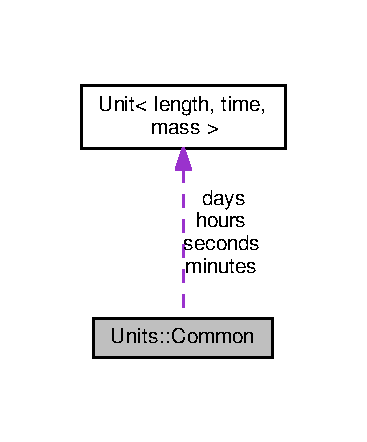
\includegraphics[width=176pt]{class_units_1_1_common__coll__graph}
\end{center}
\end{figure}
\subsection*{Static Public Attributes}
\begin{DoxyCompactItemize}
\item 
static const \hyperlink{_quantity_8h_ad9301a6dca9ca8d1452914698bfdf893}{Time\+Unit} \hyperlink{class_units_1_1_common_a0cc948d0fded9699abb22295119fff7b}{seconds} = \hyperlink{class_unit_aa2102921ecd21d9938707db58e4df964}{Time\+Unit\+::\+Base\+Unit}(\char`\"{}sec\char`\"{})
\item 
static const \hyperlink{_quantity_8h_ad9301a6dca9ca8d1452914698bfdf893}{Time\+Unit} \hyperlink{class_units_1_1_common_ae00592bb8573bd91d034a0b23f4449d6}{minutes} = \hyperlink{class_unit_aa44ac3044c0cdb834cd220652e5d1c40}{Time\+Unit\+::\+Scaled\+Unit}(60.\+0, \hyperlink{class_units_1_1_common_a0cc948d0fded9699abb22295119fff7b}{Units\+::\+Common\+::seconds}, \char`\"{}min\char`\"{})
\item 
static const \hyperlink{_quantity_8h_ad9301a6dca9ca8d1452914698bfdf893}{Time\+Unit} \hyperlink{class_units_1_1_common_a85905b04a8c1fa4058249d06c81828c7}{hours} = \hyperlink{class_unit_aa44ac3044c0cdb834cd220652e5d1c40}{Time\+Unit\+::\+Scaled\+Unit}(60.\+0, \hyperlink{class_units_1_1_common_ae00592bb8573bd91d034a0b23f4449d6}{Units\+::\+Common\+::minutes}, \char`\"{}hr\char`\"{})
\item 
static const \hyperlink{_quantity_8h_ad9301a6dca9ca8d1452914698bfdf893}{Time\+Unit} \hyperlink{class_units_1_1_common_ade670c3d1602d80753114646787c853e}{days} = \hyperlink{class_unit_aa44ac3044c0cdb834cd220652e5d1c40}{Time\+Unit\+::\+Scaled\+Unit}(24.\+0, \hyperlink{class_units_1_1_common_a85905b04a8c1fa4058249d06c81828c7}{Units\+::\+Common\+::hours}, \char`\"{}days\char`\"{})
\end{DoxyCompactItemize}


\subsection{Detailed Description}


Definition at line 266 of file Quantity.\+h.



\subsection{Member Data Documentation}
\hypertarget{class_units_1_1_common_ade670c3d1602d80753114646787c853e}{\index{Units\+::\+Common@{Units\+::\+Common}!days@{days}}
\index{days@{days}!Units\+::\+Common@{Units\+::\+Common}}
\subsubsection[{days}]{\setlength{\rightskip}{0pt plus 5cm}const {\bf Time\+Unit} Units\+::\+Common\+::days = {\bf Time\+Unit\+::\+Scaled\+Unit}(24.\+0, {\bf Units\+::\+Common\+::hours}, \char`\"{}days\char`\"{})\hspace{0.3cm}{\ttfamily [static]}}}\label{class_units_1_1_common_ade670c3d1602d80753114646787c853e}


Definition at line 272 of file Quantity.\+h.

\hypertarget{class_units_1_1_common_a85905b04a8c1fa4058249d06c81828c7}{\index{Units\+::\+Common@{Units\+::\+Common}!hours@{hours}}
\index{hours@{hours}!Units\+::\+Common@{Units\+::\+Common}}
\subsubsection[{hours}]{\setlength{\rightskip}{0pt plus 5cm}const {\bf Time\+Unit} Units\+::\+Common\+::hours = {\bf Time\+Unit\+::\+Scaled\+Unit}(60.\+0, {\bf Units\+::\+Common\+::minutes}, \char`\"{}hr\char`\"{})\hspace{0.3cm}{\ttfamily [static]}}}\label{class_units_1_1_common_a85905b04a8c1fa4058249d06c81828c7}


Definition at line 271 of file Quantity.\+h.

\hypertarget{class_units_1_1_common_ae00592bb8573bd91d034a0b23f4449d6}{\index{Units\+::\+Common@{Units\+::\+Common}!minutes@{minutes}}
\index{minutes@{minutes}!Units\+::\+Common@{Units\+::\+Common}}
\subsubsection[{minutes}]{\setlength{\rightskip}{0pt plus 5cm}const {\bf Time\+Unit} Units\+::\+Common\+::minutes = {\bf Time\+Unit\+::\+Scaled\+Unit}(60.\+0, {\bf Units\+::\+Common\+::seconds}, \char`\"{}min\char`\"{})\hspace{0.3cm}{\ttfamily [static]}}}\label{class_units_1_1_common_ae00592bb8573bd91d034a0b23f4449d6}


Definition at line 270 of file Quantity.\+h.

\hypertarget{class_units_1_1_common_a0cc948d0fded9699abb22295119fff7b}{\index{Units\+::\+Common@{Units\+::\+Common}!seconds@{seconds}}
\index{seconds@{seconds}!Units\+::\+Common@{Units\+::\+Common}}
\subsubsection[{seconds}]{\setlength{\rightskip}{0pt plus 5cm}const {\bf Time\+Unit} Units\+::\+Common\+::seconds = {\bf Time\+Unit\+::\+Base\+Unit}(\char`\"{}sec\char`\"{})\hspace{0.3cm}{\ttfamily [static]}}}\label{class_units_1_1_common_a0cc948d0fded9699abb22295119fff7b}


Definition at line 269 of file Quantity.\+h.



The documentation for this class was generated from the following files\+:\begin{DoxyCompactItemize}
\item 
S\+S\+W\+C/src/\+Math/\hyperlink{_quantity_8h}{Quantity.\+h}\item 
S\+S\+W\+C/src/\+Math/\hyperlink{_quantity_8cpp}{Quantity.\+cpp}\end{DoxyCompactItemize}

\hypertarget{class_cosmo_point}{\section{Cosmo\+Point Class Reference}
\label{class_cosmo_point}\index{Cosmo\+Point@{Cosmo\+Point}}
}


{\ttfamily \#include $<$Cosmo\+Point.\+h$>$}



Collaboration diagram for Cosmo\+Point\+:\nopagebreak
\begin{figure}[H]
\begin{center}
\leavevmode
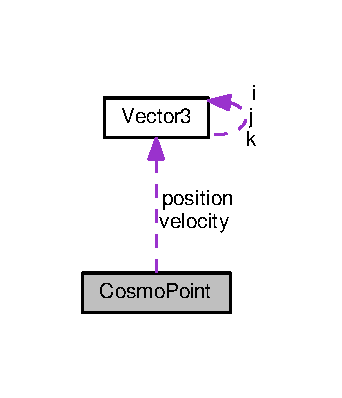
\includegraphics[width=164pt]{class_cosmo_point__coll__graph}
\end{center}
\end{figure}
\subsection*{Public Member Functions}
\begin{DoxyCompactItemize}
\item 
\hyperlink{class_cosmo_point_a3ed8019debc8234f8a2d89227ecef8cf}{Cosmo\+Point} ()
\item 
\hyperlink{class_cosmo_point_afc5c4495696cb761c688510b396f4700}{$\sim$\+Cosmo\+Point} ()
\item 
\hyperlink{wglext_8h_a9e6b7f1933461ef318bb000d6bd13b83}{void} \hyperlink{class_cosmo_point_a1543df6d5876e97a1b01fd6458ad4022}{Initialize} (const \hyperlink{class_vector3}{Vector3} \&\hyperlink{class_cosmo_point_a3927ca95564570083312401e1f10aaaa}{position}=0, const \hyperlink{class_vector3}{Vector3} \&\hyperlink{class_cosmo_point_a902bd391f682c0d60924bb43758e49f5}{velocity}=0, const \hyperlink{glext_8h_ae84541b4f3d8e1ea24ec0f466a8c568b}{std\+::string} \hyperlink{glext_8h_ad977737dfc9a274a62741b9500c49a32}{name}=\char`\"{}\char`\"{}, \hyperlink{glext_8h_ae84541b4f3d8e1ea24ec0f466a8c568b}{std\+::string} \hyperlink{class_cosmo_point_ab20d9a18d306ee9e268cc248493d50c3}{description}=\char`\"{}\char`\"{})
\item 
\hyperlink{class_cosmo_point}{Cosmo\+Point} \& \hyperlink{class_cosmo_point_ab838e5d61a68cebbec67ce06f9030c57}{operator=} (const \hyperlink{class_cosmo_point}{Cosmo\+Point} \&r\+Point)
\end{DoxyCompactItemize}
\subsection*{Public Attributes}
\begin{DoxyCompactItemize}
\item 
\hyperlink{class_vector3}{Vector3} \hyperlink{class_cosmo_point_a3927ca95564570083312401e1f10aaaa}{position}
\item 
\hyperlink{class_vector3}{Vector3} \hyperlink{class_cosmo_point_a902bd391f682c0d60924bb43758e49f5}{velocity}
\item 
\hyperlink{glext_8h_ae84541b4f3d8e1ea24ec0f466a8c568b}{std\+::string} \hyperlink{class_cosmo_point_a4f8ea23c00479e2dce987e0db8b8a621}{name}
\item 
\hyperlink{glext_8h_ae84541b4f3d8e1ea24ec0f466a8c568b}{std\+::string} \hyperlink{class_cosmo_point_ab20d9a18d306ee9e268cc248493d50c3}{description}
\end{DoxyCompactItemize}


\subsection{Detailed Description}


Definition at line 4 of file Cosmo\+Point.\+h.



\subsection{Constructor \& Destructor Documentation}
\hypertarget{class_cosmo_point_a3ed8019debc8234f8a2d89227ecef8cf}{\index{Cosmo\+Point@{Cosmo\+Point}!Cosmo\+Point@{Cosmo\+Point}}
\index{Cosmo\+Point@{Cosmo\+Point}!Cosmo\+Point@{Cosmo\+Point}}
\subsubsection[{Cosmo\+Point}]{\setlength{\rightskip}{0pt plus 5cm}Cosmo\+Point\+::\+Cosmo\+Point (
\begin{DoxyParamCaption}
{}
\end{DoxyParamCaption}
)}}\label{class_cosmo_point_a3ed8019debc8234f8a2d89227ecef8cf}


Definition at line 4 of file Cosmo\+Point.\+cpp.

\hypertarget{class_cosmo_point_afc5c4495696cb761c688510b396f4700}{\index{Cosmo\+Point@{Cosmo\+Point}!````~Cosmo\+Point@{$\sim$\+Cosmo\+Point}}
\index{````~Cosmo\+Point@{$\sim$\+Cosmo\+Point}!Cosmo\+Point@{Cosmo\+Point}}
\subsubsection[{$\sim$\+Cosmo\+Point}]{\setlength{\rightskip}{0pt plus 5cm}Cosmo\+Point\+::$\sim$\+Cosmo\+Point (
\begin{DoxyParamCaption}
{}
\end{DoxyParamCaption}
)}}\label{class_cosmo_point_afc5c4495696cb761c688510b396f4700}


Definition at line 13 of file Cosmo\+Point.\+cpp.



\subsection{Member Function Documentation}
\hypertarget{class_cosmo_point_a1543df6d5876e97a1b01fd6458ad4022}{\index{Cosmo\+Point@{Cosmo\+Point}!Initialize@{Initialize}}
\index{Initialize@{Initialize}!Cosmo\+Point@{Cosmo\+Point}}
\subsubsection[{Initialize}]{\setlength{\rightskip}{0pt plus 5cm}{\bf void} Cosmo\+Point\+::\+Initialize (
\begin{DoxyParamCaption}
\item[{const {\bf Vector3} \&}]{position = {\ttfamily 0}, }
\item[{const {\bf Vector3} \&}]{velocity = {\ttfamily 0}, }
\item[{const {\bf std\+::string}}]{name = {\ttfamily \char`\"{}\char`\"{}}, }
\item[{{\bf std\+::string}}]{description = {\ttfamily \char`\"{}\char`\"{}}}
\end{DoxyParamCaption}
)}}\label{class_cosmo_point_a1543df6d5876e97a1b01fd6458ad4022}


Definition at line 17 of file Cosmo\+Point.\+cpp.

\hypertarget{class_cosmo_point_ab838e5d61a68cebbec67ce06f9030c57}{\index{Cosmo\+Point@{Cosmo\+Point}!operator=@{operator=}}
\index{operator=@{operator=}!Cosmo\+Point@{Cosmo\+Point}}
\subsubsection[{operator=}]{\setlength{\rightskip}{0pt plus 5cm}{\bf Cosmo\+Point}\& Cosmo\+Point\+::operator= (
\begin{DoxyParamCaption}
\item[{const {\bf Cosmo\+Point} \&}]{r\+Point}
\end{DoxyParamCaption}
)}}\label{class_cosmo_point_ab838e5d61a68cebbec67ce06f9030c57}


\subsection{Member Data Documentation}
\hypertarget{class_cosmo_point_ab20d9a18d306ee9e268cc248493d50c3}{\index{Cosmo\+Point@{Cosmo\+Point}!description@{description}}
\index{description@{description}!Cosmo\+Point@{Cosmo\+Point}}
\subsubsection[{description}]{\setlength{\rightskip}{0pt plus 5cm}{\bf std\+::string} Cosmo\+Point\+::description}}\label{class_cosmo_point_ab20d9a18d306ee9e268cc248493d50c3}


Definition at line 10 of file Cosmo\+Point.\+h.

\hypertarget{class_cosmo_point_a4f8ea23c00479e2dce987e0db8b8a621}{\index{Cosmo\+Point@{Cosmo\+Point}!name@{name}}
\index{name@{name}!Cosmo\+Point@{Cosmo\+Point}}
\subsubsection[{name}]{\setlength{\rightskip}{0pt plus 5cm}{\bf std\+::string} Cosmo\+Point\+::name}}\label{class_cosmo_point_a4f8ea23c00479e2dce987e0db8b8a621}


Definition at line 9 of file Cosmo\+Point.\+h.

\hypertarget{class_cosmo_point_a3927ca95564570083312401e1f10aaaa}{\index{Cosmo\+Point@{Cosmo\+Point}!position@{position}}
\index{position@{position}!Cosmo\+Point@{Cosmo\+Point}}
\subsubsection[{position}]{\setlength{\rightskip}{0pt plus 5cm}{\bf Vector3} Cosmo\+Point\+::position}}\label{class_cosmo_point_a3927ca95564570083312401e1f10aaaa}


Definition at line 7 of file Cosmo\+Point.\+h.

\hypertarget{class_cosmo_point_a902bd391f682c0d60924bb43758e49f5}{\index{Cosmo\+Point@{Cosmo\+Point}!velocity@{velocity}}
\index{velocity@{velocity}!Cosmo\+Point@{Cosmo\+Point}}
\subsubsection[{velocity}]{\setlength{\rightskip}{0pt plus 5cm}{\bf Vector3} Cosmo\+Point\+::velocity}}\label{class_cosmo_point_a902bd391f682c0d60924bb43758e49f5}


Definition at line 8 of file Cosmo\+Point.\+h.



The documentation for this class was generated from the following files\+:\begin{DoxyCompactItemize}
\item 
S\+S\+W\+C/src/\hyperlink{_cosmo_point_8h}{Cosmo\+Point.\+h}\item 
S\+S\+W\+C/src/\hyperlink{_cosmo_point_8cpp}{Cosmo\+Point.\+cpp}\end{DoxyCompactItemize}

\hypertarget{class_c_spice_util}{\section{C\+Spice\+Util Class Reference}
\label{class_c_spice_util}\index{C\+Spice\+Util@{C\+Spice\+Util}}
}


{\ttfamily \#include $<$C\+Spice\+Util.\+h$>$}

\subsection*{Static Public Member Functions}
\begin{DoxyCompactItemize}
\item 
static \hyperlink{wglext_8h_a9e6b7f1933461ef318bb000d6bd13b83}{void} \hyperlink{class_c_spice_util_a1bc23133b0aa142ccc71d5fd85d0e609}{Set\+Error\+Handling\+Params} (const \hyperlink{glext_8h_ae84541b4f3d8e1ea24ec0f466a8c568b}{std\+::string} \&action, const \hyperlink{glext_8h_ae84541b4f3d8e1ea24ec0f466a8c568b}{std\+::string} \&device)
\item 
static \hyperlink{wglext_8h_a9e6b7f1933461ef318bb000d6bd13b83}{void} \hyperlink{class_c_spice_util_af1b073c99197ec2a2d22772e3a86d30d}{Set\+Logging\+File} (const \hyperlink{glext_8h_ae84541b4f3d8e1ea24ec0f466a8c568b}{std\+::string} \&file)
\item 
static \hyperlink{wglext_8h_a9e6b7f1933461ef318bb000d6bd13b83}{void} \hyperlink{class_c_spice_util_a0940aa96ffa3ef14f0ea2510c4163710}{Load\+Kernel} (const \hyperlink{glext_8h_ae84541b4f3d8e1ea24ec0f466a8c568b}{std\+::string} \&\hyperlink{glext_8h_ab25d8cd967ccbd19b630d7100ff8f67e}{path})
\item 
static std\+::vector$<$ \hyperlink{struct_kernel_data}{Kernel\+Data} $>$ \hyperlink{class_c_spice_util_a596f67731f91d55c8bb9b57e9ccb9c3d}{Get\+Loaded\+Kernels} (const \hyperlink{glext_8h_ae84541b4f3d8e1ea24ec0f466a8c568b}{std\+::string} \&\hyperlink{glext_8h_ab7c1afc09f67635c2c376638fcc0db5f}{type}=\char`\"{}A\+L\+L\char`\"{})
\item 
static \hyperlink{glext_8h_ae84541b4f3d8e1ea24ec0f466a8c568b}{std\+::string} \hyperlink{class_c_spice_util_aeb94a04c72d380e3d2ed82b93ea2ab8f}{Get\+Short\+Error\+Message} ()
\item 
static \hyperlink{glext_8h_ae84541b4f3d8e1ea24ec0f466a8c568b}{std\+::string} \hyperlink{class_c_spice_util_a9f5342e5699102d1f8ab772c43229a1c}{Get\+Explain\+Error\+Message} ()
\item 
static \hyperlink{glext_8h_ae84541b4f3d8e1ea24ec0f466a8c568b}{std\+::string} \hyperlink{class_c_spice_util_a22c2279dc23954b16e54261cad31ed9f}{Get\+Long\+Error\+Message} ()
\item 
static \hyperlink{glext_8h_ae84541b4f3d8e1ea24ec0f466a8c568b}{std\+::string} \hyperlink{class_c_spice_util_aec756d470ac2d41a2b66f096783350d7}{Get\+Traceback} ()
\item 
static \hyperlink{wglext_8h_a9e6b7f1933461ef318bb000d6bd13b83}{void} \hyperlink{class_c_spice_util_ad91e1b9618b9514d4cfd516a446a7e11}{Signal\+Error} (const \hyperlink{glext_8h_ae84541b4f3d8e1ea24ec0f466a8c568b}{std\+::string} \&error\+Msg)
\item 
static \hyperlink{wglext_8h_a9e6b7f1933461ef318bb000d6bd13b83}{void} \hyperlink{class_c_spice_util_a8ee7a37df1a51e2cdfe2681fbd57fdbc}{Log\+Error} (const \hyperlink{glext_8h_ae84541b4f3d8e1ea24ec0f466a8c568b}{std\+::string} \&extra\+Msg)
\item 
static \hyperlink{wglext_8h_a9e6b7f1933461ef318bb000d6bd13b83}{void} \hyperlink{class_c_spice_util_ab48e656441c984750f672468e19d99d3}{Reset\+Error\+Flag} ()
\item 
static std\+::vector$<$ long $>$ \hyperlink{class_c_spice_util_ab25fa56cd04c09b14f79c0f6fc8fe41b}{Int\+Cell\+To\+Vector} (Spice\+Cell cell)
\item 
static std\+::vector$<$ double $>$ \hyperlink{class_c_spice_util_aaa992f2f108a00da3b758207514a1a0b}{Double\+Cell\+To\+Vector} (Spice\+Cell cell)
\end{DoxyCompactItemize}


\subsection{Detailed Description}


Definition at line 46 of file C\+Spice\+Util.\+h.



\subsection{Member Function Documentation}
\hypertarget{class_c_spice_util_aaa992f2f108a00da3b758207514a1a0b}{\index{C\+Spice\+Util@{C\+Spice\+Util}!Double\+Cell\+To\+Vector@{Double\+Cell\+To\+Vector}}
\index{Double\+Cell\+To\+Vector@{Double\+Cell\+To\+Vector}!C\+Spice\+Util@{C\+Spice\+Util}}
\subsubsection[{Double\+Cell\+To\+Vector}]{\setlength{\rightskip}{0pt plus 5cm}std\+::vector$<$ double $>$ C\+Spice\+Util\+::\+Double\+Cell\+To\+Vector (
\begin{DoxyParamCaption}
\item[{Spice\+Cell}]{cell}
\end{DoxyParamCaption}
)\hspace{0.3cm}{\ttfamily [static]}}}\label{class_c_spice_util_aaa992f2f108a00da3b758207514a1a0b}


Definition at line 151 of file C\+Spice\+Util.\+cpp.

\hypertarget{class_c_spice_util_a9f5342e5699102d1f8ab772c43229a1c}{\index{C\+Spice\+Util@{C\+Spice\+Util}!Get\+Explain\+Error\+Message@{Get\+Explain\+Error\+Message}}
\index{Get\+Explain\+Error\+Message@{Get\+Explain\+Error\+Message}!C\+Spice\+Util@{C\+Spice\+Util}}
\subsubsection[{Get\+Explain\+Error\+Message}]{\setlength{\rightskip}{0pt plus 5cm}{\bf std\+::string} C\+Spice\+Util\+::\+Get\+Explain\+Error\+Message (
\begin{DoxyParamCaption}
{}
\end{DoxyParamCaption}
)\hspace{0.3cm}{\ttfamily [static]}}}\label{class_c_spice_util_a9f5342e5699102d1f8ab772c43229a1c}


Definition at line 68 of file C\+Spice\+Util.\+cpp.

\hypertarget{class_c_spice_util_a596f67731f91d55c8bb9b57e9ccb9c3d}{\index{C\+Spice\+Util@{C\+Spice\+Util}!Get\+Loaded\+Kernels@{Get\+Loaded\+Kernels}}
\index{Get\+Loaded\+Kernels@{Get\+Loaded\+Kernels}!C\+Spice\+Util@{C\+Spice\+Util}}
\subsubsection[{Get\+Loaded\+Kernels}]{\setlength{\rightskip}{0pt plus 5cm}std\+::vector$<$ {\bf Kernel\+Data} $>$ C\+Spice\+Util\+::\+Get\+Loaded\+Kernels (
\begin{DoxyParamCaption}
\item[{const {\bf std\+::string} \&}]{type = {\ttfamily \char`\"{}ALL\char`\"{}}}
\end{DoxyParamCaption}
)\hspace{0.3cm}{\ttfamily [static]}}}\label{class_c_spice_util_a596f67731f91d55c8bb9b57e9ccb9c3d}


Definition at line 31 of file C\+Spice\+Util.\+cpp.

\hypertarget{class_c_spice_util_a22c2279dc23954b16e54261cad31ed9f}{\index{C\+Spice\+Util@{C\+Spice\+Util}!Get\+Long\+Error\+Message@{Get\+Long\+Error\+Message}}
\index{Get\+Long\+Error\+Message@{Get\+Long\+Error\+Message}!C\+Spice\+Util@{C\+Spice\+Util}}
\subsubsection[{Get\+Long\+Error\+Message}]{\setlength{\rightskip}{0pt plus 5cm}{\bf std\+::string} C\+Spice\+Util\+::\+Get\+Long\+Error\+Message (
\begin{DoxyParamCaption}
{}
\end{DoxyParamCaption}
)\hspace{0.3cm}{\ttfamily [static]}}}\label{class_c_spice_util_a22c2279dc23954b16e54261cad31ed9f}


Definition at line 76 of file C\+Spice\+Util.\+cpp.

\hypertarget{class_c_spice_util_aeb94a04c72d380e3d2ed82b93ea2ab8f}{\index{C\+Spice\+Util@{C\+Spice\+Util}!Get\+Short\+Error\+Message@{Get\+Short\+Error\+Message}}
\index{Get\+Short\+Error\+Message@{Get\+Short\+Error\+Message}!C\+Spice\+Util@{C\+Spice\+Util}}
\subsubsection[{Get\+Short\+Error\+Message}]{\setlength{\rightskip}{0pt plus 5cm}{\bf std\+::string} C\+Spice\+Util\+::\+Get\+Short\+Error\+Message (
\begin{DoxyParamCaption}
{}
\end{DoxyParamCaption}
)\hspace{0.3cm}{\ttfamily [static]}}}\label{class_c_spice_util_aeb94a04c72d380e3d2ed82b93ea2ab8f}


Definition at line 60 of file C\+Spice\+Util.\+cpp.

\hypertarget{class_c_spice_util_aec756d470ac2d41a2b66f096783350d7}{\index{C\+Spice\+Util@{C\+Spice\+Util}!Get\+Traceback@{Get\+Traceback}}
\index{Get\+Traceback@{Get\+Traceback}!C\+Spice\+Util@{C\+Spice\+Util}}
\subsubsection[{Get\+Traceback}]{\setlength{\rightskip}{0pt plus 5cm}{\bf std\+::string} C\+Spice\+Util\+::\+Get\+Traceback (
\begin{DoxyParamCaption}
{}
\end{DoxyParamCaption}
)\hspace{0.3cm}{\ttfamily [static]}}}\label{class_c_spice_util_aec756d470ac2d41a2b66f096783350d7}


Definition at line 84 of file C\+Spice\+Util.\+cpp.

\hypertarget{class_c_spice_util_ab25fa56cd04c09b14f79c0f6fc8fe41b}{\index{C\+Spice\+Util@{C\+Spice\+Util}!Int\+Cell\+To\+Vector@{Int\+Cell\+To\+Vector}}
\index{Int\+Cell\+To\+Vector@{Int\+Cell\+To\+Vector}!C\+Spice\+Util@{C\+Spice\+Util}}
\subsubsection[{Int\+Cell\+To\+Vector}]{\setlength{\rightskip}{0pt plus 5cm}std\+::vector$<$ long $>$ C\+Spice\+Util\+::\+Int\+Cell\+To\+Vector (
\begin{DoxyParamCaption}
\item[{Spice\+Cell}]{cell}
\end{DoxyParamCaption}
)\hspace{0.3cm}{\ttfamily [static]}}}\label{class_c_spice_util_ab25fa56cd04c09b14f79c0f6fc8fe41b}


Definition at line 133 of file C\+Spice\+Util.\+cpp.

\hypertarget{class_c_spice_util_a0940aa96ffa3ef14f0ea2510c4163710}{\index{C\+Spice\+Util@{C\+Spice\+Util}!Load\+Kernel@{Load\+Kernel}}
\index{Load\+Kernel@{Load\+Kernel}!C\+Spice\+Util@{C\+Spice\+Util}}
\subsubsection[{Load\+Kernel}]{\setlength{\rightskip}{0pt plus 5cm}{\bf void} C\+Spice\+Util\+::\+Load\+Kernel (
\begin{DoxyParamCaption}
\item[{const {\bf std\+::string} \&}]{path}
\end{DoxyParamCaption}
)\hspace{0.3cm}{\ttfamily [static]}}}\label{class_c_spice_util_a0940aa96ffa3ef14f0ea2510c4163710}


Definition at line 26 of file C\+Spice\+Util.\+cpp.

\hypertarget{class_c_spice_util_a8ee7a37df1a51e2cdfe2681fbd57fdbc}{\index{C\+Spice\+Util@{C\+Spice\+Util}!Log\+Error@{Log\+Error}}
\index{Log\+Error@{Log\+Error}!C\+Spice\+Util@{C\+Spice\+Util}}
\subsubsection[{Log\+Error}]{\setlength{\rightskip}{0pt plus 5cm}{\bf void} C\+Spice\+Util\+::\+Log\+Error (
\begin{DoxyParamCaption}
\item[{const {\bf std\+::string} \&}]{extra\+Msg}
\end{DoxyParamCaption}
)\hspace{0.3cm}{\ttfamily [static]}}}\label{class_c_spice_util_a8ee7a37df1a51e2cdfe2681fbd57fdbc}


Definition at line 99 of file C\+Spice\+Util.\+cpp.

\hypertarget{class_c_spice_util_ab48e656441c984750f672468e19d99d3}{\index{C\+Spice\+Util@{C\+Spice\+Util}!Reset\+Error\+Flag@{Reset\+Error\+Flag}}
\index{Reset\+Error\+Flag@{Reset\+Error\+Flag}!C\+Spice\+Util@{C\+Spice\+Util}}
\subsubsection[{Reset\+Error\+Flag}]{\setlength{\rightskip}{0pt plus 5cm}{\bf void} C\+Spice\+Util\+::\+Reset\+Error\+Flag (
\begin{DoxyParamCaption}
{}
\end{DoxyParamCaption}
)\hspace{0.3cm}{\ttfamily [static]}}}\label{class_c_spice_util_ab48e656441c984750f672468e19d99d3}


Definition at line 128 of file C\+Spice\+Util.\+cpp.

\hypertarget{class_c_spice_util_a1bc23133b0aa142ccc71d5fd85d0e609}{\index{C\+Spice\+Util@{C\+Spice\+Util}!Set\+Error\+Handling\+Params@{Set\+Error\+Handling\+Params}}
\index{Set\+Error\+Handling\+Params@{Set\+Error\+Handling\+Params}!C\+Spice\+Util@{C\+Spice\+Util}}
\subsubsection[{Set\+Error\+Handling\+Params}]{\setlength{\rightskip}{0pt plus 5cm}{\bf void} C\+Spice\+Util\+::\+Set\+Error\+Handling\+Params (
\begin{DoxyParamCaption}
\item[{const {\bf std\+::string} \&}]{action, }
\item[{const {\bf std\+::string} \&}]{device}
\end{DoxyParamCaption}
)\hspace{0.3cm}{\ttfamily [static]}}}\label{class_c_spice_util_a1bc23133b0aa142ccc71d5fd85d0e609}


Definition at line 3 of file C\+Spice\+Util.\+cpp.

\hypertarget{class_c_spice_util_af1b073c99197ec2a2d22772e3a86d30d}{\index{C\+Spice\+Util@{C\+Spice\+Util}!Set\+Logging\+File@{Set\+Logging\+File}}
\index{Set\+Logging\+File@{Set\+Logging\+File}!C\+Spice\+Util@{C\+Spice\+Util}}
\subsubsection[{Set\+Logging\+File}]{\setlength{\rightskip}{0pt plus 5cm}{\bf void} C\+Spice\+Util\+::\+Set\+Logging\+File (
\begin{DoxyParamCaption}
\item[{const {\bf std\+::string} \&}]{file}
\end{DoxyParamCaption}
)\hspace{0.3cm}{\ttfamily [static]}}}\label{class_c_spice_util_af1b073c99197ec2a2d22772e3a86d30d}


Definition at line 21 of file C\+Spice\+Util.\+cpp.

\hypertarget{class_c_spice_util_ad91e1b9618b9514d4cfd516a446a7e11}{\index{C\+Spice\+Util@{C\+Spice\+Util}!Signal\+Error@{Signal\+Error}}
\index{Signal\+Error@{Signal\+Error}!C\+Spice\+Util@{C\+Spice\+Util}}
\subsubsection[{Signal\+Error}]{\setlength{\rightskip}{0pt plus 5cm}{\bf void} C\+Spice\+Util\+::\+Signal\+Error (
\begin{DoxyParamCaption}
\item[{const {\bf std\+::string} \&}]{error\+Msg = {\ttfamily \char`\"{}\char`\"{}}}
\end{DoxyParamCaption}
)\hspace{0.3cm}{\ttfamily [static]}}}\label{class_c_spice_util_ad91e1b9618b9514d4cfd516a446a7e11}


Definition at line 92 of file C\+Spice\+Util.\+cpp.



The documentation for this class was generated from the following files\+:\begin{DoxyCompactItemize}
\item 
S\+S\+W\+C/src/\+C\+Spice/\hyperlink{_c_spice_util_8h}{C\+Spice\+Util.\+h}\item 
S\+S\+W\+C/src/\+C\+Spice/\hyperlink{_c_spice_util_8cpp}{C\+Spice\+Util.\+cpp}\end{DoxyCompactItemize}

\hypertarget{class_date}{\section{Date Class Reference}
\label{class_date}\index{Date@{Date}}
}


{\ttfamily \#include $<$Date.\+h$>$}

\subsection*{Public Member Functions}
\begin{DoxyCompactItemize}
\item 
\hyperlink{class_date_a02e14e792c9a84dec9f7108d0c3b40c2}{Date} (double et=0.\+0)
\item 
\hyperlink{class_date_af909b4fc8d85c6feb129709441f6af5a}{Date} (\hyperlink{glext_8h_ae84541b4f3d8e1ea24ec0f466a8c568b}{std\+::string} str)
\item 
double \hyperlink{class_date_af5e52ad40ec03035f98ddd4bd5bfc2fd}{As\+Double} () const 
\item 
\hyperlink{glext_8h_ae84541b4f3d8e1ea24ec0f466a8c568b}{std\+::string} \hyperlink{class_date_ac952bc2fedfc299de91758e32b487810}{As\+String} (const \hyperlink{glext_8h_ae84541b4f3d8e1ea24ec0f466a8c568b}{std\+::string} \&\hyperlink{glext_8h_ae2d3db041c6004a67047659b42f73a44}{format}=\char`\"{}Mon D\+D Y\+Y\+Y\+Y H\+R\+:\+M\+N\+:\+S\+C (U\+T\+C+0) \+::U\+T\+C+0\char`\"{}) const 
\item 
\hyperlink{class_date}{Date} \hyperlink{class_date_a4728290c236875c0a0e909da57a732d1}{operator+} (double rhs) const 
\item 
\hyperlink{class_date}{Date} \hyperlink{class_date_a818a7809eb6a6c3c07e4f5e82fe32b2b}{operator-\/} (double rhs) const 
\item 
double \hyperlink{class_date_afa16e15bccb6a129ad4bec5aeff20967}{operator-\/} (const \hyperlink{class_date}{Date} \&rhs) const 
\item 
\hyperlink{class_date}{Date} \& \hyperlink{class_date_aa276629ba1fd2b5afce12aa79e638f5b}{operator+=} (double rhs)
\item 
\hyperlink{class_date}{Date} \& \hyperlink{class_date_a4e423fd26befbc87937e2eb1a62c9d96}{operator-\/=} (double rhs)
\item 
bool \hyperlink{class_date_a94ad75126c7edce05cad11c59ccc2136}{operator$<$} (const \hyperlink{class_date}{Date} \&rhs) const 
\item 
bool \hyperlink{class_date_a572f2eae7edfbb96c7556cb1b63c517a}{operator$>$} (const \hyperlink{class_date}{Date} \&rhs) const 
\item 
\hyperlink{class_date}{Date} \hyperlink{class_date_a6d1901bc7ac1a1edbb3d027c40d954d5}{operator+} (const \hyperlink{_quantity_8h_ab180382d5dc1bcb91259cbd59a5d86fc}{Time} \&rhs) const 
\item 
\hyperlink{class_date}{Date} \hyperlink{class_date_a1d4f191e7ce6148681b0683e2fb45c3b}{operator-\/} (const \hyperlink{_quantity_8h_ab180382d5dc1bcb91259cbd59a5d86fc}{Time} \&rhs) const 
\item 
\hyperlink{class_date}{Date} \& \hyperlink{class_date_ad1f5746ec11616030cf1cffe32be53ca}{operator+=} (const \hyperlink{_quantity_8h_ab180382d5dc1bcb91259cbd59a5d86fc}{Time} \&rhs)
\item 
\hyperlink{class_date}{Date} \& \hyperlink{class_date_a5b0bc159e3dfe925972077b520a3a429}{operator-\/=} (const \hyperlink{_quantity_8h_ab180382d5dc1bcb91259cbd59a5d86fc}{Time} \&rhs)
\end{DoxyCompactItemize}
\subsection*{Static Public Attributes}
\begin{DoxyCompactItemize}
\item 
static const double \hyperlink{class_date_ae6f7ae7f25f297a2edbf3145384fc94b}{second}
\item 
static const double \hyperlink{class_date_a755e333674657a63fdc2a7228ea24972}{minute}
\item 
static const double \hyperlink{class_date_a04e609f92a81379120b83438324da63e}{hour}
\item 
static const double \hyperlink{class_date_afdaf71438c0ef71ac7772abbcb65064e}{day}
\end{DoxyCompactItemize}


\subsection{Detailed Description}


Definition at line 10 of file Date.\+h.



\subsection{Constructor \& Destructor Documentation}
\hypertarget{class_date_a02e14e792c9a84dec9f7108d0c3b40c2}{\index{Date@{Date}!Date@{Date}}
\index{Date@{Date}!Date@{Date}}
\subsubsection[{Date}]{\setlength{\rightskip}{0pt plus 5cm}Date\+::\+Date (
\begin{DoxyParamCaption}
\item[{double}]{et = {\ttfamily 0.0}}
\end{DoxyParamCaption}
)}}\label{class_date_a02e14e792c9a84dec9f7108d0c3b40c2}


Definition at line 3 of file Date.\+cpp.

\hypertarget{class_date_af909b4fc8d85c6feb129709441f6af5a}{\index{Date@{Date}!Date@{Date}}
\index{Date@{Date}!Date@{Date}}
\subsubsection[{Date}]{\setlength{\rightskip}{0pt plus 5cm}Date\+::\+Date (
\begin{DoxyParamCaption}
\item[{{\bf std\+::string}}]{str}
\end{DoxyParamCaption}
)}}\label{class_date_af909b4fc8d85c6feb129709441f6af5a}


Definition at line 8 of file Date.\+cpp.



\subsection{Member Function Documentation}
\hypertarget{class_date_af5e52ad40ec03035f98ddd4bd5bfc2fd}{\index{Date@{Date}!As\+Double@{As\+Double}}
\index{As\+Double@{As\+Double}!Date@{Date}}
\subsubsection[{As\+Double}]{\setlength{\rightskip}{0pt plus 5cm}double Date\+::\+As\+Double (
\begin{DoxyParamCaption}
{}
\end{DoxyParamCaption}
) const}}\label{class_date_af5e52ad40ec03035f98ddd4bd5bfc2fd}


Definition at line 13 of file Date.\+cpp.

\hypertarget{class_date_ac952bc2fedfc299de91758e32b487810}{\index{Date@{Date}!As\+String@{As\+String}}
\index{As\+String@{As\+String}!Date@{Date}}
\subsubsection[{As\+String}]{\setlength{\rightskip}{0pt plus 5cm}{\bf std\+::string} Date\+::\+As\+String (
\begin{DoxyParamCaption}
\item[{const {\bf std\+::string} \&}]{format = {\ttfamily \char`\"{}Mon~DD~YYYY~HR\+:MN\+:SC~(UTC+0)~\+:\+:UTC+0\char`\"{}}}
\end{DoxyParamCaption}
) const}}\label{class_date_ac952bc2fedfc299de91758e32b487810}


Definition at line 18 of file Date.\+cpp.

\hypertarget{class_date_a4728290c236875c0a0e909da57a732d1}{\index{Date@{Date}!operator+@{operator+}}
\index{operator+@{operator+}!Date@{Date}}
\subsubsection[{operator+}]{\setlength{\rightskip}{0pt plus 5cm}{\bf Date} Date\+::operator+ (
\begin{DoxyParamCaption}
\item[{double}]{rhs}
\end{DoxyParamCaption}
) const\hspace{0.3cm}{\ttfamily [inline]}}}\label{class_date_a4728290c236875c0a0e909da57a732d1}


Definition at line 19 of file Date.\+h.

\hypertarget{class_date_a6d1901bc7ac1a1edbb3d027c40d954d5}{\index{Date@{Date}!operator+@{operator+}}
\index{operator+@{operator+}!Date@{Date}}
\subsubsection[{operator+}]{\setlength{\rightskip}{0pt plus 5cm}{\bf Date} Date\+::operator+ (
\begin{DoxyParamCaption}
\item[{const {\bf Time} \&}]{rhs}
\end{DoxyParamCaption}
) const\hspace{0.3cm}{\ttfamily [inline]}}}\label{class_date_a6d1901bc7ac1a1edbb3d027c40d954d5}


Definition at line 49 of file Date.\+h.

\hypertarget{class_date_aa276629ba1fd2b5afce12aa79e638f5b}{\index{Date@{Date}!operator+=@{operator+=}}
\index{operator+=@{operator+=}!Date@{Date}}
\subsubsection[{operator+=}]{\setlength{\rightskip}{0pt plus 5cm}{\bf Date}\& Date\+::operator+= (
\begin{DoxyParamCaption}
\item[{double}]{rhs}
\end{DoxyParamCaption}
)\hspace{0.3cm}{\ttfamily [inline]}}}\label{class_date_aa276629ba1fd2b5afce12aa79e638f5b}


Definition at line 31 of file Date.\+h.

\hypertarget{class_date_ad1f5746ec11616030cf1cffe32be53ca}{\index{Date@{Date}!operator+=@{operator+=}}
\index{operator+=@{operator+=}!Date@{Date}}
\subsubsection[{operator+=}]{\setlength{\rightskip}{0pt plus 5cm}{\bf Date}\& Date\+::operator+= (
\begin{DoxyParamCaption}
\item[{const {\bf Time} \&}]{rhs}
\end{DoxyParamCaption}
)\hspace{0.3cm}{\ttfamily [inline]}}}\label{class_date_ad1f5746ec11616030cf1cffe32be53ca}


Definition at line 57 of file Date.\+h.

\hypertarget{class_date_a818a7809eb6a6c3c07e4f5e82fe32b2b}{\index{Date@{Date}!operator-\/@{operator-\/}}
\index{operator-\/@{operator-\/}!Date@{Date}}
\subsubsection[{operator-\/}]{\setlength{\rightskip}{0pt plus 5cm}{\bf Date} Date\+::operator-\/ (
\begin{DoxyParamCaption}
\item[{double}]{rhs}
\end{DoxyParamCaption}
) const\hspace{0.3cm}{\ttfamily [inline]}}}\label{class_date_a818a7809eb6a6c3c07e4f5e82fe32b2b}


Definition at line 23 of file Date.\+h.

\hypertarget{class_date_afa16e15bccb6a129ad4bec5aeff20967}{\index{Date@{Date}!operator-\/@{operator-\/}}
\index{operator-\/@{operator-\/}!Date@{Date}}
\subsubsection[{operator-\/}]{\setlength{\rightskip}{0pt plus 5cm}double Date\+::operator-\/ (
\begin{DoxyParamCaption}
\item[{const {\bf Date} \&}]{rhs}
\end{DoxyParamCaption}
) const\hspace{0.3cm}{\ttfamily [inline]}}}\label{class_date_afa16e15bccb6a129ad4bec5aeff20967}


Definition at line 27 of file Date.\+h.

\hypertarget{class_date_a1d4f191e7ce6148681b0683e2fb45c3b}{\index{Date@{Date}!operator-\/@{operator-\/}}
\index{operator-\/@{operator-\/}!Date@{Date}}
\subsubsection[{operator-\/}]{\setlength{\rightskip}{0pt plus 5cm}{\bf Date} Date\+::operator-\/ (
\begin{DoxyParamCaption}
\item[{const {\bf Time} \&}]{rhs}
\end{DoxyParamCaption}
) const\hspace{0.3cm}{\ttfamily [inline]}}}\label{class_date_a1d4f191e7ce6148681b0683e2fb45c3b}


Definition at line 53 of file Date.\+h.

\hypertarget{class_date_a4e423fd26befbc87937e2eb1a62c9d96}{\index{Date@{Date}!operator-\/=@{operator-\/=}}
\index{operator-\/=@{operator-\/=}!Date@{Date}}
\subsubsection[{operator-\/=}]{\setlength{\rightskip}{0pt plus 5cm}{\bf Date}\& Date\+::operator-\/= (
\begin{DoxyParamCaption}
\item[{double}]{rhs}
\end{DoxyParamCaption}
)\hspace{0.3cm}{\ttfamily [inline]}}}\label{class_date_a4e423fd26befbc87937e2eb1a62c9d96}


Definition at line 36 of file Date.\+h.

\hypertarget{class_date_a5b0bc159e3dfe925972077b520a3a429}{\index{Date@{Date}!operator-\/=@{operator-\/=}}
\index{operator-\/=@{operator-\/=}!Date@{Date}}
\subsubsection[{operator-\/=}]{\setlength{\rightskip}{0pt plus 5cm}{\bf Date}\& Date\+::operator-\/= (
\begin{DoxyParamCaption}
\item[{const {\bf Time} \&}]{rhs}
\end{DoxyParamCaption}
)\hspace{0.3cm}{\ttfamily [inline]}}}\label{class_date_a5b0bc159e3dfe925972077b520a3a429}


Definition at line 63 of file Date.\+h.

\hypertarget{class_date_a94ad75126c7edce05cad11c59ccc2136}{\index{Date@{Date}!operator$<$@{operator$<$}}
\index{operator$<$@{operator$<$}!Date@{Date}}
\subsubsection[{operator$<$}]{\setlength{\rightskip}{0pt plus 5cm}bool Date\+::operator$<$ (
\begin{DoxyParamCaption}
\item[{const {\bf Date} \&}]{rhs}
\end{DoxyParamCaption}
) const\hspace{0.3cm}{\ttfamily [inline]}}}\label{class_date_a94ad75126c7edce05cad11c59ccc2136}


Definition at line 41 of file Date.\+h.

\hypertarget{class_date_a572f2eae7edfbb96c7556cb1b63c517a}{\index{Date@{Date}!operator$>$@{operator$>$}}
\index{operator$>$@{operator$>$}!Date@{Date}}
\subsubsection[{operator$>$}]{\setlength{\rightskip}{0pt plus 5cm}bool Date\+::operator$>$ (
\begin{DoxyParamCaption}
\item[{const {\bf Date} \&}]{rhs}
\end{DoxyParamCaption}
) const\hspace{0.3cm}{\ttfamily [inline]}}}\label{class_date_a572f2eae7edfbb96c7556cb1b63c517a}


Definition at line 45 of file Date.\+h.



\subsection{Member Data Documentation}
\hypertarget{class_date_afdaf71438c0ef71ac7772abbcb65064e}{\index{Date@{Date}!day@{day}}
\index{day@{day}!Date@{Date}}
\subsubsection[{day}]{\setlength{\rightskip}{0pt plus 5cm}const double Date\+::day\hspace{0.3cm}{\ttfamily [static]}}}\label{class_date_afdaf71438c0ef71ac7772abbcb65064e}


Definition at line 74 of file Date.\+h.

\hypertarget{class_date_a04e609f92a81379120b83438324da63e}{\index{Date@{Date}!hour@{hour}}
\index{hour@{hour}!Date@{Date}}
\subsubsection[{hour}]{\setlength{\rightskip}{0pt plus 5cm}const double Date\+::hour\hspace{0.3cm}{\ttfamily [static]}}}\label{class_date_a04e609f92a81379120b83438324da63e}


Definition at line 73 of file Date.\+h.

\hypertarget{class_date_a755e333674657a63fdc2a7228ea24972}{\index{Date@{Date}!minute@{minute}}
\index{minute@{minute}!Date@{Date}}
\subsubsection[{minute}]{\setlength{\rightskip}{0pt plus 5cm}const double Date\+::minute\hspace{0.3cm}{\ttfamily [static]}}}\label{class_date_a755e333674657a63fdc2a7228ea24972}


Definition at line 72 of file Date.\+h.

\hypertarget{class_date_ae6f7ae7f25f297a2edbf3145384fc94b}{\index{Date@{Date}!second@{second}}
\index{second@{second}!Date@{Date}}
\subsubsection[{second}]{\setlength{\rightskip}{0pt plus 5cm}const double Date\+::second\hspace{0.3cm}{\ttfamily [static]}}}\label{class_date_ae6f7ae7f25f297a2edbf3145384fc94b}


Definition at line 71 of file Date.\+h.



The documentation for this class was generated from the following files\+:\begin{DoxyCompactItemize}
\item 
S\+S\+W\+C/src/\+C\+Spice/\hyperlink{_date_8h}{Date.\+h}\item 
S\+S\+W\+C/src/\+C\+Spice/\hyperlink{_date_8cpp}{Date.\+cpp}\end{DoxyCompactItemize}

\hypertarget{struct_app_1_1_default_units}{\section{App\+:\+:Default\+Units Struct Reference}
\label{struct_app_1_1_default_units}\index{App\+::\+Default\+Units@{App\+::\+Default\+Units}}
}


{\ttfamily \#include $<$App.\+h$>$}



Collaboration diagram for App\+:\+:Default\+Units\+:\nopagebreak
\begin{figure}[H]
\begin{center}
\leavevmode
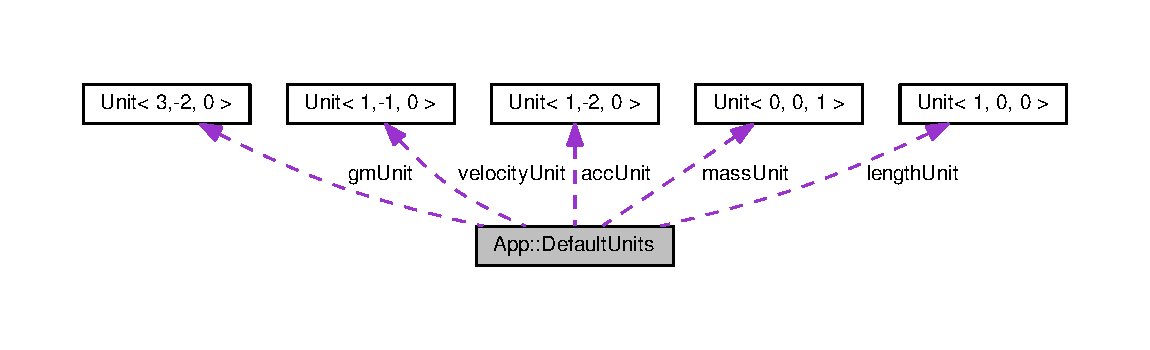
\includegraphics[width=350pt]{struct_app_1_1_default_units__coll__graph}
\end{center}
\end{figure}
\subsection*{Public Attributes}
\begin{DoxyCompactItemize}
\item 
\hyperlink{_quantity_8h_afb62d6d68e6cd2c62c96aa8c3aeb7d1f}{Length\+Unit} \hyperlink{struct_app_1_1_default_units_ad54dce1ee4af8f666579130f55034506}{length\+Unit}
\item 
\hyperlink{_quantity_8h_a4130b5cf107e9890a06c6c06bbfa7da3}{Velocity\+Unit} \hyperlink{struct_app_1_1_default_units_a828b643678f6cc966772f1cfdb74b7d5}{velocity\+Unit}
\item 
\hyperlink{_quantity_8h_a2dde25127542e6a5fcf7c085269b8963}{Mass\+Unit} \hyperlink{struct_app_1_1_default_units_a6fd33188cebaa3e473af9d9b265624da}{mass\+Unit}
\item 
\hyperlink{_quantity_8h_aa1729851532d88933ff921f24a0bce3b}{Acceleration\+Unit} \hyperlink{struct_app_1_1_default_units_a7803c87c80c03066c6d4737781edc50d}{acc\+Unit}
\item 
\hyperlink{_quantity_8h_ac250a56b26235a8dc9d44fbbeabe2024}{Gravitational\+Parameter\+Unit} \hyperlink{struct_app_1_1_default_units_a134222849fbe7070dc8a2471b8d2afb5}{gm\+Unit}
\end{DoxyCompactItemize}


\subsection{Detailed Description}


Definition at line 23 of file App.\+h.



\subsection{Member Data Documentation}
\hypertarget{struct_app_1_1_default_units_a7803c87c80c03066c6d4737781edc50d}{\index{App\+::\+Default\+Units@{App\+::\+Default\+Units}!acc\+Unit@{acc\+Unit}}
\index{acc\+Unit@{acc\+Unit}!App\+::\+Default\+Units@{App\+::\+Default\+Units}}
\subsubsection[{acc\+Unit}]{\setlength{\rightskip}{0pt plus 5cm}{\bf Acceleration\+Unit} App\+::\+Default\+Units\+::acc\+Unit}}\label{struct_app_1_1_default_units_a7803c87c80c03066c6d4737781edc50d}


Definition at line 28 of file App.\+h.

\hypertarget{struct_app_1_1_default_units_a134222849fbe7070dc8a2471b8d2afb5}{\index{App\+::\+Default\+Units@{App\+::\+Default\+Units}!gm\+Unit@{gm\+Unit}}
\index{gm\+Unit@{gm\+Unit}!App\+::\+Default\+Units@{App\+::\+Default\+Units}}
\subsubsection[{gm\+Unit}]{\setlength{\rightskip}{0pt plus 5cm}{\bf Gravitational\+Parameter\+Unit} App\+::\+Default\+Units\+::gm\+Unit}}\label{struct_app_1_1_default_units_a134222849fbe7070dc8a2471b8d2afb5}


Definition at line 29 of file App.\+h.

\hypertarget{struct_app_1_1_default_units_ad54dce1ee4af8f666579130f55034506}{\index{App\+::\+Default\+Units@{App\+::\+Default\+Units}!length\+Unit@{length\+Unit}}
\index{length\+Unit@{length\+Unit}!App\+::\+Default\+Units@{App\+::\+Default\+Units}}
\subsubsection[{length\+Unit}]{\setlength{\rightskip}{0pt plus 5cm}{\bf Length\+Unit} App\+::\+Default\+Units\+::length\+Unit}}\label{struct_app_1_1_default_units_ad54dce1ee4af8f666579130f55034506}


Definition at line 25 of file App.\+h.

\hypertarget{struct_app_1_1_default_units_a6fd33188cebaa3e473af9d9b265624da}{\index{App\+::\+Default\+Units@{App\+::\+Default\+Units}!mass\+Unit@{mass\+Unit}}
\index{mass\+Unit@{mass\+Unit}!App\+::\+Default\+Units@{App\+::\+Default\+Units}}
\subsubsection[{mass\+Unit}]{\setlength{\rightskip}{0pt plus 5cm}{\bf Mass\+Unit} App\+::\+Default\+Units\+::mass\+Unit}}\label{struct_app_1_1_default_units_a6fd33188cebaa3e473af9d9b265624da}


Definition at line 27 of file App.\+h.

\hypertarget{struct_app_1_1_default_units_a828b643678f6cc966772f1cfdb74b7d5}{\index{App\+::\+Default\+Units@{App\+::\+Default\+Units}!velocity\+Unit@{velocity\+Unit}}
\index{velocity\+Unit@{velocity\+Unit}!App\+::\+Default\+Units@{App\+::\+Default\+Units}}
\subsubsection[{velocity\+Unit}]{\setlength{\rightskip}{0pt plus 5cm}{\bf Velocity\+Unit} App\+::\+Default\+Units\+::velocity\+Unit}}\label{struct_app_1_1_default_units_a828b643678f6cc966772f1cfdb74b7d5}


Definition at line 26 of file App.\+h.



The documentation for this struct was generated from the following file\+:\begin{DoxyCompactItemize}
\item 
S\+S\+W\+C/src/\hyperlink{_app_8h}{App.\+h}\end{DoxyCompactItemize}

\hypertarget{class_font}{\section{Font Class Reference}
\label{class_font}\index{Font@{Font}}
}


{\ttfamily \#include $<$Font.\+h$>$}

\subsection*{Public Member Functions}
\begin{DoxyCompactItemize}
\item 
\hyperlink{class_font_a4e6a119206f505522100221c1fafde45}{Font} ()
\item 
\hyperlink{class_font_affe779785f1d6e69d4c4e46996201d7d}{Font} (\hyperlink{wglext_8h_aaf5a06bd464c6ec72cf68b4819afebe3}{H\+D\+C} h\+D\+Cint, \hyperlink{wglext_8h_a500a82aecba06f4550f6849b8099ca21}{int} \hyperlink{glext_8h_aa214bd63e12f7ddf524c83894fcc69a7}{height}=-\/24, \hyperlink{wglext_8h_a500a82aecba06f4550f6849b8099ca21}{int} \hyperlink{glext_8h_aa105b18f96e6bc2485cb7f576a7fb9ba}{width}=-\/10, float angle\+Of\+Escapement=0, float orientation\+Angle=0, \hyperlink{wglext_8h_a500a82aecba06f4550f6849b8099ca21}{int} font\+Weight=F\+W\+\_\+\+B\+O\+L\+D, bool italic=false, bool underline=false, bool strikeout=false, \hyperlink{wglext_8h_a500a82aecba06f4550f6849b8099ca21}{int} charset\+Identifyer=A\+N\+S\+I\+\_\+\+C\+H\+A\+R\+S\+E\+T, \hyperlink{wglext_8h_a500a82aecba06f4550f6849b8099ca21}{int} output\+Quality=A\+N\+T\+I\+A\+L\+I\+A\+S\+E\+D\+\_\+\+Q\+U\+A\+L\+I\+T\+Y, \hyperlink{glext_8h_ae84541b4f3d8e1ea24ec0f466a8c568b}{std\+::string} \hyperlink{glext_8h_ab669695d2be97b71fa1439607bfb92a6}{font\+Name}=\char`\"{}Courier New\char`\"{})
\item 
\hyperlink{class_font_a134aaa2f78af0c12d3ce504957169768}{$\sim$\+Font} ()
\item 
\hyperlink{wglext_8h_a9e6b7f1933461ef318bb000d6bd13b83}{void} \hyperlink{class_font_af5da83acec19907e2481da2126e077bc}{Kill\+Font} ()
\item 
\hyperlink{wglext_8h_a9e6b7f1933461ef318bb000d6bd13b83}{void} \hyperlink{class_font_abc5d95a4605278837b3f6697f6499dc1}{gl\+Print} (const char $\ast$fmt,...)
\end{DoxyCompactItemize}


\subsection{Detailed Description}


Definition at line 10 of file Font.\+h.



\subsection{Constructor \& Destructor Documentation}
\hypertarget{class_font_a4e6a119206f505522100221c1fafde45}{\index{Font@{Font}!Font@{Font}}
\index{Font@{Font}!Font@{Font}}
\subsubsection[{Font}]{\setlength{\rightskip}{0pt plus 5cm}Font\+::\+Font (
\begin{DoxyParamCaption}
{}
\end{DoxyParamCaption}
)}}\label{class_font_a4e6a119206f505522100221c1fafde45}


Definition at line 4 of file Font.\+cpp.

\hypertarget{class_font_affe779785f1d6e69d4c4e46996201d7d}{\index{Font@{Font}!Font@{Font}}
\index{Font@{Font}!Font@{Font}}
\subsubsection[{Font}]{\setlength{\rightskip}{0pt plus 5cm}Font\+::\+Font (
\begin{DoxyParamCaption}
\item[{{\bf H\+D\+C}}]{h\+D\+Cint, }
\item[{{\bf int}}]{height = {\ttfamily -\/24}, }
\item[{{\bf int}}]{width = {\ttfamily -\/10}, }
\item[{float}]{angle\+Of\+Escapement = {\ttfamily 0}, }
\item[{float}]{orientation\+Angle = {\ttfamily 0}, }
\item[{{\bf int}}]{font\+Weight = {\ttfamily FW\+\_\+BOLD}, }
\item[{bool}]{italic = {\ttfamily false}, }
\item[{bool}]{underline = {\ttfamily false}, }
\item[{bool}]{strikeout = {\ttfamily false}, }
\item[{{\bf int}}]{charset\+Identifyer = {\ttfamily ANSI\+\_\+CHARSET}, }
\item[{{\bf int}}]{output\+Quality = {\ttfamily ANTIALIASED\+\_\+QUALITY}, }
\item[{{\bf std\+::string}}]{font\+Name = {\ttfamily \char`\"{}Courier~New\char`\"{}}}
\end{DoxyParamCaption}
)}}\label{class_font_affe779785f1d6e69d4c4e46996201d7d}


Definition at line 9 of file Font.\+cpp.

\hypertarget{class_font_a134aaa2f78af0c12d3ce504957169768}{\index{Font@{Font}!````~Font@{$\sim$\+Font}}
\index{````~Font@{$\sim$\+Font}!Font@{Font}}
\subsubsection[{$\sim$\+Font}]{\setlength{\rightskip}{0pt plus 5cm}Font\+::$\sim$\+Font (
\begin{DoxyParamCaption}
{}
\end{DoxyParamCaption}
)}}\label{class_font_a134aaa2f78af0c12d3ce504957169768}


Definition at line 24 of file Font.\+cpp.



\subsection{Member Function Documentation}
\hypertarget{class_font_abc5d95a4605278837b3f6697f6499dc1}{\index{Font@{Font}!gl\+Print@{gl\+Print}}
\index{gl\+Print@{gl\+Print}!Font@{Font}}
\subsubsection[{gl\+Print}]{\setlength{\rightskip}{0pt plus 5cm}{\bf void} Font\+::gl\+Print (
\begin{DoxyParamCaption}
\item[{const char $\ast$}]{fmt, }
\item[{}]{...}
\end{DoxyParamCaption}
)}}\label{class_font_abc5d95a4605278837b3f6697f6499dc1}


Definition at line 28 of file Font.\+cpp.

\hypertarget{class_font_af5da83acec19907e2481da2126e077bc}{\index{Font@{Font}!Kill\+Font@{Kill\+Font}}
\index{Kill\+Font@{Kill\+Font}!Font@{Font}}
\subsubsection[{Kill\+Font}]{\setlength{\rightskip}{0pt plus 5cm}{\bf void} Font\+::\+Kill\+Font (
\begin{DoxyParamCaption}
{}
\end{DoxyParamCaption}
)\hspace{0.3cm}{\ttfamily [inline]}}}\label{class_font_af5da83acec19907e2481da2126e077bc}


Definition at line 26 of file Font.\+h.



The documentation for this class was generated from the following files\+:\begin{DoxyCompactItemize}
\item 
S\+S\+W\+C/src/\hyperlink{_font_8h}{Font.\+h}\item 
S\+S\+W\+C/src/\hyperlink{_font_8cpp}{Font.\+cpp}\end{DoxyCompactItemize}

\hypertarget{class_frame}{\section{Frame Class Reference}
\label{class_frame}\index{Frame@{Frame}}
}


{\ttfamily \#include $<$Frame.\+h$>$}



Collaboration diagram for Frame\+:\nopagebreak
\begin{figure}[H]
\begin{center}
\leavevmode
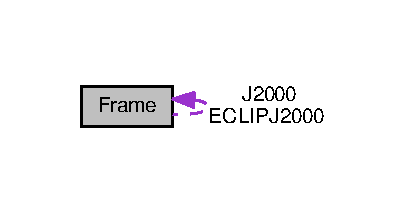
\includegraphics[width=197pt]{class_frame__coll__graph}
\end{center}
\end{figure}
\subsection*{Classes}
\begin{DoxyCompactItemize}
\item 
struct \hyperlink{struct_frame_1_1_frame_info}{Frame\+Info}
\end{DoxyCompactItemize}
\subsection*{Public Types}
\begin{DoxyCompactItemize}
\item 
enum \hyperlink{class_frame_ad2f22450377db20233914c9ec0a21df4}{Frame\+Type} \{ \\*
\hyperlink{class_frame_ad2f22450377db20233914c9ec0a21df4ac73961ac9e615a4da4339c8e20fe92ef}{F\+T\+\_\+\+I\+N\+E\+R\+T\+I\+A\+L} = 1, 
\hyperlink{class_frame_ad2f22450377db20233914c9ec0a21df4a03c1983206078ccc3fd8c290a5d63019}{F\+T\+\_\+\+P\+C\+K}, 
\hyperlink{class_frame_ad2f22450377db20233914c9ec0a21df4a4438b3590992adb7e998575e686a995b}{F\+T\+\_\+\+C\+K}, 
\hyperlink{class_frame_ad2f22450377db20233914c9ec0a21df4a3a52c9b5914442b7ca49e20720257800}{F\+T\+\_\+\+T\+K}, 
\\*
\hyperlink{class_frame_ad2f22450377db20233914c9ec0a21df4ad682b0691e051ce65913fdf42d4be1af}{F\+T\+\_\+\+D\+Y\+N\+A\+M\+I\+C}
 \}
\end{DoxyCompactItemize}
\subsection*{Public Member Functions}
\begin{DoxyCompactItemize}
\item 
\hyperlink{class_frame_affeadc282e1d1b07d51918add4b48fbf}{Frame} (\hyperlink{wglext_8h_a500a82aecba06f4550f6849b8099ca21}{int} spice\+Id, const \hyperlink{glext_8h_ae84541b4f3d8e1ea24ec0f466a8c568b}{std\+::string} \&\hyperlink{glext_8h_ad977737dfc9a274a62741b9500c49a32}{name}=\char`\"{}\char`\"{})
\item 
\hyperlink{class_frame_a7254d330d38d6d454f5a77777d8f1bcb}{Frame} (const \hyperlink{glext_8h_ae84541b4f3d8e1ea24ec0f466a8c568b}{std\+::string} \&spice\+Name, const \hyperlink{glext_8h_ae84541b4f3d8e1ea24ec0f466a8c568b}{std\+::string} \&\hyperlink{glext_8h_ad977737dfc9a274a62741b9500c49a32}{name}=\char`\"{}\char`\"{})
\item 
\hyperlink{class_frame_abec8c7bccdfc88cb4da137caae9f73d6}{$\sim$\+Frame} ()
\item 
long \hyperlink{class_frame_a679aa287b6474930b7c1682f3a9ceb14}{Get\+Spice\+Id} () const 
\item 
\hyperlink{glext_8h_ae84541b4f3d8e1ea24ec0f466a8c568b}{std\+::string} \hyperlink{class_frame_ad7596949a1ff9c2d1dd837e730f6aefc}{Get\+Spice\+Name} () const 
\item 
const \hyperlink{glext_8h_ae84541b4f3d8e1ea24ec0f466a8c568b}{std\+::string} \& \hyperlink{class_frame_afc3c2fb53313f43fd6b906cd5423145e}{Get\+Name} () const 
\item 
\hyperlink{struct_frame_1_1_frame_info}{Frame\+Info} \hyperlink{class_frame_a676a0342efbbafb23ef5366e02843b15}{Get\+Frame\+Info} () const 
\item 
const \hyperlink{class_space_object}{Space\+Object} \& \hyperlink{class_frame_ad41c119171bcaebc84a9c5e0daea6c92}{Get\+Center\+Object} () const 
\item 
\hyperlink{class_vector3}{Vector3} \hyperlink{class_frame_a9fac9191222fbcf79954b5cb4fe8a181}{Transform\+Vector} (const \hyperlink{class_vector3}{Vector3} \&vec, const \hyperlink{class_date}{Date} \&\hyperlink{glext_8h_a7d65d00ca3b0630d9b5c52df855b19f5}{t}, const \hyperlink{class_frame}{Frame} \&\hyperlink{glext_8h_ad32bdec748ba376f6c0d2df39ab9a95b}{ref}) const 
\item 
\hyperlink{class_vector3}{Vector3} \hyperlink{class_frame_ac8195fe92d18baac95813e2bf751f533}{Axis\+X} (const \hyperlink{class_date}{Date} \&\hyperlink{glext_8h_a7d65d00ca3b0630d9b5c52df855b19f5}{t}, const \hyperlink{class_frame}{Frame} \&\hyperlink{glext_8h_ad32bdec748ba376f6c0d2df39ab9a95b}{ref}) const 
\item 
\hyperlink{class_vector3}{Vector3} \hyperlink{class_frame_a5ed0a2188dc255484b793ae5288c36c0}{Axis\+Y} (const \hyperlink{class_date}{Date} \&\hyperlink{glext_8h_a7d65d00ca3b0630d9b5c52df855b19f5}{t}, const \hyperlink{class_frame}{Frame} \&\hyperlink{glext_8h_ad32bdec748ba376f6c0d2df39ab9a95b}{ref}) const 
\item 
\hyperlink{class_vector3}{Vector3} \hyperlink{class_frame_a89ebe688b416263f06f2393151194e77}{Axis\+Z} (const \hyperlink{class_date}{Date} \&\hyperlink{glext_8h_a7d65d00ca3b0630d9b5c52df855b19f5}{t}, const \hyperlink{class_frame}{Frame} \&\hyperlink{glext_8h_ad32bdec748ba376f6c0d2df39ab9a95b}{ref}) const 
\item 
\hyperlink{class_matrix4x4}{Matrix4x4} \hyperlink{class_frame_a4862be40cebae8c367031baf2ca6dc8b}{Get\+Transformation\+Matrix} (const \hyperlink{class_date}{Date} \&\hyperlink{glext_8h_a7d65d00ca3b0630d9b5c52df855b19f5}{t}, const \hyperlink{class_frame}{Frame} \&\hyperlink{glext_8h_ad32bdec748ba376f6c0d2df39ab9a95b}{ref}) const 
\item 
bool \hyperlink{class_frame_afbf0802e2374c57dd80f754bd0c232da}{Has\+Available\+Data} () const 
\item 
bool \hyperlink{class_frame_af03488c8a8eb25e55725b1af7c379671}{Has\+Limited\+Coverage} () const 
\item 
\hyperlink{class_window}{Window} \hyperlink{class_frame_a54fe03adc618817f27c43738ca77ccf8}{Get\+Coverage} () const 
\end{DoxyCompactItemize}
\subsection*{Static Public Member Functions}
\begin{DoxyCompactItemize}
\item 
static bool \hyperlink{class_frame_a2530927116bf3b764862623c518d274e}{Validate\+Id} (long \hyperlink{glext_8h_a58c2a664503e14ffb8f21012aabff3e9}{id})
\item 
static long \hyperlink{class_frame_a33201e744d6593f2294bfb57bcb448d9}{Make\+Frame\+Id} (\hyperlink{class_frame_ad2f22450377db20233914c9ec0a21df4}{Frame\+Type} \hyperlink{glext_8h_ab7c1afc09f67635c2c376638fcc0db5f}{type}, long class\+Id)
\item 
static std\+::vector$<$ long $>$ \hyperlink{class_frame_af143d92b7e9c07d2db5aec79b89ac1b2}{Get\+Built\+In\+Ids} ()
\item 
static std\+::vector$<$ long $>$ \hyperlink{class_frame_a80d4a5985129beb4d8010f072def67d7}{Get\+Pool\+Ids} ()
\item 
static std\+::vector$<$ long $>$ \hyperlink{class_frame_ac5865bd9a4b0f8904b059fc005311971}{Get\+Loaded\+Pck\+Ids} ()
\end{DoxyCompactItemize}
\subsection*{Static Public Attributes}
\begin{DoxyCompactItemize}
\item 
static const \hyperlink{class_frame}{Frame} \hyperlink{class_frame_a83f98b1d0aa72dca955fd91752e6b499}{J2000} = \hyperlink{class_frame}{Frame}(\char`\"{}J2000\char`\"{})
\item 
static const \hyperlink{class_frame}{Frame} \hyperlink{class_frame_af25db3f51bb9838c9bce46d30e663331}{E\+C\+L\+I\+P\+J2000} = \hyperlink{class_frame}{Frame}(\char`\"{}E\+C\+L\+I\+P\+J2000\char`\"{})
\end{DoxyCompactItemize}


\subsection{Detailed Description}


Definition at line 14 of file Frame.\+h.



\subsection{Member Enumeration Documentation}
\hypertarget{class_frame_ad2f22450377db20233914c9ec0a21df4}{\index{Frame@{Frame}!Frame\+Type@{Frame\+Type}}
\index{Frame\+Type@{Frame\+Type}!Frame@{Frame}}
\subsubsection[{Frame\+Type}]{\setlength{\rightskip}{0pt plus 5cm}enum {\bf Frame\+::\+Frame\+Type}}}\label{class_frame_ad2f22450377db20233914c9ec0a21df4}
\begin{Desc}
\item[Enumerator]\par
\begin{description}
\index{F\+T\+\_\+\+I\+N\+E\+R\+T\+I\+A\+L@{F\+T\+\_\+\+I\+N\+E\+R\+T\+I\+A\+L}!Frame@{Frame}}\index{Frame@{Frame}!F\+T\+\_\+\+I\+N\+E\+R\+T\+I\+A\+L@{F\+T\+\_\+\+I\+N\+E\+R\+T\+I\+A\+L}}\item[{\em 
\hypertarget{class_frame_ad2f22450377db20233914c9ec0a21df4ac73961ac9e615a4da4339c8e20fe92ef}{F\+T\+\_\+\+I\+N\+E\+R\+T\+I\+A\+L}\label{class_frame_ad2f22450377db20233914c9ec0a21df4ac73961ac9e615a4da4339c8e20fe92ef}
}]\index{F\+T\+\_\+\+P\+C\+K@{F\+T\+\_\+\+P\+C\+K}!Frame@{Frame}}\index{Frame@{Frame}!F\+T\+\_\+\+P\+C\+K@{F\+T\+\_\+\+P\+C\+K}}\item[{\em 
\hypertarget{class_frame_ad2f22450377db20233914c9ec0a21df4a03c1983206078ccc3fd8c290a5d63019}{F\+T\+\_\+\+P\+C\+K}\label{class_frame_ad2f22450377db20233914c9ec0a21df4a03c1983206078ccc3fd8c290a5d63019}
}]\index{F\+T\+\_\+\+C\+K@{F\+T\+\_\+\+C\+K}!Frame@{Frame}}\index{Frame@{Frame}!F\+T\+\_\+\+C\+K@{F\+T\+\_\+\+C\+K}}\item[{\em 
\hypertarget{class_frame_ad2f22450377db20233914c9ec0a21df4a4438b3590992adb7e998575e686a995b}{F\+T\+\_\+\+C\+K}\label{class_frame_ad2f22450377db20233914c9ec0a21df4a4438b3590992adb7e998575e686a995b}
}]\index{F\+T\+\_\+\+T\+K@{F\+T\+\_\+\+T\+K}!Frame@{Frame}}\index{Frame@{Frame}!F\+T\+\_\+\+T\+K@{F\+T\+\_\+\+T\+K}}\item[{\em 
\hypertarget{class_frame_ad2f22450377db20233914c9ec0a21df4a3a52c9b5914442b7ca49e20720257800}{F\+T\+\_\+\+T\+K}\label{class_frame_ad2f22450377db20233914c9ec0a21df4a3a52c9b5914442b7ca49e20720257800}
}]\index{F\+T\+\_\+\+D\+Y\+N\+A\+M\+I\+C@{F\+T\+\_\+\+D\+Y\+N\+A\+M\+I\+C}!Frame@{Frame}}\index{Frame@{Frame}!F\+T\+\_\+\+D\+Y\+N\+A\+M\+I\+C@{F\+T\+\_\+\+D\+Y\+N\+A\+M\+I\+C}}\item[{\em 
\hypertarget{class_frame_ad2f22450377db20233914c9ec0a21df4ad682b0691e051ce65913fdf42d4be1af}{F\+T\+\_\+\+D\+Y\+N\+A\+M\+I\+C}\label{class_frame_ad2f22450377db20233914c9ec0a21df4ad682b0691e051ce65913fdf42d4be1af}
}]\end{description}
\end{Desc}


Definition at line 17 of file Frame.\+h.



\subsection{Constructor \& Destructor Documentation}
\hypertarget{class_frame_affeadc282e1d1b07d51918add4b48fbf}{\index{Frame@{Frame}!Frame@{Frame}}
\index{Frame@{Frame}!Frame@{Frame}}
\subsubsection[{Frame}]{\setlength{\rightskip}{0pt plus 5cm}Frame\+::\+Frame (
\begin{DoxyParamCaption}
\item[{{\bf int}}]{spice\+Id, }
\item[{const {\bf std\+::string} \&}]{name = {\ttfamily \char`\"{}\char`\"{}}}
\end{DoxyParamCaption}
)}}\label{class_frame_affeadc282e1d1b07d51918add4b48fbf}


Definition at line 6 of file Frame.\+cpp.

\hypertarget{class_frame_a7254d330d38d6d454f5a77777d8f1bcb}{\index{Frame@{Frame}!Frame@{Frame}}
\index{Frame@{Frame}!Frame@{Frame}}
\subsubsection[{Frame}]{\setlength{\rightskip}{0pt plus 5cm}Frame\+::\+Frame (
\begin{DoxyParamCaption}
\item[{const {\bf std\+::string} \&}]{spice\+Name, }
\item[{const {\bf std\+::string} \&}]{name = {\ttfamily \char`\"{}\char`\"{}}}
\end{DoxyParamCaption}
)}}\label{class_frame_a7254d330d38d6d454f5a77777d8f1bcb}


Definition at line 11 of file Frame.\+cpp.

\hypertarget{class_frame_abec8c7bccdfc88cb4da137caae9f73d6}{\index{Frame@{Frame}!````~Frame@{$\sim$\+Frame}}
\index{````~Frame@{$\sim$\+Frame}!Frame@{Frame}}
\subsubsection[{$\sim$\+Frame}]{\setlength{\rightskip}{0pt plus 5cm}Frame\+::$\sim$\+Frame (
\begin{DoxyParamCaption}
{}
\end{DoxyParamCaption}
)}}\label{class_frame_abec8c7bccdfc88cb4da137caae9f73d6}


Definition at line 34 of file Frame.\+cpp.



\subsection{Member Function Documentation}
\hypertarget{class_frame_ac8195fe92d18baac95813e2bf751f533}{\index{Frame@{Frame}!Axis\+X@{Axis\+X}}
\index{Axis\+X@{Axis\+X}!Frame@{Frame}}
\subsubsection[{Axis\+X}]{\setlength{\rightskip}{0pt plus 5cm}{\bf Vector3} Frame\+::\+Axis\+X (
\begin{DoxyParamCaption}
\item[{const {\bf Date} \&}]{t, }
\item[{const {\bf Frame} \&}]{ref}
\end{DoxyParamCaption}
) const}}\label{class_frame_ac8195fe92d18baac95813e2bf751f533}


Definition at line 93 of file Frame.\+cpp.

\hypertarget{class_frame_a5ed0a2188dc255484b793ae5288c36c0}{\index{Frame@{Frame}!Axis\+Y@{Axis\+Y}}
\index{Axis\+Y@{Axis\+Y}!Frame@{Frame}}
\subsubsection[{Axis\+Y}]{\setlength{\rightskip}{0pt plus 5cm}{\bf Vector3} Frame\+::\+Axis\+Y (
\begin{DoxyParamCaption}
\item[{const {\bf Date} \&}]{t, }
\item[{const {\bf Frame} \&}]{ref}
\end{DoxyParamCaption}
) const}}\label{class_frame_a5ed0a2188dc255484b793ae5288c36c0}


Definition at line 98 of file Frame.\+cpp.

\hypertarget{class_frame_a89ebe688b416263f06f2393151194e77}{\index{Frame@{Frame}!Axis\+Z@{Axis\+Z}}
\index{Axis\+Z@{Axis\+Z}!Frame@{Frame}}
\subsubsection[{Axis\+Z}]{\setlength{\rightskip}{0pt plus 5cm}{\bf Vector3} Frame\+::\+Axis\+Z (
\begin{DoxyParamCaption}
\item[{const {\bf Date} \&}]{t, }
\item[{const {\bf Frame} \&}]{ref}
\end{DoxyParamCaption}
) const}}\label{class_frame_a89ebe688b416263f06f2393151194e77}


Definition at line 103 of file Frame.\+cpp.

\hypertarget{class_frame_af143d92b7e9c07d2db5aec79b89ac1b2}{\index{Frame@{Frame}!Get\+Built\+In\+Ids@{Get\+Built\+In\+Ids}}
\index{Get\+Built\+In\+Ids@{Get\+Built\+In\+Ids}!Frame@{Frame}}
\subsubsection[{Get\+Built\+In\+Ids}]{\setlength{\rightskip}{0pt plus 5cm}std\+::vector$<$ long $>$ Frame\+::\+Get\+Built\+In\+Ids (
\begin{DoxyParamCaption}
{}
\end{DoxyParamCaption}
)\hspace{0.3cm}{\ttfamily [static]}}}\label{class_frame_af143d92b7e9c07d2db5aec79b89ac1b2}


Definition at line 190 of file Frame.\+cpp.

\hypertarget{class_frame_ad41c119171bcaebc84a9c5e0daea6c92}{\index{Frame@{Frame}!Get\+Center\+Object@{Get\+Center\+Object}}
\index{Get\+Center\+Object@{Get\+Center\+Object}!Frame@{Frame}}
\subsubsection[{Get\+Center\+Object}]{\setlength{\rightskip}{0pt plus 5cm}const {\bf Space\+Object} \& Frame\+::\+Get\+Center\+Object (
\begin{DoxyParamCaption}
{}
\end{DoxyParamCaption}
) const}}\label{class_frame_ad41c119171bcaebc84a9c5e0daea6c92}


Definition at line 74 of file Frame.\+cpp.

\hypertarget{class_frame_a54fe03adc618817f27c43738ca77ccf8}{\index{Frame@{Frame}!Get\+Coverage@{Get\+Coverage}}
\index{Get\+Coverage@{Get\+Coverage}!Frame@{Frame}}
\subsubsection[{Get\+Coverage}]{\setlength{\rightskip}{0pt plus 5cm}{\bf Window} Frame\+::\+Get\+Coverage (
\begin{DoxyParamCaption}
{}
\end{DoxyParamCaption}
) const}}\label{class_frame_a54fe03adc618817f27c43738ca77ccf8}


Definition at line 151 of file Frame.\+cpp.

\hypertarget{class_frame_a676a0342efbbafb23ef5366e02843b15}{\index{Frame@{Frame}!Get\+Frame\+Info@{Get\+Frame\+Info}}
\index{Get\+Frame\+Info@{Get\+Frame\+Info}!Frame@{Frame}}
\subsubsection[{Get\+Frame\+Info}]{\setlength{\rightskip}{0pt plus 5cm}{\bf Frame\+::\+Frame\+Info} Frame\+::\+Get\+Frame\+Info (
\begin{DoxyParamCaption}
{}
\end{DoxyParamCaption}
) const}}\label{class_frame_a676a0342efbbafb23ef5366e02843b15}


Definition at line 57 of file Frame.\+cpp.

\hypertarget{class_frame_ac5865bd9a4b0f8904b059fc005311971}{\index{Frame@{Frame}!Get\+Loaded\+Pck\+Ids@{Get\+Loaded\+Pck\+Ids}}
\index{Get\+Loaded\+Pck\+Ids@{Get\+Loaded\+Pck\+Ids}!Frame@{Frame}}
\subsubsection[{Get\+Loaded\+Pck\+Ids}]{\setlength{\rightskip}{0pt plus 5cm}std\+::vector$<$ long $>$ Frame\+::\+Get\+Loaded\+Pck\+Ids (
\begin{DoxyParamCaption}
{}
\end{DoxyParamCaption}
)\hspace{0.3cm}{\ttfamily [static]}}}\label{class_frame_ac5865bd9a4b0f8904b059fc005311971}


Definition at line 204 of file Frame.\+cpp.

\hypertarget{class_frame_afc3c2fb53313f43fd6b906cd5423145e}{\index{Frame@{Frame}!Get\+Name@{Get\+Name}}
\index{Get\+Name@{Get\+Name}!Frame@{Frame}}
\subsubsection[{Get\+Name}]{\setlength{\rightskip}{0pt plus 5cm}const {\bf std\+::string} \& Frame\+::\+Get\+Name (
\begin{DoxyParamCaption}
{}
\end{DoxyParamCaption}
) const}}\label{class_frame_afc3c2fb53313f43fd6b906cd5423145e}


Definition at line 52 of file Frame.\+cpp.

\hypertarget{class_frame_a80d4a5985129beb4d8010f072def67d7}{\index{Frame@{Frame}!Get\+Pool\+Ids@{Get\+Pool\+Ids}}
\index{Get\+Pool\+Ids@{Get\+Pool\+Ids}!Frame@{Frame}}
\subsubsection[{Get\+Pool\+Ids}]{\setlength{\rightskip}{0pt plus 5cm}std\+::vector$<$ long $>$ Frame\+::\+Get\+Pool\+Ids (
\begin{DoxyParamCaption}
{}
\end{DoxyParamCaption}
)\hspace{0.3cm}{\ttfamily [static]}}}\label{class_frame_a80d4a5985129beb4d8010f072def67d7}


Definition at line 197 of file Frame.\+cpp.

\hypertarget{class_frame_a679aa287b6474930b7c1682f3a9ceb14}{\index{Frame@{Frame}!Get\+Spice\+Id@{Get\+Spice\+Id}}
\index{Get\+Spice\+Id@{Get\+Spice\+Id}!Frame@{Frame}}
\subsubsection[{Get\+Spice\+Id}]{\setlength{\rightskip}{0pt plus 5cm}long Frame\+::\+Get\+Spice\+Id (
\begin{DoxyParamCaption}
{}
\end{DoxyParamCaption}
) const}}\label{class_frame_a679aa287b6474930b7c1682f3a9ceb14}


Definition at line 39 of file Frame.\+cpp.

\hypertarget{class_frame_ad7596949a1ff9c2d1dd837e730f6aefc}{\index{Frame@{Frame}!Get\+Spice\+Name@{Get\+Spice\+Name}}
\index{Get\+Spice\+Name@{Get\+Spice\+Name}!Frame@{Frame}}
\subsubsection[{Get\+Spice\+Name}]{\setlength{\rightskip}{0pt plus 5cm}{\bf std\+::string} Frame\+::\+Get\+Spice\+Name (
\begin{DoxyParamCaption}
{}
\end{DoxyParamCaption}
) const}}\label{class_frame_ad7596949a1ff9c2d1dd837e730f6aefc}


Definition at line 44 of file Frame.\+cpp.

\hypertarget{class_frame_a4862be40cebae8c367031baf2ca6dc8b}{\index{Frame@{Frame}!Get\+Transformation\+Matrix@{Get\+Transformation\+Matrix}}
\index{Get\+Transformation\+Matrix@{Get\+Transformation\+Matrix}!Frame@{Frame}}
\subsubsection[{Get\+Transformation\+Matrix}]{\setlength{\rightskip}{0pt plus 5cm}{\bf Matrix4x4} Frame\+::\+Get\+Transformation\+Matrix (
\begin{DoxyParamCaption}
\item[{const {\bf Date} \&}]{t, }
\item[{const {\bf Frame} \&}]{ref}
\end{DoxyParamCaption}
) const}}\label{class_frame_a4862be40cebae8c367031baf2ca6dc8b}


Definition at line 108 of file Frame.\+cpp.

\hypertarget{class_frame_afbf0802e2374c57dd80f754bd0c232da}{\index{Frame@{Frame}!Has\+Available\+Data@{Has\+Available\+Data}}
\index{Has\+Available\+Data@{Has\+Available\+Data}!Frame@{Frame}}
\subsubsection[{Has\+Available\+Data}]{\setlength{\rightskip}{0pt plus 5cm}bool Frame\+::\+Has\+Available\+Data (
\begin{DoxyParamCaption}
{}
\end{DoxyParamCaption}
) const}}\label{class_frame_afbf0802e2374c57dd80f754bd0c232da}


Definition at line 128 of file Frame.\+cpp.

\hypertarget{class_frame_af03488c8a8eb25e55725b1af7c379671}{\index{Frame@{Frame}!Has\+Limited\+Coverage@{Has\+Limited\+Coverage}}
\index{Has\+Limited\+Coverage@{Has\+Limited\+Coverage}!Frame@{Frame}}
\subsubsection[{Has\+Limited\+Coverage}]{\setlength{\rightskip}{0pt plus 5cm}bool Frame\+::\+Has\+Limited\+Coverage (
\begin{DoxyParamCaption}
{}
\end{DoxyParamCaption}
) const}}\label{class_frame_af03488c8a8eb25e55725b1af7c379671}


Definition at line 142 of file Frame.\+cpp.

\hypertarget{class_frame_a33201e744d6593f2294bfb57bcb448d9}{\index{Frame@{Frame}!Make\+Frame\+Id@{Make\+Frame\+Id}}
\index{Make\+Frame\+Id@{Make\+Frame\+Id}!Frame@{Frame}}
\subsubsection[{Make\+Frame\+Id}]{\setlength{\rightskip}{0pt plus 5cm}long Frame\+::\+Make\+Frame\+Id (
\begin{DoxyParamCaption}
\item[{{\bf Frame\+Type}}]{type, }
\item[{long}]{class\+Id}
\end{DoxyParamCaption}
)\hspace{0.3cm}{\ttfamily [static]}}}\label{class_frame_a33201e744d6593f2294bfb57bcb448d9}


Definition at line 179 of file Frame.\+cpp.

\hypertarget{class_frame_a9fac9191222fbcf79954b5cb4fe8a181}{\index{Frame@{Frame}!Transform\+Vector@{Transform\+Vector}}
\index{Transform\+Vector@{Transform\+Vector}!Frame@{Frame}}
\subsubsection[{Transform\+Vector}]{\setlength{\rightskip}{0pt plus 5cm}{\bf Vector3} Frame\+::\+Transform\+Vector (
\begin{DoxyParamCaption}
\item[{const {\bf Vector3} \&}]{vec, }
\item[{const {\bf Date} \&}]{t, }
\item[{const {\bf Frame} \&}]{ref}
\end{DoxyParamCaption}
) const}}\label{class_frame_a9fac9191222fbcf79954b5cb4fe8a181}


Definition at line 79 of file Frame.\+cpp.

\hypertarget{class_frame_a2530927116bf3b764862623c518d274e}{\index{Frame@{Frame}!Validate\+Id@{Validate\+Id}}
\index{Validate\+Id@{Validate\+Id}!Frame@{Frame}}
\subsubsection[{Validate\+Id}]{\setlength{\rightskip}{0pt plus 5cm}bool Frame\+::\+Validate\+Id (
\begin{DoxyParamCaption}
\item[{long}]{id}
\end{DoxyParamCaption}
)\hspace{0.3cm}{\ttfamily [static]}}}\label{class_frame_a2530927116bf3b764862623c518d274e}


Definition at line 167 of file Frame.\+cpp.



\subsection{Member Data Documentation}
\hypertarget{class_frame_af25db3f51bb9838c9bce46d30e663331}{\index{Frame@{Frame}!E\+C\+L\+I\+P\+J2000@{E\+C\+L\+I\+P\+J2000}}
\index{E\+C\+L\+I\+P\+J2000@{E\+C\+L\+I\+P\+J2000}!Frame@{Frame}}
\subsubsection[{E\+C\+L\+I\+P\+J2000}]{\setlength{\rightskip}{0pt plus 5cm}const {\bf Frame} Frame\+::\+E\+C\+L\+I\+P\+J2000 = {\bf Frame}(\char`\"{}E\+C\+L\+I\+P\+J2000\char`\"{})\hspace{0.3cm}{\ttfamily [static]}}}\label{class_frame_af25db3f51bb9838c9bce46d30e663331}


Definition at line 73 of file Frame.\+h.

\hypertarget{class_frame_a83f98b1d0aa72dca955fd91752e6b499}{\index{Frame@{Frame}!J2000@{J2000}}
\index{J2000@{J2000}!Frame@{Frame}}
\subsubsection[{J2000}]{\setlength{\rightskip}{0pt plus 5cm}const {\bf Frame} Frame\+::\+J2000 = {\bf Frame}(\char`\"{}J2000\char`\"{})\hspace{0.3cm}{\ttfamily [static]}}}\label{class_frame_a83f98b1d0aa72dca955fd91752e6b499}


Definition at line 72 of file Frame.\+h.



The documentation for this class was generated from the following files\+:\begin{DoxyCompactItemize}
\item 
S\+S\+W\+C/src/\+C\+Spice/\hyperlink{_frame_8h}{Frame.\+h}\item 
S\+S\+W\+C/src/\+C\+Spice/\hyperlink{_frame_8cpp}{Frame.\+cpp}\end{DoxyCompactItemize}

\hypertarget{struct_frame_1_1_frame_info}{\section{Frame\+:\+:Frame\+Info Struct Reference}
\label{struct_frame_1_1_frame_info}\index{Frame\+::\+Frame\+Info@{Frame\+::\+Frame\+Info}}
}


{\ttfamily \#include $<$Frame.\+h$>$}

\subsection*{Public Attributes}
\begin{DoxyCompactItemize}
\item 
long \hyperlink{struct_frame_1_1_frame_info_a13df02e5be92dc224b0ed75c2e339fc5}{center\+Id}
\item 
\hyperlink{class_frame_ad2f22450377db20233914c9ec0a21df4}{Frame\+Type} \hyperlink{struct_frame_1_1_frame_info_a26a5b5ce9d01a6029fbd2aaf6c77e574}{frame\+Type}
\item 
long \hyperlink{struct_frame_1_1_frame_info_a26545f9bb7266068c37985694b990192}{class\+Id}
\end{DoxyCompactItemize}


\subsection{Detailed Description}


Definition at line 26 of file Frame.\+h.



\subsection{Member Data Documentation}
\hypertarget{struct_frame_1_1_frame_info_a13df02e5be92dc224b0ed75c2e339fc5}{\index{Frame\+::\+Frame\+Info@{Frame\+::\+Frame\+Info}!center\+Id@{center\+Id}}
\index{center\+Id@{center\+Id}!Frame\+::\+Frame\+Info@{Frame\+::\+Frame\+Info}}
\subsubsection[{center\+Id}]{\setlength{\rightskip}{0pt plus 5cm}long Frame\+::\+Frame\+Info\+::center\+Id}}\label{struct_frame_1_1_frame_info_a13df02e5be92dc224b0ed75c2e339fc5}


Definition at line 28 of file Frame.\+h.

\hypertarget{struct_frame_1_1_frame_info_a26545f9bb7266068c37985694b990192}{\index{Frame\+::\+Frame\+Info@{Frame\+::\+Frame\+Info}!class\+Id@{class\+Id}}
\index{class\+Id@{class\+Id}!Frame\+::\+Frame\+Info@{Frame\+::\+Frame\+Info}}
\subsubsection[{class\+Id}]{\setlength{\rightskip}{0pt plus 5cm}long Frame\+::\+Frame\+Info\+::class\+Id}}\label{struct_frame_1_1_frame_info_a26545f9bb7266068c37985694b990192}


Definition at line 30 of file Frame.\+h.

\hypertarget{struct_frame_1_1_frame_info_a26a5b5ce9d01a6029fbd2aaf6c77e574}{\index{Frame\+::\+Frame\+Info@{Frame\+::\+Frame\+Info}!frame\+Type@{frame\+Type}}
\index{frame\+Type@{frame\+Type}!Frame\+::\+Frame\+Info@{Frame\+::\+Frame\+Info}}
\subsubsection[{frame\+Type}]{\setlength{\rightskip}{0pt plus 5cm}{\bf Frame\+Type} Frame\+::\+Frame\+Info\+::frame\+Type}}\label{struct_frame_1_1_frame_info_a26a5b5ce9d01a6029fbd2aaf6c77e574}


Definition at line 29 of file Frame.\+h.



The documentation for this struct was generated from the following file\+:\begin{DoxyCompactItemize}
\item 
S\+S\+W\+C/src/\+C\+Spice/\hyperlink{_frame_8h}{Frame.\+h}\end{DoxyCompactItemize}

\hypertarget{struct_g_l___window}{\section{G\+L\+\_\+\+Window Struct Reference}
\label{struct_g_l___window}\index{G\+L\+\_\+\+Window@{G\+L\+\_\+\+Window}}
}


{\ttfamily \#include $<$Program.\+h$>$}



Collaboration diagram for G\+L\+\_\+\+Window\+:\nopagebreak
\begin{figure}[H]
\begin{center}
\leavevmode
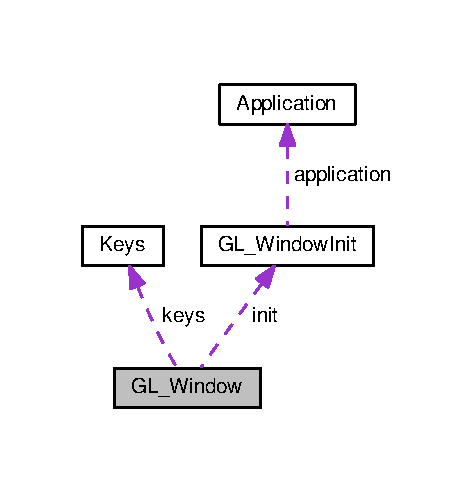
\includegraphics[width=228pt]{struct_g_l___window__coll__graph}
\end{center}
\end{figure}
\subsection*{Public Attributes}
\begin{DoxyCompactItemize}
\item 
\hyperlink{struct_keys}{Keys} $\ast$ \hyperlink{struct_g_l___window_ad0eed98271ddbfb6ab6cf7f12d7b5d02}{keys}
\item 
H\+W\+N\+D \hyperlink{struct_g_l___window_a43e3e57bd7ba1d1e98a8bea7b1ca5bfa}{h\+Wnd}
\item 
\hyperlink{wglext_8h_aaf5a06bd464c6ec72cf68b4819afebe3}{H\+D\+C} \hyperlink{struct_g_l___window_ac968ec84163d9ff1818a6c7ca6f636ab}{h\+D\+C}
\item 
\hyperlink{wglext_8h_ac592fca28a23754f86edf2739d21068c}{H\+G\+L\+R\+C} \hyperlink{struct_g_l___window_a529cfea8e49780d88eb095ff56e4bc5e}{h\+R\+C}
\item 
\hyperlink{struct_g_l___window_init}{G\+L\+\_\+\+Window\+Init} \hyperlink{struct_g_l___window_a509808116a84e361e12666b2d5b5c62f}{init}
\item 
\hyperlink{wglext_8h_a05538ca0e53ef21cb679e6de0fef7f8e}{B\+O\+O\+L} \hyperlink{struct_g_l___window_a6b7dc6064a91f6e7ebf071633f43f90d}{is\+Visible}
\item 
D\+W\+O\+R\+D \hyperlink{struct_g_l___window_af8068e4f9adf4515817a3d72a9cf0d03}{last\+Tick\+Count}
\end{DoxyCompactItemize}


\subsection{Detailed Description}


Definition at line 23 of file Program.\+h.



\subsection{Member Data Documentation}
\hypertarget{struct_g_l___window_ac968ec84163d9ff1818a6c7ca6f636ab}{\index{G\+L\+\_\+\+Window@{G\+L\+\_\+\+Window}!h\+D\+C@{h\+D\+C}}
\index{h\+D\+C@{h\+D\+C}!G\+L\+\_\+\+Window@{G\+L\+\_\+\+Window}}
\subsubsection[{h\+D\+C}]{\setlength{\rightskip}{0pt plus 5cm}{\bf H\+D\+C} G\+L\+\_\+\+Window\+::h\+D\+C}}\label{struct_g_l___window_ac968ec84163d9ff1818a6c7ca6f636ab}


Definition at line 26 of file Program.\+h.

\hypertarget{struct_g_l___window_a529cfea8e49780d88eb095ff56e4bc5e}{\index{G\+L\+\_\+\+Window@{G\+L\+\_\+\+Window}!h\+R\+C@{h\+R\+C}}
\index{h\+R\+C@{h\+R\+C}!G\+L\+\_\+\+Window@{G\+L\+\_\+\+Window}}
\subsubsection[{h\+R\+C}]{\setlength{\rightskip}{0pt plus 5cm}{\bf H\+G\+L\+R\+C} G\+L\+\_\+\+Window\+::h\+R\+C}}\label{struct_g_l___window_a529cfea8e49780d88eb095ff56e4bc5e}


Definition at line 27 of file Program.\+h.

\hypertarget{struct_g_l___window_a43e3e57bd7ba1d1e98a8bea7b1ca5bfa}{\index{G\+L\+\_\+\+Window@{G\+L\+\_\+\+Window}!h\+Wnd@{h\+Wnd}}
\index{h\+Wnd@{h\+Wnd}!G\+L\+\_\+\+Window@{G\+L\+\_\+\+Window}}
\subsubsection[{h\+Wnd}]{\setlength{\rightskip}{0pt plus 5cm}H\+W\+N\+D G\+L\+\_\+\+Window\+::h\+Wnd}}\label{struct_g_l___window_a43e3e57bd7ba1d1e98a8bea7b1ca5bfa}


Definition at line 25 of file Program.\+h.

\hypertarget{struct_g_l___window_a509808116a84e361e12666b2d5b5c62f}{\index{G\+L\+\_\+\+Window@{G\+L\+\_\+\+Window}!init@{init}}
\index{init@{init}!G\+L\+\_\+\+Window@{G\+L\+\_\+\+Window}}
\subsubsection[{init}]{\setlength{\rightskip}{0pt plus 5cm}{\bf G\+L\+\_\+\+Window\+Init} G\+L\+\_\+\+Window\+::init}}\label{struct_g_l___window_a509808116a84e361e12666b2d5b5c62f}


Definition at line 28 of file Program.\+h.

\hypertarget{struct_g_l___window_a6b7dc6064a91f6e7ebf071633f43f90d}{\index{G\+L\+\_\+\+Window@{G\+L\+\_\+\+Window}!is\+Visible@{is\+Visible}}
\index{is\+Visible@{is\+Visible}!G\+L\+\_\+\+Window@{G\+L\+\_\+\+Window}}
\subsubsection[{is\+Visible}]{\setlength{\rightskip}{0pt plus 5cm}{\bf B\+O\+O\+L} G\+L\+\_\+\+Window\+::is\+Visible}}\label{struct_g_l___window_a6b7dc6064a91f6e7ebf071633f43f90d}


Definition at line 29 of file Program.\+h.

\hypertarget{struct_g_l___window_ad0eed98271ddbfb6ab6cf7f12d7b5d02}{\index{G\+L\+\_\+\+Window@{G\+L\+\_\+\+Window}!keys@{keys}}
\index{keys@{keys}!G\+L\+\_\+\+Window@{G\+L\+\_\+\+Window}}
\subsubsection[{keys}]{\setlength{\rightskip}{0pt plus 5cm}{\bf Keys}$\ast$ G\+L\+\_\+\+Window\+::keys}}\label{struct_g_l___window_ad0eed98271ddbfb6ab6cf7f12d7b5d02}


Definition at line 24 of file Program.\+h.

\hypertarget{struct_g_l___window_af8068e4f9adf4515817a3d72a9cf0d03}{\index{G\+L\+\_\+\+Window@{G\+L\+\_\+\+Window}!last\+Tick\+Count@{last\+Tick\+Count}}
\index{last\+Tick\+Count@{last\+Tick\+Count}!G\+L\+\_\+\+Window@{G\+L\+\_\+\+Window}}
\subsubsection[{last\+Tick\+Count}]{\setlength{\rightskip}{0pt plus 5cm}D\+W\+O\+R\+D G\+L\+\_\+\+Window\+::last\+Tick\+Count}}\label{struct_g_l___window_af8068e4f9adf4515817a3d72a9cf0d03}


Definition at line 30 of file Program.\+h.



The documentation for this struct was generated from the following file\+:\begin{DoxyCompactItemize}
\item 
S\+S\+W\+C/src/\hyperlink{_program_8h}{Program.\+h}\end{DoxyCompactItemize}

\hypertarget{struct_g_l___window_init}{\section{G\+L\+\_\+\+Window\+Init Struct Reference}
\label{struct_g_l___window_init}\index{G\+L\+\_\+\+Window\+Init@{G\+L\+\_\+\+Window\+Init}}
}


{\ttfamily \#include $<$Program.\+h$>$}



Collaboration diagram for G\+L\+\_\+\+Window\+Init\+:\nopagebreak
\begin{figure}[H]
\begin{center}
\leavevmode
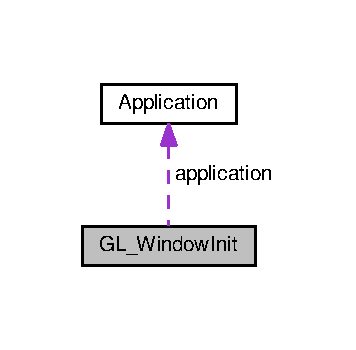
\includegraphics[width=171pt]{struct_g_l___window_init__coll__graph}
\end{center}
\end{figure}
\subsection*{Public Attributes}
\begin{DoxyCompactItemize}
\item 
\hyperlink{struct_application}{Application} $\ast$ \hyperlink{struct_g_l___window_init_afde844f257aafdb31bd03338723a2206}{application}
\item 
char $\ast$ \hyperlink{struct_g_l___window_init_a64c652d1fb4e2afa60b30fca91920ed4}{title}
\item 
\hyperlink{wglext_8h_a500a82aecba06f4550f6849b8099ca21}{int} \hyperlink{struct_g_l___window_init_a1a1c2cd5a8bc6b90987885307c296d9f}{width}
\item 
\hyperlink{wglext_8h_a500a82aecba06f4550f6849b8099ca21}{int} \hyperlink{struct_g_l___window_init_a8413cf084b2d4e7056da68940ab1438e}{height}
\item 
\hyperlink{wglext_8h_a500a82aecba06f4550f6849b8099ca21}{int} \hyperlink{struct_g_l___window_init_aa4220e9602ef12719a010e049a42fcea}{bits\+Per\+Pixel}
\item 
\hyperlink{wglext_8h_a05538ca0e53ef21cb679e6de0fef7f8e}{B\+O\+O\+L} \hyperlink{struct_g_l___window_init_a217a2406116f019e13094868c1810a32}{is\+Full\+Screen}
\end{DoxyCompactItemize}


\subsection{Detailed Description}


Definition at line 14 of file Program.\+h.



\subsection{Member Data Documentation}
\hypertarget{struct_g_l___window_init_afde844f257aafdb31bd03338723a2206}{\index{G\+L\+\_\+\+Window\+Init@{G\+L\+\_\+\+Window\+Init}!application@{application}}
\index{application@{application}!G\+L\+\_\+\+Window\+Init@{G\+L\+\_\+\+Window\+Init}}
\subsubsection[{application}]{\setlength{\rightskip}{0pt plus 5cm}{\bf Application}$\ast$ G\+L\+\_\+\+Window\+Init\+::application}}\label{struct_g_l___window_init_afde844f257aafdb31bd03338723a2206}


Definition at line 15 of file Program.\+h.

\hypertarget{struct_g_l___window_init_aa4220e9602ef12719a010e049a42fcea}{\index{G\+L\+\_\+\+Window\+Init@{G\+L\+\_\+\+Window\+Init}!bits\+Per\+Pixel@{bits\+Per\+Pixel}}
\index{bits\+Per\+Pixel@{bits\+Per\+Pixel}!G\+L\+\_\+\+Window\+Init@{G\+L\+\_\+\+Window\+Init}}
\subsubsection[{bits\+Per\+Pixel}]{\setlength{\rightskip}{0pt plus 5cm}{\bf int} G\+L\+\_\+\+Window\+Init\+::bits\+Per\+Pixel}}\label{struct_g_l___window_init_aa4220e9602ef12719a010e049a42fcea}


Definition at line 19 of file Program.\+h.

\hypertarget{struct_g_l___window_init_a8413cf084b2d4e7056da68940ab1438e}{\index{G\+L\+\_\+\+Window\+Init@{G\+L\+\_\+\+Window\+Init}!height@{height}}
\index{height@{height}!G\+L\+\_\+\+Window\+Init@{G\+L\+\_\+\+Window\+Init}}
\subsubsection[{height}]{\setlength{\rightskip}{0pt plus 5cm}{\bf int} G\+L\+\_\+\+Window\+Init\+::height}}\label{struct_g_l___window_init_a8413cf084b2d4e7056da68940ab1438e}


Definition at line 18 of file Program.\+h.

\hypertarget{struct_g_l___window_init_a217a2406116f019e13094868c1810a32}{\index{G\+L\+\_\+\+Window\+Init@{G\+L\+\_\+\+Window\+Init}!is\+Full\+Screen@{is\+Full\+Screen}}
\index{is\+Full\+Screen@{is\+Full\+Screen}!G\+L\+\_\+\+Window\+Init@{G\+L\+\_\+\+Window\+Init}}
\subsubsection[{is\+Full\+Screen}]{\setlength{\rightskip}{0pt plus 5cm}{\bf B\+O\+O\+L} G\+L\+\_\+\+Window\+Init\+::is\+Full\+Screen}}\label{struct_g_l___window_init_a217a2406116f019e13094868c1810a32}


Definition at line 20 of file Program.\+h.

\hypertarget{struct_g_l___window_init_a64c652d1fb4e2afa60b30fca91920ed4}{\index{G\+L\+\_\+\+Window\+Init@{G\+L\+\_\+\+Window\+Init}!title@{title}}
\index{title@{title}!G\+L\+\_\+\+Window\+Init@{G\+L\+\_\+\+Window\+Init}}
\subsubsection[{title}]{\setlength{\rightskip}{0pt plus 5cm}char$\ast$ G\+L\+\_\+\+Window\+Init\+::title}}\label{struct_g_l___window_init_a64c652d1fb4e2afa60b30fca91920ed4}


Definition at line 16 of file Program.\+h.

\hypertarget{struct_g_l___window_init_a1a1c2cd5a8bc6b90987885307c296d9f}{\index{G\+L\+\_\+\+Window\+Init@{G\+L\+\_\+\+Window\+Init}!width@{width}}
\index{width@{width}!G\+L\+\_\+\+Window\+Init@{G\+L\+\_\+\+Window\+Init}}
\subsubsection[{width}]{\setlength{\rightskip}{0pt plus 5cm}{\bf int} G\+L\+\_\+\+Window\+Init\+::width}}\label{struct_g_l___window_init_a1a1c2cd5a8bc6b90987885307c296d9f}


Definition at line 17 of file Program.\+h.



The documentation for this struct was generated from the following file\+:\begin{DoxyCompactItemize}
\item 
S\+S\+W\+C/src/\hyperlink{_program_8h}{Program.\+h}\end{DoxyCompactItemize}

\hypertarget{classgl_camera}{\section{gl\+Camera Class Reference}
\label{classgl_camera}\index{gl\+Camera@{gl\+Camera}}
}


{\ttfamily \#include $<$gl\+Cameara.\+h$>$}



Collaboration diagram for gl\+Camera\+:\nopagebreak
\begin{figure}[H]
\begin{center}
\leavevmode
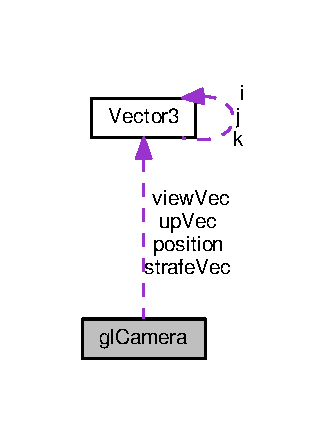
\includegraphics[width=158pt]{classgl_camera__coll__graph}
\end{center}
\end{figure}
\subsection*{Public Member Functions}
\begin{DoxyCompactItemize}
\item 
\hyperlink{classgl_camera_a8339c3cd03f2c15ea28cc4f7d473d3cd}{gl\+Camera} ()
\item 
\hyperlink{wglext_8h_a9e6b7f1933461ef318bb000d6bd13b83}{void} \hyperlink{classgl_camera_aefdc27e4f845a5c3610044c78068f802}{Position\+Camera} (const \hyperlink{class_vector3}{Vector3} \&\hyperlink{classgl_camera_a4e7a84b7ccc0840f436d9792c5429c2b}{position}, const \hyperlink{class_vector3}{Vector3} \&\hyperlink{classgl_camera_a2d6263fab021ec81f9f13582f8bdcb9b}{view\+Vec}, const \hyperlink{class_vector3}{Vector3} \&\hyperlink{classgl_camera_a361375f29cfc87acae069ec5b45f56f4}{up\+Vec})
\item 
\hyperlink{wglext_8h_a9e6b7f1933461ef318bb000d6bd13b83}{void} \hyperlink{classgl_camera_ad14659710098d9f0db8211c7681243b7}{Rotate\+Around\+Point} (\hyperlink{class_vector3}{Vector3} center, float \hyperlink{glext_8h_ad77deca22f617d3f0e0eb786445689fc}{x}, float \hyperlink{glext_8h_a9298c7ad619074f5285b32c6b72bfdea}{y}, float \hyperlink{glext_8h_a1483160fae141afea848a5393c286b2b}{z})
\item 
\hyperlink{wglext_8h_a9e6b7f1933461ef318bb000d6bd13b83}{void} \hyperlink{classgl_camera_ac5785ab7420408b165ad7a48aaab1a3a}{Move\+Camera} (float velocity)
\item 
\hyperlink{wglext_8h_a9e6b7f1933461ef318bb000d6bd13b83}{void} \hyperlink{classgl_camera_a31b34555bdea70f380fe6810b6be24ed}{Strafe} (float \hyperlink{classgl_camera_a78fc5959743b15b58b90fb747642fee2}{speed})
\item 
\hyperlink{wglext_8h_a9e6b7f1933461ef318bb000d6bd13b83}{void} \hyperlink{classgl_camera_a72ee7df8a391d2ce1be6cc997131143f}{Rotate} (float \hyperlink{glext_8h_a9e06c1f76a20fed54ca742cd25cb02c4}{angle}, float \hyperlink{glext_8h_ad77deca22f617d3f0e0eb786445689fc}{x}, float \hyperlink{glext_8h_a9298c7ad619074f5285b32c6b72bfdea}{y}, float \hyperlink{glext_8h_a1483160fae141afea848a5393c286b2b}{z})
\item 
\hyperlink{wglext_8h_a9e6b7f1933461ef318bb000d6bd13b83}{void} \hyperlink{classgl_camera_ab5c79ab0c78257e824f10bef3efbf61a}{set\+View\+By\+Mouse} (\hyperlink{wglext_8h_a500a82aecba06f4550f6849b8099ca21}{int} \hyperlink{glext_8h_aa105b18f96e6bc2485cb7f576a7fb9ba}{width}, \hyperlink{wglext_8h_a500a82aecba06f4550f6849b8099ca21}{int} \hyperlink{glext_8h_aa214bd63e12f7ddf524c83894fcc69a7}{height})
\item 
\hyperlink{wglext_8h_a9e6b7f1933461ef318bb000d6bd13b83}{void} \hyperlink{classgl_camera_a1ab1368aaf700ab1a4c38f4332a4fc0e}{Update} (\hyperlink{wglext_8h_a500a82aecba06f4550f6849b8099ca21}{int} \hyperlink{_routine_8cpp_a2ef9a98c01d810b5c65529f7a96db72c}{center\+X}, \hyperlink{wglext_8h_a500a82aecba06f4550f6849b8099ca21}{int} \hyperlink{_routine_8cpp_a02c5292ed607e9932ef7083772bd1df8}{center\+Y}, bool \hyperlink{_routine_8cpp_a3772f1f217df2a7863cc26d1d8a5bbbe}{orientation\+Mode})
\item 
\hyperlink{wglext_8h_a9e6b7f1933461ef318bb000d6bd13b83}{void} \hyperlink{classgl_camera_a7ad65ff247a29468cb939474e4c07c4b}{Focus\+On\+Planet} (\hyperlink{class_planet}{Planet} \&planet, \hyperlink{class_date}{Date} \hyperlink{glext_8h_a7d65d00ca3b0630d9b5c52df855b19f5}{t}, \hyperlink{class_app}{App} \&\hyperlink{_routine_8cpp_a05b5a24325d46227633053ca49de6234}{app})
\item 
\hyperlink{wglext_8h_a500a82aecba06f4550f6849b8099ca21}{int} \hyperlink{classgl_camera_a1be4621c5b94b057920b3a2a27adb99b}{Retrieve\+Object\+I\+D} (\hyperlink{wglext_8h_a500a82aecba06f4550f6849b8099ca21}{int} \hyperlink{glext_8h_ad77deca22f617d3f0e0eb786445689fc}{x}, \hyperlink{wglext_8h_a500a82aecba06f4550f6849b8099ca21}{int} \hyperlink{glext_8h_a9298c7ad619074f5285b32c6b72bfdea}{y}, \hyperlink{wglext_8h_a500a82aecba06f4550f6849b8099ca21}{int} \hyperlink{glext_8h_aa105b18f96e6bc2485cb7f576a7fb9ba}{width}, \hyperlink{wglext_8h_a500a82aecba06f4550f6849b8099ca21}{int} \hyperlink{glext_8h_aa214bd63e12f7ddf524c83894fcc69a7}{height}, \hyperlink{class_scene}{Scene} scene, \hyperlink{class_date}{Date} \hyperlink{glext_8h_a7d65d00ca3b0630d9b5c52df855b19f5}{t}, \hyperlink{class_app}{App} \&\hyperlink{_routine_8cpp_a05b5a24325d46227633053ca49de6234}{app})
\end{DoxyCompactItemize}
\subsection*{Public Attributes}
\begin{DoxyCompactItemize}
\item 
\hyperlink{class_vector3}{Vector3} \hyperlink{classgl_camera_a2d6263fab021ec81f9f13582f8bdcb9b}{view\+Vec}
\item 
\hyperlink{class_vector3}{Vector3} \hyperlink{classgl_camera_a361375f29cfc87acae069ec5b45f56f4}{up\+Vec}
\item 
\hyperlink{class_vector3}{Vector3} \hyperlink{classgl_camera_a4e7a84b7ccc0840f436d9792c5429c2b}{position}
\item 
\hyperlink{class_vector3}{Vector3} \hyperlink{classgl_camera_a8d5190bd0b8078e6b653904f9fc84687}{strafe\+Vec}
\item 
float \hyperlink{classgl_camera_a78fc5959743b15b58b90fb747642fee2}{speed}
\end{DoxyCompactItemize}


\subsection{Detailed Description}


Definition at line 11 of file gl\+Cameara.\+h.



\subsection{Constructor \& Destructor Documentation}
\hypertarget{classgl_camera_a8339c3cd03f2c15ea28cc4f7d473d3cd}{\index{gl\+Camera@{gl\+Camera}!gl\+Camera@{gl\+Camera}}
\index{gl\+Camera@{gl\+Camera}!gl\+Camera@{gl\+Camera}}
\subsubsection[{gl\+Camera}]{\setlength{\rightskip}{0pt plus 5cm}gl\+Camera\+::gl\+Camera (
\begin{DoxyParamCaption}
{}
\end{DoxyParamCaption}
)}}\label{classgl_camera_a8339c3cd03f2c15ea28cc4f7d473d3cd}


Definition at line 9 of file gl\+Camera.\+cpp.



\subsection{Member Function Documentation}
\hypertarget{classgl_camera_a7ad65ff247a29468cb939474e4c07c4b}{\index{gl\+Camera@{gl\+Camera}!Focus\+On\+Planet@{Focus\+On\+Planet}}
\index{Focus\+On\+Planet@{Focus\+On\+Planet}!gl\+Camera@{gl\+Camera}}
\subsubsection[{Focus\+On\+Planet}]{\setlength{\rightskip}{0pt plus 5cm}{\bf void} gl\+Camera\+::\+Focus\+On\+Planet (
\begin{DoxyParamCaption}
\item[{{\bf Planet} \&}]{planet, }
\item[{{\bf Date}}]{t, }
\item[{{\bf App} \&}]{app}
\end{DoxyParamCaption}
)}}\label{classgl_camera_a7ad65ff247a29468cb939474e4c07c4b}


Definition at line 204 of file gl\+Camera.\+cpp.

\hypertarget{classgl_camera_ac5785ab7420408b165ad7a48aaab1a3a}{\index{gl\+Camera@{gl\+Camera}!Move\+Camera@{Move\+Camera}}
\index{Move\+Camera@{Move\+Camera}!gl\+Camera@{gl\+Camera}}
\subsubsection[{Move\+Camera}]{\setlength{\rightskip}{0pt plus 5cm}{\bf void} gl\+Camera\+::\+Move\+Camera (
\begin{DoxyParamCaption}
\item[{float}]{velocity}
\end{DoxyParamCaption}
)}}\label{classgl_camera_ac5785ab7420408b165ad7a48aaab1a3a}


Definition at line 24 of file gl\+Camera.\+cpp.

\hypertarget{classgl_camera_aefdc27e4f845a5c3610044c78068f802}{\index{gl\+Camera@{gl\+Camera}!Position\+Camera@{Position\+Camera}}
\index{Position\+Camera@{Position\+Camera}!gl\+Camera@{gl\+Camera}}
\subsubsection[{Position\+Camera}]{\setlength{\rightskip}{0pt plus 5cm}{\bf void} gl\+Camera\+::\+Position\+Camera (
\begin{DoxyParamCaption}
\item[{const {\bf Vector3} \&}]{position, }
\item[{const {\bf Vector3} \&}]{view\+Vec, }
\item[{const {\bf Vector3} \&}]{up\+Vec}
\end{DoxyParamCaption}
)}}\label{classgl_camera_aefdc27e4f845a5c3610044c78068f802}


Definition at line 17 of file gl\+Camera.\+cpp.

\hypertarget{classgl_camera_a1be4621c5b94b057920b3a2a27adb99b}{\index{gl\+Camera@{gl\+Camera}!Retrieve\+Object\+I\+D@{Retrieve\+Object\+I\+D}}
\index{Retrieve\+Object\+I\+D@{Retrieve\+Object\+I\+D}!gl\+Camera@{gl\+Camera}}
\subsubsection[{Retrieve\+Object\+I\+D}]{\setlength{\rightskip}{0pt plus 5cm}{\bf int} gl\+Camera\+::\+Retrieve\+Object\+I\+D (
\begin{DoxyParamCaption}
\item[{{\bf int}}]{x, }
\item[{{\bf int}}]{y, }
\item[{{\bf int}}]{width, }
\item[{{\bf int}}]{height, }
\item[{{\bf Scene}}]{scene, }
\item[{{\bf Date}}]{t, }
\item[{{\bf App} \&}]{app}
\end{DoxyParamCaption}
)}}\label{classgl_camera_a1be4621c5b94b057920b3a2a27adb99b}


Definition at line 158 of file gl\+Camera.\+cpp.

\hypertarget{classgl_camera_a72ee7df8a391d2ce1be6cc997131143f}{\index{gl\+Camera@{gl\+Camera}!Rotate@{Rotate}}
\index{Rotate@{Rotate}!gl\+Camera@{gl\+Camera}}
\subsubsection[{Rotate}]{\setlength{\rightskip}{0pt plus 5cm}{\bf void} gl\+Camera\+::\+Rotate (
\begin{DoxyParamCaption}
\item[{float}]{angle, }
\item[{float}]{x, }
\item[{float}]{y, }
\item[{float}]{z}
\end{DoxyParamCaption}
)}}\label{classgl_camera_a72ee7df8a391d2ce1be6cc997131143f}


Definition at line 47 of file gl\+Camera.\+cpp.

\hypertarget{classgl_camera_ad14659710098d9f0db8211c7681243b7}{\index{gl\+Camera@{gl\+Camera}!Rotate\+Around\+Point@{Rotate\+Around\+Point}}
\index{Rotate\+Around\+Point@{Rotate\+Around\+Point}!gl\+Camera@{gl\+Camera}}
\subsubsection[{Rotate\+Around\+Point}]{\setlength{\rightskip}{0pt plus 5cm}{\bf void} gl\+Camera\+::\+Rotate\+Around\+Point (
\begin{DoxyParamCaption}
\item[{{\bf Vector3}}]{center, }
\item[{float}]{x, }
\item[{float}]{y, }
\item[{float}]{z}
\end{DoxyParamCaption}
)}}\label{classgl_camera_ad14659710098d9f0db8211c7681243b7}
\hypertarget{classgl_camera_ab5c79ab0c78257e824f10bef3efbf61a}{\index{gl\+Camera@{gl\+Camera}!set\+View\+By\+Mouse@{set\+View\+By\+Mouse}}
\index{set\+View\+By\+Mouse@{set\+View\+By\+Mouse}!gl\+Camera@{gl\+Camera}}
\subsubsection[{set\+View\+By\+Mouse}]{\setlength{\rightskip}{0pt plus 5cm}{\bf void} gl\+Camera\+::set\+View\+By\+Mouse (
\begin{DoxyParamCaption}
\item[{{\bf int}}]{width, }
\item[{{\bf int}}]{height}
\end{DoxyParamCaption}
)}}\label{classgl_camera_ab5c79ab0c78257e824f10bef3efbf61a}


Definition at line 72 of file gl\+Camera.\+cpp.

\hypertarget{classgl_camera_a31b34555bdea70f380fe6810b6be24ed}{\index{gl\+Camera@{gl\+Camera}!Strafe@{Strafe}}
\index{Strafe@{Strafe}!gl\+Camera@{gl\+Camera}}
\subsubsection[{Strafe}]{\setlength{\rightskip}{0pt plus 5cm}{\bf void} gl\+Camera\+::\+Strafe (
\begin{DoxyParamCaption}
\item[{float}]{speed}
\end{DoxyParamCaption}
)}}\label{classgl_camera_a31b34555bdea70f380fe6810b6be24ed}


Definition at line 135 of file gl\+Camera.\+cpp.

\hypertarget{classgl_camera_a1ab1368aaf700ab1a4c38f4332a4fc0e}{\index{gl\+Camera@{gl\+Camera}!Update@{Update}}
\index{Update@{Update}!gl\+Camera@{gl\+Camera}}
\subsubsection[{Update}]{\setlength{\rightskip}{0pt plus 5cm}{\bf void} gl\+Camera\+::\+Update (
\begin{DoxyParamCaption}
\item[{{\bf int}}]{center\+X, }
\item[{{\bf int}}]{center\+Y, }
\item[{bool}]{orientation\+Mode}
\end{DoxyParamCaption}
)}}\label{classgl_camera_a1ab1368aaf700ab1a4c38f4332a4fc0e}


Definition at line 142 of file gl\+Camera.\+cpp.



\subsection{Member Data Documentation}
\hypertarget{classgl_camera_a4e7a84b7ccc0840f436d9792c5429c2b}{\index{gl\+Camera@{gl\+Camera}!position@{position}}
\index{position@{position}!gl\+Camera@{gl\+Camera}}
\subsubsection[{position}]{\setlength{\rightskip}{0pt plus 5cm}{\bf Vector3} gl\+Camera\+::position}}\label{classgl_camera_a4e7a84b7ccc0840f436d9792c5429c2b}


Definition at line 16 of file gl\+Cameara.\+h.

\hypertarget{classgl_camera_a78fc5959743b15b58b90fb747642fee2}{\index{gl\+Camera@{gl\+Camera}!speed@{speed}}
\index{speed@{speed}!gl\+Camera@{gl\+Camera}}
\subsubsection[{speed}]{\setlength{\rightskip}{0pt plus 5cm}float gl\+Camera\+::speed}}\label{classgl_camera_a78fc5959743b15b58b90fb747642fee2}


Definition at line 19 of file gl\+Cameara.\+h.

\hypertarget{classgl_camera_a8d5190bd0b8078e6b653904f9fc84687}{\index{gl\+Camera@{gl\+Camera}!strafe\+Vec@{strafe\+Vec}}
\index{strafe\+Vec@{strafe\+Vec}!gl\+Camera@{gl\+Camera}}
\subsubsection[{strafe\+Vec}]{\setlength{\rightskip}{0pt plus 5cm}{\bf Vector3} gl\+Camera\+::strafe\+Vec}}\label{classgl_camera_a8d5190bd0b8078e6b653904f9fc84687}


Definition at line 17 of file gl\+Cameara.\+h.

\hypertarget{classgl_camera_a361375f29cfc87acae069ec5b45f56f4}{\index{gl\+Camera@{gl\+Camera}!up\+Vec@{up\+Vec}}
\index{up\+Vec@{up\+Vec}!gl\+Camera@{gl\+Camera}}
\subsubsection[{up\+Vec}]{\setlength{\rightskip}{0pt plus 5cm}{\bf Vector3} gl\+Camera\+::up\+Vec}}\label{classgl_camera_a361375f29cfc87acae069ec5b45f56f4}


Definition at line 15 of file gl\+Cameara.\+h.

\hypertarget{classgl_camera_a2d6263fab021ec81f9f13582f8bdcb9b}{\index{gl\+Camera@{gl\+Camera}!view\+Vec@{view\+Vec}}
\index{view\+Vec@{view\+Vec}!gl\+Camera@{gl\+Camera}}
\subsubsection[{view\+Vec}]{\setlength{\rightskip}{0pt plus 5cm}{\bf Vector3} gl\+Camera\+::view\+Vec}}\label{classgl_camera_a2d6263fab021ec81f9f13582f8bdcb9b}


Definition at line 14 of file gl\+Cameara.\+h.



The documentation for this class was generated from the following files\+:\begin{DoxyCompactItemize}
\item 
S\+S\+W\+C/src/\hyperlink{gl_cameara_8h}{gl\+Cameara.\+h}\item 
S\+S\+W\+C/src/\hyperlink{gl_camera_8cpp}{gl\+Camera.\+cpp}\end{DoxyCompactItemize}

\hypertarget{class_g_l_u_i}{\section{G\+L\+U\+I Class Reference}
\label{class_g_l_u_i}\index{G\+L\+U\+I@{G\+L\+U\+I}}
}


{\ttfamily \#include $<$glui.\+h$>$}



Inheritance diagram for G\+L\+U\+I\+:\nopagebreak
\begin{figure}[H]
\begin{center}
\leavevmode
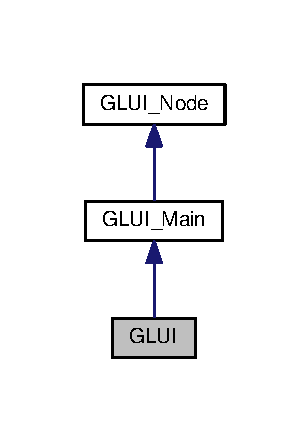
\includegraphics[width=148pt]{class_g_l_u_i__inherit__graph}
\end{center}
\end{figure}


Collaboration diagram for G\+L\+U\+I\+:\nopagebreak
\begin{figure}[H]
\begin{center}
\leavevmode
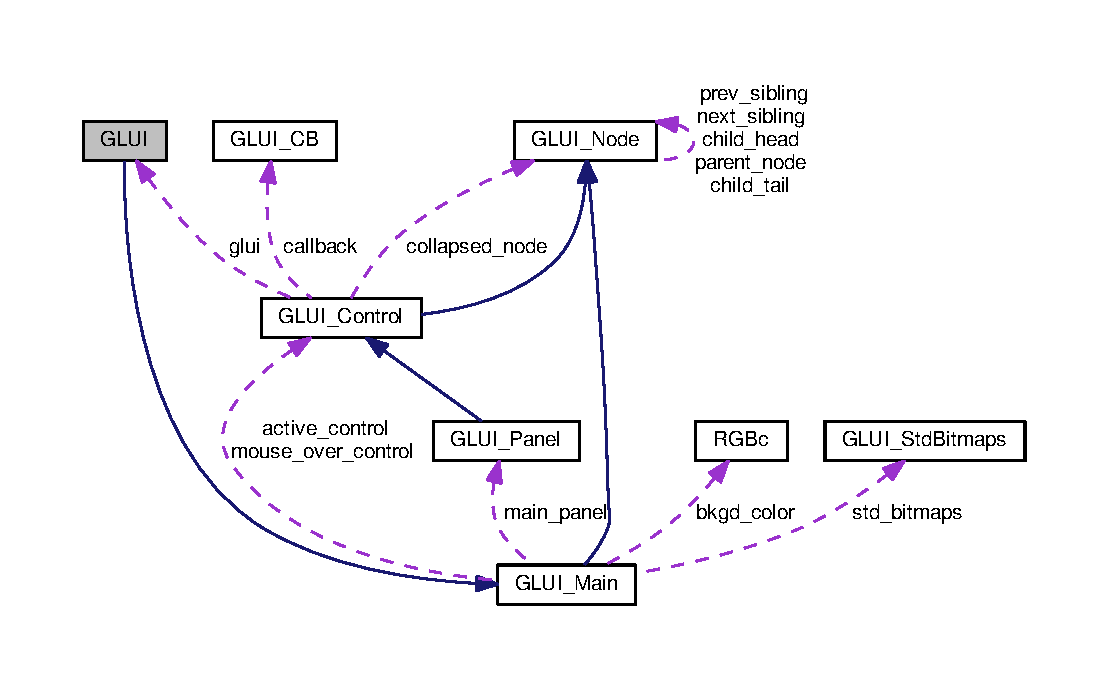
\includegraphics[width=350pt]{class_g_l_u_i__coll__graph}
\end{center}
\end{figure}
\subsection*{Public Member Functions}
\begin{DoxyCompactItemize}
\item 
\hyperlink{wglext_8h_a500a82aecba06f4550f6849b8099ca21}{int} \hyperlink{class_g_l_u_i_a94398f830a14babcd93ac109082a221e}{add\+\_\+control} (\hyperlink{class_g_l_u_i___control}{G\+L\+U\+I\+\_\+\+Control} $\ast$control)
\item 
\hyperlink{wglext_8h_a9e6b7f1933461ef318bb000d6bd13b83}{void} \hyperlink{class_g_l_u_i_a371273c28159a52e474d953101b462c8}{add\+\_\+column} (\hyperlink{wglext_8h_a500a82aecba06f4550f6849b8099ca21}{int} draw\+\_\+bar=true)
\item 
\hyperlink{wglext_8h_a9e6b7f1933461ef318bb000d6bd13b83}{void} \hyperlink{class_g_l_u_i_a4c9f42cf5ac0a3a859533f44211ea023}{add\+\_\+column\+\_\+to\+\_\+panel} (\hyperlink{class_g_l_u_i___panel}{G\+L\+U\+I\+\_\+\+Panel} $\ast$panel, \hyperlink{wglext_8h_a500a82aecba06f4550f6849b8099ca21}{int} draw\+\_\+bar=true)
\item 
\hyperlink{wglext_8h_a9e6b7f1933461ef318bb000d6bd13b83}{void} \hyperlink{class_g_l_u_i_a373d1d3fe27388c71d6d1b8767eb6590}{add\+\_\+separator} (\hyperlink{wglext_8h_a9e6b7f1933461ef318bb000d6bd13b83}{void})
\item 
\hyperlink{wglext_8h_a9e6b7f1933461ef318bb000d6bd13b83}{void} \hyperlink{class_g_l_u_i_aba9244b448b4b38e7c45ef95f7b1763a}{add\+\_\+separator\+\_\+to\+\_\+panel} (\hyperlink{class_g_l_u_i___panel}{G\+L\+U\+I\+\_\+\+Panel} $\ast$panel)
\item 
\hyperlink{class_g_l_u_i___radio_group}{G\+L\+U\+I\+\_\+\+Radio\+Group} $\ast$ \hyperlink{class_g_l_u_i_ae192f21b47b98c6496914638b74ea894}{add\+\_\+radiogroup} (\hyperlink{wglext_8h_a500a82aecba06f4550f6849b8099ca21}{int} $\ast$live\+\_\+var=N\+U\+L\+L, \hyperlink{wglext_8h_a500a82aecba06f4550f6849b8099ca21}{int} user\+\_\+id=-\/1, \hyperlink{class_g_l_u_i___c_b}{G\+L\+U\+I\+\_\+\+C\+B} callback=\hyperlink{class_g_l_u_i___c_b}{G\+L\+U\+I\+\_\+\+C\+B}())
\item 
\hyperlink{class_g_l_u_i___radio_group}{G\+L\+U\+I\+\_\+\+Radio\+Group} $\ast$ \hyperlink{class_g_l_u_i_ab6932d87d07a56e2508a8fdc5f448124}{add\+\_\+radiogroup\+\_\+to\+\_\+panel} (\hyperlink{class_g_l_u_i___panel}{G\+L\+U\+I\+\_\+\+Panel} $\ast$panel, \hyperlink{wglext_8h_a500a82aecba06f4550f6849b8099ca21}{int} $\ast$live\+\_\+var=N\+U\+L\+L, \hyperlink{wglext_8h_a500a82aecba06f4550f6849b8099ca21}{int} user\+\_\+id=-\/1, \hyperlink{class_g_l_u_i___c_b}{G\+L\+U\+I\+\_\+\+C\+B} callback=\hyperlink{class_g_l_u_i___c_b}{G\+L\+U\+I\+\_\+\+C\+B}())
\item 
\hyperlink{class_g_l_u_i___radio_button}{G\+L\+U\+I\+\_\+\+Radio\+Button} $\ast$ \hyperlink{class_g_l_u_i_a7744834cfb1a489e1c4ef8de9fef0efa}{add\+\_\+radiobutton\+\_\+to\+\_\+group} (\hyperlink{class_g_l_u_i___radio_group}{G\+L\+U\+I\+\_\+\+Radio\+Group} $\ast$\hyperlink{glext_8h_a69cec9b28d037f2272131b4fcd148620}{group}, const char $\ast$\hyperlink{glext_8h_ad977737dfc9a274a62741b9500c49a32}{name})
\item 
\hyperlink{class_g_l_u_i___listbox}{G\+L\+U\+I\+\_\+\+Listbox} $\ast$ \hyperlink{class_g_l_u_i_ad018fa077accdc1eac92b470df84b6ba}{add\+\_\+listbox} (const char $\ast$\hyperlink{glext_8h_ad977737dfc9a274a62741b9500c49a32}{name}, \hyperlink{wglext_8h_a500a82aecba06f4550f6849b8099ca21}{int} $\ast$live\+\_\+var=N\+U\+L\+L, \hyperlink{wglext_8h_a500a82aecba06f4550f6849b8099ca21}{int} \hyperlink{glext_8h_a58c2a664503e14ffb8f21012aabff3e9}{id}=-\/1, \hyperlink{class_g_l_u_i___c_b}{G\+L\+U\+I\+\_\+\+C\+B} callback=\hyperlink{class_g_l_u_i___c_b}{G\+L\+U\+I\+\_\+\+C\+B}())
\item 
\hyperlink{class_g_l_u_i___listbox}{G\+L\+U\+I\+\_\+\+Listbox} $\ast$ \hyperlink{class_g_l_u_i_af0254ec412cac9d379343e652f671799}{add\+\_\+listbox\+\_\+to\+\_\+panel} (\hyperlink{class_g_l_u_i___panel}{G\+L\+U\+I\+\_\+\+Panel} $\ast$panel, const char $\ast$\hyperlink{glext_8h_ad977737dfc9a274a62741b9500c49a32}{name}, \hyperlink{wglext_8h_a500a82aecba06f4550f6849b8099ca21}{int} $\ast$live\+\_\+var=N\+U\+L\+L, \hyperlink{wglext_8h_a500a82aecba06f4550f6849b8099ca21}{int} \hyperlink{glext_8h_a58c2a664503e14ffb8f21012aabff3e9}{id}=-\/1, \hyperlink{class_g_l_u_i___c_b}{G\+L\+U\+I\+\_\+\+C\+B} callback=\hyperlink{class_g_l_u_i___c_b}{G\+L\+U\+I\+\_\+\+C\+B}())
\item 
\hyperlink{class_g_l_u_i___rotation}{G\+L\+U\+I\+\_\+\+Rotation} $\ast$ \hyperlink{class_g_l_u_i_a96888da63ec5600e7b962e98066e89eb}{add\+\_\+rotation} (const char $\ast$\hyperlink{glext_8h_ad977737dfc9a274a62741b9500c49a32}{name}, float $\ast$live\+\_\+var=N\+U\+L\+L, \hyperlink{wglext_8h_a500a82aecba06f4550f6849b8099ca21}{int} \hyperlink{glext_8h_a58c2a664503e14ffb8f21012aabff3e9}{id}=-\/1, \hyperlink{class_g_l_u_i___c_b}{G\+L\+U\+I\+\_\+\+C\+B} callback=\hyperlink{class_g_l_u_i___c_b}{G\+L\+U\+I\+\_\+\+C\+B}())
\item 
\hyperlink{class_g_l_u_i___rotation}{G\+L\+U\+I\+\_\+\+Rotation} $\ast$ \hyperlink{class_g_l_u_i_ace8fb93ba123c09dcb5d0bbe721f02de}{add\+\_\+rotation\+\_\+to\+\_\+panel} (\hyperlink{class_g_l_u_i___panel}{G\+L\+U\+I\+\_\+\+Panel} $\ast$panel, const char $\ast$\hyperlink{glext_8h_ad977737dfc9a274a62741b9500c49a32}{name}, float $\ast$live\+\_\+var=N\+U\+L\+L, \hyperlink{wglext_8h_a500a82aecba06f4550f6849b8099ca21}{int} \hyperlink{glext_8h_a58c2a664503e14ffb8f21012aabff3e9}{id}=-\/1, \hyperlink{class_g_l_u_i___c_b}{G\+L\+U\+I\+\_\+\+C\+B} callback=\hyperlink{class_g_l_u_i___c_b}{G\+L\+U\+I\+\_\+\+C\+B}())
\item 
\hyperlink{class_g_l_u_i___translation}{G\+L\+U\+I\+\_\+\+Translation} $\ast$ \hyperlink{class_g_l_u_i_a627ddf622951e9d00e5804922ab76032}{add\+\_\+translation} (const char $\ast$\hyperlink{glext_8h_ad977737dfc9a274a62741b9500c49a32}{name}, \hyperlink{wglext_8h_a500a82aecba06f4550f6849b8099ca21}{int} trans\+\_\+type, float $\ast$live\+\_\+var=N\+U\+L\+L, \hyperlink{wglext_8h_a500a82aecba06f4550f6849b8099ca21}{int} \hyperlink{glext_8h_a58c2a664503e14ffb8f21012aabff3e9}{id}=-\/1, \hyperlink{class_g_l_u_i___c_b}{G\+L\+U\+I\+\_\+\+C\+B} callback=\hyperlink{class_g_l_u_i___c_b}{G\+L\+U\+I\+\_\+\+C\+B}())
\item 
\hyperlink{class_g_l_u_i___translation}{G\+L\+U\+I\+\_\+\+Translation} $\ast$ \hyperlink{class_g_l_u_i_a5919dbd7390b1566659edfa21e2db758}{add\+\_\+translation\+\_\+to\+\_\+panel} (\hyperlink{class_g_l_u_i___panel}{G\+L\+U\+I\+\_\+\+Panel} $\ast$panel, const char $\ast$\hyperlink{glext_8h_ad977737dfc9a274a62741b9500c49a32}{name}, \hyperlink{wglext_8h_a500a82aecba06f4550f6849b8099ca21}{int} trans\+\_\+type, float $\ast$live\+\_\+var=N\+U\+L\+L, \hyperlink{wglext_8h_a500a82aecba06f4550f6849b8099ca21}{int} \hyperlink{glext_8h_a58c2a664503e14ffb8f21012aabff3e9}{id}=-\/1, \hyperlink{class_g_l_u_i___c_b}{G\+L\+U\+I\+\_\+\+C\+B} callback=\hyperlink{class_g_l_u_i___c_b}{G\+L\+U\+I\+\_\+\+C\+B}())
\item 
\hyperlink{class_g_l_u_i___checkbox}{G\+L\+U\+I\+\_\+\+Checkbox} $\ast$ \hyperlink{class_g_l_u_i_ac72e36bbd637e4832f1e2f8b1e5c2e19}{add\+\_\+checkbox} (const char $\ast$\hyperlink{glext_8h_ad977737dfc9a274a62741b9500c49a32}{name}, \hyperlink{wglext_8h_a500a82aecba06f4550f6849b8099ca21}{int} $\ast$live\+\_\+var=N\+U\+L\+L, \hyperlink{wglext_8h_a500a82aecba06f4550f6849b8099ca21}{int} \hyperlink{glext_8h_a58c2a664503e14ffb8f21012aabff3e9}{id}=-\/1, \hyperlink{class_g_l_u_i___c_b}{G\+L\+U\+I\+\_\+\+C\+B} callback=\hyperlink{class_g_l_u_i___c_b}{G\+L\+U\+I\+\_\+\+C\+B}())
\item 
\hyperlink{class_g_l_u_i___checkbox}{G\+L\+U\+I\+\_\+\+Checkbox} $\ast$ \hyperlink{class_g_l_u_i_ace92f3923a991af8e371c3c1e7ec4f5b}{add\+\_\+checkbox\+\_\+to\+\_\+panel} (\hyperlink{class_g_l_u_i___panel}{G\+L\+U\+I\+\_\+\+Panel} $\ast$panel, const char $\ast$\hyperlink{glext_8h_ad977737dfc9a274a62741b9500c49a32}{name}, \hyperlink{wglext_8h_a500a82aecba06f4550f6849b8099ca21}{int} $\ast$live\+\_\+var=N\+U\+L\+L, \hyperlink{wglext_8h_a500a82aecba06f4550f6849b8099ca21}{int} \hyperlink{glext_8h_a58c2a664503e14ffb8f21012aabff3e9}{id}=-\/1, \hyperlink{class_g_l_u_i___c_b}{G\+L\+U\+I\+\_\+\+C\+B} callback=\hyperlink{class_g_l_u_i___c_b}{G\+L\+U\+I\+\_\+\+C\+B}())
\item 
\hyperlink{class_g_l_u_i___button}{G\+L\+U\+I\+\_\+\+Button} $\ast$ \hyperlink{class_g_l_u_i_a7566d52c3181c92de8b2039aefd88b1e}{add\+\_\+button} (const char $\ast$\hyperlink{glext_8h_ad977737dfc9a274a62741b9500c49a32}{name}, \hyperlink{wglext_8h_a500a82aecba06f4550f6849b8099ca21}{int} \hyperlink{glext_8h_a58c2a664503e14ffb8f21012aabff3e9}{id}=-\/1, \hyperlink{class_g_l_u_i___c_b}{G\+L\+U\+I\+\_\+\+C\+B} callback=\hyperlink{class_g_l_u_i___c_b}{G\+L\+U\+I\+\_\+\+C\+B}())
\item 
\hyperlink{class_g_l_u_i___button}{G\+L\+U\+I\+\_\+\+Button} $\ast$ \hyperlink{class_g_l_u_i_af9039fe3c9c23f316426a654ea309383}{add\+\_\+button\+\_\+to\+\_\+panel} (\hyperlink{class_g_l_u_i___panel}{G\+L\+U\+I\+\_\+\+Panel} $\ast$panel, const char $\ast$\hyperlink{glext_8h_ad977737dfc9a274a62741b9500c49a32}{name}, \hyperlink{wglext_8h_a500a82aecba06f4550f6849b8099ca21}{int} \hyperlink{glext_8h_a58c2a664503e14ffb8f21012aabff3e9}{id}=-\/1, \hyperlink{class_g_l_u_i___c_b}{G\+L\+U\+I\+\_\+\+C\+B} callback=\hyperlink{class_g_l_u_i___c_b}{G\+L\+U\+I\+\_\+\+C\+B}())
\item 
\hyperlink{class_g_l_u_i___static_text}{G\+L\+U\+I\+\_\+\+Static\+Text} $\ast$ \hyperlink{class_g_l_u_i_ac654d6d6e0f7ace0694ac6641654f04f}{add\+\_\+statictext} (const char $\ast$\hyperlink{glext_8h_ad977737dfc9a274a62741b9500c49a32}{name})
\item 
\hyperlink{class_g_l_u_i___static_text}{G\+L\+U\+I\+\_\+\+Static\+Text} $\ast$ \hyperlink{class_g_l_u_i_a5b60d2e5161b9b8027c833c85888d59e}{add\+\_\+statictext\+\_\+to\+\_\+panel} (\hyperlink{class_g_l_u_i___panel}{G\+L\+U\+I\+\_\+\+Panel} $\ast$panel, const char $\ast$\hyperlink{glext_8h_ad977737dfc9a274a62741b9500c49a32}{name})
\item 
\hyperlink{class_g_l_u_i___edit_text}{G\+L\+U\+I\+\_\+\+Edit\+Text} $\ast$ \hyperlink{class_g_l_u_i_a5b1c456923b46d885a3419aead41cd9b}{add\+\_\+edittext} (const char $\ast$\hyperlink{glext_8h_ad977737dfc9a274a62741b9500c49a32}{name}, \hyperlink{wglext_8h_a500a82aecba06f4550f6849b8099ca21}{int} data\+\_\+type=\hyperlink{glui_8h_a5e7e137e5f35f2859b135d8924719d27}{G\+L\+U\+I\+\_\+\+E\+D\+I\+T\+T\+E\+X\+T\+\_\+\+T\+E\+X\+T}, \hyperlink{wglext_8h_a9e6b7f1933461ef318bb000d6bd13b83}{void} $\ast$live\+\_\+var=N\+U\+L\+L, \hyperlink{wglext_8h_a500a82aecba06f4550f6849b8099ca21}{int} \hyperlink{glext_8h_a58c2a664503e14ffb8f21012aabff3e9}{id}=-\/1, \hyperlink{class_g_l_u_i___c_b}{G\+L\+U\+I\+\_\+\+C\+B} callback=\hyperlink{class_g_l_u_i___c_b}{G\+L\+U\+I\+\_\+\+C\+B}())
\item 
\hyperlink{class_g_l_u_i___edit_text}{G\+L\+U\+I\+\_\+\+Edit\+Text} $\ast$ \hyperlink{class_g_l_u_i_ac58a5a8fd9a741e8c238bb1df21b0467}{add\+\_\+edittext\+\_\+to\+\_\+panel} (\hyperlink{class_g_l_u_i___panel}{G\+L\+U\+I\+\_\+\+Panel} $\ast$panel, const char $\ast$\hyperlink{glext_8h_ad977737dfc9a274a62741b9500c49a32}{name}, \hyperlink{wglext_8h_a500a82aecba06f4550f6849b8099ca21}{int} data\+\_\+type=\hyperlink{glui_8h_a5e7e137e5f35f2859b135d8924719d27}{G\+L\+U\+I\+\_\+\+E\+D\+I\+T\+T\+E\+X\+T\+\_\+\+T\+E\+X\+T}, \hyperlink{wglext_8h_a9e6b7f1933461ef318bb000d6bd13b83}{void} $\ast$live\+\_\+var=N\+U\+L\+L, \hyperlink{wglext_8h_a500a82aecba06f4550f6849b8099ca21}{int} \hyperlink{glext_8h_a58c2a664503e14ffb8f21012aabff3e9}{id}=-\/1, \hyperlink{class_g_l_u_i___c_b}{G\+L\+U\+I\+\_\+\+C\+B} callback=\hyperlink{class_g_l_u_i___c_b}{G\+L\+U\+I\+\_\+\+C\+B}())
\item 
\hyperlink{class_g_l_u_i___edit_text}{G\+L\+U\+I\+\_\+\+Edit\+Text} $\ast$ \hyperlink{class_g_l_u_i_a465a9611a5b646e26f9381df579ef26e}{add\+\_\+edittext} (const char $\ast$\hyperlink{glext_8h_ad977737dfc9a274a62741b9500c49a32}{name}, \hyperlink{glui_8h_aada824856f7bcf29794719981ebd8f60}{G\+L\+U\+I\+\_\+\+String} \&live\+\_\+var, \hyperlink{wglext_8h_a500a82aecba06f4550f6849b8099ca21}{int} \hyperlink{glext_8h_a58c2a664503e14ffb8f21012aabff3e9}{id}=-\/1, \hyperlink{class_g_l_u_i___c_b}{G\+L\+U\+I\+\_\+\+C\+B} callback=\hyperlink{class_g_l_u_i___c_b}{G\+L\+U\+I\+\_\+\+C\+B}())
\item 
\hyperlink{class_g_l_u_i___edit_text}{G\+L\+U\+I\+\_\+\+Edit\+Text} $\ast$ \hyperlink{class_g_l_u_i_ae152efe28d88ea69afb52e53f6918190}{add\+\_\+edittext\+\_\+to\+\_\+panel} (\hyperlink{class_g_l_u_i___panel}{G\+L\+U\+I\+\_\+\+Panel} $\ast$panel, const char $\ast$\hyperlink{glext_8h_ad977737dfc9a274a62741b9500c49a32}{name}, \hyperlink{glui_8h_aada824856f7bcf29794719981ebd8f60}{G\+L\+U\+I\+\_\+\+String} \&live\+\_\+var, \hyperlink{wglext_8h_a500a82aecba06f4550f6849b8099ca21}{int} \hyperlink{glext_8h_a58c2a664503e14ffb8f21012aabff3e9}{id}=-\/1, \hyperlink{class_g_l_u_i___c_b}{G\+L\+U\+I\+\_\+\+C\+B} callback=\hyperlink{class_g_l_u_i___c_b}{G\+L\+U\+I\+\_\+\+C\+B}())
\item 
\hyperlink{class_g_l_u_i___spinner}{G\+L\+U\+I\+\_\+\+Spinner} $\ast$ \hyperlink{class_g_l_u_i_a2da5634b39065c58d1677beb529bd1a3}{add\+\_\+spinner} (const char $\ast$\hyperlink{glext_8h_ad977737dfc9a274a62741b9500c49a32}{name}, \hyperlink{wglext_8h_a500a82aecba06f4550f6849b8099ca21}{int} data\+\_\+type=\hyperlink{glui_8h_ae338c1175e5bb430d7a14d109daee74a}{G\+L\+U\+I\+\_\+\+S\+P\+I\+N\+N\+E\+R\+\_\+\+I\+N\+T}, \hyperlink{wglext_8h_a9e6b7f1933461ef318bb000d6bd13b83}{void} $\ast$live\+\_\+var=N\+U\+L\+L, \hyperlink{wglext_8h_a500a82aecba06f4550f6849b8099ca21}{int} \hyperlink{glext_8h_a58c2a664503e14ffb8f21012aabff3e9}{id}=-\/1, \hyperlink{class_g_l_u_i___c_b}{G\+L\+U\+I\+\_\+\+C\+B} callback=\hyperlink{class_g_l_u_i___c_b}{G\+L\+U\+I\+\_\+\+C\+B}())
\item 
\hyperlink{class_g_l_u_i___spinner}{G\+L\+U\+I\+\_\+\+Spinner} $\ast$ \hyperlink{class_g_l_u_i_a0404acbf84029ccaa28c3f7336c36aac}{add\+\_\+spinner\+\_\+to\+\_\+panel} (\hyperlink{class_g_l_u_i___panel}{G\+L\+U\+I\+\_\+\+Panel} $\ast$panel, const char $\ast$\hyperlink{glext_8h_ad977737dfc9a274a62741b9500c49a32}{name}, \hyperlink{wglext_8h_a500a82aecba06f4550f6849b8099ca21}{int} data\+\_\+type=\hyperlink{glui_8h_ae338c1175e5bb430d7a14d109daee74a}{G\+L\+U\+I\+\_\+\+S\+P\+I\+N\+N\+E\+R\+\_\+\+I\+N\+T}, \hyperlink{wglext_8h_a9e6b7f1933461ef318bb000d6bd13b83}{void} $\ast$live\+\_\+var=N\+U\+L\+L, \hyperlink{wglext_8h_a500a82aecba06f4550f6849b8099ca21}{int} \hyperlink{glext_8h_a58c2a664503e14ffb8f21012aabff3e9}{id}=-\/1, \hyperlink{class_g_l_u_i___c_b}{G\+L\+U\+I\+\_\+\+C\+B} callback=\hyperlink{class_g_l_u_i___c_b}{G\+L\+U\+I\+\_\+\+C\+B}())
\item 
\hyperlink{class_g_l_u_i___panel}{G\+L\+U\+I\+\_\+\+Panel} $\ast$ \hyperlink{class_g_l_u_i_a3b8ffd87d2340041a5a5fab58dbf04d7}{add\+\_\+panel} (const char $\ast$\hyperlink{glext_8h_ad977737dfc9a274a62741b9500c49a32}{name}, \hyperlink{wglext_8h_a500a82aecba06f4550f6849b8099ca21}{int} \hyperlink{glext_8h_ab7c1afc09f67635c2c376638fcc0db5f}{type}=\hyperlink{glui_8h_add54979a7b4391067b8a125ee34f690a}{G\+L\+U\+I\+\_\+\+P\+A\+N\+E\+L\+\_\+\+E\+M\+B\+O\+S\+S\+E\+D})
\item 
\hyperlink{class_g_l_u_i___panel}{G\+L\+U\+I\+\_\+\+Panel} $\ast$ \hyperlink{class_g_l_u_i_aadaa36a373fccc04c87993724b998c70}{add\+\_\+panel\+\_\+to\+\_\+panel} (\hyperlink{class_g_l_u_i___panel}{G\+L\+U\+I\+\_\+\+Panel} $\ast$panel, const char $\ast$\hyperlink{glext_8h_ad977737dfc9a274a62741b9500c49a32}{name}, \hyperlink{wglext_8h_a500a82aecba06f4550f6849b8099ca21}{int} \hyperlink{glext_8h_ab7c1afc09f67635c2c376638fcc0db5f}{type}=\hyperlink{glui_8h_add54979a7b4391067b8a125ee34f690a}{G\+L\+U\+I\+\_\+\+P\+A\+N\+E\+L\+\_\+\+E\+M\+B\+O\+S\+S\+E\+D})
\item 
\hyperlink{class_g_l_u_i___rollout}{G\+L\+U\+I\+\_\+\+Rollout} $\ast$ \hyperlink{class_g_l_u_i_afc1608e235e405b93ea3d346f8036528}{add\+\_\+rollout} (const char $\ast$\hyperlink{glext_8h_ad977737dfc9a274a62741b9500c49a32}{name}, \hyperlink{wglext_8h_a500a82aecba06f4550f6849b8099ca21}{int} open=true, \hyperlink{wglext_8h_a500a82aecba06f4550f6849b8099ca21}{int} \hyperlink{glext_8h_ab7c1afc09f67635c2c376638fcc0db5f}{type}=\hyperlink{glui_8h_add54979a7b4391067b8a125ee34f690a}{G\+L\+U\+I\+\_\+\+P\+A\+N\+E\+L\+\_\+\+E\+M\+B\+O\+S\+S\+E\+D})
\item 
\hyperlink{class_g_l_u_i___rollout}{G\+L\+U\+I\+\_\+\+Rollout} $\ast$ \hyperlink{class_g_l_u_i_a4b979713558760e30b4a2faa79a2bb9e}{add\+\_\+rollout\+\_\+to\+\_\+panel} (\hyperlink{class_g_l_u_i___panel}{G\+L\+U\+I\+\_\+\+Panel} $\ast$panel, const char $\ast$\hyperlink{glext_8h_ad977737dfc9a274a62741b9500c49a32}{name}, \hyperlink{wglext_8h_a500a82aecba06f4550f6849b8099ca21}{int} open=true, \hyperlink{wglext_8h_a500a82aecba06f4550f6849b8099ca21}{int} \hyperlink{glext_8h_ab7c1afc09f67635c2c376638fcc0db5f}{type}=\hyperlink{glui_8h_add54979a7b4391067b8a125ee34f690a}{G\+L\+U\+I\+\_\+\+P\+A\+N\+E\+L\+\_\+\+E\+M\+B\+O\+S\+S\+E\+D})
\item 
\hyperlink{wglext_8h_a9e6b7f1933461ef318bb000d6bd13b83}{void} \hyperlink{class_g_l_u_i_adbf3736dbd0334a33677eae1a4baa8b9}{set\+\_\+main\+\_\+gfx\+\_\+window} (\hyperlink{wglext_8h_a500a82aecba06f4550f6849b8099ca21}{int} window\+\_\+id)
\item 
\hyperlink{wglext_8h_a500a82aecba06f4550f6849b8099ca21}{int} \hyperlink{class_g_l_u_i_abf85807ffaab858e84c4e06924fad0da}{get\+\_\+glut\+\_\+window\+\_\+id} (\hyperlink{wglext_8h_a9e6b7f1933461ef318bb000d6bd13b83}{void})
\item 
\hyperlink{wglext_8h_a9e6b7f1933461ef318bb000d6bd13b83}{void} \hyperlink{class_g_l_u_i_abb1c2dc07fbe72c58f4d9340980168a1}{enable} (\hyperlink{wglext_8h_a9e6b7f1933461ef318bb000d6bd13b83}{void})
\item 
\hyperlink{wglext_8h_a9e6b7f1933461ef318bb000d6bd13b83}{void} \hyperlink{class_g_l_u_i_a0007f929ed29394f37b6032578929878}{disable} (\hyperlink{wglext_8h_a9e6b7f1933461ef318bb000d6bd13b83}{void})
\item 
\hyperlink{wglext_8h_a9e6b7f1933461ef318bb000d6bd13b83}{void} \hyperlink{class_g_l_u_i_a0be00b9a4f51c8d37a90ff1258c0fc76}{sync\+\_\+live} (\hyperlink{wglext_8h_a9e6b7f1933461ef318bb000d6bd13b83}{void})
\item 
\hyperlink{wglext_8h_a9e6b7f1933461ef318bb000d6bd13b83}{void} \hyperlink{class_g_l_u_i_a3d37cab3ab684fd10e2f79dd9dcf7d27}{close} (\hyperlink{wglext_8h_a9e6b7f1933461ef318bb000d6bd13b83}{void})
\item 
\hyperlink{wglext_8h_a9e6b7f1933461ef318bb000d6bd13b83}{void} \hyperlink{class_g_l_u_i_a1e1ca1995e99922caae9e7df493187f9}{show} (\hyperlink{wglext_8h_a9e6b7f1933461ef318bb000d6bd13b83}{void})
\item 
\hyperlink{wglext_8h_a9e6b7f1933461ef318bb000d6bd13b83}{void} \hyperlink{class_g_l_u_i_a30c59771996d05b301caea963051e7bc}{hide} (\hyperlink{wglext_8h_a9e6b7f1933461ef318bb000d6bd13b83}{void})
\item 
\hyperlink{wglext_8h_a500a82aecba06f4550f6849b8099ca21}{int} \hyperlink{class_g_l_u_i_a130870067b12b7228da501dae36be013}{init} (const char $\ast$\hyperlink{glext_8h_ad977737dfc9a274a62741b9500c49a32}{name}, long \hyperlink{glext_8h_aa9459b47e7388437191d2d9a69c10d98}{flags}, \hyperlink{wglext_8h_a500a82aecba06f4550f6849b8099ca21}{int} \hyperlink{glext_8h_ad77deca22f617d3f0e0eb786445689fc}{x}, \hyperlink{wglext_8h_a500a82aecba06f4550f6849b8099ca21}{int} \hyperlink{glext_8h_a9298c7ad619074f5285b32c6b72bfdea}{y}, \hyperlink{wglext_8h_a500a82aecba06f4550f6849b8099ca21}{int} \hyperlink{class_g_l_u_i___main_a70e6e1ec266281f272954fcc42f85087}{parent\+\_\+window})
\end{DoxyCompactItemize}
\subsection*{Protected Member Functions}
\begin{DoxyCompactItemize}
\item 
virtual \hyperlink{wglext_8h_a500a82aecba06f4550f6849b8099ca21}{int} \hyperlink{class_g_l_u_i_a293fdf48459c281e466781ec9c559c21}{add\+\_\+control} (\hyperlink{class_g_l_u_i___node}{G\+L\+U\+I\+\_\+\+Node} $\ast$\hyperlink{class_g_l_u_i___node_a8ed65d447784f6f88bd3e2e2bcac6cdb}{parent}, \hyperlink{class_g_l_u_i___control}{G\+L\+U\+I\+\_\+\+Control} $\ast$control)
\end{DoxyCompactItemize}
\subsection*{Additional Inherited Members}


\subsection{Detailed Description}
The main user-\/visible interface object to \hyperlink{class_g_l_u_i}{G\+L\+U\+I}. 

Definition at line 1435 of file glui.\+h.



\subsection{Member Function Documentation}
\hypertarget{class_g_l_u_i_a7566d52c3181c92de8b2039aefd88b1e}{\index{G\+L\+U\+I@{G\+L\+U\+I}!add\+\_\+button@{add\+\_\+button}}
\index{add\+\_\+button@{add\+\_\+button}!G\+L\+U\+I@{G\+L\+U\+I}}
\subsubsection[{add\+\_\+button}]{\setlength{\rightskip}{0pt plus 5cm}{\bf G\+L\+U\+I\+\_\+\+Button}$\ast$ G\+L\+U\+I\+::add\+\_\+button (
\begin{DoxyParamCaption}
\item[{const char $\ast$}]{name, }
\item[{{\bf int}}]{id = {\ttfamily -\/1}, }
\item[{{\bf G\+L\+U\+I\+\_\+\+C\+B}}]{callback = {\ttfamily {\bf G\+L\+U\+I\+\_\+\+C\+B}()}}
\end{DoxyParamCaption}
)}}\label{class_g_l_u_i_a7566d52c3181c92de8b2039aefd88b1e}
\hypertarget{class_g_l_u_i_af9039fe3c9c23f316426a654ea309383}{\index{G\+L\+U\+I@{G\+L\+U\+I}!add\+\_\+button\+\_\+to\+\_\+panel@{add\+\_\+button\+\_\+to\+\_\+panel}}
\index{add\+\_\+button\+\_\+to\+\_\+panel@{add\+\_\+button\+\_\+to\+\_\+panel}!G\+L\+U\+I@{G\+L\+U\+I}}
\subsubsection[{add\+\_\+button\+\_\+to\+\_\+panel}]{\setlength{\rightskip}{0pt plus 5cm}{\bf G\+L\+U\+I\+\_\+\+Button}$\ast$ G\+L\+U\+I\+::add\+\_\+button\+\_\+to\+\_\+panel (
\begin{DoxyParamCaption}
\item[{{\bf G\+L\+U\+I\+\_\+\+Panel} $\ast$}]{panel, }
\item[{const char $\ast$}]{name, }
\item[{{\bf int}}]{id = {\ttfamily -\/1}, }
\item[{{\bf G\+L\+U\+I\+\_\+\+C\+B}}]{callback = {\ttfamily {\bf G\+L\+U\+I\+\_\+\+C\+B}()}}
\end{DoxyParamCaption}
)}}\label{class_g_l_u_i_af9039fe3c9c23f316426a654ea309383}
\hypertarget{class_g_l_u_i_ac72e36bbd637e4832f1e2f8b1e5c2e19}{\index{G\+L\+U\+I@{G\+L\+U\+I}!add\+\_\+checkbox@{add\+\_\+checkbox}}
\index{add\+\_\+checkbox@{add\+\_\+checkbox}!G\+L\+U\+I@{G\+L\+U\+I}}
\subsubsection[{add\+\_\+checkbox}]{\setlength{\rightskip}{0pt plus 5cm}{\bf G\+L\+U\+I\+\_\+\+Checkbox}$\ast$ G\+L\+U\+I\+::add\+\_\+checkbox (
\begin{DoxyParamCaption}
\item[{const char $\ast$}]{name, }
\item[{{\bf int} $\ast$}]{live\+\_\+var = {\ttfamily NULL}, }
\item[{{\bf int}}]{id = {\ttfamily -\/1}, }
\item[{{\bf G\+L\+U\+I\+\_\+\+C\+B}}]{callback = {\ttfamily {\bf G\+L\+U\+I\+\_\+\+C\+B}()}}
\end{DoxyParamCaption}
)}}\label{class_g_l_u_i_ac72e36bbd637e4832f1e2f8b1e5c2e19}
\hypertarget{class_g_l_u_i_ace92f3923a991af8e371c3c1e7ec4f5b}{\index{G\+L\+U\+I@{G\+L\+U\+I}!add\+\_\+checkbox\+\_\+to\+\_\+panel@{add\+\_\+checkbox\+\_\+to\+\_\+panel}}
\index{add\+\_\+checkbox\+\_\+to\+\_\+panel@{add\+\_\+checkbox\+\_\+to\+\_\+panel}!G\+L\+U\+I@{G\+L\+U\+I}}
\subsubsection[{add\+\_\+checkbox\+\_\+to\+\_\+panel}]{\setlength{\rightskip}{0pt plus 5cm}{\bf G\+L\+U\+I\+\_\+\+Checkbox}$\ast$ G\+L\+U\+I\+::add\+\_\+checkbox\+\_\+to\+\_\+panel (
\begin{DoxyParamCaption}
\item[{{\bf G\+L\+U\+I\+\_\+\+Panel} $\ast$}]{panel, }
\item[{const char $\ast$}]{name, }
\item[{{\bf int} $\ast$}]{live\+\_\+var = {\ttfamily NULL}, }
\item[{{\bf int}}]{id = {\ttfamily -\/1}, }
\item[{{\bf G\+L\+U\+I\+\_\+\+C\+B}}]{callback = {\ttfamily {\bf G\+L\+U\+I\+\_\+\+C\+B}()}}
\end{DoxyParamCaption}
)}}\label{class_g_l_u_i_ace92f3923a991af8e371c3c1e7ec4f5b}
\hypertarget{class_g_l_u_i_a371273c28159a52e474d953101b462c8}{\index{G\+L\+U\+I@{G\+L\+U\+I}!add\+\_\+column@{add\+\_\+column}}
\index{add\+\_\+column@{add\+\_\+column}!G\+L\+U\+I@{G\+L\+U\+I}}
\subsubsection[{add\+\_\+column}]{\setlength{\rightskip}{0pt plus 5cm}{\bf void} G\+L\+U\+I\+::add\+\_\+column (
\begin{DoxyParamCaption}
\item[{{\bf int}}]{draw\+\_\+bar = {\ttfamily true}}
\end{DoxyParamCaption}
)}}\label{class_g_l_u_i_a371273c28159a52e474d953101b462c8}
\hypertarget{class_g_l_u_i_a4c9f42cf5ac0a3a859533f44211ea023}{\index{G\+L\+U\+I@{G\+L\+U\+I}!add\+\_\+column\+\_\+to\+\_\+panel@{add\+\_\+column\+\_\+to\+\_\+panel}}
\index{add\+\_\+column\+\_\+to\+\_\+panel@{add\+\_\+column\+\_\+to\+\_\+panel}!G\+L\+U\+I@{G\+L\+U\+I}}
\subsubsection[{add\+\_\+column\+\_\+to\+\_\+panel}]{\setlength{\rightskip}{0pt plus 5cm}{\bf void} G\+L\+U\+I\+::add\+\_\+column\+\_\+to\+\_\+panel (
\begin{DoxyParamCaption}
\item[{{\bf G\+L\+U\+I\+\_\+\+Panel} $\ast$}]{panel, }
\item[{{\bf int}}]{draw\+\_\+bar = {\ttfamily true}}
\end{DoxyParamCaption}
)}}\label{class_g_l_u_i_a4c9f42cf5ac0a3a859533f44211ea023}
\hypertarget{class_g_l_u_i_a94398f830a14babcd93ac109082a221e}{\index{G\+L\+U\+I@{G\+L\+U\+I}!add\+\_\+control@{add\+\_\+control}}
\index{add\+\_\+control@{add\+\_\+control}!G\+L\+U\+I@{G\+L\+U\+I}}
\subsubsection[{add\+\_\+control}]{\setlength{\rightskip}{0pt plus 5cm}{\bf int} G\+L\+U\+I\+::add\+\_\+control (
\begin{DoxyParamCaption}
\item[{{\bf G\+L\+U\+I\+\_\+\+Control} $\ast$}]{control}
\end{DoxyParamCaption}
)\hspace{0.3cm}{\ttfamily [inline]}, {\ttfamily [virtual]}}}\label{class_g_l_u_i_a94398f830a14babcd93ac109082a221e}
D\+E\+P\+R\+E\+C\+A\+T\+E\+D interface for creating new \hyperlink{class_g_l_u_i}{G\+L\+U\+I} objects 

Reimplemented from \hyperlink{class_g_l_u_i___node_abdcdd643758adab07580124187565fcd}{G\+L\+U\+I\+\_\+\+Node}.



Definition at line 1439 of file glui.\+h.

\hypertarget{class_g_l_u_i_a293fdf48459c281e466781ec9c559c21}{\index{G\+L\+U\+I@{G\+L\+U\+I}!add\+\_\+control@{add\+\_\+control}}
\index{add\+\_\+control@{add\+\_\+control}!G\+L\+U\+I@{G\+L\+U\+I}}
\subsubsection[{add\+\_\+control}]{\setlength{\rightskip}{0pt plus 5cm}virtual {\bf int} G\+L\+U\+I\+::add\+\_\+control (
\begin{DoxyParamCaption}
\item[{{\bf G\+L\+U\+I\+\_\+\+Node} $\ast$}]{parent, }
\item[{{\bf G\+L\+U\+I\+\_\+\+Control} $\ast$}]{control}
\end{DoxyParamCaption}
)\hspace{0.3cm}{\ttfamily [inline]}, {\ttfamily [protected]}, {\ttfamily [virtual]}}}\label{class_g_l_u_i_a293fdf48459c281e466781ec9c559c21}


Reimplemented from \hyperlink{class_g_l_u_i___main_aa18b473f6cf75095c12c4edecaf856a3}{G\+L\+U\+I\+\_\+\+Main}.



Definition at line 1568 of file glui.\+h.

\hypertarget{class_g_l_u_i_a5b1c456923b46d885a3419aead41cd9b}{\index{G\+L\+U\+I@{G\+L\+U\+I}!add\+\_\+edittext@{add\+\_\+edittext}}
\index{add\+\_\+edittext@{add\+\_\+edittext}!G\+L\+U\+I@{G\+L\+U\+I}}
\subsubsection[{add\+\_\+edittext}]{\setlength{\rightskip}{0pt plus 5cm}{\bf G\+L\+U\+I\+\_\+\+Edit\+Text}$\ast$ G\+L\+U\+I\+::add\+\_\+edittext (
\begin{DoxyParamCaption}
\item[{const char $\ast$}]{name, }
\item[{{\bf int}}]{data\+\_\+type = {\ttfamily {\bf G\+L\+U\+I\+\_\+\+E\+D\+I\+T\+T\+E\+X\+T\+\_\+\+T\+E\+X\+T}}, }
\item[{{\bf void} $\ast$}]{live\+\_\+var = {\ttfamily NULL}, }
\item[{{\bf int}}]{id = {\ttfamily -\/1}, }
\item[{{\bf G\+L\+U\+I\+\_\+\+C\+B}}]{callback = {\ttfamily {\bf G\+L\+U\+I\+\_\+\+C\+B}()}}
\end{DoxyParamCaption}
)}}\label{class_g_l_u_i_a5b1c456923b46d885a3419aead41cd9b}
\hypertarget{class_g_l_u_i_a465a9611a5b646e26f9381df579ef26e}{\index{G\+L\+U\+I@{G\+L\+U\+I}!add\+\_\+edittext@{add\+\_\+edittext}}
\index{add\+\_\+edittext@{add\+\_\+edittext}!G\+L\+U\+I@{G\+L\+U\+I}}
\subsubsection[{add\+\_\+edittext}]{\setlength{\rightskip}{0pt plus 5cm}{\bf G\+L\+U\+I\+\_\+\+Edit\+Text}$\ast$ G\+L\+U\+I\+::add\+\_\+edittext (
\begin{DoxyParamCaption}
\item[{const char $\ast$}]{name, }
\item[{{\bf G\+L\+U\+I\+\_\+\+String} \&}]{live\+\_\+var, }
\item[{{\bf int}}]{id = {\ttfamily -\/1}, }
\item[{{\bf G\+L\+U\+I\+\_\+\+C\+B}}]{callback = {\ttfamily {\bf G\+L\+U\+I\+\_\+\+C\+B}()}}
\end{DoxyParamCaption}
)}}\label{class_g_l_u_i_a465a9611a5b646e26f9381df579ef26e}
\hypertarget{class_g_l_u_i_ac58a5a8fd9a741e8c238bb1df21b0467}{\index{G\+L\+U\+I@{G\+L\+U\+I}!add\+\_\+edittext\+\_\+to\+\_\+panel@{add\+\_\+edittext\+\_\+to\+\_\+panel}}
\index{add\+\_\+edittext\+\_\+to\+\_\+panel@{add\+\_\+edittext\+\_\+to\+\_\+panel}!G\+L\+U\+I@{G\+L\+U\+I}}
\subsubsection[{add\+\_\+edittext\+\_\+to\+\_\+panel}]{\setlength{\rightskip}{0pt plus 5cm}{\bf G\+L\+U\+I\+\_\+\+Edit\+Text}$\ast$ G\+L\+U\+I\+::add\+\_\+edittext\+\_\+to\+\_\+panel (
\begin{DoxyParamCaption}
\item[{{\bf G\+L\+U\+I\+\_\+\+Panel} $\ast$}]{panel, }
\item[{const char $\ast$}]{name, }
\item[{{\bf int}}]{data\+\_\+type = {\ttfamily {\bf G\+L\+U\+I\+\_\+\+E\+D\+I\+T\+T\+E\+X\+T\+\_\+\+T\+E\+X\+T}}, }
\item[{{\bf void} $\ast$}]{live\+\_\+var = {\ttfamily NULL}, }
\item[{{\bf int}}]{id = {\ttfamily -\/1}, }
\item[{{\bf G\+L\+U\+I\+\_\+\+C\+B}}]{callback = {\ttfamily {\bf G\+L\+U\+I\+\_\+\+C\+B}()}}
\end{DoxyParamCaption}
)}}\label{class_g_l_u_i_ac58a5a8fd9a741e8c238bb1df21b0467}
\hypertarget{class_g_l_u_i_ae152efe28d88ea69afb52e53f6918190}{\index{G\+L\+U\+I@{G\+L\+U\+I}!add\+\_\+edittext\+\_\+to\+\_\+panel@{add\+\_\+edittext\+\_\+to\+\_\+panel}}
\index{add\+\_\+edittext\+\_\+to\+\_\+panel@{add\+\_\+edittext\+\_\+to\+\_\+panel}!G\+L\+U\+I@{G\+L\+U\+I}}
\subsubsection[{add\+\_\+edittext\+\_\+to\+\_\+panel}]{\setlength{\rightskip}{0pt plus 5cm}{\bf G\+L\+U\+I\+\_\+\+Edit\+Text}$\ast$ G\+L\+U\+I\+::add\+\_\+edittext\+\_\+to\+\_\+panel (
\begin{DoxyParamCaption}
\item[{{\bf G\+L\+U\+I\+\_\+\+Panel} $\ast$}]{panel, }
\item[{const char $\ast$}]{name, }
\item[{{\bf G\+L\+U\+I\+\_\+\+String} \&}]{live\+\_\+var, }
\item[{{\bf int}}]{id = {\ttfamily -\/1}, }
\item[{{\bf G\+L\+U\+I\+\_\+\+C\+B}}]{callback = {\ttfamily {\bf G\+L\+U\+I\+\_\+\+C\+B}()}}
\end{DoxyParamCaption}
)}}\label{class_g_l_u_i_ae152efe28d88ea69afb52e53f6918190}
\hypertarget{class_g_l_u_i_ad018fa077accdc1eac92b470df84b6ba}{\index{G\+L\+U\+I@{G\+L\+U\+I}!add\+\_\+listbox@{add\+\_\+listbox}}
\index{add\+\_\+listbox@{add\+\_\+listbox}!G\+L\+U\+I@{G\+L\+U\+I}}
\subsubsection[{add\+\_\+listbox}]{\setlength{\rightskip}{0pt plus 5cm}{\bf G\+L\+U\+I\+\_\+\+Listbox}$\ast$ G\+L\+U\+I\+::add\+\_\+listbox (
\begin{DoxyParamCaption}
\item[{const char $\ast$}]{name, }
\item[{{\bf int} $\ast$}]{live\+\_\+var = {\ttfamily NULL}, }
\item[{{\bf int}}]{id = {\ttfamily -\/1}, }
\item[{{\bf G\+L\+U\+I\+\_\+\+C\+B}}]{callback = {\ttfamily {\bf G\+L\+U\+I\+\_\+\+C\+B}()}}
\end{DoxyParamCaption}
)}}\label{class_g_l_u_i_ad018fa077accdc1eac92b470df84b6ba}
\hypertarget{class_g_l_u_i_af0254ec412cac9d379343e652f671799}{\index{G\+L\+U\+I@{G\+L\+U\+I}!add\+\_\+listbox\+\_\+to\+\_\+panel@{add\+\_\+listbox\+\_\+to\+\_\+panel}}
\index{add\+\_\+listbox\+\_\+to\+\_\+panel@{add\+\_\+listbox\+\_\+to\+\_\+panel}!G\+L\+U\+I@{G\+L\+U\+I}}
\subsubsection[{add\+\_\+listbox\+\_\+to\+\_\+panel}]{\setlength{\rightskip}{0pt plus 5cm}{\bf G\+L\+U\+I\+\_\+\+Listbox}$\ast$ G\+L\+U\+I\+::add\+\_\+listbox\+\_\+to\+\_\+panel (
\begin{DoxyParamCaption}
\item[{{\bf G\+L\+U\+I\+\_\+\+Panel} $\ast$}]{panel, }
\item[{const char $\ast$}]{name, }
\item[{{\bf int} $\ast$}]{live\+\_\+var = {\ttfamily NULL}, }
\item[{{\bf int}}]{id = {\ttfamily -\/1}, }
\item[{{\bf G\+L\+U\+I\+\_\+\+C\+B}}]{callback = {\ttfamily {\bf G\+L\+U\+I\+\_\+\+C\+B}()}}
\end{DoxyParamCaption}
)}}\label{class_g_l_u_i_af0254ec412cac9d379343e652f671799}
\hypertarget{class_g_l_u_i_a3b8ffd87d2340041a5a5fab58dbf04d7}{\index{G\+L\+U\+I@{G\+L\+U\+I}!add\+\_\+panel@{add\+\_\+panel}}
\index{add\+\_\+panel@{add\+\_\+panel}!G\+L\+U\+I@{G\+L\+U\+I}}
\subsubsection[{add\+\_\+panel}]{\setlength{\rightskip}{0pt plus 5cm}{\bf G\+L\+U\+I\+\_\+\+Panel}$\ast$ G\+L\+U\+I\+::add\+\_\+panel (
\begin{DoxyParamCaption}
\item[{const char $\ast$}]{name, }
\item[{{\bf int}}]{type = {\ttfamily {\bf G\+L\+U\+I\+\_\+\+P\+A\+N\+E\+L\+\_\+\+E\+M\+B\+O\+S\+S\+E\+D}}}
\end{DoxyParamCaption}
)}}\label{class_g_l_u_i_a3b8ffd87d2340041a5a5fab58dbf04d7}
\hypertarget{class_g_l_u_i_aadaa36a373fccc04c87993724b998c70}{\index{G\+L\+U\+I@{G\+L\+U\+I}!add\+\_\+panel\+\_\+to\+\_\+panel@{add\+\_\+panel\+\_\+to\+\_\+panel}}
\index{add\+\_\+panel\+\_\+to\+\_\+panel@{add\+\_\+panel\+\_\+to\+\_\+panel}!G\+L\+U\+I@{G\+L\+U\+I}}
\subsubsection[{add\+\_\+panel\+\_\+to\+\_\+panel}]{\setlength{\rightskip}{0pt plus 5cm}{\bf G\+L\+U\+I\+\_\+\+Panel}$\ast$ G\+L\+U\+I\+::add\+\_\+panel\+\_\+to\+\_\+panel (
\begin{DoxyParamCaption}
\item[{{\bf G\+L\+U\+I\+\_\+\+Panel} $\ast$}]{panel, }
\item[{const char $\ast$}]{name, }
\item[{{\bf int}}]{type = {\ttfamily {\bf G\+L\+U\+I\+\_\+\+P\+A\+N\+E\+L\+\_\+\+E\+M\+B\+O\+S\+S\+E\+D}}}
\end{DoxyParamCaption}
)}}\label{class_g_l_u_i_aadaa36a373fccc04c87993724b998c70}
\hypertarget{class_g_l_u_i_a7744834cfb1a489e1c4ef8de9fef0efa}{\index{G\+L\+U\+I@{G\+L\+U\+I}!add\+\_\+radiobutton\+\_\+to\+\_\+group@{add\+\_\+radiobutton\+\_\+to\+\_\+group}}
\index{add\+\_\+radiobutton\+\_\+to\+\_\+group@{add\+\_\+radiobutton\+\_\+to\+\_\+group}!G\+L\+U\+I@{G\+L\+U\+I}}
\subsubsection[{add\+\_\+radiobutton\+\_\+to\+\_\+group}]{\setlength{\rightskip}{0pt plus 5cm}{\bf G\+L\+U\+I\+\_\+\+Radio\+Button}$\ast$ G\+L\+U\+I\+::add\+\_\+radiobutton\+\_\+to\+\_\+group (
\begin{DoxyParamCaption}
\item[{{\bf G\+L\+U\+I\+\_\+\+Radio\+Group} $\ast$}]{group, }
\item[{const char $\ast$}]{name}
\end{DoxyParamCaption}
)}}\label{class_g_l_u_i_a7744834cfb1a489e1c4ef8de9fef0efa}
\hypertarget{class_g_l_u_i_ae192f21b47b98c6496914638b74ea894}{\index{G\+L\+U\+I@{G\+L\+U\+I}!add\+\_\+radiogroup@{add\+\_\+radiogroup}}
\index{add\+\_\+radiogroup@{add\+\_\+radiogroup}!G\+L\+U\+I@{G\+L\+U\+I}}
\subsubsection[{add\+\_\+radiogroup}]{\setlength{\rightskip}{0pt plus 5cm}{\bf G\+L\+U\+I\+\_\+\+Radio\+Group}$\ast$ G\+L\+U\+I\+::add\+\_\+radiogroup (
\begin{DoxyParamCaption}
\item[{{\bf int} $\ast$}]{live\+\_\+var = {\ttfamily NULL}, }
\item[{{\bf int}}]{user\+\_\+id = {\ttfamily -\/1}, }
\item[{{\bf G\+L\+U\+I\+\_\+\+C\+B}}]{callback = {\ttfamily {\bf G\+L\+U\+I\+\_\+\+C\+B}()}}
\end{DoxyParamCaption}
)}}\label{class_g_l_u_i_ae192f21b47b98c6496914638b74ea894}
\hypertarget{class_g_l_u_i_ab6932d87d07a56e2508a8fdc5f448124}{\index{G\+L\+U\+I@{G\+L\+U\+I}!add\+\_\+radiogroup\+\_\+to\+\_\+panel@{add\+\_\+radiogroup\+\_\+to\+\_\+panel}}
\index{add\+\_\+radiogroup\+\_\+to\+\_\+panel@{add\+\_\+radiogroup\+\_\+to\+\_\+panel}!G\+L\+U\+I@{G\+L\+U\+I}}
\subsubsection[{add\+\_\+radiogroup\+\_\+to\+\_\+panel}]{\setlength{\rightskip}{0pt plus 5cm}{\bf G\+L\+U\+I\+\_\+\+Radio\+Group}$\ast$ G\+L\+U\+I\+::add\+\_\+radiogroup\+\_\+to\+\_\+panel (
\begin{DoxyParamCaption}
\item[{{\bf G\+L\+U\+I\+\_\+\+Panel} $\ast$}]{panel, }
\item[{{\bf int} $\ast$}]{live\+\_\+var = {\ttfamily NULL}, }
\item[{{\bf int}}]{user\+\_\+id = {\ttfamily -\/1}, }
\item[{{\bf G\+L\+U\+I\+\_\+\+C\+B}}]{callback = {\ttfamily {\bf G\+L\+U\+I\+\_\+\+C\+B}()}}
\end{DoxyParamCaption}
)}}\label{class_g_l_u_i_ab6932d87d07a56e2508a8fdc5f448124}
\hypertarget{class_g_l_u_i_afc1608e235e405b93ea3d346f8036528}{\index{G\+L\+U\+I@{G\+L\+U\+I}!add\+\_\+rollout@{add\+\_\+rollout}}
\index{add\+\_\+rollout@{add\+\_\+rollout}!G\+L\+U\+I@{G\+L\+U\+I}}
\subsubsection[{add\+\_\+rollout}]{\setlength{\rightskip}{0pt plus 5cm}{\bf G\+L\+U\+I\+\_\+\+Rollout}$\ast$ G\+L\+U\+I\+::add\+\_\+rollout (
\begin{DoxyParamCaption}
\item[{const char $\ast$}]{name, }
\item[{{\bf int}}]{open = {\ttfamily true}, }
\item[{{\bf int}}]{type = {\ttfamily {\bf G\+L\+U\+I\+\_\+\+P\+A\+N\+E\+L\+\_\+\+E\+M\+B\+O\+S\+S\+E\+D}}}
\end{DoxyParamCaption}
)}}\label{class_g_l_u_i_afc1608e235e405b93ea3d346f8036528}
\hypertarget{class_g_l_u_i_a4b979713558760e30b4a2faa79a2bb9e}{\index{G\+L\+U\+I@{G\+L\+U\+I}!add\+\_\+rollout\+\_\+to\+\_\+panel@{add\+\_\+rollout\+\_\+to\+\_\+panel}}
\index{add\+\_\+rollout\+\_\+to\+\_\+panel@{add\+\_\+rollout\+\_\+to\+\_\+panel}!G\+L\+U\+I@{G\+L\+U\+I}}
\subsubsection[{add\+\_\+rollout\+\_\+to\+\_\+panel}]{\setlength{\rightskip}{0pt plus 5cm}{\bf G\+L\+U\+I\+\_\+\+Rollout}$\ast$ G\+L\+U\+I\+::add\+\_\+rollout\+\_\+to\+\_\+panel (
\begin{DoxyParamCaption}
\item[{{\bf G\+L\+U\+I\+\_\+\+Panel} $\ast$}]{panel, }
\item[{const char $\ast$}]{name, }
\item[{{\bf int}}]{open = {\ttfamily true}, }
\item[{{\bf int}}]{type = {\ttfamily {\bf G\+L\+U\+I\+\_\+\+P\+A\+N\+E\+L\+\_\+\+E\+M\+B\+O\+S\+S\+E\+D}}}
\end{DoxyParamCaption}
)}}\label{class_g_l_u_i_a4b979713558760e30b4a2faa79a2bb9e}
\hypertarget{class_g_l_u_i_a96888da63ec5600e7b962e98066e89eb}{\index{G\+L\+U\+I@{G\+L\+U\+I}!add\+\_\+rotation@{add\+\_\+rotation}}
\index{add\+\_\+rotation@{add\+\_\+rotation}!G\+L\+U\+I@{G\+L\+U\+I}}
\subsubsection[{add\+\_\+rotation}]{\setlength{\rightskip}{0pt plus 5cm}{\bf G\+L\+U\+I\+\_\+\+Rotation}$\ast$ G\+L\+U\+I\+::add\+\_\+rotation (
\begin{DoxyParamCaption}
\item[{const char $\ast$}]{name, }
\item[{float $\ast$}]{live\+\_\+var = {\ttfamily NULL}, }
\item[{{\bf int}}]{id = {\ttfamily -\/1}, }
\item[{{\bf G\+L\+U\+I\+\_\+\+C\+B}}]{callback = {\ttfamily {\bf G\+L\+U\+I\+\_\+\+C\+B}()}}
\end{DoxyParamCaption}
)}}\label{class_g_l_u_i_a96888da63ec5600e7b962e98066e89eb}
\hypertarget{class_g_l_u_i_ace8fb93ba123c09dcb5d0bbe721f02de}{\index{G\+L\+U\+I@{G\+L\+U\+I}!add\+\_\+rotation\+\_\+to\+\_\+panel@{add\+\_\+rotation\+\_\+to\+\_\+panel}}
\index{add\+\_\+rotation\+\_\+to\+\_\+panel@{add\+\_\+rotation\+\_\+to\+\_\+panel}!G\+L\+U\+I@{G\+L\+U\+I}}
\subsubsection[{add\+\_\+rotation\+\_\+to\+\_\+panel}]{\setlength{\rightskip}{0pt plus 5cm}{\bf G\+L\+U\+I\+\_\+\+Rotation}$\ast$ G\+L\+U\+I\+::add\+\_\+rotation\+\_\+to\+\_\+panel (
\begin{DoxyParamCaption}
\item[{{\bf G\+L\+U\+I\+\_\+\+Panel} $\ast$}]{panel, }
\item[{const char $\ast$}]{name, }
\item[{float $\ast$}]{live\+\_\+var = {\ttfamily NULL}, }
\item[{{\bf int}}]{id = {\ttfamily -\/1}, }
\item[{{\bf G\+L\+U\+I\+\_\+\+C\+B}}]{callback = {\ttfamily {\bf G\+L\+U\+I\+\_\+\+C\+B}()}}
\end{DoxyParamCaption}
)}}\label{class_g_l_u_i_ace8fb93ba123c09dcb5d0bbe721f02de}
\hypertarget{class_g_l_u_i_a373d1d3fe27388c71d6d1b8767eb6590}{\index{G\+L\+U\+I@{G\+L\+U\+I}!add\+\_\+separator@{add\+\_\+separator}}
\index{add\+\_\+separator@{add\+\_\+separator}!G\+L\+U\+I@{G\+L\+U\+I}}
\subsubsection[{add\+\_\+separator}]{\setlength{\rightskip}{0pt plus 5cm}{\bf void} G\+L\+U\+I\+::add\+\_\+separator (
\begin{DoxyParamCaption}
\item[{{\bf void}}]{}
\end{DoxyParamCaption}
)}}\label{class_g_l_u_i_a373d1d3fe27388c71d6d1b8767eb6590}
\hypertarget{class_g_l_u_i_aba9244b448b4b38e7c45ef95f7b1763a}{\index{G\+L\+U\+I@{G\+L\+U\+I}!add\+\_\+separator\+\_\+to\+\_\+panel@{add\+\_\+separator\+\_\+to\+\_\+panel}}
\index{add\+\_\+separator\+\_\+to\+\_\+panel@{add\+\_\+separator\+\_\+to\+\_\+panel}!G\+L\+U\+I@{G\+L\+U\+I}}
\subsubsection[{add\+\_\+separator\+\_\+to\+\_\+panel}]{\setlength{\rightskip}{0pt plus 5cm}{\bf void} G\+L\+U\+I\+::add\+\_\+separator\+\_\+to\+\_\+panel (
\begin{DoxyParamCaption}
\item[{{\bf G\+L\+U\+I\+\_\+\+Panel} $\ast$}]{panel}
\end{DoxyParamCaption}
)}}\label{class_g_l_u_i_aba9244b448b4b38e7c45ef95f7b1763a}
\hypertarget{class_g_l_u_i_a2da5634b39065c58d1677beb529bd1a3}{\index{G\+L\+U\+I@{G\+L\+U\+I}!add\+\_\+spinner@{add\+\_\+spinner}}
\index{add\+\_\+spinner@{add\+\_\+spinner}!G\+L\+U\+I@{G\+L\+U\+I}}
\subsubsection[{add\+\_\+spinner}]{\setlength{\rightskip}{0pt plus 5cm}{\bf G\+L\+U\+I\+\_\+\+Spinner}$\ast$ G\+L\+U\+I\+::add\+\_\+spinner (
\begin{DoxyParamCaption}
\item[{const char $\ast$}]{name, }
\item[{{\bf int}}]{data\+\_\+type = {\ttfamily {\bf G\+L\+U\+I\+\_\+\+S\+P\+I\+N\+N\+E\+R\+\_\+\+I\+N\+T}}, }
\item[{{\bf void} $\ast$}]{live\+\_\+var = {\ttfamily NULL}, }
\item[{{\bf int}}]{id = {\ttfamily -\/1}, }
\item[{{\bf G\+L\+U\+I\+\_\+\+C\+B}}]{callback = {\ttfamily {\bf G\+L\+U\+I\+\_\+\+C\+B}()}}
\end{DoxyParamCaption}
)}}\label{class_g_l_u_i_a2da5634b39065c58d1677beb529bd1a3}
\hypertarget{class_g_l_u_i_a0404acbf84029ccaa28c3f7336c36aac}{\index{G\+L\+U\+I@{G\+L\+U\+I}!add\+\_\+spinner\+\_\+to\+\_\+panel@{add\+\_\+spinner\+\_\+to\+\_\+panel}}
\index{add\+\_\+spinner\+\_\+to\+\_\+panel@{add\+\_\+spinner\+\_\+to\+\_\+panel}!G\+L\+U\+I@{G\+L\+U\+I}}
\subsubsection[{add\+\_\+spinner\+\_\+to\+\_\+panel}]{\setlength{\rightskip}{0pt plus 5cm}{\bf G\+L\+U\+I\+\_\+\+Spinner}$\ast$ G\+L\+U\+I\+::add\+\_\+spinner\+\_\+to\+\_\+panel (
\begin{DoxyParamCaption}
\item[{{\bf G\+L\+U\+I\+\_\+\+Panel} $\ast$}]{panel, }
\item[{const char $\ast$}]{name, }
\item[{{\bf int}}]{data\+\_\+type = {\ttfamily {\bf G\+L\+U\+I\+\_\+\+S\+P\+I\+N\+N\+E\+R\+\_\+\+I\+N\+T}}, }
\item[{{\bf void} $\ast$}]{live\+\_\+var = {\ttfamily NULL}, }
\item[{{\bf int}}]{id = {\ttfamily -\/1}, }
\item[{{\bf G\+L\+U\+I\+\_\+\+C\+B}}]{callback = {\ttfamily {\bf G\+L\+U\+I\+\_\+\+C\+B}()}}
\end{DoxyParamCaption}
)}}\label{class_g_l_u_i_a0404acbf84029ccaa28c3f7336c36aac}
\hypertarget{class_g_l_u_i_ac654d6d6e0f7ace0694ac6641654f04f}{\index{G\+L\+U\+I@{G\+L\+U\+I}!add\+\_\+statictext@{add\+\_\+statictext}}
\index{add\+\_\+statictext@{add\+\_\+statictext}!G\+L\+U\+I@{G\+L\+U\+I}}
\subsubsection[{add\+\_\+statictext}]{\setlength{\rightskip}{0pt plus 5cm}{\bf G\+L\+U\+I\+\_\+\+Static\+Text}$\ast$ G\+L\+U\+I\+::add\+\_\+statictext (
\begin{DoxyParamCaption}
\item[{const char $\ast$}]{name}
\end{DoxyParamCaption}
)}}\label{class_g_l_u_i_ac654d6d6e0f7ace0694ac6641654f04f}
\hypertarget{class_g_l_u_i_a5b60d2e5161b9b8027c833c85888d59e}{\index{G\+L\+U\+I@{G\+L\+U\+I}!add\+\_\+statictext\+\_\+to\+\_\+panel@{add\+\_\+statictext\+\_\+to\+\_\+panel}}
\index{add\+\_\+statictext\+\_\+to\+\_\+panel@{add\+\_\+statictext\+\_\+to\+\_\+panel}!G\+L\+U\+I@{G\+L\+U\+I}}
\subsubsection[{add\+\_\+statictext\+\_\+to\+\_\+panel}]{\setlength{\rightskip}{0pt plus 5cm}{\bf G\+L\+U\+I\+\_\+\+Static\+Text}$\ast$ G\+L\+U\+I\+::add\+\_\+statictext\+\_\+to\+\_\+panel (
\begin{DoxyParamCaption}
\item[{{\bf G\+L\+U\+I\+\_\+\+Panel} $\ast$}]{panel, }
\item[{const char $\ast$}]{name}
\end{DoxyParamCaption}
)}}\label{class_g_l_u_i_a5b60d2e5161b9b8027c833c85888d59e}
\hypertarget{class_g_l_u_i_a627ddf622951e9d00e5804922ab76032}{\index{G\+L\+U\+I@{G\+L\+U\+I}!add\+\_\+translation@{add\+\_\+translation}}
\index{add\+\_\+translation@{add\+\_\+translation}!G\+L\+U\+I@{G\+L\+U\+I}}
\subsubsection[{add\+\_\+translation}]{\setlength{\rightskip}{0pt plus 5cm}{\bf G\+L\+U\+I\+\_\+\+Translation}$\ast$ G\+L\+U\+I\+::add\+\_\+translation (
\begin{DoxyParamCaption}
\item[{const char $\ast$}]{name, }
\item[{{\bf int}}]{trans\+\_\+type, }
\item[{float $\ast$}]{live\+\_\+var = {\ttfamily NULL}, }
\item[{{\bf int}}]{id = {\ttfamily -\/1}, }
\item[{{\bf G\+L\+U\+I\+\_\+\+C\+B}}]{callback = {\ttfamily {\bf G\+L\+U\+I\+\_\+\+C\+B}()}}
\end{DoxyParamCaption}
)}}\label{class_g_l_u_i_a627ddf622951e9d00e5804922ab76032}
\hypertarget{class_g_l_u_i_a5919dbd7390b1566659edfa21e2db758}{\index{G\+L\+U\+I@{G\+L\+U\+I}!add\+\_\+translation\+\_\+to\+\_\+panel@{add\+\_\+translation\+\_\+to\+\_\+panel}}
\index{add\+\_\+translation\+\_\+to\+\_\+panel@{add\+\_\+translation\+\_\+to\+\_\+panel}!G\+L\+U\+I@{G\+L\+U\+I}}
\subsubsection[{add\+\_\+translation\+\_\+to\+\_\+panel}]{\setlength{\rightskip}{0pt plus 5cm}{\bf G\+L\+U\+I\+\_\+\+Translation}$\ast$ G\+L\+U\+I\+::add\+\_\+translation\+\_\+to\+\_\+panel (
\begin{DoxyParamCaption}
\item[{{\bf G\+L\+U\+I\+\_\+\+Panel} $\ast$}]{panel, }
\item[{const char $\ast$}]{name, }
\item[{{\bf int}}]{trans\+\_\+type, }
\item[{float $\ast$}]{live\+\_\+var = {\ttfamily NULL}, }
\item[{{\bf int}}]{id = {\ttfamily -\/1}, }
\item[{{\bf G\+L\+U\+I\+\_\+\+C\+B}}]{callback = {\ttfamily {\bf G\+L\+U\+I\+\_\+\+C\+B}()}}
\end{DoxyParamCaption}
)}}\label{class_g_l_u_i_a5919dbd7390b1566659edfa21e2db758}
\hypertarget{class_g_l_u_i_a3d37cab3ab684fd10e2f79dd9dcf7d27}{\index{G\+L\+U\+I@{G\+L\+U\+I}!close@{close}}
\index{close@{close}!G\+L\+U\+I@{G\+L\+U\+I}}
\subsubsection[{close}]{\setlength{\rightskip}{0pt plus 5cm}{\bf void} G\+L\+U\+I\+::close (
\begin{DoxyParamCaption}
\item[{{\bf void}}]{}
\end{DoxyParamCaption}
)}}\label{class_g_l_u_i_a3d37cab3ab684fd10e2f79dd9dcf7d27}
\hypertarget{class_g_l_u_i_a0007f929ed29394f37b6032578929878}{\index{G\+L\+U\+I@{G\+L\+U\+I}!disable@{disable}}
\index{disable@{disable}!G\+L\+U\+I@{G\+L\+U\+I}}
\subsubsection[{disable}]{\setlength{\rightskip}{0pt plus 5cm}{\bf void} G\+L\+U\+I\+::disable (
\begin{DoxyParamCaption}
\item[{{\bf void}}]{}
\end{DoxyParamCaption}
)}}\label{class_g_l_u_i_a0007f929ed29394f37b6032578929878}
\hypertarget{class_g_l_u_i_abb1c2dc07fbe72c58f4d9340980168a1}{\index{G\+L\+U\+I@{G\+L\+U\+I}!enable@{enable}}
\index{enable@{enable}!G\+L\+U\+I@{G\+L\+U\+I}}
\subsubsection[{enable}]{\setlength{\rightskip}{0pt plus 5cm}{\bf void} G\+L\+U\+I\+::enable (
\begin{DoxyParamCaption}
\item[{{\bf void}}]{}
\end{DoxyParamCaption}
)\hspace{0.3cm}{\ttfamily [inline]}}}\label{class_g_l_u_i_abb1c2dc07fbe72c58f4d9340980168a1}


Definition at line 1536 of file glui.\+h.

\hypertarget{class_g_l_u_i_abf85807ffaab858e84c4e06924fad0da}{\index{G\+L\+U\+I@{G\+L\+U\+I}!get\+\_\+glut\+\_\+window\+\_\+id@{get\+\_\+glut\+\_\+window\+\_\+id}}
\index{get\+\_\+glut\+\_\+window\+\_\+id@{get\+\_\+glut\+\_\+window\+\_\+id}!G\+L\+U\+I@{G\+L\+U\+I}}
\subsubsection[{get\+\_\+glut\+\_\+window\+\_\+id}]{\setlength{\rightskip}{0pt plus 5cm}{\bf int} G\+L\+U\+I\+::get\+\_\+glut\+\_\+window\+\_\+id (
\begin{DoxyParamCaption}
\item[{{\bf void}}]{}
\end{DoxyParamCaption}
)\hspace{0.3cm}{\ttfamily [inline]}}}\label{class_g_l_u_i_abf85807ffaab858e84c4e06924fad0da}


Definition at line 1534 of file glui.\+h.

\hypertarget{class_g_l_u_i_a30c59771996d05b301caea963051e7bc}{\index{G\+L\+U\+I@{G\+L\+U\+I}!hide@{hide}}
\index{hide@{hide}!G\+L\+U\+I@{G\+L\+U\+I}}
\subsubsection[{hide}]{\setlength{\rightskip}{0pt plus 5cm}{\bf void} G\+L\+U\+I\+::hide (
\begin{DoxyParamCaption}
\item[{{\bf void}}]{}
\end{DoxyParamCaption}
)}}\label{class_g_l_u_i_a30c59771996d05b301caea963051e7bc}
\hypertarget{class_g_l_u_i_a130870067b12b7228da501dae36be013}{\index{G\+L\+U\+I@{G\+L\+U\+I}!init@{init}}
\index{init@{init}!G\+L\+U\+I@{G\+L\+U\+I}}
\subsubsection[{init}]{\setlength{\rightskip}{0pt plus 5cm}{\bf int} G\+L\+U\+I\+::init (
\begin{DoxyParamCaption}
\item[{const char $\ast$}]{name, }
\item[{long}]{flags, }
\item[{{\bf int}}]{x, }
\item[{{\bf int}}]{y, }
\item[{{\bf int}}]{parent\+\_\+window}
\end{DoxyParamCaption}
)}}\label{class_g_l_u_i_a130870067b12b7228da501dae36be013}
\hypertarget{class_g_l_u_i_adbf3736dbd0334a33677eae1a4baa8b9}{\index{G\+L\+U\+I@{G\+L\+U\+I}!set\+\_\+main\+\_\+gfx\+\_\+window@{set\+\_\+main\+\_\+gfx\+\_\+window}}
\index{set\+\_\+main\+\_\+gfx\+\_\+window@{set\+\_\+main\+\_\+gfx\+\_\+window}!G\+L\+U\+I@{G\+L\+U\+I}}
\subsubsection[{set\+\_\+main\+\_\+gfx\+\_\+window}]{\setlength{\rightskip}{0pt plus 5cm}{\bf void} G\+L\+U\+I\+::set\+\_\+main\+\_\+gfx\+\_\+window (
\begin{DoxyParamCaption}
\item[{{\bf int}}]{window\+\_\+id}
\end{DoxyParamCaption}
)}}\label{class_g_l_u_i_adbf3736dbd0334a33677eae1a4baa8b9}
Set the window where our widgets should be displayed. \hypertarget{class_g_l_u_i_a1e1ca1995e99922caae9e7df493187f9}{\index{G\+L\+U\+I@{G\+L\+U\+I}!show@{show}}
\index{show@{show}!G\+L\+U\+I@{G\+L\+U\+I}}
\subsubsection[{show}]{\setlength{\rightskip}{0pt plus 5cm}{\bf void} G\+L\+U\+I\+::show (
\begin{DoxyParamCaption}
\item[{{\bf void}}]{}
\end{DoxyParamCaption}
)}}\label{class_g_l_u_i_a1e1ca1995e99922caae9e7df493187f9}
\hypertarget{class_g_l_u_i_a0be00b9a4f51c8d37a90ff1258c0fc76}{\index{G\+L\+U\+I@{G\+L\+U\+I}!sync\+\_\+live@{sync\+\_\+live}}
\index{sync\+\_\+live@{sync\+\_\+live}!G\+L\+U\+I@{G\+L\+U\+I}}
\subsubsection[{sync\+\_\+live}]{\setlength{\rightskip}{0pt plus 5cm}{\bf void} G\+L\+U\+I\+::sync\+\_\+live (
\begin{DoxyParamCaption}
\item[{{\bf void}}]{}
\end{DoxyParamCaption}
)}}\label{class_g_l_u_i_a0be00b9a4f51c8d37a90ff1258c0fc76}


The documentation for this class was generated from the following file\+:\begin{DoxyCompactItemize}
\item 
S\+S\+W\+C/src/\+G\+L/\hyperlink{glui_8h}{glui.\+h}\end{DoxyCompactItemize}

\hypertarget{class_g_l_u_i___bitmap}{\section{G\+L\+U\+I\+\_\+\+Bitmap Class Reference}
\label{class_g_l_u_i___bitmap}\index{G\+L\+U\+I\+\_\+\+Bitmap@{G\+L\+U\+I\+\_\+\+Bitmap}}
}


{\ttfamily \#include $<$glui.\+h$>$}

\subsection*{Public Member Functions}
\begin{DoxyCompactItemize}
\item 
\hyperlink{class_g_l_u_i___bitmap_a5074c49b991fc949a229ec520eab208f}{G\+L\+U\+I\+\_\+\+Bitmap} ()
\item 
\hyperlink{class_g_l_u_i___bitmap_a6fdad2b88cc56835afe6ebb1bb87d89f}{$\sim$\+G\+L\+U\+I\+\_\+\+Bitmap} ()
\item 
\hyperlink{wglext_8h_a9e6b7f1933461ef318bb000d6bd13b83}{void} \hyperlink{class_g_l_u_i___bitmap_a329b8c9e64d0a5df4d1cc657ed379075}{init\+\_\+grey} (unsigned char $\ast$\hyperlink{glext_8h_a52f38e7d822a46377fde7a02708eedb1}{array})
\item 
\hyperlink{wglext_8h_a9e6b7f1933461ef318bb000d6bd13b83}{void} \hyperlink{class_g_l_u_i___bitmap_aac85d978c45e38395bbf504ad8abd9a9}{init} (\hyperlink{wglext_8h_a500a82aecba06f4550f6849b8099ca21}{int} $\ast$\hyperlink{glext_8h_a52f38e7d822a46377fde7a02708eedb1}{array})
\end{DoxyCompactItemize}
\subsection*{Friends}
\begin{DoxyCompactItemize}
\item 
class \hyperlink{class_g_l_u_i___bitmap_aa9d1e2d4b5b5b9d0c2512496f768ecf4}{G\+L\+U\+I\+\_\+\+Std\+Bitmaps}
\end{DoxyCompactItemize}


\subsection{Detailed Description}
\hyperlink{class_g_l_u_i___bitmap}{G\+L\+U\+I\+\_\+\+Bitmap} is a simple 2\+D texture map. It's used to represent small textures like checkboxes, arrows, etc. via the \hyperlink{class_g_l_u_i___std_bitmaps}{G\+L\+U\+I\+\_\+\+Std\+Bitmaps} class. 

Definition at line 410 of file glui.\+h.



\subsection{Constructor \& Destructor Documentation}
\hypertarget{class_g_l_u_i___bitmap_a5074c49b991fc949a229ec520eab208f}{\index{G\+L\+U\+I\+\_\+\+Bitmap@{G\+L\+U\+I\+\_\+\+Bitmap}!G\+L\+U\+I\+\_\+\+Bitmap@{G\+L\+U\+I\+\_\+\+Bitmap}}
\index{G\+L\+U\+I\+\_\+\+Bitmap@{G\+L\+U\+I\+\_\+\+Bitmap}!G\+L\+U\+I\+\_\+\+Bitmap@{G\+L\+U\+I\+\_\+\+Bitmap}}
\subsubsection[{G\+L\+U\+I\+\_\+\+Bitmap}]{\setlength{\rightskip}{0pt plus 5cm}G\+L\+U\+I\+\_\+\+Bitmap\+::\+G\+L\+U\+I\+\_\+\+Bitmap (
\begin{DoxyParamCaption}
{}
\end{DoxyParamCaption}
)}}\label{class_g_l_u_i___bitmap_a5074c49b991fc949a229ec520eab208f}
\hypertarget{class_g_l_u_i___bitmap_a6fdad2b88cc56835afe6ebb1bb87d89f}{\index{G\+L\+U\+I\+\_\+\+Bitmap@{G\+L\+U\+I\+\_\+\+Bitmap}!````~G\+L\+U\+I\+\_\+\+Bitmap@{$\sim$\+G\+L\+U\+I\+\_\+\+Bitmap}}
\index{````~G\+L\+U\+I\+\_\+\+Bitmap@{$\sim$\+G\+L\+U\+I\+\_\+\+Bitmap}!G\+L\+U\+I\+\_\+\+Bitmap@{G\+L\+U\+I\+\_\+\+Bitmap}}
\subsubsection[{$\sim$\+G\+L\+U\+I\+\_\+\+Bitmap}]{\setlength{\rightskip}{0pt plus 5cm}G\+L\+U\+I\+\_\+\+Bitmap\+::$\sim$\+G\+L\+U\+I\+\_\+\+Bitmap (
\begin{DoxyParamCaption}
{}
\end{DoxyParamCaption}
)}}\label{class_g_l_u_i___bitmap_a6fdad2b88cc56835afe6ebb1bb87d89f}


\subsection{Member Function Documentation}
\hypertarget{class_g_l_u_i___bitmap_aac85d978c45e38395bbf504ad8abd9a9}{\index{G\+L\+U\+I\+\_\+\+Bitmap@{G\+L\+U\+I\+\_\+\+Bitmap}!init@{init}}
\index{init@{init}!G\+L\+U\+I\+\_\+\+Bitmap@{G\+L\+U\+I\+\_\+\+Bitmap}}
\subsubsection[{init}]{\setlength{\rightskip}{0pt plus 5cm}{\bf void} G\+L\+U\+I\+\_\+\+Bitmap\+::init (
\begin{DoxyParamCaption}
\item[{{\bf int} $\ast$}]{array}
\end{DoxyParamCaption}
)}}\label{class_g_l_u_i___bitmap_aac85d978c45e38395bbf504ad8abd9a9}
Create bitmap from color int image \hypertarget{class_g_l_u_i___bitmap_a329b8c9e64d0a5df4d1cc657ed379075}{\index{G\+L\+U\+I\+\_\+\+Bitmap@{G\+L\+U\+I\+\_\+\+Bitmap}!init\+\_\+grey@{init\+\_\+grey}}
\index{init\+\_\+grey@{init\+\_\+grey}!G\+L\+U\+I\+\_\+\+Bitmap@{G\+L\+U\+I\+\_\+\+Bitmap}}
\subsubsection[{init\+\_\+grey}]{\setlength{\rightskip}{0pt plus 5cm}{\bf void} G\+L\+U\+I\+\_\+\+Bitmap\+::init\+\_\+grey (
\begin{DoxyParamCaption}
\item[{unsigned char $\ast$}]{array}
\end{DoxyParamCaption}
)}}\label{class_g_l_u_i___bitmap_a329b8c9e64d0a5df4d1cc657ed379075}
Create bitmap from greyscale byte image 

\subsection{Friends And Related Function Documentation}
\hypertarget{class_g_l_u_i___bitmap_aa9d1e2d4b5b5b9d0c2512496f768ecf4}{\index{G\+L\+U\+I\+\_\+\+Bitmap@{G\+L\+U\+I\+\_\+\+Bitmap}!G\+L\+U\+I\+\_\+\+Std\+Bitmaps@{G\+L\+U\+I\+\_\+\+Std\+Bitmaps}}
\index{G\+L\+U\+I\+\_\+\+Std\+Bitmaps@{G\+L\+U\+I\+\_\+\+Std\+Bitmaps}!G\+L\+U\+I\+\_\+\+Bitmap@{G\+L\+U\+I\+\_\+\+Bitmap}}
\subsubsection[{G\+L\+U\+I\+\_\+\+Std\+Bitmaps}]{\setlength{\rightskip}{0pt plus 5cm}friend class {\bf G\+L\+U\+I\+\_\+\+Std\+Bitmaps}\hspace{0.3cm}{\ttfamily [friend]}}}\label{class_g_l_u_i___bitmap_aa9d1e2d4b5b5b9d0c2512496f768ecf4}


Definition at line 412 of file glui.\+h.



The documentation for this class was generated from the following file\+:\begin{DoxyCompactItemize}
\item 
S\+S\+W\+C/src/\+G\+L/\hyperlink{glui_8h}{glui.\+h}\end{DoxyCompactItemize}

\hypertarget{class_g_l_u_i___button}{\section{G\+L\+U\+I\+\_\+\+Button Class Reference}
\label{class_g_l_u_i___button}\index{G\+L\+U\+I\+\_\+\+Button@{G\+L\+U\+I\+\_\+\+Button}}
}


{\ttfamily \#include $<$glui.\+h$>$}



Inheritance diagram for G\+L\+U\+I\+\_\+\+Button\+:\nopagebreak
\begin{figure}[H]
\begin{center}
\leavevmode
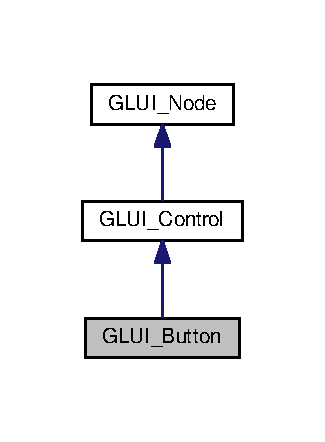
\includegraphics[width=156pt]{class_g_l_u_i___button__inherit__graph}
\end{center}
\end{figure}


Collaboration diagram for G\+L\+U\+I\+\_\+\+Button\+:\nopagebreak
\begin{figure}[H]
\begin{center}
\leavevmode
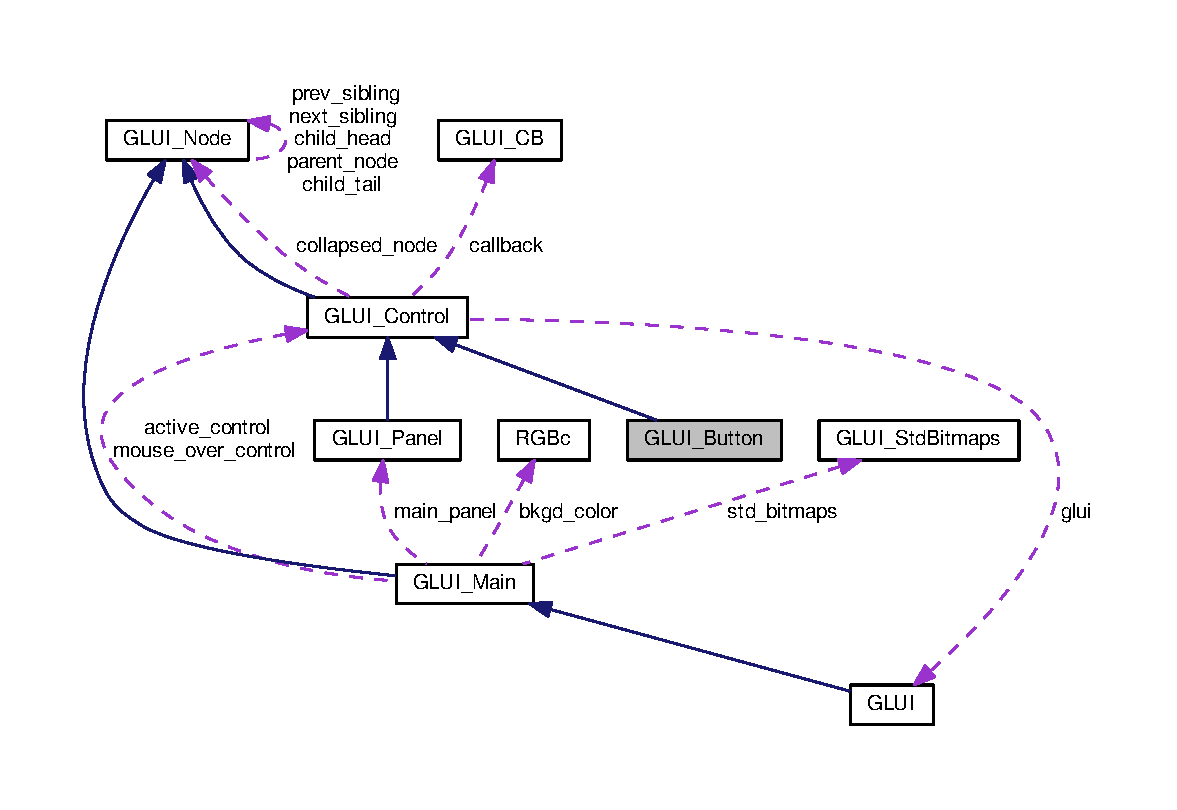
\includegraphics[width=350pt]{class_g_l_u_i___button__coll__graph}
\end{center}
\end{figure}
\subsection*{Public Member Functions}
\begin{DoxyCompactItemize}
\item 
\hyperlink{wglext_8h_a500a82aecba06f4550f6849b8099ca21}{int} \hyperlink{class_g_l_u_i___button_ad049e31e22fddf61df229c6fcef80f27}{mouse\+\_\+down\+\_\+handler} (\hyperlink{wglext_8h_a500a82aecba06f4550f6849b8099ca21}{int} local\+\_\+x, \hyperlink{wglext_8h_a500a82aecba06f4550f6849b8099ca21}{int} local\+\_\+y)
\item 
\hyperlink{wglext_8h_a500a82aecba06f4550f6849b8099ca21}{int} \hyperlink{class_g_l_u_i___button_a731c78e9ae9fe92fe5e0eba47fc6c0cf}{mouse\+\_\+up\+\_\+handler} (\hyperlink{wglext_8h_a500a82aecba06f4550f6849b8099ca21}{int} local\+\_\+x, \hyperlink{wglext_8h_a500a82aecba06f4550f6849b8099ca21}{int} local\+\_\+y, bool inside)
\item 
\hyperlink{wglext_8h_a500a82aecba06f4550f6849b8099ca21}{int} \hyperlink{class_g_l_u_i___button_a38e99372cc0de31dfa784b95e70d1f51}{mouse\+\_\+held\+\_\+down\+\_\+handler} (\hyperlink{wglext_8h_a500a82aecba06f4550f6849b8099ca21}{int} local\+\_\+x, \hyperlink{wglext_8h_a500a82aecba06f4550f6849b8099ca21}{int} local\+\_\+y, bool inside)
\item 
\hyperlink{wglext_8h_a500a82aecba06f4550f6849b8099ca21}{int} \hyperlink{class_g_l_u_i___button_abb99757083838d0f9c87596b512ec5e9}{key\+\_\+handler} (unsigned char key, \hyperlink{wglext_8h_a500a82aecba06f4550f6849b8099ca21}{int} modifiers)
\item 
\hyperlink{wglext_8h_a9e6b7f1933461ef318bb000d6bd13b83}{void} \hyperlink{class_g_l_u_i___button_a0b70efaf00fe4eeb26f2675c156fc48f}{draw} (\hyperlink{wglext_8h_a500a82aecba06f4550f6849b8099ca21}{int} \hyperlink{glext_8h_ad77deca22f617d3f0e0eb786445689fc}{x}, \hyperlink{wglext_8h_a500a82aecba06f4550f6849b8099ca21}{int} \hyperlink{glext_8h_a9298c7ad619074f5285b32c6b72bfdea}{y})
\item 
\hyperlink{wglext_8h_a9e6b7f1933461ef318bb000d6bd13b83}{void} \hyperlink{class_g_l_u_i___button_a445e459227bf0019217ec05e064d3f67}{draw\+\_\+pressed} (\hyperlink{wglext_8h_a9e6b7f1933461ef318bb000d6bd13b83}{void})
\item 
\hyperlink{wglext_8h_a9e6b7f1933461ef318bb000d6bd13b83}{void} \hyperlink{class_g_l_u_i___button_a3012a081189288aa6190258f6fd47c9c}{draw\+\_\+text} (\hyperlink{wglext_8h_a500a82aecba06f4550f6849b8099ca21}{int} sunken)
\item 
\hyperlink{wglext_8h_a9e6b7f1933461ef318bb000d6bd13b83}{void} \hyperlink{class_g_l_u_i___button_a374f9334b7a026ba6e63d4911039d456}{update\+\_\+size} (\hyperlink{wglext_8h_a9e6b7f1933461ef318bb000d6bd13b83}{void})
\item 
\hyperlink{class_g_l_u_i___button_ab7ddf8c8d6c6c3dcab55b1738b1e7b8d}{G\+L\+U\+I\+\_\+\+Button} (\hyperlink{class_g_l_u_i___node}{G\+L\+U\+I\+\_\+\+Node} $\ast$\hyperlink{class_g_l_u_i___node_a8ed65d447784f6f88bd3e2e2bcac6cdb}{parent}, const char $\ast$\hyperlink{glext_8h_ad977737dfc9a274a62741b9500c49a32}{name}, \hyperlink{wglext_8h_a500a82aecba06f4550f6849b8099ca21}{int} \hyperlink{glext_8h_a58c2a664503e14ffb8f21012aabff3e9}{id}=-\/1, \hyperlink{class_g_l_u_i___c_b}{G\+L\+U\+I\+\_\+\+C\+B} cb=\hyperlink{class_g_l_u_i___c_b}{G\+L\+U\+I\+\_\+\+C\+B}())
\item 
\hyperlink{class_g_l_u_i___button_a801dc750129ae94d4aebacffe38086aa}{G\+L\+U\+I\+\_\+\+Button} (\hyperlink{wglext_8h_a9e6b7f1933461ef318bb000d6bd13b83}{void})
\end{DoxyCompactItemize}
\subsection*{Public Attributes}
\begin{DoxyCompactItemize}
\item 
bool \hyperlink{class_g_l_u_i___button_aa7267a5e210893367862d9d96888eb41}{currently\+\_\+inside}
\end{DoxyCompactItemize}
\subsection*{Protected Member Functions}
\begin{DoxyCompactItemize}
\item 
\hyperlink{wglext_8h_a9e6b7f1933461ef318bb000d6bd13b83}{void} \hyperlink{class_g_l_u_i___button_ac840fd31bb87ab5c4448f772759cf1b6}{common\+\_\+init} (\hyperlink{wglext_8h_a9e6b7f1933461ef318bb000d6bd13b83}{void})
\end{DoxyCompactItemize}
\subsection*{Additional Inherited Members}


\subsection{Detailed Description}
An onscreen, clickable button--an outlined label that can be clicked. When clicked, a button calls its \hyperlink{class_g_l_u_i___c_b}{G\+L\+U\+I\+\_\+\+C\+B} callback with its I\+D. 

Definition at line 956 of file glui.\+h.



\subsection{Constructor \& Destructor Documentation}
\hypertarget{class_g_l_u_i___button_ab7ddf8c8d6c6c3dcab55b1738b1e7b8d}{\index{G\+L\+U\+I\+\_\+\+Button@{G\+L\+U\+I\+\_\+\+Button}!G\+L\+U\+I\+\_\+\+Button@{G\+L\+U\+I\+\_\+\+Button}}
\index{G\+L\+U\+I\+\_\+\+Button@{G\+L\+U\+I\+\_\+\+Button}!G\+L\+U\+I\+\_\+\+Button@{G\+L\+U\+I\+\_\+\+Button}}
\subsubsection[{G\+L\+U\+I\+\_\+\+Button}]{\setlength{\rightskip}{0pt plus 5cm}G\+L\+U\+I\+\_\+\+Button\+::\+G\+L\+U\+I\+\_\+\+Button (
\begin{DoxyParamCaption}
\item[{{\bf G\+L\+U\+I\+\_\+\+Node} $\ast$}]{parent, }
\item[{const char $\ast$}]{name, }
\item[{{\bf int}}]{id = {\ttfamily -\/1}, }
\item[{{\bf G\+L\+U\+I\+\_\+\+C\+B}}]{cb = {\ttfamily {\bf G\+L\+U\+I\+\_\+\+C\+B}()}}
\end{DoxyParamCaption}
)}}\label{class_g_l_u_i___button_ab7ddf8c8d6c6c3dcab55b1738b1e7b8d}
Create a new button.


\begin{DoxyParams}{Parameters}
{\em parent} & The panel our object is inside; or the main \hyperlink{class_g_l_u_i}{G\+L\+U\+I} object. \\
\hline
{\em name} & The text inside the button. \\
\hline
{\em id} & Optional I\+D number, to pass to the optional callback function. \\
\hline
{\em callback} & Optional callback function, taking either the int I\+D or control. \\
\hline
\end{DoxyParams}
\hypertarget{class_g_l_u_i___button_a801dc750129ae94d4aebacffe38086aa}{\index{G\+L\+U\+I\+\_\+\+Button@{G\+L\+U\+I\+\_\+\+Button}!G\+L\+U\+I\+\_\+\+Button@{G\+L\+U\+I\+\_\+\+Button}}
\index{G\+L\+U\+I\+\_\+\+Button@{G\+L\+U\+I\+\_\+\+Button}!G\+L\+U\+I\+\_\+\+Button@{G\+L\+U\+I\+\_\+\+Button}}
\subsubsection[{G\+L\+U\+I\+\_\+\+Button}]{\setlength{\rightskip}{0pt plus 5cm}G\+L\+U\+I\+\_\+\+Button\+::\+G\+L\+U\+I\+\_\+\+Button (
\begin{DoxyParamCaption}
\item[{{\bf void}}]{}
\end{DoxyParamCaption}
)\hspace{0.3cm}{\ttfamily [inline]}}}\label{class_g_l_u_i___button_a801dc750129ae94d4aebacffe38086aa}


Definition at line 982 of file glui.\+h.



\subsection{Member Function Documentation}
\hypertarget{class_g_l_u_i___button_ac840fd31bb87ab5c4448f772759cf1b6}{\index{G\+L\+U\+I\+\_\+\+Button@{G\+L\+U\+I\+\_\+\+Button}!common\+\_\+init@{common\+\_\+init}}
\index{common\+\_\+init@{common\+\_\+init}!G\+L\+U\+I\+\_\+\+Button@{G\+L\+U\+I\+\_\+\+Button}}
\subsubsection[{common\+\_\+init}]{\setlength{\rightskip}{0pt plus 5cm}{\bf void} G\+L\+U\+I\+\_\+\+Button\+::common\+\_\+init (
\begin{DoxyParamCaption}
\item[{{\bf void}}]{}
\end{DoxyParamCaption}
)\hspace{0.3cm}{\ttfamily [inline]}, {\ttfamily [protected]}}}\label{class_g_l_u_i___button_ac840fd31bb87ab5c4448f772759cf1b6}


Definition at line 985 of file glui.\+h.

\hypertarget{class_g_l_u_i___button_a0b70efaf00fe4eeb26f2675c156fc48f}{\index{G\+L\+U\+I\+\_\+\+Button@{G\+L\+U\+I\+\_\+\+Button}!draw@{draw}}
\index{draw@{draw}!G\+L\+U\+I\+\_\+\+Button@{G\+L\+U\+I\+\_\+\+Button}}
\subsubsection[{draw}]{\setlength{\rightskip}{0pt plus 5cm}{\bf void} G\+L\+U\+I\+\_\+\+Button\+::draw (
\begin{DoxyParamCaption}
\item[{{\bf int}}]{x, }
\item[{{\bf int}}]{y}
\end{DoxyParamCaption}
)\hspace{0.3cm}{\ttfamily [virtual]}}}\label{class_g_l_u_i___button_a0b70efaf00fe4eeb26f2675c156fc48f}


Implements \hyperlink{class_g_l_u_i___control_a2eb42d7a7951280ad2fe8c37972bf66a}{G\+L\+U\+I\+\_\+\+Control}.

\hypertarget{class_g_l_u_i___button_a445e459227bf0019217ec05e064d3f67}{\index{G\+L\+U\+I\+\_\+\+Button@{G\+L\+U\+I\+\_\+\+Button}!draw\+\_\+pressed@{draw\+\_\+pressed}}
\index{draw\+\_\+pressed@{draw\+\_\+pressed}!G\+L\+U\+I\+\_\+\+Button@{G\+L\+U\+I\+\_\+\+Button}}
\subsubsection[{draw\+\_\+pressed}]{\setlength{\rightskip}{0pt plus 5cm}{\bf void} G\+L\+U\+I\+\_\+\+Button\+::draw\+\_\+pressed (
\begin{DoxyParamCaption}
\item[{{\bf void}}]{}
\end{DoxyParamCaption}
)}}\label{class_g_l_u_i___button_a445e459227bf0019217ec05e064d3f67}
\hypertarget{class_g_l_u_i___button_a3012a081189288aa6190258f6fd47c9c}{\index{G\+L\+U\+I\+\_\+\+Button@{G\+L\+U\+I\+\_\+\+Button}!draw\+\_\+text@{draw\+\_\+text}}
\index{draw\+\_\+text@{draw\+\_\+text}!G\+L\+U\+I\+\_\+\+Button@{G\+L\+U\+I\+\_\+\+Button}}
\subsubsection[{draw\+\_\+text}]{\setlength{\rightskip}{0pt plus 5cm}{\bf void} G\+L\+U\+I\+\_\+\+Button\+::draw\+\_\+text (
\begin{DoxyParamCaption}
\item[{{\bf int}}]{sunken}
\end{DoxyParamCaption}
)}}\label{class_g_l_u_i___button_a3012a081189288aa6190258f6fd47c9c}
\hypertarget{class_g_l_u_i___button_abb99757083838d0f9c87596b512ec5e9}{\index{G\+L\+U\+I\+\_\+\+Button@{G\+L\+U\+I\+\_\+\+Button}!key\+\_\+handler@{key\+\_\+handler}}
\index{key\+\_\+handler@{key\+\_\+handler}!G\+L\+U\+I\+\_\+\+Button@{G\+L\+U\+I\+\_\+\+Button}}
\subsubsection[{key\+\_\+handler}]{\setlength{\rightskip}{0pt plus 5cm}{\bf int} G\+L\+U\+I\+\_\+\+Button\+::key\+\_\+handler (
\begin{DoxyParamCaption}
\item[{unsigned char}]{key, }
\item[{{\bf int}}]{modifiers}
\end{DoxyParamCaption}
)\hspace{0.3cm}{\ttfamily [virtual]}}}\label{class_g_l_u_i___button_abb99757083838d0f9c87596b512ec5e9}


Reimplemented from \hyperlink{class_g_l_u_i___control_a7f9da8ca7df99bd4cf394a9fd8ce19f1}{G\+L\+U\+I\+\_\+\+Control}.

\hypertarget{class_g_l_u_i___button_ad049e31e22fddf61df229c6fcef80f27}{\index{G\+L\+U\+I\+\_\+\+Button@{G\+L\+U\+I\+\_\+\+Button}!mouse\+\_\+down\+\_\+handler@{mouse\+\_\+down\+\_\+handler}}
\index{mouse\+\_\+down\+\_\+handler@{mouse\+\_\+down\+\_\+handler}!G\+L\+U\+I\+\_\+\+Button@{G\+L\+U\+I\+\_\+\+Button}}
\subsubsection[{mouse\+\_\+down\+\_\+handler}]{\setlength{\rightskip}{0pt plus 5cm}{\bf int} G\+L\+U\+I\+\_\+\+Button\+::mouse\+\_\+down\+\_\+handler (
\begin{DoxyParamCaption}
\item[{{\bf int}}]{local\+\_\+x, }
\item[{{\bf int}}]{local\+\_\+y}
\end{DoxyParamCaption}
)\hspace{0.3cm}{\ttfamily [virtual]}}}\label{class_g_l_u_i___button_ad049e31e22fddf61df229c6fcef80f27}


Reimplemented from \hyperlink{class_g_l_u_i___control_a92b77565168a1d2003bca1c16ac00e8d}{G\+L\+U\+I\+\_\+\+Control}.

\hypertarget{class_g_l_u_i___button_a38e99372cc0de31dfa784b95e70d1f51}{\index{G\+L\+U\+I\+\_\+\+Button@{G\+L\+U\+I\+\_\+\+Button}!mouse\+\_\+held\+\_\+down\+\_\+handler@{mouse\+\_\+held\+\_\+down\+\_\+handler}}
\index{mouse\+\_\+held\+\_\+down\+\_\+handler@{mouse\+\_\+held\+\_\+down\+\_\+handler}!G\+L\+U\+I\+\_\+\+Button@{G\+L\+U\+I\+\_\+\+Button}}
\subsubsection[{mouse\+\_\+held\+\_\+down\+\_\+handler}]{\setlength{\rightskip}{0pt plus 5cm}{\bf int} G\+L\+U\+I\+\_\+\+Button\+::mouse\+\_\+held\+\_\+down\+\_\+handler (
\begin{DoxyParamCaption}
\item[{{\bf int}}]{local\+\_\+x, }
\item[{{\bf int}}]{local\+\_\+y, }
\item[{bool}]{inside}
\end{DoxyParamCaption}
)\hspace{0.3cm}{\ttfamily [virtual]}}}\label{class_g_l_u_i___button_a38e99372cc0de31dfa784b95e70d1f51}


Reimplemented from \hyperlink{class_g_l_u_i___control_a4b44e44c1c455adc7f98c63aeb6aa919}{G\+L\+U\+I\+\_\+\+Control}.

\hypertarget{class_g_l_u_i___button_a731c78e9ae9fe92fe5e0eba47fc6c0cf}{\index{G\+L\+U\+I\+\_\+\+Button@{G\+L\+U\+I\+\_\+\+Button}!mouse\+\_\+up\+\_\+handler@{mouse\+\_\+up\+\_\+handler}}
\index{mouse\+\_\+up\+\_\+handler@{mouse\+\_\+up\+\_\+handler}!G\+L\+U\+I\+\_\+\+Button@{G\+L\+U\+I\+\_\+\+Button}}
\subsubsection[{mouse\+\_\+up\+\_\+handler}]{\setlength{\rightskip}{0pt plus 5cm}{\bf int} G\+L\+U\+I\+\_\+\+Button\+::mouse\+\_\+up\+\_\+handler (
\begin{DoxyParamCaption}
\item[{{\bf int}}]{local\+\_\+x, }
\item[{{\bf int}}]{local\+\_\+y, }
\item[{bool}]{inside}
\end{DoxyParamCaption}
)\hspace{0.3cm}{\ttfamily [virtual]}}}\label{class_g_l_u_i___button_a731c78e9ae9fe92fe5e0eba47fc6c0cf}


Reimplemented from \hyperlink{class_g_l_u_i___control_ac32aad8f69134d03682e34d0488a18f1}{G\+L\+U\+I\+\_\+\+Control}.

\hypertarget{class_g_l_u_i___button_a374f9334b7a026ba6e63d4911039d456}{\index{G\+L\+U\+I\+\_\+\+Button@{G\+L\+U\+I\+\_\+\+Button}!update\+\_\+size@{update\+\_\+size}}
\index{update\+\_\+size@{update\+\_\+size}!G\+L\+U\+I\+\_\+\+Button@{G\+L\+U\+I\+\_\+\+Button}}
\subsubsection[{update\+\_\+size}]{\setlength{\rightskip}{0pt plus 5cm}{\bf void} G\+L\+U\+I\+\_\+\+Button\+::update\+\_\+size (
\begin{DoxyParamCaption}
\item[{{\bf void}}]{}
\end{DoxyParamCaption}
)\hspace{0.3cm}{\ttfamily [virtual]}}}\label{class_g_l_u_i___button_a374f9334b7a026ba6e63d4911039d456}


Reimplemented from \hyperlink{class_g_l_u_i___control_a4bfe55acbbf735a7d2ff07d687a481e2}{G\+L\+U\+I\+\_\+\+Control}.



\subsection{Member Data Documentation}
\hypertarget{class_g_l_u_i___button_aa7267a5e210893367862d9d96888eb41}{\index{G\+L\+U\+I\+\_\+\+Button@{G\+L\+U\+I\+\_\+\+Button}!currently\+\_\+inside@{currently\+\_\+inside}}
\index{currently\+\_\+inside@{currently\+\_\+inside}!G\+L\+U\+I\+\_\+\+Button@{G\+L\+U\+I\+\_\+\+Button}}
\subsubsection[{currently\+\_\+inside}]{\setlength{\rightskip}{0pt plus 5cm}bool G\+L\+U\+I\+\_\+\+Button\+::currently\+\_\+inside}}\label{class_g_l_u_i___button_aa7267a5e210893367862d9d96888eb41}


Definition at line 959 of file glui.\+h.



The documentation for this class was generated from the following file\+:\begin{DoxyCompactItemize}
\item 
S\+S\+W\+C/src/\+G\+L/\hyperlink{glui_8h}{glui.\+h}\end{DoxyCompactItemize}

\hypertarget{class_g_l_u_i___c_b}{\section{G\+L\+U\+I\+\_\+\+C\+B Class Reference}
\label{class_g_l_u_i___c_b}\index{G\+L\+U\+I\+\_\+\+C\+B@{G\+L\+U\+I\+\_\+\+C\+B}}
}


{\ttfamily \#include $<$glui.\+h$>$}

\subsection*{Public Member Functions}
\begin{DoxyCompactItemize}
\item 
\hyperlink{class_g_l_u_i___c_b_a5ff7e75c1425d0e148afa9c461772ae2}{G\+L\+U\+I\+\_\+\+C\+B} ()
\item 
\hyperlink{class_g_l_u_i___c_b_a8ee9a7b49fe15afb89985e2218ac17de}{G\+L\+U\+I\+\_\+\+C\+B} (\hyperlink{glui_8h_a11c8645866aceff55b55af31f4bf4c04}{G\+L\+U\+I\+\_\+\+Update\+\_\+\+C\+B} cb)
\item 
\hyperlink{class_g_l_u_i___c_b_ab2c48ce5142f91878323797b9ea9472c}{G\+L\+U\+I\+\_\+\+C\+B} (\hyperlink{glui_8h_a8dae0ec6ca9738eb013c8add125086d3}{G\+L\+U\+I\+\_\+\+Control\+\_\+\+C\+B} cb)
\item 
\hyperlink{wglext_8h_a9e6b7f1933461ef318bb000d6bd13b83}{void} \hyperlink{class_g_l_u_i___c_b_a3677d6a872540cd82d4ba1add46a16eb}{operator()} (\hyperlink{class_g_l_u_i___control}{G\+L\+U\+I\+\_\+\+Control} $\ast$ctrl) const 
\item 
bool \hyperlink{class_g_l_u_i___c_b_acd93cfbb08c758e75ca38b6caff9131d}{operator!} () const 
\item 
\hyperlink{class_g_l_u_i___c_b_a181c6390f944b9db42de829b83eae7ac}{operator bool} () const 
\end{DoxyCompactItemize}


\subsection{Detailed Description}
Callback Adapter Class Allows us to support different types of callbacks; like a G\+L\+U\+I\+\_\+\+Update\+\_\+\+C\+B function pointer--which takes an int; and a G\+L\+U\+I\+\_\+\+Control\+\_\+\+C\+B function pointer--which takes a G\+U\+I\+\_\+\+Control object. 

Definition at line 294 of file glui.\+h.



\subsection{Constructor \& Destructor Documentation}
\hypertarget{class_g_l_u_i___c_b_a5ff7e75c1425d0e148afa9c461772ae2}{\index{G\+L\+U\+I\+\_\+\+C\+B@{G\+L\+U\+I\+\_\+\+C\+B}!G\+L\+U\+I\+\_\+\+C\+B@{G\+L\+U\+I\+\_\+\+C\+B}}
\index{G\+L\+U\+I\+\_\+\+C\+B@{G\+L\+U\+I\+\_\+\+C\+B}!G\+L\+U\+I\+\_\+\+C\+B@{G\+L\+U\+I\+\_\+\+C\+B}}
\subsubsection[{G\+L\+U\+I\+\_\+\+C\+B}]{\setlength{\rightskip}{0pt plus 5cm}G\+L\+U\+I\+\_\+\+C\+B\+::\+G\+L\+U\+I\+\_\+\+C\+B (
\begin{DoxyParamCaption}
{}
\end{DoxyParamCaption}
)\hspace{0.3cm}{\ttfamily [inline]}}}\label{class_g_l_u_i___c_b_a5ff7e75c1425d0e148afa9c461772ae2}


Definition at line 297 of file glui.\+h.

\hypertarget{class_g_l_u_i___c_b_a8ee9a7b49fe15afb89985e2218ac17de}{\index{G\+L\+U\+I\+\_\+\+C\+B@{G\+L\+U\+I\+\_\+\+C\+B}!G\+L\+U\+I\+\_\+\+C\+B@{G\+L\+U\+I\+\_\+\+C\+B}}
\index{G\+L\+U\+I\+\_\+\+C\+B@{G\+L\+U\+I\+\_\+\+C\+B}!G\+L\+U\+I\+\_\+\+C\+B@{G\+L\+U\+I\+\_\+\+C\+B}}
\subsubsection[{G\+L\+U\+I\+\_\+\+C\+B}]{\setlength{\rightskip}{0pt plus 5cm}G\+L\+U\+I\+\_\+\+C\+B\+::\+G\+L\+U\+I\+\_\+\+C\+B (
\begin{DoxyParamCaption}
\item[{{\bf G\+L\+U\+I\+\_\+\+Update\+\_\+\+C\+B}}]{cb}
\end{DoxyParamCaption}
)\hspace{0.3cm}{\ttfamily [inline]}}}\label{class_g_l_u_i___c_b_a8ee9a7b49fe15afb89985e2218ac17de}


Definition at line 298 of file glui.\+h.

\hypertarget{class_g_l_u_i___c_b_ab2c48ce5142f91878323797b9ea9472c}{\index{G\+L\+U\+I\+\_\+\+C\+B@{G\+L\+U\+I\+\_\+\+C\+B}!G\+L\+U\+I\+\_\+\+C\+B@{G\+L\+U\+I\+\_\+\+C\+B}}
\index{G\+L\+U\+I\+\_\+\+C\+B@{G\+L\+U\+I\+\_\+\+C\+B}!G\+L\+U\+I\+\_\+\+C\+B@{G\+L\+U\+I\+\_\+\+C\+B}}
\subsubsection[{G\+L\+U\+I\+\_\+\+C\+B}]{\setlength{\rightskip}{0pt plus 5cm}G\+L\+U\+I\+\_\+\+C\+B\+::\+G\+L\+U\+I\+\_\+\+C\+B (
\begin{DoxyParamCaption}
\item[{{\bf G\+L\+U\+I\+\_\+\+Control\+\_\+\+C\+B}}]{cb}
\end{DoxyParamCaption}
)\hspace{0.3cm}{\ttfamily [inline]}}}\label{class_g_l_u_i___c_b_ab2c48ce5142f91878323797b9ea9472c}


Definition at line 299 of file glui.\+h.



\subsection{Member Function Documentation}
\hypertarget{class_g_l_u_i___c_b_a181c6390f944b9db42de829b83eae7ac}{\index{G\+L\+U\+I\+\_\+\+C\+B@{G\+L\+U\+I\+\_\+\+C\+B}!operator bool@{operator bool}}
\index{operator bool@{operator bool}!G\+L\+U\+I\+\_\+\+C\+B@{G\+L\+U\+I\+\_\+\+C\+B}}
\subsubsection[{operator bool}]{\setlength{\rightskip}{0pt plus 5cm}G\+L\+U\+I\+\_\+\+C\+B\+::operator bool (
\begin{DoxyParamCaption}
{}
\end{DoxyParamCaption}
) const\hspace{0.3cm}{\ttfamily [inline]}}}\label{class_g_l_u_i___c_b_a181c6390f944b9db42de829b83eae7ac}


Definition at line 305 of file glui.\+h.

\hypertarget{class_g_l_u_i___c_b_acd93cfbb08c758e75ca38b6caff9131d}{\index{G\+L\+U\+I\+\_\+\+C\+B@{G\+L\+U\+I\+\_\+\+C\+B}!operator"!@{operator"!}}
\index{operator"!@{operator"!}!G\+L\+U\+I\+\_\+\+C\+B@{G\+L\+U\+I\+\_\+\+C\+B}}
\subsubsection[{operator"!}]{\setlength{\rightskip}{0pt plus 5cm}bool G\+L\+U\+I\+\_\+\+C\+B\+::operator! (
\begin{DoxyParamCaption}
{}
\end{DoxyParamCaption}
) const\hspace{0.3cm}{\ttfamily [inline]}}}\label{class_g_l_u_i___c_b_acd93cfbb08c758e75ca38b6caff9131d}


Definition at line 304 of file glui.\+h.

\hypertarget{class_g_l_u_i___c_b_a3677d6a872540cd82d4ba1add46a16eb}{\index{G\+L\+U\+I\+\_\+\+C\+B@{G\+L\+U\+I\+\_\+\+C\+B}!operator()@{operator()}}
\index{operator()@{operator()}!G\+L\+U\+I\+\_\+\+C\+B@{G\+L\+U\+I\+\_\+\+C\+B}}
\subsubsection[{operator()}]{\setlength{\rightskip}{0pt plus 5cm}{\bf void} G\+L\+U\+I\+\_\+\+C\+B\+::operator() (
\begin{DoxyParamCaption}
\item[{{\bf G\+L\+U\+I\+\_\+\+Control} $\ast$}]{ctrl}
\end{DoxyParamCaption}
) const}}\label{class_g_l_u_i___c_b_a3677d6a872540cd82d4ba1add46a16eb}
This control just activated. Fire our callback. 

The documentation for this class was generated from the following file\+:\begin{DoxyCompactItemize}
\item 
S\+S\+W\+C/src/\+G\+L/\hyperlink{glui_8h}{glui.\+h}\end{DoxyCompactItemize}

\hypertarget{class_g_l_u_i___checkbox}{\section{G\+L\+U\+I\+\_\+\+Checkbox Class Reference}
\label{class_g_l_u_i___checkbox}\index{G\+L\+U\+I\+\_\+\+Checkbox@{G\+L\+U\+I\+\_\+\+Checkbox}}
}


{\ttfamily \#include $<$glui.\+h$>$}



Inheritance diagram for G\+L\+U\+I\+\_\+\+Checkbox\+:\nopagebreak
\begin{figure}[H]
\begin{center}
\leavevmode
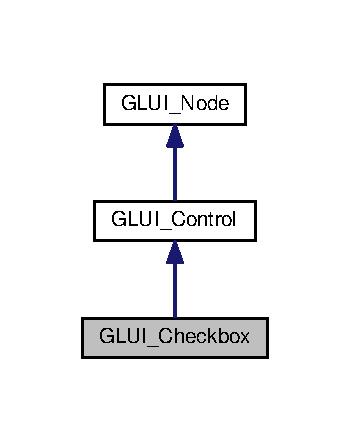
\includegraphics[width=168pt]{class_g_l_u_i___checkbox__inherit__graph}
\end{center}
\end{figure}


Collaboration diagram for G\+L\+U\+I\+\_\+\+Checkbox\+:\nopagebreak
\begin{figure}[H]
\begin{center}
\leavevmode
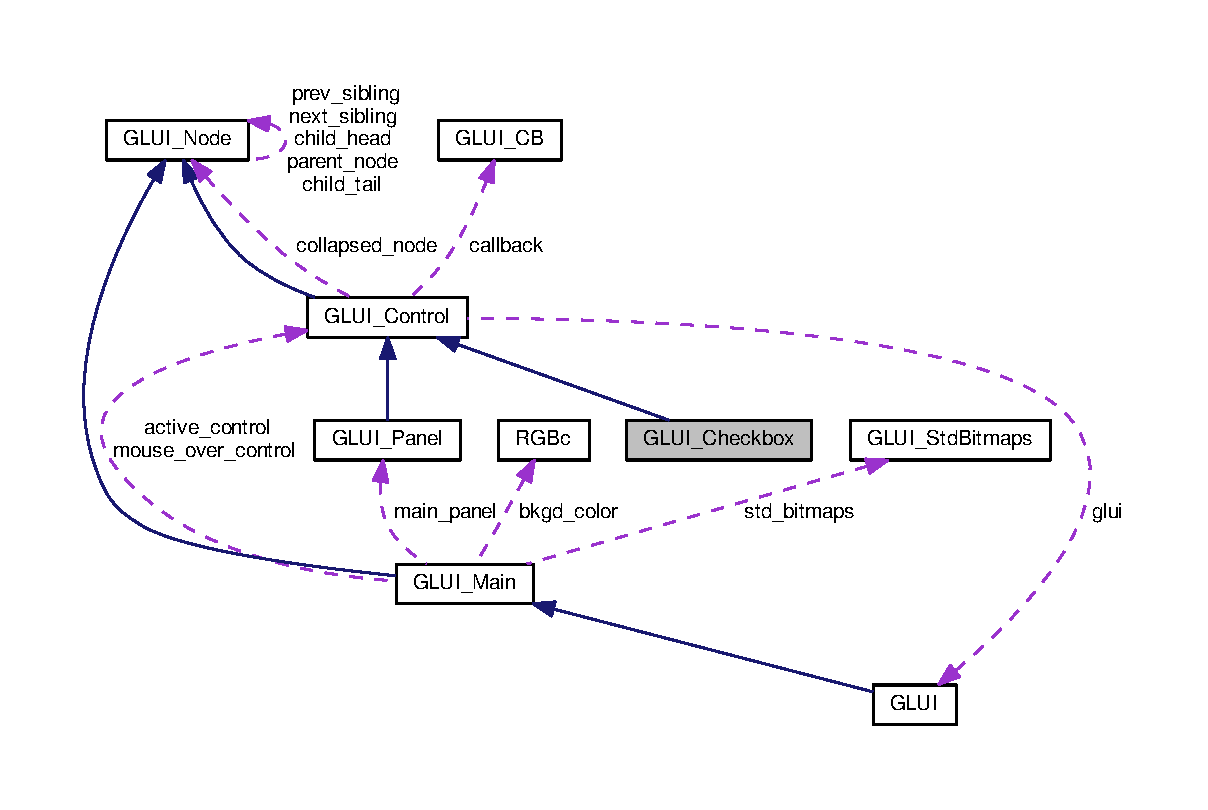
\includegraphics[width=350pt]{class_g_l_u_i___checkbox__coll__graph}
\end{center}
\end{figure}
\subsection*{Public Member Functions}
\begin{DoxyCompactItemize}
\item 
\hyperlink{wglext_8h_a500a82aecba06f4550f6849b8099ca21}{int} \hyperlink{class_g_l_u_i___checkbox_a7cf605868f357f790890fb1eb01c4b5b}{mouse\+\_\+down\+\_\+handler} (\hyperlink{wglext_8h_a500a82aecba06f4550f6849b8099ca21}{int} local\+\_\+x, \hyperlink{wglext_8h_a500a82aecba06f4550f6849b8099ca21}{int} local\+\_\+y)
\item 
\hyperlink{wglext_8h_a500a82aecba06f4550f6849b8099ca21}{int} \hyperlink{class_g_l_u_i___checkbox_a600720d43a3f7568c41cc23a34f7f601}{mouse\+\_\+up\+\_\+handler} (\hyperlink{wglext_8h_a500a82aecba06f4550f6849b8099ca21}{int} local\+\_\+x, \hyperlink{wglext_8h_a500a82aecba06f4550f6849b8099ca21}{int} local\+\_\+y, bool inside)
\item 
\hyperlink{wglext_8h_a500a82aecba06f4550f6849b8099ca21}{int} \hyperlink{class_g_l_u_i___checkbox_ad18f2ba9f3dc594db3f60c32bc9fe4d2}{mouse\+\_\+held\+\_\+down\+\_\+handler} (\hyperlink{wglext_8h_a500a82aecba06f4550f6849b8099ca21}{int} local\+\_\+x, \hyperlink{wglext_8h_a500a82aecba06f4550f6849b8099ca21}{int} local\+\_\+y, bool inside)
\item 
\hyperlink{wglext_8h_a500a82aecba06f4550f6849b8099ca21}{int} \hyperlink{class_g_l_u_i___checkbox_a246a4aea27d74689643eb4c1d5dc25ef}{key\+\_\+handler} (unsigned char key, \hyperlink{wglext_8h_a500a82aecba06f4550f6849b8099ca21}{int} modifiers)
\item 
\hyperlink{wglext_8h_a9e6b7f1933461ef318bb000d6bd13b83}{void} \hyperlink{class_g_l_u_i___checkbox_adce7c97553cc1b8b8200bf173efbffb1}{update\+\_\+size} (\hyperlink{wglext_8h_a9e6b7f1933461ef318bb000d6bd13b83}{void})
\item 
\hyperlink{wglext_8h_a9e6b7f1933461ef318bb000d6bd13b83}{void} \hyperlink{class_g_l_u_i___checkbox_ad03530c711561d3d32348c8ee3f39b5a}{draw} (\hyperlink{wglext_8h_a500a82aecba06f4550f6849b8099ca21}{int} \hyperlink{glext_8h_ad77deca22f617d3f0e0eb786445689fc}{x}, \hyperlink{wglext_8h_a500a82aecba06f4550f6849b8099ca21}{int} \hyperlink{glext_8h_a9298c7ad619074f5285b32c6b72bfdea}{y})
\item 
\hyperlink{wglext_8h_a9e6b7f1933461ef318bb000d6bd13b83}{void} \hyperlink{class_g_l_u_i___checkbox_ae6b129ff35269a2510e3c38f627d82a3}{draw\+\_\+active\+\_\+area} (\hyperlink{wglext_8h_a9e6b7f1933461ef318bb000d6bd13b83}{void})
\item 
\hyperlink{wglext_8h_a9e6b7f1933461ef318bb000d6bd13b83}{void} \hyperlink{class_g_l_u_i___checkbox_a477ff2ccc6f25ee1e3c8e16647af3e69}{draw\+\_\+empty\+\_\+box} (\hyperlink{wglext_8h_a9e6b7f1933461ef318bb000d6bd13b83}{void})
\item 
\hyperlink{wglext_8h_a9e6b7f1933461ef318bb000d6bd13b83}{void} \hyperlink{class_g_l_u_i___checkbox_a33a217485f0a8d17d7c45de5a91f57fd}{set\+\_\+int\+\_\+val} (\hyperlink{wglext_8h_a500a82aecba06f4550f6849b8099ca21}{int} new\+\_\+val)
\item 
\hyperlink{class_g_l_u_i___checkbox_a37dc0700283da8c9e05d57153f04e59b}{G\+L\+U\+I\+\_\+\+Checkbox} (\hyperlink{class_g_l_u_i___node}{G\+L\+U\+I\+\_\+\+Node} $\ast$\hyperlink{class_g_l_u_i___node_a8ed65d447784f6f88bd3e2e2bcac6cdb}{parent}, const char $\ast$\hyperlink{glext_8h_ad977737dfc9a274a62741b9500c49a32}{name}, \hyperlink{wglext_8h_a500a82aecba06f4550f6849b8099ca21}{int} $\ast$value\+\_\+ptr=N\+U\+L\+L, \hyperlink{wglext_8h_a500a82aecba06f4550f6849b8099ca21}{int} \hyperlink{glext_8h_a58c2a664503e14ffb8f21012aabff3e9}{id}=-\/1, \hyperlink{class_g_l_u_i___c_b}{G\+L\+U\+I\+\_\+\+C\+B} \hyperlink{class_g_l_u_i___control_a96060fe0cc6d537e736dd6eef78e24ab}{callback}=\hyperlink{class_g_l_u_i___c_b}{G\+L\+U\+I\+\_\+\+C\+B}())
\item 
\hyperlink{class_g_l_u_i___checkbox_ab84000529be3cf160f6e39c9416e782d}{G\+L\+U\+I\+\_\+\+Checkbox} (\hyperlink{wglext_8h_a9e6b7f1933461ef318bb000d6bd13b83}{void})
\end{DoxyCompactItemize}
\subsection*{Public Attributes}
\begin{DoxyCompactItemize}
\item 
\hyperlink{wglext_8h_a500a82aecba06f4550f6849b8099ca21}{int} \hyperlink{class_g_l_u_i___checkbox_a4b98b08b7a7aa76b9a2d11769c36afe0}{orig\+\_\+value}
\item 
bool \hyperlink{class_g_l_u_i___checkbox_a67719010e5421edee03a1a7c98dc34d0}{currently\+\_\+inside}
\item 
\hyperlink{wglext_8h_a500a82aecba06f4550f6849b8099ca21}{int} \hyperlink{class_g_l_u_i___checkbox_ac3cec38298f8c0f6a1573070c759fcbe}{text\+\_\+x\+\_\+offset}
\end{DoxyCompactItemize}
\subsection*{Protected Member Functions}
\begin{DoxyCompactItemize}
\item 
\hyperlink{wglext_8h_a9e6b7f1933461ef318bb000d6bd13b83}{void} \hyperlink{class_g_l_u_i___checkbox_abce9cded0f247b501c92b7037d7036e0}{common\+\_\+init} (\hyperlink{wglext_8h_a9e6b7f1933461ef318bb000d6bd13b83}{void})
\end{DoxyCompactItemize}
\subsection*{Additional Inherited Members}


\subsection{Detailed Description}
A checkbox, which can be checked on or off. Can be linked to an int value, which gets 1 for on and 0 for off. 

Definition at line 1005 of file glui.\+h.



\subsection{Constructor \& Destructor Documentation}
\hypertarget{class_g_l_u_i___checkbox_a37dc0700283da8c9e05d57153f04e59b}{\index{G\+L\+U\+I\+\_\+\+Checkbox@{G\+L\+U\+I\+\_\+\+Checkbox}!G\+L\+U\+I\+\_\+\+Checkbox@{G\+L\+U\+I\+\_\+\+Checkbox}}
\index{G\+L\+U\+I\+\_\+\+Checkbox@{G\+L\+U\+I\+\_\+\+Checkbox}!G\+L\+U\+I\+\_\+\+Checkbox@{G\+L\+U\+I\+\_\+\+Checkbox}}
\subsubsection[{G\+L\+U\+I\+\_\+\+Checkbox}]{\setlength{\rightskip}{0pt plus 5cm}G\+L\+U\+I\+\_\+\+Checkbox\+::\+G\+L\+U\+I\+\_\+\+Checkbox (
\begin{DoxyParamCaption}
\item[{{\bf G\+L\+U\+I\+\_\+\+Node} $\ast$}]{parent, }
\item[{const char $\ast$}]{name, }
\item[{{\bf int} $\ast$}]{value\+\_\+ptr = {\ttfamily NULL}, }
\item[{{\bf int}}]{id = {\ttfamily -\/1}, }
\item[{{\bf G\+L\+U\+I\+\_\+\+C\+B}}]{callback = {\ttfamily {\bf G\+L\+U\+I\+\_\+\+C\+B}()}}
\end{DoxyParamCaption}
)}}\label{class_g_l_u_i___checkbox_a37dc0700283da8c9e05d57153f04e59b}
Create a new checkbox object.


\begin{DoxyParams}{Parameters}
{\em parent} & The panel our object is inside; or the main \hyperlink{class_g_l_u_i}{G\+L\+U\+I} object. \\
\hline
{\em name} & Label next to our checkbox. \\
\hline
{\em value\+\_\+ptr} & Optional integer value to attach to this checkbox. When the checkbox is checked or unchecked, $\ast$value\+\_\+ptr will also be changed. (\char`\"{}\+Live Vars\char`\"{}). \\
\hline
{\em id} & Optional I\+D number, to pass to the optional callback function. \\
\hline
{\em callback} & Optional callback function, taking either the int I\+D or control. \\
\hline
\end{DoxyParams}
\hypertarget{class_g_l_u_i___checkbox_ab84000529be3cf160f6e39c9416e782d}{\index{G\+L\+U\+I\+\_\+\+Checkbox@{G\+L\+U\+I\+\_\+\+Checkbox}!G\+L\+U\+I\+\_\+\+Checkbox@{G\+L\+U\+I\+\_\+\+Checkbox}}
\index{G\+L\+U\+I\+\_\+\+Checkbox@{G\+L\+U\+I\+\_\+\+Checkbox}!G\+L\+U\+I\+\_\+\+Checkbox@{G\+L\+U\+I\+\_\+\+Checkbox}}
\subsubsection[{G\+L\+U\+I\+\_\+\+Checkbox}]{\setlength{\rightskip}{0pt plus 5cm}G\+L\+U\+I\+\_\+\+Checkbox\+::\+G\+L\+U\+I\+\_\+\+Checkbox (
\begin{DoxyParamCaption}
\item[{{\bf void}}]{}
\end{DoxyParamCaption}
)\hspace{0.3cm}{\ttfamily [inline]}}}\label{class_g_l_u_i___checkbox_ab84000529be3cf160f6e39c9416e782d}


Definition at line 1037 of file glui.\+h.



\subsection{Member Function Documentation}
\hypertarget{class_g_l_u_i___checkbox_abce9cded0f247b501c92b7037d7036e0}{\index{G\+L\+U\+I\+\_\+\+Checkbox@{G\+L\+U\+I\+\_\+\+Checkbox}!common\+\_\+init@{common\+\_\+init}}
\index{common\+\_\+init@{common\+\_\+init}!G\+L\+U\+I\+\_\+\+Checkbox@{G\+L\+U\+I\+\_\+\+Checkbox}}
\subsubsection[{common\+\_\+init}]{\setlength{\rightskip}{0pt plus 5cm}{\bf void} G\+L\+U\+I\+\_\+\+Checkbox\+::common\+\_\+init (
\begin{DoxyParamCaption}
\item[{{\bf void}}]{}
\end{DoxyParamCaption}
)\hspace{0.3cm}{\ttfamily [inline]}, {\ttfamily [protected]}}}\label{class_g_l_u_i___checkbox_abce9cded0f247b501c92b7037d7036e0}


Definition at line 1040 of file glui.\+h.

\hypertarget{class_g_l_u_i___checkbox_ad03530c711561d3d32348c8ee3f39b5a}{\index{G\+L\+U\+I\+\_\+\+Checkbox@{G\+L\+U\+I\+\_\+\+Checkbox}!draw@{draw}}
\index{draw@{draw}!G\+L\+U\+I\+\_\+\+Checkbox@{G\+L\+U\+I\+\_\+\+Checkbox}}
\subsubsection[{draw}]{\setlength{\rightskip}{0pt plus 5cm}{\bf void} G\+L\+U\+I\+\_\+\+Checkbox\+::draw (
\begin{DoxyParamCaption}
\item[{{\bf int}}]{x, }
\item[{{\bf int}}]{y}
\end{DoxyParamCaption}
)\hspace{0.3cm}{\ttfamily [virtual]}}}\label{class_g_l_u_i___checkbox_ad03530c711561d3d32348c8ee3f39b5a}


Implements \hyperlink{class_g_l_u_i___control_a2eb42d7a7951280ad2fe8c37972bf66a}{G\+L\+U\+I\+\_\+\+Control}.

\hypertarget{class_g_l_u_i___checkbox_ae6b129ff35269a2510e3c38f627d82a3}{\index{G\+L\+U\+I\+\_\+\+Checkbox@{G\+L\+U\+I\+\_\+\+Checkbox}!draw\+\_\+active\+\_\+area@{draw\+\_\+active\+\_\+area}}
\index{draw\+\_\+active\+\_\+area@{draw\+\_\+active\+\_\+area}!G\+L\+U\+I\+\_\+\+Checkbox@{G\+L\+U\+I\+\_\+\+Checkbox}}
\subsubsection[{draw\+\_\+active\+\_\+area}]{\setlength{\rightskip}{0pt plus 5cm}{\bf void} G\+L\+U\+I\+\_\+\+Checkbox\+::draw\+\_\+active\+\_\+area (
\begin{DoxyParamCaption}
\item[{{\bf void}}]{}
\end{DoxyParamCaption}
)}}\label{class_g_l_u_i___checkbox_ae6b129ff35269a2510e3c38f627d82a3}
\hypertarget{class_g_l_u_i___checkbox_a477ff2ccc6f25ee1e3c8e16647af3e69}{\index{G\+L\+U\+I\+\_\+\+Checkbox@{G\+L\+U\+I\+\_\+\+Checkbox}!draw\+\_\+empty\+\_\+box@{draw\+\_\+empty\+\_\+box}}
\index{draw\+\_\+empty\+\_\+box@{draw\+\_\+empty\+\_\+box}!G\+L\+U\+I\+\_\+\+Checkbox@{G\+L\+U\+I\+\_\+\+Checkbox}}
\subsubsection[{draw\+\_\+empty\+\_\+box}]{\setlength{\rightskip}{0pt plus 5cm}{\bf void} G\+L\+U\+I\+\_\+\+Checkbox\+::draw\+\_\+empty\+\_\+box (
\begin{DoxyParamCaption}
\item[{{\bf void}}]{}
\end{DoxyParamCaption}
)}}\label{class_g_l_u_i___checkbox_a477ff2ccc6f25ee1e3c8e16647af3e69}
\hypertarget{class_g_l_u_i___checkbox_a246a4aea27d74689643eb4c1d5dc25ef}{\index{G\+L\+U\+I\+\_\+\+Checkbox@{G\+L\+U\+I\+\_\+\+Checkbox}!key\+\_\+handler@{key\+\_\+handler}}
\index{key\+\_\+handler@{key\+\_\+handler}!G\+L\+U\+I\+\_\+\+Checkbox@{G\+L\+U\+I\+\_\+\+Checkbox}}
\subsubsection[{key\+\_\+handler}]{\setlength{\rightskip}{0pt plus 5cm}{\bf int} G\+L\+U\+I\+\_\+\+Checkbox\+::key\+\_\+handler (
\begin{DoxyParamCaption}
\item[{unsigned char}]{key, }
\item[{{\bf int}}]{modifiers}
\end{DoxyParamCaption}
)\hspace{0.3cm}{\ttfamily [virtual]}}}\label{class_g_l_u_i___checkbox_a246a4aea27d74689643eb4c1d5dc25ef}


Reimplemented from \hyperlink{class_g_l_u_i___control_a7f9da8ca7df99bd4cf394a9fd8ce19f1}{G\+L\+U\+I\+\_\+\+Control}.

\hypertarget{class_g_l_u_i___checkbox_a7cf605868f357f790890fb1eb01c4b5b}{\index{G\+L\+U\+I\+\_\+\+Checkbox@{G\+L\+U\+I\+\_\+\+Checkbox}!mouse\+\_\+down\+\_\+handler@{mouse\+\_\+down\+\_\+handler}}
\index{mouse\+\_\+down\+\_\+handler@{mouse\+\_\+down\+\_\+handler}!G\+L\+U\+I\+\_\+\+Checkbox@{G\+L\+U\+I\+\_\+\+Checkbox}}
\subsubsection[{mouse\+\_\+down\+\_\+handler}]{\setlength{\rightskip}{0pt plus 5cm}{\bf int} G\+L\+U\+I\+\_\+\+Checkbox\+::mouse\+\_\+down\+\_\+handler (
\begin{DoxyParamCaption}
\item[{{\bf int}}]{local\+\_\+x, }
\item[{{\bf int}}]{local\+\_\+y}
\end{DoxyParamCaption}
)\hspace{0.3cm}{\ttfamily [virtual]}}}\label{class_g_l_u_i___checkbox_a7cf605868f357f790890fb1eb01c4b5b}


Reimplemented from \hyperlink{class_g_l_u_i___control_a92b77565168a1d2003bca1c16ac00e8d}{G\+L\+U\+I\+\_\+\+Control}.

\hypertarget{class_g_l_u_i___checkbox_ad18f2ba9f3dc594db3f60c32bc9fe4d2}{\index{G\+L\+U\+I\+\_\+\+Checkbox@{G\+L\+U\+I\+\_\+\+Checkbox}!mouse\+\_\+held\+\_\+down\+\_\+handler@{mouse\+\_\+held\+\_\+down\+\_\+handler}}
\index{mouse\+\_\+held\+\_\+down\+\_\+handler@{mouse\+\_\+held\+\_\+down\+\_\+handler}!G\+L\+U\+I\+\_\+\+Checkbox@{G\+L\+U\+I\+\_\+\+Checkbox}}
\subsubsection[{mouse\+\_\+held\+\_\+down\+\_\+handler}]{\setlength{\rightskip}{0pt plus 5cm}{\bf int} G\+L\+U\+I\+\_\+\+Checkbox\+::mouse\+\_\+held\+\_\+down\+\_\+handler (
\begin{DoxyParamCaption}
\item[{{\bf int}}]{local\+\_\+x, }
\item[{{\bf int}}]{local\+\_\+y, }
\item[{bool}]{inside}
\end{DoxyParamCaption}
)\hspace{0.3cm}{\ttfamily [virtual]}}}\label{class_g_l_u_i___checkbox_ad18f2ba9f3dc594db3f60c32bc9fe4d2}


Reimplemented from \hyperlink{class_g_l_u_i___control_a4b44e44c1c455adc7f98c63aeb6aa919}{G\+L\+U\+I\+\_\+\+Control}.

\hypertarget{class_g_l_u_i___checkbox_a600720d43a3f7568c41cc23a34f7f601}{\index{G\+L\+U\+I\+\_\+\+Checkbox@{G\+L\+U\+I\+\_\+\+Checkbox}!mouse\+\_\+up\+\_\+handler@{mouse\+\_\+up\+\_\+handler}}
\index{mouse\+\_\+up\+\_\+handler@{mouse\+\_\+up\+\_\+handler}!G\+L\+U\+I\+\_\+\+Checkbox@{G\+L\+U\+I\+\_\+\+Checkbox}}
\subsubsection[{mouse\+\_\+up\+\_\+handler}]{\setlength{\rightskip}{0pt plus 5cm}{\bf int} G\+L\+U\+I\+\_\+\+Checkbox\+::mouse\+\_\+up\+\_\+handler (
\begin{DoxyParamCaption}
\item[{{\bf int}}]{local\+\_\+x, }
\item[{{\bf int}}]{local\+\_\+y, }
\item[{bool}]{inside}
\end{DoxyParamCaption}
)\hspace{0.3cm}{\ttfamily [virtual]}}}\label{class_g_l_u_i___checkbox_a600720d43a3f7568c41cc23a34f7f601}


Reimplemented from \hyperlink{class_g_l_u_i___control_ac32aad8f69134d03682e34d0488a18f1}{G\+L\+U\+I\+\_\+\+Control}.

\hypertarget{class_g_l_u_i___checkbox_a33a217485f0a8d17d7c45de5a91f57fd}{\index{G\+L\+U\+I\+\_\+\+Checkbox@{G\+L\+U\+I\+\_\+\+Checkbox}!set\+\_\+int\+\_\+val@{set\+\_\+int\+\_\+val}}
\index{set\+\_\+int\+\_\+val@{set\+\_\+int\+\_\+val}!G\+L\+U\+I\+\_\+\+Checkbox@{G\+L\+U\+I\+\_\+\+Checkbox}}
\subsubsection[{set\+\_\+int\+\_\+val}]{\setlength{\rightskip}{0pt plus 5cm}{\bf void} G\+L\+U\+I\+\_\+\+Checkbox\+::set\+\_\+int\+\_\+val (
\begin{DoxyParamCaption}
\item[{{\bf int}}]{new\+\_\+val}
\end{DoxyParamCaption}
)\hspace{0.3cm}{\ttfamily [virtual]}}}\label{class_g_l_u_i___checkbox_a33a217485f0a8d17d7c45de5a91f57fd}


Reimplemented from \hyperlink{class_g_l_u_i___control_a32ef6d11d6c62e344f17268dfb96aad6}{G\+L\+U\+I\+\_\+\+Control}.

\hypertarget{class_g_l_u_i___checkbox_adce7c97553cc1b8b8200bf173efbffb1}{\index{G\+L\+U\+I\+\_\+\+Checkbox@{G\+L\+U\+I\+\_\+\+Checkbox}!update\+\_\+size@{update\+\_\+size}}
\index{update\+\_\+size@{update\+\_\+size}!G\+L\+U\+I\+\_\+\+Checkbox@{G\+L\+U\+I\+\_\+\+Checkbox}}
\subsubsection[{update\+\_\+size}]{\setlength{\rightskip}{0pt plus 5cm}{\bf void} G\+L\+U\+I\+\_\+\+Checkbox\+::update\+\_\+size (
\begin{DoxyParamCaption}
\item[{{\bf void}}]{}
\end{DoxyParamCaption}
)\hspace{0.3cm}{\ttfamily [virtual]}}}\label{class_g_l_u_i___checkbox_adce7c97553cc1b8b8200bf173efbffb1}


Reimplemented from \hyperlink{class_g_l_u_i___control_a4bfe55acbbf735a7d2ff07d687a481e2}{G\+L\+U\+I\+\_\+\+Control}.



\subsection{Member Data Documentation}
\hypertarget{class_g_l_u_i___checkbox_a67719010e5421edee03a1a7c98dc34d0}{\index{G\+L\+U\+I\+\_\+\+Checkbox@{G\+L\+U\+I\+\_\+\+Checkbox}!currently\+\_\+inside@{currently\+\_\+inside}}
\index{currently\+\_\+inside@{currently\+\_\+inside}!G\+L\+U\+I\+\_\+\+Checkbox@{G\+L\+U\+I\+\_\+\+Checkbox}}
\subsubsection[{currently\+\_\+inside}]{\setlength{\rightskip}{0pt plus 5cm}bool G\+L\+U\+I\+\_\+\+Checkbox\+::currently\+\_\+inside}}\label{class_g_l_u_i___checkbox_a67719010e5421edee03a1a7c98dc34d0}


Definition at line 1009 of file glui.\+h.

\hypertarget{class_g_l_u_i___checkbox_a4b98b08b7a7aa76b9a2d11769c36afe0}{\index{G\+L\+U\+I\+\_\+\+Checkbox@{G\+L\+U\+I\+\_\+\+Checkbox}!orig\+\_\+value@{orig\+\_\+value}}
\index{orig\+\_\+value@{orig\+\_\+value}!G\+L\+U\+I\+\_\+\+Checkbox@{G\+L\+U\+I\+\_\+\+Checkbox}}
\subsubsection[{orig\+\_\+value}]{\setlength{\rightskip}{0pt plus 5cm}{\bf int} G\+L\+U\+I\+\_\+\+Checkbox\+::orig\+\_\+value}}\label{class_g_l_u_i___checkbox_a4b98b08b7a7aa76b9a2d11769c36afe0}


Definition at line 1008 of file glui.\+h.

\hypertarget{class_g_l_u_i___checkbox_ac3cec38298f8c0f6a1573070c759fcbe}{\index{G\+L\+U\+I\+\_\+\+Checkbox@{G\+L\+U\+I\+\_\+\+Checkbox}!text\+\_\+x\+\_\+offset@{text\+\_\+x\+\_\+offset}}
\index{text\+\_\+x\+\_\+offset@{text\+\_\+x\+\_\+offset}!G\+L\+U\+I\+\_\+\+Checkbox@{G\+L\+U\+I\+\_\+\+Checkbox}}
\subsubsection[{text\+\_\+x\+\_\+offset}]{\setlength{\rightskip}{0pt plus 5cm}{\bf int} G\+L\+U\+I\+\_\+\+Checkbox\+::text\+\_\+x\+\_\+offset}}\label{class_g_l_u_i___checkbox_ac3cec38298f8c0f6a1573070c759fcbe}


Definition at line 1010 of file glui.\+h.



The documentation for this class was generated from the following file\+:\begin{DoxyCompactItemize}
\item 
S\+S\+W\+C/src/\+G\+L/\hyperlink{glui_8h}{glui.\+h}\end{DoxyCompactItemize}

\hypertarget{class_g_l_u_i___column}{\section{G\+L\+U\+I\+\_\+\+Column Class Reference}
\label{class_g_l_u_i___column}\index{G\+L\+U\+I\+\_\+\+Column@{G\+L\+U\+I\+\_\+\+Column}}
}


{\ttfamily \#include $<$glui.\+h$>$}



Inheritance diagram for G\+L\+U\+I\+\_\+\+Column\+:\nopagebreak
\begin{figure}[H]
\begin{center}
\leavevmode
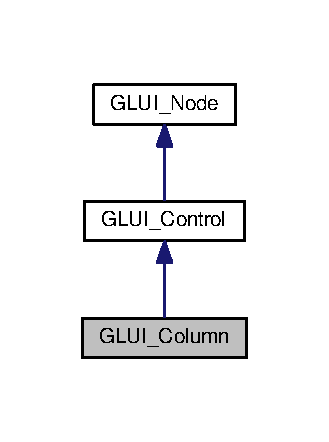
\includegraphics[width=158pt]{class_g_l_u_i___column__inherit__graph}
\end{center}
\end{figure}


Collaboration diagram for G\+L\+U\+I\+\_\+\+Column\+:\nopagebreak
\begin{figure}[H]
\begin{center}
\leavevmode
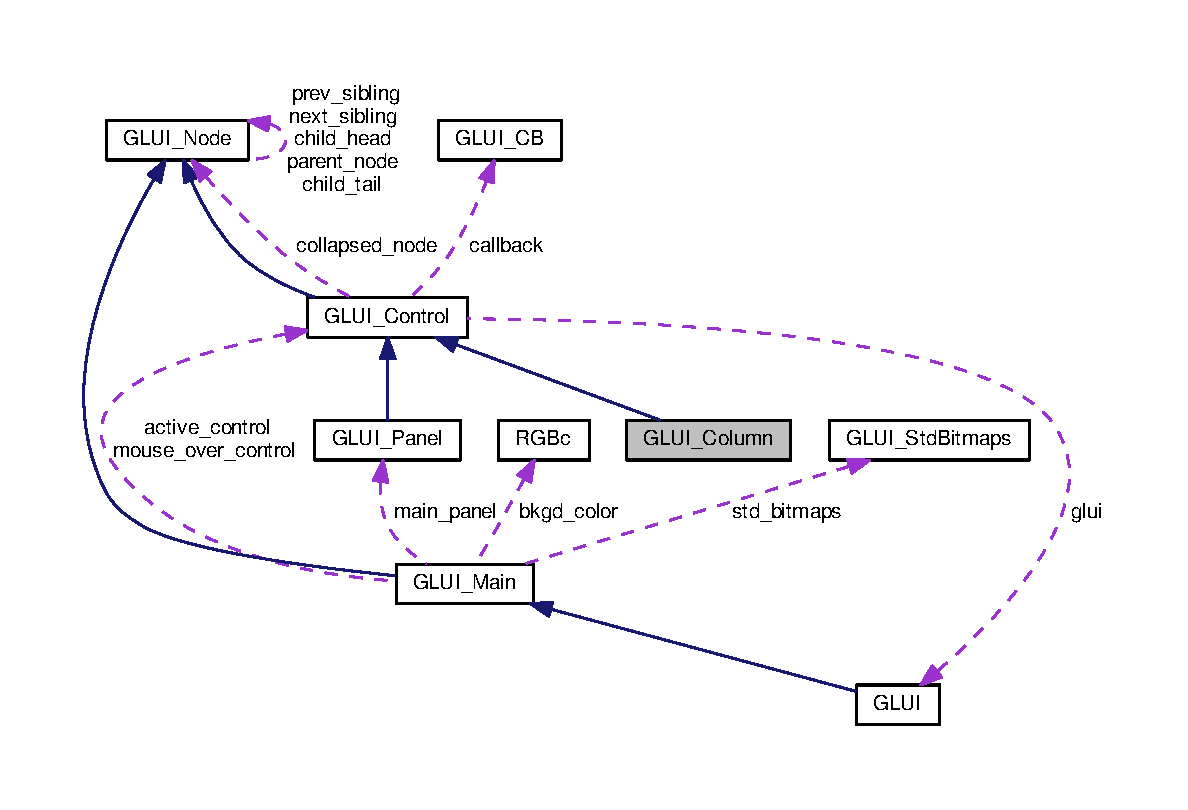
\includegraphics[width=350pt]{class_g_l_u_i___column__coll__graph}
\end{center}
\end{figure}
\subsection*{Public Member Functions}
\begin{DoxyCompactItemize}
\item 
\hyperlink{wglext_8h_a9e6b7f1933461ef318bb000d6bd13b83}{void} \hyperlink{class_g_l_u_i___column_aefa72a27e5a6ba5e86f684b6a5b5f63e}{draw} (\hyperlink{wglext_8h_a500a82aecba06f4550f6849b8099ca21}{int} \hyperlink{glext_8h_ad77deca22f617d3f0e0eb786445689fc}{x}, \hyperlink{wglext_8h_a500a82aecba06f4550f6849b8099ca21}{int} \hyperlink{glext_8h_a9298c7ad619074f5285b32c6b72bfdea}{y})
\item 
\hyperlink{class_g_l_u_i___column_a309d2c36583fb571763c95d8ae3bbaa3}{G\+L\+U\+I\+\_\+\+Column} (\hyperlink{class_g_l_u_i___node}{G\+L\+U\+I\+\_\+\+Node} $\ast$\hyperlink{class_g_l_u_i___node_a8ed65d447784f6f88bd3e2e2bcac6cdb}{parent}, \hyperlink{wglext_8h_a500a82aecba06f4550f6849b8099ca21}{int} draw\+\_\+bar=true)
\item 
\hyperlink{class_g_l_u_i___column_a71c1f66b78ae12a93901a9ca53e504ea}{G\+L\+U\+I\+\_\+\+Column} (\hyperlink{wglext_8h_a9e6b7f1933461ef318bb000d6bd13b83}{void})
\end{DoxyCompactItemize}
\subsection*{Protected Member Functions}
\begin{DoxyCompactItemize}
\item 
\hyperlink{wglext_8h_a9e6b7f1933461ef318bb000d6bd13b83}{void} \hyperlink{class_g_l_u_i___column_af5aa315100428399f2a7920fb9eb53b7}{common\+\_\+init} ()
\end{DoxyCompactItemize}
\subsection*{Additional Inherited Members}


\subsection{Detailed Description}
A \hyperlink{class_g_l_u_i___column}{G\+L\+U\+I\+\_\+\+Column} object separates all previous controls from subsequent controls with a vertical bar. 

Definition at line 1061 of file glui.\+h.



\subsection{Constructor \& Destructor Documentation}
\hypertarget{class_g_l_u_i___column_a309d2c36583fb571763c95d8ae3bbaa3}{\index{G\+L\+U\+I\+\_\+\+Column@{G\+L\+U\+I\+\_\+\+Column}!G\+L\+U\+I\+\_\+\+Column@{G\+L\+U\+I\+\_\+\+Column}}
\index{G\+L\+U\+I\+\_\+\+Column@{G\+L\+U\+I\+\_\+\+Column}!G\+L\+U\+I\+\_\+\+Column@{G\+L\+U\+I\+\_\+\+Column}}
\subsubsection[{G\+L\+U\+I\+\_\+\+Column}]{\setlength{\rightskip}{0pt plus 5cm}G\+L\+U\+I\+\_\+\+Column\+::\+G\+L\+U\+I\+\_\+\+Column (
\begin{DoxyParamCaption}
\item[{{\bf G\+L\+U\+I\+\_\+\+Node} $\ast$}]{parent, }
\item[{{\bf int}}]{draw\+\_\+bar = {\ttfamily true}}
\end{DoxyParamCaption}
)}}\label{class_g_l_u_i___column_a309d2c36583fb571763c95d8ae3bbaa3}
Create a new column, which separates the previous controls from subsequent controls.


\begin{DoxyParams}{Parameters}
{\em parent} & The panel our object is inside; or the main \hyperlink{class_g_l_u_i}{G\+L\+U\+I} object. \\
\hline
{\em draw\+\_\+bar} & If true, draw a visible bar between new and old controls. \\
\hline
\end{DoxyParams}
\hypertarget{class_g_l_u_i___column_a71c1f66b78ae12a93901a9ca53e504ea}{\index{G\+L\+U\+I\+\_\+\+Column@{G\+L\+U\+I\+\_\+\+Column}!G\+L\+U\+I\+\_\+\+Column@{G\+L\+U\+I\+\_\+\+Column}}
\index{G\+L\+U\+I\+\_\+\+Column@{G\+L\+U\+I\+\_\+\+Column}!G\+L\+U\+I\+\_\+\+Column@{G\+L\+U\+I\+\_\+\+Column}}
\subsubsection[{G\+L\+U\+I\+\_\+\+Column}]{\setlength{\rightskip}{0pt plus 5cm}G\+L\+U\+I\+\_\+\+Column\+::\+G\+L\+U\+I\+\_\+\+Column (
\begin{DoxyParamCaption}
\item[{{\bf void}}]{}
\end{DoxyParamCaption}
)\hspace{0.3cm}{\ttfamily [inline]}}}\label{class_g_l_u_i___column_a71c1f66b78ae12a93901a9ca53e504ea}


Definition at line 1074 of file glui.\+h.



\subsection{Member Function Documentation}
\hypertarget{class_g_l_u_i___column_af5aa315100428399f2a7920fb9eb53b7}{\index{G\+L\+U\+I\+\_\+\+Column@{G\+L\+U\+I\+\_\+\+Column}!common\+\_\+init@{common\+\_\+init}}
\index{common\+\_\+init@{common\+\_\+init}!G\+L\+U\+I\+\_\+\+Column@{G\+L\+U\+I\+\_\+\+Column}}
\subsubsection[{common\+\_\+init}]{\setlength{\rightskip}{0pt plus 5cm}{\bf void} G\+L\+U\+I\+\_\+\+Column\+::common\+\_\+init (
\begin{DoxyParamCaption}
\item[{{\bf void}}]{}
\end{DoxyParamCaption}
)\hspace{0.3cm}{\ttfamily [inline]}, {\ttfamily [protected]}}}\label{class_g_l_u_i___column_af5aa315100428399f2a7920fb9eb53b7}


Definition at line 1077 of file glui.\+h.

\hypertarget{class_g_l_u_i___column_aefa72a27e5a6ba5e86f684b6a5b5f63e}{\index{G\+L\+U\+I\+\_\+\+Column@{G\+L\+U\+I\+\_\+\+Column}!draw@{draw}}
\index{draw@{draw}!G\+L\+U\+I\+\_\+\+Column@{G\+L\+U\+I\+\_\+\+Column}}
\subsubsection[{draw}]{\setlength{\rightskip}{0pt plus 5cm}{\bf void} G\+L\+U\+I\+\_\+\+Column\+::draw (
\begin{DoxyParamCaption}
\item[{{\bf int}}]{x, }
\item[{{\bf int}}]{y}
\end{DoxyParamCaption}
)\hspace{0.3cm}{\ttfamily [virtual]}}}\label{class_g_l_u_i___column_aefa72a27e5a6ba5e86f684b6a5b5f63e}


Implements \hyperlink{class_g_l_u_i___control_a2eb42d7a7951280ad2fe8c37972bf66a}{G\+L\+U\+I\+\_\+\+Control}.



The documentation for this class was generated from the following file\+:\begin{DoxyCompactItemize}
\item 
S\+S\+W\+C/src/\+G\+L/\hyperlink{glui_8h}{glui.\+h}\end{DoxyCompactItemize}

\hypertarget{class_g_l_u_i___command_line}{\section{G\+L\+U\+I\+\_\+\+Command\+Line Class Reference}
\label{class_g_l_u_i___command_line}\index{G\+L\+U\+I\+\_\+\+Command\+Line@{G\+L\+U\+I\+\_\+\+Command\+Line}}
}


{\ttfamily \#include $<$glui.\+h$>$}



Inheritance diagram for G\+L\+U\+I\+\_\+\+Command\+Line\+:\nopagebreak
\begin{figure}[H]
\begin{center}
\leavevmode
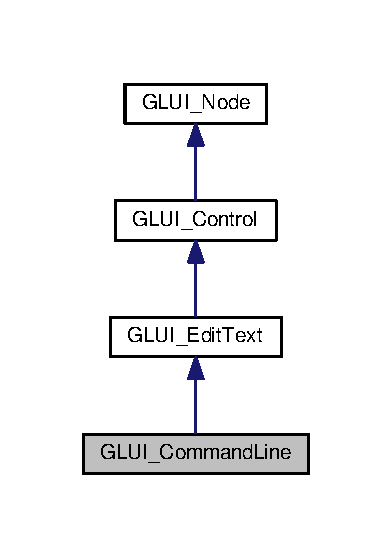
\includegraphics[width=188pt]{class_g_l_u_i___command_line__inherit__graph}
\end{center}
\end{figure}


Collaboration diagram for G\+L\+U\+I\+\_\+\+Command\+Line\+:\nopagebreak
\begin{figure}[H]
\begin{center}
\leavevmode
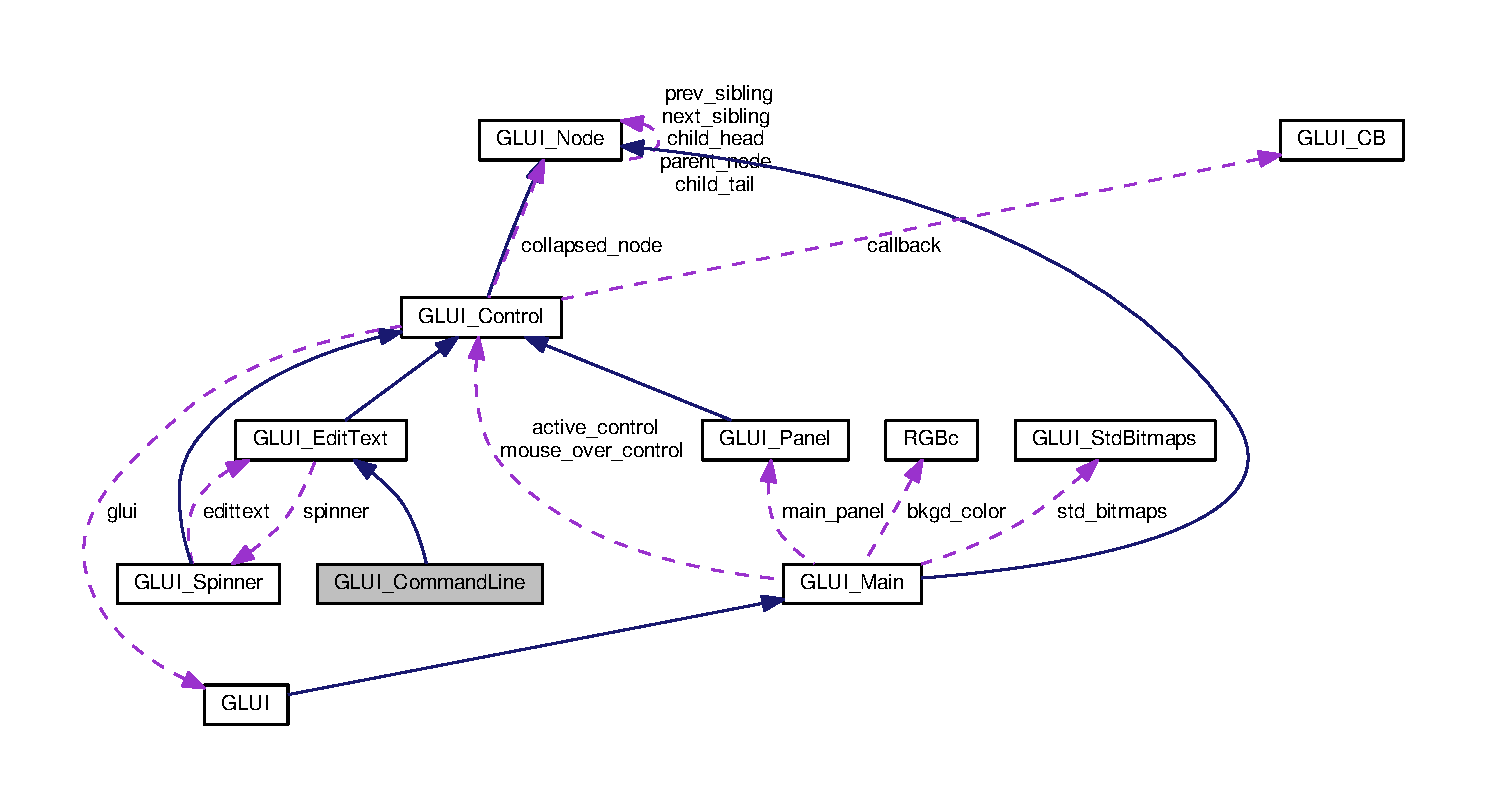
\includegraphics[width=350pt]{class_g_l_u_i___command_line__coll__graph}
\end{center}
\end{figure}
\subsection*{Public Types}
\begin{DoxyCompactItemize}
\item 
enum \{ \hyperlink{class_g_l_u_i___command_line_afcd6d744f2444c5a8cfbe053b5f37cd6a991ecacadb37c63013e7e24f4e86496f}{H\+I\+S\+T\+\_\+\+S\+I\+Z\+E} = 100
 \}
\item 
typedef \hyperlink{class_g_l_u_i___edit_text}{G\+L\+U\+I\+\_\+\+Edit\+Text} \hyperlink{class_g_l_u_i___command_line_af9db00326863efa876cbb5c6b2d255b7}{Super}
\end{DoxyCompactItemize}
\subsection*{Public Member Functions}
\begin{DoxyCompactItemize}
\item 
\hyperlink{wglext_8h_a500a82aecba06f4550f6849b8099ca21}{int} \hyperlink{class_g_l_u_i___command_line_aac74b2f165792141d6665de1690d0aa4}{key\+\_\+handler} (unsigned char key, \hyperlink{wglext_8h_a500a82aecba06f4550f6849b8099ca21}{int} modifiers)
\item 
\hyperlink{wglext_8h_a500a82aecba06f4550f6849b8099ca21}{int} \hyperlink{class_g_l_u_i___command_line_a88dafdb294350ff13c68973b59c308d1}{special\+\_\+handler} (\hyperlink{wglext_8h_a500a82aecba06f4550f6849b8099ca21}{int} key, \hyperlink{wglext_8h_a500a82aecba06f4550f6849b8099ca21}{int} modifiers)
\item 
\hyperlink{wglext_8h_a9e6b7f1933461ef318bb000d6bd13b83}{void} \hyperlink{class_g_l_u_i___command_line_a827fe6510aa5a38b0d2c5d016a93e1ba}{deactivate} (\hyperlink{wglext_8h_a9e6b7f1933461ef318bb000d6bd13b83}{void})
\item 
virtual const char $\ast$ \hyperlink{class_g_l_u_i___command_line_a565145da6c84b9f925ca30735fc27686}{get\+\_\+history} (\hyperlink{wglext_8h_a500a82aecba06f4550f6849b8099ca21}{int} command\+\_\+number) const 
\item 
virtual \hyperlink{glui_8h_aada824856f7bcf29794719981ebd8f60}{G\+L\+U\+I\+\_\+\+String} \& \hyperlink{class_g_l_u_i___command_line_a43403d60b3ac8534b84393c5328b7a03}{get\+\_\+history\+\_\+str} (\hyperlink{wglext_8h_a500a82aecba06f4550f6849b8099ca21}{int} command\+\_\+number)
\item 
virtual const \hyperlink{glui_8h_aada824856f7bcf29794719981ebd8f60}{G\+L\+U\+I\+\_\+\+String} \& \hyperlink{class_g_l_u_i___command_line_a9365735c17057bea2039db66d8df67f3}{get\+\_\+history\+\_\+str} (\hyperlink{wglext_8h_a500a82aecba06f4550f6849b8099ca21}{int} command\+\_\+number) const 
\item 
virtual \hyperlink{wglext_8h_a9e6b7f1933461ef318bb000d6bd13b83}{void} \hyperlink{class_g_l_u_i___command_line_a6f8d01fd2db25c98723f85172c93fb01}{recall\+\_\+history} (\hyperlink{wglext_8h_a500a82aecba06f4550f6849b8099ca21}{int} history\+\_\+number)
\item 
virtual \hyperlink{wglext_8h_a9e6b7f1933461ef318bb000d6bd13b83}{void} \hyperlink{class_g_l_u_i___command_line_a82e2cd651cbc5431b6e4ad88c4c01472}{scroll\+\_\+history} (\hyperlink{wglext_8h_a500a82aecba06f4550f6849b8099ca21}{int} direction)
\item 
virtual \hyperlink{wglext_8h_a9e6b7f1933461ef318bb000d6bd13b83}{void} \hyperlink{class_g_l_u_i___command_line_a79894d2a826c7b042c93c401a915b28f}{add\+\_\+to\+\_\+history} (const char $\ast$\hyperlink{class_g_l_u_i___control_af0d60e9736f4dbc34e9a536e75876d72}{text})
\item 
virtual \hyperlink{wglext_8h_a9e6b7f1933461ef318bb000d6bd13b83}{void} \hyperlink{class_g_l_u_i___command_line_a2fcb9cb75a1960fd56c187f940e22938}{reset\+\_\+history} (\hyperlink{wglext_8h_a9e6b7f1933461ef318bb000d6bd13b83}{void})
\item 
\hyperlink{wglext_8h_a9e6b7f1933461ef318bb000d6bd13b83}{void} \hyperlink{class_g_l_u_i___command_line_a89815aca68b849830ba26253135efaf5}{dump} (F\+I\+L\+E $\ast$out, const char $\ast$\hyperlink{class_g_l_u_i___control_af0d60e9736f4dbc34e9a536e75876d72}{text})
\item 
\hyperlink{class_g_l_u_i___command_line_a1367881039ac1384af53f71fa35932b3}{G\+L\+U\+I\+\_\+\+Command\+Line} (\hyperlink{class_g_l_u_i___node}{G\+L\+U\+I\+\_\+\+Node} $\ast$\hyperlink{class_g_l_u_i___node_a8ed65d447784f6f88bd3e2e2bcac6cdb}{parent}, const char $\ast$\hyperlink{glext_8h_ad977737dfc9a274a62741b9500c49a32}{name}, \hyperlink{wglext_8h_a9e6b7f1933461ef318bb000d6bd13b83}{void} $\ast$live\+\_\+var=N\+U\+L\+L, \hyperlink{wglext_8h_a500a82aecba06f4550f6849b8099ca21}{int} \hyperlink{glext_8h_a58c2a664503e14ffb8f21012aabff3e9}{id}=-\/1, \hyperlink{class_g_l_u_i___c_b}{G\+L\+U\+I\+\_\+\+C\+B} \hyperlink{class_g_l_u_i___control_a96060fe0cc6d537e736dd6eef78e24ab}{callback}=\hyperlink{class_g_l_u_i___c_b}{G\+L\+U\+I\+\_\+\+C\+B}())
\item 
\hyperlink{class_g_l_u_i___command_line_ae6c787ef5aa1a8c181eef9ade0c710a1}{G\+L\+U\+I\+\_\+\+Command\+Line} (\hyperlink{wglext_8h_a9e6b7f1933461ef318bb000d6bd13b83}{void})
\end{DoxyCompactItemize}
\subsection*{Public Attributes}
\begin{DoxyCompactItemize}
\item 
std\+::vector$<$ \hyperlink{glui_8h_aada824856f7bcf29794719981ebd8f60}{G\+L\+U\+I\+\_\+\+String} $>$ \hyperlink{class_g_l_u_i___command_line_abc9dcdc275bb36dee1a9db8d348338b5}{hist\+\_\+list}
\item 
\hyperlink{wglext_8h_a500a82aecba06f4550f6849b8099ca21}{int} \hyperlink{class_g_l_u_i___command_line_ab8d88779584003b82000b824ac6f4906}{curr\+\_\+hist}
\item 
\hyperlink{wglext_8h_a500a82aecba06f4550f6849b8099ca21}{int} \hyperlink{class_g_l_u_i___command_line_a689ee6f9ede7c0f6c2060fd5650b1d22}{oldest\+\_\+hist}
\item 
\hyperlink{wglext_8h_a500a82aecba06f4550f6849b8099ca21}{int} \hyperlink{class_g_l_u_i___command_line_af4f50f57b5a239d8564619ec0779518d}{newest\+\_\+hist}
\item 
bool \hyperlink{class_g_l_u_i___command_line_ac2f61fd248c6adb663c6de52e9e431fd}{commit\+\_\+flag}
\end{DoxyCompactItemize}
\subsection*{Protected Member Functions}
\begin{DoxyCompactItemize}
\item 
\hyperlink{wglext_8h_a9e6b7f1933461ef318bb000d6bd13b83}{void} \hyperlink{class_g_l_u_i___command_line_a21eeafb7d6f3df4d3ddee365422894b6}{common\+\_\+init} ()
\end{DoxyCompactItemize}
\subsection*{Additional Inherited Members}


\subsection{Detailed Description}


Definition at line 1697 of file glui.\+h.



\subsection{Member Typedef Documentation}
\hypertarget{class_g_l_u_i___command_line_af9db00326863efa876cbb5c6b2d255b7}{\index{G\+L\+U\+I\+\_\+\+Command\+Line@{G\+L\+U\+I\+\_\+\+Command\+Line}!Super@{Super}}
\index{Super@{Super}!G\+L\+U\+I\+\_\+\+Command\+Line@{G\+L\+U\+I\+\_\+\+Command\+Line}}
\subsubsection[{Super}]{\setlength{\rightskip}{0pt plus 5cm}typedef {\bf G\+L\+U\+I\+\_\+\+Edit\+Text} {\bf G\+L\+U\+I\+\_\+\+Command\+Line\+::\+Super}}}\label{class_g_l_u_i___command_line_af9db00326863efa876cbb5c6b2d255b7}


Definition at line 1700 of file glui.\+h.



\subsection{Member Enumeration Documentation}
\hypertarget{class_g_l_u_i___command_line_afcd6d744f2444c5a8cfbe053b5f37cd6}{\subsubsection[{anonymous enum}]{\setlength{\rightskip}{0pt plus 5cm}anonymous enum}}\label{class_g_l_u_i___command_line_afcd6d744f2444c5a8cfbe053b5f37cd6}
\begin{Desc}
\item[Enumerator]\par
\begin{description}
\index{H\+I\+S\+T\+\_\+\+S\+I\+Z\+E@{H\+I\+S\+T\+\_\+\+S\+I\+Z\+E}!G\+L\+U\+I\+\_\+\+Command\+Line@{G\+L\+U\+I\+\_\+\+Command\+Line}}\index{G\+L\+U\+I\+\_\+\+Command\+Line@{G\+L\+U\+I\+\_\+\+Command\+Line}!H\+I\+S\+T\+\_\+\+S\+I\+Z\+E@{H\+I\+S\+T\+\_\+\+S\+I\+Z\+E}}\item[{\em 
\hypertarget{class_g_l_u_i___command_line_afcd6d744f2444c5a8cfbe053b5f37cd6a991ecacadb37c63013e7e24f4e86496f}{H\+I\+S\+T\+\_\+\+S\+I\+Z\+E}\label{class_g_l_u_i___command_line_afcd6d744f2444c5a8cfbe053b5f37cd6a991ecacadb37c63013e7e24f4e86496f}
}]\end{description}
\end{Desc}


Definition at line 1702 of file glui.\+h.



\subsection{Constructor \& Destructor Documentation}
\hypertarget{class_g_l_u_i___command_line_a1367881039ac1384af53f71fa35932b3}{\index{G\+L\+U\+I\+\_\+\+Command\+Line@{G\+L\+U\+I\+\_\+\+Command\+Line}!G\+L\+U\+I\+\_\+\+Command\+Line@{G\+L\+U\+I\+\_\+\+Command\+Line}}
\index{G\+L\+U\+I\+\_\+\+Command\+Line@{G\+L\+U\+I\+\_\+\+Command\+Line}!G\+L\+U\+I\+\_\+\+Command\+Line@{G\+L\+U\+I\+\_\+\+Command\+Line}}
\subsubsection[{G\+L\+U\+I\+\_\+\+Command\+Line}]{\setlength{\rightskip}{0pt plus 5cm}G\+L\+U\+I\+\_\+\+Command\+Line\+::\+G\+L\+U\+I\+\_\+\+Command\+Line (
\begin{DoxyParamCaption}
\item[{{\bf G\+L\+U\+I\+\_\+\+Node} $\ast$}]{parent, }
\item[{const char $\ast$}]{name, }
\item[{{\bf void} $\ast$}]{live\+\_\+var = {\ttfamily NULL}, }
\item[{{\bf int}}]{id = {\ttfamily -\/1}, }
\item[{{\bf G\+L\+U\+I\+\_\+\+C\+B}}]{callback = {\ttfamily {\bf G\+L\+U\+I\+\_\+\+C\+B}()}}
\end{DoxyParamCaption}
)}}\label{class_g_l_u_i___command_line_a1367881039ac1384af53f71fa35932b3}
\hypertarget{class_g_l_u_i___command_line_ae6c787ef5aa1a8c181eef9ade0c710a1}{\index{G\+L\+U\+I\+\_\+\+Command\+Line@{G\+L\+U\+I\+\_\+\+Command\+Line}!G\+L\+U\+I\+\_\+\+Command\+Line@{G\+L\+U\+I\+\_\+\+Command\+Line}}
\index{G\+L\+U\+I\+\_\+\+Command\+Line@{G\+L\+U\+I\+\_\+\+Command\+Line}!G\+L\+U\+I\+\_\+\+Command\+Line@{G\+L\+U\+I\+\_\+\+Command\+Line}}
\subsubsection[{G\+L\+U\+I\+\_\+\+Command\+Line}]{\setlength{\rightskip}{0pt plus 5cm}G\+L\+U\+I\+\_\+\+Command\+Line\+::\+G\+L\+U\+I\+\_\+\+Command\+Line (
\begin{DoxyParamCaption}
\item[{{\bf void}}]{}
\end{DoxyParamCaption}
)\hspace{0.3cm}{\ttfamily [inline]}}}\label{class_g_l_u_i___command_line_ae6c787ef5aa1a8c181eef9ade0c710a1}


Definition at line 1730 of file glui.\+h.



\subsection{Member Function Documentation}
\hypertarget{class_g_l_u_i___command_line_a79894d2a826c7b042c93c401a915b28f}{\index{G\+L\+U\+I\+\_\+\+Command\+Line@{G\+L\+U\+I\+\_\+\+Command\+Line}!add\+\_\+to\+\_\+history@{add\+\_\+to\+\_\+history}}
\index{add\+\_\+to\+\_\+history@{add\+\_\+to\+\_\+history}!G\+L\+U\+I\+\_\+\+Command\+Line@{G\+L\+U\+I\+\_\+\+Command\+Line}}
\subsubsection[{add\+\_\+to\+\_\+history}]{\setlength{\rightskip}{0pt plus 5cm}virtual {\bf void} G\+L\+U\+I\+\_\+\+Command\+Line\+::add\+\_\+to\+\_\+history (
\begin{DoxyParamCaption}
\item[{const char $\ast$}]{text}
\end{DoxyParamCaption}
)\hspace{0.3cm}{\ttfamily [virtual]}}}\label{class_g_l_u_i___command_line_a79894d2a826c7b042c93c401a915b28f}
\hypertarget{class_g_l_u_i___command_line_a21eeafb7d6f3df4d3ddee365422894b6}{\index{G\+L\+U\+I\+\_\+\+Command\+Line@{G\+L\+U\+I\+\_\+\+Command\+Line}!common\+\_\+init@{common\+\_\+init}}
\index{common\+\_\+init@{common\+\_\+init}!G\+L\+U\+I\+\_\+\+Command\+Line@{G\+L\+U\+I\+\_\+\+Command\+Line}}
\subsubsection[{common\+\_\+init}]{\setlength{\rightskip}{0pt plus 5cm}{\bf void} G\+L\+U\+I\+\_\+\+Command\+Line\+::common\+\_\+init (
\begin{DoxyParamCaption}
\item[{{\bf void}}]{}
\end{DoxyParamCaption}
)\hspace{0.3cm}{\ttfamily [inline]}, {\ttfamily [protected]}}}\label{class_g_l_u_i___command_line_a21eeafb7d6f3df4d3ddee365422894b6}


Definition at line 1732 of file glui.\+h.

\hypertarget{class_g_l_u_i___command_line_a827fe6510aa5a38b0d2c5d016a93e1ba}{\index{G\+L\+U\+I\+\_\+\+Command\+Line@{G\+L\+U\+I\+\_\+\+Command\+Line}!deactivate@{deactivate}}
\index{deactivate@{deactivate}!G\+L\+U\+I\+\_\+\+Command\+Line@{G\+L\+U\+I\+\_\+\+Command\+Line}}
\subsubsection[{deactivate}]{\setlength{\rightskip}{0pt plus 5cm}{\bf void} G\+L\+U\+I\+\_\+\+Command\+Line\+::deactivate (
\begin{DoxyParamCaption}
\item[{{\bf void}}]{}
\end{DoxyParamCaption}
)\hspace{0.3cm}{\ttfamily [virtual]}}}\label{class_g_l_u_i___command_line_a827fe6510aa5a38b0d2c5d016a93e1ba}


Reimplemented from \hyperlink{class_g_l_u_i___edit_text_a4a83b7bc0b6d60e4fa0dd797b49255ab}{G\+L\+U\+I\+\_\+\+Edit\+Text}.

\hypertarget{class_g_l_u_i___command_line_a89815aca68b849830ba26253135efaf5}{\index{G\+L\+U\+I\+\_\+\+Command\+Line@{G\+L\+U\+I\+\_\+\+Command\+Line}!dump@{dump}}
\index{dump@{dump}!G\+L\+U\+I\+\_\+\+Command\+Line@{G\+L\+U\+I\+\_\+\+Command\+Line}}
\subsubsection[{dump}]{\setlength{\rightskip}{0pt plus 5cm}{\bf void} G\+L\+U\+I\+\_\+\+Command\+Line\+::dump (
\begin{DoxyParamCaption}
\item[{F\+I\+L\+E $\ast$}]{out, }
\item[{const char $\ast$}]{text}
\end{DoxyParamCaption}
)}}\label{class_g_l_u_i___command_line_a89815aca68b849830ba26253135efaf5}
\hypertarget{class_g_l_u_i___command_line_a565145da6c84b9f925ca30735fc27686}{\index{G\+L\+U\+I\+\_\+\+Command\+Line@{G\+L\+U\+I\+\_\+\+Command\+Line}!get\+\_\+history@{get\+\_\+history}}
\index{get\+\_\+history@{get\+\_\+history}!G\+L\+U\+I\+\_\+\+Command\+Line@{G\+L\+U\+I\+\_\+\+Command\+Line}}
\subsubsection[{get\+\_\+history}]{\setlength{\rightskip}{0pt plus 5cm}virtual const char$\ast$ G\+L\+U\+I\+\_\+\+Command\+Line\+::get\+\_\+history (
\begin{DoxyParamCaption}
\item[{{\bf int}}]{command\+\_\+number}
\end{DoxyParamCaption}
) const\hspace{0.3cm}{\ttfamily [inline]}, {\ttfamily [virtual]}}}\label{class_g_l_u_i___command_line_a565145da6c84b9f925ca30735fc27686}


Definition at line 1714 of file glui.\+h.

\hypertarget{class_g_l_u_i___command_line_a43403d60b3ac8534b84393c5328b7a03}{\index{G\+L\+U\+I\+\_\+\+Command\+Line@{G\+L\+U\+I\+\_\+\+Command\+Line}!get\+\_\+history\+\_\+str@{get\+\_\+history\+\_\+str}}
\index{get\+\_\+history\+\_\+str@{get\+\_\+history\+\_\+str}!G\+L\+U\+I\+\_\+\+Command\+Line@{G\+L\+U\+I\+\_\+\+Command\+Line}}
\subsubsection[{get\+\_\+history\+\_\+str}]{\setlength{\rightskip}{0pt plus 5cm}virtual {\bf G\+L\+U\+I\+\_\+\+String}\& G\+L\+U\+I\+\_\+\+Command\+Line\+::get\+\_\+history\+\_\+str (
\begin{DoxyParamCaption}
\item[{{\bf int}}]{command\+\_\+number}
\end{DoxyParamCaption}
)\hspace{0.3cm}{\ttfamily [inline]}, {\ttfamily [virtual]}}}\label{class_g_l_u_i___command_line_a43403d60b3ac8534b84393c5328b7a03}


Definition at line 1716 of file glui.\+h.

\hypertarget{class_g_l_u_i___command_line_a9365735c17057bea2039db66d8df67f3}{\index{G\+L\+U\+I\+\_\+\+Command\+Line@{G\+L\+U\+I\+\_\+\+Command\+Line}!get\+\_\+history\+\_\+str@{get\+\_\+history\+\_\+str}}
\index{get\+\_\+history\+\_\+str@{get\+\_\+history\+\_\+str}!G\+L\+U\+I\+\_\+\+Command\+Line@{G\+L\+U\+I\+\_\+\+Command\+Line}}
\subsubsection[{get\+\_\+history\+\_\+str}]{\setlength{\rightskip}{0pt plus 5cm}virtual const {\bf G\+L\+U\+I\+\_\+\+String}\& G\+L\+U\+I\+\_\+\+Command\+Line\+::get\+\_\+history\+\_\+str (
\begin{DoxyParamCaption}
\item[{{\bf int}}]{command\+\_\+number}
\end{DoxyParamCaption}
) const\hspace{0.3cm}{\ttfamily [inline]}, {\ttfamily [virtual]}}}\label{class_g_l_u_i___command_line_a9365735c17057bea2039db66d8df67f3}


Definition at line 1718 of file glui.\+h.

\hypertarget{class_g_l_u_i___command_line_aac74b2f165792141d6665de1690d0aa4}{\index{G\+L\+U\+I\+\_\+\+Command\+Line@{G\+L\+U\+I\+\_\+\+Command\+Line}!key\+\_\+handler@{key\+\_\+handler}}
\index{key\+\_\+handler@{key\+\_\+handler}!G\+L\+U\+I\+\_\+\+Command\+Line@{G\+L\+U\+I\+\_\+\+Command\+Line}}
\subsubsection[{key\+\_\+handler}]{\setlength{\rightskip}{0pt plus 5cm}{\bf int} G\+L\+U\+I\+\_\+\+Command\+Line\+::key\+\_\+handler (
\begin{DoxyParamCaption}
\item[{unsigned char}]{key, }
\item[{{\bf int}}]{modifiers}
\end{DoxyParamCaption}
)\hspace{0.3cm}{\ttfamily [virtual]}}}\label{class_g_l_u_i___command_line_aac74b2f165792141d6665de1690d0aa4}


Reimplemented from \hyperlink{class_g_l_u_i___edit_text_a92fcd78877375cb2bba3b5e9f88635b6}{G\+L\+U\+I\+\_\+\+Edit\+Text}.

\hypertarget{class_g_l_u_i___command_line_a6f8d01fd2db25c98723f85172c93fb01}{\index{G\+L\+U\+I\+\_\+\+Command\+Line@{G\+L\+U\+I\+\_\+\+Command\+Line}!recall\+\_\+history@{recall\+\_\+history}}
\index{recall\+\_\+history@{recall\+\_\+history}!G\+L\+U\+I\+\_\+\+Command\+Line@{G\+L\+U\+I\+\_\+\+Command\+Line}}
\subsubsection[{recall\+\_\+history}]{\setlength{\rightskip}{0pt plus 5cm}virtual {\bf void} G\+L\+U\+I\+\_\+\+Command\+Line\+::recall\+\_\+history (
\begin{DoxyParamCaption}
\item[{{\bf int}}]{history\+\_\+number}
\end{DoxyParamCaption}
)\hspace{0.3cm}{\ttfamily [virtual]}}}\label{class_g_l_u_i___command_line_a6f8d01fd2db25c98723f85172c93fb01}
\hypertarget{class_g_l_u_i___command_line_a2fcb9cb75a1960fd56c187f940e22938}{\index{G\+L\+U\+I\+\_\+\+Command\+Line@{G\+L\+U\+I\+\_\+\+Command\+Line}!reset\+\_\+history@{reset\+\_\+history}}
\index{reset\+\_\+history@{reset\+\_\+history}!G\+L\+U\+I\+\_\+\+Command\+Line@{G\+L\+U\+I\+\_\+\+Command\+Line}}
\subsubsection[{reset\+\_\+history}]{\setlength{\rightskip}{0pt plus 5cm}virtual {\bf void} G\+L\+U\+I\+\_\+\+Command\+Line\+::reset\+\_\+history (
\begin{DoxyParamCaption}
\item[{{\bf void}}]{}
\end{DoxyParamCaption}
)\hspace{0.3cm}{\ttfamily [virtual]}}}\label{class_g_l_u_i___command_line_a2fcb9cb75a1960fd56c187f940e22938}
\hypertarget{class_g_l_u_i___command_line_a82e2cd651cbc5431b6e4ad88c4c01472}{\index{G\+L\+U\+I\+\_\+\+Command\+Line@{G\+L\+U\+I\+\_\+\+Command\+Line}!scroll\+\_\+history@{scroll\+\_\+history}}
\index{scroll\+\_\+history@{scroll\+\_\+history}!G\+L\+U\+I\+\_\+\+Command\+Line@{G\+L\+U\+I\+\_\+\+Command\+Line}}
\subsubsection[{scroll\+\_\+history}]{\setlength{\rightskip}{0pt plus 5cm}virtual {\bf void} G\+L\+U\+I\+\_\+\+Command\+Line\+::scroll\+\_\+history (
\begin{DoxyParamCaption}
\item[{{\bf int}}]{direction}
\end{DoxyParamCaption}
)\hspace{0.3cm}{\ttfamily [virtual]}}}\label{class_g_l_u_i___command_line_a82e2cd651cbc5431b6e4ad88c4c01472}
\hypertarget{class_g_l_u_i___command_line_a88dafdb294350ff13c68973b59c308d1}{\index{G\+L\+U\+I\+\_\+\+Command\+Line@{G\+L\+U\+I\+\_\+\+Command\+Line}!special\+\_\+handler@{special\+\_\+handler}}
\index{special\+\_\+handler@{special\+\_\+handler}!G\+L\+U\+I\+\_\+\+Command\+Line@{G\+L\+U\+I\+\_\+\+Command\+Line}}
\subsubsection[{special\+\_\+handler}]{\setlength{\rightskip}{0pt plus 5cm}{\bf int} G\+L\+U\+I\+\_\+\+Command\+Line\+::special\+\_\+handler (
\begin{DoxyParamCaption}
\item[{{\bf int}}]{key, }
\item[{{\bf int}}]{modifiers}
\end{DoxyParamCaption}
)\hspace{0.3cm}{\ttfamily [virtual]}}}\label{class_g_l_u_i___command_line_a88dafdb294350ff13c68973b59c308d1}


Reimplemented from \hyperlink{class_g_l_u_i___edit_text_a81478f6a0a9ba0c2dc715e0b3730077e}{G\+L\+U\+I\+\_\+\+Edit\+Text}.



\subsection{Member Data Documentation}
\hypertarget{class_g_l_u_i___command_line_ac2f61fd248c6adb663c6de52e9e431fd}{\index{G\+L\+U\+I\+\_\+\+Command\+Line@{G\+L\+U\+I\+\_\+\+Command\+Line}!commit\+\_\+flag@{commit\+\_\+flag}}
\index{commit\+\_\+flag@{commit\+\_\+flag}!G\+L\+U\+I\+\_\+\+Command\+Line@{G\+L\+U\+I\+\_\+\+Command\+Line}}
\subsubsection[{commit\+\_\+flag}]{\setlength{\rightskip}{0pt plus 5cm}bool G\+L\+U\+I\+\_\+\+Command\+Line\+::commit\+\_\+flag}}\label{class_g_l_u_i___command_line_ac2f61fd248c6adb663c6de52e9e431fd}


Definition at line 1707 of file glui.\+h.

\hypertarget{class_g_l_u_i___command_line_ab8d88779584003b82000b824ac6f4906}{\index{G\+L\+U\+I\+\_\+\+Command\+Line@{G\+L\+U\+I\+\_\+\+Command\+Line}!curr\+\_\+hist@{curr\+\_\+hist}}
\index{curr\+\_\+hist@{curr\+\_\+hist}!G\+L\+U\+I\+\_\+\+Command\+Line@{G\+L\+U\+I\+\_\+\+Command\+Line}}
\subsubsection[{curr\+\_\+hist}]{\setlength{\rightskip}{0pt plus 5cm}{\bf int} G\+L\+U\+I\+\_\+\+Command\+Line\+::curr\+\_\+hist}}\label{class_g_l_u_i___command_line_ab8d88779584003b82000b824ac6f4906}


Definition at line 1704 of file glui.\+h.

\hypertarget{class_g_l_u_i___command_line_abc9dcdc275bb36dee1a9db8d348338b5}{\index{G\+L\+U\+I\+\_\+\+Command\+Line@{G\+L\+U\+I\+\_\+\+Command\+Line}!hist\+\_\+list@{hist\+\_\+list}}
\index{hist\+\_\+list@{hist\+\_\+list}!G\+L\+U\+I\+\_\+\+Command\+Line@{G\+L\+U\+I\+\_\+\+Command\+Line}}
\subsubsection[{hist\+\_\+list}]{\setlength{\rightskip}{0pt plus 5cm}std\+::vector$<${\bf G\+L\+U\+I\+\_\+\+String}$>$ G\+L\+U\+I\+\_\+\+Command\+Line\+::hist\+\_\+list}}\label{class_g_l_u_i___command_line_abc9dcdc275bb36dee1a9db8d348338b5}


Definition at line 1703 of file glui.\+h.

\hypertarget{class_g_l_u_i___command_line_af4f50f57b5a239d8564619ec0779518d}{\index{G\+L\+U\+I\+\_\+\+Command\+Line@{G\+L\+U\+I\+\_\+\+Command\+Line}!newest\+\_\+hist@{newest\+\_\+hist}}
\index{newest\+\_\+hist@{newest\+\_\+hist}!G\+L\+U\+I\+\_\+\+Command\+Line@{G\+L\+U\+I\+\_\+\+Command\+Line}}
\subsubsection[{newest\+\_\+hist}]{\setlength{\rightskip}{0pt plus 5cm}{\bf int} G\+L\+U\+I\+\_\+\+Command\+Line\+::newest\+\_\+hist}}\label{class_g_l_u_i___command_line_af4f50f57b5a239d8564619ec0779518d}


Definition at line 1706 of file glui.\+h.

\hypertarget{class_g_l_u_i___command_line_a689ee6f9ede7c0f6c2060fd5650b1d22}{\index{G\+L\+U\+I\+\_\+\+Command\+Line@{G\+L\+U\+I\+\_\+\+Command\+Line}!oldest\+\_\+hist@{oldest\+\_\+hist}}
\index{oldest\+\_\+hist@{oldest\+\_\+hist}!G\+L\+U\+I\+\_\+\+Command\+Line@{G\+L\+U\+I\+\_\+\+Command\+Line}}
\subsubsection[{oldest\+\_\+hist}]{\setlength{\rightskip}{0pt plus 5cm}{\bf int} G\+L\+U\+I\+\_\+\+Command\+Line\+::oldest\+\_\+hist}}\label{class_g_l_u_i___command_line_a689ee6f9ede7c0f6c2060fd5650b1d22}


Definition at line 1705 of file glui.\+h.



The documentation for this class was generated from the following file\+:\begin{DoxyCompactItemize}
\item 
S\+S\+W\+C/src/\+G\+L/\hyperlink{glui_8h}{glui.\+h}\end{DoxyCompactItemize}

\hypertarget{class_g_l_u_i___control}{\section{G\+L\+U\+I\+\_\+\+Control Class Reference}
\label{class_g_l_u_i___control}\index{G\+L\+U\+I\+\_\+\+Control@{G\+L\+U\+I\+\_\+\+Control}}
}


{\ttfamily \#include $<$glui.\+h$>$}



Inheritance diagram for G\+L\+U\+I\+\_\+\+Control\+:\nopagebreak
\begin{figure}[H]
\begin{center}
\leavevmode
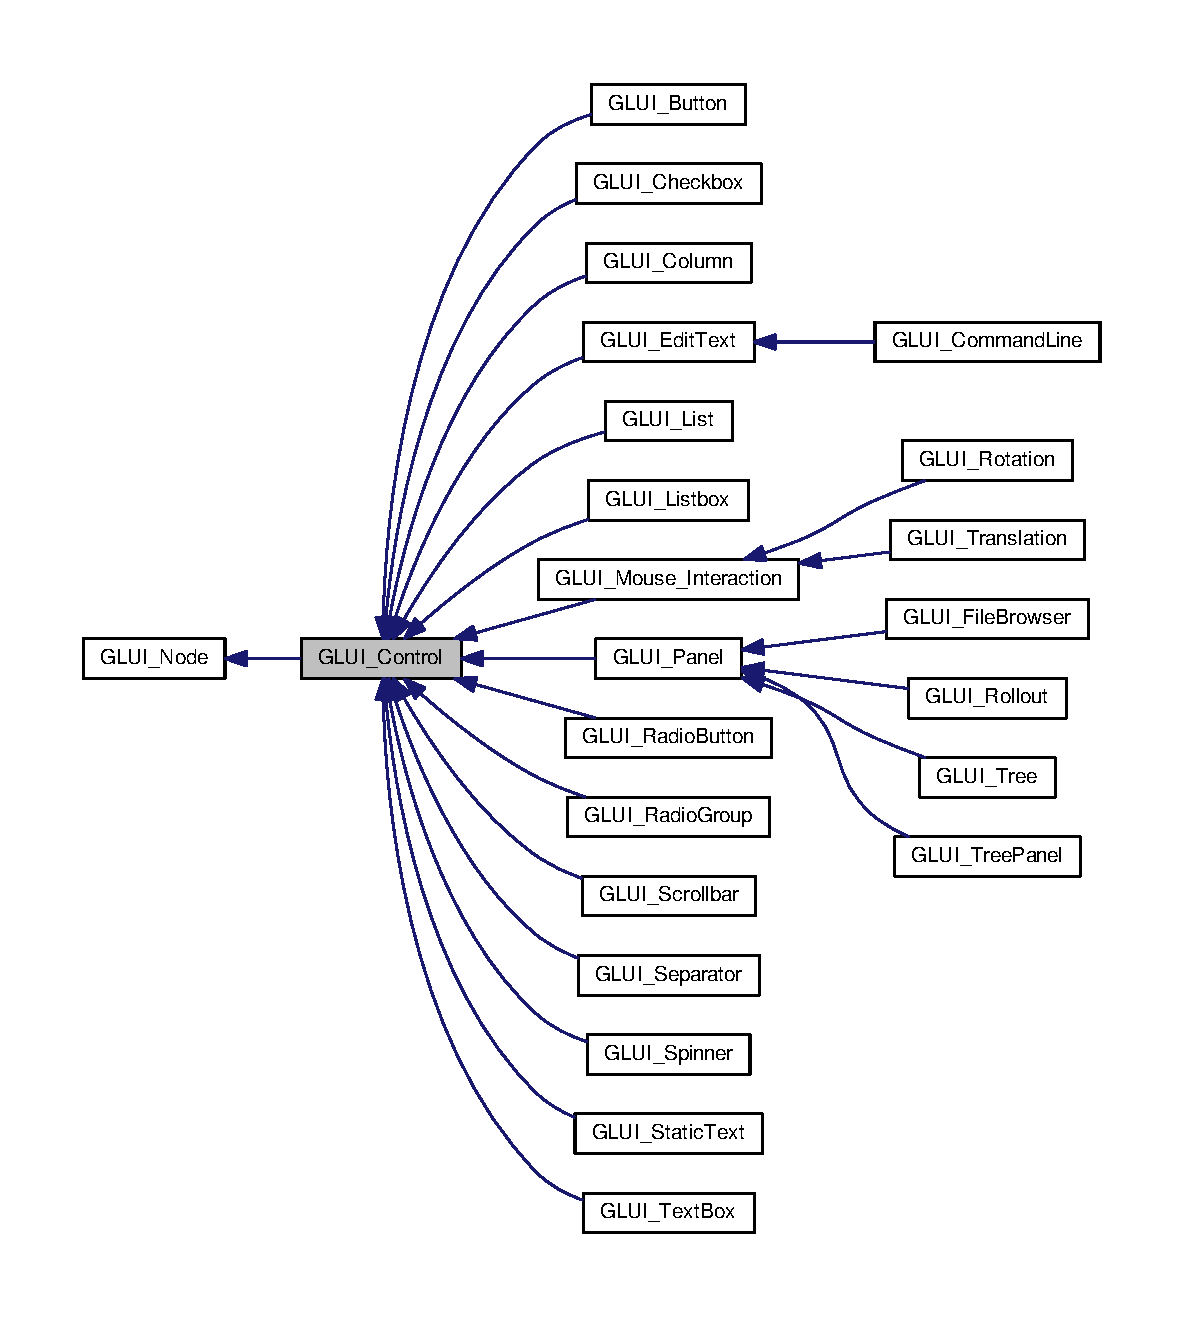
\includegraphics[width=350pt]{class_g_l_u_i___control__inherit__graph}
\end{center}
\end{figure}


Collaboration diagram for G\+L\+U\+I\+\_\+\+Control\+:\nopagebreak
\begin{figure}[H]
\begin{center}
\leavevmode
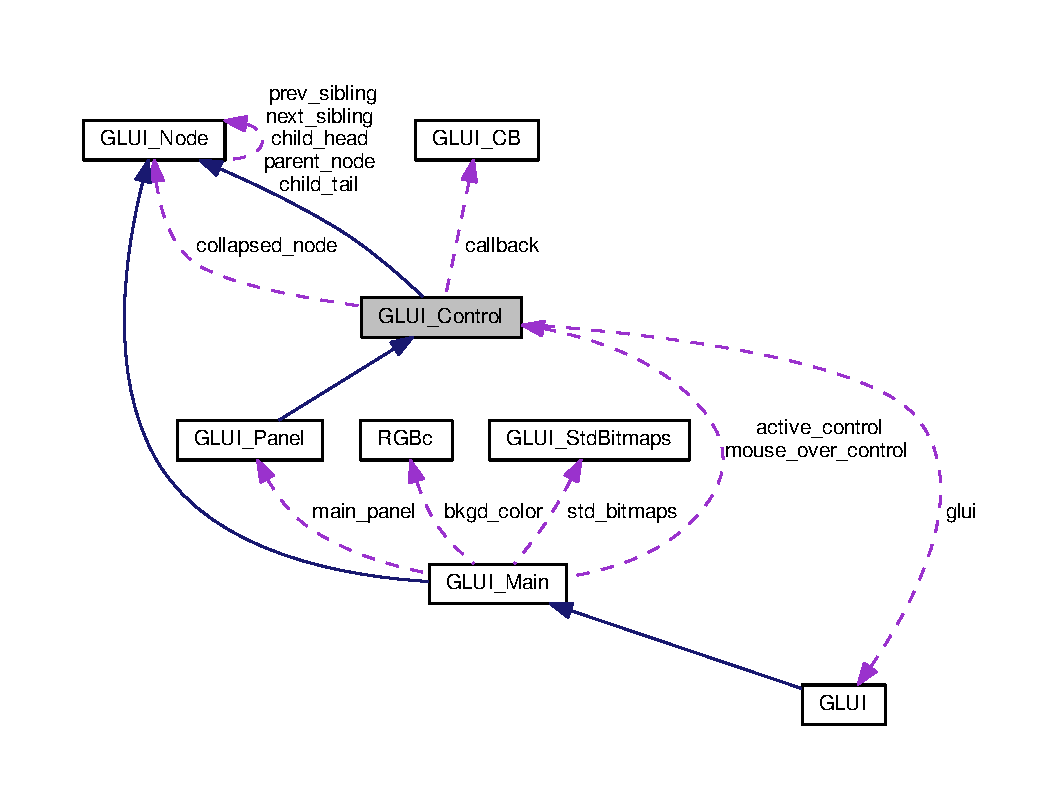
\includegraphics[width=350pt]{class_g_l_u_i___control__coll__graph}
\end{center}
\end{figure}
\subsection*{Public Member Functions}
\begin{DoxyCompactItemize}
\item 
virtual \hyperlink{wglext_8h_a9e6b7f1933461ef318bb000d6bd13b83}{void} \hyperlink{class_g_l_u_i___control_ad1bf0640802de0a40337cdbcf93a5ec6}{set\+\_\+name} (const char $\ast$\hyperlink{glext_8h_ae84541b4f3d8e1ea24ec0f466a8c568b}{string})
\item 
virtual \hyperlink{wglext_8h_a9e6b7f1933461ef318bb000d6bd13b83}{void} \hyperlink{class_g_l_u_i___control_a32ef6d11d6c62e344f17268dfb96aad6}{set\+\_\+int\+\_\+val} (\hyperlink{wglext_8h_a500a82aecba06f4550f6849b8099ca21}{int} new\+\_\+int)
\item 
virtual \hyperlink{wglext_8h_a9e6b7f1933461ef318bb000d6bd13b83}{void} \hyperlink{class_g_l_u_i___control_a231fe69a978a66b858727e50327bcf59}{set\+\_\+float\+\_\+val} (float new\+\_\+float)
\item 
virtual \hyperlink{wglext_8h_a9e6b7f1933461ef318bb000d6bd13b83}{void} \hyperlink{class_g_l_u_i___control_a9c732d42b7d5e418e59c307ef2d98d5c}{set\+\_\+ptr\+\_\+val} (\hyperlink{wglext_8h_a9e6b7f1933461ef318bb000d6bd13b83}{void} $\ast$new\+\_\+ptr)
\item 
virtual \hyperlink{wglext_8h_a9e6b7f1933461ef318bb000d6bd13b83}{void} \hyperlink{class_g_l_u_i___control_aa9a1c1e033c0e99e4710dfc4669660f4}{set\+\_\+float\+\_\+array\+\_\+val} (float $\ast$array\+\_\+ptr)
\item 
virtual float \hyperlink{class_g_l_u_i___control_a5b4f37b463259dfbf228b34b901a07cc}{get\+\_\+float\+\_\+val} (\hyperlink{wglext_8h_a9e6b7f1933461ef318bb000d6bd13b83}{void})
\item 
virtual \hyperlink{wglext_8h_a500a82aecba06f4550f6849b8099ca21}{int} \hyperlink{class_g_l_u_i___control_a3ee80f39e04a26e38bc5e16f0f8af539}{get\+\_\+int\+\_\+val} (\hyperlink{wglext_8h_a9e6b7f1933461ef318bb000d6bd13b83}{void})
\item 
virtual \hyperlink{wglext_8h_a9e6b7f1933461ef318bb000d6bd13b83}{void} \hyperlink{class_g_l_u_i___control_a98f514bf95d29320c175fe1d7d4ef13b}{get\+\_\+float\+\_\+array\+\_\+val} (float $\ast$array\+\_\+ptr)
\item 
virtual \hyperlink{wglext_8h_a500a82aecba06f4550f6849b8099ca21}{int} \hyperlink{class_g_l_u_i___control_a855a5f2c0267a303b39f685284913b40}{get\+\_\+id} (\hyperlink{wglext_8h_a9e6b7f1933461ef318bb000d6bd13b83}{void}) const 
\item 
virtual \hyperlink{wglext_8h_a9e6b7f1933461ef318bb000d6bd13b83}{void} \hyperlink{class_g_l_u_i___control_ad27f17ac45b13fb12d623f269d76db14}{set\+\_\+id} (\hyperlink{wglext_8h_a500a82aecba06f4550f6849b8099ca21}{int} \hyperlink{glext_8h_a58c2a664503e14ffb8f21012aabff3e9}{id})
\item 
virtual \hyperlink{wglext_8h_a500a82aecba06f4550f6849b8099ca21}{int} \hyperlink{class_g_l_u_i___control_a92b77565168a1d2003bca1c16ac00e8d}{mouse\+\_\+down\+\_\+handler} (\hyperlink{wglext_8h_a500a82aecba06f4550f6849b8099ca21}{int} local\+\_\+x, \hyperlink{wglext_8h_a500a82aecba06f4550f6849b8099ca21}{int} local\+\_\+y)
\item 
virtual \hyperlink{wglext_8h_a500a82aecba06f4550f6849b8099ca21}{int} \hyperlink{class_g_l_u_i___control_ac32aad8f69134d03682e34d0488a18f1}{mouse\+\_\+up\+\_\+handler} (\hyperlink{wglext_8h_a500a82aecba06f4550f6849b8099ca21}{int} local\+\_\+x, \hyperlink{wglext_8h_a500a82aecba06f4550f6849b8099ca21}{int} local\+\_\+y, bool inside)
\item 
virtual \hyperlink{wglext_8h_a500a82aecba06f4550f6849b8099ca21}{int} \hyperlink{class_g_l_u_i___control_a4b44e44c1c455adc7f98c63aeb6aa919}{mouse\+\_\+held\+\_\+down\+\_\+handler} (\hyperlink{wglext_8h_a500a82aecba06f4550f6849b8099ca21}{int} local\+\_\+x, \hyperlink{wglext_8h_a500a82aecba06f4550f6849b8099ca21}{int} local\+\_\+y, bool inside)
\item 
virtual \hyperlink{wglext_8h_a500a82aecba06f4550f6849b8099ca21}{int} \hyperlink{class_g_l_u_i___control_a7f9da8ca7df99bd4cf394a9fd8ce19f1}{key\+\_\+handler} (unsigned char key, \hyperlink{wglext_8h_a500a82aecba06f4550f6849b8099ca21}{int} modifiers)
\item 
virtual \hyperlink{wglext_8h_a500a82aecba06f4550f6849b8099ca21}{int} \hyperlink{class_g_l_u_i___control_ab08da363df3f3eae867dd5ae61200f23}{special\+\_\+handler} (\hyperlink{wglext_8h_a500a82aecba06f4550f6849b8099ca21}{int} key, \hyperlink{wglext_8h_a500a82aecba06f4550f6849b8099ca21}{int} modifiers)
\item 
virtual \hyperlink{wglext_8h_a9e6b7f1933461ef318bb000d6bd13b83}{void} \hyperlink{class_g_l_u_i___control_a4bfe55acbbf735a7d2ff07d687a481e2}{update\+\_\+size} (\hyperlink{wglext_8h_a9e6b7f1933461ef318bb000d6bd13b83}{void})
\item 
virtual \hyperlink{wglext_8h_a9e6b7f1933461ef318bb000d6bd13b83}{void} \hyperlink{class_g_l_u_i___control_a4eb47a3c2c20c0c24dca192a2eb96c8d}{idle} (\hyperlink{wglext_8h_a9e6b7f1933461ef318bb000d6bd13b83}{void})
\item 
virtual \hyperlink{wglext_8h_a500a82aecba06f4550f6849b8099ca21}{int} \hyperlink{class_g_l_u_i___control_ac16c3ff7bef1a64abd36a00aa3d935d8}{mouse\+\_\+over} (\hyperlink{wglext_8h_a500a82aecba06f4550f6849b8099ca21}{int} state, \hyperlink{wglext_8h_a500a82aecba06f4550f6849b8099ca21}{int} \hyperlink{glext_8h_ad77deca22f617d3f0e0eb786445689fc}{x}, \hyperlink{wglext_8h_a500a82aecba06f4550f6849b8099ca21}{int} \hyperlink{glext_8h_a9298c7ad619074f5285b32c6b72bfdea}{y})
\item 
virtual \hyperlink{wglext_8h_a9e6b7f1933461ef318bb000d6bd13b83}{void} \hyperlink{class_g_l_u_i___control_aaadc8fd35d8d40091abe3538af346255}{enable} (\hyperlink{wglext_8h_a9e6b7f1933461ef318bb000d6bd13b83}{void})
\item 
virtual \hyperlink{wglext_8h_a9e6b7f1933461ef318bb000d6bd13b83}{void} \hyperlink{class_g_l_u_i___control_a765dcd68a28a3db25bf41c015e28ee18}{disable} (\hyperlink{wglext_8h_a9e6b7f1933461ef318bb000d6bd13b83}{void})
\item 
virtual \hyperlink{wglext_8h_a9e6b7f1933461ef318bb000d6bd13b83}{void} \hyperlink{class_g_l_u_i___control_af686704718daf4761d17e4da83c03aad}{activate} (\hyperlink{wglext_8h_a500a82aecba06f4550f6849b8099ca21}{int} how)
\item 
virtual \hyperlink{wglext_8h_a9e6b7f1933461ef318bb000d6bd13b83}{void} \hyperlink{class_g_l_u_i___control_a9d18764a6cfe25c220c845eff480d4fe}{deactivate} (\hyperlink{wglext_8h_a9e6b7f1933461ef318bb000d6bd13b83}{void})
\item 
\hyperlink{wglext_8h_a9e6b7f1933461ef318bb000d6bd13b83}{void} \hyperlink{class_g_l_u_i___control_ae88270c442111baddf290f4a153caed1}{hide\+\_\+internal} (\hyperlink{wglext_8h_a500a82aecba06f4550f6849b8099ca21}{int} recurse)
\item 
\hyperlink{wglext_8h_a9e6b7f1933461ef318bb000d6bd13b83}{void} \hyperlink{class_g_l_u_i___control_a73192b0fdcaa75eb04d43fa70abe246f}{unhide\+\_\+internal} (\hyperlink{wglext_8h_a500a82aecba06f4550f6849b8099ca21}{int} recurse)
\item 
\hyperlink{wglext_8h_a500a82aecba06f4550f6849b8099ca21}{int} \hyperlink{class_g_l_u_i___control_add5d7aa8efcd213181cf84975661e168}{can\+\_\+draw} (\hyperlink{wglext_8h_a9e6b7f1933461ef318bb000d6bd13b83}{void})
\item 
\hyperlink{wglext_8h_a9e6b7f1933461ef318bb000d6bd13b83}{void} \hyperlink{class_g_l_u_i___control_a7777125cd866884377899df625bad6cd}{redraw} (\hyperlink{wglext_8h_a9e6b7f1933461ef318bb000d6bd13b83}{void})
\item 
\hyperlink{wglext_8h_a9e6b7f1933461ef318bb000d6bd13b83}{void} \hyperlink{class_g_l_u_i___control_aecb4bacd8f4ff12de6ffcecc166d3adc}{redraw\+\_\+window} (\hyperlink{wglext_8h_a9e6b7f1933461ef318bb000d6bd13b83}{void})
\item 
virtual \hyperlink{wglext_8h_a9e6b7f1933461ef318bb000d6bd13b83}{void} \hyperlink{class_g_l_u_i___control_aa82d73e561e85086c13de6b8d67e9322}{align} (\hyperlink{wglext_8h_a9e6b7f1933461ef318bb000d6bd13b83}{void})
\item 
\hyperlink{wglext_8h_a9e6b7f1933461ef318bb000d6bd13b83}{void} \hyperlink{class_g_l_u_i___control_a55b244224a7446e7254a9d3b468d4925}{pack} (\hyperlink{wglext_8h_a500a82aecba06f4550f6849b8099ca21}{int} \hyperlink{glext_8h_ad77deca22f617d3f0e0eb786445689fc}{x}, \hyperlink{wglext_8h_a500a82aecba06f4550f6849b8099ca21}{int} \hyperlink{glext_8h_a9298c7ad619074f5285b32c6b72bfdea}{y})
\item 
\hyperlink{wglext_8h_a9e6b7f1933461ef318bb000d6bd13b83}{void} \hyperlink{class_g_l_u_i___control_a1c9cf8a504998db2393c4d45144eca8d}{pack\+\_\+old} (\hyperlink{wglext_8h_a500a82aecba06f4550f6849b8099ca21}{int} \hyperlink{glext_8h_ad77deca22f617d3f0e0eb786445689fc}{x}, \hyperlink{wglext_8h_a500a82aecba06f4550f6849b8099ca21}{int} \hyperlink{glext_8h_a9298c7ad619074f5285b32c6b72bfdea}{y})
\item 
\hyperlink{wglext_8h_a9e6b7f1933461ef318bb000d6bd13b83}{void} \hyperlink{class_g_l_u_i___control_af151f23a66652c7be4a49320d49a3aab}{draw\+\_\+recursive} (\hyperlink{wglext_8h_a500a82aecba06f4550f6849b8099ca21}{int} \hyperlink{glext_8h_ad77deca22f617d3f0e0eb786445689fc}{x}, \hyperlink{wglext_8h_a500a82aecba06f4550f6849b8099ca21}{int} \hyperlink{glext_8h_a9298c7ad619074f5285b32c6b72bfdea}{y})
\item 
\hyperlink{wglext_8h_a500a82aecba06f4550f6849b8099ca21}{int} \hyperlink{class_g_l_u_i___control_aff3f98acd4b58ba0db35b5889c4006bc}{set\+\_\+to\+\_\+glut\+\_\+window} (\hyperlink{wglext_8h_a9e6b7f1933461ef318bb000d6bd13b83}{void})
\item 
\hyperlink{wglext_8h_a9e6b7f1933461ef318bb000d6bd13b83}{void} \hyperlink{class_g_l_u_i___control_a49e4d3f46873d156162d9f770b7b3832}{restore\+\_\+window} (\hyperlink{wglext_8h_a500a82aecba06f4550f6849b8099ca21}{int} orig)
\item 
\hyperlink{wglext_8h_a9e6b7f1933461ef318bb000d6bd13b83}{void} \hyperlink{class_g_l_u_i___control_ae0e46e41b11758295ae0f2d1c9372dda}{translate\+\_\+and\+\_\+draw\+\_\+front} (\hyperlink{wglext_8h_a9e6b7f1933461ef318bb000d6bd13b83}{void})
\item 
\hyperlink{wglext_8h_a9e6b7f1933461ef318bb000d6bd13b83}{void} \hyperlink{class_g_l_u_i___control_a11ae15dcbb0ed5136b471a77eda41266}{translate\+\_\+to\+\_\+origin} (\hyperlink{wglext_8h_a9e6b7f1933461ef318bb000d6bd13b83}{void})
\item 
virtual \hyperlink{wglext_8h_a9e6b7f1933461ef318bb000d6bd13b83}{void} \hyperlink{class_g_l_u_i___control_a2eb42d7a7951280ad2fe8c37972bf66a}{draw} (\hyperlink{wglext_8h_a500a82aecba06f4550f6849b8099ca21}{int} \hyperlink{glext_8h_ad77deca22f617d3f0e0eb786445689fc}{x}, \hyperlink{wglext_8h_a500a82aecba06f4550f6849b8099ca21}{int} \hyperlink{glext_8h_a9298c7ad619074f5285b32c6b72bfdea}{y})=0
\item 
\hyperlink{wglext_8h_a9e6b7f1933461ef318bb000d6bd13b83}{void} \hyperlink{class_g_l_u_i___control_ae317f3c30fbd4cad6bd91523c7e3e6b0}{set\+\_\+font} (\hyperlink{wglext_8h_a9e6b7f1933461ef318bb000d6bd13b83}{void} $\ast$new\+\_\+font)
\item 
\hyperlink{wglext_8h_a9e6b7f1933461ef318bb000d6bd13b83}{void} $\ast$ \hyperlink{class_g_l_u_i___control_af659cbe80e9a5bdfd4fbff4366d4ce4f}{get\+\_\+font} (\hyperlink{wglext_8h_a9e6b7f1933461ef318bb000d6bd13b83}{void})
\item 
\hyperlink{wglext_8h_a500a82aecba06f4550f6849b8099ca21}{int} \hyperlink{class_g_l_u_i___control_a57ed4e7d0b82e459fb713a9bf29db12b}{string\+\_\+width} (const char $\ast$\hyperlink{class_g_l_u_i___control_af0d60e9736f4dbc34e9a536e75876d72}{text})
\item 
\hyperlink{wglext_8h_a500a82aecba06f4550f6849b8099ca21}{int} \hyperlink{class_g_l_u_i___control_a9d129d259e01c1b28f4fc7a7a7830189}{string\+\_\+width} (const \hyperlink{glui_8h_aada824856f7bcf29794719981ebd8f60}{G\+L\+U\+I\+\_\+\+String} \&str)
\item 
\hyperlink{wglext_8h_a500a82aecba06f4550f6849b8099ca21}{int} \hyperlink{class_g_l_u_i___control_ae56ff4899b691fc25332071f8f4c15f3}{char\+\_\+width} (char \hyperlink{glext_8h_a1f2d7f8147412c43ba2303a56f97ee73}{c})
\item 
\hyperlink{wglext_8h_a9e6b7f1933461ef318bb000d6bd13b83}{void} \hyperlink{class_g_l_u_i___control_aacacd563742e3e48bc5f27643e4a514c}{draw\+\_\+name} (\hyperlink{wglext_8h_a500a82aecba06f4550f6849b8099ca21}{int} \hyperlink{glext_8h_ad77deca22f617d3f0e0eb786445689fc}{x}, \hyperlink{wglext_8h_a500a82aecba06f4550f6849b8099ca21}{int} \hyperlink{glext_8h_a9298c7ad619074f5285b32c6b72bfdea}{y})
\item 
\hyperlink{wglext_8h_a9e6b7f1933461ef318bb000d6bd13b83}{void} \hyperlink{class_g_l_u_i___control_adba9e88ff56a8ea0596e6b1ede3d4b9d}{draw\+\_\+box\+\_\+inwards\+\_\+outline} (\hyperlink{wglext_8h_a500a82aecba06f4550f6849b8099ca21}{int} x\+\_\+min, \hyperlink{wglext_8h_a500a82aecba06f4550f6849b8099ca21}{int} x\+\_\+max, \hyperlink{wglext_8h_a500a82aecba06f4550f6849b8099ca21}{int} y\+\_\+min, \hyperlink{wglext_8h_a500a82aecba06f4550f6849b8099ca21}{int} y\+\_\+max)
\item 
\hyperlink{wglext_8h_a9e6b7f1933461ef318bb000d6bd13b83}{void} \hyperlink{class_g_l_u_i___control_a5dff8194089a66651d3729cf7c465644}{draw\+\_\+box} (\hyperlink{wglext_8h_a500a82aecba06f4550f6849b8099ca21}{int} x\+\_\+min, \hyperlink{wglext_8h_a500a82aecba06f4550f6849b8099ca21}{int} x\+\_\+max, \hyperlink{wglext_8h_a500a82aecba06f4550f6849b8099ca21}{int} y\+\_\+min, \hyperlink{wglext_8h_a500a82aecba06f4550f6849b8099ca21}{int} y\+\_\+max, float \hyperlink{glext_8h_a42ce7cdc612e53abee15043f80220d97}{r}, float \hyperlink{glext_8h_acaceb3a655ff28b75259860bcb868f9f}{g}, float \hyperlink{glext_8h_a0f71581a41fd2264c8944126dabbd010}{b})
\item 
\hyperlink{wglext_8h_a9e6b7f1933461ef318bb000d6bd13b83}{void} \hyperlink{class_g_l_u_i___control_ad1bcdb980c0ccbcbafd7b51a6564ccc0}{draw\+\_\+bkgd\+\_\+box} (\hyperlink{wglext_8h_a500a82aecba06f4550f6849b8099ca21}{int} x\+\_\+min, \hyperlink{wglext_8h_a500a82aecba06f4550f6849b8099ca21}{int} x\+\_\+max, \hyperlink{wglext_8h_a500a82aecba06f4550f6849b8099ca21}{int} y\+\_\+min, \hyperlink{wglext_8h_a500a82aecba06f4550f6849b8099ca21}{int} y\+\_\+max)
\item 
\hyperlink{wglext_8h_a9e6b7f1933461ef318bb000d6bd13b83}{void} \hyperlink{class_g_l_u_i___control_a1386b942473e028e9204bd1a28e83a6d}{draw\+\_\+emboss\+\_\+box} (\hyperlink{wglext_8h_a500a82aecba06f4550f6849b8099ca21}{int} x\+\_\+min, \hyperlink{wglext_8h_a500a82aecba06f4550f6849b8099ca21}{int} x\+\_\+max, \hyperlink{wglext_8h_a500a82aecba06f4550f6849b8099ca21}{int} y\+\_\+min, \hyperlink{wglext_8h_a500a82aecba06f4550f6849b8099ca21}{int} y\+\_\+max)
\item 
\hyperlink{wglext_8h_a9e6b7f1933461ef318bb000d6bd13b83}{void} \hyperlink{class_g_l_u_i___control_a05172f3645ac042839036c97e04ea819}{draw\+\_\+string} (const char $\ast$\hyperlink{class_g_l_u_i___control_af0d60e9736f4dbc34e9a536e75876d72}{text})
\item 
\hyperlink{wglext_8h_a9e6b7f1933461ef318bb000d6bd13b83}{void} \hyperlink{class_g_l_u_i___control_aba5d462fcca0297c3dbf6a26d0774e4a}{draw\+\_\+string} (const \hyperlink{glui_8h_aada824856f7bcf29794719981ebd8f60}{G\+L\+U\+I\+\_\+\+String} \&\hyperlink{glext_8h_a4af680a6c683f88ed67b76f207f2e6e4}{s})
\item 
\hyperlink{wglext_8h_a9e6b7f1933461ef318bb000d6bd13b83}{void} \hyperlink{class_g_l_u_i___control_af8bfdf4867b4521fd3c12825e8a150db}{draw\+\_\+char} (char \hyperlink{glext_8h_a1f2d7f8147412c43ba2303a56f97ee73}{c})
\item 
\hyperlink{wglext_8h_a9e6b7f1933461ef318bb000d6bd13b83}{void} \hyperlink{class_g_l_u_i___control_aa61812303961384f999c35f128f04c93}{draw\+\_\+active\+\_\+box} (\hyperlink{wglext_8h_a500a82aecba06f4550f6849b8099ca21}{int} x\+\_\+min, \hyperlink{wglext_8h_a500a82aecba06f4550f6849b8099ca21}{int} x\+\_\+max, \hyperlink{wglext_8h_a500a82aecba06f4550f6849b8099ca21}{int} y\+\_\+min, \hyperlink{wglext_8h_a500a82aecba06f4550f6849b8099ca21}{int} y\+\_\+max)
\item 
\hyperlink{wglext_8h_a9e6b7f1933461ef318bb000d6bd13b83}{void} \hyperlink{class_g_l_u_i___control_a091c0c095827c3270b442d9bd3542d50}{set\+\_\+to\+\_\+bkgd\+\_\+color} (\hyperlink{wglext_8h_a9e6b7f1933461ef318bb000d6bd13b83}{void})
\item 
\hyperlink{wglext_8h_a9e6b7f1933461ef318bb000d6bd13b83}{void} \hyperlink{class_g_l_u_i___control_a7f9dde76de0e5fd660dc43695b40c91d}{set\+\_\+w} (\hyperlink{wglext_8h_a500a82aecba06f4550f6849b8099ca21}{int} new\+\_\+w)
\item 
\hyperlink{wglext_8h_a9e6b7f1933461ef318bb000d6bd13b83}{void} \hyperlink{class_g_l_u_i___control_acc29b79df3861b1910b2a41e0e8d2822}{set\+\_\+h} (\hyperlink{wglext_8h_a500a82aecba06f4550f6849b8099ca21}{int} new\+\_\+w)
\item 
\hyperlink{wglext_8h_a9e6b7f1933461ef318bb000d6bd13b83}{void} \hyperlink{class_g_l_u_i___control_ad853d2029a306239daa3c9af6c36730d}{set\+\_\+alignment} (\hyperlink{wglext_8h_a500a82aecba06f4550f6849b8099ca21}{int} new\+\_\+align)
\item 
\hyperlink{wglext_8h_a9e6b7f1933461ef318bb000d6bd13b83}{void} \hyperlink{class_g_l_u_i___control_a56a06a9b1272eb0a537ea01a6c002cf8}{sync\+\_\+live} (\hyperlink{wglext_8h_a500a82aecba06f4550f6849b8099ca21}{int} recurse, \hyperlink{wglext_8h_a500a82aecba06f4550f6849b8099ca21}{int} \hyperlink{class_g_l_u_i___control_a2eb42d7a7951280ad2fe8c37972bf66a}{draw})
\item 
\hyperlink{wglext_8h_a9e6b7f1933461ef318bb000d6bd13b83}{void} \hyperlink{class_g_l_u_i___control_a4d56b92f8b6454c3f64ba6f0ef5470b8}{init\+\_\+live} (\hyperlink{wglext_8h_a9e6b7f1933461ef318bb000d6bd13b83}{void})
\item 
\hyperlink{wglext_8h_a9e6b7f1933461ef318bb000d6bd13b83}{void} \hyperlink{class_g_l_u_i___control_ac7417112964d4c5134d4453835a0da99}{output\+\_\+live} (\hyperlink{wglext_8h_a500a82aecba06f4550f6849b8099ca21}{int} update\+\_\+main\+\_\+gfx)
\item 
virtual \hyperlink{wglext_8h_a9e6b7f1933461ef318bb000d6bd13b83}{void} \hyperlink{class_g_l_u_i___control_a44fab5a8af3c58865bc2cd8bfd596af8}{set\+\_\+text} (const char $\ast$\hyperlink{glext_8h_a7d65d00ca3b0630d9b5c52df855b19f5}{t})
\item 
\hyperlink{wglext_8h_a9e6b7f1933461ef318bb000d6bd13b83}{void} \hyperlink{class_g_l_u_i___control_a76fe9cee85c7a296610a73b0ba12aa9c}{execute\+\_\+callback} (\hyperlink{wglext_8h_a9e6b7f1933461ef318bb000d6bd13b83}{void})
\item 
\hyperlink{wglext_8h_a9e6b7f1933461ef318bb000d6bd13b83}{void} \hyperlink{class_g_l_u_i___control_a0cb273fd3dca9fb84809a4d350668c32}{get\+\_\+this\+\_\+column\+\_\+dims} (\hyperlink{wglext_8h_a500a82aecba06f4550f6849b8099ca21}{int} $\ast$col\+\_\+x, \hyperlink{wglext_8h_a500a82aecba06f4550f6849b8099ca21}{int} $\ast$col\+\_\+y, \hyperlink{wglext_8h_a500a82aecba06f4550f6849b8099ca21}{int} $\ast$col\+\_\+w, \hyperlink{wglext_8h_a500a82aecba06f4550f6849b8099ca21}{int} $\ast$col\+\_\+h, \hyperlink{wglext_8h_a500a82aecba06f4550f6849b8099ca21}{int} $\ast$col\+\_\+x\+\_\+off, \hyperlink{wglext_8h_a500a82aecba06f4550f6849b8099ca21}{int} $\ast$col\+\_\+y\+\_\+off)
\item 
virtual bool \hyperlink{class_g_l_u_i___control_a420fb3c5991b6486754ba192f8ab8274}{needs\+\_\+idle} (\hyperlink{wglext_8h_a9e6b7f1933461ef318bb000d6bd13b83}{void}) const 
\item 
virtual bool \hyperlink{class_g_l_u_i___control_a42a65c9dbc0690e270a8c0033fbc1845}{wants\+\_\+tabs} () const 
\item 
\hyperlink{class_g_l_u_i___control_a09c6f812cb8b6ba83e15fd96d0018552}{G\+L\+U\+I\+\_\+\+Control} (\hyperlink{wglext_8h_a9e6b7f1933461ef318bb000d6bd13b83}{void})
\item 
virtual \hyperlink{class_g_l_u_i___control_a8afdc7d81a09fa30a759d5456559e637}{$\sim$\+G\+L\+U\+I\+\_\+\+Control} ()
\end{DoxyCompactItemize}
\subsection*{Public Attributes}
\begin{DoxyCompactItemize}
\item 
\hyperlink{wglext_8h_a500a82aecba06f4550f6849b8099ca21}{int} \hyperlink{class_g_l_u_i___control_aca82a099b9cbbadb188794cbfb06aa27}{w}
\item 
\hyperlink{wglext_8h_a500a82aecba06f4550f6849b8099ca21}{int} \hyperlink{class_g_l_u_i___control_a058c4f060b70952e6199f1409710ba0b}{h}
\item 
\hyperlink{wglext_8h_a500a82aecba06f4550f6849b8099ca21}{int} \hyperlink{class_g_l_u_i___control_a7f0f98737828ad255401f642826fbd7e}{x\+\_\+abs}
\item 
\hyperlink{wglext_8h_a500a82aecba06f4550f6849b8099ca21}{int} \hyperlink{class_g_l_u_i___control_a54a7a5a7c37e5c0e0a3154bac7ddb049}{y\+\_\+abs}
\item 
\hyperlink{wglext_8h_a500a82aecba06f4550f6849b8099ca21}{int} \hyperlink{class_g_l_u_i___control_a853d95e48b8bd6d2bdd41dabc2b1a1a6}{x\+\_\+off}
\item 
\hyperlink{wglext_8h_a500a82aecba06f4550f6849b8099ca21}{int} \hyperlink{class_g_l_u_i___control_a94fec9974356d3955e3a80e7d06926b9}{y\+\_\+off\+\_\+top}
\item 
\hyperlink{wglext_8h_a500a82aecba06f4550f6849b8099ca21}{int} \hyperlink{class_g_l_u_i___control_af4beca38aaf1aba7f5b4bfa3ccc8b909}{y\+\_\+off\+\_\+bot}
\item 
\hyperlink{wglext_8h_a500a82aecba06f4550f6849b8099ca21}{int} \hyperlink{class_g_l_u_i___control_aa02b20473b2d00e5b95bf36ff941e5bf}{contain\+\_\+x}
\item 
\hyperlink{wglext_8h_a500a82aecba06f4550f6849b8099ca21}{int} \hyperlink{class_g_l_u_i___control_a6327d4d71e9368bf238c6fddd958649e}{contain\+\_\+y}
\item 
\hyperlink{wglext_8h_a500a82aecba06f4550f6849b8099ca21}{int} \hyperlink{class_g_l_u_i___control_a9d54f7b7c867572debdad16b37867093}{contain\+\_\+w}
\item 
\hyperlink{wglext_8h_a500a82aecba06f4550f6849b8099ca21}{int} \hyperlink{class_g_l_u_i___control_afc9111c158e729b1e1630d4d9cd6ee1a}{contain\+\_\+h}
\item 
\hyperlink{wglext_8h_a500a82aecba06f4550f6849b8099ca21}{int} \hyperlink{class_g_l_u_i___control_ab9864db034526ddd5bbff94a5fb3ee9b}{active\+\_\+type}
\begin{DoxyCompactList}\small\item\em \char`\"{}\+G\+L\+U\+I\+\_\+\+C\+O\+N\+T\+R\+O\+L\+\_\+\+A\+C\+T\+I\+V\+E\+\_\+...\char`\"{} \end{DoxyCompactList}\item 
bool \hyperlink{class_g_l_u_i___control_ad285387e771b46fb294935f68e967a77}{active}
\begin{DoxyCompactList}\small\item\em If true, we've got the focus. \end{DoxyCompactList}\item 
bool \hyperlink{class_g_l_u_i___control_a2484b0899bd5b56673a73387c9c530a7}{can\+\_\+activate}
\begin{DoxyCompactList}\small\item\em If false, remove from tab order. \end{DoxyCompactList}\item 
bool \hyperlink{class_g_l_u_i___control_a023da130fb762f944077c55d90aec839}{spacebar\+\_\+mouse\+\_\+click}
\begin{DoxyCompactList}\small\item\em Spacebar simulates click. \end{DoxyCompactList}\item 
long \hyperlink{class_g_l_u_i___control_a6c88b7c72b0800f88a5d4cda4868c8b6}{user\+\_\+id}
\begin{DoxyCompactList}\small\item\em Integer to pass to callback function. \end{DoxyCompactList}\item 
\hyperlink{class_g_l_u_i___c_b}{G\+L\+U\+I\+\_\+\+C\+B} \hyperlink{class_g_l_u_i___control_a96060fe0cc6d537e736dd6eef78e24ab}{callback}
\begin{DoxyCompactList}\small\item\em User callback function, or N\+U\+L\+L. \end{DoxyCompactList}\item 
float \hyperlink{class_g_l_u_i___control_ac69b8e62a6f4f16c83b70a64f73d7a1c}{float\+\_\+val}
\item 
\hyperlink{wglext_8h_a500a82aecba06f4550f6849b8099ca21}{int} \hyperlink{class_g_l_u_i___control_a4a890b5b5a854b34200b5e63f1069b4e}{int\+\_\+val}
\item 
float \hyperlink{class_g_l_u_i___control_a6d2cc0faaa678706939ac775c523871a}{float\+\_\+array\+\_\+val} \mbox{[}\hyperlink{glui_8h_ae6cbace033fae45e6088bf23b1f72f4a}{G\+L\+U\+I\+\_\+\+D\+E\+F\+\_\+\+M\+A\+X\+\_\+\+A\+R\+R\+A\+Y}\mbox{]}
\item 
\hyperlink{wglext_8h_a500a82aecba06f4550f6849b8099ca21}{int} \hyperlink{class_g_l_u_i___control_a504f6aff85729e665fa8664d170d9878}{float\+\_\+array\+\_\+size}
\item 
\hyperlink{glui_8h_aada824856f7bcf29794719981ebd8f60}{G\+L\+U\+I\+\_\+\+String} \hyperlink{class_g_l_u_i___control_af0d60e9736f4dbc34e9a536e75876d72}{text}
\item 
\hyperlink{wglext_8h_a9e6b7f1933461ef318bb000d6bd13b83}{void} $\ast$ \hyperlink{class_g_l_u_i___control_a0890ea809b8d980695939e1d92a0af47}{ptr\+\_\+val}
\item 
\hyperlink{wglext_8h_a500a82aecba06f4550f6849b8099ca21}{int} \hyperlink{class_g_l_u_i___control_a8ba7cae809a47dd870592aa2cc85483b}{live\+\_\+type}
\item 
bool \hyperlink{class_g_l_u_i___control_a74977797cf84a38ef78de8c548bc2d25}{live\+\_\+inited}
\item 
\hyperlink{wglext_8h_a500a82aecba06f4550f6849b8099ca21}{int} \hyperlink{class_g_l_u_i___control_abef31d8d51c8088afd6ac96ec7b596bf}{last\+\_\+live\+\_\+int}
\item 
float \hyperlink{class_g_l_u_i___control_aa9ebadbed670a1fa061918705083db57}{last\+\_\+live\+\_\+float}
\item 
\hyperlink{glui_8h_aada824856f7bcf29794719981ebd8f60}{G\+L\+U\+I\+\_\+\+String} \hyperlink{class_g_l_u_i___control_ac77569805eb6ccfce3f4ff1d09c309b6}{last\+\_\+live\+\_\+text}
\item 
float \hyperlink{class_g_l_u_i___control_a719177af6b52ae3373d2b3c30430ff58}{last\+\_\+live\+\_\+float\+\_\+array} \mbox{[}\hyperlink{glui_8h_ae6cbace033fae45e6088bf23b1f72f4a}{G\+L\+U\+I\+\_\+\+D\+E\+F\+\_\+\+M\+A\+X\+\_\+\+A\+R\+R\+A\+Y}\mbox{]}
\item 
\hyperlink{class_g_l_u_i}{G\+L\+U\+I} $\ast$ \hyperlink{class_g_l_u_i___control_ac731aebe26d7eb0b916a9692229f0eb6}{glui}
\item 
bool \hyperlink{class_g_l_u_i___control_ac667bec4efbc9bdbf3e246b4471fb4cb}{is\+\_\+container}
\item 
\hyperlink{wglext_8h_a500a82aecba06f4550f6849b8099ca21}{int} \hyperlink{class_g_l_u_i___control_a5d352c36d6bad2a1eaf9795bba00b7e7}{alignment}
\item 
bool \hyperlink{class_g_l_u_i___control_a834202682d00a31a2141eae6709d37e1}{enabled}
\item 
\hyperlink{glui_8h_aada824856f7bcf29794719981ebd8f60}{G\+L\+U\+I\+\_\+\+String} \hyperlink{class_g_l_u_i___control_aa95b97d50df45335fc33f0af03958eb3}{name}
\item 
\hyperlink{wglext_8h_a9e6b7f1933461ef318bb000d6bd13b83}{void} $\ast$ \hyperlink{class_g_l_u_i___control_a132273406b5ea6d95cd26501fc2f2027}{font}
\item 
bool \hyperlink{class_g_l_u_i___control_a7a6528f287b80bed5861625eda4e5cad}{collapsible}
\item 
bool \hyperlink{class_g_l_u_i___control_a3e4e35edfa04ce71c090bdb849b7642c}{is\+\_\+open}
\item 
\hyperlink{class_g_l_u_i___node}{G\+L\+U\+I\+\_\+\+Node} \hyperlink{class_g_l_u_i___control_a0f32f9b712ae3233f914d02738c43e7f}{collapsed\+\_\+node}
\item 
bool \hyperlink{class_g_l_u_i___control_aec1b041f28d8ee36a0241dde827fea21}{hidden}
\item 
\hyperlink{wglext_8h_a500a82aecba06f4550f6849b8099ca21}{int} \hyperlink{class_g_l_u_i___control_a3b24d8c0f29ab6fc2318278543906cb5}{char\+\_\+widths} \mbox{[}\hyperlink{glui_8h_a3091a06ca7da5c6ab445b1e9765fc21f}{C\+H\+A\+R\+\_\+\+W\+I\+D\+T\+H\+\_\+\+H\+A\+S\+H\+\_\+\+S\+I\+Z\+E}\mbox{]}\mbox{[}2\mbox{]}
\end{DoxyCompactItemize}
\subsection*{Additional Inherited Members}


\subsection{Detailed Description}
All the G\+U\+I objects inherit from \hyperlink{class_g_l_u_i___control}{G\+L\+U\+I\+\_\+\+Control}\+: buttons, checkboxes, labels, edit boxes, scrollbars, etc. Most of the work of this class is in routing events, like keystrokes, mouseclicks, redraws, and sizing events.

Yes, this is a huge and hideous class. It needs to be split up into simpler subobjects. None of the data members should be directly accessed by users (they should be protected, not public); only subclasses. 

Definition at line 759 of file glui.\+h.



\subsection{Constructor \& Destructor Documentation}
\hypertarget{class_g_l_u_i___control_a09c6f812cb8b6ba83e15fd96d0018552}{\index{G\+L\+U\+I\+\_\+\+Control@{G\+L\+U\+I\+\_\+\+Control}!G\+L\+U\+I\+\_\+\+Control@{G\+L\+U\+I\+\_\+\+Control}}
\index{G\+L\+U\+I\+\_\+\+Control@{G\+L\+U\+I\+\_\+\+Control}!G\+L\+U\+I\+\_\+\+Control@{G\+L\+U\+I\+\_\+\+Control}}
\subsubsection[{G\+L\+U\+I\+\_\+\+Control}]{\setlength{\rightskip}{0pt plus 5cm}G\+L\+U\+I\+\_\+\+Control\+::\+G\+L\+U\+I\+\_\+\+Control (
\begin{DoxyParamCaption}
\item[{{\bf void}}]{}
\end{DoxyParamCaption}
)\hspace{0.3cm}{\ttfamily [inline]}}}\label{class_g_l_u_i___control_a09c6f812cb8b6ba83e15fd96d0018552}


Definition at line 905 of file glui.\+h.

\hypertarget{class_g_l_u_i___control_a8afdc7d81a09fa30a759d5456559e637}{\index{G\+L\+U\+I\+\_\+\+Control@{G\+L\+U\+I\+\_\+\+Control}!````~G\+L\+U\+I\+\_\+\+Control@{$\sim$\+G\+L\+U\+I\+\_\+\+Control}}
\index{````~G\+L\+U\+I\+\_\+\+Control@{$\sim$\+G\+L\+U\+I\+\_\+\+Control}!G\+L\+U\+I\+\_\+\+Control@{G\+L\+U\+I\+\_\+\+Control}}
\subsubsection[{$\sim$\+G\+L\+U\+I\+\_\+\+Control}]{\setlength{\rightskip}{0pt plus 5cm}virtual G\+L\+U\+I\+\_\+\+Control\+::$\sim$\+G\+L\+U\+I\+\_\+\+Control (
\begin{DoxyParamCaption}
{}
\end{DoxyParamCaption}
)\hspace{0.3cm}{\ttfamily [virtual]}}}\label{class_g_l_u_i___control_a8afdc7d81a09fa30a759d5456559e637}


\subsection{Member Function Documentation}
\hypertarget{class_g_l_u_i___control_af686704718daf4761d17e4da83c03aad}{\index{G\+L\+U\+I\+\_\+\+Control@{G\+L\+U\+I\+\_\+\+Control}!activate@{activate}}
\index{activate@{activate}!G\+L\+U\+I\+\_\+\+Control@{G\+L\+U\+I\+\_\+\+Control}}
\subsubsection[{activate}]{\setlength{\rightskip}{0pt plus 5cm}virtual {\bf void} G\+L\+U\+I\+\_\+\+Control\+::activate (
\begin{DoxyParamCaption}
\item[{{\bf int}}]{how}
\end{DoxyParamCaption}
)\hspace{0.3cm}{\ttfamily [inline]}, {\ttfamily [virtual]}}}\label{class_g_l_u_i___control_af686704718daf4761d17e4da83c03aad}


Reimplemented in \hyperlink{class_g_l_u_i___list_a27aad35685565ffae7182b432dbfb2d6}{G\+L\+U\+I\+\_\+\+List}, \hyperlink{class_g_l_u_i___text_box_a700f7d07a42c613b95f212959a7329d2}{G\+L\+U\+I\+\_\+\+Text\+Box}, and \hyperlink{class_g_l_u_i___edit_text_a071ddcac9844e7d0bed23a7c0dabadd1}{G\+L\+U\+I\+\_\+\+Edit\+Text}.



Definition at line 839 of file glui.\+h.

\hypertarget{class_g_l_u_i___control_aa82d73e561e85086c13de6b8d67e9322}{\index{G\+L\+U\+I\+\_\+\+Control@{G\+L\+U\+I\+\_\+\+Control}!align@{align}}
\index{align@{align}!G\+L\+U\+I\+\_\+\+Control@{G\+L\+U\+I\+\_\+\+Control}}
\subsubsection[{align}]{\setlength{\rightskip}{0pt plus 5cm}virtual {\bf void} G\+L\+U\+I\+\_\+\+Control\+::align (
\begin{DoxyParamCaption}
\item[{{\bf void}}]{}
\end{DoxyParamCaption}
)\hspace{0.3cm}{\ttfamily [virtual]}}}\label{class_g_l_u_i___control_aa82d73e561e85086c13de6b8d67e9322}
\hypertarget{class_g_l_u_i___control_add5d7aa8efcd213181cf84975661e168}{\index{G\+L\+U\+I\+\_\+\+Control@{G\+L\+U\+I\+\_\+\+Control}!can\+\_\+draw@{can\+\_\+draw}}
\index{can\+\_\+draw@{can\+\_\+draw}!G\+L\+U\+I\+\_\+\+Control@{G\+L\+U\+I\+\_\+\+Control}}
\subsubsection[{can\+\_\+draw}]{\setlength{\rightskip}{0pt plus 5cm}{\bf int} G\+L\+U\+I\+\_\+\+Control\+::can\+\_\+draw (
\begin{DoxyParamCaption}
\item[{{\bf void}}]{}
\end{DoxyParamCaption}
)\hspace{0.3cm}{\ttfamily [inline]}}}\label{class_g_l_u_i___control_add5d7aa8efcd213181cf84975661e168}
Return true if it currently makes sense to draw this class. 

Definition at line 847 of file glui.\+h.

\hypertarget{class_g_l_u_i___control_ae56ff4899b691fc25332071f8f4c15f3}{\index{G\+L\+U\+I\+\_\+\+Control@{G\+L\+U\+I\+\_\+\+Control}!char\+\_\+width@{char\+\_\+width}}
\index{char\+\_\+width@{char\+\_\+width}!G\+L\+U\+I\+\_\+\+Control@{G\+L\+U\+I\+\_\+\+Control}}
\subsubsection[{char\+\_\+width}]{\setlength{\rightskip}{0pt plus 5cm}{\bf int} G\+L\+U\+I\+\_\+\+Control\+::char\+\_\+width (
\begin{DoxyParamCaption}
\item[{char}]{c}
\end{DoxyParamCaption}
)}}\label{class_g_l_u_i___control_ae56ff4899b691fc25332071f8f4c15f3}
\hypertarget{class_g_l_u_i___control_a9d18764a6cfe25c220c845eff480d4fe}{\index{G\+L\+U\+I\+\_\+\+Control@{G\+L\+U\+I\+\_\+\+Control}!deactivate@{deactivate}}
\index{deactivate@{deactivate}!G\+L\+U\+I\+\_\+\+Control@{G\+L\+U\+I\+\_\+\+Control}}
\subsubsection[{deactivate}]{\setlength{\rightskip}{0pt plus 5cm}virtual {\bf void} G\+L\+U\+I\+\_\+\+Control\+::deactivate (
\begin{DoxyParamCaption}
\item[{{\bf void}}]{}
\end{DoxyParamCaption}
)\hspace{0.3cm}{\ttfamily [inline]}, {\ttfamily [virtual]}}}\label{class_g_l_u_i___control_a9d18764a6cfe25c220c845eff480d4fe}


Reimplemented in \hyperlink{class_g_l_u_i___list_a862ebf586380a13b1e17bf00ee06cc40}{G\+L\+U\+I\+\_\+\+List}, \hyperlink{class_g_l_u_i___text_box_ad622284de7190c5c51de5538fb076b79}{G\+L\+U\+I\+\_\+\+Text\+Box}, \hyperlink{class_g_l_u_i___command_line_a827fe6510aa5a38b0d2c5d016a93e1ba}{G\+L\+U\+I\+\_\+\+Command\+Line}, and \hyperlink{class_g_l_u_i___edit_text_a4a83b7bc0b6d60e4fa0dd797b49255ab}{G\+L\+U\+I\+\_\+\+Edit\+Text}.



Definition at line 840 of file glui.\+h.

\hypertarget{class_g_l_u_i___control_a765dcd68a28a3db25bf41c015e28ee18}{\index{G\+L\+U\+I\+\_\+\+Control@{G\+L\+U\+I\+\_\+\+Control}!disable@{disable}}
\index{disable@{disable}!G\+L\+U\+I\+\_\+\+Control@{G\+L\+U\+I\+\_\+\+Control}}
\subsubsection[{disable}]{\setlength{\rightskip}{0pt plus 5cm}virtual {\bf void} G\+L\+U\+I\+\_\+\+Control\+::disable (
\begin{DoxyParamCaption}
\item[{{\bf void}}]{}
\end{DoxyParamCaption}
)\hspace{0.3cm}{\ttfamily [virtual]}}}\label{class_g_l_u_i___control_a765dcd68a28a3db25bf41c015e28ee18}


Reimplemented in \hyperlink{class_g_l_u_i___text_box_ac04b5e44ae6d804ea3b499ee017f6b22}{G\+L\+U\+I\+\_\+\+Text\+Box}.

\hypertarget{class_g_l_u_i___control_a2eb42d7a7951280ad2fe8c37972bf66a}{\index{G\+L\+U\+I\+\_\+\+Control@{G\+L\+U\+I\+\_\+\+Control}!draw@{draw}}
\index{draw@{draw}!G\+L\+U\+I\+\_\+\+Control@{G\+L\+U\+I\+\_\+\+Control}}
\subsubsection[{draw}]{\setlength{\rightskip}{0pt plus 5cm}virtual {\bf void} G\+L\+U\+I\+\_\+\+Control\+::draw (
\begin{DoxyParamCaption}
\item[{{\bf int}}]{x, }
\item[{{\bf int}}]{y}
\end{DoxyParamCaption}
)\hspace{0.3cm}{\ttfamily [pure virtual]}}}\label{class_g_l_u_i___control_a2eb42d7a7951280ad2fe8c37972bf66a}


Implemented in \hyperlink{class_g_l_u_i___mouse___interaction_ab51243d0750f3cc8f950e046c4bffd13}{G\+L\+U\+I\+\_\+\+Mouse\+\_\+\+Interaction}, \hyperlink{class_g_l_u_i___listbox_a279c78e74bcba99d067633a9dc39b878}{G\+L\+U\+I\+\_\+\+Listbox}, \hyperlink{class_g_l_u_i___scrollbar_afa2e4b7a10b10bb593ed71b14345217f}{G\+L\+U\+I\+\_\+\+Scrollbar}, \hyperlink{class_g_l_u_i___list_a9cecff476afad9849416acaf568d8f1a}{G\+L\+U\+I\+\_\+\+List}, \hyperlink{class_g_l_u_i___text_box_a7bc1b7cdead3e55b2e39c6258284ef05}{G\+L\+U\+I\+\_\+\+Text\+Box}, \hyperlink{class_g_l_u_i___static_text_a2d92dfeb76e42682dbb69f26fc903194}{G\+L\+U\+I\+\_\+\+Static\+Text}, \hyperlink{class_g_l_u_i___spinner_ab2b6082a468a3cf5fd720dda38460230}{G\+L\+U\+I\+\_\+\+Spinner}, \hyperlink{class_g_l_u_i___separator_aff41b79985e74c612fd1445aa8f841e6}{G\+L\+U\+I\+\_\+\+Separator}, \hyperlink{class_g_l_u_i___radio_button_a21f6925f484831394a09e6f44dc8d11e}{G\+L\+U\+I\+\_\+\+Radio\+Button}, \hyperlink{class_g_l_u_i___radio_group_ac29a2b338b80e74267efb42f94b380e0}{G\+L\+U\+I\+\_\+\+Radio\+Group}, \hyperlink{class_g_l_u_i___edit_text_af5027cba2aeff900776ea1cbea37fdd8}{G\+L\+U\+I\+\_\+\+Edit\+Text}, \hyperlink{class_g_l_u_i___tree_a95b179b8d413fc280ef58cb62f9defb2}{G\+L\+U\+I\+\_\+\+Tree}, \hyperlink{class_g_l_u_i___rollout_ae3ff0bbeb04f22aa5489cf542b6e3fbb}{G\+L\+U\+I\+\_\+\+Rollout}, \hyperlink{class_g_l_u_i___panel_a8038a76f6c88613735f7c65ae9466b0c}{G\+L\+U\+I\+\_\+\+Panel}, \hyperlink{class_g_l_u_i___column_aefa72a27e5a6ba5e86f684b6a5b5f63e}{G\+L\+U\+I\+\_\+\+Column}, \hyperlink{class_g_l_u_i___checkbox_ad03530c711561d3d32348c8ee3f39b5a}{G\+L\+U\+I\+\_\+\+Checkbox}, and \hyperlink{class_g_l_u_i___button_a0b70efaf00fe4eeb26f2675c156fc48f}{G\+L\+U\+I\+\_\+\+Button}.

\hypertarget{class_g_l_u_i___control_aa61812303961384f999c35f128f04c93}{\index{G\+L\+U\+I\+\_\+\+Control@{G\+L\+U\+I\+\_\+\+Control}!draw\+\_\+active\+\_\+box@{draw\+\_\+active\+\_\+box}}
\index{draw\+\_\+active\+\_\+box@{draw\+\_\+active\+\_\+box}!G\+L\+U\+I\+\_\+\+Control@{G\+L\+U\+I\+\_\+\+Control}}
\subsubsection[{draw\+\_\+active\+\_\+box}]{\setlength{\rightskip}{0pt plus 5cm}{\bf void} G\+L\+U\+I\+\_\+\+Control\+::draw\+\_\+active\+\_\+box (
\begin{DoxyParamCaption}
\item[{{\bf int}}]{x\+\_\+min, }
\item[{{\bf int}}]{x\+\_\+max, }
\item[{{\bf int}}]{y\+\_\+min, }
\item[{{\bf int}}]{y\+\_\+max}
\end{DoxyParamCaption}
)}}\label{class_g_l_u_i___control_aa61812303961384f999c35f128f04c93}
\hypertarget{class_g_l_u_i___control_ad1bcdb980c0ccbcbafd7b51a6564ccc0}{\index{G\+L\+U\+I\+\_\+\+Control@{G\+L\+U\+I\+\_\+\+Control}!draw\+\_\+bkgd\+\_\+box@{draw\+\_\+bkgd\+\_\+box}}
\index{draw\+\_\+bkgd\+\_\+box@{draw\+\_\+bkgd\+\_\+box}!G\+L\+U\+I\+\_\+\+Control@{G\+L\+U\+I\+\_\+\+Control}}
\subsubsection[{draw\+\_\+bkgd\+\_\+box}]{\setlength{\rightskip}{0pt plus 5cm}{\bf void} G\+L\+U\+I\+\_\+\+Control\+::draw\+\_\+bkgd\+\_\+box (
\begin{DoxyParamCaption}
\item[{{\bf int}}]{x\+\_\+min, }
\item[{{\bf int}}]{x\+\_\+max, }
\item[{{\bf int}}]{y\+\_\+min, }
\item[{{\bf int}}]{y\+\_\+max}
\end{DoxyParamCaption}
)}}\label{class_g_l_u_i___control_ad1bcdb980c0ccbcbafd7b51a6564ccc0}
\hypertarget{class_g_l_u_i___control_a5dff8194089a66651d3729cf7c465644}{\index{G\+L\+U\+I\+\_\+\+Control@{G\+L\+U\+I\+\_\+\+Control}!draw\+\_\+box@{draw\+\_\+box}}
\index{draw\+\_\+box@{draw\+\_\+box}!G\+L\+U\+I\+\_\+\+Control@{G\+L\+U\+I\+\_\+\+Control}}
\subsubsection[{draw\+\_\+box}]{\setlength{\rightskip}{0pt plus 5cm}{\bf void} G\+L\+U\+I\+\_\+\+Control\+::draw\+\_\+box (
\begin{DoxyParamCaption}
\item[{{\bf int}}]{x\+\_\+min, }
\item[{{\bf int}}]{x\+\_\+max, }
\item[{{\bf int}}]{y\+\_\+min, }
\item[{{\bf int}}]{y\+\_\+max, }
\item[{float}]{r, }
\item[{float}]{g, }
\item[{float}]{b}
\end{DoxyParamCaption}
)}}\label{class_g_l_u_i___control_a5dff8194089a66651d3729cf7c465644}
\hypertarget{class_g_l_u_i___control_adba9e88ff56a8ea0596e6b1ede3d4b9d}{\index{G\+L\+U\+I\+\_\+\+Control@{G\+L\+U\+I\+\_\+\+Control}!draw\+\_\+box\+\_\+inwards\+\_\+outline@{draw\+\_\+box\+\_\+inwards\+\_\+outline}}
\index{draw\+\_\+box\+\_\+inwards\+\_\+outline@{draw\+\_\+box\+\_\+inwards\+\_\+outline}!G\+L\+U\+I\+\_\+\+Control@{G\+L\+U\+I\+\_\+\+Control}}
\subsubsection[{draw\+\_\+box\+\_\+inwards\+\_\+outline}]{\setlength{\rightskip}{0pt plus 5cm}{\bf void} G\+L\+U\+I\+\_\+\+Control\+::draw\+\_\+box\+\_\+inwards\+\_\+outline (
\begin{DoxyParamCaption}
\item[{{\bf int}}]{x\+\_\+min, }
\item[{{\bf int}}]{x\+\_\+max, }
\item[{{\bf int}}]{y\+\_\+min, }
\item[{{\bf int}}]{y\+\_\+max}
\end{DoxyParamCaption}
)}}\label{class_g_l_u_i___control_adba9e88ff56a8ea0596e6b1ede3d4b9d}
\hypertarget{class_g_l_u_i___control_af8bfdf4867b4521fd3c12825e8a150db}{\index{G\+L\+U\+I\+\_\+\+Control@{G\+L\+U\+I\+\_\+\+Control}!draw\+\_\+char@{draw\+\_\+char}}
\index{draw\+\_\+char@{draw\+\_\+char}!G\+L\+U\+I\+\_\+\+Control@{G\+L\+U\+I\+\_\+\+Control}}
\subsubsection[{draw\+\_\+char}]{\setlength{\rightskip}{0pt plus 5cm}{\bf void} G\+L\+U\+I\+\_\+\+Control\+::draw\+\_\+char (
\begin{DoxyParamCaption}
\item[{char}]{c}
\end{DoxyParamCaption}
)}}\label{class_g_l_u_i___control_af8bfdf4867b4521fd3c12825e8a150db}
\hypertarget{class_g_l_u_i___control_a1386b942473e028e9204bd1a28e83a6d}{\index{G\+L\+U\+I\+\_\+\+Control@{G\+L\+U\+I\+\_\+\+Control}!draw\+\_\+emboss\+\_\+box@{draw\+\_\+emboss\+\_\+box}}
\index{draw\+\_\+emboss\+\_\+box@{draw\+\_\+emboss\+\_\+box}!G\+L\+U\+I\+\_\+\+Control@{G\+L\+U\+I\+\_\+\+Control}}
\subsubsection[{draw\+\_\+emboss\+\_\+box}]{\setlength{\rightskip}{0pt plus 5cm}{\bf void} G\+L\+U\+I\+\_\+\+Control\+::draw\+\_\+emboss\+\_\+box (
\begin{DoxyParamCaption}
\item[{{\bf int}}]{x\+\_\+min, }
\item[{{\bf int}}]{x\+\_\+max, }
\item[{{\bf int}}]{y\+\_\+min, }
\item[{{\bf int}}]{y\+\_\+max}
\end{DoxyParamCaption}
)}}\label{class_g_l_u_i___control_a1386b942473e028e9204bd1a28e83a6d}
\hypertarget{class_g_l_u_i___control_aacacd563742e3e48bc5f27643e4a514c}{\index{G\+L\+U\+I\+\_\+\+Control@{G\+L\+U\+I\+\_\+\+Control}!draw\+\_\+name@{draw\+\_\+name}}
\index{draw\+\_\+name@{draw\+\_\+name}!G\+L\+U\+I\+\_\+\+Control@{G\+L\+U\+I\+\_\+\+Control}}
\subsubsection[{draw\+\_\+name}]{\setlength{\rightskip}{0pt plus 5cm}{\bf void} G\+L\+U\+I\+\_\+\+Control\+::draw\+\_\+name (
\begin{DoxyParamCaption}
\item[{{\bf int}}]{x, }
\item[{{\bf int}}]{y}
\end{DoxyParamCaption}
)}}\label{class_g_l_u_i___control_aacacd563742e3e48bc5f27643e4a514c}
\hypertarget{class_g_l_u_i___control_af151f23a66652c7be4a49320d49a3aab}{\index{G\+L\+U\+I\+\_\+\+Control@{G\+L\+U\+I\+\_\+\+Control}!draw\+\_\+recursive@{draw\+\_\+recursive}}
\index{draw\+\_\+recursive@{draw\+\_\+recursive}!G\+L\+U\+I\+\_\+\+Control@{G\+L\+U\+I\+\_\+\+Control}}
\subsubsection[{draw\+\_\+recursive}]{\setlength{\rightskip}{0pt plus 5cm}{\bf void} G\+L\+U\+I\+\_\+\+Control\+::draw\+\_\+recursive (
\begin{DoxyParamCaption}
\item[{{\bf int}}]{x, }
\item[{{\bf int}}]{y}
\end{DoxyParamCaption}
)}}\label{class_g_l_u_i___control_af151f23a66652c7be4a49320d49a3aab}
\hypertarget{class_g_l_u_i___control_a05172f3645ac042839036c97e04ea819}{\index{G\+L\+U\+I\+\_\+\+Control@{G\+L\+U\+I\+\_\+\+Control}!draw\+\_\+string@{draw\+\_\+string}}
\index{draw\+\_\+string@{draw\+\_\+string}!G\+L\+U\+I\+\_\+\+Control@{G\+L\+U\+I\+\_\+\+Control}}
\subsubsection[{draw\+\_\+string}]{\setlength{\rightskip}{0pt plus 5cm}{\bf void} G\+L\+U\+I\+\_\+\+Control\+::draw\+\_\+string (
\begin{DoxyParamCaption}
\item[{const char $\ast$}]{text}
\end{DoxyParamCaption}
)}}\label{class_g_l_u_i___control_a05172f3645ac042839036c97e04ea819}
\hypertarget{class_g_l_u_i___control_aba5d462fcca0297c3dbf6a26d0774e4a}{\index{G\+L\+U\+I\+\_\+\+Control@{G\+L\+U\+I\+\_\+\+Control}!draw\+\_\+string@{draw\+\_\+string}}
\index{draw\+\_\+string@{draw\+\_\+string}!G\+L\+U\+I\+\_\+\+Control@{G\+L\+U\+I\+\_\+\+Control}}
\subsubsection[{draw\+\_\+string}]{\setlength{\rightskip}{0pt plus 5cm}{\bf void} G\+L\+U\+I\+\_\+\+Control\+::draw\+\_\+string (
\begin{DoxyParamCaption}
\item[{const {\bf G\+L\+U\+I\+\_\+\+String} \&}]{s}
\end{DoxyParamCaption}
)\hspace{0.3cm}{\ttfamily [inline]}}}\label{class_g_l_u_i___control_aba5d462fcca0297c3dbf6a26d0774e4a}


Definition at line 885 of file glui.\+h.

\hypertarget{class_g_l_u_i___control_aaadc8fd35d8d40091abe3538af346255}{\index{G\+L\+U\+I\+\_\+\+Control@{G\+L\+U\+I\+\_\+\+Control}!enable@{enable}}
\index{enable@{enable}!G\+L\+U\+I\+\_\+\+Control@{G\+L\+U\+I\+\_\+\+Control}}
\subsubsection[{enable}]{\setlength{\rightskip}{0pt plus 5cm}virtual {\bf void} G\+L\+U\+I\+\_\+\+Control\+::enable (
\begin{DoxyParamCaption}
\item[{{\bf void}}]{}
\end{DoxyParamCaption}
)\hspace{0.3cm}{\ttfamily [virtual]}}}\label{class_g_l_u_i___control_aaadc8fd35d8d40091abe3538af346255}


Reimplemented in \hyperlink{class_g_l_u_i___text_box_a907c7dc3dcef136f551cb73ca243143a}{G\+L\+U\+I\+\_\+\+Text\+Box}.

\hypertarget{class_g_l_u_i___control_a76fe9cee85c7a296610a73b0ba12aa9c}{\index{G\+L\+U\+I\+\_\+\+Control@{G\+L\+U\+I\+\_\+\+Control}!execute\+\_\+callback@{execute\+\_\+callback}}
\index{execute\+\_\+callback@{execute\+\_\+callback}!G\+L\+U\+I\+\_\+\+Control@{G\+L\+U\+I\+\_\+\+Control}}
\subsubsection[{execute\+\_\+callback}]{\setlength{\rightskip}{0pt plus 5cm}{\bf void} G\+L\+U\+I\+\_\+\+Control\+::execute\+\_\+callback (
\begin{DoxyParamCaption}
\item[{{\bf void}}]{}
\end{DoxyParamCaption}
)}}\label{class_g_l_u_i___control_a76fe9cee85c7a296610a73b0ba12aa9c}
\hypertarget{class_g_l_u_i___control_a98f514bf95d29320c175fe1d7d4ef13b}{\index{G\+L\+U\+I\+\_\+\+Control@{G\+L\+U\+I\+\_\+\+Control}!get\+\_\+float\+\_\+array\+\_\+val@{get\+\_\+float\+\_\+array\+\_\+val}}
\index{get\+\_\+float\+\_\+array\+\_\+val@{get\+\_\+float\+\_\+array\+\_\+val}!G\+L\+U\+I\+\_\+\+Control@{G\+L\+U\+I\+\_\+\+Control}}
\subsubsection[{get\+\_\+float\+\_\+array\+\_\+val}]{\setlength{\rightskip}{0pt plus 5cm}virtual {\bf void} G\+L\+U\+I\+\_\+\+Control\+::get\+\_\+float\+\_\+array\+\_\+val (
\begin{DoxyParamCaption}
\item[{float $\ast$}]{array\+\_\+ptr}
\end{DoxyParamCaption}
)\hspace{0.3cm}{\ttfamily [virtual]}}}\label{class_g_l_u_i___control_a98f514bf95d29320c175fe1d7d4ef13b}
\hypertarget{class_g_l_u_i___control_a5b4f37b463259dfbf228b34b901a07cc}{\index{G\+L\+U\+I\+\_\+\+Control@{G\+L\+U\+I\+\_\+\+Control}!get\+\_\+float\+\_\+val@{get\+\_\+float\+\_\+val}}
\index{get\+\_\+float\+\_\+val@{get\+\_\+float\+\_\+val}!G\+L\+U\+I\+\_\+\+Control@{G\+L\+U\+I\+\_\+\+Control}}
\subsubsection[{get\+\_\+float\+\_\+val}]{\setlength{\rightskip}{0pt plus 5cm}virtual float G\+L\+U\+I\+\_\+\+Control\+::get\+\_\+float\+\_\+val (
\begin{DoxyParamCaption}
\item[{{\bf void}}]{}
\end{DoxyParamCaption}
)\hspace{0.3cm}{\ttfamily [inline]}, {\ttfamily [virtual]}}}\label{class_g_l_u_i___control_a5b4f37b463259dfbf228b34b901a07cc}


Reimplemented in \hyperlink{class_g_l_u_i___spinner_afe6b537d311690ccfaf1004a3d666f0a}{G\+L\+U\+I\+\_\+\+Spinner}.



Definition at line 821 of file glui.\+h.

\hypertarget{class_g_l_u_i___control_af659cbe80e9a5bdfd4fbff4366d4ce4f}{\index{G\+L\+U\+I\+\_\+\+Control@{G\+L\+U\+I\+\_\+\+Control}!get\+\_\+font@{get\+\_\+font}}
\index{get\+\_\+font@{get\+\_\+font}!G\+L\+U\+I\+\_\+\+Control@{G\+L\+U\+I\+\_\+\+Control}}
\subsubsection[{get\+\_\+font}]{\setlength{\rightskip}{0pt plus 5cm}{\bf void}$\ast$ G\+L\+U\+I\+\_\+\+Control\+::get\+\_\+font (
\begin{DoxyParamCaption}
\item[{{\bf void}}]{}
\end{DoxyParamCaption}
)}}\label{class_g_l_u_i___control_af659cbe80e9a5bdfd4fbff4366d4ce4f}
\hypertarget{class_g_l_u_i___control_a855a5f2c0267a303b39f685284913b40}{\index{G\+L\+U\+I\+\_\+\+Control@{G\+L\+U\+I\+\_\+\+Control}!get\+\_\+id@{get\+\_\+id}}
\index{get\+\_\+id@{get\+\_\+id}!G\+L\+U\+I\+\_\+\+Control@{G\+L\+U\+I\+\_\+\+Control}}
\subsubsection[{get\+\_\+id}]{\setlength{\rightskip}{0pt plus 5cm}virtual {\bf int} G\+L\+U\+I\+\_\+\+Control\+::get\+\_\+id (
\begin{DoxyParamCaption}
\item[{{\bf void}}]{}
\end{DoxyParamCaption}
) const\hspace{0.3cm}{\ttfamily [inline]}, {\ttfamily [virtual]}}}\label{class_g_l_u_i___control_a855a5f2c0267a303b39f685284913b40}


Reimplemented in \hyperlink{class_g_l_u_i___tree_a586224df7ba4df860a1cb90d00b754f7}{G\+L\+U\+I\+\_\+\+Tree}.



Definition at line 824 of file glui.\+h.

\hypertarget{class_g_l_u_i___control_a3ee80f39e04a26e38bc5e16f0f8af539}{\index{G\+L\+U\+I\+\_\+\+Control@{G\+L\+U\+I\+\_\+\+Control}!get\+\_\+int\+\_\+val@{get\+\_\+int\+\_\+val}}
\index{get\+\_\+int\+\_\+val@{get\+\_\+int\+\_\+val}!G\+L\+U\+I\+\_\+\+Control@{G\+L\+U\+I\+\_\+\+Control}}
\subsubsection[{get\+\_\+int\+\_\+val}]{\setlength{\rightskip}{0pt plus 5cm}virtual {\bf int} G\+L\+U\+I\+\_\+\+Control\+::get\+\_\+int\+\_\+val (
\begin{DoxyParamCaption}
\item[{{\bf void}}]{}
\end{DoxyParamCaption}
)\hspace{0.3cm}{\ttfamily [inline]}, {\ttfamily [virtual]}}}\label{class_g_l_u_i___control_a3ee80f39e04a26e38bc5e16f0f8af539}


Reimplemented in \hyperlink{class_g_l_u_i___spinner_a9f742ae9cb055368a45897d985afae29}{G\+L\+U\+I\+\_\+\+Spinner}.



Definition at line 822 of file glui.\+h.

\hypertarget{class_g_l_u_i___control_a0cb273fd3dca9fb84809a4d350668c32}{\index{G\+L\+U\+I\+\_\+\+Control@{G\+L\+U\+I\+\_\+\+Control}!get\+\_\+this\+\_\+column\+\_\+dims@{get\+\_\+this\+\_\+column\+\_\+dims}}
\index{get\+\_\+this\+\_\+column\+\_\+dims@{get\+\_\+this\+\_\+column\+\_\+dims}!G\+L\+U\+I\+\_\+\+Control@{G\+L\+U\+I\+\_\+\+Control}}
\subsubsection[{get\+\_\+this\+\_\+column\+\_\+dims}]{\setlength{\rightskip}{0pt plus 5cm}{\bf void} G\+L\+U\+I\+\_\+\+Control\+::get\+\_\+this\+\_\+column\+\_\+dims (
\begin{DoxyParamCaption}
\item[{{\bf int} $\ast$}]{col\+\_\+x, }
\item[{{\bf int} $\ast$}]{col\+\_\+y, }
\item[{{\bf int} $\ast$}]{col\+\_\+w, }
\item[{{\bf int} $\ast$}]{col\+\_\+h, }
\item[{{\bf int} $\ast$}]{col\+\_\+x\+\_\+off, }
\item[{{\bf int} $\ast$}]{col\+\_\+y\+\_\+off}
\end{DoxyParamCaption}
)}}\label{class_g_l_u_i___control_a0cb273fd3dca9fb84809a4d350668c32}
\hypertarget{class_g_l_u_i___control_ae88270c442111baddf290f4a153caed1}{\index{G\+L\+U\+I\+\_\+\+Control@{G\+L\+U\+I\+\_\+\+Control}!hide\+\_\+internal@{hide\+\_\+internal}}
\index{hide\+\_\+internal@{hide\+\_\+internal}!G\+L\+U\+I\+\_\+\+Control@{G\+L\+U\+I\+\_\+\+Control}}
\subsubsection[{hide\+\_\+internal}]{\setlength{\rightskip}{0pt plus 5cm}{\bf void} G\+L\+U\+I\+\_\+\+Control\+::hide\+\_\+internal (
\begin{DoxyParamCaption}
\item[{{\bf int}}]{recurse}
\end{DoxyParamCaption}
)}}\label{class_g_l_u_i___control_ae88270c442111baddf290f4a153caed1}
Hide (shrink into a rollout) and unhide (expose from a rollout) \hypertarget{class_g_l_u_i___control_a4eb47a3c2c20c0c24dca192a2eb96c8d}{\index{G\+L\+U\+I\+\_\+\+Control@{G\+L\+U\+I\+\_\+\+Control}!idle@{idle}}
\index{idle@{idle}!G\+L\+U\+I\+\_\+\+Control@{G\+L\+U\+I\+\_\+\+Control}}
\subsubsection[{idle}]{\setlength{\rightskip}{0pt plus 5cm}virtual {\bf void} G\+L\+U\+I\+\_\+\+Control\+::idle (
\begin{DoxyParamCaption}
\item[{{\bf void}}]{}
\end{DoxyParamCaption}
)\hspace{0.3cm}{\ttfamily [inline]}, {\ttfamily [virtual]}}}\label{class_g_l_u_i___control_a4eb47a3c2c20c0c24dca192a2eb96c8d}


Reimplemented in \hyperlink{class_g_l_u_i___rotation_a809f09063d91dcb89ea237849d5478ac}{G\+L\+U\+I\+\_\+\+Rotation}, \hyperlink{class_g_l_u_i___scrollbar_ab63e876c8f8e9a781632a09081f286ef}{G\+L\+U\+I\+\_\+\+Scrollbar}, and \hyperlink{class_g_l_u_i___spinner_a2c01dfece4f8c14ca6e9a27b89604306}{G\+L\+U\+I\+\_\+\+Spinner}.



Definition at line 834 of file glui.\+h.

\hypertarget{class_g_l_u_i___control_a4d56b92f8b6454c3f64ba6f0ef5470b8}{\index{G\+L\+U\+I\+\_\+\+Control@{G\+L\+U\+I\+\_\+\+Control}!init\+\_\+live@{init\+\_\+live}}
\index{init\+\_\+live@{init\+\_\+live}!G\+L\+U\+I\+\_\+\+Control@{G\+L\+U\+I\+\_\+\+Control}}
\subsubsection[{init\+\_\+live}]{\setlength{\rightskip}{0pt plus 5cm}{\bf void} G\+L\+U\+I\+\_\+\+Control\+::init\+\_\+live (
\begin{DoxyParamCaption}
\item[{{\bf void}}]{}
\end{DoxyParamCaption}
)}}\label{class_g_l_u_i___control_a4d56b92f8b6454c3f64ba6f0ef5470b8}
\hypertarget{class_g_l_u_i___control_a7f9da8ca7df99bd4cf394a9fd8ce19f1}{\index{G\+L\+U\+I\+\_\+\+Control@{G\+L\+U\+I\+\_\+\+Control}!key\+\_\+handler@{key\+\_\+handler}}
\index{key\+\_\+handler@{key\+\_\+handler}!G\+L\+U\+I\+\_\+\+Control@{G\+L\+U\+I\+\_\+\+Control}}
\subsubsection[{key\+\_\+handler}]{\setlength{\rightskip}{0pt plus 5cm}virtual {\bf int} G\+L\+U\+I\+\_\+\+Control\+::key\+\_\+handler (
\begin{DoxyParamCaption}
\item[{unsigned char}]{key, }
\item[{{\bf int}}]{modifiers}
\end{DoxyParamCaption}
)\hspace{0.3cm}{\ttfamily [inline]}, {\ttfamily [virtual]}}}\label{class_g_l_u_i___control_a7f9da8ca7df99bd4cf394a9fd8ce19f1}


Reimplemented in \hyperlink{class_g_l_u_i___listbox_ac3a007ee056e377322d3a8d6ad0478c4}{G\+L\+U\+I\+\_\+\+Listbox}, \hyperlink{class_g_l_u_i___scrollbar_acb4a0198d2b6550d4c78a389e1972098}{G\+L\+U\+I\+\_\+\+Scrollbar}, \hyperlink{class_g_l_u_i___list_a0d88a6b7a1c479420b85f246d3042d86}{G\+L\+U\+I\+\_\+\+List}, \hyperlink{class_g_l_u_i___text_box_acdb3ac37acc3c3ba6260ea73f413257f}{G\+L\+U\+I\+\_\+\+Text\+Box}, \hyperlink{class_g_l_u_i___spinner_a29dd55ebbd9967c508b0d6aad85d209a}{G\+L\+U\+I\+\_\+\+Spinner}, \hyperlink{class_g_l_u_i___command_line_aac74b2f165792141d6665de1690d0aa4}{G\+L\+U\+I\+\_\+\+Command\+Line}, \hyperlink{class_g_l_u_i___edit_text_a92fcd78877375cb2bba3b5e9f88635b6}{G\+L\+U\+I\+\_\+\+Edit\+Text}, \hyperlink{class_g_l_u_i___checkbox_a246a4aea27d74689643eb4c1d5dc25ef}{G\+L\+U\+I\+\_\+\+Checkbox}, and \hyperlink{class_g_l_u_i___button_abb99757083838d0f9c87596b512ec5e9}{G\+L\+U\+I\+\_\+\+Button}.



Definition at line 830 of file glui.\+h.

\hypertarget{class_g_l_u_i___control_a92b77565168a1d2003bca1c16ac00e8d}{\index{G\+L\+U\+I\+\_\+\+Control@{G\+L\+U\+I\+\_\+\+Control}!mouse\+\_\+down\+\_\+handler@{mouse\+\_\+down\+\_\+handler}}
\index{mouse\+\_\+down\+\_\+handler@{mouse\+\_\+down\+\_\+handler}!G\+L\+U\+I\+\_\+\+Control@{G\+L\+U\+I\+\_\+\+Control}}
\subsubsection[{mouse\+\_\+down\+\_\+handler}]{\setlength{\rightskip}{0pt plus 5cm}virtual {\bf int} G\+L\+U\+I\+\_\+\+Control\+::mouse\+\_\+down\+\_\+handler (
\begin{DoxyParamCaption}
\item[{{\bf int}}]{local\+\_\+x, }
\item[{{\bf int}}]{local\+\_\+y}
\end{DoxyParamCaption}
)\hspace{0.3cm}{\ttfamily [inline]}, {\ttfamily [virtual]}}}\label{class_g_l_u_i___control_a92b77565168a1d2003bca1c16ac00e8d}


Reimplemented in \hyperlink{class_g_l_u_i___mouse___interaction_ae21d31df518cdd5c6542d8cc88681a57}{G\+L\+U\+I\+\_\+\+Mouse\+\_\+\+Interaction}, \hyperlink{class_g_l_u_i___listbox_aaf335e290bd8367d40a9b868faa8be1c}{G\+L\+U\+I\+\_\+\+Listbox}, \hyperlink{class_g_l_u_i___scrollbar_a8a964670e5d2366454321ffc2875d3c5}{G\+L\+U\+I\+\_\+\+Scrollbar}, \hyperlink{class_g_l_u_i___list_a5ea7f0e79c85acc1910b13222c2892c4}{G\+L\+U\+I\+\_\+\+List}, \hyperlink{class_g_l_u_i___text_box_a193bf66dde6e93a501af7a04dd57fec3}{G\+L\+U\+I\+\_\+\+Text\+Box}, \hyperlink{class_g_l_u_i___spinner_aa88057ac6073205f9e1509cad08e6b0b}{G\+L\+U\+I\+\_\+\+Spinner}, \hyperlink{class_g_l_u_i___radio_button_a1043d967fe810f9b71b80d17152b977a}{G\+L\+U\+I\+\_\+\+Radio\+Button}, \hyperlink{class_g_l_u_i___edit_text_a096021e2d0b258ffee0b36988850677b}{G\+L\+U\+I\+\_\+\+Edit\+Text}, \hyperlink{class_g_l_u_i___tree_a0b127300ac1c19eb94122c4255ab2834}{G\+L\+U\+I\+\_\+\+Tree}, \hyperlink{class_g_l_u_i___rollout_abbd554515b6f0136f6aa89d260b826e5}{G\+L\+U\+I\+\_\+\+Rollout}, \hyperlink{class_g_l_u_i___checkbox_a7cf605868f357f790890fb1eb01c4b5b}{G\+L\+U\+I\+\_\+\+Checkbox}, and \hyperlink{class_g_l_u_i___button_ad049e31e22fddf61df229c6fcef80f27}{G\+L\+U\+I\+\_\+\+Button}.



Definition at line 827 of file glui.\+h.

\hypertarget{class_g_l_u_i___control_a4b44e44c1c455adc7f98c63aeb6aa919}{\index{G\+L\+U\+I\+\_\+\+Control@{G\+L\+U\+I\+\_\+\+Control}!mouse\+\_\+held\+\_\+down\+\_\+handler@{mouse\+\_\+held\+\_\+down\+\_\+handler}}
\index{mouse\+\_\+held\+\_\+down\+\_\+handler@{mouse\+\_\+held\+\_\+down\+\_\+handler}!G\+L\+U\+I\+\_\+\+Control@{G\+L\+U\+I\+\_\+\+Control}}
\subsubsection[{mouse\+\_\+held\+\_\+down\+\_\+handler}]{\setlength{\rightskip}{0pt plus 5cm}virtual {\bf int} G\+L\+U\+I\+\_\+\+Control\+::mouse\+\_\+held\+\_\+down\+\_\+handler (
\begin{DoxyParamCaption}
\item[{{\bf int}}]{local\+\_\+x, }
\item[{{\bf int}}]{local\+\_\+y, }
\item[{bool}]{inside}
\end{DoxyParamCaption}
)\hspace{0.3cm}{\ttfamily [inline]}, {\ttfamily [virtual]}}}\label{class_g_l_u_i___control_a4b44e44c1c455adc7f98c63aeb6aa919}


Reimplemented in \hyperlink{class_g_l_u_i___mouse___interaction_a91bf2ba2ff20dab94ef634e38fbfaa84}{G\+L\+U\+I\+\_\+\+Mouse\+\_\+\+Interaction}, \hyperlink{class_g_l_u_i___listbox_a425b2552f8e430d19157410681abc91c}{G\+L\+U\+I\+\_\+\+Listbox}, \hyperlink{class_g_l_u_i___scrollbar_a7ab8e938ca0cbd466bf1951afc4397f8}{G\+L\+U\+I\+\_\+\+Scrollbar}, \hyperlink{class_g_l_u_i___list_a2ab77fda1915950e01bea87a45013311}{G\+L\+U\+I\+\_\+\+List}, \hyperlink{class_g_l_u_i___text_box_a825107a1c8c86b3a6327f62e634e8a4e}{G\+L\+U\+I\+\_\+\+Text\+Box}, \hyperlink{class_g_l_u_i___spinner_aae95829438240c9b6a293905356e322c}{G\+L\+U\+I\+\_\+\+Spinner}, \hyperlink{class_g_l_u_i___radio_button_a7a5c7c04144139201848320c31f92844}{G\+L\+U\+I\+\_\+\+Radio\+Button}, \hyperlink{class_g_l_u_i___edit_text_af98242599d889464f6b8dfb3aa23f6b4}{G\+L\+U\+I\+\_\+\+Edit\+Text}, \hyperlink{class_g_l_u_i___tree_aef3c1c1a7854845d9cdd338907e46485}{G\+L\+U\+I\+\_\+\+Tree}, \hyperlink{class_g_l_u_i___rollout_a55eb4c45f7857bbae04e857aadf2b505}{G\+L\+U\+I\+\_\+\+Rollout}, \hyperlink{class_g_l_u_i___checkbox_ad18f2ba9f3dc594db3f60c32bc9fe4d2}{G\+L\+U\+I\+\_\+\+Checkbox}, and \hyperlink{class_g_l_u_i___button_a38e99372cc0de31dfa784b95e70d1f51}{G\+L\+U\+I\+\_\+\+Button}.



Definition at line 829 of file glui.\+h.

\hypertarget{class_g_l_u_i___control_ac16c3ff7bef1a64abd36a00aa3d935d8}{\index{G\+L\+U\+I\+\_\+\+Control@{G\+L\+U\+I\+\_\+\+Control}!mouse\+\_\+over@{mouse\+\_\+over}}
\index{mouse\+\_\+over@{mouse\+\_\+over}!G\+L\+U\+I\+\_\+\+Control@{G\+L\+U\+I\+\_\+\+Control}}
\subsubsection[{mouse\+\_\+over}]{\setlength{\rightskip}{0pt plus 5cm}virtual {\bf int} G\+L\+U\+I\+\_\+\+Control\+::mouse\+\_\+over (
\begin{DoxyParamCaption}
\item[{{\bf int}}]{state, }
\item[{{\bf int}}]{x, }
\item[{{\bf int}}]{y}
\end{DoxyParamCaption}
)\hspace{0.3cm}{\ttfamily [inline]}, {\ttfamily [virtual]}}}\label{class_g_l_u_i___control_ac16c3ff7bef1a64abd36a00aa3d935d8}


Reimplemented in \hyperlink{class_g_l_u_i___listbox_af44915fea3045f58deffc37e65cea112}{G\+L\+U\+I\+\_\+\+Listbox}, \hyperlink{class_g_l_u_i___list_a9946699ea4a63516620440dc9cb503f5}{G\+L\+U\+I\+\_\+\+List}, \hyperlink{class_g_l_u_i___text_box_abd6406a461f85db80f75a806f3da29d8}{G\+L\+U\+I\+\_\+\+Text\+Box}, and \hyperlink{class_g_l_u_i___edit_text_ad21f31b7e27b0f840ee0b8a984341b38}{G\+L\+U\+I\+\_\+\+Edit\+Text}.



Definition at line 835 of file glui.\+h.

\hypertarget{class_g_l_u_i___control_ac32aad8f69134d03682e34d0488a18f1}{\index{G\+L\+U\+I\+\_\+\+Control@{G\+L\+U\+I\+\_\+\+Control}!mouse\+\_\+up\+\_\+handler@{mouse\+\_\+up\+\_\+handler}}
\index{mouse\+\_\+up\+\_\+handler@{mouse\+\_\+up\+\_\+handler}!G\+L\+U\+I\+\_\+\+Control@{G\+L\+U\+I\+\_\+\+Control}}
\subsubsection[{mouse\+\_\+up\+\_\+handler}]{\setlength{\rightskip}{0pt plus 5cm}virtual {\bf int} G\+L\+U\+I\+\_\+\+Control\+::mouse\+\_\+up\+\_\+handler (
\begin{DoxyParamCaption}
\item[{{\bf int}}]{local\+\_\+x, }
\item[{{\bf int}}]{local\+\_\+y, }
\item[{bool}]{inside}
\end{DoxyParamCaption}
)\hspace{0.3cm}{\ttfamily [inline]}, {\ttfamily [virtual]}}}\label{class_g_l_u_i___control_ac32aad8f69134d03682e34d0488a18f1}


Reimplemented in \hyperlink{class_g_l_u_i___mouse___interaction_a03d3c78048418b27f8bbe258f6f455e2}{G\+L\+U\+I\+\_\+\+Mouse\+\_\+\+Interaction}, \hyperlink{class_g_l_u_i___listbox_a565e196711dad776a2a6f4afa035d25a}{G\+L\+U\+I\+\_\+\+Listbox}, \hyperlink{class_g_l_u_i___scrollbar_a89178e785dc2238966c5865b58f3f502}{G\+L\+U\+I\+\_\+\+Scrollbar}, \hyperlink{class_g_l_u_i___list_a7e96dff4df0bfdc5918c54a84f2d5052}{G\+L\+U\+I\+\_\+\+List}, \hyperlink{class_g_l_u_i___text_box_ae2ec21715ffdacd73497acc91444a637}{G\+L\+U\+I\+\_\+\+Text\+Box}, \hyperlink{class_g_l_u_i___spinner_a85650009d91d672e3c192f60760b1704}{G\+L\+U\+I\+\_\+\+Spinner}, \hyperlink{class_g_l_u_i___radio_button_a2d6e08dc0802146227e8cd4f4d5ef571}{G\+L\+U\+I\+\_\+\+Radio\+Button}, \hyperlink{class_g_l_u_i___edit_text_ac05967e2a8826e2bf796c65758da47ea}{G\+L\+U\+I\+\_\+\+Edit\+Text}, \hyperlink{class_g_l_u_i___tree_afadc8d29f7aaf67b907009e80f7b861e}{G\+L\+U\+I\+\_\+\+Tree}, \hyperlink{class_g_l_u_i___rollout_ac7df2e007640c4a21deb494c8eb8ca03}{G\+L\+U\+I\+\_\+\+Rollout}, \hyperlink{class_g_l_u_i___checkbox_a600720d43a3f7568c41cc23a34f7f601}{G\+L\+U\+I\+\_\+\+Checkbox}, and \hyperlink{class_g_l_u_i___button_a731c78e9ae9fe92fe5e0eba47fc6c0cf}{G\+L\+U\+I\+\_\+\+Button}.



Definition at line 828 of file glui.\+h.

\hypertarget{class_g_l_u_i___control_a420fb3c5991b6486754ba192f8ab8274}{\index{G\+L\+U\+I\+\_\+\+Control@{G\+L\+U\+I\+\_\+\+Control}!needs\+\_\+idle@{needs\+\_\+idle}}
\index{needs\+\_\+idle@{needs\+\_\+idle}!G\+L\+U\+I\+\_\+\+Control@{G\+L\+U\+I\+\_\+\+Control}}
\subsubsection[{needs\+\_\+idle}]{\setlength{\rightskip}{0pt plus 5cm}virtual bool G\+L\+U\+I\+\_\+\+Control\+::needs\+\_\+idle (
\begin{DoxyParamCaption}
\item[{{\bf void}}]{}
\end{DoxyParamCaption}
) const\hspace{0.3cm}{\ttfamily [virtual]}}}\label{class_g_l_u_i___control_a420fb3c5991b6486754ba192f8ab8274}


Reimplemented in \hyperlink{class_g_l_u_i___rotation_aa11e56ce208283dfcbbe67728b3de673}{G\+L\+U\+I\+\_\+\+Rotation}, \hyperlink{class_g_l_u_i___scrollbar_a025837fc483650dad77140a6a860d608}{G\+L\+U\+I\+\_\+\+Scrollbar}, and \hyperlink{class_g_l_u_i___spinner_a1cdc9aa83a2e2616f39bb6b9d4fc1846}{G\+L\+U\+I\+\_\+\+Spinner}.

\hypertarget{class_g_l_u_i___control_ac7417112964d4c5134d4453835a0da99}{\index{G\+L\+U\+I\+\_\+\+Control@{G\+L\+U\+I\+\_\+\+Control}!output\+\_\+live@{output\+\_\+live}}
\index{output\+\_\+live@{output\+\_\+live}!G\+L\+U\+I\+\_\+\+Control@{G\+L\+U\+I\+\_\+\+Control}}
\subsubsection[{output\+\_\+live}]{\setlength{\rightskip}{0pt plus 5cm}{\bf void} G\+L\+U\+I\+\_\+\+Control\+::output\+\_\+live (
\begin{DoxyParamCaption}
\item[{{\bf int}}]{update\+\_\+main\+\_\+gfx}
\end{DoxyParamCaption}
)}}\label{class_g_l_u_i___control_ac7417112964d4c5134d4453835a0da99}
\hypertarget{class_g_l_u_i___control_a55b244224a7446e7254a9d3b468d4925}{\index{G\+L\+U\+I\+\_\+\+Control@{G\+L\+U\+I\+\_\+\+Control}!pack@{pack}}
\index{pack@{pack}!G\+L\+U\+I\+\_\+\+Control@{G\+L\+U\+I\+\_\+\+Control}}
\subsubsection[{pack}]{\setlength{\rightskip}{0pt plus 5cm}{\bf void} G\+L\+U\+I\+\_\+\+Control\+::pack (
\begin{DoxyParamCaption}
\item[{{\bf int}}]{x, }
\item[{{\bf int}}]{y}
\end{DoxyParamCaption}
)}}\label{class_g_l_u_i___control_a55b244224a7446e7254a9d3b468d4925}
\hypertarget{class_g_l_u_i___control_a1c9cf8a504998db2393c4d45144eca8d}{\index{G\+L\+U\+I\+\_\+\+Control@{G\+L\+U\+I\+\_\+\+Control}!pack\+\_\+old@{pack\+\_\+old}}
\index{pack\+\_\+old@{pack\+\_\+old}!G\+L\+U\+I\+\_\+\+Control@{G\+L\+U\+I\+\_\+\+Control}}
\subsubsection[{pack\+\_\+old}]{\setlength{\rightskip}{0pt plus 5cm}{\bf void} G\+L\+U\+I\+\_\+\+Control\+::pack\+\_\+old (
\begin{DoxyParamCaption}
\item[{{\bf int}}]{x, }
\item[{{\bf int}}]{y}
\end{DoxyParamCaption}
)}}\label{class_g_l_u_i___control_a1c9cf8a504998db2393c4d45144eca8d}
\hypertarget{class_g_l_u_i___control_a7777125cd866884377899df625bad6cd}{\index{G\+L\+U\+I\+\_\+\+Control@{G\+L\+U\+I\+\_\+\+Control}!redraw@{redraw}}
\index{redraw@{redraw}!G\+L\+U\+I\+\_\+\+Control@{G\+L\+U\+I\+\_\+\+Control}}
\subsubsection[{redraw}]{\setlength{\rightskip}{0pt plus 5cm}{\bf void} G\+L\+U\+I\+\_\+\+Control\+::redraw (
\begin{DoxyParamCaption}
\item[{{\bf void}}]{}
\end{DoxyParamCaption}
)}}\label{class_g_l_u_i___control_a7777125cd866884377899df625bad6cd}
Redraw this control. In single-\/buffering mode (drawing to G\+L\+\_\+\+F\+R\+O\+N\+T), this is just a call to translate\+\_\+and\+\_\+draw\+\_\+front (after a \hyperlink{class_g_l_u_i___control_add5d7aa8efcd213181cf84975661e168}{can\+\_\+draw()} check). In double-\/buffering mode (drawing to G\+L\+\_\+\+B\+A\+C\+K), this queues up a redraw and returns false, since you shouldn't draw yet. \hypertarget{class_g_l_u_i___control_aecb4bacd8f4ff12de6ffcecc166d3adc}{\index{G\+L\+U\+I\+\_\+\+Control@{G\+L\+U\+I\+\_\+\+Control}!redraw\+\_\+window@{redraw\+\_\+window}}
\index{redraw\+\_\+window@{redraw\+\_\+window}!G\+L\+U\+I\+\_\+\+Control@{G\+L\+U\+I\+\_\+\+Control}}
\subsubsection[{redraw\+\_\+window}]{\setlength{\rightskip}{0pt plus 5cm}{\bf void} G\+L\+U\+I\+\_\+\+Control\+::redraw\+\_\+window (
\begin{DoxyParamCaption}
\item[{{\bf void}}]{}
\end{DoxyParamCaption}
)}}\label{class_g_l_u_i___control_aecb4bacd8f4ff12de6ffcecc166d3adc}
Redraw everybody in our window. \hypertarget{class_g_l_u_i___control_a49e4d3f46873d156162d9f770b7b3832}{\index{G\+L\+U\+I\+\_\+\+Control@{G\+L\+U\+I\+\_\+\+Control}!restore\+\_\+window@{restore\+\_\+window}}
\index{restore\+\_\+window@{restore\+\_\+window}!G\+L\+U\+I\+\_\+\+Control@{G\+L\+U\+I\+\_\+\+Control}}
\subsubsection[{restore\+\_\+window}]{\setlength{\rightskip}{0pt plus 5cm}{\bf void} G\+L\+U\+I\+\_\+\+Control\+::restore\+\_\+window (
\begin{DoxyParamCaption}
\item[{{\bf int}}]{orig}
\end{DoxyParamCaption}
)}}\label{class_g_l_u_i___control_a49e4d3f46873d156162d9f770b7b3832}
\hypertarget{class_g_l_u_i___control_ad853d2029a306239daa3c9af6c36730d}{\index{G\+L\+U\+I\+\_\+\+Control@{G\+L\+U\+I\+\_\+\+Control}!set\+\_\+alignment@{set\+\_\+alignment}}
\index{set\+\_\+alignment@{set\+\_\+alignment}!G\+L\+U\+I\+\_\+\+Control@{G\+L\+U\+I\+\_\+\+Control}}
\subsubsection[{set\+\_\+alignment}]{\setlength{\rightskip}{0pt plus 5cm}{\bf void} G\+L\+U\+I\+\_\+\+Control\+::set\+\_\+alignment (
\begin{DoxyParamCaption}
\item[{{\bf int}}]{new\+\_\+align}
\end{DoxyParamCaption}
)}}\label{class_g_l_u_i___control_ad853d2029a306239daa3c9af6c36730d}
\hypertarget{class_g_l_u_i___control_aa9a1c1e033c0e99e4710dfc4669660f4}{\index{G\+L\+U\+I\+\_\+\+Control@{G\+L\+U\+I\+\_\+\+Control}!set\+\_\+float\+\_\+array\+\_\+val@{set\+\_\+float\+\_\+array\+\_\+val}}
\index{set\+\_\+float\+\_\+array\+\_\+val@{set\+\_\+float\+\_\+array\+\_\+val}!G\+L\+U\+I\+\_\+\+Control@{G\+L\+U\+I\+\_\+\+Control}}
\subsubsection[{set\+\_\+float\+\_\+array\+\_\+val}]{\setlength{\rightskip}{0pt plus 5cm}virtual {\bf void} G\+L\+U\+I\+\_\+\+Control\+::set\+\_\+float\+\_\+array\+\_\+val (
\begin{DoxyParamCaption}
\item[{float $\ast$}]{array\+\_\+ptr}
\end{DoxyParamCaption}
)\hspace{0.3cm}{\ttfamily [virtual]}}}\label{class_g_l_u_i___control_aa9a1c1e033c0e99e4710dfc4669660f4}
\hypertarget{class_g_l_u_i___control_a231fe69a978a66b858727e50327bcf59}{\index{G\+L\+U\+I\+\_\+\+Control@{G\+L\+U\+I\+\_\+\+Control}!set\+\_\+float\+\_\+val@{set\+\_\+float\+\_\+val}}
\index{set\+\_\+float\+\_\+val@{set\+\_\+float\+\_\+val}!G\+L\+U\+I\+\_\+\+Control@{G\+L\+U\+I\+\_\+\+Control}}
\subsubsection[{set\+\_\+float\+\_\+val}]{\setlength{\rightskip}{0pt plus 5cm}virtual {\bf void} G\+L\+U\+I\+\_\+\+Control\+::set\+\_\+float\+\_\+val (
\begin{DoxyParamCaption}
\item[{float}]{new\+\_\+float}
\end{DoxyParamCaption}
)\hspace{0.3cm}{\ttfamily [inline]}, {\ttfamily [virtual]}}}\label{class_g_l_u_i___control_a231fe69a978a66b858727e50327bcf59}


Reimplemented in \hyperlink{class_g_l_u_i___scrollbar_a9218eae03ae93e87d27ac44fdeac212b}{G\+L\+U\+I\+\_\+\+Scrollbar}, \hyperlink{class_g_l_u_i___spinner_ada0d7ff186f994a1e66bd26bd857341a}{G\+L\+U\+I\+\_\+\+Spinner}, and \hyperlink{class_g_l_u_i___edit_text_a2c0caddce6e11b8a303c8f247b8fbf0f}{G\+L\+U\+I\+\_\+\+Edit\+Text}.



Definition at line 817 of file glui.\+h.

\hypertarget{class_g_l_u_i___control_ae317f3c30fbd4cad6bd91523c7e3e6b0}{\index{G\+L\+U\+I\+\_\+\+Control@{G\+L\+U\+I\+\_\+\+Control}!set\+\_\+font@{set\+\_\+font}}
\index{set\+\_\+font@{set\+\_\+font}!G\+L\+U\+I\+\_\+\+Control@{G\+L\+U\+I\+\_\+\+Control}}
\subsubsection[{set\+\_\+font}]{\setlength{\rightskip}{0pt plus 5cm}{\bf void} G\+L\+U\+I\+\_\+\+Control\+::set\+\_\+font (
\begin{DoxyParamCaption}
\item[{{\bf void} $\ast$}]{new\+\_\+font}
\end{DoxyParamCaption}
)}}\label{class_g_l_u_i___control_ae317f3c30fbd4cad6bd91523c7e3e6b0}
\hypertarget{class_g_l_u_i___control_acc29b79df3861b1910b2a41e0e8d2822}{\index{G\+L\+U\+I\+\_\+\+Control@{G\+L\+U\+I\+\_\+\+Control}!set\+\_\+h@{set\+\_\+h}}
\index{set\+\_\+h@{set\+\_\+h}!G\+L\+U\+I\+\_\+\+Control@{G\+L\+U\+I\+\_\+\+Control}}
\subsubsection[{set\+\_\+h}]{\setlength{\rightskip}{0pt plus 5cm}{\bf void} G\+L\+U\+I\+\_\+\+Control\+::set\+\_\+h (
\begin{DoxyParamCaption}
\item[{{\bf int}}]{new\+\_\+w}
\end{DoxyParamCaption}
)}}\label{class_g_l_u_i___control_acc29b79df3861b1910b2a41e0e8d2822}
\hypertarget{class_g_l_u_i___control_ad27f17ac45b13fb12d623f269d76db14}{\index{G\+L\+U\+I\+\_\+\+Control@{G\+L\+U\+I\+\_\+\+Control}!set\+\_\+id@{set\+\_\+id}}
\index{set\+\_\+id@{set\+\_\+id}!G\+L\+U\+I\+\_\+\+Control@{G\+L\+U\+I\+\_\+\+Control}}
\subsubsection[{set\+\_\+id}]{\setlength{\rightskip}{0pt plus 5cm}virtual {\bf void} G\+L\+U\+I\+\_\+\+Control\+::set\+\_\+id (
\begin{DoxyParamCaption}
\item[{{\bf int}}]{id}
\end{DoxyParamCaption}
)\hspace{0.3cm}{\ttfamily [inline]}, {\ttfamily [virtual]}}}\label{class_g_l_u_i___control_ad27f17ac45b13fb12d623f269d76db14}


Reimplemented in \hyperlink{class_g_l_u_i___tree_a4508292bef2dd0bdaed4a4806b950a5e}{G\+L\+U\+I\+\_\+\+Tree}.



Definition at line 825 of file glui.\+h.

\hypertarget{class_g_l_u_i___control_a32ef6d11d6c62e344f17268dfb96aad6}{\index{G\+L\+U\+I\+\_\+\+Control@{G\+L\+U\+I\+\_\+\+Control}!set\+\_\+int\+\_\+val@{set\+\_\+int\+\_\+val}}
\index{set\+\_\+int\+\_\+val@{set\+\_\+int\+\_\+val}!G\+L\+U\+I\+\_\+\+Control@{G\+L\+U\+I\+\_\+\+Control}}
\subsubsection[{set\+\_\+int\+\_\+val}]{\setlength{\rightskip}{0pt plus 5cm}virtual {\bf void} G\+L\+U\+I\+\_\+\+Control\+::set\+\_\+int\+\_\+val (
\begin{DoxyParamCaption}
\item[{{\bf int}}]{new\+\_\+int}
\end{DoxyParamCaption}
)\hspace{0.3cm}{\ttfamily [inline]}, {\ttfamily [virtual]}}}\label{class_g_l_u_i___control_a32ef6d11d6c62e344f17268dfb96aad6}


Reimplemented in \hyperlink{class_g_l_u_i___listbox_a82ef5939f83cacb4c3f80790fa5962ef}{G\+L\+U\+I\+\_\+\+Listbox}, \hyperlink{class_g_l_u_i___scrollbar_a2d263e3dde48426abf2ae9952800da24}{G\+L\+U\+I\+\_\+\+Scrollbar}, \hyperlink{class_g_l_u_i___spinner_a97e735a646eb5bd92528f3d814bc496c}{G\+L\+U\+I\+\_\+\+Spinner}, \hyperlink{class_g_l_u_i___radio_group_a9dc08156997557c983d402682dd01557}{G\+L\+U\+I\+\_\+\+Radio\+Group}, \hyperlink{class_g_l_u_i___edit_text_a230980562d1c49166c7600f1771669bd}{G\+L\+U\+I\+\_\+\+Edit\+Text}, and \hyperlink{class_g_l_u_i___checkbox_a33a217485f0a8d17d7c45de5a91f57fd}{G\+L\+U\+I\+\_\+\+Checkbox}.



Definition at line 816 of file glui.\+h.

\hypertarget{class_g_l_u_i___control_ad1bf0640802de0a40337cdbcf93a5ec6}{\index{G\+L\+U\+I\+\_\+\+Control@{G\+L\+U\+I\+\_\+\+Control}!set\+\_\+name@{set\+\_\+name}}
\index{set\+\_\+name@{set\+\_\+name}!G\+L\+U\+I\+\_\+\+Control@{G\+L\+U\+I\+\_\+\+Control}}
\subsubsection[{set\+\_\+name}]{\setlength{\rightskip}{0pt plus 5cm}virtual {\bf void} G\+L\+U\+I\+\_\+\+Control\+::set\+\_\+name (
\begin{DoxyParamCaption}
\item[{const char $\ast$}]{string}
\end{DoxyParamCaption}
)\hspace{0.3cm}{\ttfamily [virtual]}}}\label{class_g_l_u_i___control_ad1bf0640802de0a40337cdbcf93a5ec6}


Reimplemented in \hyperlink{class_g_l_u_i___radio_group_a8a3caea1aa9f603fae4ceab1c4e1b83a}{G\+L\+U\+I\+\_\+\+Radio\+Group}, and \hyperlink{class_g_l_u_i___panel_a5f76f22a34d3c131e3ace71d24c47d3e}{G\+L\+U\+I\+\_\+\+Panel}.

\hypertarget{class_g_l_u_i___control_a9c732d42b7d5e418e59c307ef2d98d5c}{\index{G\+L\+U\+I\+\_\+\+Control@{G\+L\+U\+I\+\_\+\+Control}!set\+\_\+ptr\+\_\+val@{set\+\_\+ptr\+\_\+val}}
\index{set\+\_\+ptr\+\_\+val@{set\+\_\+ptr\+\_\+val}!G\+L\+U\+I\+\_\+\+Control@{G\+L\+U\+I\+\_\+\+Control}}
\subsubsection[{set\+\_\+ptr\+\_\+val}]{\setlength{\rightskip}{0pt plus 5cm}virtual {\bf void} G\+L\+U\+I\+\_\+\+Control\+::set\+\_\+ptr\+\_\+val (
\begin{DoxyParamCaption}
\item[{{\bf void} $\ast$}]{new\+\_\+ptr}
\end{DoxyParamCaption}
)\hspace{0.3cm}{\ttfamily [inline]}, {\ttfamily [virtual]}}}\label{class_g_l_u_i___control_a9c732d42b7d5e418e59c307ef2d98d5c}


Definition at line 818 of file glui.\+h.

\hypertarget{class_g_l_u_i___control_a44fab5a8af3c58865bc2cd8bfd596af8}{\index{G\+L\+U\+I\+\_\+\+Control@{G\+L\+U\+I\+\_\+\+Control}!set\+\_\+text@{set\+\_\+text}}
\index{set\+\_\+text@{set\+\_\+text}!G\+L\+U\+I\+\_\+\+Control@{G\+L\+U\+I\+\_\+\+Control}}
\subsubsection[{set\+\_\+text}]{\setlength{\rightskip}{0pt plus 5cm}virtual {\bf void} G\+L\+U\+I\+\_\+\+Control\+::set\+\_\+text (
\begin{DoxyParamCaption}
\item[{const char $\ast$}]{t}
\end{DoxyParamCaption}
)\hspace{0.3cm}{\ttfamily [inline]}, {\ttfamily [virtual]}}}\label{class_g_l_u_i___control_a44fab5a8af3c58865bc2cd8bfd596af8}
Writes live variable 

Reimplemented in \hyperlink{class_g_l_u_i___text_box_a99733f4d591d54f26237f7c8023411b0}{G\+L\+U\+I\+\_\+\+Text\+Box}, \hyperlink{class_g_l_u_i___static_text_a2105e6f3f6061ccfaca8a24b2f984291}{G\+L\+U\+I\+\_\+\+Static\+Text}, and \hyperlink{class_g_l_u_i___edit_text_aa283908f42990f6056298d6381cc19a7}{G\+L\+U\+I\+\_\+\+Edit\+Text}.



Definition at line 897 of file glui.\+h.

\hypertarget{class_g_l_u_i___control_a091c0c095827c3270b442d9bd3542d50}{\index{G\+L\+U\+I\+\_\+\+Control@{G\+L\+U\+I\+\_\+\+Control}!set\+\_\+to\+\_\+bkgd\+\_\+color@{set\+\_\+to\+\_\+bkgd\+\_\+color}}
\index{set\+\_\+to\+\_\+bkgd\+\_\+color@{set\+\_\+to\+\_\+bkgd\+\_\+color}!G\+L\+U\+I\+\_\+\+Control@{G\+L\+U\+I\+\_\+\+Control}}
\subsubsection[{set\+\_\+to\+\_\+bkgd\+\_\+color}]{\setlength{\rightskip}{0pt plus 5cm}{\bf void} G\+L\+U\+I\+\_\+\+Control\+::set\+\_\+to\+\_\+bkgd\+\_\+color (
\begin{DoxyParamCaption}
\item[{{\bf void}}]{}
\end{DoxyParamCaption}
)}}\label{class_g_l_u_i___control_a091c0c095827c3270b442d9bd3542d50}
\hypertarget{class_g_l_u_i___control_aff3f98acd4b58ba0db35b5889c4006bc}{\index{G\+L\+U\+I\+\_\+\+Control@{G\+L\+U\+I\+\_\+\+Control}!set\+\_\+to\+\_\+glut\+\_\+window@{set\+\_\+to\+\_\+glut\+\_\+window}}
\index{set\+\_\+to\+\_\+glut\+\_\+window@{set\+\_\+to\+\_\+glut\+\_\+window}!G\+L\+U\+I\+\_\+\+Control@{G\+L\+U\+I\+\_\+\+Control}}
\subsubsection[{set\+\_\+to\+\_\+glut\+\_\+window}]{\setlength{\rightskip}{0pt plus 5cm}{\bf int} G\+L\+U\+I\+\_\+\+Control\+::set\+\_\+to\+\_\+glut\+\_\+window (
\begin{DoxyParamCaption}
\item[{{\bf void}}]{}
\end{DoxyParamCaption}
)}}\label{class_g_l_u_i___control_aff3f98acd4b58ba0db35b5889c4006bc}
\hypertarget{class_g_l_u_i___control_a7f9dde76de0e5fd660dc43695b40c91d}{\index{G\+L\+U\+I\+\_\+\+Control@{G\+L\+U\+I\+\_\+\+Control}!set\+\_\+w@{set\+\_\+w}}
\index{set\+\_\+w@{set\+\_\+w}!G\+L\+U\+I\+\_\+\+Control@{G\+L\+U\+I\+\_\+\+Control}}
\subsubsection[{set\+\_\+w}]{\setlength{\rightskip}{0pt plus 5cm}{\bf void} G\+L\+U\+I\+\_\+\+Control\+::set\+\_\+w (
\begin{DoxyParamCaption}
\item[{{\bf int}}]{new\+\_\+w}
\end{DoxyParamCaption}
)}}\label{class_g_l_u_i___control_a7f9dde76de0e5fd660dc43695b40c91d}
\hypertarget{class_g_l_u_i___control_ab08da363df3f3eae867dd5ae61200f23}{\index{G\+L\+U\+I\+\_\+\+Control@{G\+L\+U\+I\+\_\+\+Control}!special\+\_\+handler@{special\+\_\+handler}}
\index{special\+\_\+handler@{special\+\_\+handler}!G\+L\+U\+I\+\_\+\+Control@{G\+L\+U\+I\+\_\+\+Control}}
\subsubsection[{special\+\_\+handler}]{\setlength{\rightskip}{0pt plus 5cm}virtual {\bf int} G\+L\+U\+I\+\_\+\+Control\+::special\+\_\+handler (
\begin{DoxyParamCaption}
\item[{{\bf int}}]{key, }
\item[{{\bf int}}]{modifiers}
\end{DoxyParamCaption}
)\hspace{0.3cm}{\ttfamily [inline]}, {\ttfamily [virtual]}}}\label{class_g_l_u_i___control_ab08da363df3f3eae867dd5ae61200f23}


Reimplemented in \hyperlink{class_g_l_u_i___mouse___interaction_aadcfba66761f87037341c7031e225746}{G\+L\+U\+I\+\_\+\+Mouse\+\_\+\+Interaction}, \hyperlink{class_g_l_u_i___listbox_ab1efa64fe3a73dc5d62ebc540acac2d5}{G\+L\+U\+I\+\_\+\+Listbox}, \hyperlink{class_g_l_u_i___scrollbar_a88f94cf8ce76c4976d7ac8ae0b739925}{G\+L\+U\+I\+\_\+\+Scrollbar}, \hyperlink{class_g_l_u_i___list_a47649c2517c82edecd2f7376a284e1b6}{G\+L\+U\+I\+\_\+\+List}, \hyperlink{class_g_l_u_i___text_box_a2fa1ab2b0026f6eeea9a4e25107637f0}{G\+L\+U\+I\+\_\+\+Text\+Box}, \hyperlink{class_g_l_u_i___spinner_a22e78681f3b47b2b5436686ad23523bb}{G\+L\+U\+I\+\_\+\+Spinner}, \hyperlink{class_g_l_u_i___command_line_a88dafdb294350ff13c68973b59c308d1}{G\+L\+U\+I\+\_\+\+Command\+Line}, and \hyperlink{class_g_l_u_i___edit_text_a81478f6a0a9ba0c2dc715e0b3730077e}{G\+L\+U\+I\+\_\+\+Edit\+Text}.



Definition at line 831 of file glui.\+h.

\hypertarget{class_g_l_u_i___control_a57ed4e7d0b82e459fb713a9bf29db12b}{\index{G\+L\+U\+I\+\_\+\+Control@{G\+L\+U\+I\+\_\+\+Control}!string\+\_\+width@{string\+\_\+width}}
\index{string\+\_\+width@{string\+\_\+width}!G\+L\+U\+I\+\_\+\+Control@{G\+L\+U\+I\+\_\+\+Control}}
\subsubsection[{string\+\_\+width}]{\setlength{\rightskip}{0pt plus 5cm}{\bf int} G\+L\+U\+I\+\_\+\+Control\+::string\+\_\+width (
\begin{DoxyParamCaption}
\item[{const char $\ast$}]{text}
\end{DoxyParamCaption}
)}}\label{class_g_l_u_i___control_a57ed4e7d0b82e459fb713a9bf29db12b}
\hypertarget{class_g_l_u_i___control_a9d129d259e01c1b28f4fc7a7a7830189}{\index{G\+L\+U\+I\+\_\+\+Control@{G\+L\+U\+I\+\_\+\+Control}!string\+\_\+width@{string\+\_\+width}}
\index{string\+\_\+width@{string\+\_\+width}!G\+L\+U\+I\+\_\+\+Control@{G\+L\+U\+I\+\_\+\+Control}}
\subsubsection[{string\+\_\+width}]{\setlength{\rightskip}{0pt plus 5cm}{\bf int} G\+L\+U\+I\+\_\+\+Control\+::string\+\_\+width (
\begin{DoxyParamCaption}
\item[{const {\bf G\+L\+U\+I\+\_\+\+String} \&}]{str}
\end{DoxyParamCaption}
)\hspace{0.3cm}{\ttfamily [inline]}}}\label{class_g_l_u_i___control_a9d129d259e01c1b28f4fc7a7a7830189}


Definition at line 873 of file glui.\+h.

\hypertarget{class_g_l_u_i___control_a56a06a9b1272eb0a537ea01a6c002cf8}{\index{G\+L\+U\+I\+\_\+\+Control@{G\+L\+U\+I\+\_\+\+Control}!sync\+\_\+live@{sync\+\_\+live}}
\index{sync\+\_\+live@{sync\+\_\+live}!G\+L\+U\+I\+\_\+\+Control@{G\+L\+U\+I\+\_\+\+Control}}
\subsubsection[{sync\+\_\+live}]{\setlength{\rightskip}{0pt plus 5cm}{\bf void} G\+L\+U\+I\+\_\+\+Control\+::sync\+\_\+live (
\begin{DoxyParamCaption}
\item[{{\bf int}}]{recurse, }
\item[{{\bf int}}]{draw}
\end{DoxyParamCaption}
)}}\label{class_g_l_u_i___control_a56a06a9b1272eb0a537ea01a6c002cf8}
\hypertarget{class_g_l_u_i___control_ae0e46e41b11758295ae0f2d1c9372dda}{\index{G\+L\+U\+I\+\_\+\+Control@{G\+L\+U\+I\+\_\+\+Control}!translate\+\_\+and\+\_\+draw\+\_\+front@{translate\+\_\+and\+\_\+draw\+\_\+front}}
\index{translate\+\_\+and\+\_\+draw\+\_\+front@{translate\+\_\+and\+\_\+draw\+\_\+front}!G\+L\+U\+I\+\_\+\+Control@{G\+L\+U\+I\+\_\+\+Control}}
\subsubsection[{translate\+\_\+and\+\_\+draw\+\_\+front}]{\setlength{\rightskip}{0pt plus 5cm}{\bf void} G\+L\+U\+I\+\_\+\+Control\+::translate\+\_\+and\+\_\+draw\+\_\+front (
\begin{DoxyParamCaption}
\item[{{\bf void}}]{}
\end{DoxyParamCaption}
)}}\label{class_g_l_u_i___control_ae0e46e41b11758295ae0f2d1c9372dda}
\hypertarget{class_g_l_u_i___control_a11ae15dcbb0ed5136b471a77eda41266}{\index{G\+L\+U\+I\+\_\+\+Control@{G\+L\+U\+I\+\_\+\+Control}!translate\+\_\+to\+\_\+origin@{translate\+\_\+to\+\_\+origin}}
\index{translate\+\_\+to\+\_\+origin@{translate\+\_\+to\+\_\+origin}!G\+L\+U\+I\+\_\+\+Control@{G\+L\+U\+I\+\_\+\+Control}}
\subsubsection[{translate\+\_\+to\+\_\+origin}]{\setlength{\rightskip}{0pt plus 5cm}{\bf void} G\+L\+U\+I\+\_\+\+Control\+::translate\+\_\+to\+\_\+origin (
\begin{DoxyParamCaption}
\item[{{\bf void}}]{}
\end{DoxyParamCaption}
)\hspace{0.3cm}{\ttfamily [inline]}}}\label{class_g_l_u_i___control_a11ae15dcbb0ed5136b471a77eda41266}


Definition at line 867 of file glui.\+h.

\hypertarget{class_g_l_u_i___control_a73192b0fdcaa75eb04d43fa70abe246f}{\index{G\+L\+U\+I\+\_\+\+Control@{G\+L\+U\+I\+\_\+\+Control}!unhide\+\_\+internal@{unhide\+\_\+internal}}
\index{unhide\+\_\+internal@{unhide\+\_\+internal}!G\+L\+U\+I\+\_\+\+Control@{G\+L\+U\+I\+\_\+\+Control}}
\subsubsection[{unhide\+\_\+internal}]{\setlength{\rightskip}{0pt plus 5cm}{\bf void} G\+L\+U\+I\+\_\+\+Control\+::unhide\+\_\+internal (
\begin{DoxyParamCaption}
\item[{{\bf int}}]{recurse}
\end{DoxyParamCaption}
)}}\label{class_g_l_u_i___control_a73192b0fdcaa75eb04d43fa70abe246f}
\hypertarget{class_g_l_u_i___control_a4bfe55acbbf735a7d2ff07d687a481e2}{\index{G\+L\+U\+I\+\_\+\+Control@{G\+L\+U\+I\+\_\+\+Control}!update\+\_\+size@{update\+\_\+size}}
\index{update\+\_\+size@{update\+\_\+size}!G\+L\+U\+I\+\_\+\+Control@{G\+L\+U\+I\+\_\+\+Control}}
\subsubsection[{update\+\_\+size}]{\setlength{\rightskip}{0pt plus 5cm}virtual {\bf void} G\+L\+U\+I\+\_\+\+Control\+::update\+\_\+size (
\begin{DoxyParamCaption}
\item[{{\bf void}}]{}
\end{DoxyParamCaption}
)\hspace{0.3cm}{\ttfamily [inline]}, {\ttfamily [virtual]}}}\label{class_g_l_u_i___control_a4bfe55acbbf735a7d2ff07d687a481e2}


Reimplemented in \hyperlink{class_g_l_u_i___mouse___interaction_a29237239a861d24ab52b971b0d2fead2}{G\+L\+U\+I\+\_\+\+Mouse\+\_\+\+Interaction}, \hyperlink{class_g_l_u_i___listbox_a32bf6c1b068e2af4466a19f797693c8d}{G\+L\+U\+I\+\_\+\+Listbox}, \hyperlink{class_g_l_u_i___scrollbar_a93ddd03928b9dca260263ee135c0f3a6}{G\+L\+U\+I\+\_\+\+Scrollbar}, \hyperlink{class_g_l_u_i___list_ab90ecf239cc0deaf4739d636c986d747}{G\+L\+U\+I\+\_\+\+List}, \hyperlink{class_g_l_u_i___text_box_a36ae0f7f0beb253ca09cd1d3f141f6b9}{G\+L\+U\+I\+\_\+\+Text\+Box}, \hyperlink{class_g_l_u_i___static_text_ab244674e811501594eca5ea312a30bdd}{G\+L\+U\+I\+\_\+\+Static\+Text}, \hyperlink{class_g_l_u_i___spinner_a4cde5eb0183892fc45de009844894e42}{G\+L\+U\+I\+\_\+\+Spinner}, \hyperlink{class_g_l_u_i___radio_button_a18a5fd5c61bc61231df01972f85b464b}{G\+L\+U\+I\+\_\+\+Radio\+Button}, \hyperlink{class_g_l_u_i___edit_text_acb10946b2666d84c57a321cda5ab2abb}{G\+L\+U\+I\+\_\+\+Edit\+Text}, \hyperlink{class_g_l_u_i___tree_ae74e9b85940ce63ebac36ef650e845ae}{G\+L\+U\+I\+\_\+\+Tree}, \hyperlink{class_g_l_u_i___rollout_af6f664a8ca31757bc1e5926d5eaf2827}{G\+L\+U\+I\+\_\+\+Rollout}, \hyperlink{class_g_l_u_i___panel_ab377b608f9b1006fb67d78e41a1f95d6}{G\+L\+U\+I\+\_\+\+Panel}, \hyperlink{class_g_l_u_i___checkbox_adce7c97553cc1b8b8200bf173efbffb1}{G\+L\+U\+I\+\_\+\+Checkbox}, and \hyperlink{class_g_l_u_i___button_a374f9334b7a026ba6e63d4911039d456}{G\+L\+U\+I\+\_\+\+Button}.



Definition at line 833 of file glui.\+h.

\hypertarget{class_g_l_u_i___control_a42a65c9dbc0690e270a8c0033fbc1845}{\index{G\+L\+U\+I\+\_\+\+Control@{G\+L\+U\+I\+\_\+\+Control}!wants\+\_\+tabs@{wants\+\_\+tabs}}
\index{wants\+\_\+tabs@{wants\+\_\+tabs}!G\+L\+U\+I\+\_\+\+Control@{G\+L\+U\+I\+\_\+\+Control}}
\subsubsection[{wants\+\_\+tabs}]{\setlength{\rightskip}{0pt plus 5cm}virtual bool G\+L\+U\+I\+\_\+\+Control\+::wants\+\_\+tabs (
\begin{DoxyParamCaption}
\item[{{\bf void}}]{}
\end{DoxyParamCaption}
) const\hspace{0.3cm}{\ttfamily [inline]}, {\ttfamily [virtual]}}}\label{class_g_l_u_i___control_a42a65c9dbc0690e270a8c0033fbc1845}


Reimplemented in \hyperlink{class_g_l_u_i___text_box_adb058a900dfbf996ad9c24db82ab66c3}{G\+L\+U\+I\+\_\+\+Text\+Box}.



Definition at line 903 of file glui.\+h.



\subsection{Member Data Documentation}
\hypertarget{class_g_l_u_i___control_ad285387e771b46fb294935f68e967a77}{\index{G\+L\+U\+I\+\_\+\+Control@{G\+L\+U\+I\+\_\+\+Control}!active@{active}}
\index{active@{active}!G\+L\+U\+I\+\_\+\+Control@{G\+L\+U\+I\+\_\+\+Control}}
\subsubsection[{active}]{\setlength{\rightskip}{0pt plus 5cm}bool G\+L\+U\+I\+\_\+\+Control\+::active}}\label{class_g_l_u_i___control_ad285387e771b46fb294935f68e967a77}


If true, we've got the focus. 



Definition at line 776 of file glui.\+h.

\hypertarget{class_g_l_u_i___control_ab9864db034526ddd5bbff94a5fb3ee9b}{\index{G\+L\+U\+I\+\_\+\+Control@{G\+L\+U\+I\+\_\+\+Control}!active\+\_\+type@{active\+\_\+type}}
\index{active\+\_\+type@{active\+\_\+type}!G\+L\+U\+I\+\_\+\+Control@{G\+L\+U\+I\+\_\+\+Control}}
\subsubsection[{active\+\_\+type}]{\setlength{\rightskip}{0pt plus 5cm}{\bf int} G\+L\+U\+I\+\_\+\+Control\+::active\+\_\+type}}\label{class_g_l_u_i___control_ab9864db034526ddd5bbff94a5fb3ee9b}


\char`\"{}\+G\+L\+U\+I\+\_\+\+C\+O\+N\+T\+R\+O\+L\+\_\+\+A\+C\+T\+I\+V\+E\+\_\+...\char`\"{} 

\char`\"{}activation\char`\"{} for tabbing between controls. 

Definition at line 775 of file glui.\+h.

\hypertarget{class_g_l_u_i___control_a5d352c36d6bad2a1eaf9795bba00b7e7}{\index{G\+L\+U\+I\+\_\+\+Control@{G\+L\+U\+I\+\_\+\+Control}!alignment@{alignment}}
\index{alignment@{alignment}!G\+L\+U\+I\+\_\+\+Control@{G\+L\+U\+I\+\_\+\+Control}}
\subsubsection[{alignment}]{\setlength{\rightskip}{0pt plus 5cm}{\bf int} G\+L\+U\+I\+\_\+\+Control\+::alignment}}\label{class_g_l_u_i___control_a5d352c36d6bad2a1eaf9795bba00b7e7}


Definition at line 804 of file glui.\+h.

\hypertarget{class_g_l_u_i___control_a96060fe0cc6d537e736dd6eef78e24ab}{\index{G\+L\+U\+I\+\_\+\+Control@{G\+L\+U\+I\+\_\+\+Control}!callback@{callback}}
\index{callback@{callback}!G\+L\+U\+I\+\_\+\+Control@{G\+L\+U\+I\+\_\+\+Control}}
\subsubsection[{callback}]{\setlength{\rightskip}{0pt plus 5cm}{\bf G\+L\+U\+I\+\_\+\+C\+B} G\+L\+U\+I\+\_\+\+Control\+::callback}}\label{class_g_l_u_i___control_a96060fe0cc6d537e736dd6eef78e24ab}


User callback function, or N\+U\+L\+L. 



Definition at line 782 of file glui.\+h.

\hypertarget{class_g_l_u_i___control_a2484b0899bd5b56673a73387c9c530a7}{\index{G\+L\+U\+I\+\_\+\+Control@{G\+L\+U\+I\+\_\+\+Control}!can\+\_\+activate@{can\+\_\+activate}}
\index{can\+\_\+activate@{can\+\_\+activate}!G\+L\+U\+I\+\_\+\+Control@{G\+L\+U\+I\+\_\+\+Control}}
\subsubsection[{can\+\_\+activate}]{\setlength{\rightskip}{0pt plus 5cm}bool G\+L\+U\+I\+\_\+\+Control\+::can\+\_\+activate}}\label{class_g_l_u_i___control_a2484b0899bd5b56673a73387c9c530a7}


If false, remove from tab order. 



Definition at line 777 of file glui.\+h.

\hypertarget{class_g_l_u_i___control_a3b24d8c0f29ab6fc2318278543906cb5}{\index{G\+L\+U\+I\+\_\+\+Control@{G\+L\+U\+I\+\_\+\+Control}!char\+\_\+widths@{char\+\_\+widths}}
\index{char\+\_\+widths@{char\+\_\+widths}!G\+L\+U\+I\+\_\+\+Control@{G\+L\+U\+I\+\_\+\+Control}}
\subsubsection[{char\+\_\+widths}]{\setlength{\rightskip}{0pt plus 5cm}{\bf int} G\+L\+U\+I\+\_\+\+Control\+::char\+\_\+widths\mbox{[}{\bf C\+H\+A\+R\+\_\+\+W\+I\+D\+T\+H\+\_\+\+H\+A\+S\+H\+\_\+\+S\+I\+Z\+E}\mbox{]}\mbox{[}2\mbox{]}}}\label{class_g_l_u_i___control_a3b24d8c0f29ab6fc2318278543906cb5}


Definition at line 811 of file glui.\+h.

\hypertarget{class_g_l_u_i___control_a0f32f9b712ae3233f914d02738c43e7f}{\index{G\+L\+U\+I\+\_\+\+Control@{G\+L\+U\+I\+\_\+\+Control}!collapsed\+\_\+node@{collapsed\+\_\+node}}
\index{collapsed\+\_\+node@{collapsed\+\_\+node}!G\+L\+U\+I\+\_\+\+Control@{G\+L\+U\+I\+\_\+\+Control}}
\subsubsection[{collapsed\+\_\+node}]{\setlength{\rightskip}{0pt plus 5cm}{\bf G\+L\+U\+I\+\_\+\+Node} G\+L\+U\+I\+\_\+\+Control\+::collapsed\+\_\+node}}\label{class_g_l_u_i___control_a0f32f9b712ae3233f914d02738c43e7f}


Definition at line 809 of file glui.\+h.

\hypertarget{class_g_l_u_i___control_a7a6528f287b80bed5861625eda4e5cad}{\index{G\+L\+U\+I\+\_\+\+Control@{G\+L\+U\+I\+\_\+\+Control}!collapsible@{collapsible}}
\index{collapsible@{collapsible}!G\+L\+U\+I\+\_\+\+Control@{G\+L\+U\+I\+\_\+\+Control}}
\subsubsection[{collapsible}]{\setlength{\rightskip}{0pt plus 5cm}bool G\+L\+U\+I\+\_\+\+Control\+::collapsible}}\label{class_g_l_u_i___control_a7a6528f287b80bed5861625eda4e5cad}


Definition at line 808 of file glui.\+h.

\hypertarget{class_g_l_u_i___control_afc9111c158e729b1e1630d4d9cd6ee1a}{\index{G\+L\+U\+I\+\_\+\+Control@{G\+L\+U\+I\+\_\+\+Control}!contain\+\_\+h@{contain\+\_\+h}}
\index{contain\+\_\+h@{contain\+\_\+h}!G\+L\+U\+I\+\_\+\+Control@{G\+L\+U\+I\+\_\+\+Control}}
\subsubsection[{contain\+\_\+h}]{\setlength{\rightskip}{0pt plus 5cm}{\bf int} G\+L\+U\+I\+\_\+\+Control\+::contain\+\_\+h}}\label{class_g_l_u_i___control_afc9111c158e729b1e1630d4d9cd6ee1a}


Definition at line 769 of file glui.\+h.

\hypertarget{class_g_l_u_i___control_a9d54f7b7c867572debdad16b37867093}{\index{G\+L\+U\+I\+\_\+\+Control@{G\+L\+U\+I\+\_\+\+Control}!contain\+\_\+w@{contain\+\_\+w}}
\index{contain\+\_\+w@{contain\+\_\+w}!G\+L\+U\+I\+\_\+\+Control@{G\+L\+U\+I\+\_\+\+Control}}
\subsubsection[{contain\+\_\+w}]{\setlength{\rightskip}{0pt plus 5cm}{\bf int} G\+L\+U\+I\+\_\+\+Control\+::contain\+\_\+w}}\label{class_g_l_u_i___control_a9d54f7b7c867572debdad16b37867093}


Definition at line 769 of file glui.\+h.

\hypertarget{class_g_l_u_i___control_aa02b20473b2d00e5b95bf36ff941e5bf}{\index{G\+L\+U\+I\+\_\+\+Control@{G\+L\+U\+I\+\_\+\+Control}!contain\+\_\+x@{contain\+\_\+x}}
\index{contain\+\_\+x@{contain\+\_\+x}!G\+L\+U\+I\+\_\+\+Control@{G\+L\+U\+I\+\_\+\+Control}}
\subsubsection[{contain\+\_\+x}]{\setlength{\rightskip}{0pt plus 5cm}{\bf int} G\+L\+U\+I\+\_\+\+Control\+::contain\+\_\+x}}\label{class_g_l_u_i___control_aa02b20473b2d00e5b95bf36ff941e5bf}


Definition at line 768 of file glui.\+h.

\hypertarget{class_g_l_u_i___control_a6327d4d71e9368bf238c6fddd958649e}{\index{G\+L\+U\+I\+\_\+\+Control@{G\+L\+U\+I\+\_\+\+Control}!contain\+\_\+y@{contain\+\_\+y}}
\index{contain\+\_\+y@{contain\+\_\+y}!G\+L\+U\+I\+\_\+\+Control@{G\+L\+U\+I\+\_\+\+Control}}
\subsubsection[{contain\+\_\+y}]{\setlength{\rightskip}{0pt plus 5cm}{\bf int} G\+L\+U\+I\+\_\+\+Control\+::contain\+\_\+y}}\label{class_g_l_u_i___control_a6327d4d71e9368bf238c6fddd958649e}


Definition at line 768 of file glui.\+h.

\hypertarget{class_g_l_u_i___control_a834202682d00a31a2141eae6709d37e1}{\index{G\+L\+U\+I\+\_\+\+Control@{G\+L\+U\+I\+\_\+\+Control}!enabled@{enabled}}
\index{enabled@{enabled}!G\+L\+U\+I\+\_\+\+Control@{G\+L\+U\+I\+\_\+\+Control}}
\subsubsection[{enabled}]{\setlength{\rightskip}{0pt plus 5cm}bool G\+L\+U\+I\+\_\+\+Control\+::enabled}}\label{class_g_l_u_i___control_a834202682d00a31a2141eae6709d37e1}
Is this control grayed out? 

Definition at line 805 of file glui.\+h.

\hypertarget{class_g_l_u_i___control_a504f6aff85729e665fa8664d170d9878}{\index{G\+L\+U\+I\+\_\+\+Control@{G\+L\+U\+I\+\_\+\+Control}!float\+\_\+array\+\_\+size@{float\+\_\+array\+\_\+size}}
\index{float\+\_\+array\+\_\+size@{float\+\_\+array\+\_\+size}!G\+L\+U\+I\+\_\+\+Control@{G\+L\+U\+I\+\_\+\+Control}}
\subsubsection[{float\+\_\+array\+\_\+size}]{\setlength{\rightskip}{0pt plus 5cm}{\bf int} G\+L\+U\+I\+\_\+\+Control\+::float\+\_\+array\+\_\+size}}\label{class_g_l_u_i___control_a504f6aff85729e665fa8664d170d9878}


Definition at line 788 of file glui.\+h.

\hypertarget{class_g_l_u_i___control_a6d2cc0faaa678706939ac775c523871a}{\index{G\+L\+U\+I\+\_\+\+Control@{G\+L\+U\+I\+\_\+\+Control}!float\+\_\+array\+\_\+val@{float\+\_\+array\+\_\+val}}
\index{float\+\_\+array\+\_\+val@{float\+\_\+array\+\_\+val}!G\+L\+U\+I\+\_\+\+Control@{G\+L\+U\+I\+\_\+\+Control}}
\subsubsection[{float\+\_\+array\+\_\+val}]{\setlength{\rightskip}{0pt plus 5cm}float G\+L\+U\+I\+\_\+\+Control\+::float\+\_\+array\+\_\+val\mbox{[}{\bf G\+L\+U\+I\+\_\+\+D\+E\+F\+\_\+\+M\+A\+X\+\_\+\+A\+R\+R\+A\+Y}\mbox{]}}}\label{class_g_l_u_i___control_a6d2cc0faaa678706939ac775c523871a}


Definition at line 787 of file glui.\+h.

\hypertarget{class_g_l_u_i___control_ac69b8e62a6f4f16c83b70a64f73d7a1c}{\index{G\+L\+U\+I\+\_\+\+Control@{G\+L\+U\+I\+\_\+\+Control}!float\+\_\+val@{float\+\_\+val}}
\index{float\+\_\+val@{float\+\_\+val}!G\+L\+U\+I\+\_\+\+Control@{G\+L\+U\+I\+\_\+\+Control}}
\subsubsection[{float\+\_\+val}]{\setlength{\rightskip}{0pt plus 5cm}float G\+L\+U\+I\+\_\+\+Control\+::float\+\_\+val}}\label{class_g_l_u_i___control_ac69b8e62a6f4f16c83b70a64f73d7a1c}
Variable value storage Our float value 

Definition at line 785 of file glui.\+h.

\hypertarget{class_g_l_u_i___control_a132273406b5ea6d95cd26501fc2f2027}{\index{G\+L\+U\+I\+\_\+\+Control@{G\+L\+U\+I\+\_\+\+Control}!font@{font}}
\index{font@{font}!G\+L\+U\+I\+\_\+\+Control@{G\+L\+U\+I\+\_\+\+Control}}
\subsubsection[{font}]{\setlength{\rightskip}{0pt plus 5cm}{\bf void}$\ast$ G\+L\+U\+I\+\_\+\+Control\+::font}}\label{class_g_l_u_i___control_a132273406b5ea6d95cd26501fc2f2027}
Our glutbitmap font 

Definition at line 807 of file glui.\+h.

\hypertarget{class_g_l_u_i___control_ac731aebe26d7eb0b916a9692229f0eb6}{\index{G\+L\+U\+I\+\_\+\+Control@{G\+L\+U\+I\+\_\+\+Control}!glui@{glui}}
\index{glui@{glui}!G\+L\+U\+I\+\_\+\+Control@{G\+L\+U\+I\+\_\+\+Control}}
\subsubsection[{glui}]{\setlength{\rightskip}{0pt plus 5cm}{\bf G\+L\+U\+I}$\ast$ G\+L\+U\+I\+\_\+\+Control\+::glui}}\label{class_g_l_u_i___control_ac731aebe26d7eb0b916a9692229f0eb6}
Properties of our control Our containing event handler (N\+E\+V\+E\+R N\+U\+L\+L during event processing!) 

Definition at line 802 of file glui.\+h.

\hypertarget{class_g_l_u_i___control_a058c4f060b70952e6199f1409710ba0b}{\index{G\+L\+U\+I\+\_\+\+Control@{G\+L\+U\+I\+\_\+\+Control}!h@{h}}
\index{h@{h}!G\+L\+U\+I\+\_\+\+Control@{G\+L\+U\+I\+\_\+\+Control}}
\subsubsection[{h}]{\setlength{\rightskip}{0pt plus 5cm}{\bf int} G\+L\+U\+I\+\_\+\+Control\+::h}}\label{class_g_l_u_i___control_a058c4f060b70952e6199f1409710ba0b}


Definition at line 764 of file glui.\+h.

\hypertarget{class_g_l_u_i___control_aec1b041f28d8ee36a0241dde827fea21}{\index{G\+L\+U\+I\+\_\+\+Control@{G\+L\+U\+I\+\_\+\+Control}!hidden@{hidden}}
\index{hidden@{hidden}!G\+L\+U\+I\+\_\+\+Control@{G\+L\+U\+I\+\_\+\+Control}}
\subsubsection[{hidden}]{\setlength{\rightskip}{0pt plus 5cm}bool G\+L\+U\+I\+\_\+\+Control\+::hidden}}\label{class_g_l_u_i___control_aec1b041f28d8ee36a0241dde827fea21}


Definition at line 810 of file glui.\+h.

\hypertarget{class_g_l_u_i___control_a4a890b5b5a854b34200b5e63f1069b4e}{\index{G\+L\+U\+I\+\_\+\+Control@{G\+L\+U\+I\+\_\+\+Control}!int\+\_\+val@{int\+\_\+val}}
\index{int\+\_\+val@{int\+\_\+val}!G\+L\+U\+I\+\_\+\+Control@{G\+L\+U\+I\+\_\+\+Control}}
\subsubsection[{int\+\_\+val}]{\setlength{\rightskip}{0pt plus 5cm}{\bf int} G\+L\+U\+I\+\_\+\+Control\+::int\+\_\+val}}\label{class_g_l_u_i___control_a4a890b5b5a854b34200b5e63f1069b4e}
Our integer value 

Definition at line 786 of file glui.\+h.

\hypertarget{class_g_l_u_i___control_ac667bec4efbc9bdbf3e246b4471fb4cb}{\index{G\+L\+U\+I\+\_\+\+Control@{G\+L\+U\+I\+\_\+\+Control}!is\+\_\+container@{is\+\_\+container}}
\index{is\+\_\+container@{is\+\_\+container}!G\+L\+U\+I\+\_\+\+Control@{G\+L\+U\+I\+\_\+\+Control}}
\subsubsection[{is\+\_\+container}]{\setlength{\rightskip}{0pt plus 5cm}bool G\+L\+U\+I\+\_\+\+Control\+::is\+\_\+container}}\label{class_g_l_u_i___control_ac667bec4efbc9bdbf3e246b4471fb4cb}
Is this a container class (e.\+g., panel) 

Definition at line 803 of file glui.\+h.

\hypertarget{class_g_l_u_i___control_a3e4e35edfa04ce71c090bdb849b7642c}{\index{G\+L\+U\+I\+\_\+\+Control@{G\+L\+U\+I\+\_\+\+Control}!is\+\_\+open@{is\+\_\+open}}
\index{is\+\_\+open@{is\+\_\+open}!G\+L\+U\+I\+\_\+\+Control@{G\+L\+U\+I\+\_\+\+Control}}
\subsubsection[{is\+\_\+open}]{\setlength{\rightskip}{0pt plus 5cm}bool G\+L\+U\+I\+\_\+\+Control\+::is\+\_\+open}}\label{class_g_l_u_i___control_a3e4e35edfa04ce71c090bdb849b7642c}


Definition at line 808 of file glui.\+h.

\hypertarget{class_g_l_u_i___control_aa9ebadbed670a1fa061918705083db57}{\index{G\+L\+U\+I\+\_\+\+Control@{G\+L\+U\+I\+\_\+\+Control}!last\+\_\+live\+\_\+float@{last\+\_\+live\+\_\+float}}
\index{last\+\_\+live\+\_\+float@{last\+\_\+live\+\_\+float}!G\+L\+U\+I\+\_\+\+Control@{G\+L\+U\+I\+\_\+\+Control}}
\subsubsection[{last\+\_\+live\+\_\+float}]{\setlength{\rightskip}{0pt plus 5cm}float G\+L\+U\+I\+\_\+\+Control\+::last\+\_\+live\+\_\+float}}\label{class_g_l_u_i___control_aa9ebadbed670a1fa061918705083db57}


Definition at line 797 of file glui.\+h.

\hypertarget{class_g_l_u_i___control_a719177af6b52ae3373d2b3c30430ff58}{\index{G\+L\+U\+I\+\_\+\+Control@{G\+L\+U\+I\+\_\+\+Control}!last\+\_\+live\+\_\+float\+\_\+array@{last\+\_\+live\+\_\+float\+\_\+array}}
\index{last\+\_\+live\+\_\+float\+\_\+array@{last\+\_\+live\+\_\+float\+\_\+array}!G\+L\+U\+I\+\_\+\+Control@{G\+L\+U\+I\+\_\+\+Control}}
\subsubsection[{last\+\_\+live\+\_\+float\+\_\+array}]{\setlength{\rightskip}{0pt plus 5cm}float G\+L\+U\+I\+\_\+\+Control\+::last\+\_\+live\+\_\+float\+\_\+array\mbox{[}{\bf G\+L\+U\+I\+\_\+\+D\+E\+F\+\_\+\+M\+A\+X\+\_\+\+A\+R\+R\+A\+Y}\mbox{]}}}\label{class_g_l_u_i___control_a719177af6b52ae3373d2b3c30430ff58}


Definition at line 799 of file glui.\+h.

\hypertarget{class_g_l_u_i___control_abef31d8d51c8088afd6ac96ec7b596bf}{\index{G\+L\+U\+I\+\_\+\+Control@{G\+L\+U\+I\+\_\+\+Control}!last\+\_\+live\+\_\+int@{last\+\_\+live\+\_\+int}}
\index{last\+\_\+live\+\_\+int@{last\+\_\+live\+\_\+int}!G\+L\+U\+I\+\_\+\+Control@{G\+L\+U\+I\+\_\+\+Control}}
\subsubsection[{last\+\_\+live\+\_\+int}]{\setlength{\rightskip}{0pt plus 5cm}{\bf int} G\+L\+U\+I\+\_\+\+Control\+::last\+\_\+live\+\_\+int}}\label{class_g_l_u_i___control_abef31d8d51c8088afd6ac96ec7b596bf}


Definition at line 796 of file glui.\+h.

\hypertarget{class_g_l_u_i___control_ac77569805eb6ccfce3f4ff1d09c309b6}{\index{G\+L\+U\+I\+\_\+\+Control@{G\+L\+U\+I\+\_\+\+Control}!last\+\_\+live\+\_\+text@{last\+\_\+live\+\_\+text}}
\index{last\+\_\+live\+\_\+text@{last\+\_\+live\+\_\+text}!G\+L\+U\+I\+\_\+\+Control@{G\+L\+U\+I\+\_\+\+Control}}
\subsubsection[{last\+\_\+live\+\_\+text}]{\setlength{\rightskip}{0pt plus 5cm}{\bf G\+L\+U\+I\+\_\+\+String} G\+L\+U\+I\+\_\+\+Control\+::last\+\_\+live\+\_\+text}}\label{class_g_l_u_i___control_ac77569805eb6ccfce3f4ff1d09c309b6}


Definition at line 798 of file glui.\+h.

\hypertarget{class_g_l_u_i___control_a74977797cf84a38ef78de8c548bc2d25}{\index{G\+L\+U\+I\+\_\+\+Control@{G\+L\+U\+I\+\_\+\+Control}!live\+\_\+inited@{live\+\_\+inited}}
\index{live\+\_\+inited@{live\+\_\+inited}!G\+L\+U\+I\+\_\+\+Control@{G\+L\+U\+I\+\_\+\+Control}}
\subsubsection[{live\+\_\+inited}]{\setlength{\rightskip}{0pt plus 5cm}bool G\+L\+U\+I\+\_\+\+Control\+::live\+\_\+inited}}\label{class_g_l_u_i___control_a74977797cf84a38ef78de8c548bc2d25}


Definition at line 794 of file glui.\+h.

\hypertarget{class_g_l_u_i___control_a8ba7cae809a47dd870592aa2cc85483b}{\index{G\+L\+U\+I\+\_\+\+Control@{G\+L\+U\+I\+\_\+\+Control}!live\+\_\+type@{live\+\_\+type}}
\index{live\+\_\+type@{live\+\_\+type}!G\+L\+U\+I\+\_\+\+Control@{G\+L\+U\+I\+\_\+\+Control}}
\subsubsection[{live\+\_\+type}]{\setlength{\rightskip}{0pt plus 5cm}{\bf int} G\+L\+U\+I\+\_\+\+Control\+::live\+\_\+type}}\label{class_g_l_u_i___control_a8ba7cae809a47dd870592aa2cc85483b}


Definition at line 793 of file glui.\+h.

\hypertarget{class_g_l_u_i___control_aa95b97d50df45335fc33f0af03958eb3}{\index{G\+L\+U\+I\+\_\+\+Control@{G\+L\+U\+I\+\_\+\+Control}!name@{name}}
\index{name@{name}!G\+L\+U\+I\+\_\+\+Control@{G\+L\+U\+I\+\_\+\+Control}}
\subsubsection[{name}]{\setlength{\rightskip}{0pt plus 5cm}{\bf G\+L\+U\+I\+\_\+\+String} G\+L\+U\+I\+\_\+\+Control\+::name}}\label{class_g_l_u_i___control_aa95b97d50df45335fc33f0af03958eb3}
The name of this control 

Definition at line 806 of file glui.\+h.

\hypertarget{class_g_l_u_i___control_a0890ea809b8d980695939e1d92a0af47}{\index{G\+L\+U\+I\+\_\+\+Control@{G\+L\+U\+I\+\_\+\+Control}!ptr\+\_\+val@{ptr\+\_\+val}}
\index{ptr\+\_\+val@{ptr\+\_\+val}!G\+L\+U\+I\+\_\+\+Control@{G\+L\+U\+I\+\_\+\+Control}}
\subsubsection[{ptr\+\_\+val}]{\setlength{\rightskip}{0pt plus 5cm}{\bf void}$\ast$ G\+L\+U\+I\+\_\+\+Control\+::ptr\+\_\+val}}\label{class_g_l_u_i___control_a0890ea809b8d980695939e1d92a0af47}
\char`\"{}\+Live variable\char`\"{} updating A pointer to the user's live variable value 

Definition at line 792 of file glui.\+h.

\hypertarget{class_g_l_u_i___control_a023da130fb762f944077c55d90aec839}{\index{G\+L\+U\+I\+\_\+\+Control@{G\+L\+U\+I\+\_\+\+Control}!spacebar\+\_\+mouse\+\_\+click@{spacebar\+\_\+mouse\+\_\+click}}
\index{spacebar\+\_\+mouse\+\_\+click@{spacebar\+\_\+mouse\+\_\+click}!G\+L\+U\+I\+\_\+\+Control@{G\+L\+U\+I\+\_\+\+Control}}
\subsubsection[{spacebar\+\_\+mouse\+\_\+click}]{\setlength{\rightskip}{0pt plus 5cm}bool G\+L\+U\+I\+\_\+\+Control\+::spacebar\+\_\+mouse\+\_\+click}}\label{class_g_l_u_i___control_a023da130fb762f944077c55d90aec839}


Spacebar simulates click. 



Definition at line 778 of file glui.\+h.

\hypertarget{class_g_l_u_i___control_af0d60e9736f4dbc34e9a536e75876d72}{\index{G\+L\+U\+I\+\_\+\+Control@{G\+L\+U\+I\+\_\+\+Control}!text@{text}}
\index{text@{text}!G\+L\+U\+I\+\_\+\+Control@{G\+L\+U\+I\+\_\+\+Control}}
\subsubsection[{text}]{\setlength{\rightskip}{0pt plus 5cm}{\bf G\+L\+U\+I\+\_\+\+String} G\+L\+U\+I\+\_\+\+Control\+::text}}\label{class_g_l_u_i___control_af0d60e9736f4dbc34e9a536e75876d72}
The text inside this control 

Definition at line 789 of file glui.\+h.

\hypertarget{class_g_l_u_i___control_a6c88b7c72b0800f88a5d4cda4868c8b6}{\index{G\+L\+U\+I\+\_\+\+Control@{G\+L\+U\+I\+\_\+\+Control}!user\+\_\+id@{user\+\_\+id}}
\index{user\+\_\+id@{user\+\_\+id}!G\+L\+U\+I\+\_\+\+Control@{G\+L\+U\+I\+\_\+\+Control}}
\subsubsection[{user\+\_\+id}]{\setlength{\rightskip}{0pt plus 5cm}long G\+L\+U\+I\+\_\+\+Control\+::user\+\_\+id}}\label{class_g_l_u_i___control_a6c88b7c72b0800f88a5d4cda4868c8b6}


Integer to pass to callback function. 

Callbacks 

Definition at line 781 of file glui.\+h.

\hypertarget{class_g_l_u_i___control_aca82a099b9cbbadb188794cbfb06aa27}{\index{G\+L\+U\+I\+\_\+\+Control@{G\+L\+U\+I\+\_\+\+Control}!w@{w}}
\index{w@{w}!G\+L\+U\+I\+\_\+\+Control@{G\+L\+U\+I\+\_\+\+Control}}
\subsubsection[{w}]{\setlength{\rightskip}{0pt plus 5cm}{\bf int} G\+L\+U\+I\+\_\+\+Control\+::w}}\label{class_g_l_u_i___control_aca82a099b9cbbadb188794cbfb06aa27}
Onscreen coordinates 

Definition at line 764 of file glui.\+h.

\hypertarget{class_g_l_u_i___control_a7f0f98737828ad255401f642826fbd7e}{\index{G\+L\+U\+I\+\_\+\+Control@{G\+L\+U\+I\+\_\+\+Control}!x\+\_\+abs@{x\+\_\+abs}}
\index{x\+\_\+abs@{x\+\_\+abs}!G\+L\+U\+I\+\_\+\+Control@{G\+L\+U\+I\+\_\+\+Control}}
\subsubsection[{x\+\_\+abs}]{\setlength{\rightskip}{0pt plus 5cm}{\bf int} G\+L\+U\+I\+\_\+\+Control\+::x\+\_\+abs}}\label{class_g_l_u_i___control_a7f0f98737828ad255401f642826fbd7e}


Definition at line 765 of file glui.\+h.

\hypertarget{class_g_l_u_i___control_a853d95e48b8bd6d2bdd41dabc2b1a1a6}{\index{G\+L\+U\+I\+\_\+\+Control@{G\+L\+U\+I\+\_\+\+Control}!x\+\_\+off@{x\+\_\+off}}
\index{x\+\_\+off@{x\+\_\+off}!G\+L\+U\+I\+\_\+\+Control@{G\+L\+U\+I\+\_\+\+Control}}
\subsubsection[{x\+\_\+off}]{\setlength{\rightskip}{0pt plus 5cm}{\bf int} G\+L\+U\+I\+\_\+\+Control\+::x\+\_\+off}}\label{class_g_l_u_i___control_a853d95e48b8bd6d2bdd41dabc2b1a1a6}


Definition at line 766 of file glui.\+h.

\hypertarget{class_g_l_u_i___control_a54a7a5a7c37e5c0e0a3154bac7ddb049}{\index{G\+L\+U\+I\+\_\+\+Control@{G\+L\+U\+I\+\_\+\+Control}!y\+\_\+abs@{y\+\_\+abs}}
\index{y\+\_\+abs@{y\+\_\+abs}!G\+L\+U\+I\+\_\+\+Control@{G\+L\+U\+I\+\_\+\+Control}}
\subsubsection[{y\+\_\+abs}]{\setlength{\rightskip}{0pt plus 5cm}{\bf int} G\+L\+U\+I\+\_\+\+Control\+::y\+\_\+abs}}\label{class_g_l_u_i___control_a54a7a5a7c37e5c0e0a3154bac7ddb049}


Definition at line 765 of file glui.\+h.

\hypertarget{class_g_l_u_i___control_af4beca38aaf1aba7f5b4bfa3ccc8b909}{\index{G\+L\+U\+I\+\_\+\+Control@{G\+L\+U\+I\+\_\+\+Control}!y\+\_\+off\+\_\+bot@{y\+\_\+off\+\_\+bot}}
\index{y\+\_\+off\+\_\+bot@{y\+\_\+off\+\_\+bot}!G\+L\+U\+I\+\_\+\+Control@{G\+L\+U\+I\+\_\+\+Control}}
\subsubsection[{y\+\_\+off\+\_\+bot}]{\setlength{\rightskip}{0pt plus 5cm}{\bf int} G\+L\+U\+I\+\_\+\+Control\+::y\+\_\+off\+\_\+bot}}\label{class_g_l_u_i___control_af4beca38aaf1aba7f5b4bfa3ccc8b909}


Definition at line 766 of file glui.\+h.

\hypertarget{class_g_l_u_i___control_a94fec9974356d3955e3a80e7d06926b9}{\index{G\+L\+U\+I\+\_\+\+Control@{G\+L\+U\+I\+\_\+\+Control}!y\+\_\+off\+\_\+top@{y\+\_\+off\+\_\+top}}
\index{y\+\_\+off\+\_\+top@{y\+\_\+off\+\_\+top}!G\+L\+U\+I\+\_\+\+Control@{G\+L\+U\+I\+\_\+\+Control}}
\subsubsection[{y\+\_\+off\+\_\+top}]{\setlength{\rightskip}{0pt plus 5cm}{\bf int} G\+L\+U\+I\+\_\+\+Control\+::y\+\_\+off\+\_\+top}}\label{class_g_l_u_i___control_a94fec9974356d3955e3a80e7d06926b9}


Definition at line 766 of file glui.\+h.



The documentation for this class was generated from the following file\+:\begin{DoxyCompactItemize}
\item 
S\+S\+W\+C/src/\+G\+L/\hyperlink{glui_8h}{glui.\+h}\end{DoxyCompactItemize}

\hypertarget{class_g_l_u_i___edit_text}{\section{G\+L\+U\+I\+\_\+\+Edit\+Text Class Reference}
\label{class_g_l_u_i___edit_text}\index{G\+L\+U\+I\+\_\+\+Edit\+Text@{G\+L\+U\+I\+\_\+\+Edit\+Text}}
}


{\ttfamily \#include $<$glui.\+h$>$}



Inheritance diagram for G\+L\+U\+I\+\_\+\+Edit\+Text\+:\nopagebreak
\begin{figure}[H]
\begin{center}
\leavevmode
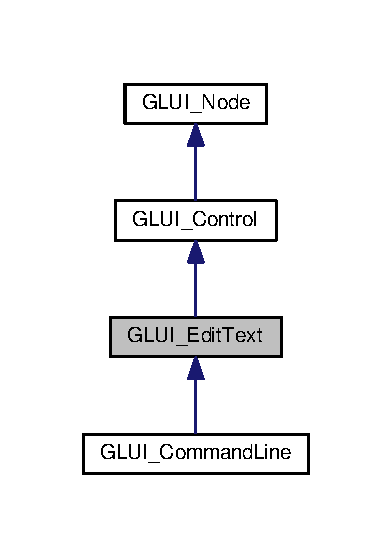
\includegraphics[width=188pt]{class_g_l_u_i___edit_text__inherit__graph}
\end{center}
\end{figure}


Collaboration diagram for G\+L\+U\+I\+\_\+\+Edit\+Text\+:\nopagebreak
\begin{figure}[H]
\begin{center}
\leavevmode
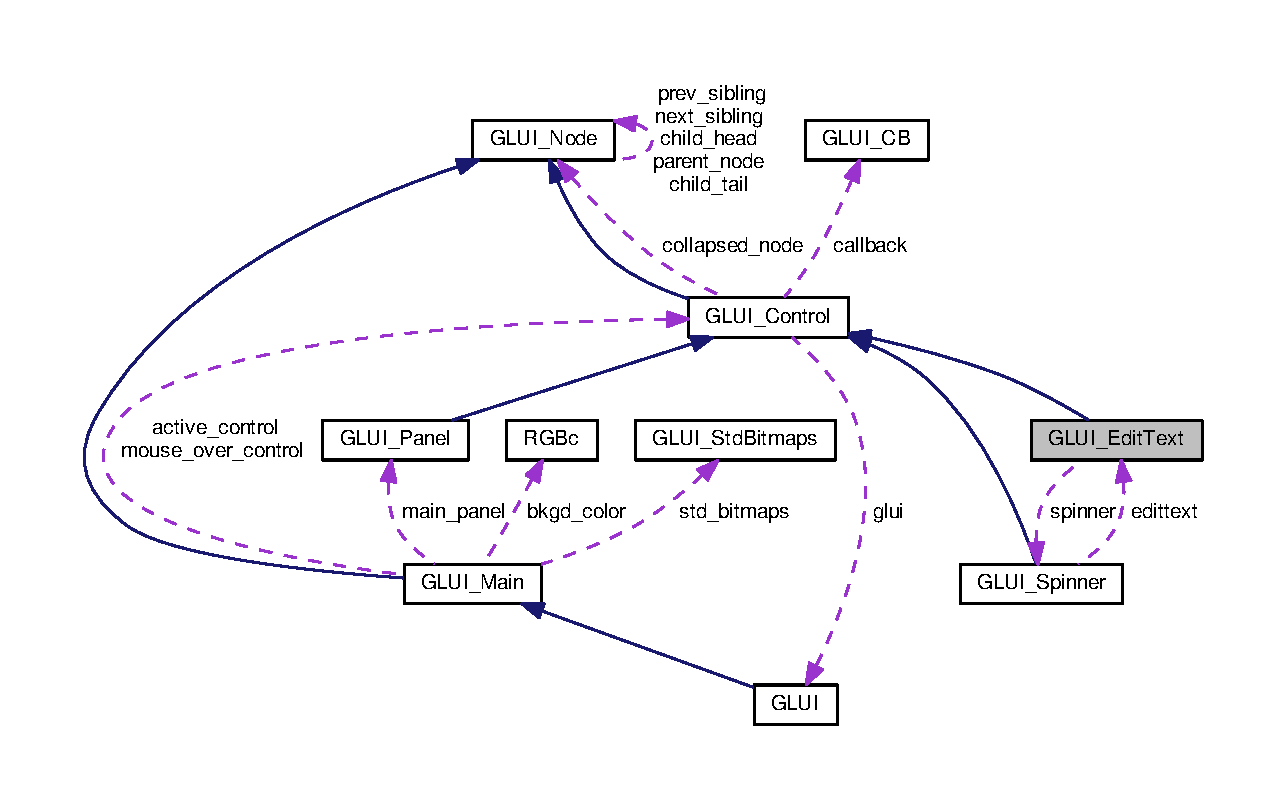
\includegraphics[width=350pt]{class_g_l_u_i___edit_text__coll__graph}
\end{center}
\end{figure}
\subsection*{Public Member Functions}
\begin{DoxyCompactItemize}
\item 
\hyperlink{wglext_8h_a500a82aecba06f4550f6849b8099ca21}{int} \hyperlink{class_g_l_u_i___edit_text_a096021e2d0b258ffee0b36988850677b}{mouse\+\_\+down\+\_\+handler} (\hyperlink{wglext_8h_a500a82aecba06f4550f6849b8099ca21}{int} local\+\_\+x, \hyperlink{wglext_8h_a500a82aecba06f4550f6849b8099ca21}{int} local\+\_\+y)
\item 
\hyperlink{wglext_8h_a500a82aecba06f4550f6849b8099ca21}{int} \hyperlink{class_g_l_u_i___edit_text_ac05967e2a8826e2bf796c65758da47ea}{mouse\+\_\+up\+\_\+handler} (\hyperlink{wglext_8h_a500a82aecba06f4550f6849b8099ca21}{int} local\+\_\+x, \hyperlink{wglext_8h_a500a82aecba06f4550f6849b8099ca21}{int} local\+\_\+y, bool inside)
\item 
\hyperlink{wglext_8h_a500a82aecba06f4550f6849b8099ca21}{int} \hyperlink{class_g_l_u_i___edit_text_af98242599d889464f6b8dfb3aa23f6b4}{mouse\+\_\+held\+\_\+down\+\_\+handler} (\hyperlink{wglext_8h_a500a82aecba06f4550f6849b8099ca21}{int} local\+\_\+x, \hyperlink{wglext_8h_a500a82aecba06f4550f6849b8099ca21}{int} local\+\_\+y, bool inside)
\item 
\hyperlink{wglext_8h_a500a82aecba06f4550f6849b8099ca21}{int} \hyperlink{class_g_l_u_i___edit_text_a92fcd78877375cb2bba3b5e9f88635b6}{key\+\_\+handler} (unsigned char key, \hyperlink{wglext_8h_a500a82aecba06f4550f6849b8099ca21}{int} modifiers)
\item 
\hyperlink{wglext_8h_a500a82aecba06f4550f6849b8099ca21}{int} \hyperlink{class_g_l_u_i___edit_text_a81478f6a0a9ba0c2dc715e0b3730077e}{special\+\_\+handler} (\hyperlink{wglext_8h_a500a82aecba06f4550f6849b8099ca21}{int} key, \hyperlink{wglext_8h_a500a82aecba06f4550f6849b8099ca21}{int} modifiers)
\item 
\hyperlink{wglext_8h_a9e6b7f1933461ef318bb000d6bd13b83}{void} \hyperlink{class_g_l_u_i___edit_text_a071ddcac9844e7d0bed23a7c0dabadd1}{activate} (\hyperlink{wglext_8h_a500a82aecba06f4550f6849b8099ca21}{int} how)
\item 
\hyperlink{wglext_8h_a9e6b7f1933461ef318bb000d6bd13b83}{void} \hyperlink{class_g_l_u_i___edit_text_a4a83b7bc0b6d60e4fa0dd797b49255ab}{deactivate} (\hyperlink{wglext_8h_a9e6b7f1933461ef318bb000d6bd13b83}{void})
\item 
\hyperlink{wglext_8h_a9e6b7f1933461ef318bb000d6bd13b83}{void} \hyperlink{class_g_l_u_i___edit_text_af5027cba2aeff900776ea1cbea37fdd8}{draw} (\hyperlink{wglext_8h_a500a82aecba06f4550f6849b8099ca21}{int} \hyperlink{glext_8h_ad77deca22f617d3f0e0eb786445689fc}{x}, \hyperlink{wglext_8h_a500a82aecba06f4550f6849b8099ca21}{int} \hyperlink{glext_8h_a9298c7ad619074f5285b32c6b72bfdea}{y})
\item 
\hyperlink{wglext_8h_a500a82aecba06f4550f6849b8099ca21}{int} \hyperlink{class_g_l_u_i___edit_text_ad21f31b7e27b0f840ee0b8a984341b38}{mouse\+\_\+over} (\hyperlink{wglext_8h_a500a82aecba06f4550f6849b8099ca21}{int} state, \hyperlink{wglext_8h_a500a82aecba06f4550f6849b8099ca21}{int} \hyperlink{glext_8h_ad77deca22f617d3f0e0eb786445689fc}{x}, \hyperlink{wglext_8h_a500a82aecba06f4550f6849b8099ca21}{int} \hyperlink{glext_8h_a9298c7ad619074f5285b32c6b72bfdea}{y})
\item 
\hyperlink{wglext_8h_a500a82aecba06f4550f6849b8099ca21}{int} \hyperlink{class_g_l_u_i___edit_text_a9ae76bc752e7f6a8ea183c8d52844f6c}{find\+\_\+word\+\_\+break} (\hyperlink{wglext_8h_a500a82aecba06f4550f6849b8099ca21}{int} \hyperlink{glext_8h_ac55adc720a3098c1b454d2a4647f4361}{start}, \hyperlink{wglext_8h_a500a82aecba06f4550f6849b8099ca21}{int} direction)
\item 
\hyperlink{wglext_8h_a500a82aecba06f4550f6849b8099ca21}{int} \hyperlink{class_g_l_u_i___edit_text_a66b06ccdabaaee5ee00e77602f1aaa73}{substring\+\_\+width} (\hyperlink{wglext_8h_a500a82aecba06f4550f6849b8099ca21}{int} \hyperlink{glext_8h_ac55adc720a3098c1b454d2a4647f4361}{start}, \hyperlink{wglext_8h_a500a82aecba06f4550f6849b8099ca21}{int} \hyperlink{glext_8h_a432111147038972f06e049e18a837002}{end})
\item 
\hyperlink{wglext_8h_a9e6b7f1933461ef318bb000d6bd13b83}{void} \hyperlink{class_g_l_u_i___edit_text_a7d8d760a5559a3317a8a080877fdab4b}{clear\+\_\+substring} (\hyperlink{wglext_8h_a500a82aecba06f4550f6849b8099ca21}{int} \hyperlink{glext_8h_ac55adc720a3098c1b454d2a4647f4361}{start}, \hyperlink{wglext_8h_a500a82aecba06f4550f6849b8099ca21}{int} \hyperlink{glext_8h_a432111147038972f06e049e18a837002}{end})
\item 
\hyperlink{wglext_8h_a500a82aecba06f4550f6849b8099ca21}{int} \hyperlink{class_g_l_u_i___edit_text_adb7c9266e9e33ec38a2d81fbe83421b2}{find\+\_\+insertion\+\_\+pt} (\hyperlink{wglext_8h_a500a82aecba06f4550f6849b8099ca21}{int} \hyperlink{glext_8h_ad77deca22f617d3f0e0eb786445689fc}{x}, \hyperlink{wglext_8h_a500a82aecba06f4550f6849b8099ca21}{int} \hyperlink{glext_8h_a9298c7ad619074f5285b32c6b72bfdea}{y})
\item 
\hyperlink{wglext_8h_a500a82aecba06f4550f6849b8099ca21}{int} \hyperlink{class_g_l_u_i___edit_text_a9787add80a6790d07796499508ebf62b}{update\+\_\+substring\+\_\+bounds} (\hyperlink{wglext_8h_a9e6b7f1933461ef318bb000d6bd13b83}{void})
\item 
\hyperlink{wglext_8h_a9e6b7f1933461ef318bb000d6bd13b83}{void} \hyperlink{class_g_l_u_i___edit_text_acbd51f12d68de3e4444ac21e709aef50}{update\+\_\+and\+\_\+draw\+\_\+text} (\hyperlink{wglext_8h_a9e6b7f1933461ef318bb000d6bd13b83}{void})
\item 
\hyperlink{wglext_8h_a9e6b7f1933461ef318bb000d6bd13b83}{void} \hyperlink{class_g_l_u_i___edit_text_a37917739d5f240356d893b3d07d9afe6}{draw\+\_\+text} (\hyperlink{wglext_8h_a500a82aecba06f4550f6849b8099ca21}{int} \hyperlink{glext_8h_ad77deca22f617d3f0e0eb786445689fc}{x}, \hyperlink{wglext_8h_a500a82aecba06f4550f6849b8099ca21}{int} \hyperlink{glext_8h_a9298c7ad619074f5285b32c6b72bfdea}{y})
\item 
\hyperlink{wglext_8h_a9e6b7f1933461ef318bb000d6bd13b83}{void} \hyperlink{class_g_l_u_i___edit_text_acc67640b9e92d5c6c84e4f685762aaf4}{draw\+\_\+insertion\+\_\+pt} (\hyperlink{wglext_8h_a9e6b7f1933461ef318bb000d6bd13b83}{void})
\item 
\hyperlink{wglext_8h_a9e6b7f1933461ef318bb000d6bd13b83}{void} \hyperlink{class_g_l_u_i___edit_text_a7b1c3f892a2c340e8c7328a260d92d08}{set\+\_\+numeric\+\_\+text} (\hyperlink{wglext_8h_a9e6b7f1933461ef318bb000d6bd13b83}{void})
\item 
\hyperlink{wglext_8h_a9e6b7f1933461ef318bb000d6bd13b83}{void} \hyperlink{class_g_l_u_i___edit_text_a7875ec7ab7213fbe52370436b4a8af8c}{update\+\_\+x\+\_\+offsets} (\hyperlink{wglext_8h_a9e6b7f1933461ef318bb000d6bd13b83}{void})
\item 
\hyperlink{wglext_8h_a9e6b7f1933461ef318bb000d6bd13b83}{void} \hyperlink{class_g_l_u_i___edit_text_acb10946b2666d84c57a321cda5ab2abb}{update\+\_\+size} (\hyperlink{wglext_8h_a9e6b7f1933461ef318bb000d6bd13b83}{void})
\item 
\hyperlink{wglext_8h_a9e6b7f1933461ef318bb000d6bd13b83}{void} \hyperlink{class_g_l_u_i___edit_text_a3b46c3540795e49983394d3bfdb89fb6}{set\+\_\+float\+\_\+limits} (float low, float high, \hyperlink{wglext_8h_a500a82aecba06f4550f6849b8099ca21}{int} limit\+\_\+type=\hyperlink{glui_8h_ac968cb6b340a4e1cad7734abc769d934}{G\+L\+U\+I\+\_\+\+L\+I\+M\+I\+T\+\_\+\+C\+L\+A\+M\+P})
\item 
\hyperlink{wglext_8h_a9e6b7f1933461ef318bb000d6bd13b83}{void} \hyperlink{class_g_l_u_i___edit_text_a5761e028dc711efdc234f7211003a500}{set\+\_\+int\+\_\+limits} (\hyperlink{wglext_8h_a500a82aecba06f4550f6849b8099ca21}{int} low, \hyperlink{wglext_8h_a500a82aecba06f4550f6849b8099ca21}{int} high, \hyperlink{wglext_8h_a500a82aecba06f4550f6849b8099ca21}{int} limit\+\_\+type=\hyperlink{glui_8h_ac968cb6b340a4e1cad7734abc769d934}{G\+L\+U\+I\+\_\+\+L\+I\+M\+I\+T\+\_\+\+C\+L\+A\+M\+P})
\item 
\hyperlink{wglext_8h_a9e6b7f1933461ef318bb000d6bd13b83}{void} \hyperlink{class_g_l_u_i___edit_text_a2c0caddce6e11b8a303c8f247b8fbf0f}{set\+\_\+float\+\_\+val} (float new\+\_\+val)
\item 
\hyperlink{wglext_8h_a9e6b7f1933461ef318bb000d6bd13b83}{void} \hyperlink{class_g_l_u_i___edit_text_a230980562d1c49166c7600f1771669bd}{set\+\_\+int\+\_\+val} (\hyperlink{wglext_8h_a500a82aecba06f4550f6849b8099ca21}{int} new\+\_\+val)
\item 
\hyperlink{wglext_8h_a9e6b7f1933461ef318bb000d6bd13b83}{void} \hyperlink{class_g_l_u_i___edit_text_aa283908f42990f6056298d6381cc19a7}{set\+\_\+text} (const char $\ast$\hyperlink{class_g_l_u_i___control_af0d60e9736f4dbc34e9a536e75876d72}{text})
\item 
\hyperlink{wglext_8h_a9e6b7f1933461ef318bb000d6bd13b83}{void} \hyperlink{class_g_l_u_i___edit_text_a0f60b8b2a59ecf51b145187483b8deb2}{set\+\_\+text} (const \hyperlink{glui_8h_aada824856f7bcf29794719981ebd8f60}{G\+L\+U\+I\+\_\+\+String} \&\hyperlink{glext_8h_a4af680a6c683f88ed67b76f207f2e6e4}{s})
\item 
const char $\ast$ \hyperlink{class_g_l_u_i___edit_text_a621ba269343beeba0346439a43e5e355}{get\+\_\+text} ()
\item 
\hyperlink{wglext_8h_a9e6b7f1933461ef318bb000d6bd13b83}{void} \hyperlink{class_g_l_u_i___edit_text_a8c553db0ecb0814a3db0da5bcf630d58}{dump} (F\+I\+L\+E $\ast$out, const char $\ast$\hyperlink{class_g_l_u_i___control_af0d60e9736f4dbc34e9a536e75876d72}{text})
\item 
\hyperlink{class_g_l_u_i___edit_text_af99784896490989539ef7638a7fd4e12}{G\+L\+U\+I\+\_\+\+Edit\+Text} (\hyperlink{class_g_l_u_i___node}{G\+L\+U\+I\+\_\+\+Node} $\ast$\hyperlink{class_g_l_u_i___node_a8ed65d447784f6f88bd3e2e2bcac6cdb}{parent}, const char $\ast$\hyperlink{glext_8h_ad977737dfc9a274a62741b9500c49a32}{name}, \hyperlink{wglext_8h_a500a82aecba06f4550f6849b8099ca21}{int} text\+\_\+type=\hyperlink{glui_8h_a5e7e137e5f35f2859b135d8924719d27}{G\+L\+U\+I\+\_\+\+E\+D\+I\+T\+T\+E\+X\+T\+\_\+\+T\+E\+X\+T}, \hyperlink{wglext_8h_a500a82aecba06f4550f6849b8099ca21}{int} \hyperlink{glext_8h_a58c2a664503e14ffb8f21012aabff3e9}{id}=-\/1, \hyperlink{class_g_l_u_i___c_b}{G\+L\+U\+I\+\_\+\+C\+B} \hyperlink{class_g_l_u_i___control_a96060fe0cc6d537e736dd6eef78e24ab}{callback}=\hyperlink{class_g_l_u_i___c_b}{G\+L\+U\+I\+\_\+\+C\+B}())
\item 
\hyperlink{class_g_l_u_i___edit_text_acde777046eb65672c70c51b5728e7c3f}{G\+L\+U\+I\+\_\+\+Edit\+Text} (\hyperlink{class_g_l_u_i___node}{G\+L\+U\+I\+\_\+\+Node} $\ast$\hyperlink{class_g_l_u_i___node_a8ed65d447784f6f88bd3e2e2bcac6cdb}{parent}, const char $\ast$\hyperlink{glext_8h_ad977737dfc9a274a62741b9500c49a32}{name}, \hyperlink{wglext_8h_a500a82aecba06f4550f6849b8099ca21}{int} $\ast$live\+\_\+var, \hyperlink{wglext_8h_a500a82aecba06f4550f6849b8099ca21}{int} \hyperlink{glext_8h_a58c2a664503e14ffb8f21012aabff3e9}{id}=-\/1, \hyperlink{class_g_l_u_i___c_b}{G\+L\+U\+I\+\_\+\+C\+B} \hyperlink{class_g_l_u_i___control_a96060fe0cc6d537e736dd6eef78e24ab}{callback}=\hyperlink{class_g_l_u_i___c_b}{G\+L\+U\+I\+\_\+\+C\+B}())
\item 
\hyperlink{class_g_l_u_i___edit_text_adad7d18bc05da4e6aecfea680c0a0a65}{G\+L\+U\+I\+\_\+\+Edit\+Text} (\hyperlink{class_g_l_u_i___node}{G\+L\+U\+I\+\_\+\+Node} $\ast$\hyperlink{class_g_l_u_i___node_a8ed65d447784f6f88bd3e2e2bcac6cdb}{parent}, const char $\ast$\hyperlink{glext_8h_ad977737dfc9a274a62741b9500c49a32}{name}, float $\ast$live\+\_\+var, \hyperlink{wglext_8h_a500a82aecba06f4550f6849b8099ca21}{int} \hyperlink{glext_8h_a58c2a664503e14ffb8f21012aabff3e9}{id}=-\/1, \hyperlink{class_g_l_u_i___c_b}{G\+L\+U\+I\+\_\+\+C\+B} \hyperlink{class_g_l_u_i___control_a96060fe0cc6d537e736dd6eef78e24ab}{callback}=\hyperlink{class_g_l_u_i___c_b}{G\+L\+U\+I\+\_\+\+C\+B}())
\item 
\hyperlink{class_g_l_u_i___edit_text_a85fadf933a22982801659cec28d159f1}{G\+L\+U\+I\+\_\+\+Edit\+Text} (\hyperlink{class_g_l_u_i___node}{G\+L\+U\+I\+\_\+\+Node} $\ast$\hyperlink{class_g_l_u_i___node_a8ed65d447784f6f88bd3e2e2bcac6cdb}{parent}, const char $\ast$\hyperlink{glext_8h_ad977737dfc9a274a62741b9500c49a32}{name}, char $\ast$live\+\_\+var, \hyperlink{wglext_8h_a500a82aecba06f4550f6849b8099ca21}{int} \hyperlink{glext_8h_a58c2a664503e14ffb8f21012aabff3e9}{id}=-\/1, \hyperlink{class_g_l_u_i___c_b}{G\+L\+U\+I\+\_\+\+C\+B} \hyperlink{class_g_l_u_i___control_a96060fe0cc6d537e736dd6eef78e24ab}{callback}=\hyperlink{class_g_l_u_i___c_b}{G\+L\+U\+I\+\_\+\+C\+B}())
\item 
\hyperlink{class_g_l_u_i___edit_text_a721bd71256ee84de33682e0bf926e6a3}{G\+L\+U\+I\+\_\+\+Edit\+Text} (\hyperlink{class_g_l_u_i___node}{G\+L\+U\+I\+\_\+\+Node} $\ast$\hyperlink{class_g_l_u_i___node_a8ed65d447784f6f88bd3e2e2bcac6cdb}{parent}, const char $\ast$\hyperlink{glext_8h_ad977737dfc9a274a62741b9500c49a32}{name}, \hyperlink{glext_8h_ae84541b4f3d8e1ea24ec0f466a8c568b}{std\+::string} \&live\+\_\+var, \hyperlink{wglext_8h_a500a82aecba06f4550f6849b8099ca21}{int} \hyperlink{glext_8h_a58c2a664503e14ffb8f21012aabff3e9}{id}=-\/1, \hyperlink{class_g_l_u_i___c_b}{G\+L\+U\+I\+\_\+\+C\+B} \hyperlink{class_g_l_u_i___control_a96060fe0cc6d537e736dd6eef78e24ab}{callback}=\hyperlink{class_g_l_u_i___c_b}{G\+L\+U\+I\+\_\+\+C\+B}())
\item 
\hyperlink{class_g_l_u_i___edit_text_a5aa2fc60832f1c93046a047084256474}{G\+L\+U\+I\+\_\+\+Edit\+Text} (\hyperlink{class_g_l_u_i___node}{G\+L\+U\+I\+\_\+\+Node} $\ast$\hyperlink{class_g_l_u_i___node_a8ed65d447784f6f88bd3e2e2bcac6cdb}{parent}, const char $\ast$\hyperlink{glext_8h_ad977737dfc9a274a62741b9500c49a32}{name}, \hyperlink{wglext_8h_a500a82aecba06f4550f6849b8099ca21}{int} text\+\_\+type, \hyperlink{wglext_8h_a9e6b7f1933461ef318bb000d6bd13b83}{void} $\ast$live\+\_\+var, \hyperlink{wglext_8h_a500a82aecba06f4550f6849b8099ca21}{int} \hyperlink{glext_8h_a58c2a664503e14ffb8f21012aabff3e9}{id}, \hyperlink{class_g_l_u_i___c_b}{G\+L\+U\+I\+\_\+\+C\+B} \hyperlink{class_g_l_u_i___control_a96060fe0cc6d537e736dd6eef78e24ab}{callback})
\item 
\hyperlink{class_g_l_u_i___edit_text_a05a7b7a6080a6cf28f19568dbb2c723c}{G\+L\+U\+I\+\_\+\+Edit\+Text} (\hyperlink{wglext_8h_a9e6b7f1933461ef318bb000d6bd13b83}{void})
\end{DoxyCompactItemize}
\subsection*{Public Attributes}
\begin{DoxyCompactItemize}
\item 
\hyperlink{wglext_8h_a500a82aecba06f4550f6849b8099ca21}{int} \hyperlink{class_g_l_u_i___edit_text_a2b89e775b0f4b989aee27cae59899a90}{has\+\_\+limits}
\item 
\hyperlink{wglext_8h_a500a82aecba06f4550f6849b8099ca21}{int} \hyperlink{class_g_l_u_i___edit_text_a790a6e20d384d0f2eb4f9d4014aa9f95}{data\+\_\+type}
\item 
\hyperlink{glui_8h_aada824856f7bcf29794719981ebd8f60}{G\+L\+U\+I\+\_\+\+String} \hyperlink{class_g_l_u_i___edit_text_ab65d3fccc51fefbfaf9da1dcd5ab8788}{orig\+\_\+text}
\item 
\hyperlink{wglext_8h_a500a82aecba06f4550f6849b8099ca21}{int} \hyperlink{class_g_l_u_i___edit_text_aa33884c39bf3ec7be573a345094ac590}{insertion\+\_\+pt}
\item 
\hyperlink{wglext_8h_a500a82aecba06f4550f6849b8099ca21}{int} \hyperlink{class_g_l_u_i___edit_text_aed30e771b57b3a9bcc708fba638666e6}{title\+\_\+x\+\_\+offset}
\item 
\hyperlink{wglext_8h_a500a82aecba06f4550f6849b8099ca21}{int} \hyperlink{class_g_l_u_i___edit_text_ad9e34b0c8c1636883b6cb8c6e8eaae7d}{text\+\_\+x\+\_\+offset}
\item 
\hyperlink{wglext_8h_a500a82aecba06f4550f6849b8099ca21}{int} \hyperlink{class_g_l_u_i___edit_text_aa3ed3842b39fb5e9094ffcd76729ea60}{substring\+\_\+start}
\item 
\hyperlink{wglext_8h_a500a82aecba06f4550f6849b8099ca21}{int} \hyperlink{class_g_l_u_i___edit_text_a39f38fdd484b82a55c020c9f80add5d4}{substring\+\_\+end}
\item 
\hyperlink{wglext_8h_a500a82aecba06f4550f6849b8099ca21}{int} \hyperlink{class_g_l_u_i___edit_text_adb68126f2422d08039af5a23a4761ab2}{sel\+\_\+start}
\item 
\hyperlink{wglext_8h_a500a82aecba06f4550f6849b8099ca21}{int} \hyperlink{class_g_l_u_i___edit_text_ae757e323598b216dd656acb6bd36ce03}{sel\+\_\+end}
\item 
\hyperlink{wglext_8h_a500a82aecba06f4550f6849b8099ca21}{int} \hyperlink{class_g_l_u_i___edit_text_a233d380e8b9fed7d5d1314888525297d}{num\+\_\+periods}
\item 
\hyperlink{wglext_8h_a500a82aecba06f4550f6849b8099ca21}{int} \hyperlink{class_g_l_u_i___edit_text_a66e1c808ae9587293d0a17208e7eb1db}{last\+\_\+insertion\+\_\+pt}
\item 
float \hyperlink{class_g_l_u_i___edit_text_ac7f609e99bd8732d5026c7f57d5c8cd9}{float\+\_\+low}
\item 
float \hyperlink{class_g_l_u_i___edit_text_abb9f58f751bb995c3c8e52dc5c085bfd}{float\+\_\+high}
\item 
\hyperlink{wglext_8h_a500a82aecba06f4550f6849b8099ca21}{int} \hyperlink{class_g_l_u_i___edit_text_a99eb694c9998c637125763cdd91b2280}{int\+\_\+low}
\item 
\hyperlink{wglext_8h_a500a82aecba06f4550f6849b8099ca21}{int} \hyperlink{class_g_l_u_i___edit_text_abd03f72719e48cadb42bb4b297b378f4}{int\+\_\+high}
\item 
\hyperlink{class_g_l_u_i___spinner}{G\+L\+U\+I\+\_\+\+Spinner} $\ast$ \hyperlink{class_g_l_u_i___edit_text_a3d459f1fc60af26ac844283a87599a08}{spinner}
\item 
\hyperlink{wglext_8h_a500a82aecba06f4550f6849b8099ca21}{int} \hyperlink{class_g_l_u_i___edit_text_ad6006ae65e038eb60f011c8c7200b9ea}{debug}
\item 
\hyperlink{wglext_8h_a500a82aecba06f4550f6849b8099ca21}{int} \hyperlink{class_g_l_u_i___edit_text_aa6044d58c37fd18e9b5e83a153cfd108}{draw\+\_\+text\+\_\+only}
\end{DoxyCompactItemize}
\subsection*{Protected Member Functions}
\begin{DoxyCompactItemize}
\item 
\hyperlink{wglext_8h_a9e6b7f1933461ef318bb000d6bd13b83}{void} \hyperlink{class_g_l_u_i___edit_text_a3378e23e1470293a4758f729b899cae1}{common\+\_\+init} (\hyperlink{wglext_8h_a9e6b7f1933461ef318bb000d6bd13b83}{void})
\item 
\hyperlink{wglext_8h_a9e6b7f1933461ef318bb000d6bd13b83}{void} \hyperlink{class_g_l_u_i___edit_text_a35813da027699537c43e39912c3d77cd}{common\+\_\+construct} (\hyperlink{class_g_l_u_i___node}{G\+L\+U\+I\+\_\+\+Node} $\ast$\hyperlink{class_g_l_u_i___node_a8ed65d447784f6f88bd3e2e2bcac6cdb}{parent}, const char $\ast$\hyperlink{glext_8h_ad977737dfc9a274a62741b9500c49a32}{name}, \hyperlink{wglext_8h_a500a82aecba06f4550f6849b8099ca21}{int} \hyperlink{class_g_l_u_i___edit_text_a790a6e20d384d0f2eb4f9d4014aa9f95}{data\+\_\+type}, \hyperlink{wglext_8h_a500a82aecba06f4550f6849b8099ca21}{int} \hyperlink{class_g_l_u_i___control_a8ba7cae809a47dd870592aa2cc85483b}{live\+\_\+type}, \hyperlink{wglext_8h_a9e6b7f1933461ef318bb000d6bd13b83}{void} $\ast$live\+\_\+var, \hyperlink{wglext_8h_a500a82aecba06f4550f6849b8099ca21}{int} \hyperlink{glext_8h_a58c2a664503e14ffb8f21012aabff3e9}{id}, \hyperlink{class_g_l_u_i___c_b}{G\+L\+U\+I\+\_\+\+C\+B} \hyperlink{class_g_l_u_i___control_a96060fe0cc6d537e736dd6eef78e24ab}{callback})
\end{DoxyCompactItemize}
\subsection*{Additional Inherited Members}


\subsection{Detailed Description}


Definition at line 1579 of file glui.\+h.



\subsection{Constructor \& Destructor Documentation}
\hypertarget{class_g_l_u_i___edit_text_af99784896490989539ef7638a7fd4e12}{\index{G\+L\+U\+I\+\_\+\+Edit\+Text@{G\+L\+U\+I\+\_\+\+Edit\+Text}!G\+L\+U\+I\+\_\+\+Edit\+Text@{G\+L\+U\+I\+\_\+\+Edit\+Text}}
\index{G\+L\+U\+I\+\_\+\+Edit\+Text@{G\+L\+U\+I\+\_\+\+Edit\+Text}!G\+L\+U\+I\+\_\+\+Edit\+Text@{G\+L\+U\+I\+\_\+\+Edit\+Text}}
\subsubsection[{G\+L\+U\+I\+\_\+\+Edit\+Text}]{\setlength{\rightskip}{0pt plus 5cm}G\+L\+U\+I\+\_\+\+Edit\+Text\+::\+G\+L\+U\+I\+\_\+\+Edit\+Text (
\begin{DoxyParamCaption}
\item[{{\bf G\+L\+U\+I\+\_\+\+Node} $\ast$}]{parent, }
\item[{const char $\ast$}]{name, }
\item[{{\bf int}}]{text\+\_\+type = {\ttfamily {\bf G\+L\+U\+I\+\_\+\+E\+D\+I\+T\+T\+E\+X\+T\+\_\+\+T\+E\+X\+T}}, }
\item[{{\bf int}}]{id = {\ttfamily -\/1}, }
\item[{{\bf G\+L\+U\+I\+\_\+\+C\+B}}]{callback = {\ttfamily {\bf G\+L\+U\+I\+\_\+\+C\+B}()}}
\end{DoxyParamCaption}
)}}\label{class_g_l_u_i___edit_text_af99784896490989539ef7638a7fd4e12}
\hypertarget{class_g_l_u_i___edit_text_acde777046eb65672c70c51b5728e7c3f}{\index{G\+L\+U\+I\+\_\+\+Edit\+Text@{G\+L\+U\+I\+\_\+\+Edit\+Text}!G\+L\+U\+I\+\_\+\+Edit\+Text@{G\+L\+U\+I\+\_\+\+Edit\+Text}}
\index{G\+L\+U\+I\+\_\+\+Edit\+Text@{G\+L\+U\+I\+\_\+\+Edit\+Text}!G\+L\+U\+I\+\_\+\+Edit\+Text@{G\+L\+U\+I\+\_\+\+Edit\+Text}}
\subsubsection[{G\+L\+U\+I\+\_\+\+Edit\+Text}]{\setlength{\rightskip}{0pt plus 5cm}G\+L\+U\+I\+\_\+\+Edit\+Text\+::\+G\+L\+U\+I\+\_\+\+Edit\+Text (
\begin{DoxyParamCaption}
\item[{{\bf G\+L\+U\+I\+\_\+\+Node} $\ast$}]{parent, }
\item[{const char $\ast$}]{name, }
\item[{{\bf int} $\ast$}]{live\+\_\+var, }
\item[{{\bf int}}]{id = {\ttfamily -\/1}, }
\item[{{\bf G\+L\+U\+I\+\_\+\+C\+B}}]{callback = {\ttfamily {\bf G\+L\+U\+I\+\_\+\+C\+B}()}}
\end{DoxyParamCaption}
)}}\label{class_g_l_u_i___edit_text_acde777046eb65672c70c51b5728e7c3f}
\hypertarget{class_g_l_u_i___edit_text_adad7d18bc05da4e6aecfea680c0a0a65}{\index{G\+L\+U\+I\+\_\+\+Edit\+Text@{G\+L\+U\+I\+\_\+\+Edit\+Text}!G\+L\+U\+I\+\_\+\+Edit\+Text@{G\+L\+U\+I\+\_\+\+Edit\+Text}}
\index{G\+L\+U\+I\+\_\+\+Edit\+Text@{G\+L\+U\+I\+\_\+\+Edit\+Text}!G\+L\+U\+I\+\_\+\+Edit\+Text@{G\+L\+U\+I\+\_\+\+Edit\+Text}}
\subsubsection[{G\+L\+U\+I\+\_\+\+Edit\+Text}]{\setlength{\rightskip}{0pt plus 5cm}G\+L\+U\+I\+\_\+\+Edit\+Text\+::\+G\+L\+U\+I\+\_\+\+Edit\+Text (
\begin{DoxyParamCaption}
\item[{{\bf G\+L\+U\+I\+\_\+\+Node} $\ast$}]{parent, }
\item[{const char $\ast$}]{name, }
\item[{float $\ast$}]{live\+\_\+var, }
\item[{{\bf int}}]{id = {\ttfamily -\/1}, }
\item[{{\bf G\+L\+U\+I\+\_\+\+C\+B}}]{callback = {\ttfamily {\bf G\+L\+U\+I\+\_\+\+C\+B}()}}
\end{DoxyParamCaption}
)}}\label{class_g_l_u_i___edit_text_adad7d18bc05da4e6aecfea680c0a0a65}
\hypertarget{class_g_l_u_i___edit_text_a85fadf933a22982801659cec28d159f1}{\index{G\+L\+U\+I\+\_\+\+Edit\+Text@{G\+L\+U\+I\+\_\+\+Edit\+Text}!G\+L\+U\+I\+\_\+\+Edit\+Text@{G\+L\+U\+I\+\_\+\+Edit\+Text}}
\index{G\+L\+U\+I\+\_\+\+Edit\+Text@{G\+L\+U\+I\+\_\+\+Edit\+Text}!G\+L\+U\+I\+\_\+\+Edit\+Text@{G\+L\+U\+I\+\_\+\+Edit\+Text}}
\subsubsection[{G\+L\+U\+I\+\_\+\+Edit\+Text}]{\setlength{\rightskip}{0pt plus 5cm}G\+L\+U\+I\+\_\+\+Edit\+Text\+::\+G\+L\+U\+I\+\_\+\+Edit\+Text (
\begin{DoxyParamCaption}
\item[{{\bf G\+L\+U\+I\+\_\+\+Node} $\ast$}]{parent, }
\item[{const char $\ast$}]{name, }
\item[{char $\ast$}]{live\+\_\+var, }
\item[{{\bf int}}]{id = {\ttfamily -\/1}, }
\item[{{\bf G\+L\+U\+I\+\_\+\+C\+B}}]{callback = {\ttfamily {\bf G\+L\+U\+I\+\_\+\+C\+B}()}}
\end{DoxyParamCaption}
)}}\label{class_g_l_u_i___edit_text_a85fadf933a22982801659cec28d159f1}
\hypertarget{class_g_l_u_i___edit_text_a721bd71256ee84de33682e0bf926e6a3}{\index{G\+L\+U\+I\+\_\+\+Edit\+Text@{G\+L\+U\+I\+\_\+\+Edit\+Text}!G\+L\+U\+I\+\_\+\+Edit\+Text@{G\+L\+U\+I\+\_\+\+Edit\+Text}}
\index{G\+L\+U\+I\+\_\+\+Edit\+Text@{G\+L\+U\+I\+\_\+\+Edit\+Text}!G\+L\+U\+I\+\_\+\+Edit\+Text@{G\+L\+U\+I\+\_\+\+Edit\+Text}}
\subsubsection[{G\+L\+U\+I\+\_\+\+Edit\+Text}]{\setlength{\rightskip}{0pt plus 5cm}G\+L\+U\+I\+\_\+\+Edit\+Text\+::\+G\+L\+U\+I\+\_\+\+Edit\+Text (
\begin{DoxyParamCaption}
\item[{{\bf G\+L\+U\+I\+\_\+\+Node} $\ast$}]{parent, }
\item[{const char $\ast$}]{name, }
\item[{{\bf std\+::string} \&}]{live\+\_\+var, }
\item[{{\bf int}}]{id = {\ttfamily -\/1}, }
\item[{{\bf G\+L\+U\+I\+\_\+\+C\+B}}]{callback = {\ttfamily {\bf G\+L\+U\+I\+\_\+\+C\+B}()}}
\end{DoxyParamCaption}
)}}\label{class_g_l_u_i___edit_text_a721bd71256ee84de33682e0bf926e6a3}
\hypertarget{class_g_l_u_i___edit_text_a5aa2fc60832f1c93046a047084256474}{\index{G\+L\+U\+I\+\_\+\+Edit\+Text@{G\+L\+U\+I\+\_\+\+Edit\+Text}!G\+L\+U\+I\+\_\+\+Edit\+Text@{G\+L\+U\+I\+\_\+\+Edit\+Text}}
\index{G\+L\+U\+I\+\_\+\+Edit\+Text@{G\+L\+U\+I\+\_\+\+Edit\+Text}!G\+L\+U\+I\+\_\+\+Edit\+Text@{G\+L\+U\+I\+\_\+\+Edit\+Text}}
\subsubsection[{G\+L\+U\+I\+\_\+\+Edit\+Text}]{\setlength{\rightskip}{0pt plus 5cm}G\+L\+U\+I\+\_\+\+Edit\+Text\+::\+G\+L\+U\+I\+\_\+\+Edit\+Text (
\begin{DoxyParamCaption}
\item[{{\bf G\+L\+U\+I\+\_\+\+Node} $\ast$}]{parent, }
\item[{const char $\ast$}]{name, }
\item[{{\bf int}}]{text\+\_\+type, }
\item[{{\bf void} $\ast$}]{live\+\_\+var, }
\item[{{\bf int}}]{id, }
\item[{{\bf G\+L\+U\+I\+\_\+\+C\+B}}]{callback}
\end{DoxyParamCaption}
)}}\label{class_g_l_u_i___edit_text_a5aa2fc60832f1c93046a047084256474}
\hypertarget{class_g_l_u_i___edit_text_a05a7b7a6080a6cf28f19568dbb2c723c}{\index{G\+L\+U\+I\+\_\+\+Edit\+Text@{G\+L\+U\+I\+\_\+\+Edit\+Text}!G\+L\+U\+I\+\_\+\+Edit\+Text@{G\+L\+U\+I\+\_\+\+Edit\+Text}}
\index{G\+L\+U\+I\+\_\+\+Edit\+Text@{G\+L\+U\+I\+\_\+\+Edit\+Text}!G\+L\+U\+I\+\_\+\+Edit\+Text@{G\+L\+U\+I\+\_\+\+Edit\+Text}}
\subsubsection[{G\+L\+U\+I\+\_\+\+Edit\+Text}]{\setlength{\rightskip}{0pt plus 5cm}G\+L\+U\+I\+\_\+\+Edit\+Text\+::\+G\+L\+U\+I\+\_\+\+Edit\+Text (
\begin{DoxyParamCaption}
\item[{{\bf void}}]{}
\end{DoxyParamCaption}
)\hspace{0.3cm}{\ttfamily [inline]}}}\label{class_g_l_u_i___edit_text_a05a7b7a6080a6cf28f19568dbb2c723c}


Definition at line 1661 of file glui.\+h.



\subsection{Member Function Documentation}
\hypertarget{class_g_l_u_i___edit_text_a071ddcac9844e7d0bed23a7c0dabadd1}{\index{G\+L\+U\+I\+\_\+\+Edit\+Text@{G\+L\+U\+I\+\_\+\+Edit\+Text}!activate@{activate}}
\index{activate@{activate}!G\+L\+U\+I\+\_\+\+Edit\+Text@{G\+L\+U\+I\+\_\+\+Edit\+Text}}
\subsubsection[{activate}]{\setlength{\rightskip}{0pt plus 5cm}{\bf void} G\+L\+U\+I\+\_\+\+Edit\+Text\+::activate (
\begin{DoxyParamCaption}
\item[{{\bf int}}]{how}
\end{DoxyParamCaption}
)\hspace{0.3cm}{\ttfamily [virtual]}}}\label{class_g_l_u_i___edit_text_a071ddcac9844e7d0bed23a7c0dabadd1}


Reimplemented from \hyperlink{class_g_l_u_i___control_af686704718daf4761d17e4da83c03aad}{G\+L\+U\+I\+\_\+\+Control}.

\hypertarget{class_g_l_u_i___edit_text_a7d8d760a5559a3317a8a080877fdab4b}{\index{G\+L\+U\+I\+\_\+\+Edit\+Text@{G\+L\+U\+I\+\_\+\+Edit\+Text}!clear\+\_\+substring@{clear\+\_\+substring}}
\index{clear\+\_\+substring@{clear\+\_\+substring}!G\+L\+U\+I\+\_\+\+Edit\+Text@{G\+L\+U\+I\+\_\+\+Edit\+Text}}
\subsubsection[{clear\+\_\+substring}]{\setlength{\rightskip}{0pt plus 5cm}{\bf void} G\+L\+U\+I\+\_\+\+Edit\+Text\+::clear\+\_\+substring (
\begin{DoxyParamCaption}
\item[{{\bf int}}]{start, }
\item[{{\bf int}}]{end}
\end{DoxyParamCaption}
)}}\label{class_g_l_u_i___edit_text_a7d8d760a5559a3317a8a080877fdab4b}
\hypertarget{class_g_l_u_i___edit_text_a35813da027699537c43e39912c3d77cd}{\index{G\+L\+U\+I\+\_\+\+Edit\+Text@{G\+L\+U\+I\+\_\+\+Edit\+Text}!common\+\_\+construct@{common\+\_\+construct}}
\index{common\+\_\+construct@{common\+\_\+construct}!G\+L\+U\+I\+\_\+\+Edit\+Text@{G\+L\+U\+I\+\_\+\+Edit\+Text}}
\subsubsection[{common\+\_\+construct}]{\setlength{\rightskip}{0pt plus 5cm}{\bf void} G\+L\+U\+I\+\_\+\+Edit\+Text\+::common\+\_\+construct (
\begin{DoxyParamCaption}
\item[{{\bf G\+L\+U\+I\+\_\+\+Node} $\ast$}]{parent, }
\item[{const char $\ast$}]{name, }
\item[{{\bf int}}]{data\+\_\+type, }
\item[{{\bf int}}]{live\+\_\+type, }
\item[{{\bf void} $\ast$}]{live\+\_\+var, }
\item[{{\bf int}}]{id, }
\item[{{\bf G\+L\+U\+I\+\_\+\+C\+B}}]{callback}
\end{DoxyParamCaption}
)\hspace{0.3cm}{\ttfamily [protected]}}}\label{class_g_l_u_i___edit_text_a35813da027699537c43e39912c3d77cd}
\hypertarget{class_g_l_u_i___edit_text_a3378e23e1470293a4758f729b899cae1}{\index{G\+L\+U\+I\+\_\+\+Edit\+Text@{G\+L\+U\+I\+\_\+\+Edit\+Text}!common\+\_\+init@{common\+\_\+init}}
\index{common\+\_\+init@{common\+\_\+init}!G\+L\+U\+I\+\_\+\+Edit\+Text@{G\+L\+U\+I\+\_\+\+Edit\+Text}}
\subsubsection[{common\+\_\+init}]{\setlength{\rightskip}{0pt plus 5cm}{\bf void} G\+L\+U\+I\+\_\+\+Edit\+Text\+::common\+\_\+init (
\begin{DoxyParamCaption}
\item[{{\bf void}}]{}
\end{DoxyParamCaption}
)\hspace{0.3cm}{\ttfamily [inline]}, {\ttfamily [protected]}}}\label{class_g_l_u_i___edit_text_a3378e23e1470293a4758f729b899cae1}


Definition at line 1664 of file glui.\+h.

\hypertarget{class_g_l_u_i___edit_text_a4a83b7bc0b6d60e4fa0dd797b49255ab}{\index{G\+L\+U\+I\+\_\+\+Edit\+Text@{G\+L\+U\+I\+\_\+\+Edit\+Text}!deactivate@{deactivate}}
\index{deactivate@{deactivate}!G\+L\+U\+I\+\_\+\+Edit\+Text@{G\+L\+U\+I\+\_\+\+Edit\+Text}}
\subsubsection[{deactivate}]{\setlength{\rightskip}{0pt plus 5cm}{\bf void} G\+L\+U\+I\+\_\+\+Edit\+Text\+::deactivate (
\begin{DoxyParamCaption}
\item[{{\bf void}}]{}
\end{DoxyParamCaption}
)\hspace{0.3cm}{\ttfamily [virtual]}}}\label{class_g_l_u_i___edit_text_a4a83b7bc0b6d60e4fa0dd797b49255ab}


Reimplemented from \hyperlink{class_g_l_u_i___control_a9d18764a6cfe25c220c845eff480d4fe}{G\+L\+U\+I\+\_\+\+Control}.



Reimplemented in \hyperlink{class_g_l_u_i___command_line_a827fe6510aa5a38b0d2c5d016a93e1ba}{G\+L\+U\+I\+\_\+\+Command\+Line}.

\hypertarget{class_g_l_u_i___edit_text_af5027cba2aeff900776ea1cbea37fdd8}{\index{G\+L\+U\+I\+\_\+\+Edit\+Text@{G\+L\+U\+I\+\_\+\+Edit\+Text}!draw@{draw}}
\index{draw@{draw}!G\+L\+U\+I\+\_\+\+Edit\+Text@{G\+L\+U\+I\+\_\+\+Edit\+Text}}
\subsubsection[{draw}]{\setlength{\rightskip}{0pt plus 5cm}{\bf void} G\+L\+U\+I\+\_\+\+Edit\+Text\+::draw (
\begin{DoxyParamCaption}
\item[{{\bf int}}]{x, }
\item[{{\bf int}}]{y}
\end{DoxyParamCaption}
)\hspace{0.3cm}{\ttfamily [virtual]}}}\label{class_g_l_u_i___edit_text_af5027cba2aeff900776ea1cbea37fdd8}


Implements \hyperlink{class_g_l_u_i___control_a2eb42d7a7951280ad2fe8c37972bf66a}{G\+L\+U\+I\+\_\+\+Control}.

\hypertarget{class_g_l_u_i___edit_text_acc67640b9e92d5c6c84e4f685762aaf4}{\index{G\+L\+U\+I\+\_\+\+Edit\+Text@{G\+L\+U\+I\+\_\+\+Edit\+Text}!draw\+\_\+insertion\+\_\+pt@{draw\+\_\+insertion\+\_\+pt}}
\index{draw\+\_\+insertion\+\_\+pt@{draw\+\_\+insertion\+\_\+pt}!G\+L\+U\+I\+\_\+\+Edit\+Text@{G\+L\+U\+I\+\_\+\+Edit\+Text}}
\subsubsection[{draw\+\_\+insertion\+\_\+pt}]{\setlength{\rightskip}{0pt plus 5cm}{\bf void} G\+L\+U\+I\+\_\+\+Edit\+Text\+::draw\+\_\+insertion\+\_\+pt (
\begin{DoxyParamCaption}
\item[{{\bf void}}]{}
\end{DoxyParamCaption}
)}}\label{class_g_l_u_i___edit_text_acc67640b9e92d5c6c84e4f685762aaf4}
\hypertarget{class_g_l_u_i___edit_text_a37917739d5f240356d893b3d07d9afe6}{\index{G\+L\+U\+I\+\_\+\+Edit\+Text@{G\+L\+U\+I\+\_\+\+Edit\+Text}!draw\+\_\+text@{draw\+\_\+text}}
\index{draw\+\_\+text@{draw\+\_\+text}!G\+L\+U\+I\+\_\+\+Edit\+Text@{G\+L\+U\+I\+\_\+\+Edit\+Text}}
\subsubsection[{draw\+\_\+text}]{\setlength{\rightskip}{0pt plus 5cm}{\bf void} G\+L\+U\+I\+\_\+\+Edit\+Text\+::draw\+\_\+text (
\begin{DoxyParamCaption}
\item[{{\bf int}}]{x, }
\item[{{\bf int}}]{y}
\end{DoxyParamCaption}
)}}\label{class_g_l_u_i___edit_text_a37917739d5f240356d893b3d07d9afe6}
\hypertarget{class_g_l_u_i___edit_text_a8c553db0ecb0814a3db0da5bcf630d58}{\index{G\+L\+U\+I\+\_\+\+Edit\+Text@{G\+L\+U\+I\+\_\+\+Edit\+Text}!dump@{dump}}
\index{dump@{dump}!G\+L\+U\+I\+\_\+\+Edit\+Text@{G\+L\+U\+I\+\_\+\+Edit\+Text}}
\subsubsection[{dump}]{\setlength{\rightskip}{0pt plus 5cm}{\bf void} G\+L\+U\+I\+\_\+\+Edit\+Text\+::dump (
\begin{DoxyParamCaption}
\item[{F\+I\+L\+E $\ast$}]{out, }
\item[{const char $\ast$}]{text}
\end{DoxyParamCaption}
)}}\label{class_g_l_u_i___edit_text_a8c553db0ecb0814a3db0da5bcf630d58}
\hypertarget{class_g_l_u_i___edit_text_adb7c9266e9e33ec38a2d81fbe83421b2}{\index{G\+L\+U\+I\+\_\+\+Edit\+Text@{G\+L\+U\+I\+\_\+\+Edit\+Text}!find\+\_\+insertion\+\_\+pt@{find\+\_\+insertion\+\_\+pt}}
\index{find\+\_\+insertion\+\_\+pt@{find\+\_\+insertion\+\_\+pt}!G\+L\+U\+I\+\_\+\+Edit\+Text@{G\+L\+U\+I\+\_\+\+Edit\+Text}}
\subsubsection[{find\+\_\+insertion\+\_\+pt}]{\setlength{\rightskip}{0pt plus 5cm}{\bf int} G\+L\+U\+I\+\_\+\+Edit\+Text\+::find\+\_\+insertion\+\_\+pt (
\begin{DoxyParamCaption}
\item[{{\bf int}}]{x, }
\item[{{\bf int}}]{y}
\end{DoxyParamCaption}
)}}\label{class_g_l_u_i___edit_text_adb7c9266e9e33ec38a2d81fbe83421b2}
\hypertarget{class_g_l_u_i___edit_text_a9ae76bc752e7f6a8ea183c8d52844f6c}{\index{G\+L\+U\+I\+\_\+\+Edit\+Text@{G\+L\+U\+I\+\_\+\+Edit\+Text}!find\+\_\+word\+\_\+break@{find\+\_\+word\+\_\+break}}
\index{find\+\_\+word\+\_\+break@{find\+\_\+word\+\_\+break}!G\+L\+U\+I\+\_\+\+Edit\+Text@{G\+L\+U\+I\+\_\+\+Edit\+Text}}
\subsubsection[{find\+\_\+word\+\_\+break}]{\setlength{\rightskip}{0pt plus 5cm}{\bf int} G\+L\+U\+I\+\_\+\+Edit\+Text\+::find\+\_\+word\+\_\+break (
\begin{DoxyParamCaption}
\item[{{\bf int}}]{start, }
\item[{{\bf int}}]{direction}
\end{DoxyParamCaption}
)}}\label{class_g_l_u_i___edit_text_a9ae76bc752e7f6a8ea183c8d52844f6c}
\hypertarget{class_g_l_u_i___edit_text_a621ba269343beeba0346439a43e5e355}{\index{G\+L\+U\+I\+\_\+\+Edit\+Text@{G\+L\+U\+I\+\_\+\+Edit\+Text}!get\+\_\+text@{get\+\_\+text}}
\index{get\+\_\+text@{get\+\_\+text}!G\+L\+U\+I\+\_\+\+Edit\+Text@{G\+L\+U\+I\+\_\+\+Edit\+Text}}
\subsubsection[{get\+\_\+text}]{\setlength{\rightskip}{0pt plus 5cm}const char$\ast$ G\+L\+U\+I\+\_\+\+Edit\+Text\+::get\+\_\+text (
\begin{DoxyParamCaption}
{}
\end{DoxyParamCaption}
)\hspace{0.3cm}{\ttfamily [inline]}}}\label{class_g_l_u_i___edit_text_a621ba269343beeba0346439a43e5e355}


Definition at line 1631 of file glui.\+h.

\hypertarget{class_g_l_u_i___edit_text_a92fcd78877375cb2bba3b5e9f88635b6}{\index{G\+L\+U\+I\+\_\+\+Edit\+Text@{G\+L\+U\+I\+\_\+\+Edit\+Text}!key\+\_\+handler@{key\+\_\+handler}}
\index{key\+\_\+handler@{key\+\_\+handler}!G\+L\+U\+I\+\_\+\+Edit\+Text@{G\+L\+U\+I\+\_\+\+Edit\+Text}}
\subsubsection[{key\+\_\+handler}]{\setlength{\rightskip}{0pt plus 5cm}{\bf int} G\+L\+U\+I\+\_\+\+Edit\+Text\+::key\+\_\+handler (
\begin{DoxyParamCaption}
\item[{unsigned char}]{key, }
\item[{{\bf int}}]{modifiers}
\end{DoxyParamCaption}
)\hspace{0.3cm}{\ttfamily [virtual]}}}\label{class_g_l_u_i___edit_text_a92fcd78877375cb2bba3b5e9f88635b6}


Reimplemented from \hyperlink{class_g_l_u_i___control_a7f9da8ca7df99bd4cf394a9fd8ce19f1}{G\+L\+U\+I\+\_\+\+Control}.



Reimplemented in \hyperlink{class_g_l_u_i___command_line_aac74b2f165792141d6665de1690d0aa4}{G\+L\+U\+I\+\_\+\+Command\+Line}.

\hypertarget{class_g_l_u_i___edit_text_a096021e2d0b258ffee0b36988850677b}{\index{G\+L\+U\+I\+\_\+\+Edit\+Text@{G\+L\+U\+I\+\_\+\+Edit\+Text}!mouse\+\_\+down\+\_\+handler@{mouse\+\_\+down\+\_\+handler}}
\index{mouse\+\_\+down\+\_\+handler@{mouse\+\_\+down\+\_\+handler}!G\+L\+U\+I\+\_\+\+Edit\+Text@{G\+L\+U\+I\+\_\+\+Edit\+Text}}
\subsubsection[{mouse\+\_\+down\+\_\+handler}]{\setlength{\rightskip}{0pt plus 5cm}{\bf int} G\+L\+U\+I\+\_\+\+Edit\+Text\+::mouse\+\_\+down\+\_\+handler (
\begin{DoxyParamCaption}
\item[{{\bf int}}]{local\+\_\+x, }
\item[{{\bf int}}]{local\+\_\+y}
\end{DoxyParamCaption}
)\hspace{0.3cm}{\ttfamily [virtual]}}}\label{class_g_l_u_i___edit_text_a096021e2d0b258ffee0b36988850677b}


Reimplemented from \hyperlink{class_g_l_u_i___control_a92b77565168a1d2003bca1c16ac00e8d}{G\+L\+U\+I\+\_\+\+Control}.

\hypertarget{class_g_l_u_i___edit_text_af98242599d889464f6b8dfb3aa23f6b4}{\index{G\+L\+U\+I\+\_\+\+Edit\+Text@{G\+L\+U\+I\+\_\+\+Edit\+Text}!mouse\+\_\+held\+\_\+down\+\_\+handler@{mouse\+\_\+held\+\_\+down\+\_\+handler}}
\index{mouse\+\_\+held\+\_\+down\+\_\+handler@{mouse\+\_\+held\+\_\+down\+\_\+handler}!G\+L\+U\+I\+\_\+\+Edit\+Text@{G\+L\+U\+I\+\_\+\+Edit\+Text}}
\subsubsection[{mouse\+\_\+held\+\_\+down\+\_\+handler}]{\setlength{\rightskip}{0pt plus 5cm}{\bf int} G\+L\+U\+I\+\_\+\+Edit\+Text\+::mouse\+\_\+held\+\_\+down\+\_\+handler (
\begin{DoxyParamCaption}
\item[{{\bf int}}]{local\+\_\+x, }
\item[{{\bf int}}]{local\+\_\+y, }
\item[{bool}]{inside}
\end{DoxyParamCaption}
)\hspace{0.3cm}{\ttfamily [virtual]}}}\label{class_g_l_u_i___edit_text_af98242599d889464f6b8dfb3aa23f6b4}


Reimplemented from \hyperlink{class_g_l_u_i___control_a4b44e44c1c455adc7f98c63aeb6aa919}{G\+L\+U\+I\+\_\+\+Control}.

\hypertarget{class_g_l_u_i___edit_text_ad21f31b7e27b0f840ee0b8a984341b38}{\index{G\+L\+U\+I\+\_\+\+Edit\+Text@{G\+L\+U\+I\+\_\+\+Edit\+Text}!mouse\+\_\+over@{mouse\+\_\+over}}
\index{mouse\+\_\+over@{mouse\+\_\+over}!G\+L\+U\+I\+\_\+\+Edit\+Text@{G\+L\+U\+I\+\_\+\+Edit\+Text}}
\subsubsection[{mouse\+\_\+over}]{\setlength{\rightskip}{0pt plus 5cm}{\bf int} G\+L\+U\+I\+\_\+\+Edit\+Text\+::mouse\+\_\+over (
\begin{DoxyParamCaption}
\item[{{\bf int}}]{state, }
\item[{{\bf int}}]{x, }
\item[{{\bf int}}]{y}
\end{DoxyParamCaption}
)\hspace{0.3cm}{\ttfamily [virtual]}}}\label{class_g_l_u_i___edit_text_ad21f31b7e27b0f840ee0b8a984341b38}


Reimplemented from \hyperlink{class_g_l_u_i___control_ac16c3ff7bef1a64abd36a00aa3d935d8}{G\+L\+U\+I\+\_\+\+Control}.

\hypertarget{class_g_l_u_i___edit_text_ac05967e2a8826e2bf796c65758da47ea}{\index{G\+L\+U\+I\+\_\+\+Edit\+Text@{G\+L\+U\+I\+\_\+\+Edit\+Text}!mouse\+\_\+up\+\_\+handler@{mouse\+\_\+up\+\_\+handler}}
\index{mouse\+\_\+up\+\_\+handler@{mouse\+\_\+up\+\_\+handler}!G\+L\+U\+I\+\_\+\+Edit\+Text@{G\+L\+U\+I\+\_\+\+Edit\+Text}}
\subsubsection[{mouse\+\_\+up\+\_\+handler}]{\setlength{\rightskip}{0pt plus 5cm}{\bf int} G\+L\+U\+I\+\_\+\+Edit\+Text\+::mouse\+\_\+up\+\_\+handler (
\begin{DoxyParamCaption}
\item[{{\bf int}}]{local\+\_\+x, }
\item[{{\bf int}}]{local\+\_\+y, }
\item[{bool}]{inside}
\end{DoxyParamCaption}
)\hspace{0.3cm}{\ttfamily [virtual]}}}\label{class_g_l_u_i___edit_text_ac05967e2a8826e2bf796c65758da47ea}


Reimplemented from \hyperlink{class_g_l_u_i___control_ac32aad8f69134d03682e34d0488a18f1}{G\+L\+U\+I\+\_\+\+Control}.

\hypertarget{class_g_l_u_i___edit_text_a3b46c3540795e49983394d3bfdb89fb6}{\index{G\+L\+U\+I\+\_\+\+Edit\+Text@{G\+L\+U\+I\+\_\+\+Edit\+Text}!set\+\_\+float\+\_\+limits@{set\+\_\+float\+\_\+limits}}
\index{set\+\_\+float\+\_\+limits@{set\+\_\+float\+\_\+limits}!G\+L\+U\+I\+\_\+\+Edit\+Text@{G\+L\+U\+I\+\_\+\+Edit\+Text}}
\subsubsection[{set\+\_\+float\+\_\+limits}]{\setlength{\rightskip}{0pt plus 5cm}{\bf void} G\+L\+U\+I\+\_\+\+Edit\+Text\+::set\+\_\+float\+\_\+limits (
\begin{DoxyParamCaption}
\item[{float}]{low, }
\item[{float}]{high, }
\item[{{\bf int}}]{limit\+\_\+type = {\ttfamily {\bf G\+L\+U\+I\+\_\+\+L\+I\+M\+I\+T\+\_\+\+C\+L\+A\+M\+P}}}
\end{DoxyParamCaption}
)}}\label{class_g_l_u_i___edit_text_a3b46c3540795e49983394d3bfdb89fb6}
\hypertarget{class_g_l_u_i___edit_text_a2c0caddce6e11b8a303c8f247b8fbf0f}{\index{G\+L\+U\+I\+\_\+\+Edit\+Text@{G\+L\+U\+I\+\_\+\+Edit\+Text}!set\+\_\+float\+\_\+val@{set\+\_\+float\+\_\+val}}
\index{set\+\_\+float\+\_\+val@{set\+\_\+float\+\_\+val}!G\+L\+U\+I\+\_\+\+Edit\+Text@{G\+L\+U\+I\+\_\+\+Edit\+Text}}
\subsubsection[{set\+\_\+float\+\_\+val}]{\setlength{\rightskip}{0pt plus 5cm}{\bf void} G\+L\+U\+I\+\_\+\+Edit\+Text\+::set\+\_\+float\+\_\+val (
\begin{DoxyParamCaption}
\item[{float}]{new\+\_\+val}
\end{DoxyParamCaption}
)\hspace{0.3cm}{\ttfamily [virtual]}}}\label{class_g_l_u_i___edit_text_a2c0caddce6e11b8a303c8f247b8fbf0f}


Reimplemented from \hyperlink{class_g_l_u_i___control_a231fe69a978a66b858727e50327bcf59}{G\+L\+U\+I\+\_\+\+Control}.

\hypertarget{class_g_l_u_i___edit_text_a5761e028dc711efdc234f7211003a500}{\index{G\+L\+U\+I\+\_\+\+Edit\+Text@{G\+L\+U\+I\+\_\+\+Edit\+Text}!set\+\_\+int\+\_\+limits@{set\+\_\+int\+\_\+limits}}
\index{set\+\_\+int\+\_\+limits@{set\+\_\+int\+\_\+limits}!G\+L\+U\+I\+\_\+\+Edit\+Text@{G\+L\+U\+I\+\_\+\+Edit\+Text}}
\subsubsection[{set\+\_\+int\+\_\+limits}]{\setlength{\rightskip}{0pt plus 5cm}{\bf void} G\+L\+U\+I\+\_\+\+Edit\+Text\+::set\+\_\+int\+\_\+limits (
\begin{DoxyParamCaption}
\item[{{\bf int}}]{low, }
\item[{{\bf int}}]{high, }
\item[{{\bf int}}]{limit\+\_\+type = {\ttfamily {\bf G\+L\+U\+I\+\_\+\+L\+I\+M\+I\+T\+\_\+\+C\+L\+A\+M\+P}}}
\end{DoxyParamCaption}
)}}\label{class_g_l_u_i___edit_text_a5761e028dc711efdc234f7211003a500}
\hypertarget{class_g_l_u_i___edit_text_a230980562d1c49166c7600f1771669bd}{\index{G\+L\+U\+I\+\_\+\+Edit\+Text@{G\+L\+U\+I\+\_\+\+Edit\+Text}!set\+\_\+int\+\_\+val@{set\+\_\+int\+\_\+val}}
\index{set\+\_\+int\+\_\+val@{set\+\_\+int\+\_\+val}!G\+L\+U\+I\+\_\+\+Edit\+Text@{G\+L\+U\+I\+\_\+\+Edit\+Text}}
\subsubsection[{set\+\_\+int\+\_\+val}]{\setlength{\rightskip}{0pt plus 5cm}{\bf void} G\+L\+U\+I\+\_\+\+Edit\+Text\+::set\+\_\+int\+\_\+val (
\begin{DoxyParamCaption}
\item[{{\bf int}}]{new\+\_\+val}
\end{DoxyParamCaption}
)\hspace{0.3cm}{\ttfamily [virtual]}}}\label{class_g_l_u_i___edit_text_a230980562d1c49166c7600f1771669bd}


Reimplemented from \hyperlink{class_g_l_u_i___control_a32ef6d11d6c62e344f17268dfb96aad6}{G\+L\+U\+I\+\_\+\+Control}.

\hypertarget{class_g_l_u_i___edit_text_a7b1c3f892a2c340e8c7328a260d92d08}{\index{G\+L\+U\+I\+\_\+\+Edit\+Text@{G\+L\+U\+I\+\_\+\+Edit\+Text}!set\+\_\+numeric\+\_\+text@{set\+\_\+numeric\+\_\+text}}
\index{set\+\_\+numeric\+\_\+text@{set\+\_\+numeric\+\_\+text}!G\+L\+U\+I\+\_\+\+Edit\+Text@{G\+L\+U\+I\+\_\+\+Edit\+Text}}
\subsubsection[{set\+\_\+numeric\+\_\+text}]{\setlength{\rightskip}{0pt plus 5cm}{\bf void} G\+L\+U\+I\+\_\+\+Edit\+Text\+::set\+\_\+numeric\+\_\+text (
\begin{DoxyParamCaption}
\item[{{\bf void}}]{}
\end{DoxyParamCaption}
)}}\label{class_g_l_u_i___edit_text_a7b1c3f892a2c340e8c7328a260d92d08}
\hypertarget{class_g_l_u_i___edit_text_aa283908f42990f6056298d6381cc19a7}{\index{G\+L\+U\+I\+\_\+\+Edit\+Text@{G\+L\+U\+I\+\_\+\+Edit\+Text}!set\+\_\+text@{set\+\_\+text}}
\index{set\+\_\+text@{set\+\_\+text}!G\+L\+U\+I\+\_\+\+Edit\+Text@{G\+L\+U\+I\+\_\+\+Edit\+Text}}
\subsubsection[{set\+\_\+text}]{\setlength{\rightskip}{0pt plus 5cm}{\bf void} G\+L\+U\+I\+\_\+\+Edit\+Text\+::set\+\_\+text (
\begin{DoxyParamCaption}
\item[{const char $\ast$}]{t}
\end{DoxyParamCaption}
)\hspace{0.3cm}{\ttfamily [virtual]}}}\label{class_g_l_u_i___edit_text_aa283908f42990f6056298d6381cc19a7}
Writes live variable 

Reimplemented from \hyperlink{class_g_l_u_i___control_a44fab5a8af3c58865bc2cd8bfd596af8}{G\+L\+U\+I\+\_\+\+Control}.

\hypertarget{class_g_l_u_i___edit_text_a0f60b8b2a59ecf51b145187483b8deb2}{\index{G\+L\+U\+I\+\_\+\+Edit\+Text@{G\+L\+U\+I\+\_\+\+Edit\+Text}!set\+\_\+text@{set\+\_\+text}}
\index{set\+\_\+text@{set\+\_\+text}!G\+L\+U\+I\+\_\+\+Edit\+Text@{G\+L\+U\+I\+\_\+\+Edit\+Text}}
\subsubsection[{set\+\_\+text}]{\setlength{\rightskip}{0pt plus 5cm}{\bf void} G\+L\+U\+I\+\_\+\+Edit\+Text\+::set\+\_\+text (
\begin{DoxyParamCaption}
\item[{const {\bf G\+L\+U\+I\+\_\+\+String} \&}]{s}
\end{DoxyParamCaption}
)\hspace{0.3cm}{\ttfamily [inline]}}}\label{class_g_l_u_i___edit_text_a0f60b8b2a59ecf51b145187483b8deb2}


Definition at line 1630 of file glui.\+h.

\hypertarget{class_g_l_u_i___edit_text_a81478f6a0a9ba0c2dc715e0b3730077e}{\index{G\+L\+U\+I\+\_\+\+Edit\+Text@{G\+L\+U\+I\+\_\+\+Edit\+Text}!special\+\_\+handler@{special\+\_\+handler}}
\index{special\+\_\+handler@{special\+\_\+handler}!G\+L\+U\+I\+\_\+\+Edit\+Text@{G\+L\+U\+I\+\_\+\+Edit\+Text}}
\subsubsection[{special\+\_\+handler}]{\setlength{\rightskip}{0pt plus 5cm}{\bf int} G\+L\+U\+I\+\_\+\+Edit\+Text\+::special\+\_\+handler (
\begin{DoxyParamCaption}
\item[{{\bf int}}]{key, }
\item[{{\bf int}}]{modifiers}
\end{DoxyParamCaption}
)\hspace{0.3cm}{\ttfamily [virtual]}}}\label{class_g_l_u_i___edit_text_a81478f6a0a9ba0c2dc715e0b3730077e}


Reimplemented from \hyperlink{class_g_l_u_i___control_ab08da363df3f3eae867dd5ae61200f23}{G\+L\+U\+I\+\_\+\+Control}.



Reimplemented in \hyperlink{class_g_l_u_i___command_line_a88dafdb294350ff13c68973b59c308d1}{G\+L\+U\+I\+\_\+\+Command\+Line}.

\hypertarget{class_g_l_u_i___edit_text_a66b06ccdabaaee5ee00e77602f1aaa73}{\index{G\+L\+U\+I\+\_\+\+Edit\+Text@{G\+L\+U\+I\+\_\+\+Edit\+Text}!substring\+\_\+width@{substring\+\_\+width}}
\index{substring\+\_\+width@{substring\+\_\+width}!G\+L\+U\+I\+\_\+\+Edit\+Text@{G\+L\+U\+I\+\_\+\+Edit\+Text}}
\subsubsection[{substring\+\_\+width}]{\setlength{\rightskip}{0pt plus 5cm}{\bf int} G\+L\+U\+I\+\_\+\+Edit\+Text\+::substring\+\_\+width (
\begin{DoxyParamCaption}
\item[{{\bf int}}]{start, }
\item[{{\bf int}}]{end}
\end{DoxyParamCaption}
)}}\label{class_g_l_u_i___edit_text_a66b06ccdabaaee5ee00e77602f1aaa73}
\hypertarget{class_g_l_u_i___edit_text_acbd51f12d68de3e4444ac21e709aef50}{\index{G\+L\+U\+I\+\_\+\+Edit\+Text@{G\+L\+U\+I\+\_\+\+Edit\+Text}!update\+\_\+and\+\_\+draw\+\_\+text@{update\+\_\+and\+\_\+draw\+\_\+text}}
\index{update\+\_\+and\+\_\+draw\+\_\+text@{update\+\_\+and\+\_\+draw\+\_\+text}!G\+L\+U\+I\+\_\+\+Edit\+Text@{G\+L\+U\+I\+\_\+\+Edit\+Text}}
\subsubsection[{update\+\_\+and\+\_\+draw\+\_\+text}]{\setlength{\rightskip}{0pt plus 5cm}{\bf void} G\+L\+U\+I\+\_\+\+Edit\+Text\+::update\+\_\+and\+\_\+draw\+\_\+text (
\begin{DoxyParamCaption}
\item[{{\bf void}}]{}
\end{DoxyParamCaption}
)}}\label{class_g_l_u_i___edit_text_acbd51f12d68de3e4444ac21e709aef50}
\hypertarget{class_g_l_u_i___edit_text_acb10946b2666d84c57a321cda5ab2abb}{\index{G\+L\+U\+I\+\_\+\+Edit\+Text@{G\+L\+U\+I\+\_\+\+Edit\+Text}!update\+\_\+size@{update\+\_\+size}}
\index{update\+\_\+size@{update\+\_\+size}!G\+L\+U\+I\+\_\+\+Edit\+Text@{G\+L\+U\+I\+\_\+\+Edit\+Text}}
\subsubsection[{update\+\_\+size}]{\setlength{\rightskip}{0pt plus 5cm}{\bf void} G\+L\+U\+I\+\_\+\+Edit\+Text\+::update\+\_\+size (
\begin{DoxyParamCaption}
\item[{{\bf void}}]{}
\end{DoxyParamCaption}
)\hspace{0.3cm}{\ttfamily [virtual]}}}\label{class_g_l_u_i___edit_text_acb10946b2666d84c57a321cda5ab2abb}


Reimplemented from \hyperlink{class_g_l_u_i___control_a4bfe55acbbf735a7d2ff07d687a481e2}{G\+L\+U\+I\+\_\+\+Control}.

\hypertarget{class_g_l_u_i___edit_text_a9787add80a6790d07796499508ebf62b}{\index{G\+L\+U\+I\+\_\+\+Edit\+Text@{G\+L\+U\+I\+\_\+\+Edit\+Text}!update\+\_\+substring\+\_\+bounds@{update\+\_\+substring\+\_\+bounds}}
\index{update\+\_\+substring\+\_\+bounds@{update\+\_\+substring\+\_\+bounds}!G\+L\+U\+I\+\_\+\+Edit\+Text@{G\+L\+U\+I\+\_\+\+Edit\+Text}}
\subsubsection[{update\+\_\+substring\+\_\+bounds}]{\setlength{\rightskip}{0pt plus 5cm}{\bf int} G\+L\+U\+I\+\_\+\+Edit\+Text\+::update\+\_\+substring\+\_\+bounds (
\begin{DoxyParamCaption}
\item[{{\bf void}}]{}
\end{DoxyParamCaption}
)}}\label{class_g_l_u_i___edit_text_a9787add80a6790d07796499508ebf62b}
\hypertarget{class_g_l_u_i___edit_text_a7875ec7ab7213fbe52370436b4a8af8c}{\index{G\+L\+U\+I\+\_\+\+Edit\+Text@{G\+L\+U\+I\+\_\+\+Edit\+Text}!update\+\_\+x\+\_\+offsets@{update\+\_\+x\+\_\+offsets}}
\index{update\+\_\+x\+\_\+offsets@{update\+\_\+x\+\_\+offsets}!G\+L\+U\+I\+\_\+\+Edit\+Text@{G\+L\+U\+I\+\_\+\+Edit\+Text}}
\subsubsection[{update\+\_\+x\+\_\+offsets}]{\setlength{\rightskip}{0pt plus 5cm}{\bf void} G\+L\+U\+I\+\_\+\+Edit\+Text\+::update\+\_\+x\+\_\+offsets (
\begin{DoxyParamCaption}
\item[{{\bf void}}]{}
\end{DoxyParamCaption}
)}}\label{class_g_l_u_i___edit_text_a7875ec7ab7213fbe52370436b4a8af8c}


\subsection{Member Data Documentation}
\hypertarget{class_g_l_u_i___edit_text_a790a6e20d384d0f2eb4f9d4014aa9f95}{\index{G\+L\+U\+I\+\_\+\+Edit\+Text@{G\+L\+U\+I\+\_\+\+Edit\+Text}!data\+\_\+type@{data\+\_\+type}}
\index{data\+\_\+type@{data\+\_\+type}!G\+L\+U\+I\+\_\+\+Edit\+Text@{G\+L\+U\+I\+\_\+\+Edit\+Text}}
\subsubsection[{data\+\_\+type}]{\setlength{\rightskip}{0pt plus 5cm}{\bf int} G\+L\+U\+I\+\_\+\+Edit\+Text\+::data\+\_\+type}}\label{class_g_l_u_i___edit_text_a790a6e20d384d0f2eb4f9d4014aa9f95}


Definition at line 1583 of file glui.\+h.

\hypertarget{class_g_l_u_i___edit_text_ad6006ae65e038eb60f011c8c7200b9ea}{\index{G\+L\+U\+I\+\_\+\+Edit\+Text@{G\+L\+U\+I\+\_\+\+Edit\+Text}!debug@{debug}}
\index{debug@{debug}!G\+L\+U\+I\+\_\+\+Edit\+Text@{G\+L\+U\+I\+\_\+\+Edit\+Text}}
\subsubsection[{debug}]{\setlength{\rightskip}{0pt plus 5cm}{\bf int} G\+L\+U\+I\+\_\+\+Edit\+Text\+::debug}}\label{class_g_l_u_i___edit_text_ad6006ae65e038eb60f011c8c7200b9ea}


Definition at line 1596 of file glui.\+h.

\hypertarget{class_g_l_u_i___edit_text_aa6044d58c37fd18e9b5e83a153cfd108}{\index{G\+L\+U\+I\+\_\+\+Edit\+Text@{G\+L\+U\+I\+\_\+\+Edit\+Text}!draw\+\_\+text\+\_\+only@{draw\+\_\+text\+\_\+only}}
\index{draw\+\_\+text\+\_\+only@{draw\+\_\+text\+\_\+only}!G\+L\+U\+I\+\_\+\+Edit\+Text@{G\+L\+U\+I\+\_\+\+Edit\+Text}}
\subsubsection[{draw\+\_\+text\+\_\+only}]{\setlength{\rightskip}{0pt plus 5cm}{\bf int} G\+L\+U\+I\+\_\+\+Edit\+Text\+::draw\+\_\+text\+\_\+only}}\label{class_g_l_u_i___edit_text_aa6044d58c37fd18e9b5e83a153cfd108}


Definition at line 1597 of file glui.\+h.

\hypertarget{class_g_l_u_i___edit_text_abb9f58f751bb995c3c8e52dc5c085bfd}{\index{G\+L\+U\+I\+\_\+\+Edit\+Text@{G\+L\+U\+I\+\_\+\+Edit\+Text}!float\+\_\+high@{float\+\_\+high}}
\index{float\+\_\+high@{float\+\_\+high}!G\+L\+U\+I\+\_\+\+Edit\+Text@{G\+L\+U\+I\+\_\+\+Edit\+Text}}
\subsubsection[{float\+\_\+high}]{\setlength{\rightskip}{0pt plus 5cm}float G\+L\+U\+I\+\_\+\+Edit\+Text\+::float\+\_\+high}}\label{class_g_l_u_i___edit_text_abb9f58f751bb995c3c8e52dc5c085bfd}


Definition at line 1593 of file glui.\+h.

\hypertarget{class_g_l_u_i___edit_text_ac7f609e99bd8732d5026c7f57d5c8cd9}{\index{G\+L\+U\+I\+\_\+\+Edit\+Text@{G\+L\+U\+I\+\_\+\+Edit\+Text}!float\+\_\+low@{float\+\_\+low}}
\index{float\+\_\+low@{float\+\_\+low}!G\+L\+U\+I\+\_\+\+Edit\+Text@{G\+L\+U\+I\+\_\+\+Edit\+Text}}
\subsubsection[{float\+\_\+low}]{\setlength{\rightskip}{0pt plus 5cm}float G\+L\+U\+I\+\_\+\+Edit\+Text\+::float\+\_\+low}}\label{class_g_l_u_i___edit_text_ac7f609e99bd8732d5026c7f57d5c8cd9}


Definition at line 1593 of file glui.\+h.

\hypertarget{class_g_l_u_i___edit_text_a2b89e775b0f4b989aee27cae59899a90}{\index{G\+L\+U\+I\+\_\+\+Edit\+Text@{G\+L\+U\+I\+\_\+\+Edit\+Text}!has\+\_\+limits@{has\+\_\+limits}}
\index{has\+\_\+limits@{has\+\_\+limits}!G\+L\+U\+I\+\_\+\+Edit\+Text@{G\+L\+U\+I\+\_\+\+Edit\+Text}}
\subsubsection[{has\+\_\+limits}]{\setlength{\rightskip}{0pt plus 5cm}{\bf int} G\+L\+U\+I\+\_\+\+Edit\+Text\+::has\+\_\+limits}}\label{class_g_l_u_i___edit_text_a2b89e775b0f4b989aee27cae59899a90}


Definition at line 1582 of file glui.\+h.

\hypertarget{class_g_l_u_i___edit_text_aa33884c39bf3ec7be573a345094ac590}{\index{G\+L\+U\+I\+\_\+\+Edit\+Text@{G\+L\+U\+I\+\_\+\+Edit\+Text}!insertion\+\_\+pt@{insertion\+\_\+pt}}
\index{insertion\+\_\+pt@{insertion\+\_\+pt}!G\+L\+U\+I\+\_\+\+Edit\+Text@{G\+L\+U\+I\+\_\+\+Edit\+Text}}
\subsubsection[{insertion\+\_\+pt}]{\setlength{\rightskip}{0pt plus 5cm}{\bf int} G\+L\+U\+I\+\_\+\+Edit\+Text\+::insertion\+\_\+pt}}\label{class_g_l_u_i___edit_text_aa33884c39bf3ec7be573a345094ac590}


Definition at line 1585 of file glui.\+h.

\hypertarget{class_g_l_u_i___edit_text_abd03f72719e48cadb42bb4b297b378f4}{\index{G\+L\+U\+I\+\_\+\+Edit\+Text@{G\+L\+U\+I\+\_\+\+Edit\+Text}!int\+\_\+high@{int\+\_\+high}}
\index{int\+\_\+high@{int\+\_\+high}!G\+L\+U\+I\+\_\+\+Edit\+Text@{G\+L\+U\+I\+\_\+\+Edit\+Text}}
\subsubsection[{int\+\_\+high}]{\setlength{\rightskip}{0pt plus 5cm}{\bf int} G\+L\+U\+I\+\_\+\+Edit\+Text\+::int\+\_\+high}}\label{class_g_l_u_i___edit_text_abd03f72719e48cadb42bb4b297b378f4}


Definition at line 1594 of file glui.\+h.

\hypertarget{class_g_l_u_i___edit_text_a99eb694c9998c637125763cdd91b2280}{\index{G\+L\+U\+I\+\_\+\+Edit\+Text@{G\+L\+U\+I\+\_\+\+Edit\+Text}!int\+\_\+low@{int\+\_\+low}}
\index{int\+\_\+low@{int\+\_\+low}!G\+L\+U\+I\+\_\+\+Edit\+Text@{G\+L\+U\+I\+\_\+\+Edit\+Text}}
\subsubsection[{int\+\_\+low}]{\setlength{\rightskip}{0pt plus 5cm}{\bf int} G\+L\+U\+I\+\_\+\+Edit\+Text\+::int\+\_\+low}}\label{class_g_l_u_i___edit_text_a99eb694c9998c637125763cdd91b2280}


Definition at line 1594 of file glui.\+h.

\hypertarget{class_g_l_u_i___edit_text_a66e1c808ae9587293d0a17208e7eb1db}{\index{G\+L\+U\+I\+\_\+\+Edit\+Text@{G\+L\+U\+I\+\_\+\+Edit\+Text}!last\+\_\+insertion\+\_\+pt@{last\+\_\+insertion\+\_\+pt}}
\index{last\+\_\+insertion\+\_\+pt@{last\+\_\+insertion\+\_\+pt}!G\+L\+U\+I\+\_\+\+Edit\+Text@{G\+L\+U\+I\+\_\+\+Edit\+Text}}
\subsubsection[{last\+\_\+insertion\+\_\+pt}]{\setlength{\rightskip}{0pt plus 5cm}{\bf int} G\+L\+U\+I\+\_\+\+Edit\+Text\+::last\+\_\+insertion\+\_\+pt}}\label{class_g_l_u_i___edit_text_a66e1c808ae9587293d0a17208e7eb1db}


Definition at line 1592 of file glui.\+h.

\hypertarget{class_g_l_u_i___edit_text_a233d380e8b9fed7d5d1314888525297d}{\index{G\+L\+U\+I\+\_\+\+Edit\+Text@{G\+L\+U\+I\+\_\+\+Edit\+Text}!num\+\_\+periods@{num\+\_\+periods}}
\index{num\+\_\+periods@{num\+\_\+periods}!G\+L\+U\+I\+\_\+\+Edit\+Text@{G\+L\+U\+I\+\_\+\+Edit\+Text}}
\subsubsection[{num\+\_\+periods}]{\setlength{\rightskip}{0pt plus 5cm}{\bf int} G\+L\+U\+I\+\_\+\+Edit\+Text\+::num\+\_\+periods}}\label{class_g_l_u_i___edit_text_a233d380e8b9fed7d5d1314888525297d}


Definition at line 1591 of file glui.\+h.

\hypertarget{class_g_l_u_i___edit_text_ab65d3fccc51fefbfaf9da1dcd5ab8788}{\index{G\+L\+U\+I\+\_\+\+Edit\+Text@{G\+L\+U\+I\+\_\+\+Edit\+Text}!orig\+\_\+text@{orig\+\_\+text}}
\index{orig\+\_\+text@{orig\+\_\+text}!G\+L\+U\+I\+\_\+\+Edit\+Text@{G\+L\+U\+I\+\_\+\+Edit\+Text}}
\subsubsection[{orig\+\_\+text}]{\setlength{\rightskip}{0pt plus 5cm}{\bf G\+L\+U\+I\+\_\+\+String} G\+L\+U\+I\+\_\+\+Edit\+Text\+::orig\+\_\+text}}\label{class_g_l_u_i___edit_text_ab65d3fccc51fefbfaf9da1dcd5ab8788}


Definition at line 1584 of file glui.\+h.

\hypertarget{class_g_l_u_i___edit_text_ae757e323598b216dd656acb6bd36ce03}{\index{G\+L\+U\+I\+\_\+\+Edit\+Text@{G\+L\+U\+I\+\_\+\+Edit\+Text}!sel\+\_\+end@{sel\+\_\+end}}
\index{sel\+\_\+end@{sel\+\_\+end}!G\+L\+U\+I\+\_\+\+Edit\+Text@{G\+L\+U\+I\+\_\+\+Edit\+Text}}
\subsubsection[{sel\+\_\+end}]{\setlength{\rightskip}{0pt plus 5cm}{\bf int} G\+L\+U\+I\+\_\+\+Edit\+Text\+::sel\+\_\+end}}\label{class_g_l_u_i___edit_text_ae757e323598b216dd656acb6bd36ce03}


Definition at line 1590 of file glui.\+h.

\hypertarget{class_g_l_u_i___edit_text_adb68126f2422d08039af5a23a4761ab2}{\index{G\+L\+U\+I\+\_\+\+Edit\+Text@{G\+L\+U\+I\+\_\+\+Edit\+Text}!sel\+\_\+start@{sel\+\_\+start}}
\index{sel\+\_\+start@{sel\+\_\+start}!G\+L\+U\+I\+\_\+\+Edit\+Text@{G\+L\+U\+I\+\_\+\+Edit\+Text}}
\subsubsection[{sel\+\_\+start}]{\setlength{\rightskip}{0pt plus 5cm}{\bf int} G\+L\+U\+I\+\_\+\+Edit\+Text\+::sel\+\_\+start}}\label{class_g_l_u_i___edit_text_adb68126f2422d08039af5a23a4761ab2}


Definition at line 1590 of file glui.\+h.

\hypertarget{class_g_l_u_i___edit_text_a3d459f1fc60af26ac844283a87599a08}{\index{G\+L\+U\+I\+\_\+\+Edit\+Text@{G\+L\+U\+I\+\_\+\+Edit\+Text}!spinner@{spinner}}
\index{spinner@{spinner}!G\+L\+U\+I\+\_\+\+Edit\+Text@{G\+L\+U\+I\+\_\+\+Edit\+Text}}
\subsubsection[{spinner}]{\setlength{\rightskip}{0pt plus 5cm}{\bf G\+L\+U\+I\+\_\+\+Spinner}$\ast$ G\+L\+U\+I\+\_\+\+Edit\+Text\+::spinner}}\label{class_g_l_u_i___edit_text_a3d459f1fc60af26ac844283a87599a08}


Definition at line 1595 of file glui.\+h.

\hypertarget{class_g_l_u_i___edit_text_a39f38fdd484b82a55c020c9f80add5d4}{\index{G\+L\+U\+I\+\_\+\+Edit\+Text@{G\+L\+U\+I\+\_\+\+Edit\+Text}!substring\+\_\+end@{substring\+\_\+end}}
\index{substring\+\_\+end@{substring\+\_\+end}!G\+L\+U\+I\+\_\+\+Edit\+Text@{G\+L\+U\+I\+\_\+\+Edit\+Text}}
\subsubsection[{substring\+\_\+end}]{\setlength{\rightskip}{0pt plus 5cm}{\bf int} G\+L\+U\+I\+\_\+\+Edit\+Text\+::substring\+\_\+end}}\label{class_g_l_u_i___edit_text_a39f38fdd484b82a55c020c9f80add5d4}


Definition at line 1589 of file glui.\+h.

\hypertarget{class_g_l_u_i___edit_text_aa3ed3842b39fb5e9094ffcd76729ea60}{\index{G\+L\+U\+I\+\_\+\+Edit\+Text@{G\+L\+U\+I\+\_\+\+Edit\+Text}!substring\+\_\+start@{substring\+\_\+start}}
\index{substring\+\_\+start@{substring\+\_\+start}!G\+L\+U\+I\+\_\+\+Edit\+Text@{G\+L\+U\+I\+\_\+\+Edit\+Text}}
\subsubsection[{substring\+\_\+start}]{\setlength{\rightskip}{0pt plus 5cm}{\bf int} G\+L\+U\+I\+\_\+\+Edit\+Text\+::substring\+\_\+start}}\label{class_g_l_u_i___edit_text_aa3ed3842b39fb5e9094ffcd76729ea60}


Definition at line 1588 of file glui.\+h.

\hypertarget{class_g_l_u_i___edit_text_ad9e34b0c8c1636883b6cb8c6e8eaae7d}{\index{G\+L\+U\+I\+\_\+\+Edit\+Text@{G\+L\+U\+I\+\_\+\+Edit\+Text}!text\+\_\+x\+\_\+offset@{text\+\_\+x\+\_\+offset}}
\index{text\+\_\+x\+\_\+offset@{text\+\_\+x\+\_\+offset}!G\+L\+U\+I\+\_\+\+Edit\+Text@{G\+L\+U\+I\+\_\+\+Edit\+Text}}
\subsubsection[{text\+\_\+x\+\_\+offset}]{\setlength{\rightskip}{0pt plus 5cm}{\bf int} G\+L\+U\+I\+\_\+\+Edit\+Text\+::text\+\_\+x\+\_\+offset}}\label{class_g_l_u_i___edit_text_ad9e34b0c8c1636883b6cb8c6e8eaae7d}


Definition at line 1587 of file glui.\+h.

\hypertarget{class_g_l_u_i___edit_text_aed30e771b57b3a9bcc708fba638666e6}{\index{G\+L\+U\+I\+\_\+\+Edit\+Text@{G\+L\+U\+I\+\_\+\+Edit\+Text}!title\+\_\+x\+\_\+offset@{title\+\_\+x\+\_\+offset}}
\index{title\+\_\+x\+\_\+offset@{title\+\_\+x\+\_\+offset}!G\+L\+U\+I\+\_\+\+Edit\+Text@{G\+L\+U\+I\+\_\+\+Edit\+Text}}
\subsubsection[{title\+\_\+x\+\_\+offset}]{\setlength{\rightskip}{0pt plus 5cm}{\bf int} G\+L\+U\+I\+\_\+\+Edit\+Text\+::title\+\_\+x\+\_\+offset}}\label{class_g_l_u_i___edit_text_aed30e771b57b3a9bcc708fba638666e6}


Definition at line 1586 of file glui.\+h.



The documentation for this class was generated from the following file\+:\begin{DoxyCompactItemize}
\item 
S\+S\+W\+C/src/\+G\+L/\hyperlink{glui_8h}{glui.\+h}\end{DoxyCompactItemize}

\hypertarget{class_g_l_u_i___file_browser}{\section{G\+L\+U\+I\+\_\+\+File\+Browser Class Reference}
\label{class_g_l_u_i___file_browser}\index{G\+L\+U\+I\+\_\+\+File\+Browser@{G\+L\+U\+I\+\_\+\+File\+Browser}}
}


{\ttfamily \#include $<$glui.\+h$>$}



Inheritance diagram for G\+L\+U\+I\+\_\+\+File\+Browser\+:\nopagebreak
\begin{figure}[H]
\begin{center}
\leavevmode
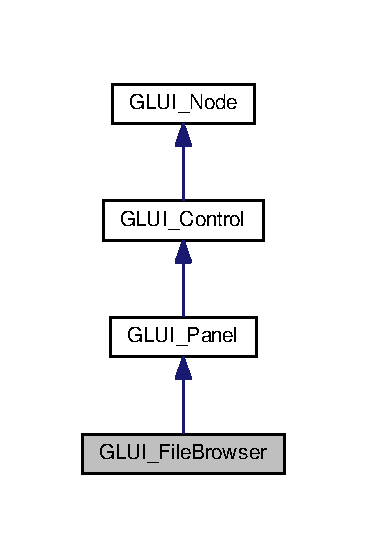
\includegraphics[width=176pt]{class_g_l_u_i___file_browser__inherit__graph}
\end{center}
\end{figure}


Collaboration diagram for G\+L\+U\+I\+\_\+\+File\+Browser\+:\nopagebreak
\begin{figure}[H]
\begin{center}
\leavevmode
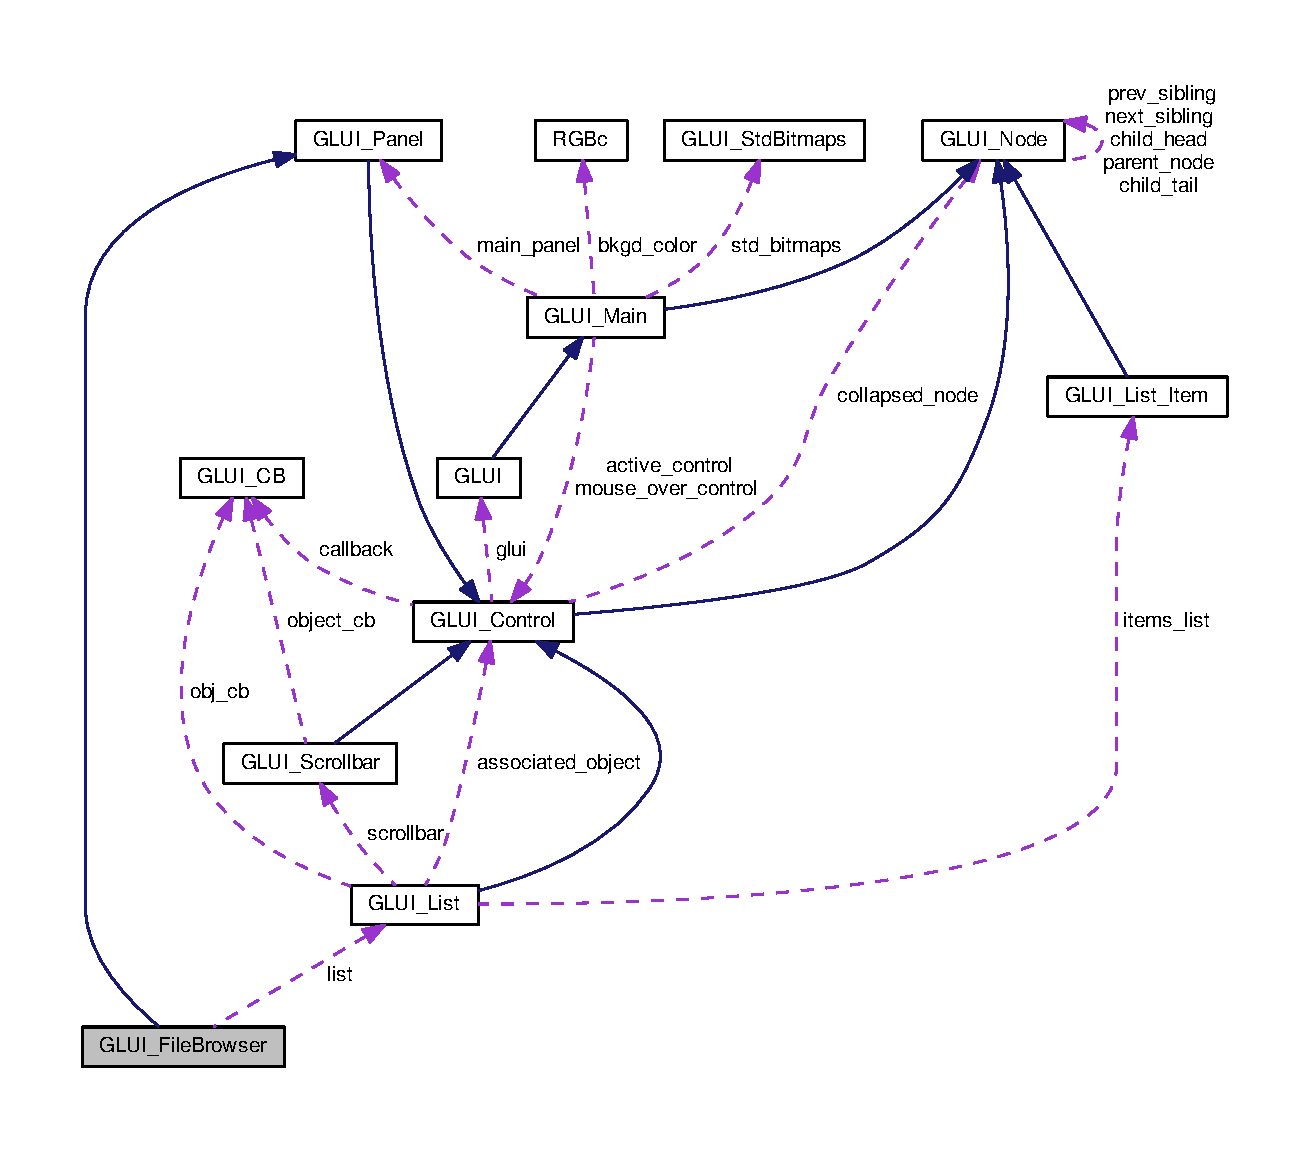
\includegraphics[width=350pt]{class_g_l_u_i___file_browser__coll__graph}
\end{center}
\end{figure}
\subsection*{Public Member Functions}
\begin{DoxyCompactItemize}
\item 
\hyperlink{class_g_l_u_i___file_browser_ace9c0db8913e7e5ecc72a859746e0d45}{G\+L\+U\+I\+\_\+\+File\+Browser} (\hyperlink{class_g_l_u_i___node}{G\+L\+U\+I\+\_\+\+Node} $\ast$\hyperlink{class_g_l_u_i___node_a8ed65d447784f6f88bd3e2e2bcac6cdb}{parent}, const char $\ast$\hyperlink{glext_8h_ad977737dfc9a274a62741b9500c49a32}{name}, \hyperlink{wglext_8h_a500a82aecba06f4550f6849b8099ca21}{int} frame\+\_\+type=\hyperlink{glui_8h_add54979a7b4391067b8a125ee34f690a}{G\+L\+U\+I\+\_\+\+P\+A\+N\+E\+L\+\_\+\+E\+M\+B\+O\+S\+S\+E\+D}, \hyperlink{wglext_8h_a500a82aecba06f4550f6849b8099ca21}{int} \hyperlink{class_g_l_u_i___control_a6c88b7c72b0800f88a5d4cda4868c8b6}{user\+\_\+id}=-\/1, \hyperlink{class_g_l_u_i___c_b}{G\+L\+U\+I\+\_\+\+C\+B} \hyperlink{class_g_l_u_i___control_a96060fe0cc6d537e736dd6eef78e24ab}{callback}=\hyperlink{class_g_l_u_i___c_b}{G\+L\+U\+I\+\_\+\+C\+B}())
\item 
\hyperlink{wglext_8h_a9e6b7f1933461ef318bb000d6bd13b83}{void} \hyperlink{class_g_l_u_i___file_browser_a76b3f6caf8832c0972d8b38c0f77e535}{fbreaddir} (const char $\ast$)
\item 
\hyperlink{wglext_8h_a9e6b7f1933461ef318bb000d6bd13b83}{void} \hyperlink{class_g_l_u_i___file_browser_a03e1e54808847b5e7461d27826cf7827}{set\+\_\+w} (\hyperlink{wglext_8h_a500a82aecba06f4550f6849b8099ca21}{int} \hyperlink{glext_8h_a713abae75276598501f75c68917c5e2d}{w})
\item 
\hyperlink{wglext_8h_a9e6b7f1933461ef318bb000d6bd13b83}{void} \hyperlink{class_g_l_u_i___file_browser_a41b68f6bf7e87c25236a6a7ae78ee98b}{set\+\_\+h} (\hyperlink{wglext_8h_a500a82aecba06f4550f6849b8099ca21}{int} \hyperlink{glext_8h_afa0fb1b5e976920c0abeff2dca3ed774}{h})
\item 
const char $\ast$ \hyperlink{class_g_l_u_i___file_browser_a671f6f7608f38f48d07f7739e1efcad3}{get\+\_\+file} ()
\item 
\hyperlink{wglext_8h_a9e6b7f1933461ef318bb000d6bd13b83}{void} \hyperlink{class_g_l_u_i___file_browser_a5395fc694e33fab6cd3a0546b6899292}{set\+\_\+allow\+\_\+change\+\_\+dir} (\hyperlink{wglext_8h_a500a82aecba06f4550f6849b8099ca21}{int} \hyperlink{glext_8h_a1f2d7f8147412c43ba2303a56f97ee73}{c})
\end{DoxyCompactItemize}
\subsection*{Static Public Member Functions}
\begin{DoxyCompactItemize}
\item 
static \hyperlink{wglext_8h_a9e6b7f1933461ef318bb000d6bd13b83}{void} \hyperlink{class_g_l_u_i___file_browser_a4b5349bd76f0de54a9ce90d8d946e678}{dir\+\_\+list\+\_\+callback} (\hyperlink{class_g_l_u_i___control}{G\+L\+U\+I\+\_\+\+Control} $\ast$)
\end{DoxyCompactItemize}
\subsection*{Public Attributes}
\begin{DoxyCompactItemize}
\item 
\hyperlink{class_g_l_u_i___list}{G\+L\+U\+I\+\_\+\+List} $\ast$ \hyperlink{class_g_l_u_i___file_browser_a58ad435f622fdbff82775ca2313506c1}{list}
\item 
\hyperlink{glui_8h_aada824856f7bcf29794719981ebd8f60}{G\+L\+U\+I\+\_\+\+String} \hyperlink{class_g_l_u_i___file_browser_a91d9710c76d5a3cb3bc7486a627a86f3}{current\+\_\+dir}
\end{DoxyCompactItemize}
\subsection*{Protected Member Functions}
\begin{DoxyCompactItemize}
\item 
\hyperlink{wglext_8h_a9e6b7f1933461ef318bb000d6bd13b83}{void} \hyperlink{class_g_l_u_i___file_browser_a0618241a9315adf0b2cd3514b93ac317}{common\+\_\+init} ()
\end{DoxyCompactItemize}
\subsection*{Additional Inherited Members}


\subsection{Detailed Description}
A list of files the user can select from. 

Definition at line 1139 of file glui.\+h.



\subsection{Constructor \& Destructor Documentation}
\hypertarget{class_g_l_u_i___file_browser_ace9c0db8913e7e5ecc72a859746e0d45}{\index{G\+L\+U\+I\+\_\+\+File\+Browser@{G\+L\+U\+I\+\_\+\+File\+Browser}!G\+L\+U\+I\+\_\+\+File\+Browser@{G\+L\+U\+I\+\_\+\+File\+Browser}}
\index{G\+L\+U\+I\+\_\+\+File\+Browser@{G\+L\+U\+I\+\_\+\+File\+Browser}!G\+L\+U\+I\+\_\+\+File\+Browser@{G\+L\+U\+I\+\_\+\+File\+Browser}}
\subsubsection[{G\+L\+U\+I\+\_\+\+File\+Browser}]{\setlength{\rightskip}{0pt plus 5cm}G\+L\+U\+I\+\_\+\+File\+Browser\+::\+G\+L\+U\+I\+\_\+\+File\+Browser (
\begin{DoxyParamCaption}
\item[{{\bf G\+L\+U\+I\+\_\+\+Node} $\ast$}]{parent, }
\item[{const char $\ast$}]{name, }
\item[{{\bf int}}]{frame\+\_\+type = {\ttfamily {\bf G\+L\+U\+I\+\_\+\+P\+A\+N\+E\+L\+\_\+\+E\+M\+B\+O\+S\+S\+E\+D}}, }
\item[{{\bf int}}]{user\+\_\+id = {\ttfamily -\/1}, }
\item[{{\bf G\+L\+U\+I\+\_\+\+C\+B}}]{callback = {\ttfamily {\bf G\+L\+U\+I\+\_\+\+C\+B}()}}
\end{DoxyParamCaption}
)}}\label{class_g_l_u_i___file_browser_ace9c0db8913e7e5ecc72a859746e0d45}
Create a new list of files the user can select from.


\begin{DoxyParams}{Parameters}
{\em parent} & The panel our object is inside; or the main \hyperlink{class_g_l_u_i}{G\+L\+U\+I} object. \\
\hline
{\em name} & Prompt to give to the user at the top of the file browser. \\
\hline
{\em frame\+\_\+type} & Optional style to display the panel with--G\+L\+U\+I\+\_\+\+P\+A\+N\+E\+L\+\_\+\+E\+M\+B\+O\+S\+S\+E\+D by default. G\+L\+U\+I\+\_\+\+P\+A\+N\+E\+L\+\_\+\+R\+A\+I\+S\+E\+D causes the panel to appear higher than the surroundings. G\+L\+U\+I\+\_\+\+P\+A\+N\+E\+L\+\_\+\+N\+O\+N\+E causes the panel's outline to be invisible. \\
\hline
{\em id} & Optional I\+D number, to pass to the optional callback function. \\
\hline
{\em callback} & Optional callback function, taking either the int I\+D or control. \\
\hline
\end{DoxyParams}


\subsection{Member Function Documentation}
\hypertarget{class_g_l_u_i___file_browser_a0618241a9315adf0b2cd3514b93ac317}{\index{G\+L\+U\+I\+\_\+\+File\+Browser@{G\+L\+U\+I\+\_\+\+File\+Browser}!common\+\_\+init@{common\+\_\+init}}
\index{common\+\_\+init@{common\+\_\+init}!G\+L\+U\+I\+\_\+\+File\+Browser@{G\+L\+U\+I\+\_\+\+File\+Browser}}
\subsubsection[{common\+\_\+init}]{\setlength{\rightskip}{0pt plus 5cm}{\bf void} G\+L\+U\+I\+\_\+\+File\+Browser\+::common\+\_\+init (
\begin{DoxyParamCaption}
\item[{{\bf void}}]{}
\end{DoxyParamCaption}
)\hspace{0.3cm}{\ttfamily [inline]}, {\ttfamily [protected]}}}\label{class_g_l_u_i___file_browser_a0618241a9315adf0b2cd3514b93ac317}


Definition at line 1171 of file glui.\+h.

\hypertarget{class_g_l_u_i___file_browser_a4b5349bd76f0de54a9ce90d8d946e678}{\index{G\+L\+U\+I\+\_\+\+File\+Browser@{G\+L\+U\+I\+\_\+\+File\+Browser}!dir\+\_\+list\+\_\+callback@{dir\+\_\+list\+\_\+callback}}
\index{dir\+\_\+list\+\_\+callback@{dir\+\_\+list\+\_\+callback}!G\+L\+U\+I\+\_\+\+File\+Browser@{G\+L\+U\+I\+\_\+\+File\+Browser}}
\subsubsection[{dir\+\_\+list\+\_\+callback}]{\setlength{\rightskip}{0pt plus 5cm}static {\bf void} G\+L\+U\+I\+\_\+\+File\+Browser\+::dir\+\_\+list\+\_\+callback (
\begin{DoxyParamCaption}
\item[{{\bf G\+L\+U\+I\+\_\+\+Control} $\ast$}]{}
\end{DoxyParamCaption}
)\hspace{0.3cm}{\ttfamily [static]}}}\label{class_g_l_u_i___file_browser_a4b5349bd76f0de54a9ce90d8d946e678}
\hypertarget{class_g_l_u_i___file_browser_a76b3f6caf8832c0972d8b38c0f77e535}{\index{G\+L\+U\+I\+\_\+\+File\+Browser@{G\+L\+U\+I\+\_\+\+File\+Browser}!fbreaddir@{fbreaddir}}
\index{fbreaddir@{fbreaddir}!G\+L\+U\+I\+\_\+\+File\+Browser@{G\+L\+U\+I\+\_\+\+File\+Browser}}
\subsubsection[{fbreaddir}]{\setlength{\rightskip}{0pt plus 5cm}{\bf void} G\+L\+U\+I\+\_\+\+File\+Browser\+::fbreaddir (
\begin{DoxyParamCaption}
\item[{const char $\ast$}]{}
\end{DoxyParamCaption}
)}}\label{class_g_l_u_i___file_browser_a76b3f6caf8832c0972d8b38c0f77e535}
\hypertarget{class_g_l_u_i___file_browser_a671f6f7608f38f48d07f7739e1efcad3}{\index{G\+L\+U\+I\+\_\+\+File\+Browser@{G\+L\+U\+I\+\_\+\+File\+Browser}!get\+\_\+file@{get\+\_\+file}}
\index{get\+\_\+file@{get\+\_\+file}!G\+L\+U\+I\+\_\+\+File\+Browser@{G\+L\+U\+I\+\_\+\+File\+Browser}}
\subsubsection[{get\+\_\+file}]{\setlength{\rightskip}{0pt plus 5cm}const char$\ast$ G\+L\+U\+I\+\_\+\+File\+Browser\+::get\+\_\+file (
\begin{DoxyParamCaption}
{}
\end{DoxyParamCaption}
)\hspace{0.3cm}{\ttfamily [inline]}}}\label{class_g_l_u_i___file_browser_a671f6f7608f38f48d07f7739e1efcad3}


Definition at line 1167 of file glui.\+h.

\hypertarget{class_g_l_u_i___file_browser_a5395fc694e33fab6cd3a0546b6899292}{\index{G\+L\+U\+I\+\_\+\+File\+Browser@{G\+L\+U\+I\+\_\+\+File\+Browser}!set\+\_\+allow\+\_\+change\+\_\+dir@{set\+\_\+allow\+\_\+change\+\_\+dir}}
\index{set\+\_\+allow\+\_\+change\+\_\+dir@{set\+\_\+allow\+\_\+change\+\_\+dir}!G\+L\+U\+I\+\_\+\+File\+Browser@{G\+L\+U\+I\+\_\+\+File\+Browser}}
\subsubsection[{set\+\_\+allow\+\_\+change\+\_\+dir}]{\setlength{\rightskip}{0pt plus 5cm}{\bf void} G\+L\+U\+I\+\_\+\+File\+Browser\+::set\+\_\+allow\+\_\+change\+\_\+dir (
\begin{DoxyParamCaption}
\item[{{\bf int}}]{c}
\end{DoxyParamCaption}
)\hspace{0.3cm}{\ttfamily [inline]}}}\label{class_g_l_u_i___file_browser_a5395fc694e33fab6cd3a0546b6899292}


Definition at line 1168 of file glui.\+h.

\hypertarget{class_g_l_u_i___file_browser_a41b68f6bf7e87c25236a6a7ae78ee98b}{\index{G\+L\+U\+I\+\_\+\+File\+Browser@{G\+L\+U\+I\+\_\+\+File\+Browser}!set\+\_\+h@{set\+\_\+h}}
\index{set\+\_\+h@{set\+\_\+h}!G\+L\+U\+I\+\_\+\+File\+Browser@{G\+L\+U\+I\+\_\+\+File\+Browser}}
\subsubsection[{set\+\_\+h}]{\setlength{\rightskip}{0pt plus 5cm}{\bf void} G\+L\+U\+I\+\_\+\+File\+Browser\+::set\+\_\+h (
\begin{DoxyParamCaption}
\item[{{\bf int}}]{h}
\end{DoxyParamCaption}
)}}\label{class_g_l_u_i___file_browser_a41b68f6bf7e87c25236a6a7ae78ee98b}
\hypertarget{class_g_l_u_i___file_browser_a03e1e54808847b5e7461d27826cf7827}{\index{G\+L\+U\+I\+\_\+\+File\+Browser@{G\+L\+U\+I\+\_\+\+File\+Browser}!set\+\_\+w@{set\+\_\+w}}
\index{set\+\_\+w@{set\+\_\+w}!G\+L\+U\+I\+\_\+\+File\+Browser@{G\+L\+U\+I\+\_\+\+File\+Browser}}
\subsubsection[{set\+\_\+w}]{\setlength{\rightskip}{0pt plus 5cm}{\bf void} G\+L\+U\+I\+\_\+\+File\+Browser\+::set\+\_\+w (
\begin{DoxyParamCaption}
\item[{{\bf int}}]{w}
\end{DoxyParamCaption}
)}}\label{class_g_l_u_i___file_browser_a03e1e54808847b5e7461d27826cf7827}


\subsection{Member Data Documentation}
\hypertarget{class_g_l_u_i___file_browser_a91d9710c76d5a3cb3bc7486a627a86f3}{\index{G\+L\+U\+I\+\_\+\+File\+Browser@{G\+L\+U\+I\+\_\+\+File\+Browser}!current\+\_\+dir@{current\+\_\+dir}}
\index{current\+\_\+dir@{current\+\_\+dir}!G\+L\+U\+I\+\_\+\+File\+Browser@{G\+L\+U\+I\+\_\+\+File\+Browser}}
\subsubsection[{current\+\_\+dir}]{\setlength{\rightskip}{0pt plus 5cm}{\bf G\+L\+U\+I\+\_\+\+String} G\+L\+U\+I\+\_\+\+File\+Browser\+::current\+\_\+dir}}\label{class_g_l_u_i___file_browser_a91d9710c76d5a3cb3bc7486a627a86f3}


Definition at line 1160 of file glui.\+h.

\hypertarget{class_g_l_u_i___file_browser_a58ad435f622fdbff82775ca2313506c1}{\index{G\+L\+U\+I\+\_\+\+File\+Browser@{G\+L\+U\+I\+\_\+\+File\+Browser}!list@{list}}
\index{list@{list}!G\+L\+U\+I\+\_\+\+File\+Browser@{G\+L\+U\+I\+\_\+\+File\+Browser}}
\subsubsection[{list}]{\setlength{\rightskip}{0pt plus 5cm}{\bf G\+L\+U\+I\+\_\+\+List}$\ast$ G\+L\+U\+I\+\_\+\+File\+Browser\+::list}}\label{class_g_l_u_i___file_browser_a58ad435f622fdbff82775ca2313506c1}


Definition at line 1159 of file glui.\+h.



The documentation for this class was generated from the following file\+:\begin{DoxyCompactItemize}
\item 
S\+S\+W\+C/src/\+G\+L/\hyperlink{glui_8h}{glui.\+h}\end{DoxyCompactItemize}

\hypertarget{class_g_l_u_i___glut___window}{\section{G\+L\+U\+I\+\_\+\+Glut\+\_\+\+Window Class Reference}
\label{class_g_l_u_i___glut___window}\index{G\+L\+U\+I\+\_\+\+Glut\+\_\+\+Window@{G\+L\+U\+I\+\_\+\+Glut\+\_\+\+Window}}
}


{\ttfamily \#include $<$glui.\+h$>$}



Inheritance diagram for G\+L\+U\+I\+\_\+\+Glut\+\_\+\+Window\+:\nopagebreak
\begin{figure}[H]
\begin{center}
\leavevmode
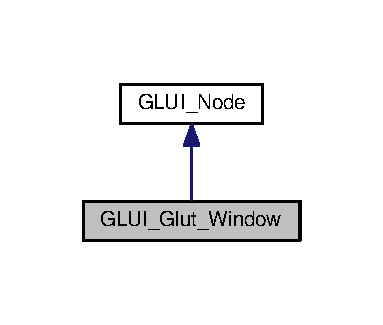
\includegraphics[width=184pt]{class_g_l_u_i___glut___window__inherit__graph}
\end{center}
\end{figure}


Collaboration diagram for G\+L\+U\+I\+\_\+\+Glut\+\_\+\+Window\+:\nopagebreak
\begin{figure}[H]
\begin{center}
\leavevmode
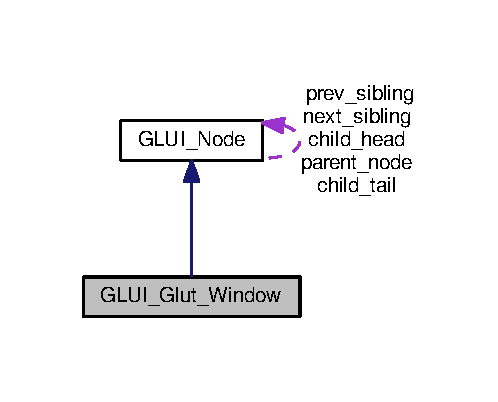
\includegraphics[width=239pt]{class_g_l_u_i___glut___window__coll__graph}
\end{center}
\end{figure}
\subsection*{Public Member Functions}
\begin{DoxyCompactItemize}
\item 
\hyperlink{class_g_l_u_i___glut___window_a5ed74df8dd7b4ed446b1d0cbd8154507}{G\+L\+U\+I\+\_\+\+Glut\+\_\+\+Window} ()
\end{DoxyCompactItemize}
\subsection*{Public Attributes}
\begin{DoxyCompactItemize}
\item 
\hyperlink{wglext_8h_a500a82aecba06f4550f6849b8099ca21}{int} \hyperlink{class_g_l_u_i___glut___window_a1eeae65875356396ec81ffd63d0b096a}{glut\+\_\+window\+\_\+id}
\item 
\hyperlink{wglext_8h_a9e6b7f1933461ef318bb000d6bd13b83}{void}($\ast$ \hyperlink{class_g_l_u_i___glut___window_a299ae81dcf534d460bac55a897cf540b}{glut\+\_\+keyboard\+\_\+\+C\+B} )(unsigned char, \hyperlink{wglext_8h_a500a82aecba06f4550f6849b8099ca21}{int}, \hyperlink{wglext_8h_a500a82aecba06f4550f6849b8099ca21}{int})
\item 
\hyperlink{wglext_8h_a9e6b7f1933461ef318bb000d6bd13b83}{void}($\ast$ \hyperlink{class_g_l_u_i___glut___window_a6195cf472a03676f14c86e29a4d2ad5b}{glut\+\_\+special\+\_\+\+C\+B} )(\hyperlink{wglext_8h_a500a82aecba06f4550f6849b8099ca21}{int}, \hyperlink{wglext_8h_a500a82aecba06f4550f6849b8099ca21}{int}, \hyperlink{wglext_8h_a500a82aecba06f4550f6849b8099ca21}{int})
\item 
\hyperlink{wglext_8h_a9e6b7f1933461ef318bb000d6bd13b83}{void}($\ast$ \hyperlink{class_g_l_u_i___glut___window_ab80f91ef7790e98a3fb96f5d2fc3bcad}{glut\+\_\+reshape\+\_\+\+C\+B} )(\hyperlink{wglext_8h_a500a82aecba06f4550f6849b8099ca21}{int}, \hyperlink{wglext_8h_a500a82aecba06f4550f6849b8099ca21}{int})
\item 
\hyperlink{wglext_8h_a9e6b7f1933461ef318bb000d6bd13b83}{void}($\ast$ \hyperlink{class_g_l_u_i___glut___window_afc4066e60731680d782efaed8a7bc3b1}{glut\+\_\+passive\+\_\+motion\+\_\+\+C\+B} )(\hyperlink{wglext_8h_a500a82aecba06f4550f6849b8099ca21}{int}, \hyperlink{wglext_8h_a500a82aecba06f4550f6849b8099ca21}{int})
\item 
\hyperlink{wglext_8h_a9e6b7f1933461ef318bb000d6bd13b83}{void}($\ast$ \hyperlink{class_g_l_u_i___glut___window_a126b91fbf4e55fd2a099bb43c5949654}{glut\+\_\+mouse\+\_\+\+C\+B} )(\hyperlink{wglext_8h_a500a82aecba06f4550f6849b8099ca21}{int}, \hyperlink{wglext_8h_a500a82aecba06f4550f6849b8099ca21}{int}, \hyperlink{wglext_8h_a500a82aecba06f4550f6849b8099ca21}{int}, \hyperlink{wglext_8h_a500a82aecba06f4550f6849b8099ca21}{int})
\item 
\hyperlink{wglext_8h_a9e6b7f1933461ef318bb000d6bd13b83}{void}($\ast$ \hyperlink{class_g_l_u_i___glut___window_aaf80a162394308539654d8451d25d49b}{glut\+\_\+visibility\+\_\+\+C\+B} )(\hyperlink{wglext_8h_a500a82aecba06f4550f6849b8099ca21}{int})
\item 
\hyperlink{wglext_8h_a9e6b7f1933461ef318bb000d6bd13b83}{void}($\ast$ \hyperlink{class_g_l_u_i___glut___window_ae5f6057d61f1808b2b0ab39b89a7113e}{glut\+\_\+motion\+\_\+\+C\+B} )(\hyperlink{wglext_8h_a500a82aecba06f4550f6849b8099ca21}{int}, \hyperlink{wglext_8h_a500a82aecba06f4550f6849b8099ca21}{int})
\item 
\hyperlink{wglext_8h_a9e6b7f1933461ef318bb000d6bd13b83}{void}($\ast$ \hyperlink{class_g_l_u_i___glut___window_a08233e5acd66dc19bf453e423b0cd6c9}{glut\+\_\+display\+\_\+\+C\+B} )(\hyperlink{wglext_8h_a9e6b7f1933461ef318bb000d6bd13b83}{void})
\item 
\hyperlink{wglext_8h_a9e6b7f1933461ef318bb000d6bd13b83}{void}($\ast$ \hyperlink{class_g_l_u_i___glut___window_a0f17b9ee70f25c694dfb546b0d2ae6a8}{glut\+\_\+entry\+\_\+\+C\+B} )(\hyperlink{wglext_8h_a500a82aecba06f4550f6849b8099ca21}{int})
\end{DoxyCompactItemize}
\subsection*{Additional Inherited Members}


\subsection{Detailed Description}
A top-\/level window. The G\+L\+U\+I\+\_\+\+Master G\+L\+U\+T callback can route events to the callbacks in this class, for arbitrary use by external users. (see \hyperlink{class_g_l_u_i___master___object_aec70f38a81424a09c42f5a3e4e6edc43}{G\+L\+U\+I\+\_\+\+Master\+\_\+\+Object\+::set\+\_\+glut\+Keyboard\+Func}).

This entire approach seems to be superceded by the \char`\"{}subwindow\char`\"{} flavor of \hyperlink{class_g_l_u_i}{G\+L\+U\+I}. 

Definition at line 569 of file glui.\+h.



\subsection{Constructor \& Destructor Documentation}
\hypertarget{class_g_l_u_i___glut___window_a5ed74df8dd7b4ed446b1d0cbd8154507}{\index{G\+L\+U\+I\+\_\+\+Glut\+\_\+\+Window@{G\+L\+U\+I\+\_\+\+Glut\+\_\+\+Window}!G\+L\+U\+I\+\_\+\+Glut\+\_\+\+Window@{G\+L\+U\+I\+\_\+\+Glut\+\_\+\+Window}}
\index{G\+L\+U\+I\+\_\+\+Glut\+\_\+\+Window@{G\+L\+U\+I\+\_\+\+Glut\+\_\+\+Window}!G\+L\+U\+I\+\_\+\+Glut\+\_\+\+Window@{G\+L\+U\+I\+\_\+\+Glut\+\_\+\+Window}}
\subsubsection[{G\+L\+U\+I\+\_\+\+Glut\+\_\+\+Window}]{\setlength{\rightskip}{0pt plus 5cm}G\+L\+U\+I\+\_\+\+Glut\+\_\+\+Window\+::\+G\+L\+U\+I\+\_\+\+Glut\+\_\+\+Window (
\begin{DoxyParamCaption}
{}
\end{DoxyParamCaption}
)}}\label{class_g_l_u_i___glut___window_a5ed74df8dd7b4ed446b1d0cbd8154507}


\subsection{Member Data Documentation}
\hypertarget{class_g_l_u_i___glut___window_a08233e5acd66dc19bf453e423b0cd6c9}{\index{G\+L\+U\+I\+\_\+\+Glut\+\_\+\+Window@{G\+L\+U\+I\+\_\+\+Glut\+\_\+\+Window}!glut\+\_\+display\+\_\+\+C\+B@{glut\+\_\+display\+\_\+\+C\+B}}
\index{glut\+\_\+display\+\_\+\+C\+B@{glut\+\_\+display\+\_\+\+C\+B}!G\+L\+U\+I\+\_\+\+Glut\+\_\+\+Window@{G\+L\+U\+I\+\_\+\+Glut\+\_\+\+Window}}
\subsubsection[{glut\+\_\+display\+\_\+\+C\+B}]{\setlength{\rightskip}{0pt plus 5cm}{\bf void}($\ast$ G\+L\+U\+I\+\_\+\+Glut\+\_\+\+Window\+::glut\+\_\+display\+\_\+\+C\+B)({\bf void})}}\label{class_g_l_u_i___glut___window_a08233e5acd66dc19bf453e423b0cd6c9}


Definition at line 584 of file glui.\+h.

\hypertarget{class_g_l_u_i___glut___window_a0f17b9ee70f25c694dfb546b0d2ae6a8}{\index{G\+L\+U\+I\+\_\+\+Glut\+\_\+\+Window@{G\+L\+U\+I\+\_\+\+Glut\+\_\+\+Window}!glut\+\_\+entry\+\_\+\+C\+B@{glut\+\_\+entry\+\_\+\+C\+B}}
\index{glut\+\_\+entry\+\_\+\+C\+B@{glut\+\_\+entry\+\_\+\+C\+B}!G\+L\+U\+I\+\_\+\+Glut\+\_\+\+Window@{G\+L\+U\+I\+\_\+\+Glut\+\_\+\+Window}}
\subsubsection[{glut\+\_\+entry\+\_\+\+C\+B}]{\setlength{\rightskip}{0pt plus 5cm}{\bf void}($\ast$ G\+L\+U\+I\+\_\+\+Glut\+\_\+\+Window\+::glut\+\_\+entry\+\_\+\+C\+B)({\bf int})}}\label{class_g_l_u_i___glut___window_a0f17b9ee70f25c694dfb546b0d2ae6a8}


Definition at line 585 of file glui.\+h.

\hypertarget{class_g_l_u_i___glut___window_a299ae81dcf534d460bac55a897cf540b}{\index{G\+L\+U\+I\+\_\+\+Glut\+\_\+\+Window@{G\+L\+U\+I\+\_\+\+Glut\+\_\+\+Window}!glut\+\_\+keyboard\+\_\+\+C\+B@{glut\+\_\+keyboard\+\_\+\+C\+B}}
\index{glut\+\_\+keyboard\+\_\+\+C\+B@{glut\+\_\+keyboard\+\_\+\+C\+B}!G\+L\+U\+I\+\_\+\+Glut\+\_\+\+Window@{G\+L\+U\+I\+\_\+\+Glut\+\_\+\+Window}}
\subsubsection[{glut\+\_\+keyboard\+\_\+\+C\+B}]{\setlength{\rightskip}{0pt plus 5cm}{\bf void}($\ast$ G\+L\+U\+I\+\_\+\+Glut\+\_\+\+Window\+::glut\+\_\+keyboard\+\_\+\+C\+B)(unsigned char, {\bf int}, {\bf int})}}\label{class_g_l_u_i___glut___window_a299ae81dcf534d460bac55a897cf540b}


Definition at line 577 of file glui.\+h.

\hypertarget{class_g_l_u_i___glut___window_ae5f6057d61f1808b2b0ab39b89a7113e}{\index{G\+L\+U\+I\+\_\+\+Glut\+\_\+\+Window@{G\+L\+U\+I\+\_\+\+Glut\+\_\+\+Window}!glut\+\_\+motion\+\_\+\+C\+B@{glut\+\_\+motion\+\_\+\+C\+B}}
\index{glut\+\_\+motion\+\_\+\+C\+B@{glut\+\_\+motion\+\_\+\+C\+B}!G\+L\+U\+I\+\_\+\+Glut\+\_\+\+Window@{G\+L\+U\+I\+\_\+\+Glut\+\_\+\+Window}}
\subsubsection[{glut\+\_\+motion\+\_\+\+C\+B}]{\setlength{\rightskip}{0pt plus 5cm}{\bf void}($\ast$ G\+L\+U\+I\+\_\+\+Glut\+\_\+\+Window\+::glut\+\_\+motion\+\_\+\+C\+B)({\bf int}, {\bf int})}}\label{class_g_l_u_i___glut___window_ae5f6057d61f1808b2b0ab39b89a7113e}


Definition at line 583 of file glui.\+h.

\hypertarget{class_g_l_u_i___glut___window_a126b91fbf4e55fd2a099bb43c5949654}{\index{G\+L\+U\+I\+\_\+\+Glut\+\_\+\+Window@{G\+L\+U\+I\+\_\+\+Glut\+\_\+\+Window}!glut\+\_\+mouse\+\_\+\+C\+B@{glut\+\_\+mouse\+\_\+\+C\+B}}
\index{glut\+\_\+mouse\+\_\+\+C\+B@{glut\+\_\+mouse\+\_\+\+C\+B}!G\+L\+U\+I\+\_\+\+Glut\+\_\+\+Window@{G\+L\+U\+I\+\_\+\+Glut\+\_\+\+Window}}
\subsubsection[{glut\+\_\+mouse\+\_\+\+C\+B}]{\setlength{\rightskip}{0pt plus 5cm}{\bf void}($\ast$ G\+L\+U\+I\+\_\+\+Glut\+\_\+\+Window\+::glut\+\_\+mouse\+\_\+\+C\+B)({\bf int}, {\bf int}, {\bf int}, {\bf int})}}\label{class_g_l_u_i___glut___window_a126b91fbf4e55fd2a099bb43c5949654}


Definition at line 581 of file glui.\+h.

\hypertarget{class_g_l_u_i___glut___window_afc4066e60731680d782efaed8a7bc3b1}{\index{G\+L\+U\+I\+\_\+\+Glut\+\_\+\+Window@{G\+L\+U\+I\+\_\+\+Glut\+\_\+\+Window}!glut\+\_\+passive\+\_\+motion\+\_\+\+C\+B@{glut\+\_\+passive\+\_\+motion\+\_\+\+C\+B}}
\index{glut\+\_\+passive\+\_\+motion\+\_\+\+C\+B@{glut\+\_\+passive\+\_\+motion\+\_\+\+C\+B}!G\+L\+U\+I\+\_\+\+Glut\+\_\+\+Window@{G\+L\+U\+I\+\_\+\+Glut\+\_\+\+Window}}
\subsubsection[{glut\+\_\+passive\+\_\+motion\+\_\+\+C\+B}]{\setlength{\rightskip}{0pt plus 5cm}{\bf void}($\ast$ G\+L\+U\+I\+\_\+\+Glut\+\_\+\+Window\+::glut\+\_\+passive\+\_\+motion\+\_\+\+C\+B)({\bf int}, {\bf int})}}\label{class_g_l_u_i___glut___window_afc4066e60731680d782efaed8a7bc3b1}


Definition at line 580 of file glui.\+h.

\hypertarget{class_g_l_u_i___glut___window_ab80f91ef7790e98a3fb96f5d2fc3bcad}{\index{G\+L\+U\+I\+\_\+\+Glut\+\_\+\+Window@{G\+L\+U\+I\+\_\+\+Glut\+\_\+\+Window}!glut\+\_\+reshape\+\_\+\+C\+B@{glut\+\_\+reshape\+\_\+\+C\+B}}
\index{glut\+\_\+reshape\+\_\+\+C\+B@{glut\+\_\+reshape\+\_\+\+C\+B}!G\+L\+U\+I\+\_\+\+Glut\+\_\+\+Window@{G\+L\+U\+I\+\_\+\+Glut\+\_\+\+Window}}
\subsubsection[{glut\+\_\+reshape\+\_\+\+C\+B}]{\setlength{\rightskip}{0pt plus 5cm}{\bf void}($\ast$ G\+L\+U\+I\+\_\+\+Glut\+\_\+\+Window\+::glut\+\_\+reshape\+\_\+\+C\+B)({\bf int}, {\bf int})}}\label{class_g_l_u_i___glut___window_ab80f91ef7790e98a3fb96f5d2fc3bcad}


Definition at line 579 of file glui.\+h.

\hypertarget{class_g_l_u_i___glut___window_a6195cf472a03676f14c86e29a4d2ad5b}{\index{G\+L\+U\+I\+\_\+\+Glut\+\_\+\+Window@{G\+L\+U\+I\+\_\+\+Glut\+\_\+\+Window}!glut\+\_\+special\+\_\+\+C\+B@{glut\+\_\+special\+\_\+\+C\+B}}
\index{glut\+\_\+special\+\_\+\+C\+B@{glut\+\_\+special\+\_\+\+C\+B}!G\+L\+U\+I\+\_\+\+Glut\+\_\+\+Window@{G\+L\+U\+I\+\_\+\+Glut\+\_\+\+Window}}
\subsubsection[{glut\+\_\+special\+\_\+\+C\+B}]{\setlength{\rightskip}{0pt plus 5cm}{\bf void}($\ast$ G\+L\+U\+I\+\_\+\+Glut\+\_\+\+Window\+::glut\+\_\+special\+\_\+\+C\+B)({\bf int}, {\bf int}, {\bf int})}}\label{class_g_l_u_i___glut___window_a6195cf472a03676f14c86e29a4d2ad5b}


Definition at line 578 of file glui.\+h.

\hypertarget{class_g_l_u_i___glut___window_aaf80a162394308539654d8451d25d49b}{\index{G\+L\+U\+I\+\_\+\+Glut\+\_\+\+Window@{G\+L\+U\+I\+\_\+\+Glut\+\_\+\+Window}!glut\+\_\+visibility\+\_\+\+C\+B@{glut\+\_\+visibility\+\_\+\+C\+B}}
\index{glut\+\_\+visibility\+\_\+\+C\+B@{glut\+\_\+visibility\+\_\+\+C\+B}!G\+L\+U\+I\+\_\+\+Glut\+\_\+\+Window@{G\+L\+U\+I\+\_\+\+Glut\+\_\+\+Window}}
\subsubsection[{glut\+\_\+visibility\+\_\+\+C\+B}]{\setlength{\rightskip}{0pt plus 5cm}{\bf void}($\ast$ G\+L\+U\+I\+\_\+\+Glut\+\_\+\+Window\+::glut\+\_\+visibility\+\_\+\+C\+B)({\bf int})}}\label{class_g_l_u_i___glut___window_aaf80a162394308539654d8451d25d49b}


Definition at line 582 of file glui.\+h.

\hypertarget{class_g_l_u_i___glut___window_a1eeae65875356396ec81ffd63d0b096a}{\index{G\+L\+U\+I\+\_\+\+Glut\+\_\+\+Window@{G\+L\+U\+I\+\_\+\+Glut\+\_\+\+Window}!glut\+\_\+window\+\_\+id@{glut\+\_\+window\+\_\+id}}
\index{glut\+\_\+window\+\_\+id@{glut\+\_\+window\+\_\+id}!G\+L\+U\+I\+\_\+\+Glut\+\_\+\+Window@{G\+L\+U\+I\+\_\+\+Glut\+\_\+\+Window}}
\subsubsection[{glut\+\_\+window\+\_\+id}]{\setlength{\rightskip}{0pt plus 5cm}{\bf int} G\+L\+U\+I\+\_\+\+Glut\+\_\+\+Window\+::glut\+\_\+window\+\_\+id}}\label{class_g_l_u_i___glut___window_a1eeae65875356396ec81ffd63d0b096a}


Definition at line 574 of file glui.\+h.



The documentation for this class was generated from the following file\+:\begin{DoxyCompactItemize}
\item 
S\+S\+W\+C/src/\+G\+L/\hyperlink{glui_8h}{glui.\+h}\end{DoxyCompactItemize}

\hypertarget{class_g_l_u_i___list}{\section{G\+L\+U\+I\+\_\+\+List Class Reference}
\label{class_g_l_u_i___list}\index{G\+L\+U\+I\+\_\+\+List@{G\+L\+U\+I\+\_\+\+List}}
}


{\ttfamily \#include $<$glui.\+h$>$}



Inheritance diagram for G\+L\+U\+I\+\_\+\+List\+:\nopagebreak
\begin{figure}[H]
\begin{center}
\leavevmode
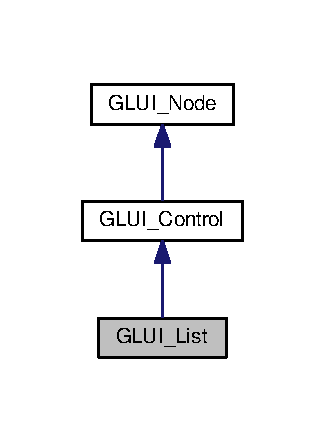
\includegraphics[width=156pt]{class_g_l_u_i___list__inherit__graph}
\end{center}
\end{figure}


Collaboration diagram for G\+L\+U\+I\+\_\+\+List\+:\nopagebreak
\begin{figure}[H]
\begin{center}
\leavevmode
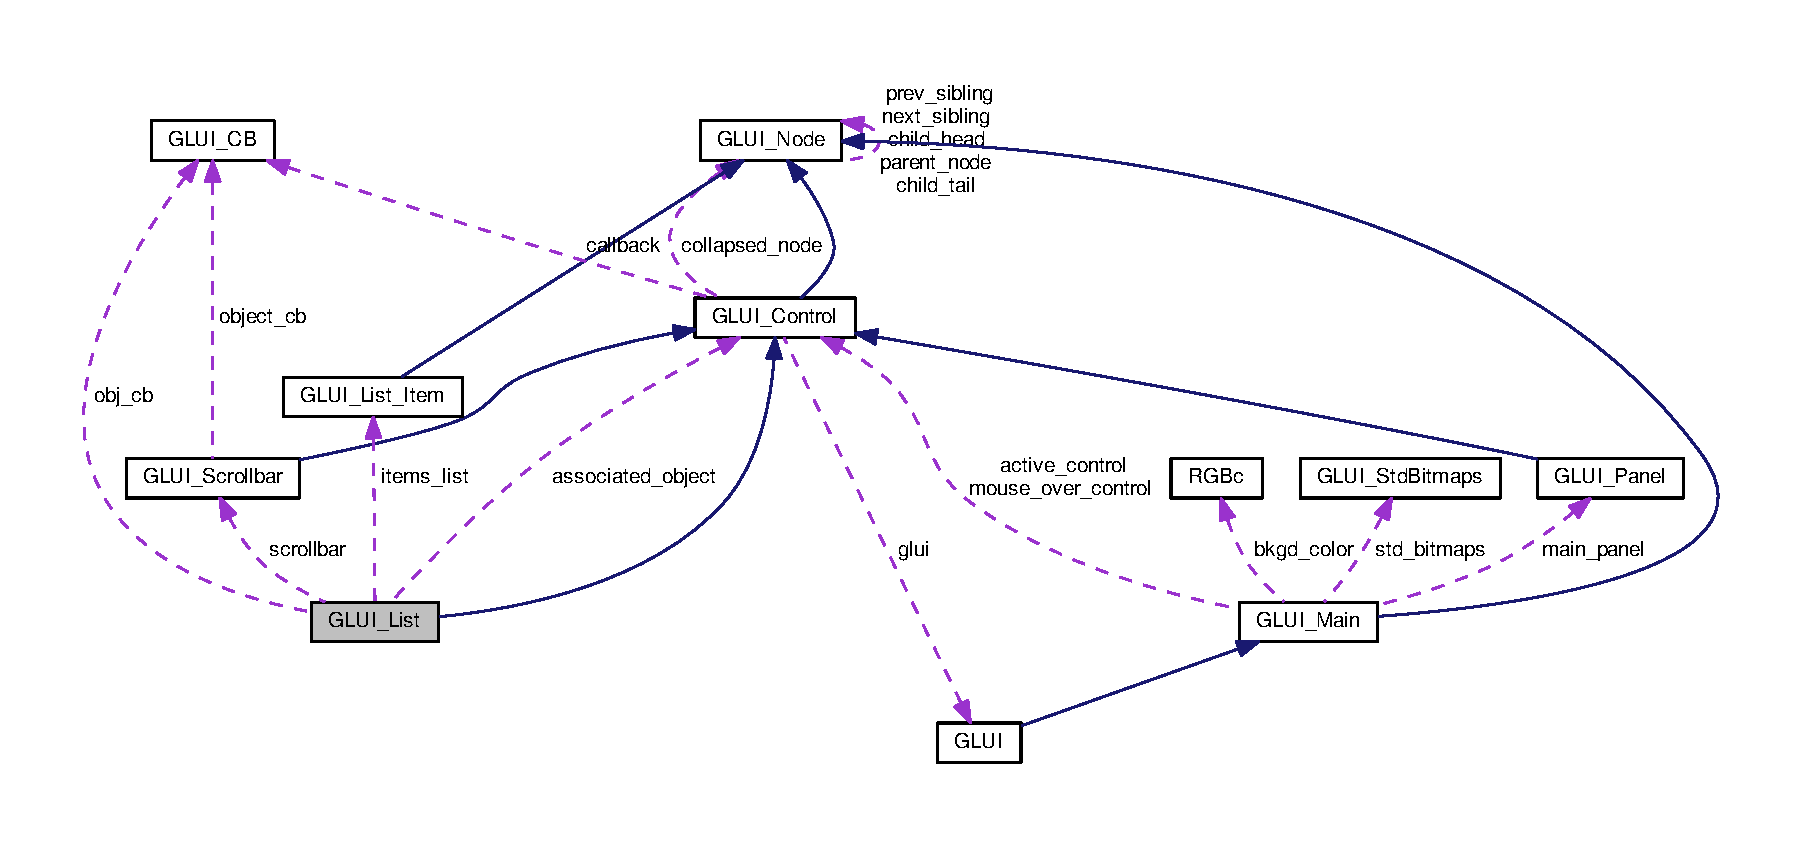
\includegraphics[width=350pt]{class_g_l_u_i___list__coll__graph}
\end{center}
\end{figure}
\subsection*{Public Member Functions}
\begin{DoxyCompactItemize}
\item 
\hyperlink{class_g_l_u_i___list_ab4db3ba18344aa8839022a2ec70eb637}{G\+L\+U\+I\+\_\+\+List} (\hyperlink{class_g_l_u_i___node}{G\+L\+U\+I\+\_\+\+Node} $\ast$\hyperlink{class_g_l_u_i___node_a8ed65d447784f6f88bd3e2e2bcac6cdb}{parent}, bool scroll=false, \hyperlink{wglext_8h_a500a82aecba06f4550f6849b8099ca21}{int} \hyperlink{glext_8h_a58c2a664503e14ffb8f21012aabff3e9}{id}=-\/1, \hyperlink{class_g_l_u_i___c_b}{G\+L\+U\+I\+\_\+\+C\+B} \hyperlink{class_g_l_u_i___control_a96060fe0cc6d537e736dd6eef78e24ab}{callback}=\hyperlink{class_g_l_u_i___c_b}{G\+L\+U\+I\+\_\+\+C\+B}())
\item 
\hyperlink{class_g_l_u_i___list_ae0558ab509470184c35c543c16e33626}{G\+L\+U\+I\+\_\+\+List} (\hyperlink{class_g_l_u_i___node}{G\+L\+U\+I\+\_\+\+Node} $\ast$\hyperlink{class_g_l_u_i___node_a8ed65d447784f6f88bd3e2e2bcac6cdb}{parent}, \hyperlink{glui_8h_aada824856f7bcf29794719981ebd8f60}{G\+L\+U\+I\+\_\+\+String} \&live\+\_\+var, bool scroll=false, \hyperlink{wglext_8h_a500a82aecba06f4550f6849b8099ca21}{int} \hyperlink{glext_8h_a58c2a664503e14ffb8f21012aabff3e9}{id}=-\/1, \hyperlink{class_g_l_u_i___c_b}{G\+L\+U\+I\+\_\+\+C\+B} \hyperlink{class_g_l_u_i___control_a96060fe0cc6d537e736dd6eef78e24ab}{callback}=\hyperlink{class_g_l_u_i___c_b}{G\+L\+U\+I\+\_\+\+C\+B}())
\item 
\hyperlink{wglext_8h_a500a82aecba06f4550f6849b8099ca21}{int} \hyperlink{class_g_l_u_i___list_a5ea7f0e79c85acc1910b13222c2892c4}{mouse\+\_\+down\+\_\+handler} (\hyperlink{wglext_8h_a500a82aecba06f4550f6849b8099ca21}{int} local\+\_\+x, \hyperlink{wglext_8h_a500a82aecba06f4550f6849b8099ca21}{int} local\+\_\+y)
\item 
\hyperlink{wglext_8h_a500a82aecba06f4550f6849b8099ca21}{int} \hyperlink{class_g_l_u_i___list_a7e96dff4df0bfdc5918c54a84f2d5052}{mouse\+\_\+up\+\_\+handler} (\hyperlink{wglext_8h_a500a82aecba06f4550f6849b8099ca21}{int} local\+\_\+x, \hyperlink{wglext_8h_a500a82aecba06f4550f6849b8099ca21}{int} local\+\_\+y, bool inside)
\item 
\hyperlink{wglext_8h_a500a82aecba06f4550f6849b8099ca21}{int} \hyperlink{class_g_l_u_i___list_a2ab77fda1915950e01bea87a45013311}{mouse\+\_\+held\+\_\+down\+\_\+handler} (\hyperlink{wglext_8h_a500a82aecba06f4550f6849b8099ca21}{int} local\+\_\+x, \hyperlink{wglext_8h_a500a82aecba06f4550f6849b8099ca21}{int} local\+\_\+y, bool inside)
\item 
\hyperlink{wglext_8h_a500a82aecba06f4550f6849b8099ca21}{int} \hyperlink{class_g_l_u_i___list_a0d88a6b7a1c479420b85f246d3042d86}{key\+\_\+handler} (unsigned char key, \hyperlink{wglext_8h_a500a82aecba06f4550f6849b8099ca21}{int} modifiers)
\item 
\hyperlink{wglext_8h_a500a82aecba06f4550f6849b8099ca21}{int} \hyperlink{class_g_l_u_i___list_a47649c2517c82edecd2f7376a284e1b6}{special\+\_\+handler} (\hyperlink{wglext_8h_a500a82aecba06f4550f6849b8099ca21}{int} key, \hyperlink{wglext_8h_a500a82aecba06f4550f6849b8099ca21}{int} modifiers)
\item 
\hyperlink{wglext_8h_a9e6b7f1933461ef318bb000d6bd13b83}{void} \hyperlink{class_g_l_u_i___list_a27aad35685565ffae7182b432dbfb2d6}{activate} (\hyperlink{wglext_8h_a500a82aecba06f4550f6849b8099ca21}{int} how)
\item 
\hyperlink{wglext_8h_a9e6b7f1933461ef318bb000d6bd13b83}{void} \hyperlink{class_g_l_u_i___list_a862ebf586380a13b1e17bf00ee06cc40}{deactivate} (\hyperlink{wglext_8h_a9e6b7f1933461ef318bb000d6bd13b83}{void})
\item 
\hyperlink{wglext_8h_a9e6b7f1933461ef318bb000d6bd13b83}{void} \hyperlink{class_g_l_u_i___list_a9cecff476afad9849416acaf568d8f1a}{draw} (\hyperlink{wglext_8h_a500a82aecba06f4550f6849b8099ca21}{int} \hyperlink{glext_8h_ad77deca22f617d3f0e0eb786445689fc}{x}, \hyperlink{wglext_8h_a500a82aecba06f4550f6849b8099ca21}{int} \hyperlink{glext_8h_a9298c7ad619074f5285b32c6b72bfdea}{y})
\item 
\hyperlink{wglext_8h_a500a82aecba06f4550f6849b8099ca21}{int} \hyperlink{class_g_l_u_i___list_a9946699ea4a63516620440dc9cb503f5}{mouse\+\_\+over} (\hyperlink{wglext_8h_a500a82aecba06f4550f6849b8099ca21}{int} state, \hyperlink{wglext_8h_a500a82aecba06f4550f6849b8099ca21}{int} \hyperlink{glext_8h_ad77deca22f617d3f0e0eb786445689fc}{x}, \hyperlink{wglext_8h_a500a82aecba06f4550f6849b8099ca21}{int} \hyperlink{glext_8h_a9298c7ad619074f5285b32c6b72bfdea}{y})
\item 
\hyperlink{wglext_8h_a500a82aecba06f4550f6849b8099ca21}{int} \hyperlink{class_g_l_u_i___list_a08c3ad15db735454006faa1dcba6f461}{get\+\_\+box\+\_\+width} ()
\item 
\hyperlink{wglext_8h_a500a82aecba06f4550f6849b8099ca21}{int} \hyperlink{class_g_l_u_i___list_a1ca6f966a881d67dc039c6d6fc0e8f15}{find\+\_\+word\+\_\+break} (\hyperlink{wglext_8h_a500a82aecba06f4550f6849b8099ca21}{int} \hyperlink{glext_8h_ac55adc720a3098c1b454d2a4647f4361}{start}, \hyperlink{wglext_8h_a500a82aecba06f4550f6849b8099ca21}{int} direction)
\item 
\hyperlink{wglext_8h_a500a82aecba06f4550f6849b8099ca21}{int} \hyperlink{class_g_l_u_i___list_a305864cc3614e17a6ef47e5989c8cd21}{substring\+\_\+width} (const char $\ast$\hyperlink{glext_8h_a7d65d00ca3b0630d9b5c52df855b19f5}{t}, \hyperlink{wglext_8h_a500a82aecba06f4550f6849b8099ca21}{int} \hyperlink{glext_8h_ac55adc720a3098c1b454d2a4647f4361}{start}, \hyperlink{wglext_8h_a500a82aecba06f4550f6849b8099ca21}{int} \hyperlink{glext_8h_a432111147038972f06e049e18a837002}{end})
\item 
\hyperlink{wglext_8h_a500a82aecba06f4550f6849b8099ca21}{int} \hyperlink{class_g_l_u_i___list_a3315c82b5aef8f476de85ea90d2a8421}{find\+\_\+line} (\hyperlink{wglext_8h_a500a82aecba06f4550f6849b8099ca21}{int} \hyperlink{glext_8h_ad77deca22f617d3f0e0eb786445689fc}{x}, \hyperlink{wglext_8h_a500a82aecba06f4550f6849b8099ca21}{int} \hyperlink{glext_8h_a9298c7ad619074f5285b32c6b72bfdea}{y})
\item 
\hyperlink{wglext_8h_a9e6b7f1933461ef318bb000d6bd13b83}{void} \hyperlink{class_g_l_u_i___list_af83459297185924a6ef9c8ce5618f571}{update\+\_\+and\+\_\+draw\+\_\+text} (\hyperlink{wglext_8h_a9e6b7f1933461ef318bb000d6bd13b83}{void})
\item 
\hyperlink{wglext_8h_a9e6b7f1933461ef318bb000d6bd13b83}{void} \hyperlink{class_g_l_u_i___list_a5ce43d2a245edb348e220f7788f31ab7}{draw\+\_\+text} (const char $\ast$\hyperlink{glext_8h_a7d65d00ca3b0630d9b5c52df855b19f5}{t}, \hyperlink{wglext_8h_a500a82aecba06f4550f6849b8099ca21}{int} selected, \hyperlink{wglext_8h_a500a82aecba06f4550f6849b8099ca21}{int} \hyperlink{glext_8h_ad77deca22f617d3f0e0eb786445689fc}{x}, \hyperlink{wglext_8h_a500a82aecba06f4550f6849b8099ca21}{int} \hyperlink{glext_8h_a9298c7ad619074f5285b32c6b72bfdea}{y})
\item 
\hyperlink{wglext_8h_a9e6b7f1933461ef318bb000d6bd13b83}{void} \hyperlink{class_g_l_u_i___list_ab90ecf239cc0deaf4739d636c986d747}{update\+\_\+size} (\hyperlink{wglext_8h_a9e6b7f1933461ef318bb000d6bd13b83}{void})
\item 
\hyperlink{wglext_8h_a500a82aecba06f4550f6849b8099ca21}{int} \hyperlink{class_g_l_u_i___list_ac26dc37467a0c3ddb0952f1321c4f703}{add\+\_\+item} (\hyperlink{wglext_8h_a500a82aecba06f4550f6849b8099ca21}{int} \hyperlink{glext_8h_a58c2a664503e14ffb8f21012aabff3e9}{id}, const char $\ast$\hyperlink{class_g_l_u_i___control_af0d60e9736f4dbc34e9a536e75876d72}{text})
\item 
\hyperlink{wglext_8h_a500a82aecba06f4550f6849b8099ca21}{int} \hyperlink{class_g_l_u_i___list_a2bc8c33e63c775624adf9dfa5b0ffb32}{delete\+\_\+item} (const char $\ast$\hyperlink{class_g_l_u_i___control_af0d60e9736f4dbc34e9a536e75876d72}{text})
\item 
\hyperlink{wglext_8h_a500a82aecba06f4550f6849b8099ca21}{int} \hyperlink{class_g_l_u_i___list_a1de769c475c514a2bfccf92552be8dba}{delete\+\_\+item} (\hyperlink{wglext_8h_a500a82aecba06f4550f6849b8099ca21}{int} \hyperlink{glext_8h_a58c2a664503e14ffb8f21012aabff3e9}{id})
\item 
\hyperlink{wglext_8h_a500a82aecba06f4550f6849b8099ca21}{int} \hyperlink{class_g_l_u_i___list_a68eaa8654adcd307c89e8235a049f4bf}{delete\+\_\+all} ()
\item 
\hyperlink{class_g_l_u_i___list___item}{G\+L\+U\+I\+\_\+\+List\+\_\+\+Item} $\ast$ \hyperlink{class_g_l_u_i___list_a19a4b7f15cc0f9c13b1b431496da3067}{get\+\_\+item\+\_\+ptr} (const char $\ast$\hyperlink{class_g_l_u_i___control_af0d60e9736f4dbc34e9a536e75876d72}{text})
\item 
\hyperlink{class_g_l_u_i___list___item}{G\+L\+U\+I\+\_\+\+List\+\_\+\+Item} $\ast$ \hyperlink{class_g_l_u_i___list_a9deed6a467c88c619d47b448153af602}{get\+\_\+item\+\_\+ptr} (\hyperlink{wglext_8h_a500a82aecba06f4550f6849b8099ca21}{int} \hyperlink{glext_8h_a58c2a664503e14ffb8f21012aabff3e9}{id})
\item 
\hyperlink{wglext_8h_a9e6b7f1933461ef318bb000d6bd13b83}{void} \hyperlink{class_g_l_u_i___list_a89ccf441e37470107e513305f2d33f04}{dump} (F\+I\+L\+E $\ast$out, const char $\ast$\hyperlink{class_g_l_u_i___control_af0d60e9736f4dbc34e9a536e75876d72}{text})
\item 
\hyperlink{wglext_8h_a9e6b7f1933461ef318bb000d6bd13b83}{void} \hyperlink{class_g_l_u_i___list_ad0b1a917f4e192aaabc53bb8240c5cc5}{set\+\_\+start\+\_\+line} (\hyperlink{wglext_8h_a500a82aecba06f4550f6849b8099ca21}{int} l)
\item 
\hyperlink{wglext_8h_a500a82aecba06f4550f6849b8099ca21}{int} \hyperlink{class_g_l_u_i___list_a68ed3cc0219ba9ed96107c10d36e5ea4}{get\+\_\+current\+\_\+item} ()
\item 
\hyperlink{wglext_8h_a9e6b7f1933461ef318bb000d6bd13b83}{void} \hyperlink{class_g_l_u_i___list_a6ef479e96208a8167bc6f13c235542ba}{set\+\_\+click\+\_\+type} (\hyperlink{wglext_8h_a500a82aecba06f4550f6849b8099ca21}{int} d)
\item 
\hyperlink{wglext_8h_a9e6b7f1933461ef318bb000d6bd13b83}{void} \hyperlink{class_g_l_u_i___list_a97cb9eaebaa4b9748c7d1dcb0225b3ce}{set\+\_\+object\+\_\+callback} (\hyperlink{class_g_l_u_i___c_b}{G\+L\+U\+I\+\_\+\+C\+B} cb=\hyperlink{class_g_l_u_i___c_b}{G\+L\+U\+I\+\_\+\+C\+B}(), \hyperlink{class_g_l_u_i___control}{G\+L\+U\+I\+\_\+\+Control} $\ast$\hyperlink{glext_8h_a0c0d4701a6c89f4f7f0640715d27ab26}{obj}=N\+U\+L\+L)
\end{DoxyCompactItemize}
\subsection*{Static Public Member Functions}
\begin{DoxyCompactItemize}
\item 
static \hyperlink{wglext_8h_a9e6b7f1933461ef318bb000d6bd13b83}{void} \hyperlink{class_g_l_u_i___list_a795f750b62f376255690f31a4ee5104d}{scrollbar\+\_\+callback} (\hyperlink{class_g_l_u_i___control}{G\+L\+U\+I\+\_\+\+Control} $\ast$)
\end{DoxyCompactItemize}
\subsection*{Public Attributes}
\begin{DoxyCompactItemize}
\item 
\hyperlink{glui_8h_aada824856f7bcf29794719981ebd8f60}{G\+L\+U\+I\+\_\+\+String} \hyperlink{class_g_l_u_i___list_a95ca3818d11b598237439b8ebb414d34}{orig\+\_\+text}
\item 
\hyperlink{wglext_8h_a500a82aecba06f4550f6849b8099ca21}{int} \hyperlink{class_g_l_u_i___list_a542ba0f0fd1983f83329763d0a0acb62}{debug}
\item 
\hyperlink{wglext_8h_a500a82aecba06f4550f6849b8099ca21}{int} \hyperlink{class_g_l_u_i___list_a1179328db01f8d097e111fa5d2015a40}{draw\+\_\+text\+\_\+only}
\item 
\hyperlink{wglext_8h_a500a82aecba06f4550f6849b8099ca21}{int} \hyperlink{class_g_l_u_i___list_a475abba021f135544370a6ac04a9c8b1}{start\+\_\+line}
\item 
\hyperlink{wglext_8h_a500a82aecba06f4550f6849b8099ca21}{int} \hyperlink{class_g_l_u_i___list_a0747619e77ea5031f12ca09e75162edd}{num\+\_\+lines}
\item 
\hyperlink{wglext_8h_a500a82aecba06f4550f6849b8099ca21}{int} \hyperlink{class_g_l_u_i___list_ab679e49f81d8c137d2511eb42bed52f4}{curr\+\_\+line}
\item 
\hyperlink{wglext_8h_a500a82aecba06f4550f6849b8099ca21}{int} \hyperlink{class_g_l_u_i___list_ad400982efb9f4155bc7294f858f4de87}{visible\+\_\+lines}
\item 
\hyperlink{class_g_l_u_i___scrollbar}{G\+L\+U\+I\+\_\+\+Scrollbar} $\ast$ \hyperlink{class_g_l_u_i___list_ac8fe09ec0191ac3ac6c71b1e6ddb8751}{scrollbar}
\item 
\hyperlink{class_g_l_u_i___list___item}{G\+L\+U\+I\+\_\+\+List\+\_\+\+Item} \hyperlink{class_g_l_u_i___list_afc3bcc6dbb8850c0639179706b0cd9be}{items\+\_\+list}
\item 
\hyperlink{class_g_l_u_i___control}{G\+L\+U\+I\+\_\+\+Control} $\ast$ \hyperlink{class_g_l_u_i___list_a1c3da23655fb3019ecf7836782c6a0c6}{associated\+\_\+object}
\item 
\hyperlink{class_g_l_u_i___c_b}{G\+L\+U\+I\+\_\+\+C\+B} \hyperlink{class_g_l_u_i___list_ada809121f5b61c3ec100ef2b2cc87a3e}{obj\+\_\+cb}
\item 
\hyperlink{wglext_8h_a500a82aecba06f4550f6849b8099ca21}{int} \hyperlink{class_g_l_u_i___list_a10035be2d469c11e4009e77540bdf080}{cb\+\_\+click\+\_\+type}
\item 
\hyperlink{wglext_8h_a500a82aecba06f4550f6849b8099ca21}{int} \hyperlink{class_g_l_u_i___list_a500f3a7a615367a44088d69c8e537ba6}{last\+\_\+line}
\item 
\hyperlink{wglext_8h_a500a82aecba06f4550f6849b8099ca21}{int} \hyperlink{class_g_l_u_i___list_af90d2646dbb12f1dbe1bfd9e8891fc37}{last\+\_\+click\+\_\+time}
\end{DoxyCompactItemize}
\subsection*{Protected Member Functions}
\begin{DoxyCompactItemize}
\item 
\hyperlink{wglext_8h_a9e6b7f1933461ef318bb000d6bd13b83}{void} \hyperlink{class_g_l_u_i___list_a2693fbb3bd3dd6bb051ca1f02d4a017c}{common\+\_\+init} ()
\item 
\hyperlink{wglext_8h_a9e6b7f1933461ef318bb000d6bd13b83}{void} \hyperlink{class_g_l_u_i___list_abe3d92ffe3c2795adb4b0b2bec3a390a}{common\+\_\+construct} (\hyperlink{class_g_l_u_i___node}{G\+L\+U\+I\+\_\+\+Node} $\ast$\hyperlink{class_g_l_u_i___node_a8ed65d447784f6f88bd3e2e2bcac6cdb}{parent}, \hyperlink{glui_8h_aada824856f7bcf29794719981ebd8f60}{G\+L\+U\+I\+\_\+\+String} $\ast$live\+\_\+var, bool scroll, \hyperlink{wglext_8h_a500a82aecba06f4550f6849b8099ca21}{int} \hyperlink{glext_8h_a58c2a664503e14ffb8f21012aabff3e9}{id}, \hyperlink{class_g_l_u_i___c_b}{G\+L\+U\+I\+\_\+\+C\+B} \hyperlink{class_g_l_u_i___control_a96060fe0cc6d537e736dd6eef78e24ab}{callback})
\end{DoxyCompactItemize}
\subsection*{Additional Inherited Members}


\subsection{Detailed Description}


Definition at line 2093 of file glui.\+h.



\subsection{Constructor \& Destructor Documentation}
\hypertarget{class_g_l_u_i___list_ab4db3ba18344aa8839022a2ec70eb637}{\index{G\+L\+U\+I\+\_\+\+List@{G\+L\+U\+I\+\_\+\+List}!G\+L\+U\+I\+\_\+\+List@{G\+L\+U\+I\+\_\+\+List}}
\index{G\+L\+U\+I\+\_\+\+List@{G\+L\+U\+I\+\_\+\+List}!G\+L\+U\+I\+\_\+\+List@{G\+L\+U\+I\+\_\+\+List}}
\subsubsection[{G\+L\+U\+I\+\_\+\+List}]{\setlength{\rightskip}{0pt plus 5cm}G\+L\+U\+I\+\_\+\+List\+::\+G\+L\+U\+I\+\_\+\+List (
\begin{DoxyParamCaption}
\item[{{\bf G\+L\+U\+I\+\_\+\+Node} $\ast$}]{parent, }
\item[{bool}]{scroll = {\ttfamily false}, }
\item[{{\bf int}}]{id = {\ttfamily -\/1}, }
\item[{{\bf G\+L\+U\+I\+\_\+\+C\+B}}]{callback = {\ttfamily {\bf G\+L\+U\+I\+\_\+\+C\+B}()}}
\end{DoxyParamCaption}
)}}\label{class_g_l_u_i___list_ab4db3ba18344aa8839022a2ec70eb637}
\hypertarget{class_g_l_u_i___list_ae0558ab509470184c35c543c16e33626}{\index{G\+L\+U\+I\+\_\+\+List@{G\+L\+U\+I\+\_\+\+List}!G\+L\+U\+I\+\_\+\+List@{G\+L\+U\+I\+\_\+\+List}}
\index{G\+L\+U\+I\+\_\+\+List@{G\+L\+U\+I\+\_\+\+List}!G\+L\+U\+I\+\_\+\+List@{G\+L\+U\+I\+\_\+\+List}}
\subsubsection[{G\+L\+U\+I\+\_\+\+List}]{\setlength{\rightskip}{0pt plus 5cm}G\+L\+U\+I\+\_\+\+List\+::\+G\+L\+U\+I\+\_\+\+List (
\begin{DoxyParamCaption}
\item[{{\bf G\+L\+U\+I\+\_\+\+Node} $\ast$}]{parent, }
\item[{{\bf G\+L\+U\+I\+\_\+\+String} \&}]{live\+\_\+var, }
\item[{bool}]{scroll = {\ttfamily false}, }
\item[{{\bf int}}]{id = {\ttfamily -\/1}, }
\item[{{\bf G\+L\+U\+I\+\_\+\+C\+B}}]{callback = {\ttfamily {\bf G\+L\+U\+I\+\_\+\+C\+B}()}}
\end{DoxyParamCaption}
)}}\label{class_g_l_u_i___list_ae0558ab509470184c35c543c16e33626}


\subsection{Member Function Documentation}
\hypertarget{class_g_l_u_i___list_a27aad35685565ffae7182b432dbfb2d6}{\index{G\+L\+U\+I\+\_\+\+List@{G\+L\+U\+I\+\_\+\+List}!activate@{activate}}
\index{activate@{activate}!G\+L\+U\+I\+\_\+\+List@{G\+L\+U\+I\+\_\+\+List}}
\subsubsection[{activate}]{\setlength{\rightskip}{0pt plus 5cm}{\bf void} G\+L\+U\+I\+\_\+\+List\+::activate (
\begin{DoxyParamCaption}
\item[{{\bf int}}]{how}
\end{DoxyParamCaption}
)\hspace{0.3cm}{\ttfamily [virtual]}}}\label{class_g_l_u_i___list_a27aad35685565ffae7182b432dbfb2d6}


Reimplemented from \hyperlink{class_g_l_u_i___control_af686704718daf4761d17e4da83c03aad}{G\+L\+U\+I\+\_\+\+Control}.

\hypertarget{class_g_l_u_i___list_ac26dc37467a0c3ddb0952f1321c4f703}{\index{G\+L\+U\+I\+\_\+\+List@{G\+L\+U\+I\+\_\+\+List}!add\+\_\+item@{add\+\_\+item}}
\index{add\+\_\+item@{add\+\_\+item}!G\+L\+U\+I\+\_\+\+List@{G\+L\+U\+I\+\_\+\+List}}
\subsubsection[{add\+\_\+item}]{\setlength{\rightskip}{0pt plus 5cm}{\bf int} G\+L\+U\+I\+\_\+\+List\+::add\+\_\+item (
\begin{DoxyParamCaption}
\item[{{\bf int}}]{id, }
\item[{const char $\ast$}]{text}
\end{DoxyParamCaption}
)}}\label{class_g_l_u_i___list_ac26dc37467a0c3ddb0952f1321c4f703}
\hypertarget{class_g_l_u_i___list_abe3d92ffe3c2795adb4b0b2bec3a390a}{\index{G\+L\+U\+I\+\_\+\+List@{G\+L\+U\+I\+\_\+\+List}!common\+\_\+construct@{common\+\_\+construct}}
\index{common\+\_\+construct@{common\+\_\+construct}!G\+L\+U\+I\+\_\+\+List@{G\+L\+U\+I\+\_\+\+List}}
\subsubsection[{common\+\_\+construct}]{\setlength{\rightskip}{0pt plus 5cm}{\bf void} G\+L\+U\+I\+\_\+\+List\+::common\+\_\+construct (
\begin{DoxyParamCaption}
\item[{{\bf G\+L\+U\+I\+\_\+\+Node} $\ast$}]{parent, }
\item[{{\bf G\+L\+U\+I\+\_\+\+String} $\ast$}]{live\+\_\+var, }
\item[{bool}]{scroll, }
\item[{{\bf int}}]{id, }
\item[{{\bf G\+L\+U\+I\+\_\+\+C\+B}}]{callback}
\end{DoxyParamCaption}
)\hspace{0.3cm}{\ttfamily [protected]}}}\label{class_g_l_u_i___list_abe3d92ffe3c2795adb4b0b2bec3a390a}
\hypertarget{class_g_l_u_i___list_a2693fbb3bd3dd6bb051ca1f02d4a017c}{\index{G\+L\+U\+I\+\_\+\+List@{G\+L\+U\+I\+\_\+\+List}!common\+\_\+init@{common\+\_\+init}}
\index{common\+\_\+init@{common\+\_\+init}!G\+L\+U\+I\+\_\+\+List@{G\+L\+U\+I\+\_\+\+List}}
\subsubsection[{common\+\_\+init}]{\setlength{\rightskip}{0pt plus 5cm}{\bf void} G\+L\+U\+I\+\_\+\+List\+::common\+\_\+init (
\begin{DoxyParamCaption}
\item[{{\bf void}}]{}
\end{DoxyParamCaption}
)\hspace{0.3cm}{\ttfamily [inline]}, {\ttfamily [protected]}}}\label{class_g_l_u_i___list_a2693fbb3bd3dd6bb051ca1f02d4a017c}


Definition at line 2165 of file glui.\+h.

\hypertarget{class_g_l_u_i___list_a862ebf586380a13b1e17bf00ee06cc40}{\index{G\+L\+U\+I\+\_\+\+List@{G\+L\+U\+I\+\_\+\+List}!deactivate@{deactivate}}
\index{deactivate@{deactivate}!G\+L\+U\+I\+\_\+\+List@{G\+L\+U\+I\+\_\+\+List}}
\subsubsection[{deactivate}]{\setlength{\rightskip}{0pt plus 5cm}{\bf void} G\+L\+U\+I\+\_\+\+List\+::deactivate (
\begin{DoxyParamCaption}
\item[{{\bf void}}]{}
\end{DoxyParamCaption}
)\hspace{0.3cm}{\ttfamily [virtual]}}}\label{class_g_l_u_i___list_a862ebf586380a13b1e17bf00ee06cc40}


Reimplemented from \hyperlink{class_g_l_u_i___control_a9d18764a6cfe25c220c845eff480d4fe}{G\+L\+U\+I\+\_\+\+Control}.

\hypertarget{class_g_l_u_i___list_a68eaa8654adcd307c89e8235a049f4bf}{\index{G\+L\+U\+I\+\_\+\+List@{G\+L\+U\+I\+\_\+\+List}!delete\+\_\+all@{delete\+\_\+all}}
\index{delete\+\_\+all@{delete\+\_\+all}!G\+L\+U\+I\+\_\+\+List@{G\+L\+U\+I\+\_\+\+List}}
\subsubsection[{delete\+\_\+all}]{\setlength{\rightskip}{0pt plus 5cm}{\bf int} G\+L\+U\+I\+\_\+\+List\+::delete\+\_\+all (
\begin{DoxyParamCaption}
{}
\end{DoxyParamCaption}
)}}\label{class_g_l_u_i___list_a68eaa8654adcd307c89e8235a049f4bf}
\hypertarget{class_g_l_u_i___list_a2bc8c33e63c775624adf9dfa5b0ffb32}{\index{G\+L\+U\+I\+\_\+\+List@{G\+L\+U\+I\+\_\+\+List}!delete\+\_\+item@{delete\+\_\+item}}
\index{delete\+\_\+item@{delete\+\_\+item}!G\+L\+U\+I\+\_\+\+List@{G\+L\+U\+I\+\_\+\+List}}
\subsubsection[{delete\+\_\+item}]{\setlength{\rightskip}{0pt plus 5cm}{\bf int} G\+L\+U\+I\+\_\+\+List\+::delete\+\_\+item (
\begin{DoxyParamCaption}
\item[{const char $\ast$}]{text}
\end{DoxyParamCaption}
)}}\label{class_g_l_u_i___list_a2bc8c33e63c775624adf9dfa5b0ffb32}
\hypertarget{class_g_l_u_i___list_a1de769c475c514a2bfccf92552be8dba}{\index{G\+L\+U\+I\+\_\+\+List@{G\+L\+U\+I\+\_\+\+List}!delete\+\_\+item@{delete\+\_\+item}}
\index{delete\+\_\+item@{delete\+\_\+item}!G\+L\+U\+I\+\_\+\+List@{G\+L\+U\+I\+\_\+\+List}}
\subsubsection[{delete\+\_\+item}]{\setlength{\rightskip}{0pt plus 5cm}{\bf int} G\+L\+U\+I\+\_\+\+List\+::delete\+\_\+item (
\begin{DoxyParamCaption}
\item[{{\bf int}}]{id}
\end{DoxyParamCaption}
)}}\label{class_g_l_u_i___list_a1de769c475c514a2bfccf92552be8dba}
\hypertarget{class_g_l_u_i___list_a9cecff476afad9849416acaf568d8f1a}{\index{G\+L\+U\+I\+\_\+\+List@{G\+L\+U\+I\+\_\+\+List}!draw@{draw}}
\index{draw@{draw}!G\+L\+U\+I\+\_\+\+List@{G\+L\+U\+I\+\_\+\+List}}
\subsubsection[{draw}]{\setlength{\rightskip}{0pt plus 5cm}{\bf void} G\+L\+U\+I\+\_\+\+List\+::draw (
\begin{DoxyParamCaption}
\item[{{\bf int}}]{x, }
\item[{{\bf int}}]{y}
\end{DoxyParamCaption}
)\hspace{0.3cm}{\ttfamily [virtual]}}}\label{class_g_l_u_i___list_a9cecff476afad9849416acaf568d8f1a}


Implements \hyperlink{class_g_l_u_i___control_a2eb42d7a7951280ad2fe8c37972bf66a}{G\+L\+U\+I\+\_\+\+Control}.

\hypertarget{class_g_l_u_i___list_a5ce43d2a245edb348e220f7788f31ab7}{\index{G\+L\+U\+I\+\_\+\+List@{G\+L\+U\+I\+\_\+\+List}!draw\+\_\+text@{draw\+\_\+text}}
\index{draw\+\_\+text@{draw\+\_\+text}!G\+L\+U\+I\+\_\+\+List@{G\+L\+U\+I\+\_\+\+List}}
\subsubsection[{draw\+\_\+text}]{\setlength{\rightskip}{0pt plus 5cm}{\bf void} G\+L\+U\+I\+\_\+\+List\+::draw\+\_\+text (
\begin{DoxyParamCaption}
\item[{const char $\ast$}]{t, }
\item[{{\bf int}}]{selected, }
\item[{{\bf int}}]{x, }
\item[{{\bf int}}]{y}
\end{DoxyParamCaption}
)}}\label{class_g_l_u_i___list_a5ce43d2a245edb348e220f7788f31ab7}
\hypertarget{class_g_l_u_i___list_a89ccf441e37470107e513305f2d33f04}{\index{G\+L\+U\+I\+\_\+\+List@{G\+L\+U\+I\+\_\+\+List}!dump@{dump}}
\index{dump@{dump}!G\+L\+U\+I\+\_\+\+List@{G\+L\+U\+I\+\_\+\+List}}
\subsubsection[{dump}]{\setlength{\rightskip}{0pt plus 5cm}{\bf void} G\+L\+U\+I\+\_\+\+List\+::dump (
\begin{DoxyParamCaption}
\item[{F\+I\+L\+E $\ast$}]{out, }
\item[{const char $\ast$}]{text}
\end{DoxyParamCaption}
)}}\label{class_g_l_u_i___list_a89ccf441e37470107e513305f2d33f04}
\hypertarget{class_g_l_u_i___list_a3315c82b5aef8f476de85ea90d2a8421}{\index{G\+L\+U\+I\+\_\+\+List@{G\+L\+U\+I\+\_\+\+List}!find\+\_\+line@{find\+\_\+line}}
\index{find\+\_\+line@{find\+\_\+line}!G\+L\+U\+I\+\_\+\+List@{G\+L\+U\+I\+\_\+\+List}}
\subsubsection[{find\+\_\+line}]{\setlength{\rightskip}{0pt plus 5cm}{\bf int} G\+L\+U\+I\+\_\+\+List\+::find\+\_\+line (
\begin{DoxyParamCaption}
\item[{{\bf int}}]{x, }
\item[{{\bf int}}]{y}
\end{DoxyParamCaption}
)}}\label{class_g_l_u_i___list_a3315c82b5aef8f476de85ea90d2a8421}
\hypertarget{class_g_l_u_i___list_a1ca6f966a881d67dc039c6d6fc0e8f15}{\index{G\+L\+U\+I\+\_\+\+List@{G\+L\+U\+I\+\_\+\+List}!find\+\_\+word\+\_\+break@{find\+\_\+word\+\_\+break}}
\index{find\+\_\+word\+\_\+break@{find\+\_\+word\+\_\+break}!G\+L\+U\+I\+\_\+\+List@{G\+L\+U\+I\+\_\+\+List}}
\subsubsection[{find\+\_\+word\+\_\+break}]{\setlength{\rightskip}{0pt plus 5cm}{\bf int} G\+L\+U\+I\+\_\+\+List\+::find\+\_\+word\+\_\+break (
\begin{DoxyParamCaption}
\item[{{\bf int}}]{start, }
\item[{{\bf int}}]{direction}
\end{DoxyParamCaption}
)}}\label{class_g_l_u_i___list_a1ca6f966a881d67dc039c6d6fc0e8f15}
\hypertarget{class_g_l_u_i___list_a08c3ad15db735454006faa1dcba6f461}{\index{G\+L\+U\+I\+\_\+\+List@{G\+L\+U\+I\+\_\+\+List}!get\+\_\+box\+\_\+width@{get\+\_\+box\+\_\+width}}
\index{get\+\_\+box\+\_\+width@{get\+\_\+box\+\_\+width}!G\+L\+U\+I\+\_\+\+List@{G\+L\+U\+I\+\_\+\+List}}
\subsubsection[{get\+\_\+box\+\_\+width}]{\setlength{\rightskip}{0pt plus 5cm}{\bf int} G\+L\+U\+I\+\_\+\+List\+::get\+\_\+box\+\_\+width (
\begin{DoxyParamCaption}
{}
\end{DoxyParamCaption}
)}}\label{class_g_l_u_i___list_a08c3ad15db735454006faa1dcba6f461}
\hypertarget{class_g_l_u_i___list_a68ed3cc0219ba9ed96107c10d36e5ea4}{\index{G\+L\+U\+I\+\_\+\+List@{G\+L\+U\+I\+\_\+\+List}!get\+\_\+current\+\_\+item@{get\+\_\+current\+\_\+item}}
\index{get\+\_\+current\+\_\+item@{get\+\_\+current\+\_\+item}!G\+L\+U\+I\+\_\+\+List@{G\+L\+U\+I\+\_\+\+List}}
\subsubsection[{get\+\_\+current\+\_\+item}]{\setlength{\rightskip}{0pt plus 5cm}{\bf int} G\+L\+U\+I\+\_\+\+List\+::get\+\_\+current\+\_\+item (
\begin{DoxyParamCaption}
{}
\end{DoxyParamCaption}
)\hspace{0.3cm}{\ttfamily [inline]}}}\label{class_g_l_u_i___list_a68ed3cc0219ba9ed96107c10d36e5ea4}


Definition at line 2158 of file glui.\+h.

\hypertarget{class_g_l_u_i___list_a19a4b7f15cc0f9c13b1b431496da3067}{\index{G\+L\+U\+I\+\_\+\+List@{G\+L\+U\+I\+\_\+\+List}!get\+\_\+item\+\_\+ptr@{get\+\_\+item\+\_\+ptr}}
\index{get\+\_\+item\+\_\+ptr@{get\+\_\+item\+\_\+ptr}!G\+L\+U\+I\+\_\+\+List@{G\+L\+U\+I\+\_\+\+List}}
\subsubsection[{get\+\_\+item\+\_\+ptr}]{\setlength{\rightskip}{0pt plus 5cm}{\bf G\+L\+U\+I\+\_\+\+List\+\_\+\+Item}$\ast$ G\+L\+U\+I\+\_\+\+List\+::get\+\_\+item\+\_\+ptr (
\begin{DoxyParamCaption}
\item[{const char $\ast$}]{text}
\end{DoxyParamCaption}
)}}\label{class_g_l_u_i___list_a19a4b7f15cc0f9c13b1b431496da3067}
\hypertarget{class_g_l_u_i___list_a9deed6a467c88c619d47b448153af602}{\index{G\+L\+U\+I\+\_\+\+List@{G\+L\+U\+I\+\_\+\+List}!get\+\_\+item\+\_\+ptr@{get\+\_\+item\+\_\+ptr}}
\index{get\+\_\+item\+\_\+ptr@{get\+\_\+item\+\_\+ptr}!G\+L\+U\+I\+\_\+\+List@{G\+L\+U\+I\+\_\+\+List}}
\subsubsection[{get\+\_\+item\+\_\+ptr}]{\setlength{\rightskip}{0pt plus 5cm}{\bf G\+L\+U\+I\+\_\+\+List\+\_\+\+Item}$\ast$ G\+L\+U\+I\+\_\+\+List\+::get\+\_\+item\+\_\+ptr (
\begin{DoxyParamCaption}
\item[{{\bf int}}]{id}
\end{DoxyParamCaption}
)}}\label{class_g_l_u_i___list_a9deed6a467c88c619d47b448153af602}
\hypertarget{class_g_l_u_i___list_a0d88a6b7a1c479420b85f246d3042d86}{\index{G\+L\+U\+I\+\_\+\+List@{G\+L\+U\+I\+\_\+\+List}!key\+\_\+handler@{key\+\_\+handler}}
\index{key\+\_\+handler@{key\+\_\+handler}!G\+L\+U\+I\+\_\+\+List@{G\+L\+U\+I\+\_\+\+List}}
\subsubsection[{key\+\_\+handler}]{\setlength{\rightskip}{0pt plus 5cm}{\bf int} G\+L\+U\+I\+\_\+\+List\+::key\+\_\+handler (
\begin{DoxyParamCaption}
\item[{unsigned char}]{key, }
\item[{{\bf int}}]{modifiers}
\end{DoxyParamCaption}
)\hspace{0.3cm}{\ttfamily [virtual]}}}\label{class_g_l_u_i___list_a0d88a6b7a1c479420b85f246d3042d86}


Reimplemented from \hyperlink{class_g_l_u_i___control_a7f9da8ca7df99bd4cf394a9fd8ce19f1}{G\+L\+U\+I\+\_\+\+Control}.

\hypertarget{class_g_l_u_i___list_a5ea7f0e79c85acc1910b13222c2892c4}{\index{G\+L\+U\+I\+\_\+\+List@{G\+L\+U\+I\+\_\+\+List}!mouse\+\_\+down\+\_\+handler@{mouse\+\_\+down\+\_\+handler}}
\index{mouse\+\_\+down\+\_\+handler@{mouse\+\_\+down\+\_\+handler}!G\+L\+U\+I\+\_\+\+List@{G\+L\+U\+I\+\_\+\+List}}
\subsubsection[{mouse\+\_\+down\+\_\+handler}]{\setlength{\rightskip}{0pt plus 5cm}{\bf int} G\+L\+U\+I\+\_\+\+List\+::mouse\+\_\+down\+\_\+handler (
\begin{DoxyParamCaption}
\item[{{\bf int}}]{local\+\_\+x, }
\item[{{\bf int}}]{local\+\_\+y}
\end{DoxyParamCaption}
)\hspace{0.3cm}{\ttfamily [virtual]}}}\label{class_g_l_u_i___list_a5ea7f0e79c85acc1910b13222c2892c4}


Reimplemented from \hyperlink{class_g_l_u_i___control_a92b77565168a1d2003bca1c16ac00e8d}{G\+L\+U\+I\+\_\+\+Control}.

\hypertarget{class_g_l_u_i___list_a2ab77fda1915950e01bea87a45013311}{\index{G\+L\+U\+I\+\_\+\+List@{G\+L\+U\+I\+\_\+\+List}!mouse\+\_\+held\+\_\+down\+\_\+handler@{mouse\+\_\+held\+\_\+down\+\_\+handler}}
\index{mouse\+\_\+held\+\_\+down\+\_\+handler@{mouse\+\_\+held\+\_\+down\+\_\+handler}!G\+L\+U\+I\+\_\+\+List@{G\+L\+U\+I\+\_\+\+List}}
\subsubsection[{mouse\+\_\+held\+\_\+down\+\_\+handler}]{\setlength{\rightskip}{0pt plus 5cm}{\bf int} G\+L\+U\+I\+\_\+\+List\+::mouse\+\_\+held\+\_\+down\+\_\+handler (
\begin{DoxyParamCaption}
\item[{{\bf int}}]{local\+\_\+x, }
\item[{{\bf int}}]{local\+\_\+y, }
\item[{bool}]{inside}
\end{DoxyParamCaption}
)\hspace{0.3cm}{\ttfamily [virtual]}}}\label{class_g_l_u_i___list_a2ab77fda1915950e01bea87a45013311}


Reimplemented from \hyperlink{class_g_l_u_i___control_a4b44e44c1c455adc7f98c63aeb6aa919}{G\+L\+U\+I\+\_\+\+Control}.

\hypertarget{class_g_l_u_i___list_a9946699ea4a63516620440dc9cb503f5}{\index{G\+L\+U\+I\+\_\+\+List@{G\+L\+U\+I\+\_\+\+List}!mouse\+\_\+over@{mouse\+\_\+over}}
\index{mouse\+\_\+over@{mouse\+\_\+over}!G\+L\+U\+I\+\_\+\+List@{G\+L\+U\+I\+\_\+\+List}}
\subsubsection[{mouse\+\_\+over}]{\setlength{\rightskip}{0pt plus 5cm}{\bf int} G\+L\+U\+I\+\_\+\+List\+::mouse\+\_\+over (
\begin{DoxyParamCaption}
\item[{{\bf int}}]{state, }
\item[{{\bf int}}]{x, }
\item[{{\bf int}}]{y}
\end{DoxyParamCaption}
)\hspace{0.3cm}{\ttfamily [virtual]}}}\label{class_g_l_u_i___list_a9946699ea4a63516620440dc9cb503f5}


Reimplemented from \hyperlink{class_g_l_u_i___control_ac16c3ff7bef1a64abd36a00aa3d935d8}{G\+L\+U\+I\+\_\+\+Control}.

\hypertarget{class_g_l_u_i___list_a7e96dff4df0bfdc5918c54a84f2d5052}{\index{G\+L\+U\+I\+\_\+\+List@{G\+L\+U\+I\+\_\+\+List}!mouse\+\_\+up\+\_\+handler@{mouse\+\_\+up\+\_\+handler}}
\index{mouse\+\_\+up\+\_\+handler@{mouse\+\_\+up\+\_\+handler}!G\+L\+U\+I\+\_\+\+List@{G\+L\+U\+I\+\_\+\+List}}
\subsubsection[{mouse\+\_\+up\+\_\+handler}]{\setlength{\rightskip}{0pt plus 5cm}{\bf int} G\+L\+U\+I\+\_\+\+List\+::mouse\+\_\+up\+\_\+handler (
\begin{DoxyParamCaption}
\item[{{\bf int}}]{local\+\_\+x, }
\item[{{\bf int}}]{local\+\_\+y, }
\item[{bool}]{inside}
\end{DoxyParamCaption}
)\hspace{0.3cm}{\ttfamily [virtual]}}}\label{class_g_l_u_i___list_a7e96dff4df0bfdc5918c54a84f2d5052}


Reimplemented from \hyperlink{class_g_l_u_i___control_ac32aad8f69134d03682e34d0488a18f1}{G\+L\+U\+I\+\_\+\+Control}.

\hypertarget{class_g_l_u_i___list_a795f750b62f376255690f31a4ee5104d}{\index{G\+L\+U\+I\+\_\+\+List@{G\+L\+U\+I\+\_\+\+List}!scrollbar\+\_\+callback@{scrollbar\+\_\+callback}}
\index{scrollbar\+\_\+callback@{scrollbar\+\_\+callback}!G\+L\+U\+I\+\_\+\+List@{G\+L\+U\+I\+\_\+\+List}}
\subsubsection[{scrollbar\+\_\+callback}]{\setlength{\rightskip}{0pt plus 5cm}static {\bf void} G\+L\+U\+I\+\_\+\+List\+::scrollbar\+\_\+callback (
\begin{DoxyParamCaption}
\item[{{\bf G\+L\+U\+I\+\_\+\+Control} $\ast$}]{}
\end{DoxyParamCaption}
)\hspace{0.3cm}{\ttfamily [static]}}}\label{class_g_l_u_i___list_a795f750b62f376255690f31a4ee5104d}
\hypertarget{class_g_l_u_i___list_a6ef479e96208a8167bc6f13c235542ba}{\index{G\+L\+U\+I\+\_\+\+List@{G\+L\+U\+I\+\_\+\+List}!set\+\_\+click\+\_\+type@{set\+\_\+click\+\_\+type}}
\index{set\+\_\+click\+\_\+type@{set\+\_\+click\+\_\+type}!G\+L\+U\+I\+\_\+\+List@{G\+L\+U\+I\+\_\+\+List}}
\subsubsection[{set\+\_\+click\+\_\+type}]{\setlength{\rightskip}{0pt plus 5cm}{\bf void} G\+L\+U\+I\+\_\+\+List\+::set\+\_\+click\+\_\+type (
\begin{DoxyParamCaption}
\item[{{\bf int}}]{d}
\end{DoxyParamCaption}
)\hspace{0.3cm}{\ttfamily [inline]}}}\label{class_g_l_u_i___list_a6ef479e96208a8167bc6f13c235542ba}


Definition at line 2159 of file glui.\+h.

\hypertarget{class_g_l_u_i___list_a97cb9eaebaa4b9748c7d1dcb0225b3ce}{\index{G\+L\+U\+I\+\_\+\+List@{G\+L\+U\+I\+\_\+\+List}!set\+\_\+object\+\_\+callback@{set\+\_\+object\+\_\+callback}}
\index{set\+\_\+object\+\_\+callback@{set\+\_\+object\+\_\+callback}!G\+L\+U\+I\+\_\+\+List@{G\+L\+U\+I\+\_\+\+List}}
\subsubsection[{set\+\_\+object\+\_\+callback}]{\setlength{\rightskip}{0pt plus 5cm}{\bf void} G\+L\+U\+I\+\_\+\+List\+::set\+\_\+object\+\_\+callback (
\begin{DoxyParamCaption}
\item[{{\bf G\+L\+U\+I\+\_\+\+C\+B}}]{cb = {\ttfamily {\bf G\+L\+U\+I\+\_\+\+C\+B}()}, }
\item[{{\bf G\+L\+U\+I\+\_\+\+Control} $\ast$}]{obj = {\ttfamily NULL}}
\end{DoxyParamCaption}
)\hspace{0.3cm}{\ttfamily [inline]}}}\label{class_g_l_u_i___list_a97cb9eaebaa4b9748c7d1dcb0225b3ce}


Definition at line 2161 of file glui.\+h.

\hypertarget{class_g_l_u_i___list_ad0b1a917f4e192aaabc53bb8240c5cc5}{\index{G\+L\+U\+I\+\_\+\+List@{G\+L\+U\+I\+\_\+\+List}!set\+\_\+start\+\_\+line@{set\+\_\+start\+\_\+line}}
\index{set\+\_\+start\+\_\+line@{set\+\_\+start\+\_\+line}!G\+L\+U\+I\+\_\+\+List@{G\+L\+U\+I\+\_\+\+List}}
\subsubsection[{set\+\_\+start\+\_\+line}]{\setlength{\rightskip}{0pt plus 5cm}{\bf void} G\+L\+U\+I\+\_\+\+List\+::set\+\_\+start\+\_\+line (
\begin{DoxyParamCaption}
\item[{{\bf int}}]{l}
\end{DoxyParamCaption}
)\hspace{0.3cm}{\ttfamily [inline]}}}\label{class_g_l_u_i___list_ad0b1a917f4e192aaabc53bb8240c5cc5}


Definition at line 2156 of file glui.\+h.

\hypertarget{class_g_l_u_i___list_a47649c2517c82edecd2f7376a284e1b6}{\index{G\+L\+U\+I\+\_\+\+List@{G\+L\+U\+I\+\_\+\+List}!special\+\_\+handler@{special\+\_\+handler}}
\index{special\+\_\+handler@{special\+\_\+handler}!G\+L\+U\+I\+\_\+\+List@{G\+L\+U\+I\+\_\+\+List}}
\subsubsection[{special\+\_\+handler}]{\setlength{\rightskip}{0pt plus 5cm}{\bf int} G\+L\+U\+I\+\_\+\+List\+::special\+\_\+handler (
\begin{DoxyParamCaption}
\item[{{\bf int}}]{key, }
\item[{{\bf int}}]{modifiers}
\end{DoxyParamCaption}
)\hspace{0.3cm}{\ttfamily [virtual]}}}\label{class_g_l_u_i___list_a47649c2517c82edecd2f7376a284e1b6}


Reimplemented from \hyperlink{class_g_l_u_i___control_ab08da363df3f3eae867dd5ae61200f23}{G\+L\+U\+I\+\_\+\+Control}.

\hypertarget{class_g_l_u_i___list_a305864cc3614e17a6ef47e5989c8cd21}{\index{G\+L\+U\+I\+\_\+\+List@{G\+L\+U\+I\+\_\+\+List}!substring\+\_\+width@{substring\+\_\+width}}
\index{substring\+\_\+width@{substring\+\_\+width}!G\+L\+U\+I\+\_\+\+List@{G\+L\+U\+I\+\_\+\+List}}
\subsubsection[{substring\+\_\+width}]{\setlength{\rightskip}{0pt plus 5cm}{\bf int} G\+L\+U\+I\+\_\+\+List\+::substring\+\_\+width (
\begin{DoxyParamCaption}
\item[{const char $\ast$}]{t, }
\item[{{\bf int}}]{start, }
\item[{{\bf int}}]{end}
\end{DoxyParamCaption}
)}}\label{class_g_l_u_i___list_a305864cc3614e17a6ef47e5989c8cd21}
\hypertarget{class_g_l_u_i___list_af83459297185924a6ef9c8ce5618f571}{\index{G\+L\+U\+I\+\_\+\+List@{G\+L\+U\+I\+\_\+\+List}!update\+\_\+and\+\_\+draw\+\_\+text@{update\+\_\+and\+\_\+draw\+\_\+text}}
\index{update\+\_\+and\+\_\+draw\+\_\+text@{update\+\_\+and\+\_\+draw\+\_\+text}!G\+L\+U\+I\+\_\+\+List@{G\+L\+U\+I\+\_\+\+List}}
\subsubsection[{update\+\_\+and\+\_\+draw\+\_\+text}]{\setlength{\rightskip}{0pt plus 5cm}{\bf void} G\+L\+U\+I\+\_\+\+List\+::update\+\_\+and\+\_\+draw\+\_\+text (
\begin{DoxyParamCaption}
\item[{{\bf void}}]{}
\end{DoxyParamCaption}
)}}\label{class_g_l_u_i___list_af83459297185924a6ef9c8ce5618f571}
\hypertarget{class_g_l_u_i___list_ab90ecf239cc0deaf4739d636c986d747}{\index{G\+L\+U\+I\+\_\+\+List@{G\+L\+U\+I\+\_\+\+List}!update\+\_\+size@{update\+\_\+size}}
\index{update\+\_\+size@{update\+\_\+size}!G\+L\+U\+I\+\_\+\+List@{G\+L\+U\+I\+\_\+\+List}}
\subsubsection[{update\+\_\+size}]{\setlength{\rightskip}{0pt plus 5cm}{\bf void} G\+L\+U\+I\+\_\+\+List\+::update\+\_\+size (
\begin{DoxyParamCaption}
\item[{{\bf void}}]{}
\end{DoxyParamCaption}
)\hspace{0.3cm}{\ttfamily [virtual]}}}\label{class_g_l_u_i___list_ab90ecf239cc0deaf4739d636c986d747}


Reimplemented from \hyperlink{class_g_l_u_i___control_a4bfe55acbbf735a7d2ff07d687a481e2}{G\+L\+U\+I\+\_\+\+Control}.



\subsection{Member Data Documentation}
\hypertarget{class_g_l_u_i___list_a1c3da23655fb3019ecf7836782c6a0c6}{\index{G\+L\+U\+I\+\_\+\+List@{G\+L\+U\+I\+\_\+\+List}!associated\+\_\+object@{associated\+\_\+object}}
\index{associated\+\_\+object@{associated\+\_\+object}!G\+L\+U\+I\+\_\+\+List@{G\+L\+U\+I\+\_\+\+List}}
\subsubsection[{associated\+\_\+object}]{\setlength{\rightskip}{0pt plus 5cm}{\bf G\+L\+U\+I\+\_\+\+Control}$\ast$ G\+L\+U\+I\+\_\+\+List\+::associated\+\_\+object}}\label{class_g_l_u_i___list_a1c3da23655fb3019ecf7836782c6a0c6}


Definition at line 2119 of file glui.\+h.

\hypertarget{class_g_l_u_i___list_a10035be2d469c11e4009e77540bdf080}{\index{G\+L\+U\+I\+\_\+\+List@{G\+L\+U\+I\+\_\+\+List}!cb\+\_\+click\+\_\+type@{cb\+\_\+click\+\_\+type}}
\index{cb\+\_\+click\+\_\+type@{cb\+\_\+click\+\_\+type}!G\+L\+U\+I\+\_\+\+List@{G\+L\+U\+I\+\_\+\+List}}
\subsubsection[{cb\+\_\+click\+\_\+type}]{\setlength{\rightskip}{0pt plus 5cm}{\bf int} G\+L\+U\+I\+\_\+\+List\+::cb\+\_\+click\+\_\+type}}\label{class_g_l_u_i___list_a10035be2d469c11e4009e77540bdf080}


Definition at line 2121 of file glui.\+h.

\hypertarget{class_g_l_u_i___list_ab679e49f81d8c137d2511eb42bed52f4}{\index{G\+L\+U\+I\+\_\+\+List@{G\+L\+U\+I\+\_\+\+List}!curr\+\_\+line@{curr\+\_\+line}}
\index{curr\+\_\+line@{curr\+\_\+line}!G\+L\+U\+I\+\_\+\+List@{G\+L\+U\+I\+\_\+\+List}}
\subsubsection[{curr\+\_\+line}]{\setlength{\rightskip}{0pt plus 5cm}{\bf int} G\+L\+U\+I\+\_\+\+List\+::curr\+\_\+line}}\label{class_g_l_u_i___list_ab679e49f81d8c137d2511eb42bed52f4}


Definition at line 2115 of file glui.\+h.

\hypertarget{class_g_l_u_i___list_a542ba0f0fd1983f83329763d0a0acb62}{\index{G\+L\+U\+I\+\_\+\+List@{G\+L\+U\+I\+\_\+\+List}!debug@{debug}}
\index{debug@{debug}!G\+L\+U\+I\+\_\+\+List@{G\+L\+U\+I\+\_\+\+List}}
\subsubsection[{debug}]{\setlength{\rightskip}{0pt plus 5cm}{\bf int} G\+L\+U\+I\+\_\+\+List\+::debug}}\label{class_g_l_u_i___list_a542ba0f0fd1983f83329763d0a0acb62}


Definition at line 2111 of file glui.\+h.

\hypertarget{class_g_l_u_i___list_a1179328db01f8d097e111fa5d2015a40}{\index{G\+L\+U\+I\+\_\+\+List@{G\+L\+U\+I\+\_\+\+List}!draw\+\_\+text\+\_\+only@{draw\+\_\+text\+\_\+only}}
\index{draw\+\_\+text\+\_\+only@{draw\+\_\+text\+\_\+only}!G\+L\+U\+I\+\_\+\+List@{G\+L\+U\+I\+\_\+\+List}}
\subsubsection[{draw\+\_\+text\+\_\+only}]{\setlength{\rightskip}{0pt plus 5cm}{\bf int} G\+L\+U\+I\+\_\+\+List\+::draw\+\_\+text\+\_\+only}}\label{class_g_l_u_i___list_a1179328db01f8d097e111fa5d2015a40}


Definition at line 2112 of file glui.\+h.

\hypertarget{class_g_l_u_i___list_afc3bcc6dbb8850c0639179706b0cd9be}{\index{G\+L\+U\+I\+\_\+\+List@{G\+L\+U\+I\+\_\+\+List}!items\+\_\+list@{items\+\_\+list}}
\index{items\+\_\+list@{items\+\_\+list}!G\+L\+U\+I\+\_\+\+List@{G\+L\+U\+I\+\_\+\+List}}
\subsubsection[{items\+\_\+list}]{\setlength{\rightskip}{0pt plus 5cm}{\bf G\+L\+U\+I\+\_\+\+List\+\_\+\+Item} G\+L\+U\+I\+\_\+\+List\+::items\+\_\+list}}\label{class_g_l_u_i___list_afc3bcc6dbb8850c0639179706b0cd9be}


Definition at line 2118 of file glui.\+h.

\hypertarget{class_g_l_u_i___list_af90d2646dbb12f1dbe1bfd9e8891fc37}{\index{G\+L\+U\+I\+\_\+\+List@{G\+L\+U\+I\+\_\+\+List}!last\+\_\+click\+\_\+time@{last\+\_\+click\+\_\+time}}
\index{last\+\_\+click\+\_\+time@{last\+\_\+click\+\_\+time}!G\+L\+U\+I\+\_\+\+List@{G\+L\+U\+I\+\_\+\+List}}
\subsubsection[{last\+\_\+click\+\_\+time}]{\setlength{\rightskip}{0pt plus 5cm}{\bf int} G\+L\+U\+I\+\_\+\+List\+::last\+\_\+click\+\_\+time}}\label{class_g_l_u_i___list_af90d2646dbb12f1dbe1bfd9e8891fc37}


Definition at line 2123 of file glui.\+h.

\hypertarget{class_g_l_u_i___list_a500f3a7a615367a44088d69c8e537ba6}{\index{G\+L\+U\+I\+\_\+\+List@{G\+L\+U\+I\+\_\+\+List}!last\+\_\+line@{last\+\_\+line}}
\index{last\+\_\+line@{last\+\_\+line}!G\+L\+U\+I\+\_\+\+List@{G\+L\+U\+I\+\_\+\+List}}
\subsubsection[{last\+\_\+line}]{\setlength{\rightskip}{0pt plus 5cm}{\bf int} G\+L\+U\+I\+\_\+\+List\+::last\+\_\+line}}\label{class_g_l_u_i___list_a500f3a7a615367a44088d69c8e537ba6}


Definition at line 2122 of file glui.\+h.

\hypertarget{class_g_l_u_i___list_a0747619e77ea5031f12ca09e75162edd}{\index{G\+L\+U\+I\+\_\+\+List@{G\+L\+U\+I\+\_\+\+List}!num\+\_\+lines@{num\+\_\+lines}}
\index{num\+\_\+lines@{num\+\_\+lines}!G\+L\+U\+I\+\_\+\+List@{G\+L\+U\+I\+\_\+\+List}}
\subsubsection[{num\+\_\+lines}]{\setlength{\rightskip}{0pt plus 5cm}{\bf int} G\+L\+U\+I\+\_\+\+List\+::num\+\_\+lines}}\label{class_g_l_u_i___list_a0747619e77ea5031f12ca09e75162edd}


Definition at line 2114 of file glui.\+h.

\hypertarget{class_g_l_u_i___list_ada809121f5b61c3ec100ef2b2cc87a3e}{\index{G\+L\+U\+I\+\_\+\+List@{G\+L\+U\+I\+\_\+\+List}!obj\+\_\+cb@{obj\+\_\+cb}}
\index{obj\+\_\+cb@{obj\+\_\+cb}!G\+L\+U\+I\+\_\+\+List@{G\+L\+U\+I\+\_\+\+List}}
\subsubsection[{obj\+\_\+cb}]{\setlength{\rightskip}{0pt plus 5cm}{\bf G\+L\+U\+I\+\_\+\+C\+B} G\+L\+U\+I\+\_\+\+List\+::obj\+\_\+cb}}\label{class_g_l_u_i___list_ada809121f5b61c3ec100ef2b2cc87a3e}


Definition at line 2120 of file glui.\+h.

\hypertarget{class_g_l_u_i___list_a95ca3818d11b598237439b8ebb414d34}{\index{G\+L\+U\+I\+\_\+\+List@{G\+L\+U\+I\+\_\+\+List}!orig\+\_\+text@{orig\+\_\+text}}
\index{orig\+\_\+text@{orig\+\_\+text}!G\+L\+U\+I\+\_\+\+List@{G\+L\+U\+I\+\_\+\+List}}
\subsubsection[{orig\+\_\+text}]{\setlength{\rightskip}{0pt plus 5cm}{\bf G\+L\+U\+I\+\_\+\+String} G\+L\+U\+I\+\_\+\+List\+::orig\+\_\+text}}\label{class_g_l_u_i___list_a95ca3818d11b598237439b8ebb414d34}


Definition at line 2110 of file glui.\+h.

\hypertarget{class_g_l_u_i___list_ac8fe09ec0191ac3ac6c71b1e6ddb8751}{\index{G\+L\+U\+I\+\_\+\+List@{G\+L\+U\+I\+\_\+\+List}!scrollbar@{scrollbar}}
\index{scrollbar@{scrollbar}!G\+L\+U\+I\+\_\+\+List@{G\+L\+U\+I\+\_\+\+List}}
\subsubsection[{scrollbar}]{\setlength{\rightskip}{0pt plus 5cm}{\bf G\+L\+U\+I\+\_\+\+Scrollbar}$\ast$ G\+L\+U\+I\+\_\+\+List\+::scrollbar}}\label{class_g_l_u_i___list_ac8fe09ec0191ac3ac6c71b1e6ddb8751}


Definition at line 2117 of file glui.\+h.

\hypertarget{class_g_l_u_i___list_a475abba021f135544370a6ac04a9c8b1}{\index{G\+L\+U\+I\+\_\+\+List@{G\+L\+U\+I\+\_\+\+List}!start\+\_\+line@{start\+\_\+line}}
\index{start\+\_\+line@{start\+\_\+line}!G\+L\+U\+I\+\_\+\+List@{G\+L\+U\+I\+\_\+\+List}}
\subsubsection[{start\+\_\+line}]{\setlength{\rightskip}{0pt plus 5cm}{\bf int} G\+L\+U\+I\+\_\+\+List\+::start\+\_\+line}}\label{class_g_l_u_i___list_a475abba021f135544370a6ac04a9c8b1}


Definition at line 2113 of file glui.\+h.

\hypertarget{class_g_l_u_i___list_ad400982efb9f4155bc7294f858f4de87}{\index{G\+L\+U\+I\+\_\+\+List@{G\+L\+U\+I\+\_\+\+List}!visible\+\_\+lines@{visible\+\_\+lines}}
\index{visible\+\_\+lines@{visible\+\_\+lines}!G\+L\+U\+I\+\_\+\+List@{G\+L\+U\+I\+\_\+\+List}}
\subsubsection[{visible\+\_\+lines}]{\setlength{\rightskip}{0pt plus 5cm}{\bf int} G\+L\+U\+I\+\_\+\+List\+::visible\+\_\+lines}}\label{class_g_l_u_i___list_ad400982efb9f4155bc7294f858f4de87}


Definition at line 2116 of file glui.\+h.



The documentation for this class was generated from the following file\+:\begin{DoxyCompactItemize}
\item 
S\+S\+W\+C/src/\+G\+L/\hyperlink{glui_8h}{glui.\+h}\end{DoxyCompactItemize}

\hypertarget{class_g_l_u_i___list___item}{\section{G\+L\+U\+I\+\_\+\+List\+\_\+\+Item Class Reference}
\label{class_g_l_u_i___list___item}\index{G\+L\+U\+I\+\_\+\+List\+\_\+\+Item@{G\+L\+U\+I\+\_\+\+List\+\_\+\+Item}}
}


{\ttfamily \#include $<$glui.\+h$>$}



Inheritance diagram for G\+L\+U\+I\+\_\+\+List\+\_\+\+Item\+:\nopagebreak
\begin{figure}[H]
\begin{center}
\leavevmode
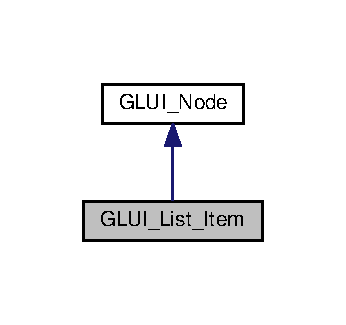
\includegraphics[width=166pt]{class_g_l_u_i___list___item__inherit__graph}
\end{center}
\end{figure}


Collaboration diagram for G\+L\+U\+I\+\_\+\+List\+\_\+\+Item\+:\nopagebreak
\begin{figure}[H]
\begin{center}
\leavevmode
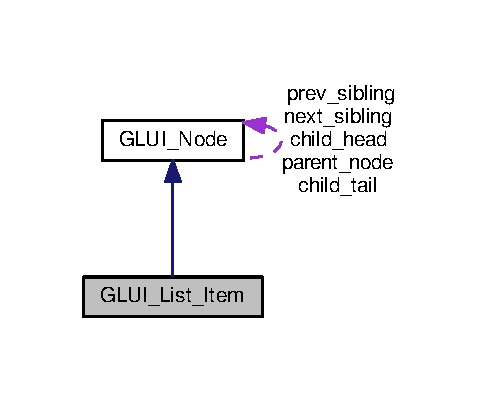
\includegraphics[width=230pt]{class_g_l_u_i___list___item__coll__graph}
\end{center}
\end{figure}
\subsection*{Public Attributes}
\begin{DoxyCompactItemize}
\item 
\hyperlink{glui_8h_aada824856f7bcf29794719981ebd8f60}{G\+L\+U\+I\+\_\+\+String} \hyperlink{class_g_l_u_i___list___item_a8d7db7c4b7dd085352de5d1a6b849da2}{text}
\item 
\hyperlink{wglext_8h_a500a82aecba06f4550f6849b8099ca21}{int} \hyperlink{class_g_l_u_i___list___item_a329b7a460a0e449e4bb0bdc2e8ba519c}{id}
\end{DoxyCompactItemize}
\subsection*{Additional Inherited Members}


\subsection{Detailed Description}


Definition at line 2080 of file glui.\+h.



\subsection{Member Data Documentation}
\hypertarget{class_g_l_u_i___list___item_a329b7a460a0e449e4bb0bdc2e8ba519c}{\index{G\+L\+U\+I\+\_\+\+List\+\_\+\+Item@{G\+L\+U\+I\+\_\+\+List\+\_\+\+Item}!id@{id}}
\index{id@{id}!G\+L\+U\+I\+\_\+\+List\+\_\+\+Item@{G\+L\+U\+I\+\_\+\+List\+\_\+\+Item}}
\subsubsection[{id}]{\setlength{\rightskip}{0pt plus 5cm}{\bf int} G\+L\+U\+I\+\_\+\+List\+\_\+\+Item\+::id}}\label{class_g_l_u_i___list___item_a329b7a460a0e449e4bb0bdc2e8ba519c}


Definition at line 2084 of file glui.\+h.

\hypertarget{class_g_l_u_i___list___item_a8d7db7c4b7dd085352de5d1a6b849da2}{\index{G\+L\+U\+I\+\_\+\+List\+\_\+\+Item@{G\+L\+U\+I\+\_\+\+List\+\_\+\+Item}!text@{text}}
\index{text@{text}!G\+L\+U\+I\+\_\+\+List\+\_\+\+Item@{G\+L\+U\+I\+\_\+\+List\+\_\+\+Item}}
\subsubsection[{text}]{\setlength{\rightskip}{0pt plus 5cm}{\bf G\+L\+U\+I\+\_\+\+String} G\+L\+U\+I\+\_\+\+List\+\_\+\+Item\+::text}}\label{class_g_l_u_i___list___item_a8d7db7c4b7dd085352de5d1a6b849da2}


Definition at line 2083 of file glui.\+h.



The documentation for this class was generated from the following file\+:\begin{DoxyCompactItemize}
\item 
S\+S\+W\+C/src/\+G\+L/\hyperlink{glui_8h}{glui.\+h}\end{DoxyCompactItemize}

\hypertarget{class_g_l_u_i___listbox}{\section{G\+L\+U\+I\+\_\+\+Listbox Class Reference}
\label{class_g_l_u_i___listbox}\index{G\+L\+U\+I\+\_\+\+Listbox@{G\+L\+U\+I\+\_\+\+Listbox}}
}


{\ttfamily \#include $<$glui.\+h$>$}



Inheritance diagram for G\+L\+U\+I\+\_\+\+Listbox\+:\nopagebreak
\begin{figure}[H]
\begin{center}
\leavevmode
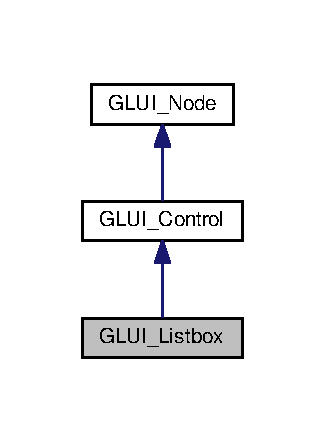
\includegraphics[width=156pt]{class_g_l_u_i___listbox__inherit__graph}
\end{center}
\end{figure}


Collaboration diagram for G\+L\+U\+I\+\_\+\+Listbox\+:\nopagebreak
\begin{figure}[H]
\begin{center}
\leavevmode
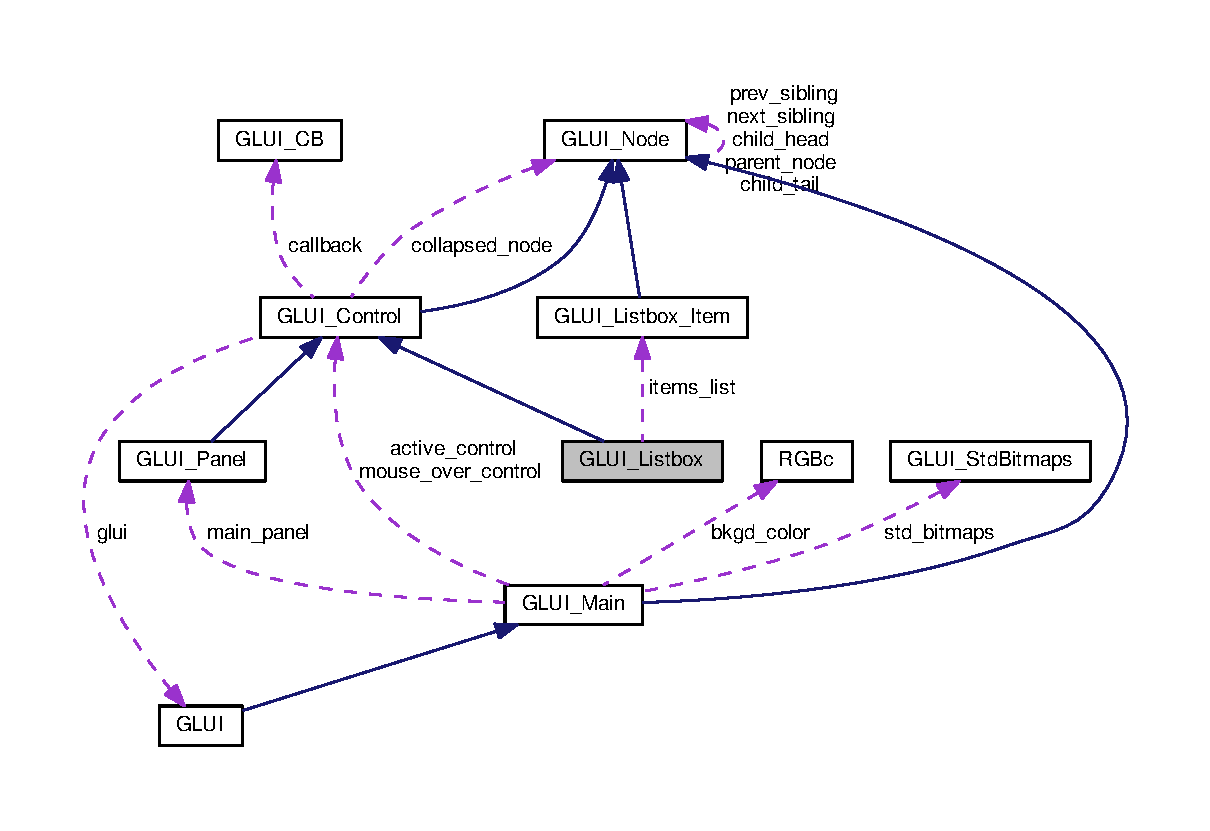
\includegraphics[width=350pt]{class_g_l_u_i___listbox__coll__graph}
\end{center}
\end{figure}
\subsection*{Public Member Functions}
\begin{DoxyCompactItemize}
\item 
\hyperlink{wglext_8h_a500a82aecba06f4550f6849b8099ca21}{int} \hyperlink{class_g_l_u_i___listbox_aaf335e290bd8367d40a9b868faa8be1c}{mouse\+\_\+down\+\_\+handler} (\hyperlink{wglext_8h_a500a82aecba06f4550f6849b8099ca21}{int} local\+\_\+x, \hyperlink{wglext_8h_a500a82aecba06f4550f6849b8099ca21}{int} local\+\_\+y)
\item 
\hyperlink{wglext_8h_a500a82aecba06f4550f6849b8099ca21}{int} \hyperlink{class_g_l_u_i___listbox_a565e196711dad776a2a6f4afa035d25a}{mouse\+\_\+up\+\_\+handler} (\hyperlink{wglext_8h_a500a82aecba06f4550f6849b8099ca21}{int} local\+\_\+x, \hyperlink{wglext_8h_a500a82aecba06f4550f6849b8099ca21}{int} local\+\_\+y, bool inside)
\item 
\hyperlink{wglext_8h_a500a82aecba06f4550f6849b8099ca21}{int} \hyperlink{class_g_l_u_i___listbox_a425b2552f8e430d19157410681abc91c}{mouse\+\_\+held\+\_\+down\+\_\+handler} (\hyperlink{wglext_8h_a500a82aecba06f4550f6849b8099ca21}{int} local\+\_\+x, \hyperlink{wglext_8h_a500a82aecba06f4550f6849b8099ca21}{int} local\+\_\+y, bool inside)
\item 
\hyperlink{wglext_8h_a500a82aecba06f4550f6849b8099ca21}{int} \hyperlink{class_g_l_u_i___listbox_ac3a007ee056e377322d3a8d6ad0478c4}{key\+\_\+handler} (unsigned char key, \hyperlink{wglext_8h_a500a82aecba06f4550f6849b8099ca21}{int} modifiers)
\item 
\hyperlink{wglext_8h_a500a82aecba06f4550f6849b8099ca21}{int} \hyperlink{class_g_l_u_i___listbox_ab1efa64fe3a73dc5d62ebc540acac2d5}{special\+\_\+handler} (\hyperlink{wglext_8h_a500a82aecba06f4550f6849b8099ca21}{int} key, \hyperlink{wglext_8h_a500a82aecba06f4550f6849b8099ca21}{int} modifiers)
\item 
\hyperlink{wglext_8h_a9e6b7f1933461ef318bb000d6bd13b83}{void} \hyperlink{class_g_l_u_i___listbox_a32bf6c1b068e2af4466a19f797693c8d}{update\+\_\+size} (\hyperlink{wglext_8h_a9e6b7f1933461ef318bb000d6bd13b83}{void})
\item 
\hyperlink{wglext_8h_a9e6b7f1933461ef318bb000d6bd13b83}{void} \hyperlink{class_g_l_u_i___listbox_a279c78e74bcba99d067633a9dc39b878}{draw} (\hyperlink{wglext_8h_a500a82aecba06f4550f6849b8099ca21}{int} \hyperlink{glext_8h_ad77deca22f617d3f0e0eb786445689fc}{x}, \hyperlink{wglext_8h_a500a82aecba06f4550f6849b8099ca21}{int} \hyperlink{glext_8h_a9298c7ad619074f5285b32c6b72bfdea}{y})
\item 
\hyperlink{wglext_8h_a500a82aecba06f4550f6849b8099ca21}{int} \hyperlink{class_g_l_u_i___listbox_af44915fea3045f58deffc37e65cea112}{mouse\+\_\+over} (\hyperlink{wglext_8h_a500a82aecba06f4550f6849b8099ca21}{int} state, \hyperlink{wglext_8h_a500a82aecba06f4550f6849b8099ca21}{int} \hyperlink{glext_8h_ad77deca22f617d3f0e0eb786445689fc}{x}, \hyperlink{wglext_8h_a500a82aecba06f4550f6849b8099ca21}{int} \hyperlink{glext_8h_a9298c7ad619074f5285b32c6b72bfdea}{y})
\item 
\hyperlink{wglext_8h_a9e6b7f1933461ef318bb000d6bd13b83}{void} \hyperlink{class_g_l_u_i___listbox_a82ef5939f83cacb4c3f80790fa5962ef}{set\+\_\+int\+\_\+val} (\hyperlink{wglext_8h_a500a82aecba06f4550f6849b8099ca21}{int} new\+\_\+val)
\item 
\hyperlink{wglext_8h_a9e6b7f1933461ef318bb000d6bd13b83}{void} \hyperlink{class_g_l_u_i___listbox_a25d2492d85e1faec1f2e5f9feab8bf7c}{dump} (F\+I\+L\+E $\ast$output)
\item 
\hyperlink{wglext_8h_a500a82aecba06f4550f6849b8099ca21}{int} \hyperlink{class_g_l_u_i___listbox_a173e91d0db2dc5af267e79a592c2af13}{add\+\_\+item} (\hyperlink{wglext_8h_a500a82aecba06f4550f6849b8099ca21}{int} \hyperlink{glext_8h_a58c2a664503e14ffb8f21012aabff3e9}{id}, const char $\ast$\hyperlink{class_g_l_u_i___control_af0d60e9736f4dbc34e9a536e75876d72}{text})
\item 
\hyperlink{wglext_8h_a500a82aecba06f4550f6849b8099ca21}{int} \hyperlink{class_g_l_u_i___listbox_abd8fc9a22c95fc21835f97b98d8c8ca6}{delete\+\_\+item} (const char $\ast$\hyperlink{class_g_l_u_i___control_af0d60e9736f4dbc34e9a536e75876d72}{text})
\item 
\hyperlink{wglext_8h_a500a82aecba06f4550f6849b8099ca21}{int} \hyperlink{class_g_l_u_i___listbox_a814c6749c88cb55a8fca87958d149a19}{delete\+\_\+item} (\hyperlink{wglext_8h_a500a82aecba06f4550f6849b8099ca21}{int} \hyperlink{glext_8h_a58c2a664503e14ffb8f21012aabff3e9}{id})
\item 
\hyperlink{wglext_8h_a500a82aecba06f4550f6849b8099ca21}{int} \hyperlink{class_g_l_u_i___listbox_a54993d7fc093becfddb63b9ebd48def5}{sort\+\_\+items} (\hyperlink{wglext_8h_a9e6b7f1933461ef318bb000d6bd13b83}{void})
\item 
\hyperlink{wglext_8h_a500a82aecba06f4550f6849b8099ca21}{int} \hyperlink{class_g_l_u_i___listbox_afc762e2a72b14bd536cc836f28c53f25}{do\+\_\+selection} (\hyperlink{wglext_8h_a500a82aecba06f4550f6849b8099ca21}{int} item)
\item 
\hyperlink{class_g_l_u_i___listbox___item}{G\+L\+U\+I\+\_\+\+Listbox\+\_\+\+Item} $\ast$ \hyperlink{class_g_l_u_i___listbox_ac17e9adeef5fa21ba1ad00cb7299d771}{get\+\_\+item\+\_\+ptr} (const char $\ast$\hyperlink{class_g_l_u_i___control_af0d60e9736f4dbc34e9a536e75876d72}{text})
\item 
\hyperlink{class_g_l_u_i___listbox___item}{G\+L\+U\+I\+\_\+\+Listbox\+\_\+\+Item} $\ast$ \hyperlink{class_g_l_u_i___listbox_afbf4be7928d629d35eb35f2d51e72eee}{get\+\_\+item\+\_\+ptr} (\hyperlink{wglext_8h_a500a82aecba06f4550f6849b8099ca21}{int} \hyperlink{glext_8h_a58c2a664503e14ffb8f21012aabff3e9}{id})
\item 
\hyperlink{class_g_l_u_i___listbox_a04f341fb0ac378ae1fc09c18f88a393c}{G\+L\+U\+I\+\_\+\+Listbox} (\hyperlink{class_g_l_u_i___node}{G\+L\+U\+I\+\_\+\+Node} $\ast$\hyperlink{class_g_l_u_i___node_a8ed65d447784f6f88bd3e2e2bcac6cdb}{parent}, const char $\ast$\hyperlink{glext_8h_ad977737dfc9a274a62741b9500c49a32}{name}, \hyperlink{wglext_8h_a500a82aecba06f4550f6849b8099ca21}{int} $\ast$live\+\_\+var=N\+U\+L\+L, \hyperlink{wglext_8h_a500a82aecba06f4550f6849b8099ca21}{int} \hyperlink{glext_8h_a58c2a664503e14ffb8f21012aabff3e9}{id}=-\/1, \hyperlink{class_g_l_u_i___c_b}{G\+L\+U\+I\+\_\+\+C\+B} \hyperlink{class_g_l_u_i___control_a96060fe0cc6d537e736dd6eef78e24ab}{callback}=\hyperlink{class_g_l_u_i___c_b}{G\+L\+U\+I\+\_\+\+C\+B}())
\item 
\hyperlink{class_g_l_u_i___listbox_a071ee9024831a4de23995bfefa479466}{G\+L\+U\+I\+\_\+\+Listbox} (\hyperlink{wglext_8h_a9e6b7f1933461ef318bb000d6bd13b83}{void})
\end{DoxyCompactItemize}
\subsection*{Public Attributes}
\begin{DoxyCompactItemize}
\item 
\hyperlink{glui_8h_aada824856f7bcf29794719981ebd8f60}{G\+L\+U\+I\+\_\+\+String} \hyperlink{class_g_l_u_i___listbox_a914b9f8f231fe92b507ec64fbe209271}{curr\+\_\+text}
\item 
\hyperlink{class_g_l_u_i___listbox___item}{G\+L\+U\+I\+\_\+\+Listbox\+\_\+\+Item} \hyperlink{class_g_l_u_i___listbox_a1c6c9d72bdb2c2197ecbe99091534f87}{items\+\_\+list}
\item 
\hyperlink{wglext_8h_a500a82aecba06f4550f6849b8099ca21}{int} \hyperlink{class_g_l_u_i___listbox_a1e00ed51f0b6c8d7e82e8974889a40e7}{depressed}
\item 
\hyperlink{wglext_8h_a500a82aecba06f4550f6849b8099ca21}{int} \hyperlink{class_g_l_u_i___listbox_a5ee58581ac1506984e30868cc8a8c1ec}{orig\+\_\+value}
\item 
bool \hyperlink{class_g_l_u_i___listbox_a5710debcc1604913c926f65db2019b56}{currently\+\_\+inside}
\item 
\hyperlink{wglext_8h_a500a82aecba06f4550f6849b8099ca21}{int} \hyperlink{class_g_l_u_i___listbox_a0f40668bfe80f3fce9c0e027f9e52701}{text\+\_\+x\+\_\+offset}
\item 
\hyperlink{wglext_8h_a500a82aecba06f4550f6849b8099ca21}{int} \hyperlink{class_g_l_u_i___listbox_a4bc9d6c3e849e840b0f61eb446ecba95}{title\+\_\+x\+\_\+offset}
\item 
\hyperlink{wglext_8h_a500a82aecba06f4550f6849b8099ca21}{int} \hyperlink{class_g_l_u_i___listbox_a6efefff573e3d8a77454c94b2aec15c7}{glut\+\_\+menu\+\_\+id}
\end{DoxyCompactItemize}
\subsection*{Protected Member Functions}
\begin{DoxyCompactItemize}
\item 
bool \hyperlink{class_g_l_u_i___listbox_a2d7f6743dea0483354ba495eedfd7d5e}{recalculate\+\_\+item\+\_\+width} (\hyperlink{wglext_8h_a9e6b7f1933461ef318bb000d6bd13b83}{void})
\item 
\hyperlink{wglext_8h_a9e6b7f1933461ef318bb000d6bd13b83}{void} \hyperlink{class_g_l_u_i___listbox_aab5847ab5aa4011667334e9dfb6a5c67}{common\+\_\+init} ()
\item 
\hyperlink{class_g_l_u_i___listbox_ac6eb536028f3c802c0cd9adc647ac0fc}{$\sim$\+G\+L\+U\+I\+\_\+\+Listbox} ()
\end{DoxyCompactItemize}
\subsection*{Additional Inherited Members}


\subsection{Detailed Description}


Definition at line 2320 of file glui.\+h.



\subsection{Constructor \& Destructor Documentation}
\hypertarget{class_g_l_u_i___listbox_a04f341fb0ac378ae1fc09c18f88a393c}{\index{G\+L\+U\+I\+\_\+\+Listbox@{G\+L\+U\+I\+\_\+\+Listbox}!G\+L\+U\+I\+\_\+\+Listbox@{G\+L\+U\+I\+\_\+\+Listbox}}
\index{G\+L\+U\+I\+\_\+\+Listbox@{G\+L\+U\+I\+\_\+\+Listbox}!G\+L\+U\+I\+\_\+\+Listbox@{G\+L\+U\+I\+\_\+\+Listbox}}
\subsubsection[{G\+L\+U\+I\+\_\+\+Listbox}]{\setlength{\rightskip}{0pt plus 5cm}G\+L\+U\+I\+\_\+\+Listbox\+::\+G\+L\+U\+I\+\_\+\+Listbox (
\begin{DoxyParamCaption}
\item[{{\bf G\+L\+U\+I\+\_\+\+Node} $\ast$}]{parent, }
\item[{const char $\ast$}]{name, }
\item[{{\bf int} $\ast$}]{live\+\_\+var = {\ttfamily NULL}, }
\item[{{\bf int}}]{id = {\ttfamily -\/1}, }
\item[{{\bf G\+L\+U\+I\+\_\+\+C\+B}}]{callback = {\ttfamily {\bf G\+L\+U\+I\+\_\+\+C\+B}()}}
\end{DoxyParamCaption}
)}}\label{class_g_l_u_i___listbox_a04f341fb0ac378ae1fc09c18f88a393c}
\hypertarget{class_g_l_u_i___listbox_a071ee9024831a4de23995bfefa479466}{\index{G\+L\+U\+I\+\_\+\+Listbox@{G\+L\+U\+I\+\_\+\+Listbox}!G\+L\+U\+I\+\_\+\+Listbox@{G\+L\+U\+I\+\_\+\+Listbox}}
\index{G\+L\+U\+I\+\_\+\+Listbox@{G\+L\+U\+I\+\_\+\+Listbox}!G\+L\+U\+I\+\_\+\+Listbox@{G\+L\+U\+I\+\_\+\+Listbox}}
\subsubsection[{G\+L\+U\+I\+\_\+\+Listbox}]{\setlength{\rightskip}{0pt plus 5cm}G\+L\+U\+I\+\_\+\+Listbox\+::\+G\+L\+U\+I\+\_\+\+Listbox (
\begin{DoxyParamCaption}
\item[{{\bf void}}]{}
\end{DoxyParamCaption}
)\hspace{0.3cm}{\ttfamily [inline]}}}\label{class_g_l_u_i___listbox_a071ee9024831a4de23995bfefa479466}


Definition at line 2359 of file glui.\+h.

\hypertarget{class_g_l_u_i___listbox_ac6eb536028f3c802c0cd9adc647ac0fc}{\index{G\+L\+U\+I\+\_\+\+Listbox@{G\+L\+U\+I\+\_\+\+Listbox}!````~G\+L\+U\+I\+\_\+\+Listbox@{$\sim$\+G\+L\+U\+I\+\_\+\+Listbox}}
\index{````~G\+L\+U\+I\+\_\+\+Listbox@{$\sim$\+G\+L\+U\+I\+\_\+\+Listbox}!G\+L\+U\+I\+\_\+\+Listbox@{G\+L\+U\+I\+\_\+\+Listbox}}
\subsubsection[{$\sim$\+G\+L\+U\+I\+\_\+\+Listbox}]{\setlength{\rightskip}{0pt plus 5cm}G\+L\+U\+I\+\_\+\+Listbox\+::$\sim$\+G\+L\+U\+I\+\_\+\+Listbox (
\begin{DoxyParamCaption}
{}
\end{DoxyParamCaption}
)\hspace{0.3cm}{\ttfamily [protected]}}}\label{class_g_l_u_i___listbox_ac6eb536028f3c802c0cd9adc647ac0fc}


\subsection{Member Function Documentation}
\hypertarget{class_g_l_u_i___listbox_a173e91d0db2dc5af267e79a592c2af13}{\index{G\+L\+U\+I\+\_\+\+Listbox@{G\+L\+U\+I\+\_\+\+Listbox}!add\+\_\+item@{add\+\_\+item}}
\index{add\+\_\+item@{add\+\_\+item}!G\+L\+U\+I\+\_\+\+Listbox@{G\+L\+U\+I\+\_\+\+Listbox}}
\subsubsection[{add\+\_\+item}]{\setlength{\rightskip}{0pt plus 5cm}{\bf int} G\+L\+U\+I\+\_\+\+Listbox\+::add\+\_\+item (
\begin{DoxyParamCaption}
\item[{{\bf int}}]{id, }
\item[{const char $\ast$}]{text}
\end{DoxyParamCaption}
)}}\label{class_g_l_u_i___listbox_a173e91d0db2dc5af267e79a592c2af13}
\hypertarget{class_g_l_u_i___listbox_aab5847ab5aa4011667334e9dfb6a5c67}{\index{G\+L\+U\+I\+\_\+\+Listbox@{G\+L\+U\+I\+\_\+\+Listbox}!common\+\_\+init@{common\+\_\+init}}
\index{common\+\_\+init@{common\+\_\+init}!G\+L\+U\+I\+\_\+\+Listbox@{G\+L\+U\+I\+\_\+\+Listbox}}
\subsubsection[{common\+\_\+init}]{\setlength{\rightskip}{0pt plus 5cm}{\bf void} G\+L\+U\+I\+\_\+\+Listbox\+::common\+\_\+init (
\begin{DoxyParamCaption}
\item[{{\bf void}}]{}
\end{DoxyParamCaption}
)\hspace{0.3cm}{\ttfamily [inline]}, {\ttfamily [protected]}}}\label{class_g_l_u_i___listbox_aab5847ab5aa4011667334e9dfb6a5c67}


Definition at line 2364 of file glui.\+h.

\hypertarget{class_g_l_u_i___listbox_abd8fc9a22c95fc21835f97b98d8c8ca6}{\index{G\+L\+U\+I\+\_\+\+Listbox@{G\+L\+U\+I\+\_\+\+Listbox}!delete\+\_\+item@{delete\+\_\+item}}
\index{delete\+\_\+item@{delete\+\_\+item}!G\+L\+U\+I\+\_\+\+Listbox@{G\+L\+U\+I\+\_\+\+Listbox}}
\subsubsection[{delete\+\_\+item}]{\setlength{\rightskip}{0pt plus 5cm}{\bf int} G\+L\+U\+I\+\_\+\+Listbox\+::delete\+\_\+item (
\begin{DoxyParamCaption}
\item[{const char $\ast$}]{text}
\end{DoxyParamCaption}
)}}\label{class_g_l_u_i___listbox_abd8fc9a22c95fc21835f97b98d8c8ca6}
\hypertarget{class_g_l_u_i___listbox_a814c6749c88cb55a8fca87958d149a19}{\index{G\+L\+U\+I\+\_\+\+Listbox@{G\+L\+U\+I\+\_\+\+Listbox}!delete\+\_\+item@{delete\+\_\+item}}
\index{delete\+\_\+item@{delete\+\_\+item}!G\+L\+U\+I\+\_\+\+Listbox@{G\+L\+U\+I\+\_\+\+Listbox}}
\subsubsection[{delete\+\_\+item}]{\setlength{\rightskip}{0pt plus 5cm}{\bf int} G\+L\+U\+I\+\_\+\+Listbox\+::delete\+\_\+item (
\begin{DoxyParamCaption}
\item[{{\bf int}}]{id}
\end{DoxyParamCaption}
)}}\label{class_g_l_u_i___listbox_a814c6749c88cb55a8fca87958d149a19}
\hypertarget{class_g_l_u_i___listbox_afc762e2a72b14bd536cc836f28c53f25}{\index{G\+L\+U\+I\+\_\+\+Listbox@{G\+L\+U\+I\+\_\+\+Listbox}!do\+\_\+selection@{do\+\_\+selection}}
\index{do\+\_\+selection@{do\+\_\+selection}!G\+L\+U\+I\+\_\+\+Listbox@{G\+L\+U\+I\+\_\+\+Listbox}}
\subsubsection[{do\+\_\+selection}]{\setlength{\rightskip}{0pt plus 5cm}{\bf int} G\+L\+U\+I\+\_\+\+Listbox\+::do\+\_\+selection (
\begin{DoxyParamCaption}
\item[{{\bf int}}]{item}
\end{DoxyParamCaption}
)}}\label{class_g_l_u_i___listbox_afc762e2a72b14bd536cc836f28c53f25}
\hypertarget{class_g_l_u_i___listbox_a279c78e74bcba99d067633a9dc39b878}{\index{G\+L\+U\+I\+\_\+\+Listbox@{G\+L\+U\+I\+\_\+\+Listbox}!draw@{draw}}
\index{draw@{draw}!G\+L\+U\+I\+\_\+\+Listbox@{G\+L\+U\+I\+\_\+\+Listbox}}
\subsubsection[{draw}]{\setlength{\rightskip}{0pt plus 5cm}{\bf void} G\+L\+U\+I\+\_\+\+Listbox\+::draw (
\begin{DoxyParamCaption}
\item[{{\bf int}}]{x, }
\item[{{\bf int}}]{y}
\end{DoxyParamCaption}
)\hspace{0.3cm}{\ttfamily [virtual]}}}\label{class_g_l_u_i___listbox_a279c78e74bcba99d067633a9dc39b878}


Implements \hyperlink{class_g_l_u_i___control_a2eb42d7a7951280ad2fe8c37972bf66a}{G\+L\+U\+I\+\_\+\+Control}.

\hypertarget{class_g_l_u_i___listbox_a25d2492d85e1faec1f2e5f9feab8bf7c}{\index{G\+L\+U\+I\+\_\+\+Listbox@{G\+L\+U\+I\+\_\+\+Listbox}!dump@{dump}}
\index{dump@{dump}!G\+L\+U\+I\+\_\+\+Listbox@{G\+L\+U\+I\+\_\+\+Listbox}}
\subsubsection[{dump}]{\setlength{\rightskip}{0pt plus 5cm}{\bf void} G\+L\+U\+I\+\_\+\+Listbox\+::dump (
\begin{DoxyParamCaption}
\item[{F\+I\+L\+E $\ast$}]{output}
\end{DoxyParamCaption}
)}}\label{class_g_l_u_i___listbox_a25d2492d85e1faec1f2e5f9feab8bf7c}
\hypertarget{class_g_l_u_i___listbox_ac17e9adeef5fa21ba1ad00cb7299d771}{\index{G\+L\+U\+I\+\_\+\+Listbox@{G\+L\+U\+I\+\_\+\+Listbox}!get\+\_\+item\+\_\+ptr@{get\+\_\+item\+\_\+ptr}}
\index{get\+\_\+item\+\_\+ptr@{get\+\_\+item\+\_\+ptr}!G\+L\+U\+I\+\_\+\+Listbox@{G\+L\+U\+I\+\_\+\+Listbox}}
\subsubsection[{get\+\_\+item\+\_\+ptr}]{\setlength{\rightskip}{0pt plus 5cm}{\bf G\+L\+U\+I\+\_\+\+Listbox\+\_\+\+Item}$\ast$ G\+L\+U\+I\+\_\+\+Listbox\+::get\+\_\+item\+\_\+ptr (
\begin{DoxyParamCaption}
\item[{const char $\ast$}]{text}
\end{DoxyParamCaption}
)}}\label{class_g_l_u_i___listbox_ac17e9adeef5fa21ba1ad00cb7299d771}
\hypertarget{class_g_l_u_i___listbox_afbf4be7928d629d35eb35f2d51e72eee}{\index{G\+L\+U\+I\+\_\+\+Listbox@{G\+L\+U\+I\+\_\+\+Listbox}!get\+\_\+item\+\_\+ptr@{get\+\_\+item\+\_\+ptr}}
\index{get\+\_\+item\+\_\+ptr@{get\+\_\+item\+\_\+ptr}!G\+L\+U\+I\+\_\+\+Listbox@{G\+L\+U\+I\+\_\+\+Listbox}}
\subsubsection[{get\+\_\+item\+\_\+ptr}]{\setlength{\rightskip}{0pt plus 5cm}{\bf G\+L\+U\+I\+\_\+\+Listbox\+\_\+\+Item}$\ast$ G\+L\+U\+I\+\_\+\+Listbox\+::get\+\_\+item\+\_\+ptr (
\begin{DoxyParamCaption}
\item[{{\bf int}}]{id}
\end{DoxyParamCaption}
)}}\label{class_g_l_u_i___listbox_afbf4be7928d629d35eb35f2d51e72eee}
\hypertarget{class_g_l_u_i___listbox_ac3a007ee056e377322d3a8d6ad0478c4}{\index{G\+L\+U\+I\+\_\+\+Listbox@{G\+L\+U\+I\+\_\+\+Listbox}!key\+\_\+handler@{key\+\_\+handler}}
\index{key\+\_\+handler@{key\+\_\+handler}!G\+L\+U\+I\+\_\+\+Listbox@{G\+L\+U\+I\+\_\+\+Listbox}}
\subsubsection[{key\+\_\+handler}]{\setlength{\rightskip}{0pt plus 5cm}{\bf int} G\+L\+U\+I\+\_\+\+Listbox\+::key\+\_\+handler (
\begin{DoxyParamCaption}
\item[{unsigned char}]{key, }
\item[{{\bf int}}]{modifiers}
\end{DoxyParamCaption}
)\hspace{0.3cm}{\ttfamily [virtual]}}}\label{class_g_l_u_i___listbox_ac3a007ee056e377322d3a8d6ad0478c4}


Reimplemented from \hyperlink{class_g_l_u_i___control_a7f9da8ca7df99bd4cf394a9fd8ce19f1}{G\+L\+U\+I\+\_\+\+Control}.

\hypertarget{class_g_l_u_i___listbox_aaf335e290bd8367d40a9b868faa8be1c}{\index{G\+L\+U\+I\+\_\+\+Listbox@{G\+L\+U\+I\+\_\+\+Listbox}!mouse\+\_\+down\+\_\+handler@{mouse\+\_\+down\+\_\+handler}}
\index{mouse\+\_\+down\+\_\+handler@{mouse\+\_\+down\+\_\+handler}!G\+L\+U\+I\+\_\+\+Listbox@{G\+L\+U\+I\+\_\+\+Listbox}}
\subsubsection[{mouse\+\_\+down\+\_\+handler}]{\setlength{\rightskip}{0pt plus 5cm}{\bf int} G\+L\+U\+I\+\_\+\+Listbox\+::mouse\+\_\+down\+\_\+handler (
\begin{DoxyParamCaption}
\item[{{\bf int}}]{local\+\_\+x, }
\item[{{\bf int}}]{local\+\_\+y}
\end{DoxyParamCaption}
)\hspace{0.3cm}{\ttfamily [virtual]}}}\label{class_g_l_u_i___listbox_aaf335e290bd8367d40a9b868faa8be1c}


Reimplemented from \hyperlink{class_g_l_u_i___control_a92b77565168a1d2003bca1c16ac00e8d}{G\+L\+U\+I\+\_\+\+Control}.

\hypertarget{class_g_l_u_i___listbox_a425b2552f8e430d19157410681abc91c}{\index{G\+L\+U\+I\+\_\+\+Listbox@{G\+L\+U\+I\+\_\+\+Listbox}!mouse\+\_\+held\+\_\+down\+\_\+handler@{mouse\+\_\+held\+\_\+down\+\_\+handler}}
\index{mouse\+\_\+held\+\_\+down\+\_\+handler@{mouse\+\_\+held\+\_\+down\+\_\+handler}!G\+L\+U\+I\+\_\+\+Listbox@{G\+L\+U\+I\+\_\+\+Listbox}}
\subsubsection[{mouse\+\_\+held\+\_\+down\+\_\+handler}]{\setlength{\rightskip}{0pt plus 5cm}{\bf int} G\+L\+U\+I\+\_\+\+Listbox\+::mouse\+\_\+held\+\_\+down\+\_\+handler (
\begin{DoxyParamCaption}
\item[{{\bf int}}]{local\+\_\+x, }
\item[{{\bf int}}]{local\+\_\+y, }
\item[{bool}]{inside}
\end{DoxyParamCaption}
)\hspace{0.3cm}{\ttfamily [virtual]}}}\label{class_g_l_u_i___listbox_a425b2552f8e430d19157410681abc91c}


Reimplemented from \hyperlink{class_g_l_u_i___control_a4b44e44c1c455adc7f98c63aeb6aa919}{G\+L\+U\+I\+\_\+\+Control}.

\hypertarget{class_g_l_u_i___listbox_af44915fea3045f58deffc37e65cea112}{\index{G\+L\+U\+I\+\_\+\+Listbox@{G\+L\+U\+I\+\_\+\+Listbox}!mouse\+\_\+over@{mouse\+\_\+over}}
\index{mouse\+\_\+over@{mouse\+\_\+over}!G\+L\+U\+I\+\_\+\+Listbox@{G\+L\+U\+I\+\_\+\+Listbox}}
\subsubsection[{mouse\+\_\+over}]{\setlength{\rightskip}{0pt plus 5cm}{\bf int} G\+L\+U\+I\+\_\+\+Listbox\+::mouse\+\_\+over (
\begin{DoxyParamCaption}
\item[{{\bf int}}]{state, }
\item[{{\bf int}}]{x, }
\item[{{\bf int}}]{y}
\end{DoxyParamCaption}
)\hspace{0.3cm}{\ttfamily [virtual]}}}\label{class_g_l_u_i___listbox_af44915fea3045f58deffc37e65cea112}


Reimplemented from \hyperlink{class_g_l_u_i___control_ac16c3ff7bef1a64abd36a00aa3d935d8}{G\+L\+U\+I\+\_\+\+Control}.

\hypertarget{class_g_l_u_i___listbox_a565e196711dad776a2a6f4afa035d25a}{\index{G\+L\+U\+I\+\_\+\+Listbox@{G\+L\+U\+I\+\_\+\+Listbox}!mouse\+\_\+up\+\_\+handler@{mouse\+\_\+up\+\_\+handler}}
\index{mouse\+\_\+up\+\_\+handler@{mouse\+\_\+up\+\_\+handler}!G\+L\+U\+I\+\_\+\+Listbox@{G\+L\+U\+I\+\_\+\+Listbox}}
\subsubsection[{mouse\+\_\+up\+\_\+handler}]{\setlength{\rightskip}{0pt plus 5cm}{\bf int} G\+L\+U\+I\+\_\+\+Listbox\+::mouse\+\_\+up\+\_\+handler (
\begin{DoxyParamCaption}
\item[{{\bf int}}]{local\+\_\+x, }
\item[{{\bf int}}]{local\+\_\+y, }
\item[{bool}]{inside}
\end{DoxyParamCaption}
)\hspace{0.3cm}{\ttfamily [virtual]}}}\label{class_g_l_u_i___listbox_a565e196711dad776a2a6f4afa035d25a}


Reimplemented from \hyperlink{class_g_l_u_i___control_ac32aad8f69134d03682e34d0488a18f1}{G\+L\+U\+I\+\_\+\+Control}.

\hypertarget{class_g_l_u_i___listbox_a2d7f6743dea0483354ba495eedfd7d5e}{\index{G\+L\+U\+I\+\_\+\+Listbox@{G\+L\+U\+I\+\_\+\+Listbox}!recalculate\+\_\+item\+\_\+width@{recalculate\+\_\+item\+\_\+width}}
\index{recalculate\+\_\+item\+\_\+width@{recalculate\+\_\+item\+\_\+width}!G\+L\+U\+I\+\_\+\+Listbox@{G\+L\+U\+I\+\_\+\+Listbox}}
\subsubsection[{recalculate\+\_\+item\+\_\+width}]{\setlength{\rightskip}{0pt plus 5cm}bool G\+L\+U\+I\+\_\+\+Listbox\+::recalculate\+\_\+item\+\_\+width (
\begin{DoxyParamCaption}
\item[{{\bf void}}]{}
\end{DoxyParamCaption}
)\hspace{0.3cm}{\ttfamily [protected]}}}\label{class_g_l_u_i___listbox_a2d7f6743dea0483354ba495eedfd7d5e}
Change w and return true if we need to be widened to fit the current item. \hypertarget{class_g_l_u_i___listbox_a82ef5939f83cacb4c3f80790fa5962ef}{\index{G\+L\+U\+I\+\_\+\+Listbox@{G\+L\+U\+I\+\_\+\+Listbox}!set\+\_\+int\+\_\+val@{set\+\_\+int\+\_\+val}}
\index{set\+\_\+int\+\_\+val@{set\+\_\+int\+\_\+val}!G\+L\+U\+I\+\_\+\+Listbox@{G\+L\+U\+I\+\_\+\+Listbox}}
\subsubsection[{set\+\_\+int\+\_\+val}]{\setlength{\rightskip}{0pt plus 5cm}{\bf void} G\+L\+U\+I\+\_\+\+Listbox\+::set\+\_\+int\+\_\+val (
\begin{DoxyParamCaption}
\item[{{\bf int}}]{new\+\_\+val}
\end{DoxyParamCaption}
)\hspace{0.3cm}{\ttfamily [virtual]}}}\label{class_g_l_u_i___listbox_a82ef5939f83cacb4c3f80790fa5962ef}


Reimplemented from \hyperlink{class_g_l_u_i___control_a32ef6d11d6c62e344f17268dfb96aad6}{G\+L\+U\+I\+\_\+\+Control}.

\hypertarget{class_g_l_u_i___listbox_a54993d7fc093becfddb63b9ebd48def5}{\index{G\+L\+U\+I\+\_\+\+Listbox@{G\+L\+U\+I\+\_\+\+Listbox}!sort\+\_\+items@{sort\+\_\+items}}
\index{sort\+\_\+items@{sort\+\_\+items}!G\+L\+U\+I\+\_\+\+Listbox@{G\+L\+U\+I\+\_\+\+Listbox}}
\subsubsection[{sort\+\_\+items}]{\setlength{\rightskip}{0pt plus 5cm}{\bf int} G\+L\+U\+I\+\_\+\+Listbox\+::sort\+\_\+items (
\begin{DoxyParamCaption}
\item[{{\bf void}}]{}
\end{DoxyParamCaption}
)}}\label{class_g_l_u_i___listbox_a54993d7fc093becfddb63b9ebd48def5}
\hypertarget{class_g_l_u_i___listbox_ab1efa64fe3a73dc5d62ebc540acac2d5}{\index{G\+L\+U\+I\+\_\+\+Listbox@{G\+L\+U\+I\+\_\+\+Listbox}!special\+\_\+handler@{special\+\_\+handler}}
\index{special\+\_\+handler@{special\+\_\+handler}!G\+L\+U\+I\+\_\+\+Listbox@{G\+L\+U\+I\+\_\+\+Listbox}}
\subsubsection[{special\+\_\+handler}]{\setlength{\rightskip}{0pt plus 5cm}{\bf int} G\+L\+U\+I\+\_\+\+Listbox\+::special\+\_\+handler (
\begin{DoxyParamCaption}
\item[{{\bf int}}]{key, }
\item[{{\bf int}}]{modifiers}
\end{DoxyParamCaption}
)\hspace{0.3cm}{\ttfamily [virtual]}}}\label{class_g_l_u_i___listbox_ab1efa64fe3a73dc5d62ebc540acac2d5}


Reimplemented from \hyperlink{class_g_l_u_i___control_ab08da363df3f3eae867dd5ae61200f23}{G\+L\+U\+I\+\_\+\+Control}.

\hypertarget{class_g_l_u_i___listbox_a32bf6c1b068e2af4466a19f797693c8d}{\index{G\+L\+U\+I\+\_\+\+Listbox@{G\+L\+U\+I\+\_\+\+Listbox}!update\+\_\+size@{update\+\_\+size}}
\index{update\+\_\+size@{update\+\_\+size}!G\+L\+U\+I\+\_\+\+Listbox@{G\+L\+U\+I\+\_\+\+Listbox}}
\subsubsection[{update\+\_\+size}]{\setlength{\rightskip}{0pt plus 5cm}{\bf void} G\+L\+U\+I\+\_\+\+Listbox\+::update\+\_\+size (
\begin{DoxyParamCaption}
\item[{{\bf void}}]{}
\end{DoxyParamCaption}
)\hspace{0.3cm}{\ttfamily [virtual]}}}\label{class_g_l_u_i___listbox_a32bf6c1b068e2af4466a19f797693c8d}


Reimplemented from \hyperlink{class_g_l_u_i___control_a4bfe55acbbf735a7d2ff07d687a481e2}{G\+L\+U\+I\+\_\+\+Control}.



\subsection{Member Data Documentation}
\hypertarget{class_g_l_u_i___listbox_a914b9f8f231fe92b507ec64fbe209271}{\index{G\+L\+U\+I\+\_\+\+Listbox@{G\+L\+U\+I\+\_\+\+Listbox}!curr\+\_\+text@{curr\+\_\+text}}
\index{curr\+\_\+text@{curr\+\_\+text}!G\+L\+U\+I\+\_\+\+Listbox@{G\+L\+U\+I\+\_\+\+Listbox}}
\subsubsection[{curr\+\_\+text}]{\setlength{\rightskip}{0pt plus 5cm}{\bf G\+L\+U\+I\+\_\+\+String} G\+L\+U\+I\+\_\+\+Listbox\+::curr\+\_\+text}}\label{class_g_l_u_i___listbox_a914b9f8f231fe92b507ec64fbe209271}


Definition at line 2323 of file glui.\+h.

\hypertarget{class_g_l_u_i___listbox_a5710debcc1604913c926f65db2019b56}{\index{G\+L\+U\+I\+\_\+\+Listbox@{G\+L\+U\+I\+\_\+\+Listbox}!currently\+\_\+inside@{currently\+\_\+inside}}
\index{currently\+\_\+inside@{currently\+\_\+inside}!G\+L\+U\+I\+\_\+\+Listbox@{G\+L\+U\+I\+\_\+\+Listbox}}
\subsubsection[{currently\+\_\+inside}]{\setlength{\rightskip}{0pt plus 5cm}bool G\+L\+U\+I\+\_\+\+Listbox\+::currently\+\_\+inside}}\label{class_g_l_u_i___listbox_a5710debcc1604913c926f65db2019b56}


Definition at line 2328 of file glui.\+h.

\hypertarget{class_g_l_u_i___listbox_a1e00ed51f0b6c8d7e82e8974889a40e7}{\index{G\+L\+U\+I\+\_\+\+Listbox@{G\+L\+U\+I\+\_\+\+Listbox}!depressed@{depressed}}
\index{depressed@{depressed}!G\+L\+U\+I\+\_\+\+Listbox@{G\+L\+U\+I\+\_\+\+Listbox}}
\subsubsection[{depressed}]{\setlength{\rightskip}{0pt plus 5cm}{\bf int} G\+L\+U\+I\+\_\+\+Listbox\+::depressed}}\label{class_g_l_u_i___listbox_a1e00ed51f0b6c8d7e82e8974889a40e7}


Definition at line 2325 of file glui.\+h.

\hypertarget{class_g_l_u_i___listbox_a6efefff573e3d8a77454c94b2aec15c7}{\index{G\+L\+U\+I\+\_\+\+Listbox@{G\+L\+U\+I\+\_\+\+Listbox}!glut\+\_\+menu\+\_\+id@{glut\+\_\+menu\+\_\+id}}
\index{glut\+\_\+menu\+\_\+id@{glut\+\_\+menu\+\_\+id}!G\+L\+U\+I\+\_\+\+Listbox@{G\+L\+U\+I\+\_\+\+Listbox}}
\subsubsection[{glut\+\_\+menu\+\_\+id}]{\setlength{\rightskip}{0pt plus 5cm}{\bf int} G\+L\+U\+I\+\_\+\+Listbox\+::glut\+\_\+menu\+\_\+id}}\label{class_g_l_u_i___listbox_a6efefff573e3d8a77454c94b2aec15c7}


Definition at line 2330 of file glui.\+h.

\hypertarget{class_g_l_u_i___listbox_a1c6c9d72bdb2c2197ecbe99091534f87}{\index{G\+L\+U\+I\+\_\+\+Listbox@{G\+L\+U\+I\+\_\+\+Listbox}!items\+\_\+list@{items\+\_\+list}}
\index{items\+\_\+list@{items\+\_\+list}!G\+L\+U\+I\+\_\+\+Listbox@{G\+L\+U\+I\+\_\+\+Listbox}}
\subsubsection[{items\+\_\+list}]{\setlength{\rightskip}{0pt plus 5cm}{\bf G\+L\+U\+I\+\_\+\+Listbox\+\_\+\+Item} G\+L\+U\+I\+\_\+\+Listbox\+::items\+\_\+list}}\label{class_g_l_u_i___listbox_a1c6c9d72bdb2c2197ecbe99091534f87}


Definition at line 2324 of file glui.\+h.

\hypertarget{class_g_l_u_i___listbox_a5ee58581ac1506984e30868cc8a8c1ec}{\index{G\+L\+U\+I\+\_\+\+Listbox@{G\+L\+U\+I\+\_\+\+Listbox}!orig\+\_\+value@{orig\+\_\+value}}
\index{orig\+\_\+value@{orig\+\_\+value}!G\+L\+U\+I\+\_\+\+Listbox@{G\+L\+U\+I\+\_\+\+Listbox}}
\subsubsection[{orig\+\_\+value}]{\setlength{\rightskip}{0pt plus 5cm}{\bf int} G\+L\+U\+I\+\_\+\+Listbox\+::orig\+\_\+value}}\label{class_g_l_u_i___listbox_a5ee58581ac1506984e30868cc8a8c1ec}


Definition at line 2327 of file glui.\+h.

\hypertarget{class_g_l_u_i___listbox_a0f40668bfe80f3fce9c0e027f9e52701}{\index{G\+L\+U\+I\+\_\+\+Listbox@{G\+L\+U\+I\+\_\+\+Listbox}!text\+\_\+x\+\_\+offset@{text\+\_\+x\+\_\+offset}}
\index{text\+\_\+x\+\_\+offset@{text\+\_\+x\+\_\+offset}!G\+L\+U\+I\+\_\+\+Listbox@{G\+L\+U\+I\+\_\+\+Listbox}}
\subsubsection[{text\+\_\+x\+\_\+offset}]{\setlength{\rightskip}{0pt plus 5cm}{\bf int} G\+L\+U\+I\+\_\+\+Listbox\+::text\+\_\+x\+\_\+offset}}\label{class_g_l_u_i___listbox_a0f40668bfe80f3fce9c0e027f9e52701}


Definition at line 2329 of file glui.\+h.

\hypertarget{class_g_l_u_i___listbox_a4bc9d6c3e849e840b0f61eb446ecba95}{\index{G\+L\+U\+I\+\_\+\+Listbox@{G\+L\+U\+I\+\_\+\+Listbox}!title\+\_\+x\+\_\+offset@{title\+\_\+x\+\_\+offset}}
\index{title\+\_\+x\+\_\+offset@{title\+\_\+x\+\_\+offset}!G\+L\+U\+I\+\_\+\+Listbox@{G\+L\+U\+I\+\_\+\+Listbox}}
\subsubsection[{title\+\_\+x\+\_\+offset}]{\setlength{\rightskip}{0pt plus 5cm}{\bf int} G\+L\+U\+I\+\_\+\+Listbox\+::title\+\_\+x\+\_\+offset}}\label{class_g_l_u_i___listbox_a4bc9d6c3e849e840b0f61eb446ecba95}


Definition at line 2329 of file glui.\+h.



The documentation for this class was generated from the following file\+:\begin{DoxyCompactItemize}
\item 
S\+S\+W\+C/src/\+G\+L/\hyperlink{glui_8h}{glui.\+h}\end{DoxyCompactItemize}

\hypertarget{class_g_l_u_i___listbox___item}{\section{G\+L\+U\+I\+\_\+\+Listbox\+\_\+\+Item Class Reference}
\label{class_g_l_u_i___listbox___item}\index{G\+L\+U\+I\+\_\+\+Listbox\+\_\+\+Item@{G\+L\+U\+I\+\_\+\+Listbox\+\_\+\+Item}}
}


{\ttfamily \#include $<$glui.\+h$>$}



Inheritance diagram for G\+L\+U\+I\+\_\+\+Listbox\+\_\+\+Item\+:\nopagebreak
\begin{figure}[H]
\begin{center}
\leavevmode
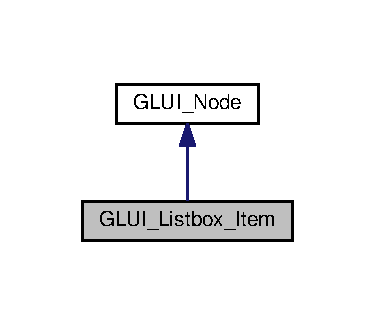
\includegraphics[width=180pt]{class_g_l_u_i___listbox___item__inherit__graph}
\end{center}
\end{figure}


Collaboration diagram for G\+L\+U\+I\+\_\+\+Listbox\+\_\+\+Item\+:\nopagebreak
\begin{figure}[H]
\begin{center}
\leavevmode
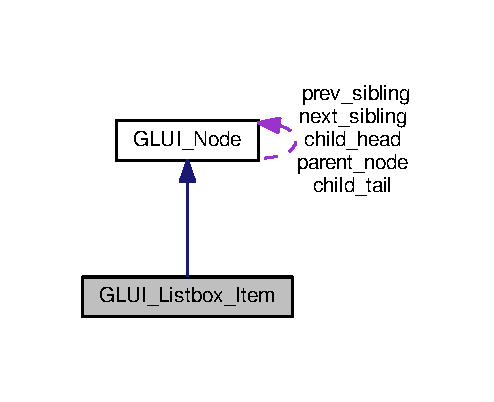
\includegraphics[width=237pt]{class_g_l_u_i___listbox___item__coll__graph}
\end{center}
\end{figure}
\subsection*{Public Attributes}
\begin{DoxyCompactItemize}
\item 
\hyperlink{glui_8h_aada824856f7bcf29794719981ebd8f60}{G\+L\+U\+I\+\_\+\+String} \hyperlink{class_g_l_u_i___listbox___item_a93ab7eacdaf81a43b07b89e60bc5edbe}{text}
\item 
\hyperlink{wglext_8h_a500a82aecba06f4550f6849b8099ca21}{int} \hyperlink{class_g_l_u_i___listbox___item_a82c3decf8704010c91232ad6e2ea95d9}{id}
\end{DoxyCompactItemize}
\subsection*{Additional Inherited Members}


\subsection{Detailed Description}


Definition at line 2313 of file glui.\+h.



\subsection{Member Data Documentation}
\hypertarget{class_g_l_u_i___listbox___item_a82c3decf8704010c91232ad6e2ea95d9}{\index{G\+L\+U\+I\+\_\+\+Listbox\+\_\+\+Item@{G\+L\+U\+I\+\_\+\+Listbox\+\_\+\+Item}!id@{id}}
\index{id@{id}!G\+L\+U\+I\+\_\+\+Listbox\+\_\+\+Item@{G\+L\+U\+I\+\_\+\+Listbox\+\_\+\+Item}}
\subsubsection[{id}]{\setlength{\rightskip}{0pt plus 5cm}{\bf int} G\+L\+U\+I\+\_\+\+Listbox\+\_\+\+Item\+::id}}\label{class_g_l_u_i___listbox___item_a82c3decf8704010c91232ad6e2ea95d9}


Definition at line 2317 of file glui.\+h.

\hypertarget{class_g_l_u_i___listbox___item_a93ab7eacdaf81a43b07b89e60bc5edbe}{\index{G\+L\+U\+I\+\_\+\+Listbox\+\_\+\+Item@{G\+L\+U\+I\+\_\+\+Listbox\+\_\+\+Item}!text@{text}}
\index{text@{text}!G\+L\+U\+I\+\_\+\+Listbox\+\_\+\+Item@{G\+L\+U\+I\+\_\+\+Listbox\+\_\+\+Item}}
\subsubsection[{text}]{\setlength{\rightskip}{0pt plus 5cm}{\bf G\+L\+U\+I\+\_\+\+String} G\+L\+U\+I\+\_\+\+Listbox\+\_\+\+Item\+::text}}\label{class_g_l_u_i___listbox___item_a93ab7eacdaf81a43b07b89e60bc5edbe}


Definition at line 2316 of file glui.\+h.



The documentation for this class was generated from the following file\+:\begin{DoxyCompactItemize}
\item 
S\+S\+W\+C/src/\+G\+L/\hyperlink{glui_8h}{glui.\+h}\end{DoxyCompactItemize}

\hypertarget{class_g_l_u_i___main}{\section{G\+L\+U\+I\+\_\+\+Main Class Reference}
\label{class_g_l_u_i___main}\index{G\+L\+U\+I\+\_\+\+Main@{G\+L\+U\+I\+\_\+\+Main}}
}


{\ttfamily \#include $<$glui.\+h$>$}



Inheritance diagram for G\+L\+U\+I\+\_\+\+Main\+:\nopagebreak
\begin{figure}[H]
\begin{center}
\leavevmode
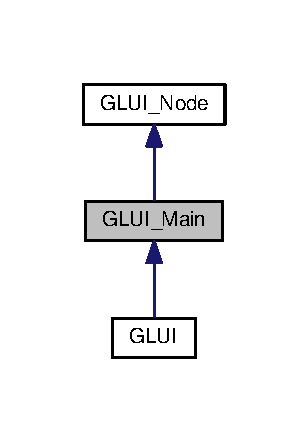
\includegraphics[width=148pt]{class_g_l_u_i___main__inherit__graph}
\end{center}
\end{figure}


Collaboration diagram for G\+L\+U\+I\+\_\+\+Main\+:\nopagebreak
\begin{figure}[H]
\begin{center}
\leavevmode
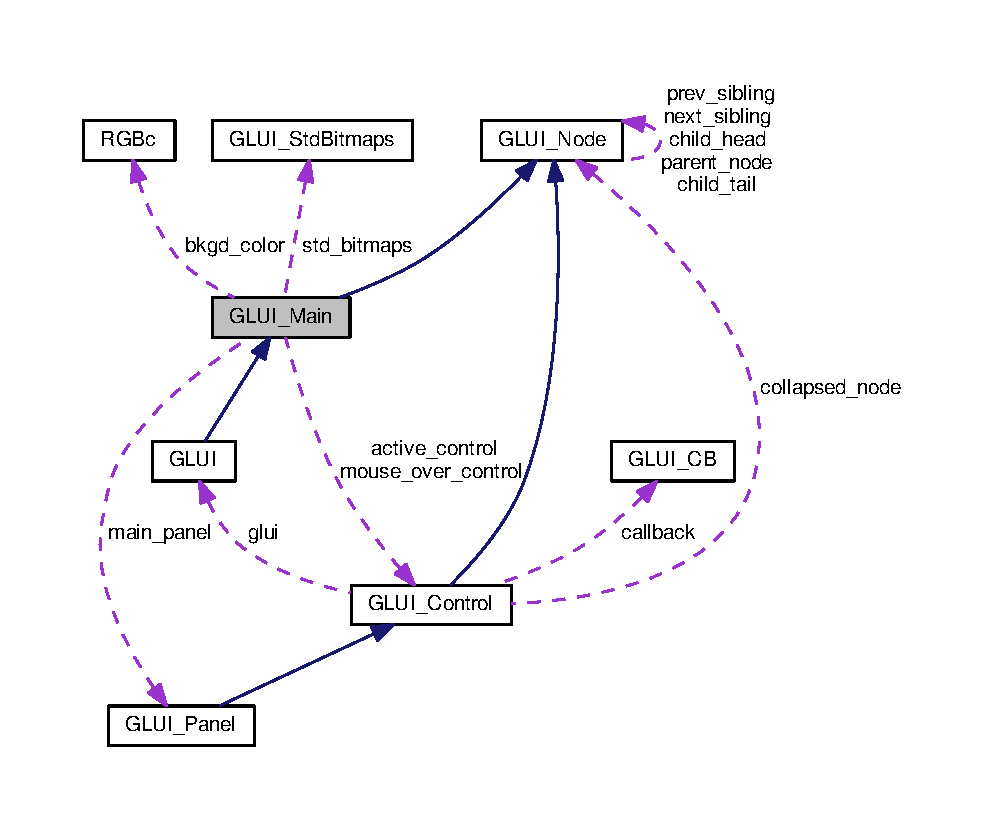
\includegraphics[width=350pt]{class_g_l_u_i___main__coll__graph}
\end{center}
\end{figure}
\subsection*{Public Member Functions}
\begin{DoxyCompactItemize}
\item 
\hyperlink{wglext_8h_a9e6b7f1933461ef318bb000d6bd13b83}{void} \hyperlink{class_g_l_u_i___main_a8489a73dc673357da03075fb1decfc21}{adjust\+\_\+glut\+\_\+xy} (\hyperlink{wglext_8h_a500a82aecba06f4550f6849b8099ca21}{int} \&\hyperlink{glext_8h_ad77deca22f617d3f0e0eb786445689fc}{x}, \hyperlink{wglext_8h_a500a82aecba06f4550f6849b8099ca21}{int} \&\hyperlink{glext_8h_a9298c7ad619074f5285b32c6b72bfdea}{y})
\item 
\hyperlink{wglext_8h_a9e6b7f1933461ef318bb000d6bd13b83}{void} \hyperlink{class_g_l_u_i___main_aafe506d2f17957f0ff81b7168d12428a}{activate\+\_\+control} (\hyperlink{class_g_l_u_i___control}{G\+L\+U\+I\+\_\+\+Control} $\ast$control, \hyperlink{wglext_8h_a500a82aecba06f4550f6849b8099ca21}{int} how)
\item 
\hyperlink{wglext_8h_a9e6b7f1933461ef318bb000d6bd13b83}{void} \hyperlink{class_g_l_u_i___main_a9a01bc045bb6689df3778a199fc68d51}{align\+\_\+controls} (\hyperlink{class_g_l_u_i___control}{G\+L\+U\+I\+\_\+\+Control} $\ast$control)
\item 
\hyperlink{wglext_8h_a9e6b7f1933461ef318bb000d6bd13b83}{void} \hyperlink{class_g_l_u_i___main_a819a4700253582ef4a49101c25b3a5a3}{deactivate\+\_\+current\+\_\+control} (\hyperlink{wglext_8h_a9e6b7f1933461ef318bb000d6bd13b83}{void})
\item 
\hyperlink{wglext_8h_a9e6b7f1933461ef318bb000d6bd13b83}{void} \hyperlink{class_g_l_u_i___main_a45cae7de3682226f44ab74d7afd44063}{draw\+\_\+raised\+\_\+box} (\hyperlink{wglext_8h_a500a82aecba06f4550f6849b8099ca21}{int} \hyperlink{glext_8h_ad77deca22f617d3f0e0eb786445689fc}{x}, \hyperlink{wglext_8h_a500a82aecba06f4550f6849b8099ca21}{int} \hyperlink{glext_8h_a9298c7ad619074f5285b32c6b72bfdea}{y}, \hyperlink{wglext_8h_a500a82aecba06f4550f6849b8099ca21}{int} \hyperlink{glext_8h_a713abae75276598501f75c68917c5e2d}{w}, \hyperlink{wglext_8h_a500a82aecba06f4550f6849b8099ca21}{int} \hyperlink{glext_8h_afa0fb1b5e976920c0abeff2dca3ed774}{h})
\item 
\hyperlink{wglext_8h_a9e6b7f1933461ef318bb000d6bd13b83}{void} \hyperlink{class_g_l_u_i___main_acbd304f272403767b0bcf610bd14cc05}{draw\+\_\+lowered\+\_\+box} (\hyperlink{wglext_8h_a500a82aecba06f4550f6849b8099ca21}{int} \hyperlink{glext_8h_ad77deca22f617d3f0e0eb786445689fc}{x}, \hyperlink{wglext_8h_a500a82aecba06f4550f6849b8099ca21}{int} \hyperlink{glext_8h_a9298c7ad619074f5285b32c6b72bfdea}{y}, \hyperlink{wglext_8h_a500a82aecba06f4550f6849b8099ca21}{int} \hyperlink{glext_8h_a713abae75276598501f75c68917c5e2d}{w}, \hyperlink{wglext_8h_a500a82aecba06f4550f6849b8099ca21}{int} \hyperlink{glext_8h_afa0fb1b5e976920c0abeff2dca3ed774}{h})
\item 
bool \hyperlink{class_g_l_u_i___main_a838a093d3748a6a6434f5e3a62d29c79}{should\+\_\+redraw\+\_\+now} (\hyperlink{class_g_l_u_i___control}{G\+L\+U\+I\+\_\+\+Control} $\ast$ctl)
\item 
\hyperlink{wglext_8h_a500a82aecba06f4550f6849b8099ca21}{int} \hyperlink{class_g_l_u_i___main_a022e4708ab5f105fb49202b7dd28e7b4}{set\+\_\+current\+\_\+draw\+\_\+buffer} ()
\item 
\hyperlink{wglext_8h_a9e6b7f1933461ef318bb000d6bd13b83}{void} \hyperlink{class_g_l_u_i___main_a56523ef45aea9c350009c6d91a67a028}{restore\+\_\+draw\+\_\+buffer} (\hyperlink{wglext_8h_a500a82aecba06f4550f6849b8099ca21}{int} buffer\+\_\+state)
\item 
\hyperlink{wglext_8h_a9e6b7f1933461ef318bb000d6bd13b83}{void} \hyperlink{class_g_l_u_i___main_acd1e25e989f0f1820c496d4b8b9ee422}{refresh} ()
\item 
\hyperlink{wglext_8h_a9e6b7f1933461ef318bb000d6bd13b83}{void} \hyperlink{class_g_l_u_i___main_a64302740a0fb9ca34de276d001fbd8bd}{post\+\_\+update\+\_\+main\+\_\+gfx} ()
\item 
\hyperlink{wglext_8h_a9e6b7f1933461ef318bb000d6bd13b83}{void} \hyperlink{class_g_l_u_i___main_aa3c49dcfbc912870344e9265354ad53a}{pack\+\_\+controls} ()
\item 
\hyperlink{wglext_8h_a9e6b7f1933461ef318bb000d6bd13b83}{void} \hyperlink{class_g_l_u_i___main_a3a6613342a97448cad9677d291165889}{close\+\_\+internal} ()
\item 
\hyperlink{wglext_8h_a9e6b7f1933461ef318bb000d6bd13b83}{void} \hyperlink{class_g_l_u_i___main_a8ca1f714c14dade8e6274112c69e5863}{check\+\_\+subwindow\+\_\+position} ()
\item 
\hyperlink{wglext_8h_a9e6b7f1933461ef318bb000d6bd13b83}{void} \hyperlink{class_g_l_u_i___main_a3216ab4a380f2a904e152524f4687e29}{set\+\_\+ortho\+\_\+projection} ()
\item 
\hyperlink{wglext_8h_a9e6b7f1933461ef318bb000d6bd13b83}{void} \hyperlink{class_g_l_u_i___main_a444621e91c377d33121f8bc95ed80d98}{set\+\_\+viewport} ()
\item 
\hyperlink{wglext_8h_a500a82aecba06f4550f6849b8099ca21}{int} \hyperlink{class_g_l_u_i___main_a8187156aa77f0f9b34660addf333ca79}{get\+\_\+glut\+\_\+window\+\_\+id} (\hyperlink{wglext_8h_a9e6b7f1933461ef318bb000d6bd13b83}{void})
\end{DoxyCompactItemize}
\subsection*{Public Attributes}
\begin{DoxyCompactItemize}
\item 
\hyperlink{class_g_l_u_i___std_bitmaps}{G\+L\+U\+I\+\_\+\+Std\+Bitmaps} \hyperlink{class_g_l_u_i___main_adae87a2e684c2da03d2f8946913eb63d}{std\+\_\+bitmaps}
\item 
\hyperlink{glui_8h_aada824856f7bcf29794719981ebd8f60}{G\+L\+U\+I\+\_\+\+String} \hyperlink{class_g_l_u_i___main_a699c852cb777273543f38506e71c9e22}{window\+\_\+name}
\item 
\hyperlink{class_r_g_bc}{R\+G\+Bc} \hyperlink{class_g_l_u_i___main_a8d939a35dd9fd89091e4345d12f23936}{bkgd\+\_\+color}
\item 
float \hyperlink{class_g_l_u_i___main_a703f236c77d05226bf6ffd01c5c80d0d}{bkgd\+\_\+color\+\_\+f} \mbox{[}3\mbox{]}
\item 
\hyperlink{wglext_8h_a9e6b7f1933461ef318bb000d6bd13b83}{void} $\ast$ \hyperlink{class_g_l_u_i___main_a349e75284a3c1d4e5e8d1f2903d65f8b}{font}
\item 
\hyperlink{wglext_8h_a500a82aecba06f4550f6849b8099ca21}{int} \hyperlink{class_g_l_u_i___main_a96ca3271c5e6a33bd340bd90aa010b14}{curr\+\_\+modifiers}
\end{DoxyCompactItemize}
\subsection*{Protected Types}
\begin{DoxyCompactItemize}
\item 
enum \hyperlink{class_g_l_u_i___main_a0024f5e2750f6fe9e428ff885cf6d62e}{buffer\+\_\+mode\+\_\+t} \{ \hyperlink{class_g_l_u_i___main_a0024f5e2750f6fe9e428ff885cf6d62ea96e503bd03e3d418f350f3a854d0292d}{buffer\+\_\+front} =1, 
\hyperlink{class_g_l_u_i___main_a0024f5e2750f6fe9e428ff885cf6d62ea839b43cd2decf85c6bdcf738d92e122c}{buffer\+\_\+back} =2
 \}
\end{DoxyCompactItemize}
\subsection*{Protected Member Functions}
\begin{DoxyCompactItemize}
\item 
\hyperlink{class_g_l_u_i___control}{G\+L\+U\+I\+\_\+\+Control} $\ast$ \hyperlink{class_g_l_u_i___main_a8bb9bc693db0b65cf06a6b3caf5bf467}{find\+\_\+control} (\hyperlink{wglext_8h_a500a82aecba06f4550f6849b8099ca21}{int} \hyperlink{glext_8h_ad77deca22f617d3f0e0eb786445689fc}{x}, \hyperlink{wglext_8h_a500a82aecba06f4550f6849b8099ca21}{int} \hyperlink{glext_8h_a9298c7ad619074f5285b32c6b72bfdea}{y})
\item 
\hyperlink{class_g_l_u_i___control}{G\+L\+U\+I\+\_\+\+Control} $\ast$ \hyperlink{class_g_l_u_i___main_af869103edb803d7f65d94e1be9b5071f}{find\+\_\+next\+\_\+control} (\hyperlink{class_g_l_u_i___control}{G\+L\+U\+I\+\_\+\+Control} $\ast$control)
\item 
\hyperlink{class_g_l_u_i___control}{G\+L\+U\+I\+\_\+\+Control} $\ast$ \hyperlink{class_g_l_u_i___main_a701cf2655bcccf2b7c5fa4e7fac83b8b}{find\+\_\+next\+\_\+control\+\_\+rec} (\hyperlink{class_g_l_u_i___control}{G\+L\+U\+I\+\_\+\+Control} $\ast$control)
\item 
\hyperlink{class_g_l_u_i___control}{G\+L\+U\+I\+\_\+\+Control} $\ast$ \hyperlink{class_g_l_u_i___main_a88940d2937c251aad1526e1884ef7f7f}{find\+\_\+next\+\_\+control\+\_\+} (\hyperlink{class_g_l_u_i___control}{G\+L\+U\+I\+\_\+\+Control} $\ast$control)
\item 
\hyperlink{class_g_l_u_i___control}{G\+L\+U\+I\+\_\+\+Control} $\ast$ \hyperlink{class_g_l_u_i___main_a8817c8356985d9f508eabf33721cdebe}{find\+\_\+prev\+\_\+control} (\hyperlink{class_g_l_u_i___control}{G\+L\+U\+I\+\_\+\+Control} $\ast$control)
\item 
\hyperlink{wglext_8h_a9e6b7f1933461ef318bb000d6bd13b83}{void} \hyperlink{class_g_l_u_i___main_a524a3d3e51e01707a6fe1916bfdd4e1f}{create\+\_\+standalone\+\_\+window} (const char $\ast$\hyperlink{glext_8h_ad977737dfc9a274a62741b9500c49a32}{name}, \hyperlink{wglext_8h_a500a82aecba06f4550f6849b8099ca21}{int} \hyperlink{glext_8h_ad77deca22f617d3f0e0eb786445689fc}{x}=-\/1, \hyperlink{wglext_8h_a500a82aecba06f4550f6849b8099ca21}{int} \hyperlink{glext_8h_a9298c7ad619074f5285b32c6b72bfdea}{y}=-\/1)
\item 
\hyperlink{wglext_8h_a9e6b7f1933461ef318bb000d6bd13b83}{void} \hyperlink{class_g_l_u_i___main_a4a05365e245aa1751f5b828bdbd78b0e}{create\+\_\+subwindow} (\hyperlink{wglext_8h_a500a82aecba06f4550f6849b8099ca21}{int} \hyperlink{class_g_l_u_i___node_a8ed65d447784f6f88bd3e2e2bcac6cdb}{parent}, \hyperlink{wglext_8h_a500a82aecba06f4550f6849b8099ca21}{int} window\+\_\+alignment)
\item 
\hyperlink{wglext_8h_a9e6b7f1933461ef318bb000d6bd13b83}{void} \hyperlink{class_g_l_u_i___main_a375e803cc89e36548e73719479a8613a}{setup\+\_\+default\+\_\+glut\+\_\+callbacks} (\hyperlink{wglext_8h_a9e6b7f1933461ef318bb000d6bd13b83}{void})
\item 
\hyperlink{wglext_8h_a9e6b7f1933461ef318bb000d6bd13b83}{void} \hyperlink{class_g_l_u_i___main_a4fb7819317131b79a65eeb414ab4e43b}{mouse} (\hyperlink{wglext_8h_a500a82aecba06f4550f6849b8099ca21}{int} button, \hyperlink{wglext_8h_a500a82aecba06f4550f6849b8099ca21}{int} state, \hyperlink{wglext_8h_a500a82aecba06f4550f6849b8099ca21}{int} \hyperlink{glext_8h_ad77deca22f617d3f0e0eb786445689fc}{x}, \hyperlink{wglext_8h_a500a82aecba06f4550f6849b8099ca21}{int} \hyperlink{glext_8h_a9298c7ad619074f5285b32c6b72bfdea}{y})
\item 
\hyperlink{wglext_8h_a9e6b7f1933461ef318bb000d6bd13b83}{void} \hyperlink{class_g_l_u_i___main_a054900a1fe81ede8c3834a364120ef2a}{keyboard} (unsigned char key, \hyperlink{wglext_8h_a500a82aecba06f4550f6849b8099ca21}{int} \hyperlink{glext_8h_ad77deca22f617d3f0e0eb786445689fc}{x}, \hyperlink{wglext_8h_a500a82aecba06f4550f6849b8099ca21}{int} \hyperlink{glext_8h_a9298c7ad619074f5285b32c6b72bfdea}{y})
\item 
\hyperlink{wglext_8h_a9e6b7f1933461ef318bb000d6bd13b83}{void} \hyperlink{class_g_l_u_i___main_ae3dbd97f2fbf58708383a2d167a1841c}{special} (\hyperlink{wglext_8h_a500a82aecba06f4550f6849b8099ca21}{int} key, \hyperlink{wglext_8h_a500a82aecba06f4550f6849b8099ca21}{int} \hyperlink{glext_8h_ad77deca22f617d3f0e0eb786445689fc}{x}, \hyperlink{wglext_8h_a500a82aecba06f4550f6849b8099ca21}{int} \hyperlink{glext_8h_a9298c7ad619074f5285b32c6b72bfdea}{y})
\item 
\hyperlink{wglext_8h_a9e6b7f1933461ef318bb000d6bd13b83}{void} \hyperlink{class_g_l_u_i___main_a9b36f32a0d9b5fa302ddf38be67391ab}{passive\+\_\+motion} (\hyperlink{wglext_8h_a500a82aecba06f4550f6849b8099ca21}{int} \hyperlink{glext_8h_ad77deca22f617d3f0e0eb786445689fc}{x}, \hyperlink{wglext_8h_a500a82aecba06f4550f6849b8099ca21}{int} \hyperlink{glext_8h_a9298c7ad619074f5285b32c6b72bfdea}{y})
\item 
\hyperlink{wglext_8h_a9e6b7f1933461ef318bb000d6bd13b83}{void} \hyperlink{class_g_l_u_i___main_a392acf9047e2be2582a1635f8fb6ff23}{reshape} (\hyperlink{wglext_8h_a500a82aecba06f4550f6849b8099ca21}{int} \hyperlink{glext_8h_a713abae75276598501f75c68917c5e2d}{w}, \hyperlink{wglext_8h_a500a82aecba06f4550f6849b8099ca21}{int} \hyperlink{glext_8h_afa0fb1b5e976920c0abeff2dca3ed774}{h})
\item 
\hyperlink{wglext_8h_a9e6b7f1933461ef318bb000d6bd13b83}{void} \hyperlink{class_g_l_u_i___main_a776f5d5aa6323af0c05992c83be90bbf}{visibility} (\hyperlink{wglext_8h_a500a82aecba06f4550f6849b8099ca21}{int} state)
\item 
\hyperlink{wglext_8h_a9e6b7f1933461ef318bb000d6bd13b83}{void} \hyperlink{class_g_l_u_i___main_a0e8746ccbea45d443007854ae3e07c53}{motion} (\hyperlink{wglext_8h_a500a82aecba06f4550f6849b8099ca21}{int} \hyperlink{glext_8h_ad77deca22f617d3f0e0eb786445689fc}{x}, \hyperlink{wglext_8h_a500a82aecba06f4550f6849b8099ca21}{int} \hyperlink{glext_8h_a9298c7ad619074f5285b32c6b72bfdea}{y})
\item 
\hyperlink{wglext_8h_a9e6b7f1933461ef318bb000d6bd13b83}{void} \hyperlink{class_g_l_u_i___main_a5e7e1594748809fb14ac86f3d15fc5a0}{entry} (\hyperlink{wglext_8h_a500a82aecba06f4550f6849b8099ca21}{int} state)
\item 
\hyperlink{wglext_8h_a9e6b7f1933461ef318bb000d6bd13b83}{void} \hyperlink{class_g_l_u_i___main_af8867df3fa133efbf11064da84a8c047}{display} (\hyperlink{wglext_8h_a9e6b7f1933461ef318bb000d6bd13b83}{void})
\item 
\hyperlink{wglext_8h_a9e6b7f1933461ef318bb000d6bd13b83}{void} \hyperlink{class_g_l_u_i___main_a0f172148e78cde1d8e25e989ba90d43d}{idle} (\hyperlink{wglext_8h_a9e6b7f1933461ef318bb000d6bd13b83}{void})
\item 
\hyperlink{wglext_8h_a500a82aecba06f4550f6849b8099ca21}{int} \hyperlink{class_g_l_u_i___main_aef95c5469e82e69335293fecbebdd3ab}{needs\+\_\+idle} (\hyperlink{wglext_8h_a9e6b7f1933461ef318bb000d6bd13b83}{void})
\item 
virtual \hyperlink{wglext_8h_a500a82aecba06f4550f6849b8099ca21}{int} \hyperlink{class_g_l_u_i___main_aa18b473f6cf75095c12c4edecaf856a3}{add\+\_\+control} (\hyperlink{class_g_l_u_i___node}{G\+L\+U\+I\+\_\+\+Node} $\ast$\hyperlink{class_g_l_u_i___node_a8ed65d447784f6f88bd3e2e2bcac6cdb}{parent}, \hyperlink{class_g_l_u_i___control}{G\+L\+U\+I\+\_\+\+Control} $\ast$control)
\item 
\hyperlink{class_g_l_u_i___main_af27588439ff8203ef8e8059cf0c58e6c}{G\+L\+U\+I\+\_\+\+Main} (\hyperlink{wglext_8h_a9e6b7f1933461ef318bb000d6bd13b83}{void})
\end{DoxyCompactItemize}
\subsection*{Protected Attributes}
\begin{DoxyCompactItemize}
\item 
\hyperlink{wglext_8h_a500a82aecba06f4550f6849b8099ca21}{int} \hyperlink{class_g_l_u_i___main_a43cd4a18026504db98178d766d18a78c}{main\+\_\+gfx\+\_\+window\+\_\+id}
\item 
\hyperlink{wglext_8h_a500a82aecba06f4550f6849b8099ca21}{int} \hyperlink{class_g_l_u_i___main_a5002dc3587df870eb12a62be1568861b}{mouse\+\_\+button\+\_\+down}
\item 
\hyperlink{wglext_8h_a500a82aecba06f4550f6849b8099ca21}{int} \hyperlink{class_g_l_u_i___main_a4c2cd2330267eca938028a8a6fcb6382}{glut\+\_\+window\+\_\+id}
\item 
\hyperlink{wglext_8h_a500a82aecba06f4550f6849b8099ca21}{int} \hyperlink{class_g_l_u_i___main_afec9a40c9b4c139934236d094fcf81f6}{top\+\_\+level\+\_\+glut\+\_\+window\+\_\+id}
\item 
\hyperlink{class_g_l_u_i___control}{G\+L\+U\+I\+\_\+\+Control} $\ast$ \hyperlink{class_g_l_u_i___main_a552e13b05f63046ebe3f1911e27e3d58}{active\+\_\+control}
\item 
\hyperlink{class_g_l_u_i___control}{G\+L\+U\+I\+\_\+\+Control} $\ast$ \hyperlink{class_g_l_u_i___main_a74c11c17faf8a0c957d5654c420dc97f}{mouse\+\_\+over\+\_\+control}
\item 
\hyperlink{class_g_l_u_i___panel}{G\+L\+U\+I\+\_\+\+Panel} $\ast$ \hyperlink{class_g_l_u_i___main_a727ecf1f0315ff01503415dc420b47a2}{main\+\_\+panel}
\item 
\hyperlink{class_g_l_u_i___main_a0024f5e2750f6fe9e428ff885cf6d62e}{buffer\+\_\+mode\+\_\+t} \hyperlink{class_g_l_u_i___main_a4ba466d21144d6fd0c7984039523ad2f}{buffer\+\_\+mode}
\begin{DoxyCompactList}\small\item\em Current drawing mode. \end{DoxyCompactList}\item 
\hyperlink{wglext_8h_a500a82aecba06f4550f6849b8099ca21}{int} \hyperlink{class_g_l_u_i___main_a661d825dbff47caee733683f557491cf}{curr\+\_\+cursor}
\item 
\hyperlink{wglext_8h_a500a82aecba06f4550f6849b8099ca21}{int} \hyperlink{class_g_l_u_i___main_acee19f928a4837310f654431fda7cc1a}{w}
\item 
\hyperlink{wglext_8h_a500a82aecba06f4550f6849b8099ca21}{int} \hyperlink{class_g_l_u_i___main_a7c5cd9db296247eceb52c2aa84448e0f}{h}
\item 
long \hyperlink{class_g_l_u_i___main_ac3fbf169a16afe8e09cebf714f4aee65}{flags}
\item 
bool \hyperlink{class_g_l_u_i___main_a5392e305249f1baf91402460b7c14f10}{closing}
\item 
\hyperlink{wglext_8h_a500a82aecba06f4550f6849b8099ca21}{int} \hyperlink{class_g_l_u_i___main_a70e6e1ec266281f272954fcc42f85087}{parent\+\_\+window}
\item 
\hyperlink{wglext_8h_a500a82aecba06f4550f6849b8099ca21}{int} \hyperlink{class_g_l_u_i___main_a6f8d24f29be85514e1abe05f4f33eb17}{glui\+\_\+id}
\item 
\hyperlink{wglext_8h_a9e6b7f1933461ef318bb000d6bd13b83}{void}($\ast$ \hyperlink{class_g_l_u_i___main_a8a4d3dfa4aac5817297071f05d808afb}{glut\+\_\+mouse\+\_\+\+C\+B} )(\hyperlink{wglext_8h_a500a82aecba06f4550f6849b8099ca21}{int}, \hyperlink{wglext_8h_a500a82aecba06f4550f6849b8099ca21}{int}, \hyperlink{wglext_8h_a500a82aecba06f4550f6849b8099ca21}{int}, \hyperlink{wglext_8h_a500a82aecba06f4550f6849b8099ca21}{int})
\item 
\hyperlink{wglext_8h_a9e6b7f1933461ef318bb000d6bd13b83}{void}($\ast$ \hyperlink{class_g_l_u_i___main_a96d36ca6359fb96bca292a9ff7b1d53f}{glut\+\_\+keyboard\+\_\+\+C\+B} )(unsigned char, \hyperlink{wglext_8h_a500a82aecba06f4550f6849b8099ca21}{int}, \hyperlink{wglext_8h_a500a82aecba06f4550f6849b8099ca21}{int})
\item 
\hyperlink{wglext_8h_a9e6b7f1933461ef318bb000d6bd13b83}{void}($\ast$ \hyperlink{class_g_l_u_i___main_aa50303a909f39a7b28cfdf076cc848a4}{glut\+\_\+special\+\_\+\+C\+B} )(\hyperlink{wglext_8h_a500a82aecba06f4550f6849b8099ca21}{int}, \hyperlink{wglext_8h_a500a82aecba06f4550f6849b8099ca21}{int}, \hyperlink{wglext_8h_a500a82aecba06f4550f6849b8099ca21}{int})
\item 
\hyperlink{wglext_8h_a9e6b7f1933461ef318bb000d6bd13b83}{void}($\ast$ \hyperlink{class_g_l_u_i___main_a93bdf0d34e2f3494dce800ba16da4ec2}{glut\+\_\+reshape\+\_\+\+C\+B} )(\hyperlink{wglext_8h_a500a82aecba06f4550f6849b8099ca21}{int}, \hyperlink{wglext_8h_a500a82aecba06f4550f6849b8099ca21}{int})
\end{DoxyCompactItemize}
\subsection*{Friends}
\begin{DoxyCompactItemize}
\item 
class \hyperlink{class_g_l_u_i___main_a1ac6a21915ff78bdda7d92427b2b9337}{G\+L\+U\+I\+\_\+\+Control}
\item 
class \hyperlink{class_g_l_u_i___main_a7f68b21cd9d98467322b20fd2d4c739c}{G\+L\+U\+I\+\_\+\+Rotation}
\item 
class \hyperlink{class_g_l_u_i___main_a1c751e686f087581ee115c051b63e3ff}{G\+L\+U\+I\+\_\+\+Translation}
\item 
class \hyperlink{class_g_l_u_i___main_a8b2353bef6e8c665a923971433c0c999}{G\+L\+U\+I}
\item 
class \hyperlink{class_g_l_u_i___main_a89d3c98d28cb65cd25c91f17ffcd2bdf}{G\+L\+U\+I\+\_\+\+Master\+\_\+\+Object}
\item 
\hyperlink{wglext_8h_a9e6b7f1933461ef318bb000d6bd13b83}{void} \hyperlink{class_g_l_u_i___main_a6385df2c931519beca286ede9e098f96}{glui\+\_\+mouse\+\_\+func} (\hyperlink{wglext_8h_a500a82aecba06f4550f6849b8099ca21}{int} button, \hyperlink{wglext_8h_a500a82aecba06f4550f6849b8099ca21}{int} state, \hyperlink{wglext_8h_a500a82aecba06f4550f6849b8099ca21}{int} \hyperlink{glext_8h_ad77deca22f617d3f0e0eb786445689fc}{x}, \hyperlink{wglext_8h_a500a82aecba06f4550f6849b8099ca21}{int} \hyperlink{glext_8h_a9298c7ad619074f5285b32c6b72bfdea}{y})
\item 
\hyperlink{wglext_8h_a9e6b7f1933461ef318bb000d6bd13b83}{void} \hyperlink{class_g_l_u_i___main_ae3390518e45a04617135f564021bcebf}{glui\+\_\+keyboard\+\_\+func} (unsigned char key, \hyperlink{wglext_8h_a500a82aecba06f4550f6849b8099ca21}{int} \hyperlink{glext_8h_ad77deca22f617d3f0e0eb786445689fc}{x}, \hyperlink{wglext_8h_a500a82aecba06f4550f6849b8099ca21}{int} \hyperlink{glext_8h_a9298c7ad619074f5285b32c6b72bfdea}{y})
\item 
\hyperlink{wglext_8h_a9e6b7f1933461ef318bb000d6bd13b83}{void} \hyperlink{class_g_l_u_i___main_a457caba107a71dff1918cb7dd271e8f1}{glui\+\_\+special\+\_\+func} (\hyperlink{wglext_8h_a500a82aecba06f4550f6849b8099ca21}{int} key, \hyperlink{wglext_8h_a500a82aecba06f4550f6849b8099ca21}{int} \hyperlink{glext_8h_ad77deca22f617d3f0e0eb786445689fc}{x}, \hyperlink{wglext_8h_a500a82aecba06f4550f6849b8099ca21}{int} \hyperlink{glext_8h_a9298c7ad619074f5285b32c6b72bfdea}{y})
\item 
\hyperlink{wglext_8h_a9e6b7f1933461ef318bb000d6bd13b83}{void} \hyperlink{class_g_l_u_i___main_a783f2a1497c9cc9e2f8c45244c20cc5e}{glui\+\_\+passive\+\_\+motion\+\_\+func} (\hyperlink{wglext_8h_a500a82aecba06f4550f6849b8099ca21}{int} \hyperlink{glext_8h_ad77deca22f617d3f0e0eb786445689fc}{x}, \hyperlink{wglext_8h_a500a82aecba06f4550f6849b8099ca21}{int} \hyperlink{glext_8h_a9298c7ad619074f5285b32c6b72bfdea}{y})
\item 
\hyperlink{wglext_8h_a9e6b7f1933461ef318bb000d6bd13b83}{void} \hyperlink{class_g_l_u_i___main_a1798681d4deaa39c807e49c3902fde96}{glui\+\_\+reshape\+\_\+func} (\hyperlink{wglext_8h_a500a82aecba06f4550f6849b8099ca21}{int} \hyperlink{glext_8h_a713abae75276598501f75c68917c5e2d}{w}, \hyperlink{wglext_8h_a500a82aecba06f4550f6849b8099ca21}{int} \hyperlink{glext_8h_afa0fb1b5e976920c0abeff2dca3ed774}{h})
\item 
\hyperlink{wglext_8h_a9e6b7f1933461ef318bb000d6bd13b83}{void} \hyperlink{class_g_l_u_i___main_a98726addbd2797b8134ac2b654c3cee6}{glui\+\_\+visibility\+\_\+func} (\hyperlink{wglext_8h_a500a82aecba06f4550f6849b8099ca21}{int} state)
\item 
\hyperlink{wglext_8h_a9e6b7f1933461ef318bb000d6bd13b83}{void} \hyperlink{class_g_l_u_i___main_a633765a3cd774bd7521a679eb4a51f2f}{glui\+\_\+motion\+\_\+func} (\hyperlink{wglext_8h_a500a82aecba06f4550f6849b8099ca21}{int} \hyperlink{glext_8h_ad77deca22f617d3f0e0eb786445689fc}{x}, \hyperlink{wglext_8h_a500a82aecba06f4550f6849b8099ca21}{int} \hyperlink{glext_8h_a9298c7ad619074f5285b32c6b72bfdea}{y})
\item 
\hyperlink{wglext_8h_a9e6b7f1933461ef318bb000d6bd13b83}{void} \hyperlink{class_g_l_u_i___main_ac1a3c6ebc56cb90a076c62b9192853e8}{glui\+\_\+entry\+\_\+func} (\hyperlink{wglext_8h_a500a82aecba06f4550f6849b8099ca21}{int} state)
\item 
\hyperlink{wglext_8h_a9e6b7f1933461ef318bb000d6bd13b83}{void} \hyperlink{class_g_l_u_i___main_a02c2a5886dd1faabe8b882da67f77457}{glui\+\_\+display\+\_\+func} (\hyperlink{wglext_8h_a9e6b7f1933461ef318bb000d6bd13b83}{void})
\item 
\hyperlink{wglext_8h_a9e6b7f1933461ef318bb000d6bd13b83}{void} \hyperlink{class_g_l_u_i___main_a6d56019c7f67cab2a97457b11e0b8994}{glui\+\_\+idle\+\_\+func} (\hyperlink{wglext_8h_a9e6b7f1933461ef318bb000d6bd13b83}{void})
\item 
\hyperlink{wglext_8h_a9e6b7f1933461ef318bb000d6bd13b83}{void} \hyperlink{class_g_l_u_i___main_aba8acedae32a786d382d229db7728ee4}{glui\+\_\+parent\+\_\+window\+\_\+reshape\+\_\+func} (\hyperlink{wglext_8h_a500a82aecba06f4550f6849b8099ca21}{int} \hyperlink{glext_8h_a713abae75276598501f75c68917c5e2d}{w}, \hyperlink{wglext_8h_a500a82aecba06f4550f6849b8099ca21}{int} \hyperlink{glext_8h_afa0fb1b5e976920c0abeff2dca3ed774}{h})
\item 
\hyperlink{wglext_8h_a9e6b7f1933461ef318bb000d6bd13b83}{void} \hyperlink{class_g_l_u_i___main_aff7ae88a0a9221d06fd6712875970c58}{glui\+\_\+parent\+\_\+window\+\_\+keyboard\+\_\+func} (unsigned char, \hyperlink{wglext_8h_a500a82aecba06f4550f6849b8099ca21}{int}, \hyperlink{wglext_8h_a500a82aecba06f4550f6849b8099ca21}{int})
\item 
\hyperlink{wglext_8h_a9e6b7f1933461ef318bb000d6bd13b83}{void} \hyperlink{class_g_l_u_i___main_ab729b572b9acaffe3ebc827b6cfd72ca}{glui\+\_\+parent\+\_\+window\+\_\+special\+\_\+func} (\hyperlink{wglext_8h_a500a82aecba06f4550f6849b8099ca21}{int}, \hyperlink{wglext_8h_a500a82aecba06f4550f6849b8099ca21}{int}, \hyperlink{wglext_8h_a500a82aecba06f4550f6849b8099ca21}{int})
\item 
\hyperlink{wglext_8h_a9e6b7f1933461ef318bb000d6bd13b83}{void} \hyperlink{class_g_l_u_i___main_a391c1191451c678e7702e593e74dc5a4}{glui\+\_\+parent\+\_\+window\+\_\+mouse\+\_\+func} (\hyperlink{wglext_8h_a500a82aecba06f4550f6849b8099ca21}{int}, \hyperlink{wglext_8h_a500a82aecba06f4550f6849b8099ca21}{int}, \hyperlink{wglext_8h_a500a82aecba06f4550f6849b8099ca21}{int}, \hyperlink{wglext_8h_a500a82aecba06f4550f6849b8099ca21}{int})
\end{DoxyCompactItemize}
\subsection*{Additional Inherited Members}


\subsection{Detailed Description}
A \hyperlink{class_g_l_u_i___main}{G\+L\+U\+I\+\_\+\+Main} handles G\+L\+U\+T events for one window, routing them to the appropriate controls. The central user-\/visible \char`\"{}\+G\+L\+U\+I\char`\"{} class inherits from this class; users should not allocate G\+L\+U\+T\+\_\+\+Main objects.

There's a separate \hyperlink{class_g_l_u_i___main}{G\+L\+U\+I\+\_\+\+Main} object for\+:
\begin{DoxyItemize}
\item Each top-\/level window with G\+U\+I stuff in it.
\end{DoxyItemize}

Each \char`\"{}subwindow\char`\"{} of another top-\/level window.

All the \hyperlink{class_g_l_u_i___main}{G\+L\+U\+I\+\_\+\+Main} objects are listed in G\+L\+U\+I\+\_\+\+Master.\+gluis. A better name for this class might be \char`\"{}\+G\+L\+U\+I\+\_\+\+Environment\char`\"{}; this class provides the window-\/level context for every control. 

Definition at line 607 of file glui.\+h.



\subsection{Member Enumeration Documentation}
\hypertarget{class_g_l_u_i___main_a0024f5e2750f6fe9e428ff885cf6d62e}{\index{G\+L\+U\+I\+\_\+\+Main@{G\+L\+U\+I\+\_\+\+Main}!buffer\+\_\+mode\+\_\+t@{buffer\+\_\+mode\+\_\+t}}
\index{buffer\+\_\+mode\+\_\+t@{buffer\+\_\+mode\+\_\+t}!G\+L\+U\+I\+\_\+\+Main@{G\+L\+U\+I\+\_\+\+Main}}
\subsubsection[{buffer\+\_\+mode\+\_\+t}]{\setlength{\rightskip}{0pt plus 5cm}enum {\bf G\+L\+U\+I\+\_\+\+Main\+::buffer\+\_\+mode\+\_\+t}\hspace{0.3cm}{\ttfamily [protected]}}}\label{class_g_l_u_i___main_a0024f5e2750f6fe9e428ff885cf6d62e}
\begin{Desc}
\item[Enumerator]\par
\begin{description}
\index{buffer\+\_\+front@{buffer\+\_\+front}!G\+L\+U\+I\+\_\+\+Main@{G\+L\+U\+I\+\_\+\+Main}}\index{G\+L\+U\+I\+\_\+\+Main@{G\+L\+U\+I\+\_\+\+Main}!buffer\+\_\+front@{buffer\+\_\+front}}\item[{\em 
\hypertarget{class_g_l_u_i___main_a0024f5e2750f6fe9e428ff885cf6d62ea96e503bd03e3d418f350f3a854d0292d}{buffer\+\_\+front}\label{class_g_l_u_i___main_a0024f5e2750f6fe9e428ff885cf6d62ea96e503bd03e3d418f350f3a854d0292d}
}]Draw updated controls directly to screen. \index{buffer\+\_\+back@{buffer\+\_\+back}!G\+L\+U\+I\+\_\+\+Main@{G\+L\+U\+I\+\_\+\+Main}}\index{G\+L\+U\+I\+\_\+\+Main@{G\+L\+U\+I\+\_\+\+Main}!buffer\+\_\+back@{buffer\+\_\+back}}\item[{\em 
\hypertarget{class_g_l_u_i___main_a0024f5e2750f6fe9e428ff885cf6d62ea839b43cd2decf85c6bdcf738d92e122c}{buffer\+\_\+back}\label{class_g_l_u_i___main_a0024f5e2750f6fe9e428ff885cf6d62ea839b43cd2decf85c6bdcf738d92e122c}
}]Double buffering\+: postpone updates until next redraw. \end{description}
\end{Desc}


Definition at line 644 of file glui.\+h.



\subsection{Constructor \& Destructor Documentation}
\hypertarget{class_g_l_u_i___main_af27588439ff8203ef8e8059cf0c58e6c}{\index{G\+L\+U\+I\+\_\+\+Main@{G\+L\+U\+I\+\_\+\+Main}!G\+L\+U\+I\+\_\+\+Main@{G\+L\+U\+I\+\_\+\+Main}}
\index{G\+L\+U\+I\+\_\+\+Main@{G\+L\+U\+I\+\_\+\+Main}!G\+L\+U\+I\+\_\+\+Main@{G\+L\+U\+I\+\_\+\+Main}}
\subsubsection[{G\+L\+U\+I\+\_\+\+Main}]{\setlength{\rightskip}{0pt plus 5cm}G\+L\+U\+I\+\_\+\+Main\+::\+G\+L\+U\+I\+\_\+\+Main (
\begin{DoxyParamCaption}
\item[{{\bf void}}]{}
\end{DoxyParamCaption}
)\hspace{0.3cm}{\ttfamily [protected]}}}\label{class_g_l_u_i___main_af27588439ff8203ef8e8059cf0c58e6c}


\subsection{Member Function Documentation}
\hypertarget{class_g_l_u_i___main_aafe506d2f17957f0ff81b7168d12428a}{\index{G\+L\+U\+I\+\_\+\+Main@{G\+L\+U\+I\+\_\+\+Main}!activate\+\_\+control@{activate\+\_\+control}}
\index{activate\+\_\+control@{activate\+\_\+control}!G\+L\+U\+I\+\_\+\+Main@{G\+L\+U\+I\+\_\+\+Main}}
\subsubsection[{activate\+\_\+control}]{\setlength{\rightskip}{0pt plus 5cm}{\bf void} G\+L\+U\+I\+\_\+\+Main\+::activate\+\_\+control (
\begin{DoxyParamCaption}
\item[{{\bf G\+L\+U\+I\+\_\+\+Control} $\ast$}]{control, }
\item[{{\bf int}}]{how}
\end{DoxyParamCaption}
)}}\label{class_g_l_u_i___main_aafe506d2f17957f0ff81b7168d12428a}
\hypertarget{class_g_l_u_i___main_aa18b473f6cf75095c12c4edecaf856a3}{\index{G\+L\+U\+I\+\_\+\+Main@{G\+L\+U\+I\+\_\+\+Main}!add\+\_\+control@{add\+\_\+control}}
\index{add\+\_\+control@{add\+\_\+control}!G\+L\+U\+I\+\_\+\+Main@{G\+L\+U\+I\+\_\+\+Main}}
\subsubsection[{add\+\_\+control}]{\setlength{\rightskip}{0pt plus 5cm}virtual {\bf int} G\+L\+U\+I\+\_\+\+Main\+::add\+\_\+control (
\begin{DoxyParamCaption}
\item[{{\bf G\+L\+U\+I\+\_\+\+Node} $\ast$}]{parent, }
\item[{{\bf G\+L\+U\+I\+\_\+\+Control} $\ast$}]{control}
\end{DoxyParamCaption}
)\hspace{0.3cm}{\ttfamily [protected]}, {\ttfamily [virtual]}}}\label{class_g_l_u_i___main_aa18b473f6cf75095c12c4edecaf856a3}


Reimplemented in \hyperlink{class_g_l_u_i_a293fdf48459c281e466781ec9c559c21}{G\+L\+U\+I}.

\hypertarget{class_g_l_u_i___main_a8489a73dc673357da03075fb1decfc21}{\index{G\+L\+U\+I\+\_\+\+Main@{G\+L\+U\+I\+\_\+\+Main}!adjust\+\_\+glut\+\_\+xy@{adjust\+\_\+glut\+\_\+xy}}
\index{adjust\+\_\+glut\+\_\+xy@{adjust\+\_\+glut\+\_\+xy}!G\+L\+U\+I\+\_\+\+Main@{G\+L\+U\+I\+\_\+\+Main}}
\subsubsection[{adjust\+\_\+glut\+\_\+xy}]{\setlength{\rightskip}{0pt plus 5cm}{\bf void} G\+L\+U\+I\+\_\+\+Main\+::adjust\+\_\+glut\+\_\+xy (
\begin{DoxyParamCaption}
\item[{{\bf int} \&}]{x, }
\item[{{\bf int} \&}]{y}
\end{DoxyParamCaption}
)\hspace{0.3cm}{\ttfamily [inline]}}}\label{class_g_l_u_i___main_a8489a73dc673357da03075fb1decfc21}


Definition at line 703 of file glui.\+h.

\hypertarget{class_g_l_u_i___main_a9a01bc045bb6689df3778a199fc68d51}{\index{G\+L\+U\+I\+\_\+\+Main@{G\+L\+U\+I\+\_\+\+Main}!align\+\_\+controls@{align\+\_\+controls}}
\index{align\+\_\+controls@{align\+\_\+controls}!G\+L\+U\+I\+\_\+\+Main@{G\+L\+U\+I\+\_\+\+Main}}
\subsubsection[{align\+\_\+controls}]{\setlength{\rightskip}{0pt plus 5cm}{\bf void} G\+L\+U\+I\+\_\+\+Main\+::align\+\_\+controls (
\begin{DoxyParamCaption}
\item[{{\bf G\+L\+U\+I\+\_\+\+Control} $\ast$}]{control}
\end{DoxyParamCaption}
)}}\label{class_g_l_u_i___main_a9a01bc045bb6689df3778a199fc68d51}
\hypertarget{class_g_l_u_i___main_a8ca1f714c14dade8e6274112c69e5863}{\index{G\+L\+U\+I\+\_\+\+Main@{G\+L\+U\+I\+\_\+\+Main}!check\+\_\+subwindow\+\_\+position@{check\+\_\+subwindow\+\_\+position}}
\index{check\+\_\+subwindow\+\_\+position@{check\+\_\+subwindow\+\_\+position}!G\+L\+U\+I\+\_\+\+Main@{G\+L\+U\+I\+\_\+\+Main}}
\subsubsection[{check\+\_\+subwindow\+\_\+position}]{\setlength{\rightskip}{0pt plus 5cm}{\bf void} G\+L\+U\+I\+\_\+\+Main\+::check\+\_\+subwindow\+\_\+position (
\begin{DoxyParamCaption}
{}
\end{DoxyParamCaption}
)}}\label{class_g_l_u_i___main_a8ca1f714c14dade8e6274112c69e5863}
\hypertarget{class_g_l_u_i___main_a3a6613342a97448cad9677d291165889}{\index{G\+L\+U\+I\+\_\+\+Main@{G\+L\+U\+I\+\_\+\+Main}!close\+\_\+internal@{close\+\_\+internal}}
\index{close\+\_\+internal@{close\+\_\+internal}!G\+L\+U\+I\+\_\+\+Main@{G\+L\+U\+I\+\_\+\+Main}}
\subsubsection[{close\+\_\+internal}]{\setlength{\rightskip}{0pt plus 5cm}{\bf void} G\+L\+U\+I\+\_\+\+Main\+::close\+\_\+internal (
\begin{DoxyParamCaption}
{}
\end{DoxyParamCaption}
)}}\label{class_g_l_u_i___main_a3a6613342a97448cad9677d291165889}
\hypertarget{class_g_l_u_i___main_a524a3d3e51e01707a6fe1916bfdd4e1f}{\index{G\+L\+U\+I\+\_\+\+Main@{G\+L\+U\+I\+\_\+\+Main}!create\+\_\+standalone\+\_\+window@{create\+\_\+standalone\+\_\+window}}
\index{create\+\_\+standalone\+\_\+window@{create\+\_\+standalone\+\_\+window}!G\+L\+U\+I\+\_\+\+Main@{G\+L\+U\+I\+\_\+\+Main}}
\subsubsection[{create\+\_\+standalone\+\_\+window}]{\setlength{\rightskip}{0pt plus 5cm}{\bf void} G\+L\+U\+I\+\_\+\+Main\+::create\+\_\+standalone\+\_\+window (
\begin{DoxyParamCaption}
\item[{const char $\ast$}]{name, }
\item[{{\bf int}}]{x = {\ttfamily -\/1}, }
\item[{{\bf int}}]{y = {\ttfamily -\/1}}
\end{DoxyParamCaption}
)\hspace{0.3cm}{\ttfamily [protected]}}}\label{class_g_l_u_i___main_a524a3d3e51e01707a6fe1916bfdd4e1f}
\hypertarget{class_g_l_u_i___main_a4a05365e245aa1751f5b828bdbd78b0e}{\index{G\+L\+U\+I\+\_\+\+Main@{G\+L\+U\+I\+\_\+\+Main}!create\+\_\+subwindow@{create\+\_\+subwindow}}
\index{create\+\_\+subwindow@{create\+\_\+subwindow}!G\+L\+U\+I\+\_\+\+Main@{G\+L\+U\+I\+\_\+\+Main}}
\subsubsection[{create\+\_\+subwindow}]{\setlength{\rightskip}{0pt plus 5cm}{\bf void} G\+L\+U\+I\+\_\+\+Main\+::create\+\_\+subwindow (
\begin{DoxyParamCaption}
\item[{{\bf int}}]{parent, }
\item[{{\bf int}}]{window\+\_\+alignment}
\end{DoxyParamCaption}
)\hspace{0.3cm}{\ttfamily [protected]}}}\label{class_g_l_u_i___main_a4a05365e245aa1751f5b828bdbd78b0e}
\hypertarget{class_g_l_u_i___main_a819a4700253582ef4a49101c25b3a5a3}{\index{G\+L\+U\+I\+\_\+\+Main@{G\+L\+U\+I\+\_\+\+Main}!deactivate\+\_\+current\+\_\+control@{deactivate\+\_\+current\+\_\+control}}
\index{deactivate\+\_\+current\+\_\+control@{deactivate\+\_\+current\+\_\+control}!G\+L\+U\+I\+\_\+\+Main@{G\+L\+U\+I\+\_\+\+Main}}
\subsubsection[{deactivate\+\_\+current\+\_\+control}]{\setlength{\rightskip}{0pt plus 5cm}{\bf void} G\+L\+U\+I\+\_\+\+Main\+::deactivate\+\_\+current\+\_\+control (
\begin{DoxyParamCaption}
\item[{{\bf void}}]{}
\end{DoxyParamCaption}
)}}\label{class_g_l_u_i___main_a819a4700253582ef4a49101c25b3a5a3}
\hypertarget{class_g_l_u_i___main_af8867df3fa133efbf11064da84a8c047}{\index{G\+L\+U\+I\+\_\+\+Main@{G\+L\+U\+I\+\_\+\+Main}!display@{display}}
\index{display@{display}!G\+L\+U\+I\+\_\+\+Main@{G\+L\+U\+I\+\_\+\+Main}}
\subsubsection[{display}]{\setlength{\rightskip}{0pt plus 5cm}{\bf void} G\+L\+U\+I\+\_\+\+Main\+::display (
\begin{DoxyParamCaption}
\item[{{\bf void}}]{}
\end{DoxyParamCaption}
)\hspace{0.3cm}{\ttfamily [protected]}}}\label{class_g_l_u_i___main_af8867df3fa133efbf11064da84a8c047}
\hypertarget{class_g_l_u_i___main_acbd304f272403767b0bcf610bd14cc05}{\index{G\+L\+U\+I\+\_\+\+Main@{G\+L\+U\+I\+\_\+\+Main}!draw\+\_\+lowered\+\_\+box@{draw\+\_\+lowered\+\_\+box}}
\index{draw\+\_\+lowered\+\_\+box@{draw\+\_\+lowered\+\_\+box}!G\+L\+U\+I\+\_\+\+Main@{G\+L\+U\+I\+\_\+\+Main}}
\subsubsection[{draw\+\_\+lowered\+\_\+box}]{\setlength{\rightskip}{0pt plus 5cm}{\bf void} G\+L\+U\+I\+\_\+\+Main\+::draw\+\_\+lowered\+\_\+box (
\begin{DoxyParamCaption}
\item[{{\bf int}}]{x, }
\item[{{\bf int}}]{y, }
\item[{{\bf int}}]{w, }
\item[{{\bf int}}]{h}
\end{DoxyParamCaption}
)}}\label{class_g_l_u_i___main_acbd304f272403767b0bcf610bd14cc05}
Draw a 3\+D-\/look pushed-\/in box around this rectangle \hypertarget{class_g_l_u_i___main_a45cae7de3682226f44ab74d7afd44063}{\index{G\+L\+U\+I\+\_\+\+Main@{G\+L\+U\+I\+\_\+\+Main}!draw\+\_\+raised\+\_\+box@{draw\+\_\+raised\+\_\+box}}
\index{draw\+\_\+raised\+\_\+box@{draw\+\_\+raised\+\_\+box}!G\+L\+U\+I\+\_\+\+Main@{G\+L\+U\+I\+\_\+\+Main}}
\subsubsection[{draw\+\_\+raised\+\_\+box}]{\setlength{\rightskip}{0pt plus 5cm}{\bf void} G\+L\+U\+I\+\_\+\+Main\+::draw\+\_\+raised\+\_\+box (
\begin{DoxyParamCaption}
\item[{{\bf int}}]{x, }
\item[{{\bf int}}]{y, }
\item[{{\bf int}}]{w, }
\item[{{\bf int}}]{h}
\end{DoxyParamCaption}
)}}\label{class_g_l_u_i___main_a45cae7de3682226f44ab74d7afd44063}
Draw a 3\+D-\/look pushed-\/out box around this rectangle \hypertarget{class_g_l_u_i___main_a5e7e1594748809fb14ac86f3d15fc5a0}{\index{G\+L\+U\+I\+\_\+\+Main@{G\+L\+U\+I\+\_\+\+Main}!entry@{entry}}
\index{entry@{entry}!G\+L\+U\+I\+\_\+\+Main@{G\+L\+U\+I\+\_\+\+Main}}
\subsubsection[{entry}]{\setlength{\rightskip}{0pt plus 5cm}{\bf void} G\+L\+U\+I\+\_\+\+Main\+::entry (
\begin{DoxyParamCaption}
\item[{{\bf int}}]{state}
\end{DoxyParamCaption}
)\hspace{0.3cm}{\ttfamily [protected]}}}\label{class_g_l_u_i___main_a5e7e1594748809fb14ac86f3d15fc5a0}
\hypertarget{class_g_l_u_i___main_a8bb9bc693db0b65cf06a6b3caf5bf467}{\index{G\+L\+U\+I\+\_\+\+Main@{G\+L\+U\+I\+\_\+\+Main}!find\+\_\+control@{find\+\_\+control}}
\index{find\+\_\+control@{find\+\_\+control}!G\+L\+U\+I\+\_\+\+Main@{G\+L\+U\+I\+\_\+\+Main}}
\subsubsection[{find\+\_\+control}]{\setlength{\rightskip}{0pt plus 5cm}{\bf G\+L\+U\+I\+\_\+\+Control}$\ast$ G\+L\+U\+I\+\_\+\+Main\+::find\+\_\+control (
\begin{DoxyParamCaption}
\item[{{\bf int}}]{x, }
\item[{{\bf int}}]{y}
\end{DoxyParamCaption}
)\hspace{0.3cm}{\ttfamily [protected]}}}\label{class_g_l_u_i___main_a8bb9bc693db0b65cf06a6b3caf5bf467}
\hypertarget{class_g_l_u_i___main_af869103edb803d7f65d94e1be9b5071f}{\index{G\+L\+U\+I\+\_\+\+Main@{G\+L\+U\+I\+\_\+\+Main}!find\+\_\+next\+\_\+control@{find\+\_\+next\+\_\+control}}
\index{find\+\_\+next\+\_\+control@{find\+\_\+next\+\_\+control}!G\+L\+U\+I\+\_\+\+Main@{G\+L\+U\+I\+\_\+\+Main}}
\subsubsection[{find\+\_\+next\+\_\+control}]{\setlength{\rightskip}{0pt plus 5cm}{\bf G\+L\+U\+I\+\_\+\+Control}$\ast$ G\+L\+U\+I\+\_\+\+Main\+::find\+\_\+next\+\_\+control (
\begin{DoxyParamCaption}
\item[{{\bf G\+L\+U\+I\+\_\+\+Control} $\ast$}]{control}
\end{DoxyParamCaption}
)\hspace{0.3cm}{\ttfamily [protected]}}}\label{class_g_l_u_i___main_af869103edb803d7f65d94e1be9b5071f}
\hypertarget{class_g_l_u_i___main_a88940d2937c251aad1526e1884ef7f7f}{\index{G\+L\+U\+I\+\_\+\+Main@{G\+L\+U\+I\+\_\+\+Main}!find\+\_\+next\+\_\+control\+\_\+@{find\+\_\+next\+\_\+control\+\_\+}}
\index{find\+\_\+next\+\_\+control\+\_\+@{find\+\_\+next\+\_\+control\+\_\+}!G\+L\+U\+I\+\_\+\+Main@{G\+L\+U\+I\+\_\+\+Main}}
\subsubsection[{find\+\_\+next\+\_\+control\+\_\+}]{\setlength{\rightskip}{0pt plus 5cm}{\bf G\+L\+U\+I\+\_\+\+Control}$\ast$ G\+L\+U\+I\+\_\+\+Main\+::find\+\_\+next\+\_\+control\+\_\+ (
\begin{DoxyParamCaption}
\item[{{\bf G\+L\+U\+I\+\_\+\+Control} $\ast$}]{control}
\end{DoxyParamCaption}
)\hspace{0.3cm}{\ttfamily [protected]}}}\label{class_g_l_u_i___main_a88940d2937c251aad1526e1884ef7f7f}
\hypertarget{class_g_l_u_i___main_a701cf2655bcccf2b7c5fa4e7fac83b8b}{\index{G\+L\+U\+I\+\_\+\+Main@{G\+L\+U\+I\+\_\+\+Main}!find\+\_\+next\+\_\+control\+\_\+rec@{find\+\_\+next\+\_\+control\+\_\+rec}}
\index{find\+\_\+next\+\_\+control\+\_\+rec@{find\+\_\+next\+\_\+control\+\_\+rec}!G\+L\+U\+I\+\_\+\+Main@{G\+L\+U\+I\+\_\+\+Main}}
\subsubsection[{find\+\_\+next\+\_\+control\+\_\+rec}]{\setlength{\rightskip}{0pt plus 5cm}{\bf G\+L\+U\+I\+\_\+\+Control}$\ast$ G\+L\+U\+I\+\_\+\+Main\+::find\+\_\+next\+\_\+control\+\_\+rec (
\begin{DoxyParamCaption}
\item[{{\bf G\+L\+U\+I\+\_\+\+Control} $\ast$}]{control}
\end{DoxyParamCaption}
)\hspace{0.3cm}{\ttfamily [protected]}}}\label{class_g_l_u_i___main_a701cf2655bcccf2b7c5fa4e7fac83b8b}
\hypertarget{class_g_l_u_i___main_a8817c8356985d9f508eabf33721cdebe}{\index{G\+L\+U\+I\+\_\+\+Main@{G\+L\+U\+I\+\_\+\+Main}!find\+\_\+prev\+\_\+control@{find\+\_\+prev\+\_\+control}}
\index{find\+\_\+prev\+\_\+control@{find\+\_\+prev\+\_\+control}!G\+L\+U\+I\+\_\+\+Main@{G\+L\+U\+I\+\_\+\+Main}}
\subsubsection[{find\+\_\+prev\+\_\+control}]{\setlength{\rightskip}{0pt plus 5cm}{\bf G\+L\+U\+I\+\_\+\+Control}$\ast$ G\+L\+U\+I\+\_\+\+Main\+::find\+\_\+prev\+\_\+control (
\begin{DoxyParamCaption}
\item[{{\bf G\+L\+U\+I\+\_\+\+Control} $\ast$}]{control}
\end{DoxyParamCaption}
)\hspace{0.3cm}{\ttfamily [protected]}}}\label{class_g_l_u_i___main_a8817c8356985d9f508eabf33721cdebe}
\hypertarget{class_g_l_u_i___main_a8187156aa77f0f9b34660addf333ca79}{\index{G\+L\+U\+I\+\_\+\+Main@{G\+L\+U\+I\+\_\+\+Main}!get\+\_\+glut\+\_\+window\+\_\+id@{get\+\_\+glut\+\_\+window\+\_\+id}}
\index{get\+\_\+glut\+\_\+window\+\_\+id@{get\+\_\+glut\+\_\+window\+\_\+id}!G\+L\+U\+I\+\_\+\+Main@{G\+L\+U\+I\+\_\+\+Main}}
\subsubsection[{get\+\_\+glut\+\_\+window\+\_\+id}]{\setlength{\rightskip}{0pt plus 5cm}{\bf int} G\+L\+U\+I\+\_\+\+Main\+::get\+\_\+glut\+\_\+window\+\_\+id (
\begin{DoxyParamCaption}
\item[{{\bf void}}]{}
\end{DoxyParamCaption}
)\hspace{0.3cm}{\ttfamily [inline]}}}\label{class_g_l_u_i___main_a8187156aa77f0f9b34660addf333ca79}


Definition at line 739 of file glui.\+h.

\hypertarget{class_g_l_u_i___main_a0f172148e78cde1d8e25e989ba90d43d}{\index{G\+L\+U\+I\+\_\+\+Main@{G\+L\+U\+I\+\_\+\+Main}!idle@{idle}}
\index{idle@{idle}!G\+L\+U\+I\+\_\+\+Main@{G\+L\+U\+I\+\_\+\+Main}}
\subsubsection[{idle}]{\setlength{\rightskip}{0pt plus 5cm}{\bf void} G\+L\+U\+I\+\_\+\+Main\+::idle (
\begin{DoxyParamCaption}
\item[{{\bf void}}]{}
\end{DoxyParamCaption}
)\hspace{0.3cm}{\ttfamily [protected]}}}\label{class_g_l_u_i___main_a0f172148e78cde1d8e25e989ba90d43d}
\hypertarget{class_g_l_u_i___main_a054900a1fe81ede8c3834a364120ef2a}{\index{G\+L\+U\+I\+\_\+\+Main@{G\+L\+U\+I\+\_\+\+Main}!keyboard@{keyboard}}
\index{keyboard@{keyboard}!G\+L\+U\+I\+\_\+\+Main@{G\+L\+U\+I\+\_\+\+Main}}
\subsubsection[{keyboard}]{\setlength{\rightskip}{0pt plus 5cm}{\bf void} G\+L\+U\+I\+\_\+\+Main\+::keyboard (
\begin{DoxyParamCaption}
\item[{unsigned char}]{key, }
\item[{{\bf int}}]{x, }
\item[{{\bf int}}]{y}
\end{DoxyParamCaption}
)\hspace{0.3cm}{\ttfamily [protected]}}}\label{class_g_l_u_i___main_a054900a1fe81ede8c3834a364120ef2a}
\hypertarget{class_g_l_u_i___main_a0e8746ccbea45d443007854ae3e07c53}{\index{G\+L\+U\+I\+\_\+\+Main@{G\+L\+U\+I\+\_\+\+Main}!motion@{motion}}
\index{motion@{motion}!G\+L\+U\+I\+\_\+\+Main@{G\+L\+U\+I\+\_\+\+Main}}
\subsubsection[{motion}]{\setlength{\rightskip}{0pt plus 5cm}{\bf void} G\+L\+U\+I\+\_\+\+Main\+::motion (
\begin{DoxyParamCaption}
\item[{{\bf int}}]{x, }
\item[{{\bf int}}]{y}
\end{DoxyParamCaption}
)\hspace{0.3cm}{\ttfamily [protected]}}}\label{class_g_l_u_i___main_a0e8746ccbea45d443007854ae3e07c53}
\hypertarget{class_g_l_u_i___main_a4fb7819317131b79a65eeb414ab4e43b}{\index{G\+L\+U\+I\+\_\+\+Main@{G\+L\+U\+I\+\_\+\+Main}!mouse@{mouse}}
\index{mouse@{mouse}!G\+L\+U\+I\+\_\+\+Main@{G\+L\+U\+I\+\_\+\+Main}}
\subsubsection[{mouse}]{\setlength{\rightskip}{0pt plus 5cm}{\bf void} G\+L\+U\+I\+\_\+\+Main\+::mouse (
\begin{DoxyParamCaption}
\item[{{\bf int}}]{button, }
\item[{{\bf int}}]{state, }
\item[{{\bf int}}]{x, }
\item[{{\bf int}}]{y}
\end{DoxyParamCaption}
)\hspace{0.3cm}{\ttfamily [protected]}}}\label{class_g_l_u_i___main_a4fb7819317131b79a65eeb414ab4e43b}
\hypertarget{class_g_l_u_i___main_aef95c5469e82e69335293fecbebdd3ab}{\index{G\+L\+U\+I\+\_\+\+Main@{G\+L\+U\+I\+\_\+\+Main}!needs\+\_\+idle@{needs\+\_\+idle}}
\index{needs\+\_\+idle@{needs\+\_\+idle}!G\+L\+U\+I\+\_\+\+Main@{G\+L\+U\+I\+\_\+\+Main}}
\subsubsection[{needs\+\_\+idle}]{\setlength{\rightskip}{0pt plus 5cm}{\bf int} G\+L\+U\+I\+\_\+\+Main\+::needs\+\_\+idle (
\begin{DoxyParamCaption}
\item[{{\bf void}}]{}
\end{DoxyParamCaption}
)\hspace{0.3cm}{\ttfamily [protected]}}}\label{class_g_l_u_i___main_aef95c5469e82e69335293fecbebdd3ab}
\hypertarget{class_g_l_u_i___main_aa3c49dcfbc912870344e9265354ad53a}{\index{G\+L\+U\+I\+\_\+\+Main@{G\+L\+U\+I\+\_\+\+Main}!pack\+\_\+controls@{pack\+\_\+controls}}
\index{pack\+\_\+controls@{pack\+\_\+controls}!G\+L\+U\+I\+\_\+\+Main@{G\+L\+U\+I\+\_\+\+Main}}
\subsubsection[{pack\+\_\+controls}]{\setlength{\rightskip}{0pt plus 5cm}{\bf void} G\+L\+U\+I\+\_\+\+Main\+::pack\+\_\+controls (
\begin{DoxyParamCaption}
{}
\end{DoxyParamCaption}
)}}\label{class_g_l_u_i___main_aa3c49dcfbc912870344e9265354ad53a}
Recompute the sizes and positions of all controls \hypertarget{class_g_l_u_i___main_a9b36f32a0d9b5fa302ddf38be67391ab}{\index{G\+L\+U\+I\+\_\+\+Main@{G\+L\+U\+I\+\_\+\+Main}!passive\+\_\+motion@{passive\+\_\+motion}}
\index{passive\+\_\+motion@{passive\+\_\+motion}!G\+L\+U\+I\+\_\+\+Main@{G\+L\+U\+I\+\_\+\+Main}}
\subsubsection[{passive\+\_\+motion}]{\setlength{\rightskip}{0pt plus 5cm}{\bf void} G\+L\+U\+I\+\_\+\+Main\+::passive\+\_\+motion (
\begin{DoxyParamCaption}
\item[{{\bf int}}]{x, }
\item[{{\bf int}}]{y}
\end{DoxyParamCaption}
)\hspace{0.3cm}{\ttfamily [protected]}}}\label{class_g_l_u_i___main_a9b36f32a0d9b5fa302ddf38be67391ab}
\hypertarget{class_g_l_u_i___main_a64302740a0fb9ca34de276d001fbd8bd}{\index{G\+L\+U\+I\+\_\+\+Main@{G\+L\+U\+I\+\_\+\+Main}!post\+\_\+update\+\_\+main\+\_\+gfx@{post\+\_\+update\+\_\+main\+\_\+gfx}}
\index{post\+\_\+update\+\_\+main\+\_\+gfx@{post\+\_\+update\+\_\+main\+\_\+gfx}!G\+L\+U\+I\+\_\+\+Main@{G\+L\+U\+I\+\_\+\+Main}}
\subsubsection[{post\+\_\+update\+\_\+main\+\_\+gfx}]{\setlength{\rightskip}{0pt plus 5cm}{\bf void} G\+L\+U\+I\+\_\+\+Main\+::post\+\_\+update\+\_\+main\+\_\+gfx (
\begin{DoxyParamCaption}
{}
\end{DoxyParamCaption}
)}}\label{class_g_l_u_i___main_a64302740a0fb9ca34de276d001fbd8bd}
Redraw the main graphics window \hypertarget{class_g_l_u_i___main_acd1e25e989f0f1820c496d4b8b9ee422}{\index{G\+L\+U\+I\+\_\+\+Main@{G\+L\+U\+I\+\_\+\+Main}!refresh@{refresh}}
\index{refresh@{refresh}!G\+L\+U\+I\+\_\+\+Main@{G\+L\+U\+I\+\_\+\+Main}}
\subsubsection[{refresh}]{\setlength{\rightskip}{0pt plus 5cm}{\bf void} G\+L\+U\+I\+\_\+\+Main\+::refresh (
\begin{DoxyParamCaption}
{}
\end{DoxyParamCaption}
)}}\label{class_g_l_u_i___main_acd1e25e989f0f1820c496d4b8b9ee422}
Pack, resize the window, and redraw all the controls. \hypertarget{class_g_l_u_i___main_a392acf9047e2be2582a1635f8fb6ff23}{\index{G\+L\+U\+I\+\_\+\+Main@{G\+L\+U\+I\+\_\+\+Main}!reshape@{reshape}}
\index{reshape@{reshape}!G\+L\+U\+I\+\_\+\+Main@{G\+L\+U\+I\+\_\+\+Main}}
\subsubsection[{reshape}]{\setlength{\rightskip}{0pt plus 5cm}{\bf void} G\+L\+U\+I\+\_\+\+Main\+::reshape (
\begin{DoxyParamCaption}
\item[{{\bf int}}]{w, }
\item[{{\bf int}}]{h}
\end{DoxyParamCaption}
)\hspace{0.3cm}{\ttfamily [protected]}}}\label{class_g_l_u_i___main_a392acf9047e2be2582a1635f8fb6ff23}
\hypertarget{class_g_l_u_i___main_a56523ef45aea9c350009c6d91a67a028}{\index{G\+L\+U\+I\+\_\+\+Main@{G\+L\+U\+I\+\_\+\+Main}!restore\+\_\+draw\+\_\+buffer@{restore\+\_\+draw\+\_\+buffer}}
\index{restore\+\_\+draw\+\_\+buffer@{restore\+\_\+draw\+\_\+buffer}!G\+L\+U\+I\+\_\+\+Main@{G\+L\+U\+I\+\_\+\+Main}}
\subsubsection[{restore\+\_\+draw\+\_\+buffer}]{\setlength{\rightskip}{0pt plus 5cm}{\bf void} G\+L\+U\+I\+\_\+\+Main\+::restore\+\_\+draw\+\_\+buffer (
\begin{DoxyParamCaption}
\item[{{\bf int}}]{buffer\+\_\+state}
\end{DoxyParamCaption}
)}}\label{class_g_l_u_i___main_a56523ef45aea9c350009c6d91a67a028}
Go back to using this draw buffer. Undoes set\+\_\+current\+\_\+draw\+\_\+buffer. \hypertarget{class_g_l_u_i___main_a022e4708ab5f105fb49202b7dd28e7b4}{\index{G\+L\+U\+I\+\_\+\+Main@{G\+L\+U\+I\+\_\+\+Main}!set\+\_\+current\+\_\+draw\+\_\+buffer@{set\+\_\+current\+\_\+draw\+\_\+buffer}}
\index{set\+\_\+current\+\_\+draw\+\_\+buffer@{set\+\_\+current\+\_\+draw\+\_\+buffer}!G\+L\+U\+I\+\_\+\+Main@{G\+L\+U\+I\+\_\+\+Main}}
\subsubsection[{set\+\_\+current\+\_\+draw\+\_\+buffer}]{\setlength{\rightskip}{0pt plus 5cm}{\bf int} G\+L\+U\+I\+\_\+\+Main\+::set\+\_\+current\+\_\+draw\+\_\+buffer (
\begin{DoxyParamCaption}
{}
\end{DoxyParamCaption}
)}}\label{class_g_l_u_i___main_a022e4708ab5f105fb49202b7dd28e7b4}
Switch to the appropriate draw buffer now. Returns the old draw buffer. This routine should probably only be called from inside the G\+L\+U\+I\+\_\+\+Drawing\+Sentinal, in glui\+\_\+internal\+\_\+control.\+h \hypertarget{class_g_l_u_i___main_a3216ab4a380f2a904e152524f4687e29}{\index{G\+L\+U\+I\+\_\+\+Main@{G\+L\+U\+I\+\_\+\+Main}!set\+\_\+ortho\+\_\+projection@{set\+\_\+ortho\+\_\+projection}}
\index{set\+\_\+ortho\+\_\+projection@{set\+\_\+ortho\+\_\+projection}!G\+L\+U\+I\+\_\+\+Main@{G\+L\+U\+I\+\_\+\+Main}}
\subsubsection[{set\+\_\+ortho\+\_\+projection}]{\setlength{\rightskip}{0pt plus 5cm}{\bf void} G\+L\+U\+I\+\_\+\+Main\+::set\+\_\+ortho\+\_\+projection (
\begin{DoxyParamCaption}
{}
\end{DoxyParamCaption}
)}}\label{class_g_l_u_i___main_a3216ab4a380f2a904e152524f4687e29}
\hypertarget{class_g_l_u_i___main_a444621e91c377d33121f8bc95ed80d98}{\index{G\+L\+U\+I\+\_\+\+Main@{G\+L\+U\+I\+\_\+\+Main}!set\+\_\+viewport@{set\+\_\+viewport}}
\index{set\+\_\+viewport@{set\+\_\+viewport}!G\+L\+U\+I\+\_\+\+Main@{G\+L\+U\+I\+\_\+\+Main}}
\subsubsection[{set\+\_\+viewport}]{\setlength{\rightskip}{0pt plus 5cm}{\bf void} G\+L\+U\+I\+\_\+\+Main\+::set\+\_\+viewport (
\begin{DoxyParamCaption}
{}
\end{DoxyParamCaption}
)}}\label{class_g_l_u_i___main_a444621e91c377d33121f8bc95ed80d98}
\hypertarget{class_g_l_u_i___main_a375e803cc89e36548e73719479a8613a}{\index{G\+L\+U\+I\+\_\+\+Main@{G\+L\+U\+I\+\_\+\+Main}!setup\+\_\+default\+\_\+glut\+\_\+callbacks@{setup\+\_\+default\+\_\+glut\+\_\+callbacks}}
\index{setup\+\_\+default\+\_\+glut\+\_\+callbacks@{setup\+\_\+default\+\_\+glut\+\_\+callbacks}!G\+L\+U\+I\+\_\+\+Main@{G\+L\+U\+I\+\_\+\+Main}}
\subsubsection[{setup\+\_\+default\+\_\+glut\+\_\+callbacks}]{\setlength{\rightskip}{0pt plus 5cm}{\bf void} G\+L\+U\+I\+\_\+\+Main\+::setup\+\_\+default\+\_\+glut\+\_\+callbacks (
\begin{DoxyParamCaption}
\item[{{\bf void}}]{}
\end{DoxyParamCaption}
)\hspace{0.3cm}{\ttfamily [protected]}}}\label{class_g_l_u_i___main_a375e803cc89e36548e73719479a8613a}
\hypertarget{class_g_l_u_i___main_a838a093d3748a6a6434f5e3a62d29c79}{\index{G\+L\+U\+I\+\_\+\+Main@{G\+L\+U\+I\+\_\+\+Main}!should\+\_\+redraw\+\_\+now@{should\+\_\+redraw\+\_\+now}}
\index{should\+\_\+redraw\+\_\+now@{should\+\_\+redraw\+\_\+now}!G\+L\+U\+I\+\_\+\+Main@{G\+L\+U\+I\+\_\+\+Main}}
\subsubsection[{should\+\_\+redraw\+\_\+now}]{\setlength{\rightskip}{0pt plus 5cm}bool G\+L\+U\+I\+\_\+\+Main\+::should\+\_\+redraw\+\_\+now (
\begin{DoxyParamCaption}
\item[{{\bf G\+L\+U\+I\+\_\+\+Control} $\ast$}]{ctl}
\end{DoxyParamCaption}
)}}\label{class_g_l_u_i___main_a838a093d3748a6a6434f5e3a62d29c79}
Return true if this control should redraw itself immediately (front buffer); Or queue up a redraw and return false if it shouldn't (back buffer). \hypertarget{class_g_l_u_i___main_ae3dbd97f2fbf58708383a2d167a1841c}{\index{G\+L\+U\+I\+\_\+\+Main@{G\+L\+U\+I\+\_\+\+Main}!special@{special}}
\index{special@{special}!G\+L\+U\+I\+\_\+\+Main@{G\+L\+U\+I\+\_\+\+Main}}
\subsubsection[{special}]{\setlength{\rightskip}{0pt plus 5cm}{\bf void} G\+L\+U\+I\+\_\+\+Main\+::special (
\begin{DoxyParamCaption}
\item[{{\bf int}}]{key, }
\item[{{\bf int}}]{x, }
\item[{{\bf int}}]{y}
\end{DoxyParamCaption}
)\hspace{0.3cm}{\ttfamily [protected]}}}\label{class_g_l_u_i___main_ae3dbd97f2fbf58708383a2d167a1841c}
\hypertarget{class_g_l_u_i___main_a776f5d5aa6323af0c05992c83be90bbf}{\index{G\+L\+U\+I\+\_\+\+Main@{G\+L\+U\+I\+\_\+\+Main}!visibility@{visibility}}
\index{visibility@{visibility}!G\+L\+U\+I\+\_\+\+Main@{G\+L\+U\+I\+\_\+\+Main}}
\subsubsection[{visibility}]{\setlength{\rightskip}{0pt plus 5cm}{\bf void} G\+L\+U\+I\+\_\+\+Main\+::visibility (
\begin{DoxyParamCaption}
\item[{{\bf int}}]{state}
\end{DoxyParamCaption}
)\hspace{0.3cm}{\ttfamily [protected]}}}\label{class_g_l_u_i___main_a776f5d5aa6323af0c05992c83be90bbf}


\subsection{Friends And Related Function Documentation}
\hypertarget{class_g_l_u_i___main_a8b2353bef6e8c665a923971433c0c999}{\index{G\+L\+U\+I\+\_\+\+Main@{G\+L\+U\+I\+\_\+\+Main}!G\+L\+U\+I@{G\+L\+U\+I}}
\index{G\+L\+U\+I@{G\+L\+U\+I}!G\+L\+U\+I\+\_\+\+Main@{G\+L\+U\+I\+\_\+\+Main}}
\subsubsection[{G\+L\+U\+I}]{\setlength{\rightskip}{0pt plus 5cm}friend class {\bf G\+L\+U\+I}\hspace{0.3cm}{\ttfamily [friend]}}}\label{class_g_l_u_i___main_a8b2353bef6e8c665a923971433c0c999}


Definition at line 614 of file glui.\+h.

\hypertarget{class_g_l_u_i___main_a1ac6a21915ff78bdda7d92427b2b9337}{\index{G\+L\+U\+I\+\_\+\+Main@{G\+L\+U\+I\+\_\+\+Main}!G\+L\+U\+I\+\_\+\+Control@{G\+L\+U\+I\+\_\+\+Control}}
\index{G\+L\+U\+I\+\_\+\+Control@{G\+L\+U\+I\+\_\+\+Control}!G\+L\+U\+I\+\_\+\+Main@{G\+L\+U\+I\+\_\+\+Main}}
\subsubsection[{G\+L\+U\+I\+\_\+\+Control}]{\setlength{\rightskip}{0pt plus 5cm}friend class {\bf G\+L\+U\+I\+\_\+\+Control}\hspace{0.3cm}{\ttfamily [friend]}}}\label{class_g_l_u_i___main_a1ac6a21915ff78bdda7d92427b2b9337}


Definition at line 611 of file glui.\+h.

\hypertarget{class_g_l_u_i___main_a02c2a5886dd1faabe8b882da67f77457}{\index{G\+L\+U\+I\+\_\+\+Main@{G\+L\+U\+I\+\_\+\+Main}!glui\+\_\+display\+\_\+func@{glui\+\_\+display\+\_\+func}}
\index{glui\+\_\+display\+\_\+func@{glui\+\_\+display\+\_\+func}!G\+L\+U\+I\+\_\+\+Main@{G\+L\+U\+I\+\_\+\+Main}}
\subsubsection[{glui\+\_\+display\+\_\+func}]{\setlength{\rightskip}{0pt plus 5cm}{\bf void} glui\+\_\+display\+\_\+func (
\begin{DoxyParamCaption}
\item[{{\bf void}}]{}
\end{DoxyParamCaption}
)\hspace{0.3cm}{\ttfamily [friend]}}}\label{class_g_l_u_i___main_a02c2a5886dd1faabe8b882da67f77457}
\hypertarget{class_g_l_u_i___main_ac1a3c6ebc56cb90a076c62b9192853e8}{\index{G\+L\+U\+I\+\_\+\+Main@{G\+L\+U\+I\+\_\+\+Main}!glui\+\_\+entry\+\_\+func@{glui\+\_\+entry\+\_\+func}}
\index{glui\+\_\+entry\+\_\+func@{glui\+\_\+entry\+\_\+func}!G\+L\+U\+I\+\_\+\+Main@{G\+L\+U\+I\+\_\+\+Main}}
\subsubsection[{glui\+\_\+entry\+\_\+func}]{\setlength{\rightskip}{0pt plus 5cm}{\bf void} glui\+\_\+entry\+\_\+func (
\begin{DoxyParamCaption}
\item[{{\bf int}}]{state}
\end{DoxyParamCaption}
)\hspace{0.3cm}{\ttfamily [friend]}}}\label{class_g_l_u_i___main_ac1a3c6ebc56cb90a076c62b9192853e8}
\hypertarget{class_g_l_u_i___main_a6d56019c7f67cab2a97457b11e0b8994}{\index{G\+L\+U\+I\+\_\+\+Main@{G\+L\+U\+I\+\_\+\+Main}!glui\+\_\+idle\+\_\+func@{glui\+\_\+idle\+\_\+func}}
\index{glui\+\_\+idle\+\_\+func@{glui\+\_\+idle\+\_\+func}!G\+L\+U\+I\+\_\+\+Main@{G\+L\+U\+I\+\_\+\+Main}}
\subsubsection[{glui\+\_\+idle\+\_\+func}]{\setlength{\rightskip}{0pt plus 5cm}{\bf void} glui\+\_\+idle\+\_\+func (
\begin{DoxyParamCaption}
\item[{{\bf void}}]{}
\end{DoxyParamCaption}
)\hspace{0.3cm}{\ttfamily [friend]}}}\label{class_g_l_u_i___main_a6d56019c7f67cab2a97457b11e0b8994}
\hypertarget{class_g_l_u_i___main_ae3390518e45a04617135f564021bcebf}{\index{G\+L\+U\+I\+\_\+\+Main@{G\+L\+U\+I\+\_\+\+Main}!glui\+\_\+keyboard\+\_\+func@{glui\+\_\+keyboard\+\_\+func}}
\index{glui\+\_\+keyboard\+\_\+func@{glui\+\_\+keyboard\+\_\+func}!G\+L\+U\+I\+\_\+\+Main@{G\+L\+U\+I\+\_\+\+Main}}
\subsubsection[{glui\+\_\+keyboard\+\_\+func}]{\setlength{\rightskip}{0pt plus 5cm}{\bf void} glui\+\_\+keyboard\+\_\+func (
\begin{DoxyParamCaption}
\item[{unsigned char}]{key, }
\item[{{\bf int}}]{x, }
\item[{{\bf int}}]{y}
\end{DoxyParamCaption}
)\hspace{0.3cm}{\ttfamily [friend]}}}\label{class_g_l_u_i___main_ae3390518e45a04617135f564021bcebf}
\hypertarget{class_g_l_u_i___main_a89d3c98d28cb65cd25c91f17ffcd2bdf}{\index{G\+L\+U\+I\+\_\+\+Main@{G\+L\+U\+I\+\_\+\+Main}!G\+L\+U\+I\+\_\+\+Master\+\_\+\+Object@{G\+L\+U\+I\+\_\+\+Master\+\_\+\+Object}}
\index{G\+L\+U\+I\+\_\+\+Master\+\_\+\+Object@{G\+L\+U\+I\+\_\+\+Master\+\_\+\+Object}!G\+L\+U\+I\+\_\+\+Main@{G\+L\+U\+I\+\_\+\+Main}}
\subsubsection[{G\+L\+U\+I\+\_\+\+Master\+\_\+\+Object}]{\setlength{\rightskip}{0pt plus 5cm}friend class {\bf G\+L\+U\+I\+\_\+\+Master\+\_\+\+Object}\hspace{0.3cm}{\ttfamily [friend]}}}\label{class_g_l_u_i___main_a89d3c98d28cb65cd25c91f17ffcd2bdf}


Definition at line 615 of file glui.\+h.

\hypertarget{class_g_l_u_i___main_a633765a3cd774bd7521a679eb4a51f2f}{\index{G\+L\+U\+I\+\_\+\+Main@{G\+L\+U\+I\+\_\+\+Main}!glui\+\_\+motion\+\_\+func@{glui\+\_\+motion\+\_\+func}}
\index{glui\+\_\+motion\+\_\+func@{glui\+\_\+motion\+\_\+func}!G\+L\+U\+I\+\_\+\+Main@{G\+L\+U\+I\+\_\+\+Main}}
\subsubsection[{glui\+\_\+motion\+\_\+func}]{\setlength{\rightskip}{0pt plus 5cm}{\bf void} glui\+\_\+motion\+\_\+func (
\begin{DoxyParamCaption}
\item[{{\bf int}}]{x, }
\item[{{\bf int}}]{y}
\end{DoxyParamCaption}
)\hspace{0.3cm}{\ttfamily [friend]}}}\label{class_g_l_u_i___main_a633765a3cd774bd7521a679eb4a51f2f}
\hypertarget{class_g_l_u_i___main_a6385df2c931519beca286ede9e098f96}{\index{G\+L\+U\+I\+\_\+\+Main@{G\+L\+U\+I\+\_\+\+Main}!glui\+\_\+mouse\+\_\+func@{glui\+\_\+mouse\+\_\+func}}
\index{glui\+\_\+mouse\+\_\+func@{glui\+\_\+mouse\+\_\+func}!G\+L\+U\+I\+\_\+\+Main@{G\+L\+U\+I\+\_\+\+Main}}
\subsubsection[{glui\+\_\+mouse\+\_\+func}]{\setlength{\rightskip}{0pt plus 5cm}{\bf void} glui\+\_\+mouse\+\_\+func (
\begin{DoxyParamCaption}
\item[{{\bf int}}]{button, }
\item[{{\bf int}}]{state, }
\item[{{\bf int}}]{x, }
\item[{{\bf int}}]{y}
\end{DoxyParamCaption}
)\hspace{0.3cm}{\ttfamily [friend]}}}\label{class_g_l_u_i___main_a6385df2c931519beca286ede9e098f96}
\hypertarget{class_g_l_u_i___main_aff7ae88a0a9221d06fd6712875970c58}{\index{G\+L\+U\+I\+\_\+\+Main@{G\+L\+U\+I\+\_\+\+Main}!glui\+\_\+parent\+\_\+window\+\_\+keyboard\+\_\+func@{glui\+\_\+parent\+\_\+window\+\_\+keyboard\+\_\+func}}
\index{glui\+\_\+parent\+\_\+window\+\_\+keyboard\+\_\+func@{glui\+\_\+parent\+\_\+window\+\_\+keyboard\+\_\+func}!G\+L\+U\+I\+\_\+\+Main@{G\+L\+U\+I\+\_\+\+Main}}
\subsubsection[{glui\+\_\+parent\+\_\+window\+\_\+keyboard\+\_\+func}]{\setlength{\rightskip}{0pt plus 5cm}{\bf void} glui\+\_\+parent\+\_\+window\+\_\+keyboard\+\_\+func (
\begin{DoxyParamCaption}
\item[{unsigned}]{char, }
\item[{{\bf int}}]{, }
\item[{{\bf int}}]{}
\end{DoxyParamCaption}
)\hspace{0.3cm}{\ttfamily [friend]}}}\label{class_g_l_u_i___main_aff7ae88a0a9221d06fd6712875970c58}
\hypertarget{class_g_l_u_i___main_a391c1191451c678e7702e593e74dc5a4}{\index{G\+L\+U\+I\+\_\+\+Main@{G\+L\+U\+I\+\_\+\+Main}!glui\+\_\+parent\+\_\+window\+\_\+mouse\+\_\+func@{glui\+\_\+parent\+\_\+window\+\_\+mouse\+\_\+func}}
\index{glui\+\_\+parent\+\_\+window\+\_\+mouse\+\_\+func@{glui\+\_\+parent\+\_\+window\+\_\+mouse\+\_\+func}!G\+L\+U\+I\+\_\+\+Main@{G\+L\+U\+I\+\_\+\+Main}}
\subsubsection[{glui\+\_\+parent\+\_\+window\+\_\+mouse\+\_\+func}]{\setlength{\rightskip}{0pt plus 5cm}{\bf void} glui\+\_\+parent\+\_\+window\+\_\+mouse\+\_\+func (
\begin{DoxyParamCaption}
\item[{{\bf int}}]{, }
\item[{{\bf int}}]{, }
\item[{{\bf int}}]{, }
\item[{{\bf int}}]{}
\end{DoxyParamCaption}
)\hspace{0.3cm}{\ttfamily [friend]}}}\label{class_g_l_u_i___main_a391c1191451c678e7702e593e74dc5a4}
\hypertarget{class_g_l_u_i___main_aba8acedae32a786d382d229db7728ee4}{\index{G\+L\+U\+I\+\_\+\+Main@{G\+L\+U\+I\+\_\+\+Main}!glui\+\_\+parent\+\_\+window\+\_\+reshape\+\_\+func@{glui\+\_\+parent\+\_\+window\+\_\+reshape\+\_\+func}}
\index{glui\+\_\+parent\+\_\+window\+\_\+reshape\+\_\+func@{glui\+\_\+parent\+\_\+window\+\_\+reshape\+\_\+func}!G\+L\+U\+I\+\_\+\+Main@{G\+L\+U\+I\+\_\+\+Main}}
\subsubsection[{glui\+\_\+parent\+\_\+window\+\_\+reshape\+\_\+func}]{\setlength{\rightskip}{0pt plus 5cm}{\bf void} glui\+\_\+parent\+\_\+window\+\_\+reshape\+\_\+func (
\begin{DoxyParamCaption}
\item[{{\bf int}}]{w, }
\item[{{\bf int}}]{h}
\end{DoxyParamCaption}
)\hspace{0.3cm}{\ttfamily [friend]}}}\label{class_g_l_u_i___main_aba8acedae32a786d382d229db7728ee4}
\hypertarget{class_g_l_u_i___main_ab729b572b9acaffe3ebc827b6cfd72ca}{\index{G\+L\+U\+I\+\_\+\+Main@{G\+L\+U\+I\+\_\+\+Main}!glui\+\_\+parent\+\_\+window\+\_\+special\+\_\+func@{glui\+\_\+parent\+\_\+window\+\_\+special\+\_\+func}}
\index{glui\+\_\+parent\+\_\+window\+\_\+special\+\_\+func@{glui\+\_\+parent\+\_\+window\+\_\+special\+\_\+func}!G\+L\+U\+I\+\_\+\+Main@{G\+L\+U\+I\+\_\+\+Main}}
\subsubsection[{glui\+\_\+parent\+\_\+window\+\_\+special\+\_\+func}]{\setlength{\rightskip}{0pt plus 5cm}{\bf void} glui\+\_\+parent\+\_\+window\+\_\+special\+\_\+func (
\begin{DoxyParamCaption}
\item[{{\bf int}}]{, }
\item[{{\bf int}}]{, }
\item[{{\bf int}}]{}
\end{DoxyParamCaption}
)\hspace{0.3cm}{\ttfamily [friend]}}}\label{class_g_l_u_i___main_ab729b572b9acaffe3ebc827b6cfd72ca}
\hypertarget{class_g_l_u_i___main_a783f2a1497c9cc9e2f8c45244c20cc5e}{\index{G\+L\+U\+I\+\_\+\+Main@{G\+L\+U\+I\+\_\+\+Main}!glui\+\_\+passive\+\_\+motion\+\_\+func@{glui\+\_\+passive\+\_\+motion\+\_\+func}}
\index{glui\+\_\+passive\+\_\+motion\+\_\+func@{glui\+\_\+passive\+\_\+motion\+\_\+func}!G\+L\+U\+I\+\_\+\+Main@{G\+L\+U\+I\+\_\+\+Main}}
\subsubsection[{glui\+\_\+passive\+\_\+motion\+\_\+func}]{\setlength{\rightskip}{0pt plus 5cm}{\bf void} glui\+\_\+passive\+\_\+motion\+\_\+func (
\begin{DoxyParamCaption}
\item[{{\bf int}}]{x, }
\item[{{\bf int}}]{y}
\end{DoxyParamCaption}
)\hspace{0.3cm}{\ttfamily [friend]}}}\label{class_g_l_u_i___main_a783f2a1497c9cc9e2f8c45244c20cc5e}
\hypertarget{class_g_l_u_i___main_a1798681d4deaa39c807e49c3902fde96}{\index{G\+L\+U\+I\+\_\+\+Main@{G\+L\+U\+I\+\_\+\+Main}!glui\+\_\+reshape\+\_\+func@{glui\+\_\+reshape\+\_\+func}}
\index{glui\+\_\+reshape\+\_\+func@{glui\+\_\+reshape\+\_\+func}!G\+L\+U\+I\+\_\+\+Main@{G\+L\+U\+I\+\_\+\+Main}}
\subsubsection[{glui\+\_\+reshape\+\_\+func}]{\setlength{\rightskip}{0pt plus 5cm}{\bf void} glui\+\_\+reshape\+\_\+func (
\begin{DoxyParamCaption}
\item[{{\bf int}}]{w, }
\item[{{\bf int}}]{h}
\end{DoxyParamCaption}
)\hspace{0.3cm}{\ttfamily [friend]}}}\label{class_g_l_u_i___main_a1798681d4deaa39c807e49c3902fde96}
\hypertarget{class_g_l_u_i___main_a7f68b21cd9d98467322b20fd2d4c739c}{\index{G\+L\+U\+I\+\_\+\+Main@{G\+L\+U\+I\+\_\+\+Main}!G\+L\+U\+I\+\_\+\+Rotation@{G\+L\+U\+I\+\_\+\+Rotation}}
\index{G\+L\+U\+I\+\_\+\+Rotation@{G\+L\+U\+I\+\_\+\+Rotation}!G\+L\+U\+I\+\_\+\+Main@{G\+L\+U\+I\+\_\+\+Main}}
\subsubsection[{G\+L\+U\+I\+\_\+\+Rotation}]{\setlength{\rightskip}{0pt plus 5cm}friend class {\bf G\+L\+U\+I\+\_\+\+Rotation}\hspace{0.3cm}{\ttfamily [friend]}}}\label{class_g_l_u_i___main_a7f68b21cd9d98467322b20fd2d4c739c}


Definition at line 612 of file glui.\+h.

\hypertarget{class_g_l_u_i___main_a457caba107a71dff1918cb7dd271e8f1}{\index{G\+L\+U\+I\+\_\+\+Main@{G\+L\+U\+I\+\_\+\+Main}!glui\+\_\+special\+\_\+func@{glui\+\_\+special\+\_\+func}}
\index{glui\+\_\+special\+\_\+func@{glui\+\_\+special\+\_\+func}!G\+L\+U\+I\+\_\+\+Main@{G\+L\+U\+I\+\_\+\+Main}}
\subsubsection[{glui\+\_\+special\+\_\+func}]{\setlength{\rightskip}{0pt plus 5cm}{\bf void} glui\+\_\+special\+\_\+func (
\begin{DoxyParamCaption}
\item[{{\bf int}}]{key, }
\item[{{\bf int}}]{x, }
\item[{{\bf int}}]{y}
\end{DoxyParamCaption}
)\hspace{0.3cm}{\ttfamily [friend]}}}\label{class_g_l_u_i___main_a457caba107a71dff1918cb7dd271e8f1}
\hypertarget{class_g_l_u_i___main_a1c751e686f087581ee115c051b63e3ff}{\index{G\+L\+U\+I\+\_\+\+Main@{G\+L\+U\+I\+\_\+\+Main}!G\+L\+U\+I\+\_\+\+Translation@{G\+L\+U\+I\+\_\+\+Translation}}
\index{G\+L\+U\+I\+\_\+\+Translation@{G\+L\+U\+I\+\_\+\+Translation}!G\+L\+U\+I\+\_\+\+Main@{G\+L\+U\+I\+\_\+\+Main}}
\subsubsection[{G\+L\+U\+I\+\_\+\+Translation}]{\setlength{\rightskip}{0pt plus 5cm}friend class {\bf G\+L\+U\+I\+\_\+\+Translation}\hspace{0.3cm}{\ttfamily [friend]}}}\label{class_g_l_u_i___main_a1c751e686f087581ee115c051b63e3ff}


Definition at line 613 of file glui.\+h.

\hypertarget{class_g_l_u_i___main_a98726addbd2797b8134ac2b654c3cee6}{\index{G\+L\+U\+I\+\_\+\+Main@{G\+L\+U\+I\+\_\+\+Main}!glui\+\_\+visibility\+\_\+func@{glui\+\_\+visibility\+\_\+func}}
\index{glui\+\_\+visibility\+\_\+func@{glui\+\_\+visibility\+\_\+func}!G\+L\+U\+I\+\_\+\+Main@{G\+L\+U\+I\+\_\+\+Main}}
\subsubsection[{glui\+\_\+visibility\+\_\+func}]{\setlength{\rightskip}{0pt plus 5cm}{\bf void} glui\+\_\+visibility\+\_\+func (
\begin{DoxyParamCaption}
\item[{{\bf int}}]{state}
\end{DoxyParamCaption}
)\hspace{0.3cm}{\ttfamily [friend]}}}\label{class_g_l_u_i___main_a98726addbd2797b8134ac2b654c3cee6}


\subsection{Member Data Documentation}
\hypertarget{class_g_l_u_i___main_a552e13b05f63046ebe3f1911e27e3d58}{\index{G\+L\+U\+I\+\_\+\+Main@{G\+L\+U\+I\+\_\+\+Main}!active\+\_\+control@{active\+\_\+control}}
\index{active\+\_\+control@{active\+\_\+control}!G\+L\+U\+I\+\_\+\+Main@{G\+L\+U\+I\+\_\+\+Main}}
\subsubsection[{active\+\_\+control}]{\setlength{\rightskip}{0pt plus 5cm}{\bf G\+L\+U\+I\+\_\+\+Control}$\ast$ G\+L\+U\+I\+\_\+\+Main\+::active\+\_\+control\hspace{0.3cm}{\ttfamily [protected]}}}\label{class_g_l_u_i___main_a552e13b05f63046ebe3f1911e27e3d58}


Definition at line 641 of file glui.\+h.

\hypertarget{class_g_l_u_i___main_a8d939a35dd9fd89091e4345d12f23936}{\index{G\+L\+U\+I\+\_\+\+Main@{G\+L\+U\+I\+\_\+\+Main}!bkgd\+\_\+color@{bkgd\+\_\+color}}
\index{bkgd\+\_\+color@{bkgd\+\_\+color}!G\+L\+U\+I\+\_\+\+Main@{G\+L\+U\+I\+\_\+\+Main}}
\subsubsection[{bkgd\+\_\+color}]{\setlength{\rightskip}{0pt plus 5cm}{\bf R\+G\+Bc} G\+L\+U\+I\+\_\+\+Main\+::bkgd\+\_\+color}}\label{class_g_l_u_i___main_a8d939a35dd9fd89091e4345d12f23936}


Definition at line 697 of file glui.\+h.

\hypertarget{class_g_l_u_i___main_a703f236c77d05226bf6ffd01c5c80d0d}{\index{G\+L\+U\+I\+\_\+\+Main@{G\+L\+U\+I\+\_\+\+Main}!bkgd\+\_\+color\+\_\+f@{bkgd\+\_\+color\+\_\+f}}
\index{bkgd\+\_\+color\+\_\+f@{bkgd\+\_\+color\+\_\+f}!G\+L\+U\+I\+\_\+\+Main@{G\+L\+U\+I\+\_\+\+Main}}
\subsubsection[{bkgd\+\_\+color\+\_\+f}]{\setlength{\rightskip}{0pt plus 5cm}float G\+L\+U\+I\+\_\+\+Main\+::bkgd\+\_\+color\+\_\+f\mbox{[}3\mbox{]}}}\label{class_g_l_u_i___main_a703f236c77d05226bf6ffd01c5c80d0d}


Definition at line 698 of file glui.\+h.

\hypertarget{class_g_l_u_i___main_a4ba466d21144d6fd0c7984039523ad2f}{\index{G\+L\+U\+I\+\_\+\+Main@{G\+L\+U\+I\+\_\+\+Main}!buffer\+\_\+mode@{buffer\+\_\+mode}}
\index{buffer\+\_\+mode@{buffer\+\_\+mode}!G\+L\+U\+I\+\_\+\+Main@{G\+L\+U\+I\+\_\+\+Main}}
\subsubsection[{buffer\+\_\+mode}]{\setlength{\rightskip}{0pt plus 5cm}{\bf buffer\+\_\+mode\+\_\+t} G\+L\+U\+I\+\_\+\+Main\+::buffer\+\_\+mode\hspace{0.3cm}{\ttfamily [protected]}}}\label{class_g_l_u_i___main_a4ba466d21144d6fd0c7984039523ad2f}


Current drawing mode. 



Definition at line 648 of file glui.\+h.

\hypertarget{class_g_l_u_i___main_a5392e305249f1baf91402460b7c14f10}{\index{G\+L\+U\+I\+\_\+\+Main@{G\+L\+U\+I\+\_\+\+Main}!closing@{closing}}
\index{closing@{closing}!G\+L\+U\+I\+\_\+\+Main@{G\+L\+U\+I\+\_\+\+Main}}
\subsubsection[{closing}]{\setlength{\rightskip}{0pt plus 5cm}bool G\+L\+U\+I\+\_\+\+Main\+::closing\hspace{0.3cm}{\ttfamily [protected]}}}\label{class_g_l_u_i___main_a5392e305249f1baf91402460b7c14f10}


Definition at line 652 of file glui.\+h.

\hypertarget{class_g_l_u_i___main_a661d825dbff47caee733683f557491cf}{\index{G\+L\+U\+I\+\_\+\+Main@{G\+L\+U\+I\+\_\+\+Main}!curr\+\_\+cursor@{curr\+\_\+cursor}}
\index{curr\+\_\+cursor@{curr\+\_\+cursor}!G\+L\+U\+I\+\_\+\+Main@{G\+L\+U\+I\+\_\+\+Main}}
\subsubsection[{curr\+\_\+cursor}]{\setlength{\rightskip}{0pt plus 5cm}{\bf int} G\+L\+U\+I\+\_\+\+Main\+::curr\+\_\+cursor\hspace{0.3cm}{\ttfamily [protected]}}}\label{class_g_l_u_i___main_a661d825dbff47caee733683f557491cf}


Definition at line 649 of file glui.\+h.

\hypertarget{class_g_l_u_i___main_a96ca3271c5e6a33bd340bd90aa010b14}{\index{G\+L\+U\+I\+\_\+\+Main@{G\+L\+U\+I\+\_\+\+Main}!curr\+\_\+modifiers@{curr\+\_\+modifiers}}
\index{curr\+\_\+modifiers@{curr\+\_\+modifiers}!G\+L\+U\+I\+\_\+\+Main@{G\+L\+U\+I\+\_\+\+Main}}
\subsubsection[{curr\+\_\+modifiers}]{\setlength{\rightskip}{0pt plus 5cm}{\bf int} G\+L\+U\+I\+\_\+\+Main\+::curr\+\_\+modifiers}}\label{class_g_l_u_i___main_a96ca3271c5e6a33bd340bd90aa010b14}


Definition at line 701 of file glui.\+h.

\hypertarget{class_g_l_u_i___main_ac3fbf169a16afe8e09cebf714f4aee65}{\index{G\+L\+U\+I\+\_\+\+Main@{G\+L\+U\+I\+\_\+\+Main}!flags@{flags}}
\index{flags@{flags}!G\+L\+U\+I\+\_\+\+Main@{G\+L\+U\+I\+\_\+\+Main}}
\subsubsection[{flags}]{\setlength{\rightskip}{0pt plus 5cm}long G\+L\+U\+I\+\_\+\+Main\+::flags\hspace{0.3cm}{\ttfamily [protected]}}}\label{class_g_l_u_i___main_ac3fbf169a16afe8e09cebf714f4aee65}


Definition at line 651 of file glui.\+h.

\hypertarget{class_g_l_u_i___main_a349e75284a3c1d4e5e8d1f2903d65f8b}{\index{G\+L\+U\+I\+\_\+\+Main@{G\+L\+U\+I\+\_\+\+Main}!font@{font}}
\index{font@{font}!G\+L\+U\+I\+\_\+\+Main@{G\+L\+U\+I\+\_\+\+Main}}
\subsubsection[{font}]{\setlength{\rightskip}{0pt plus 5cm}{\bf void}$\ast$ G\+L\+U\+I\+\_\+\+Main\+::font}}\label{class_g_l_u_i___main_a349e75284a3c1d4e5e8d1f2903d65f8b}


Definition at line 700 of file glui.\+h.

\hypertarget{class_g_l_u_i___main_a6f8d24f29be85514e1abe05f4f33eb17}{\index{G\+L\+U\+I\+\_\+\+Main@{G\+L\+U\+I\+\_\+\+Main}!glui\+\_\+id@{glui\+\_\+id}}
\index{glui\+\_\+id@{glui\+\_\+id}!G\+L\+U\+I\+\_\+\+Main@{G\+L\+U\+I\+\_\+\+Main}}
\subsubsection[{glui\+\_\+id}]{\setlength{\rightskip}{0pt plus 5cm}{\bf int} G\+L\+U\+I\+\_\+\+Main\+::glui\+\_\+id\hspace{0.3cm}{\ttfamily [protected]}}}\label{class_g_l_u_i___main_a6f8d24f29be85514e1abe05f4f33eb17}


Definition at line 654 of file glui.\+h.

\hypertarget{class_g_l_u_i___main_a96d36ca6359fb96bca292a9ff7b1d53f}{\index{G\+L\+U\+I\+\_\+\+Main@{G\+L\+U\+I\+\_\+\+Main}!glut\+\_\+keyboard\+\_\+\+C\+B@{glut\+\_\+keyboard\+\_\+\+C\+B}}
\index{glut\+\_\+keyboard\+\_\+\+C\+B@{glut\+\_\+keyboard\+\_\+\+C\+B}!G\+L\+U\+I\+\_\+\+Main@{G\+L\+U\+I\+\_\+\+Main}}
\subsubsection[{glut\+\_\+keyboard\+\_\+\+C\+B}]{\setlength{\rightskip}{0pt plus 5cm}{\bf void}($\ast$ G\+L\+U\+I\+\_\+\+Main\+::glut\+\_\+keyboard\+\_\+\+C\+B)(unsigned char, {\bf int}, {\bf int})\hspace{0.3cm}{\ttfamily [protected]}}}\label{class_g_l_u_i___main_a96d36ca6359fb96bca292a9ff7b1d53f}


Definition at line 680 of file glui.\+h.

\hypertarget{class_g_l_u_i___main_a8a4d3dfa4aac5817297071f05d808afb}{\index{G\+L\+U\+I\+\_\+\+Main@{G\+L\+U\+I\+\_\+\+Main}!glut\+\_\+mouse\+\_\+\+C\+B@{glut\+\_\+mouse\+\_\+\+C\+B}}
\index{glut\+\_\+mouse\+\_\+\+C\+B@{glut\+\_\+mouse\+\_\+\+C\+B}!G\+L\+U\+I\+\_\+\+Main@{G\+L\+U\+I\+\_\+\+Main}}
\subsubsection[{glut\+\_\+mouse\+\_\+\+C\+B}]{\setlength{\rightskip}{0pt plus 5cm}{\bf void}($\ast$ G\+L\+U\+I\+\_\+\+Main\+::glut\+\_\+mouse\+\_\+\+C\+B)({\bf int}, {\bf int}, {\bf int}, {\bf int})\hspace{0.3cm}{\ttfamily [protected]}}}\label{class_g_l_u_i___main_a8a4d3dfa4aac5817297071f05d808afb}


Definition at line 679 of file glui.\+h.

\hypertarget{class_g_l_u_i___main_a93bdf0d34e2f3494dce800ba16da4ec2}{\index{G\+L\+U\+I\+\_\+\+Main@{G\+L\+U\+I\+\_\+\+Main}!glut\+\_\+reshape\+\_\+\+C\+B@{glut\+\_\+reshape\+\_\+\+C\+B}}
\index{glut\+\_\+reshape\+\_\+\+C\+B@{glut\+\_\+reshape\+\_\+\+C\+B}!G\+L\+U\+I\+\_\+\+Main@{G\+L\+U\+I\+\_\+\+Main}}
\subsubsection[{glut\+\_\+reshape\+\_\+\+C\+B}]{\setlength{\rightskip}{0pt plus 5cm}{\bf void}($\ast$ G\+L\+U\+I\+\_\+\+Main\+::glut\+\_\+reshape\+\_\+\+C\+B)({\bf int}, {\bf int})\hspace{0.3cm}{\ttfamily [protected]}}}\label{class_g_l_u_i___main_a93bdf0d34e2f3494dce800ba16da4ec2}


Definition at line 682 of file glui.\+h.

\hypertarget{class_g_l_u_i___main_aa50303a909f39a7b28cfdf076cc848a4}{\index{G\+L\+U\+I\+\_\+\+Main@{G\+L\+U\+I\+\_\+\+Main}!glut\+\_\+special\+\_\+\+C\+B@{glut\+\_\+special\+\_\+\+C\+B}}
\index{glut\+\_\+special\+\_\+\+C\+B@{glut\+\_\+special\+\_\+\+C\+B}!G\+L\+U\+I\+\_\+\+Main@{G\+L\+U\+I\+\_\+\+Main}}
\subsubsection[{glut\+\_\+special\+\_\+\+C\+B}]{\setlength{\rightskip}{0pt plus 5cm}{\bf void}($\ast$ G\+L\+U\+I\+\_\+\+Main\+::glut\+\_\+special\+\_\+\+C\+B)({\bf int}, {\bf int}, {\bf int})\hspace{0.3cm}{\ttfamily [protected]}}}\label{class_g_l_u_i___main_aa50303a909f39a7b28cfdf076cc848a4}


Definition at line 681 of file glui.\+h.

\hypertarget{class_g_l_u_i___main_a4c2cd2330267eca938028a8a6fcb6382}{\index{G\+L\+U\+I\+\_\+\+Main@{G\+L\+U\+I\+\_\+\+Main}!glut\+\_\+window\+\_\+id@{glut\+\_\+window\+\_\+id}}
\index{glut\+\_\+window\+\_\+id@{glut\+\_\+window\+\_\+id}!G\+L\+U\+I\+\_\+\+Main@{G\+L\+U\+I\+\_\+\+Main}}
\subsubsection[{glut\+\_\+window\+\_\+id}]{\setlength{\rightskip}{0pt plus 5cm}{\bf int} G\+L\+U\+I\+\_\+\+Main\+::glut\+\_\+window\+\_\+id\hspace{0.3cm}{\ttfamily [protected]}}}\label{class_g_l_u_i___main_a4c2cd2330267eca938028a8a6fcb6382}


Definition at line 639 of file glui.\+h.

\hypertarget{class_g_l_u_i___main_a7c5cd9db296247eceb52c2aa84448e0f}{\index{G\+L\+U\+I\+\_\+\+Main@{G\+L\+U\+I\+\_\+\+Main}!h@{h}}
\index{h@{h}!G\+L\+U\+I\+\_\+\+Main@{G\+L\+U\+I\+\_\+\+Main}}
\subsubsection[{h}]{\setlength{\rightskip}{0pt plus 5cm}{\bf int} G\+L\+U\+I\+\_\+\+Main\+::h\hspace{0.3cm}{\ttfamily [protected]}}}\label{class_g_l_u_i___main_a7c5cd9db296247eceb52c2aa84448e0f}


Definition at line 650 of file glui.\+h.

\hypertarget{class_g_l_u_i___main_a43cd4a18026504db98178d766d18a78c}{\index{G\+L\+U\+I\+\_\+\+Main@{G\+L\+U\+I\+\_\+\+Main}!main\+\_\+gfx\+\_\+window\+\_\+id@{main\+\_\+gfx\+\_\+window\+\_\+id}}
\index{main\+\_\+gfx\+\_\+window\+\_\+id@{main\+\_\+gfx\+\_\+window\+\_\+id}!G\+L\+U\+I\+\_\+\+Main@{G\+L\+U\+I\+\_\+\+Main}}
\subsubsection[{main\+\_\+gfx\+\_\+window\+\_\+id}]{\setlength{\rightskip}{0pt plus 5cm}{\bf int} G\+L\+U\+I\+\_\+\+Main\+::main\+\_\+gfx\+\_\+window\+\_\+id\hspace{0.3cm}{\ttfamily [protected]}}}\label{class_g_l_u_i___main_a43cd4a18026504db98178d766d18a78c}


Definition at line 637 of file glui.\+h.

\hypertarget{class_g_l_u_i___main_a727ecf1f0315ff01503415dc420b47a2}{\index{G\+L\+U\+I\+\_\+\+Main@{G\+L\+U\+I\+\_\+\+Main}!main\+\_\+panel@{main\+\_\+panel}}
\index{main\+\_\+panel@{main\+\_\+panel}!G\+L\+U\+I\+\_\+\+Main@{G\+L\+U\+I\+\_\+\+Main}}
\subsubsection[{main\+\_\+panel}]{\setlength{\rightskip}{0pt plus 5cm}{\bf G\+L\+U\+I\+\_\+\+Panel}$\ast$ G\+L\+U\+I\+\_\+\+Main\+::main\+\_\+panel\hspace{0.3cm}{\ttfamily [protected]}}}\label{class_g_l_u_i___main_a727ecf1f0315ff01503415dc420b47a2}


Definition at line 643 of file glui.\+h.

\hypertarget{class_g_l_u_i___main_a5002dc3587df870eb12a62be1568861b}{\index{G\+L\+U\+I\+\_\+\+Main@{G\+L\+U\+I\+\_\+\+Main}!mouse\+\_\+button\+\_\+down@{mouse\+\_\+button\+\_\+down}}
\index{mouse\+\_\+button\+\_\+down@{mouse\+\_\+button\+\_\+down}!G\+L\+U\+I\+\_\+\+Main@{G\+L\+U\+I\+\_\+\+Main}}
\subsubsection[{mouse\+\_\+button\+\_\+down}]{\setlength{\rightskip}{0pt plus 5cm}{\bf int} G\+L\+U\+I\+\_\+\+Main\+::mouse\+\_\+button\+\_\+down\hspace{0.3cm}{\ttfamily [protected]}}}\label{class_g_l_u_i___main_a5002dc3587df870eb12a62be1568861b}


Definition at line 638 of file glui.\+h.

\hypertarget{class_g_l_u_i___main_a74c11c17faf8a0c957d5654c420dc97f}{\index{G\+L\+U\+I\+\_\+\+Main@{G\+L\+U\+I\+\_\+\+Main}!mouse\+\_\+over\+\_\+control@{mouse\+\_\+over\+\_\+control}}
\index{mouse\+\_\+over\+\_\+control@{mouse\+\_\+over\+\_\+control}!G\+L\+U\+I\+\_\+\+Main@{G\+L\+U\+I\+\_\+\+Main}}
\subsubsection[{mouse\+\_\+over\+\_\+control}]{\setlength{\rightskip}{0pt plus 5cm}{\bf G\+L\+U\+I\+\_\+\+Control}$\ast$ G\+L\+U\+I\+\_\+\+Main\+::mouse\+\_\+over\+\_\+control\hspace{0.3cm}{\ttfamily [protected]}}}\label{class_g_l_u_i___main_a74c11c17faf8a0c957d5654c420dc97f}


Definition at line 642 of file glui.\+h.

\hypertarget{class_g_l_u_i___main_a70e6e1ec266281f272954fcc42f85087}{\index{G\+L\+U\+I\+\_\+\+Main@{G\+L\+U\+I\+\_\+\+Main}!parent\+\_\+window@{parent\+\_\+window}}
\index{parent\+\_\+window@{parent\+\_\+window}!G\+L\+U\+I\+\_\+\+Main@{G\+L\+U\+I\+\_\+\+Main}}
\subsubsection[{parent\+\_\+window}]{\setlength{\rightskip}{0pt plus 5cm}{\bf int} G\+L\+U\+I\+\_\+\+Main\+::parent\+\_\+window\hspace{0.3cm}{\ttfamily [protected]}}}\label{class_g_l_u_i___main_a70e6e1ec266281f272954fcc42f85087}


Definition at line 653 of file glui.\+h.

\hypertarget{class_g_l_u_i___main_adae87a2e684c2da03d2f8946913eb63d}{\index{G\+L\+U\+I\+\_\+\+Main@{G\+L\+U\+I\+\_\+\+Main}!std\+\_\+bitmaps@{std\+\_\+bitmaps}}
\index{std\+\_\+bitmaps@{std\+\_\+bitmaps}!G\+L\+U\+I\+\_\+\+Main@{G\+L\+U\+I\+\_\+\+Main}}
\subsubsection[{std\+\_\+bitmaps}]{\setlength{\rightskip}{0pt plus 5cm}{\bf G\+L\+U\+I\+\_\+\+Std\+Bitmaps} G\+L\+U\+I\+\_\+\+Main\+::std\+\_\+bitmaps}}\label{class_g_l_u_i___main_adae87a2e684c2da03d2f8946913eb63d}


Definition at line 695 of file glui.\+h.

\hypertarget{class_g_l_u_i___main_afec9a40c9b4c139934236d094fcf81f6}{\index{G\+L\+U\+I\+\_\+\+Main@{G\+L\+U\+I\+\_\+\+Main}!top\+\_\+level\+\_\+glut\+\_\+window\+\_\+id@{top\+\_\+level\+\_\+glut\+\_\+window\+\_\+id}}
\index{top\+\_\+level\+\_\+glut\+\_\+window\+\_\+id@{top\+\_\+level\+\_\+glut\+\_\+window\+\_\+id}!G\+L\+U\+I\+\_\+\+Main@{G\+L\+U\+I\+\_\+\+Main}}
\subsubsection[{top\+\_\+level\+\_\+glut\+\_\+window\+\_\+id}]{\setlength{\rightskip}{0pt plus 5cm}{\bf int} G\+L\+U\+I\+\_\+\+Main\+::top\+\_\+level\+\_\+glut\+\_\+window\+\_\+id\hspace{0.3cm}{\ttfamily [protected]}}}\label{class_g_l_u_i___main_afec9a40c9b4c139934236d094fcf81f6}


Definition at line 640 of file glui.\+h.

\hypertarget{class_g_l_u_i___main_acee19f928a4837310f654431fda7cc1a}{\index{G\+L\+U\+I\+\_\+\+Main@{G\+L\+U\+I\+\_\+\+Main}!w@{w}}
\index{w@{w}!G\+L\+U\+I\+\_\+\+Main@{G\+L\+U\+I\+\_\+\+Main}}
\subsubsection[{w}]{\setlength{\rightskip}{0pt plus 5cm}{\bf int} G\+L\+U\+I\+\_\+\+Main\+::w\hspace{0.3cm}{\ttfamily [protected]}}}\label{class_g_l_u_i___main_acee19f928a4837310f654431fda7cc1a}


Definition at line 650 of file glui.\+h.

\hypertarget{class_g_l_u_i___main_a699c852cb777273543f38506e71c9e22}{\index{G\+L\+U\+I\+\_\+\+Main@{G\+L\+U\+I\+\_\+\+Main}!window\+\_\+name@{window\+\_\+name}}
\index{window\+\_\+name@{window\+\_\+name}!G\+L\+U\+I\+\_\+\+Main@{G\+L\+U\+I\+\_\+\+Main}}
\subsubsection[{window\+\_\+name}]{\setlength{\rightskip}{0pt plus 5cm}{\bf G\+L\+U\+I\+\_\+\+String} G\+L\+U\+I\+\_\+\+Main\+::window\+\_\+name}}\label{class_g_l_u_i___main_a699c852cb777273543f38506e71c9e22}


Definition at line 696 of file glui.\+h.



The documentation for this class was generated from the following file\+:\begin{DoxyCompactItemize}
\item 
S\+S\+W\+C/src/\+G\+L/\hyperlink{glui_8h}{glui.\+h}\end{DoxyCompactItemize}

\hypertarget{class_g_l_u_i___master___object}{\section{G\+L\+U\+I\+\_\+\+Master\+\_\+\+Object Class Reference}
\label{class_g_l_u_i___master___object}\index{G\+L\+U\+I\+\_\+\+Master\+\_\+\+Object@{G\+L\+U\+I\+\_\+\+Master\+\_\+\+Object}}
}


{\ttfamily \#include $<$glui.\+h$>$}



Collaboration diagram for G\+L\+U\+I\+\_\+\+Master\+\_\+\+Object\+:\nopagebreak
\begin{figure}[H]
\begin{center}
\leavevmode
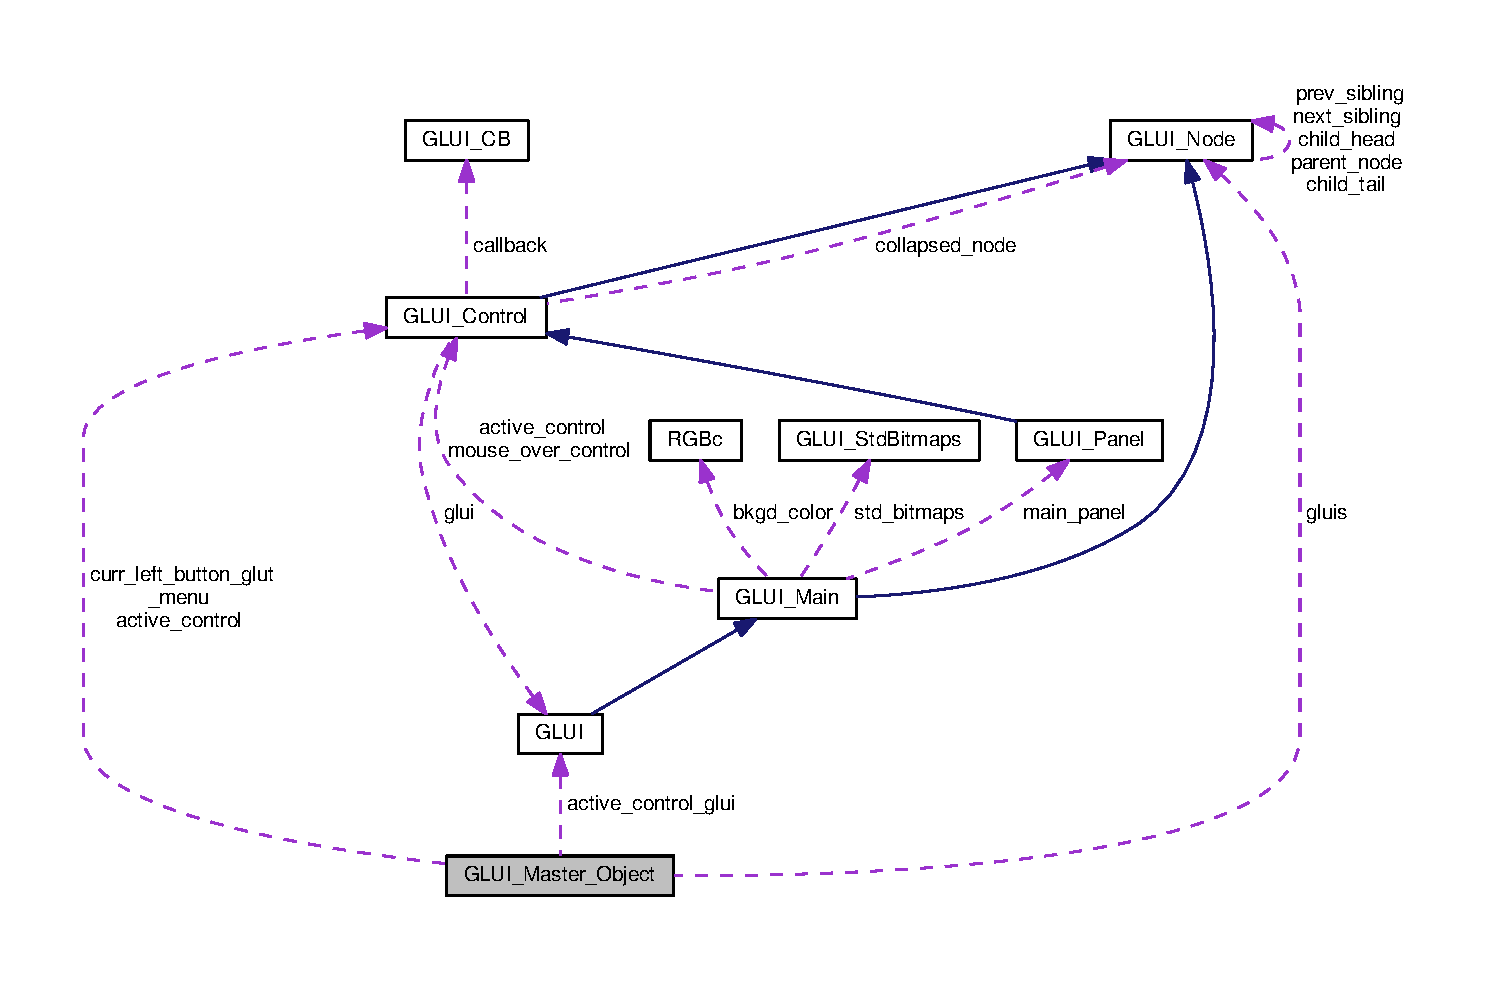
\includegraphics[width=350pt]{class_g_l_u_i___master___object__coll__graph}
\end{center}
\end{figure}
\subsection*{Public Member Functions}
\begin{DoxyCompactItemize}
\item 
\hyperlink{class_g_l_u_i___master___object_a5947a4fbf4c2d75296781c642cd56d13}{G\+L\+U\+I\+\_\+\+Master\+\_\+\+Object} ()
\item 
\hyperlink{class_g_l_u_i___master___object_a21dd14b088510fb6b3fb1f4d50e31cfc}{$\sim$\+G\+L\+U\+I\+\_\+\+Master\+\_\+\+Object} ()
\item 
\hyperlink{class_g_l_u_i___glut___window}{G\+L\+U\+I\+\_\+\+Glut\+\_\+\+Window} $\ast$ \hyperlink{class_g_l_u_i___master___object_a8f9134da7b46e4147fc07dbf8c881e90}{find\+\_\+glut\+\_\+window} (\hyperlink{wglext_8h_a500a82aecba06f4550f6849b8099ca21}{int} window\+\_\+id)
\item 
\hyperlink{wglext_8h_a9e6b7f1933461ef318bb000d6bd13b83}{void} \hyperlink{class_g_l_u_i___master___object_a5d1b3a7cc294314dda9864cd7bd64a62}{set\+\_\+glut\+Idle\+Func} (\hyperlink{wglext_8h_a9e6b7f1933461ef318bb000d6bd13b83}{void}($\ast$\hyperlink{glext_8h_a691492ec0bd6383f91200e49f6ae40ed}{f})(\hyperlink{wglext_8h_a9e6b7f1933461ef318bb000d6bd13b83}{void}))
\item 
\hyperlink{wglext_8h_a9e6b7f1933461ef318bb000d6bd13b83}{void} \hyperlink{class_g_l_u_i___master___object_afb8aea4fc250cddb252570508acbd603}{set\+\_\+left\+\_\+button\+\_\+glut\+\_\+menu\+\_\+control} (\hyperlink{class_g_l_u_i___control}{G\+L\+U\+I\+\_\+\+Control} $\ast$control)
\item 
\hyperlink{wglext_8h_a9e6b7f1933461ef318bb000d6bd13b83}{void} \hyperlink{class_g_l_u_i___master___object_aed8155ef565e847af72ba26478daa388}{set\+\_\+glut\+Reshape\+Func} (\hyperlink{wglext_8h_a9e6b7f1933461ef318bb000d6bd13b83}{void}($\ast$\hyperlink{glext_8h_a691492ec0bd6383f91200e49f6ae40ed}{f})(\hyperlink{wglext_8h_a500a82aecba06f4550f6849b8099ca21}{int} \hyperlink{glext_8h_aa105b18f96e6bc2485cb7f576a7fb9ba}{width}, \hyperlink{wglext_8h_a500a82aecba06f4550f6849b8099ca21}{int} \hyperlink{glext_8h_aa214bd63e12f7ddf524c83894fcc69a7}{height}))
\item 
\hyperlink{wglext_8h_a9e6b7f1933461ef318bb000d6bd13b83}{void} \hyperlink{class_g_l_u_i___master___object_aec70f38a81424a09c42f5a3e4e6edc43}{set\+\_\+glut\+Keyboard\+Func} (\hyperlink{wglext_8h_a9e6b7f1933461ef318bb000d6bd13b83}{void}($\ast$\hyperlink{glext_8h_a691492ec0bd6383f91200e49f6ae40ed}{f})(unsigned char key, \hyperlink{wglext_8h_a500a82aecba06f4550f6849b8099ca21}{int} \hyperlink{glext_8h_ad77deca22f617d3f0e0eb786445689fc}{x}, \hyperlink{wglext_8h_a500a82aecba06f4550f6849b8099ca21}{int} \hyperlink{glext_8h_a9298c7ad619074f5285b32c6b72bfdea}{y}))
\item 
\hyperlink{wglext_8h_a9e6b7f1933461ef318bb000d6bd13b83}{void} \hyperlink{class_g_l_u_i___master___object_a69ccd15bd0829ef1600de7026e6e903e}{set\+\_\+glut\+Special\+Func} (\hyperlink{wglext_8h_a9e6b7f1933461ef318bb000d6bd13b83}{void}($\ast$\hyperlink{glext_8h_a691492ec0bd6383f91200e49f6ae40ed}{f})(\hyperlink{wglext_8h_a500a82aecba06f4550f6849b8099ca21}{int} key, \hyperlink{wglext_8h_a500a82aecba06f4550f6849b8099ca21}{int} \hyperlink{glext_8h_ad77deca22f617d3f0e0eb786445689fc}{x}, \hyperlink{wglext_8h_a500a82aecba06f4550f6849b8099ca21}{int} \hyperlink{glext_8h_a9298c7ad619074f5285b32c6b72bfdea}{y}))
\item 
\hyperlink{wglext_8h_a9e6b7f1933461ef318bb000d6bd13b83}{void} \hyperlink{class_g_l_u_i___master___object_a8cfe4c66d1eae820db4409ea7f4cdd61}{set\+\_\+glut\+Mouse\+Func} (\hyperlink{wglext_8h_a9e6b7f1933461ef318bb000d6bd13b83}{void}($\ast$\hyperlink{glext_8h_a691492ec0bd6383f91200e49f6ae40ed}{f})(\hyperlink{wglext_8h_a500a82aecba06f4550f6849b8099ca21}{int}, \hyperlink{wglext_8h_a500a82aecba06f4550f6849b8099ca21}{int}, \hyperlink{wglext_8h_a500a82aecba06f4550f6849b8099ca21}{int}, \hyperlink{wglext_8h_a500a82aecba06f4550f6849b8099ca21}{int}))
\item 
\hyperlink{wglext_8h_a9e6b7f1933461ef318bb000d6bd13b83}{void} \hyperlink{class_g_l_u_i___master___object_a2a20f0e78093357d1b2ca9099dccab2a}{set\+\_\+glut\+Display\+Func} (\hyperlink{wglext_8h_a9e6b7f1933461ef318bb000d6bd13b83}{void}($\ast$\hyperlink{glext_8h_a691492ec0bd6383f91200e49f6ae40ed}{f})(\hyperlink{wglext_8h_a9e6b7f1933461ef318bb000d6bd13b83}{void}))
\item 
\hyperlink{wglext_8h_a9e6b7f1933461ef318bb000d6bd13b83}{void} \hyperlink{class_g_l_u_i___master___object_a57fd64245124e6d77e78b2d33b8d34b4}{set\+\_\+glut\+Timer\+Func} (unsigned \hyperlink{wglext_8h_a500a82aecba06f4550f6849b8099ca21}{int} millis, \hyperlink{wglext_8h_a9e6b7f1933461ef318bb000d6bd13b83}{void}($\ast$\hyperlink{glext_8h_a691492ec0bd6383f91200e49f6ae40ed}{f})(\hyperlink{wglext_8h_a500a82aecba06f4550f6849b8099ca21}{int} \hyperlink{glext_8h_a79169be77d7e02a24f68a5bfe627dc29}{value}), \hyperlink{wglext_8h_a500a82aecba06f4550f6849b8099ca21}{int} \hyperlink{glext_8h_a79169be77d7e02a24f68a5bfe627dc29}{value})
\item 
\hyperlink{wglext_8h_a9e6b7f1933461ef318bb000d6bd13b83}{void} \hyperlink{class_g_l_u_i___master___object_aa36f406dc447d6903dec41d7b3a8293e}{set\+\_\+glut\+Overlay\+Display\+Func} (\hyperlink{wglext_8h_a9e6b7f1933461ef318bb000d6bd13b83}{void}($\ast$\hyperlink{glext_8h_a691492ec0bd6383f91200e49f6ae40ed}{f})(\hyperlink{wglext_8h_a9e6b7f1933461ef318bb000d6bd13b83}{void}))
\item 
\hyperlink{wglext_8h_a9e6b7f1933461ef318bb000d6bd13b83}{void} \hyperlink{class_g_l_u_i___master___object_acfcb50c389eb48a599ffabfa87ee91d7}{set\+\_\+glut\+Spaceball\+Motion\+Func} (\hyperlink{glui_8h_a6990fdc97840c78d17c74d77113b60ad}{Int3\+\_\+\+C\+B} \hyperlink{glext_8h_a691492ec0bd6383f91200e49f6ae40ed}{f})
\item 
\hyperlink{wglext_8h_a9e6b7f1933461ef318bb000d6bd13b83}{void} \hyperlink{class_g_l_u_i___master___object_a0d8211580f34f3349c4c63431220049c}{set\+\_\+glut\+Spaceball\+Rotate\+Func} (\hyperlink{glui_8h_a6990fdc97840c78d17c74d77113b60ad}{Int3\+\_\+\+C\+B} \hyperlink{glext_8h_a691492ec0bd6383f91200e49f6ae40ed}{f})
\item 
\hyperlink{wglext_8h_a9e6b7f1933461ef318bb000d6bd13b83}{void} \hyperlink{class_g_l_u_i___master___object_a47961d2385bfbbb58c5cc2aac24473b0}{set\+\_\+glut\+Spaceball\+Button\+Func} (\hyperlink{glui_8h_aab4303326f838bf185b93c83524af987}{Int2\+\_\+\+C\+B} \hyperlink{glext_8h_a691492ec0bd6383f91200e49f6ae40ed}{f})
\item 
\hyperlink{wglext_8h_a9e6b7f1933461ef318bb000d6bd13b83}{void} \hyperlink{class_g_l_u_i___master___object_aa0f01144f1894acdebffce2c0c3d1a93}{set\+\_\+glut\+Tablet\+Motion\+Func} (\hyperlink{glui_8h_aab4303326f838bf185b93c83524af987}{Int2\+\_\+\+C\+B} \hyperlink{glext_8h_a691492ec0bd6383f91200e49f6ae40ed}{f})
\item 
\hyperlink{wglext_8h_a9e6b7f1933461ef318bb000d6bd13b83}{void} \hyperlink{class_g_l_u_i___master___object_a449c4ac3bd2edfb6854b90543b6633de}{set\+\_\+glut\+Tablet\+Button\+Func} (\hyperlink{glui_8h_a47b7da882646d5a03c1d3bd080434272}{Int4\+\_\+\+C\+B} \hyperlink{glext_8h_a691492ec0bd6383f91200e49f6ae40ed}{f})
\item 
\hyperlink{wglext_8h_a9e6b7f1933461ef318bb000d6bd13b83}{void} \hyperlink{class_g_l_u_i___master___object_af230d62a22c0016cf740977553c42c33}{set\+\_\+glut\+Menu\+Status\+Func} (\hyperlink{glui_8h_a6990fdc97840c78d17c74d77113b60ad}{Int3\+\_\+\+C\+B} \hyperlink{glext_8h_a691492ec0bd6383f91200e49f6ae40ed}{f})
\item 
\hyperlink{wglext_8h_a9e6b7f1933461ef318bb000d6bd13b83}{void} \hyperlink{class_g_l_u_i___master___object_a191c14ba9994bf9ca365c5da06286c59}{set\+\_\+glut\+Menu\+State\+Func} (\hyperlink{glui_8h_a04a3d4228bbb184c4202b2178e9e142b}{Int1\+\_\+\+C\+B} \hyperlink{glext_8h_a691492ec0bd6383f91200e49f6ae40ed}{f})
\item 
\hyperlink{wglext_8h_a9e6b7f1933461ef318bb000d6bd13b83}{void} \hyperlink{class_g_l_u_i___master___object_a02d788570f74d1997075c2ad536154ac}{set\+\_\+glut\+Button\+Box\+Func} (\hyperlink{glui_8h_aab4303326f838bf185b93c83524af987}{Int2\+\_\+\+C\+B} \hyperlink{glext_8h_a691492ec0bd6383f91200e49f6ae40ed}{f})
\item 
\hyperlink{wglext_8h_a9e6b7f1933461ef318bb000d6bd13b83}{void} \hyperlink{class_g_l_u_i___master___object_a8b6d9eed9feec3c8e138ebfe2c1b93e5}{set\+\_\+glut\+Dials\+Func} (\hyperlink{glui_8h_aab4303326f838bf185b93c83524af987}{Int2\+\_\+\+C\+B} \hyperlink{glext_8h_a691492ec0bd6383f91200e49f6ae40ed}{f})
\item 
\hyperlink{class_g_l_u_i}{G\+L\+U\+I} $\ast$ \hyperlink{class_g_l_u_i___master___object_a47180ea52267dd8355c607e3a1d51b7a}{create\+\_\+glui} (const char $\ast$\hyperlink{glext_8h_ad977737dfc9a274a62741b9500c49a32}{name}, long \hyperlink{glext_8h_aa9459b47e7388437191d2d9a69c10d98}{flags}=0, \hyperlink{wglext_8h_a500a82aecba06f4550f6849b8099ca21}{int} \hyperlink{glext_8h_ad77deca22f617d3f0e0eb786445689fc}{x}=-\/1, \hyperlink{wglext_8h_a500a82aecba06f4550f6849b8099ca21}{int} \hyperlink{glext_8h_a9298c7ad619074f5285b32c6b72bfdea}{y}=-\/1)
\item 
\hyperlink{class_g_l_u_i}{G\+L\+U\+I} $\ast$ \hyperlink{class_g_l_u_i___master___object_a434b0331a0c3c529b6d439839bb80143}{create\+\_\+glui\+\_\+subwindow} (\hyperlink{wglext_8h_a500a82aecba06f4550f6849b8099ca21}{int} parent\+\_\+window, long \hyperlink{glext_8h_aa9459b47e7388437191d2d9a69c10d98}{flags}=0)
\item 
\hyperlink{class_g_l_u_i}{G\+L\+U\+I} $\ast$ \hyperlink{class_g_l_u_i___master___object_a7bc5d2a384514f038e9ae83737f02f6c}{find\+\_\+glui\+\_\+by\+\_\+window\+\_\+id} (\hyperlink{wglext_8h_a500a82aecba06f4550f6849b8099ca21}{int} window\+\_\+id)
\item 
\hyperlink{wglext_8h_a9e6b7f1933461ef318bb000d6bd13b83}{void} \hyperlink{class_g_l_u_i___master___object_a2bee4bcbf463ab57f6da65eeb9a93ee8}{get\+\_\+viewport\+\_\+area} (\hyperlink{wglext_8h_a500a82aecba06f4550f6849b8099ca21}{int} $\ast$\hyperlink{glext_8h_ad77deca22f617d3f0e0eb786445689fc}{x}, \hyperlink{wglext_8h_a500a82aecba06f4550f6849b8099ca21}{int} $\ast$\hyperlink{glext_8h_a9298c7ad619074f5285b32c6b72bfdea}{y}, \hyperlink{wglext_8h_a500a82aecba06f4550f6849b8099ca21}{int} $\ast$\hyperlink{glext_8h_a713abae75276598501f75c68917c5e2d}{w}, \hyperlink{wglext_8h_a500a82aecba06f4550f6849b8099ca21}{int} $\ast$\hyperlink{glext_8h_afa0fb1b5e976920c0abeff2dca3ed774}{h})
\item 
\hyperlink{wglext_8h_a9e6b7f1933461ef318bb000d6bd13b83}{void} \hyperlink{class_g_l_u_i___master___object_ad62e7468e51d92ac67617f1968b1c944}{auto\+\_\+set\+\_\+viewport} ()
\item 
\hyperlink{wglext_8h_a9e6b7f1933461ef318bb000d6bd13b83}{void} \hyperlink{class_g_l_u_i___master___object_ad2f380184ab29c1817f1ad3b25b36fd5}{close\+\_\+all} ()
\item 
\hyperlink{wglext_8h_a9e6b7f1933461ef318bb000d6bd13b83}{void} \hyperlink{class_g_l_u_i___master___object_a6fb29a6080a45d364fc4653591cb1ade}{sync\+\_\+live\+\_\+all} ()
\item 
\hyperlink{wglext_8h_a9e6b7f1933461ef318bb000d6bd13b83}{void} \hyperlink{class_g_l_u_i___master___object_a8e092dea6e4ae3a6b52c8cba92eeefb4}{reshape} ()
\item 
float \hyperlink{class_g_l_u_i___master___object_ad4654282669300f569d30a4c430f4e6f}{get\+\_\+version} ()
\item 
\hyperlink{wglext_8h_a9e6b7f1933461ef318bb000d6bd13b83}{void} \hyperlink{class_g_l_u_i___master___object_af9b11cec3c215c6acc1de9bf8e0d92f3}{glui\+\_\+set\+Idle\+Func\+If\+Necessary} (\hyperlink{wglext_8h_a9e6b7f1933461ef318bb000d6bd13b83}{void})
\end{DoxyCompactItemize}
\subsection*{Public Attributes}
\begin{DoxyCompactItemize}
\item 
\hyperlink{class_g_l_u_i___node}{G\+L\+U\+I\+\_\+\+Node} \hyperlink{class_g_l_u_i___master___object_adef972538b4195478dd9feaabd55bd26}{gluis}
\item 
\hyperlink{class_g_l_u_i___control}{G\+L\+U\+I\+\_\+\+Control} $\ast$ \hyperlink{class_g_l_u_i___master___object_a024c89d0bbae3ea4ebf84af79b093a36}{active\+\_\+control}
\item 
\hyperlink{class_g_l_u_i___control}{G\+L\+U\+I\+\_\+\+Control} $\ast$ \hyperlink{class_g_l_u_i___master___object_a0df5b34fced5bb930fb0fe4d982b4e8c}{curr\+\_\+left\+\_\+button\+\_\+glut\+\_\+menu}
\item 
\hyperlink{class_g_l_u_i}{G\+L\+U\+I} $\ast$ \hyperlink{class_g_l_u_i___master___object_a41b447c76e0a9088aa703593499ff4cb}{active\+\_\+control\+\_\+glui}
\item 
\hyperlink{wglext_8h_a500a82aecba06f4550f6849b8099ca21}{int} \hyperlink{class_g_l_u_i___master___object_a9cd3c12203f03cd54115e7852e0d82e3}{glui\+\_\+id\+\_\+counter}
\end{DoxyCompactItemize}
\subsection*{Friends}
\begin{DoxyCompactItemize}
\item 
\hyperlink{wglext_8h_a9e6b7f1933461ef318bb000d6bd13b83}{void} \hyperlink{class_g_l_u_i___master___object_ad7c67b26e8436e7ef84d8657704010da}{glui\+\_\+idle\+\_\+func} ()
\end{DoxyCompactItemize}


\subsection{Detailed Description}
The master manages our interaction with G\+L\+U\+T. There's only one \hyperlink{class_g_l_u_i___master___object}{G\+L\+U\+I\+\_\+\+Master\+\_\+\+Object}. 

Definition at line 471 of file glui.\+h.



\subsection{Constructor \& Destructor Documentation}
\hypertarget{class_g_l_u_i___master___object_a5947a4fbf4c2d75296781c642cd56d13}{\index{G\+L\+U\+I\+\_\+\+Master\+\_\+\+Object@{G\+L\+U\+I\+\_\+\+Master\+\_\+\+Object}!G\+L\+U\+I\+\_\+\+Master\+\_\+\+Object@{G\+L\+U\+I\+\_\+\+Master\+\_\+\+Object}}
\index{G\+L\+U\+I\+\_\+\+Master\+\_\+\+Object@{G\+L\+U\+I\+\_\+\+Master\+\_\+\+Object}!G\+L\+U\+I\+\_\+\+Master\+\_\+\+Object@{G\+L\+U\+I\+\_\+\+Master\+\_\+\+Object}}
\subsubsection[{G\+L\+U\+I\+\_\+\+Master\+\_\+\+Object}]{\setlength{\rightskip}{0pt plus 5cm}G\+L\+U\+I\+\_\+\+Master\+\_\+\+Object\+::\+G\+L\+U\+I\+\_\+\+Master\+\_\+\+Object (
\begin{DoxyParamCaption}
{}
\end{DoxyParamCaption}
)}}\label{class_g_l_u_i___master___object_a5947a4fbf4c2d75296781c642cd56d13}
\hypertarget{class_g_l_u_i___master___object_a21dd14b088510fb6b3fb1f4d50e31cfc}{\index{G\+L\+U\+I\+\_\+\+Master\+\_\+\+Object@{G\+L\+U\+I\+\_\+\+Master\+\_\+\+Object}!````~G\+L\+U\+I\+\_\+\+Master\+\_\+\+Object@{$\sim$\+G\+L\+U\+I\+\_\+\+Master\+\_\+\+Object}}
\index{````~G\+L\+U\+I\+\_\+\+Master\+\_\+\+Object@{$\sim$\+G\+L\+U\+I\+\_\+\+Master\+\_\+\+Object}!G\+L\+U\+I\+\_\+\+Master\+\_\+\+Object@{G\+L\+U\+I\+\_\+\+Master\+\_\+\+Object}}
\subsubsection[{$\sim$\+G\+L\+U\+I\+\_\+\+Master\+\_\+\+Object}]{\setlength{\rightskip}{0pt plus 5cm}G\+L\+U\+I\+\_\+\+Master\+\_\+\+Object\+::$\sim$\+G\+L\+U\+I\+\_\+\+Master\+\_\+\+Object (
\begin{DoxyParamCaption}
{}
\end{DoxyParamCaption}
)}}\label{class_g_l_u_i___master___object_a21dd14b088510fb6b3fb1f4d50e31cfc}


\subsection{Member Function Documentation}
\hypertarget{class_g_l_u_i___master___object_ad62e7468e51d92ac67617f1968b1c944}{\index{G\+L\+U\+I\+\_\+\+Master\+\_\+\+Object@{G\+L\+U\+I\+\_\+\+Master\+\_\+\+Object}!auto\+\_\+set\+\_\+viewport@{auto\+\_\+set\+\_\+viewport}}
\index{auto\+\_\+set\+\_\+viewport@{auto\+\_\+set\+\_\+viewport}!G\+L\+U\+I\+\_\+\+Master\+\_\+\+Object@{G\+L\+U\+I\+\_\+\+Master\+\_\+\+Object}}
\subsubsection[{auto\+\_\+set\+\_\+viewport}]{\setlength{\rightskip}{0pt plus 5cm}{\bf void} G\+L\+U\+I\+\_\+\+Master\+\_\+\+Object\+::auto\+\_\+set\+\_\+viewport (
\begin{DoxyParamCaption}
{}
\end{DoxyParamCaption}
)}}\label{class_g_l_u_i___master___object_ad62e7468e51d92ac67617f1968b1c944}
\hypertarget{class_g_l_u_i___master___object_ad2f380184ab29c1817f1ad3b25b36fd5}{\index{G\+L\+U\+I\+\_\+\+Master\+\_\+\+Object@{G\+L\+U\+I\+\_\+\+Master\+\_\+\+Object}!close\+\_\+all@{close\+\_\+all}}
\index{close\+\_\+all@{close\+\_\+all}!G\+L\+U\+I\+\_\+\+Master\+\_\+\+Object@{G\+L\+U\+I\+\_\+\+Master\+\_\+\+Object}}
\subsubsection[{close\+\_\+all}]{\setlength{\rightskip}{0pt plus 5cm}{\bf void} G\+L\+U\+I\+\_\+\+Master\+\_\+\+Object\+::close\+\_\+all (
\begin{DoxyParamCaption}
{}
\end{DoxyParamCaption}
)}}\label{class_g_l_u_i___master___object_ad2f380184ab29c1817f1ad3b25b36fd5}
\hypertarget{class_g_l_u_i___master___object_a47180ea52267dd8355c607e3a1d51b7a}{\index{G\+L\+U\+I\+\_\+\+Master\+\_\+\+Object@{G\+L\+U\+I\+\_\+\+Master\+\_\+\+Object}!create\+\_\+glui@{create\+\_\+glui}}
\index{create\+\_\+glui@{create\+\_\+glui}!G\+L\+U\+I\+\_\+\+Master\+\_\+\+Object@{G\+L\+U\+I\+\_\+\+Master\+\_\+\+Object}}
\subsubsection[{create\+\_\+glui}]{\setlength{\rightskip}{0pt plus 5cm}{\bf G\+L\+U\+I}$\ast$ G\+L\+U\+I\+\_\+\+Master\+\_\+\+Object\+::create\+\_\+glui (
\begin{DoxyParamCaption}
\item[{const char $\ast$}]{name, }
\item[{long}]{flags = {\ttfamily 0}, }
\item[{{\bf int}}]{x = {\ttfamily -\/1}, }
\item[{{\bf int}}]{y = {\ttfamily -\/1}}
\end{DoxyParamCaption}
)}}\label{class_g_l_u_i___master___object_a47180ea52267dd8355c607e3a1d51b7a}
\hypertarget{class_g_l_u_i___master___object_a434b0331a0c3c529b6d439839bb80143}{\index{G\+L\+U\+I\+\_\+\+Master\+\_\+\+Object@{G\+L\+U\+I\+\_\+\+Master\+\_\+\+Object}!create\+\_\+glui\+\_\+subwindow@{create\+\_\+glui\+\_\+subwindow}}
\index{create\+\_\+glui\+\_\+subwindow@{create\+\_\+glui\+\_\+subwindow}!G\+L\+U\+I\+\_\+\+Master\+\_\+\+Object@{G\+L\+U\+I\+\_\+\+Master\+\_\+\+Object}}
\subsubsection[{create\+\_\+glui\+\_\+subwindow}]{\setlength{\rightskip}{0pt plus 5cm}{\bf G\+L\+U\+I}$\ast$ G\+L\+U\+I\+\_\+\+Master\+\_\+\+Object\+::create\+\_\+glui\+\_\+subwindow (
\begin{DoxyParamCaption}
\item[{{\bf int}}]{parent\+\_\+window, }
\item[{long}]{flags = {\ttfamily 0}}
\end{DoxyParamCaption}
)}}\label{class_g_l_u_i___master___object_a434b0331a0c3c529b6d439839bb80143}
\hypertarget{class_g_l_u_i___master___object_a7bc5d2a384514f038e9ae83737f02f6c}{\index{G\+L\+U\+I\+\_\+\+Master\+\_\+\+Object@{G\+L\+U\+I\+\_\+\+Master\+\_\+\+Object}!find\+\_\+glui\+\_\+by\+\_\+window\+\_\+id@{find\+\_\+glui\+\_\+by\+\_\+window\+\_\+id}}
\index{find\+\_\+glui\+\_\+by\+\_\+window\+\_\+id@{find\+\_\+glui\+\_\+by\+\_\+window\+\_\+id}!G\+L\+U\+I\+\_\+\+Master\+\_\+\+Object@{G\+L\+U\+I\+\_\+\+Master\+\_\+\+Object}}
\subsubsection[{find\+\_\+glui\+\_\+by\+\_\+window\+\_\+id}]{\setlength{\rightskip}{0pt plus 5cm}{\bf G\+L\+U\+I}$\ast$ G\+L\+U\+I\+\_\+\+Master\+\_\+\+Object\+::find\+\_\+glui\+\_\+by\+\_\+window\+\_\+id (
\begin{DoxyParamCaption}
\item[{{\bf int}}]{window\+\_\+id}
\end{DoxyParamCaption}
)}}\label{class_g_l_u_i___master___object_a7bc5d2a384514f038e9ae83737f02f6c}
\hypertarget{class_g_l_u_i___master___object_a8f9134da7b46e4147fc07dbf8c881e90}{\index{G\+L\+U\+I\+\_\+\+Master\+\_\+\+Object@{G\+L\+U\+I\+\_\+\+Master\+\_\+\+Object}!find\+\_\+glut\+\_\+window@{find\+\_\+glut\+\_\+window}}
\index{find\+\_\+glut\+\_\+window@{find\+\_\+glut\+\_\+window}!G\+L\+U\+I\+\_\+\+Master\+\_\+\+Object@{G\+L\+U\+I\+\_\+\+Master\+\_\+\+Object}}
\subsubsection[{find\+\_\+glut\+\_\+window}]{\setlength{\rightskip}{0pt plus 5cm}{\bf G\+L\+U\+I\+\_\+\+Glut\+\_\+\+Window}$\ast$ G\+L\+U\+I\+\_\+\+Master\+\_\+\+Object\+::find\+\_\+glut\+\_\+window (
\begin{DoxyParamCaption}
\item[{{\bf int}}]{window\+\_\+id}
\end{DoxyParamCaption}
)}}\label{class_g_l_u_i___master___object_a8f9134da7b46e4147fc07dbf8c881e90}
\hypertarget{class_g_l_u_i___master___object_ad4654282669300f569d30a4c430f4e6f}{\index{G\+L\+U\+I\+\_\+\+Master\+\_\+\+Object@{G\+L\+U\+I\+\_\+\+Master\+\_\+\+Object}!get\+\_\+version@{get\+\_\+version}}
\index{get\+\_\+version@{get\+\_\+version}!G\+L\+U\+I\+\_\+\+Master\+\_\+\+Object@{G\+L\+U\+I\+\_\+\+Master\+\_\+\+Object}}
\subsubsection[{get\+\_\+version}]{\setlength{\rightskip}{0pt plus 5cm}float G\+L\+U\+I\+\_\+\+Master\+\_\+\+Object\+::get\+\_\+version (
\begin{DoxyParamCaption}
{}
\end{DoxyParamCaption}
)\hspace{0.3cm}{\ttfamily [inline]}}}\label{class_g_l_u_i___master___object_ad4654282669300f569d30a4c430f4e6f}


Definition at line 539 of file glui.\+h.

\hypertarget{class_g_l_u_i___master___object_a2bee4bcbf463ab57f6da65eeb9a93ee8}{\index{G\+L\+U\+I\+\_\+\+Master\+\_\+\+Object@{G\+L\+U\+I\+\_\+\+Master\+\_\+\+Object}!get\+\_\+viewport\+\_\+area@{get\+\_\+viewport\+\_\+area}}
\index{get\+\_\+viewport\+\_\+area@{get\+\_\+viewport\+\_\+area}!G\+L\+U\+I\+\_\+\+Master\+\_\+\+Object@{G\+L\+U\+I\+\_\+\+Master\+\_\+\+Object}}
\subsubsection[{get\+\_\+viewport\+\_\+area}]{\setlength{\rightskip}{0pt plus 5cm}{\bf void} G\+L\+U\+I\+\_\+\+Master\+\_\+\+Object\+::get\+\_\+viewport\+\_\+area (
\begin{DoxyParamCaption}
\item[{{\bf int} $\ast$}]{x, }
\item[{{\bf int} $\ast$}]{y, }
\item[{{\bf int} $\ast$}]{w, }
\item[{{\bf int} $\ast$}]{h}
\end{DoxyParamCaption}
)}}\label{class_g_l_u_i___master___object_a2bee4bcbf463ab57f6da65eeb9a93ee8}
\hypertarget{class_g_l_u_i___master___object_af9b11cec3c215c6acc1de9bf8e0d92f3}{\index{G\+L\+U\+I\+\_\+\+Master\+\_\+\+Object@{G\+L\+U\+I\+\_\+\+Master\+\_\+\+Object}!glui\+\_\+set\+Idle\+Func\+If\+Necessary@{glui\+\_\+set\+Idle\+Func\+If\+Necessary}}
\index{glui\+\_\+set\+Idle\+Func\+If\+Necessary@{glui\+\_\+set\+Idle\+Func\+If\+Necessary}!G\+L\+U\+I\+\_\+\+Master\+\_\+\+Object@{G\+L\+U\+I\+\_\+\+Master\+\_\+\+Object}}
\subsubsection[{glui\+\_\+set\+Idle\+Func\+If\+Necessary}]{\setlength{\rightskip}{0pt plus 5cm}{\bf void} G\+L\+U\+I\+\_\+\+Master\+\_\+\+Object\+::glui\+\_\+set\+Idle\+Func\+If\+Necessary (
\begin{DoxyParamCaption}
\item[{{\bf void}}]{}
\end{DoxyParamCaption}
)}}\label{class_g_l_u_i___master___object_af9b11cec3c215c6acc1de9bf8e0d92f3}
\hypertarget{class_g_l_u_i___master___object_a8e092dea6e4ae3a6b52c8cba92eeefb4}{\index{G\+L\+U\+I\+\_\+\+Master\+\_\+\+Object@{G\+L\+U\+I\+\_\+\+Master\+\_\+\+Object}!reshape@{reshape}}
\index{reshape@{reshape}!G\+L\+U\+I\+\_\+\+Master\+\_\+\+Object@{G\+L\+U\+I\+\_\+\+Master\+\_\+\+Object}}
\subsubsection[{reshape}]{\setlength{\rightskip}{0pt plus 5cm}{\bf void} G\+L\+U\+I\+\_\+\+Master\+\_\+\+Object\+::reshape (
\begin{DoxyParamCaption}
{}
\end{DoxyParamCaption}
)}}\label{class_g_l_u_i___master___object_a8e092dea6e4ae3a6b52c8cba92eeefb4}
\hypertarget{class_g_l_u_i___master___object_a02d788570f74d1997075c2ad536154ac}{\index{G\+L\+U\+I\+\_\+\+Master\+\_\+\+Object@{G\+L\+U\+I\+\_\+\+Master\+\_\+\+Object}!set\+\_\+glut\+Button\+Box\+Func@{set\+\_\+glut\+Button\+Box\+Func}}
\index{set\+\_\+glut\+Button\+Box\+Func@{set\+\_\+glut\+Button\+Box\+Func}!G\+L\+U\+I\+\_\+\+Master\+\_\+\+Object@{G\+L\+U\+I\+\_\+\+Master\+\_\+\+Object}}
\subsubsection[{set\+\_\+glut\+Button\+Box\+Func}]{\setlength{\rightskip}{0pt plus 5cm}{\bf void} G\+L\+U\+I\+\_\+\+Master\+\_\+\+Object\+::set\+\_\+glut\+Button\+Box\+Func (
\begin{DoxyParamCaption}
\item[{{\bf Int2\+\_\+\+C\+B}}]{f}
\end{DoxyParamCaption}
)\hspace{0.3cm}{\ttfamily [inline]}}}\label{class_g_l_u_i___master___object_a02d788570f74d1997075c2ad536154ac}


Definition at line 525 of file glui.\+h.

\hypertarget{class_g_l_u_i___master___object_a8b6d9eed9feec3c8e138ebfe2c1b93e5}{\index{G\+L\+U\+I\+\_\+\+Master\+\_\+\+Object@{G\+L\+U\+I\+\_\+\+Master\+\_\+\+Object}!set\+\_\+glut\+Dials\+Func@{set\+\_\+glut\+Dials\+Func}}
\index{set\+\_\+glut\+Dials\+Func@{set\+\_\+glut\+Dials\+Func}!G\+L\+U\+I\+\_\+\+Master\+\_\+\+Object@{G\+L\+U\+I\+\_\+\+Master\+\_\+\+Object}}
\subsubsection[{set\+\_\+glut\+Dials\+Func}]{\setlength{\rightskip}{0pt plus 5cm}{\bf void} G\+L\+U\+I\+\_\+\+Master\+\_\+\+Object\+::set\+\_\+glut\+Dials\+Func (
\begin{DoxyParamCaption}
\item[{{\bf Int2\+\_\+\+C\+B}}]{f}
\end{DoxyParamCaption}
)\hspace{0.3cm}{\ttfamily [inline]}}}\label{class_g_l_u_i___master___object_a8b6d9eed9feec3c8e138ebfe2c1b93e5}


Definition at line 526 of file glui.\+h.

\hypertarget{class_g_l_u_i___master___object_a2a20f0e78093357d1b2ca9099dccab2a}{\index{G\+L\+U\+I\+\_\+\+Master\+\_\+\+Object@{G\+L\+U\+I\+\_\+\+Master\+\_\+\+Object}!set\+\_\+glut\+Display\+Func@{set\+\_\+glut\+Display\+Func}}
\index{set\+\_\+glut\+Display\+Func@{set\+\_\+glut\+Display\+Func}!G\+L\+U\+I\+\_\+\+Master\+\_\+\+Object@{G\+L\+U\+I\+\_\+\+Master\+\_\+\+Object}}
\subsubsection[{set\+\_\+glut\+Display\+Func}]{\setlength{\rightskip}{0pt plus 5cm}{\bf void} G\+L\+U\+I\+\_\+\+Master\+\_\+\+Object\+::set\+\_\+glut\+Display\+Func (
\begin{DoxyParamCaption}
\item[{{\bf void}($\ast$)({\bf void})}]{f}
\end{DoxyParamCaption}
)\hspace{0.3cm}{\ttfamily [inline]}}}\label{class_g_l_u_i___master___object_a2a20f0e78093357d1b2ca9099dccab2a}


Definition at line 513 of file glui.\+h.

\hypertarget{class_g_l_u_i___master___object_a5d1b3a7cc294314dda9864cd7bd64a62}{\index{G\+L\+U\+I\+\_\+\+Master\+\_\+\+Object@{G\+L\+U\+I\+\_\+\+Master\+\_\+\+Object}!set\+\_\+glut\+Idle\+Func@{set\+\_\+glut\+Idle\+Func}}
\index{set\+\_\+glut\+Idle\+Func@{set\+\_\+glut\+Idle\+Func}!G\+L\+U\+I\+\_\+\+Master\+\_\+\+Object@{G\+L\+U\+I\+\_\+\+Master\+\_\+\+Object}}
\subsubsection[{set\+\_\+glut\+Idle\+Func}]{\setlength{\rightskip}{0pt plus 5cm}{\bf void} G\+L\+U\+I\+\_\+\+Master\+\_\+\+Object\+::set\+\_\+glut\+Idle\+Func (
\begin{DoxyParamCaption}
\item[{{\bf void}($\ast$)({\bf void})}]{f}
\end{DoxyParamCaption}
)}}\label{class_g_l_u_i___master___object_a5d1b3a7cc294314dda9864cd7bd64a62}
\hypertarget{class_g_l_u_i___master___object_aec70f38a81424a09c42f5a3e4e6edc43}{\index{G\+L\+U\+I\+\_\+\+Master\+\_\+\+Object@{G\+L\+U\+I\+\_\+\+Master\+\_\+\+Object}!set\+\_\+glut\+Keyboard\+Func@{set\+\_\+glut\+Keyboard\+Func}}
\index{set\+\_\+glut\+Keyboard\+Func@{set\+\_\+glut\+Keyboard\+Func}!G\+L\+U\+I\+\_\+\+Master\+\_\+\+Object@{G\+L\+U\+I\+\_\+\+Master\+\_\+\+Object}}
\subsubsection[{set\+\_\+glut\+Keyboard\+Func}]{\setlength{\rightskip}{0pt plus 5cm}{\bf void} G\+L\+U\+I\+\_\+\+Master\+\_\+\+Object\+::set\+\_\+glut\+Keyboard\+Func (
\begin{DoxyParamCaption}
\item[{{\bf void}($\ast$)(unsigned char key, {\bf int} {\bf x}, {\bf int} {\bf y})}]{f}
\end{DoxyParamCaption}
)}}\label{class_g_l_u_i___master___object_aec70f38a81424a09c42f5a3e4e6edc43}
\hypertarget{class_g_l_u_i___master___object_a191c14ba9994bf9ca365c5da06286c59}{\index{G\+L\+U\+I\+\_\+\+Master\+\_\+\+Object@{G\+L\+U\+I\+\_\+\+Master\+\_\+\+Object}!set\+\_\+glut\+Menu\+State\+Func@{set\+\_\+glut\+Menu\+State\+Func}}
\index{set\+\_\+glut\+Menu\+State\+Func@{set\+\_\+glut\+Menu\+State\+Func}!G\+L\+U\+I\+\_\+\+Master\+\_\+\+Object@{G\+L\+U\+I\+\_\+\+Master\+\_\+\+Object}}
\subsubsection[{set\+\_\+glut\+Menu\+State\+Func}]{\setlength{\rightskip}{0pt plus 5cm}{\bf void} G\+L\+U\+I\+\_\+\+Master\+\_\+\+Object\+::set\+\_\+glut\+Menu\+State\+Func (
\begin{DoxyParamCaption}
\item[{{\bf Int1\+\_\+\+C\+B}}]{f}
\end{DoxyParamCaption}
)\hspace{0.3cm}{\ttfamily [inline]}}}\label{class_g_l_u_i___master___object_a191c14ba9994bf9ca365c5da06286c59}


Definition at line 524 of file glui.\+h.

\hypertarget{class_g_l_u_i___master___object_af230d62a22c0016cf740977553c42c33}{\index{G\+L\+U\+I\+\_\+\+Master\+\_\+\+Object@{G\+L\+U\+I\+\_\+\+Master\+\_\+\+Object}!set\+\_\+glut\+Menu\+Status\+Func@{set\+\_\+glut\+Menu\+Status\+Func}}
\index{set\+\_\+glut\+Menu\+Status\+Func@{set\+\_\+glut\+Menu\+Status\+Func}!G\+L\+U\+I\+\_\+\+Master\+\_\+\+Object@{G\+L\+U\+I\+\_\+\+Master\+\_\+\+Object}}
\subsubsection[{set\+\_\+glut\+Menu\+Status\+Func}]{\setlength{\rightskip}{0pt plus 5cm}{\bf void} G\+L\+U\+I\+\_\+\+Master\+\_\+\+Object\+::set\+\_\+glut\+Menu\+Status\+Func (
\begin{DoxyParamCaption}
\item[{{\bf Int3\+\_\+\+C\+B}}]{f}
\end{DoxyParamCaption}
)\hspace{0.3cm}{\ttfamily [inline]}}}\label{class_g_l_u_i___master___object_af230d62a22c0016cf740977553c42c33}


Definition at line 523 of file glui.\+h.

\hypertarget{class_g_l_u_i___master___object_a8cfe4c66d1eae820db4409ea7f4cdd61}{\index{G\+L\+U\+I\+\_\+\+Master\+\_\+\+Object@{G\+L\+U\+I\+\_\+\+Master\+\_\+\+Object}!set\+\_\+glut\+Mouse\+Func@{set\+\_\+glut\+Mouse\+Func}}
\index{set\+\_\+glut\+Mouse\+Func@{set\+\_\+glut\+Mouse\+Func}!G\+L\+U\+I\+\_\+\+Master\+\_\+\+Object@{G\+L\+U\+I\+\_\+\+Master\+\_\+\+Object}}
\subsubsection[{set\+\_\+glut\+Mouse\+Func}]{\setlength{\rightskip}{0pt plus 5cm}{\bf void} G\+L\+U\+I\+\_\+\+Master\+\_\+\+Object\+::set\+\_\+glut\+Mouse\+Func (
\begin{DoxyParamCaption}
\item[{{\bf void}($\ast$)({\bf int}, {\bf int}, {\bf int}, {\bf int})}]{f}
\end{DoxyParamCaption}
)}}\label{class_g_l_u_i___master___object_a8cfe4c66d1eae820db4409ea7f4cdd61}
\hypertarget{class_g_l_u_i___master___object_aa36f406dc447d6903dec41d7b3a8293e}{\index{G\+L\+U\+I\+\_\+\+Master\+\_\+\+Object@{G\+L\+U\+I\+\_\+\+Master\+\_\+\+Object}!set\+\_\+glut\+Overlay\+Display\+Func@{set\+\_\+glut\+Overlay\+Display\+Func}}
\index{set\+\_\+glut\+Overlay\+Display\+Func@{set\+\_\+glut\+Overlay\+Display\+Func}!G\+L\+U\+I\+\_\+\+Master\+\_\+\+Object@{G\+L\+U\+I\+\_\+\+Master\+\_\+\+Object}}
\subsubsection[{set\+\_\+glut\+Overlay\+Display\+Func}]{\setlength{\rightskip}{0pt plus 5cm}{\bf void} G\+L\+U\+I\+\_\+\+Master\+\_\+\+Object\+::set\+\_\+glut\+Overlay\+Display\+Func (
\begin{DoxyParamCaption}
\item[{{\bf void}($\ast$)({\bf void})}]{f}
\end{DoxyParamCaption}
)\hspace{0.3cm}{\ttfamily [inline]}}}\label{class_g_l_u_i___master___object_aa36f406dc447d6903dec41d7b3a8293e}


Definition at line 516 of file glui.\+h.

\hypertarget{class_g_l_u_i___master___object_aed8155ef565e847af72ba26478daa388}{\index{G\+L\+U\+I\+\_\+\+Master\+\_\+\+Object@{G\+L\+U\+I\+\_\+\+Master\+\_\+\+Object}!set\+\_\+glut\+Reshape\+Func@{set\+\_\+glut\+Reshape\+Func}}
\index{set\+\_\+glut\+Reshape\+Func@{set\+\_\+glut\+Reshape\+Func}!G\+L\+U\+I\+\_\+\+Master\+\_\+\+Object@{G\+L\+U\+I\+\_\+\+Master\+\_\+\+Object}}
\subsubsection[{set\+\_\+glut\+Reshape\+Func}]{\setlength{\rightskip}{0pt plus 5cm}{\bf void} G\+L\+U\+I\+\_\+\+Master\+\_\+\+Object\+::set\+\_\+glut\+Reshape\+Func (
\begin{DoxyParamCaption}
\item[{{\bf void}($\ast$)({\bf int} {\bf width}, {\bf int} {\bf height})}]{f}
\end{DoxyParamCaption}
)}}\label{class_g_l_u_i___master___object_aed8155ef565e847af72ba26478daa388}
\hypertarget{class_g_l_u_i___master___object_a47961d2385bfbbb58c5cc2aac24473b0}{\index{G\+L\+U\+I\+\_\+\+Master\+\_\+\+Object@{G\+L\+U\+I\+\_\+\+Master\+\_\+\+Object}!set\+\_\+glut\+Spaceball\+Button\+Func@{set\+\_\+glut\+Spaceball\+Button\+Func}}
\index{set\+\_\+glut\+Spaceball\+Button\+Func@{set\+\_\+glut\+Spaceball\+Button\+Func}!G\+L\+U\+I\+\_\+\+Master\+\_\+\+Object@{G\+L\+U\+I\+\_\+\+Master\+\_\+\+Object}}
\subsubsection[{set\+\_\+glut\+Spaceball\+Button\+Func}]{\setlength{\rightskip}{0pt plus 5cm}{\bf void} G\+L\+U\+I\+\_\+\+Master\+\_\+\+Object\+::set\+\_\+glut\+Spaceball\+Button\+Func (
\begin{DoxyParamCaption}
\item[{{\bf Int2\+\_\+\+C\+B}}]{f}
\end{DoxyParamCaption}
)\hspace{0.3cm}{\ttfamily [inline]}}}\label{class_g_l_u_i___master___object_a47961d2385bfbbb58c5cc2aac24473b0}


Definition at line 519 of file glui.\+h.

\hypertarget{class_g_l_u_i___master___object_acfcb50c389eb48a599ffabfa87ee91d7}{\index{G\+L\+U\+I\+\_\+\+Master\+\_\+\+Object@{G\+L\+U\+I\+\_\+\+Master\+\_\+\+Object}!set\+\_\+glut\+Spaceball\+Motion\+Func@{set\+\_\+glut\+Spaceball\+Motion\+Func}}
\index{set\+\_\+glut\+Spaceball\+Motion\+Func@{set\+\_\+glut\+Spaceball\+Motion\+Func}!G\+L\+U\+I\+\_\+\+Master\+\_\+\+Object@{G\+L\+U\+I\+\_\+\+Master\+\_\+\+Object}}
\subsubsection[{set\+\_\+glut\+Spaceball\+Motion\+Func}]{\setlength{\rightskip}{0pt plus 5cm}{\bf void} G\+L\+U\+I\+\_\+\+Master\+\_\+\+Object\+::set\+\_\+glut\+Spaceball\+Motion\+Func (
\begin{DoxyParamCaption}
\item[{{\bf Int3\+\_\+\+C\+B}}]{f}
\end{DoxyParamCaption}
)\hspace{0.3cm}{\ttfamily [inline]}}}\label{class_g_l_u_i___master___object_acfcb50c389eb48a599ffabfa87ee91d7}


Definition at line 517 of file glui.\+h.

\hypertarget{class_g_l_u_i___master___object_a0d8211580f34f3349c4c63431220049c}{\index{G\+L\+U\+I\+\_\+\+Master\+\_\+\+Object@{G\+L\+U\+I\+\_\+\+Master\+\_\+\+Object}!set\+\_\+glut\+Spaceball\+Rotate\+Func@{set\+\_\+glut\+Spaceball\+Rotate\+Func}}
\index{set\+\_\+glut\+Spaceball\+Rotate\+Func@{set\+\_\+glut\+Spaceball\+Rotate\+Func}!G\+L\+U\+I\+\_\+\+Master\+\_\+\+Object@{G\+L\+U\+I\+\_\+\+Master\+\_\+\+Object}}
\subsubsection[{set\+\_\+glut\+Spaceball\+Rotate\+Func}]{\setlength{\rightskip}{0pt plus 5cm}{\bf void} G\+L\+U\+I\+\_\+\+Master\+\_\+\+Object\+::set\+\_\+glut\+Spaceball\+Rotate\+Func (
\begin{DoxyParamCaption}
\item[{{\bf Int3\+\_\+\+C\+B}}]{f}
\end{DoxyParamCaption}
)\hspace{0.3cm}{\ttfamily [inline]}}}\label{class_g_l_u_i___master___object_a0d8211580f34f3349c4c63431220049c}


Definition at line 518 of file glui.\+h.

\hypertarget{class_g_l_u_i___master___object_a69ccd15bd0829ef1600de7026e6e903e}{\index{G\+L\+U\+I\+\_\+\+Master\+\_\+\+Object@{G\+L\+U\+I\+\_\+\+Master\+\_\+\+Object}!set\+\_\+glut\+Special\+Func@{set\+\_\+glut\+Special\+Func}}
\index{set\+\_\+glut\+Special\+Func@{set\+\_\+glut\+Special\+Func}!G\+L\+U\+I\+\_\+\+Master\+\_\+\+Object@{G\+L\+U\+I\+\_\+\+Master\+\_\+\+Object}}
\subsubsection[{set\+\_\+glut\+Special\+Func}]{\setlength{\rightskip}{0pt plus 5cm}{\bf void} G\+L\+U\+I\+\_\+\+Master\+\_\+\+Object\+::set\+\_\+glut\+Special\+Func (
\begin{DoxyParamCaption}
\item[{{\bf void}($\ast$)({\bf int} key, {\bf int} {\bf x}, {\bf int} {\bf y})}]{f}
\end{DoxyParamCaption}
)}}\label{class_g_l_u_i___master___object_a69ccd15bd0829ef1600de7026e6e903e}
\hypertarget{class_g_l_u_i___master___object_a449c4ac3bd2edfb6854b90543b6633de}{\index{G\+L\+U\+I\+\_\+\+Master\+\_\+\+Object@{G\+L\+U\+I\+\_\+\+Master\+\_\+\+Object}!set\+\_\+glut\+Tablet\+Button\+Func@{set\+\_\+glut\+Tablet\+Button\+Func}}
\index{set\+\_\+glut\+Tablet\+Button\+Func@{set\+\_\+glut\+Tablet\+Button\+Func}!G\+L\+U\+I\+\_\+\+Master\+\_\+\+Object@{G\+L\+U\+I\+\_\+\+Master\+\_\+\+Object}}
\subsubsection[{set\+\_\+glut\+Tablet\+Button\+Func}]{\setlength{\rightskip}{0pt plus 5cm}{\bf void} G\+L\+U\+I\+\_\+\+Master\+\_\+\+Object\+::set\+\_\+glut\+Tablet\+Button\+Func (
\begin{DoxyParamCaption}
\item[{{\bf Int4\+\_\+\+C\+B}}]{f}
\end{DoxyParamCaption}
)\hspace{0.3cm}{\ttfamily [inline]}}}\label{class_g_l_u_i___master___object_a449c4ac3bd2edfb6854b90543b6633de}


Definition at line 521 of file glui.\+h.

\hypertarget{class_g_l_u_i___master___object_aa0f01144f1894acdebffce2c0c3d1a93}{\index{G\+L\+U\+I\+\_\+\+Master\+\_\+\+Object@{G\+L\+U\+I\+\_\+\+Master\+\_\+\+Object}!set\+\_\+glut\+Tablet\+Motion\+Func@{set\+\_\+glut\+Tablet\+Motion\+Func}}
\index{set\+\_\+glut\+Tablet\+Motion\+Func@{set\+\_\+glut\+Tablet\+Motion\+Func}!G\+L\+U\+I\+\_\+\+Master\+\_\+\+Object@{G\+L\+U\+I\+\_\+\+Master\+\_\+\+Object}}
\subsubsection[{set\+\_\+glut\+Tablet\+Motion\+Func}]{\setlength{\rightskip}{0pt plus 5cm}{\bf void} G\+L\+U\+I\+\_\+\+Master\+\_\+\+Object\+::set\+\_\+glut\+Tablet\+Motion\+Func (
\begin{DoxyParamCaption}
\item[{{\bf Int2\+\_\+\+C\+B}}]{f}
\end{DoxyParamCaption}
)\hspace{0.3cm}{\ttfamily [inline]}}}\label{class_g_l_u_i___master___object_aa0f01144f1894acdebffce2c0c3d1a93}


Definition at line 520 of file glui.\+h.

\hypertarget{class_g_l_u_i___master___object_a57fd64245124e6d77e78b2d33b8d34b4}{\index{G\+L\+U\+I\+\_\+\+Master\+\_\+\+Object@{G\+L\+U\+I\+\_\+\+Master\+\_\+\+Object}!set\+\_\+glut\+Timer\+Func@{set\+\_\+glut\+Timer\+Func}}
\index{set\+\_\+glut\+Timer\+Func@{set\+\_\+glut\+Timer\+Func}!G\+L\+U\+I\+\_\+\+Master\+\_\+\+Object@{G\+L\+U\+I\+\_\+\+Master\+\_\+\+Object}}
\subsubsection[{set\+\_\+glut\+Timer\+Func}]{\setlength{\rightskip}{0pt plus 5cm}{\bf void} G\+L\+U\+I\+\_\+\+Master\+\_\+\+Object\+::set\+\_\+glut\+Timer\+Func (
\begin{DoxyParamCaption}
\item[{unsigned {\bf int}}]{millis, }
\item[{{\bf void}($\ast$)({\bf int} {\bf value})}]{f, }
\item[{{\bf int}}]{value}
\end{DoxyParamCaption}
)\hspace{0.3cm}{\ttfamily [inline]}}}\label{class_g_l_u_i___master___object_a57fd64245124e6d77e78b2d33b8d34b4}


Definition at line 514 of file glui.\+h.

\hypertarget{class_g_l_u_i___master___object_afb8aea4fc250cddb252570508acbd603}{\index{G\+L\+U\+I\+\_\+\+Master\+\_\+\+Object@{G\+L\+U\+I\+\_\+\+Master\+\_\+\+Object}!set\+\_\+left\+\_\+button\+\_\+glut\+\_\+menu\+\_\+control@{set\+\_\+left\+\_\+button\+\_\+glut\+\_\+menu\+\_\+control}}
\index{set\+\_\+left\+\_\+button\+\_\+glut\+\_\+menu\+\_\+control@{set\+\_\+left\+\_\+button\+\_\+glut\+\_\+menu\+\_\+control}!G\+L\+U\+I\+\_\+\+Master\+\_\+\+Object@{G\+L\+U\+I\+\_\+\+Master\+\_\+\+Object}}
\subsubsection[{set\+\_\+left\+\_\+button\+\_\+glut\+\_\+menu\+\_\+control}]{\setlength{\rightskip}{0pt plus 5cm}{\bf void} G\+L\+U\+I\+\_\+\+Master\+\_\+\+Object\+::set\+\_\+left\+\_\+button\+\_\+glut\+\_\+menu\+\_\+control (
\begin{DoxyParamCaption}
\item[{{\bf G\+L\+U\+I\+\_\+\+Control} $\ast$}]{control}
\end{DoxyParamCaption}
)}}\label{class_g_l_u_i___master___object_afb8aea4fc250cddb252570508acbd603}
\hypertarget{class_g_l_u_i___master___object_a6fb29a6080a45d364fc4653591cb1ade}{\index{G\+L\+U\+I\+\_\+\+Master\+\_\+\+Object@{G\+L\+U\+I\+\_\+\+Master\+\_\+\+Object}!sync\+\_\+live\+\_\+all@{sync\+\_\+live\+\_\+all}}
\index{sync\+\_\+live\+\_\+all@{sync\+\_\+live\+\_\+all}!G\+L\+U\+I\+\_\+\+Master\+\_\+\+Object@{G\+L\+U\+I\+\_\+\+Master\+\_\+\+Object}}
\subsubsection[{sync\+\_\+live\+\_\+all}]{\setlength{\rightskip}{0pt plus 5cm}{\bf void} G\+L\+U\+I\+\_\+\+Master\+\_\+\+Object\+::sync\+\_\+live\+\_\+all (
\begin{DoxyParamCaption}
{}
\end{DoxyParamCaption}
)}}\label{class_g_l_u_i___master___object_a6fb29a6080a45d364fc4653591cb1ade}


\subsection{Friends And Related Function Documentation}
\hypertarget{class_g_l_u_i___master___object_ad7c67b26e8436e7ef84d8657704010da}{\index{G\+L\+U\+I\+\_\+\+Master\+\_\+\+Object@{G\+L\+U\+I\+\_\+\+Master\+\_\+\+Object}!glui\+\_\+idle\+\_\+func@{glui\+\_\+idle\+\_\+func}}
\index{glui\+\_\+idle\+\_\+func@{glui\+\_\+idle\+\_\+func}!G\+L\+U\+I\+\_\+\+Master\+\_\+\+Object@{G\+L\+U\+I\+\_\+\+Master\+\_\+\+Object}}
\subsubsection[{glui\+\_\+idle\+\_\+func}]{\setlength{\rightskip}{0pt plus 5cm}{\bf void} glui\+\_\+idle\+\_\+func (
\begin{DoxyParamCaption}
{}
\end{DoxyParamCaption}
)\hspace{0.3cm}{\ttfamily [friend]}}}\label{class_g_l_u_i___master___object_ad7c67b26e8436e7ef84d8657704010da}


\subsection{Member Data Documentation}
\hypertarget{class_g_l_u_i___master___object_a024c89d0bbae3ea4ebf84af79b093a36}{\index{G\+L\+U\+I\+\_\+\+Master\+\_\+\+Object@{G\+L\+U\+I\+\_\+\+Master\+\_\+\+Object}!active\+\_\+control@{active\+\_\+control}}
\index{active\+\_\+control@{active\+\_\+control}!G\+L\+U\+I\+\_\+\+Master\+\_\+\+Object@{G\+L\+U\+I\+\_\+\+Master\+\_\+\+Object}}
\subsubsection[{active\+\_\+control}]{\setlength{\rightskip}{0pt plus 5cm}{\bf G\+L\+U\+I\+\_\+\+Control}$\ast$ G\+L\+U\+I\+\_\+\+Master\+\_\+\+Object\+::active\+\_\+control}}\label{class_g_l_u_i___master___object_a024c89d0bbae3ea4ebf84af79b093a36}


Definition at line 482 of file glui.\+h.

\hypertarget{class_g_l_u_i___master___object_a41b447c76e0a9088aa703593499ff4cb}{\index{G\+L\+U\+I\+\_\+\+Master\+\_\+\+Object@{G\+L\+U\+I\+\_\+\+Master\+\_\+\+Object}!active\+\_\+control\+\_\+glui@{active\+\_\+control\+\_\+glui}}
\index{active\+\_\+control\+\_\+glui@{active\+\_\+control\+\_\+glui}!G\+L\+U\+I\+\_\+\+Master\+\_\+\+Object@{G\+L\+U\+I\+\_\+\+Master\+\_\+\+Object}}
\subsubsection[{active\+\_\+control\+\_\+glui}]{\setlength{\rightskip}{0pt plus 5cm}{\bf G\+L\+U\+I}$\ast$ G\+L\+U\+I\+\_\+\+Master\+\_\+\+Object\+::active\+\_\+control\+\_\+glui}}\label{class_g_l_u_i___master___object_a41b447c76e0a9088aa703593499ff4cb}


Definition at line 483 of file glui.\+h.

\hypertarget{class_g_l_u_i___master___object_a0df5b34fced5bb930fb0fe4d982b4e8c}{\index{G\+L\+U\+I\+\_\+\+Master\+\_\+\+Object@{G\+L\+U\+I\+\_\+\+Master\+\_\+\+Object}!curr\+\_\+left\+\_\+button\+\_\+glut\+\_\+menu@{curr\+\_\+left\+\_\+button\+\_\+glut\+\_\+menu}}
\index{curr\+\_\+left\+\_\+button\+\_\+glut\+\_\+menu@{curr\+\_\+left\+\_\+button\+\_\+glut\+\_\+menu}!G\+L\+U\+I\+\_\+\+Master\+\_\+\+Object@{G\+L\+U\+I\+\_\+\+Master\+\_\+\+Object}}
\subsubsection[{curr\+\_\+left\+\_\+button\+\_\+glut\+\_\+menu}]{\setlength{\rightskip}{0pt plus 5cm}{\bf G\+L\+U\+I\+\_\+\+Control} $\ast$ G\+L\+U\+I\+\_\+\+Master\+\_\+\+Object\+::curr\+\_\+left\+\_\+button\+\_\+glut\+\_\+menu}}\label{class_g_l_u_i___master___object_a0df5b34fced5bb930fb0fe4d982b4e8c}


Definition at line 482 of file glui.\+h.

\hypertarget{class_g_l_u_i___master___object_a9cd3c12203f03cd54115e7852e0d82e3}{\index{G\+L\+U\+I\+\_\+\+Master\+\_\+\+Object@{G\+L\+U\+I\+\_\+\+Master\+\_\+\+Object}!glui\+\_\+id\+\_\+counter@{glui\+\_\+id\+\_\+counter}}
\index{glui\+\_\+id\+\_\+counter@{glui\+\_\+id\+\_\+counter}!G\+L\+U\+I\+\_\+\+Master\+\_\+\+Object@{G\+L\+U\+I\+\_\+\+Master\+\_\+\+Object}}
\subsubsection[{glui\+\_\+id\+\_\+counter}]{\setlength{\rightskip}{0pt plus 5cm}{\bf int} G\+L\+U\+I\+\_\+\+Master\+\_\+\+Object\+::glui\+\_\+id\+\_\+counter}}\label{class_g_l_u_i___master___object_a9cd3c12203f03cd54115e7852e0d82e3}


Definition at line 484 of file glui.\+h.

\hypertarget{class_g_l_u_i___master___object_adef972538b4195478dd9feaabd55bd26}{\index{G\+L\+U\+I\+\_\+\+Master\+\_\+\+Object@{G\+L\+U\+I\+\_\+\+Master\+\_\+\+Object}!gluis@{gluis}}
\index{gluis@{gluis}!G\+L\+U\+I\+\_\+\+Master\+\_\+\+Object@{G\+L\+U\+I\+\_\+\+Master\+\_\+\+Object}}
\subsubsection[{gluis}]{\setlength{\rightskip}{0pt plus 5cm}{\bf G\+L\+U\+I\+\_\+\+Node} G\+L\+U\+I\+\_\+\+Master\+\_\+\+Object\+::gluis}}\label{class_g_l_u_i___master___object_adef972538b4195478dd9feaabd55bd26}


Definition at line 481 of file glui.\+h.



The documentation for this class was generated from the following file\+:\begin{DoxyCompactItemize}
\item 
S\+S\+W\+C/src/\+G\+L/\hyperlink{glui_8h}{glui.\+h}\end{DoxyCompactItemize}

\hypertarget{class_g_l_u_i___mouse___interaction}{\section{G\+L\+U\+I\+\_\+\+Mouse\+\_\+\+Interaction Class Reference}
\label{class_g_l_u_i___mouse___interaction}\index{G\+L\+U\+I\+\_\+\+Mouse\+\_\+\+Interaction@{G\+L\+U\+I\+\_\+\+Mouse\+\_\+\+Interaction}}
}


{\ttfamily \#include $<$glui.\+h$>$}



Inheritance diagram for G\+L\+U\+I\+\_\+\+Mouse\+\_\+\+Interaction\+:\nopagebreak
\begin{figure}[H]
\begin{center}
\leavevmode
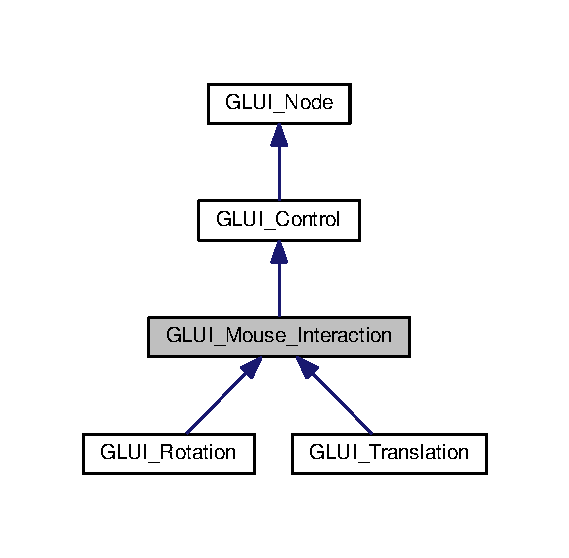
\includegraphics[width=273pt]{class_g_l_u_i___mouse___interaction__inherit__graph}
\end{center}
\end{figure}


Collaboration diagram for G\+L\+U\+I\+\_\+\+Mouse\+\_\+\+Interaction\+:\nopagebreak
\begin{figure}[H]
\begin{center}
\leavevmode
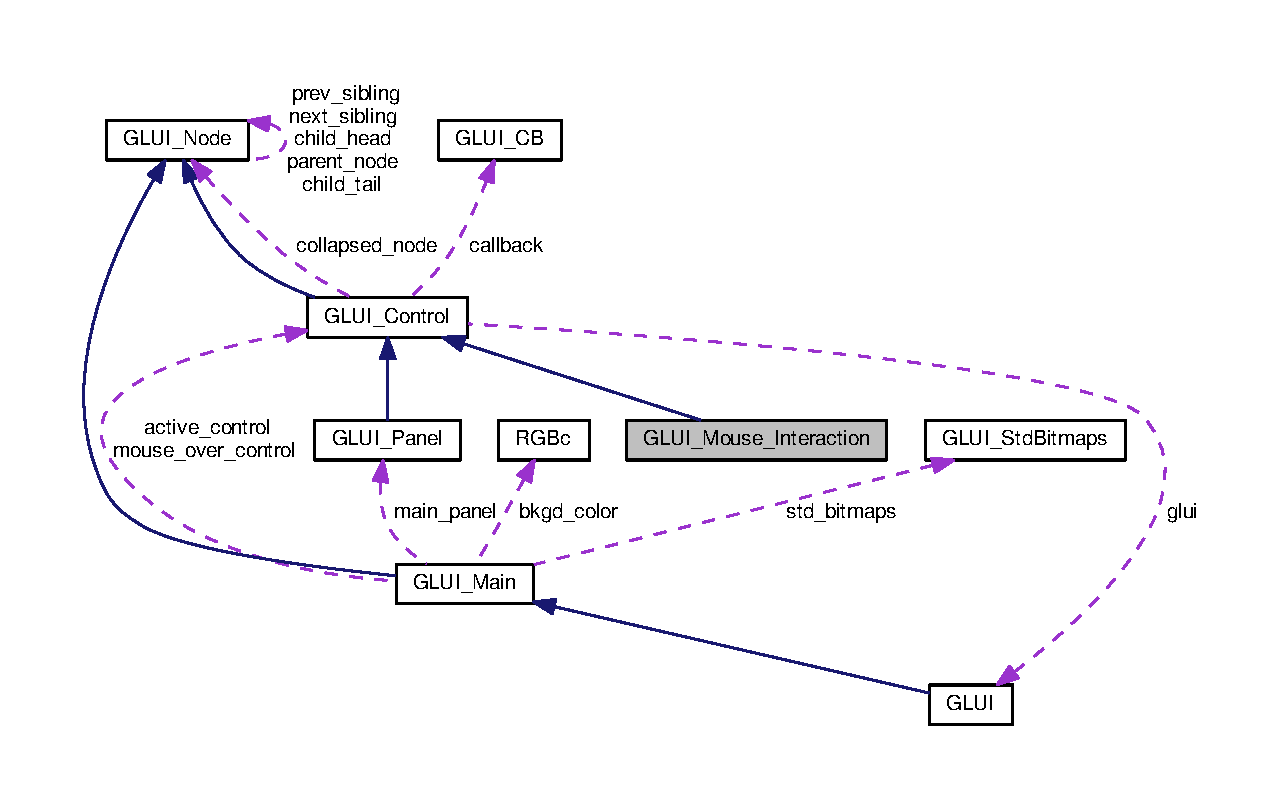
\includegraphics[width=350pt]{class_g_l_u_i___mouse___interaction__coll__graph}
\end{center}
\end{figure}
\subsection*{Public Member Functions}
\begin{DoxyCompactItemize}
\item 
\hyperlink{wglext_8h_a500a82aecba06f4550f6849b8099ca21}{int} \hyperlink{class_g_l_u_i___mouse___interaction_ae21d31df518cdd5c6542d8cc88681a57}{mouse\+\_\+down\+\_\+handler} (\hyperlink{wglext_8h_a500a82aecba06f4550f6849b8099ca21}{int} local\+\_\+x, \hyperlink{wglext_8h_a500a82aecba06f4550f6849b8099ca21}{int} local\+\_\+y)
\item 
\hyperlink{wglext_8h_a500a82aecba06f4550f6849b8099ca21}{int} \hyperlink{class_g_l_u_i___mouse___interaction_a03d3c78048418b27f8bbe258f6f455e2}{mouse\+\_\+up\+\_\+handler} (\hyperlink{wglext_8h_a500a82aecba06f4550f6849b8099ca21}{int} local\+\_\+x, \hyperlink{wglext_8h_a500a82aecba06f4550f6849b8099ca21}{int} local\+\_\+y, bool inside)
\item 
\hyperlink{wglext_8h_a500a82aecba06f4550f6849b8099ca21}{int} \hyperlink{class_g_l_u_i___mouse___interaction_a91bf2ba2ff20dab94ef634e38fbfaa84}{mouse\+\_\+held\+\_\+down\+\_\+handler} (\hyperlink{wglext_8h_a500a82aecba06f4550f6849b8099ca21}{int} local\+\_\+x, \hyperlink{wglext_8h_a500a82aecba06f4550f6849b8099ca21}{int} local\+\_\+y, bool inside)
\item 
\hyperlink{wglext_8h_a500a82aecba06f4550f6849b8099ca21}{int} \hyperlink{class_g_l_u_i___mouse___interaction_aadcfba66761f87037341c7031e225746}{special\+\_\+handler} (\hyperlink{wglext_8h_a500a82aecba06f4550f6849b8099ca21}{int} key, \hyperlink{wglext_8h_a500a82aecba06f4550f6849b8099ca21}{int} modifiers)
\item 
\hyperlink{wglext_8h_a9e6b7f1933461ef318bb000d6bd13b83}{void} \hyperlink{class_g_l_u_i___mouse___interaction_a29237239a861d24ab52b971b0d2fead2}{update\+\_\+size} (\hyperlink{wglext_8h_a9e6b7f1933461ef318bb000d6bd13b83}{void})
\item 
\hyperlink{wglext_8h_a9e6b7f1933461ef318bb000d6bd13b83}{void} \hyperlink{class_g_l_u_i___mouse___interaction_ab51243d0750f3cc8f950e046c4bffd13}{draw} (\hyperlink{wglext_8h_a500a82aecba06f4550f6849b8099ca21}{int} \hyperlink{glext_8h_ad77deca22f617d3f0e0eb786445689fc}{x}, \hyperlink{wglext_8h_a500a82aecba06f4550f6849b8099ca21}{int} \hyperlink{glext_8h_a9298c7ad619074f5285b32c6b72bfdea}{y})
\item 
\hyperlink{wglext_8h_a9e6b7f1933461ef318bb000d6bd13b83}{void} \hyperlink{class_g_l_u_i___mouse___interaction_aacb2dd881015d1f7e8eeced3796e3a6d}{draw\+\_\+active\+\_\+area} (\hyperlink{wglext_8h_a9e6b7f1933461ef318bb000d6bd13b83}{void})
\item 
virtual \hyperlink{wglext_8h_a500a82aecba06f4550f6849b8099ca21}{int} \hyperlink{class_g_l_u_i___mouse___interaction_ab4168e2ccfdb1a8afe2b220e53902b8d}{iaction\+\_\+mouse\+\_\+down\+\_\+handler} (\hyperlink{wglext_8h_a500a82aecba06f4550f6849b8099ca21}{int} local\+\_\+x, \hyperlink{wglext_8h_a500a82aecba06f4550f6849b8099ca21}{int} local\+\_\+y)=0
\item 
virtual \hyperlink{wglext_8h_a500a82aecba06f4550f6849b8099ca21}{int} \hyperlink{class_g_l_u_i___mouse___interaction_aaeab42a0986281d21e2b3ab24efb527d}{iaction\+\_\+mouse\+\_\+up\+\_\+handler} (\hyperlink{wglext_8h_a500a82aecba06f4550f6849b8099ca21}{int} local\+\_\+x, \hyperlink{wglext_8h_a500a82aecba06f4550f6849b8099ca21}{int} local\+\_\+y, bool inside)=0
\item 
virtual \hyperlink{wglext_8h_a500a82aecba06f4550f6849b8099ca21}{int} \hyperlink{class_g_l_u_i___mouse___interaction_ab10a2bbd829a80e7403d722e4e3b480d}{iaction\+\_\+mouse\+\_\+held\+\_\+down\+\_\+handler} (\hyperlink{wglext_8h_a500a82aecba06f4550f6849b8099ca21}{int} local\+\_\+x, \hyperlink{wglext_8h_a500a82aecba06f4550f6849b8099ca21}{int} local\+\_\+y, bool inside)=0
\item 
virtual \hyperlink{wglext_8h_a500a82aecba06f4550f6849b8099ca21}{int} \hyperlink{class_g_l_u_i___mouse___interaction_a738d6fd0afea5a76b45fe2a3c24c4e64}{iaction\+\_\+special\+\_\+handler} (\hyperlink{wglext_8h_a500a82aecba06f4550f6849b8099ca21}{int} key, \hyperlink{wglext_8h_a500a82aecba06f4550f6849b8099ca21}{int} modifiers)=0
\item 
virtual \hyperlink{wglext_8h_a9e6b7f1933461ef318bb000d6bd13b83}{void} \hyperlink{class_g_l_u_i___mouse___interaction_a4c7473fb5849e7d13052100aac56a9f3}{iaction\+\_\+draw\+\_\+active\+\_\+area\+\_\+persp} (\hyperlink{wglext_8h_a9e6b7f1933461ef318bb000d6bd13b83}{void})=0
\item 
virtual \hyperlink{wglext_8h_a9e6b7f1933461ef318bb000d6bd13b83}{void} \hyperlink{class_g_l_u_i___mouse___interaction_aba702d0d46375ab194c7b07d93051b0d}{iaction\+\_\+draw\+\_\+active\+\_\+area\+\_\+ortho} (\hyperlink{wglext_8h_a9e6b7f1933461ef318bb000d6bd13b83}{void})=0
\item 
virtual \hyperlink{wglext_8h_a9e6b7f1933461ef318bb000d6bd13b83}{void} \hyperlink{class_g_l_u_i___mouse___interaction_a99dd43b2224bbfee6aadee3cf15c1fdd}{iaction\+\_\+dump} (F\+I\+L\+E $\ast$output)=0
\item 
virtual \hyperlink{wglext_8h_a9e6b7f1933461ef318bb000d6bd13b83}{void} \hyperlink{class_g_l_u_i___mouse___interaction_a4be4e3ae7948824b2af30c2b87f434fd}{iaction\+\_\+init} (\hyperlink{wglext_8h_a9e6b7f1933461ef318bb000d6bd13b83}{void})=0
\item 
\hyperlink{class_g_l_u_i___mouse___interaction_aa694b34a9d008ec9f428cffd12c83653}{G\+L\+U\+I\+\_\+\+Mouse\+\_\+\+Interaction} (\hyperlink{wglext_8h_a9e6b7f1933461ef318bb000d6bd13b83}{void})
\end{DoxyCompactItemize}
\subsection*{Public Attributes}
\begin{DoxyCompactItemize}
\item 
\hyperlink{wglext_8h_a500a82aecba06f4550f6849b8099ca21}{int} \hyperlink{class_g_l_u_i___mouse___interaction_a1ac48da74085fbff71aab99f2e51b280}{draw\+\_\+active\+\_\+area\+\_\+only}
\end{DoxyCompactItemize}
\subsection*{Additional Inherited Members}


\subsection{Detailed Description}
This is the superclass of translation and rotation widgets. 

Definition at line 2390 of file glui.\+h.



\subsection{Constructor \& Destructor Documentation}
\hypertarget{class_g_l_u_i___mouse___interaction_aa694b34a9d008ec9f428cffd12c83653}{\index{G\+L\+U\+I\+\_\+\+Mouse\+\_\+\+Interaction@{G\+L\+U\+I\+\_\+\+Mouse\+\_\+\+Interaction}!G\+L\+U\+I\+\_\+\+Mouse\+\_\+\+Interaction@{G\+L\+U\+I\+\_\+\+Mouse\+\_\+\+Interaction}}
\index{G\+L\+U\+I\+\_\+\+Mouse\+\_\+\+Interaction@{G\+L\+U\+I\+\_\+\+Mouse\+\_\+\+Interaction}!G\+L\+U\+I\+\_\+\+Mouse\+\_\+\+Interaction@{G\+L\+U\+I\+\_\+\+Mouse\+\_\+\+Interaction}}
\subsubsection[{G\+L\+U\+I\+\_\+\+Mouse\+\_\+\+Interaction}]{\setlength{\rightskip}{0pt plus 5cm}G\+L\+U\+I\+\_\+\+Mouse\+\_\+\+Interaction\+::\+G\+L\+U\+I\+\_\+\+Mouse\+\_\+\+Interaction (
\begin{DoxyParamCaption}
\item[{{\bf void}}]{}
\end{DoxyParamCaption}
)\hspace{0.3cm}{\ttfamily [inline]}}}\label{class_g_l_u_i___mouse___interaction_aa694b34a9d008ec9f428cffd12c83653}


Definition at line 2415 of file glui.\+h.



\subsection{Member Function Documentation}
\hypertarget{class_g_l_u_i___mouse___interaction_ab51243d0750f3cc8f950e046c4bffd13}{\index{G\+L\+U\+I\+\_\+\+Mouse\+\_\+\+Interaction@{G\+L\+U\+I\+\_\+\+Mouse\+\_\+\+Interaction}!draw@{draw}}
\index{draw@{draw}!G\+L\+U\+I\+\_\+\+Mouse\+\_\+\+Interaction@{G\+L\+U\+I\+\_\+\+Mouse\+\_\+\+Interaction}}
\subsubsection[{draw}]{\setlength{\rightskip}{0pt plus 5cm}{\bf void} G\+L\+U\+I\+\_\+\+Mouse\+\_\+\+Interaction\+::draw (
\begin{DoxyParamCaption}
\item[{{\bf int}}]{x, }
\item[{{\bf int}}]{y}
\end{DoxyParamCaption}
)\hspace{0.3cm}{\ttfamily [virtual]}}}\label{class_g_l_u_i___mouse___interaction_ab51243d0750f3cc8f950e046c4bffd13}


Implements \hyperlink{class_g_l_u_i___control_a2eb42d7a7951280ad2fe8c37972bf66a}{G\+L\+U\+I\+\_\+\+Control}.

\hypertarget{class_g_l_u_i___mouse___interaction_aacb2dd881015d1f7e8eeced3796e3a6d}{\index{G\+L\+U\+I\+\_\+\+Mouse\+\_\+\+Interaction@{G\+L\+U\+I\+\_\+\+Mouse\+\_\+\+Interaction}!draw\+\_\+active\+\_\+area@{draw\+\_\+active\+\_\+area}}
\index{draw\+\_\+active\+\_\+area@{draw\+\_\+active\+\_\+area}!G\+L\+U\+I\+\_\+\+Mouse\+\_\+\+Interaction@{G\+L\+U\+I\+\_\+\+Mouse\+\_\+\+Interaction}}
\subsubsection[{draw\+\_\+active\+\_\+area}]{\setlength{\rightskip}{0pt plus 5cm}{\bf void} G\+L\+U\+I\+\_\+\+Mouse\+\_\+\+Interaction\+::draw\+\_\+active\+\_\+area (
\begin{DoxyParamCaption}
\item[{{\bf void}}]{}
\end{DoxyParamCaption}
)}}\label{class_g_l_u_i___mouse___interaction_aacb2dd881015d1f7e8eeced3796e3a6d}
\hypertarget{class_g_l_u_i___mouse___interaction_aba702d0d46375ab194c7b07d93051b0d}{\index{G\+L\+U\+I\+\_\+\+Mouse\+\_\+\+Interaction@{G\+L\+U\+I\+\_\+\+Mouse\+\_\+\+Interaction}!iaction\+\_\+draw\+\_\+active\+\_\+area\+\_\+ortho@{iaction\+\_\+draw\+\_\+active\+\_\+area\+\_\+ortho}}
\index{iaction\+\_\+draw\+\_\+active\+\_\+area\+\_\+ortho@{iaction\+\_\+draw\+\_\+active\+\_\+area\+\_\+ortho}!G\+L\+U\+I\+\_\+\+Mouse\+\_\+\+Interaction@{G\+L\+U\+I\+\_\+\+Mouse\+\_\+\+Interaction}}
\subsubsection[{iaction\+\_\+draw\+\_\+active\+\_\+area\+\_\+ortho}]{\setlength{\rightskip}{0pt plus 5cm}virtual {\bf void} G\+L\+U\+I\+\_\+\+Mouse\+\_\+\+Interaction\+::iaction\+\_\+draw\+\_\+active\+\_\+area\+\_\+ortho (
\begin{DoxyParamCaption}
\item[{{\bf void}}]{}
\end{DoxyParamCaption}
)\hspace{0.3cm}{\ttfamily [pure virtual]}}}\label{class_g_l_u_i___mouse___interaction_aba702d0d46375ab194c7b07d93051b0d}


Implemented in \hyperlink{class_g_l_u_i___translation_a78821a339feee6944df3dacbcd7867eb}{G\+L\+U\+I\+\_\+\+Translation}, and \hyperlink{class_g_l_u_i___rotation_aea8411d09fec628a8af788b0998746f2}{G\+L\+U\+I\+\_\+\+Rotation}.

\hypertarget{class_g_l_u_i___mouse___interaction_a4c7473fb5849e7d13052100aac56a9f3}{\index{G\+L\+U\+I\+\_\+\+Mouse\+\_\+\+Interaction@{G\+L\+U\+I\+\_\+\+Mouse\+\_\+\+Interaction}!iaction\+\_\+draw\+\_\+active\+\_\+area\+\_\+persp@{iaction\+\_\+draw\+\_\+active\+\_\+area\+\_\+persp}}
\index{iaction\+\_\+draw\+\_\+active\+\_\+area\+\_\+persp@{iaction\+\_\+draw\+\_\+active\+\_\+area\+\_\+persp}!G\+L\+U\+I\+\_\+\+Mouse\+\_\+\+Interaction@{G\+L\+U\+I\+\_\+\+Mouse\+\_\+\+Interaction}}
\subsubsection[{iaction\+\_\+draw\+\_\+active\+\_\+area\+\_\+persp}]{\setlength{\rightskip}{0pt plus 5cm}virtual {\bf void} G\+L\+U\+I\+\_\+\+Mouse\+\_\+\+Interaction\+::iaction\+\_\+draw\+\_\+active\+\_\+area\+\_\+persp (
\begin{DoxyParamCaption}
\item[{{\bf void}}]{}
\end{DoxyParamCaption}
)\hspace{0.3cm}{\ttfamily [pure virtual]}}}\label{class_g_l_u_i___mouse___interaction_a4c7473fb5849e7d13052100aac56a9f3}


Implemented in \hyperlink{class_g_l_u_i___translation_affbd229a3bb1b680fccfd394a8277440}{G\+L\+U\+I\+\_\+\+Translation}, and \hyperlink{class_g_l_u_i___rotation_a88cf2f55e52c4afc9a81fceb53dbc406}{G\+L\+U\+I\+\_\+\+Rotation}.

\hypertarget{class_g_l_u_i___mouse___interaction_a99dd43b2224bbfee6aadee3cf15c1fdd}{\index{G\+L\+U\+I\+\_\+\+Mouse\+\_\+\+Interaction@{G\+L\+U\+I\+\_\+\+Mouse\+\_\+\+Interaction}!iaction\+\_\+dump@{iaction\+\_\+dump}}
\index{iaction\+\_\+dump@{iaction\+\_\+dump}!G\+L\+U\+I\+\_\+\+Mouse\+\_\+\+Interaction@{G\+L\+U\+I\+\_\+\+Mouse\+\_\+\+Interaction}}
\subsubsection[{iaction\+\_\+dump}]{\setlength{\rightskip}{0pt plus 5cm}virtual {\bf void} G\+L\+U\+I\+\_\+\+Mouse\+\_\+\+Interaction\+::iaction\+\_\+dump (
\begin{DoxyParamCaption}
\item[{F\+I\+L\+E $\ast$}]{output}
\end{DoxyParamCaption}
)\hspace{0.3cm}{\ttfamily [pure virtual]}}}\label{class_g_l_u_i___mouse___interaction_a99dd43b2224bbfee6aadee3cf15c1fdd}


Implemented in \hyperlink{class_g_l_u_i___translation_ab63de002536cd569083b07006fb3d430}{G\+L\+U\+I\+\_\+\+Translation}, and \hyperlink{class_g_l_u_i___rotation_a6792c8f6fd8d2e52dd1e7729f7679fba}{G\+L\+U\+I\+\_\+\+Rotation}.

\hypertarget{class_g_l_u_i___mouse___interaction_a4be4e3ae7948824b2af30c2b87f434fd}{\index{G\+L\+U\+I\+\_\+\+Mouse\+\_\+\+Interaction@{G\+L\+U\+I\+\_\+\+Mouse\+\_\+\+Interaction}!iaction\+\_\+init@{iaction\+\_\+init}}
\index{iaction\+\_\+init@{iaction\+\_\+init}!G\+L\+U\+I\+\_\+\+Mouse\+\_\+\+Interaction@{G\+L\+U\+I\+\_\+\+Mouse\+\_\+\+Interaction}}
\subsubsection[{iaction\+\_\+init}]{\setlength{\rightskip}{0pt plus 5cm}virtual {\bf void} G\+L\+U\+I\+\_\+\+Mouse\+\_\+\+Interaction\+::iaction\+\_\+init (
\begin{DoxyParamCaption}
\item[{{\bf void}}]{}
\end{DoxyParamCaption}
)\hspace{0.3cm}{\ttfamily [pure virtual]}}}\label{class_g_l_u_i___mouse___interaction_a4be4e3ae7948824b2af30c2b87f434fd}


Implemented in \hyperlink{class_g_l_u_i___translation_abacc8d8aa4e4a99ab8c6965256ab2bb0}{G\+L\+U\+I\+\_\+\+Translation}, and \hyperlink{class_g_l_u_i___rotation_ac7029bd29427238e2590472ae882c258}{G\+L\+U\+I\+\_\+\+Rotation}.

\hypertarget{class_g_l_u_i___mouse___interaction_ab4168e2ccfdb1a8afe2b220e53902b8d}{\index{G\+L\+U\+I\+\_\+\+Mouse\+\_\+\+Interaction@{G\+L\+U\+I\+\_\+\+Mouse\+\_\+\+Interaction}!iaction\+\_\+mouse\+\_\+down\+\_\+handler@{iaction\+\_\+mouse\+\_\+down\+\_\+handler}}
\index{iaction\+\_\+mouse\+\_\+down\+\_\+handler@{iaction\+\_\+mouse\+\_\+down\+\_\+handler}!G\+L\+U\+I\+\_\+\+Mouse\+\_\+\+Interaction@{G\+L\+U\+I\+\_\+\+Mouse\+\_\+\+Interaction}}
\subsubsection[{iaction\+\_\+mouse\+\_\+down\+\_\+handler}]{\setlength{\rightskip}{0pt plus 5cm}virtual {\bf int} G\+L\+U\+I\+\_\+\+Mouse\+\_\+\+Interaction\+::iaction\+\_\+mouse\+\_\+down\+\_\+handler (
\begin{DoxyParamCaption}
\item[{{\bf int}}]{local\+\_\+x, }
\item[{{\bf int}}]{local\+\_\+y}
\end{DoxyParamCaption}
)\hspace{0.3cm}{\ttfamily [pure virtual]}}}\label{class_g_l_u_i___mouse___interaction_ab4168e2ccfdb1a8afe2b220e53902b8d}


Implemented in \hyperlink{class_g_l_u_i___translation_a92ca690a16b858d761aa9e12ac44ec13}{G\+L\+U\+I\+\_\+\+Translation}, and \hyperlink{class_g_l_u_i___rotation_a3af15515b4f2bd05bfbbc625fa4d6247}{G\+L\+U\+I\+\_\+\+Rotation}.

\hypertarget{class_g_l_u_i___mouse___interaction_ab10a2bbd829a80e7403d722e4e3b480d}{\index{G\+L\+U\+I\+\_\+\+Mouse\+\_\+\+Interaction@{G\+L\+U\+I\+\_\+\+Mouse\+\_\+\+Interaction}!iaction\+\_\+mouse\+\_\+held\+\_\+down\+\_\+handler@{iaction\+\_\+mouse\+\_\+held\+\_\+down\+\_\+handler}}
\index{iaction\+\_\+mouse\+\_\+held\+\_\+down\+\_\+handler@{iaction\+\_\+mouse\+\_\+held\+\_\+down\+\_\+handler}!G\+L\+U\+I\+\_\+\+Mouse\+\_\+\+Interaction@{G\+L\+U\+I\+\_\+\+Mouse\+\_\+\+Interaction}}
\subsubsection[{iaction\+\_\+mouse\+\_\+held\+\_\+down\+\_\+handler}]{\setlength{\rightskip}{0pt plus 5cm}virtual {\bf int} G\+L\+U\+I\+\_\+\+Mouse\+\_\+\+Interaction\+::iaction\+\_\+mouse\+\_\+held\+\_\+down\+\_\+handler (
\begin{DoxyParamCaption}
\item[{{\bf int}}]{local\+\_\+x, }
\item[{{\bf int}}]{local\+\_\+y, }
\item[{bool}]{inside}
\end{DoxyParamCaption}
)\hspace{0.3cm}{\ttfamily [pure virtual]}}}\label{class_g_l_u_i___mouse___interaction_ab10a2bbd829a80e7403d722e4e3b480d}


Implemented in \hyperlink{class_g_l_u_i___translation_a2d13c80e8d6d16378a2f0ceecda7a3c4}{G\+L\+U\+I\+\_\+\+Translation}, and \hyperlink{class_g_l_u_i___rotation_ad743bdbd88648859ef334c572e9e969d}{G\+L\+U\+I\+\_\+\+Rotation}.

\hypertarget{class_g_l_u_i___mouse___interaction_aaeab42a0986281d21e2b3ab24efb527d}{\index{G\+L\+U\+I\+\_\+\+Mouse\+\_\+\+Interaction@{G\+L\+U\+I\+\_\+\+Mouse\+\_\+\+Interaction}!iaction\+\_\+mouse\+\_\+up\+\_\+handler@{iaction\+\_\+mouse\+\_\+up\+\_\+handler}}
\index{iaction\+\_\+mouse\+\_\+up\+\_\+handler@{iaction\+\_\+mouse\+\_\+up\+\_\+handler}!G\+L\+U\+I\+\_\+\+Mouse\+\_\+\+Interaction@{G\+L\+U\+I\+\_\+\+Mouse\+\_\+\+Interaction}}
\subsubsection[{iaction\+\_\+mouse\+\_\+up\+\_\+handler}]{\setlength{\rightskip}{0pt plus 5cm}virtual {\bf int} G\+L\+U\+I\+\_\+\+Mouse\+\_\+\+Interaction\+::iaction\+\_\+mouse\+\_\+up\+\_\+handler (
\begin{DoxyParamCaption}
\item[{{\bf int}}]{local\+\_\+x, }
\item[{{\bf int}}]{local\+\_\+y, }
\item[{bool}]{inside}
\end{DoxyParamCaption}
)\hspace{0.3cm}{\ttfamily [pure virtual]}}}\label{class_g_l_u_i___mouse___interaction_aaeab42a0986281d21e2b3ab24efb527d}


Implemented in \hyperlink{class_g_l_u_i___translation_a7674b5641e87b9d73a590a9cbfd83783}{G\+L\+U\+I\+\_\+\+Translation}, and \hyperlink{class_g_l_u_i___rotation_aa3ee9f07c589dedc7c1b6ad780566172}{G\+L\+U\+I\+\_\+\+Rotation}.

\hypertarget{class_g_l_u_i___mouse___interaction_a738d6fd0afea5a76b45fe2a3c24c4e64}{\index{G\+L\+U\+I\+\_\+\+Mouse\+\_\+\+Interaction@{G\+L\+U\+I\+\_\+\+Mouse\+\_\+\+Interaction}!iaction\+\_\+special\+\_\+handler@{iaction\+\_\+special\+\_\+handler}}
\index{iaction\+\_\+special\+\_\+handler@{iaction\+\_\+special\+\_\+handler}!G\+L\+U\+I\+\_\+\+Mouse\+\_\+\+Interaction@{G\+L\+U\+I\+\_\+\+Mouse\+\_\+\+Interaction}}
\subsubsection[{iaction\+\_\+special\+\_\+handler}]{\setlength{\rightskip}{0pt plus 5cm}virtual {\bf int} G\+L\+U\+I\+\_\+\+Mouse\+\_\+\+Interaction\+::iaction\+\_\+special\+\_\+handler (
\begin{DoxyParamCaption}
\item[{{\bf int}}]{key, }
\item[{{\bf int}}]{modifiers}
\end{DoxyParamCaption}
)\hspace{0.3cm}{\ttfamily [pure virtual]}}}\label{class_g_l_u_i___mouse___interaction_a738d6fd0afea5a76b45fe2a3c24c4e64}


Implemented in \hyperlink{class_g_l_u_i___translation_a4bdc9a327c975a24546e2733f5f5cb01}{G\+L\+U\+I\+\_\+\+Translation}, and \hyperlink{class_g_l_u_i___rotation_a0a86badfaa9102475a2af2b2f3d824aa}{G\+L\+U\+I\+\_\+\+Rotation}.

\hypertarget{class_g_l_u_i___mouse___interaction_ae21d31df518cdd5c6542d8cc88681a57}{\index{G\+L\+U\+I\+\_\+\+Mouse\+\_\+\+Interaction@{G\+L\+U\+I\+\_\+\+Mouse\+\_\+\+Interaction}!mouse\+\_\+down\+\_\+handler@{mouse\+\_\+down\+\_\+handler}}
\index{mouse\+\_\+down\+\_\+handler@{mouse\+\_\+down\+\_\+handler}!G\+L\+U\+I\+\_\+\+Mouse\+\_\+\+Interaction@{G\+L\+U\+I\+\_\+\+Mouse\+\_\+\+Interaction}}
\subsubsection[{mouse\+\_\+down\+\_\+handler}]{\setlength{\rightskip}{0pt plus 5cm}{\bf int} G\+L\+U\+I\+\_\+\+Mouse\+\_\+\+Interaction\+::mouse\+\_\+down\+\_\+handler (
\begin{DoxyParamCaption}
\item[{{\bf int}}]{local\+\_\+x, }
\item[{{\bf int}}]{local\+\_\+y}
\end{DoxyParamCaption}
)\hspace{0.3cm}{\ttfamily [virtual]}}}\label{class_g_l_u_i___mouse___interaction_ae21d31df518cdd5c6542d8cc88681a57}


Reimplemented from \hyperlink{class_g_l_u_i___control_a92b77565168a1d2003bca1c16ac00e8d}{G\+L\+U\+I\+\_\+\+Control}.

\hypertarget{class_g_l_u_i___mouse___interaction_a91bf2ba2ff20dab94ef634e38fbfaa84}{\index{G\+L\+U\+I\+\_\+\+Mouse\+\_\+\+Interaction@{G\+L\+U\+I\+\_\+\+Mouse\+\_\+\+Interaction}!mouse\+\_\+held\+\_\+down\+\_\+handler@{mouse\+\_\+held\+\_\+down\+\_\+handler}}
\index{mouse\+\_\+held\+\_\+down\+\_\+handler@{mouse\+\_\+held\+\_\+down\+\_\+handler}!G\+L\+U\+I\+\_\+\+Mouse\+\_\+\+Interaction@{G\+L\+U\+I\+\_\+\+Mouse\+\_\+\+Interaction}}
\subsubsection[{mouse\+\_\+held\+\_\+down\+\_\+handler}]{\setlength{\rightskip}{0pt plus 5cm}{\bf int} G\+L\+U\+I\+\_\+\+Mouse\+\_\+\+Interaction\+::mouse\+\_\+held\+\_\+down\+\_\+handler (
\begin{DoxyParamCaption}
\item[{{\bf int}}]{local\+\_\+x, }
\item[{{\bf int}}]{local\+\_\+y, }
\item[{bool}]{inside}
\end{DoxyParamCaption}
)\hspace{0.3cm}{\ttfamily [virtual]}}}\label{class_g_l_u_i___mouse___interaction_a91bf2ba2ff20dab94ef634e38fbfaa84}


Reimplemented from \hyperlink{class_g_l_u_i___control_a4b44e44c1c455adc7f98c63aeb6aa919}{G\+L\+U\+I\+\_\+\+Control}.

\hypertarget{class_g_l_u_i___mouse___interaction_a03d3c78048418b27f8bbe258f6f455e2}{\index{G\+L\+U\+I\+\_\+\+Mouse\+\_\+\+Interaction@{G\+L\+U\+I\+\_\+\+Mouse\+\_\+\+Interaction}!mouse\+\_\+up\+\_\+handler@{mouse\+\_\+up\+\_\+handler}}
\index{mouse\+\_\+up\+\_\+handler@{mouse\+\_\+up\+\_\+handler}!G\+L\+U\+I\+\_\+\+Mouse\+\_\+\+Interaction@{G\+L\+U\+I\+\_\+\+Mouse\+\_\+\+Interaction}}
\subsubsection[{mouse\+\_\+up\+\_\+handler}]{\setlength{\rightskip}{0pt plus 5cm}{\bf int} G\+L\+U\+I\+\_\+\+Mouse\+\_\+\+Interaction\+::mouse\+\_\+up\+\_\+handler (
\begin{DoxyParamCaption}
\item[{{\bf int}}]{local\+\_\+x, }
\item[{{\bf int}}]{local\+\_\+y, }
\item[{bool}]{inside}
\end{DoxyParamCaption}
)\hspace{0.3cm}{\ttfamily [virtual]}}}\label{class_g_l_u_i___mouse___interaction_a03d3c78048418b27f8bbe258f6f455e2}


Reimplemented from \hyperlink{class_g_l_u_i___control_ac32aad8f69134d03682e34d0488a18f1}{G\+L\+U\+I\+\_\+\+Control}.

\hypertarget{class_g_l_u_i___mouse___interaction_aadcfba66761f87037341c7031e225746}{\index{G\+L\+U\+I\+\_\+\+Mouse\+\_\+\+Interaction@{G\+L\+U\+I\+\_\+\+Mouse\+\_\+\+Interaction}!special\+\_\+handler@{special\+\_\+handler}}
\index{special\+\_\+handler@{special\+\_\+handler}!G\+L\+U\+I\+\_\+\+Mouse\+\_\+\+Interaction@{G\+L\+U\+I\+\_\+\+Mouse\+\_\+\+Interaction}}
\subsubsection[{special\+\_\+handler}]{\setlength{\rightskip}{0pt plus 5cm}{\bf int} G\+L\+U\+I\+\_\+\+Mouse\+\_\+\+Interaction\+::special\+\_\+handler (
\begin{DoxyParamCaption}
\item[{{\bf int}}]{key, }
\item[{{\bf int}}]{modifiers}
\end{DoxyParamCaption}
)\hspace{0.3cm}{\ttfamily [virtual]}}}\label{class_g_l_u_i___mouse___interaction_aadcfba66761f87037341c7031e225746}


Reimplemented from \hyperlink{class_g_l_u_i___control_ab08da363df3f3eae867dd5ae61200f23}{G\+L\+U\+I\+\_\+\+Control}.

\hypertarget{class_g_l_u_i___mouse___interaction_a29237239a861d24ab52b971b0d2fead2}{\index{G\+L\+U\+I\+\_\+\+Mouse\+\_\+\+Interaction@{G\+L\+U\+I\+\_\+\+Mouse\+\_\+\+Interaction}!update\+\_\+size@{update\+\_\+size}}
\index{update\+\_\+size@{update\+\_\+size}!G\+L\+U\+I\+\_\+\+Mouse\+\_\+\+Interaction@{G\+L\+U\+I\+\_\+\+Mouse\+\_\+\+Interaction}}
\subsubsection[{update\+\_\+size}]{\setlength{\rightskip}{0pt plus 5cm}{\bf void} G\+L\+U\+I\+\_\+\+Mouse\+\_\+\+Interaction\+::update\+\_\+size (
\begin{DoxyParamCaption}
\item[{{\bf void}}]{}
\end{DoxyParamCaption}
)\hspace{0.3cm}{\ttfamily [virtual]}}}\label{class_g_l_u_i___mouse___interaction_a29237239a861d24ab52b971b0d2fead2}


Reimplemented from \hyperlink{class_g_l_u_i___control_a4bfe55acbbf735a7d2ff07d687a481e2}{G\+L\+U\+I\+\_\+\+Control}.



\subsection{Member Data Documentation}
\hypertarget{class_g_l_u_i___mouse___interaction_a1ac48da74085fbff71aab99f2e51b280}{\index{G\+L\+U\+I\+\_\+\+Mouse\+\_\+\+Interaction@{G\+L\+U\+I\+\_\+\+Mouse\+\_\+\+Interaction}!draw\+\_\+active\+\_\+area\+\_\+only@{draw\+\_\+active\+\_\+area\+\_\+only}}
\index{draw\+\_\+active\+\_\+area\+\_\+only@{draw\+\_\+active\+\_\+area\+\_\+only}!G\+L\+U\+I\+\_\+\+Mouse\+\_\+\+Interaction@{G\+L\+U\+I\+\_\+\+Mouse\+\_\+\+Interaction}}
\subsubsection[{draw\+\_\+active\+\_\+area\+\_\+only}]{\setlength{\rightskip}{0pt plus 5cm}{\bf int} G\+L\+U\+I\+\_\+\+Mouse\+\_\+\+Interaction\+::draw\+\_\+active\+\_\+area\+\_\+only}}\label{class_g_l_u_i___mouse___interaction_a1ac48da74085fbff71aab99f2e51b280}


Definition at line 2394 of file glui.\+h.



The documentation for this class was generated from the following file\+:\begin{DoxyCompactItemize}
\item 
S\+S\+W\+C/src/\+G\+L/\hyperlink{glui_8h}{glui.\+h}\end{DoxyCompactItemize}

\hypertarget{class_g_l_u_i___node}{\section{G\+L\+U\+I\+\_\+\+Node Class Reference}
\label{class_g_l_u_i___node}\index{G\+L\+U\+I\+\_\+\+Node@{G\+L\+U\+I\+\_\+\+Node}}
}


{\ttfamily \#include $<$glui.\+h$>$}



Inheritance diagram for G\+L\+U\+I\+\_\+\+Node\+:\nopagebreak
\begin{figure}[H]
\begin{center}
\leavevmode
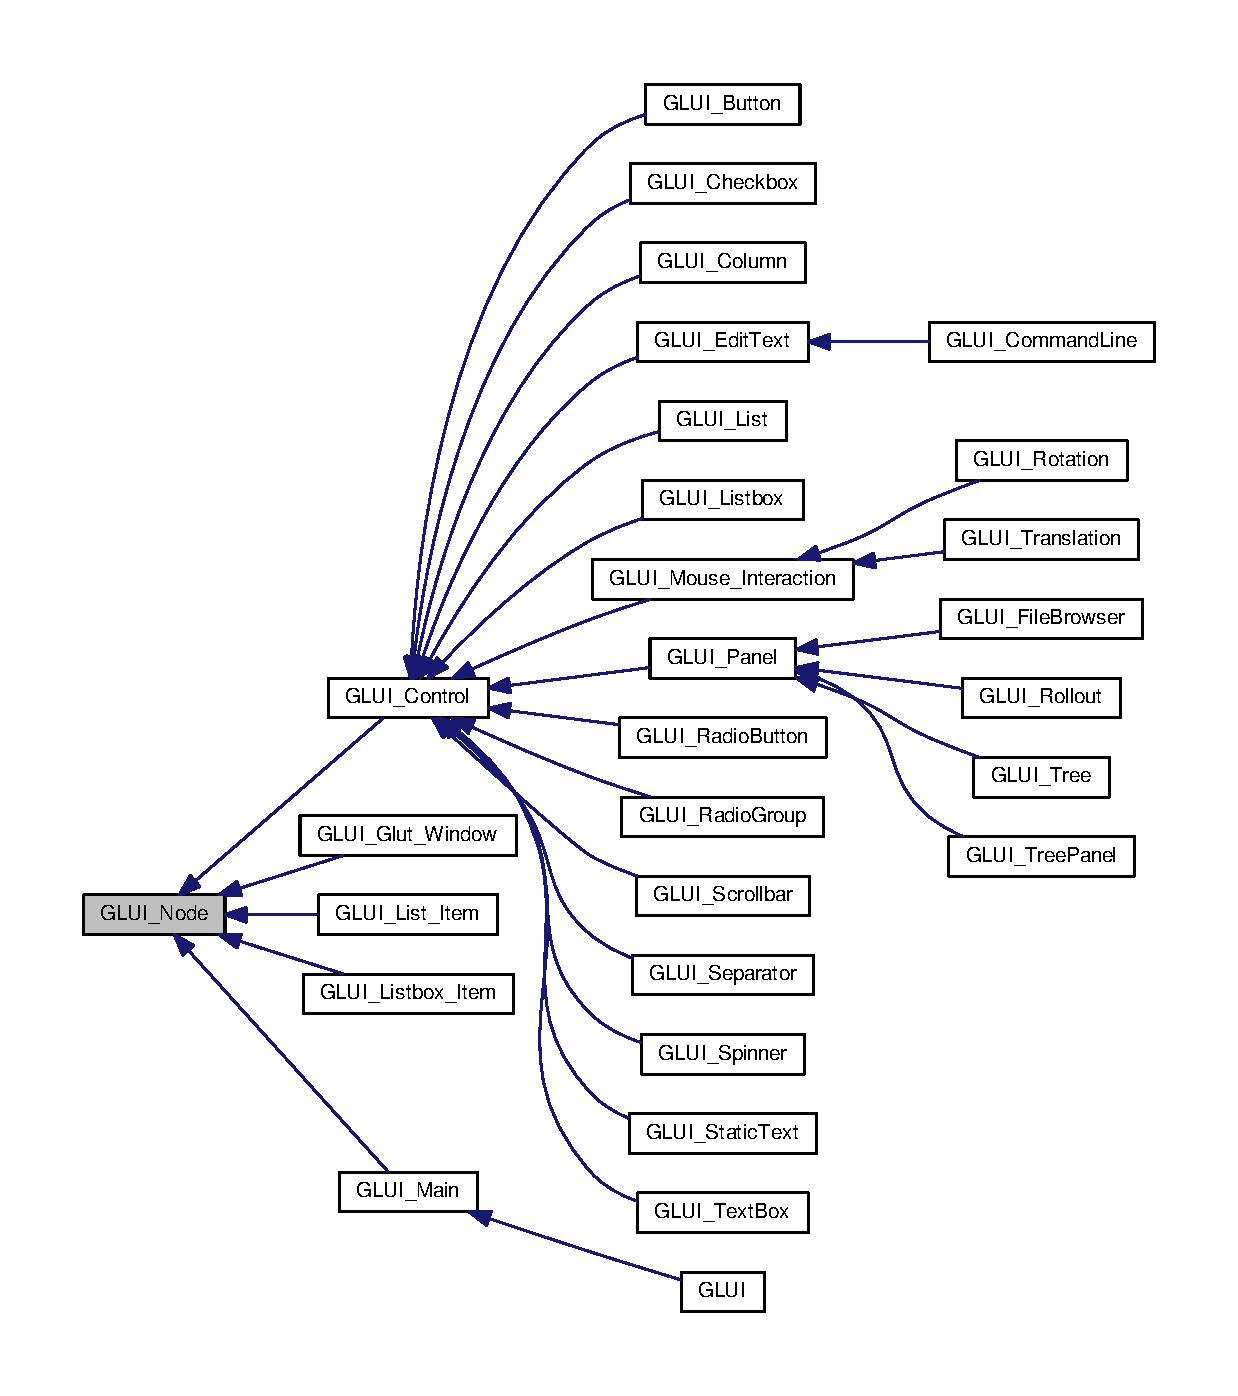
\includegraphics[width=350pt]{class_g_l_u_i___node__inherit__graph}
\end{center}
\end{figure}


Collaboration diagram for G\+L\+U\+I\+\_\+\+Node\+:\nopagebreak
\begin{figure}[H]
\begin{center}
\leavevmode
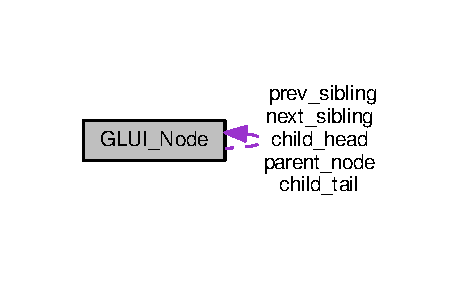
\includegraphics[width=221pt]{class_g_l_u_i___node__coll__graph}
\end{center}
\end{figure}
\subsection*{Public Member Functions}
\begin{DoxyCompactItemize}
\item 
\hyperlink{class_g_l_u_i___node_a066e5d80bfb9925bdb034c29da9c844c}{G\+L\+U\+I\+\_\+\+Node} ()
\item 
virtual \hyperlink{class_g_l_u_i___node_ae6982edc46ab73963ee8ce9f6d035982}{$\sim$\+G\+L\+U\+I\+\_\+\+Node} ()
\item 
\hyperlink{class_g_l_u_i___node}{G\+L\+U\+I\+\_\+\+Node} $\ast$ \hyperlink{class_g_l_u_i___node_ace20232965e8d9da8f3d286113d5572a}{first\+\_\+sibling} ()
\item 
\hyperlink{class_g_l_u_i___node}{G\+L\+U\+I\+\_\+\+Node} $\ast$ \hyperlink{class_g_l_u_i___node_a6458e5a6af00ddf2ebb9271c06fa2931}{last\+\_\+sibling} ()
\item 
\hyperlink{class_g_l_u_i___node}{G\+L\+U\+I\+\_\+\+Node} $\ast$ \hyperlink{class_g_l_u_i___node_a84892bf13144651007640c5f25b51145}{prev} ()
\item 
\hyperlink{class_g_l_u_i___node}{G\+L\+U\+I\+\_\+\+Node} $\ast$ \hyperlink{class_g_l_u_i___node_a7901214f386113b417a25de023476317}{next} ()
\item 
\hyperlink{class_g_l_u_i___node}{G\+L\+U\+I\+\_\+\+Node} $\ast$ \hyperlink{class_g_l_u_i___node_a631b094804b887c0d091ece2786543d1}{first\+\_\+child} ()
\item 
\hyperlink{class_g_l_u_i___node}{G\+L\+U\+I\+\_\+\+Node} $\ast$ \hyperlink{class_g_l_u_i___node_a4825cdc843f0e2b46d75fe5cb9e8ba35}{last\+\_\+child} ()
\item 
\hyperlink{class_g_l_u_i___node}{G\+L\+U\+I\+\_\+\+Node} $\ast$ \hyperlink{class_g_l_u_i___node_a8ed65d447784f6f88bd3e2e2bcac6cdb}{parent} ()
\item 
virtual \hyperlink{wglext_8h_a500a82aecba06f4550f6849b8099ca21}{int} \hyperlink{class_g_l_u_i___node_abdcdd643758adab07580124187565fcd}{add\+\_\+control} (\hyperlink{class_g_l_u_i___control}{G\+L\+U\+I\+\_\+\+Control} $\ast$control)
\item 
\hyperlink{wglext_8h_a9e6b7f1933461ef318bb000d6bd13b83}{void} \hyperlink{class_g_l_u_i___node_a28eb5c7bf5a0edf5b7ba2502384c6544}{link\+\_\+this\+\_\+to\+\_\+parent\+\_\+last} (\hyperlink{class_g_l_u_i___node}{G\+L\+U\+I\+\_\+\+Node} $\ast$\hyperlink{class_g_l_u_i___node_a8ed65d447784f6f88bd3e2e2bcac6cdb}{parent})
\item 
\hyperlink{wglext_8h_a9e6b7f1933461ef318bb000d6bd13b83}{void} \hyperlink{class_g_l_u_i___node_a3feadb4b6d58122ff5449adfb4a323bc}{link\+\_\+this\+\_\+to\+\_\+parent\+\_\+first} (\hyperlink{class_g_l_u_i___node}{G\+L\+U\+I\+\_\+\+Node} $\ast$\hyperlink{class_g_l_u_i___node_a8ed65d447784f6f88bd3e2e2bcac6cdb}{parent})
\item 
\hyperlink{wglext_8h_a9e6b7f1933461ef318bb000d6bd13b83}{void} \hyperlink{class_g_l_u_i___node_ad8d7fd8a437eeec4a72b73064dc954b4}{link\+\_\+this\+\_\+to\+\_\+sibling\+\_\+next} (\hyperlink{class_g_l_u_i___node}{G\+L\+U\+I\+\_\+\+Node} $\ast$sibling)
\item 
\hyperlink{wglext_8h_a9e6b7f1933461ef318bb000d6bd13b83}{void} \hyperlink{class_g_l_u_i___node_a5825555fc493712a1d6f24235f59f25a}{link\+\_\+this\+\_\+to\+\_\+sibling\+\_\+prev} (\hyperlink{class_g_l_u_i___node}{G\+L\+U\+I\+\_\+\+Node} $\ast$sibling)
\item 
\hyperlink{wglext_8h_a9e6b7f1933461ef318bb000d6bd13b83}{void} \hyperlink{class_g_l_u_i___node_a48b62b12bf8c466fc54fbbbf30183493}{unlink} ()
\item 
\hyperlink{wglext_8h_a9e6b7f1933461ef318bb000d6bd13b83}{void} \hyperlink{class_g_l_u_i___node_abce29cf0ade68e9e5702025f710cb1e8}{dump} (F\+I\+L\+E $\ast$out, const char $\ast$\hyperlink{glext_8h_ad977737dfc9a274a62741b9500c49a32}{name})
\end{DoxyCompactItemize}
\subsection*{Static Protected Member Functions}
\begin{DoxyCompactItemize}
\item 
static \hyperlink{wglext_8h_a9e6b7f1933461ef318bb000d6bd13b83}{void} \hyperlink{class_g_l_u_i___node_a02cf295c81cebe31c39e95403dbadbc1}{add\+\_\+child\+\_\+to\+\_\+control} (\hyperlink{class_g_l_u_i___node}{G\+L\+U\+I\+\_\+\+Node} $\ast$\hyperlink{class_g_l_u_i___node_a8ed65d447784f6f88bd3e2e2bcac6cdb}{parent}, \hyperlink{class_g_l_u_i___control}{G\+L\+U\+I\+\_\+\+Control} $\ast$child)
\end{DoxyCompactItemize}
\subsection*{Protected Attributes}
\begin{DoxyCompactItemize}
\item 
\hyperlink{class_g_l_u_i___node}{G\+L\+U\+I\+\_\+\+Node} $\ast$ \hyperlink{class_g_l_u_i___node_a308f39e8a182f499139381840418a573}{parent\+\_\+node}
\item 
\hyperlink{class_g_l_u_i___node}{G\+L\+U\+I\+\_\+\+Node} $\ast$ \hyperlink{class_g_l_u_i___node_ad9370e7f62e83bb720063d2439f544c2}{child\+\_\+head}
\item 
\hyperlink{class_g_l_u_i___node}{G\+L\+U\+I\+\_\+\+Node} $\ast$ \hyperlink{class_g_l_u_i___node_a971d8e606c1a3442ad9b8681bdb9ed59}{child\+\_\+tail}
\item 
\hyperlink{class_g_l_u_i___node}{G\+L\+U\+I\+\_\+\+Node} $\ast$ \hyperlink{class_g_l_u_i___node_a2c99ef6a1290035f98871d859d05e890}{next\+\_\+sibling}
\item 
\hyperlink{class_g_l_u_i___node}{G\+L\+U\+I\+\_\+\+Node} $\ast$ \hyperlink{class_g_l_u_i___node_afa72f0491ca54ce8d0a0af7049de8049}{prev\+\_\+sibling}
\end{DoxyCompactItemize}
\subsection*{Friends}
\begin{DoxyCompactItemize}
\item 
class \hyperlink{class_g_l_u_i___node_a5cd4411266c4ef47da626d8efdf1138e}{G\+L\+U\+I\+\_\+\+Tree}
\item 
class \hyperlink{class_g_l_u_i___node_a342e7f489f8666a8156fb18bd0ea0d2e}{G\+L\+U\+I\+\_\+\+Rollout}
\item 
class \hyperlink{class_g_l_u_i___node_a97e15a1bec3e5f03f25594cb1d690fee}{G\+L\+U\+I\+\_\+\+Main}
\end{DoxyCompactItemize}


\subsection{Detailed Description}
\hyperlink{class_g_l_u_i___node}{G\+L\+U\+I\+\_\+\+Node} is a node in a sort of tree of \hyperlink{class_g_l_u_i}{G\+L\+U\+I} controls. Each \hyperlink{class_g_l_u_i___node}{G\+L\+U\+I\+\_\+\+Node} has a list of siblings (in a circular list) and a linked list of children.

Everything onscreen is a \hyperlink{class_g_l_u_i___node}{G\+L\+U\+I\+\_\+\+Node}--windows, buttons, etc. The nodes are traversed for event processing, sizing, redraws, etc. 

Definition at line 327 of file glui.\+h.



\subsection{Constructor \& Destructor Documentation}
\hypertarget{class_g_l_u_i___node_a066e5d80bfb9925bdb034c29da9c844c}{\index{G\+L\+U\+I\+\_\+\+Node@{G\+L\+U\+I\+\_\+\+Node}!G\+L\+U\+I\+\_\+\+Node@{G\+L\+U\+I\+\_\+\+Node}}
\index{G\+L\+U\+I\+\_\+\+Node@{G\+L\+U\+I\+\_\+\+Node}!G\+L\+U\+I\+\_\+\+Node@{G\+L\+U\+I\+\_\+\+Node}}
\subsubsection[{G\+L\+U\+I\+\_\+\+Node}]{\setlength{\rightskip}{0pt plus 5cm}G\+L\+U\+I\+\_\+\+Node\+::\+G\+L\+U\+I\+\_\+\+Node (
\begin{DoxyParamCaption}
{}
\end{DoxyParamCaption}
)}}\label{class_g_l_u_i___node_a066e5d80bfb9925bdb034c29da9c844c}
\hypertarget{class_g_l_u_i___node_ae6982edc46ab73963ee8ce9f6d035982}{\index{G\+L\+U\+I\+\_\+\+Node@{G\+L\+U\+I\+\_\+\+Node}!````~G\+L\+U\+I\+\_\+\+Node@{$\sim$\+G\+L\+U\+I\+\_\+\+Node}}
\index{````~G\+L\+U\+I\+\_\+\+Node@{$\sim$\+G\+L\+U\+I\+\_\+\+Node}!G\+L\+U\+I\+\_\+\+Node@{G\+L\+U\+I\+\_\+\+Node}}
\subsubsection[{$\sim$\+G\+L\+U\+I\+\_\+\+Node}]{\setlength{\rightskip}{0pt plus 5cm}virtual G\+L\+U\+I\+\_\+\+Node\+::$\sim$\+G\+L\+U\+I\+\_\+\+Node (
\begin{DoxyParamCaption}
{}
\end{DoxyParamCaption}
)\hspace{0.3cm}{\ttfamily [inline]}, {\ttfamily [virtual]}}}\label{class_g_l_u_i___node_ae6982edc46ab73963ee8ce9f6d035982}


Definition at line 335 of file glui.\+h.



\subsection{Member Function Documentation}
\hypertarget{class_g_l_u_i___node_a02cf295c81cebe31c39e95403dbadbc1}{\index{G\+L\+U\+I\+\_\+\+Node@{G\+L\+U\+I\+\_\+\+Node}!add\+\_\+child\+\_\+to\+\_\+control@{add\+\_\+child\+\_\+to\+\_\+control}}
\index{add\+\_\+child\+\_\+to\+\_\+control@{add\+\_\+child\+\_\+to\+\_\+control}!G\+L\+U\+I\+\_\+\+Node@{G\+L\+U\+I\+\_\+\+Node}}
\subsubsection[{add\+\_\+child\+\_\+to\+\_\+control}]{\setlength{\rightskip}{0pt plus 5cm}static {\bf void} G\+L\+U\+I\+\_\+\+Node\+::add\+\_\+child\+\_\+to\+\_\+control (
\begin{DoxyParamCaption}
\item[{{\bf G\+L\+U\+I\+\_\+\+Node} $\ast$}]{parent, }
\item[{{\bf G\+L\+U\+I\+\_\+\+Control} $\ast$}]{child}
\end{DoxyParamCaption}
)\hspace{0.3cm}{\ttfamily [static]}, {\ttfamily [protected]}}}\label{class_g_l_u_i___node_a02cf295c81cebe31c39e95403dbadbc1}
\hypertarget{class_g_l_u_i___node_abdcdd643758adab07580124187565fcd}{\index{G\+L\+U\+I\+\_\+\+Node@{G\+L\+U\+I\+\_\+\+Node}!add\+\_\+control@{add\+\_\+control}}
\index{add\+\_\+control@{add\+\_\+control}!G\+L\+U\+I\+\_\+\+Node@{G\+L\+U\+I\+\_\+\+Node}}
\subsubsection[{add\+\_\+control}]{\setlength{\rightskip}{0pt plus 5cm}virtual {\bf int} G\+L\+U\+I\+\_\+\+Node\+::add\+\_\+control (
\begin{DoxyParamCaption}
\item[{{\bf G\+L\+U\+I\+\_\+\+Control} $\ast$}]{control}
\end{DoxyParamCaption}
)\hspace{0.3cm}{\ttfamily [virtual]}}}\label{class_g_l_u_i___node_abdcdd643758adab07580124187565fcd}
Link in a new child control 

Reimplemented in \hyperlink{class_g_l_u_i_a94398f830a14babcd93ac109082a221e}{G\+L\+U\+I}.

\hypertarget{class_g_l_u_i___node_abce29cf0ade68e9e5702025f710cb1e8}{\index{G\+L\+U\+I\+\_\+\+Node@{G\+L\+U\+I\+\_\+\+Node}!dump@{dump}}
\index{dump@{dump}!G\+L\+U\+I\+\_\+\+Node@{G\+L\+U\+I\+\_\+\+Node}}
\subsubsection[{dump}]{\setlength{\rightskip}{0pt plus 5cm}{\bf void} G\+L\+U\+I\+\_\+\+Node\+::dump (
\begin{DoxyParamCaption}
\item[{F\+I\+L\+E $\ast$}]{out, }
\item[{const char $\ast$}]{name}
\end{DoxyParamCaption}
)}}\label{class_g_l_u_i___node_abce29cf0ade68e9e5702025f710cb1e8}
\hypertarget{class_g_l_u_i___node_a631b094804b887c0d091ece2786543d1}{\index{G\+L\+U\+I\+\_\+\+Node@{G\+L\+U\+I\+\_\+\+Node}!first\+\_\+child@{first\+\_\+child}}
\index{first\+\_\+child@{first\+\_\+child}!G\+L\+U\+I\+\_\+\+Node@{G\+L\+U\+I\+\_\+\+Node}}
\subsubsection[{first\+\_\+child}]{\setlength{\rightskip}{0pt plus 5cm}{\bf G\+L\+U\+I\+\_\+\+Node}$\ast$ G\+L\+U\+I\+\_\+\+Node\+::first\+\_\+child (
\begin{DoxyParamCaption}
{}
\end{DoxyParamCaption}
)\hspace{0.3cm}{\ttfamily [inline]}}}\label{class_g_l_u_i___node_a631b094804b887c0d091ece2786543d1}


Definition at line 342 of file glui.\+h.

\hypertarget{class_g_l_u_i___node_ace20232965e8d9da8f3d286113d5572a}{\index{G\+L\+U\+I\+\_\+\+Node@{G\+L\+U\+I\+\_\+\+Node}!first\+\_\+sibling@{first\+\_\+sibling}}
\index{first\+\_\+sibling@{first\+\_\+sibling}!G\+L\+U\+I\+\_\+\+Node@{G\+L\+U\+I\+\_\+\+Node}}
\subsubsection[{first\+\_\+sibling}]{\setlength{\rightskip}{0pt plus 5cm}{\bf G\+L\+U\+I\+\_\+\+Node}$\ast$ G\+L\+U\+I\+\_\+\+Node\+::first\+\_\+sibling (
\begin{DoxyParamCaption}
{}
\end{DoxyParamCaption}
)}}\label{class_g_l_u_i___node_ace20232965e8d9da8f3d286113d5572a}
\hypertarget{class_g_l_u_i___node_a4825cdc843f0e2b46d75fe5cb9e8ba35}{\index{G\+L\+U\+I\+\_\+\+Node@{G\+L\+U\+I\+\_\+\+Node}!last\+\_\+child@{last\+\_\+child}}
\index{last\+\_\+child@{last\+\_\+child}!G\+L\+U\+I\+\_\+\+Node@{G\+L\+U\+I\+\_\+\+Node}}
\subsubsection[{last\+\_\+child}]{\setlength{\rightskip}{0pt plus 5cm}{\bf G\+L\+U\+I\+\_\+\+Node}$\ast$ G\+L\+U\+I\+\_\+\+Node\+::last\+\_\+child (
\begin{DoxyParamCaption}
{}
\end{DoxyParamCaption}
)\hspace{0.3cm}{\ttfamily [inline]}}}\label{class_g_l_u_i___node_a4825cdc843f0e2b46d75fe5cb9e8ba35}


Definition at line 343 of file glui.\+h.

\hypertarget{class_g_l_u_i___node_a6458e5a6af00ddf2ebb9271c06fa2931}{\index{G\+L\+U\+I\+\_\+\+Node@{G\+L\+U\+I\+\_\+\+Node}!last\+\_\+sibling@{last\+\_\+sibling}}
\index{last\+\_\+sibling@{last\+\_\+sibling}!G\+L\+U\+I\+\_\+\+Node@{G\+L\+U\+I\+\_\+\+Node}}
\subsubsection[{last\+\_\+sibling}]{\setlength{\rightskip}{0pt plus 5cm}{\bf G\+L\+U\+I\+\_\+\+Node}$\ast$ G\+L\+U\+I\+\_\+\+Node\+::last\+\_\+sibling (
\begin{DoxyParamCaption}
{}
\end{DoxyParamCaption}
)}}\label{class_g_l_u_i___node_a6458e5a6af00ddf2ebb9271c06fa2931}
\hypertarget{class_g_l_u_i___node_a3feadb4b6d58122ff5449adfb4a323bc}{\index{G\+L\+U\+I\+\_\+\+Node@{G\+L\+U\+I\+\_\+\+Node}!link\+\_\+this\+\_\+to\+\_\+parent\+\_\+first@{link\+\_\+this\+\_\+to\+\_\+parent\+\_\+first}}
\index{link\+\_\+this\+\_\+to\+\_\+parent\+\_\+first@{link\+\_\+this\+\_\+to\+\_\+parent\+\_\+first}!G\+L\+U\+I\+\_\+\+Node@{G\+L\+U\+I\+\_\+\+Node}}
\subsubsection[{link\+\_\+this\+\_\+to\+\_\+parent\+\_\+first}]{\setlength{\rightskip}{0pt plus 5cm}{\bf void} G\+L\+U\+I\+\_\+\+Node\+::link\+\_\+this\+\_\+to\+\_\+parent\+\_\+first (
\begin{DoxyParamCaption}
\item[{{\bf G\+L\+U\+I\+\_\+\+Node} $\ast$}]{parent}
\end{DoxyParamCaption}
)}}\label{class_g_l_u_i___node_a3feadb4b6d58122ff5449adfb4a323bc}
\hypertarget{class_g_l_u_i___node_a28eb5c7bf5a0edf5b7ba2502384c6544}{\index{G\+L\+U\+I\+\_\+\+Node@{G\+L\+U\+I\+\_\+\+Node}!link\+\_\+this\+\_\+to\+\_\+parent\+\_\+last@{link\+\_\+this\+\_\+to\+\_\+parent\+\_\+last}}
\index{link\+\_\+this\+\_\+to\+\_\+parent\+\_\+last@{link\+\_\+this\+\_\+to\+\_\+parent\+\_\+last}!G\+L\+U\+I\+\_\+\+Node@{G\+L\+U\+I\+\_\+\+Node}}
\subsubsection[{link\+\_\+this\+\_\+to\+\_\+parent\+\_\+last}]{\setlength{\rightskip}{0pt plus 5cm}{\bf void} G\+L\+U\+I\+\_\+\+Node\+::link\+\_\+this\+\_\+to\+\_\+parent\+\_\+last (
\begin{DoxyParamCaption}
\item[{{\bf G\+L\+U\+I\+\_\+\+Node} $\ast$}]{parent}
\end{DoxyParamCaption}
)}}\label{class_g_l_u_i___node_a28eb5c7bf5a0edf5b7ba2502384c6544}
\hypertarget{class_g_l_u_i___node_ad8d7fd8a437eeec4a72b73064dc954b4}{\index{G\+L\+U\+I\+\_\+\+Node@{G\+L\+U\+I\+\_\+\+Node}!link\+\_\+this\+\_\+to\+\_\+sibling\+\_\+next@{link\+\_\+this\+\_\+to\+\_\+sibling\+\_\+next}}
\index{link\+\_\+this\+\_\+to\+\_\+sibling\+\_\+next@{link\+\_\+this\+\_\+to\+\_\+sibling\+\_\+next}!G\+L\+U\+I\+\_\+\+Node@{G\+L\+U\+I\+\_\+\+Node}}
\subsubsection[{link\+\_\+this\+\_\+to\+\_\+sibling\+\_\+next}]{\setlength{\rightskip}{0pt plus 5cm}{\bf void} G\+L\+U\+I\+\_\+\+Node\+::link\+\_\+this\+\_\+to\+\_\+sibling\+\_\+next (
\begin{DoxyParamCaption}
\item[{{\bf G\+L\+U\+I\+\_\+\+Node} $\ast$}]{sibling}
\end{DoxyParamCaption}
)}}\label{class_g_l_u_i___node_ad8d7fd8a437eeec4a72b73064dc954b4}
\hypertarget{class_g_l_u_i___node_a5825555fc493712a1d6f24235f59f25a}{\index{G\+L\+U\+I\+\_\+\+Node@{G\+L\+U\+I\+\_\+\+Node}!link\+\_\+this\+\_\+to\+\_\+sibling\+\_\+prev@{link\+\_\+this\+\_\+to\+\_\+sibling\+\_\+prev}}
\index{link\+\_\+this\+\_\+to\+\_\+sibling\+\_\+prev@{link\+\_\+this\+\_\+to\+\_\+sibling\+\_\+prev}!G\+L\+U\+I\+\_\+\+Node@{G\+L\+U\+I\+\_\+\+Node}}
\subsubsection[{link\+\_\+this\+\_\+to\+\_\+sibling\+\_\+prev}]{\setlength{\rightskip}{0pt plus 5cm}{\bf void} G\+L\+U\+I\+\_\+\+Node\+::link\+\_\+this\+\_\+to\+\_\+sibling\+\_\+prev (
\begin{DoxyParamCaption}
\item[{{\bf G\+L\+U\+I\+\_\+\+Node} $\ast$}]{sibling}
\end{DoxyParamCaption}
)}}\label{class_g_l_u_i___node_a5825555fc493712a1d6f24235f59f25a}
\hypertarget{class_g_l_u_i___node_a7901214f386113b417a25de023476317}{\index{G\+L\+U\+I\+\_\+\+Node@{G\+L\+U\+I\+\_\+\+Node}!next@{next}}
\index{next@{next}!G\+L\+U\+I\+\_\+\+Node@{G\+L\+U\+I\+\_\+\+Node}}
\subsubsection[{next}]{\setlength{\rightskip}{0pt plus 5cm}{\bf G\+L\+U\+I\+\_\+\+Node}$\ast$ G\+L\+U\+I\+\_\+\+Node\+::next (
\begin{DoxyParamCaption}
{}
\end{DoxyParamCaption}
)}}\label{class_g_l_u_i___node_a7901214f386113b417a25de023476317}
\hypertarget{class_g_l_u_i___node_a8ed65d447784f6f88bd3e2e2bcac6cdb}{\index{G\+L\+U\+I\+\_\+\+Node@{G\+L\+U\+I\+\_\+\+Node}!parent@{parent}}
\index{parent@{parent}!G\+L\+U\+I\+\_\+\+Node@{G\+L\+U\+I\+\_\+\+Node}}
\subsubsection[{parent}]{\setlength{\rightskip}{0pt plus 5cm}{\bf G\+L\+U\+I\+\_\+\+Node}$\ast$ G\+L\+U\+I\+\_\+\+Node\+::parent (
\begin{DoxyParamCaption}
{}
\end{DoxyParamCaption}
)\hspace{0.3cm}{\ttfamily [inline]}}}\label{class_g_l_u_i___node_a8ed65d447784f6f88bd3e2e2bcac6cdb}


Definition at line 344 of file glui.\+h.

\hypertarget{class_g_l_u_i___node_a84892bf13144651007640c5f25b51145}{\index{G\+L\+U\+I\+\_\+\+Node@{G\+L\+U\+I\+\_\+\+Node}!prev@{prev}}
\index{prev@{prev}!G\+L\+U\+I\+\_\+\+Node@{G\+L\+U\+I\+\_\+\+Node}}
\subsubsection[{prev}]{\setlength{\rightskip}{0pt plus 5cm}{\bf G\+L\+U\+I\+\_\+\+Node}$\ast$ G\+L\+U\+I\+\_\+\+Node\+::prev (
\begin{DoxyParamCaption}
{}
\end{DoxyParamCaption}
)}}\label{class_g_l_u_i___node_a84892bf13144651007640c5f25b51145}
\hypertarget{class_g_l_u_i___node_a48b62b12bf8c466fc54fbbbf30183493}{\index{G\+L\+U\+I\+\_\+\+Node@{G\+L\+U\+I\+\_\+\+Node}!unlink@{unlink}}
\index{unlink@{unlink}!G\+L\+U\+I\+\_\+\+Node@{G\+L\+U\+I\+\_\+\+Node}}
\subsubsection[{unlink}]{\setlength{\rightskip}{0pt plus 5cm}{\bf void} G\+L\+U\+I\+\_\+\+Node\+::unlink (
\begin{DoxyParamCaption}
{}
\end{DoxyParamCaption}
)}}\label{class_g_l_u_i___node_a48b62b12bf8c466fc54fbbbf30183493}


\subsection{Friends And Related Function Documentation}
\hypertarget{class_g_l_u_i___node_a97e15a1bec3e5f03f25594cb1d690fee}{\index{G\+L\+U\+I\+\_\+\+Node@{G\+L\+U\+I\+\_\+\+Node}!G\+L\+U\+I\+\_\+\+Main@{G\+L\+U\+I\+\_\+\+Main}}
\index{G\+L\+U\+I\+\_\+\+Main@{G\+L\+U\+I\+\_\+\+Main}!G\+L\+U\+I\+\_\+\+Node@{G\+L\+U\+I\+\_\+\+Node}}
\subsubsection[{G\+L\+U\+I\+\_\+\+Main}]{\setlength{\rightskip}{0pt plus 5cm}friend class {\bf G\+L\+U\+I\+\_\+\+Main}\hspace{0.3cm}{\ttfamily [friend]}}}\label{class_g_l_u_i___node_a97e15a1bec3e5f03f25594cb1d690fee}


Definition at line 331 of file glui.\+h.

\hypertarget{class_g_l_u_i___node_a342e7f489f8666a8156fb18bd0ea0d2e}{\index{G\+L\+U\+I\+\_\+\+Node@{G\+L\+U\+I\+\_\+\+Node}!G\+L\+U\+I\+\_\+\+Rollout@{G\+L\+U\+I\+\_\+\+Rollout}}
\index{G\+L\+U\+I\+\_\+\+Rollout@{G\+L\+U\+I\+\_\+\+Rollout}!G\+L\+U\+I\+\_\+\+Node@{G\+L\+U\+I\+\_\+\+Node}}
\subsubsection[{G\+L\+U\+I\+\_\+\+Rollout}]{\setlength{\rightskip}{0pt plus 5cm}friend class {\bf G\+L\+U\+I\+\_\+\+Rollout}\hspace{0.3cm}{\ttfamily [friend]}}}\label{class_g_l_u_i___node_a342e7f489f8666a8156fb18bd0ea0d2e}


Definition at line 330 of file glui.\+h.

\hypertarget{class_g_l_u_i___node_a5cd4411266c4ef47da626d8efdf1138e}{\index{G\+L\+U\+I\+\_\+\+Node@{G\+L\+U\+I\+\_\+\+Node}!G\+L\+U\+I\+\_\+\+Tree@{G\+L\+U\+I\+\_\+\+Tree}}
\index{G\+L\+U\+I\+\_\+\+Tree@{G\+L\+U\+I\+\_\+\+Tree}!G\+L\+U\+I\+\_\+\+Node@{G\+L\+U\+I\+\_\+\+Node}}
\subsubsection[{G\+L\+U\+I\+\_\+\+Tree}]{\setlength{\rightskip}{0pt plus 5cm}friend class {\bf G\+L\+U\+I\+\_\+\+Tree}\hspace{0.3cm}{\ttfamily [friend]}}}\label{class_g_l_u_i___node_a5cd4411266c4ef47da626d8efdf1138e}


Definition at line 329 of file glui.\+h.



\subsection{Member Data Documentation}
\hypertarget{class_g_l_u_i___node_ad9370e7f62e83bb720063d2439f544c2}{\index{G\+L\+U\+I\+\_\+\+Node@{G\+L\+U\+I\+\_\+\+Node}!child\+\_\+head@{child\+\_\+head}}
\index{child\+\_\+head@{child\+\_\+head}!G\+L\+U\+I\+\_\+\+Node@{G\+L\+U\+I\+\_\+\+Node}}
\subsubsection[{child\+\_\+head}]{\setlength{\rightskip}{0pt plus 5cm}{\bf G\+L\+U\+I\+\_\+\+Node}$\ast$ G\+L\+U\+I\+\_\+\+Node\+::child\+\_\+head\hspace{0.3cm}{\ttfamily [protected]}}}\label{class_g_l_u_i___node_ad9370e7f62e83bb720063d2439f544c2}


Definition at line 360 of file glui.\+h.

\hypertarget{class_g_l_u_i___node_a971d8e606c1a3442ad9b8681bdb9ed59}{\index{G\+L\+U\+I\+\_\+\+Node@{G\+L\+U\+I\+\_\+\+Node}!child\+\_\+tail@{child\+\_\+tail}}
\index{child\+\_\+tail@{child\+\_\+tail}!G\+L\+U\+I\+\_\+\+Node@{G\+L\+U\+I\+\_\+\+Node}}
\subsubsection[{child\+\_\+tail}]{\setlength{\rightskip}{0pt plus 5cm}{\bf G\+L\+U\+I\+\_\+\+Node}$\ast$ G\+L\+U\+I\+\_\+\+Node\+::child\+\_\+tail\hspace{0.3cm}{\ttfamily [protected]}}}\label{class_g_l_u_i___node_a971d8e606c1a3442ad9b8681bdb9ed59}


Definition at line 361 of file glui.\+h.

\hypertarget{class_g_l_u_i___node_a2c99ef6a1290035f98871d859d05e890}{\index{G\+L\+U\+I\+\_\+\+Node@{G\+L\+U\+I\+\_\+\+Node}!next\+\_\+sibling@{next\+\_\+sibling}}
\index{next\+\_\+sibling@{next\+\_\+sibling}!G\+L\+U\+I\+\_\+\+Node@{G\+L\+U\+I\+\_\+\+Node}}
\subsubsection[{next\+\_\+sibling}]{\setlength{\rightskip}{0pt plus 5cm}{\bf G\+L\+U\+I\+\_\+\+Node}$\ast$ G\+L\+U\+I\+\_\+\+Node\+::next\+\_\+sibling\hspace{0.3cm}{\ttfamily [protected]}}}\label{class_g_l_u_i___node_a2c99ef6a1290035f98871d859d05e890}


Definition at line 362 of file glui.\+h.

\hypertarget{class_g_l_u_i___node_a308f39e8a182f499139381840418a573}{\index{G\+L\+U\+I\+\_\+\+Node@{G\+L\+U\+I\+\_\+\+Node}!parent\+\_\+node@{parent\+\_\+node}}
\index{parent\+\_\+node@{parent\+\_\+node}!G\+L\+U\+I\+\_\+\+Node@{G\+L\+U\+I\+\_\+\+Node}}
\subsubsection[{parent\+\_\+node}]{\setlength{\rightskip}{0pt plus 5cm}{\bf G\+L\+U\+I\+\_\+\+Node}$\ast$ G\+L\+U\+I\+\_\+\+Node\+::parent\+\_\+node\hspace{0.3cm}{\ttfamily [protected]}}}\label{class_g_l_u_i___node_a308f39e8a182f499139381840418a573}


Definition at line 359 of file glui.\+h.

\hypertarget{class_g_l_u_i___node_afa72f0491ca54ce8d0a0af7049de8049}{\index{G\+L\+U\+I\+\_\+\+Node@{G\+L\+U\+I\+\_\+\+Node}!prev\+\_\+sibling@{prev\+\_\+sibling}}
\index{prev\+\_\+sibling@{prev\+\_\+sibling}!G\+L\+U\+I\+\_\+\+Node@{G\+L\+U\+I\+\_\+\+Node}}
\subsubsection[{prev\+\_\+sibling}]{\setlength{\rightskip}{0pt plus 5cm}{\bf G\+L\+U\+I\+\_\+\+Node}$\ast$ G\+L\+U\+I\+\_\+\+Node\+::prev\+\_\+sibling\hspace{0.3cm}{\ttfamily [protected]}}}\label{class_g_l_u_i___node_afa72f0491ca54ce8d0a0af7049de8049}


Definition at line 363 of file glui.\+h.



The documentation for this class was generated from the following file\+:\begin{DoxyCompactItemize}
\item 
S\+S\+W\+C/src/\+G\+L/\hyperlink{glui_8h}{glui.\+h}\end{DoxyCompactItemize}

\hypertarget{class_g_l_u_i___panel}{\section{G\+L\+U\+I\+\_\+\+Panel Class Reference}
\label{class_g_l_u_i___panel}\index{G\+L\+U\+I\+\_\+\+Panel@{G\+L\+U\+I\+\_\+\+Panel}}
}


{\ttfamily \#include $<$glui.\+h$>$}



Inheritance diagram for G\+L\+U\+I\+\_\+\+Panel\+:\nopagebreak
\begin{figure}[H]
\begin{center}
\leavevmode
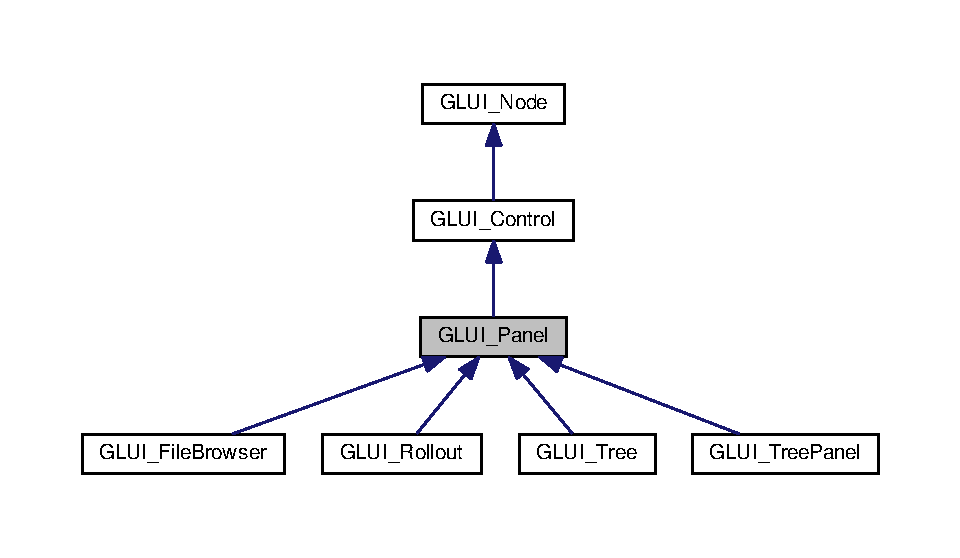
\includegraphics[width=350pt]{class_g_l_u_i___panel__inherit__graph}
\end{center}
\end{figure}


Collaboration diagram for G\+L\+U\+I\+\_\+\+Panel\+:\nopagebreak
\begin{figure}[H]
\begin{center}
\leavevmode
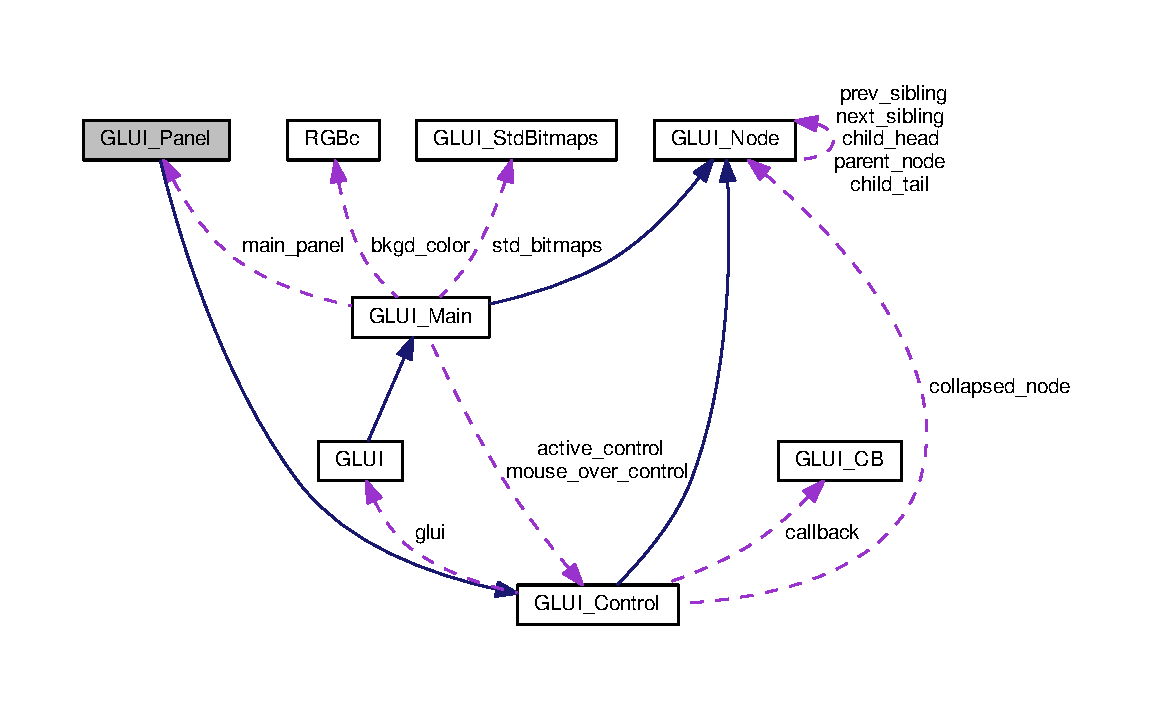
\includegraphics[width=350pt]{class_g_l_u_i___panel__coll__graph}
\end{center}
\end{figure}
\subsection*{Public Member Functions}
\begin{DoxyCompactItemize}
\item 
\hyperlink{class_g_l_u_i___panel_a6a297a441e3f921199347184ded52aca}{G\+L\+U\+I\+\_\+\+Panel} (\hyperlink{class_g_l_u_i___node}{G\+L\+U\+I\+\_\+\+Node} $\ast$\hyperlink{class_g_l_u_i___node_a8ed65d447784f6f88bd3e2e2bcac6cdb}{parent}, const char $\ast$\hyperlink{glext_8h_ad977737dfc9a274a62741b9500c49a32}{name}, \hyperlink{wglext_8h_a500a82aecba06f4550f6849b8099ca21}{int} \hyperlink{glext_8h_ab7c1afc09f67635c2c376638fcc0db5f}{type}=\hyperlink{glui_8h_add54979a7b4391067b8a125ee34f690a}{G\+L\+U\+I\+\_\+\+P\+A\+N\+E\+L\+\_\+\+E\+M\+B\+O\+S\+S\+E\+D})
\item 
\hyperlink{class_g_l_u_i___panel_a8b3bd4012d7a33a9c420a67a58e83a87}{G\+L\+U\+I\+\_\+\+Panel} ()
\item 
\hyperlink{wglext_8h_a9e6b7f1933461ef318bb000d6bd13b83}{void} \hyperlink{class_g_l_u_i___panel_a8038a76f6c88613735f7c65ae9466b0c}{draw} (\hyperlink{wglext_8h_a500a82aecba06f4550f6849b8099ca21}{int} \hyperlink{glext_8h_ad77deca22f617d3f0e0eb786445689fc}{x}, \hyperlink{wglext_8h_a500a82aecba06f4550f6849b8099ca21}{int} \hyperlink{glext_8h_a9298c7ad619074f5285b32c6b72bfdea}{y})
\item 
\hyperlink{wglext_8h_a9e6b7f1933461ef318bb000d6bd13b83}{void} \hyperlink{class_g_l_u_i___panel_a5f76f22a34d3c131e3ace71d24c47d3e}{set\+\_\+name} (const char $\ast$\hyperlink{class_g_l_u_i___control_af0d60e9736f4dbc34e9a536e75876d72}{text})
\item 
\hyperlink{wglext_8h_a9e6b7f1933461ef318bb000d6bd13b83}{void} \hyperlink{class_g_l_u_i___panel_aee5e41798d60ac2e4707373be14fd39f}{set\+\_\+type} (\hyperlink{wglext_8h_a500a82aecba06f4550f6849b8099ca21}{int} new\+\_\+type)
\item 
\hyperlink{wglext_8h_a9e6b7f1933461ef318bb000d6bd13b83}{void} \hyperlink{class_g_l_u_i___panel_ab377b608f9b1006fb67d78e41a1f95d6}{update\+\_\+size} (\hyperlink{wglext_8h_a9e6b7f1933461ef318bb000d6bd13b83}{void})
\end{DoxyCompactItemize}
\subsection*{Protected Member Functions}
\begin{DoxyCompactItemize}
\item 
\hyperlink{wglext_8h_a9e6b7f1933461ef318bb000d6bd13b83}{void} \hyperlink{class_g_l_u_i___panel_ac8a587cbc0b8640824cbdee00d8a0462}{common\+\_\+init} (\hyperlink{wglext_8h_a9e6b7f1933461ef318bb000d6bd13b83}{void})
\end{DoxyCompactItemize}
\subsection*{Additional Inherited Members}


\subsection{Detailed Description}
A \hyperlink{class_g_l_u_i___panel}{G\+L\+U\+I\+\_\+\+Panel} contains a group of related controls. 

Definition at line 1095 of file glui.\+h.



\subsection{Constructor \& Destructor Documentation}
\hypertarget{class_g_l_u_i___panel_a6a297a441e3f921199347184ded52aca}{\index{G\+L\+U\+I\+\_\+\+Panel@{G\+L\+U\+I\+\_\+\+Panel}!G\+L\+U\+I\+\_\+\+Panel@{G\+L\+U\+I\+\_\+\+Panel}}
\index{G\+L\+U\+I\+\_\+\+Panel@{G\+L\+U\+I\+\_\+\+Panel}!G\+L\+U\+I\+\_\+\+Panel@{G\+L\+U\+I\+\_\+\+Panel}}
\subsubsection[{G\+L\+U\+I\+\_\+\+Panel}]{\setlength{\rightskip}{0pt plus 5cm}G\+L\+U\+I\+\_\+\+Panel\+::\+G\+L\+U\+I\+\_\+\+Panel (
\begin{DoxyParamCaption}
\item[{{\bf G\+L\+U\+I\+\_\+\+Node} $\ast$}]{parent, }
\item[{const char $\ast$}]{name, }
\item[{{\bf int}}]{type = {\ttfamily {\bf G\+L\+U\+I\+\_\+\+P\+A\+N\+E\+L\+\_\+\+E\+M\+B\+O\+S\+S\+E\+D}}}
\end{DoxyParamCaption}
)}}\label{class_g_l_u_i___panel_a6a297a441e3f921199347184ded52aca}
Create a new panel. A panel groups together a set of related controls.


\begin{DoxyParams}{Parameters}
{\em parent} & The outer panel our panel is inside; or the main \hyperlink{class_g_l_u_i}{G\+L\+U\+I} object. \\
\hline
{\em name} & The string name at the top of our panel. \\
\hline
{\em type} & Optional style to display the panel with--G\+L\+U\+I\+\_\+\+P\+A\+N\+E\+L\+\_\+\+E\+M\+B\+O\+S\+S\+E\+D by default. G\+L\+U\+I\+\_\+\+P\+A\+N\+E\+L\+\_\+\+R\+A\+I\+S\+E\+D causes the panel to appear higher than the surroundings. G\+L\+U\+I\+\_\+\+P\+A\+N\+E\+L\+\_\+\+N\+O\+N\+E causes the panel's outline to be invisible. \\
\hline
\end{DoxyParams}
\hypertarget{class_g_l_u_i___panel_a8b3bd4012d7a33a9c420a67a58e83a87}{\index{G\+L\+U\+I\+\_\+\+Panel@{G\+L\+U\+I\+\_\+\+Panel}!G\+L\+U\+I\+\_\+\+Panel@{G\+L\+U\+I\+\_\+\+Panel}}
\index{G\+L\+U\+I\+\_\+\+Panel@{G\+L\+U\+I\+\_\+\+Panel}!G\+L\+U\+I\+\_\+\+Panel@{G\+L\+U\+I\+\_\+\+Panel}}
\subsubsection[{G\+L\+U\+I\+\_\+\+Panel}]{\setlength{\rightskip}{0pt plus 5cm}G\+L\+U\+I\+\_\+\+Panel\+::\+G\+L\+U\+I\+\_\+\+Panel (
\begin{DoxyParamCaption}
{}
\end{DoxyParamCaption}
)\hspace{0.3cm}{\ttfamily [inline]}}}\label{class_g_l_u_i___panel_a8b3bd4012d7a33a9c420a67a58e83a87}


Definition at line 1110 of file glui.\+h.



\subsection{Member Function Documentation}
\hypertarget{class_g_l_u_i___panel_ac8a587cbc0b8640824cbdee00d8a0462}{\index{G\+L\+U\+I\+\_\+\+Panel@{G\+L\+U\+I\+\_\+\+Panel}!common\+\_\+init@{common\+\_\+init}}
\index{common\+\_\+init@{common\+\_\+init}!G\+L\+U\+I\+\_\+\+Panel@{G\+L\+U\+I\+\_\+\+Panel}}
\subsubsection[{common\+\_\+init}]{\setlength{\rightskip}{0pt plus 5cm}{\bf void} G\+L\+U\+I\+\_\+\+Panel\+::common\+\_\+init (
\begin{DoxyParamCaption}
\item[{{\bf void}}]{}
\end{DoxyParamCaption}
)\hspace{0.3cm}{\ttfamily [inline]}, {\ttfamily [protected]}}}\label{class_g_l_u_i___panel_ac8a587cbc0b8640824cbdee00d8a0462}


Definition at line 1119 of file glui.\+h.

\hypertarget{class_g_l_u_i___panel_a8038a76f6c88613735f7c65ae9466b0c}{\index{G\+L\+U\+I\+\_\+\+Panel@{G\+L\+U\+I\+\_\+\+Panel}!draw@{draw}}
\index{draw@{draw}!G\+L\+U\+I\+\_\+\+Panel@{G\+L\+U\+I\+\_\+\+Panel}}
\subsubsection[{draw}]{\setlength{\rightskip}{0pt plus 5cm}{\bf void} G\+L\+U\+I\+\_\+\+Panel\+::draw (
\begin{DoxyParamCaption}
\item[{{\bf int}}]{x, }
\item[{{\bf int}}]{y}
\end{DoxyParamCaption}
)\hspace{0.3cm}{\ttfamily [virtual]}}}\label{class_g_l_u_i___panel_a8038a76f6c88613735f7c65ae9466b0c}


Implements \hyperlink{class_g_l_u_i___control_a2eb42d7a7951280ad2fe8c37972bf66a}{G\+L\+U\+I\+\_\+\+Control}.



Reimplemented in \hyperlink{class_g_l_u_i___tree_a95b179b8d413fc280ef58cb62f9defb2}{G\+L\+U\+I\+\_\+\+Tree}, and \hyperlink{class_g_l_u_i___rollout_ae3ff0bbeb04f22aa5489cf542b6e3fbb}{G\+L\+U\+I\+\_\+\+Rollout}.

\hypertarget{class_g_l_u_i___panel_a5f76f22a34d3c131e3ace71d24c47d3e}{\index{G\+L\+U\+I\+\_\+\+Panel@{G\+L\+U\+I\+\_\+\+Panel}!set\+\_\+name@{set\+\_\+name}}
\index{set\+\_\+name@{set\+\_\+name}!G\+L\+U\+I\+\_\+\+Panel@{G\+L\+U\+I\+\_\+\+Panel}}
\subsubsection[{set\+\_\+name}]{\setlength{\rightskip}{0pt plus 5cm}{\bf void} G\+L\+U\+I\+\_\+\+Panel\+::set\+\_\+name (
\begin{DoxyParamCaption}
\item[{const char $\ast$}]{text}
\end{DoxyParamCaption}
)\hspace{0.3cm}{\ttfamily [virtual]}}}\label{class_g_l_u_i___panel_a5f76f22a34d3c131e3ace71d24c47d3e}


Reimplemented from \hyperlink{class_g_l_u_i___control_ad1bf0640802de0a40337cdbcf93a5ec6}{G\+L\+U\+I\+\_\+\+Control}.

\hypertarget{class_g_l_u_i___panel_aee5e41798d60ac2e4707373be14fd39f}{\index{G\+L\+U\+I\+\_\+\+Panel@{G\+L\+U\+I\+\_\+\+Panel}!set\+\_\+type@{set\+\_\+type}}
\index{set\+\_\+type@{set\+\_\+type}!G\+L\+U\+I\+\_\+\+Panel@{G\+L\+U\+I\+\_\+\+Panel}}
\subsubsection[{set\+\_\+type}]{\setlength{\rightskip}{0pt plus 5cm}{\bf void} G\+L\+U\+I\+\_\+\+Panel\+::set\+\_\+type (
\begin{DoxyParamCaption}
\item[{{\bf int}}]{new\+\_\+type}
\end{DoxyParamCaption}
)}}\label{class_g_l_u_i___panel_aee5e41798d60ac2e4707373be14fd39f}
\hypertarget{class_g_l_u_i___panel_ab377b608f9b1006fb67d78e41a1f95d6}{\index{G\+L\+U\+I\+\_\+\+Panel@{G\+L\+U\+I\+\_\+\+Panel}!update\+\_\+size@{update\+\_\+size}}
\index{update\+\_\+size@{update\+\_\+size}!G\+L\+U\+I\+\_\+\+Panel@{G\+L\+U\+I\+\_\+\+Panel}}
\subsubsection[{update\+\_\+size}]{\setlength{\rightskip}{0pt plus 5cm}{\bf void} G\+L\+U\+I\+\_\+\+Panel\+::update\+\_\+size (
\begin{DoxyParamCaption}
\item[{{\bf void}}]{}
\end{DoxyParamCaption}
)\hspace{0.3cm}{\ttfamily [virtual]}}}\label{class_g_l_u_i___panel_ab377b608f9b1006fb67d78e41a1f95d6}


Reimplemented from \hyperlink{class_g_l_u_i___control_a4bfe55acbbf735a7d2ff07d687a481e2}{G\+L\+U\+I\+\_\+\+Control}.



Reimplemented in \hyperlink{class_g_l_u_i___tree_ae74e9b85940ce63ebac36ef650e845ae}{G\+L\+U\+I\+\_\+\+Tree}, and \hyperlink{class_g_l_u_i___rollout_af6f664a8ca31757bc1e5926d5eaf2827}{G\+L\+U\+I\+\_\+\+Rollout}.



The documentation for this class was generated from the following file\+:\begin{DoxyCompactItemize}
\item 
S\+S\+W\+C/src/\+G\+L/\hyperlink{glui_8h}{glui.\+h}\end{DoxyCompactItemize}

\hypertarget{class_g_l_u_i___radio_button}{\section{G\+L\+U\+I\+\_\+\+Radio\+Button Class Reference}
\label{class_g_l_u_i___radio_button}\index{G\+L\+U\+I\+\_\+\+Radio\+Button@{G\+L\+U\+I\+\_\+\+Radio\+Button}}
}


{\ttfamily \#include $<$glui.\+h$>$}



Inheritance diagram for G\+L\+U\+I\+\_\+\+Radio\+Button\+:\nopagebreak
\begin{figure}[H]
\begin{center}
\leavevmode
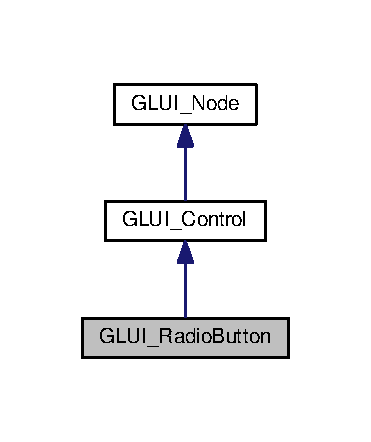
\includegraphics[width=178pt]{class_g_l_u_i___radio_button__inherit__graph}
\end{center}
\end{figure}


Collaboration diagram for G\+L\+U\+I\+\_\+\+Radio\+Button\+:\nopagebreak
\begin{figure}[H]
\begin{center}
\leavevmode
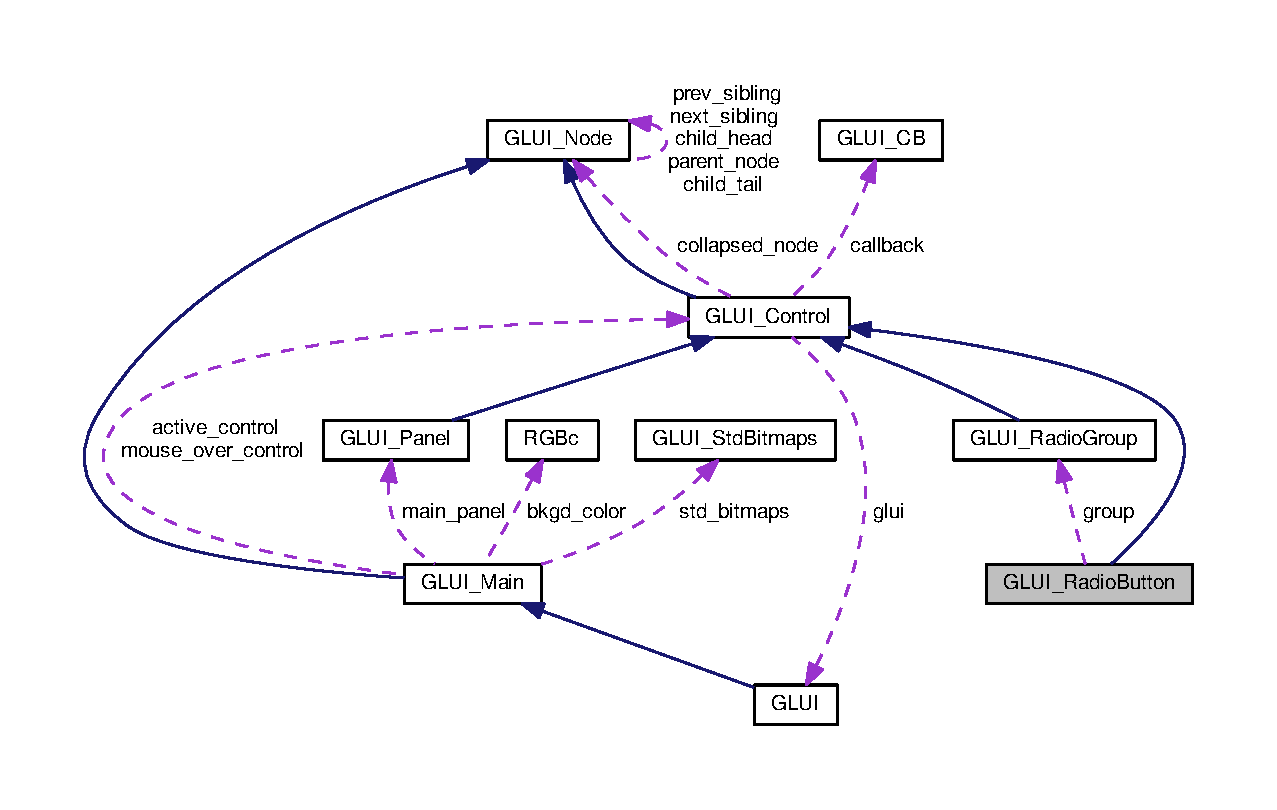
\includegraphics[width=350pt]{class_g_l_u_i___radio_button__coll__graph}
\end{center}
\end{figure}
\subsection*{Public Member Functions}
\begin{DoxyCompactItemize}
\item 
\hyperlink{wglext_8h_a500a82aecba06f4550f6849b8099ca21}{int} \hyperlink{class_g_l_u_i___radio_button_a1043d967fe810f9b71b80d17152b977a}{mouse\+\_\+down\+\_\+handler} (\hyperlink{wglext_8h_a500a82aecba06f4550f6849b8099ca21}{int} local\+\_\+x, \hyperlink{wglext_8h_a500a82aecba06f4550f6849b8099ca21}{int} local\+\_\+y)
\item 
\hyperlink{wglext_8h_a500a82aecba06f4550f6849b8099ca21}{int} \hyperlink{class_g_l_u_i___radio_button_a2d6e08dc0802146227e8cd4f4d5ef571}{mouse\+\_\+up\+\_\+handler} (\hyperlink{wglext_8h_a500a82aecba06f4550f6849b8099ca21}{int} local\+\_\+x, \hyperlink{wglext_8h_a500a82aecba06f4550f6849b8099ca21}{int} local\+\_\+y, bool inside)
\item 
\hyperlink{wglext_8h_a500a82aecba06f4550f6849b8099ca21}{int} \hyperlink{class_g_l_u_i___radio_button_a7a5c7c04144139201848320c31f92844}{mouse\+\_\+held\+\_\+down\+\_\+handler} (\hyperlink{wglext_8h_a500a82aecba06f4550f6849b8099ca21}{int} local\+\_\+x, \hyperlink{wglext_8h_a500a82aecba06f4550f6849b8099ca21}{int} local\+\_\+y, bool inside)
\item 
\hyperlink{wglext_8h_a9e6b7f1933461ef318bb000d6bd13b83}{void} \hyperlink{class_g_l_u_i___radio_button_a21f6925f484831394a09e6f44dc8d11e}{draw} (\hyperlink{wglext_8h_a500a82aecba06f4550f6849b8099ca21}{int} \hyperlink{glext_8h_ad77deca22f617d3f0e0eb786445689fc}{x}, \hyperlink{wglext_8h_a500a82aecba06f4550f6849b8099ca21}{int} \hyperlink{glext_8h_a9298c7ad619074f5285b32c6b72bfdea}{y})
\item 
\hyperlink{wglext_8h_a9e6b7f1933461ef318bb000d6bd13b83}{void} \hyperlink{class_g_l_u_i___radio_button_a18a5fd5c61bc61231df01972f85b464b}{update\+\_\+size} (\hyperlink{wglext_8h_a9e6b7f1933461ef318bb000d6bd13b83}{void})
\item 
\hyperlink{wglext_8h_a9e6b7f1933461ef318bb000d6bd13b83}{void} \hyperlink{class_g_l_u_i___radio_button_a0000fc6e9668323092c2acc0852851fb}{draw\+\_\+active\+\_\+area} (\hyperlink{wglext_8h_a9e6b7f1933461ef318bb000d6bd13b83}{void})
\item 
\hyperlink{wglext_8h_a9e6b7f1933461ef318bb000d6bd13b83}{void} \hyperlink{class_g_l_u_i___radio_button_a7877448ee5aeb07b26e045d9d4a5c23b}{draw\+\_\+checked} (\hyperlink{wglext_8h_a9e6b7f1933461ef318bb000d6bd13b83}{void})
\item 
\hyperlink{wglext_8h_a9e6b7f1933461ef318bb000d6bd13b83}{void} \hyperlink{class_g_l_u_i___radio_button_af0d77a13832451f0140c41e8bc0769a0}{draw\+\_\+unchecked} (\hyperlink{wglext_8h_a9e6b7f1933461ef318bb000d6bd13b83}{void})
\item 
\hyperlink{wglext_8h_a9e6b7f1933461ef318bb000d6bd13b83}{void} \hyperlink{class_g_l_u_i___radio_button_a1591bf4a0d8b0c1e286365d973693d40}{draw\+\_\+\+O} (\hyperlink{wglext_8h_a9e6b7f1933461ef318bb000d6bd13b83}{void})
\item 
\hyperlink{class_g_l_u_i___radio_button_ab3bda5fa0bd41bc49b064f474513ceaf}{G\+L\+U\+I\+\_\+\+Radio\+Button} (\hyperlink{class_g_l_u_i___radio_group}{G\+L\+U\+I\+\_\+\+Radio\+Group} $\ast$\hyperlink{glext_8h_a69cec9b28d037f2272131b4fcd148620}{group}, const char $\ast$\hyperlink{glext_8h_ad977737dfc9a274a62741b9500c49a32}{name})
\end{DoxyCompactItemize}
\subsection*{Public Attributes}
\begin{DoxyCompactItemize}
\item 
\hyperlink{wglext_8h_a500a82aecba06f4550f6849b8099ca21}{int} \hyperlink{class_g_l_u_i___radio_button_aa874a5e29d93e5e65befd745d0e16454}{orig\+\_\+value}
\item 
bool \hyperlink{class_g_l_u_i___radio_button_ae4bcf4b331712a2dc21f944e00071cf6}{currently\+\_\+inside}
\item 
\hyperlink{wglext_8h_a500a82aecba06f4550f6849b8099ca21}{int} \hyperlink{class_g_l_u_i___radio_button_a857d2387855fca92f0ae322e3f6fc19a}{text\+\_\+x\+\_\+offset}
\item 
\hyperlink{class_g_l_u_i___radio_group}{G\+L\+U\+I\+\_\+\+Radio\+Group} $\ast$ \hyperlink{class_g_l_u_i___radio_button_ab9906e39403d7b15810384a59e99e054}{group}
\end{DoxyCompactItemize}
\subsection*{Protected Member Functions}
\begin{DoxyCompactItemize}
\item 
\hyperlink{wglext_8h_a9e6b7f1933461ef318bb000d6bd13b83}{void} \hyperlink{class_g_l_u_i___radio_button_aba1127e895ee062d421b8e6cd6f4bb48}{common\+\_\+init} ()
\end{DoxyCompactItemize}
\subsection*{Additional Inherited Members}


\subsection{Detailed Description}


Definition at line 1784 of file glui.\+h.



\subsection{Constructor \& Destructor Documentation}
\hypertarget{class_g_l_u_i___radio_button_ab3bda5fa0bd41bc49b064f474513ceaf}{\index{G\+L\+U\+I\+\_\+\+Radio\+Button@{G\+L\+U\+I\+\_\+\+Radio\+Button}!G\+L\+U\+I\+\_\+\+Radio\+Button@{G\+L\+U\+I\+\_\+\+Radio\+Button}}
\index{G\+L\+U\+I\+\_\+\+Radio\+Button@{G\+L\+U\+I\+\_\+\+Radio\+Button}!G\+L\+U\+I\+\_\+\+Radio\+Button@{G\+L\+U\+I\+\_\+\+Radio\+Button}}
\subsubsection[{G\+L\+U\+I\+\_\+\+Radio\+Button}]{\setlength{\rightskip}{0pt plus 5cm}G\+L\+U\+I\+\_\+\+Radio\+Button\+::\+G\+L\+U\+I\+\_\+\+Radio\+Button (
\begin{DoxyParamCaption}
\item[{{\bf G\+L\+U\+I\+\_\+\+Radio\+Group} $\ast$}]{group, }
\item[{const char $\ast$}]{name}
\end{DoxyParamCaption}
)}}\label{class_g_l_u_i___radio_button_ab3bda5fa0bd41bc49b064f474513ceaf}


\subsection{Member Function Documentation}
\hypertarget{class_g_l_u_i___radio_button_aba1127e895ee062d421b8e6cd6f4bb48}{\index{G\+L\+U\+I\+\_\+\+Radio\+Button@{G\+L\+U\+I\+\_\+\+Radio\+Button}!common\+\_\+init@{common\+\_\+init}}
\index{common\+\_\+init@{common\+\_\+init}!G\+L\+U\+I\+\_\+\+Radio\+Button@{G\+L\+U\+I\+\_\+\+Radio\+Button}}
\subsubsection[{common\+\_\+init}]{\setlength{\rightskip}{0pt plus 5cm}{\bf void} G\+L\+U\+I\+\_\+\+Radio\+Button\+::common\+\_\+init (
\begin{DoxyParamCaption}
\item[{{\bf void}}]{}
\end{DoxyParamCaption}
)\hspace{0.3cm}{\ttfamily [inline]}, {\ttfamily [protected]}}}\label{class_g_l_u_i___radio_button_aba1127e895ee062d421b8e6cd6f4bb48}


Definition at line 1807 of file glui.\+h.

\hypertarget{class_g_l_u_i___radio_button_a21f6925f484831394a09e6f44dc8d11e}{\index{G\+L\+U\+I\+\_\+\+Radio\+Button@{G\+L\+U\+I\+\_\+\+Radio\+Button}!draw@{draw}}
\index{draw@{draw}!G\+L\+U\+I\+\_\+\+Radio\+Button@{G\+L\+U\+I\+\_\+\+Radio\+Button}}
\subsubsection[{draw}]{\setlength{\rightskip}{0pt plus 5cm}{\bf void} G\+L\+U\+I\+\_\+\+Radio\+Button\+::draw (
\begin{DoxyParamCaption}
\item[{{\bf int}}]{x, }
\item[{{\bf int}}]{y}
\end{DoxyParamCaption}
)\hspace{0.3cm}{\ttfamily [virtual]}}}\label{class_g_l_u_i___radio_button_a21f6925f484831394a09e6f44dc8d11e}


Implements \hyperlink{class_g_l_u_i___control_a2eb42d7a7951280ad2fe8c37972bf66a}{G\+L\+U\+I\+\_\+\+Control}.

\hypertarget{class_g_l_u_i___radio_button_a0000fc6e9668323092c2acc0852851fb}{\index{G\+L\+U\+I\+\_\+\+Radio\+Button@{G\+L\+U\+I\+\_\+\+Radio\+Button}!draw\+\_\+active\+\_\+area@{draw\+\_\+active\+\_\+area}}
\index{draw\+\_\+active\+\_\+area@{draw\+\_\+active\+\_\+area}!G\+L\+U\+I\+\_\+\+Radio\+Button@{G\+L\+U\+I\+\_\+\+Radio\+Button}}
\subsubsection[{draw\+\_\+active\+\_\+area}]{\setlength{\rightskip}{0pt plus 5cm}{\bf void} G\+L\+U\+I\+\_\+\+Radio\+Button\+::draw\+\_\+active\+\_\+area (
\begin{DoxyParamCaption}
\item[{{\bf void}}]{}
\end{DoxyParamCaption}
)}}\label{class_g_l_u_i___radio_button_a0000fc6e9668323092c2acc0852851fb}
\hypertarget{class_g_l_u_i___radio_button_a7877448ee5aeb07b26e045d9d4a5c23b}{\index{G\+L\+U\+I\+\_\+\+Radio\+Button@{G\+L\+U\+I\+\_\+\+Radio\+Button}!draw\+\_\+checked@{draw\+\_\+checked}}
\index{draw\+\_\+checked@{draw\+\_\+checked}!G\+L\+U\+I\+\_\+\+Radio\+Button@{G\+L\+U\+I\+\_\+\+Radio\+Button}}
\subsubsection[{draw\+\_\+checked}]{\setlength{\rightskip}{0pt plus 5cm}{\bf void} G\+L\+U\+I\+\_\+\+Radio\+Button\+::draw\+\_\+checked (
\begin{DoxyParamCaption}
\item[{{\bf void}}]{}
\end{DoxyParamCaption}
)}}\label{class_g_l_u_i___radio_button_a7877448ee5aeb07b26e045d9d4a5c23b}
\hypertarget{class_g_l_u_i___radio_button_a1591bf4a0d8b0c1e286365d973693d40}{\index{G\+L\+U\+I\+\_\+\+Radio\+Button@{G\+L\+U\+I\+\_\+\+Radio\+Button}!draw\+\_\+\+O@{draw\+\_\+\+O}}
\index{draw\+\_\+\+O@{draw\+\_\+\+O}!G\+L\+U\+I\+\_\+\+Radio\+Button@{G\+L\+U\+I\+\_\+\+Radio\+Button}}
\subsubsection[{draw\+\_\+\+O}]{\setlength{\rightskip}{0pt plus 5cm}{\bf void} G\+L\+U\+I\+\_\+\+Radio\+Button\+::draw\+\_\+\+O (
\begin{DoxyParamCaption}
\item[{{\bf void}}]{}
\end{DoxyParamCaption}
)}}\label{class_g_l_u_i___radio_button_a1591bf4a0d8b0c1e286365d973693d40}
\hypertarget{class_g_l_u_i___radio_button_af0d77a13832451f0140c41e8bc0769a0}{\index{G\+L\+U\+I\+\_\+\+Radio\+Button@{G\+L\+U\+I\+\_\+\+Radio\+Button}!draw\+\_\+unchecked@{draw\+\_\+unchecked}}
\index{draw\+\_\+unchecked@{draw\+\_\+unchecked}!G\+L\+U\+I\+\_\+\+Radio\+Button@{G\+L\+U\+I\+\_\+\+Radio\+Button}}
\subsubsection[{draw\+\_\+unchecked}]{\setlength{\rightskip}{0pt plus 5cm}{\bf void} G\+L\+U\+I\+\_\+\+Radio\+Button\+::draw\+\_\+unchecked (
\begin{DoxyParamCaption}
\item[{{\bf void}}]{}
\end{DoxyParamCaption}
)}}\label{class_g_l_u_i___radio_button_af0d77a13832451f0140c41e8bc0769a0}
\hypertarget{class_g_l_u_i___radio_button_a1043d967fe810f9b71b80d17152b977a}{\index{G\+L\+U\+I\+\_\+\+Radio\+Button@{G\+L\+U\+I\+\_\+\+Radio\+Button}!mouse\+\_\+down\+\_\+handler@{mouse\+\_\+down\+\_\+handler}}
\index{mouse\+\_\+down\+\_\+handler@{mouse\+\_\+down\+\_\+handler}!G\+L\+U\+I\+\_\+\+Radio\+Button@{G\+L\+U\+I\+\_\+\+Radio\+Button}}
\subsubsection[{mouse\+\_\+down\+\_\+handler}]{\setlength{\rightskip}{0pt plus 5cm}{\bf int} G\+L\+U\+I\+\_\+\+Radio\+Button\+::mouse\+\_\+down\+\_\+handler (
\begin{DoxyParamCaption}
\item[{{\bf int}}]{local\+\_\+x, }
\item[{{\bf int}}]{local\+\_\+y}
\end{DoxyParamCaption}
)\hspace{0.3cm}{\ttfamily [virtual]}}}\label{class_g_l_u_i___radio_button_a1043d967fe810f9b71b80d17152b977a}


Reimplemented from \hyperlink{class_g_l_u_i___control_a92b77565168a1d2003bca1c16ac00e8d}{G\+L\+U\+I\+\_\+\+Control}.

\hypertarget{class_g_l_u_i___radio_button_a7a5c7c04144139201848320c31f92844}{\index{G\+L\+U\+I\+\_\+\+Radio\+Button@{G\+L\+U\+I\+\_\+\+Radio\+Button}!mouse\+\_\+held\+\_\+down\+\_\+handler@{mouse\+\_\+held\+\_\+down\+\_\+handler}}
\index{mouse\+\_\+held\+\_\+down\+\_\+handler@{mouse\+\_\+held\+\_\+down\+\_\+handler}!G\+L\+U\+I\+\_\+\+Radio\+Button@{G\+L\+U\+I\+\_\+\+Radio\+Button}}
\subsubsection[{mouse\+\_\+held\+\_\+down\+\_\+handler}]{\setlength{\rightskip}{0pt plus 5cm}{\bf int} G\+L\+U\+I\+\_\+\+Radio\+Button\+::mouse\+\_\+held\+\_\+down\+\_\+handler (
\begin{DoxyParamCaption}
\item[{{\bf int}}]{local\+\_\+x, }
\item[{{\bf int}}]{local\+\_\+y, }
\item[{bool}]{inside}
\end{DoxyParamCaption}
)\hspace{0.3cm}{\ttfamily [virtual]}}}\label{class_g_l_u_i___radio_button_a7a5c7c04144139201848320c31f92844}


Reimplemented from \hyperlink{class_g_l_u_i___control_a4b44e44c1c455adc7f98c63aeb6aa919}{G\+L\+U\+I\+\_\+\+Control}.

\hypertarget{class_g_l_u_i___radio_button_a2d6e08dc0802146227e8cd4f4d5ef571}{\index{G\+L\+U\+I\+\_\+\+Radio\+Button@{G\+L\+U\+I\+\_\+\+Radio\+Button}!mouse\+\_\+up\+\_\+handler@{mouse\+\_\+up\+\_\+handler}}
\index{mouse\+\_\+up\+\_\+handler@{mouse\+\_\+up\+\_\+handler}!G\+L\+U\+I\+\_\+\+Radio\+Button@{G\+L\+U\+I\+\_\+\+Radio\+Button}}
\subsubsection[{mouse\+\_\+up\+\_\+handler}]{\setlength{\rightskip}{0pt plus 5cm}{\bf int} G\+L\+U\+I\+\_\+\+Radio\+Button\+::mouse\+\_\+up\+\_\+handler (
\begin{DoxyParamCaption}
\item[{{\bf int}}]{local\+\_\+x, }
\item[{{\bf int}}]{local\+\_\+y, }
\item[{bool}]{inside}
\end{DoxyParamCaption}
)\hspace{0.3cm}{\ttfamily [virtual]}}}\label{class_g_l_u_i___radio_button_a2d6e08dc0802146227e8cd4f4d5ef571}


Reimplemented from \hyperlink{class_g_l_u_i___control_ac32aad8f69134d03682e34d0488a18f1}{G\+L\+U\+I\+\_\+\+Control}.

\hypertarget{class_g_l_u_i___radio_button_a18a5fd5c61bc61231df01972f85b464b}{\index{G\+L\+U\+I\+\_\+\+Radio\+Button@{G\+L\+U\+I\+\_\+\+Radio\+Button}!update\+\_\+size@{update\+\_\+size}}
\index{update\+\_\+size@{update\+\_\+size}!G\+L\+U\+I\+\_\+\+Radio\+Button@{G\+L\+U\+I\+\_\+\+Radio\+Button}}
\subsubsection[{update\+\_\+size}]{\setlength{\rightskip}{0pt plus 5cm}{\bf void} G\+L\+U\+I\+\_\+\+Radio\+Button\+::update\+\_\+size (
\begin{DoxyParamCaption}
\item[{{\bf void}}]{}
\end{DoxyParamCaption}
)\hspace{0.3cm}{\ttfamily [virtual]}}}\label{class_g_l_u_i___radio_button_a18a5fd5c61bc61231df01972f85b464b}


Reimplemented from \hyperlink{class_g_l_u_i___control_a4bfe55acbbf735a7d2ff07d687a481e2}{G\+L\+U\+I\+\_\+\+Control}.



\subsection{Member Data Documentation}
\hypertarget{class_g_l_u_i___radio_button_ae4bcf4b331712a2dc21f944e00071cf6}{\index{G\+L\+U\+I\+\_\+\+Radio\+Button@{G\+L\+U\+I\+\_\+\+Radio\+Button}!currently\+\_\+inside@{currently\+\_\+inside}}
\index{currently\+\_\+inside@{currently\+\_\+inside}!G\+L\+U\+I\+\_\+\+Radio\+Button@{G\+L\+U\+I\+\_\+\+Radio\+Button}}
\subsubsection[{currently\+\_\+inside}]{\setlength{\rightskip}{0pt plus 5cm}bool G\+L\+U\+I\+\_\+\+Radio\+Button\+::currently\+\_\+inside}}\label{class_g_l_u_i___radio_button_ae4bcf4b331712a2dc21f944e00071cf6}


Definition at line 1788 of file glui.\+h.

\hypertarget{class_g_l_u_i___radio_button_ab9906e39403d7b15810384a59e99e054}{\index{G\+L\+U\+I\+\_\+\+Radio\+Button@{G\+L\+U\+I\+\_\+\+Radio\+Button}!group@{group}}
\index{group@{group}!G\+L\+U\+I\+\_\+\+Radio\+Button@{G\+L\+U\+I\+\_\+\+Radio\+Button}}
\subsubsection[{group}]{\setlength{\rightskip}{0pt plus 5cm}{\bf G\+L\+U\+I\+\_\+\+Radio\+Group}$\ast$ G\+L\+U\+I\+\_\+\+Radio\+Button\+::group}}\label{class_g_l_u_i___radio_button_ab9906e39403d7b15810384a59e99e054}


Definition at line 1804 of file glui.\+h.

\hypertarget{class_g_l_u_i___radio_button_aa874a5e29d93e5e65befd745d0e16454}{\index{G\+L\+U\+I\+\_\+\+Radio\+Button@{G\+L\+U\+I\+\_\+\+Radio\+Button}!orig\+\_\+value@{orig\+\_\+value}}
\index{orig\+\_\+value@{orig\+\_\+value}!G\+L\+U\+I\+\_\+\+Radio\+Button@{G\+L\+U\+I\+\_\+\+Radio\+Button}}
\subsubsection[{orig\+\_\+value}]{\setlength{\rightskip}{0pt plus 5cm}{\bf int} G\+L\+U\+I\+\_\+\+Radio\+Button\+::orig\+\_\+value}}\label{class_g_l_u_i___radio_button_aa874a5e29d93e5e65befd745d0e16454}


Definition at line 1787 of file glui.\+h.

\hypertarget{class_g_l_u_i___radio_button_a857d2387855fca92f0ae322e3f6fc19a}{\index{G\+L\+U\+I\+\_\+\+Radio\+Button@{G\+L\+U\+I\+\_\+\+Radio\+Button}!text\+\_\+x\+\_\+offset@{text\+\_\+x\+\_\+offset}}
\index{text\+\_\+x\+\_\+offset@{text\+\_\+x\+\_\+offset}!G\+L\+U\+I\+\_\+\+Radio\+Button@{G\+L\+U\+I\+\_\+\+Radio\+Button}}
\subsubsection[{text\+\_\+x\+\_\+offset}]{\setlength{\rightskip}{0pt plus 5cm}{\bf int} G\+L\+U\+I\+\_\+\+Radio\+Button\+::text\+\_\+x\+\_\+offset}}\label{class_g_l_u_i___radio_button_a857d2387855fca92f0ae322e3f6fc19a}


Definition at line 1789 of file glui.\+h.



The documentation for this class was generated from the following file\+:\begin{DoxyCompactItemize}
\item 
S\+S\+W\+C/src/\+G\+L/\hyperlink{glui_8h}{glui.\+h}\end{DoxyCompactItemize}

\hypertarget{class_g_l_u_i___radio_group}{\section{G\+L\+U\+I\+\_\+\+Radio\+Group Class Reference}
\label{class_g_l_u_i___radio_group}\index{G\+L\+U\+I\+\_\+\+Radio\+Group@{G\+L\+U\+I\+\_\+\+Radio\+Group}}
}


{\ttfamily \#include $<$glui.\+h$>$}



Inheritance diagram for G\+L\+U\+I\+\_\+\+Radio\+Group\+:\nopagebreak
\begin{figure}[H]
\begin{center}
\leavevmode
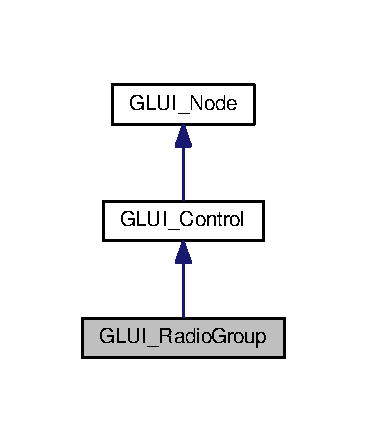
\includegraphics[width=176pt]{class_g_l_u_i___radio_group__inherit__graph}
\end{center}
\end{figure}


Collaboration diagram for G\+L\+U\+I\+\_\+\+Radio\+Group\+:\nopagebreak
\begin{figure}[H]
\begin{center}
\leavevmode
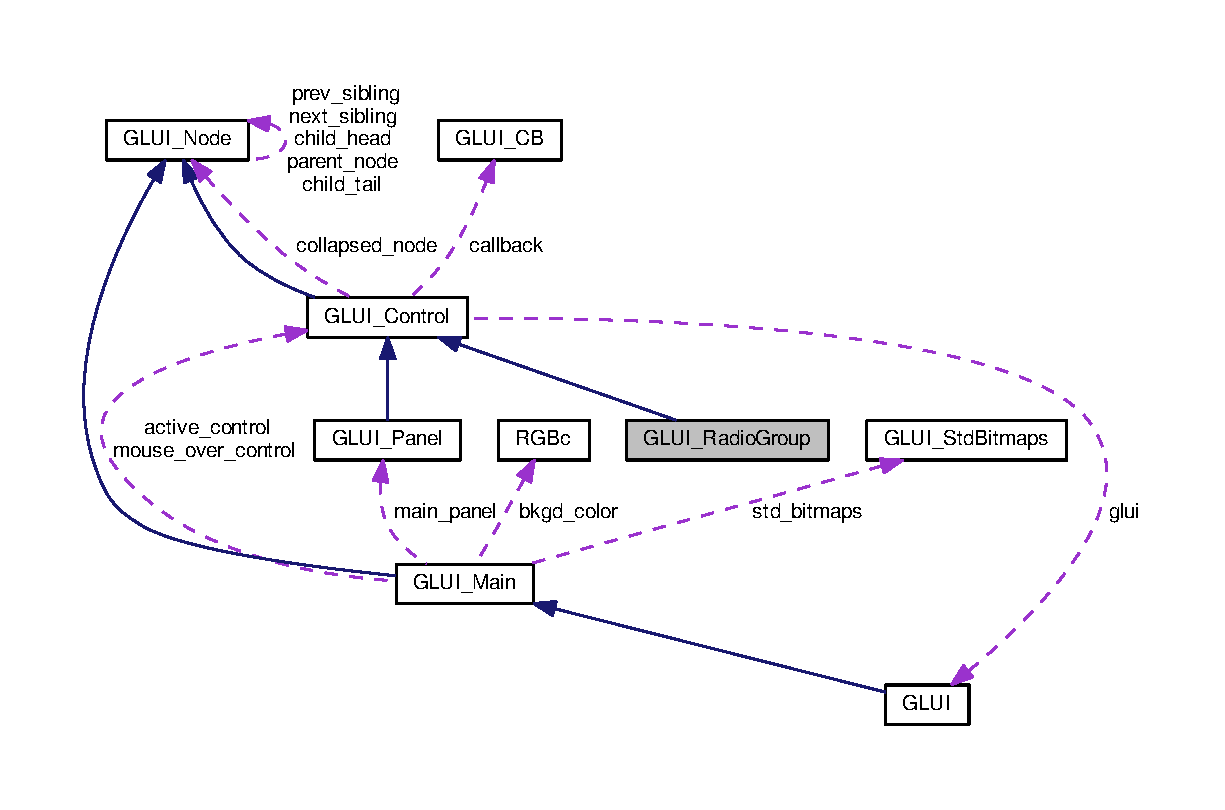
\includegraphics[width=350pt]{class_g_l_u_i___radio_group__coll__graph}
\end{center}
\end{figure}
\subsection*{Public Member Functions}
\begin{DoxyCompactItemize}
\item 
\hyperlink{wglext_8h_a9e6b7f1933461ef318bb000d6bd13b83}{void} \hyperlink{class_g_l_u_i___radio_group_ac29a2b338b80e74267efb42f94b380e0}{draw} (\hyperlink{wglext_8h_a500a82aecba06f4550f6849b8099ca21}{int} \hyperlink{glext_8h_ad77deca22f617d3f0e0eb786445689fc}{x}, \hyperlink{wglext_8h_a500a82aecba06f4550f6849b8099ca21}{int} \hyperlink{glext_8h_a9298c7ad619074f5285b32c6b72bfdea}{y})
\item 
\hyperlink{wglext_8h_a9e6b7f1933461ef318bb000d6bd13b83}{void} \hyperlink{class_g_l_u_i___radio_group_a8a3caea1aa9f603fae4ceab1c4e1b83a}{set\+\_\+name} (const char $\ast$\hyperlink{class_g_l_u_i___control_af0d60e9736f4dbc34e9a536e75876d72}{text})
\item 
\hyperlink{wglext_8h_a9e6b7f1933461ef318bb000d6bd13b83}{void} \hyperlink{class_g_l_u_i___radio_group_a9dc08156997557c983d402682dd01557}{set\+\_\+int\+\_\+val} (\hyperlink{wglext_8h_a500a82aecba06f4550f6849b8099ca21}{int} \hyperlink{class_g_l_u_i___control_a4a890b5b5a854b34200b5e63f1069b4e}{int\+\_\+val})
\item 
\hyperlink{wglext_8h_a9e6b7f1933461ef318bb000d6bd13b83}{void} \hyperlink{class_g_l_u_i___radio_group_ade83c982cd22902440bf1b5dcb3971ef}{set\+\_\+selected} (\hyperlink{wglext_8h_a500a82aecba06f4550f6849b8099ca21}{int} \hyperlink{class_g_l_u_i___control_a4a890b5b5a854b34200b5e63f1069b4e}{int\+\_\+val})
\item 
\hyperlink{wglext_8h_a9e6b7f1933461ef318bb000d6bd13b83}{void} \hyperlink{class_g_l_u_i___radio_group_a5feb3d5983d432a037e7fed7ebd7f3c0}{draw\+\_\+group} (\hyperlink{wglext_8h_a500a82aecba06f4550f6849b8099ca21}{int} translate)
\item 
\hyperlink{class_g_l_u_i___radio_group_a36c19d4c90c003ca6f49de004be96a90}{G\+L\+U\+I\+\_\+\+Radio\+Group} (\hyperlink{class_g_l_u_i___node}{G\+L\+U\+I\+\_\+\+Node} $\ast$\hyperlink{class_g_l_u_i___node_a8ed65d447784f6f88bd3e2e2bcac6cdb}{parent}, \hyperlink{wglext_8h_a500a82aecba06f4550f6849b8099ca21}{int} $\ast$live\+\_\+var=N\+U\+L\+L, \hyperlink{wglext_8h_a500a82aecba06f4550f6849b8099ca21}{int} \hyperlink{class_g_l_u_i___control_a6c88b7c72b0800f88a5d4cda4868c8b6}{user\+\_\+id}=-\/1, \hyperlink{class_g_l_u_i___c_b}{G\+L\+U\+I\+\_\+\+C\+B} \hyperlink{class_g_l_u_i___control_a96060fe0cc6d537e736dd6eef78e24ab}{callback}=\hyperlink{class_g_l_u_i___c_b}{G\+L\+U\+I\+\_\+\+C\+B}())
\item 
\hyperlink{class_g_l_u_i___radio_group_a3fffc4c3273b548ea011ab8d52654317}{G\+L\+U\+I\+\_\+\+Radio\+Group} (\hyperlink{wglext_8h_a9e6b7f1933461ef318bb000d6bd13b83}{void})
\end{DoxyCompactItemize}
\subsection*{Public Attributes}
\begin{DoxyCompactItemize}
\item 
\hyperlink{wglext_8h_a500a82aecba06f4550f6849b8099ca21}{int} \hyperlink{class_g_l_u_i___radio_group_a392b3c55c3951005a573491e5b555f35}{num\+\_\+buttons}
\end{DoxyCompactItemize}
\subsection*{Protected Member Functions}
\begin{DoxyCompactItemize}
\item 
\hyperlink{wglext_8h_a9e6b7f1933461ef318bb000d6bd13b83}{void} \hyperlink{class_g_l_u_i___radio_group_ad10760662aad89d1ee4868abbe5c94e1}{common\+\_\+init} (\hyperlink{wglext_8h_a9e6b7f1933461ef318bb000d6bd13b83}{void})
\end{DoxyCompactItemize}
\subsection*{Additional Inherited Members}


\subsection{Detailed Description}


Definition at line 1747 of file glui.\+h.



\subsection{Constructor \& Destructor Documentation}
\hypertarget{class_g_l_u_i___radio_group_a36c19d4c90c003ca6f49de004be96a90}{\index{G\+L\+U\+I\+\_\+\+Radio\+Group@{G\+L\+U\+I\+\_\+\+Radio\+Group}!G\+L\+U\+I\+\_\+\+Radio\+Group@{G\+L\+U\+I\+\_\+\+Radio\+Group}}
\index{G\+L\+U\+I\+\_\+\+Radio\+Group@{G\+L\+U\+I\+\_\+\+Radio\+Group}!G\+L\+U\+I\+\_\+\+Radio\+Group@{G\+L\+U\+I\+\_\+\+Radio\+Group}}
\subsubsection[{G\+L\+U\+I\+\_\+\+Radio\+Group}]{\setlength{\rightskip}{0pt plus 5cm}G\+L\+U\+I\+\_\+\+Radio\+Group\+::\+G\+L\+U\+I\+\_\+\+Radio\+Group (
\begin{DoxyParamCaption}
\item[{{\bf G\+L\+U\+I\+\_\+\+Node} $\ast$}]{parent, }
\item[{{\bf int} $\ast$}]{live\+\_\+var = {\ttfamily NULL}, }
\item[{{\bf int}}]{user\+\_\+id = {\ttfamily -\/1}, }
\item[{{\bf G\+L\+U\+I\+\_\+\+C\+B}}]{callback = {\ttfamily {\bf G\+L\+U\+I\+\_\+\+C\+B}()}}
\end{DoxyParamCaption}
)}}\label{class_g_l_u_i___radio_group_a36c19d4c90c003ca6f49de004be96a90}
\hypertarget{class_g_l_u_i___radio_group_a3fffc4c3273b548ea011ab8d52654317}{\index{G\+L\+U\+I\+\_\+\+Radio\+Group@{G\+L\+U\+I\+\_\+\+Radio\+Group}!G\+L\+U\+I\+\_\+\+Radio\+Group@{G\+L\+U\+I\+\_\+\+Radio\+Group}}
\index{G\+L\+U\+I\+\_\+\+Radio\+Group@{G\+L\+U\+I\+\_\+\+Radio\+Group}!G\+L\+U\+I\+\_\+\+Radio\+Group@{G\+L\+U\+I\+\_\+\+Radio\+Group}}
\subsubsection[{G\+L\+U\+I\+\_\+\+Radio\+Group}]{\setlength{\rightskip}{0pt plus 5cm}G\+L\+U\+I\+\_\+\+Radio\+Group\+::\+G\+L\+U\+I\+\_\+\+Radio\+Group (
\begin{DoxyParamCaption}
\item[{{\bf void}}]{}
\end{DoxyParamCaption}
)\hspace{0.3cm}{\ttfamily [inline]}}}\label{class_g_l_u_i___radio_group_a3fffc4c3273b548ea011ab8d52654317}


Definition at line 1761 of file glui.\+h.



\subsection{Member Function Documentation}
\hypertarget{class_g_l_u_i___radio_group_ad10760662aad89d1ee4868abbe5c94e1}{\index{G\+L\+U\+I\+\_\+\+Radio\+Group@{G\+L\+U\+I\+\_\+\+Radio\+Group}!common\+\_\+init@{common\+\_\+init}}
\index{common\+\_\+init@{common\+\_\+init}!G\+L\+U\+I\+\_\+\+Radio\+Group@{G\+L\+U\+I\+\_\+\+Radio\+Group}}
\subsubsection[{common\+\_\+init}]{\setlength{\rightskip}{0pt plus 5cm}{\bf void} G\+L\+U\+I\+\_\+\+Radio\+Group\+::common\+\_\+init (
\begin{DoxyParamCaption}
\item[{{\bf void}}]{}
\end{DoxyParamCaption}
)\hspace{0.3cm}{\ttfamily [inline]}, {\ttfamily [protected]}}}\label{class_g_l_u_i___radio_group_ad10760662aad89d1ee4868abbe5c94e1}


Definition at line 1764 of file glui.\+h.

\hypertarget{class_g_l_u_i___radio_group_ac29a2b338b80e74267efb42f94b380e0}{\index{G\+L\+U\+I\+\_\+\+Radio\+Group@{G\+L\+U\+I\+\_\+\+Radio\+Group}!draw@{draw}}
\index{draw@{draw}!G\+L\+U\+I\+\_\+\+Radio\+Group@{G\+L\+U\+I\+\_\+\+Radio\+Group}}
\subsubsection[{draw}]{\setlength{\rightskip}{0pt plus 5cm}{\bf void} G\+L\+U\+I\+\_\+\+Radio\+Group\+::draw (
\begin{DoxyParamCaption}
\item[{{\bf int}}]{x, }
\item[{{\bf int}}]{y}
\end{DoxyParamCaption}
)\hspace{0.3cm}{\ttfamily [virtual]}}}\label{class_g_l_u_i___radio_group_ac29a2b338b80e74267efb42f94b380e0}


Implements \hyperlink{class_g_l_u_i___control_a2eb42d7a7951280ad2fe8c37972bf66a}{G\+L\+U\+I\+\_\+\+Control}.

\hypertarget{class_g_l_u_i___radio_group_a5feb3d5983d432a037e7fed7ebd7f3c0}{\index{G\+L\+U\+I\+\_\+\+Radio\+Group@{G\+L\+U\+I\+\_\+\+Radio\+Group}!draw\+\_\+group@{draw\+\_\+group}}
\index{draw\+\_\+group@{draw\+\_\+group}!G\+L\+U\+I\+\_\+\+Radio\+Group@{G\+L\+U\+I\+\_\+\+Radio\+Group}}
\subsubsection[{draw\+\_\+group}]{\setlength{\rightskip}{0pt plus 5cm}{\bf void} G\+L\+U\+I\+\_\+\+Radio\+Group\+::draw\+\_\+group (
\begin{DoxyParamCaption}
\item[{{\bf int}}]{translate}
\end{DoxyParamCaption}
)}}\label{class_g_l_u_i___radio_group_a5feb3d5983d432a037e7fed7ebd7f3c0}
\hypertarget{class_g_l_u_i___radio_group_a9dc08156997557c983d402682dd01557}{\index{G\+L\+U\+I\+\_\+\+Radio\+Group@{G\+L\+U\+I\+\_\+\+Radio\+Group}!set\+\_\+int\+\_\+val@{set\+\_\+int\+\_\+val}}
\index{set\+\_\+int\+\_\+val@{set\+\_\+int\+\_\+val}!G\+L\+U\+I\+\_\+\+Radio\+Group@{G\+L\+U\+I\+\_\+\+Radio\+Group}}
\subsubsection[{set\+\_\+int\+\_\+val}]{\setlength{\rightskip}{0pt plus 5cm}{\bf void} G\+L\+U\+I\+\_\+\+Radio\+Group\+::set\+\_\+int\+\_\+val (
\begin{DoxyParamCaption}
\item[{{\bf int}}]{int\+\_\+val}
\end{DoxyParamCaption}
)\hspace{0.3cm}{\ttfamily [virtual]}}}\label{class_g_l_u_i___radio_group_a9dc08156997557c983d402682dd01557}


Reimplemented from \hyperlink{class_g_l_u_i___control_a32ef6d11d6c62e344f17268dfb96aad6}{G\+L\+U\+I\+\_\+\+Control}.

\hypertarget{class_g_l_u_i___radio_group_a8a3caea1aa9f603fae4ceab1c4e1b83a}{\index{G\+L\+U\+I\+\_\+\+Radio\+Group@{G\+L\+U\+I\+\_\+\+Radio\+Group}!set\+\_\+name@{set\+\_\+name}}
\index{set\+\_\+name@{set\+\_\+name}!G\+L\+U\+I\+\_\+\+Radio\+Group@{G\+L\+U\+I\+\_\+\+Radio\+Group}}
\subsubsection[{set\+\_\+name}]{\setlength{\rightskip}{0pt plus 5cm}{\bf void} G\+L\+U\+I\+\_\+\+Radio\+Group\+::set\+\_\+name (
\begin{DoxyParamCaption}
\item[{const char $\ast$}]{text}
\end{DoxyParamCaption}
)\hspace{0.3cm}{\ttfamily [virtual]}}}\label{class_g_l_u_i___radio_group_a8a3caea1aa9f603fae4ceab1c4e1b83a}


Reimplemented from \hyperlink{class_g_l_u_i___control_ad1bf0640802de0a40337cdbcf93a5ec6}{G\+L\+U\+I\+\_\+\+Control}.

\hypertarget{class_g_l_u_i___radio_group_ade83c982cd22902440bf1b5dcb3971ef}{\index{G\+L\+U\+I\+\_\+\+Radio\+Group@{G\+L\+U\+I\+\_\+\+Radio\+Group}!set\+\_\+selected@{set\+\_\+selected}}
\index{set\+\_\+selected@{set\+\_\+selected}!G\+L\+U\+I\+\_\+\+Radio\+Group@{G\+L\+U\+I\+\_\+\+Radio\+Group}}
\subsubsection[{set\+\_\+selected}]{\setlength{\rightskip}{0pt plus 5cm}{\bf void} G\+L\+U\+I\+\_\+\+Radio\+Group\+::set\+\_\+selected (
\begin{DoxyParamCaption}
\item[{{\bf int}}]{int\+\_\+val}
\end{DoxyParamCaption}
)}}\label{class_g_l_u_i___radio_group_ade83c982cd22902440bf1b5dcb3971ef}


\subsection{Member Data Documentation}
\hypertarget{class_g_l_u_i___radio_group_a392b3c55c3951005a573491e5b555f35}{\index{G\+L\+U\+I\+\_\+\+Radio\+Group@{G\+L\+U\+I\+\_\+\+Radio\+Group}!num\+\_\+buttons@{num\+\_\+buttons}}
\index{num\+\_\+buttons@{num\+\_\+buttons}!G\+L\+U\+I\+\_\+\+Radio\+Group@{G\+L\+U\+I\+\_\+\+Radio\+Group}}
\subsubsection[{num\+\_\+buttons}]{\setlength{\rightskip}{0pt plus 5cm}{\bf int} G\+L\+U\+I\+\_\+\+Radio\+Group\+::num\+\_\+buttons}}\label{class_g_l_u_i___radio_group_a392b3c55c3951005a573491e5b555f35}


Definition at line 1750 of file glui.\+h.



The documentation for this class was generated from the following file\+:\begin{DoxyCompactItemize}
\item 
S\+S\+W\+C/src/\+G\+L/\hyperlink{glui_8h}{glui.\+h}\end{DoxyCompactItemize}

\hypertarget{class_g_l_u_i___rollout}{\section{G\+L\+U\+I\+\_\+\+Rollout Class Reference}
\label{class_g_l_u_i___rollout}\index{G\+L\+U\+I\+\_\+\+Rollout@{G\+L\+U\+I\+\_\+\+Rollout}}
}


{\ttfamily \#include $<$glui.\+h$>$}



Inheritance diagram for G\+L\+U\+I\+\_\+\+Rollout\+:\nopagebreak
\begin{figure}[H]
\begin{center}
\leavevmode
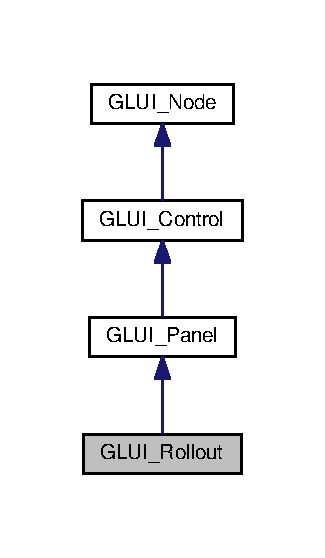
\includegraphics[width=156pt]{class_g_l_u_i___rollout__inherit__graph}
\end{center}
\end{figure}


Collaboration diagram for G\+L\+U\+I\+\_\+\+Rollout\+:\nopagebreak
\begin{figure}[H]
\begin{center}
\leavevmode
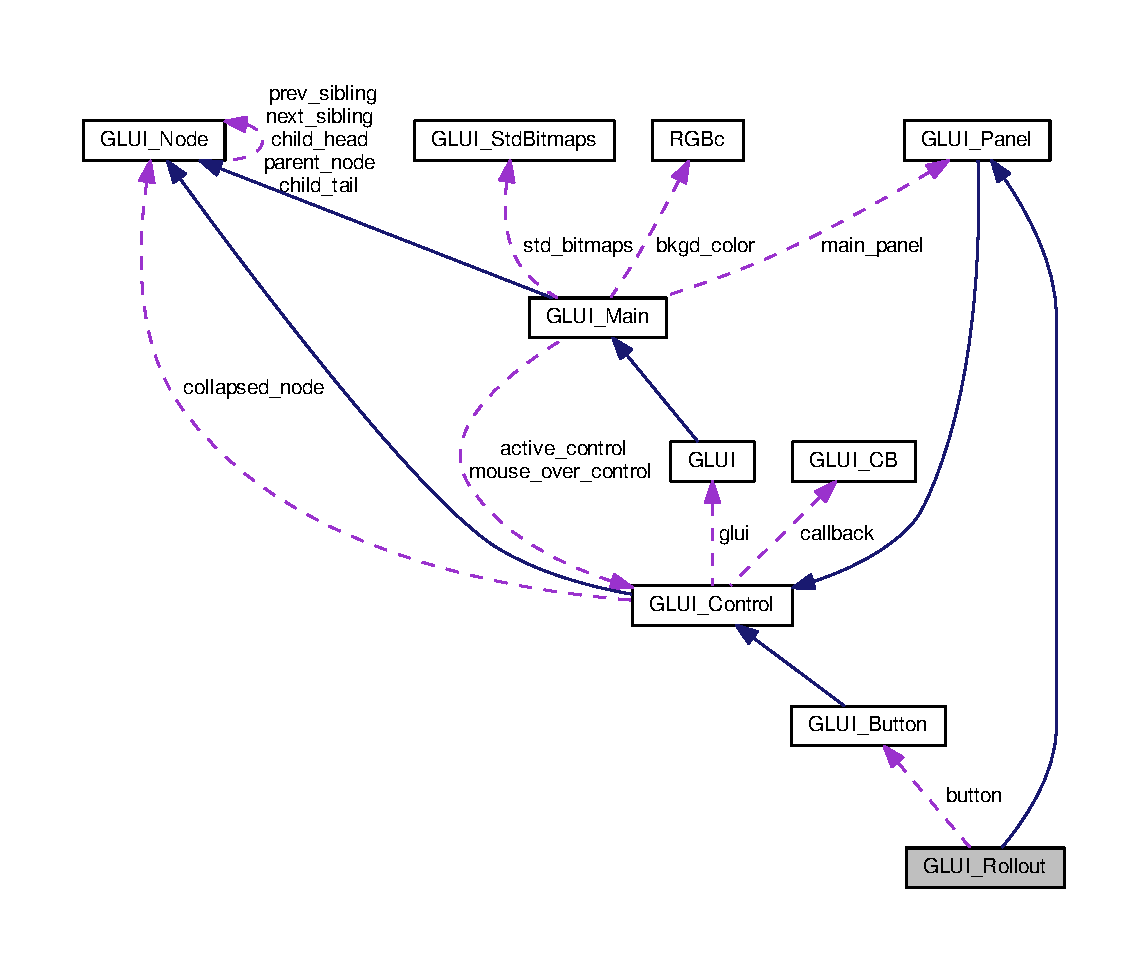
\includegraphics[width=350pt]{class_g_l_u_i___rollout__coll__graph}
\end{center}
\end{figure}
\subsection*{Public Member Functions}
\begin{DoxyCompactItemize}
\item 
\hyperlink{class_g_l_u_i___rollout_a24c6af54874ab79245debf924048bee2}{G\+L\+U\+I\+\_\+\+Rollout} (\hyperlink{class_g_l_u_i___node}{G\+L\+U\+I\+\_\+\+Node} $\ast$\hyperlink{class_g_l_u_i___node_a8ed65d447784f6f88bd3e2e2bcac6cdb}{parent}, const char $\ast$\hyperlink{glext_8h_ad977737dfc9a274a62741b9500c49a32}{name}, \hyperlink{wglext_8h_a500a82aecba06f4550f6849b8099ca21}{int} \hyperlink{class_g_l_u_i___rollout_a431c2fee6adb56c18d0ed8ac9a01eacb}{open}=true, \hyperlink{wglext_8h_a500a82aecba06f4550f6849b8099ca21}{int} \hyperlink{glext_8h_ab7c1afc09f67635c2c376638fcc0db5f}{type}=\hyperlink{glui_8h_add54979a7b4391067b8a125ee34f690a}{G\+L\+U\+I\+\_\+\+P\+A\+N\+E\+L\+\_\+\+E\+M\+B\+O\+S\+S\+E\+D})
\item 
\hyperlink{class_g_l_u_i___rollout_a998dcde980d47ed464423f7728011290}{G\+L\+U\+I\+\_\+\+Rollout} (\hyperlink{wglext_8h_a9e6b7f1933461ef318bb000d6bd13b83}{void})
\item 
\hyperlink{wglext_8h_a9e6b7f1933461ef318bb000d6bd13b83}{void} \hyperlink{class_g_l_u_i___rollout_ae3ff0bbeb04f22aa5489cf542b6e3fbb}{draw} (\hyperlink{wglext_8h_a500a82aecba06f4550f6849b8099ca21}{int} \hyperlink{glext_8h_ad77deca22f617d3f0e0eb786445689fc}{x}, \hyperlink{wglext_8h_a500a82aecba06f4550f6849b8099ca21}{int} \hyperlink{glext_8h_a9298c7ad619074f5285b32c6b72bfdea}{y})
\item 
\hyperlink{wglext_8h_a9e6b7f1933461ef318bb000d6bd13b83}{void} \hyperlink{class_g_l_u_i___rollout_aa3fbc3548f10ee8209d2eb0b46c05b6d}{draw\+\_\+pressed} (\hyperlink{wglext_8h_a9e6b7f1933461ef318bb000d6bd13b83}{void})
\item 
\hyperlink{wglext_8h_a500a82aecba06f4550f6849b8099ca21}{int} \hyperlink{class_g_l_u_i___rollout_abbd554515b6f0136f6aa89d260b826e5}{mouse\+\_\+down\+\_\+handler} (\hyperlink{wglext_8h_a500a82aecba06f4550f6849b8099ca21}{int} local\+\_\+x, \hyperlink{wglext_8h_a500a82aecba06f4550f6849b8099ca21}{int} local\+\_\+y)
\item 
\hyperlink{wglext_8h_a500a82aecba06f4550f6849b8099ca21}{int} \hyperlink{class_g_l_u_i___rollout_ac7df2e007640c4a21deb494c8eb8ca03}{mouse\+\_\+up\+\_\+handler} (\hyperlink{wglext_8h_a500a82aecba06f4550f6849b8099ca21}{int} local\+\_\+x, \hyperlink{wglext_8h_a500a82aecba06f4550f6849b8099ca21}{int} local\+\_\+y, bool inside)
\item 
\hyperlink{wglext_8h_a500a82aecba06f4550f6849b8099ca21}{int} \hyperlink{class_g_l_u_i___rollout_a55eb4c45f7857bbae04e857aadf2b505}{mouse\+\_\+held\+\_\+down\+\_\+handler} (\hyperlink{wglext_8h_a500a82aecba06f4550f6849b8099ca21}{int} local\+\_\+x, \hyperlink{wglext_8h_a500a82aecba06f4550f6849b8099ca21}{int} local\+\_\+y, bool inside)
\item 
\hyperlink{wglext_8h_a9e6b7f1933461ef318bb000d6bd13b83}{void} \hyperlink{class_g_l_u_i___rollout_a431c2fee6adb56c18d0ed8ac9a01eacb}{open} (\hyperlink{wglext_8h_a9e6b7f1933461ef318bb000d6bd13b83}{void})
\item 
\hyperlink{wglext_8h_a9e6b7f1933461ef318bb000d6bd13b83}{void} \hyperlink{class_g_l_u_i___rollout_a16ff61e6541e9872fc82f91c75263e16}{close} (\hyperlink{wglext_8h_a9e6b7f1933461ef318bb000d6bd13b83}{void})
\item 
\hyperlink{wglext_8h_a9e6b7f1933461ef318bb000d6bd13b83}{void} \hyperlink{class_g_l_u_i___rollout_af6f664a8ca31757bc1e5926d5eaf2827}{update\+\_\+size} (\hyperlink{wglext_8h_a9e6b7f1933461ef318bb000d6bd13b83}{void})
\end{DoxyCompactItemize}
\subsection*{Public Attributes}
\begin{DoxyCompactItemize}
\item 
bool \hyperlink{class_g_l_u_i___rollout_aa9896aa7e1ee76ac8b4d84573da7e6fb}{currently\+\_\+inside}
\item 
bool \hyperlink{class_g_l_u_i___rollout_ad9d35f15e7df49dc27fdc5ab571e0e17}{initially\+\_\+inside}
\item 
\hyperlink{class_g_l_u_i___button}{G\+L\+U\+I\+\_\+\+Button} \hyperlink{class_g_l_u_i___rollout_a552827a8d2ff58920457b8637b9536b0}{button}
\end{DoxyCompactItemize}
\subsection*{Protected Member Functions}
\begin{DoxyCompactItemize}
\item 
\hyperlink{wglext_8h_a9e6b7f1933461ef318bb000d6bd13b83}{void} \hyperlink{class_g_l_u_i___rollout_aaf1aa792f0fd5a90822e13ecd2797736}{common\+\_\+init} ()
\end{DoxyCompactItemize}
\subsection*{Additional Inherited Members}


\subsection{Detailed Description}
A rollout contains a set of controls, like a panel, but can be collapsed to just the name. 

Definition at line 1203 of file glui.\+h.



\subsection{Constructor \& Destructor Documentation}
\hypertarget{class_g_l_u_i___rollout_a24c6af54874ab79245debf924048bee2}{\index{G\+L\+U\+I\+\_\+\+Rollout@{G\+L\+U\+I\+\_\+\+Rollout}!G\+L\+U\+I\+\_\+\+Rollout@{G\+L\+U\+I\+\_\+\+Rollout}}
\index{G\+L\+U\+I\+\_\+\+Rollout@{G\+L\+U\+I\+\_\+\+Rollout}!G\+L\+U\+I\+\_\+\+Rollout@{G\+L\+U\+I\+\_\+\+Rollout}}
\subsubsection[{G\+L\+U\+I\+\_\+\+Rollout}]{\setlength{\rightskip}{0pt plus 5cm}G\+L\+U\+I\+\_\+\+Rollout\+::\+G\+L\+U\+I\+\_\+\+Rollout (
\begin{DoxyParamCaption}
\item[{{\bf G\+L\+U\+I\+\_\+\+Node} $\ast$}]{parent, }
\item[{const char $\ast$}]{name, }
\item[{{\bf int}}]{open = {\ttfamily true}, }
\item[{{\bf int}}]{type = {\ttfamily {\bf G\+L\+U\+I\+\_\+\+P\+A\+N\+E\+L\+\_\+\+E\+M\+B\+O\+S\+S\+E\+D}}}
\end{DoxyParamCaption}
)}}\label{class_g_l_u_i___rollout_a24c6af54874ab79245debf924048bee2}
Create a new rollout. A rollout contains a set of controls, like a panel, but can be collapsed to just the name.


\begin{DoxyParams}{Parameters}
{\em parent} & The panel our object is inside; or the main \hyperlink{class_g_l_u_i}{G\+L\+U\+I} object. \\
\hline
{\em name} & String to show at the top of the rollout. \\
\hline
{\em open} & Optional boolean. If true (the default), the rollout's controls are displayed. If false, the rollout is closed to display only the name. \\
\hline
{\em type} & Optional style to display the panel with--G\+L\+U\+I\+\_\+\+P\+A\+N\+E\+L\+\_\+\+E\+M\+B\+O\+S\+S\+E\+D by default. G\+L\+U\+I\+\_\+\+P\+A\+N\+E\+L\+\_\+\+R\+A\+I\+S\+E\+D causes the panel to appear higher than the surroundings. G\+L\+U\+I\+\_\+\+P\+A\+N\+E\+L\+\_\+\+N\+O\+N\+E causes the panel's outline to be invisible. \\
\hline
\end{DoxyParams}
\hypertarget{class_g_l_u_i___rollout_a998dcde980d47ed464423f7728011290}{\index{G\+L\+U\+I\+\_\+\+Rollout@{G\+L\+U\+I\+\_\+\+Rollout}!G\+L\+U\+I\+\_\+\+Rollout@{G\+L\+U\+I\+\_\+\+Rollout}}
\index{G\+L\+U\+I\+\_\+\+Rollout@{G\+L\+U\+I\+\_\+\+Rollout}!G\+L\+U\+I\+\_\+\+Rollout@{G\+L\+U\+I\+\_\+\+Rollout}}
\subsubsection[{G\+L\+U\+I\+\_\+\+Rollout}]{\setlength{\rightskip}{0pt plus 5cm}G\+L\+U\+I\+\_\+\+Rollout\+::\+G\+L\+U\+I\+\_\+\+Rollout (
\begin{DoxyParamCaption}
\item[{{\bf void}}]{}
\end{DoxyParamCaption}
)\hspace{0.3cm}{\ttfamily [inline]}}}\label{class_g_l_u_i___rollout_a998dcde980d47ed464423f7728011290}


Definition at line 1221 of file glui.\+h.



\subsection{Member Function Documentation}
\hypertarget{class_g_l_u_i___rollout_a16ff61e6541e9872fc82f91c75263e16}{\index{G\+L\+U\+I\+\_\+\+Rollout@{G\+L\+U\+I\+\_\+\+Rollout}!close@{close}}
\index{close@{close}!G\+L\+U\+I\+\_\+\+Rollout@{G\+L\+U\+I\+\_\+\+Rollout}}
\subsubsection[{close}]{\setlength{\rightskip}{0pt plus 5cm}{\bf void} G\+L\+U\+I\+\_\+\+Rollout\+::close (
\begin{DoxyParamCaption}
\item[{{\bf void}}]{}
\end{DoxyParamCaption}
)}}\label{class_g_l_u_i___rollout_a16ff61e6541e9872fc82f91c75263e16}
\hypertarget{class_g_l_u_i___rollout_aaf1aa792f0fd5a90822e13ecd2797736}{\index{G\+L\+U\+I\+\_\+\+Rollout@{G\+L\+U\+I\+\_\+\+Rollout}!common\+\_\+init@{common\+\_\+init}}
\index{common\+\_\+init@{common\+\_\+init}!G\+L\+U\+I\+\_\+\+Rollout@{G\+L\+U\+I\+\_\+\+Rollout}}
\subsubsection[{common\+\_\+init}]{\setlength{\rightskip}{0pt plus 5cm}{\bf void} G\+L\+U\+I\+\_\+\+Rollout\+::common\+\_\+init (
\begin{DoxyParamCaption}
\item[{{\bf void}}]{}
\end{DoxyParamCaption}
)\hspace{0.3cm}{\ttfamily [inline]}, {\ttfamily [protected]}}}\label{class_g_l_u_i___rollout_aaf1aa792f0fd5a90822e13ecd2797736}


Definition at line 1239 of file glui.\+h.

\hypertarget{class_g_l_u_i___rollout_ae3ff0bbeb04f22aa5489cf542b6e3fbb}{\index{G\+L\+U\+I\+\_\+\+Rollout@{G\+L\+U\+I\+\_\+\+Rollout}!draw@{draw}}
\index{draw@{draw}!G\+L\+U\+I\+\_\+\+Rollout@{G\+L\+U\+I\+\_\+\+Rollout}}
\subsubsection[{draw}]{\setlength{\rightskip}{0pt plus 5cm}{\bf void} G\+L\+U\+I\+\_\+\+Rollout\+::draw (
\begin{DoxyParamCaption}
\item[{{\bf int}}]{x, }
\item[{{\bf int}}]{y}
\end{DoxyParamCaption}
)\hspace{0.3cm}{\ttfamily [virtual]}}}\label{class_g_l_u_i___rollout_ae3ff0bbeb04f22aa5489cf542b6e3fbb}


Reimplemented from \hyperlink{class_g_l_u_i___panel_a8038a76f6c88613735f7c65ae9466b0c}{G\+L\+U\+I\+\_\+\+Panel}.

\hypertarget{class_g_l_u_i___rollout_aa3fbc3548f10ee8209d2eb0b46c05b6d}{\index{G\+L\+U\+I\+\_\+\+Rollout@{G\+L\+U\+I\+\_\+\+Rollout}!draw\+\_\+pressed@{draw\+\_\+pressed}}
\index{draw\+\_\+pressed@{draw\+\_\+pressed}!G\+L\+U\+I\+\_\+\+Rollout@{G\+L\+U\+I\+\_\+\+Rollout}}
\subsubsection[{draw\+\_\+pressed}]{\setlength{\rightskip}{0pt plus 5cm}{\bf void} G\+L\+U\+I\+\_\+\+Rollout\+::draw\+\_\+pressed (
\begin{DoxyParamCaption}
\item[{{\bf void}}]{}
\end{DoxyParamCaption}
)}}\label{class_g_l_u_i___rollout_aa3fbc3548f10ee8209d2eb0b46c05b6d}
\hypertarget{class_g_l_u_i___rollout_abbd554515b6f0136f6aa89d260b826e5}{\index{G\+L\+U\+I\+\_\+\+Rollout@{G\+L\+U\+I\+\_\+\+Rollout}!mouse\+\_\+down\+\_\+handler@{mouse\+\_\+down\+\_\+handler}}
\index{mouse\+\_\+down\+\_\+handler@{mouse\+\_\+down\+\_\+handler}!G\+L\+U\+I\+\_\+\+Rollout@{G\+L\+U\+I\+\_\+\+Rollout}}
\subsubsection[{mouse\+\_\+down\+\_\+handler}]{\setlength{\rightskip}{0pt plus 5cm}{\bf int} G\+L\+U\+I\+\_\+\+Rollout\+::mouse\+\_\+down\+\_\+handler (
\begin{DoxyParamCaption}
\item[{{\bf int}}]{local\+\_\+x, }
\item[{{\bf int}}]{local\+\_\+y}
\end{DoxyParamCaption}
)\hspace{0.3cm}{\ttfamily [virtual]}}}\label{class_g_l_u_i___rollout_abbd554515b6f0136f6aa89d260b826e5}


Reimplemented from \hyperlink{class_g_l_u_i___control_a92b77565168a1d2003bca1c16ac00e8d}{G\+L\+U\+I\+\_\+\+Control}.

\hypertarget{class_g_l_u_i___rollout_a55eb4c45f7857bbae04e857aadf2b505}{\index{G\+L\+U\+I\+\_\+\+Rollout@{G\+L\+U\+I\+\_\+\+Rollout}!mouse\+\_\+held\+\_\+down\+\_\+handler@{mouse\+\_\+held\+\_\+down\+\_\+handler}}
\index{mouse\+\_\+held\+\_\+down\+\_\+handler@{mouse\+\_\+held\+\_\+down\+\_\+handler}!G\+L\+U\+I\+\_\+\+Rollout@{G\+L\+U\+I\+\_\+\+Rollout}}
\subsubsection[{mouse\+\_\+held\+\_\+down\+\_\+handler}]{\setlength{\rightskip}{0pt plus 5cm}{\bf int} G\+L\+U\+I\+\_\+\+Rollout\+::mouse\+\_\+held\+\_\+down\+\_\+handler (
\begin{DoxyParamCaption}
\item[{{\bf int}}]{local\+\_\+x, }
\item[{{\bf int}}]{local\+\_\+y, }
\item[{bool}]{inside}
\end{DoxyParamCaption}
)\hspace{0.3cm}{\ttfamily [virtual]}}}\label{class_g_l_u_i___rollout_a55eb4c45f7857bbae04e857aadf2b505}


Reimplemented from \hyperlink{class_g_l_u_i___control_a4b44e44c1c455adc7f98c63aeb6aa919}{G\+L\+U\+I\+\_\+\+Control}.

\hypertarget{class_g_l_u_i___rollout_ac7df2e007640c4a21deb494c8eb8ca03}{\index{G\+L\+U\+I\+\_\+\+Rollout@{G\+L\+U\+I\+\_\+\+Rollout}!mouse\+\_\+up\+\_\+handler@{mouse\+\_\+up\+\_\+handler}}
\index{mouse\+\_\+up\+\_\+handler@{mouse\+\_\+up\+\_\+handler}!G\+L\+U\+I\+\_\+\+Rollout@{G\+L\+U\+I\+\_\+\+Rollout}}
\subsubsection[{mouse\+\_\+up\+\_\+handler}]{\setlength{\rightskip}{0pt plus 5cm}{\bf int} G\+L\+U\+I\+\_\+\+Rollout\+::mouse\+\_\+up\+\_\+handler (
\begin{DoxyParamCaption}
\item[{{\bf int}}]{local\+\_\+x, }
\item[{{\bf int}}]{local\+\_\+y, }
\item[{bool}]{inside}
\end{DoxyParamCaption}
)\hspace{0.3cm}{\ttfamily [virtual]}}}\label{class_g_l_u_i___rollout_ac7df2e007640c4a21deb494c8eb8ca03}


Reimplemented from \hyperlink{class_g_l_u_i___control_ac32aad8f69134d03682e34d0488a18f1}{G\+L\+U\+I\+\_\+\+Control}.

\hypertarget{class_g_l_u_i___rollout_a431c2fee6adb56c18d0ed8ac9a01eacb}{\index{G\+L\+U\+I\+\_\+\+Rollout@{G\+L\+U\+I\+\_\+\+Rollout}!open@{open}}
\index{open@{open}!G\+L\+U\+I\+\_\+\+Rollout@{G\+L\+U\+I\+\_\+\+Rollout}}
\subsubsection[{open}]{\setlength{\rightskip}{0pt plus 5cm}{\bf void} G\+L\+U\+I\+\_\+\+Rollout\+::open (
\begin{DoxyParamCaption}
\item[{{\bf void}}]{}
\end{DoxyParamCaption}
)}}\label{class_g_l_u_i___rollout_a431c2fee6adb56c18d0ed8ac9a01eacb}
\hypertarget{class_g_l_u_i___rollout_af6f664a8ca31757bc1e5926d5eaf2827}{\index{G\+L\+U\+I\+\_\+\+Rollout@{G\+L\+U\+I\+\_\+\+Rollout}!update\+\_\+size@{update\+\_\+size}}
\index{update\+\_\+size@{update\+\_\+size}!G\+L\+U\+I\+\_\+\+Rollout@{G\+L\+U\+I\+\_\+\+Rollout}}
\subsubsection[{update\+\_\+size}]{\setlength{\rightskip}{0pt plus 5cm}{\bf void} G\+L\+U\+I\+\_\+\+Rollout\+::update\+\_\+size (
\begin{DoxyParamCaption}
\item[{{\bf void}}]{}
\end{DoxyParamCaption}
)\hspace{0.3cm}{\ttfamily [virtual]}}}\label{class_g_l_u_i___rollout_af6f664a8ca31757bc1e5926d5eaf2827}


Reimplemented from \hyperlink{class_g_l_u_i___panel_ab377b608f9b1006fb67d78e41a1f95d6}{G\+L\+U\+I\+\_\+\+Panel}.



\subsection{Member Data Documentation}
\hypertarget{class_g_l_u_i___rollout_a552827a8d2ff58920457b8637b9536b0}{\index{G\+L\+U\+I\+\_\+\+Rollout@{G\+L\+U\+I\+\_\+\+Rollout}!button@{button}}
\index{button@{button}!G\+L\+U\+I\+\_\+\+Rollout@{G\+L\+U\+I\+\_\+\+Rollout}}
\subsubsection[{button}]{\setlength{\rightskip}{0pt plus 5cm}{\bf G\+L\+U\+I\+\_\+\+Button} G\+L\+U\+I\+\_\+\+Rollout\+::button}}\label{class_g_l_u_i___rollout_a552827a8d2ff58920457b8637b9536b0}


Definition at line 1225 of file glui.\+h.

\hypertarget{class_g_l_u_i___rollout_aa9896aa7e1ee76ac8b4d84573da7e6fb}{\index{G\+L\+U\+I\+\_\+\+Rollout@{G\+L\+U\+I\+\_\+\+Rollout}!currently\+\_\+inside@{currently\+\_\+inside}}
\index{currently\+\_\+inside@{currently\+\_\+inside}!G\+L\+U\+I\+\_\+\+Rollout@{G\+L\+U\+I\+\_\+\+Rollout}}
\subsubsection[{currently\+\_\+inside}]{\setlength{\rightskip}{0pt plus 5cm}bool G\+L\+U\+I\+\_\+\+Rollout\+::currently\+\_\+inside}}\label{class_g_l_u_i___rollout_aa9896aa7e1ee76ac8b4d84573da7e6fb}


Definition at line 1224 of file glui.\+h.

\hypertarget{class_g_l_u_i___rollout_ad9d35f15e7df49dc27fdc5ab571e0e17}{\index{G\+L\+U\+I\+\_\+\+Rollout@{G\+L\+U\+I\+\_\+\+Rollout}!initially\+\_\+inside@{initially\+\_\+inside}}
\index{initially\+\_\+inside@{initially\+\_\+inside}!G\+L\+U\+I\+\_\+\+Rollout@{G\+L\+U\+I\+\_\+\+Rollout}}
\subsubsection[{initially\+\_\+inside}]{\setlength{\rightskip}{0pt plus 5cm}bool G\+L\+U\+I\+\_\+\+Rollout\+::initially\+\_\+inside}}\label{class_g_l_u_i___rollout_ad9d35f15e7df49dc27fdc5ab571e0e17}


Definition at line 1224 of file glui.\+h.



The documentation for this class was generated from the following file\+:\begin{DoxyCompactItemize}
\item 
S\+S\+W\+C/src/\+G\+L/\hyperlink{glui_8h}{glui.\+h}\end{DoxyCompactItemize}

\hypertarget{class_g_l_u_i___rotation}{\section{G\+L\+U\+I\+\_\+\+Rotation Class Reference}
\label{class_g_l_u_i___rotation}\index{G\+L\+U\+I\+\_\+\+Rotation@{G\+L\+U\+I\+\_\+\+Rotation}}
}


{\ttfamily \#include $<$glui.\+h$>$}



Inheritance diagram for G\+L\+U\+I\+\_\+\+Rotation\+:\nopagebreak
\begin{figure}[H]
\begin{center}
\leavevmode
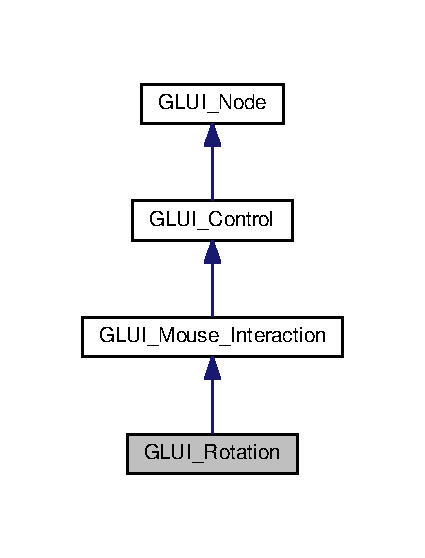
\includegraphics[width=204pt]{class_g_l_u_i___rotation__inherit__graph}
\end{center}
\end{figure}


Collaboration diagram for G\+L\+U\+I\+\_\+\+Rotation\+:\nopagebreak
\begin{figure}[H]
\begin{center}
\leavevmode
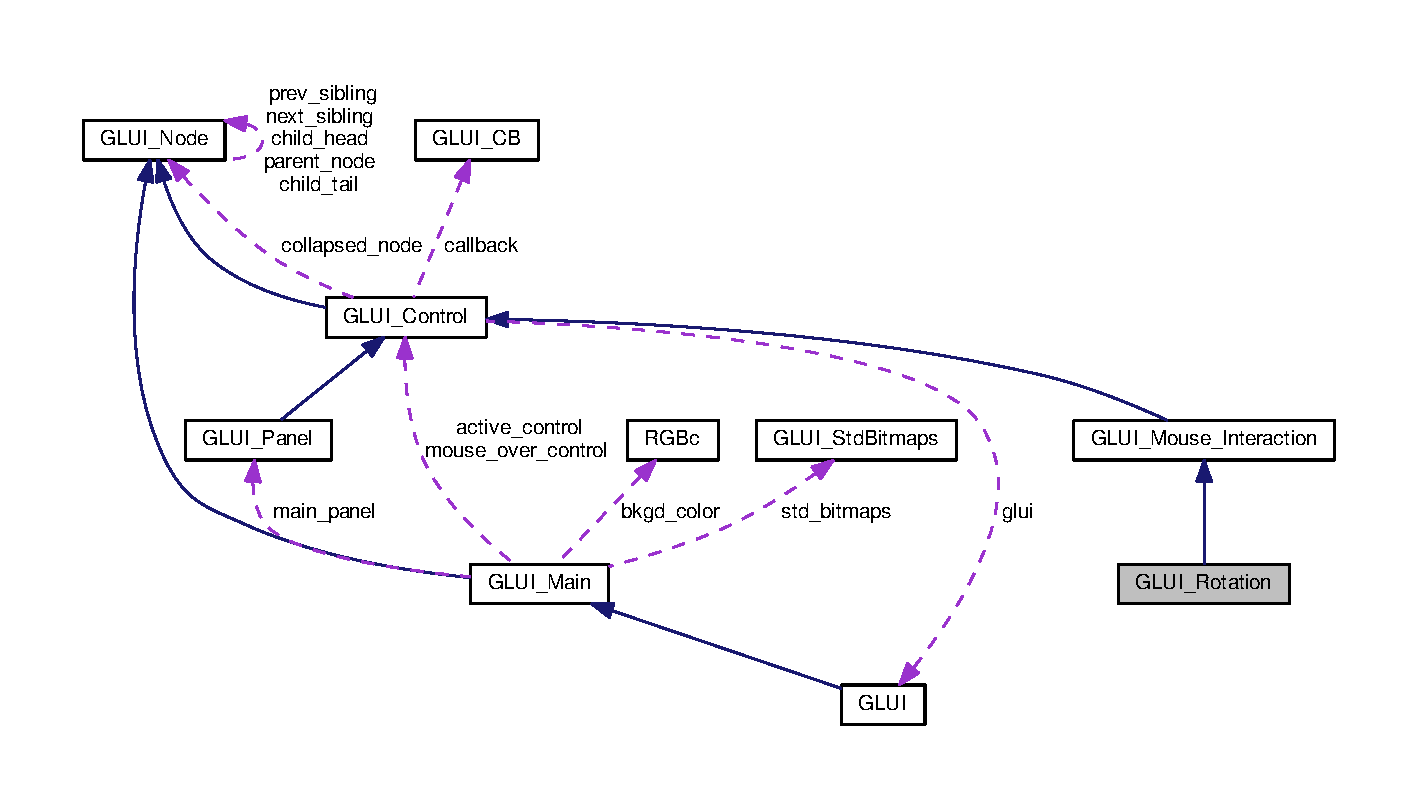
\includegraphics[width=350pt]{class_g_l_u_i___rotation__coll__graph}
\end{center}
\end{figure}
\subsection*{Public Member Functions}
\begin{DoxyCompactItemize}
\item 
\hyperlink{wglext_8h_a500a82aecba06f4550f6849b8099ca21}{int} \hyperlink{class_g_l_u_i___rotation_a3af15515b4f2bd05bfbbc625fa4d6247}{iaction\+\_\+mouse\+\_\+down\+\_\+handler} (\hyperlink{wglext_8h_a500a82aecba06f4550f6849b8099ca21}{int} local\+\_\+x, \hyperlink{wglext_8h_a500a82aecba06f4550f6849b8099ca21}{int} local\+\_\+y)
\item 
\hyperlink{wglext_8h_a500a82aecba06f4550f6849b8099ca21}{int} \hyperlink{class_g_l_u_i___rotation_aa3ee9f07c589dedc7c1b6ad780566172}{iaction\+\_\+mouse\+\_\+up\+\_\+handler} (\hyperlink{wglext_8h_a500a82aecba06f4550f6849b8099ca21}{int} local\+\_\+x, \hyperlink{wglext_8h_a500a82aecba06f4550f6849b8099ca21}{int} local\+\_\+y, bool inside)
\item 
\hyperlink{wglext_8h_a500a82aecba06f4550f6849b8099ca21}{int} \hyperlink{class_g_l_u_i___rotation_ad743bdbd88648859ef334c572e9e969d}{iaction\+\_\+mouse\+\_\+held\+\_\+down\+\_\+handler} (\hyperlink{wglext_8h_a500a82aecba06f4550f6849b8099ca21}{int} local\+\_\+x, \hyperlink{wglext_8h_a500a82aecba06f4550f6849b8099ca21}{int} local\+\_\+y, bool inside)
\item 
\hyperlink{wglext_8h_a500a82aecba06f4550f6849b8099ca21}{int} \hyperlink{class_g_l_u_i___rotation_a0a86badfaa9102475a2af2b2f3d824aa}{iaction\+\_\+special\+\_\+handler} (\hyperlink{wglext_8h_a500a82aecba06f4550f6849b8099ca21}{int} key, \hyperlink{wglext_8h_a500a82aecba06f4550f6849b8099ca21}{int} modifiers)
\item 
\hyperlink{wglext_8h_a9e6b7f1933461ef318bb000d6bd13b83}{void} \hyperlink{class_g_l_u_i___rotation_ac7029bd29427238e2590472ae882c258}{iaction\+\_\+init} (\hyperlink{wglext_8h_a9e6b7f1933461ef318bb000d6bd13b83}{void})
\item 
\hyperlink{wglext_8h_a9e6b7f1933461ef318bb000d6bd13b83}{void} \hyperlink{class_g_l_u_i___rotation_a88cf2f55e52c4afc9a81fceb53dbc406}{iaction\+\_\+draw\+\_\+active\+\_\+area\+\_\+persp} (\hyperlink{wglext_8h_a9e6b7f1933461ef318bb000d6bd13b83}{void})
\item 
\hyperlink{wglext_8h_a9e6b7f1933461ef318bb000d6bd13b83}{void} \hyperlink{class_g_l_u_i___rotation_aea8411d09fec628a8af788b0998746f2}{iaction\+\_\+draw\+\_\+active\+\_\+area\+\_\+ortho} (\hyperlink{wglext_8h_a9e6b7f1933461ef318bb000d6bd13b83}{void})
\item 
\hyperlink{wglext_8h_a9e6b7f1933461ef318bb000d6bd13b83}{void} \hyperlink{class_g_l_u_i___rotation_a6792c8f6fd8d2e52dd1e7729f7679fba}{iaction\+\_\+dump} (F\+I\+L\+E $\ast$output)
\item 
\hyperlink{wglext_8h_a9e6b7f1933461ef318bb000d6bd13b83}{void} \hyperlink{class_g_l_u_i___rotation_ad8f18b5b96e4269533bd41cf1ee2d490}{setup\+\_\+texture} (\hyperlink{wglext_8h_a9e6b7f1933461ef318bb000d6bd13b83}{void})
\item 
\hyperlink{wglext_8h_a9e6b7f1933461ef318bb000d6bd13b83}{void} \hyperlink{class_g_l_u_i___rotation_a434da267e0f38a2e33c28d6d2b0742a1}{setup\+\_\+lights} (\hyperlink{wglext_8h_a9e6b7f1933461ef318bb000d6bd13b83}{void})
\item 
\hyperlink{wglext_8h_a9e6b7f1933461ef318bb000d6bd13b83}{void} \hyperlink{class_g_l_u_i___rotation_a9e90fec3ccc22bcc89afd256d5842d8d}{draw\+\_\+ball} (float radius)
\item 
\hyperlink{wglext_8h_a9e6b7f1933461ef318bb000d6bd13b83}{void} \hyperlink{class_g_l_u_i___rotation_a3208f44f601e410ac01745903a5bca76}{init\+\_\+ball} (\hyperlink{wglext_8h_a9e6b7f1933461ef318bb000d6bd13b83}{void})
\item 
\hyperlink{wglext_8h_a9e6b7f1933461ef318bb000d6bd13b83}{void} \hyperlink{class_g_l_u_i___rotation_ab6ce638fa62a697b3eb177a7ac879919}{reset} (\hyperlink{wglext_8h_a9e6b7f1933461ef318bb000d6bd13b83}{void})
\item 
bool \hyperlink{class_g_l_u_i___rotation_aa11e56ce208283dfcbbe67728b3de673}{needs\+\_\+idle} (\hyperlink{wglext_8h_a9e6b7f1933461ef318bb000d6bd13b83}{void}) const 
\item 
\hyperlink{wglext_8h_a9e6b7f1933461ef318bb000d6bd13b83}{void} \hyperlink{class_g_l_u_i___rotation_a809f09063d91dcb89ea237849d5478ac}{idle} (\hyperlink{wglext_8h_a9e6b7f1933461ef318bb000d6bd13b83}{void})
\item 
\hyperlink{wglext_8h_a9e6b7f1933461ef318bb000d6bd13b83}{void} \hyperlink{class_g_l_u_i___rotation_aea0344d014f9edafcef3f539767c5014}{copy\+\_\+float\+\_\+array\+\_\+to\+\_\+ball} (\hyperlink{wglext_8h_a9e6b7f1933461ef318bb000d6bd13b83}{void})
\item 
\hyperlink{wglext_8h_a9e6b7f1933461ef318bb000d6bd13b83}{void} \hyperlink{class_g_l_u_i___rotation_a900d3fa4234a3af2e9a39686af64f37d}{copy\+\_\+ball\+\_\+to\+\_\+float\+\_\+array} (\hyperlink{wglext_8h_a9e6b7f1933461ef318bb000d6bd13b83}{void})
\item 
\hyperlink{wglext_8h_a9e6b7f1933461ef318bb000d6bd13b83}{void} \hyperlink{class_g_l_u_i___rotation_aac8678582493d922dc29a76f9c38adbc}{set\+\_\+spin} (float damp\+\_\+factor)
\item 
\hyperlink{class_g_l_u_i___rotation_a09fc7b3a09cbe61a5ef58d970f86adfe}{G\+L\+U\+I\+\_\+\+Rotation} (\hyperlink{class_g_l_u_i___node}{G\+L\+U\+I\+\_\+\+Node} $\ast$\hyperlink{class_g_l_u_i___node_a8ed65d447784f6f88bd3e2e2bcac6cdb}{parent}, const char $\ast$\hyperlink{glext_8h_ad977737dfc9a274a62741b9500c49a32}{name}, float $\ast$live\+\_\+var=N\+U\+L\+L, \hyperlink{wglext_8h_a500a82aecba06f4550f6849b8099ca21}{int} \hyperlink{glext_8h_a58c2a664503e14ffb8f21012aabff3e9}{id}=-\/1, \hyperlink{class_g_l_u_i___c_b}{G\+L\+U\+I\+\_\+\+C\+B} \hyperlink{class_g_l_u_i___control_a96060fe0cc6d537e736dd6eef78e24ab}{callback}=\hyperlink{class_g_l_u_i___c_b}{G\+L\+U\+I\+\_\+\+C\+B}())
\item 
\hyperlink{class_g_l_u_i___rotation_a4cec5398179283c77727f7d4d78f0f92}{G\+L\+U\+I\+\_\+\+Rotation} (\hyperlink{wglext_8h_a9e6b7f1933461ef318bb000d6bd13b83}{void})
\end{DoxyCompactItemize}
\subsection*{Public Attributes}
\begin{DoxyCompactItemize}
\item 
Arcball $\ast$ \hyperlink{class_g_l_u_i___rotation_ae57cc59ce48aec071b5db4fe608b98b3}{ball}
\item 
G\+L\+Uquadric\+Obj $\ast$ \hyperlink{class_g_l_u_i___rotation_af98f7b7cec5463b46b3ba1f685ef142c}{quad\+Obj}
\item 
bool \hyperlink{class_g_l_u_i___rotation_abb7e1e037705d27ac91805ac21ddbd39}{can\+\_\+spin}
\item 
bool \hyperlink{class_g_l_u_i___rotation_a49f0172a0fe24adb308730664f083018}{spinning}
\item 
float \hyperlink{class_g_l_u_i___rotation_a3164bbd01acc6e91b845c72df6987a51}{damping}
\end{DoxyCompactItemize}
\subsection*{Protected Member Functions}
\begin{DoxyCompactItemize}
\item 
\hyperlink{wglext_8h_a9e6b7f1933461ef318bb000d6bd13b83}{void} \hyperlink{class_g_l_u_i___rotation_af6715a13b59b945ea1635a01a0a62aa6}{common\+\_\+init} ()
\end{DoxyCompactItemize}
\subsection*{Additional Inherited Members}


\subsection{Detailed Description}
An onscreen rotation controller--allows the user to interact with a 3\+D rotation via a spaceball-\/like interface. 

Definition at line 2436 of file glui.\+h.



\subsection{Constructor \& Destructor Documentation}
\hypertarget{class_g_l_u_i___rotation_a09fc7b3a09cbe61a5ef58d970f86adfe}{\index{G\+L\+U\+I\+\_\+\+Rotation@{G\+L\+U\+I\+\_\+\+Rotation}!G\+L\+U\+I\+\_\+\+Rotation@{G\+L\+U\+I\+\_\+\+Rotation}}
\index{G\+L\+U\+I\+\_\+\+Rotation@{G\+L\+U\+I\+\_\+\+Rotation}!G\+L\+U\+I\+\_\+\+Rotation@{G\+L\+U\+I\+\_\+\+Rotation}}
\subsubsection[{G\+L\+U\+I\+\_\+\+Rotation}]{\setlength{\rightskip}{0pt plus 5cm}G\+L\+U\+I\+\_\+\+Rotation\+::\+G\+L\+U\+I\+\_\+\+Rotation (
\begin{DoxyParamCaption}
\item[{{\bf G\+L\+U\+I\+\_\+\+Node} $\ast$}]{parent, }
\item[{const char $\ast$}]{name, }
\item[{float $\ast$}]{live\+\_\+var = {\ttfamily NULL}, }
\item[{{\bf int}}]{id = {\ttfamily -\/1}, }
\item[{{\bf G\+L\+U\+I\+\_\+\+C\+B}}]{callback = {\ttfamily {\bf G\+L\+U\+I\+\_\+\+C\+B}()}}
\end{DoxyParamCaption}
)}}\label{class_g_l_u_i___rotation_a09fc7b3a09cbe61a5ef58d970f86adfe}
\hypertarget{class_g_l_u_i___rotation_a4cec5398179283c77727f7d4d78f0f92}{\index{G\+L\+U\+I\+\_\+\+Rotation@{G\+L\+U\+I\+\_\+\+Rotation}!G\+L\+U\+I\+\_\+\+Rotation@{G\+L\+U\+I\+\_\+\+Rotation}}
\index{G\+L\+U\+I\+\_\+\+Rotation@{G\+L\+U\+I\+\_\+\+Rotation}!G\+L\+U\+I\+\_\+\+Rotation@{G\+L\+U\+I\+\_\+\+Rotation}}
\subsubsection[{G\+L\+U\+I\+\_\+\+Rotation}]{\setlength{\rightskip}{0pt plus 5cm}G\+L\+U\+I\+\_\+\+Rotation\+::\+G\+L\+U\+I\+\_\+\+Rotation (
\begin{DoxyParamCaption}
\item[{{\bf void}}]{}
\end{DoxyParamCaption}
)\hspace{0.3cm}{\ttfamily [inline]}}}\label{class_g_l_u_i___rotation_a4cec5398179283c77727f7d4d78f0f92}


Definition at line 2475 of file glui.\+h.



\subsection{Member Function Documentation}
\hypertarget{class_g_l_u_i___rotation_af6715a13b59b945ea1635a01a0a62aa6}{\index{G\+L\+U\+I\+\_\+\+Rotation@{G\+L\+U\+I\+\_\+\+Rotation}!common\+\_\+init@{common\+\_\+init}}
\index{common\+\_\+init@{common\+\_\+init}!G\+L\+U\+I\+\_\+\+Rotation@{G\+L\+U\+I\+\_\+\+Rotation}}
\subsubsection[{common\+\_\+init}]{\setlength{\rightskip}{0pt plus 5cm}{\bf void} G\+L\+U\+I\+\_\+\+Rotation\+::common\+\_\+init (
\begin{DoxyParamCaption}
{}
\end{DoxyParamCaption}
)\hspace{0.3cm}{\ttfamily [protected]}}}\label{class_g_l_u_i___rotation_af6715a13b59b945ea1635a01a0a62aa6}
\hypertarget{class_g_l_u_i___rotation_a900d3fa4234a3af2e9a39686af64f37d}{\index{G\+L\+U\+I\+\_\+\+Rotation@{G\+L\+U\+I\+\_\+\+Rotation}!copy\+\_\+ball\+\_\+to\+\_\+float\+\_\+array@{copy\+\_\+ball\+\_\+to\+\_\+float\+\_\+array}}
\index{copy\+\_\+ball\+\_\+to\+\_\+float\+\_\+array@{copy\+\_\+ball\+\_\+to\+\_\+float\+\_\+array}!G\+L\+U\+I\+\_\+\+Rotation@{G\+L\+U\+I\+\_\+\+Rotation}}
\subsubsection[{copy\+\_\+ball\+\_\+to\+\_\+float\+\_\+array}]{\setlength{\rightskip}{0pt plus 5cm}{\bf void} G\+L\+U\+I\+\_\+\+Rotation\+::copy\+\_\+ball\+\_\+to\+\_\+float\+\_\+array (
\begin{DoxyParamCaption}
\item[{{\bf void}}]{}
\end{DoxyParamCaption}
)}}\label{class_g_l_u_i___rotation_a900d3fa4234a3af2e9a39686af64f37d}
\hypertarget{class_g_l_u_i___rotation_aea0344d014f9edafcef3f539767c5014}{\index{G\+L\+U\+I\+\_\+\+Rotation@{G\+L\+U\+I\+\_\+\+Rotation}!copy\+\_\+float\+\_\+array\+\_\+to\+\_\+ball@{copy\+\_\+float\+\_\+array\+\_\+to\+\_\+ball}}
\index{copy\+\_\+float\+\_\+array\+\_\+to\+\_\+ball@{copy\+\_\+float\+\_\+array\+\_\+to\+\_\+ball}!G\+L\+U\+I\+\_\+\+Rotation@{G\+L\+U\+I\+\_\+\+Rotation}}
\subsubsection[{copy\+\_\+float\+\_\+array\+\_\+to\+\_\+ball}]{\setlength{\rightskip}{0pt plus 5cm}{\bf void} G\+L\+U\+I\+\_\+\+Rotation\+::copy\+\_\+float\+\_\+array\+\_\+to\+\_\+ball (
\begin{DoxyParamCaption}
\item[{{\bf void}}]{}
\end{DoxyParamCaption}
)}}\label{class_g_l_u_i___rotation_aea0344d014f9edafcef3f539767c5014}
\hypertarget{class_g_l_u_i___rotation_a9e90fec3ccc22bcc89afd256d5842d8d}{\index{G\+L\+U\+I\+\_\+\+Rotation@{G\+L\+U\+I\+\_\+\+Rotation}!draw\+\_\+ball@{draw\+\_\+ball}}
\index{draw\+\_\+ball@{draw\+\_\+ball}!G\+L\+U\+I\+\_\+\+Rotation@{G\+L\+U\+I\+\_\+\+Rotation}}
\subsubsection[{draw\+\_\+ball}]{\setlength{\rightskip}{0pt plus 5cm}{\bf void} G\+L\+U\+I\+\_\+\+Rotation\+::draw\+\_\+ball (
\begin{DoxyParamCaption}
\item[{float}]{radius}
\end{DoxyParamCaption}
)}}\label{class_g_l_u_i___rotation_a9e90fec3ccc22bcc89afd256d5842d8d}
\hypertarget{class_g_l_u_i___rotation_aea8411d09fec628a8af788b0998746f2}{\index{G\+L\+U\+I\+\_\+\+Rotation@{G\+L\+U\+I\+\_\+\+Rotation}!iaction\+\_\+draw\+\_\+active\+\_\+area\+\_\+ortho@{iaction\+\_\+draw\+\_\+active\+\_\+area\+\_\+ortho}}
\index{iaction\+\_\+draw\+\_\+active\+\_\+area\+\_\+ortho@{iaction\+\_\+draw\+\_\+active\+\_\+area\+\_\+ortho}!G\+L\+U\+I\+\_\+\+Rotation@{G\+L\+U\+I\+\_\+\+Rotation}}
\subsubsection[{iaction\+\_\+draw\+\_\+active\+\_\+area\+\_\+ortho}]{\setlength{\rightskip}{0pt plus 5cm}{\bf void} G\+L\+U\+I\+\_\+\+Rotation\+::iaction\+\_\+draw\+\_\+active\+\_\+area\+\_\+ortho (
\begin{DoxyParamCaption}
\item[{{\bf void}}]{}
\end{DoxyParamCaption}
)\hspace{0.3cm}{\ttfamily [virtual]}}}\label{class_g_l_u_i___rotation_aea8411d09fec628a8af788b0998746f2}


Implements \hyperlink{class_g_l_u_i___mouse___interaction_aba702d0d46375ab194c7b07d93051b0d}{G\+L\+U\+I\+\_\+\+Mouse\+\_\+\+Interaction}.

\hypertarget{class_g_l_u_i___rotation_a88cf2f55e52c4afc9a81fceb53dbc406}{\index{G\+L\+U\+I\+\_\+\+Rotation@{G\+L\+U\+I\+\_\+\+Rotation}!iaction\+\_\+draw\+\_\+active\+\_\+area\+\_\+persp@{iaction\+\_\+draw\+\_\+active\+\_\+area\+\_\+persp}}
\index{iaction\+\_\+draw\+\_\+active\+\_\+area\+\_\+persp@{iaction\+\_\+draw\+\_\+active\+\_\+area\+\_\+persp}!G\+L\+U\+I\+\_\+\+Rotation@{G\+L\+U\+I\+\_\+\+Rotation}}
\subsubsection[{iaction\+\_\+draw\+\_\+active\+\_\+area\+\_\+persp}]{\setlength{\rightskip}{0pt plus 5cm}{\bf void} G\+L\+U\+I\+\_\+\+Rotation\+::iaction\+\_\+draw\+\_\+active\+\_\+area\+\_\+persp (
\begin{DoxyParamCaption}
\item[{{\bf void}}]{}
\end{DoxyParamCaption}
)\hspace{0.3cm}{\ttfamily [virtual]}}}\label{class_g_l_u_i___rotation_a88cf2f55e52c4afc9a81fceb53dbc406}


Implements \hyperlink{class_g_l_u_i___mouse___interaction_a4c7473fb5849e7d13052100aac56a9f3}{G\+L\+U\+I\+\_\+\+Mouse\+\_\+\+Interaction}.

\hypertarget{class_g_l_u_i___rotation_a6792c8f6fd8d2e52dd1e7729f7679fba}{\index{G\+L\+U\+I\+\_\+\+Rotation@{G\+L\+U\+I\+\_\+\+Rotation}!iaction\+\_\+dump@{iaction\+\_\+dump}}
\index{iaction\+\_\+dump@{iaction\+\_\+dump}!G\+L\+U\+I\+\_\+\+Rotation@{G\+L\+U\+I\+\_\+\+Rotation}}
\subsubsection[{iaction\+\_\+dump}]{\setlength{\rightskip}{0pt plus 5cm}{\bf void} G\+L\+U\+I\+\_\+\+Rotation\+::iaction\+\_\+dump (
\begin{DoxyParamCaption}
\item[{F\+I\+L\+E $\ast$}]{output}
\end{DoxyParamCaption}
)\hspace{0.3cm}{\ttfamily [virtual]}}}\label{class_g_l_u_i___rotation_a6792c8f6fd8d2e52dd1e7729f7679fba}


Implements \hyperlink{class_g_l_u_i___mouse___interaction_a99dd43b2224bbfee6aadee3cf15c1fdd}{G\+L\+U\+I\+\_\+\+Mouse\+\_\+\+Interaction}.

\hypertarget{class_g_l_u_i___rotation_ac7029bd29427238e2590472ae882c258}{\index{G\+L\+U\+I\+\_\+\+Rotation@{G\+L\+U\+I\+\_\+\+Rotation}!iaction\+\_\+init@{iaction\+\_\+init}}
\index{iaction\+\_\+init@{iaction\+\_\+init}!G\+L\+U\+I\+\_\+\+Rotation@{G\+L\+U\+I\+\_\+\+Rotation}}
\subsubsection[{iaction\+\_\+init}]{\setlength{\rightskip}{0pt plus 5cm}{\bf void} G\+L\+U\+I\+\_\+\+Rotation\+::iaction\+\_\+init (
\begin{DoxyParamCaption}
\item[{{\bf void}}]{}
\end{DoxyParamCaption}
)\hspace{0.3cm}{\ttfamily [inline]}, {\ttfamily [virtual]}}}\label{class_g_l_u_i___rotation_ac7029bd29427238e2590472ae882c258}


Implements \hyperlink{class_g_l_u_i___mouse___interaction_a4be4e3ae7948824b2af30c2b87f434fd}{G\+L\+U\+I\+\_\+\+Mouse\+\_\+\+Interaction}.



Definition at line 2448 of file glui.\+h.

\hypertarget{class_g_l_u_i___rotation_a3af15515b4f2bd05bfbbc625fa4d6247}{\index{G\+L\+U\+I\+\_\+\+Rotation@{G\+L\+U\+I\+\_\+\+Rotation}!iaction\+\_\+mouse\+\_\+down\+\_\+handler@{iaction\+\_\+mouse\+\_\+down\+\_\+handler}}
\index{iaction\+\_\+mouse\+\_\+down\+\_\+handler@{iaction\+\_\+mouse\+\_\+down\+\_\+handler}!G\+L\+U\+I\+\_\+\+Rotation@{G\+L\+U\+I\+\_\+\+Rotation}}
\subsubsection[{iaction\+\_\+mouse\+\_\+down\+\_\+handler}]{\setlength{\rightskip}{0pt plus 5cm}{\bf int} G\+L\+U\+I\+\_\+\+Rotation\+::iaction\+\_\+mouse\+\_\+down\+\_\+handler (
\begin{DoxyParamCaption}
\item[{{\bf int}}]{local\+\_\+x, }
\item[{{\bf int}}]{local\+\_\+y}
\end{DoxyParamCaption}
)\hspace{0.3cm}{\ttfamily [virtual]}}}\label{class_g_l_u_i___rotation_a3af15515b4f2bd05bfbbc625fa4d6247}


Implements \hyperlink{class_g_l_u_i___mouse___interaction_ab4168e2ccfdb1a8afe2b220e53902b8d}{G\+L\+U\+I\+\_\+\+Mouse\+\_\+\+Interaction}.

\hypertarget{class_g_l_u_i___rotation_ad743bdbd88648859ef334c572e9e969d}{\index{G\+L\+U\+I\+\_\+\+Rotation@{G\+L\+U\+I\+\_\+\+Rotation}!iaction\+\_\+mouse\+\_\+held\+\_\+down\+\_\+handler@{iaction\+\_\+mouse\+\_\+held\+\_\+down\+\_\+handler}}
\index{iaction\+\_\+mouse\+\_\+held\+\_\+down\+\_\+handler@{iaction\+\_\+mouse\+\_\+held\+\_\+down\+\_\+handler}!G\+L\+U\+I\+\_\+\+Rotation@{G\+L\+U\+I\+\_\+\+Rotation}}
\subsubsection[{iaction\+\_\+mouse\+\_\+held\+\_\+down\+\_\+handler}]{\setlength{\rightskip}{0pt plus 5cm}{\bf int} G\+L\+U\+I\+\_\+\+Rotation\+::iaction\+\_\+mouse\+\_\+held\+\_\+down\+\_\+handler (
\begin{DoxyParamCaption}
\item[{{\bf int}}]{local\+\_\+x, }
\item[{{\bf int}}]{local\+\_\+y, }
\item[{bool}]{inside}
\end{DoxyParamCaption}
)\hspace{0.3cm}{\ttfamily [virtual]}}}\label{class_g_l_u_i___rotation_ad743bdbd88648859ef334c572e9e969d}


Implements \hyperlink{class_g_l_u_i___mouse___interaction_ab10a2bbd829a80e7403d722e4e3b480d}{G\+L\+U\+I\+\_\+\+Mouse\+\_\+\+Interaction}.

\hypertarget{class_g_l_u_i___rotation_aa3ee9f07c589dedc7c1b6ad780566172}{\index{G\+L\+U\+I\+\_\+\+Rotation@{G\+L\+U\+I\+\_\+\+Rotation}!iaction\+\_\+mouse\+\_\+up\+\_\+handler@{iaction\+\_\+mouse\+\_\+up\+\_\+handler}}
\index{iaction\+\_\+mouse\+\_\+up\+\_\+handler@{iaction\+\_\+mouse\+\_\+up\+\_\+handler}!G\+L\+U\+I\+\_\+\+Rotation@{G\+L\+U\+I\+\_\+\+Rotation}}
\subsubsection[{iaction\+\_\+mouse\+\_\+up\+\_\+handler}]{\setlength{\rightskip}{0pt plus 5cm}{\bf int} G\+L\+U\+I\+\_\+\+Rotation\+::iaction\+\_\+mouse\+\_\+up\+\_\+handler (
\begin{DoxyParamCaption}
\item[{{\bf int}}]{local\+\_\+x, }
\item[{{\bf int}}]{local\+\_\+y, }
\item[{bool}]{inside}
\end{DoxyParamCaption}
)\hspace{0.3cm}{\ttfamily [virtual]}}}\label{class_g_l_u_i___rotation_aa3ee9f07c589dedc7c1b6ad780566172}


Implements \hyperlink{class_g_l_u_i___mouse___interaction_aaeab42a0986281d21e2b3ab24efb527d}{G\+L\+U\+I\+\_\+\+Mouse\+\_\+\+Interaction}.

\hypertarget{class_g_l_u_i___rotation_a0a86badfaa9102475a2af2b2f3d824aa}{\index{G\+L\+U\+I\+\_\+\+Rotation@{G\+L\+U\+I\+\_\+\+Rotation}!iaction\+\_\+special\+\_\+handler@{iaction\+\_\+special\+\_\+handler}}
\index{iaction\+\_\+special\+\_\+handler@{iaction\+\_\+special\+\_\+handler}!G\+L\+U\+I\+\_\+\+Rotation@{G\+L\+U\+I\+\_\+\+Rotation}}
\subsubsection[{iaction\+\_\+special\+\_\+handler}]{\setlength{\rightskip}{0pt plus 5cm}{\bf int} G\+L\+U\+I\+\_\+\+Rotation\+::iaction\+\_\+special\+\_\+handler (
\begin{DoxyParamCaption}
\item[{{\bf int}}]{key, }
\item[{{\bf int}}]{modifiers}
\end{DoxyParamCaption}
)\hspace{0.3cm}{\ttfamily [virtual]}}}\label{class_g_l_u_i___rotation_a0a86badfaa9102475a2af2b2f3d824aa}


Implements \hyperlink{class_g_l_u_i___mouse___interaction_a738d6fd0afea5a76b45fe2a3c24c4e64}{G\+L\+U\+I\+\_\+\+Mouse\+\_\+\+Interaction}.

\hypertarget{class_g_l_u_i___rotation_a809f09063d91dcb89ea237849d5478ac}{\index{G\+L\+U\+I\+\_\+\+Rotation@{G\+L\+U\+I\+\_\+\+Rotation}!idle@{idle}}
\index{idle@{idle}!G\+L\+U\+I\+\_\+\+Rotation@{G\+L\+U\+I\+\_\+\+Rotation}}
\subsubsection[{idle}]{\setlength{\rightskip}{0pt plus 5cm}{\bf void} G\+L\+U\+I\+\_\+\+Rotation\+::idle (
\begin{DoxyParamCaption}
\item[{{\bf void}}]{}
\end{DoxyParamCaption}
)\hspace{0.3cm}{\ttfamily [virtual]}}}\label{class_g_l_u_i___rotation_a809f09063d91dcb89ea237849d5478ac}


Reimplemented from \hyperlink{class_g_l_u_i___control_a4eb47a3c2c20c0c24dca192a2eb96c8d}{G\+L\+U\+I\+\_\+\+Control}.

\hypertarget{class_g_l_u_i___rotation_a3208f44f601e410ac01745903a5bca76}{\index{G\+L\+U\+I\+\_\+\+Rotation@{G\+L\+U\+I\+\_\+\+Rotation}!init\+\_\+ball@{init\+\_\+ball}}
\index{init\+\_\+ball@{init\+\_\+ball}!G\+L\+U\+I\+\_\+\+Rotation@{G\+L\+U\+I\+\_\+\+Rotation}}
\subsubsection[{init\+\_\+ball}]{\setlength{\rightskip}{0pt plus 5cm}{\bf void} G\+L\+U\+I\+\_\+\+Rotation\+::init\+\_\+ball (
\begin{DoxyParamCaption}
\item[{{\bf void}}]{}
\end{DoxyParamCaption}
)}}\label{class_g_l_u_i___rotation_a3208f44f601e410ac01745903a5bca76}
\hypertarget{class_g_l_u_i___rotation_aa11e56ce208283dfcbbe67728b3de673}{\index{G\+L\+U\+I\+\_\+\+Rotation@{G\+L\+U\+I\+\_\+\+Rotation}!needs\+\_\+idle@{needs\+\_\+idle}}
\index{needs\+\_\+idle@{needs\+\_\+idle}!G\+L\+U\+I\+\_\+\+Rotation@{G\+L\+U\+I\+\_\+\+Rotation}}
\subsubsection[{needs\+\_\+idle}]{\setlength{\rightskip}{0pt plus 5cm}bool G\+L\+U\+I\+\_\+\+Rotation\+::needs\+\_\+idle (
\begin{DoxyParamCaption}
\item[{{\bf void}}]{}
\end{DoxyParamCaption}
) const\hspace{0.3cm}{\ttfamily [virtual]}}}\label{class_g_l_u_i___rotation_aa11e56ce208283dfcbbe67728b3de673}


Reimplemented from \hyperlink{class_g_l_u_i___control_a420fb3c5991b6486754ba192f8ab8274}{G\+L\+U\+I\+\_\+\+Control}.

\hypertarget{class_g_l_u_i___rotation_ab6ce638fa62a697b3eb177a7ac879919}{\index{G\+L\+U\+I\+\_\+\+Rotation@{G\+L\+U\+I\+\_\+\+Rotation}!reset@{reset}}
\index{reset@{reset}!G\+L\+U\+I\+\_\+\+Rotation@{G\+L\+U\+I\+\_\+\+Rotation}}
\subsubsection[{reset}]{\setlength{\rightskip}{0pt plus 5cm}{\bf void} G\+L\+U\+I\+\_\+\+Rotation\+::reset (
\begin{DoxyParamCaption}
\item[{{\bf void}}]{}
\end{DoxyParamCaption}
)}}\label{class_g_l_u_i___rotation_ab6ce638fa62a697b3eb177a7ac879919}
\hypertarget{class_g_l_u_i___rotation_aac8678582493d922dc29a76f9c38adbc}{\index{G\+L\+U\+I\+\_\+\+Rotation@{G\+L\+U\+I\+\_\+\+Rotation}!set\+\_\+spin@{set\+\_\+spin}}
\index{set\+\_\+spin@{set\+\_\+spin}!G\+L\+U\+I\+\_\+\+Rotation@{G\+L\+U\+I\+\_\+\+Rotation}}
\subsubsection[{set\+\_\+spin}]{\setlength{\rightskip}{0pt plus 5cm}{\bf void} G\+L\+U\+I\+\_\+\+Rotation\+::set\+\_\+spin (
\begin{DoxyParamCaption}
\item[{float}]{damp\+\_\+factor}
\end{DoxyParamCaption}
)}}\label{class_g_l_u_i___rotation_aac8678582493d922dc29a76f9c38adbc}
\hypertarget{class_g_l_u_i___rotation_a434da267e0f38a2e33c28d6d2b0742a1}{\index{G\+L\+U\+I\+\_\+\+Rotation@{G\+L\+U\+I\+\_\+\+Rotation}!setup\+\_\+lights@{setup\+\_\+lights}}
\index{setup\+\_\+lights@{setup\+\_\+lights}!G\+L\+U\+I\+\_\+\+Rotation@{G\+L\+U\+I\+\_\+\+Rotation}}
\subsubsection[{setup\+\_\+lights}]{\setlength{\rightskip}{0pt plus 5cm}{\bf void} G\+L\+U\+I\+\_\+\+Rotation\+::setup\+\_\+lights (
\begin{DoxyParamCaption}
\item[{{\bf void}}]{}
\end{DoxyParamCaption}
)}}\label{class_g_l_u_i___rotation_a434da267e0f38a2e33c28d6d2b0742a1}
\hypertarget{class_g_l_u_i___rotation_ad8f18b5b96e4269533bd41cf1ee2d490}{\index{G\+L\+U\+I\+\_\+\+Rotation@{G\+L\+U\+I\+\_\+\+Rotation}!setup\+\_\+texture@{setup\+\_\+texture}}
\index{setup\+\_\+texture@{setup\+\_\+texture}!G\+L\+U\+I\+\_\+\+Rotation@{G\+L\+U\+I\+\_\+\+Rotation}}
\subsubsection[{setup\+\_\+texture}]{\setlength{\rightskip}{0pt plus 5cm}{\bf void} G\+L\+U\+I\+\_\+\+Rotation\+::setup\+\_\+texture (
\begin{DoxyParamCaption}
\item[{{\bf void}}]{}
\end{DoxyParamCaption}
)}}\label{class_g_l_u_i___rotation_ad8f18b5b96e4269533bd41cf1ee2d490}


\subsection{Member Data Documentation}
\hypertarget{class_g_l_u_i___rotation_ae57cc59ce48aec071b5db4fe608b98b3}{\index{G\+L\+U\+I\+\_\+\+Rotation@{G\+L\+U\+I\+\_\+\+Rotation}!ball@{ball}}
\index{ball@{ball}!G\+L\+U\+I\+\_\+\+Rotation@{G\+L\+U\+I\+\_\+\+Rotation}}
\subsubsection[{ball}]{\setlength{\rightskip}{0pt plus 5cm}Arcball$\ast$ G\+L\+U\+I\+\_\+\+Rotation\+::ball}}\label{class_g_l_u_i___rotation_ae57cc59ce48aec071b5db4fe608b98b3}


Definition at line 2439 of file glui.\+h.

\hypertarget{class_g_l_u_i___rotation_abb7e1e037705d27ac91805ac21ddbd39}{\index{G\+L\+U\+I\+\_\+\+Rotation@{G\+L\+U\+I\+\_\+\+Rotation}!can\+\_\+spin@{can\+\_\+spin}}
\index{can\+\_\+spin@{can\+\_\+spin}!G\+L\+U\+I\+\_\+\+Rotation@{G\+L\+U\+I\+\_\+\+Rotation}}
\subsubsection[{can\+\_\+spin}]{\setlength{\rightskip}{0pt plus 5cm}bool G\+L\+U\+I\+\_\+\+Rotation\+::can\+\_\+spin}}\label{class_g_l_u_i___rotation_abb7e1e037705d27ac91805ac21ddbd39}


Definition at line 2441 of file glui.\+h.

\hypertarget{class_g_l_u_i___rotation_a3164bbd01acc6e91b845c72df6987a51}{\index{G\+L\+U\+I\+\_\+\+Rotation@{G\+L\+U\+I\+\_\+\+Rotation}!damping@{damping}}
\index{damping@{damping}!G\+L\+U\+I\+\_\+\+Rotation@{G\+L\+U\+I\+\_\+\+Rotation}}
\subsubsection[{damping}]{\setlength{\rightskip}{0pt plus 5cm}float G\+L\+U\+I\+\_\+\+Rotation\+::damping}}\label{class_g_l_u_i___rotation_a3164bbd01acc6e91b845c72df6987a51}


Definition at line 2442 of file glui.\+h.

\hypertarget{class_g_l_u_i___rotation_af98f7b7cec5463b46b3ba1f685ef142c}{\index{G\+L\+U\+I\+\_\+\+Rotation@{G\+L\+U\+I\+\_\+\+Rotation}!quad\+Obj@{quad\+Obj}}
\index{quad\+Obj@{quad\+Obj}!G\+L\+U\+I\+\_\+\+Rotation@{G\+L\+U\+I\+\_\+\+Rotation}}
\subsubsection[{quad\+Obj}]{\setlength{\rightskip}{0pt plus 5cm}G\+L\+Uquadric\+Obj$\ast$ G\+L\+U\+I\+\_\+\+Rotation\+::quad\+Obj}}\label{class_g_l_u_i___rotation_af98f7b7cec5463b46b3ba1f685ef142c}


Definition at line 2440 of file glui.\+h.

\hypertarget{class_g_l_u_i___rotation_a49f0172a0fe24adb308730664f083018}{\index{G\+L\+U\+I\+\_\+\+Rotation@{G\+L\+U\+I\+\_\+\+Rotation}!spinning@{spinning}}
\index{spinning@{spinning}!G\+L\+U\+I\+\_\+\+Rotation@{G\+L\+U\+I\+\_\+\+Rotation}}
\subsubsection[{spinning}]{\setlength{\rightskip}{0pt plus 5cm}bool G\+L\+U\+I\+\_\+\+Rotation\+::spinning}}\label{class_g_l_u_i___rotation_a49f0172a0fe24adb308730664f083018}


Definition at line 2441 of file glui.\+h.



The documentation for this class was generated from the following file\+:\begin{DoxyCompactItemize}
\item 
S\+S\+W\+C/src/\+G\+L/\hyperlink{glui_8h}{glui.\+h}\end{DoxyCompactItemize}

\hypertarget{class_g_l_u_i___scrollbar}{\section{G\+L\+U\+I\+\_\+\+Scrollbar Class Reference}
\label{class_g_l_u_i___scrollbar}\index{G\+L\+U\+I\+\_\+\+Scrollbar@{G\+L\+U\+I\+\_\+\+Scrollbar}}
}


{\ttfamily \#include $<$glui.\+h$>$}



Inheritance diagram for G\+L\+U\+I\+\_\+\+Scrollbar\+:\nopagebreak
\begin{figure}[H]
\begin{center}
\leavevmode
\includegraphics[width=162pt]{class_g_l_u_i___scrollbar__inherit__graph}
\end{center}
\end{figure}


Collaboration diagram for G\+L\+U\+I\+\_\+\+Scrollbar\+:\nopagebreak
\begin{figure}[H]
\begin{center}
\leavevmode
\includegraphics[width=350pt]{class_g_l_u_i___scrollbar__coll__graph}
\end{center}
\end{figure}
\subsection*{Public Member Functions}
\begin{DoxyCompactItemize}
\item 
\hyperlink{class_g_l_u_i___scrollbar_a1f8f2b7e425d2efa36bc9a78f9e34517}{G\+L\+U\+I\+\_\+\+Scrollbar} (\hyperlink{class_g_l_u_i___node}{G\+L\+U\+I\+\_\+\+Node} $\ast$\hyperlink{class_g_l_u_i___node_a8ed65d447784f6f88bd3e2e2bcac6cdb}{parent}, const char $\ast$\hyperlink{glext_8h_ad977737dfc9a274a62741b9500c49a32}{name}, \hyperlink{wglext_8h_a500a82aecba06f4550f6849b8099ca21}{int} horz\+\_\+vert=\hyperlink{glui_8h_a52ee49f77a81116b7e8c04d11988fbf3}{G\+L\+U\+I\+\_\+\+S\+C\+R\+O\+L\+L\+\_\+\+H\+O\+R\+I\+Z\+O\+N\+T\+A\+L}, \hyperlink{wglext_8h_a500a82aecba06f4550f6849b8099ca21}{int} \hyperlink{class_g_l_u_i___scrollbar_ab541530d2e7482a4bd3b35f938a5d3ae}{data\+\_\+type}=\hyperlink{glui_8h_a3d0b21f502fe01d6712ae224d03e7447}{G\+L\+U\+I\+\_\+\+S\+C\+R\+O\+L\+L\+\_\+\+I\+N\+T}, \hyperlink{wglext_8h_a500a82aecba06f4550f6849b8099ca21}{int} \hyperlink{glext_8h_a58c2a664503e14ffb8f21012aabff3e9}{id}=-\/1, \hyperlink{class_g_l_u_i___c_b}{G\+L\+U\+I\+\_\+\+C\+B} \hyperlink{class_g_l_u_i___control_a96060fe0cc6d537e736dd6eef78e24ab}{callback}=\hyperlink{class_g_l_u_i___c_b}{G\+L\+U\+I\+\_\+\+C\+B}())
\item 
\hyperlink{class_g_l_u_i___scrollbar_a47d9ed74340f7379ca0791540a78e883}{G\+L\+U\+I\+\_\+\+Scrollbar} (\hyperlink{class_g_l_u_i___node}{G\+L\+U\+I\+\_\+\+Node} $\ast$\hyperlink{class_g_l_u_i___node_a8ed65d447784f6f88bd3e2e2bcac6cdb}{parent}, const char $\ast$\hyperlink{glext_8h_ad977737dfc9a274a62741b9500c49a32}{name}, \hyperlink{wglext_8h_a500a82aecba06f4550f6849b8099ca21}{int} horz\+\_\+vert, \hyperlink{wglext_8h_a500a82aecba06f4550f6849b8099ca21}{int} $\ast$live\+\_\+var, \hyperlink{wglext_8h_a500a82aecba06f4550f6849b8099ca21}{int} \hyperlink{glext_8h_a58c2a664503e14ffb8f21012aabff3e9}{id}=-\/1, \hyperlink{class_g_l_u_i___c_b}{G\+L\+U\+I\+\_\+\+C\+B} \hyperlink{class_g_l_u_i___control_a96060fe0cc6d537e736dd6eef78e24ab}{callback}=\hyperlink{class_g_l_u_i___c_b}{G\+L\+U\+I\+\_\+\+C\+B}())
\item 
\hyperlink{class_g_l_u_i___scrollbar_a018e83611007c0a0465cc8817cc29b9f}{G\+L\+U\+I\+\_\+\+Scrollbar} (\hyperlink{class_g_l_u_i___node}{G\+L\+U\+I\+\_\+\+Node} $\ast$\hyperlink{class_g_l_u_i___node_a8ed65d447784f6f88bd3e2e2bcac6cdb}{parent}, const char $\ast$\hyperlink{glext_8h_ad977737dfc9a274a62741b9500c49a32}{name}, \hyperlink{wglext_8h_a500a82aecba06f4550f6849b8099ca21}{int} horz\+\_\+vert, float $\ast$live\+\_\+var, \hyperlink{wglext_8h_a500a82aecba06f4550f6849b8099ca21}{int} \hyperlink{glext_8h_a58c2a664503e14ffb8f21012aabff3e9}{id}=-\/1, \hyperlink{class_g_l_u_i___c_b}{G\+L\+U\+I\+\_\+\+C\+B} \hyperlink{class_g_l_u_i___control_a96060fe0cc6d537e736dd6eef78e24ab}{callback}=\hyperlink{class_g_l_u_i___c_b}{G\+L\+U\+I\+\_\+\+C\+B}())
\item 
\hyperlink{wglext_8h_a500a82aecba06f4550f6849b8099ca21}{int} \hyperlink{class_g_l_u_i___scrollbar_a8a964670e5d2366454321ffc2875d3c5}{mouse\+\_\+down\+\_\+handler} (\hyperlink{wglext_8h_a500a82aecba06f4550f6849b8099ca21}{int} local\+\_\+x, \hyperlink{wglext_8h_a500a82aecba06f4550f6849b8099ca21}{int} local\+\_\+y)
\item 
\hyperlink{wglext_8h_a500a82aecba06f4550f6849b8099ca21}{int} \hyperlink{class_g_l_u_i___scrollbar_a89178e785dc2238966c5865b58f3f502}{mouse\+\_\+up\+\_\+handler} (\hyperlink{wglext_8h_a500a82aecba06f4550f6849b8099ca21}{int} local\+\_\+x, \hyperlink{wglext_8h_a500a82aecba06f4550f6849b8099ca21}{int} local\+\_\+y, bool inside)
\item 
\hyperlink{wglext_8h_a500a82aecba06f4550f6849b8099ca21}{int} \hyperlink{class_g_l_u_i___scrollbar_a7ab8e938ca0cbd466bf1951afc4397f8}{mouse\+\_\+held\+\_\+down\+\_\+handler} (\hyperlink{wglext_8h_a500a82aecba06f4550f6849b8099ca21}{int} local\+\_\+x, \hyperlink{wglext_8h_a500a82aecba06f4550f6849b8099ca21}{int} local\+\_\+y, bool inside)
\item 
\hyperlink{wglext_8h_a500a82aecba06f4550f6849b8099ca21}{int} \hyperlink{class_g_l_u_i___scrollbar_acb4a0198d2b6550d4c78a389e1972098}{key\+\_\+handler} (unsigned char key, \hyperlink{wglext_8h_a500a82aecba06f4550f6849b8099ca21}{int} modifiers)
\item 
\hyperlink{wglext_8h_a500a82aecba06f4550f6849b8099ca21}{int} \hyperlink{class_g_l_u_i___scrollbar_a88f94cf8ce76c4976d7ac8ae0b739925}{special\+\_\+handler} (\hyperlink{wglext_8h_a500a82aecba06f4550f6849b8099ca21}{int} key, \hyperlink{wglext_8h_a500a82aecba06f4550f6849b8099ca21}{int} modifiers)
\item 
\hyperlink{wglext_8h_a9e6b7f1933461ef318bb000d6bd13b83}{void} \hyperlink{class_g_l_u_i___scrollbar_afa2e4b7a10b10bb593ed71b14345217f}{draw} (\hyperlink{wglext_8h_a500a82aecba06f4550f6849b8099ca21}{int} \hyperlink{glext_8h_ad77deca22f617d3f0e0eb786445689fc}{x}, \hyperlink{wglext_8h_a500a82aecba06f4550f6849b8099ca21}{int} \hyperlink{glext_8h_a9298c7ad619074f5285b32c6b72bfdea}{y})
\item 
\hyperlink{wglext_8h_a9e6b7f1933461ef318bb000d6bd13b83}{void} \hyperlink{class_g_l_u_i___scrollbar_a1589afa827b869eaf57e974c92021a77}{draw\+\_\+pressed} (\hyperlink{wglext_8h_a9e6b7f1933461ef318bb000d6bd13b83}{void})
\item 
\hyperlink{wglext_8h_a9e6b7f1933461ef318bb000d6bd13b83}{void} \hyperlink{class_g_l_u_i___scrollbar_a3f93fe95f02722fbd6117854eeaa23f5}{draw\+\_\+unpressed} (\hyperlink{wglext_8h_a9e6b7f1933461ef318bb000d6bd13b83}{void})
\item 
\hyperlink{wglext_8h_a9e6b7f1933461ef318bb000d6bd13b83}{void} \hyperlink{class_g_l_u_i___scrollbar_acefbec38ea1cb5725217fe88382ffc8f}{draw\+\_\+text} (\hyperlink{wglext_8h_a500a82aecba06f4550f6849b8099ca21}{int} sunken)
\item 
\hyperlink{wglext_8h_a9e6b7f1933461ef318bb000d6bd13b83}{void} \hyperlink{class_g_l_u_i___scrollbar_a93ddd03928b9dca260263ee135c0f3a6}{update\+\_\+size} (\hyperlink{wglext_8h_a9e6b7f1933461ef318bb000d6bd13b83}{void})
\item 
\hyperlink{wglext_8h_a9e6b7f1933461ef318bb000d6bd13b83}{void} \hyperlink{class_g_l_u_i___scrollbar_a24df16f55c3810ac5c3e09f1d7d5c70d}{set\+\_\+int\+\_\+limits} (\hyperlink{wglext_8h_a500a82aecba06f4550f6849b8099ca21}{int} low, \hyperlink{wglext_8h_a500a82aecba06f4550f6849b8099ca21}{int} high, \hyperlink{wglext_8h_a500a82aecba06f4550f6849b8099ca21}{int} limit\+\_\+type=\hyperlink{glui_8h_ac968cb6b340a4e1cad7734abc769d934}{G\+L\+U\+I\+\_\+\+L\+I\+M\+I\+T\+\_\+\+C\+L\+A\+M\+P})
\item 
\hyperlink{wglext_8h_a9e6b7f1933461ef318bb000d6bd13b83}{void} \hyperlink{class_g_l_u_i___scrollbar_a41dd618579772fb4b69d87ddd10a601d}{set\+\_\+float\+\_\+limits} (float low, float high, \hyperlink{wglext_8h_a500a82aecba06f4550f6849b8099ca21}{int} limit\+\_\+type=\hyperlink{glui_8h_ac968cb6b340a4e1cad7734abc769d934}{G\+L\+U\+I\+\_\+\+L\+I\+M\+I\+T\+\_\+\+C\+L\+A\+M\+P})
\item 
\hyperlink{wglext_8h_a500a82aecba06f4550f6849b8099ca21}{int} \hyperlink{class_g_l_u_i___scrollbar_ab81345b11efd1e3901443d68451d5a9f}{find\+\_\+arrow} (\hyperlink{wglext_8h_a500a82aecba06f4550f6849b8099ca21}{int} local\+\_\+x, \hyperlink{wglext_8h_a500a82aecba06f4550f6849b8099ca21}{int} local\+\_\+y)
\item 
\hyperlink{wglext_8h_a9e6b7f1933461ef318bb000d6bd13b83}{void} \hyperlink{class_g_l_u_i___scrollbar_abc9e5c7daaf6bac77eb8af728d46ddd8}{do\+\_\+drag} (\hyperlink{wglext_8h_a500a82aecba06f4550f6849b8099ca21}{int} \hyperlink{glext_8h_ad77deca22f617d3f0e0eb786445689fc}{x}, \hyperlink{wglext_8h_a500a82aecba06f4550f6849b8099ca21}{int} \hyperlink{glext_8h_a9298c7ad619074f5285b32c6b72bfdea}{y})
\item 
\hyperlink{wglext_8h_a9e6b7f1933461ef318bb000d6bd13b83}{void} \hyperlink{class_g_l_u_i___scrollbar_aec86dd3e95390d09b427670227d091e9}{do\+\_\+callbacks} (\hyperlink{wglext_8h_a9e6b7f1933461ef318bb000d6bd13b83}{void})
\item 
\hyperlink{wglext_8h_a9e6b7f1933461ef318bb000d6bd13b83}{void} \hyperlink{class_g_l_u_i___scrollbar_ae9bede2305c61af3abb50ab05e91be72}{draw\+\_\+scroll} (\hyperlink{wglext_8h_a9e6b7f1933461ef318bb000d6bd13b83}{void})
\item 
\hyperlink{wglext_8h_a9e6b7f1933461ef318bb000d6bd13b83}{void} \hyperlink{class_g_l_u_i___scrollbar_a83109afdb43d6d8a4cd3e38a4c9aed8a}{do\+\_\+click} (\hyperlink{wglext_8h_a9e6b7f1933461ef318bb000d6bd13b83}{void})
\item 
\hyperlink{wglext_8h_a9e6b7f1933461ef318bb000d6bd13b83}{void} \hyperlink{class_g_l_u_i___scrollbar_ab63e876c8f8e9a781632a09081f286ef}{idle} (\hyperlink{wglext_8h_a9e6b7f1933461ef318bb000d6bd13b83}{void})
\item 
bool \hyperlink{class_g_l_u_i___scrollbar_a025837fc483650dad77140a6a860d608}{needs\+\_\+idle} (\hyperlink{wglext_8h_a9e6b7f1933461ef318bb000d6bd13b83}{void}) const 
\item 
\hyperlink{wglext_8h_a9e6b7f1933461ef318bb000d6bd13b83}{void} \hyperlink{class_g_l_u_i___scrollbar_a2d263e3dde48426abf2ae9952800da24}{set\+\_\+int\+\_\+val} (\hyperlink{wglext_8h_a500a82aecba06f4550f6849b8099ca21}{int} new\+\_\+val)
\item 
\hyperlink{wglext_8h_a9e6b7f1933461ef318bb000d6bd13b83}{void} \hyperlink{class_g_l_u_i___scrollbar_a9218eae03ae93e87d27ac44fdeac212b}{set\+\_\+float\+\_\+val} (float new\+\_\+val)
\item 
\hyperlink{wglext_8h_a9e6b7f1933461ef318bb000d6bd13b83}{void} \hyperlink{class_g_l_u_i___scrollbar_a2bf1121968251b280e917d657fa0dc28}{increase\+\_\+growth} (\hyperlink{wglext_8h_a9e6b7f1933461ef318bb000d6bd13b83}{void})
\item 
\hyperlink{wglext_8h_a9e6b7f1933461ef318bb000d6bd13b83}{void} \hyperlink{class_g_l_u_i___scrollbar_a92d94cb2a3a19b5f8e8e5ab62b44cf89}{reset\+\_\+growth} (\hyperlink{wglext_8h_a9e6b7f1933461ef318bb000d6bd13b83}{void})
\item 
\hyperlink{wglext_8h_a9e6b7f1933461ef318bb000d6bd13b83}{void} \hyperlink{class_g_l_u_i___scrollbar_aa94898fe6a3cd99b8c65c7b68ba079e0}{set\+\_\+speed} (float speed)
\item 
\hyperlink{wglext_8h_a9e6b7f1933461ef318bb000d6bd13b83}{void} \hyperlink{class_g_l_u_i___scrollbar_acb6c92188a213dd09441807bb3cf103c}{update\+\_\+scroll\+\_\+parameters} ()
\item 
\hyperlink{wglext_8h_a9e6b7f1933461ef318bb000d6bd13b83}{void} \hyperlink{class_g_l_u_i___scrollbar_a7d26927f9679f449e6b5628a13851efc}{set\+\_\+object\+\_\+callback} (\hyperlink{class_g_l_u_i___c_b}{G\+L\+U\+I\+\_\+\+C\+B} cb=\hyperlink{class_g_l_u_i___c_b}{G\+L\+U\+I\+\_\+\+C\+B}(), \hyperlink{class_g_l_u_i___control}{G\+L\+U\+I\+\_\+\+Control} $\ast$\hyperlink{glext_8h_a0c0d4701a6c89f4f7f0640715d27ab26}{obj}=N\+U\+L\+L)
\end{DoxyCompactItemize}
\subsection*{Public Attributes}
\begin{DoxyCompactItemize}
\item 
bool \hyperlink{class_g_l_u_i___scrollbar_a143ab721307bb6333c74cad18ac7d07d}{currently\+\_\+inside}
\item 
\hyperlink{wglext_8h_a500a82aecba06f4550f6849b8099ca21}{int} \hyperlink{class_g_l_u_i___scrollbar_a2986ca89f150b32eab93e6724a8168a7}{state}
\item 
float \hyperlink{class_g_l_u_i___scrollbar_a7afb9f8788d3e9c1c5dc5668a06e0d1c}{growth}
\item 
float \hyperlink{class_g_l_u_i___scrollbar_aef25dbf49897d1a97d0a6e6419f44ec7}{growth\+\_\+exp}
\item 
\hyperlink{wglext_8h_a500a82aecba06f4550f6849b8099ca21}{int} \hyperlink{class_g_l_u_i___scrollbar_a90351bf785037ab1f13c20724065d369}{last\+\_\+x}
\item 
\hyperlink{wglext_8h_a500a82aecba06f4550f6849b8099ca21}{int} \hyperlink{class_g_l_u_i___scrollbar_a68785c6cf9be6f321b77b6d9104fd8d9}{last\+\_\+y}
\item 
\hyperlink{wglext_8h_a500a82aecba06f4550f6849b8099ca21}{int} \hyperlink{class_g_l_u_i___scrollbar_ab541530d2e7482a4bd3b35f938a5d3ae}{data\+\_\+type}
\item 
\hyperlink{wglext_8h_a500a82aecba06f4550f6849b8099ca21}{int} \hyperlink{class_g_l_u_i___scrollbar_ab4a3269a65ba4b64eb06e0eb6c63b7e0}{callback\+\_\+count}
\item 
\hyperlink{wglext_8h_a500a82aecba06f4550f6849b8099ca21}{int} \hyperlink{class_g_l_u_i___scrollbar_a0fdab119977f4ce65429287a140bc03a}{last\+\_\+int\+\_\+val}
\begin{DoxyCompactList}\small\item\em Used to prevent repeated callbacks. \end{DoxyCompactList}\item 
float \hyperlink{class_g_l_u_i___scrollbar_ae4de8bd3b194d8cdf020b81ee7b89d9f}{last\+\_\+float\+\_\+val}
\item 
\hyperlink{wglext_8h_a500a82aecba06f4550f6849b8099ca21}{int} \hyperlink{class_g_l_u_i___scrollbar_afef0631b46631c19c611d2dfbdc18037}{first\+\_\+callback}
\item 
float \hyperlink{class_g_l_u_i___scrollbar_adbe7ab0e108162ac4283cba69fa69409}{user\+\_\+speed}
\item 
float \hyperlink{class_g_l_u_i___scrollbar_ac758eab57fb82a16a44450941ec4ff2c}{float\+\_\+min}
\item 
float \hyperlink{class_g_l_u_i___scrollbar_aa903ec06872ab647be22bbbf392f0061}{float\+\_\+max}
\item 
\hyperlink{wglext_8h_a500a82aecba06f4550f6849b8099ca21}{int} \hyperlink{class_g_l_u_i___scrollbar_a984c4451659fe22bf37ef5f1059c45d2}{int\+\_\+min}
\item 
\hyperlink{wglext_8h_a500a82aecba06f4550f6849b8099ca21}{int} \hyperlink{class_g_l_u_i___scrollbar_af3438f0e574be6bf20478ef23ac630cf}{int\+\_\+max}
\item 
\hyperlink{wglext_8h_a500a82aecba06f4550f6849b8099ca21}{int} \hyperlink{class_g_l_u_i___scrollbar_a88e6346cf53594ae33a97d0fb1b630d3}{horizontal}
\item 
double \hyperlink{class_g_l_u_i___scrollbar_a413909d1d5c47657e963fb2ce30e2456}{last\+\_\+update\+\_\+time}
\begin{DoxyCompactList}\small\item\em G\+L\+U\+I\+\_\+\+Time() we last advanced scrollbar. \end{DoxyCompactList}\item 
double \hyperlink{class_g_l_u_i___scrollbar_a3d738432dded440f6733bdd95116622e}{velocity\+\_\+limit}
\begin{DoxyCompactList}\small\item\em Maximum distance to advance per second. \end{DoxyCompactList}\item 
\hyperlink{wglext_8h_a500a82aecba06f4550f6849b8099ca21}{int} \hyperlink{class_g_l_u_i___scrollbar_a9970e334cae062771414f55c0b846270}{box\+\_\+length}
\item 
\hyperlink{wglext_8h_a500a82aecba06f4550f6849b8099ca21}{int} \hyperlink{class_g_l_u_i___scrollbar_a6b7284df7537af88d8acdd643f807210}{box\+\_\+start\+\_\+position}
\item 
\hyperlink{wglext_8h_a500a82aecba06f4550f6849b8099ca21}{int} \hyperlink{class_g_l_u_i___scrollbar_a75a697d414c0efe18070ca93a0961091}{box\+\_\+end\+\_\+position}
\item 
\hyperlink{wglext_8h_a500a82aecba06f4550f6849b8099ca21}{int} \hyperlink{class_g_l_u_i___scrollbar_afdbce9591fda4c231f926d0f737b2dad}{track\+\_\+length}
\item 
\hyperlink{wglext_8h_a9e6b7f1933461ef318bb000d6bd13b83}{void} $\ast$ \hyperlink{class_g_l_u_i___scrollbar_a64562211dfbeda1a831b87f5116e639d}{associated\+\_\+object}
\item 
\hyperlink{class_g_l_u_i___c_b}{G\+L\+U\+I\+\_\+\+C\+B} \hyperlink{class_g_l_u_i___scrollbar_a16a50358fbc1f82d4c6932ea0eb93bef}{object\+\_\+cb}
\end{DoxyCompactItemize}
\subsection*{Protected Member Functions}
\begin{DoxyCompactItemize}
\item 
\hyperlink{wglext_8h_a9e6b7f1933461ef318bb000d6bd13b83}{void} \hyperlink{class_g_l_u_i___scrollbar_a09f3f6af3b4681b15ed06ce704963e87}{common\+\_\+init} (\hyperlink{wglext_8h_a9e6b7f1933461ef318bb000d6bd13b83}{void})
\item 
\hyperlink{wglext_8h_a9e6b7f1933461ef318bb000d6bd13b83}{void} \hyperlink{class_g_l_u_i___scrollbar_a5973db7a6e64d46a0e991bfe75dd375d}{common\+\_\+construct} (\hyperlink{class_g_l_u_i___node}{G\+L\+U\+I\+\_\+\+Node} $\ast$\hyperlink{class_g_l_u_i___node_a8ed65d447784f6f88bd3e2e2bcac6cdb}{parent}, const char $\ast$\hyperlink{glext_8h_ad977737dfc9a274a62741b9500c49a32}{name}, \hyperlink{wglext_8h_a500a82aecba06f4550f6849b8099ca21}{int} horz\+\_\+vert, \hyperlink{wglext_8h_a500a82aecba06f4550f6849b8099ca21}{int} \hyperlink{class_g_l_u_i___scrollbar_ab541530d2e7482a4bd3b35f938a5d3ae}{data\+\_\+type}, \hyperlink{wglext_8h_a9e6b7f1933461ef318bb000d6bd13b83}{void} $\ast$live\+\_\+var, \hyperlink{wglext_8h_a500a82aecba06f4550f6849b8099ca21}{int} \hyperlink{glext_8h_a58c2a664503e14ffb8f21012aabff3e9}{id}, \hyperlink{class_g_l_u_i___c_b}{G\+L\+U\+I\+\_\+\+C\+B} \hyperlink{class_g_l_u_i___control_a96060fe0cc6d537e736dd6eef78e24ab}{callback})
\item 
virtual \hyperlink{wglext_8h_a9e6b7f1933461ef318bb000d6bd13b83}{void} \hyperlink{class_g_l_u_i___scrollbar_ac0e22afc8df650e5ed28aca14300add9}{draw\+\_\+scroll\+\_\+arrow} (\hyperlink{wglext_8h_a500a82aecba06f4550f6849b8099ca21}{int} arrowtype, \hyperlink{wglext_8h_a500a82aecba06f4550f6849b8099ca21}{int} \hyperlink{glext_8h_ad77deca22f617d3f0e0eb786445689fc}{x}, \hyperlink{wglext_8h_a500a82aecba06f4550f6849b8099ca21}{int} \hyperlink{glext_8h_a9298c7ad619074f5285b32c6b72bfdea}{y})
\item 
virtual \hyperlink{wglext_8h_a9e6b7f1933461ef318bb000d6bd13b83}{void} \hyperlink{class_g_l_u_i___scrollbar_acaae607eb9d1e86ebd662566ac97d595}{draw\+\_\+scroll\+\_\+box} (\hyperlink{wglext_8h_a500a82aecba06f4550f6849b8099ca21}{int} \hyperlink{glext_8h_ad77deca22f617d3f0e0eb786445689fc}{x}, \hyperlink{wglext_8h_a500a82aecba06f4550f6849b8099ca21}{int} \hyperlink{glext_8h_a9298c7ad619074f5285b32c6b72bfdea}{y}, \hyperlink{wglext_8h_a500a82aecba06f4550f6849b8099ca21}{int} \hyperlink{glext_8h_a713abae75276598501f75c68917c5e2d}{w}, \hyperlink{wglext_8h_a500a82aecba06f4550f6849b8099ca21}{int} \hyperlink{glext_8h_afa0fb1b5e976920c0abeff2dca3ed774}{h})
\end{DoxyCompactItemize}
\subsection*{Additional Inherited Members}


\subsection{Detailed Description}


Definition at line 2200 of file glui.\+h.



\subsection{Constructor \& Destructor Documentation}
\hypertarget{class_g_l_u_i___scrollbar_a1f8f2b7e425d2efa36bc9a78f9e34517}{\index{G\+L\+U\+I\+\_\+\+Scrollbar@{G\+L\+U\+I\+\_\+\+Scrollbar}!G\+L\+U\+I\+\_\+\+Scrollbar@{G\+L\+U\+I\+\_\+\+Scrollbar}}
\index{G\+L\+U\+I\+\_\+\+Scrollbar@{G\+L\+U\+I\+\_\+\+Scrollbar}!G\+L\+U\+I\+\_\+\+Scrollbar@{G\+L\+U\+I\+\_\+\+Scrollbar}}
\subsubsection[{G\+L\+U\+I\+\_\+\+Scrollbar}]{\setlength{\rightskip}{0pt plus 5cm}G\+L\+U\+I\+\_\+\+Scrollbar\+::\+G\+L\+U\+I\+\_\+\+Scrollbar (
\begin{DoxyParamCaption}
\item[{{\bf G\+L\+U\+I\+\_\+\+Node} $\ast$}]{parent, }
\item[{const char $\ast$}]{name, }
\item[{{\bf int}}]{horz\+\_\+vert = {\ttfamily {\bf G\+L\+U\+I\+\_\+\+S\+C\+R\+O\+L\+L\+\_\+\+H\+O\+R\+I\+Z\+O\+N\+T\+A\+L}}, }
\item[{{\bf int}}]{data\+\_\+type = {\ttfamily {\bf G\+L\+U\+I\+\_\+\+S\+C\+R\+O\+L\+L\+\_\+\+I\+N\+T}}, }
\item[{{\bf int}}]{id = {\ttfamily -\/1}, }
\item[{{\bf G\+L\+U\+I\+\_\+\+C\+B}}]{callback = {\ttfamily {\bf G\+L\+U\+I\+\_\+\+C\+B}()}}
\end{DoxyParamCaption}
)}}\label{class_g_l_u_i___scrollbar_a1f8f2b7e425d2efa36bc9a78f9e34517}
\hypertarget{class_g_l_u_i___scrollbar_a47d9ed74340f7379ca0791540a78e883}{\index{G\+L\+U\+I\+\_\+\+Scrollbar@{G\+L\+U\+I\+\_\+\+Scrollbar}!G\+L\+U\+I\+\_\+\+Scrollbar@{G\+L\+U\+I\+\_\+\+Scrollbar}}
\index{G\+L\+U\+I\+\_\+\+Scrollbar@{G\+L\+U\+I\+\_\+\+Scrollbar}!G\+L\+U\+I\+\_\+\+Scrollbar@{G\+L\+U\+I\+\_\+\+Scrollbar}}
\subsubsection[{G\+L\+U\+I\+\_\+\+Scrollbar}]{\setlength{\rightskip}{0pt plus 5cm}G\+L\+U\+I\+\_\+\+Scrollbar\+::\+G\+L\+U\+I\+\_\+\+Scrollbar (
\begin{DoxyParamCaption}
\item[{{\bf G\+L\+U\+I\+\_\+\+Node} $\ast$}]{parent, }
\item[{const char $\ast$}]{name, }
\item[{{\bf int}}]{horz\+\_\+vert, }
\item[{{\bf int} $\ast$}]{live\+\_\+var, }
\item[{{\bf int}}]{id = {\ttfamily -\/1}, }
\item[{{\bf G\+L\+U\+I\+\_\+\+C\+B}}]{callback = {\ttfamily {\bf G\+L\+U\+I\+\_\+\+C\+B}()}}
\end{DoxyParamCaption}
)}}\label{class_g_l_u_i___scrollbar_a47d9ed74340f7379ca0791540a78e883}
\hypertarget{class_g_l_u_i___scrollbar_a018e83611007c0a0465cc8817cc29b9f}{\index{G\+L\+U\+I\+\_\+\+Scrollbar@{G\+L\+U\+I\+\_\+\+Scrollbar}!G\+L\+U\+I\+\_\+\+Scrollbar@{G\+L\+U\+I\+\_\+\+Scrollbar}}
\index{G\+L\+U\+I\+\_\+\+Scrollbar@{G\+L\+U\+I\+\_\+\+Scrollbar}!G\+L\+U\+I\+\_\+\+Scrollbar@{G\+L\+U\+I\+\_\+\+Scrollbar}}
\subsubsection[{G\+L\+U\+I\+\_\+\+Scrollbar}]{\setlength{\rightskip}{0pt plus 5cm}G\+L\+U\+I\+\_\+\+Scrollbar\+::\+G\+L\+U\+I\+\_\+\+Scrollbar (
\begin{DoxyParamCaption}
\item[{{\bf G\+L\+U\+I\+\_\+\+Node} $\ast$}]{parent, }
\item[{const char $\ast$}]{name, }
\item[{{\bf int}}]{horz\+\_\+vert, }
\item[{float $\ast$}]{live\+\_\+var, }
\item[{{\bf int}}]{id = {\ttfamily -\/1}, }
\item[{{\bf G\+L\+U\+I\+\_\+\+C\+B}}]{callback = {\ttfamily {\bf G\+L\+U\+I\+\_\+\+C\+B}()}}
\end{DoxyParamCaption}
)}}\label{class_g_l_u_i___scrollbar_a018e83611007c0a0465cc8817cc29b9f}


\subsection{Member Function Documentation}
\hypertarget{class_g_l_u_i___scrollbar_a5973db7a6e64d46a0e991bfe75dd375d}{\index{G\+L\+U\+I\+\_\+\+Scrollbar@{G\+L\+U\+I\+\_\+\+Scrollbar}!common\+\_\+construct@{common\+\_\+construct}}
\index{common\+\_\+construct@{common\+\_\+construct}!G\+L\+U\+I\+\_\+\+Scrollbar@{G\+L\+U\+I\+\_\+\+Scrollbar}}
\subsubsection[{common\+\_\+construct}]{\setlength{\rightskip}{0pt plus 5cm}{\bf void} G\+L\+U\+I\+\_\+\+Scrollbar\+::common\+\_\+construct (
\begin{DoxyParamCaption}
\item[{{\bf G\+L\+U\+I\+\_\+\+Node} $\ast$}]{parent, }
\item[{const char $\ast$}]{name, }
\item[{{\bf int}}]{horz\+\_\+vert, }
\item[{{\bf int}}]{data\+\_\+type, }
\item[{{\bf void} $\ast$}]{live\+\_\+var, }
\item[{{\bf int}}]{id, }
\item[{{\bf G\+L\+U\+I\+\_\+\+C\+B}}]{callback}
\end{DoxyParamCaption}
)\hspace{0.3cm}{\ttfamily [protected]}}}\label{class_g_l_u_i___scrollbar_a5973db7a6e64d46a0e991bfe75dd375d}
\hypertarget{class_g_l_u_i___scrollbar_a09f3f6af3b4681b15ed06ce704963e87}{\index{G\+L\+U\+I\+\_\+\+Scrollbar@{G\+L\+U\+I\+\_\+\+Scrollbar}!common\+\_\+init@{common\+\_\+init}}
\index{common\+\_\+init@{common\+\_\+init}!G\+L\+U\+I\+\_\+\+Scrollbar@{G\+L\+U\+I\+\_\+\+Scrollbar}}
\subsubsection[{common\+\_\+init}]{\setlength{\rightskip}{0pt plus 5cm}{\bf void} G\+L\+U\+I\+\_\+\+Scrollbar\+::common\+\_\+init (
\begin{DoxyParamCaption}
\item[{{\bf void}}]{}
\end{DoxyParamCaption}
)\hspace{0.3cm}{\ttfamily [protected]}}}\label{class_g_l_u_i___scrollbar_a09f3f6af3b4681b15ed06ce704963e87}
\hypertarget{class_g_l_u_i___scrollbar_aec86dd3e95390d09b427670227d091e9}{\index{G\+L\+U\+I\+\_\+\+Scrollbar@{G\+L\+U\+I\+\_\+\+Scrollbar}!do\+\_\+callbacks@{do\+\_\+callbacks}}
\index{do\+\_\+callbacks@{do\+\_\+callbacks}!G\+L\+U\+I\+\_\+\+Scrollbar@{G\+L\+U\+I\+\_\+\+Scrollbar}}
\subsubsection[{do\+\_\+callbacks}]{\setlength{\rightskip}{0pt plus 5cm}{\bf void} G\+L\+U\+I\+\_\+\+Scrollbar\+::do\+\_\+callbacks (
\begin{DoxyParamCaption}
\item[{{\bf void}}]{}
\end{DoxyParamCaption}
)}}\label{class_g_l_u_i___scrollbar_aec86dd3e95390d09b427670227d091e9}
\hypertarget{class_g_l_u_i___scrollbar_a83109afdb43d6d8a4cd3e38a4c9aed8a}{\index{G\+L\+U\+I\+\_\+\+Scrollbar@{G\+L\+U\+I\+\_\+\+Scrollbar}!do\+\_\+click@{do\+\_\+click}}
\index{do\+\_\+click@{do\+\_\+click}!G\+L\+U\+I\+\_\+\+Scrollbar@{G\+L\+U\+I\+\_\+\+Scrollbar}}
\subsubsection[{do\+\_\+click}]{\setlength{\rightskip}{0pt plus 5cm}{\bf void} G\+L\+U\+I\+\_\+\+Scrollbar\+::do\+\_\+click (
\begin{DoxyParamCaption}
\item[{{\bf void}}]{}
\end{DoxyParamCaption}
)}}\label{class_g_l_u_i___scrollbar_a83109afdb43d6d8a4cd3e38a4c9aed8a}
\hypertarget{class_g_l_u_i___scrollbar_abc9e5c7daaf6bac77eb8af728d46ddd8}{\index{G\+L\+U\+I\+\_\+\+Scrollbar@{G\+L\+U\+I\+\_\+\+Scrollbar}!do\+\_\+drag@{do\+\_\+drag}}
\index{do\+\_\+drag@{do\+\_\+drag}!G\+L\+U\+I\+\_\+\+Scrollbar@{G\+L\+U\+I\+\_\+\+Scrollbar}}
\subsubsection[{do\+\_\+drag}]{\setlength{\rightskip}{0pt plus 5cm}{\bf void} G\+L\+U\+I\+\_\+\+Scrollbar\+::do\+\_\+drag (
\begin{DoxyParamCaption}
\item[{{\bf int}}]{x, }
\item[{{\bf int}}]{y}
\end{DoxyParamCaption}
)}}\label{class_g_l_u_i___scrollbar_abc9e5c7daaf6bac77eb8af728d46ddd8}
\hypertarget{class_g_l_u_i___scrollbar_afa2e4b7a10b10bb593ed71b14345217f}{\index{G\+L\+U\+I\+\_\+\+Scrollbar@{G\+L\+U\+I\+\_\+\+Scrollbar}!draw@{draw}}
\index{draw@{draw}!G\+L\+U\+I\+\_\+\+Scrollbar@{G\+L\+U\+I\+\_\+\+Scrollbar}}
\subsubsection[{draw}]{\setlength{\rightskip}{0pt plus 5cm}{\bf void} G\+L\+U\+I\+\_\+\+Scrollbar\+::draw (
\begin{DoxyParamCaption}
\item[{{\bf int}}]{x, }
\item[{{\bf int}}]{y}
\end{DoxyParamCaption}
)\hspace{0.3cm}{\ttfamily [virtual]}}}\label{class_g_l_u_i___scrollbar_afa2e4b7a10b10bb593ed71b14345217f}


Implements \hyperlink{class_g_l_u_i___control_a2eb42d7a7951280ad2fe8c37972bf66a}{G\+L\+U\+I\+\_\+\+Control}.

\hypertarget{class_g_l_u_i___scrollbar_a1589afa827b869eaf57e974c92021a77}{\index{G\+L\+U\+I\+\_\+\+Scrollbar@{G\+L\+U\+I\+\_\+\+Scrollbar}!draw\+\_\+pressed@{draw\+\_\+pressed}}
\index{draw\+\_\+pressed@{draw\+\_\+pressed}!G\+L\+U\+I\+\_\+\+Scrollbar@{G\+L\+U\+I\+\_\+\+Scrollbar}}
\subsubsection[{draw\+\_\+pressed}]{\setlength{\rightskip}{0pt plus 5cm}{\bf void} G\+L\+U\+I\+\_\+\+Scrollbar\+::draw\+\_\+pressed (
\begin{DoxyParamCaption}
\item[{{\bf void}}]{}
\end{DoxyParamCaption}
)}}\label{class_g_l_u_i___scrollbar_a1589afa827b869eaf57e974c92021a77}
\hypertarget{class_g_l_u_i___scrollbar_ae9bede2305c61af3abb50ab05e91be72}{\index{G\+L\+U\+I\+\_\+\+Scrollbar@{G\+L\+U\+I\+\_\+\+Scrollbar}!draw\+\_\+scroll@{draw\+\_\+scroll}}
\index{draw\+\_\+scroll@{draw\+\_\+scroll}!G\+L\+U\+I\+\_\+\+Scrollbar@{G\+L\+U\+I\+\_\+\+Scrollbar}}
\subsubsection[{draw\+\_\+scroll}]{\setlength{\rightskip}{0pt plus 5cm}{\bf void} G\+L\+U\+I\+\_\+\+Scrollbar\+::draw\+\_\+scroll (
\begin{DoxyParamCaption}
\item[{{\bf void}}]{}
\end{DoxyParamCaption}
)}}\label{class_g_l_u_i___scrollbar_ae9bede2305c61af3abb50ab05e91be72}
\hypertarget{class_g_l_u_i___scrollbar_ac0e22afc8df650e5ed28aca14300add9}{\index{G\+L\+U\+I\+\_\+\+Scrollbar@{G\+L\+U\+I\+\_\+\+Scrollbar}!draw\+\_\+scroll\+\_\+arrow@{draw\+\_\+scroll\+\_\+arrow}}
\index{draw\+\_\+scroll\+\_\+arrow@{draw\+\_\+scroll\+\_\+arrow}!G\+L\+U\+I\+\_\+\+Scrollbar@{G\+L\+U\+I\+\_\+\+Scrollbar}}
\subsubsection[{draw\+\_\+scroll\+\_\+arrow}]{\setlength{\rightskip}{0pt plus 5cm}virtual {\bf void} G\+L\+U\+I\+\_\+\+Scrollbar\+::draw\+\_\+scroll\+\_\+arrow (
\begin{DoxyParamCaption}
\item[{{\bf int}}]{arrowtype, }
\item[{{\bf int}}]{x, }
\item[{{\bf int}}]{y}
\end{DoxyParamCaption}
)\hspace{0.3cm}{\ttfamily [protected]}, {\ttfamily [virtual]}}}\label{class_g_l_u_i___scrollbar_ac0e22afc8df650e5ed28aca14300add9}
\hypertarget{class_g_l_u_i___scrollbar_acaae607eb9d1e86ebd662566ac97d595}{\index{G\+L\+U\+I\+\_\+\+Scrollbar@{G\+L\+U\+I\+\_\+\+Scrollbar}!draw\+\_\+scroll\+\_\+box@{draw\+\_\+scroll\+\_\+box}}
\index{draw\+\_\+scroll\+\_\+box@{draw\+\_\+scroll\+\_\+box}!G\+L\+U\+I\+\_\+\+Scrollbar@{G\+L\+U\+I\+\_\+\+Scrollbar}}
\subsubsection[{draw\+\_\+scroll\+\_\+box}]{\setlength{\rightskip}{0pt plus 5cm}virtual {\bf void} G\+L\+U\+I\+\_\+\+Scrollbar\+::draw\+\_\+scroll\+\_\+box (
\begin{DoxyParamCaption}
\item[{{\bf int}}]{x, }
\item[{{\bf int}}]{y, }
\item[{{\bf int}}]{w, }
\item[{{\bf int}}]{h}
\end{DoxyParamCaption}
)\hspace{0.3cm}{\ttfamily [protected]}, {\ttfamily [virtual]}}}\label{class_g_l_u_i___scrollbar_acaae607eb9d1e86ebd662566ac97d595}
\hypertarget{class_g_l_u_i___scrollbar_acefbec38ea1cb5725217fe88382ffc8f}{\index{G\+L\+U\+I\+\_\+\+Scrollbar@{G\+L\+U\+I\+\_\+\+Scrollbar}!draw\+\_\+text@{draw\+\_\+text}}
\index{draw\+\_\+text@{draw\+\_\+text}!G\+L\+U\+I\+\_\+\+Scrollbar@{G\+L\+U\+I\+\_\+\+Scrollbar}}
\subsubsection[{draw\+\_\+text}]{\setlength{\rightskip}{0pt plus 5cm}{\bf void} G\+L\+U\+I\+\_\+\+Scrollbar\+::draw\+\_\+text (
\begin{DoxyParamCaption}
\item[{{\bf int}}]{sunken}
\end{DoxyParamCaption}
)}}\label{class_g_l_u_i___scrollbar_acefbec38ea1cb5725217fe88382ffc8f}
\hypertarget{class_g_l_u_i___scrollbar_a3f93fe95f02722fbd6117854eeaa23f5}{\index{G\+L\+U\+I\+\_\+\+Scrollbar@{G\+L\+U\+I\+\_\+\+Scrollbar}!draw\+\_\+unpressed@{draw\+\_\+unpressed}}
\index{draw\+\_\+unpressed@{draw\+\_\+unpressed}!G\+L\+U\+I\+\_\+\+Scrollbar@{G\+L\+U\+I\+\_\+\+Scrollbar}}
\subsubsection[{draw\+\_\+unpressed}]{\setlength{\rightskip}{0pt plus 5cm}{\bf void} G\+L\+U\+I\+\_\+\+Scrollbar\+::draw\+\_\+unpressed (
\begin{DoxyParamCaption}
\item[{{\bf void}}]{}
\end{DoxyParamCaption}
)}}\label{class_g_l_u_i___scrollbar_a3f93fe95f02722fbd6117854eeaa23f5}
\hypertarget{class_g_l_u_i___scrollbar_ab81345b11efd1e3901443d68451d5a9f}{\index{G\+L\+U\+I\+\_\+\+Scrollbar@{G\+L\+U\+I\+\_\+\+Scrollbar}!find\+\_\+arrow@{find\+\_\+arrow}}
\index{find\+\_\+arrow@{find\+\_\+arrow}!G\+L\+U\+I\+\_\+\+Scrollbar@{G\+L\+U\+I\+\_\+\+Scrollbar}}
\subsubsection[{find\+\_\+arrow}]{\setlength{\rightskip}{0pt plus 5cm}{\bf int} G\+L\+U\+I\+\_\+\+Scrollbar\+::find\+\_\+arrow (
\begin{DoxyParamCaption}
\item[{{\bf int}}]{local\+\_\+x, }
\item[{{\bf int}}]{local\+\_\+y}
\end{DoxyParamCaption}
)}}\label{class_g_l_u_i___scrollbar_ab81345b11efd1e3901443d68451d5a9f}
\hypertarget{class_g_l_u_i___scrollbar_ab63e876c8f8e9a781632a09081f286ef}{\index{G\+L\+U\+I\+\_\+\+Scrollbar@{G\+L\+U\+I\+\_\+\+Scrollbar}!idle@{idle}}
\index{idle@{idle}!G\+L\+U\+I\+\_\+\+Scrollbar@{G\+L\+U\+I\+\_\+\+Scrollbar}}
\subsubsection[{idle}]{\setlength{\rightskip}{0pt plus 5cm}{\bf void} G\+L\+U\+I\+\_\+\+Scrollbar\+::idle (
\begin{DoxyParamCaption}
\item[{{\bf void}}]{}
\end{DoxyParamCaption}
)\hspace{0.3cm}{\ttfamily [virtual]}}}\label{class_g_l_u_i___scrollbar_ab63e876c8f8e9a781632a09081f286ef}


Reimplemented from \hyperlink{class_g_l_u_i___control_a4eb47a3c2c20c0c24dca192a2eb96c8d}{G\+L\+U\+I\+\_\+\+Control}.

\hypertarget{class_g_l_u_i___scrollbar_a2bf1121968251b280e917d657fa0dc28}{\index{G\+L\+U\+I\+\_\+\+Scrollbar@{G\+L\+U\+I\+\_\+\+Scrollbar}!increase\+\_\+growth@{increase\+\_\+growth}}
\index{increase\+\_\+growth@{increase\+\_\+growth}!G\+L\+U\+I\+\_\+\+Scrollbar@{G\+L\+U\+I\+\_\+\+Scrollbar}}
\subsubsection[{increase\+\_\+growth}]{\setlength{\rightskip}{0pt plus 5cm}{\bf void} G\+L\+U\+I\+\_\+\+Scrollbar\+::increase\+\_\+growth (
\begin{DoxyParamCaption}
\item[{{\bf void}}]{}
\end{DoxyParamCaption}
)}}\label{class_g_l_u_i___scrollbar_a2bf1121968251b280e917d657fa0dc28}
\hypertarget{class_g_l_u_i___scrollbar_acb4a0198d2b6550d4c78a389e1972098}{\index{G\+L\+U\+I\+\_\+\+Scrollbar@{G\+L\+U\+I\+\_\+\+Scrollbar}!key\+\_\+handler@{key\+\_\+handler}}
\index{key\+\_\+handler@{key\+\_\+handler}!G\+L\+U\+I\+\_\+\+Scrollbar@{G\+L\+U\+I\+\_\+\+Scrollbar}}
\subsubsection[{key\+\_\+handler}]{\setlength{\rightskip}{0pt plus 5cm}{\bf int} G\+L\+U\+I\+\_\+\+Scrollbar\+::key\+\_\+handler (
\begin{DoxyParamCaption}
\item[{unsigned char}]{key, }
\item[{{\bf int}}]{modifiers}
\end{DoxyParamCaption}
)\hspace{0.3cm}{\ttfamily [virtual]}}}\label{class_g_l_u_i___scrollbar_acb4a0198d2b6550d4c78a389e1972098}


Reimplemented from \hyperlink{class_g_l_u_i___control_a7f9da8ca7df99bd4cf394a9fd8ce19f1}{G\+L\+U\+I\+\_\+\+Control}.

\hypertarget{class_g_l_u_i___scrollbar_a8a964670e5d2366454321ffc2875d3c5}{\index{G\+L\+U\+I\+\_\+\+Scrollbar@{G\+L\+U\+I\+\_\+\+Scrollbar}!mouse\+\_\+down\+\_\+handler@{mouse\+\_\+down\+\_\+handler}}
\index{mouse\+\_\+down\+\_\+handler@{mouse\+\_\+down\+\_\+handler}!G\+L\+U\+I\+\_\+\+Scrollbar@{G\+L\+U\+I\+\_\+\+Scrollbar}}
\subsubsection[{mouse\+\_\+down\+\_\+handler}]{\setlength{\rightskip}{0pt plus 5cm}{\bf int} G\+L\+U\+I\+\_\+\+Scrollbar\+::mouse\+\_\+down\+\_\+handler (
\begin{DoxyParamCaption}
\item[{{\bf int}}]{local\+\_\+x, }
\item[{{\bf int}}]{local\+\_\+y}
\end{DoxyParamCaption}
)\hspace{0.3cm}{\ttfamily [virtual]}}}\label{class_g_l_u_i___scrollbar_a8a964670e5d2366454321ffc2875d3c5}


Reimplemented from \hyperlink{class_g_l_u_i___control_a92b77565168a1d2003bca1c16ac00e8d}{G\+L\+U\+I\+\_\+\+Control}.

\hypertarget{class_g_l_u_i___scrollbar_a7ab8e938ca0cbd466bf1951afc4397f8}{\index{G\+L\+U\+I\+\_\+\+Scrollbar@{G\+L\+U\+I\+\_\+\+Scrollbar}!mouse\+\_\+held\+\_\+down\+\_\+handler@{mouse\+\_\+held\+\_\+down\+\_\+handler}}
\index{mouse\+\_\+held\+\_\+down\+\_\+handler@{mouse\+\_\+held\+\_\+down\+\_\+handler}!G\+L\+U\+I\+\_\+\+Scrollbar@{G\+L\+U\+I\+\_\+\+Scrollbar}}
\subsubsection[{mouse\+\_\+held\+\_\+down\+\_\+handler}]{\setlength{\rightskip}{0pt plus 5cm}{\bf int} G\+L\+U\+I\+\_\+\+Scrollbar\+::mouse\+\_\+held\+\_\+down\+\_\+handler (
\begin{DoxyParamCaption}
\item[{{\bf int}}]{local\+\_\+x, }
\item[{{\bf int}}]{local\+\_\+y, }
\item[{bool}]{inside}
\end{DoxyParamCaption}
)\hspace{0.3cm}{\ttfamily [virtual]}}}\label{class_g_l_u_i___scrollbar_a7ab8e938ca0cbd466bf1951afc4397f8}


Reimplemented from \hyperlink{class_g_l_u_i___control_a4b44e44c1c455adc7f98c63aeb6aa919}{G\+L\+U\+I\+\_\+\+Control}.

\hypertarget{class_g_l_u_i___scrollbar_a89178e785dc2238966c5865b58f3f502}{\index{G\+L\+U\+I\+\_\+\+Scrollbar@{G\+L\+U\+I\+\_\+\+Scrollbar}!mouse\+\_\+up\+\_\+handler@{mouse\+\_\+up\+\_\+handler}}
\index{mouse\+\_\+up\+\_\+handler@{mouse\+\_\+up\+\_\+handler}!G\+L\+U\+I\+\_\+\+Scrollbar@{G\+L\+U\+I\+\_\+\+Scrollbar}}
\subsubsection[{mouse\+\_\+up\+\_\+handler}]{\setlength{\rightskip}{0pt plus 5cm}{\bf int} G\+L\+U\+I\+\_\+\+Scrollbar\+::mouse\+\_\+up\+\_\+handler (
\begin{DoxyParamCaption}
\item[{{\bf int}}]{local\+\_\+x, }
\item[{{\bf int}}]{local\+\_\+y, }
\item[{bool}]{inside}
\end{DoxyParamCaption}
)\hspace{0.3cm}{\ttfamily [virtual]}}}\label{class_g_l_u_i___scrollbar_a89178e785dc2238966c5865b58f3f502}


Reimplemented from \hyperlink{class_g_l_u_i___control_ac32aad8f69134d03682e34d0488a18f1}{G\+L\+U\+I\+\_\+\+Control}.

\hypertarget{class_g_l_u_i___scrollbar_a025837fc483650dad77140a6a860d608}{\index{G\+L\+U\+I\+\_\+\+Scrollbar@{G\+L\+U\+I\+\_\+\+Scrollbar}!needs\+\_\+idle@{needs\+\_\+idle}}
\index{needs\+\_\+idle@{needs\+\_\+idle}!G\+L\+U\+I\+\_\+\+Scrollbar@{G\+L\+U\+I\+\_\+\+Scrollbar}}
\subsubsection[{needs\+\_\+idle}]{\setlength{\rightskip}{0pt plus 5cm}bool G\+L\+U\+I\+\_\+\+Scrollbar\+::needs\+\_\+idle (
\begin{DoxyParamCaption}
\item[{{\bf void}}]{}
\end{DoxyParamCaption}
) const\hspace{0.3cm}{\ttfamily [virtual]}}}\label{class_g_l_u_i___scrollbar_a025837fc483650dad77140a6a860d608}


Reimplemented from \hyperlink{class_g_l_u_i___control_a420fb3c5991b6486754ba192f8ab8274}{G\+L\+U\+I\+\_\+\+Control}.

\hypertarget{class_g_l_u_i___scrollbar_a92d94cb2a3a19b5f8e8e5ab62b44cf89}{\index{G\+L\+U\+I\+\_\+\+Scrollbar@{G\+L\+U\+I\+\_\+\+Scrollbar}!reset\+\_\+growth@{reset\+\_\+growth}}
\index{reset\+\_\+growth@{reset\+\_\+growth}!G\+L\+U\+I\+\_\+\+Scrollbar@{G\+L\+U\+I\+\_\+\+Scrollbar}}
\subsubsection[{reset\+\_\+growth}]{\setlength{\rightskip}{0pt plus 5cm}{\bf void} G\+L\+U\+I\+\_\+\+Scrollbar\+::reset\+\_\+growth (
\begin{DoxyParamCaption}
\item[{{\bf void}}]{}
\end{DoxyParamCaption}
)}}\label{class_g_l_u_i___scrollbar_a92d94cb2a3a19b5f8e8e5ab62b44cf89}
\hypertarget{class_g_l_u_i___scrollbar_a41dd618579772fb4b69d87ddd10a601d}{\index{G\+L\+U\+I\+\_\+\+Scrollbar@{G\+L\+U\+I\+\_\+\+Scrollbar}!set\+\_\+float\+\_\+limits@{set\+\_\+float\+\_\+limits}}
\index{set\+\_\+float\+\_\+limits@{set\+\_\+float\+\_\+limits}!G\+L\+U\+I\+\_\+\+Scrollbar@{G\+L\+U\+I\+\_\+\+Scrollbar}}
\subsubsection[{set\+\_\+float\+\_\+limits}]{\setlength{\rightskip}{0pt plus 5cm}{\bf void} G\+L\+U\+I\+\_\+\+Scrollbar\+::set\+\_\+float\+\_\+limits (
\begin{DoxyParamCaption}
\item[{float}]{low, }
\item[{float}]{high, }
\item[{{\bf int}}]{limit\+\_\+type = {\ttfamily {\bf G\+L\+U\+I\+\_\+\+L\+I\+M\+I\+T\+\_\+\+C\+L\+A\+M\+P}}}
\end{DoxyParamCaption}
)}}\label{class_g_l_u_i___scrollbar_a41dd618579772fb4b69d87ddd10a601d}
\hypertarget{class_g_l_u_i___scrollbar_a9218eae03ae93e87d27ac44fdeac212b}{\index{G\+L\+U\+I\+\_\+\+Scrollbar@{G\+L\+U\+I\+\_\+\+Scrollbar}!set\+\_\+float\+\_\+val@{set\+\_\+float\+\_\+val}}
\index{set\+\_\+float\+\_\+val@{set\+\_\+float\+\_\+val}!G\+L\+U\+I\+\_\+\+Scrollbar@{G\+L\+U\+I\+\_\+\+Scrollbar}}
\subsubsection[{set\+\_\+float\+\_\+val}]{\setlength{\rightskip}{0pt plus 5cm}{\bf void} G\+L\+U\+I\+\_\+\+Scrollbar\+::set\+\_\+float\+\_\+val (
\begin{DoxyParamCaption}
\item[{float}]{new\+\_\+val}
\end{DoxyParamCaption}
)\hspace{0.3cm}{\ttfamily [virtual]}}}\label{class_g_l_u_i___scrollbar_a9218eae03ae93e87d27ac44fdeac212b}


Reimplemented from \hyperlink{class_g_l_u_i___control_a231fe69a978a66b858727e50327bcf59}{G\+L\+U\+I\+\_\+\+Control}.

\hypertarget{class_g_l_u_i___scrollbar_a24df16f55c3810ac5c3e09f1d7d5c70d}{\index{G\+L\+U\+I\+\_\+\+Scrollbar@{G\+L\+U\+I\+\_\+\+Scrollbar}!set\+\_\+int\+\_\+limits@{set\+\_\+int\+\_\+limits}}
\index{set\+\_\+int\+\_\+limits@{set\+\_\+int\+\_\+limits}!G\+L\+U\+I\+\_\+\+Scrollbar@{G\+L\+U\+I\+\_\+\+Scrollbar}}
\subsubsection[{set\+\_\+int\+\_\+limits}]{\setlength{\rightskip}{0pt plus 5cm}{\bf void} G\+L\+U\+I\+\_\+\+Scrollbar\+::set\+\_\+int\+\_\+limits (
\begin{DoxyParamCaption}
\item[{{\bf int}}]{low, }
\item[{{\bf int}}]{high, }
\item[{{\bf int}}]{limit\+\_\+type = {\ttfamily {\bf G\+L\+U\+I\+\_\+\+L\+I\+M\+I\+T\+\_\+\+C\+L\+A\+M\+P}}}
\end{DoxyParamCaption}
)}}\label{class_g_l_u_i___scrollbar_a24df16f55c3810ac5c3e09f1d7d5c70d}
\hypertarget{class_g_l_u_i___scrollbar_a2d263e3dde48426abf2ae9952800da24}{\index{G\+L\+U\+I\+\_\+\+Scrollbar@{G\+L\+U\+I\+\_\+\+Scrollbar}!set\+\_\+int\+\_\+val@{set\+\_\+int\+\_\+val}}
\index{set\+\_\+int\+\_\+val@{set\+\_\+int\+\_\+val}!G\+L\+U\+I\+\_\+\+Scrollbar@{G\+L\+U\+I\+\_\+\+Scrollbar}}
\subsubsection[{set\+\_\+int\+\_\+val}]{\setlength{\rightskip}{0pt plus 5cm}{\bf void} G\+L\+U\+I\+\_\+\+Scrollbar\+::set\+\_\+int\+\_\+val (
\begin{DoxyParamCaption}
\item[{{\bf int}}]{new\+\_\+val}
\end{DoxyParamCaption}
)\hspace{0.3cm}{\ttfamily [virtual]}}}\label{class_g_l_u_i___scrollbar_a2d263e3dde48426abf2ae9952800da24}


Reimplemented from \hyperlink{class_g_l_u_i___control_a32ef6d11d6c62e344f17268dfb96aad6}{G\+L\+U\+I\+\_\+\+Control}.

\hypertarget{class_g_l_u_i___scrollbar_a7d26927f9679f449e6b5628a13851efc}{\index{G\+L\+U\+I\+\_\+\+Scrollbar@{G\+L\+U\+I\+\_\+\+Scrollbar}!set\+\_\+object\+\_\+callback@{set\+\_\+object\+\_\+callback}}
\index{set\+\_\+object\+\_\+callback@{set\+\_\+object\+\_\+callback}!G\+L\+U\+I\+\_\+\+Scrollbar@{G\+L\+U\+I\+\_\+\+Scrollbar}}
\subsubsection[{set\+\_\+object\+\_\+callback}]{\setlength{\rightskip}{0pt plus 5cm}{\bf void} G\+L\+U\+I\+\_\+\+Scrollbar\+::set\+\_\+object\+\_\+callback (
\begin{DoxyParamCaption}
\item[{{\bf G\+L\+U\+I\+\_\+\+C\+B}}]{cb = {\ttfamily {\bf G\+L\+U\+I\+\_\+\+C\+B}()}, }
\item[{{\bf G\+L\+U\+I\+\_\+\+Control} $\ast$}]{obj = {\ttfamily NULL}}
\end{DoxyParamCaption}
)\hspace{0.3cm}{\ttfamily [inline]}}}\label{class_g_l_u_i___scrollbar_a7d26927f9679f449e6b5628a13851efc}


Definition at line 2288 of file glui.\+h.

\hypertarget{class_g_l_u_i___scrollbar_aa94898fe6a3cd99b8c65c7b68ba079e0}{\index{G\+L\+U\+I\+\_\+\+Scrollbar@{G\+L\+U\+I\+\_\+\+Scrollbar}!set\+\_\+speed@{set\+\_\+speed}}
\index{set\+\_\+speed@{set\+\_\+speed}!G\+L\+U\+I\+\_\+\+Scrollbar@{G\+L\+U\+I\+\_\+\+Scrollbar}}
\subsubsection[{set\+\_\+speed}]{\setlength{\rightskip}{0pt plus 5cm}{\bf void} G\+L\+U\+I\+\_\+\+Scrollbar\+::set\+\_\+speed (
\begin{DoxyParamCaption}
\item[{float}]{speed}
\end{DoxyParamCaption}
)\hspace{0.3cm}{\ttfamily [inline]}}}\label{class_g_l_u_i___scrollbar_aa94898fe6a3cd99b8c65c7b68ba079e0}


Definition at line 2286 of file glui.\+h.

\hypertarget{class_g_l_u_i___scrollbar_a88f94cf8ce76c4976d7ac8ae0b739925}{\index{G\+L\+U\+I\+\_\+\+Scrollbar@{G\+L\+U\+I\+\_\+\+Scrollbar}!special\+\_\+handler@{special\+\_\+handler}}
\index{special\+\_\+handler@{special\+\_\+handler}!G\+L\+U\+I\+\_\+\+Scrollbar@{G\+L\+U\+I\+\_\+\+Scrollbar}}
\subsubsection[{special\+\_\+handler}]{\setlength{\rightskip}{0pt plus 5cm}{\bf int} G\+L\+U\+I\+\_\+\+Scrollbar\+::special\+\_\+handler (
\begin{DoxyParamCaption}
\item[{{\bf int}}]{key, }
\item[{{\bf int}}]{modifiers}
\end{DoxyParamCaption}
)\hspace{0.3cm}{\ttfamily [virtual]}}}\label{class_g_l_u_i___scrollbar_a88f94cf8ce76c4976d7ac8ae0b739925}


Reimplemented from \hyperlink{class_g_l_u_i___control_ab08da363df3f3eae867dd5ae61200f23}{G\+L\+U\+I\+\_\+\+Control}.

\hypertarget{class_g_l_u_i___scrollbar_acb6c92188a213dd09441807bb3cf103c}{\index{G\+L\+U\+I\+\_\+\+Scrollbar@{G\+L\+U\+I\+\_\+\+Scrollbar}!update\+\_\+scroll\+\_\+parameters@{update\+\_\+scroll\+\_\+parameters}}
\index{update\+\_\+scroll\+\_\+parameters@{update\+\_\+scroll\+\_\+parameters}!G\+L\+U\+I\+\_\+\+Scrollbar@{G\+L\+U\+I\+\_\+\+Scrollbar}}
\subsubsection[{update\+\_\+scroll\+\_\+parameters}]{\setlength{\rightskip}{0pt plus 5cm}{\bf void} G\+L\+U\+I\+\_\+\+Scrollbar\+::update\+\_\+scroll\+\_\+parameters (
\begin{DoxyParamCaption}
{}
\end{DoxyParamCaption}
)}}\label{class_g_l_u_i___scrollbar_acb6c92188a213dd09441807bb3cf103c}
\hypertarget{class_g_l_u_i___scrollbar_a93ddd03928b9dca260263ee135c0f3a6}{\index{G\+L\+U\+I\+\_\+\+Scrollbar@{G\+L\+U\+I\+\_\+\+Scrollbar}!update\+\_\+size@{update\+\_\+size}}
\index{update\+\_\+size@{update\+\_\+size}!G\+L\+U\+I\+\_\+\+Scrollbar@{G\+L\+U\+I\+\_\+\+Scrollbar}}
\subsubsection[{update\+\_\+size}]{\setlength{\rightskip}{0pt plus 5cm}{\bf void} G\+L\+U\+I\+\_\+\+Scrollbar\+::update\+\_\+size (
\begin{DoxyParamCaption}
\item[{{\bf void}}]{}
\end{DoxyParamCaption}
)\hspace{0.3cm}{\ttfamily [virtual]}}}\label{class_g_l_u_i___scrollbar_a93ddd03928b9dca260263ee135c0f3a6}


Reimplemented from \hyperlink{class_g_l_u_i___control_a4bfe55acbbf735a7d2ff07d687a481e2}{G\+L\+U\+I\+\_\+\+Control}.



\subsection{Member Data Documentation}
\hypertarget{class_g_l_u_i___scrollbar_a64562211dfbeda1a831b87f5116e639d}{\index{G\+L\+U\+I\+\_\+\+Scrollbar@{G\+L\+U\+I\+\_\+\+Scrollbar}!associated\+\_\+object@{associated\+\_\+object}}
\index{associated\+\_\+object@{associated\+\_\+object}!G\+L\+U\+I\+\_\+\+Scrollbar@{G\+L\+U\+I\+\_\+\+Scrollbar}}
\subsubsection[{associated\+\_\+object}]{\setlength{\rightskip}{0pt plus 5cm}{\bf void}$\ast$ G\+L\+U\+I\+\_\+\+Scrollbar\+::associated\+\_\+object}}\label{class_g_l_u_i___scrollbar_a64562211dfbeda1a831b87f5116e639d}


Definition at line 2256 of file glui.\+h.

\hypertarget{class_g_l_u_i___scrollbar_a75a697d414c0efe18070ca93a0961091}{\index{G\+L\+U\+I\+\_\+\+Scrollbar@{G\+L\+U\+I\+\_\+\+Scrollbar}!box\+\_\+end\+\_\+position@{box\+\_\+end\+\_\+position}}
\index{box\+\_\+end\+\_\+position@{box\+\_\+end\+\_\+position}!G\+L\+U\+I\+\_\+\+Scrollbar@{G\+L\+U\+I\+\_\+\+Scrollbar}}
\subsubsection[{box\+\_\+end\+\_\+position}]{\setlength{\rightskip}{0pt plus 5cm}{\bf int} G\+L\+U\+I\+\_\+\+Scrollbar\+::box\+\_\+end\+\_\+position}}\label{class_g_l_u_i___scrollbar_a75a697d414c0efe18070ca93a0961091}


Definition at line 2246 of file glui.\+h.

\hypertarget{class_g_l_u_i___scrollbar_a9970e334cae062771414f55c0b846270}{\index{G\+L\+U\+I\+\_\+\+Scrollbar@{G\+L\+U\+I\+\_\+\+Scrollbar}!box\+\_\+length@{box\+\_\+length}}
\index{box\+\_\+length@{box\+\_\+length}!G\+L\+U\+I\+\_\+\+Scrollbar@{G\+L\+U\+I\+\_\+\+Scrollbar}}
\subsubsection[{box\+\_\+length}]{\setlength{\rightskip}{0pt plus 5cm}{\bf int} G\+L\+U\+I\+\_\+\+Scrollbar\+::box\+\_\+length}}\label{class_g_l_u_i___scrollbar_a9970e334cae062771414f55c0b846270}


Definition at line 2244 of file glui.\+h.

\hypertarget{class_g_l_u_i___scrollbar_a6b7284df7537af88d8acdd643f807210}{\index{G\+L\+U\+I\+\_\+\+Scrollbar@{G\+L\+U\+I\+\_\+\+Scrollbar}!box\+\_\+start\+\_\+position@{box\+\_\+start\+\_\+position}}
\index{box\+\_\+start\+\_\+position@{box\+\_\+start\+\_\+position}!G\+L\+U\+I\+\_\+\+Scrollbar@{G\+L\+U\+I\+\_\+\+Scrollbar}}
\subsubsection[{box\+\_\+start\+\_\+position}]{\setlength{\rightskip}{0pt plus 5cm}{\bf int} G\+L\+U\+I\+\_\+\+Scrollbar\+::box\+\_\+start\+\_\+position}}\label{class_g_l_u_i___scrollbar_a6b7284df7537af88d8acdd643f807210}


Definition at line 2245 of file glui.\+h.

\hypertarget{class_g_l_u_i___scrollbar_ab4a3269a65ba4b64eb06e0eb6c63b7e0}{\index{G\+L\+U\+I\+\_\+\+Scrollbar@{G\+L\+U\+I\+\_\+\+Scrollbar}!callback\+\_\+count@{callback\+\_\+count}}
\index{callback\+\_\+count@{callback\+\_\+count}!G\+L\+U\+I\+\_\+\+Scrollbar@{G\+L\+U\+I\+\_\+\+Scrollbar}}
\subsubsection[{callback\+\_\+count}]{\setlength{\rightskip}{0pt plus 5cm}{\bf int} G\+L\+U\+I\+\_\+\+Scrollbar\+::callback\+\_\+count}}\label{class_g_l_u_i___scrollbar_ab4a3269a65ba4b64eb06e0eb6c63b7e0}


Definition at line 2234 of file glui.\+h.

\hypertarget{class_g_l_u_i___scrollbar_a143ab721307bb6333c74cad18ac7d07d}{\index{G\+L\+U\+I\+\_\+\+Scrollbar@{G\+L\+U\+I\+\_\+\+Scrollbar}!currently\+\_\+inside@{currently\+\_\+inside}}
\index{currently\+\_\+inside@{currently\+\_\+inside}!G\+L\+U\+I\+\_\+\+Scrollbar@{G\+L\+U\+I\+\_\+\+Scrollbar}}
\subsubsection[{currently\+\_\+inside}]{\setlength{\rightskip}{0pt plus 5cm}bool G\+L\+U\+I\+\_\+\+Scrollbar\+::currently\+\_\+inside}}\label{class_g_l_u_i___scrollbar_a143ab721307bb6333c74cad18ac7d07d}


Definition at line 2229 of file glui.\+h.

\hypertarget{class_g_l_u_i___scrollbar_ab541530d2e7482a4bd3b35f938a5d3ae}{\index{G\+L\+U\+I\+\_\+\+Scrollbar@{G\+L\+U\+I\+\_\+\+Scrollbar}!data\+\_\+type@{data\+\_\+type}}
\index{data\+\_\+type@{data\+\_\+type}!G\+L\+U\+I\+\_\+\+Scrollbar@{G\+L\+U\+I\+\_\+\+Scrollbar}}
\subsubsection[{data\+\_\+type}]{\setlength{\rightskip}{0pt plus 5cm}{\bf int} G\+L\+U\+I\+\_\+\+Scrollbar\+::data\+\_\+type}}\label{class_g_l_u_i___scrollbar_ab541530d2e7482a4bd3b35f938a5d3ae}


Definition at line 2233 of file glui.\+h.

\hypertarget{class_g_l_u_i___scrollbar_afef0631b46631c19c611d2dfbdc18037}{\index{G\+L\+U\+I\+\_\+\+Scrollbar@{G\+L\+U\+I\+\_\+\+Scrollbar}!first\+\_\+callback@{first\+\_\+callback}}
\index{first\+\_\+callback@{first\+\_\+callback}!G\+L\+U\+I\+\_\+\+Scrollbar@{G\+L\+U\+I\+\_\+\+Scrollbar}}
\subsubsection[{first\+\_\+callback}]{\setlength{\rightskip}{0pt plus 5cm}{\bf int} G\+L\+U\+I\+\_\+\+Scrollbar\+::first\+\_\+callback}}\label{class_g_l_u_i___scrollbar_afef0631b46631c19c611d2dfbdc18037}


Definition at line 2237 of file glui.\+h.

\hypertarget{class_g_l_u_i___scrollbar_aa903ec06872ab647be22bbbf392f0061}{\index{G\+L\+U\+I\+\_\+\+Scrollbar@{G\+L\+U\+I\+\_\+\+Scrollbar}!float\+\_\+max@{float\+\_\+max}}
\index{float\+\_\+max@{float\+\_\+max}!G\+L\+U\+I\+\_\+\+Scrollbar@{G\+L\+U\+I\+\_\+\+Scrollbar}}
\subsubsection[{float\+\_\+max}]{\setlength{\rightskip}{0pt plus 5cm}float G\+L\+U\+I\+\_\+\+Scrollbar\+::float\+\_\+max}}\label{class_g_l_u_i___scrollbar_aa903ec06872ab647be22bbbf392f0061}


Definition at line 2239 of file glui.\+h.

\hypertarget{class_g_l_u_i___scrollbar_ac758eab57fb82a16a44450941ec4ff2c}{\index{G\+L\+U\+I\+\_\+\+Scrollbar@{G\+L\+U\+I\+\_\+\+Scrollbar}!float\+\_\+min@{float\+\_\+min}}
\index{float\+\_\+min@{float\+\_\+min}!G\+L\+U\+I\+\_\+\+Scrollbar@{G\+L\+U\+I\+\_\+\+Scrollbar}}
\subsubsection[{float\+\_\+min}]{\setlength{\rightskip}{0pt plus 5cm}float G\+L\+U\+I\+\_\+\+Scrollbar\+::float\+\_\+min}}\label{class_g_l_u_i___scrollbar_ac758eab57fb82a16a44450941ec4ff2c}


Definition at line 2239 of file glui.\+h.

\hypertarget{class_g_l_u_i___scrollbar_a7afb9f8788d3e9c1c5dc5668a06e0d1c}{\index{G\+L\+U\+I\+\_\+\+Scrollbar@{G\+L\+U\+I\+\_\+\+Scrollbar}!growth@{growth}}
\index{growth@{growth}!G\+L\+U\+I\+\_\+\+Scrollbar@{G\+L\+U\+I\+\_\+\+Scrollbar}}
\subsubsection[{growth}]{\setlength{\rightskip}{0pt plus 5cm}float G\+L\+U\+I\+\_\+\+Scrollbar\+::growth}}\label{class_g_l_u_i___scrollbar_a7afb9f8788d3e9c1c5dc5668a06e0d1c}


Definition at line 2231 of file glui.\+h.

\hypertarget{class_g_l_u_i___scrollbar_aef25dbf49897d1a97d0a6e6419f44ec7}{\index{G\+L\+U\+I\+\_\+\+Scrollbar@{G\+L\+U\+I\+\_\+\+Scrollbar}!growth\+\_\+exp@{growth\+\_\+exp}}
\index{growth\+\_\+exp@{growth\+\_\+exp}!G\+L\+U\+I\+\_\+\+Scrollbar@{G\+L\+U\+I\+\_\+\+Scrollbar}}
\subsubsection[{growth\+\_\+exp}]{\setlength{\rightskip}{0pt plus 5cm}float G\+L\+U\+I\+\_\+\+Scrollbar\+::growth\+\_\+exp}}\label{class_g_l_u_i___scrollbar_aef25dbf49897d1a97d0a6e6419f44ec7}


Definition at line 2231 of file glui.\+h.

\hypertarget{class_g_l_u_i___scrollbar_a88e6346cf53594ae33a97d0fb1b630d3}{\index{G\+L\+U\+I\+\_\+\+Scrollbar@{G\+L\+U\+I\+\_\+\+Scrollbar}!horizontal@{horizontal}}
\index{horizontal@{horizontal}!G\+L\+U\+I\+\_\+\+Scrollbar@{G\+L\+U\+I\+\_\+\+Scrollbar}}
\subsubsection[{horizontal}]{\setlength{\rightskip}{0pt plus 5cm}{\bf int} G\+L\+U\+I\+\_\+\+Scrollbar\+::horizontal}}\label{class_g_l_u_i___scrollbar_a88e6346cf53594ae33a97d0fb1b630d3}


Definition at line 2241 of file glui.\+h.

\hypertarget{class_g_l_u_i___scrollbar_af3438f0e574be6bf20478ef23ac630cf}{\index{G\+L\+U\+I\+\_\+\+Scrollbar@{G\+L\+U\+I\+\_\+\+Scrollbar}!int\+\_\+max@{int\+\_\+max}}
\index{int\+\_\+max@{int\+\_\+max}!G\+L\+U\+I\+\_\+\+Scrollbar@{G\+L\+U\+I\+\_\+\+Scrollbar}}
\subsubsection[{int\+\_\+max}]{\setlength{\rightskip}{0pt plus 5cm}{\bf int} G\+L\+U\+I\+\_\+\+Scrollbar\+::int\+\_\+max}}\label{class_g_l_u_i___scrollbar_af3438f0e574be6bf20478ef23ac630cf}


Definition at line 2240 of file glui.\+h.

\hypertarget{class_g_l_u_i___scrollbar_a984c4451659fe22bf37ef5f1059c45d2}{\index{G\+L\+U\+I\+\_\+\+Scrollbar@{G\+L\+U\+I\+\_\+\+Scrollbar}!int\+\_\+min@{int\+\_\+min}}
\index{int\+\_\+min@{int\+\_\+min}!G\+L\+U\+I\+\_\+\+Scrollbar@{G\+L\+U\+I\+\_\+\+Scrollbar}}
\subsubsection[{int\+\_\+min}]{\setlength{\rightskip}{0pt plus 5cm}{\bf int} G\+L\+U\+I\+\_\+\+Scrollbar\+::int\+\_\+min}}\label{class_g_l_u_i___scrollbar_a984c4451659fe22bf37ef5f1059c45d2}


Definition at line 2240 of file glui.\+h.

\hypertarget{class_g_l_u_i___scrollbar_ae4de8bd3b194d8cdf020b81ee7b89d9f}{\index{G\+L\+U\+I\+\_\+\+Scrollbar@{G\+L\+U\+I\+\_\+\+Scrollbar}!last\+\_\+float\+\_\+val@{last\+\_\+float\+\_\+val}}
\index{last\+\_\+float\+\_\+val@{last\+\_\+float\+\_\+val}!G\+L\+U\+I\+\_\+\+Scrollbar@{G\+L\+U\+I\+\_\+\+Scrollbar}}
\subsubsection[{last\+\_\+float\+\_\+val}]{\setlength{\rightskip}{0pt plus 5cm}float G\+L\+U\+I\+\_\+\+Scrollbar\+::last\+\_\+float\+\_\+val}}\label{class_g_l_u_i___scrollbar_ae4de8bd3b194d8cdf020b81ee7b89d9f}


Definition at line 2236 of file glui.\+h.

\hypertarget{class_g_l_u_i___scrollbar_a0fdab119977f4ce65429287a140bc03a}{\index{G\+L\+U\+I\+\_\+\+Scrollbar@{G\+L\+U\+I\+\_\+\+Scrollbar}!last\+\_\+int\+\_\+val@{last\+\_\+int\+\_\+val}}
\index{last\+\_\+int\+\_\+val@{last\+\_\+int\+\_\+val}!G\+L\+U\+I\+\_\+\+Scrollbar@{G\+L\+U\+I\+\_\+\+Scrollbar}}
\subsubsection[{last\+\_\+int\+\_\+val}]{\setlength{\rightskip}{0pt plus 5cm}{\bf int} G\+L\+U\+I\+\_\+\+Scrollbar\+::last\+\_\+int\+\_\+val}}\label{class_g_l_u_i___scrollbar_a0fdab119977f4ce65429287a140bc03a}


Used to prevent repeated callbacks. 



Definition at line 2235 of file glui.\+h.

\hypertarget{class_g_l_u_i___scrollbar_a413909d1d5c47657e963fb2ce30e2456}{\index{G\+L\+U\+I\+\_\+\+Scrollbar@{G\+L\+U\+I\+\_\+\+Scrollbar}!last\+\_\+update\+\_\+time@{last\+\_\+update\+\_\+time}}
\index{last\+\_\+update\+\_\+time@{last\+\_\+update\+\_\+time}!G\+L\+U\+I\+\_\+\+Scrollbar@{G\+L\+U\+I\+\_\+\+Scrollbar}}
\subsubsection[{last\+\_\+update\+\_\+time}]{\setlength{\rightskip}{0pt plus 5cm}double G\+L\+U\+I\+\_\+\+Scrollbar\+::last\+\_\+update\+\_\+time}}\label{class_g_l_u_i___scrollbar_a413909d1d5c47657e963fb2ce30e2456}


G\+L\+U\+I\+\_\+\+Time() we last advanced scrollbar. 



Definition at line 2242 of file glui.\+h.

\hypertarget{class_g_l_u_i___scrollbar_a90351bf785037ab1f13c20724065d369}{\index{G\+L\+U\+I\+\_\+\+Scrollbar@{G\+L\+U\+I\+\_\+\+Scrollbar}!last\+\_\+x@{last\+\_\+x}}
\index{last\+\_\+x@{last\+\_\+x}!G\+L\+U\+I\+\_\+\+Scrollbar@{G\+L\+U\+I\+\_\+\+Scrollbar}}
\subsubsection[{last\+\_\+x}]{\setlength{\rightskip}{0pt plus 5cm}{\bf int} G\+L\+U\+I\+\_\+\+Scrollbar\+::last\+\_\+x}}\label{class_g_l_u_i___scrollbar_a90351bf785037ab1f13c20724065d369}


Definition at line 2232 of file glui.\+h.

\hypertarget{class_g_l_u_i___scrollbar_a68785c6cf9be6f321b77b6d9104fd8d9}{\index{G\+L\+U\+I\+\_\+\+Scrollbar@{G\+L\+U\+I\+\_\+\+Scrollbar}!last\+\_\+y@{last\+\_\+y}}
\index{last\+\_\+y@{last\+\_\+y}!G\+L\+U\+I\+\_\+\+Scrollbar@{G\+L\+U\+I\+\_\+\+Scrollbar}}
\subsubsection[{last\+\_\+y}]{\setlength{\rightskip}{0pt plus 5cm}{\bf int} G\+L\+U\+I\+\_\+\+Scrollbar\+::last\+\_\+y}}\label{class_g_l_u_i___scrollbar_a68785c6cf9be6f321b77b6d9104fd8d9}


Definition at line 2232 of file glui.\+h.

\hypertarget{class_g_l_u_i___scrollbar_a16a50358fbc1f82d4c6932ea0eb93bef}{\index{G\+L\+U\+I\+\_\+\+Scrollbar@{G\+L\+U\+I\+\_\+\+Scrollbar}!object\+\_\+cb@{object\+\_\+cb}}
\index{object\+\_\+cb@{object\+\_\+cb}!G\+L\+U\+I\+\_\+\+Scrollbar@{G\+L\+U\+I\+\_\+\+Scrollbar}}
\subsubsection[{object\+\_\+cb}]{\setlength{\rightskip}{0pt plus 5cm}{\bf G\+L\+U\+I\+\_\+\+C\+B} G\+L\+U\+I\+\_\+\+Scrollbar\+::object\+\_\+cb}}\label{class_g_l_u_i___scrollbar_a16a50358fbc1f82d4c6932ea0eb93bef}


Definition at line 2257 of file glui.\+h.

\hypertarget{class_g_l_u_i___scrollbar_a2986ca89f150b32eab93e6724a8168a7}{\index{G\+L\+U\+I\+\_\+\+Scrollbar@{G\+L\+U\+I\+\_\+\+Scrollbar}!state@{state}}
\index{state@{state}!G\+L\+U\+I\+\_\+\+Scrollbar@{G\+L\+U\+I\+\_\+\+Scrollbar}}
\subsubsection[{state}]{\setlength{\rightskip}{0pt plus 5cm}{\bf int} G\+L\+U\+I\+\_\+\+Scrollbar\+::state}}\label{class_g_l_u_i___scrollbar_a2986ca89f150b32eab93e6724a8168a7}


Definition at line 2230 of file glui.\+h.

\hypertarget{class_g_l_u_i___scrollbar_afdbce9591fda4c231f926d0f737b2dad}{\index{G\+L\+U\+I\+\_\+\+Scrollbar@{G\+L\+U\+I\+\_\+\+Scrollbar}!track\+\_\+length@{track\+\_\+length}}
\index{track\+\_\+length@{track\+\_\+length}!G\+L\+U\+I\+\_\+\+Scrollbar@{G\+L\+U\+I\+\_\+\+Scrollbar}}
\subsubsection[{track\+\_\+length}]{\setlength{\rightskip}{0pt plus 5cm}{\bf int} G\+L\+U\+I\+\_\+\+Scrollbar\+::track\+\_\+length}}\label{class_g_l_u_i___scrollbar_afdbce9591fda4c231f926d0f737b2dad}


Definition at line 2247 of file glui.\+h.

\hypertarget{class_g_l_u_i___scrollbar_adbe7ab0e108162ac4283cba69fa69409}{\index{G\+L\+U\+I\+\_\+\+Scrollbar@{G\+L\+U\+I\+\_\+\+Scrollbar}!user\+\_\+speed@{user\+\_\+speed}}
\index{user\+\_\+speed@{user\+\_\+speed}!G\+L\+U\+I\+\_\+\+Scrollbar@{G\+L\+U\+I\+\_\+\+Scrollbar}}
\subsubsection[{user\+\_\+speed}]{\setlength{\rightskip}{0pt plus 5cm}float G\+L\+U\+I\+\_\+\+Scrollbar\+::user\+\_\+speed}}\label{class_g_l_u_i___scrollbar_adbe7ab0e108162ac4283cba69fa69409}


Definition at line 2238 of file glui.\+h.

\hypertarget{class_g_l_u_i___scrollbar_a3d738432dded440f6733bdd95116622e}{\index{G\+L\+U\+I\+\_\+\+Scrollbar@{G\+L\+U\+I\+\_\+\+Scrollbar}!velocity\+\_\+limit@{velocity\+\_\+limit}}
\index{velocity\+\_\+limit@{velocity\+\_\+limit}!G\+L\+U\+I\+\_\+\+Scrollbar@{G\+L\+U\+I\+\_\+\+Scrollbar}}
\subsubsection[{velocity\+\_\+limit}]{\setlength{\rightskip}{0pt plus 5cm}double G\+L\+U\+I\+\_\+\+Scrollbar\+::velocity\+\_\+limit}}\label{class_g_l_u_i___scrollbar_a3d738432dded440f6733bdd95116622e}


Maximum distance to advance per second. 



Definition at line 2243 of file glui.\+h.



The documentation for this class was generated from the following file\+:\begin{DoxyCompactItemize}
\item 
S\+S\+W\+C/src/\+G\+L/\hyperlink{glui_8h}{glui.\+h}\end{DoxyCompactItemize}

\hypertarget{class_g_l_u_i___separator}{\section{G\+L\+U\+I\+\_\+\+Separator Class Reference}
\label{class_g_l_u_i___separator}\index{G\+L\+U\+I\+\_\+\+Separator@{G\+L\+U\+I\+\_\+\+Separator}}
}


{\ttfamily \#include $<$glui.\+h$>$}



Inheritance diagram for G\+L\+U\+I\+\_\+\+Separator\+:\nopagebreak
\begin{figure}[H]
\begin{center}
\leavevmode
\includegraphics[width=166pt]{class_g_l_u_i___separator__inherit__graph}
\end{center}
\end{figure}


Collaboration diagram for G\+L\+U\+I\+\_\+\+Separator\+:\nopagebreak
\begin{figure}[H]
\begin{center}
\leavevmode
\includegraphics[width=350pt]{class_g_l_u_i___separator__coll__graph}
\end{center}
\end{figure}
\subsection*{Public Member Functions}
\begin{DoxyCompactItemize}
\item 
\hyperlink{wglext_8h_a9e6b7f1933461ef318bb000d6bd13b83}{void} \hyperlink{class_g_l_u_i___separator_aff41b79985e74c612fd1445aa8f841e6}{draw} (\hyperlink{wglext_8h_a500a82aecba06f4550f6849b8099ca21}{int} \hyperlink{glext_8h_ad77deca22f617d3f0e0eb786445689fc}{x}, \hyperlink{wglext_8h_a500a82aecba06f4550f6849b8099ca21}{int} \hyperlink{glext_8h_a9298c7ad619074f5285b32c6b72bfdea}{y})
\item 
\hyperlink{class_g_l_u_i___separator_aaa4d14c71c705d582f84e2f33a31609c}{G\+L\+U\+I\+\_\+\+Separator} (\hyperlink{class_g_l_u_i___node}{G\+L\+U\+I\+\_\+\+Node} $\ast$\hyperlink{class_g_l_u_i___node_a8ed65d447784f6f88bd3e2e2bcac6cdb}{parent})
\item 
\hyperlink{class_g_l_u_i___separator_a186bf983653c61471b0c6635710e19a4}{G\+L\+U\+I\+\_\+\+Separator} (\hyperlink{wglext_8h_a9e6b7f1933461ef318bb000d6bd13b83}{void})
\end{DoxyCompactItemize}
\subsection*{Protected Member Functions}
\begin{DoxyCompactItemize}
\item 
\hyperlink{wglext_8h_a9e6b7f1933461ef318bb000d6bd13b83}{void} \hyperlink{class_g_l_u_i___separator_a45dd556a76d5492f16d071b6c250fcf5}{common\+\_\+init} ()
\end{DoxyCompactItemize}
\subsection*{Additional Inherited Members}


\subsection{Detailed Description}


Definition at line 1825 of file glui.\+h.



\subsection{Constructor \& Destructor Documentation}
\hypertarget{class_g_l_u_i___separator_aaa4d14c71c705d582f84e2f33a31609c}{\index{G\+L\+U\+I\+\_\+\+Separator@{G\+L\+U\+I\+\_\+\+Separator}!G\+L\+U\+I\+\_\+\+Separator@{G\+L\+U\+I\+\_\+\+Separator}}
\index{G\+L\+U\+I\+\_\+\+Separator@{G\+L\+U\+I\+\_\+\+Separator}!G\+L\+U\+I\+\_\+\+Separator@{G\+L\+U\+I\+\_\+\+Separator}}
\subsubsection[{G\+L\+U\+I\+\_\+\+Separator}]{\setlength{\rightskip}{0pt plus 5cm}G\+L\+U\+I\+\_\+\+Separator\+::\+G\+L\+U\+I\+\_\+\+Separator (
\begin{DoxyParamCaption}
\item[{{\bf G\+L\+U\+I\+\_\+\+Node} $\ast$}]{parent}
\end{DoxyParamCaption}
)}}\label{class_g_l_u_i___separator_aaa4d14c71c705d582f84e2f33a31609c}
\hypertarget{class_g_l_u_i___separator_a186bf983653c61471b0c6635710e19a4}{\index{G\+L\+U\+I\+\_\+\+Separator@{G\+L\+U\+I\+\_\+\+Separator}!G\+L\+U\+I\+\_\+\+Separator@{G\+L\+U\+I\+\_\+\+Separator}}
\index{G\+L\+U\+I\+\_\+\+Separator@{G\+L\+U\+I\+\_\+\+Separator}!G\+L\+U\+I\+\_\+\+Separator@{G\+L\+U\+I\+\_\+\+Separator}}
\subsubsection[{G\+L\+U\+I\+\_\+\+Separator}]{\setlength{\rightskip}{0pt plus 5cm}G\+L\+U\+I\+\_\+\+Separator\+::\+G\+L\+U\+I\+\_\+\+Separator (
\begin{DoxyParamCaption}
\item[{{\bf void}}]{}
\end{DoxyParamCaption}
)\hspace{0.3cm}{\ttfamily [inline]}}}\label{class_g_l_u_i___separator_a186bf983653c61471b0c6635710e19a4}


Definition at line 1831 of file glui.\+h.



\subsection{Member Function Documentation}
\hypertarget{class_g_l_u_i___separator_a45dd556a76d5492f16d071b6c250fcf5}{\index{G\+L\+U\+I\+\_\+\+Separator@{G\+L\+U\+I\+\_\+\+Separator}!common\+\_\+init@{common\+\_\+init}}
\index{common\+\_\+init@{common\+\_\+init}!G\+L\+U\+I\+\_\+\+Separator@{G\+L\+U\+I\+\_\+\+Separator}}
\subsubsection[{common\+\_\+init}]{\setlength{\rightskip}{0pt plus 5cm}{\bf void} G\+L\+U\+I\+\_\+\+Separator\+::common\+\_\+init (
\begin{DoxyParamCaption}
\item[{{\bf void}}]{}
\end{DoxyParamCaption}
)\hspace{0.3cm}{\ttfamily [inline]}, {\ttfamily [protected]}}}\label{class_g_l_u_i___separator_a45dd556a76d5492f16d071b6c250fcf5}


Definition at line 1834 of file glui.\+h.

\hypertarget{class_g_l_u_i___separator_aff41b79985e74c612fd1445aa8f841e6}{\index{G\+L\+U\+I\+\_\+\+Separator@{G\+L\+U\+I\+\_\+\+Separator}!draw@{draw}}
\index{draw@{draw}!G\+L\+U\+I\+\_\+\+Separator@{G\+L\+U\+I\+\_\+\+Separator}}
\subsubsection[{draw}]{\setlength{\rightskip}{0pt plus 5cm}{\bf void} G\+L\+U\+I\+\_\+\+Separator\+::draw (
\begin{DoxyParamCaption}
\item[{{\bf int}}]{x, }
\item[{{\bf int}}]{y}
\end{DoxyParamCaption}
)\hspace{0.3cm}{\ttfamily [virtual]}}}\label{class_g_l_u_i___separator_aff41b79985e74c612fd1445aa8f841e6}


Implements \hyperlink{class_g_l_u_i___control_a2eb42d7a7951280ad2fe8c37972bf66a}{G\+L\+U\+I\+\_\+\+Control}.



The documentation for this class was generated from the following file\+:\begin{DoxyCompactItemize}
\item 
S\+S\+W\+C/src/\+G\+L/\hyperlink{glui_8h}{glui.\+h}\end{DoxyCompactItemize}

\hypertarget{class_g_l_u_i___spinner}{\section{G\+L\+U\+I\+\_\+\+Spinner Class Reference}
\label{class_g_l_u_i___spinner}\index{G\+L\+U\+I\+\_\+\+Spinner@{G\+L\+U\+I\+\_\+\+Spinner}}
}


{\ttfamily \#include $<$glui.\+h$>$}



Inheritance diagram for G\+L\+U\+I\+\_\+\+Spinner\+:\nopagebreak
\begin{figure}[H]
\begin{center}
\leavevmode
\includegraphics[width=158pt]{class_g_l_u_i___spinner__inherit__graph}
\end{center}
\end{figure}


Collaboration diagram for G\+L\+U\+I\+\_\+\+Spinner\+:\nopagebreak
\begin{figure}[H]
\begin{center}
\leavevmode
\includegraphics[width=350pt]{class_g_l_u_i___spinner__coll__graph}
\end{center}
\end{figure}
\subsection*{Public Member Functions}
\begin{DoxyCompactItemize}
\item 
\hyperlink{class_g_l_u_i___spinner_a7a0a9950bfea2df037b2f13b21585d7b}{G\+L\+U\+I\+\_\+\+Spinner} (\hyperlink{class_g_l_u_i___node}{G\+L\+U\+I\+\_\+\+Node} $\ast$\hyperlink{class_g_l_u_i___node_a8ed65d447784f6f88bd3e2e2bcac6cdb}{parent}, const char $\ast$\hyperlink{glext_8h_ad977737dfc9a274a62741b9500c49a32}{name}, \hyperlink{wglext_8h_a500a82aecba06f4550f6849b8099ca21}{int} \hyperlink{class_g_l_u_i___spinner_a821f0e5b5f040f93f53ee7441abfc44e}{data\+\_\+type}=\hyperlink{glui_8h_ae338c1175e5bb430d7a14d109daee74a}{G\+L\+U\+I\+\_\+\+S\+P\+I\+N\+N\+E\+R\+\_\+\+I\+N\+T}, \hyperlink{wglext_8h_a500a82aecba06f4550f6849b8099ca21}{int} \hyperlink{glext_8h_a58c2a664503e14ffb8f21012aabff3e9}{id}=-\/1, \hyperlink{class_g_l_u_i___c_b}{G\+L\+U\+I\+\_\+\+C\+B} \hyperlink{class_g_l_u_i___control_a96060fe0cc6d537e736dd6eef78e24ab}{callback}=\hyperlink{class_g_l_u_i___c_b}{G\+L\+U\+I\+\_\+\+C\+B}())
\item 
\hyperlink{class_g_l_u_i___spinner_afdb231b113e73b8714a36effcc9edf94}{G\+L\+U\+I\+\_\+\+Spinner} (\hyperlink{class_g_l_u_i___node}{G\+L\+U\+I\+\_\+\+Node} $\ast$\hyperlink{class_g_l_u_i___node_a8ed65d447784f6f88bd3e2e2bcac6cdb}{parent}, const char $\ast$\hyperlink{glext_8h_ad977737dfc9a274a62741b9500c49a32}{name}, \hyperlink{wglext_8h_a500a82aecba06f4550f6849b8099ca21}{int} $\ast$live\+\_\+var, \hyperlink{wglext_8h_a500a82aecba06f4550f6849b8099ca21}{int} \hyperlink{glext_8h_a58c2a664503e14ffb8f21012aabff3e9}{id}=-\/1, \hyperlink{class_g_l_u_i___c_b}{G\+L\+U\+I\+\_\+\+C\+B} \hyperlink{class_g_l_u_i___control_a96060fe0cc6d537e736dd6eef78e24ab}{callback}=\hyperlink{class_g_l_u_i___c_b}{G\+L\+U\+I\+\_\+\+C\+B}())
\item 
\hyperlink{class_g_l_u_i___spinner_ae1ea318b4c526ba0090a3989c3e87dfb}{G\+L\+U\+I\+\_\+\+Spinner} (\hyperlink{class_g_l_u_i___node}{G\+L\+U\+I\+\_\+\+Node} $\ast$\hyperlink{class_g_l_u_i___node_a8ed65d447784f6f88bd3e2e2bcac6cdb}{parent}, const char $\ast$\hyperlink{glext_8h_ad977737dfc9a274a62741b9500c49a32}{name}, float $\ast$live\+\_\+var, \hyperlink{wglext_8h_a500a82aecba06f4550f6849b8099ca21}{int} \hyperlink{glext_8h_a58c2a664503e14ffb8f21012aabff3e9}{id}=-\/1, \hyperlink{class_g_l_u_i___c_b}{G\+L\+U\+I\+\_\+\+C\+B} \hyperlink{class_g_l_u_i___control_a96060fe0cc6d537e736dd6eef78e24ab}{callback}=\hyperlink{class_g_l_u_i___c_b}{G\+L\+U\+I\+\_\+\+C\+B}())
\item 
\hyperlink{class_g_l_u_i___spinner_ac78385b3436ef915b5e706f1f1b19b49}{G\+L\+U\+I\+\_\+\+Spinner} (\hyperlink{class_g_l_u_i___node}{G\+L\+U\+I\+\_\+\+Node} $\ast$\hyperlink{class_g_l_u_i___node_a8ed65d447784f6f88bd3e2e2bcac6cdb}{parent}, const char $\ast$\hyperlink{glext_8h_ad977737dfc9a274a62741b9500c49a32}{name}, \hyperlink{wglext_8h_a500a82aecba06f4550f6849b8099ca21}{int} \hyperlink{class_g_l_u_i___spinner_a821f0e5b5f040f93f53ee7441abfc44e}{data\+\_\+type}, \hyperlink{wglext_8h_a9e6b7f1933461ef318bb000d6bd13b83}{void} $\ast$live\+\_\+var, \hyperlink{wglext_8h_a500a82aecba06f4550f6849b8099ca21}{int} \hyperlink{glext_8h_a58c2a664503e14ffb8f21012aabff3e9}{id}=-\/1, \hyperlink{class_g_l_u_i___c_b}{G\+L\+U\+I\+\_\+\+C\+B} \hyperlink{class_g_l_u_i___control_a96060fe0cc6d537e736dd6eef78e24ab}{callback}=\hyperlink{class_g_l_u_i___c_b}{G\+L\+U\+I\+\_\+\+C\+B}())
\item 
\hyperlink{class_g_l_u_i___spinner_aa2cbeb4f8d15819d14938a4395db152e}{G\+L\+U\+I\+\_\+\+Spinner} (\hyperlink{wglext_8h_a9e6b7f1933461ef318bb000d6bd13b83}{void})
\item 
\hyperlink{wglext_8h_a500a82aecba06f4550f6849b8099ca21}{int} \hyperlink{class_g_l_u_i___spinner_aa88057ac6073205f9e1509cad08e6b0b}{mouse\+\_\+down\+\_\+handler} (\hyperlink{wglext_8h_a500a82aecba06f4550f6849b8099ca21}{int} local\+\_\+x, \hyperlink{wglext_8h_a500a82aecba06f4550f6849b8099ca21}{int} local\+\_\+y)
\item 
\hyperlink{wglext_8h_a500a82aecba06f4550f6849b8099ca21}{int} \hyperlink{class_g_l_u_i___spinner_a85650009d91d672e3c192f60760b1704}{mouse\+\_\+up\+\_\+handler} (\hyperlink{wglext_8h_a500a82aecba06f4550f6849b8099ca21}{int} local\+\_\+x, \hyperlink{wglext_8h_a500a82aecba06f4550f6849b8099ca21}{int} local\+\_\+y, bool inside)
\item 
\hyperlink{wglext_8h_a500a82aecba06f4550f6849b8099ca21}{int} \hyperlink{class_g_l_u_i___spinner_aae95829438240c9b6a293905356e322c}{mouse\+\_\+held\+\_\+down\+\_\+handler} (\hyperlink{wglext_8h_a500a82aecba06f4550f6849b8099ca21}{int} local\+\_\+x, \hyperlink{wglext_8h_a500a82aecba06f4550f6849b8099ca21}{int} local\+\_\+y, bool inside)
\item 
\hyperlink{wglext_8h_a500a82aecba06f4550f6849b8099ca21}{int} \hyperlink{class_g_l_u_i___spinner_a29dd55ebbd9967c508b0d6aad85d209a}{key\+\_\+handler} (unsigned char key, \hyperlink{wglext_8h_a500a82aecba06f4550f6849b8099ca21}{int} modifiers)
\item 
\hyperlink{wglext_8h_a500a82aecba06f4550f6849b8099ca21}{int} \hyperlink{class_g_l_u_i___spinner_a22e78681f3b47b2b5436686ad23523bb}{special\+\_\+handler} (\hyperlink{wglext_8h_a500a82aecba06f4550f6849b8099ca21}{int} key, \hyperlink{wglext_8h_a500a82aecba06f4550f6849b8099ca21}{int} modifiers)
\item 
\hyperlink{wglext_8h_a9e6b7f1933461ef318bb000d6bd13b83}{void} \hyperlink{class_g_l_u_i___spinner_ab2b6082a468a3cf5fd720dda38460230}{draw} (\hyperlink{wglext_8h_a500a82aecba06f4550f6849b8099ca21}{int} \hyperlink{glext_8h_ad77deca22f617d3f0e0eb786445689fc}{x}, \hyperlink{wglext_8h_a500a82aecba06f4550f6849b8099ca21}{int} \hyperlink{glext_8h_a9298c7ad619074f5285b32c6b72bfdea}{y})
\item 
\hyperlink{wglext_8h_a9e6b7f1933461ef318bb000d6bd13b83}{void} \hyperlink{class_g_l_u_i___spinner_add363e211d0f0638ce83cefe18853ec5}{draw\+\_\+pressed} (\hyperlink{wglext_8h_a9e6b7f1933461ef318bb000d6bd13b83}{void})
\item 
\hyperlink{wglext_8h_a9e6b7f1933461ef318bb000d6bd13b83}{void} \hyperlink{class_g_l_u_i___spinner_a7e2a6eab40bb6cd68732ae9a3a3eb1bc}{draw\+\_\+unpressed} (\hyperlink{wglext_8h_a9e6b7f1933461ef318bb000d6bd13b83}{void})
\item 
\hyperlink{wglext_8h_a9e6b7f1933461ef318bb000d6bd13b83}{void} \hyperlink{class_g_l_u_i___spinner_a0e5448695af2091ce345460e62c81936}{draw\+\_\+text} (\hyperlink{wglext_8h_a500a82aecba06f4550f6849b8099ca21}{int} sunken)
\item 
\hyperlink{wglext_8h_a9e6b7f1933461ef318bb000d6bd13b83}{void} \hyperlink{class_g_l_u_i___spinner_a4cde5eb0183892fc45de009844894e42}{update\+\_\+size} (\hyperlink{wglext_8h_a9e6b7f1933461ef318bb000d6bd13b83}{void})
\item 
\hyperlink{wglext_8h_a9e6b7f1933461ef318bb000d6bd13b83}{void} \hyperlink{class_g_l_u_i___spinner_ac6a2c44defbf97ef70375ab8d0f9cb45}{set\+\_\+float\+\_\+limits} (float low, float high, \hyperlink{wglext_8h_a500a82aecba06f4550f6849b8099ca21}{int} limit\+\_\+type=\hyperlink{glui_8h_ac968cb6b340a4e1cad7734abc769d934}{G\+L\+U\+I\+\_\+\+L\+I\+M\+I\+T\+\_\+\+C\+L\+A\+M\+P})
\item 
\hyperlink{wglext_8h_a9e6b7f1933461ef318bb000d6bd13b83}{void} \hyperlink{class_g_l_u_i___spinner_aa1a2609687a9ed2c6ab71944f052ed61}{set\+\_\+int\+\_\+limits} (\hyperlink{wglext_8h_a500a82aecba06f4550f6849b8099ca21}{int} low, \hyperlink{wglext_8h_a500a82aecba06f4550f6849b8099ca21}{int} high, \hyperlink{wglext_8h_a500a82aecba06f4550f6849b8099ca21}{int} limit\+\_\+type=\hyperlink{glui_8h_ac968cb6b340a4e1cad7734abc769d934}{G\+L\+U\+I\+\_\+\+L\+I\+M\+I\+T\+\_\+\+C\+L\+A\+M\+P})
\item 
\hyperlink{wglext_8h_a500a82aecba06f4550f6849b8099ca21}{int} \hyperlink{class_g_l_u_i___spinner_a760982be4e98d61b02bc907d175b6ae2}{find\+\_\+arrow} (\hyperlink{wglext_8h_a500a82aecba06f4550f6849b8099ca21}{int} local\+\_\+x, \hyperlink{wglext_8h_a500a82aecba06f4550f6849b8099ca21}{int} local\+\_\+y)
\item 
\hyperlink{wglext_8h_a9e6b7f1933461ef318bb000d6bd13b83}{void} \hyperlink{class_g_l_u_i___spinner_aa6286e3baade0e3f32942bbcfc551b8a}{do\+\_\+drag} (\hyperlink{wglext_8h_a500a82aecba06f4550f6849b8099ca21}{int} \hyperlink{glext_8h_ad77deca22f617d3f0e0eb786445689fc}{x}, \hyperlink{wglext_8h_a500a82aecba06f4550f6849b8099ca21}{int} \hyperlink{glext_8h_a9298c7ad619074f5285b32c6b72bfdea}{y})
\item 
\hyperlink{wglext_8h_a9e6b7f1933461ef318bb000d6bd13b83}{void} \hyperlink{class_g_l_u_i___spinner_af96a0ea91023049a11403386b9b561f0}{do\+\_\+callbacks} (\hyperlink{wglext_8h_a9e6b7f1933461ef318bb000d6bd13b83}{void})
\item 
\hyperlink{wglext_8h_a9e6b7f1933461ef318bb000d6bd13b83}{void} \hyperlink{class_g_l_u_i___spinner_aa06abe063d360ba9a92d192774a56cd1}{do\+\_\+click} (\hyperlink{wglext_8h_a9e6b7f1933461ef318bb000d6bd13b83}{void})
\item 
\hyperlink{wglext_8h_a9e6b7f1933461ef318bb000d6bd13b83}{void} \hyperlink{class_g_l_u_i___spinner_a2c01dfece4f8c14ca6e9a27b89604306}{idle} (\hyperlink{wglext_8h_a9e6b7f1933461ef318bb000d6bd13b83}{void})
\item 
bool \hyperlink{class_g_l_u_i___spinner_a1cdc9aa83a2e2616f39bb6b9d4fc1846}{needs\+\_\+idle} (\hyperlink{wglext_8h_a9e6b7f1933461ef318bb000d6bd13b83}{void}) const 
\item 
const char $\ast$ \hyperlink{class_g_l_u_i___spinner_a292b042e9f4266c0dbd1f08cb123507f}{get\+\_\+text} (\hyperlink{wglext_8h_a9e6b7f1933461ef318bb000d6bd13b83}{void})
\item 
\hyperlink{wglext_8h_a9e6b7f1933461ef318bb000d6bd13b83}{void} \hyperlink{class_g_l_u_i___spinner_ada0d7ff186f994a1e66bd26bd857341a}{set\+\_\+float\+\_\+val} (float new\+\_\+val)
\item 
\hyperlink{wglext_8h_a9e6b7f1933461ef318bb000d6bd13b83}{void} \hyperlink{class_g_l_u_i___spinner_a97e735a646eb5bd92528f3d814bc496c}{set\+\_\+int\+\_\+val} (\hyperlink{wglext_8h_a500a82aecba06f4550f6849b8099ca21}{int} new\+\_\+val)
\item 
float \hyperlink{class_g_l_u_i___spinner_afe6b537d311690ccfaf1004a3d666f0a}{get\+\_\+float\+\_\+val} (\hyperlink{wglext_8h_a9e6b7f1933461ef318bb000d6bd13b83}{void})
\item 
\hyperlink{wglext_8h_a500a82aecba06f4550f6849b8099ca21}{int} \hyperlink{class_g_l_u_i___spinner_a9f742ae9cb055368a45897d985afae29}{get\+\_\+int\+\_\+val} (\hyperlink{wglext_8h_a9e6b7f1933461ef318bb000d6bd13b83}{void})
\item 
\hyperlink{wglext_8h_a9e6b7f1933461ef318bb000d6bd13b83}{void} \hyperlink{class_g_l_u_i___spinner_a5ab9aa2654f7b12206e09a71965af81d}{increase\+\_\+growth} (\hyperlink{wglext_8h_a9e6b7f1933461ef318bb000d6bd13b83}{void})
\item 
\hyperlink{wglext_8h_a9e6b7f1933461ef318bb000d6bd13b83}{void} \hyperlink{class_g_l_u_i___spinner_ab487e57cb19e676256f59e676cd92467}{reset\+\_\+growth} (\hyperlink{wglext_8h_a9e6b7f1933461ef318bb000d6bd13b83}{void})
\item 
\hyperlink{wglext_8h_a9e6b7f1933461ef318bb000d6bd13b83}{void} \hyperlink{class_g_l_u_i___spinner_a0b72eca26f7de8310599cbb7c6f34a0d}{set\+\_\+speed} (float speed)
\end{DoxyCompactItemize}
\subsection*{Public Attributes}
\begin{DoxyCompactItemize}
\item 
bool \hyperlink{class_g_l_u_i___spinner_aed4644e2decbc62c45c48d6cd600ecbc}{currently\+\_\+inside}
\item 
\hyperlink{wglext_8h_a500a82aecba06f4550f6849b8099ca21}{int} \hyperlink{class_g_l_u_i___spinner_a3cc462c96971813519080f0647c64754}{state}
\item 
float \hyperlink{class_g_l_u_i___spinner_af6d70e43fe004a785ae88caebff1dafc}{growth}
\item 
float \hyperlink{class_g_l_u_i___spinner_a66d20426f12953bcf8c8746f683a5d59}{growth\+\_\+exp}
\item 
\hyperlink{wglext_8h_a500a82aecba06f4550f6849b8099ca21}{int} \hyperlink{class_g_l_u_i___spinner_ad0d43635b0af6fd45a572fef06713a72}{last\+\_\+x}
\item 
\hyperlink{wglext_8h_a500a82aecba06f4550f6849b8099ca21}{int} \hyperlink{class_g_l_u_i___spinner_a084b7bf9051c1126c0b946f7cfcad1b0}{last\+\_\+y}
\item 
\hyperlink{wglext_8h_a500a82aecba06f4550f6849b8099ca21}{int} \hyperlink{class_g_l_u_i___spinner_a821f0e5b5f040f93f53ee7441abfc44e}{data\+\_\+type}
\item 
\hyperlink{wglext_8h_a500a82aecba06f4550f6849b8099ca21}{int} \hyperlink{class_g_l_u_i___spinner_a85ad4d5a7c2e937e9a9d70ef1c61da3a}{callback\+\_\+count}
\item 
\hyperlink{wglext_8h_a500a82aecba06f4550f6849b8099ca21}{int} \hyperlink{class_g_l_u_i___spinner_a46ce023ca0af2c4fc9b06084b7899aba}{last\+\_\+int\+\_\+val}
\item 
float \hyperlink{class_g_l_u_i___spinner_a66e88882e8deec8ffb68db1c5450b651}{last\+\_\+float\+\_\+val}
\item 
\hyperlink{wglext_8h_a500a82aecba06f4550f6849b8099ca21}{int} \hyperlink{class_g_l_u_i___spinner_ae16da3f5d44b51089a85ce900b5369c8}{first\+\_\+callback}
\item 
float \hyperlink{class_g_l_u_i___spinner_a436397a68c2a7a5a891e6476a70d2807}{user\+\_\+speed}
\item 
\hyperlink{class_g_l_u_i___edit_text}{G\+L\+U\+I\+\_\+\+Edit\+Text} $\ast$ \hyperlink{class_g_l_u_i___spinner_a708461cddff3603041cf95a1935a64d0}{edittext}
\end{DoxyCompactItemize}
\subsection*{Protected Member Functions}
\begin{DoxyCompactItemize}
\item 
\hyperlink{wglext_8h_a9e6b7f1933461ef318bb000d6bd13b83}{void} \hyperlink{class_g_l_u_i___spinner_a796a4c94a59a4b5db0672cc3bbf2562e}{common\+\_\+init} ()
\item 
\hyperlink{wglext_8h_a9e6b7f1933461ef318bb000d6bd13b83}{void} \hyperlink{class_g_l_u_i___spinner_af99b5ae2b431195f494d8bdb45f3a79e}{common\+\_\+construct} (\hyperlink{class_g_l_u_i___node}{G\+L\+U\+I\+\_\+\+Node} $\ast$\hyperlink{class_g_l_u_i___node_a8ed65d447784f6f88bd3e2e2bcac6cdb}{parent}, const char $\ast$\hyperlink{glext_8h_ad977737dfc9a274a62741b9500c49a32}{name}, \hyperlink{wglext_8h_a500a82aecba06f4550f6849b8099ca21}{int} \hyperlink{class_g_l_u_i___spinner_a821f0e5b5f040f93f53ee7441abfc44e}{data\+\_\+type}, \hyperlink{wglext_8h_a9e6b7f1933461ef318bb000d6bd13b83}{void} $\ast$live\+\_\+var, \hyperlink{wglext_8h_a500a82aecba06f4550f6849b8099ca21}{int} \hyperlink{glext_8h_a58c2a664503e14ffb8f21012aabff3e9}{id}, \hyperlink{class_g_l_u_i___c_b}{G\+L\+U\+I\+\_\+\+C\+B} \hyperlink{class_g_l_u_i___control_a96060fe0cc6d537e736dd6eef78e24ab}{callback})
\end{DoxyCompactItemize}
\subsection*{Additional Inherited Members}


\subsection{Detailed Description}


Definition at line 1858 of file glui.\+h.



\subsection{Constructor \& Destructor Documentation}
\hypertarget{class_g_l_u_i___spinner_a7a0a9950bfea2df037b2f13b21585d7b}{\index{G\+L\+U\+I\+\_\+\+Spinner@{G\+L\+U\+I\+\_\+\+Spinner}!G\+L\+U\+I\+\_\+\+Spinner@{G\+L\+U\+I\+\_\+\+Spinner}}
\index{G\+L\+U\+I\+\_\+\+Spinner@{G\+L\+U\+I\+\_\+\+Spinner}!G\+L\+U\+I\+\_\+\+Spinner@{G\+L\+U\+I\+\_\+\+Spinner}}
\subsubsection[{G\+L\+U\+I\+\_\+\+Spinner}]{\setlength{\rightskip}{0pt plus 5cm}G\+L\+U\+I\+\_\+\+Spinner\+::\+G\+L\+U\+I\+\_\+\+Spinner (
\begin{DoxyParamCaption}
\item[{{\bf G\+L\+U\+I\+\_\+\+Node} $\ast$}]{parent, }
\item[{const char $\ast$}]{name, }
\item[{{\bf int}}]{data\+\_\+type = {\ttfamily {\bf G\+L\+U\+I\+\_\+\+S\+P\+I\+N\+N\+E\+R\+\_\+\+I\+N\+T}}, }
\item[{{\bf int}}]{id = {\ttfamily -\/1}, }
\item[{{\bf G\+L\+U\+I\+\_\+\+C\+B}}]{callback = {\ttfamily {\bf G\+L\+U\+I\+\_\+\+C\+B}()}}
\end{DoxyParamCaption}
)}}\label{class_g_l_u_i___spinner_a7a0a9950bfea2df037b2f13b21585d7b}
\hypertarget{class_g_l_u_i___spinner_afdb231b113e73b8714a36effcc9edf94}{\index{G\+L\+U\+I\+\_\+\+Spinner@{G\+L\+U\+I\+\_\+\+Spinner}!G\+L\+U\+I\+\_\+\+Spinner@{G\+L\+U\+I\+\_\+\+Spinner}}
\index{G\+L\+U\+I\+\_\+\+Spinner@{G\+L\+U\+I\+\_\+\+Spinner}!G\+L\+U\+I\+\_\+\+Spinner@{G\+L\+U\+I\+\_\+\+Spinner}}
\subsubsection[{G\+L\+U\+I\+\_\+\+Spinner}]{\setlength{\rightskip}{0pt plus 5cm}G\+L\+U\+I\+\_\+\+Spinner\+::\+G\+L\+U\+I\+\_\+\+Spinner (
\begin{DoxyParamCaption}
\item[{{\bf G\+L\+U\+I\+\_\+\+Node} $\ast$}]{parent, }
\item[{const char $\ast$}]{name, }
\item[{{\bf int} $\ast$}]{live\+\_\+var, }
\item[{{\bf int}}]{id = {\ttfamily -\/1}, }
\item[{{\bf G\+L\+U\+I\+\_\+\+C\+B}}]{callback = {\ttfamily {\bf G\+L\+U\+I\+\_\+\+C\+B}()}}
\end{DoxyParamCaption}
)}}\label{class_g_l_u_i___spinner_afdb231b113e73b8714a36effcc9edf94}
\hypertarget{class_g_l_u_i___spinner_ae1ea318b4c526ba0090a3989c3e87dfb}{\index{G\+L\+U\+I\+\_\+\+Spinner@{G\+L\+U\+I\+\_\+\+Spinner}!G\+L\+U\+I\+\_\+\+Spinner@{G\+L\+U\+I\+\_\+\+Spinner}}
\index{G\+L\+U\+I\+\_\+\+Spinner@{G\+L\+U\+I\+\_\+\+Spinner}!G\+L\+U\+I\+\_\+\+Spinner@{G\+L\+U\+I\+\_\+\+Spinner}}
\subsubsection[{G\+L\+U\+I\+\_\+\+Spinner}]{\setlength{\rightskip}{0pt plus 5cm}G\+L\+U\+I\+\_\+\+Spinner\+::\+G\+L\+U\+I\+\_\+\+Spinner (
\begin{DoxyParamCaption}
\item[{{\bf G\+L\+U\+I\+\_\+\+Node} $\ast$}]{parent, }
\item[{const char $\ast$}]{name, }
\item[{float $\ast$}]{live\+\_\+var, }
\item[{{\bf int}}]{id = {\ttfamily -\/1}, }
\item[{{\bf G\+L\+U\+I\+\_\+\+C\+B}}]{callback = {\ttfamily {\bf G\+L\+U\+I\+\_\+\+C\+B}()}}
\end{DoxyParamCaption}
)}}\label{class_g_l_u_i___spinner_ae1ea318b4c526ba0090a3989c3e87dfb}
\hypertarget{class_g_l_u_i___spinner_ac78385b3436ef915b5e706f1f1b19b49}{\index{G\+L\+U\+I\+\_\+\+Spinner@{G\+L\+U\+I\+\_\+\+Spinner}!G\+L\+U\+I\+\_\+\+Spinner@{G\+L\+U\+I\+\_\+\+Spinner}}
\index{G\+L\+U\+I\+\_\+\+Spinner@{G\+L\+U\+I\+\_\+\+Spinner}!G\+L\+U\+I\+\_\+\+Spinner@{G\+L\+U\+I\+\_\+\+Spinner}}
\subsubsection[{G\+L\+U\+I\+\_\+\+Spinner}]{\setlength{\rightskip}{0pt plus 5cm}G\+L\+U\+I\+\_\+\+Spinner\+::\+G\+L\+U\+I\+\_\+\+Spinner (
\begin{DoxyParamCaption}
\item[{{\bf G\+L\+U\+I\+\_\+\+Node} $\ast$}]{parent, }
\item[{const char $\ast$}]{name, }
\item[{{\bf int}}]{data\+\_\+type, }
\item[{{\bf void} $\ast$}]{live\+\_\+var, }
\item[{{\bf int}}]{id = {\ttfamily -\/1}, }
\item[{{\bf G\+L\+U\+I\+\_\+\+C\+B}}]{callback = {\ttfamily {\bf G\+L\+U\+I\+\_\+\+C\+B}()}}
\end{DoxyParamCaption}
)}}\label{class_g_l_u_i___spinner_ac78385b3436ef915b5e706f1f1b19b49}
\hypertarget{class_g_l_u_i___spinner_aa2cbeb4f8d15819d14938a4395db152e}{\index{G\+L\+U\+I\+\_\+\+Spinner@{G\+L\+U\+I\+\_\+\+Spinner}!G\+L\+U\+I\+\_\+\+Spinner@{G\+L\+U\+I\+\_\+\+Spinner}}
\index{G\+L\+U\+I\+\_\+\+Spinner@{G\+L\+U\+I\+\_\+\+Spinner}!G\+L\+U\+I\+\_\+\+Spinner@{G\+L\+U\+I\+\_\+\+Spinner}}
\subsubsection[{G\+L\+U\+I\+\_\+\+Spinner}]{\setlength{\rightskip}{0pt plus 5cm}G\+L\+U\+I\+\_\+\+Spinner\+::\+G\+L\+U\+I\+\_\+\+Spinner (
\begin{DoxyParamCaption}
\item[{{\bf void}}]{}
\end{DoxyParamCaption}
)\hspace{0.3cm}{\ttfamily [inline]}}}\label{class_g_l_u_i___spinner_aa2cbeb4f8d15819d14938a4395db152e}


Definition at line 1876 of file glui.\+h.



\subsection{Member Function Documentation}
\hypertarget{class_g_l_u_i___spinner_af99b5ae2b431195f494d8bdb45f3a79e}{\index{G\+L\+U\+I\+\_\+\+Spinner@{G\+L\+U\+I\+\_\+\+Spinner}!common\+\_\+construct@{common\+\_\+construct}}
\index{common\+\_\+construct@{common\+\_\+construct}!G\+L\+U\+I\+\_\+\+Spinner@{G\+L\+U\+I\+\_\+\+Spinner}}
\subsubsection[{common\+\_\+construct}]{\setlength{\rightskip}{0pt plus 5cm}{\bf void} G\+L\+U\+I\+\_\+\+Spinner\+::common\+\_\+construct (
\begin{DoxyParamCaption}
\item[{{\bf G\+L\+U\+I\+\_\+\+Node} $\ast$}]{parent, }
\item[{const char $\ast$}]{name, }
\item[{{\bf int}}]{data\+\_\+type, }
\item[{{\bf void} $\ast$}]{live\+\_\+var, }
\item[{{\bf int}}]{id, }
\item[{{\bf G\+L\+U\+I\+\_\+\+C\+B}}]{callback}
\end{DoxyParamCaption}
)\hspace{0.3cm}{\ttfamily [protected]}}}\label{class_g_l_u_i___spinner_af99b5ae2b431195f494d8bdb45f3a79e}
\hypertarget{class_g_l_u_i___spinner_a796a4c94a59a4b5db0672cc3bbf2562e}{\index{G\+L\+U\+I\+\_\+\+Spinner@{G\+L\+U\+I\+\_\+\+Spinner}!common\+\_\+init@{common\+\_\+init}}
\index{common\+\_\+init@{common\+\_\+init}!G\+L\+U\+I\+\_\+\+Spinner@{G\+L\+U\+I\+\_\+\+Spinner}}
\subsubsection[{common\+\_\+init}]{\setlength{\rightskip}{0pt plus 5cm}{\bf void} G\+L\+U\+I\+\_\+\+Spinner\+::common\+\_\+init (
\begin{DoxyParamCaption}
\item[{{\bf void}}]{}
\end{DoxyParamCaption}
)\hspace{0.3cm}{\ttfamily [inline]}, {\ttfamily [protected]}}}\label{class_g_l_u_i___spinner_a796a4c94a59a4b5db0672cc3bbf2562e}


Definition at line 1925 of file glui.\+h.

\hypertarget{class_g_l_u_i___spinner_af96a0ea91023049a11403386b9b561f0}{\index{G\+L\+U\+I\+\_\+\+Spinner@{G\+L\+U\+I\+\_\+\+Spinner}!do\+\_\+callbacks@{do\+\_\+callbacks}}
\index{do\+\_\+callbacks@{do\+\_\+callbacks}!G\+L\+U\+I\+\_\+\+Spinner@{G\+L\+U\+I\+\_\+\+Spinner}}
\subsubsection[{do\+\_\+callbacks}]{\setlength{\rightskip}{0pt plus 5cm}{\bf void} G\+L\+U\+I\+\_\+\+Spinner\+::do\+\_\+callbacks (
\begin{DoxyParamCaption}
\item[{{\bf void}}]{}
\end{DoxyParamCaption}
)}}\label{class_g_l_u_i___spinner_af96a0ea91023049a11403386b9b561f0}
\hypertarget{class_g_l_u_i___spinner_aa06abe063d360ba9a92d192774a56cd1}{\index{G\+L\+U\+I\+\_\+\+Spinner@{G\+L\+U\+I\+\_\+\+Spinner}!do\+\_\+click@{do\+\_\+click}}
\index{do\+\_\+click@{do\+\_\+click}!G\+L\+U\+I\+\_\+\+Spinner@{G\+L\+U\+I\+\_\+\+Spinner}}
\subsubsection[{do\+\_\+click}]{\setlength{\rightskip}{0pt plus 5cm}{\bf void} G\+L\+U\+I\+\_\+\+Spinner\+::do\+\_\+click (
\begin{DoxyParamCaption}
\item[{{\bf void}}]{}
\end{DoxyParamCaption}
)}}\label{class_g_l_u_i___spinner_aa06abe063d360ba9a92d192774a56cd1}
\hypertarget{class_g_l_u_i___spinner_aa6286e3baade0e3f32942bbcfc551b8a}{\index{G\+L\+U\+I\+\_\+\+Spinner@{G\+L\+U\+I\+\_\+\+Spinner}!do\+\_\+drag@{do\+\_\+drag}}
\index{do\+\_\+drag@{do\+\_\+drag}!G\+L\+U\+I\+\_\+\+Spinner@{G\+L\+U\+I\+\_\+\+Spinner}}
\subsubsection[{do\+\_\+drag}]{\setlength{\rightskip}{0pt plus 5cm}{\bf void} G\+L\+U\+I\+\_\+\+Spinner\+::do\+\_\+drag (
\begin{DoxyParamCaption}
\item[{{\bf int}}]{x, }
\item[{{\bf int}}]{y}
\end{DoxyParamCaption}
)}}\label{class_g_l_u_i___spinner_aa6286e3baade0e3f32942bbcfc551b8a}
\hypertarget{class_g_l_u_i___spinner_ab2b6082a468a3cf5fd720dda38460230}{\index{G\+L\+U\+I\+\_\+\+Spinner@{G\+L\+U\+I\+\_\+\+Spinner}!draw@{draw}}
\index{draw@{draw}!G\+L\+U\+I\+\_\+\+Spinner@{G\+L\+U\+I\+\_\+\+Spinner}}
\subsubsection[{draw}]{\setlength{\rightskip}{0pt plus 5cm}{\bf void} G\+L\+U\+I\+\_\+\+Spinner\+::draw (
\begin{DoxyParamCaption}
\item[{{\bf int}}]{x, }
\item[{{\bf int}}]{y}
\end{DoxyParamCaption}
)\hspace{0.3cm}{\ttfamily [virtual]}}}\label{class_g_l_u_i___spinner_ab2b6082a468a3cf5fd720dda38460230}


Implements \hyperlink{class_g_l_u_i___control_a2eb42d7a7951280ad2fe8c37972bf66a}{G\+L\+U\+I\+\_\+\+Control}.

\hypertarget{class_g_l_u_i___spinner_add363e211d0f0638ce83cefe18853ec5}{\index{G\+L\+U\+I\+\_\+\+Spinner@{G\+L\+U\+I\+\_\+\+Spinner}!draw\+\_\+pressed@{draw\+\_\+pressed}}
\index{draw\+\_\+pressed@{draw\+\_\+pressed}!G\+L\+U\+I\+\_\+\+Spinner@{G\+L\+U\+I\+\_\+\+Spinner}}
\subsubsection[{draw\+\_\+pressed}]{\setlength{\rightskip}{0pt plus 5cm}{\bf void} G\+L\+U\+I\+\_\+\+Spinner\+::draw\+\_\+pressed (
\begin{DoxyParamCaption}
\item[{{\bf void}}]{}
\end{DoxyParamCaption}
)}}\label{class_g_l_u_i___spinner_add363e211d0f0638ce83cefe18853ec5}
\hypertarget{class_g_l_u_i___spinner_a0e5448695af2091ce345460e62c81936}{\index{G\+L\+U\+I\+\_\+\+Spinner@{G\+L\+U\+I\+\_\+\+Spinner}!draw\+\_\+text@{draw\+\_\+text}}
\index{draw\+\_\+text@{draw\+\_\+text}!G\+L\+U\+I\+\_\+\+Spinner@{G\+L\+U\+I\+\_\+\+Spinner}}
\subsubsection[{draw\+\_\+text}]{\setlength{\rightskip}{0pt plus 5cm}{\bf void} G\+L\+U\+I\+\_\+\+Spinner\+::draw\+\_\+text (
\begin{DoxyParamCaption}
\item[{{\bf int}}]{sunken}
\end{DoxyParamCaption}
)}}\label{class_g_l_u_i___spinner_a0e5448695af2091ce345460e62c81936}
\hypertarget{class_g_l_u_i___spinner_a7e2a6eab40bb6cd68732ae9a3a3eb1bc}{\index{G\+L\+U\+I\+\_\+\+Spinner@{G\+L\+U\+I\+\_\+\+Spinner}!draw\+\_\+unpressed@{draw\+\_\+unpressed}}
\index{draw\+\_\+unpressed@{draw\+\_\+unpressed}!G\+L\+U\+I\+\_\+\+Spinner@{G\+L\+U\+I\+\_\+\+Spinner}}
\subsubsection[{draw\+\_\+unpressed}]{\setlength{\rightskip}{0pt plus 5cm}{\bf void} G\+L\+U\+I\+\_\+\+Spinner\+::draw\+\_\+unpressed (
\begin{DoxyParamCaption}
\item[{{\bf void}}]{}
\end{DoxyParamCaption}
)}}\label{class_g_l_u_i___spinner_a7e2a6eab40bb6cd68732ae9a3a3eb1bc}
\hypertarget{class_g_l_u_i___spinner_a760982be4e98d61b02bc907d175b6ae2}{\index{G\+L\+U\+I\+\_\+\+Spinner@{G\+L\+U\+I\+\_\+\+Spinner}!find\+\_\+arrow@{find\+\_\+arrow}}
\index{find\+\_\+arrow@{find\+\_\+arrow}!G\+L\+U\+I\+\_\+\+Spinner@{G\+L\+U\+I\+\_\+\+Spinner}}
\subsubsection[{find\+\_\+arrow}]{\setlength{\rightskip}{0pt plus 5cm}{\bf int} G\+L\+U\+I\+\_\+\+Spinner\+::find\+\_\+arrow (
\begin{DoxyParamCaption}
\item[{{\bf int}}]{local\+\_\+x, }
\item[{{\bf int}}]{local\+\_\+y}
\end{DoxyParamCaption}
)}}\label{class_g_l_u_i___spinner_a760982be4e98d61b02bc907d175b6ae2}
\hypertarget{class_g_l_u_i___spinner_afe6b537d311690ccfaf1004a3d666f0a}{\index{G\+L\+U\+I\+\_\+\+Spinner@{G\+L\+U\+I\+\_\+\+Spinner}!get\+\_\+float\+\_\+val@{get\+\_\+float\+\_\+val}}
\index{get\+\_\+float\+\_\+val@{get\+\_\+float\+\_\+val}!G\+L\+U\+I\+\_\+\+Spinner@{G\+L\+U\+I\+\_\+\+Spinner}}
\subsubsection[{get\+\_\+float\+\_\+val}]{\setlength{\rightskip}{0pt plus 5cm}float G\+L\+U\+I\+\_\+\+Spinner\+::get\+\_\+float\+\_\+val (
\begin{DoxyParamCaption}
\item[{{\bf void}}]{}
\end{DoxyParamCaption}
)\hspace{0.3cm}{\ttfamily [virtual]}}}\label{class_g_l_u_i___spinner_afe6b537d311690ccfaf1004a3d666f0a}


Reimplemented from \hyperlink{class_g_l_u_i___control_a5b4f37b463259dfbf228b34b901a07cc}{G\+L\+U\+I\+\_\+\+Control}.

\hypertarget{class_g_l_u_i___spinner_a9f742ae9cb055368a45897d985afae29}{\index{G\+L\+U\+I\+\_\+\+Spinner@{G\+L\+U\+I\+\_\+\+Spinner}!get\+\_\+int\+\_\+val@{get\+\_\+int\+\_\+val}}
\index{get\+\_\+int\+\_\+val@{get\+\_\+int\+\_\+val}!G\+L\+U\+I\+\_\+\+Spinner@{G\+L\+U\+I\+\_\+\+Spinner}}
\subsubsection[{get\+\_\+int\+\_\+val}]{\setlength{\rightskip}{0pt plus 5cm}{\bf int} G\+L\+U\+I\+\_\+\+Spinner\+::get\+\_\+int\+\_\+val (
\begin{DoxyParamCaption}
\item[{{\bf void}}]{}
\end{DoxyParamCaption}
)\hspace{0.3cm}{\ttfamily [virtual]}}}\label{class_g_l_u_i___spinner_a9f742ae9cb055368a45897d985afae29}


Reimplemented from \hyperlink{class_g_l_u_i___control_a3ee80f39e04a26e38bc5e16f0f8af539}{G\+L\+U\+I\+\_\+\+Control}.

\hypertarget{class_g_l_u_i___spinner_a292b042e9f4266c0dbd1f08cb123507f}{\index{G\+L\+U\+I\+\_\+\+Spinner@{G\+L\+U\+I\+\_\+\+Spinner}!get\+\_\+text@{get\+\_\+text}}
\index{get\+\_\+text@{get\+\_\+text}!G\+L\+U\+I\+\_\+\+Spinner@{G\+L\+U\+I\+\_\+\+Spinner}}
\subsubsection[{get\+\_\+text}]{\setlength{\rightskip}{0pt plus 5cm}const char$\ast$ G\+L\+U\+I\+\_\+\+Spinner\+::get\+\_\+text (
\begin{DoxyParamCaption}
\item[{{\bf void}}]{}
\end{DoxyParamCaption}
)}}\label{class_g_l_u_i___spinner_a292b042e9f4266c0dbd1f08cb123507f}
\hypertarget{class_g_l_u_i___spinner_a2c01dfece4f8c14ca6e9a27b89604306}{\index{G\+L\+U\+I\+\_\+\+Spinner@{G\+L\+U\+I\+\_\+\+Spinner}!idle@{idle}}
\index{idle@{idle}!G\+L\+U\+I\+\_\+\+Spinner@{G\+L\+U\+I\+\_\+\+Spinner}}
\subsubsection[{idle}]{\setlength{\rightskip}{0pt plus 5cm}{\bf void} G\+L\+U\+I\+\_\+\+Spinner\+::idle (
\begin{DoxyParamCaption}
\item[{{\bf void}}]{}
\end{DoxyParamCaption}
)\hspace{0.3cm}{\ttfamily [virtual]}}}\label{class_g_l_u_i___spinner_a2c01dfece4f8c14ca6e9a27b89604306}


Reimplemented from \hyperlink{class_g_l_u_i___control_a4eb47a3c2c20c0c24dca192a2eb96c8d}{G\+L\+U\+I\+\_\+\+Control}.

\hypertarget{class_g_l_u_i___spinner_a5ab9aa2654f7b12206e09a71965af81d}{\index{G\+L\+U\+I\+\_\+\+Spinner@{G\+L\+U\+I\+\_\+\+Spinner}!increase\+\_\+growth@{increase\+\_\+growth}}
\index{increase\+\_\+growth@{increase\+\_\+growth}!G\+L\+U\+I\+\_\+\+Spinner@{G\+L\+U\+I\+\_\+\+Spinner}}
\subsubsection[{increase\+\_\+growth}]{\setlength{\rightskip}{0pt plus 5cm}{\bf void} G\+L\+U\+I\+\_\+\+Spinner\+::increase\+\_\+growth (
\begin{DoxyParamCaption}
\item[{{\bf void}}]{}
\end{DoxyParamCaption}
)}}\label{class_g_l_u_i___spinner_a5ab9aa2654f7b12206e09a71965af81d}
\hypertarget{class_g_l_u_i___spinner_a29dd55ebbd9967c508b0d6aad85d209a}{\index{G\+L\+U\+I\+\_\+\+Spinner@{G\+L\+U\+I\+\_\+\+Spinner}!key\+\_\+handler@{key\+\_\+handler}}
\index{key\+\_\+handler@{key\+\_\+handler}!G\+L\+U\+I\+\_\+\+Spinner@{G\+L\+U\+I\+\_\+\+Spinner}}
\subsubsection[{key\+\_\+handler}]{\setlength{\rightskip}{0pt plus 5cm}{\bf int} G\+L\+U\+I\+\_\+\+Spinner\+::key\+\_\+handler (
\begin{DoxyParamCaption}
\item[{unsigned char}]{key, }
\item[{{\bf int}}]{modifiers}
\end{DoxyParamCaption}
)\hspace{0.3cm}{\ttfamily [virtual]}}}\label{class_g_l_u_i___spinner_a29dd55ebbd9967c508b0d6aad85d209a}


Reimplemented from \hyperlink{class_g_l_u_i___control_a7f9da8ca7df99bd4cf394a9fd8ce19f1}{G\+L\+U\+I\+\_\+\+Control}.

\hypertarget{class_g_l_u_i___spinner_aa88057ac6073205f9e1509cad08e6b0b}{\index{G\+L\+U\+I\+\_\+\+Spinner@{G\+L\+U\+I\+\_\+\+Spinner}!mouse\+\_\+down\+\_\+handler@{mouse\+\_\+down\+\_\+handler}}
\index{mouse\+\_\+down\+\_\+handler@{mouse\+\_\+down\+\_\+handler}!G\+L\+U\+I\+\_\+\+Spinner@{G\+L\+U\+I\+\_\+\+Spinner}}
\subsubsection[{mouse\+\_\+down\+\_\+handler}]{\setlength{\rightskip}{0pt plus 5cm}{\bf int} G\+L\+U\+I\+\_\+\+Spinner\+::mouse\+\_\+down\+\_\+handler (
\begin{DoxyParamCaption}
\item[{{\bf int}}]{local\+\_\+x, }
\item[{{\bf int}}]{local\+\_\+y}
\end{DoxyParamCaption}
)\hspace{0.3cm}{\ttfamily [virtual]}}}\label{class_g_l_u_i___spinner_aa88057ac6073205f9e1509cad08e6b0b}


Reimplemented from \hyperlink{class_g_l_u_i___control_a92b77565168a1d2003bca1c16ac00e8d}{G\+L\+U\+I\+\_\+\+Control}.

\hypertarget{class_g_l_u_i___spinner_aae95829438240c9b6a293905356e322c}{\index{G\+L\+U\+I\+\_\+\+Spinner@{G\+L\+U\+I\+\_\+\+Spinner}!mouse\+\_\+held\+\_\+down\+\_\+handler@{mouse\+\_\+held\+\_\+down\+\_\+handler}}
\index{mouse\+\_\+held\+\_\+down\+\_\+handler@{mouse\+\_\+held\+\_\+down\+\_\+handler}!G\+L\+U\+I\+\_\+\+Spinner@{G\+L\+U\+I\+\_\+\+Spinner}}
\subsubsection[{mouse\+\_\+held\+\_\+down\+\_\+handler}]{\setlength{\rightskip}{0pt plus 5cm}{\bf int} G\+L\+U\+I\+\_\+\+Spinner\+::mouse\+\_\+held\+\_\+down\+\_\+handler (
\begin{DoxyParamCaption}
\item[{{\bf int}}]{local\+\_\+x, }
\item[{{\bf int}}]{local\+\_\+y, }
\item[{bool}]{inside}
\end{DoxyParamCaption}
)\hspace{0.3cm}{\ttfamily [virtual]}}}\label{class_g_l_u_i___spinner_aae95829438240c9b6a293905356e322c}


Reimplemented from \hyperlink{class_g_l_u_i___control_a4b44e44c1c455adc7f98c63aeb6aa919}{G\+L\+U\+I\+\_\+\+Control}.

\hypertarget{class_g_l_u_i___spinner_a85650009d91d672e3c192f60760b1704}{\index{G\+L\+U\+I\+\_\+\+Spinner@{G\+L\+U\+I\+\_\+\+Spinner}!mouse\+\_\+up\+\_\+handler@{mouse\+\_\+up\+\_\+handler}}
\index{mouse\+\_\+up\+\_\+handler@{mouse\+\_\+up\+\_\+handler}!G\+L\+U\+I\+\_\+\+Spinner@{G\+L\+U\+I\+\_\+\+Spinner}}
\subsubsection[{mouse\+\_\+up\+\_\+handler}]{\setlength{\rightskip}{0pt plus 5cm}{\bf int} G\+L\+U\+I\+\_\+\+Spinner\+::mouse\+\_\+up\+\_\+handler (
\begin{DoxyParamCaption}
\item[{{\bf int}}]{local\+\_\+x, }
\item[{{\bf int}}]{local\+\_\+y, }
\item[{bool}]{inside}
\end{DoxyParamCaption}
)\hspace{0.3cm}{\ttfamily [virtual]}}}\label{class_g_l_u_i___spinner_a85650009d91d672e3c192f60760b1704}


Reimplemented from \hyperlink{class_g_l_u_i___control_ac32aad8f69134d03682e34d0488a18f1}{G\+L\+U\+I\+\_\+\+Control}.

\hypertarget{class_g_l_u_i___spinner_a1cdc9aa83a2e2616f39bb6b9d4fc1846}{\index{G\+L\+U\+I\+\_\+\+Spinner@{G\+L\+U\+I\+\_\+\+Spinner}!needs\+\_\+idle@{needs\+\_\+idle}}
\index{needs\+\_\+idle@{needs\+\_\+idle}!G\+L\+U\+I\+\_\+\+Spinner@{G\+L\+U\+I\+\_\+\+Spinner}}
\subsubsection[{needs\+\_\+idle}]{\setlength{\rightskip}{0pt plus 5cm}bool G\+L\+U\+I\+\_\+\+Spinner\+::needs\+\_\+idle (
\begin{DoxyParamCaption}
\item[{{\bf void}}]{}
\end{DoxyParamCaption}
) const\hspace{0.3cm}{\ttfamily [virtual]}}}\label{class_g_l_u_i___spinner_a1cdc9aa83a2e2616f39bb6b9d4fc1846}


Reimplemented from \hyperlink{class_g_l_u_i___control_a420fb3c5991b6486754ba192f8ab8274}{G\+L\+U\+I\+\_\+\+Control}.

\hypertarget{class_g_l_u_i___spinner_ab487e57cb19e676256f59e676cd92467}{\index{G\+L\+U\+I\+\_\+\+Spinner@{G\+L\+U\+I\+\_\+\+Spinner}!reset\+\_\+growth@{reset\+\_\+growth}}
\index{reset\+\_\+growth@{reset\+\_\+growth}!G\+L\+U\+I\+\_\+\+Spinner@{G\+L\+U\+I\+\_\+\+Spinner}}
\subsubsection[{reset\+\_\+growth}]{\setlength{\rightskip}{0pt plus 5cm}{\bf void} G\+L\+U\+I\+\_\+\+Spinner\+::reset\+\_\+growth (
\begin{DoxyParamCaption}
\item[{{\bf void}}]{}
\end{DoxyParamCaption}
)}}\label{class_g_l_u_i___spinner_ab487e57cb19e676256f59e676cd92467}
\hypertarget{class_g_l_u_i___spinner_ac6a2c44defbf97ef70375ab8d0f9cb45}{\index{G\+L\+U\+I\+\_\+\+Spinner@{G\+L\+U\+I\+\_\+\+Spinner}!set\+\_\+float\+\_\+limits@{set\+\_\+float\+\_\+limits}}
\index{set\+\_\+float\+\_\+limits@{set\+\_\+float\+\_\+limits}!G\+L\+U\+I\+\_\+\+Spinner@{G\+L\+U\+I\+\_\+\+Spinner}}
\subsubsection[{set\+\_\+float\+\_\+limits}]{\setlength{\rightskip}{0pt plus 5cm}{\bf void} G\+L\+U\+I\+\_\+\+Spinner\+::set\+\_\+float\+\_\+limits (
\begin{DoxyParamCaption}
\item[{float}]{low, }
\item[{float}]{high, }
\item[{{\bf int}}]{limit\+\_\+type = {\ttfamily {\bf G\+L\+U\+I\+\_\+\+L\+I\+M\+I\+T\+\_\+\+C\+L\+A\+M\+P}}}
\end{DoxyParamCaption}
)}}\label{class_g_l_u_i___spinner_ac6a2c44defbf97ef70375ab8d0f9cb45}
\hypertarget{class_g_l_u_i___spinner_ada0d7ff186f994a1e66bd26bd857341a}{\index{G\+L\+U\+I\+\_\+\+Spinner@{G\+L\+U\+I\+\_\+\+Spinner}!set\+\_\+float\+\_\+val@{set\+\_\+float\+\_\+val}}
\index{set\+\_\+float\+\_\+val@{set\+\_\+float\+\_\+val}!G\+L\+U\+I\+\_\+\+Spinner@{G\+L\+U\+I\+\_\+\+Spinner}}
\subsubsection[{set\+\_\+float\+\_\+val}]{\setlength{\rightskip}{0pt plus 5cm}{\bf void} G\+L\+U\+I\+\_\+\+Spinner\+::set\+\_\+float\+\_\+val (
\begin{DoxyParamCaption}
\item[{float}]{new\+\_\+val}
\end{DoxyParamCaption}
)\hspace{0.3cm}{\ttfamily [virtual]}}}\label{class_g_l_u_i___spinner_ada0d7ff186f994a1e66bd26bd857341a}


Reimplemented from \hyperlink{class_g_l_u_i___control_a231fe69a978a66b858727e50327bcf59}{G\+L\+U\+I\+\_\+\+Control}.

\hypertarget{class_g_l_u_i___spinner_aa1a2609687a9ed2c6ab71944f052ed61}{\index{G\+L\+U\+I\+\_\+\+Spinner@{G\+L\+U\+I\+\_\+\+Spinner}!set\+\_\+int\+\_\+limits@{set\+\_\+int\+\_\+limits}}
\index{set\+\_\+int\+\_\+limits@{set\+\_\+int\+\_\+limits}!G\+L\+U\+I\+\_\+\+Spinner@{G\+L\+U\+I\+\_\+\+Spinner}}
\subsubsection[{set\+\_\+int\+\_\+limits}]{\setlength{\rightskip}{0pt plus 5cm}{\bf void} G\+L\+U\+I\+\_\+\+Spinner\+::set\+\_\+int\+\_\+limits (
\begin{DoxyParamCaption}
\item[{{\bf int}}]{low, }
\item[{{\bf int}}]{high, }
\item[{{\bf int}}]{limit\+\_\+type = {\ttfamily {\bf G\+L\+U\+I\+\_\+\+L\+I\+M\+I\+T\+\_\+\+C\+L\+A\+M\+P}}}
\end{DoxyParamCaption}
)}}\label{class_g_l_u_i___spinner_aa1a2609687a9ed2c6ab71944f052ed61}
\hypertarget{class_g_l_u_i___spinner_a97e735a646eb5bd92528f3d814bc496c}{\index{G\+L\+U\+I\+\_\+\+Spinner@{G\+L\+U\+I\+\_\+\+Spinner}!set\+\_\+int\+\_\+val@{set\+\_\+int\+\_\+val}}
\index{set\+\_\+int\+\_\+val@{set\+\_\+int\+\_\+val}!G\+L\+U\+I\+\_\+\+Spinner@{G\+L\+U\+I\+\_\+\+Spinner}}
\subsubsection[{set\+\_\+int\+\_\+val}]{\setlength{\rightskip}{0pt plus 5cm}{\bf void} G\+L\+U\+I\+\_\+\+Spinner\+::set\+\_\+int\+\_\+val (
\begin{DoxyParamCaption}
\item[{{\bf int}}]{new\+\_\+val}
\end{DoxyParamCaption}
)\hspace{0.3cm}{\ttfamily [virtual]}}}\label{class_g_l_u_i___spinner_a97e735a646eb5bd92528f3d814bc496c}


Reimplemented from \hyperlink{class_g_l_u_i___control_a32ef6d11d6c62e344f17268dfb96aad6}{G\+L\+U\+I\+\_\+\+Control}.

\hypertarget{class_g_l_u_i___spinner_a0b72eca26f7de8310599cbb7c6f34a0d}{\index{G\+L\+U\+I\+\_\+\+Spinner@{G\+L\+U\+I\+\_\+\+Spinner}!set\+\_\+speed@{set\+\_\+speed}}
\index{set\+\_\+speed@{set\+\_\+speed}!G\+L\+U\+I\+\_\+\+Spinner@{G\+L\+U\+I\+\_\+\+Spinner}}
\subsubsection[{set\+\_\+speed}]{\setlength{\rightskip}{0pt plus 5cm}{\bf void} G\+L\+U\+I\+\_\+\+Spinner\+::set\+\_\+speed (
\begin{DoxyParamCaption}
\item[{float}]{speed}
\end{DoxyParamCaption}
)\hspace{0.3cm}{\ttfamily [inline]}}}\label{class_g_l_u_i___spinner_a0b72eca26f7de8310599cbb7c6f34a0d}


Definition at line 1922 of file glui.\+h.

\hypertarget{class_g_l_u_i___spinner_a22e78681f3b47b2b5436686ad23523bb}{\index{G\+L\+U\+I\+\_\+\+Spinner@{G\+L\+U\+I\+\_\+\+Spinner}!special\+\_\+handler@{special\+\_\+handler}}
\index{special\+\_\+handler@{special\+\_\+handler}!G\+L\+U\+I\+\_\+\+Spinner@{G\+L\+U\+I\+\_\+\+Spinner}}
\subsubsection[{special\+\_\+handler}]{\setlength{\rightskip}{0pt plus 5cm}{\bf int} G\+L\+U\+I\+\_\+\+Spinner\+::special\+\_\+handler (
\begin{DoxyParamCaption}
\item[{{\bf int}}]{key, }
\item[{{\bf int}}]{modifiers}
\end{DoxyParamCaption}
)\hspace{0.3cm}{\ttfamily [virtual]}}}\label{class_g_l_u_i___spinner_a22e78681f3b47b2b5436686ad23523bb}


Reimplemented from \hyperlink{class_g_l_u_i___control_ab08da363df3f3eae867dd5ae61200f23}{G\+L\+U\+I\+\_\+\+Control}.

\hypertarget{class_g_l_u_i___spinner_a4cde5eb0183892fc45de009844894e42}{\index{G\+L\+U\+I\+\_\+\+Spinner@{G\+L\+U\+I\+\_\+\+Spinner}!update\+\_\+size@{update\+\_\+size}}
\index{update\+\_\+size@{update\+\_\+size}!G\+L\+U\+I\+\_\+\+Spinner@{G\+L\+U\+I\+\_\+\+Spinner}}
\subsubsection[{update\+\_\+size}]{\setlength{\rightskip}{0pt plus 5cm}{\bf void} G\+L\+U\+I\+\_\+\+Spinner\+::update\+\_\+size (
\begin{DoxyParamCaption}
\item[{{\bf void}}]{}
\end{DoxyParamCaption}
)\hspace{0.3cm}{\ttfamily [virtual]}}}\label{class_g_l_u_i___spinner_a4cde5eb0183892fc45de009844894e42}


Reimplemented from \hyperlink{class_g_l_u_i___control_a4bfe55acbbf735a7d2ff07d687a481e2}{G\+L\+U\+I\+\_\+\+Control}.



\subsection{Member Data Documentation}
\hypertarget{class_g_l_u_i___spinner_a85ad4d5a7c2e937e9a9d70ef1c61da3a}{\index{G\+L\+U\+I\+\_\+\+Spinner@{G\+L\+U\+I\+\_\+\+Spinner}!callback\+\_\+count@{callback\+\_\+count}}
\index{callback\+\_\+count@{callback\+\_\+count}!G\+L\+U\+I\+\_\+\+Spinner@{G\+L\+U\+I\+\_\+\+Spinner}}
\subsubsection[{callback\+\_\+count}]{\setlength{\rightskip}{0pt plus 5cm}{\bf int} G\+L\+U\+I\+\_\+\+Spinner\+::callback\+\_\+count}}\label{class_g_l_u_i___spinner_a85ad4d5a7c2e937e9a9d70ef1c61da3a}


Definition at line 1883 of file glui.\+h.

\hypertarget{class_g_l_u_i___spinner_aed4644e2decbc62c45c48d6cd600ecbc}{\index{G\+L\+U\+I\+\_\+\+Spinner@{G\+L\+U\+I\+\_\+\+Spinner}!currently\+\_\+inside@{currently\+\_\+inside}}
\index{currently\+\_\+inside@{currently\+\_\+inside}!G\+L\+U\+I\+\_\+\+Spinner@{G\+L\+U\+I\+\_\+\+Spinner}}
\subsubsection[{currently\+\_\+inside}]{\setlength{\rightskip}{0pt plus 5cm}bool G\+L\+U\+I\+\_\+\+Spinner\+::currently\+\_\+inside}}\label{class_g_l_u_i___spinner_aed4644e2decbc62c45c48d6cd600ecbc}


Definition at line 1878 of file glui.\+h.

\hypertarget{class_g_l_u_i___spinner_a821f0e5b5f040f93f53ee7441abfc44e}{\index{G\+L\+U\+I\+\_\+\+Spinner@{G\+L\+U\+I\+\_\+\+Spinner}!data\+\_\+type@{data\+\_\+type}}
\index{data\+\_\+type@{data\+\_\+type}!G\+L\+U\+I\+\_\+\+Spinner@{G\+L\+U\+I\+\_\+\+Spinner}}
\subsubsection[{data\+\_\+type}]{\setlength{\rightskip}{0pt plus 5cm}{\bf int} G\+L\+U\+I\+\_\+\+Spinner\+::data\+\_\+type}}\label{class_g_l_u_i___spinner_a821f0e5b5f040f93f53ee7441abfc44e}


Definition at line 1882 of file glui.\+h.

\hypertarget{class_g_l_u_i___spinner_a708461cddff3603041cf95a1935a64d0}{\index{G\+L\+U\+I\+\_\+\+Spinner@{G\+L\+U\+I\+\_\+\+Spinner}!edittext@{edittext}}
\index{edittext@{edittext}!G\+L\+U\+I\+\_\+\+Spinner@{G\+L\+U\+I\+\_\+\+Spinner}}
\subsubsection[{edittext}]{\setlength{\rightskip}{0pt plus 5cm}{\bf G\+L\+U\+I\+\_\+\+Edit\+Text}$\ast$ G\+L\+U\+I\+\_\+\+Spinner\+::edittext}}\label{class_g_l_u_i___spinner_a708461cddff3603041cf95a1935a64d0}


Definition at line 1889 of file glui.\+h.

\hypertarget{class_g_l_u_i___spinner_ae16da3f5d44b51089a85ce900b5369c8}{\index{G\+L\+U\+I\+\_\+\+Spinner@{G\+L\+U\+I\+\_\+\+Spinner}!first\+\_\+callback@{first\+\_\+callback}}
\index{first\+\_\+callback@{first\+\_\+callback}!G\+L\+U\+I\+\_\+\+Spinner@{G\+L\+U\+I\+\_\+\+Spinner}}
\subsubsection[{first\+\_\+callback}]{\setlength{\rightskip}{0pt plus 5cm}{\bf int} G\+L\+U\+I\+\_\+\+Spinner\+::first\+\_\+callback}}\label{class_g_l_u_i___spinner_ae16da3f5d44b51089a85ce900b5369c8}


Definition at line 1886 of file glui.\+h.

\hypertarget{class_g_l_u_i___spinner_af6d70e43fe004a785ae88caebff1dafc}{\index{G\+L\+U\+I\+\_\+\+Spinner@{G\+L\+U\+I\+\_\+\+Spinner}!growth@{growth}}
\index{growth@{growth}!G\+L\+U\+I\+\_\+\+Spinner@{G\+L\+U\+I\+\_\+\+Spinner}}
\subsubsection[{growth}]{\setlength{\rightskip}{0pt plus 5cm}float G\+L\+U\+I\+\_\+\+Spinner\+::growth}}\label{class_g_l_u_i___spinner_af6d70e43fe004a785ae88caebff1dafc}


Definition at line 1880 of file glui.\+h.

\hypertarget{class_g_l_u_i___spinner_a66d20426f12953bcf8c8746f683a5d59}{\index{G\+L\+U\+I\+\_\+\+Spinner@{G\+L\+U\+I\+\_\+\+Spinner}!growth\+\_\+exp@{growth\+\_\+exp}}
\index{growth\+\_\+exp@{growth\+\_\+exp}!G\+L\+U\+I\+\_\+\+Spinner@{G\+L\+U\+I\+\_\+\+Spinner}}
\subsubsection[{growth\+\_\+exp}]{\setlength{\rightskip}{0pt plus 5cm}float G\+L\+U\+I\+\_\+\+Spinner\+::growth\+\_\+exp}}\label{class_g_l_u_i___spinner_a66d20426f12953bcf8c8746f683a5d59}


Definition at line 1880 of file glui.\+h.

\hypertarget{class_g_l_u_i___spinner_a66e88882e8deec8ffb68db1c5450b651}{\index{G\+L\+U\+I\+\_\+\+Spinner@{G\+L\+U\+I\+\_\+\+Spinner}!last\+\_\+float\+\_\+val@{last\+\_\+float\+\_\+val}}
\index{last\+\_\+float\+\_\+val@{last\+\_\+float\+\_\+val}!G\+L\+U\+I\+\_\+\+Spinner@{G\+L\+U\+I\+\_\+\+Spinner}}
\subsubsection[{last\+\_\+float\+\_\+val}]{\setlength{\rightskip}{0pt plus 5cm}float G\+L\+U\+I\+\_\+\+Spinner\+::last\+\_\+float\+\_\+val}}\label{class_g_l_u_i___spinner_a66e88882e8deec8ffb68db1c5450b651}


Definition at line 1885 of file glui.\+h.

\hypertarget{class_g_l_u_i___spinner_a46ce023ca0af2c4fc9b06084b7899aba}{\index{G\+L\+U\+I\+\_\+\+Spinner@{G\+L\+U\+I\+\_\+\+Spinner}!last\+\_\+int\+\_\+val@{last\+\_\+int\+\_\+val}}
\index{last\+\_\+int\+\_\+val@{last\+\_\+int\+\_\+val}!G\+L\+U\+I\+\_\+\+Spinner@{G\+L\+U\+I\+\_\+\+Spinner}}
\subsubsection[{last\+\_\+int\+\_\+val}]{\setlength{\rightskip}{0pt plus 5cm}{\bf int} G\+L\+U\+I\+\_\+\+Spinner\+::last\+\_\+int\+\_\+val}}\label{class_g_l_u_i___spinner_a46ce023ca0af2c4fc9b06084b7899aba}


Definition at line 1884 of file glui.\+h.

\hypertarget{class_g_l_u_i___spinner_ad0d43635b0af6fd45a572fef06713a72}{\index{G\+L\+U\+I\+\_\+\+Spinner@{G\+L\+U\+I\+\_\+\+Spinner}!last\+\_\+x@{last\+\_\+x}}
\index{last\+\_\+x@{last\+\_\+x}!G\+L\+U\+I\+\_\+\+Spinner@{G\+L\+U\+I\+\_\+\+Spinner}}
\subsubsection[{last\+\_\+x}]{\setlength{\rightskip}{0pt plus 5cm}{\bf int} G\+L\+U\+I\+\_\+\+Spinner\+::last\+\_\+x}}\label{class_g_l_u_i___spinner_ad0d43635b0af6fd45a572fef06713a72}


Definition at line 1881 of file glui.\+h.

\hypertarget{class_g_l_u_i___spinner_a084b7bf9051c1126c0b946f7cfcad1b0}{\index{G\+L\+U\+I\+\_\+\+Spinner@{G\+L\+U\+I\+\_\+\+Spinner}!last\+\_\+y@{last\+\_\+y}}
\index{last\+\_\+y@{last\+\_\+y}!G\+L\+U\+I\+\_\+\+Spinner@{G\+L\+U\+I\+\_\+\+Spinner}}
\subsubsection[{last\+\_\+y}]{\setlength{\rightskip}{0pt plus 5cm}{\bf int} G\+L\+U\+I\+\_\+\+Spinner\+::last\+\_\+y}}\label{class_g_l_u_i___spinner_a084b7bf9051c1126c0b946f7cfcad1b0}


Definition at line 1881 of file glui.\+h.

\hypertarget{class_g_l_u_i___spinner_a3cc462c96971813519080f0647c64754}{\index{G\+L\+U\+I\+\_\+\+Spinner@{G\+L\+U\+I\+\_\+\+Spinner}!state@{state}}
\index{state@{state}!G\+L\+U\+I\+\_\+\+Spinner@{G\+L\+U\+I\+\_\+\+Spinner}}
\subsubsection[{state}]{\setlength{\rightskip}{0pt plus 5cm}{\bf int} G\+L\+U\+I\+\_\+\+Spinner\+::state}}\label{class_g_l_u_i___spinner_a3cc462c96971813519080f0647c64754}


Definition at line 1879 of file glui.\+h.

\hypertarget{class_g_l_u_i___spinner_a436397a68c2a7a5a891e6476a70d2807}{\index{G\+L\+U\+I\+\_\+\+Spinner@{G\+L\+U\+I\+\_\+\+Spinner}!user\+\_\+speed@{user\+\_\+speed}}
\index{user\+\_\+speed@{user\+\_\+speed}!G\+L\+U\+I\+\_\+\+Spinner@{G\+L\+U\+I\+\_\+\+Spinner}}
\subsubsection[{user\+\_\+speed}]{\setlength{\rightskip}{0pt plus 5cm}float G\+L\+U\+I\+\_\+\+Spinner\+::user\+\_\+speed}}\label{class_g_l_u_i___spinner_a436397a68c2a7a5a891e6476a70d2807}


Definition at line 1887 of file glui.\+h.



The documentation for this class was generated from the following file\+:\begin{DoxyCompactItemize}
\item 
S\+S\+W\+C/src/\+G\+L/\hyperlink{glui_8h}{glui.\+h}\end{DoxyCompactItemize}

\hypertarget{class_g_l_u_i___static_text}{\section{G\+L\+U\+I\+\_\+\+Static\+Text Class Reference}
\label{class_g_l_u_i___static_text}\index{G\+L\+U\+I\+\_\+\+Static\+Text@{G\+L\+U\+I\+\_\+\+Static\+Text}}
}


{\ttfamily \#include $<$glui.\+h$>$}



Inheritance diagram for G\+L\+U\+I\+\_\+\+Static\+Text\+:\nopagebreak
\begin{figure}[H]
\begin{center}
\leavevmode
\includegraphics[width=170pt]{class_g_l_u_i___static_text__inherit__graph}
\end{center}
\end{figure}


Collaboration diagram for G\+L\+U\+I\+\_\+\+Static\+Text\+:\nopagebreak
\begin{figure}[H]
\begin{center}
\leavevmode
\includegraphics[width=350pt]{class_g_l_u_i___static_text__coll__graph}
\end{center}
\end{figure}
\subsection*{Public Member Functions}
\begin{DoxyCompactItemize}
\item 
\hyperlink{wglext_8h_a9e6b7f1933461ef318bb000d6bd13b83}{void} \hyperlink{class_g_l_u_i___static_text_a2105e6f3f6061ccfaca8a24b2f984291}{set\+\_\+text} (const char $\ast$\hyperlink{class_g_l_u_i___control_af0d60e9736f4dbc34e9a536e75876d72}{text})
\item 
\hyperlink{wglext_8h_a9e6b7f1933461ef318bb000d6bd13b83}{void} \hyperlink{class_g_l_u_i___static_text_a2d92dfeb76e42682dbb69f26fc903194}{draw} (\hyperlink{wglext_8h_a500a82aecba06f4550f6849b8099ca21}{int} \hyperlink{glext_8h_ad77deca22f617d3f0e0eb786445689fc}{x}, \hyperlink{wglext_8h_a500a82aecba06f4550f6849b8099ca21}{int} \hyperlink{glext_8h_a9298c7ad619074f5285b32c6b72bfdea}{y})
\item 
\hyperlink{wglext_8h_a9e6b7f1933461ef318bb000d6bd13b83}{void} \hyperlink{class_g_l_u_i___static_text_ab29d8982750fe76f607b18bcc00febdf}{draw\+\_\+text} (\hyperlink{wglext_8h_a9e6b7f1933461ef318bb000d6bd13b83}{void})
\item 
\hyperlink{wglext_8h_a9e6b7f1933461ef318bb000d6bd13b83}{void} \hyperlink{class_g_l_u_i___static_text_ab244674e811501594eca5ea312a30bdd}{update\+\_\+size} (\hyperlink{wglext_8h_a9e6b7f1933461ef318bb000d6bd13b83}{void})
\item 
\hyperlink{wglext_8h_a9e6b7f1933461ef318bb000d6bd13b83}{void} \hyperlink{class_g_l_u_i___static_text_ae7d5da0264d0b04a46bfb8c27e441b58}{erase\+\_\+text} (\hyperlink{wglext_8h_a9e6b7f1933461ef318bb000d6bd13b83}{void})
\item 
\hyperlink{class_g_l_u_i___static_text_a47e7c2daa86db06eed1dea62b0ac091c}{G\+L\+U\+I\+\_\+\+Static\+Text} (\hyperlink{class_g_l_u_i___node}{G\+L\+U\+I\+\_\+\+Node} $\ast$\hyperlink{class_g_l_u_i___node_a8ed65d447784f6f88bd3e2e2bcac6cdb}{parent}, const char $\ast$\hyperlink{glext_8h_ad977737dfc9a274a62741b9500c49a32}{name})
\item 
\hyperlink{class_g_l_u_i___static_text_afd447327f6bbadfad05f40614b1f4860}{G\+L\+U\+I\+\_\+\+Static\+Text} (\hyperlink{wglext_8h_a9e6b7f1933461ef318bb000d6bd13b83}{void})
\end{DoxyCompactItemize}
\subsection*{Protected Member Functions}
\begin{DoxyCompactItemize}
\item 
\hyperlink{wglext_8h_a9e6b7f1933461ef318bb000d6bd13b83}{void} \hyperlink{class_g_l_u_i___static_text_a16eba99849bcd604173f170bc01050d7}{common\+\_\+init} ()
\end{DoxyCompactItemize}
\subsection*{Additional Inherited Members}


\subsection{Detailed Description}


Definition at line 1951 of file glui.\+h.



\subsection{Constructor \& Destructor Documentation}
\hypertarget{class_g_l_u_i___static_text_a47e7c2daa86db06eed1dea62b0ac091c}{\index{G\+L\+U\+I\+\_\+\+Static\+Text@{G\+L\+U\+I\+\_\+\+Static\+Text}!G\+L\+U\+I\+\_\+\+Static\+Text@{G\+L\+U\+I\+\_\+\+Static\+Text}}
\index{G\+L\+U\+I\+\_\+\+Static\+Text@{G\+L\+U\+I\+\_\+\+Static\+Text}!G\+L\+U\+I\+\_\+\+Static\+Text@{G\+L\+U\+I\+\_\+\+Static\+Text}}
\subsubsection[{G\+L\+U\+I\+\_\+\+Static\+Text}]{\setlength{\rightskip}{0pt plus 5cm}G\+L\+U\+I\+\_\+\+Static\+Text\+::\+G\+L\+U\+I\+\_\+\+Static\+Text (
\begin{DoxyParamCaption}
\item[{{\bf G\+L\+U\+I\+\_\+\+Node} $\ast$}]{parent, }
\item[{const char $\ast$}]{name}
\end{DoxyParamCaption}
)}}\label{class_g_l_u_i___static_text_a47e7c2daa86db06eed1dea62b0ac091c}
\hypertarget{class_g_l_u_i___static_text_afd447327f6bbadfad05f40614b1f4860}{\index{G\+L\+U\+I\+\_\+\+Static\+Text@{G\+L\+U\+I\+\_\+\+Static\+Text}!G\+L\+U\+I\+\_\+\+Static\+Text@{G\+L\+U\+I\+\_\+\+Static\+Text}}
\index{G\+L\+U\+I\+\_\+\+Static\+Text@{G\+L\+U\+I\+\_\+\+Static\+Text}!G\+L\+U\+I\+\_\+\+Static\+Text@{G\+L\+U\+I\+\_\+\+Static\+Text}}
\subsubsection[{G\+L\+U\+I\+\_\+\+Static\+Text}]{\setlength{\rightskip}{0pt plus 5cm}G\+L\+U\+I\+\_\+\+Static\+Text\+::\+G\+L\+U\+I\+\_\+\+Static\+Text (
\begin{DoxyParamCaption}
\item[{{\bf void}}]{}
\end{DoxyParamCaption}
)\hspace{0.3cm}{\ttfamily [inline]}}}\label{class_g_l_u_i___static_text_afd447327f6bbadfad05f40614b1f4860}


Definition at line 1961 of file glui.\+h.



\subsection{Member Function Documentation}
\hypertarget{class_g_l_u_i___static_text_a16eba99849bcd604173f170bc01050d7}{\index{G\+L\+U\+I\+\_\+\+Static\+Text@{G\+L\+U\+I\+\_\+\+Static\+Text}!common\+\_\+init@{common\+\_\+init}}
\index{common\+\_\+init@{common\+\_\+init}!G\+L\+U\+I\+\_\+\+Static\+Text@{G\+L\+U\+I\+\_\+\+Static\+Text}}
\subsubsection[{common\+\_\+init}]{\setlength{\rightskip}{0pt plus 5cm}{\bf void} G\+L\+U\+I\+\_\+\+Static\+Text\+::common\+\_\+init (
\begin{DoxyParamCaption}
\item[{{\bf void}}]{}
\end{DoxyParamCaption}
)\hspace{0.3cm}{\ttfamily [inline]}, {\ttfamily [protected]}}}\label{class_g_l_u_i___static_text_a16eba99849bcd604173f170bc01050d7}


Definition at line 1964 of file glui.\+h.

\hypertarget{class_g_l_u_i___static_text_a2d92dfeb76e42682dbb69f26fc903194}{\index{G\+L\+U\+I\+\_\+\+Static\+Text@{G\+L\+U\+I\+\_\+\+Static\+Text}!draw@{draw}}
\index{draw@{draw}!G\+L\+U\+I\+\_\+\+Static\+Text@{G\+L\+U\+I\+\_\+\+Static\+Text}}
\subsubsection[{draw}]{\setlength{\rightskip}{0pt plus 5cm}{\bf void} G\+L\+U\+I\+\_\+\+Static\+Text\+::draw (
\begin{DoxyParamCaption}
\item[{{\bf int}}]{x, }
\item[{{\bf int}}]{y}
\end{DoxyParamCaption}
)\hspace{0.3cm}{\ttfamily [virtual]}}}\label{class_g_l_u_i___static_text_a2d92dfeb76e42682dbb69f26fc903194}


Implements \hyperlink{class_g_l_u_i___control_a2eb42d7a7951280ad2fe8c37972bf66a}{G\+L\+U\+I\+\_\+\+Control}.

\hypertarget{class_g_l_u_i___static_text_ab29d8982750fe76f607b18bcc00febdf}{\index{G\+L\+U\+I\+\_\+\+Static\+Text@{G\+L\+U\+I\+\_\+\+Static\+Text}!draw\+\_\+text@{draw\+\_\+text}}
\index{draw\+\_\+text@{draw\+\_\+text}!G\+L\+U\+I\+\_\+\+Static\+Text@{G\+L\+U\+I\+\_\+\+Static\+Text}}
\subsubsection[{draw\+\_\+text}]{\setlength{\rightskip}{0pt plus 5cm}{\bf void} G\+L\+U\+I\+\_\+\+Static\+Text\+::draw\+\_\+text (
\begin{DoxyParamCaption}
\item[{{\bf void}}]{}
\end{DoxyParamCaption}
)}}\label{class_g_l_u_i___static_text_ab29d8982750fe76f607b18bcc00febdf}
\hypertarget{class_g_l_u_i___static_text_ae7d5da0264d0b04a46bfb8c27e441b58}{\index{G\+L\+U\+I\+\_\+\+Static\+Text@{G\+L\+U\+I\+\_\+\+Static\+Text}!erase\+\_\+text@{erase\+\_\+text}}
\index{erase\+\_\+text@{erase\+\_\+text}!G\+L\+U\+I\+\_\+\+Static\+Text@{G\+L\+U\+I\+\_\+\+Static\+Text}}
\subsubsection[{erase\+\_\+text}]{\setlength{\rightskip}{0pt plus 5cm}{\bf void} G\+L\+U\+I\+\_\+\+Static\+Text\+::erase\+\_\+text (
\begin{DoxyParamCaption}
\item[{{\bf void}}]{}
\end{DoxyParamCaption}
)}}\label{class_g_l_u_i___static_text_ae7d5da0264d0b04a46bfb8c27e441b58}
\hypertarget{class_g_l_u_i___static_text_a2105e6f3f6061ccfaca8a24b2f984291}{\index{G\+L\+U\+I\+\_\+\+Static\+Text@{G\+L\+U\+I\+\_\+\+Static\+Text}!set\+\_\+text@{set\+\_\+text}}
\index{set\+\_\+text@{set\+\_\+text}!G\+L\+U\+I\+\_\+\+Static\+Text@{G\+L\+U\+I\+\_\+\+Static\+Text}}
\subsubsection[{set\+\_\+text}]{\setlength{\rightskip}{0pt plus 5cm}{\bf void} G\+L\+U\+I\+\_\+\+Static\+Text\+::set\+\_\+text (
\begin{DoxyParamCaption}
\item[{const char $\ast$}]{t}
\end{DoxyParamCaption}
)\hspace{0.3cm}{\ttfamily [virtual]}}}\label{class_g_l_u_i___static_text_a2105e6f3f6061ccfaca8a24b2f984291}
Writes live variable 

Reimplemented from \hyperlink{class_g_l_u_i___control_a44fab5a8af3c58865bc2cd8bfd596af8}{G\+L\+U\+I\+\_\+\+Control}.

\hypertarget{class_g_l_u_i___static_text_ab244674e811501594eca5ea312a30bdd}{\index{G\+L\+U\+I\+\_\+\+Static\+Text@{G\+L\+U\+I\+\_\+\+Static\+Text}!update\+\_\+size@{update\+\_\+size}}
\index{update\+\_\+size@{update\+\_\+size}!G\+L\+U\+I\+\_\+\+Static\+Text@{G\+L\+U\+I\+\_\+\+Static\+Text}}
\subsubsection[{update\+\_\+size}]{\setlength{\rightskip}{0pt plus 5cm}{\bf void} G\+L\+U\+I\+\_\+\+Static\+Text\+::update\+\_\+size (
\begin{DoxyParamCaption}
\item[{{\bf void}}]{}
\end{DoxyParamCaption}
)\hspace{0.3cm}{\ttfamily [virtual]}}}\label{class_g_l_u_i___static_text_ab244674e811501594eca5ea312a30bdd}


Reimplemented from \hyperlink{class_g_l_u_i___control_a4bfe55acbbf735a7d2ff07d687a481e2}{G\+L\+U\+I\+\_\+\+Control}.



The documentation for this class was generated from the following file\+:\begin{DoxyCompactItemize}
\item 
S\+S\+W\+C/src/\+G\+L/\hyperlink{glui_8h}{glui.\+h}\end{DoxyCompactItemize}

\hypertarget{class_g_l_u_i___std_bitmaps}{\section{G\+L\+U\+I\+\_\+\+Std\+Bitmaps Class Reference}
\label{class_g_l_u_i___std_bitmaps}\index{G\+L\+U\+I\+\_\+\+Std\+Bitmaps@{G\+L\+U\+I\+\_\+\+Std\+Bitmaps}}
}


{\ttfamily \#include $<$glui.\+h$>$}

\subsection*{Public Member Functions}
\begin{DoxyCompactItemize}
\item 
\hyperlink{class_g_l_u_i___std_bitmaps_a37cf47766c3dd9eedd84360f017d5a5e}{G\+L\+U\+I\+\_\+\+Std\+Bitmaps} ()
\item 
\hyperlink{class_g_l_u_i___std_bitmaps_a56439178a037e91a701450feb69f2474}{$\sim$\+G\+L\+U\+I\+\_\+\+Std\+Bitmaps} ()
\item 
\hyperlink{wglext_8h_a500a82aecba06f4550f6849b8099ca21}{int} \hyperlink{class_g_l_u_i___std_bitmaps_ad3a2b8300692f83de6329545f716597f}{width} (\hyperlink{wglext_8h_a500a82aecba06f4550f6849b8099ca21}{int} \hyperlink{glext_8h_ae2b4646468bc89d0ba646f5cf838e051}{n}) const 
\item 
\hyperlink{wglext_8h_a500a82aecba06f4550f6849b8099ca21}{int} \hyperlink{class_g_l_u_i___std_bitmaps_a300ea4a965d0b80777bcc7e0e7117dd8}{height} (\hyperlink{wglext_8h_a500a82aecba06f4550f6849b8099ca21}{int} \hyperlink{glext_8h_ae2b4646468bc89d0ba646f5cf838e051}{n}) const 
\item 
\hyperlink{wglext_8h_a9e6b7f1933461ef318bb000d6bd13b83}{void} \hyperlink{class_g_l_u_i___std_bitmaps_ae073d4320cc030a1d0a7032d54334838}{draw} (\hyperlink{wglext_8h_a500a82aecba06f4550f6849b8099ca21}{int} \hyperlink{glext_8h_ae2b4646468bc89d0ba646f5cf838e051}{n}, \hyperlink{wglext_8h_a500a82aecba06f4550f6849b8099ca21}{int} \hyperlink{glext_8h_ad77deca22f617d3f0e0eb786445689fc}{x}, \hyperlink{wglext_8h_a500a82aecba06f4550f6849b8099ca21}{int} \hyperlink{glext_8h_a9298c7ad619074f5285b32c6b72bfdea}{y}) const 
\end{DoxyCompactItemize}


\subsection{Detailed Description}
Keeps an array of \hyperlink{class_g_l_u_i___bitmap}{G\+L\+U\+I\+\_\+\+Bitmap} objects to represent all the images used in the U\+I\+: checkboxes, arrows, etc. 

Definition at line 441 of file glui.\+h.



\subsection{Constructor \& Destructor Documentation}
\hypertarget{class_g_l_u_i___std_bitmaps_a37cf47766c3dd9eedd84360f017d5a5e}{\index{G\+L\+U\+I\+\_\+\+Std\+Bitmaps@{G\+L\+U\+I\+\_\+\+Std\+Bitmaps}!G\+L\+U\+I\+\_\+\+Std\+Bitmaps@{G\+L\+U\+I\+\_\+\+Std\+Bitmaps}}
\index{G\+L\+U\+I\+\_\+\+Std\+Bitmaps@{G\+L\+U\+I\+\_\+\+Std\+Bitmaps}!G\+L\+U\+I\+\_\+\+Std\+Bitmaps@{G\+L\+U\+I\+\_\+\+Std\+Bitmaps}}
\subsubsection[{G\+L\+U\+I\+\_\+\+Std\+Bitmaps}]{\setlength{\rightskip}{0pt plus 5cm}G\+L\+U\+I\+\_\+\+Std\+Bitmaps\+::\+G\+L\+U\+I\+\_\+\+Std\+Bitmaps (
\begin{DoxyParamCaption}
{}
\end{DoxyParamCaption}
)}}\label{class_g_l_u_i___std_bitmaps_a37cf47766c3dd9eedd84360f017d5a5e}
\hypertarget{class_g_l_u_i___std_bitmaps_a56439178a037e91a701450feb69f2474}{\index{G\+L\+U\+I\+\_\+\+Std\+Bitmaps@{G\+L\+U\+I\+\_\+\+Std\+Bitmaps}!````~G\+L\+U\+I\+\_\+\+Std\+Bitmaps@{$\sim$\+G\+L\+U\+I\+\_\+\+Std\+Bitmaps}}
\index{````~G\+L\+U\+I\+\_\+\+Std\+Bitmaps@{$\sim$\+G\+L\+U\+I\+\_\+\+Std\+Bitmaps}!G\+L\+U\+I\+\_\+\+Std\+Bitmaps@{G\+L\+U\+I\+\_\+\+Std\+Bitmaps}}
\subsubsection[{$\sim$\+G\+L\+U\+I\+\_\+\+Std\+Bitmaps}]{\setlength{\rightskip}{0pt plus 5cm}G\+L\+U\+I\+\_\+\+Std\+Bitmaps\+::$\sim$\+G\+L\+U\+I\+\_\+\+Std\+Bitmaps (
\begin{DoxyParamCaption}
{}
\end{DoxyParamCaption}
)}}\label{class_g_l_u_i___std_bitmaps_a56439178a037e91a701450feb69f2474}


\subsection{Member Function Documentation}
\hypertarget{class_g_l_u_i___std_bitmaps_ae073d4320cc030a1d0a7032d54334838}{\index{G\+L\+U\+I\+\_\+\+Std\+Bitmaps@{G\+L\+U\+I\+\_\+\+Std\+Bitmaps}!draw@{draw}}
\index{draw@{draw}!G\+L\+U\+I\+\_\+\+Std\+Bitmaps@{G\+L\+U\+I\+\_\+\+Std\+Bitmaps}}
\subsubsection[{draw}]{\setlength{\rightskip}{0pt plus 5cm}{\bf void} G\+L\+U\+I\+\_\+\+Std\+Bitmaps\+::draw (
\begin{DoxyParamCaption}
\item[{{\bf int}}]{n, }
\item[{{\bf int}}]{x, }
\item[{{\bf int}}]{y}
\end{DoxyParamCaption}
) const}}\label{class_g_l_u_i___std_bitmaps_ae073d4320cc030a1d0a7032d54334838}
Draw the n'th standard bitmap (one of the enums listed in G\+L\+U\+I\+\_\+\+Std\+Bitmaps\+\_\+\+Codes) at pixel corner (x,y). \hypertarget{class_g_l_u_i___std_bitmaps_a300ea4a965d0b80777bcc7e0e7117dd8}{\index{G\+L\+U\+I\+\_\+\+Std\+Bitmaps@{G\+L\+U\+I\+\_\+\+Std\+Bitmaps}!height@{height}}
\index{height@{height}!G\+L\+U\+I\+\_\+\+Std\+Bitmaps@{G\+L\+U\+I\+\_\+\+Std\+Bitmaps}}
\subsubsection[{height}]{\setlength{\rightskip}{0pt plus 5cm}{\bf int} G\+L\+U\+I\+\_\+\+Std\+Bitmaps\+::height (
\begin{DoxyParamCaption}
\item[{{\bf int}}]{n}
\end{DoxyParamCaption}
) const}}\label{class_g_l_u_i___std_bitmaps_a300ea4a965d0b80777bcc7e0e7117dd8}
Return the height (in pixels) of the n'th standard bitmap. \hypertarget{class_g_l_u_i___std_bitmaps_ad3a2b8300692f83de6329545f716597f}{\index{G\+L\+U\+I\+\_\+\+Std\+Bitmaps@{G\+L\+U\+I\+\_\+\+Std\+Bitmaps}!width@{width}}
\index{width@{width}!G\+L\+U\+I\+\_\+\+Std\+Bitmaps@{G\+L\+U\+I\+\_\+\+Std\+Bitmaps}}
\subsubsection[{width}]{\setlength{\rightskip}{0pt plus 5cm}{\bf int} G\+L\+U\+I\+\_\+\+Std\+Bitmaps\+::width (
\begin{DoxyParamCaption}
\item[{{\bf int}}]{n}
\end{DoxyParamCaption}
) const}}\label{class_g_l_u_i___std_bitmaps_ad3a2b8300692f83de6329545f716597f}
Return the width (in pixels) of the n'th standard bitmap. 

The documentation for this class was generated from the following file\+:\begin{DoxyCompactItemize}
\item 
S\+S\+W\+C/src/\+G\+L/\hyperlink{glui_8h}{glui.\+h}\end{DoxyCompactItemize}

\hypertarget{class_g_l_u_i___text_box}{\section{G\+L\+U\+I\+\_\+\+Text\+Box Class Reference}
\label{class_g_l_u_i___text_box}\index{G\+L\+U\+I\+\_\+\+Text\+Box@{G\+L\+U\+I\+\_\+\+Text\+Box}}
}


{\ttfamily \#include $<$glui.\+h$>$}



Inheritance diagram for G\+L\+U\+I\+\_\+\+Text\+Box\+:\nopagebreak
\begin{figure}[H]
\begin{center}
\leavevmode
\includegraphics[width=162pt]{class_g_l_u_i___text_box__inherit__graph}
\end{center}
\end{figure}


Collaboration diagram for G\+L\+U\+I\+\_\+\+Text\+Box\+:\nopagebreak
\begin{figure}[H]
\begin{center}
\leavevmode
\includegraphics[width=350pt]{class_g_l_u_i___text_box__coll__graph}
\end{center}
\end{figure}
\subsection*{Public Member Functions}
\begin{DoxyCompactItemize}
\item 
\hyperlink{class_g_l_u_i___text_box_a2973d6ed429cb52fc794273939fbbcdb}{G\+L\+U\+I\+\_\+\+Text\+Box} (\hyperlink{class_g_l_u_i___node}{G\+L\+U\+I\+\_\+\+Node} $\ast$\hyperlink{class_g_l_u_i___node_a8ed65d447784f6f88bd3e2e2bcac6cdb}{parent}, \hyperlink{glui_8h_aada824856f7bcf29794719981ebd8f60}{G\+L\+U\+I\+\_\+\+String} \&live\+\_\+var, bool scroll=false, \hyperlink{wglext_8h_a500a82aecba06f4550f6849b8099ca21}{int} \hyperlink{glext_8h_a58c2a664503e14ffb8f21012aabff3e9}{id}=-\/1, \hyperlink{class_g_l_u_i___c_b}{G\+L\+U\+I\+\_\+\+C\+B} \hyperlink{class_g_l_u_i___control_a96060fe0cc6d537e736dd6eef78e24ab}{callback}=\hyperlink{class_g_l_u_i___c_b}{G\+L\+U\+I\+\_\+\+C\+B}())
\item 
\hyperlink{class_g_l_u_i___text_box_a91e7c9fcb2f00ac68e9d10dcb9a09769}{G\+L\+U\+I\+\_\+\+Text\+Box} (\hyperlink{class_g_l_u_i___node}{G\+L\+U\+I\+\_\+\+Node} $\ast$\hyperlink{class_g_l_u_i___node_a8ed65d447784f6f88bd3e2e2bcac6cdb}{parent}, bool scroll=false, \hyperlink{wglext_8h_a500a82aecba06f4550f6849b8099ca21}{int} \hyperlink{glext_8h_a58c2a664503e14ffb8f21012aabff3e9}{id}=-\/1, \hyperlink{class_g_l_u_i___c_b}{G\+L\+U\+I\+\_\+\+C\+B} \hyperlink{class_g_l_u_i___control_a96060fe0cc6d537e736dd6eef78e24ab}{callback}=\hyperlink{class_g_l_u_i___c_b}{G\+L\+U\+I\+\_\+\+C\+B}())
\item 
\hyperlink{wglext_8h_a500a82aecba06f4550f6849b8099ca21}{int} \hyperlink{class_g_l_u_i___text_box_a193bf66dde6e93a501af7a04dd57fec3}{mouse\+\_\+down\+\_\+handler} (\hyperlink{wglext_8h_a500a82aecba06f4550f6849b8099ca21}{int} local\+\_\+x, \hyperlink{wglext_8h_a500a82aecba06f4550f6849b8099ca21}{int} local\+\_\+y)
\item 
\hyperlink{wglext_8h_a500a82aecba06f4550f6849b8099ca21}{int} \hyperlink{class_g_l_u_i___text_box_ae2ec21715ffdacd73497acc91444a637}{mouse\+\_\+up\+\_\+handler} (\hyperlink{wglext_8h_a500a82aecba06f4550f6849b8099ca21}{int} local\+\_\+x, \hyperlink{wglext_8h_a500a82aecba06f4550f6849b8099ca21}{int} local\+\_\+y, bool inside)
\item 
\hyperlink{wglext_8h_a500a82aecba06f4550f6849b8099ca21}{int} \hyperlink{class_g_l_u_i___text_box_a825107a1c8c86b3a6327f62e634e8a4e}{mouse\+\_\+held\+\_\+down\+\_\+handler} (\hyperlink{wglext_8h_a500a82aecba06f4550f6849b8099ca21}{int} local\+\_\+x, \hyperlink{wglext_8h_a500a82aecba06f4550f6849b8099ca21}{int} local\+\_\+y, bool inside)
\item 
\hyperlink{wglext_8h_a500a82aecba06f4550f6849b8099ca21}{int} \hyperlink{class_g_l_u_i___text_box_acdb3ac37acc3c3ba6260ea73f413257f}{key\+\_\+handler} (unsigned char key, \hyperlink{wglext_8h_a500a82aecba06f4550f6849b8099ca21}{int} modifiers)
\item 
\hyperlink{wglext_8h_a500a82aecba06f4550f6849b8099ca21}{int} \hyperlink{class_g_l_u_i___text_box_a2fa1ab2b0026f6eeea9a4e25107637f0}{special\+\_\+handler} (\hyperlink{wglext_8h_a500a82aecba06f4550f6849b8099ca21}{int} key, \hyperlink{wglext_8h_a500a82aecba06f4550f6849b8099ca21}{int} modifiers)
\item 
\hyperlink{wglext_8h_a9e6b7f1933461ef318bb000d6bd13b83}{void} \hyperlink{class_g_l_u_i___text_box_a700f7d07a42c613b95f212959a7329d2}{activate} (\hyperlink{wglext_8h_a500a82aecba06f4550f6849b8099ca21}{int} how)
\item 
\hyperlink{wglext_8h_a9e6b7f1933461ef318bb000d6bd13b83}{void} \hyperlink{class_g_l_u_i___text_box_ad622284de7190c5c51de5538fb076b79}{deactivate} (\hyperlink{wglext_8h_a9e6b7f1933461ef318bb000d6bd13b83}{void})
\item 
\hyperlink{wglext_8h_a9e6b7f1933461ef318bb000d6bd13b83}{void} \hyperlink{class_g_l_u_i___text_box_a907c7dc3dcef136f551cb73ca243143a}{enable} (\hyperlink{wglext_8h_a9e6b7f1933461ef318bb000d6bd13b83}{void})
\item 
\hyperlink{wglext_8h_a9e6b7f1933461ef318bb000d6bd13b83}{void} \hyperlink{class_g_l_u_i___text_box_ac04b5e44ae6d804ea3b499ee017f6b22}{disable} (\hyperlink{wglext_8h_a9e6b7f1933461ef318bb000d6bd13b83}{void})
\item 
\hyperlink{wglext_8h_a9e6b7f1933461ef318bb000d6bd13b83}{void} \hyperlink{class_g_l_u_i___text_box_a7bc1b7cdead3e55b2e39c6258284ef05}{draw} (\hyperlink{wglext_8h_a500a82aecba06f4550f6849b8099ca21}{int} \hyperlink{glext_8h_ad77deca22f617d3f0e0eb786445689fc}{x}, \hyperlink{wglext_8h_a500a82aecba06f4550f6849b8099ca21}{int} \hyperlink{glext_8h_a9298c7ad619074f5285b32c6b72bfdea}{y})
\item 
\hyperlink{wglext_8h_a500a82aecba06f4550f6849b8099ca21}{int} \hyperlink{class_g_l_u_i___text_box_abd6406a461f85db80f75a806f3da29d8}{mouse\+\_\+over} (\hyperlink{wglext_8h_a500a82aecba06f4550f6849b8099ca21}{int} state, \hyperlink{wglext_8h_a500a82aecba06f4550f6849b8099ca21}{int} \hyperlink{glext_8h_ad77deca22f617d3f0e0eb786445689fc}{x}, \hyperlink{wglext_8h_a500a82aecba06f4550f6849b8099ca21}{int} \hyperlink{glext_8h_a9298c7ad619074f5285b32c6b72bfdea}{y})
\item 
\hyperlink{wglext_8h_a500a82aecba06f4550f6849b8099ca21}{int} \hyperlink{class_g_l_u_i___text_box_aab2bc7ff59e3fb9a7ec6accd98588e61}{get\+\_\+box\+\_\+width} ()
\item 
\hyperlink{wglext_8h_a500a82aecba06f4550f6849b8099ca21}{int} \hyperlink{class_g_l_u_i___text_box_a56832b2b1802b0d6b1af218ffb1bf8e9}{find\+\_\+word\+\_\+break} (\hyperlink{wglext_8h_a500a82aecba06f4550f6849b8099ca21}{int} \hyperlink{glext_8h_ac55adc720a3098c1b454d2a4647f4361}{start}, \hyperlink{wglext_8h_a500a82aecba06f4550f6849b8099ca21}{int} direction)
\item 
\hyperlink{wglext_8h_a500a82aecba06f4550f6849b8099ca21}{int} \hyperlink{class_g_l_u_i___text_box_af2b6cbe72c04724ea70d0801bb0981fb}{substring\+\_\+width} (\hyperlink{wglext_8h_a500a82aecba06f4550f6849b8099ca21}{int} \hyperlink{glext_8h_ac55adc720a3098c1b454d2a4647f4361}{start}, \hyperlink{wglext_8h_a500a82aecba06f4550f6849b8099ca21}{int} \hyperlink{glext_8h_a432111147038972f06e049e18a837002}{end}, \hyperlink{wglext_8h_a500a82aecba06f4550f6849b8099ca21}{int} initial\+\_\+width=0)
\item 
\hyperlink{wglext_8h_a9e6b7f1933461ef318bb000d6bd13b83}{void} \hyperlink{class_g_l_u_i___text_box_abbd297802e6809cceb4acda92e877d83}{clear\+\_\+substring} (\hyperlink{wglext_8h_a500a82aecba06f4550f6849b8099ca21}{int} \hyperlink{glext_8h_ac55adc720a3098c1b454d2a4647f4361}{start}, \hyperlink{wglext_8h_a500a82aecba06f4550f6849b8099ca21}{int} \hyperlink{glext_8h_a432111147038972f06e049e18a837002}{end})
\item 
\hyperlink{wglext_8h_a500a82aecba06f4550f6849b8099ca21}{int} \hyperlink{class_g_l_u_i___text_box_ac2c3d5638dcc068ba1fc58a39744f787}{find\+\_\+insertion\+\_\+pt} (\hyperlink{wglext_8h_a500a82aecba06f4550f6849b8099ca21}{int} \hyperlink{glext_8h_ad77deca22f617d3f0e0eb786445689fc}{x}, \hyperlink{wglext_8h_a500a82aecba06f4550f6849b8099ca21}{int} \hyperlink{glext_8h_a9298c7ad619074f5285b32c6b72bfdea}{y})
\item 
\hyperlink{wglext_8h_a500a82aecba06f4550f6849b8099ca21}{int} \hyperlink{class_g_l_u_i___text_box_a8cb5ae2044e1781eba8d10c0dd1cafd6}{update\+\_\+substring\+\_\+bounds} (\hyperlink{wglext_8h_a9e6b7f1933461ef318bb000d6bd13b83}{void})
\item 
\hyperlink{wglext_8h_a9e6b7f1933461ef318bb000d6bd13b83}{void} \hyperlink{class_g_l_u_i___text_box_aeb8a55c5a7192628db696228bc0038eb}{update\+\_\+and\+\_\+draw\+\_\+text} (\hyperlink{wglext_8h_a9e6b7f1933461ef318bb000d6bd13b83}{void})
\item 
\hyperlink{wglext_8h_a9e6b7f1933461ef318bb000d6bd13b83}{void} \hyperlink{class_g_l_u_i___text_box_a44e6ef9b4ba90787d6ca83defdc60673}{draw\+\_\+text} (\hyperlink{wglext_8h_a500a82aecba06f4550f6849b8099ca21}{int} \hyperlink{glext_8h_ad77deca22f617d3f0e0eb786445689fc}{x}, \hyperlink{wglext_8h_a500a82aecba06f4550f6849b8099ca21}{int} \hyperlink{glext_8h_a9298c7ad619074f5285b32c6b72bfdea}{y})
\item 
\hyperlink{wglext_8h_a9e6b7f1933461ef318bb000d6bd13b83}{void} \hyperlink{class_g_l_u_i___text_box_a0aa5e4a15073336f90df775f9820c276}{draw\+\_\+insertion\+\_\+pt} (\hyperlink{wglext_8h_a9e6b7f1933461ef318bb000d6bd13b83}{void})
\item 
\hyperlink{wglext_8h_a9e6b7f1933461ef318bb000d6bd13b83}{void} \hyperlink{class_g_l_u_i___text_box_a77a14ce650cc1f043b7e5047a69081a6}{update\+\_\+x\+\_\+offsets} (\hyperlink{wglext_8h_a9e6b7f1933461ef318bb000d6bd13b83}{void})
\item 
\hyperlink{wglext_8h_a9e6b7f1933461ef318bb000d6bd13b83}{void} \hyperlink{class_g_l_u_i___text_box_a36ae0f7f0beb253ca09cd1d3f141f6b9}{update\+\_\+size} (\hyperlink{wglext_8h_a9e6b7f1933461ef318bb000d6bd13b83}{void})
\item 
\hyperlink{wglext_8h_a9e6b7f1933461ef318bb000d6bd13b83}{void} \hyperlink{class_g_l_u_i___text_box_a99733f4d591d54f26237f7c8023411b0}{set\+\_\+text} (const char $\ast$\hyperlink{class_g_l_u_i___control_af0d60e9736f4dbc34e9a536e75876d72}{text})
\item 
const char $\ast$ \hyperlink{class_g_l_u_i___text_box_a052758e34ba64b19325c4e9be1cfcbb0}{get\+\_\+text} (\hyperlink{wglext_8h_a9e6b7f1933461ef318bb000d6bd13b83}{void})
\item 
\hyperlink{wglext_8h_a9e6b7f1933461ef318bb000d6bd13b83}{void} \hyperlink{class_g_l_u_i___text_box_ab137704b05cf5549def1713599b89552}{dump} (F\+I\+L\+E $\ast$out, char $\ast$\hyperlink{class_g_l_u_i___control_af0d60e9736f4dbc34e9a536e75876d72}{text})
\item 
\hyperlink{wglext_8h_a9e6b7f1933461ef318bb000d6bd13b83}{void} \hyperlink{class_g_l_u_i___text_box_a6d461630cec6d9a388ad92f31fc052b1}{set\+\_\+tab\+\_\+w} (\hyperlink{wglext_8h_a500a82aecba06f4550f6849b8099ca21}{int} \hyperlink{glext_8h_a713abae75276598501f75c68917c5e2d}{w})
\item 
\hyperlink{wglext_8h_a9e6b7f1933461ef318bb000d6bd13b83}{void} \hyperlink{class_g_l_u_i___text_box_a36e8f773e0bcd48aebc103e3d9b24903}{set\+\_\+start\+\_\+line} (\hyperlink{wglext_8h_a500a82aecba06f4550f6849b8099ca21}{int} l)
\item 
bool \hyperlink{class_g_l_u_i___text_box_adb058a900dfbf996ad9c24db82ab66c3}{wants\+\_\+tabs} (\hyperlink{wglext_8h_a9e6b7f1933461ef318bb000d6bd13b83}{void}) const 
\end{DoxyCompactItemize}
\subsection*{Static Public Member Functions}
\begin{DoxyCompactItemize}
\item 
static \hyperlink{wglext_8h_a9e6b7f1933461ef318bb000d6bd13b83}{void} \hyperlink{class_g_l_u_i___text_box_aee80715231779a7911c1d547f3c4146a}{scrollbar\+\_\+callback} (\hyperlink{class_g_l_u_i___control}{G\+L\+U\+I\+\_\+\+Control} $\ast$)
\end{DoxyCompactItemize}
\subsection*{Public Attributes}
\begin{DoxyCompactItemize}
\item 
\hyperlink{glui_8h_aada824856f7bcf29794719981ebd8f60}{G\+L\+U\+I\+\_\+\+String} \hyperlink{class_g_l_u_i___text_box_acedd73b9f1446f4fb4609b775de4dcf9}{orig\+\_\+text}
\item 
\hyperlink{wglext_8h_a500a82aecba06f4550f6849b8099ca21}{int} \hyperlink{class_g_l_u_i___text_box_a2341b0e1fd1578c70670776a48b70203}{insertion\+\_\+pt}
\item 
\hyperlink{wglext_8h_a500a82aecba06f4550f6849b8099ca21}{int} \hyperlink{class_g_l_u_i___text_box_a3607ee96b4b08fdbe40f2ae9f7b7e329}{substring\+\_\+start}
\item 
\hyperlink{wglext_8h_a500a82aecba06f4550f6849b8099ca21}{int} \hyperlink{class_g_l_u_i___text_box_a71b4b00d8f8256c2c019286be1630198}{substring\+\_\+end}
\item 
\hyperlink{wglext_8h_a500a82aecba06f4550f6849b8099ca21}{int} \hyperlink{class_g_l_u_i___text_box_ae3ec04f839ed154f00d8a8acefcd4400}{sel\+\_\+start}
\item 
\hyperlink{wglext_8h_a500a82aecba06f4550f6849b8099ca21}{int} \hyperlink{class_g_l_u_i___text_box_ae5169ff2c5d0d884614d8971b08339c5}{sel\+\_\+end}
\item 
\hyperlink{wglext_8h_a500a82aecba06f4550f6849b8099ca21}{int} \hyperlink{class_g_l_u_i___text_box_ae2cf6781e36f9d0fd01ac5c8f9607679}{last\+\_\+insertion\+\_\+pt}
\item 
\hyperlink{wglext_8h_a500a82aecba06f4550f6849b8099ca21}{int} \hyperlink{class_g_l_u_i___text_box_ae9ef94fc5046cc0471bb889c61f49017}{debug}
\item 
\hyperlink{wglext_8h_a500a82aecba06f4550f6849b8099ca21}{int} \hyperlink{class_g_l_u_i___text_box_adeb398dd089cbf4f5fbb99748b5122ea}{draw\+\_\+text\+\_\+only}
\item 
\hyperlink{wglext_8h_a500a82aecba06f4550f6849b8099ca21}{int} \hyperlink{class_g_l_u_i___text_box_a662a6e35456ef73e0a1f05be51327fa6}{tab\+\_\+width}
\item 
\hyperlink{wglext_8h_a500a82aecba06f4550f6849b8099ca21}{int} \hyperlink{class_g_l_u_i___text_box_abdb01fa3cbb194720cf63c17c7cf2437}{start\+\_\+line}
\item 
\hyperlink{wglext_8h_a500a82aecba06f4550f6849b8099ca21}{int} \hyperlink{class_g_l_u_i___text_box_a835225eb4b76aac37d9a4433f3a5a9f2}{num\+\_\+lines}
\item 
\hyperlink{wglext_8h_a500a82aecba06f4550f6849b8099ca21}{int} \hyperlink{class_g_l_u_i___text_box_a965e17d22020a0e94bdae6e1147c8c15}{curr\+\_\+line}
\item 
\hyperlink{wglext_8h_a500a82aecba06f4550f6849b8099ca21}{int} \hyperlink{class_g_l_u_i___text_box_a6325bbadbe462f57a1a05c66c545095f}{visible\+\_\+lines}
\item 
\hyperlink{wglext_8h_a500a82aecba06f4550f6849b8099ca21}{int} \hyperlink{class_g_l_u_i___text_box_ab682369bd28b63c4244895325e9201a4}{insert\+\_\+x}
\item 
\hyperlink{wglext_8h_a500a82aecba06f4550f6849b8099ca21}{int} \hyperlink{class_g_l_u_i___text_box_a8da3e5a7311a4fce73cfdf928bb32353}{insert\+\_\+y}
\item 
\hyperlink{wglext_8h_a500a82aecba06f4550f6849b8099ca21}{int} \hyperlink{class_g_l_u_i___text_box_ab15cbe014282ee8fa1352211d9dc21c9}{keygoal\+\_\+x}
\item 
\hyperlink{class_g_l_u_i___scrollbar}{G\+L\+U\+I\+\_\+\+Scrollbar} $\ast$ \hyperlink{class_g_l_u_i___text_box_aaabf0fb6c07d0a5d1f46b258e00f5461}{scrollbar}
\end{DoxyCompactItemize}
\subsection*{Protected Member Functions}
\begin{DoxyCompactItemize}
\item 
\hyperlink{wglext_8h_a9e6b7f1933461ef318bb000d6bd13b83}{void} \hyperlink{class_g_l_u_i___text_box_a641773e896a194d6413b4e04e27b9b6d}{common\+\_\+init} ()
\item 
\hyperlink{wglext_8h_a9e6b7f1933461ef318bb000d6bd13b83}{void} \hyperlink{class_g_l_u_i___text_box_a7db40231829baa67a57656a5a29b4473}{common\+\_\+construct} (\hyperlink{class_g_l_u_i___node}{G\+L\+U\+I\+\_\+\+Node} $\ast$\hyperlink{class_g_l_u_i___node_a8ed65d447784f6f88bd3e2e2bcac6cdb}{parent}, \hyperlink{glui_8h_aada824856f7bcf29794719981ebd8f60}{G\+L\+U\+I\+\_\+\+String} $\ast$live\+\_\+var, bool scroll, \hyperlink{wglext_8h_a500a82aecba06f4550f6849b8099ca21}{int} \hyperlink{glext_8h_a58c2a664503e14ffb8f21012aabff3e9}{id}, \hyperlink{class_g_l_u_i___c_b}{G\+L\+U\+I\+\_\+\+C\+B} \hyperlink{class_g_l_u_i___control_a96060fe0cc6d537e736dd6eef78e24ab}{callback})
\end{DoxyCompactItemize}
\subsection*{Additional Inherited Members}


\subsection{Detailed Description}


Definition at line 1977 of file glui.\+h.



\subsection{Constructor \& Destructor Documentation}
\hypertarget{class_g_l_u_i___text_box_a2973d6ed429cb52fc794273939fbbcdb}{\index{G\+L\+U\+I\+\_\+\+Text\+Box@{G\+L\+U\+I\+\_\+\+Text\+Box}!G\+L\+U\+I\+\_\+\+Text\+Box@{G\+L\+U\+I\+\_\+\+Text\+Box}}
\index{G\+L\+U\+I\+\_\+\+Text\+Box@{G\+L\+U\+I\+\_\+\+Text\+Box}!G\+L\+U\+I\+\_\+\+Text\+Box@{G\+L\+U\+I\+\_\+\+Text\+Box}}
\subsubsection[{G\+L\+U\+I\+\_\+\+Text\+Box}]{\setlength{\rightskip}{0pt plus 5cm}G\+L\+U\+I\+\_\+\+Text\+Box\+::\+G\+L\+U\+I\+\_\+\+Text\+Box (
\begin{DoxyParamCaption}
\item[{{\bf G\+L\+U\+I\+\_\+\+Node} $\ast$}]{parent, }
\item[{{\bf G\+L\+U\+I\+\_\+\+String} \&}]{live\+\_\+var, }
\item[{bool}]{scroll = {\ttfamily false}, }
\item[{{\bf int}}]{id = {\ttfamily -\/1}, }
\item[{{\bf G\+L\+U\+I\+\_\+\+C\+B}}]{callback = {\ttfamily {\bf G\+L\+U\+I\+\_\+\+C\+B}()}}
\end{DoxyParamCaption}
)}}\label{class_g_l_u_i___text_box_a2973d6ed429cb52fc794273939fbbcdb}
\hypertarget{class_g_l_u_i___text_box_a91e7c9fcb2f00ac68e9d10dcb9a09769}{\index{G\+L\+U\+I\+\_\+\+Text\+Box@{G\+L\+U\+I\+\_\+\+Text\+Box}!G\+L\+U\+I\+\_\+\+Text\+Box@{G\+L\+U\+I\+\_\+\+Text\+Box}}
\index{G\+L\+U\+I\+\_\+\+Text\+Box@{G\+L\+U\+I\+\_\+\+Text\+Box}!G\+L\+U\+I\+\_\+\+Text\+Box@{G\+L\+U\+I\+\_\+\+Text\+Box}}
\subsubsection[{G\+L\+U\+I\+\_\+\+Text\+Box}]{\setlength{\rightskip}{0pt plus 5cm}G\+L\+U\+I\+\_\+\+Text\+Box\+::\+G\+L\+U\+I\+\_\+\+Text\+Box (
\begin{DoxyParamCaption}
\item[{{\bf G\+L\+U\+I\+\_\+\+Node} $\ast$}]{parent, }
\item[{bool}]{scroll = {\ttfamily false}, }
\item[{{\bf int}}]{id = {\ttfamily -\/1}, }
\item[{{\bf G\+L\+U\+I\+\_\+\+C\+B}}]{callback = {\ttfamily {\bf G\+L\+U\+I\+\_\+\+C\+B}()}}
\end{DoxyParamCaption}
)}}\label{class_g_l_u_i___text_box_a91e7c9fcb2f00ac68e9d10dcb9a09769}


\subsection{Member Function Documentation}
\hypertarget{class_g_l_u_i___text_box_a700f7d07a42c613b95f212959a7329d2}{\index{G\+L\+U\+I\+\_\+\+Text\+Box@{G\+L\+U\+I\+\_\+\+Text\+Box}!activate@{activate}}
\index{activate@{activate}!G\+L\+U\+I\+\_\+\+Text\+Box@{G\+L\+U\+I\+\_\+\+Text\+Box}}
\subsubsection[{activate}]{\setlength{\rightskip}{0pt plus 5cm}{\bf void} G\+L\+U\+I\+\_\+\+Text\+Box\+::activate (
\begin{DoxyParamCaption}
\item[{{\bf int}}]{how}
\end{DoxyParamCaption}
)\hspace{0.3cm}{\ttfamily [virtual]}}}\label{class_g_l_u_i___text_box_a700f7d07a42c613b95f212959a7329d2}


Reimplemented from \hyperlink{class_g_l_u_i___control_af686704718daf4761d17e4da83c03aad}{G\+L\+U\+I\+\_\+\+Control}.

\hypertarget{class_g_l_u_i___text_box_abbd297802e6809cceb4acda92e877d83}{\index{G\+L\+U\+I\+\_\+\+Text\+Box@{G\+L\+U\+I\+\_\+\+Text\+Box}!clear\+\_\+substring@{clear\+\_\+substring}}
\index{clear\+\_\+substring@{clear\+\_\+substring}!G\+L\+U\+I\+\_\+\+Text\+Box@{G\+L\+U\+I\+\_\+\+Text\+Box}}
\subsubsection[{clear\+\_\+substring}]{\setlength{\rightskip}{0pt plus 5cm}{\bf void} G\+L\+U\+I\+\_\+\+Text\+Box\+::clear\+\_\+substring (
\begin{DoxyParamCaption}
\item[{{\bf int}}]{start, }
\item[{{\bf int}}]{end}
\end{DoxyParamCaption}
)}}\label{class_g_l_u_i___text_box_abbd297802e6809cceb4acda92e877d83}
\hypertarget{class_g_l_u_i___text_box_a7db40231829baa67a57656a5a29b4473}{\index{G\+L\+U\+I\+\_\+\+Text\+Box@{G\+L\+U\+I\+\_\+\+Text\+Box}!common\+\_\+construct@{common\+\_\+construct}}
\index{common\+\_\+construct@{common\+\_\+construct}!G\+L\+U\+I\+\_\+\+Text\+Box@{G\+L\+U\+I\+\_\+\+Text\+Box}}
\subsubsection[{common\+\_\+construct}]{\setlength{\rightskip}{0pt plus 5cm}{\bf void} G\+L\+U\+I\+\_\+\+Text\+Box\+::common\+\_\+construct (
\begin{DoxyParamCaption}
\item[{{\bf G\+L\+U\+I\+\_\+\+Node} $\ast$}]{parent, }
\item[{{\bf G\+L\+U\+I\+\_\+\+String} $\ast$}]{live\+\_\+var, }
\item[{bool}]{scroll, }
\item[{{\bf int}}]{id, }
\item[{{\bf G\+L\+U\+I\+\_\+\+C\+B}}]{callback}
\end{DoxyParamCaption}
)\hspace{0.3cm}{\ttfamily [protected]}}}\label{class_g_l_u_i___text_box_a7db40231829baa67a57656a5a29b4473}
\hypertarget{class_g_l_u_i___text_box_a641773e896a194d6413b4e04e27b9b6d}{\index{G\+L\+U\+I\+\_\+\+Text\+Box@{G\+L\+U\+I\+\_\+\+Text\+Box}!common\+\_\+init@{common\+\_\+init}}
\index{common\+\_\+init@{common\+\_\+init}!G\+L\+U\+I\+\_\+\+Text\+Box@{G\+L\+U\+I\+\_\+\+Text\+Box}}
\subsubsection[{common\+\_\+init}]{\setlength{\rightskip}{0pt plus 5cm}{\bf void} G\+L\+U\+I\+\_\+\+Text\+Box\+::common\+\_\+init (
\begin{DoxyParamCaption}
\item[{{\bf void}}]{}
\end{DoxyParamCaption}
)\hspace{0.3cm}{\ttfamily [inline]}, {\ttfamily [protected]}}}\label{class_g_l_u_i___text_box_a641773e896a194d6413b4e04e27b9b6d}


Definition at line 2044 of file glui.\+h.

\hypertarget{class_g_l_u_i___text_box_ad622284de7190c5c51de5538fb076b79}{\index{G\+L\+U\+I\+\_\+\+Text\+Box@{G\+L\+U\+I\+\_\+\+Text\+Box}!deactivate@{deactivate}}
\index{deactivate@{deactivate}!G\+L\+U\+I\+\_\+\+Text\+Box@{G\+L\+U\+I\+\_\+\+Text\+Box}}
\subsubsection[{deactivate}]{\setlength{\rightskip}{0pt plus 5cm}{\bf void} G\+L\+U\+I\+\_\+\+Text\+Box\+::deactivate (
\begin{DoxyParamCaption}
\item[{{\bf void}}]{}
\end{DoxyParamCaption}
)\hspace{0.3cm}{\ttfamily [virtual]}}}\label{class_g_l_u_i___text_box_ad622284de7190c5c51de5538fb076b79}


Reimplemented from \hyperlink{class_g_l_u_i___control_a9d18764a6cfe25c220c845eff480d4fe}{G\+L\+U\+I\+\_\+\+Control}.

\hypertarget{class_g_l_u_i___text_box_ac04b5e44ae6d804ea3b499ee017f6b22}{\index{G\+L\+U\+I\+\_\+\+Text\+Box@{G\+L\+U\+I\+\_\+\+Text\+Box}!disable@{disable}}
\index{disable@{disable}!G\+L\+U\+I\+\_\+\+Text\+Box@{G\+L\+U\+I\+\_\+\+Text\+Box}}
\subsubsection[{disable}]{\setlength{\rightskip}{0pt plus 5cm}{\bf void} G\+L\+U\+I\+\_\+\+Text\+Box\+::disable (
\begin{DoxyParamCaption}
\item[{{\bf void}}]{}
\end{DoxyParamCaption}
)\hspace{0.3cm}{\ttfamily [virtual]}}}\label{class_g_l_u_i___text_box_ac04b5e44ae6d804ea3b499ee017f6b22}


Reimplemented from \hyperlink{class_g_l_u_i___control_a765dcd68a28a3db25bf41c015e28ee18}{G\+L\+U\+I\+\_\+\+Control}.

\hypertarget{class_g_l_u_i___text_box_a7bc1b7cdead3e55b2e39c6258284ef05}{\index{G\+L\+U\+I\+\_\+\+Text\+Box@{G\+L\+U\+I\+\_\+\+Text\+Box}!draw@{draw}}
\index{draw@{draw}!G\+L\+U\+I\+\_\+\+Text\+Box@{G\+L\+U\+I\+\_\+\+Text\+Box}}
\subsubsection[{draw}]{\setlength{\rightskip}{0pt plus 5cm}{\bf void} G\+L\+U\+I\+\_\+\+Text\+Box\+::draw (
\begin{DoxyParamCaption}
\item[{{\bf int}}]{x, }
\item[{{\bf int}}]{y}
\end{DoxyParamCaption}
)\hspace{0.3cm}{\ttfamily [virtual]}}}\label{class_g_l_u_i___text_box_a7bc1b7cdead3e55b2e39c6258284ef05}


Implements \hyperlink{class_g_l_u_i___control_a2eb42d7a7951280ad2fe8c37972bf66a}{G\+L\+U\+I\+\_\+\+Control}.

\hypertarget{class_g_l_u_i___text_box_a0aa5e4a15073336f90df775f9820c276}{\index{G\+L\+U\+I\+\_\+\+Text\+Box@{G\+L\+U\+I\+\_\+\+Text\+Box}!draw\+\_\+insertion\+\_\+pt@{draw\+\_\+insertion\+\_\+pt}}
\index{draw\+\_\+insertion\+\_\+pt@{draw\+\_\+insertion\+\_\+pt}!G\+L\+U\+I\+\_\+\+Text\+Box@{G\+L\+U\+I\+\_\+\+Text\+Box}}
\subsubsection[{draw\+\_\+insertion\+\_\+pt}]{\setlength{\rightskip}{0pt plus 5cm}{\bf void} G\+L\+U\+I\+\_\+\+Text\+Box\+::draw\+\_\+insertion\+\_\+pt (
\begin{DoxyParamCaption}
\item[{{\bf void}}]{}
\end{DoxyParamCaption}
)}}\label{class_g_l_u_i___text_box_a0aa5e4a15073336f90df775f9820c276}
\hypertarget{class_g_l_u_i___text_box_a44e6ef9b4ba90787d6ca83defdc60673}{\index{G\+L\+U\+I\+\_\+\+Text\+Box@{G\+L\+U\+I\+\_\+\+Text\+Box}!draw\+\_\+text@{draw\+\_\+text}}
\index{draw\+\_\+text@{draw\+\_\+text}!G\+L\+U\+I\+\_\+\+Text\+Box@{G\+L\+U\+I\+\_\+\+Text\+Box}}
\subsubsection[{draw\+\_\+text}]{\setlength{\rightskip}{0pt plus 5cm}{\bf void} G\+L\+U\+I\+\_\+\+Text\+Box\+::draw\+\_\+text (
\begin{DoxyParamCaption}
\item[{{\bf int}}]{x, }
\item[{{\bf int}}]{y}
\end{DoxyParamCaption}
)}}\label{class_g_l_u_i___text_box_a44e6ef9b4ba90787d6ca83defdc60673}
\hypertarget{class_g_l_u_i___text_box_ab137704b05cf5549def1713599b89552}{\index{G\+L\+U\+I\+\_\+\+Text\+Box@{G\+L\+U\+I\+\_\+\+Text\+Box}!dump@{dump}}
\index{dump@{dump}!G\+L\+U\+I\+\_\+\+Text\+Box@{G\+L\+U\+I\+\_\+\+Text\+Box}}
\subsubsection[{dump}]{\setlength{\rightskip}{0pt plus 5cm}{\bf void} G\+L\+U\+I\+\_\+\+Text\+Box\+::dump (
\begin{DoxyParamCaption}
\item[{F\+I\+L\+E $\ast$}]{out, }
\item[{char $\ast$}]{text}
\end{DoxyParamCaption}
)}}\label{class_g_l_u_i___text_box_ab137704b05cf5549def1713599b89552}
\hypertarget{class_g_l_u_i___text_box_a907c7dc3dcef136f551cb73ca243143a}{\index{G\+L\+U\+I\+\_\+\+Text\+Box@{G\+L\+U\+I\+\_\+\+Text\+Box}!enable@{enable}}
\index{enable@{enable}!G\+L\+U\+I\+\_\+\+Text\+Box@{G\+L\+U\+I\+\_\+\+Text\+Box}}
\subsubsection[{enable}]{\setlength{\rightskip}{0pt plus 5cm}{\bf void} G\+L\+U\+I\+\_\+\+Text\+Box\+::enable (
\begin{DoxyParamCaption}
\item[{{\bf void}}]{}
\end{DoxyParamCaption}
)\hspace{0.3cm}{\ttfamily [virtual]}}}\label{class_g_l_u_i___text_box_a907c7dc3dcef136f551cb73ca243143a}


Reimplemented from \hyperlink{class_g_l_u_i___control_aaadc8fd35d8d40091abe3538af346255}{G\+L\+U\+I\+\_\+\+Control}.

\hypertarget{class_g_l_u_i___text_box_ac2c3d5638dcc068ba1fc58a39744f787}{\index{G\+L\+U\+I\+\_\+\+Text\+Box@{G\+L\+U\+I\+\_\+\+Text\+Box}!find\+\_\+insertion\+\_\+pt@{find\+\_\+insertion\+\_\+pt}}
\index{find\+\_\+insertion\+\_\+pt@{find\+\_\+insertion\+\_\+pt}!G\+L\+U\+I\+\_\+\+Text\+Box@{G\+L\+U\+I\+\_\+\+Text\+Box}}
\subsubsection[{find\+\_\+insertion\+\_\+pt}]{\setlength{\rightskip}{0pt plus 5cm}{\bf int} G\+L\+U\+I\+\_\+\+Text\+Box\+::find\+\_\+insertion\+\_\+pt (
\begin{DoxyParamCaption}
\item[{{\bf int}}]{x, }
\item[{{\bf int}}]{y}
\end{DoxyParamCaption}
)}}\label{class_g_l_u_i___text_box_ac2c3d5638dcc068ba1fc58a39744f787}
\hypertarget{class_g_l_u_i___text_box_a56832b2b1802b0d6b1af218ffb1bf8e9}{\index{G\+L\+U\+I\+\_\+\+Text\+Box@{G\+L\+U\+I\+\_\+\+Text\+Box}!find\+\_\+word\+\_\+break@{find\+\_\+word\+\_\+break}}
\index{find\+\_\+word\+\_\+break@{find\+\_\+word\+\_\+break}!G\+L\+U\+I\+\_\+\+Text\+Box@{G\+L\+U\+I\+\_\+\+Text\+Box}}
\subsubsection[{find\+\_\+word\+\_\+break}]{\setlength{\rightskip}{0pt plus 5cm}{\bf int} G\+L\+U\+I\+\_\+\+Text\+Box\+::find\+\_\+word\+\_\+break (
\begin{DoxyParamCaption}
\item[{{\bf int}}]{start, }
\item[{{\bf int}}]{direction}
\end{DoxyParamCaption}
)}}\label{class_g_l_u_i___text_box_a56832b2b1802b0d6b1af218ffb1bf8e9}
\hypertarget{class_g_l_u_i___text_box_aab2bc7ff59e3fb9a7ec6accd98588e61}{\index{G\+L\+U\+I\+\_\+\+Text\+Box@{G\+L\+U\+I\+\_\+\+Text\+Box}!get\+\_\+box\+\_\+width@{get\+\_\+box\+\_\+width}}
\index{get\+\_\+box\+\_\+width@{get\+\_\+box\+\_\+width}!G\+L\+U\+I\+\_\+\+Text\+Box@{G\+L\+U\+I\+\_\+\+Text\+Box}}
\subsubsection[{get\+\_\+box\+\_\+width}]{\setlength{\rightskip}{0pt plus 5cm}{\bf int} G\+L\+U\+I\+\_\+\+Text\+Box\+::get\+\_\+box\+\_\+width (
\begin{DoxyParamCaption}
{}
\end{DoxyParamCaption}
)}}\label{class_g_l_u_i___text_box_aab2bc7ff59e3fb9a7ec6accd98588e61}
\hypertarget{class_g_l_u_i___text_box_a052758e34ba64b19325c4e9be1cfcbb0}{\index{G\+L\+U\+I\+\_\+\+Text\+Box@{G\+L\+U\+I\+\_\+\+Text\+Box}!get\+\_\+text@{get\+\_\+text}}
\index{get\+\_\+text@{get\+\_\+text}!G\+L\+U\+I\+\_\+\+Text\+Box@{G\+L\+U\+I\+\_\+\+Text\+Box}}
\subsubsection[{get\+\_\+text}]{\setlength{\rightskip}{0pt plus 5cm}const char$\ast$ G\+L\+U\+I\+\_\+\+Text\+Box\+::get\+\_\+text (
\begin{DoxyParamCaption}
\item[{{\bf void}}]{}
\end{DoxyParamCaption}
)\hspace{0.3cm}{\ttfamily [inline]}}}\label{class_g_l_u_i___text_box_a052758e34ba64b19325c4e9be1cfcbb0}


Definition at line 2034 of file glui.\+h.

\hypertarget{class_g_l_u_i___text_box_acdb3ac37acc3c3ba6260ea73f413257f}{\index{G\+L\+U\+I\+\_\+\+Text\+Box@{G\+L\+U\+I\+\_\+\+Text\+Box}!key\+\_\+handler@{key\+\_\+handler}}
\index{key\+\_\+handler@{key\+\_\+handler}!G\+L\+U\+I\+\_\+\+Text\+Box@{G\+L\+U\+I\+\_\+\+Text\+Box}}
\subsubsection[{key\+\_\+handler}]{\setlength{\rightskip}{0pt plus 5cm}{\bf int} G\+L\+U\+I\+\_\+\+Text\+Box\+::key\+\_\+handler (
\begin{DoxyParamCaption}
\item[{unsigned char}]{key, }
\item[{{\bf int}}]{modifiers}
\end{DoxyParamCaption}
)\hspace{0.3cm}{\ttfamily [virtual]}}}\label{class_g_l_u_i___text_box_acdb3ac37acc3c3ba6260ea73f413257f}


Reimplemented from \hyperlink{class_g_l_u_i___control_a7f9da8ca7df99bd4cf394a9fd8ce19f1}{G\+L\+U\+I\+\_\+\+Control}.

\hypertarget{class_g_l_u_i___text_box_a193bf66dde6e93a501af7a04dd57fec3}{\index{G\+L\+U\+I\+\_\+\+Text\+Box@{G\+L\+U\+I\+\_\+\+Text\+Box}!mouse\+\_\+down\+\_\+handler@{mouse\+\_\+down\+\_\+handler}}
\index{mouse\+\_\+down\+\_\+handler@{mouse\+\_\+down\+\_\+handler}!G\+L\+U\+I\+\_\+\+Text\+Box@{G\+L\+U\+I\+\_\+\+Text\+Box}}
\subsubsection[{mouse\+\_\+down\+\_\+handler}]{\setlength{\rightskip}{0pt plus 5cm}{\bf int} G\+L\+U\+I\+\_\+\+Text\+Box\+::mouse\+\_\+down\+\_\+handler (
\begin{DoxyParamCaption}
\item[{{\bf int}}]{local\+\_\+x, }
\item[{{\bf int}}]{local\+\_\+y}
\end{DoxyParamCaption}
)\hspace{0.3cm}{\ttfamily [virtual]}}}\label{class_g_l_u_i___text_box_a193bf66dde6e93a501af7a04dd57fec3}


Reimplemented from \hyperlink{class_g_l_u_i___control_a92b77565168a1d2003bca1c16ac00e8d}{G\+L\+U\+I\+\_\+\+Control}.

\hypertarget{class_g_l_u_i___text_box_a825107a1c8c86b3a6327f62e634e8a4e}{\index{G\+L\+U\+I\+\_\+\+Text\+Box@{G\+L\+U\+I\+\_\+\+Text\+Box}!mouse\+\_\+held\+\_\+down\+\_\+handler@{mouse\+\_\+held\+\_\+down\+\_\+handler}}
\index{mouse\+\_\+held\+\_\+down\+\_\+handler@{mouse\+\_\+held\+\_\+down\+\_\+handler}!G\+L\+U\+I\+\_\+\+Text\+Box@{G\+L\+U\+I\+\_\+\+Text\+Box}}
\subsubsection[{mouse\+\_\+held\+\_\+down\+\_\+handler}]{\setlength{\rightskip}{0pt plus 5cm}{\bf int} G\+L\+U\+I\+\_\+\+Text\+Box\+::mouse\+\_\+held\+\_\+down\+\_\+handler (
\begin{DoxyParamCaption}
\item[{{\bf int}}]{local\+\_\+x, }
\item[{{\bf int}}]{local\+\_\+y, }
\item[{bool}]{inside}
\end{DoxyParamCaption}
)\hspace{0.3cm}{\ttfamily [virtual]}}}\label{class_g_l_u_i___text_box_a825107a1c8c86b3a6327f62e634e8a4e}


Reimplemented from \hyperlink{class_g_l_u_i___control_a4b44e44c1c455adc7f98c63aeb6aa919}{G\+L\+U\+I\+\_\+\+Control}.

\hypertarget{class_g_l_u_i___text_box_abd6406a461f85db80f75a806f3da29d8}{\index{G\+L\+U\+I\+\_\+\+Text\+Box@{G\+L\+U\+I\+\_\+\+Text\+Box}!mouse\+\_\+over@{mouse\+\_\+over}}
\index{mouse\+\_\+over@{mouse\+\_\+over}!G\+L\+U\+I\+\_\+\+Text\+Box@{G\+L\+U\+I\+\_\+\+Text\+Box}}
\subsubsection[{mouse\+\_\+over}]{\setlength{\rightskip}{0pt plus 5cm}{\bf int} G\+L\+U\+I\+\_\+\+Text\+Box\+::mouse\+\_\+over (
\begin{DoxyParamCaption}
\item[{{\bf int}}]{state, }
\item[{{\bf int}}]{x, }
\item[{{\bf int}}]{y}
\end{DoxyParamCaption}
)\hspace{0.3cm}{\ttfamily [virtual]}}}\label{class_g_l_u_i___text_box_abd6406a461f85db80f75a806f3da29d8}


Reimplemented from \hyperlink{class_g_l_u_i___control_ac16c3ff7bef1a64abd36a00aa3d935d8}{G\+L\+U\+I\+\_\+\+Control}.

\hypertarget{class_g_l_u_i___text_box_ae2ec21715ffdacd73497acc91444a637}{\index{G\+L\+U\+I\+\_\+\+Text\+Box@{G\+L\+U\+I\+\_\+\+Text\+Box}!mouse\+\_\+up\+\_\+handler@{mouse\+\_\+up\+\_\+handler}}
\index{mouse\+\_\+up\+\_\+handler@{mouse\+\_\+up\+\_\+handler}!G\+L\+U\+I\+\_\+\+Text\+Box@{G\+L\+U\+I\+\_\+\+Text\+Box}}
\subsubsection[{mouse\+\_\+up\+\_\+handler}]{\setlength{\rightskip}{0pt plus 5cm}{\bf int} G\+L\+U\+I\+\_\+\+Text\+Box\+::mouse\+\_\+up\+\_\+handler (
\begin{DoxyParamCaption}
\item[{{\bf int}}]{local\+\_\+x, }
\item[{{\bf int}}]{local\+\_\+y, }
\item[{bool}]{inside}
\end{DoxyParamCaption}
)\hspace{0.3cm}{\ttfamily [virtual]}}}\label{class_g_l_u_i___text_box_ae2ec21715ffdacd73497acc91444a637}


Reimplemented from \hyperlink{class_g_l_u_i___control_ac32aad8f69134d03682e34d0488a18f1}{G\+L\+U\+I\+\_\+\+Control}.

\hypertarget{class_g_l_u_i___text_box_aee80715231779a7911c1d547f3c4146a}{\index{G\+L\+U\+I\+\_\+\+Text\+Box@{G\+L\+U\+I\+\_\+\+Text\+Box}!scrollbar\+\_\+callback@{scrollbar\+\_\+callback}}
\index{scrollbar\+\_\+callback@{scrollbar\+\_\+callback}!G\+L\+U\+I\+\_\+\+Text\+Box@{G\+L\+U\+I\+\_\+\+Text\+Box}}
\subsubsection[{scrollbar\+\_\+callback}]{\setlength{\rightskip}{0pt plus 5cm}static {\bf void} G\+L\+U\+I\+\_\+\+Text\+Box\+::scrollbar\+\_\+callback (
\begin{DoxyParamCaption}
\item[{{\bf G\+L\+U\+I\+\_\+\+Control} $\ast$}]{}
\end{DoxyParamCaption}
)\hspace{0.3cm}{\ttfamily [static]}}}\label{class_g_l_u_i___text_box_aee80715231779a7911c1d547f3c4146a}
\hypertarget{class_g_l_u_i___text_box_a36e8f773e0bcd48aebc103e3d9b24903}{\index{G\+L\+U\+I\+\_\+\+Text\+Box@{G\+L\+U\+I\+\_\+\+Text\+Box}!set\+\_\+start\+\_\+line@{set\+\_\+start\+\_\+line}}
\index{set\+\_\+start\+\_\+line@{set\+\_\+start\+\_\+line}!G\+L\+U\+I\+\_\+\+Text\+Box@{G\+L\+U\+I\+\_\+\+Text\+Box}}
\subsubsection[{set\+\_\+start\+\_\+line}]{\setlength{\rightskip}{0pt plus 5cm}{\bf void} G\+L\+U\+I\+\_\+\+Text\+Box\+::set\+\_\+start\+\_\+line (
\begin{DoxyParamCaption}
\item[{{\bf int}}]{l}
\end{DoxyParamCaption}
)\hspace{0.3cm}{\ttfamily [inline]}}}\label{class_g_l_u_i___text_box_a36e8f773e0bcd48aebc103e3d9b24903}


Definition at line 2038 of file glui.\+h.

\hypertarget{class_g_l_u_i___text_box_a6d461630cec6d9a388ad92f31fc052b1}{\index{G\+L\+U\+I\+\_\+\+Text\+Box@{G\+L\+U\+I\+\_\+\+Text\+Box}!set\+\_\+tab\+\_\+w@{set\+\_\+tab\+\_\+w}}
\index{set\+\_\+tab\+\_\+w@{set\+\_\+tab\+\_\+w}!G\+L\+U\+I\+\_\+\+Text\+Box@{G\+L\+U\+I\+\_\+\+Text\+Box}}
\subsubsection[{set\+\_\+tab\+\_\+w}]{\setlength{\rightskip}{0pt plus 5cm}{\bf void} G\+L\+U\+I\+\_\+\+Text\+Box\+::set\+\_\+tab\+\_\+w (
\begin{DoxyParamCaption}
\item[{{\bf int}}]{w}
\end{DoxyParamCaption}
)\hspace{0.3cm}{\ttfamily [inline]}}}\label{class_g_l_u_i___text_box_a6d461630cec6d9a388ad92f31fc052b1}


Definition at line 2037 of file glui.\+h.

\hypertarget{class_g_l_u_i___text_box_a99733f4d591d54f26237f7c8023411b0}{\index{G\+L\+U\+I\+\_\+\+Text\+Box@{G\+L\+U\+I\+\_\+\+Text\+Box}!set\+\_\+text@{set\+\_\+text}}
\index{set\+\_\+text@{set\+\_\+text}!G\+L\+U\+I\+\_\+\+Text\+Box@{G\+L\+U\+I\+\_\+\+Text\+Box}}
\subsubsection[{set\+\_\+text}]{\setlength{\rightskip}{0pt plus 5cm}{\bf void} G\+L\+U\+I\+\_\+\+Text\+Box\+::set\+\_\+text (
\begin{DoxyParamCaption}
\item[{const char $\ast$}]{t}
\end{DoxyParamCaption}
)\hspace{0.3cm}{\ttfamily [virtual]}}}\label{class_g_l_u_i___text_box_a99733f4d591d54f26237f7c8023411b0}
Writes live variable 

Reimplemented from \hyperlink{class_g_l_u_i___control_a44fab5a8af3c58865bc2cd8bfd596af8}{G\+L\+U\+I\+\_\+\+Control}.

\hypertarget{class_g_l_u_i___text_box_a2fa1ab2b0026f6eeea9a4e25107637f0}{\index{G\+L\+U\+I\+\_\+\+Text\+Box@{G\+L\+U\+I\+\_\+\+Text\+Box}!special\+\_\+handler@{special\+\_\+handler}}
\index{special\+\_\+handler@{special\+\_\+handler}!G\+L\+U\+I\+\_\+\+Text\+Box@{G\+L\+U\+I\+\_\+\+Text\+Box}}
\subsubsection[{special\+\_\+handler}]{\setlength{\rightskip}{0pt plus 5cm}{\bf int} G\+L\+U\+I\+\_\+\+Text\+Box\+::special\+\_\+handler (
\begin{DoxyParamCaption}
\item[{{\bf int}}]{key, }
\item[{{\bf int}}]{modifiers}
\end{DoxyParamCaption}
)\hspace{0.3cm}{\ttfamily [virtual]}}}\label{class_g_l_u_i___text_box_a2fa1ab2b0026f6eeea9a4e25107637f0}


Reimplemented from \hyperlink{class_g_l_u_i___control_ab08da363df3f3eae867dd5ae61200f23}{G\+L\+U\+I\+\_\+\+Control}.

\hypertarget{class_g_l_u_i___text_box_af2b6cbe72c04724ea70d0801bb0981fb}{\index{G\+L\+U\+I\+\_\+\+Text\+Box@{G\+L\+U\+I\+\_\+\+Text\+Box}!substring\+\_\+width@{substring\+\_\+width}}
\index{substring\+\_\+width@{substring\+\_\+width}!G\+L\+U\+I\+\_\+\+Text\+Box@{G\+L\+U\+I\+\_\+\+Text\+Box}}
\subsubsection[{substring\+\_\+width}]{\setlength{\rightskip}{0pt plus 5cm}{\bf int} G\+L\+U\+I\+\_\+\+Text\+Box\+::substring\+\_\+width (
\begin{DoxyParamCaption}
\item[{{\bf int}}]{start, }
\item[{{\bf int}}]{end, }
\item[{{\bf int}}]{initial\+\_\+width = {\ttfamily 0}}
\end{DoxyParamCaption}
)}}\label{class_g_l_u_i___text_box_af2b6cbe72c04724ea70d0801bb0981fb}
\hypertarget{class_g_l_u_i___text_box_aeb8a55c5a7192628db696228bc0038eb}{\index{G\+L\+U\+I\+\_\+\+Text\+Box@{G\+L\+U\+I\+\_\+\+Text\+Box}!update\+\_\+and\+\_\+draw\+\_\+text@{update\+\_\+and\+\_\+draw\+\_\+text}}
\index{update\+\_\+and\+\_\+draw\+\_\+text@{update\+\_\+and\+\_\+draw\+\_\+text}!G\+L\+U\+I\+\_\+\+Text\+Box@{G\+L\+U\+I\+\_\+\+Text\+Box}}
\subsubsection[{update\+\_\+and\+\_\+draw\+\_\+text}]{\setlength{\rightskip}{0pt plus 5cm}{\bf void} G\+L\+U\+I\+\_\+\+Text\+Box\+::update\+\_\+and\+\_\+draw\+\_\+text (
\begin{DoxyParamCaption}
\item[{{\bf void}}]{}
\end{DoxyParamCaption}
)}}\label{class_g_l_u_i___text_box_aeb8a55c5a7192628db696228bc0038eb}
\hypertarget{class_g_l_u_i___text_box_a36ae0f7f0beb253ca09cd1d3f141f6b9}{\index{G\+L\+U\+I\+\_\+\+Text\+Box@{G\+L\+U\+I\+\_\+\+Text\+Box}!update\+\_\+size@{update\+\_\+size}}
\index{update\+\_\+size@{update\+\_\+size}!G\+L\+U\+I\+\_\+\+Text\+Box@{G\+L\+U\+I\+\_\+\+Text\+Box}}
\subsubsection[{update\+\_\+size}]{\setlength{\rightskip}{0pt plus 5cm}{\bf void} G\+L\+U\+I\+\_\+\+Text\+Box\+::update\+\_\+size (
\begin{DoxyParamCaption}
\item[{{\bf void}}]{}
\end{DoxyParamCaption}
)\hspace{0.3cm}{\ttfamily [virtual]}}}\label{class_g_l_u_i___text_box_a36ae0f7f0beb253ca09cd1d3f141f6b9}


Reimplemented from \hyperlink{class_g_l_u_i___control_a4bfe55acbbf735a7d2ff07d687a481e2}{G\+L\+U\+I\+\_\+\+Control}.

\hypertarget{class_g_l_u_i___text_box_a8cb5ae2044e1781eba8d10c0dd1cafd6}{\index{G\+L\+U\+I\+\_\+\+Text\+Box@{G\+L\+U\+I\+\_\+\+Text\+Box}!update\+\_\+substring\+\_\+bounds@{update\+\_\+substring\+\_\+bounds}}
\index{update\+\_\+substring\+\_\+bounds@{update\+\_\+substring\+\_\+bounds}!G\+L\+U\+I\+\_\+\+Text\+Box@{G\+L\+U\+I\+\_\+\+Text\+Box}}
\subsubsection[{update\+\_\+substring\+\_\+bounds}]{\setlength{\rightskip}{0pt plus 5cm}{\bf int} G\+L\+U\+I\+\_\+\+Text\+Box\+::update\+\_\+substring\+\_\+bounds (
\begin{DoxyParamCaption}
\item[{{\bf void}}]{}
\end{DoxyParamCaption}
)}}\label{class_g_l_u_i___text_box_a8cb5ae2044e1781eba8d10c0dd1cafd6}
\hypertarget{class_g_l_u_i___text_box_a77a14ce650cc1f043b7e5047a69081a6}{\index{G\+L\+U\+I\+\_\+\+Text\+Box@{G\+L\+U\+I\+\_\+\+Text\+Box}!update\+\_\+x\+\_\+offsets@{update\+\_\+x\+\_\+offsets}}
\index{update\+\_\+x\+\_\+offsets@{update\+\_\+x\+\_\+offsets}!G\+L\+U\+I\+\_\+\+Text\+Box@{G\+L\+U\+I\+\_\+\+Text\+Box}}
\subsubsection[{update\+\_\+x\+\_\+offsets}]{\setlength{\rightskip}{0pt plus 5cm}{\bf void} G\+L\+U\+I\+\_\+\+Text\+Box\+::update\+\_\+x\+\_\+offsets (
\begin{DoxyParamCaption}
\item[{{\bf void}}]{}
\end{DoxyParamCaption}
)}}\label{class_g_l_u_i___text_box_a77a14ce650cc1f043b7e5047a69081a6}
\hypertarget{class_g_l_u_i___text_box_adb058a900dfbf996ad9c24db82ab66c3}{\index{G\+L\+U\+I\+\_\+\+Text\+Box@{G\+L\+U\+I\+\_\+\+Text\+Box}!wants\+\_\+tabs@{wants\+\_\+tabs}}
\index{wants\+\_\+tabs@{wants\+\_\+tabs}!G\+L\+U\+I\+\_\+\+Text\+Box@{G\+L\+U\+I\+\_\+\+Text\+Box}}
\subsubsection[{wants\+\_\+tabs}]{\setlength{\rightskip}{0pt plus 5cm}bool G\+L\+U\+I\+\_\+\+Text\+Box\+::wants\+\_\+tabs (
\begin{DoxyParamCaption}
\item[{{\bf void}}]{}
\end{DoxyParamCaption}
) const\hspace{0.3cm}{\ttfamily [inline]}, {\ttfamily [virtual]}}}\label{class_g_l_u_i___text_box_adb058a900dfbf996ad9c24db82ab66c3}


Reimplemented from \hyperlink{class_g_l_u_i___control_a42a65c9dbc0690e270a8c0033fbc1845}{G\+L\+U\+I\+\_\+\+Control}.



Definition at line 2041 of file glui.\+h.



\subsection{Member Data Documentation}
\hypertarget{class_g_l_u_i___text_box_a965e17d22020a0e94bdae6e1147c8c15}{\index{G\+L\+U\+I\+\_\+\+Text\+Box@{G\+L\+U\+I\+\_\+\+Text\+Box}!curr\+\_\+line@{curr\+\_\+line}}
\index{curr\+\_\+line@{curr\+\_\+line}!G\+L\+U\+I\+\_\+\+Text\+Box@{G\+L\+U\+I\+\_\+\+Text\+Box}}
\subsubsection[{curr\+\_\+line}]{\setlength{\rightskip}{0pt plus 5cm}{\bf int} G\+L\+U\+I\+\_\+\+Text\+Box\+::curr\+\_\+line}}\label{class_g_l_u_i___text_box_a965e17d22020a0e94bdae6e1147c8c15}


Definition at line 1998 of file glui.\+h.

\hypertarget{class_g_l_u_i___text_box_ae9ef94fc5046cc0471bb889c61f49017}{\index{G\+L\+U\+I\+\_\+\+Text\+Box@{G\+L\+U\+I\+\_\+\+Text\+Box}!debug@{debug}}
\index{debug@{debug}!G\+L\+U\+I\+\_\+\+Text\+Box@{G\+L\+U\+I\+\_\+\+Text\+Box}}
\subsubsection[{debug}]{\setlength{\rightskip}{0pt plus 5cm}{\bf int} G\+L\+U\+I\+\_\+\+Text\+Box\+::debug}}\label{class_g_l_u_i___text_box_ae9ef94fc5046cc0471bb889c61f49017}


Definition at line 1993 of file glui.\+h.

\hypertarget{class_g_l_u_i___text_box_adeb398dd089cbf4f5fbb99748b5122ea}{\index{G\+L\+U\+I\+\_\+\+Text\+Box@{G\+L\+U\+I\+\_\+\+Text\+Box}!draw\+\_\+text\+\_\+only@{draw\+\_\+text\+\_\+only}}
\index{draw\+\_\+text\+\_\+only@{draw\+\_\+text\+\_\+only}!G\+L\+U\+I\+\_\+\+Text\+Box@{G\+L\+U\+I\+\_\+\+Text\+Box}}
\subsubsection[{draw\+\_\+text\+\_\+only}]{\setlength{\rightskip}{0pt plus 5cm}{\bf int} G\+L\+U\+I\+\_\+\+Text\+Box\+::draw\+\_\+text\+\_\+only}}\label{class_g_l_u_i___text_box_adeb398dd089cbf4f5fbb99748b5122ea}


Definition at line 1994 of file glui.\+h.

\hypertarget{class_g_l_u_i___text_box_ab682369bd28b63c4244895325e9201a4}{\index{G\+L\+U\+I\+\_\+\+Text\+Box@{G\+L\+U\+I\+\_\+\+Text\+Box}!insert\+\_\+x@{insert\+\_\+x}}
\index{insert\+\_\+x@{insert\+\_\+x}!G\+L\+U\+I\+\_\+\+Text\+Box@{G\+L\+U\+I\+\_\+\+Text\+Box}}
\subsubsection[{insert\+\_\+x}]{\setlength{\rightskip}{0pt plus 5cm}{\bf int} G\+L\+U\+I\+\_\+\+Text\+Box\+::insert\+\_\+x}}\label{class_g_l_u_i___text_box_ab682369bd28b63c4244895325e9201a4}


Definition at line 2000 of file glui.\+h.

\hypertarget{class_g_l_u_i___text_box_a8da3e5a7311a4fce73cfdf928bb32353}{\index{G\+L\+U\+I\+\_\+\+Text\+Box@{G\+L\+U\+I\+\_\+\+Text\+Box}!insert\+\_\+y@{insert\+\_\+y}}
\index{insert\+\_\+y@{insert\+\_\+y}!G\+L\+U\+I\+\_\+\+Text\+Box@{G\+L\+U\+I\+\_\+\+Text\+Box}}
\subsubsection[{insert\+\_\+y}]{\setlength{\rightskip}{0pt plus 5cm}{\bf int} G\+L\+U\+I\+\_\+\+Text\+Box\+::insert\+\_\+y}}\label{class_g_l_u_i___text_box_a8da3e5a7311a4fce73cfdf928bb32353}


Definition at line 2001 of file glui.\+h.

\hypertarget{class_g_l_u_i___text_box_a2341b0e1fd1578c70670776a48b70203}{\index{G\+L\+U\+I\+\_\+\+Text\+Box@{G\+L\+U\+I\+\_\+\+Text\+Box}!insertion\+\_\+pt@{insertion\+\_\+pt}}
\index{insertion\+\_\+pt@{insertion\+\_\+pt}!G\+L\+U\+I\+\_\+\+Text\+Box@{G\+L\+U\+I\+\_\+\+Text\+Box}}
\subsubsection[{insertion\+\_\+pt}]{\setlength{\rightskip}{0pt plus 5cm}{\bf int} G\+L\+U\+I\+\_\+\+Text\+Box\+::insertion\+\_\+pt}}\label{class_g_l_u_i___text_box_a2341b0e1fd1578c70670776a48b70203}


Definition at line 1988 of file glui.\+h.

\hypertarget{class_g_l_u_i___text_box_ab15cbe014282ee8fa1352211d9dc21c9}{\index{G\+L\+U\+I\+\_\+\+Text\+Box@{G\+L\+U\+I\+\_\+\+Text\+Box}!keygoal\+\_\+x@{keygoal\+\_\+x}}
\index{keygoal\+\_\+x@{keygoal\+\_\+x}!G\+L\+U\+I\+\_\+\+Text\+Box@{G\+L\+U\+I\+\_\+\+Text\+Box}}
\subsubsection[{keygoal\+\_\+x}]{\setlength{\rightskip}{0pt plus 5cm}{\bf int} G\+L\+U\+I\+\_\+\+Text\+Box\+::keygoal\+\_\+x}}\label{class_g_l_u_i___text_box_ab15cbe014282ee8fa1352211d9dc21c9}


Definition at line 2002 of file glui.\+h.

\hypertarget{class_g_l_u_i___text_box_ae2cf6781e36f9d0fd01ac5c8f9607679}{\index{G\+L\+U\+I\+\_\+\+Text\+Box@{G\+L\+U\+I\+\_\+\+Text\+Box}!last\+\_\+insertion\+\_\+pt@{last\+\_\+insertion\+\_\+pt}}
\index{last\+\_\+insertion\+\_\+pt@{last\+\_\+insertion\+\_\+pt}!G\+L\+U\+I\+\_\+\+Text\+Box@{G\+L\+U\+I\+\_\+\+Text\+Box}}
\subsubsection[{last\+\_\+insertion\+\_\+pt}]{\setlength{\rightskip}{0pt plus 5cm}{\bf int} G\+L\+U\+I\+\_\+\+Text\+Box\+::last\+\_\+insertion\+\_\+pt}}\label{class_g_l_u_i___text_box_ae2cf6781e36f9d0fd01ac5c8f9607679}


Definition at line 1992 of file glui.\+h.

\hypertarget{class_g_l_u_i___text_box_a835225eb4b76aac37d9a4433f3a5a9f2}{\index{G\+L\+U\+I\+\_\+\+Text\+Box@{G\+L\+U\+I\+\_\+\+Text\+Box}!num\+\_\+lines@{num\+\_\+lines}}
\index{num\+\_\+lines@{num\+\_\+lines}!G\+L\+U\+I\+\_\+\+Text\+Box@{G\+L\+U\+I\+\_\+\+Text\+Box}}
\subsubsection[{num\+\_\+lines}]{\setlength{\rightskip}{0pt plus 5cm}{\bf int} G\+L\+U\+I\+\_\+\+Text\+Box\+::num\+\_\+lines}}\label{class_g_l_u_i___text_box_a835225eb4b76aac37d9a4433f3a5a9f2}


Definition at line 1997 of file glui.\+h.

\hypertarget{class_g_l_u_i___text_box_acedd73b9f1446f4fb4609b775de4dcf9}{\index{G\+L\+U\+I\+\_\+\+Text\+Box@{G\+L\+U\+I\+\_\+\+Text\+Box}!orig\+\_\+text@{orig\+\_\+text}}
\index{orig\+\_\+text@{orig\+\_\+text}!G\+L\+U\+I\+\_\+\+Text\+Box@{G\+L\+U\+I\+\_\+\+Text\+Box}}
\subsubsection[{orig\+\_\+text}]{\setlength{\rightskip}{0pt plus 5cm}{\bf G\+L\+U\+I\+\_\+\+String} G\+L\+U\+I\+\_\+\+Text\+Box\+::orig\+\_\+text}}\label{class_g_l_u_i___text_box_acedd73b9f1446f4fb4609b775de4dcf9}


Definition at line 1987 of file glui.\+h.

\hypertarget{class_g_l_u_i___text_box_aaabf0fb6c07d0a5d1f46b258e00f5461}{\index{G\+L\+U\+I\+\_\+\+Text\+Box@{G\+L\+U\+I\+\_\+\+Text\+Box}!scrollbar@{scrollbar}}
\index{scrollbar@{scrollbar}!G\+L\+U\+I\+\_\+\+Text\+Box@{G\+L\+U\+I\+\_\+\+Text\+Box}}
\subsubsection[{scrollbar}]{\setlength{\rightskip}{0pt plus 5cm}{\bf G\+L\+U\+I\+\_\+\+Scrollbar}$\ast$ G\+L\+U\+I\+\_\+\+Text\+Box\+::scrollbar}}\label{class_g_l_u_i___text_box_aaabf0fb6c07d0a5d1f46b258e00f5461}


Definition at line 2003 of file glui.\+h.

\hypertarget{class_g_l_u_i___text_box_ae5169ff2c5d0d884614d8971b08339c5}{\index{G\+L\+U\+I\+\_\+\+Text\+Box@{G\+L\+U\+I\+\_\+\+Text\+Box}!sel\+\_\+end@{sel\+\_\+end}}
\index{sel\+\_\+end@{sel\+\_\+end}!G\+L\+U\+I\+\_\+\+Text\+Box@{G\+L\+U\+I\+\_\+\+Text\+Box}}
\subsubsection[{sel\+\_\+end}]{\setlength{\rightskip}{0pt plus 5cm}{\bf int} G\+L\+U\+I\+\_\+\+Text\+Box\+::sel\+\_\+end}}\label{class_g_l_u_i___text_box_ae5169ff2c5d0d884614d8971b08339c5}


Definition at line 1991 of file glui.\+h.

\hypertarget{class_g_l_u_i___text_box_ae3ec04f839ed154f00d8a8acefcd4400}{\index{G\+L\+U\+I\+\_\+\+Text\+Box@{G\+L\+U\+I\+\_\+\+Text\+Box}!sel\+\_\+start@{sel\+\_\+start}}
\index{sel\+\_\+start@{sel\+\_\+start}!G\+L\+U\+I\+\_\+\+Text\+Box@{G\+L\+U\+I\+\_\+\+Text\+Box}}
\subsubsection[{sel\+\_\+start}]{\setlength{\rightskip}{0pt plus 5cm}{\bf int} G\+L\+U\+I\+\_\+\+Text\+Box\+::sel\+\_\+start}}\label{class_g_l_u_i___text_box_ae3ec04f839ed154f00d8a8acefcd4400}


Definition at line 1991 of file glui.\+h.

\hypertarget{class_g_l_u_i___text_box_abdb01fa3cbb194720cf63c17c7cf2437}{\index{G\+L\+U\+I\+\_\+\+Text\+Box@{G\+L\+U\+I\+\_\+\+Text\+Box}!start\+\_\+line@{start\+\_\+line}}
\index{start\+\_\+line@{start\+\_\+line}!G\+L\+U\+I\+\_\+\+Text\+Box@{G\+L\+U\+I\+\_\+\+Text\+Box}}
\subsubsection[{start\+\_\+line}]{\setlength{\rightskip}{0pt plus 5cm}{\bf int} G\+L\+U\+I\+\_\+\+Text\+Box\+::start\+\_\+line}}\label{class_g_l_u_i___text_box_abdb01fa3cbb194720cf63c17c7cf2437}


Definition at line 1996 of file glui.\+h.

\hypertarget{class_g_l_u_i___text_box_a71b4b00d8f8256c2c019286be1630198}{\index{G\+L\+U\+I\+\_\+\+Text\+Box@{G\+L\+U\+I\+\_\+\+Text\+Box}!substring\+\_\+end@{substring\+\_\+end}}
\index{substring\+\_\+end@{substring\+\_\+end}!G\+L\+U\+I\+\_\+\+Text\+Box@{G\+L\+U\+I\+\_\+\+Text\+Box}}
\subsubsection[{substring\+\_\+end}]{\setlength{\rightskip}{0pt plus 5cm}{\bf int} G\+L\+U\+I\+\_\+\+Text\+Box\+::substring\+\_\+end}}\label{class_g_l_u_i___text_box_a71b4b00d8f8256c2c019286be1630198}


Definition at line 1990 of file glui.\+h.

\hypertarget{class_g_l_u_i___text_box_a3607ee96b4b08fdbe40f2ae9f7b7e329}{\index{G\+L\+U\+I\+\_\+\+Text\+Box@{G\+L\+U\+I\+\_\+\+Text\+Box}!substring\+\_\+start@{substring\+\_\+start}}
\index{substring\+\_\+start@{substring\+\_\+start}!G\+L\+U\+I\+\_\+\+Text\+Box@{G\+L\+U\+I\+\_\+\+Text\+Box}}
\subsubsection[{substring\+\_\+start}]{\setlength{\rightskip}{0pt plus 5cm}{\bf int} G\+L\+U\+I\+\_\+\+Text\+Box\+::substring\+\_\+start}}\label{class_g_l_u_i___text_box_a3607ee96b4b08fdbe40f2ae9f7b7e329}


Definition at line 1989 of file glui.\+h.

\hypertarget{class_g_l_u_i___text_box_a662a6e35456ef73e0a1f05be51327fa6}{\index{G\+L\+U\+I\+\_\+\+Text\+Box@{G\+L\+U\+I\+\_\+\+Text\+Box}!tab\+\_\+width@{tab\+\_\+width}}
\index{tab\+\_\+width@{tab\+\_\+width}!G\+L\+U\+I\+\_\+\+Text\+Box@{G\+L\+U\+I\+\_\+\+Text\+Box}}
\subsubsection[{tab\+\_\+width}]{\setlength{\rightskip}{0pt plus 5cm}{\bf int} G\+L\+U\+I\+\_\+\+Text\+Box\+::tab\+\_\+width}}\label{class_g_l_u_i___text_box_a662a6e35456ef73e0a1f05be51327fa6}


Definition at line 1995 of file glui.\+h.

\hypertarget{class_g_l_u_i___text_box_a6325bbadbe462f57a1a05c66c545095f}{\index{G\+L\+U\+I\+\_\+\+Text\+Box@{G\+L\+U\+I\+\_\+\+Text\+Box}!visible\+\_\+lines@{visible\+\_\+lines}}
\index{visible\+\_\+lines@{visible\+\_\+lines}!G\+L\+U\+I\+\_\+\+Text\+Box@{G\+L\+U\+I\+\_\+\+Text\+Box}}
\subsubsection[{visible\+\_\+lines}]{\setlength{\rightskip}{0pt plus 5cm}{\bf int} G\+L\+U\+I\+\_\+\+Text\+Box\+::visible\+\_\+lines}}\label{class_g_l_u_i___text_box_a6325bbadbe462f57a1a05c66c545095f}


Definition at line 1999 of file glui.\+h.



The documentation for this class was generated from the following file\+:\begin{DoxyCompactItemize}
\item 
S\+S\+W\+C/src/\+G\+L/\hyperlink{glui_8h}{glui.\+h}\end{DoxyCompactItemize}

\hypertarget{class_g_l_u_i___translation}{\section{G\+L\+U\+I\+\_\+\+Translation Class Reference}
\label{class_g_l_u_i___translation}\index{G\+L\+U\+I\+\_\+\+Translation@{G\+L\+U\+I\+\_\+\+Translation}}
}


{\ttfamily \#include $<$glui.\+h$>$}



Inheritance diagram for G\+L\+U\+I\+\_\+\+Translation\+:\nopagebreak
\begin{figure}[H]
\begin{center}
\leavevmode
\includegraphics[width=204pt]{class_g_l_u_i___translation__inherit__graph}
\end{center}
\end{figure}


Collaboration diagram for G\+L\+U\+I\+\_\+\+Translation\+:\nopagebreak
\begin{figure}[H]
\begin{center}
\leavevmode
\includegraphics[width=350pt]{class_g_l_u_i___translation__coll__graph}
\end{center}
\end{figure}
\subsection*{Public Member Functions}
\begin{DoxyCompactItemize}
\item 
\hyperlink{wglext_8h_a500a82aecba06f4550f6849b8099ca21}{int} \hyperlink{class_g_l_u_i___translation_a92ca690a16b858d761aa9e12ac44ec13}{iaction\+\_\+mouse\+\_\+down\+\_\+handler} (\hyperlink{wglext_8h_a500a82aecba06f4550f6849b8099ca21}{int} local\+\_\+x, \hyperlink{wglext_8h_a500a82aecba06f4550f6849b8099ca21}{int} local\+\_\+y)
\item 
\hyperlink{wglext_8h_a500a82aecba06f4550f6849b8099ca21}{int} \hyperlink{class_g_l_u_i___translation_a7674b5641e87b9d73a590a9cbfd83783}{iaction\+\_\+mouse\+\_\+up\+\_\+handler} (\hyperlink{wglext_8h_a500a82aecba06f4550f6849b8099ca21}{int} local\+\_\+x, \hyperlink{wglext_8h_a500a82aecba06f4550f6849b8099ca21}{int} local\+\_\+y, bool inside)
\item 
\hyperlink{wglext_8h_a500a82aecba06f4550f6849b8099ca21}{int} \hyperlink{class_g_l_u_i___translation_a2d13c80e8d6d16378a2f0ceecda7a3c4}{iaction\+\_\+mouse\+\_\+held\+\_\+down\+\_\+handler} (\hyperlink{wglext_8h_a500a82aecba06f4550f6849b8099ca21}{int} local\+\_\+x, \hyperlink{wglext_8h_a500a82aecba06f4550f6849b8099ca21}{int} local\+\_\+y, bool inside)
\item 
\hyperlink{wglext_8h_a500a82aecba06f4550f6849b8099ca21}{int} \hyperlink{class_g_l_u_i___translation_a4bdc9a327c975a24546e2733f5f5cb01}{iaction\+\_\+special\+\_\+handler} (\hyperlink{wglext_8h_a500a82aecba06f4550f6849b8099ca21}{int} key, \hyperlink{wglext_8h_a500a82aecba06f4550f6849b8099ca21}{int} modifiers)
\item 
\hyperlink{wglext_8h_a9e6b7f1933461ef318bb000d6bd13b83}{void} \hyperlink{class_g_l_u_i___translation_abacc8d8aa4e4a99ab8c6965256ab2bb0}{iaction\+\_\+init} (\hyperlink{wglext_8h_a9e6b7f1933461ef318bb000d6bd13b83}{void})
\item 
\hyperlink{wglext_8h_a9e6b7f1933461ef318bb000d6bd13b83}{void} \hyperlink{class_g_l_u_i___translation_affbd229a3bb1b680fccfd394a8277440}{iaction\+\_\+draw\+\_\+active\+\_\+area\+\_\+persp} (\hyperlink{wglext_8h_a9e6b7f1933461ef318bb000d6bd13b83}{void})
\item 
\hyperlink{wglext_8h_a9e6b7f1933461ef318bb000d6bd13b83}{void} \hyperlink{class_g_l_u_i___translation_a78821a339feee6944df3dacbcd7867eb}{iaction\+\_\+draw\+\_\+active\+\_\+area\+\_\+ortho} (\hyperlink{wglext_8h_a9e6b7f1933461ef318bb000d6bd13b83}{void})
\item 
\hyperlink{wglext_8h_a9e6b7f1933461ef318bb000d6bd13b83}{void} \hyperlink{class_g_l_u_i___translation_ab63de002536cd569083b07006fb3d430}{iaction\+\_\+dump} (F\+I\+L\+E $\ast$output)
\item 
\hyperlink{wglext_8h_a9e6b7f1933461ef318bb000d6bd13b83}{void} \hyperlink{class_g_l_u_i___translation_ad05a9584781a60bbbba6a9646dd43f1b}{set\+\_\+speed} (float \hyperlink{glext_8h_a4af680a6c683f88ed67b76f207f2e6e4}{s})
\item 
\hyperlink{wglext_8h_a9e6b7f1933461ef318bb000d6bd13b83}{void} \hyperlink{class_g_l_u_i___translation_a1ad1f0412c0c4668701dee4dc03ef07f}{setup\+\_\+texture} (\hyperlink{wglext_8h_a9e6b7f1933461ef318bb000d6bd13b83}{void})
\item 
\hyperlink{wglext_8h_a9e6b7f1933461ef318bb000d6bd13b83}{void} \hyperlink{class_g_l_u_i___translation_a4f8bc171843cccb40d645f7eb955f4af}{setup\+\_\+lights} (\hyperlink{wglext_8h_a9e6b7f1933461ef318bb000d6bd13b83}{void})
\item 
\hyperlink{wglext_8h_a9e6b7f1933461ef318bb000d6bd13b83}{void} \hyperlink{class_g_l_u_i___translation_afc0c9da0f9ef84a04bbe11948e154a5c}{draw\+\_\+2d\+\_\+arrow} (\hyperlink{wglext_8h_a500a82aecba06f4550f6849b8099ca21}{int} radius, \hyperlink{wglext_8h_a500a82aecba06f4550f6849b8099ca21}{int} filled, \hyperlink{wglext_8h_a500a82aecba06f4550f6849b8099ca21}{int} orientation)
\item 
\hyperlink{wglext_8h_a9e6b7f1933461ef318bb000d6bd13b83}{void} \hyperlink{class_g_l_u_i___translation_af7263c8185a6a5320a74310e1f4856b6}{draw\+\_\+2d\+\_\+x\+\_\+arrows} (\hyperlink{wglext_8h_a500a82aecba06f4550f6849b8099ca21}{int} radius)
\item 
\hyperlink{wglext_8h_a9e6b7f1933461ef318bb000d6bd13b83}{void} \hyperlink{class_g_l_u_i___translation_a1ce40628f56baf117cd9c616efaeff6e}{draw\+\_\+2d\+\_\+y\+\_\+arrows} (\hyperlink{wglext_8h_a500a82aecba06f4550f6849b8099ca21}{int} radius)
\item 
\hyperlink{wglext_8h_a9e6b7f1933461ef318bb000d6bd13b83}{void} \hyperlink{class_g_l_u_i___translation_aa639401a16c5160b758ab8a5ccfd4a3d}{draw\+\_\+2d\+\_\+z\+\_\+arrows} (\hyperlink{wglext_8h_a500a82aecba06f4550f6849b8099ca21}{int} radius)
\item 
\hyperlink{wglext_8h_a9e6b7f1933461ef318bb000d6bd13b83}{void} \hyperlink{class_g_l_u_i___translation_a6e9b8fcb46e704c0131b42b3ef56165c}{draw\+\_\+2d\+\_\+xy\+\_\+arrows} (\hyperlink{wglext_8h_a500a82aecba06f4550f6849b8099ca21}{int} radius)
\item 
\hyperlink{wglext_8h_a500a82aecba06f4550f6849b8099ca21}{int} \hyperlink{class_g_l_u_i___translation_a6f1d169e372f206c7d9299d75b0508bf}{get\+\_\+mouse\+\_\+code} (\hyperlink{wglext_8h_a500a82aecba06f4550f6849b8099ca21}{int} \hyperlink{glext_8h_ad77deca22f617d3f0e0eb786445689fc}{x}, \hyperlink{wglext_8h_a500a82aecba06f4550f6849b8099ca21}{int} \hyperlink{glext_8h_a9298c7ad619074f5285b32c6b72bfdea}{y})
\item 
float \hyperlink{class_g_l_u_i___translation_a0c2156978610e8012928e3bb906d8352}{get\+\_\+z} (\hyperlink{wglext_8h_a9e6b7f1933461ef318bb000d6bd13b83}{void})
\item 
float \hyperlink{class_g_l_u_i___translation_ac3c6c8da177d6cb841c65a8f1ae33ebc}{get\+\_\+x} (\hyperlink{wglext_8h_a9e6b7f1933461ef318bb000d6bd13b83}{void})
\item 
float \hyperlink{class_g_l_u_i___translation_aa2863477d762d4a29a7b19ef3454a3bb}{get\+\_\+y} (\hyperlink{wglext_8h_a9e6b7f1933461ef318bb000d6bd13b83}{void})
\item 
\hyperlink{wglext_8h_a9e6b7f1933461ef318bb000d6bd13b83}{void} \hyperlink{class_g_l_u_i___translation_aa82c90797ca5cd0f6a79233693398e15}{set\+\_\+z} (float \hyperlink{glext_8h_a26942fd2ed566ef553eae82d2c109c8f}{val})
\item 
\hyperlink{wglext_8h_a9e6b7f1933461ef318bb000d6bd13b83}{void} \hyperlink{class_g_l_u_i___translation_acf59403020d9552c9be4afe774ad59a4}{set\+\_\+x} (float \hyperlink{glext_8h_a26942fd2ed566ef553eae82d2c109c8f}{val})
\item 
\hyperlink{wglext_8h_a9e6b7f1933461ef318bb000d6bd13b83}{void} \hyperlink{class_g_l_u_i___translation_ae6eed14a15be75c89bdd91b1cd9c3ead}{set\+\_\+y} (float \hyperlink{glext_8h_a26942fd2ed566ef553eae82d2c109c8f}{val})
\item 
\hyperlink{wglext_8h_a9e6b7f1933461ef318bb000d6bd13b83}{void} \hyperlink{class_g_l_u_i___translation_a8da9c19319e63bccbbe1b3c4b7cc1982}{set\+\_\+one\+\_\+val} (float \hyperlink{glext_8h_a26942fd2ed566ef553eae82d2c109c8f}{val}, \hyperlink{wglext_8h_a500a82aecba06f4550f6849b8099ca21}{int} \hyperlink{glext_8h_a57f14e05b1900f16a2da82ade47d0c6d}{index})
\item 
\hyperlink{class_g_l_u_i___translation_a078dd021e5c4870e901d459d6dd0ec9a}{G\+L\+U\+I\+\_\+\+Translation} (\hyperlink{class_g_l_u_i___node}{G\+L\+U\+I\+\_\+\+Node} $\ast$\hyperlink{class_g_l_u_i___node_a8ed65d447784f6f88bd3e2e2bcac6cdb}{parent}, const char $\ast$\hyperlink{glext_8h_ad977737dfc9a274a62741b9500c49a32}{name}, \hyperlink{wglext_8h_a500a82aecba06f4550f6849b8099ca21}{int} \hyperlink{class_g_l_u_i___translation_a77dc15982b9c636e04d8bc815507e119}{trans\+\_\+type}, float $\ast$live\+\_\+var=N\+U\+L\+L, \hyperlink{wglext_8h_a500a82aecba06f4550f6849b8099ca21}{int} \hyperlink{glext_8h_a58c2a664503e14ffb8f21012aabff3e9}{id}=-\/1, \hyperlink{class_g_l_u_i___c_b}{G\+L\+U\+I\+\_\+\+C\+B} \hyperlink{class_g_l_u_i___control_a96060fe0cc6d537e736dd6eef78e24ab}{callback}=\hyperlink{class_g_l_u_i___c_b}{G\+L\+U\+I\+\_\+\+C\+B}())
\item 
\hyperlink{class_g_l_u_i___translation_a04f844c9cbc387d3409d44e9ba6fdb49}{G\+L\+U\+I\+\_\+\+Translation} (\hyperlink{wglext_8h_a9e6b7f1933461ef318bb000d6bd13b83}{void})
\end{DoxyCompactItemize}
\subsection*{Public Attributes}
\begin{DoxyCompactItemize}
\item 
\hyperlink{wglext_8h_a500a82aecba06f4550f6849b8099ca21}{int} \hyperlink{class_g_l_u_i___translation_a77dc15982b9c636e04d8bc815507e119}{trans\+\_\+type}
\item 
\hyperlink{wglext_8h_a500a82aecba06f4550f6849b8099ca21}{int} \hyperlink{class_g_l_u_i___translation_aa46419b2ae882df046ddd5025316280d}{down\+\_\+x}
\item 
\hyperlink{wglext_8h_a500a82aecba06f4550f6849b8099ca21}{int} \hyperlink{class_g_l_u_i___translation_ab78f19f2db9ca8c72f38492872b46600}{down\+\_\+y}
\item 
float \hyperlink{class_g_l_u_i___translation_af90186734b22e53b38be362d40f79bed}{scale\+\_\+factor}
\item 
G\+L\+Uquadric\+Obj $\ast$ \hyperlink{class_g_l_u_i___translation_a8c70c62612841d36e7c7a85393f90790}{quad\+Obj}
\item 
\hyperlink{wglext_8h_a500a82aecba06f4550f6849b8099ca21}{int} \hyperlink{class_g_l_u_i___translation_a64a9c96e7cd81d9bac3254190439a0ad}{trans\+\_\+mouse\+\_\+code}
\item 
float \hyperlink{class_g_l_u_i___translation_a112ad0d95aef6ccd325d228225313926}{orig\+\_\+x}
\item 
float \hyperlink{class_g_l_u_i___translation_aaa8ec31a5c1590a52366731b1e2bf372}{orig\+\_\+y}
\item 
float \hyperlink{class_g_l_u_i___translation_abfdf3200eb1bb7523ca2806f30836c18}{orig\+\_\+z}
\item 
\hyperlink{wglext_8h_a500a82aecba06f4550f6849b8099ca21}{int} \hyperlink{class_g_l_u_i___translation_ae473787c0b8f2154b2def41bf01f89b6}{locked}
\end{DoxyCompactItemize}
\subsection*{Protected Member Functions}
\begin{DoxyCompactItemize}
\item 
\hyperlink{wglext_8h_a9e6b7f1933461ef318bb000d6bd13b83}{void} \hyperlink{class_g_l_u_i___translation_a7d4b489591ce3aa9670da935bdc0cbbe}{common\+\_\+init} ()
\end{DoxyCompactItemize}
\subsection*{Additional Inherited Members}


\subsection{Detailed Description}
An onscreen translation controller--allows the user to interact with a 3\+D translation. 

Definition at line 2491 of file glui.\+h.



\subsection{Constructor \& Destructor Documentation}
\hypertarget{class_g_l_u_i___translation_a078dd021e5c4870e901d459d6dd0ec9a}{\index{G\+L\+U\+I\+\_\+\+Translation@{G\+L\+U\+I\+\_\+\+Translation}!G\+L\+U\+I\+\_\+\+Translation@{G\+L\+U\+I\+\_\+\+Translation}}
\index{G\+L\+U\+I\+\_\+\+Translation@{G\+L\+U\+I\+\_\+\+Translation}!G\+L\+U\+I\+\_\+\+Translation@{G\+L\+U\+I\+\_\+\+Translation}}
\subsubsection[{G\+L\+U\+I\+\_\+\+Translation}]{\setlength{\rightskip}{0pt plus 5cm}G\+L\+U\+I\+\_\+\+Translation\+::\+G\+L\+U\+I\+\_\+\+Translation (
\begin{DoxyParamCaption}
\item[{{\bf G\+L\+U\+I\+\_\+\+Node} $\ast$}]{parent, }
\item[{const char $\ast$}]{name, }
\item[{{\bf int}}]{trans\+\_\+type, }
\item[{float $\ast$}]{live\+\_\+var = {\ttfamily NULL}, }
\item[{{\bf int}}]{id = {\ttfamily -\/1}, }
\item[{{\bf G\+L\+U\+I\+\_\+\+C\+B}}]{callback = {\ttfamily {\bf G\+L\+U\+I\+\_\+\+C\+B}()}}
\end{DoxyParamCaption}
)}}\label{class_g_l_u_i___translation_a078dd021e5c4870e901d459d6dd0ec9a}
\hypertarget{class_g_l_u_i___translation_a04f844c9cbc387d3409d44e9ba6fdb49}{\index{G\+L\+U\+I\+\_\+\+Translation@{G\+L\+U\+I\+\_\+\+Translation}!G\+L\+U\+I\+\_\+\+Translation@{G\+L\+U\+I\+\_\+\+Translation}}
\index{G\+L\+U\+I\+\_\+\+Translation@{G\+L\+U\+I\+\_\+\+Translation}!G\+L\+U\+I\+\_\+\+Translation@{G\+L\+U\+I\+\_\+\+Translation}}
\subsubsection[{G\+L\+U\+I\+\_\+\+Translation}]{\setlength{\rightskip}{0pt plus 5cm}G\+L\+U\+I\+\_\+\+Translation\+::\+G\+L\+U\+I\+\_\+\+Translation (
\begin{DoxyParamCaption}
\item[{{\bf void}}]{}
\end{DoxyParamCaption}
)\hspace{0.3cm}{\ttfamily [inline]}}}\label{class_g_l_u_i___translation_a04f844c9cbc387d3409d44e9ba6fdb49}


Definition at line 2541 of file glui.\+h.



\subsection{Member Function Documentation}
\hypertarget{class_g_l_u_i___translation_a7d4b489591ce3aa9670da935bdc0cbbe}{\index{G\+L\+U\+I\+\_\+\+Translation@{G\+L\+U\+I\+\_\+\+Translation}!common\+\_\+init@{common\+\_\+init}}
\index{common\+\_\+init@{common\+\_\+init}!G\+L\+U\+I\+\_\+\+Translation@{G\+L\+U\+I\+\_\+\+Translation}}
\subsubsection[{common\+\_\+init}]{\setlength{\rightskip}{0pt plus 5cm}{\bf void} G\+L\+U\+I\+\_\+\+Translation\+::common\+\_\+init (
\begin{DoxyParamCaption}
\item[{{\bf void}}]{}
\end{DoxyParamCaption}
)\hspace{0.3cm}{\ttfamily [inline]}, {\ttfamily [protected]}}}\label{class_g_l_u_i___translation_a7d4b489591ce3aa9670da935bdc0cbbe}


Definition at line 2544 of file glui.\+h.

\hypertarget{class_g_l_u_i___translation_afc0c9da0f9ef84a04bbe11948e154a5c}{\index{G\+L\+U\+I\+\_\+\+Translation@{G\+L\+U\+I\+\_\+\+Translation}!draw\+\_\+2d\+\_\+arrow@{draw\+\_\+2d\+\_\+arrow}}
\index{draw\+\_\+2d\+\_\+arrow@{draw\+\_\+2d\+\_\+arrow}!G\+L\+U\+I\+\_\+\+Translation@{G\+L\+U\+I\+\_\+\+Translation}}
\subsubsection[{draw\+\_\+2d\+\_\+arrow}]{\setlength{\rightskip}{0pt plus 5cm}{\bf void} G\+L\+U\+I\+\_\+\+Translation\+::draw\+\_\+2d\+\_\+arrow (
\begin{DoxyParamCaption}
\item[{{\bf int}}]{radius, }
\item[{{\bf int}}]{filled, }
\item[{{\bf int}}]{orientation}
\end{DoxyParamCaption}
)}}\label{class_g_l_u_i___translation_afc0c9da0f9ef84a04bbe11948e154a5c}
\hypertarget{class_g_l_u_i___translation_af7263c8185a6a5320a74310e1f4856b6}{\index{G\+L\+U\+I\+\_\+\+Translation@{G\+L\+U\+I\+\_\+\+Translation}!draw\+\_\+2d\+\_\+x\+\_\+arrows@{draw\+\_\+2d\+\_\+x\+\_\+arrows}}
\index{draw\+\_\+2d\+\_\+x\+\_\+arrows@{draw\+\_\+2d\+\_\+x\+\_\+arrows}!G\+L\+U\+I\+\_\+\+Translation@{G\+L\+U\+I\+\_\+\+Translation}}
\subsubsection[{draw\+\_\+2d\+\_\+x\+\_\+arrows}]{\setlength{\rightskip}{0pt plus 5cm}{\bf void} G\+L\+U\+I\+\_\+\+Translation\+::draw\+\_\+2d\+\_\+x\+\_\+arrows (
\begin{DoxyParamCaption}
\item[{{\bf int}}]{radius}
\end{DoxyParamCaption}
)}}\label{class_g_l_u_i___translation_af7263c8185a6a5320a74310e1f4856b6}
\hypertarget{class_g_l_u_i___translation_a6e9b8fcb46e704c0131b42b3ef56165c}{\index{G\+L\+U\+I\+\_\+\+Translation@{G\+L\+U\+I\+\_\+\+Translation}!draw\+\_\+2d\+\_\+xy\+\_\+arrows@{draw\+\_\+2d\+\_\+xy\+\_\+arrows}}
\index{draw\+\_\+2d\+\_\+xy\+\_\+arrows@{draw\+\_\+2d\+\_\+xy\+\_\+arrows}!G\+L\+U\+I\+\_\+\+Translation@{G\+L\+U\+I\+\_\+\+Translation}}
\subsubsection[{draw\+\_\+2d\+\_\+xy\+\_\+arrows}]{\setlength{\rightskip}{0pt plus 5cm}{\bf void} G\+L\+U\+I\+\_\+\+Translation\+::draw\+\_\+2d\+\_\+xy\+\_\+arrows (
\begin{DoxyParamCaption}
\item[{{\bf int}}]{radius}
\end{DoxyParamCaption}
)}}\label{class_g_l_u_i___translation_a6e9b8fcb46e704c0131b42b3ef56165c}
\hypertarget{class_g_l_u_i___translation_a1ce40628f56baf117cd9c616efaeff6e}{\index{G\+L\+U\+I\+\_\+\+Translation@{G\+L\+U\+I\+\_\+\+Translation}!draw\+\_\+2d\+\_\+y\+\_\+arrows@{draw\+\_\+2d\+\_\+y\+\_\+arrows}}
\index{draw\+\_\+2d\+\_\+y\+\_\+arrows@{draw\+\_\+2d\+\_\+y\+\_\+arrows}!G\+L\+U\+I\+\_\+\+Translation@{G\+L\+U\+I\+\_\+\+Translation}}
\subsubsection[{draw\+\_\+2d\+\_\+y\+\_\+arrows}]{\setlength{\rightskip}{0pt plus 5cm}{\bf void} G\+L\+U\+I\+\_\+\+Translation\+::draw\+\_\+2d\+\_\+y\+\_\+arrows (
\begin{DoxyParamCaption}
\item[{{\bf int}}]{radius}
\end{DoxyParamCaption}
)}}\label{class_g_l_u_i___translation_a1ce40628f56baf117cd9c616efaeff6e}
\hypertarget{class_g_l_u_i___translation_aa639401a16c5160b758ab8a5ccfd4a3d}{\index{G\+L\+U\+I\+\_\+\+Translation@{G\+L\+U\+I\+\_\+\+Translation}!draw\+\_\+2d\+\_\+z\+\_\+arrows@{draw\+\_\+2d\+\_\+z\+\_\+arrows}}
\index{draw\+\_\+2d\+\_\+z\+\_\+arrows@{draw\+\_\+2d\+\_\+z\+\_\+arrows}!G\+L\+U\+I\+\_\+\+Translation@{G\+L\+U\+I\+\_\+\+Translation}}
\subsubsection[{draw\+\_\+2d\+\_\+z\+\_\+arrows}]{\setlength{\rightskip}{0pt plus 5cm}{\bf void} G\+L\+U\+I\+\_\+\+Translation\+::draw\+\_\+2d\+\_\+z\+\_\+arrows (
\begin{DoxyParamCaption}
\item[{{\bf int}}]{radius}
\end{DoxyParamCaption}
)}}\label{class_g_l_u_i___translation_aa639401a16c5160b758ab8a5ccfd4a3d}
\hypertarget{class_g_l_u_i___translation_a6f1d169e372f206c7d9299d75b0508bf}{\index{G\+L\+U\+I\+\_\+\+Translation@{G\+L\+U\+I\+\_\+\+Translation}!get\+\_\+mouse\+\_\+code@{get\+\_\+mouse\+\_\+code}}
\index{get\+\_\+mouse\+\_\+code@{get\+\_\+mouse\+\_\+code}!G\+L\+U\+I\+\_\+\+Translation@{G\+L\+U\+I\+\_\+\+Translation}}
\subsubsection[{get\+\_\+mouse\+\_\+code}]{\setlength{\rightskip}{0pt plus 5cm}{\bf int} G\+L\+U\+I\+\_\+\+Translation\+::get\+\_\+mouse\+\_\+code (
\begin{DoxyParamCaption}
\item[{{\bf int}}]{x, }
\item[{{\bf int}}]{y}
\end{DoxyParamCaption}
)}}\label{class_g_l_u_i___translation_a6f1d169e372f206c7d9299d75b0508bf}
\hypertarget{class_g_l_u_i___translation_ac3c6c8da177d6cb841c65a8f1ae33ebc}{\index{G\+L\+U\+I\+\_\+\+Translation@{G\+L\+U\+I\+\_\+\+Translation}!get\+\_\+x@{get\+\_\+x}}
\index{get\+\_\+x@{get\+\_\+x}!G\+L\+U\+I\+\_\+\+Translation@{G\+L\+U\+I\+\_\+\+Translation}}
\subsubsection[{get\+\_\+x}]{\setlength{\rightskip}{0pt plus 5cm}float G\+L\+U\+I\+\_\+\+Translation\+::get\+\_\+x (
\begin{DoxyParamCaption}
\item[{{\bf void}}]{}
\end{DoxyParamCaption}
)\hspace{0.3cm}{\ttfamily [inline]}}}\label{class_g_l_u_i___translation_ac3c6c8da177d6cb841c65a8f1ae33ebc}


Definition at line 2527 of file glui.\+h.

\hypertarget{class_g_l_u_i___translation_aa2863477d762d4a29a7b19ef3454a3bb}{\index{G\+L\+U\+I\+\_\+\+Translation@{G\+L\+U\+I\+\_\+\+Translation}!get\+\_\+y@{get\+\_\+y}}
\index{get\+\_\+y@{get\+\_\+y}!G\+L\+U\+I\+\_\+\+Translation@{G\+L\+U\+I\+\_\+\+Translation}}
\subsubsection[{get\+\_\+y}]{\setlength{\rightskip}{0pt plus 5cm}float G\+L\+U\+I\+\_\+\+Translation\+::get\+\_\+y (
\begin{DoxyParamCaption}
\item[{{\bf void}}]{}
\end{DoxyParamCaption}
)\hspace{0.3cm}{\ttfamily [inline]}}}\label{class_g_l_u_i___translation_aa2863477d762d4a29a7b19ef3454a3bb}


Definition at line 2528 of file glui.\+h.

\hypertarget{class_g_l_u_i___translation_a0c2156978610e8012928e3bb906d8352}{\index{G\+L\+U\+I\+\_\+\+Translation@{G\+L\+U\+I\+\_\+\+Translation}!get\+\_\+z@{get\+\_\+z}}
\index{get\+\_\+z@{get\+\_\+z}!G\+L\+U\+I\+\_\+\+Translation@{G\+L\+U\+I\+\_\+\+Translation}}
\subsubsection[{get\+\_\+z}]{\setlength{\rightskip}{0pt plus 5cm}float G\+L\+U\+I\+\_\+\+Translation\+::get\+\_\+z (
\begin{DoxyParamCaption}
\item[{{\bf void}}]{}
\end{DoxyParamCaption}
)\hspace{0.3cm}{\ttfamily [inline]}}}\label{class_g_l_u_i___translation_a0c2156978610e8012928e3bb906d8352}


Definition at line 2526 of file glui.\+h.

\hypertarget{class_g_l_u_i___translation_a78821a339feee6944df3dacbcd7867eb}{\index{G\+L\+U\+I\+\_\+\+Translation@{G\+L\+U\+I\+\_\+\+Translation}!iaction\+\_\+draw\+\_\+active\+\_\+area\+\_\+ortho@{iaction\+\_\+draw\+\_\+active\+\_\+area\+\_\+ortho}}
\index{iaction\+\_\+draw\+\_\+active\+\_\+area\+\_\+ortho@{iaction\+\_\+draw\+\_\+active\+\_\+area\+\_\+ortho}!G\+L\+U\+I\+\_\+\+Translation@{G\+L\+U\+I\+\_\+\+Translation}}
\subsubsection[{iaction\+\_\+draw\+\_\+active\+\_\+area\+\_\+ortho}]{\setlength{\rightskip}{0pt plus 5cm}{\bf void} G\+L\+U\+I\+\_\+\+Translation\+::iaction\+\_\+draw\+\_\+active\+\_\+area\+\_\+ortho (
\begin{DoxyParamCaption}
\item[{{\bf void}}]{}
\end{DoxyParamCaption}
)\hspace{0.3cm}{\ttfamily [virtual]}}}\label{class_g_l_u_i___translation_a78821a339feee6944df3dacbcd7867eb}


Implements \hyperlink{class_g_l_u_i___mouse___interaction_aba702d0d46375ab194c7b07d93051b0d}{G\+L\+U\+I\+\_\+\+Mouse\+\_\+\+Interaction}.

\hypertarget{class_g_l_u_i___translation_affbd229a3bb1b680fccfd394a8277440}{\index{G\+L\+U\+I\+\_\+\+Translation@{G\+L\+U\+I\+\_\+\+Translation}!iaction\+\_\+draw\+\_\+active\+\_\+area\+\_\+persp@{iaction\+\_\+draw\+\_\+active\+\_\+area\+\_\+persp}}
\index{iaction\+\_\+draw\+\_\+active\+\_\+area\+\_\+persp@{iaction\+\_\+draw\+\_\+active\+\_\+area\+\_\+persp}!G\+L\+U\+I\+\_\+\+Translation@{G\+L\+U\+I\+\_\+\+Translation}}
\subsubsection[{iaction\+\_\+draw\+\_\+active\+\_\+area\+\_\+persp}]{\setlength{\rightskip}{0pt plus 5cm}{\bf void} G\+L\+U\+I\+\_\+\+Translation\+::iaction\+\_\+draw\+\_\+active\+\_\+area\+\_\+persp (
\begin{DoxyParamCaption}
\item[{{\bf void}}]{}
\end{DoxyParamCaption}
)\hspace{0.3cm}{\ttfamily [virtual]}}}\label{class_g_l_u_i___translation_affbd229a3bb1b680fccfd394a8277440}


Implements \hyperlink{class_g_l_u_i___mouse___interaction_a4c7473fb5849e7d13052100aac56a9f3}{G\+L\+U\+I\+\_\+\+Mouse\+\_\+\+Interaction}.

\hypertarget{class_g_l_u_i___translation_ab63de002536cd569083b07006fb3d430}{\index{G\+L\+U\+I\+\_\+\+Translation@{G\+L\+U\+I\+\_\+\+Translation}!iaction\+\_\+dump@{iaction\+\_\+dump}}
\index{iaction\+\_\+dump@{iaction\+\_\+dump}!G\+L\+U\+I\+\_\+\+Translation@{G\+L\+U\+I\+\_\+\+Translation}}
\subsubsection[{iaction\+\_\+dump}]{\setlength{\rightskip}{0pt plus 5cm}{\bf void} G\+L\+U\+I\+\_\+\+Translation\+::iaction\+\_\+dump (
\begin{DoxyParamCaption}
\item[{F\+I\+L\+E $\ast$}]{output}
\end{DoxyParamCaption}
)\hspace{0.3cm}{\ttfamily [virtual]}}}\label{class_g_l_u_i___translation_ab63de002536cd569083b07006fb3d430}


Implements \hyperlink{class_g_l_u_i___mouse___interaction_a99dd43b2224bbfee6aadee3cf15c1fdd}{G\+L\+U\+I\+\_\+\+Mouse\+\_\+\+Interaction}.

\hypertarget{class_g_l_u_i___translation_abacc8d8aa4e4a99ab8c6965256ab2bb0}{\index{G\+L\+U\+I\+\_\+\+Translation@{G\+L\+U\+I\+\_\+\+Translation}!iaction\+\_\+init@{iaction\+\_\+init}}
\index{iaction\+\_\+init@{iaction\+\_\+init}!G\+L\+U\+I\+\_\+\+Translation@{G\+L\+U\+I\+\_\+\+Translation}}
\subsubsection[{iaction\+\_\+init}]{\setlength{\rightskip}{0pt plus 5cm}{\bf void} G\+L\+U\+I\+\_\+\+Translation\+::iaction\+\_\+init (
\begin{DoxyParamCaption}
\item[{{\bf void}}]{}
\end{DoxyParamCaption}
)\hspace{0.3cm}{\ttfamily [inline]}, {\ttfamily [virtual]}}}\label{class_g_l_u_i___translation_abacc8d8aa4e4a99ab8c6965256ab2bb0}


Implements \hyperlink{class_g_l_u_i___mouse___interaction_a4be4e3ae7948824b2af30c2b87f434fd}{G\+L\+U\+I\+\_\+\+Mouse\+\_\+\+Interaction}.



Definition at line 2506 of file glui.\+h.

\hypertarget{class_g_l_u_i___translation_a92ca690a16b858d761aa9e12ac44ec13}{\index{G\+L\+U\+I\+\_\+\+Translation@{G\+L\+U\+I\+\_\+\+Translation}!iaction\+\_\+mouse\+\_\+down\+\_\+handler@{iaction\+\_\+mouse\+\_\+down\+\_\+handler}}
\index{iaction\+\_\+mouse\+\_\+down\+\_\+handler@{iaction\+\_\+mouse\+\_\+down\+\_\+handler}!G\+L\+U\+I\+\_\+\+Translation@{G\+L\+U\+I\+\_\+\+Translation}}
\subsubsection[{iaction\+\_\+mouse\+\_\+down\+\_\+handler}]{\setlength{\rightskip}{0pt plus 5cm}{\bf int} G\+L\+U\+I\+\_\+\+Translation\+::iaction\+\_\+mouse\+\_\+down\+\_\+handler (
\begin{DoxyParamCaption}
\item[{{\bf int}}]{local\+\_\+x, }
\item[{{\bf int}}]{local\+\_\+y}
\end{DoxyParamCaption}
)\hspace{0.3cm}{\ttfamily [virtual]}}}\label{class_g_l_u_i___translation_a92ca690a16b858d761aa9e12ac44ec13}


Implements \hyperlink{class_g_l_u_i___mouse___interaction_ab4168e2ccfdb1a8afe2b220e53902b8d}{G\+L\+U\+I\+\_\+\+Mouse\+\_\+\+Interaction}.

\hypertarget{class_g_l_u_i___translation_a2d13c80e8d6d16378a2f0ceecda7a3c4}{\index{G\+L\+U\+I\+\_\+\+Translation@{G\+L\+U\+I\+\_\+\+Translation}!iaction\+\_\+mouse\+\_\+held\+\_\+down\+\_\+handler@{iaction\+\_\+mouse\+\_\+held\+\_\+down\+\_\+handler}}
\index{iaction\+\_\+mouse\+\_\+held\+\_\+down\+\_\+handler@{iaction\+\_\+mouse\+\_\+held\+\_\+down\+\_\+handler}!G\+L\+U\+I\+\_\+\+Translation@{G\+L\+U\+I\+\_\+\+Translation}}
\subsubsection[{iaction\+\_\+mouse\+\_\+held\+\_\+down\+\_\+handler}]{\setlength{\rightskip}{0pt plus 5cm}{\bf int} G\+L\+U\+I\+\_\+\+Translation\+::iaction\+\_\+mouse\+\_\+held\+\_\+down\+\_\+handler (
\begin{DoxyParamCaption}
\item[{{\bf int}}]{local\+\_\+x, }
\item[{{\bf int}}]{local\+\_\+y, }
\item[{bool}]{inside}
\end{DoxyParamCaption}
)\hspace{0.3cm}{\ttfamily [virtual]}}}\label{class_g_l_u_i___translation_a2d13c80e8d6d16378a2f0ceecda7a3c4}


Implements \hyperlink{class_g_l_u_i___mouse___interaction_ab10a2bbd829a80e7403d722e4e3b480d}{G\+L\+U\+I\+\_\+\+Mouse\+\_\+\+Interaction}.

\hypertarget{class_g_l_u_i___translation_a7674b5641e87b9d73a590a9cbfd83783}{\index{G\+L\+U\+I\+\_\+\+Translation@{G\+L\+U\+I\+\_\+\+Translation}!iaction\+\_\+mouse\+\_\+up\+\_\+handler@{iaction\+\_\+mouse\+\_\+up\+\_\+handler}}
\index{iaction\+\_\+mouse\+\_\+up\+\_\+handler@{iaction\+\_\+mouse\+\_\+up\+\_\+handler}!G\+L\+U\+I\+\_\+\+Translation@{G\+L\+U\+I\+\_\+\+Translation}}
\subsubsection[{iaction\+\_\+mouse\+\_\+up\+\_\+handler}]{\setlength{\rightskip}{0pt plus 5cm}{\bf int} G\+L\+U\+I\+\_\+\+Translation\+::iaction\+\_\+mouse\+\_\+up\+\_\+handler (
\begin{DoxyParamCaption}
\item[{{\bf int}}]{local\+\_\+x, }
\item[{{\bf int}}]{local\+\_\+y, }
\item[{bool}]{inside}
\end{DoxyParamCaption}
)\hspace{0.3cm}{\ttfamily [virtual]}}}\label{class_g_l_u_i___translation_a7674b5641e87b9d73a590a9cbfd83783}


Implements \hyperlink{class_g_l_u_i___mouse___interaction_aaeab42a0986281d21e2b3ab24efb527d}{G\+L\+U\+I\+\_\+\+Mouse\+\_\+\+Interaction}.

\hypertarget{class_g_l_u_i___translation_a4bdc9a327c975a24546e2733f5f5cb01}{\index{G\+L\+U\+I\+\_\+\+Translation@{G\+L\+U\+I\+\_\+\+Translation}!iaction\+\_\+special\+\_\+handler@{iaction\+\_\+special\+\_\+handler}}
\index{iaction\+\_\+special\+\_\+handler@{iaction\+\_\+special\+\_\+handler}!G\+L\+U\+I\+\_\+\+Translation@{G\+L\+U\+I\+\_\+\+Translation}}
\subsubsection[{iaction\+\_\+special\+\_\+handler}]{\setlength{\rightskip}{0pt plus 5cm}{\bf int} G\+L\+U\+I\+\_\+\+Translation\+::iaction\+\_\+special\+\_\+handler (
\begin{DoxyParamCaption}
\item[{{\bf int}}]{key, }
\item[{{\bf int}}]{modifiers}
\end{DoxyParamCaption}
)\hspace{0.3cm}{\ttfamily [virtual]}}}\label{class_g_l_u_i___translation_a4bdc9a327c975a24546e2733f5f5cb01}


Implements \hyperlink{class_g_l_u_i___mouse___interaction_a738d6fd0afea5a76b45fe2a3c24c4e64}{G\+L\+U\+I\+\_\+\+Mouse\+\_\+\+Interaction}.

\hypertarget{class_g_l_u_i___translation_a8da9c19319e63bccbbe1b3c4b7cc1982}{\index{G\+L\+U\+I\+\_\+\+Translation@{G\+L\+U\+I\+\_\+\+Translation}!set\+\_\+one\+\_\+val@{set\+\_\+one\+\_\+val}}
\index{set\+\_\+one\+\_\+val@{set\+\_\+one\+\_\+val}!G\+L\+U\+I\+\_\+\+Translation@{G\+L\+U\+I\+\_\+\+Translation}}
\subsubsection[{set\+\_\+one\+\_\+val}]{\setlength{\rightskip}{0pt plus 5cm}{\bf void} G\+L\+U\+I\+\_\+\+Translation\+::set\+\_\+one\+\_\+val (
\begin{DoxyParamCaption}
\item[{float}]{val, }
\item[{{\bf int}}]{index}
\end{DoxyParamCaption}
)}}\label{class_g_l_u_i___translation_a8da9c19319e63bccbbe1b3c4b7cc1982}
\hypertarget{class_g_l_u_i___translation_ad05a9584781a60bbbba6a9646dd43f1b}{\index{G\+L\+U\+I\+\_\+\+Translation@{G\+L\+U\+I\+\_\+\+Translation}!set\+\_\+speed@{set\+\_\+speed}}
\index{set\+\_\+speed@{set\+\_\+speed}!G\+L\+U\+I\+\_\+\+Translation@{G\+L\+U\+I\+\_\+\+Translation}}
\subsubsection[{set\+\_\+speed}]{\setlength{\rightskip}{0pt plus 5cm}{\bf void} G\+L\+U\+I\+\_\+\+Translation\+::set\+\_\+speed (
\begin{DoxyParamCaption}
\item[{float}]{s}
\end{DoxyParamCaption}
)\hspace{0.3cm}{\ttfamily [inline]}}}\label{class_g_l_u_i___translation_ad05a9584781a60bbbba6a9646dd43f1b}


Definition at line 2511 of file glui.\+h.

\hypertarget{class_g_l_u_i___translation_acf59403020d9552c9be4afe774ad59a4}{\index{G\+L\+U\+I\+\_\+\+Translation@{G\+L\+U\+I\+\_\+\+Translation}!set\+\_\+x@{set\+\_\+x}}
\index{set\+\_\+x@{set\+\_\+x}!G\+L\+U\+I\+\_\+\+Translation@{G\+L\+U\+I\+\_\+\+Translation}}
\subsubsection[{set\+\_\+x}]{\setlength{\rightskip}{0pt plus 5cm}{\bf void} G\+L\+U\+I\+\_\+\+Translation\+::set\+\_\+x (
\begin{DoxyParamCaption}
\item[{float}]{val}
\end{DoxyParamCaption}
)}}\label{class_g_l_u_i___translation_acf59403020d9552c9be4afe774ad59a4}
\hypertarget{class_g_l_u_i___translation_ae6eed14a15be75c89bdd91b1cd9c3ead}{\index{G\+L\+U\+I\+\_\+\+Translation@{G\+L\+U\+I\+\_\+\+Translation}!set\+\_\+y@{set\+\_\+y}}
\index{set\+\_\+y@{set\+\_\+y}!G\+L\+U\+I\+\_\+\+Translation@{G\+L\+U\+I\+\_\+\+Translation}}
\subsubsection[{set\+\_\+y}]{\setlength{\rightskip}{0pt plus 5cm}{\bf void} G\+L\+U\+I\+\_\+\+Translation\+::set\+\_\+y (
\begin{DoxyParamCaption}
\item[{float}]{val}
\end{DoxyParamCaption}
)}}\label{class_g_l_u_i___translation_ae6eed14a15be75c89bdd91b1cd9c3ead}
\hypertarget{class_g_l_u_i___translation_aa82c90797ca5cd0f6a79233693398e15}{\index{G\+L\+U\+I\+\_\+\+Translation@{G\+L\+U\+I\+\_\+\+Translation}!set\+\_\+z@{set\+\_\+z}}
\index{set\+\_\+z@{set\+\_\+z}!G\+L\+U\+I\+\_\+\+Translation@{G\+L\+U\+I\+\_\+\+Translation}}
\subsubsection[{set\+\_\+z}]{\setlength{\rightskip}{0pt plus 5cm}{\bf void} G\+L\+U\+I\+\_\+\+Translation\+::set\+\_\+z (
\begin{DoxyParamCaption}
\item[{float}]{val}
\end{DoxyParamCaption}
)}}\label{class_g_l_u_i___translation_aa82c90797ca5cd0f6a79233693398e15}
\hypertarget{class_g_l_u_i___translation_a4f8bc171843cccb40d645f7eb955f4af}{\index{G\+L\+U\+I\+\_\+\+Translation@{G\+L\+U\+I\+\_\+\+Translation}!setup\+\_\+lights@{setup\+\_\+lights}}
\index{setup\+\_\+lights@{setup\+\_\+lights}!G\+L\+U\+I\+\_\+\+Translation@{G\+L\+U\+I\+\_\+\+Translation}}
\subsubsection[{setup\+\_\+lights}]{\setlength{\rightskip}{0pt plus 5cm}{\bf void} G\+L\+U\+I\+\_\+\+Translation\+::setup\+\_\+lights (
\begin{DoxyParamCaption}
\item[{{\bf void}}]{}
\end{DoxyParamCaption}
)}}\label{class_g_l_u_i___translation_a4f8bc171843cccb40d645f7eb955f4af}
\hypertarget{class_g_l_u_i___translation_a1ad1f0412c0c4668701dee4dc03ef07f}{\index{G\+L\+U\+I\+\_\+\+Translation@{G\+L\+U\+I\+\_\+\+Translation}!setup\+\_\+texture@{setup\+\_\+texture}}
\index{setup\+\_\+texture@{setup\+\_\+texture}!G\+L\+U\+I\+\_\+\+Translation@{G\+L\+U\+I\+\_\+\+Translation}}
\subsubsection[{setup\+\_\+texture}]{\setlength{\rightskip}{0pt plus 5cm}{\bf void} G\+L\+U\+I\+\_\+\+Translation\+::setup\+\_\+texture (
\begin{DoxyParamCaption}
\item[{{\bf void}}]{}
\end{DoxyParamCaption}
)}}\label{class_g_l_u_i___translation_a1ad1f0412c0c4668701dee4dc03ef07f}


\subsection{Member Data Documentation}
\hypertarget{class_g_l_u_i___translation_aa46419b2ae882df046ddd5025316280d}{\index{G\+L\+U\+I\+\_\+\+Translation@{G\+L\+U\+I\+\_\+\+Translation}!down\+\_\+x@{down\+\_\+x}}
\index{down\+\_\+x@{down\+\_\+x}!G\+L\+U\+I\+\_\+\+Translation@{G\+L\+U\+I\+\_\+\+Translation}}
\subsubsection[{down\+\_\+x}]{\setlength{\rightskip}{0pt plus 5cm}{\bf int} G\+L\+U\+I\+\_\+\+Translation\+::down\+\_\+x}}\label{class_g_l_u_i___translation_aa46419b2ae882df046ddd5025316280d}


Definition at line 2495 of file glui.\+h.

\hypertarget{class_g_l_u_i___translation_ab78f19f2db9ca8c72f38492872b46600}{\index{G\+L\+U\+I\+\_\+\+Translation@{G\+L\+U\+I\+\_\+\+Translation}!down\+\_\+y@{down\+\_\+y}}
\index{down\+\_\+y@{down\+\_\+y}!G\+L\+U\+I\+\_\+\+Translation@{G\+L\+U\+I\+\_\+\+Translation}}
\subsubsection[{down\+\_\+y}]{\setlength{\rightskip}{0pt plus 5cm}{\bf int} G\+L\+U\+I\+\_\+\+Translation\+::down\+\_\+y}}\label{class_g_l_u_i___translation_ab78f19f2db9ca8c72f38492872b46600}


Definition at line 2495 of file glui.\+h.

\hypertarget{class_g_l_u_i___translation_ae473787c0b8f2154b2def41bf01f89b6}{\index{G\+L\+U\+I\+\_\+\+Translation@{G\+L\+U\+I\+\_\+\+Translation}!locked@{locked}}
\index{locked@{locked}!G\+L\+U\+I\+\_\+\+Translation@{G\+L\+U\+I\+\_\+\+Translation}}
\subsubsection[{locked}]{\setlength{\rightskip}{0pt plus 5cm}{\bf int} G\+L\+U\+I\+\_\+\+Translation\+::locked}}\label{class_g_l_u_i___translation_ae473787c0b8f2154b2def41bf01f89b6}


Definition at line 2500 of file glui.\+h.

\hypertarget{class_g_l_u_i___translation_a112ad0d95aef6ccd325d228225313926}{\index{G\+L\+U\+I\+\_\+\+Translation@{G\+L\+U\+I\+\_\+\+Translation}!orig\+\_\+x@{orig\+\_\+x}}
\index{orig\+\_\+x@{orig\+\_\+x}!G\+L\+U\+I\+\_\+\+Translation@{G\+L\+U\+I\+\_\+\+Translation}}
\subsubsection[{orig\+\_\+x}]{\setlength{\rightskip}{0pt plus 5cm}float G\+L\+U\+I\+\_\+\+Translation\+::orig\+\_\+x}}\label{class_g_l_u_i___translation_a112ad0d95aef6ccd325d228225313926}


Definition at line 2499 of file glui.\+h.

\hypertarget{class_g_l_u_i___translation_aaa8ec31a5c1590a52366731b1e2bf372}{\index{G\+L\+U\+I\+\_\+\+Translation@{G\+L\+U\+I\+\_\+\+Translation}!orig\+\_\+y@{orig\+\_\+y}}
\index{orig\+\_\+y@{orig\+\_\+y}!G\+L\+U\+I\+\_\+\+Translation@{G\+L\+U\+I\+\_\+\+Translation}}
\subsubsection[{orig\+\_\+y}]{\setlength{\rightskip}{0pt plus 5cm}float G\+L\+U\+I\+\_\+\+Translation\+::orig\+\_\+y}}\label{class_g_l_u_i___translation_aaa8ec31a5c1590a52366731b1e2bf372}


Definition at line 2499 of file glui.\+h.

\hypertarget{class_g_l_u_i___translation_abfdf3200eb1bb7523ca2806f30836c18}{\index{G\+L\+U\+I\+\_\+\+Translation@{G\+L\+U\+I\+\_\+\+Translation}!orig\+\_\+z@{orig\+\_\+z}}
\index{orig\+\_\+z@{orig\+\_\+z}!G\+L\+U\+I\+\_\+\+Translation@{G\+L\+U\+I\+\_\+\+Translation}}
\subsubsection[{orig\+\_\+z}]{\setlength{\rightskip}{0pt plus 5cm}float G\+L\+U\+I\+\_\+\+Translation\+::orig\+\_\+z}}\label{class_g_l_u_i___translation_abfdf3200eb1bb7523ca2806f30836c18}


Definition at line 2499 of file glui.\+h.

\hypertarget{class_g_l_u_i___translation_a8c70c62612841d36e7c7a85393f90790}{\index{G\+L\+U\+I\+\_\+\+Translation@{G\+L\+U\+I\+\_\+\+Translation}!quad\+Obj@{quad\+Obj}}
\index{quad\+Obj@{quad\+Obj}!G\+L\+U\+I\+\_\+\+Translation@{G\+L\+U\+I\+\_\+\+Translation}}
\subsubsection[{quad\+Obj}]{\setlength{\rightskip}{0pt plus 5cm}G\+L\+Uquadric\+Obj$\ast$ G\+L\+U\+I\+\_\+\+Translation\+::quad\+Obj}}\label{class_g_l_u_i___translation_a8c70c62612841d36e7c7a85393f90790}


Definition at line 2497 of file glui.\+h.

\hypertarget{class_g_l_u_i___translation_af90186734b22e53b38be362d40f79bed}{\index{G\+L\+U\+I\+\_\+\+Translation@{G\+L\+U\+I\+\_\+\+Translation}!scale\+\_\+factor@{scale\+\_\+factor}}
\index{scale\+\_\+factor@{scale\+\_\+factor}!G\+L\+U\+I\+\_\+\+Translation@{G\+L\+U\+I\+\_\+\+Translation}}
\subsubsection[{scale\+\_\+factor}]{\setlength{\rightskip}{0pt plus 5cm}float G\+L\+U\+I\+\_\+\+Translation\+::scale\+\_\+factor}}\label{class_g_l_u_i___translation_af90186734b22e53b38be362d40f79bed}


Definition at line 2496 of file glui.\+h.

\hypertarget{class_g_l_u_i___translation_a64a9c96e7cd81d9bac3254190439a0ad}{\index{G\+L\+U\+I\+\_\+\+Translation@{G\+L\+U\+I\+\_\+\+Translation}!trans\+\_\+mouse\+\_\+code@{trans\+\_\+mouse\+\_\+code}}
\index{trans\+\_\+mouse\+\_\+code@{trans\+\_\+mouse\+\_\+code}!G\+L\+U\+I\+\_\+\+Translation@{G\+L\+U\+I\+\_\+\+Translation}}
\subsubsection[{trans\+\_\+mouse\+\_\+code}]{\setlength{\rightskip}{0pt plus 5cm}{\bf int} G\+L\+U\+I\+\_\+\+Translation\+::trans\+\_\+mouse\+\_\+code}}\label{class_g_l_u_i___translation_a64a9c96e7cd81d9bac3254190439a0ad}


Definition at line 2498 of file glui.\+h.

\hypertarget{class_g_l_u_i___translation_a77dc15982b9c636e04d8bc815507e119}{\index{G\+L\+U\+I\+\_\+\+Translation@{G\+L\+U\+I\+\_\+\+Translation}!trans\+\_\+type@{trans\+\_\+type}}
\index{trans\+\_\+type@{trans\+\_\+type}!G\+L\+U\+I\+\_\+\+Translation@{G\+L\+U\+I\+\_\+\+Translation}}
\subsubsection[{trans\+\_\+type}]{\setlength{\rightskip}{0pt plus 5cm}{\bf int} G\+L\+U\+I\+\_\+\+Translation\+::trans\+\_\+type}}\label{class_g_l_u_i___translation_a77dc15982b9c636e04d8bc815507e119}


Definition at line 2494 of file glui.\+h.



The documentation for this class was generated from the following file\+:\begin{DoxyCompactItemize}
\item 
S\+S\+W\+C/src/\+G\+L/\hyperlink{glui_8h}{glui.\+h}\end{DoxyCompactItemize}

\hypertarget{class_g_l_u_i___tree}{\section{G\+L\+U\+I\+\_\+\+Tree Class Reference}
\label{class_g_l_u_i___tree}\index{G\+L\+U\+I\+\_\+\+Tree@{G\+L\+U\+I\+\_\+\+Tree}}
}


{\ttfamily \#include $<$glui.\+h$>$}



Inheritance diagram for G\+L\+U\+I\+\_\+\+Tree\+:\nopagebreak
\begin{figure}[H]
\begin{center}
\leavevmode
\includegraphics[width=156pt]{class_g_l_u_i___tree__inherit__graph}
\end{center}
\end{figure}


Collaboration diagram for G\+L\+U\+I\+\_\+\+Tree\+:\nopagebreak
\begin{figure}[H]
\begin{center}
\leavevmode
\includegraphics[width=350pt]{class_g_l_u_i___tree__coll__graph}
\end{center}
\end{figure}
\subsection*{Public Member Functions}
\begin{DoxyCompactItemize}
\item 
\hyperlink{class_g_l_u_i___tree_a2c31d1ac60654e1ee8b818c80bbb965a}{G\+L\+U\+I\+\_\+\+Tree} (\hyperlink{class_g_l_u_i___node}{G\+L\+U\+I\+\_\+\+Node} $\ast$\hyperlink{class_g_l_u_i___node_a8ed65d447784f6f88bd3e2e2bcac6cdb}{parent}, const char $\ast$\hyperlink{glext_8h_ad977737dfc9a274a62741b9500c49a32}{name}, \hyperlink{wglext_8h_a500a82aecba06f4550f6849b8099ca21}{int} \hyperlink{class_g_l_u_i___tree_a9dcfded5ecce182b218e12e207d0a0c4}{open}=false, \hyperlink{wglext_8h_a500a82aecba06f4550f6849b8099ca21}{int} inset=0)
\item 
\hyperlink{wglext_8h_a9e6b7f1933461ef318bb000d6bd13b83}{void} \hyperlink{class_g_l_u_i___tree_a95b179b8d413fc280ef58cb62f9defb2}{draw} (\hyperlink{wglext_8h_a500a82aecba06f4550f6849b8099ca21}{int} \hyperlink{glext_8h_ad77deca22f617d3f0e0eb786445689fc}{x}, \hyperlink{wglext_8h_a500a82aecba06f4550f6849b8099ca21}{int} \hyperlink{glext_8h_a9298c7ad619074f5285b32c6b72bfdea}{y})
\item 
\hyperlink{wglext_8h_a9e6b7f1933461ef318bb000d6bd13b83}{void} \hyperlink{class_g_l_u_i___tree_a1360117342c313ed0c1cdd879f4550f5}{draw\+\_\+pressed} (\hyperlink{wglext_8h_a9e6b7f1933461ef318bb000d6bd13b83}{void})
\item 
\hyperlink{wglext_8h_a500a82aecba06f4550f6849b8099ca21}{int} \hyperlink{class_g_l_u_i___tree_a0b127300ac1c19eb94122c4255ab2834}{mouse\+\_\+down\+\_\+handler} (\hyperlink{wglext_8h_a500a82aecba06f4550f6849b8099ca21}{int} local\+\_\+x, \hyperlink{wglext_8h_a500a82aecba06f4550f6849b8099ca21}{int} local\+\_\+y)
\item 
\hyperlink{wglext_8h_a500a82aecba06f4550f6849b8099ca21}{int} \hyperlink{class_g_l_u_i___tree_afadc8d29f7aaf67b907009e80f7b861e}{mouse\+\_\+up\+\_\+handler} (\hyperlink{wglext_8h_a500a82aecba06f4550f6849b8099ca21}{int} local\+\_\+x, \hyperlink{wglext_8h_a500a82aecba06f4550f6849b8099ca21}{int} local\+\_\+y, bool inside)
\item 
\hyperlink{wglext_8h_a500a82aecba06f4550f6849b8099ca21}{int} \hyperlink{class_g_l_u_i___tree_aef3c1c1a7854845d9cdd338907e46485}{mouse\+\_\+held\+\_\+down\+\_\+handler} (\hyperlink{wglext_8h_a500a82aecba06f4550f6849b8099ca21}{int} local\+\_\+x, \hyperlink{wglext_8h_a500a82aecba06f4550f6849b8099ca21}{int} local\+\_\+y, bool inside)
\item 
\hyperlink{wglext_8h_a9e6b7f1933461ef318bb000d6bd13b83}{void} \hyperlink{class_g_l_u_i___tree_a29c44f7e03795432a29107cfb0caf3ab}{set\+\_\+column} (\hyperlink{class_g_l_u_i___column}{G\+L\+U\+I\+\_\+\+Column} $\ast$\hyperlink{glext_8h_a1f2d7f8147412c43ba2303a56f97ee73}{c})
\item 
\hyperlink{wglext_8h_a9e6b7f1933461ef318bb000d6bd13b83}{void} \hyperlink{class_g_l_u_i___tree_a9dcfded5ecce182b218e12e207d0a0c4}{open} (\hyperlink{wglext_8h_a9e6b7f1933461ef318bb000d6bd13b83}{void})
\item 
\hyperlink{wglext_8h_a9e6b7f1933461ef318bb000d6bd13b83}{void} \hyperlink{class_g_l_u_i___tree_a301fe11a1a7bcb344e6fd5eca5915bce}{close} (\hyperlink{wglext_8h_a9e6b7f1933461ef318bb000d6bd13b83}{void})
\item 
\hyperlink{wglext_8h_a9e6b7f1933461ef318bb000d6bd13b83}{void} \hyperlink{class_g_l_u_i___tree_ae74e9b85940ce63ebac36ef650e845ae}{update\+\_\+size} (\hyperlink{wglext_8h_a9e6b7f1933461ef318bb000d6bd13b83}{void})
\item 
\hyperlink{wglext_8h_a9e6b7f1933461ef318bb000d6bd13b83}{void} \hyperlink{class_g_l_u_i___tree_a4508292bef2dd0bdaed4a4806b950a5e}{set\+\_\+id} (\hyperlink{wglext_8h_a500a82aecba06f4550f6849b8099ca21}{int} i)
\item 
\hyperlink{wglext_8h_a9e6b7f1933461ef318bb000d6bd13b83}{void} \hyperlink{class_g_l_u_i___tree_a1978367b73bb522adc7995e6bf7c8c98}{set\+\_\+level} (\hyperlink{wglext_8h_a500a82aecba06f4550f6849b8099ca21}{int} l)
\item 
\hyperlink{wglext_8h_a9e6b7f1933461ef318bb000d6bd13b83}{void} \hyperlink{class_g_l_u_i___tree_ad650ae32ac0061df975433cd2a93374f}{set\+\_\+format} (\hyperlink{wglext_8h_a500a82aecba06f4550f6849b8099ca21}{int} \hyperlink{glext_8h_a691492ec0bd6383f91200e49f6ae40ed}{f})
\item 
\hyperlink{wglext_8h_a9e6b7f1933461ef318bb000d6bd13b83}{void} \hyperlink{class_g_l_u_i___tree_ac9a7d0223c26a6ddee9eba5f3872e8ef}{set\+\_\+current} (\hyperlink{wglext_8h_a500a82aecba06f4550f6849b8099ca21}{int} \hyperlink{glext_8h_a1f2d7f8147412c43ba2303a56f97ee73}{c})
\item 
\hyperlink{wglext_8h_a500a82aecba06f4550f6849b8099ca21}{int} \hyperlink{class_g_l_u_i___tree_a586224df7ba4df860a1cb90d00b754f7}{get\+\_\+id} ()
\item 
\hyperlink{wglext_8h_a500a82aecba06f4550f6849b8099ca21}{int} \hyperlink{class_g_l_u_i___tree_aeb41bc5144951acc90520e0d6d494309}{get\+\_\+level} ()
\item 
\hyperlink{wglext_8h_a500a82aecba06f4550f6849b8099ca21}{int} \hyperlink{class_g_l_u_i___tree_a09d07235daca64350c7d253bb937732b}{get\+\_\+child\+\_\+number} ()
\item 
\hyperlink{wglext_8h_a9e6b7f1933461ef318bb000d6bd13b83}{void} \hyperlink{class_g_l_u_i___tree_a5d669dacda1b1edb9ada2fbce957e4ca}{enable\+\_\+bar} ()
\item 
\hyperlink{wglext_8h_a9e6b7f1933461ef318bb000d6bd13b83}{void} \hyperlink{class_g_l_u_i___tree_a7f39a382e4c3adc1634267de80276c7f}{disable\+\_\+bar} ()
\item 
\hyperlink{wglext_8h_a9e6b7f1933461ef318bb000d6bd13b83}{void} \hyperlink{class_g_l_u_i___tree_a7b854371a9ab38f30bb83acc9d762b84}{set\+\_\+child\+\_\+number} (\hyperlink{wglext_8h_a500a82aecba06f4550f6849b8099ca21}{int} \hyperlink{glext_8h_a1f2d7f8147412c43ba2303a56f97ee73}{c})
\item 
\hyperlink{wglext_8h_a9e6b7f1933461ef318bb000d6bd13b83}{void} \hyperlink{class_g_l_u_i___tree_a1b8694b525dcc72d11945c5d41565e2b}{set\+\_\+level\+\_\+color} (float \hyperlink{glext_8h_a42ce7cdc612e53abee15043f80220d97}{r}, float \hyperlink{glext_8h_acaceb3a655ff28b75259860bcb868f9f}{g}, float \hyperlink{glext_8h_a0f71581a41fd2264c8944126dabbd010}{b})
\item 
\hyperlink{wglext_8h_a9e6b7f1933461ef318bb000d6bd13b83}{void} \hyperlink{class_g_l_u_i___tree_a421127bfedefee3c5fb9c17202ca4bc7}{set\+\_\+color} (float \hyperlink{glext_8h_a42ce7cdc612e53abee15043f80220d97}{r}, float \hyperlink{glext_8h_acaceb3a655ff28b75259860bcb868f9f}{g}, float \hyperlink{glext_8h_a0f71581a41fd2264c8944126dabbd010}{b})
\end{DoxyCompactItemize}
\subsection*{Public Attributes}
\begin{DoxyCompactItemize}
\item 
bool \hyperlink{class_g_l_u_i___tree_ab8c9cfc5885edf05eb1d516e61ebd7dc}{currently\+\_\+inside}
\item 
bool \hyperlink{class_g_l_u_i___tree_a920c5916bd08173bd22043e1f31b85d5}{initially\+\_\+inside}
\item 
\hyperlink{class_g_l_u_i___button}{G\+L\+U\+I\+\_\+\+Button} \hyperlink{class_g_l_u_i___tree_ab57f8d77aea6238adb73bc2572b030b8}{button}
\item 
\hyperlink{glui_8h_aada824856f7bcf29794719981ebd8f60}{G\+L\+U\+I\+\_\+\+String} \hyperlink{class_g_l_u_i___tree_a4047a0265f95953a1a029ec0f3dda5c3}{level\+\_\+name}
\item 
\hyperlink{class_g_l_u_i___tree_panel}{G\+L\+U\+I\+\_\+\+Tree\+Panel} $\ast$ \hyperlink{class_g_l_u_i___tree_a4ba552062c7dfae187a9d346f8b42f08}{panel}
\end{DoxyCompactItemize}
\subsection*{Protected Member Functions}
\begin{DoxyCompactItemize}
\item 
\hyperlink{wglext_8h_a9e6b7f1933461ef318bb000d6bd13b83}{void} \hyperlink{class_g_l_u_i___tree_a7d2f013c76e7bd7a66336123f9741e77}{common\+\_\+init} ()
\end{DoxyCompactItemize}
\subsection*{Additional Inherited Members}


\subsection{Detailed Description}
One collapsible entry in a \hyperlink{class_g_l_u_i___tree_panel}{G\+L\+U\+I\+\_\+\+Tree\+Panel}. 

Definition at line 1261 of file glui.\+h.



\subsection{Constructor \& Destructor Documentation}
\hypertarget{class_g_l_u_i___tree_a2c31d1ac60654e1ee8b818c80bbb965a}{\index{G\+L\+U\+I\+\_\+\+Tree@{G\+L\+U\+I\+\_\+\+Tree}!G\+L\+U\+I\+\_\+\+Tree@{G\+L\+U\+I\+\_\+\+Tree}}
\index{G\+L\+U\+I\+\_\+\+Tree@{G\+L\+U\+I\+\_\+\+Tree}!G\+L\+U\+I\+\_\+\+Tree@{G\+L\+U\+I\+\_\+\+Tree}}
\subsubsection[{G\+L\+U\+I\+\_\+\+Tree}]{\setlength{\rightskip}{0pt plus 5cm}G\+L\+U\+I\+\_\+\+Tree\+::\+G\+L\+U\+I\+\_\+\+Tree (
\begin{DoxyParamCaption}
\item[{{\bf G\+L\+U\+I\+\_\+\+Node} $\ast$}]{parent, }
\item[{const char $\ast$}]{name, }
\item[{{\bf int}}]{open = {\ttfamily false}, }
\item[{{\bf int}}]{inset = {\ttfamily 0}}
\end{DoxyParamCaption}
)}}\label{class_g_l_u_i___tree_a2c31d1ac60654e1ee8b818c80bbb965a}


\subsection{Member Function Documentation}
\hypertarget{class_g_l_u_i___tree_a301fe11a1a7bcb344e6fd5eca5915bce}{\index{G\+L\+U\+I\+\_\+\+Tree@{G\+L\+U\+I\+\_\+\+Tree}!close@{close}}
\index{close@{close}!G\+L\+U\+I\+\_\+\+Tree@{G\+L\+U\+I\+\_\+\+Tree}}
\subsubsection[{close}]{\setlength{\rightskip}{0pt plus 5cm}{\bf void} G\+L\+U\+I\+\_\+\+Tree\+::close (
\begin{DoxyParamCaption}
\item[{{\bf void}}]{}
\end{DoxyParamCaption}
)}}\label{class_g_l_u_i___tree_a301fe11a1a7bcb344e6fd5eca5915bce}
\hypertarget{class_g_l_u_i___tree_a7d2f013c76e7bd7a66336123f9741e77}{\index{G\+L\+U\+I\+\_\+\+Tree@{G\+L\+U\+I\+\_\+\+Tree}!common\+\_\+init@{common\+\_\+init}}
\index{common\+\_\+init@{common\+\_\+init}!G\+L\+U\+I\+\_\+\+Tree@{G\+L\+U\+I\+\_\+\+Tree}}
\subsubsection[{common\+\_\+init}]{\setlength{\rightskip}{0pt plus 5cm}{\bf void} G\+L\+U\+I\+\_\+\+Tree\+::common\+\_\+init (
\begin{DoxyParamCaption}
\item[{{\bf void}}]{}
\end{DoxyParamCaption}
)\hspace{0.3cm}{\ttfamily [inline]}, {\ttfamily [protected]}}}\label{class_g_l_u_i___tree_a7d2f013c76e7bd7a66336123f9741e77}


Definition at line 1320 of file glui.\+h.

\hypertarget{class_g_l_u_i___tree_a7f39a382e4c3adc1634267de80276c7f}{\index{G\+L\+U\+I\+\_\+\+Tree@{G\+L\+U\+I\+\_\+\+Tree}!disable\+\_\+bar@{disable\+\_\+bar}}
\index{disable\+\_\+bar@{disable\+\_\+bar}!G\+L\+U\+I\+\_\+\+Tree@{G\+L\+U\+I\+\_\+\+Tree}}
\subsubsection[{disable\+\_\+bar}]{\setlength{\rightskip}{0pt plus 5cm}{\bf void} G\+L\+U\+I\+\_\+\+Tree\+::disable\+\_\+bar (
\begin{DoxyParamCaption}
{}
\end{DoxyParamCaption}
)\hspace{0.3cm}{\ttfamily [inline]}}}\label{class_g_l_u_i___tree_a7f39a382e4c3adc1634267de80276c7f}


Definition at line 1307 of file glui.\+h.

\hypertarget{class_g_l_u_i___tree_a95b179b8d413fc280ef58cb62f9defb2}{\index{G\+L\+U\+I\+\_\+\+Tree@{G\+L\+U\+I\+\_\+\+Tree}!draw@{draw}}
\index{draw@{draw}!G\+L\+U\+I\+\_\+\+Tree@{G\+L\+U\+I\+\_\+\+Tree}}
\subsubsection[{draw}]{\setlength{\rightskip}{0pt plus 5cm}{\bf void} G\+L\+U\+I\+\_\+\+Tree\+::draw (
\begin{DoxyParamCaption}
\item[{{\bf int}}]{x, }
\item[{{\bf int}}]{y}
\end{DoxyParamCaption}
)\hspace{0.3cm}{\ttfamily [virtual]}}}\label{class_g_l_u_i___tree_a95b179b8d413fc280ef58cb62f9defb2}


Reimplemented from \hyperlink{class_g_l_u_i___panel_a8038a76f6c88613735f7c65ae9466b0c}{G\+L\+U\+I\+\_\+\+Panel}.

\hypertarget{class_g_l_u_i___tree_a1360117342c313ed0c1cdd879f4550f5}{\index{G\+L\+U\+I\+\_\+\+Tree@{G\+L\+U\+I\+\_\+\+Tree}!draw\+\_\+pressed@{draw\+\_\+pressed}}
\index{draw\+\_\+pressed@{draw\+\_\+pressed}!G\+L\+U\+I\+\_\+\+Tree@{G\+L\+U\+I\+\_\+\+Tree}}
\subsubsection[{draw\+\_\+pressed}]{\setlength{\rightskip}{0pt plus 5cm}{\bf void} G\+L\+U\+I\+\_\+\+Tree\+::draw\+\_\+pressed (
\begin{DoxyParamCaption}
\item[{{\bf void}}]{}
\end{DoxyParamCaption}
)}}\label{class_g_l_u_i___tree_a1360117342c313ed0c1cdd879f4550f5}
\hypertarget{class_g_l_u_i___tree_a5d669dacda1b1edb9ada2fbce957e4ca}{\index{G\+L\+U\+I\+\_\+\+Tree@{G\+L\+U\+I\+\_\+\+Tree}!enable\+\_\+bar@{enable\+\_\+bar}}
\index{enable\+\_\+bar@{enable\+\_\+bar}!G\+L\+U\+I\+\_\+\+Tree@{G\+L\+U\+I\+\_\+\+Tree}}
\subsubsection[{enable\+\_\+bar}]{\setlength{\rightskip}{0pt plus 5cm}{\bf void} G\+L\+U\+I\+\_\+\+Tree\+::enable\+\_\+bar (
\begin{DoxyParamCaption}
{}
\end{DoxyParamCaption}
)\hspace{0.3cm}{\ttfamily [inline]}}}\label{class_g_l_u_i___tree_a5d669dacda1b1edb9ada2fbce957e4ca}


Definition at line 1306 of file glui.\+h.

\hypertarget{class_g_l_u_i___tree_a09d07235daca64350c7d253bb937732b}{\index{G\+L\+U\+I\+\_\+\+Tree@{G\+L\+U\+I\+\_\+\+Tree}!get\+\_\+child\+\_\+number@{get\+\_\+child\+\_\+number}}
\index{get\+\_\+child\+\_\+number@{get\+\_\+child\+\_\+number}!G\+L\+U\+I\+\_\+\+Tree@{G\+L\+U\+I\+\_\+\+Tree}}
\subsubsection[{get\+\_\+child\+\_\+number}]{\setlength{\rightskip}{0pt plus 5cm}{\bf int} G\+L\+U\+I\+\_\+\+Tree\+::get\+\_\+child\+\_\+number (
\begin{DoxyParamCaption}
{}
\end{DoxyParamCaption}
)\hspace{0.3cm}{\ttfamily [inline]}}}\label{class_g_l_u_i___tree_a09d07235daca64350c7d253bb937732b}


Definition at line 1305 of file glui.\+h.

\hypertarget{class_g_l_u_i___tree_a586224df7ba4df860a1cb90d00b754f7}{\index{G\+L\+U\+I\+\_\+\+Tree@{G\+L\+U\+I\+\_\+\+Tree}!get\+\_\+id@{get\+\_\+id}}
\index{get\+\_\+id@{get\+\_\+id}!G\+L\+U\+I\+\_\+\+Tree@{G\+L\+U\+I\+\_\+\+Tree}}
\subsubsection[{get\+\_\+id}]{\setlength{\rightskip}{0pt plus 5cm}{\bf int} G\+L\+U\+I\+\_\+\+Tree\+::get\+\_\+id (
\begin{DoxyParamCaption}
\item[{{\bf void}}]{}
\end{DoxyParamCaption}
)\hspace{0.3cm}{\ttfamily [inline]}, {\ttfamily [virtual]}}}\label{class_g_l_u_i___tree_a586224df7ba4df860a1cb90d00b754f7}


Reimplemented from \hyperlink{class_g_l_u_i___control_a855a5f2c0267a303b39f685284913b40}{G\+L\+U\+I\+\_\+\+Control}.



Definition at line 1303 of file glui.\+h.

\hypertarget{class_g_l_u_i___tree_aeb41bc5144951acc90520e0d6d494309}{\index{G\+L\+U\+I\+\_\+\+Tree@{G\+L\+U\+I\+\_\+\+Tree}!get\+\_\+level@{get\+\_\+level}}
\index{get\+\_\+level@{get\+\_\+level}!G\+L\+U\+I\+\_\+\+Tree@{G\+L\+U\+I\+\_\+\+Tree}}
\subsubsection[{get\+\_\+level}]{\setlength{\rightskip}{0pt plus 5cm}{\bf int} G\+L\+U\+I\+\_\+\+Tree\+::get\+\_\+level (
\begin{DoxyParamCaption}
{}
\end{DoxyParamCaption}
)\hspace{0.3cm}{\ttfamily [inline]}}}\label{class_g_l_u_i___tree_aeb41bc5144951acc90520e0d6d494309}


Definition at line 1304 of file glui.\+h.

\hypertarget{class_g_l_u_i___tree_a0b127300ac1c19eb94122c4255ab2834}{\index{G\+L\+U\+I\+\_\+\+Tree@{G\+L\+U\+I\+\_\+\+Tree}!mouse\+\_\+down\+\_\+handler@{mouse\+\_\+down\+\_\+handler}}
\index{mouse\+\_\+down\+\_\+handler@{mouse\+\_\+down\+\_\+handler}!G\+L\+U\+I\+\_\+\+Tree@{G\+L\+U\+I\+\_\+\+Tree}}
\subsubsection[{mouse\+\_\+down\+\_\+handler}]{\setlength{\rightskip}{0pt plus 5cm}{\bf int} G\+L\+U\+I\+\_\+\+Tree\+::mouse\+\_\+down\+\_\+handler (
\begin{DoxyParamCaption}
\item[{{\bf int}}]{local\+\_\+x, }
\item[{{\bf int}}]{local\+\_\+y}
\end{DoxyParamCaption}
)\hspace{0.3cm}{\ttfamily [virtual]}}}\label{class_g_l_u_i___tree_a0b127300ac1c19eb94122c4255ab2834}


Reimplemented from \hyperlink{class_g_l_u_i___control_a92b77565168a1d2003bca1c16ac00e8d}{G\+L\+U\+I\+\_\+\+Control}.

\hypertarget{class_g_l_u_i___tree_aef3c1c1a7854845d9cdd338907e46485}{\index{G\+L\+U\+I\+\_\+\+Tree@{G\+L\+U\+I\+\_\+\+Tree}!mouse\+\_\+held\+\_\+down\+\_\+handler@{mouse\+\_\+held\+\_\+down\+\_\+handler}}
\index{mouse\+\_\+held\+\_\+down\+\_\+handler@{mouse\+\_\+held\+\_\+down\+\_\+handler}!G\+L\+U\+I\+\_\+\+Tree@{G\+L\+U\+I\+\_\+\+Tree}}
\subsubsection[{mouse\+\_\+held\+\_\+down\+\_\+handler}]{\setlength{\rightskip}{0pt plus 5cm}{\bf int} G\+L\+U\+I\+\_\+\+Tree\+::mouse\+\_\+held\+\_\+down\+\_\+handler (
\begin{DoxyParamCaption}
\item[{{\bf int}}]{local\+\_\+x, }
\item[{{\bf int}}]{local\+\_\+y, }
\item[{bool}]{inside}
\end{DoxyParamCaption}
)\hspace{0.3cm}{\ttfamily [virtual]}}}\label{class_g_l_u_i___tree_aef3c1c1a7854845d9cdd338907e46485}


Reimplemented from \hyperlink{class_g_l_u_i___control_a4b44e44c1c455adc7f98c63aeb6aa919}{G\+L\+U\+I\+\_\+\+Control}.

\hypertarget{class_g_l_u_i___tree_afadc8d29f7aaf67b907009e80f7b861e}{\index{G\+L\+U\+I\+\_\+\+Tree@{G\+L\+U\+I\+\_\+\+Tree}!mouse\+\_\+up\+\_\+handler@{mouse\+\_\+up\+\_\+handler}}
\index{mouse\+\_\+up\+\_\+handler@{mouse\+\_\+up\+\_\+handler}!G\+L\+U\+I\+\_\+\+Tree@{G\+L\+U\+I\+\_\+\+Tree}}
\subsubsection[{mouse\+\_\+up\+\_\+handler}]{\setlength{\rightskip}{0pt plus 5cm}{\bf int} G\+L\+U\+I\+\_\+\+Tree\+::mouse\+\_\+up\+\_\+handler (
\begin{DoxyParamCaption}
\item[{{\bf int}}]{local\+\_\+x, }
\item[{{\bf int}}]{local\+\_\+y, }
\item[{bool}]{inside}
\end{DoxyParamCaption}
)\hspace{0.3cm}{\ttfamily [virtual]}}}\label{class_g_l_u_i___tree_afadc8d29f7aaf67b907009e80f7b861e}


Reimplemented from \hyperlink{class_g_l_u_i___control_ac32aad8f69134d03682e34d0488a18f1}{G\+L\+U\+I\+\_\+\+Control}.

\hypertarget{class_g_l_u_i___tree_a9dcfded5ecce182b218e12e207d0a0c4}{\index{G\+L\+U\+I\+\_\+\+Tree@{G\+L\+U\+I\+\_\+\+Tree}!open@{open}}
\index{open@{open}!G\+L\+U\+I\+\_\+\+Tree@{G\+L\+U\+I\+\_\+\+Tree}}
\subsubsection[{open}]{\setlength{\rightskip}{0pt plus 5cm}{\bf void} G\+L\+U\+I\+\_\+\+Tree\+::open (
\begin{DoxyParamCaption}
\item[{{\bf void}}]{}
\end{DoxyParamCaption}
)}}\label{class_g_l_u_i___tree_a9dcfded5ecce182b218e12e207d0a0c4}
\hypertarget{class_g_l_u_i___tree_a7b854371a9ab38f30bb83acc9d762b84}{\index{G\+L\+U\+I\+\_\+\+Tree@{G\+L\+U\+I\+\_\+\+Tree}!set\+\_\+child\+\_\+number@{set\+\_\+child\+\_\+number}}
\index{set\+\_\+child\+\_\+number@{set\+\_\+child\+\_\+number}!G\+L\+U\+I\+\_\+\+Tree@{G\+L\+U\+I\+\_\+\+Tree}}
\subsubsection[{set\+\_\+child\+\_\+number}]{\setlength{\rightskip}{0pt plus 5cm}{\bf void} G\+L\+U\+I\+\_\+\+Tree\+::set\+\_\+child\+\_\+number (
\begin{DoxyParamCaption}
\item[{{\bf int}}]{c}
\end{DoxyParamCaption}
)\hspace{0.3cm}{\ttfamily [inline]}}}\label{class_g_l_u_i___tree_a7b854371a9ab38f30bb83acc9d762b84}


Definition at line 1308 of file glui.\+h.

\hypertarget{class_g_l_u_i___tree_a421127bfedefee3c5fb9c17202ca4bc7}{\index{G\+L\+U\+I\+\_\+\+Tree@{G\+L\+U\+I\+\_\+\+Tree}!set\+\_\+color@{set\+\_\+color}}
\index{set\+\_\+color@{set\+\_\+color}!G\+L\+U\+I\+\_\+\+Tree@{G\+L\+U\+I\+\_\+\+Tree}}
\subsubsection[{set\+\_\+color}]{\setlength{\rightskip}{0pt plus 5cm}{\bf void} G\+L\+U\+I\+\_\+\+Tree\+::set\+\_\+color (
\begin{DoxyParamCaption}
\item[{float}]{r, }
\item[{float}]{g, }
\item[{float}]{b}
\end{DoxyParamCaption}
)\hspace{0.3cm}{\ttfamily [inline]}}}\label{class_g_l_u_i___tree_a421127bfedefee3c5fb9c17202ca4bc7}


Definition at line 1314 of file glui.\+h.

\hypertarget{class_g_l_u_i___tree_a29c44f7e03795432a29107cfb0caf3ab}{\index{G\+L\+U\+I\+\_\+\+Tree@{G\+L\+U\+I\+\_\+\+Tree}!set\+\_\+column@{set\+\_\+column}}
\index{set\+\_\+column@{set\+\_\+column}!G\+L\+U\+I\+\_\+\+Tree@{G\+L\+U\+I\+\_\+\+Tree}}
\subsubsection[{set\+\_\+column}]{\setlength{\rightskip}{0pt plus 5cm}{\bf void} G\+L\+U\+I\+\_\+\+Tree\+::set\+\_\+column (
\begin{DoxyParamCaption}
\item[{{\bf G\+L\+U\+I\+\_\+\+Column} $\ast$}]{c}
\end{DoxyParamCaption}
)\hspace{0.3cm}{\ttfamily [inline]}}}\label{class_g_l_u_i___tree_a29c44f7e03795432a29107cfb0caf3ab}


Definition at line 1293 of file glui.\+h.

\hypertarget{class_g_l_u_i___tree_ac9a7d0223c26a6ddee9eba5f3872e8ef}{\index{G\+L\+U\+I\+\_\+\+Tree@{G\+L\+U\+I\+\_\+\+Tree}!set\+\_\+current@{set\+\_\+current}}
\index{set\+\_\+current@{set\+\_\+current}!G\+L\+U\+I\+\_\+\+Tree@{G\+L\+U\+I\+\_\+\+Tree}}
\subsubsection[{set\+\_\+current}]{\setlength{\rightskip}{0pt plus 5cm}{\bf void} G\+L\+U\+I\+\_\+\+Tree\+::set\+\_\+current (
\begin{DoxyParamCaption}
\item[{{\bf int}}]{c}
\end{DoxyParamCaption}
)\hspace{0.3cm}{\ttfamily [inline]}}}\label{class_g_l_u_i___tree_ac9a7d0223c26a6ddee9eba5f3872e8ef}


Definition at line 1302 of file glui.\+h.

\hypertarget{class_g_l_u_i___tree_ad650ae32ac0061df975433cd2a93374f}{\index{G\+L\+U\+I\+\_\+\+Tree@{G\+L\+U\+I\+\_\+\+Tree}!set\+\_\+format@{set\+\_\+format}}
\index{set\+\_\+format@{set\+\_\+format}!G\+L\+U\+I\+\_\+\+Tree@{G\+L\+U\+I\+\_\+\+Tree}}
\subsubsection[{set\+\_\+format}]{\setlength{\rightskip}{0pt plus 5cm}{\bf void} G\+L\+U\+I\+\_\+\+Tree\+::set\+\_\+format (
\begin{DoxyParamCaption}
\item[{{\bf int}}]{f}
\end{DoxyParamCaption}
)\hspace{0.3cm}{\ttfamily [inline]}}}\label{class_g_l_u_i___tree_ad650ae32ac0061df975433cd2a93374f}


Definition at line 1301 of file glui.\+h.

\hypertarget{class_g_l_u_i___tree_a4508292bef2dd0bdaed4a4806b950a5e}{\index{G\+L\+U\+I\+\_\+\+Tree@{G\+L\+U\+I\+\_\+\+Tree}!set\+\_\+id@{set\+\_\+id}}
\index{set\+\_\+id@{set\+\_\+id}!G\+L\+U\+I\+\_\+\+Tree@{G\+L\+U\+I\+\_\+\+Tree}}
\subsubsection[{set\+\_\+id}]{\setlength{\rightskip}{0pt plus 5cm}{\bf void} G\+L\+U\+I\+\_\+\+Tree\+::set\+\_\+id (
\begin{DoxyParamCaption}
\item[{{\bf int}}]{i}
\end{DoxyParamCaption}
)\hspace{0.3cm}{\ttfamily [inline]}, {\ttfamily [virtual]}}}\label{class_g_l_u_i___tree_a4508292bef2dd0bdaed4a4806b950a5e}


Reimplemented from \hyperlink{class_g_l_u_i___control_ad27f17ac45b13fb12d623f269d76db14}{G\+L\+U\+I\+\_\+\+Control}.



Definition at line 1299 of file glui.\+h.

\hypertarget{class_g_l_u_i___tree_a1978367b73bb522adc7995e6bf7c8c98}{\index{G\+L\+U\+I\+\_\+\+Tree@{G\+L\+U\+I\+\_\+\+Tree}!set\+\_\+level@{set\+\_\+level}}
\index{set\+\_\+level@{set\+\_\+level}!G\+L\+U\+I\+\_\+\+Tree@{G\+L\+U\+I\+\_\+\+Tree}}
\subsubsection[{set\+\_\+level}]{\setlength{\rightskip}{0pt plus 5cm}{\bf void} G\+L\+U\+I\+\_\+\+Tree\+::set\+\_\+level (
\begin{DoxyParamCaption}
\item[{{\bf int}}]{l}
\end{DoxyParamCaption}
)\hspace{0.3cm}{\ttfamily [inline]}}}\label{class_g_l_u_i___tree_a1978367b73bb522adc7995e6bf7c8c98}


Definition at line 1300 of file glui.\+h.

\hypertarget{class_g_l_u_i___tree_a1b8694b525dcc72d11945c5d41565e2b}{\index{G\+L\+U\+I\+\_\+\+Tree@{G\+L\+U\+I\+\_\+\+Tree}!set\+\_\+level\+\_\+color@{set\+\_\+level\+\_\+color}}
\index{set\+\_\+level\+\_\+color@{set\+\_\+level\+\_\+color}!G\+L\+U\+I\+\_\+\+Tree@{G\+L\+U\+I\+\_\+\+Tree}}
\subsubsection[{set\+\_\+level\+\_\+color}]{\setlength{\rightskip}{0pt plus 5cm}{\bf void} G\+L\+U\+I\+\_\+\+Tree\+::set\+\_\+level\+\_\+color (
\begin{DoxyParamCaption}
\item[{float}]{r, }
\item[{float}]{g, }
\item[{float}]{b}
\end{DoxyParamCaption}
)\hspace{0.3cm}{\ttfamily [inline]}}}\label{class_g_l_u_i___tree_a1b8694b525dcc72d11945c5d41565e2b}


Definition at line 1309 of file glui.\+h.

\hypertarget{class_g_l_u_i___tree_ae74e9b85940ce63ebac36ef650e845ae}{\index{G\+L\+U\+I\+\_\+\+Tree@{G\+L\+U\+I\+\_\+\+Tree}!update\+\_\+size@{update\+\_\+size}}
\index{update\+\_\+size@{update\+\_\+size}!G\+L\+U\+I\+\_\+\+Tree@{G\+L\+U\+I\+\_\+\+Tree}}
\subsubsection[{update\+\_\+size}]{\setlength{\rightskip}{0pt plus 5cm}{\bf void} G\+L\+U\+I\+\_\+\+Tree\+::update\+\_\+size (
\begin{DoxyParamCaption}
\item[{{\bf void}}]{}
\end{DoxyParamCaption}
)\hspace{0.3cm}{\ttfamily [virtual]}}}\label{class_g_l_u_i___tree_ae74e9b85940ce63ebac36ef650e845ae}


Reimplemented from \hyperlink{class_g_l_u_i___panel_ab377b608f9b1006fb67d78e41a1f95d6}{G\+L\+U\+I\+\_\+\+Panel}.



\subsection{Member Data Documentation}
\hypertarget{class_g_l_u_i___tree_ab57f8d77aea6238adb73bc2572b030b8}{\index{G\+L\+U\+I\+\_\+\+Tree@{G\+L\+U\+I\+\_\+\+Tree}!button@{button}}
\index{button@{button}!G\+L\+U\+I\+\_\+\+Tree@{G\+L\+U\+I\+\_\+\+Tree}}
\subsubsection[{button}]{\setlength{\rightskip}{0pt plus 5cm}{\bf G\+L\+U\+I\+\_\+\+Button} G\+L\+U\+I\+\_\+\+Tree\+::button}}\label{class_g_l_u_i___tree_ab57f8d77aea6238adb73bc2572b030b8}


Definition at line 1284 of file glui.\+h.

\hypertarget{class_g_l_u_i___tree_ab8c9cfc5885edf05eb1d516e61ebd7dc}{\index{G\+L\+U\+I\+\_\+\+Tree@{G\+L\+U\+I\+\_\+\+Tree}!currently\+\_\+inside@{currently\+\_\+inside}}
\index{currently\+\_\+inside@{currently\+\_\+inside}!G\+L\+U\+I\+\_\+\+Tree@{G\+L\+U\+I\+\_\+\+Tree}}
\subsubsection[{currently\+\_\+inside}]{\setlength{\rightskip}{0pt plus 5cm}bool G\+L\+U\+I\+\_\+\+Tree\+::currently\+\_\+inside}}\label{class_g_l_u_i___tree_ab8c9cfc5885edf05eb1d516e61ebd7dc}


Definition at line 1283 of file glui.\+h.

\hypertarget{class_g_l_u_i___tree_a920c5916bd08173bd22043e1f31b85d5}{\index{G\+L\+U\+I\+\_\+\+Tree@{G\+L\+U\+I\+\_\+\+Tree}!initially\+\_\+inside@{initially\+\_\+inside}}
\index{initially\+\_\+inside@{initially\+\_\+inside}!G\+L\+U\+I\+\_\+\+Tree@{G\+L\+U\+I\+\_\+\+Tree}}
\subsubsection[{initially\+\_\+inside}]{\setlength{\rightskip}{0pt plus 5cm}bool G\+L\+U\+I\+\_\+\+Tree\+::initially\+\_\+inside}}\label{class_g_l_u_i___tree_a920c5916bd08173bd22043e1f31b85d5}


Definition at line 1283 of file glui.\+h.

\hypertarget{class_g_l_u_i___tree_a4047a0265f95953a1a029ec0f3dda5c3}{\index{G\+L\+U\+I\+\_\+\+Tree@{G\+L\+U\+I\+\_\+\+Tree}!level\+\_\+name@{level\+\_\+name}}
\index{level\+\_\+name@{level\+\_\+name}!G\+L\+U\+I\+\_\+\+Tree@{G\+L\+U\+I\+\_\+\+Tree}}
\subsubsection[{level\+\_\+name}]{\setlength{\rightskip}{0pt plus 5cm}{\bf G\+L\+U\+I\+\_\+\+String} G\+L\+U\+I\+\_\+\+Tree\+::level\+\_\+name}}\label{class_g_l_u_i___tree_a4047a0265f95953a1a029ec0f3dda5c3}


Definition at line 1285 of file glui.\+h.

\hypertarget{class_g_l_u_i___tree_a4ba552062c7dfae187a9d346f8b42f08}{\index{G\+L\+U\+I\+\_\+\+Tree@{G\+L\+U\+I\+\_\+\+Tree}!panel@{panel}}
\index{panel@{panel}!G\+L\+U\+I\+\_\+\+Tree@{G\+L\+U\+I\+\_\+\+Tree}}
\subsubsection[{panel}]{\setlength{\rightskip}{0pt plus 5cm}{\bf G\+L\+U\+I\+\_\+\+Tree\+Panel}$\ast$ G\+L\+U\+I\+\_\+\+Tree\+::panel}}\label{class_g_l_u_i___tree_a4ba552062c7dfae187a9d346f8b42f08}


Definition at line 1286 of file glui.\+h.



The documentation for this class was generated from the following file\+:\begin{DoxyCompactItemize}
\item 
S\+S\+W\+C/src/\+G\+L/\hyperlink{glui_8h}{glui.\+h}\end{DoxyCompactItemize}

\hypertarget{class_g_l_u_i___tree_panel}{\section{G\+L\+U\+I\+\_\+\+Tree\+Panel Class Reference}
\label{class_g_l_u_i___tree_panel}\index{G\+L\+U\+I\+\_\+\+Tree\+Panel@{G\+L\+U\+I\+\_\+\+Tree\+Panel}}
}


{\ttfamily \#include $<$glui.\+h$>$}



Inheritance diagram for G\+L\+U\+I\+\_\+\+Tree\+Panel\+:\nopagebreak
\begin{figure}[H]
\begin{center}
\leavevmode
\includegraphics[width=168pt]{class_g_l_u_i___tree_panel__inherit__graph}
\end{center}
\end{figure}


Collaboration diagram for G\+L\+U\+I\+\_\+\+Tree\+Panel\+:\nopagebreak
\begin{figure}[H]
\begin{center}
\leavevmode
\includegraphics[width=350pt]{class_g_l_u_i___tree_panel__coll__graph}
\end{center}
\end{figure}
\subsection*{Public Member Functions}
\begin{DoxyCompactItemize}
\item 
\hyperlink{class_g_l_u_i___tree_panel_a17ff7ac24968bdad9adfd4356361925e}{G\+L\+U\+I\+\_\+\+Tree\+Panel} (\hyperlink{class_g_l_u_i___node}{G\+L\+U\+I\+\_\+\+Node} $\ast$\hyperlink{class_g_l_u_i___node_a8ed65d447784f6f88bd3e2e2bcac6cdb}{parent}, const char $\ast$\hyperlink{glext_8h_ad977737dfc9a274a62741b9500c49a32}{name}, bool open=false, \hyperlink{wglext_8h_a500a82aecba06f4550f6849b8099ca21}{int} inset=0)
\item 
\hyperlink{wglext_8h_a9e6b7f1933461ef318bb000d6bd13b83}{void} \hyperlink{class_g_l_u_i___tree_panel_af87e1c64a80d4179e48dc93f513ca41d}{set\+\_\+color} (float \hyperlink{glext_8h_a42ce7cdc612e53abee15043f80220d97}{r}, float \hyperlink{glext_8h_acaceb3a655ff28b75259860bcb868f9f}{g}, float \hyperlink{glext_8h_a0f71581a41fd2264c8944126dabbd010}{b})
\item 
\hyperlink{wglext_8h_a9e6b7f1933461ef318bb000d6bd13b83}{void} \hyperlink{class_g_l_u_i___tree_panel_a8b951971bf5b8416624ff02fa60c0528}{set\+\_\+level\+\_\+color} (float \hyperlink{glext_8h_a42ce7cdc612e53abee15043f80220d97}{r}, float \hyperlink{glext_8h_acaceb3a655ff28b75259860bcb868f9f}{g}, float \hyperlink{glext_8h_a0f71581a41fd2264c8944126dabbd010}{b})
\item 
\hyperlink{wglext_8h_a9e6b7f1933461ef318bb000d6bd13b83}{void} \hyperlink{class_g_l_u_i___tree_panel_ad695187114e8a0de9cf42c15ab1203c9}{set\+\_\+format} (\hyperlink{wglext_8h_a500a82aecba06f4550f6849b8099ca21}{int} \hyperlink{glext_8h_a691492ec0bd6383f91200e49f6ae40ed}{f})
\item 
\hyperlink{class_g_l_u_i___tree}{G\+L\+U\+I\+\_\+\+Tree} $\ast$ \hyperlink{class_g_l_u_i___tree_panel_ac1a73b9bd8b456effbfcad7ae9a025bc}{ab} (const char $\ast$\hyperlink{glext_8h_ad977737dfc9a274a62741b9500c49a32}{name}, \hyperlink{class_g_l_u_i___tree}{G\+L\+U\+I\+\_\+\+Tree} $\ast$root=N\+U\+L\+L)
\item 
\hyperlink{wglext_8h_a9e6b7f1933461ef318bb000d6bd13b83}{void} \hyperlink{class_g_l_u_i___tree_panel_ae4b712e959b301b046ecc8fee39a3161}{fb} (\hyperlink{class_g_l_u_i___tree}{G\+L\+U\+I\+\_\+\+Tree} $\ast$branch=N\+U\+L\+L)
\item 
\hyperlink{wglext_8h_a9e6b7f1933461ef318bb000d6bd13b83}{void} \hyperlink{class_g_l_u_i___tree_panel_ab9ab4943caa74579295980862a660eb0}{db} (\hyperlink{class_g_l_u_i___tree}{G\+L\+U\+I\+\_\+\+Tree} $\ast$branch=N\+U\+L\+L)
\item 
\hyperlink{wglext_8h_a9e6b7f1933461ef318bb000d6bd13b83}{void} \hyperlink{class_g_l_u_i___tree_panel_a2db40b406b533cbb37a815ec6b40b9d9}{descend\+Branch} (\hyperlink{class_g_l_u_i___panel}{G\+L\+U\+I\+\_\+\+Panel} $\ast$root=N\+U\+L\+L)
\item 
\hyperlink{wglext_8h_a9e6b7f1933461ef318bb000d6bd13b83}{void} \hyperlink{class_g_l_u_i___tree_panel_afb0e79d1dc91dc54a68b1a8713b8c304}{reset\+To\+Root} (\hyperlink{class_g_l_u_i___panel}{G\+L\+U\+I\+\_\+\+Panel} $\ast$new\+\_\+root=N\+U\+L\+L)
\item 
\hyperlink{wglext_8h_a9e6b7f1933461ef318bb000d6bd13b83}{void} \hyperlink{class_g_l_u_i___tree_panel_a1f7f1fbf6bc2981fcbc6e18d411282ec}{next} (\hyperlink{wglext_8h_a9e6b7f1933461ef318bb000d6bd13b83}{void})
\item 
\hyperlink{wglext_8h_a9e6b7f1933461ef318bb000d6bd13b83}{void} \hyperlink{class_g_l_u_i___tree_panel_a2ee78d8dc12158d0a238352b64fc8c40}{refresh} (\hyperlink{wglext_8h_a9e6b7f1933461ef318bb000d6bd13b83}{void})
\item 
\hyperlink{wglext_8h_a9e6b7f1933461ef318bb000d6bd13b83}{void} \hyperlink{class_g_l_u_i___tree_panel_a8d49fb5df0741d2e5f00e90312f8c485}{expand\+\_\+all} (\hyperlink{wglext_8h_a9e6b7f1933461ef318bb000d6bd13b83}{void})
\item 
\hyperlink{wglext_8h_a9e6b7f1933461ef318bb000d6bd13b83}{void} \hyperlink{class_g_l_u_i___tree_panel_aa0734d6f9d1ffb0b936207862931b369}{collapse\+\_\+all} (\hyperlink{wglext_8h_a9e6b7f1933461ef318bb000d6bd13b83}{void})
\item 
\hyperlink{wglext_8h_a9e6b7f1933461ef318bb000d6bd13b83}{void} \hyperlink{class_g_l_u_i___tree_panel_ad47d4b3fc3126d22de92a69f1acfdbc0}{update\+\_\+all} (\hyperlink{wglext_8h_a9e6b7f1933461ef318bb000d6bd13b83}{void})
\item 
\hyperlink{wglext_8h_a9e6b7f1933461ef318bb000d6bd13b83}{void} \hyperlink{class_g_l_u_i___tree_panel_acad3e81a379af8d21c03b142e383d25e}{init\+Node} (\hyperlink{class_g_l_u_i___tree}{G\+L\+U\+I\+\_\+\+Tree} $\ast$temp)
\item 
\hyperlink{wglext_8h_a9e6b7f1933461ef318bb000d6bd13b83}{void} \hyperlink{class_g_l_u_i___tree_panel_abb0fcb52726f6253858721959cd3279a}{format\+Node} (\hyperlink{class_g_l_u_i___tree}{G\+L\+U\+I\+\_\+\+Tree} $\ast$temp)
\end{DoxyCompactItemize}
\subsection*{Public Attributes}
\begin{DoxyCompactItemize}
\item 
\hyperlink{wglext_8h_a500a82aecba06f4550f6849b8099ca21}{int} \hyperlink{class_g_l_u_i___tree_panel_ae81b65ebfa05b2df296aea0a57e752dc}{max\+\_\+levels}
\item 
\hyperlink{wglext_8h_a500a82aecba06f4550f6849b8099ca21}{int} \hyperlink{class_g_l_u_i___tree_panel_a85bd58ffca6906bd0b6ff2e324ba70eb}{next\+\_\+id}
\item 
\hyperlink{wglext_8h_a500a82aecba06f4550f6849b8099ca21}{int} \hyperlink{class_g_l_u_i___tree_panel_aeb2d6a31b0bb0d9a6a2107513b3c51ed}{format}
\item 
float \hyperlink{class_g_l_u_i___tree_panel_a39d13ee9c5ffe021b141bca6c671bfd2}{red}
\item 
float \hyperlink{class_g_l_u_i___tree_panel_a060d47ab1bbc29e9e374b9fde4d0bb24}{green}
\item 
float \hyperlink{class_g_l_u_i___tree_panel_ad8ebcaedd75a2a360733756fec26c9ab}{blue}
\item 
float \hyperlink{class_g_l_u_i___tree_panel_ad579d2005dc7a5393e79640db17d5cee}{lred}
\item 
float \hyperlink{class_g_l_u_i___tree_panel_a7c0549d23a93ddc096b9993d75738293}{lgreen}
\item 
float \hyperlink{class_g_l_u_i___tree_panel_a98990c5c9b532c3852471cc128ba4879}{lblue}
\item 
\hyperlink{wglext_8h_a500a82aecba06f4550f6849b8099ca21}{int} \hyperlink{class_g_l_u_i___tree_panel_af8a2ba6a77b418ae7f1c77a13369ee80}{root\+\_\+children}
\item 
\hyperlink{class_g_l_u_i___tree}{G\+L\+U\+I\+\_\+\+Tree} $\ast$ \hyperlink{class_g_l_u_i___tree_panel_a7a62e833115d3c32540406f170de4455}{curr\+\_\+branch}
\item 
\hyperlink{class_g_l_u_i___panel}{G\+L\+U\+I\+\_\+\+Panel} $\ast$ \hyperlink{class_g_l_u_i___tree_panel_a380028a250b33f34afd7e10759813356}{curr\+\_\+root}
\end{DoxyCompactItemize}
\subsection*{Protected Member Functions}
\begin{DoxyCompactItemize}
\item 
\hyperlink{wglext_8h_a500a82aecba06f4550f6849b8099ca21}{int} \hyperlink{class_g_l_u_i___tree_panel_aeb4b329f0f779c8f289c3efdb9ecd258}{unique\+I\+D} (\hyperlink{wglext_8h_a9e6b7f1933461ef318bb000d6bd13b83}{void})
\item 
\hyperlink{wglext_8h_a9e6b7f1933461ef318bb000d6bd13b83}{void} \hyperlink{class_g_l_u_i___tree_panel_a0584049c802c2074a86367053b2d2e20}{common\+\_\+init} ()
\end{DoxyCompactItemize}
\subsection*{Additional Inherited Members}


\subsection{Detailed Description}
Manages, maintains, and formats a tree of \hyperlink{class_g_l_u_i___tree}{G\+L\+U\+I\+\_\+\+Tree} objects. These are shown in a heirarchical, collapsible display.

F\+I\+X\+M\+E\+: There's an infinite loop in the traversal code (O\+S\+L 2006/06) 

Definition at line 1361 of file glui.\+h.



\subsection{Constructor \& Destructor Documentation}
\hypertarget{class_g_l_u_i___tree_panel_a17ff7ac24968bdad9adfd4356361925e}{\index{G\+L\+U\+I\+\_\+\+Tree\+Panel@{G\+L\+U\+I\+\_\+\+Tree\+Panel}!G\+L\+U\+I\+\_\+\+Tree\+Panel@{G\+L\+U\+I\+\_\+\+Tree\+Panel}}
\index{G\+L\+U\+I\+\_\+\+Tree\+Panel@{G\+L\+U\+I\+\_\+\+Tree\+Panel}!G\+L\+U\+I\+\_\+\+Tree\+Panel@{G\+L\+U\+I\+\_\+\+Tree\+Panel}}
\subsubsection[{G\+L\+U\+I\+\_\+\+Tree\+Panel}]{\setlength{\rightskip}{0pt plus 5cm}G\+L\+U\+I\+\_\+\+Tree\+Panel\+::\+G\+L\+U\+I\+\_\+\+Tree\+Panel (
\begin{DoxyParamCaption}
\item[{{\bf G\+L\+U\+I\+\_\+\+Node} $\ast$}]{parent, }
\item[{const char $\ast$}]{name, }
\item[{bool}]{open = {\ttfamily false}, }
\item[{{\bf int}}]{inset = {\ttfamily 0}}
\end{DoxyParamCaption}
)}}\label{class_g_l_u_i___tree_panel_a17ff7ac24968bdad9adfd4356361925e}


\subsection{Member Function Documentation}
\hypertarget{class_g_l_u_i___tree_panel_ac1a73b9bd8b456effbfcad7ae9a025bc}{\index{G\+L\+U\+I\+\_\+\+Tree\+Panel@{G\+L\+U\+I\+\_\+\+Tree\+Panel}!ab@{ab}}
\index{ab@{ab}!G\+L\+U\+I\+\_\+\+Tree\+Panel@{G\+L\+U\+I\+\_\+\+Tree\+Panel}}
\subsubsection[{ab}]{\setlength{\rightskip}{0pt plus 5cm}{\bf G\+L\+U\+I\+\_\+\+Tree}$\ast$ G\+L\+U\+I\+\_\+\+Tree\+Panel\+::ab (
\begin{DoxyParamCaption}
\item[{const char $\ast$}]{name, }
\item[{{\bf G\+L\+U\+I\+\_\+\+Tree} $\ast$}]{root = {\ttfamily NULL}}
\end{DoxyParamCaption}
)}}\label{class_g_l_u_i___tree_panel_ac1a73b9bd8b456effbfcad7ae9a025bc}
\hypertarget{class_g_l_u_i___tree_panel_aa0734d6f9d1ffb0b936207862931b369}{\index{G\+L\+U\+I\+\_\+\+Tree\+Panel@{G\+L\+U\+I\+\_\+\+Tree\+Panel}!collapse\+\_\+all@{collapse\+\_\+all}}
\index{collapse\+\_\+all@{collapse\+\_\+all}!G\+L\+U\+I\+\_\+\+Tree\+Panel@{G\+L\+U\+I\+\_\+\+Tree\+Panel}}
\subsubsection[{collapse\+\_\+all}]{\setlength{\rightskip}{0pt plus 5cm}{\bf void} G\+L\+U\+I\+\_\+\+Tree\+Panel\+::collapse\+\_\+all (
\begin{DoxyParamCaption}
\item[{{\bf void}}]{}
\end{DoxyParamCaption}
)}}\label{class_g_l_u_i___tree_panel_aa0734d6f9d1ffb0b936207862931b369}
\hypertarget{class_g_l_u_i___tree_panel_a0584049c802c2074a86367053b2d2e20}{\index{G\+L\+U\+I\+\_\+\+Tree\+Panel@{G\+L\+U\+I\+\_\+\+Tree\+Panel}!common\+\_\+init@{common\+\_\+init}}
\index{common\+\_\+init@{common\+\_\+init}!G\+L\+U\+I\+\_\+\+Tree\+Panel@{G\+L\+U\+I\+\_\+\+Tree\+Panel}}
\subsubsection[{common\+\_\+init}]{\setlength{\rightskip}{0pt plus 5cm}{\bf void} G\+L\+U\+I\+\_\+\+Tree\+Panel\+::common\+\_\+init (
\begin{DoxyParamCaption}
\item[{{\bf void}}]{}
\end{DoxyParamCaption}
)\hspace{0.3cm}{\ttfamily [inline]}, {\ttfamily [protected]}}}\label{class_g_l_u_i___tree_panel_a0584049c802c2074a86367053b2d2e20}


Definition at line 1409 of file glui.\+h.

\hypertarget{class_g_l_u_i___tree_panel_ab9ab4943caa74579295980862a660eb0}{\index{G\+L\+U\+I\+\_\+\+Tree\+Panel@{G\+L\+U\+I\+\_\+\+Tree\+Panel}!db@{db}}
\index{db@{db}!G\+L\+U\+I\+\_\+\+Tree\+Panel@{G\+L\+U\+I\+\_\+\+Tree\+Panel}}
\subsubsection[{db}]{\setlength{\rightskip}{0pt plus 5cm}{\bf void} G\+L\+U\+I\+\_\+\+Tree\+Panel\+::db (
\begin{DoxyParamCaption}
\item[{{\bf G\+L\+U\+I\+\_\+\+Tree} $\ast$}]{branch = {\ttfamily NULL}}
\end{DoxyParamCaption}
)}}\label{class_g_l_u_i___tree_panel_ab9ab4943caa74579295980862a660eb0}
\hypertarget{class_g_l_u_i___tree_panel_a2db40b406b533cbb37a815ec6b40b9d9}{\index{G\+L\+U\+I\+\_\+\+Tree\+Panel@{G\+L\+U\+I\+\_\+\+Tree\+Panel}!descend\+Branch@{descend\+Branch}}
\index{descend\+Branch@{descend\+Branch}!G\+L\+U\+I\+\_\+\+Tree\+Panel@{G\+L\+U\+I\+\_\+\+Tree\+Panel}}
\subsubsection[{descend\+Branch}]{\setlength{\rightskip}{0pt plus 5cm}{\bf void} G\+L\+U\+I\+\_\+\+Tree\+Panel\+::descend\+Branch (
\begin{DoxyParamCaption}
\item[{{\bf G\+L\+U\+I\+\_\+\+Panel} $\ast$}]{root = {\ttfamily NULL}}
\end{DoxyParamCaption}
)}}\label{class_g_l_u_i___tree_panel_a2db40b406b533cbb37a815ec6b40b9d9}
\hypertarget{class_g_l_u_i___tree_panel_a8d49fb5df0741d2e5f00e90312f8c485}{\index{G\+L\+U\+I\+\_\+\+Tree\+Panel@{G\+L\+U\+I\+\_\+\+Tree\+Panel}!expand\+\_\+all@{expand\+\_\+all}}
\index{expand\+\_\+all@{expand\+\_\+all}!G\+L\+U\+I\+\_\+\+Tree\+Panel@{G\+L\+U\+I\+\_\+\+Tree\+Panel}}
\subsubsection[{expand\+\_\+all}]{\setlength{\rightskip}{0pt plus 5cm}{\bf void} G\+L\+U\+I\+\_\+\+Tree\+Panel\+::expand\+\_\+all (
\begin{DoxyParamCaption}
\item[{{\bf void}}]{}
\end{DoxyParamCaption}
)}}\label{class_g_l_u_i___tree_panel_a8d49fb5df0741d2e5f00e90312f8c485}
\hypertarget{class_g_l_u_i___tree_panel_ae4b712e959b301b046ecc8fee39a3161}{\index{G\+L\+U\+I\+\_\+\+Tree\+Panel@{G\+L\+U\+I\+\_\+\+Tree\+Panel}!fb@{fb}}
\index{fb@{fb}!G\+L\+U\+I\+\_\+\+Tree\+Panel@{G\+L\+U\+I\+\_\+\+Tree\+Panel}}
\subsubsection[{fb}]{\setlength{\rightskip}{0pt plus 5cm}{\bf void} G\+L\+U\+I\+\_\+\+Tree\+Panel\+::fb (
\begin{DoxyParamCaption}
\item[{{\bf G\+L\+U\+I\+\_\+\+Tree} $\ast$}]{branch = {\ttfamily NULL}}
\end{DoxyParamCaption}
)}}\label{class_g_l_u_i___tree_panel_ae4b712e959b301b046ecc8fee39a3161}
\hypertarget{class_g_l_u_i___tree_panel_abb0fcb52726f6253858721959cd3279a}{\index{G\+L\+U\+I\+\_\+\+Tree\+Panel@{G\+L\+U\+I\+\_\+\+Tree\+Panel}!format\+Node@{format\+Node}}
\index{format\+Node@{format\+Node}!G\+L\+U\+I\+\_\+\+Tree\+Panel@{G\+L\+U\+I\+\_\+\+Tree\+Panel}}
\subsubsection[{format\+Node}]{\setlength{\rightskip}{0pt plus 5cm}{\bf void} G\+L\+U\+I\+\_\+\+Tree\+Panel\+::format\+Node (
\begin{DoxyParamCaption}
\item[{{\bf G\+L\+U\+I\+\_\+\+Tree} $\ast$}]{temp}
\end{DoxyParamCaption}
)}}\label{class_g_l_u_i___tree_panel_abb0fcb52726f6253858721959cd3279a}
\hypertarget{class_g_l_u_i___tree_panel_acad3e81a379af8d21c03b142e383d25e}{\index{G\+L\+U\+I\+\_\+\+Tree\+Panel@{G\+L\+U\+I\+\_\+\+Tree\+Panel}!init\+Node@{init\+Node}}
\index{init\+Node@{init\+Node}!G\+L\+U\+I\+\_\+\+Tree\+Panel@{G\+L\+U\+I\+\_\+\+Tree\+Panel}}
\subsubsection[{init\+Node}]{\setlength{\rightskip}{0pt plus 5cm}{\bf void} G\+L\+U\+I\+\_\+\+Tree\+Panel\+::init\+Node (
\begin{DoxyParamCaption}
\item[{{\bf G\+L\+U\+I\+\_\+\+Tree} $\ast$}]{temp}
\end{DoxyParamCaption}
)}}\label{class_g_l_u_i___tree_panel_acad3e81a379af8d21c03b142e383d25e}
\hypertarget{class_g_l_u_i___tree_panel_a1f7f1fbf6bc2981fcbc6e18d411282ec}{\index{G\+L\+U\+I\+\_\+\+Tree\+Panel@{G\+L\+U\+I\+\_\+\+Tree\+Panel}!next@{next}}
\index{next@{next}!G\+L\+U\+I\+\_\+\+Tree\+Panel@{G\+L\+U\+I\+\_\+\+Tree\+Panel}}
\subsubsection[{next}]{\setlength{\rightskip}{0pt plus 5cm}{\bf void} G\+L\+U\+I\+\_\+\+Tree\+Panel\+::next (
\begin{DoxyParamCaption}
\item[{{\bf void}}]{}
\end{DoxyParamCaption}
)}}\label{class_g_l_u_i___tree_panel_a1f7f1fbf6bc2981fcbc6e18d411282ec}
\hypertarget{class_g_l_u_i___tree_panel_a2ee78d8dc12158d0a238352b64fc8c40}{\index{G\+L\+U\+I\+\_\+\+Tree\+Panel@{G\+L\+U\+I\+\_\+\+Tree\+Panel}!refresh@{refresh}}
\index{refresh@{refresh}!G\+L\+U\+I\+\_\+\+Tree\+Panel@{G\+L\+U\+I\+\_\+\+Tree\+Panel}}
\subsubsection[{refresh}]{\setlength{\rightskip}{0pt plus 5cm}{\bf void} G\+L\+U\+I\+\_\+\+Tree\+Panel\+::refresh (
\begin{DoxyParamCaption}
\item[{{\bf void}}]{}
\end{DoxyParamCaption}
)}}\label{class_g_l_u_i___tree_panel_a2ee78d8dc12158d0a238352b64fc8c40}
\hypertarget{class_g_l_u_i___tree_panel_afb0e79d1dc91dc54a68b1a8713b8c304}{\index{G\+L\+U\+I\+\_\+\+Tree\+Panel@{G\+L\+U\+I\+\_\+\+Tree\+Panel}!reset\+To\+Root@{reset\+To\+Root}}
\index{reset\+To\+Root@{reset\+To\+Root}!G\+L\+U\+I\+\_\+\+Tree\+Panel@{G\+L\+U\+I\+\_\+\+Tree\+Panel}}
\subsubsection[{reset\+To\+Root}]{\setlength{\rightskip}{0pt plus 5cm}{\bf void} G\+L\+U\+I\+\_\+\+Tree\+Panel\+::reset\+To\+Root (
\begin{DoxyParamCaption}
\item[{{\bf G\+L\+U\+I\+\_\+\+Panel} $\ast$}]{new\+\_\+root = {\ttfamily NULL}}
\end{DoxyParamCaption}
)}}\label{class_g_l_u_i___tree_panel_afb0e79d1dc91dc54a68b1a8713b8c304}
\hypertarget{class_g_l_u_i___tree_panel_af87e1c64a80d4179e48dc93f513ca41d}{\index{G\+L\+U\+I\+\_\+\+Tree\+Panel@{G\+L\+U\+I\+\_\+\+Tree\+Panel}!set\+\_\+color@{set\+\_\+color}}
\index{set\+\_\+color@{set\+\_\+color}!G\+L\+U\+I\+\_\+\+Tree\+Panel@{G\+L\+U\+I\+\_\+\+Tree\+Panel}}
\subsubsection[{set\+\_\+color}]{\setlength{\rightskip}{0pt plus 5cm}{\bf void} G\+L\+U\+I\+\_\+\+Tree\+Panel\+::set\+\_\+color (
\begin{DoxyParamCaption}
\item[{float}]{r, }
\item[{float}]{g, }
\item[{float}]{b}
\end{DoxyParamCaption}
)}}\label{class_g_l_u_i___tree_panel_af87e1c64a80d4179e48dc93f513ca41d}
\hypertarget{class_g_l_u_i___tree_panel_ad695187114e8a0de9cf42c15ab1203c9}{\index{G\+L\+U\+I\+\_\+\+Tree\+Panel@{G\+L\+U\+I\+\_\+\+Tree\+Panel}!set\+\_\+format@{set\+\_\+format}}
\index{set\+\_\+format@{set\+\_\+format}!G\+L\+U\+I\+\_\+\+Tree\+Panel@{G\+L\+U\+I\+\_\+\+Tree\+Panel}}
\subsubsection[{set\+\_\+format}]{\setlength{\rightskip}{0pt plus 5cm}{\bf void} G\+L\+U\+I\+\_\+\+Tree\+Panel\+::set\+\_\+format (
\begin{DoxyParamCaption}
\item[{{\bf int}}]{f}
\end{DoxyParamCaption}
)\hspace{0.3cm}{\ttfamily [inline]}}}\label{class_g_l_u_i___tree_panel_ad695187114e8a0de9cf42c15ab1203c9}


Definition at line 1387 of file glui.\+h.

\hypertarget{class_g_l_u_i___tree_panel_a8b951971bf5b8416624ff02fa60c0528}{\index{G\+L\+U\+I\+\_\+\+Tree\+Panel@{G\+L\+U\+I\+\_\+\+Tree\+Panel}!set\+\_\+level\+\_\+color@{set\+\_\+level\+\_\+color}}
\index{set\+\_\+level\+\_\+color@{set\+\_\+level\+\_\+color}!G\+L\+U\+I\+\_\+\+Tree\+Panel@{G\+L\+U\+I\+\_\+\+Tree\+Panel}}
\subsubsection[{set\+\_\+level\+\_\+color}]{\setlength{\rightskip}{0pt plus 5cm}{\bf void} G\+L\+U\+I\+\_\+\+Tree\+Panel\+::set\+\_\+level\+\_\+color (
\begin{DoxyParamCaption}
\item[{float}]{r, }
\item[{float}]{g, }
\item[{float}]{b}
\end{DoxyParamCaption}
)}}\label{class_g_l_u_i___tree_panel_a8b951971bf5b8416624ff02fa60c0528}
\hypertarget{class_g_l_u_i___tree_panel_aeb4b329f0f779c8f289c3efdb9ecd258}{\index{G\+L\+U\+I\+\_\+\+Tree\+Panel@{G\+L\+U\+I\+\_\+\+Tree\+Panel}!unique\+I\+D@{unique\+I\+D}}
\index{unique\+I\+D@{unique\+I\+D}!G\+L\+U\+I\+\_\+\+Tree\+Panel@{G\+L\+U\+I\+\_\+\+Tree\+Panel}}
\subsubsection[{unique\+I\+D}]{\setlength{\rightskip}{0pt plus 5cm}{\bf int} G\+L\+U\+I\+\_\+\+Tree\+Panel\+::unique\+I\+D (
\begin{DoxyParamCaption}
\item[{{\bf void}}]{}
\end{DoxyParamCaption}
)\hspace{0.3cm}{\ttfamily [inline]}, {\ttfamily [protected]}}}\label{class_g_l_u_i___tree_panel_aeb4b329f0f779c8f289c3efdb9ecd258}


Definition at line 1408 of file glui.\+h.

\hypertarget{class_g_l_u_i___tree_panel_ad47d4b3fc3126d22de92a69f1acfdbc0}{\index{G\+L\+U\+I\+\_\+\+Tree\+Panel@{G\+L\+U\+I\+\_\+\+Tree\+Panel}!update\+\_\+all@{update\+\_\+all}}
\index{update\+\_\+all@{update\+\_\+all}!G\+L\+U\+I\+\_\+\+Tree\+Panel@{G\+L\+U\+I\+\_\+\+Tree\+Panel}}
\subsubsection[{update\+\_\+all}]{\setlength{\rightskip}{0pt plus 5cm}{\bf void} G\+L\+U\+I\+\_\+\+Tree\+Panel\+::update\+\_\+all (
\begin{DoxyParamCaption}
\item[{{\bf void}}]{}
\end{DoxyParamCaption}
)}}\label{class_g_l_u_i___tree_panel_ad47d4b3fc3126d22de92a69f1acfdbc0}


\subsection{Member Data Documentation}
\hypertarget{class_g_l_u_i___tree_panel_ad8ebcaedd75a2a360733756fec26c9ab}{\index{G\+L\+U\+I\+\_\+\+Tree\+Panel@{G\+L\+U\+I\+\_\+\+Tree\+Panel}!blue@{blue}}
\index{blue@{blue}!G\+L\+U\+I\+\_\+\+Tree\+Panel@{G\+L\+U\+I\+\_\+\+Tree\+Panel}}
\subsubsection[{blue}]{\setlength{\rightskip}{0pt plus 5cm}float G\+L\+U\+I\+\_\+\+Tree\+Panel\+::blue}}\label{class_g_l_u_i___tree_panel_ad8ebcaedd75a2a360733756fec26c9ab}


Definition at line 1372 of file glui.\+h.

\hypertarget{class_g_l_u_i___tree_panel_a7a62e833115d3c32540406f170de4455}{\index{G\+L\+U\+I\+\_\+\+Tree\+Panel@{G\+L\+U\+I\+\_\+\+Tree\+Panel}!curr\+\_\+branch@{curr\+\_\+branch}}
\index{curr\+\_\+branch@{curr\+\_\+branch}!G\+L\+U\+I\+\_\+\+Tree\+Panel@{G\+L\+U\+I\+\_\+\+Tree\+Panel}}
\subsubsection[{curr\+\_\+branch}]{\setlength{\rightskip}{0pt plus 5cm}{\bf G\+L\+U\+I\+\_\+\+Tree}$\ast$ G\+L\+U\+I\+\_\+\+Tree\+Panel\+::curr\+\_\+branch}}\label{class_g_l_u_i___tree_panel_a7a62e833115d3c32540406f170de4455}


Definition at line 1381 of file glui.\+h.

\hypertarget{class_g_l_u_i___tree_panel_a380028a250b33f34afd7e10759813356}{\index{G\+L\+U\+I\+\_\+\+Tree\+Panel@{G\+L\+U\+I\+\_\+\+Tree\+Panel}!curr\+\_\+root@{curr\+\_\+root}}
\index{curr\+\_\+root@{curr\+\_\+root}!G\+L\+U\+I\+\_\+\+Tree\+Panel@{G\+L\+U\+I\+\_\+\+Tree\+Panel}}
\subsubsection[{curr\+\_\+root}]{\setlength{\rightskip}{0pt plus 5cm}{\bf G\+L\+U\+I\+\_\+\+Panel}$\ast$ G\+L\+U\+I\+\_\+\+Tree\+Panel\+::curr\+\_\+root}}\label{class_g_l_u_i___tree_panel_a380028a250b33f34afd7e10759813356}


Definition at line 1382 of file glui.\+h.

\hypertarget{class_g_l_u_i___tree_panel_aeb2d6a31b0bb0d9a6a2107513b3c51ed}{\index{G\+L\+U\+I\+\_\+\+Tree\+Panel@{G\+L\+U\+I\+\_\+\+Tree\+Panel}!format@{format}}
\index{format@{format}!G\+L\+U\+I\+\_\+\+Tree\+Panel@{G\+L\+U\+I\+\_\+\+Tree\+Panel}}
\subsubsection[{format}]{\setlength{\rightskip}{0pt plus 5cm}{\bf int} G\+L\+U\+I\+\_\+\+Tree\+Panel\+::format}}\label{class_g_l_u_i___tree_panel_aeb2d6a31b0bb0d9a6a2107513b3c51ed}


Definition at line 1369 of file glui.\+h.

\hypertarget{class_g_l_u_i___tree_panel_a060d47ab1bbc29e9e374b9fde4d0bb24}{\index{G\+L\+U\+I\+\_\+\+Tree\+Panel@{G\+L\+U\+I\+\_\+\+Tree\+Panel}!green@{green}}
\index{green@{green}!G\+L\+U\+I\+\_\+\+Tree\+Panel@{G\+L\+U\+I\+\_\+\+Tree\+Panel}}
\subsubsection[{green}]{\setlength{\rightskip}{0pt plus 5cm}float G\+L\+U\+I\+\_\+\+Tree\+Panel\+::green}}\label{class_g_l_u_i___tree_panel_a060d47ab1bbc29e9e374b9fde4d0bb24}


Definition at line 1371 of file glui.\+h.

\hypertarget{class_g_l_u_i___tree_panel_a98990c5c9b532c3852471cc128ba4879}{\index{G\+L\+U\+I\+\_\+\+Tree\+Panel@{G\+L\+U\+I\+\_\+\+Tree\+Panel}!lblue@{lblue}}
\index{lblue@{lblue}!G\+L\+U\+I\+\_\+\+Tree\+Panel@{G\+L\+U\+I\+\_\+\+Tree\+Panel}}
\subsubsection[{lblue}]{\setlength{\rightskip}{0pt plus 5cm}float G\+L\+U\+I\+\_\+\+Tree\+Panel\+::lblue}}\label{class_g_l_u_i___tree_panel_a98990c5c9b532c3852471cc128ba4879}


Definition at line 1375 of file glui.\+h.

\hypertarget{class_g_l_u_i___tree_panel_a7c0549d23a93ddc096b9993d75738293}{\index{G\+L\+U\+I\+\_\+\+Tree\+Panel@{G\+L\+U\+I\+\_\+\+Tree\+Panel}!lgreen@{lgreen}}
\index{lgreen@{lgreen}!G\+L\+U\+I\+\_\+\+Tree\+Panel@{G\+L\+U\+I\+\_\+\+Tree\+Panel}}
\subsubsection[{lgreen}]{\setlength{\rightskip}{0pt plus 5cm}float G\+L\+U\+I\+\_\+\+Tree\+Panel\+::lgreen}}\label{class_g_l_u_i___tree_panel_a7c0549d23a93ddc096b9993d75738293}


Definition at line 1374 of file glui.\+h.

\hypertarget{class_g_l_u_i___tree_panel_ad579d2005dc7a5393e79640db17d5cee}{\index{G\+L\+U\+I\+\_\+\+Tree\+Panel@{G\+L\+U\+I\+\_\+\+Tree\+Panel}!lred@{lred}}
\index{lred@{lred}!G\+L\+U\+I\+\_\+\+Tree\+Panel@{G\+L\+U\+I\+\_\+\+Tree\+Panel}}
\subsubsection[{lred}]{\setlength{\rightskip}{0pt plus 5cm}float G\+L\+U\+I\+\_\+\+Tree\+Panel\+::lred}}\label{class_g_l_u_i___tree_panel_ad579d2005dc7a5393e79640db17d5cee}


Definition at line 1373 of file glui.\+h.

\hypertarget{class_g_l_u_i___tree_panel_ae81b65ebfa05b2df296aea0a57e752dc}{\index{G\+L\+U\+I\+\_\+\+Tree\+Panel@{G\+L\+U\+I\+\_\+\+Tree\+Panel}!max\+\_\+levels@{max\+\_\+levels}}
\index{max\+\_\+levels@{max\+\_\+levels}!G\+L\+U\+I\+\_\+\+Tree\+Panel@{G\+L\+U\+I\+\_\+\+Tree\+Panel}}
\subsubsection[{max\+\_\+levels}]{\setlength{\rightskip}{0pt plus 5cm}{\bf int} G\+L\+U\+I\+\_\+\+Tree\+Panel\+::max\+\_\+levels}}\label{class_g_l_u_i___tree_panel_ae81b65ebfa05b2df296aea0a57e752dc}


Definition at line 1367 of file glui.\+h.

\hypertarget{class_g_l_u_i___tree_panel_a85bd58ffca6906bd0b6ff2e324ba70eb}{\index{G\+L\+U\+I\+\_\+\+Tree\+Panel@{G\+L\+U\+I\+\_\+\+Tree\+Panel}!next\+\_\+id@{next\+\_\+id}}
\index{next\+\_\+id@{next\+\_\+id}!G\+L\+U\+I\+\_\+\+Tree\+Panel@{G\+L\+U\+I\+\_\+\+Tree\+Panel}}
\subsubsection[{next\+\_\+id}]{\setlength{\rightskip}{0pt plus 5cm}{\bf int} G\+L\+U\+I\+\_\+\+Tree\+Panel\+::next\+\_\+id}}\label{class_g_l_u_i___tree_panel_a85bd58ffca6906bd0b6ff2e324ba70eb}


Definition at line 1368 of file glui.\+h.

\hypertarget{class_g_l_u_i___tree_panel_a39d13ee9c5ffe021b141bca6c671bfd2}{\index{G\+L\+U\+I\+\_\+\+Tree\+Panel@{G\+L\+U\+I\+\_\+\+Tree\+Panel}!red@{red}}
\index{red@{red}!G\+L\+U\+I\+\_\+\+Tree\+Panel@{G\+L\+U\+I\+\_\+\+Tree\+Panel}}
\subsubsection[{red}]{\setlength{\rightskip}{0pt plus 5cm}float G\+L\+U\+I\+\_\+\+Tree\+Panel\+::red}}\label{class_g_l_u_i___tree_panel_a39d13ee9c5ffe021b141bca6c671bfd2}


Definition at line 1370 of file glui.\+h.

\hypertarget{class_g_l_u_i___tree_panel_af8a2ba6a77b418ae7f1c77a13369ee80}{\index{G\+L\+U\+I\+\_\+\+Tree\+Panel@{G\+L\+U\+I\+\_\+\+Tree\+Panel}!root\+\_\+children@{root\+\_\+children}}
\index{root\+\_\+children@{root\+\_\+children}!G\+L\+U\+I\+\_\+\+Tree\+Panel@{G\+L\+U\+I\+\_\+\+Tree\+Panel}}
\subsubsection[{root\+\_\+children}]{\setlength{\rightskip}{0pt plus 5cm}{\bf int} G\+L\+U\+I\+\_\+\+Tree\+Panel\+::root\+\_\+children}}\label{class_g_l_u_i___tree_panel_af8a2ba6a77b418ae7f1c77a13369ee80}


Definition at line 1376 of file glui.\+h.



The documentation for this class was generated from the following file\+:\begin{DoxyCompactItemize}
\item 
S\+S\+W\+C/src/\+G\+L/\hyperlink{glui_8h}{glui.\+h}\end{DoxyCompactItemize}

\hypertarget{class_units_1_1_imperial}{\section{Units\+:\+:Imperial Class Reference}
\label{class_units_1_1_imperial}\index{Units\+::\+Imperial@{Units\+::\+Imperial}}
}


{\ttfamily \#include $<$Quantity.\+h$>$}



Collaboration diagram for Units\+:\+:Imperial\+:\nopagebreak
\begin{figure}[H]
\begin{center}
\leavevmode
\includegraphics[width=176pt]{class_units_1_1_imperial__coll__graph}
\end{center}
\end{figure}
\subsection*{Static Public Attributes}
\begin{DoxyCompactItemize}
\item 
static const \hyperlink{_quantity_8h_afb62d6d68e6cd2c62c96aa8c3aeb7d1f}{Length\+Unit} \hyperlink{class_units_1_1_imperial_ab94938e29c6ad2bfd28576401a580fc7}{inches} = \hyperlink{class_unit_aa44ac3044c0cdb834cd220652e5d1c40}{Length\+Unit\+::\+Scaled\+Unit}(0.\+0254, \hyperlink{class_units_1_1_metric_a74b4e02c4b56750866bb289784d964ba}{Units\+::\+Metric\+::meters}, \char`\"{}in\char`\"{})
\item 
static const \hyperlink{_quantity_8h_afb62d6d68e6cd2c62c96aa8c3aeb7d1f}{Length\+Unit} \hyperlink{class_units_1_1_imperial_aa9b2921928f73582aec2467ba60bb625}{feet} = \hyperlink{class_unit_aa44ac3044c0cdb834cd220652e5d1c40}{Length\+Unit\+::\+Scaled\+Unit}(0.\+3048, \hyperlink{class_units_1_1_metric_a74b4e02c4b56750866bb289784d964ba}{Units\+::\+Metric\+::meters}, \char`\"{}ft\char`\"{})
\item 
static const \hyperlink{_quantity_8h_afb62d6d68e6cd2c62c96aa8c3aeb7d1f}{Length\+Unit} \hyperlink{class_units_1_1_imperial_ae2bee79b25bd5888d7e6b454a057cb66}{yards} = \hyperlink{class_unit_aa44ac3044c0cdb834cd220652e5d1c40}{Length\+Unit\+::\+Scaled\+Unit}(3.\+0, \hyperlink{class_units_1_1_imperial_aa9b2921928f73582aec2467ba60bb625}{Units\+::\+Imperial\+::feet}, \char`\"{}yd\char`\"{})
\item 
static const \hyperlink{_quantity_8h_afb62d6d68e6cd2c62c96aa8c3aeb7d1f}{Length\+Unit} \hyperlink{class_units_1_1_imperial_a3ccc983d656c0b984f7b269d6e6c3625}{miles} = \hyperlink{class_unit_aa44ac3044c0cdb834cd220652e5d1c40}{Length\+Unit\+::\+Scaled\+Unit}(5280.\+0, \hyperlink{class_units_1_1_imperial_aa9b2921928f73582aec2467ba60bb625}{Units\+::\+Imperial\+::feet}, \char`\"{}mi\char`\"{})
\item 
static const \hyperlink{_quantity_8h_a2dde25127542e6a5fcf7c085269b8963}{Mass\+Unit} \hyperlink{class_units_1_1_imperial_af866267c1b81518be69261c840d1e201}{ounces} = \hyperlink{class_unit_aa44ac3044c0cdb834cd220652e5d1c40}{Mass\+Unit\+::\+Scaled\+Unit}(1.\+0/16.\+0, \hyperlink{class_units_1_1_imperial_a25954e93175ecbf7c8dcc870e6c01dd4}{Units\+::\+Imperial\+::pounds}, \char`\"{}oz\char`\"{})
\item 
static const \hyperlink{_quantity_8h_a2dde25127542e6a5fcf7c085269b8963}{Mass\+Unit} \hyperlink{class_units_1_1_imperial_a25954e93175ecbf7c8dcc870e6c01dd4}{pounds} = \hyperlink{class_unit_aa44ac3044c0cdb834cd220652e5d1c40}{Mass\+Unit\+::\+Scaled\+Unit}(453.\+59237, \hyperlink{class_units_1_1_metric_a88cdf60341e6f6d7013018cdc1c26ec6}{Units\+::\+Metric\+::grams}, \char`\"{}lb\char`\"{})
\item 
static const \hyperlink{_quantity_8h_a2dde25127542e6a5fcf7c085269b8963}{Mass\+Unit} \hyperlink{class_units_1_1_imperial_aa704afada0bf66bfb942b92b880e425e}{tons} = \hyperlink{class_unit_aa44ac3044c0cdb834cd220652e5d1c40}{Mass\+Unit\+::\+Scaled\+Unit}(2240.\+0, \hyperlink{class_units_1_1_imperial_a25954e93175ecbf7c8dcc870e6c01dd4}{Units\+::\+Imperial\+::pounds}, \char`\"{}t\char`\"{})
\item 
static const \hyperlink{_quantity_8h_a4130b5cf107e9890a06c6c06bbfa7da3}{Velocity\+Unit} \hyperlink{class_units_1_1_imperial_aa16979886192a537b02c2421701c8e25}{mph} = \hyperlink{class_unit_a62b5aa1a4619ce98223eb728f91cf28d}{Velocity\+Unit\+::\+Derived\+Unit}(\hyperlink{class_units_1_1_imperial_a3ccc983d656c0b984f7b269d6e6c3625}{Units\+::\+Imperial\+::miles}, \hyperlink{class_units_1_1_common_a85905b04a8c1fa4058249d06c81828c7}{Units\+::\+Common\+::hours}, \char`\"{}mph\char`\"{})
\end{DoxyCompactItemize}


\subsection{Detailed Description}


Definition at line 251 of file Quantity.\+h.



\subsection{Member Data Documentation}
\hypertarget{class_units_1_1_imperial_aa9b2921928f73582aec2467ba60bb625}{\index{Units\+::\+Imperial@{Units\+::\+Imperial}!feet@{feet}}
\index{feet@{feet}!Units\+::\+Imperial@{Units\+::\+Imperial}}
\subsubsection[{feet}]{\setlength{\rightskip}{0pt plus 5cm}const {\bf Length\+Unit} Units\+::\+Imperial\+::feet = {\bf Length\+Unit\+::\+Scaled\+Unit}(0.\+3048, {\bf Units\+::\+Metric\+::meters}, \char`\"{}ft\char`\"{})\hspace{0.3cm}{\ttfamily [static]}}}\label{class_units_1_1_imperial_aa9b2921928f73582aec2467ba60bb625}


Definition at line 255 of file Quantity.\+h.

\hypertarget{class_units_1_1_imperial_ab94938e29c6ad2bfd28576401a580fc7}{\index{Units\+::\+Imperial@{Units\+::\+Imperial}!inches@{inches}}
\index{inches@{inches}!Units\+::\+Imperial@{Units\+::\+Imperial}}
\subsubsection[{inches}]{\setlength{\rightskip}{0pt plus 5cm}const {\bf Length\+Unit} Units\+::\+Imperial\+::inches = {\bf Length\+Unit\+::\+Scaled\+Unit}(0.\+0254, {\bf Units\+::\+Metric\+::meters}, \char`\"{}in\char`\"{})\hspace{0.3cm}{\ttfamily [static]}}}\label{class_units_1_1_imperial_ab94938e29c6ad2bfd28576401a580fc7}


Definition at line 254 of file Quantity.\+h.

\hypertarget{class_units_1_1_imperial_a3ccc983d656c0b984f7b269d6e6c3625}{\index{Units\+::\+Imperial@{Units\+::\+Imperial}!miles@{miles}}
\index{miles@{miles}!Units\+::\+Imperial@{Units\+::\+Imperial}}
\subsubsection[{miles}]{\setlength{\rightskip}{0pt plus 5cm}const {\bf Length\+Unit} Units\+::\+Imperial\+::miles = {\bf Length\+Unit\+::\+Scaled\+Unit}(5280.\+0, {\bf Units\+::\+Imperial\+::feet}, \char`\"{}mi\char`\"{})\hspace{0.3cm}{\ttfamily [static]}}}\label{class_units_1_1_imperial_a3ccc983d656c0b984f7b269d6e6c3625}


Definition at line 257 of file Quantity.\+h.

\hypertarget{class_units_1_1_imperial_aa16979886192a537b02c2421701c8e25}{\index{Units\+::\+Imperial@{Units\+::\+Imperial}!mph@{mph}}
\index{mph@{mph}!Units\+::\+Imperial@{Units\+::\+Imperial}}
\subsubsection[{mph}]{\setlength{\rightskip}{0pt plus 5cm}const {\bf Velocity\+Unit} Units\+::\+Imperial\+::mph = {\bf Velocity\+Unit\+::\+Derived\+Unit}({\bf Units\+::\+Imperial\+::miles}, {\bf Units\+::\+Common\+::hours}, \char`\"{}mph\char`\"{})\hspace{0.3cm}{\ttfamily [static]}}}\label{class_units_1_1_imperial_aa16979886192a537b02c2421701c8e25}


Definition at line 263 of file Quantity.\+h.

\hypertarget{class_units_1_1_imperial_af866267c1b81518be69261c840d1e201}{\index{Units\+::\+Imperial@{Units\+::\+Imperial}!ounces@{ounces}}
\index{ounces@{ounces}!Units\+::\+Imperial@{Units\+::\+Imperial}}
\subsubsection[{ounces}]{\setlength{\rightskip}{0pt plus 5cm}const {\bf Mass\+Unit} Units\+::\+Imperial\+::ounces = {\bf Mass\+Unit\+::\+Scaled\+Unit}(1.\+0/16.\+0, {\bf Units\+::\+Imperial\+::pounds}, \char`\"{}oz\char`\"{})\hspace{0.3cm}{\ttfamily [static]}}}\label{class_units_1_1_imperial_af866267c1b81518be69261c840d1e201}


Definition at line 259 of file Quantity.\+h.

\hypertarget{class_units_1_1_imperial_a25954e93175ecbf7c8dcc870e6c01dd4}{\index{Units\+::\+Imperial@{Units\+::\+Imperial}!pounds@{pounds}}
\index{pounds@{pounds}!Units\+::\+Imperial@{Units\+::\+Imperial}}
\subsubsection[{pounds}]{\setlength{\rightskip}{0pt plus 5cm}const {\bf Mass\+Unit} Units\+::\+Imperial\+::pounds = {\bf Mass\+Unit\+::\+Scaled\+Unit}(453.\+59237, {\bf Units\+::\+Metric\+::grams}, \char`\"{}lb\char`\"{})\hspace{0.3cm}{\ttfamily [static]}}}\label{class_units_1_1_imperial_a25954e93175ecbf7c8dcc870e6c01dd4}


Definition at line 260 of file Quantity.\+h.

\hypertarget{class_units_1_1_imperial_aa704afada0bf66bfb942b92b880e425e}{\index{Units\+::\+Imperial@{Units\+::\+Imperial}!tons@{tons}}
\index{tons@{tons}!Units\+::\+Imperial@{Units\+::\+Imperial}}
\subsubsection[{tons}]{\setlength{\rightskip}{0pt plus 5cm}const {\bf Mass\+Unit} Units\+::\+Imperial\+::tons = {\bf Mass\+Unit\+::\+Scaled\+Unit}(2240.\+0, {\bf Units\+::\+Imperial\+::pounds}, \char`\"{}t\char`\"{})\hspace{0.3cm}{\ttfamily [static]}}}\label{class_units_1_1_imperial_aa704afada0bf66bfb942b92b880e425e}


Definition at line 261 of file Quantity.\+h.

\hypertarget{class_units_1_1_imperial_ae2bee79b25bd5888d7e6b454a057cb66}{\index{Units\+::\+Imperial@{Units\+::\+Imperial}!yards@{yards}}
\index{yards@{yards}!Units\+::\+Imperial@{Units\+::\+Imperial}}
\subsubsection[{yards}]{\setlength{\rightskip}{0pt plus 5cm}const {\bf Length\+Unit} Units\+::\+Imperial\+::yards = {\bf Length\+Unit\+::\+Scaled\+Unit}(3.\+0, {\bf Units\+::\+Imperial\+::feet}, \char`\"{}yd\char`\"{})\hspace{0.3cm}{\ttfamily [static]}}}\label{class_units_1_1_imperial_ae2bee79b25bd5888d7e6b454a057cb66}


Definition at line 256 of file Quantity.\+h.



The documentation for this class was generated from the following files\+:\begin{DoxyCompactItemize}
\item 
S\+S\+W\+C/src/\+Math/\hyperlink{_quantity_8h}{Quantity.\+h}\item 
S\+S\+W\+C/src/\+Math/\hyperlink{_quantity_8cpp}{Quantity.\+cpp}\end{DoxyCompactItemize}

\hypertarget{struct_interval}{\section{Interval Struct Reference}
\label{struct_interval}\index{Interval@{Interval}}
}


{\ttfamily \#include $<$Window.\+h$>$}

\subsection*{Public Member Functions}
\begin{DoxyCompactItemize}
\item 
\hyperlink{struct_interval_a697fae538798f95fcaf3b087b042d3c9}{Interval} (double \hyperlink{glext_8h_a85b8f6c07fbc1fb5d77c2ae090f21995}{left}, double \hyperlink{glext_8h_a5ffadbbacc6b89cf6218bc43b384d3fe}{right})
\item 
bool \hyperlink{struct_interval_a63d19f70bebd9ebd2c9c5e1df1d9ae85}{Set} (double \hyperlink{glext_8h_a85b8f6c07fbc1fb5d77c2ae090f21995}{left}, double \hyperlink{glext_8h_a5ffadbbacc6b89cf6218bc43b384d3fe}{right})
\item 
double \hyperlink{struct_interval_ad8e2de09f19621527f200134e87cd5ad}{Get\+Left} () const 
\item 
double \hyperlink{struct_interval_a19a12cecf3455887d9a1e1c9e18f2aa6}{Get\+Right} () const 
\end{DoxyCompactItemize}


\subsection{Detailed Description}


Definition at line 10 of file Window.\+h.



\subsection{Constructor \& Destructor Documentation}
\hypertarget{struct_interval_a697fae538798f95fcaf3b087b042d3c9}{\index{Interval@{Interval}!Interval@{Interval}}
\index{Interval@{Interval}!Interval@{Interval}}
\subsubsection[{Interval}]{\setlength{\rightskip}{0pt plus 5cm}Interval\+::\+Interval (
\begin{DoxyParamCaption}
\item[{double}]{left, }
\item[{double}]{right}
\end{DoxyParamCaption}
)\hspace{0.3cm}{\ttfamily [inline]}}}\label{struct_interval_a697fae538798f95fcaf3b087b042d3c9}


Definition at line 13 of file Window.\+h.



\subsection{Member Function Documentation}
\hypertarget{struct_interval_ad8e2de09f19621527f200134e87cd5ad}{\index{Interval@{Interval}!Get\+Left@{Get\+Left}}
\index{Get\+Left@{Get\+Left}!Interval@{Interval}}
\subsubsection[{Get\+Left}]{\setlength{\rightskip}{0pt plus 5cm}double Interval\+::\+Get\+Left (
\begin{DoxyParamCaption}
{}
\end{DoxyParamCaption}
) const\hspace{0.3cm}{\ttfamily [inline]}}}\label{struct_interval_ad8e2de09f19621527f200134e87cd5ad}


Definition at line 29 of file Window.\+h.

\hypertarget{struct_interval_a19a12cecf3455887d9a1e1c9e18f2aa6}{\index{Interval@{Interval}!Get\+Right@{Get\+Right}}
\index{Get\+Right@{Get\+Right}!Interval@{Interval}}
\subsubsection[{Get\+Right}]{\setlength{\rightskip}{0pt plus 5cm}double Interval\+::\+Get\+Right (
\begin{DoxyParamCaption}
{}
\end{DoxyParamCaption}
) const\hspace{0.3cm}{\ttfamily [inline]}}}\label{struct_interval_a19a12cecf3455887d9a1e1c9e18f2aa6}


Definition at line 33 of file Window.\+h.

\hypertarget{struct_interval_a63d19f70bebd9ebd2c9c5e1df1d9ae85}{\index{Interval@{Interval}!Set@{Set}}
\index{Set@{Set}!Interval@{Interval}}
\subsubsection[{Set}]{\setlength{\rightskip}{0pt plus 5cm}bool Interval\+::\+Set (
\begin{DoxyParamCaption}
\item[{double}]{left, }
\item[{double}]{right}
\end{DoxyParamCaption}
)\hspace{0.3cm}{\ttfamily [inline]}}}\label{struct_interval_a63d19f70bebd9ebd2c9c5e1df1d9ae85}


Definition at line 18 of file Window.\+h.



The documentation for this struct was generated from the following file\+:\begin{DoxyCompactItemize}
\item 
S\+S\+W\+C/src/\+C\+Spice/\hyperlink{_window_8h}{Window.\+h}\end{DoxyCompactItemize}

\hypertarget{struct_kernel_data}{\section{Kernel\+Data Struct Reference}
\label{struct_kernel_data}\index{Kernel\+Data@{Kernel\+Data}}
}


{\ttfamily \#include $<$C\+Spice\+Util.\+h$>$}

\subsection*{Public Attributes}
\begin{DoxyCompactItemize}
\item 
\hyperlink{glext_8h_ae84541b4f3d8e1ea24ec0f466a8c568b}{std\+::string} \hyperlink{struct_kernel_data_af4c846d6ee67df117a4ef8ffee027485}{filename}
\item 
\hyperlink{glext_8h_ae84541b4f3d8e1ea24ec0f466a8c568b}{std\+::string} \hyperlink{struct_kernel_data_ae5f44d63e81e8b9a360f2f90383bc90e}{type}
\item 
\hyperlink{glext_8h_ae84541b4f3d8e1ea24ec0f466a8c568b}{std\+::string} \hyperlink{struct_kernel_data_a984dfda085a99f59eefc81a02fec4159}{source}
\end{DoxyCompactItemize}


\subsection{Detailed Description}


Definition at line 39 of file C\+Spice\+Util.\+h.



\subsection{Member Data Documentation}
\hypertarget{struct_kernel_data_af4c846d6ee67df117a4ef8ffee027485}{\index{Kernel\+Data@{Kernel\+Data}!filename@{filename}}
\index{filename@{filename}!Kernel\+Data@{Kernel\+Data}}
\subsubsection[{filename}]{\setlength{\rightskip}{0pt plus 5cm}{\bf std\+::string} Kernel\+Data\+::filename}}\label{struct_kernel_data_af4c846d6ee67df117a4ef8ffee027485}


Definition at line 41 of file C\+Spice\+Util.\+h.

\hypertarget{struct_kernel_data_a984dfda085a99f59eefc81a02fec4159}{\index{Kernel\+Data@{Kernel\+Data}!source@{source}}
\index{source@{source}!Kernel\+Data@{Kernel\+Data}}
\subsubsection[{source}]{\setlength{\rightskip}{0pt plus 5cm}{\bf std\+::string} Kernel\+Data\+::source}}\label{struct_kernel_data_a984dfda085a99f59eefc81a02fec4159}


Definition at line 43 of file C\+Spice\+Util.\+h.

\hypertarget{struct_kernel_data_ae5f44d63e81e8b9a360f2f90383bc90e}{\index{Kernel\+Data@{Kernel\+Data}!type@{type}}
\index{type@{type}!Kernel\+Data@{Kernel\+Data}}
\subsubsection[{type}]{\setlength{\rightskip}{0pt plus 5cm}{\bf std\+::string} Kernel\+Data\+::type}}\label{struct_kernel_data_ae5f44d63e81e8b9a360f2f90383bc90e}


Definition at line 42 of file C\+Spice\+Util.\+h.



The documentation for this struct was generated from the following file\+:\begin{DoxyCompactItemize}
\item 
S\+S\+W\+C/src/\+C\+Spice/\hyperlink{_c_spice_util_8h}{C\+Spice\+Util.\+h}\end{DoxyCompactItemize}

\hypertarget{struct_keys}{\section{Keys Struct Reference}
\label{struct_keys}\index{Keys@{Keys}}
}


{\ttfamily \#include $<$Program.\+h$>$}

\subsection*{Public Attributes}
\begin{DoxyCompactItemize}
\item 
\hyperlink{wglext_8h_a05538ca0e53ef21cb679e6de0fef7f8e}{B\+O\+O\+L} \hyperlink{struct_keys_af1256cce11c2121b4ed7145e6b9ff148}{key\+Down} \mbox{[}256\mbox{]}
\end{DoxyCompactItemize}


\subsection{Detailed Description}


Definition at line 5 of file Program.\+h.



\subsection{Member Data Documentation}
\hypertarget{struct_keys_af1256cce11c2121b4ed7145e6b9ff148}{\index{Keys@{Keys}!key\+Down@{key\+Down}}
\index{key\+Down@{key\+Down}!Keys@{Keys}}
\subsubsection[{key\+Down}]{\setlength{\rightskip}{0pt plus 5cm}{\bf B\+O\+O\+L} Keys\+::key\+Down\mbox{[}256\mbox{]}}}\label{struct_keys_af1256cce11c2121b4ed7145e6b9ff148}


Definition at line 6 of file Program.\+h.



The documentation for this struct was generated from the following file\+:\begin{DoxyCompactItemize}
\item 
S\+S\+W\+C/src/\hyperlink{_program_8h}{Program.\+h}\end{DoxyCompactItemize}

\hypertarget{class_matrix4x4}{\section{Matrix4x4 Class Reference}
\label{class_matrix4x4}\index{Matrix4x4@{Matrix4x4}}
}


{\ttfamily \#include $<$Matrix4x4.\+h$>$}



Collaboration diagram for Matrix4x4\+:\nopagebreak
\begin{figure}[H]
\begin{center}
\leavevmode
\includegraphics[width=192pt]{class_matrix4x4__coll__graph}
\end{center}
\end{figure}
\subsection*{Public Member Functions}
\begin{DoxyCompactItemize}
\item 
\hyperlink{class_matrix4x4_a714a467ba7f85f88ebe3897b5e3580be}{Matrix4x4} ()
\item 
\hyperlink{class_matrix4x4_a870cfc231c909b9b2eed7de0568470f2}{Matrix4x4} (const float $\ast$\hyperlink{glext_8h_a11941354c1d09e70ec63bde35fc79d4f}{m})
\item 
\hyperlink{class_matrix4x4_a3b0a9ee0e5113c7805c3d0bb54b25460}{Matrix4x4} (const float \hyperlink{glext_8h_a11941354c1d09e70ec63bde35fc79d4f}{m}\mbox{[}\hyperlink{_matrix4x4_8h_ac25189db92959bff3c6c2adf4c34b50a}{D\+I\+M}\mbox{]}\mbox{[}\hyperlink{_matrix4x4_8h_ac25189db92959bff3c6c2adf4c34b50a}{D\+I\+M}\mbox{]})
\item 
\hyperlink{class_matrix4x4_a800b92eacd31be52d0ad1c52d74bd16a}{Matrix4x4} (float m11, float m12, float m13, float m14, float m21, float m22, float m23, float m24, float m31, float m32, float m33, float m34, float m41, float m42, float m43, float m44)
\item 
\hyperlink{wglext_8h_a9e6b7f1933461ef318bb000d6bd13b83}{void} \hyperlink{class_matrix4x4_acb07f122201caa230eccaeb1688a7bb2}{Set} (const float $\ast$\hyperlink{glext_8h_a11941354c1d09e70ec63bde35fc79d4f}{m})
\item 
\hyperlink{wglext_8h_a9e6b7f1933461ef318bb000d6bd13b83}{void} \hyperlink{class_matrix4x4_a1e52f1eba7ea388bbca497a988e6db3f}{Set} (size\+\_\+t \hyperlink{glext_8h_a90d3e7e4182a9630993f640fa0443b0b}{row}, size\+\_\+t col, float \hyperlink{glext_8h_a26942fd2ed566ef553eae82d2c109c8f}{val})
\item 
float \hyperlink{class_matrix4x4_a2fa8d389f00e100783d96dca2841dcd9}{Get} (size\+\_\+t \hyperlink{glext_8h_a90d3e7e4182a9630993f640fa0443b0b}{row}, size\+\_\+t col) const 
\item 
\hyperlink{wglext_8h_a9e6b7f1933461ef318bb000d6bd13b83}{void} \hyperlink{class_matrix4x4_a1ac1a48d82ace2c2ac98c2bb86ff7b5f}{Get\+Row\+Major} (float $\ast$\hyperlink{glext_8h_a11941354c1d09e70ec63bde35fc79d4f}{m}) const 
\item 
\hyperlink{wglext_8h_a9e6b7f1933461ef318bb000d6bd13b83}{void} \hyperlink{class_matrix4x4_a5868dcbb00ef438b651a90ac0950f93c}{Get\+Column\+Major} (float $\ast$\hyperlink{glext_8h_a11941354c1d09e70ec63bde35fc79d4f}{m}) const 
\item 
bool \hyperlink{class_matrix4x4_a3cfb5cb29c3afa4bff1514fdfd1551c0}{Is\+Row\+Col\+Correct} (size\+\_\+t \hyperlink{glext_8h_a90d3e7e4182a9630993f640fa0443b0b}{row}, size\+\_\+t col) const 
\end{DoxyCompactItemize}
\subsection*{Static Public Attributes}
\begin{DoxyCompactItemize}
\item 
static const \hyperlink{class_matrix4x4}{Matrix4x4} \hyperlink{class_matrix4x4_acd4066dd53c9d97a6675f5f63736387b}{Identity} = \hyperlink{class_matrix4x4}{Matrix4x4}(1.\+0f, 0.\+0f, 0.\+0f, 0.\+0f, 0.\+0f, 1.\+0f, 0.\+0f, 0.\+0f, 0.\+0f, 0.\+0f, 1.\+0f, 0.\+0f, 0.\+0f, 0.\+0f, 0.\+0f, 1.\+0f)
\item 
static const \hyperlink{class_matrix4x4}{Matrix4x4} \hyperlink{class_matrix4x4_aa29a050d95415f55095e0a95cdca03c7}{Zero} = \hyperlink{class_matrix4x4}{Matrix4x4}()
\end{DoxyCompactItemize}


\subsection{Detailed Description}


Definition at line 8 of file Matrix4x4.\+h.



\subsection{Constructor \& Destructor Documentation}
\hypertarget{class_matrix4x4_a714a467ba7f85f88ebe3897b5e3580be}{\index{Matrix4x4@{Matrix4x4}!Matrix4x4@{Matrix4x4}}
\index{Matrix4x4@{Matrix4x4}!Matrix4x4@{Matrix4x4}}
\subsubsection[{Matrix4x4}]{\setlength{\rightskip}{0pt plus 5cm}Matrix4x4\+::\+Matrix4x4 (
\begin{DoxyParamCaption}
{}
\end{DoxyParamCaption}
)}}\label{class_matrix4x4_a714a467ba7f85f88ebe3897b5e3580be}


Definition at line 6 of file Matrix4x4.\+cpp.

\hypertarget{class_matrix4x4_a870cfc231c909b9b2eed7de0568470f2}{\index{Matrix4x4@{Matrix4x4}!Matrix4x4@{Matrix4x4}}
\index{Matrix4x4@{Matrix4x4}!Matrix4x4@{Matrix4x4}}
\subsubsection[{Matrix4x4}]{\setlength{\rightskip}{0pt plus 5cm}Matrix4x4\+::\+Matrix4x4 (
\begin{DoxyParamCaption}
\item[{const float $\ast$}]{m}
\end{DoxyParamCaption}
)}}\label{class_matrix4x4_a870cfc231c909b9b2eed7de0568470f2}


Definition at line 17 of file Matrix4x4.\+cpp.

\hypertarget{class_matrix4x4_a3b0a9ee0e5113c7805c3d0bb54b25460}{\index{Matrix4x4@{Matrix4x4}!Matrix4x4@{Matrix4x4}}
\index{Matrix4x4@{Matrix4x4}!Matrix4x4@{Matrix4x4}}
\subsubsection[{Matrix4x4}]{\setlength{\rightskip}{0pt plus 5cm}Matrix4x4\+::\+Matrix4x4 (
\begin{DoxyParamCaption}
\item[{const float}]{m\mbox{[}\+D\+I\+M\mbox{]}\mbox{[}\+D\+I\+M\mbox{]}}
\end{DoxyParamCaption}
)}}\label{class_matrix4x4_a3b0a9ee0e5113c7805c3d0bb54b25460}


Definition at line 22 of file Matrix4x4.\+cpp.

\hypertarget{class_matrix4x4_a800b92eacd31be52d0ad1c52d74bd16a}{\index{Matrix4x4@{Matrix4x4}!Matrix4x4@{Matrix4x4}}
\index{Matrix4x4@{Matrix4x4}!Matrix4x4@{Matrix4x4}}
\subsubsection[{Matrix4x4}]{\setlength{\rightskip}{0pt plus 5cm}Matrix4x4\+::\+Matrix4x4 (
\begin{DoxyParamCaption}
\item[{float}]{m11, }
\item[{float}]{m12, }
\item[{float}]{m13, }
\item[{float}]{m14, }
\item[{float}]{m21, }
\item[{float}]{m22, }
\item[{float}]{m23, }
\item[{float}]{m24, }
\item[{float}]{m31, }
\item[{float}]{m32, }
\item[{float}]{m33, }
\item[{float}]{m34, }
\item[{float}]{m41, }
\item[{float}]{m42, }
\item[{float}]{m43, }
\item[{float}]{m44}
\end{DoxyParamCaption}
)}}\label{class_matrix4x4_a800b92eacd31be52d0ad1c52d74bd16a}


Definition at line 27 of file Matrix4x4.\+cpp.



\subsection{Member Function Documentation}
\hypertarget{class_matrix4x4_a2fa8d389f00e100783d96dca2841dcd9}{\index{Matrix4x4@{Matrix4x4}!Get@{Get}}
\index{Get@{Get}!Matrix4x4@{Matrix4x4}}
\subsubsection[{Get}]{\setlength{\rightskip}{0pt plus 5cm}float Matrix4x4\+::\+Get (
\begin{DoxyParamCaption}
\item[{size\+\_\+t}]{row, }
\item[{size\+\_\+t}]{col}
\end{DoxyParamCaption}
) const}}\label{class_matrix4x4_a2fa8d389f00e100783d96dca2841dcd9}


Definition at line 53 of file Matrix4x4.\+cpp.

\hypertarget{class_matrix4x4_a5868dcbb00ef438b651a90ac0950f93c}{\index{Matrix4x4@{Matrix4x4}!Get\+Column\+Major@{Get\+Column\+Major}}
\index{Get\+Column\+Major@{Get\+Column\+Major}!Matrix4x4@{Matrix4x4}}
\subsubsection[{Get\+Column\+Major}]{\setlength{\rightskip}{0pt plus 5cm}{\bf void} Matrix4x4\+::\+Get\+Column\+Major (
\begin{DoxyParamCaption}
\item[{float $\ast$}]{m}
\end{DoxyParamCaption}
) const}}\label{class_matrix4x4_a5868dcbb00ef438b651a90ac0950f93c}


Definition at line 78 of file Matrix4x4.\+cpp.

\hypertarget{class_matrix4x4_a1ac1a48d82ace2c2ac98c2bb86ff7b5f}{\index{Matrix4x4@{Matrix4x4}!Get\+Row\+Major@{Get\+Row\+Major}}
\index{Get\+Row\+Major@{Get\+Row\+Major}!Matrix4x4@{Matrix4x4}}
\subsubsection[{Get\+Row\+Major}]{\setlength{\rightskip}{0pt plus 5cm}{\bf void} Matrix4x4\+::\+Get\+Row\+Major (
\begin{DoxyParamCaption}
\item[{float $\ast$}]{m}
\end{DoxyParamCaption}
) const}}\label{class_matrix4x4_a1ac1a48d82ace2c2ac98c2bb86ff7b5f}


Definition at line 61 of file Matrix4x4.\+cpp.

\hypertarget{class_matrix4x4_a3cfb5cb29c3afa4bff1514fdfd1551c0}{\index{Matrix4x4@{Matrix4x4}!Is\+Row\+Col\+Correct@{Is\+Row\+Col\+Correct}}
\index{Is\+Row\+Col\+Correct@{Is\+Row\+Col\+Correct}!Matrix4x4@{Matrix4x4}}
\subsubsection[{Is\+Row\+Col\+Correct}]{\setlength{\rightskip}{0pt plus 5cm}bool Matrix4x4\+::\+Is\+Row\+Col\+Correct (
\begin{DoxyParamCaption}
\item[{size\+\_\+t}]{row, }
\item[{size\+\_\+t}]{col}
\end{DoxyParamCaption}
) const}}\label{class_matrix4x4_a3cfb5cb29c3afa4bff1514fdfd1551c0}


Definition at line 93 of file Matrix4x4.\+cpp.

\hypertarget{class_matrix4x4_acb07f122201caa230eccaeb1688a7bb2}{\index{Matrix4x4@{Matrix4x4}!Set@{Set}}
\index{Set@{Set}!Matrix4x4@{Matrix4x4}}
\subsubsection[{Set}]{\setlength{\rightskip}{0pt plus 5cm}{\bf void} Matrix4x4\+::\+Set (
\begin{DoxyParamCaption}
\item[{const float $\ast$}]{m}
\end{DoxyParamCaption}
)}}\label{class_matrix4x4_acb07f122201caa230eccaeb1688a7bb2}


Definition at line 40 of file Matrix4x4.\+cpp.

\hypertarget{class_matrix4x4_a1e52f1eba7ea388bbca497a988e6db3f}{\index{Matrix4x4@{Matrix4x4}!Set@{Set}}
\index{Set@{Set}!Matrix4x4@{Matrix4x4}}
\subsubsection[{Set}]{\setlength{\rightskip}{0pt plus 5cm}{\bf void} Matrix4x4\+::\+Set (
\begin{DoxyParamCaption}
\item[{size\+\_\+t}]{row, }
\item[{size\+\_\+t}]{col, }
\item[{float}]{val}
\end{DoxyParamCaption}
)}}\label{class_matrix4x4_a1e52f1eba7ea388bbca497a988e6db3f}


Definition at line 45 of file Matrix4x4.\+cpp.



\subsection{Member Data Documentation}
\hypertarget{class_matrix4x4_acd4066dd53c9d97a6675f5f63736387b}{\index{Matrix4x4@{Matrix4x4}!Identity@{Identity}}
\index{Identity@{Identity}!Matrix4x4@{Matrix4x4}}
\subsubsection[{Identity}]{\setlength{\rightskip}{0pt plus 5cm}const {\bf Matrix4x4} Matrix4x4\+::\+Identity = {\bf Matrix4x4}(1.\+0f, 0.\+0f, 0.\+0f, 0.\+0f, 0.\+0f, 1.\+0f, 0.\+0f, 0.\+0f, 0.\+0f, 0.\+0f, 1.\+0f, 0.\+0f, 0.\+0f, 0.\+0f, 0.\+0f, 1.\+0f)\hspace{0.3cm}{\ttfamily [static]}}}\label{class_matrix4x4_acd4066dd53c9d97a6675f5f63736387b}


Definition at line 32 of file Matrix4x4.\+h.

\hypertarget{class_matrix4x4_aa29a050d95415f55095e0a95cdca03c7}{\index{Matrix4x4@{Matrix4x4}!Zero@{Zero}}
\index{Zero@{Zero}!Matrix4x4@{Matrix4x4}}
\subsubsection[{Zero}]{\setlength{\rightskip}{0pt plus 5cm}const {\bf Matrix4x4} Matrix4x4\+::\+Zero = {\bf Matrix4x4}()\hspace{0.3cm}{\ttfamily [static]}}}\label{class_matrix4x4_aa29a050d95415f55095e0a95cdca03c7}


Definition at line 33 of file Matrix4x4.\+h.



The documentation for this class was generated from the following files\+:\begin{DoxyCompactItemize}
\item 
S\+S\+W\+C/src/\+Math/\hyperlink{_matrix4x4_8h}{Matrix4x4.\+h}\item 
S\+S\+W\+C/src/\+Math/\hyperlink{_matrix4x4_8cpp}{Matrix4x4.\+cpp}\end{DoxyCompactItemize}

\hypertarget{class_units_1_1_metric}{\section{Units\+:\+:Metric Class Reference}
\label{class_units_1_1_metric}\index{Units\+::\+Metric@{Units\+::\+Metric}}
}


{\ttfamily \#include $<$Quantity.\+h$>$}



Collaboration diagram for Units\+:\+:Metric\+:\nopagebreak
\begin{figure}[H]
\begin{center}
\leavevmode
\includegraphics[width=180pt]{class_units_1_1_metric__coll__graph}
\end{center}
\end{figure}
\subsection*{Static Public Attributes}
\begin{DoxyCompactItemize}
\item 
static const \hyperlink{_quantity_8h_afb62d6d68e6cd2c62c96aa8c3aeb7d1f}{Length\+Unit} \hyperlink{class_units_1_1_metric_a74dbbff37b76b1265ad6ca64168798b0}{centimeters} = \hyperlink{class_unit_aa44ac3044c0cdb834cd220652e5d1c40}{Length\+Unit\+::\+Scaled\+Unit}(0.\+01, \hyperlink{class_units_1_1_metric_a74b4e02c4b56750866bb289784d964ba}{Units\+::\+Metric\+::meters}, \char`\"{}cm\char`\"{})
\item 
static const \hyperlink{_quantity_8h_afb62d6d68e6cd2c62c96aa8c3aeb7d1f}{Length\+Unit} \hyperlink{class_units_1_1_metric_a74b4e02c4b56750866bb289784d964ba}{meters} = \hyperlink{class_unit_aa2102921ecd21d9938707db58e4df964}{Length\+Unit\+::\+Base\+Unit}(\char`\"{}m\char`\"{})
\item 
static const \hyperlink{_quantity_8h_afb62d6d68e6cd2c62c96aa8c3aeb7d1f}{Length\+Unit} \hyperlink{class_units_1_1_metric_a75f22b48abbb71b6fa08adf183565a9a}{kilometers} = \hyperlink{class_unit_aa44ac3044c0cdb834cd220652e5d1c40}{Length\+Unit\+::\+Scaled\+Unit}(1000.\+0, \hyperlink{class_units_1_1_metric_a74b4e02c4b56750866bb289784d964ba}{Units\+::\+Metric\+::meters}, \char`\"{}km\char`\"{})
\item 
static const \hyperlink{_quantity_8h_a2dde25127542e6a5fcf7c085269b8963}{Mass\+Unit} \hyperlink{class_units_1_1_metric_a88cdf60341e6f6d7013018cdc1c26ec6}{grams} = \hyperlink{class_unit_aa44ac3044c0cdb834cd220652e5d1c40}{Mass\+Unit\+::\+Scaled\+Unit}(0.\+001, \hyperlink{class_units_1_1_metric_a99628d80b8989197ae87ed949d06a89a}{Units\+::\+Metric\+::kilograms}, \char`\"{}g\char`\"{})
\item 
static const \hyperlink{_quantity_8h_a2dde25127542e6a5fcf7c085269b8963}{Mass\+Unit} \hyperlink{class_units_1_1_metric_a99628d80b8989197ae87ed949d06a89a}{kilograms} = \hyperlink{class_unit_aa2102921ecd21d9938707db58e4df964}{Mass\+Unit\+::\+Base\+Unit}(\char`\"{}kg\char`\"{})
\item 
static const \hyperlink{_quantity_8h_a2dde25127542e6a5fcf7c085269b8963}{Mass\+Unit} \hyperlink{class_units_1_1_metric_a6795221af474ecd8907538c4ee3505ca}{tons} = \hyperlink{class_unit_aa44ac3044c0cdb834cd220652e5d1c40}{Mass\+Unit\+::\+Scaled\+Unit}(1000.\+0, \hyperlink{class_units_1_1_metric_a99628d80b8989197ae87ed949d06a89a}{Units\+::\+Metric\+::kilograms}, \char`\"{}t\char`\"{})
\item 
static const \hyperlink{_quantity_8h_a4130b5cf107e9890a06c6c06bbfa7da3}{Velocity\+Unit} \hyperlink{class_units_1_1_metric_ae1c8538c908650861579c9ac0b66457d}{kmph} = \hyperlink{class_unit_a62b5aa1a4619ce98223eb728f91cf28d}{Velocity\+Unit\+::\+Derived\+Unit}(\hyperlink{class_units_1_1_metric_a75f22b48abbb71b6fa08adf183565a9a}{Units\+::\+Metric\+::kilometers}, \hyperlink{class_units_1_1_common_a85905b04a8c1fa4058249d06c81828c7}{Units\+::\+Common\+::hours}, \char`\"{}km/\hyperlink{glext_8h_afa0fb1b5e976920c0abeff2dca3ed774}{h}\char`\"{})
\item 
static const \hyperlink{_quantity_8h_a4130b5cf107e9890a06c6c06bbfa7da3}{Velocity\+Unit} \hyperlink{class_units_1_1_metric_ae30e1438d1f93d6d08901e1fe9b31919}{kmps} = \hyperlink{class_unit_a62b5aa1a4619ce98223eb728f91cf28d}{Velocity\+Unit\+::\+Derived\+Unit}(\hyperlink{class_units_1_1_metric_a75f22b48abbb71b6fa08adf183565a9a}{Units\+::\+Metric\+::kilometers}, \hyperlink{class_units_1_1_common_a0cc948d0fded9699abb22295119fff7b}{Units\+::\+Common\+::seconds}, \char`\"{}km/\hyperlink{glext_8h_a4af680a6c683f88ed67b76f207f2e6e4}{s}\char`\"{})
\item 
static const \hyperlink{_quantity_8h_a4130b5cf107e9890a06c6c06bbfa7da3}{Velocity\+Unit} \hyperlink{class_units_1_1_metric_af960d1782d357569275d856dc28ed895}{mps} = \hyperlink{class_unit_a62b5aa1a4619ce98223eb728f91cf28d}{Velocity\+Unit\+::\+Derived\+Unit}(\hyperlink{class_units_1_1_metric_a74b4e02c4b56750866bb289784d964ba}{Units\+::\+Metric\+::meters}, \hyperlink{class_units_1_1_common_a0cc948d0fded9699abb22295119fff7b}{Units\+::\+Common\+::seconds}, \char`\"{}m/\hyperlink{glext_8h_a4af680a6c683f88ed67b76f207f2e6e4}{s}\char`\"{})
\item 
static const \hyperlink{_quantity_8h_aa1729851532d88933ff921f24a0bce3b}{Acceleration\+Unit} \hyperlink{class_units_1_1_metric_a172a4a3ec21992ffee09794cf07f9563}{ms2} = \hyperlink{class_unit_a62b5aa1a4619ce98223eb728f91cf28d}{Acceleration\+Unit\+::\+Derived\+Unit}(\hyperlink{class_units_1_1_metric_a74b4e02c4b56750866bb289784d964ba}{Units\+::\+Metric\+::meters}, \hyperlink{class_units_1_1_common_a0cc948d0fded9699abb22295119fff7b}{Units\+::\+Common\+::seconds}, \char`\"{}m/\hyperlink{glext_8h_a4af680a6c683f88ed67b76f207f2e6e4}{s}$^\wedge$2\char`\"{})
\item 
static const \\*
\hyperlink{_quantity_8h_ac250a56b26235a8dc9d44fbbeabe2024}{Gravitational\+Parameter\+Unit} \hyperlink{class_units_1_1_metric_a8e5b74eb410af1d26aadb0adfb77dc21}{gm} = \hyperlink{class_unit_a62b5aa1a4619ce98223eb728f91cf28d}{Gravitational\+Parameter\+Unit\+::\+Derived\+Unit}(\hyperlink{class_units_1_1_metric_a75f22b48abbb71b6fa08adf183565a9a}{Units\+::\+Metric\+::kilometers}, \hyperlink{class_units_1_1_common_a0cc948d0fded9699abb22295119fff7b}{Units\+::\+Common\+::seconds}, \char`\"{}km3/s2\char`\"{})
\end{DoxyCompactItemize}


\subsection{Detailed Description}


Definition at line 231 of file Quantity.\+h.



\subsection{Member Data Documentation}
\hypertarget{class_units_1_1_metric_a74dbbff37b76b1265ad6ca64168798b0}{\index{Units\+::\+Metric@{Units\+::\+Metric}!centimeters@{centimeters}}
\index{centimeters@{centimeters}!Units\+::\+Metric@{Units\+::\+Metric}}
\subsubsection[{centimeters}]{\setlength{\rightskip}{0pt plus 5cm}const {\bf Length\+Unit} Units\+::\+Metric\+::centimeters = {\bf Length\+Unit\+::\+Scaled\+Unit}(0.\+01, {\bf Units\+::\+Metric\+::meters}, \char`\"{}cm\char`\"{})\hspace{0.3cm}{\ttfamily [static]}}}\label{class_units_1_1_metric_a74dbbff37b76b1265ad6ca64168798b0}


Definition at line 234 of file Quantity.\+h.

\hypertarget{class_units_1_1_metric_a8e5b74eb410af1d26aadb0adfb77dc21}{\index{Units\+::\+Metric@{Units\+::\+Metric}!gm@{gm}}
\index{gm@{gm}!Units\+::\+Metric@{Units\+::\+Metric}}
\subsubsection[{gm}]{\setlength{\rightskip}{0pt plus 5cm}const {\bf Gravitational\+Parameter\+Unit} Units\+::\+Metric\+::gm = {\bf Gravitational\+Parameter\+Unit\+::\+Derived\+Unit}({\bf Units\+::\+Metric\+::kilometers}, {\bf Units\+::\+Common\+::seconds}, \char`\"{}km3/s2\char`\"{})\hspace{0.3cm}{\ttfamily [static]}}}\label{class_units_1_1_metric_a8e5b74eb410af1d26aadb0adfb77dc21}


Definition at line 248 of file Quantity.\+h.

\hypertarget{class_units_1_1_metric_a88cdf60341e6f6d7013018cdc1c26ec6}{\index{Units\+::\+Metric@{Units\+::\+Metric}!grams@{grams}}
\index{grams@{grams}!Units\+::\+Metric@{Units\+::\+Metric}}
\subsubsection[{grams}]{\setlength{\rightskip}{0pt plus 5cm}const {\bf Mass\+Unit} Units\+::\+Metric\+::grams = {\bf Mass\+Unit\+::\+Scaled\+Unit}(0.\+001, {\bf Units\+::\+Metric\+::kilograms}, \char`\"{}g\char`\"{})\hspace{0.3cm}{\ttfamily [static]}}}\label{class_units_1_1_metric_a88cdf60341e6f6d7013018cdc1c26ec6}


Definition at line 238 of file Quantity.\+h.

\hypertarget{class_units_1_1_metric_a99628d80b8989197ae87ed949d06a89a}{\index{Units\+::\+Metric@{Units\+::\+Metric}!kilograms@{kilograms}}
\index{kilograms@{kilograms}!Units\+::\+Metric@{Units\+::\+Metric}}
\subsubsection[{kilograms}]{\setlength{\rightskip}{0pt plus 5cm}const {\bf Mass\+Unit} Units\+::\+Metric\+::kilograms = {\bf Mass\+Unit\+::\+Base\+Unit}(\char`\"{}kg\char`\"{})\hspace{0.3cm}{\ttfamily [static]}}}\label{class_units_1_1_metric_a99628d80b8989197ae87ed949d06a89a}


Definition at line 239 of file Quantity.\+h.

\hypertarget{class_units_1_1_metric_a75f22b48abbb71b6fa08adf183565a9a}{\index{Units\+::\+Metric@{Units\+::\+Metric}!kilometers@{kilometers}}
\index{kilometers@{kilometers}!Units\+::\+Metric@{Units\+::\+Metric}}
\subsubsection[{kilometers}]{\setlength{\rightskip}{0pt plus 5cm}const {\bf Length\+Unit} Units\+::\+Metric\+::kilometers = {\bf Length\+Unit\+::\+Scaled\+Unit}(1000.\+0, {\bf Units\+::\+Metric\+::meters}, \char`\"{}km\char`\"{})\hspace{0.3cm}{\ttfamily [static]}}}\label{class_units_1_1_metric_a75f22b48abbb71b6fa08adf183565a9a}


Definition at line 236 of file Quantity.\+h.

\hypertarget{class_units_1_1_metric_ae1c8538c908650861579c9ac0b66457d}{\index{Units\+::\+Metric@{Units\+::\+Metric}!kmph@{kmph}}
\index{kmph@{kmph}!Units\+::\+Metric@{Units\+::\+Metric}}
\subsubsection[{kmph}]{\setlength{\rightskip}{0pt plus 5cm}const {\bf Velocity\+Unit} Units\+::\+Metric\+::kmph = {\bf Velocity\+Unit\+::\+Derived\+Unit}({\bf Units\+::\+Metric\+::kilometers}, {\bf Units\+::\+Common\+::hours}, \char`\"{}km/{\bf h}\char`\"{})\hspace{0.3cm}{\ttfamily [static]}}}\label{class_units_1_1_metric_ae1c8538c908650861579c9ac0b66457d}


Definition at line 242 of file Quantity.\+h.

\hypertarget{class_units_1_1_metric_ae30e1438d1f93d6d08901e1fe9b31919}{\index{Units\+::\+Metric@{Units\+::\+Metric}!kmps@{kmps}}
\index{kmps@{kmps}!Units\+::\+Metric@{Units\+::\+Metric}}
\subsubsection[{kmps}]{\setlength{\rightskip}{0pt plus 5cm}const {\bf Velocity\+Unit} Units\+::\+Metric\+::kmps = {\bf Velocity\+Unit\+::\+Derived\+Unit}({\bf Units\+::\+Metric\+::kilometers}, {\bf Units\+::\+Common\+::seconds}, \char`\"{}km/{\bf s}\char`\"{})\hspace{0.3cm}{\ttfamily [static]}}}\label{class_units_1_1_metric_ae30e1438d1f93d6d08901e1fe9b31919}


Definition at line 243 of file Quantity.\+h.

\hypertarget{class_units_1_1_metric_a74b4e02c4b56750866bb289784d964ba}{\index{Units\+::\+Metric@{Units\+::\+Metric}!meters@{meters}}
\index{meters@{meters}!Units\+::\+Metric@{Units\+::\+Metric}}
\subsubsection[{meters}]{\setlength{\rightskip}{0pt plus 5cm}const {\bf Length\+Unit} Units\+::\+Metric\+::meters = {\bf Length\+Unit\+::\+Base\+Unit}(\char`\"{}m\char`\"{})\hspace{0.3cm}{\ttfamily [static]}}}\label{class_units_1_1_metric_a74b4e02c4b56750866bb289784d964ba}


Definition at line 235 of file Quantity.\+h.

\hypertarget{class_units_1_1_metric_af960d1782d357569275d856dc28ed895}{\index{Units\+::\+Metric@{Units\+::\+Metric}!mps@{mps}}
\index{mps@{mps}!Units\+::\+Metric@{Units\+::\+Metric}}
\subsubsection[{mps}]{\setlength{\rightskip}{0pt plus 5cm}const {\bf Velocity\+Unit} Units\+::\+Metric\+::mps = {\bf Velocity\+Unit\+::\+Derived\+Unit}({\bf Units\+::\+Metric\+::meters}, {\bf Units\+::\+Common\+::seconds}, \char`\"{}m/{\bf s}\char`\"{})\hspace{0.3cm}{\ttfamily [static]}}}\label{class_units_1_1_metric_af960d1782d357569275d856dc28ed895}


Definition at line 244 of file Quantity.\+h.

\hypertarget{class_units_1_1_metric_a172a4a3ec21992ffee09794cf07f9563}{\index{Units\+::\+Metric@{Units\+::\+Metric}!ms2@{ms2}}
\index{ms2@{ms2}!Units\+::\+Metric@{Units\+::\+Metric}}
\subsubsection[{ms2}]{\setlength{\rightskip}{0pt plus 5cm}const {\bf Acceleration\+Unit} Units\+::\+Metric\+::ms2 = {\bf Acceleration\+Unit\+::\+Derived\+Unit}({\bf Units\+::\+Metric\+::meters}, {\bf Units\+::\+Common\+::seconds}, \char`\"{}m/{\bf s}$^\wedge$2\char`\"{})\hspace{0.3cm}{\ttfamily [static]}}}\label{class_units_1_1_metric_a172a4a3ec21992ffee09794cf07f9563}


Definition at line 246 of file Quantity.\+h.

\hypertarget{class_units_1_1_metric_a6795221af474ecd8907538c4ee3505ca}{\index{Units\+::\+Metric@{Units\+::\+Metric}!tons@{tons}}
\index{tons@{tons}!Units\+::\+Metric@{Units\+::\+Metric}}
\subsubsection[{tons}]{\setlength{\rightskip}{0pt plus 5cm}const {\bf Mass\+Unit} Units\+::\+Metric\+::tons = {\bf Mass\+Unit\+::\+Scaled\+Unit}(1000.\+0, {\bf Units\+::\+Metric\+::kilograms}, \char`\"{}t\char`\"{})\hspace{0.3cm}{\ttfamily [static]}}}\label{class_units_1_1_metric_a6795221af474ecd8907538c4ee3505ca}


Definition at line 240 of file Quantity.\+h.



The documentation for this class was generated from the following files\+:\begin{DoxyCompactItemize}
\item 
S\+S\+W\+C/src/\+Math/\hyperlink{_quantity_8h}{Quantity.\+h}\item 
S\+S\+W\+C/src/\+Math/\hyperlink{_quantity_8cpp}{Quantity.\+cpp}\end{DoxyCompactItemize}

\hypertarget{class_planet}{\section{Planet Class Reference}
\label{class_planet}\index{Planet@{Planet}}
}


{\ttfamily \#include $<$Planet.\+h$>$}



Collaboration diagram for Planet\+:\nopagebreak
\begin{figure}[H]
\begin{center}
\leavevmode
\includegraphics[width=350pt]{class_planet__coll__graph}
\end{center}
\end{figure}
\subsection*{Public Member Functions}
\begin{DoxyCompactItemize}
\item 
\hyperlink{class_planet_a02ba902d9d51b174b4c57403f1638495}{Planet} (const \hyperlink{class_space_body}{Space\+Body} \&\hyperlink{class_planet_a31ab1654dd709417ec574489f3ff9449}{body}, \hyperlink{class_t_g_a}{T\+G\+A} $\ast$\hyperlink{glext_8h_ab21590c4736d1459a5a0674a42b5a655}{texture}, const \hyperlink{class_space_object}{Space\+Object} \&\hyperlink{glext_8h_a0c0d4701a6c89f4f7f0640715d27ab26}{obj}, const \hyperlink{class_frame}{Frame} \&frame, \hyperlink{wglext_8h_aaf5a06bd464c6ec72cf68b4819afebe3}{H\+D\+C} \hyperlink{wglext_8h_a3ad0eade1f425b718bd6461c1ef31af8}{h\+D\+C})
\item 
\hyperlink{class_planet_aaa1aaed9d4ef90b4836531edb7b18e0a}{$\sim$\+Planet} ()
\item 
\hyperlink{wglext_8h_a9e6b7f1933461ef318bb000d6bd13b83}{void} \hyperlink{class_planet_a5e2be16561d2a5f687dc1928afa9a783}{Set\+Simple\+Render\+Mode} (bool \hyperlink{glext_8h_a79169be77d7e02a24f68a5bfe627dc29}{value})
\item 
\hyperlink{wglext_8h_a9e6b7f1933461ef318bb000d6bd13b83}{void} \hyperlink{class_planet_a938d62dd26e9fc747bbc9eb7ab8fa177}{Render} (\hyperlink{class_date}{Date} \hyperlink{glext_8h_a7d65d00ca3b0630d9b5c52df855b19f5}{t}, \hyperlink{class_app}{App} \&\hyperlink{_routine_8cpp_a05b5a24325d46227633053ca49de6234}{app})
\item 
\hyperlink{wglext_8h_a500a82aecba06f4550f6849b8099ca21}{int} \hyperlink{class_planet_a0675007fd8f528fb0614c224faf87d84}{Get\+I\+D} () const 
\item 
\hyperlink{wglext_8h_a9e6b7f1933461ef318bb000d6bd13b83}{void} \hyperlink{class_planet_aeaf472f68af81e148fd429e366f85150}{Set\+Mark} (bool \hyperlink{glext_8h_a79169be77d7e02a24f68a5bfe627dc29}{value})
\item 
\hyperlink{wglext_8h_a9e6b7f1933461ef318bb000d6bd13b83}{void} \hyperlink{class_planet_a83ded8fa3ef34e76649cc68fcb9af217}{Set\+Clicked} ()
\item 
\hyperlink{class_vector3}{Vector3} \hyperlink{class_planet_ae7360bf0dbe27e47a2425c09587e3461}{Get\+Position} (\hyperlink{class_date}{Date} \hyperlink{glext_8h_a7d65d00ca3b0630d9b5c52df855b19f5}{t}, \hyperlink{class_app}{App} \&\hyperlink{_routine_8cpp_a05b5a24325d46227633053ca49de6234}{app})
\item 
double \hyperlink{class_planet_ab77012071c79fec77e23f9f6e95241c5}{Get\+Radius} (\hyperlink{class_app}{App} \&\hyperlink{_routine_8cpp_a05b5a24325d46227633053ca49de6234}{app})
\item 
\hyperlink{wglext_8h_a9e6b7f1933461ef318bb000d6bd13b83}{void} \hyperlink{class_planet_aa50208f541563334226c4e6ddcd5994f}{Show\+Message\+Box\+With\+Info} (\hyperlink{class_app}{App} \&\hyperlink{_routine_8cpp_a05b5a24325d46227633053ca49de6234}{app})
\end{DoxyCompactItemize}
\subsection*{Public Attributes}
\begin{DoxyCompactItemize}
\item 
\hyperlink{class_space_body}{Space\+Body} \hyperlink{class_planet_a31ab1654dd709417ec574489f3ff9449}{body}
\item 
\hyperlink{class_t_g_a}{T\+G\+A} $\ast$ \hyperlink{class_planet_abe80bd4546d0c412fdb14bd831e035df}{texture}
\item 
\hyperlink{class_trajectory}{Trajectory} \hyperlink{class_planet_aa5996da28b63251a27728cc07f233234}{trajectory}
\item 
\hyperlink{class_matrix4x4}{Matrix4x4} \hyperlink{class_planet_aba2872d5b503c1f36436bc7e05b27b51}{m}
\item 
float \hyperlink{class_planet_adc07c8cd520fd4dac2c646c30085c65b}{rotation\+Matrix} \mbox{[}16\mbox{]}
\item 
bool \hyperlink{class_planet_a0d455048a88b3c681a0f1480802445f8}{simple\+Render} = false
\item 
bool \hyperlink{class_planet_abeda08386455b0aae9f55b4623f89200}{clicked} = false
\item 
double \hyperlink{class_planet_a43314ec05b89111f6a3a1787cb9f8af3}{scale} = 0.\+000004f
\item 
double \hyperlink{class_planet_a233de9f5467dd01708a6ea14fadeb057}{distance\+Scale} = 0.\+0000004f
\end{DoxyCompactItemize}
\subsection*{Protected Attributes}
\begin{DoxyCompactItemize}
\item 
\hyperlink{wglext_8h_a500a82aecba06f4550f6849b8099ca21}{int} \hyperlink{class_planet_aa0ecbff60832f5532799b452fa45783d}{I\+D}
\item 
bool \hyperlink{class_planet_a0e7b5b758400af733e7a06380ff4cf84}{marked}
\item 
\hyperlink{class_font}{Font} \hyperlink{class_planet_a7a9f21f63faf830b6bbbbec3e0ac668c}{font}
\end{DoxyCompactItemize}


\subsection{Detailed Description}


Definition at line 11 of file Planet.\+h.



\subsection{Constructor \& Destructor Documentation}
\hypertarget{class_planet_a02ba902d9d51b174b4c57403f1638495}{\index{Planet@{Planet}!Planet@{Planet}}
\index{Planet@{Planet}!Planet@{Planet}}
\subsubsection[{Planet}]{\setlength{\rightskip}{0pt plus 5cm}Planet\+::\+Planet (
\begin{DoxyParamCaption}
\item[{const {\bf Space\+Body} \&}]{body, }
\item[{{\bf T\+G\+A} $\ast$}]{texture, }
\item[{const {\bf Space\+Object} \&}]{obj, }
\item[{const {\bf Frame} \&}]{frame, }
\item[{{\bf H\+D\+C}}]{h\+D\+C}
\end{DoxyParamCaption}
)}}\label{class_planet_a02ba902d9d51b174b4c57403f1638495}


Definition at line 9 of file Planet.\+cpp.

\hypertarget{class_planet_aaa1aaed9d4ef90b4836531edb7b18e0a}{\index{Planet@{Planet}!````~Planet@{$\sim$\+Planet}}
\index{````~Planet@{$\sim$\+Planet}!Planet@{Planet}}
\subsubsection[{$\sim$\+Planet}]{\setlength{\rightskip}{0pt plus 5cm}Planet\+::$\sim$\+Planet (
\begin{DoxyParamCaption}
{}
\end{DoxyParamCaption}
)}}\label{class_planet_aaa1aaed9d4ef90b4836531edb7b18e0a}


Definition at line 24 of file Planet.\+cpp.



\subsection{Member Function Documentation}
\hypertarget{class_planet_a0675007fd8f528fb0614c224faf87d84}{\index{Planet@{Planet}!Get\+I\+D@{Get\+I\+D}}
\index{Get\+I\+D@{Get\+I\+D}!Planet@{Planet}}
\subsubsection[{Get\+I\+D}]{\setlength{\rightskip}{0pt plus 5cm}{\bf int} Planet\+::\+Get\+I\+D (
\begin{DoxyParamCaption}
{}
\end{DoxyParamCaption}
) const\hspace{0.3cm}{\ttfamily [inline]}}}\label{class_planet_a0675007fd8f528fb0614c224faf87d84}


Definition at line 31 of file Planet.\+h.

\hypertarget{class_planet_ae7360bf0dbe27e47a2425c09587e3461}{\index{Planet@{Planet}!Get\+Position@{Get\+Position}}
\index{Get\+Position@{Get\+Position}!Planet@{Planet}}
\subsubsection[{Get\+Position}]{\setlength{\rightskip}{0pt plus 5cm}{\bf Vector3} Planet\+::\+Get\+Position (
\begin{DoxyParamCaption}
\item[{{\bf Date}}]{t, }
\item[{{\bf App} \&}]{app}
\end{DoxyParamCaption}
)}}\label{class_planet_ae7360bf0dbe27e47a2425c09587e3461}


Definition at line 43 of file Planet.\+cpp.

\hypertarget{class_planet_ab77012071c79fec77e23f9f6e95241c5}{\index{Planet@{Planet}!Get\+Radius@{Get\+Radius}}
\index{Get\+Radius@{Get\+Radius}!Planet@{Planet}}
\subsubsection[{Get\+Radius}]{\setlength{\rightskip}{0pt plus 5cm}double Planet\+::\+Get\+Radius (
\begin{DoxyParamCaption}
\item[{{\bf App} \&}]{app}
\end{DoxyParamCaption}
)\hspace{0.3cm}{\ttfamily [inline]}}}\label{class_planet_ab77012071c79fec77e23f9f6e95241c5}


Definition at line 38 of file Planet.\+h.

\hypertarget{class_planet_a938d62dd26e9fc747bbc9eb7ab8fa177}{\index{Planet@{Planet}!Render@{Render}}
\index{Render@{Render}!Planet@{Planet}}
\subsubsection[{Render}]{\setlength{\rightskip}{0pt plus 5cm}{\bf void} Planet\+::\+Render (
\begin{DoxyParamCaption}
\item[{{\bf Date}}]{t, }
\item[{{\bf App} \&}]{app}
\end{DoxyParamCaption}
)}}\label{class_planet_a938d62dd26e9fc747bbc9eb7ab8fa177}


Definition at line 29 of file Planet.\+cpp.

\hypertarget{class_planet_a83ded8fa3ef34e76649cc68fcb9af217}{\index{Planet@{Planet}!Set\+Clicked@{Set\+Clicked}}
\index{Set\+Clicked@{Set\+Clicked}!Planet@{Planet}}
\subsubsection[{Set\+Clicked}]{\setlength{\rightskip}{0pt plus 5cm}{\bf void} Planet\+::\+Set\+Clicked (
\begin{DoxyParamCaption}
{}
\end{DoxyParamCaption}
)\hspace{0.3cm}{\ttfamily [inline]}}}\label{class_planet_a83ded8fa3ef34e76649cc68fcb9af217}


Definition at line 35 of file Planet.\+h.

\hypertarget{class_planet_aeaf472f68af81e148fd429e366f85150}{\index{Planet@{Planet}!Set\+Mark@{Set\+Mark}}
\index{Set\+Mark@{Set\+Mark}!Planet@{Planet}}
\subsubsection[{Set\+Mark}]{\setlength{\rightskip}{0pt plus 5cm}{\bf void} Planet\+::\+Set\+Mark (
\begin{DoxyParamCaption}
\item[{bool}]{value}
\end{DoxyParamCaption}
)\hspace{0.3cm}{\ttfamily [inline]}}}\label{class_planet_aeaf472f68af81e148fd429e366f85150}


Definition at line 33 of file Planet.\+h.

\hypertarget{class_planet_a5e2be16561d2a5f687dc1928afa9a783}{\index{Planet@{Planet}!Set\+Simple\+Render\+Mode@{Set\+Simple\+Render\+Mode}}
\index{Set\+Simple\+Render\+Mode@{Set\+Simple\+Render\+Mode}!Planet@{Planet}}
\subsubsection[{Set\+Simple\+Render\+Mode}]{\setlength{\rightskip}{0pt plus 5cm}{\bf void} Planet\+::\+Set\+Simple\+Render\+Mode (
\begin{DoxyParamCaption}
\item[{bool}]{value}
\end{DoxyParamCaption}
)\hspace{0.3cm}{\ttfamily [inline]}}}\label{class_planet_a5e2be16561d2a5f687dc1928afa9a783}


Definition at line 29 of file Planet.\+h.

\hypertarget{class_planet_aa50208f541563334226c4e6ddcd5994f}{\index{Planet@{Planet}!Show\+Message\+Box\+With\+Info@{Show\+Message\+Box\+With\+Info}}
\index{Show\+Message\+Box\+With\+Info@{Show\+Message\+Box\+With\+Info}!Planet@{Planet}}
\subsubsection[{Show\+Message\+Box\+With\+Info}]{\setlength{\rightskip}{0pt plus 5cm}{\bf void} Planet\+::\+Show\+Message\+Box\+With\+Info (
\begin{DoxyParamCaption}
\item[{{\bf App} \&}]{app}
\end{DoxyParamCaption}
)}}\label{class_planet_aa50208f541563334226c4e6ddcd5994f}


Definition at line 160 of file Planet.\+cpp.



\subsection{Member Data Documentation}
\hypertarget{class_planet_a31ab1654dd709417ec574489f3ff9449}{\index{Planet@{Planet}!body@{body}}
\index{body@{body}!Planet@{Planet}}
\subsubsection[{body}]{\setlength{\rightskip}{0pt plus 5cm}{\bf Space\+Body} Planet\+::body}}\label{class_planet_a31ab1654dd709417ec574489f3ff9449}


Definition at line 14 of file Planet.\+h.

\hypertarget{class_planet_abeda08386455b0aae9f55b4623f89200}{\index{Planet@{Planet}!clicked@{clicked}}
\index{clicked@{clicked}!Planet@{Planet}}
\subsubsection[{clicked}]{\setlength{\rightskip}{0pt plus 5cm}bool Planet\+::clicked = false}}\label{class_planet_abeda08386455b0aae9f55b4623f89200}


Definition at line 20 of file Planet.\+h.

\hypertarget{class_planet_a233de9f5467dd01708a6ea14fadeb057}{\index{Planet@{Planet}!distance\+Scale@{distance\+Scale}}
\index{distance\+Scale@{distance\+Scale}!Planet@{Planet}}
\subsubsection[{distance\+Scale}]{\setlength{\rightskip}{0pt plus 5cm}double Planet\+::distance\+Scale = 0.\+0000004f}}\label{class_planet_a233de9f5467dd01708a6ea14fadeb057}


Definition at line 24 of file Planet.\+h.

\hypertarget{class_planet_a7a9f21f63faf830b6bbbbec3e0ac668c}{\index{Planet@{Planet}!font@{font}}
\index{font@{font}!Planet@{Planet}}
\subsubsection[{font}]{\setlength{\rightskip}{0pt plus 5cm}{\bf Font} Planet\+::font\hspace{0.3cm}{\ttfamily [protected]}}}\label{class_planet_a7a9f21f63faf830b6bbbbec3e0ac668c}


Definition at line 50 of file Planet.\+h.

\hypertarget{class_planet_aa0ecbff60832f5532799b452fa45783d}{\index{Planet@{Planet}!I\+D@{I\+D}}
\index{I\+D@{I\+D}!Planet@{Planet}}
\subsubsection[{I\+D}]{\setlength{\rightskip}{0pt plus 5cm}{\bf int} Planet\+::\+I\+D\hspace{0.3cm}{\ttfamily [protected]}}}\label{class_planet_aa0ecbff60832f5532799b452fa45783d}


Definition at line 48 of file Planet.\+h.

\hypertarget{class_planet_aba2872d5b503c1f36436bc7e05b27b51}{\index{Planet@{Planet}!m@{m}}
\index{m@{m}!Planet@{Planet}}
\subsubsection[{m}]{\setlength{\rightskip}{0pt plus 5cm}{\bf Matrix4x4} Planet\+::m}}\label{class_planet_aba2872d5b503c1f36436bc7e05b27b51}


Definition at line 17 of file Planet.\+h.

\hypertarget{class_planet_a0e7b5b758400af733e7a06380ff4cf84}{\index{Planet@{Planet}!marked@{marked}}
\index{marked@{marked}!Planet@{Planet}}
\subsubsection[{marked}]{\setlength{\rightskip}{0pt plus 5cm}bool Planet\+::marked\hspace{0.3cm}{\ttfamily [protected]}}}\label{class_planet_a0e7b5b758400af733e7a06380ff4cf84}


Definition at line 49 of file Planet.\+h.

\hypertarget{class_planet_adc07c8cd520fd4dac2c646c30085c65b}{\index{Planet@{Planet}!rotation\+Matrix@{rotation\+Matrix}}
\index{rotation\+Matrix@{rotation\+Matrix}!Planet@{Planet}}
\subsubsection[{rotation\+Matrix}]{\setlength{\rightskip}{0pt plus 5cm}float Planet\+::rotation\+Matrix\mbox{[}16\mbox{]}}}\label{class_planet_adc07c8cd520fd4dac2c646c30085c65b}


Definition at line 18 of file Planet.\+h.

\hypertarget{class_planet_a43314ec05b89111f6a3a1787cb9f8af3}{\index{Planet@{Planet}!scale@{scale}}
\index{scale@{scale}!Planet@{Planet}}
\subsubsection[{scale}]{\setlength{\rightskip}{0pt plus 5cm}double Planet\+::scale = 0.\+000004f}}\label{class_planet_a43314ec05b89111f6a3a1787cb9f8af3}


Definition at line 23 of file Planet.\+h.

\hypertarget{class_planet_a0d455048a88b3c681a0f1480802445f8}{\index{Planet@{Planet}!simple\+Render@{simple\+Render}}
\index{simple\+Render@{simple\+Render}!Planet@{Planet}}
\subsubsection[{simple\+Render}]{\setlength{\rightskip}{0pt plus 5cm}bool Planet\+::simple\+Render = false}}\label{class_planet_a0d455048a88b3c681a0f1480802445f8}


Definition at line 19 of file Planet.\+h.

\hypertarget{class_planet_abe80bd4546d0c412fdb14bd831e035df}{\index{Planet@{Planet}!texture@{texture}}
\index{texture@{texture}!Planet@{Planet}}
\subsubsection[{texture}]{\setlength{\rightskip}{0pt plus 5cm}{\bf T\+G\+A}$\ast$ Planet\+::texture}}\label{class_planet_abe80bd4546d0c412fdb14bd831e035df}


Definition at line 15 of file Planet.\+h.

\hypertarget{class_planet_aa5996da28b63251a27728cc07f233234}{\index{Planet@{Planet}!trajectory@{trajectory}}
\index{trajectory@{trajectory}!Planet@{Planet}}
\subsubsection[{trajectory}]{\setlength{\rightskip}{0pt plus 5cm}{\bf Trajectory} Planet\+::trajectory}}\label{class_planet_aa5996da28b63251a27728cc07f233234}


Definition at line 16 of file Planet.\+h.



The documentation for this class was generated from the following files\+:\begin{DoxyCompactItemize}
\item 
S\+S\+W\+C/src/\hyperlink{_planet_8h}{Planet.\+h}\item 
S\+S\+W\+C/src/\hyperlink{_planet_8cpp}{Planet.\+cpp}\end{DoxyCompactItemize}

\hypertarget{class_quantity}{\section{Quantity$<$ length, time, mass $>$ Class Template Reference}
\label{class_quantity}\index{Quantity$<$ length, time, mass $>$@{Quantity$<$ length, time, mass $>$}}
}


{\ttfamily \#include $<$Quantity.\+h$>$}

\subsection*{Public Member Functions}
\begin{DoxyCompactItemize}
\item 
\hyperlink{class_quantity_a9afc7e790ade60a644248a2654986443}{Quantity} ()
\item 
\hyperlink{class_quantity_ab4e1d4f62c6622bd0d7fcac6cc9b017f}{Quantity} (double \hyperlink{glext_8h_a79169be77d7e02a24f68a5bfe627dc29}{value}, const \hyperlink{class_unit}{Current\+Unit} \&unit=\hyperlink{class_unit_aa2102921ecd21d9938707db58e4df964}{Current\+Unit\+::\+Base\+Unit}())
\item 
double \hyperlink{class_quantity_af5aafbb8de9a913f79fcb0c80fc76d5a}{Value\+In} (const \hyperlink{class_unit}{Current\+Unit} \&\hyperlink{glext_8h_ad32bdec748ba376f6c0d2df39ab9a95b}{ref}) const 
\item 
double \hyperlink{class_quantity_a0bda6b05016d15deaa35f4ddf3ffd71f}{Value\+In\+Base} () const 
\item 
\hyperlink{class_quantity}{This\+Quantity} \& \hyperlink{class_quantity_a87ccb1a4f7497d0ccc96d70cae6755c2}{operator+=} (const \hyperlink{class_quantity}{This\+Quantity} \&rhs)
\item 
\hyperlink{class_quantity}{This\+Quantity} \& \hyperlink{class_quantity_a2b505bf1f41b7eadca3a1e31ff229890}{operator-\/=} (const \hyperlink{class_quantity}{This\+Quantity} \&rhs)
\item 
\hyperlink{class_quantity}{This\+Quantity} \& \hyperlink{class_quantity_acc1223e048130a379766f1d9114059a9}{operator$\ast$=} (double rhs)
\end{DoxyCompactItemize}
\subsection*{Friends}
\begin{DoxyCompactItemize}
\item 
\hyperlink{class_quantity}{Quantity} \hyperlink{class_quantity_a1c68095ddfc203efce7f3ed41201776a}{operator+} (const \hyperlink{class_quantity}{Quantity} \&lhs, const \hyperlink{class_quantity}{Quantity} \&rhs)
\item 
\hyperlink{class_quantity}{Quantity} \hyperlink{class_quantity_ade9517aad39396b026fef2a9e3a07109}{operator-\/} (const \hyperlink{class_quantity}{Quantity} \&op)
\item 
\hyperlink{class_quantity}{Quantity} \hyperlink{class_quantity_aa95dcd341dbd3088d0d451a22f304e91}{operator-\/} (const \hyperlink{class_quantity}{Quantity} \&lhs, const \hyperlink{class_quantity}{Quantity} \&rhs)
\item 
\hyperlink{class_quantity}{Quantity} \hyperlink{class_quantity_a4b4d61d8c308af6bdc227edde9ed8dab}{operator$\ast$} (const \hyperlink{class_quantity}{Quantity} \&lhs, double rhs)
\item 
\hyperlink{class_quantity}{Quantity} \hyperlink{class_quantity_ac10cb0e95f6975a75e363b671869a95b}{operator$\ast$} (double lhs, const \hyperlink{class_quantity}{Quantity} \&rhs)
\item 
\hyperlink{class_quantity}{Quantity} \hyperlink{class_quantity_a73939bdd44776dba5b3652bc577cd83f}{operator$\ast$} (const \hyperlink{class_quantity}{Quantity} \&lhs, \hyperlink{wglext_8h_a500a82aecba06f4550f6849b8099ca21}{int} rhs)
\item 
\hyperlink{class_quantity}{Quantity} \hyperlink{class_quantity_a44071727bbb3ed92bc06746591cd57a6}{operator$\ast$} (\hyperlink{wglext_8h_a500a82aecba06f4550f6849b8099ca21}{int} lhs, const \hyperlink{class_quantity}{Quantity} \&rhs)
\item 
double \hyperlink{class_quantity_a16eb8208745256ec0ce18ff9fbb1b9c6}{operator/} (const \hyperlink{class_quantity}{Quantity} \&lhs, const \hyperlink{class_quantity}{Quantity} \&rhs)
\item 
\hyperlink{class_quantity}{Quantity} \hyperlink{class_quantity_acc56b1ddf2b51862365c0be55f1a5ed7}{operator/} (const \hyperlink{class_quantity}{Quantity} \&lhs, double rhs)
\item 
\hyperlink{class_quantity}{Quantity} \hyperlink{class_quantity_aa4257bcbc5cc3225088b2ca4979bd7af}{operator/} (const \hyperlink{class_quantity}{Quantity} \&lhs, \hyperlink{wglext_8h_a500a82aecba06f4550f6849b8099ca21}{int} rhs)
\item 
bool \hyperlink{class_quantity_af182aef223e19064c8062b061b3e1249}{operator$>$} (const \hyperlink{class_quantity}{Quantity} \&lhs, const \hyperlink{class_quantity}{Quantity} \&rhs)
\item 
bool \hyperlink{class_quantity_ac1a25fbfab188a02c2ef9c5989ee133e}{operator$<$} (const \hyperlink{class_quantity}{Quantity} \&lhs, const \hyperlink{class_quantity}{Quantity} \&rhs)
\end{DoxyCompactItemize}


\subsection{Detailed Description}
\subsubsection*{template$<$int length, int time, int mass$>$class Quantity$<$ length, time, mass $>$}



Definition at line 108 of file Quantity.\+h.



\subsection{Constructor \& Destructor Documentation}
\hypertarget{class_quantity_a9afc7e790ade60a644248a2654986443}{\index{Quantity@{Quantity}!Quantity@{Quantity}}
\index{Quantity@{Quantity}!Quantity@{Quantity}}
\subsubsection[{Quantity}]{\setlength{\rightskip}{0pt plus 5cm}template$<$int length, int time, int mass$>$ {\bf Quantity}$<$ {\bf length}, time, mass $>$\+::{\bf Quantity} (
\begin{DoxyParamCaption}
{}
\end{DoxyParamCaption}
)\hspace{0.3cm}{\ttfamily [inline]}}}\label{class_quantity_a9afc7e790ade60a644248a2654986443}


Definition at line 114 of file Quantity.\+h.

\hypertarget{class_quantity_ab4e1d4f62c6622bd0d7fcac6cc9b017f}{\index{Quantity@{Quantity}!Quantity@{Quantity}}
\index{Quantity@{Quantity}!Quantity@{Quantity}}
\subsubsection[{Quantity}]{\setlength{\rightskip}{0pt plus 5cm}template$<$int length, int time, int mass$>$ {\bf Quantity}$<$ {\bf length}, time, mass $>$\+::{\bf Quantity} (
\begin{DoxyParamCaption}
\item[{double}]{value, }
\item[{const {\bf Current\+Unit} \&}]{unit = {\ttfamily {\bf Current\+Unit\+::\+Base\+Unit}()}}
\end{DoxyParamCaption}
)\hspace{0.3cm}{\ttfamily [inline]}}}\label{class_quantity_ab4e1d4f62c6622bd0d7fcac6cc9b017f}


Definition at line 118 of file Quantity.\+h.



\subsection{Member Function Documentation}
\hypertarget{class_quantity_acc1223e048130a379766f1d9114059a9}{\index{Quantity@{Quantity}!operator$\ast$=@{operator$\ast$=}}
\index{operator$\ast$=@{operator$\ast$=}!Quantity@{Quantity}}
\subsubsection[{operator$\ast$=}]{\setlength{\rightskip}{0pt plus 5cm}template$<$int length, int time, int mass$>$ {\bf This\+Quantity}\& {\bf Quantity}$<$ {\bf length}, time, mass $>$\+::operator$\ast$= (
\begin{DoxyParamCaption}
\item[{double}]{rhs}
\end{DoxyParamCaption}
)\hspace{0.3cm}{\ttfamily [inline]}}}\label{class_quantity_acc1223e048130a379766f1d9114059a9}


Definition at line 144 of file Quantity.\+h.

\hypertarget{class_quantity_a87ccb1a4f7497d0ccc96d70cae6755c2}{\index{Quantity@{Quantity}!operator+=@{operator+=}}
\index{operator+=@{operator+=}!Quantity@{Quantity}}
\subsubsection[{operator+=}]{\setlength{\rightskip}{0pt plus 5cm}template$<$int length, int time, int mass$>$ {\bf This\+Quantity}\& {\bf Quantity}$<$ {\bf length}, time, mass $>$\+::operator+= (
\begin{DoxyParamCaption}
\item[{const {\bf This\+Quantity}$<$ {\bf length}, time, mass $>$ \&}]{rhs}
\end{DoxyParamCaption}
)\hspace{0.3cm}{\ttfamily [inline]}}}\label{class_quantity_a87ccb1a4f7497d0ccc96d70cae6755c2}


Definition at line 132 of file Quantity.\+h.

\hypertarget{class_quantity_a2b505bf1f41b7eadca3a1e31ff229890}{\index{Quantity@{Quantity}!operator-\/=@{operator-\/=}}
\index{operator-\/=@{operator-\/=}!Quantity@{Quantity}}
\subsubsection[{operator-\/=}]{\setlength{\rightskip}{0pt plus 5cm}template$<$int length, int time, int mass$>$ {\bf This\+Quantity}\& {\bf Quantity}$<$ {\bf length}, time, mass $>$\+::operator-\/= (
\begin{DoxyParamCaption}
\item[{const {\bf This\+Quantity}$<$ {\bf length}, time, mass $>$ \&}]{rhs}
\end{DoxyParamCaption}
)\hspace{0.3cm}{\ttfamily [inline]}}}\label{class_quantity_a2b505bf1f41b7eadca3a1e31ff229890}


Definition at line 138 of file Quantity.\+h.

\hypertarget{class_quantity_af5aafbb8de9a913f79fcb0c80fc76d5a}{\index{Quantity@{Quantity}!Value\+In@{Value\+In}}
\index{Value\+In@{Value\+In}!Quantity@{Quantity}}
\subsubsection[{Value\+In}]{\setlength{\rightskip}{0pt plus 5cm}template$<$int length, int time, int mass$>$ double {\bf Quantity}$<$ {\bf length}, time, mass $>$\+::Value\+In (
\begin{DoxyParamCaption}
\item[{const {\bf Current\+Unit} \&}]{ref}
\end{DoxyParamCaption}
) const\hspace{0.3cm}{\ttfamily [inline]}}}\label{class_quantity_af5aafbb8de9a913f79fcb0c80fc76d5a}


Definition at line 123 of file Quantity.\+h.

\hypertarget{class_quantity_a0bda6b05016d15deaa35f4ddf3ffd71f}{\index{Quantity@{Quantity}!Value\+In\+Base@{Value\+In\+Base}}
\index{Value\+In\+Base@{Value\+In\+Base}!Quantity@{Quantity}}
\subsubsection[{Value\+In\+Base}]{\setlength{\rightskip}{0pt plus 5cm}template$<$int length, int time, int mass$>$ double {\bf Quantity}$<$ {\bf length}, time, mass $>$\+::Value\+In\+Base (
\begin{DoxyParamCaption}
{}
\end{DoxyParamCaption}
) const\hspace{0.3cm}{\ttfamily [inline]}}}\label{class_quantity_a0bda6b05016d15deaa35f4ddf3ffd71f}


Definition at line 127 of file Quantity.\+h.



\subsection{Friends And Related Function Documentation}
\hypertarget{class_quantity_a4b4d61d8c308af6bdc227edde9ed8dab}{\index{Quantity@{Quantity}!operator$\ast$@{operator$\ast$}}
\index{operator$\ast$@{operator$\ast$}!Quantity@{Quantity}}
\subsubsection[{operator$\ast$}]{\setlength{\rightskip}{0pt plus 5cm}template$<$int length, int time, int mass$>$ {\bf Quantity} operator$\ast$ (
\begin{DoxyParamCaption}
\item[{const {\bf Quantity}$<$ {\bf length}, time, mass $>$ \&}]{lhs, }
\item[{double}]{rhs}
\end{DoxyParamCaption}
)\hspace{0.3cm}{\ttfamily [friend]}}}\label{class_quantity_a4b4d61d8c308af6bdc227edde9ed8dab}


Definition at line 176 of file Quantity.\+h.

\hypertarget{class_quantity_ac10cb0e95f6975a75e363b671869a95b}{\index{Quantity@{Quantity}!operator$\ast$@{operator$\ast$}}
\index{operator$\ast$@{operator$\ast$}!Quantity@{Quantity}}
\subsubsection[{operator$\ast$}]{\setlength{\rightskip}{0pt plus 5cm}template$<$int length, int time, int mass$>$ {\bf Quantity} operator$\ast$ (
\begin{DoxyParamCaption}
\item[{double}]{lhs, }
\item[{const {\bf Quantity}$<$ {\bf length}, time, mass $>$ \&}]{rhs}
\end{DoxyParamCaption}
)\hspace{0.3cm}{\ttfamily [friend]}}}\label{class_quantity_ac10cb0e95f6975a75e363b671869a95b}


Definition at line 180 of file Quantity.\+h.

\hypertarget{class_quantity_a73939bdd44776dba5b3652bc577cd83f}{\index{Quantity@{Quantity}!operator$\ast$@{operator$\ast$}}
\index{operator$\ast$@{operator$\ast$}!Quantity@{Quantity}}
\subsubsection[{operator$\ast$}]{\setlength{\rightskip}{0pt plus 5cm}template$<$int length, int time, int mass$>$ {\bf Quantity} operator$\ast$ (
\begin{DoxyParamCaption}
\item[{const {\bf Quantity}$<$ {\bf length}, time, mass $>$ \&}]{lhs, }
\item[{{\bf int}}]{rhs}
\end{DoxyParamCaption}
)\hspace{0.3cm}{\ttfamily [friend]}}}\label{class_quantity_a73939bdd44776dba5b3652bc577cd83f}


Definition at line 184 of file Quantity.\+h.

\hypertarget{class_quantity_a44071727bbb3ed92bc06746591cd57a6}{\index{Quantity@{Quantity}!operator$\ast$@{operator$\ast$}}
\index{operator$\ast$@{operator$\ast$}!Quantity@{Quantity}}
\subsubsection[{operator$\ast$}]{\setlength{\rightskip}{0pt plus 5cm}template$<$int length, int time, int mass$>$ {\bf Quantity} operator$\ast$ (
\begin{DoxyParamCaption}
\item[{{\bf int}}]{lhs, }
\item[{const {\bf Quantity}$<$ {\bf length}, time, mass $>$ \&}]{rhs}
\end{DoxyParamCaption}
)\hspace{0.3cm}{\ttfamily [friend]}}}\label{class_quantity_a44071727bbb3ed92bc06746591cd57a6}


Definition at line 188 of file Quantity.\+h.

\hypertarget{class_quantity_a1c68095ddfc203efce7f3ed41201776a}{\index{Quantity@{Quantity}!operator+@{operator+}}
\index{operator+@{operator+}!Quantity@{Quantity}}
\subsubsection[{operator+}]{\setlength{\rightskip}{0pt plus 5cm}template$<$int length, int time, int mass$>$ {\bf Quantity} operator+ (
\begin{DoxyParamCaption}
\item[{const {\bf Quantity}$<$ {\bf length}, time, mass $>$ \&}]{lhs, }
\item[{const {\bf Quantity}$<$ {\bf length}, time, mass $>$ \&}]{rhs}
\end{DoxyParamCaption}
)\hspace{0.3cm}{\ttfamily [friend]}}}\label{class_quantity_a1c68095ddfc203efce7f3ed41201776a}


Definition at line 162 of file Quantity.\+h.

\hypertarget{class_quantity_ade9517aad39396b026fef2a9e3a07109}{\index{Quantity@{Quantity}!operator-\/@{operator-\/}}
\index{operator-\/@{operator-\/}!Quantity@{Quantity}}
\subsubsection[{operator-\/}]{\setlength{\rightskip}{0pt plus 5cm}template$<$int length, int time, int mass$>$ {\bf Quantity} operator-\/ (
\begin{DoxyParamCaption}
\item[{const {\bf Quantity}$<$ {\bf length}, time, mass $>$ \&}]{op}
\end{DoxyParamCaption}
)\hspace{0.3cm}{\ttfamily [friend]}}}\label{class_quantity_ade9517aad39396b026fef2a9e3a07109}


Definition at line 168 of file Quantity.\+h.

\hypertarget{class_quantity_aa95dcd341dbd3088d0d451a22f304e91}{\index{Quantity@{Quantity}!operator-\/@{operator-\/}}
\index{operator-\/@{operator-\/}!Quantity@{Quantity}}
\subsubsection[{operator-\/}]{\setlength{\rightskip}{0pt plus 5cm}template$<$int length, int time, int mass$>$ {\bf Quantity} operator-\/ (
\begin{DoxyParamCaption}
\item[{const {\bf Quantity}$<$ {\bf length}, time, mass $>$ \&}]{lhs, }
\item[{const {\bf Quantity}$<$ {\bf length}, time, mass $>$ \&}]{rhs}
\end{DoxyParamCaption}
)\hspace{0.3cm}{\ttfamily [friend]}}}\label{class_quantity_aa95dcd341dbd3088d0d451a22f304e91}


Definition at line 172 of file Quantity.\+h.

\hypertarget{class_quantity_a16eb8208745256ec0ce18ff9fbb1b9c6}{\index{Quantity@{Quantity}!operator/@{operator/}}
\index{operator/@{operator/}!Quantity@{Quantity}}
\subsubsection[{operator/}]{\setlength{\rightskip}{0pt plus 5cm}template$<$int length, int time, int mass$>$ double operator/ (
\begin{DoxyParamCaption}
\item[{const {\bf Quantity}$<$ {\bf length}, time, mass $>$ \&}]{lhs, }
\item[{const {\bf Quantity}$<$ {\bf length}, time, mass $>$ \&}]{rhs}
\end{DoxyParamCaption}
)\hspace{0.3cm}{\ttfamily [friend]}}}\label{class_quantity_a16eb8208745256ec0ce18ff9fbb1b9c6}


Definition at line 192 of file Quantity.\+h.

\hypertarget{class_quantity_acc56b1ddf2b51862365c0be55f1a5ed7}{\index{Quantity@{Quantity}!operator/@{operator/}}
\index{operator/@{operator/}!Quantity@{Quantity}}
\subsubsection[{operator/}]{\setlength{\rightskip}{0pt plus 5cm}template$<$int length, int time, int mass$>$ {\bf Quantity} operator/ (
\begin{DoxyParamCaption}
\item[{const {\bf Quantity}$<$ {\bf length}, time, mass $>$ \&}]{lhs, }
\item[{double}]{rhs}
\end{DoxyParamCaption}
)\hspace{0.3cm}{\ttfamily [friend]}}}\label{class_quantity_acc56b1ddf2b51862365c0be55f1a5ed7}


Definition at line 196 of file Quantity.\+h.

\hypertarget{class_quantity_aa4257bcbc5cc3225088b2ca4979bd7af}{\index{Quantity@{Quantity}!operator/@{operator/}}
\index{operator/@{operator/}!Quantity@{Quantity}}
\subsubsection[{operator/}]{\setlength{\rightskip}{0pt plus 5cm}template$<$int length, int time, int mass$>$ {\bf Quantity} operator/ (
\begin{DoxyParamCaption}
\item[{const {\bf Quantity}$<$ {\bf length}, time, mass $>$ \&}]{lhs, }
\item[{{\bf int}}]{rhs}
\end{DoxyParamCaption}
)\hspace{0.3cm}{\ttfamily [friend]}}}\label{class_quantity_aa4257bcbc5cc3225088b2ca4979bd7af}


Definition at line 200 of file Quantity.\+h.

\hypertarget{class_quantity_ac1a25fbfab188a02c2ef9c5989ee133e}{\index{Quantity@{Quantity}!operator$<$@{operator$<$}}
\index{operator$<$@{operator$<$}!Quantity@{Quantity}}
\subsubsection[{operator$<$}]{\setlength{\rightskip}{0pt plus 5cm}template$<$int length, int time, int mass$>$ bool operator$<$ (
\begin{DoxyParamCaption}
\item[{const {\bf Quantity}$<$ {\bf length}, time, mass $>$ \&}]{lhs, }
\item[{const {\bf Quantity}$<$ {\bf length}, time, mass $>$ \&}]{rhs}
\end{DoxyParamCaption}
)\hspace{0.3cm}{\ttfamily [friend]}}}\label{class_quantity_ac1a25fbfab188a02c2ef9c5989ee133e}


Definition at line 208 of file Quantity.\+h.

\hypertarget{class_quantity_af182aef223e19064c8062b061b3e1249}{\index{Quantity@{Quantity}!operator$>$@{operator$>$}}
\index{operator$>$@{operator$>$}!Quantity@{Quantity}}
\subsubsection[{operator$>$}]{\setlength{\rightskip}{0pt plus 5cm}template$<$int length, int time, int mass$>$ bool operator$>$ (
\begin{DoxyParamCaption}
\item[{const {\bf Quantity}$<$ {\bf length}, time, mass $>$ \&}]{lhs, }
\item[{const {\bf Quantity}$<$ {\bf length}, time, mass $>$ \&}]{rhs}
\end{DoxyParamCaption}
)\hspace{0.3cm}{\ttfamily [friend]}}}\label{class_quantity_af182aef223e19064c8062b061b3e1249}


Definition at line 204 of file Quantity.\+h.



The documentation for this class was generated from the following file\+:\begin{DoxyCompactItemize}
\item 
S\+S\+W\+C/src/\+Math/\hyperlink{_quantity_8h}{Quantity.\+h}\end{DoxyCompactItemize}

\hypertarget{class_r_g_bc}{\section{R\+G\+Bc Class Reference}
\label{class_r_g_bc}\index{R\+G\+Bc@{R\+G\+Bc}}
}


{\ttfamily \#include $<$glui.\+h$>$}

\subsection*{Public Member Functions}
\begin{DoxyCompactItemize}
\item 
\hyperlink{wglext_8h_a9e6b7f1933461ef318bb000d6bd13b83}{void} \hyperlink{class_r_g_bc_a60b887d5881c06dcb2ba0d2e75e01855}{set} (\hyperlink{glui_8h_a8390de1c62e036e839ec8150711d6539}{Byte} \hyperlink{glext_8h_a42ce7cdc612e53abee15043f80220d97}{r}, \hyperlink{glui_8h_a8390de1c62e036e839ec8150711d6539}{Byte} \hyperlink{glext_8h_acaceb3a655ff28b75259860bcb868f9f}{g}, \hyperlink{glui_8h_a8390de1c62e036e839ec8150711d6539}{Byte} \hyperlink{glext_8h_a0f71581a41fd2264c8944126dabbd010}{b})
\item 
\hyperlink{class_r_g_bc_aeb6de917bf15dabcde12c50f7e8bfa3a}{R\+G\+Bc} (\hyperlink{wglext_8h_a9e6b7f1933461ef318bb000d6bd13b83}{void})
\item 
\hyperlink{class_r_g_bc_aaa6e6a4e21d3112836924657ea40cb84}{R\+G\+Bc} (\hyperlink{glui_8h_a8390de1c62e036e839ec8150711d6539}{Byte} \hyperlink{glext_8h_a42ce7cdc612e53abee15043f80220d97}{r}, \hyperlink{glui_8h_a8390de1c62e036e839ec8150711d6539}{Byte} \hyperlink{glext_8h_acaceb3a655ff28b75259860bcb868f9f}{g}, \hyperlink{glui_8h_a8390de1c62e036e839ec8150711d6539}{Byte} \hyperlink{glext_8h_a0f71581a41fd2264c8944126dabbd010}{b})
\end{DoxyCompactItemize}
\subsection*{Public Attributes}
\begin{DoxyCompactItemize}
\item 
\hyperlink{glui_8h_a8390de1c62e036e839ec8150711d6539}{Byte} \hyperlink{class_r_g_bc_a924706b7ae3839bd89d84a41a38ac86a}{r}
\item 
\hyperlink{glui_8h_a8390de1c62e036e839ec8150711d6539}{Byte} \hyperlink{class_r_g_bc_a0b4fc208f3eb1d14adbd67a0d7c72843}{g}
\item 
\hyperlink{glui_8h_a8390de1c62e036e839ec8150711d6539}{Byte} \hyperlink{class_r_g_bc_a587697e813f12fadbaafea78450dce93}{b}
\end{DoxyCompactItemize}


\subsection{Detailed Description}


Definition at line 80 of file glui.\+h.



\subsection{Constructor \& Destructor Documentation}
\hypertarget{class_r_g_bc_aeb6de917bf15dabcde12c50f7e8bfa3a}{\index{R\+G\+Bc@{R\+G\+Bc}!R\+G\+Bc@{R\+G\+Bc}}
\index{R\+G\+Bc@{R\+G\+Bc}!R\+G\+Bc@{R\+G\+Bc}}
\subsubsection[{R\+G\+Bc}]{\setlength{\rightskip}{0pt plus 5cm}R\+G\+Bc\+::\+R\+G\+Bc (
\begin{DoxyParamCaption}
\item[{{\bf void}}]{}
\end{DoxyParamCaption}
)\hspace{0.3cm}{\ttfamily [inline]}}}\label{class_r_g_bc_aeb6de917bf15dabcde12c50f7e8bfa3a}


Definition at line 86 of file glui.\+h.

\hypertarget{class_r_g_bc_aaa6e6a4e21d3112836924657ea40cb84}{\index{R\+G\+Bc@{R\+G\+Bc}!R\+G\+Bc@{R\+G\+Bc}}
\index{R\+G\+Bc@{R\+G\+Bc}!R\+G\+Bc@{R\+G\+Bc}}
\subsubsection[{R\+G\+Bc}]{\setlength{\rightskip}{0pt plus 5cm}R\+G\+Bc\+::\+R\+G\+Bc (
\begin{DoxyParamCaption}
\item[{{\bf Byte}}]{r, }
\item[{{\bf Byte}}]{g, }
\item[{{\bf Byte}}]{b}
\end{DoxyParamCaption}
)\hspace{0.3cm}{\ttfamily [inline]}}}\label{class_r_g_bc_aaa6e6a4e21d3112836924657ea40cb84}


Definition at line 87 of file glui.\+h.



\subsection{Member Function Documentation}
\hypertarget{class_r_g_bc_a60b887d5881c06dcb2ba0d2e75e01855}{\index{R\+G\+Bc@{R\+G\+Bc}!set@{set}}
\index{set@{set}!R\+G\+Bc@{R\+G\+Bc}}
\subsubsection[{set}]{\setlength{\rightskip}{0pt plus 5cm}{\bf void} R\+G\+Bc\+::set (
\begin{DoxyParamCaption}
\item[{{\bf Byte}}]{r, }
\item[{{\bf Byte}}]{g, }
\item[{{\bf Byte}}]{b}
\end{DoxyParamCaption}
)\hspace{0.3cm}{\ttfamily [inline]}}}\label{class_r_g_bc_a60b887d5881c06dcb2ba0d2e75e01855}


Definition at line 84 of file glui.\+h.



\subsection{Member Data Documentation}
\hypertarget{class_r_g_bc_a587697e813f12fadbaafea78450dce93}{\index{R\+G\+Bc@{R\+G\+Bc}!b@{b}}
\index{b@{b}!R\+G\+Bc@{R\+G\+Bc}}
\subsubsection[{b}]{\setlength{\rightskip}{0pt plus 5cm}{\bf Byte} R\+G\+Bc\+::b}}\label{class_r_g_bc_a587697e813f12fadbaafea78450dce93}


Definition at line 82 of file glui.\+h.

\hypertarget{class_r_g_bc_a0b4fc208f3eb1d14adbd67a0d7c72843}{\index{R\+G\+Bc@{R\+G\+Bc}!g@{g}}
\index{g@{g}!R\+G\+Bc@{R\+G\+Bc}}
\subsubsection[{g}]{\setlength{\rightskip}{0pt plus 5cm}{\bf Byte} R\+G\+Bc\+::g}}\label{class_r_g_bc_a0b4fc208f3eb1d14adbd67a0d7c72843}


Definition at line 82 of file glui.\+h.

\hypertarget{class_r_g_bc_a924706b7ae3839bd89d84a41a38ac86a}{\index{R\+G\+Bc@{R\+G\+Bc}!r@{r}}
\index{r@{r}!R\+G\+Bc@{R\+G\+Bc}}
\subsubsection[{r}]{\setlength{\rightskip}{0pt plus 5cm}{\bf Byte} R\+G\+Bc\+::r}}\label{class_r_g_bc_a924706b7ae3839bd89d84a41a38ac86a}


Definition at line 82 of file glui.\+h.



The documentation for this class was generated from the following file\+:\begin{DoxyCompactItemize}
\item 
S\+S\+W\+C/src/\+G\+L/\hyperlink{glui_8h}{glui.\+h}\end{DoxyCompactItemize}

\hypertarget{class_scene}{\section{Scene Class Reference}
\label{class_scene}\index{Scene@{Scene}}
}


{\ttfamily \#include $<$Scene.\+h$>$}



Collaboration diagram for Scene\+:\nopagebreak
\begin{figure}[H]
\begin{center}
\leavevmode
\includegraphics[width=122pt]{class_scene__coll__graph}
\end{center}
\end{figure}
\subsection*{Public Member Functions}
\begin{DoxyCompactItemize}
\item 
\hyperlink{class_scene_ad10176d75a9cc0da56626f682d083507}{Scene} ()
\item 
\hyperlink{class_scene_a3b8cec2e32546713915f8c6303c951f1}{$\sim$\+Scene} ()
\item 
\hyperlink{wglext_8h_a9e6b7f1933461ef318bb000d6bd13b83}{void} \hyperlink{class_scene_a0f38de768620105c6026743a2bd8a851}{add\+Planet} (\hyperlink{class_planet}{Planet} \&planet)
\item 
\hyperlink{wglext_8h_a9e6b7f1933461ef318bb000d6bd13b83}{void} \hyperlink{class_scene_a2708a12dc045758611cabc6aad195a4a}{render} (\hyperlink{class_date}{Date} \hyperlink{glext_8h_a7d65d00ca3b0630d9b5c52df855b19f5}{t}, \hyperlink{class_app}{App} \&\hyperlink{_routine_8cpp_a05b5a24325d46227633053ca49de6234}{app})
\item 
\hyperlink{wglext_8h_a9e6b7f1933461ef318bb000d6bd13b83}{void} \hyperlink{class_scene_a67017a8885dec76253de41a72bb4e261}{Mark\+Planet\+With\+I\+D} (\hyperlink{wglext_8h_a500a82aecba06f4550f6849b8099ca21}{int} \hyperlink{glext_8h_a58c2a664503e14ffb8f21012aabff3e9}{id}, bool \hyperlink{glext_8h_a79169be77d7e02a24f68a5bfe627dc29}{value})
\item 
\hyperlink{wglext_8h_a9e6b7f1933461ef318bb000d6bd13b83}{void} \hyperlink{class_scene_af5e1d394058db0bf6640222690ea1afe}{Ste\+Clicked\+To\+Planet\+With\+I\+D} (\hyperlink{wglext_8h_a500a82aecba06f4550f6849b8099ca21}{int} \hyperlink{glext_8h_a58c2a664503e14ffb8f21012aabff3e9}{id})
\item 
\hyperlink{wglext_8h_a9e6b7f1933461ef318bb000d6bd13b83}{void} \hyperlink{class_scene_a1e1e900238cc3e383cb2796530c443dc}{Show\+Info\+About\+Planet\+With\+I\+D} (\hyperlink{wglext_8h_a500a82aecba06f4550f6849b8099ca21}{int} \hyperlink{glext_8h_a58c2a664503e14ffb8f21012aabff3e9}{id}, \hyperlink{class_app}{App} \&\hyperlink{_routine_8cpp_a05b5a24325d46227633053ca49de6234}{app})
\item 
\hyperlink{wglext_8h_a9e6b7f1933461ef318bb000d6bd13b83}{void} \hyperlink{class_scene_ad468e34bb62f2acc253820d883f1c141}{Render\+Planet\+With\+I\+D} (\hyperlink{wglext_8h_a500a82aecba06f4550f6849b8099ca21}{int} \hyperlink{glext_8h_a58c2a664503e14ffb8f21012aabff3e9}{id}, \hyperlink{class_date}{Date} \hyperlink{glext_8h_a7d65d00ca3b0630d9b5c52df855b19f5}{t}, \hyperlink{class_app}{App} \&\hyperlink{_routine_8cpp_a05b5a24325d46227633053ca49de6234}{app})
\item 
const \hyperlink{class_planet}{Planet} \& \hyperlink{class_scene_afb89caf734fd0ae76088a766443d87f3}{Find\+Object\+With\+I\+D} (\hyperlink{wglext_8h_a500a82aecba06f4550f6849b8099ca21}{int} I\+D)
\item 
\hyperlink{wglext_8h_a9e6b7f1933461ef318bb000d6bd13b83}{void} \hyperlink{class_scene_a7f103ba316c6047fac315c1bea9e0d2b}{Add\+Planet\+To\+Track\+Distance\+To} (\hyperlink{class_planet}{Planet} \&planet)
\item 
float \hyperlink{class_scene_ab5bcf1b4b9bc790e652ccf8ee441c3a2}{Update\+Tracking\+Distances} (\hyperlink{class_vector3}{Vector3} \&scene\+Camera\+Position, \hyperlink{class_date}{Date} \hyperlink{glext_8h_a7d65d00ca3b0630d9b5c52df855b19f5}{t}, \hyperlink{class_app}{App} \&\hyperlink{_routine_8cpp_a05b5a24325d46227633053ca49de6234}{app})
\item 
\hyperlink{wglext_8h_a9e6b7f1933461ef318bb000d6bd13b83}{void} \hyperlink{class_scene_ac0e99f535b07d82bcca3a000da0e76cb}{Add\+Trajectory\+As\+Space\+Object} (const \hyperlink{class_space_object}{Space\+Object} \&\hyperlink{glext_8h_a0c0d4701a6c89f4f7f0640715d27ab26}{obj}, \hyperlink{class_frame}{Frame} frame, \hyperlink{class_date}{Date} starting\+Date)
\item 
\hyperlink{wglext_8h_a9e6b7f1933461ef318bb000d6bd13b83}{void} \hyperlink{class_scene_a694c16b6f0e804e11c429edbc00f4663}{Add\+Standalone\+Space\+Point} (const \hyperlink{class_space_object}{Space\+Object} \&\hyperlink{glext_8h_a0c0d4701a6c89f4f7f0640715d27ab26}{obj}, \hyperlink{class_font}{Font} \hyperlink{_routine_8cpp_a85d377224c6bd1d2c937ad1635c4a715}{standalone\+Point\+Font})
\end{DoxyCompactItemize}
\subsection*{Protected Member Functions}
\begin{DoxyCompactItemize}
\item 
\hyperlink{wglext_8h_a9e6b7f1933461ef318bb000d6bd13b83}{void} \hyperlink{class_scene_ababf385f67b5638a0ea745a832854118}{Render\+Standalone\+Trajectories} (\hyperlink{class_date}{Date} \hyperlink{glext_8h_a7d65d00ca3b0630d9b5c52df855b19f5}{t}, float line\+Width, float red, float \hyperlink{glext_8h_ac14cda87cf6c751d53b65a3cd41c35a1}{green}, float \hyperlink{glext_8h_a1853b32584a90fa75432925f3e26d0e8}{blue})
\item 
\hyperlink{wglext_8h_a9e6b7f1933461ef318bb000d6bd13b83}{void} \hyperlink{class_scene_a67b11a489741afa1248b10c7c82dd445}{Render\+Stabdalone\+Space\+Points} (\hyperlink{class_date}{Date} \hyperlink{glext_8h_a7d65d00ca3b0630d9b5c52df855b19f5}{t}, \hyperlink{class_app}{App} \&\hyperlink{_routine_8cpp_a05b5a24325d46227633053ca49de6234}{app})
\end{DoxyCompactItemize}
\subsection*{Protected Attributes}
\begin{DoxyCompactItemize}
\item 
std\+::vector$<$ \hyperlink{class_planet}{Planet} $>$ \hyperlink{class_scene_a9c898688ba4edd96b93c0cf9b6ce4260}{planets}
\item 
std\+::vector$<$ \hyperlink{class_trajectory}{Trajectory} $>$ \hyperlink{class_scene_a596bcc7043ee58e60705fa050506347c}{standalone\+Trajectories}
\item 
std\+::vector$<$ \hyperlink{class_space_object}{Space\+Object} $>$ \hyperlink{class_scene_ae39b7e0774cc10fc19d6898982ae2a0e}{standalone\+Space\+Points}
\item 
float \hyperlink{class_scene_a9e5749b2c90c6376bb86fb9cc2dc3eac}{min\+Distance\+To\+Render\+Full\+Planet}
\item 
double \hyperlink{class_scene_a131f85de64b1959b34a2ab49b2e61b7f}{scale} = 0.\+000004f
\item 
double \hyperlink{class_scene_ae69efb71a67f64073b2c7b601e59973a}{distance\+Scale} = 0.\+0000004f
\item 
\hyperlink{wglext_8h_aaf5a06bd464c6ec72cf68b4819afebe3}{H\+D\+C} \hyperlink{class_scene_a5ec6d8807ffa395ae8f4feda8ccc0560}{hdc}
\item 
\hyperlink{class_font}{Font} \hyperlink{class_scene_a1efe4e0081be96c06ad22a682a898310}{font}
\end{DoxyCompactItemize}


\subsection{Detailed Description}


Definition at line 11 of file Scene.\+h.



\subsection{Constructor \& Destructor Documentation}
\hypertarget{class_scene_ad10176d75a9cc0da56626f682d083507}{\index{Scene@{Scene}!Scene@{Scene}}
\index{Scene@{Scene}!Scene@{Scene}}
\subsubsection[{Scene}]{\setlength{\rightskip}{0pt plus 5cm}Scene\+::\+Scene (
\begin{DoxyParamCaption}
{}
\end{DoxyParamCaption}
)}}\label{class_scene_ad10176d75a9cc0da56626f682d083507}


Definition at line 4 of file Scene.\+cpp.

\hypertarget{class_scene_a3b8cec2e32546713915f8c6303c951f1}{\index{Scene@{Scene}!````~Scene@{$\sim$\+Scene}}
\index{````~Scene@{$\sim$\+Scene}!Scene@{Scene}}
\subsubsection[{$\sim$\+Scene}]{\setlength{\rightskip}{0pt plus 5cm}Scene\+::$\sim$\+Scene (
\begin{DoxyParamCaption}
{}
\end{DoxyParamCaption}
)}}\label{class_scene_a3b8cec2e32546713915f8c6303c951f1}


Definition at line 10 of file Scene.\+cpp.



\subsection{Member Function Documentation}
\hypertarget{class_scene_a0f38de768620105c6026743a2bd8a851}{\index{Scene@{Scene}!add\+Planet@{add\+Planet}}
\index{add\+Planet@{add\+Planet}!Scene@{Scene}}
\subsubsection[{add\+Planet}]{\setlength{\rightskip}{0pt plus 5cm}{\bf void} Scene\+::add\+Planet (
\begin{DoxyParamCaption}
\item[{{\bf Planet} \&}]{planet}
\end{DoxyParamCaption}
)}}\label{class_scene_a0f38de768620105c6026743a2bd8a851}


Definition at line 14 of file Scene.\+cpp.

\hypertarget{class_scene_a7f103ba316c6047fac315c1bea9e0d2b}{\index{Scene@{Scene}!Add\+Planet\+To\+Track\+Distance\+To@{Add\+Planet\+To\+Track\+Distance\+To}}
\index{Add\+Planet\+To\+Track\+Distance\+To@{Add\+Planet\+To\+Track\+Distance\+To}!Scene@{Scene}}
\subsubsection[{Add\+Planet\+To\+Track\+Distance\+To}]{\setlength{\rightskip}{0pt plus 5cm}{\bf void} Scene\+::\+Add\+Planet\+To\+Track\+Distance\+To (
\begin{DoxyParamCaption}
\item[{{\bf Planet} \&}]{planet}
\end{DoxyParamCaption}
)}}\label{class_scene_a7f103ba316c6047fac315c1bea9e0d2b}
\hypertarget{class_scene_a694c16b6f0e804e11c429edbc00f4663}{\index{Scene@{Scene}!Add\+Standalone\+Space\+Point@{Add\+Standalone\+Space\+Point}}
\index{Add\+Standalone\+Space\+Point@{Add\+Standalone\+Space\+Point}!Scene@{Scene}}
\subsubsection[{Add\+Standalone\+Space\+Point}]{\setlength{\rightskip}{0pt plus 5cm}{\bf void} Scene\+::\+Add\+Standalone\+Space\+Point (
\begin{DoxyParamCaption}
\item[{const {\bf Space\+Object} \&}]{obj, }
\item[{{\bf Font}}]{standalone\+Point\+Font}
\end{DoxyParamCaption}
)}}\label{class_scene_a694c16b6f0e804e11c429edbc00f4663}


Definition at line 161 of file Scene.\+cpp.

\hypertarget{class_scene_ac0e99f535b07d82bcca3a000da0e76cb}{\index{Scene@{Scene}!Add\+Trajectory\+As\+Space\+Object@{Add\+Trajectory\+As\+Space\+Object}}
\index{Add\+Trajectory\+As\+Space\+Object@{Add\+Trajectory\+As\+Space\+Object}!Scene@{Scene}}
\subsubsection[{Add\+Trajectory\+As\+Space\+Object}]{\setlength{\rightskip}{0pt plus 5cm}{\bf void} Scene\+::\+Add\+Trajectory\+As\+Space\+Object (
\begin{DoxyParamCaption}
\item[{const {\bf Space\+Object} \&}]{obj, }
\item[{{\bf Frame}}]{frame, }
\item[{{\bf Date}}]{starting\+Date}
\end{DoxyParamCaption}
)}}\label{class_scene_ac0e99f535b07d82bcca3a000da0e76cb}


Definition at line 132 of file Scene.\+cpp.

\hypertarget{class_scene_afb89caf734fd0ae76088a766443d87f3}{\index{Scene@{Scene}!Find\+Object\+With\+I\+D@{Find\+Object\+With\+I\+D}}
\index{Find\+Object\+With\+I\+D@{Find\+Object\+With\+I\+D}!Scene@{Scene}}
\subsubsection[{Find\+Object\+With\+I\+D}]{\setlength{\rightskip}{0pt plus 5cm}const {\bf Planet} \& Scene\+::\+Find\+Object\+With\+I\+D (
\begin{DoxyParamCaption}
\item[{{\bf int}}]{I\+D}
\end{DoxyParamCaption}
)}}\label{class_scene_afb89caf734fd0ae76088a766443d87f3}


Definition at line 30 of file Scene.\+cpp.

\hypertarget{class_scene_a67017a8885dec76253de41a72bb4e261}{\index{Scene@{Scene}!Mark\+Planet\+With\+I\+D@{Mark\+Planet\+With\+I\+D}}
\index{Mark\+Planet\+With\+I\+D@{Mark\+Planet\+With\+I\+D}!Scene@{Scene}}
\subsubsection[{Mark\+Planet\+With\+I\+D}]{\setlength{\rightskip}{0pt plus 5cm}{\bf void} Scene\+::\+Mark\+Planet\+With\+I\+D (
\begin{DoxyParamCaption}
\item[{{\bf int}}]{id, }
\item[{bool}]{value}
\end{DoxyParamCaption}
)}}\label{class_scene_a67017a8885dec76253de41a72bb4e261}


Definition at line 42 of file Scene.\+cpp.

\hypertarget{class_scene_a2708a12dc045758611cabc6aad195a4a}{\index{Scene@{Scene}!render@{render}}
\index{render@{render}!Scene@{Scene}}
\subsubsection[{render}]{\setlength{\rightskip}{0pt plus 5cm}{\bf void} Scene\+::render (
\begin{DoxyParamCaption}
\item[{{\bf Date}}]{t, }
\item[{{\bf App} \&}]{app}
\end{DoxyParamCaption}
)}}\label{class_scene_a2708a12dc045758611cabc6aad195a4a}


Definition at line 20 of file Scene.\+cpp.

\hypertarget{class_scene_ad468e34bb62f2acc253820d883f1c141}{\index{Scene@{Scene}!Render\+Planet\+With\+I\+D@{Render\+Planet\+With\+I\+D}}
\index{Render\+Planet\+With\+I\+D@{Render\+Planet\+With\+I\+D}!Scene@{Scene}}
\subsubsection[{Render\+Planet\+With\+I\+D}]{\setlength{\rightskip}{0pt plus 5cm}{\bf void} Scene\+::\+Render\+Planet\+With\+I\+D (
\begin{DoxyParamCaption}
\item[{{\bf int}}]{id, }
\item[{{\bf Date}}]{t, }
\item[{{\bf App} \&}]{app}
\end{DoxyParamCaption}
)}}\label{class_scene_ad468e34bb62f2acc253820d883f1c141}


Definition at line 77 of file Scene.\+cpp.

\hypertarget{class_scene_a67b11a489741afa1248b10c7c82dd445}{\index{Scene@{Scene}!Render\+Stabdalone\+Space\+Points@{Render\+Stabdalone\+Space\+Points}}
\index{Render\+Stabdalone\+Space\+Points@{Render\+Stabdalone\+Space\+Points}!Scene@{Scene}}
\subsubsection[{Render\+Stabdalone\+Space\+Points}]{\setlength{\rightskip}{0pt plus 5cm}{\bf void} Scene\+::\+Render\+Stabdalone\+Space\+Points (
\begin{DoxyParamCaption}
\item[{{\bf Date}}]{t, }
\item[{{\bf App} \&}]{app}
\end{DoxyParamCaption}
)\hspace{0.3cm}{\ttfamily [protected]}}}\label{class_scene_a67b11a489741afa1248b10c7c82dd445}


Definition at line 167 of file Scene.\+cpp.

\hypertarget{class_scene_ababf385f67b5638a0ea745a832854118}{\index{Scene@{Scene}!Render\+Standalone\+Trajectories@{Render\+Standalone\+Trajectories}}
\index{Render\+Standalone\+Trajectories@{Render\+Standalone\+Trajectories}!Scene@{Scene}}
\subsubsection[{Render\+Standalone\+Trajectories}]{\setlength{\rightskip}{0pt plus 5cm}{\bf void} Scene\+::\+Render\+Standalone\+Trajectories (
\begin{DoxyParamCaption}
\item[{{\bf Date}}]{t, }
\item[{float}]{line\+Width, }
\item[{float}]{red, }
\item[{float}]{green, }
\item[{float}]{blue}
\end{DoxyParamCaption}
)\hspace{0.3cm}{\ttfamily [protected]}}}\label{class_scene_ababf385f67b5638a0ea745a832854118}


Definition at line 139 of file Scene.\+cpp.

\hypertarget{class_scene_a1e1e900238cc3e383cb2796530c443dc}{\index{Scene@{Scene}!Show\+Info\+About\+Planet\+With\+I\+D@{Show\+Info\+About\+Planet\+With\+I\+D}}
\index{Show\+Info\+About\+Planet\+With\+I\+D@{Show\+Info\+About\+Planet\+With\+I\+D}!Scene@{Scene}}
\subsubsection[{Show\+Info\+About\+Planet\+With\+I\+D}]{\setlength{\rightskip}{0pt plus 5cm}{\bf void} Scene\+::\+Show\+Info\+About\+Planet\+With\+I\+D (
\begin{DoxyParamCaption}
\item[{{\bf int}}]{id, }
\item[{{\bf App} \&}]{app}
\end{DoxyParamCaption}
)}}\label{class_scene_a1e1e900238cc3e383cb2796530c443dc}


Definition at line 66 of file Scene.\+cpp.

\hypertarget{class_scene_af5e1d394058db0bf6640222690ea1afe}{\index{Scene@{Scene}!Ste\+Clicked\+To\+Planet\+With\+I\+D@{Ste\+Clicked\+To\+Planet\+With\+I\+D}}
\index{Ste\+Clicked\+To\+Planet\+With\+I\+D@{Ste\+Clicked\+To\+Planet\+With\+I\+D}!Scene@{Scene}}
\subsubsection[{Ste\+Clicked\+To\+Planet\+With\+I\+D}]{\setlength{\rightskip}{0pt plus 5cm}{\bf void} Scene\+::\+Ste\+Clicked\+To\+Planet\+With\+I\+D (
\begin{DoxyParamCaption}
\item[{{\bf int}}]{id}
\end{DoxyParamCaption}
)}}\label{class_scene_af5e1d394058db0bf6640222690ea1afe}


Definition at line 54 of file Scene.\+cpp.

\hypertarget{class_scene_ab5bcf1b4b9bc790e652ccf8ee441c3a2}{\index{Scene@{Scene}!Update\+Tracking\+Distances@{Update\+Tracking\+Distances}}
\index{Update\+Tracking\+Distances@{Update\+Tracking\+Distances}!Scene@{Scene}}
\subsubsection[{Update\+Tracking\+Distances}]{\setlength{\rightskip}{0pt plus 5cm}float Scene\+::\+Update\+Tracking\+Distances (
\begin{DoxyParamCaption}
\item[{{\bf Vector3} \&}]{scene\+Camera\+Position, }
\item[{{\bf Date}}]{t, }
\item[{{\bf App} \&}]{app}
\end{DoxyParamCaption}
)}}\label{class_scene_ab5bcf1b4b9bc790e652ccf8ee441c3a2}


Definition at line 97 of file Scene.\+cpp.



\subsection{Member Data Documentation}
\hypertarget{class_scene_ae69efb71a67f64073b2c7b601e59973a}{\index{Scene@{Scene}!distance\+Scale@{distance\+Scale}}
\index{distance\+Scale@{distance\+Scale}!Scene@{Scene}}
\subsubsection[{distance\+Scale}]{\setlength{\rightskip}{0pt plus 5cm}double Scene\+::distance\+Scale = 0.\+0000004f\hspace{0.3cm}{\ttfamily [protected]}}}\label{class_scene_ae69efb71a67f64073b2c7b601e59973a}


Definition at line 20 of file Scene.\+h.

\hypertarget{class_scene_a1efe4e0081be96c06ad22a682a898310}{\index{Scene@{Scene}!font@{font}}
\index{font@{font}!Scene@{Scene}}
\subsubsection[{font}]{\setlength{\rightskip}{0pt plus 5cm}{\bf Font} Scene\+::font\hspace{0.3cm}{\ttfamily [protected]}}}\label{class_scene_a1efe4e0081be96c06ad22a682a898310}


Definition at line 23 of file Scene.\+h.

\hypertarget{class_scene_a5ec6d8807ffa395ae8f4feda8ccc0560}{\index{Scene@{Scene}!hdc@{hdc}}
\index{hdc@{hdc}!Scene@{Scene}}
\subsubsection[{hdc}]{\setlength{\rightskip}{0pt plus 5cm}{\bf H\+D\+C} Scene\+::hdc\hspace{0.3cm}{\ttfamily [protected]}}}\label{class_scene_a5ec6d8807ffa395ae8f4feda8ccc0560}


Definition at line 22 of file Scene.\+h.

\hypertarget{class_scene_a9e5749b2c90c6376bb86fb9cc2dc3eac}{\index{Scene@{Scene}!min\+Distance\+To\+Render\+Full\+Planet@{min\+Distance\+To\+Render\+Full\+Planet}}
\index{min\+Distance\+To\+Render\+Full\+Planet@{min\+Distance\+To\+Render\+Full\+Planet}!Scene@{Scene}}
\subsubsection[{min\+Distance\+To\+Render\+Full\+Planet}]{\setlength{\rightskip}{0pt plus 5cm}float Scene\+::min\+Distance\+To\+Render\+Full\+Planet\hspace{0.3cm}{\ttfamily [protected]}}}\label{class_scene_a9e5749b2c90c6376bb86fb9cc2dc3eac}


Definition at line 18 of file Scene.\+h.

\hypertarget{class_scene_a9c898688ba4edd96b93c0cf9b6ce4260}{\index{Scene@{Scene}!planets@{planets}}
\index{planets@{planets}!Scene@{Scene}}
\subsubsection[{planets}]{\setlength{\rightskip}{0pt plus 5cm}std\+::vector$<${\bf Planet}$>$ Scene\+::planets\hspace{0.3cm}{\ttfamily [protected]}}}\label{class_scene_a9c898688ba4edd96b93c0cf9b6ce4260}


Definition at line 14 of file Scene.\+h.

\hypertarget{class_scene_a131f85de64b1959b34a2ab49b2e61b7f}{\index{Scene@{Scene}!scale@{scale}}
\index{scale@{scale}!Scene@{Scene}}
\subsubsection[{scale}]{\setlength{\rightskip}{0pt plus 5cm}double Scene\+::scale = 0.\+000004f\hspace{0.3cm}{\ttfamily [protected]}}}\label{class_scene_a131f85de64b1959b34a2ab49b2e61b7f}


Definition at line 19 of file Scene.\+h.

\hypertarget{class_scene_ae39b7e0774cc10fc19d6898982ae2a0e}{\index{Scene@{Scene}!standalone\+Space\+Points@{standalone\+Space\+Points}}
\index{standalone\+Space\+Points@{standalone\+Space\+Points}!Scene@{Scene}}
\subsubsection[{standalone\+Space\+Points}]{\setlength{\rightskip}{0pt plus 5cm}std\+::vector$<${\bf Space\+Object}$>$ Scene\+::standalone\+Space\+Points\hspace{0.3cm}{\ttfamily [protected]}}}\label{class_scene_ae39b7e0774cc10fc19d6898982ae2a0e}


Definition at line 16 of file Scene.\+h.

\hypertarget{class_scene_a596bcc7043ee58e60705fa050506347c}{\index{Scene@{Scene}!standalone\+Trajectories@{standalone\+Trajectories}}
\index{standalone\+Trajectories@{standalone\+Trajectories}!Scene@{Scene}}
\subsubsection[{standalone\+Trajectories}]{\setlength{\rightskip}{0pt plus 5cm}std\+::vector$<${\bf Trajectory}$>$ Scene\+::standalone\+Trajectories\hspace{0.3cm}{\ttfamily [protected]}}}\label{class_scene_a596bcc7043ee58e60705fa050506347c}


Definition at line 15 of file Scene.\+h.



The documentation for this class was generated from the following files\+:\begin{DoxyCompactItemize}
\item 
S\+S\+W\+C/src/\hyperlink{_scene_8h}{Scene.\+h}\item 
S\+S\+W\+C/src/\hyperlink{_scene_8cpp}{Scene.\+cpp}\end{DoxyCompactItemize}

\hypertarget{class_space_body}{\section{Space\+Body Class Reference}
\label{class_space_body}\index{Space\+Body@{Space\+Body}}
}


{\ttfamily \#include $<$Space\+Body.\+h$>$}



Inheritance diagram for Space\+Body\+:\nopagebreak
\begin{figure}[H]
\begin{center}
\leavevmode
\includegraphics[width=152pt]{class_space_body__inherit__graph}
\end{center}
\end{figure}


Collaboration diagram for Space\+Body\+:\nopagebreak
\begin{figure}[H]
\begin{center}
\leavevmode
\includegraphics[width=191pt]{class_space_body__coll__graph}
\end{center}
\end{figure}
\subsection*{Public Types}
\begin{DoxyCompactItemize}
\item 
enum \hyperlink{class_space_body_aac4475090a05b2f6d9c833f071c9bcac}{Bulk\+Parameter} \{ \\*
\hyperlink{class_space_body_aac4475090a05b2f6d9c833f071c9bcacae59753bed35e0ebfbe10cff15804a89d}{B\+P\+\_\+\+R\+A\+D\+I\+U\+S}, 
\hyperlink{class_space_body_aac4475090a05b2f6d9c833f071c9bcaca35ccbddff5c61ac25c60773423f9bd9d}{B\+P\+\_\+\+G\+M}, 
\hyperlink{class_space_body_aac4475090a05b2f6d9c833f071c9bcacadb74f3603973fc2f6b212b48b525d634}{B\+P\+\_\+\+M\+A\+S\+S}, 
\hyperlink{class_space_body_aac4475090a05b2f6d9c833f071c9bcacaf618c8e50cf91cbd085ce4d337aaac55}{B\+P\+\_\+\+A\+C\+C}, 
\\*
\hyperlink{class_space_body_aac4475090a05b2f6d9c833f071c9bcacac17b2de205132b2b6b1d64ea099b2059}{B\+P\+\_\+\+P\+O\+L\+E\+\_\+\+R\+A}, 
\hyperlink{class_space_body_aac4475090a05b2f6d9c833f071c9bcaca1c310590e6f88be6e339aa6fac74f4d2}{B\+P\+\_\+\+P\+O\+L\+E\+\_\+\+D\+E\+C}, 
\hyperlink{class_space_body_aac4475090a05b2f6d9c833f071c9bcaca97eddf1b8bdd0fbe01972a7b59188a85}{B\+P\+\_\+\+P\+M}
 \}
\end{DoxyCompactItemize}
\subsection*{Public Member Functions}
\begin{DoxyCompactItemize}
\item 
\hyperlink{class_space_body_a91bf206403f3f1e9e5a940693a27da58}{Space\+Body} (long \hyperlink{class_space_object_a841dd12234c1861d3c1978035c9d7b8d}{spice\+Id}, const \hyperlink{glext_8h_ae84541b4f3d8e1ea24ec0f466a8c568b}{std\+::string} \&\hyperlink{glext_8h_ad977737dfc9a274a62741b9500c49a32}{name}=\char`\"{}\char`\"{})
\item 
\hyperlink{class_space_body_a92a9cc41eb5c681fa3755bca9ec8ffc5}{Space\+Body} (const \hyperlink{glext_8h_ae84541b4f3d8e1ea24ec0f466a8c568b}{std\+::string} \&spice\+Name, const \hyperlink{glext_8h_ae84541b4f3d8e1ea24ec0f466a8c568b}{std\+::string} \&\hyperlink{glext_8h_ad977737dfc9a274a62741b9500c49a32}{name}=\char`\"{}\char`\"{})
\item 
\hyperlink{class_space_body_a4c744f1048b7f3b6a21e56a106791a41}{Space\+Body} (const \hyperlink{class_space_object}{Space\+Object} \&\hyperlink{glext_8h_a0c0d4701a6c89f4f7f0640715d27ab26}{obj})
\item 
\hyperlink{class_space_body_a218ec46693291ac05c434322525fb3af}{$\sim$\+Space\+Body} ()
\item 
virtual \hyperlink{class_space_body}{Space\+Body} $\ast$ \hyperlink{class_space_body_abb3a8167a17c31d8aa0a4250ad8ebc2a}{Clone} () const 
\item 
bool \hyperlink{class_space_body_a2d9a7c988b1451e2bf8cdb6ffed70011}{Has\+I\+A\+U\+Frame} () const 
\item 
\hyperlink{class_frame}{Frame} \hyperlink{class_space_body_a88cff28dd1d28613d94b2fc00994316b}{Get\+I\+A\+U\+Frame} () const 
\item 
bool \hyperlink{class_space_body_a5bf8f002b9e19bedb46f1accf75caaa8}{Has\+Default\+Frame} () const 
\item 
\hyperlink{class_frame}{Frame} \hyperlink{class_space_body_ae775f995eaa5a5467d6065be2f98f397}{Get\+Default\+Frame} () const 
\item 
bool \hyperlink{class_space_body_a40614e7d85560093d9260005a310a281}{Has\+Parameter} (\hyperlink{class_space_body_aac4475090a05b2f6d9c833f071c9bcac}{Bulk\+Parameter} \hyperlink{glext_8h_ac7c896d55e93a6cf7ff8524005b4e7b4}{param}) const 
\item 
double \hyperlink{class_space_body_aa9c61cb125d77e2fab3db00766db3510}{Get\+Single\+Dim\+Param} (\hyperlink{class_space_body_aac4475090a05b2f6d9c833f071c9bcac}{Bulk\+Parameter} \hyperlink{glext_8h_ac7c896d55e93a6cf7ff8524005b4e7b4}{param}) const 
\item 
std\+::vector$<$ double $>$ \hyperlink{class_space_body_a5a846abedc2aa8c89f4beabf186652fd}{Get\+Multi\+Dim\+Param} (\hyperlink{class_space_body_aac4475090a05b2f6d9c833f071c9bcac}{Bulk\+Parameter} \hyperlink{glext_8h_ac7c896d55e93a6cf7ff8524005b4e7b4}{param}) const 
\item 
\hyperlink{_quantity_8h_ae34580a93ad25d119ae1a64ded5aa3b2}{Length} \hyperlink{class_space_body_ada3282b18f50ad81c02d97a7b0095dee}{Get\+Radius} () const 
\item 
\hyperlink{glext_8h_a52f38e7d822a46377fde7a02708eedb1}{std\+::array}$<$ \hyperlink{_quantity_8h_ae34580a93ad25d119ae1a64ded5aa3b2}{Length}, 3 $>$ \hyperlink{class_space_body_a9040b548e16390c7294dcc4b2d5a5d58}{Get\+Radii} () const 
\item 
\hyperlink{_quantity_8h_a9a85e5d41c1ee35f67f3cc41ad01c417}{Gravitational\+Parameter} \hyperlink{class_space_body_aafaa2bca2b31f390a6c0094d3e36ff61}{Get\+G\+M} () const 
\item 
\hyperlink{_quantity_8h_a4ef88533f12b1ee67a3e0d8630b8ca87}{Mass} \hyperlink{class_space_body_ab5155fa5d6cc02f1dce20252187ff13d}{Get\+Mass} () const 
\item 
\hyperlink{_quantity_8h_aba4f456ecd43f9c8a095b7f882af47d8}{Acceleration} \hyperlink{class_space_body_a32dc9b481fe60576a78d4eab46be2d45}{Get\+Surface\+Acceleration} () const 
\end{DoxyCompactItemize}
\subsection*{Additional Inherited Members}


\subsection{Detailed Description}


Definition at line 11 of file Space\+Body.\+h.



\subsection{Member Enumeration Documentation}
\hypertarget{class_space_body_aac4475090a05b2f6d9c833f071c9bcac}{\index{Space\+Body@{Space\+Body}!Bulk\+Parameter@{Bulk\+Parameter}}
\index{Bulk\+Parameter@{Bulk\+Parameter}!Space\+Body@{Space\+Body}}
\subsubsection[{Bulk\+Parameter}]{\setlength{\rightskip}{0pt plus 5cm}enum {\bf Space\+Body\+::\+Bulk\+Parameter}}}\label{class_space_body_aac4475090a05b2f6d9c833f071c9bcac}
\begin{Desc}
\item[Enumerator]\par
\begin{description}
\index{B\+P\+\_\+\+R\+A\+D\+I\+U\+S@{B\+P\+\_\+\+R\+A\+D\+I\+U\+S}!Space\+Body@{Space\+Body}}\index{Space\+Body@{Space\+Body}!B\+P\+\_\+\+R\+A\+D\+I\+U\+S@{B\+P\+\_\+\+R\+A\+D\+I\+U\+S}}\item[{\em 
\hypertarget{class_space_body_aac4475090a05b2f6d9c833f071c9bcacae59753bed35e0ebfbe10cff15804a89d}{B\+P\+\_\+\+R\+A\+D\+I\+U\+S}\label{class_space_body_aac4475090a05b2f6d9c833f071c9bcacae59753bed35e0ebfbe10cff15804a89d}
}]\index{B\+P\+\_\+\+G\+M@{B\+P\+\_\+\+G\+M}!Space\+Body@{Space\+Body}}\index{Space\+Body@{Space\+Body}!B\+P\+\_\+\+G\+M@{B\+P\+\_\+\+G\+M}}\item[{\em 
\hypertarget{class_space_body_aac4475090a05b2f6d9c833f071c9bcaca35ccbddff5c61ac25c60773423f9bd9d}{B\+P\+\_\+\+G\+M}\label{class_space_body_aac4475090a05b2f6d9c833f071c9bcaca35ccbddff5c61ac25c60773423f9bd9d}
}]\index{B\+P\+\_\+\+M\+A\+S\+S@{B\+P\+\_\+\+M\+A\+S\+S}!Space\+Body@{Space\+Body}}\index{Space\+Body@{Space\+Body}!B\+P\+\_\+\+M\+A\+S\+S@{B\+P\+\_\+\+M\+A\+S\+S}}\item[{\em 
\hypertarget{class_space_body_aac4475090a05b2f6d9c833f071c9bcacadb74f3603973fc2f6b212b48b525d634}{B\+P\+\_\+\+M\+A\+S\+S}\label{class_space_body_aac4475090a05b2f6d9c833f071c9bcacadb74f3603973fc2f6b212b48b525d634}
}]\index{B\+P\+\_\+\+A\+C\+C@{B\+P\+\_\+\+A\+C\+C}!Space\+Body@{Space\+Body}}\index{Space\+Body@{Space\+Body}!B\+P\+\_\+\+A\+C\+C@{B\+P\+\_\+\+A\+C\+C}}\item[{\em 
\hypertarget{class_space_body_aac4475090a05b2f6d9c833f071c9bcacaf618c8e50cf91cbd085ce4d337aaac55}{B\+P\+\_\+\+A\+C\+C}\label{class_space_body_aac4475090a05b2f6d9c833f071c9bcacaf618c8e50cf91cbd085ce4d337aaac55}
}]\index{B\+P\+\_\+\+P\+O\+L\+E\+\_\+\+R\+A@{B\+P\+\_\+\+P\+O\+L\+E\+\_\+\+R\+A}!Space\+Body@{Space\+Body}}\index{Space\+Body@{Space\+Body}!B\+P\+\_\+\+P\+O\+L\+E\+\_\+\+R\+A@{B\+P\+\_\+\+P\+O\+L\+E\+\_\+\+R\+A}}\item[{\em 
\hypertarget{class_space_body_aac4475090a05b2f6d9c833f071c9bcacac17b2de205132b2b6b1d64ea099b2059}{B\+P\+\_\+\+P\+O\+L\+E\+\_\+\+R\+A}\label{class_space_body_aac4475090a05b2f6d9c833f071c9bcacac17b2de205132b2b6b1d64ea099b2059}
}]\index{B\+P\+\_\+\+P\+O\+L\+E\+\_\+\+D\+E\+C@{B\+P\+\_\+\+P\+O\+L\+E\+\_\+\+D\+E\+C}!Space\+Body@{Space\+Body}}\index{Space\+Body@{Space\+Body}!B\+P\+\_\+\+P\+O\+L\+E\+\_\+\+D\+E\+C@{B\+P\+\_\+\+P\+O\+L\+E\+\_\+\+D\+E\+C}}\item[{\em 
\hypertarget{class_space_body_aac4475090a05b2f6d9c833f071c9bcaca1c310590e6f88be6e339aa6fac74f4d2}{B\+P\+\_\+\+P\+O\+L\+E\+\_\+\+D\+E\+C}\label{class_space_body_aac4475090a05b2f6d9c833f071c9bcaca1c310590e6f88be6e339aa6fac74f4d2}
}]\index{B\+P\+\_\+\+P\+M@{B\+P\+\_\+\+P\+M}!Space\+Body@{Space\+Body}}\index{Space\+Body@{Space\+Body}!B\+P\+\_\+\+P\+M@{B\+P\+\_\+\+P\+M}}\item[{\em 
\hypertarget{class_space_body_aac4475090a05b2f6d9c833f071c9bcaca97eddf1b8bdd0fbe01972a7b59188a85}{B\+P\+\_\+\+P\+M}\label{class_space_body_aac4475090a05b2f6d9c833f071c9bcaca97eddf1b8bdd0fbe01972a7b59188a85}
}]\end{description}
\end{Desc}


Definition at line 14 of file Space\+Body.\+h.



\subsection{Constructor \& Destructor Documentation}
\hypertarget{class_space_body_a91bf206403f3f1e9e5a940693a27da58}{\index{Space\+Body@{Space\+Body}!Space\+Body@{Space\+Body}}
\index{Space\+Body@{Space\+Body}!Space\+Body@{Space\+Body}}
\subsubsection[{Space\+Body}]{\setlength{\rightskip}{0pt plus 5cm}Space\+Body\+::\+Space\+Body (
\begin{DoxyParamCaption}
\item[{long}]{spice\+Id, }
\item[{const {\bf std\+::string} \&}]{name = {\ttfamily \char`\"{}\char`\"{}}}
\end{DoxyParamCaption}
)}}\label{class_space_body_a91bf206403f3f1e9e5a940693a27da58}


Definition at line 3 of file Space\+Body.\+cpp.

\hypertarget{class_space_body_a92a9cc41eb5c681fa3755bca9ec8ffc5}{\index{Space\+Body@{Space\+Body}!Space\+Body@{Space\+Body}}
\index{Space\+Body@{Space\+Body}!Space\+Body@{Space\+Body}}
\subsubsection[{Space\+Body}]{\setlength{\rightskip}{0pt plus 5cm}Space\+Body\+::\+Space\+Body (
\begin{DoxyParamCaption}
\item[{const {\bf std\+::string} \&}]{spice\+Name, }
\item[{const {\bf std\+::string} \&}]{name = {\ttfamily \char`\"{}\char`\"{}}}
\end{DoxyParamCaption}
)}}\label{class_space_body_a92a9cc41eb5c681fa3755bca9ec8ffc5}


Definition at line 8 of file Space\+Body.\+cpp.

\hypertarget{class_space_body_a4c744f1048b7f3b6a21e56a106791a41}{\index{Space\+Body@{Space\+Body}!Space\+Body@{Space\+Body}}
\index{Space\+Body@{Space\+Body}!Space\+Body@{Space\+Body}}
\subsubsection[{Space\+Body}]{\setlength{\rightskip}{0pt plus 5cm}Space\+Body\+::\+Space\+Body (
\begin{DoxyParamCaption}
\item[{const {\bf Space\+Object} \&}]{obj}
\end{DoxyParamCaption}
)}}\label{class_space_body_a4c744f1048b7f3b6a21e56a106791a41}


Definition at line 13 of file Space\+Body.\+cpp.

\hypertarget{class_space_body_a218ec46693291ac05c434322525fb3af}{\index{Space\+Body@{Space\+Body}!````~Space\+Body@{$\sim$\+Space\+Body}}
\index{````~Space\+Body@{$\sim$\+Space\+Body}!Space\+Body@{Space\+Body}}
\subsubsection[{$\sim$\+Space\+Body}]{\setlength{\rightskip}{0pt plus 5cm}Space\+Body\+::$\sim$\+Space\+Body (
\begin{DoxyParamCaption}
{}
\end{DoxyParamCaption}
)}}\label{class_space_body_a218ec46693291ac05c434322525fb3af}


Definition at line 27 of file Space\+Body.\+cpp.



\subsection{Member Function Documentation}
\hypertarget{class_space_body_abb3a8167a17c31d8aa0a4250ad8ebc2a}{\index{Space\+Body@{Space\+Body}!Clone@{Clone}}
\index{Clone@{Clone}!Space\+Body@{Space\+Body}}
\subsubsection[{Clone}]{\setlength{\rightskip}{0pt plus 5cm}{\bf Space\+Body} $\ast$ Space\+Body\+::\+Clone (
\begin{DoxyParamCaption}
{}
\end{DoxyParamCaption}
) const\hspace{0.3cm}{\ttfamily [virtual]}}}\label{class_space_body_abb3a8167a17c31d8aa0a4250ad8ebc2a}


Reimplemented from \hyperlink{class_space_object_a479f0732cad7fe1f6a1752a1f12eaa7b}{Space\+Object}.



Definition at line 36 of file Space\+Body.\+cpp.

\hypertarget{class_space_body_ae775f995eaa5a5467d6065be2f98f397}{\index{Space\+Body@{Space\+Body}!Get\+Default\+Frame@{Get\+Default\+Frame}}
\index{Get\+Default\+Frame@{Get\+Default\+Frame}!Space\+Body@{Space\+Body}}
\subsubsection[{Get\+Default\+Frame}]{\setlength{\rightskip}{0pt plus 5cm}{\bf Frame} Space\+Body\+::\+Get\+Default\+Frame (
\begin{DoxyParamCaption}
{}
\end{DoxyParamCaption}
) const}}\label{class_space_body_ae775f995eaa5a5467d6065be2f98f397}


Definition at line 69 of file Space\+Body.\+cpp.

\hypertarget{class_space_body_aafaa2bca2b31f390a6c0094d3e36ff61}{\index{Space\+Body@{Space\+Body}!Get\+G\+M@{Get\+G\+M}}
\index{Get\+G\+M@{Get\+G\+M}!Space\+Body@{Space\+Body}}
\subsubsection[{Get\+G\+M}]{\setlength{\rightskip}{0pt plus 5cm}{\bf Gravitational\+Parameter} Space\+Body\+::\+Get\+G\+M (
\begin{DoxyParamCaption}
{}
\end{DoxyParamCaption}
) const}}\label{class_space_body_aafaa2bca2b31f390a6c0094d3e36ff61}


Definition at line 216 of file Space\+Body.\+cpp.

\hypertarget{class_space_body_a88cff28dd1d28613d94b2fc00994316b}{\index{Space\+Body@{Space\+Body}!Get\+I\+A\+U\+Frame@{Get\+I\+A\+U\+Frame}}
\index{Get\+I\+A\+U\+Frame@{Get\+I\+A\+U\+Frame}!Space\+Body@{Space\+Body}}
\subsubsection[{Get\+I\+A\+U\+Frame}]{\setlength{\rightskip}{0pt plus 5cm}{\bf Frame} Space\+Body\+::\+Get\+I\+A\+U\+Frame (
\begin{DoxyParamCaption}
{}
\end{DoxyParamCaption}
) const}}\label{class_space_body_a88cff28dd1d28613d94b2fc00994316b}


Definition at line 51 of file Space\+Body.\+cpp.

\hypertarget{class_space_body_ab5155fa5d6cc02f1dce20252187ff13d}{\index{Space\+Body@{Space\+Body}!Get\+Mass@{Get\+Mass}}
\index{Get\+Mass@{Get\+Mass}!Space\+Body@{Space\+Body}}
\subsubsection[{Get\+Mass}]{\setlength{\rightskip}{0pt plus 5cm}{\bf Mass} Space\+Body\+::\+Get\+Mass (
\begin{DoxyParamCaption}
{}
\end{DoxyParamCaption}
) const}}\label{class_space_body_ab5155fa5d6cc02f1dce20252187ff13d}


Definition at line 223 of file Space\+Body.\+cpp.

\hypertarget{class_space_body_a5a846abedc2aa8c89f4beabf186652fd}{\index{Space\+Body@{Space\+Body}!Get\+Multi\+Dim\+Param@{Get\+Multi\+Dim\+Param}}
\index{Get\+Multi\+Dim\+Param@{Get\+Multi\+Dim\+Param}!Space\+Body@{Space\+Body}}
\subsubsection[{Get\+Multi\+Dim\+Param}]{\setlength{\rightskip}{0pt plus 5cm}std\+::vector$<$ double $>$ Space\+Body\+::\+Get\+Multi\+Dim\+Param (
\begin{DoxyParamCaption}
\item[{{\bf Bulk\+Parameter}}]{param}
\end{DoxyParamCaption}
) const}}\label{class_space_body_a5a846abedc2aa8c89f4beabf186652fd}


Definition at line 155 of file Space\+Body.\+cpp.

\hypertarget{class_space_body_a9040b548e16390c7294dcc4b2d5a5d58}{\index{Space\+Body@{Space\+Body}!Get\+Radii@{Get\+Radii}}
\index{Get\+Radii@{Get\+Radii}!Space\+Body@{Space\+Body}}
\subsubsection[{Get\+Radii}]{\setlength{\rightskip}{0pt plus 5cm}{\bf std\+::array}$<$ {\bf Length}, 3 $>$ Space\+Body\+::\+Get\+Radii (
\begin{DoxyParamCaption}
{}
\end{DoxyParamCaption}
) const}}\label{class_space_body_a9040b548e16390c7294dcc4b2d5a5d58}


Definition at line 204 of file Space\+Body.\+cpp.

\hypertarget{class_space_body_ada3282b18f50ad81c02d97a7b0095dee}{\index{Space\+Body@{Space\+Body}!Get\+Radius@{Get\+Radius}}
\index{Get\+Radius@{Get\+Radius}!Space\+Body@{Space\+Body}}
\subsubsection[{Get\+Radius}]{\setlength{\rightskip}{0pt plus 5cm}{\bf Length} Space\+Body\+::\+Get\+Radius (
\begin{DoxyParamCaption}
{}
\end{DoxyParamCaption}
) const}}\label{class_space_body_ada3282b18f50ad81c02d97a7b0095dee}


Definition at line 197 of file Space\+Body.\+cpp.

\hypertarget{class_space_body_aa9c61cb125d77e2fab3db00766db3510}{\index{Space\+Body@{Space\+Body}!Get\+Single\+Dim\+Param@{Get\+Single\+Dim\+Param}}
\index{Get\+Single\+Dim\+Param@{Get\+Single\+Dim\+Param}!Space\+Body@{Space\+Body}}
\subsubsection[{Get\+Single\+Dim\+Param}]{\setlength{\rightskip}{0pt plus 5cm}double Space\+Body\+::\+Get\+Single\+Dim\+Param (
\begin{DoxyParamCaption}
\item[{{\bf Bulk\+Parameter}}]{param}
\end{DoxyParamCaption}
) const}}\label{class_space_body_aa9c61cb125d77e2fab3db00766db3510}


Definition at line 119 of file Space\+Body.\+cpp.

\hypertarget{class_space_body_a32dc9b481fe60576a78d4eab46be2d45}{\index{Space\+Body@{Space\+Body}!Get\+Surface\+Acceleration@{Get\+Surface\+Acceleration}}
\index{Get\+Surface\+Acceleration@{Get\+Surface\+Acceleration}!Space\+Body@{Space\+Body}}
\subsubsection[{Get\+Surface\+Acceleration}]{\setlength{\rightskip}{0pt plus 5cm}{\bf Acceleration} Space\+Body\+::\+Get\+Surface\+Acceleration (
\begin{DoxyParamCaption}
{}
\end{DoxyParamCaption}
) const}}\label{class_space_body_a32dc9b481fe60576a78d4eab46be2d45}


Definition at line 230 of file Space\+Body.\+cpp.

\hypertarget{class_space_body_a5bf8f002b9e19bedb46f1accf75caaa8}{\index{Space\+Body@{Space\+Body}!Has\+Default\+Frame@{Has\+Default\+Frame}}
\index{Has\+Default\+Frame@{Has\+Default\+Frame}!Space\+Body@{Space\+Body}}
\subsubsection[{Has\+Default\+Frame}]{\setlength{\rightskip}{0pt plus 5cm}bool Space\+Body\+::\+Has\+Default\+Frame (
\begin{DoxyParamCaption}
{}
\end{DoxyParamCaption}
) const}}\label{class_space_body_a5bf8f002b9e19bedb46f1accf75caaa8}


Definition at line 58 of file Space\+Body.\+cpp.

\hypertarget{class_space_body_a2d9a7c988b1451e2bf8cdb6ffed70011}{\index{Space\+Body@{Space\+Body}!Has\+I\+A\+U\+Frame@{Has\+I\+A\+U\+Frame}}
\index{Has\+I\+A\+U\+Frame@{Has\+I\+A\+U\+Frame}!Space\+Body@{Space\+Body}}
\subsubsection[{Has\+I\+A\+U\+Frame}]{\setlength{\rightskip}{0pt plus 5cm}bool Space\+Body\+::\+Has\+I\+A\+U\+Frame (
\begin{DoxyParamCaption}
{}
\end{DoxyParamCaption}
) const}}\label{class_space_body_a2d9a7c988b1451e2bf8cdb6ffed70011}


Definition at line 41 of file Space\+Body.\+cpp.

\hypertarget{class_space_body_a40614e7d85560093d9260005a310a281}{\index{Space\+Body@{Space\+Body}!Has\+Parameter@{Has\+Parameter}}
\index{Has\+Parameter@{Has\+Parameter}!Space\+Body@{Space\+Body}}
\subsubsection[{Has\+Parameter}]{\setlength{\rightskip}{0pt plus 5cm}bool Space\+Body\+::\+Has\+Parameter (
\begin{DoxyParamCaption}
\item[{{\bf Bulk\+Parameter}}]{param}
\end{DoxyParamCaption}
) const}}\label{class_space_body_a40614e7d85560093d9260005a310a281}


Definition at line 83 of file Space\+Body.\+cpp.



The documentation for this class was generated from the following files\+:\begin{DoxyCompactItemize}
\item 
S\+S\+W\+C/src/\+C\+Spice/\hyperlink{_space_body_8h}{Space\+Body.\+h}\item 
S\+S\+W\+C/src/\+C\+Spice/\hyperlink{_space_body_8cpp}{Space\+Body.\+cpp}\end{DoxyCompactItemize}

\hypertarget{class_space_object}{\section{Space\+Object Class Reference}
\label{class_space_object}\index{Space\+Object@{Space\+Object}}
}


{\ttfamily \#include $<$Space\+Object.\+h$>$}



Inheritance diagram for Space\+Object\+:\nopagebreak
\begin{figure}[H]
\begin{center}
\leavevmode
\includegraphics[width=152pt]{class_space_object__inherit__graph}
\end{center}
\end{figure}


Collaboration diagram for Space\+Object\+:\nopagebreak
\begin{figure}[H]
\begin{center}
\leavevmode
\includegraphics[width=191pt]{class_space_object__coll__graph}
\end{center}
\end{figure}
\subsection*{Public Member Functions}
\begin{DoxyCompactItemize}
\item 
\hyperlink{class_space_object_a2b8e7d63a95ad11bdffebb2a99d1a2d9}{Space\+Object} (long \hyperlink{class_space_object_a841dd12234c1861d3c1978035c9d7b8d}{spice\+Id}, const \hyperlink{glext_8h_ae84541b4f3d8e1ea24ec0f466a8c568b}{std\+::string} \&\hyperlink{glext_8h_ad977737dfc9a274a62741b9500c49a32}{name}=\char`\"{}\char`\"{})
\item 
\hyperlink{class_space_object_a43cc5d5f9207bdf5341e28112aed8285}{Space\+Object} (const \hyperlink{glext_8h_ae84541b4f3d8e1ea24ec0f466a8c568b}{std\+::string} \&spice\+Name, const \hyperlink{glext_8h_ae84541b4f3d8e1ea24ec0f466a8c568b}{std\+::string} \&\hyperlink{glext_8h_ad977737dfc9a274a62741b9500c49a32}{name}=\char`\"{}\char`\"{})
\item 
virtual \hyperlink{class_space_object_a60676c3b81a05900eab791eefde444cc}{$\sim$\+Space\+Object} ()
\item 
virtual \hyperlink{class_space_object}{Space\+Object} $\ast$ \hyperlink{class_space_object_a479f0732cad7fe1f6a1752a1f12eaa7b}{Clone} () const 
\item 
long \hyperlink{class_space_object_a25a8be2d3fd0d272d9060981cff3121f}{Get\+Spice\+Id} () const 
\item 
\hyperlink{glext_8h_ae84541b4f3d8e1ea24ec0f466a8c568b}{std\+::string} \hyperlink{class_space_object_aafe0595c55762e7fe30cb9722b45abe5}{Get\+Spice\+Name} () const 
\item 
const \hyperlink{glext_8h_ae84541b4f3d8e1ea24ec0f466a8c568b}{std\+::string} \& \hyperlink{class_space_object_a5f202bec13294119b30e90f54ba2ed7f}{Get\+Name} () const 
\item 
\hyperlink{class_vector3_t}{Vector3\+T}$<$ \hyperlink{_quantity_8h_ae34580a93ad25d119ae1a64ded5aa3b2}{Length} $>$ \hyperlink{class_space_object_aa88309b3c2a07ba8884a0f665d1a3c15}{Get\+Position} (const \hyperlink{class_date}{Date} \&\hyperlink{glext_8h_a7d65d00ca3b0630d9b5c52df855b19f5}{t}, const \hyperlink{class_space_object}{Space\+Object} \&relative\+To, const \hyperlink{class_frame}{Frame} \&frame) const 
\item 
\hyperlink{class_vector3_t}{Vector3\+T}$<$ \hyperlink{_quantity_8h_ae34580a93ad25d119ae1a64ded5aa3b2}{Length} $>$ \hyperlink{class_space_object_af88472a26b40f422afbe24c17c876cf6}{Get\+Position} (const \hyperlink{class_date}{Date} \&\hyperlink{glext_8h_a7d65d00ca3b0630d9b5c52df855b19f5}{t}, const \hyperlink{class_frame}{Frame} \&frame) const 
\item 
\hyperlink{class_vector3_t}{Vector3\+T}$<$ \hyperlink{_quantity_8h_a97d9cd61ce134def151c1ed0867b0708}{Velocity} $>$ \hyperlink{class_space_object_ac12ce6edf54d7e93c33aa8a1854d5f82}{Get\+Velocity} (const \hyperlink{class_date}{Date} \&\hyperlink{glext_8h_a7d65d00ca3b0630d9b5c52df855b19f5}{t}, const \hyperlink{class_space_object}{Space\+Object} \&relative\+To, const \hyperlink{class_frame}{Frame} \&frame) const 
\item 
\hyperlink{class_vector3_t}{Vector3\+T}$<$ \hyperlink{_quantity_8h_a97d9cd61ce134def151c1ed0867b0708}{Velocity} $>$ \hyperlink{class_space_object_acb8dc5b6d00e516c7eda3e05cc5f213d}{Get\+Velocity} (const \hyperlink{class_date}{Date} \&\hyperlink{glext_8h_a7d65d00ca3b0630d9b5c52df855b19f5}{t}, const \hyperlink{class_frame}{Frame} \&frame) const 
\item 
\hyperlink{class_window}{Window} \hyperlink{class_space_object_a8917a1ebbe125c0a40e857ba6cbca6a3}{Get\+Coverage} () const 
\item 
bool \hyperlink{class_space_object_ac28320427a47945f5a3f55d2d6782ac7}{Is\+Barycenter} () const 
\item 
bool \hyperlink{class_space_object_aee6e2b434bf3b775813c26dfedbf0d8b}{Is\+Planetary\+Barycenter} () const 
\item 
bool \hyperlink{class_space_object_af60d3e96d0d246d9efe821d453472222}{Is\+S\+S\+B} () const 
\item 
bool \hyperlink{class_space_object_a9983084aeef5b66ad1867a11af3f6d78}{Is\+Planet} () const 
\item 
bool \hyperlink{class_space_object_af412b21c3066595a80169d413ec8777a}{Is\+Moon} () const 
\item 
bool \hyperlink{class_space_object_ac8010baf561aced8e70fb2fb66a47171}{Is\+Body} () const 
\item 
bool \hyperlink{class_space_object_adf3b4cb454468d8cc3d467c0fe799dcd}{Is\+Sun} () const 
\end{DoxyCompactItemize}
\subsection*{Static Public Member Functions}
\begin{DoxyCompactItemize}
\item 
static bool \hyperlink{class_space_object_afa92ccf71440611067a3ee0239c060ae}{Validate\+Id} (long \hyperlink{glext_8h_a58c2a664503e14ffb8f21012aabff3e9}{id})
\item 
static bool \hyperlink{class_space_object_a38d4f7ff4f44e7f0319710984959caa8}{Is\+Barycenter} (long \hyperlink{glext_8h_a58c2a664503e14ffb8f21012aabff3e9}{id})
\item 
static bool \hyperlink{class_space_object_a2e9ae0efc7ca822951d5ae6c394a6441}{Is\+Planetary\+Barycenter} (long \hyperlink{glext_8h_a58c2a664503e14ffb8f21012aabff3e9}{id})
\item 
static bool \hyperlink{class_space_object_aa8e64576eba8b2d071ab5dd57757abf1}{Is\+S\+S\+B} (long \hyperlink{glext_8h_a58c2a664503e14ffb8f21012aabff3e9}{id})
\item 
static bool \hyperlink{class_space_object_a1bf248222724bd97a4cbf7a7a82a924b}{Is\+Planet} (long \hyperlink{glext_8h_a58c2a664503e14ffb8f21012aabff3e9}{id})
\item 
static bool \hyperlink{class_space_object_ac96340e8808d4dd6482190df656275e4}{Is\+Moon} (long \hyperlink{glext_8h_a58c2a664503e14ffb8f21012aabff3e9}{id})
\item 
static bool \hyperlink{class_space_object_acc1ec4ac4e9cf062695654172c7c143b}{Is\+Body} (long \hyperlink{glext_8h_a58c2a664503e14ffb8f21012aabff3e9}{id})
\item 
static bool \hyperlink{class_space_object_a3dc214dd3f78bd07778ee6a899812ee6}{Is\+Sun} (long \hyperlink{glext_8h_a58c2a664503e14ffb8f21012aabff3e9}{id})
\item 
static std\+::vector$<$ long $>$ \hyperlink{class_space_object_ae7c1493eccfe0e35037e884bc886d164}{Find\+Child\+Object\+Ids} (long \hyperlink{glext_8h_a58c2a664503e14ffb8f21012aabff3e9}{id}, bool include\+Mass\+Center=true)
\item 
static long \hyperlink{class_space_object_a980fbd5fe060a425fd0dbaac37879eb0}{Find\+Child\+Mass\+Center\+Id} (long \hyperlink{glext_8h_a58c2a664503e14ffb8f21012aabff3e9}{id})
\item 
static std\+::vector$<$ long $>$ \hyperlink{class_space_object_a88fb61e9a9c94f262cad1e5fed33e73b}{Find\+Moon\+Ids} (long \hyperlink{glext_8h_a58c2a664503e14ffb8f21012aabff3e9}{id})
\item 
static long \hyperlink{class_space_object_a6d9980e2b888bcd13cb393c6cf58e499}{Find\+Parent\+Object\+Id} (long \hyperlink{glext_8h_a58c2a664503e14ffb8f21012aabff3e9}{id})
\item 
static std\+::vector$<$ long $>$ \hyperlink{class_space_object_a71e5c1b80aa1a2f512bdbdd0ee186c4d}{Get\+Loaded\+Spk\+Ids} ()
\end{DoxyCompactItemize}
\subsection*{Static Public Attributes}
\begin{DoxyCompactItemize}
\item 
static const \hyperlink{class_space_object}{Space\+Object} \hyperlink{class_space_object_a2f4df46723472a248a030275dbfba9bb}{S\+S\+B} = \hyperlink{class_space_object}{Space\+Object}(\hyperlink{_space_object_8h_ad899257c67a52e10a59baf8d8eb1d474}{S\+S\+B\+\_\+\+S\+P\+I\+C\+E\+\_\+\+I\+D}, \char`\"{}Solar System Barycenter\char`\"{})
\item 
static const \hyperlink{class_space_object}{Space\+Object} \hyperlink{class_space_object_ad047dd22e8dc1ea15bc740d879cde226}{Sun} = \hyperlink{class_space_object}{Space\+Object}(\hyperlink{_space_object_8h_a70a62dce03c8c66364745759b836f902}{S\+U\+N\+\_\+\+S\+P\+I\+C\+E\+\_\+\+I\+D}, \char`\"{}Sun\char`\"{})
\end{DoxyCompactItemize}
\subsection*{Protected Attributes}
\begin{DoxyCompactItemize}
\item 
long \hyperlink{class_space_object_a841dd12234c1861d3c1978035c9d7b8d}{spice\+Id}
\item 
\hyperlink{glext_8h_ae84541b4f3d8e1ea24ec0f466a8c568b}{std\+::string} \hyperlink{class_space_object_a6af735f50cde4bb709c82c07d2332c73}{name}
\end{DoxyCompactItemize}


\subsection{Detailed Description}


Definition at line 20 of file Space\+Object.\+h.



\subsection{Constructor \& Destructor Documentation}
\hypertarget{class_space_object_a2b8e7d63a95ad11bdffebb2a99d1a2d9}{\index{Space\+Object@{Space\+Object}!Space\+Object@{Space\+Object}}
\index{Space\+Object@{Space\+Object}!Space\+Object@{Space\+Object}}
\subsubsection[{Space\+Object}]{\setlength{\rightskip}{0pt plus 5cm}Space\+Object\+::\+Space\+Object (
\begin{DoxyParamCaption}
\item[{long}]{spice\+Id, }
\item[{const {\bf std\+::string} \&}]{name = {\ttfamily \char`\"{}\char`\"{}}}
\end{DoxyParamCaption}
)}}\label{class_space_object_a2b8e7d63a95ad11bdffebb2a99d1a2d9}


Definition at line 3 of file Space\+Object.\+cpp.

\hypertarget{class_space_object_a43cc5d5f9207bdf5341e28112aed8285}{\index{Space\+Object@{Space\+Object}!Space\+Object@{Space\+Object}}
\index{Space\+Object@{Space\+Object}!Space\+Object@{Space\+Object}}
\subsubsection[{Space\+Object}]{\setlength{\rightskip}{0pt plus 5cm}Space\+Object\+::\+Space\+Object (
\begin{DoxyParamCaption}
\item[{const {\bf std\+::string} \&}]{spice\+Name, }
\item[{const {\bf std\+::string} \&}]{name = {\ttfamily \char`\"{}\char`\"{}}}
\end{DoxyParamCaption}
)}}\label{class_space_object_a43cc5d5f9207bdf5341e28112aed8285}


Definition at line 8 of file Space\+Object.\+cpp.

\hypertarget{class_space_object_a60676c3b81a05900eab791eefde444cc}{\index{Space\+Object@{Space\+Object}!````~Space\+Object@{$\sim$\+Space\+Object}}
\index{````~Space\+Object@{$\sim$\+Space\+Object}!Space\+Object@{Space\+Object}}
\subsubsection[{$\sim$\+Space\+Object}]{\setlength{\rightskip}{0pt plus 5cm}Space\+Object\+::$\sim$\+Space\+Object (
\begin{DoxyParamCaption}
{}
\end{DoxyParamCaption}
)\hspace{0.3cm}{\ttfamily [virtual]}}}\label{class_space_object_a60676c3b81a05900eab791eefde444cc}


Definition at line 37 of file Space\+Object.\+cpp.



\subsection{Member Function Documentation}
\hypertarget{class_space_object_a479f0732cad7fe1f6a1752a1f12eaa7b}{\index{Space\+Object@{Space\+Object}!Clone@{Clone}}
\index{Clone@{Clone}!Space\+Object@{Space\+Object}}
\subsubsection[{Clone}]{\setlength{\rightskip}{0pt plus 5cm}{\bf Space\+Object} $\ast$ Space\+Object\+::\+Clone (
\begin{DoxyParamCaption}
{}
\end{DoxyParamCaption}
) const\hspace{0.3cm}{\ttfamily [virtual]}}}\label{class_space_object_a479f0732cad7fe1f6a1752a1f12eaa7b}


Reimplemented in \hyperlink{class_space_body_abb3a8167a17c31d8aa0a4250ad8ebc2a}{Space\+Body}.



Definition at line 42 of file Space\+Object.\+cpp.

\hypertarget{class_space_object_a980fbd5fe060a425fd0dbaac37879eb0}{\index{Space\+Object@{Space\+Object}!Find\+Child\+Mass\+Center\+Id@{Find\+Child\+Mass\+Center\+Id}}
\index{Find\+Child\+Mass\+Center\+Id@{Find\+Child\+Mass\+Center\+Id}!Space\+Object@{Space\+Object}}
\subsubsection[{Find\+Child\+Mass\+Center\+Id}]{\setlength{\rightskip}{0pt plus 5cm}long Space\+Object\+::\+Find\+Child\+Mass\+Center\+Id (
\begin{DoxyParamCaption}
\item[{long}]{id}
\end{DoxyParamCaption}
)\hspace{0.3cm}{\ttfamily [static]}}}\label{class_space_object_a980fbd5fe060a425fd0dbaac37879eb0}


Definition at line 265 of file Space\+Object.\+cpp.

\hypertarget{class_space_object_ae7c1493eccfe0e35037e884bc886d164}{\index{Space\+Object@{Space\+Object}!Find\+Child\+Object\+Ids@{Find\+Child\+Object\+Ids}}
\index{Find\+Child\+Object\+Ids@{Find\+Child\+Object\+Ids}!Space\+Object@{Space\+Object}}
\subsubsection[{Find\+Child\+Object\+Ids}]{\setlength{\rightskip}{0pt plus 5cm}std\+::vector$<$ long $>$ Space\+Object\+::\+Find\+Child\+Object\+Ids (
\begin{DoxyParamCaption}
\item[{long}]{id, }
\item[{bool}]{include\+Mass\+Center = {\ttfamily true}}
\end{DoxyParamCaption}
)\hspace{0.3cm}{\ttfamily [static]}}}\label{class_space_object_ae7c1493eccfe0e35037e884bc886d164}


Definition at line 234 of file Space\+Object.\+cpp.

\hypertarget{class_space_object_a88fb61e9a9c94f262cad1e5fed33e73b}{\index{Space\+Object@{Space\+Object}!Find\+Moon\+Ids@{Find\+Moon\+Ids}}
\index{Find\+Moon\+Ids@{Find\+Moon\+Ids}!Space\+Object@{Space\+Object}}
\subsubsection[{Find\+Moon\+Ids}]{\setlength{\rightskip}{0pt plus 5cm}std\+::vector$<$ long $>$ Space\+Object\+::\+Find\+Moon\+Ids (
\begin{DoxyParamCaption}
\item[{long}]{id}
\end{DoxyParamCaption}
)\hspace{0.3cm}{\ttfamily [static]}}}\label{class_space_object_a88fb61e9a9c94f262cad1e5fed33e73b}


Definition at line 275 of file Space\+Object.\+cpp.

\hypertarget{class_space_object_a6d9980e2b888bcd13cb393c6cf58e499}{\index{Space\+Object@{Space\+Object}!Find\+Parent\+Object\+Id@{Find\+Parent\+Object\+Id}}
\index{Find\+Parent\+Object\+Id@{Find\+Parent\+Object\+Id}!Space\+Object@{Space\+Object}}
\subsubsection[{Find\+Parent\+Object\+Id}]{\setlength{\rightskip}{0pt plus 5cm}long Space\+Object\+::\+Find\+Parent\+Object\+Id (
\begin{DoxyParamCaption}
\item[{long}]{id}
\end{DoxyParamCaption}
)\hspace{0.3cm}{\ttfamily [static]}}}\label{class_space_object_a6d9980e2b888bcd13cb393c6cf58e499}


Definition at line 285 of file Space\+Object.\+cpp.

\hypertarget{class_space_object_a8917a1ebbe125c0a40e857ba6cbca6a3}{\index{Space\+Object@{Space\+Object}!Get\+Coverage@{Get\+Coverage}}
\index{Get\+Coverage@{Get\+Coverage}!Space\+Object@{Space\+Object}}
\subsubsection[{Get\+Coverage}]{\setlength{\rightskip}{0pt plus 5cm}{\bf Window} Space\+Object\+::\+Get\+Coverage (
\begin{DoxyParamCaption}
{}
\end{DoxyParamCaption}
) const}}\label{class_space_object_a8917a1ebbe125c0a40e857ba6cbca6a3}


Definition at line 118 of file Space\+Object.\+cpp.

\hypertarget{class_space_object_a71e5c1b80aa1a2f512bdbdd0ee186c4d}{\index{Space\+Object@{Space\+Object}!Get\+Loaded\+Spk\+Ids@{Get\+Loaded\+Spk\+Ids}}
\index{Get\+Loaded\+Spk\+Ids@{Get\+Loaded\+Spk\+Ids}!Space\+Object@{Space\+Object}}
\subsubsection[{Get\+Loaded\+Spk\+Ids}]{\setlength{\rightskip}{0pt plus 5cm}std\+::vector$<$ long $>$ Space\+Object\+::\+Get\+Loaded\+Spk\+Ids (
\begin{DoxyParamCaption}
{}
\end{DoxyParamCaption}
)\hspace{0.3cm}{\ttfamily [static]}}}\label{class_space_object_a71e5c1b80aa1a2f512bdbdd0ee186c4d}


Definition at line 301 of file Space\+Object.\+cpp.

\hypertarget{class_space_object_a5f202bec13294119b30e90f54ba2ed7f}{\index{Space\+Object@{Space\+Object}!Get\+Name@{Get\+Name}}
\index{Get\+Name@{Get\+Name}!Space\+Object@{Space\+Object}}
\subsubsection[{Get\+Name}]{\setlength{\rightskip}{0pt plus 5cm}const {\bf std\+::string} \& Space\+Object\+::\+Get\+Name (
\begin{DoxyParamCaption}
{}
\end{DoxyParamCaption}
) const}}\label{class_space_object_a5f202bec13294119b30e90f54ba2ed7f}


Definition at line 61 of file Space\+Object.\+cpp.

\hypertarget{class_space_object_aa88309b3c2a07ba8884a0f665d1a3c15}{\index{Space\+Object@{Space\+Object}!Get\+Position@{Get\+Position}}
\index{Get\+Position@{Get\+Position}!Space\+Object@{Space\+Object}}
\subsubsection[{Get\+Position}]{\setlength{\rightskip}{0pt plus 5cm}{\bf Vector3\+T}$<$ {\bf Length} $>$ Space\+Object\+::\+Get\+Position (
\begin{DoxyParamCaption}
\item[{const {\bf Date} \&}]{t, }
\item[{const {\bf Space\+Object} \&}]{relative\+To, }
\item[{const {\bf Frame} \&}]{frame}
\end{DoxyParamCaption}
) const}}\label{class_space_object_aa88309b3c2a07ba8884a0f665d1a3c15}


Definition at line 66 of file Space\+Object.\+cpp.

\hypertarget{class_space_object_af88472a26b40f422afbe24c17c876cf6}{\index{Space\+Object@{Space\+Object}!Get\+Position@{Get\+Position}}
\index{Get\+Position@{Get\+Position}!Space\+Object@{Space\+Object}}
\subsubsection[{Get\+Position}]{\setlength{\rightskip}{0pt plus 5cm}{\bf Vector3\+T}$<$ {\bf Length} $>$ Space\+Object\+::\+Get\+Position (
\begin{DoxyParamCaption}
\item[{const {\bf Date} \&}]{t, }
\item[{const {\bf Frame} \&}]{frame}
\end{DoxyParamCaption}
) const}}\label{class_space_object_af88472a26b40f422afbe24c17c876cf6}


Definition at line 84 of file Space\+Object.\+cpp.

\hypertarget{class_space_object_a25a8be2d3fd0d272d9060981cff3121f}{\index{Space\+Object@{Space\+Object}!Get\+Spice\+Id@{Get\+Spice\+Id}}
\index{Get\+Spice\+Id@{Get\+Spice\+Id}!Space\+Object@{Space\+Object}}
\subsubsection[{Get\+Spice\+Id}]{\setlength{\rightskip}{0pt plus 5cm}long Space\+Object\+::\+Get\+Spice\+Id (
\begin{DoxyParamCaption}
{}
\end{DoxyParamCaption}
) const}}\label{class_space_object_a25a8be2d3fd0d272d9060981cff3121f}


Definition at line 47 of file Space\+Object.\+cpp.

\hypertarget{class_space_object_aafe0595c55762e7fe30cb9722b45abe5}{\index{Space\+Object@{Space\+Object}!Get\+Spice\+Name@{Get\+Spice\+Name}}
\index{Get\+Spice\+Name@{Get\+Spice\+Name}!Space\+Object@{Space\+Object}}
\subsubsection[{Get\+Spice\+Name}]{\setlength{\rightskip}{0pt plus 5cm}{\bf std\+::string} Space\+Object\+::\+Get\+Spice\+Name (
\begin{DoxyParamCaption}
{}
\end{DoxyParamCaption}
) const}}\label{class_space_object_aafe0595c55762e7fe30cb9722b45abe5}


Definition at line 52 of file Space\+Object.\+cpp.

\hypertarget{class_space_object_ac12ce6edf54d7e93c33aa8a1854d5f82}{\index{Space\+Object@{Space\+Object}!Get\+Velocity@{Get\+Velocity}}
\index{Get\+Velocity@{Get\+Velocity}!Space\+Object@{Space\+Object}}
\subsubsection[{Get\+Velocity}]{\setlength{\rightskip}{0pt plus 5cm}{\bf Vector3\+T}$<$ {\bf Velocity} $>$ Space\+Object\+::\+Get\+Velocity (
\begin{DoxyParamCaption}
\item[{const {\bf Date} \&}]{t, }
\item[{const {\bf Space\+Object} \&}]{relative\+To, }
\item[{const {\bf Frame} \&}]{frame}
\end{DoxyParamCaption}
) const}}\label{class_space_object_ac12ce6edf54d7e93c33aa8a1854d5f82}


Definition at line 91 of file Space\+Object.\+cpp.

\hypertarget{class_space_object_acb8dc5b6d00e516c7eda3e05cc5f213d}{\index{Space\+Object@{Space\+Object}!Get\+Velocity@{Get\+Velocity}}
\index{Get\+Velocity@{Get\+Velocity}!Space\+Object@{Space\+Object}}
\subsubsection[{Get\+Velocity}]{\setlength{\rightskip}{0pt plus 5cm}{\bf Vector3\+T}$<$ {\bf Velocity} $>$ Space\+Object\+::\+Get\+Velocity (
\begin{DoxyParamCaption}
\item[{const {\bf Date} \&}]{t, }
\item[{const {\bf Frame} \&}]{frame}
\end{DoxyParamCaption}
) const}}\label{class_space_object_acb8dc5b6d00e516c7eda3e05cc5f213d}


Definition at line 111 of file Space\+Object.\+cpp.

\hypertarget{class_space_object_ac28320427a47945f5a3f55d2d6782ac7}{\index{Space\+Object@{Space\+Object}!Is\+Barycenter@{Is\+Barycenter}}
\index{Is\+Barycenter@{Is\+Barycenter}!Space\+Object@{Space\+Object}}
\subsubsection[{Is\+Barycenter}]{\setlength{\rightskip}{0pt plus 5cm}bool Space\+Object\+::\+Is\+Barycenter (
\begin{DoxyParamCaption}
{}
\end{DoxyParamCaption}
) const}}\label{class_space_object_ac28320427a47945f5a3f55d2d6782ac7}


Definition at line 134 of file Space\+Object.\+cpp.

\hypertarget{class_space_object_a38d4f7ff4f44e7f0319710984959caa8}{\index{Space\+Object@{Space\+Object}!Is\+Barycenter@{Is\+Barycenter}}
\index{Is\+Barycenter@{Is\+Barycenter}!Space\+Object@{Space\+Object}}
\subsubsection[{Is\+Barycenter}]{\setlength{\rightskip}{0pt plus 5cm}bool Space\+Object\+::\+Is\+Barycenter (
\begin{DoxyParamCaption}
\item[{long}]{id}
\end{DoxyParamCaption}
)\hspace{0.3cm}{\ttfamily [static]}}}\label{class_space_object_a38d4f7ff4f44e7f0319710984959caa8}


Definition at line 178 of file Space\+Object.\+cpp.

\hypertarget{class_space_object_ac8010baf561aced8e70fb2fb66a47171}{\index{Space\+Object@{Space\+Object}!Is\+Body@{Is\+Body}}
\index{Is\+Body@{Is\+Body}!Space\+Object@{Space\+Object}}
\subsubsection[{Is\+Body}]{\setlength{\rightskip}{0pt plus 5cm}bool Space\+Object\+::\+Is\+Body (
\begin{DoxyParamCaption}
{}
\end{DoxyParamCaption}
) const}}\label{class_space_object_ac8010baf561aced8e70fb2fb66a47171}


Definition at line 159 of file Space\+Object.\+cpp.

\hypertarget{class_space_object_acc1ec4ac4e9cf062695654172c7c143b}{\index{Space\+Object@{Space\+Object}!Is\+Body@{Is\+Body}}
\index{Is\+Body@{Is\+Body}!Space\+Object@{Space\+Object}}
\subsubsection[{Is\+Body}]{\setlength{\rightskip}{0pt plus 5cm}bool Space\+Object\+::\+Is\+Body (
\begin{DoxyParamCaption}
\item[{long}]{id}
\end{DoxyParamCaption}
)\hspace{0.3cm}{\ttfamily [static]}}}\label{class_space_object_acc1ec4ac4e9cf062695654172c7c143b}


Definition at line 218 of file Space\+Object.\+cpp.

\hypertarget{class_space_object_af412b21c3066595a80169d413ec8777a}{\index{Space\+Object@{Space\+Object}!Is\+Moon@{Is\+Moon}}
\index{Is\+Moon@{Is\+Moon}!Space\+Object@{Space\+Object}}
\subsubsection[{Is\+Moon}]{\setlength{\rightskip}{0pt plus 5cm}bool Space\+Object\+::\+Is\+Moon (
\begin{DoxyParamCaption}
{}
\end{DoxyParamCaption}
) const}}\label{class_space_object_af412b21c3066595a80169d413ec8777a}


Definition at line 154 of file Space\+Object.\+cpp.

\hypertarget{class_space_object_ac96340e8808d4dd6482190df656275e4}{\index{Space\+Object@{Space\+Object}!Is\+Moon@{Is\+Moon}}
\index{Is\+Moon@{Is\+Moon}!Space\+Object@{Space\+Object}}
\subsubsection[{Is\+Moon}]{\setlength{\rightskip}{0pt plus 5cm}bool Space\+Object\+::\+Is\+Moon (
\begin{DoxyParamCaption}
\item[{long}]{id}
\end{DoxyParamCaption}
)\hspace{0.3cm}{\ttfamily [static]}}}\label{class_space_object_ac96340e8808d4dd6482190df656275e4}


Definition at line 210 of file Space\+Object.\+cpp.

\hypertarget{class_space_object_a9983084aeef5b66ad1867a11af3f6d78}{\index{Space\+Object@{Space\+Object}!Is\+Planet@{Is\+Planet}}
\index{Is\+Planet@{Is\+Planet}!Space\+Object@{Space\+Object}}
\subsubsection[{Is\+Planet}]{\setlength{\rightskip}{0pt plus 5cm}bool Space\+Object\+::\+Is\+Planet (
\begin{DoxyParamCaption}
{}
\end{DoxyParamCaption}
) const}}\label{class_space_object_a9983084aeef5b66ad1867a11af3f6d78}


Definition at line 149 of file Space\+Object.\+cpp.

\hypertarget{class_space_object_a1bf248222724bd97a4cbf7a7a82a924b}{\index{Space\+Object@{Space\+Object}!Is\+Planet@{Is\+Planet}}
\index{Is\+Planet@{Is\+Planet}!Space\+Object@{Space\+Object}}
\subsubsection[{Is\+Planet}]{\setlength{\rightskip}{0pt plus 5cm}bool Space\+Object\+::\+Is\+Planet (
\begin{DoxyParamCaption}
\item[{long}]{id}
\end{DoxyParamCaption}
)\hspace{0.3cm}{\ttfamily [static]}}}\label{class_space_object_a1bf248222724bd97a4cbf7a7a82a924b}


Definition at line 202 of file Space\+Object.\+cpp.

\hypertarget{class_space_object_aee6e2b434bf3b775813c26dfedbf0d8b}{\index{Space\+Object@{Space\+Object}!Is\+Planetary\+Barycenter@{Is\+Planetary\+Barycenter}}
\index{Is\+Planetary\+Barycenter@{Is\+Planetary\+Barycenter}!Space\+Object@{Space\+Object}}
\subsubsection[{Is\+Planetary\+Barycenter}]{\setlength{\rightskip}{0pt plus 5cm}bool Space\+Object\+::\+Is\+Planetary\+Barycenter (
\begin{DoxyParamCaption}
{}
\end{DoxyParamCaption}
) const}}\label{class_space_object_aee6e2b434bf3b775813c26dfedbf0d8b}


Definition at line 139 of file Space\+Object.\+cpp.

\hypertarget{class_space_object_a2e9ae0efc7ca822951d5ae6c394a6441}{\index{Space\+Object@{Space\+Object}!Is\+Planetary\+Barycenter@{Is\+Planetary\+Barycenter}}
\index{Is\+Planetary\+Barycenter@{Is\+Planetary\+Barycenter}!Space\+Object@{Space\+Object}}
\subsubsection[{Is\+Planetary\+Barycenter}]{\setlength{\rightskip}{0pt plus 5cm}bool Space\+Object\+::\+Is\+Planetary\+Barycenter (
\begin{DoxyParamCaption}
\item[{long}]{id}
\end{DoxyParamCaption}
)\hspace{0.3cm}{\ttfamily [static]}}}\label{class_space_object_a2e9ae0efc7ca822951d5ae6c394a6441}


Definition at line 186 of file Space\+Object.\+cpp.

\hypertarget{class_space_object_af60d3e96d0d246d9efe821d453472222}{\index{Space\+Object@{Space\+Object}!Is\+S\+S\+B@{Is\+S\+S\+B}}
\index{Is\+S\+S\+B@{Is\+S\+S\+B}!Space\+Object@{Space\+Object}}
\subsubsection[{Is\+S\+S\+B}]{\setlength{\rightskip}{0pt plus 5cm}bool Space\+Object\+::\+Is\+S\+S\+B (
\begin{DoxyParamCaption}
{}
\end{DoxyParamCaption}
) const}}\label{class_space_object_af60d3e96d0d246d9efe821d453472222}


Definition at line 144 of file Space\+Object.\+cpp.

\hypertarget{class_space_object_aa8e64576eba8b2d071ab5dd57757abf1}{\index{Space\+Object@{Space\+Object}!Is\+S\+S\+B@{Is\+S\+S\+B}}
\index{Is\+S\+S\+B@{Is\+S\+S\+B}!Space\+Object@{Space\+Object}}
\subsubsection[{Is\+S\+S\+B}]{\setlength{\rightskip}{0pt plus 5cm}bool Space\+Object\+::\+Is\+S\+S\+B (
\begin{DoxyParamCaption}
\item[{long}]{id}
\end{DoxyParamCaption}
)\hspace{0.3cm}{\ttfamily [static]}}}\label{class_space_object_aa8e64576eba8b2d071ab5dd57757abf1}


Definition at line 194 of file Space\+Object.\+cpp.

\hypertarget{class_space_object_adf3b4cb454468d8cc3d467c0fe799dcd}{\index{Space\+Object@{Space\+Object}!Is\+Sun@{Is\+Sun}}
\index{Is\+Sun@{Is\+Sun}!Space\+Object@{Space\+Object}}
\subsubsection[{Is\+Sun}]{\setlength{\rightskip}{0pt plus 5cm}bool Space\+Object\+::\+Is\+Sun (
\begin{DoxyParamCaption}
{}
\end{DoxyParamCaption}
) const}}\label{class_space_object_adf3b4cb454468d8cc3d467c0fe799dcd}


Definition at line 164 of file Space\+Object.\+cpp.

\hypertarget{class_space_object_a3dc214dd3f78bd07778ee6a899812ee6}{\index{Space\+Object@{Space\+Object}!Is\+Sun@{Is\+Sun}}
\index{Is\+Sun@{Is\+Sun}!Space\+Object@{Space\+Object}}
\subsubsection[{Is\+Sun}]{\setlength{\rightskip}{0pt plus 5cm}bool Space\+Object\+::\+Is\+Sun (
\begin{DoxyParamCaption}
\item[{long}]{id}
\end{DoxyParamCaption}
)\hspace{0.3cm}{\ttfamily [static]}}}\label{class_space_object_a3dc214dd3f78bd07778ee6a899812ee6}


Definition at line 226 of file Space\+Object.\+cpp.

\hypertarget{class_space_object_afa92ccf71440611067a3ee0239c060ae}{\index{Space\+Object@{Space\+Object}!Validate\+Id@{Validate\+Id}}
\index{Validate\+Id@{Validate\+Id}!Space\+Object@{Space\+Object}}
\subsubsection[{Validate\+Id}]{\setlength{\rightskip}{0pt plus 5cm}bool Space\+Object\+::\+Validate\+Id (
\begin{DoxyParamCaption}
\item[{long}]{id}
\end{DoxyParamCaption}
)\hspace{0.3cm}{\ttfamily [static]}}}\label{class_space_object_afa92ccf71440611067a3ee0239c060ae}


Definition at line 169 of file Space\+Object.\+cpp.



\subsection{Member Data Documentation}
\hypertarget{class_space_object_a6af735f50cde4bb709c82c07d2332c73}{\index{Space\+Object@{Space\+Object}!name@{name}}
\index{name@{name}!Space\+Object@{Space\+Object}}
\subsubsection[{name}]{\setlength{\rightskip}{0pt plus 5cm}{\bf std\+::string} Space\+Object\+::name\hspace{0.3cm}{\ttfamily [protected]}}}\label{class_space_object_a6af735f50cde4bb709c82c07d2332c73}


Definition at line 72 of file Space\+Object.\+h.

\hypertarget{class_space_object_a841dd12234c1861d3c1978035c9d7b8d}{\index{Space\+Object@{Space\+Object}!spice\+Id@{spice\+Id}}
\index{spice\+Id@{spice\+Id}!Space\+Object@{Space\+Object}}
\subsubsection[{spice\+Id}]{\setlength{\rightskip}{0pt plus 5cm}long Space\+Object\+::spice\+Id\hspace{0.3cm}{\ttfamily [protected]}}}\label{class_space_object_a841dd12234c1861d3c1978035c9d7b8d}


Definition at line 71 of file Space\+Object.\+h.

\hypertarget{class_space_object_a2f4df46723472a248a030275dbfba9bb}{\index{Space\+Object@{Space\+Object}!S\+S\+B@{S\+S\+B}}
\index{S\+S\+B@{S\+S\+B}!Space\+Object@{Space\+Object}}
\subsubsection[{S\+S\+B}]{\setlength{\rightskip}{0pt plus 5cm}const {\bf Space\+Object} Space\+Object\+::\+S\+S\+B = {\bf Space\+Object}({\bf S\+S\+B\+\_\+\+S\+P\+I\+C\+E\+\_\+\+I\+D}, \char`\"{}Solar System Barycenter\char`\"{})\hspace{0.3cm}{\ttfamily [static]}}}\label{class_space_object_a2f4df46723472a248a030275dbfba9bb}


Definition at line 75 of file Space\+Object.\+h.

\hypertarget{class_space_object_ad047dd22e8dc1ea15bc740d879cde226}{\index{Space\+Object@{Space\+Object}!Sun@{Sun}}
\index{Sun@{Sun}!Space\+Object@{Space\+Object}}
\subsubsection[{Sun}]{\setlength{\rightskip}{0pt plus 5cm}const {\bf Space\+Object} Space\+Object\+::\+Sun = {\bf Space\+Object}({\bf S\+U\+N\+\_\+\+S\+P\+I\+C\+E\+\_\+\+I\+D}, \char`\"{}Sun\char`\"{})\hspace{0.3cm}{\ttfamily [static]}}}\label{class_space_object_ad047dd22e8dc1ea15bc740d879cde226}


Definition at line 76 of file Space\+Object.\+h.



The documentation for this class was generated from the following files\+:\begin{DoxyCompactItemize}
\item 
S\+S\+W\+C/src/\+C\+Spice/\hyperlink{_space_object_8h}{Space\+Object.\+h}\item 
S\+S\+W\+C/src/\+C\+Spice/\hyperlink{_space_object_8cpp}{Space\+Object.\+cpp}\end{DoxyCompactItemize}

\hypertarget{class_t_g_a}{\section{T\+G\+A Class Reference}
\label{class_t_g_a}\index{T\+G\+A@{T\+G\+A}}
}


{\ttfamily \#include $<$T\+G\+A.\+h$>$}

\subsection*{Public Member Functions}
\begin{DoxyCompactItemize}
\item 
\hyperlink{class_t_g_a_ab92285adb2e13ea66e7973ea0a485cf9}{T\+G\+A} (const char $\ast$image\+Path)
\item 
\hyperlink{class_t_g_a_a6cbc8f2c78c570f28ab35fcbd7c12266}{$\sim$\+T\+G\+A} ()
\item 
\hyperlink{glext_8h_a2f0c8cd5c21f9fcbd931c3f48bc90dfc}{G\+Luint} \hyperlink{class_t_g_a_af066c59bff232702fe5505b3a0189dcf}{get\+Texture\+Handle} ()
\end{DoxyCompactItemize}
\subsection*{Protected Attributes}
\begin{DoxyCompactItemize}
\item 
\hyperlink{glext_8h_a2f0c8cd5c21f9fcbd931c3f48bc90dfc}{G\+Luint} \hyperlink{class_t_g_a_aea2ebe250d8cb172ba96d59b3ffb90e6}{texture\+Handle}
\end{DoxyCompactItemize}


\subsection{Detailed Description}


Definition at line 7 of file T\+G\+A.\+h.



\subsection{Constructor \& Destructor Documentation}
\hypertarget{class_t_g_a_ab92285adb2e13ea66e7973ea0a485cf9}{\index{T\+G\+A@{T\+G\+A}!T\+G\+A@{T\+G\+A}}
\index{T\+G\+A@{T\+G\+A}!T\+G\+A@{T\+G\+A}}
\subsubsection[{T\+G\+A}]{\setlength{\rightskip}{0pt plus 5cm}T\+G\+A\+::\+T\+G\+A (
\begin{DoxyParamCaption}
\item[{const char $\ast$}]{image\+Path}
\end{DoxyParamCaption}
)}}\label{class_t_g_a_ab92285adb2e13ea66e7973ea0a485cf9}


Definition at line 27 of file T\+G\+A.\+cpp.

\hypertarget{class_t_g_a_a6cbc8f2c78c570f28ab35fcbd7c12266}{\index{T\+G\+A@{T\+G\+A}!````~T\+G\+A@{$\sim$\+T\+G\+A}}
\index{````~T\+G\+A@{$\sim$\+T\+G\+A}!T\+G\+A@{T\+G\+A}}
\subsubsection[{$\sim$\+T\+G\+A}]{\setlength{\rightskip}{0pt plus 5cm}T\+G\+A\+::$\sim$\+T\+G\+A (
\begin{DoxyParamCaption}
{}
\end{DoxyParamCaption}
)}}\label{class_t_g_a_a6cbc8f2c78c570f28ab35fcbd7c12266}


\subsection{Member Function Documentation}
\hypertarget{class_t_g_a_af066c59bff232702fe5505b3a0189dcf}{\index{T\+G\+A@{T\+G\+A}!get\+Texture\+Handle@{get\+Texture\+Handle}}
\index{get\+Texture\+Handle@{get\+Texture\+Handle}!T\+G\+A@{T\+G\+A}}
\subsubsection[{get\+Texture\+Handle}]{\setlength{\rightskip}{0pt plus 5cm}{\bf G\+Luint} T\+G\+A\+::get\+Texture\+Handle (
\begin{DoxyParamCaption}
\item[{{\bf void}}]{}
\end{DoxyParamCaption}
)}}\label{class_t_g_a_af066c59bff232702fe5505b3a0189dcf}


Definition at line 168 of file T\+G\+A.\+cpp.



\subsection{Member Data Documentation}
\hypertarget{class_t_g_a_aea2ebe250d8cb172ba96d59b3ffb90e6}{\index{T\+G\+A@{T\+G\+A}!texture\+Handle@{texture\+Handle}}
\index{texture\+Handle@{texture\+Handle}!T\+G\+A@{T\+G\+A}}
\subsubsection[{texture\+Handle}]{\setlength{\rightskip}{0pt plus 5cm}{\bf G\+Luint} T\+G\+A\+::texture\+Handle\hspace{0.3cm}{\ttfamily [protected]}}}\label{class_t_g_a_aea2ebe250d8cb172ba96d59b3ffb90e6}


Definition at line 10 of file T\+G\+A.\+h.



The documentation for this class was generated from the following files\+:\begin{DoxyCompactItemize}
\item 
S\+S\+W\+C/src/\hyperlink{_t_g_a_8h}{T\+G\+A.\+h}\item 
S\+S\+W\+C/src/\hyperlink{_t_g_a_8cpp}{T\+G\+A.\+cpp}\end{DoxyCompactItemize}

\hypertarget{struct_t_g_a_header}{\section{T\+G\+A\+Header Struct Reference}
\label{struct_t_g_a_header}\index{T\+G\+A\+Header@{T\+G\+A\+Header}}
}
\subsection*{Public Attributes}
\begin{DoxyCompactItemize}
\item 
char \hyperlink{struct_t_g_a_header_aa8452ce11ec3d3f59459dd2c2a799709}{id\+\_\+length}
\item 
char \hyperlink{struct_t_g_a_header_a1ab899cc4033d3c56c97f4c7666ceb47}{map\+\_\+type}
\item 
char \hyperlink{struct_t_g_a_header_ae100ea914ad090f7878a2cae04b39640}{type}
\item 
short \hyperlink{struct_t_g_a_header_a4f186870a13d0825101121f0688f0fc6}{map\+\_\+start}
\item 
short \hyperlink{struct_t_g_a_header_a9260b0a44a5a33b4abcbf6e0f8c3934c}{map\+\_\+length}
\item 
char \hyperlink{struct_t_g_a_header_a12350dee94e8b261256ebc0e34dc3167}{map\+\_\+depth}
\item 
short \hyperlink{struct_t_g_a_header_a3a210fd7133b1443977ecbed3974516e}{x\+\_\+origin}
\item 
short \hyperlink{struct_t_g_a_header_a5dad60cc55161642e2e5b469da05433b}{y\+\_\+origin}
\item 
short \hyperlink{struct_t_g_a_header_a4ecf23c7b373b578053daed7640919b9}{width}
\item 
short \hyperlink{struct_t_g_a_header_afd860454068cafca5048f9a9b0c3edc5}{height}
\item 
char \hyperlink{struct_t_g_a_header_a32a4bc2d8730d0cdf7659cd8c49bd83f}{bpp}
\item 
char \hyperlink{struct_t_g_a_header_ab85bf0dd4e2ae87f173c301348be6220}{descriptor\+\_\+bits}
\end{DoxyCompactItemize}


\subsection{Detailed Description}


Definition at line 11 of file T\+G\+A.\+cpp.



\subsection{Member Data Documentation}
\hypertarget{struct_t_g_a_header_a32a4bc2d8730d0cdf7659cd8c49bd83f}{\index{T\+G\+A\+Header@{T\+G\+A\+Header}!bpp@{bpp}}
\index{bpp@{bpp}!T\+G\+A\+Header@{T\+G\+A\+Header}}
\subsubsection[{bpp}]{\setlength{\rightskip}{0pt plus 5cm}char T\+G\+A\+Header\+::bpp}}\label{struct_t_g_a_header_a32a4bc2d8730d0cdf7659cd8c49bd83f}


Definition at line 22 of file T\+G\+A.\+cpp.

\hypertarget{struct_t_g_a_header_ab85bf0dd4e2ae87f173c301348be6220}{\index{T\+G\+A\+Header@{T\+G\+A\+Header}!descriptor\+\_\+bits@{descriptor\+\_\+bits}}
\index{descriptor\+\_\+bits@{descriptor\+\_\+bits}!T\+G\+A\+Header@{T\+G\+A\+Header}}
\subsubsection[{descriptor\+\_\+bits}]{\setlength{\rightskip}{0pt plus 5cm}char T\+G\+A\+Header\+::descriptor\+\_\+bits}}\label{struct_t_g_a_header_ab85bf0dd4e2ae87f173c301348be6220}


Definition at line 23 of file T\+G\+A.\+cpp.

\hypertarget{struct_t_g_a_header_afd860454068cafca5048f9a9b0c3edc5}{\index{T\+G\+A\+Header@{T\+G\+A\+Header}!height@{height}}
\index{height@{height}!T\+G\+A\+Header@{T\+G\+A\+Header}}
\subsubsection[{height}]{\setlength{\rightskip}{0pt plus 5cm}short T\+G\+A\+Header\+::height}}\label{struct_t_g_a_header_afd860454068cafca5048f9a9b0c3edc5}


Definition at line 21 of file T\+G\+A.\+cpp.

\hypertarget{struct_t_g_a_header_aa8452ce11ec3d3f59459dd2c2a799709}{\index{T\+G\+A\+Header@{T\+G\+A\+Header}!id\+\_\+length@{id\+\_\+length}}
\index{id\+\_\+length@{id\+\_\+length}!T\+G\+A\+Header@{T\+G\+A\+Header}}
\subsubsection[{id\+\_\+length}]{\setlength{\rightskip}{0pt plus 5cm}char T\+G\+A\+Header\+::id\+\_\+length}}\label{struct_t_g_a_header_aa8452ce11ec3d3f59459dd2c2a799709}


Definition at line 12 of file T\+G\+A.\+cpp.

\hypertarget{struct_t_g_a_header_a12350dee94e8b261256ebc0e34dc3167}{\index{T\+G\+A\+Header@{T\+G\+A\+Header}!map\+\_\+depth@{map\+\_\+depth}}
\index{map\+\_\+depth@{map\+\_\+depth}!T\+G\+A\+Header@{T\+G\+A\+Header}}
\subsubsection[{map\+\_\+depth}]{\setlength{\rightskip}{0pt plus 5cm}char T\+G\+A\+Header\+::map\+\_\+depth}}\label{struct_t_g_a_header_a12350dee94e8b261256ebc0e34dc3167}


Definition at line 17 of file T\+G\+A.\+cpp.

\hypertarget{struct_t_g_a_header_a9260b0a44a5a33b4abcbf6e0f8c3934c}{\index{T\+G\+A\+Header@{T\+G\+A\+Header}!map\+\_\+length@{map\+\_\+length}}
\index{map\+\_\+length@{map\+\_\+length}!T\+G\+A\+Header@{T\+G\+A\+Header}}
\subsubsection[{map\+\_\+length}]{\setlength{\rightskip}{0pt plus 5cm}short T\+G\+A\+Header\+::map\+\_\+length}}\label{struct_t_g_a_header_a9260b0a44a5a33b4abcbf6e0f8c3934c}


Definition at line 16 of file T\+G\+A.\+cpp.

\hypertarget{struct_t_g_a_header_a4f186870a13d0825101121f0688f0fc6}{\index{T\+G\+A\+Header@{T\+G\+A\+Header}!map\+\_\+start@{map\+\_\+start}}
\index{map\+\_\+start@{map\+\_\+start}!T\+G\+A\+Header@{T\+G\+A\+Header}}
\subsubsection[{map\+\_\+start}]{\setlength{\rightskip}{0pt plus 5cm}short T\+G\+A\+Header\+::map\+\_\+start}}\label{struct_t_g_a_header_a4f186870a13d0825101121f0688f0fc6}


Definition at line 15 of file T\+G\+A.\+cpp.

\hypertarget{struct_t_g_a_header_a1ab899cc4033d3c56c97f4c7666ceb47}{\index{T\+G\+A\+Header@{T\+G\+A\+Header}!map\+\_\+type@{map\+\_\+type}}
\index{map\+\_\+type@{map\+\_\+type}!T\+G\+A\+Header@{T\+G\+A\+Header}}
\subsubsection[{map\+\_\+type}]{\setlength{\rightskip}{0pt plus 5cm}char T\+G\+A\+Header\+::map\+\_\+type}}\label{struct_t_g_a_header_a1ab899cc4033d3c56c97f4c7666ceb47}


Definition at line 13 of file T\+G\+A.\+cpp.

\hypertarget{struct_t_g_a_header_ae100ea914ad090f7878a2cae04b39640}{\index{T\+G\+A\+Header@{T\+G\+A\+Header}!type@{type}}
\index{type@{type}!T\+G\+A\+Header@{T\+G\+A\+Header}}
\subsubsection[{type}]{\setlength{\rightskip}{0pt plus 5cm}char T\+G\+A\+Header\+::type}}\label{struct_t_g_a_header_ae100ea914ad090f7878a2cae04b39640}


Definition at line 14 of file T\+G\+A.\+cpp.

\hypertarget{struct_t_g_a_header_a4ecf23c7b373b578053daed7640919b9}{\index{T\+G\+A\+Header@{T\+G\+A\+Header}!width@{width}}
\index{width@{width}!T\+G\+A\+Header@{T\+G\+A\+Header}}
\subsubsection[{width}]{\setlength{\rightskip}{0pt plus 5cm}short T\+G\+A\+Header\+::width}}\label{struct_t_g_a_header_a4ecf23c7b373b578053daed7640919b9}


Definition at line 20 of file T\+G\+A.\+cpp.

\hypertarget{struct_t_g_a_header_a3a210fd7133b1443977ecbed3974516e}{\index{T\+G\+A\+Header@{T\+G\+A\+Header}!x\+\_\+origin@{x\+\_\+origin}}
\index{x\+\_\+origin@{x\+\_\+origin}!T\+G\+A\+Header@{T\+G\+A\+Header}}
\subsubsection[{x\+\_\+origin}]{\setlength{\rightskip}{0pt plus 5cm}short T\+G\+A\+Header\+::x\+\_\+origin}}\label{struct_t_g_a_header_a3a210fd7133b1443977ecbed3974516e}


Definition at line 18 of file T\+G\+A.\+cpp.

\hypertarget{struct_t_g_a_header_a5dad60cc55161642e2e5b469da05433b}{\index{T\+G\+A\+Header@{T\+G\+A\+Header}!y\+\_\+origin@{y\+\_\+origin}}
\index{y\+\_\+origin@{y\+\_\+origin}!T\+G\+A\+Header@{T\+G\+A\+Header}}
\subsubsection[{y\+\_\+origin}]{\setlength{\rightskip}{0pt plus 5cm}short T\+G\+A\+Header\+::y\+\_\+origin}}\label{struct_t_g_a_header_a5dad60cc55161642e2e5b469da05433b}


Definition at line 19 of file T\+G\+A.\+cpp.



The documentation for this struct was generated from the following file\+:\begin{DoxyCompactItemize}
\item 
S\+S\+W\+C/src/\hyperlink{_t_g_a_8cpp}{T\+G\+A.\+cpp}\end{DoxyCompactItemize}

\hypertarget{class_trajectory}{\section{Trajectory Class Reference}
\label{class_trajectory}\index{Trajectory@{Trajectory}}
}


{\ttfamily \#include $<$Trajectory.\+h$>$}



Collaboration diagram for Trajectory\+:\nopagebreak
\begin{figure}[H]
\begin{center}
\leavevmode
\includegraphics[width=350pt]{class_trajectory__coll__graph}
\end{center}
\end{figure}
\subsection*{Public Member Functions}
\begin{DoxyCompactItemize}
\item 
\hyperlink{class_trajectory_af06089eb6ef979e970ffea5c27d9d9c1}{Trajectory} (const \hyperlink{class_space_object}{Space\+Object} \&\hyperlink{glext_8h_a0c0d4701a6c89f4f7f0640715d27ab26}{obj}, \hyperlink{class_frame}{Frame} \hyperlink{class_trajectory_a37e42637b529f9939b499600a07d2660}{frame}, const \hyperlink{_quantity_8h_afb62d6d68e6cd2c62c96aa8c3aeb7d1f}{Length\+Unit} \&\hyperlink{class_trajectory_a8d881aa7724623b0a675a7f3cbe118bc}{unit})
\item 
\hyperlink{class_trajectory_ac673c37025ca5353ad99ab41c936e75d}{$\sim$\+Trajectory} ()
\item 
\hyperlink{wglext_8h_a9e6b7f1933461ef318bb000d6bd13b83}{void} \hyperlink{class_trajectory_a8b446ebdbb4e99e0688ba5eff107ad2e}{Set\+Relative\+To} (const \hyperlink{class_space_object}{Space\+Object} \&\hyperlink{glext_8h_a0c0d4701a6c89f4f7f0640715d27ab26}{obj})
\item 
\hyperlink{wglext_8h_a9e6b7f1933461ef318bb000d6bd13b83}{void} \hyperlink{class_trajectory_afbad58d4ab10afa7d50ec213380e4000}{Set\+Relative\+To\+Frame\+Center} ()
\item 
\hyperlink{wglext_8h_a9e6b7f1933461ef318bb000d6bd13b83}{void} \hyperlink{class_trajectory_a14dc0715fca73b67deaf3b86855b73d4}{Set\+Static\+Params} (\hyperlink{class_date}{Date} start\+Date, \hyperlink{class_date}{Date} end\+Date, \hyperlink{wglext_8h_a500a82aecba06f4550f6849b8099ca21}{int} resolution)
\item 
\hyperlink{wglext_8h_a9e6b7f1933461ef318bb000d6bd13b83}{void} \hyperlink{class_trajectory_a7fd57ddb9ca5afce1aaffb7e6fad66b0}{Set\+Incremental\+Params} (\hyperlink{class_date}{Date} start\+Date, \hyperlink{_quantity_8h_ab180382d5dc1bcb91259cbd59a5d86fc}{Time} history\+Duration, \hyperlink{wglext_8h_a500a82aecba06f4550f6849b8099ca21}{int} resolution)
\item 
const std\+::deque$<$ \hyperlink{class_vector3}{Vector3} $>$ \& \hyperlink{class_trajectory_a9386e11e76cd7769447559ca8b6013b1}{Get\+Incremental\+Trajectory} (\hyperlink{class_date}{Date} cur\+Date)
\item 
const std\+::vector$<$ \hyperlink{class_vector3}{Vector3} $>$ \& \hyperlink{class_trajectory_a6cb4148a8a21abce789f2a0097faf092}{Get\+Static\+Trajectory} () const 
\item 
bool \hyperlink{class_trajectory_a13373b83b45bb664c3b9b8ef8b108e75}{Incremental\+Defined} () const 
\item 
bool \hyperlink{class_trajectory_a44237f7a5422f3006b4b2aa64cadbb9c}{Static\+Defined} () const 
\end{DoxyCompactItemize}
\subsection*{Protected Attributes}
\begin{DoxyCompactItemize}
\item 
const \hyperlink{class_space_object}{Space\+Object} \& \hyperlink{class_trajectory_a7e553e1118e6a4accfacb8fae0d24f2b}{obj}
\item 
\hyperlink{class_frame}{Frame} \hyperlink{class_trajectory_a37e42637b529f9939b499600a07d2660}{frame}
\item 
\hyperlink{_quantity_8h_afb62d6d68e6cd2c62c96aa8c3aeb7d1f}{Length\+Unit} \hyperlink{class_trajectory_a8d881aa7724623b0a675a7f3cbe118bc}{unit}
\item 
const \hyperlink{class_space_object}{Space\+Object} $\ast$ \hyperlink{class_trajectory_aa0634363940b3bfa6c069a58b89fe975}{relative\+To}
\item 
bool \hyperlink{class_trajectory_a28f0f31968990bc14ef64093f863f15e}{static\+Defined}
\item 
std\+::vector$<$ \hyperlink{class_vector3}{Vector3} $>$ \hyperlink{class_trajectory_a8a7ff5214ca817280dea38c3f5c62cbf}{static\+Trajectory}
\item 
bool \hyperlink{class_trajectory_ac51564d2490c6d02fce1b28d67afe8e6}{incremental\+Defined}
\item 
\hyperlink{class_date}{Date} \hyperlink{class_trajectory_a6d2fbd4cfaec29cfdf4f801318a88f3d}{prev\+Date}
\item 
std\+::deque$<$ \hyperlink{class_vector3}{Vector3} $>$ \hyperlink{class_trajectory_a78edc3b797f73f84656279d08cb2bd37}{incremental\+Trajectory}
\item 
\hyperlink{class_date}{Date} \hyperlink{class_trajectory_a37ed928f5e147cf76d702f0aae0f0bee}{inc\+Start\+Date}
\item 
\hyperlink{_quantity_8h_ab180382d5dc1bcb91259cbd59a5d86fc}{Time} \hyperlink{class_trajectory_a7330cbb6db806aefd41b22fcedb00e83}{inc\+History\+Duration}
\item 
\hyperlink{wglext_8h_a500a82aecba06f4550f6849b8099ca21}{int} \hyperlink{class_trajectory_a8894f4a18e771016f5e76d52209e6eee}{inc\+Resolution}
\item 
\hyperlink{_quantity_8h_ab180382d5dc1bcb91259cbd59a5d86fc}{Time} \hyperlink{class_trajectory_a49cef2583b8b87c9d9afe963d381426d}{inc\+Step\+Duration}
\item 
\hyperlink{class_date}{Date} \hyperlink{class_trajectory_ab04d69563f531cfbdf3f61f107592d44}{next\+Point\+Date}
\item 
float \hyperlink{class_trajectory_a7cf337f408aa8f27d93c68d40d5030ce}{line\+Width} = 1.\+0f
\item 
float \hyperlink{class_trajectory_a3000185975d15a117e751eb9908593fe}{red} = 255.\+0f
\item 
float \hyperlink{class_trajectory_a26301a3b5552b8dabc1b620a426fbcf0}{green} = 255.\+0f
\item 
float \hyperlink{class_trajectory_aab23c0150b87a4df1564c403ecd17507}{blue} = 255.\+0f
\end{DoxyCompactItemize}


\subsection{Detailed Description}


Definition at line 17 of file Trajectory.\+h.



\subsection{Constructor \& Destructor Documentation}
\hypertarget{class_trajectory_af06089eb6ef979e970ffea5c27d9d9c1}{\index{Trajectory@{Trajectory}!Trajectory@{Trajectory}}
\index{Trajectory@{Trajectory}!Trajectory@{Trajectory}}
\subsubsection[{Trajectory}]{\setlength{\rightskip}{0pt plus 5cm}Trajectory\+::\+Trajectory (
\begin{DoxyParamCaption}
\item[{const {\bf Space\+Object} \&}]{obj, }
\item[{{\bf Frame}}]{frame, }
\item[{const {\bf Length\+Unit} \&}]{unit}
\end{DoxyParamCaption}
)}}\label{class_trajectory_af06089eb6ef979e970ffea5c27d9d9c1}


Definition at line 4 of file Trajectory.\+cpp.

\hypertarget{class_trajectory_ac673c37025ca5353ad99ab41c936e75d}{\index{Trajectory@{Trajectory}!````~Trajectory@{$\sim$\+Trajectory}}
\index{````~Trajectory@{$\sim$\+Trajectory}!Trajectory@{Trajectory}}
\subsubsection[{$\sim$\+Trajectory}]{\setlength{\rightskip}{0pt plus 5cm}Trajectory\+::$\sim$\+Trajectory (
\begin{DoxyParamCaption}
{}
\end{DoxyParamCaption}
)\hspace{0.3cm}{\ttfamily [inline]}}}\label{class_trajectory_ac673c37025ca5353ad99ab41c936e75d}


Definition at line 47 of file Trajectory.\+h.



\subsection{Member Function Documentation}
\hypertarget{class_trajectory_a9386e11e76cd7769447559ca8b6013b1}{\index{Trajectory@{Trajectory}!Get\+Incremental\+Trajectory@{Get\+Incremental\+Trajectory}}
\index{Get\+Incremental\+Trajectory@{Get\+Incremental\+Trajectory}!Trajectory@{Trajectory}}
\subsubsection[{Get\+Incremental\+Trajectory}]{\setlength{\rightskip}{0pt plus 5cm}const std\+::deque$<$ {\bf Vector3} $>$ \& Trajectory\+::\+Get\+Incremental\+Trajectory (
\begin{DoxyParamCaption}
\item[{{\bf Date}}]{cur\+Date}
\end{DoxyParamCaption}
)}}\label{class_trajectory_a9386e11e76cd7769447559ca8b6013b1}


Definition at line 53 of file Trajectory.\+cpp.

\hypertarget{class_trajectory_a6cb4148a8a21abce789f2a0097faf092}{\index{Trajectory@{Trajectory}!Get\+Static\+Trajectory@{Get\+Static\+Trajectory}}
\index{Get\+Static\+Trajectory@{Get\+Static\+Trajectory}!Trajectory@{Trajectory}}
\subsubsection[{Get\+Static\+Trajectory}]{\setlength{\rightskip}{0pt plus 5cm}const std\+::vector$<$ {\bf Vector3} $>$ \& Trajectory\+::\+Get\+Static\+Trajectory (
\begin{DoxyParamCaption}
{}
\end{DoxyParamCaption}
) const}}\label{class_trajectory_a6cb4148a8a21abce789f2a0097faf092}


Definition at line 72 of file Trajectory.\+cpp.

\hypertarget{class_trajectory_a13373b83b45bb664c3b9b8ef8b108e75}{\index{Trajectory@{Trajectory}!Incremental\+Defined@{Incremental\+Defined}}
\index{Incremental\+Defined@{Incremental\+Defined}!Trajectory@{Trajectory}}
\subsubsection[{Incremental\+Defined}]{\setlength{\rightskip}{0pt plus 5cm}bool Trajectory\+::\+Incremental\+Defined (
\begin{DoxyParamCaption}
{}
\end{DoxyParamCaption}
) const\hspace{0.3cm}{\ttfamily [inline]}}}\label{class_trajectory_a13373b83b45bb664c3b9b8ef8b108e75}


Definition at line 57 of file Trajectory.\+h.

\hypertarget{class_trajectory_a7fd57ddb9ca5afce1aaffb7e6fad66b0}{\index{Trajectory@{Trajectory}!Set\+Incremental\+Params@{Set\+Incremental\+Params}}
\index{Set\+Incremental\+Params@{Set\+Incremental\+Params}!Trajectory@{Trajectory}}
\subsubsection[{Set\+Incremental\+Params}]{\setlength{\rightskip}{0pt plus 5cm}{\bf void} Trajectory\+::\+Set\+Incremental\+Params (
\begin{DoxyParamCaption}
\item[{{\bf Date}}]{start\+Date, }
\item[{{\bf Time}}]{history\+Duration, }
\item[{{\bf int}}]{resolution}
\end{DoxyParamCaption}
)}}\label{class_trajectory_a7fd57ddb9ca5afce1aaffb7e6fad66b0}


Definition at line 41 of file Trajectory.\+cpp.

\hypertarget{class_trajectory_a8b446ebdbb4e99e0688ba5eff107ad2e}{\index{Trajectory@{Trajectory}!Set\+Relative\+To@{Set\+Relative\+To}}
\index{Set\+Relative\+To@{Set\+Relative\+To}!Trajectory@{Trajectory}}
\subsubsection[{Set\+Relative\+To}]{\setlength{\rightskip}{0pt plus 5cm}{\bf void} Trajectory\+::\+Set\+Relative\+To (
\begin{DoxyParamCaption}
\item[{const {\bf Space\+Object} \&}]{obj}
\end{DoxyParamCaption}
)}}\label{class_trajectory_a8b446ebdbb4e99e0688ba5eff107ad2e}


Definition at line 19 of file Trajectory.\+cpp.

\hypertarget{class_trajectory_afbad58d4ab10afa7d50ec213380e4000}{\index{Trajectory@{Trajectory}!Set\+Relative\+To\+Frame\+Center@{Set\+Relative\+To\+Frame\+Center}}
\index{Set\+Relative\+To\+Frame\+Center@{Set\+Relative\+To\+Frame\+Center}!Trajectory@{Trajectory}}
\subsubsection[{Set\+Relative\+To\+Frame\+Center}]{\setlength{\rightskip}{0pt plus 5cm}{\bf void} Trajectory\+::\+Set\+Relative\+To\+Frame\+Center (
\begin{DoxyParamCaption}
{}
\end{DoxyParamCaption}
)}}\label{class_trajectory_afbad58d4ab10afa7d50ec213380e4000}


Definition at line 24 of file Trajectory.\+cpp.

\hypertarget{class_trajectory_a14dc0715fca73b67deaf3b86855b73d4}{\index{Trajectory@{Trajectory}!Set\+Static\+Params@{Set\+Static\+Params}}
\index{Set\+Static\+Params@{Set\+Static\+Params}!Trajectory@{Trajectory}}
\subsubsection[{Set\+Static\+Params}]{\setlength{\rightskip}{0pt plus 5cm}{\bf void} Trajectory\+::\+Set\+Static\+Params (
\begin{DoxyParamCaption}
\item[{{\bf Date}}]{start\+Date, }
\item[{{\bf Date}}]{end\+Date, }
\item[{{\bf int}}]{resolution}
\end{DoxyParamCaption}
)}}\label{class_trajectory_a14dc0715fca73b67deaf3b86855b73d4}


Definition at line 29 of file Trajectory.\+cpp.

\hypertarget{class_trajectory_a44237f7a5422f3006b4b2aa64cadbb9c}{\index{Trajectory@{Trajectory}!Static\+Defined@{Static\+Defined}}
\index{Static\+Defined@{Static\+Defined}!Trajectory@{Trajectory}}
\subsubsection[{Static\+Defined}]{\setlength{\rightskip}{0pt plus 5cm}bool Trajectory\+::\+Static\+Defined (
\begin{DoxyParamCaption}
{}
\end{DoxyParamCaption}
) const\hspace{0.3cm}{\ttfamily [inline]}}}\label{class_trajectory_a44237f7a5422f3006b4b2aa64cadbb9c}


Definition at line 62 of file Trajectory.\+h.



\subsection{Member Data Documentation}
\hypertarget{class_trajectory_aab23c0150b87a4df1564c403ecd17507}{\index{Trajectory@{Trajectory}!blue@{blue}}
\index{blue@{blue}!Trajectory@{Trajectory}}
\subsubsection[{blue}]{\setlength{\rightskip}{0pt plus 5cm}float Trajectory\+::blue = 255.\+0f\hspace{0.3cm}{\ttfamily [protected]}}}\label{class_trajectory_aab23c0150b87a4df1564c403ecd17507}


Definition at line 43 of file Trajectory.\+h.

\hypertarget{class_trajectory_a37e42637b529f9939b499600a07d2660}{\index{Trajectory@{Trajectory}!frame@{frame}}
\index{frame@{frame}!Trajectory@{Trajectory}}
\subsubsection[{frame}]{\setlength{\rightskip}{0pt plus 5cm}{\bf Frame} Trajectory\+::frame\hspace{0.3cm}{\ttfamily [protected]}}}\label{class_trajectory_a37e42637b529f9939b499600a07d2660}


Definition at line 23 of file Trajectory.\+h.

\hypertarget{class_trajectory_a26301a3b5552b8dabc1b620a426fbcf0}{\index{Trajectory@{Trajectory}!green@{green}}
\index{green@{green}!Trajectory@{Trajectory}}
\subsubsection[{green}]{\setlength{\rightskip}{0pt plus 5cm}float Trajectory\+::green = 255.\+0f\hspace{0.3cm}{\ttfamily [protected]}}}\label{class_trajectory_a26301a3b5552b8dabc1b620a426fbcf0}


Definition at line 42 of file Trajectory.\+h.

\hypertarget{class_trajectory_a7330cbb6db806aefd41b22fcedb00e83}{\index{Trajectory@{Trajectory}!inc\+History\+Duration@{inc\+History\+Duration}}
\index{inc\+History\+Duration@{inc\+History\+Duration}!Trajectory@{Trajectory}}
\subsubsection[{inc\+History\+Duration}]{\setlength{\rightskip}{0pt plus 5cm}{\bf Time} Trajectory\+::inc\+History\+Duration\hspace{0.3cm}{\ttfamily [protected]}}}\label{class_trajectory_a7330cbb6db806aefd41b22fcedb00e83}


Definition at line 35 of file Trajectory.\+h.

\hypertarget{class_trajectory_ac51564d2490c6d02fce1b28d67afe8e6}{\index{Trajectory@{Trajectory}!incremental\+Defined@{incremental\+Defined}}
\index{incremental\+Defined@{incremental\+Defined}!Trajectory@{Trajectory}}
\subsubsection[{incremental\+Defined}]{\setlength{\rightskip}{0pt plus 5cm}bool Trajectory\+::incremental\+Defined\hspace{0.3cm}{\ttfamily [protected]}}}\label{class_trajectory_ac51564d2490c6d02fce1b28d67afe8e6}


Definition at line 31 of file Trajectory.\+h.

\hypertarget{class_trajectory_a78edc3b797f73f84656279d08cb2bd37}{\index{Trajectory@{Trajectory}!incremental\+Trajectory@{incremental\+Trajectory}}
\index{incremental\+Trajectory@{incremental\+Trajectory}!Trajectory@{Trajectory}}
\subsubsection[{incremental\+Trajectory}]{\setlength{\rightskip}{0pt plus 5cm}std\+::deque$<${\bf Vector3}$>$ Trajectory\+::incremental\+Trajectory\hspace{0.3cm}{\ttfamily [protected]}}}\label{class_trajectory_a78edc3b797f73f84656279d08cb2bd37}


Definition at line 33 of file Trajectory.\+h.

\hypertarget{class_trajectory_a8894f4a18e771016f5e76d52209e6eee}{\index{Trajectory@{Trajectory}!inc\+Resolution@{inc\+Resolution}}
\index{inc\+Resolution@{inc\+Resolution}!Trajectory@{Trajectory}}
\subsubsection[{inc\+Resolution}]{\setlength{\rightskip}{0pt plus 5cm}{\bf int} Trajectory\+::inc\+Resolution\hspace{0.3cm}{\ttfamily [protected]}}}\label{class_trajectory_a8894f4a18e771016f5e76d52209e6eee}


Definition at line 36 of file Trajectory.\+h.

\hypertarget{class_trajectory_a37ed928f5e147cf76d702f0aae0f0bee}{\index{Trajectory@{Trajectory}!inc\+Start\+Date@{inc\+Start\+Date}}
\index{inc\+Start\+Date@{inc\+Start\+Date}!Trajectory@{Trajectory}}
\subsubsection[{inc\+Start\+Date}]{\setlength{\rightskip}{0pt plus 5cm}{\bf Date} Trajectory\+::inc\+Start\+Date\hspace{0.3cm}{\ttfamily [protected]}}}\label{class_trajectory_a37ed928f5e147cf76d702f0aae0f0bee}


Definition at line 34 of file Trajectory.\+h.

\hypertarget{class_trajectory_a49cef2583b8b87c9d9afe963d381426d}{\index{Trajectory@{Trajectory}!inc\+Step\+Duration@{inc\+Step\+Duration}}
\index{inc\+Step\+Duration@{inc\+Step\+Duration}!Trajectory@{Trajectory}}
\subsubsection[{inc\+Step\+Duration}]{\setlength{\rightskip}{0pt plus 5cm}{\bf Time} Trajectory\+::inc\+Step\+Duration\hspace{0.3cm}{\ttfamily [protected]}}}\label{class_trajectory_a49cef2583b8b87c9d9afe963d381426d}


Definition at line 37 of file Trajectory.\+h.

\hypertarget{class_trajectory_a7cf337f408aa8f27d93c68d40d5030ce}{\index{Trajectory@{Trajectory}!line\+Width@{line\+Width}}
\index{line\+Width@{line\+Width}!Trajectory@{Trajectory}}
\subsubsection[{line\+Width}]{\setlength{\rightskip}{0pt plus 5cm}float Trajectory\+::line\+Width = 1.\+0f\hspace{0.3cm}{\ttfamily [protected]}}}\label{class_trajectory_a7cf337f408aa8f27d93c68d40d5030ce}


Definition at line 40 of file Trajectory.\+h.

\hypertarget{class_trajectory_ab04d69563f531cfbdf3f61f107592d44}{\index{Trajectory@{Trajectory}!next\+Point\+Date@{next\+Point\+Date}}
\index{next\+Point\+Date@{next\+Point\+Date}!Trajectory@{Trajectory}}
\subsubsection[{next\+Point\+Date}]{\setlength{\rightskip}{0pt plus 5cm}{\bf Date} Trajectory\+::next\+Point\+Date\hspace{0.3cm}{\ttfamily [protected]}}}\label{class_trajectory_ab04d69563f531cfbdf3f61f107592d44}


Definition at line 38 of file Trajectory.\+h.

\hypertarget{class_trajectory_a7e553e1118e6a4accfacb8fae0d24f2b}{\index{Trajectory@{Trajectory}!obj@{obj}}
\index{obj@{obj}!Trajectory@{Trajectory}}
\subsubsection[{obj}]{\setlength{\rightskip}{0pt plus 5cm}const {\bf Space\+Object}\& Trajectory\+::obj\hspace{0.3cm}{\ttfamily [protected]}}}\label{class_trajectory_a7e553e1118e6a4accfacb8fae0d24f2b}


Definition at line 22 of file Trajectory.\+h.

\hypertarget{class_trajectory_a6d2fbd4cfaec29cfdf4f801318a88f3d}{\index{Trajectory@{Trajectory}!prev\+Date@{prev\+Date}}
\index{prev\+Date@{prev\+Date}!Trajectory@{Trajectory}}
\subsubsection[{prev\+Date}]{\setlength{\rightskip}{0pt plus 5cm}{\bf Date} Trajectory\+::prev\+Date\hspace{0.3cm}{\ttfamily [protected]}}}\label{class_trajectory_a6d2fbd4cfaec29cfdf4f801318a88f3d}


Definition at line 32 of file Trajectory.\+h.

\hypertarget{class_trajectory_a3000185975d15a117e751eb9908593fe}{\index{Trajectory@{Trajectory}!red@{red}}
\index{red@{red}!Trajectory@{Trajectory}}
\subsubsection[{red}]{\setlength{\rightskip}{0pt plus 5cm}float Trajectory\+::red = 255.\+0f\hspace{0.3cm}{\ttfamily [protected]}}}\label{class_trajectory_a3000185975d15a117e751eb9908593fe}


Definition at line 41 of file Trajectory.\+h.

\hypertarget{class_trajectory_aa0634363940b3bfa6c069a58b89fe975}{\index{Trajectory@{Trajectory}!relative\+To@{relative\+To}}
\index{relative\+To@{relative\+To}!Trajectory@{Trajectory}}
\subsubsection[{relative\+To}]{\setlength{\rightskip}{0pt plus 5cm}const {\bf Space\+Object}$\ast$ Trajectory\+::relative\+To\hspace{0.3cm}{\ttfamily [protected]}}}\label{class_trajectory_aa0634363940b3bfa6c069a58b89fe975}


Definition at line 26 of file Trajectory.\+h.

\hypertarget{class_trajectory_a28f0f31968990bc14ef64093f863f15e}{\index{Trajectory@{Trajectory}!static\+Defined@{static\+Defined}}
\index{static\+Defined@{static\+Defined}!Trajectory@{Trajectory}}
\subsubsection[{static\+Defined}]{\setlength{\rightskip}{0pt plus 5cm}bool Trajectory\+::static\+Defined\hspace{0.3cm}{\ttfamily [protected]}}}\label{class_trajectory_a28f0f31968990bc14ef64093f863f15e}


Definition at line 28 of file Trajectory.\+h.

\hypertarget{class_trajectory_a8a7ff5214ca817280dea38c3f5c62cbf}{\index{Trajectory@{Trajectory}!static\+Trajectory@{static\+Trajectory}}
\index{static\+Trajectory@{static\+Trajectory}!Trajectory@{Trajectory}}
\subsubsection[{static\+Trajectory}]{\setlength{\rightskip}{0pt plus 5cm}std\+::vector$<${\bf Vector3}$>$ Trajectory\+::static\+Trajectory\hspace{0.3cm}{\ttfamily [protected]}}}\label{class_trajectory_a8a7ff5214ca817280dea38c3f5c62cbf}


Definition at line 29 of file Trajectory.\+h.

\hypertarget{class_trajectory_a8d881aa7724623b0a675a7f3cbe118bc}{\index{Trajectory@{Trajectory}!unit@{unit}}
\index{unit@{unit}!Trajectory@{Trajectory}}
\subsubsection[{unit}]{\setlength{\rightskip}{0pt plus 5cm}{\bf Length\+Unit} Trajectory\+::unit\hspace{0.3cm}{\ttfamily [protected]}}}\label{class_trajectory_a8d881aa7724623b0a675a7f3cbe118bc}


Definition at line 24 of file Trajectory.\+h.



The documentation for this class was generated from the following files\+:\begin{DoxyCompactItemize}
\item 
S\+S\+W\+C/src/\hyperlink{_trajectory_8h}{Trajectory.\+h}\item 
S\+S\+W\+C/src/\hyperlink{_trajectory_8cpp}{Trajectory.\+cpp}\end{DoxyCompactItemize}

\hypertarget{class_unit}{\section{Unit$<$ length, time, mass $>$ Class Template Reference}
\label{class_unit}\index{Unit$<$ length, time, mass $>$@{Unit$<$ length, time, mass $>$}}
}


{\ttfamily \#include $<$Quantity.\+h$>$}

\subsection*{Public Member Functions}
\begin{DoxyCompactItemize}
\item 
\hyperlink{class_unit_a135a7f1e0f7e1163c4f4f312b45cdc83}{Unit} (const \hyperlink{glext_8h_ae84541b4f3d8e1ea24ec0f466a8c568b}{std\+::string} \&\hyperlink{glext_8h_a9371a1f53f8067997cd15aaf657c62d0}{label}=\char`\"{}\char`\"{})
\item 
double \hyperlink{class_unit_abc965c27239020bcaa506a923567ac4f}{Get\+Multiplier} () const 
\item 
\hyperlink{wglext_8h_a9e6b7f1933461ef318bb000d6bd13b83}{void} \hyperlink{class_unit_a7874709adb65fd349a7fc2511c2f843c}{Set\+Label} (const \hyperlink{glext_8h_ae84541b4f3d8e1ea24ec0f466a8c568b}{std\+::string} \&\hyperlink{glext_8h_a9371a1f53f8067997cd15aaf657c62d0}{label})
\item 
const \hyperlink{glext_8h_ae84541b4f3d8e1ea24ec0f466a8c568b}{std\+::string} \& \hyperlink{class_unit_ac4e0cec1f68ac214f1cc050501597899}{str} () const 
\end{DoxyCompactItemize}
\subsection*{Static Public Member Functions}
\begin{DoxyCompactItemize}
\item 
static \hyperlink{class_unit}{This\+Unit} \hyperlink{class_unit_aa2102921ecd21d9938707db58e4df964}{Base\+Unit} (const \hyperlink{glext_8h_ae84541b4f3d8e1ea24ec0f466a8c568b}{std\+::string} \&\hyperlink{glext_8h_a9371a1f53f8067997cd15aaf657c62d0}{label}=\char`\"{}\char`\"{})
\item 
static \hyperlink{class_unit}{This\+Unit} \hyperlink{class_unit_aa44ac3044c0cdb834cd220652e5d1c40}{Scaled\+Unit} (double multiplier, const \hyperlink{class_unit}{This\+Unit} \&\hyperlink{glext_8h_ad32bdec748ba376f6c0d2df39ab9a95b}{ref}=\hyperlink{class_unit}{This\+Unit}(), const \hyperlink{glext_8h_ae84541b4f3d8e1ea24ec0f466a8c568b}{std\+::string} \&\hyperlink{glext_8h_a9371a1f53f8067997cd15aaf657c62d0}{label}=\char`\"{}\char`\"{})
\item 
static \hyperlink{class_unit}{This\+Unit} \hyperlink{class_unit_a62b5aa1a4619ce98223eb728f91cf28d}{Derived\+Unit} (const \hyperlink{class_unit}{Length\+Unit} \&length\+Unit, const \hyperlink{class_unit}{Time\+Unit} \&time\+Unit, const \hyperlink{class_unit}{Mass\+Unit} \&mass\+Unit, const \hyperlink{glext_8h_ae84541b4f3d8e1ea24ec0f466a8c568b}{std\+::string} \&\hyperlink{glext_8h_a9371a1f53f8067997cd15aaf657c62d0}{label}=\char`\"{}\char`\"{})
\item 
static \hyperlink{class_unit}{This\+Unit} \hyperlink{class_unit_ab06f5f16f209acf9edf464eab887147d}{Derived\+Unit} (const \hyperlink{class_unit}{Length\+Unit} \&length\+Unit, const \hyperlink{class_unit}{Time\+Unit} \&time\+Unit, const \hyperlink{glext_8h_ae84541b4f3d8e1ea24ec0f466a8c568b}{std\+::string} \&\hyperlink{glext_8h_a9371a1f53f8067997cd15aaf657c62d0}{label}=\char`\"{}\char`\"{})
\item 
static \hyperlink{class_unit}{This\+Unit} \hyperlink{class_unit_a5d25b24d83374e3955347683fac527b9}{Derived\+Unit} (const \hyperlink{class_unit}{Time\+Unit} \&time\+Unit, const \hyperlink{class_unit}{Mass\+Unit} \&mass\+Unit, const \hyperlink{glext_8h_ae84541b4f3d8e1ea24ec0f466a8c568b}{std\+::string} \&\hyperlink{glext_8h_a9371a1f53f8067997cd15aaf657c62d0}{label}=\char`\"{}\char`\"{})
\item 
static \hyperlink{class_unit}{This\+Unit} \hyperlink{class_unit_a49e42c94a0eaca0f7aee6ccfc100796a}{Derived\+Unit} (const \hyperlink{class_unit}{Length\+Unit} \&length\+Unit, const \hyperlink{class_unit}{Mass\+Unit} \&mass\+Unit, const \hyperlink{glext_8h_ae84541b4f3d8e1ea24ec0f466a8c568b}{std\+::string} \&\hyperlink{glext_8h_a9371a1f53f8067997cd15aaf657c62d0}{label}=\char`\"{}\char`\"{})
\item 
static double \hyperlink{class_unit_acf57b62d40c90ed9fa71375374dc3eb6}{Convert} (double \hyperlink{glext_8h_a79169be77d7e02a24f68a5bfe627dc29}{value}, const \hyperlink{class_unit}{This\+Unit} \&from, const \hyperlink{class_unit}{This\+Unit} \&to)
\end{DoxyCompactItemize}


\subsection{Detailed Description}
\subsubsection*{template$<$int length, int time, int mass$>$class Unit$<$ length, time, mass $>$}



Definition at line 9 of file Quantity.\+h.



\subsection{Constructor \& Destructor Documentation}
\hypertarget{class_unit_a135a7f1e0f7e1163c4f4f312b45cdc83}{\index{Unit@{Unit}!Unit@{Unit}}
\index{Unit@{Unit}!Unit@{Unit}}
\subsubsection[{Unit}]{\setlength{\rightskip}{0pt plus 5cm}template$<$int length, int time, int mass$>$ {\bf Unit}$<$ {\bf length}, time, mass $>$\+::{\bf Unit} (
\begin{DoxyParamCaption}
\item[{const {\bf std\+::string} \&}]{label = {\ttfamily \char`\"{}\char`\"{}}}
\end{DoxyParamCaption}
)\hspace{0.3cm}{\ttfamily [inline]}}}\label{class_unit_a135a7f1e0f7e1163c4f4f312b45cdc83}


Definition at line 53 of file Quantity.\+h.



\subsection{Member Function Documentation}
\hypertarget{class_unit_aa2102921ecd21d9938707db58e4df964}{\index{Unit@{Unit}!Base\+Unit@{Base\+Unit}}
\index{Base\+Unit@{Base\+Unit}!Unit@{Unit}}
\subsubsection[{Base\+Unit}]{\setlength{\rightskip}{0pt plus 5cm}template$<$int length, int time, int mass$>$ static {\bf This\+Unit} {\bf Unit}$<$ {\bf length}, time, mass $>$\+::Base\+Unit (
\begin{DoxyParamCaption}
\item[{const {\bf std\+::string} \&}]{label = {\ttfamily \char`\"{}\char`\"{}}}
\end{DoxyParamCaption}
)\hspace{0.3cm}{\ttfamily [inline]}, {\ttfamily [static]}}}\label{class_unit_aa2102921ecd21d9938707db58e4df964}


Definition at line 18 of file Quantity.\+h.

\hypertarget{class_unit_acf57b62d40c90ed9fa71375374dc3eb6}{\index{Unit@{Unit}!Convert@{Convert}}
\index{Convert@{Convert}!Unit@{Unit}}
\subsubsection[{Convert}]{\setlength{\rightskip}{0pt plus 5cm}template$<$int length, int time, int mass$>$ static double {\bf Unit}$<$ {\bf length}, time, mass $>$\+::Convert (
\begin{DoxyParamCaption}
\item[{double}]{value, }
\item[{const {\bf This\+Unit}$<$ {\bf length}, time, mass $>$ \&}]{from, }
\item[{const {\bf This\+Unit}$<$ {\bf length}, time, mass $>$ \&}]{to}
\end{DoxyParamCaption}
)\hspace{0.3cm}{\ttfamily [inline]}, {\ttfamily [static]}}}\label{class_unit_acf57b62d40c90ed9fa71375374dc3eb6}


Definition at line 87 of file Quantity.\+h.

\hypertarget{class_unit_a62b5aa1a4619ce98223eb728f91cf28d}{\index{Unit@{Unit}!Derived\+Unit@{Derived\+Unit}}
\index{Derived\+Unit@{Derived\+Unit}!Unit@{Unit}}
\subsubsection[{Derived\+Unit}]{\setlength{\rightskip}{0pt plus 5cm}template$<$int length, int time, int mass$>$ static {\bf This\+Unit} {\bf Unit}$<$ {\bf length}, time, mass $>$\+::Derived\+Unit (
\begin{DoxyParamCaption}
\item[{const {\bf Length\+Unit}$<$ {\bf length}, time, mass $>$ \&}]{length\+Unit, }
\item[{const {\bf Time\+Unit}$<$ {\bf length}, time, mass $>$ \&}]{time\+Unit, }
\item[{const {\bf Mass\+Unit}$<$ {\bf length}, time, mass $>$ \&}]{mass\+Unit, }
\item[{const {\bf std\+::string} \&}]{label = {\ttfamily \char`\"{}\char`\"{}}}
\end{DoxyParamCaption}
)\hspace{0.3cm}{\ttfamily [inline]}, {\ttfamily [static]}}}\label{class_unit_a62b5aa1a4619ce98223eb728f91cf28d}


Definition at line 26 of file Quantity.\+h.

\hypertarget{class_unit_ab06f5f16f209acf9edf464eab887147d}{\index{Unit@{Unit}!Derived\+Unit@{Derived\+Unit}}
\index{Derived\+Unit@{Derived\+Unit}!Unit@{Unit}}
\subsubsection[{Derived\+Unit}]{\setlength{\rightskip}{0pt plus 5cm}template$<$int length, int time, int mass$>$ static {\bf This\+Unit} {\bf Unit}$<$ {\bf length}, time, mass $>$\+::Derived\+Unit (
\begin{DoxyParamCaption}
\item[{const {\bf Length\+Unit}$<$ {\bf length}, time, mass $>$ \&}]{length\+Unit, }
\item[{const {\bf Time\+Unit}$<$ {\bf length}, time, mass $>$ \&}]{time\+Unit, }
\item[{const {\bf std\+::string} \&}]{label = {\ttfamily \char`\"{}\char`\"{}}}
\end{DoxyParamCaption}
)\hspace{0.3cm}{\ttfamily [inline]}, {\ttfamily [static]}}}\label{class_unit_ab06f5f16f209acf9edf464eab887147d}


Definition at line 36 of file Quantity.\+h.

\hypertarget{class_unit_a5d25b24d83374e3955347683fac527b9}{\index{Unit@{Unit}!Derived\+Unit@{Derived\+Unit}}
\index{Derived\+Unit@{Derived\+Unit}!Unit@{Unit}}
\subsubsection[{Derived\+Unit}]{\setlength{\rightskip}{0pt plus 5cm}template$<$int length, int time, int mass$>$ static {\bf This\+Unit} {\bf Unit}$<$ {\bf length}, time, mass $>$\+::Derived\+Unit (
\begin{DoxyParamCaption}
\item[{const {\bf Time\+Unit}$<$ {\bf length}, time, mass $>$ \&}]{time\+Unit, }
\item[{const {\bf Mass\+Unit}$<$ {\bf length}, time, mass $>$ \&}]{mass\+Unit, }
\item[{const {\bf std\+::string} \&}]{label = {\ttfamily \char`\"{}\char`\"{}}}
\end{DoxyParamCaption}
)\hspace{0.3cm}{\ttfamily [inline]}, {\ttfamily [static]}}}\label{class_unit_a5d25b24d83374e3955347683fac527b9}


Definition at line 40 of file Quantity.\+h.

\hypertarget{class_unit_a49e42c94a0eaca0f7aee6ccfc100796a}{\index{Unit@{Unit}!Derived\+Unit@{Derived\+Unit}}
\index{Derived\+Unit@{Derived\+Unit}!Unit@{Unit}}
\subsubsection[{Derived\+Unit}]{\setlength{\rightskip}{0pt plus 5cm}template$<$int length, int time, int mass$>$ static {\bf This\+Unit} {\bf Unit}$<$ {\bf length}, time, mass $>$\+::Derived\+Unit (
\begin{DoxyParamCaption}
\item[{const {\bf Length\+Unit}$<$ {\bf length}, time, mass $>$ \&}]{length\+Unit, }
\item[{const {\bf Mass\+Unit}$<$ {\bf length}, time, mass $>$ \&}]{mass\+Unit, }
\item[{const {\bf std\+::string} \&}]{label = {\ttfamily \char`\"{}\char`\"{}}}
\end{DoxyParamCaption}
)\hspace{0.3cm}{\ttfamily [inline]}, {\ttfamily [static]}}}\label{class_unit_a49e42c94a0eaca0f7aee6ccfc100796a}


Definition at line 44 of file Quantity.\+h.

\hypertarget{class_unit_abc965c27239020bcaa506a923567ac4f}{\index{Unit@{Unit}!Get\+Multiplier@{Get\+Multiplier}}
\index{Get\+Multiplier@{Get\+Multiplier}!Unit@{Unit}}
\subsubsection[{Get\+Multiplier}]{\setlength{\rightskip}{0pt plus 5cm}template$<$int length, int time, int mass$>$ double {\bf Unit}$<$ {\bf length}, time, mass $>$\+::Get\+Multiplier (
\begin{DoxyParamCaption}
{}
\end{DoxyParamCaption}
) const\hspace{0.3cm}{\ttfamily [inline]}}}\label{class_unit_abc965c27239020bcaa506a923567ac4f}


Definition at line 72 of file Quantity.\+h.

\hypertarget{class_unit_aa44ac3044c0cdb834cd220652e5d1c40}{\index{Unit@{Unit}!Scaled\+Unit@{Scaled\+Unit}}
\index{Scaled\+Unit@{Scaled\+Unit}!Unit@{Unit}}
\subsubsection[{Scaled\+Unit}]{\setlength{\rightskip}{0pt plus 5cm}template$<$int length, int time, int mass$>$ static {\bf This\+Unit} {\bf Unit}$<$ {\bf length}, time, mass $>$\+::Scaled\+Unit (
\begin{DoxyParamCaption}
\item[{double}]{multiplier, }
\item[{const {\bf This\+Unit}$<$ {\bf length}, time, mass $>$ \&}]{ref = {\ttfamily {\bf This\+Unit}$<$~{\bf length},~time,~mass~$>$()}, }
\item[{const {\bf std\+::string} \&}]{label = {\ttfamily \char`\"{}\char`\"{}}}
\end{DoxyParamCaption}
)\hspace{0.3cm}{\ttfamily [inline]}, {\ttfamily [static]}}}\label{class_unit_aa44ac3044c0cdb834cd220652e5d1c40}


Definition at line 22 of file Quantity.\+h.

\hypertarget{class_unit_a7874709adb65fd349a7fc2511c2f843c}{\index{Unit@{Unit}!Set\+Label@{Set\+Label}}
\index{Set\+Label@{Set\+Label}!Unit@{Unit}}
\subsubsection[{Set\+Label}]{\setlength{\rightskip}{0pt plus 5cm}template$<$int length, int time, int mass$>$ {\bf void} {\bf Unit}$<$ {\bf length}, time, mass $>$\+::Set\+Label (
\begin{DoxyParamCaption}
\item[{const {\bf std\+::string} \&}]{label}
\end{DoxyParamCaption}
)\hspace{0.3cm}{\ttfamily [inline]}}}\label{class_unit_a7874709adb65fd349a7fc2511c2f843c}


Definition at line 77 of file Quantity.\+h.

\hypertarget{class_unit_ac4e0cec1f68ac214f1cc050501597899}{\index{Unit@{Unit}!str@{str}}
\index{str@{str}!Unit@{Unit}}
\subsubsection[{str}]{\setlength{\rightskip}{0pt plus 5cm}template$<$int length, int time, int mass$>$ const {\bf std\+::string}\& {\bf Unit}$<$ {\bf length}, time, mass $>$\+::str (
\begin{DoxyParamCaption}
{}
\end{DoxyParamCaption}
) const\hspace{0.3cm}{\ttfamily [inline]}}}\label{class_unit_ac4e0cec1f68ac214f1cc050501597899}


Definition at line 82 of file Quantity.\+h.



The documentation for this class was generated from the following file\+:\begin{DoxyCompactItemize}
\item 
S\+S\+W\+C/src/\+Math/\hyperlink{_quantity_8h}{Quantity.\+h}\end{DoxyCompactItemize}

\hypertarget{class_vector3}{\section{Vector3 Class Reference}
\label{class_vector3}\index{Vector3@{Vector3}}
}


{\ttfamily \#include $<$Vector3.\+h$>$}



Collaboration diagram for Vector3\+:\nopagebreak
\begin{figure}[H]
\begin{center}
\leavevmode
\includegraphics[width=154pt]{class_vector3__coll__graph}
\end{center}
\end{figure}
\subsection*{Public Member Functions}
\begin{DoxyCompactItemize}
\item 
\hyperlink{class_vector3_a0f49191f7e001e7f7ae1cb49522118b4}{Vector3} ()
\item 
\hyperlink{class_vector3_ad53e22b52babdb90d423601f72467590}{Vector3} (float \hyperlink{glext_8h_ad77deca22f617d3f0e0eb786445689fc}{x}, float \hyperlink{glext_8h_a9298c7ad619074f5285b32c6b72bfdea}{y}, float \hyperlink{glext_8h_a1483160fae141afea848a5393c286b2b}{z})
\item 
\hyperlink{class_vector3_a3d6a5af145dc779c7d61352f95386bc5}{Vector3} (double $\ast$ptr)
\item 
\hyperlink{class_vector3_a5545e13e2e2861ece8f14b12a6a8101f}{$\sim$\+Vector3} ()
\item 
\hyperlink{wglext_8h_a9e6b7f1933461ef318bb000d6bd13b83}{void} \hyperlink{class_vector3_a83547b4ef551fd45456a4106c178ca27}{Set} (float \hyperlink{glext_8h_ad77deca22f617d3f0e0eb786445689fc}{x}, float \hyperlink{glext_8h_a9298c7ad619074f5285b32c6b72bfdea}{y}, float \hyperlink{glext_8h_a1483160fae141afea848a5393c286b2b}{z})
\item 
\hyperlink{wglext_8h_a9e6b7f1933461ef318bb000d6bd13b83}{void} \hyperlink{class_vector3_ab016fd3f3dc962c2c496b61fc78f3610}{Assign} (double $\ast$ptr)
\item 
\hyperlink{wglext_8h_a9e6b7f1933461ef318bb000d6bd13b83}{void} \hyperlink{class_vector3_ab6f156446cbef2ebc0c84d73b8cad23a}{Normalise} ()
\item 
float \hyperlink{class_vector3_a1e3ec2e499cb73c156ce9bc1198481d2}{Length} () const 
\item 
\hyperlink{wglext_8h_a9e6b7f1933461ef318bb000d6bd13b83}{void} \hyperlink{class_vector3_a86513faf42cf06f6c4d379b048a61d6f}{Mult\+Vec\+By\+Matrix} (float $\ast$\hyperlink{glext_8h_a7b24a3f2f56eb1244ae69dacb4fecb6f}{matrix}, \hyperlink{class_vector3}{Vector3} \&\hyperlink{glext_8h_a321ff419cd5252e54cf95e64dc6687ee}{result}) const 
\item 
\hyperlink{wglext_8h_a9e6b7f1933461ef318bb000d6bd13b83}{void} \hyperlink{class_vector3_a310883f49b5c0ffa5d75b83cc0a2b7c0}{Rotate\+Aroud\+Vec} (const \hyperlink{class_vector3}{Vector3} \&around, float \hyperlink{glext_8h_a9e06c1f76a20fed54ca742cd25cb02c4}{angle}, \hyperlink{class_vector3}{Vector3} \&\hyperlink{glext_8h_a321ff419cd5252e54cf95e64dc6687ee}{result}) const 
\item 
float \hyperlink{class_vector3_a8c1f2fa153205aa129aabef7c89cef61}{Dot\+Product} (const \hyperlink{class_vector3}{Vector3} \&rhs) const 
\item 
\hyperlink{class_vector3}{Vector3} \hyperlink{class_vector3_a49712c84065d54dfd3c93a905db1110b}{Cross\+Product} (const \hyperlink{class_vector3}{Vector3} \&rhs) const 
\item 
float \hyperlink{class_vector3_ae3eee513e7f547d7e88837db44bec737}{Angle\+Between} (const \hyperlink{class_vector3}{Vector3} \&rhs) const 
\item 
\hyperlink{class_vector3}{Vector3} \hyperlink{class_vector3_ab30b26971bc8e566d13d2311cc578a3c}{operator+} (const \hyperlink{class_vector3}{Vector3} \&\hyperlink{glext_8h_a435c176a02c061b43e19bdf7c86cceae}{v1}) const 
\item 
\hyperlink{class_vector3}{Vector3} \hyperlink{class_vector3_a5a8b19645bb9837d0b637d6d212d095c}{operator-\/} (const \hyperlink{class_vector3}{Vector3} \&\hyperlink{glext_8h_a435c176a02c061b43e19bdf7c86cceae}{v1}) const 
\item 
\hyperlink{class_vector3}{Vector3} \& \hyperlink{class_vector3_aedb0fcbe51b139e9299311bce133fe90}{operator=} (const \hyperlink{class_vector3}{Vector3} \&r\+Vector)
\item 
\hyperlink{class_vector3}{Vector3} \& \hyperlink{class_vector3_ab337fe4b0c5fd44657f42427e265c982}{operator$\ast$=} (float scalar)
\item 
\hyperlink{class_vector3}{Vector3} \hyperlink{class_vector3_ab8bb1a236776d951a2e43b3ca9448bb2}{operator$\ast$} (float scalar) const 
\item 
float \hyperlink{class_vector3_a7fbc8e9db7df7cf5b49f9f6ff3f73e55}{operator\mbox{[}$\,$\mbox{]}} (size\+\_\+t \hyperlink{class_vector3_a96074c1245025a7b6d345a63548033b7}{i})
\end{DoxyCompactItemize}
\subsection*{Public Attributes}
\begin{DoxyCompactItemize}
\item 
float \hyperlink{class_vector3_a7e2d3237b29a2f29d7b3d8b2934e35f2}{x}
\item 
float \hyperlink{class_vector3_a86eb35a9fa2d5a49e7fad66a35fa9c13}{y}
\item 
float \hyperlink{class_vector3_aa8c9461eb24bd2c364258078811a3e9d}{z}
\end{DoxyCompactItemize}
\subsection*{Static Public Attributes}
\begin{DoxyCompactItemize}
\item 
static const \hyperlink{class_vector3}{Vector3} \& \hyperlink{class_vector3_a96074c1245025a7b6d345a63548033b7}{i} = \hyperlink{class_vector3}{Vector3}(1.\+0f, 0.\+0f, 0.\+0f)
\item 
static const \hyperlink{class_vector3}{Vector3} \& \hyperlink{class_vector3_ab45f6dbb5d5c71c4ef9ffaa6a9cd300f}{j} = \hyperlink{class_vector3}{Vector3}(0.\+0f, 1.\+0f, 0.\+0f)
\item 
static const \hyperlink{class_vector3}{Vector3} \& \hyperlink{class_vector3_a659bddc1d76c28562050e2316184cdda}{k} = \hyperlink{class_vector3}{Vector3}(0.\+0f, 0.\+0f, 1.\+0f)
\end{DoxyCompactItemize}
\subsection*{Friends}
\begin{DoxyCompactItemize}
\item 
\hyperlink{class_vector3}{Vector3} \& \hyperlink{class_vector3_a7d95e4d1e3a740c70a4f7d63d0988791}{operator+=} (\hyperlink{class_vector3}{Vector3} \&l\+Vector, const \hyperlink{class_vector3}{Vector3} \&r\+Vector)
\end{DoxyCompactItemize}


\subsection{Detailed Description}


Definition at line 13 of file Vector3.\+h.



\subsection{Constructor \& Destructor Documentation}
\hypertarget{class_vector3_a0f49191f7e001e7f7ae1cb49522118b4}{\index{Vector3@{Vector3}!Vector3@{Vector3}}
\index{Vector3@{Vector3}!Vector3@{Vector3}}
\subsubsection[{Vector3}]{\setlength{\rightskip}{0pt plus 5cm}Vector3\+::\+Vector3 (
\begin{DoxyParamCaption}
{}
\end{DoxyParamCaption}
)}}\label{class_vector3_a0f49191f7e001e7f7ae1cb49522118b4}


Definition at line 26 of file Vector3.\+cpp.

\hypertarget{class_vector3_ad53e22b52babdb90d423601f72467590}{\index{Vector3@{Vector3}!Vector3@{Vector3}}
\index{Vector3@{Vector3}!Vector3@{Vector3}}
\subsubsection[{Vector3}]{\setlength{\rightskip}{0pt plus 5cm}Vector3\+::\+Vector3 (
\begin{DoxyParamCaption}
\item[{float}]{x, }
\item[{float}]{y, }
\item[{float}]{z}
\end{DoxyParamCaption}
)}}\label{class_vector3_ad53e22b52babdb90d423601f72467590}


Definition at line 43 of file Vector3.\+cpp.

\hypertarget{class_vector3_a3d6a5af145dc779c7d61352f95386bc5}{\index{Vector3@{Vector3}!Vector3@{Vector3}}
\index{Vector3@{Vector3}!Vector3@{Vector3}}
\subsubsection[{Vector3}]{\setlength{\rightskip}{0pt plus 5cm}Vector3\+::\+Vector3 (
\begin{DoxyParamCaption}
\item[{double $\ast$}]{ptr}
\end{DoxyParamCaption}
)}}\label{class_vector3_a3d6a5af145dc779c7d61352f95386bc5}


Definition at line 33 of file Vector3.\+cpp.

\hypertarget{class_vector3_a5545e13e2e2861ece8f14b12a6a8101f}{\index{Vector3@{Vector3}!````~Vector3@{$\sim$\+Vector3}}
\index{````~Vector3@{$\sim$\+Vector3}!Vector3@{Vector3}}
\subsubsection[{$\sim$\+Vector3}]{\setlength{\rightskip}{0pt plus 5cm}Vector3\+::$\sim$\+Vector3 (
\begin{DoxyParamCaption}
{}
\end{DoxyParamCaption}
)}}\label{class_vector3_a5545e13e2e2861ece8f14b12a6a8101f}


Definition at line 39 of file Vector3.\+cpp.



\subsection{Member Function Documentation}
\hypertarget{class_vector3_ae3eee513e7f547d7e88837db44bec737}{\index{Vector3@{Vector3}!Angle\+Between@{Angle\+Between}}
\index{Angle\+Between@{Angle\+Between}!Vector3@{Vector3}}
\subsubsection[{Angle\+Between}]{\setlength{\rightskip}{0pt plus 5cm}float Vector3\+::\+Angle\+Between (
\begin{DoxyParamCaption}
\item[{const {\bf Vector3} \&}]{rhs}
\end{DoxyParamCaption}
) const}}\label{class_vector3_ae3eee513e7f547d7e88837db44bec737}


Definition at line 178 of file Vector3.\+cpp.

\hypertarget{class_vector3_ab016fd3f3dc962c2c496b61fc78f3610}{\index{Vector3@{Vector3}!Assign@{Assign}}
\index{Assign@{Assign}!Vector3@{Vector3}}
\subsubsection[{Assign}]{\setlength{\rightskip}{0pt plus 5cm}{\bf void} Vector3\+::\+Assign (
\begin{DoxyParamCaption}
\item[{double $\ast$}]{ptr}
\end{DoxyParamCaption}
)}}\label{class_vector3_ab016fd3f3dc962c2c496b61fc78f3610}


Definition at line 157 of file Vector3.\+cpp.

\hypertarget{class_vector3_a49712c84065d54dfd3c93a905db1110b}{\index{Vector3@{Vector3}!Cross\+Product@{Cross\+Product}}
\index{Cross\+Product@{Cross\+Product}!Vector3@{Vector3}}
\subsubsection[{Cross\+Product}]{\setlength{\rightskip}{0pt plus 5cm}{\bf Vector3} Vector3\+::\+Cross\+Product (
\begin{DoxyParamCaption}
\item[{const {\bf Vector3} \&}]{rhs}
\end{DoxyParamCaption}
) const}}\label{class_vector3_a49712c84065d54dfd3c93a905db1110b}


Definition at line 169 of file Vector3.\+cpp.

\hypertarget{class_vector3_a8c1f2fa153205aa129aabef7c89cef61}{\index{Vector3@{Vector3}!Dot\+Product@{Dot\+Product}}
\index{Dot\+Product@{Dot\+Product}!Vector3@{Vector3}}
\subsubsection[{Dot\+Product}]{\setlength{\rightskip}{0pt plus 5cm}float Vector3\+::\+Dot\+Product (
\begin{DoxyParamCaption}
\item[{const {\bf Vector3} \&}]{rhs}
\end{DoxyParamCaption}
) const}}\label{class_vector3_a8c1f2fa153205aa129aabef7c89cef61}


Definition at line 164 of file Vector3.\+cpp.

\hypertarget{class_vector3_a1e3ec2e499cb73c156ce9bc1198481d2}{\index{Vector3@{Vector3}!Length@{Length}}
\index{Length@{Length}!Vector3@{Vector3}}
\subsubsection[{Length}]{\setlength{\rightskip}{0pt plus 5cm}float Vector3\+::\+Length (
\begin{DoxyParamCaption}
{}
\end{DoxyParamCaption}
) const}}\label{class_vector3_a1e3ec2e499cb73c156ce9bc1198481d2}


Definition at line 116 of file Vector3.\+cpp.

\hypertarget{class_vector3_a86513faf42cf06f6c4d379b048a61d6f}{\index{Vector3@{Vector3}!Mult\+Vec\+By\+Matrix@{Mult\+Vec\+By\+Matrix}}
\index{Mult\+Vec\+By\+Matrix@{Mult\+Vec\+By\+Matrix}!Vector3@{Vector3}}
\subsubsection[{Mult\+Vec\+By\+Matrix}]{\setlength{\rightskip}{0pt plus 5cm}{\bf void} Vector3\+::\+Mult\+Vec\+By\+Matrix (
\begin{DoxyParamCaption}
\item[{float $\ast$}]{matrix, }
\item[{{\bf Vector3} \&}]{result}
\end{DoxyParamCaption}
) const}}\label{class_vector3_a86513faf42cf06f6c4d379b048a61d6f}


Definition at line 135 of file Vector3.\+cpp.

\hypertarget{class_vector3_ab6f156446cbef2ebc0c84d73b8cad23a}{\index{Vector3@{Vector3}!Normalise@{Normalise}}
\index{Normalise@{Normalise}!Vector3@{Vector3}}
\subsubsection[{Normalise}]{\setlength{\rightskip}{0pt plus 5cm}{\bf void} Vector3\+::\+Normalise (
\begin{DoxyParamCaption}
{}
\end{DoxyParamCaption}
)}}\label{class_vector3_ab6f156446cbef2ebc0c84d73b8cad23a}


Definition at line 121 of file Vector3.\+cpp.

\hypertarget{class_vector3_ab8bb1a236776d951a2e43b3ca9448bb2}{\index{Vector3@{Vector3}!operator$\ast$@{operator$\ast$}}
\index{operator$\ast$@{operator$\ast$}!Vector3@{Vector3}}
\subsubsection[{operator$\ast$}]{\setlength{\rightskip}{0pt plus 5cm}{\bf Vector3} Vector3\+::operator$\ast$ (
\begin{DoxyParamCaption}
\item[{float}]{scalar}
\end{DoxyParamCaption}
) const}}\label{class_vector3_ab8bb1a236776d951a2e43b3ca9448bb2}


Definition at line 89 of file Vector3.\+cpp.

\hypertarget{class_vector3_ab337fe4b0c5fd44657f42427e265c982}{\index{Vector3@{Vector3}!operator$\ast$=@{operator$\ast$=}}
\index{operator$\ast$=@{operator$\ast$=}!Vector3@{Vector3}}
\subsubsection[{operator$\ast$=}]{\setlength{\rightskip}{0pt plus 5cm}{\bf Vector3} \& Vector3\+::operator$\ast$= (
\begin{DoxyParamCaption}
\item[{float}]{scalar}
\end{DoxyParamCaption}
)}}\label{class_vector3_ab337fe4b0c5fd44657f42427e265c982}


Definition at line 80 of file Vector3.\+cpp.

\hypertarget{class_vector3_ab30b26971bc8e566d13d2311cc578a3c}{\index{Vector3@{Vector3}!operator+@{operator+}}
\index{operator+@{operator+}!Vector3@{Vector3}}
\subsubsection[{operator+}]{\setlength{\rightskip}{0pt plus 5cm}{\bf Vector3} Vector3\+::operator+ (
\begin{DoxyParamCaption}
\item[{const {\bf Vector3} \&}]{v1}
\end{DoxyParamCaption}
) const}}\label{class_vector3_ab30b26971bc8e566d13d2311cc578a3c}


Definition at line 50 of file Vector3.\+cpp.

\hypertarget{class_vector3_a5a8b19645bb9837d0b637d6d212d095c}{\index{Vector3@{Vector3}!operator-\/@{operator-\/}}
\index{operator-\/@{operator-\/}!Vector3@{Vector3}}
\subsubsection[{operator-\/}]{\setlength{\rightskip}{0pt plus 5cm}{\bf Vector3} Vector3\+::operator-\/ (
\begin{DoxyParamCaption}
\item[{const {\bf Vector3} \&}]{v1}
\end{DoxyParamCaption}
) const}}\label{class_vector3_a5a8b19645bb9837d0b637d6d212d095c}


Definition at line 59 of file Vector3.\+cpp.

\hypertarget{class_vector3_aedb0fcbe51b139e9299311bce133fe90}{\index{Vector3@{Vector3}!operator=@{operator=}}
\index{operator=@{operator=}!Vector3@{Vector3}}
\subsubsection[{operator=}]{\setlength{\rightskip}{0pt plus 5cm}{\bf Vector3} \& Vector3\+::operator= (
\begin{DoxyParamCaption}
\item[{const {\bf Vector3} \&}]{r\+Vector}
\end{DoxyParamCaption}
)}}\label{class_vector3_aedb0fcbe51b139e9299311bce133fe90}


Definition at line 68 of file Vector3.\+cpp.

\hypertarget{class_vector3_a7fbc8e9db7df7cf5b49f9f6ff3f73e55}{\index{Vector3@{Vector3}!operator\mbox{[}$\,$\mbox{]}@{operator[]}}
\index{operator\mbox{[}$\,$\mbox{]}@{operator[]}!Vector3@{Vector3}}
\subsubsection[{operator[]}]{\setlength{\rightskip}{0pt plus 5cm}float Vector3\+::operator\mbox{[}$\,$\mbox{]} (
\begin{DoxyParamCaption}
\item[{size\+\_\+t}]{i}
\end{DoxyParamCaption}
)}}\label{class_vector3_a7fbc8e9db7df7cf5b49f9f6ff3f73e55}


Definition at line 98 of file Vector3.\+cpp.

\hypertarget{class_vector3_a310883f49b5c0ffa5d75b83cc0a2b7c0}{\index{Vector3@{Vector3}!Rotate\+Aroud\+Vec@{Rotate\+Aroud\+Vec}}
\index{Rotate\+Aroud\+Vec@{Rotate\+Aroud\+Vec}!Vector3@{Vector3}}
\subsubsection[{Rotate\+Aroud\+Vec}]{\setlength{\rightskip}{0pt plus 5cm}{\bf void} Vector3\+::\+Rotate\+Aroud\+Vec (
\begin{DoxyParamCaption}
\item[{const {\bf Vector3} \&}]{around, }
\item[{float}]{angle, }
\item[{{\bf Vector3} \&}]{result}
\end{DoxyParamCaption}
) const}}\label{class_vector3_a310883f49b5c0ffa5d75b83cc0a2b7c0}


Definition at line 142 of file Vector3.\+cpp.

\hypertarget{class_vector3_a83547b4ef551fd45456a4106c178ca27}{\index{Vector3@{Vector3}!Set@{Set}}
\index{Set@{Set}!Vector3@{Vector3}}
\subsubsection[{Set}]{\setlength{\rightskip}{0pt plus 5cm}{\bf void} Vector3\+::\+Set (
\begin{DoxyParamCaption}
\item[{float}]{x, }
\item[{float}]{y, }
\item[{float}]{z}
\end{DoxyParamCaption}
)}}\label{class_vector3_a83547b4ef551fd45456a4106c178ca27}


Definition at line 150 of file Vector3.\+cpp.



\subsection{Friends And Related Function Documentation}
\hypertarget{class_vector3_a7d95e4d1e3a740c70a4f7d63d0988791}{\index{Vector3@{Vector3}!operator+=@{operator+=}}
\index{operator+=@{operator+=}!Vector3@{Vector3}}
\subsubsection[{operator+=}]{\setlength{\rightskip}{0pt plus 5cm}{\bf Vector3}\& operator+= (
\begin{DoxyParamCaption}
\item[{{\bf Vector3} \&}]{l\+Vector, }
\item[{const {\bf Vector3} \&}]{r\+Vector}
\end{DoxyParamCaption}
)\hspace{0.3cm}{\ttfamily [friend]}}}\label{class_vector3_a7d95e4d1e3a740c70a4f7d63d0988791}


Definition at line 126 of file Vector3.\+cpp.



\subsection{Member Data Documentation}
\hypertarget{class_vector3_a96074c1245025a7b6d345a63548033b7}{\index{Vector3@{Vector3}!i@{i}}
\index{i@{i}!Vector3@{Vector3}}
\subsubsection[{i}]{\setlength{\rightskip}{0pt plus 5cm}const {\bf Vector3} \& Vector3\+::i = {\bf Vector3}(1.\+0f, 0.\+0f, 0.\+0f)\hspace{0.3cm}{\ttfamily [static]}}}\label{class_vector3_a96074c1245025a7b6d345a63548033b7}


Definition at line 48 of file Vector3.\+h.

\hypertarget{class_vector3_ab45f6dbb5d5c71c4ef9ffaa6a9cd300f}{\index{Vector3@{Vector3}!j@{j}}
\index{j@{j}!Vector3@{Vector3}}
\subsubsection[{j}]{\setlength{\rightskip}{0pt plus 5cm}const {\bf Vector3} \& Vector3\+::j = {\bf Vector3}(0.\+0f, 1.\+0f, 0.\+0f)\hspace{0.3cm}{\ttfamily [static]}}}\label{class_vector3_ab45f6dbb5d5c71c4ef9ffaa6a9cd300f}


Definition at line 49 of file Vector3.\+h.

\hypertarget{class_vector3_a659bddc1d76c28562050e2316184cdda}{\index{Vector3@{Vector3}!k@{k}}
\index{k@{k}!Vector3@{Vector3}}
\subsubsection[{k}]{\setlength{\rightskip}{0pt plus 5cm}const {\bf Vector3} \& Vector3\+::k = {\bf Vector3}(0.\+0f, 0.\+0f, 1.\+0f)\hspace{0.3cm}{\ttfamily [static]}}}\label{class_vector3_a659bddc1d76c28562050e2316184cdda}


Definition at line 50 of file Vector3.\+h.

\hypertarget{class_vector3_a7e2d3237b29a2f29d7b3d8b2934e35f2}{\index{Vector3@{Vector3}!x@{x}}
\index{x@{x}!Vector3@{Vector3}}
\subsubsection[{x}]{\setlength{\rightskip}{0pt plus 5cm}float Vector3\+::x}}\label{class_vector3_a7e2d3237b29a2f29d7b3d8b2934e35f2}


Definition at line 16 of file Vector3.\+h.

\hypertarget{class_vector3_a86eb35a9fa2d5a49e7fad66a35fa9c13}{\index{Vector3@{Vector3}!y@{y}}
\index{y@{y}!Vector3@{Vector3}}
\subsubsection[{y}]{\setlength{\rightskip}{0pt plus 5cm}float Vector3\+::y}}\label{class_vector3_a86eb35a9fa2d5a49e7fad66a35fa9c13}


Definition at line 16 of file Vector3.\+h.

\hypertarget{class_vector3_aa8c9461eb24bd2c364258078811a3e9d}{\index{Vector3@{Vector3}!z@{z}}
\index{z@{z}!Vector3@{Vector3}}
\subsubsection[{z}]{\setlength{\rightskip}{0pt plus 5cm}float Vector3\+::z}}\label{class_vector3_aa8c9461eb24bd2c364258078811a3e9d}


Definition at line 16 of file Vector3.\+h.



The documentation for this class was generated from the following files\+:\begin{DoxyCompactItemize}
\item 
S\+S\+W\+C/src/\+Math/\hyperlink{_vector3_8h}{Vector3.\+h}\item 
S\+S\+W\+C/src/\+Math/\hyperlink{_vector3_8cpp}{Vector3.\+cpp}\end{DoxyCompactItemize}

\hypertarget{class_vector3_t}{\section{Vector3\+T$<$ T $>$ Class Template Reference}
\label{class_vector3_t}\index{Vector3\+T$<$ T $>$@{Vector3\+T$<$ T $>$}}
}


{\ttfamily \#include $<$Vector3\+T.\+h$>$}

\subsection*{Public Member Functions}
\begin{DoxyCompactItemize}
\item 
\hyperlink{class_vector3_t_abab8ea3d1ea94c18782f5154469023b0}{Vector3\+T} ()
\item 
\hyperlink{class_vector3_t_a0ab19f96d1244ee04eac4d9e8eea0447}{Vector3\+T} (const T \&\hyperlink{glext_8h_ad77deca22f617d3f0e0eb786445689fc}{x}, const T \&\hyperlink{glext_8h_a9298c7ad619074f5285b32c6b72bfdea}{y}, const T \&\hyperlink{glext_8h_a1483160fae141afea848a5393c286b2b}{z})
\item 
\hyperlink{class_vector3_t_a85ec9693b025744519289511f00aea2e}{Vector3\+T} (const T $\ast$pv)
\item 
\hyperlink{wglext_8h_a9e6b7f1933461ef318bb000d6bd13b83}{void} \hyperlink{class_vector3_t_a4302d8d261afb559e29342f6ade7e2a0}{Set} (const T \&\hyperlink{glext_8h_ad77deca22f617d3f0e0eb786445689fc}{x}, const T \&\hyperlink{glext_8h_a9298c7ad619074f5285b32c6b72bfdea}{y}, const T \&\hyperlink{glext_8h_a1483160fae141afea848a5393c286b2b}{z})
\item 
\hyperlink{wglext_8h_a9e6b7f1933461ef318bb000d6bd13b83}{void} \hyperlink{class_vector3_t_a40ac3fe2e63f553ad7344e9c6ecd3a61}{Assign} (const T $\ast$pv)
\item 
T \hyperlink{class_vector3_t_a732849496977b35c2cca4732ef81b0c3}{Length} () const 
\item 
T \& \hyperlink{class_vector3_t_a48034119665646e58334e4c389a9e71d}{operator+=} (const \hyperlink{class_vector3_t}{Vector3\+T} \&rhs)
\item 
T \& \hyperlink{class_vector3_t_af0109e6ab3cb3aca4aa9ffea9530f374}{operator-\/=} (const \hyperlink{class_vector3_t}{Vector3\+T} \&rhs)
\item 
T \& \hyperlink{class_vector3_t_aee2577a21fb3325937c5ba28cd0bce19}{operator$\ast$=} (double rhs)
\item 
T \& \hyperlink{class_vector3_t_a2d1e777f372212c0a232a226e458233d}{operator/=} (double rhs)
\end{DoxyCompactItemize}
\subsection*{Public Attributes}
\begin{DoxyCompactItemize}
\item 
T \hyperlink{class_vector3_t_aa61f9e6d2239f9d69c281a1440792379}{x}
\item 
T \hyperlink{class_vector3_t_a73c0800c5d08a252de7b03c97accb9ee}{y}
\item 
T \hyperlink{class_vector3_t_a591f9ca70ccc639c62790797d3edaa39}{z}
\end{DoxyCompactItemize}
\subsection*{Friends}
\begin{DoxyCompactItemize}
\item 
T \hyperlink{class_vector3_t_a8fad506cfcf9c616b7e9c77958991d70}{operator+} (const \hyperlink{class_vector3_t}{Vector3\+T} \&lhs, const \hyperlink{class_vector3_t}{Vector3\+T} \&rhs)
\item 
T \hyperlink{class_vector3_t_a1f38493d72860421c81fb0ddc838575c}{operator-\/} (const \hyperlink{class_vector3_t}{Vector3\+T} \&lhs, const \hyperlink{class_vector3_t}{Vector3\+T} \&rhs)
\item 
T \hyperlink{class_vector3_t_a0f0bb4990e11064035fca754c1f5e786}{operator-\/} (const \hyperlink{class_vector3_t}{Vector3\+T} \&op)
\item 
T \hyperlink{class_vector3_t_a1c5739e109bc0df4077e72e3d5a15945}{operator$\ast$} (double lhs, const \hyperlink{class_vector3_t}{Vector3\+T} \&rhs)
\item 
T \hyperlink{class_vector3_t_a7d96104e52a3f76d271617168cc782f3}{operator$\ast$} (const \hyperlink{class_vector3_t}{Vector3\+T} \&lhs, double rhs)
\item 
T \hyperlink{class_vector3_t_a6a04507b553855f430d09b79be9036f7}{operator/} (const \hyperlink{class_vector3_t}{Vector3\+T} \&lhs, double rhs)
\end{DoxyCompactItemize}


\subsection{Detailed Description}
\subsubsection*{template$<$typename T$>$class Vector3\+T$<$ T $>$}



Definition at line 6 of file Vector3\+T.\+h.



\subsection{Constructor \& Destructor Documentation}
\hypertarget{class_vector3_t_abab8ea3d1ea94c18782f5154469023b0}{\index{Vector3\+T@{Vector3\+T}!Vector3\+T@{Vector3\+T}}
\index{Vector3\+T@{Vector3\+T}!Vector3\+T@{Vector3\+T}}
\subsubsection[{Vector3\+T}]{\setlength{\rightskip}{0pt plus 5cm}template$<$typename T$>$ {\bf Vector3\+T}$<$ T $>$\+::{\bf Vector3\+T} (
\begin{DoxyParamCaption}
{}
\end{DoxyParamCaption}
)\hspace{0.3cm}{\ttfamily [inline]}}}\label{class_vector3_t_abab8ea3d1ea94c18782f5154469023b0}


Definition at line 9 of file Vector3\+T.\+h.

\hypertarget{class_vector3_t_a0ab19f96d1244ee04eac4d9e8eea0447}{\index{Vector3\+T@{Vector3\+T}!Vector3\+T@{Vector3\+T}}
\index{Vector3\+T@{Vector3\+T}!Vector3\+T@{Vector3\+T}}
\subsubsection[{Vector3\+T}]{\setlength{\rightskip}{0pt plus 5cm}template$<$typename T$>$ {\bf Vector3\+T}$<$ T $>$\+::{\bf Vector3\+T} (
\begin{DoxyParamCaption}
\item[{const T \&}]{x, }
\item[{const T \&}]{y, }
\item[{const T \&}]{z}
\end{DoxyParamCaption}
)\hspace{0.3cm}{\ttfamily [inline]}}}\label{class_vector3_t_a0ab19f96d1244ee04eac4d9e8eea0447}


Definition at line 13 of file Vector3\+T.\+h.

\hypertarget{class_vector3_t_a85ec9693b025744519289511f00aea2e}{\index{Vector3\+T@{Vector3\+T}!Vector3\+T@{Vector3\+T}}
\index{Vector3\+T@{Vector3\+T}!Vector3\+T@{Vector3\+T}}
\subsubsection[{Vector3\+T}]{\setlength{\rightskip}{0pt plus 5cm}template$<$typename T$>$ {\bf Vector3\+T}$<$ T $>$\+::{\bf Vector3\+T} (
\begin{DoxyParamCaption}
\item[{const T $\ast$}]{pv}
\end{DoxyParamCaption}
)\hspace{0.3cm}{\ttfamily [inline]}}}\label{class_vector3_t_a85ec9693b025744519289511f00aea2e}


Definition at line 17 of file Vector3\+T.\+h.



\subsection{Member Function Documentation}
\hypertarget{class_vector3_t_a40ac3fe2e63f553ad7344e9c6ecd3a61}{\index{Vector3\+T@{Vector3\+T}!Assign@{Assign}}
\index{Assign@{Assign}!Vector3\+T@{Vector3\+T}}
\subsubsection[{Assign}]{\setlength{\rightskip}{0pt plus 5cm}template$<$typename T$>$ {\bf void} {\bf Vector3\+T}$<$ T $>$\+::Assign (
\begin{DoxyParamCaption}
\item[{const T $\ast$}]{pv}
\end{DoxyParamCaption}
)\hspace{0.3cm}{\ttfamily [inline]}}}\label{class_vector3_t_a40ac3fe2e63f553ad7344e9c6ecd3a61}


Definition at line 28 of file Vector3\+T.\+h.

\hypertarget{class_vector3_t_a732849496977b35c2cca4732ef81b0c3}{\index{Vector3\+T@{Vector3\+T}!Length@{Length}}
\index{Length@{Length}!Vector3\+T@{Vector3\+T}}
\subsubsection[{Length}]{\setlength{\rightskip}{0pt plus 5cm}template$<$typename T$>$ T {\bf Vector3\+T}$<$ T $>$\+::{\bf Length} (
\begin{DoxyParamCaption}
{}
\end{DoxyParamCaption}
) const\hspace{0.3cm}{\ttfamily [inline]}}}\label{class_vector3_t_a732849496977b35c2cca4732ef81b0c3}


Definition at line 35 of file Vector3\+T.\+h.

\hypertarget{class_vector3_t_aee2577a21fb3325937c5ba28cd0bce19}{\index{Vector3\+T@{Vector3\+T}!operator$\ast$=@{operator$\ast$=}}
\index{operator$\ast$=@{operator$\ast$=}!Vector3\+T@{Vector3\+T}}
\subsubsection[{operator$\ast$=}]{\setlength{\rightskip}{0pt plus 5cm}template$<$typename T$>$ T\& {\bf Vector3\+T}$<$ T $>$\+::operator$\ast$= (
\begin{DoxyParamCaption}
\item[{double}]{rhs}
\end{DoxyParamCaption}
)\hspace{0.3cm}{\ttfamily [inline]}}}\label{class_vector3_t_aee2577a21fb3325937c5ba28cd0bce19}


Definition at line 62 of file Vector3\+T.\+h.

\hypertarget{class_vector3_t_a48034119665646e58334e4c389a9e71d}{\index{Vector3\+T@{Vector3\+T}!operator+=@{operator+=}}
\index{operator+=@{operator+=}!Vector3\+T@{Vector3\+T}}
\subsubsection[{operator+=}]{\setlength{\rightskip}{0pt plus 5cm}template$<$typename T$>$ T\& {\bf Vector3\+T}$<$ T $>$\+::operator+= (
\begin{DoxyParamCaption}
\item[{const {\bf Vector3\+T}$<$ T $>$ \&}]{rhs}
\end{DoxyParamCaption}
)\hspace{0.3cm}{\ttfamily [inline]}}}\label{class_vector3_t_a48034119665646e58334e4c389a9e71d}


Definition at line 50 of file Vector3\+T.\+h.

\hypertarget{class_vector3_t_af0109e6ab3cb3aca4aa9ffea9530f374}{\index{Vector3\+T@{Vector3\+T}!operator-\/=@{operator-\/=}}
\index{operator-\/=@{operator-\/=}!Vector3\+T@{Vector3\+T}}
\subsubsection[{operator-\/=}]{\setlength{\rightskip}{0pt plus 5cm}template$<$typename T$>$ T\& {\bf Vector3\+T}$<$ T $>$\+::operator-\/= (
\begin{DoxyParamCaption}
\item[{const {\bf Vector3\+T}$<$ T $>$ \&}]{rhs}
\end{DoxyParamCaption}
)\hspace{0.3cm}{\ttfamily [inline]}}}\label{class_vector3_t_af0109e6ab3cb3aca4aa9ffea9530f374}


Definition at line 58 of file Vector3\+T.\+h.

\hypertarget{class_vector3_t_a2d1e777f372212c0a232a226e458233d}{\index{Vector3\+T@{Vector3\+T}!operator/=@{operator/=}}
\index{operator/=@{operator/=}!Vector3\+T@{Vector3\+T}}
\subsubsection[{operator/=}]{\setlength{\rightskip}{0pt plus 5cm}template$<$typename T$>$ T\& {\bf Vector3\+T}$<$ T $>$\+::operator/= (
\begin{DoxyParamCaption}
\item[{double}]{rhs}
\end{DoxyParamCaption}
)\hspace{0.3cm}{\ttfamily [inline]}}}\label{class_vector3_t_a2d1e777f372212c0a232a226e458233d}


Definition at line 70 of file Vector3\+T.\+h.

\hypertarget{class_vector3_t_a4302d8d261afb559e29342f6ade7e2a0}{\index{Vector3\+T@{Vector3\+T}!Set@{Set}}
\index{Set@{Set}!Vector3\+T@{Vector3\+T}}
\subsubsection[{Set}]{\setlength{\rightskip}{0pt plus 5cm}template$<$typename T$>$ {\bf void} {\bf Vector3\+T}$<$ T $>$\+::Set (
\begin{DoxyParamCaption}
\item[{const T \&}]{x, }
\item[{const T \&}]{y, }
\item[{const T \&}]{z}
\end{DoxyParamCaption}
)\hspace{0.3cm}{\ttfamily [inline]}}}\label{class_vector3_t_a4302d8d261afb559e29342f6ade7e2a0}


Definition at line 22 of file Vector3\+T.\+h.



\subsection{Friends And Related Function Documentation}
\hypertarget{class_vector3_t_a1c5739e109bc0df4077e72e3d5a15945}{\index{Vector3\+T@{Vector3\+T}!operator$\ast$@{operator$\ast$}}
\index{operator$\ast$@{operator$\ast$}!Vector3\+T@{Vector3\+T}}
\subsubsection[{operator$\ast$}]{\setlength{\rightskip}{0pt plus 5cm}template$<$typename T$>$ T operator$\ast$ (
\begin{DoxyParamCaption}
\item[{double}]{lhs, }
\item[{const {\bf Vector3\+T}$<$ T $>$ \&}]{rhs}
\end{DoxyParamCaption}
)\hspace{0.3cm}{\ttfamily [friend]}}}\label{class_vector3_t_a1c5739e109bc0df4077e72e3d5a15945}


Definition at line 96 of file Vector3\+T.\+h.

\hypertarget{class_vector3_t_a7d96104e52a3f76d271617168cc782f3}{\index{Vector3\+T@{Vector3\+T}!operator$\ast$@{operator$\ast$}}
\index{operator$\ast$@{operator$\ast$}!Vector3\+T@{Vector3\+T}}
\subsubsection[{operator$\ast$}]{\setlength{\rightskip}{0pt plus 5cm}template$<$typename T$>$ T operator$\ast$ (
\begin{DoxyParamCaption}
\item[{const {\bf Vector3\+T}$<$ T $>$ \&}]{lhs, }
\item[{double}]{rhs}
\end{DoxyParamCaption}
)\hspace{0.3cm}{\ttfamily [friend]}}}\label{class_vector3_t_a7d96104e52a3f76d271617168cc782f3}


Definition at line 104 of file Vector3\+T.\+h.

\hypertarget{class_vector3_t_a8fad506cfcf9c616b7e9c77958991d70}{\index{Vector3\+T@{Vector3\+T}!operator+@{operator+}}
\index{operator+@{operator+}!Vector3\+T@{Vector3\+T}}
\subsubsection[{operator+}]{\setlength{\rightskip}{0pt plus 5cm}template$<$typename T$>$ T operator+ (
\begin{DoxyParamCaption}
\item[{const {\bf Vector3\+T}$<$ T $>$ \&}]{lhs, }
\item[{const {\bf Vector3\+T}$<$ T $>$ \&}]{rhs}
\end{DoxyParamCaption}
)\hspace{0.3cm}{\ttfamily [friend]}}}\label{class_vector3_t_a8fad506cfcf9c616b7e9c77958991d70}


Definition at line 80 of file Vector3\+T.\+h.

\hypertarget{class_vector3_t_a1f38493d72860421c81fb0ddc838575c}{\index{Vector3\+T@{Vector3\+T}!operator-\/@{operator-\/}}
\index{operator-\/@{operator-\/}!Vector3\+T@{Vector3\+T}}
\subsubsection[{operator-\/}]{\setlength{\rightskip}{0pt plus 5cm}template$<$typename T$>$ T operator-\/ (
\begin{DoxyParamCaption}
\item[{const {\bf Vector3\+T}$<$ T $>$ \&}]{lhs, }
\item[{const {\bf Vector3\+T}$<$ T $>$ \&}]{rhs}
\end{DoxyParamCaption}
)\hspace{0.3cm}{\ttfamily [friend]}}}\label{class_vector3_t_a1f38493d72860421c81fb0ddc838575c}


Definition at line 88 of file Vector3\+T.\+h.

\hypertarget{class_vector3_t_a0f0bb4990e11064035fca754c1f5e786}{\index{Vector3\+T@{Vector3\+T}!operator-\/@{operator-\/}}
\index{operator-\/@{operator-\/}!Vector3\+T@{Vector3\+T}}
\subsubsection[{operator-\/}]{\setlength{\rightskip}{0pt plus 5cm}template$<$typename T$>$ T operator-\/ (
\begin{DoxyParamCaption}
\item[{const {\bf Vector3\+T}$<$ T $>$ \&}]{op}
\end{DoxyParamCaption}
)\hspace{0.3cm}{\ttfamily [friend]}}}\label{class_vector3_t_a0f0bb4990e11064035fca754c1f5e786}


Definition at line 92 of file Vector3\+T.\+h.

\hypertarget{class_vector3_t_a6a04507b553855f430d09b79be9036f7}{\index{Vector3\+T@{Vector3\+T}!operator/@{operator/}}
\index{operator/@{operator/}!Vector3\+T@{Vector3\+T}}
\subsubsection[{operator/}]{\setlength{\rightskip}{0pt plus 5cm}template$<$typename T$>$ T operator/ (
\begin{DoxyParamCaption}
\item[{const {\bf Vector3\+T}$<$ T $>$ \&}]{lhs, }
\item[{double}]{rhs}
\end{DoxyParamCaption}
)\hspace{0.3cm}{\ttfamily [friend]}}}\label{class_vector3_t_a6a04507b553855f430d09b79be9036f7}


Definition at line 108 of file Vector3\+T.\+h.



\subsection{Member Data Documentation}
\hypertarget{class_vector3_t_aa61f9e6d2239f9d69c281a1440792379}{\index{Vector3\+T@{Vector3\+T}!x@{x}}
\index{x@{x}!Vector3\+T@{Vector3\+T}}
\subsubsection[{x}]{\setlength{\rightskip}{0pt plus 5cm}template$<$typename T$>$ T {\bf Vector3\+T}$<$ T $>$\+::{\bf x}}}\label{class_vector3_t_aa61f9e6d2239f9d69c281a1440792379}


Definition at line 76 of file Vector3\+T.\+h.

\hypertarget{class_vector3_t_a73c0800c5d08a252de7b03c97accb9ee}{\index{Vector3\+T@{Vector3\+T}!y@{y}}
\index{y@{y}!Vector3\+T@{Vector3\+T}}
\subsubsection[{y}]{\setlength{\rightskip}{0pt plus 5cm}template$<$typename T$>$ T {\bf Vector3\+T}$<$ T $>$\+::{\bf y}}}\label{class_vector3_t_a73c0800c5d08a252de7b03c97accb9ee}


Definition at line 77 of file Vector3\+T.\+h.

\hypertarget{class_vector3_t_a591f9ca70ccc639c62790797d3edaa39}{\index{Vector3\+T@{Vector3\+T}!z@{z}}
\index{z@{z}!Vector3\+T@{Vector3\+T}}
\subsubsection[{z}]{\setlength{\rightskip}{0pt plus 5cm}template$<$typename T$>$ T {\bf Vector3\+T}$<$ T $>$\+::{\bf z}}}\label{class_vector3_t_a591f9ca70ccc639c62790797d3edaa39}


Definition at line 78 of file Vector3\+T.\+h.



The documentation for this class was generated from the following file\+:\begin{DoxyCompactItemize}
\item 
S\+S\+W\+C/src/\+Math/\hyperlink{_vector3_t_8h}{Vector3\+T.\+h}\end{DoxyCompactItemize}

\hypertarget{class_window}{\section{Window Class Reference}
\label{class_window}\index{Window@{Window}}
}


{\ttfamily \#include $<$Window.\+h$>$}

\subsection*{Public Member Functions}
\begin{DoxyCompactItemize}
\item 
\hyperlink{class_window_a74e6087da23d3c24e9fac0245e5ec92c}{Window} ()
\item 
\hyperlink{class_window_ac48ed30dd8b28bbad62e5594cdffb0ca}{Window} (Spice\+Cell cell)
\item 
std\+::vector$<$ \hyperlink{struct_interval}{Interval} $>$ \hyperlink{class_window_a3a5893d30ec32e4cd8ae0348e4bdecb4}{Get\+Intervals} () const 
\item 
bool \hyperlink{class_window_a9efa3014d97ed2c54f80c57cdde663ed}{Is\+Included} (double point) const 
\item 
bool \hyperlink{class_window_a4cbe463a91f8accda9eb4cc17b1d0f48}{Is\+Included} (double \hyperlink{glext_8h_a85b8f6c07fbc1fb5d77c2ae090f21995}{left}, double \hyperlink{glext_8h_a5ffadbbacc6b89cf6218bc43b384d3fe}{right}) const 
\item 
bool \hyperlink{class_window_a99d07abef9694b58a7b68c80522909f8}{Is\+Included} (const \hyperlink{struct_interval}{Interval} \&interval) const 
\item 
Spice\+Cell \& \hyperlink{class_window_aa45d1cf3477180a366044fc95ebf5cd7}{Get\+Spice\+Cell} ()
\end{DoxyCompactItemize}


\subsection{Detailed Description}


Definition at line 43 of file Window.\+h.



\subsection{Constructor \& Destructor Documentation}
\hypertarget{class_window_a74e6087da23d3c24e9fac0245e5ec92c}{\index{Window@{Window}!Window@{Window}}
\index{Window@{Window}!Window@{Window}}
\subsubsection[{Window}]{\setlength{\rightskip}{0pt plus 5cm}Window\+::\+Window (
\begin{DoxyParamCaption}
{}
\end{DoxyParamCaption}
)}}\label{class_window_a74e6087da23d3c24e9fac0245e5ec92c}


Definition at line 3 of file Window.\+cpp.

\hypertarget{class_window_ac48ed30dd8b28bbad62e5594cdffb0ca}{\index{Window@{Window}!Window@{Window}}
\index{Window@{Window}!Window@{Window}}
\subsubsection[{Window}]{\setlength{\rightskip}{0pt plus 5cm}Window\+::\+Window (
\begin{DoxyParamCaption}
\item[{Spice\+Cell}]{cell}
\end{DoxyParamCaption}
)}}\label{class_window_ac48ed30dd8b28bbad62e5594cdffb0ca}


Definition at line 10 of file Window.\+cpp.



\subsection{Member Function Documentation}
\hypertarget{class_window_a3a5893d30ec32e4cd8ae0348e4bdecb4}{\index{Window@{Window}!Get\+Intervals@{Get\+Intervals}}
\index{Get\+Intervals@{Get\+Intervals}!Window@{Window}}
\subsubsection[{Get\+Intervals}]{\setlength{\rightskip}{0pt plus 5cm}std\+::vector$<$ {\bf Interval} $>$ Window\+::\+Get\+Intervals (
\begin{DoxyParamCaption}
{}
\end{DoxyParamCaption}
) const}}\label{class_window_a3a5893d30ec32e4cd8ae0348e4bdecb4}


Definition at line 19 of file Window.\+cpp.

\hypertarget{class_window_aa45d1cf3477180a366044fc95ebf5cd7}{\index{Window@{Window}!Get\+Spice\+Cell@{Get\+Spice\+Cell}}
\index{Get\+Spice\+Cell@{Get\+Spice\+Cell}!Window@{Window}}
\subsubsection[{Get\+Spice\+Cell}]{\setlength{\rightskip}{0pt plus 5cm}Spice\+Cell \& Window\+::\+Get\+Spice\+Cell (
\begin{DoxyParamCaption}
{}
\end{DoxyParamCaption}
)}}\label{class_window_aa45d1cf3477180a366044fc95ebf5cd7}


Definition at line 59 of file Window.\+cpp.

\hypertarget{class_window_a9efa3014d97ed2c54f80c57cdde663ed}{\index{Window@{Window}!Is\+Included@{Is\+Included}}
\index{Is\+Included@{Is\+Included}!Window@{Window}}
\subsubsection[{Is\+Included}]{\setlength{\rightskip}{0pt plus 5cm}bool Window\+::\+Is\+Included (
\begin{DoxyParamCaption}
\item[{double}]{point}
\end{DoxyParamCaption}
) const}}\label{class_window_a9efa3014d97ed2c54f80c57cdde663ed}


Definition at line 38 of file Window.\+cpp.

\hypertarget{class_window_a4cbe463a91f8accda9eb4cc17b1d0f48}{\index{Window@{Window}!Is\+Included@{Is\+Included}}
\index{Is\+Included@{Is\+Included}!Window@{Window}}
\subsubsection[{Is\+Included}]{\setlength{\rightskip}{0pt plus 5cm}bool Window\+::\+Is\+Included (
\begin{DoxyParamCaption}
\item[{double}]{left, }
\item[{double}]{right}
\end{DoxyParamCaption}
) const}}\label{class_window_a4cbe463a91f8accda9eb4cc17b1d0f48}


Definition at line 43 of file Window.\+cpp.

\hypertarget{class_window_a99d07abef9694b58a7b68c80522909f8}{\index{Window@{Window}!Is\+Included@{Is\+Included}}
\index{Is\+Included@{Is\+Included}!Window@{Window}}
\subsubsection[{Is\+Included}]{\setlength{\rightskip}{0pt plus 5cm}bool Window\+::\+Is\+Included (
\begin{DoxyParamCaption}
\item[{const {\bf Interval} \&}]{interval}
\end{DoxyParamCaption}
) const}}\label{class_window_a99d07abef9694b58a7b68c80522909f8}


Definition at line 54 of file Window.\+cpp.



The documentation for this class was generated from the following files\+:\begin{DoxyCompactItemize}
\item 
S\+S\+W\+C/src/\+C\+Spice/\hyperlink{_window_8h}{Window.\+h}\item 
S\+S\+W\+C/src/\+C\+Spice/\hyperlink{_window_8cpp}{Window.\+cpp}\end{DoxyCompactItemize}

\chapter{File Documentation}
\hypertarget{_app_8cpp}{\section{S\+S\+W\+C/src/\+App.cpp File Reference}
\label{_app_8cpp}\index{S\+S\+W\+C/src/\+App.\+cpp@{S\+S\+W\+C/src/\+App.\+cpp}}
}
{\ttfamily \#include \char`\"{}App.\+h\char`\"{}}\\*
Include dependency graph for App.\+cpp\+:\nopagebreak
\begin{figure}[H]
\begin{center}
\leavevmode
\includegraphics[width=350pt]{_app_8cpp__incl}
\end{center}
\end{figure}

\hypertarget{_app_8h}{\section{S\+S\+W\+C/src/\+App.h File Reference}
\label{_app_8h}\index{S\+S\+W\+C/src/\+App.\+h@{S\+S\+W\+C/src/\+App.\+h}}
}
{\ttfamily \#include \char`\"{}C\+Spice/\+C\+Spice.\+h\char`\"{}}\\*
{\ttfamily \#include $<$vector$>$}\\*
{\ttfamily \#include $<$string$>$}\\*
{\ttfamily \#include $<$ctime$>$}\\*
{\ttfamily \#include $<$fstream$>$}\\*
{\ttfamily \#include $<$iomanip$>$}\\*
Include dependency graph for App.\+h\+:\nopagebreak
\begin{figure}[H]
\begin{center}
\leavevmode
\includegraphics[width=350pt]{_app_8h__incl}
\end{center}
\end{figure}
This graph shows which files directly or indirectly include this file\+:\nopagebreak
\begin{figure}[H]
\begin{center}
\leavevmode
\includegraphics[width=350pt]{_app_8h__dep__incl}
\end{center}
\end{figure}
\subsection*{Classes}
\begin{DoxyCompactItemize}
\item 
class \hyperlink{class_app}{App}
\item 
struct \hyperlink{struct_app_1_1_default_units}{App\+::\+Default\+Units}
\end{DoxyCompactItemize}
\subsection*{Macros}
\begin{DoxyCompactItemize}
\item 
\#define \hyperlink{_app_8h_a8d28cfb6bcffc99fcae6f2c166002dee}{R\+E\+F\+\_\+\+F\+R\+A\+M\+E\+\_\+\+D\+E\+F\+A\+U\+L\+T}~\hyperlink{class_frame_a83f98b1d0aa72dca955fd91752e6b499}{Frame\+::\+J2000}
\end{DoxyCompactItemize}


\subsection{Macro Definition Documentation}
\hypertarget{_app_8h_a8d28cfb6bcffc99fcae6f2c166002dee}{\index{App.\+h@{App.\+h}!R\+E\+F\+\_\+\+F\+R\+A\+M\+E\+\_\+\+D\+E\+F\+A\+U\+L\+T@{R\+E\+F\+\_\+\+F\+R\+A\+M\+E\+\_\+\+D\+E\+F\+A\+U\+L\+T}}
\index{R\+E\+F\+\_\+\+F\+R\+A\+M\+E\+\_\+\+D\+E\+F\+A\+U\+L\+T@{R\+E\+F\+\_\+\+F\+R\+A\+M\+E\+\_\+\+D\+E\+F\+A\+U\+L\+T}!App.\+h@{App.\+h}}
\subsubsection[{R\+E\+F\+\_\+\+F\+R\+A\+M\+E\+\_\+\+D\+E\+F\+A\+U\+L\+T}]{\setlength{\rightskip}{0pt plus 5cm}\#define R\+E\+F\+\_\+\+F\+R\+A\+M\+E\+\_\+\+D\+E\+F\+A\+U\+L\+T~{\bf Frame\+::\+J2000}}}\label{_app_8h_a8d28cfb6bcffc99fcae6f2c166002dee}


Definition at line 11 of file App.\+h.


\hypertarget{_cosmo_point_8cpp}{\section{S\+S\+W\+C/src/\+Cosmo\+Point.cpp File Reference}
\label{_cosmo_point_8cpp}\index{S\+S\+W\+C/src/\+Cosmo\+Point.\+cpp@{S\+S\+W\+C/src/\+Cosmo\+Point.\+cpp}}
}
{\ttfamily \#include \char`\"{}Cosmo\+Point.\+h\char`\"{}}\\*
Include dependency graph for Cosmo\+Point.\+cpp\+:\nopagebreak
\begin{figure}[H]
\begin{center}
\leavevmode
\includegraphics[width=233pt]{_cosmo_point_8cpp__incl}
\end{center}
\end{figure}

\hypertarget{_cosmo_point_8h}{\section{S\+S\+W\+C/src/\+Cosmo\+Point.h File Reference}
\label{_cosmo_point_8h}\index{S\+S\+W\+C/src/\+Cosmo\+Point.\+h@{S\+S\+W\+C/src/\+Cosmo\+Point.\+h}}
}
{\ttfamily \#include \char`\"{}Math\textbackslash{}\+Vector3.\+h\char`\"{}}\\*
{\ttfamily \#include $<$string.\+h$>$}\\*
Include dependency graph for Cosmo\+Point.\+h\+:\nopagebreak
\begin{figure}[H]
\begin{center}
\leavevmode
\includegraphics[width=229pt]{_cosmo_point_8h__incl}
\end{center}
\end{figure}
This graph shows which files directly or indirectly include this file\+:\nopagebreak
\begin{figure}[H]
\begin{center}
\leavevmode
\includegraphics[width=220pt]{_cosmo_point_8h__dep__incl}
\end{center}
\end{figure}
\subsection*{Classes}
\begin{DoxyCompactItemize}
\item 
class \hyperlink{class_cosmo_point}{Cosmo\+Point}
\end{DoxyCompactItemize}

\hypertarget{_c_spice_8cpp}{\section{S\+S\+W\+C/src/\+C\+Spice/\+C\+Spice.cpp File Reference}
\label{_c_spice_8cpp}\index{S\+S\+W\+C/src/\+C\+Spice/\+C\+Spice.\+cpp@{S\+S\+W\+C/src/\+C\+Spice/\+C\+Spice.\+cpp}}
}

\hypertarget{_c_spice_8h}{\section{S\+S\+W\+C/src/\+C\+Spice/\+C\+Spice.h File Reference}
\label{_c_spice_8h}\index{S\+S\+W\+C/src/\+C\+Spice/\+C\+Spice.\+h@{S\+S\+W\+C/src/\+C\+Spice/\+C\+Spice.\+h}}
}
{\ttfamily \#include \char`\"{}C\+Spice\+Core.\+h\char`\"{}}\\*
{\ttfamily \#include \char`\"{}C\+Spice\+Util.\+h\char`\"{}}\\*
{\ttfamily \#include \char`\"{}Date.\+h\char`\"{}}\\*
{\ttfamily \#include \char`\"{}Space\+Object.\+h\char`\"{}}\\*
{\ttfamily \#include \char`\"{}Space\+Body.\+h\char`\"{}}\\*
{\ttfamily \#include \char`\"{}Frame.\+h\char`\"{}}\\*
{\ttfamily \#include \char`\"{}Window.\+h\char`\"{}}\\*
Include dependency graph for C\+Spice.\+h\+:\nopagebreak
\begin{figure}[H]
\begin{center}
\leavevmode
\includegraphics[width=350pt]{_c_spice_8h__incl}
\end{center}
\end{figure}
This graph shows which files directly or indirectly include this file\+:\nopagebreak
\begin{figure}[H]
\begin{center}
\leavevmode
\includegraphics[width=350pt]{_c_spice_8h__dep__incl}
\end{center}
\end{figure}

\hypertarget{_c_spice_core_8cpp}{\section{S\+S\+W\+C/src/\+C\+Spice/\+C\+Spice\+Core.cpp File Reference}
\label{_c_spice_core_8cpp}\index{S\+S\+W\+C/src/\+C\+Spice/\+C\+Spice\+Core.\+cpp@{S\+S\+W\+C/src/\+C\+Spice/\+C\+Spice\+Core.\+cpp}}
}

\hypertarget{_c_spice_core_8h}{\section{S\+S\+W\+C/src/\+C\+Spice/\+C\+Spice\+Core.h File Reference}
\label{_c_spice_core_8h}\index{S\+S\+W\+C/src/\+C\+Spice/\+C\+Spice\+Core.\+h@{S\+S\+W\+C/src/\+C\+Spice/\+C\+Spice\+Core.\+h}}
}
{\ttfamily \#include \char`\"{}..\textbackslash{}..\textbackslash{}include\textbackslash{}\+C\+Spice\textbackslash{}\+Spice\+Usr.\+h\char`\"{}}\\*
{\ttfamily \#include \char`\"{}C\+Spice\+Util.\+h\char`\"{}}\\*
Include dependency graph for C\+Spice\+Core.\+h\+:\nopagebreak
\begin{figure}[H]
\begin{center}
\leavevmode
\includegraphics[width=350pt]{_c_spice_core_8h__incl}
\end{center}
\end{figure}
This graph shows which files directly or indirectly include this file\+:\nopagebreak
\begin{figure}[H]
\begin{center}
\leavevmode
\includegraphics[width=350pt]{_c_spice_core_8h__dep__incl}
\end{center}
\end{figure}

\hypertarget{_c_spice_util_8cpp}{\section{S\+S\+W\+C/src/\+C\+Spice/\+C\+Spice\+Util.cpp File Reference}
\label{_c_spice_util_8cpp}\index{S\+S\+W\+C/src/\+C\+Spice/\+C\+Spice\+Util.\+cpp@{S\+S\+W\+C/src/\+C\+Spice/\+C\+Spice\+Util.\+cpp}}
}
{\ttfamily \#include \char`\"{}C\+Spice\+Util.\+h\char`\"{}}\\*
Include dependency graph for C\+Spice\+Util.\+cpp\+:\nopagebreak
\begin{figure}[H]
\begin{center}
\leavevmode
\includegraphics[width=350pt]{_c_spice_util_8cpp__incl}
\end{center}
\end{figure}

\hypertarget{_c_spice_util_8h}{\section{S\+S\+W\+C/src/\+C\+Spice/\+C\+Spice\+Util.h File Reference}
\label{_c_spice_util_8h}\index{S\+S\+W\+C/src/\+C\+Spice/\+C\+Spice\+Util.\+h@{S\+S\+W\+C/src/\+C\+Spice/\+C\+Spice\+Util.\+h}}
}
{\ttfamily \#include \char`\"{}C\+Spice\+Core.\+h\char`\"{}}\\*
{\ttfamily \#include $<$sstream$>$}\\*
{\ttfamily \#include $<$string$>$}\\*
{\ttfamily \#include $<$ctime$>$}\\*
{\ttfamily \#include $<$fstream$>$}\\*
{\ttfamily \#include $<$iomanip$>$}\\*
{\ttfamily \#include $<$vector$>$}\\*
Include dependency graph for C\+Spice\+Util.\+h\+:\nopagebreak
\begin{figure}[H]
\begin{center}
\leavevmode
\includegraphics[width=350pt]{_c_spice_util_8h__incl}
\end{center}
\end{figure}
This graph shows which files directly or indirectly include this file\+:\nopagebreak
\begin{figure}[H]
\begin{center}
\leavevmode
\includegraphics[width=350pt]{_c_spice_util_8h__dep__incl}
\end{center}
\end{figure}
\subsection*{Classes}
\begin{DoxyCompactItemize}
\item 
struct \hyperlink{struct_kernel_data}{Kernel\+Data}
\item 
class \hyperlink{class_c_spice_util}{C\+Spice\+Util}
\end{DoxyCompactItemize}
\subsection*{Macros}
\begin{DoxyCompactItemize}
\item 
\#define \hyperlink{_c_spice_util_8h_adfb67f0e2d00a734172c7e1209d6b4ac}{C\+S\+P\+I\+C\+E\+\_\+\+A\+S\+S\+E\+R\+T}(expression)
\item 
\#define \hyperlink{_c_spice_util_8h_a577253e4af2ad3dc78d6c92bb10fc8ea}{K\+E\+R\+N\+E\+L\+\_\+\+F\+I\+L\+E\+N\+A\+M\+E\+\_\+\+L\+E\+N\+G\+T\+H}~1024
\item 
\#define \hyperlink{_c_spice_util_8h_ad93de85db11984da5352b6aefd181dc0}{K\+E\+R\+N\+E\+L\+\_\+\+T\+Y\+P\+E\+\_\+\+L\+E\+N\+G\+T\+H}~32
\item 
\#define \hyperlink{_c_spice_util_8h_a8b7c5a53a0928405937a87253ecc317b}{K\+E\+R\+N\+E\+L\+\_\+\+S\+O\+U\+R\+C\+E\+\_\+\+L\+E\+N\+G\+T\+H}~1024
\item 
\#define \hyperlink{_c_spice_util_8h_a4b6e9d8bbaf5a3115f411fc869700666}{C\+E\+L\+L\+\_\+\+S\+I\+Z\+E\+\_\+\+S\+M\+A\+L\+L}~128
\item 
\#define \hyperlink{_c_spice_util_8h_a3410399cbfc3216c370a214a25e38316}{C\+E\+L\+L\+\_\+\+S\+I\+Z\+E\+\_\+\+D\+E\+F\+A\+U\+L\+T}~512
\item 
\#define \hyperlink{_c_spice_util_8h_aa95b9a8eb124b853687f6f2a346a3a7d}{C\+E\+L\+L\+\_\+\+S\+I\+Z\+E\+\_\+\+L\+A\+R\+G\+E}~2048
\end{DoxyCompactItemize}


\subsection{Macro Definition Documentation}
\hypertarget{_c_spice_util_8h_a3410399cbfc3216c370a214a25e38316}{\index{C\+Spice\+Util.\+h@{C\+Spice\+Util.\+h}!C\+E\+L\+L\+\_\+\+S\+I\+Z\+E\+\_\+\+D\+E\+F\+A\+U\+L\+T@{C\+E\+L\+L\+\_\+\+S\+I\+Z\+E\+\_\+\+D\+E\+F\+A\+U\+L\+T}}
\index{C\+E\+L\+L\+\_\+\+S\+I\+Z\+E\+\_\+\+D\+E\+F\+A\+U\+L\+T@{C\+E\+L\+L\+\_\+\+S\+I\+Z\+E\+\_\+\+D\+E\+F\+A\+U\+L\+T}!C\+Spice\+Util.\+h@{C\+Spice\+Util.\+h}}
\subsubsection[{C\+E\+L\+L\+\_\+\+S\+I\+Z\+E\+\_\+\+D\+E\+F\+A\+U\+L\+T}]{\setlength{\rightskip}{0pt plus 5cm}\#define C\+E\+L\+L\+\_\+\+S\+I\+Z\+E\+\_\+\+D\+E\+F\+A\+U\+L\+T~512}}\label{_c_spice_util_8h_a3410399cbfc3216c370a214a25e38316}


Definition at line 36 of file C\+Spice\+Util.\+h.

\hypertarget{_c_spice_util_8h_aa95b9a8eb124b853687f6f2a346a3a7d}{\index{C\+Spice\+Util.\+h@{C\+Spice\+Util.\+h}!C\+E\+L\+L\+\_\+\+S\+I\+Z\+E\+\_\+\+L\+A\+R\+G\+E@{C\+E\+L\+L\+\_\+\+S\+I\+Z\+E\+\_\+\+L\+A\+R\+G\+E}}
\index{C\+E\+L\+L\+\_\+\+S\+I\+Z\+E\+\_\+\+L\+A\+R\+G\+E@{C\+E\+L\+L\+\_\+\+S\+I\+Z\+E\+\_\+\+L\+A\+R\+G\+E}!C\+Spice\+Util.\+h@{C\+Spice\+Util.\+h}}
\subsubsection[{C\+E\+L\+L\+\_\+\+S\+I\+Z\+E\+\_\+\+L\+A\+R\+G\+E}]{\setlength{\rightskip}{0pt plus 5cm}\#define C\+E\+L\+L\+\_\+\+S\+I\+Z\+E\+\_\+\+L\+A\+R\+G\+E~2048}}\label{_c_spice_util_8h_aa95b9a8eb124b853687f6f2a346a3a7d}


Definition at line 37 of file C\+Spice\+Util.\+h.

\hypertarget{_c_spice_util_8h_a4b6e9d8bbaf5a3115f411fc869700666}{\index{C\+Spice\+Util.\+h@{C\+Spice\+Util.\+h}!C\+E\+L\+L\+\_\+\+S\+I\+Z\+E\+\_\+\+S\+M\+A\+L\+L@{C\+E\+L\+L\+\_\+\+S\+I\+Z\+E\+\_\+\+S\+M\+A\+L\+L}}
\index{C\+E\+L\+L\+\_\+\+S\+I\+Z\+E\+\_\+\+S\+M\+A\+L\+L@{C\+E\+L\+L\+\_\+\+S\+I\+Z\+E\+\_\+\+S\+M\+A\+L\+L}!C\+Spice\+Util.\+h@{C\+Spice\+Util.\+h}}
\subsubsection[{C\+E\+L\+L\+\_\+\+S\+I\+Z\+E\+\_\+\+S\+M\+A\+L\+L}]{\setlength{\rightskip}{0pt plus 5cm}\#define C\+E\+L\+L\+\_\+\+S\+I\+Z\+E\+\_\+\+S\+M\+A\+L\+L~128}}\label{_c_spice_util_8h_a4b6e9d8bbaf5a3115f411fc869700666}


Definition at line 35 of file C\+Spice\+Util.\+h.

\hypertarget{_c_spice_util_8h_adfb67f0e2d00a734172c7e1209d6b4ac}{\index{C\+Spice\+Util.\+h@{C\+Spice\+Util.\+h}!C\+S\+P\+I\+C\+E\+\_\+\+A\+S\+S\+E\+R\+T@{C\+S\+P\+I\+C\+E\+\_\+\+A\+S\+S\+E\+R\+T}}
\index{C\+S\+P\+I\+C\+E\+\_\+\+A\+S\+S\+E\+R\+T@{C\+S\+P\+I\+C\+E\+\_\+\+A\+S\+S\+E\+R\+T}!C\+Spice\+Util.\+h@{C\+Spice\+Util.\+h}}
\subsubsection[{C\+S\+P\+I\+C\+E\+\_\+\+A\+S\+S\+E\+R\+T}]{\setlength{\rightskip}{0pt plus 5cm}\#define C\+S\+P\+I\+C\+E\+\_\+\+A\+S\+S\+E\+R\+T(
\begin{DoxyParamCaption}
\item[{}]{expression}
\end{DoxyParamCaption}
)}}\label{_c_spice_util_8h_adfb67f0e2d00a734172c7e1209d6b4ac}
{\bfseries Value\+:}
\begin{DoxyCode}
\textcolor{keywordflow}{if}(\textcolor{keyword}{true})                                                                                                                                                                        
      \(\backslash\)
    \{                                                                                                                                                                               
      \(\backslash\)
        if(failed\_c())                                                                                                                                                              
      \(\backslash\)
        \{                                                                                                                                                                           
      \(\backslash\)
            std::stringstream errorStr;                                                                                                                                             
      \(\backslash\)
            errorStr << \textcolor{stringliteral}{"CSpice error in "} << \_\_FILE\_\_ << \textcolor{stringliteral}{" (line "} << \_\_LINE\_\_ << \textcolor{stringliteral}{"): Error flag was set
       prior to function call: "} << \hyperlink{class_c_spice_util_aeb94a04c72d380e3d2ed82b93ea2ab8f}{CSpiceUtil::GetShortErrorMessage}();          
      \hyperlink{class_c_spice_util_ad91e1b9618b9514d4cfd516a446a7e11}{\(\backslash\)}
\hyperlink{class_c_spice_util_ad91e1b9618b9514d4cfd516a446a7e11}{            CSpiceUtil::SignalError}(errorStr.str());                                                                                                                              
      \(\backslash\)
        \}                                                                                                                                                                           
      \(\backslash\)
        expression;                                                                                                                                                                 
      \(\backslash\)
        if(failed\_c())                                                                                                                                                              
      \(\backslash\)
        \{                                                                                                                                                                           
      \(\backslash\)
            std::stringstream errorStr;                                                                                                                                             
      \(\backslash\)
            errorStr << \textcolor{stringliteral}{"CSpice error in "} << \_\_FILE\_\_ << \textcolor{stringliteral}{" (line "} << \_\_LINE\_\_ << \textcolor{stringliteral}{"): "} << 
      \hyperlink{class_c_spice_util_aeb94a04c72d380e3d2ed82b93ea2ab8f}{CSpiceUtil::GetShortErrorMessage}();                                                     
      \hyperlink{class_c_spice_util_ad91e1b9618b9514d4cfd516a446a7e11}{\(\backslash\)}
\hyperlink{class_c_spice_util_ad91e1b9618b9514d4cfd516a446a7e11}{            CSpiceUtil::SignalError}(errorStr.str());                                                                                                                              
      \(\backslash\)
        \}                                                                                                                                                                           
      \(\backslash\)
    \}                                                                                                                                                                               
      \(\backslash\)
    else                                                                                                                                                                            
      \(\backslash\)
        (\hyperlink{glext_8h_a46df6112013cf583e82b25cebd5cb499}{void})0
\end{DoxyCode}


Definition at line 11 of file C\+Spice\+Util.\+h.

\hypertarget{_c_spice_util_8h_a577253e4af2ad3dc78d6c92bb10fc8ea}{\index{C\+Spice\+Util.\+h@{C\+Spice\+Util.\+h}!K\+E\+R\+N\+E\+L\+\_\+\+F\+I\+L\+E\+N\+A\+M\+E\+\_\+\+L\+E\+N\+G\+T\+H@{K\+E\+R\+N\+E\+L\+\_\+\+F\+I\+L\+E\+N\+A\+M\+E\+\_\+\+L\+E\+N\+G\+T\+H}}
\index{K\+E\+R\+N\+E\+L\+\_\+\+F\+I\+L\+E\+N\+A\+M\+E\+\_\+\+L\+E\+N\+G\+T\+H@{K\+E\+R\+N\+E\+L\+\_\+\+F\+I\+L\+E\+N\+A\+M\+E\+\_\+\+L\+E\+N\+G\+T\+H}!C\+Spice\+Util.\+h@{C\+Spice\+Util.\+h}}
\subsubsection[{K\+E\+R\+N\+E\+L\+\_\+\+F\+I\+L\+E\+N\+A\+M\+E\+\_\+\+L\+E\+N\+G\+T\+H}]{\setlength{\rightskip}{0pt plus 5cm}\#define K\+E\+R\+N\+E\+L\+\_\+\+F\+I\+L\+E\+N\+A\+M\+E\+\_\+\+L\+E\+N\+G\+T\+H~1024}}\label{_c_spice_util_8h_a577253e4af2ad3dc78d6c92bb10fc8ea}


Definition at line 31 of file C\+Spice\+Util.\+h.

\hypertarget{_c_spice_util_8h_a8b7c5a53a0928405937a87253ecc317b}{\index{C\+Spice\+Util.\+h@{C\+Spice\+Util.\+h}!K\+E\+R\+N\+E\+L\+\_\+\+S\+O\+U\+R\+C\+E\+\_\+\+L\+E\+N\+G\+T\+H@{K\+E\+R\+N\+E\+L\+\_\+\+S\+O\+U\+R\+C\+E\+\_\+\+L\+E\+N\+G\+T\+H}}
\index{K\+E\+R\+N\+E\+L\+\_\+\+S\+O\+U\+R\+C\+E\+\_\+\+L\+E\+N\+G\+T\+H@{K\+E\+R\+N\+E\+L\+\_\+\+S\+O\+U\+R\+C\+E\+\_\+\+L\+E\+N\+G\+T\+H}!C\+Spice\+Util.\+h@{C\+Spice\+Util.\+h}}
\subsubsection[{K\+E\+R\+N\+E\+L\+\_\+\+S\+O\+U\+R\+C\+E\+\_\+\+L\+E\+N\+G\+T\+H}]{\setlength{\rightskip}{0pt plus 5cm}\#define K\+E\+R\+N\+E\+L\+\_\+\+S\+O\+U\+R\+C\+E\+\_\+\+L\+E\+N\+G\+T\+H~1024}}\label{_c_spice_util_8h_a8b7c5a53a0928405937a87253ecc317b}


Definition at line 33 of file C\+Spice\+Util.\+h.

\hypertarget{_c_spice_util_8h_ad93de85db11984da5352b6aefd181dc0}{\index{C\+Spice\+Util.\+h@{C\+Spice\+Util.\+h}!K\+E\+R\+N\+E\+L\+\_\+\+T\+Y\+P\+E\+\_\+\+L\+E\+N\+G\+T\+H@{K\+E\+R\+N\+E\+L\+\_\+\+T\+Y\+P\+E\+\_\+\+L\+E\+N\+G\+T\+H}}
\index{K\+E\+R\+N\+E\+L\+\_\+\+T\+Y\+P\+E\+\_\+\+L\+E\+N\+G\+T\+H@{K\+E\+R\+N\+E\+L\+\_\+\+T\+Y\+P\+E\+\_\+\+L\+E\+N\+G\+T\+H}!C\+Spice\+Util.\+h@{C\+Spice\+Util.\+h}}
\subsubsection[{K\+E\+R\+N\+E\+L\+\_\+\+T\+Y\+P\+E\+\_\+\+L\+E\+N\+G\+T\+H}]{\setlength{\rightskip}{0pt plus 5cm}\#define K\+E\+R\+N\+E\+L\+\_\+\+T\+Y\+P\+E\+\_\+\+L\+E\+N\+G\+T\+H~32}}\label{_c_spice_util_8h_ad93de85db11984da5352b6aefd181dc0}


Definition at line 32 of file C\+Spice\+Util.\+h.


\hypertarget{_date_8cpp}{\section{S\+S\+W\+C/src/\+C\+Spice/\+Date.cpp File Reference}
\label{_date_8cpp}\index{S\+S\+W\+C/src/\+C\+Spice/\+Date.\+cpp@{S\+S\+W\+C/src/\+C\+Spice/\+Date.\+cpp}}
}
{\ttfamily \#include \char`\"{}Date.\+h\char`\"{}}\\*
Include dependency graph for Date.\+cpp\+:\nopagebreak
\begin{figure}[H]
\begin{center}
\leavevmode
\includegraphics[width=350pt]{_date_8cpp__incl}
\end{center}
\end{figure}

\hypertarget{_date_8h}{\section{S\+S\+W\+C/src/\+C\+Spice/\+Date.h File Reference}
\label{_date_8h}\index{S\+S\+W\+C/src/\+C\+Spice/\+Date.\+h@{S\+S\+W\+C/src/\+C\+Spice/\+Date.\+h}}
}
{\ttfamily \#include $<$string$>$}\\*
{\ttfamily \#include \char`\"{}C\+Spice\+Core.\+h\char`\"{}}\\*
{\ttfamily \#include \char`\"{}../\+Math/\+Quantity.\+h\char`\"{}}\\*
Include dependency graph for Date.\+h\+:\nopagebreak
\begin{figure}[H]
\begin{center}
\leavevmode
\includegraphics[width=350pt]{_date_8h__incl}
\end{center}
\end{figure}
This graph shows which files directly or indirectly include this file\+:\nopagebreak
\begin{figure}[H]
\begin{center}
\leavevmode
\includegraphics[width=350pt]{_date_8h__dep__incl}
\end{center}
\end{figure}
\subsection*{Classes}
\begin{DoxyCompactItemize}
\item 
class \hyperlink{class_date}{Date}
\end{DoxyCompactItemize}
\subsection*{Macros}
\begin{DoxyCompactItemize}
\item 
\#define \hyperlink{_date_8h_a611ff8045e34b4cf0776853cbb571511}{F\+O\+R\+M\+A\+T\+\_\+\+S\+T\+R\+I\+N\+G\+\_\+\+B\+U\+F\+F\+E\+R}~1024
\end{DoxyCompactItemize}


\subsection{Macro Definition Documentation}
\hypertarget{_date_8h_a611ff8045e34b4cf0776853cbb571511}{\index{Date.\+h@{Date.\+h}!F\+O\+R\+M\+A\+T\+\_\+\+S\+T\+R\+I\+N\+G\+\_\+\+B\+U\+F\+F\+E\+R@{F\+O\+R\+M\+A\+T\+\_\+\+S\+T\+R\+I\+N\+G\+\_\+\+B\+U\+F\+F\+E\+R}}
\index{F\+O\+R\+M\+A\+T\+\_\+\+S\+T\+R\+I\+N\+G\+\_\+\+B\+U\+F\+F\+E\+R@{F\+O\+R\+M\+A\+T\+\_\+\+S\+T\+R\+I\+N\+G\+\_\+\+B\+U\+F\+F\+E\+R}!Date.\+h@{Date.\+h}}
\subsubsection[{F\+O\+R\+M\+A\+T\+\_\+\+S\+T\+R\+I\+N\+G\+\_\+\+B\+U\+F\+F\+E\+R}]{\setlength{\rightskip}{0pt plus 5cm}\#define F\+O\+R\+M\+A\+T\+\_\+\+S\+T\+R\+I\+N\+G\+\_\+\+B\+U\+F\+F\+E\+R~1024}}\label{_date_8h_a611ff8045e34b4cf0776853cbb571511}


Definition at line 8 of file Date.\+h.


\hypertarget{_frame_8cpp}{\section{S\+S\+W\+C/src/\+C\+Spice/\+Frame.cpp File Reference}
\label{_frame_8cpp}\index{S\+S\+W\+C/src/\+C\+Spice/\+Frame.\+cpp@{S\+S\+W\+C/src/\+C\+Spice/\+Frame.\+cpp}}
}
{\ttfamily \#include \char`\"{}Frame.\+h\char`\"{}}\\*
Include dependency graph for Frame.\+cpp\+:\nopagebreak
\begin{figure}[H]
\begin{center}
\leavevmode
\includegraphics[width=350pt]{_frame_8cpp__incl}
\end{center}
\end{figure}

\hypertarget{_frame_8h}{\section{S\+S\+W\+C/src/\+C\+Spice/\+Frame.h File Reference}
\label{_frame_8h}\index{S\+S\+W\+C/src/\+C\+Spice/\+Frame.\+h@{S\+S\+W\+C/src/\+C\+Spice/\+Frame.\+h}}
}
{\ttfamily \#include \char`\"{}C\+Spice\+Core.\+h\char`\"{}}\\*
{\ttfamily \#include \char`\"{}Date.\+h\char`\"{}}\\*
{\ttfamily \#include \char`\"{}Window.\+h\char`\"{}}\\*
{\ttfamily \#include \char`\"{}Space\+Object.\+h\char`\"{}}\\*
{\ttfamily \#include \char`\"{}../\+Math/\+Vector3.\+h\char`\"{}}\\*
{\ttfamily \#include \char`\"{}../\+Math/\+Matrix4x4.\+h\char`\"{}}\\*
Include dependency graph for Frame.\+h\+:\nopagebreak
\begin{figure}[H]
\begin{center}
\leavevmode
\includegraphics[width=350pt]{_frame_8h__incl}
\end{center}
\end{figure}
This graph shows which files directly or indirectly include this file\+:\nopagebreak
\begin{figure}[H]
\begin{center}
\leavevmode
\includegraphics[width=350pt]{_frame_8h__dep__incl}
\end{center}
\end{figure}
\subsection*{Classes}
\begin{DoxyCompactItemize}
\item 
class \hyperlink{class_frame}{Frame}
\item 
struct \hyperlink{struct_frame_1_1_frame_info}{Frame\+::\+Frame\+Info}
\end{DoxyCompactItemize}
\subsection*{Macros}
\begin{DoxyCompactItemize}
\item 
\#define \hyperlink{_frame_8h_a877d5cc37c354f0e22ee95dd79ce9768}{F\+R\+A\+M\+E\+\_\+\+N\+A\+M\+E\+\_\+\+M\+A\+X\+\_\+\+L\+E\+N\+G\+T\+H}~64
\end{DoxyCompactItemize}


\subsection{Macro Definition Documentation}
\hypertarget{_frame_8h_a877d5cc37c354f0e22ee95dd79ce9768}{\index{Frame.\+h@{Frame.\+h}!F\+R\+A\+M\+E\+\_\+\+N\+A\+M\+E\+\_\+\+M\+A\+X\+\_\+\+L\+E\+N\+G\+T\+H@{F\+R\+A\+M\+E\+\_\+\+N\+A\+M\+E\+\_\+\+M\+A\+X\+\_\+\+L\+E\+N\+G\+T\+H}}
\index{F\+R\+A\+M\+E\+\_\+\+N\+A\+M\+E\+\_\+\+M\+A\+X\+\_\+\+L\+E\+N\+G\+T\+H@{F\+R\+A\+M\+E\+\_\+\+N\+A\+M\+E\+\_\+\+M\+A\+X\+\_\+\+L\+E\+N\+G\+T\+H}!Frame.\+h@{Frame.\+h}}
\subsubsection[{F\+R\+A\+M\+E\+\_\+\+N\+A\+M\+E\+\_\+\+M\+A\+X\+\_\+\+L\+E\+N\+G\+T\+H}]{\setlength{\rightskip}{0pt plus 5cm}\#define F\+R\+A\+M\+E\+\_\+\+N\+A\+M\+E\+\_\+\+M\+A\+X\+\_\+\+L\+E\+N\+G\+T\+H~64}}\label{_frame_8h_a877d5cc37c354f0e22ee95dd79ce9768}


Definition at line 10 of file Frame.\+h.


\hypertarget{_space_body_8cpp}{\section{S\+S\+W\+C/src/\+C\+Spice/\+Space\+Body.cpp File Reference}
\label{_space_body_8cpp}\index{S\+S\+W\+C/src/\+C\+Spice/\+Space\+Body.\+cpp@{S\+S\+W\+C/src/\+C\+Spice/\+Space\+Body.\+cpp}}
}
{\ttfamily \#include \char`\"{}Space\+Body.\+h\char`\"{}}\\*
Include dependency graph for Space\+Body.\+cpp\+:\nopagebreak
\begin{figure}[H]
\begin{center}
\leavevmode
\includegraphics[width=350pt]{_space_body_8cpp__incl}
\end{center}
\end{figure}

\hypertarget{_space_body_8h}{\section{S\+S\+W\+C/src/\+C\+Spice/\+Space\+Body.h File Reference}
\label{_space_body_8h}\index{S\+S\+W\+C/src/\+C\+Spice/\+Space\+Body.\+h@{S\+S\+W\+C/src/\+C\+Spice/\+Space\+Body.\+h}}
}
{\ttfamily \#include \char`\"{}Space\+Object.\+h\char`\"{}}\\*
{\ttfamily \#include \char`\"{}../\+Math/\+Quantity.\+h\char`\"{}}\\*
{\ttfamily \#include $<$vector$>$}\\*
{\ttfamily \#include $<$array$>$}\\*
Include dependency graph for Space\+Body.\+h\+:\nopagebreak
\begin{figure}[H]
\begin{center}
\leavevmode
\includegraphics[width=350pt]{_space_body_8h__incl}
\end{center}
\end{figure}
This graph shows which files directly or indirectly include this file\+:\nopagebreak
\begin{figure}[H]
\begin{center}
\leavevmode
\includegraphics[width=350pt]{_space_body_8h__dep__incl}
\end{center}
\end{figure}
\subsection*{Classes}
\begin{DoxyCompactItemize}
\item 
class \hyperlink{class_space_body}{Space\+Body}
\end{DoxyCompactItemize}
\subsection*{Macros}
\begin{DoxyCompactItemize}
\item 
\#define \hyperlink{_space_body_8h_aed9ea78689ecce0b7264c02c7f8a9a54}{G}~6.\+67384\+E-\/11
\end{DoxyCompactItemize}


\subsection{Macro Definition Documentation}
\hypertarget{_space_body_8h_aed9ea78689ecce0b7264c02c7f8a9a54}{\index{Space\+Body.\+h@{Space\+Body.\+h}!G@{G}}
\index{G@{G}!Space\+Body.\+h@{Space\+Body.\+h}}
\subsubsection[{G}]{\setlength{\rightskip}{0pt plus 5cm}\#define G~6.\+67384\+E-\/11}}\label{_space_body_8h_aed9ea78689ecce0b7264c02c7f8a9a54}


Definition at line 9 of file Space\+Body.\+h.


\hypertarget{_space_object_8cpp}{\section{S\+S\+W\+C/src/\+C\+Spice/\+Space\+Object.cpp File Reference}
\label{_space_object_8cpp}\index{S\+S\+W\+C/src/\+C\+Spice/\+Space\+Object.\+cpp@{S\+S\+W\+C/src/\+C\+Spice/\+Space\+Object.\+cpp}}
}
{\ttfamily \#include \char`\"{}Space\+Object.\+h\char`\"{}}\\*
Include dependency graph for Space\+Object.\+cpp\+:\nopagebreak
\begin{figure}[H]
\begin{center}
\leavevmode
\includegraphics[width=350pt]{_space_object_8cpp__incl}
\end{center}
\end{figure}

\hypertarget{_space_object_8h}{\section{S\+S\+W\+C/src/\+C\+Spice/\+Space\+Object.h File Reference}
\label{_space_object_8h}\index{S\+S\+W\+C/src/\+C\+Spice/\+Space\+Object.\+h@{S\+S\+W\+C/src/\+C\+Spice/\+Space\+Object.\+h}}
}
{\ttfamily \#include $<$string$>$}\\*
{\ttfamily \#include $<$vector$>$}\\*
{\ttfamily \#include \char`\"{}C\+Spice\+Core.\+h\char`\"{}}\\*
{\ttfamily \#include \char`\"{}Frame.\+h\char`\"{}}\\*
{\ttfamily \#include \char`\"{}Date.\+h\char`\"{}}\\*
{\ttfamily \#include \char`\"{}Window.\+h\char`\"{}}\\*
{\ttfamily \#include \char`\"{}../\+Math/\+Vector3.\+h\char`\"{}}\\*
{\ttfamily \#include \char`\"{}../\+Math/\+Vector3\+T.\+h\char`\"{}}\\*
Include dependency graph for Space\+Object.\+h\+:\nopagebreak
\begin{figure}[H]
\begin{center}
\leavevmode
\includegraphics[width=350pt]{_space_object_8h__incl}
\end{center}
\end{figure}
This graph shows which files directly or indirectly include this file\+:\nopagebreak
\begin{figure}[H]
\begin{center}
\leavevmode
\includegraphics[width=350pt]{_space_object_8h__dep__incl}
\end{center}
\end{figure}
\subsection*{Classes}
\begin{DoxyCompactItemize}
\item 
class \hyperlink{class_space_object}{Space\+Object}
\end{DoxyCompactItemize}
\subsection*{Macros}
\begin{DoxyCompactItemize}
\item 
\#define \hyperlink{_space_object_8h_ad899257c67a52e10a59baf8d8eb1d474}{S\+S\+B\+\_\+\+S\+P\+I\+C\+E\+\_\+\+I\+D}~0
\item 
\#define \hyperlink{_space_object_8h_a70a62dce03c8c66364745759b836f902}{S\+U\+N\+\_\+\+S\+P\+I\+C\+E\+\_\+\+I\+D}~10
\item 
\#define \hyperlink{_space_object_8h_ad8aaa5625828dd616470abaad7a2744b}{O\+B\+J\+E\+C\+T\+\_\+\+N\+A\+M\+E\+\_\+\+M\+A\+X\+\_\+\+L\+E\+N\+G\+T\+H}~128
\end{DoxyCompactItemize}


\subsection{Macro Definition Documentation}
\hypertarget{_space_object_8h_ad8aaa5625828dd616470abaad7a2744b}{\index{Space\+Object.\+h@{Space\+Object.\+h}!O\+B\+J\+E\+C\+T\+\_\+\+N\+A\+M\+E\+\_\+\+M\+A\+X\+\_\+\+L\+E\+N\+G\+T\+H@{O\+B\+J\+E\+C\+T\+\_\+\+N\+A\+M\+E\+\_\+\+M\+A\+X\+\_\+\+L\+E\+N\+G\+T\+H}}
\index{O\+B\+J\+E\+C\+T\+\_\+\+N\+A\+M\+E\+\_\+\+M\+A\+X\+\_\+\+L\+E\+N\+G\+T\+H@{O\+B\+J\+E\+C\+T\+\_\+\+N\+A\+M\+E\+\_\+\+M\+A\+X\+\_\+\+L\+E\+N\+G\+T\+H}!Space\+Object.\+h@{Space\+Object.\+h}}
\subsubsection[{O\+B\+J\+E\+C\+T\+\_\+\+N\+A\+M\+E\+\_\+\+M\+A\+X\+\_\+\+L\+E\+N\+G\+T\+H}]{\setlength{\rightskip}{0pt plus 5cm}\#define O\+B\+J\+E\+C\+T\+\_\+\+N\+A\+M\+E\+\_\+\+M\+A\+X\+\_\+\+L\+E\+N\+G\+T\+H~128}}\label{_space_object_8h_ad8aaa5625828dd616470abaad7a2744b}


Definition at line 16 of file Space\+Object.\+h.

\hypertarget{_space_object_8h_ad899257c67a52e10a59baf8d8eb1d474}{\index{Space\+Object.\+h@{Space\+Object.\+h}!S\+S\+B\+\_\+\+S\+P\+I\+C\+E\+\_\+\+I\+D@{S\+S\+B\+\_\+\+S\+P\+I\+C\+E\+\_\+\+I\+D}}
\index{S\+S\+B\+\_\+\+S\+P\+I\+C\+E\+\_\+\+I\+D@{S\+S\+B\+\_\+\+S\+P\+I\+C\+E\+\_\+\+I\+D}!Space\+Object.\+h@{Space\+Object.\+h}}
\subsubsection[{S\+S\+B\+\_\+\+S\+P\+I\+C\+E\+\_\+\+I\+D}]{\setlength{\rightskip}{0pt plus 5cm}\#define S\+S\+B\+\_\+\+S\+P\+I\+C\+E\+\_\+\+I\+D~0}}\label{_space_object_8h_ad899257c67a52e10a59baf8d8eb1d474}


Definition at line 13 of file Space\+Object.\+h.

\hypertarget{_space_object_8h_a70a62dce03c8c66364745759b836f902}{\index{Space\+Object.\+h@{Space\+Object.\+h}!S\+U\+N\+\_\+\+S\+P\+I\+C\+E\+\_\+\+I\+D@{S\+U\+N\+\_\+\+S\+P\+I\+C\+E\+\_\+\+I\+D}}
\index{S\+U\+N\+\_\+\+S\+P\+I\+C\+E\+\_\+\+I\+D@{S\+U\+N\+\_\+\+S\+P\+I\+C\+E\+\_\+\+I\+D}!Space\+Object.\+h@{Space\+Object.\+h}}
\subsubsection[{S\+U\+N\+\_\+\+S\+P\+I\+C\+E\+\_\+\+I\+D}]{\setlength{\rightskip}{0pt plus 5cm}\#define S\+U\+N\+\_\+\+S\+P\+I\+C\+E\+\_\+\+I\+D~10}}\label{_space_object_8h_a70a62dce03c8c66364745759b836f902}


Definition at line 14 of file Space\+Object.\+h.


\hypertarget{_window_8cpp}{\section{S\+S\+W\+C/src/\+C\+Spice/\+Window.cpp File Reference}
\label{_window_8cpp}\index{S\+S\+W\+C/src/\+C\+Spice/\+Window.\+cpp@{S\+S\+W\+C/src/\+C\+Spice/\+Window.\+cpp}}
}
{\ttfamily \#include \char`\"{}Window.\+h\char`\"{}}\\*
Include dependency graph for Window.\+cpp\+:\nopagebreak
\begin{figure}[H]
\begin{center}
\leavevmode
\includegraphics[width=350pt]{_window_8cpp__incl}
\end{center}
\end{figure}

\hypertarget{_window_8h}{\section{S\+S\+W\+C/src/\+C\+Spice/\+Window.h File Reference}
\label{_window_8h}\index{S\+S\+W\+C/src/\+C\+Spice/\+Window.\+h@{S\+S\+W\+C/src/\+C\+Spice/\+Window.\+h}}
}
{\ttfamily \#include \char`\"{}C\+Spice\+Core.\+h\char`\"{}}\\*
{\ttfamily \#include \char`\"{}Time.\+h\char`\"{}}\\*
{\ttfamily \#include $<$vector$>$}\\*
Include dependency graph for Window.\+h\+:\nopagebreak
\begin{figure}[H]
\begin{center}
\leavevmode
\includegraphics[width=350pt]{_window_8h__incl}
\end{center}
\end{figure}
This graph shows which files directly or indirectly include this file\+:\nopagebreak
\begin{figure}[H]
\begin{center}
\leavevmode
\includegraphics[width=350pt]{_window_8h__dep__incl}
\end{center}
\end{figure}
\subsection*{Classes}
\begin{DoxyCompactItemize}
\item 
struct \hyperlink{struct_interval}{Interval}
\item 
class \hyperlink{class_window}{Window}
\end{DoxyCompactItemize}
\subsection*{Macros}
\begin{DoxyCompactItemize}
\item 
\#define \hyperlink{_window_8h_ae677c101e1f6254463534547b4ab65b1}{W\+I\+N\+D\+O\+W\+\_\+\+M\+A\+X\+\_\+\+I\+N\+T\+E\+R\+V\+A\+L\+S}~1024
\end{DoxyCompactItemize}


\subsection{Macro Definition Documentation}
\hypertarget{_window_8h_ae677c101e1f6254463534547b4ab65b1}{\index{Window.\+h@{Window.\+h}!W\+I\+N\+D\+O\+W\+\_\+\+M\+A\+X\+\_\+\+I\+N\+T\+E\+R\+V\+A\+L\+S@{W\+I\+N\+D\+O\+W\+\_\+\+M\+A\+X\+\_\+\+I\+N\+T\+E\+R\+V\+A\+L\+S}}
\index{W\+I\+N\+D\+O\+W\+\_\+\+M\+A\+X\+\_\+\+I\+N\+T\+E\+R\+V\+A\+L\+S@{W\+I\+N\+D\+O\+W\+\_\+\+M\+A\+X\+\_\+\+I\+N\+T\+E\+R\+V\+A\+L\+S}!Window.\+h@{Window.\+h}}
\subsubsection[{W\+I\+N\+D\+O\+W\+\_\+\+M\+A\+X\+\_\+\+I\+N\+T\+E\+R\+V\+A\+L\+S}]{\setlength{\rightskip}{0pt plus 5cm}\#define W\+I\+N\+D\+O\+W\+\_\+\+M\+A\+X\+\_\+\+I\+N\+T\+E\+R\+V\+A\+L\+S~1024}}\label{_window_8h_ae677c101e1f6254463534547b4ab65b1}


Definition at line 8 of file Window.\+h.


\hypertarget{_font_8cpp}{\section{S\+S\+W\+C/src/\+Font.cpp File Reference}
\label{_font_8cpp}\index{S\+S\+W\+C/src/\+Font.\+cpp@{S\+S\+W\+C/src/\+Font.\+cpp}}
}
{\ttfamily \#include \char`\"{}Font.\+h\char`\"{}}\\*
Include dependency graph for Font.\+cpp\+:\nopagebreak
\begin{figure}[H]
\begin{center}
\leavevmode
\includegraphics[width=350pt]{_font_8cpp__incl}
\end{center}
\end{figure}

\hypertarget{_font_8h}{\section{S\+S\+W\+C/src/\+Font.h File Reference}
\label{_font_8h}\index{S\+S\+W\+C/src/\+Font.\+h@{S\+S\+W\+C/src/\+Font.\+h}}
}
{\ttfamily \#include $<$windows.\+h$>$}\\*
{\ttfamily \#include $<$math.\+h$>$}\\*
{\ttfamily \#include $<$stdio.\+h$>$}\\*
{\ttfamily \#include $<$stdarg.\+h$>$}\\*
{\ttfamily \#include $<$gl/gl.\+h$>$}\\*
{\ttfamily \#include $<$gl/glu.\+h$>$}\\*
{\ttfamily \#include $<$string$>$}\\*
Include dependency graph for Font.\+h\+:\nopagebreak
\begin{figure}[H]
\begin{center}
\leavevmode
\includegraphics[width=350pt]{_font_8h__incl}
\end{center}
\end{figure}
This graph shows which files directly or indirectly include this file\+:\nopagebreak
\begin{figure}[H]
\begin{center}
\leavevmode
\includegraphics[width=350pt]{_font_8h__dep__incl}
\end{center}
\end{figure}
\subsection*{Classes}
\begin{DoxyCompactItemize}
\item 
class \hyperlink{class_font}{Font}
\end{DoxyCompactItemize}

\hypertarget{ft2build_8h}{\section{S\+S\+W\+C/src/ft2build.h File Reference}
\label{ft2build_8h}\index{S\+S\+W\+C/src/ft2build.\+h@{S\+S\+W\+C/src/ft2build.\+h}}
}
{\ttfamily \#include $<$freetype/config/ftheader.\+h$>$}\\*
Include dependency graph for ft2build.\+h\+:\nopagebreak
\begin{figure}[H]
\begin{center}
\leavevmode
\includegraphics[width=208pt]{ft2build_8h__incl}
\end{center}
\end{figure}
This graph shows which files directly or indirectly include this file\+:\nopagebreak
\begin{figure}[H]
\begin{center}
\leavevmode
\includegraphics[width=186pt]{ft2build_8h__dep__incl}
\end{center}
\end{figure}
\subsection*{Macros}
\begin{DoxyCompactItemize}
\item 
\#define \hyperlink{ft2build_8h_a80ff2d8517cf5b86f40634227e94f7fc}{F\+T\+\_\+\+C\+O\+N\+F\+I\+G\+\_\+\+O\+P\+T\+I\+O\+N\+S\+\_\+\+H}~$<$\hyperlink{glext_8h_afa0fb1b5e976920c0abeff2dca3ed774}{ftoption.\+h}$>$
\end{DoxyCompactItemize}


\subsection{Macro Definition Documentation}
\hypertarget{ft2build_8h_a80ff2d8517cf5b86f40634227e94f7fc}{\index{ft2build.\+h@{ft2build.\+h}!F\+T\+\_\+\+C\+O\+N\+F\+I\+G\+\_\+\+O\+P\+T\+I\+O\+N\+S\+\_\+\+H@{F\+T\+\_\+\+C\+O\+N\+F\+I\+G\+\_\+\+O\+P\+T\+I\+O\+N\+S\+\_\+\+H}}
\index{F\+T\+\_\+\+C\+O\+N\+F\+I\+G\+\_\+\+O\+P\+T\+I\+O\+N\+S\+\_\+\+H@{F\+T\+\_\+\+C\+O\+N\+F\+I\+G\+\_\+\+O\+P\+T\+I\+O\+N\+S\+\_\+\+H}!ft2build.\+h@{ft2build.\+h}}
\subsubsection[{F\+T\+\_\+\+C\+O\+N\+F\+I\+G\+\_\+\+O\+P\+T\+I\+O\+N\+S\+\_\+\+H}]{\setlength{\rightskip}{0pt plus 5cm}\#define F\+T\+\_\+\+C\+O\+N\+F\+I\+G\+\_\+\+O\+P\+T\+I\+O\+N\+S\+\_\+\+H~$<${\bf ftoption.\+h}$>$}}\label{ft2build_8h_a80ff2d8517cf5b86f40634227e94f7fc}


Definition at line 33 of file ft2build.\+h.


\hypertarget{ftoption_8h}{\section{S\+S\+W\+C/src/ftoption.h File Reference}
\label{ftoption_8h}\index{S\+S\+W\+C/src/ftoption.\+h@{S\+S\+W\+C/src/ftoption.\+h}}
}
{\ttfamily \#include $<$ft2build.\+h$>$}\\*
Include dependency graph for ftoption.\+h\+:\nopagebreak
\begin{figure}[H]
\begin{center}
\leavevmode
\includegraphics[width=208pt]{ftoption_8h__incl}
\end{center}
\end{figure}
\subsection*{Macros}
\begin{DoxyCompactItemize}
\item 
\#define \hyperlink{ftoption_8h_abd404d1e8fee02ca77b19378756d024b}{F\+T\+\_\+\+C\+O\+N\+F\+I\+G\+\_\+\+O\+P\+T\+I\+O\+N\+\_\+\+S\+U\+B\+P\+I\+X\+E\+L\+\_\+\+R\+E\+N\+D\+E\+R\+I\+N\+G}
\item 
\#define \hyperlink{ftoption_8h_aff60cb106f04574df223bba2bb0649c3}{F\+T\+\_\+\+C\+O\+N\+F\+I\+G\+\_\+\+O\+P\+T\+I\+O\+N\+\_\+\+I\+N\+L\+I\+N\+E\+\_\+\+M\+U\+L\+F\+I\+X}
\item 
\#define \hyperlink{ftoption_8h_ab0a25a87fc688a7b4bdfea5a6bf5c3d5}{F\+T\+\_\+\+C\+O\+N\+F\+I\+G\+\_\+\+O\+P\+T\+I\+O\+N\+\_\+\+U\+S\+E\+\_\+\+L\+Z\+W}
\item 
\#define \hyperlink{ftoption_8h_a6941bb1c3978346388403edcc0e89ef3}{F\+T\+\_\+\+C\+O\+N\+F\+I\+G\+\_\+\+O\+P\+T\+I\+O\+N\+\_\+\+U\+S\+E\+\_\+\+Z\+L\+I\+B}
\item 
\#define \hyperlink{ftoption_8h_a1d6fd14023aa9cc04e8b26b490d5d86e}{F\+T\+\_\+\+C\+O\+N\+F\+I\+G\+\_\+\+O\+P\+T\+I\+O\+N\+\_\+\+U\+S\+E\+\_\+\+B\+Z\+I\+P2}
\item 
\#define \hyperlink{ftoption_8h_a89ac6035578842432d107741e951a9d2}{F\+T\+\_\+\+C\+O\+N\+F\+I\+G\+\_\+\+O\+P\+T\+I\+O\+N\+\_\+\+U\+S\+E\+\_\+\+P\+N\+G}
\item 
\#define \hyperlink{ftoption_8h_a2e4619ddd2804eb4ecde8c27effe68d5}{F\+T\+\_\+\+C\+O\+N\+F\+I\+G\+\_\+\+O\+P\+T\+I\+O\+N\+\_\+\+U\+S\+E\+\_\+\+H\+A\+R\+F\+B\+U\+Z\+Z}
\item 
\#define \hyperlink{ftoption_8h_af7e8b940d6230b578e78d0084f958f50}{F\+T\+\_\+\+C\+O\+N\+F\+I\+G\+\_\+\+O\+P\+T\+I\+O\+N\+\_\+\+P\+O\+S\+T\+S\+C\+R\+I\+P\+T\+\_\+\+N\+A\+M\+E\+S}
\item 
\#define \hyperlink{ftoption_8h_a773e80ccd7e9789517a1845629ee4fe4}{F\+T\+\_\+\+C\+O\+N\+F\+I\+G\+\_\+\+O\+P\+T\+I\+O\+N\+\_\+\+A\+D\+O\+B\+E\+\_\+\+G\+L\+Y\+P\+H\+\_\+\+L\+I\+S\+T}
\item 
\#define \hyperlink{ftoption_8h_a3e54af71aa3835edc129ce6c0b06ca5f}{F\+T\+\_\+\+C\+O\+N\+F\+I\+G\+\_\+\+O\+P\+T\+I\+O\+N\+\_\+\+M\+A\+C\+\_\+\+F\+O\+N\+T\+S}
\item 
\#define \hyperlink{ftoption_8h_a8dc5ff54c32a2aed7717205c1ee7ca73}{F\+T\+\_\+\+C\+O\+N\+F\+I\+G\+\_\+\+O\+P\+T\+I\+O\+N\+\_\+\+G\+U\+E\+S\+S\+I\+N\+G\+\_\+\+E\+M\+B\+E\+D\+D\+E\+D\+\_\+\+R\+F\+O\+R\+K}
\item 
\#define \hyperlink{ftoption_8h_a78e034e874d6dd067c5b43c2e045b984}{F\+T\+\_\+\+C\+O\+N\+F\+I\+G\+\_\+\+O\+P\+T\+I\+O\+N\+\_\+\+I\+N\+C\+R\+E\+M\+E\+N\+T\+A\+L}
\item 
\#define \hyperlink{ftoption_8h_ae650eaa4c6ef079781b08c66d3634a98}{F\+T\+\_\+\+R\+E\+N\+D\+E\+R\+\_\+\+P\+O\+O\+L\+\_\+\+S\+I\+Z\+E}~16384\+L
\item 
\#define \hyperlink{ftoption_8h_a2fa51a675b9b4bf8117b76f57f415592}{F\+T\+\_\+\+M\+A\+X\+\_\+\+M\+O\+D\+U\+L\+E\+S}~32
\item 
\#define \hyperlink{ftoption_8h_a59fc5da049459964b0bfaae630b35f88}{F\+T\+\_\+\+D\+E\+B\+U\+G\+\_\+\+L\+E\+V\+E\+L\+\_\+\+E\+R\+R\+O\+R}
\item 
\#define \hyperlink{ftoption_8h_a67cf6825a18702b7f9b43732f75dbfb1}{F\+T\+\_\+\+D\+E\+B\+U\+G\+\_\+\+L\+E\+V\+E\+L\+\_\+\+T\+R\+A\+C\+E}
\item 
\#define \hyperlink{ftoption_8h_a298c34b76ff10e9227a7a3f47eea8ce6}{F\+T\+\_\+\+D\+E\+B\+U\+G\+\_\+\+A\+U\+T\+O\+F\+I\+T}
\item 
\#define \hyperlink{ftoption_8h_a89802b6fccabaa2590bdc0509d71bd43}{F\+T\+\_\+\+D\+E\+B\+U\+G\+\_\+\+M\+E\+M\+O\+R\+Y}
\item 
\#define \hyperlink{ftoption_8h_a78a074f6fd1a4b0e09325de65f9cf0fd}{T\+T\+\_\+\+C\+O\+N\+F\+I\+G\+\_\+\+O\+P\+T\+I\+O\+N\+\_\+\+E\+M\+B\+E\+D\+D\+E\+D\+\_\+\+B\+I\+T\+M\+A\+P\+S}
\item 
\#define \hyperlink{ftoption_8h_a59f41158728b2189b0794ca36cf16676}{T\+T\+\_\+\+C\+O\+N\+F\+I\+G\+\_\+\+O\+P\+T\+I\+O\+N\+\_\+\+P\+O\+S\+T\+S\+C\+R\+I\+P\+T\+\_\+\+N\+A\+M\+E\+S}
\item 
\#define \hyperlink{ftoption_8h_a03beaf6172f6b3fc8906372afa860a87}{T\+T\+\_\+\+C\+O\+N\+F\+I\+G\+\_\+\+O\+P\+T\+I\+O\+N\+\_\+\+S\+F\+N\+T\+\_\+\+N\+A\+M\+E\+S}
\item 
\#define \hyperlink{ftoption_8h_a8b9fdcd9520f2628ba47ccae4e6f9d5a}{T\+T\+\_\+\+C\+O\+N\+F\+I\+G\+\_\+\+C\+M\+A\+P\+\_\+\+F\+O\+R\+M\+A\+T\+\_\+0}
\item 
\#define \hyperlink{ftoption_8h_a2f8be14169b1c4414968f6fcb9363bdc}{T\+T\+\_\+\+C\+O\+N\+F\+I\+G\+\_\+\+C\+M\+A\+P\+\_\+\+F\+O\+R\+M\+A\+T\+\_\+2}
\item 
\#define \hyperlink{ftoption_8h_a41c24d8133405e6e55c444a8e2f5a066}{T\+T\+\_\+\+C\+O\+N\+F\+I\+G\+\_\+\+C\+M\+A\+P\+\_\+\+F\+O\+R\+M\+A\+T\+\_\+4}
\item 
\#define \hyperlink{ftoption_8h_a6f5391d0d4c1f2a5348c0549fc718cc8}{T\+T\+\_\+\+C\+O\+N\+F\+I\+G\+\_\+\+C\+M\+A\+P\+\_\+\+F\+O\+R\+M\+A\+T\+\_\+6}
\item 
\#define \hyperlink{ftoption_8h_a0ea8447dbbb261f5ebbcd6ca51f9e66f}{T\+T\+\_\+\+C\+O\+N\+F\+I\+G\+\_\+\+C\+M\+A\+P\+\_\+\+F\+O\+R\+M\+A\+T\+\_\+8}
\item 
\#define \hyperlink{ftoption_8h_a83730418ff19c51f0ee0f673b5ca0309}{T\+T\+\_\+\+C\+O\+N\+F\+I\+G\+\_\+\+C\+M\+A\+P\+\_\+\+F\+O\+R\+M\+A\+T\+\_\+10}
\item 
\#define \hyperlink{ftoption_8h_a531224c4fdd674118be2cdf2d8897092}{T\+T\+\_\+\+C\+O\+N\+F\+I\+G\+\_\+\+C\+M\+A\+P\+\_\+\+F\+O\+R\+M\+A\+T\+\_\+12}
\item 
\#define \hyperlink{ftoption_8h_a2273b107aabb59aa9c5601c7d73bdbe3}{T\+T\+\_\+\+C\+O\+N\+F\+I\+G\+\_\+\+C\+M\+A\+P\+\_\+\+F\+O\+R\+M\+A\+T\+\_\+13}
\item 
\#define \hyperlink{ftoption_8h_a2bbba8c15871e47dabc0da223f6cac5e}{T\+T\+\_\+\+C\+O\+N\+F\+I\+G\+\_\+\+C\+M\+A\+P\+\_\+\+F\+O\+R\+M\+A\+T\+\_\+14}
\item 
\#define \hyperlink{ftoption_8h_a84df620cd28a2543df7698eed55e5ef5}{T\+T\+\_\+\+C\+O\+N\+F\+I\+G\+\_\+\+O\+P\+T\+I\+O\+N\+\_\+\+B\+Y\+T\+E\+C\+O\+D\+E\+\_\+\+I\+N\+T\+E\+R\+P\+R\+E\+T\+E\+R}
\item 
\#define \hyperlink{ftoption_8h_a777fb8602b8f2e7c523a165184053168}{T\+T\+\_\+\+C\+O\+N\+F\+I\+G\+\_\+\+O\+P\+T\+I\+O\+N\+\_\+\+S\+U\+B\+P\+I\+X\+E\+L\+\_\+\+H\+I\+N\+T\+I\+N\+G}
\item 
\#define \hyperlink{ftoption_8h_adc3908807184ba5800ffd9dc183a8655}{T\+T\+\_\+\+C\+O\+N\+F\+I\+G\+\_\+\+O\+P\+T\+I\+O\+N\+\_\+\+G\+X\+\_\+\+V\+A\+R\+\_\+\+S\+U\+P\+P\+O\+R\+T}
\item 
\#define \hyperlink{ftoption_8h_a5037af407be0fa89f6eb0fa802ebce25}{T\+T\+\_\+\+C\+O\+N\+F\+I\+G\+\_\+\+O\+P\+T\+I\+O\+N\+\_\+\+B\+D\+F}
\item 
\#define \hyperlink{ftoption_8h_a5fe7c197aab81ed0f0ee880bac78ebf6}{T\+T\+\_\+\+C\+O\+N\+F\+I\+G\+\_\+\+O\+P\+T\+I\+O\+N\+\_\+\+M\+A\+X\+\_\+\+R\+U\+N\+N\+A\+B\+L\+E\+\_\+\+O\+P\+C\+O\+D\+E\+S}~1000000\+L
\item 
\#define \hyperlink{ftoption_8h_ab1223feb52eb2dc6ec4ec4d8bffb26f0}{T1\+\_\+\+M\+A\+X\+\_\+\+D\+I\+C\+T\+\_\+\+D\+E\+P\+T\+H}~5
\item 
\#define \hyperlink{ftoption_8h_aa9c844460223f004a1916df4b7a831f4}{T1\+\_\+\+M\+A\+X\+\_\+\+S\+U\+B\+R\+S\+\_\+\+C\+A\+L\+L\+S}~16
\item 
\#define \hyperlink{ftoption_8h_a2d9bf92424fd81e25c1ed03f80bb5c80}{T1\+\_\+\+M\+A\+X\+\_\+\+C\+H\+A\+R\+S\+T\+R\+I\+N\+G\+S\+\_\+\+O\+P\+E\+R\+A\+N\+D\+S}~256
\item 
\#define \hyperlink{ftoption_8h_a1252d3b8873cfca4e89c98f36f6fa901}{C\+F\+F\+\_\+\+C\+O\+N\+F\+I\+G\+\_\+\+O\+P\+T\+I\+O\+N\+\_\+\+D\+A\+R\+K\+E\+N\+I\+N\+G\+\_\+\+P\+A\+R\+A\+M\+E\+T\+E\+R\+\_\+\+X1}~500
\item 
\#define \hyperlink{ftoption_8h_ab142c98454d0b55995ab79a8afb0f1ed}{C\+F\+F\+\_\+\+C\+O\+N\+F\+I\+G\+\_\+\+O\+P\+T\+I\+O\+N\+\_\+\+D\+A\+R\+K\+E\+N\+I\+N\+G\+\_\+\+P\+A\+R\+A\+M\+E\+T\+E\+R\+\_\+\+Y1}~400
\item 
\#define \hyperlink{ftoption_8h_a9c8d36d7225e47161bbc8c416e6c9201}{C\+F\+F\+\_\+\+C\+O\+N\+F\+I\+G\+\_\+\+O\+P\+T\+I\+O\+N\+\_\+\+D\+A\+R\+K\+E\+N\+I\+N\+G\+\_\+\+P\+A\+R\+A\+M\+E\+T\+E\+R\+\_\+\+X2}~1000
\item 
\#define \hyperlink{ftoption_8h_aa704548fa17b2216f204d8a34a9d6d23}{C\+F\+F\+\_\+\+C\+O\+N\+F\+I\+G\+\_\+\+O\+P\+T\+I\+O\+N\+\_\+\+D\+A\+R\+K\+E\+N\+I\+N\+G\+\_\+\+P\+A\+R\+A\+M\+E\+T\+E\+R\+\_\+\+Y2}~275
\item 
\#define \hyperlink{ftoption_8h_ae35b5d97c572c567dfa7483b2de18a9d}{C\+F\+F\+\_\+\+C\+O\+N\+F\+I\+G\+\_\+\+O\+P\+T\+I\+O\+N\+\_\+\+D\+A\+R\+K\+E\+N\+I\+N\+G\+\_\+\+P\+A\+R\+A\+M\+E\+T\+E\+R\+\_\+\+X3}~1667
\item 
\#define \hyperlink{ftoption_8h_ae84f325fab22dbf4f77bece6c18d6698}{C\+F\+F\+\_\+\+C\+O\+N\+F\+I\+G\+\_\+\+O\+P\+T\+I\+O\+N\+\_\+\+D\+A\+R\+K\+E\+N\+I\+N\+G\+\_\+\+P\+A\+R\+A\+M\+E\+T\+E\+R\+\_\+\+Y3}~275
\item 
\#define \hyperlink{ftoption_8h_a58781b1a8a80427bbe7566a563f50db7}{C\+F\+F\+\_\+\+C\+O\+N\+F\+I\+G\+\_\+\+O\+P\+T\+I\+O\+N\+\_\+\+D\+A\+R\+K\+E\+N\+I\+N\+G\+\_\+\+P\+A\+R\+A\+M\+E\+T\+E\+R\+\_\+\+X4}~2333
\item 
\#define \hyperlink{ftoption_8h_a4784323927f30464fec19057a1c65322}{C\+F\+F\+\_\+\+C\+O\+N\+F\+I\+G\+\_\+\+O\+P\+T\+I\+O\+N\+\_\+\+D\+A\+R\+K\+E\+N\+I\+N\+G\+\_\+\+P\+A\+R\+A\+M\+E\+T\+E\+R\+\_\+\+Y4}~0
\item 
\#define \hyperlink{ftoption_8h_ad128a3a846948dc27c4b0869a0aff4fc}{C\+F\+F\+\_\+\+C\+O\+N\+F\+I\+G\+\_\+\+O\+P\+T\+I\+O\+N\+\_\+\+O\+L\+D\+\_\+\+E\+N\+G\+I\+N\+E}
\item 
\#define \hyperlink{ftoption_8h_a78e9d563bd051e0a0ab2898896ac444a}{A\+F\+\_\+\+C\+O\+N\+F\+I\+G\+\_\+\+O\+P\+T\+I\+O\+N\+\_\+\+C\+J\+K}
\item 
\#define \hyperlink{ftoption_8h_a6afb4ce52ab6bba32f0c60d9df98cd84}{A\+F\+\_\+\+C\+O\+N\+F\+I\+G\+\_\+\+O\+P\+T\+I\+O\+N\+\_\+\+I\+N\+D\+I\+C}
\item 
\#define \hyperlink{ftoption_8h_a9a6590e59834365c2450a040af739ec7}{A\+F\+\_\+\+C\+O\+N\+F\+I\+G\+\_\+\+O\+P\+T\+I\+O\+N\+\_\+\+U\+S\+E\+\_\+\+W\+A\+R\+P\+E\+R}
\item 
\#define \hyperlink{ftoption_8h_a869c6a35c142ee7b74cf44310e18d7b8}{T\+T\+\_\+\+U\+S\+E\+\_\+\+B\+Y\+T\+E\+C\+O\+D\+E\+\_\+\+I\+N\+T\+E\+R\+P\+R\+E\+T\+E\+R}
\end{DoxyCompactItemize}


\subsection{Macro Definition Documentation}
\hypertarget{ftoption_8h_a78e9d563bd051e0a0ab2898896ac444a}{\index{ftoption.\+h@{ftoption.\+h}!A\+F\+\_\+\+C\+O\+N\+F\+I\+G\+\_\+\+O\+P\+T\+I\+O\+N\+\_\+\+C\+J\+K@{A\+F\+\_\+\+C\+O\+N\+F\+I\+G\+\_\+\+O\+P\+T\+I\+O\+N\+\_\+\+C\+J\+K}}
\index{A\+F\+\_\+\+C\+O\+N\+F\+I\+G\+\_\+\+O\+P\+T\+I\+O\+N\+\_\+\+C\+J\+K@{A\+F\+\_\+\+C\+O\+N\+F\+I\+G\+\_\+\+O\+P\+T\+I\+O\+N\+\_\+\+C\+J\+K}!ftoption.\+h@{ftoption.\+h}}
\subsubsection[{A\+F\+\_\+\+C\+O\+N\+F\+I\+G\+\_\+\+O\+P\+T\+I\+O\+N\+\_\+\+C\+J\+K}]{\setlength{\rightskip}{0pt plus 5cm}\#define A\+F\+\_\+\+C\+O\+N\+F\+I\+G\+\_\+\+O\+P\+T\+I\+O\+N\+\_\+\+C\+J\+K}}\label{ftoption_8h_a78e9d563bd051e0a0ab2898896ac444a}


Definition at line 825 of file ftoption.\+h.

\hypertarget{ftoption_8h_a6afb4ce52ab6bba32f0c60d9df98cd84}{\index{ftoption.\+h@{ftoption.\+h}!A\+F\+\_\+\+C\+O\+N\+F\+I\+G\+\_\+\+O\+P\+T\+I\+O\+N\+\_\+\+I\+N\+D\+I\+C@{A\+F\+\_\+\+C\+O\+N\+F\+I\+G\+\_\+\+O\+P\+T\+I\+O\+N\+\_\+\+I\+N\+D\+I\+C}}
\index{A\+F\+\_\+\+C\+O\+N\+F\+I\+G\+\_\+\+O\+P\+T\+I\+O\+N\+\_\+\+I\+N\+D\+I\+C@{A\+F\+\_\+\+C\+O\+N\+F\+I\+G\+\_\+\+O\+P\+T\+I\+O\+N\+\_\+\+I\+N\+D\+I\+C}!ftoption.\+h@{ftoption.\+h}}
\subsubsection[{A\+F\+\_\+\+C\+O\+N\+F\+I\+G\+\_\+\+O\+P\+T\+I\+O\+N\+\_\+\+I\+N\+D\+I\+C}]{\setlength{\rightskip}{0pt plus 5cm}\#define A\+F\+\_\+\+C\+O\+N\+F\+I\+G\+\_\+\+O\+P\+T\+I\+O\+N\+\_\+\+I\+N\+D\+I\+C}}\label{ftoption_8h_a6afb4ce52ab6bba32f0c60d9df98cd84}


Definition at line 831 of file ftoption.\+h.

\hypertarget{ftoption_8h_a9a6590e59834365c2450a040af739ec7}{\index{ftoption.\+h@{ftoption.\+h}!A\+F\+\_\+\+C\+O\+N\+F\+I\+G\+\_\+\+O\+P\+T\+I\+O\+N\+\_\+\+U\+S\+E\+\_\+\+W\+A\+R\+P\+E\+R@{A\+F\+\_\+\+C\+O\+N\+F\+I\+G\+\_\+\+O\+P\+T\+I\+O\+N\+\_\+\+U\+S\+E\+\_\+\+W\+A\+R\+P\+E\+R}}
\index{A\+F\+\_\+\+C\+O\+N\+F\+I\+G\+\_\+\+O\+P\+T\+I\+O\+N\+\_\+\+U\+S\+E\+\_\+\+W\+A\+R\+P\+E\+R@{A\+F\+\_\+\+C\+O\+N\+F\+I\+G\+\_\+\+O\+P\+T\+I\+O\+N\+\_\+\+U\+S\+E\+\_\+\+W\+A\+R\+P\+E\+R}!ftoption.\+h@{ftoption.\+h}}
\subsubsection[{A\+F\+\_\+\+C\+O\+N\+F\+I\+G\+\_\+\+O\+P\+T\+I\+O\+N\+\_\+\+U\+S\+E\+\_\+\+W\+A\+R\+P\+E\+R}]{\setlength{\rightskip}{0pt plus 5cm}\#define A\+F\+\_\+\+C\+O\+N\+F\+I\+G\+\_\+\+O\+P\+T\+I\+O\+N\+\_\+\+U\+S\+E\+\_\+\+W\+A\+R\+P\+E\+R}}\label{ftoption_8h_a9a6590e59834365c2450a040af739ec7}


Definition at line 846 of file ftoption.\+h.

\hypertarget{ftoption_8h_a1252d3b8873cfca4e89c98f36f6fa901}{\index{ftoption.\+h@{ftoption.\+h}!C\+F\+F\+\_\+\+C\+O\+N\+F\+I\+G\+\_\+\+O\+P\+T\+I\+O\+N\+\_\+\+D\+A\+R\+K\+E\+N\+I\+N\+G\+\_\+\+P\+A\+R\+A\+M\+E\+T\+E\+R\+\_\+\+X1@{C\+F\+F\+\_\+\+C\+O\+N\+F\+I\+G\+\_\+\+O\+P\+T\+I\+O\+N\+\_\+\+D\+A\+R\+K\+E\+N\+I\+N\+G\+\_\+\+P\+A\+R\+A\+M\+E\+T\+E\+R\+\_\+\+X1}}
\index{C\+F\+F\+\_\+\+C\+O\+N\+F\+I\+G\+\_\+\+O\+P\+T\+I\+O\+N\+\_\+\+D\+A\+R\+K\+E\+N\+I\+N\+G\+\_\+\+P\+A\+R\+A\+M\+E\+T\+E\+R\+\_\+\+X1@{C\+F\+F\+\_\+\+C\+O\+N\+F\+I\+G\+\_\+\+O\+P\+T\+I\+O\+N\+\_\+\+D\+A\+R\+K\+E\+N\+I\+N\+G\+\_\+\+P\+A\+R\+A\+M\+E\+T\+E\+R\+\_\+\+X1}!ftoption.\+h@{ftoption.\+h}}
\subsubsection[{C\+F\+F\+\_\+\+C\+O\+N\+F\+I\+G\+\_\+\+O\+P\+T\+I\+O\+N\+\_\+\+D\+A\+R\+K\+E\+N\+I\+N\+G\+\_\+\+P\+A\+R\+A\+M\+E\+T\+E\+R\+\_\+\+X1}]{\setlength{\rightskip}{0pt plus 5cm}\#define C\+F\+F\+\_\+\+C\+O\+N\+F\+I\+G\+\_\+\+O\+P\+T\+I\+O\+N\+\_\+\+D\+A\+R\+K\+E\+N\+I\+N\+G\+\_\+\+P\+A\+R\+A\+M\+E\+T\+E\+R\+\_\+\+X1~500}}\label{ftoption_8h_a1252d3b8873cfca4e89c98f36f6fa901}


Definition at line 788 of file ftoption.\+h.

\hypertarget{ftoption_8h_a9c8d36d7225e47161bbc8c416e6c9201}{\index{ftoption.\+h@{ftoption.\+h}!C\+F\+F\+\_\+\+C\+O\+N\+F\+I\+G\+\_\+\+O\+P\+T\+I\+O\+N\+\_\+\+D\+A\+R\+K\+E\+N\+I\+N\+G\+\_\+\+P\+A\+R\+A\+M\+E\+T\+E\+R\+\_\+\+X2@{C\+F\+F\+\_\+\+C\+O\+N\+F\+I\+G\+\_\+\+O\+P\+T\+I\+O\+N\+\_\+\+D\+A\+R\+K\+E\+N\+I\+N\+G\+\_\+\+P\+A\+R\+A\+M\+E\+T\+E\+R\+\_\+\+X2}}
\index{C\+F\+F\+\_\+\+C\+O\+N\+F\+I\+G\+\_\+\+O\+P\+T\+I\+O\+N\+\_\+\+D\+A\+R\+K\+E\+N\+I\+N\+G\+\_\+\+P\+A\+R\+A\+M\+E\+T\+E\+R\+\_\+\+X2@{C\+F\+F\+\_\+\+C\+O\+N\+F\+I\+G\+\_\+\+O\+P\+T\+I\+O\+N\+\_\+\+D\+A\+R\+K\+E\+N\+I\+N\+G\+\_\+\+P\+A\+R\+A\+M\+E\+T\+E\+R\+\_\+\+X2}!ftoption.\+h@{ftoption.\+h}}
\subsubsection[{C\+F\+F\+\_\+\+C\+O\+N\+F\+I\+G\+\_\+\+O\+P\+T\+I\+O\+N\+\_\+\+D\+A\+R\+K\+E\+N\+I\+N\+G\+\_\+\+P\+A\+R\+A\+M\+E\+T\+E\+R\+\_\+\+X2}]{\setlength{\rightskip}{0pt plus 5cm}\#define C\+F\+F\+\_\+\+C\+O\+N\+F\+I\+G\+\_\+\+O\+P\+T\+I\+O\+N\+\_\+\+D\+A\+R\+K\+E\+N\+I\+N\+G\+\_\+\+P\+A\+R\+A\+M\+E\+T\+E\+R\+\_\+\+X2~1000}}\label{ftoption_8h_a9c8d36d7225e47161bbc8c416e6c9201}


Definition at line 791 of file ftoption.\+h.

\hypertarget{ftoption_8h_ae35b5d97c572c567dfa7483b2de18a9d}{\index{ftoption.\+h@{ftoption.\+h}!C\+F\+F\+\_\+\+C\+O\+N\+F\+I\+G\+\_\+\+O\+P\+T\+I\+O\+N\+\_\+\+D\+A\+R\+K\+E\+N\+I\+N\+G\+\_\+\+P\+A\+R\+A\+M\+E\+T\+E\+R\+\_\+\+X3@{C\+F\+F\+\_\+\+C\+O\+N\+F\+I\+G\+\_\+\+O\+P\+T\+I\+O\+N\+\_\+\+D\+A\+R\+K\+E\+N\+I\+N\+G\+\_\+\+P\+A\+R\+A\+M\+E\+T\+E\+R\+\_\+\+X3}}
\index{C\+F\+F\+\_\+\+C\+O\+N\+F\+I\+G\+\_\+\+O\+P\+T\+I\+O\+N\+\_\+\+D\+A\+R\+K\+E\+N\+I\+N\+G\+\_\+\+P\+A\+R\+A\+M\+E\+T\+E\+R\+\_\+\+X3@{C\+F\+F\+\_\+\+C\+O\+N\+F\+I\+G\+\_\+\+O\+P\+T\+I\+O\+N\+\_\+\+D\+A\+R\+K\+E\+N\+I\+N\+G\+\_\+\+P\+A\+R\+A\+M\+E\+T\+E\+R\+\_\+\+X3}!ftoption.\+h@{ftoption.\+h}}
\subsubsection[{C\+F\+F\+\_\+\+C\+O\+N\+F\+I\+G\+\_\+\+O\+P\+T\+I\+O\+N\+\_\+\+D\+A\+R\+K\+E\+N\+I\+N\+G\+\_\+\+P\+A\+R\+A\+M\+E\+T\+E\+R\+\_\+\+X3}]{\setlength{\rightskip}{0pt plus 5cm}\#define C\+F\+F\+\_\+\+C\+O\+N\+F\+I\+G\+\_\+\+O\+P\+T\+I\+O\+N\+\_\+\+D\+A\+R\+K\+E\+N\+I\+N\+G\+\_\+\+P\+A\+R\+A\+M\+E\+T\+E\+R\+\_\+\+X3~1667}}\label{ftoption_8h_ae35b5d97c572c567dfa7483b2de18a9d}


Definition at line 794 of file ftoption.\+h.

\hypertarget{ftoption_8h_a58781b1a8a80427bbe7566a563f50db7}{\index{ftoption.\+h@{ftoption.\+h}!C\+F\+F\+\_\+\+C\+O\+N\+F\+I\+G\+\_\+\+O\+P\+T\+I\+O\+N\+\_\+\+D\+A\+R\+K\+E\+N\+I\+N\+G\+\_\+\+P\+A\+R\+A\+M\+E\+T\+E\+R\+\_\+\+X4@{C\+F\+F\+\_\+\+C\+O\+N\+F\+I\+G\+\_\+\+O\+P\+T\+I\+O\+N\+\_\+\+D\+A\+R\+K\+E\+N\+I\+N\+G\+\_\+\+P\+A\+R\+A\+M\+E\+T\+E\+R\+\_\+\+X4}}
\index{C\+F\+F\+\_\+\+C\+O\+N\+F\+I\+G\+\_\+\+O\+P\+T\+I\+O\+N\+\_\+\+D\+A\+R\+K\+E\+N\+I\+N\+G\+\_\+\+P\+A\+R\+A\+M\+E\+T\+E\+R\+\_\+\+X4@{C\+F\+F\+\_\+\+C\+O\+N\+F\+I\+G\+\_\+\+O\+P\+T\+I\+O\+N\+\_\+\+D\+A\+R\+K\+E\+N\+I\+N\+G\+\_\+\+P\+A\+R\+A\+M\+E\+T\+E\+R\+\_\+\+X4}!ftoption.\+h@{ftoption.\+h}}
\subsubsection[{C\+F\+F\+\_\+\+C\+O\+N\+F\+I\+G\+\_\+\+O\+P\+T\+I\+O\+N\+\_\+\+D\+A\+R\+K\+E\+N\+I\+N\+G\+\_\+\+P\+A\+R\+A\+M\+E\+T\+E\+R\+\_\+\+X4}]{\setlength{\rightskip}{0pt plus 5cm}\#define C\+F\+F\+\_\+\+C\+O\+N\+F\+I\+G\+\_\+\+O\+P\+T\+I\+O\+N\+\_\+\+D\+A\+R\+K\+E\+N\+I\+N\+G\+\_\+\+P\+A\+R\+A\+M\+E\+T\+E\+R\+\_\+\+X4~2333}}\label{ftoption_8h_a58781b1a8a80427bbe7566a563f50db7}


Definition at line 797 of file ftoption.\+h.

\hypertarget{ftoption_8h_ab142c98454d0b55995ab79a8afb0f1ed}{\index{ftoption.\+h@{ftoption.\+h}!C\+F\+F\+\_\+\+C\+O\+N\+F\+I\+G\+\_\+\+O\+P\+T\+I\+O\+N\+\_\+\+D\+A\+R\+K\+E\+N\+I\+N\+G\+\_\+\+P\+A\+R\+A\+M\+E\+T\+E\+R\+\_\+\+Y1@{C\+F\+F\+\_\+\+C\+O\+N\+F\+I\+G\+\_\+\+O\+P\+T\+I\+O\+N\+\_\+\+D\+A\+R\+K\+E\+N\+I\+N\+G\+\_\+\+P\+A\+R\+A\+M\+E\+T\+E\+R\+\_\+\+Y1}}
\index{C\+F\+F\+\_\+\+C\+O\+N\+F\+I\+G\+\_\+\+O\+P\+T\+I\+O\+N\+\_\+\+D\+A\+R\+K\+E\+N\+I\+N\+G\+\_\+\+P\+A\+R\+A\+M\+E\+T\+E\+R\+\_\+\+Y1@{C\+F\+F\+\_\+\+C\+O\+N\+F\+I\+G\+\_\+\+O\+P\+T\+I\+O\+N\+\_\+\+D\+A\+R\+K\+E\+N\+I\+N\+G\+\_\+\+P\+A\+R\+A\+M\+E\+T\+E\+R\+\_\+\+Y1}!ftoption.\+h@{ftoption.\+h}}
\subsubsection[{C\+F\+F\+\_\+\+C\+O\+N\+F\+I\+G\+\_\+\+O\+P\+T\+I\+O\+N\+\_\+\+D\+A\+R\+K\+E\+N\+I\+N\+G\+\_\+\+P\+A\+R\+A\+M\+E\+T\+E\+R\+\_\+\+Y1}]{\setlength{\rightskip}{0pt plus 5cm}\#define C\+F\+F\+\_\+\+C\+O\+N\+F\+I\+G\+\_\+\+O\+P\+T\+I\+O\+N\+\_\+\+D\+A\+R\+K\+E\+N\+I\+N\+G\+\_\+\+P\+A\+R\+A\+M\+E\+T\+E\+R\+\_\+\+Y1~400}}\label{ftoption_8h_ab142c98454d0b55995ab79a8afb0f1ed}


Definition at line 789 of file ftoption.\+h.

\hypertarget{ftoption_8h_aa704548fa17b2216f204d8a34a9d6d23}{\index{ftoption.\+h@{ftoption.\+h}!C\+F\+F\+\_\+\+C\+O\+N\+F\+I\+G\+\_\+\+O\+P\+T\+I\+O\+N\+\_\+\+D\+A\+R\+K\+E\+N\+I\+N\+G\+\_\+\+P\+A\+R\+A\+M\+E\+T\+E\+R\+\_\+\+Y2@{C\+F\+F\+\_\+\+C\+O\+N\+F\+I\+G\+\_\+\+O\+P\+T\+I\+O\+N\+\_\+\+D\+A\+R\+K\+E\+N\+I\+N\+G\+\_\+\+P\+A\+R\+A\+M\+E\+T\+E\+R\+\_\+\+Y2}}
\index{C\+F\+F\+\_\+\+C\+O\+N\+F\+I\+G\+\_\+\+O\+P\+T\+I\+O\+N\+\_\+\+D\+A\+R\+K\+E\+N\+I\+N\+G\+\_\+\+P\+A\+R\+A\+M\+E\+T\+E\+R\+\_\+\+Y2@{C\+F\+F\+\_\+\+C\+O\+N\+F\+I\+G\+\_\+\+O\+P\+T\+I\+O\+N\+\_\+\+D\+A\+R\+K\+E\+N\+I\+N\+G\+\_\+\+P\+A\+R\+A\+M\+E\+T\+E\+R\+\_\+\+Y2}!ftoption.\+h@{ftoption.\+h}}
\subsubsection[{C\+F\+F\+\_\+\+C\+O\+N\+F\+I\+G\+\_\+\+O\+P\+T\+I\+O\+N\+\_\+\+D\+A\+R\+K\+E\+N\+I\+N\+G\+\_\+\+P\+A\+R\+A\+M\+E\+T\+E\+R\+\_\+\+Y2}]{\setlength{\rightskip}{0pt plus 5cm}\#define C\+F\+F\+\_\+\+C\+O\+N\+F\+I\+G\+\_\+\+O\+P\+T\+I\+O\+N\+\_\+\+D\+A\+R\+K\+E\+N\+I\+N\+G\+\_\+\+P\+A\+R\+A\+M\+E\+T\+E\+R\+\_\+\+Y2~275}}\label{ftoption_8h_aa704548fa17b2216f204d8a34a9d6d23}


Definition at line 792 of file ftoption.\+h.

\hypertarget{ftoption_8h_ae84f325fab22dbf4f77bece6c18d6698}{\index{ftoption.\+h@{ftoption.\+h}!C\+F\+F\+\_\+\+C\+O\+N\+F\+I\+G\+\_\+\+O\+P\+T\+I\+O\+N\+\_\+\+D\+A\+R\+K\+E\+N\+I\+N\+G\+\_\+\+P\+A\+R\+A\+M\+E\+T\+E\+R\+\_\+\+Y3@{C\+F\+F\+\_\+\+C\+O\+N\+F\+I\+G\+\_\+\+O\+P\+T\+I\+O\+N\+\_\+\+D\+A\+R\+K\+E\+N\+I\+N\+G\+\_\+\+P\+A\+R\+A\+M\+E\+T\+E\+R\+\_\+\+Y3}}
\index{C\+F\+F\+\_\+\+C\+O\+N\+F\+I\+G\+\_\+\+O\+P\+T\+I\+O\+N\+\_\+\+D\+A\+R\+K\+E\+N\+I\+N\+G\+\_\+\+P\+A\+R\+A\+M\+E\+T\+E\+R\+\_\+\+Y3@{C\+F\+F\+\_\+\+C\+O\+N\+F\+I\+G\+\_\+\+O\+P\+T\+I\+O\+N\+\_\+\+D\+A\+R\+K\+E\+N\+I\+N\+G\+\_\+\+P\+A\+R\+A\+M\+E\+T\+E\+R\+\_\+\+Y3}!ftoption.\+h@{ftoption.\+h}}
\subsubsection[{C\+F\+F\+\_\+\+C\+O\+N\+F\+I\+G\+\_\+\+O\+P\+T\+I\+O\+N\+\_\+\+D\+A\+R\+K\+E\+N\+I\+N\+G\+\_\+\+P\+A\+R\+A\+M\+E\+T\+E\+R\+\_\+\+Y3}]{\setlength{\rightskip}{0pt plus 5cm}\#define C\+F\+F\+\_\+\+C\+O\+N\+F\+I\+G\+\_\+\+O\+P\+T\+I\+O\+N\+\_\+\+D\+A\+R\+K\+E\+N\+I\+N\+G\+\_\+\+P\+A\+R\+A\+M\+E\+T\+E\+R\+\_\+\+Y3~275}}\label{ftoption_8h_ae84f325fab22dbf4f77bece6c18d6698}


Definition at line 795 of file ftoption.\+h.

\hypertarget{ftoption_8h_a4784323927f30464fec19057a1c65322}{\index{ftoption.\+h@{ftoption.\+h}!C\+F\+F\+\_\+\+C\+O\+N\+F\+I\+G\+\_\+\+O\+P\+T\+I\+O\+N\+\_\+\+D\+A\+R\+K\+E\+N\+I\+N\+G\+\_\+\+P\+A\+R\+A\+M\+E\+T\+E\+R\+\_\+\+Y4@{C\+F\+F\+\_\+\+C\+O\+N\+F\+I\+G\+\_\+\+O\+P\+T\+I\+O\+N\+\_\+\+D\+A\+R\+K\+E\+N\+I\+N\+G\+\_\+\+P\+A\+R\+A\+M\+E\+T\+E\+R\+\_\+\+Y4}}
\index{C\+F\+F\+\_\+\+C\+O\+N\+F\+I\+G\+\_\+\+O\+P\+T\+I\+O\+N\+\_\+\+D\+A\+R\+K\+E\+N\+I\+N\+G\+\_\+\+P\+A\+R\+A\+M\+E\+T\+E\+R\+\_\+\+Y4@{C\+F\+F\+\_\+\+C\+O\+N\+F\+I\+G\+\_\+\+O\+P\+T\+I\+O\+N\+\_\+\+D\+A\+R\+K\+E\+N\+I\+N\+G\+\_\+\+P\+A\+R\+A\+M\+E\+T\+E\+R\+\_\+\+Y4}!ftoption.\+h@{ftoption.\+h}}
\subsubsection[{C\+F\+F\+\_\+\+C\+O\+N\+F\+I\+G\+\_\+\+O\+P\+T\+I\+O\+N\+\_\+\+D\+A\+R\+K\+E\+N\+I\+N\+G\+\_\+\+P\+A\+R\+A\+M\+E\+T\+E\+R\+\_\+\+Y4}]{\setlength{\rightskip}{0pt plus 5cm}\#define C\+F\+F\+\_\+\+C\+O\+N\+F\+I\+G\+\_\+\+O\+P\+T\+I\+O\+N\+\_\+\+D\+A\+R\+K\+E\+N\+I\+N\+G\+\_\+\+P\+A\+R\+A\+M\+E\+T\+E\+R\+\_\+\+Y4~0}}\label{ftoption_8h_a4784323927f30464fec19057a1c65322}


Definition at line 798 of file ftoption.\+h.

\hypertarget{ftoption_8h_ad128a3a846948dc27c4b0869a0aff4fc}{\index{ftoption.\+h@{ftoption.\+h}!C\+F\+F\+\_\+\+C\+O\+N\+F\+I\+G\+\_\+\+O\+P\+T\+I\+O\+N\+\_\+\+O\+L\+D\+\_\+\+E\+N\+G\+I\+N\+E@{C\+F\+F\+\_\+\+C\+O\+N\+F\+I\+G\+\_\+\+O\+P\+T\+I\+O\+N\+\_\+\+O\+L\+D\+\_\+\+E\+N\+G\+I\+N\+E}}
\index{C\+F\+F\+\_\+\+C\+O\+N\+F\+I\+G\+\_\+\+O\+P\+T\+I\+O\+N\+\_\+\+O\+L\+D\+\_\+\+E\+N\+G\+I\+N\+E@{C\+F\+F\+\_\+\+C\+O\+N\+F\+I\+G\+\_\+\+O\+P\+T\+I\+O\+N\+\_\+\+O\+L\+D\+\_\+\+E\+N\+G\+I\+N\+E}!ftoption.\+h@{ftoption.\+h}}
\subsubsection[{C\+F\+F\+\_\+\+C\+O\+N\+F\+I\+G\+\_\+\+O\+P\+T\+I\+O\+N\+\_\+\+O\+L\+D\+\_\+\+E\+N\+G\+I\+N\+E}]{\setlength{\rightskip}{0pt plus 5cm}\#define C\+F\+F\+\_\+\+C\+O\+N\+F\+I\+G\+\_\+\+O\+P\+T\+I\+O\+N\+\_\+\+O\+L\+D\+\_\+\+E\+N\+G\+I\+N\+E}}\label{ftoption_8h_ad128a3a846948dc27c4b0869a0aff4fc}


Definition at line 808 of file ftoption.\+h.

\hypertarget{ftoption_8h_a773e80ccd7e9789517a1845629ee4fe4}{\index{ftoption.\+h@{ftoption.\+h}!F\+T\+\_\+\+C\+O\+N\+F\+I\+G\+\_\+\+O\+P\+T\+I\+O\+N\+\_\+\+A\+D\+O\+B\+E\+\_\+\+G\+L\+Y\+P\+H\+\_\+\+L\+I\+S\+T@{F\+T\+\_\+\+C\+O\+N\+F\+I\+G\+\_\+\+O\+P\+T\+I\+O\+N\+\_\+\+A\+D\+O\+B\+E\+\_\+\+G\+L\+Y\+P\+H\+\_\+\+L\+I\+S\+T}}
\index{F\+T\+\_\+\+C\+O\+N\+F\+I\+G\+\_\+\+O\+P\+T\+I\+O\+N\+\_\+\+A\+D\+O\+B\+E\+\_\+\+G\+L\+Y\+P\+H\+\_\+\+L\+I\+S\+T@{F\+T\+\_\+\+C\+O\+N\+F\+I\+G\+\_\+\+O\+P\+T\+I\+O\+N\+\_\+\+A\+D\+O\+B\+E\+\_\+\+G\+L\+Y\+P\+H\+\_\+\+L\+I\+S\+T}!ftoption.\+h@{ftoption.\+h}}
\subsubsection[{F\+T\+\_\+\+C\+O\+N\+F\+I\+G\+\_\+\+O\+P\+T\+I\+O\+N\+\_\+\+A\+D\+O\+B\+E\+\_\+\+G\+L\+Y\+P\+H\+\_\+\+L\+I\+S\+T}]{\setlength{\rightskip}{0pt plus 5cm}\#define F\+T\+\_\+\+C\+O\+N\+F\+I\+G\+\_\+\+O\+P\+T\+I\+O\+N\+\_\+\+A\+D\+O\+B\+E\+\_\+\+G\+L\+Y\+P\+H\+\_\+\+L\+I\+S\+T}}\label{ftoption_8h_a773e80ccd7e9789517a1845629ee4fe4}


Definition at line 326 of file ftoption.\+h.

\hypertarget{ftoption_8h_a8dc5ff54c32a2aed7717205c1ee7ca73}{\index{ftoption.\+h@{ftoption.\+h}!F\+T\+\_\+\+C\+O\+N\+F\+I\+G\+\_\+\+O\+P\+T\+I\+O\+N\+\_\+\+G\+U\+E\+S\+S\+I\+N\+G\+\_\+\+E\+M\+B\+E\+D\+D\+E\+D\+\_\+\+R\+F\+O\+R\+K@{F\+T\+\_\+\+C\+O\+N\+F\+I\+G\+\_\+\+O\+P\+T\+I\+O\+N\+\_\+\+G\+U\+E\+S\+S\+I\+N\+G\+\_\+\+E\+M\+B\+E\+D\+D\+E\+D\+\_\+\+R\+F\+O\+R\+K}}
\index{F\+T\+\_\+\+C\+O\+N\+F\+I\+G\+\_\+\+O\+P\+T\+I\+O\+N\+\_\+\+G\+U\+E\+S\+S\+I\+N\+G\+\_\+\+E\+M\+B\+E\+D\+D\+E\+D\+\_\+\+R\+F\+O\+R\+K@{F\+T\+\_\+\+C\+O\+N\+F\+I\+G\+\_\+\+O\+P\+T\+I\+O\+N\+\_\+\+G\+U\+E\+S\+S\+I\+N\+G\+\_\+\+E\+M\+B\+E\+D\+D\+E\+D\+\_\+\+R\+F\+O\+R\+K}!ftoption.\+h@{ftoption.\+h}}
\subsubsection[{F\+T\+\_\+\+C\+O\+N\+F\+I\+G\+\_\+\+O\+P\+T\+I\+O\+N\+\_\+\+G\+U\+E\+S\+S\+I\+N\+G\+\_\+\+E\+M\+B\+E\+D\+D\+E\+D\+\_\+\+R\+F\+O\+R\+K}]{\setlength{\rightskip}{0pt plus 5cm}\#define F\+T\+\_\+\+C\+O\+N\+F\+I\+G\+\_\+\+O\+P\+T\+I\+O\+N\+\_\+\+G\+U\+E\+S\+S\+I\+N\+G\+\_\+\+E\+M\+B\+E\+D\+D\+E\+D\+\_\+\+R\+F\+O\+R\+K}}\label{ftoption_8h_a8dc5ff54c32a2aed7717205c1ee7ca73}


Definition at line 361 of file ftoption.\+h.

\hypertarget{ftoption_8h_a78e034e874d6dd067c5b43c2e045b984}{\index{ftoption.\+h@{ftoption.\+h}!F\+T\+\_\+\+C\+O\+N\+F\+I\+G\+\_\+\+O\+P\+T\+I\+O\+N\+\_\+\+I\+N\+C\+R\+E\+M\+E\+N\+T\+A\+L@{F\+T\+\_\+\+C\+O\+N\+F\+I\+G\+\_\+\+O\+P\+T\+I\+O\+N\+\_\+\+I\+N\+C\+R\+E\+M\+E\+N\+T\+A\+L}}
\index{F\+T\+\_\+\+C\+O\+N\+F\+I\+G\+\_\+\+O\+P\+T\+I\+O\+N\+\_\+\+I\+N\+C\+R\+E\+M\+E\+N\+T\+A\+L@{F\+T\+\_\+\+C\+O\+N\+F\+I\+G\+\_\+\+O\+P\+T\+I\+O\+N\+\_\+\+I\+N\+C\+R\+E\+M\+E\+N\+T\+A\+L}!ftoption.\+h@{ftoption.\+h}}
\subsubsection[{F\+T\+\_\+\+C\+O\+N\+F\+I\+G\+\_\+\+O\+P\+T\+I\+O\+N\+\_\+\+I\+N\+C\+R\+E\+M\+E\+N\+T\+A\+L}]{\setlength{\rightskip}{0pt plus 5cm}\#define F\+T\+\_\+\+C\+O\+N\+F\+I\+G\+\_\+\+O\+P\+T\+I\+O\+N\+\_\+\+I\+N\+C\+R\+E\+M\+E\+N\+T\+A\+L}}\label{ftoption_8h_a78e034e874d6dd067c5b43c2e045b984}


Definition at line 373 of file ftoption.\+h.

\hypertarget{ftoption_8h_aff60cb106f04574df223bba2bb0649c3}{\index{ftoption.\+h@{ftoption.\+h}!F\+T\+\_\+\+C\+O\+N\+F\+I\+G\+\_\+\+O\+P\+T\+I\+O\+N\+\_\+\+I\+N\+L\+I\+N\+E\+\_\+\+M\+U\+L\+F\+I\+X@{F\+T\+\_\+\+C\+O\+N\+F\+I\+G\+\_\+\+O\+P\+T\+I\+O\+N\+\_\+\+I\+N\+L\+I\+N\+E\+\_\+\+M\+U\+L\+F\+I\+X}}
\index{F\+T\+\_\+\+C\+O\+N\+F\+I\+G\+\_\+\+O\+P\+T\+I\+O\+N\+\_\+\+I\+N\+L\+I\+N\+E\+\_\+\+M\+U\+L\+F\+I\+X@{F\+T\+\_\+\+C\+O\+N\+F\+I\+G\+\_\+\+O\+P\+T\+I\+O\+N\+\_\+\+I\+N\+L\+I\+N\+E\+\_\+\+M\+U\+L\+F\+I\+X}!ftoption.\+h@{ftoption.\+h}}
\subsubsection[{F\+T\+\_\+\+C\+O\+N\+F\+I\+G\+\_\+\+O\+P\+T\+I\+O\+N\+\_\+\+I\+N\+L\+I\+N\+E\+\_\+\+M\+U\+L\+F\+I\+X}]{\setlength{\rightskip}{0pt plus 5cm}\#define F\+T\+\_\+\+C\+O\+N\+F\+I\+G\+\_\+\+O\+P\+T\+I\+O\+N\+\_\+\+I\+N\+L\+I\+N\+E\+\_\+\+M\+U\+L\+F\+I\+X}}\label{ftoption_8h_aff60cb106f04574df223bba2bb0649c3}


Definition at line 136 of file ftoption.\+h.

\hypertarget{ftoption_8h_a3e54af71aa3835edc129ce6c0b06ca5f}{\index{ftoption.\+h@{ftoption.\+h}!F\+T\+\_\+\+C\+O\+N\+F\+I\+G\+\_\+\+O\+P\+T\+I\+O\+N\+\_\+\+M\+A\+C\+\_\+\+F\+O\+N\+T\+S@{F\+T\+\_\+\+C\+O\+N\+F\+I\+G\+\_\+\+O\+P\+T\+I\+O\+N\+\_\+\+M\+A\+C\+\_\+\+F\+O\+N\+T\+S}}
\index{F\+T\+\_\+\+C\+O\+N\+F\+I\+G\+\_\+\+O\+P\+T\+I\+O\+N\+\_\+\+M\+A\+C\+\_\+\+F\+O\+N\+T\+S@{F\+T\+\_\+\+C\+O\+N\+F\+I\+G\+\_\+\+O\+P\+T\+I\+O\+N\+\_\+\+M\+A\+C\+\_\+\+F\+O\+N\+T\+S}!ftoption.\+h@{ftoption.\+h}}
\subsubsection[{F\+T\+\_\+\+C\+O\+N\+F\+I\+G\+\_\+\+O\+P\+T\+I\+O\+N\+\_\+\+M\+A\+C\+\_\+\+F\+O\+N\+T\+S}]{\setlength{\rightskip}{0pt plus 5cm}\#define F\+T\+\_\+\+C\+O\+N\+F\+I\+G\+\_\+\+O\+P\+T\+I\+O\+N\+\_\+\+M\+A\+C\+\_\+\+F\+O\+N\+T\+S}}\label{ftoption_8h_a3e54af71aa3835edc129ce6c0b06ca5f}


Definition at line 339 of file ftoption.\+h.

\hypertarget{ftoption_8h_af7e8b940d6230b578e78d0084f958f50}{\index{ftoption.\+h@{ftoption.\+h}!F\+T\+\_\+\+C\+O\+N\+F\+I\+G\+\_\+\+O\+P\+T\+I\+O\+N\+\_\+\+P\+O\+S\+T\+S\+C\+R\+I\+P\+T\+\_\+\+N\+A\+M\+E\+S@{F\+T\+\_\+\+C\+O\+N\+F\+I\+G\+\_\+\+O\+P\+T\+I\+O\+N\+\_\+\+P\+O\+S\+T\+S\+C\+R\+I\+P\+T\+\_\+\+N\+A\+M\+E\+S}}
\index{F\+T\+\_\+\+C\+O\+N\+F\+I\+G\+\_\+\+O\+P\+T\+I\+O\+N\+\_\+\+P\+O\+S\+T\+S\+C\+R\+I\+P\+T\+\_\+\+N\+A\+M\+E\+S@{F\+T\+\_\+\+C\+O\+N\+F\+I\+G\+\_\+\+O\+P\+T\+I\+O\+N\+\_\+\+P\+O\+S\+T\+S\+C\+R\+I\+P\+T\+\_\+\+N\+A\+M\+E\+S}!ftoption.\+h@{ftoption.\+h}}
\subsubsection[{F\+T\+\_\+\+C\+O\+N\+F\+I\+G\+\_\+\+O\+P\+T\+I\+O\+N\+\_\+\+P\+O\+S\+T\+S\+C\+R\+I\+P\+T\+\_\+\+N\+A\+M\+E\+S}]{\setlength{\rightskip}{0pt plus 5cm}\#define F\+T\+\_\+\+C\+O\+N\+F\+I\+G\+\_\+\+O\+P\+T\+I\+O\+N\+\_\+\+P\+O\+S\+T\+S\+C\+R\+I\+P\+T\+\_\+\+N\+A\+M\+E\+S}}\label{ftoption_8h_af7e8b940d6230b578e78d0084f958f50}


Definition at line 308 of file ftoption.\+h.

\hypertarget{ftoption_8h_abd404d1e8fee02ca77b19378756d024b}{\index{ftoption.\+h@{ftoption.\+h}!F\+T\+\_\+\+C\+O\+N\+F\+I\+G\+\_\+\+O\+P\+T\+I\+O\+N\+\_\+\+S\+U\+B\+P\+I\+X\+E\+L\+\_\+\+R\+E\+N\+D\+E\+R\+I\+N\+G@{F\+T\+\_\+\+C\+O\+N\+F\+I\+G\+\_\+\+O\+P\+T\+I\+O\+N\+\_\+\+S\+U\+B\+P\+I\+X\+E\+L\+\_\+\+R\+E\+N\+D\+E\+R\+I\+N\+G}}
\index{F\+T\+\_\+\+C\+O\+N\+F\+I\+G\+\_\+\+O\+P\+T\+I\+O\+N\+\_\+\+S\+U\+B\+P\+I\+X\+E\+L\+\_\+\+R\+E\+N\+D\+E\+R\+I\+N\+G@{F\+T\+\_\+\+C\+O\+N\+F\+I\+G\+\_\+\+O\+P\+T\+I\+O\+N\+\_\+\+S\+U\+B\+P\+I\+X\+E\+L\+\_\+\+R\+E\+N\+D\+E\+R\+I\+N\+G}!ftoption.\+h@{ftoption.\+h}}
\subsubsection[{F\+T\+\_\+\+C\+O\+N\+F\+I\+G\+\_\+\+O\+P\+T\+I\+O\+N\+\_\+\+S\+U\+B\+P\+I\+X\+E\+L\+\_\+\+R\+E\+N\+D\+E\+R\+I\+N\+G}]{\setlength{\rightskip}{0pt plus 5cm}\#define F\+T\+\_\+\+C\+O\+N\+F\+I\+G\+\_\+\+O\+P\+T\+I\+O\+N\+\_\+\+S\+U\+B\+P\+I\+X\+E\+L\+\_\+\+R\+E\+N\+D\+E\+R\+I\+N\+G}}\label{ftoption_8h_abd404d1e8fee02ca77b19378756d024b}


Definition at line 95 of file ftoption.\+h.

\hypertarget{ftoption_8h_a1d6fd14023aa9cc04e8b26b490d5d86e}{\index{ftoption.\+h@{ftoption.\+h}!F\+T\+\_\+\+C\+O\+N\+F\+I\+G\+\_\+\+O\+P\+T\+I\+O\+N\+\_\+\+U\+S\+E\+\_\+\+B\+Z\+I\+P2@{F\+T\+\_\+\+C\+O\+N\+F\+I\+G\+\_\+\+O\+P\+T\+I\+O\+N\+\_\+\+U\+S\+E\+\_\+\+B\+Z\+I\+P2}}
\index{F\+T\+\_\+\+C\+O\+N\+F\+I\+G\+\_\+\+O\+P\+T\+I\+O\+N\+\_\+\+U\+S\+E\+\_\+\+B\+Z\+I\+P2@{F\+T\+\_\+\+C\+O\+N\+F\+I\+G\+\_\+\+O\+P\+T\+I\+O\+N\+\_\+\+U\+S\+E\+\_\+\+B\+Z\+I\+P2}!ftoption.\+h@{ftoption.\+h}}
\subsubsection[{F\+T\+\_\+\+C\+O\+N\+F\+I\+G\+\_\+\+O\+P\+T\+I\+O\+N\+\_\+\+U\+S\+E\+\_\+\+B\+Z\+I\+P2}]{\setlength{\rightskip}{0pt plus 5cm}\#define F\+T\+\_\+\+C\+O\+N\+F\+I\+G\+\_\+\+O\+P\+T\+I\+O\+N\+\_\+\+U\+S\+E\+\_\+\+B\+Z\+I\+P2}}\label{ftoption_8h_a1d6fd14023aa9cc04e8b26b490d5d86e}


Definition at line 203 of file ftoption.\+h.

\hypertarget{ftoption_8h_a2e4619ddd2804eb4ecde8c27effe68d5}{\index{ftoption.\+h@{ftoption.\+h}!F\+T\+\_\+\+C\+O\+N\+F\+I\+G\+\_\+\+O\+P\+T\+I\+O\+N\+\_\+\+U\+S\+E\+\_\+\+H\+A\+R\+F\+B\+U\+Z\+Z@{F\+T\+\_\+\+C\+O\+N\+F\+I\+G\+\_\+\+O\+P\+T\+I\+O\+N\+\_\+\+U\+S\+E\+\_\+\+H\+A\+R\+F\+B\+U\+Z\+Z}}
\index{F\+T\+\_\+\+C\+O\+N\+F\+I\+G\+\_\+\+O\+P\+T\+I\+O\+N\+\_\+\+U\+S\+E\+\_\+\+H\+A\+R\+F\+B\+U\+Z\+Z@{F\+T\+\_\+\+C\+O\+N\+F\+I\+G\+\_\+\+O\+P\+T\+I\+O\+N\+\_\+\+U\+S\+E\+\_\+\+H\+A\+R\+F\+B\+U\+Z\+Z}!ftoption.\+h@{ftoption.\+h}}
\subsubsection[{F\+T\+\_\+\+C\+O\+N\+F\+I\+G\+\_\+\+O\+P\+T\+I\+O\+N\+\_\+\+U\+S\+E\+\_\+\+H\+A\+R\+F\+B\+U\+Z\+Z}]{\setlength{\rightskip}{0pt plus 5cm}\#define F\+T\+\_\+\+C\+O\+N\+F\+I\+G\+\_\+\+O\+P\+T\+I\+O\+N\+\_\+\+U\+S\+E\+\_\+\+H\+A\+R\+F\+B\+U\+Z\+Z}}\label{ftoption_8h_a2e4619ddd2804eb4ecde8c27effe68d5}


Definition at line 241 of file ftoption.\+h.

\hypertarget{ftoption_8h_ab0a25a87fc688a7b4bdfea5a6bf5c3d5}{\index{ftoption.\+h@{ftoption.\+h}!F\+T\+\_\+\+C\+O\+N\+F\+I\+G\+\_\+\+O\+P\+T\+I\+O\+N\+\_\+\+U\+S\+E\+\_\+\+L\+Z\+W@{F\+T\+\_\+\+C\+O\+N\+F\+I\+G\+\_\+\+O\+P\+T\+I\+O\+N\+\_\+\+U\+S\+E\+\_\+\+L\+Z\+W}}
\index{F\+T\+\_\+\+C\+O\+N\+F\+I\+G\+\_\+\+O\+P\+T\+I\+O\+N\+\_\+\+U\+S\+E\+\_\+\+L\+Z\+W@{F\+T\+\_\+\+C\+O\+N\+F\+I\+G\+\_\+\+O\+P\+T\+I\+O\+N\+\_\+\+U\+S\+E\+\_\+\+L\+Z\+W}!ftoption.\+h@{ftoption.\+h}}
\subsubsection[{F\+T\+\_\+\+C\+O\+N\+F\+I\+G\+\_\+\+O\+P\+T\+I\+O\+N\+\_\+\+U\+S\+E\+\_\+\+L\+Z\+W}]{\setlength{\rightskip}{0pt plus 5cm}\#define F\+T\+\_\+\+C\+O\+N\+F\+I\+G\+\_\+\+O\+P\+T\+I\+O\+N\+\_\+\+U\+S\+E\+\_\+\+L\+Z\+W}}\label{ftoption_8h_ab0a25a87fc688a7b4bdfea5a6bf5c3d5}


Definition at line 151 of file ftoption.\+h.

\hypertarget{ftoption_8h_a89ac6035578842432d107741e951a9d2}{\index{ftoption.\+h@{ftoption.\+h}!F\+T\+\_\+\+C\+O\+N\+F\+I\+G\+\_\+\+O\+P\+T\+I\+O\+N\+\_\+\+U\+S\+E\+\_\+\+P\+N\+G@{F\+T\+\_\+\+C\+O\+N\+F\+I\+G\+\_\+\+O\+P\+T\+I\+O\+N\+\_\+\+U\+S\+E\+\_\+\+P\+N\+G}}
\index{F\+T\+\_\+\+C\+O\+N\+F\+I\+G\+\_\+\+O\+P\+T\+I\+O\+N\+\_\+\+U\+S\+E\+\_\+\+P\+N\+G@{F\+T\+\_\+\+C\+O\+N\+F\+I\+G\+\_\+\+O\+P\+T\+I\+O\+N\+\_\+\+U\+S\+E\+\_\+\+P\+N\+G}!ftoption.\+h@{ftoption.\+h}}
\subsubsection[{F\+T\+\_\+\+C\+O\+N\+F\+I\+G\+\_\+\+O\+P\+T\+I\+O\+N\+\_\+\+U\+S\+E\+\_\+\+P\+N\+G}]{\setlength{\rightskip}{0pt plus 5cm}\#define F\+T\+\_\+\+C\+O\+N\+F\+I\+G\+\_\+\+O\+P\+T\+I\+O\+N\+\_\+\+U\+S\+E\+\_\+\+P\+N\+G}}\label{ftoption_8h_a89ac6035578842432d107741e951a9d2}


Definition at line 228 of file ftoption.\+h.

\hypertarget{ftoption_8h_a6941bb1c3978346388403edcc0e89ef3}{\index{ftoption.\+h@{ftoption.\+h}!F\+T\+\_\+\+C\+O\+N\+F\+I\+G\+\_\+\+O\+P\+T\+I\+O\+N\+\_\+\+U\+S\+E\+\_\+\+Z\+L\+I\+B@{F\+T\+\_\+\+C\+O\+N\+F\+I\+G\+\_\+\+O\+P\+T\+I\+O\+N\+\_\+\+U\+S\+E\+\_\+\+Z\+L\+I\+B}}
\index{F\+T\+\_\+\+C\+O\+N\+F\+I\+G\+\_\+\+O\+P\+T\+I\+O\+N\+\_\+\+U\+S\+E\+\_\+\+Z\+L\+I\+B@{F\+T\+\_\+\+C\+O\+N\+F\+I\+G\+\_\+\+O\+P\+T\+I\+O\+N\+\_\+\+U\+S\+E\+\_\+\+Z\+L\+I\+B}!ftoption.\+h@{ftoption.\+h}}
\subsubsection[{F\+T\+\_\+\+C\+O\+N\+F\+I\+G\+\_\+\+O\+P\+T\+I\+O\+N\+\_\+\+U\+S\+E\+\_\+\+Z\+L\+I\+B}]{\setlength{\rightskip}{0pt plus 5cm}\#define F\+T\+\_\+\+C\+O\+N\+F\+I\+G\+\_\+\+O\+P\+T\+I\+O\+N\+\_\+\+U\+S\+E\+\_\+\+Z\+L\+I\+B}}\label{ftoption_8h_a6941bb1c3978346388403edcc0e89ef3}


Definition at line 166 of file ftoption.\+h.

\hypertarget{ftoption_8h_a298c34b76ff10e9227a7a3f47eea8ce6}{\index{ftoption.\+h@{ftoption.\+h}!F\+T\+\_\+\+D\+E\+B\+U\+G\+\_\+\+A\+U\+T\+O\+F\+I\+T@{F\+T\+\_\+\+D\+E\+B\+U\+G\+\_\+\+A\+U\+T\+O\+F\+I\+T}}
\index{F\+T\+\_\+\+D\+E\+B\+U\+G\+\_\+\+A\+U\+T\+O\+F\+I\+T@{F\+T\+\_\+\+D\+E\+B\+U\+G\+\_\+\+A\+U\+T\+O\+F\+I\+T}!ftoption.\+h@{ftoption.\+h}}
\subsubsection[{F\+T\+\_\+\+D\+E\+B\+U\+G\+\_\+\+A\+U\+T\+O\+F\+I\+T}]{\setlength{\rightskip}{0pt plus 5cm}\#define F\+T\+\_\+\+D\+E\+B\+U\+G\+\_\+\+A\+U\+T\+O\+F\+I\+T}}\label{ftoption_8h_a298c34b76ff10e9227a7a3f47eea8ce6}


Definition at line 447 of file ftoption.\+h.

\hypertarget{ftoption_8h_a59fc5da049459964b0bfaae630b35f88}{\index{ftoption.\+h@{ftoption.\+h}!F\+T\+\_\+\+D\+E\+B\+U\+G\+\_\+\+L\+E\+V\+E\+L\+\_\+\+E\+R\+R\+O\+R@{F\+T\+\_\+\+D\+E\+B\+U\+G\+\_\+\+L\+E\+V\+E\+L\+\_\+\+E\+R\+R\+O\+R}}
\index{F\+T\+\_\+\+D\+E\+B\+U\+G\+\_\+\+L\+E\+V\+E\+L\+\_\+\+E\+R\+R\+O\+R@{F\+T\+\_\+\+D\+E\+B\+U\+G\+\_\+\+L\+E\+V\+E\+L\+\_\+\+E\+R\+R\+O\+R}!ftoption.\+h@{ftoption.\+h}}
\subsubsection[{F\+T\+\_\+\+D\+E\+B\+U\+G\+\_\+\+L\+E\+V\+E\+L\+\_\+\+E\+R\+R\+O\+R}]{\setlength{\rightskip}{0pt plus 5cm}\#define F\+T\+\_\+\+D\+E\+B\+U\+G\+\_\+\+L\+E\+V\+E\+L\+\_\+\+E\+R\+R\+O\+R}}\label{ftoption_8h_a59fc5da049459964b0bfaae630b35f88}


Definition at line 411 of file ftoption.\+h.

\hypertarget{ftoption_8h_a67cf6825a18702b7f9b43732f75dbfb1}{\index{ftoption.\+h@{ftoption.\+h}!F\+T\+\_\+\+D\+E\+B\+U\+G\+\_\+\+L\+E\+V\+E\+L\+\_\+\+T\+R\+A\+C\+E@{F\+T\+\_\+\+D\+E\+B\+U\+G\+\_\+\+L\+E\+V\+E\+L\+\_\+\+T\+R\+A\+C\+E}}
\index{F\+T\+\_\+\+D\+E\+B\+U\+G\+\_\+\+L\+E\+V\+E\+L\+\_\+\+T\+R\+A\+C\+E@{F\+T\+\_\+\+D\+E\+B\+U\+G\+\_\+\+L\+E\+V\+E\+L\+\_\+\+T\+R\+A\+C\+E}!ftoption.\+h@{ftoption.\+h}}
\subsubsection[{F\+T\+\_\+\+D\+E\+B\+U\+G\+\_\+\+L\+E\+V\+E\+L\+\_\+\+T\+R\+A\+C\+E}]{\setlength{\rightskip}{0pt plus 5cm}\#define F\+T\+\_\+\+D\+E\+B\+U\+G\+\_\+\+L\+E\+V\+E\+L\+\_\+\+T\+R\+A\+C\+E}}\label{ftoption_8h_a67cf6825a18702b7f9b43732f75dbfb1}


Definition at line 412 of file ftoption.\+h.

\hypertarget{ftoption_8h_a89802b6fccabaa2590bdc0509d71bd43}{\index{ftoption.\+h@{ftoption.\+h}!F\+T\+\_\+\+D\+E\+B\+U\+G\+\_\+\+M\+E\+M\+O\+R\+Y@{F\+T\+\_\+\+D\+E\+B\+U\+G\+\_\+\+M\+E\+M\+O\+R\+Y}}
\index{F\+T\+\_\+\+D\+E\+B\+U\+G\+\_\+\+M\+E\+M\+O\+R\+Y@{F\+T\+\_\+\+D\+E\+B\+U\+G\+\_\+\+M\+E\+M\+O\+R\+Y}!ftoption.\+h@{ftoption.\+h}}
\subsubsection[{F\+T\+\_\+\+D\+E\+B\+U\+G\+\_\+\+M\+E\+M\+O\+R\+Y}]{\setlength{\rightskip}{0pt plus 5cm}\#define F\+T\+\_\+\+D\+E\+B\+U\+G\+\_\+\+M\+E\+M\+O\+R\+Y}}\label{ftoption_8h_a89802b6fccabaa2590bdc0509d71bd43}


Definition at line 465 of file ftoption.\+h.

\hypertarget{ftoption_8h_a2fa51a675b9b4bf8117b76f57f415592}{\index{ftoption.\+h@{ftoption.\+h}!F\+T\+\_\+\+M\+A\+X\+\_\+\+M\+O\+D\+U\+L\+E\+S@{F\+T\+\_\+\+M\+A\+X\+\_\+\+M\+O\+D\+U\+L\+E\+S}}
\index{F\+T\+\_\+\+M\+A\+X\+\_\+\+M\+O\+D\+U\+L\+E\+S@{F\+T\+\_\+\+M\+A\+X\+\_\+\+M\+O\+D\+U\+L\+E\+S}!ftoption.\+h@{ftoption.\+h}}
\subsubsection[{F\+T\+\_\+\+M\+A\+X\+\_\+\+M\+O\+D\+U\+L\+E\+S}]{\setlength{\rightskip}{0pt plus 5cm}\#define F\+T\+\_\+\+M\+A\+X\+\_\+\+M\+O\+D\+U\+L\+E\+S~32}}\label{ftoption_8h_a2fa51a675b9b4bf8117b76f57f415592}


Definition at line 391 of file ftoption.\+h.

\hypertarget{ftoption_8h_ae650eaa4c6ef079781b08c66d3634a98}{\index{ftoption.\+h@{ftoption.\+h}!F\+T\+\_\+\+R\+E\+N\+D\+E\+R\+\_\+\+P\+O\+O\+L\+\_\+\+S\+I\+Z\+E@{F\+T\+\_\+\+R\+E\+N\+D\+E\+R\+\_\+\+P\+O\+O\+L\+\_\+\+S\+I\+Z\+E}}
\index{F\+T\+\_\+\+R\+E\+N\+D\+E\+R\+\_\+\+P\+O\+O\+L\+\_\+\+S\+I\+Z\+E@{F\+T\+\_\+\+R\+E\+N\+D\+E\+R\+\_\+\+P\+O\+O\+L\+\_\+\+S\+I\+Z\+E}!ftoption.\+h@{ftoption.\+h}}
\subsubsection[{F\+T\+\_\+\+R\+E\+N\+D\+E\+R\+\_\+\+P\+O\+O\+L\+\_\+\+S\+I\+Z\+E}]{\setlength{\rightskip}{0pt plus 5cm}\#define F\+T\+\_\+\+R\+E\+N\+D\+E\+R\+\_\+\+P\+O\+O\+L\+\_\+\+S\+I\+Z\+E~16384\+L}}\label{ftoption_8h_ae650eaa4c6ef079781b08c66d3634a98}


Definition at line 381 of file ftoption.\+h.

\hypertarget{ftoption_8h_a2d9bf92424fd81e25c1ed03f80bb5c80}{\index{ftoption.\+h@{ftoption.\+h}!T1\+\_\+\+M\+A\+X\+\_\+\+C\+H\+A\+R\+S\+T\+R\+I\+N\+G\+S\+\_\+\+O\+P\+E\+R\+A\+N\+D\+S@{T1\+\_\+\+M\+A\+X\+\_\+\+C\+H\+A\+R\+S\+T\+R\+I\+N\+G\+S\+\_\+\+O\+P\+E\+R\+A\+N\+D\+S}}
\index{T1\+\_\+\+M\+A\+X\+\_\+\+C\+H\+A\+R\+S\+T\+R\+I\+N\+G\+S\+\_\+\+O\+P\+E\+R\+A\+N\+D\+S@{T1\+\_\+\+M\+A\+X\+\_\+\+C\+H\+A\+R\+S\+T\+R\+I\+N\+G\+S\+\_\+\+O\+P\+E\+R\+A\+N\+D\+S}!ftoption.\+h@{ftoption.\+h}}
\subsubsection[{T1\+\_\+\+M\+A\+X\+\_\+\+C\+H\+A\+R\+S\+T\+R\+I\+N\+G\+S\+\_\+\+O\+P\+E\+R\+A\+N\+D\+S}]{\setlength{\rightskip}{0pt plus 5cm}\#define T1\+\_\+\+M\+A\+X\+\_\+\+C\+H\+A\+R\+S\+T\+R\+I\+N\+G\+S\+\_\+\+O\+P\+E\+R\+A\+N\+D\+S~256}}\label{ftoption_8h_a2d9bf92424fd81e25c1ed03f80bb5c80}


Definition at line 746 of file ftoption.\+h.

\hypertarget{ftoption_8h_ab1223feb52eb2dc6ec4ec4d8bffb26f0}{\index{ftoption.\+h@{ftoption.\+h}!T1\+\_\+\+M\+A\+X\+\_\+\+D\+I\+C\+T\+\_\+\+D\+E\+P\+T\+H@{T1\+\_\+\+M\+A\+X\+\_\+\+D\+I\+C\+T\+\_\+\+D\+E\+P\+T\+H}}
\index{T1\+\_\+\+M\+A\+X\+\_\+\+D\+I\+C\+T\+\_\+\+D\+E\+P\+T\+H@{T1\+\_\+\+M\+A\+X\+\_\+\+D\+I\+C\+T\+\_\+\+D\+E\+P\+T\+H}!ftoption.\+h@{ftoption.\+h}}
\subsubsection[{T1\+\_\+\+M\+A\+X\+\_\+\+D\+I\+C\+T\+\_\+\+D\+E\+P\+T\+H}]{\setlength{\rightskip}{0pt plus 5cm}\#define T1\+\_\+\+M\+A\+X\+\_\+\+D\+I\+C\+T\+\_\+\+D\+E\+P\+T\+H~5}}\label{ftoption_8h_ab1223feb52eb2dc6ec4ec4d8bffb26f0}


Definition at line 728 of file ftoption.\+h.

\hypertarget{ftoption_8h_aa9c844460223f004a1916df4b7a831f4}{\index{ftoption.\+h@{ftoption.\+h}!T1\+\_\+\+M\+A\+X\+\_\+\+S\+U\+B\+R\+S\+\_\+\+C\+A\+L\+L\+S@{T1\+\_\+\+M\+A\+X\+\_\+\+S\+U\+B\+R\+S\+\_\+\+C\+A\+L\+L\+S}}
\index{T1\+\_\+\+M\+A\+X\+\_\+\+S\+U\+B\+R\+S\+\_\+\+C\+A\+L\+L\+S@{T1\+\_\+\+M\+A\+X\+\_\+\+S\+U\+B\+R\+S\+\_\+\+C\+A\+L\+L\+S}!ftoption.\+h@{ftoption.\+h}}
\subsubsection[{T1\+\_\+\+M\+A\+X\+\_\+\+S\+U\+B\+R\+S\+\_\+\+C\+A\+L\+L\+S}]{\setlength{\rightskip}{0pt plus 5cm}\#define T1\+\_\+\+M\+A\+X\+\_\+\+S\+U\+B\+R\+S\+\_\+\+C\+A\+L\+L\+S~16}}\label{ftoption_8h_aa9c844460223f004a1916df4b7a831f4}


Definition at line 736 of file ftoption.\+h.

\hypertarget{ftoption_8h_a8b9fdcd9520f2628ba47ccae4e6f9d5a}{\index{ftoption.\+h@{ftoption.\+h}!T\+T\+\_\+\+C\+O\+N\+F\+I\+G\+\_\+\+C\+M\+A\+P\+\_\+\+F\+O\+R\+M\+A\+T\+\_\+0@{T\+T\+\_\+\+C\+O\+N\+F\+I\+G\+\_\+\+C\+M\+A\+P\+\_\+\+F\+O\+R\+M\+A\+T\+\_\+0}}
\index{T\+T\+\_\+\+C\+O\+N\+F\+I\+G\+\_\+\+C\+M\+A\+P\+\_\+\+F\+O\+R\+M\+A\+T\+\_\+0@{T\+T\+\_\+\+C\+O\+N\+F\+I\+G\+\_\+\+C\+M\+A\+P\+\_\+\+F\+O\+R\+M\+A\+T\+\_\+0}!ftoption.\+h@{ftoption.\+h}}
\subsubsection[{T\+T\+\_\+\+C\+O\+N\+F\+I\+G\+\_\+\+C\+M\+A\+P\+\_\+\+F\+O\+R\+M\+A\+T\+\_\+0}]{\setlength{\rightskip}{0pt plus 5cm}\#define T\+T\+\_\+\+C\+O\+N\+F\+I\+G\+\_\+\+C\+M\+A\+P\+\_\+\+F\+O\+R\+M\+A\+T\+\_\+0}}\label{ftoption_8h_a8b9fdcd9520f2628ba47ccae4e6f9d5a}


Definition at line 553 of file ftoption.\+h.

\hypertarget{ftoption_8h_a83730418ff19c51f0ee0f673b5ca0309}{\index{ftoption.\+h@{ftoption.\+h}!T\+T\+\_\+\+C\+O\+N\+F\+I\+G\+\_\+\+C\+M\+A\+P\+\_\+\+F\+O\+R\+M\+A\+T\+\_\+10@{T\+T\+\_\+\+C\+O\+N\+F\+I\+G\+\_\+\+C\+M\+A\+P\+\_\+\+F\+O\+R\+M\+A\+T\+\_\+10}}
\index{T\+T\+\_\+\+C\+O\+N\+F\+I\+G\+\_\+\+C\+M\+A\+P\+\_\+\+F\+O\+R\+M\+A\+T\+\_\+10@{T\+T\+\_\+\+C\+O\+N\+F\+I\+G\+\_\+\+C\+M\+A\+P\+\_\+\+F\+O\+R\+M\+A\+T\+\_\+10}!ftoption.\+h@{ftoption.\+h}}
\subsubsection[{T\+T\+\_\+\+C\+O\+N\+F\+I\+G\+\_\+\+C\+M\+A\+P\+\_\+\+F\+O\+R\+M\+A\+T\+\_\+10}]{\setlength{\rightskip}{0pt plus 5cm}\#define T\+T\+\_\+\+C\+O\+N\+F\+I\+G\+\_\+\+C\+M\+A\+P\+\_\+\+F\+O\+R\+M\+A\+T\+\_\+10}}\label{ftoption_8h_a83730418ff19c51f0ee0f673b5ca0309}


Definition at line 558 of file ftoption.\+h.

\hypertarget{ftoption_8h_a531224c4fdd674118be2cdf2d8897092}{\index{ftoption.\+h@{ftoption.\+h}!T\+T\+\_\+\+C\+O\+N\+F\+I\+G\+\_\+\+C\+M\+A\+P\+\_\+\+F\+O\+R\+M\+A\+T\+\_\+12@{T\+T\+\_\+\+C\+O\+N\+F\+I\+G\+\_\+\+C\+M\+A\+P\+\_\+\+F\+O\+R\+M\+A\+T\+\_\+12}}
\index{T\+T\+\_\+\+C\+O\+N\+F\+I\+G\+\_\+\+C\+M\+A\+P\+\_\+\+F\+O\+R\+M\+A\+T\+\_\+12@{T\+T\+\_\+\+C\+O\+N\+F\+I\+G\+\_\+\+C\+M\+A\+P\+\_\+\+F\+O\+R\+M\+A\+T\+\_\+12}!ftoption.\+h@{ftoption.\+h}}
\subsubsection[{T\+T\+\_\+\+C\+O\+N\+F\+I\+G\+\_\+\+C\+M\+A\+P\+\_\+\+F\+O\+R\+M\+A\+T\+\_\+12}]{\setlength{\rightskip}{0pt plus 5cm}\#define T\+T\+\_\+\+C\+O\+N\+F\+I\+G\+\_\+\+C\+M\+A\+P\+\_\+\+F\+O\+R\+M\+A\+T\+\_\+12}}\label{ftoption_8h_a531224c4fdd674118be2cdf2d8897092}


Definition at line 559 of file ftoption.\+h.

\hypertarget{ftoption_8h_a2273b107aabb59aa9c5601c7d73bdbe3}{\index{ftoption.\+h@{ftoption.\+h}!T\+T\+\_\+\+C\+O\+N\+F\+I\+G\+\_\+\+C\+M\+A\+P\+\_\+\+F\+O\+R\+M\+A\+T\+\_\+13@{T\+T\+\_\+\+C\+O\+N\+F\+I\+G\+\_\+\+C\+M\+A\+P\+\_\+\+F\+O\+R\+M\+A\+T\+\_\+13}}
\index{T\+T\+\_\+\+C\+O\+N\+F\+I\+G\+\_\+\+C\+M\+A\+P\+\_\+\+F\+O\+R\+M\+A\+T\+\_\+13@{T\+T\+\_\+\+C\+O\+N\+F\+I\+G\+\_\+\+C\+M\+A\+P\+\_\+\+F\+O\+R\+M\+A\+T\+\_\+13}!ftoption.\+h@{ftoption.\+h}}
\subsubsection[{T\+T\+\_\+\+C\+O\+N\+F\+I\+G\+\_\+\+C\+M\+A\+P\+\_\+\+F\+O\+R\+M\+A\+T\+\_\+13}]{\setlength{\rightskip}{0pt plus 5cm}\#define T\+T\+\_\+\+C\+O\+N\+F\+I\+G\+\_\+\+C\+M\+A\+P\+\_\+\+F\+O\+R\+M\+A\+T\+\_\+13}}\label{ftoption_8h_a2273b107aabb59aa9c5601c7d73bdbe3}


Definition at line 560 of file ftoption.\+h.

\hypertarget{ftoption_8h_a2bbba8c15871e47dabc0da223f6cac5e}{\index{ftoption.\+h@{ftoption.\+h}!T\+T\+\_\+\+C\+O\+N\+F\+I\+G\+\_\+\+C\+M\+A\+P\+\_\+\+F\+O\+R\+M\+A\+T\+\_\+14@{T\+T\+\_\+\+C\+O\+N\+F\+I\+G\+\_\+\+C\+M\+A\+P\+\_\+\+F\+O\+R\+M\+A\+T\+\_\+14}}
\index{T\+T\+\_\+\+C\+O\+N\+F\+I\+G\+\_\+\+C\+M\+A\+P\+\_\+\+F\+O\+R\+M\+A\+T\+\_\+14@{T\+T\+\_\+\+C\+O\+N\+F\+I\+G\+\_\+\+C\+M\+A\+P\+\_\+\+F\+O\+R\+M\+A\+T\+\_\+14}!ftoption.\+h@{ftoption.\+h}}
\subsubsection[{T\+T\+\_\+\+C\+O\+N\+F\+I\+G\+\_\+\+C\+M\+A\+P\+\_\+\+F\+O\+R\+M\+A\+T\+\_\+14}]{\setlength{\rightskip}{0pt plus 5cm}\#define T\+T\+\_\+\+C\+O\+N\+F\+I\+G\+\_\+\+C\+M\+A\+P\+\_\+\+F\+O\+R\+M\+A\+T\+\_\+14}}\label{ftoption_8h_a2bbba8c15871e47dabc0da223f6cac5e}


Definition at line 561 of file ftoption.\+h.

\hypertarget{ftoption_8h_a2f8be14169b1c4414968f6fcb9363bdc}{\index{ftoption.\+h@{ftoption.\+h}!T\+T\+\_\+\+C\+O\+N\+F\+I\+G\+\_\+\+C\+M\+A\+P\+\_\+\+F\+O\+R\+M\+A\+T\+\_\+2@{T\+T\+\_\+\+C\+O\+N\+F\+I\+G\+\_\+\+C\+M\+A\+P\+\_\+\+F\+O\+R\+M\+A\+T\+\_\+2}}
\index{T\+T\+\_\+\+C\+O\+N\+F\+I\+G\+\_\+\+C\+M\+A\+P\+\_\+\+F\+O\+R\+M\+A\+T\+\_\+2@{T\+T\+\_\+\+C\+O\+N\+F\+I\+G\+\_\+\+C\+M\+A\+P\+\_\+\+F\+O\+R\+M\+A\+T\+\_\+2}!ftoption.\+h@{ftoption.\+h}}
\subsubsection[{T\+T\+\_\+\+C\+O\+N\+F\+I\+G\+\_\+\+C\+M\+A\+P\+\_\+\+F\+O\+R\+M\+A\+T\+\_\+2}]{\setlength{\rightskip}{0pt plus 5cm}\#define T\+T\+\_\+\+C\+O\+N\+F\+I\+G\+\_\+\+C\+M\+A\+P\+\_\+\+F\+O\+R\+M\+A\+T\+\_\+2}}\label{ftoption_8h_a2f8be14169b1c4414968f6fcb9363bdc}


Definition at line 554 of file ftoption.\+h.

\hypertarget{ftoption_8h_a41c24d8133405e6e55c444a8e2f5a066}{\index{ftoption.\+h@{ftoption.\+h}!T\+T\+\_\+\+C\+O\+N\+F\+I\+G\+\_\+\+C\+M\+A\+P\+\_\+\+F\+O\+R\+M\+A\+T\+\_\+4@{T\+T\+\_\+\+C\+O\+N\+F\+I\+G\+\_\+\+C\+M\+A\+P\+\_\+\+F\+O\+R\+M\+A\+T\+\_\+4}}
\index{T\+T\+\_\+\+C\+O\+N\+F\+I\+G\+\_\+\+C\+M\+A\+P\+\_\+\+F\+O\+R\+M\+A\+T\+\_\+4@{T\+T\+\_\+\+C\+O\+N\+F\+I\+G\+\_\+\+C\+M\+A\+P\+\_\+\+F\+O\+R\+M\+A\+T\+\_\+4}!ftoption.\+h@{ftoption.\+h}}
\subsubsection[{T\+T\+\_\+\+C\+O\+N\+F\+I\+G\+\_\+\+C\+M\+A\+P\+\_\+\+F\+O\+R\+M\+A\+T\+\_\+4}]{\setlength{\rightskip}{0pt plus 5cm}\#define T\+T\+\_\+\+C\+O\+N\+F\+I\+G\+\_\+\+C\+M\+A\+P\+\_\+\+F\+O\+R\+M\+A\+T\+\_\+4}}\label{ftoption_8h_a41c24d8133405e6e55c444a8e2f5a066}


Definition at line 555 of file ftoption.\+h.

\hypertarget{ftoption_8h_a6f5391d0d4c1f2a5348c0549fc718cc8}{\index{ftoption.\+h@{ftoption.\+h}!T\+T\+\_\+\+C\+O\+N\+F\+I\+G\+\_\+\+C\+M\+A\+P\+\_\+\+F\+O\+R\+M\+A\+T\+\_\+6@{T\+T\+\_\+\+C\+O\+N\+F\+I\+G\+\_\+\+C\+M\+A\+P\+\_\+\+F\+O\+R\+M\+A\+T\+\_\+6}}
\index{T\+T\+\_\+\+C\+O\+N\+F\+I\+G\+\_\+\+C\+M\+A\+P\+\_\+\+F\+O\+R\+M\+A\+T\+\_\+6@{T\+T\+\_\+\+C\+O\+N\+F\+I\+G\+\_\+\+C\+M\+A\+P\+\_\+\+F\+O\+R\+M\+A\+T\+\_\+6}!ftoption.\+h@{ftoption.\+h}}
\subsubsection[{T\+T\+\_\+\+C\+O\+N\+F\+I\+G\+\_\+\+C\+M\+A\+P\+\_\+\+F\+O\+R\+M\+A\+T\+\_\+6}]{\setlength{\rightskip}{0pt plus 5cm}\#define T\+T\+\_\+\+C\+O\+N\+F\+I\+G\+\_\+\+C\+M\+A\+P\+\_\+\+F\+O\+R\+M\+A\+T\+\_\+6}}\label{ftoption_8h_a6f5391d0d4c1f2a5348c0549fc718cc8}


Definition at line 556 of file ftoption.\+h.

\hypertarget{ftoption_8h_a0ea8447dbbb261f5ebbcd6ca51f9e66f}{\index{ftoption.\+h@{ftoption.\+h}!T\+T\+\_\+\+C\+O\+N\+F\+I\+G\+\_\+\+C\+M\+A\+P\+\_\+\+F\+O\+R\+M\+A\+T\+\_\+8@{T\+T\+\_\+\+C\+O\+N\+F\+I\+G\+\_\+\+C\+M\+A\+P\+\_\+\+F\+O\+R\+M\+A\+T\+\_\+8}}
\index{T\+T\+\_\+\+C\+O\+N\+F\+I\+G\+\_\+\+C\+M\+A\+P\+\_\+\+F\+O\+R\+M\+A\+T\+\_\+8@{T\+T\+\_\+\+C\+O\+N\+F\+I\+G\+\_\+\+C\+M\+A\+P\+\_\+\+F\+O\+R\+M\+A\+T\+\_\+8}!ftoption.\+h@{ftoption.\+h}}
\subsubsection[{T\+T\+\_\+\+C\+O\+N\+F\+I\+G\+\_\+\+C\+M\+A\+P\+\_\+\+F\+O\+R\+M\+A\+T\+\_\+8}]{\setlength{\rightskip}{0pt plus 5cm}\#define T\+T\+\_\+\+C\+O\+N\+F\+I\+G\+\_\+\+C\+M\+A\+P\+\_\+\+F\+O\+R\+M\+A\+T\+\_\+8}}\label{ftoption_8h_a0ea8447dbbb261f5ebbcd6ca51f9e66f}


Definition at line 557 of file ftoption.\+h.

\hypertarget{ftoption_8h_a5037af407be0fa89f6eb0fa802ebce25}{\index{ftoption.\+h@{ftoption.\+h}!T\+T\+\_\+\+C\+O\+N\+F\+I\+G\+\_\+\+O\+P\+T\+I\+O\+N\+\_\+\+B\+D\+F@{T\+T\+\_\+\+C\+O\+N\+F\+I\+G\+\_\+\+O\+P\+T\+I\+O\+N\+\_\+\+B\+D\+F}}
\index{T\+T\+\_\+\+C\+O\+N\+F\+I\+G\+\_\+\+O\+P\+T\+I\+O\+N\+\_\+\+B\+D\+F@{T\+T\+\_\+\+C\+O\+N\+F\+I\+G\+\_\+\+O\+P\+T\+I\+O\+N\+\_\+\+B\+D\+F}!ftoption.\+h@{ftoption.\+h}}
\subsubsection[{T\+T\+\_\+\+C\+O\+N\+F\+I\+G\+\_\+\+O\+P\+T\+I\+O\+N\+\_\+\+B\+D\+F}]{\setlength{\rightskip}{0pt plus 5cm}\#define T\+T\+\_\+\+C\+O\+N\+F\+I\+G\+\_\+\+O\+P\+T\+I\+O\+N\+\_\+\+B\+D\+F}}\label{ftoption_8h_a5037af407be0fa89f6eb0fa802ebce25}


Definition at line 692 of file ftoption.\+h.

\hypertarget{ftoption_8h_a84df620cd28a2543df7698eed55e5ef5}{\index{ftoption.\+h@{ftoption.\+h}!T\+T\+\_\+\+C\+O\+N\+F\+I\+G\+\_\+\+O\+P\+T\+I\+O\+N\+\_\+\+B\+Y\+T\+E\+C\+O\+D\+E\+\_\+\+I\+N\+T\+E\+R\+P\+R\+E\+T\+E\+R@{T\+T\+\_\+\+C\+O\+N\+F\+I\+G\+\_\+\+O\+P\+T\+I\+O\+N\+\_\+\+B\+Y\+T\+E\+C\+O\+D\+E\+\_\+\+I\+N\+T\+E\+R\+P\+R\+E\+T\+E\+R}}
\index{T\+T\+\_\+\+C\+O\+N\+F\+I\+G\+\_\+\+O\+P\+T\+I\+O\+N\+\_\+\+B\+Y\+T\+E\+C\+O\+D\+E\+\_\+\+I\+N\+T\+E\+R\+P\+R\+E\+T\+E\+R@{T\+T\+\_\+\+C\+O\+N\+F\+I\+G\+\_\+\+O\+P\+T\+I\+O\+N\+\_\+\+B\+Y\+T\+E\+C\+O\+D\+E\+\_\+\+I\+N\+T\+E\+R\+P\+R\+E\+T\+E\+R}!ftoption.\+h@{ftoption.\+h}}
\subsubsection[{T\+T\+\_\+\+C\+O\+N\+F\+I\+G\+\_\+\+O\+P\+T\+I\+O\+N\+\_\+\+B\+Y\+T\+E\+C\+O\+D\+E\+\_\+\+I\+N\+T\+E\+R\+P\+R\+E\+T\+E\+R}]{\setlength{\rightskip}{0pt plus 5cm}\#define T\+T\+\_\+\+C\+O\+N\+F\+I\+G\+\_\+\+O\+P\+T\+I\+O\+N\+\_\+\+B\+Y\+T\+E\+C\+O\+D\+E\+\_\+\+I\+N\+T\+E\+R\+P\+R\+E\+T\+E\+R}}\label{ftoption_8h_a84df620cd28a2543df7698eed55e5ef5}


Definition at line 583 of file ftoption.\+h.

\hypertarget{ftoption_8h_a78a074f6fd1a4b0e09325de65f9cf0fd}{\index{ftoption.\+h@{ftoption.\+h}!T\+T\+\_\+\+C\+O\+N\+F\+I\+G\+\_\+\+O\+P\+T\+I\+O\+N\+\_\+\+E\+M\+B\+E\+D\+D\+E\+D\+\_\+\+B\+I\+T\+M\+A\+P\+S@{T\+T\+\_\+\+C\+O\+N\+F\+I\+G\+\_\+\+O\+P\+T\+I\+O\+N\+\_\+\+E\+M\+B\+E\+D\+D\+E\+D\+\_\+\+B\+I\+T\+M\+A\+P\+S}}
\index{T\+T\+\_\+\+C\+O\+N\+F\+I\+G\+\_\+\+O\+P\+T\+I\+O\+N\+\_\+\+E\+M\+B\+E\+D\+D\+E\+D\+\_\+\+B\+I\+T\+M\+A\+P\+S@{T\+T\+\_\+\+C\+O\+N\+F\+I\+G\+\_\+\+O\+P\+T\+I\+O\+N\+\_\+\+E\+M\+B\+E\+D\+D\+E\+D\+\_\+\+B\+I\+T\+M\+A\+P\+S}!ftoption.\+h@{ftoption.\+h}}
\subsubsection[{T\+T\+\_\+\+C\+O\+N\+F\+I\+G\+\_\+\+O\+P\+T\+I\+O\+N\+\_\+\+E\+M\+B\+E\+D\+D\+E\+D\+\_\+\+B\+I\+T\+M\+A\+P\+S}]{\setlength{\rightskip}{0pt plus 5cm}\#define T\+T\+\_\+\+C\+O\+N\+F\+I\+G\+\_\+\+O\+P\+T\+I\+O\+N\+\_\+\+E\+M\+B\+E\+D\+D\+E\+D\+\_\+\+B\+I\+T\+M\+A\+P\+S}}\label{ftoption_8h_a78a074f6fd1a4b0e09325de65f9cf0fd}


Definition at line 515 of file ftoption.\+h.

\hypertarget{ftoption_8h_adc3908807184ba5800ffd9dc183a8655}{\index{ftoption.\+h@{ftoption.\+h}!T\+T\+\_\+\+C\+O\+N\+F\+I\+G\+\_\+\+O\+P\+T\+I\+O\+N\+\_\+\+G\+X\+\_\+\+V\+A\+R\+\_\+\+S\+U\+P\+P\+O\+R\+T@{T\+T\+\_\+\+C\+O\+N\+F\+I\+G\+\_\+\+O\+P\+T\+I\+O\+N\+\_\+\+G\+X\+\_\+\+V\+A\+R\+\_\+\+S\+U\+P\+P\+O\+R\+T}}
\index{T\+T\+\_\+\+C\+O\+N\+F\+I\+G\+\_\+\+O\+P\+T\+I\+O\+N\+\_\+\+G\+X\+\_\+\+V\+A\+R\+\_\+\+S\+U\+P\+P\+O\+R\+T@{T\+T\+\_\+\+C\+O\+N\+F\+I\+G\+\_\+\+O\+P\+T\+I\+O\+N\+\_\+\+G\+X\+\_\+\+V\+A\+R\+\_\+\+S\+U\+P\+P\+O\+R\+T}!ftoption.\+h@{ftoption.\+h}}
\subsubsection[{T\+T\+\_\+\+C\+O\+N\+F\+I\+G\+\_\+\+O\+P\+T\+I\+O\+N\+\_\+\+G\+X\+\_\+\+V\+A\+R\+\_\+\+S\+U\+P\+P\+O\+R\+T}]{\setlength{\rightskip}{0pt plus 5cm}\#define T\+T\+\_\+\+C\+O\+N\+F\+I\+G\+\_\+\+O\+P\+T\+I\+O\+N\+\_\+\+G\+X\+\_\+\+V\+A\+R\+\_\+\+S\+U\+P\+P\+O\+R\+T}}\label{ftoption_8h_adc3908807184ba5800ffd9dc183a8655}


Definition at line 684 of file ftoption.\+h.

\hypertarget{ftoption_8h_a5fe7c197aab81ed0f0ee880bac78ebf6}{\index{ftoption.\+h@{ftoption.\+h}!T\+T\+\_\+\+C\+O\+N\+F\+I\+G\+\_\+\+O\+P\+T\+I\+O\+N\+\_\+\+M\+A\+X\+\_\+\+R\+U\+N\+N\+A\+B\+L\+E\+\_\+\+O\+P\+C\+O\+D\+E\+S@{T\+T\+\_\+\+C\+O\+N\+F\+I\+G\+\_\+\+O\+P\+T\+I\+O\+N\+\_\+\+M\+A\+X\+\_\+\+R\+U\+N\+N\+A\+B\+L\+E\+\_\+\+O\+P\+C\+O\+D\+E\+S}}
\index{T\+T\+\_\+\+C\+O\+N\+F\+I\+G\+\_\+\+O\+P\+T\+I\+O\+N\+\_\+\+M\+A\+X\+\_\+\+R\+U\+N\+N\+A\+B\+L\+E\+\_\+\+O\+P\+C\+O\+D\+E\+S@{T\+T\+\_\+\+C\+O\+N\+F\+I\+G\+\_\+\+O\+P\+T\+I\+O\+N\+\_\+\+M\+A\+X\+\_\+\+R\+U\+N\+N\+A\+B\+L\+E\+\_\+\+O\+P\+C\+O\+D\+E\+S}!ftoption.\+h@{ftoption.\+h}}
\subsubsection[{T\+T\+\_\+\+C\+O\+N\+F\+I\+G\+\_\+\+O\+P\+T\+I\+O\+N\+\_\+\+M\+A\+X\+\_\+\+R\+U\+N\+N\+A\+B\+L\+E\+\_\+\+O\+P\+C\+O\+D\+E\+S}]{\setlength{\rightskip}{0pt plus 5cm}\#define T\+T\+\_\+\+C\+O\+N\+F\+I\+G\+\_\+\+O\+P\+T\+I\+O\+N\+\_\+\+M\+A\+X\+\_\+\+R\+U\+N\+N\+A\+B\+L\+E\+\_\+\+O\+P\+C\+O\+D\+E\+S~1000000\+L}}\label{ftoption_8h_a5fe7c197aab81ed0f0ee880bac78ebf6}


Definition at line 709 of file ftoption.\+h.

\hypertarget{ftoption_8h_a59f41158728b2189b0794ca36cf16676}{\index{ftoption.\+h@{ftoption.\+h}!T\+T\+\_\+\+C\+O\+N\+F\+I\+G\+\_\+\+O\+P\+T\+I\+O\+N\+\_\+\+P\+O\+S\+T\+S\+C\+R\+I\+P\+T\+\_\+\+N\+A\+M\+E\+S@{T\+T\+\_\+\+C\+O\+N\+F\+I\+G\+\_\+\+O\+P\+T\+I\+O\+N\+\_\+\+P\+O\+S\+T\+S\+C\+R\+I\+P\+T\+\_\+\+N\+A\+M\+E\+S}}
\index{T\+T\+\_\+\+C\+O\+N\+F\+I\+G\+\_\+\+O\+P\+T\+I\+O\+N\+\_\+\+P\+O\+S\+T\+S\+C\+R\+I\+P\+T\+\_\+\+N\+A\+M\+E\+S@{T\+T\+\_\+\+C\+O\+N\+F\+I\+G\+\_\+\+O\+P\+T\+I\+O\+N\+\_\+\+P\+O\+S\+T\+S\+C\+R\+I\+P\+T\+\_\+\+N\+A\+M\+E\+S}!ftoption.\+h@{ftoption.\+h}}
\subsubsection[{T\+T\+\_\+\+C\+O\+N\+F\+I\+G\+\_\+\+O\+P\+T\+I\+O\+N\+\_\+\+P\+O\+S\+T\+S\+C\+R\+I\+P\+T\+\_\+\+N\+A\+M\+E\+S}]{\setlength{\rightskip}{0pt plus 5cm}\#define T\+T\+\_\+\+C\+O\+N\+F\+I\+G\+\_\+\+O\+P\+T\+I\+O\+N\+\_\+\+P\+O\+S\+T\+S\+C\+R\+I\+P\+T\+\_\+\+N\+A\+M\+E\+S}}\label{ftoption_8h_a59f41158728b2189b0794ca36cf16676}


Definition at line 530 of file ftoption.\+h.

\hypertarget{ftoption_8h_a03beaf6172f6b3fc8906372afa860a87}{\index{ftoption.\+h@{ftoption.\+h}!T\+T\+\_\+\+C\+O\+N\+F\+I\+G\+\_\+\+O\+P\+T\+I\+O\+N\+\_\+\+S\+F\+N\+T\+\_\+\+N\+A\+M\+E\+S@{T\+T\+\_\+\+C\+O\+N\+F\+I\+G\+\_\+\+O\+P\+T\+I\+O\+N\+\_\+\+S\+F\+N\+T\+\_\+\+N\+A\+M\+E\+S}}
\index{T\+T\+\_\+\+C\+O\+N\+F\+I\+G\+\_\+\+O\+P\+T\+I\+O\+N\+\_\+\+S\+F\+N\+T\+\_\+\+N\+A\+M\+E\+S@{T\+T\+\_\+\+C\+O\+N\+F\+I\+G\+\_\+\+O\+P\+T\+I\+O\+N\+\_\+\+S\+F\+N\+T\+\_\+\+N\+A\+M\+E\+S}!ftoption.\+h@{ftoption.\+h}}
\subsubsection[{T\+T\+\_\+\+C\+O\+N\+F\+I\+G\+\_\+\+O\+P\+T\+I\+O\+N\+\_\+\+S\+F\+N\+T\+\_\+\+N\+A\+M\+E\+S}]{\setlength{\rightskip}{0pt plus 5cm}\#define T\+T\+\_\+\+C\+O\+N\+F\+I\+G\+\_\+\+O\+P\+T\+I\+O\+N\+\_\+\+S\+F\+N\+T\+\_\+\+N\+A\+M\+E\+S}}\label{ftoption_8h_a03beaf6172f6b3fc8906372afa860a87}


Definition at line 544 of file ftoption.\+h.

\hypertarget{ftoption_8h_a777fb8602b8f2e7c523a165184053168}{\index{ftoption.\+h@{ftoption.\+h}!T\+T\+\_\+\+C\+O\+N\+F\+I\+G\+\_\+\+O\+P\+T\+I\+O\+N\+\_\+\+S\+U\+B\+P\+I\+X\+E\+L\+\_\+\+H\+I\+N\+T\+I\+N\+G@{T\+T\+\_\+\+C\+O\+N\+F\+I\+G\+\_\+\+O\+P\+T\+I\+O\+N\+\_\+\+S\+U\+B\+P\+I\+X\+E\+L\+\_\+\+H\+I\+N\+T\+I\+N\+G}}
\index{T\+T\+\_\+\+C\+O\+N\+F\+I\+G\+\_\+\+O\+P\+T\+I\+O\+N\+\_\+\+S\+U\+B\+P\+I\+X\+E\+L\+\_\+\+H\+I\+N\+T\+I\+N\+G@{T\+T\+\_\+\+C\+O\+N\+F\+I\+G\+\_\+\+O\+P\+T\+I\+O\+N\+\_\+\+S\+U\+B\+P\+I\+X\+E\+L\+\_\+\+H\+I\+N\+T\+I\+N\+G}!ftoption.\+h@{ftoption.\+h}}
\subsubsection[{T\+T\+\_\+\+C\+O\+N\+F\+I\+G\+\_\+\+O\+P\+T\+I\+O\+N\+\_\+\+S\+U\+B\+P\+I\+X\+E\+L\+\_\+\+H\+I\+N\+T\+I\+N\+G}]{\setlength{\rightskip}{0pt plus 5cm}\#define T\+T\+\_\+\+C\+O\+N\+F\+I\+G\+\_\+\+O\+P\+T\+I\+O\+N\+\_\+\+S\+U\+B\+P\+I\+X\+E\+L\+\_\+\+H\+I\+N\+T\+I\+N\+G}}\label{ftoption_8h_a777fb8602b8f2e7c523a165184053168}


Definition at line 605 of file ftoption.\+h.

\hypertarget{ftoption_8h_a869c6a35c142ee7b74cf44310e18d7b8}{\index{ftoption.\+h@{ftoption.\+h}!T\+T\+\_\+\+U\+S\+E\+\_\+\+B\+Y\+T\+E\+C\+O\+D\+E\+\_\+\+I\+N\+T\+E\+R\+P\+R\+E\+T\+E\+R@{T\+T\+\_\+\+U\+S\+E\+\_\+\+B\+Y\+T\+E\+C\+O\+D\+E\+\_\+\+I\+N\+T\+E\+R\+P\+R\+E\+T\+E\+R}}
\index{T\+T\+\_\+\+U\+S\+E\+\_\+\+B\+Y\+T\+E\+C\+O\+D\+E\+\_\+\+I\+N\+T\+E\+R\+P\+R\+E\+T\+E\+R@{T\+T\+\_\+\+U\+S\+E\+\_\+\+B\+Y\+T\+E\+C\+O\+D\+E\+\_\+\+I\+N\+T\+E\+R\+P\+R\+E\+T\+E\+R}!ftoption.\+h@{ftoption.\+h}}
\subsubsection[{T\+T\+\_\+\+U\+S\+E\+\_\+\+B\+Y\+T\+E\+C\+O\+D\+E\+\_\+\+I\+N\+T\+E\+R\+P\+R\+E\+T\+E\+R}]{\setlength{\rightskip}{0pt plus 5cm}\#define T\+T\+\_\+\+U\+S\+E\+\_\+\+B\+Y\+T\+E\+C\+O\+D\+E\+\_\+\+I\+N\+T\+E\+R\+P\+R\+E\+T\+E\+R}}\label{ftoption_8h_a869c6a35c142ee7b74cf44310e18d7b8}


Definition at line 863 of file ftoption.\+h.


\hypertarget{_a_r_b___multisample_8cpp}{\section{S\+S\+W\+C/src/\+G\+L/\+A\+R\+B\+\_\+\+Multisample.cpp File Reference}
\label{_a_r_b___multisample_8cpp}\index{S\+S\+W\+C/src/\+G\+L/\+A\+R\+B\+\_\+\+Multisample.\+cpp@{S\+S\+W\+C/src/\+G\+L/\+A\+R\+B\+\_\+\+Multisample.\+cpp}}
}
{\ttfamily \#include $<$windows.\+h$>$}\\*
{\ttfamily \#include $<$gl/gl.\+h$>$}\\*
{\ttfamily \#include $<$gl/glu.\+h$>$}\\*
{\ttfamily \#include \char`\"{}arb\+\_\+multisample.\+h\char`\"{}}\\*
Include dependency graph for A\+R\+B\+\_\+\+Multisample.\+cpp\+:\nopagebreak
\begin{figure}[H]
\begin{center}
\leavevmode
\includegraphics[width=350pt]{_a_r_b___multisample_8cpp__incl}
\end{center}
\end{figure}
\subsection*{Macros}
\begin{DoxyCompactItemize}
\item 
\#define \hyperlink{_a_r_b___multisample_8cpp_ac9792da6e4869780e07504635b3e1a42}{W\+G\+L\+\_\+\+S\+A\+M\+P\+L\+E\+\_\+\+B\+U\+F\+F\+E\+R\+S\+\_\+\+A\+R\+B}~0x2041
\item 
\#define \hyperlink{_a_r_b___multisample_8cpp_a99289a023da8e683eb7de95543e22c87}{W\+G\+L\+\_\+\+S\+A\+M\+P\+L\+E\+S\+\_\+\+A\+R\+B}~0x2042
\end{DoxyCompactItemize}
\subsection*{Functions}
\begin{DoxyCompactItemize}
\item 
bool \hyperlink{_a_r_b___multisample_8cpp_a76fd44e5387468f972f98855bdbbfb06}{W\+G\+Lis\+Extension\+Supported} (const char $\ast$extension)
\item 
bool \hyperlink{_a_r_b___multisample_8cpp_aa9c71d7929556d62cb9f2557a59cdc28}{Init\+Multisample} (H\+I\+N\+S\+T\+A\+N\+C\+E h\+Instance, H\+W\+N\+D h\+Wnd, P\+I\+X\+E\+L\+F\+O\+R\+M\+A\+T\+D\+E\+S\+C\+R\+I\+P\+T\+O\+R pfd)
\end{DoxyCompactItemize}
\subsection*{Variables}
\begin{DoxyCompactItemize}
\item 
bool \hyperlink{_a_r_b___multisample_8cpp_a962f70d8234fe3b6d7b906082a5a82f5}{arb\+Multisample\+Supported} = false
\item 
\hyperlink{wglext_8h_a500a82aecba06f4550f6849b8099ca21}{int} \hyperlink{_a_r_b___multisample_8cpp_a24066f76b39416da011c1b9e55adaf1a}{arb\+Multisample\+Format} = 0
\end{DoxyCompactItemize}


\subsection{Macro Definition Documentation}
\hypertarget{_a_r_b___multisample_8cpp_ac9792da6e4869780e07504635b3e1a42}{\index{A\+R\+B\+\_\+\+Multisample.\+cpp@{A\+R\+B\+\_\+\+Multisample.\+cpp}!W\+G\+L\+\_\+\+S\+A\+M\+P\+L\+E\+\_\+\+B\+U\+F\+F\+E\+R\+S\+\_\+\+A\+R\+B@{W\+G\+L\+\_\+\+S\+A\+M\+P\+L\+E\+\_\+\+B\+U\+F\+F\+E\+R\+S\+\_\+\+A\+R\+B}}
\index{W\+G\+L\+\_\+\+S\+A\+M\+P\+L\+E\+\_\+\+B\+U\+F\+F\+E\+R\+S\+\_\+\+A\+R\+B@{W\+G\+L\+\_\+\+S\+A\+M\+P\+L\+E\+\_\+\+B\+U\+F\+F\+E\+R\+S\+\_\+\+A\+R\+B}!A\+R\+B\+\_\+\+Multisample.\+cpp@{A\+R\+B\+\_\+\+Multisample.\+cpp}}
\subsubsection[{W\+G\+L\+\_\+\+S\+A\+M\+P\+L\+E\+\_\+\+B\+U\+F\+F\+E\+R\+S\+\_\+\+A\+R\+B}]{\setlength{\rightskip}{0pt plus 5cm}\#define W\+G\+L\+\_\+\+S\+A\+M\+P\+L\+E\+\_\+\+B\+U\+F\+F\+E\+R\+S\+\_\+\+A\+R\+B~0x2041}}\label{_a_r_b___multisample_8cpp_ac9792da6e4869780e07504635b3e1a42}


Definition at line 18 of file A\+R\+B\+\_\+\+Multisample.\+cpp.

\hypertarget{_a_r_b___multisample_8cpp_a99289a023da8e683eb7de95543e22c87}{\index{A\+R\+B\+\_\+\+Multisample.\+cpp@{A\+R\+B\+\_\+\+Multisample.\+cpp}!W\+G\+L\+\_\+\+S\+A\+M\+P\+L\+E\+S\+\_\+\+A\+R\+B@{W\+G\+L\+\_\+\+S\+A\+M\+P\+L\+E\+S\+\_\+\+A\+R\+B}}
\index{W\+G\+L\+\_\+\+S\+A\+M\+P\+L\+E\+S\+\_\+\+A\+R\+B@{W\+G\+L\+\_\+\+S\+A\+M\+P\+L\+E\+S\+\_\+\+A\+R\+B}!A\+R\+B\+\_\+\+Multisample.\+cpp@{A\+R\+B\+\_\+\+Multisample.\+cpp}}
\subsubsection[{W\+G\+L\+\_\+\+S\+A\+M\+P\+L\+E\+S\+\_\+\+A\+R\+B}]{\setlength{\rightskip}{0pt plus 5cm}\#define W\+G\+L\+\_\+\+S\+A\+M\+P\+L\+E\+S\+\_\+\+A\+R\+B~0x2042}}\label{_a_r_b___multisample_8cpp_a99289a023da8e683eb7de95543e22c87}


Definition at line 19 of file A\+R\+B\+\_\+\+Multisample.\+cpp.



\subsection{Function Documentation}
\hypertarget{_a_r_b___multisample_8cpp_aa9c71d7929556d62cb9f2557a59cdc28}{\index{A\+R\+B\+\_\+\+Multisample.\+cpp@{A\+R\+B\+\_\+\+Multisample.\+cpp}!Init\+Multisample@{Init\+Multisample}}
\index{Init\+Multisample@{Init\+Multisample}!A\+R\+B\+\_\+\+Multisample.\+cpp@{A\+R\+B\+\_\+\+Multisample.\+cpp}}
\subsubsection[{Init\+Multisample}]{\setlength{\rightskip}{0pt plus 5cm}bool Init\+Multisample (
\begin{DoxyParamCaption}
\item[{H\+I\+N\+S\+T\+A\+N\+C\+E}]{h\+Instance, }
\item[{H\+W\+N\+D}]{h\+Wnd, }
\item[{P\+I\+X\+E\+L\+F\+O\+R\+M\+A\+T\+D\+E\+S\+C\+R\+I\+P\+T\+O\+R}]{pfd}
\end{DoxyParamCaption}
)}}\label{_a_r_b___multisample_8cpp_aa9c71d7929556d62cb9f2557a59cdc28}


Definition at line 65 of file A\+R\+B\+\_\+\+Multisample.\+cpp.

\hypertarget{_a_r_b___multisample_8cpp_a76fd44e5387468f972f98855bdbbfb06}{\index{A\+R\+B\+\_\+\+Multisample.\+cpp@{A\+R\+B\+\_\+\+Multisample.\+cpp}!W\+G\+Lis\+Extension\+Supported@{W\+G\+Lis\+Extension\+Supported}}
\index{W\+G\+Lis\+Extension\+Supported@{W\+G\+Lis\+Extension\+Supported}!A\+R\+B\+\_\+\+Multisample.\+cpp@{A\+R\+B\+\_\+\+Multisample.\+cpp}}
\subsubsection[{W\+G\+Lis\+Extension\+Supported}]{\setlength{\rightskip}{0pt plus 5cm}bool W\+G\+Lis\+Extension\+Supported (
\begin{DoxyParamCaption}
\item[{const char $\ast$}]{extension}
\end{DoxyParamCaption}
)}}\label{_a_r_b___multisample_8cpp_a76fd44e5387468f972f98855bdbbfb06}


Definition at line 25 of file A\+R\+B\+\_\+\+Multisample.\+cpp.



\subsection{Variable Documentation}
\hypertarget{_a_r_b___multisample_8cpp_a24066f76b39416da011c1b9e55adaf1a}{\index{A\+R\+B\+\_\+\+Multisample.\+cpp@{A\+R\+B\+\_\+\+Multisample.\+cpp}!arb\+Multisample\+Format@{arb\+Multisample\+Format}}
\index{arb\+Multisample\+Format@{arb\+Multisample\+Format}!A\+R\+B\+\_\+\+Multisample.\+cpp@{A\+R\+B\+\_\+\+Multisample.\+cpp}}
\subsubsection[{arb\+Multisample\+Format}]{\setlength{\rightskip}{0pt plus 5cm}{\bf int} arb\+Multisample\+Format = 0}}\label{_a_r_b___multisample_8cpp_a24066f76b39416da011c1b9e55adaf1a}


Definition at line 22 of file A\+R\+B\+\_\+\+Multisample.\+cpp.

\hypertarget{_a_r_b___multisample_8cpp_a962f70d8234fe3b6d7b906082a5a82f5}{\index{A\+R\+B\+\_\+\+Multisample.\+cpp@{A\+R\+B\+\_\+\+Multisample.\+cpp}!arb\+Multisample\+Supported@{arb\+Multisample\+Supported}}
\index{arb\+Multisample\+Supported@{arb\+Multisample\+Supported}!A\+R\+B\+\_\+\+Multisample.\+cpp@{A\+R\+B\+\_\+\+Multisample.\+cpp}}
\subsubsection[{arb\+Multisample\+Supported}]{\setlength{\rightskip}{0pt plus 5cm}bool arb\+Multisample\+Supported = false}}\label{_a_r_b___multisample_8cpp_a962f70d8234fe3b6d7b906082a5a82f5}


Definition at line 21 of file A\+R\+B\+\_\+\+Multisample.\+cpp.


\hypertarget{_a_r_b___multisample_8h}{\section{S\+S\+W\+C/src/\+G\+L/\+A\+R\+B\+\_\+\+Multisample.h File Reference}
\label{_a_r_b___multisample_8h}\index{S\+S\+W\+C/src/\+G\+L/\+A\+R\+B\+\_\+\+Multisample.\+h@{S\+S\+W\+C/src/\+G\+L/\+A\+R\+B\+\_\+\+Multisample.\+h}}
}
{\ttfamily \#include \char`\"{}wglext.\+h\char`\"{}}\\*
{\ttfamily \#include \char`\"{}glext.\+h\char`\"{}}\\*
Include dependency graph for A\+R\+B\+\_\+\+Multisample.\+h\+:\nopagebreak
\begin{figure}[H]
\begin{center}
\leavevmode
\includegraphics[width=265pt]{_a_r_b___multisample_8h__incl}
\end{center}
\end{figure}
\subsection*{Macros}
\begin{DoxyCompactItemize}
\item 
\#define \hyperlink{_a_r_b___multisample_8h_a9f048055e693485f8043129463458f94}{C\+H\+E\+C\+K\+\_\+\+F\+O\+R\+\_\+\+M\+U\+L\+T\+I\+S\+A\+M\+P\+L\+E}~1
\end{DoxyCompactItemize}
\subsection*{Functions}
\begin{DoxyCompactItemize}
\item 
bool \hyperlink{_a_r_b___multisample_8h_aa9c71d7929556d62cb9f2557a59cdc28}{Init\+Multisample} (H\+I\+N\+S\+T\+A\+N\+C\+E h\+Instance, H\+W\+N\+D h\+Wnd, P\+I\+X\+E\+L\+F\+O\+R\+M\+A\+T\+D\+E\+S\+C\+R\+I\+P\+T\+O\+R pfd)
\end{DoxyCompactItemize}
\subsection*{Variables}
\begin{DoxyCompactItemize}
\item 
bool \hyperlink{_a_r_b___multisample_8h_a962f70d8234fe3b6d7b906082a5a82f5}{arb\+Multisample\+Supported}
\item 
\hyperlink{wglext_8h_a500a82aecba06f4550f6849b8099ca21}{int} \hyperlink{_a_r_b___multisample_8h_a24066f76b39416da011c1b9e55adaf1a}{arb\+Multisample\+Format}
\end{DoxyCompactItemize}


\subsection{Macro Definition Documentation}
\hypertarget{_a_r_b___multisample_8h_a9f048055e693485f8043129463458f94}{\index{A\+R\+B\+\_\+\+Multisample.\+h@{A\+R\+B\+\_\+\+Multisample.\+h}!C\+H\+E\+C\+K\+\_\+\+F\+O\+R\+\_\+\+M\+U\+L\+T\+I\+S\+A\+M\+P\+L\+E@{C\+H\+E\+C\+K\+\_\+\+F\+O\+R\+\_\+\+M\+U\+L\+T\+I\+S\+A\+M\+P\+L\+E}}
\index{C\+H\+E\+C\+K\+\_\+\+F\+O\+R\+\_\+\+M\+U\+L\+T\+I\+S\+A\+M\+P\+L\+E@{C\+H\+E\+C\+K\+\_\+\+F\+O\+R\+\_\+\+M\+U\+L\+T\+I\+S\+A\+M\+P\+L\+E}!A\+R\+B\+\_\+\+Multisample.\+h@{A\+R\+B\+\_\+\+Multisample.\+h}}
\subsubsection[{C\+H\+E\+C\+K\+\_\+\+F\+O\+R\+\_\+\+M\+U\+L\+T\+I\+S\+A\+M\+P\+L\+E}]{\setlength{\rightskip}{0pt plus 5cm}\#define C\+H\+E\+C\+K\+\_\+\+F\+O\+R\+\_\+\+M\+U\+L\+T\+I\+S\+A\+M\+P\+L\+E~1}}\label{_a_r_b___multisample_8h_a9f048055e693485f8043129463458f94}


Definition at line 21 of file A\+R\+B\+\_\+\+Multisample.\+h.



\subsection{Function Documentation}
\hypertarget{_a_r_b___multisample_8h_aa9c71d7929556d62cb9f2557a59cdc28}{\index{A\+R\+B\+\_\+\+Multisample.\+h@{A\+R\+B\+\_\+\+Multisample.\+h}!Init\+Multisample@{Init\+Multisample}}
\index{Init\+Multisample@{Init\+Multisample}!A\+R\+B\+\_\+\+Multisample.\+h@{A\+R\+B\+\_\+\+Multisample.\+h}}
\subsubsection[{Init\+Multisample}]{\setlength{\rightskip}{0pt plus 5cm}bool Init\+Multisample (
\begin{DoxyParamCaption}
\item[{H\+I\+N\+S\+T\+A\+N\+C\+E}]{h\+Instance, }
\item[{H\+W\+N\+D}]{h\+Wnd, }
\item[{P\+I\+X\+E\+L\+F\+O\+R\+M\+A\+T\+D\+E\+S\+C\+R\+I\+P\+T\+O\+R}]{pfd}
\end{DoxyParamCaption}
)}}\label{_a_r_b___multisample_8h_aa9c71d7929556d62cb9f2557a59cdc28}


Definition at line 65 of file A\+R\+B\+\_\+\+Multisample.\+cpp.



\subsection{Variable Documentation}
\hypertarget{_a_r_b___multisample_8h_a24066f76b39416da011c1b9e55adaf1a}{\index{A\+R\+B\+\_\+\+Multisample.\+h@{A\+R\+B\+\_\+\+Multisample.\+h}!arb\+Multisample\+Format@{arb\+Multisample\+Format}}
\index{arb\+Multisample\+Format@{arb\+Multisample\+Format}!A\+R\+B\+\_\+\+Multisample.\+h@{A\+R\+B\+\_\+\+Multisample.\+h}}
\subsubsection[{arb\+Multisample\+Format}]{\setlength{\rightskip}{0pt plus 5cm}{\bf int} arb\+Multisample\+Format}}\label{_a_r_b___multisample_8h_a24066f76b39416da011c1b9e55adaf1a}


Definition at line 22 of file A\+R\+B\+\_\+\+Multisample.\+cpp.

\hypertarget{_a_r_b___multisample_8h_a962f70d8234fe3b6d7b906082a5a82f5}{\index{A\+R\+B\+\_\+\+Multisample.\+h@{A\+R\+B\+\_\+\+Multisample.\+h}!arb\+Multisample\+Supported@{arb\+Multisample\+Supported}}
\index{arb\+Multisample\+Supported@{arb\+Multisample\+Supported}!A\+R\+B\+\_\+\+Multisample.\+h@{A\+R\+B\+\_\+\+Multisample.\+h}}
\subsubsection[{arb\+Multisample\+Supported}]{\setlength{\rightskip}{0pt plus 5cm}bool arb\+Multisample\+Supported}}\label{_a_r_b___multisample_8h_a962f70d8234fe3b6d7b906082a5a82f5}


Definition at line 21 of file A\+R\+B\+\_\+\+Multisample.\+cpp.


\hypertarget{fgl_8h}{\section{S\+S\+W\+C/src/\+G\+L/fgl.h File Reference}
\label{fgl_8h}\index{S\+S\+W\+C/src/\+G\+L/fgl.\+h@{S\+S\+W\+C/src/\+G\+L/fgl.\+h}}
}

\hypertarget{fglu_8h}{\section{S\+S\+W\+C/src/\+G\+L/fglu.h File Reference}
\label{fglu_8h}\index{S\+S\+W\+C/src/\+G\+L/fglu.\+h@{S\+S\+W\+C/src/\+G\+L/fglu.\+h}}
}

\hypertarget{fglut_8h}{\section{S\+S\+W\+C/src/\+G\+L/fglut.h File Reference}
\label{fglut_8h}\index{S\+S\+W\+C/src/\+G\+L/fglut.\+h@{S\+S\+W\+C/src/\+G\+L/fglut.\+h}}
}
\subsection*{Functions}
\begin{DoxyCompactItemize}
\item 
C \hyperlink{fglut_8h_a2abc2d62e34d7f03a4f023e6728338a8}{Copyright} (\hyperlink{glext_8h_a1f2d7f8147412c43ba2303a56f97ee73}{c}) Mark J.\+Kilgard
\end{DoxyCompactItemize}


\subsection{Function Documentation}
\hypertarget{fglut_8h_a2abc2d62e34d7f03a4f023e6728338a8}{\index{fglut.\+h@{fglut.\+h}!Copyright@{Copyright}}
\index{Copyright@{Copyright}!fglut.\+h@{fglut.\+h}}
\subsubsection[{Copyright}]{\setlength{\rightskip}{0pt plus 5cm}C Copyright (
\begin{DoxyParamCaption}
\item[{{\bf c}}]{}
\end{DoxyParamCaption}
)}}\label{fglut_8h_a2abc2d62e34d7f03a4f023e6728338a8}

\input{glext_8h}
\hypertarget{glsmap_8h}{\section{S\+S\+W\+C/src/\+G\+L/glsmap.h File Reference}
\label{glsmap_8h}\index{S\+S\+W\+C/src/\+G\+L/glsmap.\+h@{S\+S\+W\+C/src/\+G\+L/glsmap.\+h}}
}
{\ttfamily \#include $<$G\+L/gl.\+h$>$}\\*
Include dependency graph for glsmap.\+h\+:\nopagebreak
\begin{figure}[H]
\begin{center}
\leavevmode
\includegraphics[width=202pt]{glsmap_8h__incl}
\end{center}
\end{figure}
\subsection*{Typedefs}
\begin{DoxyCompactItemize}
\item 
typedef struct \+\_\+\+Sphere\+Map \hyperlink{glsmap_8h_ad541a1fc2feb081a44df0a9beec3e4c2}{Sphere\+Map}
\end{DoxyCompactItemize}
\subsection*{Enumerations}
\begin{DoxyCompactItemize}
\item 
enum \hyperlink{glsmap_8h_a47f0d86b336f12393b51104083f66fd5}{Sphere\+Map\+Flags} \{ \hyperlink{glsmap_8h_a47f0d86b336f12393b51104083f66fd5aad73bd60c4453c883ff3940c09c5db7c}{S\+M\+A\+P\+\_\+\+C\+L\+E\+A\+R\+\_\+\+S\+M\+A\+P\+\_\+\+T\+E\+X\+T\+U\+R\+E} = 0x1, 
\hyperlink{glsmap_8h_a47f0d86b336f12393b51104083f66fd5aae8cfc955d15a07c1b5c55bcdc2ebc69}{S\+M\+A\+P\+\_\+\+G\+E\+N\+E\+R\+A\+T\+E\+\_\+\+V\+I\+E\+W\+\_\+\+M\+I\+P\+M\+A\+P\+S} = 0x2, 
\hyperlink{glsmap_8h_a47f0d86b336f12393b51104083f66fd5a750cc755f77d3b3f6ae4ff57ee38b6df}{S\+M\+A\+P\+\_\+\+G\+E\+N\+E\+R\+A\+T\+E\+\_\+\+S\+M\+A\+P\+\_\+\+M\+I\+P\+M\+A\+P\+S} = 0x4, 
\hyperlink{glsmap_8h_a47f0d86b336f12393b51104083f66fd5a60d2036616fe34c50c6736ea3e89f001}{S\+M\+A\+P\+\_\+\+G\+E\+N\+E\+R\+A\+T\+E\+\_\+\+M\+I\+P\+M\+A\+P\+S} = 0x6
 \}
\item 
enum \{ \\*
\hyperlink{glsmap_8h_a06fc87d81c62e9abb8790b6e5713c55ba299bd68d7ab841fa957d906891238e34}{S\+M\+A\+P\+\_\+\+F\+R\+O\+N\+T} = 0, 
\hyperlink{glsmap_8h_a06fc87d81c62e9abb8790b6e5713c55ba1ac39456b912288eecbea9975b0dbf05}{S\+M\+A\+P\+\_\+\+T\+O\+P} = 1, 
\hyperlink{glsmap_8h_a06fc87d81c62e9abb8790b6e5713c55baa69f5413a86172b9b2f265e7460a88f1}{S\+M\+A\+P\+\_\+\+B\+O\+T\+T\+O\+M} = 2, 
\hyperlink{glsmap_8h_a06fc87d81c62e9abb8790b6e5713c55baf9be2ad8ef8b028eef04184e6fe544bd}{S\+M\+A\+P\+\_\+\+L\+E\+F\+T} = 3, 
\\*
\hyperlink{glsmap_8h_a06fc87d81c62e9abb8790b6e5713c55bade2b89fe9c3465057ef445b9d2f8549a}{S\+M\+A\+P\+\_\+\+R\+I\+G\+H\+T} = 4, 
\hyperlink{glsmap_8h_a06fc87d81c62e9abb8790b6e5713c55bac7d4dfc57dea47ef589a7b2bfae19253}{S\+M\+A\+P\+\_\+\+B\+A\+C\+K} = 5
 \}
\end{DoxyCompactItemize}
\subsection*{Functions}
\begin{DoxyCompactItemize}
\item 
\hyperlink{glsmap_8h_ad541a1fc2feb081a44df0a9beec3e4c2}{Sphere\+Map} $\ast$ \hyperlink{glsmap_8h_a0df728d29d955d6cf4c14ac8af58e06e}{smap\+Create\+Sphere\+Map} (\hyperlink{glsmap_8h_ad541a1fc2feb081a44df0a9beec3e4c2}{Sphere\+Map} $\ast$share\+Smap)
\item 
\hyperlink{wglext_8h_a9e6b7f1933461ef318bb000d6bd13b83}{void} \hyperlink{glsmap_8h_a03b69a9906d9ac8fb112bae293ec6458}{smap\+Destroy\+Sphere\+Map} (\hyperlink{glsmap_8h_ad541a1fc2feb081a44df0a9beec3e4c2}{Sphere\+Map} $\ast$smap)
\item 
\hyperlink{wglext_8h_a9e6b7f1933461ef318bb000d6bd13b83}{void} \hyperlink{glsmap_8h_ae7ca381975c8119d530f4d46f47c11df}{smap\+Configure\+Sphere\+Map\+Mesh} (\hyperlink{glsmap_8h_ad541a1fc2feb081a44df0a9beec3e4c2}{Sphere\+Map} $\ast$smap, \hyperlink{wglext_8h_a500a82aecba06f4550f6849b8099ca21}{int} steps, \hyperlink{wglext_8h_a500a82aecba06f4550f6849b8099ca21}{int} rings, \hyperlink{wglext_8h_a500a82aecba06f4550f6849b8099ca21}{int} edge\+Extend)
\item 
\hyperlink{wglext_8h_a9e6b7f1933461ef318bb000d6bd13b83}{void} \hyperlink{glsmap_8h_a2bb9e2e44dc617b9b40b6998b0d5f70a}{smap\+Set\+Sphere\+Map\+Tex\+Obj} (\hyperlink{glsmap_8h_ad541a1fc2feb081a44df0a9beec3e4c2}{Sphere\+Map} $\ast$smap, \hyperlink{glext_8h_a2f0c8cd5c21f9fcbd931c3f48bc90dfc}{G\+Luint} texobj)
\item 
\hyperlink{wglext_8h_a9e6b7f1933461ef318bb000d6bd13b83}{void} \hyperlink{glsmap_8h_a55288933c51903cf807b93fcdb9258e9}{smap\+Set\+View\+Tex\+Obj} (\hyperlink{glsmap_8h_ad541a1fc2feb081a44df0a9beec3e4c2}{Sphere\+Map} $\ast$smap, \hyperlink{glext_8h_a2f0c8cd5c21f9fcbd931c3f48bc90dfc}{G\+Luint} texobj)
\item 
\hyperlink{wglext_8h_a9e6b7f1933461ef318bb000d6bd13b83}{void} \hyperlink{glsmap_8h_a97191c4879951b4b6b45d534a61e0b39}{smap\+Set\+View\+Tex\+Objs} (\hyperlink{glsmap_8h_ad541a1fc2feb081a44df0a9beec3e4c2}{Sphere\+Map} $\ast$smap, \hyperlink{glext_8h_a2f0c8cd5c21f9fcbd931c3f48bc90dfc}{G\+Luint} texobjs\mbox{[}6\mbox{]})
\item 
\hyperlink{wglext_8h_a9e6b7f1933461ef318bb000d6bd13b83}{void} \hyperlink{glsmap_8h_a900b0376368035931c4813107a0503db}{smap\+Get\+Sphere\+Map\+Tex\+Obj} (\hyperlink{glsmap_8h_ad541a1fc2feb081a44df0a9beec3e4c2}{Sphere\+Map} $\ast$smap, \hyperlink{glext_8h_a2f0c8cd5c21f9fcbd931c3f48bc90dfc}{G\+Luint} $\ast$texobj)
\item 
\hyperlink{wglext_8h_a9e6b7f1933461ef318bb000d6bd13b83}{void} \hyperlink{glsmap_8h_a41b0e5a31623cac2c4c2177fc1f38e18}{smap\+Get\+View\+Tex\+Obj} (\hyperlink{glsmap_8h_ad541a1fc2feb081a44df0a9beec3e4c2}{Sphere\+Map} $\ast$smap, \hyperlink{glext_8h_a2f0c8cd5c21f9fcbd931c3f48bc90dfc}{G\+Luint} $\ast$texobj)
\item 
\hyperlink{wglext_8h_a9e6b7f1933461ef318bb000d6bd13b83}{void} \hyperlink{glsmap_8h_a5ff313c947d5fe29dbcbda233c91b9cb}{smap\+Get\+View\+Tex\+Objs} (\hyperlink{glsmap_8h_ad541a1fc2feb081a44df0a9beec3e4c2}{Sphere\+Map} $\ast$smap, \hyperlink{glext_8h_a2f0c8cd5c21f9fcbd931c3f48bc90dfc}{G\+Luint} texobjs\mbox{[}6\mbox{]})
\item 
\hyperlink{wglext_8h_a9e6b7f1933461ef318bb000d6bd13b83}{void} \hyperlink{glsmap_8h_a7119faaa177bad8a8b1e11653b27b23d}{smap\+Set\+Flags} (\hyperlink{glsmap_8h_ad541a1fc2feb081a44df0a9beec3e4c2}{Sphere\+Map} $\ast$smap, \hyperlink{glsmap_8h_a47f0d86b336f12393b51104083f66fd5}{Sphere\+Map\+Flags} \hyperlink{glext_8h_aa9459b47e7388437191d2d9a69c10d98}{flags})
\item 
\hyperlink{wglext_8h_a9e6b7f1933461ef318bb000d6bd13b83}{void} \hyperlink{glsmap_8h_a01357f8e5580cd8d33b950059197d919}{smap\+Get\+Flags} (\hyperlink{glsmap_8h_ad541a1fc2feb081a44df0a9beec3e4c2}{Sphere\+Map} $\ast$smap, \hyperlink{glsmap_8h_a47f0d86b336f12393b51104083f66fd5}{Sphere\+Map\+Flags} $\ast$\hyperlink{glext_8h_aa9459b47e7388437191d2d9a69c10d98}{flags})
\item 
\hyperlink{wglext_8h_a9e6b7f1933461ef318bb000d6bd13b83}{void} \hyperlink{glsmap_8h_aac930bf38f0fc5da0c5a8e61a6a4c735}{smap\+Set\+View\+Origin} (\hyperlink{glsmap_8h_ad541a1fc2feb081a44df0a9beec3e4c2}{Sphere\+Map} $\ast$smap, \hyperlink{glext_8h_aacf898e4ecb940565baac883dc587ff0}{G\+Lint} \hyperlink{glext_8h_ad77deca22f617d3f0e0eb786445689fc}{x}, \hyperlink{glext_8h_aacf898e4ecb940565baac883dc587ff0}{G\+Lint} \hyperlink{glext_8h_a9298c7ad619074f5285b32c6b72bfdea}{y})
\item 
\hyperlink{wglext_8h_a9e6b7f1933461ef318bb000d6bd13b83}{void} \hyperlink{glsmap_8h_a5c8ac3998d98285e0077ea6f57f4a1eb}{smap\+Set\+Sphere\+Map\+Origin} (\hyperlink{glsmap_8h_ad541a1fc2feb081a44df0a9beec3e4c2}{Sphere\+Map} $\ast$smap, \hyperlink{glext_8h_aacf898e4ecb940565baac883dc587ff0}{G\+Lint} \hyperlink{glext_8h_ad77deca22f617d3f0e0eb786445689fc}{x}, \hyperlink{glext_8h_aacf898e4ecb940565baac883dc587ff0}{G\+Lint} \hyperlink{glext_8h_a9298c7ad619074f5285b32c6b72bfdea}{y})
\item 
\hyperlink{wglext_8h_a9e6b7f1933461ef318bb000d6bd13b83}{void} \hyperlink{glsmap_8h_a75369679e5ea4e1d8f5f7c72531a50f5}{smap\+Get\+View\+Origin} (\hyperlink{glsmap_8h_ad541a1fc2feb081a44df0a9beec3e4c2}{Sphere\+Map} $\ast$smap, \hyperlink{glext_8h_aacf898e4ecb940565baac883dc587ff0}{G\+Lint} $\ast$\hyperlink{glext_8h_ad77deca22f617d3f0e0eb786445689fc}{x}, \hyperlink{glext_8h_aacf898e4ecb940565baac883dc587ff0}{G\+Lint} $\ast$\hyperlink{glext_8h_a9298c7ad619074f5285b32c6b72bfdea}{y})
\item 
\hyperlink{wglext_8h_a9e6b7f1933461ef318bb000d6bd13b83}{void} \hyperlink{glsmap_8h_a3ada877a2bf38ffb3477ba22660a0400}{smap\+Get\+Sphere\+Map\+Origin} (\hyperlink{glsmap_8h_ad541a1fc2feb081a44df0a9beec3e4c2}{Sphere\+Map} $\ast$smap, \hyperlink{glext_8h_aacf898e4ecb940565baac883dc587ff0}{G\+Lint} $\ast$\hyperlink{glext_8h_ad77deca22f617d3f0e0eb786445689fc}{x}, \hyperlink{glext_8h_aacf898e4ecb940565baac883dc587ff0}{G\+Lint} $\ast$\hyperlink{glext_8h_a9298c7ad619074f5285b32c6b72bfdea}{y})
\item 
\hyperlink{wglext_8h_a9e6b7f1933461ef318bb000d6bd13b83}{void} \hyperlink{glsmap_8h_a633da72849770eeede5b44031a029552}{smap\+Set\+Eye} (\hyperlink{glsmap_8h_ad541a1fc2feb081a44df0a9beec3e4c2}{Sphere\+Map} $\ast$smap, \hyperlink{glext_8h_afb586952866409c82b50c9995210cd03}{G\+Lfloat} eyex, \hyperlink{glext_8h_afb586952866409c82b50c9995210cd03}{G\+Lfloat} eyey, \hyperlink{glext_8h_afb586952866409c82b50c9995210cd03}{G\+Lfloat} eyez)
\item 
\hyperlink{wglext_8h_a9e6b7f1933461ef318bb000d6bd13b83}{void} \hyperlink{glsmap_8h_a75f8b5f3b9007d186f8e8323c9544f92}{smap\+Set\+Eye\+Vector} (\hyperlink{glsmap_8h_ad541a1fc2feb081a44df0a9beec3e4c2}{Sphere\+Map} $\ast$smap, \hyperlink{glext_8h_afb586952866409c82b50c9995210cd03}{G\+Lfloat} $\ast$eye)
\item 
\hyperlink{wglext_8h_a9e6b7f1933461ef318bb000d6bd13b83}{void} \hyperlink{glsmap_8h_a35ea2b66c23e3fcf7b8bb4b7b0ce79d9}{smap\+Set\+Up} (\hyperlink{glsmap_8h_ad541a1fc2feb081a44df0a9beec3e4c2}{Sphere\+Map} $\ast$smap, \hyperlink{glext_8h_afb586952866409c82b50c9995210cd03}{G\+Lfloat} upx, \hyperlink{glext_8h_afb586952866409c82b50c9995210cd03}{G\+Lfloat} upy, \hyperlink{glext_8h_afb586952866409c82b50c9995210cd03}{G\+Lfloat} upz)
\item 
\hyperlink{wglext_8h_a9e6b7f1933461ef318bb000d6bd13b83}{void} \hyperlink{glsmap_8h_a755a2b900407171b02e84d5b09ff04d1}{smap\+Set\+Up\+Vector} (\hyperlink{glsmap_8h_ad541a1fc2feb081a44df0a9beec3e4c2}{Sphere\+Map} $\ast$smap, \hyperlink{glext_8h_afb586952866409c82b50c9995210cd03}{G\+Lfloat} $\ast$up)
\item 
\hyperlink{wglext_8h_a9e6b7f1933461ef318bb000d6bd13b83}{void} \hyperlink{glsmap_8h_a1cc86926aa68995ffdc38172561f998d}{smap\+Set\+Object} (\hyperlink{glsmap_8h_ad541a1fc2feb081a44df0a9beec3e4c2}{Sphere\+Map} $\ast$smap, \hyperlink{glext_8h_afb586952866409c82b50c9995210cd03}{G\+Lfloat} objx, \hyperlink{glext_8h_afb586952866409c82b50c9995210cd03}{G\+Lfloat} objy, \hyperlink{glext_8h_afb586952866409c82b50c9995210cd03}{G\+Lfloat} objz)
\item 
\hyperlink{wglext_8h_a9e6b7f1933461ef318bb000d6bd13b83}{void} \hyperlink{glsmap_8h_aab0139a6904ef053d6f2f4e81f066c10}{smap\+Set\+Object\+Vector} (\hyperlink{glsmap_8h_ad541a1fc2feb081a44df0a9beec3e4c2}{Sphere\+Map} $\ast$smap, \hyperlink{glext_8h_afb586952866409c82b50c9995210cd03}{G\+Lfloat} $\ast$\hyperlink{glext_8h_a0c0d4701a6c89f4f7f0640715d27ab26}{obj})
\item 
\hyperlink{wglext_8h_a9e6b7f1933461ef318bb000d6bd13b83}{void} \hyperlink{glsmap_8h_a3a10a38b7f2a3f1c87ae18c2b1dde1e6}{smap\+Get\+Eye} (\hyperlink{glsmap_8h_ad541a1fc2feb081a44df0a9beec3e4c2}{Sphere\+Map} $\ast$smap, \hyperlink{glext_8h_afb586952866409c82b50c9995210cd03}{G\+Lfloat} $\ast$eyex, \hyperlink{glext_8h_afb586952866409c82b50c9995210cd03}{G\+Lfloat} $\ast$eyey, \hyperlink{glext_8h_afb586952866409c82b50c9995210cd03}{G\+Lfloat} $\ast$eyez)
\item 
\hyperlink{wglext_8h_a9e6b7f1933461ef318bb000d6bd13b83}{void} \hyperlink{glsmap_8h_a6a5324172abf1c840d705d9179d028ec}{smap\+Get\+Eye\+Vector} (\hyperlink{glsmap_8h_ad541a1fc2feb081a44df0a9beec3e4c2}{Sphere\+Map} $\ast$smap, \hyperlink{glext_8h_afb586952866409c82b50c9995210cd03}{G\+Lfloat} $\ast$eye)
\item 
\hyperlink{wglext_8h_a9e6b7f1933461ef318bb000d6bd13b83}{void} \hyperlink{glsmap_8h_af3cda52c9ea142241ac937ff6a1f60cf}{smap\+Get\+Up} (\hyperlink{glsmap_8h_ad541a1fc2feb081a44df0a9beec3e4c2}{Sphere\+Map} $\ast$smap, \hyperlink{glext_8h_afb586952866409c82b50c9995210cd03}{G\+Lfloat} $\ast$upx, \hyperlink{glext_8h_afb586952866409c82b50c9995210cd03}{G\+Lfloat} $\ast$upy, \hyperlink{glext_8h_afb586952866409c82b50c9995210cd03}{G\+Lfloat} $\ast$upz)
\item 
\hyperlink{wglext_8h_a9e6b7f1933461ef318bb000d6bd13b83}{void} \hyperlink{glsmap_8h_a24f56aa87e44e66319b6b44963d153ad}{smap\+Get\+Up\+Vector} (\hyperlink{glsmap_8h_ad541a1fc2feb081a44df0a9beec3e4c2}{Sphere\+Map} $\ast$smap, \hyperlink{glext_8h_afb586952866409c82b50c9995210cd03}{G\+Lfloat} $\ast$up)
\item 
\hyperlink{wglext_8h_a9e6b7f1933461ef318bb000d6bd13b83}{void} \hyperlink{glsmap_8h_a1cf8d94faf073682a3b7b910fa85247b}{smap\+Get\+Object} (\hyperlink{glsmap_8h_ad541a1fc2feb081a44df0a9beec3e4c2}{Sphere\+Map} $\ast$smap, \hyperlink{glext_8h_afb586952866409c82b50c9995210cd03}{G\+Lfloat} $\ast$objx, \hyperlink{glext_8h_afb586952866409c82b50c9995210cd03}{G\+Lfloat} $\ast$objy, \hyperlink{glext_8h_afb586952866409c82b50c9995210cd03}{G\+Lfloat} $\ast$objz)
\item 
\hyperlink{wglext_8h_a9e6b7f1933461ef318bb000d6bd13b83}{void} \hyperlink{glsmap_8h_a20697bbb1f52b28b61dd5cc14b2d055e}{smap\+Get\+Object\+Vector} (\hyperlink{glsmap_8h_ad541a1fc2feb081a44df0a9beec3e4c2}{Sphere\+Map} $\ast$smap, \hyperlink{glext_8h_afb586952866409c82b50c9995210cd03}{G\+Lfloat} $\ast$\hyperlink{glext_8h_a0c0d4701a6c89f4f7f0640715d27ab26}{obj})
\item 
\hyperlink{wglext_8h_a9e6b7f1933461ef318bb000d6bd13b83}{void} \hyperlink{glsmap_8h_a1a1e0497b0719b3a3dfec7315fa5f24c}{smap\+Set\+Near\+Far} (\hyperlink{glsmap_8h_ad541a1fc2feb081a44df0a9beec3e4c2}{Sphere\+Map} $\ast$smap, \hyperlink{glext_8h_afb586952866409c82b50c9995210cd03}{G\+Lfloat} view\+Near, \hyperlink{glext_8h_afb586952866409c82b50c9995210cd03}{G\+Lfloat} view\+Far)
\item 
\hyperlink{wglext_8h_a9e6b7f1933461ef318bb000d6bd13b83}{void} \hyperlink{glsmap_8h_a7dbff47aa58caeaec4762cbf5903e243}{smap\+Get\+Near\+Far} (\hyperlink{glsmap_8h_ad541a1fc2feb081a44df0a9beec3e4c2}{Sphere\+Map} $\ast$smap, \hyperlink{glext_8h_afb586952866409c82b50c9995210cd03}{G\+Lfloat} $\ast$view\+Near, \hyperlink{glext_8h_afb586952866409c82b50c9995210cd03}{G\+Lfloat} $\ast$view\+Far)
\item 
\hyperlink{wglext_8h_a9e6b7f1933461ef318bb000d6bd13b83}{void} \hyperlink{glsmap_8h_a3a86476f40feceb04cd4ed30c48d2921}{smap\+Set\+Sphere\+Map\+Tex\+Dim} (\hyperlink{glsmap_8h_ad541a1fc2feb081a44df0a9beec3e4c2}{Sphere\+Map} $\ast$smap, G\+Lsizei texdim)
\item 
\hyperlink{wglext_8h_a9e6b7f1933461ef318bb000d6bd13b83}{void} \hyperlink{glsmap_8h_a7c5006d8307458d3d89c0e4edd5e24b3}{smap\+Set\+View\+Tex\+Dim} (\hyperlink{glsmap_8h_ad541a1fc2feb081a44df0a9beec3e4c2}{Sphere\+Map} $\ast$smap, G\+Lsizei texdim)
\item 
\hyperlink{wglext_8h_a9e6b7f1933461ef318bb000d6bd13b83}{void} \hyperlink{glsmap_8h_a0fb89da539e94c8a0bf76916f1fdd4ee}{smap\+Get\+Sphere\+Map\+Tex\+Dim} (\hyperlink{glsmap_8h_ad541a1fc2feb081a44df0a9beec3e4c2}{Sphere\+Map} $\ast$smap, G\+Lsizei $\ast$texdim)
\item 
\hyperlink{wglext_8h_a9e6b7f1933461ef318bb000d6bd13b83}{void} \hyperlink{glsmap_8h_ac44571890ab4e4ba2d8336fc741a6d35}{smap\+Get\+View\+Tex\+Dim} (\hyperlink{glsmap_8h_ad541a1fc2feb081a44df0a9beec3e4c2}{Sphere\+Map} $\ast$smap, G\+Lsizei $\ast$texdim)
\item 
\hyperlink{wglext_8h_a9e6b7f1933461ef318bb000d6bd13b83}{void} \hyperlink{glsmap_8h_a820d58e838c3a2b87e48f50a547598c3}{smap\+Set\+Context\+Data} (\hyperlink{glsmap_8h_ad541a1fc2feb081a44df0a9beec3e4c2}{Sphere\+Map} $\ast$smap, \hyperlink{wglext_8h_a9e6b7f1933461ef318bb000d6bd13b83}{void} $\ast$context)
\item 
\hyperlink{wglext_8h_a9e6b7f1933461ef318bb000d6bd13b83}{void} \hyperlink{glsmap_8h_aef224598856b374cdd212154c4f08490}{smap\+Get\+Context\+Data} (\hyperlink{glsmap_8h_ad541a1fc2feb081a44df0a9beec3e4c2}{Sphere\+Map} $\ast$smap, \hyperlink{wglext_8h_a9e6b7f1933461ef318bb000d6bd13b83}{void} $\ast$$\ast$context)
\item 
\hyperlink{wglext_8h_a9e6b7f1933461ef318bb000d6bd13b83}{void} \hyperlink{glsmap_8h_a6a6cecb7f6c2828cba3183dbf4de7c69}{smap\+Set\+Position\+Lights\+Func} (\hyperlink{glsmap_8h_ad541a1fc2feb081a44df0a9beec3e4c2}{Sphere\+Map} $\ast$smap, \hyperlink{wglext_8h_a9e6b7f1933461ef318bb000d6bd13b83}{void}($\ast$position\+Lights)(\hyperlink{wglext_8h_a500a82aecba06f4550f6849b8099ca21}{int} view, \hyperlink{wglext_8h_a9e6b7f1933461ef318bb000d6bd13b83}{void} $\ast$context))
\item 
\hyperlink{wglext_8h_a9e6b7f1933461ef318bb000d6bd13b83}{void} \hyperlink{glsmap_8h_af8e6f16b22a9b98f51b11e4d7ec7befa}{smap\+Set\+Draw\+View\+Func} (\hyperlink{glsmap_8h_ad541a1fc2feb081a44df0a9beec3e4c2}{Sphere\+Map} $\ast$smap, \hyperlink{wglext_8h_a9e6b7f1933461ef318bb000d6bd13b83}{void}($\ast$draw\+View)(\hyperlink{wglext_8h_a500a82aecba06f4550f6849b8099ca21}{int} view, \hyperlink{wglext_8h_a9e6b7f1933461ef318bb000d6bd13b83}{void} $\ast$context))
\item 
\hyperlink{wglext_8h_a9e6b7f1933461ef318bb000d6bd13b83}{void} \hyperlink{glsmap_8h_a566c7ce4b95f25109aa7f8c6af5743b8}{smap\+Get\+Position\+Lights\+Func} (\hyperlink{glsmap_8h_ad541a1fc2feb081a44df0a9beec3e4c2}{Sphere\+Map} $\ast$smap, \hyperlink{wglext_8h_a9e6b7f1933461ef318bb000d6bd13b83}{void}($\ast$$\ast$position\+Lights)(\hyperlink{wglext_8h_a500a82aecba06f4550f6849b8099ca21}{int} view, \hyperlink{wglext_8h_a9e6b7f1933461ef318bb000d6bd13b83}{void} $\ast$context))
\item 
\hyperlink{wglext_8h_a9e6b7f1933461ef318bb000d6bd13b83}{void} \hyperlink{glsmap_8h_af98839c99ddba7da282b5081396a9cd6}{smap\+Get\+Draw\+View\+Func} (\hyperlink{glsmap_8h_ad541a1fc2feb081a44df0a9beec3e4c2}{Sphere\+Map} $\ast$smap, \hyperlink{wglext_8h_a9e6b7f1933461ef318bb000d6bd13b83}{void}($\ast$$\ast$draw\+View)(\hyperlink{wglext_8h_a500a82aecba06f4550f6849b8099ca21}{int} view, \hyperlink{wglext_8h_a9e6b7f1933461ef318bb000d6bd13b83}{void} $\ast$context))
\item 
\hyperlink{wglext_8h_a9e6b7f1933461ef318bb000d6bd13b83}{void} \hyperlink{glsmap_8h_aace07080844a03fbd330925a7a667f55}{smap\+Gen\+View\+Tex} (\hyperlink{glsmap_8h_ad541a1fc2feb081a44df0a9beec3e4c2}{Sphere\+Map} $\ast$smap, \hyperlink{wglext_8h_a500a82aecba06f4550f6849b8099ca21}{int} view)
\item 
\hyperlink{wglext_8h_a9e6b7f1933461ef318bb000d6bd13b83}{void} \hyperlink{glsmap_8h_a55aa654e2f2082e2e943ff6fe4e7a003}{smap\+Gen\+View\+Texs} (\hyperlink{glsmap_8h_ad541a1fc2feb081a44df0a9beec3e4c2}{Sphere\+Map} $\ast$smap)
\item 
\hyperlink{wglext_8h_a9e6b7f1933461ef318bb000d6bd13b83}{void} \hyperlink{glsmap_8h_a0d2bbc3fa9d309243df0f6e0663670a3}{smap\+Gen\+Sphere\+Map\+From\+View\+Texs} (\hyperlink{glsmap_8h_ad541a1fc2feb081a44df0a9beec3e4c2}{Sphere\+Map} $\ast$smap)
\item 
\hyperlink{wglext_8h_a9e6b7f1933461ef318bb000d6bd13b83}{void} \hyperlink{glsmap_8h_a08191be3f40c4b504714f97d1e6b0aeb}{smap\+Gen\+Sphere\+Map} (\hyperlink{glsmap_8h_ad541a1fc2feb081a44df0a9beec3e4c2}{Sphere\+Map} $\ast$smap)
\item 
\hyperlink{wglext_8h_a9e6b7f1933461ef318bb000d6bd13b83}{void} \hyperlink{glsmap_8h_ae8e4bf12a65dd91aa168705f6050787f}{smap\+Gen\+Sphere\+Map\+With\+One\+View\+Tex} (\hyperlink{glsmap_8h_ad541a1fc2feb081a44df0a9beec3e4c2}{Sphere\+Map} $\ast$smap)
\item 
\hyperlink{wglext_8h_a500a82aecba06f4550f6849b8099ca21}{int} \hyperlink{glsmap_8h_a185df24dd0d952e16744e86aaa355860}{smap\+Rvec\+To\+St} (float rvec\mbox{[}3\mbox{]}, float st\mbox{[}2\mbox{]})
\item 
\hyperlink{wglext_8h_a9e6b7f1933461ef318bb000d6bd13b83}{void} \hyperlink{glsmap_8h_a74912cc784b0b79b01ff865349fd1062}{smap\+St\+To\+Rvec} (float $\ast$st, float $\ast$rvec)
\end{DoxyCompactItemize}


\subsection{Typedef Documentation}
\hypertarget{glsmap_8h_ad541a1fc2feb081a44df0a9beec3e4c2}{\index{glsmap.\+h@{glsmap.\+h}!Sphere\+Map@{Sphere\+Map}}
\index{Sphere\+Map@{Sphere\+Map}!glsmap.\+h@{glsmap.\+h}}
\subsubsection[{Sphere\+Map}]{\setlength{\rightskip}{0pt plus 5cm}typedef struct \+\_\+\+Sphere\+Map {\bf Sphere\+Map}}}\label{glsmap_8h_ad541a1fc2feb081a44df0a9beec3e4c2}


Definition at line 73 of file glsmap.\+h.



\subsection{Enumeration Type Documentation}
\hypertarget{glsmap_8h_a06fc87d81c62e9abb8790b6e5713c55b}{\subsubsection[{anonymous enum}]{\setlength{\rightskip}{0pt plus 5cm}anonymous enum}}\label{glsmap_8h_a06fc87d81c62e9abb8790b6e5713c55b}
\begin{Desc}
\item[Enumerator]\par
\begin{description}
\index{S\+M\+A\+P\+\_\+\+F\+R\+O\+N\+T@{S\+M\+A\+P\+\_\+\+F\+R\+O\+N\+T}!glsmap.\+h@{glsmap.\+h}}\index{glsmap.\+h@{glsmap.\+h}!S\+M\+A\+P\+\_\+\+F\+R\+O\+N\+T@{S\+M\+A\+P\+\_\+\+F\+R\+O\+N\+T}}\item[{\em 
\hypertarget{glsmap_8h_a06fc87d81c62e9abb8790b6e5713c55ba299bd68d7ab841fa957d906891238e34}{S\+M\+A\+P\+\_\+\+F\+R\+O\+N\+T}\label{glsmap_8h_a06fc87d81c62e9abb8790b6e5713c55ba299bd68d7ab841fa957d906891238e34}
}]\index{S\+M\+A\+P\+\_\+\+T\+O\+P@{S\+M\+A\+P\+\_\+\+T\+O\+P}!glsmap.\+h@{glsmap.\+h}}\index{glsmap.\+h@{glsmap.\+h}!S\+M\+A\+P\+\_\+\+T\+O\+P@{S\+M\+A\+P\+\_\+\+T\+O\+P}}\item[{\em 
\hypertarget{glsmap_8h_a06fc87d81c62e9abb8790b6e5713c55ba1ac39456b912288eecbea9975b0dbf05}{S\+M\+A\+P\+\_\+\+T\+O\+P}\label{glsmap_8h_a06fc87d81c62e9abb8790b6e5713c55ba1ac39456b912288eecbea9975b0dbf05}
}]\index{S\+M\+A\+P\+\_\+\+B\+O\+T\+T\+O\+M@{S\+M\+A\+P\+\_\+\+B\+O\+T\+T\+O\+M}!glsmap.\+h@{glsmap.\+h}}\index{glsmap.\+h@{glsmap.\+h}!S\+M\+A\+P\+\_\+\+B\+O\+T\+T\+O\+M@{S\+M\+A\+P\+\_\+\+B\+O\+T\+T\+O\+M}}\item[{\em 
\hypertarget{glsmap_8h_a06fc87d81c62e9abb8790b6e5713c55baa69f5413a86172b9b2f265e7460a88f1}{S\+M\+A\+P\+\_\+\+B\+O\+T\+T\+O\+M}\label{glsmap_8h_a06fc87d81c62e9abb8790b6e5713c55baa69f5413a86172b9b2f265e7460a88f1}
}]\index{S\+M\+A\+P\+\_\+\+L\+E\+F\+T@{S\+M\+A\+P\+\_\+\+L\+E\+F\+T}!glsmap.\+h@{glsmap.\+h}}\index{glsmap.\+h@{glsmap.\+h}!S\+M\+A\+P\+\_\+\+L\+E\+F\+T@{S\+M\+A\+P\+\_\+\+L\+E\+F\+T}}\item[{\em 
\hypertarget{glsmap_8h_a06fc87d81c62e9abb8790b6e5713c55baf9be2ad8ef8b028eef04184e6fe544bd}{S\+M\+A\+P\+\_\+\+L\+E\+F\+T}\label{glsmap_8h_a06fc87d81c62e9abb8790b6e5713c55baf9be2ad8ef8b028eef04184e6fe544bd}
}]\index{S\+M\+A\+P\+\_\+\+R\+I\+G\+H\+T@{S\+M\+A\+P\+\_\+\+R\+I\+G\+H\+T}!glsmap.\+h@{glsmap.\+h}}\index{glsmap.\+h@{glsmap.\+h}!S\+M\+A\+P\+\_\+\+R\+I\+G\+H\+T@{S\+M\+A\+P\+\_\+\+R\+I\+G\+H\+T}}\item[{\em 
\hypertarget{glsmap_8h_a06fc87d81c62e9abb8790b6e5713c55bade2b89fe9c3465057ef445b9d2f8549a}{S\+M\+A\+P\+\_\+\+R\+I\+G\+H\+T}\label{glsmap_8h_a06fc87d81c62e9abb8790b6e5713c55bade2b89fe9c3465057ef445b9d2f8549a}
}]\index{S\+M\+A\+P\+\_\+\+B\+A\+C\+K@{S\+M\+A\+P\+\_\+\+B\+A\+C\+K}!glsmap.\+h@{glsmap.\+h}}\index{glsmap.\+h@{glsmap.\+h}!S\+M\+A\+P\+\_\+\+B\+A\+C\+K@{S\+M\+A\+P\+\_\+\+B\+A\+C\+K}}\item[{\em 
\hypertarget{glsmap_8h_a06fc87d81c62e9abb8790b6e5713c55bac7d4dfc57dea47ef589a7b2bfae19253}{S\+M\+A\+P\+\_\+\+B\+A\+C\+K}\label{glsmap_8h_a06fc87d81c62e9abb8790b6e5713c55bac7d4dfc57dea47ef589a7b2bfae19253}
}]\end{description}
\end{Desc}


Definition at line 64 of file glsmap.\+h.

\hypertarget{glsmap_8h_a47f0d86b336f12393b51104083f66fd5}{\index{glsmap.\+h@{glsmap.\+h}!Sphere\+Map\+Flags@{Sphere\+Map\+Flags}}
\index{Sphere\+Map\+Flags@{Sphere\+Map\+Flags}!glsmap.\+h@{glsmap.\+h}}
\subsubsection[{Sphere\+Map\+Flags}]{\setlength{\rightskip}{0pt plus 5cm}enum {\bf Sphere\+Map\+Flags}}}\label{glsmap_8h_a47f0d86b336f12393b51104083f66fd5}
\begin{Desc}
\item[Enumerator]\par
\begin{description}
\index{S\+M\+A\+P\+\_\+\+C\+L\+E\+A\+R\+\_\+\+S\+M\+A\+P\+\_\+\+T\+E\+X\+T\+U\+R\+E@{S\+M\+A\+P\+\_\+\+C\+L\+E\+A\+R\+\_\+\+S\+M\+A\+P\+\_\+\+T\+E\+X\+T\+U\+R\+E}!glsmap.\+h@{glsmap.\+h}}\index{glsmap.\+h@{glsmap.\+h}!S\+M\+A\+P\+\_\+\+C\+L\+E\+A\+R\+\_\+\+S\+M\+A\+P\+\_\+\+T\+E\+X\+T\+U\+R\+E@{S\+M\+A\+P\+\_\+\+C\+L\+E\+A\+R\+\_\+\+S\+M\+A\+P\+\_\+\+T\+E\+X\+T\+U\+R\+E}}\item[{\em 
\hypertarget{glsmap_8h_a47f0d86b336f12393b51104083f66fd5aad73bd60c4453c883ff3940c09c5db7c}{S\+M\+A\+P\+\_\+\+C\+L\+E\+A\+R\+\_\+\+S\+M\+A\+P\+\_\+\+T\+E\+X\+T\+U\+R\+E}\label{glsmap_8h_a47f0d86b336f12393b51104083f66fd5aad73bd60c4453c883ff3940c09c5db7c}
}]\index{S\+M\+A\+P\+\_\+\+G\+E\+N\+E\+R\+A\+T\+E\+\_\+\+V\+I\+E\+W\+\_\+\+M\+I\+P\+M\+A\+P\+S@{S\+M\+A\+P\+\_\+\+G\+E\+N\+E\+R\+A\+T\+E\+\_\+\+V\+I\+E\+W\+\_\+\+M\+I\+P\+M\+A\+P\+S}!glsmap.\+h@{glsmap.\+h}}\index{glsmap.\+h@{glsmap.\+h}!S\+M\+A\+P\+\_\+\+G\+E\+N\+E\+R\+A\+T\+E\+\_\+\+V\+I\+E\+W\+\_\+\+M\+I\+P\+M\+A\+P\+S@{S\+M\+A\+P\+\_\+\+G\+E\+N\+E\+R\+A\+T\+E\+\_\+\+V\+I\+E\+W\+\_\+\+M\+I\+P\+M\+A\+P\+S}}\item[{\em 
\hypertarget{glsmap_8h_a47f0d86b336f12393b51104083f66fd5aae8cfc955d15a07c1b5c55bcdc2ebc69}{S\+M\+A\+P\+\_\+\+G\+E\+N\+E\+R\+A\+T\+E\+\_\+\+V\+I\+E\+W\+\_\+\+M\+I\+P\+M\+A\+P\+S}\label{glsmap_8h_a47f0d86b336f12393b51104083f66fd5aae8cfc955d15a07c1b5c55bcdc2ebc69}
}]\index{S\+M\+A\+P\+\_\+\+G\+E\+N\+E\+R\+A\+T\+E\+\_\+\+S\+M\+A\+P\+\_\+\+M\+I\+P\+M\+A\+P\+S@{S\+M\+A\+P\+\_\+\+G\+E\+N\+E\+R\+A\+T\+E\+\_\+\+S\+M\+A\+P\+\_\+\+M\+I\+P\+M\+A\+P\+S}!glsmap.\+h@{glsmap.\+h}}\index{glsmap.\+h@{glsmap.\+h}!S\+M\+A\+P\+\_\+\+G\+E\+N\+E\+R\+A\+T\+E\+\_\+\+S\+M\+A\+P\+\_\+\+M\+I\+P\+M\+A\+P\+S@{S\+M\+A\+P\+\_\+\+G\+E\+N\+E\+R\+A\+T\+E\+\_\+\+S\+M\+A\+P\+\_\+\+M\+I\+P\+M\+A\+P\+S}}\item[{\em 
\hypertarget{glsmap_8h_a47f0d86b336f12393b51104083f66fd5a750cc755f77d3b3f6ae4ff57ee38b6df}{S\+M\+A\+P\+\_\+\+G\+E\+N\+E\+R\+A\+T\+E\+\_\+\+S\+M\+A\+P\+\_\+\+M\+I\+P\+M\+A\+P\+S}\label{glsmap_8h_a47f0d86b336f12393b51104083f66fd5a750cc755f77d3b3f6ae4ff57ee38b6df}
}]\index{S\+M\+A\+P\+\_\+\+G\+E\+N\+E\+R\+A\+T\+E\+\_\+\+M\+I\+P\+M\+A\+P\+S@{S\+M\+A\+P\+\_\+\+G\+E\+N\+E\+R\+A\+T\+E\+\_\+\+M\+I\+P\+M\+A\+P\+S}!glsmap.\+h@{glsmap.\+h}}\index{glsmap.\+h@{glsmap.\+h}!S\+M\+A\+P\+\_\+\+G\+E\+N\+E\+R\+A\+T\+E\+\_\+\+M\+I\+P\+M\+A\+P\+S@{S\+M\+A\+P\+\_\+\+G\+E\+N\+E\+R\+A\+T\+E\+\_\+\+M\+I\+P\+M\+A\+P\+S}}\item[{\em 
\hypertarget{glsmap_8h_a47f0d86b336f12393b51104083f66fd5a60d2036616fe34c50c6736ea3e89f001}{S\+M\+A\+P\+\_\+\+G\+E\+N\+E\+R\+A\+T\+E\+\_\+\+M\+I\+P\+M\+A\+P\+S}\label{glsmap_8h_a47f0d86b336f12393b51104083f66fd5a60d2036616fe34c50c6736ea3e89f001}
}]\end{description}
\end{Desc}


Definition at line 56 of file glsmap.\+h.



\subsection{Function Documentation}
\hypertarget{glsmap_8h_ae7ca381975c8119d530f4d46f47c11df}{\index{glsmap.\+h@{glsmap.\+h}!smap\+Configure\+Sphere\+Map\+Mesh@{smap\+Configure\+Sphere\+Map\+Mesh}}
\index{smap\+Configure\+Sphere\+Map\+Mesh@{smap\+Configure\+Sphere\+Map\+Mesh}!glsmap.\+h@{glsmap.\+h}}
\subsubsection[{smap\+Configure\+Sphere\+Map\+Mesh}]{\setlength{\rightskip}{0pt plus 5cm}{\bf void} smap\+Configure\+Sphere\+Map\+Mesh (
\begin{DoxyParamCaption}
\item[{{\bf Sphere\+Map} $\ast$}]{smap, }
\item[{{\bf int}}]{steps, }
\item[{{\bf int}}]{rings, }
\item[{{\bf int}}]{edge\+Extend}
\end{DoxyParamCaption}
)}}\label{glsmap_8h_ae7ca381975c8119d530f4d46f47c11df}
\hypertarget{glsmap_8h_a0df728d29d955d6cf4c14ac8af58e06e}{\index{glsmap.\+h@{glsmap.\+h}!smap\+Create\+Sphere\+Map@{smap\+Create\+Sphere\+Map}}
\index{smap\+Create\+Sphere\+Map@{smap\+Create\+Sphere\+Map}!glsmap.\+h@{glsmap.\+h}}
\subsubsection[{smap\+Create\+Sphere\+Map}]{\setlength{\rightskip}{0pt plus 5cm}{\bf Sphere\+Map}$\ast$ smap\+Create\+Sphere\+Map (
\begin{DoxyParamCaption}
\item[{{\bf Sphere\+Map} $\ast$}]{share\+Smap}
\end{DoxyParamCaption}
)}}\label{glsmap_8h_a0df728d29d955d6cf4c14ac8af58e06e}
\hypertarget{glsmap_8h_a03b69a9906d9ac8fb112bae293ec6458}{\index{glsmap.\+h@{glsmap.\+h}!smap\+Destroy\+Sphere\+Map@{smap\+Destroy\+Sphere\+Map}}
\index{smap\+Destroy\+Sphere\+Map@{smap\+Destroy\+Sphere\+Map}!glsmap.\+h@{glsmap.\+h}}
\subsubsection[{smap\+Destroy\+Sphere\+Map}]{\setlength{\rightskip}{0pt plus 5cm}{\bf void} smap\+Destroy\+Sphere\+Map (
\begin{DoxyParamCaption}
\item[{{\bf Sphere\+Map} $\ast$}]{smap}
\end{DoxyParamCaption}
)}}\label{glsmap_8h_a03b69a9906d9ac8fb112bae293ec6458}
\hypertarget{glsmap_8h_a08191be3f40c4b504714f97d1e6b0aeb}{\index{glsmap.\+h@{glsmap.\+h}!smap\+Gen\+Sphere\+Map@{smap\+Gen\+Sphere\+Map}}
\index{smap\+Gen\+Sphere\+Map@{smap\+Gen\+Sphere\+Map}!glsmap.\+h@{glsmap.\+h}}
\subsubsection[{smap\+Gen\+Sphere\+Map}]{\setlength{\rightskip}{0pt plus 5cm}{\bf void} smap\+Gen\+Sphere\+Map (
\begin{DoxyParamCaption}
\item[{{\bf Sphere\+Map} $\ast$}]{smap}
\end{DoxyParamCaption}
)}}\label{glsmap_8h_a08191be3f40c4b504714f97d1e6b0aeb}
\hypertarget{glsmap_8h_a0d2bbc3fa9d309243df0f6e0663670a3}{\index{glsmap.\+h@{glsmap.\+h}!smap\+Gen\+Sphere\+Map\+From\+View\+Texs@{smap\+Gen\+Sphere\+Map\+From\+View\+Texs}}
\index{smap\+Gen\+Sphere\+Map\+From\+View\+Texs@{smap\+Gen\+Sphere\+Map\+From\+View\+Texs}!glsmap.\+h@{glsmap.\+h}}
\subsubsection[{smap\+Gen\+Sphere\+Map\+From\+View\+Texs}]{\setlength{\rightskip}{0pt plus 5cm}{\bf void} smap\+Gen\+Sphere\+Map\+From\+View\+Texs (
\begin{DoxyParamCaption}
\item[{{\bf Sphere\+Map} $\ast$}]{smap}
\end{DoxyParamCaption}
)}}\label{glsmap_8h_a0d2bbc3fa9d309243df0f6e0663670a3}
\hypertarget{glsmap_8h_ae8e4bf12a65dd91aa168705f6050787f}{\index{glsmap.\+h@{glsmap.\+h}!smap\+Gen\+Sphere\+Map\+With\+One\+View\+Tex@{smap\+Gen\+Sphere\+Map\+With\+One\+View\+Tex}}
\index{smap\+Gen\+Sphere\+Map\+With\+One\+View\+Tex@{smap\+Gen\+Sphere\+Map\+With\+One\+View\+Tex}!glsmap.\+h@{glsmap.\+h}}
\subsubsection[{smap\+Gen\+Sphere\+Map\+With\+One\+View\+Tex}]{\setlength{\rightskip}{0pt plus 5cm}{\bf void} smap\+Gen\+Sphere\+Map\+With\+One\+View\+Tex (
\begin{DoxyParamCaption}
\item[{{\bf Sphere\+Map} $\ast$}]{smap}
\end{DoxyParamCaption}
)}}\label{glsmap_8h_ae8e4bf12a65dd91aa168705f6050787f}
\hypertarget{glsmap_8h_aace07080844a03fbd330925a7a667f55}{\index{glsmap.\+h@{glsmap.\+h}!smap\+Gen\+View\+Tex@{smap\+Gen\+View\+Tex}}
\index{smap\+Gen\+View\+Tex@{smap\+Gen\+View\+Tex}!glsmap.\+h@{glsmap.\+h}}
\subsubsection[{smap\+Gen\+View\+Tex}]{\setlength{\rightskip}{0pt plus 5cm}{\bf void} smap\+Gen\+View\+Tex (
\begin{DoxyParamCaption}
\item[{{\bf Sphere\+Map} $\ast$}]{smap, }
\item[{{\bf int}}]{view}
\end{DoxyParamCaption}
)}}\label{glsmap_8h_aace07080844a03fbd330925a7a667f55}
\hypertarget{glsmap_8h_a55aa654e2f2082e2e943ff6fe4e7a003}{\index{glsmap.\+h@{glsmap.\+h}!smap\+Gen\+View\+Texs@{smap\+Gen\+View\+Texs}}
\index{smap\+Gen\+View\+Texs@{smap\+Gen\+View\+Texs}!glsmap.\+h@{glsmap.\+h}}
\subsubsection[{smap\+Gen\+View\+Texs}]{\setlength{\rightskip}{0pt plus 5cm}{\bf void} smap\+Gen\+View\+Texs (
\begin{DoxyParamCaption}
\item[{{\bf Sphere\+Map} $\ast$}]{smap}
\end{DoxyParamCaption}
)}}\label{glsmap_8h_a55aa654e2f2082e2e943ff6fe4e7a003}
\hypertarget{glsmap_8h_aef224598856b374cdd212154c4f08490}{\index{glsmap.\+h@{glsmap.\+h}!smap\+Get\+Context\+Data@{smap\+Get\+Context\+Data}}
\index{smap\+Get\+Context\+Data@{smap\+Get\+Context\+Data}!glsmap.\+h@{glsmap.\+h}}
\subsubsection[{smap\+Get\+Context\+Data}]{\setlength{\rightskip}{0pt plus 5cm}{\bf void} smap\+Get\+Context\+Data (
\begin{DoxyParamCaption}
\item[{{\bf Sphere\+Map} $\ast$}]{smap, }
\item[{{\bf void} $\ast$$\ast$}]{context}
\end{DoxyParamCaption}
)}}\label{glsmap_8h_aef224598856b374cdd212154c4f08490}
\hypertarget{glsmap_8h_af98839c99ddba7da282b5081396a9cd6}{\index{glsmap.\+h@{glsmap.\+h}!smap\+Get\+Draw\+View\+Func@{smap\+Get\+Draw\+View\+Func}}
\index{smap\+Get\+Draw\+View\+Func@{smap\+Get\+Draw\+View\+Func}!glsmap.\+h@{glsmap.\+h}}
\subsubsection[{smap\+Get\+Draw\+View\+Func}]{\setlength{\rightskip}{0pt plus 5cm}{\bf void} smap\+Get\+Draw\+View\+Func (
\begin{DoxyParamCaption}
\item[{{\bf Sphere\+Map} $\ast$}]{smap, }
\item[{{\bf void}($\ast$$\ast$)({\bf int} view, {\bf void} $\ast$context)}]{draw\+View}
\end{DoxyParamCaption}
)}}\label{glsmap_8h_af98839c99ddba7da282b5081396a9cd6}
\hypertarget{glsmap_8h_a3a10a38b7f2a3f1c87ae18c2b1dde1e6}{\index{glsmap.\+h@{glsmap.\+h}!smap\+Get\+Eye@{smap\+Get\+Eye}}
\index{smap\+Get\+Eye@{smap\+Get\+Eye}!glsmap.\+h@{glsmap.\+h}}
\subsubsection[{smap\+Get\+Eye}]{\setlength{\rightskip}{0pt plus 5cm}{\bf void} smap\+Get\+Eye (
\begin{DoxyParamCaption}
\item[{{\bf Sphere\+Map} $\ast$}]{smap, }
\item[{{\bf G\+Lfloat} $\ast$}]{eyex, }
\item[{{\bf G\+Lfloat} $\ast$}]{eyey, }
\item[{{\bf G\+Lfloat} $\ast$}]{eyez}
\end{DoxyParamCaption}
)}}\label{glsmap_8h_a3a10a38b7f2a3f1c87ae18c2b1dde1e6}
\hypertarget{glsmap_8h_a6a5324172abf1c840d705d9179d028ec}{\index{glsmap.\+h@{glsmap.\+h}!smap\+Get\+Eye\+Vector@{smap\+Get\+Eye\+Vector}}
\index{smap\+Get\+Eye\+Vector@{smap\+Get\+Eye\+Vector}!glsmap.\+h@{glsmap.\+h}}
\subsubsection[{smap\+Get\+Eye\+Vector}]{\setlength{\rightskip}{0pt plus 5cm}{\bf void} smap\+Get\+Eye\+Vector (
\begin{DoxyParamCaption}
\item[{{\bf Sphere\+Map} $\ast$}]{smap, }
\item[{{\bf G\+Lfloat} $\ast$}]{eye}
\end{DoxyParamCaption}
)}}\label{glsmap_8h_a6a5324172abf1c840d705d9179d028ec}
\hypertarget{glsmap_8h_a01357f8e5580cd8d33b950059197d919}{\index{glsmap.\+h@{glsmap.\+h}!smap\+Get\+Flags@{smap\+Get\+Flags}}
\index{smap\+Get\+Flags@{smap\+Get\+Flags}!glsmap.\+h@{glsmap.\+h}}
\subsubsection[{smap\+Get\+Flags}]{\setlength{\rightskip}{0pt plus 5cm}{\bf void} smap\+Get\+Flags (
\begin{DoxyParamCaption}
\item[{{\bf Sphere\+Map} $\ast$}]{smap, }
\item[{{\bf Sphere\+Map\+Flags} $\ast$}]{flags}
\end{DoxyParamCaption}
)}}\label{glsmap_8h_a01357f8e5580cd8d33b950059197d919}
\hypertarget{glsmap_8h_a7dbff47aa58caeaec4762cbf5903e243}{\index{glsmap.\+h@{glsmap.\+h}!smap\+Get\+Near\+Far@{smap\+Get\+Near\+Far}}
\index{smap\+Get\+Near\+Far@{smap\+Get\+Near\+Far}!glsmap.\+h@{glsmap.\+h}}
\subsubsection[{smap\+Get\+Near\+Far}]{\setlength{\rightskip}{0pt plus 5cm}{\bf void} smap\+Get\+Near\+Far (
\begin{DoxyParamCaption}
\item[{{\bf Sphere\+Map} $\ast$}]{smap, }
\item[{{\bf G\+Lfloat} $\ast$}]{view\+Near, }
\item[{{\bf G\+Lfloat} $\ast$}]{view\+Far}
\end{DoxyParamCaption}
)}}\label{glsmap_8h_a7dbff47aa58caeaec4762cbf5903e243}
\hypertarget{glsmap_8h_a1cf8d94faf073682a3b7b910fa85247b}{\index{glsmap.\+h@{glsmap.\+h}!smap\+Get\+Object@{smap\+Get\+Object}}
\index{smap\+Get\+Object@{smap\+Get\+Object}!glsmap.\+h@{glsmap.\+h}}
\subsubsection[{smap\+Get\+Object}]{\setlength{\rightskip}{0pt plus 5cm}{\bf void} smap\+Get\+Object (
\begin{DoxyParamCaption}
\item[{{\bf Sphere\+Map} $\ast$}]{smap, }
\item[{{\bf G\+Lfloat} $\ast$}]{objx, }
\item[{{\bf G\+Lfloat} $\ast$}]{objy, }
\item[{{\bf G\+Lfloat} $\ast$}]{objz}
\end{DoxyParamCaption}
)}}\label{glsmap_8h_a1cf8d94faf073682a3b7b910fa85247b}
\hypertarget{glsmap_8h_a20697bbb1f52b28b61dd5cc14b2d055e}{\index{glsmap.\+h@{glsmap.\+h}!smap\+Get\+Object\+Vector@{smap\+Get\+Object\+Vector}}
\index{smap\+Get\+Object\+Vector@{smap\+Get\+Object\+Vector}!glsmap.\+h@{glsmap.\+h}}
\subsubsection[{smap\+Get\+Object\+Vector}]{\setlength{\rightskip}{0pt plus 5cm}{\bf void} smap\+Get\+Object\+Vector (
\begin{DoxyParamCaption}
\item[{{\bf Sphere\+Map} $\ast$}]{smap, }
\item[{{\bf G\+Lfloat} $\ast$}]{obj}
\end{DoxyParamCaption}
)}}\label{glsmap_8h_a20697bbb1f52b28b61dd5cc14b2d055e}
\hypertarget{glsmap_8h_a566c7ce4b95f25109aa7f8c6af5743b8}{\index{glsmap.\+h@{glsmap.\+h}!smap\+Get\+Position\+Lights\+Func@{smap\+Get\+Position\+Lights\+Func}}
\index{smap\+Get\+Position\+Lights\+Func@{smap\+Get\+Position\+Lights\+Func}!glsmap.\+h@{glsmap.\+h}}
\subsubsection[{smap\+Get\+Position\+Lights\+Func}]{\setlength{\rightskip}{0pt plus 5cm}{\bf void} smap\+Get\+Position\+Lights\+Func (
\begin{DoxyParamCaption}
\item[{{\bf Sphere\+Map} $\ast$}]{smap, }
\item[{{\bf void}($\ast$$\ast$)({\bf int} view, {\bf void} $\ast$context)}]{position\+Lights}
\end{DoxyParamCaption}
)}}\label{glsmap_8h_a566c7ce4b95f25109aa7f8c6af5743b8}
\hypertarget{glsmap_8h_a3ada877a2bf38ffb3477ba22660a0400}{\index{glsmap.\+h@{glsmap.\+h}!smap\+Get\+Sphere\+Map\+Origin@{smap\+Get\+Sphere\+Map\+Origin}}
\index{smap\+Get\+Sphere\+Map\+Origin@{smap\+Get\+Sphere\+Map\+Origin}!glsmap.\+h@{glsmap.\+h}}
\subsubsection[{smap\+Get\+Sphere\+Map\+Origin}]{\setlength{\rightskip}{0pt plus 5cm}{\bf void} smap\+Get\+Sphere\+Map\+Origin (
\begin{DoxyParamCaption}
\item[{{\bf Sphere\+Map} $\ast$}]{smap, }
\item[{{\bf G\+Lint} $\ast$}]{x, }
\item[{{\bf G\+Lint} $\ast$}]{y}
\end{DoxyParamCaption}
)}}\label{glsmap_8h_a3ada877a2bf38ffb3477ba22660a0400}
\hypertarget{glsmap_8h_a0fb89da539e94c8a0bf76916f1fdd4ee}{\index{glsmap.\+h@{glsmap.\+h}!smap\+Get\+Sphere\+Map\+Tex\+Dim@{smap\+Get\+Sphere\+Map\+Tex\+Dim}}
\index{smap\+Get\+Sphere\+Map\+Tex\+Dim@{smap\+Get\+Sphere\+Map\+Tex\+Dim}!glsmap.\+h@{glsmap.\+h}}
\subsubsection[{smap\+Get\+Sphere\+Map\+Tex\+Dim}]{\setlength{\rightskip}{0pt plus 5cm}{\bf void} smap\+Get\+Sphere\+Map\+Tex\+Dim (
\begin{DoxyParamCaption}
\item[{{\bf Sphere\+Map} $\ast$}]{smap, }
\item[{G\+Lsizei $\ast$}]{texdim}
\end{DoxyParamCaption}
)}}\label{glsmap_8h_a0fb89da539e94c8a0bf76916f1fdd4ee}
\hypertarget{glsmap_8h_a900b0376368035931c4813107a0503db}{\index{glsmap.\+h@{glsmap.\+h}!smap\+Get\+Sphere\+Map\+Tex\+Obj@{smap\+Get\+Sphere\+Map\+Tex\+Obj}}
\index{smap\+Get\+Sphere\+Map\+Tex\+Obj@{smap\+Get\+Sphere\+Map\+Tex\+Obj}!glsmap.\+h@{glsmap.\+h}}
\subsubsection[{smap\+Get\+Sphere\+Map\+Tex\+Obj}]{\setlength{\rightskip}{0pt plus 5cm}{\bf void} smap\+Get\+Sphere\+Map\+Tex\+Obj (
\begin{DoxyParamCaption}
\item[{{\bf Sphere\+Map} $\ast$}]{smap, }
\item[{{\bf G\+Luint} $\ast$}]{texobj}
\end{DoxyParamCaption}
)}}\label{glsmap_8h_a900b0376368035931c4813107a0503db}
\hypertarget{glsmap_8h_af3cda52c9ea142241ac937ff6a1f60cf}{\index{glsmap.\+h@{glsmap.\+h}!smap\+Get\+Up@{smap\+Get\+Up}}
\index{smap\+Get\+Up@{smap\+Get\+Up}!glsmap.\+h@{glsmap.\+h}}
\subsubsection[{smap\+Get\+Up}]{\setlength{\rightskip}{0pt plus 5cm}{\bf void} smap\+Get\+Up (
\begin{DoxyParamCaption}
\item[{{\bf Sphere\+Map} $\ast$}]{smap, }
\item[{{\bf G\+Lfloat} $\ast$}]{upx, }
\item[{{\bf G\+Lfloat} $\ast$}]{upy, }
\item[{{\bf G\+Lfloat} $\ast$}]{upz}
\end{DoxyParamCaption}
)}}\label{glsmap_8h_af3cda52c9ea142241ac937ff6a1f60cf}
\hypertarget{glsmap_8h_a24f56aa87e44e66319b6b44963d153ad}{\index{glsmap.\+h@{glsmap.\+h}!smap\+Get\+Up\+Vector@{smap\+Get\+Up\+Vector}}
\index{smap\+Get\+Up\+Vector@{smap\+Get\+Up\+Vector}!glsmap.\+h@{glsmap.\+h}}
\subsubsection[{smap\+Get\+Up\+Vector}]{\setlength{\rightskip}{0pt plus 5cm}{\bf void} smap\+Get\+Up\+Vector (
\begin{DoxyParamCaption}
\item[{{\bf Sphere\+Map} $\ast$}]{smap, }
\item[{{\bf G\+Lfloat} $\ast$}]{up}
\end{DoxyParamCaption}
)}}\label{glsmap_8h_a24f56aa87e44e66319b6b44963d153ad}
\hypertarget{glsmap_8h_a75369679e5ea4e1d8f5f7c72531a50f5}{\index{glsmap.\+h@{glsmap.\+h}!smap\+Get\+View\+Origin@{smap\+Get\+View\+Origin}}
\index{smap\+Get\+View\+Origin@{smap\+Get\+View\+Origin}!glsmap.\+h@{glsmap.\+h}}
\subsubsection[{smap\+Get\+View\+Origin}]{\setlength{\rightskip}{0pt plus 5cm}{\bf void} smap\+Get\+View\+Origin (
\begin{DoxyParamCaption}
\item[{{\bf Sphere\+Map} $\ast$}]{smap, }
\item[{{\bf G\+Lint} $\ast$}]{x, }
\item[{{\bf G\+Lint} $\ast$}]{y}
\end{DoxyParamCaption}
)}}\label{glsmap_8h_a75369679e5ea4e1d8f5f7c72531a50f5}
\hypertarget{glsmap_8h_ac44571890ab4e4ba2d8336fc741a6d35}{\index{glsmap.\+h@{glsmap.\+h}!smap\+Get\+View\+Tex\+Dim@{smap\+Get\+View\+Tex\+Dim}}
\index{smap\+Get\+View\+Tex\+Dim@{smap\+Get\+View\+Tex\+Dim}!glsmap.\+h@{glsmap.\+h}}
\subsubsection[{smap\+Get\+View\+Tex\+Dim}]{\setlength{\rightskip}{0pt plus 5cm}{\bf void} smap\+Get\+View\+Tex\+Dim (
\begin{DoxyParamCaption}
\item[{{\bf Sphere\+Map} $\ast$}]{smap, }
\item[{G\+Lsizei $\ast$}]{texdim}
\end{DoxyParamCaption}
)}}\label{glsmap_8h_ac44571890ab4e4ba2d8336fc741a6d35}
\hypertarget{glsmap_8h_a41b0e5a31623cac2c4c2177fc1f38e18}{\index{glsmap.\+h@{glsmap.\+h}!smap\+Get\+View\+Tex\+Obj@{smap\+Get\+View\+Tex\+Obj}}
\index{smap\+Get\+View\+Tex\+Obj@{smap\+Get\+View\+Tex\+Obj}!glsmap.\+h@{glsmap.\+h}}
\subsubsection[{smap\+Get\+View\+Tex\+Obj}]{\setlength{\rightskip}{0pt plus 5cm}{\bf void} smap\+Get\+View\+Tex\+Obj (
\begin{DoxyParamCaption}
\item[{{\bf Sphere\+Map} $\ast$}]{smap, }
\item[{{\bf G\+Luint} $\ast$}]{texobj}
\end{DoxyParamCaption}
)}}\label{glsmap_8h_a41b0e5a31623cac2c4c2177fc1f38e18}
\hypertarget{glsmap_8h_a5ff313c947d5fe29dbcbda233c91b9cb}{\index{glsmap.\+h@{glsmap.\+h}!smap\+Get\+View\+Tex\+Objs@{smap\+Get\+View\+Tex\+Objs}}
\index{smap\+Get\+View\+Tex\+Objs@{smap\+Get\+View\+Tex\+Objs}!glsmap.\+h@{glsmap.\+h}}
\subsubsection[{smap\+Get\+View\+Tex\+Objs}]{\setlength{\rightskip}{0pt plus 5cm}{\bf void} smap\+Get\+View\+Tex\+Objs (
\begin{DoxyParamCaption}
\item[{{\bf Sphere\+Map} $\ast$}]{smap, }
\item[{{\bf G\+Luint}}]{texobjs\mbox{[}6\mbox{]}}
\end{DoxyParamCaption}
)}}\label{glsmap_8h_a5ff313c947d5fe29dbcbda233c91b9cb}
\hypertarget{glsmap_8h_a185df24dd0d952e16744e86aaa355860}{\index{glsmap.\+h@{glsmap.\+h}!smap\+Rvec\+To\+St@{smap\+Rvec\+To\+St}}
\index{smap\+Rvec\+To\+St@{smap\+Rvec\+To\+St}!glsmap.\+h@{glsmap.\+h}}
\subsubsection[{smap\+Rvec\+To\+St}]{\setlength{\rightskip}{0pt plus 5cm}{\bf int} smap\+Rvec\+To\+St (
\begin{DoxyParamCaption}
\item[{float}]{rvec\mbox{[}3\mbox{]}, }
\item[{float}]{st\mbox{[}2\mbox{]}}
\end{DoxyParamCaption}
)}}\label{glsmap_8h_a185df24dd0d952e16744e86aaa355860}
\hypertarget{glsmap_8h_a820d58e838c3a2b87e48f50a547598c3}{\index{glsmap.\+h@{glsmap.\+h}!smap\+Set\+Context\+Data@{smap\+Set\+Context\+Data}}
\index{smap\+Set\+Context\+Data@{smap\+Set\+Context\+Data}!glsmap.\+h@{glsmap.\+h}}
\subsubsection[{smap\+Set\+Context\+Data}]{\setlength{\rightskip}{0pt plus 5cm}{\bf void} smap\+Set\+Context\+Data (
\begin{DoxyParamCaption}
\item[{{\bf Sphere\+Map} $\ast$}]{smap, }
\item[{{\bf void} $\ast$}]{context}
\end{DoxyParamCaption}
)}}\label{glsmap_8h_a820d58e838c3a2b87e48f50a547598c3}
\hypertarget{glsmap_8h_af8e6f16b22a9b98f51b11e4d7ec7befa}{\index{glsmap.\+h@{glsmap.\+h}!smap\+Set\+Draw\+View\+Func@{smap\+Set\+Draw\+View\+Func}}
\index{smap\+Set\+Draw\+View\+Func@{smap\+Set\+Draw\+View\+Func}!glsmap.\+h@{glsmap.\+h}}
\subsubsection[{smap\+Set\+Draw\+View\+Func}]{\setlength{\rightskip}{0pt plus 5cm}{\bf void} smap\+Set\+Draw\+View\+Func (
\begin{DoxyParamCaption}
\item[{{\bf Sphere\+Map} $\ast$}]{smap, }
\item[{{\bf void}($\ast$)({\bf int} view, {\bf void} $\ast$context)}]{draw\+View}
\end{DoxyParamCaption}
)}}\label{glsmap_8h_af8e6f16b22a9b98f51b11e4d7ec7befa}
\hypertarget{glsmap_8h_a633da72849770eeede5b44031a029552}{\index{glsmap.\+h@{glsmap.\+h}!smap\+Set\+Eye@{smap\+Set\+Eye}}
\index{smap\+Set\+Eye@{smap\+Set\+Eye}!glsmap.\+h@{glsmap.\+h}}
\subsubsection[{smap\+Set\+Eye}]{\setlength{\rightskip}{0pt plus 5cm}{\bf void} smap\+Set\+Eye (
\begin{DoxyParamCaption}
\item[{{\bf Sphere\+Map} $\ast$}]{smap, }
\item[{{\bf G\+Lfloat}}]{eyex, }
\item[{{\bf G\+Lfloat}}]{eyey, }
\item[{{\bf G\+Lfloat}}]{eyez}
\end{DoxyParamCaption}
)}}\label{glsmap_8h_a633da72849770eeede5b44031a029552}
\hypertarget{glsmap_8h_a75f8b5f3b9007d186f8e8323c9544f92}{\index{glsmap.\+h@{glsmap.\+h}!smap\+Set\+Eye\+Vector@{smap\+Set\+Eye\+Vector}}
\index{smap\+Set\+Eye\+Vector@{smap\+Set\+Eye\+Vector}!glsmap.\+h@{glsmap.\+h}}
\subsubsection[{smap\+Set\+Eye\+Vector}]{\setlength{\rightskip}{0pt plus 5cm}{\bf void} smap\+Set\+Eye\+Vector (
\begin{DoxyParamCaption}
\item[{{\bf Sphere\+Map} $\ast$}]{smap, }
\item[{{\bf G\+Lfloat} $\ast$}]{eye}
\end{DoxyParamCaption}
)}}\label{glsmap_8h_a75f8b5f3b9007d186f8e8323c9544f92}
\hypertarget{glsmap_8h_a7119faaa177bad8a8b1e11653b27b23d}{\index{glsmap.\+h@{glsmap.\+h}!smap\+Set\+Flags@{smap\+Set\+Flags}}
\index{smap\+Set\+Flags@{smap\+Set\+Flags}!glsmap.\+h@{glsmap.\+h}}
\subsubsection[{smap\+Set\+Flags}]{\setlength{\rightskip}{0pt plus 5cm}{\bf void} smap\+Set\+Flags (
\begin{DoxyParamCaption}
\item[{{\bf Sphere\+Map} $\ast$}]{smap, }
\item[{{\bf Sphere\+Map\+Flags}}]{flags}
\end{DoxyParamCaption}
)}}\label{glsmap_8h_a7119faaa177bad8a8b1e11653b27b23d}
\hypertarget{glsmap_8h_a1a1e0497b0719b3a3dfec7315fa5f24c}{\index{glsmap.\+h@{glsmap.\+h}!smap\+Set\+Near\+Far@{smap\+Set\+Near\+Far}}
\index{smap\+Set\+Near\+Far@{smap\+Set\+Near\+Far}!glsmap.\+h@{glsmap.\+h}}
\subsubsection[{smap\+Set\+Near\+Far}]{\setlength{\rightskip}{0pt plus 5cm}{\bf void} smap\+Set\+Near\+Far (
\begin{DoxyParamCaption}
\item[{{\bf Sphere\+Map} $\ast$}]{smap, }
\item[{{\bf G\+Lfloat}}]{view\+Near, }
\item[{{\bf G\+Lfloat}}]{view\+Far}
\end{DoxyParamCaption}
)}}\label{glsmap_8h_a1a1e0497b0719b3a3dfec7315fa5f24c}
\hypertarget{glsmap_8h_a1cc86926aa68995ffdc38172561f998d}{\index{glsmap.\+h@{glsmap.\+h}!smap\+Set\+Object@{smap\+Set\+Object}}
\index{smap\+Set\+Object@{smap\+Set\+Object}!glsmap.\+h@{glsmap.\+h}}
\subsubsection[{smap\+Set\+Object}]{\setlength{\rightskip}{0pt plus 5cm}{\bf void} smap\+Set\+Object (
\begin{DoxyParamCaption}
\item[{{\bf Sphere\+Map} $\ast$}]{smap, }
\item[{{\bf G\+Lfloat}}]{objx, }
\item[{{\bf G\+Lfloat}}]{objy, }
\item[{{\bf G\+Lfloat}}]{objz}
\end{DoxyParamCaption}
)}}\label{glsmap_8h_a1cc86926aa68995ffdc38172561f998d}
\hypertarget{glsmap_8h_aab0139a6904ef053d6f2f4e81f066c10}{\index{glsmap.\+h@{glsmap.\+h}!smap\+Set\+Object\+Vector@{smap\+Set\+Object\+Vector}}
\index{smap\+Set\+Object\+Vector@{smap\+Set\+Object\+Vector}!glsmap.\+h@{glsmap.\+h}}
\subsubsection[{smap\+Set\+Object\+Vector}]{\setlength{\rightskip}{0pt plus 5cm}{\bf void} smap\+Set\+Object\+Vector (
\begin{DoxyParamCaption}
\item[{{\bf Sphere\+Map} $\ast$}]{smap, }
\item[{{\bf G\+Lfloat} $\ast$}]{obj}
\end{DoxyParamCaption}
)}}\label{glsmap_8h_aab0139a6904ef053d6f2f4e81f066c10}
\hypertarget{glsmap_8h_a6a6cecb7f6c2828cba3183dbf4de7c69}{\index{glsmap.\+h@{glsmap.\+h}!smap\+Set\+Position\+Lights\+Func@{smap\+Set\+Position\+Lights\+Func}}
\index{smap\+Set\+Position\+Lights\+Func@{smap\+Set\+Position\+Lights\+Func}!glsmap.\+h@{glsmap.\+h}}
\subsubsection[{smap\+Set\+Position\+Lights\+Func}]{\setlength{\rightskip}{0pt plus 5cm}{\bf void} smap\+Set\+Position\+Lights\+Func (
\begin{DoxyParamCaption}
\item[{{\bf Sphere\+Map} $\ast$}]{smap, }
\item[{{\bf void}($\ast$)({\bf int} view, {\bf void} $\ast$context)}]{position\+Lights}
\end{DoxyParamCaption}
)}}\label{glsmap_8h_a6a6cecb7f6c2828cba3183dbf4de7c69}
\hypertarget{glsmap_8h_a5c8ac3998d98285e0077ea6f57f4a1eb}{\index{glsmap.\+h@{glsmap.\+h}!smap\+Set\+Sphere\+Map\+Origin@{smap\+Set\+Sphere\+Map\+Origin}}
\index{smap\+Set\+Sphere\+Map\+Origin@{smap\+Set\+Sphere\+Map\+Origin}!glsmap.\+h@{glsmap.\+h}}
\subsubsection[{smap\+Set\+Sphere\+Map\+Origin}]{\setlength{\rightskip}{0pt plus 5cm}{\bf void} smap\+Set\+Sphere\+Map\+Origin (
\begin{DoxyParamCaption}
\item[{{\bf Sphere\+Map} $\ast$}]{smap, }
\item[{{\bf G\+Lint}}]{x, }
\item[{{\bf G\+Lint}}]{y}
\end{DoxyParamCaption}
)}}\label{glsmap_8h_a5c8ac3998d98285e0077ea6f57f4a1eb}
\hypertarget{glsmap_8h_a3a86476f40feceb04cd4ed30c48d2921}{\index{glsmap.\+h@{glsmap.\+h}!smap\+Set\+Sphere\+Map\+Tex\+Dim@{smap\+Set\+Sphere\+Map\+Tex\+Dim}}
\index{smap\+Set\+Sphere\+Map\+Tex\+Dim@{smap\+Set\+Sphere\+Map\+Tex\+Dim}!glsmap.\+h@{glsmap.\+h}}
\subsubsection[{smap\+Set\+Sphere\+Map\+Tex\+Dim}]{\setlength{\rightskip}{0pt plus 5cm}{\bf void} smap\+Set\+Sphere\+Map\+Tex\+Dim (
\begin{DoxyParamCaption}
\item[{{\bf Sphere\+Map} $\ast$}]{smap, }
\item[{G\+Lsizei}]{texdim}
\end{DoxyParamCaption}
)}}\label{glsmap_8h_a3a86476f40feceb04cd4ed30c48d2921}
\hypertarget{glsmap_8h_a2bb9e2e44dc617b9b40b6998b0d5f70a}{\index{glsmap.\+h@{glsmap.\+h}!smap\+Set\+Sphere\+Map\+Tex\+Obj@{smap\+Set\+Sphere\+Map\+Tex\+Obj}}
\index{smap\+Set\+Sphere\+Map\+Tex\+Obj@{smap\+Set\+Sphere\+Map\+Tex\+Obj}!glsmap.\+h@{glsmap.\+h}}
\subsubsection[{smap\+Set\+Sphere\+Map\+Tex\+Obj}]{\setlength{\rightskip}{0pt plus 5cm}{\bf void} smap\+Set\+Sphere\+Map\+Tex\+Obj (
\begin{DoxyParamCaption}
\item[{{\bf Sphere\+Map} $\ast$}]{smap, }
\item[{{\bf G\+Luint}}]{texobj}
\end{DoxyParamCaption}
)}}\label{glsmap_8h_a2bb9e2e44dc617b9b40b6998b0d5f70a}
\hypertarget{glsmap_8h_a35ea2b66c23e3fcf7b8bb4b7b0ce79d9}{\index{glsmap.\+h@{glsmap.\+h}!smap\+Set\+Up@{smap\+Set\+Up}}
\index{smap\+Set\+Up@{smap\+Set\+Up}!glsmap.\+h@{glsmap.\+h}}
\subsubsection[{smap\+Set\+Up}]{\setlength{\rightskip}{0pt plus 5cm}{\bf void} smap\+Set\+Up (
\begin{DoxyParamCaption}
\item[{{\bf Sphere\+Map} $\ast$}]{smap, }
\item[{{\bf G\+Lfloat}}]{upx, }
\item[{{\bf G\+Lfloat}}]{upy, }
\item[{{\bf G\+Lfloat}}]{upz}
\end{DoxyParamCaption}
)}}\label{glsmap_8h_a35ea2b66c23e3fcf7b8bb4b7b0ce79d9}
\hypertarget{glsmap_8h_a755a2b900407171b02e84d5b09ff04d1}{\index{glsmap.\+h@{glsmap.\+h}!smap\+Set\+Up\+Vector@{smap\+Set\+Up\+Vector}}
\index{smap\+Set\+Up\+Vector@{smap\+Set\+Up\+Vector}!glsmap.\+h@{glsmap.\+h}}
\subsubsection[{smap\+Set\+Up\+Vector}]{\setlength{\rightskip}{0pt plus 5cm}{\bf void} smap\+Set\+Up\+Vector (
\begin{DoxyParamCaption}
\item[{{\bf Sphere\+Map} $\ast$}]{smap, }
\item[{{\bf G\+Lfloat} $\ast$}]{up}
\end{DoxyParamCaption}
)}}\label{glsmap_8h_a755a2b900407171b02e84d5b09ff04d1}
\hypertarget{glsmap_8h_aac930bf38f0fc5da0c5a8e61a6a4c735}{\index{glsmap.\+h@{glsmap.\+h}!smap\+Set\+View\+Origin@{smap\+Set\+View\+Origin}}
\index{smap\+Set\+View\+Origin@{smap\+Set\+View\+Origin}!glsmap.\+h@{glsmap.\+h}}
\subsubsection[{smap\+Set\+View\+Origin}]{\setlength{\rightskip}{0pt plus 5cm}{\bf void} smap\+Set\+View\+Origin (
\begin{DoxyParamCaption}
\item[{{\bf Sphere\+Map} $\ast$}]{smap, }
\item[{{\bf G\+Lint}}]{x, }
\item[{{\bf G\+Lint}}]{y}
\end{DoxyParamCaption}
)}}\label{glsmap_8h_aac930bf38f0fc5da0c5a8e61a6a4c735}
\hypertarget{glsmap_8h_a7c5006d8307458d3d89c0e4edd5e24b3}{\index{glsmap.\+h@{glsmap.\+h}!smap\+Set\+View\+Tex\+Dim@{smap\+Set\+View\+Tex\+Dim}}
\index{smap\+Set\+View\+Tex\+Dim@{smap\+Set\+View\+Tex\+Dim}!glsmap.\+h@{glsmap.\+h}}
\subsubsection[{smap\+Set\+View\+Tex\+Dim}]{\setlength{\rightskip}{0pt plus 5cm}{\bf void} smap\+Set\+View\+Tex\+Dim (
\begin{DoxyParamCaption}
\item[{{\bf Sphere\+Map} $\ast$}]{smap, }
\item[{G\+Lsizei}]{texdim}
\end{DoxyParamCaption}
)}}\label{glsmap_8h_a7c5006d8307458d3d89c0e4edd5e24b3}
\hypertarget{glsmap_8h_a55288933c51903cf807b93fcdb9258e9}{\index{glsmap.\+h@{glsmap.\+h}!smap\+Set\+View\+Tex\+Obj@{smap\+Set\+View\+Tex\+Obj}}
\index{smap\+Set\+View\+Tex\+Obj@{smap\+Set\+View\+Tex\+Obj}!glsmap.\+h@{glsmap.\+h}}
\subsubsection[{smap\+Set\+View\+Tex\+Obj}]{\setlength{\rightskip}{0pt plus 5cm}{\bf void} smap\+Set\+View\+Tex\+Obj (
\begin{DoxyParamCaption}
\item[{{\bf Sphere\+Map} $\ast$}]{smap, }
\item[{{\bf G\+Luint}}]{texobj}
\end{DoxyParamCaption}
)}}\label{glsmap_8h_a55288933c51903cf807b93fcdb9258e9}
\hypertarget{glsmap_8h_a97191c4879951b4b6b45d534a61e0b39}{\index{glsmap.\+h@{glsmap.\+h}!smap\+Set\+View\+Tex\+Objs@{smap\+Set\+View\+Tex\+Objs}}
\index{smap\+Set\+View\+Tex\+Objs@{smap\+Set\+View\+Tex\+Objs}!glsmap.\+h@{glsmap.\+h}}
\subsubsection[{smap\+Set\+View\+Tex\+Objs}]{\setlength{\rightskip}{0pt plus 5cm}{\bf void} smap\+Set\+View\+Tex\+Objs (
\begin{DoxyParamCaption}
\item[{{\bf Sphere\+Map} $\ast$}]{smap, }
\item[{{\bf G\+Luint}}]{texobjs\mbox{[}6\mbox{]}}
\end{DoxyParamCaption}
)}}\label{glsmap_8h_a97191c4879951b4b6b45d534a61e0b39}
\hypertarget{glsmap_8h_a74912cc784b0b79b01ff865349fd1062}{\index{glsmap.\+h@{glsmap.\+h}!smap\+St\+To\+Rvec@{smap\+St\+To\+Rvec}}
\index{smap\+St\+To\+Rvec@{smap\+St\+To\+Rvec}!glsmap.\+h@{glsmap.\+h}}
\subsubsection[{smap\+St\+To\+Rvec}]{\setlength{\rightskip}{0pt plus 5cm}{\bf void} smap\+St\+To\+Rvec (
\begin{DoxyParamCaption}
\item[{float $\ast$}]{st, }
\item[{float $\ast$}]{rvec}
\end{DoxyParamCaption}
)}}\label{glsmap_8h_a74912cc784b0b79b01ff865349fd1062}

\hypertarget{glui_8h}{\section{S\+S\+W\+C/src/\+G\+L/glui.h File Reference}
\label{glui_8h}\index{S\+S\+W\+C/src/\+G\+L/glui.\+h@{S\+S\+W\+C/src/\+G\+L/glui.\+h}}
}
{\ttfamily \#include \char`\"{}G\+L\textbackslash{}glut.\+h\char`\"{}}\\*
{\ttfamily \#include $<$cstdlib$>$}\\*
{\ttfamily \#include $<$cstdio$>$}\\*
{\ttfamily \#include $<$cstring$>$}\\*
{\ttfamily \#include $<$string$>$}\\*
{\ttfamily \#include $<$vector$>$}\\*
Include dependency graph for glui.\+h\+:\nopagebreak
\begin{figure}[H]
\begin{center}
\leavevmode
\includegraphics[width=350pt]{glui_8h__incl}
\end{center}
\end{figure}
\subsection*{Classes}
\begin{DoxyCompactItemize}
\item 
class \hyperlink{class_r_g_bc}{R\+G\+Bc}
\item 
class \hyperlink{class_g_l_u_i___c_b}{G\+L\+U\+I\+\_\+\+C\+B}
\item 
class \hyperlink{class_g_l_u_i___node}{G\+L\+U\+I\+\_\+\+Node}
\item 
class \hyperlink{class_g_l_u_i___bitmap}{G\+L\+U\+I\+\_\+\+Bitmap}
\item 
class \hyperlink{class_g_l_u_i___std_bitmaps}{G\+L\+U\+I\+\_\+\+Std\+Bitmaps}
\item 
class \hyperlink{class_g_l_u_i___master___object}{G\+L\+U\+I\+\_\+\+Master\+\_\+\+Object}
\item 
class \hyperlink{class_g_l_u_i___glut___window}{G\+L\+U\+I\+\_\+\+Glut\+\_\+\+Window}
\item 
class \hyperlink{class_g_l_u_i___main}{G\+L\+U\+I\+\_\+\+Main}
\item 
class \hyperlink{class_g_l_u_i___control}{G\+L\+U\+I\+\_\+\+Control}
\item 
class \hyperlink{class_g_l_u_i___button}{G\+L\+U\+I\+\_\+\+Button}
\item 
class \hyperlink{class_g_l_u_i___checkbox}{G\+L\+U\+I\+\_\+\+Checkbox}
\item 
class \hyperlink{class_g_l_u_i___column}{G\+L\+U\+I\+\_\+\+Column}
\item 
class \hyperlink{class_g_l_u_i___panel}{G\+L\+U\+I\+\_\+\+Panel}
\item 
class \hyperlink{class_g_l_u_i___file_browser}{G\+L\+U\+I\+\_\+\+File\+Browser}
\item 
class \hyperlink{class_g_l_u_i___rollout}{G\+L\+U\+I\+\_\+\+Rollout}
\item 
class \hyperlink{class_g_l_u_i___tree}{G\+L\+U\+I\+\_\+\+Tree}
\item 
class \hyperlink{class_g_l_u_i___tree_panel}{G\+L\+U\+I\+\_\+\+Tree\+Panel}
\item 
class \hyperlink{class_g_l_u_i}{G\+L\+U\+I}
\item 
class \hyperlink{class_g_l_u_i___edit_text}{G\+L\+U\+I\+\_\+\+Edit\+Text}
\item 
class \hyperlink{class_g_l_u_i___command_line}{G\+L\+U\+I\+\_\+\+Command\+Line}
\item 
class \hyperlink{class_g_l_u_i___radio_group}{G\+L\+U\+I\+\_\+\+Radio\+Group}
\item 
class \hyperlink{class_g_l_u_i___radio_button}{G\+L\+U\+I\+\_\+\+Radio\+Button}
\item 
class \hyperlink{class_g_l_u_i___separator}{G\+L\+U\+I\+\_\+\+Separator}
\item 
class \hyperlink{class_g_l_u_i___spinner}{G\+L\+U\+I\+\_\+\+Spinner}
\item 
class \hyperlink{class_g_l_u_i___static_text}{G\+L\+U\+I\+\_\+\+Static\+Text}
\item 
class \hyperlink{class_g_l_u_i___text_box}{G\+L\+U\+I\+\_\+\+Text\+Box}
\item 
class \hyperlink{class_g_l_u_i___list___item}{G\+L\+U\+I\+\_\+\+List\+\_\+\+Item}
\item 
class \hyperlink{class_g_l_u_i___list}{G\+L\+U\+I\+\_\+\+List}
\item 
class \hyperlink{class_g_l_u_i___scrollbar}{G\+L\+U\+I\+\_\+\+Scrollbar}
\item 
class \hyperlink{class_g_l_u_i___listbox___item}{G\+L\+U\+I\+\_\+\+Listbox\+\_\+\+Item}
\item 
class \hyperlink{class_g_l_u_i___listbox}{G\+L\+U\+I\+\_\+\+Listbox}
\item 
class \hyperlink{class_g_l_u_i___mouse___interaction}{G\+L\+U\+I\+\_\+\+Mouse\+\_\+\+Interaction}
\item 
class \hyperlink{class_g_l_u_i___rotation}{G\+L\+U\+I\+\_\+\+Rotation}
\item 
class \hyperlink{class_g_l_u_i___translation}{G\+L\+U\+I\+\_\+\+Translation}
\end{DoxyCompactItemize}
\subsection*{Macros}
\begin{DoxyCompactItemize}
\item 
\#define \hyperlink{glui_8h_ad885205c0bfaec18d633545cd3873c90}{G\+L\+U\+I\+\_\+\+V\+E\+R\+S\+I\+O\+N}~2.\+3f    /$\ast$$\ast$$\ast$$\ast$$\ast$$\ast$$\ast$$\ast$$\ast$$\ast$ Current version $\ast$$\ast$$\ast$$\ast$$\ast$$\ast$$\ast$$\ast$$\ast$$\ast$/
\item 
\#define \hyperlink{glui_8h_a8390de1c62e036e839ec8150711d6539}{Byte}~unsigned char
\item 
\#define \hyperlink{glui_8h_a87be2ae104d9f5c8768b15a4c76a4308}{\+\_\+\+R\+G\+B\+C\+\_\+}
\item 
\#define \hyperlink{glui_8h_ab87788ff18f5c829d5002dc4fefafda7}{G\+L\+U\+I\+\_\+\+X\+O\+F\+F}~6
\item 
\#define \hyperlink{glui_8h_a833fa6b1f8cd9dc559232a06e8d58e23}{G\+L\+U\+I\+\_\+\+Y\+O\+F\+F}~6
\item 
\#define \hyperlink{glui_8h_afb3707f65fb30349aab8db1124069d57}{G\+L\+U\+I\+\_\+\+I\+T\+E\+M\+S\+P\+A\+C\+I\+N\+G}~3
\item 
\#define \hyperlink{glui_8h_aec55e9e230093605352ea1eccdece012}{G\+L\+U\+I\+\_\+\+C\+H\+E\+C\+K\+B\+O\+X\+\_\+\+S\+I\+Z\+E}~13
\item 
\#define \hyperlink{glui_8h_a42faf109b5de852b95b63a82b70761b1}{G\+L\+U\+I\+\_\+\+R\+A\+D\+I\+O\+B\+U\+T\+T\+O\+N\+\_\+\+S\+I\+Z\+E}~13
\item 
\#define \hyperlink{glui_8h_a6a88b20d0344cd50d166bcb547fd55c8}{G\+L\+U\+I\+\_\+\+B\+U\+T\+T\+O\+N\+\_\+\+S\+I\+Z\+E}~20
\item 
\#define \hyperlink{glui_8h_a14dd9a70ab84fa829ce7ee9fa632a22a}{G\+L\+U\+I\+\_\+\+S\+T\+A\+T\+I\+C\+T\+E\+X\+T\+\_\+\+S\+I\+Z\+E}~13
\item 
\#define \hyperlink{glui_8h_a8d63895391f336a19ff6363cfab8bf06}{G\+L\+U\+I\+\_\+\+S\+E\+P\+A\+R\+A\+T\+O\+R\+\_\+\+H\+E\+I\+G\+H\+T}~8
\item 
\#define \hyperlink{glui_8h_a116f2b9cdac223e492603353c3dbd28b}{G\+L\+U\+I\+\_\+\+D\+E\+F\+A\+U\+L\+T\+\_\+\+C\+O\+N\+T\+R\+O\+L\+\_\+\+W\+I\+D\+T\+H}~100
\item 
\#define \hyperlink{glui_8h_a9dad86eb85ef222de91c4bc55ed7d187}{G\+L\+U\+I\+\_\+\+D\+E\+F\+A\+U\+L\+T\+\_\+\+C\+O\+N\+T\+R\+O\+L\+\_\+\+H\+E\+I\+G\+H\+T}~13
\item 
\#define \hyperlink{glui_8h_a32ccc3a42c38361bf52d196c52375681}{G\+L\+U\+I\+\_\+\+E\+D\+I\+T\+T\+E\+X\+T\+\_\+\+B\+O\+X\+I\+N\+N\+E\+R\+M\+A\+R\+G\+I\+N\+X}~3
\item 
\#define \hyperlink{glui_8h_a5cfe7041fca1c5e7d97e2f7ffed8bccc}{G\+L\+U\+I\+\_\+\+E\+D\+I\+T\+T\+E\+X\+T\+\_\+\+H\+E\+I\+G\+H\+T}~20
\item 
\#define \hyperlink{glui_8h_a360f2c8a053dc37a9d9cbf08e516d541}{G\+L\+U\+I\+\_\+\+E\+D\+I\+T\+T\+E\+X\+T\+\_\+\+W\+I\+D\+T\+H}~130
\item 
\#define \hyperlink{glui_8h_a761df508fb71b728c0b6cb79874caabf}{G\+L\+U\+I\+\_\+\+E\+D\+I\+T\+T\+E\+X\+T\+\_\+\+M\+I\+N\+\_\+\+I\+N\+T\+\_\+\+W\+I\+D\+T\+H}~35
\item 
\#define \hyperlink{glui_8h_aa6b0bc4a2076a067194e28a173d47209}{G\+L\+U\+I\+\_\+\+E\+D\+I\+T\+T\+E\+X\+T\+\_\+\+M\+I\+N\+\_\+\+T\+E\+X\+T\+\_\+\+W\+I\+D\+T\+H}~50
\item 
\#define \hyperlink{glui_8h_a20df52f3926ab5c378bb34454ea2bfd4}{G\+L\+U\+I\+\_\+\+P\+A\+N\+E\+L\+\_\+\+N\+A\+M\+E\+\_\+\+D\+R\+O\+P}~8
\item 
\#define \hyperlink{glui_8h_a05263fc189e6ffbb5e48d1ed7ef20ed0}{G\+L\+U\+I\+\_\+\+P\+A\+N\+E\+L\+\_\+\+E\+M\+B\+O\+S\+S\+\_\+\+T\+O\+P}~4
\item 
\#define \hyperlink{glui_8h_aad023a31142d6989d4c45eced3f6e3cb}{G\+L\+U\+I\+\_\+\+R\+O\+T\+A\+T\+I\+O\+N\+\_\+\+W\+I\+D\+T\+H}~50
\item 
\#define \hyperlink{glui_8h_a63b5dea6490c6a6226f09831d50e1c1b}{G\+L\+U\+I\+\_\+\+R\+O\+T\+A\+T\+I\+O\+N\+\_\+\+H\+E\+I\+G\+H\+T}~(\hyperlink{glui_8h_aad023a31142d6989d4c45eced3f6e3cb}{G\+L\+U\+I\+\_\+\+R\+O\+T\+A\+T\+I\+O\+N\+\_\+\+W\+I\+D\+T\+H}+18)
\item 
\#define \hyperlink{glui_8h_abed695dfee1e6106c9a7a89b0b61b1f8}{G\+L\+U\+I\+\_\+\+M\+O\+U\+S\+E\+\_\+\+I\+N\+T\+E\+R\+A\+C\+T\+I\+O\+N\+\_\+\+W\+I\+D\+T\+H}~50
\item 
\#define \hyperlink{glui_8h_a650b8fdaf75b0ca2355c3d6922d50ebf}{G\+L\+U\+I\+\_\+\+M\+O\+U\+S\+E\+\_\+\+I\+N\+T\+E\+R\+A\+C\+T\+I\+O\+N\+\_\+\+H\+E\+I\+G\+H\+T}~(\hyperlink{glui_8h_abed695dfee1e6106c9a7a89b0b61b1f8}{G\+L\+U\+I\+\_\+\+M\+O\+U\+S\+E\+\_\+\+I\+N\+T\+E\+R\+A\+C\+T\+I\+O\+N\+\_\+\+W\+I\+D\+T\+H})+18
\item 
\#define \hyperlink{glui_8h_a3e759425f6c317820c13c42aa5ef36be}{G\+L\+U\+I\+\_\+\+P\+A\+N\+E\+L\+\_\+\+N\+O\+N\+E}~0
\item 
\#define \hyperlink{glui_8h_add54979a7b4391067b8a125ee34f690a}{G\+L\+U\+I\+\_\+\+P\+A\+N\+E\+L\+\_\+\+E\+M\+B\+O\+S\+S\+E\+D}~1
\item 
\#define \hyperlink{glui_8h_a30a175e7e2d5bf3a4d793433928df9d8}{G\+L\+U\+I\+\_\+\+P\+A\+N\+E\+L\+\_\+\+R\+A\+I\+S\+E\+D}~2
\item 
\#define \hyperlink{glui_8h_ae6cbace033fae45e6088bf23b1f72f4a}{G\+L\+U\+I\+\_\+\+D\+E\+F\+\_\+\+M\+A\+X\+\_\+\+A\+R\+R\+A\+Y}~30
\item 
\#define \hyperlink{glui_8h_aba1d7728625b51a41cb5d21565592bb4}{G\+L\+U\+I\+\_\+\+C\+O\+N\+T\+R\+O\+L\+\_\+\+A\+C\+T\+I\+V\+E\+\_\+\+M\+O\+U\+S\+E\+D\+O\+W\+N}~1
\item 
\#define \hyperlink{glui_8h_a39f667da174dffb78dedfe60a6f66157}{G\+L\+U\+I\+\_\+\+C\+O\+N\+T\+R\+O\+L\+\_\+\+A\+C\+T\+I\+V\+E\+\_\+\+P\+E\+R\+M\+A\+N\+E\+N\+T}~2
\item 
\#define \hyperlink{glui_8h_a6c6d28eb77e18b769103822f5ab9b01d}{G\+L\+U\+I\+\_\+\+A\+L\+I\+G\+N\+\_\+\+C\+E\+N\+T\+E\+R}~1
\item 
\#define \hyperlink{glui_8h_acaf2751e09a0b972b9c76fba1233cf7b}{G\+L\+U\+I\+\_\+\+A\+L\+I\+G\+N\+\_\+\+R\+I\+G\+H\+T}~2
\item 
\#define \hyperlink{glui_8h_a44ef7bde91cb3b386f79d8026c116745}{G\+L\+U\+I\+\_\+\+A\+L\+I\+G\+N\+\_\+\+L\+E\+F\+T}~3
\item 
\#define \hyperlink{glui_8h_ad44d409994bb92fb9ec4ab305d1cb0aa}{G\+L\+U\+I\+\_\+\+L\+I\+M\+I\+T\+\_\+\+N\+O\+N\+E}~0
\item 
\#define \hyperlink{glui_8h_ac968cb6b340a4e1cad7734abc769d934}{G\+L\+U\+I\+\_\+\+L\+I\+M\+I\+T\+\_\+\+C\+L\+A\+M\+P}~1
\item 
\#define \hyperlink{glui_8h_ab6740f503ec0da20bad0e332ac933cdc}{G\+L\+U\+I\+\_\+\+L\+I\+M\+I\+T\+\_\+\+W\+R\+A\+P}~2
\item 
\#define \hyperlink{glui_8h_a3cb2692cdc5e3e84490fbb54ddfc3e01}{G\+L\+U\+I\+\_\+\+T\+R\+A\+N\+S\+L\+A\+T\+I\+O\+N\+\_\+\+X\+Y}~0
\item 
\#define \hyperlink{glui_8h_a4d4778991d0505a77a04d7645e6a4e3c}{G\+L\+U\+I\+\_\+\+T\+R\+A\+N\+S\+L\+A\+T\+I\+O\+N\+\_\+\+Z}~1
\item 
\#define \hyperlink{glui_8h_ab23343480641d3e315eb2a4646184923}{G\+L\+U\+I\+\_\+\+T\+R\+A\+N\+S\+L\+A\+T\+I\+O\+N\+\_\+\+X}~2
\item 
\#define \hyperlink{glui_8h_a7ec779c9d04f35f3f9c2fe09b23890a3}{G\+L\+U\+I\+\_\+\+T\+R\+A\+N\+S\+L\+A\+T\+I\+O\+N\+\_\+\+Y}~3
\item 
\#define \hyperlink{glui_8h_a8bf629d0e442f79a349c59dd2d638636}{G\+L\+U\+I\+\_\+\+T\+R\+A\+N\+S\+L\+A\+T\+I\+O\+N\+\_\+\+L\+O\+C\+K\+\_\+\+N\+O\+N\+E}~0
\item 
\#define \hyperlink{glui_8h_a9f0b88ea8bf392263eb8052d72cb6e85}{G\+L\+U\+I\+\_\+\+T\+R\+A\+N\+S\+L\+A\+T\+I\+O\+N\+\_\+\+L\+O\+C\+K\+\_\+\+X}~1
\item 
\#define \hyperlink{glui_8h_a263d51d6cbc17fc3b5336bd83413a630}{G\+L\+U\+I\+\_\+\+T\+R\+A\+N\+S\+L\+A\+T\+I\+O\+N\+\_\+\+L\+O\+C\+K\+\_\+\+Y}~2
\item 
\#define \hyperlink{glui_8h_ac53f28c12c82f5b18633783514b88e08}{G\+L\+U\+I\+\_\+\+A\+C\+T\+I\+V\+A\+T\+E\+\_\+\+M\+O\+U\+S\+E}~1
\item 
\#define \hyperlink{glui_8h_a9a119c65546aa59fc3e0ea2c0dd79e2d}{G\+L\+U\+I\+\_\+\+A\+C\+T\+I\+V\+A\+T\+E\+\_\+\+T\+A\+B}~2
\item 
\#define \hyperlink{glui_8h_a99e2e28cb420630001221ba49891b319}{G\+L\+U\+I\+\_\+\+L\+I\+V\+E\+\_\+\+N\+O\+N\+E}~0
\item 
\#define \hyperlink{glui_8h_a0d7b2f6a1ec3224c8573678a53614468}{G\+L\+U\+I\+\_\+\+L\+I\+V\+E\+\_\+\+I\+N\+T}~1
\item 
\#define \hyperlink{glui_8h_ad8d3969a7ea92ad39c30b99d3db41349}{G\+L\+U\+I\+\_\+\+L\+I\+V\+E\+\_\+\+F\+L\+O\+A\+T}~2
\item 
\#define \hyperlink{glui_8h_a8eaa181b3f014f36c2c946974594caae}{G\+L\+U\+I\+\_\+\+L\+I\+V\+E\+\_\+\+T\+E\+X\+T}~3
\item 
\#define \hyperlink{glui_8h_adf4b57e3b17d012f58b3a4264975cb9f}{G\+L\+U\+I\+\_\+\+L\+I\+V\+E\+\_\+\+S\+T\+R\+I\+N\+G}~6
\item 
\#define \hyperlink{glui_8h_ad0ecd7a681c81e1170f384e58a2c8874}{G\+L\+U\+I\+\_\+\+L\+I\+V\+E\+\_\+\+D\+O\+U\+B\+L\+E}~4
\item 
\#define \hyperlink{glui_8h_a89c2467b9b15a830285deecd5d29e6a8}{G\+L\+U\+I\+\_\+\+L\+I\+V\+E\+\_\+\+F\+L\+O\+A\+T\+\_\+\+A\+R\+R\+A\+Y}~5
\item 
\#define \hyperlink{glui_8h_a2d7c201ace92fb4d249e908b6e407872}{G\+L\+U\+I\+\_\+\+T\+E\+X\+T\+B\+O\+X\+\_\+\+H\+E\+I\+G\+H\+T}~130
\item 
\#define \hyperlink{glui_8h_a6fa27cd9a4bab948c0d1f6e172babfc8}{G\+L\+U\+I\+\_\+\+T\+E\+X\+T\+B\+O\+X\+\_\+\+W\+I\+D\+T\+H}~130
\item 
\#define \hyperlink{glui_8h_a0e30dd91e8f8e395fcd5941c767ee435}{G\+L\+U\+I\+\_\+\+L\+I\+S\+T\+\_\+\+H\+E\+I\+G\+H\+T}~130
\item 
\#define \hyperlink{glui_8h_a855be7623092ebce07feccaacf84ee7a}{G\+L\+U\+I\+\_\+\+L\+I\+S\+T\+\_\+\+W\+I\+D\+T\+H}~130
\item 
\#define \hyperlink{glui_8h_a141c46fd6d9fda3c1792505459687f7e}{G\+L\+U\+I\+\_\+\+D\+O\+U\+B\+L\+E\+\_\+\+C\+L\+I\+C\+K}~1
\item 
\#define \hyperlink{glui_8h_a292692254459c8014035e92f3305890b}{G\+L\+U\+I\+\_\+\+S\+I\+N\+G\+L\+E\+\_\+\+C\+L\+I\+C\+K}~0
\item 
\#define \hyperlink{glui_8h_a729b883e874d9f004f18c37e2ad08f83}{G\+L\+U\+I\+\_\+\+T\+A\+B\+\_\+\+W\+I\+D\+T\+H}~50 /$\ast$ In \hyperlink{glext_8h_ad2818938351edcd54eba6bd5dce29ac3}{pixels} $\ast$/
\item 
\#define \hyperlink{glui_8h_a2aef697aa08d50c5e908ce3a25392aac}{G\+L\+U\+I\+\_\+\+T\+E\+X\+T\+B\+O\+X\+\_\+\+B\+O\+X\+I\+N\+N\+E\+R\+M\+A\+R\+G\+I\+N\+X}~3
\item 
\#define \hyperlink{glui_8h_a90a11ca8213b3986422addb71600b413}{G\+L\+U\+I\+\_\+\+T\+E\+X\+T\+B\+O\+X\+\_\+\+M\+I\+N\+\_\+\+T\+E\+X\+T\+\_\+\+W\+I\+D\+T\+H}~50
\item 
\#define \hyperlink{glui_8h_a8f63bca352f3705f44f0d7d05ae5509e}{G\+L\+U\+I\+\_\+\+L\+I\+S\+T\+\_\+\+B\+O\+X\+I\+N\+N\+E\+R\+M\+A\+R\+G\+I\+N\+X}~3
\item 
\#define \hyperlink{glui_8h_af0032685963366dc514a16a431c4b8f5}{G\+L\+U\+I\+\_\+\+L\+I\+S\+T\+\_\+\+M\+I\+N\+\_\+\+T\+E\+X\+T\+\_\+\+W\+I\+D\+T\+H}~50
\item 
\#define \hyperlink{glui_8h_ab23ba323d5c1fa92409e0236e234a9b8}{G\+L\+U\+I\+\_\+\+T\+R\+E\+E\+P\+A\+N\+E\+L\+\_\+\+D\+E\+F\+A\+U\+L\+T\+S}~0
\item 
\#define \hyperlink{glui_8h_a8ca6bd25fd585b524f15a09b2397f961}{G\+L\+U\+I\+\_\+\+T\+R\+E\+E\+P\+A\+N\+E\+L\+\_\+\+A\+L\+T\+E\+R\+N\+A\+T\+E\+\_\+\+C\+O\+L\+O\+R}~1
\item 
\#define \hyperlink{glui_8h_a3224fe720c8735340852f1fb0c58f528}{G\+L\+U\+I\+\_\+\+T\+R\+E\+E\+P\+A\+N\+E\+L\+\_\+\+E\+N\+A\+B\+L\+E\+\_\+\+B\+A\+R}~2
\item 
\#define \hyperlink{glui_8h_a4eba606ea71c5a322a8ace1dce410e25}{G\+L\+U\+I\+\_\+\+T\+R\+E\+E\+P\+A\+N\+E\+L\+\_\+\+D\+I\+S\+A\+B\+L\+E\+\_\+\+B\+A\+R}~4
\item 
\#define \hyperlink{glui_8h_a78b4b3691515d60d6bf8c2ed5a9def7b}{G\+L\+U\+I\+\_\+\+T\+R\+E\+E\+P\+A\+N\+E\+L\+\_\+\+D\+I\+S\+A\+B\+L\+E\+\_\+\+D\+E\+E\+P\+E\+S\+T\+\_\+\+B\+A\+R}~8
\item 
\#define \hyperlink{glui_8h_a2cb7d3c0fc33416662c3332f0656c842}{G\+L\+U\+I\+\_\+\+T\+R\+E\+E\+P\+A\+N\+E\+L\+\_\+\+C\+O\+N\+N\+E\+C\+T\+\_\+\+C\+H\+I\+L\+D\+R\+E\+N\+\_\+\+O\+N\+L\+Y}~16
\item 
\#define \hyperlink{glui_8h_a0d8ad14f7f9b14fafa4e5f21ef849bbe}{G\+L\+U\+I\+\_\+\+T\+R\+E\+E\+P\+A\+N\+E\+L\+\_\+\+D\+I\+S\+P\+L\+A\+Y\+\_\+\+H\+I\+E\+R\+A\+R\+C\+H\+Y}~32
\item 
\#define \hyperlink{glui_8h_a86ae7c6f404dd25d723b438cfafde20a}{G\+L\+U\+I\+\_\+\+T\+R\+E\+E\+P\+A\+N\+E\+L\+\_\+\+H\+I\+E\+R\+A\+R\+C\+H\+Y\+\_\+\+N\+U\+M\+E\+R\+I\+C\+D\+O\+T}~64
\item 
\#define \hyperlink{glui_8h_a1047aea59807c715dd16f8daa7eccc45}{G\+L\+U\+I\+\_\+\+T\+R\+E\+E\+P\+A\+N\+E\+L\+\_\+\+H\+I\+E\+R\+A\+R\+C\+H\+Y\+\_\+\+L\+E\+V\+E\+L\+\_\+\+O\+N\+L\+Y}~128
\item 
\#define \hyperlink{glui_8h_a788274f1a6ca9fc4b675875f259b1f73}{G\+L\+U\+I\+\_\+\+S\+C\+R\+O\+L\+L\+\_\+\+A\+R\+R\+O\+W\+\_\+\+W\+I\+D\+T\+H}~16
\item 
\#define \hyperlink{glui_8h_a386541b435f687eb3d67a5b26d8837cd}{G\+L\+U\+I\+\_\+\+S\+C\+R\+O\+L\+L\+\_\+\+A\+R\+R\+O\+W\+\_\+\+H\+E\+I\+G\+H\+T}~16
\item 
\#define \hyperlink{glui_8h_ae2ffa86f43c659afe875635c83f0a413}{G\+L\+U\+I\+\_\+\+S\+C\+R\+O\+L\+L\+\_\+\+B\+O\+X\+\_\+\+M\+I\+N\+\_\+\+H\+E\+I\+G\+H\+T}~5
\item 
\#define \hyperlink{glui_8h_a42171c70561f10fecfa94a22d41bcb0c}{G\+L\+U\+I\+\_\+\+S\+C\+R\+O\+L\+L\+\_\+\+B\+O\+X\+\_\+\+S\+T\+D\+\_\+\+H\+E\+I\+G\+H\+T}~16
\item 
\#define \hyperlink{glui_8h_a1f061c8adc2191b6897c6fbc504045d1}{G\+L\+U\+I\+\_\+\+S\+C\+R\+O\+L\+L\+\_\+\+S\+T\+A\+T\+E\+\_\+\+N\+O\+N\+E}~0
\item 
\#define \hyperlink{glui_8h_a4fa8f9606c18eb038950ae85a0147f40}{G\+L\+U\+I\+\_\+\+S\+C\+R\+O\+L\+L\+\_\+\+S\+T\+A\+T\+E\+\_\+\+U\+P}~1
\item 
\#define \hyperlink{glui_8h_a5c650e4fdae321e3340078bbbe3091e1}{G\+L\+U\+I\+\_\+\+S\+C\+R\+O\+L\+L\+\_\+\+S\+T\+A\+T\+E\+\_\+\+D\+O\+W\+N}~2
\item 
\#define \hyperlink{glui_8h_a1047af9046f816a35899d941c0c803bd}{G\+L\+U\+I\+\_\+\+S\+C\+R\+O\+L\+L\+\_\+\+S\+T\+A\+T\+E\+\_\+\+B\+O\+T\+H}~3
\item 
\#define \hyperlink{glui_8h_a38df6317d571c5e5cc1be19a831ebd8d}{G\+L\+U\+I\+\_\+\+S\+C\+R\+O\+L\+L\+\_\+\+S\+T\+A\+T\+E\+\_\+\+S\+C\+R\+O\+L\+L}~4
\item 
\#define \hyperlink{glui_8h_a593a8d67fb70ca8a908a8847a00a1a96}{G\+L\+U\+I\+\_\+\+S\+C\+R\+O\+L\+L\+\_\+\+D\+E\+F\+A\+U\+L\+T\+\_\+\+G\+R\+O\+W\+T\+H\+\_\+\+E\+X\+P}~1.\+05f
\item 
\#define \hyperlink{glui_8h_a97457fd9596bff938facd6ec13b64691}{G\+L\+U\+I\+\_\+\+S\+C\+R\+O\+L\+L\+\_\+\+V\+E\+R\+T\+I\+C\+A\+L}~0
\item 
\#define \hyperlink{glui_8h_a52ee49f77a81116b7e8c04d11988fbf3}{G\+L\+U\+I\+\_\+\+S\+C\+R\+O\+L\+L\+\_\+\+H\+O\+R\+I\+Z\+O\+N\+T\+A\+L}~1
\item 
\#define \hyperlink{glui_8h_a3091a06ca7da5c6ab445b1e9765fc21f}{C\+H\+A\+R\+\_\+\+W\+I\+D\+T\+H\+\_\+\+H\+A\+S\+H\+\_\+\+S\+I\+Z\+E}~128
\item 
\#define \hyperlink{glui_8h_ae6d1a93a7d7f288439698253725b83e0}{G\+L\+U\+I\+\_\+\+S\+U\+B\+W\+I\+N\+D\+O\+W}~((long)(1$<$$<$1))
\item 
\#define \hyperlink{glui_8h_a615b334e22b7b8fd8fbb19bee8259f8c}{G\+L\+U\+I\+\_\+\+S\+U\+B\+W\+I\+N\+D\+O\+W\+\_\+\+T\+O\+P}~((long)(1$<$$<$2))
\item 
\#define \hyperlink{glui_8h_a7b2f2ad945b56f24f8f21ed05e639423}{G\+L\+U\+I\+\_\+\+S\+U\+B\+W\+I\+N\+D\+O\+W\+\_\+\+B\+O\+T\+T\+O\+M}~((long)(1$<$$<$3))
\item 
\#define \hyperlink{glui_8h_ad0fe1088f2af30f44cb8f39f192205b0}{G\+L\+U\+I\+\_\+\+S\+U\+B\+W\+I\+N\+D\+O\+W\+\_\+\+L\+E\+F\+T}~((long)(1$<$$<$4))
\item 
\#define \hyperlink{glui_8h_ae6ec780471374929fa69d0e1a84160e8}{G\+L\+U\+I\+\_\+\+S\+U\+B\+W\+I\+N\+D\+O\+W\+\_\+\+R\+I\+G\+H\+T}~((long)(1$<$$<$5))
\item 
\#define \hyperlink{glui_8h_a5e7e137e5f35f2859b135d8924719d27}{G\+L\+U\+I\+\_\+\+E\+D\+I\+T\+T\+E\+X\+T\+\_\+\+T\+E\+X\+T}~1
\item 
\#define \hyperlink{glui_8h_adfbf69707606f0eef8ea90ba90fe105e}{G\+L\+U\+I\+\_\+\+E\+D\+I\+T\+T\+E\+X\+T\+\_\+\+I\+N\+T}~2
\item 
\#define \hyperlink{glui_8h_acd280cda046405b7bf644f21d7dfdf72}{G\+L\+U\+I\+\_\+\+E\+D\+I\+T\+T\+E\+X\+T\+\_\+\+F\+L\+O\+A\+T}~3
\item 
\#define \hyperlink{glui_8h_ae338c1175e5bb430d7a14d109daee74a}{G\+L\+U\+I\+\_\+\+S\+P\+I\+N\+N\+E\+R\+\_\+\+I\+N\+T}~\hyperlink{glui_8h_adfbf69707606f0eef8ea90ba90fe105e}{G\+L\+U\+I\+\_\+\+E\+D\+I\+T\+T\+E\+X\+T\+\_\+\+I\+N\+T}
\item 
\#define \hyperlink{glui_8h_a69a92f0b8f9f3afd3a418b1a40468283}{G\+L\+U\+I\+\_\+\+S\+P\+I\+N\+N\+E\+R\+\_\+\+F\+L\+O\+A\+T}~\hyperlink{glui_8h_acd280cda046405b7bf644f21d7dfdf72}{G\+L\+U\+I\+\_\+\+E\+D\+I\+T\+T\+E\+X\+T\+\_\+\+F\+L\+O\+A\+T}
\item 
\#define \hyperlink{glui_8h_a3d0b21f502fe01d6712ae224d03e7447}{G\+L\+U\+I\+\_\+\+S\+C\+R\+O\+L\+L\+\_\+\+I\+N\+T}~\hyperlink{glui_8h_adfbf69707606f0eef8ea90ba90fe105e}{G\+L\+U\+I\+\_\+\+E\+D\+I\+T\+T\+E\+X\+T\+\_\+\+I\+N\+T}
\item 
\#define \hyperlink{glui_8h_a68eb6cb7e0331a9fc508e70ff2029764}{G\+L\+U\+I\+\_\+\+S\+C\+R\+O\+L\+L\+\_\+\+F\+L\+O\+A\+T}~\hyperlink{glui_8h_acd280cda046405b7bf644f21d7dfdf72}{G\+L\+U\+I\+\_\+\+E\+D\+I\+T\+T\+E\+X\+T\+\_\+\+F\+L\+O\+A\+T}
\item 
\#define \hyperlink{glui_8h_a0979dc2879a30144fbcdd1fd117fa749}{G\+L\+U\+I\+\_\+\+E\+D\+I\+T\+T\+E\+X\+T\+\_\+\+S\+T\+R\+I\+N\+G}~4
\item 
\#define \hyperlink{glui_8h_a449c955b030604b7481d10493c7bd55f}{G\+L\+U\+I\+\_\+\+S\+P\+I\+N\+N\+E\+R\+\_\+\+A\+R\+R\+O\+W\+\_\+\+W\+I\+D\+T\+H}~12
\item 
\#define \hyperlink{glui_8h_ad0021c6843a6a732d38e24a02c3b354b}{G\+L\+U\+I\+\_\+\+S\+P\+I\+N\+N\+E\+R\+\_\+\+A\+R\+R\+O\+W\+\_\+\+H\+E\+I\+G\+H\+T}~8
\item 
\#define \hyperlink{glui_8h_a46eec4a2a1cf32c79806f551e4ebd9fa}{G\+L\+U\+I\+\_\+\+S\+P\+I\+N\+N\+E\+R\+\_\+\+A\+R\+R\+O\+W\+\_\+\+Y}~2
\item 
\#define \hyperlink{glui_8h_af39ed37ad0d15e55cff285341d4500d9}{G\+L\+U\+I\+\_\+\+S\+P\+I\+N\+N\+E\+R\+\_\+\+S\+T\+A\+T\+E\+\_\+\+N\+O\+N\+E}~0
\item 
\#define \hyperlink{glui_8h_a35a0851675158e8820fdaa08181c09bd}{G\+L\+U\+I\+\_\+\+S\+P\+I\+N\+N\+E\+R\+\_\+\+S\+T\+A\+T\+E\+\_\+\+U\+P}~1
\item 
\#define \hyperlink{glui_8h_a829e0d50c8e8a6f32547189c968778c3}{G\+L\+U\+I\+\_\+\+S\+P\+I\+N\+N\+E\+R\+\_\+\+S\+T\+A\+T\+E\+\_\+\+D\+O\+W\+N}~2
\item 
\#define \hyperlink{glui_8h_a86ef6062370e9d438d6ed69330f39ede}{G\+L\+U\+I\+\_\+\+S\+P\+I\+N\+N\+E\+R\+\_\+\+S\+T\+A\+T\+E\+\_\+\+B\+O\+T\+H}~3
\item 
\#define \hyperlink{glui_8h_a659e7ef918e2277f973ce7a7a41762ca}{G\+L\+U\+I\+\_\+\+S\+P\+I\+N\+N\+E\+R\+\_\+\+D\+E\+F\+A\+U\+L\+T\+\_\+\+G\+R\+O\+W\+T\+H\+\_\+\+E\+X\+P}~1.\+05f
\end{DoxyCompactItemize}
\subsection*{Typedefs}
\begin{DoxyCompactItemize}
\item 
typedef \hyperlink{glext_8h_ae84541b4f3d8e1ea24ec0f466a8c568b}{std\+::string} \hyperlink{glui_8h_aada824856f7bcf29794719981ebd8f60}{G\+L\+U\+I\+\_\+\+String}
\item 
typedef \hyperlink{wglext_8h_a9e6b7f1933461ef318bb000d6bd13b83}{void}($\ast$ \hyperlink{glui_8h_a11c8645866aceff55b55af31f4bf4c04}{G\+L\+U\+I\+\_\+\+Update\+\_\+\+C\+B} )(\hyperlink{wglext_8h_a500a82aecba06f4550f6849b8099ca21}{int} \hyperlink{glext_8h_a58c2a664503e14ffb8f21012aabff3e9}{id})
\item 
typedef \hyperlink{wglext_8h_a9e6b7f1933461ef318bb000d6bd13b83}{void}($\ast$ \hyperlink{glui_8h_a8dae0ec6ca9738eb013c8add125086d3}{G\+L\+U\+I\+\_\+\+Control\+\_\+\+C\+B} )(\hyperlink{class_g_l_u_i___control}{G\+L\+U\+I\+\_\+\+Control} $\ast$)
\item 
typedef \hyperlink{wglext_8h_a9e6b7f1933461ef318bb000d6bd13b83}{void}($\ast$ \hyperlink{glui_8h_a04a3d4228bbb184c4202b2178e9e142b}{Int1\+\_\+\+C\+B} )(\hyperlink{wglext_8h_a500a82aecba06f4550f6849b8099ca21}{int})
\item 
typedef \hyperlink{wglext_8h_a9e6b7f1933461ef318bb000d6bd13b83}{void}($\ast$ \hyperlink{glui_8h_aab4303326f838bf185b93c83524af987}{Int2\+\_\+\+C\+B} )(\hyperlink{wglext_8h_a500a82aecba06f4550f6849b8099ca21}{int}, \hyperlink{wglext_8h_a500a82aecba06f4550f6849b8099ca21}{int})
\item 
typedef \hyperlink{wglext_8h_a9e6b7f1933461ef318bb000d6bd13b83}{void}($\ast$ \hyperlink{glui_8h_a6990fdc97840c78d17c74d77113b60ad}{Int3\+\_\+\+C\+B} )(\hyperlink{wglext_8h_a500a82aecba06f4550f6849b8099ca21}{int}, \hyperlink{wglext_8h_a500a82aecba06f4550f6849b8099ca21}{int}, \hyperlink{wglext_8h_a500a82aecba06f4550f6849b8099ca21}{int})
\item 
typedef \hyperlink{wglext_8h_a9e6b7f1933461ef318bb000d6bd13b83}{void}($\ast$ \hyperlink{glui_8h_a47b7da882646d5a03c1d3bd080434272}{Int4\+\_\+\+C\+B} )(\hyperlink{wglext_8h_a500a82aecba06f4550f6849b8099ca21}{int}, \hyperlink{wglext_8h_a500a82aecba06f4550f6849b8099ca21}{int}, \hyperlink{wglext_8h_a500a82aecba06f4550f6849b8099ca21}{int}, \hyperlink{wglext_8h_a500a82aecba06f4550f6849b8099ca21}{int})
\end{DoxyCompactItemize}
\subsection*{Enumerations}
\begin{DoxyCompactItemize}
\item 
enum \hyperlink{glui_8h_a05c416e4775154b6ea698b4fdbb3174b}{G\+L\+U\+I\+\_\+\+Glut\+\_\+\+C\+B\+\_\+\+Types} \{ \\*
\hyperlink{glui_8h_a05c416e4775154b6ea698b4fdbb3174ba55a0c0d90376a2d35d5275d1ed56cccc}{G\+L\+U\+I\+\_\+\+G\+L\+U\+T\+\_\+\+R\+E\+S\+H\+A\+P\+E}, 
\hyperlink{glui_8h_a05c416e4775154b6ea698b4fdbb3174ba20b061d75ef393ddf7c1ccafa24356ad}{G\+L\+U\+I\+\_\+\+G\+L\+U\+T\+\_\+\+K\+E\+Y\+B\+O\+A\+R\+D}, 
\hyperlink{glui_8h_a05c416e4775154b6ea698b4fdbb3174ba606ac85cc602d7761c466ff330db58d0}{G\+L\+U\+I\+\_\+\+G\+L\+U\+T\+\_\+\+D\+I\+S\+P\+L\+A\+Y}, 
\hyperlink{glui_8h_a05c416e4775154b6ea698b4fdbb3174bad8a7307cd33873722a99b4172df934c8}{G\+L\+U\+I\+\_\+\+G\+L\+U\+T\+\_\+\+M\+O\+U\+S\+E}, 
\\*
\hyperlink{glui_8h_a05c416e4775154b6ea698b4fdbb3174bae37f796c511c78f172ba1c6dee107c0e}{G\+L\+U\+I\+\_\+\+G\+L\+U\+T\+\_\+\+M\+O\+T\+I\+O\+N}, 
\hyperlink{glui_8h_a05c416e4775154b6ea698b4fdbb3174ba142c246fbfb839931cdc7fa16e86e633}{G\+L\+U\+I\+\_\+\+G\+L\+U\+T\+\_\+\+S\+P\+E\+C\+I\+A\+L}, 
\hyperlink{glui_8h_a05c416e4775154b6ea698b4fdbb3174ba21e74834926099cad2d240d5d20ed3ed}{G\+L\+U\+I\+\_\+\+G\+L\+U\+T\+\_\+\+P\+A\+S\+S\+I\+V\+E\+\_\+\+M\+O\+T\+I\+O\+N}, 
\hyperlink{glui_8h_a05c416e4775154b6ea698b4fdbb3174ba0fdd00b81416958c0ba0c02fda98c94a}{G\+L\+U\+I\+\_\+\+G\+L\+U\+T\+\_\+\+E\+N\+T\+R\+Y}, 
\\*
\hyperlink{glui_8h_a05c416e4775154b6ea698b4fdbb3174bae66a733b5e3dc222af656c83c2345222}{G\+L\+U\+I\+\_\+\+G\+L\+U\+T\+\_\+\+V\+I\+S\+I\+B\+I\+L\+I\+T\+Y}
 \}
\item 
enum \hyperlink{glui_8h_af9c9f0b11ec8992179975332333f4797}{Translation\+Codes} \{ \\*
\hyperlink{glui_8h_af9c9f0b11ec8992179975332333f4797ad5fdae32fe196b93fcab3c0a399ba6bb}{G\+L\+U\+I\+\_\+\+T\+R\+A\+N\+S\+L\+A\+T\+I\+O\+N\+\_\+\+M\+O\+U\+S\+E\+\_\+\+N\+O\+N\+E} = 0, 
\hyperlink{glui_8h_af9c9f0b11ec8992179975332333f4797aeea7f306f0d10957e9c0e43a39444b38}{G\+L\+U\+I\+\_\+\+T\+R\+A\+N\+S\+L\+A\+T\+I\+O\+N\+\_\+\+M\+O\+U\+S\+E\+\_\+\+U\+P}, 
\hyperlink{glui_8h_af9c9f0b11ec8992179975332333f4797a48a020c09558f9fd3033b437acc5404a}{G\+L\+U\+I\+\_\+\+T\+R\+A\+N\+S\+L\+A\+T\+I\+O\+N\+\_\+\+M\+O\+U\+S\+E\+\_\+\+D\+O\+W\+N}, 
\hyperlink{glui_8h_af9c9f0b11ec8992179975332333f4797a47b52401cd6739effcce2817a4edb329}{G\+L\+U\+I\+\_\+\+T\+R\+A\+N\+S\+L\+A\+T\+I\+O\+N\+\_\+\+M\+O\+U\+S\+E\+\_\+\+L\+E\+F\+T}, 
\\*
\hyperlink{glui_8h_af9c9f0b11ec8992179975332333f4797a3f484d3d3b70b416eacc5bd2a31fbfaa}{G\+L\+U\+I\+\_\+\+T\+R\+A\+N\+S\+L\+A\+T\+I\+O\+N\+\_\+\+M\+O\+U\+S\+E\+\_\+\+R\+I\+G\+H\+T}, 
\hyperlink{glui_8h_af9c9f0b11ec8992179975332333f4797a760d2da597b4247a706e2548c0cd0bf6}{G\+L\+U\+I\+\_\+\+T\+R\+A\+N\+S\+L\+A\+T\+I\+O\+N\+\_\+\+M\+O\+U\+S\+E\+\_\+\+U\+P\+\_\+\+L\+E\+F\+T}, 
\hyperlink{glui_8h_af9c9f0b11ec8992179975332333f4797a8f40206a45b41419d487f28a1338b4eb}{G\+L\+U\+I\+\_\+\+T\+R\+A\+N\+S\+L\+A\+T\+I\+O\+N\+\_\+\+M\+O\+U\+S\+E\+\_\+\+U\+P\+\_\+\+R\+I\+G\+H\+T}, 
\hyperlink{glui_8h_af9c9f0b11ec8992179975332333f4797ab19c6216b511dbdad224394ed526100f}{G\+L\+U\+I\+\_\+\+T\+R\+A\+N\+S\+L\+A\+T\+I\+O\+N\+\_\+\+M\+O\+U\+S\+E\+\_\+\+D\+O\+W\+N\+\_\+\+L\+E\+F\+T}, 
\\*
\hyperlink{glui_8h_af9c9f0b11ec8992179975332333f4797aa13076dac0a79147087ce6e71aa1969b}{G\+L\+U\+I\+\_\+\+T\+R\+A\+N\+S\+L\+A\+T\+I\+O\+N\+\_\+\+M\+O\+U\+S\+E\+\_\+\+D\+O\+W\+N\+\_\+\+R\+I\+G\+H\+T}
 \}
\item 
enum \hyperlink{glui_8h_a497be656e7f6e5e241a965b7928f3207}{G\+L\+U\+I\+\_\+\+Std\+Bitmaps\+\_\+\+Codes} \{ \\*
\hyperlink{glui_8h_a497be656e7f6e5e241a965b7928f3207a111eafe6b9b6c8ce8fab16d6eca4252f}{G\+L\+U\+I\+\_\+\+S\+T\+D\+B\+I\+T\+M\+A\+P\+\_\+\+C\+H\+E\+C\+K\+B\+O\+X\+\_\+\+O\+F\+F} = 0, 
\hyperlink{glui_8h_a497be656e7f6e5e241a965b7928f3207a77965d9cc2325787caf632e2979ed7f3}{G\+L\+U\+I\+\_\+\+S\+T\+D\+B\+I\+T\+M\+A\+P\+\_\+\+C\+H\+E\+C\+K\+B\+O\+X\+\_\+\+O\+N}, 
\hyperlink{glui_8h_a497be656e7f6e5e241a965b7928f3207a198e5c026fb30dcff216c8a40ae49706}{G\+L\+U\+I\+\_\+\+S\+T\+D\+B\+I\+T\+M\+A\+P\+\_\+\+R\+A\+D\+I\+O\+B\+U\+T\+T\+O\+N\+\_\+\+O\+F\+F}, 
\hyperlink{glui_8h_a497be656e7f6e5e241a965b7928f3207a2eaccf1f5980892dce70492ef0d93419}{G\+L\+U\+I\+\_\+\+S\+T\+D\+B\+I\+T\+M\+A\+P\+\_\+\+R\+A\+D\+I\+O\+B\+U\+T\+T\+O\+N\+\_\+\+O\+N}, 
\\*
\hyperlink{glui_8h_a497be656e7f6e5e241a965b7928f3207af0207ae269cb4b11ab0ea456f93ad893}{G\+L\+U\+I\+\_\+\+S\+T\+D\+B\+I\+T\+M\+A\+P\+\_\+\+U\+P\+\_\+\+A\+R\+R\+O\+W}, 
\hyperlink{glui_8h_a497be656e7f6e5e241a965b7928f3207a6b3907175fed5e3a73d201ceffdcd42d}{G\+L\+U\+I\+\_\+\+S\+T\+D\+B\+I\+T\+M\+A\+P\+\_\+\+D\+O\+W\+N\+\_\+\+A\+R\+R\+O\+W}, 
\hyperlink{glui_8h_a497be656e7f6e5e241a965b7928f3207ae1354aeb965cfc7ce196d33d1a7c2706}{G\+L\+U\+I\+\_\+\+S\+T\+D\+B\+I\+T\+M\+A\+P\+\_\+\+L\+E\+F\+T\+\_\+\+A\+R\+R\+O\+W}, 
\hyperlink{glui_8h_a497be656e7f6e5e241a965b7928f3207a6f76d830b0a950767c60ed7edf8841f3}{G\+L\+U\+I\+\_\+\+S\+T\+D\+B\+I\+T\+M\+A\+P\+\_\+\+R\+I\+G\+H\+T\+\_\+\+A\+R\+R\+O\+W}, 
\\*
\hyperlink{glui_8h_a497be656e7f6e5e241a965b7928f3207ab52732f2750389e8fb1b35eb97d65f65}{G\+L\+U\+I\+\_\+\+S\+T\+D\+B\+I\+T\+M\+A\+P\+\_\+\+S\+P\+I\+N\+N\+E\+R\+\_\+\+U\+P\+\_\+\+O\+F\+F}, 
\hyperlink{glui_8h_a497be656e7f6e5e241a965b7928f3207a08582e1dc0e6f868f74ac5847ae1cf9f}{G\+L\+U\+I\+\_\+\+S\+T\+D\+B\+I\+T\+M\+A\+P\+\_\+\+S\+P\+I\+N\+N\+E\+R\+\_\+\+U\+P\+\_\+\+O\+N}, 
\hyperlink{glui_8h_a497be656e7f6e5e241a965b7928f3207a4b98f494e1f5458a48b030fbd180155e}{G\+L\+U\+I\+\_\+\+S\+T\+D\+B\+I\+T\+M\+A\+P\+\_\+\+S\+P\+I\+N\+N\+E\+R\+\_\+\+D\+O\+W\+N\+\_\+\+O\+F\+F}, 
\hyperlink{glui_8h_a497be656e7f6e5e241a965b7928f3207a5fe20b6ea758a3d7cf0c1c4557691849}{G\+L\+U\+I\+\_\+\+S\+T\+D\+B\+I\+T\+M\+A\+P\+\_\+\+S\+P\+I\+N\+N\+E\+R\+\_\+\+D\+O\+W\+N\+\_\+\+O\+N}, 
\\*
\hyperlink{glui_8h_a497be656e7f6e5e241a965b7928f3207a235fbe58566ed6ce94d7c18aba7b3edd}{G\+L\+U\+I\+\_\+\+S\+T\+D\+B\+I\+T\+M\+A\+P\+\_\+\+C\+H\+E\+C\+K\+B\+O\+X\+\_\+\+O\+F\+F\+\_\+\+D\+I\+S}, 
\hyperlink{glui_8h_a497be656e7f6e5e241a965b7928f3207a6893e2721fcd8d392d3f052def60f659}{G\+L\+U\+I\+\_\+\+S\+T\+D\+B\+I\+T\+M\+A\+P\+\_\+\+C\+H\+E\+C\+K\+B\+O\+X\+\_\+\+O\+N\+\_\+\+D\+I\+S}, 
\hyperlink{glui_8h_a497be656e7f6e5e241a965b7928f3207a4a925e4e0c5e37a538aadff64a95a5e9}{G\+L\+U\+I\+\_\+\+S\+T\+D\+B\+I\+T\+M\+A\+P\+\_\+\+R\+A\+D\+I\+O\+B\+U\+T\+T\+O\+N\+\_\+\+O\+F\+F\+\_\+\+D\+I\+S}, 
\hyperlink{glui_8h_a497be656e7f6e5e241a965b7928f3207afabafde2e9d9f142470f8e033da5de2e}{G\+L\+U\+I\+\_\+\+S\+T\+D\+B\+I\+T\+M\+A\+P\+\_\+\+R\+A\+D\+I\+O\+B\+U\+T\+T\+O\+N\+\_\+\+O\+N\+\_\+\+D\+I\+S}, 
\\*
\hyperlink{glui_8h_a497be656e7f6e5e241a965b7928f3207ad6bc21e791419baf0f843dbab4805b9c}{G\+L\+U\+I\+\_\+\+S\+T\+D\+B\+I\+T\+M\+A\+P\+\_\+\+S\+P\+I\+N\+N\+E\+R\+\_\+\+U\+P\+\_\+\+D\+I\+S}, 
\hyperlink{glui_8h_a497be656e7f6e5e241a965b7928f3207adb755e13fa7ade209af7840990be8ffd}{G\+L\+U\+I\+\_\+\+S\+T\+D\+B\+I\+T\+M\+A\+P\+\_\+\+S\+P\+I\+N\+N\+E\+R\+\_\+\+D\+O\+W\+N\+\_\+\+D\+I\+S}, 
\hyperlink{glui_8h_a497be656e7f6e5e241a965b7928f3207ad646794a0d6185e45904e2a6200b4ce0}{G\+L\+U\+I\+\_\+\+S\+T\+D\+B\+I\+T\+M\+A\+P\+\_\+\+L\+I\+S\+T\+B\+O\+X\+\_\+\+U\+P}, 
\hyperlink{glui_8h_a497be656e7f6e5e241a965b7928f3207abc13ba8d9a918a44cd8b64bdc75b11d9}{G\+L\+U\+I\+\_\+\+S\+T\+D\+B\+I\+T\+M\+A\+P\+\_\+\+L\+I\+S\+T\+B\+O\+X\+\_\+\+D\+O\+W\+N}, 
\\*
\hyperlink{glui_8h_a497be656e7f6e5e241a965b7928f3207a82f79fbfaea41d8657a662308e0ddb23}{G\+L\+U\+I\+\_\+\+S\+T\+D\+B\+I\+T\+M\+A\+P\+\_\+\+L\+I\+S\+T\+B\+O\+X\+\_\+\+U\+P\+\_\+\+D\+I\+S}, 
\hyperlink{glui_8h_a497be656e7f6e5e241a965b7928f3207a7727932dd4a6e3c7eaf5727b978431ba}{G\+L\+U\+I\+\_\+\+S\+T\+D\+B\+I\+T\+M\+A\+P\+\_\+\+N\+U\+M\+\_\+\+I\+T\+E\+M\+S}
 \}
\end{DoxyCompactItemize}
\subsection*{Functions}
\begin{DoxyCompactItemize}
\item 
\hyperlink{glui_8h_aada824856f7bcf29794719981ebd8f60}{G\+L\+U\+I\+\_\+\+String} \& \hyperlink{glui_8h_ad3ad9ea44d12ce8a0998bf76371cfc4a}{glui\+\_\+format\+\_\+str} (\hyperlink{glui_8h_aada824856f7bcf29794719981ebd8f60}{G\+L\+U\+I\+\_\+\+String} \&str, const char $\ast$fmt,...)
\item 
\hyperlink{wglext_8h_a500a82aecba06f4550f6849b8099ca21}{int} \hyperlink{glui_8h_a812485a9775d3fe2787cef9fd3f14417}{\+\_\+glut\+Bitmap\+Width\+String} (\hyperlink{wglext_8h_a9e6b7f1933461ef318bb000d6bd13b83}{void} $\ast$\hyperlink{_routine_8cpp_a1e52b0778d1df763fc5b497c26ead7a9}{font}, const char $\ast$\hyperlink{glext_8h_a4af680a6c683f88ed67b76f207f2e6e4}{s})
\item 
\hyperlink{wglext_8h_a9e6b7f1933461ef318bb000d6bd13b83}{void} \hyperlink{glui_8h_afe17239a368aa40fb774ccaaa43d34c3}{\+\_\+glut\+Bitmap\+String} (\hyperlink{wglext_8h_a9e6b7f1933461ef318bb000d6bd13b83}{void} $\ast$\hyperlink{_routine_8cpp_a1e52b0778d1df763fc5b497c26ead7a9}{font}, const char $\ast$\hyperlink{glext_8h_a4af680a6c683f88ed67b76f207f2e6e4}{s})
\item 
\hyperlink{wglext_8h_a9e6b7f1933461ef318bb000d6bd13b83}{void} \hyperlink{glui_8h_a02c2a5886dd1faabe8b882da67f77457}{glui\+\_\+display\+\_\+func} (\hyperlink{wglext_8h_a9e6b7f1933461ef318bb000d6bd13b83}{void})
\item 
\hyperlink{wglext_8h_a9e6b7f1933461ef318bb000d6bd13b83}{void} \hyperlink{glui_8h_a1798681d4deaa39c807e49c3902fde96}{glui\+\_\+reshape\+\_\+func} (\hyperlink{wglext_8h_a500a82aecba06f4550f6849b8099ca21}{int} \hyperlink{glext_8h_a713abae75276598501f75c68917c5e2d}{w}, \hyperlink{wglext_8h_a500a82aecba06f4550f6849b8099ca21}{int} \hyperlink{glext_8h_afa0fb1b5e976920c0abeff2dca3ed774}{h})
\item 
\hyperlink{wglext_8h_a9e6b7f1933461ef318bb000d6bd13b83}{void} \hyperlink{glui_8h_ae3390518e45a04617135f564021bcebf}{glui\+\_\+keyboard\+\_\+func} (unsigned char key, \hyperlink{wglext_8h_a500a82aecba06f4550f6849b8099ca21}{int} \hyperlink{glext_8h_ad77deca22f617d3f0e0eb786445689fc}{x}, \hyperlink{wglext_8h_a500a82aecba06f4550f6849b8099ca21}{int} \hyperlink{glext_8h_a9298c7ad619074f5285b32c6b72bfdea}{y})
\item 
\hyperlink{wglext_8h_a9e6b7f1933461ef318bb000d6bd13b83}{void} \hyperlink{glui_8h_a457caba107a71dff1918cb7dd271e8f1}{glui\+\_\+special\+\_\+func} (\hyperlink{wglext_8h_a500a82aecba06f4550f6849b8099ca21}{int} key, \hyperlink{wglext_8h_a500a82aecba06f4550f6849b8099ca21}{int} \hyperlink{glext_8h_ad77deca22f617d3f0e0eb786445689fc}{x}, \hyperlink{wglext_8h_a500a82aecba06f4550f6849b8099ca21}{int} \hyperlink{glext_8h_a9298c7ad619074f5285b32c6b72bfdea}{y})
\item 
\hyperlink{wglext_8h_a9e6b7f1933461ef318bb000d6bd13b83}{void} \hyperlink{glui_8h_a6385df2c931519beca286ede9e098f96}{glui\+\_\+mouse\+\_\+func} (\hyperlink{wglext_8h_a500a82aecba06f4550f6849b8099ca21}{int} button, \hyperlink{wglext_8h_a500a82aecba06f4550f6849b8099ca21}{int} state, \hyperlink{wglext_8h_a500a82aecba06f4550f6849b8099ca21}{int} \hyperlink{glext_8h_ad77deca22f617d3f0e0eb786445689fc}{x}, \hyperlink{wglext_8h_a500a82aecba06f4550f6849b8099ca21}{int} \hyperlink{glext_8h_a9298c7ad619074f5285b32c6b72bfdea}{y})
\item 
\hyperlink{wglext_8h_a9e6b7f1933461ef318bb000d6bd13b83}{void} \hyperlink{glui_8h_a633765a3cd774bd7521a679eb4a51f2f}{glui\+\_\+motion\+\_\+func} (\hyperlink{wglext_8h_a500a82aecba06f4550f6849b8099ca21}{int} \hyperlink{glext_8h_ad77deca22f617d3f0e0eb786445689fc}{x}, \hyperlink{wglext_8h_a500a82aecba06f4550f6849b8099ca21}{int} \hyperlink{glext_8h_a9298c7ad619074f5285b32c6b72bfdea}{y})
\item 
\hyperlink{wglext_8h_a9e6b7f1933461ef318bb000d6bd13b83}{void} \hyperlink{glui_8h_a783f2a1497c9cc9e2f8c45244c20cc5e}{glui\+\_\+passive\+\_\+motion\+\_\+func} (\hyperlink{wglext_8h_a500a82aecba06f4550f6849b8099ca21}{int} \hyperlink{glext_8h_ad77deca22f617d3f0e0eb786445689fc}{x}, \hyperlink{wglext_8h_a500a82aecba06f4550f6849b8099ca21}{int} \hyperlink{glext_8h_a9298c7ad619074f5285b32c6b72bfdea}{y})
\item 
\hyperlink{wglext_8h_a9e6b7f1933461ef318bb000d6bd13b83}{void} \hyperlink{glui_8h_ac1a3c6ebc56cb90a076c62b9192853e8}{glui\+\_\+entry\+\_\+func} (\hyperlink{wglext_8h_a500a82aecba06f4550f6849b8099ca21}{int} state)
\item 
\hyperlink{wglext_8h_a9e6b7f1933461ef318bb000d6bd13b83}{void} \hyperlink{glui_8h_a98726addbd2797b8134ac2b654c3cee6}{glui\+\_\+visibility\+\_\+func} (\hyperlink{wglext_8h_a500a82aecba06f4550f6849b8099ca21}{int} state)
\item 
\hyperlink{wglext_8h_a9e6b7f1933461ef318bb000d6bd13b83}{void} \hyperlink{glui_8h_a6d56019c7f67cab2a97457b11e0b8994}{glui\+\_\+idle\+\_\+func} (\hyperlink{wglext_8h_a9e6b7f1933461ef318bb000d6bd13b83}{void})
\item 
\hyperlink{wglext_8h_a9e6b7f1933461ef318bb000d6bd13b83}{void} \hyperlink{glui_8h_aba8acedae32a786d382d229db7728ee4}{glui\+\_\+parent\+\_\+window\+\_\+reshape\+\_\+func} (\hyperlink{wglext_8h_a500a82aecba06f4550f6849b8099ca21}{int} \hyperlink{glext_8h_a713abae75276598501f75c68917c5e2d}{w}, \hyperlink{wglext_8h_a500a82aecba06f4550f6849b8099ca21}{int} \hyperlink{glext_8h_afa0fb1b5e976920c0abeff2dca3ed774}{h})
\item 
\hyperlink{wglext_8h_a9e6b7f1933461ef318bb000d6bd13b83}{void} \hyperlink{glui_8h_a0e54fa9fbe1fdcd982c0dd1d937e4696}{glui\+\_\+parent\+\_\+window\+\_\+keyboard\+\_\+func} (unsigned char key, \hyperlink{wglext_8h_a500a82aecba06f4550f6849b8099ca21}{int} \hyperlink{glext_8h_ad77deca22f617d3f0e0eb786445689fc}{x}, \hyperlink{wglext_8h_a500a82aecba06f4550f6849b8099ca21}{int} \hyperlink{glext_8h_a9298c7ad619074f5285b32c6b72bfdea}{y})
\item 
\hyperlink{wglext_8h_a9e6b7f1933461ef318bb000d6bd13b83}{void} \hyperlink{glui_8h_a391c1191451c678e7702e593e74dc5a4}{glui\+\_\+parent\+\_\+window\+\_\+mouse\+\_\+func} (\hyperlink{wglext_8h_a500a82aecba06f4550f6849b8099ca21}{int}, \hyperlink{wglext_8h_a500a82aecba06f4550f6849b8099ca21}{int}, \hyperlink{wglext_8h_a500a82aecba06f4550f6849b8099ca21}{int}, \hyperlink{wglext_8h_a500a82aecba06f4550f6849b8099ca21}{int})
\item 
\hyperlink{wglext_8h_a9e6b7f1933461ef318bb000d6bd13b83}{void} \hyperlink{glui_8h_af04ae926023bcd599effef7b6a84aa5d}{glui\+\_\+parent\+\_\+window\+\_\+special\+\_\+func} (\hyperlink{wglext_8h_a500a82aecba06f4550f6849b8099ca21}{int} key, \hyperlink{wglext_8h_a500a82aecba06f4550f6849b8099ca21}{int} \hyperlink{glext_8h_ad77deca22f617d3f0e0eb786445689fc}{x}, \hyperlink{wglext_8h_a500a82aecba06f4550f6849b8099ca21}{int} \hyperlink{glext_8h_a9298c7ad619074f5285b32c6b72bfdea}{y})
\end{DoxyCompactItemize}
\subsection*{Variables}
\begin{DoxyCompactItemize}
\item 
\hyperlink{class_g_l_u_i___master___object}{G\+L\+U\+I\+\_\+\+Master\+\_\+\+Object} \hyperlink{glui_8h_a6a78309206f7288082a6df231105f8db}{G\+L\+U\+I\+\_\+\+Master}
\end{DoxyCompactItemize}


\subsection{Macro Definition Documentation}
\hypertarget{glui_8h_a87be2ae104d9f5c8768b15a4c76a4308}{\index{glui.\+h@{glui.\+h}!\+\_\+\+R\+G\+B\+C\+\_\+@{\+\_\+\+R\+G\+B\+C\+\_\+}}
\index{\+\_\+\+R\+G\+B\+C\+\_\+@{\+\_\+\+R\+G\+B\+C\+\_\+}!glui.\+h@{glui.\+h}}
\subsubsection[{\+\_\+\+R\+G\+B\+C\+\_\+}]{\setlength{\rightskip}{0pt plus 5cm}\#define \+\_\+\+R\+G\+B\+C\+\_\+}}\label{glui_8h_a87be2ae104d9f5c8768b15a4c76a4308}


Definition at line 89 of file glui.\+h.

\hypertarget{glui_8h_a8390de1c62e036e839ec8150711d6539}{\index{glui.\+h@{glui.\+h}!Byte@{Byte}}
\index{Byte@{Byte}!glui.\+h@{glui.\+h}}
\subsubsection[{Byte}]{\setlength{\rightskip}{0pt plus 5cm}\#define Byte~unsigned char}}\label{glui_8h_a8390de1c62e036e839ec8150711d6539}


Definition at line 76 of file glui.\+h.

\hypertarget{glui_8h_a3091a06ca7da5c6ab445b1e9765fc21f}{\index{glui.\+h@{glui.\+h}!C\+H\+A\+R\+\_\+\+W\+I\+D\+T\+H\+\_\+\+H\+A\+S\+H\+\_\+\+S\+I\+Z\+E@{C\+H\+A\+R\+\_\+\+W\+I\+D\+T\+H\+\_\+\+H\+A\+S\+H\+\_\+\+S\+I\+Z\+E}}
\index{C\+H\+A\+R\+\_\+\+W\+I\+D\+T\+H\+\_\+\+H\+A\+S\+H\+\_\+\+S\+I\+Z\+E@{C\+H\+A\+R\+\_\+\+W\+I\+D\+T\+H\+\_\+\+H\+A\+S\+H\+\_\+\+S\+I\+Z\+E}!glui.\+h@{glui.\+h}}
\subsubsection[{C\+H\+A\+R\+\_\+\+W\+I\+D\+T\+H\+\_\+\+H\+A\+S\+H\+\_\+\+S\+I\+Z\+E}]{\setlength{\rightskip}{0pt plus 5cm}\#define C\+H\+A\+R\+\_\+\+W\+I\+D\+T\+H\+\_\+\+H\+A\+S\+H\+\_\+\+S\+I\+Z\+E~128}}\label{glui_8h_a3091a06ca7da5c6ab445b1e9765fc21f}
Size of the character width hash table for faster lookups. Make sure to keep this a power of two to avoid the slow divide. This is also a speed/memory tradeoff; 128 is enough for low A\+S\+C\+I\+I. 

Definition at line 221 of file glui.\+h.

\hypertarget{glui_8h_ac53f28c12c82f5b18633783514b88e08}{\index{glui.\+h@{glui.\+h}!G\+L\+U\+I\+\_\+\+A\+C\+T\+I\+V\+A\+T\+E\+\_\+\+M\+O\+U\+S\+E@{G\+L\+U\+I\+\_\+\+A\+C\+T\+I\+V\+A\+T\+E\+\_\+\+M\+O\+U\+S\+E}}
\index{G\+L\+U\+I\+\_\+\+A\+C\+T\+I\+V\+A\+T\+E\+\_\+\+M\+O\+U\+S\+E@{G\+L\+U\+I\+\_\+\+A\+C\+T\+I\+V\+A\+T\+E\+\_\+\+M\+O\+U\+S\+E}!glui.\+h@{glui.\+h}}
\subsubsection[{G\+L\+U\+I\+\_\+\+A\+C\+T\+I\+V\+A\+T\+E\+\_\+\+M\+O\+U\+S\+E}]{\setlength{\rightskip}{0pt plus 5cm}\#define G\+L\+U\+I\+\_\+\+A\+C\+T\+I\+V\+A\+T\+E\+\_\+\+M\+O\+U\+S\+E~1}}\label{glui_8h_ac53f28c12c82f5b18633783514b88e08}


Definition at line 166 of file glui.\+h.

\hypertarget{glui_8h_a9a119c65546aa59fc3e0ea2c0dd79e2d}{\index{glui.\+h@{glui.\+h}!G\+L\+U\+I\+\_\+\+A\+C\+T\+I\+V\+A\+T\+E\+\_\+\+T\+A\+B@{G\+L\+U\+I\+\_\+\+A\+C\+T\+I\+V\+A\+T\+E\+\_\+\+T\+A\+B}}
\index{G\+L\+U\+I\+\_\+\+A\+C\+T\+I\+V\+A\+T\+E\+\_\+\+T\+A\+B@{G\+L\+U\+I\+\_\+\+A\+C\+T\+I\+V\+A\+T\+E\+\_\+\+T\+A\+B}!glui.\+h@{glui.\+h}}
\subsubsection[{G\+L\+U\+I\+\_\+\+A\+C\+T\+I\+V\+A\+T\+E\+\_\+\+T\+A\+B}]{\setlength{\rightskip}{0pt plus 5cm}\#define G\+L\+U\+I\+\_\+\+A\+C\+T\+I\+V\+A\+T\+E\+\_\+\+T\+A\+B~2}}\label{glui_8h_a9a119c65546aa59fc3e0ea2c0dd79e2d}


Definition at line 167 of file glui.\+h.

\hypertarget{glui_8h_a6c6d28eb77e18b769103822f5ab9b01d}{\index{glui.\+h@{glui.\+h}!G\+L\+U\+I\+\_\+\+A\+L\+I\+G\+N\+\_\+\+C\+E\+N\+T\+E\+R@{G\+L\+U\+I\+\_\+\+A\+L\+I\+G\+N\+\_\+\+C\+E\+N\+T\+E\+R}}
\index{G\+L\+U\+I\+\_\+\+A\+L\+I\+G\+N\+\_\+\+C\+E\+N\+T\+E\+R@{G\+L\+U\+I\+\_\+\+A\+L\+I\+G\+N\+\_\+\+C\+E\+N\+T\+E\+R}!glui.\+h@{glui.\+h}}
\subsubsection[{G\+L\+U\+I\+\_\+\+A\+L\+I\+G\+N\+\_\+\+C\+E\+N\+T\+E\+R}]{\setlength{\rightskip}{0pt plus 5cm}\#define G\+L\+U\+I\+\_\+\+A\+L\+I\+G\+N\+\_\+\+C\+E\+N\+T\+E\+R~1}}\label{glui_8h_a6c6d28eb77e18b769103822f5ab9b01d}


Definition at line 146 of file glui.\+h.

\hypertarget{glui_8h_a44ef7bde91cb3b386f79d8026c116745}{\index{glui.\+h@{glui.\+h}!G\+L\+U\+I\+\_\+\+A\+L\+I\+G\+N\+\_\+\+L\+E\+F\+T@{G\+L\+U\+I\+\_\+\+A\+L\+I\+G\+N\+\_\+\+L\+E\+F\+T}}
\index{G\+L\+U\+I\+\_\+\+A\+L\+I\+G\+N\+\_\+\+L\+E\+F\+T@{G\+L\+U\+I\+\_\+\+A\+L\+I\+G\+N\+\_\+\+L\+E\+F\+T}!glui.\+h@{glui.\+h}}
\subsubsection[{G\+L\+U\+I\+\_\+\+A\+L\+I\+G\+N\+\_\+\+L\+E\+F\+T}]{\setlength{\rightskip}{0pt plus 5cm}\#define G\+L\+U\+I\+\_\+\+A\+L\+I\+G\+N\+\_\+\+L\+E\+F\+T~3}}\label{glui_8h_a44ef7bde91cb3b386f79d8026c116745}


Definition at line 148 of file glui.\+h.

\hypertarget{glui_8h_acaf2751e09a0b972b9c76fba1233cf7b}{\index{glui.\+h@{glui.\+h}!G\+L\+U\+I\+\_\+\+A\+L\+I\+G\+N\+\_\+\+R\+I\+G\+H\+T@{G\+L\+U\+I\+\_\+\+A\+L\+I\+G\+N\+\_\+\+R\+I\+G\+H\+T}}
\index{G\+L\+U\+I\+\_\+\+A\+L\+I\+G\+N\+\_\+\+R\+I\+G\+H\+T@{G\+L\+U\+I\+\_\+\+A\+L\+I\+G\+N\+\_\+\+R\+I\+G\+H\+T}!glui.\+h@{glui.\+h}}
\subsubsection[{G\+L\+U\+I\+\_\+\+A\+L\+I\+G\+N\+\_\+\+R\+I\+G\+H\+T}]{\setlength{\rightskip}{0pt plus 5cm}\#define G\+L\+U\+I\+\_\+\+A\+L\+I\+G\+N\+\_\+\+R\+I\+G\+H\+T~2}}\label{glui_8h_acaf2751e09a0b972b9c76fba1233cf7b}


Definition at line 147 of file glui.\+h.

\hypertarget{glui_8h_a6a88b20d0344cd50d166bcb547fd55c8}{\index{glui.\+h@{glui.\+h}!G\+L\+U\+I\+\_\+\+B\+U\+T\+T\+O\+N\+\_\+\+S\+I\+Z\+E@{G\+L\+U\+I\+\_\+\+B\+U\+T\+T\+O\+N\+\_\+\+S\+I\+Z\+E}}
\index{G\+L\+U\+I\+\_\+\+B\+U\+T\+T\+O\+N\+\_\+\+S\+I\+Z\+E@{G\+L\+U\+I\+\_\+\+B\+U\+T\+T\+O\+N\+\_\+\+S\+I\+Z\+E}!glui.\+h@{glui.\+h}}
\subsubsection[{G\+L\+U\+I\+\_\+\+B\+U\+T\+T\+O\+N\+\_\+\+S\+I\+Z\+E}]{\setlength{\rightskip}{0pt plus 5cm}\#define G\+L\+U\+I\+\_\+\+B\+U\+T\+T\+O\+N\+\_\+\+S\+I\+Z\+E~20}}\label{glui_8h_a6a88b20d0344cd50d166bcb547fd55c8}


Definition at line 114 of file glui.\+h.

\hypertarget{glui_8h_aec55e9e230093605352ea1eccdece012}{\index{glui.\+h@{glui.\+h}!G\+L\+U\+I\+\_\+\+C\+H\+E\+C\+K\+B\+O\+X\+\_\+\+S\+I\+Z\+E@{G\+L\+U\+I\+\_\+\+C\+H\+E\+C\+K\+B\+O\+X\+\_\+\+S\+I\+Z\+E}}
\index{G\+L\+U\+I\+\_\+\+C\+H\+E\+C\+K\+B\+O\+X\+\_\+\+S\+I\+Z\+E@{G\+L\+U\+I\+\_\+\+C\+H\+E\+C\+K\+B\+O\+X\+\_\+\+S\+I\+Z\+E}!glui.\+h@{glui.\+h}}
\subsubsection[{G\+L\+U\+I\+\_\+\+C\+H\+E\+C\+K\+B\+O\+X\+\_\+\+S\+I\+Z\+E}]{\setlength{\rightskip}{0pt plus 5cm}\#define G\+L\+U\+I\+\_\+\+C\+H\+E\+C\+K\+B\+O\+X\+\_\+\+S\+I\+Z\+E~13}}\label{glui_8h_aec55e9e230093605352ea1eccdece012}


Definition at line 112 of file glui.\+h.

\hypertarget{glui_8h_aba1d7728625b51a41cb5d21565592bb4}{\index{glui.\+h@{glui.\+h}!G\+L\+U\+I\+\_\+\+C\+O\+N\+T\+R\+O\+L\+\_\+\+A\+C\+T\+I\+V\+E\+\_\+\+M\+O\+U\+S\+E\+D\+O\+W\+N@{G\+L\+U\+I\+\_\+\+C\+O\+N\+T\+R\+O\+L\+\_\+\+A\+C\+T\+I\+V\+E\+\_\+\+M\+O\+U\+S\+E\+D\+O\+W\+N}}
\index{G\+L\+U\+I\+\_\+\+C\+O\+N\+T\+R\+O\+L\+\_\+\+A\+C\+T\+I\+V\+E\+\_\+\+M\+O\+U\+S\+E\+D\+O\+W\+N@{G\+L\+U\+I\+\_\+\+C\+O\+N\+T\+R\+O\+L\+\_\+\+A\+C\+T\+I\+V\+E\+\_\+\+M\+O\+U\+S\+E\+D\+O\+W\+N}!glui.\+h@{glui.\+h}}
\subsubsection[{G\+L\+U\+I\+\_\+\+C\+O\+N\+T\+R\+O\+L\+\_\+\+A\+C\+T\+I\+V\+E\+\_\+\+M\+O\+U\+S\+E\+D\+O\+W\+N}]{\setlength{\rightskip}{0pt plus 5cm}\#define G\+L\+U\+I\+\_\+\+C\+O\+N\+T\+R\+O\+L\+\_\+\+A\+C\+T\+I\+V\+E\+\_\+\+M\+O\+U\+S\+E\+D\+O\+W\+N~1}}\label{glui_8h_aba1d7728625b51a41cb5d21565592bb4}


Definition at line 142 of file glui.\+h.

\hypertarget{glui_8h_a39f667da174dffb78dedfe60a6f66157}{\index{glui.\+h@{glui.\+h}!G\+L\+U\+I\+\_\+\+C\+O\+N\+T\+R\+O\+L\+\_\+\+A\+C\+T\+I\+V\+E\+\_\+\+P\+E\+R\+M\+A\+N\+E\+N\+T@{G\+L\+U\+I\+\_\+\+C\+O\+N\+T\+R\+O\+L\+\_\+\+A\+C\+T\+I\+V\+E\+\_\+\+P\+E\+R\+M\+A\+N\+E\+N\+T}}
\index{G\+L\+U\+I\+\_\+\+C\+O\+N\+T\+R\+O\+L\+\_\+\+A\+C\+T\+I\+V\+E\+\_\+\+P\+E\+R\+M\+A\+N\+E\+N\+T@{G\+L\+U\+I\+\_\+\+C\+O\+N\+T\+R\+O\+L\+\_\+\+A\+C\+T\+I\+V\+E\+\_\+\+P\+E\+R\+M\+A\+N\+E\+N\+T}!glui.\+h@{glui.\+h}}
\subsubsection[{G\+L\+U\+I\+\_\+\+C\+O\+N\+T\+R\+O\+L\+\_\+\+A\+C\+T\+I\+V\+E\+\_\+\+P\+E\+R\+M\+A\+N\+E\+N\+T}]{\setlength{\rightskip}{0pt plus 5cm}\#define G\+L\+U\+I\+\_\+\+C\+O\+N\+T\+R\+O\+L\+\_\+\+A\+C\+T\+I\+V\+E\+\_\+\+P\+E\+R\+M\+A\+N\+E\+N\+T~2}}\label{glui_8h_a39f667da174dffb78dedfe60a6f66157}


Definition at line 143 of file glui.\+h.

\hypertarget{glui_8h_ae6cbace033fae45e6088bf23b1f72f4a}{\index{glui.\+h@{glui.\+h}!G\+L\+U\+I\+\_\+\+D\+E\+F\+\_\+\+M\+A\+X\+\_\+\+A\+R\+R\+A\+Y@{G\+L\+U\+I\+\_\+\+D\+E\+F\+\_\+\+M\+A\+X\+\_\+\+A\+R\+R\+A\+Y}}
\index{G\+L\+U\+I\+\_\+\+D\+E\+F\+\_\+\+M\+A\+X\+\_\+\+A\+R\+R\+A\+Y@{G\+L\+U\+I\+\_\+\+D\+E\+F\+\_\+\+M\+A\+X\+\_\+\+A\+R\+R\+A\+Y}!glui.\+h@{glui.\+h}}
\subsubsection[{G\+L\+U\+I\+\_\+\+D\+E\+F\+\_\+\+M\+A\+X\+\_\+\+A\+R\+R\+A\+Y}]{\setlength{\rightskip}{0pt plus 5cm}\#define G\+L\+U\+I\+\_\+\+D\+E\+F\+\_\+\+M\+A\+X\+\_\+\+A\+R\+R\+A\+Y~30}}\label{glui_8h_ae6cbace033fae45e6088bf23b1f72f4a}
Max \# of els in control's float\+\_\+array 

Definition at line 139 of file glui.\+h.

\hypertarget{glui_8h_a9dad86eb85ef222de91c4bc55ed7d187}{\index{glui.\+h@{glui.\+h}!G\+L\+U\+I\+\_\+\+D\+E\+F\+A\+U\+L\+T\+\_\+\+C\+O\+N\+T\+R\+O\+L\+\_\+\+H\+E\+I\+G\+H\+T@{G\+L\+U\+I\+\_\+\+D\+E\+F\+A\+U\+L\+T\+\_\+\+C\+O\+N\+T\+R\+O\+L\+\_\+\+H\+E\+I\+G\+H\+T}}
\index{G\+L\+U\+I\+\_\+\+D\+E\+F\+A\+U\+L\+T\+\_\+\+C\+O\+N\+T\+R\+O\+L\+\_\+\+H\+E\+I\+G\+H\+T@{G\+L\+U\+I\+\_\+\+D\+E\+F\+A\+U\+L\+T\+\_\+\+C\+O\+N\+T\+R\+O\+L\+\_\+\+H\+E\+I\+G\+H\+T}!glui.\+h@{glui.\+h}}
\subsubsection[{G\+L\+U\+I\+\_\+\+D\+E\+F\+A\+U\+L\+T\+\_\+\+C\+O\+N\+T\+R\+O\+L\+\_\+\+H\+E\+I\+G\+H\+T}]{\setlength{\rightskip}{0pt plus 5cm}\#define G\+L\+U\+I\+\_\+\+D\+E\+F\+A\+U\+L\+T\+\_\+\+C\+O\+N\+T\+R\+O\+L\+\_\+\+H\+E\+I\+G\+H\+T~13}}\label{glui_8h_a9dad86eb85ef222de91c4bc55ed7d187}


Definition at line 118 of file glui.\+h.

\hypertarget{glui_8h_a116f2b9cdac223e492603353c3dbd28b}{\index{glui.\+h@{glui.\+h}!G\+L\+U\+I\+\_\+\+D\+E\+F\+A\+U\+L\+T\+\_\+\+C\+O\+N\+T\+R\+O\+L\+\_\+\+W\+I\+D\+T\+H@{G\+L\+U\+I\+\_\+\+D\+E\+F\+A\+U\+L\+T\+\_\+\+C\+O\+N\+T\+R\+O\+L\+\_\+\+W\+I\+D\+T\+H}}
\index{G\+L\+U\+I\+\_\+\+D\+E\+F\+A\+U\+L\+T\+\_\+\+C\+O\+N\+T\+R\+O\+L\+\_\+\+W\+I\+D\+T\+H@{G\+L\+U\+I\+\_\+\+D\+E\+F\+A\+U\+L\+T\+\_\+\+C\+O\+N\+T\+R\+O\+L\+\_\+\+W\+I\+D\+T\+H}!glui.\+h@{glui.\+h}}
\subsubsection[{G\+L\+U\+I\+\_\+\+D\+E\+F\+A\+U\+L\+T\+\_\+\+C\+O\+N\+T\+R\+O\+L\+\_\+\+W\+I\+D\+T\+H}]{\setlength{\rightskip}{0pt plus 5cm}\#define G\+L\+U\+I\+\_\+\+D\+E\+F\+A\+U\+L\+T\+\_\+\+C\+O\+N\+T\+R\+O\+L\+\_\+\+W\+I\+D\+T\+H~100}}\label{glui_8h_a116f2b9cdac223e492603353c3dbd28b}


Definition at line 117 of file glui.\+h.

\hypertarget{glui_8h_a141c46fd6d9fda3c1792505459687f7e}{\index{glui.\+h@{glui.\+h}!G\+L\+U\+I\+\_\+\+D\+O\+U\+B\+L\+E\+\_\+\+C\+L\+I\+C\+K@{G\+L\+U\+I\+\_\+\+D\+O\+U\+B\+L\+E\+\_\+\+C\+L\+I\+C\+K}}
\index{G\+L\+U\+I\+\_\+\+D\+O\+U\+B\+L\+E\+\_\+\+C\+L\+I\+C\+K@{G\+L\+U\+I\+\_\+\+D\+O\+U\+B\+L\+E\+\_\+\+C\+L\+I\+C\+K}!glui.\+h@{glui.\+h}}
\subsubsection[{G\+L\+U\+I\+\_\+\+D\+O\+U\+B\+L\+E\+\_\+\+C\+L\+I\+C\+K}]{\setlength{\rightskip}{0pt plus 5cm}\#define G\+L\+U\+I\+\_\+\+D\+O\+U\+B\+L\+E\+\_\+\+C\+L\+I\+C\+K~1}}\label{glui_8h_a141c46fd6d9fda3c1792505459687f7e}


Definition at line 183 of file glui.\+h.

\hypertarget{glui_8h_a32ccc3a42c38361bf52d196c52375681}{\index{glui.\+h@{glui.\+h}!G\+L\+U\+I\+\_\+\+E\+D\+I\+T\+T\+E\+X\+T\+\_\+\+B\+O\+X\+I\+N\+N\+E\+R\+M\+A\+R\+G\+I\+N\+X@{G\+L\+U\+I\+\_\+\+E\+D\+I\+T\+T\+E\+X\+T\+\_\+\+B\+O\+X\+I\+N\+N\+E\+R\+M\+A\+R\+G\+I\+N\+X}}
\index{G\+L\+U\+I\+\_\+\+E\+D\+I\+T\+T\+E\+X\+T\+\_\+\+B\+O\+X\+I\+N\+N\+E\+R\+M\+A\+R\+G\+I\+N\+X@{G\+L\+U\+I\+\_\+\+E\+D\+I\+T\+T\+E\+X\+T\+\_\+\+B\+O\+X\+I\+N\+N\+E\+R\+M\+A\+R\+G\+I\+N\+X}!glui.\+h@{glui.\+h}}
\subsubsection[{G\+L\+U\+I\+\_\+\+E\+D\+I\+T\+T\+E\+X\+T\+\_\+\+B\+O\+X\+I\+N\+N\+E\+R\+M\+A\+R\+G\+I\+N\+X}]{\setlength{\rightskip}{0pt plus 5cm}\#define G\+L\+U\+I\+\_\+\+E\+D\+I\+T\+T\+E\+X\+T\+\_\+\+B\+O\+X\+I\+N\+N\+E\+R\+M\+A\+R\+G\+I\+N\+X~3}}\label{glui_8h_a32ccc3a42c38361bf52d196c52375681}


Definition at line 119 of file glui.\+h.

\hypertarget{glui_8h_acd280cda046405b7bf644f21d7dfdf72}{\index{glui.\+h@{glui.\+h}!G\+L\+U\+I\+\_\+\+E\+D\+I\+T\+T\+E\+X\+T\+\_\+\+F\+L\+O\+A\+T@{G\+L\+U\+I\+\_\+\+E\+D\+I\+T\+T\+E\+X\+T\+\_\+\+F\+L\+O\+A\+T}}
\index{G\+L\+U\+I\+\_\+\+E\+D\+I\+T\+T\+E\+X\+T\+\_\+\+F\+L\+O\+A\+T@{G\+L\+U\+I\+\_\+\+E\+D\+I\+T\+T\+E\+X\+T\+\_\+\+F\+L\+O\+A\+T}!glui.\+h@{glui.\+h}}
\subsubsection[{G\+L\+U\+I\+\_\+\+E\+D\+I\+T\+T\+E\+X\+T\+\_\+\+F\+L\+O\+A\+T}]{\setlength{\rightskip}{0pt plus 5cm}\#define G\+L\+U\+I\+\_\+\+E\+D\+I\+T\+T\+E\+X\+T\+\_\+\+F\+L\+O\+A\+T~3}}\label{glui_8h_acd280cda046405b7bf644f21d7dfdf72}


Definition at line 271 of file glui.\+h.

\hypertarget{glui_8h_a5cfe7041fca1c5e7d97e2f7ffed8bccc}{\index{glui.\+h@{glui.\+h}!G\+L\+U\+I\+\_\+\+E\+D\+I\+T\+T\+E\+X\+T\+\_\+\+H\+E\+I\+G\+H\+T@{G\+L\+U\+I\+\_\+\+E\+D\+I\+T\+T\+E\+X\+T\+\_\+\+H\+E\+I\+G\+H\+T}}
\index{G\+L\+U\+I\+\_\+\+E\+D\+I\+T\+T\+E\+X\+T\+\_\+\+H\+E\+I\+G\+H\+T@{G\+L\+U\+I\+\_\+\+E\+D\+I\+T\+T\+E\+X\+T\+\_\+\+H\+E\+I\+G\+H\+T}!glui.\+h@{glui.\+h}}
\subsubsection[{G\+L\+U\+I\+\_\+\+E\+D\+I\+T\+T\+E\+X\+T\+\_\+\+H\+E\+I\+G\+H\+T}]{\setlength{\rightskip}{0pt plus 5cm}\#define G\+L\+U\+I\+\_\+\+E\+D\+I\+T\+T\+E\+X\+T\+\_\+\+H\+E\+I\+G\+H\+T~20}}\label{glui_8h_a5cfe7041fca1c5e7d97e2f7ffed8bccc}


Definition at line 120 of file glui.\+h.

\hypertarget{glui_8h_adfbf69707606f0eef8ea90ba90fe105e}{\index{glui.\+h@{glui.\+h}!G\+L\+U\+I\+\_\+\+E\+D\+I\+T\+T\+E\+X\+T\+\_\+\+I\+N\+T@{G\+L\+U\+I\+\_\+\+E\+D\+I\+T\+T\+E\+X\+T\+\_\+\+I\+N\+T}}
\index{G\+L\+U\+I\+\_\+\+E\+D\+I\+T\+T\+E\+X\+T\+\_\+\+I\+N\+T@{G\+L\+U\+I\+\_\+\+E\+D\+I\+T\+T\+E\+X\+T\+\_\+\+I\+N\+T}!glui.\+h@{glui.\+h}}
\subsubsection[{G\+L\+U\+I\+\_\+\+E\+D\+I\+T\+T\+E\+X\+T\+\_\+\+I\+N\+T}]{\setlength{\rightskip}{0pt plus 5cm}\#define G\+L\+U\+I\+\_\+\+E\+D\+I\+T\+T\+E\+X\+T\+\_\+\+I\+N\+T~2}}\label{glui_8h_adfbf69707606f0eef8ea90ba90fe105e}


Definition at line 270 of file glui.\+h.

\hypertarget{glui_8h_a761df508fb71b728c0b6cb79874caabf}{\index{glui.\+h@{glui.\+h}!G\+L\+U\+I\+\_\+\+E\+D\+I\+T\+T\+E\+X\+T\+\_\+\+M\+I\+N\+\_\+\+I\+N\+T\+\_\+\+W\+I\+D\+T\+H@{G\+L\+U\+I\+\_\+\+E\+D\+I\+T\+T\+E\+X\+T\+\_\+\+M\+I\+N\+\_\+\+I\+N\+T\+\_\+\+W\+I\+D\+T\+H}}
\index{G\+L\+U\+I\+\_\+\+E\+D\+I\+T\+T\+E\+X\+T\+\_\+\+M\+I\+N\+\_\+\+I\+N\+T\+\_\+\+W\+I\+D\+T\+H@{G\+L\+U\+I\+\_\+\+E\+D\+I\+T\+T\+E\+X\+T\+\_\+\+M\+I\+N\+\_\+\+I\+N\+T\+\_\+\+W\+I\+D\+T\+H}!glui.\+h@{glui.\+h}}
\subsubsection[{G\+L\+U\+I\+\_\+\+E\+D\+I\+T\+T\+E\+X\+T\+\_\+\+M\+I\+N\+\_\+\+I\+N\+T\+\_\+\+W\+I\+D\+T\+H}]{\setlength{\rightskip}{0pt plus 5cm}\#define G\+L\+U\+I\+\_\+\+E\+D\+I\+T\+T\+E\+X\+T\+\_\+\+M\+I\+N\+\_\+\+I\+N\+T\+\_\+\+W\+I\+D\+T\+H~35}}\label{glui_8h_a761df508fb71b728c0b6cb79874caabf}


Definition at line 122 of file glui.\+h.

\hypertarget{glui_8h_aa6b0bc4a2076a067194e28a173d47209}{\index{glui.\+h@{glui.\+h}!G\+L\+U\+I\+\_\+\+E\+D\+I\+T\+T\+E\+X\+T\+\_\+\+M\+I\+N\+\_\+\+T\+E\+X\+T\+\_\+\+W\+I\+D\+T\+H@{G\+L\+U\+I\+\_\+\+E\+D\+I\+T\+T\+E\+X\+T\+\_\+\+M\+I\+N\+\_\+\+T\+E\+X\+T\+\_\+\+W\+I\+D\+T\+H}}
\index{G\+L\+U\+I\+\_\+\+E\+D\+I\+T\+T\+E\+X\+T\+\_\+\+M\+I\+N\+\_\+\+T\+E\+X\+T\+\_\+\+W\+I\+D\+T\+H@{G\+L\+U\+I\+\_\+\+E\+D\+I\+T\+T\+E\+X\+T\+\_\+\+M\+I\+N\+\_\+\+T\+E\+X\+T\+\_\+\+W\+I\+D\+T\+H}!glui.\+h@{glui.\+h}}
\subsubsection[{G\+L\+U\+I\+\_\+\+E\+D\+I\+T\+T\+E\+X\+T\+\_\+\+M\+I\+N\+\_\+\+T\+E\+X\+T\+\_\+\+W\+I\+D\+T\+H}]{\setlength{\rightskip}{0pt plus 5cm}\#define G\+L\+U\+I\+\_\+\+E\+D\+I\+T\+T\+E\+X\+T\+\_\+\+M\+I\+N\+\_\+\+T\+E\+X\+T\+\_\+\+W\+I\+D\+T\+H~50}}\label{glui_8h_aa6b0bc4a2076a067194e28a173d47209}


Definition at line 123 of file glui.\+h.

\hypertarget{glui_8h_a0979dc2879a30144fbcdd1fd117fa749}{\index{glui.\+h@{glui.\+h}!G\+L\+U\+I\+\_\+\+E\+D\+I\+T\+T\+E\+X\+T\+\_\+\+S\+T\+R\+I\+N\+G@{G\+L\+U\+I\+\_\+\+E\+D\+I\+T\+T\+E\+X\+T\+\_\+\+S\+T\+R\+I\+N\+G}}
\index{G\+L\+U\+I\+\_\+\+E\+D\+I\+T\+T\+E\+X\+T\+\_\+\+S\+T\+R\+I\+N\+G@{G\+L\+U\+I\+\_\+\+E\+D\+I\+T\+T\+E\+X\+T\+\_\+\+S\+T\+R\+I\+N\+G}!glui.\+h@{glui.\+h}}
\subsubsection[{G\+L\+U\+I\+\_\+\+E\+D\+I\+T\+T\+E\+X\+T\+\_\+\+S\+T\+R\+I\+N\+G}]{\setlength{\rightskip}{0pt plus 5cm}\#define G\+L\+U\+I\+\_\+\+E\+D\+I\+T\+T\+E\+X\+T\+\_\+\+S\+T\+R\+I\+N\+G~4}}\label{glui_8h_a0979dc2879a30144fbcdd1fd117fa749}


Definition at line 277 of file glui.\+h.

\hypertarget{glui_8h_a5e7e137e5f35f2859b135d8924719d27}{\index{glui.\+h@{glui.\+h}!G\+L\+U\+I\+\_\+\+E\+D\+I\+T\+T\+E\+X\+T\+\_\+\+T\+E\+X\+T@{G\+L\+U\+I\+\_\+\+E\+D\+I\+T\+T\+E\+X\+T\+\_\+\+T\+E\+X\+T}}
\index{G\+L\+U\+I\+\_\+\+E\+D\+I\+T\+T\+E\+X\+T\+\_\+\+T\+E\+X\+T@{G\+L\+U\+I\+\_\+\+E\+D\+I\+T\+T\+E\+X\+T\+\_\+\+T\+E\+X\+T}!glui.\+h@{glui.\+h}}
\subsubsection[{G\+L\+U\+I\+\_\+\+E\+D\+I\+T\+T\+E\+X\+T\+\_\+\+T\+E\+X\+T}]{\setlength{\rightskip}{0pt plus 5cm}\#define G\+L\+U\+I\+\_\+\+E\+D\+I\+T\+T\+E\+X\+T\+\_\+\+T\+E\+X\+T~1}}\label{glui_8h_a5e7e137e5f35f2859b135d8924719d27}


Definition at line 269 of file glui.\+h.

\hypertarget{glui_8h_a360f2c8a053dc37a9d9cbf08e516d541}{\index{glui.\+h@{glui.\+h}!G\+L\+U\+I\+\_\+\+E\+D\+I\+T\+T\+E\+X\+T\+\_\+\+W\+I\+D\+T\+H@{G\+L\+U\+I\+\_\+\+E\+D\+I\+T\+T\+E\+X\+T\+\_\+\+W\+I\+D\+T\+H}}
\index{G\+L\+U\+I\+\_\+\+E\+D\+I\+T\+T\+E\+X\+T\+\_\+\+W\+I\+D\+T\+H@{G\+L\+U\+I\+\_\+\+E\+D\+I\+T\+T\+E\+X\+T\+\_\+\+W\+I\+D\+T\+H}!glui.\+h@{glui.\+h}}
\subsubsection[{G\+L\+U\+I\+\_\+\+E\+D\+I\+T\+T\+E\+X\+T\+\_\+\+W\+I\+D\+T\+H}]{\setlength{\rightskip}{0pt plus 5cm}\#define G\+L\+U\+I\+\_\+\+E\+D\+I\+T\+T\+E\+X\+T\+\_\+\+W\+I\+D\+T\+H~130}}\label{glui_8h_a360f2c8a053dc37a9d9cbf08e516d541}


Definition at line 121 of file glui.\+h.

\hypertarget{glui_8h_afb3707f65fb30349aab8db1124069d57}{\index{glui.\+h@{glui.\+h}!G\+L\+U\+I\+\_\+\+I\+T\+E\+M\+S\+P\+A\+C\+I\+N\+G@{G\+L\+U\+I\+\_\+\+I\+T\+E\+M\+S\+P\+A\+C\+I\+N\+G}}
\index{G\+L\+U\+I\+\_\+\+I\+T\+E\+M\+S\+P\+A\+C\+I\+N\+G@{G\+L\+U\+I\+\_\+\+I\+T\+E\+M\+S\+P\+A\+C\+I\+N\+G}!glui.\+h@{glui.\+h}}
\subsubsection[{G\+L\+U\+I\+\_\+\+I\+T\+E\+M\+S\+P\+A\+C\+I\+N\+G}]{\setlength{\rightskip}{0pt plus 5cm}\#define G\+L\+U\+I\+\_\+\+I\+T\+E\+M\+S\+P\+A\+C\+I\+N\+G~3}}\label{glui_8h_afb3707f65fb30349aab8db1124069d57}


Definition at line 111 of file glui.\+h.

\hypertarget{glui_8h_ac968cb6b340a4e1cad7734abc769d934}{\index{glui.\+h@{glui.\+h}!G\+L\+U\+I\+\_\+\+L\+I\+M\+I\+T\+\_\+\+C\+L\+A\+M\+P@{G\+L\+U\+I\+\_\+\+L\+I\+M\+I\+T\+\_\+\+C\+L\+A\+M\+P}}
\index{G\+L\+U\+I\+\_\+\+L\+I\+M\+I\+T\+\_\+\+C\+L\+A\+M\+P@{G\+L\+U\+I\+\_\+\+L\+I\+M\+I\+T\+\_\+\+C\+L\+A\+M\+P}!glui.\+h@{glui.\+h}}
\subsubsection[{G\+L\+U\+I\+\_\+\+L\+I\+M\+I\+T\+\_\+\+C\+L\+A\+M\+P}]{\setlength{\rightskip}{0pt plus 5cm}\#define G\+L\+U\+I\+\_\+\+L\+I\+M\+I\+T\+\_\+\+C\+L\+A\+M\+P~1}}\label{glui_8h_ac968cb6b340a4e1cad7734abc769d934}


Definition at line 152 of file glui.\+h.

\hypertarget{glui_8h_ad44d409994bb92fb9ec4ab305d1cb0aa}{\index{glui.\+h@{glui.\+h}!G\+L\+U\+I\+\_\+\+L\+I\+M\+I\+T\+\_\+\+N\+O\+N\+E@{G\+L\+U\+I\+\_\+\+L\+I\+M\+I\+T\+\_\+\+N\+O\+N\+E}}
\index{G\+L\+U\+I\+\_\+\+L\+I\+M\+I\+T\+\_\+\+N\+O\+N\+E@{G\+L\+U\+I\+\_\+\+L\+I\+M\+I\+T\+\_\+\+N\+O\+N\+E}!glui.\+h@{glui.\+h}}
\subsubsection[{G\+L\+U\+I\+\_\+\+L\+I\+M\+I\+T\+\_\+\+N\+O\+N\+E}]{\setlength{\rightskip}{0pt plus 5cm}\#define G\+L\+U\+I\+\_\+\+L\+I\+M\+I\+T\+\_\+\+N\+O\+N\+E~0}}\label{glui_8h_ad44d409994bb92fb9ec4ab305d1cb0aa}


Definition at line 151 of file glui.\+h.

\hypertarget{glui_8h_ab6740f503ec0da20bad0e332ac933cdc}{\index{glui.\+h@{glui.\+h}!G\+L\+U\+I\+\_\+\+L\+I\+M\+I\+T\+\_\+\+W\+R\+A\+P@{G\+L\+U\+I\+\_\+\+L\+I\+M\+I\+T\+\_\+\+W\+R\+A\+P}}
\index{G\+L\+U\+I\+\_\+\+L\+I\+M\+I\+T\+\_\+\+W\+R\+A\+P@{G\+L\+U\+I\+\_\+\+L\+I\+M\+I\+T\+\_\+\+W\+R\+A\+P}!glui.\+h@{glui.\+h}}
\subsubsection[{G\+L\+U\+I\+\_\+\+L\+I\+M\+I\+T\+\_\+\+W\+R\+A\+P}]{\setlength{\rightskip}{0pt plus 5cm}\#define G\+L\+U\+I\+\_\+\+L\+I\+M\+I\+T\+\_\+\+W\+R\+A\+P~2}}\label{glui_8h_ab6740f503ec0da20bad0e332ac933cdc}


Definition at line 153 of file glui.\+h.

\hypertarget{glui_8h_a8f63bca352f3705f44f0d7d05ae5509e}{\index{glui.\+h@{glui.\+h}!G\+L\+U\+I\+\_\+\+L\+I\+S\+T\+\_\+\+B\+O\+X\+I\+N\+N\+E\+R\+M\+A\+R\+G\+I\+N\+X@{G\+L\+U\+I\+\_\+\+L\+I\+S\+T\+\_\+\+B\+O\+X\+I\+N\+N\+E\+R\+M\+A\+R\+G\+I\+N\+X}}
\index{G\+L\+U\+I\+\_\+\+L\+I\+S\+T\+\_\+\+B\+O\+X\+I\+N\+N\+E\+R\+M\+A\+R\+G\+I\+N\+X@{G\+L\+U\+I\+\_\+\+L\+I\+S\+T\+\_\+\+B\+O\+X\+I\+N\+N\+E\+R\+M\+A\+R\+G\+I\+N\+X}!glui.\+h@{glui.\+h}}
\subsubsection[{G\+L\+U\+I\+\_\+\+L\+I\+S\+T\+\_\+\+B\+O\+X\+I\+N\+N\+E\+R\+M\+A\+R\+G\+I\+N\+X}]{\setlength{\rightskip}{0pt plus 5cm}\#define G\+L\+U\+I\+\_\+\+L\+I\+S\+T\+\_\+\+B\+O\+X\+I\+N\+N\+E\+R\+M\+A\+R\+G\+I\+N\+X~3}}\label{glui_8h_a8f63bca352f3705f44f0d7d05ae5509e}


Definition at line 188 of file glui.\+h.

\hypertarget{glui_8h_a0e30dd91e8f8e395fcd5941c767ee435}{\index{glui.\+h@{glui.\+h}!G\+L\+U\+I\+\_\+\+L\+I\+S\+T\+\_\+\+H\+E\+I\+G\+H\+T@{G\+L\+U\+I\+\_\+\+L\+I\+S\+T\+\_\+\+H\+E\+I\+G\+H\+T}}
\index{G\+L\+U\+I\+\_\+\+L\+I\+S\+T\+\_\+\+H\+E\+I\+G\+H\+T@{G\+L\+U\+I\+\_\+\+L\+I\+S\+T\+\_\+\+H\+E\+I\+G\+H\+T}!glui.\+h@{glui.\+h}}
\subsubsection[{G\+L\+U\+I\+\_\+\+L\+I\+S\+T\+\_\+\+H\+E\+I\+G\+H\+T}]{\setlength{\rightskip}{0pt plus 5cm}\#define G\+L\+U\+I\+\_\+\+L\+I\+S\+T\+\_\+\+H\+E\+I\+G\+H\+T~130}}\label{glui_8h_a0e30dd91e8f8e395fcd5941c767ee435}


Definition at line 181 of file glui.\+h.

\hypertarget{glui_8h_af0032685963366dc514a16a431c4b8f5}{\index{glui.\+h@{glui.\+h}!G\+L\+U\+I\+\_\+\+L\+I\+S\+T\+\_\+\+M\+I\+N\+\_\+\+T\+E\+X\+T\+\_\+\+W\+I\+D\+T\+H@{G\+L\+U\+I\+\_\+\+L\+I\+S\+T\+\_\+\+M\+I\+N\+\_\+\+T\+E\+X\+T\+\_\+\+W\+I\+D\+T\+H}}
\index{G\+L\+U\+I\+\_\+\+L\+I\+S\+T\+\_\+\+M\+I\+N\+\_\+\+T\+E\+X\+T\+\_\+\+W\+I\+D\+T\+H@{G\+L\+U\+I\+\_\+\+L\+I\+S\+T\+\_\+\+M\+I\+N\+\_\+\+T\+E\+X\+T\+\_\+\+W\+I\+D\+T\+H}!glui.\+h@{glui.\+h}}
\subsubsection[{G\+L\+U\+I\+\_\+\+L\+I\+S\+T\+\_\+\+M\+I\+N\+\_\+\+T\+E\+X\+T\+\_\+\+W\+I\+D\+T\+H}]{\setlength{\rightskip}{0pt plus 5cm}\#define G\+L\+U\+I\+\_\+\+L\+I\+S\+T\+\_\+\+M\+I\+N\+\_\+\+T\+E\+X\+T\+\_\+\+W\+I\+D\+T\+H~50}}\label{glui_8h_af0032685963366dc514a16a431c4b8f5}


Definition at line 189 of file glui.\+h.

\hypertarget{glui_8h_a855be7623092ebce07feccaacf84ee7a}{\index{glui.\+h@{glui.\+h}!G\+L\+U\+I\+\_\+\+L\+I\+S\+T\+\_\+\+W\+I\+D\+T\+H@{G\+L\+U\+I\+\_\+\+L\+I\+S\+T\+\_\+\+W\+I\+D\+T\+H}}
\index{G\+L\+U\+I\+\_\+\+L\+I\+S\+T\+\_\+\+W\+I\+D\+T\+H@{G\+L\+U\+I\+\_\+\+L\+I\+S\+T\+\_\+\+W\+I\+D\+T\+H}!glui.\+h@{glui.\+h}}
\subsubsection[{G\+L\+U\+I\+\_\+\+L\+I\+S\+T\+\_\+\+W\+I\+D\+T\+H}]{\setlength{\rightskip}{0pt plus 5cm}\#define G\+L\+U\+I\+\_\+\+L\+I\+S\+T\+\_\+\+W\+I\+D\+T\+H~130}}\label{glui_8h_a855be7623092ebce07feccaacf84ee7a}


Definition at line 182 of file glui.\+h.

\hypertarget{glui_8h_ad0ecd7a681c81e1170f384e58a2c8874}{\index{glui.\+h@{glui.\+h}!G\+L\+U\+I\+\_\+\+L\+I\+V\+E\+\_\+\+D\+O\+U\+B\+L\+E@{G\+L\+U\+I\+\_\+\+L\+I\+V\+E\+\_\+\+D\+O\+U\+B\+L\+E}}
\index{G\+L\+U\+I\+\_\+\+L\+I\+V\+E\+\_\+\+D\+O\+U\+B\+L\+E@{G\+L\+U\+I\+\_\+\+L\+I\+V\+E\+\_\+\+D\+O\+U\+B\+L\+E}!glui.\+h@{glui.\+h}}
\subsubsection[{G\+L\+U\+I\+\_\+\+L\+I\+V\+E\+\_\+\+D\+O\+U\+B\+L\+E}]{\setlength{\rightskip}{0pt plus 5cm}\#define G\+L\+U\+I\+\_\+\+L\+I\+V\+E\+\_\+\+D\+O\+U\+B\+L\+E~4}}\label{glui_8h_ad0ecd7a681c81e1170f384e58a2c8874}


Definition at line 175 of file glui.\+h.

\hypertarget{glui_8h_ad8d3969a7ea92ad39c30b99d3db41349}{\index{glui.\+h@{glui.\+h}!G\+L\+U\+I\+\_\+\+L\+I\+V\+E\+\_\+\+F\+L\+O\+A\+T@{G\+L\+U\+I\+\_\+\+L\+I\+V\+E\+\_\+\+F\+L\+O\+A\+T}}
\index{G\+L\+U\+I\+\_\+\+L\+I\+V\+E\+\_\+\+F\+L\+O\+A\+T@{G\+L\+U\+I\+\_\+\+L\+I\+V\+E\+\_\+\+F\+L\+O\+A\+T}!glui.\+h@{glui.\+h}}
\subsubsection[{G\+L\+U\+I\+\_\+\+L\+I\+V\+E\+\_\+\+F\+L\+O\+A\+T}]{\setlength{\rightskip}{0pt plus 5cm}\#define G\+L\+U\+I\+\_\+\+L\+I\+V\+E\+\_\+\+F\+L\+O\+A\+T~2}}\label{glui_8h_ad8d3969a7ea92ad39c30b99d3db41349}


Definition at line 172 of file glui.\+h.

\hypertarget{glui_8h_a89c2467b9b15a830285deecd5d29e6a8}{\index{glui.\+h@{glui.\+h}!G\+L\+U\+I\+\_\+\+L\+I\+V\+E\+\_\+\+F\+L\+O\+A\+T\+\_\+\+A\+R\+R\+A\+Y@{G\+L\+U\+I\+\_\+\+L\+I\+V\+E\+\_\+\+F\+L\+O\+A\+T\+\_\+\+A\+R\+R\+A\+Y}}
\index{G\+L\+U\+I\+\_\+\+L\+I\+V\+E\+\_\+\+F\+L\+O\+A\+T\+\_\+\+A\+R\+R\+A\+Y@{G\+L\+U\+I\+\_\+\+L\+I\+V\+E\+\_\+\+F\+L\+O\+A\+T\+\_\+\+A\+R\+R\+A\+Y}!glui.\+h@{glui.\+h}}
\subsubsection[{G\+L\+U\+I\+\_\+\+L\+I\+V\+E\+\_\+\+F\+L\+O\+A\+T\+\_\+\+A\+R\+R\+A\+Y}]{\setlength{\rightskip}{0pt plus 5cm}\#define G\+L\+U\+I\+\_\+\+L\+I\+V\+E\+\_\+\+F\+L\+O\+A\+T\+\_\+\+A\+R\+R\+A\+Y~5}}\label{glui_8h_a89c2467b9b15a830285deecd5d29e6a8}


Definition at line 176 of file glui.\+h.

\hypertarget{glui_8h_a0d7b2f6a1ec3224c8573678a53614468}{\index{glui.\+h@{glui.\+h}!G\+L\+U\+I\+\_\+\+L\+I\+V\+E\+\_\+\+I\+N\+T@{G\+L\+U\+I\+\_\+\+L\+I\+V\+E\+\_\+\+I\+N\+T}}
\index{G\+L\+U\+I\+\_\+\+L\+I\+V\+E\+\_\+\+I\+N\+T@{G\+L\+U\+I\+\_\+\+L\+I\+V\+E\+\_\+\+I\+N\+T}!glui.\+h@{glui.\+h}}
\subsubsection[{G\+L\+U\+I\+\_\+\+L\+I\+V\+E\+\_\+\+I\+N\+T}]{\setlength{\rightskip}{0pt plus 5cm}\#define G\+L\+U\+I\+\_\+\+L\+I\+V\+E\+\_\+\+I\+N\+T~1}}\label{glui_8h_a0d7b2f6a1ec3224c8573678a53614468}


Definition at line 171 of file glui.\+h.

\hypertarget{glui_8h_a99e2e28cb420630001221ba49891b319}{\index{glui.\+h@{glui.\+h}!G\+L\+U\+I\+\_\+\+L\+I\+V\+E\+\_\+\+N\+O\+N\+E@{G\+L\+U\+I\+\_\+\+L\+I\+V\+E\+\_\+\+N\+O\+N\+E}}
\index{G\+L\+U\+I\+\_\+\+L\+I\+V\+E\+\_\+\+N\+O\+N\+E@{G\+L\+U\+I\+\_\+\+L\+I\+V\+E\+\_\+\+N\+O\+N\+E}!glui.\+h@{glui.\+h}}
\subsubsection[{G\+L\+U\+I\+\_\+\+L\+I\+V\+E\+\_\+\+N\+O\+N\+E}]{\setlength{\rightskip}{0pt plus 5cm}\#define G\+L\+U\+I\+\_\+\+L\+I\+V\+E\+\_\+\+N\+O\+N\+E~0}}\label{glui_8h_a99e2e28cb420630001221ba49891b319}


Definition at line 170 of file glui.\+h.

\hypertarget{glui_8h_adf4b57e3b17d012f58b3a4264975cb9f}{\index{glui.\+h@{glui.\+h}!G\+L\+U\+I\+\_\+\+L\+I\+V\+E\+\_\+\+S\+T\+R\+I\+N\+G@{G\+L\+U\+I\+\_\+\+L\+I\+V\+E\+\_\+\+S\+T\+R\+I\+N\+G}}
\index{G\+L\+U\+I\+\_\+\+L\+I\+V\+E\+\_\+\+S\+T\+R\+I\+N\+G@{G\+L\+U\+I\+\_\+\+L\+I\+V\+E\+\_\+\+S\+T\+R\+I\+N\+G}!glui.\+h@{glui.\+h}}
\subsubsection[{G\+L\+U\+I\+\_\+\+L\+I\+V\+E\+\_\+\+S\+T\+R\+I\+N\+G}]{\setlength{\rightskip}{0pt plus 5cm}\#define G\+L\+U\+I\+\_\+\+L\+I\+V\+E\+\_\+\+S\+T\+R\+I\+N\+G~6}}\label{glui_8h_adf4b57e3b17d012f58b3a4264975cb9f}


Definition at line 174 of file glui.\+h.

\hypertarget{glui_8h_a8eaa181b3f014f36c2c946974594caae}{\index{glui.\+h@{glui.\+h}!G\+L\+U\+I\+\_\+\+L\+I\+V\+E\+\_\+\+T\+E\+X\+T@{G\+L\+U\+I\+\_\+\+L\+I\+V\+E\+\_\+\+T\+E\+X\+T}}
\index{G\+L\+U\+I\+\_\+\+L\+I\+V\+E\+\_\+\+T\+E\+X\+T@{G\+L\+U\+I\+\_\+\+L\+I\+V\+E\+\_\+\+T\+E\+X\+T}!glui.\+h@{glui.\+h}}
\subsubsection[{G\+L\+U\+I\+\_\+\+L\+I\+V\+E\+\_\+\+T\+E\+X\+T}]{\setlength{\rightskip}{0pt plus 5cm}\#define G\+L\+U\+I\+\_\+\+L\+I\+V\+E\+\_\+\+T\+E\+X\+T~3}}\label{glui_8h_a8eaa181b3f014f36c2c946974594caae}


Definition at line 173 of file glui.\+h.

\hypertarget{glui_8h_a650b8fdaf75b0ca2355c3d6922d50ebf}{\index{glui.\+h@{glui.\+h}!G\+L\+U\+I\+\_\+\+M\+O\+U\+S\+E\+\_\+\+I\+N\+T\+E\+R\+A\+C\+T\+I\+O\+N\+\_\+\+H\+E\+I\+G\+H\+T@{G\+L\+U\+I\+\_\+\+M\+O\+U\+S\+E\+\_\+\+I\+N\+T\+E\+R\+A\+C\+T\+I\+O\+N\+\_\+\+H\+E\+I\+G\+H\+T}}
\index{G\+L\+U\+I\+\_\+\+M\+O\+U\+S\+E\+\_\+\+I\+N\+T\+E\+R\+A\+C\+T\+I\+O\+N\+\_\+\+H\+E\+I\+G\+H\+T@{G\+L\+U\+I\+\_\+\+M\+O\+U\+S\+E\+\_\+\+I\+N\+T\+E\+R\+A\+C\+T\+I\+O\+N\+\_\+\+H\+E\+I\+G\+H\+T}!glui.\+h@{glui.\+h}}
\subsubsection[{G\+L\+U\+I\+\_\+\+M\+O\+U\+S\+E\+\_\+\+I\+N\+T\+E\+R\+A\+C\+T\+I\+O\+N\+\_\+\+H\+E\+I\+G\+H\+T}]{\setlength{\rightskip}{0pt plus 5cm}\#define G\+L\+U\+I\+\_\+\+M\+O\+U\+S\+E\+\_\+\+I\+N\+T\+E\+R\+A\+C\+T\+I\+O\+N\+\_\+\+H\+E\+I\+G\+H\+T~({\bf G\+L\+U\+I\+\_\+\+M\+O\+U\+S\+E\+\_\+\+I\+N\+T\+E\+R\+A\+C\+T\+I\+O\+N\+\_\+\+W\+I\+D\+T\+H})+18}}\label{glui_8h_a650b8fdaf75b0ca2355c3d6922d50ebf}


Definition at line 131 of file glui.\+h.

\hypertarget{glui_8h_abed695dfee1e6106c9a7a89b0b61b1f8}{\index{glui.\+h@{glui.\+h}!G\+L\+U\+I\+\_\+\+M\+O\+U\+S\+E\+\_\+\+I\+N\+T\+E\+R\+A\+C\+T\+I\+O\+N\+\_\+\+W\+I\+D\+T\+H@{G\+L\+U\+I\+\_\+\+M\+O\+U\+S\+E\+\_\+\+I\+N\+T\+E\+R\+A\+C\+T\+I\+O\+N\+\_\+\+W\+I\+D\+T\+H}}
\index{G\+L\+U\+I\+\_\+\+M\+O\+U\+S\+E\+\_\+\+I\+N\+T\+E\+R\+A\+C\+T\+I\+O\+N\+\_\+\+W\+I\+D\+T\+H@{G\+L\+U\+I\+\_\+\+M\+O\+U\+S\+E\+\_\+\+I\+N\+T\+E\+R\+A\+C\+T\+I\+O\+N\+\_\+\+W\+I\+D\+T\+H}!glui.\+h@{glui.\+h}}
\subsubsection[{G\+L\+U\+I\+\_\+\+M\+O\+U\+S\+E\+\_\+\+I\+N\+T\+E\+R\+A\+C\+T\+I\+O\+N\+\_\+\+W\+I\+D\+T\+H}]{\setlength{\rightskip}{0pt plus 5cm}\#define G\+L\+U\+I\+\_\+\+M\+O\+U\+S\+E\+\_\+\+I\+N\+T\+E\+R\+A\+C\+T\+I\+O\+N\+\_\+\+W\+I\+D\+T\+H~50}}\label{glui_8h_abed695dfee1e6106c9a7a89b0b61b1f8}


Definition at line 130 of file glui.\+h.

\hypertarget{glui_8h_a05263fc189e6ffbb5e48d1ed7ef20ed0}{\index{glui.\+h@{glui.\+h}!G\+L\+U\+I\+\_\+\+P\+A\+N\+E\+L\+\_\+\+E\+M\+B\+O\+S\+S\+\_\+\+T\+O\+P@{G\+L\+U\+I\+\_\+\+P\+A\+N\+E\+L\+\_\+\+E\+M\+B\+O\+S\+S\+\_\+\+T\+O\+P}}
\index{G\+L\+U\+I\+\_\+\+P\+A\+N\+E\+L\+\_\+\+E\+M\+B\+O\+S\+S\+\_\+\+T\+O\+P@{G\+L\+U\+I\+\_\+\+P\+A\+N\+E\+L\+\_\+\+E\+M\+B\+O\+S\+S\+\_\+\+T\+O\+P}!glui.\+h@{glui.\+h}}
\subsubsection[{G\+L\+U\+I\+\_\+\+P\+A\+N\+E\+L\+\_\+\+E\+M\+B\+O\+S\+S\+\_\+\+T\+O\+P}]{\setlength{\rightskip}{0pt plus 5cm}\#define G\+L\+U\+I\+\_\+\+P\+A\+N\+E\+L\+\_\+\+E\+M\+B\+O\+S\+S\+\_\+\+T\+O\+P~4}}\label{glui_8h_a05263fc189e6ffbb5e48d1ed7ef20ed0}


Definition at line 125 of file glui.\+h.

\hypertarget{glui_8h_add54979a7b4391067b8a125ee34f690a}{\index{glui.\+h@{glui.\+h}!G\+L\+U\+I\+\_\+\+P\+A\+N\+E\+L\+\_\+\+E\+M\+B\+O\+S\+S\+E\+D@{G\+L\+U\+I\+\_\+\+P\+A\+N\+E\+L\+\_\+\+E\+M\+B\+O\+S\+S\+E\+D}}
\index{G\+L\+U\+I\+\_\+\+P\+A\+N\+E\+L\+\_\+\+E\+M\+B\+O\+S\+S\+E\+D@{G\+L\+U\+I\+\_\+\+P\+A\+N\+E\+L\+\_\+\+E\+M\+B\+O\+S\+S\+E\+D}!glui.\+h@{glui.\+h}}
\subsubsection[{G\+L\+U\+I\+\_\+\+P\+A\+N\+E\+L\+\_\+\+E\+M\+B\+O\+S\+S\+E\+D}]{\setlength{\rightskip}{0pt plus 5cm}\#define G\+L\+U\+I\+\_\+\+P\+A\+N\+E\+L\+\_\+\+E\+M\+B\+O\+S\+S\+E\+D~1}}\label{glui_8h_add54979a7b4391067b8a125ee34f690a}


Definition at line 135 of file glui.\+h.

\hypertarget{glui_8h_a20df52f3926ab5c378bb34454ea2bfd4}{\index{glui.\+h@{glui.\+h}!G\+L\+U\+I\+\_\+\+P\+A\+N\+E\+L\+\_\+\+N\+A\+M\+E\+\_\+\+D\+R\+O\+P@{G\+L\+U\+I\+\_\+\+P\+A\+N\+E\+L\+\_\+\+N\+A\+M\+E\+\_\+\+D\+R\+O\+P}}
\index{G\+L\+U\+I\+\_\+\+P\+A\+N\+E\+L\+\_\+\+N\+A\+M\+E\+\_\+\+D\+R\+O\+P@{G\+L\+U\+I\+\_\+\+P\+A\+N\+E\+L\+\_\+\+N\+A\+M\+E\+\_\+\+D\+R\+O\+P}!glui.\+h@{glui.\+h}}
\subsubsection[{G\+L\+U\+I\+\_\+\+P\+A\+N\+E\+L\+\_\+\+N\+A\+M\+E\+\_\+\+D\+R\+O\+P}]{\setlength{\rightskip}{0pt plus 5cm}\#define G\+L\+U\+I\+\_\+\+P\+A\+N\+E\+L\+\_\+\+N\+A\+M\+E\+\_\+\+D\+R\+O\+P~8}}\label{glui_8h_a20df52f3926ab5c378bb34454ea2bfd4}


Definition at line 124 of file glui.\+h.

\hypertarget{glui_8h_a3e759425f6c317820c13c42aa5ef36be}{\index{glui.\+h@{glui.\+h}!G\+L\+U\+I\+\_\+\+P\+A\+N\+E\+L\+\_\+\+N\+O\+N\+E@{G\+L\+U\+I\+\_\+\+P\+A\+N\+E\+L\+\_\+\+N\+O\+N\+E}}
\index{G\+L\+U\+I\+\_\+\+P\+A\+N\+E\+L\+\_\+\+N\+O\+N\+E@{G\+L\+U\+I\+\_\+\+P\+A\+N\+E\+L\+\_\+\+N\+O\+N\+E}!glui.\+h@{glui.\+h}}
\subsubsection[{G\+L\+U\+I\+\_\+\+P\+A\+N\+E\+L\+\_\+\+N\+O\+N\+E}]{\setlength{\rightskip}{0pt plus 5cm}\#define G\+L\+U\+I\+\_\+\+P\+A\+N\+E\+L\+\_\+\+N\+O\+N\+E~0}}\label{glui_8h_a3e759425f6c317820c13c42aa5ef36be}
Different panel control types 

Definition at line 134 of file glui.\+h.

\hypertarget{glui_8h_a30a175e7e2d5bf3a4d793433928df9d8}{\index{glui.\+h@{glui.\+h}!G\+L\+U\+I\+\_\+\+P\+A\+N\+E\+L\+\_\+\+R\+A\+I\+S\+E\+D@{G\+L\+U\+I\+\_\+\+P\+A\+N\+E\+L\+\_\+\+R\+A\+I\+S\+E\+D}}
\index{G\+L\+U\+I\+\_\+\+P\+A\+N\+E\+L\+\_\+\+R\+A\+I\+S\+E\+D@{G\+L\+U\+I\+\_\+\+P\+A\+N\+E\+L\+\_\+\+R\+A\+I\+S\+E\+D}!glui.\+h@{glui.\+h}}
\subsubsection[{G\+L\+U\+I\+\_\+\+P\+A\+N\+E\+L\+\_\+\+R\+A\+I\+S\+E\+D}]{\setlength{\rightskip}{0pt plus 5cm}\#define G\+L\+U\+I\+\_\+\+P\+A\+N\+E\+L\+\_\+\+R\+A\+I\+S\+E\+D~2}}\label{glui_8h_a30a175e7e2d5bf3a4d793433928df9d8}


Definition at line 136 of file glui.\+h.

\hypertarget{glui_8h_a42faf109b5de852b95b63a82b70761b1}{\index{glui.\+h@{glui.\+h}!G\+L\+U\+I\+\_\+\+R\+A\+D\+I\+O\+B\+U\+T\+T\+O\+N\+\_\+\+S\+I\+Z\+E@{G\+L\+U\+I\+\_\+\+R\+A\+D\+I\+O\+B\+U\+T\+T\+O\+N\+\_\+\+S\+I\+Z\+E}}
\index{G\+L\+U\+I\+\_\+\+R\+A\+D\+I\+O\+B\+U\+T\+T\+O\+N\+\_\+\+S\+I\+Z\+E@{G\+L\+U\+I\+\_\+\+R\+A\+D\+I\+O\+B\+U\+T\+T\+O\+N\+\_\+\+S\+I\+Z\+E}!glui.\+h@{glui.\+h}}
\subsubsection[{G\+L\+U\+I\+\_\+\+R\+A\+D\+I\+O\+B\+U\+T\+T\+O\+N\+\_\+\+S\+I\+Z\+E}]{\setlength{\rightskip}{0pt plus 5cm}\#define G\+L\+U\+I\+\_\+\+R\+A\+D\+I\+O\+B\+U\+T\+T\+O\+N\+\_\+\+S\+I\+Z\+E~13}}\label{glui_8h_a42faf109b5de852b95b63a82b70761b1}


Definition at line 113 of file glui.\+h.

\hypertarget{glui_8h_a63b5dea6490c6a6226f09831d50e1c1b}{\index{glui.\+h@{glui.\+h}!G\+L\+U\+I\+\_\+\+R\+O\+T\+A\+T\+I\+O\+N\+\_\+\+H\+E\+I\+G\+H\+T@{G\+L\+U\+I\+\_\+\+R\+O\+T\+A\+T\+I\+O\+N\+\_\+\+H\+E\+I\+G\+H\+T}}
\index{G\+L\+U\+I\+\_\+\+R\+O\+T\+A\+T\+I\+O\+N\+\_\+\+H\+E\+I\+G\+H\+T@{G\+L\+U\+I\+\_\+\+R\+O\+T\+A\+T\+I\+O\+N\+\_\+\+H\+E\+I\+G\+H\+T}!glui.\+h@{glui.\+h}}
\subsubsection[{G\+L\+U\+I\+\_\+\+R\+O\+T\+A\+T\+I\+O\+N\+\_\+\+H\+E\+I\+G\+H\+T}]{\setlength{\rightskip}{0pt plus 5cm}\#define G\+L\+U\+I\+\_\+\+R\+O\+T\+A\+T\+I\+O\+N\+\_\+\+H\+E\+I\+G\+H\+T~({\bf G\+L\+U\+I\+\_\+\+R\+O\+T\+A\+T\+I\+O\+N\+\_\+\+W\+I\+D\+T\+H}+18)}}\label{glui_8h_a63b5dea6490c6a6226f09831d50e1c1b}


Definition at line 129 of file glui.\+h.

\hypertarget{glui_8h_aad023a31142d6989d4c45eced3f6e3cb}{\index{glui.\+h@{glui.\+h}!G\+L\+U\+I\+\_\+\+R\+O\+T\+A\+T\+I\+O\+N\+\_\+\+W\+I\+D\+T\+H@{G\+L\+U\+I\+\_\+\+R\+O\+T\+A\+T\+I\+O\+N\+\_\+\+W\+I\+D\+T\+H}}
\index{G\+L\+U\+I\+\_\+\+R\+O\+T\+A\+T\+I\+O\+N\+\_\+\+W\+I\+D\+T\+H@{G\+L\+U\+I\+\_\+\+R\+O\+T\+A\+T\+I\+O\+N\+\_\+\+W\+I\+D\+T\+H}!glui.\+h@{glui.\+h}}
\subsubsection[{G\+L\+U\+I\+\_\+\+R\+O\+T\+A\+T\+I\+O\+N\+\_\+\+W\+I\+D\+T\+H}]{\setlength{\rightskip}{0pt plus 5cm}\#define G\+L\+U\+I\+\_\+\+R\+O\+T\+A\+T\+I\+O\+N\+\_\+\+W\+I\+D\+T\+H~50}}\label{glui_8h_aad023a31142d6989d4c45eced3f6e3cb}


Definition at line 128 of file glui.\+h.

\hypertarget{glui_8h_a386541b435f687eb3d67a5b26d8837cd}{\index{glui.\+h@{glui.\+h}!G\+L\+U\+I\+\_\+\+S\+C\+R\+O\+L\+L\+\_\+\+A\+R\+R\+O\+W\+\_\+\+H\+E\+I\+G\+H\+T@{G\+L\+U\+I\+\_\+\+S\+C\+R\+O\+L\+L\+\_\+\+A\+R\+R\+O\+W\+\_\+\+H\+E\+I\+G\+H\+T}}
\index{G\+L\+U\+I\+\_\+\+S\+C\+R\+O\+L\+L\+\_\+\+A\+R\+R\+O\+W\+\_\+\+H\+E\+I\+G\+H\+T@{G\+L\+U\+I\+\_\+\+S\+C\+R\+O\+L\+L\+\_\+\+A\+R\+R\+O\+W\+\_\+\+H\+E\+I\+G\+H\+T}!glui.\+h@{glui.\+h}}
\subsubsection[{G\+L\+U\+I\+\_\+\+S\+C\+R\+O\+L\+L\+\_\+\+A\+R\+R\+O\+W\+\_\+\+H\+E\+I\+G\+H\+T}]{\setlength{\rightskip}{0pt plus 5cm}\#define G\+L\+U\+I\+\_\+\+S\+C\+R\+O\+L\+L\+\_\+\+A\+R\+R\+O\+W\+\_\+\+H\+E\+I\+G\+H\+T~16}}\label{glui_8h_a386541b435f687eb3d67a5b26d8837cd}


Definition at line 204 of file glui.\+h.

\hypertarget{glui_8h_a788274f1a6ca9fc4b675875f259b1f73}{\index{glui.\+h@{glui.\+h}!G\+L\+U\+I\+\_\+\+S\+C\+R\+O\+L\+L\+\_\+\+A\+R\+R\+O\+W\+\_\+\+W\+I\+D\+T\+H@{G\+L\+U\+I\+\_\+\+S\+C\+R\+O\+L\+L\+\_\+\+A\+R\+R\+O\+W\+\_\+\+W\+I\+D\+T\+H}}
\index{G\+L\+U\+I\+\_\+\+S\+C\+R\+O\+L\+L\+\_\+\+A\+R\+R\+O\+W\+\_\+\+W\+I\+D\+T\+H@{G\+L\+U\+I\+\_\+\+S\+C\+R\+O\+L\+L\+\_\+\+A\+R\+R\+O\+W\+\_\+\+W\+I\+D\+T\+H}!glui.\+h@{glui.\+h}}
\subsubsection[{G\+L\+U\+I\+\_\+\+S\+C\+R\+O\+L\+L\+\_\+\+A\+R\+R\+O\+W\+\_\+\+W\+I\+D\+T\+H}]{\setlength{\rightskip}{0pt plus 5cm}\#define G\+L\+U\+I\+\_\+\+S\+C\+R\+O\+L\+L\+\_\+\+A\+R\+R\+O\+W\+\_\+\+W\+I\+D\+T\+H~16}}\label{glui_8h_a788274f1a6ca9fc4b675875f259b1f73}


Definition at line 203 of file glui.\+h.

\hypertarget{glui_8h_ae2ffa86f43c659afe875635c83f0a413}{\index{glui.\+h@{glui.\+h}!G\+L\+U\+I\+\_\+\+S\+C\+R\+O\+L\+L\+\_\+\+B\+O\+X\+\_\+\+M\+I\+N\+\_\+\+H\+E\+I\+G\+H\+T@{G\+L\+U\+I\+\_\+\+S\+C\+R\+O\+L\+L\+\_\+\+B\+O\+X\+\_\+\+M\+I\+N\+\_\+\+H\+E\+I\+G\+H\+T}}
\index{G\+L\+U\+I\+\_\+\+S\+C\+R\+O\+L\+L\+\_\+\+B\+O\+X\+\_\+\+M\+I\+N\+\_\+\+H\+E\+I\+G\+H\+T@{G\+L\+U\+I\+\_\+\+S\+C\+R\+O\+L\+L\+\_\+\+B\+O\+X\+\_\+\+M\+I\+N\+\_\+\+H\+E\+I\+G\+H\+T}!glui.\+h@{glui.\+h}}
\subsubsection[{G\+L\+U\+I\+\_\+\+S\+C\+R\+O\+L\+L\+\_\+\+B\+O\+X\+\_\+\+M\+I\+N\+\_\+\+H\+E\+I\+G\+H\+T}]{\setlength{\rightskip}{0pt plus 5cm}\#define G\+L\+U\+I\+\_\+\+S\+C\+R\+O\+L\+L\+\_\+\+B\+O\+X\+\_\+\+M\+I\+N\+\_\+\+H\+E\+I\+G\+H\+T~5}}\label{glui_8h_ae2ffa86f43c659afe875635c83f0a413}


Definition at line 205 of file glui.\+h.

\hypertarget{glui_8h_a42171c70561f10fecfa94a22d41bcb0c}{\index{glui.\+h@{glui.\+h}!G\+L\+U\+I\+\_\+\+S\+C\+R\+O\+L\+L\+\_\+\+B\+O\+X\+\_\+\+S\+T\+D\+\_\+\+H\+E\+I\+G\+H\+T@{G\+L\+U\+I\+\_\+\+S\+C\+R\+O\+L\+L\+\_\+\+B\+O\+X\+\_\+\+S\+T\+D\+\_\+\+H\+E\+I\+G\+H\+T}}
\index{G\+L\+U\+I\+\_\+\+S\+C\+R\+O\+L\+L\+\_\+\+B\+O\+X\+\_\+\+S\+T\+D\+\_\+\+H\+E\+I\+G\+H\+T@{G\+L\+U\+I\+\_\+\+S\+C\+R\+O\+L\+L\+\_\+\+B\+O\+X\+\_\+\+S\+T\+D\+\_\+\+H\+E\+I\+G\+H\+T}!glui.\+h@{glui.\+h}}
\subsubsection[{G\+L\+U\+I\+\_\+\+S\+C\+R\+O\+L\+L\+\_\+\+B\+O\+X\+\_\+\+S\+T\+D\+\_\+\+H\+E\+I\+G\+H\+T}]{\setlength{\rightskip}{0pt plus 5cm}\#define G\+L\+U\+I\+\_\+\+S\+C\+R\+O\+L\+L\+\_\+\+B\+O\+X\+\_\+\+S\+T\+D\+\_\+\+H\+E\+I\+G\+H\+T~16}}\label{glui_8h_a42171c70561f10fecfa94a22d41bcb0c}


Definition at line 206 of file glui.\+h.

\hypertarget{glui_8h_a593a8d67fb70ca8a908a8847a00a1a96}{\index{glui.\+h@{glui.\+h}!G\+L\+U\+I\+\_\+\+S\+C\+R\+O\+L\+L\+\_\+\+D\+E\+F\+A\+U\+L\+T\+\_\+\+G\+R\+O\+W\+T\+H\+\_\+\+E\+X\+P@{G\+L\+U\+I\+\_\+\+S\+C\+R\+O\+L\+L\+\_\+\+D\+E\+F\+A\+U\+L\+T\+\_\+\+G\+R\+O\+W\+T\+H\+\_\+\+E\+X\+P}}
\index{G\+L\+U\+I\+\_\+\+S\+C\+R\+O\+L\+L\+\_\+\+D\+E\+F\+A\+U\+L\+T\+\_\+\+G\+R\+O\+W\+T\+H\+\_\+\+E\+X\+P@{G\+L\+U\+I\+\_\+\+S\+C\+R\+O\+L\+L\+\_\+\+D\+E\+F\+A\+U\+L\+T\+\_\+\+G\+R\+O\+W\+T\+H\+\_\+\+E\+X\+P}!glui.\+h@{glui.\+h}}
\subsubsection[{G\+L\+U\+I\+\_\+\+S\+C\+R\+O\+L\+L\+\_\+\+D\+E\+F\+A\+U\+L\+T\+\_\+\+G\+R\+O\+W\+T\+H\+\_\+\+E\+X\+P}]{\setlength{\rightskip}{0pt plus 5cm}\#define G\+L\+U\+I\+\_\+\+S\+C\+R\+O\+L\+L\+\_\+\+D\+E\+F\+A\+U\+L\+T\+\_\+\+G\+R\+O\+W\+T\+H\+\_\+\+E\+X\+P~1.\+05f}}\label{glui_8h_a593a8d67fb70ca8a908a8847a00a1a96}


Definition at line 212 of file glui.\+h.

\hypertarget{glui_8h_a68eb6cb7e0331a9fc508e70ff2029764}{\index{glui.\+h@{glui.\+h}!G\+L\+U\+I\+\_\+\+S\+C\+R\+O\+L\+L\+\_\+\+F\+L\+O\+A\+T@{G\+L\+U\+I\+\_\+\+S\+C\+R\+O\+L\+L\+\_\+\+F\+L\+O\+A\+T}}
\index{G\+L\+U\+I\+\_\+\+S\+C\+R\+O\+L\+L\+\_\+\+F\+L\+O\+A\+T@{G\+L\+U\+I\+\_\+\+S\+C\+R\+O\+L\+L\+\_\+\+F\+L\+O\+A\+T}!glui.\+h@{glui.\+h}}
\subsubsection[{G\+L\+U\+I\+\_\+\+S\+C\+R\+O\+L\+L\+\_\+\+F\+L\+O\+A\+T}]{\setlength{\rightskip}{0pt plus 5cm}\#define G\+L\+U\+I\+\_\+\+S\+C\+R\+O\+L\+L\+\_\+\+F\+L\+O\+A\+T~{\bf G\+L\+U\+I\+\_\+\+E\+D\+I\+T\+T\+E\+X\+T\+\_\+\+F\+L\+O\+A\+T}}}\label{glui_8h_a68eb6cb7e0331a9fc508e70ff2029764}


Definition at line 275 of file glui.\+h.

\hypertarget{glui_8h_a52ee49f77a81116b7e8c04d11988fbf3}{\index{glui.\+h@{glui.\+h}!G\+L\+U\+I\+\_\+\+S\+C\+R\+O\+L\+L\+\_\+\+H\+O\+R\+I\+Z\+O\+N\+T\+A\+L@{G\+L\+U\+I\+\_\+\+S\+C\+R\+O\+L\+L\+\_\+\+H\+O\+R\+I\+Z\+O\+N\+T\+A\+L}}
\index{G\+L\+U\+I\+\_\+\+S\+C\+R\+O\+L\+L\+\_\+\+H\+O\+R\+I\+Z\+O\+N\+T\+A\+L@{G\+L\+U\+I\+\_\+\+S\+C\+R\+O\+L\+L\+\_\+\+H\+O\+R\+I\+Z\+O\+N\+T\+A\+L}!glui.\+h@{glui.\+h}}
\subsubsection[{G\+L\+U\+I\+\_\+\+S\+C\+R\+O\+L\+L\+\_\+\+H\+O\+R\+I\+Z\+O\+N\+T\+A\+L}]{\setlength{\rightskip}{0pt plus 5cm}\#define G\+L\+U\+I\+\_\+\+S\+C\+R\+O\+L\+L\+\_\+\+H\+O\+R\+I\+Z\+O\+N\+T\+A\+L~1}}\label{glui_8h_a52ee49f77a81116b7e8c04d11988fbf3}


Definition at line 214 of file glui.\+h.

\hypertarget{glui_8h_a3d0b21f502fe01d6712ae224d03e7447}{\index{glui.\+h@{glui.\+h}!G\+L\+U\+I\+\_\+\+S\+C\+R\+O\+L\+L\+\_\+\+I\+N\+T@{G\+L\+U\+I\+\_\+\+S\+C\+R\+O\+L\+L\+\_\+\+I\+N\+T}}
\index{G\+L\+U\+I\+\_\+\+S\+C\+R\+O\+L\+L\+\_\+\+I\+N\+T@{G\+L\+U\+I\+\_\+\+S\+C\+R\+O\+L\+L\+\_\+\+I\+N\+T}!glui.\+h@{glui.\+h}}
\subsubsection[{G\+L\+U\+I\+\_\+\+S\+C\+R\+O\+L\+L\+\_\+\+I\+N\+T}]{\setlength{\rightskip}{0pt plus 5cm}\#define G\+L\+U\+I\+\_\+\+S\+C\+R\+O\+L\+L\+\_\+\+I\+N\+T~{\bf G\+L\+U\+I\+\_\+\+E\+D\+I\+T\+T\+E\+X\+T\+\_\+\+I\+N\+T}}}\label{glui_8h_a3d0b21f502fe01d6712ae224d03e7447}


Definition at line 274 of file glui.\+h.

\hypertarget{glui_8h_a1047af9046f816a35899d941c0c803bd}{\index{glui.\+h@{glui.\+h}!G\+L\+U\+I\+\_\+\+S\+C\+R\+O\+L\+L\+\_\+\+S\+T\+A\+T\+E\+\_\+\+B\+O\+T\+H@{G\+L\+U\+I\+\_\+\+S\+C\+R\+O\+L\+L\+\_\+\+S\+T\+A\+T\+E\+\_\+\+B\+O\+T\+H}}
\index{G\+L\+U\+I\+\_\+\+S\+C\+R\+O\+L\+L\+\_\+\+S\+T\+A\+T\+E\+\_\+\+B\+O\+T\+H@{G\+L\+U\+I\+\_\+\+S\+C\+R\+O\+L\+L\+\_\+\+S\+T\+A\+T\+E\+\_\+\+B\+O\+T\+H}!glui.\+h@{glui.\+h}}
\subsubsection[{G\+L\+U\+I\+\_\+\+S\+C\+R\+O\+L\+L\+\_\+\+S\+T\+A\+T\+E\+\_\+\+B\+O\+T\+H}]{\setlength{\rightskip}{0pt plus 5cm}\#define G\+L\+U\+I\+\_\+\+S\+C\+R\+O\+L\+L\+\_\+\+S\+T\+A\+T\+E\+\_\+\+B\+O\+T\+H~3}}\label{glui_8h_a1047af9046f816a35899d941c0c803bd}


Definition at line 210 of file glui.\+h.

\hypertarget{glui_8h_a5c650e4fdae321e3340078bbbe3091e1}{\index{glui.\+h@{glui.\+h}!G\+L\+U\+I\+\_\+\+S\+C\+R\+O\+L\+L\+\_\+\+S\+T\+A\+T\+E\+\_\+\+D\+O\+W\+N@{G\+L\+U\+I\+\_\+\+S\+C\+R\+O\+L\+L\+\_\+\+S\+T\+A\+T\+E\+\_\+\+D\+O\+W\+N}}
\index{G\+L\+U\+I\+\_\+\+S\+C\+R\+O\+L\+L\+\_\+\+S\+T\+A\+T\+E\+\_\+\+D\+O\+W\+N@{G\+L\+U\+I\+\_\+\+S\+C\+R\+O\+L\+L\+\_\+\+S\+T\+A\+T\+E\+\_\+\+D\+O\+W\+N}!glui.\+h@{glui.\+h}}
\subsubsection[{G\+L\+U\+I\+\_\+\+S\+C\+R\+O\+L\+L\+\_\+\+S\+T\+A\+T\+E\+\_\+\+D\+O\+W\+N}]{\setlength{\rightskip}{0pt plus 5cm}\#define G\+L\+U\+I\+\_\+\+S\+C\+R\+O\+L\+L\+\_\+\+S\+T\+A\+T\+E\+\_\+\+D\+O\+W\+N~2}}\label{glui_8h_a5c650e4fdae321e3340078bbbe3091e1}


Definition at line 209 of file glui.\+h.

\hypertarget{glui_8h_a1f061c8adc2191b6897c6fbc504045d1}{\index{glui.\+h@{glui.\+h}!G\+L\+U\+I\+\_\+\+S\+C\+R\+O\+L\+L\+\_\+\+S\+T\+A\+T\+E\+\_\+\+N\+O\+N\+E@{G\+L\+U\+I\+\_\+\+S\+C\+R\+O\+L\+L\+\_\+\+S\+T\+A\+T\+E\+\_\+\+N\+O\+N\+E}}
\index{G\+L\+U\+I\+\_\+\+S\+C\+R\+O\+L\+L\+\_\+\+S\+T\+A\+T\+E\+\_\+\+N\+O\+N\+E@{G\+L\+U\+I\+\_\+\+S\+C\+R\+O\+L\+L\+\_\+\+S\+T\+A\+T\+E\+\_\+\+N\+O\+N\+E}!glui.\+h@{glui.\+h}}
\subsubsection[{G\+L\+U\+I\+\_\+\+S\+C\+R\+O\+L\+L\+\_\+\+S\+T\+A\+T\+E\+\_\+\+N\+O\+N\+E}]{\setlength{\rightskip}{0pt plus 5cm}\#define G\+L\+U\+I\+\_\+\+S\+C\+R\+O\+L\+L\+\_\+\+S\+T\+A\+T\+E\+\_\+\+N\+O\+N\+E~0}}\label{glui_8h_a1f061c8adc2191b6897c6fbc504045d1}


Definition at line 207 of file glui.\+h.

\hypertarget{glui_8h_a38df6317d571c5e5cc1be19a831ebd8d}{\index{glui.\+h@{glui.\+h}!G\+L\+U\+I\+\_\+\+S\+C\+R\+O\+L\+L\+\_\+\+S\+T\+A\+T\+E\+\_\+\+S\+C\+R\+O\+L\+L@{G\+L\+U\+I\+\_\+\+S\+C\+R\+O\+L\+L\+\_\+\+S\+T\+A\+T\+E\+\_\+\+S\+C\+R\+O\+L\+L}}
\index{G\+L\+U\+I\+\_\+\+S\+C\+R\+O\+L\+L\+\_\+\+S\+T\+A\+T\+E\+\_\+\+S\+C\+R\+O\+L\+L@{G\+L\+U\+I\+\_\+\+S\+C\+R\+O\+L\+L\+\_\+\+S\+T\+A\+T\+E\+\_\+\+S\+C\+R\+O\+L\+L}!glui.\+h@{glui.\+h}}
\subsubsection[{G\+L\+U\+I\+\_\+\+S\+C\+R\+O\+L\+L\+\_\+\+S\+T\+A\+T\+E\+\_\+\+S\+C\+R\+O\+L\+L}]{\setlength{\rightskip}{0pt plus 5cm}\#define G\+L\+U\+I\+\_\+\+S\+C\+R\+O\+L\+L\+\_\+\+S\+T\+A\+T\+E\+\_\+\+S\+C\+R\+O\+L\+L~4}}\label{glui_8h_a38df6317d571c5e5cc1be19a831ebd8d}


Definition at line 211 of file glui.\+h.

\hypertarget{glui_8h_a4fa8f9606c18eb038950ae85a0147f40}{\index{glui.\+h@{glui.\+h}!G\+L\+U\+I\+\_\+\+S\+C\+R\+O\+L\+L\+\_\+\+S\+T\+A\+T\+E\+\_\+\+U\+P@{G\+L\+U\+I\+\_\+\+S\+C\+R\+O\+L\+L\+\_\+\+S\+T\+A\+T\+E\+\_\+\+U\+P}}
\index{G\+L\+U\+I\+\_\+\+S\+C\+R\+O\+L\+L\+\_\+\+S\+T\+A\+T\+E\+\_\+\+U\+P@{G\+L\+U\+I\+\_\+\+S\+C\+R\+O\+L\+L\+\_\+\+S\+T\+A\+T\+E\+\_\+\+U\+P}!glui.\+h@{glui.\+h}}
\subsubsection[{G\+L\+U\+I\+\_\+\+S\+C\+R\+O\+L\+L\+\_\+\+S\+T\+A\+T\+E\+\_\+\+U\+P}]{\setlength{\rightskip}{0pt plus 5cm}\#define G\+L\+U\+I\+\_\+\+S\+C\+R\+O\+L\+L\+\_\+\+S\+T\+A\+T\+E\+\_\+\+U\+P~1}}\label{glui_8h_a4fa8f9606c18eb038950ae85a0147f40}


Definition at line 208 of file glui.\+h.

\hypertarget{glui_8h_a97457fd9596bff938facd6ec13b64691}{\index{glui.\+h@{glui.\+h}!G\+L\+U\+I\+\_\+\+S\+C\+R\+O\+L\+L\+\_\+\+V\+E\+R\+T\+I\+C\+A\+L@{G\+L\+U\+I\+\_\+\+S\+C\+R\+O\+L\+L\+\_\+\+V\+E\+R\+T\+I\+C\+A\+L}}
\index{G\+L\+U\+I\+\_\+\+S\+C\+R\+O\+L\+L\+\_\+\+V\+E\+R\+T\+I\+C\+A\+L@{G\+L\+U\+I\+\_\+\+S\+C\+R\+O\+L\+L\+\_\+\+V\+E\+R\+T\+I\+C\+A\+L}!glui.\+h@{glui.\+h}}
\subsubsection[{G\+L\+U\+I\+\_\+\+S\+C\+R\+O\+L\+L\+\_\+\+V\+E\+R\+T\+I\+C\+A\+L}]{\setlength{\rightskip}{0pt plus 5cm}\#define G\+L\+U\+I\+\_\+\+S\+C\+R\+O\+L\+L\+\_\+\+V\+E\+R\+T\+I\+C\+A\+L~0}}\label{glui_8h_a97457fd9596bff938facd6ec13b64691}


Definition at line 213 of file glui.\+h.

\hypertarget{glui_8h_a8d63895391f336a19ff6363cfab8bf06}{\index{glui.\+h@{glui.\+h}!G\+L\+U\+I\+\_\+\+S\+E\+P\+A\+R\+A\+T\+O\+R\+\_\+\+H\+E\+I\+G\+H\+T@{G\+L\+U\+I\+\_\+\+S\+E\+P\+A\+R\+A\+T\+O\+R\+\_\+\+H\+E\+I\+G\+H\+T}}
\index{G\+L\+U\+I\+\_\+\+S\+E\+P\+A\+R\+A\+T\+O\+R\+\_\+\+H\+E\+I\+G\+H\+T@{G\+L\+U\+I\+\_\+\+S\+E\+P\+A\+R\+A\+T\+O\+R\+\_\+\+H\+E\+I\+G\+H\+T}!glui.\+h@{glui.\+h}}
\subsubsection[{G\+L\+U\+I\+\_\+\+S\+E\+P\+A\+R\+A\+T\+O\+R\+\_\+\+H\+E\+I\+G\+H\+T}]{\setlength{\rightskip}{0pt plus 5cm}\#define G\+L\+U\+I\+\_\+\+S\+E\+P\+A\+R\+A\+T\+O\+R\+\_\+\+H\+E\+I\+G\+H\+T~8}}\label{glui_8h_a8d63895391f336a19ff6363cfab8bf06}


Definition at line 116 of file glui.\+h.

\hypertarget{glui_8h_a292692254459c8014035e92f3305890b}{\index{glui.\+h@{glui.\+h}!G\+L\+U\+I\+\_\+\+S\+I\+N\+G\+L\+E\+\_\+\+C\+L\+I\+C\+K@{G\+L\+U\+I\+\_\+\+S\+I\+N\+G\+L\+E\+\_\+\+C\+L\+I\+C\+K}}
\index{G\+L\+U\+I\+\_\+\+S\+I\+N\+G\+L\+E\+\_\+\+C\+L\+I\+C\+K@{G\+L\+U\+I\+\_\+\+S\+I\+N\+G\+L\+E\+\_\+\+C\+L\+I\+C\+K}!glui.\+h@{glui.\+h}}
\subsubsection[{G\+L\+U\+I\+\_\+\+S\+I\+N\+G\+L\+E\+\_\+\+C\+L\+I\+C\+K}]{\setlength{\rightskip}{0pt plus 5cm}\#define G\+L\+U\+I\+\_\+\+S\+I\+N\+G\+L\+E\+\_\+\+C\+L\+I\+C\+K~0}}\label{glui_8h_a292692254459c8014035e92f3305890b}


Definition at line 184 of file glui.\+h.

\hypertarget{glui_8h_ad0021c6843a6a732d38e24a02c3b354b}{\index{glui.\+h@{glui.\+h}!G\+L\+U\+I\+\_\+\+S\+P\+I\+N\+N\+E\+R\+\_\+\+A\+R\+R\+O\+W\+\_\+\+H\+E\+I\+G\+H\+T@{G\+L\+U\+I\+\_\+\+S\+P\+I\+N\+N\+E\+R\+\_\+\+A\+R\+R\+O\+W\+\_\+\+H\+E\+I\+G\+H\+T}}
\index{G\+L\+U\+I\+\_\+\+S\+P\+I\+N\+N\+E\+R\+\_\+\+A\+R\+R\+O\+W\+\_\+\+H\+E\+I\+G\+H\+T@{G\+L\+U\+I\+\_\+\+S\+P\+I\+N\+N\+E\+R\+\_\+\+A\+R\+R\+O\+W\+\_\+\+H\+E\+I\+G\+H\+T}!glui.\+h@{glui.\+h}}
\subsubsection[{G\+L\+U\+I\+\_\+\+S\+P\+I\+N\+N\+E\+R\+\_\+\+A\+R\+R\+O\+W\+\_\+\+H\+E\+I\+G\+H\+T}]{\setlength{\rightskip}{0pt plus 5cm}\#define G\+L\+U\+I\+\_\+\+S\+P\+I\+N\+N\+E\+R\+\_\+\+A\+R\+R\+O\+W\+\_\+\+H\+E\+I\+G\+H\+T~8}}\label{glui_8h_ad0021c6843a6a732d38e24a02c3b354b}


Definition at line 1842 of file glui.\+h.

\hypertarget{glui_8h_a449c955b030604b7481d10493c7bd55f}{\index{glui.\+h@{glui.\+h}!G\+L\+U\+I\+\_\+\+S\+P\+I\+N\+N\+E\+R\+\_\+\+A\+R\+R\+O\+W\+\_\+\+W\+I\+D\+T\+H@{G\+L\+U\+I\+\_\+\+S\+P\+I\+N\+N\+E\+R\+\_\+\+A\+R\+R\+O\+W\+\_\+\+W\+I\+D\+T\+H}}
\index{G\+L\+U\+I\+\_\+\+S\+P\+I\+N\+N\+E\+R\+\_\+\+A\+R\+R\+O\+W\+\_\+\+W\+I\+D\+T\+H@{G\+L\+U\+I\+\_\+\+S\+P\+I\+N\+N\+E\+R\+\_\+\+A\+R\+R\+O\+W\+\_\+\+W\+I\+D\+T\+H}!glui.\+h@{glui.\+h}}
\subsubsection[{G\+L\+U\+I\+\_\+\+S\+P\+I\+N\+N\+E\+R\+\_\+\+A\+R\+R\+O\+W\+\_\+\+W\+I\+D\+T\+H}]{\setlength{\rightskip}{0pt plus 5cm}\#define G\+L\+U\+I\+\_\+\+S\+P\+I\+N\+N\+E\+R\+\_\+\+A\+R\+R\+O\+W\+\_\+\+W\+I\+D\+T\+H~12}}\label{glui_8h_a449c955b030604b7481d10493c7bd55f}


Definition at line 1841 of file glui.\+h.

\hypertarget{glui_8h_a46eec4a2a1cf32c79806f551e4ebd9fa}{\index{glui.\+h@{glui.\+h}!G\+L\+U\+I\+\_\+\+S\+P\+I\+N\+N\+E\+R\+\_\+\+A\+R\+R\+O\+W\+\_\+\+Y@{G\+L\+U\+I\+\_\+\+S\+P\+I\+N\+N\+E\+R\+\_\+\+A\+R\+R\+O\+W\+\_\+\+Y}}
\index{G\+L\+U\+I\+\_\+\+S\+P\+I\+N\+N\+E\+R\+\_\+\+A\+R\+R\+O\+W\+\_\+\+Y@{G\+L\+U\+I\+\_\+\+S\+P\+I\+N\+N\+E\+R\+\_\+\+A\+R\+R\+O\+W\+\_\+\+Y}!glui.\+h@{glui.\+h}}
\subsubsection[{G\+L\+U\+I\+\_\+\+S\+P\+I\+N\+N\+E\+R\+\_\+\+A\+R\+R\+O\+W\+\_\+\+Y}]{\setlength{\rightskip}{0pt plus 5cm}\#define G\+L\+U\+I\+\_\+\+S\+P\+I\+N\+N\+E\+R\+\_\+\+A\+R\+R\+O\+W\+\_\+\+Y~2}}\label{glui_8h_a46eec4a2a1cf32c79806f551e4ebd9fa}


Definition at line 1843 of file glui.\+h.

\hypertarget{glui_8h_a659e7ef918e2277f973ce7a7a41762ca}{\index{glui.\+h@{glui.\+h}!G\+L\+U\+I\+\_\+\+S\+P\+I\+N\+N\+E\+R\+\_\+\+D\+E\+F\+A\+U\+L\+T\+\_\+\+G\+R\+O\+W\+T\+H\+\_\+\+E\+X\+P@{G\+L\+U\+I\+\_\+\+S\+P\+I\+N\+N\+E\+R\+\_\+\+D\+E\+F\+A\+U\+L\+T\+\_\+\+G\+R\+O\+W\+T\+H\+\_\+\+E\+X\+P}}
\index{G\+L\+U\+I\+\_\+\+S\+P\+I\+N\+N\+E\+R\+\_\+\+D\+E\+F\+A\+U\+L\+T\+\_\+\+G\+R\+O\+W\+T\+H\+\_\+\+E\+X\+P@{G\+L\+U\+I\+\_\+\+S\+P\+I\+N\+N\+E\+R\+\_\+\+D\+E\+F\+A\+U\+L\+T\+\_\+\+G\+R\+O\+W\+T\+H\+\_\+\+E\+X\+P}!glui.\+h@{glui.\+h}}
\subsubsection[{G\+L\+U\+I\+\_\+\+S\+P\+I\+N\+N\+E\+R\+\_\+\+D\+E\+F\+A\+U\+L\+T\+\_\+\+G\+R\+O\+W\+T\+H\+\_\+\+E\+X\+P}]{\setlength{\rightskip}{0pt plus 5cm}\#define G\+L\+U\+I\+\_\+\+S\+P\+I\+N\+N\+E\+R\+\_\+\+D\+E\+F\+A\+U\+L\+T\+\_\+\+G\+R\+O\+W\+T\+H\+\_\+\+E\+X\+P~1.\+05f}}\label{glui_8h_a659e7ef918e2277f973ce7a7a41762ca}


Definition at line 1850 of file glui.\+h.

\hypertarget{glui_8h_a69a92f0b8f9f3afd3a418b1a40468283}{\index{glui.\+h@{glui.\+h}!G\+L\+U\+I\+\_\+\+S\+P\+I\+N\+N\+E\+R\+\_\+\+F\+L\+O\+A\+T@{G\+L\+U\+I\+\_\+\+S\+P\+I\+N\+N\+E\+R\+\_\+\+F\+L\+O\+A\+T}}
\index{G\+L\+U\+I\+\_\+\+S\+P\+I\+N\+N\+E\+R\+\_\+\+F\+L\+O\+A\+T@{G\+L\+U\+I\+\_\+\+S\+P\+I\+N\+N\+E\+R\+\_\+\+F\+L\+O\+A\+T}!glui.\+h@{glui.\+h}}
\subsubsection[{G\+L\+U\+I\+\_\+\+S\+P\+I\+N\+N\+E\+R\+\_\+\+F\+L\+O\+A\+T}]{\setlength{\rightskip}{0pt plus 5cm}\#define G\+L\+U\+I\+\_\+\+S\+P\+I\+N\+N\+E\+R\+\_\+\+F\+L\+O\+A\+T~{\bf G\+L\+U\+I\+\_\+\+E\+D\+I\+T\+T\+E\+X\+T\+\_\+\+F\+L\+O\+A\+T}}}\label{glui_8h_a69a92f0b8f9f3afd3a418b1a40468283}


Definition at line 273 of file glui.\+h.

\hypertarget{glui_8h_ae338c1175e5bb430d7a14d109daee74a}{\index{glui.\+h@{glui.\+h}!G\+L\+U\+I\+\_\+\+S\+P\+I\+N\+N\+E\+R\+\_\+\+I\+N\+T@{G\+L\+U\+I\+\_\+\+S\+P\+I\+N\+N\+E\+R\+\_\+\+I\+N\+T}}
\index{G\+L\+U\+I\+\_\+\+S\+P\+I\+N\+N\+E\+R\+\_\+\+I\+N\+T@{G\+L\+U\+I\+\_\+\+S\+P\+I\+N\+N\+E\+R\+\_\+\+I\+N\+T}!glui.\+h@{glui.\+h}}
\subsubsection[{G\+L\+U\+I\+\_\+\+S\+P\+I\+N\+N\+E\+R\+\_\+\+I\+N\+T}]{\setlength{\rightskip}{0pt plus 5cm}\#define G\+L\+U\+I\+\_\+\+S\+P\+I\+N\+N\+E\+R\+\_\+\+I\+N\+T~{\bf G\+L\+U\+I\+\_\+\+E\+D\+I\+T\+T\+E\+X\+T\+\_\+\+I\+N\+T}}}\label{glui_8h_ae338c1175e5bb430d7a14d109daee74a}


Definition at line 272 of file glui.\+h.

\hypertarget{glui_8h_a86ef6062370e9d438d6ed69330f39ede}{\index{glui.\+h@{glui.\+h}!G\+L\+U\+I\+\_\+\+S\+P\+I\+N\+N\+E\+R\+\_\+\+S\+T\+A\+T\+E\+\_\+\+B\+O\+T\+H@{G\+L\+U\+I\+\_\+\+S\+P\+I\+N\+N\+E\+R\+\_\+\+S\+T\+A\+T\+E\+\_\+\+B\+O\+T\+H}}
\index{G\+L\+U\+I\+\_\+\+S\+P\+I\+N\+N\+E\+R\+\_\+\+S\+T\+A\+T\+E\+\_\+\+B\+O\+T\+H@{G\+L\+U\+I\+\_\+\+S\+P\+I\+N\+N\+E\+R\+\_\+\+S\+T\+A\+T\+E\+\_\+\+B\+O\+T\+H}!glui.\+h@{glui.\+h}}
\subsubsection[{G\+L\+U\+I\+\_\+\+S\+P\+I\+N\+N\+E\+R\+\_\+\+S\+T\+A\+T\+E\+\_\+\+B\+O\+T\+H}]{\setlength{\rightskip}{0pt plus 5cm}\#define G\+L\+U\+I\+\_\+\+S\+P\+I\+N\+N\+E\+R\+\_\+\+S\+T\+A\+T\+E\+\_\+\+B\+O\+T\+H~3}}\label{glui_8h_a86ef6062370e9d438d6ed69330f39ede}


Definition at line 1848 of file glui.\+h.

\hypertarget{glui_8h_a829e0d50c8e8a6f32547189c968778c3}{\index{glui.\+h@{glui.\+h}!G\+L\+U\+I\+\_\+\+S\+P\+I\+N\+N\+E\+R\+\_\+\+S\+T\+A\+T\+E\+\_\+\+D\+O\+W\+N@{G\+L\+U\+I\+\_\+\+S\+P\+I\+N\+N\+E\+R\+\_\+\+S\+T\+A\+T\+E\+\_\+\+D\+O\+W\+N}}
\index{G\+L\+U\+I\+\_\+\+S\+P\+I\+N\+N\+E\+R\+\_\+\+S\+T\+A\+T\+E\+\_\+\+D\+O\+W\+N@{G\+L\+U\+I\+\_\+\+S\+P\+I\+N\+N\+E\+R\+\_\+\+S\+T\+A\+T\+E\+\_\+\+D\+O\+W\+N}!glui.\+h@{glui.\+h}}
\subsubsection[{G\+L\+U\+I\+\_\+\+S\+P\+I\+N\+N\+E\+R\+\_\+\+S\+T\+A\+T\+E\+\_\+\+D\+O\+W\+N}]{\setlength{\rightskip}{0pt plus 5cm}\#define G\+L\+U\+I\+\_\+\+S\+P\+I\+N\+N\+E\+R\+\_\+\+S\+T\+A\+T\+E\+\_\+\+D\+O\+W\+N~2}}\label{glui_8h_a829e0d50c8e8a6f32547189c968778c3}


Definition at line 1847 of file glui.\+h.

\hypertarget{glui_8h_af39ed37ad0d15e55cff285341d4500d9}{\index{glui.\+h@{glui.\+h}!G\+L\+U\+I\+\_\+\+S\+P\+I\+N\+N\+E\+R\+\_\+\+S\+T\+A\+T\+E\+\_\+\+N\+O\+N\+E@{G\+L\+U\+I\+\_\+\+S\+P\+I\+N\+N\+E\+R\+\_\+\+S\+T\+A\+T\+E\+\_\+\+N\+O\+N\+E}}
\index{G\+L\+U\+I\+\_\+\+S\+P\+I\+N\+N\+E\+R\+\_\+\+S\+T\+A\+T\+E\+\_\+\+N\+O\+N\+E@{G\+L\+U\+I\+\_\+\+S\+P\+I\+N\+N\+E\+R\+\_\+\+S\+T\+A\+T\+E\+\_\+\+N\+O\+N\+E}!glui.\+h@{glui.\+h}}
\subsubsection[{G\+L\+U\+I\+\_\+\+S\+P\+I\+N\+N\+E\+R\+\_\+\+S\+T\+A\+T\+E\+\_\+\+N\+O\+N\+E}]{\setlength{\rightskip}{0pt plus 5cm}\#define G\+L\+U\+I\+\_\+\+S\+P\+I\+N\+N\+E\+R\+\_\+\+S\+T\+A\+T\+E\+\_\+\+N\+O\+N\+E~0}}\label{glui_8h_af39ed37ad0d15e55cff285341d4500d9}


Definition at line 1845 of file glui.\+h.

\hypertarget{glui_8h_a35a0851675158e8820fdaa08181c09bd}{\index{glui.\+h@{glui.\+h}!G\+L\+U\+I\+\_\+\+S\+P\+I\+N\+N\+E\+R\+\_\+\+S\+T\+A\+T\+E\+\_\+\+U\+P@{G\+L\+U\+I\+\_\+\+S\+P\+I\+N\+N\+E\+R\+\_\+\+S\+T\+A\+T\+E\+\_\+\+U\+P}}
\index{G\+L\+U\+I\+\_\+\+S\+P\+I\+N\+N\+E\+R\+\_\+\+S\+T\+A\+T\+E\+\_\+\+U\+P@{G\+L\+U\+I\+\_\+\+S\+P\+I\+N\+N\+E\+R\+\_\+\+S\+T\+A\+T\+E\+\_\+\+U\+P}!glui.\+h@{glui.\+h}}
\subsubsection[{G\+L\+U\+I\+\_\+\+S\+P\+I\+N\+N\+E\+R\+\_\+\+S\+T\+A\+T\+E\+\_\+\+U\+P}]{\setlength{\rightskip}{0pt plus 5cm}\#define G\+L\+U\+I\+\_\+\+S\+P\+I\+N\+N\+E\+R\+\_\+\+S\+T\+A\+T\+E\+\_\+\+U\+P~1}}\label{glui_8h_a35a0851675158e8820fdaa08181c09bd}


Definition at line 1846 of file glui.\+h.

\hypertarget{glui_8h_a14dd9a70ab84fa829ce7ee9fa632a22a}{\index{glui.\+h@{glui.\+h}!G\+L\+U\+I\+\_\+\+S\+T\+A\+T\+I\+C\+T\+E\+X\+T\+\_\+\+S\+I\+Z\+E@{G\+L\+U\+I\+\_\+\+S\+T\+A\+T\+I\+C\+T\+E\+X\+T\+\_\+\+S\+I\+Z\+E}}
\index{G\+L\+U\+I\+\_\+\+S\+T\+A\+T\+I\+C\+T\+E\+X\+T\+\_\+\+S\+I\+Z\+E@{G\+L\+U\+I\+\_\+\+S\+T\+A\+T\+I\+C\+T\+E\+X\+T\+\_\+\+S\+I\+Z\+E}!glui.\+h@{glui.\+h}}
\subsubsection[{G\+L\+U\+I\+\_\+\+S\+T\+A\+T\+I\+C\+T\+E\+X\+T\+\_\+\+S\+I\+Z\+E}]{\setlength{\rightskip}{0pt plus 5cm}\#define G\+L\+U\+I\+\_\+\+S\+T\+A\+T\+I\+C\+T\+E\+X\+T\+\_\+\+S\+I\+Z\+E~13}}\label{glui_8h_a14dd9a70ab84fa829ce7ee9fa632a22a}


Definition at line 115 of file glui.\+h.

\hypertarget{glui_8h_ae6d1a93a7d7f288439698253725b83e0}{\index{glui.\+h@{glui.\+h}!G\+L\+U\+I\+\_\+\+S\+U\+B\+W\+I\+N\+D\+O\+W@{G\+L\+U\+I\+\_\+\+S\+U\+B\+W\+I\+N\+D\+O\+W}}
\index{G\+L\+U\+I\+\_\+\+S\+U\+B\+W\+I\+N\+D\+O\+W@{G\+L\+U\+I\+\_\+\+S\+U\+B\+W\+I\+N\+D\+O\+W}!glui.\+h@{glui.\+h}}
\subsubsection[{G\+L\+U\+I\+\_\+\+S\+U\+B\+W\+I\+N\+D\+O\+W}]{\setlength{\rightskip}{0pt plus 5cm}\#define G\+L\+U\+I\+\_\+\+S\+U\+B\+W\+I\+N\+D\+O\+W~((long)(1$<$$<$1))}}\label{glui_8h_ae6d1a93a7d7f288439698253725b83e0}


Definition at line 262 of file glui.\+h.

\hypertarget{glui_8h_a7b2f2ad945b56f24f8f21ed05e639423}{\index{glui.\+h@{glui.\+h}!G\+L\+U\+I\+\_\+\+S\+U\+B\+W\+I\+N\+D\+O\+W\+\_\+\+B\+O\+T\+T\+O\+M@{G\+L\+U\+I\+\_\+\+S\+U\+B\+W\+I\+N\+D\+O\+W\+\_\+\+B\+O\+T\+T\+O\+M}}
\index{G\+L\+U\+I\+\_\+\+S\+U\+B\+W\+I\+N\+D\+O\+W\+\_\+\+B\+O\+T\+T\+O\+M@{G\+L\+U\+I\+\_\+\+S\+U\+B\+W\+I\+N\+D\+O\+W\+\_\+\+B\+O\+T\+T\+O\+M}!glui.\+h@{glui.\+h}}
\subsubsection[{G\+L\+U\+I\+\_\+\+S\+U\+B\+W\+I\+N\+D\+O\+W\+\_\+\+B\+O\+T\+T\+O\+M}]{\setlength{\rightskip}{0pt plus 5cm}\#define G\+L\+U\+I\+\_\+\+S\+U\+B\+W\+I\+N\+D\+O\+W\+\_\+\+B\+O\+T\+T\+O\+M~((long)(1$<$$<$3))}}\label{glui_8h_a7b2f2ad945b56f24f8f21ed05e639423}


Definition at line 264 of file glui.\+h.

\hypertarget{glui_8h_ad0fe1088f2af30f44cb8f39f192205b0}{\index{glui.\+h@{glui.\+h}!G\+L\+U\+I\+\_\+\+S\+U\+B\+W\+I\+N\+D\+O\+W\+\_\+\+L\+E\+F\+T@{G\+L\+U\+I\+\_\+\+S\+U\+B\+W\+I\+N\+D\+O\+W\+\_\+\+L\+E\+F\+T}}
\index{G\+L\+U\+I\+\_\+\+S\+U\+B\+W\+I\+N\+D\+O\+W\+\_\+\+L\+E\+F\+T@{G\+L\+U\+I\+\_\+\+S\+U\+B\+W\+I\+N\+D\+O\+W\+\_\+\+L\+E\+F\+T}!glui.\+h@{glui.\+h}}
\subsubsection[{G\+L\+U\+I\+\_\+\+S\+U\+B\+W\+I\+N\+D\+O\+W\+\_\+\+L\+E\+F\+T}]{\setlength{\rightskip}{0pt plus 5cm}\#define G\+L\+U\+I\+\_\+\+S\+U\+B\+W\+I\+N\+D\+O\+W\+\_\+\+L\+E\+F\+T~((long)(1$<$$<$4))}}\label{glui_8h_ad0fe1088f2af30f44cb8f39f192205b0}


Definition at line 265 of file glui.\+h.

\hypertarget{glui_8h_ae6ec780471374929fa69d0e1a84160e8}{\index{glui.\+h@{glui.\+h}!G\+L\+U\+I\+\_\+\+S\+U\+B\+W\+I\+N\+D\+O\+W\+\_\+\+R\+I\+G\+H\+T@{G\+L\+U\+I\+\_\+\+S\+U\+B\+W\+I\+N\+D\+O\+W\+\_\+\+R\+I\+G\+H\+T}}
\index{G\+L\+U\+I\+\_\+\+S\+U\+B\+W\+I\+N\+D\+O\+W\+\_\+\+R\+I\+G\+H\+T@{G\+L\+U\+I\+\_\+\+S\+U\+B\+W\+I\+N\+D\+O\+W\+\_\+\+R\+I\+G\+H\+T}!glui.\+h@{glui.\+h}}
\subsubsection[{G\+L\+U\+I\+\_\+\+S\+U\+B\+W\+I\+N\+D\+O\+W\+\_\+\+R\+I\+G\+H\+T}]{\setlength{\rightskip}{0pt plus 5cm}\#define G\+L\+U\+I\+\_\+\+S\+U\+B\+W\+I\+N\+D\+O\+W\+\_\+\+R\+I\+G\+H\+T~((long)(1$<$$<$5))}}\label{glui_8h_ae6ec780471374929fa69d0e1a84160e8}


Definition at line 266 of file glui.\+h.

\hypertarget{glui_8h_a615b334e22b7b8fd8fbb19bee8259f8c}{\index{glui.\+h@{glui.\+h}!G\+L\+U\+I\+\_\+\+S\+U\+B\+W\+I\+N\+D\+O\+W\+\_\+\+T\+O\+P@{G\+L\+U\+I\+\_\+\+S\+U\+B\+W\+I\+N\+D\+O\+W\+\_\+\+T\+O\+P}}
\index{G\+L\+U\+I\+\_\+\+S\+U\+B\+W\+I\+N\+D\+O\+W\+\_\+\+T\+O\+P@{G\+L\+U\+I\+\_\+\+S\+U\+B\+W\+I\+N\+D\+O\+W\+\_\+\+T\+O\+P}!glui.\+h@{glui.\+h}}
\subsubsection[{G\+L\+U\+I\+\_\+\+S\+U\+B\+W\+I\+N\+D\+O\+W\+\_\+\+T\+O\+P}]{\setlength{\rightskip}{0pt plus 5cm}\#define G\+L\+U\+I\+\_\+\+S\+U\+B\+W\+I\+N\+D\+O\+W\+\_\+\+T\+O\+P~((long)(1$<$$<$2))}}\label{glui_8h_a615b334e22b7b8fd8fbb19bee8259f8c}


Definition at line 263 of file glui.\+h.

\hypertarget{glui_8h_a729b883e874d9f004f18c37e2ad08f83}{\index{glui.\+h@{glui.\+h}!G\+L\+U\+I\+\_\+\+T\+A\+B\+\_\+\+W\+I\+D\+T\+H@{G\+L\+U\+I\+\_\+\+T\+A\+B\+\_\+\+W\+I\+D\+T\+H}}
\index{G\+L\+U\+I\+\_\+\+T\+A\+B\+\_\+\+W\+I\+D\+T\+H@{G\+L\+U\+I\+\_\+\+T\+A\+B\+\_\+\+W\+I\+D\+T\+H}!glui.\+h@{glui.\+h}}
\subsubsection[{G\+L\+U\+I\+\_\+\+T\+A\+B\+\_\+\+W\+I\+D\+T\+H}]{\setlength{\rightskip}{0pt plus 5cm}\#define G\+L\+U\+I\+\_\+\+T\+A\+B\+\_\+\+W\+I\+D\+T\+H~50 /$\ast$ In {\bf pixels} $\ast$/}}\label{glui_8h_a729b883e874d9f004f18c37e2ad08f83}


Definition at line 185 of file glui.\+h.

\hypertarget{glui_8h_a2aef697aa08d50c5e908ce3a25392aac}{\index{glui.\+h@{glui.\+h}!G\+L\+U\+I\+\_\+\+T\+E\+X\+T\+B\+O\+X\+\_\+\+B\+O\+X\+I\+N\+N\+E\+R\+M\+A\+R\+G\+I\+N\+X@{G\+L\+U\+I\+\_\+\+T\+E\+X\+T\+B\+O\+X\+\_\+\+B\+O\+X\+I\+N\+N\+E\+R\+M\+A\+R\+G\+I\+N\+X}}
\index{G\+L\+U\+I\+\_\+\+T\+E\+X\+T\+B\+O\+X\+\_\+\+B\+O\+X\+I\+N\+N\+E\+R\+M\+A\+R\+G\+I\+N\+X@{G\+L\+U\+I\+\_\+\+T\+E\+X\+T\+B\+O\+X\+\_\+\+B\+O\+X\+I\+N\+N\+E\+R\+M\+A\+R\+G\+I\+N\+X}!glui.\+h@{glui.\+h}}
\subsubsection[{G\+L\+U\+I\+\_\+\+T\+E\+X\+T\+B\+O\+X\+\_\+\+B\+O\+X\+I\+N\+N\+E\+R\+M\+A\+R\+G\+I\+N\+X}]{\setlength{\rightskip}{0pt plus 5cm}\#define G\+L\+U\+I\+\_\+\+T\+E\+X\+T\+B\+O\+X\+\_\+\+B\+O\+X\+I\+N\+N\+E\+R\+M\+A\+R\+G\+I\+N\+X~3}}\label{glui_8h_a2aef697aa08d50c5e908ce3a25392aac}


Definition at line 186 of file glui.\+h.

\hypertarget{glui_8h_a2d7c201ace92fb4d249e908b6e407872}{\index{glui.\+h@{glui.\+h}!G\+L\+U\+I\+\_\+\+T\+E\+X\+T\+B\+O\+X\+\_\+\+H\+E\+I\+G\+H\+T@{G\+L\+U\+I\+\_\+\+T\+E\+X\+T\+B\+O\+X\+\_\+\+H\+E\+I\+G\+H\+T}}
\index{G\+L\+U\+I\+\_\+\+T\+E\+X\+T\+B\+O\+X\+\_\+\+H\+E\+I\+G\+H\+T@{G\+L\+U\+I\+\_\+\+T\+E\+X\+T\+B\+O\+X\+\_\+\+H\+E\+I\+G\+H\+T}!glui.\+h@{glui.\+h}}
\subsubsection[{G\+L\+U\+I\+\_\+\+T\+E\+X\+T\+B\+O\+X\+\_\+\+H\+E\+I\+G\+H\+T}]{\setlength{\rightskip}{0pt plus 5cm}\#define G\+L\+U\+I\+\_\+\+T\+E\+X\+T\+B\+O\+X\+\_\+\+H\+E\+I\+G\+H\+T~130}}\label{glui_8h_a2d7c201ace92fb4d249e908b6e407872}


Definition at line 179 of file glui.\+h.

\hypertarget{glui_8h_a90a11ca8213b3986422addb71600b413}{\index{glui.\+h@{glui.\+h}!G\+L\+U\+I\+\_\+\+T\+E\+X\+T\+B\+O\+X\+\_\+\+M\+I\+N\+\_\+\+T\+E\+X\+T\+\_\+\+W\+I\+D\+T\+H@{G\+L\+U\+I\+\_\+\+T\+E\+X\+T\+B\+O\+X\+\_\+\+M\+I\+N\+\_\+\+T\+E\+X\+T\+\_\+\+W\+I\+D\+T\+H}}
\index{G\+L\+U\+I\+\_\+\+T\+E\+X\+T\+B\+O\+X\+\_\+\+M\+I\+N\+\_\+\+T\+E\+X\+T\+\_\+\+W\+I\+D\+T\+H@{G\+L\+U\+I\+\_\+\+T\+E\+X\+T\+B\+O\+X\+\_\+\+M\+I\+N\+\_\+\+T\+E\+X\+T\+\_\+\+W\+I\+D\+T\+H}!glui.\+h@{glui.\+h}}
\subsubsection[{G\+L\+U\+I\+\_\+\+T\+E\+X\+T\+B\+O\+X\+\_\+\+M\+I\+N\+\_\+\+T\+E\+X\+T\+\_\+\+W\+I\+D\+T\+H}]{\setlength{\rightskip}{0pt plus 5cm}\#define G\+L\+U\+I\+\_\+\+T\+E\+X\+T\+B\+O\+X\+\_\+\+M\+I\+N\+\_\+\+T\+E\+X\+T\+\_\+\+W\+I\+D\+T\+H~50}}\label{glui_8h_a90a11ca8213b3986422addb71600b413}


Definition at line 187 of file glui.\+h.

\hypertarget{glui_8h_a6fa27cd9a4bab948c0d1f6e172babfc8}{\index{glui.\+h@{glui.\+h}!G\+L\+U\+I\+\_\+\+T\+E\+X\+T\+B\+O\+X\+\_\+\+W\+I\+D\+T\+H@{G\+L\+U\+I\+\_\+\+T\+E\+X\+T\+B\+O\+X\+\_\+\+W\+I\+D\+T\+H}}
\index{G\+L\+U\+I\+\_\+\+T\+E\+X\+T\+B\+O\+X\+\_\+\+W\+I\+D\+T\+H@{G\+L\+U\+I\+\_\+\+T\+E\+X\+T\+B\+O\+X\+\_\+\+W\+I\+D\+T\+H}!glui.\+h@{glui.\+h}}
\subsubsection[{G\+L\+U\+I\+\_\+\+T\+E\+X\+T\+B\+O\+X\+\_\+\+W\+I\+D\+T\+H}]{\setlength{\rightskip}{0pt plus 5cm}\#define G\+L\+U\+I\+\_\+\+T\+E\+X\+T\+B\+O\+X\+\_\+\+W\+I\+D\+T\+H~130}}\label{glui_8h_a6fa27cd9a4bab948c0d1f6e172babfc8}


Definition at line 180 of file glui.\+h.

\hypertarget{glui_8h_a8bf629d0e442f79a349c59dd2d638636}{\index{glui.\+h@{glui.\+h}!G\+L\+U\+I\+\_\+\+T\+R\+A\+N\+S\+L\+A\+T\+I\+O\+N\+\_\+\+L\+O\+C\+K\+\_\+\+N\+O\+N\+E@{G\+L\+U\+I\+\_\+\+T\+R\+A\+N\+S\+L\+A\+T\+I\+O\+N\+\_\+\+L\+O\+C\+K\+\_\+\+N\+O\+N\+E}}
\index{G\+L\+U\+I\+\_\+\+T\+R\+A\+N\+S\+L\+A\+T\+I\+O\+N\+\_\+\+L\+O\+C\+K\+\_\+\+N\+O\+N\+E@{G\+L\+U\+I\+\_\+\+T\+R\+A\+N\+S\+L\+A\+T\+I\+O\+N\+\_\+\+L\+O\+C\+K\+\_\+\+N\+O\+N\+E}!glui.\+h@{glui.\+h}}
\subsubsection[{G\+L\+U\+I\+\_\+\+T\+R\+A\+N\+S\+L\+A\+T\+I\+O\+N\+\_\+\+L\+O\+C\+K\+\_\+\+N\+O\+N\+E}]{\setlength{\rightskip}{0pt plus 5cm}\#define G\+L\+U\+I\+\_\+\+T\+R\+A\+N\+S\+L\+A\+T\+I\+O\+N\+\_\+\+L\+O\+C\+K\+\_\+\+N\+O\+N\+E~0}}\label{glui_8h_a8bf629d0e442f79a349c59dd2d638636}


Definition at line 161 of file glui.\+h.

\hypertarget{glui_8h_a9f0b88ea8bf392263eb8052d72cb6e85}{\index{glui.\+h@{glui.\+h}!G\+L\+U\+I\+\_\+\+T\+R\+A\+N\+S\+L\+A\+T\+I\+O\+N\+\_\+\+L\+O\+C\+K\+\_\+\+X@{G\+L\+U\+I\+\_\+\+T\+R\+A\+N\+S\+L\+A\+T\+I\+O\+N\+\_\+\+L\+O\+C\+K\+\_\+\+X}}
\index{G\+L\+U\+I\+\_\+\+T\+R\+A\+N\+S\+L\+A\+T\+I\+O\+N\+\_\+\+L\+O\+C\+K\+\_\+\+X@{G\+L\+U\+I\+\_\+\+T\+R\+A\+N\+S\+L\+A\+T\+I\+O\+N\+\_\+\+L\+O\+C\+K\+\_\+\+X}!glui.\+h@{glui.\+h}}
\subsubsection[{G\+L\+U\+I\+\_\+\+T\+R\+A\+N\+S\+L\+A\+T\+I\+O\+N\+\_\+\+L\+O\+C\+K\+\_\+\+X}]{\setlength{\rightskip}{0pt plus 5cm}\#define G\+L\+U\+I\+\_\+\+T\+R\+A\+N\+S\+L\+A\+T\+I\+O\+N\+\_\+\+L\+O\+C\+K\+\_\+\+X~1}}\label{glui_8h_a9f0b88ea8bf392263eb8052d72cb6e85}


Definition at line 162 of file glui.\+h.

\hypertarget{glui_8h_a263d51d6cbc17fc3b5336bd83413a630}{\index{glui.\+h@{glui.\+h}!G\+L\+U\+I\+\_\+\+T\+R\+A\+N\+S\+L\+A\+T\+I\+O\+N\+\_\+\+L\+O\+C\+K\+\_\+\+Y@{G\+L\+U\+I\+\_\+\+T\+R\+A\+N\+S\+L\+A\+T\+I\+O\+N\+\_\+\+L\+O\+C\+K\+\_\+\+Y}}
\index{G\+L\+U\+I\+\_\+\+T\+R\+A\+N\+S\+L\+A\+T\+I\+O\+N\+\_\+\+L\+O\+C\+K\+\_\+\+Y@{G\+L\+U\+I\+\_\+\+T\+R\+A\+N\+S\+L\+A\+T\+I\+O\+N\+\_\+\+L\+O\+C\+K\+\_\+\+Y}!glui.\+h@{glui.\+h}}
\subsubsection[{G\+L\+U\+I\+\_\+\+T\+R\+A\+N\+S\+L\+A\+T\+I\+O\+N\+\_\+\+L\+O\+C\+K\+\_\+\+Y}]{\setlength{\rightskip}{0pt plus 5cm}\#define G\+L\+U\+I\+\_\+\+T\+R\+A\+N\+S\+L\+A\+T\+I\+O\+N\+\_\+\+L\+O\+C\+K\+\_\+\+Y~2}}\label{glui_8h_a263d51d6cbc17fc3b5336bd83413a630}


Definition at line 163 of file glui.\+h.

\hypertarget{glui_8h_ab23343480641d3e315eb2a4646184923}{\index{glui.\+h@{glui.\+h}!G\+L\+U\+I\+\_\+\+T\+R\+A\+N\+S\+L\+A\+T\+I\+O\+N\+\_\+\+X@{G\+L\+U\+I\+\_\+\+T\+R\+A\+N\+S\+L\+A\+T\+I\+O\+N\+\_\+\+X}}
\index{G\+L\+U\+I\+\_\+\+T\+R\+A\+N\+S\+L\+A\+T\+I\+O\+N\+\_\+\+X@{G\+L\+U\+I\+\_\+\+T\+R\+A\+N\+S\+L\+A\+T\+I\+O\+N\+\_\+\+X}!glui.\+h@{glui.\+h}}
\subsubsection[{G\+L\+U\+I\+\_\+\+T\+R\+A\+N\+S\+L\+A\+T\+I\+O\+N\+\_\+\+X}]{\setlength{\rightskip}{0pt plus 5cm}\#define G\+L\+U\+I\+\_\+\+T\+R\+A\+N\+S\+L\+A\+T\+I\+O\+N\+\_\+\+X~2}}\label{glui_8h_ab23343480641d3e315eb2a4646184923}


Definition at line 158 of file glui.\+h.

\hypertarget{glui_8h_a3cb2692cdc5e3e84490fbb54ddfc3e01}{\index{glui.\+h@{glui.\+h}!G\+L\+U\+I\+\_\+\+T\+R\+A\+N\+S\+L\+A\+T\+I\+O\+N\+\_\+\+X\+Y@{G\+L\+U\+I\+\_\+\+T\+R\+A\+N\+S\+L\+A\+T\+I\+O\+N\+\_\+\+X\+Y}}
\index{G\+L\+U\+I\+\_\+\+T\+R\+A\+N\+S\+L\+A\+T\+I\+O\+N\+\_\+\+X\+Y@{G\+L\+U\+I\+\_\+\+T\+R\+A\+N\+S\+L\+A\+T\+I\+O\+N\+\_\+\+X\+Y}!glui.\+h@{glui.\+h}}
\subsubsection[{G\+L\+U\+I\+\_\+\+T\+R\+A\+N\+S\+L\+A\+T\+I\+O\+N\+\_\+\+X\+Y}]{\setlength{\rightskip}{0pt plus 5cm}\#define G\+L\+U\+I\+\_\+\+T\+R\+A\+N\+S\+L\+A\+T\+I\+O\+N\+\_\+\+X\+Y~0}}\label{glui_8h_a3cb2692cdc5e3e84490fbb54ddfc3e01}


Definition at line 156 of file glui.\+h.

\hypertarget{glui_8h_a7ec779c9d04f35f3f9c2fe09b23890a3}{\index{glui.\+h@{glui.\+h}!G\+L\+U\+I\+\_\+\+T\+R\+A\+N\+S\+L\+A\+T\+I\+O\+N\+\_\+\+Y@{G\+L\+U\+I\+\_\+\+T\+R\+A\+N\+S\+L\+A\+T\+I\+O\+N\+\_\+\+Y}}
\index{G\+L\+U\+I\+\_\+\+T\+R\+A\+N\+S\+L\+A\+T\+I\+O\+N\+\_\+\+Y@{G\+L\+U\+I\+\_\+\+T\+R\+A\+N\+S\+L\+A\+T\+I\+O\+N\+\_\+\+Y}!glui.\+h@{glui.\+h}}
\subsubsection[{G\+L\+U\+I\+\_\+\+T\+R\+A\+N\+S\+L\+A\+T\+I\+O\+N\+\_\+\+Y}]{\setlength{\rightskip}{0pt plus 5cm}\#define G\+L\+U\+I\+\_\+\+T\+R\+A\+N\+S\+L\+A\+T\+I\+O\+N\+\_\+\+Y~3}}\label{glui_8h_a7ec779c9d04f35f3f9c2fe09b23890a3}


Definition at line 159 of file glui.\+h.

\hypertarget{glui_8h_a4d4778991d0505a77a04d7645e6a4e3c}{\index{glui.\+h@{glui.\+h}!G\+L\+U\+I\+\_\+\+T\+R\+A\+N\+S\+L\+A\+T\+I\+O\+N\+\_\+\+Z@{G\+L\+U\+I\+\_\+\+T\+R\+A\+N\+S\+L\+A\+T\+I\+O\+N\+\_\+\+Z}}
\index{G\+L\+U\+I\+\_\+\+T\+R\+A\+N\+S\+L\+A\+T\+I\+O\+N\+\_\+\+Z@{G\+L\+U\+I\+\_\+\+T\+R\+A\+N\+S\+L\+A\+T\+I\+O\+N\+\_\+\+Z}!glui.\+h@{glui.\+h}}
\subsubsection[{G\+L\+U\+I\+\_\+\+T\+R\+A\+N\+S\+L\+A\+T\+I\+O\+N\+\_\+\+Z}]{\setlength{\rightskip}{0pt plus 5cm}\#define G\+L\+U\+I\+\_\+\+T\+R\+A\+N\+S\+L\+A\+T\+I\+O\+N\+\_\+\+Z~1}}\label{glui_8h_a4d4778991d0505a77a04d7645e6a4e3c}


Definition at line 157 of file glui.\+h.

\hypertarget{glui_8h_a8ca6bd25fd585b524f15a09b2397f961}{\index{glui.\+h@{glui.\+h}!G\+L\+U\+I\+\_\+\+T\+R\+E\+E\+P\+A\+N\+E\+L\+\_\+\+A\+L\+T\+E\+R\+N\+A\+T\+E\+\_\+\+C\+O\+L\+O\+R@{G\+L\+U\+I\+\_\+\+T\+R\+E\+E\+P\+A\+N\+E\+L\+\_\+\+A\+L\+T\+E\+R\+N\+A\+T\+E\+\_\+\+C\+O\+L\+O\+R}}
\index{G\+L\+U\+I\+\_\+\+T\+R\+E\+E\+P\+A\+N\+E\+L\+\_\+\+A\+L\+T\+E\+R\+N\+A\+T\+E\+\_\+\+C\+O\+L\+O\+R@{G\+L\+U\+I\+\_\+\+T\+R\+E\+E\+P\+A\+N\+E\+L\+\_\+\+A\+L\+T\+E\+R\+N\+A\+T\+E\+\_\+\+C\+O\+L\+O\+R}!glui.\+h@{glui.\+h}}
\subsubsection[{G\+L\+U\+I\+\_\+\+T\+R\+E\+E\+P\+A\+N\+E\+L\+\_\+\+A\+L\+T\+E\+R\+N\+A\+T\+E\+\_\+\+C\+O\+L\+O\+R}]{\setlength{\rightskip}{0pt plus 5cm}\#define G\+L\+U\+I\+\_\+\+T\+R\+E\+E\+P\+A\+N\+E\+L\+\_\+\+A\+L\+T\+E\+R\+N\+A\+T\+E\+\_\+\+C\+O\+L\+O\+R~1}}\label{glui_8h_a8ca6bd25fd585b524f15a09b2397f961}


Definition at line 193 of file glui.\+h.

\hypertarget{glui_8h_a2cb7d3c0fc33416662c3332f0656c842}{\index{glui.\+h@{glui.\+h}!G\+L\+U\+I\+\_\+\+T\+R\+E\+E\+P\+A\+N\+E\+L\+\_\+\+C\+O\+N\+N\+E\+C\+T\+\_\+\+C\+H\+I\+L\+D\+R\+E\+N\+\_\+\+O\+N\+L\+Y@{G\+L\+U\+I\+\_\+\+T\+R\+E\+E\+P\+A\+N\+E\+L\+\_\+\+C\+O\+N\+N\+E\+C\+T\+\_\+\+C\+H\+I\+L\+D\+R\+E\+N\+\_\+\+O\+N\+L\+Y}}
\index{G\+L\+U\+I\+\_\+\+T\+R\+E\+E\+P\+A\+N\+E\+L\+\_\+\+C\+O\+N\+N\+E\+C\+T\+\_\+\+C\+H\+I\+L\+D\+R\+E\+N\+\_\+\+O\+N\+L\+Y@{G\+L\+U\+I\+\_\+\+T\+R\+E\+E\+P\+A\+N\+E\+L\+\_\+\+C\+O\+N\+N\+E\+C\+T\+\_\+\+C\+H\+I\+L\+D\+R\+E\+N\+\_\+\+O\+N\+L\+Y}!glui.\+h@{glui.\+h}}
\subsubsection[{G\+L\+U\+I\+\_\+\+T\+R\+E\+E\+P\+A\+N\+E\+L\+\_\+\+C\+O\+N\+N\+E\+C\+T\+\_\+\+C\+H\+I\+L\+D\+R\+E\+N\+\_\+\+O\+N\+L\+Y}]{\setlength{\rightskip}{0pt plus 5cm}\#define G\+L\+U\+I\+\_\+\+T\+R\+E\+E\+P\+A\+N\+E\+L\+\_\+\+C\+O\+N\+N\+E\+C\+T\+\_\+\+C\+H\+I\+L\+D\+R\+E\+N\+\_\+\+O\+N\+L\+Y~16}}\label{glui_8h_a2cb7d3c0fc33416662c3332f0656c842}


Definition at line 197 of file glui.\+h.

\hypertarget{glui_8h_ab23ba323d5c1fa92409e0236e234a9b8}{\index{glui.\+h@{glui.\+h}!G\+L\+U\+I\+\_\+\+T\+R\+E\+E\+P\+A\+N\+E\+L\+\_\+\+D\+E\+F\+A\+U\+L\+T\+S@{G\+L\+U\+I\+\_\+\+T\+R\+E\+E\+P\+A\+N\+E\+L\+\_\+\+D\+E\+F\+A\+U\+L\+T\+S}}
\index{G\+L\+U\+I\+\_\+\+T\+R\+E\+E\+P\+A\+N\+E\+L\+\_\+\+D\+E\+F\+A\+U\+L\+T\+S@{G\+L\+U\+I\+\_\+\+T\+R\+E\+E\+P\+A\+N\+E\+L\+\_\+\+D\+E\+F\+A\+U\+L\+T\+S}!glui.\+h@{glui.\+h}}
\subsubsection[{G\+L\+U\+I\+\_\+\+T\+R\+E\+E\+P\+A\+N\+E\+L\+\_\+\+D\+E\+F\+A\+U\+L\+T\+S}]{\setlength{\rightskip}{0pt plus 5cm}\#define G\+L\+U\+I\+\_\+\+T\+R\+E\+E\+P\+A\+N\+E\+L\+\_\+\+D\+E\+F\+A\+U\+L\+T\+S~0}}\label{glui_8h_ab23ba323d5c1fa92409e0236e234a9b8}


Definition at line 192 of file glui.\+h.

\hypertarget{glui_8h_a4eba606ea71c5a322a8ace1dce410e25}{\index{glui.\+h@{glui.\+h}!G\+L\+U\+I\+\_\+\+T\+R\+E\+E\+P\+A\+N\+E\+L\+\_\+\+D\+I\+S\+A\+B\+L\+E\+\_\+\+B\+A\+R@{G\+L\+U\+I\+\_\+\+T\+R\+E\+E\+P\+A\+N\+E\+L\+\_\+\+D\+I\+S\+A\+B\+L\+E\+\_\+\+B\+A\+R}}
\index{G\+L\+U\+I\+\_\+\+T\+R\+E\+E\+P\+A\+N\+E\+L\+\_\+\+D\+I\+S\+A\+B\+L\+E\+\_\+\+B\+A\+R@{G\+L\+U\+I\+\_\+\+T\+R\+E\+E\+P\+A\+N\+E\+L\+\_\+\+D\+I\+S\+A\+B\+L\+E\+\_\+\+B\+A\+R}!glui.\+h@{glui.\+h}}
\subsubsection[{G\+L\+U\+I\+\_\+\+T\+R\+E\+E\+P\+A\+N\+E\+L\+\_\+\+D\+I\+S\+A\+B\+L\+E\+\_\+\+B\+A\+R}]{\setlength{\rightskip}{0pt plus 5cm}\#define G\+L\+U\+I\+\_\+\+T\+R\+E\+E\+P\+A\+N\+E\+L\+\_\+\+D\+I\+S\+A\+B\+L\+E\+\_\+\+B\+A\+R~4}}\label{glui_8h_a4eba606ea71c5a322a8ace1dce410e25}


Definition at line 195 of file glui.\+h.

\hypertarget{glui_8h_a78b4b3691515d60d6bf8c2ed5a9def7b}{\index{glui.\+h@{glui.\+h}!G\+L\+U\+I\+\_\+\+T\+R\+E\+E\+P\+A\+N\+E\+L\+\_\+\+D\+I\+S\+A\+B\+L\+E\+\_\+\+D\+E\+E\+P\+E\+S\+T\+\_\+\+B\+A\+R@{G\+L\+U\+I\+\_\+\+T\+R\+E\+E\+P\+A\+N\+E\+L\+\_\+\+D\+I\+S\+A\+B\+L\+E\+\_\+\+D\+E\+E\+P\+E\+S\+T\+\_\+\+B\+A\+R}}
\index{G\+L\+U\+I\+\_\+\+T\+R\+E\+E\+P\+A\+N\+E\+L\+\_\+\+D\+I\+S\+A\+B\+L\+E\+\_\+\+D\+E\+E\+P\+E\+S\+T\+\_\+\+B\+A\+R@{G\+L\+U\+I\+\_\+\+T\+R\+E\+E\+P\+A\+N\+E\+L\+\_\+\+D\+I\+S\+A\+B\+L\+E\+\_\+\+D\+E\+E\+P\+E\+S\+T\+\_\+\+B\+A\+R}!glui.\+h@{glui.\+h}}
\subsubsection[{G\+L\+U\+I\+\_\+\+T\+R\+E\+E\+P\+A\+N\+E\+L\+\_\+\+D\+I\+S\+A\+B\+L\+E\+\_\+\+D\+E\+E\+P\+E\+S\+T\+\_\+\+B\+A\+R}]{\setlength{\rightskip}{0pt plus 5cm}\#define G\+L\+U\+I\+\_\+\+T\+R\+E\+E\+P\+A\+N\+E\+L\+\_\+\+D\+I\+S\+A\+B\+L\+E\+\_\+\+D\+E\+E\+P\+E\+S\+T\+\_\+\+B\+A\+R~8}}\label{glui_8h_a78b4b3691515d60d6bf8c2ed5a9def7b}


Definition at line 196 of file glui.\+h.

\hypertarget{glui_8h_a0d8ad14f7f9b14fafa4e5f21ef849bbe}{\index{glui.\+h@{glui.\+h}!G\+L\+U\+I\+\_\+\+T\+R\+E\+E\+P\+A\+N\+E\+L\+\_\+\+D\+I\+S\+P\+L\+A\+Y\+\_\+\+H\+I\+E\+R\+A\+R\+C\+H\+Y@{G\+L\+U\+I\+\_\+\+T\+R\+E\+E\+P\+A\+N\+E\+L\+\_\+\+D\+I\+S\+P\+L\+A\+Y\+\_\+\+H\+I\+E\+R\+A\+R\+C\+H\+Y}}
\index{G\+L\+U\+I\+\_\+\+T\+R\+E\+E\+P\+A\+N\+E\+L\+\_\+\+D\+I\+S\+P\+L\+A\+Y\+\_\+\+H\+I\+E\+R\+A\+R\+C\+H\+Y@{G\+L\+U\+I\+\_\+\+T\+R\+E\+E\+P\+A\+N\+E\+L\+\_\+\+D\+I\+S\+P\+L\+A\+Y\+\_\+\+H\+I\+E\+R\+A\+R\+C\+H\+Y}!glui.\+h@{glui.\+h}}
\subsubsection[{G\+L\+U\+I\+\_\+\+T\+R\+E\+E\+P\+A\+N\+E\+L\+\_\+\+D\+I\+S\+P\+L\+A\+Y\+\_\+\+H\+I\+E\+R\+A\+R\+C\+H\+Y}]{\setlength{\rightskip}{0pt plus 5cm}\#define G\+L\+U\+I\+\_\+\+T\+R\+E\+E\+P\+A\+N\+E\+L\+\_\+\+D\+I\+S\+P\+L\+A\+Y\+\_\+\+H\+I\+E\+R\+A\+R\+C\+H\+Y~32}}\label{glui_8h_a0d8ad14f7f9b14fafa4e5f21ef849bbe}


Definition at line 198 of file glui.\+h.

\hypertarget{glui_8h_a3224fe720c8735340852f1fb0c58f528}{\index{glui.\+h@{glui.\+h}!G\+L\+U\+I\+\_\+\+T\+R\+E\+E\+P\+A\+N\+E\+L\+\_\+\+E\+N\+A\+B\+L\+E\+\_\+\+B\+A\+R@{G\+L\+U\+I\+\_\+\+T\+R\+E\+E\+P\+A\+N\+E\+L\+\_\+\+E\+N\+A\+B\+L\+E\+\_\+\+B\+A\+R}}
\index{G\+L\+U\+I\+\_\+\+T\+R\+E\+E\+P\+A\+N\+E\+L\+\_\+\+E\+N\+A\+B\+L\+E\+\_\+\+B\+A\+R@{G\+L\+U\+I\+\_\+\+T\+R\+E\+E\+P\+A\+N\+E\+L\+\_\+\+E\+N\+A\+B\+L\+E\+\_\+\+B\+A\+R}!glui.\+h@{glui.\+h}}
\subsubsection[{G\+L\+U\+I\+\_\+\+T\+R\+E\+E\+P\+A\+N\+E\+L\+\_\+\+E\+N\+A\+B\+L\+E\+\_\+\+B\+A\+R}]{\setlength{\rightskip}{0pt plus 5cm}\#define G\+L\+U\+I\+\_\+\+T\+R\+E\+E\+P\+A\+N\+E\+L\+\_\+\+E\+N\+A\+B\+L\+E\+\_\+\+B\+A\+R~2}}\label{glui_8h_a3224fe720c8735340852f1fb0c58f528}


Definition at line 194 of file glui.\+h.

\hypertarget{glui_8h_a1047aea59807c715dd16f8daa7eccc45}{\index{glui.\+h@{glui.\+h}!G\+L\+U\+I\+\_\+\+T\+R\+E\+E\+P\+A\+N\+E\+L\+\_\+\+H\+I\+E\+R\+A\+R\+C\+H\+Y\+\_\+\+L\+E\+V\+E\+L\+\_\+\+O\+N\+L\+Y@{G\+L\+U\+I\+\_\+\+T\+R\+E\+E\+P\+A\+N\+E\+L\+\_\+\+H\+I\+E\+R\+A\+R\+C\+H\+Y\+\_\+\+L\+E\+V\+E\+L\+\_\+\+O\+N\+L\+Y}}
\index{G\+L\+U\+I\+\_\+\+T\+R\+E\+E\+P\+A\+N\+E\+L\+\_\+\+H\+I\+E\+R\+A\+R\+C\+H\+Y\+\_\+\+L\+E\+V\+E\+L\+\_\+\+O\+N\+L\+Y@{G\+L\+U\+I\+\_\+\+T\+R\+E\+E\+P\+A\+N\+E\+L\+\_\+\+H\+I\+E\+R\+A\+R\+C\+H\+Y\+\_\+\+L\+E\+V\+E\+L\+\_\+\+O\+N\+L\+Y}!glui.\+h@{glui.\+h}}
\subsubsection[{G\+L\+U\+I\+\_\+\+T\+R\+E\+E\+P\+A\+N\+E\+L\+\_\+\+H\+I\+E\+R\+A\+R\+C\+H\+Y\+\_\+\+L\+E\+V\+E\+L\+\_\+\+O\+N\+L\+Y}]{\setlength{\rightskip}{0pt plus 5cm}\#define G\+L\+U\+I\+\_\+\+T\+R\+E\+E\+P\+A\+N\+E\+L\+\_\+\+H\+I\+E\+R\+A\+R\+C\+H\+Y\+\_\+\+L\+E\+V\+E\+L\+\_\+\+O\+N\+L\+Y~128}}\label{glui_8h_a1047aea59807c715dd16f8daa7eccc45}


Definition at line 200 of file glui.\+h.

\hypertarget{glui_8h_a86ae7c6f404dd25d723b438cfafde20a}{\index{glui.\+h@{glui.\+h}!G\+L\+U\+I\+\_\+\+T\+R\+E\+E\+P\+A\+N\+E\+L\+\_\+\+H\+I\+E\+R\+A\+R\+C\+H\+Y\+\_\+\+N\+U\+M\+E\+R\+I\+C\+D\+O\+T@{G\+L\+U\+I\+\_\+\+T\+R\+E\+E\+P\+A\+N\+E\+L\+\_\+\+H\+I\+E\+R\+A\+R\+C\+H\+Y\+\_\+\+N\+U\+M\+E\+R\+I\+C\+D\+O\+T}}
\index{G\+L\+U\+I\+\_\+\+T\+R\+E\+E\+P\+A\+N\+E\+L\+\_\+\+H\+I\+E\+R\+A\+R\+C\+H\+Y\+\_\+\+N\+U\+M\+E\+R\+I\+C\+D\+O\+T@{G\+L\+U\+I\+\_\+\+T\+R\+E\+E\+P\+A\+N\+E\+L\+\_\+\+H\+I\+E\+R\+A\+R\+C\+H\+Y\+\_\+\+N\+U\+M\+E\+R\+I\+C\+D\+O\+T}!glui.\+h@{glui.\+h}}
\subsubsection[{G\+L\+U\+I\+\_\+\+T\+R\+E\+E\+P\+A\+N\+E\+L\+\_\+\+H\+I\+E\+R\+A\+R\+C\+H\+Y\+\_\+\+N\+U\+M\+E\+R\+I\+C\+D\+O\+T}]{\setlength{\rightskip}{0pt plus 5cm}\#define G\+L\+U\+I\+\_\+\+T\+R\+E\+E\+P\+A\+N\+E\+L\+\_\+\+H\+I\+E\+R\+A\+R\+C\+H\+Y\+\_\+\+N\+U\+M\+E\+R\+I\+C\+D\+O\+T~64}}\label{glui_8h_a86ae7c6f404dd25d723b438cfafde20a}


Definition at line 199 of file glui.\+h.

\hypertarget{glui_8h_ad885205c0bfaec18d633545cd3873c90}{\index{glui.\+h@{glui.\+h}!G\+L\+U\+I\+\_\+\+V\+E\+R\+S\+I\+O\+N@{G\+L\+U\+I\+\_\+\+V\+E\+R\+S\+I\+O\+N}}
\index{G\+L\+U\+I\+\_\+\+V\+E\+R\+S\+I\+O\+N@{G\+L\+U\+I\+\_\+\+V\+E\+R\+S\+I\+O\+N}!glui.\+h@{glui.\+h}}
\subsubsection[{G\+L\+U\+I\+\_\+\+V\+E\+R\+S\+I\+O\+N}]{\setlength{\rightskip}{0pt plus 5cm}\#define G\+L\+U\+I\+\_\+\+V\+E\+R\+S\+I\+O\+N~2.\+3f    /$\ast$$\ast$$\ast$$\ast$$\ast$$\ast$$\ast$$\ast$$\ast$$\ast$ Current version $\ast$$\ast$$\ast$$\ast$$\ast$$\ast$$\ast$$\ast$$\ast$$\ast$/}}\label{glui_8h_ad885205c0bfaec18d633545cd3873c90}


Definition at line 65 of file glui.\+h.

\hypertarget{glui_8h_ab87788ff18f5c829d5002dc4fefafda7}{\index{glui.\+h@{glui.\+h}!G\+L\+U\+I\+\_\+\+X\+O\+F\+F@{G\+L\+U\+I\+\_\+\+X\+O\+F\+F}}
\index{G\+L\+U\+I\+\_\+\+X\+O\+F\+F@{G\+L\+U\+I\+\_\+\+X\+O\+F\+F}!glui.\+h@{glui.\+h}}
\subsubsection[{G\+L\+U\+I\+\_\+\+X\+O\+F\+F}]{\setlength{\rightskip}{0pt plus 5cm}\#define G\+L\+U\+I\+\_\+\+X\+O\+F\+F~6}}\label{glui_8h_ab87788ff18f5c829d5002dc4fefafda7}


Definition at line 109 of file glui.\+h.

\hypertarget{glui_8h_a833fa6b1f8cd9dc559232a06e8d58e23}{\index{glui.\+h@{glui.\+h}!G\+L\+U\+I\+\_\+\+Y\+O\+F\+F@{G\+L\+U\+I\+\_\+\+Y\+O\+F\+F}}
\index{G\+L\+U\+I\+\_\+\+Y\+O\+F\+F@{G\+L\+U\+I\+\_\+\+Y\+O\+F\+F}!glui.\+h@{glui.\+h}}
\subsubsection[{G\+L\+U\+I\+\_\+\+Y\+O\+F\+F}]{\setlength{\rightskip}{0pt plus 5cm}\#define G\+L\+U\+I\+\_\+\+Y\+O\+F\+F~6}}\label{glui_8h_a833fa6b1f8cd9dc559232a06e8d58e23}


Definition at line 110 of file glui.\+h.



\subsection{Typedef Documentation}
\hypertarget{glui_8h_a8dae0ec6ca9738eb013c8add125086d3}{\index{glui.\+h@{glui.\+h}!G\+L\+U\+I\+\_\+\+Control\+\_\+\+C\+B@{G\+L\+U\+I\+\_\+\+Control\+\_\+\+C\+B}}
\index{G\+L\+U\+I\+\_\+\+Control\+\_\+\+C\+B@{G\+L\+U\+I\+\_\+\+Control\+\_\+\+C\+B}!glui.\+h@{glui.\+h}}
\subsubsection[{G\+L\+U\+I\+\_\+\+Control\+\_\+\+C\+B}]{\setlength{\rightskip}{0pt plus 5cm}typedef {\bf void}($\ast$ G\+L\+U\+I\+\_\+\+Control\+\_\+\+C\+B)({\bf G\+L\+U\+I\+\_\+\+Control} $\ast$)}}\label{glui_8h_a8dae0ec6ca9738eb013c8add125086d3}


Definition at line 281 of file glui.\+h.

\hypertarget{glui_8h_aada824856f7bcf29794719981ebd8f60}{\index{glui.\+h@{glui.\+h}!G\+L\+U\+I\+\_\+\+String@{G\+L\+U\+I\+\_\+\+String}}
\index{G\+L\+U\+I\+\_\+\+String@{G\+L\+U\+I\+\_\+\+String}!glui.\+h@{glui.\+h}}
\subsubsection[{G\+L\+U\+I\+\_\+\+String}]{\setlength{\rightskip}{0pt plus 5cm}typedef {\bf std\+::string} {\bf G\+L\+U\+I\+\_\+\+String}}}\label{glui_8h_aada824856f7bcf29794719981ebd8f60}


Definition at line 240 of file glui.\+h.

\hypertarget{glui_8h_a11c8645866aceff55b55af31f4bf4c04}{\index{glui.\+h@{glui.\+h}!G\+L\+U\+I\+\_\+\+Update\+\_\+\+C\+B@{G\+L\+U\+I\+\_\+\+Update\+\_\+\+C\+B}}
\index{G\+L\+U\+I\+\_\+\+Update\+\_\+\+C\+B@{G\+L\+U\+I\+\_\+\+Update\+\_\+\+C\+B}!glui.\+h@{glui.\+h}}
\subsubsection[{G\+L\+U\+I\+\_\+\+Update\+\_\+\+C\+B}]{\setlength{\rightskip}{0pt plus 5cm}typedef {\bf void}($\ast$ G\+L\+U\+I\+\_\+\+Update\+\_\+\+C\+B)({\bf int} {\bf id})}}\label{glui_8h_a11c8645866aceff55b55af31f4bf4c04}


Definition at line 280 of file glui.\+h.

\hypertarget{glui_8h_a04a3d4228bbb184c4202b2178e9e142b}{\index{glui.\+h@{glui.\+h}!Int1\+\_\+\+C\+B@{Int1\+\_\+\+C\+B}}
\index{Int1\+\_\+\+C\+B@{Int1\+\_\+\+C\+B}!glui.\+h@{glui.\+h}}
\subsubsection[{Int1\+\_\+\+C\+B}]{\setlength{\rightskip}{0pt plus 5cm}typedef {\bf void}($\ast$ Int1\+\_\+\+C\+B)({\bf int})}}\label{glui_8h_a04a3d4228bbb184c4202b2178e9e142b}


Definition at line 282 of file glui.\+h.

\hypertarget{glui_8h_aab4303326f838bf185b93c83524af987}{\index{glui.\+h@{glui.\+h}!Int2\+\_\+\+C\+B@{Int2\+\_\+\+C\+B}}
\index{Int2\+\_\+\+C\+B@{Int2\+\_\+\+C\+B}!glui.\+h@{glui.\+h}}
\subsubsection[{Int2\+\_\+\+C\+B}]{\setlength{\rightskip}{0pt plus 5cm}typedef {\bf void}($\ast$ Int2\+\_\+\+C\+B)({\bf int}, {\bf int})}}\label{glui_8h_aab4303326f838bf185b93c83524af987}


Definition at line 283 of file glui.\+h.

\hypertarget{glui_8h_a6990fdc97840c78d17c74d77113b60ad}{\index{glui.\+h@{glui.\+h}!Int3\+\_\+\+C\+B@{Int3\+\_\+\+C\+B}}
\index{Int3\+\_\+\+C\+B@{Int3\+\_\+\+C\+B}!glui.\+h@{glui.\+h}}
\subsubsection[{Int3\+\_\+\+C\+B}]{\setlength{\rightskip}{0pt plus 5cm}typedef {\bf void}($\ast$ Int3\+\_\+\+C\+B)({\bf int}, {\bf int}, {\bf int})}}\label{glui_8h_a6990fdc97840c78d17c74d77113b60ad}


Definition at line 284 of file glui.\+h.

\hypertarget{glui_8h_a47b7da882646d5a03c1d3bd080434272}{\index{glui.\+h@{glui.\+h}!Int4\+\_\+\+C\+B@{Int4\+\_\+\+C\+B}}
\index{Int4\+\_\+\+C\+B@{Int4\+\_\+\+C\+B}!glui.\+h@{glui.\+h}}
\subsubsection[{Int4\+\_\+\+C\+B}]{\setlength{\rightskip}{0pt plus 5cm}typedef {\bf void}($\ast$ Int4\+\_\+\+C\+B)({\bf int}, {\bf int}, {\bf int}, {\bf int})}}\label{glui_8h_a47b7da882646d5a03c1d3bd080434272}


Definition at line 285 of file glui.\+h.



\subsection{Enumeration Type Documentation}
\hypertarget{glui_8h_a05c416e4775154b6ea698b4fdbb3174b}{\index{glui.\+h@{glui.\+h}!G\+L\+U\+I\+\_\+\+Glut\+\_\+\+C\+B\+\_\+\+Types@{G\+L\+U\+I\+\_\+\+Glut\+\_\+\+C\+B\+\_\+\+Types}}
\index{G\+L\+U\+I\+\_\+\+Glut\+\_\+\+C\+B\+\_\+\+Types@{G\+L\+U\+I\+\_\+\+Glut\+\_\+\+C\+B\+\_\+\+Types}!glui.\+h@{glui.\+h}}
\subsubsection[{G\+L\+U\+I\+\_\+\+Glut\+\_\+\+C\+B\+\_\+\+Types}]{\setlength{\rightskip}{0pt plus 5cm}enum {\bf G\+L\+U\+I\+\_\+\+Glut\+\_\+\+C\+B\+\_\+\+Types}}}\label{glui_8h_a05c416e4775154b6ea698b4fdbb3174b}
\begin{Desc}
\item[Enumerator]\par
\begin{description}
\index{G\+L\+U\+I\+\_\+\+G\+L\+U\+T\+\_\+\+R\+E\+S\+H\+A\+P\+E@{G\+L\+U\+I\+\_\+\+G\+L\+U\+T\+\_\+\+R\+E\+S\+H\+A\+P\+E}!glui.\+h@{glui.\+h}}\index{glui.\+h@{glui.\+h}!G\+L\+U\+I\+\_\+\+G\+L\+U\+T\+\_\+\+R\+E\+S\+H\+A\+P\+E@{G\+L\+U\+I\+\_\+\+G\+L\+U\+T\+\_\+\+R\+E\+S\+H\+A\+P\+E}}\item[{\em 
\hypertarget{glui_8h_a05c416e4775154b6ea698b4fdbb3174ba55a0c0d90376a2d35d5275d1ed56cccc}{G\+L\+U\+I\+\_\+\+G\+L\+U\+T\+\_\+\+R\+E\+S\+H\+A\+P\+E}\label{glui_8h_a05c416e4775154b6ea698b4fdbb3174ba55a0c0d90376a2d35d5275d1ed56cccc}
}]\index{G\+L\+U\+I\+\_\+\+G\+L\+U\+T\+\_\+\+K\+E\+Y\+B\+O\+A\+R\+D@{G\+L\+U\+I\+\_\+\+G\+L\+U\+T\+\_\+\+K\+E\+Y\+B\+O\+A\+R\+D}!glui.\+h@{glui.\+h}}\index{glui.\+h@{glui.\+h}!G\+L\+U\+I\+\_\+\+G\+L\+U\+T\+\_\+\+K\+E\+Y\+B\+O\+A\+R\+D@{G\+L\+U\+I\+\_\+\+G\+L\+U\+T\+\_\+\+K\+E\+Y\+B\+O\+A\+R\+D}}\item[{\em 
\hypertarget{glui_8h_a05c416e4775154b6ea698b4fdbb3174ba20b061d75ef393ddf7c1ccafa24356ad}{G\+L\+U\+I\+\_\+\+G\+L\+U\+T\+\_\+\+K\+E\+Y\+B\+O\+A\+R\+D}\label{glui_8h_a05c416e4775154b6ea698b4fdbb3174ba20b061d75ef393ddf7c1ccafa24356ad}
}]\index{G\+L\+U\+I\+\_\+\+G\+L\+U\+T\+\_\+\+D\+I\+S\+P\+L\+A\+Y@{G\+L\+U\+I\+\_\+\+G\+L\+U\+T\+\_\+\+D\+I\+S\+P\+L\+A\+Y}!glui.\+h@{glui.\+h}}\index{glui.\+h@{glui.\+h}!G\+L\+U\+I\+\_\+\+G\+L\+U\+T\+\_\+\+D\+I\+S\+P\+L\+A\+Y@{G\+L\+U\+I\+\_\+\+G\+L\+U\+T\+\_\+\+D\+I\+S\+P\+L\+A\+Y}}\item[{\em 
\hypertarget{glui_8h_a05c416e4775154b6ea698b4fdbb3174ba606ac85cc602d7761c466ff330db58d0}{G\+L\+U\+I\+\_\+\+G\+L\+U\+T\+\_\+\+D\+I\+S\+P\+L\+A\+Y}\label{glui_8h_a05c416e4775154b6ea698b4fdbb3174ba606ac85cc602d7761c466ff330db58d0}
}]\index{G\+L\+U\+I\+\_\+\+G\+L\+U\+T\+\_\+\+M\+O\+U\+S\+E@{G\+L\+U\+I\+\_\+\+G\+L\+U\+T\+\_\+\+M\+O\+U\+S\+E}!glui.\+h@{glui.\+h}}\index{glui.\+h@{glui.\+h}!G\+L\+U\+I\+\_\+\+G\+L\+U\+T\+\_\+\+M\+O\+U\+S\+E@{G\+L\+U\+I\+\_\+\+G\+L\+U\+T\+\_\+\+M\+O\+U\+S\+E}}\item[{\em 
\hypertarget{glui_8h_a05c416e4775154b6ea698b4fdbb3174bad8a7307cd33873722a99b4172df934c8}{G\+L\+U\+I\+\_\+\+G\+L\+U\+T\+\_\+\+M\+O\+U\+S\+E}\label{glui_8h_a05c416e4775154b6ea698b4fdbb3174bad8a7307cd33873722a99b4172df934c8}
}]\index{G\+L\+U\+I\+\_\+\+G\+L\+U\+T\+\_\+\+M\+O\+T\+I\+O\+N@{G\+L\+U\+I\+\_\+\+G\+L\+U\+T\+\_\+\+M\+O\+T\+I\+O\+N}!glui.\+h@{glui.\+h}}\index{glui.\+h@{glui.\+h}!G\+L\+U\+I\+\_\+\+G\+L\+U\+T\+\_\+\+M\+O\+T\+I\+O\+N@{G\+L\+U\+I\+\_\+\+G\+L\+U\+T\+\_\+\+M\+O\+T\+I\+O\+N}}\item[{\em 
\hypertarget{glui_8h_a05c416e4775154b6ea698b4fdbb3174bae37f796c511c78f172ba1c6dee107c0e}{G\+L\+U\+I\+\_\+\+G\+L\+U\+T\+\_\+\+M\+O\+T\+I\+O\+N}\label{glui_8h_a05c416e4775154b6ea698b4fdbb3174bae37f796c511c78f172ba1c6dee107c0e}
}]\index{G\+L\+U\+I\+\_\+\+G\+L\+U\+T\+\_\+\+S\+P\+E\+C\+I\+A\+L@{G\+L\+U\+I\+\_\+\+G\+L\+U\+T\+\_\+\+S\+P\+E\+C\+I\+A\+L}!glui.\+h@{glui.\+h}}\index{glui.\+h@{glui.\+h}!G\+L\+U\+I\+\_\+\+G\+L\+U\+T\+\_\+\+S\+P\+E\+C\+I\+A\+L@{G\+L\+U\+I\+\_\+\+G\+L\+U\+T\+\_\+\+S\+P\+E\+C\+I\+A\+L}}\item[{\em 
\hypertarget{glui_8h_a05c416e4775154b6ea698b4fdbb3174ba142c246fbfb839931cdc7fa16e86e633}{G\+L\+U\+I\+\_\+\+G\+L\+U\+T\+\_\+\+S\+P\+E\+C\+I\+A\+L}\label{glui_8h_a05c416e4775154b6ea698b4fdbb3174ba142c246fbfb839931cdc7fa16e86e633}
}]\index{G\+L\+U\+I\+\_\+\+G\+L\+U\+T\+\_\+\+P\+A\+S\+S\+I\+V\+E\+\_\+\+M\+O\+T\+I\+O\+N@{G\+L\+U\+I\+\_\+\+G\+L\+U\+T\+\_\+\+P\+A\+S\+S\+I\+V\+E\+\_\+\+M\+O\+T\+I\+O\+N}!glui.\+h@{glui.\+h}}\index{glui.\+h@{glui.\+h}!G\+L\+U\+I\+\_\+\+G\+L\+U\+T\+\_\+\+P\+A\+S\+S\+I\+V\+E\+\_\+\+M\+O\+T\+I\+O\+N@{G\+L\+U\+I\+\_\+\+G\+L\+U\+T\+\_\+\+P\+A\+S\+S\+I\+V\+E\+\_\+\+M\+O\+T\+I\+O\+N}}\item[{\em 
\hypertarget{glui_8h_a05c416e4775154b6ea698b4fdbb3174ba21e74834926099cad2d240d5d20ed3ed}{G\+L\+U\+I\+\_\+\+G\+L\+U\+T\+\_\+\+P\+A\+S\+S\+I\+V\+E\+\_\+\+M\+O\+T\+I\+O\+N}\label{glui_8h_a05c416e4775154b6ea698b4fdbb3174ba21e74834926099cad2d240d5d20ed3ed}
}]\index{G\+L\+U\+I\+\_\+\+G\+L\+U\+T\+\_\+\+E\+N\+T\+R\+Y@{G\+L\+U\+I\+\_\+\+G\+L\+U\+T\+\_\+\+E\+N\+T\+R\+Y}!glui.\+h@{glui.\+h}}\index{glui.\+h@{glui.\+h}!G\+L\+U\+I\+\_\+\+G\+L\+U\+T\+\_\+\+E\+N\+T\+R\+Y@{G\+L\+U\+I\+\_\+\+G\+L\+U\+T\+\_\+\+E\+N\+T\+R\+Y}}\item[{\em 
\hypertarget{glui_8h_a05c416e4775154b6ea698b4fdbb3174ba0fdd00b81416958c0ba0c02fda98c94a}{G\+L\+U\+I\+\_\+\+G\+L\+U\+T\+\_\+\+E\+N\+T\+R\+Y}\label{glui_8h_a05c416e4775154b6ea698b4fdbb3174ba0fdd00b81416958c0ba0c02fda98c94a}
}]\index{G\+L\+U\+I\+\_\+\+G\+L\+U\+T\+\_\+\+V\+I\+S\+I\+B\+I\+L\+I\+T\+Y@{G\+L\+U\+I\+\_\+\+G\+L\+U\+T\+\_\+\+V\+I\+S\+I\+B\+I\+L\+I\+T\+Y}!glui.\+h@{glui.\+h}}\index{glui.\+h@{glui.\+h}!G\+L\+U\+I\+\_\+\+G\+L\+U\+T\+\_\+\+V\+I\+S\+I\+B\+I\+L\+I\+T\+Y@{G\+L\+U\+I\+\_\+\+G\+L\+U\+T\+\_\+\+V\+I\+S\+I\+B\+I\+L\+I\+T\+Y}}\item[{\em 
\hypertarget{glui_8h_a05c416e4775154b6ea698b4fdbb3174bae66a733b5e3dc222af656c83c2345222}{G\+L\+U\+I\+\_\+\+G\+L\+U\+T\+\_\+\+V\+I\+S\+I\+B\+I\+L\+I\+T\+Y}\label{glui_8h_a05c416e4775154b6ea698b4fdbb3174bae66a733b5e3dc222af656c83c2345222}
}]\end{description}
\end{Desc}


Definition at line 94 of file glui.\+h.

\hypertarget{glui_8h_a497be656e7f6e5e241a965b7928f3207}{\index{glui.\+h@{glui.\+h}!G\+L\+U\+I\+\_\+\+Std\+Bitmaps\+\_\+\+Codes@{G\+L\+U\+I\+\_\+\+Std\+Bitmaps\+\_\+\+Codes}}
\index{G\+L\+U\+I\+\_\+\+Std\+Bitmaps\+\_\+\+Codes@{G\+L\+U\+I\+\_\+\+Std\+Bitmaps\+\_\+\+Codes}!glui.\+h@{glui.\+h}}
\subsubsection[{G\+L\+U\+I\+\_\+\+Std\+Bitmaps\+\_\+\+Codes}]{\setlength{\rightskip}{0pt plus 5cm}enum {\bf G\+L\+U\+I\+\_\+\+Std\+Bitmaps\+\_\+\+Codes}}}\label{glui_8h_a497be656e7f6e5e241a965b7928f3207}
\begin{Desc}
\item[Enumerator]\par
\begin{description}
\index{G\+L\+U\+I\+\_\+\+S\+T\+D\+B\+I\+T\+M\+A\+P\+\_\+\+C\+H\+E\+C\+K\+B\+O\+X\+\_\+\+O\+F\+F@{G\+L\+U\+I\+\_\+\+S\+T\+D\+B\+I\+T\+M\+A\+P\+\_\+\+C\+H\+E\+C\+K\+B\+O\+X\+\_\+\+O\+F\+F}!glui.\+h@{glui.\+h}}\index{glui.\+h@{glui.\+h}!G\+L\+U\+I\+\_\+\+S\+T\+D\+B\+I\+T\+M\+A\+P\+\_\+\+C\+H\+E\+C\+K\+B\+O\+X\+\_\+\+O\+F\+F@{G\+L\+U\+I\+\_\+\+S\+T\+D\+B\+I\+T\+M\+A\+P\+\_\+\+C\+H\+E\+C\+K\+B\+O\+X\+\_\+\+O\+F\+F}}\item[{\em 
\hypertarget{glui_8h_a497be656e7f6e5e241a965b7928f3207a111eafe6b9b6c8ce8fab16d6eca4252f}{G\+L\+U\+I\+\_\+\+S\+T\+D\+B\+I\+T\+M\+A\+P\+\_\+\+C\+H\+E\+C\+K\+B\+O\+X\+\_\+\+O\+F\+F}\label{glui_8h_a497be656e7f6e5e241a965b7928f3207a111eafe6b9b6c8ce8fab16d6eca4252f}
}]\index{G\+L\+U\+I\+\_\+\+S\+T\+D\+B\+I\+T\+M\+A\+P\+\_\+\+C\+H\+E\+C\+K\+B\+O\+X\+\_\+\+O\+N@{G\+L\+U\+I\+\_\+\+S\+T\+D\+B\+I\+T\+M\+A\+P\+\_\+\+C\+H\+E\+C\+K\+B\+O\+X\+\_\+\+O\+N}!glui.\+h@{glui.\+h}}\index{glui.\+h@{glui.\+h}!G\+L\+U\+I\+\_\+\+S\+T\+D\+B\+I\+T\+M\+A\+P\+\_\+\+C\+H\+E\+C\+K\+B\+O\+X\+\_\+\+O\+N@{G\+L\+U\+I\+\_\+\+S\+T\+D\+B\+I\+T\+M\+A\+P\+\_\+\+C\+H\+E\+C\+K\+B\+O\+X\+\_\+\+O\+N}}\item[{\em 
\hypertarget{glui_8h_a497be656e7f6e5e241a965b7928f3207a77965d9cc2325787caf632e2979ed7f3}{G\+L\+U\+I\+\_\+\+S\+T\+D\+B\+I\+T\+M\+A\+P\+\_\+\+C\+H\+E\+C\+K\+B\+O\+X\+\_\+\+O\+N}\label{glui_8h_a497be656e7f6e5e241a965b7928f3207a77965d9cc2325787caf632e2979ed7f3}
}]\index{G\+L\+U\+I\+\_\+\+S\+T\+D\+B\+I\+T\+M\+A\+P\+\_\+\+R\+A\+D\+I\+O\+B\+U\+T\+T\+O\+N\+\_\+\+O\+F\+F@{G\+L\+U\+I\+\_\+\+S\+T\+D\+B\+I\+T\+M\+A\+P\+\_\+\+R\+A\+D\+I\+O\+B\+U\+T\+T\+O\+N\+\_\+\+O\+F\+F}!glui.\+h@{glui.\+h}}\index{glui.\+h@{glui.\+h}!G\+L\+U\+I\+\_\+\+S\+T\+D\+B\+I\+T\+M\+A\+P\+\_\+\+R\+A\+D\+I\+O\+B\+U\+T\+T\+O\+N\+\_\+\+O\+F\+F@{G\+L\+U\+I\+\_\+\+S\+T\+D\+B\+I\+T\+M\+A\+P\+\_\+\+R\+A\+D\+I\+O\+B\+U\+T\+T\+O\+N\+\_\+\+O\+F\+F}}\item[{\em 
\hypertarget{glui_8h_a497be656e7f6e5e241a965b7928f3207a198e5c026fb30dcff216c8a40ae49706}{G\+L\+U\+I\+\_\+\+S\+T\+D\+B\+I\+T\+M\+A\+P\+\_\+\+R\+A\+D\+I\+O\+B\+U\+T\+T\+O\+N\+\_\+\+O\+F\+F}\label{glui_8h_a497be656e7f6e5e241a965b7928f3207a198e5c026fb30dcff216c8a40ae49706}
}]\index{G\+L\+U\+I\+\_\+\+S\+T\+D\+B\+I\+T\+M\+A\+P\+\_\+\+R\+A\+D\+I\+O\+B\+U\+T\+T\+O\+N\+\_\+\+O\+N@{G\+L\+U\+I\+\_\+\+S\+T\+D\+B\+I\+T\+M\+A\+P\+\_\+\+R\+A\+D\+I\+O\+B\+U\+T\+T\+O\+N\+\_\+\+O\+N}!glui.\+h@{glui.\+h}}\index{glui.\+h@{glui.\+h}!G\+L\+U\+I\+\_\+\+S\+T\+D\+B\+I\+T\+M\+A\+P\+\_\+\+R\+A\+D\+I\+O\+B\+U\+T\+T\+O\+N\+\_\+\+O\+N@{G\+L\+U\+I\+\_\+\+S\+T\+D\+B\+I\+T\+M\+A\+P\+\_\+\+R\+A\+D\+I\+O\+B\+U\+T\+T\+O\+N\+\_\+\+O\+N}}\item[{\em 
\hypertarget{glui_8h_a497be656e7f6e5e241a965b7928f3207a2eaccf1f5980892dce70492ef0d93419}{G\+L\+U\+I\+\_\+\+S\+T\+D\+B\+I\+T\+M\+A\+P\+\_\+\+R\+A\+D\+I\+O\+B\+U\+T\+T\+O\+N\+\_\+\+O\+N}\label{glui_8h_a497be656e7f6e5e241a965b7928f3207a2eaccf1f5980892dce70492ef0d93419}
}]\index{G\+L\+U\+I\+\_\+\+S\+T\+D\+B\+I\+T\+M\+A\+P\+\_\+\+U\+P\+\_\+\+A\+R\+R\+O\+W@{G\+L\+U\+I\+\_\+\+S\+T\+D\+B\+I\+T\+M\+A\+P\+\_\+\+U\+P\+\_\+\+A\+R\+R\+O\+W}!glui.\+h@{glui.\+h}}\index{glui.\+h@{glui.\+h}!G\+L\+U\+I\+\_\+\+S\+T\+D\+B\+I\+T\+M\+A\+P\+\_\+\+U\+P\+\_\+\+A\+R\+R\+O\+W@{G\+L\+U\+I\+\_\+\+S\+T\+D\+B\+I\+T\+M\+A\+P\+\_\+\+U\+P\+\_\+\+A\+R\+R\+O\+W}}\item[{\em 
\hypertarget{glui_8h_a497be656e7f6e5e241a965b7928f3207af0207ae269cb4b11ab0ea456f93ad893}{G\+L\+U\+I\+\_\+\+S\+T\+D\+B\+I\+T\+M\+A\+P\+\_\+\+U\+P\+\_\+\+A\+R\+R\+O\+W}\label{glui_8h_a497be656e7f6e5e241a965b7928f3207af0207ae269cb4b11ab0ea456f93ad893}
}]\index{G\+L\+U\+I\+\_\+\+S\+T\+D\+B\+I\+T\+M\+A\+P\+\_\+\+D\+O\+W\+N\+\_\+\+A\+R\+R\+O\+W@{G\+L\+U\+I\+\_\+\+S\+T\+D\+B\+I\+T\+M\+A\+P\+\_\+\+D\+O\+W\+N\+\_\+\+A\+R\+R\+O\+W}!glui.\+h@{glui.\+h}}\index{glui.\+h@{glui.\+h}!G\+L\+U\+I\+\_\+\+S\+T\+D\+B\+I\+T\+M\+A\+P\+\_\+\+D\+O\+W\+N\+\_\+\+A\+R\+R\+O\+W@{G\+L\+U\+I\+\_\+\+S\+T\+D\+B\+I\+T\+M\+A\+P\+\_\+\+D\+O\+W\+N\+\_\+\+A\+R\+R\+O\+W}}\item[{\em 
\hypertarget{glui_8h_a497be656e7f6e5e241a965b7928f3207a6b3907175fed5e3a73d201ceffdcd42d}{G\+L\+U\+I\+\_\+\+S\+T\+D\+B\+I\+T\+M\+A\+P\+\_\+\+D\+O\+W\+N\+\_\+\+A\+R\+R\+O\+W}\label{glui_8h_a497be656e7f6e5e241a965b7928f3207a6b3907175fed5e3a73d201ceffdcd42d}
}]\index{G\+L\+U\+I\+\_\+\+S\+T\+D\+B\+I\+T\+M\+A\+P\+\_\+\+L\+E\+F\+T\+\_\+\+A\+R\+R\+O\+W@{G\+L\+U\+I\+\_\+\+S\+T\+D\+B\+I\+T\+M\+A\+P\+\_\+\+L\+E\+F\+T\+\_\+\+A\+R\+R\+O\+W}!glui.\+h@{glui.\+h}}\index{glui.\+h@{glui.\+h}!G\+L\+U\+I\+\_\+\+S\+T\+D\+B\+I\+T\+M\+A\+P\+\_\+\+L\+E\+F\+T\+\_\+\+A\+R\+R\+O\+W@{G\+L\+U\+I\+\_\+\+S\+T\+D\+B\+I\+T\+M\+A\+P\+\_\+\+L\+E\+F\+T\+\_\+\+A\+R\+R\+O\+W}}\item[{\em 
\hypertarget{glui_8h_a497be656e7f6e5e241a965b7928f3207ae1354aeb965cfc7ce196d33d1a7c2706}{G\+L\+U\+I\+\_\+\+S\+T\+D\+B\+I\+T\+M\+A\+P\+\_\+\+L\+E\+F\+T\+\_\+\+A\+R\+R\+O\+W}\label{glui_8h_a497be656e7f6e5e241a965b7928f3207ae1354aeb965cfc7ce196d33d1a7c2706}
}]\index{G\+L\+U\+I\+\_\+\+S\+T\+D\+B\+I\+T\+M\+A\+P\+\_\+\+R\+I\+G\+H\+T\+\_\+\+A\+R\+R\+O\+W@{G\+L\+U\+I\+\_\+\+S\+T\+D\+B\+I\+T\+M\+A\+P\+\_\+\+R\+I\+G\+H\+T\+\_\+\+A\+R\+R\+O\+W}!glui.\+h@{glui.\+h}}\index{glui.\+h@{glui.\+h}!G\+L\+U\+I\+\_\+\+S\+T\+D\+B\+I\+T\+M\+A\+P\+\_\+\+R\+I\+G\+H\+T\+\_\+\+A\+R\+R\+O\+W@{G\+L\+U\+I\+\_\+\+S\+T\+D\+B\+I\+T\+M\+A\+P\+\_\+\+R\+I\+G\+H\+T\+\_\+\+A\+R\+R\+O\+W}}\item[{\em 
\hypertarget{glui_8h_a497be656e7f6e5e241a965b7928f3207a6f76d830b0a950767c60ed7edf8841f3}{G\+L\+U\+I\+\_\+\+S\+T\+D\+B\+I\+T\+M\+A\+P\+\_\+\+R\+I\+G\+H\+T\+\_\+\+A\+R\+R\+O\+W}\label{glui_8h_a497be656e7f6e5e241a965b7928f3207a6f76d830b0a950767c60ed7edf8841f3}
}]\index{G\+L\+U\+I\+\_\+\+S\+T\+D\+B\+I\+T\+M\+A\+P\+\_\+\+S\+P\+I\+N\+N\+E\+R\+\_\+\+U\+P\+\_\+\+O\+F\+F@{G\+L\+U\+I\+\_\+\+S\+T\+D\+B\+I\+T\+M\+A\+P\+\_\+\+S\+P\+I\+N\+N\+E\+R\+\_\+\+U\+P\+\_\+\+O\+F\+F}!glui.\+h@{glui.\+h}}\index{glui.\+h@{glui.\+h}!G\+L\+U\+I\+\_\+\+S\+T\+D\+B\+I\+T\+M\+A\+P\+\_\+\+S\+P\+I\+N\+N\+E\+R\+\_\+\+U\+P\+\_\+\+O\+F\+F@{G\+L\+U\+I\+\_\+\+S\+T\+D\+B\+I\+T\+M\+A\+P\+\_\+\+S\+P\+I\+N\+N\+E\+R\+\_\+\+U\+P\+\_\+\+O\+F\+F}}\item[{\em 
\hypertarget{glui_8h_a497be656e7f6e5e241a965b7928f3207ab52732f2750389e8fb1b35eb97d65f65}{G\+L\+U\+I\+\_\+\+S\+T\+D\+B\+I\+T\+M\+A\+P\+\_\+\+S\+P\+I\+N\+N\+E\+R\+\_\+\+U\+P\+\_\+\+O\+F\+F}\label{glui_8h_a497be656e7f6e5e241a965b7928f3207ab52732f2750389e8fb1b35eb97d65f65}
}]\index{G\+L\+U\+I\+\_\+\+S\+T\+D\+B\+I\+T\+M\+A\+P\+\_\+\+S\+P\+I\+N\+N\+E\+R\+\_\+\+U\+P\+\_\+\+O\+N@{G\+L\+U\+I\+\_\+\+S\+T\+D\+B\+I\+T\+M\+A\+P\+\_\+\+S\+P\+I\+N\+N\+E\+R\+\_\+\+U\+P\+\_\+\+O\+N}!glui.\+h@{glui.\+h}}\index{glui.\+h@{glui.\+h}!G\+L\+U\+I\+\_\+\+S\+T\+D\+B\+I\+T\+M\+A\+P\+\_\+\+S\+P\+I\+N\+N\+E\+R\+\_\+\+U\+P\+\_\+\+O\+N@{G\+L\+U\+I\+\_\+\+S\+T\+D\+B\+I\+T\+M\+A\+P\+\_\+\+S\+P\+I\+N\+N\+E\+R\+\_\+\+U\+P\+\_\+\+O\+N}}\item[{\em 
\hypertarget{glui_8h_a497be656e7f6e5e241a965b7928f3207a08582e1dc0e6f868f74ac5847ae1cf9f}{G\+L\+U\+I\+\_\+\+S\+T\+D\+B\+I\+T\+M\+A\+P\+\_\+\+S\+P\+I\+N\+N\+E\+R\+\_\+\+U\+P\+\_\+\+O\+N}\label{glui_8h_a497be656e7f6e5e241a965b7928f3207a08582e1dc0e6f868f74ac5847ae1cf9f}
}]\index{G\+L\+U\+I\+\_\+\+S\+T\+D\+B\+I\+T\+M\+A\+P\+\_\+\+S\+P\+I\+N\+N\+E\+R\+\_\+\+D\+O\+W\+N\+\_\+\+O\+F\+F@{G\+L\+U\+I\+\_\+\+S\+T\+D\+B\+I\+T\+M\+A\+P\+\_\+\+S\+P\+I\+N\+N\+E\+R\+\_\+\+D\+O\+W\+N\+\_\+\+O\+F\+F}!glui.\+h@{glui.\+h}}\index{glui.\+h@{glui.\+h}!G\+L\+U\+I\+\_\+\+S\+T\+D\+B\+I\+T\+M\+A\+P\+\_\+\+S\+P\+I\+N\+N\+E\+R\+\_\+\+D\+O\+W\+N\+\_\+\+O\+F\+F@{G\+L\+U\+I\+\_\+\+S\+T\+D\+B\+I\+T\+M\+A\+P\+\_\+\+S\+P\+I\+N\+N\+E\+R\+\_\+\+D\+O\+W\+N\+\_\+\+O\+F\+F}}\item[{\em 
\hypertarget{glui_8h_a497be656e7f6e5e241a965b7928f3207a4b98f494e1f5458a48b030fbd180155e}{G\+L\+U\+I\+\_\+\+S\+T\+D\+B\+I\+T\+M\+A\+P\+\_\+\+S\+P\+I\+N\+N\+E\+R\+\_\+\+D\+O\+W\+N\+\_\+\+O\+F\+F}\label{glui_8h_a497be656e7f6e5e241a965b7928f3207a4b98f494e1f5458a48b030fbd180155e}
}]\index{G\+L\+U\+I\+\_\+\+S\+T\+D\+B\+I\+T\+M\+A\+P\+\_\+\+S\+P\+I\+N\+N\+E\+R\+\_\+\+D\+O\+W\+N\+\_\+\+O\+N@{G\+L\+U\+I\+\_\+\+S\+T\+D\+B\+I\+T\+M\+A\+P\+\_\+\+S\+P\+I\+N\+N\+E\+R\+\_\+\+D\+O\+W\+N\+\_\+\+O\+N}!glui.\+h@{glui.\+h}}\index{glui.\+h@{glui.\+h}!G\+L\+U\+I\+\_\+\+S\+T\+D\+B\+I\+T\+M\+A\+P\+\_\+\+S\+P\+I\+N\+N\+E\+R\+\_\+\+D\+O\+W\+N\+\_\+\+O\+N@{G\+L\+U\+I\+\_\+\+S\+T\+D\+B\+I\+T\+M\+A\+P\+\_\+\+S\+P\+I\+N\+N\+E\+R\+\_\+\+D\+O\+W\+N\+\_\+\+O\+N}}\item[{\em 
\hypertarget{glui_8h_a497be656e7f6e5e241a965b7928f3207a5fe20b6ea758a3d7cf0c1c4557691849}{G\+L\+U\+I\+\_\+\+S\+T\+D\+B\+I\+T\+M\+A\+P\+\_\+\+S\+P\+I\+N\+N\+E\+R\+\_\+\+D\+O\+W\+N\+\_\+\+O\+N}\label{glui_8h_a497be656e7f6e5e241a965b7928f3207a5fe20b6ea758a3d7cf0c1c4557691849}
}]\index{G\+L\+U\+I\+\_\+\+S\+T\+D\+B\+I\+T\+M\+A\+P\+\_\+\+C\+H\+E\+C\+K\+B\+O\+X\+\_\+\+O\+F\+F\+\_\+\+D\+I\+S@{G\+L\+U\+I\+\_\+\+S\+T\+D\+B\+I\+T\+M\+A\+P\+\_\+\+C\+H\+E\+C\+K\+B\+O\+X\+\_\+\+O\+F\+F\+\_\+\+D\+I\+S}!glui.\+h@{glui.\+h}}\index{glui.\+h@{glui.\+h}!G\+L\+U\+I\+\_\+\+S\+T\+D\+B\+I\+T\+M\+A\+P\+\_\+\+C\+H\+E\+C\+K\+B\+O\+X\+\_\+\+O\+F\+F\+\_\+\+D\+I\+S@{G\+L\+U\+I\+\_\+\+S\+T\+D\+B\+I\+T\+M\+A\+P\+\_\+\+C\+H\+E\+C\+K\+B\+O\+X\+\_\+\+O\+F\+F\+\_\+\+D\+I\+S}}\item[{\em 
\hypertarget{glui_8h_a497be656e7f6e5e241a965b7928f3207a235fbe58566ed6ce94d7c18aba7b3edd}{G\+L\+U\+I\+\_\+\+S\+T\+D\+B\+I\+T\+M\+A\+P\+\_\+\+C\+H\+E\+C\+K\+B\+O\+X\+\_\+\+O\+F\+F\+\_\+\+D\+I\+S}\label{glui_8h_a497be656e7f6e5e241a965b7928f3207a235fbe58566ed6ce94d7c18aba7b3edd}
}]\index{G\+L\+U\+I\+\_\+\+S\+T\+D\+B\+I\+T\+M\+A\+P\+\_\+\+C\+H\+E\+C\+K\+B\+O\+X\+\_\+\+O\+N\+\_\+\+D\+I\+S@{G\+L\+U\+I\+\_\+\+S\+T\+D\+B\+I\+T\+M\+A\+P\+\_\+\+C\+H\+E\+C\+K\+B\+O\+X\+\_\+\+O\+N\+\_\+\+D\+I\+S}!glui.\+h@{glui.\+h}}\index{glui.\+h@{glui.\+h}!G\+L\+U\+I\+\_\+\+S\+T\+D\+B\+I\+T\+M\+A\+P\+\_\+\+C\+H\+E\+C\+K\+B\+O\+X\+\_\+\+O\+N\+\_\+\+D\+I\+S@{G\+L\+U\+I\+\_\+\+S\+T\+D\+B\+I\+T\+M\+A\+P\+\_\+\+C\+H\+E\+C\+K\+B\+O\+X\+\_\+\+O\+N\+\_\+\+D\+I\+S}}\item[{\em 
\hypertarget{glui_8h_a497be656e7f6e5e241a965b7928f3207a6893e2721fcd8d392d3f052def60f659}{G\+L\+U\+I\+\_\+\+S\+T\+D\+B\+I\+T\+M\+A\+P\+\_\+\+C\+H\+E\+C\+K\+B\+O\+X\+\_\+\+O\+N\+\_\+\+D\+I\+S}\label{glui_8h_a497be656e7f6e5e241a965b7928f3207a6893e2721fcd8d392d3f052def60f659}
}]\index{G\+L\+U\+I\+\_\+\+S\+T\+D\+B\+I\+T\+M\+A\+P\+\_\+\+R\+A\+D\+I\+O\+B\+U\+T\+T\+O\+N\+\_\+\+O\+F\+F\+\_\+\+D\+I\+S@{G\+L\+U\+I\+\_\+\+S\+T\+D\+B\+I\+T\+M\+A\+P\+\_\+\+R\+A\+D\+I\+O\+B\+U\+T\+T\+O\+N\+\_\+\+O\+F\+F\+\_\+\+D\+I\+S}!glui.\+h@{glui.\+h}}\index{glui.\+h@{glui.\+h}!G\+L\+U\+I\+\_\+\+S\+T\+D\+B\+I\+T\+M\+A\+P\+\_\+\+R\+A\+D\+I\+O\+B\+U\+T\+T\+O\+N\+\_\+\+O\+F\+F\+\_\+\+D\+I\+S@{G\+L\+U\+I\+\_\+\+S\+T\+D\+B\+I\+T\+M\+A\+P\+\_\+\+R\+A\+D\+I\+O\+B\+U\+T\+T\+O\+N\+\_\+\+O\+F\+F\+\_\+\+D\+I\+S}}\item[{\em 
\hypertarget{glui_8h_a497be656e7f6e5e241a965b7928f3207a4a925e4e0c5e37a538aadff64a95a5e9}{G\+L\+U\+I\+\_\+\+S\+T\+D\+B\+I\+T\+M\+A\+P\+\_\+\+R\+A\+D\+I\+O\+B\+U\+T\+T\+O\+N\+\_\+\+O\+F\+F\+\_\+\+D\+I\+S}\label{glui_8h_a497be656e7f6e5e241a965b7928f3207a4a925e4e0c5e37a538aadff64a95a5e9}
}]\index{G\+L\+U\+I\+\_\+\+S\+T\+D\+B\+I\+T\+M\+A\+P\+\_\+\+R\+A\+D\+I\+O\+B\+U\+T\+T\+O\+N\+\_\+\+O\+N\+\_\+\+D\+I\+S@{G\+L\+U\+I\+\_\+\+S\+T\+D\+B\+I\+T\+M\+A\+P\+\_\+\+R\+A\+D\+I\+O\+B\+U\+T\+T\+O\+N\+\_\+\+O\+N\+\_\+\+D\+I\+S}!glui.\+h@{glui.\+h}}\index{glui.\+h@{glui.\+h}!G\+L\+U\+I\+\_\+\+S\+T\+D\+B\+I\+T\+M\+A\+P\+\_\+\+R\+A\+D\+I\+O\+B\+U\+T\+T\+O\+N\+\_\+\+O\+N\+\_\+\+D\+I\+S@{G\+L\+U\+I\+\_\+\+S\+T\+D\+B\+I\+T\+M\+A\+P\+\_\+\+R\+A\+D\+I\+O\+B\+U\+T\+T\+O\+N\+\_\+\+O\+N\+\_\+\+D\+I\+S}}\item[{\em 
\hypertarget{glui_8h_a497be656e7f6e5e241a965b7928f3207afabafde2e9d9f142470f8e033da5de2e}{G\+L\+U\+I\+\_\+\+S\+T\+D\+B\+I\+T\+M\+A\+P\+\_\+\+R\+A\+D\+I\+O\+B\+U\+T\+T\+O\+N\+\_\+\+O\+N\+\_\+\+D\+I\+S}\label{glui_8h_a497be656e7f6e5e241a965b7928f3207afabafde2e9d9f142470f8e033da5de2e}
}]\index{G\+L\+U\+I\+\_\+\+S\+T\+D\+B\+I\+T\+M\+A\+P\+\_\+\+S\+P\+I\+N\+N\+E\+R\+\_\+\+U\+P\+\_\+\+D\+I\+S@{G\+L\+U\+I\+\_\+\+S\+T\+D\+B\+I\+T\+M\+A\+P\+\_\+\+S\+P\+I\+N\+N\+E\+R\+\_\+\+U\+P\+\_\+\+D\+I\+S}!glui.\+h@{glui.\+h}}\index{glui.\+h@{glui.\+h}!G\+L\+U\+I\+\_\+\+S\+T\+D\+B\+I\+T\+M\+A\+P\+\_\+\+S\+P\+I\+N\+N\+E\+R\+\_\+\+U\+P\+\_\+\+D\+I\+S@{G\+L\+U\+I\+\_\+\+S\+T\+D\+B\+I\+T\+M\+A\+P\+\_\+\+S\+P\+I\+N\+N\+E\+R\+\_\+\+U\+P\+\_\+\+D\+I\+S}}\item[{\em 
\hypertarget{glui_8h_a497be656e7f6e5e241a965b7928f3207ad6bc21e791419baf0f843dbab4805b9c}{G\+L\+U\+I\+\_\+\+S\+T\+D\+B\+I\+T\+M\+A\+P\+\_\+\+S\+P\+I\+N\+N\+E\+R\+\_\+\+U\+P\+\_\+\+D\+I\+S}\label{glui_8h_a497be656e7f6e5e241a965b7928f3207ad6bc21e791419baf0f843dbab4805b9c}
}]\index{G\+L\+U\+I\+\_\+\+S\+T\+D\+B\+I\+T\+M\+A\+P\+\_\+\+S\+P\+I\+N\+N\+E\+R\+\_\+\+D\+O\+W\+N\+\_\+\+D\+I\+S@{G\+L\+U\+I\+\_\+\+S\+T\+D\+B\+I\+T\+M\+A\+P\+\_\+\+S\+P\+I\+N\+N\+E\+R\+\_\+\+D\+O\+W\+N\+\_\+\+D\+I\+S}!glui.\+h@{glui.\+h}}\index{glui.\+h@{glui.\+h}!G\+L\+U\+I\+\_\+\+S\+T\+D\+B\+I\+T\+M\+A\+P\+\_\+\+S\+P\+I\+N\+N\+E\+R\+\_\+\+D\+O\+W\+N\+\_\+\+D\+I\+S@{G\+L\+U\+I\+\_\+\+S\+T\+D\+B\+I\+T\+M\+A\+P\+\_\+\+S\+P\+I\+N\+N\+E\+R\+\_\+\+D\+O\+W\+N\+\_\+\+D\+I\+S}}\item[{\em 
\hypertarget{glui_8h_a497be656e7f6e5e241a965b7928f3207adb755e13fa7ade209af7840990be8ffd}{G\+L\+U\+I\+\_\+\+S\+T\+D\+B\+I\+T\+M\+A\+P\+\_\+\+S\+P\+I\+N\+N\+E\+R\+\_\+\+D\+O\+W\+N\+\_\+\+D\+I\+S}\label{glui_8h_a497be656e7f6e5e241a965b7928f3207adb755e13fa7ade209af7840990be8ffd}
}]\index{G\+L\+U\+I\+\_\+\+S\+T\+D\+B\+I\+T\+M\+A\+P\+\_\+\+L\+I\+S\+T\+B\+O\+X\+\_\+\+U\+P@{G\+L\+U\+I\+\_\+\+S\+T\+D\+B\+I\+T\+M\+A\+P\+\_\+\+L\+I\+S\+T\+B\+O\+X\+\_\+\+U\+P}!glui.\+h@{glui.\+h}}\index{glui.\+h@{glui.\+h}!G\+L\+U\+I\+\_\+\+S\+T\+D\+B\+I\+T\+M\+A\+P\+\_\+\+L\+I\+S\+T\+B\+O\+X\+\_\+\+U\+P@{G\+L\+U\+I\+\_\+\+S\+T\+D\+B\+I\+T\+M\+A\+P\+\_\+\+L\+I\+S\+T\+B\+O\+X\+\_\+\+U\+P}}\item[{\em 
\hypertarget{glui_8h_a497be656e7f6e5e241a965b7928f3207ad646794a0d6185e45904e2a6200b4ce0}{G\+L\+U\+I\+\_\+\+S\+T\+D\+B\+I\+T\+M\+A\+P\+\_\+\+L\+I\+S\+T\+B\+O\+X\+\_\+\+U\+P}\label{glui_8h_a497be656e7f6e5e241a965b7928f3207ad646794a0d6185e45904e2a6200b4ce0}
}]\index{G\+L\+U\+I\+\_\+\+S\+T\+D\+B\+I\+T\+M\+A\+P\+\_\+\+L\+I\+S\+T\+B\+O\+X\+\_\+\+D\+O\+W\+N@{G\+L\+U\+I\+\_\+\+S\+T\+D\+B\+I\+T\+M\+A\+P\+\_\+\+L\+I\+S\+T\+B\+O\+X\+\_\+\+D\+O\+W\+N}!glui.\+h@{glui.\+h}}\index{glui.\+h@{glui.\+h}!G\+L\+U\+I\+\_\+\+S\+T\+D\+B\+I\+T\+M\+A\+P\+\_\+\+L\+I\+S\+T\+B\+O\+X\+\_\+\+D\+O\+W\+N@{G\+L\+U\+I\+\_\+\+S\+T\+D\+B\+I\+T\+M\+A\+P\+\_\+\+L\+I\+S\+T\+B\+O\+X\+\_\+\+D\+O\+W\+N}}\item[{\em 
\hypertarget{glui_8h_a497be656e7f6e5e241a965b7928f3207abc13ba8d9a918a44cd8b64bdc75b11d9}{G\+L\+U\+I\+\_\+\+S\+T\+D\+B\+I\+T\+M\+A\+P\+\_\+\+L\+I\+S\+T\+B\+O\+X\+\_\+\+D\+O\+W\+N}\label{glui_8h_a497be656e7f6e5e241a965b7928f3207abc13ba8d9a918a44cd8b64bdc75b11d9}
}]\index{G\+L\+U\+I\+\_\+\+S\+T\+D\+B\+I\+T\+M\+A\+P\+\_\+\+L\+I\+S\+T\+B\+O\+X\+\_\+\+U\+P\+\_\+\+D\+I\+S@{G\+L\+U\+I\+\_\+\+S\+T\+D\+B\+I\+T\+M\+A\+P\+\_\+\+L\+I\+S\+T\+B\+O\+X\+\_\+\+U\+P\+\_\+\+D\+I\+S}!glui.\+h@{glui.\+h}}\index{glui.\+h@{glui.\+h}!G\+L\+U\+I\+\_\+\+S\+T\+D\+B\+I\+T\+M\+A\+P\+\_\+\+L\+I\+S\+T\+B\+O\+X\+\_\+\+U\+P\+\_\+\+D\+I\+S@{G\+L\+U\+I\+\_\+\+S\+T\+D\+B\+I\+T\+M\+A\+P\+\_\+\+L\+I\+S\+T\+B\+O\+X\+\_\+\+U\+P\+\_\+\+D\+I\+S}}\item[{\em 
\hypertarget{glui_8h_a497be656e7f6e5e241a965b7928f3207a82f79fbfaea41d8657a662308e0ddb23}{G\+L\+U\+I\+\_\+\+S\+T\+D\+B\+I\+T\+M\+A\+P\+\_\+\+L\+I\+S\+T\+B\+O\+X\+\_\+\+U\+P\+\_\+\+D\+I\+S}\label{glui_8h_a497be656e7f6e5e241a965b7928f3207a82f79fbfaea41d8657a662308e0ddb23}
}]\index{G\+L\+U\+I\+\_\+\+S\+T\+D\+B\+I\+T\+M\+A\+P\+\_\+\+N\+U\+M\+\_\+\+I\+T\+E\+M\+S@{G\+L\+U\+I\+\_\+\+S\+T\+D\+B\+I\+T\+M\+A\+P\+\_\+\+N\+U\+M\+\_\+\+I\+T\+E\+M\+S}!glui.\+h@{glui.\+h}}\index{glui.\+h@{glui.\+h}!G\+L\+U\+I\+\_\+\+S\+T\+D\+B\+I\+T\+M\+A\+P\+\_\+\+N\+U\+M\+\_\+\+I\+T\+E\+M\+S@{G\+L\+U\+I\+\_\+\+S\+T\+D\+B\+I\+T\+M\+A\+P\+\_\+\+N\+U\+M\+\_\+\+I\+T\+E\+M\+S}}\item[{\em 
\hypertarget{glui_8h_a497be656e7f6e5e241a965b7928f3207a7727932dd4a6e3c7eaf5727b978431ba}{G\+L\+U\+I\+\_\+\+S\+T\+D\+B\+I\+T\+M\+A\+P\+\_\+\+N\+U\+M\+\_\+\+I\+T\+E\+M\+S}\label{glui_8h_a497be656e7f6e5e241a965b7928f3207a7727932dd4a6e3c7eaf5727b978431ba}
}]\end{description}
\end{Desc}


Definition at line 373 of file glui.\+h.

\hypertarget{glui_8h_af9c9f0b11ec8992179975332333f4797}{\index{glui.\+h@{glui.\+h}!Translation\+Codes@{Translation\+Codes}}
\index{Translation\+Codes@{Translation\+Codes}!glui.\+h@{glui.\+h}}
\subsubsection[{Translation\+Codes}]{\setlength{\rightskip}{0pt plus 5cm}enum {\bf Translation\+Codes}}}\label{glui_8h_af9c9f0b11ec8992179975332333f4797}
\begin{Desc}
\item[Enumerator]\par
\begin{description}
\index{G\+L\+U\+I\+\_\+\+T\+R\+A\+N\+S\+L\+A\+T\+I\+O\+N\+\_\+\+M\+O\+U\+S\+E\+\_\+\+N\+O\+N\+E@{G\+L\+U\+I\+\_\+\+T\+R\+A\+N\+S\+L\+A\+T\+I\+O\+N\+\_\+\+M\+O\+U\+S\+E\+\_\+\+N\+O\+N\+E}!glui.\+h@{glui.\+h}}\index{glui.\+h@{glui.\+h}!G\+L\+U\+I\+\_\+\+T\+R\+A\+N\+S\+L\+A\+T\+I\+O\+N\+\_\+\+M\+O\+U\+S\+E\+\_\+\+N\+O\+N\+E@{G\+L\+U\+I\+\_\+\+T\+R\+A\+N\+S\+L\+A\+T\+I\+O\+N\+\_\+\+M\+O\+U\+S\+E\+\_\+\+N\+O\+N\+E}}\item[{\em 
\hypertarget{glui_8h_af9c9f0b11ec8992179975332333f4797ad5fdae32fe196b93fcab3c0a399ba6bb}{G\+L\+U\+I\+\_\+\+T\+R\+A\+N\+S\+L\+A\+T\+I\+O\+N\+\_\+\+M\+O\+U\+S\+E\+\_\+\+N\+O\+N\+E}\label{glui_8h_af9c9f0b11ec8992179975332333f4797ad5fdae32fe196b93fcab3c0a399ba6bb}
}]\index{G\+L\+U\+I\+\_\+\+T\+R\+A\+N\+S\+L\+A\+T\+I\+O\+N\+\_\+\+M\+O\+U\+S\+E\+\_\+\+U\+P@{G\+L\+U\+I\+\_\+\+T\+R\+A\+N\+S\+L\+A\+T\+I\+O\+N\+\_\+\+M\+O\+U\+S\+E\+\_\+\+U\+P}!glui.\+h@{glui.\+h}}\index{glui.\+h@{glui.\+h}!G\+L\+U\+I\+\_\+\+T\+R\+A\+N\+S\+L\+A\+T\+I\+O\+N\+\_\+\+M\+O\+U\+S\+E\+\_\+\+U\+P@{G\+L\+U\+I\+\_\+\+T\+R\+A\+N\+S\+L\+A\+T\+I\+O\+N\+\_\+\+M\+O\+U\+S\+E\+\_\+\+U\+P}}\item[{\em 
\hypertarget{glui_8h_af9c9f0b11ec8992179975332333f4797aeea7f306f0d10957e9c0e43a39444b38}{G\+L\+U\+I\+\_\+\+T\+R\+A\+N\+S\+L\+A\+T\+I\+O\+N\+\_\+\+M\+O\+U\+S\+E\+\_\+\+U\+P}\label{glui_8h_af9c9f0b11ec8992179975332333f4797aeea7f306f0d10957e9c0e43a39444b38}
}]\index{G\+L\+U\+I\+\_\+\+T\+R\+A\+N\+S\+L\+A\+T\+I\+O\+N\+\_\+\+M\+O\+U\+S\+E\+\_\+\+D\+O\+W\+N@{G\+L\+U\+I\+\_\+\+T\+R\+A\+N\+S\+L\+A\+T\+I\+O\+N\+\_\+\+M\+O\+U\+S\+E\+\_\+\+D\+O\+W\+N}!glui.\+h@{glui.\+h}}\index{glui.\+h@{glui.\+h}!G\+L\+U\+I\+\_\+\+T\+R\+A\+N\+S\+L\+A\+T\+I\+O\+N\+\_\+\+M\+O\+U\+S\+E\+\_\+\+D\+O\+W\+N@{G\+L\+U\+I\+\_\+\+T\+R\+A\+N\+S\+L\+A\+T\+I\+O\+N\+\_\+\+M\+O\+U\+S\+E\+\_\+\+D\+O\+W\+N}}\item[{\em 
\hypertarget{glui_8h_af9c9f0b11ec8992179975332333f4797a48a020c09558f9fd3033b437acc5404a}{G\+L\+U\+I\+\_\+\+T\+R\+A\+N\+S\+L\+A\+T\+I\+O\+N\+\_\+\+M\+O\+U\+S\+E\+\_\+\+D\+O\+W\+N}\label{glui_8h_af9c9f0b11ec8992179975332333f4797a48a020c09558f9fd3033b437acc5404a}
}]\index{G\+L\+U\+I\+\_\+\+T\+R\+A\+N\+S\+L\+A\+T\+I\+O\+N\+\_\+\+M\+O\+U\+S\+E\+\_\+\+L\+E\+F\+T@{G\+L\+U\+I\+\_\+\+T\+R\+A\+N\+S\+L\+A\+T\+I\+O\+N\+\_\+\+M\+O\+U\+S\+E\+\_\+\+L\+E\+F\+T}!glui.\+h@{glui.\+h}}\index{glui.\+h@{glui.\+h}!G\+L\+U\+I\+\_\+\+T\+R\+A\+N\+S\+L\+A\+T\+I\+O\+N\+\_\+\+M\+O\+U\+S\+E\+\_\+\+L\+E\+F\+T@{G\+L\+U\+I\+\_\+\+T\+R\+A\+N\+S\+L\+A\+T\+I\+O\+N\+\_\+\+M\+O\+U\+S\+E\+\_\+\+L\+E\+F\+T}}\item[{\em 
\hypertarget{glui_8h_af9c9f0b11ec8992179975332333f4797a47b52401cd6739effcce2817a4edb329}{G\+L\+U\+I\+\_\+\+T\+R\+A\+N\+S\+L\+A\+T\+I\+O\+N\+\_\+\+M\+O\+U\+S\+E\+\_\+\+L\+E\+F\+T}\label{glui_8h_af9c9f0b11ec8992179975332333f4797a47b52401cd6739effcce2817a4edb329}
}]\index{G\+L\+U\+I\+\_\+\+T\+R\+A\+N\+S\+L\+A\+T\+I\+O\+N\+\_\+\+M\+O\+U\+S\+E\+\_\+\+R\+I\+G\+H\+T@{G\+L\+U\+I\+\_\+\+T\+R\+A\+N\+S\+L\+A\+T\+I\+O\+N\+\_\+\+M\+O\+U\+S\+E\+\_\+\+R\+I\+G\+H\+T}!glui.\+h@{glui.\+h}}\index{glui.\+h@{glui.\+h}!G\+L\+U\+I\+\_\+\+T\+R\+A\+N\+S\+L\+A\+T\+I\+O\+N\+\_\+\+M\+O\+U\+S\+E\+\_\+\+R\+I\+G\+H\+T@{G\+L\+U\+I\+\_\+\+T\+R\+A\+N\+S\+L\+A\+T\+I\+O\+N\+\_\+\+M\+O\+U\+S\+E\+\_\+\+R\+I\+G\+H\+T}}\item[{\em 
\hypertarget{glui_8h_af9c9f0b11ec8992179975332333f4797a3f484d3d3b70b416eacc5bd2a31fbfaa}{G\+L\+U\+I\+\_\+\+T\+R\+A\+N\+S\+L\+A\+T\+I\+O\+N\+\_\+\+M\+O\+U\+S\+E\+\_\+\+R\+I\+G\+H\+T}\label{glui_8h_af9c9f0b11ec8992179975332333f4797a3f484d3d3b70b416eacc5bd2a31fbfaa}
}]\index{G\+L\+U\+I\+\_\+\+T\+R\+A\+N\+S\+L\+A\+T\+I\+O\+N\+\_\+\+M\+O\+U\+S\+E\+\_\+\+U\+P\+\_\+\+L\+E\+F\+T@{G\+L\+U\+I\+\_\+\+T\+R\+A\+N\+S\+L\+A\+T\+I\+O\+N\+\_\+\+M\+O\+U\+S\+E\+\_\+\+U\+P\+\_\+\+L\+E\+F\+T}!glui.\+h@{glui.\+h}}\index{glui.\+h@{glui.\+h}!G\+L\+U\+I\+\_\+\+T\+R\+A\+N\+S\+L\+A\+T\+I\+O\+N\+\_\+\+M\+O\+U\+S\+E\+\_\+\+U\+P\+\_\+\+L\+E\+F\+T@{G\+L\+U\+I\+\_\+\+T\+R\+A\+N\+S\+L\+A\+T\+I\+O\+N\+\_\+\+M\+O\+U\+S\+E\+\_\+\+U\+P\+\_\+\+L\+E\+F\+T}}\item[{\em 
\hypertarget{glui_8h_af9c9f0b11ec8992179975332333f4797a760d2da597b4247a706e2548c0cd0bf6}{G\+L\+U\+I\+\_\+\+T\+R\+A\+N\+S\+L\+A\+T\+I\+O\+N\+\_\+\+M\+O\+U\+S\+E\+\_\+\+U\+P\+\_\+\+L\+E\+F\+T}\label{glui_8h_af9c9f0b11ec8992179975332333f4797a760d2da597b4247a706e2548c0cd0bf6}
}]\index{G\+L\+U\+I\+\_\+\+T\+R\+A\+N\+S\+L\+A\+T\+I\+O\+N\+\_\+\+M\+O\+U\+S\+E\+\_\+\+U\+P\+\_\+\+R\+I\+G\+H\+T@{G\+L\+U\+I\+\_\+\+T\+R\+A\+N\+S\+L\+A\+T\+I\+O\+N\+\_\+\+M\+O\+U\+S\+E\+\_\+\+U\+P\+\_\+\+R\+I\+G\+H\+T}!glui.\+h@{glui.\+h}}\index{glui.\+h@{glui.\+h}!G\+L\+U\+I\+\_\+\+T\+R\+A\+N\+S\+L\+A\+T\+I\+O\+N\+\_\+\+M\+O\+U\+S\+E\+\_\+\+U\+P\+\_\+\+R\+I\+G\+H\+T@{G\+L\+U\+I\+\_\+\+T\+R\+A\+N\+S\+L\+A\+T\+I\+O\+N\+\_\+\+M\+O\+U\+S\+E\+\_\+\+U\+P\+\_\+\+R\+I\+G\+H\+T}}\item[{\em 
\hypertarget{glui_8h_af9c9f0b11ec8992179975332333f4797a8f40206a45b41419d487f28a1338b4eb}{G\+L\+U\+I\+\_\+\+T\+R\+A\+N\+S\+L\+A\+T\+I\+O\+N\+\_\+\+M\+O\+U\+S\+E\+\_\+\+U\+P\+\_\+\+R\+I\+G\+H\+T}\label{glui_8h_af9c9f0b11ec8992179975332333f4797a8f40206a45b41419d487f28a1338b4eb}
}]\index{G\+L\+U\+I\+\_\+\+T\+R\+A\+N\+S\+L\+A\+T\+I\+O\+N\+\_\+\+M\+O\+U\+S\+E\+\_\+\+D\+O\+W\+N\+\_\+\+L\+E\+F\+T@{G\+L\+U\+I\+\_\+\+T\+R\+A\+N\+S\+L\+A\+T\+I\+O\+N\+\_\+\+M\+O\+U\+S\+E\+\_\+\+D\+O\+W\+N\+\_\+\+L\+E\+F\+T}!glui.\+h@{glui.\+h}}\index{glui.\+h@{glui.\+h}!G\+L\+U\+I\+\_\+\+T\+R\+A\+N\+S\+L\+A\+T\+I\+O\+N\+\_\+\+M\+O\+U\+S\+E\+\_\+\+D\+O\+W\+N\+\_\+\+L\+E\+F\+T@{G\+L\+U\+I\+\_\+\+T\+R\+A\+N\+S\+L\+A\+T\+I\+O\+N\+\_\+\+M\+O\+U\+S\+E\+\_\+\+D\+O\+W\+N\+\_\+\+L\+E\+F\+T}}\item[{\em 
\hypertarget{glui_8h_af9c9f0b11ec8992179975332333f4797ab19c6216b511dbdad224394ed526100f}{G\+L\+U\+I\+\_\+\+T\+R\+A\+N\+S\+L\+A\+T\+I\+O\+N\+\_\+\+M\+O\+U\+S\+E\+\_\+\+D\+O\+W\+N\+\_\+\+L\+E\+F\+T}\label{glui_8h_af9c9f0b11ec8992179975332333f4797ab19c6216b511dbdad224394ed526100f}
}]\index{G\+L\+U\+I\+\_\+\+T\+R\+A\+N\+S\+L\+A\+T\+I\+O\+N\+\_\+\+M\+O\+U\+S\+E\+\_\+\+D\+O\+W\+N\+\_\+\+R\+I\+G\+H\+T@{G\+L\+U\+I\+\_\+\+T\+R\+A\+N\+S\+L\+A\+T\+I\+O\+N\+\_\+\+M\+O\+U\+S\+E\+\_\+\+D\+O\+W\+N\+\_\+\+R\+I\+G\+H\+T}!glui.\+h@{glui.\+h}}\index{glui.\+h@{glui.\+h}!G\+L\+U\+I\+\_\+\+T\+R\+A\+N\+S\+L\+A\+T\+I\+O\+N\+\_\+\+M\+O\+U\+S\+E\+\_\+\+D\+O\+W\+N\+\_\+\+R\+I\+G\+H\+T@{G\+L\+U\+I\+\_\+\+T\+R\+A\+N\+S\+L\+A\+T\+I\+O\+N\+\_\+\+M\+O\+U\+S\+E\+\_\+\+D\+O\+W\+N\+\_\+\+R\+I\+G\+H\+T}}\item[{\em 
\hypertarget{glui_8h_af9c9f0b11ec8992179975332333f4797aa13076dac0a79147087ce6e71aa1969b}{G\+L\+U\+I\+\_\+\+T\+R\+A\+N\+S\+L\+A\+T\+I\+O\+N\+\_\+\+M\+O\+U\+S\+E\+\_\+\+D\+O\+W\+N\+\_\+\+R\+I\+G\+H\+T}\label{glui_8h_af9c9f0b11ec8992179975332333f4797aa13076dac0a79147087ce6e71aa1969b}
}]\end{description}
\end{Desc}


Definition at line 225 of file glui.\+h.



\subsection{Function Documentation}
\hypertarget{glui_8h_afe17239a368aa40fb774ccaaa43d34c3}{\index{glui.\+h@{glui.\+h}!\+\_\+glut\+Bitmap\+String@{\+\_\+glut\+Bitmap\+String}}
\index{\+\_\+glut\+Bitmap\+String@{\+\_\+glut\+Bitmap\+String}!glui.\+h@{glui.\+h}}
\subsubsection[{\+\_\+glut\+Bitmap\+String}]{\setlength{\rightskip}{0pt plus 5cm}{\bf void} \+\_\+glut\+Bitmap\+String (
\begin{DoxyParamCaption}
\item[{{\bf void} $\ast$}]{font, }
\item[{const char $\ast$}]{s}
\end{DoxyParamCaption}
)}}\label{glui_8h_afe17239a368aa40fb774ccaaa43d34c3}
\hypertarget{glui_8h_a812485a9775d3fe2787cef9fd3f14417}{\index{glui.\+h@{glui.\+h}!\+\_\+glut\+Bitmap\+Width\+String@{\+\_\+glut\+Bitmap\+Width\+String}}
\index{\+\_\+glut\+Bitmap\+Width\+String@{\+\_\+glut\+Bitmap\+Width\+String}!glui.\+h@{glui.\+h}}
\subsubsection[{\+\_\+glut\+Bitmap\+Width\+String}]{\setlength{\rightskip}{0pt plus 5cm}{\bf int} \+\_\+glut\+Bitmap\+Width\+String (
\begin{DoxyParamCaption}
\item[{{\bf void} $\ast$}]{font, }
\item[{const char $\ast$}]{s}
\end{DoxyParamCaption}
)}}\label{glui_8h_a812485a9775d3fe2787cef9fd3f14417}
\hypertarget{glui_8h_a02c2a5886dd1faabe8b882da67f77457}{\index{glui.\+h@{glui.\+h}!glui\+\_\+display\+\_\+func@{glui\+\_\+display\+\_\+func}}
\index{glui\+\_\+display\+\_\+func@{glui\+\_\+display\+\_\+func}!glui.\+h@{glui.\+h}}
\subsubsection[{glui\+\_\+display\+\_\+func}]{\setlength{\rightskip}{0pt plus 5cm}{\bf void} glui\+\_\+display\+\_\+func (
\begin{DoxyParamCaption}
\item[{{\bf void}}]{}
\end{DoxyParamCaption}
)}}\label{glui_8h_a02c2a5886dd1faabe8b882da67f77457}
\hypertarget{glui_8h_ac1a3c6ebc56cb90a076c62b9192853e8}{\index{glui.\+h@{glui.\+h}!glui\+\_\+entry\+\_\+func@{glui\+\_\+entry\+\_\+func}}
\index{glui\+\_\+entry\+\_\+func@{glui\+\_\+entry\+\_\+func}!glui.\+h@{glui.\+h}}
\subsubsection[{glui\+\_\+entry\+\_\+func}]{\setlength{\rightskip}{0pt plus 5cm}{\bf void} glui\+\_\+entry\+\_\+func (
\begin{DoxyParamCaption}
\item[{{\bf int}}]{state}
\end{DoxyParamCaption}
)}}\label{glui_8h_ac1a3c6ebc56cb90a076c62b9192853e8}
\hypertarget{glui_8h_ad3ad9ea44d12ce8a0998bf76371cfc4a}{\index{glui.\+h@{glui.\+h}!glui\+\_\+format\+\_\+str@{glui\+\_\+format\+\_\+str}}
\index{glui\+\_\+format\+\_\+str@{glui\+\_\+format\+\_\+str}!glui.\+h@{glui.\+h}}
\subsubsection[{glui\+\_\+format\+\_\+str}]{\setlength{\rightskip}{0pt plus 5cm}{\bf G\+L\+U\+I\+\_\+\+String}\& glui\+\_\+format\+\_\+str (
\begin{DoxyParamCaption}
\item[{{\bf G\+L\+U\+I\+\_\+\+String} \&}]{str, }
\item[{const char $\ast$}]{fmt, }
\item[{}]{...}
\end{DoxyParamCaption}
)}}\label{glui_8h_ad3ad9ea44d12ce8a0998bf76371cfc4a}
\hypertarget{glui_8h_a6d56019c7f67cab2a97457b11e0b8994}{\index{glui.\+h@{glui.\+h}!glui\+\_\+idle\+\_\+func@{glui\+\_\+idle\+\_\+func}}
\index{glui\+\_\+idle\+\_\+func@{glui\+\_\+idle\+\_\+func}!glui.\+h@{glui.\+h}}
\subsubsection[{glui\+\_\+idle\+\_\+func}]{\setlength{\rightskip}{0pt plus 5cm}{\bf void} glui\+\_\+idle\+\_\+func (
\begin{DoxyParamCaption}
\item[{{\bf void}}]{}
\end{DoxyParamCaption}
)}}\label{glui_8h_a6d56019c7f67cab2a97457b11e0b8994}
\hypertarget{glui_8h_ae3390518e45a04617135f564021bcebf}{\index{glui.\+h@{glui.\+h}!glui\+\_\+keyboard\+\_\+func@{glui\+\_\+keyboard\+\_\+func}}
\index{glui\+\_\+keyboard\+\_\+func@{glui\+\_\+keyboard\+\_\+func}!glui.\+h@{glui.\+h}}
\subsubsection[{glui\+\_\+keyboard\+\_\+func}]{\setlength{\rightskip}{0pt plus 5cm}{\bf void} glui\+\_\+keyboard\+\_\+func (
\begin{DoxyParamCaption}
\item[{unsigned char}]{key, }
\item[{{\bf int}}]{x, }
\item[{{\bf int}}]{y}
\end{DoxyParamCaption}
)}}\label{glui_8h_ae3390518e45a04617135f564021bcebf}
\hypertarget{glui_8h_a633765a3cd774bd7521a679eb4a51f2f}{\index{glui.\+h@{glui.\+h}!glui\+\_\+motion\+\_\+func@{glui\+\_\+motion\+\_\+func}}
\index{glui\+\_\+motion\+\_\+func@{glui\+\_\+motion\+\_\+func}!glui.\+h@{glui.\+h}}
\subsubsection[{glui\+\_\+motion\+\_\+func}]{\setlength{\rightskip}{0pt plus 5cm}{\bf void} glui\+\_\+motion\+\_\+func (
\begin{DoxyParamCaption}
\item[{{\bf int}}]{x, }
\item[{{\bf int}}]{y}
\end{DoxyParamCaption}
)}}\label{glui_8h_a633765a3cd774bd7521a679eb4a51f2f}
\hypertarget{glui_8h_a6385df2c931519beca286ede9e098f96}{\index{glui.\+h@{glui.\+h}!glui\+\_\+mouse\+\_\+func@{glui\+\_\+mouse\+\_\+func}}
\index{glui\+\_\+mouse\+\_\+func@{glui\+\_\+mouse\+\_\+func}!glui.\+h@{glui.\+h}}
\subsubsection[{glui\+\_\+mouse\+\_\+func}]{\setlength{\rightskip}{0pt plus 5cm}{\bf void} glui\+\_\+mouse\+\_\+func (
\begin{DoxyParamCaption}
\item[{{\bf int}}]{button, }
\item[{{\bf int}}]{state, }
\item[{{\bf int}}]{x, }
\item[{{\bf int}}]{y}
\end{DoxyParamCaption}
)}}\label{glui_8h_a6385df2c931519beca286ede9e098f96}
\hypertarget{glui_8h_a0e54fa9fbe1fdcd982c0dd1d937e4696}{\index{glui.\+h@{glui.\+h}!glui\+\_\+parent\+\_\+window\+\_\+keyboard\+\_\+func@{glui\+\_\+parent\+\_\+window\+\_\+keyboard\+\_\+func}}
\index{glui\+\_\+parent\+\_\+window\+\_\+keyboard\+\_\+func@{glui\+\_\+parent\+\_\+window\+\_\+keyboard\+\_\+func}!glui.\+h@{glui.\+h}}
\subsubsection[{glui\+\_\+parent\+\_\+window\+\_\+keyboard\+\_\+func}]{\setlength{\rightskip}{0pt plus 5cm}{\bf void} glui\+\_\+parent\+\_\+window\+\_\+keyboard\+\_\+func (
\begin{DoxyParamCaption}
\item[{unsigned char}]{key, }
\item[{{\bf int}}]{x, }
\item[{{\bf int}}]{y}
\end{DoxyParamCaption}
)}}\label{glui_8h_a0e54fa9fbe1fdcd982c0dd1d937e4696}
\hypertarget{glui_8h_a391c1191451c678e7702e593e74dc5a4}{\index{glui.\+h@{glui.\+h}!glui\+\_\+parent\+\_\+window\+\_\+mouse\+\_\+func@{glui\+\_\+parent\+\_\+window\+\_\+mouse\+\_\+func}}
\index{glui\+\_\+parent\+\_\+window\+\_\+mouse\+\_\+func@{glui\+\_\+parent\+\_\+window\+\_\+mouse\+\_\+func}!glui.\+h@{glui.\+h}}
\subsubsection[{glui\+\_\+parent\+\_\+window\+\_\+mouse\+\_\+func}]{\setlength{\rightskip}{0pt plus 5cm}{\bf void} glui\+\_\+parent\+\_\+window\+\_\+mouse\+\_\+func (
\begin{DoxyParamCaption}
\item[{{\bf int}}]{, }
\item[{{\bf int}}]{, }
\item[{{\bf int}}]{, }
\item[{{\bf int}}]{}
\end{DoxyParamCaption}
)}}\label{glui_8h_a391c1191451c678e7702e593e74dc5a4}
\hypertarget{glui_8h_aba8acedae32a786d382d229db7728ee4}{\index{glui.\+h@{glui.\+h}!glui\+\_\+parent\+\_\+window\+\_\+reshape\+\_\+func@{glui\+\_\+parent\+\_\+window\+\_\+reshape\+\_\+func}}
\index{glui\+\_\+parent\+\_\+window\+\_\+reshape\+\_\+func@{glui\+\_\+parent\+\_\+window\+\_\+reshape\+\_\+func}!glui.\+h@{glui.\+h}}
\subsubsection[{glui\+\_\+parent\+\_\+window\+\_\+reshape\+\_\+func}]{\setlength{\rightskip}{0pt plus 5cm}{\bf void} glui\+\_\+parent\+\_\+window\+\_\+reshape\+\_\+func (
\begin{DoxyParamCaption}
\item[{{\bf int}}]{w, }
\item[{{\bf int}}]{h}
\end{DoxyParamCaption}
)}}\label{glui_8h_aba8acedae32a786d382d229db7728ee4}
\hypertarget{glui_8h_af04ae926023bcd599effef7b6a84aa5d}{\index{glui.\+h@{glui.\+h}!glui\+\_\+parent\+\_\+window\+\_\+special\+\_\+func@{glui\+\_\+parent\+\_\+window\+\_\+special\+\_\+func}}
\index{glui\+\_\+parent\+\_\+window\+\_\+special\+\_\+func@{glui\+\_\+parent\+\_\+window\+\_\+special\+\_\+func}!glui.\+h@{glui.\+h}}
\subsubsection[{glui\+\_\+parent\+\_\+window\+\_\+special\+\_\+func}]{\setlength{\rightskip}{0pt plus 5cm}{\bf void} glui\+\_\+parent\+\_\+window\+\_\+special\+\_\+func (
\begin{DoxyParamCaption}
\item[{{\bf int}}]{key, }
\item[{{\bf int}}]{x, }
\item[{{\bf int}}]{y}
\end{DoxyParamCaption}
)}}\label{glui_8h_af04ae926023bcd599effef7b6a84aa5d}
\hypertarget{glui_8h_a783f2a1497c9cc9e2f8c45244c20cc5e}{\index{glui.\+h@{glui.\+h}!glui\+\_\+passive\+\_\+motion\+\_\+func@{glui\+\_\+passive\+\_\+motion\+\_\+func}}
\index{glui\+\_\+passive\+\_\+motion\+\_\+func@{glui\+\_\+passive\+\_\+motion\+\_\+func}!glui.\+h@{glui.\+h}}
\subsubsection[{glui\+\_\+passive\+\_\+motion\+\_\+func}]{\setlength{\rightskip}{0pt plus 5cm}{\bf void} glui\+\_\+passive\+\_\+motion\+\_\+func (
\begin{DoxyParamCaption}
\item[{{\bf int}}]{x, }
\item[{{\bf int}}]{y}
\end{DoxyParamCaption}
)}}\label{glui_8h_a783f2a1497c9cc9e2f8c45244c20cc5e}
\hypertarget{glui_8h_a1798681d4deaa39c807e49c3902fde96}{\index{glui.\+h@{glui.\+h}!glui\+\_\+reshape\+\_\+func@{glui\+\_\+reshape\+\_\+func}}
\index{glui\+\_\+reshape\+\_\+func@{glui\+\_\+reshape\+\_\+func}!glui.\+h@{glui.\+h}}
\subsubsection[{glui\+\_\+reshape\+\_\+func}]{\setlength{\rightskip}{0pt plus 5cm}{\bf void} glui\+\_\+reshape\+\_\+func (
\begin{DoxyParamCaption}
\item[{{\bf int}}]{w, }
\item[{{\bf int}}]{h}
\end{DoxyParamCaption}
)}}\label{glui_8h_a1798681d4deaa39c807e49c3902fde96}
\hypertarget{glui_8h_a457caba107a71dff1918cb7dd271e8f1}{\index{glui.\+h@{glui.\+h}!glui\+\_\+special\+\_\+func@{glui\+\_\+special\+\_\+func}}
\index{glui\+\_\+special\+\_\+func@{glui\+\_\+special\+\_\+func}!glui.\+h@{glui.\+h}}
\subsubsection[{glui\+\_\+special\+\_\+func}]{\setlength{\rightskip}{0pt plus 5cm}{\bf void} glui\+\_\+special\+\_\+func (
\begin{DoxyParamCaption}
\item[{{\bf int}}]{key, }
\item[{{\bf int}}]{x, }
\item[{{\bf int}}]{y}
\end{DoxyParamCaption}
)}}\label{glui_8h_a457caba107a71dff1918cb7dd271e8f1}
\hypertarget{glui_8h_a98726addbd2797b8134ac2b654c3cee6}{\index{glui.\+h@{glui.\+h}!glui\+\_\+visibility\+\_\+func@{glui\+\_\+visibility\+\_\+func}}
\index{glui\+\_\+visibility\+\_\+func@{glui\+\_\+visibility\+\_\+func}!glui.\+h@{glui.\+h}}
\subsubsection[{glui\+\_\+visibility\+\_\+func}]{\setlength{\rightskip}{0pt plus 5cm}{\bf void} glui\+\_\+visibility\+\_\+func (
\begin{DoxyParamCaption}
\item[{{\bf int}}]{state}
\end{DoxyParamCaption}
)}}\label{glui_8h_a98726addbd2797b8134ac2b654c3cee6}


\subsection{Variable Documentation}
\hypertarget{glui_8h_a6a78309206f7288082a6df231105f8db}{\index{glui.\+h@{glui.\+h}!G\+L\+U\+I\+\_\+\+Master@{G\+L\+U\+I\+\_\+\+Master}}
\index{G\+L\+U\+I\+\_\+\+Master@{G\+L\+U\+I\+\_\+\+Master}!glui.\+h@{glui.\+h}}
\subsubsection[{G\+L\+U\+I\+\_\+\+Master}]{\setlength{\rightskip}{0pt plus 5cm}{\bf G\+L\+U\+I\+\_\+\+Master\+\_\+\+Object} G\+L\+U\+I\+\_\+\+Master}}\label{glui_8h_a6a78309206f7288082a6df231105f8db}
This is the only \hyperlink{class_g_l_u_i___master___object}{G\+L\+U\+I\+\_\+\+Master\+\_\+\+Object} in existence. 
\hypertarget{glut_8h}{\section{S\+S\+W\+C/src/\+G\+L/glut.h File Reference}
\label{glut_8h}\index{S\+S\+W\+C/src/\+G\+L/glut.\+h@{S\+S\+W\+C/src/\+G\+L/glut.\+h}}
}
{\ttfamily \#include $<$G\+L/gl.\+h$>$}\\*
{\ttfamily \#include $<$G\+L/glu.\+h$>$}\\*
Include dependency graph for glut.\+h\+:\nopagebreak
\begin{figure}[H]
\begin{center}
\leavevmode
\includegraphics[width=199pt]{glut_8h__incl}
\end{center}
\end{figure}
\subsection*{Macros}
\begin{DoxyCompactItemize}
\item 
\#define \hyperlink{glut_8h_a428a91acf2c2439dc1a257708ee1f805}{A\+P\+I\+E\+N\+T\+R\+Y}
\item 
\#define \hyperlink{glut_8h_aaf538c0b5f6a3d6f0cbf54ff6740f42e}{G\+L\+U\+T\+\_\+\+A\+P\+I\+E\+N\+T\+R\+Y\+\_\+\+D\+E\+F\+I\+N\+E\+D}
\item 
\#define \hyperlink{glut_8h_ad48a1ae177f90ad8a0ccc92481c664a7}{C\+A\+L\+L\+B\+A\+C\+K}
\item 
\#define \hyperlink{glut_8h_a2fc3bb51b9f38ac5b0cb7911be9caf94}{G\+L\+U\+T\+\_\+\+A\+P\+I\+\_\+\+V\+E\+R\+S\+I\+O\+N}~3
\item 
\#define \hyperlink{glut_8h_aa5c483c6696110f8f296009ddc7cefd3}{G\+L\+U\+T\+\_\+\+X\+L\+I\+B\+\_\+\+I\+M\+P\+L\+E\+M\+E\+N\+T\+A\+T\+I\+O\+N}~13
\item 
\#define \hyperlink{glut_8h_af72a6f59f18e560f3ee70b9feb40eeb5}{G\+L\+U\+T\+\_\+\+R\+G\+B}~0
\item 
\#define \hyperlink{glut_8h_a9766fe825112d4042a731effa96e9ed7}{G\+L\+U\+T\+\_\+\+R\+G\+B\+A}~\hyperlink{glut_8h_af72a6f59f18e560f3ee70b9feb40eeb5}{G\+L\+U\+T\+\_\+\+R\+G\+B}
\item 
\#define \hyperlink{glut_8h_a27cb2be9915eb425610664a7daeec74a}{G\+L\+U\+T\+\_\+\+I\+N\+D\+E\+X}~1
\item 
\#define \hyperlink{glut_8h_a3d45cc54fd3274143881a0633600709f}{G\+L\+U\+T\+\_\+\+S\+I\+N\+G\+L\+E}~0
\item 
\#define \hyperlink{glut_8h_a199f7f46cadfb6a94b2b7095f3ff3428}{G\+L\+U\+T\+\_\+\+D\+O\+U\+B\+L\+E}~2
\item 
\#define \hyperlink{glut_8h_a43896fd591995b08379ec5d945c6b9ca}{G\+L\+U\+T\+\_\+\+A\+C\+C\+U\+M}~4
\item 
\#define \hyperlink{glut_8h_a2d492a7606bd5c29f2ba12bb194b5866}{G\+L\+U\+T\+\_\+\+A\+L\+P\+H\+A}~8
\item 
\#define \hyperlink{glut_8h_a82a20e99a815f32f5f936971e2fa5651}{G\+L\+U\+T\+\_\+\+D\+E\+P\+T\+H}~16
\item 
\#define \hyperlink{glut_8h_af8f7a79dc36c44f922225d9109196403}{G\+L\+U\+T\+\_\+\+S\+T\+E\+N\+C\+I\+L}~32
\item 
\#define \hyperlink{glut_8h_a3f15e21c2a814e8db3d00ec1e9f58d71}{G\+L\+U\+T\+\_\+\+M\+U\+L\+T\+I\+S\+A\+M\+P\+L\+E}~128
\item 
\#define \hyperlink{glut_8h_a0cd1ad5ec8468b9a0cdd4158e791dc19}{G\+L\+U\+T\+\_\+\+S\+T\+E\+R\+E\+O}~256
\item 
\#define \hyperlink{glut_8h_aae79c99329207ad9262f2b3fbe4aa1ee}{G\+L\+U\+T\+\_\+\+L\+U\+M\+I\+N\+A\+N\+C\+E}~512
\item 
\#define \hyperlink{glut_8h_a889091fa01fbf2f7d4d6f86b5028b54b}{G\+L\+U\+T\+\_\+\+L\+E\+F\+T\+\_\+\+B\+U\+T\+T\+O\+N}~0
\item 
\#define \hyperlink{glut_8h_a99af895d2ade59903d17dc05167fc2e9}{G\+L\+U\+T\+\_\+\+M\+I\+D\+D\+L\+E\+\_\+\+B\+U\+T\+T\+O\+N}~1
\item 
\#define \hyperlink{glut_8h_ada993ed7a1ceee11b1c3326b8b15dbf3}{G\+L\+U\+T\+\_\+\+R\+I\+G\+H\+T\+\_\+\+B\+U\+T\+T\+O\+N}~2
\item 
\#define \hyperlink{glut_8h_a30d72298588fe4f6204e9f6d86f955b3}{G\+L\+U\+T\+\_\+\+D\+O\+W\+N}~0
\item 
\#define \hyperlink{glut_8h_a1afddf27f2001b4e65470a41bdde30d9}{G\+L\+U\+T\+\_\+\+U\+P}~1
\item 
\#define \hyperlink{glut_8h_af63cc7b29a12af0955c42dea87829736}{G\+L\+U\+T\+\_\+\+K\+E\+Y\+\_\+\+F1}~1
\item 
\#define \hyperlink{glut_8h_acb72407f62b6cfc4faac1b9d79da2623}{G\+L\+U\+T\+\_\+\+K\+E\+Y\+\_\+\+F2}~2
\item 
\#define \hyperlink{glut_8h_a9680619e50bb1ec577e2e36be50c8b90}{G\+L\+U\+T\+\_\+\+K\+E\+Y\+\_\+\+F3}~3
\item 
\#define \hyperlink{glut_8h_ae8d810517559c68a5f62456d2b77425a}{G\+L\+U\+T\+\_\+\+K\+E\+Y\+\_\+\+F4}~4
\item 
\#define \hyperlink{glut_8h_a996d079f4f3f3a8c7c6a01ca6db9258b}{G\+L\+U\+T\+\_\+\+K\+E\+Y\+\_\+\+F5}~5
\item 
\#define \hyperlink{glut_8h_a14ff110c3b644cf9072d37197fa0a34e}{G\+L\+U\+T\+\_\+\+K\+E\+Y\+\_\+\+F6}~6
\item 
\#define \hyperlink{glut_8h_a0cb22cbc1ac854e2c8a1a5f6ae04665c}{G\+L\+U\+T\+\_\+\+K\+E\+Y\+\_\+\+F7}~7
\item 
\#define \hyperlink{glut_8h_aac707cfc5f4e56de1ea98466be5ea5ad}{G\+L\+U\+T\+\_\+\+K\+E\+Y\+\_\+\+F8}~8
\item 
\#define \hyperlink{glut_8h_aadc9265d666b1bc3827ba25570f18cf4}{G\+L\+U\+T\+\_\+\+K\+E\+Y\+\_\+\+F9}~9
\item 
\#define \hyperlink{glut_8h_aa0945fa7982b39eefa42014700f483c9}{G\+L\+U\+T\+\_\+\+K\+E\+Y\+\_\+\+F10}~10
\item 
\#define \hyperlink{glut_8h_a9ff68b79b29283e2602c936b5c3aefc5}{G\+L\+U\+T\+\_\+\+K\+E\+Y\+\_\+\+F11}~11
\item 
\#define \hyperlink{glut_8h_a29817688a1c9f26fd697d811da48e223}{G\+L\+U\+T\+\_\+\+K\+E\+Y\+\_\+\+F12}~12
\item 
\#define \hyperlink{glut_8h_abb193c04e62c29184751e2055fda89f5}{G\+L\+U\+T\+\_\+\+K\+E\+Y\+\_\+\+L\+E\+F\+T}~100
\item 
\#define \hyperlink{glut_8h_ada7f412e1ab4f271da990a217aca5b73}{G\+L\+U\+T\+\_\+\+K\+E\+Y\+\_\+\+U\+P}~101
\item 
\#define \hyperlink{glut_8h_a19beda7d173600127ee540aee53dd081}{G\+L\+U\+T\+\_\+\+K\+E\+Y\+\_\+\+R\+I\+G\+H\+T}~102
\item 
\#define \hyperlink{glut_8h_acf185aebae7f4bee9d4e95e0e889baa7}{G\+L\+U\+T\+\_\+\+K\+E\+Y\+\_\+\+D\+O\+W\+N}~103
\item 
\#define \hyperlink{glut_8h_a28093e59b0ac1a1a25790fe45413db52}{G\+L\+U\+T\+\_\+\+K\+E\+Y\+\_\+\+P\+A\+G\+E\+\_\+\+U\+P}~104
\item 
\#define \hyperlink{glut_8h_ada3e1475a629486163f75867350cddb4}{G\+L\+U\+T\+\_\+\+K\+E\+Y\+\_\+\+P\+A\+G\+E\+\_\+\+D\+O\+W\+N}~105
\item 
\#define \hyperlink{glut_8h_adf559535a9b6a83e60e19b503cbd8267}{G\+L\+U\+T\+\_\+\+K\+E\+Y\+\_\+\+H\+O\+M\+E}~106
\item 
\#define \hyperlink{glut_8h_a8e90fbfbeea6c49891e022e07c9de056}{G\+L\+U\+T\+\_\+\+K\+E\+Y\+\_\+\+E\+N\+D}~107
\item 
\#define \hyperlink{glut_8h_a73eebf3d2d1ccd5ce867a608e0e2a751}{G\+L\+U\+T\+\_\+\+K\+E\+Y\+\_\+\+I\+N\+S\+E\+R\+T}~108
\item 
\#define \hyperlink{glut_8h_af581f17fc90ea8883fb28a0ec26c889d}{G\+L\+U\+T\+\_\+\+L\+E\+F\+T}~0
\item 
\#define \hyperlink{glut_8h_a2442615bbc9f806206f3c0334fe73181}{G\+L\+U\+T\+\_\+\+E\+N\+T\+E\+R\+E\+D}~1
\item 
\#define \hyperlink{glut_8h_a52f844a404adac32c0754da123b1d471}{G\+L\+U\+T\+\_\+\+M\+E\+N\+U\+\_\+\+N\+O\+T\+\_\+\+I\+N\+\_\+\+U\+S\+E}~0
\item 
\#define \hyperlink{glut_8h_a4559f0cb6963c422c3cd87b998e42f4b}{G\+L\+U\+T\+\_\+\+M\+E\+N\+U\+\_\+\+I\+N\+\_\+\+U\+S\+E}~1
\item 
\#define \hyperlink{glut_8h_a64a22710d37c8674704e90fc2010c950}{G\+L\+U\+T\+\_\+\+N\+O\+T\+\_\+\+V\+I\+S\+I\+B\+L\+E}~0
\item 
\#define \hyperlink{glut_8h_a7037cf658e4512296cef256c020f0fdb}{G\+L\+U\+T\+\_\+\+V\+I\+S\+I\+B\+L\+E}~1
\item 
\#define \hyperlink{glut_8h_a68c1ead3367a836f1f8f59641fc2b299}{G\+L\+U\+T\+\_\+\+H\+I\+D\+D\+E\+N}~0
\item 
\#define \hyperlink{glut_8h_ab2c0c0640fe1157c8eb59fcb7d62e108}{G\+L\+U\+T\+\_\+\+F\+U\+L\+L\+Y\+\_\+\+R\+E\+T\+A\+I\+N\+E\+D}~1
\item 
\#define \hyperlink{glut_8h_a0382440b8fd65823c51bfc9847d06f7c}{G\+L\+U\+T\+\_\+\+P\+A\+R\+T\+I\+A\+L\+L\+Y\+\_\+\+R\+E\+T\+A\+I\+N\+E\+D}~2
\item 
\#define \hyperlink{glut_8h_a5ba05621d2288349a25b82f3295425cf}{G\+L\+U\+T\+\_\+\+F\+U\+L\+L\+Y\+\_\+\+C\+O\+V\+E\+R\+E\+D}~3
\item 
\#define \hyperlink{glut_8h_aef848f2d576af78e59be7201d45ea4ec}{G\+L\+U\+T\+\_\+\+R\+E\+D}~0
\item 
\#define \hyperlink{glut_8h_a3e31e620fa555ee3a0667a04827a7d0c}{G\+L\+U\+T\+\_\+\+G\+R\+E\+E\+N}~1
\item 
\#define \hyperlink{glut_8h_a074d38dfa1098ff10e371902adb0b8ed}{G\+L\+U\+T\+\_\+\+B\+L\+U\+E}~2
\item 
\#define \hyperlink{glut_8h_a35a0cdb606dff93c9b200d08f65f110c}{G\+L\+U\+T\+\_\+\+N\+O\+R\+M\+A\+L}~0
\item 
\#define \hyperlink{glut_8h_a955e05a13f7604768eef710f3d872b39}{G\+L\+U\+T\+\_\+\+O\+V\+E\+R\+L\+A\+Y}~1
\item 
\#define \hyperlink{glut_8h_a8c868e8790fc8d62e4d6a3923cb2c007}{G\+L\+U\+T\+\_\+\+S\+T\+R\+O\+K\+E\+\_\+\+R\+O\+M\+A\+N}~(\&\hyperlink{glut_8h_a363d018d009796550b87f5cda0c9bedc}{glut\+Stroke\+Roman})
\item 
\#define \hyperlink{glut_8h_a6d845b04aa17e263c96e07b95872b404}{G\+L\+U\+T\+\_\+\+S\+T\+R\+O\+K\+E\+\_\+\+M\+O\+N\+O\+\_\+\+R\+O\+M\+A\+N}~(\&\hyperlink{glut_8h_ab9b1545dcec1e34ab01907f2e66ccbe9}{glut\+Stroke\+Mono\+Roman})
\item 
\#define \hyperlink{glut_8h_abd22ae2e12348f35e2822d9e23aa50de}{G\+L\+U\+T\+\_\+\+B\+I\+T\+M\+A\+P\+\_\+9\+\_\+\+B\+Y\+\_\+15}~(\&\hyperlink{glut_8h_afff0d24c907c1b420cd07b3947ab874b}{glut\+Bitmap9\+By15})
\item 
\#define \hyperlink{glut_8h_a19b58769a20dd6fb34e6b5a2ecd42c2a}{G\+L\+U\+T\+\_\+\+B\+I\+T\+M\+A\+P\+\_\+8\+\_\+\+B\+Y\+\_\+13}~(\&\hyperlink{glut_8h_ab3592c57ecf435c4dd1283589e846be2}{glut\+Bitmap8\+By13})
\item 
\#define \hyperlink{glut_8h_ab570839ce3413815606992f14dc9a9d4}{G\+L\+U\+T\+\_\+\+B\+I\+T\+M\+A\+P\+\_\+\+T\+I\+M\+E\+S\+\_\+\+R\+O\+M\+A\+N\+\_\+10}~(\&\hyperlink{glut_8h_a9e5f7cd181f5b632065f7ab8d932c2a4}{glut\+Bitmap\+Times\+Roman10})
\item 
\#define \hyperlink{glut_8h_a3a5b5a835fb02e6a681b8092fe25cc8c}{G\+L\+U\+T\+\_\+\+B\+I\+T\+M\+A\+P\+\_\+\+T\+I\+M\+E\+S\+\_\+\+R\+O\+M\+A\+N\+\_\+24}~(\&\hyperlink{glut_8h_a892c7e38e1cde4955878a4294ee9c2e6}{glut\+Bitmap\+Times\+Roman24})
\item 
\#define \hyperlink{glut_8h_ac11db7b9af4fb9c1b2e37be43728f34d}{G\+L\+U\+T\+\_\+\+B\+I\+T\+M\+A\+P\+\_\+\+H\+E\+L\+V\+E\+T\+I\+C\+A\+\_\+10}~(\&\hyperlink{glut_8h_a87b6d823cbf276fc68cdd6cbc663cd6c}{glut\+Bitmap\+Helvetica10})
\item 
\#define \hyperlink{glut_8h_a7148f404947be386e4a4cbd2ec84d15e}{G\+L\+U\+T\+\_\+\+B\+I\+T\+M\+A\+P\+\_\+\+H\+E\+L\+V\+E\+T\+I\+C\+A\+\_\+12}~(\&\hyperlink{glut_8h_a78eae3ae6ac6fa633e178e2206a3b3cd}{glut\+Bitmap\+Helvetica12})
\item 
\#define \hyperlink{glut_8h_aa2733cf18efd2cf595fe00e2eef5fd46}{G\+L\+U\+T\+\_\+\+B\+I\+T\+M\+A\+P\+\_\+\+H\+E\+L\+V\+E\+T\+I\+C\+A\+\_\+18}~(\&\hyperlink{glut_8h_a0bf2f40a6e0f6b3ee189e9f2c5980aa6}{glut\+Bitmap\+Helvetica18})
\item 
\#define \hyperlink{glut_8h_afd840a4550534860f84493c99889444c}{G\+L\+U\+T\+\_\+\+W\+I\+N\+D\+O\+W\+\_\+\+X}~100
\item 
\#define \hyperlink{glut_8h_af96c91347385211c5fc8c4e480e724bf}{G\+L\+U\+T\+\_\+\+W\+I\+N\+D\+O\+W\+\_\+\+Y}~101
\item 
\#define \hyperlink{glut_8h_a0f3be11b8fee187ebb7404d963c7d31e}{G\+L\+U\+T\+\_\+\+W\+I\+N\+D\+O\+W\+\_\+\+W\+I\+D\+T\+H}~102
\item 
\#define \hyperlink{glut_8h_aa59ab5701b62782baab5d05e71d646ab}{G\+L\+U\+T\+\_\+\+W\+I\+N\+D\+O\+W\+\_\+\+H\+E\+I\+G\+H\+T}~103
\item 
\#define \hyperlink{glut_8h_a3a9c3935e7ddf12b8a70a7f5df3626c1}{G\+L\+U\+T\+\_\+\+W\+I\+N\+D\+O\+W\+\_\+\+B\+U\+F\+F\+E\+R\+\_\+\+S\+I\+Z\+E}~104
\item 
\#define \hyperlink{glut_8h_adb9314f66a8f824f71322454decee406}{G\+L\+U\+T\+\_\+\+W\+I\+N\+D\+O\+W\+\_\+\+S\+T\+E\+N\+C\+I\+L\+\_\+\+S\+I\+Z\+E}~105
\item 
\#define \hyperlink{glut_8h_a75550c7d5af9c48876449d0a1a2cb399}{G\+L\+U\+T\+\_\+\+W\+I\+N\+D\+O\+W\+\_\+\+D\+E\+P\+T\+H\+\_\+\+S\+I\+Z\+E}~106
\item 
\#define \hyperlink{glut_8h_a44509f72b4642ec2eec721327cd1fb7f}{G\+L\+U\+T\+\_\+\+W\+I\+N\+D\+O\+W\+\_\+\+R\+E\+D\+\_\+\+S\+I\+Z\+E}~107
\item 
\#define \hyperlink{glut_8h_a3ab3056f0fe86d066fa89af6cde18ed8}{G\+L\+U\+T\+\_\+\+W\+I\+N\+D\+O\+W\+\_\+\+G\+R\+E\+E\+N\+\_\+\+S\+I\+Z\+E}~108
\item 
\#define \hyperlink{glut_8h_abdf4e98e2114bc0707239ea8019a9be9}{G\+L\+U\+T\+\_\+\+W\+I\+N\+D\+O\+W\+\_\+\+B\+L\+U\+E\+\_\+\+S\+I\+Z\+E}~109
\item 
\#define \hyperlink{glut_8h_a57d82d9d76b5c6f5f8e7d3466609399e}{G\+L\+U\+T\+\_\+\+W\+I\+N\+D\+O\+W\+\_\+\+A\+L\+P\+H\+A\+\_\+\+S\+I\+Z\+E}~110
\item 
\#define \hyperlink{glut_8h_a2110a2aecd5d4ad7a104a0b9477a3629}{G\+L\+U\+T\+\_\+\+W\+I\+N\+D\+O\+W\+\_\+\+A\+C\+C\+U\+M\+\_\+\+R\+E\+D\+\_\+\+S\+I\+Z\+E}~111
\item 
\#define \hyperlink{glut_8h_aafbd9803c6c09cefc820bc0d9646c4a4}{G\+L\+U\+T\+\_\+\+W\+I\+N\+D\+O\+W\+\_\+\+A\+C\+C\+U\+M\+\_\+\+G\+R\+E\+E\+N\+\_\+\+S\+I\+Z\+E}~112
\item 
\#define \hyperlink{glut_8h_a74844f3c9ea2afa20a81638a45049ad9}{G\+L\+U\+T\+\_\+\+W\+I\+N\+D\+O\+W\+\_\+\+A\+C\+C\+U\+M\+\_\+\+B\+L\+U\+E\+\_\+\+S\+I\+Z\+E}~113
\item 
\#define \hyperlink{glut_8h_a253794e453f452508d170c62ac34e638}{G\+L\+U\+T\+\_\+\+W\+I\+N\+D\+O\+W\+\_\+\+A\+C\+C\+U\+M\+\_\+\+A\+L\+P\+H\+A\+\_\+\+S\+I\+Z\+E}~114
\item 
\#define \hyperlink{glut_8h_a9209d34d3fb3805e395878acd78e2f02}{G\+L\+U\+T\+\_\+\+W\+I\+N\+D\+O\+W\+\_\+\+D\+O\+U\+B\+L\+E\+B\+U\+F\+F\+E\+R}~115
\item 
\#define \hyperlink{glut_8h_a3b538c911c396c95b24c4a59be27ab3b}{G\+L\+U\+T\+\_\+\+W\+I\+N\+D\+O\+W\+\_\+\+R\+G\+B\+A}~116
\item 
\#define \hyperlink{glut_8h_a724c63b0ab39db859a2a3a7b1212db8f}{G\+L\+U\+T\+\_\+\+W\+I\+N\+D\+O\+W\+\_\+\+P\+A\+R\+E\+N\+T}~117
\item 
\#define \hyperlink{glut_8h_a3c4cc1eb509c112a06d2b727b4a4845a}{G\+L\+U\+T\+\_\+\+W\+I\+N\+D\+O\+W\+\_\+\+N\+U\+M\+\_\+\+C\+H\+I\+L\+D\+R\+E\+N}~118
\item 
\#define \hyperlink{glut_8h_a02eae1e68c788e930924f1b1f36f5169}{G\+L\+U\+T\+\_\+\+W\+I\+N\+D\+O\+W\+\_\+\+C\+O\+L\+O\+R\+M\+A\+P\+\_\+\+S\+I\+Z\+E}~119
\item 
\#define \hyperlink{glut_8h_ab45baab849e18a8dc86cb230d8582436}{G\+L\+U\+T\+\_\+\+W\+I\+N\+D\+O\+W\+\_\+\+N\+U\+M\+\_\+\+S\+A\+M\+P\+L\+E\+S}~120
\item 
\#define \hyperlink{glut_8h_a37c7f9ceeb75ab4f4a02da02b0f50d4b}{G\+L\+U\+T\+\_\+\+W\+I\+N\+D\+O\+W\+\_\+\+S\+T\+E\+R\+E\+O}~121
\item 
\#define \hyperlink{glut_8h_a887e0ff085061db7bf3daaa3d079f7e4}{G\+L\+U\+T\+\_\+\+W\+I\+N\+D\+O\+W\+\_\+\+C\+U\+R\+S\+O\+R}~122
\item 
\#define \hyperlink{glut_8h_a6b65bdffe7a0842ddeb96e7df24bc052}{G\+L\+U\+T\+\_\+\+S\+C\+R\+E\+E\+N\+\_\+\+W\+I\+D\+T\+H}~200
\item 
\#define \hyperlink{glut_8h_ab886a3d74de701fd9a6d225f440d7600}{G\+L\+U\+T\+\_\+\+S\+C\+R\+E\+E\+N\+\_\+\+H\+E\+I\+G\+H\+T}~201
\item 
\#define \hyperlink{glut_8h_a118f8271d40bf215c6893e2b78651c0c}{G\+L\+U\+T\+\_\+\+S\+C\+R\+E\+E\+N\+\_\+\+W\+I\+D\+T\+H\+\_\+\+M\+M}~202
\item 
\#define \hyperlink{glut_8h_a48916f3cd0b6a8805b4de3c72efad0e3}{G\+L\+U\+T\+\_\+\+S\+C\+R\+E\+E\+N\+\_\+\+H\+E\+I\+G\+H\+T\+\_\+\+M\+M}~203
\item 
\#define \hyperlink{glut_8h_a81c9244e4286cf9ef3326e8197e3aae0}{G\+L\+U\+T\+\_\+\+M\+E\+N\+U\+\_\+\+N\+U\+M\+\_\+\+I\+T\+E\+M\+S}~300
\item 
\#define \hyperlink{glut_8h_a679ca1a9f339a7cbced60f89e0fc8925}{G\+L\+U\+T\+\_\+\+D\+I\+S\+P\+L\+A\+Y\+\_\+\+M\+O\+D\+E\+\_\+\+P\+O\+S\+S\+I\+B\+L\+E}~400
\item 
\#define \hyperlink{glut_8h_a7627ed8c6224d6389f30cabcf7cda967}{G\+L\+U\+T\+\_\+\+I\+N\+I\+T\+\_\+\+W\+I\+N\+D\+O\+W\+\_\+\+X}~500
\item 
\#define \hyperlink{glut_8h_a8c3a6de14aa9b522d6a9c4993da064fb}{G\+L\+U\+T\+\_\+\+I\+N\+I\+T\+\_\+\+W\+I\+N\+D\+O\+W\+\_\+\+Y}~501
\item 
\#define \hyperlink{glut_8h_a792dacbe7ae1d6d0cda0f1cc8fce6e9e}{G\+L\+U\+T\+\_\+\+I\+N\+I\+T\+\_\+\+W\+I\+N\+D\+O\+W\+\_\+\+W\+I\+D\+T\+H}~502
\item 
\#define \hyperlink{glut_8h_abf9ae3b75dae2531ade9cec68b0da41a}{G\+L\+U\+T\+\_\+\+I\+N\+I\+T\+\_\+\+W\+I\+N\+D\+O\+W\+\_\+\+H\+E\+I\+G\+H\+T}~503
\item 
\#define \hyperlink{glut_8h_a9f12a56b38000f6bc663aed7f5dbf803}{G\+L\+U\+T\+\_\+\+I\+N\+I\+T\+\_\+\+D\+I\+S\+P\+L\+A\+Y\+\_\+\+M\+O\+D\+E}~504
\item 
\#define \hyperlink{glut_8h_a9a38f125fd6a5ca22bfbae59d5654146}{G\+L\+U\+T\+\_\+\+E\+L\+A\+P\+S\+E\+D\+\_\+\+T\+I\+M\+E}~700
\item 
\#define \hyperlink{glut_8h_a8d884b32318ca281266952db0cb16ac9}{G\+L\+U\+T\+\_\+\+W\+I\+N\+D\+O\+W\+\_\+\+F\+O\+R\+M\+A\+T\+\_\+\+I\+D}~123
\item 
\#define \hyperlink{glut_8h_afc9f178dce8da5d750839f8607986706}{G\+L\+U\+T\+\_\+\+H\+A\+S\+\_\+\+K\+E\+Y\+B\+O\+A\+R\+D}~600
\item 
\#define \hyperlink{glut_8h_a4d860760b75e8ba688820a8917f54aa6}{G\+L\+U\+T\+\_\+\+H\+A\+S\+\_\+\+M\+O\+U\+S\+E}~601
\item 
\#define \hyperlink{glut_8h_ac6f10f5ba7fa1db4236ff4350cbece04}{G\+L\+U\+T\+\_\+\+H\+A\+S\+\_\+\+S\+P\+A\+C\+E\+B\+A\+L\+L}~602
\item 
\#define \hyperlink{glut_8h_a118efbf04d3b594b7fca68920254d2fe}{G\+L\+U\+T\+\_\+\+H\+A\+S\+\_\+\+D\+I\+A\+L\+\_\+\+A\+N\+D\+\_\+\+B\+U\+T\+T\+O\+N\+\_\+\+B\+O\+X}~603
\item 
\#define \hyperlink{glut_8h_ab909efdd1d504d879e958b36dedc2173}{G\+L\+U\+T\+\_\+\+H\+A\+S\+\_\+\+T\+A\+B\+L\+E\+T}~604
\item 
\#define \hyperlink{glut_8h_a202d9c83876fe0b87d1af980463caefa}{G\+L\+U\+T\+\_\+\+N\+U\+M\+\_\+\+M\+O\+U\+S\+E\+\_\+\+B\+U\+T\+T\+O\+N\+S}~605
\item 
\#define \hyperlink{glut_8h_aa4ff5141791cc3999281dcdb1fadc4a5}{G\+L\+U\+T\+\_\+\+N\+U\+M\+\_\+\+S\+P\+A\+C\+E\+B\+A\+L\+L\+\_\+\+B\+U\+T\+T\+O\+N\+S}~606
\item 
\#define \hyperlink{glut_8h_af5f59269acd5687125d7c3c7b6e3fd35}{G\+L\+U\+T\+\_\+\+N\+U\+M\+\_\+\+B\+U\+T\+T\+O\+N\+\_\+\+B\+O\+X\+\_\+\+B\+U\+T\+T\+O\+N\+S}~607
\item 
\#define \hyperlink{glut_8h_a494de5ea1c0624bd31f8aa3ea919494b}{G\+L\+U\+T\+\_\+\+N\+U\+M\+\_\+\+D\+I\+A\+L\+S}~608
\item 
\#define \hyperlink{glut_8h_aee4d8f95dfd13e13f762c3a081c6036a}{G\+L\+U\+T\+\_\+\+N\+U\+M\+\_\+\+T\+A\+B\+L\+E\+T\+\_\+\+B\+U\+T\+T\+O\+N\+S}~609
\item 
\#define \hyperlink{glut_8h_a7d1e2be6f8992e6767726ba46662e53c}{G\+L\+U\+T\+\_\+\+D\+E\+V\+I\+C\+E\+\_\+\+I\+G\+N\+O\+R\+E\+\_\+\+K\+E\+Y\+\_\+\+R\+E\+P\+E\+A\+T}~610
\item 
\#define \hyperlink{glut_8h_a162161f62031108981e49e564a80f2ce}{G\+L\+U\+T\+\_\+\+D\+E\+V\+I\+C\+E\+\_\+\+K\+E\+Y\+\_\+\+R\+E\+P\+E\+A\+T}~611
\item 
\#define \hyperlink{glut_8h_a7057c6b4ce201e5022db8eca0654c58a}{G\+L\+U\+T\+\_\+\+H\+A\+S\+\_\+\+J\+O\+Y\+S\+T\+I\+C\+K}~612
\item 
\#define \hyperlink{glut_8h_ad22e11bb01cb47ce949bccdec92795bc}{G\+L\+U\+T\+\_\+\+O\+W\+N\+S\+\_\+\+J\+O\+Y\+S\+T\+I\+C\+K}~613
\item 
\#define \hyperlink{glut_8h_aee9661dc1d1c6008d6840f041b48a147}{G\+L\+U\+T\+\_\+\+J\+O\+Y\+S\+T\+I\+C\+K\+\_\+\+B\+U\+T\+T\+O\+N\+S}~614
\item 
\#define \hyperlink{glut_8h_aa5791fbb080215bb03cbc7aa6f99dfbe}{G\+L\+U\+T\+\_\+\+J\+O\+Y\+S\+T\+I\+C\+K\+\_\+\+A\+X\+E\+S}~615
\item 
\#define \hyperlink{glut_8h_a6b795288bbad3105e0aef5a1257421b4}{G\+L\+U\+T\+\_\+\+J\+O\+Y\+S\+T\+I\+C\+K\+\_\+\+P\+O\+L\+L\+\_\+\+R\+A\+T\+E}~616
\item 
\#define \hyperlink{glut_8h_a7bebe6fa7f34719ba4d19d94f4445049}{G\+L\+U\+T\+\_\+\+O\+V\+E\+R\+L\+A\+Y\+\_\+\+P\+O\+S\+S\+I\+B\+L\+E}~800
\item 
\#define \hyperlink{glut_8h_a088ca8b3e257d80ac16f956d62de0e67}{G\+L\+U\+T\+\_\+\+L\+A\+Y\+E\+R\+\_\+\+I\+N\+\_\+\+U\+S\+E}~801
\item 
\#define \hyperlink{glut_8h_a9500fab96177bfe4fce8d66b6ae516d6}{G\+L\+U\+T\+\_\+\+H\+A\+S\+\_\+\+O\+V\+E\+R\+L\+A\+Y}~802
\item 
\#define \hyperlink{glut_8h_a99aa25e36a0b01c418a79ce1219dbf56}{G\+L\+U\+T\+\_\+\+T\+R\+A\+N\+S\+P\+A\+R\+E\+N\+T\+\_\+\+I\+N\+D\+E\+X}~803
\item 
\#define \hyperlink{glut_8h_a6c8c766cfc7dd33026befb89de05b49f}{G\+L\+U\+T\+\_\+\+N\+O\+R\+M\+A\+L\+\_\+\+D\+A\+M\+A\+G\+E\+D}~804
\item 
\#define \hyperlink{glut_8h_a27e1cc27b271dac2d0c51a1ff9d0ae06}{G\+L\+U\+T\+\_\+\+O\+V\+E\+R\+L\+A\+Y\+\_\+\+D\+A\+M\+A\+G\+E\+D}~805
\item 
\#define \hyperlink{glut_8h_a80f49e509c83c9e79f8b23d3be0b2455}{G\+L\+U\+T\+\_\+\+V\+I\+D\+E\+O\+\_\+\+R\+E\+S\+I\+Z\+E\+\_\+\+P\+O\+S\+S\+I\+B\+L\+E}~900
\item 
\#define \hyperlink{glut_8h_ae8c73f30c654b038f19d06753a47a2a0}{G\+L\+U\+T\+\_\+\+V\+I\+D\+E\+O\+\_\+\+R\+E\+S\+I\+Z\+E\+\_\+\+I\+N\+\_\+\+U\+S\+E}~901
\item 
\#define \hyperlink{glut_8h_a8a1f6c28ca944439595057a5f6b47b64}{G\+L\+U\+T\+\_\+\+V\+I\+D\+E\+O\+\_\+\+R\+E\+S\+I\+Z\+E\+\_\+\+X\+\_\+\+D\+E\+L\+T\+A}~902
\item 
\#define \hyperlink{glut_8h_a55d460e4e193b091cd92c95faa2f39a4}{G\+L\+U\+T\+\_\+\+V\+I\+D\+E\+O\+\_\+\+R\+E\+S\+I\+Z\+E\+\_\+\+Y\+\_\+\+D\+E\+L\+T\+A}~903
\item 
\#define \hyperlink{glut_8h_af2c7d226790ee1d0a24de0d60bfcb157}{G\+L\+U\+T\+\_\+\+V\+I\+D\+E\+O\+\_\+\+R\+E\+S\+I\+Z\+E\+\_\+\+W\+I\+D\+T\+H\+\_\+\+D\+E\+L\+T\+A}~904
\item 
\#define \hyperlink{glut_8h_ad5aa84c37a4f5e068ba3eb01c7894942}{G\+L\+U\+T\+\_\+\+V\+I\+D\+E\+O\+\_\+\+R\+E\+S\+I\+Z\+E\+\_\+\+H\+E\+I\+G\+H\+T\+\_\+\+D\+E\+L\+T\+A}~905
\item 
\#define \hyperlink{glut_8h_afa45af4907319a8ccdec4866de9e0b99}{G\+L\+U\+T\+\_\+\+V\+I\+D\+E\+O\+\_\+\+R\+E\+S\+I\+Z\+E\+\_\+\+X}~906
\item 
\#define \hyperlink{glut_8h_ab9c3e70a7ed6e49cd97f4caa5c6cb5e6}{G\+L\+U\+T\+\_\+\+V\+I\+D\+E\+O\+\_\+\+R\+E\+S\+I\+Z\+E\+\_\+\+Y}~907
\item 
\#define \hyperlink{glut_8h_af610cbe154e160a37764a3c175bbe071}{G\+L\+U\+T\+\_\+\+V\+I\+D\+E\+O\+\_\+\+R\+E\+S\+I\+Z\+E\+\_\+\+W\+I\+D\+T\+H}~908
\item 
\#define \hyperlink{glut_8h_aaf15be280dc57864d4ced516a9bb9e56}{G\+L\+U\+T\+\_\+\+V\+I\+D\+E\+O\+\_\+\+R\+E\+S\+I\+Z\+E\+\_\+\+H\+E\+I\+G\+H\+T}~909
\item 
\#define \hyperlink{glut_8h_a35a0cdb606dff93c9b200d08f65f110c}{G\+L\+U\+T\+\_\+\+N\+O\+R\+M\+A\+L}~0
\item 
\#define \hyperlink{glut_8h_a955e05a13f7604768eef710f3d872b39}{G\+L\+U\+T\+\_\+\+O\+V\+E\+R\+L\+A\+Y}~1
\item 
\#define \hyperlink{glut_8h_a074ada7313052bd2a64a65dbfba76e33}{G\+L\+U\+T\+\_\+\+A\+C\+T\+I\+V\+E\+\_\+\+S\+H\+I\+F\+T}~1
\item 
\#define \hyperlink{glut_8h_a67d60a193db259524360cfb6b39a0c82}{G\+L\+U\+T\+\_\+\+A\+C\+T\+I\+V\+E\+\_\+\+C\+T\+R\+L}~2
\item 
\#define \hyperlink{glut_8h_a37fa1ad406c601777f4b9d64319fa20c}{G\+L\+U\+T\+\_\+\+A\+C\+T\+I\+V\+E\+\_\+\+A\+L\+T}~4
\item 
\#define \hyperlink{glut_8h_a530956f6af4109bbf423edc44d99af6e}{G\+L\+U\+T\+\_\+\+C\+U\+R\+S\+O\+R\+\_\+\+R\+I\+G\+H\+T\+\_\+\+A\+R\+R\+O\+W}~0
\item 
\#define \hyperlink{glut_8h_aa6a025062db4baaeef55877f5e76346d}{G\+L\+U\+T\+\_\+\+C\+U\+R\+S\+O\+R\+\_\+\+L\+E\+F\+T\+\_\+\+A\+R\+R\+O\+W}~1
\item 
\#define \hyperlink{glut_8h_ade986ae64d50da64a4febd740259a286}{G\+L\+U\+T\+\_\+\+C\+U\+R\+S\+O\+R\+\_\+\+I\+N\+F\+O}~2
\item 
\#define \hyperlink{glut_8h_a81a013ad9d0ca13d92e4736375ae7ad1}{G\+L\+U\+T\+\_\+\+C\+U\+R\+S\+O\+R\+\_\+\+D\+E\+S\+T\+R\+O\+Y}~3
\item 
\#define \hyperlink{glut_8h_abbb0d0f6aa73cfa15856ee183846f794}{G\+L\+U\+T\+\_\+\+C\+U\+R\+S\+O\+R\+\_\+\+H\+E\+L\+P}~4
\item 
\#define \hyperlink{glut_8h_ac28acff8776266f8ae7e1d4f8d82d62f}{G\+L\+U\+T\+\_\+\+C\+U\+R\+S\+O\+R\+\_\+\+C\+Y\+C\+L\+E}~5
\item 
\#define \hyperlink{glut_8h_a5cc671426e10120f1d8c4a6844269cb1}{G\+L\+U\+T\+\_\+\+C\+U\+R\+S\+O\+R\+\_\+\+S\+P\+R\+A\+Y}~6
\item 
\#define \hyperlink{glut_8h_a510bc737668232ba061f8740b6b48bc8}{G\+L\+U\+T\+\_\+\+C\+U\+R\+S\+O\+R\+\_\+\+W\+A\+I\+T}~7
\item 
\#define \hyperlink{glut_8h_a639f8771f4ccdfb8f028c81d840f9d4f}{G\+L\+U\+T\+\_\+\+C\+U\+R\+S\+O\+R\+\_\+\+T\+E\+X\+T}~8
\item 
\#define \hyperlink{glut_8h_a34f28d1c6c7a9b566ed65760b7abe5f0}{G\+L\+U\+T\+\_\+\+C\+U\+R\+S\+O\+R\+\_\+\+C\+R\+O\+S\+S\+H\+A\+I\+R}~9
\item 
\#define \hyperlink{glut_8h_a0348dfb00fee4e121ba0b9dbeb775883}{G\+L\+U\+T\+\_\+\+C\+U\+R\+S\+O\+R\+\_\+\+U\+P\+\_\+\+D\+O\+W\+N}~10
\item 
\#define \hyperlink{glut_8h_a071ef1aafcf8d354a0418d1408ac344d}{G\+L\+U\+T\+\_\+\+C\+U\+R\+S\+O\+R\+\_\+\+L\+E\+F\+T\+\_\+\+R\+I\+G\+H\+T}~11
\item 
\#define \hyperlink{glut_8h_a146e07be459e49d23b5f9de6d4d1e287}{G\+L\+U\+T\+\_\+\+C\+U\+R\+S\+O\+R\+\_\+\+T\+O\+P\+\_\+\+S\+I\+D\+E}~12
\item 
\#define \hyperlink{glut_8h_af757d463504a3523d7bd485fc2d27297}{G\+L\+U\+T\+\_\+\+C\+U\+R\+S\+O\+R\+\_\+\+B\+O\+T\+T\+O\+M\+\_\+\+S\+I\+D\+E}~13
\item 
\#define \hyperlink{glut_8h_a304db09d1c4e39e7837d42ff8864c5f7}{G\+L\+U\+T\+\_\+\+C\+U\+R\+S\+O\+R\+\_\+\+L\+E\+F\+T\+\_\+\+S\+I\+D\+E}~14
\item 
\#define \hyperlink{glut_8h_aee778fd5e4df79e02e4df89ff4a6e223}{G\+L\+U\+T\+\_\+\+C\+U\+R\+S\+O\+R\+\_\+\+R\+I\+G\+H\+T\+\_\+\+S\+I\+D\+E}~15
\item 
\#define \hyperlink{glut_8h_a189b7b54f88e48c838597695e80ee39c}{G\+L\+U\+T\+\_\+\+C\+U\+R\+S\+O\+R\+\_\+\+T\+O\+P\+\_\+\+L\+E\+F\+T\+\_\+\+C\+O\+R\+N\+E\+R}~16
\item 
\#define \hyperlink{glut_8h_aa678faed809a40e29999796f0d5e7498}{G\+L\+U\+T\+\_\+\+C\+U\+R\+S\+O\+R\+\_\+\+T\+O\+P\+\_\+\+R\+I\+G\+H\+T\+\_\+\+C\+O\+R\+N\+E\+R}~17
\item 
\#define \hyperlink{glut_8h_a1bd3a12e71f61b89c1ea2f099048cdf0}{G\+L\+U\+T\+\_\+\+C\+U\+R\+S\+O\+R\+\_\+\+B\+O\+T\+T\+O\+M\+\_\+\+R\+I\+G\+H\+T\+\_\+\+C\+O\+R\+N\+E\+R}~18
\item 
\#define \hyperlink{glut_8h_ac3d56e72d9d67368344d00d2c4b11904}{G\+L\+U\+T\+\_\+\+C\+U\+R\+S\+O\+R\+\_\+\+B\+O\+T\+T\+O\+M\+\_\+\+L\+E\+F\+T\+\_\+\+C\+O\+R\+N\+E\+R}~19
\item 
\#define \hyperlink{glut_8h_aafa2626801284529c4d55007b47e20f4}{G\+L\+U\+T\+\_\+\+C\+U\+R\+S\+O\+R\+\_\+\+I\+N\+H\+E\+R\+I\+T}~100
\item 
\#define \hyperlink{glut_8h_a8ba21c7c933925c5d9a1e64180c14023}{G\+L\+U\+T\+\_\+\+C\+U\+R\+S\+O\+R\+\_\+\+N\+O\+N\+E}~101
\item 
\#define \hyperlink{glut_8h_af4d3eefea3797a4a06e652e90e17a938}{G\+L\+U\+T\+\_\+\+C\+U\+R\+S\+O\+R\+\_\+\+F\+U\+L\+L\+\_\+\+C\+R\+O\+S\+S\+H\+A\+I\+R}~102
\item 
\#define \hyperlink{glut_8h_a97bf652f9934e7f7b172b90dc57a97d2}{G\+L\+U\+T\+\_\+\+K\+E\+Y\+\_\+\+R\+E\+P\+E\+A\+T\+\_\+\+O\+F\+F}~0
\item 
\#define \hyperlink{glut_8h_a5e601d09fb7d1971032ac3cef2a950f7}{G\+L\+U\+T\+\_\+\+K\+E\+Y\+\_\+\+R\+E\+P\+E\+A\+T\+\_\+\+O\+N}~1
\item 
\#define \hyperlink{glut_8h_aeda8b6c2c3def3569930fa47ca8b92cf}{G\+L\+U\+T\+\_\+\+K\+E\+Y\+\_\+\+R\+E\+P\+E\+A\+T\+\_\+\+D\+E\+F\+A\+U\+L\+T}~2
\item 
\#define \hyperlink{glut_8h_a92e09c20d13373321464dd4d60e8a465}{G\+L\+U\+T\+\_\+\+J\+O\+Y\+S\+T\+I\+C\+K\+\_\+\+B\+U\+T\+T\+O\+N\+\_\+\+A}~1
\item 
\#define \hyperlink{glut_8h_a7153c171ec622df15986d4bde7b730c0}{G\+L\+U\+T\+\_\+\+J\+O\+Y\+S\+T\+I\+C\+K\+\_\+\+B\+U\+T\+T\+O\+N\+\_\+\+B}~2
\item 
\#define \hyperlink{glut_8h_af3728766dd1a9861fc39499733d9b4ef}{G\+L\+U\+T\+\_\+\+J\+O\+Y\+S\+T\+I\+C\+K\+\_\+\+B\+U\+T\+T\+O\+N\+\_\+\+C}~4
\item 
\#define \hyperlink{glut_8h_a0168522d4667b4e0aa238ccb6b6d92df}{G\+L\+U\+T\+\_\+\+J\+O\+Y\+S\+T\+I\+C\+K\+\_\+\+B\+U\+T\+T\+O\+N\+\_\+\+D}~8
\item 
\#define \hyperlink{glut_8h_a26815474a9a9159a349209c75ea3a05b}{G\+L\+U\+T\+\_\+\+G\+A\+M\+E\+\_\+\+M\+O\+D\+E\+\_\+\+A\+C\+T\+I\+V\+E}~0
\item 
\#define \hyperlink{glut_8h_a428549955aa4ece9347d1fd240a818ce}{G\+L\+U\+T\+\_\+\+G\+A\+M\+E\+\_\+\+M\+O\+D\+E\+\_\+\+P\+O\+S\+S\+I\+B\+L\+E}~1
\item 
\#define \hyperlink{glut_8h_a1f68b63544390dad4a50a3a9f20c04e2}{G\+L\+U\+T\+\_\+\+G\+A\+M\+E\+\_\+\+M\+O\+D\+E\+\_\+\+W\+I\+D\+T\+H}~2
\item 
\#define \hyperlink{glut_8h_ab9994c776abd7f6ecec2bb0ca69ba6c2}{G\+L\+U\+T\+\_\+\+G\+A\+M\+E\+\_\+\+M\+O\+D\+E\+\_\+\+H\+E\+I\+G\+H\+T}~3
\item 
\#define \hyperlink{glut_8h_a400c2aca3d2351ab7e9826f30ec962ff}{G\+L\+U\+T\+\_\+\+G\+A\+M\+E\+\_\+\+M\+O\+D\+E\+\_\+\+P\+I\+X\+E\+L\+\_\+\+D\+E\+P\+T\+H}~4
\item 
\#define \hyperlink{glut_8h_a5ca74555c4c1f54721d3775390b401eb}{G\+L\+U\+T\+\_\+\+G\+A\+M\+E\+\_\+\+M\+O\+D\+E\+\_\+\+R\+E\+F\+R\+E\+S\+H\+\_\+\+R\+A\+T\+E}~5
\item 
\#define \hyperlink{glut_8h_af6a13df41198349462708996efc2ff00}{G\+L\+U\+T\+\_\+\+G\+A\+M\+E\+\_\+\+M\+O\+D\+E\+\_\+\+D\+I\+S\+P\+L\+A\+Y\+\_\+\+C\+H\+A\+N\+G\+E\+D}~6
\end{DoxyCompactItemize}
\subsection*{Functions}
\begin{DoxyCompactItemize}
\item 
\hyperlink{wglext_8h_a9e6b7f1933461ef318bb000d6bd13b83}{void} \hyperlink{wglext_8h_a428a91acf2c2439dc1a257708ee1f805}{A\+P\+I\+E\+N\+T\+R\+Y} \hyperlink{glut_8h_af22d6b61589fce6bedefbcfdbcdf98c9}{glut\+Init} (\hyperlink{wglext_8h_a500a82aecba06f4550f6849b8099ca21}{int} $\ast$argcp, char $\ast$$\ast$argv)
\item 
\hyperlink{wglext_8h_a9e6b7f1933461ef318bb000d6bd13b83}{void} \hyperlink{wglext_8h_a428a91acf2c2439dc1a257708ee1f805}{A\+P\+I\+E\+N\+T\+R\+Y} \hyperlink{glut_8h_a7c002eb27a17606c309a03a7a0bf7c6a}{glut\+Init\+Display\+Mode} (unsigned \hyperlink{wglext_8h_a500a82aecba06f4550f6849b8099ca21}{int} \hyperlink{glext_8h_a1e71d9c196e4683cc06c4b54d53f7ef5}{mode})
\item 
\hyperlink{wglext_8h_a9e6b7f1933461ef318bb000d6bd13b83}{void} \hyperlink{wglext_8h_a428a91acf2c2439dc1a257708ee1f805}{A\+P\+I\+E\+N\+T\+R\+Y} \hyperlink{glut_8h_a04b24f016c101f9b873baf8b8a20924b}{glut\+Init\+Display\+String} (const char $\ast$\hyperlink{glext_8h_ae84541b4f3d8e1ea24ec0f466a8c568b}{string})
\item 
\hyperlink{wglext_8h_a9e6b7f1933461ef318bb000d6bd13b83}{void} \hyperlink{wglext_8h_a428a91acf2c2439dc1a257708ee1f805}{A\+P\+I\+E\+N\+T\+R\+Y} \hyperlink{glut_8h_af00f512d78f342b66d0d0168edee9cd9}{glut\+Init\+Window\+Position} (\hyperlink{wglext_8h_a500a82aecba06f4550f6849b8099ca21}{int} \hyperlink{glext_8h_ad77deca22f617d3f0e0eb786445689fc}{x}, \hyperlink{wglext_8h_a500a82aecba06f4550f6849b8099ca21}{int} \hyperlink{glext_8h_a9298c7ad619074f5285b32c6b72bfdea}{y})
\item 
\hyperlink{wglext_8h_a9e6b7f1933461ef318bb000d6bd13b83}{void} \hyperlink{wglext_8h_a428a91acf2c2439dc1a257708ee1f805}{A\+P\+I\+E\+N\+T\+R\+Y} \hyperlink{glut_8h_a841e89732d144ef651147239cb413177}{glut\+Init\+Window\+Size} (\hyperlink{wglext_8h_a500a82aecba06f4550f6849b8099ca21}{int} \hyperlink{glext_8h_aa105b18f96e6bc2485cb7f576a7fb9ba}{width}, \hyperlink{wglext_8h_a500a82aecba06f4550f6849b8099ca21}{int} \hyperlink{glext_8h_aa214bd63e12f7ddf524c83894fcc69a7}{height})
\item 
\hyperlink{wglext_8h_a9e6b7f1933461ef318bb000d6bd13b83}{void} \hyperlink{wglext_8h_a428a91acf2c2439dc1a257708ee1f805}{A\+P\+I\+E\+N\+T\+R\+Y} \hyperlink{glut_8h_a90b8928cc85e35cf6c2ce8d3665e14ac}{glut\+Main\+Loop} (\hyperlink{wglext_8h_a9e6b7f1933461ef318bb000d6bd13b83}{void})
\item 
\hyperlink{wglext_8h_a500a82aecba06f4550f6849b8099ca21}{int} \hyperlink{wglext_8h_a428a91acf2c2439dc1a257708ee1f805}{A\+P\+I\+E\+N\+T\+R\+Y} \hyperlink{glut_8h_aaf6614162a05d2b1b6cfa10cf49d53a9}{glut\+Create\+Window} (const char $\ast$title)
\item 
\hyperlink{wglext_8h_a500a82aecba06f4550f6849b8099ca21}{int} \hyperlink{wglext_8h_a428a91acf2c2439dc1a257708ee1f805}{A\+P\+I\+E\+N\+T\+R\+Y} \hyperlink{glut_8h_ae26d2ad67a6e7e73902cb0970f35da16}{glut\+Create\+Sub\+Window} (\hyperlink{wglext_8h_a500a82aecba06f4550f6849b8099ca21}{int} win, \hyperlink{wglext_8h_a500a82aecba06f4550f6849b8099ca21}{int} \hyperlink{glext_8h_ad77deca22f617d3f0e0eb786445689fc}{x}, \hyperlink{wglext_8h_a500a82aecba06f4550f6849b8099ca21}{int} \hyperlink{glext_8h_a9298c7ad619074f5285b32c6b72bfdea}{y}, \hyperlink{wglext_8h_a500a82aecba06f4550f6849b8099ca21}{int} \hyperlink{glext_8h_aa105b18f96e6bc2485cb7f576a7fb9ba}{width}, \hyperlink{wglext_8h_a500a82aecba06f4550f6849b8099ca21}{int} \hyperlink{glext_8h_aa214bd63e12f7ddf524c83894fcc69a7}{height})
\item 
\hyperlink{wglext_8h_a9e6b7f1933461ef318bb000d6bd13b83}{void} \hyperlink{wglext_8h_a428a91acf2c2439dc1a257708ee1f805}{A\+P\+I\+E\+N\+T\+R\+Y} \hyperlink{glut_8h_a11c06fd6d2aa2aab87eb4fa03e2dfdfb}{glut\+Destroy\+Window} (\hyperlink{wglext_8h_a500a82aecba06f4550f6849b8099ca21}{int} win)
\item 
\hyperlink{wglext_8h_a9e6b7f1933461ef318bb000d6bd13b83}{void} \hyperlink{wglext_8h_a428a91acf2c2439dc1a257708ee1f805}{A\+P\+I\+E\+N\+T\+R\+Y} \hyperlink{glut_8h_ad2e98cd6953074fb2b2d7a8491ed8565}{glut\+Post\+Redisplay} (\hyperlink{wglext_8h_a9e6b7f1933461ef318bb000d6bd13b83}{void})
\item 
\hyperlink{wglext_8h_a9e6b7f1933461ef318bb000d6bd13b83}{void} \hyperlink{wglext_8h_a428a91acf2c2439dc1a257708ee1f805}{A\+P\+I\+E\+N\+T\+R\+Y} \hyperlink{glut_8h_adc24e77dd68004243484efc53df58c24}{glut\+Post\+Window\+Redisplay} (\hyperlink{wglext_8h_a500a82aecba06f4550f6849b8099ca21}{int} win)
\item 
\hyperlink{wglext_8h_a9e6b7f1933461ef318bb000d6bd13b83}{void} \hyperlink{wglext_8h_a428a91acf2c2439dc1a257708ee1f805}{A\+P\+I\+E\+N\+T\+R\+Y} \hyperlink{glut_8h_a91bf66205b2b92dfb243f3d2db7f0bef}{glut\+Swap\+Buffers} (\hyperlink{wglext_8h_a9e6b7f1933461ef318bb000d6bd13b83}{void})
\item 
\hyperlink{wglext_8h_a500a82aecba06f4550f6849b8099ca21}{int} \hyperlink{wglext_8h_a428a91acf2c2439dc1a257708ee1f805}{A\+P\+I\+E\+N\+T\+R\+Y} \hyperlink{glut_8h_a73ce1672640526ed88a76bd4203ab16a}{glut\+Get\+Window} (\hyperlink{wglext_8h_a9e6b7f1933461ef318bb000d6bd13b83}{void})
\item 
\hyperlink{wglext_8h_a9e6b7f1933461ef318bb000d6bd13b83}{void} \hyperlink{wglext_8h_a428a91acf2c2439dc1a257708ee1f805}{A\+P\+I\+E\+N\+T\+R\+Y} \hyperlink{glut_8h_aaf5f6f991d0c2d092a07d79c3c8d5685}{glut\+Set\+Window} (\hyperlink{wglext_8h_a500a82aecba06f4550f6849b8099ca21}{int} win)
\item 
\hyperlink{wglext_8h_a9e6b7f1933461ef318bb000d6bd13b83}{void} \hyperlink{wglext_8h_a428a91acf2c2439dc1a257708ee1f805}{A\+P\+I\+E\+N\+T\+R\+Y} \hyperlink{glut_8h_af88531e1d365f3e1660a9a904914ae73}{glut\+Set\+Window\+Title} (const char $\ast$title)
\item 
\hyperlink{wglext_8h_a9e6b7f1933461ef318bb000d6bd13b83}{void} \hyperlink{wglext_8h_a428a91acf2c2439dc1a257708ee1f805}{A\+P\+I\+E\+N\+T\+R\+Y} \hyperlink{glut_8h_a2aef6b094435fbf18430ab9d6b8334d6}{glut\+Set\+Icon\+Title} (const char $\ast$title)
\item 
\hyperlink{wglext_8h_a9e6b7f1933461ef318bb000d6bd13b83}{void} \hyperlink{wglext_8h_a428a91acf2c2439dc1a257708ee1f805}{A\+P\+I\+E\+N\+T\+R\+Y} \hyperlink{glut_8h_ae2bc50cb10e6751b4e16f1c46d715fbe}{glut\+Position\+Window} (\hyperlink{wglext_8h_a500a82aecba06f4550f6849b8099ca21}{int} \hyperlink{glext_8h_ad77deca22f617d3f0e0eb786445689fc}{x}, \hyperlink{wglext_8h_a500a82aecba06f4550f6849b8099ca21}{int} \hyperlink{glext_8h_a9298c7ad619074f5285b32c6b72bfdea}{y})
\item 
\hyperlink{wglext_8h_a9e6b7f1933461ef318bb000d6bd13b83}{void} \hyperlink{wglext_8h_a428a91acf2c2439dc1a257708ee1f805}{A\+P\+I\+E\+N\+T\+R\+Y} \hyperlink{glut_8h_ae320056f023acfd4a13a16dd5c2416bb}{glut\+Reshape\+Window} (\hyperlink{wglext_8h_a500a82aecba06f4550f6849b8099ca21}{int} \hyperlink{glext_8h_aa105b18f96e6bc2485cb7f576a7fb9ba}{width}, \hyperlink{wglext_8h_a500a82aecba06f4550f6849b8099ca21}{int} \hyperlink{glext_8h_aa214bd63e12f7ddf524c83894fcc69a7}{height})
\item 
\hyperlink{wglext_8h_a9e6b7f1933461ef318bb000d6bd13b83}{void} \hyperlink{wglext_8h_a428a91acf2c2439dc1a257708ee1f805}{A\+P\+I\+E\+N\+T\+R\+Y} \hyperlink{glut_8h_a458e8a85f37c946986f09112dd19ca33}{glut\+Pop\+Window} (\hyperlink{wglext_8h_a9e6b7f1933461ef318bb000d6bd13b83}{void})
\item 
\hyperlink{wglext_8h_a9e6b7f1933461ef318bb000d6bd13b83}{void} \hyperlink{wglext_8h_a428a91acf2c2439dc1a257708ee1f805}{A\+P\+I\+E\+N\+T\+R\+Y} \hyperlink{glut_8h_a4131ac9b4499926adcef58aadfb71c3a}{glut\+Push\+Window} (\hyperlink{wglext_8h_a9e6b7f1933461ef318bb000d6bd13b83}{void})
\item 
\hyperlink{wglext_8h_a9e6b7f1933461ef318bb000d6bd13b83}{void} \hyperlink{wglext_8h_a428a91acf2c2439dc1a257708ee1f805}{A\+P\+I\+E\+N\+T\+R\+Y} \hyperlink{glut_8h_ab1475cbce70597fb344ce5172378bbc9}{glut\+Iconify\+Window} (\hyperlink{wglext_8h_a9e6b7f1933461ef318bb000d6bd13b83}{void})
\item 
\hyperlink{wglext_8h_a9e6b7f1933461ef318bb000d6bd13b83}{void} \hyperlink{wglext_8h_a428a91acf2c2439dc1a257708ee1f805}{A\+P\+I\+E\+N\+T\+R\+Y} \hyperlink{glut_8h_ad7aa7acce20091c77c99230cc91646fb}{glut\+Show\+Window} (\hyperlink{wglext_8h_a9e6b7f1933461ef318bb000d6bd13b83}{void})
\item 
\hyperlink{wglext_8h_a9e6b7f1933461ef318bb000d6bd13b83}{void} \hyperlink{wglext_8h_a428a91acf2c2439dc1a257708ee1f805}{A\+P\+I\+E\+N\+T\+R\+Y} \hyperlink{glut_8h_a3da4193bd4e69a35672db97e2ddc12f5}{glut\+Hide\+Window} (\hyperlink{wglext_8h_a9e6b7f1933461ef318bb000d6bd13b83}{void})
\item 
\hyperlink{wglext_8h_a9e6b7f1933461ef318bb000d6bd13b83}{void} \hyperlink{wglext_8h_a428a91acf2c2439dc1a257708ee1f805}{A\+P\+I\+E\+N\+T\+R\+Y} \hyperlink{glut_8h_aa77a4fe5df4f3c07ee96195f61f980f7}{glut\+Full\+Screen} (\hyperlink{wglext_8h_a9e6b7f1933461ef318bb000d6bd13b83}{void})
\item 
\hyperlink{wglext_8h_a9e6b7f1933461ef318bb000d6bd13b83}{void} \hyperlink{wglext_8h_a428a91acf2c2439dc1a257708ee1f805}{A\+P\+I\+E\+N\+T\+R\+Y} \hyperlink{glut_8h_a0dab5d07b0964d6945349c408c0f4b50}{glut\+Set\+Cursor} (\hyperlink{wglext_8h_a500a82aecba06f4550f6849b8099ca21}{int} cursor)
\item 
\hyperlink{wglext_8h_a9e6b7f1933461ef318bb000d6bd13b83}{void} \hyperlink{wglext_8h_a428a91acf2c2439dc1a257708ee1f805}{A\+P\+I\+E\+N\+T\+R\+Y} \hyperlink{glut_8h_a7f6497855e15944cbcfe5da8720fa618}{glut\+Warp\+Pointer} (\hyperlink{wglext_8h_a500a82aecba06f4550f6849b8099ca21}{int} \hyperlink{glext_8h_ad77deca22f617d3f0e0eb786445689fc}{x}, \hyperlink{wglext_8h_a500a82aecba06f4550f6849b8099ca21}{int} \hyperlink{glext_8h_a9298c7ad619074f5285b32c6b72bfdea}{y})
\item 
\hyperlink{wglext_8h_a9e6b7f1933461ef318bb000d6bd13b83}{void} \hyperlink{wglext_8h_a428a91acf2c2439dc1a257708ee1f805}{A\+P\+I\+E\+N\+T\+R\+Y} \hyperlink{glut_8h_a485d606d25ed274eee4f410abe0f9005}{glut\+Establish\+Overlay} (\hyperlink{wglext_8h_a9e6b7f1933461ef318bb000d6bd13b83}{void})
\item 
\hyperlink{wglext_8h_a9e6b7f1933461ef318bb000d6bd13b83}{void} \hyperlink{wglext_8h_a428a91acf2c2439dc1a257708ee1f805}{A\+P\+I\+E\+N\+T\+R\+Y} \hyperlink{glut_8h_a94e8133d3f8f1c2def0e6bcee0251bf2}{glut\+Remove\+Overlay} (\hyperlink{wglext_8h_a9e6b7f1933461ef318bb000d6bd13b83}{void})
\item 
\hyperlink{wglext_8h_a9e6b7f1933461ef318bb000d6bd13b83}{void} \hyperlink{wglext_8h_a428a91acf2c2439dc1a257708ee1f805}{A\+P\+I\+E\+N\+T\+R\+Y} \hyperlink{glut_8h_a7769bbfcc0b20f9af06a6aa285a560fc}{glut\+Use\+Layer} (\hyperlink{glext_8h_a508b2dec21679e2e346cad3e0d1969bf}{G\+Lenum} \hyperlink{glext_8h_ab2fb5ac19001403d8210b239a4cc0a8b}{layer})
\item 
\hyperlink{wglext_8h_a9e6b7f1933461ef318bb000d6bd13b83}{void} \hyperlink{wglext_8h_a428a91acf2c2439dc1a257708ee1f805}{A\+P\+I\+E\+N\+T\+R\+Y} \hyperlink{glut_8h_a12d2689d68e3996b488638ac0013bcf8}{glut\+Post\+Overlay\+Redisplay} (\hyperlink{wglext_8h_a9e6b7f1933461ef318bb000d6bd13b83}{void})
\item 
\hyperlink{wglext_8h_a9e6b7f1933461ef318bb000d6bd13b83}{void} \hyperlink{wglext_8h_a428a91acf2c2439dc1a257708ee1f805}{A\+P\+I\+E\+N\+T\+R\+Y} \hyperlink{glut_8h_ae10034c5b14ad0bed63899f43edaeccb}{glut\+Post\+Window\+Overlay\+Redisplay} (\hyperlink{wglext_8h_a500a82aecba06f4550f6849b8099ca21}{int} win)
\item 
\hyperlink{wglext_8h_a9e6b7f1933461ef318bb000d6bd13b83}{void} \hyperlink{wglext_8h_a428a91acf2c2439dc1a257708ee1f805}{A\+P\+I\+E\+N\+T\+R\+Y} \hyperlink{glut_8h_abe6dfd31631cf691040afea5d34f028f}{glut\+Show\+Overlay} (\hyperlink{wglext_8h_a9e6b7f1933461ef318bb000d6bd13b83}{void})
\item 
\hyperlink{wglext_8h_a9e6b7f1933461ef318bb000d6bd13b83}{void} \hyperlink{wglext_8h_a428a91acf2c2439dc1a257708ee1f805}{A\+P\+I\+E\+N\+T\+R\+Y} \hyperlink{glut_8h_a27043d06ad665e3d9665c3e14daf8e21}{glut\+Hide\+Overlay} (\hyperlink{wglext_8h_a9e6b7f1933461ef318bb000d6bd13b83}{void})
\item 
\hyperlink{wglext_8h_a500a82aecba06f4550f6849b8099ca21}{int} \hyperlink{wglext_8h_a428a91acf2c2439dc1a257708ee1f805}{A\+P\+I\+E\+N\+T\+R\+Y} \hyperlink{glut_8h_a340863220eaefaa11a7700651e947de6}{glut\+Create\+Menu} (\hyperlink{wglext_8h_a9e6b7f1933461ef318bb000d6bd13b83}{void}($\ast$)(\hyperlink{wglext_8h_a500a82aecba06f4550f6849b8099ca21}{int}))
\item 
\hyperlink{wglext_8h_a9e6b7f1933461ef318bb000d6bd13b83}{void} \hyperlink{wglext_8h_a428a91acf2c2439dc1a257708ee1f805}{A\+P\+I\+E\+N\+T\+R\+Y} \hyperlink{glut_8h_aad75b1570fb24cecbce8ee83c9f74dec}{glut\+Destroy\+Menu} (\hyperlink{wglext_8h_a500a82aecba06f4550f6849b8099ca21}{int} menu)
\item 
\hyperlink{wglext_8h_a500a82aecba06f4550f6849b8099ca21}{int} \hyperlink{wglext_8h_a428a91acf2c2439dc1a257708ee1f805}{A\+P\+I\+E\+N\+T\+R\+Y} \hyperlink{glut_8h_ac6b3cda2d622797cbe4713649fd5d688}{glut\+Get\+Menu} (\hyperlink{wglext_8h_a9e6b7f1933461ef318bb000d6bd13b83}{void})
\item 
\hyperlink{wglext_8h_a9e6b7f1933461ef318bb000d6bd13b83}{void} \hyperlink{wglext_8h_a428a91acf2c2439dc1a257708ee1f805}{A\+P\+I\+E\+N\+T\+R\+Y} \hyperlink{glut_8h_ac9db233359a230b963bd4c9f1fbe9fb6}{glut\+Set\+Menu} (\hyperlink{wglext_8h_a500a82aecba06f4550f6849b8099ca21}{int} menu)
\item 
\hyperlink{wglext_8h_a9e6b7f1933461ef318bb000d6bd13b83}{void} \hyperlink{wglext_8h_a428a91acf2c2439dc1a257708ee1f805}{A\+P\+I\+E\+N\+T\+R\+Y} \hyperlink{glut_8h_aebf1ac21fbd1f27eceb9f0b2d0fafb0b}{glut\+Add\+Menu\+Entry} (const char $\ast$\hyperlink{glext_8h_a9371a1f53f8067997cd15aaf657c62d0}{label}, \hyperlink{wglext_8h_a500a82aecba06f4550f6849b8099ca21}{int} \hyperlink{glext_8h_a79169be77d7e02a24f68a5bfe627dc29}{value})
\item 
\hyperlink{wglext_8h_a9e6b7f1933461ef318bb000d6bd13b83}{void} \hyperlink{wglext_8h_a428a91acf2c2439dc1a257708ee1f805}{A\+P\+I\+E\+N\+T\+R\+Y} \hyperlink{glut_8h_ab1df04295430d95556a69eac93d2e3f1}{glut\+Add\+Sub\+Menu} (const char $\ast$\hyperlink{glext_8h_a9371a1f53f8067997cd15aaf657c62d0}{label}, \hyperlink{wglext_8h_a500a82aecba06f4550f6849b8099ca21}{int} submenu)
\item 
\hyperlink{wglext_8h_a9e6b7f1933461ef318bb000d6bd13b83}{void} \hyperlink{wglext_8h_a428a91acf2c2439dc1a257708ee1f805}{A\+P\+I\+E\+N\+T\+R\+Y} \hyperlink{glut_8h_af53b0b80c1d6982aa08e4362e712bc4a}{glut\+Change\+To\+Menu\+Entry} (\hyperlink{wglext_8h_a500a82aecba06f4550f6849b8099ca21}{int} item, const char $\ast$\hyperlink{glext_8h_a9371a1f53f8067997cd15aaf657c62d0}{label}, \hyperlink{wglext_8h_a500a82aecba06f4550f6849b8099ca21}{int} \hyperlink{glext_8h_a79169be77d7e02a24f68a5bfe627dc29}{value})
\item 
\hyperlink{wglext_8h_a9e6b7f1933461ef318bb000d6bd13b83}{void} \hyperlink{wglext_8h_a428a91acf2c2439dc1a257708ee1f805}{A\+P\+I\+E\+N\+T\+R\+Y} \hyperlink{glut_8h_a9a1760862151f22c337858593f8430f6}{glut\+Change\+To\+Sub\+Menu} (\hyperlink{wglext_8h_a500a82aecba06f4550f6849b8099ca21}{int} item, const char $\ast$\hyperlink{glext_8h_a9371a1f53f8067997cd15aaf657c62d0}{label}, \hyperlink{wglext_8h_a500a82aecba06f4550f6849b8099ca21}{int} submenu)
\item 
\hyperlink{wglext_8h_a9e6b7f1933461ef318bb000d6bd13b83}{void} \hyperlink{wglext_8h_a428a91acf2c2439dc1a257708ee1f805}{A\+P\+I\+E\+N\+T\+R\+Y} \hyperlink{glut_8h_a62f42f22d90558425651808513f0e034}{glut\+Remove\+Menu\+Item} (\hyperlink{wglext_8h_a500a82aecba06f4550f6849b8099ca21}{int} item)
\item 
\hyperlink{wglext_8h_a9e6b7f1933461ef318bb000d6bd13b83}{void} \hyperlink{wglext_8h_a428a91acf2c2439dc1a257708ee1f805}{A\+P\+I\+E\+N\+T\+R\+Y} \hyperlink{glut_8h_af6cb316b571dd82b58ae39614a7e3147}{glut\+Attach\+Menu} (\hyperlink{wglext_8h_a500a82aecba06f4550f6849b8099ca21}{int} button)
\item 
\hyperlink{wglext_8h_a9e6b7f1933461ef318bb000d6bd13b83}{void} \hyperlink{wglext_8h_a428a91acf2c2439dc1a257708ee1f805}{A\+P\+I\+E\+N\+T\+R\+Y} \hyperlink{glut_8h_a15a1e846bef3c3f50f631298a7d4d59c}{glut\+Detach\+Menu} (\hyperlink{wglext_8h_a500a82aecba06f4550f6849b8099ca21}{int} button)
\item 
\hyperlink{wglext_8h_a9e6b7f1933461ef318bb000d6bd13b83}{void} \hyperlink{wglext_8h_a428a91acf2c2439dc1a257708ee1f805}{A\+P\+I\+E\+N\+T\+R\+Y} \hyperlink{glut_8h_a0302065e0b730804e00960885ac00aa2}{glut\+Display\+Func} (\hyperlink{wglext_8h_a9e6b7f1933461ef318bb000d6bd13b83}{void}($\ast$\hyperlink{glext_8h_a18ae3ab36a07e388833b568cfdfa90c8}{func})(\hyperlink{wglext_8h_a9e6b7f1933461ef318bb000d6bd13b83}{void}))
\item 
\hyperlink{wglext_8h_a9e6b7f1933461ef318bb000d6bd13b83}{void} \hyperlink{wglext_8h_a428a91acf2c2439dc1a257708ee1f805}{A\+P\+I\+E\+N\+T\+R\+Y} \hyperlink{glut_8h_ae2a90337e1d499bd78ebccdc713e446b}{glut\+Reshape\+Func} (\hyperlink{wglext_8h_a9e6b7f1933461ef318bb000d6bd13b83}{void}($\ast$\hyperlink{glext_8h_a18ae3ab36a07e388833b568cfdfa90c8}{func})(\hyperlink{wglext_8h_a500a82aecba06f4550f6849b8099ca21}{int} \hyperlink{glext_8h_aa105b18f96e6bc2485cb7f576a7fb9ba}{width}, \hyperlink{wglext_8h_a500a82aecba06f4550f6849b8099ca21}{int} \hyperlink{glext_8h_aa214bd63e12f7ddf524c83894fcc69a7}{height}))
\item 
\hyperlink{wglext_8h_a9e6b7f1933461ef318bb000d6bd13b83}{void} \hyperlink{wglext_8h_a428a91acf2c2439dc1a257708ee1f805}{A\+P\+I\+E\+N\+T\+R\+Y} \hyperlink{glut_8h_a0fddeb34bd57f675ac269176732fa382}{glut\+Keyboard\+Func} (\hyperlink{wglext_8h_a9e6b7f1933461ef318bb000d6bd13b83}{void}($\ast$\hyperlink{glext_8h_a18ae3ab36a07e388833b568cfdfa90c8}{func})(unsigned char key, \hyperlink{wglext_8h_a500a82aecba06f4550f6849b8099ca21}{int} \hyperlink{glext_8h_ad77deca22f617d3f0e0eb786445689fc}{x}, \hyperlink{wglext_8h_a500a82aecba06f4550f6849b8099ca21}{int} \hyperlink{glext_8h_a9298c7ad619074f5285b32c6b72bfdea}{y}))
\item 
\hyperlink{wglext_8h_a9e6b7f1933461ef318bb000d6bd13b83}{void} \hyperlink{wglext_8h_a428a91acf2c2439dc1a257708ee1f805}{A\+P\+I\+E\+N\+T\+R\+Y} \hyperlink{glut_8h_ae2463823347b2d37e8f2159040ce68fd}{glut\+Mouse\+Func} (\hyperlink{wglext_8h_a9e6b7f1933461ef318bb000d6bd13b83}{void}($\ast$\hyperlink{glext_8h_a18ae3ab36a07e388833b568cfdfa90c8}{func})(\hyperlink{wglext_8h_a500a82aecba06f4550f6849b8099ca21}{int} button, \hyperlink{wglext_8h_a500a82aecba06f4550f6849b8099ca21}{int} state, \hyperlink{wglext_8h_a500a82aecba06f4550f6849b8099ca21}{int} \hyperlink{glext_8h_ad77deca22f617d3f0e0eb786445689fc}{x}, \hyperlink{wglext_8h_a500a82aecba06f4550f6849b8099ca21}{int} \hyperlink{glext_8h_a9298c7ad619074f5285b32c6b72bfdea}{y}))
\item 
\hyperlink{wglext_8h_a9e6b7f1933461ef318bb000d6bd13b83}{void} \hyperlink{wglext_8h_a428a91acf2c2439dc1a257708ee1f805}{A\+P\+I\+E\+N\+T\+R\+Y} \hyperlink{glut_8h_a40a1a1da9afc3299a3d398d616baa3ce}{glut\+Motion\+Func} (\hyperlink{wglext_8h_a9e6b7f1933461ef318bb000d6bd13b83}{void}($\ast$\hyperlink{glext_8h_a18ae3ab36a07e388833b568cfdfa90c8}{func})(\hyperlink{wglext_8h_a500a82aecba06f4550f6849b8099ca21}{int} \hyperlink{glext_8h_ad77deca22f617d3f0e0eb786445689fc}{x}, \hyperlink{wglext_8h_a500a82aecba06f4550f6849b8099ca21}{int} \hyperlink{glext_8h_a9298c7ad619074f5285b32c6b72bfdea}{y}))
\item 
\hyperlink{wglext_8h_a9e6b7f1933461ef318bb000d6bd13b83}{void} \hyperlink{wglext_8h_a428a91acf2c2439dc1a257708ee1f805}{A\+P\+I\+E\+N\+T\+R\+Y} \hyperlink{glut_8h_aaf42ef1fd76e6ec26661298075cbd165}{glut\+Passive\+Motion\+Func} (\hyperlink{wglext_8h_a9e6b7f1933461ef318bb000d6bd13b83}{void}($\ast$\hyperlink{glext_8h_a18ae3ab36a07e388833b568cfdfa90c8}{func})(\hyperlink{wglext_8h_a500a82aecba06f4550f6849b8099ca21}{int} \hyperlink{glext_8h_ad77deca22f617d3f0e0eb786445689fc}{x}, \hyperlink{wglext_8h_a500a82aecba06f4550f6849b8099ca21}{int} \hyperlink{glext_8h_a9298c7ad619074f5285b32c6b72bfdea}{y}))
\item 
\hyperlink{wglext_8h_a9e6b7f1933461ef318bb000d6bd13b83}{void} \hyperlink{wglext_8h_a428a91acf2c2439dc1a257708ee1f805}{A\+P\+I\+E\+N\+T\+R\+Y} \hyperlink{glut_8h_aec160c4c1a5fa42201898257cc6313d1}{glut\+Entry\+Func} (\hyperlink{wglext_8h_a9e6b7f1933461ef318bb000d6bd13b83}{void}($\ast$\hyperlink{glext_8h_a18ae3ab36a07e388833b568cfdfa90c8}{func})(\hyperlink{wglext_8h_a500a82aecba06f4550f6849b8099ca21}{int} state))
\item 
\hyperlink{wglext_8h_a9e6b7f1933461ef318bb000d6bd13b83}{void} \hyperlink{wglext_8h_a428a91acf2c2439dc1a257708ee1f805}{A\+P\+I\+E\+N\+T\+R\+Y} \hyperlink{glut_8h_a90cfdf5f20d8e5fb9b59f191db098d3e}{glut\+Visibility\+Func} (\hyperlink{wglext_8h_a9e6b7f1933461ef318bb000d6bd13b83}{void}($\ast$\hyperlink{glext_8h_a18ae3ab36a07e388833b568cfdfa90c8}{func})(\hyperlink{wglext_8h_a500a82aecba06f4550f6849b8099ca21}{int} state))
\item 
\hyperlink{wglext_8h_a9e6b7f1933461ef318bb000d6bd13b83}{void} \hyperlink{wglext_8h_a428a91acf2c2439dc1a257708ee1f805}{A\+P\+I\+E\+N\+T\+R\+Y} \hyperlink{glut_8h_aad39216259284f266597902260a8313b}{glut\+Idle\+Func} (\hyperlink{wglext_8h_a9e6b7f1933461ef318bb000d6bd13b83}{void}($\ast$\hyperlink{glext_8h_a18ae3ab36a07e388833b568cfdfa90c8}{func})(\hyperlink{wglext_8h_a9e6b7f1933461ef318bb000d6bd13b83}{void}))
\item 
\hyperlink{wglext_8h_a9e6b7f1933461ef318bb000d6bd13b83}{void} \hyperlink{wglext_8h_a428a91acf2c2439dc1a257708ee1f805}{A\+P\+I\+E\+N\+T\+R\+Y} \hyperlink{glut_8h_a4b113b7259c7a31644c0bf46ec8c5a77}{glut\+Timer\+Func} (unsigned \hyperlink{wglext_8h_a500a82aecba06f4550f6849b8099ca21}{int} millis, \hyperlink{wglext_8h_a9e6b7f1933461ef318bb000d6bd13b83}{void}($\ast$\hyperlink{glext_8h_a18ae3ab36a07e388833b568cfdfa90c8}{func})(\hyperlink{wglext_8h_a500a82aecba06f4550f6849b8099ca21}{int} \hyperlink{glext_8h_a79169be77d7e02a24f68a5bfe627dc29}{value}), \hyperlink{wglext_8h_a500a82aecba06f4550f6849b8099ca21}{int} \hyperlink{glext_8h_a79169be77d7e02a24f68a5bfe627dc29}{value})
\item 
\hyperlink{wglext_8h_a9e6b7f1933461ef318bb000d6bd13b83}{void} \hyperlink{wglext_8h_a428a91acf2c2439dc1a257708ee1f805}{A\+P\+I\+E\+N\+T\+R\+Y} \hyperlink{glut_8h_ae52780debb515d0d779043a4308df863}{glut\+Menu\+State\+Func} (\hyperlink{wglext_8h_a9e6b7f1933461ef318bb000d6bd13b83}{void}($\ast$\hyperlink{glext_8h_a18ae3ab36a07e388833b568cfdfa90c8}{func})(\hyperlink{wglext_8h_a500a82aecba06f4550f6849b8099ca21}{int} state))
\item 
\hyperlink{wglext_8h_a9e6b7f1933461ef318bb000d6bd13b83}{void} \hyperlink{wglext_8h_a428a91acf2c2439dc1a257708ee1f805}{A\+P\+I\+E\+N\+T\+R\+Y} \hyperlink{glut_8h_a52eec23d8191cdd1a16efabd7221a9ae}{glut\+Special\+Func} (\hyperlink{wglext_8h_a9e6b7f1933461ef318bb000d6bd13b83}{void}($\ast$\hyperlink{glext_8h_a18ae3ab36a07e388833b568cfdfa90c8}{func})(\hyperlink{wglext_8h_a500a82aecba06f4550f6849b8099ca21}{int} key, \hyperlink{wglext_8h_a500a82aecba06f4550f6849b8099ca21}{int} \hyperlink{glext_8h_ad77deca22f617d3f0e0eb786445689fc}{x}, \hyperlink{wglext_8h_a500a82aecba06f4550f6849b8099ca21}{int} \hyperlink{glext_8h_a9298c7ad619074f5285b32c6b72bfdea}{y}))
\item 
\hyperlink{wglext_8h_a9e6b7f1933461ef318bb000d6bd13b83}{void} \hyperlink{wglext_8h_a428a91acf2c2439dc1a257708ee1f805}{A\+P\+I\+E\+N\+T\+R\+Y} \hyperlink{glut_8h_a5dceab8bee6bf28114f0bc00994bbdc7}{glut\+Spaceball\+Motion\+Func} (\hyperlink{wglext_8h_a9e6b7f1933461ef318bb000d6bd13b83}{void}($\ast$\hyperlink{glext_8h_a18ae3ab36a07e388833b568cfdfa90c8}{func})(\hyperlink{wglext_8h_a500a82aecba06f4550f6849b8099ca21}{int} \hyperlink{glext_8h_ad77deca22f617d3f0e0eb786445689fc}{x}, \hyperlink{wglext_8h_a500a82aecba06f4550f6849b8099ca21}{int} \hyperlink{glext_8h_a9298c7ad619074f5285b32c6b72bfdea}{y}, \hyperlink{wglext_8h_a500a82aecba06f4550f6849b8099ca21}{int} \hyperlink{glext_8h_a1483160fae141afea848a5393c286b2b}{z}))
\item 
\hyperlink{wglext_8h_a9e6b7f1933461ef318bb000d6bd13b83}{void} \hyperlink{wglext_8h_a428a91acf2c2439dc1a257708ee1f805}{A\+P\+I\+E\+N\+T\+R\+Y} \hyperlink{glut_8h_ab81388a677d8cbf6d72998fdebe37ac9}{glut\+Spaceball\+Rotate\+Func} (\hyperlink{wglext_8h_a9e6b7f1933461ef318bb000d6bd13b83}{void}($\ast$\hyperlink{glext_8h_a18ae3ab36a07e388833b568cfdfa90c8}{func})(\hyperlink{wglext_8h_a500a82aecba06f4550f6849b8099ca21}{int} \hyperlink{glext_8h_ad77deca22f617d3f0e0eb786445689fc}{x}, \hyperlink{wglext_8h_a500a82aecba06f4550f6849b8099ca21}{int} \hyperlink{glext_8h_a9298c7ad619074f5285b32c6b72bfdea}{y}, \hyperlink{wglext_8h_a500a82aecba06f4550f6849b8099ca21}{int} \hyperlink{glext_8h_a1483160fae141afea848a5393c286b2b}{z}))
\item 
\hyperlink{wglext_8h_a9e6b7f1933461ef318bb000d6bd13b83}{void} \hyperlink{wglext_8h_a428a91acf2c2439dc1a257708ee1f805}{A\+P\+I\+E\+N\+T\+R\+Y} \hyperlink{glut_8h_a715ec573fa42bc24b0c9513f71de2121}{glut\+Spaceball\+Button\+Func} (\hyperlink{wglext_8h_a9e6b7f1933461ef318bb000d6bd13b83}{void}($\ast$\hyperlink{glext_8h_a18ae3ab36a07e388833b568cfdfa90c8}{func})(\hyperlink{wglext_8h_a500a82aecba06f4550f6849b8099ca21}{int} button, \hyperlink{wglext_8h_a500a82aecba06f4550f6849b8099ca21}{int} state))
\item 
\hyperlink{wglext_8h_a9e6b7f1933461ef318bb000d6bd13b83}{void} \hyperlink{wglext_8h_a428a91acf2c2439dc1a257708ee1f805}{A\+P\+I\+E\+N\+T\+R\+Y} \hyperlink{glut_8h_ac05ef85ef3c95c8aa02ec66b32d18980}{glut\+Button\+Box\+Func} (\hyperlink{wglext_8h_a9e6b7f1933461ef318bb000d6bd13b83}{void}($\ast$\hyperlink{glext_8h_a18ae3ab36a07e388833b568cfdfa90c8}{func})(\hyperlink{wglext_8h_a500a82aecba06f4550f6849b8099ca21}{int} button, \hyperlink{wglext_8h_a500a82aecba06f4550f6849b8099ca21}{int} state))
\item 
\hyperlink{wglext_8h_a9e6b7f1933461ef318bb000d6bd13b83}{void} \hyperlink{wglext_8h_a428a91acf2c2439dc1a257708ee1f805}{A\+P\+I\+E\+N\+T\+R\+Y} \hyperlink{glut_8h_acf992b5a8d9bc6250685b3d55c0dfaa3}{glut\+Dials\+Func} (\hyperlink{wglext_8h_a9e6b7f1933461ef318bb000d6bd13b83}{void}($\ast$\hyperlink{glext_8h_a18ae3ab36a07e388833b568cfdfa90c8}{func})(\hyperlink{wglext_8h_a500a82aecba06f4550f6849b8099ca21}{int} dial, \hyperlink{wglext_8h_a500a82aecba06f4550f6849b8099ca21}{int} \hyperlink{glext_8h_a79169be77d7e02a24f68a5bfe627dc29}{value}))
\item 
\hyperlink{wglext_8h_a9e6b7f1933461ef318bb000d6bd13b83}{void} \hyperlink{wglext_8h_a428a91acf2c2439dc1a257708ee1f805}{A\+P\+I\+E\+N\+T\+R\+Y} \hyperlink{glut_8h_aa5ec415b901808b2edc5a54b6aa6e896}{glut\+Tablet\+Motion\+Func} (\hyperlink{wglext_8h_a9e6b7f1933461ef318bb000d6bd13b83}{void}($\ast$\hyperlink{glext_8h_a18ae3ab36a07e388833b568cfdfa90c8}{func})(\hyperlink{wglext_8h_a500a82aecba06f4550f6849b8099ca21}{int} \hyperlink{glext_8h_ad77deca22f617d3f0e0eb786445689fc}{x}, \hyperlink{wglext_8h_a500a82aecba06f4550f6849b8099ca21}{int} \hyperlink{glext_8h_a9298c7ad619074f5285b32c6b72bfdea}{y}))
\item 
\hyperlink{wglext_8h_a9e6b7f1933461ef318bb000d6bd13b83}{void} \hyperlink{wglext_8h_a428a91acf2c2439dc1a257708ee1f805}{A\+P\+I\+E\+N\+T\+R\+Y} \hyperlink{glut_8h_a6cd4543649b83e89032e3a3367aa5ef7}{glut\+Tablet\+Button\+Func} (\hyperlink{wglext_8h_a9e6b7f1933461ef318bb000d6bd13b83}{void}($\ast$\hyperlink{glext_8h_a18ae3ab36a07e388833b568cfdfa90c8}{func})(\hyperlink{wglext_8h_a500a82aecba06f4550f6849b8099ca21}{int} button, \hyperlink{wglext_8h_a500a82aecba06f4550f6849b8099ca21}{int} state, \hyperlink{wglext_8h_a500a82aecba06f4550f6849b8099ca21}{int} \hyperlink{glext_8h_ad77deca22f617d3f0e0eb786445689fc}{x}, \hyperlink{wglext_8h_a500a82aecba06f4550f6849b8099ca21}{int} \hyperlink{glext_8h_a9298c7ad619074f5285b32c6b72bfdea}{y}))
\item 
\hyperlink{wglext_8h_a9e6b7f1933461ef318bb000d6bd13b83}{void} \hyperlink{wglext_8h_a428a91acf2c2439dc1a257708ee1f805}{A\+P\+I\+E\+N\+T\+R\+Y} \hyperlink{glut_8h_aeb951cda5f2aef2bc74eab37202dee8a}{glut\+Menu\+Status\+Func} (\hyperlink{wglext_8h_a9e6b7f1933461ef318bb000d6bd13b83}{void}($\ast$\hyperlink{glext_8h_a18ae3ab36a07e388833b568cfdfa90c8}{func})(\hyperlink{wglext_8h_a500a82aecba06f4550f6849b8099ca21}{int} status, \hyperlink{wglext_8h_a500a82aecba06f4550f6849b8099ca21}{int} \hyperlink{glext_8h_ad77deca22f617d3f0e0eb786445689fc}{x}, \hyperlink{wglext_8h_a500a82aecba06f4550f6849b8099ca21}{int} \hyperlink{glext_8h_a9298c7ad619074f5285b32c6b72bfdea}{y}))
\item 
\hyperlink{wglext_8h_a9e6b7f1933461ef318bb000d6bd13b83}{void} \hyperlink{wglext_8h_a428a91acf2c2439dc1a257708ee1f805}{A\+P\+I\+E\+N\+T\+R\+Y} \hyperlink{glut_8h_a03b4440b65d86c5f6e804afa6cd53a6b}{glut\+Overlay\+Display\+Func} (\hyperlink{wglext_8h_a9e6b7f1933461ef318bb000d6bd13b83}{void}($\ast$\hyperlink{glext_8h_a18ae3ab36a07e388833b568cfdfa90c8}{func})(\hyperlink{wglext_8h_a9e6b7f1933461ef318bb000d6bd13b83}{void}))
\item 
\hyperlink{wglext_8h_a9e6b7f1933461ef318bb000d6bd13b83}{void} \hyperlink{wglext_8h_a428a91acf2c2439dc1a257708ee1f805}{A\+P\+I\+E\+N\+T\+R\+Y} \hyperlink{glut_8h_a981e5f76105c33b5f7ce376d2b6b89c7}{glut\+Window\+Status\+Func} (\hyperlink{wglext_8h_a9e6b7f1933461ef318bb000d6bd13b83}{void}($\ast$\hyperlink{glext_8h_a18ae3ab36a07e388833b568cfdfa90c8}{func})(\hyperlink{wglext_8h_a500a82aecba06f4550f6849b8099ca21}{int} state))
\item 
\hyperlink{wglext_8h_a9e6b7f1933461ef318bb000d6bd13b83}{void} \hyperlink{wglext_8h_a428a91acf2c2439dc1a257708ee1f805}{A\+P\+I\+E\+N\+T\+R\+Y} \hyperlink{glut_8h_a0e8f5595c3ea709d487b31cb550aa6ea}{glut\+Keyboard\+Up\+Func} (\hyperlink{wglext_8h_a9e6b7f1933461ef318bb000d6bd13b83}{void}($\ast$\hyperlink{glext_8h_a18ae3ab36a07e388833b568cfdfa90c8}{func})(unsigned char key, \hyperlink{wglext_8h_a500a82aecba06f4550f6849b8099ca21}{int} \hyperlink{glext_8h_ad77deca22f617d3f0e0eb786445689fc}{x}, \hyperlink{wglext_8h_a500a82aecba06f4550f6849b8099ca21}{int} \hyperlink{glext_8h_a9298c7ad619074f5285b32c6b72bfdea}{y}))
\item 
\hyperlink{wglext_8h_a9e6b7f1933461ef318bb000d6bd13b83}{void} \hyperlink{wglext_8h_a428a91acf2c2439dc1a257708ee1f805}{A\+P\+I\+E\+N\+T\+R\+Y} \hyperlink{glut_8h_ac6a4ff4ac2f11899cd28684f1b4cd482}{glut\+Special\+Up\+Func} (\hyperlink{wglext_8h_a9e6b7f1933461ef318bb000d6bd13b83}{void}($\ast$\hyperlink{glext_8h_a18ae3ab36a07e388833b568cfdfa90c8}{func})(\hyperlink{wglext_8h_a500a82aecba06f4550f6849b8099ca21}{int} key, \hyperlink{wglext_8h_a500a82aecba06f4550f6849b8099ca21}{int} \hyperlink{glext_8h_ad77deca22f617d3f0e0eb786445689fc}{x}, \hyperlink{wglext_8h_a500a82aecba06f4550f6849b8099ca21}{int} \hyperlink{glext_8h_a9298c7ad619074f5285b32c6b72bfdea}{y}))
\item 
\hyperlink{wglext_8h_a9e6b7f1933461ef318bb000d6bd13b83}{void} \hyperlink{wglext_8h_a428a91acf2c2439dc1a257708ee1f805}{A\+P\+I\+E\+N\+T\+R\+Y} \hyperlink{glut_8h_ab2c4431482b30d4d290cbbe2a08d16df}{glut\+Joystick\+Func} (\hyperlink{wglext_8h_a9e6b7f1933461ef318bb000d6bd13b83}{void}($\ast$\hyperlink{glext_8h_a18ae3ab36a07e388833b568cfdfa90c8}{func})(unsigned \hyperlink{wglext_8h_a500a82aecba06f4550f6849b8099ca21}{int} button\+Mask, \hyperlink{wglext_8h_a500a82aecba06f4550f6849b8099ca21}{int} \hyperlink{glext_8h_ad77deca22f617d3f0e0eb786445689fc}{x}, \hyperlink{wglext_8h_a500a82aecba06f4550f6849b8099ca21}{int} \hyperlink{glext_8h_a9298c7ad619074f5285b32c6b72bfdea}{y}, \hyperlink{wglext_8h_a500a82aecba06f4550f6849b8099ca21}{int} \hyperlink{glext_8h_a1483160fae141afea848a5393c286b2b}{z}), \hyperlink{wglext_8h_a500a82aecba06f4550f6849b8099ca21}{int} poll\+Interval)
\item 
\hyperlink{wglext_8h_a9e6b7f1933461ef318bb000d6bd13b83}{void} \hyperlink{wglext_8h_a428a91acf2c2439dc1a257708ee1f805}{A\+P\+I\+E\+N\+T\+R\+Y} \hyperlink{glut_8h_a830c213261045c0a97e395b386e05351}{glut\+Set\+Color} (\hyperlink{wglext_8h_a500a82aecba06f4550f6849b8099ca21}{int}, \hyperlink{glext_8h_afb586952866409c82b50c9995210cd03}{G\+Lfloat} red, \hyperlink{glext_8h_afb586952866409c82b50c9995210cd03}{G\+Lfloat} \hyperlink{glext_8h_ac14cda87cf6c751d53b65a3cd41c35a1}{green}, \hyperlink{glext_8h_afb586952866409c82b50c9995210cd03}{G\+Lfloat} \hyperlink{glext_8h_a1853b32584a90fa75432925f3e26d0e8}{blue})
\item 
\hyperlink{glext_8h_afb586952866409c82b50c9995210cd03}{G\+Lfloat} \hyperlink{wglext_8h_a428a91acf2c2439dc1a257708ee1f805}{A\+P\+I\+E\+N\+T\+R\+Y} \hyperlink{glut_8h_ac6f4dec5940df600701942131d9d4f27}{glut\+Get\+Color} (\hyperlink{wglext_8h_a500a82aecba06f4550f6849b8099ca21}{int} ndx, \hyperlink{wglext_8h_a500a82aecba06f4550f6849b8099ca21}{int} component)
\item 
\hyperlink{wglext_8h_a9e6b7f1933461ef318bb000d6bd13b83}{void} \hyperlink{wglext_8h_a428a91acf2c2439dc1a257708ee1f805}{A\+P\+I\+E\+N\+T\+R\+Y} \hyperlink{glut_8h_ae07feb9634db30cdbc5e1c4f457615a0}{glut\+Copy\+Colormap} (\hyperlink{wglext_8h_a500a82aecba06f4550f6849b8099ca21}{int} win)
\item 
\hyperlink{wglext_8h_a500a82aecba06f4550f6849b8099ca21}{int} \hyperlink{wglext_8h_a428a91acf2c2439dc1a257708ee1f805}{A\+P\+I\+E\+N\+T\+R\+Y} \hyperlink{glut_8h_abd40aee768daba380caf8d1d72d655b3}{glut\+Get} (\hyperlink{glext_8h_a508b2dec21679e2e346cad3e0d1969bf}{G\+Lenum} \hyperlink{glext_8h_ab7c1afc09f67635c2c376638fcc0db5f}{type})
\item 
\hyperlink{wglext_8h_a500a82aecba06f4550f6849b8099ca21}{int} \hyperlink{wglext_8h_a428a91acf2c2439dc1a257708ee1f805}{A\+P\+I\+E\+N\+T\+R\+Y} \hyperlink{glut_8h_ac7c4d003fb132e36a87eb6b34fdcd80a}{glut\+Device\+Get} (\hyperlink{glext_8h_a508b2dec21679e2e346cad3e0d1969bf}{G\+Lenum} \hyperlink{glext_8h_ab7c1afc09f67635c2c376638fcc0db5f}{type})
\item 
\hyperlink{wglext_8h_a500a82aecba06f4550f6849b8099ca21}{int} \hyperlink{wglext_8h_a428a91acf2c2439dc1a257708ee1f805}{A\+P\+I\+E\+N\+T\+R\+Y} \hyperlink{glut_8h_aa54e64dd02f09ea35a86995277e9b6f0}{glut\+Extension\+Supported} (const char $\ast$\hyperlink{glext_8h_ad977737dfc9a274a62741b9500c49a32}{name})
\item 
\hyperlink{wglext_8h_a500a82aecba06f4550f6849b8099ca21}{int} \hyperlink{wglext_8h_a428a91acf2c2439dc1a257708ee1f805}{A\+P\+I\+E\+N\+T\+R\+Y} \hyperlink{glut_8h_a8f1bd37bec58dfbee7ba43ef7248f6bd}{glut\+Get\+Modifiers} (\hyperlink{wglext_8h_a9e6b7f1933461ef318bb000d6bd13b83}{void})
\item 
\hyperlink{wglext_8h_a500a82aecba06f4550f6849b8099ca21}{int} \hyperlink{wglext_8h_a428a91acf2c2439dc1a257708ee1f805}{A\+P\+I\+E\+N\+T\+R\+Y} \hyperlink{glut_8h_afbd4a231dc6caa67854ff5ebbc0cc747}{glut\+Layer\+Get} (\hyperlink{glext_8h_a508b2dec21679e2e346cad3e0d1969bf}{G\+Lenum} \hyperlink{glext_8h_ab7c1afc09f67635c2c376638fcc0db5f}{type})
\item 
\hyperlink{wglext_8h_a9e6b7f1933461ef318bb000d6bd13b83}{void} \hyperlink{wglext_8h_a428a91acf2c2439dc1a257708ee1f805}{A\+P\+I\+E\+N\+T\+R\+Y} \hyperlink{glut_8h_a7a9be4ae73dc945fd8291f5cd0b3d6d3}{glut\+Bitmap\+Character} (\hyperlink{wglext_8h_a9e6b7f1933461ef318bb000d6bd13b83}{void} $\ast$\hyperlink{_routine_8cpp_a1e52b0778d1df763fc5b497c26ead7a9}{font}, \hyperlink{wglext_8h_a500a82aecba06f4550f6849b8099ca21}{int} character)
\item 
\hyperlink{wglext_8h_a500a82aecba06f4550f6849b8099ca21}{int} \hyperlink{wglext_8h_a428a91acf2c2439dc1a257708ee1f805}{A\+P\+I\+E\+N\+T\+R\+Y} \hyperlink{glut_8h_adb9a227cd37375c93a84e21024ce99c3}{glut\+Bitmap\+Width} (\hyperlink{wglext_8h_a9e6b7f1933461ef318bb000d6bd13b83}{void} $\ast$\hyperlink{_routine_8cpp_a1e52b0778d1df763fc5b497c26ead7a9}{font}, \hyperlink{wglext_8h_a500a82aecba06f4550f6849b8099ca21}{int} character)
\item 
\hyperlink{wglext_8h_a9e6b7f1933461ef318bb000d6bd13b83}{void} \hyperlink{wglext_8h_a428a91acf2c2439dc1a257708ee1f805}{A\+P\+I\+E\+N\+T\+R\+Y} \hyperlink{glut_8h_ad894a14d4921c1a0020e93fd2489e997}{glut\+Stroke\+Character} (\hyperlink{wglext_8h_a9e6b7f1933461ef318bb000d6bd13b83}{void} $\ast$\hyperlink{_routine_8cpp_a1e52b0778d1df763fc5b497c26ead7a9}{font}, \hyperlink{wglext_8h_a500a82aecba06f4550f6849b8099ca21}{int} character)
\item 
\hyperlink{wglext_8h_a500a82aecba06f4550f6849b8099ca21}{int} \hyperlink{wglext_8h_a428a91acf2c2439dc1a257708ee1f805}{A\+P\+I\+E\+N\+T\+R\+Y} \hyperlink{glut_8h_a4844e01abc6cf124be394af190556174}{glut\+Stroke\+Width} (\hyperlink{wglext_8h_a9e6b7f1933461ef318bb000d6bd13b83}{void} $\ast$\hyperlink{_routine_8cpp_a1e52b0778d1df763fc5b497c26ead7a9}{font}, \hyperlink{wglext_8h_a500a82aecba06f4550f6849b8099ca21}{int} character)
\item 
\hyperlink{wglext_8h_a500a82aecba06f4550f6849b8099ca21}{int} \hyperlink{wglext_8h_a428a91acf2c2439dc1a257708ee1f805}{A\+P\+I\+E\+N\+T\+R\+Y} \hyperlink{glut_8h_ab12fe8ac405b5c5ac235186ce43eeae7}{glut\+Bitmap\+Length} (\hyperlink{wglext_8h_a9e6b7f1933461ef318bb000d6bd13b83}{void} $\ast$\hyperlink{_routine_8cpp_a1e52b0778d1df763fc5b497c26ead7a9}{font}, const unsigned char $\ast$\hyperlink{glext_8h_ae84541b4f3d8e1ea24ec0f466a8c568b}{string})
\item 
\hyperlink{wglext_8h_a500a82aecba06f4550f6849b8099ca21}{int} \hyperlink{wglext_8h_a428a91acf2c2439dc1a257708ee1f805}{A\+P\+I\+E\+N\+T\+R\+Y} \hyperlink{glut_8h_a5e82762f0759f02e601e50fcfdb5bb58}{glut\+Stroke\+Length} (\hyperlink{wglext_8h_a9e6b7f1933461ef318bb000d6bd13b83}{void} $\ast$\hyperlink{_routine_8cpp_a1e52b0778d1df763fc5b497c26ead7a9}{font}, const unsigned char $\ast$\hyperlink{glext_8h_ae84541b4f3d8e1ea24ec0f466a8c568b}{string})
\item 
\hyperlink{wglext_8h_a9e6b7f1933461ef318bb000d6bd13b83}{void} \hyperlink{wglext_8h_a428a91acf2c2439dc1a257708ee1f805}{A\+P\+I\+E\+N\+T\+R\+Y} \hyperlink{glut_8h_aa6eb8afbf5979919dc704b90ec08ed83}{glut\+Wire\+Sphere} (G\+Ldouble radius, \hyperlink{glext_8h_aacf898e4ecb940565baac883dc587ff0}{G\+Lint} slices, \hyperlink{glext_8h_aacf898e4ecb940565baac883dc587ff0}{G\+Lint} stacks)
\item 
\hyperlink{wglext_8h_a9e6b7f1933461ef318bb000d6bd13b83}{void} \hyperlink{wglext_8h_a428a91acf2c2439dc1a257708ee1f805}{A\+P\+I\+E\+N\+T\+R\+Y} \hyperlink{glut_8h_ad811ab2d4cba0792345ff37a4b175071}{glut\+Solid\+Sphere} (G\+Ldouble radius, \hyperlink{glext_8h_aacf898e4ecb940565baac883dc587ff0}{G\+Lint} slices, \hyperlink{glext_8h_aacf898e4ecb940565baac883dc587ff0}{G\+Lint} stacks)
\item 
\hyperlink{wglext_8h_a9e6b7f1933461ef318bb000d6bd13b83}{void} \hyperlink{wglext_8h_a428a91acf2c2439dc1a257708ee1f805}{A\+P\+I\+E\+N\+T\+R\+Y} \hyperlink{glut_8h_a189a7bfc68bb0d88b852e27d5f8e0e74}{glut\+Wire\+Cone} (G\+Ldouble base, G\+Ldouble \hyperlink{glext_8h_aa214bd63e12f7ddf524c83894fcc69a7}{height}, \hyperlink{glext_8h_aacf898e4ecb940565baac883dc587ff0}{G\+Lint} slices, \hyperlink{glext_8h_aacf898e4ecb940565baac883dc587ff0}{G\+Lint} stacks)
\item 
\hyperlink{wglext_8h_a9e6b7f1933461ef318bb000d6bd13b83}{void} \hyperlink{wglext_8h_a428a91acf2c2439dc1a257708ee1f805}{A\+P\+I\+E\+N\+T\+R\+Y} \hyperlink{glut_8h_abf0514df2d7ed692247cc32787f44c87}{glut\+Solid\+Cone} (G\+Ldouble base, G\+Ldouble \hyperlink{glext_8h_aa214bd63e12f7ddf524c83894fcc69a7}{height}, \hyperlink{glext_8h_aacf898e4ecb940565baac883dc587ff0}{G\+Lint} slices, \hyperlink{glext_8h_aacf898e4ecb940565baac883dc587ff0}{G\+Lint} stacks)
\item 
\hyperlink{wglext_8h_a9e6b7f1933461ef318bb000d6bd13b83}{void} \hyperlink{wglext_8h_a428a91acf2c2439dc1a257708ee1f805}{A\+P\+I\+E\+N\+T\+R\+Y} \hyperlink{glut_8h_a751d40091c27a52eb2fd1344da8f543b}{glut\+Wire\+Cube} (G\+Ldouble \hyperlink{glext_8h_a3d1e3edfcf61ca2d831883e1afbad89e}{size})
\item 
\hyperlink{wglext_8h_a9e6b7f1933461ef318bb000d6bd13b83}{void} \hyperlink{wglext_8h_a428a91acf2c2439dc1a257708ee1f805}{A\+P\+I\+E\+N\+T\+R\+Y} \hyperlink{glut_8h_ad3e56238ba2ff12286bc47ea124d70e7}{glut\+Solid\+Cube} (G\+Ldouble \hyperlink{glext_8h_a3d1e3edfcf61ca2d831883e1afbad89e}{size})
\item 
\hyperlink{wglext_8h_a9e6b7f1933461ef318bb000d6bd13b83}{void} \hyperlink{wglext_8h_a428a91acf2c2439dc1a257708ee1f805}{A\+P\+I\+E\+N\+T\+R\+Y} \hyperlink{glut_8h_a7ab1aaed2cde354ef216fd4059447ae2}{glut\+Wire\+Torus} (G\+Ldouble inner\+Radius, G\+Ldouble outer\+Radius, \hyperlink{glext_8h_aacf898e4ecb940565baac883dc587ff0}{G\+Lint} sides, \hyperlink{glext_8h_aacf898e4ecb940565baac883dc587ff0}{G\+Lint} rings)
\item 
\hyperlink{wglext_8h_a9e6b7f1933461ef318bb000d6bd13b83}{void} \hyperlink{wglext_8h_a428a91acf2c2439dc1a257708ee1f805}{A\+P\+I\+E\+N\+T\+R\+Y} \hyperlink{glut_8h_a1b2f0727a3755eefff35b9a318f7a259}{glut\+Solid\+Torus} (G\+Ldouble inner\+Radius, G\+Ldouble outer\+Radius, \hyperlink{glext_8h_aacf898e4ecb940565baac883dc587ff0}{G\+Lint} sides, \hyperlink{glext_8h_aacf898e4ecb940565baac883dc587ff0}{G\+Lint} rings)
\item 
\hyperlink{wglext_8h_a9e6b7f1933461ef318bb000d6bd13b83}{void} \hyperlink{wglext_8h_a428a91acf2c2439dc1a257708ee1f805}{A\+P\+I\+E\+N\+T\+R\+Y} \hyperlink{glut_8h_af7cb6c20ac043a4365f13585ee8dd8b6}{glut\+Wire\+Dodecahedron} (\hyperlink{wglext_8h_a9e6b7f1933461ef318bb000d6bd13b83}{void})
\item 
\hyperlink{wglext_8h_a9e6b7f1933461ef318bb000d6bd13b83}{void} \hyperlink{wglext_8h_a428a91acf2c2439dc1a257708ee1f805}{A\+P\+I\+E\+N\+T\+R\+Y} \hyperlink{glut_8h_aedf5314996a08750de9392104cbb7402}{glut\+Solid\+Dodecahedron} (\hyperlink{wglext_8h_a9e6b7f1933461ef318bb000d6bd13b83}{void})
\item 
\hyperlink{wglext_8h_a9e6b7f1933461ef318bb000d6bd13b83}{void} \hyperlink{wglext_8h_a428a91acf2c2439dc1a257708ee1f805}{A\+P\+I\+E\+N\+T\+R\+Y} \hyperlink{glut_8h_a53bf6364e96e236fa7c48bccbe27f228}{glut\+Wire\+Teapot} (G\+Ldouble \hyperlink{glext_8h_a3d1e3edfcf61ca2d831883e1afbad89e}{size})
\item 
\hyperlink{wglext_8h_a9e6b7f1933461ef318bb000d6bd13b83}{void} \hyperlink{wglext_8h_a428a91acf2c2439dc1a257708ee1f805}{A\+P\+I\+E\+N\+T\+R\+Y} \hyperlink{glut_8h_a7bc42f7620049c481fe61eef3805575f}{glut\+Solid\+Teapot} (G\+Ldouble \hyperlink{glext_8h_a3d1e3edfcf61ca2d831883e1afbad89e}{size})
\item 
\hyperlink{wglext_8h_a9e6b7f1933461ef318bb000d6bd13b83}{void} \hyperlink{wglext_8h_a428a91acf2c2439dc1a257708ee1f805}{A\+P\+I\+E\+N\+T\+R\+Y} \hyperlink{glut_8h_a181a4976aa030936330ccf6c56e79d2e}{glut\+Wire\+Octahedron} (\hyperlink{wglext_8h_a9e6b7f1933461ef318bb000d6bd13b83}{void})
\item 
\hyperlink{wglext_8h_a9e6b7f1933461ef318bb000d6bd13b83}{void} \hyperlink{wglext_8h_a428a91acf2c2439dc1a257708ee1f805}{A\+P\+I\+E\+N\+T\+R\+Y} \hyperlink{glut_8h_acaf2bb7ac99fc3b1d8ba4e80c4746c42}{glut\+Solid\+Octahedron} (\hyperlink{wglext_8h_a9e6b7f1933461ef318bb000d6bd13b83}{void})
\item 
\hyperlink{wglext_8h_a9e6b7f1933461ef318bb000d6bd13b83}{void} \hyperlink{wglext_8h_a428a91acf2c2439dc1a257708ee1f805}{A\+P\+I\+E\+N\+T\+R\+Y} \hyperlink{glut_8h_aca468000eca7a3465525f4a1396a9ef9}{glut\+Wire\+Tetrahedron} (\hyperlink{wglext_8h_a9e6b7f1933461ef318bb000d6bd13b83}{void})
\item 
\hyperlink{wglext_8h_a9e6b7f1933461ef318bb000d6bd13b83}{void} \hyperlink{wglext_8h_a428a91acf2c2439dc1a257708ee1f805}{A\+P\+I\+E\+N\+T\+R\+Y} \hyperlink{glut_8h_a8efc03c66f7c11b6d969d6a149d91cd3}{glut\+Solid\+Tetrahedron} (\hyperlink{wglext_8h_a9e6b7f1933461ef318bb000d6bd13b83}{void})
\item 
\hyperlink{wglext_8h_a9e6b7f1933461ef318bb000d6bd13b83}{void} \hyperlink{wglext_8h_a428a91acf2c2439dc1a257708ee1f805}{A\+P\+I\+E\+N\+T\+R\+Y} \hyperlink{glut_8h_ab2f90187f82a550c51fb0447fc46d3f5}{glut\+Wire\+Icosahedron} (\hyperlink{wglext_8h_a9e6b7f1933461ef318bb000d6bd13b83}{void})
\item 
\hyperlink{wglext_8h_a9e6b7f1933461ef318bb000d6bd13b83}{void} \hyperlink{wglext_8h_a428a91acf2c2439dc1a257708ee1f805}{A\+P\+I\+E\+N\+T\+R\+Y} \hyperlink{glut_8h_a0502ee440dc8f0a5a2afb9280aa8ca16}{glut\+Solid\+Icosahedron} (\hyperlink{wglext_8h_a9e6b7f1933461ef318bb000d6bd13b83}{void})
\item 
\hyperlink{wglext_8h_a500a82aecba06f4550f6849b8099ca21}{int} \hyperlink{wglext_8h_a428a91acf2c2439dc1a257708ee1f805}{A\+P\+I\+E\+N\+T\+R\+Y} \hyperlink{glut_8h_a664500dbd08e1da34784bd87c82f6b74}{glut\+Video\+Resize\+Get} (\hyperlink{glext_8h_a508b2dec21679e2e346cad3e0d1969bf}{G\+Lenum} \hyperlink{glext_8h_ac7c896d55e93a6cf7ff8524005b4e7b4}{param})
\item 
\hyperlink{wglext_8h_a9e6b7f1933461ef318bb000d6bd13b83}{void} \hyperlink{wglext_8h_a428a91acf2c2439dc1a257708ee1f805}{A\+P\+I\+E\+N\+T\+R\+Y} \hyperlink{glut_8h_adcc33ff6303994080cd1140ed8b42d5b}{glut\+Setup\+Video\+Resizing} (\hyperlink{wglext_8h_a9e6b7f1933461ef318bb000d6bd13b83}{void})
\item 
\hyperlink{wglext_8h_a9e6b7f1933461ef318bb000d6bd13b83}{void} \hyperlink{wglext_8h_a428a91acf2c2439dc1a257708ee1f805}{A\+P\+I\+E\+N\+T\+R\+Y} \hyperlink{glut_8h_a4647df21a1b7a898ad57755f3d84351a}{glut\+Stop\+Video\+Resizing} (\hyperlink{wglext_8h_a9e6b7f1933461ef318bb000d6bd13b83}{void})
\item 
\hyperlink{wglext_8h_a9e6b7f1933461ef318bb000d6bd13b83}{void} \hyperlink{wglext_8h_a428a91acf2c2439dc1a257708ee1f805}{A\+P\+I\+E\+N\+T\+R\+Y} \hyperlink{glut_8h_adda5f99f6d896e93e7a9f208ced89ff3}{glut\+Video\+Resize} (\hyperlink{wglext_8h_a500a82aecba06f4550f6849b8099ca21}{int} \hyperlink{glext_8h_ad77deca22f617d3f0e0eb786445689fc}{x}, \hyperlink{wglext_8h_a500a82aecba06f4550f6849b8099ca21}{int} \hyperlink{glext_8h_a9298c7ad619074f5285b32c6b72bfdea}{y}, \hyperlink{wglext_8h_a500a82aecba06f4550f6849b8099ca21}{int} \hyperlink{glext_8h_aa105b18f96e6bc2485cb7f576a7fb9ba}{width}, \hyperlink{wglext_8h_a500a82aecba06f4550f6849b8099ca21}{int} \hyperlink{glext_8h_aa214bd63e12f7ddf524c83894fcc69a7}{height})
\item 
\hyperlink{wglext_8h_a9e6b7f1933461ef318bb000d6bd13b83}{void} \hyperlink{wglext_8h_a428a91acf2c2439dc1a257708ee1f805}{A\+P\+I\+E\+N\+T\+R\+Y} \hyperlink{glut_8h_a52b8f332253233ca9d88637ce9f47189}{glut\+Video\+Pan} (\hyperlink{wglext_8h_a500a82aecba06f4550f6849b8099ca21}{int} \hyperlink{glext_8h_ad77deca22f617d3f0e0eb786445689fc}{x}, \hyperlink{wglext_8h_a500a82aecba06f4550f6849b8099ca21}{int} \hyperlink{glext_8h_a9298c7ad619074f5285b32c6b72bfdea}{y}, \hyperlink{wglext_8h_a500a82aecba06f4550f6849b8099ca21}{int} \hyperlink{glext_8h_aa105b18f96e6bc2485cb7f576a7fb9ba}{width}, \hyperlink{wglext_8h_a500a82aecba06f4550f6849b8099ca21}{int} \hyperlink{glext_8h_aa214bd63e12f7ddf524c83894fcc69a7}{height})
\item 
\hyperlink{wglext_8h_a9e6b7f1933461ef318bb000d6bd13b83}{void} \hyperlink{wglext_8h_a428a91acf2c2439dc1a257708ee1f805}{A\+P\+I\+E\+N\+T\+R\+Y} \hyperlink{glut_8h_a9270cc71546cdef278d42037e8743305}{glut\+Report\+Errors} (\hyperlink{wglext_8h_a9e6b7f1933461ef318bb000d6bd13b83}{void})
\item 
\hyperlink{wglext_8h_a9e6b7f1933461ef318bb000d6bd13b83}{void} \hyperlink{wglext_8h_a428a91acf2c2439dc1a257708ee1f805}{A\+P\+I\+E\+N\+T\+R\+Y} \hyperlink{glut_8h_acfbf4959f526ed92dd71a7d1cb052972}{glut\+Ignore\+Key\+Repeat} (\hyperlink{wglext_8h_a500a82aecba06f4550f6849b8099ca21}{int} ignore)
\item 
\hyperlink{wglext_8h_a9e6b7f1933461ef318bb000d6bd13b83}{void} \hyperlink{wglext_8h_a428a91acf2c2439dc1a257708ee1f805}{A\+P\+I\+E\+N\+T\+R\+Y} \hyperlink{glut_8h_a92dea78459b916418b24fdfe546683fc}{glut\+Set\+Key\+Repeat} (\hyperlink{wglext_8h_a500a82aecba06f4550f6849b8099ca21}{int} repeat\+Mode)
\item 
\hyperlink{wglext_8h_a9e6b7f1933461ef318bb000d6bd13b83}{void} \hyperlink{wglext_8h_a428a91acf2c2439dc1a257708ee1f805}{A\+P\+I\+E\+N\+T\+R\+Y} \hyperlink{glut_8h_a3883777f789b5c71a824c1c2013e83a5}{glut\+Force\+Joystick\+Func} (\hyperlink{wglext_8h_a9e6b7f1933461ef318bb000d6bd13b83}{void})
\item 
\hyperlink{wglext_8h_a9e6b7f1933461ef318bb000d6bd13b83}{void} \hyperlink{wglext_8h_a428a91acf2c2439dc1a257708ee1f805}{A\+P\+I\+E\+N\+T\+R\+Y} \hyperlink{glut_8h_a176893368fee4a322ba55434bc8aaf33}{glut\+Game\+Mode\+String} (const char $\ast$\hyperlink{glext_8h_ae84541b4f3d8e1ea24ec0f466a8c568b}{string})
\item 
\hyperlink{wglext_8h_a500a82aecba06f4550f6849b8099ca21}{int} \hyperlink{wglext_8h_a428a91acf2c2439dc1a257708ee1f805}{A\+P\+I\+E\+N\+T\+R\+Y} \hyperlink{glut_8h_a8ccb8097b8d7a5095378e4305bb569c9}{glut\+Enter\+Game\+Mode} (\hyperlink{wglext_8h_a9e6b7f1933461ef318bb000d6bd13b83}{void})
\item 
\hyperlink{wglext_8h_a9e6b7f1933461ef318bb000d6bd13b83}{void} \hyperlink{wglext_8h_a428a91acf2c2439dc1a257708ee1f805}{A\+P\+I\+E\+N\+T\+R\+Y} \hyperlink{glut_8h_acfcd31e234de213082622741ea44f21c}{glut\+Leave\+Game\+Mode} (\hyperlink{wglext_8h_a9e6b7f1933461ef318bb000d6bd13b83}{void})
\item 
\hyperlink{wglext_8h_a500a82aecba06f4550f6849b8099ca21}{int} \hyperlink{wglext_8h_a428a91acf2c2439dc1a257708ee1f805}{A\+P\+I\+E\+N\+T\+R\+Y} \hyperlink{glut_8h_a21675dbc565cf7b76e9889d8e7f035d1}{glut\+Game\+Mode\+Get} (\hyperlink{glext_8h_a508b2dec21679e2e346cad3e0d1969bf}{G\+Lenum} \hyperlink{glext_8h_a1e71d9c196e4683cc06c4b54d53f7ef5}{mode})
\end{DoxyCompactItemize}
\subsection*{Variables}
\begin{DoxyCompactItemize}
\item 
\hyperlink{wglext_8h_a9e6b7f1933461ef318bb000d6bd13b83}{void} $\ast$ \hyperlink{glut_8h_a363d018d009796550b87f5cda0c9bedc}{glut\+Stroke\+Roman}
\item 
\hyperlink{wglext_8h_a9e6b7f1933461ef318bb000d6bd13b83}{void} $\ast$ \hyperlink{glut_8h_ab9b1545dcec1e34ab01907f2e66ccbe9}{glut\+Stroke\+Mono\+Roman}
\item 
\hyperlink{wglext_8h_a9e6b7f1933461ef318bb000d6bd13b83}{void} $\ast$ \hyperlink{glut_8h_afff0d24c907c1b420cd07b3947ab874b}{glut\+Bitmap9\+By15}
\item 
\hyperlink{wglext_8h_a9e6b7f1933461ef318bb000d6bd13b83}{void} $\ast$ \hyperlink{glut_8h_ab3592c57ecf435c4dd1283589e846be2}{glut\+Bitmap8\+By13}
\item 
\hyperlink{wglext_8h_a9e6b7f1933461ef318bb000d6bd13b83}{void} $\ast$ \hyperlink{glut_8h_a9e5f7cd181f5b632065f7ab8d932c2a4}{glut\+Bitmap\+Times\+Roman10}
\item 
\hyperlink{wglext_8h_a9e6b7f1933461ef318bb000d6bd13b83}{void} $\ast$ \hyperlink{glut_8h_a892c7e38e1cde4955878a4294ee9c2e6}{glut\+Bitmap\+Times\+Roman24}
\item 
\hyperlink{wglext_8h_a9e6b7f1933461ef318bb000d6bd13b83}{void} $\ast$ \hyperlink{glut_8h_a87b6d823cbf276fc68cdd6cbc663cd6c}{glut\+Bitmap\+Helvetica10}
\item 
\hyperlink{wglext_8h_a9e6b7f1933461ef318bb000d6bd13b83}{void} $\ast$ \hyperlink{glut_8h_a78eae3ae6ac6fa633e178e2206a3b3cd}{glut\+Bitmap\+Helvetica12}
\item 
\hyperlink{wglext_8h_a9e6b7f1933461ef318bb000d6bd13b83}{void} $\ast$ \hyperlink{glut_8h_a0bf2f40a6e0f6b3ee189e9f2c5980aa6}{glut\+Bitmap\+Helvetica18}
\end{DoxyCompactItemize}


\subsection{Macro Definition Documentation}
\hypertarget{glut_8h_a428a91acf2c2439dc1a257708ee1f805}{\index{glut.\+h@{glut.\+h}!A\+P\+I\+E\+N\+T\+R\+Y@{A\+P\+I\+E\+N\+T\+R\+Y}}
\index{A\+P\+I\+E\+N\+T\+R\+Y@{A\+P\+I\+E\+N\+T\+R\+Y}!glut.\+h@{glut.\+h}}
\subsubsection[{A\+P\+I\+E\+N\+T\+R\+Y}]{\setlength{\rightskip}{0pt plus 5cm}\#define A\+P\+I\+E\+N\+T\+R\+Y}}\label{glut_8h_a428a91acf2c2439dc1a257708ee1f805}


Definition at line 63 of file glut.\+h.

\hypertarget{glut_8h_ad48a1ae177f90ad8a0ccc92481c664a7}{\index{glut.\+h@{glut.\+h}!C\+A\+L\+L\+B\+A\+C\+K@{C\+A\+L\+L\+B\+A\+C\+K}}
\index{C\+A\+L\+L\+B\+A\+C\+K@{C\+A\+L\+L\+B\+A\+C\+K}!glut.\+h@{glut.\+h}}
\subsubsection[{C\+A\+L\+L\+B\+A\+C\+K}]{\setlength{\rightskip}{0pt plus 5cm}\#define C\+A\+L\+L\+B\+A\+C\+K}}\label{glut_8h_ad48a1ae177f90ad8a0ccc92481c664a7}


Definition at line 65 of file glut.\+h.

\hypertarget{glut_8h_a43896fd591995b08379ec5d945c6b9ca}{\index{glut.\+h@{glut.\+h}!G\+L\+U\+T\+\_\+\+A\+C\+C\+U\+M@{G\+L\+U\+T\+\_\+\+A\+C\+C\+U\+M}}
\index{G\+L\+U\+T\+\_\+\+A\+C\+C\+U\+M@{G\+L\+U\+T\+\_\+\+A\+C\+C\+U\+M}!glut.\+h@{glut.\+h}}
\subsubsection[{G\+L\+U\+T\+\_\+\+A\+C\+C\+U\+M}]{\setlength{\rightskip}{0pt plus 5cm}\#define G\+L\+U\+T\+\_\+\+A\+C\+C\+U\+M~4}}\label{glut_8h_a43896fd591995b08379ec5d945c6b9ca}


Definition at line 139 of file glut.\+h.

\hypertarget{glut_8h_a37fa1ad406c601777f4b9d64319fa20c}{\index{glut.\+h@{glut.\+h}!G\+L\+U\+T\+\_\+\+A\+C\+T\+I\+V\+E\+\_\+\+A\+L\+T@{G\+L\+U\+T\+\_\+\+A\+C\+T\+I\+V\+E\+\_\+\+A\+L\+T}}
\index{G\+L\+U\+T\+\_\+\+A\+C\+T\+I\+V\+E\+\_\+\+A\+L\+T@{G\+L\+U\+T\+\_\+\+A\+C\+T\+I\+V\+E\+\_\+\+A\+L\+T}!glut.\+h@{glut.\+h}}
\subsubsection[{G\+L\+U\+T\+\_\+\+A\+C\+T\+I\+V\+E\+\_\+\+A\+L\+T}]{\setlength{\rightskip}{0pt plus 5cm}\#define G\+L\+U\+T\+\_\+\+A\+C\+T\+I\+V\+E\+\_\+\+A\+L\+T~4}}\label{glut_8h_a37fa1ad406c601777f4b9d64319fa20c}


Definition at line 357 of file glut.\+h.

\hypertarget{glut_8h_a67d60a193db259524360cfb6b39a0c82}{\index{glut.\+h@{glut.\+h}!G\+L\+U\+T\+\_\+\+A\+C\+T\+I\+V\+E\+\_\+\+C\+T\+R\+L@{G\+L\+U\+T\+\_\+\+A\+C\+T\+I\+V\+E\+\_\+\+C\+T\+R\+L}}
\index{G\+L\+U\+T\+\_\+\+A\+C\+T\+I\+V\+E\+\_\+\+C\+T\+R\+L@{G\+L\+U\+T\+\_\+\+A\+C\+T\+I\+V\+E\+\_\+\+C\+T\+R\+L}!glut.\+h@{glut.\+h}}
\subsubsection[{G\+L\+U\+T\+\_\+\+A\+C\+T\+I\+V\+E\+\_\+\+C\+T\+R\+L}]{\setlength{\rightskip}{0pt plus 5cm}\#define G\+L\+U\+T\+\_\+\+A\+C\+T\+I\+V\+E\+\_\+\+C\+T\+R\+L~2}}\label{glut_8h_a67d60a193db259524360cfb6b39a0c82}


Definition at line 356 of file glut.\+h.

\hypertarget{glut_8h_a074ada7313052bd2a64a65dbfba76e33}{\index{glut.\+h@{glut.\+h}!G\+L\+U\+T\+\_\+\+A\+C\+T\+I\+V\+E\+\_\+\+S\+H\+I\+F\+T@{G\+L\+U\+T\+\_\+\+A\+C\+T\+I\+V\+E\+\_\+\+S\+H\+I\+F\+T}}
\index{G\+L\+U\+T\+\_\+\+A\+C\+T\+I\+V\+E\+\_\+\+S\+H\+I\+F\+T@{G\+L\+U\+T\+\_\+\+A\+C\+T\+I\+V\+E\+\_\+\+S\+H\+I\+F\+T}!glut.\+h@{glut.\+h}}
\subsubsection[{G\+L\+U\+T\+\_\+\+A\+C\+T\+I\+V\+E\+\_\+\+S\+H\+I\+F\+T}]{\setlength{\rightskip}{0pt plus 5cm}\#define G\+L\+U\+T\+\_\+\+A\+C\+T\+I\+V\+E\+\_\+\+S\+H\+I\+F\+T~1}}\label{glut_8h_a074ada7313052bd2a64a65dbfba76e33}


Definition at line 355 of file glut.\+h.

\hypertarget{glut_8h_a2d492a7606bd5c29f2ba12bb194b5866}{\index{glut.\+h@{glut.\+h}!G\+L\+U\+T\+\_\+\+A\+L\+P\+H\+A@{G\+L\+U\+T\+\_\+\+A\+L\+P\+H\+A}}
\index{G\+L\+U\+T\+\_\+\+A\+L\+P\+H\+A@{G\+L\+U\+T\+\_\+\+A\+L\+P\+H\+A}!glut.\+h@{glut.\+h}}
\subsubsection[{G\+L\+U\+T\+\_\+\+A\+L\+P\+H\+A}]{\setlength{\rightskip}{0pt plus 5cm}\#define G\+L\+U\+T\+\_\+\+A\+L\+P\+H\+A~8}}\label{glut_8h_a2d492a7606bd5c29f2ba12bb194b5866}


Definition at line 140 of file glut.\+h.

\hypertarget{glut_8h_a2fc3bb51b9f38ac5b0cb7911be9caf94}{\index{glut.\+h@{glut.\+h}!G\+L\+U\+T\+\_\+\+A\+P\+I\+\_\+\+V\+E\+R\+S\+I\+O\+N@{G\+L\+U\+T\+\_\+\+A\+P\+I\+\_\+\+V\+E\+R\+S\+I\+O\+N}}
\index{G\+L\+U\+T\+\_\+\+A\+P\+I\+\_\+\+V\+E\+R\+S\+I\+O\+N@{G\+L\+U\+T\+\_\+\+A\+P\+I\+\_\+\+V\+E\+R\+S\+I\+O\+N}!glut.\+h@{glut.\+h}}
\subsubsection[{G\+L\+U\+T\+\_\+\+A\+P\+I\+\_\+\+V\+E\+R\+S\+I\+O\+N}]{\setlength{\rightskip}{0pt plus 5cm}\#define G\+L\+U\+T\+\_\+\+A\+P\+I\+\_\+\+V\+E\+R\+S\+I\+O\+N~3}}\label{glut_8h_a2fc3bb51b9f38ac5b0cb7911be9caf94}
G\+L\+U\+T A\+P\+I revision history\+:

G\+L\+U\+T\+\_\+\+A\+P\+I\+\_\+\+V\+E\+R\+S\+I\+O\+N is updated to reflect incompatible G\+L\+U\+T A\+P\+I changes (interface changes, semantic changes, deletions, or additions).

G\+L\+U\+T\+\_\+\+A\+P\+I\+\_\+\+V\+E\+R\+S\+I\+O\+N=1 First public release of G\+L\+U\+T. 11/29/94

G\+L\+U\+T\+\_\+\+A\+P\+I\+\_\+\+V\+E\+R\+S\+I\+O\+N=2 Added support for Open\+G\+L/\+G\+L\+X multisampling, extension. Supports new input devices like tablet, dial and button box, and Spaceball. Easy to query Open\+G\+L extensions.

G\+L\+U\+T\+\_\+\+A\+P\+I\+\_\+\+V\+E\+R\+S\+I\+O\+N=3 glut\+Menu\+Status added.

G\+L\+U\+T\+\_\+\+A\+P\+I\+\_\+\+V\+E\+R\+S\+I\+O\+N=4 glut\+Init\+Display\+String, glut\+Warp\+Pointer, glut\+Bitmap\+Length, glut\+Stroke\+Length, glut\+Window\+Status\+Func, dynamic video resize sub\+A\+P\+I, glut\+Post\+Window\+Redisplay, glut\+Keyboard\+Up\+Func, glut\+Special\+Up\+Func, glut\+Ignore\+Key\+Repeat, glut\+Set\+Key\+Repeat, glut\+Joystick\+Func, glut\+Force\+Joystick\+Func (N\+O\+T F\+I\+N\+A\+L\+I\+Z\+E\+D!). 

Definition at line 94 of file glut.\+h.

\hypertarget{glut_8h_aaf538c0b5f6a3d6f0cbf54ff6740f42e}{\index{glut.\+h@{glut.\+h}!G\+L\+U\+T\+\_\+\+A\+P\+I\+E\+N\+T\+R\+Y\+\_\+\+D\+E\+F\+I\+N\+E\+D@{G\+L\+U\+T\+\_\+\+A\+P\+I\+E\+N\+T\+R\+Y\+\_\+\+D\+E\+F\+I\+N\+E\+D}}
\index{G\+L\+U\+T\+\_\+\+A\+P\+I\+E\+N\+T\+R\+Y\+\_\+\+D\+E\+F\+I\+N\+E\+D@{G\+L\+U\+T\+\_\+\+A\+P\+I\+E\+N\+T\+R\+Y\+\_\+\+D\+E\+F\+I\+N\+E\+D}!glut.\+h@{glut.\+h}}
\subsubsection[{G\+L\+U\+T\+\_\+\+A\+P\+I\+E\+N\+T\+R\+Y\+\_\+\+D\+E\+F\+I\+N\+E\+D}]{\setlength{\rightskip}{0pt plus 5cm}\#define G\+L\+U\+T\+\_\+\+A\+P\+I\+E\+N\+T\+R\+Y\+\_\+\+D\+E\+F\+I\+N\+E\+D}}\label{glut_8h_aaf538c0b5f6a3d6f0cbf54ff6740f42e}


Definition at line 64 of file glut.\+h.

\hypertarget{glut_8h_a19b58769a20dd6fb34e6b5a2ecd42c2a}{\index{glut.\+h@{glut.\+h}!G\+L\+U\+T\+\_\+\+B\+I\+T\+M\+A\+P\+\_\+8\+\_\+\+B\+Y\+\_\+13@{G\+L\+U\+T\+\_\+\+B\+I\+T\+M\+A\+P\+\_\+8\+\_\+\+B\+Y\+\_\+13}}
\index{G\+L\+U\+T\+\_\+\+B\+I\+T\+M\+A\+P\+\_\+8\+\_\+\+B\+Y\+\_\+13@{G\+L\+U\+T\+\_\+\+B\+I\+T\+M\+A\+P\+\_\+8\+\_\+\+B\+Y\+\_\+13}!glut.\+h@{glut.\+h}}
\subsubsection[{G\+L\+U\+T\+\_\+\+B\+I\+T\+M\+A\+P\+\_\+8\+\_\+\+B\+Y\+\_\+13}]{\setlength{\rightskip}{0pt plus 5cm}\#define G\+L\+U\+T\+\_\+\+B\+I\+T\+M\+A\+P\+\_\+8\+\_\+\+B\+Y\+\_\+13~(\&{\bf glut\+Bitmap8\+By13})}}\label{glut_8h_a19b58769a20dd6fb34e6b5a2ecd42c2a}


Definition at line 248 of file glut.\+h.

\hypertarget{glut_8h_abd22ae2e12348f35e2822d9e23aa50de}{\index{glut.\+h@{glut.\+h}!G\+L\+U\+T\+\_\+\+B\+I\+T\+M\+A\+P\+\_\+9\+\_\+\+B\+Y\+\_\+15@{G\+L\+U\+T\+\_\+\+B\+I\+T\+M\+A\+P\+\_\+9\+\_\+\+B\+Y\+\_\+15}}
\index{G\+L\+U\+T\+\_\+\+B\+I\+T\+M\+A\+P\+\_\+9\+\_\+\+B\+Y\+\_\+15@{G\+L\+U\+T\+\_\+\+B\+I\+T\+M\+A\+P\+\_\+9\+\_\+\+B\+Y\+\_\+15}!glut.\+h@{glut.\+h}}
\subsubsection[{G\+L\+U\+T\+\_\+\+B\+I\+T\+M\+A\+P\+\_\+9\+\_\+\+B\+Y\+\_\+15}]{\setlength{\rightskip}{0pt plus 5cm}\#define G\+L\+U\+T\+\_\+\+B\+I\+T\+M\+A\+P\+\_\+9\+\_\+\+B\+Y\+\_\+15~(\&{\bf glut\+Bitmap9\+By15})}}\label{glut_8h_abd22ae2e12348f35e2822d9e23aa50de}


Definition at line 247 of file glut.\+h.

\hypertarget{glut_8h_ac11db7b9af4fb9c1b2e37be43728f34d}{\index{glut.\+h@{glut.\+h}!G\+L\+U\+T\+\_\+\+B\+I\+T\+M\+A\+P\+\_\+\+H\+E\+L\+V\+E\+T\+I\+C\+A\+\_\+10@{G\+L\+U\+T\+\_\+\+B\+I\+T\+M\+A\+P\+\_\+\+H\+E\+L\+V\+E\+T\+I\+C\+A\+\_\+10}}
\index{G\+L\+U\+T\+\_\+\+B\+I\+T\+M\+A\+P\+\_\+\+H\+E\+L\+V\+E\+T\+I\+C\+A\+\_\+10@{G\+L\+U\+T\+\_\+\+B\+I\+T\+M\+A\+P\+\_\+\+H\+E\+L\+V\+E\+T\+I\+C\+A\+\_\+10}!glut.\+h@{glut.\+h}}
\subsubsection[{G\+L\+U\+T\+\_\+\+B\+I\+T\+M\+A\+P\+\_\+\+H\+E\+L\+V\+E\+T\+I\+C\+A\+\_\+10}]{\setlength{\rightskip}{0pt plus 5cm}\#define G\+L\+U\+T\+\_\+\+B\+I\+T\+M\+A\+P\+\_\+\+H\+E\+L\+V\+E\+T\+I\+C\+A\+\_\+10~(\&{\bf glut\+Bitmap\+Helvetica10})}}\label{glut_8h_ac11db7b9af4fb9c1b2e37be43728f34d}


Definition at line 252 of file glut.\+h.

\hypertarget{glut_8h_a7148f404947be386e4a4cbd2ec84d15e}{\index{glut.\+h@{glut.\+h}!G\+L\+U\+T\+\_\+\+B\+I\+T\+M\+A\+P\+\_\+\+H\+E\+L\+V\+E\+T\+I\+C\+A\+\_\+12@{G\+L\+U\+T\+\_\+\+B\+I\+T\+M\+A\+P\+\_\+\+H\+E\+L\+V\+E\+T\+I\+C\+A\+\_\+12}}
\index{G\+L\+U\+T\+\_\+\+B\+I\+T\+M\+A\+P\+\_\+\+H\+E\+L\+V\+E\+T\+I\+C\+A\+\_\+12@{G\+L\+U\+T\+\_\+\+B\+I\+T\+M\+A\+P\+\_\+\+H\+E\+L\+V\+E\+T\+I\+C\+A\+\_\+12}!glut.\+h@{glut.\+h}}
\subsubsection[{G\+L\+U\+T\+\_\+\+B\+I\+T\+M\+A\+P\+\_\+\+H\+E\+L\+V\+E\+T\+I\+C\+A\+\_\+12}]{\setlength{\rightskip}{0pt plus 5cm}\#define G\+L\+U\+T\+\_\+\+B\+I\+T\+M\+A\+P\+\_\+\+H\+E\+L\+V\+E\+T\+I\+C\+A\+\_\+12~(\&{\bf glut\+Bitmap\+Helvetica12})}}\label{glut_8h_a7148f404947be386e4a4cbd2ec84d15e}


Definition at line 253 of file glut.\+h.

\hypertarget{glut_8h_aa2733cf18efd2cf595fe00e2eef5fd46}{\index{glut.\+h@{glut.\+h}!G\+L\+U\+T\+\_\+\+B\+I\+T\+M\+A\+P\+\_\+\+H\+E\+L\+V\+E\+T\+I\+C\+A\+\_\+18@{G\+L\+U\+T\+\_\+\+B\+I\+T\+M\+A\+P\+\_\+\+H\+E\+L\+V\+E\+T\+I\+C\+A\+\_\+18}}
\index{G\+L\+U\+T\+\_\+\+B\+I\+T\+M\+A\+P\+\_\+\+H\+E\+L\+V\+E\+T\+I\+C\+A\+\_\+18@{G\+L\+U\+T\+\_\+\+B\+I\+T\+M\+A\+P\+\_\+\+H\+E\+L\+V\+E\+T\+I\+C\+A\+\_\+18}!glut.\+h@{glut.\+h}}
\subsubsection[{G\+L\+U\+T\+\_\+\+B\+I\+T\+M\+A\+P\+\_\+\+H\+E\+L\+V\+E\+T\+I\+C\+A\+\_\+18}]{\setlength{\rightskip}{0pt plus 5cm}\#define G\+L\+U\+T\+\_\+\+B\+I\+T\+M\+A\+P\+\_\+\+H\+E\+L\+V\+E\+T\+I\+C\+A\+\_\+18~(\&{\bf glut\+Bitmap\+Helvetica18})}}\label{glut_8h_aa2733cf18efd2cf595fe00e2eef5fd46}


Definition at line 254 of file glut.\+h.

\hypertarget{glut_8h_ab570839ce3413815606992f14dc9a9d4}{\index{glut.\+h@{glut.\+h}!G\+L\+U\+T\+\_\+\+B\+I\+T\+M\+A\+P\+\_\+\+T\+I\+M\+E\+S\+\_\+\+R\+O\+M\+A\+N\+\_\+10@{G\+L\+U\+T\+\_\+\+B\+I\+T\+M\+A\+P\+\_\+\+T\+I\+M\+E\+S\+\_\+\+R\+O\+M\+A\+N\+\_\+10}}
\index{G\+L\+U\+T\+\_\+\+B\+I\+T\+M\+A\+P\+\_\+\+T\+I\+M\+E\+S\+\_\+\+R\+O\+M\+A\+N\+\_\+10@{G\+L\+U\+T\+\_\+\+B\+I\+T\+M\+A\+P\+\_\+\+T\+I\+M\+E\+S\+\_\+\+R\+O\+M\+A\+N\+\_\+10}!glut.\+h@{glut.\+h}}
\subsubsection[{G\+L\+U\+T\+\_\+\+B\+I\+T\+M\+A\+P\+\_\+\+T\+I\+M\+E\+S\+\_\+\+R\+O\+M\+A\+N\+\_\+10}]{\setlength{\rightskip}{0pt plus 5cm}\#define G\+L\+U\+T\+\_\+\+B\+I\+T\+M\+A\+P\+\_\+\+T\+I\+M\+E\+S\+\_\+\+R\+O\+M\+A\+N\+\_\+10~(\&{\bf glut\+Bitmap\+Times\+Roman10})}}\label{glut_8h_ab570839ce3413815606992f14dc9a9d4}


Definition at line 249 of file glut.\+h.

\hypertarget{glut_8h_a3a5b5a835fb02e6a681b8092fe25cc8c}{\index{glut.\+h@{glut.\+h}!G\+L\+U\+T\+\_\+\+B\+I\+T\+M\+A\+P\+\_\+\+T\+I\+M\+E\+S\+\_\+\+R\+O\+M\+A\+N\+\_\+24@{G\+L\+U\+T\+\_\+\+B\+I\+T\+M\+A\+P\+\_\+\+T\+I\+M\+E\+S\+\_\+\+R\+O\+M\+A\+N\+\_\+24}}
\index{G\+L\+U\+T\+\_\+\+B\+I\+T\+M\+A\+P\+\_\+\+T\+I\+M\+E\+S\+\_\+\+R\+O\+M\+A\+N\+\_\+24@{G\+L\+U\+T\+\_\+\+B\+I\+T\+M\+A\+P\+\_\+\+T\+I\+M\+E\+S\+\_\+\+R\+O\+M\+A\+N\+\_\+24}!glut.\+h@{glut.\+h}}
\subsubsection[{G\+L\+U\+T\+\_\+\+B\+I\+T\+M\+A\+P\+\_\+\+T\+I\+M\+E\+S\+\_\+\+R\+O\+M\+A\+N\+\_\+24}]{\setlength{\rightskip}{0pt plus 5cm}\#define G\+L\+U\+T\+\_\+\+B\+I\+T\+M\+A\+P\+\_\+\+T\+I\+M\+E\+S\+\_\+\+R\+O\+M\+A\+N\+\_\+24~(\&{\bf glut\+Bitmap\+Times\+Roman24})}}\label{glut_8h_a3a5b5a835fb02e6a681b8092fe25cc8c}


Definition at line 250 of file glut.\+h.

\hypertarget{glut_8h_a074d38dfa1098ff10e371902adb0b8ed}{\index{glut.\+h@{glut.\+h}!G\+L\+U\+T\+\_\+\+B\+L\+U\+E@{G\+L\+U\+T\+\_\+\+B\+L\+U\+E}}
\index{G\+L\+U\+T\+\_\+\+B\+L\+U\+E@{G\+L\+U\+T\+\_\+\+B\+L\+U\+E}!glut.\+h@{glut.\+h}}
\subsubsection[{G\+L\+U\+T\+\_\+\+B\+L\+U\+E}]{\setlength{\rightskip}{0pt plus 5cm}\#define G\+L\+U\+T\+\_\+\+B\+L\+U\+E~2}}\label{glut_8h_a074d38dfa1098ff10e371902adb0b8ed}


Definition at line 207 of file glut.\+h.

\hypertarget{glut_8h_ac3d56e72d9d67368344d00d2c4b11904}{\index{glut.\+h@{glut.\+h}!G\+L\+U\+T\+\_\+\+C\+U\+R\+S\+O\+R\+\_\+\+B\+O\+T\+T\+O\+M\+\_\+\+L\+E\+F\+T\+\_\+\+C\+O\+R\+N\+E\+R@{G\+L\+U\+T\+\_\+\+C\+U\+R\+S\+O\+R\+\_\+\+B\+O\+T\+T\+O\+M\+\_\+\+L\+E\+F\+T\+\_\+\+C\+O\+R\+N\+E\+R}}
\index{G\+L\+U\+T\+\_\+\+C\+U\+R\+S\+O\+R\+\_\+\+B\+O\+T\+T\+O\+M\+\_\+\+L\+E\+F\+T\+\_\+\+C\+O\+R\+N\+E\+R@{G\+L\+U\+T\+\_\+\+C\+U\+R\+S\+O\+R\+\_\+\+B\+O\+T\+T\+O\+M\+\_\+\+L\+E\+F\+T\+\_\+\+C\+O\+R\+N\+E\+R}!glut.\+h@{glut.\+h}}
\subsubsection[{G\+L\+U\+T\+\_\+\+C\+U\+R\+S\+O\+R\+\_\+\+B\+O\+T\+T\+O\+M\+\_\+\+L\+E\+F\+T\+\_\+\+C\+O\+R\+N\+E\+R}]{\setlength{\rightskip}{0pt plus 5cm}\#define G\+L\+U\+T\+\_\+\+C\+U\+R\+S\+O\+R\+\_\+\+B\+O\+T\+T\+O\+M\+\_\+\+L\+E\+F\+T\+\_\+\+C\+O\+R\+N\+E\+R~19}}\label{glut_8h_ac3d56e72d9d67368344d00d2c4b11904}


Definition at line 383 of file glut.\+h.

\hypertarget{glut_8h_a1bd3a12e71f61b89c1ea2f099048cdf0}{\index{glut.\+h@{glut.\+h}!G\+L\+U\+T\+\_\+\+C\+U\+R\+S\+O\+R\+\_\+\+B\+O\+T\+T\+O\+M\+\_\+\+R\+I\+G\+H\+T\+\_\+\+C\+O\+R\+N\+E\+R@{G\+L\+U\+T\+\_\+\+C\+U\+R\+S\+O\+R\+\_\+\+B\+O\+T\+T\+O\+M\+\_\+\+R\+I\+G\+H\+T\+\_\+\+C\+O\+R\+N\+E\+R}}
\index{G\+L\+U\+T\+\_\+\+C\+U\+R\+S\+O\+R\+\_\+\+B\+O\+T\+T\+O\+M\+\_\+\+R\+I\+G\+H\+T\+\_\+\+C\+O\+R\+N\+E\+R@{G\+L\+U\+T\+\_\+\+C\+U\+R\+S\+O\+R\+\_\+\+B\+O\+T\+T\+O\+M\+\_\+\+R\+I\+G\+H\+T\+\_\+\+C\+O\+R\+N\+E\+R}!glut.\+h@{glut.\+h}}
\subsubsection[{G\+L\+U\+T\+\_\+\+C\+U\+R\+S\+O\+R\+\_\+\+B\+O\+T\+T\+O\+M\+\_\+\+R\+I\+G\+H\+T\+\_\+\+C\+O\+R\+N\+E\+R}]{\setlength{\rightskip}{0pt plus 5cm}\#define G\+L\+U\+T\+\_\+\+C\+U\+R\+S\+O\+R\+\_\+\+B\+O\+T\+T\+O\+M\+\_\+\+R\+I\+G\+H\+T\+\_\+\+C\+O\+R\+N\+E\+R~18}}\label{glut_8h_a1bd3a12e71f61b89c1ea2f099048cdf0}


Definition at line 382 of file glut.\+h.

\hypertarget{glut_8h_af757d463504a3523d7bd485fc2d27297}{\index{glut.\+h@{glut.\+h}!G\+L\+U\+T\+\_\+\+C\+U\+R\+S\+O\+R\+\_\+\+B\+O\+T\+T\+O\+M\+\_\+\+S\+I\+D\+E@{G\+L\+U\+T\+\_\+\+C\+U\+R\+S\+O\+R\+\_\+\+B\+O\+T\+T\+O\+M\+\_\+\+S\+I\+D\+E}}
\index{G\+L\+U\+T\+\_\+\+C\+U\+R\+S\+O\+R\+\_\+\+B\+O\+T\+T\+O\+M\+\_\+\+S\+I\+D\+E@{G\+L\+U\+T\+\_\+\+C\+U\+R\+S\+O\+R\+\_\+\+B\+O\+T\+T\+O\+M\+\_\+\+S\+I\+D\+E}!glut.\+h@{glut.\+h}}
\subsubsection[{G\+L\+U\+T\+\_\+\+C\+U\+R\+S\+O\+R\+\_\+\+B\+O\+T\+T\+O\+M\+\_\+\+S\+I\+D\+E}]{\setlength{\rightskip}{0pt plus 5cm}\#define G\+L\+U\+T\+\_\+\+C\+U\+R\+S\+O\+R\+\_\+\+B\+O\+T\+T\+O\+M\+\_\+\+S\+I\+D\+E~13}}\label{glut_8h_af757d463504a3523d7bd485fc2d27297}


Definition at line 377 of file glut.\+h.

\hypertarget{glut_8h_a34f28d1c6c7a9b566ed65760b7abe5f0}{\index{glut.\+h@{glut.\+h}!G\+L\+U\+T\+\_\+\+C\+U\+R\+S\+O\+R\+\_\+\+C\+R\+O\+S\+S\+H\+A\+I\+R@{G\+L\+U\+T\+\_\+\+C\+U\+R\+S\+O\+R\+\_\+\+C\+R\+O\+S\+S\+H\+A\+I\+R}}
\index{G\+L\+U\+T\+\_\+\+C\+U\+R\+S\+O\+R\+\_\+\+C\+R\+O\+S\+S\+H\+A\+I\+R@{G\+L\+U\+T\+\_\+\+C\+U\+R\+S\+O\+R\+\_\+\+C\+R\+O\+S\+S\+H\+A\+I\+R}!glut.\+h@{glut.\+h}}
\subsubsection[{G\+L\+U\+T\+\_\+\+C\+U\+R\+S\+O\+R\+\_\+\+C\+R\+O\+S\+S\+H\+A\+I\+R}]{\setlength{\rightskip}{0pt plus 5cm}\#define G\+L\+U\+T\+\_\+\+C\+U\+R\+S\+O\+R\+\_\+\+C\+R\+O\+S\+S\+H\+A\+I\+R~9}}\label{glut_8h_a34f28d1c6c7a9b566ed65760b7abe5f0}


Definition at line 371 of file glut.\+h.

\hypertarget{glut_8h_ac28acff8776266f8ae7e1d4f8d82d62f}{\index{glut.\+h@{glut.\+h}!G\+L\+U\+T\+\_\+\+C\+U\+R\+S\+O\+R\+\_\+\+C\+Y\+C\+L\+E@{G\+L\+U\+T\+\_\+\+C\+U\+R\+S\+O\+R\+\_\+\+C\+Y\+C\+L\+E}}
\index{G\+L\+U\+T\+\_\+\+C\+U\+R\+S\+O\+R\+\_\+\+C\+Y\+C\+L\+E@{G\+L\+U\+T\+\_\+\+C\+U\+R\+S\+O\+R\+\_\+\+C\+Y\+C\+L\+E}!glut.\+h@{glut.\+h}}
\subsubsection[{G\+L\+U\+T\+\_\+\+C\+U\+R\+S\+O\+R\+\_\+\+C\+Y\+C\+L\+E}]{\setlength{\rightskip}{0pt plus 5cm}\#define G\+L\+U\+T\+\_\+\+C\+U\+R\+S\+O\+R\+\_\+\+C\+Y\+C\+L\+E~5}}\label{glut_8h_ac28acff8776266f8ae7e1d4f8d82d62f}


Definition at line 367 of file glut.\+h.

\hypertarget{glut_8h_a81a013ad9d0ca13d92e4736375ae7ad1}{\index{glut.\+h@{glut.\+h}!G\+L\+U\+T\+\_\+\+C\+U\+R\+S\+O\+R\+\_\+\+D\+E\+S\+T\+R\+O\+Y@{G\+L\+U\+T\+\_\+\+C\+U\+R\+S\+O\+R\+\_\+\+D\+E\+S\+T\+R\+O\+Y}}
\index{G\+L\+U\+T\+\_\+\+C\+U\+R\+S\+O\+R\+\_\+\+D\+E\+S\+T\+R\+O\+Y@{G\+L\+U\+T\+\_\+\+C\+U\+R\+S\+O\+R\+\_\+\+D\+E\+S\+T\+R\+O\+Y}!glut.\+h@{glut.\+h}}
\subsubsection[{G\+L\+U\+T\+\_\+\+C\+U\+R\+S\+O\+R\+\_\+\+D\+E\+S\+T\+R\+O\+Y}]{\setlength{\rightskip}{0pt plus 5cm}\#define G\+L\+U\+T\+\_\+\+C\+U\+R\+S\+O\+R\+\_\+\+D\+E\+S\+T\+R\+O\+Y~3}}\label{glut_8h_a81a013ad9d0ca13d92e4736375ae7ad1}


Definition at line 365 of file glut.\+h.

\hypertarget{glut_8h_af4d3eefea3797a4a06e652e90e17a938}{\index{glut.\+h@{glut.\+h}!G\+L\+U\+T\+\_\+\+C\+U\+R\+S\+O\+R\+\_\+\+F\+U\+L\+L\+\_\+\+C\+R\+O\+S\+S\+H\+A\+I\+R@{G\+L\+U\+T\+\_\+\+C\+U\+R\+S\+O\+R\+\_\+\+F\+U\+L\+L\+\_\+\+C\+R\+O\+S\+S\+H\+A\+I\+R}}
\index{G\+L\+U\+T\+\_\+\+C\+U\+R\+S\+O\+R\+\_\+\+F\+U\+L\+L\+\_\+\+C\+R\+O\+S\+S\+H\+A\+I\+R@{G\+L\+U\+T\+\_\+\+C\+U\+R\+S\+O\+R\+\_\+\+F\+U\+L\+L\+\_\+\+C\+R\+O\+S\+S\+H\+A\+I\+R}!glut.\+h@{glut.\+h}}
\subsubsection[{G\+L\+U\+T\+\_\+\+C\+U\+R\+S\+O\+R\+\_\+\+F\+U\+L\+L\+\_\+\+C\+R\+O\+S\+S\+H\+A\+I\+R}]{\setlength{\rightskip}{0pt plus 5cm}\#define G\+L\+U\+T\+\_\+\+C\+U\+R\+S\+O\+R\+\_\+\+F\+U\+L\+L\+\_\+\+C\+R\+O\+S\+S\+H\+A\+I\+R~102}}\label{glut_8h_af4d3eefea3797a4a06e652e90e17a938}


Definition at line 389 of file glut.\+h.

\hypertarget{glut_8h_abbb0d0f6aa73cfa15856ee183846f794}{\index{glut.\+h@{glut.\+h}!G\+L\+U\+T\+\_\+\+C\+U\+R\+S\+O\+R\+\_\+\+H\+E\+L\+P@{G\+L\+U\+T\+\_\+\+C\+U\+R\+S\+O\+R\+\_\+\+H\+E\+L\+P}}
\index{G\+L\+U\+T\+\_\+\+C\+U\+R\+S\+O\+R\+\_\+\+H\+E\+L\+P@{G\+L\+U\+T\+\_\+\+C\+U\+R\+S\+O\+R\+\_\+\+H\+E\+L\+P}!glut.\+h@{glut.\+h}}
\subsubsection[{G\+L\+U\+T\+\_\+\+C\+U\+R\+S\+O\+R\+\_\+\+H\+E\+L\+P}]{\setlength{\rightskip}{0pt plus 5cm}\#define G\+L\+U\+T\+\_\+\+C\+U\+R\+S\+O\+R\+\_\+\+H\+E\+L\+P~4}}\label{glut_8h_abbb0d0f6aa73cfa15856ee183846f794}


Definition at line 366 of file glut.\+h.

\hypertarget{glut_8h_ade986ae64d50da64a4febd740259a286}{\index{glut.\+h@{glut.\+h}!G\+L\+U\+T\+\_\+\+C\+U\+R\+S\+O\+R\+\_\+\+I\+N\+F\+O@{G\+L\+U\+T\+\_\+\+C\+U\+R\+S\+O\+R\+\_\+\+I\+N\+F\+O}}
\index{G\+L\+U\+T\+\_\+\+C\+U\+R\+S\+O\+R\+\_\+\+I\+N\+F\+O@{G\+L\+U\+T\+\_\+\+C\+U\+R\+S\+O\+R\+\_\+\+I\+N\+F\+O}!glut.\+h@{glut.\+h}}
\subsubsection[{G\+L\+U\+T\+\_\+\+C\+U\+R\+S\+O\+R\+\_\+\+I\+N\+F\+O}]{\setlength{\rightskip}{0pt plus 5cm}\#define G\+L\+U\+T\+\_\+\+C\+U\+R\+S\+O\+R\+\_\+\+I\+N\+F\+O~2}}\label{glut_8h_ade986ae64d50da64a4febd740259a286}


Definition at line 364 of file glut.\+h.

\hypertarget{glut_8h_aafa2626801284529c4d55007b47e20f4}{\index{glut.\+h@{glut.\+h}!G\+L\+U\+T\+\_\+\+C\+U\+R\+S\+O\+R\+\_\+\+I\+N\+H\+E\+R\+I\+T@{G\+L\+U\+T\+\_\+\+C\+U\+R\+S\+O\+R\+\_\+\+I\+N\+H\+E\+R\+I\+T}}
\index{G\+L\+U\+T\+\_\+\+C\+U\+R\+S\+O\+R\+\_\+\+I\+N\+H\+E\+R\+I\+T@{G\+L\+U\+T\+\_\+\+C\+U\+R\+S\+O\+R\+\_\+\+I\+N\+H\+E\+R\+I\+T}!glut.\+h@{glut.\+h}}
\subsubsection[{G\+L\+U\+T\+\_\+\+C\+U\+R\+S\+O\+R\+\_\+\+I\+N\+H\+E\+R\+I\+T}]{\setlength{\rightskip}{0pt plus 5cm}\#define G\+L\+U\+T\+\_\+\+C\+U\+R\+S\+O\+R\+\_\+\+I\+N\+H\+E\+R\+I\+T~100}}\label{glut_8h_aafa2626801284529c4d55007b47e20f4}


Definition at line 385 of file glut.\+h.

\hypertarget{glut_8h_aa6a025062db4baaeef55877f5e76346d}{\index{glut.\+h@{glut.\+h}!G\+L\+U\+T\+\_\+\+C\+U\+R\+S\+O\+R\+\_\+\+L\+E\+F\+T\+\_\+\+A\+R\+R\+O\+W@{G\+L\+U\+T\+\_\+\+C\+U\+R\+S\+O\+R\+\_\+\+L\+E\+F\+T\+\_\+\+A\+R\+R\+O\+W}}
\index{G\+L\+U\+T\+\_\+\+C\+U\+R\+S\+O\+R\+\_\+\+L\+E\+F\+T\+\_\+\+A\+R\+R\+O\+W@{G\+L\+U\+T\+\_\+\+C\+U\+R\+S\+O\+R\+\_\+\+L\+E\+F\+T\+\_\+\+A\+R\+R\+O\+W}!glut.\+h@{glut.\+h}}
\subsubsection[{G\+L\+U\+T\+\_\+\+C\+U\+R\+S\+O\+R\+\_\+\+L\+E\+F\+T\+\_\+\+A\+R\+R\+O\+W}]{\setlength{\rightskip}{0pt plus 5cm}\#define G\+L\+U\+T\+\_\+\+C\+U\+R\+S\+O\+R\+\_\+\+L\+E\+F\+T\+\_\+\+A\+R\+R\+O\+W~1}}\label{glut_8h_aa6a025062db4baaeef55877f5e76346d}


Definition at line 362 of file glut.\+h.

\hypertarget{glut_8h_a071ef1aafcf8d354a0418d1408ac344d}{\index{glut.\+h@{glut.\+h}!G\+L\+U\+T\+\_\+\+C\+U\+R\+S\+O\+R\+\_\+\+L\+E\+F\+T\+\_\+\+R\+I\+G\+H\+T@{G\+L\+U\+T\+\_\+\+C\+U\+R\+S\+O\+R\+\_\+\+L\+E\+F\+T\+\_\+\+R\+I\+G\+H\+T}}
\index{G\+L\+U\+T\+\_\+\+C\+U\+R\+S\+O\+R\+\_\+\+L\+E\+F\+T\+\_\+\+R\+I\+G\+H\+T@{G\+L\+U\+T\+\_\+\+C\+U\+R\+S\+O\+R\+\_\+\+L\+E\+F\+T\+\_\+\+R\+I\+G\+H\+T}!glut.\+h@{glut.\+h}}
\subsubsection[{G\+L\+U\+T\+\_\+\+C\+U\+R\+S\+O\+R\+\_\+\+L\+E\+F\+T\+\_\+\+R\+I\+G\+H\+T}]{\setlength{\rightskip}{0pt plus 5cm}\#define G\+L\+U\+T\+\_\+\+C\+U\+R\+S\+O\+R\+\_\+\+L\+E\+F\+T\+\_\+\+R\+I\+G\+H\+T~11}}\label{glut_8h_a071ef1aafcf8d354a0418d1408ac344d}


Definition at line 374 of file glut.\+h.

\hypertarget{glut_8h_a304db09d1c4e39e7837d42ff8864c5f7}{\index{glut.\+h@{glut.\+h}!G\+L\+U\+T\+\_\+\+C\+U\+R\+S\+O\+R\+\_\+\+L\+E\+F\+T\+\_\+\+S\+I\+D\+E@{G\+L\+U\+T\+\_\+\+C\+U\+R\+S\+O\+R\+\_\+\+L\+E\+F\+T\+\_\+\+S\+I\+D\+E}}
\index{G\+L\+U\+T\+\_\+\+C\+U\+R\+S\+O\+R\+\_\+\+L\+E\+F\+T\+\_\+\+S\+I\+D\+E@{G\+L\+U\+T\+\_\+\+C\+U\+R\+S\+O\+R\+\_\+\+L\+E\+F\+T\+\_\+\+S\+I\+D\+E}!glut.\+h@{glut.\+h}}
\subsubsection[{G\+L\+U\+T\+\_\+\+C\+U\+R\+S\+O\+R\+\_\+\+L\+E\+F\+T\+\_\+\+S\+I\+D\+E}]{\setlength{\rightskip}{0pt plus 5cm}\#define G\+L\+U\+T\+\_\+\+C\+U\+R\+S\+O\+R\+\_\+\+L\+E\+F\+T\+\_\+\+S\+I\+D\+E~14}}\label{glut_8h_a304db09d1c4e39e7837d42ff8864c5f7}


Definition at line 378 of file glut.\+h.

\hypertarget{glut_8h_a8ba21c7c933925c5d9a1e64180c14023}{\index{glut.\+h@{glut.\+h}!G\+L\+U\+T\+\_\+\+C\+U\+R\+S\+O\+R\+\_\+\+N\+O\+N\+E@{G\+L\+U\+T\+\_\+\+C\+U\+R\+S\+O\+R\+\_\+\+N\+O\+N\+E}}
\index{G\+L\+U\+T\+\_\+\+C\+U\+R\+S\+O\+R\+\_\+\+N\+O\+N\+E@{G\+L\+U\+T\+\_\+\+C\+U\+R\+S\+O\+R\+\_\+\+N\+O\+N\+E}!glut.\+h@{glut.\+h}}
\subsubsection[{G\+L\+U\+T\+\_\+\+C\+U\+R\+S\+O\+R\+\_\+\+N\+O\+N\+E}]{\setlength{\rightskip}{0pt plus 5cm}\#define G\+L\+U\+T\+\_\+\+C\+U\+R\+S\+O\+R\+\_\+\+N\+O\+N\+E~101}}\label{glut_8h_a8ba21c7c933925c5d9a1e64180c14023}


Definition at line 387 of file glut.\+h.

\hypertarget{glut_8h_a530956f6af4109bbf423edc44d99af6e}{\index{glut.\+h@{glut.\+h}!G\+L\+U\+T\+\_\+\+C\+U\+R\+S\+O\+R\+\_\+\+R\+I\+G\+H\+T\+\_\+\+A\+R\+R\+O\+W@{G\+L\+U\+T\+\_\+\+C\+U\+R\+S\+O\+R\+\_\+\+R\+I\+G\+H\+T\+\_\+\+A\+R\+R\+O\+W}}
\index{G\+L\+U\+T\+\_\+\+C\+U\+R\+S\+O\+R\+\_\+\+R\+I\+G\+H\+T\+\_\+\+A\+R\+R\+O\+W@{G\+L\+U\+T\+\_\+\+C\+U\+R\+S\+O\+R\+\_\+\+R\+I\+G\+H\+T\+\_\+\+A\+R\+R\+O\+W}!glut.\+h@{glut.\+h}}
\subsubsection[{G\+L\+U\+T\+\_\+\+C\+U\+R\+S\+O\+R\+\_\+\+R\+I\+G\+H\+T\+\_\+\+A\+R\+R\+O\+W}]{\setlength{\rightskip}{0pt plus 5cm}\#define G\+L\+U\+T\+\_\+\+C\+U\+R\+S\+O\+R\+\_\+\+R\+I\+G\+H\+T\+\_\+\+A\+R\+R\+O\+W~0}}\label{glut_8h_a530956f6af4109bbf423edc44d99af6e}


Definition at line 361 of file glut.\+h.

\hypertarget{glut_8h_aee778fd5e4df79e02e4df89ff4a6e223}{\index{glut.\+h@{glut.\+h}!G\+L\+U\+T\+\_\+\+C\+U\+R\+S\+O\+R\+\_\+\+R\+I\+G\+H\+T\+\_\+\+S\+I\+D\+E@{G\+L\+U\+T\+\_\+\+C\+U\+R\+S\+O\+R\+\_\+\+R\+I\+G\+H\+T\+\_\+\+S\+I\+D\+E}}
\index{G\+L\+U\+T\+\_\+\+C\+U\+R\+S\+O\+R\+\_\+\+R\+I\+G\+H\+T\+\_\+\+S\+I\+D\+E@{G\+L\+U\+T\+\_\+\+C\+U\+R\+S\+O\+R\+\_\+\+R\+I\+G\+H\+T\+\_\+\+S\+I\+D\+E}!glut.\+h@{glut.\+h}}
\subsubsection[{G\+L\+U\+T\+\_\+\+C\+U\+R\+S\+O\+R\+\_\+\+R\+I\+G\+H\+T\+\_\+\+S\+I\+D\+E}]{\setlength{\rightskip}{0pt plus 5cm}\#define G\+L\+U\+T\+\_\+\+C\+U\+R\+S\+O\+R\+\_\+\+R\+I\+G\+H\+T\+\_\+\+S\+I\+D\+E~15}}\label{glut_8h_aee778fd5e4df79e02e4df89ff4a6e223}


Definition at line 379 of file glut.\+h.

\hypertarget{glut_8h_a5cc671426e10120f1d8c4a6844269cb1}{\index{glut.\+h@{glut.\+h}!G\+L\+U\+T\+\_\+\+C\+U\+R\+S\+O\+R\+\_\+\+S\+P\+R\+A\+Y@{G\+L\+U\+T\+\_\+\+C\+U\+R\+S\+O\+R\+\_\+\+S\+P\+R\+A\+Y}}
\index{G\+L\+U\+T\+\_\+\+C\+U\+R\+S\+O\+R\+\_\+\+S\+P\+R\+A\+Y@{G\+L\+U\+T\+\_\+\+C\+U\+R\+S\+O\+R\+\_\+\+S\+P\+R\+A\+Y}!glut.\+h@{glut.\+h}}
\subsubsection[{G\+L\+U\+T\+\_\+\+C\+U\+R\+S\+O\+R\+\_\+\+S\+P\+R\+A\+Y}]{\setlength{\rightskip}{0pt plus 5cm}\#define G\+L\+U\+T\+\_\+\+C\+U\+R\+S\+O\+R\+\_\+\+S\+P\+R\+A\+Y~6}}\label{glut_8h_a5cc671426e10120f1d8c4a6844269cb1}


Definition at line 368 of file glut.\+h.

\hypertarget{glut_8h_a639f8771f4ccdfb8f028c81d840f9d4f}{\index{glut.\+h@{glut.\+h}!G\+L\+U\+T\+\_\+\+C\+U\+R\+S\+O\+R\+\_\+\+T\+E\+X\+T@{G\+L\+U\+T\+\_\+\+C\+U\+R\+S\+O\+R\+\_\+\+T\+E\+X\+T}}
\index{G\+L\+U\+T\+\_\+\+C\+U\+R\+S\+O\+R\+\_\+\+T\+E\+X\+T@{G\+L\+U\+T\+\_\+\+C\+U\+R\+S\+O\+R\+\_\+\+T\+E\+X\+T}!glut.\+h@{glut.\+h}}
\subsubsection[{G\+L\+U\+T\+\_\+\+C\+U\+R\+S\+O\+R\+\_\+\+T\+E\+X\+T}]{\setlength{\rightskip}{0pt plus 5cm}\#define G\+L\+U\+T\+\_\+\+C\+U\+R\+S\+O\+R\+\_\+\+T\+E\+X\+T~8}}\label{glut_8h_a639f8771f4ccdfb8f028c81d840f9d4f}


Definition at line 370 of file glut.\+h.

\hypertarget{glut_8h_a189b7b54f88e48c838597695e80ee39c}{\index{glut.\+h@{glut.\+h}!G\+L\+U\+T\+\_\+\+C\+U\+R\+S\+O\+R\+\_\+\+T\+O\+P\+\_\+\+L\+E\+F\+T\+\_\+\+C\+O\+R\+N\+E\+R@{G\+L\+U\+T\+\_\+\+C\+U\+R\+S\+O\+R\+\_\+\+T\+O\+P\+\_\+\+L\+E\+F\+T\+\_\+\+C\+O\+R\+N\+E\+R}}
\index{G\+L\+U\+T\+\_\+\+C\+U\+R\+S\+O\+R\+\_\+\+T\+O\+P\+\_\+\+L\+E\+F\+T\+\_\+\+C\+O\+R\+N\+E\+R@{G\+L\+U\+T\+\_\+\+C\+U\+R\+S\+O\+R\+\_\+\+T\+O\+P\+\_\+\+L\+E\+F\+T\+\_\+\+C\+O\+R\+N\+E\+R}!glut.\+h@{glut.\+h}}
\subsubsection[{G\+L\+U\+T\+\_\+\+C\+U\+R\+S\+O\+R\+\_\+\+T\+O\+P\+\_\+\+L\+E\+F\+T\+\_\+\+C\+O\+R\+N\+E\+R}]{\setlength{\rightskip}{0pt plus 5cm}\#define G\+L\+U\+T\+\_\+\+C\+U\+R\+S\+O\+R\+\_\+\+T\+O\+P\+\_\+\+L\+E\+F\+T\+\_\+\+C\+O\+R\+N\+E\+R~16}}\label{glut_8h_a189b7b54f88e48c838597695e80ee39c}


Definition at line 380 of file glut.\+h.

\hypertarget{glut_8h_aa678faed809a40e29999796f0d5e7498}{\index{glut.\+h@{glut.\+h}!G\+L\+U\+T\+\_\+\+C\+U\+R\+S\+O\+R\+\_\+\+T\+O\+P\+\_\+\+R\+I\+G\+H\+T\+\_\+\+C\+O\+R\+N\+E\+R@{G\+L\+U\+T\+\_\+\+C\+U\+R\+S\+O\+R\+\_\+\+T\+O\+P\+\_\+\+R\+I\+G\+H\+T\+\_\+\+C\+O\+R\+N\+E\+R}}
\index{G\+L\+U\+T\+\_\+\+C\+U\+R\+S\+O\+R\+\_\+\+T\+O\+P\+\_\+\+R\+I\+G\+H\+T\+\_\+\+C\+O\+R\+N\+E\+R@{G\+L\+U\+T\+\_\+\+C\+U\+R\+S\+O\+R\+\_\+\+T\+O\+P\+\_\+\+R\+I\+G\+H\+T\+\_\+\+C\+O\+R\+N\+E\+R}!glut.\+h@{glut.\+h}}
\subsubsection[{G\+L\+U\+T\+\_\+\+C\+U\+R\+S\+O\+R\+\_\+\+T\+O\+P\+\_\+\+R\+I\+G\+H\+T\+\_\+\+C\+O\+R\+N\+E\+R}]{\setlength{\rightskip}{0pt plus 5cm}\#define G\+L\+U\+T\+\_\+\+C\+U\+R\+S\+O\+R\+\_\+\+T\+O\+P\+\_\+\+R\+I\+G\+H\+T\+\_\+\+C\+O\+R\+N\+E\+R~17}}\label{glut_8h_aa678faed809a40e29999796f0d5e7498}


Definition at line 381 of file glut.\+h.

\hypertarget{glut_8h_a146e07be459e49d23b5f9de6d4d1e287}{\index{glut.\+h@{glut.\+h}!G\+L\+U\+T\+\_\+\+C\+U\+R\+S\+O\+R\+\_\+\+T\+O\+P\+\_\+\+S\+I\+D\+E@{G\+L\+U\+T\+\_\+\+C\+U\+R\+S\+O\+R\+\_\+\+T\+O\+P\+\_\+\+S\+I\+D\+E}}
\index{G\+L\+U\+T\+\_\+\+C\+U\+R\+S\+O\+R\+\_\+\+T\+O\+P\+\_\+\+S\+I\+D\+E@{G\+L\+U\+T\+\_\+\+C\+U\+R\+S\+O\+R\+\_\+\+T\+O\+P\+\_\+\+S\+I\+D\+E}!glut.\+h@{glut.\+h}}
\subsubsection[{G\+L\+U\+T\+\_\+\+C\+U\+R\+S\+O\+R\+\_\+\+T\+O\+P\+\_\+\+S\+I\+D\+E}]{\setlength{\rightskip}{0pt plus 5cm}\#define G\+L\+U\+T\+\_\+\+C\+U\+R\+S\+O\+R\+\_\+\+T\+O\+P\+\_\+\+S\+I\+D\+E~12}}\label{glut_8h_a146e07be459e49d23b5f9de6d4d1e287}


Definition at line 376 of file glut.\+h.

\hypertarget{glut_8h_a0348dfb00fee4e121ba0b9dbeb775883}{\index{glut.\+h@{glut.\+h}!G\+L\+U\+T\+\_\+\+C\+U\+R\+S\+O\+R\+\_\+\+U\+P\+\_\+\+D\+O\+W\+N@{G\+L\+U\+T\+\_\+\+C\+U\+R\+S\+O\+R\+\_\+\+U\+P\+\_\+\+D\+O\+W\+N}}
\index{G\+L\+U\+T\+\_\+\+C\+U\+R\+S\+O\+R\+\_\+\+U\+P\+\_\+\+D\+O\+W\+N@{G\+L\+U\+T\+\_\+\+C\+U\+R\+S\+O\+R\+\_\+\+U\+P\+\_\+\+D\+O\+W\+N}!glut.\+h@{glut.\+h}}
\subsubsection[{G\+L\+U\+T\+\_\+\+C\+U\+R\+S\+O\+R\+\_\+\+U\+P\+\_\+\+D\+O\+W\+N}]{\setlength{\rightskip}{0pt plus 5cm}\#define G\+L\+U\+T\+\_\+\+C\+U\+R\+S\+O\+R\+\_\+\+U\+P\+\_\+\+D\+O\+W\+N~10}}\label{glut_8h_a0348dfb00fee4e121ba0b9dbeb775883}


Definition at line 373 of file glut.\+h.

\hypertarget{glut_8h_a510bc737668232ba061f8740b6b48bc8}{\index{glut.\+h@{glut.\+h}!G\+L\+U\+T\+\_\+\+C\+U\+R\+S\+O\+R\+\_\+\+W\+A\+I\+T@{G\+L\+U\+T\+\_\+\+C\+U\+R\+S\+O\+R\+\_\+\+W\+A\+I\+T}}
\index{G\+L\+U\+T\+\_\+\+C\+U\+R\+S\+O\+R\+\_\+\+W\+A\+I\+T@{G\+L\+U\+T\+\_\+\+C\+U\+R\+S\+O\+R\+\_\+\+W\+A\+I\+T}!glut.\+h@{glut.\+h}}
\subsubsection[{G\+L\+U\+T\+\_\+\+C\+U\+R\+S\+O\+R\+\_\+\+W\+A\+I\+T}]{\setlength{\rightskip}{0pt plus 5cm}\#define G\+L\+U\+T\+\_\+\+C\+U\+R\+S\+O\+R\+\_\+\+W\+A\+I\+T~7}}\label{glut_8h_a510bc737668232ba061f8740b6b48bc8}


Definition at line 369 of file glut.\+h.

\hypertarget{glut_8h_a82a20e99a815f32f5f936971e2fa5651}{\index{glut.\+h@{glut.\+h}!G\+L\+U\+T\+\_\+\+D\+E\+P\+T\+H@{G\+L\+U\+T\+\_\+\+D\+E\+P\+T\+H}}
\index{G\+L\+U\+T\+\_\+\+D\+E\+P\+T\+H@{G\+L\+U\+T\+\_\+\+D\+E\+P\+T\+H}!glut.\+h@{glut.\+h}}
\subsubsection[{G\+L\+U\+T\+\_\+\+D\+E\+P\+T\+H}]{\setlength{\rightskip}{0pt plus 5cm}\#define G\+L\+U\+T\+\_\+\+D\+E\+P\+T\+H~16}}\label{glut_8h_a82a20e99a815f32f5f936971e2fa5651}


Definition at line 141 of file glut.\+h.

\hypertarget{glut_8h_a7d1e2be6f8992e6767726ba46662e53c}{\index{glut.\+h@{glut.\+h}!G\+L\+U\+T\+\_\+\+D\+E\+V\+I\+C\+E\+\_\+\+I\+G\+N\+O\+R\+E\+\_\+\+K\+E\+Y\+\_\+\+R\+E\+P\+E\+A\+T@{G\+L\+U\+T\+\_\+\+D\+E\+V\+I\+C\+E\+\_\+\+I\+G\+N\+O\+R\+E\+\_\+\+K\+E\+Y\+\_\+\+R\+E\+P\+E\+A\+T}}
\index{G\+L\+U\+T\+\_\+\+D\+E\+V\+I\+C\+E\+\_\+\+I\+G\+N\+O\+R\+E\+\_\+\+K\+E\+Y\+\_\+\+R\+E\+P\+E\+A\+T@{G\+L\+U\+T\+\_\+\+D\+E\+V\+I\+C\+E\+\_\+\+I\+G\+N\+O\+R\+E\+\_\+\+K\+E\+Y\+\_\+\+R\+E\+P\+E\+A\+T}!glut.\+h@{glut.\+h}}
\subsubsection[{G\+L\+U\+T\+\_\+\+D\+E\+V\+I\+C\+E\+\_\+\+I\+G\+N\+O\+R\+E\+\_\+\+K\+E\+Y\+\_\+\+R\+E\+P\+E\+A\+T}]{\setlength{\rightskip}{0pt plus 5cm}\#define G\+L\+U\+T\+\_\+\+D\+E\+V\+I\+C\+E\+\_\+\+I\+G\+N\+O\+R\+E\+\_\+\+K\+E\+Y\+\_\+\+R\+E\+P\+E\+A\+T~610}}\label{glut_8h_a7d1e2be6f8992e6767726ba46662e53c}


Definition at line 318 of file glut.\+h.

\hypertarget{glut_8h_a162161f62031108981e49e564a80f2ce}{\index{glut.\+h@{glut.\+h}!G\+L\+U\+T\+\_\+\+D\+E\+V\+I\+C\+E\+\_\+\+K\+E\+Y\+\_\+\+R\+E\+P\+E\+A\+T@{G\+L\+U\+T\+\_\+\+D\+E\+V\+I\+C\+E\+\_\+\+K\+E\+Y\+\_\+\+R\+E\+P\+E\+A\+T}}
\index{G\+L\+U\+T\+\_\+\+D\+E\+V\+I\+C\+E\+\_\+\+K\+E\+Y\+\_\+\+R\+E\+P\+E\+A\+T@{G\+L\+U\+T\+\_\+\+D\+E\+V\+I\+C\+E\+\_\+\+K\+E\+Y\+\_\+\+R\+E\+P\+E\+A\+T}!glut.\+h@{glut.\+h}}
\subsubsection[{G\+L\+U\+T\+\_\+\+D\+E\+V\+I\+C\+E\+\_\+\+K\+E\+Y\+\_\+\+R\+E\+P\+E\+A\+T}]{\setlength{\rightskip}{0pt plus 5cm}\#define G\+L\+U\+T\+\_\+\+D\+E\+V\+I\+C\+E\+\_\+\+K\+E\+Y\+\_\+\+R\+E\+P\+E\+A\+T~611}}\label{glut_8h_a162161f62031108981e49e564a80f2ce}


Definition at line 319 of file glut.\+h.

\hypertarget{glut_8h_a679ca1a9f339a7cbced60f89e0fc8925}{\index{glut.\+h@{glut.\+h}!G\+L\+U\+T\+\_\+\+D\+I\+S\+P\+L\+A\+Y\+\_\+\+M\+O\+D\+E\+\_\+\+P\+O\+S\+S\+I\+B\+L\+E@{G\+L\+U\+T\+\_\+\+D\+I\+S\+P\+L\+A\+Y\+\_\+\+M\+O\+D\+E\+\_\+\+P\+O\+S\+S\+I\+B\+L\+E}}
\index{G\+L\+U\+T\+\_\+\+D\+I\+S\+P\+L\+A\+Y\+\_\+\+M\+O\+D\+E\+\_\+\+P\+O\+S\+S\+I\+B\+L\+E@{G\+L\+U\+T\+\_\+\+D\+I\+S\+P\+L\+A\+Y\+\_\+\+M\+O\+D\+E\+\_\+\+P\+O\+S\+S\+I\+B\+L\+E}!glut.\+h@{glut.\+h}}
\subsubsection[{G\+L\+U\+T\+\_\+\+D\+I\+S\+P\+L\+A\+Y\+\_\+\+M\+O\+D\+E\+\_\+\+P\+O\+S\+S\+I\+B\+L\+E}]{\setlength{\rightskip}{0pt plus 5cm}\#define G\+L\+U\+T\+\_\+\+D\+I\+S\+P\+L\+A\+Y\+\_\+\+M\+O\+D\+E\+\_\+\+P\+O\+S\+S\+I\+B\+L\+E~400}}\label{glut_8h_a679ca1a9f339a7cbced60f89e0fc8925}


Definition at line 291 of file glut.\+h.

\hypertarget{glut_8h_a199f7f46cadfb6a94b2b7095f3ff3428}{\index{glut.\+h@{glut.\+h}!G\+L\+U\+T\+\_\+\+D\+O\+U\+B\+L\+E@{G\+L\+U\+T\+\_\+\+D\+O\+U\+B\+L\+E}}
\index{G\+L\+U\+T\+\_\+\+D\+O\+U\+B\+L\+E@{G\+L\+U\+T\+\_\+\+D\+O\+U\+B\+L\+E}!glut.\+h@{glut.\+h}}
\subsubsection[{G\+L\+U\+T\+\_\+\+D\+O\+U\+B\+L\+E}]{\setlength{\rightskip}{0pt plus 5cm}\#define G\+L\+U\+T\+\_\+\+D\+O\+U\+B\+L\+E~2}}\label{glut_8h_a199f7f46cadfb6a94b2b7095f3ff3428}


Definition at line 138 of file glut.\+h.

\hypertarget{glut_8h_a30d72298588fe4f6204e9f6d86f955b3}{\index{glut.\+h@{glut.\+h}!G\+L\+U\+T\+\_\+\+D\+O\+W\+N@{G\+L\+U\+T\+\_\+\+D\+O\+W\+N}}
\index{G\+L\+U\+T\+\_\+\+D\+O\+W\+N@{G\+L\+U\+T\+\_\+\+D\+O\+W\+N}!glut.\+h@{glut.\+h}}
\subsubsection[{G\+L\+U\+T\+\_\+\+D\+O\+W\+N}]{\setlength{\rightskip}{0pt plus 5cm}\#define G\+L\+U\+T\+\_\+\+D\+O\+W\+N~0}}\label{glut_8h_a30d72298588fe4f6204e9f6d86f955b3}


Definition at line 157 of file glut.\+h.

\hypertarget{glut_8h_a9a38f125fd6a5ca22bfbae59d5654146}{\index{glut.\+h@{glut.\+h}!G\+L\+U\+T\+\_\+\+E\+L\+A\+P\+S\+E\+D\+\_\+\+T\+I\+M\+E@{G\+L\+U\+T\+\_\+\+E\+L\+A\+P\+S\+E\+D\+\_\+\+T\+I\+M\+E}}
\index{G\+L\+U\+T\+\_\+\+E\+L\+A\+P\+S\+E\+D\+\_\+\+T\+I\+M\+E@{G\+L\+U\+T\+\_\+\+E\+L\+A\+P\+S\+E\+D\+\_\+\+T\+I\+M\+E}!glut.\+h@{glut.\+h}}
\subsubsection[{G\+L\+U\+T\+\_\+\+E\+L\+A\+P\+S\+E\+D\+\_\+\+T\+I\+M\+E}]{\setlength{\rightskip}{0pt plus 5cm}\#define G\+L\+U\+T\+\_\+\+E\+L\+A\+P\+S\+E\+D\+\_\+\+T\+I\+M\+E~700}}\label{glut_8h_a9a38f125fd6a5ca22bfbae59d5654146}


Definition at line 298 of file glut.\+h.

\hypertarget{glut_8h_a2442615bbc9f806206f3c0334fe73181}{\index{glut.\+h@{glut.\+h}!G\+L\+U\+T\+\_\+\+E\+N\+T\+E\+R\+E\+D@{G\+L\+U\+T\+\_\+\+E\+N\+T\+E\+R\+E\+D}}
\index{G\+L\+U\+T\+\_\+\+E\+N\+T\+E\+R\+E\+D@{G\+L\+U\+T\+\_\+\+E\+N\+T\+E\+R\+E\+D}!glut.\+h@{glut.\+h}}
\subsubsection[{G\+L\+U\+T\+\_\+\+E\+N\+T\+E\+R\+E\+D}]{\setlength{\rightskip}{0pt plus 5cm}\#define G\+L\+U\+T\+\_\+\+E\+N\+T\+E\+R\+E\+D~1}}\label{glut_8h_a2442615bbc9f806206f3c0334fe73181}


Definition at line 188 of file glut.\+h.

\hypertarget{glut_8h_a5ba05621d2288349a25b82f3295425cf}{\index{glut.\+h@{glut.\+h}!G\+L\+U\+T\+\_\+\+F\+U\+L\+L\+Y\+\_\+\+C\+O\+V\+E\+R\+E\+D@{G\+L\+U\+T\+\_\+\+F\+U\+L\+L\+Y\+\_\+\+C\+O\+V\+E\+R\+E\+D}}
\index{G\+L\+U\+T\+\_\+\+F\+U\+L\+L\+Y\+\_\+\+C\+O\+V\+E\+R\+E\+D@{G\+L\+U\+T\+\_\+\+F\+U\+L\+L\+Y\+\_\+\+C\+O\+V\+E\+R\+E\+D}!glut.\+h@{glut.\+h}}
\subsubsection[{G\+L\+U\+T\+\_\+\+F\+U\+L\+L\+Y\+\_\+\+C\+O\+V\+E\+R\+E\+D}]{\setlength{\rightskip}{0pt plus 5cm}\#define G\+L\+U\+T\+\_\+\+F\+U\+L\+L\+Y\+\_\+\+C\+O\+V\+E\+R\+E\+D~3}}\label{glut_8h_a5ba05621d2288349a25b82f3295425cf}


Definition at line 202 of file glut.\+h.

\hypertarget{glut_8h_ab2c0c0640fe1157c8eb59fcb7d62e108}{\index{glut.\+h@{glut.\+h}!G\+L\+U\+T\+\_\+\+F\+U\+L\+L\+Y\+\_\+\+R\+E\+T\+A\+I\+N\+E\+D@{G\+L\+U\+T\+\_\+\+F\+U\+L\+L\+Y\+\_\+\+R\+E\+T\+A\+I\+N\+E\+D}}
\index{G\+L\+U\+T\+\_\+\+F\+U\+L\+L\+Y\+\_\+\+R\+E\+T\+A\+I\+N\+E\+D@{G\+L\+U\+T\+\_\+\+F\+U\+L\+L\+Y\+\_\+\+R\+E\+T\+A\+I\+N\+E\+D}!glut.\+h@{glut.\+h}}
\subsubsection[{G\+L\+U\+T\+\_\+\+F\+U\+L\+L\+Y\+\_\+\+R\+E\+T\+A\+I\+N\+E\+D}]{\setlength{\rightskip}{0pt plus 5cm}\#define G\+L\+U\+T\+\_\+\+F\+U\+L\+L\+Y\+\_\+\+R\+E\+T\+A\+I\+N\+E\+D~1}}\label{glut_8h_ab2c0c0640fe1157c8eb59fcb7d62e108}


Definition at line 200 of file glut.\+h.

\hypertarget{glut_8h_a26815474a9a9159a349209c75ea3a05b}{\index{glut.\+h@{glut.\+h}!G\+L\+U\+T\+\_\+\+G\+A\+M\+E\+\_\+\+M\+O\+D\+E\+\_\+\+A\+C\+T\+I\+V\+E@{G\+L\+U\+T\+\_\+\+G\+A\+M\+E\+\_\+\+M\+O\+D\+E\+\_\+\+A\+C\+T\+I\+V\+E}}
\index{G\+L\+U\+T\+\_\+\+G\+A\+M\+E\+\_\+\+M\+O\+D\+E\+\_\+\+A\+C\+T\+I\+V\+E@{G\+L\+U\+T\+\_\+\+G\+A\+M\+E\+\_\+\+M\+O\+D\+E\+\_\+\+A\+C\+T\+I\+V\+E}!glut.\+h@{glut.\+h}}
\subsubsection[{G\+L\+U\+T\+\_\+\+G\+A\+M\+E\+\_\+\+M\+O\+D\+E\+\_\+\+A\+C\+T\+I\+V\+E}]{\setlength{\rightskip}{0pt plus 5cm}\#define G\+L\+U\+T\+\_\+\+G\+A\+M\+E\+\_\+\+M\+O\+D\+E\+\_\+\+A\+C\+T\+I\+V\+E~0}}\label{glut_8h_a26815474a9a9159a349209c75ea3a05b}


Definition at line 567 of file glut.\+h.

\hypertarget{glut_8h_af6a13df41198349462708996efc2ff00}{\index{glut.\+h@{glut.\+h}!G\+L\+U\+T\+\_\+\+G\+A\+M\+E\+\_\+\+M\+O\+D\+E\+\_\+\+D\+I\+S\+P\+L\+A\+Y\+\_\+\+C\+H\+A\+N\+G\+E\+D@{G\+L\+U\+T\+\_\+\+G\+A\+M\+E\+\_\+\+M\+O\+D\+E\+\_\+\+D\+I\+S\+P\+L\+A\+Y\+\_\+\+C\+H\+A\+N\+G\+E\+D}}
\index{G\+L\+U\+T\+\_\+\+G\+A\+M\+E\+\_\+\+M\+O\+D\+E\+\_\+\+D\+I\+S\+P\+L\+A\+Y\+\_\+\+C\+H\+A\+N\+G\+E\+D@{G\+L\+U\+T\+\_\+\+G\+A\+M\+E\+\_\+\+M\+O\+D\+E\+\_\+\+D\+I\+S\+P\+L\+A\+Y\+\_\+\+C\+H\+A\+N\+G\+E\+D}!glut.\+h@{glut.\+h}}
\subsubsection[{G\+L\+U\+T\+\_\+\+G\+A\+M\+E\+\_\+\+M\+O\+D\+E\+\_\+\+D\+I\+S\+P\+L\+A\+Y\+\_\+\+C\+H\+A\+N\+G\+E\+D}]{\setlength{\rightskip}{0pt plus 5cm}\#define G\+L\+U\+T\+\_\+\+G\+A\+M\+E\+\_\+\+M\+O\+D\+E\+\_\+\+D\+I\+S\+P\+L\+A\+Y\+\_\+\+C\+H\+A\+N\+G\+E\+D~6}}\label{glut_8h_af6a13df41198349462708996efc2ff00}


Definition at line 573 of file glut.\+h.

\hypertarget{glut_8h_ab9994c776abd7f6ecec2bb0ca69ba6c2}{\index{glut.\+h@{glut.\+h}!G\+L\+U\+T\+\_\+\+G\+A\+M\+E\+\_\+\+M\+O\+D\+E\+\_\+\+H\+E\+I\+G\+H\+T@{G\+L\+U\+T\+\_\+\+G\+A\+M\+E\+\_\+\+M\+O\+D\+E\+\_\+\+H\+E\+I\+G\+H\+T}}
\index{G\+L\+U\+T\+\_\+\+G\+A\+M\+E\+\_\+\+M\+O\+D\+E\+\_\+\+H\+E\+I\+G\+H\+T@{G\+L\+U\+T\+\_\+\+G\+A\+M\+E\+\_\+\+M\+O\+D\+E\+\_\+\+H\+E\+I\+G\+H\+T}!glut.\+h@{glut.\+h}}
\subsubsection[{G\+L\+U\+T\+\_\+\+G\+A\+M\+E\+\_\+\+M\+O\+D\+E\+\_\+\+H\+E\+I\+G\+H\+T}]{\setlength{\rightskip}{0pt plus 5cm}\#define G\+L\+U\+T\+\_\+\+G\+A\+M\+E\+\_\+\+M\+O\+D\+E\+\_\+\+H\+E\+I\+G\+H\+T~3}}\label{glut_8h_ab9994c776abd7f6ecec2bb0ca69ba6c2}


Definition at line 570 of file glut.\+h.

\hypertarget{glut_8h_a400c2aca3d2351ab7e9826f30ec962ff}{\index{glut.\+h@{glut.\+h}!G\+L\+U\+T\+\_\+\+G\+A\+M\+E\+\_\+\+M\+O\+D\+E\+\_\+\+P\+I\+X\+E\+L\+\_\+\+D\+E\+P\+T\+H@{G\+L\+U\+T\+\_\+\+G\+A\+M\+E\+\_\+\+M\+O\+D\+E\+\_\+\+P\+I\+X\+E\+L\+\_\+\+D\+E\+P\+T\+H}}
\index{G\+L\+U\+T\+\_\+\+G\+A\+M\+E\+\_\+\+M\+O\+D\+E\+\_\+\+P\+I\+X\+E\+L\+\_\+\+D\+E\+P\+T\+H@{G\+L\+U\+T\+\_\+\+G\+A\+M\+E\+\_\+\+M\+O\+D\+E\+\_\+\+P\+I\+X\+E\+L\+\_\+\+D\+E\+P\+T\+H}!glut.\+h@{glut.\+h}}
\subsubsection[{G\+L\+U\+T\+\_\+\+G\+A\+M\+E\+\_\+\+M\+O\+D\+E\+\_\+\+P\+I\+X\+E\+L\+\_\+\+D\+E\+P\+T\+H}]{\setlength{\rightskip}{0pt plus 5cm}\#define G\+L\+U\+T\+\_\+\+G\+A\+M\+E\+\_\+\+M\+O\+D\+E\+\_\+\+P\+I\+X\+E\+L\+\_\+\+D\+E\+P\+T\+H~4}}\label{glut_8h_a400c2aca3d2351ab7e9826f30ec962ff}


Definition at line 571 of file glut.\+h.

\hypertarget{glut_8h_a428549955aa4ece9347d1fd240a818ce}{\index{glut.\+h@{glut.\+h}!G\+L\+U\+T\+\_\+\+G\+A\+M\+E\+\_\+\+M\+O\+D\+E\+\_\+\+P\+O\+S\+S\+I\+B\+L\+E@{G\+L\+U\+T\+\_\+\+G\+A\+M\+E\+\_\+\+M\+O\+D\+E\+\_\+\+P\+O\+S\+S\+I\+B\+L\+E}}
\index{G\+L\+U\+T\+\_\+\+G\+A\+M\+E\+\_\+\+M\+O\+D\+E\+\_\+\+P\+O\+S\+S\+I\+B\+L\+E@{G\+L\+U\+T\+\_\+\+G\+A\+M\+E\+\_\+\+M\+O\+D\+E\+\_\+\+P\+O\+S\+S\+I\+B\+L\+E}!glut.\+h@{glut.\+h}}
\subsubsection[{G\+L\+U\+T\+\_\+\+G\+A\+M\+E\+\_\+\+M\+O\+D\+E\+\_\+\+P\+O\+S\+S\+I\+B\+L\+E}]{\setlength{\rightskip}{0pt plus 5cm}\#define G\+L\+U\+T\+\_\+\+G\+A\+M\+E\+\_\+\+M\+O\+D\+E\+\_\+\+P\+O\+S\+S\+I\+B\+L\+E~1}}\label{glut_8h_a428549955aa4ece9347d1fd240a818ce}


Definition at line 568 of file glut.\+h.

\hypertarget{glut_8h_a5ca74555c4c1f54721d3775390b401eb}{\index{glut.\+h@{glut.\+h}!G\+L\+U\+T\+\_\+\+G\+A\+M\+E\+\_\+\+M\+O\+D\+E\+\_\+\+R\+E\+F\+R\+E\+S\+H\+\_\+\+R\+A\+T\+E@{G\+L\+U\+T\+\_\+\+G\+A\+M\+E\+\_\+\+M\+O\+D\+E\+\_\+\+R\+E\+F\+R\+E\+S\+H\+\_\+\+R\+A\+T\+E}}
\index{G\+L\+U\+T\+\_\+\+G\+A\+M\+E\+\_\+\+M\+O\+D\+E\+\_\+\+R\+E\+F\+R\+E\+S\+H\+\_\+\+R\+A\+T\+E@{G\+L\+U\+T\+\_\+\+G\+A\+M\+E\+\_\+\+M\+O\+D\+E\+\_\+\+R\+E\+F\+R\+E\+S\+H\+\_\+\+R\+A\+T\+E}!glut.\+h@{glut.\+h}}
\subsubsection[{G\+L\+U\+T\+\_\+\+G\+A\+M\+E\+\_\+\+M\+O\+D\+E\+\_\+\+R\+E\+F\+R\+E\+S\+H\+\_\+\+R\+A\+T\+E}]{\setlength{\rightskip}{0pt plus 5cm}\#define G\+L\+U\+T\+\_\+\+G\+A\+M\+E\+\_\+\+M\+O\+D\+E\+\_\+\+R\+E\+F\+R\+E\+S\+H\+\_\+\+R\+A\+T\+E~5}}\label{glut_8h_a5ca74555c4c1f54721d3775390b401eb}


Definition at line 572 of file glut.\+h.

\hypertarget{glut_8h_a1f68b63544390dad4a50a3a9f20c04e2}{\index{glut.\+h@{glut.\+h}!G\+L\+U\+T\+\_\+\+G\+A\+M\+E\+\_\+\+M\+O\+D\+E\+\_\+\+W\+I\+D\+T\+H@{G\+L\+U\+T\+\_\+\+G\+A\+M\+E\+\_\+\+M\+O\+D\+E\+\_\+\+W\+I\+D\+T\+H}}
\index{G\+L\+U\+T\+\_\+\+G\+A\+M\+E\+\_\+\+M\+O\+D\+E\+\_\+\+W\+I\+D\+T\+H@{G\+L\+U\+T\+\_\+\+G\+A\+M\+E\+\_\+\+M\+O\+D\+E\+\_\+\+W\+I\+D\+T\+H}!glut.\+h@{glut.\+h}}
\subsubsection[{G\+L\+U\+T\+\_\+\+G\+A\+M\+E\+\_\+\+M\+O\+D\+E\+\_\+\+W\+I\+D\+T\+H}]{\setlength{\rightskip}{0pt plus 5cm}\#define G\+L\+U\+T\+\_\+\+G\+A\+M\+E\+\_\+\+M\+O\+D\+E\+\_\+\+W\+I\+D\+T\+H~2}}\label{glut_8h_a1f68b63544390dad4a50a3a9f20c04e2}


Definition at line 569 of file glut.\+h.

\hypertarget{glut_8h_a3e31e620fa555ee3a0667a04827a7d0c}{\index{glut.\+h@{glut.\+h}!G\+L\+U\+T\+\_\+\+G\+R\+E\+E\+N@{G\+L\+U\+T\+\_\+\+G\+R\+E\+E\+N}}
\index{G\+L\+U\+T\+\_\+\+G\+R\+E\+E\+N@{G\+L\+U\+T\+\_\+\+G\+R\+E\+E\+N}!glut.\+h@{glut.\+h}}
\subsubsection[{G\+L\+U\+T\+\_\+\+G\+R\+E\+E\+N}]{\setlength{\rightskip}{0pt plus 5cm}\#define G\+L\+U\+T\+\_\+\+G\+R\+E\+E\+N~1}}\label{glut_8h_a3e31e620fa555ee3a0667a04827a7d0c}


Definition at line 206 of file glut.\+h.

\hypertarget{glut_8h_a118efbf04d3b594b7fca68920254d2fe}{\index{glut.\+h@{glut.\+h}!G\+L\+U\+T\+\_\+\+H\+A\+S\+\_\+\+D\+I\+A\+L\+\_\+\+A\+N\+D\+\_\+\+B\+U\+T\+T\+O\+N\+\_\+\+B\+O\+X@{G\+L\+U\+T\+\_\+\+H\+A\+S\+\_\+\+D\+I\+A\+L\+\_\+\+A\+N\+D\+\_\+\+B\+U\+T\+T\+O\+N\+\_\+\+B\+O\+X}}
\index{G\+L\+U\+T\+\_\+\+H\+A\+S\+\_\+\+D\+I\+A\+L\+\_\+\+A\+N\+D\+\_\+\+B\+U\+T\+T\+O\+N\+\_\+\+B\+O\+X@{G\+L\+U\+T\+\_\+\+H\+A\+S\+\_\+\+D\+I\+A\+L\+\_\+\+A\+N\+D\+\_\+\+B\+U\+T\+T\+O\+N\+\_\+\+B\+O\+X}!glut.\+h@{glut.\+h}}
\subsubsection[{G\+L\+U\+T\+\_\+\+H\+A\+S\+\_\+\+D\+I\+A\+L\+\_\+\+A\+N\+D\+\_\+\+B\+U\+T\+T\+O\+N\+\_\+\+B\+O\+X}]{\setlength{\rightskip}{0pt plus 5cm}\#define G\+L\+U\+T\+\_\+\+H\+A\+S\+\_\+\+D\+I\+A\+L\+\_\+\+A\+N\+D\+\_\+\+B\+U\+T\+T\+O\+N\+\_\+\+B\+O\+X~603}}\label{glut_8h_a118efbf04d3b594b7fca68920254d2fe}


Definition at line 309 of file glut.\+h.

\hypertarget{glut_8h_a7057c6b4ce201e5022db8eca0654c58a}{\index{glut.\+h@{glut.\+h}!G\+L\+U\+T\+\_\+\+H\+A\+S\+\_\+\+J\+O\+Y\+S\+T\+I\+C\+K@{G\+L\+U\+T\+\_\+\+H\+A\+S\+\_\+\+J\+O\+Y\+S\+T\+I\+C\+K}}
\index{G\+L\+U\+T\+\_\+\+H\+A\+S\+\_\+\+J\+O\+Y\+S\+T\+I\+C\+K@{G\+L\+U\+T\+\_\+\+H\+A\+S\+\_\+\+J\+O\+Y\+S\+T\+I\+C\+K}!glut.\+h@{glut.\+h}}
\subsubsection[{G\+L\+U\+T\+\_\+\+H\+A\+S\+\_\+\+J\+O\+Y\+S\+T\+I\+C\+K}]{\setlength{\rightskip}{0pt plus 5cm}\#define G\+L\+U\+T\+\_\+\+H\+A\+S\+\_\+\+J\+O\+Y\+S\+T\+I\+C\+K~612}}\label{glut_8h_a7057c6b4ce201e5022db8eca0654c58a}


Definition at line 320 of file glut.\+h.

\hypertarget{glut_8h_afc9f178dce8da5d750839f8607986706}{\index{glut.\+h@{glut.\+h}!G\+L\+U\+T\+\_\+\+H\+A\+S\+\_\+\+K\+E\+Y\+B\+O\+A\+R\+D@{G\+L\+U\+T\+\_\+\+H\+A\+S\+\_\+\+K\+E\+Y\+B\+O\+A\+R\+D}}
\index{G\+L\+U\+T\+\_\+\+H\+A\+S\+\_\+\+K\+E\+Y\+B\+O\+A\+R\+D@{G\+L\+U\+T\+\_\+\+H\+A\+S\+\_\+\+K\+E\+Y\+B\+O\+A\+R\+D}!glut.\+h@{glut.\+h}}
\subsubsection[{G\+L\+U\+T\+\_\+\+H\+A\+S\+\_\+\+K\+E\+Y\+B\+O\+A\+R\+D}]{\setlength{\rightskip}{0pt plus 5cm}\#define G\+L\+U\+T\+\_\+\+H\+A\+S\+\_\+\+K\+E\+Y\+B\+O\+A\+R\+D~600}}\label{glut_8h_afc9f178dce8da5d750839f8607986706}


Definition at line 306 of file glut.\+h.

\hypertarget{glut_8h_a4d860760b75e8ba688820a8917f54aa6}{\index{glut.\+h@{glut.\+h}!G\+L\+U\+T\+\_\+\+H\+A\+S\+\_\+\+M\+O\+U\+S\+E@{G\+L\+U\+T\+\_\+\+H\+A\+S\+\_\+\+M\+O\+U\+S\+E}}
\index{G\+L\+U\+T\+\_\+\+H\+A\+S\+\_\+\+M\+O\+U\+S\+E@{G\+L\+U\+T\+\_\+\+H\+A\+S\+\_\+\+M\+O\+U\+S\+E}!glut.\+h@{glut.\+h}}
\subsubsection[{G\+L\+U\+T\+\_\+\+H\+A\+S\+\_\+\+M\+O\+U\+S\+E}]{\setlength{\rightskip}{0pt plus 5cm}\#define G\+L\+U\+T\+\_\+\+H\+A\+S\+\_\+\+M\+O\+U\+S\+E~601}}\label{glut_8h_a4d860760b75e8ba688820a8917f54aa6}


Definition at line 307 of file glut.\+h.

\hypertarget{glut_8h_a9500fab96177bfe4fce8d66b6ae516d6}{\index{glut.\+h@{glut.\+h}!G\+L\+U\+T\+\_\+\+H\+A\+S\+\_\+\+O\+V\+E\+R\+L\+A\+Y@{G\+L\+U\+T\+\_\+\+H\+A\+S\+\_\+\+O\+V\+E\+R\+L\+A\+Y}}
\index{G\+L\+U\+T\+\_\+\+H\+A\+S\+\_\+\+O\+V\+E\+R\+L\+A\+Y@{G\+L\+U\+T\+\_\+\+H\+A\+S\+\_\+\+O\+V\+E\+R\+L\+A\+Y}!glut.\+h@{glut.\+h}}
\subsubsection[{G\+L\+U\+T\+\_\+\+H\+A\+S\+\_\+\+O\+V\+E\+R\+L\+A\+Y}]{\setlength{\rightskip}{0pt plus 5cm}\#define G\+L\+U\+T\+\_\+\+H\+A\+S\+\_\+\+O\+V\+E\+R\+L\+A\+Y~802}}\label{glut_8h_a9500fab96177bfe4fce8d66b6ae516d6}


Definition at line 331 of file glut.\+h.

\hypertarget{glut_8h_ac6f10f5ba7fa1db4236ff4350cbece04}{\index{glut.\+h@{glut.\+h}!G\+L\+U\+T\+\_\+\+H\+A\+S\+\_\+\+S\+P\+A\+C\+E\+B\+A\+L\+L@{G\+L\+U\+T\+\_\+\+H\+A\+S\+\_\+\+S\+P\+A\+C\+E\+B\+A\+L\+L}}
\index{G\+L\+U\+T\+\_\+\+H\+A\+S\+\_\+\+S\+P\+A\+C\+E\+B\+A\+L\+L@{G\+L\+U\+T\+\_\+\+H\+A\+S\+\_\+\+S\+P\+A\+C\+E\+B\+A\+L\+L}!glut.\+h@{glut.\+h}}
\subsubsection[{G\+L\+U\+T\+\_\+\+H\+A\+S\+\_\+\+S\+P\+A\+C\+E\+B\+A\+L\+L}]{\setlength{\rightskip}{0pt plus 5cm}\#define G\+L\+U\+T\+\_\+\+H\+A\+S\+\_\+\+S\+P\+A\+C\+E\+B\+A\+L\+L~602}}\label{glut_8h_ac6f10f5ba7fa1db4236ff4350cbece04}


Definition at line 308 of file glut.\+h.

\hypertarget{glut_8h_ab909efdd1d504d879e958b36dedc2173}{\index{glut.\+h@{glut.\+h}!G\+L\+U\+T\+\_\+\+H\+A\+S\+\_\+\+T\+A\+B\+L\+E\+T@{G\+L\+U\+T\+\_\+\+H\+A\+S\+\_\+\+T\+A\+B\+L\+E\+T}}
\index{G\+L\+U\+T\+\_\+\+H\+A\+S\+\_\+\+T\+A\+B\+L\+E\+T@{G\+L\+U\+T\+\_\+\+H\+A\+S\+\_\+\+T\+A\+B\+L\+E\+T}!glut.\+h@{glut.\+h}}
\subsubsection[{G\+L\+U\+T\+\_\+\+H\+A\+S\+\_\+\+T\+A\+B\+L\+E\+T}]{\setlength{\rightskip}{0pt plus 5cm}\#define G\+L\+U\+T\+\_\+\+H\+A\+S\+\_\+\+T\+A\+B\+L\+E\+T~604}}\label{glut_8h_ab909efdd1d504d879e958b36dedc2173}


Definition at line 310 of file glut.\+h.

\hypertarget{glut_8h_a68c1ead3367a836f1f8f59641fc2b299}{\index{glut.\+h@{glut.\+h}!G\+L\+U\+T\+\_\+\+H\+I\+D\+D\+E\+N@{G\+L\+U\+T\+\_\+\+H\+I\+D\+D\+E\+N}}
\index{G\+L\+U\+T\+\_\+\+H\+I\+D\+D\+E\+N@{G\+L\+U\+T\+\_\+\+H\+I\+D\+D\+E\+N}!glut.\+h@{glut.\+h}}
\subsubsection[{G\+L\+U\+T\+\_\+\+H\+I\+D\+D\+E\+N}]{\setlength{\rightskip}{0pt plus 5cm}\#define G\+L\+U\+T\+\_\+\+H\+I\+D\+D\+E\+N~0}}\label{glut_8h_a68c1ead3367a836f1f8f59641fc2b299}


Definition at line 199 of file glut.\+h.

\hypertarget{glut_8h_a27cb2be9915eb425610664a7daeec74a}{\index{glut.\+h@{glut.\+h}!G\+L\+U\+T\+\_\+\+I\+N\+D\+E\+X@{G\+L\+U\+T\+\_\+\+I\+N\+D\+E\+X}}
\index{G\+L\+U\+T\+\_\+\+I\+N\+D\+E\+X@{G\+L\+U\+T\+\_\+\+I\+N\+D\+E\+X}!glut.\+h@{glut.\+h}}
\subsubsection[{G\+L\+U\+T\+\_\+\+I\+N\+D\+E\+X}]{\setlength{\rightskip}{0pt plus 5cm}\#define G\+L\+U\+T\+\_\+\+I\+N\+D\+E\+X~1}}\label{glut_8h_a27cb2be9915eb425610664a7daeec74a}


Definition at line 136 of file glut.\+h.

\hypertarget{glut_8h_a9f12a56b38000f6bc663aed7f5dbf803}{\index{glut.\+h@{glut.\+h}!G\+L\+U\+T\+\_\+\+I\+N\+I\+T\+\_\+\+D\+I\+S\+P\+L\+A\+Y\+\_\+\+M\+O\+D\+E@{G\+L\+U\+T\+\_\+\+I\+N\+I\+T\+\_\+\+D\+I\+S\+P\+L\+A\+Y\+\_\+\+M\+O\+D\+E}}
\index{G\+L\+U\+T\+\_\+\+I\+N\+I\+T\+\_\+\+D\+I\+S\+P\+L\+A\+Y\+\_\+\+M\+O\+D\+E@{G\+L\+U\+T\+\_\+\+I\+N\+I\+T\+\_\+\+D\+I\+S\+P\+L\+A\+Y\+\_\+\+M\+O\+D\+E}!glut.\+h@{glut.\+h}}
\subsubsection[{G\+L\+U\+T\+\_\+\+I\+N\+I\+T\+\_\+\+D\+I\+S\+P\+L\+A\+Y\+\_\+\+M\+O\+D\+E}]{\setlength{\rightskip}{0pt plus 5cm}\#define G\+L\+U\+T\+\_\+\+I\+N\+I\+T\+\_\+\+D\+I\+S\+P\+L\+A\+Y\+\_\+\+M\+O\+D\+E~504}}\label{glut_8h_a9f12a56b38000f6bc663aed7f5dbf803}


Definition at line 296 of file glut.\+h.

\hypertarget{glut_8h_abf9ae3b75dae2531ade9cec68b0da41a}{\index{glut.\+h@{glut.\+h}!G\+L\+U\+T\+\_\+\+I\+N\+I\+T\+\_\+\+W\+I\+N\+D\+O\+W\+\_\+\+H\+E\+I\+G\+H\+T@{G\+L\+U\+T\+\_\+\+I\+N\+I\+T\+\_\+\+W\+I\+N\+D\+O\+W\+\_\+\+H\+E\+I\+G\+H\+T}}
\index{G\+L\+U\+T\+\_\+\+I\+N\+I\+T\+\_\+\+W\+I\+N\+D\+O\+W\+\_\+\+H\+E\+I\+G\+H\+T@{G\+L\+U\+T\+\_\+\+I\+N\+I\+T\+\_\+\+W\+I\+N\+D\+O\+W\+\_\+\+H\+E\+I\+G\+H\+T}!glut.\+h@{glut.\+h}}
\subsubsection[{G\+L\+U\+T\+\_\+\+I\+N\+I\+T\+\_\+\+W\+I\+N\+D\+O\+W\+\_\+\+H\+E\+I\+G\+H\+T}]{\setlength{\rightskip}{0pt plus 5cm}\#define G\+L\+U\+T\+\_\+\+I\+N\+I\+T\+\_\+\+W\+I\+N\+D\+O\+W\+\_\+\+H\+E\+I\+G\+H\+T~503}}\label{glut_8h_abf9ae3b75dae2531ade9cec68b0da41a}


Definition at line 295 of file glut.\+h.

\hypertarget{glut_8h_a792dacbe7ae1d6d0cda0f1cc8fce6e9e}{\index{glut.\+h@{glut.\+h}!G\+L\+U\+T\+\_\+\+I\+N\+I\+T\+\_\+\+W\+I\+N\+D\+O\+W\+\_\+\+W\+I\+D\+T\+H@{G\+L\+U\+T\+\_\+\+I\+N\+I\+T\+\_\+\+W\+I\+N\+D\+O\+W\+\_\+\+W\+I\+D\+T\+H}}
\index{G\+L\+U\+T\+\_\+\+I\+N\+I\+T\+\_\+\+W\+I\+N\+D\+O\+W\+\_\+\+W\+I\+D\+T\+H@{G\+L\+U\+T\+\_\+\+I\+N\+I\+T\+\_\+\+W\+I\+N\+D\+O\+W\+\_\+\+W\+I\+D\+T\+H}!glut.\+h@{glut.\+h}}
\subsubsection[{G\+L\+U\+T\+\_\+\+I\+N\+I\+T\+\_\+\+W\+I\+N\+D\+O\+W\+\_\+\+W\+I\+D\+T\+H}]{\setlength{\rightskip}{0pt plus 5cm}\#define G\+L\+U\+T\+\_\+\+I\+N\+I\+T\+\_\+\+W\+I\+N\+D\+O\+W\+\_\+\+W\+I\+D\+T\+H~502}}\label{glut_8h_a792dacbe7ae1d6d0cda0f1cc8fce6e9e}


Definition at line 294 of file glut.\+h.

\hypertarget{glut_8h_a7627ed8c6224d6389f30cabcf7cda967}{\index{glut.\+h@{glut.\+h}!G\+L\+U\+T\+\_\+\+I\+N\+I\+T\+\_\+\+W\+I\+N\+D\+O\+W\+\_\+\+X@{G\+L\+U\+T\+\_\+\+I\+N\+I\+T\+\_\+\+W\+I\+N\+D\+O\+W\+\_\+\+X}}
\index{G\+L\+U\+T\+\_\+\+I\+N\+I\+T\+\_\+\+W\+I\+N\+D\+O\+W\+\_\+\+X@{G\+L\+U\+T\+\_\+\+I\+N\+I\+T\+\_\+\+W\+I\+N\+D\+O\+W\+\_\+\+X}!glut.\+h@{glut.\+h}}
\subsubsection[{G\+L\+U\+T\+\_\+\+I\+N\+I\+T\+\_\+\+W\+I\+N\+D\+O\+W\+\_\+\+X}]{\setlength{\rightskip}{0pt plus 5cm}\#define G\+L\+U\+T\+\_\+\+I\+N\+I\+T\+\_\+\+W\+I\+N\+D\+O\+W\+\_\+\+X~500}}\label{glut_8h_a7627ed8c6224d6389f30cabcf7cda967}


Definition at line 292 of file glut.\+h.

\hypertarget{glut_8h_a8c3a6de14aa9b522d6a9c4993da064fb}{\index{glut.\+h@{glut.\+h}!G\+L\+U\+T\+\_\+\+I\+N\+I\+T\+\_\+\+W\+I\+N\+D\+O\+W\+\_\+\+Y@{G\+L\+U\+T\+\_\+\+I\+N\+I\+T\+\_\+\+W\+I\+N\+D\+O\+W\+\_\+\+Y}}
\index{G\+L\+U\+T\+\_\+\+I\+N\+I\+T\+\_\+\+W\+I\+N\+D\+O\+W\+\_\+\+Y@{G\+L\+U\+T\+\_\+\+I\+N\+I\+T\+\_\+\+W\+I\+N\+D\+O\+W\+\_\+\+Y}!glut.\+h@{glut.\+h}}
\subsubsection[{G\+L\+U\+T\+\_\+\+I\+N\+I\+T\+\_\+\+W\+I\+N\+D\+O\+W\+\_\+\+Y}]{\setlength{\rightskip}{0pt plus 5cm}\#define G\+L\+U\+T\+\_\+\+I\+N\+I\+T\+\_\+\+W\+I\+N\+D\+O\+W\+\_\+\+Y~501}}\label{glut_8h_a8c3a6de14aa9b522d6a9c4993da064fb}


Definition at line 293 of file glut.\+h.

\hypertarget{glut_8h_aa5791fbb080215bb03cbc7aa6f99dfbe}{\index{glut.\+h@{glut.\+h}!G\+L\+U\+T\+\_\+\+J\+O\+Y\+S\+T\+I\+C\+K\+\_\+\+A\+X\+E\+S@{G\+L\+U\+T\+\_\+\+J\+O\+Y\+S\+T\+I\+C\+K\+\_\+\+A\+X\+E\+S}}
\index{G\+L\+U\+T\+\_\+\+J\+O\+Y\+S\+T\+I\+C\+K\+\_\+\+A\+X\+E\+S@{G\+L\+U\+T\+\_\+\+J\+O\+Y\+S\+T\+I\+C\+K\+\_\+\+A\+X\+E\+S}!glut.\+h@{glut.\+h}}
\subsubsection[{G\+L\+U\+T\+\_\+\+J\+O\+Y\+S\+T\+I\+C\+K\+\_\+\+A\+X\+E\+S}]{\setlength{\rightskip}{0pt plus 5cm}\#define G\+L\+U\+T\+\_\+\+J\+O\+Y\+S\+T\+I\+C\+K\+\_\+\+A\+X\+E\+S~615}}\label{glut_8h_aa5791fbb080215bb03cbc7aa6f99dfbe}


Definition at line 323 of file glut.\+h.

\hypertarget{glut_8h_a92e09c20d13373321464dd4d60e8a465}{\index{glut.\+h@{glut.\+h}!G\+L\+U\+T\+\_\+\+J\+O\+Y\+S\+T\+I\+C\+K\+\_\+\+B\+U\+T\+T\+O\+N\+\_\+\+A@{G\+L\+U\+T\+\_\+\+J\+O\+Y\+S\+T\+I\+C\+K\+\_\+\+B\+U\+T\+T\+O\+N\+\_\+\+A}}
\index{G\+L\+U\+T\+\_\+\+J\+O\+Y\+S\+T\+I\+C\+K\+\_\+\+B\+U\+T\+T\+O\+N\+\_\+\+A@{G\+L\+U\+T\+\_\+\+J\+O\+Y\+S\+T\+I\+C\+K\+\_\+\+B\+U\+T\+T\+O\+N\+\_\+\+A}!glut.\+h@{glut.\+h}}
\subsubsection[{G\+L\+U\+T\+\_\+\+J\+O\+Y\+S\+T\+I\+C\+K\+\_\+\+B\+U\+T\+T\+O\+N\+\_\+\+A}]{\setlength{\rightskip}{0pt plus 5cm}\#define G\+L\+U\+T\+\_\+\+J\+O\+Y\+S\+T\+I\+C\+K\+\_\+\+B\+U\+T\+T\+O\+N\+\_\+\+A~1}}\label{glut_8h_a92e09c20d13373321464dd4d60e8a465}


Definition at line 556 of file glut.\+h.

\hypertarget{glut_8h_a7153c171ec622df15986d4bde7b730c0}{\index{glut.\+h@{glut.\+h}!G\+L\+U\+T\+\_\+\+J\+O\+Y\+S\+T\+I\+C\+K\+\_\+\+B\+U\+T\+T\+O\+N\+\_\+\+B@{G\+L\+U\+T\+\_\+\+J\+O\+Y\+S\+T\+I\+C\+K\+\_\+\+B\+U\+T\+T\+O\+N\+\_\+\+B}}
\index{G\+L\+U\+T\+\_\+\+J\+O\+Y\+S\+T\+I\+C\+K\+\_\+\+B\+U\+T\+T\+O\+N\+\_\+\+B@{G\+L\+U\+T\+\_\+\+J\+O\+Y\+S\+T\+I\+C\+K\+\_\+\+B\+U\+T\+T\+O\+N\+\_\+\+B}!glut.\+h@{glut.\+h}}
\subsubsection[{G\+L\+U\+T\+\_\+\+J\+O\+Y\+S\+T\+I\+C\+K\+\_\+\+B\+U\+T\+T\+O\+N\+\_\+\+B}]{\setlength{\rightskip}{0pt plus 5cm}\#define G\+L\+U\+T\+\_\+\+J\+O\+Y\+S\+T\+I\+C\+K\+\_\+\+B\+U\+T\+T\+O\+N\+\_\+\+B~2}}\label{glut_8h_a7153c171ec622df15986d4bde7b730c0}


Definition at line 557 of file glut.\+h.

\hypertarget{glut_8h_af3728766dd1a9861fc39499733d9b4ef}{\index{glut.\+h@{glut.\+h}!G\+L\+U\+T\+\_\+\+J\+O\+Y\+S\+T\+I\+C\+K\+\_\+\+B\+U\+T\+T\+O\+N\+\_\+\+C@{G\+L\+U\+T\+\_\+\+J\+O\+Y\+S\+T\+I\+C\+K\+\_\+\+B\+U\+T\+T\+O\+N\+\_\+\+C}}
\index{G\+L\+U\+T\+\_\+\+J\+O\+Y\+S\+T\+I\+C\+K\+\_\+\+B\+U\+T\+T\+O\+N\+\_\+\+C@{G\+L\+U\+T\+\_\+\+J\+O\+Y\+S\+T\+I\+C\+K\+\_\+\+B\+U\+T\+T\+O\+N\+\_\+\+C}!glut.\+h@{glut.\+h}}
\subsubsection[{G\+L\+U\+T\+\_\+\+J\+O\+Y\+S\+T\+I\+C\+K\+\_\+\+B\+U\+T\+T\+O\+N\+\_\+\+C}]{\setlength{\rightskip}{0pt plus 5cm}\#define G\+L\+U\+T\+\_\+\+J\+O\+Y\+S\+T\+I\+C\+K\+\_\+\+B\+U\+T\+T\+O\+N\+\_\+\+C~4}}\label{glut_8h_af3728766dd1a9861fc39499733d9b4ef}


Definition at line 558 of file glut.\+h.

\hypertarget{glut_8h_a0168522d4667b4e0aa238ccb6b6d92df}{\index{glut.\+h@{glut.\+h}!G\+L\+U\+T\+\_\+\+J\+O\+Y\+S\+T\+I\+C\+K\+\_\+\+B\+U\+T\+T\+O\+N\+\_\+\+D@{G\+L\+U\+T\+\_\+\+J\+O\+Y\+S\+T\+I\+C\+K\+\_\+\+B\+U\+T\+T\+O\+N\+\_\+\+D}}
\index{G\+L\+U\+T\+\_\+\+J\+O\+Y\+S\+T\+I\+C\+K\+\_\+\+B\+U\+T\+T\+O\+N\+\_\+\+D@{G\+L\+U\+T\+\_\+\+J\+O\+Y\+S\+T\+I\+C\+K\+\_\+\+B\+U\+T\+T\+O\+N\+\_\+\+D}!glut.\+h@{glut.\+h}}
\subsubsection[{G\+L\+U\+T\+\_\+\+J\+O\+Y\+S\+T\+I\+C\+K\+\_\+\+B\+U\+T\+T\+O\+N\+\_\+\+D}]{\setlength{\rightskip}{0pt plus 5cm}\#define G\+L\+U\+T\+\_\+\+J\+O\+Y\+S\+T\+I\+C\+K\+\_\+\+B\+U\+T\+T\+O\+N\+\_\+\+D~8}}\label{glut_8h_a0168522d4667b4e0aa238ccb6b6d92df}


Definition at line 559 of file glut.\+h.

\hypertarget{glut_8h_aee9661dc1d1c6008d6840f041b48a147}{\index{glut.\+h@{glut.\+h}!G\+L\+U\+T\+\_\+\+J\+O\+Y\+S\+T\+I\+C\+K\+\_\+\+B\+U\+T\+T\+O\+N\+S@{G\+L\+U\+T\+\_\+\+J\+O\+Y\+S\+T\+I\+C\+K\+\_\+\+B\+U\+T\+T\+O\+N\+S}}
\index{G\+L\+U\+T\+\_\+\+J\+O\+Y\+S\+T\+I\+C\+K\+\_\+\+B\+U\+T\+T\+O\+N\+S@{G\+L\+U\+T\+\_\+\+J\+O\+Y\+S\+T\+I\+C\+K\+\_\+\+B\+U\+T\+T\+O\+N\+S}!glut.\+h@{glut.\+h}}
\subsubsection[{G\+L\+U\+T\+\_\+\+J\+O\+Y\+S\+T\+I\+C\+K\+\_\+\+B\+U\+T\+T\+O\+N\+S}]{\setlength{\rightskip}{0pt plus 5cm}\#define G\+L\+U\+T\+\_\+\+J\+O\+Y\+S\+T\+I\+C\+K\+\_\+\+B\+U\+T\+T\+O\+N\+S~614}}\label{glut_8h_aee9661dc1d1c6008d6840f041b48a147}


Definition at line 322 of file glut.\+h.

\hypertarget{glut_8h_a6b795288bbad3105e0aef5a1257421b4}{\index{glut.\+h@{glut.\+h}!G\+L\+U\+T\+\_\+\+J\+O\+Y\+S\+T\+I\+C\+K\+\_\+\+P\+O\+L\+L\+\_\+\+R\+A\+T\+E@{G\+L\+U\+T\+\_\+\+J\+O\+Y\+S\+T\+I\+C\+K\+\_\+\+P\+O\+L\+L\+\_\+\+R\+A\+T\+E}}
\index{G\+L\+U\+T\+\_\+\+J\+O\+Y\+S\+T\+I\+C\+K\+\_\+\+P\+O\+L\+L\+\_\+\+R\+A\+T\+E@{G\+L\+U\+T\+\_\+\+J\+O\+Y\+S\+T\+I\+C\+K\+\_\+\+P\+O\+L\+L\+\_\+\+R\+A\+T\+E}!glut.\+h@{glut.\+h}}
\subsubsection[{G\+L\+U\+T\+\_\+\+J\+O\+Y\+S\+T\+I\+C\+K\+\_\+\+P\+O\+L\+L\+\_\+\+R\+A\+T\+E}]{\setlength{\rightskip}{0pt plus 5cm}\#define G\+L\+U\+T\+\_\+\+J\+O\+Y\+S\+T\+I\+C\+K\+\_\+\+P\+O\+L\+L\+\_\+\+R\+A\+T\+E~616}}\label{glut_8h_a6b795288bbad3105e0aef5a1257421b4}


Definition at line 324 of file glut.\+h.

\hypertarget{glut_8h_acf185aebae7f4bee9d4e95e0e889baa7}{\index{glut.\+h@{glut.\+h}!G\+L\+U\+T\+\_\+\+K\+E\+Y\+\_\+\+D\+O\+W\+N@{G\+L\+U\+T\+\_\+\+K\+E\+Y\+\_\+\+D\+O\+W\+N}}
\index{G\+L\+U\+T\+\_\+\+K\+E\+Y\+\_\+\+D\+O\+W\+N@{G\+L\+U\+T\+\_\+\+K\+E\+Y\+\_\+\+D\+O\+W\+N}!glut.\+h@{glut.\+h}}
\subsubsection[{G\+L\+U\+T\+\_\+\+K\+E\+Y\+\_\+\+D\+O\+W\+N}]{\setlength{\rightskip}{0pt plus 5cm}\#define G\+L\+U\+T\+\_\+\+K\+E\+Y\+\_\+\+D\+O\+W\+N~103}}\label{glut_8h_acf185aebae7f4bee9d4e95e0e889baa7}


Definition at line 178 of file glut.\+h.

\hypertarget{glut_8h_a8e90fbfbeea6c49891e022e07c9de056}{\index{glut.\+h@{glut.\+h}!G\+L\+U\+T\+\_\+\+K\+E\+Y\+\_\+\+E\+N\+D@{G\+L\+U\+T\+\_\+\+K\+E\+Y\+\_\+\+E\+N\+D}}
\index{G\+L\+U\+T\+\_\+\+K\+E\+Y\+\_\+\+E\+N\+D@{G\+L\+U\+T\+\_\+\+K\+E\+Y\+\_\+\+E\+N\+D}!glut.\+h@{glut.\+h}}
\subsubsection[{G\+L\+U\+T\+\_\+\+K\+E\+Y\+\_\+\+E\+N\+D}]{\setlength{\rightskip}{0pt plus 5cm}\#define G\+L\+U\+T\+\_\+\+K\+E\+Y\+\_\+\+E\+N\+D~107}}\label{glut_8h_a8e90fbfbeea6c49891e022e07c9de056}


Definition at line 182 of file glut.\+h.

\hypertarget{glut_8h_af63cc7b29a12af0955c42dea87829736}{\index{glut.\+h@{glut.\+h}!G\+L\+U\+T\+\_\+\+K\+E\+Y\+\_\+\+F1@{G\+L\+U\+T\+\_\+\+K\+E\+Y\+\_\+\+F1}}
\index{G\+L\+U\+T\+\_\+\+K\+E\+Y\+\_\+\+F1@{G\+L\+U\+T\+\_\+\+K\+E\+Y\+\_\+\+F1}!glut.\+h@{glut.\+h}}
\subsubsection[{G\+L\+U\+T\+\_\+\+K\+E\+Y\+\_\+\+F1}]{\setlength{\rightskip}{0pt plus 5cm}\#define G\+L\+U\+T\+\_\+\+K\+E\+Y\+\_\+\+F1~1}}\label{glut_8h_af63cc7b29a12af0955c42dea87829736}


Definition at line 162 of file glut.\+h.

\hypertarget{glut_8h_aa0945fa7982b39eefa42014700f483c9}{\index{glut.\+h@{glut.\+h}!G\+L\+U\+T\+\_\+\+K\+E\+Y\+\_\+\+F10@{G\+L\+U\+T\+\_\+\+K\+E\+Y\+\_\+\+F10}}
\index{G\+L\+U\+T\+\_\+\+K\+E\+Y\+\_\+\+F10@{G\+L\+U\+T\+\_\+\+K\+E\+Y\+\_\+\+F10}!glut.\+h@{glut.\+h}}
\subsubsection[{G\+L\+U\+T\+\_\+\+K\+E\+Y\+\_\+\+F10}]{\setlength{\rightskip}{0pt plus 5cm}\#define G\+L\+U\+T\+\_\+\+K\+E\+Y\+\_\+\+F10~10}}\label{glut_8h_aa0945fa7982b39eefa42014700f483c9}


Definition at line 171 of file glut.\+h.

\hypertarget{glut_8h_a9ff68b79b29283e2602c936b5c3aefc5}{\index{glut.\+h@{glut.\+h}!G\+L\+U\+T\+\_\+\+K\+E\+Y\+\_\+\+F11@{G\+L\+U\+T\+\_\+\+K\+E\+Y\+\_\+\+F11}}
\index{G\+L\+U\+T\+\_\+\+K\+E\+Y\+\_\+\+F11@{G\+L\+U\+T\+\_\+\+K\+E\+Y\+\_\+\+F11}!glut.\+h@{glut.\+h}}
\subsubsection[{G\+L\+U\+T\+\_\+\+K\+E\+Y\+\_\+\+F11}]{\setlength{\rightskip}{0pt plus 5cm}\#define G\+L\+U\+T\+\_\+\+K\+E\+Y\+\_\+\+F11~11}}\label{glut_8h_a9ff68b79b29283e2602c936b5c3aefc5}


Definition at line 172 of file glut.\+h.

\hypertarget{glut_8h_a29817688a1c9f26fd697d811da48e223}{\index{glut.\+h@{glut.\+h}!G\+L\+U\+T\+\_\+\+K\+E\+Y\+\_\+\+F12@{G\+L\+U\+T\+\_\+\+K\+E\+Y\+\_\+\+F12}}
\index{G\+L\+U\+T\+\_\+\+K\+E\+Y\+\_\+\+F12@{G\+L\+U\+T\+\_\+\+K\+E\+Y\+\_\+\+F12}!glut.\+h@{glut.\+h}}
\subsubsection[{G\+L\+U\+T\+\_\+\+K\+E\+Y\+\_\+\+F12}]{\setlength{\rightskip}{0pt plus 5cm}\#define G\+L\+U\+T\+\_\+\+K\+E\+Y\+\_\+\+F12~12}}\label{glut_8h_a29817688a1c9f26fd697d811da48e223}


Definition at line 173 of file glut.\+h.

\hypertarget{glut_8h_acb72407f62b6cfc4faac1b9d79da2623}{\index{glut.\+h@{glut.\+h}!G\+L\+U\+T\+\_\+\+K\+E\+Y\+\_\+\+F2@{G\+L\+U\+T\+\_\+\+K\+E\+Y\+\_\+\+F2}}
\index{G\+L\+U\+T\+\_\+\+K\+E\+Y\+\_\+\+F2@{G\+L\+U\+T\+\_\+\+K\+E\+Y\+\_\+\+F2}!glut.\+h@{glut.\+h}}
\subsubsection[{G\+L\+U\+T\+\_\+\+K\+E\+Y\+\_\+\+F2}]{\setlength{\rightskip}{0pt plus 5cm}\#define G\+L\+U\+T\+\_\+\+K\+E\+Y\+\_\+\+F2~2}}\label{glut_8h_acb72407f62b6cfc4faac1b9d79da2623}


Definition at line 163 of file glut.\+h.

\hypertarget{glut_8h_a9680619e50bb1ec577e2e36be50c8b90}{\index{glut.\+h@{glut.\+h}!G\+L\+U\+T\+\_\+\+K\+E\+Y\+\_\+\+F3@{G\+L\+U\+T\+\_\+\+K\+E\+Y\+\_\+\+F3}}
\index{G\+L\+U\+T\+\_\+\+K\+E\+Y\+\_\+\+F3@{G\+L\+U\+T\+\_\+\+K\+E\+Y\+\_\+\+F3}!glut.\+h@{glut.\+h}}
\subsubsection[{G\+L\+U\+T\+\_\+\+K\+E\+Y\+\_\+\+F3}]{\setlength{\rightskip}{0pt plus 5cm}\#define G\+L\+U\+T\+\_\+\+K\+E\+Y\+\_\+\+F3~3}}\label{glut_8h_a9680619e50bb1ec577e2e36be50c8b90}


Definition at line 164 of file glut.\+h.

\hypertarget{glut_8h_ae8d810517559c68a5f62456d2b77425a}{\index{glut.\+h@{glut.\+h}!G\+L\+U\+T\+\_\+\+K\+E\+Y\+\_\+\+F4@{G\+L\+U\+T\+\_\+\+K\+E\+Y\+\_\+\+F4}}
\index{G\+L\+U\+T\+\_\+\+K\+E\+Y\+\_\+\+F4@{G\+L\+U\+T\+\_\+\+K\+E\+Y\+\_\+\+F4}!glut.\+h@{glut.\+h}}
\subsubsection[{G\+L\+U\+T\+\_\+\+K\+E\+Y\+\_\+\+F4}]{\setlength{\rightskip}{0pt plus 5cm}\#define G\+L\+U\+T\+\_\+\+K\+E\+Y\+\_\+\+F4~4}}\label{glut_8h_ae8d810517559c68a5f62456d2b77425a}


Definition at line 165 of file glut.\+h.

\hypertarget{glut_8h_a996d079f4f3f3a8c7c6a01ca6db9258b}{\index{glut.\+h@{glut.\+h}!G\+L\+U\+T\+\_\+\+K\+E\+Y\+\_\+\+F5@{G\+L\+U\+T\+\_\+\+K\+E\+Y\+\_\+\+F5}}
\index{G\+L\+U\+T\+\_\+\+K\+E\+Y\+\_\+\+F5@{G\+L\+U\+T\+\_\+\+K\+E\+Y\+\_\+\+F5}!glut.\+h@{glut.\+h}}
\subsubsection[{G\+L\+U\+T\+\_\+\+K\+E\+Y\+\_\+\+F5}]{\setlength{\rightskip}{0pt plus 5cm}\#define G\+L\+U\+T\+\_\+\+K\+E\+Y\+\_\+\+F5~5}}\label{glut_8h_a996d079f4f3f3a8c7c6a01ca6db9258b}


Definition at line 166 of file glut.\+h.

\hypertarget{glut_8h_a14ff110c3b644cf9072d37197fa0a34e}{\index{glut.\+h@{glut.\+h}!G\+L\+U\+T\+\_\+\+K\+E\+Y\+\_\+\+F6@{G\+L\+U\+T\+\_\+\+K\+E\+Y\+\_\+\+F6}}
\index{G\+L\+U\+T\+\_\+\+K\+E\+Y\+\_\+\+F6@{G\+L\+U\+T\+\_\+\+K\+E\+Y\+\_\+\+F6}!glut.\+h@{glut.\+h}}
\subsubsection[{G\+L\+U\+T\+\_\+\+K\+E\+Y\+\_\+\+F6}]{\setlength{\rightskip}{0pt plus 5cm}\#define G\+L\+U\+T\+\_\+\+K\+E\+Y\+\_\+\+F6~6}}\label{glut_8h_a14ff110c3b644cf9072d37197fa0a34e}


Definition at line 167 of file glut.\+h.

\hypertarget{glut_8h_a0cb22cbc1ac854e2c8a1a5f6ae04665c}{\index{glut.\+h@{glut.\+h}!G\+L\+U\+T\+\_\+\+K\+E\+Y\+\_\+\+F7@{G\+L\+U\+T\+\_\+\+K\+E\+Y\+\_\+\+F7}}
\index{G\+L\+U\+T\+\_\+\+K\+E\+Y\+\_\+\+F7@{G\+L\+U\+T\+\_\+\+K\+E\+Y\+\_\+\+F7}!glut.\+h@{glut.\+h}}
\subsubsection[{G\+L\+U\+T\+\_\+\+K\+E\+Y\+\_\+\+F7}]{\setlength{\rightskip}{0pt plus 5cm}\#define G\+L\+U\+T\+\_\+\+K\+E\+Y\+\_\+\+F7~7}}\label{glut_8h_a0cb22cbc1ac854e2c8a1a5f6ae04665c}


Definition at line 168 of file glut.\+h.

\hypertarget{glut_8h_aac707cfc5f4e56de1ea98466be5ea5ad}{\index{glut.\+h@{glut.\+h}!G\+L\+U\+T\+\_\+\+K\+E\+Y\+\_\+\+F8@{G\+L\+U\+T\+\_\+\+K\+E\+Y\+\_\+\+F8}}
\index{G\+L\+U\+T\+\_\+\+K\+E\+Y\+\_\+\+F8@{G\+L\+U\+T\+\_\+\+K\+E\+Y\+\_\+\+F8}!glut.\+h@{glut.\+h}}
\subsubsection[{G\+L\+U\+T\+\_\+\+K\+E\+Y\+\_\+\+F8}]{\setlength{\rightskip}{0pt plus 5cm}\#define G\+L\+U\+T\+\_\+\+K\+E\+Y\+\_\+\+F8~8}}\label{glut_8h_aac707cfc5f4e56de1ea98466be5ea5ad}


Definition at line 169 of file glut.\+h.

\hypertarget{glut_8h_aadc9265d666b1bc3827ba25570f18cf4}{\index{glut.\+h@{glut.\+h}!G\+L\+U\+T\+\_\+\+K\+E\+Y\+\_\+\+F9@{G\+L\+U\+T\+\_\+\+K\+E\+Y\+\_\+\+F9}}
\index{G\+L\+U\+T\+\_\+\+K\+E\+Y\+\_\+\+F9@{G\+L\+U\+T\+\_\+\+K\+E\+Y\+\_\+\+F9}!glut.\+h@{glut.\+h}}
\subsubsection[{G\+L\+U\+T\+\_\+\+K\+E\+Y\+\_\+\+F9}]{\setlength{\rightskip}{0pt plus 5cm}\#define G\+L\+U\+T\+\_\+\+K\+E\+Y\+\_\+\+F9~9}}\label{glut_8h_aadc9265d666b1bc3827ba25570f18cf4}


Definition at line 170 of file glut.\+h.

\hypertarget{glut_8h_adf559535a9b6a83e60e19b503cbd8267}{\index{glut.\+h@{glut.\+h}!G\+L\+U\+T\+\_\+\+K\+E\+Y\+\_\+\+H\+O\+M\+E@{G\+L\+U\+T\+\_\+\+K\+E\+Y\+\_\+\+H\+O\+M\+E}}
\index{G\+L\+U\+T\+\_\+\+K\+E\+Y\+\_\+\+H\+O\+M\+E@{G\+L\+U\+T\+\_\+\+K\+E\+Y\+\_\+\+H\+O\+M\+E}!glut.\+h@{glut.\+h}}
\subsubsection[{G\+L\+U\+T\+\_\+\+K\+E\+Y\+\_\+\+H\+O\+M\+E}]{\setlength{\rightskip}{0pt plus 5cm}\#define G\+L\+U\+T\+\_\+\+K\+E\+Y\+\_\+\+H\+O\+M\+E~106}}\label{glut_8h_adf559535a9b6a83e60e19b503cbd8267}


Definition at line 181 of file glut.\+h.

\hypertarget{glut_8h_a73eebf3d2d1ccd5ce867a608e0e2a751}{\index{glut.\+h@{glut.\+h}!G\+L\+U\+T\+\_\+\+K\+E\+Y\+\_\+\+I\+N\+S\+E\+R\+T@{G\+L\+U\+T\+\_\+\+K\+E\+Y\+\_\+\+I\+N\+S\+E\+R\+T}}
\index{G\+L\+U\+T\+\_\+\+K\+E\+Y\+\_\+\+I\+N\+S\+E\+R\+T@{G\+L\+U\+T\+\_\+\+K\+E\+Y\+\_\+\+I\+N\+S\+E\+R\+T}!glut.\+h@{glut.\+h}}
\subsubsection[{G\+L\+U\+T\+\_\+\+K\+E\+Y\+\_\+\+I\+N\+S\+E\+R\+T}]{\setlength{\rightskip}{0pt plus 5cm}\#define G\+L\+U\+T\+\_\+\+K\+E\+Y\+\_\+\+I\+N\+S\+E\+R\+T~108}}\label{glut_8h_a73eebf3d2d1ccd5ce867a608e0e2a751}


Definition at line 183 of file glut.\+h.

\hypertarget{glut_8h_abb193c04e62c29184751e2055fda89f5}{\index{glut.\+h@{glut.\+h}!G\+L\+U\+T\+\_\+\+K\+E\+Y\+\_\+\+L\+E\+F\+T@{G\+L\+U\+T\+\_\+\+K\+E\+Y\+\_\+\+L\+E\+F\+T}}
\index{G\+L\+U\+T\+\_\+\+K\+E\+Y\+\_\+\+L\+E\+F\+T@{G\+L\+U\+T\+\_\+\+K\+E\+Y\+\_\+\+L\+E\+F\+T}!glut.\+h@{glut.\+h}}
\subsubsection[{G\+L\+U\+T\+\_\+\+K\+E\+Y\+\_\+\+L\+E\+F\+T}]{\setlength{\rightskip}{0pt plus 5cm}\#define G\+L\+U\+T\+\_\+\+K\+E\+Y\+\_\+\+L\+E\+F\+T~100}}\label{glut_8h_abb193c04e62c29184751e2055fda89f5}


Definition at line 175 of file glut.\+h.

\hypertarget{glut_8h_ada3e1475a629486163f75867350cddb4}{\index{glut.\+h@{glut.\+h}!G\+L\+U\+T\+\_\+\+K\+E\+Y\+\_\+\+P\+A\+G\+E\+\_\+\+D\+O\+W\+N@{G\+L\+U\+T\+\_\+\+K\+E\+Y\+\_\+\+P\+A\+G\+E\+\_\+\+D\+O\+W\+N}}
\index{G\+L\+U\+T\+\_\+\+K\+E\+Y\+\_\+\+P\+A\+G\+E\+\_\+\+D\+O\+W\+N@{G\+L\+U\+T\+\_\+\+K\+E\+Y\+\_\+\+P\+A\+G\+E\+\_\+\+D\+O\+W\+N}!glut.\+h@{glut.\+h}}
\subsubsection[{G\+L\+U\+T\+\_\+\+K\+E\+Y\+\_\+\+P\+A\+G\+E\+\_\+\+D\+O\+W\+N}]{\setlength{\rightskip}{0pt plus 5cm}\#define G\+L\+U\+T\+\_\+\+K\+E\+Y\+\_\+\+P\+A\+G\+E\+\_\+\+D\+O\+W\+N~105}}\label{glut_8h_ada3e1475a629486163f75867350cddb4}


Definition at line 180 of file glut.\+h.

\hypertarget{glut_8h_a28093e59b0ac1a1a25790fe45413db52}{\index{glut.\+h@{glut.\+h}!G\+L\+U\+T\+\_\+\+K\+E\+Y\+\_\+\+P\+A\+G\+E\+\_\+\+U\+P@{G\+L\+U\+T\+\_\+\+K\+E\+Y\+\_\+\+P\+A\+G\+E\+\_\+\+U\+P}}
\index{G\+L\+U\+T\+\_\+\+K\+E\+Y\+\_\+\+P\+A\+G\+E\+\_\+\+U\+P@{G\+L\+U\+T\+\_\+\+K\+E\+Y\+\_\+\+P\+A\+G\+E\+\_\+\+U\+P}!glut.\+h@{glut.\+h}}
\subsubsection[{G\+L\+U\+T\+\_\+\+K\+E\+Y\+\_\+\+P\+A\+G\+E\+\_\+\+U\+P}]{\setlength{\rightskip}{0pt plus 5cm}\#define G\+L\+U\+T\+\_\+\+K\+E\+Y\+\_\+\+P\+A\+G\+E\+\_\+\+U\+P~104}}\label{glut_8h_a28093e59b0ac1a1a25790fe45413db52}


Definition at line 179 of file glut.\+h.

\hypertarget{glut_8h_aeda8b6c2c3def3569930fa47ca8b92cf}{\index{glut.\+h@{glut.\+h}!G\+L\+U\+T\+\_\+\+K\+E\+Y\+\_\+\+R\+E\+P\+E\+A\+T\+\_\+\+D\+E\+F\+A\+U\+L\+T@{G\+L\+U\+T\+\_\+\+K\+E\+Y\+\_\+\+R\+E\+P\+E\+A\+T\+\_\+\+D\+E\+F\+A\+U\+L\+T}}
\index{G\+L\+U\+T\+\_\+\+K\+E\+Y\+\_\+\+R\+E\+P\+E\+A\+T\+\_\+\+D\+E\+F\+A\+U\+L\+T@{G\+L\+U\+T\+\_\+\+K\+E\+Y\+\_\+\+R\+E\+P\+E\+A\+T\+\_\+\+D\+E\+F\+A\+U\+L\+T}!glut.\+h@{glut.\+h}}
\subsubsection[{G\+L\+U\+T\+\_\+\+K\+E\+Y\+\_\+\+R\+E\+P\+E\+A\+T\+\_\+\+D\+E\+F\+A\+U\+L\+T}]{\setlength{\rightskip}{0pt plus 5cm}\#define G\+L\+U\+T\+\_\+\+K\+E\+Y\+\_\+\+R\+E\+P\+E\+A\+T\+\_\+\+D\+E\+F\+A\+U\+L\+T~2}}\label{glut_8h_aeda8b6c2c3def3569930fa47ca8b92cf}


Definition at line 553 of file glut.\+h.

\hypertarget{glut_8h_a97bf652f9934e7f7b172b90dc57a97d2}{\index{glut.\+h@{glut.\+h}!G\+L\+U\+T\+\_\+\+K\+E\+Y\+\_\+\+R\+E\+P\+E\+A\+T\+\_\+\+O\+F\+F@{G\+L\+U\+T\+\_\+\+K\+E\+Y\+\_\+\+R\+E\+P\+E\+A\+T\+\_\+\+O\+F\+F}}
\index{G\+L\+U\+T\+\_\+\+K\+E\+Y\+\_\+\+R\+E\+P\+E\+A\+T\+\_\+\+O\+F\+F@{G\+L\+U\+T\+\_\+\+K\+E\+Y\+\_\+\+R\+E\+P\+E\+A\+T\+\_\+\+O\+F\+F}!glut.\+h@{glut.\+h}}
\subsubsection[{G\+L\+U\+T\+\_\+\+K\+E\+Y\+\_\+\+R\+E\+P\+E\+A\+T\+\_\+\+O\+F\+F}]{\setlength{\rightskip}{0pt plus 5cm}\#define G\+L\+U\+T\+\_\+\+K\+E\+Y\+\_\+\+R\+E\+P\+E\+A\+T\+\_\+\+O\+F\+F~0}}\label{glut_8h_a97bf652f9934e7f7b172b90dc57a97d2}


Definition at line 551 of file glut.\+h.

\hypertarget{glut_8h_a5e601d09fb7d1971032ac3cef2a950f7}{\index{glut.\+h@{glut.\+h}!G\+L\+U\+T\+\_\+\+K\+E\+Y\+\_\+\+R\+E\+P\+E\+A\+T\+\_\+\+O\+N@{G\+L\+U\+T\+\_\+\+K\+E\+Y\+\_\+\+R\+E\+P\+E\+A\+T\+\_\+\+O\+N}}
\index{G\+L\+U\+T\+\_\+\+K\+E\+Y\+\_\+\+R\+E\+P\+E\+A\+T\+\_\+\+O\+N@{G\+L\+U\+T\+\_\+\+K\+E\+Y\+\_\+\+R\+E\+P\+E\+A\+T\+\_\+\+O\+N}!glut.\+h@{glut.\+h}}
\subsubsection[{G\+L\+U\+T\+\_\+\+K\+E\+Y\+\_\+\+R\+E\+P\+E\+A\+T\+\_\+\+O\+N}]{\setlength{\rightskip}{0pt plus 5cm}\#define G\+L\+U\+T\+\_\+\+K\+E\+Y\+\_\+\+R\+E\+P\+E\+A\+T\+\_\+\+O\+N~1}}\label{glut_8h_a5e601d09fb7d1971032ac3cef2a950f7}


Definition at line 552 of file glut.\+h.

\hypertarget{glut_8h_a19beda7d173600127ee540aee53dd081}{\index{glut.\+h@{glut.\+h}!G\+L\+U\+T\+\_\+\+K\+E\+Y\+\_\+\+R\+I\+G\+H\+T@{G\+L\+U\+T\+\_\+\+K\+E\+Y\+\_\+\+R\+I\+G\+H\+T}}
\index{G\+L\+U\+T\+\_\+\+K\+E\+Y\+\_\+\+R\+I\+G\+H\+T@{G\+L\+U\+T\+\_\+\+K\+E\+Y\+\_\+\+R\+I\+G\+H\+T}!glut.\+h@{glut.\+h}}
\subsubsection[{G\+L\+U\+T\+\_\+\+K\+E\+Y\+\_\+\+R\+I\+G\+H\+T}]{\setlength{\rightskip}{0pt plus 5cm}\#define G\+L\+U\+T\+\_\+\+K\+E\+Y\+\_\+\+R\+I\+G\+H\+T~102}}\label{glut_8h_a19beda7d173600127ee540aee53dd081}


Definition at line 177 of file glut.\+h.

\hypertarget{glut_8h_ada7f412e1ab4f271da990a217aca5b73}{\index{glut.\+h@{glut.\+h}!G\+L\+U\+T\+\_\+\+K\+E\+Y\+\_\+\+U\+P@{G\+L\+U\+T\+\_\+\+K\+E\+Y\+\_\+\+U\+P}}
\index{G\+L\+U\+T\+\_\+\+K\+E\+Y\+\_\+\+U\+P@{G\+L\+U\+T\+\_\+\+K\+E\+Y\+\_\+\+U\+P}!glut.\+h@{glut.\+h}}
\subsubsection[{G\+L\+U\+T\+\_\+\+K\+E\+Y\+\_\+\+U\+P}]{\setlength{\rightskip}{0pt plus 5cm}\#define G\+L\+U\+T\+\_\+\+K\+E\+Y\+\_\+\+U\+P~101}}\label{glut_8h_ada7f412e1ab4f271da990a217aca5b73}


Definition at line 176 of file glut.\+h.

\hypertarget{glut_8h_a088ca8b3e257d80ac16f956d62de0e67}{\index{glut.\+h@{glut.\+h}!G\+L\+U\+T\+\_\+\+L\+A\+Y\+E\+R\+\_\+\+I\+N\+\_\+\+U\+S\+E@{G\+L\+U\+T\+\_\+\+L\+A\+Y\+E\+R\+\_\+\+I\+N\+\_\+\+U\+S\+E}}
\index{G\+L\+U\+T\+\_\+\+L\+A\+Y\+E\+R\+\_\+\+I\+N\+\_\+\+U\+S\+E@{G\+L\+U\+T\+\_\+\+L\+A\+Y\+E\+R\+\_\+\+I\+N\+\_\+\+U\+S\+E}!glut.\+h@{glut.\+h}}
\subsubsection[{G\+L\+U\+T\+\_\+\+L\+A\+Y\+E\+R\+\_\+\+I\+N\+\_\+\+U\+S\+E}]{\setlength{\rightskip}{0pt plus 5cm}\#define G\+L\+U\+T\+\_\+\+L\+A\+Y\+E\+R\+\_\+\+I\+N\+\_\+\+U\+S\+E~801}}\label{glut_8h_a088ca8b3e257d80ac16f956d62de0e67}


Definition at line 330 of file glut.\+h.

\hypertarget{glut_8h_af581f17fc90ea8883fb28a0ec26c889d}{\index{glut.\+h@{glut.\+h}!G\+L\+U\+T\+\_\+\+L\+E\+F\+T@{G\+L\+U\+T\+\_\+\+L\+E\+F\+T}}
\index{G\+L\+U\+T\+\_\+\+L\+E\+F\+T@{G\+L\+U\+T\+\_\+\+L\+E\+F\+T}!glut.\+h@{glut.\+h}}
\subsubsection[{G\+L\+U\+T\+\_\+\+L\+E\+F\+T}]{\setlength{\rightskip}{0pt plus 5cm}\#define G\+L\+U\+T\+\_\+\+L\+E\+F\+T~0}}\label{glut_8h_af581f17fc90ea8883fb28a0ec26c889d}


Definition at line 187 of file glut.\+h.

\hypertarget{glut_8h_a889091fa01fbf2f7d4d6f86b5028b54b}{\index{glut.\+h@{glut.\+h}!G\+L\+U\+T\+\_\+\+L\+E\+F\+T\+\_\+\+B\+U\+T\+T\+O\+N@{G\+L\+U\+T\+\_\+\+L\+E\+F\+T\+\_\+\+B\+U\+T\+T\+O\+N}}
\index{G\+L\+U\+T\+\_\+\+L\+E\+F\+T\+\_\+\+B\+U\+T\+T\+O\+N@{G\+L\+U\+T\+\_\+\+L\+E\+F\+T\+\_\+\+B\+U\+T\+T\+O\+N}!glut.\+h@{glut.\+h}}
\subsubsection[{G\+L\+U\+T\+\_\+\+L\+E\+F\+T\+\_\+\+B\+U\+T\+T\+O\+N}]{\setlength{\rightskip}{0pt plus 5cm}\#define G\+L\+U\+T\+\_\+\+L\+E\+F\+T\+\_\+\+B\+U\+T\+T\+O\+N~0}}\label{glut_8h_a889091fa01fbf2f7d4d6f86b5028b54b}


Definition at line 152 of file glut.\+h.

\hypertarget{glut_8h_aae79c99329207ad9262f2b3fbe4aa1ee}{\index{glut.\+h@{glut.\+h}!G\+L\+U\+T\+\_\+\+L\+U\+M\+I\+N\+A\+N\+C\+E@{G\+L\+U\+T\+\_\+\+L\+U\+M\+I\+N\+A\+N\+C\+E}}
\index{G\+L\+U\+T\+\_\+\+L\+U\+M\+I\+N\+A\+N\+C\+E@{G\+L\+U\+T\+\_\+\+L\+U\+M\+I\+N\+A\+N\+C\+E}!glut.\+h@{glut.\+h}}
\subsubsection[{G\+L\+U\+T\+\_\+\+L\+U\+M\+I\+N\+A\+N\+C\+E}]{\setlength{\rightskip}{0pt plus 5cm}\#define G\+L\+U\+T\+\_\+\+L\+U\+M\+I\+N\+A\+N\+C\+E~512}}\label{glut_8h_aae79c99329207ad9262f2b3fbe4aa1ee}


Definition at line 148 of file glut.\+h.

\hypertarget{glut_8h_a4559f0cb6963c422c3cd87b998e42f4b}{\index{glut.\+h@{glut.\+h}!G\+L\+U\+T\+\_\+\+M\+E\+N\+U\+\_\+\+I\+N\+\_\+\+U\+S\+E@{G\+L\+U\+T\+\_\+\+M\+E\+N\+U\+\_\+\+I\+N\+\_\+\+U\+S\+E}}
\index{G\+L\+U\+T\+\_\+\+M\+E\+N\+U\+\_\+\+I\+N\+\_\+\+U\+S\+E@{G\+L\+U\+T\+\_\+\+M\+E\+N\+U\+\_\+\+I\+N\+\_\+\+U\+S\+E}!glut.\+h@{glut.\+h}}
\subsubsection[{G\+L\+U\+T\+\_\+\+M\+E\+N\+U\+\_\+\+I\+N\+\_\+\+U\+S\+E}]{\setlength{\rightskip}{0pt plus 5cm}\#define G\+L\+U\+T\+\_\+\+M\+E\+N\+U\+\_\+\+I\+N\+\_\+\+U\+S\+E~1}}\label{glut_8h_a4559f0cb6963c422c3cd87b998e42f4b}


Definition at line 192 of file glut.\+h.

\hypertarget{glut_8h_a52f844a404adac32c0754da123b1d471}{\index{glut.\+h@{glut.\+h}!G\+L\+U\+T\+\_\+\+M\+E\+N\+U\+\_\+\+N\+O\+T\+\_\+\+I\+N\+\_\+\+U\+S\+E@{G\+L\+U\+T\+\_\+\+M\+E\+N\+U\+\_\+\+N\+O\+T\+\_\+\+I\+N\+\_\+\+U\+S\+E}}
\index{G\+L\+U\+T\+\_\+\+M\+E\+N\+U\+\_\+\+N\+O\+T\+\_\+\+I\+N\+\_\+\+U\+S\+E@{G\+L\+U\+T\+\_\+\+M\+E\+N\+U\+\_\+\+N\+O\+T\+\_\+\+I\+N\+\_\+\+U\+S\+E}!glut.\+h@{glut.\+h}}
\subsubsection[{G\+L\+U\+T\+\_\+\+M\+E\+N\+U\+\_\+\+N\+O\+T\+\_\+\+I\+N\+\_\+\+U\+S\+E}]{\setlength{\rightskip}{0pt plus 5cm}\#define G\+L\+U\+T\+\_\+\+M\+E\+N\+U\+\_\+\+N\+O\+T\+\_\+\+I\+N\+\_\+\+U\+S\+E~0}}\label{glut_8h_a52f844a404adac32c0754da123b1d471}


Definition at line 191 of file glut.\+h.

\hypertarget{glut_8h_a81c9244e4286cf9ef3326e8197e3aae0}{\index{glut.\+h@{glut.\+h}!G\+L\+U\+T\+\_\+\+M\+E\+N\+U\+\_\+\+N\+U\+M\+\_\+\+I\+T\+E\+M\+S@{G\+L\+U\+T\+\_\+\+M\+E\+N\+U\+\_\+\+N\+U\+M\+\_\+\+I\+T\+E\+M\+S}}
\index{G\+L\+U\+T\+\_\+\+M\+E\+N\+U\+\_\+\+N\+U\+M\+\_\+\+I\+T\+E\+M\+S@{G\+L\+U\+T\+\_\+\+M\+E\+N\+U\+\_\+\+N\+U\+M\+\_\+\+I\+T\+E\+M\+S}!glut.\+h@{glut.\+h}}
\subsubsection[{G\+L\+U\+T\+\_\+\+M\+E\+N\+U\+\_\+\+N\+U\+M\+\_\+\+I\+T\+E\+M\+S}]{\setlength{\rightskip}{0pt plus 5cm}\#define G\+L\+U\+T\+\_\+\+M\+E\+N\+U\+\_\+\+N\+U\+M\+\_\+\+I\+T\+E\+M\+S~300}}\label{glut_8h_a81c9244e4286cf9ef3326e8197e3aae0}


Definition at line 290 of file glut.\+h.

\hypertarget{glut_8h_a99af895d2ade59903d17dc05167fc2e9}{\index{glut.\+h@{glut.\+h}!G\+L\+U\+T\+\_\+\+M\+I\+D\+D\+L\+E\+\_\+\+B\+U\+T\+T\+O\+N@{G\+L\+U\+T\+\_\+\+M\+I\+D\+D\+L\+E\+\_\+\+B\+U\+T\+T\+O\+N}}
\index{G\+L\+U\+T\+\_\+\+M\+I\+D\+D\+L\+E\+\_\+\+B\+U\+T\+T\+O\+N@{G\+L\+U\+T\+\_\+\+M\+I\+D\+D\+L\+E\+\_\+\+B\+U\+T\+T\+O\+N}!glut.\+h@{glut.\+h}}
\subsubsection[{G\+L\+U\+T\+\_\+\+M\+I\+D\+D\+L\+E\+\_\+\+B\+U\+T\+T\+O\+N}]{\setlength{\rightskip}{0pt plus 5cm}\#define G\+L\+U\+T\+\_\+\+M\+I\+D\+D\+L\+E\+\_\+\+B\+U\+T\+T\+O\+N~1}}\label{glut_8h_a99af895d2ade59903d17dc05167fc2e9}


Definition at line 153 of file glut.\+h.

\hypertarget{glut_8h_a3f15e21c2a814e8db3d00ec1e9f58d71}{\index{glut.\+h@{glut.\+h}!G\+L\+U\+T\+\_\+\+M\+U\+L\+T\+I\+S\+A\+M\+P\+L\+E@{G\+L\+U\+T\+\_\+\+M\+U\+L\+T\+I\+S\+A\+M\+P\+L\+E}}
\index{G\+L\+U\+T\+\_\+\+M\+U\+L\+T\+I\+S\+A\+M\+P\+L\+E@{G\+L\+U\+T\+\_\+\+M\+U\+L\+T\+I\+S\+A\+M\+P\+L\+E}!glut.\+h@{glut.\+h}}
\subsubsection[{G\+L\+U\+T\+\_\+\+M\+U\+L\+T\+I\+S\+A\+M\+P\+L\+E}]{\setlength{\rightskip}{0pt plus 5cm}\#define G\+L\+U\+T\+\_\+\+M\+U\+L\+T\+I\+S\+A\+M\+P\+L\+E~128}}\label{glut_8h_a3f15e21c2a814e8db3d00ec1e9f58d71}


Definition at line 144 of file glut.\+h.

\hypertarget{glut_8h_a35a0cdb606dff93c9b200d08f65f110c}{\index{glut.\+h@{glut.\+h}!G\+L\+U\+T\+\_\+\+N\+O\+R\+M\+A\+L@{G\+L\+U\+T\+\_\+\+N\+O\+R\+M\+A\+L}}
\index{G\+L\+U\+T\+\_\+\+N\+O\+R\+M\+A\+L@{G\+L\+U\+T\+\_\+\+N\+O\+R\+M\+A\+L}!glut.\+h@{glut.\+h}}
\subsubsection[{G\+L\+U\+T\+\_\+\+N\+O\+R\+M\+A\+L}]{\setlength{\rightskip}{0pt plus 5cm}\#define G\+L\+U\+T\+\_\+\+N\+O\+R\+M\+A\+L~0}}\label{glut_8h_a35a0cdb606dff93c9b200d08f65f110c}


Definition at line 351 of file glut.\+h.

\hypertarget{glut_8h_a35a0cdb606dff93c9b200d08f65f110c}{\index{glut.\+h@{glut.\+h}!G\+L\+U\+T\+\_\+\+N\+O\+R\+M\+A\+L@{G\+L\+U\+T\+\_\+\+N\+O\+R\+M\+A\+L}}
\index{G\+L\+U\+T\+\_\+\+N\+O\+R\+M\+A\+L@{G\+L\+U\+T\+\_\+\+N\+O\+R\+M\+A\+L}!glut.\+h@{glut.\+h}}
\subsubsection[{G\+L\+U\+T\+\_\+\+N\+O\+R\+M\+A\+L}]{\setlength{\rightskip}{0pt plus 5cm}\#define G\+L\+U\+T\+\_\+\+N\+O\+R\+M\+A\+L~0}}\label{glut_8h_a35a0cdb606dff93c9b200d08f65f110c}


Definition at line 351 of file glut.\+h.

\hypertarget{glut_8h_a6c8c766cfc7dd33026befb89de05b49f}{\index{glut.\+h@{glut.\+h}!G\+L\+U\+T\+\_\+\+N\+O\+R\+M\+A\+L\+\_\+\+D\+A\+M\+A\+G\+E\+D@{G\+L\+U\+T\+\_\+\+N\+O\+R\+M\+A\+L\+\_\+\+D\+A\+M\+A\+G\+E\+D}}
\index{G\+L\+U\+T\+\_\+\+N\+O\+R\+M\+A\+L\+\_\+\+D\+A\+M\+A\+G\+E\+D@{G\+L\+U\+T\+\_\+\+N\+O\+R\+M\+A\+L\+\_\+\+D\+A\+M\+A\+G\+E\+D}!glut.\+h@{glut.\+h}}
\subsubsection[{G\+L\+U\+T\+\_\+\+N\+O\+R\+M\+A\+L\+\_\+\+D\+A\+M\+A\+G\+E\+D}]{\setlength{\rightskip}{0pt plus 5cm}\#define G\+L\+U\+T\+\_\+\+N\+O\+R\+M\+A\+L\+\_\+\+D\+A\+M\+A\+G\+E\+D~804}}\label{glut_8h_a6c8c766cfc7dd33026befb89de05b49f}


Definition at line 333 of file glut.\+h.

\hypertarget{glut_8h_a64a22710d37c8674704e90fc2010c950}{\index{glut.\+h@{glut.\+h}!G\+L\+U\+T\+\_\+\+N\+O\+T\+\_\+\+V\+I\+S\+I\+B\+L\+E@{G\+L\+U\+T\+\_\+\+N\+O\+T\+\_\+\+V\+I\+S\+I\+B\+L\+E}}
\index{G\+L\+U\+T\+\_\+\+N\+O\+T\+\_\+\+V\+I\+S\+I\+B\+L\+E@{G\+L\+U\+T\+\_\+\+N\+O\+T\+\_\+\+V\+I\+S\+I\+B\+L\+E}!glut.\+h@{glut.\+h}}
\subsubsection[{G\+L\+U\+T\+\_\+\+N\+O\+T\+\_\+\+V\+I\+S\+I\+B\+L\+E}]{\setlength{\rightskip}{0pt plus 5cm}\#define G\+L\+U\+T\+\_\+\+N\+O\+T\+\_\+\+V\+I\+S\+I\+B\+L\+E~0}}\label{glut_8h_a64a22710d37c8674704e90fc2010c950}


Definition at line 195 of file glut.\+h.

\hypertarget{glut_8h_af5f59269acd5687125d7c3c7b6e3fd35}{\index{glut.\+h@{glut.\+h}!G\+L\+U\+T\+\_\+\+N\+U\+M\+\_\+\+B\+U\+T\+T\+O\+N\+\_\+\+B\+O\+X\+\_\+\+B\+U\+T\+T\+O\+N\+S@{G\+L\+U\+T\+\_\+\+N\+U\+M\+\_\+\+B\+U\+T\+T\+O\+N\+\_\+\+B\+O\+X\+\_\+\+B\+U\+T\+T\+O\+N\+S}}
\index{G\+L\+U\+T\+\_\+\+N\+U\+M\+\_\+\+B\+U\+T\+T\+O\+N\+\_\+\+B\+O\+X\+\_\+\+B\+U\+T\+T\+O\+N\+S@{G\+L\+U\+T\+\_\+\+N\+U\+M\+\_\+\+B\+U\+T\+T\+O\+N\+\_\+\+B\+O\+X\+\_\+\+B\+U\+T\+T\+O\+N\+S}!glut.\+h@{glut.\+h}}
\subsubsection[{G\+L\+U\+T\+\_\+\+N\+U\+M\+\_\+\+B\+U\+T\+T\+O\+N\+\_\+\+B\+O\+X\+\_\+\+B\+U\+T\+T\+O\+N\+S}]{\setlength{\rightskip}{0pt plus 5cm}\#define G\+L\+U\+T\+\_\+\+N\+U\+M\+\_\+\+B\+U\+T\+T\+O\+N\+\_\+\+B\+O\+X\+\_\+\+B\+U\+T\+T\+O\+N\+S~607}}\label{glut_8h_af5f59269acd5687125d7c3c7b6e3fd35}


Definition at line 313 of file glut.\+h.

\hypertarget{glut_8h_a494de5ea1c0624bd31f8aa3ea919494b}{\index{glut.\+h@{glut.\+h}!G\+L\+U\+T\+\_\+\+N\+U\+M\+\_\+\+D\+I\+A\+L\+S@{G\+L\+U\+T\+\_\+\+N\+U\+M\+\_\+\+D\+I\+A\+L\+S}}
\index{G\+L\+U\+T\+\_\+\+N\+U\+M\+\_\+\+D\+I\+A\+L\+S@{G\+L\+U\+T\+\_\+\+N\+U\+M\+\_\+\+D\+I\+A\+L\+S}!glut.\+h@{glut.\+h}}
\subsubsection[{G\+L\+U\+T\+\_\+\+N\+U\+M\+\_\+\+D\+I\+A\+L\+S}]{\setlength{\rightskip}{0pt plus 5cm}\#define G\+L\+U\+T\+\_\+\+N\+U\+M\+\_\+\+D\+I\+A\+L\+S~608}}\label{glut_8h_a494de5ea1c0624bd31f8aa3ea919494b}


Definition at line 314 of file glut.\+h.

\hypertarget{glut_8h_a202d9c83876fe0b87d1af980463caefa}{\index{glut.\+h@{glut.\+h}!G\+L\+U\+T\+\_\+\+N\+U\+M\+\_\+\+M\+O\+U\+S\+E\+\_\+\+B\+U\+T\+T\+O\+N\+S@{G\+L\+U\+T\+\_\+\+N\+U\+M\+\_\+\+M\+O\+U\+S\+E\+\_\+\+B\+U\+T\+T\+O\+N\+S}}
\index{G\+L\+U\+T\+\_\+\+N\+U\+M\+\_\+\+M\+O\+U\+S\+E\+\_\+\+B\+U\+T\+T\+O\+N\+S@{G\+L\+U\+T\+\_\+\+N\+U\+M\+\_\+\+M\+O\+U\+S\+E\+\_\+\+B\+U\+T\+T\+O\+N\+S}!glut.\+h@{glut.\+h}}
\subsubsection[{G\+L\+U\+T\+\_\+\+N\+U\+M\+\_\+\+M\+O\+U\+S\+E\+\_\+\+B\+U\+T\+T\+O\+N\+S}]{\setlength{\rightskip}{0pt plus 5cm}\#define G\+L\+U\+T\+\_\+\+N\+U\+M\+\_\+\+M\+O\+U\+S\+E\+\_\+\+B\+U\+T\+T\+O\+N\+S~605}}\label{glut_8h_a202d9c83876fe0b87d1af980463caefa}


Definition at line 311 of file glut.\+h.

\hypertarget{glut_8h_aa4ff5141791cc3999281dcdb1fadc4a5}{\index{glut.\+h@{glut.\+h}!G\+L\+U\+T\+\_\+\+N\+U\+M\+\_\+\+S\+P\+A\+C\+E\+B\+A\+L\+L\+\_\+\+B\+U\+T\+T\+O\+N\+S@{G\+L\+U\+T\+\_\+\+N\+U\+M\+\_\+\+S\+P\+A\+C\+E\+B\+A\+L\+L\+\_\+\+B\+U\+T\+T\+O\+N\+S}}
\index{G\+L\+U\+T\+\_\+\+N\+U\+M\+\_\+\+S\+P\+A\+C\+E\+B\+A\+L\+L\+\_\+\+B\+U\+T\+T\+O\+N\+S@{G\+L\+U\+T\+\_\+\+N\+U\+M\+\_\+\+S\+P\+A\+C\+E\+B\+A\+L\+L\+\_\+\+B\+U\+T\+T\+O\+N\+S}!glut.\+h@{glut.\+h}}
\subsubsection[{G\+L\+U\+T\+\_\+\+N\+U\+M\+\_\+\+S\+P\+A\+C\+E\+B\+A\+L\+L\+\_\+\+B\+U\+T\+T\+O\+N\+S}]{\setlength{\rightskip}{0pt plus 5cm}\#define G\+L\+U\+T\+\_\+\+N\+U\+M\+\_\+\+S\+P\+A\+C\+E\+B\+A\+L\+L\+\_\+\+B\+U\+T\+T\+O\+N\+S~606}}\label{glut_8h_aa4ff5141791cc3999281dcdb1fadc4a5}


Definition at line 312 of file glut.\+h.

\hypertarget{glut_8h_aee4d8f95dfd13e13f762c3a081c6036a}{\index{glut.\+h@{glut.\+h}!G\+L\+U\+T\+\_\+\+N\+U\+M\+\_\+\+T\+A\+B\+L\+E\+T\+\_\+\+B\+U\+T\+T\+O\+N\+S@{G\+L\+U\+T\+\_\+\+N\+U\+M\+\_\+\+T\+A\+B\+L\+E\+T\+\_\+\+B\+U\+T\+T\+O\+N\+S}}
\index{G\+L\+U\+T\+\_\+\+N\+U\+M\+\_\+\+T\+A\+B\+L\+E\+T\+\_\+\+B\+U\+T\+T\+O\+N\+S@{G\+L\+U\+T\+\_\+\+N\+U\+M\+\_\+\+T\+A\+B\+L\+E\+T\+\_\+\+B\+U\+T\+T\+O\+N\+S}!glut.\+h@{glut.\+h}}
\subsubsection[{G\+L\+U\+T\+\_\+\+N\+U\+M\+\_\+\+T\+A\+B\+L\+E\+T\+\_\+\+B\+U\+T\+T\+O\+N\+S}]{\setlength{\rightskip}{0pt plus 5cm}\#define G\+L\+U\+T\+\_\+\+N\+U\+M\+\_\+\+T\+A\+B\+L\+E\+T\+\_\+\+B\+U\+T\+T\+O\+N\+S~609}}\label{glut_8h_aee4d8f95dfd13e13f762c3a081c6036a}


Definition at line 315 of file glut.\+h.

\hypertarget{glut_8h_a955e05a13f7604768eef710f3d872b39}{\index{glut.\+h@{glut.\+h}!G\+L\+U\+T\+\_\+\+O\+V\+E\+R\+L\+A\+Y@{G\+L\+U\+T\+\_\+\+O\+V\+E\+R\+L\+A\+Y}}
\index{G\+L\+U\+T\+\_\+\+O\+V\+E\+R\+L\+A\+Y@{G\+L\+U\+T\+\_\+\+O\+V\+E\+R\+L\+A\+Y}!glut.\+h@{glut.\+h}}
\subsubsection[{G\+L\+U\+T\+\_\+\+O\+V\+E\+R\+L\+A\+Y}]{\setlength{\rightskip}{0pt plus 5cm}\#define G\+L\+U\+T\+\_\+\+O\+V\+E\+R\+L\+A\+Y~1}}\label{glut_8h_a955e05a13f7604768eef710f3d872b39}


Definition at line 352 of file glut.\+h.

\hypertarget{glut_8h_a955e05a13f7604768eef710f3d872b39}{\index{glut.\+h@{glut.\+h}!G\+L\+U\+T\+\_\+\+O\+V\+E\+R\+L\+A\+Y@{G\+L\+U\+T\+\_\+\+O\+V\+E\+R\+L\+A\+Y}}
\index{G\+L\+U\+T\+\_\+\+O\+V\+E\+R\+L\+A\+Y@{G\+L\+U\+T\+\_\+\+O\+V\+E\+R\+L\+A\+Y}!glut.\+h@{glut.\+h}}
\subsubsection[{G\+L\+U\+T\+\_\+\+O\+V\+E\+R\+L\+A\+Y}]{\setlength{\rightskip}{0pt plus 5cm}\#define G\+L\+U\+T\+\_\+\+O\+V\+E\+R\+L\+A\+Y~1}}\label{glut_8h_a955e05a13f7604768eef710f3d872b39}


Definition at line 352 of file glut.\+h.

\hypertarget{glut_8h_a27e1cc27b271dac2d0c51a1ff9d0ae06}{\index{glut.\+h@{glut.\+h}!G\+L\+U\+T\+\_\+\+O\+V\+E\+R\+L\+A\+Y\+\_\+\+D\+A\+M\+A\+G\+E\+D@{G\+L\+U\+T\+\_\+\+O\+V\+E\+R\+L\+A\+Y\+\_\+\+D\+A\+M\+A\+G\+E\+D}}
\index{G\+L\+U\+T\+\_\+\+O\+V\+E\+R\+L\+A\+Y\+\_\+\+D\+A\+M\+A\+G\+E\+D@{G\+L\+U\+T\+\_\+\+O\+V\+E\+R\+L\+A\+Y\+\_\+\+D\+A\+M\+A\+G\+E\+D}!glut.\+h@{glut.\+h}}
\subsubsection[{G\+L\+U\+T\+\_\+\+O\+V\+E\+R\+L\+A\+Y\+\_\+\+D\+A\+M\+A\+G\+E\+D}]{\setlength{\rightskip}{0pt plus 5cm}\#define G\+L\+U\+T\+\_\+\+O\+V\+E\+R\+L\+A\+Y\+\_\+\+D\+A\+M\+A\+G\+E\+D~805}}\label{glut_8h_a27e1cc27b271dac2d0c51a1ff9d0ae06}


Definition at line 334 of file glut.\+h.

\hypertarget{glut_8h_a7bebe6fa7f34719ba4d19d94f4445049}{\index{glut.\+h@{glut.\+h}!G\+L\+U\+T\+\_\+\+O\+V\+E\+R\+L\+A\+Y\+\_\+\+P\+O\+S\+S\+I\+B\+L\+E@{G\+L\+U\+T\+\_\+\+O\+V\+E\+R\+L\+A\+Y\+\_\+\+P\+O\+S\+S\+I\+B\+L\+E}}
\index{G\+L\+U\+T\+\_\+\+O\+V\+E\+R\+L\+A\+Y\+\_\+\+P\+O\+S\+S\+I\+B\+L\+E@{G\+L\+U\+T\+\_\+\+O\+V\+E\+R\+L\+A\+Y\+\_\+\+P\+O\+S\+S\+I\+B\+L\+E}!glut.\+h@{glut.\+h}}
\subsubsection[{G\+L\+U\+T\+\_\+\+O\+V\+E\+R\+L\+A\+Y\+\_\+\+P\+O\+S\+S\+I\+B\+L\+E}]{\setlength{\rightskip}{0pt plus 5cm}\#define G\+L\+U\+T\+\_\+\+O\+V\+E\+R\+L\+A\+Y\+\_\+\+P\+O\+S\+S\+I\+B\+L\+E~800}}\label{glut_8h_a7bebe6fa7f34719ba4d19d94f4445049}


Definition at line 329 of file glut.\+h.

\hypertarget{glut_8h_ad22e11bb01cb47ce949bccdec92795bc}{\index{glut.\+h@{glut.\+h}!G\+L\+U\+T\+\_\+\+O\+W\+N\+S\+\_\+\+J\+O\+Y\+S\+T\+I\+C\+K@{G\+L\+U\+T\+\_\+\+O\+W\+N\+S\+\_\+\+J\+O\+Y\+S\+T\+I\+C\+K}}
\index{G\+L\+U\+T\+\_\+\+O\+W\+N\+S\+\_\+\+J\+O\+Y\+S\+T\+I\+C\+K@{G\+L\+U\+T\+\_\+\+O\+W\+N\+S\+\_\+\+J\+O\+Y\+S\+T\+I\+C\+K}!glut.\+h@{glut.\+h}}
\subsubsection[{G\+L\+U\+T\+\_\+\+O\+W\+N\+S\+\_\+\+J\+O\+Y\+S\+T\+I\+C\+K}]{\setlength{\rightskip}{0pt plus 5cm}\#define G\+L\+U\+T\+\_\+\+O\+W\+N\+S\+\_\+\+J\+O\+Y\+S\+T\+I\+C\+K~613}}\label{glut_8h_ad22e11bb01cb47ce949bccdec92795bc}


Definition at line 321 of file glut.\+h.

\hypertarget{glut_8h_a0382440b8fd65823c51bfc9847d06f7c}{\index{glut.\+h@{glut.\+h}!G\+L\+U\+T\+\_\+\+P\+A\+R\+T\+I\+A\+L\+L\+Y\+\_\+\+R\+E\+T\+A\+I\+N\+E\+D@{G\+L\+U\+T\+\_\+\+P\+A\+R\+T\+I\+A\+L\+L\+Y\+\_\+\+R\+E\+T\+A\+I\+N\+E\+D}}
\index{G\+L\+U\+T\+\_\+\+P\+A\+R\+T\+I\+A\+L\+L\+Y\+\_\+\+R\+E\+T\+A\+I\+N\+E\+D@{G\+L\+U\+T\+\_\+\+P\+A\+R\+T\+I\+A\+L\+L\+Y\+\_\+\+R\+E\+T\+A\+I\+N\+E\+D}!glut.\+h@{glut.\+h}}
\subsubsection[{G\+L\+U\+T\+\_\+\+P\+A\+R\+T\+I\+A\+L\+L\+Y\+\_\+\+R\+E\+T\+A\+I\+N\+E\+D}]{\setlength{\rightskip}{0pt plus 5cm}\#define G\+L\+U\+T\+\_\+\+P\+A\+R\+T\+I\+A\+L\+L\+Y\+\_\+\+R\+E\+T\+A\+I\+N\+E\+D~2}}\label{glut_8h_a0382440b8fd65823c51bfc9847d06f7c}


Definition at line 201 of file glut.\+h.

\hypertarget{glut_8h_aef848f2d576af78e59be7201d45ea4ec}{\index{glut.\+h@{glut.\+h}!G\+L\+U\+T\+\_\+\+R\+E\+D@{G\+L\+U\+T\+\_\+\+R\+E\+D}}
\index{G\+L\+U\+T\+\_\+\+R\+E\+D@{G\+L\+U\+T\+\_\+\+R\+E\+D}!glut.\+h@{glut.\+h}}
\subsubsection[{G\+L\+U\+T\+\_\+\+R\+E\+D}]{\setlength{\rightskip}{0pt plus 5cm}\#define G\+L\+U\+T\+\_\+\+R\+E\+D~0}}\label{glut_8h_aef848f2d576af78e59be7201d45ea4ec}


Definition at line 205 of file glut.\+h.

\hypertarget{glut_8h_af72a6f59f18e560f3ee70b9feb40eeb5}{\index{glut.\+h@{glut.\+h}!G\+L\+U\+T\+\_\+\+R\+G\+B@{G\+L\+U\+T\+\_\+\+R\+G\+B}}
\index{G\+L\+U\+T\+\_\+\+R\+G\+B@{G\+L\+U\+T\+\_\+\+R\+G\+B}!glut.\+h@{glut.\+h}}
\subsubsection[{G\+L\+U\+T\+\_\+\+R\+G\+B}]{\setlength{\rightskip}{0pt plus 5cm}\#define G\+L\+U\+T\+\_\+\+R\+G\+B~0}}\label{glut_8h_af72a6f59f18e560f3ee70b9feb40eeb5}


Definition at line 134 of file glut.\+h.

\hypertarget{glut_8h_a9766fe825112d4042a731effa96e9ed7}{\index{glut.\+h@{glut.\+h}!G\+L\+U\+T\+\_\+\+R\+G\+B\+A@{G\+L\+U\+T\+\_\+\+R\+G\+B\+A}}
\index{G\+L\+U\+T\+\_\+\+R\+G\+B\+A@{G\+L\+U\+T\+\_\+\+R\+G\+B\+A}!glut.\+h@{glut.\+h}}
\subsubsection[{G\+L\+U\+T\+\_\+\+R\+G\+B\+A}]{\setlength{\rightskip}{0pt plus 5cm}\#define G\+L\+U\+T\+\_\+\+R\+G\+B\+A~{\bf G\+L\+U\+T\+\_\+\+R\+G\+B}}}\label{glut_8h_a9766fe825112d4042a731effa96e9ed7}


Definition at line 135 of file glut.\+h.

\hypertarget{glut_8h_ada993ed7a1ceee11b1c3326b8b15dbf3}{\index{glut.\+h@{glut.\+h}!G\+L\+U\+T\+\_\+\+R\+I\+G\+H\+T\+\_\+\+B\+U\+T\+T\+O\+N@{G\+L\+U\+T\+\_\+\+R\+I\+G\+H\+T\+\_\+\+B\+U\+T\+T\+O\+N}}
\index{G\+L\+U\+T\+\_\+\+R\+I\+G\+H\+T\+\_\+\+B\+U\+T\+T\+O\+N@{G\+L\+U\+T\+\_\+\+R\+I\+G\+H\+T\+\_\+\+B\+U\+T\+T\+O\+N}!glut.\+h@{glut.\+h}}
\subsubsection[{G\+L\+U\+T\+\_\+\+R\+I\+G\+H\+T\+\_\+\+B\+U\+T\+T\+O\+N}]{\setlength{\rightskip}{0pt plus 5cm}\#define G\+L\+U\+T\+\_\+\+R\+I\+G\+H\+T\+\_\+\+B\+U\+T\+T\+O\+N~2}}\label{glut_8h_ada993ed7a1ceee11b1c3326b8b15dbf3}


Definition at line 154 of file glut.\+h.

\hypertarget{glut_8h_ab886a3d74de701fd9a6d225f440d7600}{\index{glut.\+h@{glut.\+h}!G\+L\+U\+T\+\_\+\+S\+C\+R\+E\+E\+N\+\_\+\+H\+E\+I\+G\+H\+T@{G\+L\+U\+T\+\_\+\+S\+C\+R\+E\+E\+N\+\_\+\+H\+E\+I\+G\+H\+T}}
\index{G\+L\+U\+T\+\_\+\+S\+C\+R\+E\+E\+N\+\_\+\+H\+E\+I\+G\+H\+T@{G\+L\+U\+T\+\_\+\+S\+C\+R\+E\+E\+N\+\_\+\+H\+E\+I\+G\+H\+T}!glut.\+h@{glut.\+h}}
\subsubsection[{G\+L\+U\+T\+\_\+\+S\+C\+R\+E\+E\+N\+\_\+\+H\+E\+I\+G\+H\+T}]{\setlength{\rightskip}{0pt plus 5cm}\#define G\+L\+U\+T\+\_\+\+S\+C\+R\+E\+E\+N\+\_\+\+H\+E\+I\+G\+H\+T~201}}\label{glut_8h_ab886a3d74de701fd9a6d225f440d7600}


Definition at line 287 of file glut.\+h.

\hypertarget{glut_8h_a48916f3cd0b6a8805b4de3c72efad0e3}{\index{glut.\+h@{glut.\+h}!G\+L\+U\+T\+\_\+\+S\+C\+R\+E\+E\+N\+\_\+\+H\+E\+I\+G\+H\+T\+\_\+\+M\+M@{G\+L\+U\+T\+\_\+\+S\+C\+R\+E\+E\+N\+\_\+\+H\+E\+I\+G\+H\+T\+\_\+\+M\+M}}
\index{G\+L\+U\+T\+\_\+\+S\+C\+R\+E\+E\+N\+\_\+\+H\+E\+I\+G\+H\+T\+\_\+\+M\+M@{G\+L\+U\+T\+\_\+\+S\+C\+R\+E\+E\+N\+\_\+\+H\+E\+I\+G\+H\+T\+\_\+\+M\+M}!glut.\+h@{glut.\+h}}
\subsubsection[{G\+L\+U\+T\+\_\+\+S\+C\+R\+E\+E\+N\+\_\+\+H\+E\+I\+G\+H\+T\+\_\+\+M\+M}]{\setlength{\rightskip}{0pt plus 5cm}\#define G\+L\+U\+T\+\_\+\+S\+C\+R\+E\+E\+N\+\_\+\+H\+E\+I\+G\+H\+T\+\_\+\+M\+M~203}}\label{glut_8h_a48916f3cd0b6a8805b4de3c72efad0e3}


Definition at line 289 of file glut.\+h.

\hypertarget{glut_8h_a6b65bdffe7a0842ddeb96e7df24bc052}{\index{glut.\+h@{glut.\+h}!G\+L\+U\+T\+\_\+\+S\+C\+R\+E\+E\+N\+\_\+\+W\+I\+D\+T\+H@{G\+L\+U\+T\+\_\+\+S\+C\+R\+E\+E\+N\+\_\+\+W\+I\+D\+T\+H}}
\index{G\+L\+U\+T\+\_\+\+S\+C\+R\+E\+E\+N\+\_\+\+W\+I\+D\+T\+H@{G\+L\+U\+T\+\_\+\+S\+C\+R\+E\+E\+N\+\_\+\+W\+I\+D\+T\+H}!glut.\+h@{glut.\+h}}
\subsubsection[{G\+L\+U\+T\+\_\+\+S\+C\+R\+E\+E\+N\+\_\+\+W\+I\+D\+T\+H}]{\setlength{\rightskip}{0pt plus 5cm}\#define G\+L\+U\+T\+\_\+\+S\+C\+R\+E\+E\+N\+\_\+\+W\+I\+D\+T\+H~200}}\label{glut_8h_a6b65bdffe7a0842ddeb96e7df24bc052}


Definition at line 286 of file glut.\+h.

\hypertarget{glut_8h_a118f8271d40bf215c6893e2b78651c0c}{\index{glut.\+h@{glut.\+h}!G\+L\+U\+T\+\_\+\+S\+C\+R\+E\+E\+N\+\_\+\+W\+I\+D\+T\+H\+\_\+\+M\+M@{G\+L\+U\+T\+\_\+\+S\+C\+R\+E\+E\+N\+\_\+\+W\+I\+D\+T\+H\+\_\+\+M\+M}}
\index{G\+L\+U\+T\+\_\+\+S\+C\+R\+E\+E\+N\+\_\+\+W\+I\+D\+T\+H\+\_\+\+M\+M@{G\+L\+U\+T\+\_\+\+S\+C\+R\+E\+E\+N\+\_\+\+W\+I\+D\+T\+H\+\_\+\+M\+M}!glut.\+h@{glut.\+h}}
\subsubsection[{G\+L\+U\+T\+\_\+\+S\+C\+R\+E\+E\+N\+\_\+\+W\+I\+D\+T\+H\+\_\+\+M\+M}]{\setlength{\rightskip}{0pt plus 5cm}\#define G\+L\+U\+T\+\_\+\+S\+C\+R\+E\+E\+N\+\_\+\+W\+I\+D\+T\+H\+\_\+\+M\+M~202}}\label{glut_8h_a118f8271d40bf215c6893e2b78651c0c}


Definition at line 288 of file glut.\+h.

\hypertarget{glut_8h_a3d45cc54fd3274143881a0633600709f}{\index{glut.\+h@{glut.\+h}!G\+L\+U\+T\+\_\+\+S\+I\+N\+G\+L\+E@{G\+L\+U\+T\+\_\+\+S\+I\+N\+G\+L\+E}}
\index{G\+L\+U\+T\+\_\+\+S\+I\+N\+G\+L\+E@{G\+L\+U\+T\+\_\+\+S\+I\+N\+G\+L\+E}!glut.\+h@{glut.\+h}}
\subsubsection[{G\+L\+U\+T\+\_\+\+S\+I\+N\+G\+L\+E}]{\setlength{\rightskip}{0pt plus 5cm}\#define G\+L\+U\+T\+\_\+\+S\+I\+N\+G\+L\+E~0}}\label{glut_8h_a3d45cc54fd3274143881a0633600709f}


Definition at line 137 of file glut.\+h.

\hypertarget{glut_8h_af8f7a79dc36c44f922225d9109196403}{\index{glut.\+h@{glut.\+h}!G\+L\+U\+T\+\_\+\+S\+T\+E\+N\+C\+I\+L@{G\+L\+U\+T\+\_\+\+S\+T\+E\+N\+C\+I\+L}}
\index{G\+L\+U\+T\+\_\+\+S\+T\+E\+N\+C\+I\+L@{G\+L\+U\+T\+\_\+\+S\+T\+E\+N\+C\+I\+L}!glut.\+h@{glut.\+h}}
\subsubsection[{G\+L\+U\+T\+\_\+\+S\+T\+E\+N\+C\+I\+L}]{\setlength{\rightskip}{0pt plus 5cm}\#define G\+L\+U\+T\+\_\+\+S\+T\+E\+N\+C\+I\+L~32}}\label{glut_8h_af8f7a79dc36c44f922225d9109196403}


Definition at line 142 of file glut.\+h.

\hypertarget{glut_8h_a0cd1ad5ec8468b9a0cdd4158e791dc19}{\index{glut.\+h@{glut.\+h}!G\+L\+U\+T\+\_\+\+S\+T\+E\+R\+E\+O@{G\+L\+U\+T\+\_\+\+S\+T\+E\+R\+E\+O}}
\index{G\+L\+U\+T\+\_\+\+S\+T\+E\+R\+E\+O@{G\+L\+U\+T\+\_\+\+S\+T\+E\+R\+E\+O}!glut.\+h@{glut.\+h}}
\subsubsection[{G\+L\+U\+T\+\_\+\+S\+T\+E\+R\+E\+O}]{\setlength{\rightskip}{0pt plus 5cm}\#define G\+L\+U\+T\+\_\+\+S\+T\+E\+R\+E\+O~256}}\label{glut_8h_a0cd1ad5ec8468b9a0cdd4158e791dc19}


Definition at line 145 of file glut.\+h.

\hypertarget{glut_8h_a6d845b04aa17e263c96e07b95872b404}{\index{glut.\+h@{glut.\+h}!G\+L\+U\+T\+\_\+\+S\+T\+R\+O\+K\+E\+\_\+\+M\+O\+N\+O\+\_\+\+R\+O\+M\+A\+N@{G\+L\+U\+T\+\_\+\+S\+T\+R\+O\+K\+E\+\_\+\+M\+O\+N\+O\+\_\+\+R\+O\+M\+A\+N}}
\index{G\+L\+U\+T\+\_\+\+S\+T\+R\+O\+K\+E\+\_\+\+M\+O\+N\+O\+\_\+\+R\+O\+M\+A\+N@{G\+L\+U\+T\+\_\+\+S\+T\+R\+O\+K\+E\+\_\+\+M\+O\+N\+O\+\_\+\+R\+O\+M\+A\+N}!glut.\+h@{glut.\+h}}
\subsubsection[{G\+L\+U\+T\+\_\+\+S\+T\+R\+O\+K\+E\+\_\+\+M\+O\+N\+O\+\_\+\+R\+O\+M\+A\+N}]{\setlength{\rightskip}{0pt plus 5cm}\#define G\+L\+U\+T\+\_\+\+S\+T\+R\+O\+K\+E\+\_\+\+M\+O\+N\+O\+\_\+\+R\+O\+M\+A\+N~(\&{\bf glut\+Stroke\+Mono\+Roman})}}\label{glut_8h_a6d845b04aa17e263c96e07b95872b404}


Definition at line 235 of file glut.\+h.

\hypertarget{glut_8h_a8c868e8790fc8d62e4d6a3923cb2c007}{\index{glut.\+h@{glut.\+h}!G\+L\+U\+T\+\_\+\+S\+T\+R\+O\+K\+E\+\_\+\+R\+O\+M\+A\+N@{G\+L\+U\+T\+\_\+\+S\+T\+R\+O\+K\+E\+\_\+\+R\+O\+M\+A\+N}}
\index{G\+L\+U\+T\+\_\+\+S\+T\+R\+O\+K\+E\+\_\+\+R\+O\+M\+A\+N@{G\+L\+U\+T\+\_\+\+S\+T\+R\+O\+K\+E\+\_\+\+R\+O\+M\+A\+N}!glut.\+h@{glut.\+h}}
\subsubsection[{G\+L\+U\+T\+\_\+\+S\+T\+R\+O\+K\+E\+\_\+\+R\+O\+M\+A\+N}]{\setlength{\rightskip}{0pt plus 5cm}\#define G\+L\+U\+T\+\_\+\+S\+T\+R\+O\+K\+E\+\_\+\+R\+O\+M\+A\+N~(\&{\bf glut\+Stroke\+Roman})}}\label{glut_8h_a8c868e8790fc8d62e4d6a3923cb2c007}


Definition at line 234 of file glut.\+h.

\hypertarget{glut_8h_a99aa25e36a0b01c418a79ce1219dbf56}{\index{glut.\+h@{glut.\+h}!G\+L\+U\+T\+\_\+\+T\+R\+A\+N\+S\+P\+A\+R\+E\+N\+T\+\_\+\+I\+N\+D\+E\+X@{G\+L\+U\+T\+\_\+\+T\+R\+A\+N\+S\+P\+A\+R\+E\+N\+T\+\_\+\+I\+N\+D\+E\+X}}
\index{G\+L\+U\+T\+\_\+\+T\+R\+A\+N\+S\+P\+A\+R\+E\+N\+T\+\_\+\+I\+N\+D\+E\+X@{G\+L\+U\+T\+\_\+\+T\+R\+A\+N\+S\+P\+A\+R\+E\+N\+T\+\_\+\+I\+N\+D\+E\+X}!glut.\+h@{glut.\+h}}
\subsubsection[{G\+L\+U\+T\+\_\+\+T\+R\+A\+N\+S\+P\+A\+R\+E\+N\+T\+\_\+\+I\+N\+D\+E\+X}]{\setlength{\rightskip}{0pt plus 5cm}\#define G\+L\+U\+T\+\_\+\+T\+R\+A\+N\+S\+P\+A\+R\+E\+N\+T\+\_\+\+I\+N\+D\+E\+X~803}}\label{glut_8h_a99aa25e36a0b01c418a79ce1219dbf56}


Definition at line 332 of file glut.\+h.

\hypertarget{glut_8h_a1afddf27f2001b4e65470a41bdde30d9}{\index{glut.\+h@{glut.\+h}!G\+L\+U\+T\+\_\+\+U\+P@{G\+L\+U\+T\+\_\+\+U\+P}}
\index{G\+L\+U\+T\+\_\+\+U\+P@{G\+L\+U\+T\+\_\+\+U\+P}!glut.\+h@{glut.\+h}}
\subsubsection[{G\+L\+U\+T\+\_\+\+U\+P}]{\setlength{\rightskip}{0pt plus 5cm}\#define G\+L\+U\+T\+\_\+\+U\+P~1}}\label{glut_8h_a1afddf27f2001b4e65470a41bdde30d9}


Definition at line 158 of file glut.\+h.

\hypertarget{glut_8h_aaf15be280dc57864d4ced516a9bb9e56}{\index{glut.\+h@{glut.\+h}!G\+L\+U\+T\+\_\+\+V\+I\+D\+E\+O\+\_\+\+R\+E\+S\+I\+Z\+E\+\_\+\+H\+E\+I\+G\+H\+T@{G\+L\+U\+T\+\_\+\+V\+I\+D\+E\+O\+\_\+\+R\+E\+S\+I\+Z\+E\+\_\+\+H\+E\+I\+G\+H\+T}}
\index{G\+L\+U\+T\+\_\+\+V\+I\+D\+E\+O\+\_\+\+R\+E\+S\+I\+Z\+E\+\_\+\+H\+E\+I\+G\+H\+T@{G\+L\+U\+T\+\_\+\+V\+I\+D\+E\+O\+\_\+\+R\+E\+S\+I\+Z\+E\+\_\+\+H\+E\+I\+G\+H\+T}!glut.\+h@{glut.\+h}}
\subsubsection[{G\+L\+U\+T\+\_\+\+V\+I\+D\+E\+O\+\_\+\+R\+E\+S\+I\+Z\+E\+\_\+\+H\+E\+I\+G\+H\+T}]{\setlength{\rightskip}{0pt plus 5cm}\#define G\+L\+U\+T\+\_\+\+V\+I\+D\+E\+O\+\_\+\+R\+E\+S\+I\+Z\+E\+\_\+\+H\+E\+I\+G\+H\+T~909}}\label{glut_8h_aaf15be280dc57864d4ced516a9bb9e56}


Definition at line 347 of file glut.\+h.

\hypertarget{glut_8h_ad5aa84c37a4f5e068ba3eb01c7894942}{\index{glut.\+h@{glut.\+h}!G\+L\+U\+T\+\_\+\+V\+I\+D\+E\+O\+\_\+\+R\+E\+S\+I\+Z\+E\+\_\+\+H\+E\+I\+G\+H\+T\+\_\+\+D\+E\+L\+T\+A@{G\+L\+U\+T\+\_\+\+V\+I\+D\+E\+O\+\_\+\+R\+E\+S\+I\+Z\+E\+\_\+\+H\+E\+I\+G\+H\+T\+\_\+\+D\+E\+L\+T\+A}}
\index{G\+L\+U\+T\+\_\+\+V\+I\+D\+E\+O\+\_\+\+R\+E\+S\+I\+Z\+E\+\_\+\+H\+E\+I\+G\+H\+T\+\_\+\+D\+E\+L\+T\+A@{G\+L\+U\+T\+\_\+\+V\+I\+D\+E\+O\+\_\+\+R\+E\+S\+I\+Z\+E\+\_\+\+H\+E\+I\+G\+H\+T\+\_\+\+D\+E\+L\+T\+A}!glut.\+h@{glut.\+h}}
\subsubsection[{G\+L\+U\+T\+\_\+\+V\+I\+D\+E\+O\+\_\+\+R\+E\+S\+I\+Z\+E\+\_\+\+H\+E\+I\+G\+H\+T\+\_\+\+D\+E\+L\+T\+A}]{\setlength{\rightskip}{0pt plus 5cm}\#define G\+L\+U\+T\+\_\+\+V\+I\+D\+E\+O\+\_\+\+R\+E\+S\+I\+Z\+E\+\_\+\+H\+E\+I\+G\+H\+T\+\_\+\+D\+E\+L\+T\+A~905}}\label{glut_8h_ad5aa84c37a4f5e068ba3eb01c7894942}


Definition at line 343 of file glut.\+h.

\hypertarget{glut_8h_ae8c73f30c654b038f19d06753a47a2a0}{\index{glut.\+h@{glut.\+h}!G\+L\+U\+T\+\_\+\+V\+I\+D\+E\+O\+\_\+\+R\+E\+S\+I\+Z\+E\+\_\+\+I\+N\+\_\+\+U\+S\+E@{G\+L\+U\+T\+\_\+\+V\+I\+D\+E\+O\+\_\+\+R\+E\+S\+I\+Z\+E\+\_\+\+I\+N\+\_\+\+U\+S\+E}}
\index{G\+L\+U\+T\+\_\+\+V\+I\+D\+E\+O\+\_\+\+R\+E\+S\+I\+Z\+E\+\_\+\+I\+N\+\_\+\+U\+S\+E@{G\+L\+U\+T\+\_\+\+V\+I\+D\+E\+O\+\_\+\+R\+E\+S\+I\+Z\+E\+\_\+\+I\+N\+\_\+\+U\+S\+E}!glut.\+h@{glut.\+h}}
\subsubsection[{G\+L\+U\+T\+\_\+\+V\+I\+D\+E\+O\+\_\+\+R\+E\+S\+I\+Z\+E\+\_\+\+I\+N\+\_\+\+U\+S\+E}]{\setlength{\rightskip}{0pt plus 5cm}\#define G\+L\+U\+T\+\_\+\+V\+I\+D\+E\+O\+\_\+\+R\+E\+S\+I\+Z\+E\+\_\+\+I\+N\+\_\+\+U\+S\+E~901}}\label{glut_8h_ae8c73f30c654b038f19d06753a47a2a0}


Definition at line 339 of file glut.\+h.

\hypertarget{glut_8h_a80f49e509c83c9e79f8b23d3be0b2455}{\index{glut.\+h@{glut.\+h}!G\+L\+U\+T\+\_\+\+V\+I\+D\+E\+O\+\_\+\+R\+E\+S\+I\+Z\+E\+\_\+\+P\+O\+S\+S\+I\+B\+L\+E@{G\+L\+U\+T\+\_\+\+V\+I\+D\+E\+O\+\_\+\+R\+E\+S\+I\+Z\+E\+\_\+\+P\+O\+S\+S\+I\+B\+L\+E}}
\index{G\+L\+U\+T\+\_\+\+V\+I\+D\+E\+O\+\_\+\+R\+E\+S\+I\+Z\+E\+\_\+\+P\+O\+S\+S\+I\+B\+L\+E@{G\+L\+U\+T\+\_\+\+V\+I\+D\+E\+O\+\_\+\+R\+E\+S\+I\+Z\+E\+\_\+\+P\+O\+S\+S\+I\+B\+L\+E}!glut.\+h@{glut.\+h}}
\subsubsection[{G\+L\+U\+T\+\_\+\+V\+I\+D\+E\+O\+\_\+\+R\+E\+S\+I\+Z\+E\+\_\+\+P\+O\+S\+S\+I\+B\+L\+E}]{\setlength{\rightskip}{0pt plus 5cm}\#define G\+L\+U\+T\+\_\+\+V\+I\+D\+E\+O\+\_\+\+R\+E\+S\+I\+Z\+E\+\_\+\+P\+O\+S\+S\+I\+B\+L\+E~900}}\label{glut_8h_a80f49e509c83c9e79f8b23d3be0b2455}


Definition at line 338 of file glut.\+h.

\hypertarget{glut_8h_af610cbe154e160a37764a3c175bbe071}{\index{glut.\+h@{glut.\+h}!G\+L\+U\+T\+\_\+\+V\+I\+D\+E\+O\+\_\+\+R\+E\+S\+I\+Z\+E\+\_\+\+W\+I\+D\+T\+H@{G\+L\+U\+T\+\_\+\+V\+I\+D\+E\+O\+\_\+\+R\+E\+S\+I\+Z\+E\+\_\+\+W\+I\+D\+T\+H}}
\index{G\+L\+U\+T\+\_\+\+V\+I\+D\+E\+O\+\_\+\+R\+E\+S\+I\+Z\+E\+\_\+\+W\+I\+D\+T\+H@{G\+L\+U\+T\+\_\+\+V\+I\+D\+E\+O\+\_\+\+R\+E\+S\+I\+Z\+E\+\_\+\+W\+I\+D\+T\+H}!glut.\+h@{glut.\+h}}
\subsubsection[{G\+L\+U\+T\+\_\+\+V\+I\+D\+E\+O\+\_\+\+R\+E\+S\+I\+Z\+E\+\_\+\+W\+I\+D\+T\+H}]{\setlength{\rightskip}{0pt plus 5cm}\#define G\+L\+U\+T\+\_\+\+V\+I\+D\+E\+O\+\_\+\+R\+E\+S\+I\+Z\+E\+\_\+\+W\+I\+D\+T\+H~908}}\label{glut_8h_af610cbe154e160a37764a3c175bbe071}


Definition at line 346 of file glut.\+h.

\hypertarget{glut_8h_af2c7d226790ee1d0a24de0d60bfcb157}{\index{glut.\+h@{glut.\+h}!G\+L\+U\+T\+\_\+\+V\+I\+D\+E\+O\+\_\+\+R\+E\+S\+I\+Z\+E\+\_\+\+W\+I\+D\+T\+H\+\_\+\+D\+E\+L\+T\+A@{G\+L\+U\+T\+\_\+\+V\+I\+D\+E\+O\+\_\+\+R\+E\+S\+I\+Z\+E\+\_\+\+W\+I\+D\+T\+H\+\_\+\+D\+E\+L\+T\+A}}
\index{G\+L\+U\+T\+\_\+\+V\+I\+D\+E\+O\+\_\+\+R\+E\+S\+I\+Z\+E\+\_\+\+W\+I\+D\+T\+H\+\_\+\+D\+E\+L\+T\+A@{G\+L\+U\+T\+\_\+\+V\+I\+D\+E\+O\+\_\+\+R\+E\+S\+I\+Z\+E\+\_\+\+W\+I\+D\+T\+H\+\_\+\+D\+E\+L\+T\+A}!glut.\+h@{glut.\+h}}
\subsubsection[{G\+L\+U\+T\+\_\+\+V\+I\+D\+E\+O\+\_\+\+R\+E\+S\+I\+Z\+E\+\_\+\+W\+I\+D\+T\+H\+\_\+\+D\+E\+L\+T\+A}]{\setlength{\rightskip}{0pt plus 5cm}\#define G\+L\+U\+T\+\_\+\+V\+I\+D\+E\+O\+\_\+\+R\+E\+S\+I\+Z\+E\+\_\+\+W\+I\+D\+T\+H\+\_\+\+D\+E\+L\+T\+A~904}}\label{glut_8h_af2c7d226790ee1d0a24de0d60bfcb157}


Definition at line 342 of file glut.\+h.

\hypertarget{glut_8h_afa45af4907319a8ccdec4866de9e0b99}{\index{glut.\+h@{glut.\+h}!G\+L\+U\+T\+\_\+\+V\+I\+D\+E\+O\+\_\+\+R\+E\+S\+I\+Z\+E\+\_\+\+X@{G\+L\+U\+T\+\_\+\+V\+I\+D\+E\+O\+\_\+\+R\+E\+S\+I\+Z\+E\+\_\+\+X}}
\index{G\+L\+U\+T\+\_\+\+V\+I\+D\+E\+O\+\_\+\+R\+E\+S\+I\+Z\+E\+\_\+\+X@{G\+L\+U\+T\+\_\+\+V\+I\+D\+E\+O\+\_\+\+R\+E\+S\+I\+Z\+E\+\_\+\+X}!glut.\+h@{glut.\+h}}
\subsubsection[{G\+L\+U\+T\+\_\+\+V\+I\+D\+E\+O\+\_\+\+R\+E\+S\+I\+Z\+E\+\_\+\+X}]{\setlength{\rightskip}{0pt plus 5cm}\#define G\+L\+U\+T\+\_\+\+V\+I\+D\+E\+O\+\_\+\+R\+E\+S\+I\+Z\+E\+\_\+\+X~906}}\label{glut_8h_afa45af4907319a8ccdec4866de9e0b99}


Definition at line 344 of file glut.\+h.

\hypertarget{glut_8h_a8a1f6c28ca944439595057a5f6b47b64}{\index{glut.\+h@{glut.\+h}!G\+L\+U\+T\+\_\+\+V\+I\+D\+E\+O\+\_\+\+R\+E\+S\+I\+Z\+E\+\_\+\+X\+\_\+\+D\+E\+L\+T\+A@{G\+L\+U\+T\+\_\+\+V\+I\+D\+E\+O\+\_\+\+R\+E\+S\+I\+Z\+E\+\_\+\+X\+\_\+\+D\+E\+L\+T\+A}}
\index{G\+L\+U\+T\+\_\+\+V\+I\+D\+E\+O\+\_\+\+R\+E\+S\+I\+Z\+E\+\_\+\+X\+\_\+\+D\+E\+L\+T\+A@{G\+L\+U\+T\+\_\+\+V\+I\+D\+E\+O\+\_\+\+R\+E\+S\+I\+Z\+E\+\_\+\+X\+\_\+\+D\+E\+L\+T\+A}!glut.\+h@{glut.\+h}}
\subsubsection[{G\+L\+U\+T\+\_\+\+V\+I\+D\+E\+O\+\_\+\+R\+E\+S\+I\+Z\+E\+\_\+\+X\+\_\+\+D\+E\+L\+T\+A}]{\setlength{\rightskip}{0pt plus 5cm}\#define G\+L\+U\+T\+\_\+\+V\+I\+D\+E\+O\+\_\+\+R\+E\+S\+I\+Z\+E\+\_\+\+X\+\_\+\+D\+E\+L\+T\+A~902}}\label{glut_8h_a8a1f6c28ca944439595057a5f6b47b64}


Definition at line 340 of file glut.\+h.

\hypertarget{glut_8h_ab9c3e70a7ed6e49cd97f4caa5c6cb5e6}{\index{glut.\+h@{glut.\+h}!G\+L\+U\+T\+\_\+\+V\+I\+D\+E\+O\+\_\+\+R\+E\+S\+I\+Z\+E\+\_\+\+Y@{G\+L\+U\+T\+\_\+\+V\+I\+D\+E\+O\+\_\+\+R\+E\+S\+I\+Z\+E\+\_\+\+Y}}
\index{G\+L\+U\+T\+\_\+\+V\+I\+D\+E\+O\+\_\+\+R\+E\+S\+I\+Z\+E\+\_\+\+Y@{G\+L\+U\+T\+\_\+\+V\+I\+D\+E\+O\+\_\+\+R\+E\+S\+I\+Z\+E\+\_\+\+Y}!glut.\+h@{glut.\+h}}
\subsubsection[{G\+L\+U\+T\+\_\+\+V\+I\+D\+E\+O\+\_\+\+R\+E\+S\+I\+Z\+E\+\_\+\+Y}]{\setlength{\rightskip}{0pt plus 5cm}\#define G\+L\+U\+T\+\_\+\+V\+I\+D\+E\+O\+\_\+\+R\+E\+S\+I\+Z\+E\+\_\+\+Y~907}}\label{glut_8h_ab9c3e70a7ed6e49cd97f4caa5c6cb5e6}


Definition at line 345 of file glut.\+h.

\hypertarget{glut_8h_a55d460e4e193b091cd92c95faa2f39a4}{\index{glut.\+h@{glut.\+h}!G\+L\+U\+T\+\_\+\+V\+I\+D\+E\+O\+\_\+\+R\+E\+S\+I\+Z\+E\+\_\+\+Y\+\_\+\+D\+E\+L\+T\+A@{G\+L\+U\+T\+\_\+\+V\+I\+D\+E\+O\+\_\+\+R\+E\+S\+I\+Z\+E\+\_\+\+Y\+\_\+\+D\+E\+L\+T\+A}}
\index{G\+L\+U\+T\+\_\+\+V\+I\+D\+E\+O\+\_\+\+R\+E\+S\+I\+Z\+E\+\_\+\+Y\+\_\+\+D\+E\+L\+T\+A@{G\+L\+U\+T\+\_\+\+V\+I\+D\+E\+O\+\_\+\+R\+E\+S\+I\+Z\+E\+\_\+\+Y\+\_\+\+D\+E\+L\+T\+A}!glut.\+h@{glut.\+h}}
\subsubsection[{G\+L\+U\+T\+\_\+\+V\+I\+D\+E\+O\+\_\+\+R\+E\+S\+I\+Z\+E\+\_\+\+Y\+\_\+\+D\+E\+L\+T\+A}]{\setlength{\rightskip}{0pt plus 5cm}\#define G\+L\+U\+T\+\_\+\+V\+I\+D\+E\+O\+\_\+\+R\+E\+S\+I\+Z\+E\+\_\+\+Y\+\_\+\+D\+E\+L\+T\+A~903}}\label{glut_8h_a55d460e4e193b091cd92c95faa2f39a4}


Definition at line 341 of file glut.\+h.

\hypertarget{glut_8h_a7037cf658e4512296cef256c020f0fdb}{\index{glut.\+h@{glut.\+h}!G\+L\+U\+T\+\_\+\+V\+I\+S\+I\+B\+L\+E@{G\+L\+U\+T\+\_\+\+V\+I\+S\+I\+B\+L\+E}}
\index{G\+L\+U\+T\+\_\+\+V\+I\+S\+I\+B\+L\+E@{G\+L\+U\+T\+\_\+\+V\+I\+S\+I\+B\+L\+E}!glut.\+h@{glut.\+h}}
\subsubsection[{G\+L\+U\+T\+\_\+\+V\+I\+S\+I\+B\+L\+E}]{\setlength{\rightskip}{0pt plus 5cm}\#define G\+L\+U\+T\+\_\+\+V\+I\+S\+I\+B\+L\+E~1}}\label{glut_8h_a7037cf658e4512296cef256c020f0fdb}


Definition at line 196 of file glut.\+h.

\hypertarget{glut_8h_a253794e453f452508d170c62ac34e638}{\index{glut.\+h@{glut.\+h}!G\+L\+U\+T\+\_\+\+W\+I\+N\+D\+O\+W\+\_\+\+A\+C\+C\+U\+M\+\_\+\+A\+L\+P\+H\+A\+\_\+\+S\+I\+Z\+E@{G\+L\+U\+T\+\_\+\+W\+I\+N\+D\+O\+W\+\_\+\+A\+C\+C\+U\+M\+\_\+\+A\+L\+P\+H\+A\+\_\+\+S\+I\+Z\+E}}
\index{G\+L\+U\+T\+\_\+\+W\+I\+N\+D\+O\+W\+\_\+\+A\+C\+C\+U\+M\+\_\+\+A\+L\+P\+H\+A\+\_\+\+S\+I\+Z\+E@{G\+L\+U\+T\+\_\+\+W\+I\+N\+D\+O\+W\+\_\+\+A\+C\+C\+U\+M\+\_\+\+A\+L\+P\+H\+A\+\_\+\+S\+I\+Z\+E}!glut.\+h@{glut.\+h}}
\subsubsection[{G\+L\+U\+T\+\_\+\+W\+I\+N\+D\+O\+W\+\_\+\+A\+C\+C\+U\+M\+\_\+\+A\+L\+P\+H\+A\+\_\+\+S\+I\+Z\+E}]{\setlength{\rightskip}{0pt plus 5cm}\#define G\+L\+U\+T\+\_\+\+W\+I\+N\+D\+O\+W\+\_\+\+A\+C\+C\+U\+M\+\_\+\+A\+L\+P\+H\+A\+\_\+\+S\+I\+Z\+E~114}}\label{glut_8h_a253794e453f452508d170c62ac34e638}


Definition at line 273 of file glut.\+h.

\hypertarget{glut_8h_a74844f3c9ea2afa20a81638a45049ad9}{\index{glut.\+h@{glut.\+h}!G\+L\+U\+T\+\_\+\+W\+I\+N\+D\+O\+W\+\_\+\+A\+C\+C\+U\+M\+\_\+\+B\+L\+U\+E\+\_\+\+S\+I\+Z\+E@{G\+L\+U\+T\+\_\+\+W\+I\+N\+D\+O\+W\+\_\+\+A\+C\+C\+U\+M\+\_\+\+B\+L\+U\+E\+\_\+\+S\+I\+Z\+E}}
\index{G\+L\+U\+T\+\_\+\+W\+I\+N\+D\+O\+W\+\_\+\+A\+C\+C\+U\+M\+\_\+\+B\+L\+U\+E\+\_\+\+S\+I\+Z\+E@{G\+L\+U\+T\+\_\+\+W\+I\+N\+D\+O\+W\+\_\+\+A\+C\+C\+U\+M\+\_\+\+B\+L\+U\+E\+\_\+\+S\+I\+Z\+E}!glut.\+h@{glut.\+h}}
\subsubsection[{G\+L\+U\+T\+\_\+\+W\+I\+N\+D\+O\+W\+\_\+\+A\+C\+C\+U\+M\+\_\+\+B\+L\+U\+E\+\_\+\+S\+I\+Z\+E}]{\setlength{\rightskip}{0pt plus 5cm}\#define G\+L\+U\+T\+\_\+\+W\+I\+N\+D\+O\+W\+\_\+\+A\+C\+C\+U\+M\+\_\+\+B\+L\+U\+E\+\_\+\+S\+I\+Z\+E~113}}\label{glut_8h_a74844f3c9ea2afa20a81638a45049ad9}


Definition at line 272 of file glut.\+h.

\hypertarget{glut_8h_aafbd9803c6c09cefc820bc0d9646c4a4}{\index{glut.\+h@{glut.\+h}!G\+L\+U\+T\+\_\+\+W\+I\+N\+D\+O\+W\+\_\+\+A\+C\+C\+U\+M\+\_\+\+G\+R\+E\+E\+N\+\_\+\+S\+I\+Z\+E@{G\+L\+U\+T\+\_\+\+W\+I\+N\+D\+O\+W\+\_\+\+A\+C\+C\+U\+M\+\_\+\+G\+R\+E\+E\+N\+\_\+\+S\+I\+Z\+E}}
\index{G\+L\+U\+T\+\_\+\+W\+I\+N\+D\+O\+W\+\_\+\+A\+C\+C\+U\+M\+\_\+\+G\+R\+E\+E\+N\+\_\+\+S\+I\+Z\+E@{G\+L\+U\+T\+\_\+\+W\+I\+N\+D\+O\+W\+\_\+\+A\+C\+C\+U\+M\+\_\+\+G\+R\+E\+E\+N\+\_\+\+S\+I\+Z\+E}!glut.\+h@{glut.\+h}}
\subsubsection[{G\+L\+U\+T\+\_\+\+W\+I\+N\+D\+O\+W\+\_\+\+A\+C\+C\+U\+M\+\_\+\+G\+R\+E\+E\+N\+\_\+\+S\+I\+Z\+E}]{\setlength{\rightskip}{0pt plus 5cm}\#define G\+L\+U\+T\+\_\+\+W\+I\+N\+D\+O\+W\+\_\+\+A\+C\+C\+U\+M\+\_\+\+G\+R\+E\+E\+N\+\_\+\+S\+I\+Z\+E~112}}\label{glut_8h_aafbd9803c6c09cefc820bc0d9646c4a4}


Definition at line 271 of file glut.\+h.

\hypertarget{glut_8h_a2110a2aecd5d4ad7a104a0b9477a3629}{\index{glut.\+h@{glut.\+h}!G\+L\+U\+T\+\_\+\+W\+I\+N\+D\+O\+W\+\_\+\+A\+C\+C\+U\+M\+\_\+\+R\+E\+D\+\_\+\+S\+I\+Z\+E@{G\+L\+U\+T\+\_\+\+W\+I\+N\+D\+O\+W\+\_\+\+A\+C\+C\+U\+M\+\_\+\+R\+E\+D\+\_\+\+S\+I\+Z\+E}}
\index{G\+L\+U\+T\+\_\+\+W\+I\+N\+D\+O\+W\+\_\+\+A\+C\+C\+U\+M\+\_\+\+R\+E\+D\+\_\+\+S\+I\+Z\+E@{G\+L\+U\+T\+\_\+\+W\+I\+N\+D\+O\+W\+\_\+\+A\+C\+C\+U\+M\+\_\+\+R\+E\+D\+\_\+\+S\+I\+Z\+E}!glut.\+h@{glut.\+h}}
\subsubsection[{G\+L\+U\+T\+\_\+\+W\+I\+N\+D\+O\+W\+\_\+\+A\+C\+C\+U\+M\+\_\+\+R\+E\+D\+\_\+\+S\+I\+Z\+E}]{\setlength{\rightskip}{0pt plus 5cm}\#define G\+L\+U\+T\+\_\+\+W\+I\+N\+D\+O\+W\+\_\+\+A\+C\+C\+U\+M\+\_\+\+R\+E\+D\+\_\+\+S\+I\+Z\+E~111}}\label{glut_8h_a2110a2aecd5d4ad7a104a0b9477a3629}


Definition at line 270 of file glut.\+h.

\hypertarget{glut_8h_a57d82d9d76b5c6f5f8e7d3466609399e}{\index{glut.\+h@{glut.\+h}!G\+L\+U\+T\+\_\+\+W\+I\+N\+D\+O\+W\+\_\+\+A\+L\+P\+H\+A\+\_\+\+S\+I\+Z\+E@{G\+L\+U\+T\+\_\+\+W\+I\+N\+D\+O\+W\+\_\+\+A\+L\+P\+H\+A\+\_\+\+S\+I\+Z\+E}}
\index{G\+L\+U\+T\+\_\+\+W\+I\+N\+D\+O\+W\+\_\+\+A\+L\+P\+H\+A\+\_\+\+S\+I\+Z\+E@{G\+L\+U\+T\+\_\+\+W\+I\+N\+D\+O\+W\+\_\+\+A\+L\+P\+H\+A\+\_\+\+S\+I\+Z\+E}!glut.\+h@{glut.\+h}}
\subsubsection[{G\+L\+U\+T\+\_\+\+W\+I\+N\+D\+O\+W\+\_\+\+A\+L\+P\+H\+A\+\_\+\+S\+I\+Z\+E}]{\setlength{\rightskip}{0pt plus 5cm}\#define G\+L\+U\+T\+\_\+\+W\+I\+N\+D\+O\+W\+\_\+\+A\+L\+P\+H\+A\+\_\+\+S\+I\+Z\+E~110}}\label{glut_8h_a57d82d9d76b5c6f5f8e7d3466609399e}


Definition at line 269 of file glut.\+h.

\hypertarget{glut_8h_abdf4e98e2114bc0707239ea8019a9be9}{\index{glut.\+h@{glut.\+h}!G\+L\+U\+T\+\_\+\+W\+I\+N\+D\+O\+W\+\_\+\+B\+L\+U\+E\+\_\+\+S\+I\+Z\+E@{G\+L\+U\+T\+\_\+\+W\+I\+N\+D\+O\+W\+\_\+\+B\+L\+U\+E\+\_\+\+S\+I\+Z\+E}}
\index{G\+L\+U\+T\+\_\+\+W\+I\+N\+D\+O\+W\+\_\+\+B\+L\+U\+E\+\_\+\+S\+I\+Z\+E@{G\+L\+U\+T\+\_\+\+W\+I\+N\+D\+O\+W\+\_\+\+B\+L\+U\+E\+\_\+\+S\+I\+Z\+E}!glut.\+h@{glut.\+h}}
\subsubsection[{G\+L\+U\+T\+\_\+\+W\+I\+N\+D\+O\+W\+\_\+\+B\+L\+U\+E\+\_\+\+S\+I\+Z\+E}]{\setlength{\rightskip}{0pt plus 5cm}\#define G\+L\+U\+T\+\_\+\+W\+I\+N\+D\+O\+W\+\_\+\+B\+L\+U\+E\+\_\+\+S\+I\+Z\+E~109}}\label{glut_8h_abdf4e98e2114bc0707239ea8019a9be9}


Definition at line 268 of file glut.\+h.

\hypertarget{glut_8h_a3a9c3935e7ddf12b8a70a7f5df3626c1}{\index{glut.\+h@{glut.\+h}!G\+L\+U\+T\+\_\+\+W\+I\+N\+D\+O\+W\+\_\+\+B\+U\+F\+F\+E\+R\+\_\+\+S\+I\+Z\+E@{G\+L\+U\+T\+\_\+\+W\+I\+N\+D\+O\+W\+\_\+\+B\+U\+F\+F\+E\+R\+\_\+\+S\+I\+Z\+E}}
\index{G\+L\+U\+T\+\_\+\+W\+I\+N\+D\+O\+W\+\_\+\+B\+U\+F\+F\+E\+R\+\_\+\+S\+I\+Z\+E@{G\+L\+U\+T\+\_\+\+W\+I\+N\+D\+O\+W\+\_\+\+B\+U\+F\+F\+E\+R\+\_\+\+S\+I\+Z\+E}!glut.\+h@{glut.\+h}}
\subsubsection[{G\+L\+U\+T\+\_\+\+W\+I\+N\+D\+O\+W\+\_\+\+B\+U\+F\+F\+E\+R\+\_\+\+S\+I\+Z\+E}]{\setlength{\rightskip}{0pt plus 5cm}\#define G\+L\+U\+T\+\_\+\+W\+I\+N\+D\+O\+W\+\_\+\+B\+U\+F\+F\+E\+R\+\_\+\+S\+I\+Z\+E~104}}\label{glut_8h_a3a9c3935e7ddf12b8a70a7f5df3626c1}


Definition at line 263 of file glut.\+h.

\hypertarget{glut_8h_a02eae1e68c788e930924f1b1f36f5169}{\index{glut.\+h@{glut.\+h}!G\+L\+U\+T\+\_\+\+W\+I\+N\+D\+O\+W\+\_\+\+C\+O\+L\+O\+R\+M\+A\+P\+\_\+\+S\+I\+Z\+E@{G\+L\+U\+T\+\_\+\+W\+I\+N\+D\+O\+W\+\_\+\+C\+O\+L\+O\+R\+M\+A\+P\+\_\+\+S\+I\+Z\+E}}
\index{G\+L\+U\+T\+\_\+\+W\+I\+N\+D\+O\+W\+\_\+\+C\+O\+L\+O\+R\+M\+A\+P\+\_\+\+S\+I\+Z\+E@{G\+L\+U\+T\+\_\+\+W\+I\+N\+D\+O\+W\+\_\+\+C\+O\+L\+O\+R\+M\+A\+P\+\_\+\+S\+I\+Z\+E}!glut.\+h@{glut.\+h}}
\subsubsection[{G\+L\+U\+T\+\_\+\+W\+I\+N\+D\+O\+W\+\_\+\+C\+O\+L\+O\+R\+M\+A\+P\+\_\+\+S\+I\+Z\+E}]{\setlength{\rightskip}{0pt plus 5cm}\#define G\+L\+U\+T\+\_\+\+W\+I\+N\+D\+O\+W\+\_\+\+C\+O\+L\+O\+R\+M\+A\+P\+\_\+\+S\+I\+Z\+E~119}}\label{glut_8h_a02eae1e68c788e930924f1b1f36f5169}


Definition at line 278 of file glut.\+h.

\hypertarget{glut_8h_a887e0ff085061db7bf3daaa3d079f7e4}{\index{glut.\+h@{glut.\+h}!G\+L\+U\+T\+\_\+\+W\+I\+N\+D\+O\+W\+\_\+\+C\+U\+R\+S\+O\+R@{G\+L\+U\+T\+\_\+\+W\+I\+N\+D\+O\+W\+\_\+\+C\+U\+R\+S\+O\+R}}
\index{G\+L\+U\+T\+\_\+\+W\+I\+N\+D\+O\+W\+\_\+\+C\+U\+R\+S\+O\+R@{G\+L\+U\+T\+\_\+\+W\+I\+N\+D\+O\+W\+\_\+\+C\+U\+R\+S\+O\+R}!glut.\+h@{glut.\+h}}
\subsubsection[{G\+L\+U\+T\+\_\+\+W\+I\+N\+D\+O\+W\+\_\+\+C\+U\+R\+S\+O\+R}]{\setlength{\rightskip}{0pt plus 5cm}\#define G\+L\+U\+T\+\_\+\+W\+I\+N\+D\+O\+W\+\_\+\+C\+U\+R\+S\+O\+R~122}}\label{glut_8h_a887e0ff085061db7bf3daaa3d079f7e4}


Definition at line 284 of file glut.\+h.

\hypertarget{glut_8h_a75550c7d5af9c48876449d0a1a2cb399}{\index{glut.\+h@{glut.\+h}!G\+L\+U\+T\+\_\+\+W\+I\+N\+D\+O\+W\+\_\+\+D\+E\+P\+T\+H\+\_\+\+S\+I\+Z\+E@{G\+L\+U\+T\+\_\+\+W\+I\+N\+D\+O\+W\+\_\+\+D\+E\+P\+T\+H\+\_\+\+S\+I\+Z\+E}}
\index{G\+L\+U\+T\+\_\+\+W\+I\+N\+D\+O\+W\+\_\+\+D\+E\+P\+T\+H\+\_\+\+S\+I\+Z\+E@{G\+L\+U\+T\+\_\+\+W\+I\+N\+D\+O\+W\+\_\+\+D\+E\+P\+T\+H\+\_\+\+S\+I\+Z\+E}!glut.\+h@{glut.\+h}}
\subsubsection[{G\+L\+U\+T\+\_\+\+W\+I\+N\+D\+O\+W\+\_\+\+D\+E\+P\+T\+H\+\_\+\+S\+I\+Z\+E}]{\setlength{\rightskip}{0pt plus 5cm}\#define G\+L\+U\+T\+\_\+\+W\+I\+N\+D\+O\+W\+\_\+\+D\+E\+P\+T\+H\+\_\+\+S\+I\+Z\+E~106}}\label{glut_8h_a75550c7d5af9c48876449d0a1a2cb399}


Definition at line 265 of file glut.\+h.

\hypertarget{glut_8h_a9209d34d3fb3805e395878acd78e2f02}{\index{glut.\+h@{glut.\+h}!G\+L\+U\+T\+\_\+\+W\+I\+N\+D\+O\+W\+\_\+\+D\+O\+U\+B\+L\+E\+B\+U\+F\+F\+E\+R@{G\+L\+U\+T\+\_\+\+W\+I\+N\+D\+O\+W\+\_\+\+D\+O\+U\+B\+L\+E\+B\+U\+F\+F\+E\+R}}
\index{G\+L\+U\+T\+\_\+\+W\+I\+N\+D\+O\+W\+\_\+\+D\+O\+U\+B\+L\+E\+B\+U\+F\+F\+E\+R@{G\+L\+U\+T\+\_\+\+W\+I\+N\+D\+O\+W\+\_\+\+D\+O\+U\+B\+L\+E\+B\+U\+F\+F\+E\+R}!glut.\+h@{glut.\+h}}
\subsubsection[{G\+L\+U\+T\+\_\+\+W\+I\+N\+D\+O\+W\+\_\+\+D\+O\+U\+B\+L\+E\+B\+U\+F\+F\+E\+R}]{\setlength{\rightskip}{0pt plus 5cm}\#define G\+L\+U\+T\+\_\+\+W\+I\+N\+D\+O\+W\+\_\+\+D\+O\+U\+B\+L\+E\+B\+U\+F\+F\+E\+R~115}}\label{glut_8h_a9209d34d3fb3805e395878acd78e2f02}


Definition at line 274 of file glut.\+h.

\hypertarget{glut_8h_a8d884b32318ca281266952db0cb16ac9}{\index{glut.\+h@{glut.\+h}!G\+L\+U\+T\+\_\+\+W\+I\+N\+D\+O\+W\+\_\+\+F\+O\+R\+M\+A\+T\+\_\+\+I\+D@{G\+L\+U\+T\+\_\+\+W\+I\+N\+D\+O\+W\+\_\+\+F\+O\+R\+M\+A\+T\+\_\+\+I\+D}}
\index{G\+L\+U\+T\+\_\+\+W\+I\+N\+D\+O\+W\+\_\+\+F\+O\+R\+M\+A\+T\+\_\+\+I\+D@{G\+L\+U\+T\+\_\+\+W\+I\+N\+D\+O\+W\+\_\+\+F\+O\+R\+M\+A\+T\+\_\+\+I\+D}!glut.\+h@{glut.\+h}}
\subsubsection[{G\+L\+U\+T\+\_\+\+W\+I\+N\+D\+O\+W\+\_\+\+F\+O\+R\+M\+A\+T\+\_\+\+I\+D}]{\setlength{\rightskip}{0pt plus 5cm}\#define G\+L\+U\+T\+\_\+\+W\+I\+N\+D\+O\+W\+\_\+\+F\+O\+R\+M\+A\+T\+\_\+\+I\+D~123}}\label{glut_8h_a8d884b32318ca281266952db0cb16ac9}


Definition at line 301 of file glut.\+h.

\hypertarget{glut_8h_a3ab3056f0fe86d066fa89af6cde18ed8}{\index{glut.\+h@{glut.\+h}!G\+L\+U\+T\+\_\+\+W\+I\+N\+D\+O\+W\+\_\+\+G\+R\+E\+E\+N\+\_\+\+S\+I\+Z\+E@{G\+L\+U\+T\+\_\+\+W\+I\+N\+D\+O\+W\+\_\+\+G\+R\+E\+E\+N\+\_\+\+S\+I\+Z\+E}}
\index{G\+L\+U\+T\+\_\+\+W\+I\+N\+D\+O\+W\+\_\+\+G\+R\+E\+E\+N\+\_\+\+S\+I\+Z\+E@{G\+L\+U\+T\+\_\+\+W\+I\+N\+D\+O\+W\+\_\+\+G\+R\+E\+E\+N\+\_\+\+S\+I\+Z\+E}!glut.\+h@{glut.\+h}}
\subsubsection[{G\+L\+U\+T\+\_\+\+W\+I\+N\+D\+O\+W\+\_\+\+G\+R\+E\+E\+N\+\_\+\+S\+I\+Z\+E}]{\setlength{\rightskip}{0pt plus 5cm}\#define G\+L\+U\+T\+\_\+\+W\+I\+N\+D\+O\+W\+\_\+\+G\+R\+E\+E\+N\+\_\+\+S\+I\+Z\+E~108}}\label{glut_8h_a3ab3056f0fe86d066fa89af6cde18ed8}


Definition at line 267 of file glut.\+h.

\hypertarget{glut_8h_aa59ab5701b62782baab5d05e71d646ab}{\index{glut.\+h@{glut.\+h}!G\+L\+U\+T\+\_\+\+W\+I\+N\+D\+O\+W\+\_\+\+H\+E\+I\+G\+H\+T@{G\+L\+U\+T\+\_\+\+W\+I\+N\+D\+O\+W\+\_\+\+H\+E\+I\+G\+H\+T}}
\index{G\+L\+U\+T\+\_\+\+W\+I\+N\+D\+O\+W\+\_\+\+H\+E\+I\+G\+H\+T@{G\+L\+U\+T\+\_\+\+W\+I\+N\+D\+O\+W\+\_\+\+H\+E\+I\+G\+H\+T}!glut.\+h@{glut.\+h}}
\subsubsection[{G\+L\+U\+T\+\_\+\+W\+I\+N\+D\+O\+W\+\_\+\+H\+E\+I\+G\+H\+T}]{\setlength{\rightskip}{0pt plus 5cm}\#define G\+L\+U\+T\+\_\+\+W\+I\+N\+D\+O\+W\+\_\+\+H\+E\+I\+G\+H\+T~103}}\label{glut_8h_aa59ab5701b62782baab5d05e71d646ab}


Definition at line 262 of file glut.\+h.

\hypertarget{glut_8h_a3c4cc1eb509c112a06d2b727b4a4845a}{\index{glut.\+h@{glut.\+h}!G\+L\+U\+T\+\_\+\+W\+I\+N\+D\+O\+W\+\_\+\+N\+U\+M\+\_\+\+C\+H\+I\+L\+D\+R\+E\+N@{G\+L\+U\+T\+\_\+\+W\+I\+N\+D\+O\+W\+\_\+\+N\+U\+M\+\_\+\+C\+H\+I\+L\+D\+R\+E\+N}}
\index{G\+L\+U\+T\+\_\+\+W\+I\+N\+D\+O\+W\+\_\+\+N\+U\+M\+\_\+\+C\+H\+I\+L\+D\+R\+E\+N@{G\+L\+U\+T\+\_\+\+W\+I\+N\+D\+O\+W\+\_\+\+N\+U\+M\+\_\+\+C\+H\+I\+L\+D\+R\+E\+N}!glut.\+h@{glut.\+h}}
\subsubsection[{G\+L\+U\+T\+\_\+\+W\+I\+N\+D\+O\+W\+\_\+\+N\+U\+M\+\_\+\+C\+H\+I\+L\+D\+R\+E\+N}]{\setlength{\rightskip}{0pt plus 5cm}\#define G\+L\+U\+T\+\_\+\+W\+I\+N\+D\+O\+W\+\_\+\+N\+U\+M\+\_\+\+C\+H\+I\+L\+D\+R\+E\+N~118}}\label{glut_8h_a3c4cc1eb509c112a06d2b727b4a4845a}


Definition at line 277 of file glut.\+h.

\hypertarget{glut_8h_ab45baab849e18a8dc86cb230d8582436}{\index{glut.\+h@{glut.\+h}!G\+L\+U\+T\+\_\+\+W\+I\+N\+D\+O\+W\+\_\+\+N\+U\+M\+\_\+\+S\+A\+M\+P\+L\+E\+S@{G\+L\+U\+T\+\_\+\+W\+I\+N\+D\+O\+W\+\_\+\+N\+U\+M\+\_\+\+S\+A\+M\+P\+L\+E\+S}}
\index{G\+L\+U\+T\+\_\+\+W\+I\+N\+D\+O\+W\+\_\+\+N\+U\+M\+\_\+\+S\+A\+M\+P\+L\+E\+S@{G\+L\+U\+T\+\_\+\+W\+I\+N\+D\+O\+W\+\_\+\+N\+U\+M\+\_\+\+S\+A\+M\+P\+L\+E\+S}!glut.\+h@{glut.\+h}}
\subsubsection[{G\+L\+U\+T\+\_\+\+W\+I\+N\+D\+O\+W\+\_\+\+N\+U\+M\+\_\+\+S\+A\+M\+P\+L\+E\+S}]{\setlength{\rightskip}{0pt plus 5cm}\#define G\+L\+U\+T\+\_\+\+W\+I\+N\+D\+O\+W\+\_\+\+N\+U\+M\+\_\+\+S\+A\+M\+P\+L\+E\+S~120}}\label{glut_8h_ab45baab849e18a8dc86cb230d8582436}


Definition at line 280 of file glut.\+h.

\hypertarget{glut_8h_a724c63b0ab39db859a2a3a7b1212db8f}{\index{glut.\+h@{glut.\+h}!G\+L\+U\+T\+\_\+\+W\+I\+N\+D\+O\+W\+\_\+\+P\+A\+R\+E\+N\+T@{G\+L\+U\+T\+\_\+\+W\+I\+N\+D\+O\+W\+\_\+\+P\+A\+R\+E\+N\+T}}
\index{G\+L\+U\+T\+\_\+\+W\+I\+N\+D\+O\+W\+\_\+\+P\+A\+R\+E\+N\+T@{G\+L\+U\+T\+\_\+\+W\+I\+N\+D\+O\+W\+\_\+\+P\+A\+R\+E\+N\+T}!glut.\+h@{glut.\+h}}
\subsubsection[{G\+L\+U\+T\+\_\+\+W\+I\+N\+D\+O\+W\+\_\+\+P\+A\+R\+E\+N\+T}]{\setlength{\rightskip}{0pt plus 5cm}\#define G\+L\+U\+T\+\_\+\+W\+I\+N\+D\+O\+W\+\_\+\+P\+A\+R\+E\+N\+T~117}}\label{glut_8h_a724c63b0ab39db859a2a3a7b1212db8f}


Definition at line 276 of file glut.\+h.

\hypertarget{glut_8h_a44509f72b4642ec2eec721327cd1fb7f}{\index{glut.\+h@{glut.\+h}!G\+L\+U\+T\+\_\+\+W\+I\+N\+D\+O\+W\+\_\+\+R\+E\+D\+\_\+\+S\+I\+Z\+E@{G\+L\+U\+T\+\_\+\+W\+I\+N\+D\+O\+W\+\_\+\+R\+E\+D\+\_\+\+S\+I\+Z\+E}}
\index{G\+L\+U\+T\+\_\+\+W\+I\+N\+D\+O\+W\+\_\+\+R\+E\+D\+\_\+\+S\+I\+Z\+E@{G\+L\+U\+T\+\_\+\+W\+I\+N\+D\+O\+W\+\_\+\+R\+E\+D\+\_\+\+S\+I\+Z\+E}!glut.\+h@{glut.\+h}}
\subsubsection[{G\+L\+U\+T\+\_\+\+W\+I\+N\+D\+O\+W\+\_\+\+R\+E\+D\+\_\+\+S\+I\+Z\+E}]{\setlength{\rightskip}{0pt plus 5cm}\#define G\+L\+U\+T\+\_\+\+W\+I\+N\+D\+O\+W\+\_\+\+R\+E\+D\+\_\+\+S\+I\+Z\+E~107}}\label{glut_8h_a44509f72b4642ec2eec721327cd1fb7f}


Definition at line 266 of file glut.\+h.

\hypertarget{glut_8h_a3b538c911c396c95b24c4a59be27ab3b}{\index{glut.\+h@{glut.\+h}!G\+L\+U\+T\+\_\+\+W\+I\+N\+D\+O\+W\+\_\+\+R\+G\+B\+A@{G\+L\+U\+T\+\_\+\+W\+I\+N\+D\+O\+W\+\_\+\+R\+G\+B\+A}}
\index{G\+L\+U\+T\+\_\+\+W\+I\+N\+D\+O\+W\+\_\+\+R\+G\+B\+A@{G\+L\+U\+T\+\_\+\+W\+I\+N\+D\+O\+W\+\_\+\+R\+G\+B\+A}!glut.\+h@{glut.\+h}}
\subsubsection[{G\+L\+U\+T\+\_\+\+W\+I\+N\+D\+O\+W\+\_\+\+R\+G\+B\+A}]{\setlength{\rightskip}{0pt plus 5cm}\#define G\+L\+U\+T\+\_\+\+W\+I\+N\+D\+O\+W\+\_\+\+R\+G\+B\+A~116}}\label{glut_8h_a3b538c911c396c95b24c4a59be27ab3b}


Definition at line 275 of file glut.\+h.

\hypertarget{glut_8h_adb9314f66a8f824f71322454decee406}{\index{glut.\+h@{glut.\+h}!G\+L\+U\+T\+\_\+\+W\+I\+N\+D\+O\+W\+\_\+\+S\+T\+E\+N\+C\+I\+L\+\_\+\+S\+I\+Z\+E@{G\+L\+U\+T\+\_\+\+W\+I\+N\+D\+O\+W\+\_\+\+S\+T\+E\+N\+C\+I\+L\+\_\+\+S\+I\+Z\+E}}
\index{G\+L\+U\+T\+\_\+\+W\+I\+N\+D\+O\+W\+\_\+\+S\+T\+E\+N\+C\+I\+L\+\_\+\+S\+I\+Z\+E@{G\+L\+U\+T\+\_\+\+W\+I\+N\+D\+O\+W\+\_\+\+S\+T\+E\+N\+C\+I\+L\+\_\+\+S\+I\+Z\+E}!glut.\+h@{glut.\+h}}
\subsubsection[{G\+L\+U\+T\+\_\+\+W\+I\+N\+D\+O\+W\+\_\+\+S\+T\+E\+N\+C\+I\+L\+\_\+\+S\+I\+Z\+E}]{\setlength{\rightskip}{0pt plus 5cm}\#define G\+L\+U\+T\+\_\+\+W\+I\+N\+D\+O\+W\+\_\+\+S\+T\+E\+N\+C\+I\+L\+\_\+\+S\+I\+Z\+E~105}}\label{glut_8h_adb9314f66a8f824f71322454decee406}


Definition at line 264 of file glut.\+h.

\hypertarget{glut_8h_a37c7f9ceeb75ab4f4a02da02b0f50d4b}{\index{glut.\+h@{glut.\+h}!G\+L\+U\+T\+\_\+\+W\+I\+N\+D\+O\+W\+\_\+\+S\+T\+E\+R\+E\+O@{G\+L\+U\+T\+\_\+\+W\+I\+N\+D\+O\+W\+\_\+\+S\+T\+E\+R\+E\+O}}
\index{G\+L\+U\+T\+\_\+\+W\+I\+N\+D\+O\+W\+\_\+\+S\+T\+E\+R\+E\+O@{G\+L\+U\+T\+\_\+\+W\+I\+N\+D\+O\+W\+\_\+\+S\+T\+E\+R\+E\+O}!glut.\+h@{glut.\+h}}
\subsubsection[{G\+L\+U\+T\+\_\+\+W\+I\+N\+D\+O\+W\+\_\+\+S\+T\+E\+R\+E\+O}]{\setlength{\rightskip}{0pt plus 5cm}\#define G\+L\+U\+T\+\_\+\+W\+I\+N\+D\+O\+W\+\_\+\+S\+T\+E\+R\+E\+O~121}}\label{glut_8h_a37c7f9ceeb75ab4f4a02da02b0f50d4b}


Definition at line 281 of file glut.\+h.

\hypertarget{glut_8h_a0f3be11b8fee187ebb7404d963c7d31e}{\index{glut.\+h@{glut.\+h}!G\+L\+U\+T\+\_\+\+W\+I\+N\+D\+O\+W\+\_\+\+W\+I\+D\+T\+H@{G\+L\+U\+T\+\_\+\+W\+I\+N\+D\+O\+W\+\_\+\+W\+I\+D\+T\+H}}
\index{G\+L\+U\+T\+\_\+\+W\+I\+N\+D\+O\+W\+\_\+\+W\+I\+D\+T\+H@{G\+L\+U\+T\+\_\+\+W\+I\+N\+D\+O\+W\+\_\+\+W\+I\+D\+T\+H}!glut.\+h@{glut.\+h}}
\subsubsection[{G\+L\+U\+T\+\_\+\+W\+I\+N\+D\+O\+W\+\_\+\+W\+I\+D\+T\+H}]{\setlength{\rightskip}{0pt plus 5cm}\#define G\+L\+U\+T\+\_\+\+W\+I\+N\+D\+O\+W\+\_\+\+W\+I\+D\+T\+H~102}}\label{glut_8h_a0f3be11b8fee187ebb7404d963c7d31e}


Definition at line 261 of file glut.\+h.

\hypertarget{glut_8h_afd840a4550534860f84493c99889444c}{\index{glut.\+h@{glut.\+h}!G\+L\+U\+T\+\_\+\+W\+I\+N\+D\+O\+W\+\_\+\+X@{G\+L\+U\+T\+\_\+\+W\+I\+N\+D\+O\+W\+\_\+\+X}}
\index{G\+L\+U\+T\+\_\+\+W\+I\+N\+D\+O\+W\+\_\+\+X@{G\+L\+U\+T\+\_\+\+W\+I\+N\+D\+O\+W\+\_\+\+X}!glut.\+h@{glut.\+h}}
\subsubsection[{G\+L\+U\+T\+\_\+\+W\+I\+N\+D\+O\+W\+\_\+\+X}]{\setlength{\rightskip}{0pt plus 5cm}\#define G\+L\+U\+T\+\_\+\+W\+I\+N\+D\+O\+W\+\_\+\+X~100}}\label{glut_8h_afd840a4550534860f84493c99889444c}


Definition at line 259 of file glut.\+h.

\hypertarget{glut_8h_af96c91347385211c5fc8c4e480e724bf}{\index{glut.\+h@{glut.\+h}!G\+L\+U\+T\+\_\+\+W\+I\+N\+D\+O\+W\+\_\+\+Y@{G\+L\+U\+T\+\_\+\+W\+I\+N\+D\+O\+W\+\_\+\+Y}}
\index{G\+L\+U\+T\+\_\+\+W\+I\+N\+D\+O\+W\+\_\+\+Y@{G\+L\+U\+T\+\_\+\+W\+I\+N\+D\+O\+W\+\_\+\+Y}!glut.\+h@{glut.\+h}}
\subsubsection[{G\+L\+U\+T\+\_\+\+W\+I\+N\+D\+O\+W\+\_\+\+Y}]{\setlength{\rightskip}{0pt plus 5cm}\#define G\+L\+U\+T\+\_\+\+W\+I\+N\+D\+O\+W\+\_\+\+Y~101}}\label{glut_8h_af96c91347385211c5fc8c4e480e724bf}


Definition at line 260 of file glut.\+h.

\hypertarget{glut_8h_aa5c483c6696110f8f296009ddc7cefd3}{\index{glut.\+h@{glut.\+h}!G\+L\+U\+T\+\_\+\+X\+L\+I\+B\+\_\+\+I\+M\+P\+L\+E\+M\+E\+N\+T\+A\+T\+I\+O\+N@{G\+L\+U\+T\+\_\+\+X\+L\+I\+B\+\_\+\+I\+M\+P\+L\+E\+M\+E\+N\+T\+A\+T\+I\+O\+N}}
\index{G\+L\+U\+T\+\_\+\+X\+L\+I\+B\+\_\+\+I\+M\+P\+L\+E\+M\+E\+N\+T\+A\+T\+I\+O\+N@{G\+L\+U\+T\+\_\+\+X\+L\+I\+B\+\_\+\+I\+M\+P\+L\+E\+M\+E\+N\+T\+A\+T\+I\+O\+N}!glut.\+h@{glut.\+h}}
\subsubsection[{G\+L\+U\+T\+\_\+\+X\+L\+I\+B\+\_\+\+I\+M\+P\+L\+E\+M\+E\+N\+T\+A\+T\+I\+O\+N}]{\setlength{\rightskip}{0pt plus 5cm}\#define G\+L\+U\+T\+\_\+\+X\+L\+I\+B\+\_\+\+I\+M\+P\+L\+E\+M\+E\+N\+T\+A\+T\+I\+O\+N~13}}\label{glut_8h_aa5c483c6696110f8f296009ddc7cefd3}
G\+L\+U\+T implementation revision history\+:

G\+L\+U\+T\+\_\+\+X\+L\+I\+B\+\_\+\+I\+M\+P\+L\+E\+M\+E\+N\+T\+A\+T\+I\+O\+N is updated to reflect both G\+L\+U\+T A\+P\+I revisions and implementation revisions (ie, bug fixes).

G\+L\+U\+T\+\_\+\+X\+L\+I\+B\+\_\+\+I\+M\+P\+L\+E\+M\+E\+N\+T\+A\+T\+I\+O\+N=1 mjk's first public release of G\+L\+U\+T Xlib-\/based implementation. 11/29/94

G\+L\+U\+T\+\_\+\+X\+L\+I\+B\+\_\+\+I\+M\+P\+L\+E\+M\+E\+N\+T\+A\+T\+I\+O\+N=2 mjk's second public release of G\+L\+U\+T Xlib-\/based implementation providing G\+L\+U\+T version 2 interfaces.

G\+L\+U\+T\+\_\+\+X\+L\+I\+B\+\_\+\+I\+M\+P\+L\+E\+M\+E\+N\+T\+A\+T\+I\+O\+N=3 mjk's G\+L\+U\+T 2.\+2 images. 4/17/95

G\+L\+U\+T\+\_\+\+X\+L\+I\+B\+\_\+\+I\+M\+P\+L\+E\+M\+E\+N\+T\+A\+T\+I\+O\+N=4 mjk's G\+L\+U\+T 2.\+3 images. 6/?/95

G\+L\+U\+T\+\_\+\+X\+L\+I\+B\+\_\+\+I\+M\+P\+L\+E\+M\+E\+N\+T\+A\+T\+I\+O\+N=5 mjk's G\+L\+U\+T 3.\+0 images. 10/?/95

G\+L\+U\+T\+\_\+\+X\+L\+I\+B\+\_\+\+I\+M\+P\+L\+E\+M\+E\+N\+T\+A\+T\+I\+O\+N=7 mjk's G\+L\+U\+T 3.\+1+ with glut\+Warp\+Poitner. 7/24/96

G\+L\+U\+T\+\_\+\+X\+L\+I\+B\+\_\+\+I\+M\+P\+L\+E\+M\+E\+N\+T\+A\+T\+I\+O\+N=8 mjk's G\+L\+U\+T 3.\+1+ with glut\+Warp\+Poitner and video resize. 1/3/97

G\+L\+U\+T\+\_\+\+X\+L\+I\+B\+\_\+\+I\+M\+P\+L\+E\+M\+E\+N\+T\+A\+T\+I\+O\+N=9 mjk's G\+L\+U\+T 3.\+4 release with early G\+L\+U\+T 4 routines.

G\+L\+U\+T\+\_\+\+X\+L\+I\+B\+\_\+\+I\+M\+P\+L\+E\+M\+E\+N\+T\+A\+T\+I\+O\+N=11 Mesa 2.\+5's G\+L\+U\+T 3.\+6 release.

G\+L\+U\+T\+\_\+\+X\+L\+I\+B\+\_\+\+I\+M\+P\+L\+E\+M\+E\+N\+T\+A\+T\+I\+O\+N=12 mjk's G\+L\+U\+T 3.\+6 release with early G\+L\+U\+T 4 routines + signal handling.

G\+L\+U\+T\+\_\+\+X\+L\+I\+B\+\_\+\+I\+M\+P\+L\+E\+M\+E\+N\+T\+A\+T\+I\+O\+N=13 mjk's G\+L\+U\+T 3.\+7 release with Game\+G\+L\+U\+T support. 

Definition at line 130 of file glut.\+h.



\subsection{Function Documentation}
\hypertarget{glut_8h_aebf1ac21fbd1f27eceb9f0b2d0fafb0b}{\index{glut.\+h@{glut.\+h}!glut\+Add\+Menu\+Entry@{glut\+Add\+Menu\+Entry}}
\index{glut\+Add\+Menu\+Entry@{glut\+Add\+Menu\+Entry}!glut.\+h@{glut.\+h}}
\subsubsection[{glut\+Add\+Menu\+Entry}]{\setlength{\rightskip}{0pt plus 5cm}{\bf void} {\bf A\+P\+I\+E\+N\+T\+R\+Y} glut\+Add\+Menu\+Entry (
\begin{DoxyParamCaption}
\item[{const char $\ast$}]{label, }
\item[{{\bf int}}]{value}
\end{DoxyParamCaption}
)}}\label{glut_8h_aebf1ac21fbd1f27eceb9f0b2d0fafb0b}
\hypertarget{glut_8h_ab1df04295430d95556a69eac93d2e3f1}{\index{glut.\+h@{glut.\+h}!glut\+Add\+Sub\+Menu@{glut\+Add\+Sub\+Menu}}
\index{glut\+Add\+Sub\+Menu@{glut\+Add\+Sub\+Menu}!glut.\+h@{glut.\+h}}
\subsubsection[{glut\+Add\+Sub\+Menu}]{\setlength{\rightskip}{0pt plus 5cm}{\bf void} {\bf A\+P\+I\+E\+N\+T\+R\+Y} glut\+Add\+Sub\+Menu (
\begin{DoxyParamCaption}
\item[{const char $\ast$}]{label, }
\item[{{\bf int}}]{submenu}
\end{DoxyParamCaption}
)}}\label{glut_8h_ab1df04295430d95556a69eac93d2e3f1}
\hypertarget{glut_8h_af6cb316b571dd82b58ae39614a7e3147}{\index{glut.\+h@{glut.\+h}!glut\+Attach\+Menu@{glut\+Attach\+Menu}}
\index{glut\+Attach\+Menu@{glut\+Attach\+Menu}!glut.\+h@{glut.\+h}}
\subsubsection[{glut\+Attach\+Menu}]{\setlength{\rightskip}{0pt plus 5cm}{\bf void} {\bf A\+P\+I\+E\+N\+T\+R\+Y} glut\+Attach\+Menu (
\begin{DoxyParamCaption}
\item[{{\bf int}}]{button}
\end{DoxyParamCaption}
)}}\label{glut_8h_af6cb316b571dd82b58ae39614a7e3147}
\hypertarget{glut_8h_a7a9be4ae73dc945fd8291f5cd0b3d6d3}{\index{glut.\+h@{glut.\+h}!glut\+Bitmap\+Character@{glut\+Bitmap\+Character}}
\index{glut\+Bitmap\+Character@{glut\+Bitmap\+Character}!glut.\+h@{glut.\+h}}
\subsubsection[{glut\+Bitmap\+Character}]{\setlength{\rightskip}{0pt plus 5cm}{\bf void} {\bf A\+P\+I\+E\+N\+T\+R\+Y} glut\+Bitmap\+Character (
\begin{DoxyParamCaption}
\item[{{\bf void} $\ast$}]{font, }
\item[{{\bf int}}]{character}
\end{DoxyParamCaption}
)}}\label{glut_8h_a7a9be4ae73dc945fd8291f5cd0b3d6d3}
\hypertarget{glut_8h_ab12fe8ac405b5c5ac235186ce43eeae7}{\index{glut.\+h@{glut.\+h}!glut\+Bitmap\+Length@{glut\+Bitmap\+Length}}
\index{glut\+Bitmap\+Length@{glut\+Bitmap\+Length}!glut.\+h@{glut.\+h}}
\subsubsection[{glut\+Bitmap\+Length}]{\setlength{\rightskip}{0pt plus 5cm}{\bf int} {\bf A\+P\+I\+E\+N\+T\+R\+Y} glut\+Bitmap\+Length (
\begin{DoxyParamCaption}
\item[{{\bf void} $\ast$}]{font, }
\item[{const unsigned char $\ast$}]{string}
\end{DoxyParamCaption}
)}}\label{glut_8h_ab12fe8ac405b5c5ac235186ce43eeae7}
\hypertarget{glut_8h_adb9a227cd37375c93a84e21024ce99c3}{\index{glut.\+h@{glut.\+h}!glut\+Bitmap\+Width@{glut\+Bitmap\+Width}}
\index{glut\+Bitmap\+Width@{glut\+Bitmap\+Width}!glut.\+h@{glut.\+h}}
\subsubsection[{glut\+Bitmap\+Width}]{\setlength{\rightskip}{0pt plus 5cm}{\bf int} {\bf A\+P\+I\+E\+N\+T\+R\+Y} glut\+Bitmap\+Width (
\begin{DoxyParamCaption}
\item[{{\bf void} $\ast$}]{font, }
\item[{{\bf int}}]{character}
\end{DoxyParamCaption}
)}}\label{glut_8h_adb9a227cd37375c93a84e21024ce99c3}
\hypertarget{glut_8h_ac05ef85ef3c95c8aa02ec66b32d18980}{\index{glut.\+h@{glut.\+h}!glut\+Button\+Box\+Func@{glut\+Button\+Box\+Func}}
\index{glut\+Button\+Box\+Func@{glut\+Button\+Box\+Func}!glut.\+h@{glut.\+h}}
\subsubsection[{glut\+Button\+Box\+Func}]{\setlength{\rightskip}{0pt plus 5cm}{\bf void} {\bf A\+P\+I\+E\+N\+T\+R\+Y} glut\+Button\+Box\+Func (
\begin{DoxyParamCaption}
\item[{{\bf void}($\ast$)({\bf int} button, {\bf int} state)}]{func}
\end{DoxyParamCaption}
)}}\label{glut_8h_ac05ef85ef3c95c8aa02ec66b32d18980}
\hypertarget{glut_8h_af53b0b80c1d6982aa08e4362e712bc4a}{\index{glut.\+h@{glut.\+h}!glut\+Change\+To\+Menu\+Entry@{glut\+Change\+To\+Menu\+Entry}}
\index{glut\+Change\+To\+Menu\+Entry@{glut\+Change\+To\+Menu\+Entry}!glut.\+h@{glut.\+h}}
\subsubsection[{glut\+Change\+To\+Menu\+Entry}]{\setlength{\rightskip}{0pt plus 5cm}{\bf void} {\bf A\+P\+I\+E\+N\+T\+R\+Y} glut\+Change\+To\+Menu\+Entry (
\begin{DoxyParamCaption}
\item[{{\bf int}}]{item, }
\item[{const char $\ast$}]{label, }
\item[{{\bf int}}]{value}
\end{DoxyParamCaption}
)}}\label{glut_8h_af53b0b80c1d6982aa08e4362e712bc4a}
\hypertarget{glut_8h_a9a1760862151f22c337858593f8430f6}{\index{glut.\+h@{glut.\+h}!glut\+Change\+To\+Sub\+Menu@{glut\+Change\+To\+Sub\+Menu}}
\index{glut\+Change\+To\+Sub\+Menu@{glut\+Change\+To\+Sub\+Menu}!glut.\+h@{glut.\+h}}
\subsubsection[{glut\+Change\+To\+Sub\+Menu}]{\setlength{\rightskip}{0pt plus 5cm}{\bf void} {\bf A\+P\+I\+E\+N\+T\+R\+Y} glut\+Change\+To\+Sub\+Menu (
\begin{DoxyParamCaption}
\item[{{\bf int}}]{item, }
\item[{const char $\ast$}]{label, }
\item[{{\bf int}}]{submenu}
\end{DoxyParamCaption}
)}}\label{glut_8h_a9a1760862151f22c337858593f8430f6}
\hypertarget{glut_8h_ae07feb9634db30cdbc5e1c4f457615a0}{\index{glut.\+h@{glut.\+h}!glut\+Copy\+Colormap@{glut\+Copy\+Colormap}}
\index{glut\+Copy\+Colormap@{glut\+Copy\+Colormap}!glut.\+h@{glut.\+h}}
\subsubsection[{glut\+Copy\+Colormap}]{\setlength{\rightskip}{0pt plus 5cm}{\bf void} {\bf A\+P\+I\+E\+N\+T\+R\+Y} glut\+Copy\+Colormap (
\begin{DoxyParamCaption}
\item[{{\bf int}}]{win}
\end{DoxyParamCaption}
)}}\label{glut_8h_ae07feb9634db30cdbc5e1c4f457615a0}
\hypertarget{glut_8h_a340863220eaefaa11a7700651e947de6}{\index{glut.\+h@{glut.\+h}!glut\+Create\+Menu@{glut\+Create\+Menu}}
\index{glut\+Create\+Menu@{glut\+Create\+Menu}!glut.\+h@{glut.\+h}}
\subsubsection[{glut\+Create\+Menu}]{\setlength{\rightskip}{0pt plus 5cm}{\bf int} {\bf A\+P\+I\+E\+N\+T\+R\+Y} glut\+Create\+Menu (
\begin{DoxyParamCaption}
\item[{{\bf void}($\ast$)({\bf int})}]{}
\end{DoxyParamCaption}
)}}\label{glut_8h_a340863220eaefaa11a7700651e947de6}
\hypertarget{glut_8h_ae26d2ad67a6e7e73902cb0970f35da16}{\index{glut.\+h@{glut.\+h}!glut\+Create\+Sub\+Window@{glut\+Create\+Sub\+Window}}
\index{glut\+Create\+Sub\+Window@{glut\+Create\+Sub\+Window}!glut.\+h@{glut.\+h}}
\subsubsection[{glut\+Create\+Sub\+Window}]{\setlength{\rightskip}{0pt plus 5cm}{\bf int} {\bf A\+P\+I\+E\+N\+T\+R\+Y} glut\+Create\+Sub\+Window (
\begin{DoxyParamCaption}
\item[{{\bf int}}]{win, }
\item[{{\bf int}}]{x, }
\item[{{\bf int}}]{y, }
\item[{{\bf int}}]{width, }
\item[{{\bf int}}]{height}
\end{DoxyParamCaption}
)}}\label{glut_8h_ae26d2ad67a6e7e73902cb0970f35da16}
\hypertarget{glut_8h_aaf6614162a05d2b1b6cfa10cf49d53a9}{\index{glut.\+h@{glut.\+h}!glut\+Create\+Window@{glut\+Create\+Window}}
\index{glut\+Create\+Window@{glut\+Create\+Window}!glut.\+h@{glut.\+h}}
\subsubsection[{glut\+Create\+Window}]{\setlength{\rightskip}{0pt plus 5cm}{\bf int} {\bf A\+P\+I\+E\+N\+T\+R\+Y} glut\+Create\+Window (
\begin{DoxyParamCaption}
\item[{const char $\ast$}]{title}
\end{DoxyParamCaption}
)}}\label{glut_8h_aaf6614162a05d2b1b6cfa10cf49d53a9}
\hypertarget{glut_8h_aad75b1570fb24cecbce8ee83c9f74dec}{\index{glut.\+h@{glut.\+h}!glut\+Destroy\+Menu@{glut\+Destroy\+Menu}}
\index{glut\+Destroy\+Menu@{glut\+Destroy\+Menu}!glut.\+h@{glut.\+h}}
\subsubsection[{glut\+Destroy\+Menu}]{\setlength{\rightskip}{0pt plus 5cm}{\bf void} {\bf A\+P\+I\+E\+N\+T\+R\+Y} glut\+Destroy\+Menu (
\begin{DoxyParamCaption}
\item[{{\bf int}}]{menu}
\end{DoxyParamCaption}
)}}\label{glut_8h_aad75b1570fb24cecbce8ee83c9f74dec}
\hypertarget{glut_8h_a11c06fd6d2aa2aab87eb4fa03e2dfdfb}{\index{glut.\+h@{glut.\+h}!glut\+Destroy\+Window@{glut\+Destroy\+Window}}
\index{glut\+Destroy\+Window@{glut\+Destroy\+Window}!glut.\+h@{glut.\+h}}
\subsubsection[{glut\+Destroy\+Window}]{\setlength{\rightskip}{0pt plus 5cm}{\bf void} {\bf A\+P\+I\+E\+N\+T\+R\+Y} glut\+Destroy\+Window (
\begin{DoxyParamCaption}
\item[{{\bf int}}]{win}
\end{DoxyParamCaption}
)}}\label{glut_8h_a11c06fd6d2aa2aab87eb4fa03e2dfdfb}
\hypertarget{glut_8h_a15a1e846bef3c3f50f631298a7d4d59c}{\index{glut.\+h@{glut.\+h}!glut\+Detach\+Menu@{glut\+Detach\+Menu}}
\index{glut\+Detach\+Menu@{glut\+Detach\+Menu}!glut.\+h@{glut.\+h}}
\subsubsection[{glut\+Detach\+Menu}]{\setlength{\rightskip}{0pt plus 5cm}{\bf void} {\bf A\+P\+I\+E\+N\+T\+R\+Y} glut\+Detach\+Menu (
\begin{DoxyParamCaption}
\item[{{\bf int}}]{button}
\end{DoxyParamCaption}
)}}\label{glut_8h_a15a1e846bef3c3f50f631298a7d4d59c}
\hypertarget{glut_8h_ac7c4d003fb132e36a87eb6b34fdcd80a}{\index{glut.\+h@{glut.\+h}!glut\+Device\+Get@{glut\+Device\+Get}}
\index{glut\+Device\+Get@{glut\+Device\+Get}!glut.\+h@{glut.\+h}}
\subsubsection[{glut\+Device\+Get}]{\setlength{\rightskip}{0pt plus 5cm}{\bf int} {\bf A\+P\+I\+E\+N\+T\+R\+Y} glut\+Device\+Get (
\begin{DoxyParamCaption}
\item[{{\bf G\+Lenum}}]{type}
\end{DoxyParamCaption}
)}}\label{glut_8h_ac7c4d003fb132e36a87eb6b34fdcd80a}
\hypertarget{glut_8h_acf992b5a8d9bc6250685b3d55c0dfaa3}{\index{glut.\+h@{glut.\+h}!glut\+Dials\+Func@{glut\+Dials\+Func}}
\index{glut\+Dials\+Func@{glut\+Dials\+Func}!glut.\+h@{glut.\+h}}
\subsubsection[{glut\+Dials\+Func}]{\setlength{\rightskip}{0pt plus 5cm}{\bf void} {\bf A\+P\+I\+E\+N\+T\+R\+Y} glut\+Dials\+Func (
\begin{DoxyParamCaption}
\item[{{\bf void}($\ast$)({\bf int} dial, {\bf int} {\bf value})}]{func}
\end{DoxyParamCaption}
)}}\label{glut_8h_acf992b5a8d9bc6250685b3d55c0dfaa3}
\hypertarget{glut_8h_a0302065e0b730804e00960885ac00aa2}{\index{glut.\+h@{glut.\+h}!glut\+Display\+Func@{glut\+Display\+Func}}
\index{glut\+Display\+Func@{glut\+Display\+Func}!glut.\+h@{glut.\+h}}
\subsubsection[{glut\+Display\+Func}]{\setlength{\rightskip}{0pt plus 5cm}{\bf void} {\bf A\+P\+I\+E\+N\+T\+R\+Y} glut\+Display\+Func (
\begin{DoxyParamCaption}
\item[{{\bf void}($\ast$)({\bf void})}]{func}
\end{DoxyParamCaption}
)}}\label{glut_8h_a0302065e0b730804e00960885ac00aa2}
\hypertarget{glut_8h_a8ccb8097b8d7a5095378e4305bb569c9}{\index{glut.\+h@{glut.\+h}!glut\+Enter\+Game\+Mode@{glut\+Enter\+Game\+Mode}}
\index{glut\+Enter\+Game\+Mode@{glut\+Enter\+Game\+Mode}!glut.\+h@{glut.\+h}}
\subsubsection[{glut\+Enter\+Game\+Mode}]{\setlength{\rightskip}{0pt plus 5cm}{\bf int} {\bf A\+P\+I\+E\+N\+T\+R\+Y} glut\+Enter\+Game\+Mode (
\begin{DoxyParamCaption}
\item[{{\bf void}}]{}
\end{DoxyParamCaption}
)}}\label{glut_8h_a8ccb8097b8d7a5095378e4305bb569c9}
\hypertarget{glut_8h_aec160c4c1a5fa42201898257cc6313d1}{\index{glut.\+h@{glut.\+h}!glut\+Entry\+Func@{glut\+Entry\+Func}}
\index{glut\+Entry\+Func@{glut\+Entry\+Func}!glut.\+h@{glut.\+h}}
\subsubsection[{glut\+Entry\+Func}]{\setlength{\rightskip}{0pt plus 5cm}{\bf void} {\bf A\+P\+I\+E\+N\+T\+R\+Y} glut\+Entry\+Func (
\begin{DoxyParamCaption}
\item[{{\bf void}($\ast$)({\bf int} state)}]{func}
\end{DoxyParamCaption}
)}}\label{glut_8h_aec160c4c1a5fa42201898257cc6313d1}
\hypertarget{glut_8h_a485d606d25ed274eee4f410abe0f9005}{\index{glut.\+h@{glut.\+h}!glut\+Establish\+Overlay@{glut\+Establish\+Overlay}}
\index{glut\+Establish\+Overlay@{glut\+Establish\+Overlay}!glut.\+h@{glut.\+h}}
\subsubsection[{glut\+Establish\+Overlay}]{\setlength{\rightskip}{0pt plus 5cm}{\bf void} {\bf A\+P\+I\+E\+N\+T\+R\+Y} glut\+Establish\+Overlay (
\begin{DoxyParamCaption}
\item[{{\bf void}}]{}
\end{DoxyParamCaption}
)}}\label{glut_8h_a485d606d25ed274eee4f410abe0f9005}
\hypertarget{glut_8h_aa54e64dd02f09ea35a86995277e9b6f0}{\index{glut.\+h@{glut.\+h}!glut\+Extension\+Supported@{glut\+Extension\+Supported}}
\index{glut\+Extension\+Supported@{glut\+Extension\+Supported}!glut.\+h@{glut.\+h}}
\subsubsection[{glut\+Extension\+Supported}]{\setlength{\rightskip}{0pt plus 5cm}{\bf int} {\bf A\+P\+I\+E\+N\+T\+R\+Y} glut\+Extension\+Supported (
\begin{DoxyParamCaption}
\item[{const char $\ast$}]{name}
\end{DoxyParamCaption}
)}}\label{glut_8h_aa54e64dd02f09ea35a86995277e9b6f0}
\hypertarget{glut_8h_a3883777f789b5c71a824c1c2013e83a5}{\index{glut.\+h@{glut.\+h}!glut\+Force\+Joystick\+Func@{glut\+Force\+Joystick\+Func}}
\index{glut\+Force\+Joystick\+Func@{glut\+Force\+Joystick\+Func}!glut.\+h@{glut.\+h}}
\subsubsection[{glut\+Force\+Joystick\+Func}]{\setlength{\rightskip}{0pt plus 5cm}{\bf void} {\bf A\+P\+I\+E\+N\+T\+R\+Y} glut\+Force\+Joystick\+Func (
\begin{DoxyParamCaption}
\item[{{\bf void}}]{}
\end{DoxyParamCaption}
)}}\label{glut_8h_a3883777f789b5c71a824c1c2013e83a5}
\hypertarget{glut_8h_aa77a4fe5df4f3c07ee96195f61f980f7}{\index{glut.\+h@{glut.\+h}!glut\+Full\+Screen@{glut\+Full\+Screen}}
\index{glut\+Full\+Screen@{glut\+Full\+Screen}!glut.\+h@{glut.\+h}}
\subsubsection[{glut\+Full\+Screen}]{\setlength{\rightskip}{0pt plus 5cm}{\bf void} {\bf A\+P\+I\+E\+N\+T\+R\+Y} glut\+Full\+Screen (
\begin{DoxyParamCaption}
\item[{{\bf void}}]{}
\end{DoxyParamCaption}
)}}\label{glut_8h_aa77a4fe5df4f3c07ee96195f61f980f7}
\hypertarget{glut_8h_a21675dbc565cf7b76e9889d8e7f035d1}{\index{glut.\+h@{glut.\+h}!glut\+Game\+Mode\+Get@{glut\+Game\+Mode\+Get}}
\index{glut\+Game\+Mode\+Get@{glut\+Game\+Mode\+Get}!glut.\+h@{glut.\+h}}
\subsubsection[{glut\+Game\+Mode\+Get}]{\setlength{\rightskip}{0pt plus 5cm}{\bf int} {\bf A\+P\+I\+E\+N\+T\+R\+Y} glut\+Game\+Mode\+Get (
\begin{DoxyParamCaption}
\item[{{\bf G\+Lenum}}]{mode}
\end{DoxyParamCaption}
)}}\label{glut_8h_a21675dbc565cf7b76e9889d8e7f035d1}
\hypertarget{glut_8h_a176893368fee4a322ba55434bc8aaf33}{\index{glut.\+h@{glut.\+h}!glut\+Game\+Mode\+String@{glut\+Game\+Mode\+String}}
\index{glut\+Game\+Mode\+String@{glut\+Game\+Mode\+String}!glut.\+h@{glut.\+h}}
\subsubsection[{glut\+Game\+Mode\+String}]{\setlength{\rightskip}{0pt plus 5cm}{\bf void} {\bf A\+P\+I\+E\+N\+T\+R\+Y} glut\+Game\+Mode\+String (
\begin{DoxyParamCaption}
\item[{const char $\ast$}]{string}
\end{DoxyParamCaption}
)}}\label{glut_8h_a176893368fee4a322ba55434bc8aaf33}
\hypertarget{glut_8h_abd40aee768daba380caf8d1d72d655b3}{\index{glut.\+h@{glut.\+h}!glut\+Get@{glut\+Get}}
\index{glut\+Get@{glut\+Get}!glut.\+h@{glut.\+h}}
\subsubsection[{glut\+Get}]{\setlength{\rightskip}{0pt plus 5cm}{\bf int} {\bf A\+P\+I\+E\+N\+T\+R\+Y} glut\+Get (
\begin{DoxyParamCaption}
\item[{{\bf G\+Lenum}}]{type}
\end{DoxyParamCaption}
)}}\label{glut_8h_abd40aee768daba380caf8d1d72d655b3}
\hypertarget{glut_8h_ac6f4dec5940df600701942131d9d4f27}{\index{glut.\+h@{glut.\+h}!glut\+Get\+Color@{glut\+Get\+Color}}
\index{glut\+Get\+Color@{glut\+Get\+Color}!glut.\+h@{glut.\+h}}
\subsubsection[{glut\+Get\+Color}]{\setlength{\rightskip}{0pt plus 5cm}{\bf G\+Lfloat} {\bf A\+P\+I\+E\+N\+T\+R\+Y} glut\+Get\+Color (
\begin{DoxyParamCaption}
\item[{{\bf int}}]{ndx, }
\item[{{\bf int}}]{component}
\end{DoxyParamCaption}
)}}\label{glut_8h_ac6f4dec5940df600701942131d9d4f27}
\hypertarget{glut_8h_ac6b3cda2d622797cbe4713649fd5d688}{\index{glut.\+h@{glut.\+h}!glut\+Get\+Menu@{glut\+Get\+Menu}}
\index{glut\+Get\+Menu@{glut\+Get\+Menu}!glut.\+h@{glut.\+h}}
\subsubsection[{glut\+Get\+Menu}]{\setlength{\rightskip}{0pt plus 5cm}{\bf int} {\bf A\+P\+I\+E\+N\+T\+R\+Y} glut\+Get\+Menu (
\begin{DoxyParamCaption}
\item[{{\bf void}}]{}
\end{DoxyParamCaption}
)}}\label{glut_8h_ac6b3cda2d622797cbe4713649fd5d688}
\hypertarget{glut_8h_a8f1bd37bec58dfbee7ba43ef7248f6bd}{\index{glut.\+h@{glut.\+h}!glut\+Get\+Modifiers@{glut\+Get\+Modifiers}}
\index{glut\+Get\+Modifiers@{glut\+Get\+Modifiers}!glut.\+h@{glut.\+h}}
\subsubsection[{glut\+Get\+Modifiers}]{\setlength{\rightskip}{0pt plus 5cm}{\bf int} {\bf A\+P\+I\+E\+N\+T\+R\+Y} glut\+Get\+Modifiers (
\begin{DoxyParamCaption}
\item[{{\bf void}}]{}
\end{DoxyParamCaption}
)}}\label{glut_8h_a8f1bd37bec58dfbee7ba43ef7248f6bd}
\hypertarget{glut_8h_a73ce1672640526ed88a76bd4203ab16a}{\index{glut.\+h@{glut.\+h}!glut\+Get\+Window@{glut\+Get\+Window}}
\index{glut\+Get\+Window@{glut\+Get\+Window}!glut.\+h@{glut.\+h}}
\subsubsection[{glut\+Get\+Window}]{\setlength{\rightskip}{0pt plus 5cm}{\bf int} {\bf A\+P\+I\+E\+N\+T\+R\+Y} glut\+Get\+Window (
\begin{DoxyParamCaption}
\item[{{\bf void}}]{}
\end{DoxyParamCaption}
)}}\label{glut_8h_a73ce1672640526ed88a76bd4203ab16a}
\hypertarget{glut_8h_a27043d06ad665e3d9665c3e14daf8e21}{\index{glut.\+h@{glut.\+h}!glut\+Hide\+Overlay@{glut\+Hide\+Overlay}}
\index{glut\+Hide\+Overlay@{glut\+Hide\+Overlay}!glut.\+h@{glut.\+h}}
\subsubsection[{glut\+Hide\+Overlay}]{\setlength{\rightskip}{0pt plus 5cm}{\bf void} {\bf A\+P\+I\+E\+N\+T\+R\+Y} glut\+Hide\+Overlay (
\begin{DoxyParamCaption}
\item[{{\bf void}}]{}
\end{DoxyParamCaption}
)}}\label{glut_8h_a27043d06ad665e3d9665c3e14daf8e21}
\hypertarget{glut_8h_a3da4193bd4e69a35672db97e2ddc12f5}{\index{glut.\+h@{glut.\+h}!glut\+Hide\+Window@{glut\+Hide\+Window}}
\index{glut\+Hide\+Window@{glut\+Hide\+Window}!glut.\+h@{glut.\+h}}
\subsubsection[{glut\+Hide\+Window}]{\setlength{\rightskip}{0pt plus 5cm}{\bf void} {\bf A\+P\+I\+E\+N\+T\+R\+Y} glut\+Hide\+Window (
\begin{DoxyParamCaption}
\item[{{\bf void}}]{}
\end{DoxyParamCaption}
)}}\label{glut_8h_a3da4193bd4e69a35672db97e2ddc12f5}
\hypertarget{glut_8h_ab1475cbce70597fb344ce5172378bbc9}{\index{glut.\+h@{glut.\+h}!glut\+Iconify\+Window@{glut\+Iconify\+Window}}
\index{glut\+Iconify\+Window@{glut\+Iconify\+Window}!glut.\+h@{glut.\+h}}
\subsubsection[{glut\+Iconify\+Window}]{\setlength{\rightskip}{0pt plus 5cm}{\bf void} {\bf A\+P\+I\+E\+N\+T\+R\+Y} glut\+Iconify\+Window (
\begin{DoxyParamCaption}
\item[{{\bf void}}]{}
\end{DoxyParamCaption}
)}}\label{glut_8h_ab1475cbce70597fb344ce5172378bbc9}
\hypertarget{glut_8h_aad39216259284f266597902260a8313b}{\index{glut.\+h@{glut.\+h}!glut\+Idle\+Func@{glut\+Idle\+Func}}
\index{glut\+Idle\+Func@{glut\+Idle\+Func}!glut.\+h@{glut.\+h}}
\subsubsection[{glut\+Idle\+Func}]{\setlength{\rightskip}{0pt plus 5cm}{\bf void} {\bf A\+P\+I\+E\+N\+T\+R\+Y} glut\+Idle\+Func (
\begin{DoxyParamCaption}
\item[{{\bf void}($\ast$)({\bf void})}]{func}
\end{DoxyParamCaption}
)}}\label{glut_8h_aad39216259284f266597902260a8313b}
\hypertarget{glut_8h_acfbf4959f526ed92dd71a7d1cb052972}{\index{glut.\+h@{glut.\+h}!glut\+Ignore\+Key\+Repeat@{glut\+Ignore\+Key\+Repeat}}
\index{glut\+Ignore\+Key\+Repeat@{glut\+Ignore\+Key\+Repeat}!glut.\+h@{glut.\+h}}
\subsubsection[{glut\+Ignore\+Key\+Repeat}]{\setlength{\rightskip}{0pt plus 5cm}{\bf void} {\bf A\+P\+I\+E\+N\+T\+R\+Y} glut\+Ignore\+Key\+Repeat (
\begin{DoxyParamCaption}
\item[{{\bf int}}]{ignore}
\end{DoxyParamCaption}
)}}\label{glut_8h_acfbf4959f526ed92dd71a7d1cb052972}
\hypertarget{glut_8h_af22d6b61589fce6bedefbcfdbcdf98c9}{\index{glut.\+h@{glut.\+h}!glut\+Init@{glut\+Init}}
\index{glut\+Init@{glut\+Init}!glut.\+h@{glut.\+h}}
\subsubsection[{glut\+Init}]{\setlength{\rightskip}{0pt plus 5cm}{\bf void} {\bf A\+P\+I\+E\+N\+T\+R\+Y} glut\+Init (
\begin{DoxyParamCaption}
\item[{{\bf int} $\ast$}]{argcp, }
\item[{char $\ast$$\ast$}]{argv}
\end{DoxyParamCaption}
)}}\label{glut_8h_af22d6b61589fce6bedefbcfdbcdf98c9}
\hypertarget{glut_8h_a7c002eb27a17606c309a03a7a0bf7c6a}{\index{glut.\+h@{glut.\+h}!glut\+Init\+Display\+Mode@{glut\+Init\+Display\+Mode}}
\index{glut\+Init\+Display\+Mode@{glut\+Init\+Display\+Mode}!glut.\+h@{glut.\+h}}
\subsubsection[{glut\+Init\+Display\+Mode}]{\setlength{\rightskip}{0pt plus 5cm}{\bf void} {\bf A\+P\+I\+E\+N\+T\+R\+Y} glut\+Init\+Display\+Mode (
\begin{DoxyParamCaption}
\item[{unsigned {\bf int}}]{mode}
\end{DoxyParamCaption}
)}}\label{glut_8h_a7c002eb27a17606c309a03a7a0bf7c6a}
\hypertarget{glut_8h_a04b24f016c101f9b873baf8b8a20924b}{\index{glut.\+h@{glut.\+h}!glut\+Init\+Display\+String@{glut\+Init\+Display\+String}}
\index{glut\+Init\+Display\+String@{glut\+Init\+Display\+String}!glut.\+h@{glut.\+h}}
\subsubsection[{glut\+Init\+Display\+String}]{\setlength{\rightskip}{0pt plus 5cm}{\bf void} {\bf A\+P\+I\+E\+N\+T\+R\+Y} glut\+Init\+Display\+String (
\begin{DoxyParamCaption}
\item[{const char $\ast$}]{string}
\end{DoxyParamCaption}
)}}\label{glut_8h_a04b24f016c101f9b873baf8b8a20924b}
\hypertarget{glut_8h_af00f512d78f342b66d0d0168edee9cd9}{\index{glut.\+h@{glut.\+h}!glut\+Init\+Window\+Position@{glut\+Init\+Window\+Position}}
\index{glut\+Init\+Window\+Position@{glut\+Init\+Window\+Position}!glut.\+h@{glut.\+h}}
\subsubsection[{glut\+Init\+Window\+Position}]{\setlength{\rightskip}{0pt plus 5cm}{\bf void} {\bf A\+P\+I\+E\+N\+T\+R\+Y} glut\+Init\+Window\+Position (
\begin{DoxyParamCaption}
\item[{{\bf int}}]{x, }
\item[{{\bf int}}]{y}
\end{DoxyParamCaption}
)}}\label{glut_8h_af00f512d78f342b66d0d0168edee9cd9}
\hypertarget{glut_8h_a841e89732d144ef651147239cb413177}{\index{glut.\+h@{glut.\+h}!glut\+Init\+Window\+Size@{glut\+Init\+Window\+Size}}
\index{glut\+Init\+Window\+Size@{glut\+Init\+Window\+Size}!glut.\+h@{glut.\+h}}
\subsubsection[{glut\+Init\+Window\+Size}]{\setlength{\rightskip}{0pt plus 5cm}{\bf void} {\bf A\+P\+I\+E\+N\+T\+R\+Y} glut\+Init\+Window\+Size (
\begin{DoxyParamCaption}
\item[{{\bf int}}]{width, }
\item[{{\bf int}}]{height}
\end{DoxyParamCaption}
)}}\label{glut_8h_a841e89732d144ef651147239cb413177}
\hypertarget{glut_8h_ab2c4431482b30d4d290cbbe2a08d16df}{\index{glut.\+h@{glut.\+h}!glut\+Joystick\+Func@{glut\+Joystick\+Func}}
\index{glut\+Joystick\+Func@{glut\+Joystick\+Func}!glut.\+h@{glut.\+h}}
\subsubsection[{glut\+Joystick\+Func}]{\setlength{\rightskip}{0pt plus 5cm}{\bf void} {\bf A\+P\+I\+E\+N\+T\+R\+Y} glut\+Joystick\+Func (
\begin{DoxyParamCaption}
\item[{{\bf void}($\ast$)(unsigned {\bf int} button\+Mask, {\bf int} {\bf x}, {\bf int} {\bf y}, {\bf int} {\bf z})}]{func, }
\item[{{\bf int}}]{poll\+Interval}
\end{DoxyParamCaption}
)}}\label{glut_8h_ab2c4431482b30d4d290cbbe2a08d16df}
\hypertarget{glut_8h_a0fddeb34bd57f675ac269176732fa382}{\index{glut.\+h@{glut.\+h}!glut\+Keyboard\+Func@{glut\+Keyboard\+Func}}
\index{glut\+Keyboard\+Func@{glut\+Keyboard\+Func}!glut.\+h@{glut.\+h}}
\subsubsection[{glut\+Keyboard\+Func}]{\setlength{\rightskip}{0pt plus 5cm}{\bf void} {\bf A\+P\+I\+E\+N\+T\+R\+Y} glut\+Keyboard\+Func (
\begin{DoxyParamCaption}
\item[{{\bf void}($\ast$)(unsigned char key, {\bf int} {\bf x}, {\bf int} {\bf y})}]{func}
\end{DoxyParamCaption}
)}}\label{glut_8h_a0fddeb34bd57f675ac269176732fa382}
\hypertarget{glut_8h_a0e8f5595c3ea709d487b31cb550aa6ea}{\index{glut.\+h@{glut.\+h}!glut\+Keyboard\+Up\+Func@{glut\+Keyboard\+Up\+Func}}
\index{glut\+Keyboard\+Up\+Func@{glut\+Keyboard\+Up\+Func}!glut.\+h@{glut.\+h}}
\subsubsection[{glut\+Keyboard\+Up\+Func}]{\setlength{\rightskip}{0pt plus 5cm}{\bf void} {\bf A\+P\+I\+E\+N\+T\+R\+Y} glut\+Keyboard\+Up\+Func (
\begin{DoxyParamCaption}
\item[{{\bf void}($\ast$)(unsigned char key, {\bf int} {\bf x}, {\bf int} {\bf y})}]{func}
\end{DoxyParamCaption}
)}}\label{glut_8h_a0e8f5595c3ea709d487b31cb550aa6ea}
\hypertarget{glut_8h_afbd4a231dc6caa67854ff5ebbc0cc747}{\index{glut.\+h@{glut.\+h}!glut\+Layer\+Get@{glut\+Layer\+Get}}
\index{glut\+Layer\+Get@{glut\+Layer\+Get}!glut.\+h@{glut.\+h}}
\subsubsection[{glut\+Layer\+Get}]{\setlength{\rightskip}{0pt plus 5cm}{\bf int} {\bf A\+P\+I\+E\+N\+T\+R\+Y} glut\+Layer\+Get (
\begin{DoxyParamCaption}
\item[{{\bf G\+Lenum}}]{type}
\end{DoxyParamCaption}
)}}\label{glut_8h_afbd4a231dc6caa67854ff5ebbc0cc747}
\hypertarget{glut_8h_acfcd31e234de213082622741ea44f21c}{\index{glut.\+h@{glut.\+h}!glut\+Leave\+Game\+Mode@{glut\+Leave\+Game\+Mode}}
\index{glut\+Leave\+Game\+Mode@{glut\+Leave\+Game\+Mode}!glut.\+h@{glut.\+h}}
\subsubsection[{glut\+Leave\+Game\+Mode}]{\setlength{\rightskip}{0pt plus 5cm}{\bf void} {\bf A\+P\+I\+E\+N\+T\+R\+Y} glut\+Leave\+Game\+Mode (
\begin{DoxyParamCaption}
\item[{{\bf void}}]{}
\end{DoxyParamCaption}
)}}\label{glut_8h_acfcd31e234de213082622741ea44f21c}
\hypertarget{glut_8h_a90b8928cc85e35cf6c2ce8d3665e14ac}{\index{glut.\+h@{glut.\+h}!glut\+Main\+Loop@{glut\+Main\+Loop}}
\index{glut\+Main\+Loop@{glut\+Main\+Loop}!glut.\+h@{glut.\+h}}
\subsubsection[{glut\+Main\+Loop}]{\setlength{\rightskip}{0pt plus 5cm}{\bf void} {\bf A\+P\+I\+E\+N\+T\+R\+Y} glut\+Main\+Loop (
\begin{DoxyParamCaption}
\item[{{\bf void}}]{}
\end{DoxyParamCaption}
)}}\label{glut_8h_a90b8928cc85e35cf6c2ce8d3665e14ac}
\hypertarget{glut_8h_ae52780debb515d0d779043a4308df863}{\index{glut.\+h@{glut.\+h}!glut\+Menu\+State\+Func@{glut\+Menu\+State\+Func}}
\index{glut\+Menu\+State\+Func@{glut\+Menu\+State\+Func}!glut.\+h@{glut.\+h}}
\subsubsection[{glut\+Menu\+State\+Func}]{\setlength{\rightskip}{0pt plus 5cm}{\bf void} {\bf A\+P\+I\+E\+N\+T\+R\+Y} glut\+Menu\+State\+Func (
\begin{DoxyParamCaption}
\item[{{\bf void}($\ast$)({\bf int} state)}]{func}
\end{DoxyParamCaption}
)}}\label{glut_8h_ae52780debb515d0d779043a4308df863}
\hypertarget{glut_8h_aeb951cda5f2aef2bc74eab37202dee8a}{\index{glut.\+h@{glut.\+h}!glut\+Menu\+Status\+Func@{glut\+Menu\+Status\+Func}}
\index{glut\+Menu\+Status\+Func@{glut\+Menu\+Status\+Func}!glut.\+h@{glut.\+h}}
\subsubsection[{glut\+Menu\+Status\+Func}]{\setlength{\rightskip}{0pt plus 5cm}{\bf void} {\bf A\+P\+I\+E\+N\+T\+R\+Y} glut\+Menu\+Status\+Func (
\begin{DoxyParamCaption}
\item[{{\bf void}($\ast$)({\bf int} status, {\bf int} {\bf x}, {\bf int} {\bf y})}]{func}
\end{DoxyParamCaption}
)}}\label{glut_8h_aeb951cda5f2aef2bc74eab37202dee8a}
\hypertarget{glut_8h_a40a1a1da9afc3299a3d398d616baa3ce}{\index{glut.\+h@{glut.\+h}!glut\+Motion\+Func@{glut\+Motion\+Func}}
\index{glut\+Motion\+Func@{glut\+Motion\+Func}!glut.\+h@{glut.\+h}}
\subsubsection[{glut\+Motion\+Func}]{\setlength{\rightskip}{0pt plus 5cm}{\bf void} {\bf A\+P\+I\+E\+N\+T\+R\+Y} glut\+Motion\+Func (
\begin{DoxyParamCaption}
\item[{{\bf void}($\ast$)({\bf int} {\bf x}, {\bf int} {\bf y})}]{func}
\end{DoxyParamCaption}
)}}\label{glut_8h_a40a1a1da9afc3299a3d398d616baa3ce}
\hypertarget{glut_8h_ae2463823347b2d37e8f2159040ce68fd}{\index{glut.\+h@{glut.\+h}!glut\+Mouse\+Func@{glut\+Mouse\+Func}}
\index{glut\+Mouse\+Func@{glut\+Mouse\+Func}!glut.\+h@{glut.\+h}}
\subsubsection[{glut\+Mouse\+Func}]{\setlength{\rightskip}{0pt plus 5cm}{\bf void} {\bf A\+P\+I\+E\+N\+T\+R\+Y} glut\+Mouse\+Func (
\begin{DoxyParamCaption}
\item[{{\bf void}($\ast$)({\bf int} button, {\bf int} state, {\bf int} {\bf x}, {\bf int} {\bf y})}]{func}
\end{DoxyParamCaption}
)}}\label{glut_8h_ae2463823347b2d37e8f2159040ce68fd}
\hypertarget{glut_8h_a03b4440b65d86c5f6e804afa6cd53a6b}{\index{glut.\+h@{glut.\+h}!glut\+Overlay\+Display\+Func@{glut\+Overlay\+Display\+Func}}
\index{glut\+Overlay\+Display\+Func@{glut\+Overlay\+Display\+Func}!glut.\+h@{glut.\+h}}
\subsubsection[{glut\+Overlay\+Display\+Func}]{\setlength{\rightskip}{0pt plus 5cm}{\bf void} {\bf A\+P\+I\+E\+N\+T\+R\+Y} glut\+Overlay\+Display\+Func (
\begin{DoxyParamCaption}
\item[{{\bf void}($\ast$)({\bf void})}]{func}
\end{DoxyParamCaption}
)}}\label{glut_8h_a03b4440b65d86c5f6e804afa6cd53a6b}
\hypertarget{glut_8h_aaf42ef1fd76e6ec26661298075cbd165}{\index{glut.\+h@{glut.\+h}!glut\+Passive\+Motion\+Func@{glut\+Passive\+Motion\+Func}}
\index{glut\+Passive\+Motion\+Func@{glut\+Passive\+Motion\+Func}!glut.\+h@{glut.\+h}}
\subsubsection[{glut\+Passive\+Motion\+Func}]{\setlength{\rightskip}{0pt plus 5cm}{\bf void} {\bf A\+P\+I\+E\+N\+T\+R\+Y} glut\+Passive\+Motion\+Func (
\begin{DoxyParamCaption}
\item[{{\bf void}($\ast$)({\bf int} {\bf x}, {\bf int} {\bf y})}]{func}
\end{DoxyParamCaption}
)}}\label{glut_8h_aaf42ef1fd76e6ec26661298075cbd165}
\hypertarget{glut_8h_a458e8a85f37c946986f09112dd19ca33}{\index{glut.\+h@{glut.\+h}!glut\+Pop\+Window@{glut\+Pop\+Window}}
\index{glut\+Pop\+Window@{glut\+Pop\+Window}!glut.\+h@{glut.\+h}}
\subsubsection[{glut\+Pop\+Window}]{\setlength{\rightskip}{0pt plus 5cm}{\bf void} {\bf A\+P\+I\+E\+N\+T\+R\+Y} glut\+Pop\+Window (
\begin{DoxyParamCaption}
\item[{{\bf void}}]{}
\end{DoxyParamCaption}
)}}\label{glut_8h_a458e8a85f37c946986f09112dd19ca33}
\hypertarget{glut_8h_ae2bc50cb10e6751b4e16f1c46d715fbe}{\index{glut.\+h@{glut.\+h}!glut\+Position\+Window@{glut\+Position\+Window}}
\index{glut\+Position\+Window@{glut\+Position\+Window}!glut.\+h@{glut.\+h}}
\subsubsection[{glut\+Position\+Window}]{\setlength{\rightskip}{0pt plus 5cm}{\bf void} {\bf A\+P\+I\+E\+N\+T\+R\+Y} glut\+Position\+Window (
\begin{DoxyParamCaption}
\item[{{\bf int}}]{x, }
\item[{{\bf int}}]{y}
\end{DoxyParamCaption}
)}}\label{glut_8h_ae2bc50cb10e6751b4e16f1c46d715fbe}
\hypertarget{glut_8h_a12d2689d68e3996b488638ac0013bcf8}{\index{glut.\+h@{glut.\+h}!glut\+Post\+Overlay\+Redisplay@{glut\+Post\+Overlay\+Redisplay}}
\index{glut\+Post\+Overlay\+Redisplay@{glut\+Post\+Overlay\+Redisplay}!glut.\+h@{glut.\+h}}
\subsubsection[{glut\+Post\+Overlay\+Redisplay}]{\setlength{\rightskip}{0pt plus 5cm}{\bf void} {\bf A\+P\+I\+E\+N\+T\+R\+Y} glut\+Post\+Overlay\+Redisplay (
\begin{DoxyParamCaption}
\item[{{\bf void}}]{}
\end{DoxyParamCaption}
)}}\label{glut_8h_a12d2689d68e3996b488638ac0013bcf8}
\hypertarget{glut_8h_ad2e98cd6953074fb2b2d7a8491ed8565}{\index{glut.\+h@{glut.\+h}!glut\+Post\+Redisplay@{glut\+Post\+Redisplay}}
\index{glut\+Post\+Redisplay@{glut\+Post\+Redisplay}!glut.\+h@{glut.\+h}}
\subsubsection[{glut\+Post\+Redisplay}]{\setlength{\rightskip}{0pt plus 5cm}{\bf void} {\bf A\+P\+I\+E\+N\+T\+R\+Y} glut\+Post\+Redisplay (
\begin{DoxyParamCaption}
\item[{{\bf void}}]{}
\end{DoxyParamCaption}
)}}\label{glut_8h_ad2e98cd6953074fb2b2d7a8491ed8565}
\hypertarget{glut_8h_ae10034c5b14ad0bed63899f43edaeccb}{\index{glut.\+h@{glut.\+h}!glut\+Post\+Window\+Overlay\+Redisplay@{glut\+Post\+Window\+Overlay\+Redisplay}}
\index{glut\+Post\+Window\+Overlay\+Redisplay@{glut\+Post\+Window\+Overlay\+Redisplay}!glut.\+h@{glut.\+h}}
\subsubsection[{glut\+Post\+Window\+Overlay\+Redisplay}]{\setlength{\rightskip}{0pt plus 5cm}{\bf void} {\bf A\+P\+I\+E\+N\+T\+R\+Y} glut\+Post\+Window\+Overlay\+Redisplay (
\begin{DoxyParamCaption}
\item[{{\bf int}}]{win}
\end{DoxyParamCaption}
)}}\label{glut_8h_ae10034c5b14ad0bed63899f43edaeccb}
\hypertarget{glut_8h_adc24e77dd68004243484efc53df58c24}{\index{glut.\+h@{glut.\+h}!glut\+Post\+Window\+Redisplay@{glut\+Post\+Window\+Redisplay}}
\index{glut\+Post\+Window\+Redisplay@{glut\+Post\+Window\+Redisplay}!glut.\+h@{glut.\+h}}
\subsubsection[{glut\+Post\+Window\+Redisplay}]{\setlength{\rightskip}{0pt plus 5cm}{\bf void} {\bf A\+P\+I\+E\+N\+T\+R\+Y} glut\+Post\+Window\+Redisplay (
\begin{DoxyParamCaption}
\item[{{\bf int}}]{win}
\end{DoxyParamCaption}
)}}\label{glut_8h_adc24e77dd68004243484efc53df58c24}
\hypertarget{glut_8h_a4131ac9b4499926adcef58aadfb71c3a}{\index{glut.\+h@{glut.\+h}!glut\+Push\+Window@{glut\+Push\+Window}}
\index{glut\+Push\+Window@{glut\+Push\+Window}!glut.\+h@{glut.\+h}}
\subsubsection[{glut\+Push\+Window}]{\setlength{\rightskip}{0pt plus 5cm}{\bf void} {\bf A\+P\+I\+E\+N\+T\+R\+Y} glut\+Push\+Window (
\begin{DoxyParamCaption}
\item[{{\bf void}}]{}
\end{DoxyParamCaption}
)}}\label{glut_8h_a4131ac9b4499926adcef58aadfb71c3a}
\hypertarget{glut_8h_a62f42f22d90558425651808513f0e034}{\index{glut.\+h@{glut.\+h}!glut\+Remove\+Menu\+Item@{glut\+Remove\+Menu\+Item}}
\index{glut\+Remove\+Menu\+Item@{glut\+Remove\+Menu\+Item}!glut.\+h@{glut.\+h}}
\subsubsection[{glut\+Remove\+Menu\+Item}]{\setlength{\rightskip}{0pt plus 5cm}{\bf void} {\bf A\+P\+I\+E\+N\+T\+R\+Y} glut\+Remove\+Menu\+Item (
\begin{DoxyParamCaption}
\item[{{\bf int}}]{item}
\end{DoxyParamCaption}
)}}\label{glut_8h_a62f42f22d90558425651808513f0e034}
\hypertarget{glut_8h_a94e8133d3f8f1c2def0e6bcee0251bf2}{\index{glut.\+h@{glut.\+h}!glut\+Remove\+Overlay@{glut\+Remove\+Overlay}}
\index{glut\+Remove\+Overlay@{glut\+Remove\+Overlay}!glut.\+h@{glut.\+h}}
\subsubsection[{glut\+Remove\+Overlay}]{\setlength{\rightskip}{0pt plus 5cm}{\bf void} {\bf A\+P\+I\+E\+N\+T\+R\+Y} glut\+Remove\+Overlay (
\begin{DoxyParamCaption}
\item[{{\bf void}}]{}
\end{DoxyParamCaption}
)}}\label{glut_8h_a94e8133d3f8f1c2def0e6bcee0251bf2}
\hypertarget{glut_8h_a9270cc71546cdef278d42037e8743305}{\index{glut.\+h@{glut.\+h}!glut\+Report\+Errors@{glut\+Report\+Errors}}
\index{glut\+Report\+Errors@{glut\+Report\+Errors}!glut.\+h@{glut.\+h}}
\subsubsection[{glut\+Report\+Errors}]{\setlength{\rightskip}{0pt plus 5cm}{\bf void} {\bf A\+P\+I\+E\+N\+T\+R\+Y} glut\+Report\+Errors (
\begin{DoxyParamCaption}
\item[{{\bf void}}]{}
\end{DoxyParamCaption}
)}}\label{glut_8h_a9270cc71546cdef278d42037e8743305}
\hypertarget{glut_8h_ae2a90337e1d499bd78ebccdc713e446b}{\index{glut.\+h@{glut.\+h}!glut\+Reshape\+Func@{glut\+Reshape\+Func}}
\index{glut\+Reshape\+Func@{glut\+Reshape\+Func}!glut.\+h@{glut.\+h}}
\subsubsection[{glut\+Reshape\+Func}]{\setlength{\rightskip}{0pt plus 5cm}{\bf void} {\bf A\+P\+I\+E\+N\+T\+R\+Y} glut\+Reshape\+Func (
\begin{DoxyParamCaption}
\item[{{\bf void}($\ast$)({\bf int} {\bf width}, {\bf int} {\bf height})}]{func}
\end{DoxyParamCaption}
)}}\label{glut_8h_ae2a90337e1d499bd78ebccdc713e446b}
\hypertarget{glut_8h_ae320056f023acfd4a13a16dd5c2416bb}{\index{glut.\+h@{glut.\+h}!glut\+Reshape\+Window@{glut\+Reshape\+Window}}
\index{glut\+Reshape\+Window@{glut\+Reshape\+Window}!glut.\+h@{glut.\+h}}
\subsubsection[{glut\+Reshape\+Window}]{\setlength{\rightskip}{0pt plus 5cm}{\bf void} {\bf A\+P\+I\+E\+N\+T\+R\+Y} glut\+Reshape\+Window (
\begin{DoxyParamCaption}
\item[{{\bf int}}]{width, }
\item[{{\bf int}}]{height}
\end{DoxyParamCaption}
)}}\label{glut_8h_ae320056f023acfd4a13a16dd5c2416bb}
\hypertarget{glut_8h_a830c213261045c0a97e395b386e05351}{\index{glut.\+h@{glut.\+h}!glut\+Set\+Color@{glut\+Set\+Color}}
\index{glut\+Set\+Color@{glut\+Set\+Color}!glut.\+h@{glut.\+h}}
\subsubsection[{glut\+Set\+Color}]{\setlength{\rightskip}{0pt plus 5cm}{\bf void} {\bf A\+P\+I\+E\+N\+T\+R\+Y} glut\+Set\+Color (
\begin{DoxyParamCaption}
\item[{{\bf int}}]{, }
\item[{{\bf G\+Lfloat}}]{red, }
\item[{{\bf G\+Lfloat}}]{green, }
\item[{{\bf G\+Lfloat}}]{blue}
\end{DoxyParamCaption}
)}}\label{glut_8h_a830c213261045c0a97e395b386e05351}
\hypertarget{glut_8h_a0dab5d07b0964d6945349c408c0f4b50}{\index{glut.\+h@{glut.\+h}!glut\+Set\+Cursor@{glut\+Set\+Cursor}}
\index{glut\+Set\+Cursor@{glut\+Set\+Cursor}!glut.\+h@{glut.\+h}}
\subsubsection[{glut\+Set\+Cursor}]{\setlength{\rightskip}{0pt plus 5cm}{\bf void} {\bf A\+P\+I\+E\+N\+T\+R\+Y} glut\+Set\+Cursor (
\begin{DoxyParamCaption}
\item[{{\bf int}}]{cursor}
\end{DoxyParamCaption}
)}}\label{glut_8h_a0dab5d07b0964d6945349c408c0f4b50}
\hypertarget{glut_8h_a2aef6b094435fbf18430ab9d6b8334d6}{\index{glut.\+h@{glut.\+h}!glut\+Set\+Icon\+Title@{glut\+Set\+Icon\+Title}}
\index{glut\+Set\+Icon\+Title@{glut\+Set\+Icon\+Title}!glut.\+h@{glut.\+h}}
\subsubsection[{glut\+Set\+Icon\+Title}]{\setlength{\rightskip}{0pt plus 5cm}{\bf void} {\bf A\+P\+I\+E\+N\+T\+R\+Y} glut\+Set\+Icon\+Title (
\begin{DoxyParamCaption}
\item[{const char $\ast$}]{title}
\end{DoxyParamCaption}
)}}\label{glut_8h_a2aef6b094435fbf18430ab9d6b8334d6}
\hypertarget{glut_8h_a92dea78459b916418b24fdfe546683fc}{\index{glut.\+h@{glut.\+h}!glut\+Set\+Key\+Repeat@{glut\+Set\+Key\+Repeat}}
\index{glut\+Set\+Key\+Repeat@{glut\+Set\+Key\+Repeat}!glut.\+h@{glut.\+h}}
\subsubsection[{glut\+Set\+Key\+Repeat}]{\setlength{\rightskip}{0pt plus 5cm}{\bf void} {\bf A\+P\+I\+E\+N\+T\+R\+Y} glut\+Set\+Key\+Repeat (
\begin{DoxyParamCaption}
\item[{{\bf int}}]{repeat\+Mode}
\end{DoxyParamCaption}
)}}\label{glut_8h_a92dea78459b916418b24fdfe546683fc}
\hypertarget{glut_8h_ac9db233359a230b963bd4c9f1fbe9fb6}{\index{glut.\+h@{glut.\+h}!glut\+Set\+Menu@{glut\+Set\+Menu}}
\index{glut\+Set\+Menu@{glut\+Set\+Menu}!glut.\+h@{glut.\+h}}
\subsubsection[{glut\+Set\+Menu}]{\setlength{\rightskip}{0pt plus 5cm}{\bf void} {\bf A\+P\+I\+E\+N\+T\+R\+Y} glut\+Set\+Menu (
\begin{DoxyParamCaption}
\item[{{\bf int}}]{menu}
\end{DoxyParamCaption}
)}}\label{glut_8h_ac9db233359a230b963bd4c9f1fbe9fb6}
\hypertarget{glut_8h_adcc33ff6303994080cd1140ed8b42d5b}{\index{glut.\+h@{glut.\+h}!glut\+Setup\+Video\+Resizing@{glut\+Setup\+Video\+Resizing}}
\index{glut\+Setup\+Video\+Resizing@{glut\+Setup\+Video\+Resizing}!glut.\+h@{glut.\+h}}
\subsubsection[{glut\+Setup\+Video\+Resizing}]{\setlength{\rightskip}{0pt plus 5cm}{\bf void} {\bf A\+P\+I\+E\+N\+T\+R\+Y} glut\+Setup\+Video\+Resizing (
\begin{DoxyParamCaption}
\item[{{\bf void}}]{}
\end{DoxyParamCaption}
)}}\label{glut_8h_adcc33ff6303994080cd1140ed8b42d5b}
\hypertarget{glut_8h_aaf5f6f991d0c2d092a07d79c3c8d5685}{\index{glut.\+h@{glut.\+h}!glut\+Set\+Window@{glut\+Set\+Window}}
\index{glut\+Set\+Window@{glut\+Set\+Window}!glut.\+h@{glut.\+h}}
\subsubsection[{glut\+Set\+Window}]{\setlength{\rightskip}{0pt plus 5cm}{\bf void} {\bf A\+P\+I\+E\+N\+T\+R\+Y} glut\+Set\+Window (
\begin{DoxyParamCaption}
\item[{{\bf int}}]{win}
\end{DoxyParamCaption}
)}}\label{glut_8h_aaf5f6f991d0c2d092a07d79c3c8d5685}
\hypertarget{glut_8h_af88531e1d365f3e1660a9a904914ae73}{\index{glut.\+h@{glut.\+h}!glut\+Set\+Window\+Title@{glut\+Set\+Window\+Title}}
\index{glut\+Set\+Window\+Title@{glut\+Set\+Window\+Title}!glut.\+h@{glut.\+h}}
\subsubsection[{glut\+Set\+Window\+Title}]{\setlength{\rightskip}{0pt plus 5cm}{\bf void} {\bf A\+P\+I\+E\+N\+T\+R\+Y} glut\+Set\+Window\+Title (
\begin{DoxyParamCaption}
\item[{const char $\ast$}]{title}
\end{DoxyParamCaption}
)}}\label{glut_8h_af88531e1d365f3e1660a9a904914ae73}
\hypertarget{glut_8h_abe6dfd31631cf691040afea5d34f028f}{\index{glut.\+h@{glut.\+h}!glut\+Show\+Overlay@{glut\+Show\+Overlay}}
\index{glut\+Show\+Overlay@{glut\+Show\+Overlay}!glut.\+h@{glut.\+h}}
\subsubsection[{glut\+Show\+Overlay}]{\setlength{\rightskip}{0pt plus 5cm}{\bf void} {\bf A\+P\+I\+E\+N\+T\+R\+Y} glut\+Show\+Overlay (
\begin{DoxyParamCaption}
\item[{{\bf void}}]{}
\end{DoxyParamCaption}
)}}\label{glut_8h_abe6dfd31631cf691040afea5d34f028f}
\hypertarget{glut_8h_ad7aa7acce20091c77c99230cc91646fb}{\index{glut.\+h@{glut.\+h}!glut\+Show\+Window@{glut\+Show\+Window}}
\index{glut\+Show\+Window@{glut\+Show\+Window}!glut.\+h@{glut.\+h}}
\subsubsection[{glut\+Show\+Window}]{\setlength{\rightskip}{0pt plus 5cm}{\bf void} {\bf A\+P\+I\+E\+N\+T\+R\+Y} glut\+Show\+Window (
\begin{DoxyParamCaption}
\item[{{\bf void}}]{}
\end{DoxyParamCaption}
)}}\label{glut_8h_ad7aa7acce20091c77c99230cc91646fb}
\hypertarget{glut_8h_abf0514df2d7ed692247cc32787f44c87}{\index{glut.\+h@{glut.\+h}!glut\+Solid\+Cone@{glut\+Solid\+Cone}}
\index{glut\+Solid\+Cone@{glut\+Solid\+Cone}!glut.\+h@{glut.\+h}}
\subsubsection[{glut\+Solid\+Cone}]{\setlength{\rightskip}{0pt plus 5cm}{\bf void} {\bf A\+P\+I\+E\+N\+T\+R\+Y} glut\+Solid\+Cone (
\begin{DoxyParamCaption}
\item[{G\+Ldouble}]{base, }
\item[{G\+Ldouble}]{height, }
\item[{{\bf G\+Lint}}]{slices, }
\item[{{\bf G\+Lint}}]{stacks}
\end{DoxyParamCaption}
)}}\label{glut_8h_abf0514df2d7ed692247cc32787f44c87}
\hypertarget{glut_8h_ad3e56238ba2ff12286bc47ea124d70e7}{\index{glut.\+h@{glut.\+h}!glut\+Solid\+Cube@{glut\+Solid\+Cube}}
\index{glut\+Solid\+Cube@{glut\+Solid\+Cube}!glut.\+h@{glut.\+h}}
\subsubsection[{glut\+Solid\+Cube}]{\setlength{\rightskip}{0pt plus 5cm}{\bf void} {\bf A\+P\+I\+E\+N\+T\+R\+Y} glut\+Solid\+Cube (
\begin{DoxyParamCaption}
\item[{G\+Ldouble}]{size}
\end{DoxyParamCaption}
)}}\label{glut_8h_ad3e56238ba2ff12286bc47ea124d70e7}
\hypertarget{glut_8h_aedf5314996a08750de9392104cbb7402}{\index{glut.\+h@{glut.\+h}!glut\+Solid\+Dodecahedron@{glut\+Solid\+Dodecahedron}}
\index{glut\+Solid\+Dodecahedron@{glut\+Solid\+Dodecahedron}!glut.\+h@{glut.\+h}}
\subsubsection[{glut\+Solid\+Dodecahedron}]{\setlength{\rightskip}{0pt plus 5cm}{\bf void} {\bf A\+P\+I\+E\+N\+T\+R\+Y} glut\+Solid\+Dodecahedron (
\begin{DoxyParamCaption}
\item[{{\bf void}}]{}
\end{DoxyParamCaption}
)}}\label{glut_8h_aedf5314996a08750de9392104cbb7402}
\hypertarget{glut_8h_a0502ee440dc8f0a5a2afb9280aa8ca16}{\index{glut.\+h@{glut.\+h}!glut\+Solid\+Icosahedron@{glut\+Solid\+Icosahedron}}
\index{glut\+Solid\+Icosahedron@{glut\+Solid\+Icosahedron}!glut.\+h@{glut.\+h}}
\subsubsection[{glut\+Solid\+Icosahedron}]{\setlength{\rightskip}{0pt plus 5cm}{\bf void} {\bf A\+P\+I\+E\+N\+T\+R\+Y} glut\+Solid\+Icosahedron (
\begin{DoxyParamCaption}
\item[{{\bf void}}]{}
\end{DoxyParamCaption}
)}}\label{glut_8h_a0502ee440dc8f0a5a2afb9280aa8ca16}
\hypertarget{glut_8h_acaf2bb7ac99fc3b1d8ba4e80c4746c42}{\index{glut.\+h@{glut.\+h}!glut\+Solid\+Octahedron@{glut\+Solid\+Octahedron}}
\index{glut\+Solid\+Octahedron@{glut\+Solid\+Octahedron}!glut.\+h@{glut.\+h}}
\subsubsection[{glut\+Solid\+Octahedron}]{\setlength{\rightskip}{0pt plus 5cm}{\bf void} {\bf A\+P\+I\+E\+N\+T\+R\+Y} glut\+Solid\+Octahedron (
\begin{DoxyParamCaption}
\item[{{\bf void}}]{}
\end{DoxyParamCaption}
)}}\label{glut_8h_acaf2bb7ac99fc3b1d8ba4e80c4746c42}
\hypertarget{glut_8h_ad811ab2d4cba0792345ff37a4b175071}{\index{glut.\+h@{glut.\+h}!glut\+Solid\+Sphere@{glut\+Solid\+Sphere}}
\index{glut\+Solid\+Sphere@{glut\+Solid\+Sphere}!glut.\+h@{glut.\+h}}
\subsubsection[{glut\+Solid\+Sphere}]{\setlength{\rightskip}{0pt plus 5cm}{\bf void} {\bf A\+P\+I\+E\+N\+T\+R\+Y} glut\+Solid\+Sphere (
\begin{DoxyParamCaption}
\item[{G\+Ldouble}]{radius, }
\item[{{\bf G\+Lint}}]{slices, }
\item[{{\bf G\+Lint}}]{stacks}
\end{DoxyParamCaption}
)}}\label{glut_8h_ad811ab2d4cba0792345ff37a4b175071}
\hypertarget{glut_8h_a7bc42f7620049c481fe61eef3805575f}{\index{glut.\+h@{glut.\+h}!glut\+Solid\+Teapot@{glut\+Solid\+Teapot}}
\index{glut\+Solid\+Teapot@{glut\+Solid\+Teapot}!glut.\+h@{glut.\+h}}
\subsubsection[{glut\+Solid\+Teapot}]{\setlength{\rightskip}{0pt plus 5cm}{\bf void} {\bf A\+P\+I\+E\+N\+T\+R\+Y} glut\+Solid\+Teapot (
\begin{DoxyParamCaption}
\item[{G\+Ldouble}]{size}
\end{DoxyParamCaption}
)}}\label{glut_8h_a7bc42f7620049c481fe61eef3805575f}
\hypertarget{glut_8h_a8efc03c66f7c11b6d969d6a149d91cd3}{\index{glut.\+h@{glut.\+h}!glut\+Solid\+Tetrahedron@{glut\+Solid\+Tetrahedron}}
\index{glut\+Solid\+Tetrahedron@{glut\+Solid\+Tetrahedron}!glut.\+h@{glut.\+h}}
\subsubsection[{glut\+Solid\+Tetrahedron}]{\setlength{\rightskip}{0pt plus 5cm}{\bf void} {\bf A\+P\+I\+E\+N\+T\+R\+Y} glut\+Solid\+Tetrahedron (
\begin{DoxyParamCaption}
\item[{{\bf void}}]{}
\end{DoxyParamCaption}
)}}\label{glut_8h_a8efc03c66f7c11b6d969d6a149d91cd3}
\hypertarget{glut_8h_a1b2f0727a3755eefff35b9a318f7a259}{\index{glut.\+h@{glut.\+h}!glut\+Solid\+Torus@{glut\+Solid\+Torus}}
\index{glut\+Solid\+Torus@{glut\+Solid\+Torus}!glut.\+h@{glut.\+h}}
\subsubsection[{glut\+Solid\+Torus}]{\setlength{\rightskip}{0pt plus 5cm}{\bf void} {\bf A\+P\+I\+E\+N\+T\+R\+Y} glut\+Solid\+Torus (
\begin{DoxyParamCaption}
\item[{G\+Ldouble}]{inner\+Radius, }
\item[{G\+Ldouble}]{outer\+Radius, }
\item[{{\bf G\+Lint}}]{sides, }
\item[{{\bf G\+Lint}}]{rings}
\end{DoxyParamCaption}
)}}\label{glut_8h_a1b2f0727a3755eefff35b9a318f7a259}
\hypertarget{glut_8h_a715ec573fa42bc24b0c9513f71de2121}{\index{glut.\+h@{glut.\+h}!glut\+Spaceball\+Button\+Func@{glut\+Spaceball\+Button\+Func}}
\index{glut\+Spaceball\+Button\+Func@{glut\+Spaceball\+Button\+Func}!glut.\+h@{glut.\+h}}
\subsubsection[{glut\+Spaceball\+Button\+Func}]{\setlength{\rightskip}{0pt plus 5cm}{\bf void} {\bf A\+P\+I\+E\+N\+T\+R\+Y} glut\+Spaceball\+Button\+Func (
\begin{DoxyParamCaption}
\item[{{\bf void}($\ast$)({\bf int} button, {\bf int} state)}]{func}
\end{DoxyParamCaption}
)}}\label{glut_8h_a715ec573fa42bc24b0c9513f71de2121}
\hypertarget{glut_8h_a5dceab8bee6bf28114f0bc00994bbdc7}{\index{glut.\+h@{glut.\+h}!glut\+Spaceball\+Motion\+Func@{glut\+Spaceball\+Motion\+Func}}
\index{glut\+Spaceball\+Motion\+Func@{glut\+Spaceball\+Motion\+Func}!glut.\+h@{glut.\+h}}
\subsubsection[{glut\+Spaceball\+Motion\+Func}]{\setlength{\rightskip}{0pt plus 5cm}{\bf void} {\bf A\+P\+I\+E\+N\+T\+R\+Y} glut\+Spaceball\+Motion\+Func (
\begin{DoxyParamCaption}
\item[{{\bf void}($\ast$)({\bf int} {\bf x}, {\bf int} {\bf y}, {\bf int} {\bf z})}]{func}
\end{DoxyParamCaption}
)}}\label{glut_8h_a5dceab8bee6bf28114f0bc00994bbdc7}
\hypertarget{glut_8h_ab81388a677d8cbf6d72998fdebe37ac9}{\index{glut.\+h@{glut.\+h}!glut\+Spaceball\+Rotate\+Func@{glut\+Spaceball\+Rotate\+Func}}
\index{glut\+Spaceball\+Rotate\+Func@{glut\+Spaceball\+Rotate\+Func}!glut.\+h@{glut.\+h}}
\subsubsection[{glut\+Spaceball\+Rotate\+Func}]{\setlength{\rightskip}{0pt plus 5cm}{\bf void} {\bf A\+P\+I\+E\+N\+T\+R\+Y} glut\+Spaceball\+Rotate\+Func (
\begin{DoxyParamCaption}
\item[{{\bf void}($\ast$)({\bf int} {\bf x}, {\bf int} {\bf y}, {\bf int} {\bf z})}]{func}
\end{DoxyParamCaption}
)}}\label{glut_8h_ab81388a677d8cbf6d72998fdebe37ac9}
\hypertarget{glut_8h_a52eec23d8191cdd1a16efabd7221a9ae}{\index{glut.\+h@{glut.\+h}!glut\+Special\+Func@{glut\+Special\+Func}}
\index{glut\+Special\+Func@{glut\+Special\+Func}!glut.\+h@{glut.\+h}}
\subsubsection[{glut\+Special\+Func}]{\setlength{\rightskip}{0pt plus 5cm}{\bf void} {\bf A\+P\+I\+E\+N\+T\+R\+Y} glut\+Special\+Func (
\begin{DoxyParamCaption}
\item[{{\bf void}($\ast$)({\bf int} key, {\bf int} {\bf x}, {\bf int} {\bf y})}]{func}
\end{DoxyParamCaption}
)}}\label{glut_8h_a52eec23d8191cdd1a16efabd7221a9ae}
\hypertarget{glut_8h_ac6a4ff4ac2f11899cd28684f1b4cd482}{\index{glut.\+h@{glut.\+h}!glut\+Special\+Up\+Func@{glut\+Special\+Up\+Func}}
\index{glut\+Special\+Up\+Func@{glut\+Special\+Up\+Func}!glut.\+h@{glut.\+h}}
\subsubsection[{glut\+Special\+Up\+Func}]{\setlength{\rightskip}{0pt plus 5cm}{\bf void} {\bf A\+P\+I\+E\+N\+T\+R\+Y} glut\+Special\+Up\+Func (
\begin{DoxyParamCaption}
\item[{{\bf void}($\ast$)({\bf int} key, {\bf int} {\bf x}, {\bf int} {\bf y})}]{func}
\end{DoxyParamCaption}
)}}\label{glut_8h_ac6a4ff4ac2f11899cd28684f1b4cd482}
\hypertarget{glut_8h_a4647df21a1b7a898ad57755f3d84351a}{\index{glut.\+h@{glut.\+h}!glut\+Stop\+Video\+Resizing@{glut\+Stop\+Video\+Resizing}}
\index{glut\+Stop\+Video\+Resizing@{glut\+Stop\+Video\+Resizing}!glut.\+h@{glut.\+h}}
\subsubsection[{glut\+Stop\+Video\+Resizing}]{\setlength{\rightskip}{0pt plus 5cm}{\bf void} {\bf A\+P\+I\+E\+N\+T\+R\+Y} glut\+Stop\+Video\+Resizing (
\begin{DoxyParamCaption}
\item[{{\bf void}}]{}
\end{DoxyParamCaption}
)}}\label{glut_8h_a4647df21a1b7a898ad57755f3d84351a}
\hypertarget{glut_8h_ad894a14d4921c1a0020e93fd2489e997}{\index{glut.\+h@{glut.\+h}!glut\+Stroke\+Character@{glut\+Stroke\+Character}}
\index{glut\+Stroke\+Character@{glut\+Stroke\+Character}!glut.\+h@{glut.\+h}}
\subsubsection[{glut\+Stroke\+Character}]{\setlength{\rightskip}{0pt plus 5cm}{\bf void} {\bf A\+P\+I\+E\+N\+T\+R\+Y} glut\+Stroke\+Character (
\begin{DoxyParamCaption}
\item[{{\bf void} $\ast$}]{font, }
\item[{{\bf int}}]{character}
\end{DoxyParamCaption}
)}}\label{glut_8h_ad894a14d4921c1a0020e93fd2489e997}
\hypertarget{glut_8h_a5e82762f0759f02e601e50fcfdb5bb58}{\index{glut.\+h@{glut.\+h}!glut\+Stroke\+Length@{glut\+Stroke\+Length}}
\index{glut\+Stroke\+Length@{glut\+Stroke\+Length}!glut.\+h@{glut.\+h}}
\subsubsection[{glut\+Stroke\+Length}]{\setlength{\rightskip}{0pt plus 5cm}{\bf int} {\bf A\+P\+I\+E\+N\+T\+R\+Y} glut\+Stroke\+Length (
\begin{DoxyParamCaption}
\item[{{\bf void} $\ast$}]{font, }
\item[{const unsigned char $\ast$}]{string}
\end{DoxyParamCaption}
)}}\label{glut_8h_a5e82762f0759f02e601e50fcfdb5bb58}
\hypertarget{glut_8h_a4844e01abc6cf124be394af190556174}{\index{glut.\+h@{glut.\+h}!glut\+Stroke\+Width@{glut\+Stroke\+Width}}
\index{glut\+Stroke\+Width@{glut\+Stroke\+Width}!glut.\+h@{glut.\+h}}
\subsubsection[{glut\+Stroke\+Width}]{\setlength{\rightskip}{0pt plus 5cm}{\bf int} {\bf A\+P\+I\+E\+N\+T\+R\+Y} glut\+Stroke\+Width (
\begin{DoxyParamCaption}
\item[{{\bf void} $\ast$}]{font, }
\item[{{\bf int}}]{character}
\end{DoxyParamCaption}
)}}\label{glut_8h_a4844e01abc6cf124be394af190556174}
\hypertarget{glut_8h_a91bf66205b2b92dfb243f3d2db7f0bef}{\index{glut.\+h@{glut.\+h}!glut\+Swap\+Buffers@{glut\+Swap\+Buffers}}
\index{glut\+Swap\+Buffers@{glut\+Swap\+Buffers}!glut.\+h@{glut.\+h}}
\subsubsection[{glut\+Swap\+Buffers}]{\setlength{\rightskip}{0pt plus 5cm}{\bf void} {\bf A\+P\+I\+E\+N\+T\+R\+Y} glut\+Swap\+Buffers (
\begin{DoxyParamCaption}
\item[{{\bf void}}]{}
\end{DoxyParamCaption}
)}}\label{glut_8h_a91bf66205b2b92dfb243f3d2db7f0bef}
\hypertarget{glut_8h_a6cd4543649b83e89032e3a3367aa5ef7}{\index{glut.\+h@{glut.\+h}!glut\+Tablet\+Button\+Func@{glut\+Tablet\+Button\+Func}}
\index{glut\+Tablet\+Button\+Func@{glut\+Tablet\+Button\+Func}!glut.\+h@{glut.\+h}}
\subsubsection[{glut\+Tablet\+Button\+Func}]{\setlength{\rightskip}{0pt plus 5cm}{\bf void} {\bf A\+P\+I\+E\+N\+T\+R\+Y} glut\+Tablet\+Button\+Func (
\begin{DoxyParamCaption}
\item[{{\bf void}($\ast$)({\bf int} button, {\bf int} state, {\bf int} {\bf x}, {\bf int} {\bf y})}]{func}
\end{DoxyParamCaption}
)}}\label{glut_8h_a6cd4543649b83e89032e3a3367aa5ef7}
\hypertarget{glut_8h_aa5ec415b901808b2edc5a54b6aa6e896}{\index{glut.\+h@{glut.\+h}!glut\+Tablet\+Motion\+Func@{glut\+Tablet\+Motion\+Func}}
\index{glut\+Tablet\+Motion\+Func@{glut\+Tablet\+Motion\+Func}!glut.\+h@{glut.\+h}}
\subsubsection[{glut\+Tablet\+Motion\+Func}]{\setlength{\rightskip}{0pt plus 5cm}{\bf void} {\bf A\+P\+I\+E\+N\+T\+R\+Y} glut\+Tablet\+Motion\+Func (
\begin{DoxyParamCaption}
\item[{{\bf void}($\ast$)({\bf int} {\bf x}, {\bf int} {\bf y})}]{func}
\end{DoxyParamCaption}
)}}\label{glut_8h_aa5ec415b901808b2edc5a54b6aa6e896}
\hypertarget{glut_8h_a4b113b7259c7a31644c0bf46ec8c5a77}{\index{glut.\+h@{glut.\+h}!glut\+Timer\+Func@{glut\+Timer\+Func}}
\index{glut\+Timer\+Func@{glut\+Timer\+Func}!glut.\+h@{glut.\+h}}
\subsubsection[{glut\+Timer\+Func}]{\setlength{\rightskip}{0pt plus 5cm}{\bf void} {\bf A\+P\+I\+E\+N\+T\+R\+Y} glut\+Timer\+Func (
\begin{DoxyParamCaption}
\item[{unsigned {\bf int}}]{millis, }
\item[{{\bf void}($\ast$)({\bf int} {\bf value})}]{func, }
\item[{{\bf int}}]{value}
\end{DoxyParamCaption}
)}}\label{glut_8h_a4b113b7259c7a31644c0bf46ec8c5a77}
\hypertarget{glut_8h_a7769bbfcc0b20f9af06a6aa285a560fc}{\index{glut.\+h@{glut.\+h}!glut\+Use\+Layer@{glut\+Use\+Layer}}
\index{glut\+Use\+Layer@{glut\+Use\+Layer}!glut.\+h@{glut.\+h}}
\subsubsection[{glut\+Use\+Layer}]{\setlength{\rightskip}{0pt plus 5cm}{\bf void} {\bf A\+P\+I\+E\+N\+T\+R\+Y} glut\+Use\+Layer (
\begin{DoxyParamCaption}
\item[{{\bf G\+Lenum}}]{layer}
\end{DoxyParamCaption}
)}}\label{glut_8h_a7769bbfcc0b20f9af06a6aa285a560fc}
\hypertarget{glut_8h_a52b8f332253233ca9d88637ce9f47189}{\index{glut.\+h@{glut.\+h}!glut\+Video\+Pan@{glut\+Video\+Pan}}
\index{glut\+Video\+Pan@{glut\+Video\+Pan}!glut.\+h@{glut.\+h}}
\subsubsection[{glut\+Video\+Pan}]{\setlength{\rightskip}{0pt plus 5cm}{\bf void} {\bf A\+P\+I\+E\+N\+T\+R\+Y} glut\+Video\+Pan (
\begin{DoxyParamCaption}
\item[{{\bf int}}]{x, }
\item[{{\bf int}}]{y, }
\item[{{\bf int}}]{width, }
\item[{{\bf int}}]{height}
\end{DoxyParamCaption}
)}}\label{glut_8h_a52b8f332253233ca9d88637ce9f47189}
\hypertarget{glut_8h_adda5f99f6d896e93e7a9f208ced89ff3}{\index{glut.\+h@{glut.\+h}!glut\+Video\+Resize@{glut\+Video\+Resize}}
\index{glut\+Video\+Resize@{glut\+Video\+Resize}!glut.\+h@{glut.\+h}}
\subsubsection[{glut\+Video\+Resize}]{\setlength{\rightskip}{0pt plus 5cm}{\bf void} {\bf A\+P\+I\+E\+N\+T\+R\+Y} glut\+Video\+Resize (
\begin{DoxyParamCaption}
\item[{{\bf int}}]{x, }
\item[{{\bf int}}]{y, }
\item[{{\bf int}}]{width, }
\item[{{\bf int}}]{height}
\end{DoxyParamCaption}
)}}\label{glut_8h_adda5f99f6d896e93e7a9f208ced89ff3}
\hypertarget{glut_8h_a664500dbd08e1da34784bd87c82f6b74}{\index{glut.\+h@{glut.\+h}!glut\+Video\+Resize\+Get@{glut\+Video\+Resize\+Get}}
\index{glut\+Video\+Resize\+Get@{glut\+Video\+Resize\+Get}!glut.\+h@{glut.\+h}}
\subsubsection[{glut\+Video\+Resize\+Get}]{\setlength{\rightskip}{0pt plus 5cm}{\bf int} {\bf A\+P\+I\+E\+N\+T\+R\+Y} glut\+Video\+Resize\+Get (
\begin{DoxyParamCaption}
\item[{{\bf G\+Lenum}}]{param}
\end{DoxyParamCaption}
)}}\label{glut_8h_a664500dbd08e1da34784bd87c82f6b74}
\hypertarget{glut_8h_a90cfdf5f20d8e5fb9b59f191db098d3e}{\index{glut.\+h@{glut.\+h}!glut\+Visibility\+Func@{glut\+Visibility\+Func}}
\index{glut\+Visibility\+Func@{glut\+Visibility\+Func}!glut.\+h@{glut.\+h}}
\subsubsection[{glut\+Visibility\+Func}]{\setlength{\rightskip}{0pt plus 5cm}{\bf void} {\bf A\+P\+I\+E\+N\+T\+R\+Y} glut\+Visibility\+Func (
\begin{DoxyParamCaption}
\item[{{\bf void}($\ast$)({\bf int} state)}]{func}
\end{DoxyParamCaption}
)}}\label{glut_8h_a90cfdf5f20d8e5fb9b59f191db098d3e}
\hypertarget{glut_8h_a7f6497855e15944cbcfe5da8720fa618}{\index{glut.\+h@{glut.\+h}!glut\+Warp\+Pointer@{glut\+Warp\+Pointer}}
\index{glut\+Warp\+Pointer@{glut\+Warp\+Pointer}!glut.\+h@{glut.\+h}}
\subsubsection[{glut\+Warp\+Pointer}]{\setlength{\rightskip}{0pt plus 5cm}{\bf void} {\bf A\+P\+I\+E\+N\+T\+R\+Y} glut\+Warp\+Pointer (
\begin{DoxyParamCaption}
\item[{{\bf int}}]{x, }
\item[{{\bf int}}]{y}
\end{DoxyParamCaption}
)}}\label{glut_8h_a7f6497855e15944cbcfe5da8720fa618}
\hypertarget{glut_8h_a981e5f76105c33b5f7ce376d2b6b89c7}{\index{glut.\+h@{glut.\+h}!glut\+Window\+Status\+Func@{glut\+Window\+Status\+Func}}
\index{glut\+Window\+Status\+Func@{glut\+Window\+Status\+Func}!glut.\+h@{glut.\+h}}
\subsubsection[{glut\+Window\+Status\+Func}]{\setlength{\rightskip}{0pt plus 5cm}{\bf void} {\bf A\+P\+I\+E\+N\+T\+R\+Y} glut\+Window\+Status\+Func (
\begin{DoxyParamCaption}
\item[{{\bf void}($\ast$)({\bf int} state)}]{func}
\end{DoxyParamCaption}
)}}\label{glut_8h_a981e5f76105c33b5f7ce376d2b6b89c7}
\hypertarget{glut_8h_a189a7bfc68bb0d88b852e27d5f8e0e74}{\index{glut.\+h@{glut.\+h}!glut\+Wire\+Cone@{glut\+Wire\+Cone}}
\index{glut\+Wire\+Cone@{glut\+Wire\+Cone}!glut.\+h@{glut.\+h}}
\subsubsection[{glut\+Wire\+Cone}]{\setlength{\rightskip}{0pt plus 5cm}{\bf void} {\bf A\+P\+I\+E\+N\+T\+R\+Y} glut\+Wire\+Cone (
\begin{DoxyParamCaption}
\item[{G\+Ldouble}]{base, }
\item[{G\+Ldouble}]{height, }
\item[{{\bf G\+Lint}}]{slices, }
\item[{{\bf G\+Lint}}]{stacks}
\end{DoxyParamCaption}
)}}\label{glut_8h_a189a7bfc68bb0d88b852e27d5f8e0e74}
\hypertarget{glut_8h_a751d40091c27a52eb2fd1344da8f543b}{\index{glut.\+h@{glut.\+h}!glut\+Wire\+Cube@{glut\+Wire\+Cube}}
\index{glut\+Wire\+Cube@{glut\+Wire\+Cube}!glut.\+h@{glut.\+h}}
\subsubsection[{glut\+Wire\+Cube}]{\setlength{\rightskip}{0pt plus 5cm}{\bf void} {\bf A\+P\+I\+E\+N\+T\+R\+Y} glut\+Wire\+Cube (
\begin{DoxyParamCaption}
\item[{G\+Ldouble}]{size}
\end{DoxyParamCaption}
)}}\label{glut_8h_a751d40091c27a52eb2fd1344da8f543b}
\hypertarget{glut_8h_af7cb6c20ac043a4365f13585ee8dd8b6}{\index{glut.\+h@{glut.\+h}!glut\+Wire\+Dodecahedron@{glut\+Wire\+Dodecahedron}}
\index{glut\+Wire\+Dodecahedron@{glut\+Wire\+Dodecahedron}!glut.\+h@{glut.\+h}}
\subsubsection[{glut\+Wire\+Dodecahedron}]{\setlength{\rightskip}{0pt plus 5cm}{\bf void} {\bf A\+P\+I\+E\+N\+T\+R\+Y} glut\+Wire\+Dodecahedron (
\begin{DoxyParamCaption}
\item[{{\bf void}}]{}
\end{DoxyParamCaption}
)}}\label{glut_8h_af7cb6c20ac043a4365f13585ee8dd8b6}
\hypertarget{glut_8h_ab2f90187f82a550c51fb0447fc46d3f5}{\index{glut.\+h@{glut.\+h}!glut\+Wire\+Icosahedron@{glut\+Wire\+Icosahedron}}
\index{glut\+Wire\+Icosahedron@{glut\+Wire\+Icosahedron}!glut.\+h@{glut.\+h}}
\subsubsection[{glut\+Wire\+Icosahedron}]{\setlength{\rightskip}{0pt plus 5cm}{\bf void} {\bf A\+P\+I\+E\+N\+T\+R\+Y} glut\+Wire\+Icosahedron (
\begin{DoxyParamCaption}
\item[{{\bf void}}]{}
\end{DoxyParamCaption}
)}}\label{glut_8h_ab2f90187f82a550c51fb0447fc46d3f5}
\hypertarget{glut_8h_a181a4976aa030936330ccf6c56e79d2e}{\index{glut.\+h@{glut.\+h}!glut\+Wire\+Octahedron@{glut\+Wire\+Octahedron}}
\index{glut\+Wire\+Octahedron@{glut\+Wire\+Octahedron}!glut.\+h@{glut.\+h}}
\subsubsection[{glut\+Wire\+Octahedron}]{\setlength{\rightskip}{0pt plus 5cm}{\bf void} {\bf A\+P\+I\+E\+N\+T\+R\+Y} glut\+Wire\+Octahedron (
\begin{DoxyParamCaption}
\item[{{\bf void}}]{}
\end{DoxyParamCaption}
)}}\label{glut_8h_a181a4976aa030936330ccf6c56e79d2e}
\hypertarget{glut_8h_aa6eb8afbf5979919dc704b90ec08ed83}{\index{glut.\+h@{glut.\+h}!glut\+Wire\+Sphere@{glut\+Wire\+Sphere}}
\index{glut\+Wire\+Sphere@{glut\+Wire\+Sphere}!glut.\+h@{glut.\+h}}
\subsubsection[{glut\+Wire\+Sphere}]{\setlength{\rightskip}{0pt plus 5cm}{\bf void} {\bf A\+P\+I\+E\+N\+T\+R\+Y} glut\+Wire\+Sphere (
\begin{DoxyParamCaption}
\item[{G\+Ldouble}]{radius, }
\item[{{\bf G\+Lint}}]{slices, }
\item[{{\bf G\+Lint}}]{stacks}
\end{DoxyParamCaption}
)}}\label{glut_8h_aa6eb8afbf5979919dc704b90ec08ed83}
\hypertarget{glut_8h_a53bf6364e96e236fa7c48bccbe27f228}{\index{glut.\+h@{glut.\+h}!glut\+Wire\+Teapot@{glut\+Wire\+Teapot}}
\index{glut\+Wire\+Teapot@{glut\+Wire\+Teapot}!glut.\+h@{glut.\+h}}
\subsubsection[{glut\+Wire\+Teapot}]{\setlength{\rightskip}{0pt plus 5cm}{\bf void} {\bf A\+P\+I\+E\+N\+T\+R\+Y} glut\+Wire\+Teapot (
\begin{DoxyParamCaption}
\item[{G\+Ldouble}]{size}
\end{DoxyParamCaption}
)}}\label{glut_8h_a53bf6364e96e236fa7c48bccbe27f228}
\hypertarget{glut_8h_aca468000eca7a3465525f4a1396a9ef9}{\index{glut.\+h@{glut.\+h}!glut\+Wire\+Tetrahedron@{glut\+Wire\+Tetrahedron}}
\index{glut\+Wire\+Tetrahedron@{glut\+Wire\+Tetrahedron}!glut.\+h@{glut.\+h}}
\subsubsection[{glut\+Wire\+Tetrahedron}]{\setlength{\rightskip}{0pt plus 5cm}{\bf void} {\bf A\+P\+I\+E\+N\+T\+R\+Y} glut\+Wire\+Tetrahedron (
\begin{DoxyParamCaption}
\item[{{\bf void}}]{}
\end{DoxyParamCaption}
)}}\label{glut_8h_aca468000eca7a3465525f4a1396a9ef9}
\hypertarget{glut_8h_a7ab1aaed2cde354ef216fd4059447ae2}{\index{glut.\+h@{glut.\+h}!glut\+Wire\+Torus@{glut\+Wire\+Torus}}
\index{glut\+Wire\+Torus@{glut\+Wire\+Torus}!glut.\+h@{glut.\+h}}
\subsubsection[{glut\+Wire\+Torus}]{\setlength{\rightskip}{0pt plus 5cm}{\bf void} {\bf A\+P\+I\+E\+N\+T\+R\+Y} glut\+Wire\+Torus (
\begin{DoxyParamCaption}
\item[{G\+Ldouble}]{inner\+Radius, }
\item[{G\+Ldouble}]{outer\+Radius, }
\item[{{\bf G\+Lint}}]{sides, }
\item[{{\bf G\+Lint}}]{rings}
\end{DoxyParamCaption}
)}}\label{glut_8h_a7ab1aaed2cde354ef216fd4059447ae2}


\subsection{Variable Documentation}
\hypertarget{glut_8h_ab3592c57ecf435c4dd1283589e846be2}{\index{glut.\+h@{glut.\+h}!glut\+Bitmap8\+By13@{glut\+Bitmap8\+By13}}
\index{glut\+Bitmap8\+By13@{glut\+Bitmap8\+By13}!glut.\+h@{glut.\+h}}
\subsubsection[{glut\+Bitmap8\+By13}]{\setlength{\rightskip}{0pt plus 5cm}{\bf void}$\ast$ glut\+Bitmap8\+By13}}\label{glut_8h_ab3592c57ecf435c4dd1283589e846be2}
\hypertarget{glut_8h_afff0d24c907c1b420cd07b3947ab874b}{\index{glut.\+h@{glut.\+h}!glut\+Bitmap9\+By15@{glut\+Bitmap9\+By15}}
\index{glut\+Bitmap9\+By15@{glut\+Bitmap9\+By15}!glut.\+h@{glut.\+h}}
\subsubsection[{glut\+Bitmap9\+By15}]{\setlength{\rightskip}{0pt plus 5cm}{\bf void}$\ast$ glut\+Bitmap9\+By15}}\label{glut_8h_afff0d24c907c1b420cd07b3947ab874b}
\hypertarget{glut_8h_a87b6d823cbf276fc68cdd6cbc663cd6c}{\index{glut.\+h@{glut.\+h}!glut\+Bitmap\+Helvetica10@{glut\+Bitmap\+Helvetica10}}
\index{glut\+Bitmap\+Helvetica10@{glut\+Bitmap\+Helvetica10}!glut.\+h@{glut.\+h}}
\subsubsection[{glut\+Bitmap\+Helvetica10}]{\setlength{\rightskip}{0pt plus 5cm}{\bf void}$\ast$ glut\+Bitmap\+Helvetica10}}\label{glut_8h_a87b6d823cbf276fc68cdd6cbc663cd6c}
\hypertarget{glut_8h_a78eae3ae6ac6fa633e178e2206a3b3cd}{\index{glut.\+h@{glut.\+h}!glut\+Bitmap\+Helvetica12@{glut\+Bitmap\+Helvetica12}}
\index{glut\+Bitmap\+Helvetica12@{glut\+Bitmap\+Helvetica12}!glut.\+h@{glut.\+h}}
\subsubsection[{glut\+Bitmap\+Helvetica12}]{\setlength{\rightskip}{0pt plus 5cm}{\bf void}$\ast$ glut\+Bitmap\+Helvetica12}}\label{glut_8h_a78eae3ae6ac6fa633e178e2206a3b3cd}
\hypertarget{glut_8h_a0bf2f40a6e0f6b3ee189e9f2c5980aa6}{\index{glut.\+h@{glut.\+h}!glut\+Bitmap\+Helvetica18@{glut\+Bitmap\+Helvetica18}}
\index{glut\+Bitmap\+Helvetica18@{glut\+Bitmap\+Helvetica18}!glut.\+h@{glut.\+h}}
\subsubsection[{glut\+Bitmap\+Helvetica18}]{\setlength{\rightskip}{0pt plus 5cm}{\bf void}$\ast$ glut\+Bitmap\+Helvetica18}}\label{glut_8h_a0bf2f40a6e0f6b3ee189e9f2c5980aa6}
\hypertarget{glut_8h_a9e5f7cd181f5b632065f7ab8d932c2a4}{\index{glut.\+h@{glut.\+h}!glut\+Bitmap\+Times\+Roman10@{glut\+Bitmap\+Times\+Roman10}}
\index{glut\+Bitmap\+Times\+Roman10@{glut\+Bitmap\+Times\+Roman10}!glut.\+h@{glut.\+h}}
\subsubsection[{glut\+Bitmap\+Times\+Roman10}]{\setlength{\rightskip}{0pt plus 5cm}{\bf void}$\ast$ glut\+Bitmap\+Times\+Roman10}}\label{glut_8h_a9e5f7cd181f5b632065f7ab8d932c2a4}
\hypertarget{glut_8h_a892c7e38e1cde4955878a4294ee9c2e6}{\index{glut.\+h@{glut.\+h}!glut\+Bitmap\+Times\+Roman24@{glut\+Bitmap\+Times\+Roman24}}
\index{glut\+Bitmap\+Times\+Roman24@{glut\+Bitmap\+Times\+Roman24}!glut.\+h@{glut.\+h}}
\subsubsection[{glut\+Bitmap\+Times\+Roman24}]{\setlength{\rightskip}{0pt plus 5cm}{\bf void}$\ast$ glut\+Bitmap\+Times\+Roman24}}\label{glut_8h_a892c7e38e1cde4955878a4294ee9c2e6}
\hypertarget{glut_8h_ab9b1545dcec1e34ab01907f2e66ccbe9}{\index{glut.\+h@{glut.\+h}!glut\+Stroke\+Mono\+Roman@{glut\+Stroke\+Mono\+Roman}}
\index{glut\+Stroke\+Mono\+Roman@{glut\+Stroke\+Mono\+Roman}!glut.\+h@{glut.\+h}}
\subsubsection[{glut\+Stroke\+Mono\+Roman}]{\setlength{\rightskip}{0pt plus 5cm}{\bf void}$\ast$ glut\+Stroke\+Mono\+Roman}}\label{glut_8h_ab9b1545dcec1e34ab01907f2e66ccbe9}
\hypertarget{glut_8h_a363d018d009796550b87f5cda0c9bedc}{\index{glut.\+h@{glut.\+h}!glut\+Stroke\+Roman@{glut\+Stroke\+Roman}}
\index{glut\+Stroke\+Roman@{glut\+Stroke\+Roman}!glut.\+h@{glut.\+h}}
\subsubsection[{glut\+Stroke\+Roman}]{\setlength{\rightskip}{0pt plus 5cm}{\bf void}$\ast$ glut\+Stroke\+Roman}}\label{glut_8h_a363d018d009796550b87f5cda0c9bedc}

\hypertarget{tube_8h}{\section{S\+S\+W\+C/src/\+G\+L/tube.h File Reference}
\label{tube_8h}\index{S\+S\+W\+C/src/\+G\+L/tube.\+h@{S\+S\+W\+C/src/\+G\+L/tube.\+h}}
}
\subsection*{Macros}
\begin{DoxyCompactItemize}
\item 
\#define \hyperlink{tube_8h_a9de6dddb4a0a064a8cb406c8336a24b1}{G\+L\+E\+\_\+\+A\+P\+I\+\_\+\+V\+E\+R\+S\+I\+O\+N}~228
\item 
\#define \hyperlink{tube_8h_a7a5ac253b5bacac0f18a7503390e7604}{gle\+Double}~double
\item 
\#define \hyperlink{tube_8h_a785078ecc5f271e5c7f1cbae0e883c05}{T\+U\+B\+E\+\_\+\+J\+N\+\_\+\+R\+A\+W}~0x1
\item 
\#define \hyperlink{tube_8h_a567e0415209ae5b59230a56346d84e2c}{T\+U\+B\+E\+\_\+\+J\+N\+\_\+\+A\+N\+G\+L\+E}~0x2
\item 
\#define \hyperlink{tube_8h_a0047ec2c6733cfd459df0ea4c19a91c4}{T\+U\+B\+E\+\_\+\+J\+N\+\_\+\+C\+U\+T}~0x3
\item 
\#define \hyperlink{tube_8h_a76c15a8f331249f6669c64fe8d122802}{T\+U\+B\+E\+\_\+\+J\+N\+\_\+\+R\+O\+U\+N\+D}~0x4
\item 
\#define \hyperlink{tube_8h_aacd092525f23134be5543ff2324e3a42}{T\+U\+B\+E\+\_\+\+J\+N\+\_\+\+M\+A\+S\+K}~0xf    /$\ast$ mask bits $\ast$/
\item 
\#define \hyperlink{tube_8h_a169fdce85916e45c4358f87903fab682}{T\+U\+B\+E\+\_\+\+J\+N\+\_\+\+C\+A\+P}~0x10
\item 
\#define \hyperlink{tube_8h_a0d9ff892883eee48246b0c4ee45fd27f}{T\+U\+B\+E\+\_\+\+N\+O\+R\+M\+\_\+\+F\+A\+C\+E\+T}~0x100
\item 
\#define \hyperlink{tube_8h_acee27fad87c79188b137dfbcdbff82cb}{T\+U\+B\+E\+\_\+\+N\+O\+R\+M\+\_\+\+E\+D\+G\+E}~0x200
\item 
\#define \hyperlink{tube_8h_ac99b028571d21df7ca03dccb32447baa}{T\+U\+B\+E\+\_\+\+N\+O\+R\+M\+\_\+\+P\+A\+T\+H\+\_\+\+E\+D\+G\+E}~0x400 /$\ast$ for spiral, lathe, helix primitives $\ast$/
\item 
\#define \hyperlink{tube_8h_a94520cb52d7e23e465e8ff1ba44a8024}{T\+U\+B\+E\+\_\+\+N\+O\+R\+M\+\_\+\+M\+A\+S\+K}~0xf00    /$\ast$ mask bits $\ast$/
\item 
\#define \hyperlink{tube_8h_a57036545c364ce854f273b20b1d6bc82}{T\+U\+B\+E\+\_\+\+C\+O\+N\+T\+O\+U\+R\+\_\+\+C\+L\+O\+S\+E\+D}~0x1000
\item 
\#define \hyperlink{tube_8h_a61b16b3a129bc93443db79a575f92829}{G\+L\+E\+\_\+\+T\+E\+X\+T\+U\+R\+E\+\_\+\+E\+N\+A\+B\+L\+E}~0x10000
\item 
\#define \hyperlink{tube_8h_ade0f181b0ca2f9f420ae30335756b3d3}{G\+L\+E\+\_\+\+T\+E\+X\+T\+U\+R\+E\+\_\+\+S\+T\+Y\+L\+E\+\_\+\+M\+A\+S\+K}~0xff
\item 
\#define \hyperlink{tube_8h_a7fbfa3244aa20375cf6031b398f6b298}{G\+L\+E\+\_\+\+T\+E\+X\+T\+U\+R\+E\+\_\+\+V\+E\+R\+T\+E\+X\+\_\+\+F\+L\+A\+T}~1
\item 
\#define \hyperlink{tube_8h_aadd05fa7a817b7bd9f78dbe601167484}{G\+L\+E\+\_\+\+T\+E\+X\+T\+U\+R\+E\+\_\+\+N\+O\+R\+M\+A\+L\+\_\+\+F\+L\+A\+T}~2
\item 
\#define \hyperlink{tube_8h_acae0e8ab50d56ed61dbbeec8d846c705}{G\+L\+E\+\_\+\+T\+E\+X\+T\+U\+R\+E\+\_\+\+V\+E\+R\+T\+E\+X\+\_\+\+C\+Y\+L}~3
\item 
\#define \hyperlink{tube_8h_aa051baaf33c0aca8e2534f92f0178b64}{G\+L\+E\+\_\+\+T\+E\+X\+T\+U\+R\+E\+\_\+\+N\+O\+R\+M\+A\+L\+\_\+\+C\+Y\+L}~4
\item 
\#define \hyperlink{tube_8h_a687ff2bbbb774fe698d945243b5e8b82}{G\+L\+E\+\_\+\+T\+E\+X\+T\+U\+R\+E\+\_\+\+V\+E\+R\+T\+E\+X\+\_\+\+S\+P\+H}~5
\item 
\#define \hyperlink{tube_8h_ae4e452730961c1b33a6edd1d2e58b5c0}{G\+L\+E\+\_\+\+T\+E\+X\+T\+U\+R\+E\+\_\+\+N\+O\+R\+M\+A\+L\+\_\+\+S\+P\+H}~6
\item 
\#define \hyperlink{tube_8h_ab3654d249d055c768a378e5a5c4608ed}{G\+L\+E\+\_\+\+T\+E\+X\+T\+U\+R\+E\+\_\+\+V\+E\+R\+T\+E\+X\+\_\+\+M\+O\+D\+E\+L\+\_\+\+F\+L\+A\+T}~7
\item 
\#define \hyperlink{tube_8h_a3d433245ce45ddc01df3e28a352eec78}{G\+L\+E\+\_\+\+T\+E\+X\+T\+U\+R\+E\+\_\+\+N\+O\+R\+M\+A\+L\+\_\+\+M\+O\+D\+E\+L\+\_\+\+F\+L\+A\+T}~8
\item 
\#define \hyperlink{tube_8h_a276662dc21bc0de5e6256aa4c0381b9c}{G\+L\+E\+\_\+\+T\+E\+X\+T\+U\+R\+E\+\_\+\+V\+E\+R\+T\+E\+X\+\_\+\+M\+O\+D\+E\+L\+\_\+\+C\+Y\+L}~9
\item 
\#define \hyperlink{tube_8h_aa7d01138d935450c7b352b6ad00e9ce6}{G\+L\+E\+\_\+\+T\+E\+X\+T\+U\+R\+E\+\_\+\+N\+O\+R\+M\+A\+L\+\_\+\+M\+O\+D\+E\+L\+\_\+\+C\+Y\+L}~10
\item 
\#define \hyperlink{tube_8h_a17bb04f5162edff90ad803686bd8ca78}{G\+L\+E\+\_\+\+T\+E\+X\+T\+U\+R\+E\+\_\+\+V\+E\+R\+T\+E\+X\+\_\+\+M\+O\+D\+E\+L\+\_\+\+S\+P\+H}~11
\item 
\#define \hyperlink{tube_8h_ab838b21fbbac2f686ac671b15168dce6}{G\+L\+E\+\_\+\+T\+E\+X\+T\+U\+R\+E\+\_\+\+N\+O\+R\+M\+A\+L\+\_\+\+M\+O\+D\+E\+L\+\_\+\+S\+P\+H}~12
\end{DoxyCompactItemize}
\subsection*{Typedefs}
\begin{DoxyCompactItemize}
\item 
typedef \hyperlink{tube_8h_a7a5ac253b5bacac0f18a7503390e7604}{gle\+Double} \hyperlink{tube_8h_acbf16062767e3844d21ac8211443aa8f}{gle\+Affine} \mbox{[}2\mbox{]}\mbox{[}3\mbox{]}
\end{DoxyCompactItemize}
\subsection*{Functions}
\begin{DoxyCompactItemize}
\item 
\hyperlink{wglext_8h_a500a82aecba06f4550f6849b8099ca21}{int} \hyperlink{tube_8h_a38cf36ee9b6ef4bfcc25184b81768390}{gle\+Get\+Join\+Style} (\hyperlink{wglext_8h_a9e6b7f1933461ef318bb000d6bd13b83}{void})
\item 
\hyperlink{wglext_8h_a9e6b7f1933461ef318bb000d6bd13b83}{void} \hyperlink{tube_8h_a0d4935d69cdee5ba6585f723d2443492}{gle\+Set\+Join\+Style} (\hyperlink{wglext_8h_a500a82aecba06f4550f6849b8099ca21}{int} style)
\item 
\hyperlink{wglext_8h_a500a82aecba06f4550f6849b8099ca21}{int} \hyperlink{tube_8h_a5e5c53b4896179e7e3aebb2289e80c46}{gle\+Get\+Num\+Slices} (\hyperlink{wglext_8h_a9e6b7f1933461ef318bb000d6bd13b83}{void})
\item 
\hyperlink{wglext_8h_a9e6b7f1933461ef318bb000d6bd13b83}{void} \hyperlink{tube_8h_a3ab8274d65d7f502cd458bfbaefc3230}{gle\+Set\+Num\+Slices} (\hyperlink{wglext_8h_a500a82aecba06f4550f6849b8099ca21}{int} slices)
\item 
\hyperlink{wglext_8h_a9e6b7f1933461ef318bb000d6bd13b83}{void} \hyperlink{tube_8h_aebfb824754e7bc2d31876049f7b8bb34}{gle\+Poly\+Cylinder} (\hyperlink{wglext_8h_a500a82aecba06f4550f6849b8099ca21}{int} npoints, \hyperlink{tube_8h_a7a5ac253b5bacac0f18a7503390e7604}{gle\+Double} point\+\_\+array\mbox{[}$\,$\mbox{]}\mbox{[}3\mbox{]}, float color\+\_\+array\mbox{[}$\,$\mbox{]}\mbox{[}3\mbox{]}, \hyperlink{tube_8h_a7a5ac253b5bacac0f18a7503390e7604}{gle\+Double} radius)
\item 
\hyperlink{wglext_8h_a9e6b7f1933461ef318bb000d6bd13b83}{void} \hyperlink{tube_8h_a9a36c82bd02f7cab0fac083561370822}{gle\+Poly\+Cone} (\hyperlink{wglext_8h_a500a82aecba06f4550f6849b8099ca21}{int} npoints, \hyperlink{tube_8h_a7a5ac253b5bacac0f18a7503390e7604}{gle\+Double} point\+\_\+array\mbox{[}$\,$\mbox{]}\mbox{[}3\mbox{]}, float color\+\_\+array\mbox{[}$\,$\mbox{]}\mbox{[}3\mbox{]}, \hyperlink{tube_8h_a7a5ac253b5bacac0f18a7503390e7604}{gle\+Double} radius\+\_\+array\mbox{[}$\,$\mbox{]})
\item 
\hyperlink{wglext_8h_a9e6b7f1933461ef318bb000d6bd13b83}{void} \hyperlink{tube_8h_a51f5fac37d515364de4e9be8d8b2d03d}{gle\+Extrusion} (\hyperlink{wglext_8h_a500a82aecba06f4550f6849b8099ca21}{int} ncp, \hyperlink{tube_8h_a7a5ac253b5bacac0f18a7503390e7604}{gle\+Double} contour\mbox{[}$\,$\mbox{]}\mbox{[}2\mbox{]}, \hyperlink{tube_8h_a7a5ac253b5bacac0f18a7503390e7604}{gle\+Double} cont\+\_\+normal\mbox{[}$\,$\mbox{]}\mbox{[}2\mbox{]}, \hyperlink{tube_8h_a7a5ac253b5bacac0f18a7503390e7604}{gle\+Double} up\mbox{[}3\mbox{]}, \hyperlink{wglext_8h_a500a82aecba06f4550f6849b8099ca21}{int} npoints, \hyperlink{tube_8h_a7a5ac253b5bacac0f18a7503390e7604}{gle\+Double} point\+\_\+array\mbox{[}$\,$\mbox{]}\mbox{[}3\mbox{]}, float color\+\_\+array\mbox{[}$\,$\mbox{]}\mbox{[}3\mbox{]})
\item 
\hyperlink{wglext_8h_a9e6b7f1933461ef318bb000d6bd13b83}{void} \hyperlink{tube_8h_a40728b7d625ead4e924e4b900fcb9eaf}{gle\+Twist\+Extrusion} (\hyperlink{wglext_8h_a500a82aecba06f4550f6849b8099ca21}{int} ncp, \hyperlink{tube_8h_a7a5ac253b5bacac0f18a7503390e7604}{gle\+Double} contour\mbox{[}$\,$\mbox{]}\mbox{[}2\mbox{]}, \hyperlink{tube_8h_a7a5ac253b5bacac0f18a7503390e7604}{gle\+Double} cont\+\_\+normal\mbox{[}$\,$\mbox{]}\mbox{[}2\mbox{]}, \hyperlink{tube_8h_a7a5ac253b5bacac0f18a7503390e7604}{gle\+Double} up\mbox{[}3\mbox{]}, \hyperlink{wglext_8h_a500a82aecba06f4550f6849b8099ca21}{int} npoints, \hyperlink{tube_8h_a7a5ac253b5bacac0f18a7503390e7604}{gle\+Double} point\+\_\+array\mbox{[}$\,$\mbox{]}\mbox{[}3\mbox{]}, float color\+\_\+array\mbox{[}$\,$\mbox{]}\mbox{[}3\mbox{]}, \hyperlink{tube_8h_a7a5ac253b5bacac0f18a7503390e7604}{gle\+Double} twist\+\_\+array\mbox{[}$\,$\mbox{]})
\item 
\hyperlink{wglext_8h_a9e6b7f1933461ef318bb000d6bd13b83}{void} \hyperlink{tube_8h_acd89e2373a5e5869a59ca0a73f1ea670}{gle\+Super\+Extrusion} (\hyperlink{wglext_8h_a500a82aecba06f4550f6849b8099ca21}{int} ncp, \hyperlink{tube_8h_a7a5ac253b5bacac0f18a7503390e7604}{gle\+Double} contour\mbox{[}$\,$\mbox{]}\mbox{[}2\mbox{]}, \hyperlink{tube_8h_a7a5ac253b5bacac0f18a7503390e7604}{gle\+Double} cont\+\_\+normal\mbox{[}$\,$\mbox{]}\mbox{[}2\mbox{]}, \hyperlink{tube_8h_a7a5ac253b5bacac0f18a7503390e7604}{gle\+Double} up\mbox{[}3\mbox{]}, \hyperlink{wglext_8h_a500a82aecba06f4550f6849b8099ca21}{int} npoints, \hyperlink{tube_8h_a7a5ac253b5bacac0f18a7503390e7604}{gle\+Double} point\+\_\+array\mbox{[}$\,$\mbox{]}\mbox{[}3\mbox{]}, float color\+\_\+array\mbox{[}$\,$\mbox{]}\mbox{[}3\mbox{]}, \hyperlink{tube_8h_a7a5ac253b5bacac0f18a7503390e7604}{gle\+Double} xform\+\_\+array\mbox{[}$\,$\mbox{]}\mbox{[}2\mbox{]}\mbox{[}3\mbox{]})
\item 
\hyperlink{wglext_8h_a9e6b7f1933461ef318bb000d6bd13b83}{void} \hyperlink{tube_8h_acf059cf3557628570317b7108ae06fa3}{gle\+Spiral} (\hyperlink{wglext_8h_a500a82aecba06f4550f6849b8099ca21}{int} ncp, \hyperlink{tube_8h_a7a5ac253b5bacac0f18a7503390e7604}{gle\+Double} contour\mbox{[}$\,$\mbox{]}\mbox{[}2\mbox{]}, \hyperlink{tube_8h_a7a5ac253b5bacac0f18a7503390e7604}{gle\+Double} cont\+\_\+normal\mbox{[}$\,$\mbox{]}\mbox{[}2\mbox{]}, \hyperlink{tube_8h_a7a5ac253b5bacac0f18a7503390e7604}{gle\+Double} up\mbox{[}3\mbox{]}, \hyperlink{tube_8h_a7a5ac253b5bacac0f18a7503390e7604}{gle\+Double} start\+Radius, \hyperlink{tube_8h_a7a5ac253b5bacac0f18a7503390e7604}{gle\+Double} drd\+Theta, \hyperlink{tube_8h_a7a5ac253b5bacac0f18a7503390e7604}{gle\+Double} start\+Z, \hyperlink{tube_8h_a7a5ac253b5bacac0f18a7503390e7604}{gle\+Double} dzd\+Theta, \hyperlink{tube_8h_a7a5ac253b5bacac0f18a7503390e7604}{gle\+Double} start\+Xform\mbox{[}2\mbox{]}\mbox{[}3\mbox{]}, \hyperlink{tube_8h_a7a5ac253b5bacac0f18a7503390e7604}{gle\+Double} d\+Xformd\+Theta\mbox{[}2\mbox{]}\mbox{[}3\mbox{]}, \hyperlink{tube_8h_a7a5ac253b5bacac0f18a7503390e7604}{gle\+Double} start\+Theta, \hyperlink{tube_8h_a7a5ac253b5bacac0f18a7503390e7604}{gle\+Double} sweep\+Theta)
\item 
\hyperlink{wglext_8h_a9e6b7f1933461ef318bb000d6bd13b83}{void} \hyperlink{tube_8h_a2de0d4067ed5dcab066ca708d2161371}{gle\+Lathe} (\hyperlink{wglext_8h_a500a82aecba06f4550f6849b8099ca21}{int} ncp, \hyperlink{tube_8h_a7a5ac253b5bacac0f18a7503390e7604}{gle\+Double} contour\mbox{[}$\,$\mbox{]}\mbox{[}2\mbox{]}, \hyperlink{tube_8h_a7a5ac253b5bacac0f18a7503390e7604}{gle\+Double} cont\+\_\+normal\mbox{[}$\,$\mbox{]}\mbox{[}2\mbox{]}, \hyperlink{tube_8h_a7a5ac253b5bacac0f18a7503390e7604}{gle\+Double} up\mbox{[}3\mbox{]}, \hyperlink{tube_8h_a7a5ac253b5bacac0f18a7503390e7604}{gle\+Double} start\+Radius, \hyperlink{tube_8h_a7a5ac253b5bacac0f18a7503390e7604}{gle\+Double} drd\+Theta, \hyperlink{tube_8h_a7a5ac253b5bacac0f18a7503390e7604}{gle\+Double} start\+Z, \hyperlink{tube_8h_a7a5ac253b5bacac0f18a7503390e7604}{gle\+Double} dzd\+Theta, \hyperlink{tube_8h_a7a5ac253b5bacac0f18a7503390e7604}{gle\+Double} start\+Xform\mbox{[}2\mbox{]}\mbox{[}3\mbox{]}, \hyperlink{tube_8h_a7a5ac253b5bacac0f18a7503390e7604}{gle\+Double} d\+Xformd\+Theta\mbox{[}2\mbox{]}\mbox{[}3\mbox{]}, \hyperlink{tube_8h_a7a5ac253b5bacac0f18a7503390e7604}{gle\+Double} start\+Theta, \hyperlink{tube_8h_a7a5ac253b5bacac0f18a7503390e7604}{gle\+Double} sweep\+Theta)
\item 
\hyperlink{wglext_8h_a9e6b7f1933461ef318bb000d6bd13b83}{void} \hyperlink{tube_8h_a3550c1319800e49b967b5ca077b9616f}{gle\+Helicoid} (\hyperlink{tube_8h_a7a5ac253b5bacac0f18a7503390e7604}{gle\+Double} r\+Toroid, \hyperlink{tube_8h_a7a5ac253b5bacac0f18a7503390e7604}{gle\+Double} start\+Radius, \hyperlink{tube_8h_a7a5ac253b5bacac0f18a7503390e7604}{gle\+Double} drd\+Theta, \hyperlink{tube_8h_a7a5ac253b5bacac0f18a7503390e7604}{gle\+Double} start\+Z, \hyperlink{tube_8h_a7a5ac253b5bacac0f18a7503390e7604}{gle\+Double} dzd\+Theta, \hyperlink{tube_8h_a7a5ac253b5bacac0f18a7503390e7604}{gle\+Double} start\+Xform\mbox{[}2\mbox{]}\mbox{[}3\mbox{]}, \hyperlink{tube_8h_a7a5ac253b5bacac0f18a7503390e7604}{gle\+Double} d\+Xformd\+Theta\mbox{[}2\mbox{]}\mbox{[}3\mbox{]}, \hyperlink{tube_8h_a7a5ac253b5bacac0f18a7503390e7604}{gle\+Double} start\+Theta, \hyperlink{tube_8h_a7a5ac253b5bacac0f18a7503390e7604}{gle\+Double} sweep\+Theta)
\item 
\hyperlink{wglext_8h_a9e6b7f1933461ef318bb000d6bd13b83}{void} \hyperlink{tube_8h_a8bfafeeabe5aec050cf3f891e0376148}{gle\+Toroid} (\hyperlink{tube_8h_a7a5ac253b5bacac0f18a7503390e7604}{gle\+Double} r\+Toroid, \hyperlink{tube_8h_a7a5ac253b5bacac0f18a7503390e7604}{gle\+Double} start\+Radius, \hyperlink{tube_8h_a7a5ac253b5bacac0f18a7503390e7604}{gle\+Double} drd\+Theta, \hyperlink{tube_8h_a7a5ac253b5bacac0f18a7503390e7604}{gle\+Double} start\+Z, \hyperlink{tube_8h_a7a5ac253b5bacac0f18a7503390e7604}{gle\+Double} dzd\+Theta, \hyperlink{tube_8h_a7a5ac253b5bacac0f18a7503390e7604}{gle\+Double} start\+Xform\mbox{[}2\mbox{]}\mbox{[}3\mbox{]}, \hyperlink{tube_8h_a7a5ac253b5bacac0f18a7503390e7604}{gle\+Double} d\+Xformd\+Theta\mbox{[}2\mbox{]}\mbox{[}3\mbox{]}, \hyperlink{tube_8h_a7a5ac253b5bacac0f18a7503390e7604}{gle\+Double} start\+Theta, \hyperlink{tube_8h_a7a5ac253b5bacac0f18a7503390e7604}{gle\+Double} sweep\+Theta)
\item 
\hyperlink{wglext_8h_a9e6b7f1933461ef318bb000d6bd13b83}{void} \hyperlink{tube_8h_a841d8a45fc934369eaa5bf2604318120}{gle\+Screw} (\hyperlink{wglext_8h_a500a82aecba06f4550f6849b8099ca21}{int} ncp, \hyperlink{tube_8h_a7a5ac253b5bacac0f18a7503390e7604}{gle\+Double} contour\mbox{[}$\,$\mbox{]}\mbox{[}2\mbox{]}, \hyperlink{tube_8h_a7a5ac253b5bacac0f18a7503390e7604}{gle\+Double} cont\+\_\+normal\mbox{[}$\,$\mbox{]}\mbox{[}2\mbox{]}, \hyperlink{tube_8h_a7a5ac253b5bacac0f18a7503390e7604}{gle\+Double} up\mbox{[}3\mbox{]}, \hyperlink{tube_8h_a7a5ac253b5bacac0f18a7503390e7604}{gle\+Double} startz, \hyperlink{tube_8h_a7a5ac253b5bacac0f18a7503390e7604}{gle\+Double} endz, \hyperlink{tube_8h_a7a5ac253b5bacac0f18a7503390e7604}{gle\+Double} twist)
\item 
\hyperlink{wglext_8h_a9e6b7f1933461ef318bb000d6bd13b83}{void} \hyperlink{tube_8h_ae3a68ef9eba1a4c7125f922a7d45f770}{gle\+Texture\+Mode} (\hyperlink{wglext_8h_a500a82aecba06f4550f6849b8099ca21}{int} \hyperlink{glext_8h_a1e71d9c196e4683cc06c4b54d53f7ef5}{mode})
\end{DoxyCompactItemize}


\subsection{Macro Definition Documentation}
\hypertarget{tube_8h_a9de6dddb4a0a064a8cb406c8336a24b1}{\index{tube.\+h@{tube.\+h}!G\+L\+E\+\_\+\+A\+P\+I\+\_\+\+V\+E\+R\+S\+I\+O\+N@{G\+L\+E\+\_\+\+A\+P\+I\+\_\+\+V\+E\+R\+S\+I\+O\+N}}
\index{G\+L\+E\+\_\+\+A\+P\+I\+\_\+\+V\+E\+R\+S\+I\+O\+N@{G\+L\+E\+\_\+\+A\+P\+I\+\_\+\+V\+E\+R\+S\+I\+O\+N}!tube.\+h@{tube.\+h}}
\subsubsection[{G\+L\+E\+\_\+\+A\+P\+I\+\_\+\+V\+E\+R\+S\+I\+O\+N}]{\setlength{\rightskip}{0pt plus 5cm}\#define G\+L\+E\+\_\+\+A\+P\+I\+\_\+\+V\+E\+R\+S\+I\+O\+N~228}}\label{tube_8h_a9de6dddb4a0a064a8cb406c8336a24b1}
G\+L\+E A\+P\+I revision history\+:

G\+L\+E\+\_\+\+A\+P\+I\+\_\+\+V\+E\+R\+S\+I\+O\+N is updated to reflect G\+L\+E A\+P\+I changes (interface changes, semantic changes, deletions, or additions).

G\+L\+E\+\_\+\+A\+P\+I\+\_\+\+V\+E\+R\+S\+I\+O\+N=228 G\+L\+U\+T 3.\+7 release of G\+L\+E. 

Definition at line 29 of file tube.\+h.

\hypertarget{tube_8h_a61b16b3a129bc93443db79a575f92829}{\index{tube.\+h@{tube.\+h}!G\+L\+E\+\_\+\+T\+E\+X\+T\+U\+R\+E\+\_\+\+E\+N\+A\+B\+L\+E@{G\+L\+E\+\_\+\+T\+E\+X\+T\+U\+R\+E\+\_\+\+E\+N\+A\+B\+L\+E}}
\index{G\+L\+E\+\_\+\+T\+E\+X\+T\+U\+R\+E\+\_\+\+E\+N\+A\+B\+L\+E@{G\+L\+E\+\_\+\+T\+E\+X\+T\+U\+R\+E\+\_\+\+E\+N\+A\+B\+L\+E}!tube.\+h@{tube.\+h}}
\subsubsection[{G\+L\+E\+\_\+\+T\+E\+X\+T\+U\+R\+E\+\_\+\+E\+N\+A\+B\+L\+E}]{\setlength{\rightskip}{0pt plus 5cm}\#define G\+L\+E\+\_\+\+T\+E\+X\+T\+U\+R\+E\+\_\+\+E\+N\+A\+B\+L\+E~0x10000}}\label{tube_8h_a61b16b3a129bc93443db79a575f92829}


Definition at line 55 of file tube.\+h.

\hypertarget{tube_8h_aa051baaf33c0aca8e2534f92f0178b64}{\index{tube.\+h@{tube.\+h}!G\+L\+E\+\_\+\+T\+E\+X\+T\+U\+R\+E\+\_\+\+N\+O\+R\+M\+A\+L\+\_\+\+C\+Y\+L@{G\+L\+E\+\_\+\+T\+E\+X\+T\+U\+R\+E\+\_\+\+N\+O\+R\+M\+A\+L\+\_\+\+C\+Y\+L}}
\index{G\+L\+E\+\_\+\+T\+E\+X\+T\+U\+R\+E\+\_\+\+N\+O\+R\+M\+A\+L\+\_\+\+C\+Y\+L@{G\+L\+E\+\_\+\+T\+E\+X\+T\+U\+R\+E\+\_\+\+N\+O\+R\+M\+A\+L\+\_\+\+C\+Y\+L}!tube.\+h@{tube.\+h}}
\subsubsection[{G\+L\+E\+\_\+\+T\+E\+X\+T\+U\+R\+E\+\_\+\+N\+O\+R\+M\+A\+L\+\_\+\+C\+Y\+L}]{\setlength{\rightskip}{0pt plus 5cm}\#define G\+L\+E\+\_\+\+T\+E\+X\+T\+U\+R\+E\+\_\+\+N\+O\+R\+M\+A\+L\+\_\+\+C\+Y\+L~4}}\label{tube_8h_aa051baaf33c0aca8e2534f92f0178b64}


Definition at line 60 of file tube.\+h.

\hypertarget{tube_8h_aadd05fa7a817b7bd9f78dbe601167484}{\index{tube.\+h@{tube.\+h}!G\+L\+E\+\_\+\+T\+E\+X\+T\+U\+R\+E\+\_\+\+N\+O\+R\+M\+A\+L\+\_\+\+F\+L\+A\+T@{G\+L\+E\+\_\+\+T\+E\+X\+T\+U\+R\+E\+\_\+\+N\+O\+R\+M\+A\+L\+\_\+\+F\+L\+A\+T}}
\index{G\+L\+E\+\_\+\+T\+E\+X\+T\+U\+R\+E\+\_\+\+N\+O\+R\+M\+A\+L\+\_\+\+F\+L\+A\+T@{G\+L\+E\+\_\+\+T\+E\+X\+T\+U\+R\+E\+\_\+\+N\+O\+R\+M\+A\+L\+\_\+\+F\+L\+A\+T}!tube.\+h@{tube.\+h}}
\subsubsection[{G\+L\+E\+\_\+\+T\+E\+X\+T\+U\+R\+E\+\_\+\+N\+O\+R\+M\+A\+L\+\_\+\+F\+L\+A\+T}]{\setlength{\rightskip}{0pt plus 5cm}\#define G\+L\+E\+\_\+\+T\+E\+X\+T\+U\+R\+E\+\_\+\+N\+O\+R\+M\+A\+L\+\_\+\+F\+L\+A\+T~2}}\label{tube_8h_aadd05fa7a817b7bd9f78dbe601167484}


Definition at line 58 of file tube.\+h.

\hypertarget{tube_8h_aa7d01138d935450c7b352b6ad00e9ce6}{\index{tube.\+h@{tube.\+h}!G\+L\+E\+\_\+\+T\+E\+X\+T\+U\+R\+E\+\_\+\+N\+O\+R\+M\+A\+L\+\_\+\+M\+O\+D\+E\+L\+\_\+\+C\+Y\+L@{G\+L\+E\+\_\+\+T\+E\+X\+T\+U\+R\+E\+\_\+\+N\+O\+R\+M\+A\+L\+\_\+\+M\+O\+D\+E\+L\+\_\+\+C\+Y\+L}}
\index{G\+L\+E\+\_\+\+T\+E\+X\+T\+U\+R\+E\+\_\+\+N\+O\+R\+M\+A\+L\+\_\+\+M\+O\+D\+E\+L\+\_\+\+C\+Y\+L@{G\+L\+E\+\_\+\+T\+E\+X\+T\+U\+R\+E\+\_\+\+N\+O\+R\+M\+A\+L\+\_\+\+M\+O\+D\+E\+L\+\_\+\+C\+Y\+L}!tube.\+h@{tube.\+h}}
\subsubsection[{G\+L\+E\+\_\+\+T\+E\+X\+T\+U\+R\+E\+\_\+\+N\+O\+R\+M\+A\+L\+\_\+\+M\+O\+D\+E\+L\+\_\+\+C\+Y\+L}]{\setlength{\rightskip}{0pt plus 5cm}\#define G\+L\+E\+\_\+\+T\+E\+X\+T\+U\+R\+E\+\_\+\+N\+O\+R\+M\+A\+L\+\_\+\+M\+O\+D\+E\+L\+\_\+\+C\+Y\+L~10}}\label{tube_8h_aa7d01138d935450c7b352b6ad00e9ce6}


Definition at line 66 of file tube.\+h.

\hypertarget{tube_8h_a3d433245ce45ddc01df3e28a352eec78}{\index{tube.\+h@{tube.\+h}!G\+L\+E\+\_\+\+T\+E\+X\+T\+U\+R\+E\+\_\+\+N\+O\+R\+M\+A\+L\+\_\+\+M\+O\+D\+E\+L\+\_\+\+F\+L\+A\+T@{G\+L\+E\+\_\+\+T\+E\+X\+T\+U\+R\+E\+\_\+\+N\+O\+R\+M\+A\+L\+\_\+\+M\+O\+D\+E\+L\+\_\+\+F\+L\+A\+T}}
\index{G\+L\+E\+\_\+\+T\+E\+X\+T\+U\+R\+E\+\_\+\+N\+O\+R\+M\+A\+L\+\_\+\+M\+O\+D\+E\+L\+\_\+\+F\+L\+A\+T@{G\+L\+E\+\_\+\+T\+E\+X\+T\+U\+R\+E\+\_\+\+N\+O\+R\+M\+A\+L\+\_\+\+M\+O\+D\+E\+L\+\_\+\+F\+L\+A\+T}!tube.\+h@{tube.\+h}}
\subsubsection[{G\+L\+E\+\_\+\+T\+E\+X\+T\+U\+R\+E\+\_\+\+N\+O\+R\+M\+A\+L\+\_\+\+M\+O\+D\+E\+L\+\_\+\+F\+L\+A\+T}]{\setlength{\rightskip}{0pt plus 5cm}\#define G\+L\+E\+\_\+\+T\+E\+X\+T\+U\+R\+E\+\_\+\+N\+O\+R\+M\+A\+L\+\_\+\+M\+O\+D\+E\+L\+\_\+\+F\+L\+A\+T~8}}\label{tube_8h_a3d433245ce45ddc01df3e28a352eec78}


Definition at line 64 of file tube.\+h.

\hypertarget{tube_8h_ab838b21fbbac2f686ac671b15168dce6}{\index{tube.\+h@{tube.\+h}!G\+L\+E\+\_\+\+T\+E\+X\+T\+U\+R\+E\+\_\+\+N\+O\+R\+M\+A\+L\+\_\+\+M\+O\+D\+E\+L\+\_\+\+S\+P\+H@{G\+L\+E\+\_\+\+T\+E\+X\+T\+U\+R\+E\+\_\+\+N\+O\+R\+M\+A\+L\+\_\+\+M\+O\+D\+E\+L\+\_\+\+S\+P\+H}}
\index{G\+L\+E\+\_\+\+T\+E\+X\+T\+U\+R\+E\+\_\+\+N\+O\+R\+M\+A\+L\+\_\+\+M\+O\+D\+E\+L\+\_\+\+S\+P\+H@{G\+L\+E\+\_\+\+T\+E\+X\+T\+U\+R\+E\+\_\+\+N\+O\+R\+M\+A\+L\+\_\+\+M\+O\+D\+E\+L\+\_\+\+S\+P\+H}!tube.\+h@{tube.\+h}}
\subsubsection[{G\+L\+E\+\_\+\+T\+E\+X\+T\+U\+R\+E\+\_\+\+N\+O\+R\+M\+A\+L\+\_\+\+M\+O\+D\+E\+L\+\_\+\+S\+P\+H}]{\setlength{\rightskip}{0pt plus 5cm}\#define G\+L\+E\+\_\+\+T\+E\+X\+T\+U\+R\+E\+\_\+\+N\+O\+R\+M\+A\+L\+\_\+\+M\+O\+D\+E\+L\+\_\+\+S\+P\+H~12}}\label{tube_8h_ab838b21fbbac2f686ac671b15168dce6}


Definition at line 68 of file tube.\+h.

\hypertarget{tube_8h_ae4e452730961c1b33a6edd1d2e58b5c0}{\index{tube.\+h@{tube.\+h}!G\+L\+E\+\_\+\+T\+E\+X\+T\+U\+R\+E\+\_\+\+N\+O\+R\+M\+A\+L\+\_\+\+S\+P\+H@{G\+L\+E\+\_\+\+T\+E\+X\+T\+U\+R\+E\+\_\+\+N\+O\+R\+M\+A\+L\+\_\+\+S\+P\+H}}
\index{G\+L\+E\+\_\+\+T\+E\+X\+T\+U\+R\+E\+\_\+\+N\+O\+R\+M\+A\+L\+\_\+\+S\+P\+H@{G\+L\+E\+\_\+\+T\+E\+X\+T\+U\+R\+E\+\_\+\+N\+O\+R\+M\+A\+L\+\_\+\+S\+P\+H}!tube.\+h@{tube.\+h}}
\subsubsection[{G\+L\+E\+\_\+\+T\+E\+X\+T\+U\+R\+E\+\_\+\+N\+O\+R\+M\+A\+L\+\_\+\+S\+P\+H}]{\setlength{\rightskip}{0pt plus 5cm}\#define G\+L\+E\+\_\+\+T\+E\+X\+T\+U\+R\+E\+\_\+\+N\+O\+R\+M\+A\+L\+\_\+\+S\+P\+H~6}}\label{tube_8h_ae4e452730961c1b33a6edd1d2e58b5c0}


Definition at line 62 of file tube.\+h.

\hypertarget{tube_8h_ade0f181b0ca2f9f420ae30335756b3d3}{\index{tube.\+h@{tube.\+h}!G\+L\+E\+\_\+\+T\+E\+X\+T\+U\+R\+E\+\_\+\+S\+T\+Y\+L\+E\+\_\+\+M\+A\+S\+K@{G\+L\+E\+\_\+\+T\+E\+X\+T\+U\+R\+E\+\_\+\+S\+T\+Y\+L\+E\+\_\+\+M\+A\+S\+K}}
\index{G\+L\+E\+\_\+\+T\+E\+X\+T\+U\+R\+E\+\_\+\+S\+T\+Y\+L\+E\+\_\+\+M\+A\+S\+K@{G\+L\+E\+\_\+\+T\+E\+X\+T\+U\+R\+E\+\_\+\+S\+T\+Y\+L\+E\+\_\+\+M\+A\+S\+K}!tube.\+h@{tube.\+h}}
\subsubsection[{G\+L\+E\+\_\+\+T\+E\+X\+T\+U\+R\+E\+\_\+\+S\+T\+Y\+L\+E\+\_\+\+M\+A\+S\+K}]{\setlength{\rightskip}{0pt plus 5cm}\#define G\+L\+E\+\_\+\+T\+E\+X\+T\+U\+R\+E\+\_\+\+S\+T\+Y\+L\+E\+\_\+\+M\+A\+S\+K~0xff}}\label{tube_8h_ade0f181b0ca2f9f420ae30335756b3d3}


Definition at line 56 of file tube.\+h.

\hypertarget{tube_8h_acae0e8ab50d56ed61dbbeec8d846c705}{\index{tube.\+h@{tube.\+h}!G\+L\+E\+\_\+\+T\+E\+X\+T\+U\+R\+E\+\_\+\+V\+E\+R\+T\+E\+X\+\_\+\+C\+Y\+L@{G\+L\+E\+\_\+\+T\+E\+X\+T\+U\+R\+E\+\_\+\+V\+E\+R\+T\+E\+X\+\_\+\+C\+Y\+L}}
\index{G\+L\+E\+\_\+\+T\+E\+X\+T\+U\+R\+E\+\_\+\+V\+E\+R\+T\+E\+X\+\_\+\+C\+Y\+L@{G\+L\+E\+\_\+\+T\+E\+X\+T\+U\+R\+E\+\_\+\+V\+E\+R\+T\+E\+X\+\_\+\+C\+Y\+L}!tube.\+h@{tube.\+h}}
\subsubsection[{G\+L\+E\+\_\+\+T\+E\+X\+T\+U\+R\+E\+\_\+\+V\+E\+R\+T\+E\+X\+\_\+\+C\+Y\+L}]{\setlength{\rightskip}{0pt plus 5cm}\#define G\+L\+E\+\_\+\+T\+E\+X\+T\+U\+R\+E\+\_\+\+V\+E\+R\+T\+E\+X\+\_\+\+C\+Y\+L~3}}\label{tube_8h_acae0e8ab50d56ed61dbbeec8d846c705}


Definition at line 59 of file tube.\+h.

\hypertarget{tube_8h_a7fbfa3244aa20375cf6031b398f6b298}{\index{tube.\+h@{tube.\+h}!G\+L\+E\+\_\+\+T\+E\+X\+T\+U\+R\+E\+\_\+\+V\+E\+R\+T\+E\+X\+\_\+\+F\+L\+A\+T@{G\+L\+E\+\_\+\+T\+E\+X\+T\+U\+R\+E\+\_\+\+V\+E\+R\+T\+E\+X\+\_\+\+F\+L\+A\+T}}
\index{G\+L\+E\+\_\+\+T\+E\+X\+T\+U\+R\+E\+\_\+\+V\+E\+R\+T\+E\+X\+\_\+\+F\+L\+A\+T@{G\+L\+E\+\_\+\+T\+E\+X\+T\+U\+R\+E\+\_\+\+V\+E\+R\+T\+E\+X\+\_\+\+F\+L\+A\+T}!tube.\+h@{tube.\+h}}
\subsubsection[{G\+L\+E\+\_\+\+T\+E\+X\+T\+U\+R\+E\+\_\+\+V\+E\+R\+T\+E\+X\+\_\+\+F\+L\+A\+T}]{\setlength{\rightskip}{0pt plus 5cm}\#define G\+L\+E\+\_\+\+T\+E\+X\+T\+U\+R\+E\+\_\+\+V\+E\+R\+T\+E\+X\+\_\+\+F\+L\+A\+T~1}}\label{tube_8h_a7fbfa3244aa20375cf6031b398f6b298}


Definition at line 57 of file tube.\+h.

\hypertarget{tube_8h_a276662dc21bc0de5e6256aa4c0381b9c}{\index{tube.\+h@{tube.\+h}!G\+L\+E\+\_\+\+T\+E\+X\+T\+U\+R\+E\+\_\+\+V\+E\+R\+T\+E\+X\+\_\+\+M\+O\+D\+E\+L\+\_\+\+C\+Y\+L@{G\+L\+E\+\_\+\+T\+E\+X\+T\+U\+R\+E\+\_\+\+V\+E\+R\+T\+E\+X\+\_\+\+M\+O\+D\+E\+L\+\_\+\+C\+Y\+L}}
\index{G\+L\+E\+\_\+\+T\+E\+X\+T\+U\+R\+E\+\_\+\+V\+E\+R\+T\+E\+X\+\_\+\+M\+O\+D\+E\+L\+\_\+\+C\+Y\+L@{G\+L\+E\+\_\+\+T\+E\+X\+T\+U\+R\+E\+\_\+\+V\+E\+R\+T\+E\+X\+\_\+\+M\+O\+D\+E\+L\+\_\+\+C\+Y\+L}!tube.\+h@{tube.\+h}}
\subsubsection[{G\+L\+E\+\_\+\+T\+E\+X\+T\+U\+R\+E\+\_\+\+V\+E\+R\+T\+E\+X\+\_\+\+M\+O\+D\+E\+L\+\_\+\+C\+Y\+L}]{\setlength{\rightskip}{0pt plus 5cm}\#define G\+L\+E\+\_\+\+T\+E\+X\+T\+U\+R\+E\+\_\+\+V\+E\+R\+T\+E\+X\+\_\+\+M\+O\+D\+E\+L\+\_\+\+C\+Y\+L~9}}\label{tube_8h_a276662dc21bc0de5e6256aa4c0381b9c}


Definition at line 65 of file tube.\+h.

\hypertarget{tube_8h_ab3654d249d055c768a378e5a5c4608ed}{\index{tube.\+h@{tube.\+h}!G\+L\+E\+\_\+\+T\+E\+X\+T\+U\+R\+E\+\_\+\+V\+E\+R\+T\+E\+X\+\_\+\+M\+O\+D\+E\+L\+\_\+\+F\+L\+A\+T@{G\+L\+E\+\_\+\+T\+E\+X\+T\+U\+R\+E\+\_\+\+V\+E\+R\+T\+E\+X\+\_\+\+M\+O\+D\+E\+L\+\_\+\+F\+L\+A\+T}}
\index{G\+L\+E\+\_\+\+T\+E\+X\+T\+U\+R\+E\+\_\+\+V\+E\+R\+T\+E\+X\+\_\+\+M\+O\+D\+E\+L\+\_\+\+F\+L\+A\+T@{G\+L\+E\+\_\+\+T\+E\+X\+T\+U\+R\+E\+\_\+\+V\+E\+R\+T\+E\+X\+\_\+\+M\+O\+D\+E\+L\+\_\+\+F\+L\+A\+T}!tube.\+h@{tube.\+h}}
\subsubsection[{G\+L\+E\+\_\+\+T\+E\+X\+T\+U\+R\+E\+\_\+\+V\+E\+R\+T\+E\+X\+\_\+\+M\+O\+D\+E\+L\+\_\+\+F\+L\+A\+T}]{\setlength{\rightskip}{0pt plus 5cm}\#define G\+L\+E\+\_\+\+T\+E\+X\+T\+U\+R\+E\+\_\+\+V\+E\+R\+T\+E\+X\+\_\+\+M\+O\+D\+E\+L\+\_\+\+F\+L\+A\+T~7}}\label{tube_8h_ab3654d249d055c768a378e5a5c4608ed}


Definition at line 63 of file tube.\+h.

\hypertarget{tube_8h_a17bb04f5162edff90ad803686bd8ca78}{\index{tube.\+h@{tube.\+h}!G\+L\+E\+\_\+\+T\+E\+X\+T\+U\+R\+E\+\_\+\+V\+E\+R\+T\+E\+X\+\_\+\+M\+O\+D\+E\+L\+\_\+\+S\+P\+H@{G\+L\+E\+\_\+\+T\+E\+X\+T\+U\+R\+E\+\_\+\+V\+E\+R\+T\+E\+X\+\_\+\+M\+O\+D\+E\+L\+\_\+\+S\+P\+H}}
\index{G\+L\+E\+\_\+\+T\+E\+X\+T\+U\+R\+E\+\_\+\+V\+E\+R\+T\+E\+X\+\_\+\+M\+O\+D\+E\+L\+\_\+\+S\+P\+H@{G\+L\+E\+\_\+\+T\+E\+X\+T\+U\+R\+E\+\_\+\+V\+E\+R\+T\+E\+X\+\_\+\+M\+O\+D\+E\+L\+\_\+\+S\+P\+H}!tube.\+h@{tube.\+h}}
\subsubsection[{G\+L\+E\+\_\+\+T\+E\+X\+T\+U\+R\+E\+\_\+\+V\+E\+R\+T\+E\+X\+\_\+\+M\+O\+D\+E\+L\+\_\+\+S\+P\+H}]{\setlength{\rightskip}{0pt plus 5cm}\#define G\+L\+E\+\_\+\+T\+E\+X\+T\+U\+R\+E\+\_\+\+V\+E\+R\+T\+E\+X\+\_\+\+M\+O\+D\+E\+L\+\_\+\+S\+P\+H~11}}\label{tube_8h_a17bb04f5162edff90ad803686bd8ca78}


Definition at line 67 of file tube.\+h.

\hypertarget{tube_8h_a687ff2bbbb774fe698d945243b5e8b82}{\index{tube.\+h@{tube.\+h}!G\+L\+E\+\_\+\+T\+E\+X\+T\+U\+R\+E\+\_\+\+V\+E\+R\+T\+E\+X\+\_\+\+S\+P\+H@{G\+L\+E\+\_\+\+T\+E\+X\+T\+U\+R\+E\+\_\+\+V\+E\+R\+T\+E\+X\+\_\+\+S\+P\+H}}
\index{G\+L\+E\+\_\+\+T\+E\+X\+T\+U\+R\+E\+\_\+\+V\+E\+R\+T\+E\+X\+\_\+\+S\+P\+H@{G\+L\+E\+\_\+\+T\+E\+X\+T\+U\+R\+E\+\_\+\+V\+E\+R\+T\+E\+X\+\_\+\+S\+P\+H}!tube.\+h@{tube.\+h}}
\subsubsection[{G\+L\+E\+\_\+\+T\+E\+X\+T\+U\+R\+E\+\_\+\+V\+E\+R\+T\+E\+X\+\_\+\+S\+P\+H}]{\setlength{\rightskip}{0pt plus 5cm}\#define G\+L\+E\+\_\+\+T\+E\+X\+T\+U\+R\+E\+\_\+\+V\+E\+R\+T\+E\+X\+\_\+\+S\+P\+H~5}}\label{tube_8h_a687ff2bbbb774fe698d945243b5e8b82}


Definition at line 61 of file tube.\+h.

\hypertarget{tube_8h_a7a5ac253b5bacac0f18a7503390e7604}{\index{tube.\+h@{tube.\+h}!gle\+Double@{gle\+Double}}
\index{gle\+Double@{gle\+Double}!tube.\+h@{tube.\+h}}
\subsubsection[{gle\+Double}]{\setlength{\rightskip}{0pt plus 5cm}\#define gle\+Double~double}}\label{tube_8h_a7a5ac253b5bacac0f18a7503390e7604}


Definition at line 33 of file tube.\+h.

\hypertarget{tube_8h_a57036545c364ce854f273b20b1d6bc82}{\index{tube.\+h@{tube.\+h}!T\+U\+B\+E\+\_\+\+C\+O\+N\+T\+O\+U\+R\+\_\+\+C\+L\+O\+S\+E\+D@{T\+U\+B\+E\+\_\+\+C\+O\+N\+T\+O\+U\+R\+\_\+\+C\+L\+O\+S\+E\+D}}
\index{T\+U\+B\+E\+\_\+\+C\+O\+N\+T\+O\+U\+R\+\_\+\+C\+L\+O\+S\+E\+D@{T\+U\+B\+E\+\_\+\+C\+O\+N\+T\+O\+U\+R\+\_\+\+C\+L\+O\+S\+E\+D}!tube.\+h@{tube.\+h}}
\subsubsection[{T\+U\+B\+E\+\_\+\+C\+O\+N\+T\+O\+U\+R\+\_\+\+C\+L\+O\+S\+E\+D}]{\setlength{\rightskip}{0pt plus 5cm}\#define T\+U\+B\+E\+\_\+\+C\+O\+N\+T\+O\+U\+R\+\_\+\+C\+L\+O\+S\+E\+D~0x1000}}\label{tube_8h_a57036545c364ce854f273b20b1d6bc82}


Definition at line 53 of file tube.\+h.

\hypertarget{tube_8h_a567e0415209ae5b59230a56346d84e2c}{\index{tube.\+h@{tube.\+h}!T\+U\+B\+E\+\_\+\+J\+N\+\_\+\+A\+N\+G\+L\+E@{T\+U\+B\+E\+\_\+\+J\+N\+\_\+\+A\+N\+G\+L\+E}}
\index{T\+U\+B\+E\+\_\+\+J\+N\+\_\+\+A\+N\+G\+L\+E@{T\+U\+B\+E\+\_\+\+J\+N\+\_\+\+A\+N\+G\+L\+E}!tube.\+h@{tube.\+h}}
\subsubsection[{T\+U\+B\+E\+\_\+\+J\+N\+\_\+\+A\+N\+G\+L\+E}]{\setlength{\rightskip}{0pt plus 5cm}\#define T\+U\+B\+E\+\_\+\+J\+N\+\_\+\+A\+N\+G\+L\+E~0x2}}\label{tube_8h_a567e0415209ae5b59230a56346d84e2c}


Definition at line 40 of file tube.\+h.

\hypertarget{tube_8h_a169fdce85916e45c4358f87903fab682}{\index{tube.\+h@{tube.\+h}!T\+U\+B\+E\+\_\+\+J\+N\+\_\+\+C\+A\+P@{T\+U\+B\+E\+\_\+\+J\+N\+\_\+\+C\+A\+P}}
\index{T\+U\+B\+E\+\_\+\+J\+N\+\_\+\+C\+A\+P@{T\+U\+B\+E\+\_\+\+J\+N\+\_\+\+C\+A\+P}!tube.\+h@{tube.\+h}}
\subsubsection[{T\+U\+B\+E\+\_\+\+J\+N\+\_\+\+C\+A\+P}]{\setlength{\rightskip}{0pt plus 5cm}\#define T\+U\+B\+E\+\_\+\+J\+N\+\_\+\+C\+A\+P~0x10}}\label{tube_8h_a169fdce85916e45c4358f87903fab682}


Definition at line 44 of file tube.\+h.

\hypertarget{tube_8h_a0047ec2c6733cfd459df0ea4c19a91c4}{\index{tube.\+h@{tube.\+h}!T\+U\+B\+E\+\_\+\+J\+N\+\_\+\+C\+U\+T@{T\+U\+B\+E\+\_\+\+J\+N\+\_\+\+C\+U\+T}}
\index{T\+U\+B\+E\+\_\+\+J\+N\+\_\+\+C\+U\+T@{T\+U\+B\+E\+\_\+\+J\+N\+\_\+\+C\+U\+T}!tube.\+h@{tube.\+h}}
\subsubsection[{T\+U\+B\+E\+\_\+\+J\+N\+\_\+\+C\+U\+T}]{\setlength{\rightskip}{0pt plus 5cm}\#define T\+U\+B\+E\+\_\+\+J\+N\+\_\+\+C\+U\+T~0x3}}\label{tube_8h_a0047ec2c6733cfd459df0ea4c19a91c4}


Definition at line 41 of file tube.\+h.

\hypertarget{tube_8h_aacd092525f23134be5543ff2324e3a42}{\index{tube.\+h@{tube.\+h}!T\+U\+B\+E\+\_\+\+J\+N\+\_\+\+M\+A\+S\+K@{T\+U\+B\+E\+\_\+\+J\+N\+\_\+\+M\+A\+S\+K}}
\index{T\+U\+B\+E\+\_\+\+J\+N\+\_\+\+M\+A\+S\+K@{T\+U\+B\+E\+\_\+\+J\+N\+\_\+\+M\+A\+S\+K}!tube.\+h@{tube.\+h}}
\subsubsection[{T\+U\+B\+E\+\_\+\+J\+N\+\_\+\+M\+A\+S\+K}]{\setlength{\rightskip}{0pt plus 5cm}\#define T\+U\+B\+E\+\_\+\+J\+N\+\_\+\+M\+A\+S\+K~0xf    /$\ast$ mask bits $\ast$/}}\label{tube_8h_aacd092525f23134be5543ff2324e3a42}


Definition at line 43 of file tube.\+h.

\hypertarget{tube_8h_a785078ecc5f271e5c7f1cbae0e883c05}{\index{tube.\+h@{tube.\+h}!T\+U\+B\+E\+\_\+\+J\+N\+\_\+\+R\+A\+W@{T\+U\+B\+E\+\_\+\+J\+N\+\_\+\+R\+A\+W}}
\index{T\+U\+B\+E\+\_\+\+J\+N\+\_\+\+R\+A\+W@{T\+U\+B\+E\+\_\+\+J\+N\+\_\+\+R\+A\+W}!tube.\+h@{tube.\+h}}
\subsubsection[{T\+U\+B\+E\+\_\+\+J\+N\+\_\+\+R\+A\+W}]{\setlength{\rightskip}{0pt plus 5cm}\#define T\+U\+B\+E\+\_\+\+J\+N\+\_\+\+R\+A\+W~0x1}}\label{tube_8h_a785078ecc5f271e5c7f1cbae0e883c05}


Definition at line 39 of file tube.\+h.

\hypertarget{tube_8h_a76c15a8f331249f6669c64fe8d122802}{\index{tube.\+h@{tube.\+h}!T\+U\+B\+E\+\_\+\+J\+N\+\_\+\+R\+O\+U\+N\+D@{T\+U\+B\+E\+\_\+\+J\+N\+\_\+\+R\+O\+U\+N\+D}}
\index{T\+U\+B\+E\+\_\+\+J\+N\+\_\+\+R\+O\+U\+N\+D@{T\+U\+B\+E\+\_\+\+J\+N\+\_\+\+R\+O\+U\+N\+D}!tube.\+h@{tube.\+h}}
\subsubsection[{T\+U\+B\+E\+\_\+\+J\+N\+\_\+\+R\+O\+U\+N\+D}]{\setlength{\rightskip}{0pt plus 5cm}\#define T\+U\+B\+E\+\_\+\+J\+N\+\_\+\+R\+O\+U\+N\+D~0x4}}\label{tube_8h_a76c15a8f331249f6669c64fe8d122802}


Definition at line 42 of file tube.\+h.

\hypertarget{tube_8h_acee27fad87c79188b137dfbcdbff82cb}{\index{tube.\+h@{tube.\+h}!T\+U\+B\+E\+\_\+\+N\+O\+R\+M\+\_\+\+E\+D\+G\+E@{T\+U\+B\+E\+\_\+\+N\+O\+R\+M\+\_\+\+E\+D\+G\+E}}
\index{T\+U\+B\+E\+\_\+\+N\+O\+R\+M\+\_\+\+E\+D\+G\+E@{T\+U\+B\+E\+\_\+\+N\+O\+R\+M\+\_\+\+E\+D\+G\+E}!tube.\+h@{tube.\+h}}
\subsubsection[{T\+U\+B\+E\+\_\+\+N\+O\+R\+M\+\_\+\+E\+D\+G\+E}]{\setlength{\rightskip}{0pt plus 5cm}\#define T\+U\+B\+E\+\_\+\+N\+O\+R\+M\+\_\+\+E\+D\+G\+E~0x200}}\label{tube_8h_acee27fad87c79188b137dfbcdbff82cb}


Definition at line 48 of file tube.\+h.

\hypertarget{tube_8h_a0d9ff892883eee48246b0c4ee45fd27f}{\index{tube.\+h@{tube.\+h}!T\+U\+B\+E\+\_\+\+N\+O\+R\+M\+\_\+\+F\+A\+C\+E\+T@{T\+U\+B\+E\+\_\+\+N\+O\+R\+M\+\_\+\+F\+A\+C\+E\+T}}
\index{T\+U\+B\+E\+\_\+\+N\+O\+R\+M\+\_\+\+F\+A\+C\+E\+T@{T\+U\+B\+E\+\_\+\+N\+O\+R\+M\+\_\+\+F\+A\+C\+E\+T}!tube.\+h@{tube.\+h}}
\subsubsection[{T\+U\+B\+E\+\_\+\+N\+O\+R\+M\+\_\+\+F\+A\+C\+E\+T}]{\setlength{\rightskip}{0pt plus 5cm}\#define T\+U\+B\+E\+\_\+\+N\+O\+R\+M\+\_\+\+F\+A\+C\+E\+T~0x100}}\label{tube_8h_a0d9ff892883eee48246b0c4ee45fd27f}


Definition at line 47 of file tube.\+h.

\hypertarget{tube_8h_a94520cb52d7e23e465e8ff1ba44a8024}{\index{tube.\+h@{tube.\+h}!T\+U\+B\+E\+\_\+\+N\+O\+R\+M\+\_\+\+M\+A\+S\+K@{T\+U\+B\+E\+\_\+\+N\+O\+R\+M\+\_\+\+M\+A\+S\+K}}
\index{T\+U\+B\+E\+\_\+\+N\+O\+R\+M\+\_\+\+M\+A\+S\+K@{T\+U\+B\+E\+\_\+\+N\+O\+R\+M\+\_\+\+M\+A\+S\+K}!tube.\+h@{tube.\+h}}
\subsubsection[{T\+U\+B\+E\+\_\+\+N\+O\+R\+M\+\_\+\+M\+A\+S\+K}]{\setlength{\rightskip}{0pt plus 5cm}\#define T\+U\+B\+E\+\_\+\+N\+O\+R\+M\+\_\+\+M\+A\+S\+K~0xf00    /$\ast$ mask bits $\ast$/}}\label{tube_8h_a94520cb52d7e23e465e8ff1ba44a8024}


Definition at line 50 of file tube.\+h.

\hypertarget{tube_8h_ac99b028571d21df7ca03dccb32447baa}{\index{tube.\+h@{tube.\+h}!T\+U\+B\+E\+\_\+\+N\+O\+R\+M\+\_\+\+P\+A\+T\+H\+\_\+\+E\+D\+G\+E@{T\+U\+B\+E\+\_\+\+N\+O\+R\+M\+\_\+\+P\+A\+T\+H\+\_\+\+E\+D\+G\+E}}
\index{T\+U\+B\+E\+\_\+\+N\+O\+R\+M\+\_\+\+P\+A\+T\+H\+\_\+\+E\+D\+G\+E@{T\+U\+B\+E\+\_\+\+N\+O\+R\+M\+\_\+\+P\+A\+T\+H\+\_\+\+E\+D\+G\+E}!tube.\+h@{tube.\+h}}
\subsubsection[{T\+U\+B\+E\+\_\+\+N\+O\+R\+M\+\_\+\+P\+A\+T\+H\+\_\+\+E\+D\+G\+E}]{\setlength{\rightskip}{0pt plus 5cm}\#define T\+U\+B\+E\+\_\+\+N\+O\+R\+M\+\_\+\+P\+A\+T\+H\+\_\+\+E\+D\+G\+E~0x400 /$\ast$ for spiral, lathe, helix primitives $\ast$/}}\label{tube_8h_ac99b028571d21df7ca03dccb32447baa}


Definition at line 49 of file tube.\+h.



\subsection{Typedef Documentation}
\hypertarget{tube_8h_acbf16062767e3844d21ac8211443aa8f}{\index{tube.\+h@{tube.\+h}!gle\+Affine@{gle\+Affine}}
\index{gle\+Affine@{gle\+Affine}!tube.\+h@{tube.\+h}}
\subsubsection[{gle\+Affine}]{\setlength{\rightskip}{0pt plus 5cm}typedef {\bf gle\+Double} gle\+Affine\mbox{[}2\mbox{]}\mbox{[}3\mbox{]}}}\label{tube_8h_acbf16062767e3844d21ac8211443aa8f}


Definition at line 34 of file tube.\+h.



\subsection{Function Documentation}
\hypertarget{tube_8h_a51f5fac37d515364de4e9be8d8b2d03d}{\index{tube.\+h@{tube.\+h}!gle\+Extrusion@{gle\+Extrusion}}
\index{gle\+Extrusion@{gle\+Extrusion}!tube.\+h@{tube.\+h}}
\subsubsection[{gle\+Extrusion}]{\setlength{\rightskip}{0pt plus 5cm}{\bf void} gle\+Extrusion (
\begin{DoxyParamCaption}
\item[{{\bf int}}]{ncp, }
\item[{{\bf gle\+Double}}]{contour\mbox{[}$\,$\mbox{]}\mbox{[}2\mbox{]}, }
\item[{{\bf gle\+Double}}]{cont\+\_\+normal\mbox{[}$\,$\mbox{]}\mbox{[}2\mbox{]}, }
\item[{{\bf gle\+Double}}]{up\mbox{[}3\mbox{]}, }
\item[{{\bf int}}]{npoints, }
\item[{{\bf gle\+Double}}]{point\+\_\+array\mbox{[}$\,$\mbox{]}\mbox{[}3\mbox{]}, }
\item[{float}]{color\+\_\+array\mbox{[}$\,$\mbox{]}\mbox{[}3\mbox{]}}
\end{DoxyParamCaption}
)}}\label{tube_8h_a51f5fac37d515364de4e9be8d8b2d03d}
\hypertarget{tube_8h_a38cf36ee9b6ef4bfcc25184b81768390}{\index{tube.\+h@{tube.\+h}!gle\+Get\+Join\+Style@{gle\+Get\+Join\+Style}}
\index{gle\+Get\+Join\+Style@{gle\+Get\+Join\+Style}!tube.\+h@{tube.\+h}}
\subsubsection[{gle\+Get\+Join\+Style}]{\setlength{\rightskip}{0pt plus 5cm}{\bf int} gle\+Get\+Join\+Style (
\begin{DoxyParamCaption}
\item[{{\bf void}}]{}
\end{DoxyParamCaption}
)}}\label{tube_8h_a38cf36ee9b6ef4bfcc25184b81768390}
\hypertarget{tube_8h_a5e5c53b4896179e7e3aebb2289e80c46}{\index{tube.\+h@{tube.\+h}!gle\+Get\+Num\+Slices@{gle\+Get\+Num\+Slices}}
\index{gle\+Get\+Num\+Slices@{gle\+Get\+Num\+Slices}!tube.\+h@{tube.\+h}}
\subsubsection[{gle\+Get\+Num\+Slices}]{\setlength{\rightskip}{0pt plus 5cm}{\bf int} gle\+Get\+Num\+Slices (
\begin{DoxyParamCaption}
\item[{{\bf void}}]{}
\end{DoxyParamCaption}
)}}\label{tube_8h_a5e5c53b4896179e7e3aebb2289e80c46}
\hypertarget{tube_8h_a3550c1319800e49b967b5ca077b9616f}{\index{tube.\+h@{tube.\+h}!gle\+Helicoid@{gle\+Helicoid}}
\index{gle\+Helicoid@{gle\+Helicoid}!tube.\+h@{tube.\+h}}
\subsubsection[{gle\+Helicoid}]{\setlength{\rightskip}{0pt plus 5cm}{\bf void} gle\+Helicoid (
\begin{DoxyParamCaption}
\item[{{\bf gle\+Double}}]{r\+Toroid, }
\item[{{\bf gle\+Double}}]{start\+Radius, }
\item[{{\bf gle\+Double}}]{drd\+Theta, }
\item[{{\bf gle\+Double}}]{start\+Z, }
\item[{{\bf gle\+Double}}]{dzd\+Theta, }
\item[{{\bf gle\+Double}}]{start\+Xform\mbox{[}2\mbox{]}\mbox{[}3\mbox{]}, }
\item[{{\bf gle\+Double}}]{d\+Xformd\+Theta\mbox{[}2\mbox{]}\mbox{[}3\mbox{]}, }
\item[{{\bf gle\+Double}}]{start\+Theta, }
\item[{{\bf gle\+Double}}]{sweep\+Theta}
\end{DoxyParamCaption}
)}}\label{tube_8h_a3550c1319800e49b967b5ca077b9616f}
\hypertarget{tube_8h_a2de0d4067ed5dcab066ca708d2161371}{\index{tube.\+h@{tube.\+h}!gle\+Lathe@{gle\+Lathe}}
\index{gle\+Lathe@{gle\+Lathe}!tube.\+h@{tube.\+h}}
\subsubsection[{gle\+Lathe}]{\setlength{\rightskip}{0pt plus 5cm}{\bf void} gle\+Lathe (
\begin{DoxyParamCaption}
\item[{{\bf int}}]{ncp, }
\item[{{\bf gle\+Double}}]{contour\mbox{[}$\,$\mbox{]}\mbox{[}2\mbox{]}, }
\item[{{\bf gle\+Double}}]{cont\+\_\+normal\mbox{[}$\,$\mbox{]}\mbox{[}2\mbox{]}, }
\item[{{\bf gle\+Double}}]{up\mbox{[}3\mbox{]}, }
\item[{{\bf gle\+Double}}]{start\+Radius, }
\item[{{\bf gle\+Double}}]{drd\+Theta, }
\item[{{\bf gle\+Double}}]{start\+Z, }
\item[{{\bf gle\+Double}}]{dzd\+Theta, }
\item[{{\bf gle\+Double}}]{start\+Xform\mbox{[}2\mbox{]}\mbox{[}3\mbox{]}, }
\item[{{\bf gle\+Double}}]{d\+Xformd\+Theta\mbox{[}2\mbox{]}\mbox{[}3\mbox{]}, }
\item[{{\bf gle\+Double}}]{start\+Theta, }
\item[{{\bf gle\+Double}}]{sweep\+Theta}
\end{DoxyParamCaption}
)}}\label{tube_8h_a2de0d4067ed5dcab066ca708d2161371}
\hypertarget{tube_8h_a9a36c82bd02f7cab0fac083561370822}{\index{tube.\+h@{tube.\+h}!gle\+Poly\+Cone@{gle\+Poly\+Cone}}
\index{gle\+Poly\+Cone@{gle\+Poly\+Cone}!tube.\+h@{tube.\+h}}
\subsubsection[{gle\+Poly\+Cone}]{\setlength{\rightskip}{0pt plus 5cm}{\bf void} gle\+Poly\+Cone (
\begin{DoxyParamCaption}
\item[{{\bf int}}]{npoints, }
\item[{{\bf gle\+Double}}]{point\+\_\+array\mbox{[}$\,$\mbox{]}\mbox{[}3\mbox{]}, }
\item[{float}]{color\+\_\+array\mbox{[}$\,$\mbox{]}\mbox{[}3\mbox{]}, }
\item[{{\bf gle\+Double}}]{radius\+\_\+array\mbox{[}$\,$\mbox{]}}
\end{DoxyParamCaption}
)}}\label{tube_8h_a9a36c82bd02f7cab0fac083561370822}
\hypertarget{tube_8h_aebfb824754e7bc2d31876049f7b8bb34}{\index{tube.\+h@{tube.\+h}!gle\+Poly\+Cylinder@{gle\+Poly\+Cylinder}}
\index{gle\+Poly\+Cylinder@{gle\+Poly\+Cylinder}!tube.\+h@{tube.\+h}}
\subsubsection[{gle\+Poly\+Cylinder}]{\setlength{\rightskip}{0pt plus 5cm}{\bf void} gle\+Poly\+Cylinder (
\begin{DoxyParamCaption}
\item[{{\bf int}}]{npoints, }
\item[{{\bf gle\+Double}}]{point\+\_\+array\mbox{[}$\,$\mbox{]}\mbox{[}3\mbox{]}, }
\item[{float}]{color\+\_\+array\mbox{[}$\,$\mbox{]}\mbox{[}3\mbox{]}, }
\item[{{\bf gle\+Double}}]{radius}
\end{DoxyParamCaption}
)}}\label{tube_8h_aebfb824754e7bc2d31876049f7b8bb34}
\hypertarget{tube_8h_a841d8a45fc934369eaa5bf2604318120}{\index{tube.\+h@{tube.\+h}!gle\+Screw@{gle\+Screw}}
\index{gle\+Screw@{gle\+Screw}!tube.\+h@{tube.\+h}}
\subsubsection[{gle\+Screw}]{\setlength{\rightskip}{0pt plus 5cm}{\bf void} gle\+Screw (
\begin{DoxyParamCaption}
\item[{{\bf int}}]{ncp, }
\item[{{\bf gle\+Double}}]{contour\mbox{[}$\,$\mbox{]}\mbox{[}2\mbox{]}, }
\item[{{\bf gle\+Double}}]{cont\+\_\+normal\mbox{[}$\,$\mbox{]}\mbox{[}2\mbox{]}, }
\item[{{\bf gle\+Double}}]{up\mbox{[}3\mbox{]}, }
\item[{{\bf gle\+Double}}]{startz, }
\item[{{\bf gle\+Double}}]{endz, }
\item[{{\bf gle\+Double}}]{twist}
\end{DoxyParamCaption}
)}}\label{tube_8h_a841d8a45fc934369eaa5bf2604318120}
\hypertarget{tube_8h_a0d4935d69cdee5ba6585f723d2443492}{\index{tube.\+h@{tube.\+h}!gle\+Set\+Join\+Style@{gle\+Set\+Join\+Style}}
\index{gle\+Set\+Join\+Style@{gle\+Set\+Join\+Style}!tube.\+h@{tube.\+h}}
\subsubsection[{gle\+Set\+Join\+Style}]{\setlength{\rightskip}{0pt plus 5cm}{\bf void} gle\+Set\+Join\+Style (
\begin{DoxyParamCaption}
\item[{{\bf int}}]{style}
\end{DoxyParamCaption}
)}}\label{tube_8h_a0d4935d69cdee5ba6585f723d2443492}
\hypertarget{tube_8h_a3ab8274d65d7f502cd458bfbaefc3230}{\index{tube.\+h@{tube.\+h}!gle\+Set\+Num\+Slices@{gle\+Set\+Num\+Slices}}
\index{gle\+Set\+Num\+Slices@{gle\+Set\+Num\+Slices}!tube.\+h@{tube.\+h}}
\subsubsection[{gle\+Set\+Num\+Slices}]{\setlength{\rightskip}{0pt plus 5cm}{\bf void} gle\+Set\+Num\+Slices (
\begin{DoxyParamCaption}
\item[{{\bf int}}]{slices}
\end{DoxyParamCaption}
)}}\label{tube_8h_a3ab8274d65d7f502cd458bfbaefc3230}
\hypertarget{tube_8h_acf059cf3557628570317b7108ae06fa3}{\index{tube.\+h@{tube.\+h}!gle\+Spiral@{gle\+Spiral}}
\index{gle\+Spiral@{gle\+Spiral}!tube.\+h@{tube.\+h}}
\subsubsection[{gle\+Spiral}]{\setlength{\rightskip}{0pt plus 5cm}{\bf void} gle\+Spiral (
\begin{DoxyParamCaption}
\item[{{\bf int}}]{ncp, }
\item[{{\bf gle\+Double}}]{contour\mbox{[}$\,$\mbox{]}\mbox{[}2\mbox{]}, }
\item[{{\bf gle\+Double}}]{cont\+\_\+normal\mbox{[}$\,$\mbox{]}\mbox{[}2\mbox{]}, }
\item[{{\bf gle\+Double}}]{up\mbox{[}3\mbox{]}, }
\item[{{\bf gle\+Double}}]{start\+Radius, }
\item[{{\bf gle\+Double}}]{drd\+Theta, }
\item[{{\bf gle\+Double}}]{start\+Z, }
\item[{{\bf gle\+Double}}]{dzd\+Theta, }
\item[{{\bf gle\+Double}}]{start\+Xform\mbox{[}2\mbox{]}\mbox{[}3\mbox{]}, }
\item[{{\bf gle\+Double}}]{d\+Xformd\+Theta\mbox{[}2\mbox{]}\mbox{[}3\mbox{]}, }
\item[{{\bf gle\+Double}}]{start\+Theta, }
\item[{{\bf gle\+Double}}]{sweep\+Theta}
\end{DoxyParamCaption}
)}}\label{tube_8h_acf059cf3557628570317b7108ae06fa3}
\hypertarget{tube_8h_acd89e2373a5e5869a59ca0a73f1ea670}{\index{tube.\+h@{tube.\+h}!gle\+Super\+Extrusion@{gle\+Super\+Extrusion}}
\index{gle\+Super\+Extrusion@{gle\+Super\+Extrusion}!tube.\+h@{tube.\+h}}
\subsubsection[{gle\+Super\+Extrusion}]{\setlength{\rightskip}{0pt plus 5cm}{\bf void} gle\+Super\+Extrusion (
\begin{DoxyParamCaption}
\item[{{\bf int}}]{ncp, }
\item[{{\bf gle\+Double}}]{contour\mbox{[}$\,$\mbox{]}\mbox{[}2\mbox{]}, }
\item[{{\bf gle\+Double}}]{cont\+\_\+normal\mbox{[}$\,$\mbox{]}\mbox{[}2\mbox{]}, }
\item[{{\bf gle\+Double}}]{up\mbox{[}3\mbox{]}, }
\item[{{\bf int}}]{npoints, }
\item[{{\bf gle\+Double}}]{point\+\_\+array\mbox{[}$\,$\mbox{]}\mbox{[}3\mbox{]}, }
\item[{float}]{color\+\_\+array\mbox{[}$\,$\mbox{]}\mbox{[}3\mbox{]}, }
\item[{{\bf gle\+Double}}]{xform\+\_\+array\mbox{[}$\,$\mbox{]}\mbox{[}2\mbox{]}\mbox{[}3\mbox{]}}
\end{DoxyParamCaption}
)}}\label{tube_8h_acd89e2373a5e5869a59ca0a73f1ea670}
\hypertarget{tube_8h_ae3a68ef9eba1a4c7125f922a7d45f770}{\index{tube.\+h@{tube.\+h}!gle\+Texture\+Mode@{gle\+Texture\+Mode}}
\index{gle\+Texture\+Mode@{gle\+Texture\+Mode}!tube.\+h@{tube.\+h}}
\subsubsection[{gle\+Texture\+Mode}]{\setlength{\rightskip}{0pt plus 5cm}{\bf void} gle\+Texture\+Mode (
\begin{DoxyParamCaption}
\item[{{\bf int}}]{mode}
\end{DoxyParamCaption}
)}}\label{tube_8h_ae3a68ef9eba1a4c7125f922a7d45f770}
\hypertarget{tube_8h_a8bfafeeabe5aec050cf3f891e0376148}{\index{tube.\+h@{tube.\+h}!gle\+Toroid@{gle\+Toroid}}
\index{gle\+Toroid@{gle\+Toroid}!tube.\+h@{tube.\+h}}
\subsubsection[{gle\+Toroid}]{\setlength{\rightskip}{0pt plus 5cm}{\bf void} gle\+Toroid (
\begin{DoxyParamCaption}
\item[{{\bf gle\+Double}}]{r\+Toroid, }
\item[{{\bf gle\+Double}}]{start\+Radius, }
\item[{{\bf gle\+Double}}]{drd\+Theta, }
\item[{{\bf gle\+Double}}]{start\+Z, }
\item[{{\bf gle\+Double}}]{dzd\+Theta, }
\item[{{\bf gle\+Double}}]{start\+Xform\mbox{[}2\mbox{]}\mbox{[}3\mbox{]}, }
\item[{{\bf gle\+Double}}]{d\+Xformd\+Theta\mbox{[}2\mbox{]}\mbox{[}3\mbox{]}, }
\item[{{\bf gle\+Double}}]{start\+Theta, }
\item[{{\bf gle\+Double}}]{sweep\+Theta}
\end{DoxyParamCaption}
)}}\label{tube_8h_a8bfafeeabe5aec050cf3f891e0376148}
\hypertarget{tube_8h_a40728b7d625ead4e924e4b900fcb9eaf}{\index{tube.\+h@{tube.\+h}!gle\+Twist\+Extrusion@{gle\+Twist\+Extrusion}}
\index{gle\+Twist\+Extrusion@{gle\+Twist\+Extrusion}!tube.\+h@{tube.\+h}}
\subsubsection[{gle\+Twist\+Extrusion}]{\setlength{\rightskip}{0pt plus 5cm}{\bf void} gle\+Twist\+Extrusion (
\begin{DoxyParamCaption}
\item[{{\bf int}}]{ncp, }
\item[{{\bf gle\+Double}}]{contour\mbox{[}$\,$\mbox{]}\mbox{[}2\mbox{]}, }
\item[{{\bf gle\+Double}}]{cont\+\_\+normal\mbox{[}$\,$\mbox{]}\mbox{[}2\mbox{]}, }
\item[{{\bf gle\+Double}}]{up\mbox{[}3\mbox{]}, }
\item[{{\bf int}}]{npoints, }
\item[{{\bf gle\+Double}}]{point\+\_\+array\mbox{[}$\,$\mbox{]}\mbox{[}3\mbox{]}, }
\item[{float}]{color\+\_\+array\mbox{[}$\,$\mbox{]}\mbox{[}3\mbox{]}, }
\item[{{\bf gle\+Double}}]{twist\+\_\+array\mbox{[}$\,$\mbox{]}}
\end{DoxyParamCaption}
)}}\label{tube_8h_a40728b7d625ead4e924e4b900fcb9eaf}

\hypertarget{wglext_8h}{\section{S\+S\+W\+C/src/\+G\+L/wglext.h File Reference}
\label{wglext_8h}\index{S\+S\+W\+C/src/\+G\+L/wglext.\+h@{S\+S\+W\+C/src/\+G\+L/wglext.\+h}}
}
This graph shows which files directly or indirectly include this file\+:\nopagebreak
\begin{figure}[H]
\begin{center}
\leavevmode
\includegraphics[width=250pt]{wglext_8h__dep__incl}
\end{center}
\end{figure}
\subsection*{Classes}
\begin{DoxyCompactItemize}
\item 
struct \hyperlink{struct___g_p_u___d_e_v_i_c_e}{\+\_\+\+G\+P\+U\+\_\+\+D\+E\+V\+I\+C\+E}
\end{DoxyCompactItemize}
\subsection*{Macros}
\begin{DoxyCompactItemize}
\item 
\#define \hyperlink{wglext_8h_a428a91acf2c2439dc1a257708ee1f805}{A\+P\+I\+E\+N\+T\+R\+Y}
\item 
\#define \hyperlink{wglext_8h_aef0d9e5e275e1b7becf54b6aa9ce3911}{A\+P\+I\+E\+N\+T\+R\+Y\+P}~\hyperlink{wglext_8h_a428a91acf2c2439dc1a257708ee1f805}{A\+P\+I\+E\+N\+T\+R\+Y} $\ast$
\item 
\#define \hyperlink{wglext_8h_abad5ea874b73fa802c9ac0f5488bf9b5}{G\+L\+A\+P\+I}~extern
\item 
\#define \hyperlink{wglext_8h_a8bffd271b7c1d4adbce5b9ab2fc70f74}{W\+G\+L\+\_\+\+W\+G\+L\+E\+X\+T\+\_\+\+V\+E\+R\+S\+I\+O\+N}~26
\item 
\#define \hyperlink{wglext_8h_ac865567a7d53cc4a929d357a6769145a}{W\+G\+L\+\_\+\+F\+R\+O\+N\+T\+\_\+\+C\+O\+L\+O\+R\+\_\+\+B\+U\+F\+F\+E\+R\+\_\+\+B\+I\+T\+\_\+\+A\+R\+B}~0x00000001
\item 
\#define \hyperlink{wglext_8h_a6d2853c28d30616eed6102b905df2b83}{W\+G\+L\+\_\+\+B\+A\+C\+K\+\_\+\+C\+O\+L\+O\+R\+\_\+\+B\+U\+F\+F\+E\+R\+\_\+\+B\+I\+T\+\_\+\+A\+R\+B}~0x00000002
\item 
\#define \hyperlink{wglext_8h_a44d6260c41640c5d05c051144ea8d863}{W\+G\+L\+\_\+\+D\+E\+P\+T\+H\+\_\+\+B\+U\+F\+F\+E\+R\+\_\+\+B\+I\+T\+\_\+\+A\+R\+B}~0x00000004
\item 
\#define \hyperlink{wglext_8h_acead508dee137b6e3517ef7b871a49f4}{W\+G\+L\+\_\+\+S\+T\+E\+N\+C\+I\+L\+\_\+\+B\+U\+F\+F\+E\+R\+\_\+\+B\+I\+T\+\_\+\+A\+R\+B}~0x00000008
\item 
\#define \hyperlink{wglext_8h_ac9792da6e4869780e07504635b3e1a42}{W\+G\+L\+\_\+\+S\+A\+M\+P\+L\+E\+\_\+\+B\+U\+F\+F\+E\+R\+S\+\_\+\+A\+R\+B}~0x2041
\item 
\#define \hyperlink{wglext_8h_a99289a023da8e683eb7de95543e22c87}{W\+G\+L\+\_\+\+S\+A\+M\+P\+L\+E\+S\+\_\+\+A\+R\+B}~0x2042
\item 
\#define \hyperlink{wglext_8h_ac08792306c4cb9c9f258979cebd7895d}{W\+G\+L\+\_\+\+N\+U\+M\+B\+E\+R\+\_\+\+P\+I\+X\+E\+L\+\_\+\+F\+O\+R\+M\+A\+T\+S\+\_\+\+A\+R\+B}~0x2000
\item 
\#define \hyperlink{wglext_8h_a9b0723a3d7c302c78c2c225a142e6e84}{W\+G\+L\+\_\+\+D\+R\+A\+W\+\_\+\+T\+O\+\_\+\+W\+I\+N\+D\+O\+W\+\_\+\+A\+R\+B}~0x2001
\item 
\#define \hyperlink{wglext_8h_a1509eb13bd86db634067c22218dbbde2}{W\+G\+L\+\_\+\+D\+R\+A\+W\+\_\+\+T\+O\+\_\+\+B\+I\+T\+M\+A\+P\+\_\+\+A\+R\+B}~0x2002
\item 
\#define \hyperlink{wglext_8h_a131f3cc56b5489a6fd8f7efa556634ea}{W\+G\+L\+\_\+\+A\+C\+C\+E\+L\+E\+R\+A\+T\+I\+O\+N\+\_\+\+A\+R\+B}~0x2003
\item 
\#define \hyperlink{wglext_8h_ab2dc3925b8ae5000a84920192d80cecf}{W\+G\+L\+\_\+\+N\+E\+E\+D\+\_\+\+P\+A\+L\+E\+T\+T\+E\+\_\+\+A\+R\+B}~0x2004
\item 
\#define \hyperlink{wglext_8h_a35239e4dce57200276d0d72fc2ccf5b6}{W\+G\+L\+\_\+\+N\+E\+E\+D\+\_\+\+S\+Y\+S\+T\+E\+M\+\_\+\+P\+A\+L\+E\+T\+T\+E\+\_\+\+A\+R\+B}~0x2005
\item 
\#define \hyperlink{wglext_8h_ac314b1700a0bcda2d7530373d9dde7c2}{W\+G\+L\+\_\+\+S\+W\+A\+P\+\_\+\+L\+A\+Y\+E\+R\+\_\+\+B\+U\+F\+F\+E\+R\+S\+\_\+\+A\+R\+B}~0x2006
\item 
\#define \hyperlink{wglext_8h_a2c1814f7285f6392517ed940fb675f15}{W\+G\+L\+\_\+\+S\+W\+A\+P\+\_\+\+M\+E\+T\+H\+O\+D\+\_\+\+A\+R\+B}~0x2007
\item 
\#define \hyperlink{wglext_8h_a85f0cf7dcb4fa8628282ffcb64bc8c07}{W\+G\+L\+\_\+\+N\+U\+M\+B\+E\+R\+\_\+\+O\+V\+E\+R\+L\+A\+Y\+S\+\_\+\+A\+R\+B}~0x2008
\item 
\#define \hyperlink{wglext_8h_a740af5b0cb6eaa7c3b509ae41b7c3297}{W\+G\+L\+\_\+\+N\+U\+M\+B\+E\+R\+\_\+\+U\+N\+D\+E\+R\+L\+A\+Y\+S\+\_\+\+A\+R\+B}~0x2009
\item 
\#define \hyperlink{wglext_8h_a2a9cc47f0c03ed77341edc8c502b9ff1}{W\+G\+L\+\_\+\+T\+R\+A\+N\+S\+P\+A\+R\+E\+N\+T\+\_\+\+A\+R\+B}~0x200\+A
\item 
\#define \hyperlink{wglext_8h_a9f6ea6a06f906059c0103fc38479170a}{W\+G\+L\+\_\+\+T\+R\+A\+N\+S\+P\+A\+R\+E\+N\+T\+\_\+\+R\+E\+D\+\_\+\+V\+A\+L\+U\+E\+\_\+\+A\+R\+B}~0x2037
\item 
\#define \hyperlink{wglext_8h_af61c714bf83ed4ab06e6e5e8970008e8}{W\+G\+L\+\_\+\+T\+R\+A\+N\+S\+P\+A\+R\+E\+N\+T\+\_\+\+G\+R\+E\+E\+N\+\_\+\+V\+A\+L\+U\+E\+\_\+\+A\+R\+B}~0x2038
\item 
\#define \hyperlink{wglext_8h_abc05aa81ef07b7c2e4f3a55bd30dfded}{W\+G\+L\+\_\+\+T\+R\+A\+N\+S\+P\+A\+R\+E\+N\+T\+\_\+\+B\+L\+U\+E\+\_\+\+V\+A\+L\+U\+E\+\_\+\+A\+R\+B}~0x2039
\item 
\#define \hyperlink{wglext_8h_a4ed17228cd09c34f556948807c91a2d3}{W\+G\+L\+\_\+\+T\+R\+A\+N\+S\+P\+A\+R\+E\+N\+T\+\_\+\+A\+L\+P\+H\+A\+\_\+\+V\+A\+L\+U\+E\+\_\+\+A\+R\+B}~0x203\+A
\item 
\#define \hyperlink{wglext_8h_ab0dce9ba7c0a09bb36e508d872d313cf}{W\+G\+L\+\_\+\+T\+R\+A\+N\+S\+P\+A\+R\+E\+N\+T\+\_\+\+I\+N\+D\+E\+X\+\_\+\+V\+A\+L\+U\+E\+\_\+\+A\+R\+B}~0x203\+B
\item 
\#define \hyperlink{wglext_8h_aba970a427c2dca2f2a3907d867d3ca7e}{W\+G\+L\+\_\+\+S\+H\+A\+R\+E\+\_\+\+D\+E\+P\+T\+H\+\_\+\+A\+R\+B}~0x200\+C
\item 
\#define \hyperlink{wglext_8h_a5b0fd4fef9367431eb546d3e735803ea}{W\+G\+L\+\_\+\+S\+H\+A\+R\+E\+\_\+\+S\+T\+E\+N\+C\+I\+L\+\_\+\+A\+R\+B}~0x200\+D
\item 
\#define \hyperlink{wglext_8h_a6da7ce52485fdd258b9ab494eedcd98e}{W\+G\+L\+\_\+\+S\+H\+A\+R\+E\+\_\+\+A\+C\+C\+U\+M\+\_\+\+A\+R\+B}~0x200\+E
\item 
\#define \hyperlink{wglext_8h_aba61f71193fd3d3d86c685f7b34e56dd}{W\+G\+L\+\_\+\+S\+U\+P\+P\+O\+R\+T\+\_\+\+G\+D\+I\+\_\+\+A\+R\+B}~0x200\+F
\item 
\#define \hyperlink{wglext_8h_afddc80fbff35c1f270613b83090eca85}{W\+G\+L\+\_\+\+S\+U\+P\+P\+O\+R\+T\+\_\+\+O\+P\+E\+N\+G\+L\+\_\+\+A\+R\+B}~0x2010
\item 
\#define \hyperlink{wglext_8h_a8acd69a2be1c4ed51226145c520ecbe5}{W\+G\+L\+\_\+\+D\+O\+U\+B\+L\+E\+\_\+\+B\+U\+F\+F\+E\+R\+\_\+\+A\+R\+B}~0x2011
\item 
\#define \hyperlink{wglext_8h_a2aa289efbc19a76be9dc0ac303f01689}{W\+G\+L\+\_\+\+S\+T\+E\+R\+E\+O\+\_\+\+A\+R\+B}~0x2012
\item 
\#define \hyperlink{wglext_8h_a74709fd85aae5b059d39dd4b51694249}{W\+G\+L\+\_\+\+P\+I\+X\+E\+L\+\_\+\+T\+Y\+P\+E\+\_\+\+A\+R\+B}~0x2013
\item 
\#define \hyperlink{wglext_8h_af979369c958742bf188a9dc993886b0f}{W\+G\+L\+\_\+\+C\+O\+L\+O\+R\+\_\+\+B\+I\+T\+S\+\_\+\+A\+R\+B}~0x2014
\item 
\#define \hyperlink{wglext_8h_acf6d0dc14bd58ab03b10d4cf1534625a}{W\+G\+L\+\_\+\+R\+E\+D\+\_\+\+B\+I\+T\+S\+\_\+\+A\+R\+B}~0x2015
\item 
\#define \hyperlink{wglext_8h_a266ab3ccd927f4caf9df1f426c960c1b}{W\+G\+L\+\_\+\+R\+E\+D\+\_\+\+S\+H\+I\+F\+T\+\_\+\+A\+R\+B}~0x2016
\item 
\#define \hyperlink{wglext_8h_a4b67d94c2dbd3c5ad5235eeac10749db}{W\+G\+L\+\_\+\+G\+R\+E\+E\+N\+\_\+\+B\+I\+T\+S\+\_\+\+A\+R\+B}~0x2017
\item 
\#define \hyperlink{wglext_8h_a6d6fd2424c846bcd2800ea296e76113f}{W\+G\+L\+\_\+\+G\+R\+E\+E\+N\+\_\+\+S\+H\+I\+F\+T\+\_\+\+A\+R\+B}~0x2018
\item 
\#define \hyperlink{wglext_8h_a25743041a05d4564428d28a2e0e35e09}{W\+G\+L\+\_\+\+B\+L\+U\+E\+\_\+\+B\+I\+T\+S\+\_\+\+A\+R\+B}~0x2019
\item 
\#define \hyperlink{wglext_8h_a33128dba5304ec64ed26475722828a9b}{W\+G\+L\+\_\+\+B\+L\+U\+E\+\_\+\+S\+H\+I\+F\+T\+\_\+\+A\+R\+B}~0x201\+A
\item 
\#define \hyperlink{wglext_8h_a5d54c3606cc49e80cb6420b145a2119a}{W\+G\+L\+\_\+\+A\+L\+P\+H\+A\+\_\+\+B\+I\+T\+S\+\_\+\+A\+R\+B}~0x201\+B
\item 
\#define \hyperlink{wglext_8h_aa5f833102cee048157f3c96a887d9922}{W\+G\+L\+\_\+\+A\+L\+P\+H\+A\+\_\+\+S\+H\+I\+F\+T\+\_\+\+A\+R\+B}~0x201\+C
\item 
\#define \hyperlink{wglext_8h_ae70e59419a58e3c6c1951cad5e78c055}{W\+G\+L\+\_\+\+A\+C\+C\+U\+M\+\_\+\+B\+I\+T\+S\+\_\+\+A\+R\+B}~0x201\+D
\item 
\#define \hyperlink{wglext_8h_ac457cdee636955daf428b8d5311f7870}{W\+G\+L\+\_\+\+A\+C\+C\+U\+M\+\_\+\+R\+E\+D\+\_\+\+B\+I\+T\+S\+\_\+\+A\+R\+B}~0x201\+E
\item 
\#define \hyperlink{wglext_8h_a491952e52b2caad0be533c23b65b16e2}{W\+G\+L\+\_\+\+A\+C\+C\+U\+M\+\_\+\+G\+R\+E\+E\+N\+\_\+\+B\+I\+T\+S\+\_\+\+A\+R\+B}~0x201\+F
\item 
\#define \hyperlink{wglext_8h_a0044e12ada2c0cee252e1205400413a1}{W\+G\+L\+\_\+\+A\+C\+C\+U\+M\+\_\+\+B\+L\+U\+E\+\_\+\+B\+I\+T\+S\+\_\+\+A\+R\+B}~0x2020
\item 
\#define \hyperlink{wglext_8h_aeb27a625f80aaa587b86c28ea44fbe65}{W\+G\+L\+\_\+\+A\+C\+C\+U\+M\+\_\+\+A\+L\+P\+H\+A\+\_\+\+B\+I\+T\+S\+\_\+\+A\+R\+B}~0x2021
\item 
\#define \hyperlink{wglext_8h_a75b1340d23a385c2b1ce88a303930820}{W\+G\+L\+\_\+\+D\+E\+P\+T\+H\+\_\+\+B\+I\+T\+S\+\_\+\+A\+R\+B}~0x2022
\item 
\#define \hyperlink{wglext_8h_a0adda3bf0bcae1b1f66094f4331570bd}{W\+G\+L\+\_\+\+S\+T\+E\+N\+C\+I\+L\+\_\+\+B\+I\+T\+S\+\_\+\+A\+R\+B}~0x2023
\item 
\#define \hyperlink{wglext_8h_ade9ba085a4a1ad9db1fea0ede7139948}{W\+G\+L\+\_\+\+A\+U\+X\+\_\+\+B\+U\+F\+F\+E\+R\+S\+\_\+\+A\+R\+B}~0x2024
\item 
\#define \hyperlink{wglext_8h_a6e99b85ae842730daef27353a9e3d434}{W\+G\+L\+\_\+\+N\+O\+\_\+\+A\+C\+C\+E\+L\+E\+R\+A\+T\+I\+O\+N\+\_\+\+A\+R\+B}~0x2025
\item 
\#define \hyperlink{wglext_8h_a5352d3160045983765b46358b3a43d4a}{W\+G\+L\+\_\+\+G\+E\+N\+E\+R\+I\+C\+\_\+\+A\+C\+C\+E\+L\+E\+R\+A\+T\+I\+O\+N\+\_\+\+A\+R\+B}~0x2026
\item 
\#define \hyperlink{wglext_8h_ac7e61d450f6af6ffd08143f33421958e}{W\+G\+L\+\_\+\+F\+U\+L\+L\+\_\+\+A\+C\+C\+E\+L\+E\+R\+A\+T\+I\+O\+N\+\_\+\+A\+R\+B}~0x2027
\item 
\#define \hyperlink{wglext_8h_a0d1f93ca815d7a25ab315f7c0eacae84}{W\+G\+L\+\_\+\+S\+W\+A\+P\+\_\+\+E\+X\+C\+H\+A\+N\+G\+E\+\_\+\+A\+R\+B}~0x2028
\item 
\#define \hyperlink{wglext_8h_ac27ce73d3f143c8353ef1df789ef046e}{W\+G\+L\+\_\+\+S\+W\+A\+P\+\_\+\+C\+O\+P\+Y\+\_\+\+A\+R\+B}~0x2029
\item 
\#define \hyperlink{wglext_8h_addc0aa8a0b99095e09cc748e17dcd8bb}{W\+G\+L\+\_\+\+S\+W\+A\+P\+\_\+\+U\+N\+D\+E\+F\+I\+N\+E\+D\+\_\+\+A\+R\+B}~0x202\+A
\item 
\#define \hyperlink{wglext_8h_a9ef316350bc3d0261a55e22242da3573}{W\+G\+L\+\_\+\+T\+Y\+P\+E\+\_\+\+R\+G\+B\+A\+\_\+\+A\+R\+B}~0x202\+B
\item 
\#define \hyperlink{wglext_8h_a8bf596fcd313de5ab063c732774063cb}{W\+G\+L\+\_\+\+T\+Y\+P\+E\+\_\+\+C\+O\+L\+O\+R\+I\+N\+D\+E\+X\+\_\+\+A\+R\+B}~0x202\+C
\item 
\#define \hyperlink{wglext_8h_a4160f1333021dbf789fbc005ff9c8888}{E\+R\+R\+O\+R\+\_\+\+I\+N\+V\+A\+L\+I\+D\+\_\+\+P\+I\+X\+E\+L\+\_\+\+T\+Y\+P\+E\+\_\+\+A\+R\+B}~0x2043
\item 
\#define \hyperlink{wglext_8h_adf20e6297613c960933d70196939049d}{E\+R\+R\+O\+R\+\_\+\+I\+N\+C\+O\+M\+P\+A\+T\+I\+B\+L\+E\+\_\+\+D\+E\+V\+I\+C\+E\+\_\+\+C\+O\+N\+T\+E\+X\+T\+S\+\_\+\+A\+R\+B}~0x2054
\item 
\#define \hyperlink{wglext_8h_a96e1f671cfc6ac0930c31a1cd0742d8f}{W\+G\+L\+\_\+\+D\+R\+A\+W\+\_\+\+T\+O\+\_\+\+P\+B\+U\+F\+F\+E\+R\+\_\+\+A\+R\+B}~0x202\+D
\item 
\#define \hyperlink{wglext_8h_a2f56e6cef8e60e45a1dca9f08db524b9}{W\+G\+L\+\_\+\+M\+A\+X\+\_\+\+P\+B\+U\+F\+F\+E\+R\+\_\+\+P\+I\+X\+E\+L\+S\+\_\+\+A\+R\+B}~0x202\+E
\item 
\#define \hyperlink{wglext_8h_afe7252e31e53dd49c32075c7359816bc}{W\+G\+L\+\_\+\+M\+A\+X\+\_\+\+P\+B\+U\+F\+F\+E\+R\+\_\+\+W\+I\+D\+T\+H\+\_\+\+A\+R\+B}~0x202\+F
\item 
\#define \hyperlink{wglext_8h_a1f82fa69634a81f8ab407240b95df5f1}{W\+G\+L\+\_\+\+M\+A\+X\+\_\+\+P\+B\+U\+F\+F\+E\+R\+\_\+\+H\+E\+I\+G\+H\+T\+\_\+\+A\+R\+B}~0x2030
\item 
\#define \hyperlink{wglext_8h_adef2a95fbd105e06e8a699cc61c3fc49}{W\+G\+L\+\_\+\+P\+B\+U\+F\+F\+E\+R\+\_\+\+L\+A\+R\+G\+E\+S\+T\+\_\+\+A\+R\+B}~0x2033
\item 
\#define \hyperlink{wglext_8h_a5c1dc6dc8a0aaf63b0ec5250001fc561}{W\+G\+L\+\_\+\+P\+B\+U\+F\+F\+E\+R\+\_\+\+W\+I\+D\+T\+H\+\_\+\+A\+R\+B}~0x2034
\item 
\#define \hyperlink{wglext_8h_a9b0a9b9a933aca4a57ce0c665d13c682}{W\+G\+L\+\_\+\+P\+B\+U\+F\+F\+E\+R\+\_\+\+H\+E\+I\+G\+H\+T\+\_\+\+A\+R\+B}~0x2035
\item 
\#define \hyperlink{wglext_8h_a965793730415a067e6445bd7cc325b22}{W\+G\+L\+\_\+\+P\+B\+U\+F\+F\+E\+R\+\_\+\+L\+O\+S\+T\+\_\+\+A\+R\+B}~0x2036
\item 
\#define \hyperlink{wglext_8h_a5885666f9ddcf5e24cba27a6cc7fea5d}{W\+G\+L\+\_\+\+B\+I\+N\+D\+\_\+\+T\+O\+\_\+\+T\+E\+X\+T\+U\+R\+E\+\_\+\+R\+G\+B\+\_\+\+A\+R\+B}~0x2070
\item 
\#define \hyperlink{wglext_8h_ac1305e90a9d951b0d3abf44a5004a3b6}{W\+G\+L\+\_\+\+B\+I\+N\+D\+\_\+\+T\+O\+\_\+\+T\+E\+X\+T\+U\+R\+E\+\_\+\+R\+G\+B\+A\+\_\+\+A\+R\+B}~0x2071
\item 
\#define \hyperlink{wglext_8h_ac5568e1893bea5119750cce290e51543}{W\+G\+L\+\_\+\+T\+E\+X\+T\+U\+R\+E\+\_\+\+F\+O\+R\+M\+A\+T\+\_\+\+A\+R\+B}~0x2072
\item 
\#define \hyperlink{wglext_8h_a192fc0dc3758050181b423ca2604fdf0}{W\+G\+L\+\_\+\+T\+E\+X\+T\+U\+R\+E\+\_\+\+T\+A\+R\+G\+E\+T\+\_\+\+A\+R\+B}~0x2073
\item 
\#define \hyperlink{wglext_8h_a0a85f4e8b6880c0482225d79cd0d595c}{W\+G\+L\+\_\+\+M\+I\+P\+M\+A\+P\+\_\+\+T\+E\+X\+T\+U\+R\+E\+\_\+\+A\+R\+B}~0x2074
\item 
\#define \hyperlink{wglext_8h_aa8e971af28667351deca4ed1ad68447e}{W\+G\+L\+\_\+\+T\+E\+X\+T\+U\+R\+E\+\_\+\+R\+G\+B\+\_\+\+A\+R\+B}~0x2075
\item 
\#define \hyperlink{wglext_8h_a82511b9960b4f6eaca94de22a76e317d}{W\+G\+L\+\_\+\+T\+E\+X\+T\+U\+R\+E\+\_\+\+R\+G\+B\+A\+\_\+\+A\+R\+B}~0x2076
\item 
\#define \hyperlink{wglext_8h_a822ebae295e46c6e4fee5183fb16af45}{W\+G\+L\+\_\+\+N\+O\+\_\+\+T\+E\+X\+T\+U\+R\+E\+\_\+\+A\+R\+B}~0x2077
\item 
\#define \hyperlink{wglext_8h_ac70f0e77aa0d427270463b5284223313}{W\+G\+L\+\_\+\+T\+E\+X\+T\+U\+R\+E\+\_\+\+C\+U\+B\+E\+\_\+\+M\+A\+P\+\_\+\+A\+R\+B}~0x2078
\item 
\#define \hyperlink{wglext_8h_a536b7f16817bd892f30dd67181138c1a}{W\+G\+L\+\_\+\+T\+E\+X\+T\+U\+R\+E\+\_\+1\+D\+\_\+\+A\+R\+B}~0x2079
\item 
\#define \hyperlink{wglext_8h_ab3638f21cd6fef0ff7684ad29fd42298}{W\+G\+L\+\_\+\+T\+E\+X\+T\+U\+R\+E\+\_\+2\+D\+\_\+\+A\+R\+B}~0x207\+A
\item 
\#define \hyperlink{wglext_8h_aa01d8cd206cbcc03654ded015ef314f8}{W\+G\+L\+\_\+\+M\+I\+P\+M\+A\+P\+\_\+\+L\+E\+V\+E\+L\+\_\+\+A\+R\+B}~0x207\+B
\item 
\#define \hyperlink{wglext_8h_a23900ad81fafd2242ed6d7c30a1b5a57}{W\+G\+L\+\_\+\+C\+U\+B\+E\+\_\+\+M\+A\+P\+\_\+\+F\+A\+C\+E\+\_\+\+A\+R\+B}~0x207\+C
\item 
\#define \hyperlink{wglext_8h_a4cb2ec90501fd77c3224ef748c1f01af}{W\+G\+L\+\_\+\+T\+E\+X\+T\+U\+R\+E\+\_\+\+C\+U\+B\+E\+\_\+\+M\+A\+P\+\_\+\+P\+O\+S\+I\+T\+I\+V\+E\+\_\+\+X\+\_\+\+A\+R\+B}~0x207\+D
\item 
\#define \hyperlink{wglext_8h_ae577ea7e7aa69a2c1f5dc232cc4ade78}{W\+G\+L\+\_\+\+T\+E\+X\+T\+U\+R\+E\+\_\+\+C\+U\+B\+E\+\_\+\+M\+A\+P\+\_\+\+N\+E\+G\+A\+T\+I\+V\+E\+\_\+\+X\+\_\+\+A\+R\+B}~0x207\+E
\item 
\#define \hyperlink{wglext_8h_afa47fb9c961e5a05540bc3aac87b760e}{W\+G\+L\+\_\+\+T\+E\+X\+T\+U\+R\+E\+\_\+\+C\+U\+B\+E\+\_\+\+M\+A\+P\+\_\+\+P\+O\+S\+I\+T\+I\+V\+E\+\_\+\+Y\+\_\+\+A\+R\+B}~0x207\+F
\item 
\#define \hyperlink{wglext_8h_a7216236e0cd23535d73358e1dd06cb5b}{W\+G\+L\+\_\+\+T\+E\+X\+T\+U\+R\+E\+\_\+\+C\+U\+B\+E\+\_\+\+M\+A\+P\+\_\+\+N\+E\+G\+A\+T\+I\+V\+E\+\_\+\+Y\+\_\+\+A\+R\+B}~0x2080
\item 
\#define \hyperlink{wglext_8h_a61020a8fd98ebed6af9ec1c2f2066451}{W\+G\+L\+\_\+\+T\+E\+X\+T\+U\+R\+E\+\_\+\+C\+U\+B\+E\+\_\+\+M\+A\+P\+\_\+\+P\+O\+S\+I\+T\+I\+V\+E\+\_\+\+Z\+\_\+\+A\+R\+B}~0x2081
\item 
\#define \hyperlink{wglext_8h_afe687e69abd2d5e10d7ebe0cb8ac2227}{W\+G\+L\+\_\+\+T\+E\+X\+T\+U\+R\+E\+\_\+\+C\+U\+B\+E\+\_\+\+M\+A\+P\+\_\+\+N\+E\+G\+A\+T\+I\+V\+E\+\_\+\+Z\+\_\+\+A\+R\+B}~0x2082
\item 
\#define \hyperlink{wglext_8h_a8a7996246a8869efb7c3e54d9a029bcc}{W\+G\+L\+\_\+\+F\+R\+O\+N\+T\+\_\+\+L\+E\+F\+T\+\_\+\+A\+R\+B}~0x2083
\item 
\#define \hyperlink{wglext_8h_ab111c5e9f3ab8119e5f82fda212f3f06}{W\+G\+L\+\_\+\+F\+R\+O\+N\+T\+\_\+\+R\+I\+G\+H\+T\+\_\+\+A\+R\+B}~0x2084
\item 
\#define \hyperlink{wglext_8h_af0bf1753968873282dd47c90a32a3642}{W\+G\+L\+\_\+\+B\+A\+C\+K\+\_\+\+L\+E\+F\+T\+\_\+\+A\+R\+B}~0x2085
\item 
\#define \hyperlink{wglext_8h_a1c48d2baa1a6571777ff238795df09b2}{W\+G\+L\+\_\+\+B\+A\+C\+K\+\_\+\+R\+I\+G\+H\+T\+\_\+\+A\+R\+B}~0x2086
\item 
\#define \hyperlink{wglext_8h_aac6ff5ff0fe80b29dfa18116f409ef9a}{W\+G\+L\+\_\+\+A\+U\+X0\+\_\+\+A\+R\+B}~0x2087
\item 
\#define \hyperlink{wglext_8h_a22efbf4037d231a78c6b44f44f18138b}{W\+G\+L\+\_\+\+A\+U\+X1\+\_\+\+A\+R\+B}~0x2088
\item 
\#define \hyperlink{wglext_8h_ad5468c533d492762307c54843005939e}{W\+G\+L\+\_\+\+A\+U\+X2\+\_\+\+A\+R\+B}~0x2089
\item 
\#define \hyperlink{wglext_8h_a723b1ceb9d816b121918ebcebedf4509}{W\+G\+L\+\_\+\+A\+U\+X3\+\_\+\+A\+R\+B}~0x208\+A
\item 
\#define \hyperlink{wglext_8h_a4590e5d0e54fd0709246d12972faf878}{W\+G\+L\+\_\+\+A\+U\+X4\+\_\+\+A\+R\+B}~0x208\+B
\item 
\#define \hyperlink{wglext_8h_abfa26f2ef5558912380614077d01c11c}{W\+G\+L\+\_\+\+A\+U\+X5\+\_\+\+A\+R\+B}~0x208\+C
\item 
\#define \hyperlink{wglext_8h_a75c89f506a739edd65c58c1c0bbb7144}{W\+G\+L\+\_\+\+A\+U\+X6\+\_\+\+A\+R\+B}~0x208\+D
\item 
\#define \hyperlink{wglext_8h_aaf4d6346518779b319de4f5853c0a1da}{W\+G\+L\+\_\+\+A\+U\+X7\+\_\+\+A\+R\+B}~0x208\+E
\item 
\#define \hyperlink{wglext_8h_a23daa2691df3c97928a0a05ac8e8c3d1}{W\+G\+L\+\_\+\+A\+U\+X8\+\_\+\+A\+R\+B}~0x208\+F
\item 
\#define \hyperlink{wglext_8h_a8d5e7155972f8380a3586ad58952399e}{W\+G\+L\+\_\+\+A\+U\+X9\+\_\+\+A\+R\+B}~0x2090
\item 
\#define \hyperlink{wglext_8h_a4a01809cbe61997b514f80ada8c3274a}{W\+G\+L\+\_\+\+T\+Y\+P\+E\+\_\+\+R\+G\+B\+A\+\_\+\+F\+L\+O\+A\+T\+\_\+\+A\+R\+B}~0x21\+A0
\item 
\#define \hyperlink{wglext_8h_a18ba4b32abb0962574805c320cc6e00a}{W\+G\+L\+\_\+\+F\+R\+A\+M\+E\+B\+U\+F\+F\+E\+R\+\_\+\+S\+R\+G\+B\+\_\+\+C\+A\+P\+A\+B\+L\+E\+\_\+\+A\+R\+B}~0x20\+A9
\item 
\#define \hyperlink{wglext_8h_a8a600cc66dbc5a788e7b16dd9c116055}{W\+G\+L\+\_\+\+C\+O\+N\+T\+E\+X\+T\+\_\+\+D\+E\+B\+U\+G\+\_\+\+B\+I\+T\+\_\+\+A\+R\+B}~0x00000001
\item 
\#define \hyperlink{wglext_8h_aaec3bbb2c9fb813e229ad64f25130da6}{W\+G\+L\+\_\+\+C\+O\+N\+T\+E\+X\+T\+\_\+\+F\+O\+R\+W\+A\+R\+D\+\_\+\+C\+O\+M\+P\+A\+T\+I\+B\+L\+E\+\_\+\+B\+I\+T\+\_\+\+A\+R\+B}~0x00000002
\item 
\#define \hyperlink{wglext_8h_a64d5f1fa63a1979e33aee2949f6f21ad}{W\+G\+L\+\_\+\+C\+O\+N\+T\+E\+X\+T\+\_\+\+M\+A\+J\+O\+R\+\_\+\+V\+E\+R\+S\+I\+O\+N\+\_\+\+A\+R\+B}~0x2091
\item 
\#define \hyperlink{wglext_8h_a043b9ae0e73a1ff853339c02a3026096}{W\+G\+L\+\_\+\+C\+O\+N\+T\+E\+X\+T\+\_\+\+M\+I\+N\+O\+R\+\_\+\+V\+E\+R\+S\+I\+O\+N\+\_\+\+A\+R\+B}~0x2092
\item 
\#define \hyperlink{wglext_8h_a3e171b65bf6c350ed81ecd79101f0424}{W\+G\+L\+\_\+\+C\+O\+N\+T\+E\+X\+T\+\_\+\+L\+A\+Y\+E\+R\+\_\+\+P\+L\+A\+N\+E\+\_\+\+A\+R\+B}~0x2093
\item 
\#define \hyperlink{wglext_8h_aa9b5de1c7cb84a809ad79296192a76d3}{W\+G\+L\+\_\+\+C\+O\+N\+T\+E\+X\+T\+\_\+\+F\+L\+A\+G\+S\+\_\+\+A\+R\+B}~0x2094
\item 
\#define \hyperlink{wglext_8h_aa711b7b414242207d8f58d9e9a8feb73}{E\+R\+R\+O\+R\+\_\+\+I\+N\+V\+A\+L\+I\+D\+\_\+\+V\+E\+R\+S\+I\+O\+N\+\_\+\+A\+R\+B}~0x2095
\item 
\#define \hyperlink{wglext_8h_a6847a02f9b4e6e9712a4b32250337dc1}{W\+G\+L\+\_\+\+C\+O\+N\+T\+E\+X\+T\+\_\+\+P\+R\+O\+F\+I\+L\+E\+\_\+\+M\+A\+S\+K\+\_\+\+A\+R\+B}~0x9126
\item 
\#define \hyperlink{wglext_8h_a956f8c0391ca8b3076aacdd11123ab23}{W\+G\+L\+\_\+\+C\+O\+N\+T\+E\+X\+T\+\_\+\+C\+O\+R\+E\+\_\+\+P\+R\+O\+F\+I\+L\+E\+\_\+\+B\+I\+T\+\_\+\+A\+R\+B}~0x00000001
\item 
\#define \hyperlink{wglext_8h_ac0e0f83037fd693f85a0a382245cded4}{W\+G\+L\+\_\+\+C\+O\+N\+T\+E\+X\+T\+\_\+\+C\+O\+M\+P\+A\+T\+I\+B\+I\+L\+I\+T\+Y\+\_\+\+P\+R\+O\+F\+I\+L\+E\+\_\+\+B\+I\+T\+\_\+\+A\+R\+B}~0x00000002
\item 
\#define \hyperlink{wglext_8h_a685e9dcd28f13baaa254a1c41a796a5a}{E\+R\+R\+O\+R\+\_\+\+I\+N\+V\+A\+L\+I\+D\+\_\+\+P\+R\+O\+F\+I\+L\+E\+\_\+\+A\+R\+B}~0x2096
\item 
\#define \hyperlink{wglext_8h_aa003e5620fa6d66c356ede014cdf1648}{W\+G\+L\+\_\+\+C\+O\+N\+T\+E\+X\+T\+\_\+\+R\+O\+B\+U\+S\+T\+\_\+\+A\+C\+C\+E\+S\+S\+\_\+\+B\+I\+T\+\_\+\+A\+R\+B}~0x00000004
\item 
\#define \hyperlink{wglext_8h_aba383b9c347928b3ba1d1f749763f697}{W\+G\+L\+\_\+\+L\+O\+S\+E\+\_\+\+C\+O\+N\+T\+E\+X\+T\+\_\+\+O\+N\+\_\+\+R\+E\+S\+E\+T\+\_\+\+A\+R\+B}~0x8252
\item 
\#define \hyperlink{wglext_8h_a276501381fad6637056ecc04c5439e31}{W\+G\+L\+\_\+\+C\+O\+N\+T\+E\+X\+T\+\_\+\+R\+E\+S\+E\+T\+\_\+\+N\+O\+T\+I\+F\+I\+C\+A\+T\+I\+O\+N\+\_\+\+S\+T\+R\+A\+T\+E\+G\+Y\+\_\+\+A\+R\+B}~0x8256
\item 
\#define \hyperlink{wglext_8h_ac2884bc3b423afa8ef44d4426370b7bf}{W\+G\+L\+\_\+\+N\+O\+\_\+\+R\+E\+S\+E\+T\+\_\+\+N\+O\+T\+I\+F\+I\+C\+A\+T\+I\+O\+N\+\_\+\+A\+R\+B}~0x8261
\item 
\#define \hyperlink{wglext_8h_a7137111625e80446e58919bad3e25072}{E\+R\+R\+O\+R\+\_\+\+I\+N\+V\+A\+L\+I\+D\+\_\+\+P\+I\+X\+E\+L\+\_\+\+T\+Y\+P\+E\+\_\+\+E\+X\+T}~0x2043
\item 
\#define \hyperlink{wglext_8h_a02b40cff4e9c5236e2efb2a8b9c8ba68}{W\+G\+L\+\_\+\+N\+U\+M\+B\+E\+R\+\_\+\+P\+I\+X\+E\+L\+\_\+\+F\+O\+R\+M\+A\+T\+S\+\_\+\+E\+X\+T}~0x2000
\item 
\#define \hyperlink{wglext_8h_abc2854b61642bae13df628740f22d93c}{W\+G\+L\+\_\+\+D\+R\+A\+W\+\_\+\+T\+O\+\_\+\+W\+I\+N\+D\+O\+W\+\_\+\+E\+X\+T}~0x2001
\item 
\#define \hyperlink{wglext_8h_ac7f2df35d17bf05d9054cdc65676d694}{W\+G\+L\+\_\+\+D\+R\+A\+W\+\_\+\+T\+O\+\_\+\+B\+I\+T\+M\+A\+P\+\_\+\+E\+X\+T}~0x2002
\item 
\#define \hyperlink{wglext_8h_a2916477b75e565075d11be52b770e4d3}{W\+G\+L\+\_\+\+A\+C\+C\+E\+L\+E\+R\+A\+T\+I\+O\+N\+\_\+\+E\+X\+T}~0x2003
\item 
\#define \hyperlink{wglext_8h_ab880a89f34eb701077a395245a93432f}{W\+G\+L\+\_\+\+N\+E\+E\+D\+\_\+\+P\+A\+L\+E\+T\+T\+E\+\_\+\+E\+X\+T}~0x2004
\item 
\#define \hyperlink{wglext_8h_afc8cc643517a0c95dd2e41256373cdfc}{W\+G\+L\+\_\+\+N\+E\+E\+D\+\_\+\+S\+Y\+S\+T\+E\+M\+\_\+\+P\+A\+L\+E\+T\+T\+E\+\_\+\+E\+X\+T}~0x2005
\item 
\#define \hyperlink{wglext_8h_af5593d11200e09825e586c4419136151}{W\+G\+L\+\_\+\+S\+W\+A\+P\+\_\+\+L\+A\+Y\+E\+R\+\_\+\+B\+U\+F\+F\+E\+R\+S\+\_\+\+E\+X\+T}~0x2006
\item 
\#define \hyperlink{wglext_8h_a301c7708a1e5a21b5c74cf981b94290a}{W\+G\+L\+\_\+\+S\+W\+A\+P\+\_\+\+M\+E\+T\+H\+O\+D\+\_\+\+E\+X\+T}~0x2007
\item 
\#define \hyperlink{wglext_8h_aa168f73f349569d18588a782b215882b}{W\+G\+L\+\_\+\+N\+U\+M\+B\+E\+R\+\_\+\+O\+V\+E\+R\+L\+A\+Y\+S\+\_\+\+E\+X\+T}~0x2008
\item 
\#define \hyperlink{wglext_8h_af7c27dbf2bf15c5740c35f55e43aaa06}{W\+G\+L\+\_\+\+N\+U\+M\+B\+E\+R\+\_\+\+U\+N\+D\+E\+R\+L\+A\+Y\+S\+\_\+\+E\+X\+T}~0x2009
\item 
\#define \hyperlink{wglext_8h_a3b4a412e0399218dfe402380d1eb2b37}{W\+G\+L\+\_\+\+T\+R\+A\+N\+S\+P\+A\+R\+E\+N\+T\+\_\+\+E\+X\+T}~0x200\+A
\item 
\#define \hyperlink{wglext_8h_a8bd8249522026330b56c44b9f75c78b9}{W\+G\+L\+\_\+\+T\+R\+A\+N\+S\+P\+A\+R\+E\+N\+T\+\_\+\+V\+A\+L\+U\+E\+\_\+\+E\+X\+T}~0x200\+B
\item 
\#define \hyperlink{wglext_8h_af0c91b10c8987a23fd49abe5b7726e45}{W\+G\+L\+\_\+\+S\+H\+A\+R\+E\+\_\+\+D\+E\+P\+T\+H\+\_\+\+E\+X\+T}~0x200\+C
\item 
\#define \hyperlink{wglext_8h_af0121e21140c019cc4c2a996b9fa2f35}{W\+G\+L\+\_\+\+S\+H\+A\+R\+E\+\_\+\+S\+T\+E\+N\+C\+I\+L\+\_\+\+E\+X\+T}~0x200\+D
\item 
\#define \hyperlink{wglext_8h_a70528ce3cc7d08b118b54251d56e8624}{W\+G\+L\+\_\+\+S\+H\+A\+R\+E\+\_\+\+A\+C\+C\+U\+M\+\_\+\+E\+X\+T}~0x200\+E
\item 
\#define \hyperlink{wglext_8h_a3bdea97216e39c01308ead803c70d17e}{W\+G\+L\+\_\+\+S\+U\+P\+P\+O\+R\+T\+\_\+\+G\+D\+I\+\_\+\+E\+X\+T}~0x200\+F
\item 
\#define \hyperlink{wglext_8h_af269ce9e91afd6de9f831f14011d50c6}{W\+G\+L\+\_\+\+S\+U\+P\+P\+O\+R\+T\+\_\+\+O\+P\+E\+N\+G\+L\+\_\+\+E\+X\+T}~0x2010
\item 
\#define \hyperlink{wglext_8h_a77c90d9df38d4c022cccb2086647b360}{W\+G\+L\+\_\+\+D\+O\+U\+B\+L\+E\+\_\+\+B\+U\+F\+F\+E\+R\+\_\+\+E\+X\+T}~0x2011
\item 
\#define \hyperlink{wglext_8h_af41898c14c7103984878d144bc1aee9f}{W\+G\+L\+\_\+\+S\+T\+E\+R\+E\+O\+\_\+\+E\+X\+T}~0x2012
\item 
\#define \hyperlink{wglext_8h_af70c220c9473946fda180c70ee8110d2}{W\+G\+L\+\_\+\+P\+I\+X\+E\+L\+\_\+\+T\+Y\+P\+E\+\_\+\+E\+X\+T}~0x2013
\item 
\#define \hyperlink{wglext_8h_a8b8c8ffb7c5ab9b004e22b80852b79c1}{W\+G\+L\+\_\+\+C\+O\+L\+O\+R\+\_\+\+B\+I\+T\+S\+\_\+\+E\+X\+T}~0x2014
\item 
\#define \hyperlink{wglext_8h_a3878784a8ec69eec90c1748c6eed96b5}{W\+G\+L\+\_\+\+R\+E\+D\+\_\+\+B\+I\+T\+S\+\_\+\+E\+X\+T}~0x2015
\item 
\#define \hyperlink{wglext_8h_ab13d56cf8ebe635361e43c1d14db9e74}{W\+G\+L\+\_\+\+R\+E\+D\+\_\+\+S\+H\+I\+F\+T\+\_\+\+E\+X\+T}~0x2016
\item 
\#define \hyperlink{wglext_8h_af40f5104d474727e099c4cffabc54fe7}{W\+G\+L\+\_\+\+G\+R\+E\+E\+N\+\_\+\+B\+I\+T\+S\+\_\+\+E\+X\+T}~0x2017
\item 
\#define \hyperlink{wglext_8h_a1beb5406a8f7d0a2baad1722c0fcc359}{W\+G\+L\+\_\+\+G\+R\+E\+E\+N\+\_\+\+S\+H\+I\+F\+T\+\_\+\+E\+X\+T}~0x2018
\item 
\#define \hyperlink{wglext_8h_a7a4ea12ad0ec62069b41b383fbf64a33}{W\+G\+L\+\_\+\+B\+L\+U\+E\+\_\+\+B\+I\+T\+S\+\_\+\+E\+X\+T}~0x2019
\item 
\#define \hyperlink{wglext_8h_a98fdf8cd509c4ce4463a8a056e57e6fc}{W\+G\+L\+\_\+\+B\+L\+U\+E\+\_\+\+S\+H\+I\+F\+T\+\_\+\+E\+X\+T}~0x201\+A
\item 
\#define \hyperlink{wglext_8h_af5cf43af3d8ef3e2185cb3463cefd207}{W\+G\+L\+\_\+\+A\+L\+P\+H\+A\+\_\+\+B\+I\+T\+S\+\_\+\+E\+X\+T}~0x201\+B
\item 
\#define \hyperlink{wglext_8h_a4f1bab83605c47cca36f2e1451fd8339}{W\+G\+L\+\_\+\+A\+L\+P\+H\+A\+\_\+\+S\+H\+I\+F\+T\+\_\+\+E\+X\+T}~0x201\+C
\item 
\#define \hyperlink{wglext_8h_a5861b098b33e6c4caf1a8965789ec015}{W\+G\+L\+\_\+\+A\+C\+C\+U\+M\+\_\+\+B\+I\+T\+S\+\_\+\+E\+X\+T}~0x201\+D
\item 
\#define \hyperlink{wglext_8h_acc4f642c4eb50fecca152a845f9f132e}{W\+G\+L\+\_\+\+A\+C\+C\+U\+M\+\_\+\+R\+E\+D\+\_\+\+B\+I\+T\+S\+\_\+\+E\+X\+T}~0x201\+E
\item 
\#define \hyperlink{wglext_8h_ab4b78fc6225b380f71b2b5e4030957de}{W\+G\+L\+\_\+\+A\+C\+C\+U\+M\+\_\+\+G\+R\+E\+E\+N\+\_\+\+B\+I\+T\+S\+\_\+\+E\+X\+T}~0x201\+F
\item 
\#define \hyperlink{wglext_8h_a0e76ced70d79d1c281373433d0dbda39}{W\+G\+L\+\_\+\+A\+C\+C\+U\+M\+\_\+\+B\+L\+U\+E\+\_\+\+B\+I\+T\+S\+\_\+\+E\+X\+T}~0x2020
\item 
\#define \hyperlink{wglext_8h_a84275880feeb17215f67565f4da5f48b}{W\+G\+L\+\_\+\+A\+C\+C\+U\+M\+\_\+\+A\+L\+P\+H\+A\+\_\+\+B\+I\+T\+S\+\_\+\+E\+X\+T}~0x2021
\item 
\#define \hyperlink{wglext_8h_a588b0c76227199af09a823cccbc8d7f3}{W\+G\+L\+\_\+\+D\+E\+P\+T\+H\+\_\+\+B\+I\+T\+S\+\_\+\+E\+X\+T}~0x2022
\item 
\#define \hyperlink{wglext_8h_a07074bca58bc97de5fb2e72f2e171936}{W\+G\+L\+\_\+\+S\+T\+E\+N\+C\+I\+L\+\_\+\+B\+I\+T\+S\+\_\+\+E\+X\+T}~0x2023
\item 
\#define \hyperlink{wglext_8h_a9b1b7793edce9175d76868dd59d6f277}{W\+G\+L\+\_\+\+A\+U\+X\+\_\+\+B\+U\+F\+F\+E\+R\+S\+\_\+\+E\+X\+T}~0x2024
\item 
\#define \hyperlink{wglext_8h_a3e7a68431bf5c129c8574a4bc2e0d266}{W\+G\+L\+\_\+\+N\+O\+\_\+\+A\+C\+C\+E\+L\+E\+R\+A\+T\+I\+O\+N\+\_\+\+E\+X\+T}~0x2025
\item 
\#define \hyperlink{wglext_8h_a248225339b2328b488d6f12f6d05ee67}{W\+G\+L\+\_\+\+G\+E\+N\+E\+R\+I\+C\+\_\+\+A\+C\+C\+E\+L\+E\+R\+A\+T\+I\+O\+N\+\_\+\+E\+X\+T}~0x2026
\item 
\#define \hyperlink{wglext_8h_a2f04b282bbfb2cb4a1de0eea2617f10f}{W\+G\+L\+\_\+\+F\+U\+L\+L\+\_\+\+A\+C\+C\+E\+L\+E\+R\+A\+T\+I\+O\+N\+\_\+\+E\+X\+T}~0x2027
\item 
\#define \hyperlink{wglext_8h_a15dc8b430b60855a5f01215b762f4e8a}{W\+G\+L\+\_\+\+S\+W\+A\+P\+\_\+\+E\+X\+C\+H\+A\+N\+G\+E\+\_\+\+E\+X\+T}~0x2028
\item 
\#define \hyperlink{wglext_8h_a1712a407e684c764eaee84a7072ecf4f}{W\+G\+L\+\_\+\+S\+W\+A\+P\+\_\+\+C\+O\+P\+Y\+\_\+\+E\+X\+T}~0x2029
\item 
\#define \hyperlink{wglext_8h_aa3af1fa82176cfb619b1024958771392}{W\+G\+L\+\_\+\+S\+W\+A\+P\+\_\+\+U\+N\+D\+E\+F\+I\+N\+E\+D\+\_\+\+E\+X\+T}~0x202\+A
\item 
\#define \hyperlink{wglext_8h_a4a4fa815a56b3ced62a7d35edb6fd157}{W\+G\+L\+\_\+\+T\+Y\+P\+E\+\_\+\+R\+G\+B\+A\+\_\+\+E\+X\+T}~0x202\+B
\item 
\#define \hyperlink{wglext_8h_a0fa4b51bb215c2b30863da3dca7393e4}{W\+G\+L\+\_\+\+T\+Y\+P\+E\+\_\+\+C\+O\+L\+O\+R\+I\+N\+D\+E\+X\+\_\+\+E\+X\+T}~0x202\+C
\item 
\#define \hyperlink{wglext_8h_a32d922d43b66ebc4e6293cd2c0b68b78}{W\+G\+L\+\_\+\+D\+R\+A\+W\+\_\+\+T\+O\+\_\+\+P\+B\+U\+F\+F\+E\+R\+\_\+\+E\+X\+T}~0x202\+D
\item 
\#define \hyperlink{wglext_8h_aac146378415a6fcb07377feb64b9407b}{W\+G\+L\+\_\+\+M\+A\+X\+\_\+\+P\+B\+U\+F\+F\+E\+R\+\_\+\+P\+I\+X\+E\+L\+S\+\_\+\+E\+X\+T}~0x202\+E
\item 
\#define \hyperlink{wglext_8h_a2f92d35045682b1fc2d87eb78d1a914e}{W\+G\+L\+\_\+\+M\+A\+X\+\_\+\+P\+B\+U\+F\+F\+E\+R\+\_\+\+W\+I\+D\+T\+H\+\_\+\+E\+X\+T}~0x202\+F
\item 
\#define \hyperlink{wglext_8h_ab2ca92cc20f8c9ade873aee54bcd5ed7}{W\+G\+L\+\_\+\+M\+A\+X\+\_\+\+P\+B\+U\+F\+F\+E\+R\+\_\+\+H\+E\+I\+G\+H\+T\+\_\+\+E\+X\+T}~0x2030
\item 
\#define \hyperlink{wglext_8h_ad0ad4dd12f9eff3fa4b771be91173023}{W\+G\+L\+\_\+\+O\+P\+T\+I\+M\+A\+L\+\_\+\+P\+B\+U\+F\+F\+E\+R\+\_\+\+W\+I\+D\+T\+H\+\_\+\+E\+X\+T}~0x2031
\item 
\#define \hyperlink{wglext_8h_a18f8ab77d4839b76302318611a98b9b5}{W\+G\+L\+\_\+\+O\+P\+T\+I\+M\+A\+L\+\_\+\+P\+B\+U\+F\+F\+E\+R\+\_\+\+H\+E\+I\+G\+H\+T\+\_\+\+E\+X\+T}~0x2032
\item 
\#define \hyperlink{wglext_8h_aee2573dd71418bb53de6336cd2543445}{W\+G\+L\+\_\+\+P\+B\+U\+F\+F\+E\+R\+\_\+\+L\+A\+R\+G\+E\+S\+T\+\_\+\+E\+X\+T}~0x2033
\item 
\#define \hyperlink{wglext_8h_a7c812e205282bb85cd75dd34d5a5c989}{W\+G\+L\+\_\+\+P\+B\+U\+F\+F\+E\+R\+\_\+\+W\+I\+D\+T\+H\+\_\+\+E\+X\+T}~0x2034
\item 
\#define \hyperlink{wglext_8h_ad8ab0ab268e82b5dd0e7a674d94cd329}{W\+G\+L\+\_\+\+P\+B\+U\+F\+F\+E\+R\+\_\+\+H\+E\+I\+G\+H\+T\+\_\+\+E\+X\+T}~0x2035
\item 
\#define \hyperlink{wglext_8h_abac648557de935f5880142c2f15eb704}{W\+G\+L\+\_\+\+D\+E\+P\+T\+H\+\_\+\+F\+L\+O\+A\+T\+\_\+\+E\+X\+T}~0x2040
\item 
\#define \hyperlink{wglext_8h_af8543e13367acb27bbeaaac430612cdb}{W\+G\+L\+\_\+\+S\+A\+M\+P\+L\+E\+\_\+\+B\+U\+F\+F\+E\+R\+S\+\_\+3\+D\+F\+X}~0x2060
\item 
\#define \hyperlink{wglext_8h_a7bd4abaa174f3161a1cdcbed57c841df}{W\+G\+L\+\_\+\+S\+A\+M\+P\+L\+E\+S\+\_\+3\+D\+F\+X}~0x2061
\item 
\#define \hyperlink{wglext_8h_aca541e52d31ef1896c9ae5e945434a48}{W\+G\+L\+\_\+\+S\+A\+M\+P\+L\+E\+\_\+\+B\+U\+F\+F\+E\+R\+S\+\_\+\+E\+X\+T}~0x2041
\item 
\#define \hyperlink{wglext_8h_aa660c0431a3af4a5bcb3f227eaf0db11}{W\+G\+L\+\_\+\+S\+A\+M\+P\+L\+E\+S\+\_\+\+E\+X\+T}~0x2042
\item 
\#define \hyperlink{wglext_8h_a4b85ab502fc949433b4e82eecc79958c}{W\+G\+L\+\_\+\+D\+I\+G\+I\+T\+A\+L\+\_\+\+V\+I\+D\+E\+O\+\_\+\+C\+U\+R\+S\+O\+R\+\_\+\+A\+L\+P\+H\+A\+\_\+\+F\+R\+A\+M\+E\+B\+U\+F\+F\+E\+R\+\_\+\+I3\+D}~0x2050
\item 
\#define \hyperlink{wglext_8h_ae97ae9b5577e5d1f9a5c8159b4482462}{W\+G\+L\+\_\+\+D\+I\+G\+I\+T\+A\+L\+\_\+\+V\+I\+D\+E\+O\+\_\+\+C\+U\+R\+S\+O\+R\+\_\+\+A\+L\+P\+H\+A\+\_\+\+V\+A\+L\+U\+E\+\_\+\+I3\+D}~0x2051
\item 
\#define \hyperlink{wglext_8h_a02db424ba5910c6eef521a1b1d2a6592}{W\+G\+L\+\_\+\+D\+I\+G\+I\+T\+A\+L\+\_\+\+V\+I\+D\+E\+O\+\_\+\+C\+U\+R\+S\+O\+R\+\_\+\+I\+N\+C\+L\+U\+D\+E\+D\+\_\+\+I3\+D}~0x2052
\item 
\#define \hyperlink{wglext_8h_ae51cab191b8a2a996b36024d0b17b5ec}{W\+G\+L\+\_\+\+D\+I\+G\+I\+T\+A\+L\+\_\+\+V\+I\+D\+E\+O\+\_\+\+G\+A\+M\+M\+A\+\_\+\+C\+O\+R\+R\+E\+C\+T\+E\+D\+\_\+\+I3\+D}~0x2053
\item 
\#define \hyperlink{wglext_8h_a36653a33d0fc22ef09d02841e8f54ac6}{W\+G\+L\+\_\+\+G\+A\+M\+M\+A\+\_\+\+T\+A\+B\+L\+E\+\_\+\+S\+I\+Z\+E\+\_\+\+I3\+D}~0x204\+E
\item 
\#define \hyperlink{wglext_8h_a59e3456bed7402d944cd5fe2645190e7}{W\+G\+L\+\_\+\+G\+A\+M\+M\+A\+\_\+\+E\+X\+C\+L\+U\+D\+E\+\_\+\+D\+E\+S\+K\+T\+O\+P\+\_\+\+I3\+D}~0x204\+F
\item 
\#define \hyperlink{wglext_8h_abd463daf7f20fda23eb29f4e9cf8820f}{W\+G\+L\+\_\+\+G\+E\+N\+L\+O\+C\+K\+\_\+\+S\+O\+U\+R\+C\+E\+\_\+\+M\+U\+L\+T\+I\+V\+I\+E\+W\+\_\+\+I3\+D}~0x2044
\item 
\#define \hyperlink{wglext_8h_a92fd7fec8058258238a57e39626b1604}{W\+G\+L\+\_\+\+G\+E\+N\+L\+O\+C\+K\+\_\+\+S\+O\+U\+R\+C\+E\+\_\+\+E\+X\+T\+E\+N\+A\+L\+\_\+\+S\+Y\+N\+C\+\_\+\+I3\+D}~0x2045
\item 
\#define \hyperlink{wglext_8h_a935f6efac936453e2e504ae640cba49d}{W\+G\+L\+\_\+\+G\+E\+N\+L\+O\+C\+K\+\_\+\+S\+O\+U\+R\+C\+E\+\_\+\+E\+X\+T\+E\+N\+A\+L\+\_\+\+F\+I\+E\+L\+D\+\_\+\+I3\+D}~0x2046
\item 
\#define \hyperlink{wglext_8h_a52dcb46a98fe669c932df70ed0b4c7eb}{W\+G\+L\+\_\+\+G\+E\+N\+L\+O\+C\+K\+\_\+\+S\+O\+U\+R\+C\+E\+\_\+\+E\+X\+T\+E\+N\+A\+L\+\_\+\+T\+T\+L\+\_\+\+I3\+D}~0x2047
\item 
\#define \hyperlink{wglext_8h_a134b7e1def50c251da5a8ad4aa28a1ee}{W\+G\+L\+\_\+\+G\+E\+N\+L\+O\+C\+K\+\_\+\+S\+O\+U\+R\+C\+E\+\_\+\+D\+I\+G\+I\+T\+A\+L\+\_\+\+S\+Y\+N\+C\+\_\+\+I3\+D}~0x2048
\item 
\#define \hyperlink{wglext_8h_afaf54cc956c1171b2eec918a45afbbf7}{W\+G\+L\+\_\+\+G\+E\+N\+L\+O\+C\+K\+\_\+\+S\+O\+U\+R\+C\+E\+\_\+\+D\+I\+G\+I\+T\+A\+L\+\_\+\+F\+I\+E\+L\+D\+\_\+\+I3\+D}~0x2049
\item 
\#define \hyperlink{wglext_8h_ad9fc11ea652391727848bbd9fdc2914a}{W\+G\+L\+\_\+\+G\+E\+N\+L\+O\+C\+K\+\_\+\+S\+O\+U\+R\+C\+E\+\_\+\+E\+D\+G\+E\+\_\+\+F\+A\+L\+L\+I\+N\+G\+\_\+\+I3\+D}~0x204\+A
\item 
\#define \hyperlink{wglext_8h_a9c6fb4ea610044c050d4909baab50af4}{W\+G\+L\+\_\+\+G\+E\+N\+L\+O\+C\+K\+\_\+\+S\+O\+U\+R\+C\+E\+\_\+\+E\+D\+G\+E\+\_\+\+R\+I\+S\+I\+N\+G\+\_\+\+I3\+D}~0x204\+B
\item 
\#define \hyperlink{wglext_8h_ad6c6b4ffd5bdfbac31d752a378ae1c87}{W\+G\+L\+\_\+\+G\+E\+N\+L\+O\+C\+K\+\_\+\+S\+O\+U\+R\+C\+E\+\_\+\+E\+D\+G\+E\+\_\+\+B\+O\+T\+H\+\_\+\+I3\+D}~0x204\+C
\item 
\#define \hyperlink{wglext_8h_a6a11cbfb71e905bff73a08345c007261}{W\+G\+L\+\_\+\+I\+M\+A\+G\+E\+\_\+\+B\+U\+F\+F\+E\+R\+\_\+\+M\+I\+N\+\_\+\+A\+C\+C\+E\+S\+S\+\_\+\+I3\+D}~0x00000001
\item 
\#define \hyperlink{wglext_8h_ad14bfc5da636c0bb522e2c3a113e9009}{W\+G\+L\+\_\+\+I\+M\+A\+G\+E\+\_\+\+B\+U\+F\+F\+E\+R\+\_\+\+L\+O\+C\+K\+\_\+\+I3\+D}~0x00000002
\item 
\#define \hyperlink{wglext_8h_a2ad7f133b3a38cb2b8a9dbce67850583}{W\+G\+L\+\_\+\+B\+I\+N\+D\+\_\+\+T\+O\+\_\+\+T\+E\+X\+T\+U\+R\+E\+\_\+\+D\+E\+P\+T\+H\+\_\+\+N\+V}~0x20\+A3
\item 
\#define \hyperlink{wglext_8h_a1fa44f44950f5d625e102c45bc233e5a}{W\+G\+L\+\_\+\+B\+I\+N\+D\+\_\+\+T\+O\+\_\+\+T\+E\+X\+T\+U\+R\+E\+\_\+\+R\+E\+C\+T\+A\+N\+G\+L\+E\+\_\+\+D\+E\+P\+T\+H\+\_\+\+N\+V}~0x20\+A4
\item 
\#define \hyperlink{wglext_8h_ad7485bda751770381e2378dd91a7bc08}{W\+G\+L\+\_\+\+D\+E\+P\+T\+H\+\_\+\+T\+E\+X\+T\+U\+R\+E\+\_\+\+F\+O\+R\+M\+A\+T\+\_\+\+N\+V}~0x20\+A5
\item 
\#define \hyperlink{wglext_8h_ab64fd82fcd723b3295a8a675e4c084f3}{W\+G\+L\+\_\+\+T\+E\+X\+T\+U\+R\+E\+\_\+\+D\+E\+P\+T\+H\+\_\+\+C\+O\+M\+P\+O\+N\+E\+N\+T\+\_\+\+N\+V}~0x20\+A6
\item 
\#define \hyperlink{wglext_8h_a0dc31aab835ebbfbd1feea28289d93ba}{W\+G\+L\+\_\+\+D\+E\+P\+T\+H\+\_\+\+C\+O\+M\+P\+O\+N\+E\+N\+T\+\_\+\+N\+V}~0x20\+A7
\item 
\#define \hyperlink{wglext_8h_accf920a286002d239fca6d34d3df3c35}{W\+G\+L\+\_\+\+B\+I\+N\+D\+\_\+\+T\+O\+\_\+\+T\+E\+X\+T\+U\+R\+E\+\_\+\+R\+E\+C\+T\+A\+N\+G\+L\+E\+\_\+\+R\+G\+B\+\_\+\+N\+V}~0x20\+A0
\item 
\#define \hyperlink{wglext_8h_acacbd40854f47d2b75410b5fecfc6e7b}{W\+G\+L\+\_\+\+B\+I\+N\+D\+\_\+\+T\+O\+\_\+\+T\+E\+X\+T\+U\+R\+E\+\_\+\+R\+E\+C\+T\+A\+N\+G\+L\+E\+\_\+\+R\+G\+B\+A\+\_\+\+N\+V}~0x20\+A1
\item 
\#define \hyperlink{wglext_8h_a756b417a1c940fabf1612e6f3180129e}{W\+G\+L\+\_\+\+T\+E\+X\+T\+U\+R\+E\+\_\+\+R\+E\+C\+T\+A\+N\+G\+L\+E\+\_\+\+N\+V}~0x20\+A2
\item 
\#define \hyperlink{wglext_8h_a76c95bad1c0d17b34b535c026529cfcf}{W\+G\+L\+\_\+\+T\+Y\+P\+E\+\_\+\+R\+G\+B\+A\+\_\+\+F\+L\+O\+A\+T\+\_\+\+A\+T\+I}~0x21\+A0
\item 
\#define \hyperlink{wglext_8h_a514a9f09518e6ee2521981dd2d9350d7}{W\+G\+L\+\_\+\+F\+L\+O\+A\+T\+\_\+\+C\+O\+M\+P\+O\+N\+E\+N\+T\+S\+\_\+\+N\+V}~0x20\+B0
\item 
\#define \hyperlink{wglext_8h_a5fca6822282f60bc4567578e526ea3a1}{W\+G\+L\+\_\+\+B\+I\+N\+D\+\_\+\+T\+O\+\_\+\+T\+E\+X\+T\+U\+R\+E\+\_\+\+R\+E\+C\+T\+A\+N\+G\+L\+E\+\_\+\+F\+L\+O\+A\+T\+\_\+\+R\+\_\+\+N\+V}~0x20\+B1
\item 
\#define \hyperlink{wglext_8h_afdc259215ca7fcf9039347b670e87d43}{W\+G\+L\+\_\+\+B\+I\+N\+D\+\_\+\+T\+O\+\_\+\+T\+E\+X\+T\+U\+R\+E\+\_\+\+R\+E\+C\+T\+A\+N\+G\+L\+E\+\_\+\+F\+L\+O\+A\+T\+\_\+\+R\+G\+\_\+\+N\+V}~0x20\+B2
\item 
\#define \hyperlink{wglext_8h_a2312d69f2e8e260ff63de5dc42034f2e}{W\+G\+L\+\_\+\+B\+I\+N\+D\+\_\+\+T\+O\+\_\+\+T\+E\+X\+T\+U\+R\+E\+\_\+\+R\+E\+C\+T\+A\+N\+G\+L\+E\+\_\+\+F\+L\+O\+A\+T\+\_\+\+R\+G\+B\+\_\+\+N\+V}~0x20\+B3
\item 
\#define \hyperlink{wglext_8h_aed68101a19d71372fa2f5673b998e9cf}{W\+G\+L\+\_\+\+B\+I\+N\+D\+\_\+\+T\+O\+\_\+\+T\+E\+X\+T\+U\+R\+E\+\_\+\+R\+E\+C\+T\+A\+N\+G\+L\+E\+\_\+\+F\+L\+O\+A\+T\+\_\+\+R\+G\+B\+A\+\_\+\+N\+V}~0x20\+B4
\item 
\#define \hyperlink{wglext_8h_a540dcda7f14fb508d31f7463b2a07907}{W\+G\+L\+\_\+\+T\+E\+X\+T\+U\+R\+E\+\_\+\+F\+L\+O\+A\+T\+\_\+\+R\+\_\+\+N\+V}~0x20\+B5
\item 
\#define \hyperlink{wglext_8h_a8026a4edbb97e4d9162b39995d8a0173}{W\+G\+L\+\_\+\+T\+E\+X\+T\+U\+R\+E\+\_\+\+F\+L\+O\+A\+T\+\_\+\+R\+G\+\_\+\+N\+V}~0x20\+B6
\item 
\#define \hyperlink{wglext_8h_a040fff2b7bec1295b7adba2ee16d66e5}{W\+G\+L\+\_\+\+T\+E\+X\+T\+U\+R\+E\+\_\+\+F\+L\+O\+A\+T\+\_\+\+R\+G\+B\+\_\+\+N\+V}~0x20\+B7
\item 
\#define \hyperlink{wglext_8h_a3cc1b7ec1f80ca32ee77643a514b9237}{W\+G\+L\+\_\+\+T\+E\+X\+T\+U\+R\+E\+\_\+\+F\+L\+O\+A\+T\+\_\+\+R\+G\+B\+A\+\_\+\+N\+V}~0x20\+B8
\item 
\#define \hyperlink{wglext_8h_a98e1644d3f18bc7ae78a863c704adbd6}{W\+G\+L\+\_\+\+S\+T\+E\+R\+E\+O\+\_\+\+E\+M\+I\+T\+T\+E\+R\+\_\+\+E\+N\+A\+B\+L\+E\+\_\+3\+D\+L}~0x2055
\item 
\#define \hyperlink{wglext_8h_a2ce7570bcb8cace6a9e2a88f682a681a}{W\+G\+L\+\_\+\+S\+T\+E\+R\+E\+O\+\_\+\+E\+M\+I\+T\+T\+E\+R\+\_\+\+D\+I\+S\+A\+B\+L\+E\+\_\+3\+D\+L}~0x2056
\item 
\#define \hyperlink{wglext_8h_aae17fea643cae49108a76e70e9b26034}{W\+G\+L\+\_\+\+S\+T\+E\+R\+E\+O\+\_\+\+P\+O\+L\+A\+R\+I\+T\+Y\+\_\+\+N\+O\+R\+M\+A\+L\+\_\+3\+D\+L}~0x2057
\item 
\#define \hyperlink{wglext_8h_acbc8fa22365f16366b1e037bb8f26148}{W\+G\+L\+\_\+\+S\+T\+E\+R\+E\+O\+\_\+\+P\+O\+L\+A\+R\+I\+T\+Y\+\_\+\+I\+N\+V\+E\+R\+T\+\_\+3\+D\+L}~0x2058
\item 
\#define \hyperlink{wglext_8h_a790067fd86b07df99bbfe319560628bb}{W\+G\+L\+\_\+\+T\+Y\+P\+E\+\_\+\+R\+G\+B\+A\+\_\+\+U\+N\+S\+I\+G\+N\+E\+D\+\_\+\+F\+L\+O\+A\+T\+\_\+\+E\+X\+T}~0x20\+A8
\item 
\#define \hyperlink{wglext_8h_adcfb2958b77d12448b2873771ed53d39}{W\+G\+L\+\_\+\+F\+R\+A\+M\+E\+B\+U\+F\+F\+E\+R\+\_\+\+S\+R\+G\+B\+\_\+\+C\+A\+P\+A\+B\+L\+E\+\_\+\+E\+X\+T}~0x20\+A9
\item 
\#define \hyperlink{wglext_8h_aa246640167606ec95c31f271136a49de}{W\+G\+L\+\_\+\+N\+U\+M\+\_\+\+V\+I\+D\+E\+O\+\_\+\+S\+L\+O\+T\+S\+\_\+\+N\+V}~0x20\+F0
\item 
\#define \hyperlink{wglext_8h_ad625020b46634f6a30612351f1a2f56e}{W\+G\+L\+\_\+\+B\+I\+N\+D\+\_\+\+T\+O\+\_\+\+V\+I\+D\+E\+O\+\_\+\+R\+G\+B\+\_\+\+N\+V}~0x20\+C0
\item 
\#define \hyperlink{wglext_8h_aa4236d1c19c5923c81ad1fd296d105fe}{W\+G\+L\+\_\+\+B\+I\+N\+D\+\_\+\+T\+O\+\_\+\+V\+I\+D\+E\+O\+\_\+\+R\+G\+B\+A\+\_\+\+N\+V}~0x20\+C1
\item 
\#define \hyperlink{wglext_8h_a280d1df7242a199e705625127168d2ff}{W\+G\+L\+\_\+\+B\+I\+N\+D\+\_\+\+T\+O\+\_\+\+V\+I\+D\+E\+O\+\_\+\+R\+G\+B\+\_\+\+A\+N\+D\+\_\+\+D\+E\+P\+T\+H\+\_\+\+N\+V}~0x20\+C2
\item 
\#define \hyperlink{wglext_8h_ae9e284cf9211fdda54671e92303da81e}{W\+G\+L\+\_\+\+V\+I\+D\+E\+O\+\_\+\+O\+U\+T\+\_\+\+C\+O\+L\+O\+R\+\_\+\+N\+V}~0x20\+C3
\item 
\#define \hyperlink{wglext_8h_a84bd7505179e46f4a156a630c168d5a6}{W\+G\+L\+\_\+\+V\+I\+D\+E\+O\+\_\+\+O\+U\+T\+\_\+\+A\+L\+P\+H\+A\+\_\+\+N\+V}~0x20\+C4
\item 
\#define \hyperlink{wglext_8h_a59a12fd6274f9105accf9932551b99e4}{W\+G\+L\+\_\+\+V\+I\+D\+E\+O\+\_\+\+O\+U\+T\+\_\+\+D\+E\+P\+T\+H\+\_\+\+N\+V}~0x20\+C5
\item 
\#define \hyperlink{wglext_8h_aafca7e1cbcbddc57f5095c4001826e06}{W\+G\+L\+\_\+\+V\+I\+D\+E\+O\+\_\+\+O\+U\+T\+\_\+\+C\+O\+L\+O\+R\+\_\+\+A\+N\+D\+\_\+\+A\+L\+P\+H\+A\+\_\+\+N\+V}~0x20\+C6
\item 
\#define \hyperlink{wglext_8h_a8166d35803d41b8cde54f75b3f7a008d}{W\+G\+L\+\_\+\+V\+I\+D\+E\+O\+\_\+\+O\+U\+T\+\_\+\+C\+O\+L\+O\+R\+\_\+\+A\+N\+D\+\_\+\+D\+E\+P\+T\+H\+\_\+\+N\+V}~0x20\+C7
\item 
\#define \hyperlink{wglext_8h_ae55107470ec97eb225a196f25bb37d88}{W\+G\+L\+\_\+\+V\+I\+D\+E\+O\+\_\+\+O\+U\+T\+\_\+\+F\+R\+A\+M\+E}~0x20\+C8
\item 
\#define \hyperlink{wglext_8h_a2d60a37fcaf491f19e0fb05890a70364}{W\+G\+L\+\_\+\+V\+I\+D\+E\+O\+\_\+\+O\+U\+T\+\_\+\+F\+I\+E\+L\+D\+\_\+1}~0x20\+C9
\item 
\#define \hyperlink{wglext_8h_a77028662a3ce1cb3605cd7cc9dab50d9}{W\+G\+L\+\_\+\+V\+I\+D\+E\+O\+\_\+\+O\+U\+T\+\_\+\+F\+I\+E\+L\+D\+\_\+2}~0x20\+C\+A
\item 
\#define \hyperlink{wglext_8h_a01778babddbdd6a8974723ba576ea068}{W\+G\+L\+\_\+\+V\+I\+D\+E\+O\+\_\+\+O\+U\+T\+\_\+\+S\+T\+A\+C\+K\+E\+D\+\_\+\+F\+I\+E\+L\+D\+S\+\_\+1\+\_\+2}~0x20\+C\+B
\item 
\#define \hyperlink{wglext_8h_aef79934314dbff08bc8ec170d902f2f4}{W\+G\+L\+\_\+\+V\+I\+D\+E\+O\+\_\+\+O\+U\+T\+\_\+\+S\+T\+A\+C\+K\+E\+D\+\_\+\+F\+I\+E\+L\+D\+S\+\_\+2\+\_\+1}~0x20\+C\+C
\item 
\#define \hyperlink{wglext_8h_aba57c39607ef23bcc02cd6a42a13de83}{E\+R\+R\+O\+R\+\_\+\+I\+N\+C\+O\+M\+P\+A\+T\+I\+B\+L\+E\+\_\+\+A\+F\+F\+I\+N\+I\+T\+Y\+\_\+\+M\+A\+S\+K\+S\+\_\+\+N\+V}~0x20\+D0
\item 
\#define \hyperlink{wglext_8h_a2b8fd1917b6fc092ee74c2ae442ba84e}{E\+R\+R\+O\+R\+\_\+\+M\+I\+S\+S\+I\+N\+G\+\_\+\+A\+F\+F\+I\+N\+I\+T\+Y\+\_\+\+M\+A\+S\+K\+\_\+\+N\+V}~0x20\+D1
\item 
\#define \hyperlink{wglext_8h_a482cc97c76007e50dac1f647075fc897}{W\+G\+L\+\_\+\+G\+P\+U\+\_\+\+V\+E\+N\+D\+O\+R\+\_\+\+A\+M\+D}~0x1\+F00
\item 
\#define \hyperlink{wglext_8h_a1bfab76b8b0b337a5cdcca2df0f3719e}{W\+G\+L\+\_\+\+G\+P\+U\+\_\+\+R\+E\+N\+D\+E\+R\+E\+R\+\_\+\+S\+T\+R\+I\+N\+G\+\_\+\+A\+M\+D}~0x1\+F01
\item 
\#define \hyperlink{wglext_8h_ae48550ec7a7458c5a3112fc7ee85d4cb}{W\+G\+L\+\_\+\+G\+P\+U\+\_\+\+O\+P\+E\+N\+G\+L\+\_\+\+V\+E\+R\+S\+I\+O\+N\+\_\+\+S\+T\+R\+I\+N\+G\+\_\+\+A\+M\+D}~0x1\+F02
\item 
\#define \hyperlink{wglext_8h_a45f528757f75ce33fe29d4fc302ddc0b}{W\+G\+L\+\_\+\+G\+P\+U\+\_\+\+F\+A\+S\+T\+E\+S\+T\+\_\+\+T\+A\+R\+G\+E\+T\+\_\+\+G\+P\+U\+S\+\_\+\+A\+M\+D}~0x21\+A2
\item 
\#define \hyperlink{wglext_8h_ab96fc9bfe33539e78a41bf5c538b55d8}{W\+G\+L\+\_\+\+G\+P\+U\+\_\+\+R\+A\+M\+\_\+\+A\+M\+D}~0x21\+A3
\item 
\#define \hyperlink{wglext_8h_a710022e00b5e2383a5ec2e22add83796}{W\+G\+L\+\_\+\+G\+P\+U\+\_\+\+C\+L\+O\+C\+K\+\_\+\+A\+M\+D}~0x21\+A4
\item 
\#define \hyperlink{wglext_8h_a477bf8f003987f872c0c52055b06afc4}{W\+G\+L\+\_\+\+G\+P\+U\+\_\+\+N\+U\+M\+\_\+\+P\+I\+P\+E\+S\+\_\+\+A\+M\+D}~0x21\+A5
\item 
\#define \hyperlink{wglext_8h_a7292c3cd77b9a14493f773d00176ce96}{W\+G\+L\+\_\+\+G\+P\+U\+\_\+\+N\+U\+M\+\_\+\+S\+I\+M\+D\+\_\+\+A\+M\+D}~0x21\+A6
\item 
\#define \hyperlink{wglext_8h_a7a4d2d68b8a1d8badc176c36cbd07da0}{W\+G\+L\+\_\+\+G\+P\+U\+\_\+\+N\+U\+M\+\_\+\+R\+B\+\_\+\+A\+M\+D}~0x21\+A7
\item 
\#define \hyperlink{wglext_8h_a238a06c914e44af46300e6d073dacbff}{W\+G\+L\+\_\+\+G\+P\+U\+\_\+\+N\+U\+M\+\_\+\+S\+P\+I\+\_\+\+A\+M\+D}~0x21\+A8
\item 
\#define \hyperlink{wglext_8h_a3bdde5ef807acf8ada361ad026e8e85a}{W\+G\+L\+\_\+\+U\+N\+I\+Q\+U\+E\+\_\+\+I\+D\+\_\+\+N\+V}~0x20\+C\+E
\item 
\#define \hyperlink{wglext_8h_a2668ac8019dee0c50a2788e2488f7721}{W\+G\+L\+\_\+\+N\+U\+M\+\_\+\+V\+I\+D\+E\+O\+\_\+\+C\+A\+P\+T\+U\+R\+E\+\_\+\+S\+L\+O\+T\+S\+\_\+\+N\+V}~0x20\+C\+F
\item 
\#define \hyperlink{wglext_8h_aad36e37aab24a3a8fa151518a15c9bf5}{W\+G\+L\+\_\+\+C\+O\+V\+E\+R\+A\+G\+E\+\_\+\+S\+A\+M\+P\+L\+E\+S\+\_\+\+N\+V}~0x2042
\item 
\#define \hyperlink{wglext_8h_a2fc19410cf7b76062f3be215534544ee}{W\+G\+L\+\_\+\+C\+O\+L\+O\+R\+\_\+\+S\+A\+M\+P\+L\+E\+S\+\_\+\+N\+V}~0x20\+B9
\item 
\#define \hyperlink{wglext_8h_a5eb4392eceedc35a06f15bba687daff4}{W\+G\+L\+\_\+\+C\+O\+N\+T\+E\+X\+T\+\_\+\+E\+S2\+\_\+\+P\+R\+O\+F\+I\+L\+E\+\_\+\+B\+I\+T\+\_\+\+E\+X\+T}~0x00000004
\item 
\#define \hyperlink{wglext_8h_a7c61096f2eaef62cb56de0a7e7315ae8}{W\+G\+L\+\_\+\+A\+C\+C\+E\+S\+S\+\_\+\+R\+E\+A\+D\+\_\+\+O\+N\+L\+Y\+\_\+\+N\+V}~0x00000000
\item 
\#define \hyperlink{wglext_8h_a4dbfaf2345a52d0c930a0709b97e1898}{W\+G\+L\+\_\+\+A\+C\+C\+E\+S\+S\+\_\+\+R\+E\+A\+D\+\_\+\+W\+R\+I\+T\+E\+\_\+\+N\+V}~0x00000001
\item 
\#define \hyperlink{wglext_8h_a22c9e047e601f522cf09f47d1a1c529f}{W\+G\+L\+\_\+\+A\+C\+C\+E\+S\+S\+\_\+\+W\+R\+I\+T\+E\+\_\+\+D\+I\+S\+C\+A\+R\+D\+\_\+\+N\+V}~0x00000002
\item 
\#define \hyperlink{wglext_8h_ad5a72e5e40fff6682fadcc5aa8a413ac}{W\+G\+L\+\_\+\+A\+R\+B\+\_\+buffer\+\_\+region}~1
\item 
\#define \hyperlink{wglext_8h_a2a45e7c88a5e6c754aeeaf5fa1153ff7}{W\+G\+L\+\_\+\+A\+R\+B\+\_\+multisample}~1
\item 
\#define \hyperlink{wglext_8h_a4d7db892fdd77701f3efd34c070e19c3}{W\+G\+L\+\_\+\+A\+R\+B\+\_\+extensions\+\_\+string}~1
\item 
\#define \hyperlink{wglext_8h_a53c2abeb08e5feeaf8e4fc67b84e7b41}{W\+G\+L\+\_\+\+A\+R\+B\+\_\+pixel\+\_\+format}~1
\item 
\#define \hyperlink{wglext_8h_a542f39fa8099b5438ce9f36572fff177}{W\+G\+L\+\_\+\+A\+R\+B\+\_\+make\+\_\+current\+\_\+read}~1
\item 
\#define \hyperlink{wglext_8h_af5c1a41d6050c963287486dfc80f42a5}{W\+G\+L\+\_\+\+A\+R\+B\+\_\+pbuffer}~1
\item 
\#define \hyperlink{wglext_8h_aaef02f0a1c3c7b55213bddaaabeb0f59}{W\+G\+L\+\_\+\+A\+R\+B\+\_\+render\+\_\+texture}~1
\item 
\#define \hyperlink{wglext_8h_a6b0a4da1eb50c54481a6e986aa0768b8}{W\+G\+L\+\_\+\+A\+R\+B\+\_\+pixel\+\_\+format\+\_\+float}~1
\item 
\#define \hyperlink{wglext_8h_aeb7a8cb36bd85cb917aa94bca199a75c}{W\+G\+L\+\_\+\+A\+R\+B\+\_\+framebuffer\+\_\+s\+R\+G\+B}~1
\item 
\#define \hyperlink{wglext_8h_af9df7287ebc54553ffdd27b64edba1ba}{W\+G\+L\+\_\+\+A\+R\+B\+\_\+create\+\_\+context}~1
\item 
\#define \hyperlink{wglext_8h_a2d3c08e05c220a6e53d4efaa076b3701}{W\+G\+L\+\_\+\+A\+R\+B\+\_\+create\+\_\+context\+\_\+profile}~1
\item 
\#define \hyperlink{wglext_8h_afc55094d1d37fc038ce207591bcf6ab4}{W\+G\+L\+\_\+\+A\+R\+B\+\_\+create\+\_\+context\+\_\+robustness}~1
\item 
\#define \hyperlink{wglext_8h_ad7b8af8862da917560b7acb41dc0a5d0}{W\+G\+L\+\_\+\+E\+X\+T\+\_\+display\+\_\+color\+\_\+table}~1
\item 
\#define \hyperlink{wglext_8h_a398dc467ed3bd3d58524154e0e75483a}{W\+G\+L\+\_\+\+E\+X\+T\+\_\+extensions\+\_\+string}~1
\item 
\#define \hyperlink{wglext_8h_ade2d456d3fe320961dd0557ac3b4fe25}{W\+G\+L\+\_\+\+E\+X\+T\+\_\+make\+\_\+current\+\_\+read}~1
\item 
\#define \hyperlink{wglext_8h_af3423cbe0af4161c8f23cd566264d0dc}{W\+G\+L\+\_\+\+E\+X\+T\+\_\+pbuffer}~1
\item 
\#define \hyperlink{wglext_8h_aa5a1c7c17b8fe59174a9d5877680f054}{W\+G\+L\+\_\+\+E\+X\+T\+\_\+pixel\+\_\+format}~1
\item 
\#define \hyperlink{wglext_8h_abce6504ea96abbd7b5b4d0d99053e544}{W\+G\+L\+\_\+\+E\+X\+T\+\_\+swap\+\_\+control}~1
\item 
\#define \hyperlink{wglext_8h_a6836e2369e7cd300a3e5e8641a57a99a}{W\+G\+L\+\_\+\+E\+X\+T\+\_\+depth\+\_\+float}~1
\item 
\#define \hyperlink{wglext_8h_a504d170b8b1a57040076aec89ee88d6e}{W\+G\+L\+\_\+\+N\+V\+\_\+vertex\+\_\+array\+\_\+range}~1
\item 
\#define \hyperlink{wglext_8h_af5ed25634801e3d9ee7c59ec23404be1}{W\+G\+L\+\_\+3\+D\+F\+X\+\_\+multisample}~1
\item 
\#define \hyperlink{wglext_8h_a1f5fa486ceb969814e1390cbcd2d6b8c}{W\+G\+L\+\_\+\+E\+X\+T\+\_\+multisample}~1
\item 
\#define \hyperlink{wglext_8h_a4c460834c3fd933b36a58e5ce7505020}{W\+G\+L\+\_\+\+O\+M\+L\+\_\+sync\+\_\+control}~1
\item 
\#define \hyperlink{wglext_8h_aec92f744e0092c2acdff218494ea71dc}{W\+G\+L\+\_\+\+I3\+D\+\_\+digital\+\_\+video\+\_\+control}~1
\item 
\#define \hyperlink{wglext_8h_a0ae2fbb4ca22d78f55974a6d95974aac}{W\+G\+L\+\_\+\+I3\+D\+\_\+gamma}~1
\item 
\#define \hyperlink{wglext_8h_af38a22e552f8ac0011119f5ded8dfe50}{W\+G\+L\+\_\+\+I3\+D\+\_\+genlock}~1
\item 
\#define \hyperlink{wglext_8h_a71bf29560e470083a823d655bcc1c063}{W\+G\+L\+\_\+\+I3\+D\+\_\+image\+\_\+buffer}~1
\item 
\#define \hyperlink{wglext_8h_ab721baf0553a65da84ffbc2dedad1b3a}{W\+G\+L\+\_\+\+I3\+D\+\_\+swap\+\_\+frame\+\_\+lock}~1
\item 
\#define \hyperlink{wglext_8h_aa92b7b0f3d248ce4d5ef4364fdc85d0e}{W\+G\+L\+\_\+\+I3\+D\+\_\+swap\+\_\+frame\+\_\+usage}~1
\item 
\#define \hyperlink{wglext_8h_adc1f946e0c44758509184a52b8a821a3}{W\+G\+L\+\_\+\+A\+T\+I\+\_\+pixel\+\_\+format\+\_\+float}~1
\item 
\#define \hyperlink{wglext_8h_ab3397edc8c860119e14d7a65bb8b7be3}{W\+G\+L\+\_\+\+N\+V\+\_\+float\+\_\+buffer}~1
\item 
\#define \hyperlink{wglext_8h_ae915fa14beea1d6a7ea47ae8454f0058}{W\+G\+L\+\_\+3\+D\+L\+\_\+stereo\+\_\+control}~1
\item 
\#define \hyperlink{wglext_8h_ab125ddb1ddc7789d9b1b54ca7c4a8106}{W\+G\+L\+\_\+\+E\+X\+T\+\_\+pixel\+\_\+format\+\_\+packed\+\_\+float}~1
\item 
\#define \hyperlink{wglext_8h_af3c6f4a530e32998cd4e1a7a8920a6db}{W\+G\+L\+\_\+\+E\+X\+T\+\_\+framebuffer\+\_\+s\+R\+G\+B}~1
\item 
\#define \hyperlink{wglext_8h_aff2e861a8a2eb08d0d1d18b9b197f827}{W\+G\+L\+\_\+\+N\+V\+\_\+present\+\_\+video}~1
\item 
\#define \hyperlink{wglext_8h_a3d31f07fc7fd81725558ab38f7f71af8}{W\+G\+L\+\_\+\+N\+V\+\_\+video\+\_\+output}~1
\item 
\#define \hyperlink{wglext_8h_a09bc5f86189af904806f2bbf07d6aad2}{W\+G\+L\+\_\+\+N\+V\+\_\+swap\+\_\+group}~1
\item 
\#define \hyperlink{wglext_8h_ae6441462ad1d4f4966c803d15707b084}{W\+G\+L\+\_\+\+N\+V\+\_\+gpu\+\_\+affinity}~1
\item 
\#define \hyperlink{wglext_8h_a810bda3518cdca62f9f063dbff672715}{W\+G\+L\+\_\+\+A\+M\+D\+\_\+gpu\+\_\+association}~1
\item 
\#define \hyperlink{wglext_8h_ae068d43ecac7fff94c3caf98d2ff7147}{W\+G\+L\+\_\+\+N\+V\+\_\+video\+\_\+capture}~1
\item 
\#define \hyperlink{wglext_8h_a905981820a7d5f5186891b84007a948a}{W\+G\+L\+\_\+\+N\+V\+\_\+copy\+\_\+image}~1
\item 
\#define \hyperlink{wglext_8h_ad3bb11e0e69a75b97dc3ebfdbf4cdbbe}{W\+G\+L\+\_\+\+N\+V\+\_\+multisample\+\_\+coverage}~1
\item 
\#define \hyperlink{wglext_8h_ae33e1788268d3e96c7b128bef24315dd}{W\+G\+L\+\_\+\+N\+V\+\_\+\+D\+X\+\_\+interop}~1
\item 
\#define \hyperlink{wglext_8h_a612ba75ce05d0ca49d6b99015cfc3a13}{W\+G\+L\+\_\+\+N\+V\+\_\+\+D\+X\+\_\+interop2}~1
\item 
\#define \hyperlink{wglext_8h_a3562c0f8af796d4a9e383e78703162cf}{W\+G\+L\+\_\+\+E\+X\+T\+\_\+swap\+\_\+control\+\_\+tear}~1
\end{DoxyCompactItemize}
\subsection*{Typedefs}
\begin{DoxyCompactItemize}
\item 
typedef struct \hyperlink{struct___g_p_u___d_e_v_i_c_e}{\+\_\+\+G\+P\+U\+\_\+\+D\+E\+V\+I\+C\+E} \hyperlink{wglext_8h_a0319df955afcbca7b016ff0f73ccc63c}{G\+P\+U\+\_\+\+D\+E\+V\+I\+C\+E}
\item 
typedef struct \hyperlink{struct___g_p_u___d_e_v_i_c_e}{\+\_\+\+G\+P\+U\+\_\+\+D\+E\+V\+I\+C\+E} $\ast$ \hyperlink{wglext_8h_a6e272efe8f4c3663204c387ae0cd4761}{P\+G\+P\+U\+\_\+\+D\+E\+V\+I\+C\+E}
\item 
typedef \hyperlink{wglext_8h_a500a82aecba06f4550f6849b8099ca21}{int} \hyperlink{wglext_8h_acd1d4ba2057248b69d5fda1a765b6c4c}{i\+Layer\+Plane}
\item 
typedef \hyperlink{wglext_8h_a500a82aecba06f4550f6849b8099ca21}{int} \hyperlink{wglext_8h_a27e741d83d43f1ecddfe8b256a6e4355}{U\+I\+N\+T} \hyperlink{wglext_8h_aa04747ffb75c0cafda5e7d93061f2f64}{u\+Type}
\item 
typedef \hyperlink{wglext_8h_a500a82aecba06f4550f6849b8099ca21}{int} \hyperlink{wglext_8h_ad77deca22f617d3f0e0eb786445689fc}{x}
\item 
typedef \hyperlink{wglext_8h_a500a82aecba06f4550f6849b8099ca21}{int} \hyperlink{wglext_8h_a500a82aecba06f4550f6849b8099ca21}{int} \hyperlink{wglext_8h_a9298c7ad619074f5285b32c6b72bfdea}{y}
\item 
typedef \hyperlink{wglext_8h_a500a82aecba06f4550f6849b8099ca21}{int} \hyperlink{wglext_8h_a500a82aecba06f4550f6849b8099ca21}{int} \hyperlink{wglext_8h_a500a82aecba06f4550f6849b8099ca21}{int} \hyperlink{wglext_8h_aa105b18f96e6bc2485cb7f576a7fb9ba}{width}
\item 
typedef \hyperlink{wglext_8h_a500a82aecba06f4550f6849b8099ca21}{int} \hyperlink{wglext_8h_a500a82aecba06f4550f6849b8099ca21}{int} \hyperlink{wglext_8h_a500a82aecba06f4550f6849b8099ca21}{int} \hyperlink{wglext_8h_a500a82aecba06f4550f6849b8099ca21}{int} \hyperlink{wglext_8h_aa214bd63e12f7ddf524c83894fcc69a7}{height}
\item 
typedef \hyperlink{wglext_8h_a500a82aecba06f4550f6849b8099ca21}{int} \hyperlink{wglext_8h_a500a82aecba06f4550f6849b8099ca21}{int} \hyperlink{wglext_8h_a500a82aecba06f4550f6849b8099ca21}{int} \hyperlink{wglext_8h_a500a82aecba06f4550f6849b8099ca21}{int} \hyperlink{wglext_8h_a500a82aecba06f4550f6849b8099ca21}{int} \hyperlink{wglext_8h_a1e74c8a3cae0daace05913929453de8f}{x\+Src}
\item 
typedef \hyperlink{wglext_8h_a500a82aecba06f4550f6849b8099ca21}{int} \hyperlink{wglext_8h_a500a82aecba06f4550f6849b8099ca21}{int} \hyperlink{wglext_8h_a500a82aecba06f4550f6849b8099ca21}{int} \hyperlink{wglext_8h_a500a82aecba06f4550f6849b8099ca21}{int} \hyperlink{wglext_8h_a500a82aecba06f4550f6849b8099ca21}{int} \hyperlink{wglext_8h_a500a82aecba06f4550f6849b8099ca21}{int} \hyperlink{wglext_8h_af9af3d7bdd9195fcb4a59cc008285a8e}{y\+Src}
\item 
typedef const char $\ast$W\+I\+N\+A\+P\+I $\ast$ \hyperlink{wglext_8h_acee8654382893ad169d4bec33fd7b4b3}{P\+F\+N\+W\+G\+L\+G\+E\+T\+E\+X\+T\+E\+N\+S\+I\+O\+N\+S\+S\+T\+R\+I\+N\+G\+A\+R\+B\+P\+R\+O\+C} (\hyperlink{wglext_8h_aaf5a06bd464c6ec72cf68b4819afebe3}{H\+D\+C} hdc)
\item 
typedef \hyperlink{wglext_8h_a500a82aecba06f4550f6849b8099ca21}{int} \hyperlink{wglext_8h_ac1fc7b5b3d46c4439d17890974c8b41e}{i\+Pixel\+Format}
\item 
typedef \hyperlink{wglext_8h_a500a82aecba06f4550f6849b8099ca21}{int} \hyperlink{wglext_8h_a500a82aecba06f4550f6849b8099ca21}{int} \hyperlink{wglext_8h_a27e741d83d43f1ecddfe8b256a6e4355}{U\+I\+N\+T} \hyperlink{wglext_8h_acbdabb26241c2bbf86c1a1ee4629c5c8}{n\+Attributes}
\item 
typedef \hyperlink{wglext_8h_a500a82aecba06f4550f6849b8099ca21}{int} \hyperlink{wglext_8h_a500a82aecba06f4550f6849b8099ca21}{int} \hyperlink{wglext_8h_a27e741d83d43f1ecddfe8b256a6e4355}{U\+I\+N\+T} const \hyperlink{wglext_8h_a500a82aecba06f4550f6849b8099ca21}{int} $\ast$ \hyperlink{wglext_8h_a02bd9a619ff024959a639fb0e427b450}{pi\+Attributes}
\item 
typedef \hyperlink{wglext_8h_a500a82aecba06f4550f6849b8099ca21}{int} \hyperlink{wglext_8h_a500a82aecba06f4550f6849b8099ca21}{int} \hyperlink{wglext_8h_a27e741d83d43f1ecddfe8b256a6e4355}{U\+I\+N\+T} const \hyperlink{wglext_8h_a500a82aecba06f4550f6849b8099ca21}{int} \\*
\hyperlink{wglext_8h_a500a82aecba06f4550f6849b8099ca21}{int} $\ast$ \hyperlink{wglext_8h_aa99a7e53442b8cd89b1d3cd5b4134fc7}{pi\+Values}
\item 
typedef \hyperlink{wglext_8h_a500a82aecba06f4550f6849b8099ca21}{int} \hyperlink{wglext_8h_a500a82aecba06f4550f6849b8099ca21}{int} \hyperlink{wglext_8h_a27e741d83d43f1ecddfe8b256a6e4355}{U\+I\+N\+T} const \hyperlink{wglext_8h_a500a82aecba06f4550f6849b8099ca21}{int} \\*
F\+L\+O\+A\+T $\ast$ \hyperlink{wglext_8h_a2de9a19d9edb93fdc2ca333cfad14aa4}{pf\+Values}
\item 
typedef const \hyperlink{wglext_8h_a500a82aecba06f4550f6849b8099ca21}{int} $\ast$ \hyperlink{wglext_8h_a7c969529e6d5a2ba58aed6735fd416fd}{pi\+Attrib\+I\+List}
\item 
typedef const \hyperlink{wglext_8h_a500a82aecba06f4550f6849b8099ca21}{int} const F\+L\+O\+A\+T $\ast$ \hyperlink{wglext_8h_ae0b1b383e79743a33c015ad1ecac31d7}{pf\+Attrib\+F\+List}
\item 
typedef const \hyperlink{wglext_8h_a500a82aecba06f4550f6849b8099ca21}{int} const F\+L\+O\+A\+T \hyperlink{wglext_8h_a27e741d83d43f1ecddfe8b256a6e4355}{U\+I\+N\+T} \hyperlink{wglext_8h_aca5696c6ab08d74792b53555406d4153}{n\+Max\+Formats}
\item 
typedef const \hyperlink{wglext_8h_a500a82aecba06f4550f6849b8099ca21}{int} const F\+L\+O\+A\+T \\*
\hyperlink{wglext_8h_a27e741d83d43f1ecddfe8b256a6e4355}{U\+I\+N\+T} \hyperlink{wglext_8h_a500a82aecba06f4550f6849b8099ca21}{int} $\ast$ \hyperlink{wglext_8h_a9656c2f569817c343a4ad0d71a0918fe}{pi\+Formats}
\item 
typedef const \hyperlink{wglext_8h_a500a82aecba06f4550f6849b8099ca21}{int} const F\+L\+O\+A\+T \\*
\hyperlink{wglext_8h_a27e741d83d43f1ecddfe8b256a6e4355}{U\+I\+N\+T} \hyperlink{wglext_8h_a500a82aecba06f4550f6849b8099ca21}{int} \hyperlink{wglext_8h_a27e741d83d43f1ecddfe8b256a6e4355}{U\+I\+N\+T} $\ast$ \hyperlink{wglext_8h_aaa6694aa8869804a9ea240d2a0b0bac0}{n\+Num\+Formats}
\item 
typedef \hyperlink{wglext_8h_aaf5a06bd464c6ec72cf68b4819afebe3}{H\+D\+C} \hyperlink{wglext_8h_afd88903d22347d0a98a2e56b97352816}{h\+Read\+D\+C}
\item 
typedef \hyperlink{wglext_8h_aaf5a06bd464c6ec72cf68b4819afebe3}{H\+D\+C} \hyperlink{wglext_8h_ac592fca28a23754f86edf2739d21068c}{H\+G\+L\+R\+C} \hyperlink{wglext_8h_a98897a35ef7e68db0de8b46c262892de}{hglrc}
\item 
typedef \hyperlink{wglext_8h_a500a82aecba06f4550f6849b8099ca21}{int} \hyperlink{wglext_8h_a500a82aecba06f4550f6849b8099ca21}{int} \hyperlink{wglext_8h_a30fafed225cae9e58d3fe93fe778565b}{i\+Width}
\item 
typedef \hyperlink{wglext_8h_a500a82aecba06f4550f6849b8099ca21}{int} \hyperlink{wglext_8h_a500a82aecba06f4550f6849b8099ca21}{int} \hyperlink{wglext_8h_a500a82aecba06f4550f6849b8099ca21}{int} \hyperlink{wglext_8h_a39ec6c6cbc64ff726f20a1398f026fd9}{i\+Height}
\item 
typedef \hyperlink{wglext_8h_a500a82aecba06f4550f6849b8099ca21}{int} \hyperlink{wglext_8h_a500a82aecba06f4550f6849b8099ca21}{int} \hyperlink{wglext_8h_a500a82aecba06f4550f6849b8099ca21}{int} const \hyperlink{wglext_8h_a500a82aecba06f4550f6849b8099ca21}{int} $\ast$ \hyperlink{wglext_8h_ae83d0e683f28988d695e05fcf2bf34a9}{pi\+Attrib\+List}
\item 
typedef \hyperlink{wglext_8h_aaf5a06bd464c6ec72cf68b4819afebe3}{H\+D\+C} \hyperlink{wglext_8h_a3ad0eade1f425b718bd6461c1ef31af8}{h\+D\+C}
\item 
typedef \hyperlink{wglext_8h_a500a82aecba06f4550f6849b8099ca21}{int} \hyperlink{wglext_8h_a266939dd3ac6edf05c305ffd1a761ace}{i\+Attribute}
\item 
typedef \hyperlink{wglext_8h_a500a82aecba06f4550f6849b8099ca21}{int} \hyperlink{wglext_8h_a500a82aecba06f4550f6849b8099ca21}{int} $\ast$ \hyperlink{wglext_8h_afd25cb0f974415c74f00d0ad16a589f8}{pi\+Value}
\item 
typedef \hyperlink{wglext_8h_a500a82aecba06f4550f6849b8099ca21}{int} \hyperlink{wglext_8h_a5bbdea9850db7c8ebb25aeaa1f40012a}{i\+Buffer}
\item 
typedef \hyperlink{wglext_8h_ac592fca28a23754f86edf2739d21068c}{H\+G\+L\+R\+C} \hyperlink{wglext_8h_a7304940b68a48769443c1eb41a9a4a02}{h\+Share\+Context}
\item 
typedef \hyperlink{wglext_8h_ac592fca28a23754f86edf2739d21068c}{H\+G\+L\+R\+C} const \hyperlink{wglext_8h_a500a82aecba06f4550f6849b8099ca21}{int} $\ast$ \hyperlink{wglext_8h_ac0af107519b9e50064be3ae744e2f6c2}{attrib\+List}
\item 
typedef \hyperlink{glext_8h_a2f0c8cd5c21f9fcbd931c3f48bc90dfc}{G\+Luint} \hyperlink{wglext_8h_a74efbdef71b2e5711088ae39fc925d2d}{length}
\item 
typedef const char $\ast$W\+I\+N\+A\+P\+I $\ast$ \hyperlink{wglext_8h_a81f2b3f7b713a5502bac8c0f4763b3ad}{P\+F\+N\+W\+G\+L\+G\+E\+T\+E\+X\+T\+E\+N\+S\+I\+O\+N\+S\+S\+T\+R\+I\+N\+G\+E\+X\+T\+P\+R\+O\+C} (\hyperlink{wglext_8h_a9e6b7f1933461ef318bb000d6bd13b83}{void})
\item 
typedef \hyperlink{wglext_8h_a9e6b7f1933461ef318bb000d6bd13b83}{void} $\ast$W\+I\+N\+A\+P\+I $\ast$ \hyperlink{wglext_8h_a2099a5c10e6688424fb412373bf0edfd}{P\+F\+N\+W\+G\+L\+A\+L\+L\+O\+C\+A\+T\+E\+M\+E\+M\+O\+R\+Y\+N\+V\+P\+R\+O\+C} (G\+Lsizei \hyperlink{glext_8h_a3d1e3edfcf61ca2d831883e1afbad89e}{size}, \hyperlink{glext_8h_afb586952866409c82b50c9995210cd03}{G\+Lfloat} readfreq, \hyperlink{glext_8h_afb586952866409c82b50c9995210cd03}{G\+Lfloat} writefreq, \hyperlink{glext_8h_afb586952866409c82b50c9995210cd03}{G\+Lfloat} priority)
\item 
typedef \hyperlink{wglext_8h_a35fd85f86b0d3504c01dc4404b227f0b}{I\+N\+T64} $\ast$ \hyperlink{wglext_8h_a0451014f70da85d839e8aaeedb261f0c}{ust}
\item 
typedef \hyperlink{wglext_8h_a35fd85f86b0d3504c01dc4404b227f0b}{I\+N\+T64} \hyperlink{wglext_8h_a35fd85f86b0d3504c01dc4404b227f0b}{I\+N\+T64} $\ast$ \hyperlink{wglext_8h_ac6ab09fc64bb73d869061c8f9a13c9fd}{msc}
\item 
typedef \hyperlink{wglext_8h_a35fd85f86b0d3504c01dc4404b227f0b}{I\+N\+T64} \hyperlink{wglext_8h_a35fd85f86b0d3504c01dc4404b227f0b}{I\+N\+T64} \hyperlink{wglext_8h_a35fd85f86b0d3504c01dc4404b227f0b}{I\+N\+T64} $\ast$ \hyperlink{wglext_8h_a736174037e55824c2eb6f4cf40ff5965}{sbc}
\item 
typedef I\+N\+T32 $\ast$ \hyperlink{wglext_8h_a25f46232b6f4a7410d48b173460f06f2}{numerator}
\item 
typedef I\+N\+T32 I\+N\+T32 $\ast$ \hyperlink{wglext_8h_a39c8938d48dd25ea293b00ec2f0fb3cc}{denominator}
\item 
typedef \hyperlink{wglext_8h_a35fd85f86b0d3504c01dc4404b227f0b}{I\+N\+T64} \hyperlink{wglext_8h_a9c267838ba784fae2da343628260bf77}{target\+\_\+msc}
\item 
typedef \hyperlink{wglext_8h_a35fd85f86b0d3504c01dc4404b227f0b}{I\+N\+T64} \hyperlink{wglext_8h_a35fd85f86b0d3504c01dc4404b227f0b}{I\+N\+T64} \hyperlink{wglext_8h_a3c52243718c17289294081550b5a758a}{divisor}
\item 
typedef \hyperlink{wglext_8h_a35fd85f86b0d3504c01dc4404b227f0b}{I\+N\+T64} \hyperlink{wglext_8h_a35fd85f86b0d3504c01dc4404b227f0b}{I\+N\+T64} \hyperlink{wglext_8h_a35fd85f86b0d3504c01dc4404b227f0b}{I\+N\+T64} \hyperlink{wglext_8h_a226a3effbf4b18fa52a40406d23ab396}{remainder}
\item 
typedef \hyperlink{wglext_8h_a500a82aecba06f4550f6849b8099ca21}{int} \hyperlink{wglext_8h_aa8aed51ae2fb162dd0c69531bf75de08}{fu\+Planes}
\item 
typedef \hyperlink{wglext_8h_a35fd85f86b0d3504c01dc4404b227f0b}{I\+N\+T64} \hyperlink{wglext_8h_a803ea7cb0dc5a61d3cff625e086fc8be}{target\+\_\+sbc}
\item 
typedef \hyperlink{wglext_8h_a500a82aecba06f4550f6849b8099ca21}{int} \hyperlink{wglext_8h_a80258a3c992d0cb8c4e4c7bf0b18db1e}{i\+Entries}
\item 
typedef \hyperlink{wglext_8h_a500a82aecba06f4550f6849b8099ca21}{int} U\+S\+H\+O\+R\+T $\ast$ \hyperlink{wglext_8h_af25e35df51ad9076738319dbc7a6c8a9}{pu\+Red}
\item 
typedef \hyperlink{wglext_8h_a500a82aecba06f4550f6849b8099ca21}{int} U\+S\+H\+O\+R\+T U\+S\+H\+O\+R\+T $\ast$ \hyperlink{wglext_8h_a03b17731665646978289ab7559f7bb2d}{pu\+Green}
\item 
typedef \hyperlink{wglext_8h_a500a82aecba06f4550f6849b8099ca21}{int} U\+S\+H\+O\+R\+T U\+S\+H\+O\+R\+T U\+S\+H\+O\+R\+T $\ast$ \hyperlink{wglext_8h_a666e1029071176cadae1ed0c23fd4636}{pu\+Blue}
\item 
typedef \hyperlink{wglext_8h_a05538ca0e53ef21cb679e6de0fef7f8e}{B\+O\+O\+L} $\ast$ \hyperlink{wglext_8h_a972897da1b4f27ee908a24dbab027261}{p\+Flag}
\item 
typedef \hyperlink{wglext_8h_a27e741d83d43f1ecddfe8b256a6e4355}{U\+I\+N\+T} \hyperlink{wglext_8h_a375f9a7c9f48a12795e90482255aff5f}{u\+Source}
\item 
typedef \hyperlink{wglext_8h_a27e741d83d43f1ecddfe8b256a6e4355}{U\+I\+N\+T} \hyperlink{wglext_8h_a81bba31b9300df9f7bb4011039093fd5}{u\+Edge}
\item 
typedef \hyperlink{wglext_8h_a27e741d83d43f1ecddfe8b256a6e4355}{U\+I\+N\+T} \hyperlink{wglext_8h_a1ce22fbd429733831a7a5fbf2e563ced}{u\+Rate}
\item 
typedef \hyperlink{wglext_8h_a27e741d83d43f1ecddfe8b256a6e4355}{U\+I\+N\+T} \hyperlink{wglext_8h_abbf6a4b4dbb8b41efa229dd47ea7859a}{u\+Delay}
\item 
typedef \hyperlink{wglext_8h_a27e741d83d43f1ecddfe8b256a6e4355}{U\+I\+N\+T} $\ast$ \hyperlink{wglext_8h_a9815b143fd3dd51430535aca34ddf3b2}{u\+Max\+Line\+Delay}
\item 
typedef \hyperlink{wglext_8h_a27e741d83d43f1ecddfe8b256a6e4355}{U\+I\+N\+T} \hyperlink{wglext_8h_a27e741d83d43f1ecddfe8b256a6e4355}{U\+I\+N\+T} $\ast$ \hyperlink{wglext_8h_abc9a169ec16cbe695616f6612c73d770}{u\+Max\+Pixel\+Delay}
\item 
typedef D\+W\+O\+R\+D \hyperlink{wglext_8h_a37d3bd6eb92958ad35ad75483212ca56}{dw\+Size}
\item 
typedef D\+W\+O\+R\+D \hyperlink{wglext_8h_a27e741d83d43f1ecddfe8b256a6e4355}{U\+I\+N\+T} \hyperlink{wglext_8h_af49e403ee7327a56b7b06812c26960a7}{u\+Flags}
\item 
typedef \hyperlink{wglext_8h_a67fabc4d4f75dccc95c4b72aef1d9823}{L\+P\+V\+O\+I\+D} \hyperlink{wglext_8h_a5b48143587ec3d0628addf6dfca98667}{p\+Address}
\item 
typedef const \hyperlink{wglext_8h_aa1efb7b85228601549d183556de19dfc}{H\+A\+N\+D\+L\+E} $\ast$ \hyperlink{wglext_8h_a96136e71c8a6814741bccc38b3980023}{p\+Event}
\item 
typedef const \hyperlink{wglext_8h_aa1efb7b85228601549d183556de19dfc}{H\+A\+N\+D\+L\+E} const \\*
\hyperlink{wglext_8h_a67fabc4d4f75dccc95c4b72aef1d9823}{L\+P\+V\+O\+I\+D} const D\+W\+O\+R\+D $\ast$ \hyperlink{wglext_8h_afbdb45ec68032ff344b26209b932902d}{p\+Size}
\item 
typedef const \hyperlink{wglext_8h_aa1efb7b85228601549d183556de19dfc}{H\+A\+N\+D\+L\+E} const \\*
\hyperlink{wglext_8h_a67fabc4d4f75dccc95c4b72aef1d9823}{L\+P\+V\+O\+I\+D} const D\+W\+O\+R\+D \hyperlink{wglext_8h_a27e741d83d43f1ecddfe8b256a6e4355}{U\+I\+N\+T} \hyperlink{wglext_8h_a21e8cadba0f667e013dbc6fe22171386}{count}
\item 
typedef D\+W\+O\+R\+D $\ast$ \hyperlink{wglext_8h_a9e9c7376290e4339c8a14495d42f653c}{p\+Missed\+Frames}
\item 
typedef D\+W\+O\+R\+D float $\ast$ \hyperlink{wglext_8h_ac6905da435c6e8d0b38fdc407c8d9507}{p\+Last\+Missed\+Usage}
\item 
typedef \hyperlink{wglext_8h_a27e741d83d43f1ecddfe8b256a6e4355}{U\+I\+N\+T} \hyperlink{wglext_8h_aef808945233c49c01fa533c44d4ff0bf}{u\+State}
\item 
typedef H\+V\+I\+D\+E\+O\+O\+U\+T\+P\+U\+T\+D\+E\+V\+I\+C\+E\+N\+V $\ast$ \hyperlink{wglext_8h_afd25233431ba8de61bfc2be8fa9a7981}{ph\+Device\+List}
\item 
typedef unsigned \hyperlink{wglext_8h_a500a82aecba06f4550f6849b8099ca21}{int} \hyperlink{wglext_8h_a385c9039f8d1a2aaa7571a35a799bf07}{u\+Video\+Slot}
\item 
typedef unsigned \hyperlink{wglext_8h_a500a82aecba06f4550f6849b8099ca21}{int} \\*
H\+V\+I\+D\+E\+O\+O\+U\+T\+P\+U\+T\+D\+E\+V\+I\+C\+E\+N\+V \hyperlink{wglext_8h_a7c99b7249a7c33b96e3c006bd9e0add4}{h\+Video\+Device}
\item 
typedef \hyperlink{wglext_8h_a500a82aecba06f4550f6849b8099ca21}{int} \hyperlink{wglext_8h_afc3b4efd994aedcffc2dac18a1728cd2}{num\+Devices}
\item 
typedef \hyperlink{wglext_8h_a90ca6f3efc25075502afda6d38df143b}{H\+P\+B\+U\+F\+F\+E\+R\+A\+R\+B} \hyperlink{wglext_8h_a7933788375ff3cd41e28997678f1930d}{h\+Pbuffer}
\item 
typedef \hyperlink{wglext_8h_a90ca6f3efc25075502afda6d38df143b}{H\+P\+B\+U\+F\+F\+E\+R\+A\+R\+B} \hyperlink{wglext_8h_a500a82aecba06f4550f6849b8099ca21}{int} \hyperlink{wglext_8h_a828402df42454da09f21b6f165498412}{i\+Video\+Buffer}
\item 
typedef \hyperlink{wglext_8h_a500a82aecba06f4550f6849b8099ca21}{int} \hyperlink{wglext_8h_ae03f4985c7e8773d829d7757c43a7876}{i\+Buffer\+Type}
\item 
typedef \hyperlink{wglext_8h_a500a82aecba06f4550f6849b8099ca21}{int} unsigned long $\ast$ \hyperlink{wglext_8h_ad4082f05d78fb03d2073e36cac99b511}{pul\+Counter\+Pbuffer}
\item 
typedef \hyperlink{wglext_8h_a500a82aecba06f4550f6849b8099ca21}{int} unsigned long \hyperlink{wglext_8h_a05538ca0e53ef21cb679e6de0fef7f8e}{B\+O\+O\+L} \hyperlink{wglext_8h_a11cb1b052cc99b30dfc15f79929d6d50}{b\+Block}
\item 
typedef unsigned long $\ast$ \hyperlink{wglext_8h_a031065a3be8d68ea1e12f932eba82412}{pul\+Counter\+Output\+Pbuffer}
\item 
typedef unsigned long unsigned \\*
long $\ast$ \hyperlink{wglext_8h_a3872e7e43b4f47aa0aeda17b5ef2ecf9}{pul\+Counter\+Output\+Video}
\item 
typedef \hyperlink{glext_8h_a2f0c8cd5c21f9fcbd931c3f48bc90dfc}{G\+Luint} \hyperlink{wglext_8h_adaebdf4737d742d40de5934e45ff5a5a}{group}
\item 
typedef \hyperlink{glext_8h_a2f0c8cd5c21f9fcbd931c3f48bc90dfc}{G\+Luint} \hyperlink{wglext_8h_a78bd9428b187e1d2cca0eca84ca713e1}{barrier}
\item 
typedef \hyperlink{glext_8h_a2f0c8cd5c21f9fcbd931c3f48bc90dfc}{G\+Luint} $\ast$ \hyperlink{wglext_8h_a508519b99ae8663aba7fd349cc69997b}{max\+Groups}
\item 
typedef \hyperlink{glext_8h_a2f0c8cd5c21f9fcbd931c3f48bc90dfc}{G\+Luint} \hyperlink{glext_8h_a2f0c8cd5c21f9fcbd931c3f48bc90dfc}{G\+Luint} $\ast$ \hyperlink{wglext_8h_a97112cce661fcb78de40e65a6d9230a6}{max\+Barriers}
\item 
typedef H\+G\+P\+U\+N\+V $\ast$ \hyperlink{wglext_8h_a7a1268ce60dee3728746196f8f040dde}{ph\+Gpu}
\item 
typedef \hyperlink{wglext_8h_a27e741d83d43f1ecddfe8b256a6e4355}{U\+I\+N\+T} \hyperlink{wglext_8h_a0cd9bdd9a7451e220a7eed9905059216}{i\+Device\+Index}
\item 
typedef \hyperlink{wglext_8h_a27e741d83d43f1ecddfe8b256a6e4355}{U\+I\+N\+T} \hyperlink{wglext_8h_a6e272efe8f4c3663204c387ae0cd4761}{P\+G\+P\+U\+\_\+\+D\+E\+V\+I\+C\+E} \hyperlink{wglext_8h_aa898d12612a2f5da1fc1158350c862d0}{lp\+Gpu\+Device}
\item 
typedef \hyperlink{wglext_8h_a27e741d83d43f1ecddfe8b256a6e4355}{U\+I\+N\+T} \hyperlink{wglext_8h_acffc60a856cb6f3c567e4262cdc27321}{i\+Gpu\+Index}
\item 
typedef \hyperlink{wglext_8h_a27e741d83d43f1ecddfe8b256a6e4355}{U\+I\+N\+T} H\+G\+P\+U\+N\+V $\ast$ \hyperlink{wglext_8h_aed4a6a9f2b563a76ae9fa1bb8721d09b}{h\+Gpu}
\item 
typedef \hyperlink{wglext_8h_a27e741d83d43f1ecddfe8b256a6e4355}{U\+I\+N\+T} $\ast$ \hyperlink{wglext_8h_a4ae7c8888a9ef9a8a8434df7521ab625}{ids}
\item 
typedef \hyperlink{wglext_8h_a500a82aecba06f4550f6849b8099ca21}{int} \hyperlink{wglext_8h_a7df733b0d297276fb4319ee3b49ebec7}{property}
\item 
typedef \hyperlink{wglext_8h_a500a82aecba06f4550f6849b8099ca21}{int} \hyperlink{glext_8h_a508b2dec21679e2e346cad3e0d1969bf}{G\+Lenum} \hyperlink{wglext_8h_a0d91f79c329ef0c0f0dd9f9dea30bdd4}{data\+Type}
\item 
typedef \hyperlink{wglext_8h_a500a82aecba06f4550f6849b8099ca21}{int} \hyperlink{glext_8h_a508b2dec21679e2e346cad3e0d1969bf}{G\+Lenum} \hyperlink{wglext_8h_a27e741d83d43f1ecddfe8b256a6e4355}{U\+I\+N\+T} \hyperlink{wglext_8h_a97cb462636f41fe68c86ed537a6aaddd}{size}
\item 
typedef \hyperlink{wglext_8h_a500a82aecba06f4550f6849b8099ca21}{int} \hyperlink{glext_8h_a508b2dec21679e2e346cad3e0d1969bf}{G\+Lenum} \hyperlink{wglext_8h_a27e741d83d43f1ecddfe8b256a6e4355}{U\+I\+N\+T} \hyperlink{wglext_8h_a9e6b7f1933461ef318bb000d6bd13b83}{void} $\ast$ \hyperlink{wglext_8h_a5a6faee06727e74e00226b04c1c51b96}{data}
\item 
typedef \hyperlink{glext_8h_aacf898e4ecb940565baac883dc587ff0}{G\+Lint} \hyperlink{wglext_8h_ad0848d0ec103899d86c40a7858f27bb3}{src\+X0}
\item 
typedef \hyperlink{glext_8h_aacf898e4ecb940565baac883dc587ff0}{G\+Lint} \hyperlink{glext_8h_aacf898e4ecb940565baac883dc587ff0}{G\+Lint} \hyperlink{wglext_8h_acfbcedf60191644a2b2d902d58c649a6}{src\+Y0}
\item 
typedef \hyperlink{glext_8h_aacf898e4ecb940565baac883dc587ff0}{G\+Lint} \hyperlink{glext_8h_aacf898e4ecb940565baac883dc587ff0}{G\+Lint} \hyperlink{glext_8h_aacf898e4ecb940565baac883dc587ff0}{G\+Lint} \hyperlink{wglext_8h_aebfed1e726d2317b9a38066b850851f2}{src\+X1}
\item 
typedef \hyperlink{glext_8h_aacf898e4ecb940565baac883dc587ff0}{G\+Lint} \hyperlink{glext_8h_aacf898e4ecb940565baac883dc587ff0}{G\+Lint} \hyperlink{glext_8h_aacf898e4ecb940565baac883dc587ff0}{G\+Lint} \hyperlink{glext_8h_aacf898e4ecb940565baac883dc587ff0}{G\+Lint} \hyperlink{wglext_8h_a984bfb8b4e4ca01283408e678ec451ef}{src\+Y1}
\item 
typedef \hyperlink{glext_8h_aacf898e4ecb940565baac883dc587ff0}{G\+Lint} \hyperlink{glext_8h_aacf898e4ecb940565baac883dc587ff0}{G\+Lint} \hyperlink{glext_8h_aacf898e4ecb940565baac883dc587ff0}{G\+Lint} \\*
\hyperlink{glext_8h_aacf898e4ecb940565baac883dc587ff0}{G\+Lint} \hyperlink{glext_8h_aacf898e4ecb940565baac883dc587ff0}{G\+Lint} \hyperlink{wglext_8h_a9d9af538c704fe1703a0c8224e498b38}{dst\+X0}
\item 
typedef \hyperlink{glext_8h_aacf898e4ecb940565baac883dc587ff0}{G\+Lint} \hyperlink{glext_8h_aacf898e4ecb940565baac883dc587ff0}{G\+Lint} \hyperlink{glext_8h_aacf898e4ecb940565baac883dc587ff0}{G\+Lint} \\*
\hyperlink{glext_8h_aacf898e4ecb940565baac883dc587ff0}{G\+Lint} \hyperlink{glext_8h_aacf898e4ecb940565baac883dc587ff0}{G\+Lint} \hyperlink{glext_8h_aacf898e4ecb940565baac883dc587ff0}{G\+Lint} \hyperlink{wglext_8h_a9775c48005abcfbd66faa8ac731ccb52}{dst\+Y0}
\item 
typedef \hyperlink{glext_8h_aacf898e4ecb940565baac883dc587ff0}{G\+Lint} \hyperlink{glext_8h_aacf898e4ecb940565baac883dc587ff0}{G\+Lint} \hyperlink{glext_8h_aacf898e4ecb940565baac883dc587ff0}{G\+Lint} \\*
\hyperlink{glext_8h_aacf898e4ecb940565baac883dc587ff0}{G\+Lint} \hyperlink{glext_8h_aacf898e4ecb940565baac883dc587ff0}{G\+Lint} \hyperlink{glext_8h_aacf898e4ecb940565baac883dc587ff0}{G\+Lint} \hyperlink{glext_8h_aacf898e4ecb940565baac883dc587ff0}{G\+Lint} \hyperlink{wglext_8h_a8d0a8a3fce3125ccf9087a10a80203b5}{dst\+X1}
\item 
typedef \hyperlink{glext_8h_aacf898e4ecb940565baac883dc587ff0}{G\+Lint} \hyperlink{glext_8h_aacf898e4ecb940565baac883dc587ff0}{G\+Lint} \hyperlink{glext_8h_aacf898e4ecb940565baac883dc587ff0}{G\+Lint} \\*
\hyperlink{glext_8h_aacf898e4ecb940565baac883dc587ff0}{G\+Lint} \hyperlink{glext_8h_aacf898e4ecb940565baac883dc587ff0}{G\+Lint} \hyperlink{glext_8h_aacf898e4ecb940565baac883dc587ff0}{G\+Lint} \hyperlink{glext_8h_aacf898e4ecb940565baac883dc587ff0}{G\+Lint} \hyperlink{glext_8h_aacf898e4ecb940565baac883dc587ff0}{G\+Lint} \hyperlink{wglext_8h_aa194c8cc99f1cbd48a6f45e2778661e5}{dst\+Y1}
\item 
typedef \hyperlink{glext_8h_aacf898e4ecb940565baac883dc587ff0}{G\+Lint} \hyperlink{glext_8h_aacf898e4ecb940565baac883dc587ff0}{G\+Lint} \hyperlink{glext_8h_aacf898e4ecb940565baac883dc587ff0}{G\+Lint} \\*
\hyperlink{glext_8h_aacf898e4ecb940565baac883dc587ff0}{G\+Lint} \hyperlink{glext_8h_aacf898e4ecb940565baac883dc587ff0}{G\+Lint} \hyperlink{glext_8h_aacf898e4ecb940565baac883dc587ff0}{G\+Lint} \hyperlink{glext_8h_aacf898e4ecb940565baac883dc587ff0}{G\+Lint} \hyperlink{glext_8h_aacf898e4ecb940565baac883dc587ff0}{G\+Lint} \\*
\hyperlink{glext_8h_a6e5a184a68267effe3fddd3ccab3b79f}{G\+Lbitfield} \hyperlink{wglext_8h_ac96012c186757f49c8d39675cd43a4e4}{mask}
\item 
typedef \hyperlink{glext_8h_aacf898e4ecb940565baac883dc587ff0}{G\+Lint} \hyperlink{glext_8h_aacf898e4ecb940565baac883dc587ff0}{G\+Lint} \hyperlink{glext_8h_aacf898e4ecb940565baac883dc587ff0}{G\+Lint} \\*
\hyperlink{glext_8h_aacf898e4ecb940565baac883dc587ff0}{G\+Lint} \hyperlink{glext_8h_aacf898e4ecb940565baac883dc587ff0}{G\+Lint} \hyperlink{glext_8h_aacf898e4ecb940565baac883dc587ff0}{G\+Lint} \hyperlink{glext_8h_aacf898e4ecb940565baac883dc587ff0}{G\+Lint} \hyperlink{glext_8h_aacf898e4ecb940565baac883dc587ff0}{G\+Lint} \\*
\hyperlink{glext_8h_a6e5a184a68267effe3fddd3ccab3b79f}{G\+Lbitfield} \hyperlink{glext_8h_a508b2dec21679e2e346cad3e0d1969bf}{G\+Lenum} \hyperlink{wglext_8h_a6832b9d605f40ff6e8e8f56d0ed3c51b}{filter}
\item 
typedef H\+V\+I\+D\+E\+O\+I\+N\+P\+U\+T\+D\+E\+V\+I\+C\+E\+N\+V \hyperlink{wglext_8h_a53c0953388d3bab702f8fed88c008d94}{h\+Device}
\item 
typedef \hyperlink{glext_8h_a2f0c8cd5c21f9fcbd931c3f48bc90dfc}{G\+Luint} \hyperlink{wglext_8h_ae95485055152bdc10a16a3c9be97772c}{src\+Name}
\item 
typedef \hyperlink{glext_8h_a2f0c8cd5c21f9fcbd931c3f48bc90dfc}{G\+Luint} \hyperlink{glext_8h_a508b2dec21679e2e346cad3e0d1969bf}{G\+Lenum} \hyperlink{wglext_8h_aa10fc2f8db3cadbe8c6b80450f8e79e4}{src\+Target}
\item 
typedef \hyperlink{glext_8h_a2f0c8cd5c21f9fcbd931c3f48bc90dfc}{G\+Luint} \hyperlink{glext_8h_a508b2dec21679e2e346cad3e0d1969bf}{G\+Lenum} \hyperlink{glext_8h_aacf898e4ecb940565baac883dc587ff0}{G\+Lint} \hyperlink{wglext_8h_a1ccd2cfa403b29c73399f23ccad53f3d}{src\+Level}
\item 
typedef \hyperlink{glext_8h_a2f0c8cd5c21f9fcbd931c3f48bc90dfc}{G\+Luint} \hyperlink{glext_8h_a508b2dec21679e2e346cad3e0d1969bf}{G\+Lenum} \hyperlink{glext_8h_aacf898e4ecb940565baac883dc587ff0}{G\+Lint} \hyperlink{glext_8h_aacf898e4ecb940565baac883dc587ff0}{G\+Lint} \hyperlink{wglext_8h_a7896a9003b7c800ce957fe0fedd70bfa}{src\+X}
\item 
typedef \hyperlink{glext_8h_a2f0c8cd5c21f9fcbd931c3f48bc90dfc}{G\+Luint} \hyperlink{glext_8h_a508b2dec21679e2e346cad3e0d1969bf}{G\+Lenum} \hyperlink{glext_8h_aacf898e4ecb940565baac883dc587ff0}{G\+Lint} \\*
\hyperlink{glext_8h_aacf898e4ecb940565baac883dc587ff0}{G\+Lint} \hyperlink{glext_8h_aacf898e4ecb940565baac883dc587ff0}{G\+Lint} \hyperlink{wglext_8h_a249f2564a36627d1c6e0a54b7a09a42e}{src\+Y}
\item 
typedef \hyperlink{glext_8h_a2f0c8cd5c21f9fcbd931c3f48bc90dfc}{G\+Luint} \hyperlink{glext_8h_a508b2dec21679e2e346cad3e0d1969bf}{G\+Lenum} \hyperlink{glext_8h_aacf898e4ecb940565baac883dc587ff0}{G\+Lint} \\*
\hyperlink{glext_8h_aacf898e4ecb940565baac883dc587ff0}{G\+Lint} \hyperlink{glext_8h_aacf898e4ecb940565baac883dc587ff0}{G\+Lint} \hyperlink{glext_8h_aacf898e4ecb940565baac883dc587ff0}{G\+Lint} \hyperlink{wglext_8h_a116aa3a1e32f7bda3b7f6c80ff6b806f}{src\+Z}
\item 
typedef \hyperlink{glext_8h_a2f0c8cd5c21f9fcbd931c3f48bc90dfc}{G\+Luint} \hyperlink{glext_8h_a508b2dec21679e2e346cad3e0d1969bf}{G\+Lenum} \hyperlink{glext_8h_aacf898e4ecb940565baac883dc587ff0}{G\+Lint} \\*
\hyperlink{glext_8h_aacf898e4ecb940565baac883dc587ff0}{G\+Lint} \hyperlink{glext_8h_aacf898e4ecb940565baac883dc587ff0}{G\+Lint} \hyperlink{glext_8h_aacf898e4ecb940565baac883dc587ff0}{G\+Lint} \hyperlink{wglext_8h_ac592fca28a23754f86edf2739d21068c}{H\+G\+L\+R\+C} \hyperlink{wglext_8h_ac6b18426b15ee4e093c27413fe4a74f7}{h\+Dst\+R\+C}
\item 
typedef \hyperlink{glext_8h_a2f0c8cd5c21f9fcbd931c3f48bc90dfc}{G\+Luint} \hyperlink{glext_8h_a508b2dec21679e2e346cad3e0d1969bf}{G\+Lenum} \hyperlink{glext_8h_aacf898e4ecb940565baac883dc587ff0}{G\+Lint} \\*
\hyperlink{glext_8h_aacf898e4ecb940565baac883dc587ff0}{G\+Lint} \hyperlink{glext_8h_aacf898e4ecb940565baac883dc587ff0}{G\+Lint} \hyperlink{glext_8h_aacf898e4ecb940565baac883dc587ff0}{G\+Lint} \hyperlink{wglext_8h_ac592fca28a23754f86edf2739d21068c}{H\+G\+L\+R\+C} \hyperlink{glext_8h_a2f0c8cd5c21f9fcbd931c3f48bc90dfc}{G\+Luint} \hyperlink{wglext_8h_a6c7a086a4645803ec6623e4bfdff4bd9}{dst\+Name}
\item 
typedef \hyperlink{glext_8h_a2f0c8cd5c21f9fcbd931c3f48bc90dfc}{G\+Luint} \hyperlink{glext_8h_a508b2dec21679e2e346cad3e0d1969bf}{G\+Lenum} \hyperlink{glext_8h_aacf898e4ecb940565baac883dc587ff0}{G\+Lint} \\*
\hyperlink{glext_8h_aacf898e4ecb940565baac883dc587ff0}{G\+Lint} \hyperlink{glext_8h_aacf898e4ecb940565baac883dc587ff0}{G\+Lint} \hyperlink{glext_8h_aacf898e4ecb940565baac883dc587ff0}{G\+Lint} \hyperlink{wglext_8h_ac592fca28a23754f86edf2739d21068c}{H\+G\+L\+R\+C} \hyperlink{glext_8h_a2f0c8cd5c21f9fcbd931c3f48bc90dfc}{G\+Luint} \\*
\hyperlink{glext_8h_a508b2dec21679e2e346cad3e0d1969bf}{G\+Lenum} \hyperlink{wglext_8h_a26fa3f71f13bffcc33a82733ea4c29dd}{dst\+Target}
\item 
typedef \hyperlink{glext_8h_a2f0c8cd5c21f9fcbd931c3f48bc90dfc}{G\+Luint} \hyperlink{glext_8h_a508b2dec21679e2e346cad3e0d1969bf}{G\+Lenum} \hyperlink{glext_8h_aacf898e4ecb940565baac883dc587ff0}{G\+Lint} \\*
\hyperlink{glext_8h_aacf898e4ecb940565baac883dc587ff0}{G\+Lint} \hyperlink{glext_8h_aacf898e4ecb940565baac883dc587ff0}{G\+Lint} \hyperlink{glext_8h_aacf898e4ecb940565baac883dc587ff0}{G\+Lint} \hyperlink{wglext_8h_ac592fca28a23754f86edf2739d21068c}{H\+G\+L\+R\+C} \hyperlink{glext_8h_a2f0c8cd5c21f9fcbd931c3f48bc90dfc}{G\+Luint} \\*
\hyperlink{glext_8h_a508b2dec21679e2e346cad3e0d1969bf}{G\+Lenum} \hyperlink{glext_8h_aacf898e4ecb940565baac883dc587ff0}{G\+Lint} \hyperlink{wglext_8h_a5ddced50c53f700a1a4722d9871d2c1e}{dst\+Level}
\item 
typedef \hyperlink{glext_8h_a2f0c8cd5c21f9fcbd931c3f48bc90dfc}{G\+Luint} \hyperlink{glext_8h_a508b2dec21679e2e346cad3e0d1969bf}{G\+Lenum} \hyperlink{glext_8h_aacf898e4ecb940565baac883dc587ff0}{G\+Lint} \\*
\hyperlink{glext_8h_aacf898e4ecb940565baac883dc587ff0}{G\+Lint} \hyperlink{glext_8h_aacf898e4ecb940565baac883dc587ff0}{G\+Lint} \hyperlink{glext_8h_aacf898e4ecb940565baac883dc587ff0}{G\+Lint} \hyperlink{wglext_8h_ac592fca28a23754f86edf2739d21068c}{H\+G\+L\+R\+C} \hyperlink{glext_8h_a2f0c8cd5c21f9fcbd931c3f48bc90dfc}{G\+Luint} \\*
\hyperlink{glext_8h_a508b2dec21679e2e346cad3e0d1969bf}{G\+Lenum} \hyperlink{glext_8h_aacf898e4ecb940565baac883dc587ff0}{G\+Lint} \hyperlink{glext_8h_aacf898e4ecb940565baac883dc587ff0}{G\+Lint} \hyperlink{wglext_8h_adb484de12b5207a4a52aaa9d4f4732d4}{dst\+X}
\item 
typedef \hyperlink{glext_8h_a2f0c8cd5c21f9fcbd931c3f48bc90dfc}{G\+Luint} \hyperlink{glext_8h_a508b2dec21679e2e346cad3e0d1969bf}{G\+Lenum} \hyperlink{glext_8h_aacf898e4ecb940565baac883dc587ff0}{G\+Lint} \\*
\hyperlink{glext_8h_aacf898e4ecb940565baac883dc587ff0}{G\+Lint} \hyperlink{glext_8h_aacf898e4ecb940565baac883dc587ff0}{G\+Lint} \hyperlink{glext_8h_aacf898e4ecb940565baac883dc587ff0}{G\+Lint} \hyperlink{wglext_8h_ac592fca28a23754f86edf2739d21068c}{H\+G\+L\+R\+C} \hyperlink{glext_8h_a2f0c8cd5c21f9fcbd931c3f48bc90dfc}{G\+Luint} \\*
\hyperlink{glext_8h_a508b2dec21679e2e346cad3e0d1969bf}{G\+Lenum} \hyperlink{glext_8h_aacf898e4ecb940565baac883dc587ff0}{G\+Lint} \hyperlink{glext_8h_aacf898e4ecb940565baac883dc587ff0}{G\+Lint} \hyperlink{glext_8h_aacf898e4ecb940565baac883dc587ff0}{G\+Lint} \hyperlink{wglext_8h_a63075223069f3ccf46d559f926d65919}{dst\+Y}
\item 
typedef \hyperlink{glext_8h_a2f0c8cd5c21f9fcbd931c3f48bc90dfc}{G\+Luint} \hyperlink{glext_8h_a508b2dec21679e2e346cad3e0d1969bf}{G\+Lenum} \hyperlink{glext_8h_aacf898e4ecb940565baac883dc587ff0}{G\+Lint} \\*
\hyperlink{glext_8h_aacf898e4ecb940565baac883dc587ff0}{G\+Lint} \hyperlink{glext_8h_aacf898e4ecb940565baac883dc587ff0}{G\+Lint} \hyperlink{glext_8h_aacf898e4ecb940565baac883dc587ff0}{G\+Lint} \hyperlink{wglext_8h_ac592fca28a23754f86edf2739d21068c}{H\+G\+L\+R\+C} \hyperlink{glext_8h_a2f0c8cd5c21f9fcbd931c3f48bc90dfc}{G\+Luint} \\*
\hyperlink{glext_8h_a508b2dec21679e2e346cad3e0d1969bf}{G\+Lenum} \hyperlink{glext_8h_aacf898e4ecb940565baac883dc587ff0}{G\+Lint} \hyperlink{glext_8h_aacf898e4ecb940565baac883dc587ff0}{G\+Lint} \hyperlink{glext_8h_aacf898e4ecb940565baac883dc587ff0}{G\+Lint} \hyperlink{glext_8h_aacf898e4ecb940565baac883dc587ff0}{G\+Lint} \hyperlink{wglext_8h_ae76b8a730053e589df4d7abed4d47862}{dst\+Z}
\item 
typedef \hyperlink{glext_8h_a2f0c8cd5c21f9fcbd931c3f48bc90dfc}{G\+Luint} \hyperlink{glext_8h_a508b2dec21679e2e346cad3e0d1969bf}{G\+Lenum} \hyperlink{glext_8h_aacf898e4ecb940565baac883dc587ff0}{G\+Lint} \\*
\hyperlink{glext_8h_aacf898e4ecb940565baac883dc587ff0}{G\+Lint} \hyperlink{glext_8h_aacf898e4ecb940565baac883dc587ff0}{G\+Lint} \hyperlink{glext_8h_aacf898e4ecb940565baac883dc587ff0}{G\+Lint} \hyperlink{wglext_8h_ac592fca28a23754f86edf2739d21068c}{H\+G\+L\+R\+C} \hyperlink{glext_8h_a2f0c8cd5c21f9fcbd931c3f48bc90dfc}{G\+Luint} \\*
\hyperlink{glext_8h_a508b2dec21679e2e346cad3e0d1969bf}{G\+Lenum} \hyperlink{glext_8h_aacf898e4ecb940565baac883dc587ff0}{G\+Lint} \hyperlink{glext_8h_aacf898e4ecb940565baac883dc587ff0}{G\+Lint} \hyperlink{glext_8h_aacf898e4ecb940565baac883dc587ff0}{G\+Lint} \hyperlink{glext_8h_aacf898e4ecb940565baac883dc587ff0}{G\+Lint} \\*
G\+Lsizei G\+Lsizei G\+Lsizei \hyperlink{wglext_8h_ada6e480a6a74d7ec54bf8f34626976bb}{depth}
\item 
typedef \hyperlink{wglext_8h_aa1efb7b85228601549d183556de19dfc}{H\+A\+N\+D\+L\+E} \hyperlink{wglext_8h_a17b3a73ead77f2d296edbe77ec48cc61}{share\+Handle}
\item 
typedef \hyperlink{wglext_8h_a9e6b7f1933461ef318bb000d6bd13b83}{void} $\ast$ \hyperlink{wglext_8h_a84cbae22e541d1bd0d0824480594970f}{dx\+Object}
\item 
typedef \hyperlink{wglext_8h_a9e6b7f1933461ef318bb000d6bd13b83}{void} \hyperlink{glext_8h_a2f0c8cd5c21f9fcbd931c3f48bc90dfc}{G\+Luint} \hyperlink{wglext_8h_aee931c572fb72bbecd081085e5fd4132}{name}
\item 
typedef \hyperlink{wglext_8h_a9e6b7f1933461ef318bb000d6bd13b83}{void} \hyperlink{glext_8h_a2f0c8cd5c21f9fcbd931c3f48bc90dfc}{G\+Luint} \hyperlink{glext_8h_a508b2dec21679e2e346cad3e0d1969bf}{G\+Lenum} \hyperlink{wglext_8h_adef6e62b57cfeb2a6221fa6bc6c311a3}{type}
\item 
typedef \hyperlink{wglext_8h_a9e6b7f1933461ef318bb000d6bd13b83}{void} \hyperlink{glext_8h_a2f0c8cd5c21f9fcbd931c3f48bc90dfc}{G\+Luint} \hyperlink{glext_8h_a508b2dec21679e2e346cad3e0d1969bf}{G\+Lenum} \hyperlink{glext_8h_a508b2dec21679e2e346cad3e0d1969bf}{G\+Lenum} \hyperlink{wglext_8h_a9fb81ef401f3cb865f7b2f1bb059f7d7}{access}
\item 
typedef \hyperlink{wglext_8h_aa1efb7b85228601549d183556de19dfc}{H\+A\+N\+D\+L\+E} \hyperlink{wglext_8h_aa5a5fe2b63fcd8a600867982bb851ad9}{h\+Object}
\item 
typedef \hyperlink{glext_8h_aacf898e4ecb940565baac883dc587ff0}{G\+Lint} \hyperlink{wglext_8h_aa1efb7b85228601549d183556de19dfc}{H\+A\+N\+D\+L\+E} $\ast$ \hyperlink{wglext_8h_a7570bc8e66ab8b493ac26343e360db2f}{h\+Objects}
\end{DoxyCompactItemize}
\subsection*{Functions}
\begin{DoxyCompactItemize}
\item 
\hyperlink{wglext_8h_a2323c13d0f42654f004c358af0753921}{D\+E\+C\+L\+A\+R\+E\+\_\+\+H\+A\+N\+D\+L\+E} (\hyperlink{wglext_8h_a90ca6f3efc25075502afda6d38df143b}{H\+P\+B\+U\+F\+F\+E\+R\+A\+R\+B})
\item 
\hyperlink{wglext_8h_ad121866d66db9d4244bc5b63347dfdf0}{D\+E\+C\+L\+A\+R\+E\+\_\+\+H\+A\+N\+D\+L\+E} (\hyperlink{wglext_8h_a9a3e24dd9ba635197a508013c122d1d1}{H\+P\+B\+U\+F\+F\+E\+R\+E\+X\+T})
\item 
\hyperlink{wglext_8h_a151582be63bbce7f4b7e0ae262a257dc}{D\+E\+C\+L\+A\+R\+E\+\_\+\+H\+A\+N\+D\+L\+E} (H\+V\+I\+D\+E\+O\+O\+U\+T\+P\+U\+T\+D\+E\+V\+I\+C\+E\+N\+V)
\item 
\hyperlink{wglext_8h_aee641dec07ca3cb211d0101a520075a7}{D\+E\+C\+L\+A\+R\+E\+\_\+\+H\+A\+N\+D\+L\+E} (H\+P\+V\+I\+D\+E\+O\+D\+E\+V)
\item 
\hyperlink{wglext_8h_a54e641a4b8de42243647fd7482e472ff}{D\+E\+C\+L\+A\+R\+E\+\_\+\+H\+A\+N\+D\+L\+E} (H\+P\+G\+P\+U\+N\+V)
\item 
\hyperlink{wglext_8h_ac8c780d847b73fc3bb6630af090a0a5e}{D\+E\+C\+L\+A\+R\+E\+\_\+\+H\+A\+N\+D\+L\+E} (H\+G\+P\+U\+N\+V)
\item 
\hyperlink{wglext_8h_a656d791c955682368207c1fe3a662401}{D\+E\+C\+L\+A\+R\+E\+\_\+\+H\+A\+N\+D\+L\+E} (H\+V\+I\+D\+E\+O\+I\+N\+P\+U\+T\+D\+E\+V\+I\+C\+E\+N\+V)
\item 
typedef \hyperlink{wglext_8h_aa1efb7b85228601549d183556de19dfc}{H\+A\+N\+D\+L\+E} (W\+I\+N\+A\+P\+I $\ast$P\+F\+N\+W\+G\+L\+C\+R\+E\+A\+T\+E\+B\+U\+F\+F\+E\+R\+R\+E\+G\+I\+O\+N\+A\+R\+B\+P\+R\+O\+C)(\hyperlink{wglext_8h_aaf5a06bd464c6ec72cf68b4819afebe3}{H\+D\+C} \hyperlink{wglext_8h_a3ad0eade1f425b718bd6461c1ef31af8}{h\+D\+C}
\item 
typedef \hyperlink{wglext_8h_aa8d87ad3be44a7691bb5e3d86d916c95}{V\+O\+I\+D} (W\+I\+N\+A\+P\+I $\ast$P\+F\+N\+W\+G\+L\+D\+E\+L\+E\+T\+E\+B\+U\+F\+F\+E\+R\+R\+E\+G\+I\+O\+N\+A\+R\+B\+P\+R\+O\+C)(\hyperlink{wglext_8h_aa1efb7b85228601549d183556de19dfc}{H\+A\+N\+D\+L\+E} h\+Region)
\item 
typedef \hyperlink{wglext_8h_a05538ca0e53ef21cb679e6de0fef7f8e}{B\+O\+O\+L} (W\+I\+N\+A\+P\+I $\ast$P\+F\+N\+W\+G\+L\+S\+A\+V\+E\+B\+U\+F\+F\+E\+R\+R\+E\+G\+I\+O\+N\+A\+R\+B\+P\+R\+O\+C)(\hyperlink{wglext_8h_aa1efb7b85228601549d183556de19dfc}{H\+A\+N\+D\+L\+E} h\+Region
\item 
typedef \hyperlink{wglext_8h_aaf5a06bd464c6ec72cf68b4819afebe3}{H\+D\+C} (W\+I\+N\+A\+P\+I $\ast$P\+F\+N\+W\+G\+L\+G\+E\+T\+C\+U\+R\+R\+E\+N\+T\+R\+E\+A\+D\+D\+C\+A\+R\+B\+P\+R\+O\+C)(\hyperlink{wglext_8h_a9e6b7f1933461ef318bb000d6bd13b83}{void})
\item 
typedef \hyperlink{wglext_8h_a90ca6f3efc25075502afda6d38df143b}{H\+P\+B\+U\+F\+F\+E\+R\+A\+R\+B} (W\+I\+N\+A\+P\+I $\ast$P\+F\+N\+W\+G\+L\+C\+R\+E\+A\+T\+E\+P\+B\+U\+F\+F\+E\+R\+A\+R\+B\+P\+R\+O\+C)(\hyperlink{wglext_8h_aaf5a06bd464c6ec72cf68b4819afebe3}{H\+D\+C} \hyperlink{wglext_8h_a3ad0eade1f425b718bd6461c1ef31af8}{h\+D\+C}
\item 
typedef \hyperlink{wglext_8h_a500a82aecba06f4550f6849b8099ca21}{int} (W\+I\+N\+A\+P\+I $\ast$P\+F\+N\+W\+G\+L\+R\+E\+L\+E\+A\+S\+E\+P\+B\+U\+F\+F\+E\+R\+D\+C\+A\+R\+B\+P\+R\+O\+C)(\hyperlink{wglext_8h_a90ca6f3efc25075502afda6d38df143b}{H\+P\+B\+U\+F\+F\+E\+R\+A\+R\+B} \hyperlink{wglext_8h_a7933788375ff3cd41e28997678f1930d}{h\+Pbuffer}
\item 
typedef \hyperlink{wglext_8h_ac592fca28a23754f86edf2739d21068c}{H\+G\+L\+R\+C} (W\+I\+N\+A\+P\+I $\ast$P\+F\+N\+W\+G\+L\+C\+R\+E\+A\+T\+E\+C\+O\+N\+T\+E\+X\+T\+A\+T\+T\+R\+I\+B\+S\+A\+R\+B\+P\+R\+O\+C)(\hyperlink{wglext_8h_aaf5a06bd464c6ec72cf68b4819afebe3}{H\+D\+C} \hyperlink{wglext_8h_a3ad0eade1f425b718bd6461c1ef31af8}{h\+D\+C}
\item 
typedef \hyperlink{wglext_8h_aabfa311c5408021f5d4bac9c0fc711d7}{G\+Lboolean} (W\+I\+N\+A\+P\+I $\ast$P\+F\+N\+W\+G\+L\+C\+R\+E\+A\+T\+E\+D\+I\+S\+P\+L\+A\+Y\+C\+O\+L\+O\+R\+T\+A\+B\+L\+E\+E\+X\+T\+P\+R\+O\+C)(\hyperlink{glext_8h_ad6a5b9e23c06b446f3e9b2eadae27115}{G\+Lushort} \hyperlink{glext_8h_a58c2a664503e14ffb8f21012aabff3e9}{id})
\item 
typedef \hyperlink{wglext_8h_a9a3e24dd9ba635197a508013c122d1d1}{H\+P\+B\+U\+F\+F\+E\+R\+E\+X\+T} (W\+I\+N\+A\+P\+I $\ast$P\+F\+N\+W\+G\+L\+C\+R\+E\+A\+T\+E\+P\+B\+U\+F\+F\+E\+R\+E\+X\+T\+P\+R\+O\+C)(\hyperlink{wglext_8h_aaf5a06bd464c6ec72cf68b4819afebe3}{H\+D\+C} \hyperlink{wglext_8h_a3ad0eade1f425b718bd6461c1ef31af8}{h\+D\+C}
\item 
typedef \hyperlink{wglext_8h_a9e6b7f1933461ef318bb000d6bd13b83}{void} (W\+I\+N\+A\+P\+I $\ast$P\+F\+N\+W\+G\+L\+F\+R\+E\+E\+M\+E\+M\+O\+R\+Y\+N\+V\+P\+R\+O\+C)(void $\ast$\hyperlink{glext_8h_a8e06a460fd89ba3a95ce49119ef7aab2}{pointer})
\item 
typedef \hyperlink{wglext_8h_a35fd85f86b0d3504c01dc4404b227f0b}{I\+N\+T64} (W\+I\+N\+A\+P\+I $\ast$P\+F\+N\+W\+G\+L\+S\+W\+A\+P\+B\+U\+F\+F\+E\+R\+S\+M\+S\+C\+O\+M\+L\+P\+R\+O\+C)(\hyperlink{wglext_8h_aaf5a06bd464c6ec72cf68b4819afebe3}{H\+D\+C} hdc
\item 
typedef \hyperlink{wglext_8h_a67fabc4d4f75dccc95c4b72aef1d9823}{L\+P\+V\+O\+I\+D} (W\+I\+N\+A\+P\+I $\ast$P\+F\+N\+W\+G\+L\+C\+R\+E\+A\+T\+E\+I\+M\+A\+G\+E\+B\+U\+F\+F\+E\+R\+I3\+D\+P\+R\+O\+C)(\hyperlink{wglext_8h_aaf5a06bd464c6ec72cf68b4819afebe3}{H\+D\+C} \hyperlink{wglext_8h_a3ad0eade1f425b718bd6461c1ef31af8}{h\+D\+C}
\item 
typedef \hyperlink{wglext_8h_a27e741d83d43f1ecddfe8b256a6e4355}{U\+I\+N\+T} (W\+I\+N\+A\+P\+I $\ast$P\+F\+N\+W\+G\+L\+G\+E\+T\+G\+P\+U\+I\+D\+S\+A\+M\+D\+P\+R\+O\+C)(U\+I\+N\+T \hyperlink{glext_8h_a76b486a23d5da07752f89495cdaedcf4}{max\+Count}
\item 
typedef \hyperlink{wglext_8h_a4805e8edd7040ed9662e4e7f8db39a8f}{I\+N\+T} (W\+I\+N\+A\+P\+I $\ast$P\+F\+N\+W\+G\+L\+G\+E\+T\+G\+P\+U\+I\+N\+F\+O\+A\+M\+D\+P\+R\+O\+C)(\hyperlink{wglext_8h_a27e741d83d43f1ecddfe8b256a6e4355}{U\+I\+N\+T} \hyperlink{glext_8h_a58c2a664503e14ffb8f21012aabff3e9}{id}
\end{DoxyCompactItemize}


\subsection{Macro Definition Documentation}
\hypertarget{wglext_8h_a428a91acf2c2439dc1a257708ee1f805}{\index{wglext.\+h@{wglext.\+h}!A\+P\+I\+E\+N\+T\+R\+Y@{A\+P\+I\+E\+N\+T\+R\+Y}}
\index{A\+P\+I\+E\+N\+T\+R\+Y@{A\+P\+I\+E\+N\+T\+R\+Y}!wglext.\+h@{wglext.\+h}}
\subsubsection[{A\+P\+I\+E\+N\+T\+R\+Y}]{\setlength{\rightskip}{0pt plus 5cm}\#define A\+P\+I\+E\+N\+T\+R\+Y}}\label{wglext_8h_a428a91acf2c2439dc1a257708ee1f805}


Definition at line 46 of file wglext.\+h.

\hypertarget{wglext_8h_aef0d9e5e275e1b7becf54b6aa9ce3911}{\index{wglext.\+h@{wglext.\+h}!A\+P\+I\+E\+N\+T\+R\+Y\+P@{A\+P\+I\+E\+N\+T\+R\+Y\+P}}
\index{A\+P\+I\+E\+N\+T\+R\+Y\+P@{A\+P\+I\+E\+N\+T\+R\+Y\+P}!wglext.\+h@{wglext.\+h}}
\subsubsection[{A\+P\+I\+E\+N\+T\+R\+Y\+P}]{\setlength{\rightskip}{0pt plus 5cm}\#define A\+P\+I\+E\+N\+T\+R\+Y\+P~{\bf A\+P\+I\+E\+N\+T\+R\+Y} $\ast$}}\label{wglext_8h_aef0d9e5e275e1b7becf54b6aa9ce3911}


Definition at line 49 of file wglext.\+h.

\hypertarget{wglext_8h_aba57c39607ef23bcc02cd6a42a13de83}{\index{wglext.\+h@{wglext.\+h}!E\+R\+R\+O\+R\+\_\+\+I\+N\+C\+O\+M\+P\+A\+T\+I\+B\+L\+E\+\_\+\+A\+F\+F\+I\+N\+I\+T\+Y\+\_\+\+M\+A\+S\+K\+S\+\_\+\+N\+V@{E\+R\+R\+O\+R\+\_\+\+I\+N\+C\+O\+M\+P\+A\+T\+I\+B\+L\+E\+\_\+\+A\+F\+F\+I\+N\+I\+T\+Y\+\_\+\+M\+A\+S\+K\+S\+\_\+\+N\+V}}
\index{E\+R\+R\+O\+R\+\_\+\+I\+N\+C\+O\+M\+P\+A\+T\+I\+B\+L\+E\+\_\+\+A\+F\+F\+I\+N\+I\+T\+Y\+\_\+\+M\+A\+S\+K\+S\+\_\+\+N\+V@{E\+R\+R\+O\+R\+\_\+\+I\+N\+C\+O\+M\+P\+A\+T\+I\+B\+L\+E\+\_\+\+A\+F\+F\+I\+N\+I\+T\+Y\+\_\+\+M\+A\+S\+K\+S\+\_\+\+N\+V}!wglext.\+h@{wglext.\+h}}
\subsubsection[{E\+R\+R\+O\+R\+\_\+\+I\+N\+C\+O\+M\+P\+A\+T\+I\+B\+L\+E\+\_\+\+A\+F\+F\+I\+N\+I\+T\+Y\+\_\+\+M\+A\+S\+K\+S\+\_\+\+N\+V}]{\setlength{\rightskip}{0pt plus 5cm}\#define E\+R\+R\+O\+R\+\_\+\+I\+N\+C\+O\+M\+P\+A\+T\+I\+B\+L\+E\+\_\+\+A\+F\+F\+I\+N\+I\+T\+Y\+\_\+\+M\+A\+S\+K\+S\+\_\+\+N\+V~0x20\+D0}}\label{wglext_8h_aba57c39607ef23bcc02cd6a42a13de83}


Definition at line 392 of file wglext.\+h.

\hypertarget{wglext_8h_adf20e6297613c960933d70196939049d}{\index{wglext.\+h@{wglext.\+h}!E\+R\+R\+O\+R\+\_\+\+I\+N\+C\+O\+M\+P\+A\+T\+I\+B\+L\+E\+\_\+\+D\+E\+V\+I\+C\+E\+\_\+\+C\+O\+N\+T\+E\+X\+T\+S\+\_\+\+A\+R\+B@{E\+R\+R\+O\+R\+\_\+\+I\+N\+C\+O\+M\+P\+A\+T\+I\+B\+L\+E\+\_\+\+D\+E\+V\+I\+C\+E\+\_\+\+C\+O\+N\+T\+E\+X\+T\+S\+\_\+\+A\+R\+B}}
\index{E\+R\+R\+O\+R\+\_\+\+I\+N\+C\+O\+M\+P\+A\+T\+I\+B\+L\+E\+\_\+\+D\+E\+V\+I\+C\+E\+\_\+\+C\+O\+N\+T\+E\+X\+T\+S\+\_\+\+A\+R\+B@{E\+R\+R\+O\+R\+\_\+\+I\+N\+C\+O\+M\+P\+A\+T\+I\+B\+L\+E\+\_\+\+D\+E\+V\+I\+C\+E\+\_\+\+C\+O\+N\+T\+E\+X\+T\+S\+\_\+\+A\+R\+B}!wglext.\+h@{wglext.\+h}}
\subsubsection[{E\+R\+R\+O\+R\+\_\+\+I\+N\+C\+O\+M\+P\+A\+T\+I\+B\+L\+E\+\_\+\+D\+E\+V\+I\+C\+E\+\_\+\+C\+O\+N\+T\+E\+X\+T\+S\+\_\+\+A\+R\+B}]{\setlength{\rightskip}{0pt plus 5cm}\#define E\+R\+R\+O\+R\+\_\+\+I\+N\+C\+O\+M\+P\+A\+T\+I\+B\+L\+E\+\_\+\+D\+E\+V\+I\+C\+E\+\_\+\+C\+O\+N\+T\+E\+X\+T\+S\+\_\+\+A\+R\+B~0x2054}}\label{wglext_8h_adf20e6297613c960933d70196939049d}


Definition at line 131 of file wglext.\+h.

\hypertarget{wglext_8h_a4160f1333021dbf789fbc005ff9c8888}{\index{wglext.\+h@{wglext.\+h}!E\+R\+R\+O\+R\+\_\+\+I\+N\+V\+A\+L\+I\+D\+\_\+\+P\+I\+X\+E\+L\+\_\+\+T\+Y\+P\+E\+\_\+\+A\+R\+B@{E\+R\+R\+O\+R\+\_\+\+I\+N\+V\+A\+L\+I\+D\+\_\+\+P\+I\+X\+E\+L\+\_\+\+T\+Y\+P\+E\+\_\+\+A\+R\+B}}
\index{E\+R\+R\+O\+R\+\_\+\+I\+N\+V\+A\+L\+I\+D\+\_\+\+P\+I\+X\+E\+L\+\_\+\+T\+Y\+P\+E\+\_\+\+A\+R\+B@{E\+R\+R\+O\+R\+\_\+\+I\+N\+V\+A\+L\+I\+D\+\_\+\+P\+I\+X\+E\+L\+\_\+\+T\+Y\+P\+E\+\_\+\+A\+R\+B}!wglext.\+h@{wglext.\+h}}
\subsubsection[{E\+R\+R\+O\+R\+\_\+\+I\+N\+V\+A\+L\+I\+D\+\_\+\+P\+I\+X\+E\+L\+\_\+\+T\+Y\+P\+E\+\_\+\+A\+R\+B}]{\setlength{\rightskip}{0pt plus 5cm}\#define E\+R\+R\+O\+R\+\_\+\+I\+N\+V\+A\+L\+I\+D\+\_\+\+P\+I\+X\+E\+L\+\_\+\+T\+Y\+P\+E\+\_\+\+A\+R\+B~0x2043}}\label{wglext_8h_a4160f1333021dbf789fbc005ff9c8888}


Definition at line 130 of file wglext.\+h.

\hypertarget{wglext_8h_a7137111625e80446e58919bad3e25072}{\index{wglext.\+h@{wglext.\+h}!E\+R\+R\+O\+R\+\_\+\+I\+N\+V\+A\+L\+I\+D\+\_\+\+P\+I\+X\+E\+L\+\_\+\+T\+Y\+P\+E\+\_\+\+E\+X\+T@{E\+R\+R\+O\+R\+\_\+\+I\+N\+V\+A\+L\+I\+D\+\_\+\+P\+I\+X\+E\+L\+\_\+\+T\+Y\+P\+E\+\_\+\+E\+X\+T}}
\index{E\+R\+R\+O\+R\+\_\+\+I\+N\+V\+A\+L\+I\+D\+\_\+\+P\+I\+X\+E\+L\+\_\+\+T\+Y\+P\+E\+\_\+\+E\+X\+T@{E\+R\+R\+O\+R\+\_\+\+I\+N\+V\+A\+L\+I\+D\+\_\+\+P\+I\+X\+E\+L\+\_\+\+T\+Y\+P\+E\+\_\+\+E\+X\+T}!wglext.\+h@{wglext.\+h}}
\subsubsection[{E\+R\+R\+O\+R\+\_\+\+I\+N\+V\+A\+L\+I\+D\+\_\+\+P\+I\+X\+E\+L\+\_\+\+T\+Y\+P\+E\+\_\+\+E\+X\+T}]{\setlength{\rightskip}{0pt plus 5cm}\#define E\+R\+R\+O\+R\+\_\+\+I\+N\+V\+A\+L\+I\+D\+\_\+\+P\+I\+X\+E\+L\+\_\+\+T\+Y\+P\+E\+\_\+\+E\+X\+T~0x2043}}\label{wglext_8h_a7137111625e80446e58919bad3e25072}


Definition at line 214 of file wglext.\+h.

\hypertarget{wglext_8h_a685e9dcd28f13baaa254a1c41a796a5a}{\index{wglext.\+h@{wglext.\+h}!E\+R\+R\+O\+R\+\_\+\+I\+N\+V\+A\+L\+I\+D\+\_\+\+P\+R\+O\+F\+I\+L\+E\+\_\+\+A\+R\+B@{E\+R\+R\+O\+R\+\_\+\+I\+N\+V\+A\+L\+I\+D\+\_\+\+P\+R\+O\+F\+I\+L\+E\+\_\+\+A\+R\+B}}
\index{E\+R\+R\+O\+R\+\_\+\+I\+N\+V\+A\+L\+I\+D\+\_\+\+P\+R\+O\+F\+I\+L\+E\+\_\+\+A\+R\+B@{E\+R\+R\+O\+R\+\_\+\+I\+N\+V\+A\+L\+I\+D\+\_\+\+P\+R\+O\+F\+I\+L\+E\+\_\+\+A\+R\+B}!wglext.\+h@{wglext.\+h}}
\subsubsection[{E\+R\+R\+O\+R\+\_\+\+I\+N\+V\+A\+L\+I\+D\+\_\+\+P\+R\+O\+F\+I\+L\+E\+\_\+\+A\+R\+B}]{\setlength{\rightskip}{0pt plus 5cm}\#define E\+R\+R\+O\+R\+\_\+\+I\+N\+V\+A\+L\+I\+D\+\_\+\+P\+R\+O\+F\+I\+L\+E\+\_\+\+A\+R\+B~0x2096}}\label{wglext_8h_a685e9dcd28f13baaa254a1c41a796a5a}


Definition at line 203 of file wglext.\+h.

\hypertarget{wglext_8h_aa711b7b414242207d8f58d9e9a8feb73}{\index{wglext.\+h@{wglext.\+h}!E\+R\+R\+O\+R\+\_\+\+I\+N\+V\+A\+L\+I\+D\+\_\+\+V\+E\+R\+S\+I\+O\+N\+\_\+\+A\+R\+B@{E\+R\+R\+O\+R\+\_\+\+I\+N\+V\+A\+L\+I\+D\+\_\+\+V\+E\+R\+S\+I\+O\+N\+\_\+\+A\+R\+B}}
\index{E\+R\+R\+O\+R\+\_\+\+I\+N\+V\+A\+L\+I\+D\+\_\+\+V\+E\+R\+S\+I\+O\+N\+\_\+\+A\+R\+B@{E\+R\+R\+O\+R\+\_\+\+I\+N\+V\+A\+L\+I\+D\+\_\+\+V\+E\+R\+S\+I\+O\+N\+\_\+\+A\+R\+B}!wglext.\+h@{wglext.\+h}}
\subsubsection[{E\+R\+R\+O\+R\+\_\+\+I\+N\+V\+A\+L\+I\+D\+\_\+\+V\+E\+R\+S\+I\+O\+N\+\_\+\+A\+R\+B}]{\setlength{\rightskip}{0pt plus 5cm}\#define E\+R\+R\+O\+R\+\_\+\+I\+N\+V\+A\+L\+I\+D\+\_\+\+V\+E\+R\+S\+I\+O\+N\+\_\+\+A\+R\+B~0x2095}}\label{wglext_8h_aa711b7b414242207d8f58d9e9a8feb73}


Definition at line 196 of file wglext.\+h.

\hypertarget{wglext_8h_a2b8fd1917b6fc092ee74c2ae442ba84e}{\index{wglext.\+h@{wglext.\+h}!E\+R\+R\+O\+R\+\_\+\+M\+I\+S\+S\+I\+N\+G\+\_\+\+A\+F\+F\+I\+N\+I\+T\+Y\+\_\+\+M\+A\+S\+K\+\_\+\+N\+V@{E\+R\+R\+O\+R\+\_\+\+M\+I\+S\+S\+I\+N\+G\+\_\+\+A\+F\+F\+I\+N\+I\+T\+Y\+\_\+\+M\+A\+S\+K\+\_\+\+N\+V}}
\index{E\+R\+R\+O\+R\+\_\+\+M\+I\+S\+S\+I\+N\+G\+\_\+\+A\+F\+F\+I\+N\+I\+T\+Y\+\_\+\+M\+A\+S\+K\+\_\+\+N\+V@{E\+R\+R\+O\+R\+\_\+\+M\+I\+S\+S\+I\+N\+G\+\_\+\+A\+F\+F\+I\+N\+I\+T\+Y\+\_\+\+M\+A\+S\+K\+\_\+\+N\+V}!wglext.\+h@{wglext.\+h}}
\subsubsection[{E\+R\+R\+O\+R\+\_\+\+M\+I\+S\+S\+I\+N\+G\+\_\+\+A\+F\+F\+I\+N\+I\+T\+Y\+\_\+\+M\+A\+S\+K\+\_\+\+N\+V}]{\setlength{\rightskip}{0pt plus 5cm}\#define E\+R\+R\+O\+R\+\_\+\+M\+I\+S\+S\+I\+N\+G\+\_\+\+A\+F\+F\+I\+N\+I\+T\+Y\+\_\+\+M\+A\+S\+K\+\_\+\+N\+V~0x20\+D1}}\label{wglext_8h_a2b8fd1917b6fc092ee74c2ae442ba84e}


Definition at line 393 of file wglext.\+h.

\hypertarget{wglext_8h_abad5ea874b73fa802c9ac0f5488bf9b5}{\index{wglext.\+h@{wglext.\+h}!G\+L\+A\+P\+I@{G\+L\+A\+P\+I}}
\index{G\+L\+A\+P\+I@{G\+L\+A\+P\+I}!wglext.\+h@{wglext.\+h}}
\subsubsection[{G\+L\+A\+P\+I}]{\setlength{\rightskip}{0pt plus 5cm}\#define G\+L\+A\+P\+I~extern}}\label{wglext_8h_abad5ea874b73fa802c9ac0f5488bf9b5}


Definition at line 52 of file wglext.\+h.

\hypertarget{wglext_8h_af5ed25634801e3d9ee7c59ec23404be1}{\index{wglext.\+h@{wglext.\+h}!W\+G\+L\+\_\+3\+D\+F\+X\+\_\+multisample@{W\+G\+L\+\_\+3\+D\+F\+X\+\_\+multisample}}
\index{W\+G\+L\+\_\+3\+D\+F\+X\+\_\+multisample@{W\+G\+L\+\_\+3\+D\+F\+X\+\_\+multisample}!wglext.\+h@{wglext.\+h}}
\subsubsection[{W\+G\+L\+\_\+3\+D\+F\+X\+\_\+multisample}]{\setlength{\rightskip}{0pt plus 5cm}\#define W\+G\+L\+\_\+3\+D\+F\+X\+\_\+multisample~1}}\label{wglext_8h_af5ed25634801e3d9ee7c59ec23404be1}


Definition at line 654 of file wglext.\+h.

\hypertarget{wglext_8h_ae915fa14beea1d6a7ea47ae8454f0058}{\index{wglext.\+h@{wglext.\+h}!W\+G\+L\+\_\+3\+D\+L\+\_\+stereo\+\_\+control@{W\+G\+L\+\_\+3\+D\+L\+\_\+stereo\+\_\+control}}
\index{W\+G\+L\+\_\+3\+D\+L\+\_\+stereo\+\_\+control@{W\+G\+L\+\_\+3\+D\+L\+\_\+stereo\+\_\+control}!wglext.\+h@{wglext.\+h}}
\subsubsection[{W\+G\+L\+\_\+3\+D\+L\+\_\+stereo\+\_\+control}]{\setlength{\rightskip}{0pt plus 5cm}\#define W\+G\+L\+\_\+3\+D\+L\+\_\+stereo\+\_\+control~1}}\label{wglext_8h_ae915fa14beea1d6a7ea47ae8454f0058}


Definition at line 784 of file wglext.\+h.

\hypertarget{wglext_8h_a131f3cc56b5489a6fd8f7efa556634ea}{\index{wglext.\+h@{wglext.\+h}!W\+G\+L\+\_\+\+A\+C\+C\+E\+L\+E\+R\+A\+T\+I\+O\+N\+\_\+\+A\+R\+B@{W\+G\+L\+\_\+\+A\+C\+C\+E\+L\+E\+R\+A\+T\+I\+O\+N\+\_\+\+A\+R\+B}}
\index{W\+G\+L\+\_\+\+A\+C\+C\+E\+L\+E\+R\+A\+T\+I\+O\+N\+\_\+\+A\+R\+B@{W\+G\+L\+\_\+\+A\+C\+C\+E\+L\+E\+R\+A\+T\+I\+O\+N\+\_\+\+A\+R\+B}!wglext.\+h@{wglext.\+h}}
\subsubsection[{W\+G\+L\+\_\+\+A\+C\+C\+E\+L\+E\+R\+A\+T\+I\+O\+N\+\_\+\+A\+R\+B}]{\setlength{\rightskip}{0pt plus 5cm}\#define W\+G\+L\+\_\+\+A\+C\+C\+E\+L\+E\+R\+A\+T\+I\+O\+N\+\_\+\+A\+R\+B~0x2003}}\label{wglext_8h_a131f3cc56b5489a6fd8f7efa556634ea}


Definition at line 81 of file wglext.\+h.

\hypertarget{wglext_8h_a2916477b75e565075d11be52b770e4d3}{\index{wglext.\+h@{wglext.\+h}!W\+G\+L\+\_\+\+A\+C\+C\+E\+L\+E\+R\+A\+T\+I\+O\+N\+\_\+\+E\+X\+T@{W\+G\+L\+\_\+\+A\+C\+C\+E\+L\+E\+R\+A\+T\+I\+O\+N\+\_\+\+E\+X\+T}}
\index{W\+G\+L\+\_\+\+A\+C\+C\+E\+L\+E\+R\+A\+T\+I\+O\+N\+\_\+\+E\+X\+T@{W\+G\+L\+\_\+\+A\+C\+C\+E\+L\+E\+R\+A\+T\+I\+O\+N\+\_\+\+E\+X\+T}!wglext.\+h@{wglext.\+h}}
\subsubsection[{W\+G\+L\+\_\+\+A\+C\+C\+E\+L\+E\+R\+A\+T\+I\+O\+N\+\_\+\+E\+X\+T}]{\setlength{\rightskip}{0pt plus 5cm}\#define W\+G\+L\+\_\+\+A\+C\+C\+E\+L\+E\+R\+A\+T\+I\+O\+N\+\_\+\+E\+X\+T~0x2003}}\label{wglext_8h_a2916477b75e565075d11be52b770e4d3}


Definition at line 221 of file wglext.\+h.

\hypertarget{wglext_8h_a7c61096f2eaef62cb56de0a7e7315ae8}{\index{wglext.\+h@{wglext.\+h}!W\+G\+L\+\_\+\+A\+C\+C\+E\+S\+S\+\_\+\+R\+E\+A\+D\+\_\+\+O\+N\+L\+Y\+\_\+\+N\+V@{W\+G\+L\+\_\+\+A\+C\+C\+E\+S\+S\+\_\+\+R\+E\+A\+D\+\_\+\+O\+N\+L\+Y\+\_\+\+N\+V}}
\index{W\+G\+L\+\_\+\+A\+C\+C\+E\+S\+S\+\_\+\+R\+E\+A\+D\+\_\+\+O\+N\+L\+Y\+\_\+\+N\+V@{W\+G\+L\+\_\+\+A\+C\+C\+E\+S\+S\+\_\+\+R\+E\+A\+D\+\_\+\+O\+N\+L\+Y\+\_\+\+N\+V}!wglext.\+h@{wglext.\+h}}
\subsubsection[{W\+G\+L\+\_\+\+A\+C\+C\+E\+S\+S\+\_\+\+R\+E\+A\+D\+\_\+\+O\+N\+L\+Y\+\_\+\+N\+V}]{\setlength{\rightskip}{0pt plus 5cm}\#define W\+G\+L\+\_\+\+A\+C\+C\+E\+S\+S\+\_\+\+R\+E\+A\+D\+\_\+\+O\+N\+L\+Y\+\_\+\+N\+V~0x00000000}}\label{wglext_8h_a7c61096f2eaef62cb56de0a7e7315ae8}


Definition at line 427 of file wglext.\+h.

\hypertarget{wglext_8h_a4dbfaf2345a52d0c930a0709b97e1898}{\index{wglext.\+h@{wglext.\+h}!W\+G\+L\+\_\+\+A\+C\+C\+E\+S\+S\+\_\+\+R\+E\+A\+D\+\_\+\+W\+R\+I\+T\+E\+\_\+\+N\+V@{W\+G\+L\+\_\+\+A\+C\+C\+E\+S\+S\+\_\+\+R\+E\+A\+D\+\_\+\+W\+R\+I\+T\+E\+\_\+\+N\+V}}
\index{W\+G\+L\+\_\+\+A\+C\+C\+E\+S\+S\+\_\+\+R\+E\+A\+D\+\_\+\+W\+R\+I\+T\+E\+\_\+\+N\+V@{W\+G\+L\+\_\+\+A\+C\+C\+E\+S\+S\+\_\+\+R\+E\+A\+D\+\_\+\+W\+R\+I\+T\+E\+\_\+\+N\+V}!wglext.\+h@{wglext.\+h}}
\subsubsection[{W\+G\+L\+\_\+\+A\+C\+C\+E\+S\+S\+\_\+\+R\+E\+A\+D\+\_\+\+W\+R\+I\+T\+E\+\_\+\+N\+V}]{\setlength{\rightskip}{0pt plus 5cm}\#define W\+G\+L\+\_\+\+A\+C\+C\+E\+S\+S\+\_\+\+R\+E\+A\+D\+\_\+\+W\+R\+I\+T\+E\+\_\+\+N\+V~0x00000001}}\label{wglext_8h_a4dbfaf2345a52d0c930a0709b97e1898}


Definition at line 428 of file wglext.\+h.

\hypertarget{wglext_8h_a22c9e047e601f522cf09f47d1a1c529f}{\index{wglext.\+h@{wglext.\+h}!W\+G\+L\+\_\+\+A\+C\+C\+E\+S\+S\+\_\+\+W\+R\+I\+T\+E\+\_\+\+D\+I\+S\+C\+A\+R\+D\+\_\+\+N\+V@{W\+G\+L\+\_\+\+A\+C\+C\+E\+S\+S\+\_\+\+W\+R\+I\+T\+E\+\_\+\+D\+I\+S\+C\+A\+R\+D\+\_\+\+N\+V}}
\index{W\+G\+L\+\_\+\+A\+C\+C\+E\+S\+S\+\_\+\+W\+R\+I\+T\+E\+\_\+\+D\+I\+S\+C\+A\+R\+D\+\_\+\+N\+V@{W\+G\+L\+\_\+\+A\+C\+C\+E\+S\+S\+\_\+\+W\+R\+I\+T\+E\+\_\+\+D\+I\+S\+C\+A\+R\+D\+\_\+\+N\+V}!wglext.\+h@{wglext.\+h}}
\subsubsection[{W\+G\+L\+\_\+\+A\+C\+C\+E\+S\+S\+\_\+\+W\+R\+I\+T\+E\+\_\+\+D\+I\+S\+C\+A\+R\+D\+\_\+\+N\+V}]{\setlength{\rightskip}{0pt plus 5cm}\#define W\+G\+L\+\_\+\+A\+C\+C\+E\+S\+S\+\_\+\+W\+R\+I\+T\+E\+\_\+\+D\+I\+S\+C\+A\+R\+D\+\_\+\+N\+V~0x00000002}}\label{wglext_8h_a22c9e047e601f522cf09f47d1a1c529f}


Definition at line 429 of file wglext.\+h.

\hypertarget{wglext_8h_aeb27a625f80aaa587b86c28ea44fbe65}{\index{wglext.\+h@{wglext.\+h}!W\+G\+L\+\_\+\+A\+C\+C\+U\+M\+\_\+\+A\+L\+P\+H\+A\+\_\+\+B\+I\+T\+S\+\_\+\+A\+R\+B@{W\+G\+L\+\_\+\+A\+C\+C\+U\+M\+\_\+\+A\+L\+P\+H\+A\+\_\+\+B\+I\+T\+S\+\_\+\+A\+R\+B}}
\index{W\+G\+L\+\_\+\+A\+C\+C\+U\+M\+\_\+\+A\+L\+P\+H\+A\+\_\+\+B\+I\+T\+S\+\_\+\+A\+R\+B@{W\+G\+L\+\_\+\+A\+C\+C\+U\+M\+\_\+\+A\+L\+P\+H\+A\+\_\+\+B\+I\+T\+S\+\_\+\+A\+R\+B}!wglext.\+h@{wglext.\+h}}
\subsubsection[{W\+G\+L\+\_\+\+A\+C\+C\+U\+M\+\_\+\+A\+L\+P\+H\+A\+\_\+\+B\+I\+T\+S\+\_\+\+A\+R\+B}]{\setlength{\rightskip}{0pt plus 5cm}\#define W\+G\+L\+\_\+\+A\+C\+C\+U\+M\+\_\+\+A\+L\+P\+H\+A\+\_\+\+B\+I\+T\+S\+\_\+\+A\+R\+B~0x2021}}\label{wglext_8h_aeb27a625f80aaa587b86c28ea44fbe65}


Definition at line 115 of file wglext.\+h.

\hypertarget{wglext_8h_a84275880feeb17215f67565f4da5f48b}{\index{wglext.\+h@{wglext.\+h}!W\+G\+L\+\_\+\+A\+C\+C\+U\+M\+\_\+\+A\+L\+P\+H\+A\+\_\+\+B\+I\+T\+S\+\_\+\+E\+X\+T@{W\+G\+L\+\_\+\+A\+C\+C\+U\+M\+\_\+\+A\+L\+P\+H\+A\+\_\+\+B\+I\+T\+S\+\_\+\+E\+X\+T}}
\index{W\+G\+L\+\_\+\+A\+C\+C\+U\+M\+\_\+\+A\+L\+P\+H\+A\+\_\+\+B\+I\+T\+S\+\_\+\+E\+X\+T@{W\+G\+L\+\_\+\+A\+C\+C\+U\+M\+\_\+\+A\+L\+P\+H\+A\+\_\+\+B\+I\+T\+S\+\_\+\+E\+X\+T}!wglext.\+h@{wglext.\+h}}
\subsubsection[{W\+G\+L\+\_\+\+A\+C\+C\+U\+M\+\_\+\+A\+L\+P\+H\+A\+\_\+\+B\+I\+T\+S\+\_\+\+E\+X\+T}]{\setlength{\rightskip}{0pt plus 5cm}\#define W\+G\+L\+\_\+\+A\+C\+C\+U\+M\+\_\+\+A\+L\+P\+H\+A\+\_\+\+B\+I\+T\+S\+\_\+\+E\+X\+T~0x2021}}\label{wglext_8h_a84275880feeb17215f67565f4da5f48b}


Definition at line 251 of file wglext.\+h.

\hypertarget{wglext_8h_ae70e59419a58e3c6c1951cad5e78c055}{\index{wglext.\+h@{wglext.\+h}!W\+G\+L\+\_\+\+A\+C\+C\+U\+M\+\_\+\+B\+I\+T\+S\+\_\+\+A\+R\+B@{W\+G\+L\+\_\+\+A\+C\+C\+U\+M\+\_\+\+B\+I\+T\+S\+\_\+\+A\+R\+B}}
\index{W\+G\+L\+\_\+\+A\+C\+C\+U\+M\+\_\+\+B\+I\+T\+S\+\_\+\+A\+R\+B@{W\+G\+L\+\_\+\+A\+C\+C\+U\+M\+\_\+\+B\+I\+T\+S\+\_\+\+A\+R\+B}!wglext.\+h@{wglext.\+h}}
\subsubsection[{W\+G\+L\+\_\+\+A\+C\+C\+U\+M\+\_\+\+B\+I\+T\+S\+\_\+\+A\+R\+B}]{\setlength{\rightskip}{0pt plus 5cm}\#define W\+G\+L\+\_\+\+A\+C\+C\+U\+M\+\_\+\+B\+I\+T\+S\+\_\+\+A\+R\+B~0x201\+D}}\label{wglext_8h_ae70e59419a58e3c6c1951cad5e78c055}


Definition at line 111 of file wglext.\+h.

\hypertarget{wglext_8h_a5861b098b33e6c4caf1a8965789ec015}{\index{wglext.\+h@{wglext.\+h}!W\+G\+L\+\_\+\+A\+C\+C\+U\+M\+\_\+\+B\+I\+T\+S\+\_\+\+E\+X\+T@{W\+G\+L\+\_\+\+A\+C\+C\+U\+M\+\_\+\+B\+I\+T\+S\+\_\+\+E\+X\+T}}
\index{W\+G\+L\+\_\+\+A\+C\+C\+U\+M\+\_\+\+B\+I\+T\+S\+\_\+\+E\+X\+T@{W\+G\+L\+\_\+\+A\+C\+C\+U\+M\+\_\+\+B\+I\+T\+S\+\_\+\+E\+X\+T}!wglext.\+h@{wglext.\+h}}
\subsubsection[{W\+G\+L\+\_\+\+A\+C\+C\+U\+M\+\_\+\+B\+I\+T\+S\+\_\+\+E\+X\+T}]{\setlength{\rightskip}{0pt plus 5cm}\#define W\+G\+L\+\_\+\+A\+C\+C\+U\+M\+\_\+\+B\+I\+T\+S\+\_\+\+E\+X\+T~0x201\+D}}\label{wglext_8h_a5861b098b33e6c4caf1a8965789ec015}


Definition at line 247 of file wglext.\+h.

\hypertarget{wglext_8h_a0044e12ada2c0cee252e1205400413a1}{\index{wglext.\+h@{wglext.\+h}!W\+G\+L\+\_\+\+A\+C\+C\+U\+M\+\_\+\+B\+L\+U\+E\+\_\+\+B\+I\+T\+S\+\_\+\+A\+R\+B@{W\+G\+L\+\_\+\+A\+C\+C\+U\+M\+\_\+\+B\+L\+U\+E\+\_\+\+B\+I\+T\+S\+\_\+\+A\+R\+B}}
\index{W\+G\+L\+\_\+\+A\+C\+C\+U\+M\+\_\+\+B\+L\+U\+E\+\_\+\+B\+I\+T\+S\+\_\+\+A\+R\+B@{W\+G\+L\+\_\+\+A\+C\+C\+U\+M\+\_\+\+B\+L\+U\+E\+\_\+\+B\+I\+T\+S\+\_\+\+A\+R\+B}!wglext.\+h@{wglext.\+h}}
\subsubsection[{W\+G\+L\+\_\+\+A\+C\+C\+U\+M\+\_\+\+B\+L\+U\+E\+\_\+\+B\+I\+T\+S\+\_\+\+A\+R\+B}]{\setlength{\rightskip}{0pt plus 5cm}\#define W\+G\+L\+\_\+\+A\+C\+C\+U\+M\+\_\+\+B\+L\+U\+E\+\_\+\+B\+I\+T\+S\+\_\+\+A\+R\+B~0x2020}}\label{wglext_8h_a0044e12ada2c0cee252e1205400413a1}


Definition at line 114 of file wglext.\+h.

\hypertarget{wglext_8h_a0e76ced70d79d1c281373433d0dbda39}{\index{wglext.\+h@{wglext.\+h}!W\+G\+L\+\_\+\+A\+C\+C\+U\+M\+\_\+\+B\+L\+U\+E\+\_\+\+B\+I\+T\+S\+\_\+\+E\+X\+T@{W\+G\+L\+\_\+\+A\+C\+C\+U\+M\+\_\+\+B\+L\+U\+E\+\_\+\+B\+I\+T\+S\+\_\+\+E\+X\+T}}
\index{W\+G\+L\+\_\+\+A\+C\+C\+U\+M\+\_\+\+B\+L\+U\+E\+\_\+\+B\+I\+T\+S\+\_\+\+E\+X\+T@{W\+G\+L\+\_\+\+A\+C\+C\+U\+M\+\_\+\+B\+L\+U\+E\+\_\+\+B\+I\+T\+S\+\_\+\+E\+X\+T}!wglext.\+h@{wglext.\+h}}
\subsubsection[{W\+G\+L\+\_\+\+A\+C\+C\+U\+M\+\_\+\+B\+L\+U\+E\+\_\+\+B\+I\+T\+S\+\_\+\+E\+X\+T}]{\setlength{\rightskip}{0pt plus 5cm}\#define W\+G\+L\+\_\+\+A\+C\+C\+U\+M\+\_\+\+B\+L\+U\+E\+\_\+\+B\+I\+T\+S\+\_\+\+E\+X\+T~0x2020}}\label{wglext_8h_a0e76ced70d79d1c281373433d0dbda39}


Definition at line 250 of file wglext.\+h.

\hypertarget{wglext_8h_a491952e52b2caad0be533c23b65b16e2}{\index{wglext.\+h@{wglext.\+h}!W\+G\+L\+\_\+\+A\+C\+C\+U\+M\+\_\+\+G\+R\+E\+E\+N\+\_\+\+B\+I\+T\+S\+\_\+\+A\+R\+B@{W\+G\+L\+\_\+\+A\+C\+C\+U\+M\+\_\+\+G\+R\+E\+E\+N\+\_\+\+B\+I\+T\+S\+\_\+\+A\+R\+B}}
\index{W\+G\+L\+\_\+\+A\+C\+C\+U\+M\+\_\+\+G\+R\+E\+E\+N\+\_\+\+B\+I\+T\+S\+\_\+\+A\+R\+B@{W\+G\+L\+\_\+\+A\+C\+C\+U\+M\+\_\+\+G\+R\+E\+E\+N\+\_\+\+B\+I\+T\+S\+\_\+\+A\+R\+B}!wglext.\+h@{wglext.\+h}}
\subsubsection[{W\+G\+L\+\_\+\+A\+C\+C\+U\+M\+\_\+\+G\+R\+E\+E\+N\+\_\+\+B\+I\+T\+S\+\_\+\+A\+R\+B}]{\setlength{\rightskip}{0pt plus 5cm}\#define W\+G\+L\+\_\+\+A\+C\+C\+U\+M\+\_\+\+G\+R\+E\+E\+N\+\_\+\+B\+I\+T\+S\+\_\+\+A\+R\+B~0x201\+F}}\label{wglext_8h_a491952e52b2caad0be533c23b65b16e2}


Definition at line 113 of file wglext.\+h.

\hypertarget{wglext_8h_ab4b78fc6225b380f71b2b5e4030957de}{\index{wglext.\+h@{wglext.\+h}!W\+G\+L\+\_\+\+A\+C\+C\+U\+M\+\_\+\+G\+R\+E\+E\+N\+\_\+\+B\+I\+T\+S\+\_\+\+E\+X\+T@{W\+G\+L\+\_\+\+A\+C\+C\+U\+M\+\_\+\+G\+R\+E\+E\+N\+\_\+\+B\+I\+T\+S\+\_\+\+E\+X\+T}}
\index{W\+G\+L\+\_\+\+A\+C\+C\+U\+M\+\_\+\+G\+R\+E\+E\+N\+\_\+\+B\+I\+T\+S\+\_\+\+E\+X\+T@{W\+G\+L\+\_\+\+A\+C\+C\+U\+M\+\_\+\+G\+R\+E\+E\+N\+\_\+\+B\+I\+T\+S\+\_\+\+E\+X\+T}!wglext.\+h@{wglext.\+h}}
\subsubsection[{W\+G\+L\+\_\+\+A\+C\+C\+U\+M\+\_\+\+G\+R\+E\+E\+N\+\_\+\+B\+I\+T\+S\+\_\+\+E\+X\+T}]{\setlength{\rightskip}{0pt plus 5cm}\#define W\+G\+L\+\_\+\+A\+C\+C\+U\+M\+\_\+\+G\+R\+E\+E\+N\+\_\+\+B\+I\+T\+S\+\_\+\+E\+X\+T~0x201\+F}}\label{wglext_8h_ab4b78fc6225b380f71b2b5e4030957de}


Definition at line 249 of file wglext.\+h.

\hypertarget{wglext_8h_ac457cdee636955daf428b8d5311f7870}{\index{wglext.\+h@{wglext.\+h}!W\+G\+L\+\_\+\+A\+C\+C\+U\+M\+\_\+\+R\+E\+D\+\_\+\+B\+I\+T\+S\+\_\+\+A\+R\+B@{W\+G\+L\+\_\+\+A\+C\+C\+U\+M\+\_\+\+R\+E\+D\+\_\+\+B\+I\+T\+S\+\_\+\+A\+R\+B}}
\index{W\+G\+L\+\_\+\+A\+C\+C\+U\+M\+\_\+\+R\+E\+D\+\_\+\+B\+I\+T\+S\+\_\+\+A\+R\+B@{W\+G\+L\+\_\+\+A\+C\+C\+U\+M\+\_\+\+R\+E\+D\+\_\+\+B\+I\+T\+S\+\_\+\+A\+R\+B}!wglext.\+h@{wglext.\+h}}
\subsubsection[{W\+G\+L\+\_\+\+A\+C\+C\+U\+M\+\_\+\+R\+E\+D\+\_\+\+B\+I\+T\+S\+\_\+\+A\+R\+B}]{\setlength{\rightskip}{0pt plus 5cm}\#define W\+G\+L\+\_\+\+A\+C\+C\+U\+M\+\_\+\+R\+E\+D\+\_\+\+B\+I\+T\+S\+\_\+\+A\+R\+B~0x201\+E}}\label{wglext_8h_ac457cdee636955daf428b8d5311f7870}


Definition at line 112 of file wglext.\+h.

\hypertarget{wglext_8h_acc4f642c4eb50fecca152a845f9f132e}{\index{wglext.\+h@{wglext.\+h}!W\+G\+L\+\_\+\+A\+C\+C\+U\+M\+\_\+\+R\+E\+D\+\_\+\+B\+I\+T\+S\+\_\+\+E\+X\+T@{W\+G\+L\+\_\+\+A\+C\+C\+U\+M\+\_\+\+R\+E\+D\+\_\+\+B\+I\+T\+S\+\_\+\+E\+X\+T}}
\index{W\+G\+L\+\_\+\+A\+C\+C\+U\+M\+\_\+\+R\+E\+D\+\_\+\+B\+I\+T\+S\+\_\+\+E\+X\+T@{W\+G\+L\+\_\+\+A\+C\+C\+U\+M\+\_\+\+R\+E\+D\+\_\+\+B\+I\+T\+S\+\_\+\+E\+X\+T}!wglext.\+h@{wglext.\+h}}
\subsubsection[{W\+G\+L\+\_\+\+A\+C\+C\+U\+M\+\_\+\+R\+E\+D\+\_\+\+B\+I\+T\+S\+\_\+\+E\+X\+T}]{\setlength{\rightskip}{0pt plus 5cm}\#define W\+G\+L\+\_\+\+A\+C\+C\+U\+M\+\_\+\+R\+E\+D\+\_\+\+B\+I\+T\+S\+\_\+\+E\+X\+T~0x201\+E}}\label{wglext_8h_acc4f642c4eb50fecca152a845f9f132e}


Definition at line 248 of file wglext.\+h.

\hypertarget{wglext_8h_a5d54c3606cc49e80cb6420b145a2119a}{\index{wglext.\+h@{wglext.\+h}!W\+G\+L\+\_\+\+A\+L\+P\+H\+A\+\_\+\+B\+I\+T\+S\+\_\+\+A\+R\+B@{W\+G\+L\+\_\+\+A\+L\+P\+H\+A\+\_\+\+B\+I\+T\+S\+\_\+\+A\+R\+B}}
\index{W\+G\+L\+\_\+\+A\+L\+P\+H\+A\+\_\+\+B\+I\+T\+S\+\_\+\+A\+R\+B@{W\+G\+L\+\_\+\+A\+L\+P\+H\+A\+\_\+\+B\+I\+T\+S\+\_\+\+A\+R\+B}!wglext.\+h@{wglext.\+h}}
\subsubsection[{W\+G\+L\+\_\+\+A\+L\+P\+H\+A\+\_\+\+B\+I\+T\+S\+\_\+\+A\+R\+B}]{\setlength{\rightskip}{0pt plus 5cm}\#define W\+G\+L\+\_\+\+A\+L\+P\+H\+A\+\_\+\+B\+I\+T\+S\+\_\+\+A\+R\+B~0x201\+B}}\label{wglext_8h_a5d54c3606cc49e80cb6420b145a2119a}


Definition at line 109 of file wglext.\+h.

\hypertarget{wglext_8h_af5cf43af3d8ef3e2185cb3463cefd207}{\index{wglext.\+h@{wglext.\+h}!W\+G\+L\+\_\+\+A\+L\+P\+H\+A\+\_\+\+B\+I\+T\+S\+\_\+\+E\+X\+T@{W\+G\+L\+\_\+\+A\+L\+P\+H\+A\+\_\+\+B\+I\+T\+S\+\_\+\+E\+X\+T}}
\index{W\+G\+L\+\_\+\+A\+L\+P\+H\+A\+\_\+\+B\+I\+T\+S\+\_\+\+E\+X\+T@{W\+G\+L\+\_\+\+A\+L\+P\+H\+A\+\_\+\+B\+I\+T\+S\+\_\+\+E\+X\+T}!wglext.\+h@{wglext.\+h}}
\subsubsection[{W\+G\+L\+\_\+\+A\+L\+P\+H\+A\+\_\+\+B\+I\+T\+S\+\_\+\+E\+X\+T}]{\setlength{\rightskip}{0pt plus 5cm}\#define W\+G\+L\+\_\+\+A\+L\+P\+H\+A\+\_\+\+B\+I\+T\+S\+\_\+\+E\+X\+T~0x201\+B}}\label{wglext_8h_af5cf43af3d8ef3e2185cb3463cefd207}


Definition at line 245 of file wglext.\+h.

\hypertarget{wglext_8h_aa5f833102cee048157f3c96a887d9922}{\index{wglext.\+h@{wglext.\+h}!W\+G\+L\+\_\+\+A\+L\+P\+H\+A\+\_\+\+S\+H\+I\+F\+T\+\_\+\+A\+R\+B@{W\+G\+L\+\_\+\+A\+L\+P\+H\+A\+\_\+\+S\+H\+I\+F\+T\+\_\+\+A\+R\+B}}
\index{W\+G\+L\+\_\+\+A\+L\+P\+H\+A\+\_\+\+S\+H\+I\+F\+T\+\_\+\+A\+R\+B@{W\+G\+L\+\_\+\+A\+L\+P\+H\+A\+\_\+\+S\+H\+I\+F\+T\+\_\+\+A\+R\+B}!wglext.\+h@{wglext.\+h}}
\subsubsection[{W\+G\+L\+\_\+\+A\+L\+P\+H\+A\+\_\+\+S\+H\+I\+F\+T\+\_\+\+A\+R\+B}]{\setlength{\rightskip}{0pt plus 5cm}\#define W\+G\+L\+\_\+\+A\+L\+P\+H\+A\+\_\+\+S\+H\+I\+F\+T\+\_\+\+A\+R\+B~0x201\+C}}\label{wglext_8h_aa5f833102cee048157f3c96a887d9922}


Definition at line 110 of file wglext.\+h.

\hypertarget{wglext_8h_a4f1bab83605c47cca36f2e1451fd8339}{\index{wglext.\+h@{wglext.\+h}!W\+G\+L\+\_\+\+A\+L\+P\+H\+A\+\_\+\+S\+H\+I\+F\+T\+\_\+\+E\+X\+T@{W\+G\+L\+\_\+\+A\+L\+P\+H\+A\+\_\+\+S\+H\+I\+F\+T\+\_\+\+E\+X\+T}}
\index{W\+G\+L\+\_\+\+A\+L\+P\+H\+A\+\_\+\+S\+H\+I\+F\+T\+\_\+\+E\+X\+T@{W\+G\+L\+\_\+\+A\+L\+P\+H\+A\+\_\+\+S\+H\+I\+F\+T\+\_\+\+E\+X\+T}!wglext.\+h@{wglext.\+h}}
\subsubsection[{W\+G\+L\+\_\+\+A\+L\+P\+H\+A\+\_\+\+S\+H\+I\+F\+T\+\_\+\+E\+X\+T}]{\setlength{\rightskip}{0pt plus 5cm}\#define W\+G\+L\+\_\+\+A\+L\+P\+H\+A\+\_\+\+S\+H\+I\+F\+T\+\_\+\+E\+X\+T~0x201\+C}}\label{wglext_8h_a4f1bab83605c47cca36f2e1451fd8339}


Definition at line 246 of file wglext.\+h.

\hypertarget{wglext_8h_a810bda3518cdca62f9f063dbff672715}{\index{wglext.\+h@{wglext.\+h}!W\+G\+L\+\_\+\+A\+M\+D\+\_\+gpu\+\_\+association@{W\+G\+L\+\_\+\+A\+M\+D\+\_\+gpu\+\_\+association}}
\index{W\+G\+L\+\_\+\+A\+M\+D\+\_\+gpu\+\_\+association@{W\+G\+L\+\_\+\+A\+M\+D\+\_\+gpu\+\_\+association}!wglext.\+h@{wglext.\+h}}
\subsubsection[{W\+G\+L\+\_\+\+A\+M\+D\+\_\+gpu\+\_\+association}]{\setlength{\rightskip}{0pt plus 5cm}\#define W\+G\+L\+\_\+\+A\+M\+D\+\_\+gpu\+\_\+association~1}}\label{wglext_8h_a810bda3518cdca62f9f063dbff672715}


Definition at line 864 of file wglext.\+h.

\hypertarget{wglext_8h_ad5a72e5e40fff6682fadcc5aa8a413ac}{\index{wglext.\+h@{wglext.\+h}!W\+G\+L\+\_\+\+A\+R\+B\+\_\+buffer\+\_\+region@{W\+G\+L\+\_\+\+A\+R\+B\+\_\+buffer\+\_\+region}}
\index{W\+G\+L\+\_\+\+A\+R\+B\+\_\+buffer\+\_\+region@{W\+G\+L\+\_\+\+A\+R\+B\+\_\+buffer\+\_\+region}!wglext.\+h@{wglext.\+h}}
\subsubsection[{W\+G\+L\+\_\+\+A\+R\+B\+\_\+buffer\+\_\+region}]{\setlength{\rightskip}{0pt plus 5cm}\#define W\+G\+L\+\_\+\+A\+R\+B\+\_\+buffer\+\_\+region~1}}\label{wglext_8h_ad5a72e5e40fff6682fadcc5aa8a413ac}


Definition at line 470 of file wglext.\+h.

\hypertarget{wglext_8h_af9df7287ebc54553ffdd27b64edba1ba}{\index{wglext.\+h@{wglext.\+h}!W\+G\+L\+\_\+\+A\+R\+B\+\_\+create\+\_\+context@{W\+G\+L\+\_\+\+A\+R\+B\+\_\+create\+\_\+context}}
\index{W\+G\+L\+\_\+\+A\+R\+B\+\_\+create\+\_\+context@{W\+G\+L\+\_\+\+A\+R\+B\+\_\+create\+\_\+context}!wglext.\+h@{wglext.\+h}}
\subsubsection[{W\+G\+L\+\_\+\+A\+R\+B\+\_\+create\+\_\+context}]{\setlength{\rightskip}{0pt plus 5cm}\#define W\+G\+L\+\_\+\+A\+R\+B\+\_\+create\+\_\+context~1}}\label{wglext_8h_af9df7287ebc54553ffdd27b64edba1ba}


Definition at line 554 of file wglext.\+h.

\hypertarget{wglext_8h_a2d3c08e05c220a6e53d4efaa076b3701}{\index{wglext.\+h@{wglext.\+h}!W\+G\+L\+\_\+\+A\+R\+B\+\_\+create\+\_\+context\+\_\+profile@{W\+G\+L\+\_\+\+A\+R\+B\+\_\+create\+\_\+context\+\_\+profile}}
\index{W\+G\+L\+\_\+\+A\+R\+B\+\_\+create\+\_\+context\+\_\+profile@{W\+G\+L\+\_\+\+A\+R\+B\+\_\+create\+\_\+context\+\_\+profile}!wglext.\+h@{wglext.\+h}}
\subsubsection[{W\+G\+L\+\_\+\+A\+R\+B\+\_\+create\+\_\+context\+\_\+profile}]{\setlength{\rightskip}{0pt plus 5cm}\#define W\+G\+L\+\_\+\+A\+R\+B\+\_\+create\+\_\+context\+\_\+profile~1}}\label{wglext_8h_a2d3c08e05c220a6e53d4efaa076b3701}


Definition at line 562 of file wglext.\+h.

\hypertarget{wglext_8h_afc55094d1d37fc038ce207591bcf6ab4}{\index{wglext.\+h@{wglext.\+h}!W\+G\+L\+\_\+\+A\+R\+B\+\_\+create\+\_\+context\+\_\+robustness@{W\+G\+L\+\_\+\+A\+R\+B\+\_\+create\+\_\+context\+\_\+robustness}}
\index{W\+G\+L\+\_\+\+A\+R\+B\+\_\+create\+\_\+context\+\_\+robustness@{W\+G\+L\+\_\+\+A\+R\+B\+\_\+create\+\_\+context\+\_\+robustness}!wglext.\+h@{wglext.\+h}}
\subsubsection[{W\+G\+L\+\_\+\+A\+R\+B\+\_\+create\+\_\+context\+\_\+robustness}]{\setlength{\rightskip}{0pt plus 5cm}\#define W\+G\+L\+\_\+\+A\+R\+B\+\_\+create\+\_\+context\+\_\+robustness~1}}\label{wglext_8h_afc55094d1d37fc038ce207591bcf6ab4}


Definition at line 566 of file wglext.\+h.

\hypertarget{wglext_8h_a4d7db892fdd77701f3efd34c070e19c3}{\index{wglext.\+h@{wglext.\+h}!W\+G\+L\+\_\+\+A\+R\+B\+\_\+extensions\+\_\+string@{W\+G\+L\+\_\+\+A\+R\+B\+\_\+extensions\+\_\+string}}
\index{W\+G\+L\+\_\+\+A\+R\+B\+\_\+extensions\+\_\+string@{W\+G\+L\+\_\+\+A\+R\+B\+\_\+extensions\+\_\+string}!wglext.\+h@{wglext.\+h}}
\subsubsection[{W\+G\+L\+\_\+\+A\+R\+B\+\_\+extensions\+\_\+string}]{\setlength{\rightskip}{0pt plus 5cm}\#define W\+G\+L\+\_\+\+A\+R\+B\+\_\+extensions\+\_\+string~1}}\label{wglext_8h_a4d7db892fdd77701f3efd34c070e19c3}


Definition at line 488 of file wglext.\+h.

\hypertarget{wglext_8h_aeb7a8cb36bd85cb917aa94bca199a75c}{\index{wglext.\+h@{wglext.\+h}!W\+G\+L\+\_\+\+A\+R\+B\+\_\+framebuffer\+\_\+s\+R\+G\+B@{W\+G\+L\+\_\+\+A\+R\+B\+\_\+framebuffer\+\_\+s\+R\+G\+B}}
\index{W\+G\+L\+\_\+\+A\+R\+B\+\_\+framebuffer\+\_\+s\+R\+G\+B@{W\+G\+L\+\_\+\+A\+R\+B\+\_\+framebuffer\+\_\+s\+R\+G\+B}!wglext.\+h@{wglext.\+h}}
\subsubsection[{W\+G\+L\+\_\+\+A\+R\+B\+\_\+framebuffer\+\_\+s\+R\+G\+B}]{\setlength{\rightskip}{0pt plus 5cm}\#define W\+G\+L\+\_\+\+A\+R\+B\+\_\+framebuffer\+\_\+s\+R\+G\+B~1}}\label{wglext_8h_aeb7a8cb36bd85cb917aa94bca199a75c}


Definition at line 550 of file wglext.\+h.

\hypertarget{wglext_8h_a542f39fa8099b5438ce9f36572fff177}{\index{wglext.\+h@{wglext.\+h}!W\+G\+L\+\_\+\+A\+R\+B\+\_\+make\+\_\+current\+\_\+read@{W\+G\+L\+\_\+\+A\+R\+B\+\_\+make\+\_\+current\+\_\+read}}
\index{W\+G\+L\+\_\+\+A\+R\+B\+\_\+make\+\_\+current\+\_\+read@{W\+G\+L\+\_\+\+A\+R\+B\+\_\+make\+\_\+current\+\_\+read}!wglext.\+h@{wglext.\+h}}
\subsubsection[{W\+G\+L\+\_\+\+A\+R\+B\+\_\+make\+\_\+current\+\_\+read}]{\setlength{\rightskip}{0pt plus 5cm}\#define W\+G\+L\+\_\+\+A\+R\+B\+\_\+make\+\_\+current\+\_\+read~1}}\label{wglext_8h_a542f39fa8099b5438ce9f36572fff177}


Definition at line 508 of file wglext.\+h.

\hypertarget{wglext_8h_a2a45e7c88a5e6c754aeeaf5fa1153ff7}{\index{wglext.\+h@{wglext.\+h}!W\+G\+L\+\_\+\+A\+R\+B\+\_\+multisample@{W\+G\+L\+\_\+\+A\+R\+B\+\_\+multisample}}
\index{W\+G\+L\+\_\+\+A\+R\+B\+\_\+multisample@{W\+G\+L\+\_\+\+A\+R\+B\+\_\+multisample}!wglext.\+h@{wglext.\+h}}
\subsubsection[{W\+G\+L\+\_\+\+A\+R\+B\+\_\+multisample}]{\setlength{\rightskip}{0pt plus 5cm}\#define W\+G\+L\+\_\+\+A\+R\+B\+\_\+multisample~1}}\label{wglext_8h_a2a45e7c88a5e6c754aeeaf5fa1153ff7}


Definition at line 484 of file wglext.\+h.

\hypertarget{wglext_8h_af5c1a41d6050c963287486dfc80f42a5}{\index{wglext.\+h@{wglext.\+h}!W\+G\+L\+\_\+\+A\+R\+B\+\_\+pbuffer@{W\+G\+L\+\_\+\+A\+R\+B\+\_\+pbuffer}}
\index{W\+G\+L\+\_\+\+A\+R\+B\+\_\+pbuffer@{W\+G\+L\+\_\+\+A\+R\+B\+\_\+pbuffer}!wglext.\+h@{wglext.\+h}}
\subsubsection[{W\+G\+L\+\_\+\+A\+R\+B\+\_\+pbuffer}]{\setlength{\rightskip}{0pt plus 5cm}\#define W\+G\+L\+\_\+\+A\+R\+B\+\_\+pbuffer~1}}\label{wglext_8h_af5c1a41d6050c963287486dfc80f42a5}


Definition at line 518 of file wglext.\+h.

\hypertarget{wglext_8h_a53c2abeb08e5feeaf8e4fc67b84e7b41}{\index{wglext.\+h@{wglext.\+h}!W\+G\+L\+\_\+\+A\+R\+B\+\_\+pixel\+\_\+format@{W\+G\+L\+\_\+\+A\+R\+B\+\_\+pixel\+\_\+format}}
\index{W\+G\+L\+\_\+\+A\+R\+B\+\_\+pixel\+\_\+format@{W\+G\+L\+\_\+\+A\+R\+B\+\_\+pixel\+\_\+format}!wglext.\+h@{wglext.\+h}}
\subsubsection[{W\+G\+L\+\_\+\+A\+R\+B\+\_\+pixel\+\_\+format}]{\setlength{\rightskip}{0pt plus 5cm}\#define W\+G\+L\+\_\+\+A\+R\+B\+\_\+pixel\+\_\+format~1}}\label{wglext_8h_a53c2abeb08e5feeaf8e4fc67b84e7b41}


Definition at line 496 of file wglext.\+h.

\hypertarget{wglext_8h_a6b0a4da1eb50c54481a6e986aa0768b8}{\index{wglext.\+h@{wglext.\+h}!W\+G\+L\+\_\+\+A\+R\+B\+\_\+pixel\+\_\+format\+\_\+float@{W\+G\+L\+\_\+\+A\+R\+B\+\_\+pixel\+\_\+format\+\_\+float}}
\index{W\+G\+L\+\_\+\+A\+R\+B\+\_\+pixel\+\_\+format\+\_\+float@{W\+G\+L\+\_\+\+A\+R\+B\+\_\+pixel\+\_\+format\+\_\+float}!wglext.\+h@{wglext.\+h}}
\subsubsection[{W\+G\+L\+\_\+\+A\+R\+B\+\_\+pixel\+\_\+format\+\_\+float}]{\setlength{\rightskip}{0pt plus 5cm}\#define W\+G\+L\+\_\+\+A\+R\+B\+\_\+pixel\+\_\+format\+\_\+float~1}}\label{wglext_8h_a6b0a4da1eb50c54481a6e986aa0768b8}


Definition at line 546 of file wglext.\+h.

\hypertarget{wglext_8h_aaef02f0a1c3c7b55213bddaaabeb0f59}{\index{wglext.\+h@{wglext.\+h}!W\+G\+L\+\_\+\+A\+R\+B\+\_\+render\+\_\+texture@{W\+G\+L\+\_\+\+A\+R\+B\+\_\+render\+\_\+texture}}
\index{W\+G\+L\+\_\+\+A\+R\+B\+\_\+render\+\_\+texture@{W\+G\+L\+\_\+\+A\+R\+B\+\_\+render\+\_\+texture}!wglext.\+h@{wglext.\+h}}
\subsubsection[{W\+G\+L\+\_\+\+A\+R\+B\+\_\+render\+\_\+texture}]{\setlength{\rightskip}{0pt plus 5cm}\#define W\+G\+L\+\_\+\+A\+R\+B\+\_\+render\+\_\+texture~1}}\label{wglext_8h_aaef02f0a1c3c7b55213bddaaabeb0f59}


Definition at line 534 of file wglext.\+h.

\hypertarget{wglext_8h_adc1f946e0c44758509184a52b8a821a3}{\index{wglext.\+h@{wglext.\+h}!W\+G\+L\+\_\+\+A\+T\+I\+\_\+pixel\+\_\+format\+\_\+float@{W\+G\+L\+\_\+\+A\+T\+I\+\_\+pixel\+\_\+format\+\_\+float}}
\index{W\+G\+L\+\_\+\+A\+T\+I\+\_\+pixel\+\_\+format\+\_\+float@{W\+G\+L\+\_\+\+A\+T\+I\+\_\+pixel\+\_\+format\+\_\+float}!wglext.\+h@{wglext.\+h}}
\subsubsection[{W\+G\+L\+\_\+\+A\+T\+I\+\_\+pixel\+\_\+format\+\_\+float}]{\setlength{\rightskip}{0pt plus 5cm}\#define W\+G\+L\+\_\+\+A\+T\+I\+\_\+pixel\+\_\+format\+\_\+float~1}}\label{wglext_8h_adc1f946e0c44758509184a52b8a821a3}


Definition at line 776 of file wglext.\+h.

\hypertarget{wglext_8h_aac6ff5ff0fe80b29dfa18116f409ef9a}{\index{wglext.\+h@{wglext.\+h}!W\+G\+L\+\_\+\+A\+U\+X0\+\_\+\+A\+R\+B@{W\+G\+L\+\_\+\+A\+U\+X0\+\_\+\+A\+R\+B}}
\index{W\+G\+L\+\_\+\+A\+U\+X0\+\_\+\+A\+R\+B@{W\+G\+L\+\_\+\+A\+U\+X0\+\_\+\+A\+R\+B}!wglext.\+h@{wglext.\+h}}
\subsubsection[{W\+G\+L\+\_\+\+A\+U\+X0\+\_\+\+A\+R\+B}]{\setlength{\rightskip}{0pt plus 5cm}\#define W\+G\+L\+\_\+\+A\+U\+X0\+\_\+\+A\+R\+B~0x2087}}\label{wglext_8h_aac6ff5ff0fe80b29dfa18116f409ef9a}


Definition at line 169 of file wglext.\+h.

\hypertarget{wglext_8h_a22efbf4037d231a78c6b44f44f18138b}{\index{wglext.\+h@{wglext.\+h}!W\+G\+L\+\_\+\+A\+U\+X1\+\_\+\+A\+R\+B@{W\+G\+L\+\_\+\+A\+U\+X1\+\_\+\+A\+R\+B}}
\index{W\+G\+L\+\_\+\+A\+U\+X1\+\_\+\+A\+R\+B@{W\+G\+L\+\_\+\+A\+U\+X1\+\_\+\+A\+R\+B}!wglext.\+h@{wglext.\+h}}
\subsubsection[{W\+G\+L\+\_\+\+A\+U\+X1\+\_\+\+A\+R\+B}]{\setlength{\rightskip}{0pt plus 5cm}\#define W\+G\+L\+\_\+\+A\+U\+X1\+\_\+\+A\+R\+B~0x2088}}\label{wglext_8h_a22efbf4037d231a78c6b44f44f18138b}


Definition at line 170 of file wglext.\+h.

\hypertarget{wglext_8h_ad5468c533d492762307c54843005939e}{\index{wglext.\+h@{wglext.\+h}!W\+G\+L\+\_\+\+A\+U\+X2\+\_\+\+A\+R\+B@{W\+G\+L\+\_\+\+A\+U\+X2\+\_\+\+A\+R\+B}}
\index{W\+G\+L\+\_\+\+A\+U\+X2\+\_\+\+A\+R\+B@{W\+G\+L\+\_\+\+A\+U\+X2\+\_\+\+A\+R\+B}!wglext.\+h@{wglext.\+h}}
\subsubsection[{W\+G\+L\+\_\+\+A\+U\+X2\+\_\+\+A\+R\+B}]{\setlength{\rightskip}{0pt plus 5cm}\#define W\+G\+L\+\_\+\+A\+U\+X2\+\_\+\+A\+R\+B~0x2089}}\label{wglext_8h_ad5468c533d492762307c54843005939e}


Definition at line 171 of file wglext.\+h.

\hypertarget{wglext_8h_a723b1ceb9d816b121918ebcebedf4509}{\index{wglext.\+h@{wglext.\+h}!W\+G\+L\+\_\+\+A\+U\+X3\+\_\+\+A\+R\+B@{W\+G\+L\+\_\+\+A\+U\+X3\+\_\+\+A\+R\+B}}
\index{W\+G\+L\+\_\+\+A\+U\+X3\+\_\+\+A\+R\+B@{W\+G\+L\+\_\+\+A\+U\+X3\+\_\+\+A\+R\+B}!wglext.\+h@{wglext.\+h}}
\subsubsection[{W\+G\+L\+\_\+\+A\+U\+X3\+\_\+\+A\+R\+B}]{\setlength{\rightskip}{0pt plus 5cm}\#define W\+G\+L\+\_\+\+A\+U\+X3\+\_\+\+A\+R\+B~0x208\+A}}\label{wglext_8h_a723b1ceb9d816b121918ebcebedf4509}


Definition at line 172 of file wglext.\+h.

\hypertarget{wglext_8h_a4590e5d0e54fd0709246d12972faf878}{\index{wglext.\+h@{wglext.\+h}!W\+G\+L\+\_\+\+A\+U\+X4\+\_\+\+A\+R\+B@{W\+G\+L\+\_\+\+A\+U\+X4\+\_\+\+A\+R\+B}}
\index{W\+G\+L\+\_\+\+A\+U\+X4\+\_\+\+A\+R\+B@{W\+G\+L\+\_\+\+A\+U\+X4\+\_\+\+A\+R\+B}!wglext.\+h@{wglext.\+h}}
\subsubsection[{W\+G\+L\+\_\+\+A\+U\+X4\+\_\+\+A\+R\+B}]{\setlength{\rightskip}{0pt plus 5cm}\#define W\+G\+L\+\_\+\+A\+U\+X4\+\_\+\+A\+R\+B~0x208\+B}}\label{wglext_8h_a4590e5d0e54fd0709246d12972faf878}


Definition at line 173 of file wglext.\+h.

\hypertarget{wglext_8h_abfa26f2ef5558912380614077d01c11c}{\index{wglext.\+h@{wglext.\+h}!W\+G\+L\+\_\+\+A\+U\+X5\+\_\+\+A\+R\+B@{W\+G\+L\+\_\+\+A\+U\+X5\+\_\+\+A\+R\+B}}
\index{W\+G\+L\+\_\+\+A\+U\+X5\+\_\+\+A\+R\+B@{W\+G\+L\+\_\+\+A\+U\+X5\+\_\+\+A\+R\+B}!wglext.\+h@{wglext.\+h}}
\subsubsection[{W\+G\+L\+\_\+\+A\+U\+X5\+\_\+\+A\+R\+B}]{\setlength{\rightskip}{0pt plus 5cm}\#define W\+G\+L\+\_\+\+A\+U\+X5\+\_\+\+A\+R\+B~0x208\+C}}\label{wglext_8h_abfa26f2ef5558912380614077d01c11c}


Definition at line 174 of file wglext.\+h.

\hypertarget{wglext_8h_a75c89f506a739edd65c58c1c0bbb7144}{\index{wglext.\+h@{wglext.\+h}!W\+G\+L\+\_\+\+A\+U\+X6\+\_\+\+A\+R\+B@{W\+G\+L\+\_\+\+A\+U\+X6\+\_\+\+A\+R\+B}}
\index{W\+G\+L\+\_\+\+A\+U\+X6\+\_\+\+A\+R\+B@{W\+G\+L\+\_\+\+A\+U\+X6\+\_\+\+A\+R\+B}!wglext.\+h@{wglext.\+h}}
\subsubsection[{W\+G\+L\+\_\+\+A\+U\+X6\+\_\+\+A\+R\+B}]{\setlength{\rightskip}{0pt plus 5cm}\#define W\+G\+L\+\_\+\+A\+U\+X6\+\_\+\+A\+R\+B~0x208\+D}}\label{wglext_8h_a75c89f506a739edd65c58c1c0bbb7144}


Definition at line 175 of file wglext.\+h.

\hypertarget{wglext_8h_aaf4d6346518779b319de4f5853c0a1da}{\index{wglext.\+h@{wglext.\+h}!W\+G\+L\+\_\+\+A\+U\+X7\+\_\+\+A\+R\+B@{W\+G\+L\+\_\+\+A\+U\+X7\+\_\+\+A\+R\+B}}
\index{W\+G\+L\+\_\+\+A\+U\+X7\+\_\+\+A\+R\+B@{W\+G\+L\+\_\+\+A\+U\+X7\+\_\+\+A\+R\+B}!wglext.\+h@{wglext.\+h}}
\subsubsection[{W\+G\+L\+\_\+\+A\+U\+X7\+\_\+\+A\+R\+B}]{\setlength{\rightskip}{0pt plus 5cm}\#define W\+G\+L\+\_\+\+A\+U\+X7\+\_\+\+A\+R\+B~0x208\+E}}\label{wglext_8h_aaf4d6346518779b319de4f5853c0a1da}


Definition at line 176 of file wglext.\+h.

\hypertarget{wglext_8h_a23daa2691df3c97928a0a05ac8e8c3d1}{\index{wglext.\+h@{wglext.\+h}!W\+G\+L\+\_\+\+A\+U\+X8\+\_\+\+A\+R\+B@{W\+G\+L\+\_\+\+A\+U\+X8\+\_\+\+A\+R\+B}}
\index{W\+G\+L\+\_\+\+A\+U\+X8\+\_\+\+A\+R\+B@{W\+G\+L\+\_\+\+A\+U\+X8\+\_\+\+A\+R\+B}!wglext.\+h@{wglext.\+h}}
\subsubsection[{W\+G\+L\+\_\+\+A\+U\+X8\+\_\+\+A\+R\+B}]{\setlength{\rightskip}{0pt plus 5cm}\#define W\+G\+L\+\_\+\+A\+U\+X8\+\_\+\+A\+R\+B~0x208\+F}}\label{wglext_8h_a23daa2691df3c97928a0a05ac8e8c3d1}


Definition at line 177 of file wglext.\+h.

\hypertarget{wglext_8h_a8d5e7155972f8380a3586ad58952399e}{\index{wglext.\+h@{wglext.\+h}!W\+G\+L\+\_\+\+A\+U\+X9\+\_\+\+A\+R\+B@{W\+G\+L\+\_\+\+A\+U\+X9\+\_\+\+A\+R\+B}}
\index{W\+G\+L\+\_\+\+A\+U\+X9\+\_\+\+A\+R\+B@{W\+G\+L\+\_\+\+A\+U\+X9\+\_\+\+A\+R\+B}!wglext.\+h@{wglext.\+h}}
\subsubsection[{W\+G\+L\+\_\+\+A\+U\+X9\+\_\+\+A\+R\+B}]{\setlength{\rightskip}{0pt plus 5cm}\#define W\+G\+L\+\_\+\+A\+U\+X9\+\_\+\+A\+R\+B~0x2090}}\label{wglext_8h_a8d5e7155972f8380a3586ad58952399e}


Definition at line 178 of file wglext.\+h.

\hypertarget{wglext_8h_ade9ba085a4a1ad9db1fea0ede7139948}{\index{wglext.\+h@{wglext.\+h}!W\+G\+L\+\_\+\+A\+U\+X\+\_\+\+B\+U\+F\+F\+E\+R\+S\+\_\+\+A\+R\+B@{W\+G\+L\+\_\+\+A\+U\+X\+\_\+\+B\+U\+F\+F\+E\+R\+S\+\_\+\+A\+R\+B}}
\index{W\+G\+L\+\_\+\+A\+U\+X\+\_\+\+B\+U\+F\+F\+E\+R\+S\+\_\+\+A\+R\+B@{W\+G\+L\+\_\+\+A\+U\+X\+\_\+\+B\+U\+F\+F\+E\+R\+S\+\_\+\+A\+R\+B}!wglext.\+h@{wglext.\+h}}
\subsubsection[{W\+G\+L\+\_\+\+A\+U\+X\+\_\+\+B\+U\+F\+F\+E\+R\+S\+\_\+\+A\+R\+B}]{\setlength{\rightskip}{0pt plus 5cm}\#define W\+G\+L\+\_\+\+A\+U\+X\+\_\+\+B\+U\+F\+F\+E\+R\+S\+\_\+\+A\+R\+B~0x2024}}\label{wglext_8h_ade9ba085a4a1ad9db1fea0ede7139948}


Definition at line 118 of file wglext.\+h.

\hypertarget{wglext_8h_a9b1b7793edce9175d76868dd59d6f277}{\index{wglext.\+h@{wglext.\+h}!W\+G\+L\+\_\+\+A\+U\+X\+\_\+\+B\+U\+F\+F\+E\+R\+S\+\_\+\+E\+X\+T@{W\+G\+L\+\_\+\+A\+U\+X\+\_\+\+B\+U\+F\+F\+E\+R\+S\+\_\+\+E\+X\+T}}
\index{W\+G\+L\+\_\+\+A\+U\+X\+\_\+\+B\+U\+F\+F\+E\+R\+S\+\_\+\+E\+X\+T@{W\+G\+L\+\_\+\+A\+U\+X\+\_\+\+B\+U\+F\+F\+E\+R\+S\+\_\+\+E\+X\+T}!wglext.\+h@{wglext.\+h}}
\subsubsection[{W\+G\+L\+\_\+\+A\+U\+X\+\_\+\+B\+U\+F\+F\+E\+R\+S\+\_\+\+E\+X\+T}]{\setlength{\rightskip}{0pt plus 5cm}\#define W\+G\+L\+\_\+\+A\+U\+X\+\_\+\+B\+U\+F\+F\+E\+R\+S\+\_\+\+E\+X\+T~0x2024}}\label{wglext_8h_a9b1b7793edce9175d76868dd59d6f277}


Definition at line 254 of file wglext.\+h.

\hypertarget{wglext_8h_a6d2853c28d30616eed6102b905df2b83}{\index{wglext.\+h@{wglext.\+h}!W\+G\+L\+\_\+\+B\+A\+C\+K\+\_\+\+C\+O\+L\+O\+R\+\_\+\+B\+U\+F\+F\+E\+R\+\_\+\+B\+I\+T\+\_\+\+A\+R\+B@{W\+G\+L\+\_\+\+B\+A\+C\+K\+\_\+\+C\+O\+L\+O\+R\+\_\+\+B\+U\+F\+F\+E\+R\+\_\+\+B\+I\+T\+\_\+\+A\+R\+B}}
\index{W\+G\+L\+\_\+\+B\+A\+C\+K\+\_\+\+C\+O\+L\+O\+R\+\_\+\+B\+U\+F\+F\+E\+R\+\_\+\+B\+I\+T\+\_\+\+A\+R\+B@{W\+G\+L\+\_\+\+B\+A\+C\+K\+\_\+\+C\+O\+L\+O\+R\+\_\+\+B\+U\+F\+F\+E\+R\+\_\+\+B\+I\+T\+\_\+\+A\+R\+B}!wglext.\+h@{wglext.\+h}}
\subsubsection[{W\+G\+L\+\_\+\+B\+A\+C\+K\+\_\+\+C\+O\+L\+O\+R\+\_\+\+B\+U\+F\+F\+E\+R\+\_\+\+B\+I\+T\+\_\+\+A\+R\+B}]{\setlength{\rightskip}{0pt plus 5cm}\#define W\+G\+L\+\_\+\+B\+A\+C\+K\+\_\+\+C\+O\+L\+O\+R\+\_\+\+B\+U\+F\+F\+E\+R\+\_\+\+B\+I\+T\+\_\+\+A\+R\+B~0x00000002}}\label{wglext_8h_a6d2853c28d30616eed6102b905df2b83}


Definition at line 64 of file wglext.\+h.

\hypertarget{wglext_8h_af0bf1753968873282dd47c90a32a3642}{\index{wglext.\+h@{wglext.\+h}!W\+G\+L\+\_\+\+B\+A\+C\+K\+\_\+\+L\+E\+F\+T\+\_\+\+A\+R\+B@{W\+G\+L\+\_\+\+B\+A\+C\+K\+\_\+\+L\+E\+F\+T\+\_\+\+A\+R\+B}}
\index{W\+G\+L\+\_\+\+B\+A\+C\+K\+\_\+\+L\+E\+F\+T\+\_\+\+A\+R\+B@{W\+G\+L\+\_\+\+B\+A\+C\+K\+\_\+\+L\+E\+F\+T\+\_\+\+A\+R\+B}!wglext.\+h@{wglext.\+h}}
\subsubsection[{W\+G\+L\+\_\+\+B\+A\+C\+K\+\_\+\+L\+E\+F\+T\+\_\+\+A\+R\+B}]{\setlength{\rightskip}{0pt plus 5cm}\#define W\+G\+L\+\_\+\+B\+A\+C\+K\+\_\+\+L\+E\+F\+T\+\_\+\+A\+R\+B~0x2085}}\label{wglext_8h_af0bf1753968873282dd47c90a32a3642}


Definition at line 167 of file wglext.\+h.

\hypertarget{wglext_8h_a1c48d2baa1a6571777ff238795df09b2}{\index{wglext.\+h@{wglext.\+h}!W\+G\+L\+\_\+\+B\+A\+C\+K\+\_\+\+R\+I\+G\+H\+T\+\_\+\+A\+R\+B@{W\+G\+L\+\_\+\+B\+A\+C\+K\+\_\+\+R\+I\+G\+H\+T\+\_\+\+A\+R\+B}}
\index{W\+G\+L\+\_\+\+B\+A\+C\+K\+\_\+\+R\+I\+G\+H\+T\+\_\+\+A\+R\+B@{W\+G\+L\+\_\+\+B\+A\+C\+K\+\_\+\+R\+I\+G\+H\+T\+\_\+\+A\+R\+B}!wglext.\+h@{wglext.\+h}}
\subsubsection[{W\+G\+L\+\_\+\+B\+A\+C\+K\+\_\+\+R\+I\+G\+H\+T\+\_\+\+A\+R\+B}]{\setlength{\rightskip}{0pt plus 5cm}\#define W\+G\+L\+\_\+\+B\+A\+C\+K\+\_\+\+R\+I\+G\+H\+T\+\_\+\+A\+R\+B~0x2086}}\label{wglext_8h_a1c48d2baa1a6571777ff238795df09b2}


Definition at line 168 of file wglext.\+h.

\hypertarget{wglext_8h_a2ad7f133b3a38cb2b8a9dbce67850583}{\index{wglext.\+h@{wglext.\+h}!W\+G\+L\+\_\+\+B\+I\+N\+D\+\_\+\+T\+O\+\_\+\+T\+E\+X\+T\+U\+R\+E\+\_\+\+D\+E\+P\+T\+H\+\_\+\+N\+V@{W\+G\+L\+\_\+\+B\+I\+N\+D\+\_\+\+T\+O\+\_\+\+T\+E\+X\+T\+U\+R\+E\+\_\+\+D\+E\+P\+T\+H\+\_\+\+N\+V}}
\index{W\+G\+L\+\_\+\+B\+I\+N\+D\+\_\+\+T\+O\+\_\+\+T\+E\+X\+T\+U\+R\+E\+\_\+\+D\+E\+P\+T\+H\+\_\+\+N\+V@{W\+G\+L\+\_\+\+B\+I\+N\+D\+\_\+\+T\+O\+\_\+\+T\+E\+X\+T\+U\+R\+E\+\_\+\+D\+E\+P\+T\+H\+\_\+\+N\+V}!wglext.\+h@{wglext.\+h}}
\subsubsection[{W\+G\+L\+\_\+\+B\+I\+N\+D\+\_\+\+T\+O\+\_\+\+T\+E\+X\+T\+U\+R\+E\+\_\+\+D\+E\+P\+T\+H\+\_\+\+N\+V}]{\setlength{\rightskip}{0pt plus 5cm}\#define W\+G\+L\+\_\+\+B\+I\+N\+D\+\_\+\+T\+O\+\_\+\+T\+E\+X\+T\+U\+R\+E\+\_\+\+D\+E\+P\+T\+H\+\_\+\+N\+V~0x20\+A3}}\label{wglext_8h_a2ad7f133b3a38cb2b8a9dbce67850583}


Definition at line 324 of file wglext.\+h.

\hypertarget{wglext_8h_a1fa44f44950f5d625e102c45bc233e5a}{\index{wglext.\+h@{wglext.\+h}!W\+G\+L\+\_\+\+B\+I\+N\+D\+\_\+\+T\+O\+\_\+\+T\+E\+X\+T\+U\+R\+E\+\_\+\+R\+E\+C\+T\+A\+N\+G\+L\+E\+\_\+\+D\+E\+P\+T\+H\+\_\+\+N\+V@{W\+G\+L\+\_\+\+B\+I\+N\+D\+\_\+\+T\+O\+\_\+\+T\+E\+X\+T\+U\+R\+E\+\_\+\+R\+E\+C\+T\+A\+N\+G\+L\+E\+\_\+\+D\+E\+P\+T\+H\+\_\+\+N\+V}}
\index{W\+G\+L\+\_\+\+B\+I\+N\+D\+\_\+\+T\+O\+\_\+\+T\+E\+X\+T\+U\+R\+E\+\_\+\+R\+E\+C\+T\+A\+N\+G\+L\+E\+\_\+\+D\+E\+P\+T\+H\+\_\+\+N\+V@{W\+G\+L\+\_\+\+B\+I\+N\+D\+\_\+\+T\+O\+\_\+\+T\+E\+X\+T\+U\+R\+E\+\_\+\+R\+E\+C\+T\+A\+N\+G\+L\+E\+\_\+\+D\+E\+P\+T\+H\+\_\+\+N\+V}!wglext.\+h@{wglext.\+h}}
\subsubsection[{W\+G\+L\+\_\+\+B\+I\+N\+D\+\_\+\+T\+O\+\_\+\+T\+E\+X\+T\+U\+R\+E\+\_\+\+R\+E\+C\+T\+A\+N\+G\+L\+E\+\_\+\+D\+E\+P\+T\+H\+\_\+\+N\+V}]{\setlength{\rightskip}{0pt plus 5cm}\#define W\+G\+L\+\_\+\+B\+I\+N\+D\+\_\+\+T\+O\+\_\+\+T\+E\+X\+T\+U\+R\+E\+\_\+\+R\+E\+C\+T\+A\+N\+G\+L\+E\+\_\+\+D\+E\+P\+T\+H\+\_\+\+N\+V~0x20\+A4}}\label{wglext_8h_a1fa44f44950f5d625e102c45bc233e5a}


Definition at line 325 of file wglext.\+h.

\hypertarget{wglext_8h_a5fca6822282f60bc4567578e526ea3a1}{\index{wglext.\+h@{wglext.\+h}!W\+G\+L\+\_\+\+B\+I\+N\+D\+\_\+\+T\+O\+\_\+\+T\+E\+X\+T\+U\+R\+E\+\_\+\+R\+E\+C\+T\+A\+N\+G\+L\+E\+\_\+\+F\+L\+O\+A\+T\+\_\+\+R\+\_\+\+N\+V@{W\+G\+L\+\_\+\+B\+I\+N\+D\+\_\+\+T\+O\+\_\+\+T\+E\+X\+T\+U\+R\+E\+\_\+\+R\+E\+C\+T\+A\+N\+G\+L\+E\+\_\+\+F\+L\+O\+A\+T\+\_\+\+R\+\_\+\+N\+V}}
\index{W\+G\+L\+\_\+\+B\+I\+N\+D\+\_\+\+T\+O\+\_\+\+T\+E\+X\+T\+U\+R\+E\+\_\+\+R\+E\+C\+T\+A\+N\+G\+L\+E\+\_\+\+F\+L\+O\+A\+T\+\_\+\+R\+\_\+\+N\+V@{W\+G\+L\+\_\+\+B\+I\+N\+D\+\_\+\+T\+O\+\_\+\+T\+E\+X\+T\+U\+R\+E\+\_\+\+R\+E\+C\+T\+A\+N\+G\+L\+E\+\_\+\+F\+L\+O\+A\+T\+\_\+\+R\+\_\+\+N\+V}!wglext.\+h@{wglext.\+h}}
\subsubsection[{W\+G\+L\+\_\+\+B\+I\+N\+D\+\_\+\+T\+O\+\_\+\+T\+E\+X\+T\+U\+R\+E\+\_\+\+R\+E\+C\+T\+A\+N\+G\+L\+E\+\_\+\+F\+L\+O\+A\+T\+\_\+\+R\+\_\+\+N\+V}]{\setlength{\rightskip}{0pt plus 5cm}\#define W\+G\+L\+\_\+\+B\+I\+N\+D\+\_\+\+T\+O\+\_\+\+T\+E\+X\+T\+U\+R\+E\+\_\+\+R\+E\+C\+T\+A\+N\+G\+L\+E\+\_\+\+F\+L\+O\+A\+T\+\_\+\+R\+\_\+\+N\+V~0x20\+B1}}\label{wglext_8h_a5fca6822282f60bc4567578e526ea3a1}


Definition at line 343 of file wglext.\+h.

\hypertarget{wglext_8h_afdc259215ca7fcf9039347b670e87d43}{\index{wglext.\+h@{wglext.\+h}!W\+G\+L\+\_\+\+B\+I\+N\+D\+\_\+\+T\+O\+\_\+\+T\+E\+X\+T\+U\+R\+E\+\_\+\+R\+E\+C\+T\+A\+N\+G\+L\+E\+\_\+\+F\+L\+O\+A\+T\+\_\+\+R\+G\+\_\+\+N\+V@{W\+G\+L\+\_\+\+B\+I\+N\+D\+\_\+\+T\+O\+\_\+\+T\+E\+X\+T\+U\+R\+E\+\_\+\+R\+E\+C\+T\+A\+N\+G\+L\+E\+\_\+\+F\+L\+O\+A\+T\+\_\+\+R\+G\+\_\+\+N\+V}}
\index{W\+G\+L\+\_\+\+B\+I\+N\+D\+\_\+\+T\+O\+\_\+\+T\+E\+X\+T\+U\+R\+E\+\_\+\+R\+E\+C\+T\+A\+N\+G\+L\+E\+\_\+\+F\+L\+O\+A\+T\+\_\+\+R\+G\+\_\+\+N\+V@{W\+G\+L\+\_\+\+B\+I\+N\+D\+\_\+\+T\+O\+\_\+\+T\+E\+X\+T\+U\+R\+E\+\_\+\+R\+E\+C\+T\+A\+N\+G\+L\+E\+\_\+\+F\+L\+O\+A\+T\+\_\+\+R\+G\+\_\+\+N\+V}!wglext.\+h@{wglext.\+h}}
\subsubsection[{W\+G\+L\+\_\+\+B\+I\+N\+D\+\_\+\+T\+O\+\_\+\+T\+E\+X\+T\+U\+R\+E\+\_\+\+R\+E\+C\+T\+A\+N\+G\+L\+E\+\_\+\+F\+L\+O\+A\+T\+\_\+\+R\+G\+\_\+\+N\+V}]{\setlength{\rightskip}{0pt plus 5cm}\#define W\+G\+L\+\_\+\+B\+I\+N\+D\+\_\+\+T\+O\+\_\+\+T\+E\+X\+T\+U\+R\+E\+\_\+\+R\+E\+C\+T\+A\+N\+G\+L\+E\+\_\+\+F\+L\+O\+A\+T\+\_\+\+R\+G\+\_\+\+N\+V~0x20\+B2}}\label{wglext_8h_afdc259215ca7fcf9039347b670e87d43}


Definition at line 344 of file wglext.\+h.

\hypertarget{wglext_8h_a2312d69f2e8e260ff63de5dc42034f2e}{\index{wglext.\+h@{wglext.\+h}!W\+G\+L\+\_\+\+B\+I\+N\+D\+\_\+\+T\+O\+\_\+\+T\+E\+X\+T\+U\+R\+E\+\_\+\+R\+E\+C\+T\+A\+N\+G\+L\+E\+\_\+\+F\+L\+O\+A\+T\+\_\+\+R\+G\+B\+\_\+\+N\+V@{W\+G\+L\+\_\+\+B\+I\+N\+D\+\_\+\+T\+O\+\_\+\+T\+E\+X\+T\+U\+R\+E\+\_\+\+R\+E\+C\+T\+A\+N\+G\+L\+E\+\_\+\+F\+L\+O\+A\+T\+\_\+\+R\+G\+B\+\_\+\+N\+V}}
\index{W\+G\+L\+\_\+\+B\+I\+N\+D\+\_\+\+T\+O\+\_\+\+T\+E\+X\+T\+U\+R\+E\+\_\+\+R\+E\+C\+T\+A\+N\+G\+L\+E\+\_\+\+F\+L\+O\+A\+T\+\_\+\+R\+G\+B\+\_\+\+N\+V@{W\+G\+L\+\_\+\+B\+I\+N\+D\+\_\+\+T\+O\+\_\+\+T\+E\+X\+T\+U\+R\+E\+\_\+\+R\+E\+C\+T\+A\+N\+G\+L\+E\+\_\+\+F\+L\+O\+A\+T\+\_\+\+R\+G\+B\+\_\+\+N\+V}!wglext.\+h@{wglext.\+h}}
\subsubsection[{W\+G\+L\+\_\+\+B\+I\+N\+D\+\_\+\+T\+O\+\_\+\+T\+E\+X\+T\+U\+R\+E\+\_\+\+R\+E\+C\+T\+A\+N\+G\+L\+E\+\_\+\+F\+L\+O\+A\+T\+\_\+\+R\+G\+B\+\_\+\+N\+V}]{\setlength{\rightskip}{0pt plus 5cm}\#define W\+G\+L\+\_\+\+B\+I\+N\+D\+\_\+\+T\+O\+\_\+\+T\+E\+X\+T\+U\+R\+E\+\_\+\+R\+E\+C\+T\+A\+N\+G\+L\+E\+\_\+\+F\+L\+O\+A\+T\+\_\+\+R\+G\+B\+\_\+\+N\+V~0x20\+B3}}\label{wglext_8h_a2312d69f2e8e260ff63de5dc42034f2e}


Definition at line 345 of file wglext.\+h.

\hypertarget{wglext_8h_aed68101a19d71372fa2f5673b998e9cf}{\index{wglext.\+h@{wglext.\+h}!W\+G\+L\+\_\+\+B\+I\+N\+D\+\_\+\+T\+O\+\_\+\+T\+E\+X\+T\+U\+R\+E\+\_\+\+R\+E\+C\+T\+A\+N\+G\+L\+E\+\_\+\+F\+L\+O\+A\+T\+\_\+\+R\+G\+B\+A\+\_\+\+N\+V@{W\+G\+L\+\_\+\+B\+I\+N\+D\+\_\+\+T\+O\+\_\+\+T\+E\+X\+T\+U\+R\+E\+\_\+\+R\+E\+C\+T\+A\+N\+G\+L\+E\+\_\+\+F\+L\+O\+A\+T\+\_\+\+R\+G\+B\+A\+\_\+\+N\+V}}
\index{W\+G\+L\+\_\+\+B\+I\+N\+D\+\_\+\+T\+O\+\_\+\+T\+E\+X\+T\+U\+R\+E\+\_\+\+R\+E\+C\+T\+A\+N\+G\+L\+E\+\_\+\+F\+L\+O\+A\+T\+\_\+\+R\+G\+B\+A\+\_\+\+N\+V@{W\+G\+L\+\_\+\+B\+I\+N\+D\+\_\+\+T\+O\+\_\+\+T\+E\+X\+T\+U\+R\+E\+\_\+\+R\+E\+C\+T\+A\+N\+G\+L\+E\+\_\+\+F\+L\+O\+A\+T\+\_\+\+R\+G\+B\+A\+\_\+\+N\+V}!wglext.\+h@{wglext.\+h}}
\subsubsection[{W\+G\+L\+\_\+\+B\+I\+N\+D\+\_\+\+T\+O\+\_\+\+T\+E\+X\+T\+U\+R\+E\+\_\+\+R\+E\+C\+T\+A\+N\+G\+L\+E\+\_\+\+F\+L\+O\+A\+T\+\_\+\+R\+G\+B\+A\+\_\+\+N\+V}]{\setlength{\rightskip}{0pt plus 5cm}\#define W\+G\+L\+\_\+\+B\+I\+N\+D\+\_\+\+T\+O\+\_\+\+T\+E\+X\+T\+U\+R\+E\+\_\+\+R\+E\+C\+T\+A\+N\+G\+L\+E\+\_\+\+F\+L\+O\+A\+T\+\_\+\+R\+G\+B\+A\+\_\+\+N\+V~0x20\+B4}}\label{wglext_8h_aed68101a19d71372fa2f5673b998e9cf}


Definition at line 346 of file wglext.\+h.

\hypertarget{wglext_8h_accf920a286002d239fca6d34d3df3c35}{\index{wglext.\+h@{wglext.\+h}!W\+G\+L\+\_\+\+B\+I\+N\+D\+\_\+\+T\+O\+\_\+\+T\+E\+X\+T\+U\+R\+E\+\_\+\+R\+E\+C\+T\+A\+N\+G\+L\+E\+\_\+\+R\+G\+B\+\_\+\+N\+V@{W\+G\+L\+\_\+\+B\+I\+N\+D\+\_\+\+T\+O\+\_\+\+T\+E\+X\+T\+U\+R\+E\+\_\+\+R\+E\+C\+T\+A\+N\+G\+L\+E\+\_\+\+R\+G\+B\+\_\+\+N\+V}}
\index{W\+G\+L\+\_\+\+B\+I\+N\+D\+\_\+\+T\+O\+\_\+\+T\+E\+X\+T\+U\+R\+E\+\_\+\+R\+E\+C\+T\+A\+N\+G\+L\+E\+\_\+\+R\+G\+B\+\_\+\+N\+V@{W\+G\+L\+\_\+\+B\+I\+N\+D\+\_\+\+T\+O\+\_\+\+T\+E\+X\+T\+U\+R\+E\+\_\+\+R\+E\+C\+T\+A\+N\+G\+L\+E\+\_\+\+R\+G\+B\+\_\+\+N\+V}!wglext.\+h@{wglext.\+h}}
\subsubsection[{W\+G\+L\+\_\+\+B\+I\+N\+D\+\_\+\+T\+O\+\_\+\+T\+E\+X\+T\+U\+R\+E\+\_\+\+R\+E\+C\+T\+A\+N\+G\+L\+E\+\_\+\+R\+G\+B\+\_\+\+N\+V}]{\setlength{\rightskip}{0pt plus 5cm}\#define W\+G\+L\+\_\+\+B\+I\+N\+D\+\_\+\+T\+O\+\_\+\+T\+E\+X\+T\+U\+R\+E\+\_\+\+R\+E\+C\+T\+A\+N\+G\+L\+E\+\_\+\+R\+G\+B\+\_\+\+N\+V~0x20\+A0}}\label{wglext_8h_accf920a286002d239fca6d34d3df3c35}


Definition at line 332 of file wglext.\+h.

\hypertarget{wglext_8h_acacbd40854f47d2b75410b5fecfc6e7b}{\index{wglext.\+h@{wglext.\+h}!W\+G\+L\+\_\+\+B\+I\+N\+D\+\_\+\+T\+O\+\_\+\+T\+E\+X\+T\+U\+R\+E\+\_\+\+R\+E\+C\+T\+A\+N\+G\+L\+E\+\_\+\+R\+G\+B\+A\+\_\+\+N\+V@{W\+G\+L\+\_\+\+B\+I\+N\+D\+\_\+\+T\+O\+\_\+\+T\+E\+X\+T\+U\+R\+E\+\_\+\+R\+E\+C\+T\+A\+N\+G\+L\+E\+\_\+\+R\+G\+B\+A\+\_\+\+N\+V}}
\index{W\+G\+L\+\_\+\+B\+I\+N\+D\+\_\+\+T\+O\+\_\+\+T\+E\+X\+T\+U\+R\+E\+\_\+\+R\+E\+C\+T\+A\+N\+G\+L\+E\+\_\+\+R\+G\+B\+A\+\_\+\+N\+V@{W\+G\+L\+\_\+\+B\+I\+N\+D\+\_\+\+T\+O\+\_\+\+T\+E\+X\+T\+U\+R\+E\+\_\+\+R\+E\+C\+T\+A\+N\+G\+L\+E\+\_\+\+R\+G\+B\+A\+\_\+\+N\+V}!wglext.\+h@{wglext.\+h}}
\subsubsection[{W\+G\+L\+\_\+\+B\+I\+N\+D\+\_\+\+T\+O\+\_\+\+T\+E\+X\+T\+U\+R\+E\+\_\+\+R\+E\+C\+T\+A\+N\+G\+L\+E\+\_\+\+R\+G\+B\+A\+\_\+\+N\+V}]{\setlength{\rightskip}{0pt plus 5cm}\#define W\+G\+L\+\_\+\+B\+I\+N\+D\+\_\+\+T\+O\+\_\+\+T\+E\+X\+T\+U\+R\+E\+\_\+\+R\+E\+C\+T\+A\+N\+G\+L\+E\+\_\+\+R\+G\+B\+A\+\_\+\+N\+V~0x20\+A1}}\label{wglext_8h_acacbd40854f47d2b75410b5fecfc6e7b}


Definition at line 333 of file wglext.\+h.

\hypertarget{wglext_8h_a5885666f9ddcf5e24cba27a6cc7fea5d}{\index{wglext.\+h@{wglext.\+h}!W\+G\+L\+\_\+\+B\+I\+N\+D\+\_\+\+T\+O\+\_\+\+T\+E\+X\+T\+U\+R\+E\+\_\+\+R\+G\+B\+\_\+\+A\+R\+B@{W\+G\+L\+\_\+\+B\+I\+N\+D\+\_\+\+T\+O\+\_\+\+T\+E\+X\+T\+U\+R\+E\+\_\+\+R\+G\+B\+\_\+\+A\+R\+B}}
\index{W\+G\+L\+\_\+\+B\+I\+N\+D\+\_\+\+T\+O\+\_\+\+T\+E\+X\+T\+U\+R\+E\+\_\+\+R\+G\+B\+\_\+\+A\+R\+B@{W\+G\+L\+\_\+\+B\+I\+N\+D\+\_\+\+T\+O\+\_\+\+T\+E\+X\+T\+U\+R\+E\+\_\+\+R\+G\+B\+\_\+\+A\+R\+B}!wglext.\+h@{wglext.\+h}}
\subsubsection[{W\+G\+L\+\_\+\+B\+I\+N\+D\+\_\+\+T\+O\+\_\+\+T\+E\+X\+T\+U\+R\+E\+\_\+\+R\+G\+B\+\_\+\+A\+R\+B}]{\setlength{\rightskip}{0pt plus 5cm}\#define W\+G\+L\+\_\+\+B\+I\+N\+D\+\_\+\+T\+O\+\_\+\+T\+E\+X\+T\+U\+R\+E\+\_\+\+R\+G\+B\+\_\+\+A\+R\+B~0x2070}}\label{wglext_8h_a5885666f9ddcf5e24cba27a6cc7fea5d}


Definition at line 146 of file wglext.\+h.

\hypertarget{wglext_8h_ac1305e90a9d951b0d3abf44a5004a3b6}{\index{wglext.\+h@{wglext.\+h}!W\+G\+L\+\_\+\+B\+I\+N\+D\+\_\+\+T\+O\+\_\+\+T\+E\+X\+T\+U\+R\+E\+\_\+\+R\+G\+B\+A\+\_\+\+A\+R\+B@{W\+G\+L\+\_\+\+B\+I\+N\+D\+\_\+\+T\+O\+\_\+\+T\+E\+X\+T\+U\+R\+E\+\_\+\+R\+G\+B\+A\+\_\+\+A\+R\+B}}
\index{W\+G\+L\+\_\+\+B\+I\+N\+D\+\_\+\+T\+O\+\_\+\+T\+E\+X\+T\+U\+R\+E\+\_\+\+R\+G\+B\+A\+\_\+\+A\+R\+B@{W\+G\+L\+\_\+\+B\+I\+N\+D\+\_\+\+T\+O\+\_\+\+T\+E\+X\+T\+U\+R\+E\+\_\+\+R\+G\+B\+A\+\_\+\+A\+R\+B}!wglext.\+h@{wglext.\+h}}
\subsubsection[{W\+G\+L\+\_\+\+B\+I\+N\+D\+\_\+\+T\+O\+\_\+\+T\+E\+X\+T\+U\+R\+E\+\_\+\+R\+G\+B\+A\+\_\+\+A\+R\+B}]{\setlength{\rightskip}{0pt plus 5cm}\#define W\+G\+L\+\_\+\+B\+I\+N\+D\+\_\+\+T\+O\+\_\+\+T\+E\+X\+T\+U\+R\+E\+\_\+\+R\+G\+B\+A\+\_\+\+A\+R\+B~0x2071}}\label{wglext_8h_ac1305e90a9d951b0d3abf44a5004a3b6}


Definition at line 147 of file wglext.\+h.

\hypertarget{wglext_8h_a280d1df7242a199e705625127168d2ff}{\index{wglext.\+h@{wglext.\+h}!W\+G\+L\+\_\+\+B\+I\+N\+D\+\_\+\+T\+O\+\_\+\+V\+I\+D\+E\+O\+\_\+\+R\+G\+B\+\_\+\+A\+N\+D\+\_\+\+D\+E\+P\+T\+H\+\_\+\+N\+V@{W\+G\+L\+\_\+\+B\+I\+N\+D\+\_\+\+T\+O\+\_\+\+V\+I\+D\+E\+O\+\_\+\+R\+G\+B\+\_\+\+A\+N\+D\+\_\+\+D\+E\+P\+T\+H\+\_\+\+N\+V}}
\index{W\+G\+L\+\_\+\+B\+I\+N\+D\+\_\+\+T\+O\+\_\+\+V\+I\+D\+E\+O\+\_\+\+R\+G\+B\+\_\+\+A\+N\+D\+\_\+\+D\+E\+P\+T\+H\+\_\+\+N\+V@{W\+G\+L\+\_\+\+B\+I\+N\+D\+\_\+\+T\+O\+\_\+\+V\+I\+D\+E\+O\+\_\+\+R\+G\+B\+\_\+\+A\+N\+D\+\_\+\+D\+E\+P\+T\+H\+\_\+\+N\+V}!wglext.\+h@{wglext.\+h}}
\subsubsection[{W\+G\+L\+\_\+\+B\+I\+N\+D\+\_\+\+T\+O\+\_\+\+V\+I\+D\+E\+O\+\_\+\+R\+G\+B\+\_\+\+A\+N\+D\+\_\+\+D\+E\+P\+T\+H\+\_\+\+N\+V}]{\setlength{\rightskip}{0pt plus 5cm}\#define W\+G\+L\+\_\+\+B\+I\+N\+D\+\_\+\+T\+O\+\_\+\+V\+I\+D\+E\+O\+\_\+\+R\+G\+B\+\_\+\+A\+N\+D\+\_\+\+D\+E\+P\+T\+H\+\_\+\+N\+V~0x20\+C2}}\label{wglext_8h_a280d1df7242a199e705625127168d2ff}


Definition at line 375 of file wglext.\+h.

\hypertarget{wglext_8h_ad625020b46634f6a30612351f1a2f56e}{\index{wglext.\+h@{wglext.\+h}!W\+G\+L\+\_\+\+B\+I\+N\+D\+\_\+\+T\+O\+\_\+\+V\+I\+D\+E\+O\+\_\+\+R\+G\+B\+\_\+\+N\+V@{W\+G\+L\+\_\+\+B\+I\+N\+D\+\_\+\+T\+O\+\_\+\+V\+I\+D\+E\+O\+\_\+\+R\+G\+B\+\_\+\+N\+V}}
\index{W\+G\+L\+\_\+\+B\+I\+N\+D\+\_\+\+T\+O\+\_\+\+V\+I\+D\+E\+O\+\_\+\+R\+G\+B\+\_\+\+N\+V@{W\+G\+L\+\_\+\+B\+I\+N\+D\+\_\+\+T\+O\+\_\+\+V\+I\+D\+E\+O\+\_\+\+R\+G\+B\+\_\+\+N\+V}!wglext.\+h@{wglext.\+h}}
\subsubsection[{W\+G\+L\+\_\+\+B\+I\+N\+D\+\_\+\+T\+O\+\_\+\+V\+I\+D\+E\+O\+\_\+\+R\+G\+B\+\_\+\+N\+V}]{\setlength{\rightskip}{0pt plus 5cm}\#define W\+G\+L\+\_\+\+B\+I\+N\+D\+\_\+\+T\+O\+\_\+\+V\+I\+D\+E\+O\+\_\+\+R\+G\+B\+\_\+\+N\+V~0x20\+C0}}\label{wglext_8h_ad625020b46634f6a30612351f1a2f56e}


Definition at line 373 of file wglext.\+h.

\hypertarget{wglext_8h_aa4236d1c19c5923c81ad1fd296d105fe}{\index{wglext.\+h@{wglext.\+h}!W\+G\+L\+\_\+\+B\+I\+N\+D\+\_\+\+T\+O\+\_\+\+V\+I\+D\+E\+O\+\_\+\+R\+G\+B\+A\+\_\+\+N\+V@{W\+G\+L\+\_\+\+B\+I\+N\+D\+\_\+\+T\+O\+\_\+\+V\+I\+D\+E\+O\+\_\+\+R\+G\+B\+A\+\_\+\+N\+V}}
\index{W\+G\+L\+\_\+\+B\+I\+N\+D\+\_\+\+T\+O\+\_\+\+V\+I\+D\+E\+O\+\_\+\+R\+G\+B\+A\+\_\+\+N\+V@{W\+G\+L\+\_\+\+B\+I\+N\+D\+\_\+\+T\+O\+\_\+\+V\+I\+D\+E\+O\+\_\+\+R\+G\+B\+A\+\_\+\+N\+V}!wglext.\+h@{wglext.\+h}}
\subsubsection[{W\+G\+L\+\_\+\+B\+I\+N\+D\+\_\+\+T\+O\+\_\+\+V\+I\+D\+E\+O\+\_\+\+R\+G\+B\+A\+\_\+\+N\+V}]{\setlength{\rightskip}{0pt plus 5cm}\#define W\+G\+L\+\_\+\+B\+I\+N\+D\+\_\+\+T\+O\+\_\+\+V\+I\+D\+E\+O\+\_\+\+R\+G\+B\+A\+\_\+\+N\+V~0x20\+C1}}\label{wglext_8h_aa4236d1c19c5923c81ad1fd296d105fe}


Definition at line 374 of file wglext.\+h.

\hypertarget{wglext_8h_a25743041a05d4564428d28a2e0e35e09}{\index{wglext.\+h@{wglext.\+h}!W\+G\+L\+\_\+\+B\+L\+U\+E\+\_\+\+B\+I\+T\+S\+\_\+\+A\+R\+B@{W\+G\+L\+\_\+\+B\+L\+U\+E\+\_\+\+B\+I\+T\+S\+\_\+\+A\+R\+B}}
\index{W\+G\+L\+\_\+\+B\+L\+U\+E\+\_\+\+B\+I\+T\+S\+\_\+\+A\+R\+B@{W\+G\+L\+\_\+\+B\+L\+U\+E\+\_\+\+B\+I\+T\+S\+\_\+\+A\+R\+B}!wglext.\+h@{wglext.\+h}}
\subsubsection[{W\+G\+L\+\_\+\+B\+L\+U\+E\+\_\+\+B\+I\+T\+S\+\_\+\+A\+R\+B}]{\setlength{\rightskip}{0pt plus 5cm}\#define W\+G\+L\+\_\+\+B\+L\+U\+E\+\_\+\+B\+I\+T\+S\+\_\+\+A\+R\+B~0x2019}}\label{wglext_8h_a25743041a05d4564428d28a2e0e35e09}


Definition at line 107 of file wglext.\+h.

\hypertarget{wglext_8h_a7a4ea12ad0ec62069b41b383fbf64a33}{\index{wglext.\+h@{wglext.\+h}!W\+G\+L\+\_\+\+B\+L\+U\+E\+\_\+\+B\+I\+T\+S\+\_\+\+E\+X\+T@{W\+G\+L\+\_\+\+B\+L\+U\+E\+\_\+\+B\+I\+T\+S\+\_\+\+E\+X\+T}}
\index{W\+G\+L\+\_\+\+B\+L\+U\+E\+\_\+\+B\+I\+T\+S\+\_\+\+E\+X\+T@{W\+G\+L\+\_\+\+B\+L\+U\+E\+\_\+\+B\+I\+T\+S\+\_\+\+E\+X\+T}!wglext.\+h@{wglext.\+h}}
\subsubsection[{W\+G\+L\+\_\+\+B\+L\+U\+E\+\_\+\+B\+I\+T\+S\+\_\+\+E\+X\+T}]{\setlength{\rightskip}{0pt plus 5cm}\#define W\+G\+L\+\_\+\+B\+L\+U\+E\+\_\+\+B\+I\+T\+S\+\_\+\+E\+X\+T~0x2019}}\label{wglext_8h_a7a4ea12ad0ec62069b41b383fbf64a33}


Definition at line 243 of file wglext.\+h.

\hypertarget{wglext_8h_a33128dba5304ec64ed26475722828a9b}{\index{wglext.\+h@{wglext.\+h}!W\+G\+L\+\_\+\+B\+L\+U\+E\+\_\+\+S\+H\+I\+F\+T\+\_\+\+A\+R\+B@{W\+G\+L\+\_\+\+B\+L\+U\+E\+\_\+\+S\+H\+I\+F\+T\+\_\+\+A\+R\+B}}
\index{W\+G\+L\+\_\+\+B\+L\+U\+E\+\_\+\+S\+H\+I\+F\+T\+\_\+\+A\+R\+B@{W\+G\+L\+\_\+\+B\+L\+U\+E\+\_\+\+S\+H\+I\+F\+T\+\_\+\+A\+R\+B}!wglext.\+h@{wglext.\+h}}
\subsubsection[{W\+G\+L\+\_\+\+B\+L\+U\+E\+\_\+\+S\+H\+I\+F\+T\+\_\+\+A\+R\+B}]{\setlength{\rightskip}{0pt plus 5cm}\#define W\+G\+L\+\_\+\+B\+L\+U\+E\+\_\+\+S\+H\+I\+F\+T\+\_\+\+A\+R\+B~0x201\+A}}\label{wglext_8h_a33128dba5304ec64ed26475722828a9b}


Definition at line 108 of file wglext.\+h.

\hypertarget{wglext_8h_a98fdf8cd509c4ce4463a8a056e57e6fc}{\index{wglext.\+h@{wglext.\+h}!W\+G\+L\+\_\+\+B\+L\+U\+E\+\_\+\+S\+H\+I\+F\+T\+\_\+\+E\+X\+T@{W\+G\+L\+\_\+\+B\+L\+U\+E\+\_\+\+S\+H\+I\+F\+T\+\_\+\+E\+X\+T}}
\index{W\+G\+L\+\_\+\+B\+L\+U\+E\+\_\+\+S\+H\+I\+F\+T\+\_\+\+E\+X\+T@{W\+G\+L\+\_\+\+B\+L\+U\+E\+\_\+\+S\+H\+I\+F\+T\+\_\+\+E\+X\+T}!wglext.\+h@{wglext.\+h}}
\subsubsection[{W\+G\+L\+\_\+\+B\+L\+U\+E\+\_\+\+S\+H\+I\+F\+T\+\_\+\+E\+X\+T}]{\setlength{\rightskip}{0pt plus 5cm}\#define W\+G\+L\+\_\+\+B\+L\+U\+E\+\_\+\+S\+H\+I\+F\+T\+\_\+\+E\+X\+T~0x201\+A}}\label{wglext_8h_a98fdf8cd509c4ce4463a8a056e57e6fc}


Definition at line 244 of file wglext.\+h.

\hypertarget{wglext_8h_af979369c958742bf188a9dc993886b0f}{\index{wglext.\+h@{wglext.\+h}!W\+G\+L\+\_\+\+C\+O\+L\+O\+R\+\_\+\+B\+I\+T\+S\+\_\+\+A\+R\+B@{W\+G\+L\+\_\+\+C\+O\+L\+O\+R\+\_\+\+B\+I\+T\+S\+\_\+\+A\+R\+B}}
\index{W\+G\+L\+\_\+\+C\+O\+L\+O\+R\+\_\+\+B\+I\+T\+S\+\_\+\+A\+R\+B@{W\+G\+L\+\_\+\+C\+O\+L\+O\+R\+\_\+\+B\+I\+T\+S\+\_\+\+A\+R\+B}!wglext.\+h@{wglext.\+h}}
\subsubsection[{W\+G\+L\+\_\+\+C\+O\+L\+O\+R\+\_\+\+B\+I\+T\+S\+\_\+\+A\+R\+B}]{\setlength{\rightskip}{0pt plus 5cm}\#define W\+G\+L\+\_\+\+C\+O\+L\+O\+R\+\_\+\+B\+I\+T\+S\+\_\+\+A\+R\+B~0x2014}}\label{wglext_8h_af979369c958742bf188a9dc993886b0f}


Definition at line 102 of file wglext.\+h.

\hypertarget{wglext_8h_a8b8c8ffb7c5ab9b004e22b80852b79c1}{\index{wglext.\+h@{wglext.\+h}!W\+G\+L\+\_\+\+C\+O\+L\+O\+R\+\_\+\+B\+I\+T\+S\+\_\+\+E\+X\+T@{W\+G\+L\+\_\+\+C\+O\+L\+O\+R\+\_\+\+B\+I\+T\+S\+\_\+\+E\+X\+T}}
\index{W\+G\+L\+\_\+\+C\+O\+L\+O\+R\+\_\+\+B\+I\+T\+S\+\_\+\+E\+X\+T@{W\+G\+L\+\_\+\+C\+O\+L\+O\+R\+\_\+\+B\+I\+T\+S\+\_\+\+E\+X\+T}!wglext.\+h@{wglext.\+h}}
\subsubsection[{W\+G\+L\+\_\+\+C\+O\+L\+O\+R\+\_\+\+B\+I\+T\+S\+\_\+\+E\+X\+T}]{\setlength{\rightskip}{0pt plus 5cm}\#define W\+G\+L\+\_\+\+C\+O\+L\+O\+R\+\_\+\+B\+I\+T\+S\+\_\+\+E\+X\+T~0x2014}}\label{wglext_8h_a8b8c8ffb7c5ab9b004e22b80852b79c1}


Definition at line 238 of file wglext.\+h.

\hypertarget{wglext_8h_a2fc19410cf7b76062f3be215534544ee}{\index{wglext.\+h@{wglext.\+h}!W\+G\+L\+\_\+\+C\+O\+L\+O\+R\+\_\+\+S\+A\+M\+P\+L\+E\+S\+\_\+\+N\+V@{W\+G\+L\+\_\+\+C\+O\+L\+O\+R\+\_\+\+S\+A\+M\+P\+L\+E\+S\+\_\+\+N\+V}}
\index{W\+G\+L\+\_\+\+C\+O\+L\+O\+R\+\_\+\+S\+A\+M\+P\+L\+E\+S\+\_\+\+N\+V@{W\+G\+L\+\_\+\+C\+O\+L\+O\+R\+\_\+\+S\+A\+M\+P\+L\+E\+S\+\_\+\+N\+V}!wglext.\+h@{wglext.\+h}}
\subsubsection[{W\+G\+L\+\_\+\+C\+O\+L\+O\+R\+\_\+\+S\+A\+M\+P\+L\+E\+S\+\_\+\+N\+V}]{\setlength{\rightskip}{0pt plus 5cm}\#define W\+G\+L\+\_\+\+C\+O\+L\+O\+R\+\_\+\+S\+A\+M\+P\+L\+E\+S\+\_\+\+N\+V~0x20\+B9}}\label{wglext_8h_a2fc19410cf7b76062f3be215534544ee}


Definition at line 419 of file wglext.\+h.

\hypertarget{wglext_8h_ac0e0f83037fd693f85a0a382245cded4}{\index{wglext.\+h@{wglext.\+h}!W\+G\+L\+\_\+\+C\+O\+N\+T\+E\+X\+T\+\_\+\+C\+O\+M\+P\+A\+T\+I\+B\+I\+L\+I\+T\+Y\+\_\+\+P\+R\+O\+F\+I\+L\+E\+\_\+\+B\+I\+T\+\_\+\+A\+R\+B@{W\+G\+L\+\_\+\+C\+O\+N\+T\+E\+X\+T\+\_\+\+C\+O\+M\+P\+A\+T\+I\+B\+I\+L\+I\+T\+Y\+\_\+\+P\+R\+O\+F\+I\+L\+E\+\_\+\+B\+I\+T\+\_\+\+A\+R\+B}}
\index{W\+G\+L\+\_\+\+C\+O\+N\+T\+E\+X\+T\+\_\+\+C\+O\+M\+P\+A\+T\+I\+B\+I\+L\+I\+T\+Y\+\_\+\+P\+R\+O\+F\+I\+L\+E\+\_\+\+B\+I\+T\+\_\+\+A\+R\+B@{W\+G\+L\+\_\+\+C\+O\+N\+T\+E\+X\+T\+\_\+\+C\+O\+M\+P\+A\+T\+I\+B\+I\+L\+I\+T\+Y\+\_\+\+P\+R\+O\+F\+I\+L\+E\+\_\+\+B\+I\+T\+\_\+\+A\+R\+B}!wglext.\+h@{wglext.\+h}}
\subsubsection[{W\+G\+L\+\_\+\+C\+O\+N\+T\+E\+X\+T\+\_\+\+C\+O\+M\+P\+A\+T\+I\+B\+I\+L\+I\+T\+Y\+\_\+\+P\+R\+O\+F\+I\+L\+E\+\_\+\+B\+I\+T\+\_\+\+A\+R\+B}]{\setlength{\rightskip}{0pt plus 5cm}\#define W\+G\+L\+\_\+\+C\+O\+N\+T\+E\+X\+T\+\_\+\+C\+O\+M\+P\+A\+T\+I\+B\+I\+L\+I\+T\+Y\+\_\+\+P\+R\+O\+F\+I\+L\+E\+\_\+\+B\+I\+T\+\_\+\+A\+R\+B~0x00000002}}\label{wglext_8h_ac0e0f83037fd693f85a0a382245cded4}


Definition at line 202 of file wglext.\+h.

\hypertarget{wglext_8h_a956f8c0391ca8b3076aacdd11123ab23}{\index{wglext.\+h@{wglext.\+h}!W\+G\+L\+\_\+\+C\+O\+N\+T\+E\+X\+T\+\_\+\+C\+O\+R\+E\+\_\+\+P\+R\+O\+F\+I\+L\+E\+\_\+\+B\+I\+T\+\_\+\+A\+R\+B@{W\+G\+L\+\_\+\+C\+O\+N\+T\+E\+X\+T\+\_\+\+C\+O\+R\+E\+\_\+\+P\+R\+O\+F\+I\+L\+E\+\_\+\+B\+I\+T\+\_\+\+A\+R\+B}}
\index{W\+G\+L\+\_\+\+C\+O\+N\+T\+E\+X\+T\+\_\+\+C\+O\+R\+E\+\_\+\+P\+R\+O\+F\+I\+L\+E\+\_\+\+B\+I\+T\+\_\+\+A\+R\+B@{W\+G\+L\+\_\+\+C\+O\+N\+T\+E\+X\+T\+\_\+\+C\+O\+R\+E\+\_\+\+P\+R\+O\+F\+I\+L\+E\+\_\+\+B\+I\+T\+\_\+\+A\+R\+B}!wglext.\+h@{wglext.\+h}}
\subsubsection[{W\+G\+L\+\_\+\+C\+O\+N\+T\+E\+X\+T\+\_\+\+C\+O\+R\+E\+\_\+\+P\+R\+O\+F\+I\+L\+E\+\_\+\+B\+I\+T\+\_\+\+A\+R\+B}]{\setlength{\rightskip}{0pt plus 5cm}\#define W\+G\+L\+\_\+\+C\+O\+N\+T\+E\+X\+T\+\_\+\+C\+O\+R\+E\+\_\+\+P\+R\+O\+F\+I\+L\+E\+\_\+\+B\+I\+T\+\_\+\+A\+R\+B~0x00000001}}\label{wglext_8h_a956f8c0391ca8b3076aacdd11123ab23}


Definition at line 201 of file wglext.\+h.

\hypertarget{wglext_8h_a8a600cc66dbc5a788e7b16dd9c116055}{\index{wglext.\+h@{wglext.\+h}!W\+G\+L\+\_\+\+C\+O\+N\+T\+E\+X\+T\+\_\+\+D\+E\+B\+U\+G\+\_\+\+B\+I\+T\+\_\+\+A\+R\+B@{W\+G\+L\+\_\+\+C\+O\+N\+T\+E\+X\+T\+\_\+\+D\+E\+B\+U\+G\+\_\+\+B\+I\+T\+\_\+\+A\+R\+B}}
\index{W\+G\+L\+\_\+\+C\+O\+N\+T\+E\+X\+T\+\_\+\+D\+E\+B\+U\+G\+\_\+\+B\+I\+T\+\_\+\+A\+R\+B@{W\+G\+L\+\_\+\+C\+O\+N\+T\+E\+X\+T\+\_\+\+D\+E\+B\+U\+G\+\_\+\+B\+I\+T\+\_\+\+A\+R\+B}!wglext.\+h@{wglext.\+h}}
\subsubsection[{W\+G\+L\+\_\+\+C\+O\+N\+T\+E\+X\+T\+\_\+\+D\+E\+B\+U\+G\+\_\+\+B\+I\+T\+\_\+\+A\+R\+B}]{\setlength{\rightskip}{0pt plus 5cm}\#define W\+G\+L\+\_\+\+C\+O\+N\+T\+E\+X\+T\+\_\+\+D\+E\+B\+U\+G\+\_\+\+B\+I\+T\+\_\+\+A\+R\+B~0x00000001}}\label{wglext_8h_a8a600cc66dbc5a788e7b16dd9c116055}


Definition at line 190 of file wglext.\+h.

\hypertarget{wglext_8h_a5eb4392eceedc35a06f15bba687daff4}{\index{wglext.\+h@{wglext.\+h}!W\+G\+L\+\_\+\+C\+O\+N\+T\+E\+X\+T\+\_\+\+E\+S2\+\_\+\+P\+R\+O\+F\+I\+L\+E\+\_\+\+B\+I\+T\+\_\+\+E\+X\+T@{W\+G\+L\+\_\+\+C\+O\+N\+T\+E\+X\+T\+\_\+\+E\+S2\+\_\+\+P\+R\+O\+F\+I\+L\+E\+\_\+\+B\+I\+T\+\_\+\+E\+X\+T}}
\index{W\+G\+L\+\_\+\+C\+O\+N\+T\+E\+X\+T\+\_\+\+E\+S2\+\_\+\+P\+R\+O\+F\+I\+L\+E\+\_\+\+B\+I\+T\+\_\+\+E\+X\+T@{W\+G\+L\+\_\+\+C\+O\+N\+T\+E\+X\+T\+\_\+\+E\+S2\+\_\+\+P\+R\+O\+F\+I\+L\+E\+\_\+\+B\+I\+T\+\_\+\+E\+X\+T}!wglext.\+h@{wglext.\+h}}
\subsubsection[{W\+G\+L\+\_\+\+C\+O\+N\+T\+E\+X\+T\+\_\+\+E\+S2\+\_\+\+P\+R\+O\+F\+I\+L\+E\+\_\+\+B\+I\+T\+\_\+\+E\+X\+T}]{\setlength{\rightskip}{0pt plus 5cm}\#define W\+G\+L\+\_\+\+C\+O\+N\+T\+E\+X\+T\+\_\+\+E\+S2\+\_\+\+P\+R\+O\+F\+I\+L\+E\+\_\+\+B\+I\+T\+\_\+\+E\+X\+T~0x00000004}}\label{wglext_8h_a5eb4392eceedc35a06f15bba687daff4}


Definition at line 423 of file wglext.\+h.

\hypertarget{wglext_8h_aa9b5de1c7cb84a809ad79296192a76d3}{\index{wglext.\+h@{wglext.\+h}!W\+G\+L\+\_\+\+C\+O\+N\+T\+E\+X\+T\+\_\+\+F\+L\+A\+G\+S\+\_\+\+A\+R\+B@{W\+G\+L\+\_\+\+C\+O\+N\+T\+E\+X\+T\+\_\+\+F\+L\+A\+G\+S\+\_\+\+A\+R\+B}}
\index{W\+G\+L\+\_\+\+C\+O\+N\+T\+E\+X\+T\+\_\+\+F\+L\+A\+G\+S\+\_\+\+A\+R\+B@{W\+G\+L\+\_\+\+C\+O\+N\+T\+E\+X\+T\+\_\+\+F\+L\+A\+G\+S\+\_\+\+A\+R\+B}!wglext.\+h@{wglext.\+h}}
\subsubsection[{W\+G\+L\+\_\+\+C\+O\+N\+T\+E\+X\+T\+\_\+\+F\+L\+A\+G\+S\+\_\+\+A\+R\+B}]{\setlength{\rightskip}{0pt plus 5cm}\#define W\+G\+L\+\_\+\+C\+O\+N\+T\+E\+X\+T\+\_\+\+F\+L\+A\+G\+S\+\_\+\+A\+R\+B~0x2094}}\label{wglext_8h_aa9b5de1c7cb84a809ad79296192a76d3}


Definition at line 195 of file wglext.\+h.

\hypertarget{wglext_8h_aaec3bbb2c9fb813e229ad64f25130da6}{\index{wglext.\+h@{wglext.\+h}!W\+G\+L\+\_\+\+C\+O\+N\+T\+E\+X\+T\+\_\+\+F\+O\+R\+W\+A\+R\+D\+\_\+\+C\+O\+M\+P\+A\+T\+I\+B\+L\+E\+\_\+\+B\+I\+T\+\_\+\+A\+R\+B@{W\+G\+L\+\_\+\+C\+O\+N\+T\+E\+X\+T\+\_\+\+F\+O\+R\+W\+A\+R\+D\+\_\+\+C\+O\+M\+P\+A\+T\+I\+B\+L\+E\+\_\+\+B\+I\+T\+\_\+\+A\+R\+B}}
\index{W\+G\+L\+\_\+\+C\+O\+N\+T\+E\+X\+T\+\_\+\+F\+O\+R\+W\+A\+R\+D\+\_\+\+C\+O\+M\+P\+A\+T\+I\+B\+L\+E\+\_\+\+B\+I\+T\+\_\+\+A\+R\+B@{W\+G\+L\+\_\+\+C\+O\+N\+T\+E\+X\+T\+\_\+\+F\+O\+R\+W\+A\+R\+D\+\_\+\+C\+O\+M\+P\+A\+T\+I\+B\+L\+E\+\_\+\+B\+I\+T\+\_\+\+A\+R\+B}!wglext.\+h@{wglext.\+h}}
\subsubsection[{W\+G\+L\+\_\+\+C\+O\+N\+T\+E\+X\+T\+\_\+\+F\+O\+R\+W\+A\+R\+D\+\_\+\+C\+O\+M\+P\+A\+T\+I\+B\+L\+E\+\_\+\+B\+I\+T\+\_\+\+A\+R\+B}]{\setlength{\rightskip}{0pt plus 5cm}\#define W\+G\+L\+\_\+\+C\+O\+N\+T\+E\+X\+T\+\_\+\+F\+O\+R\+W\+A\+R\+D\+\_\+\+C\+O\+M\+P\+A\+T\+I\+B\+L\+E\+\_\+\+B\+I\+T\+\_\+\+A\+R\+B~0x00000002}}\label{wglext_8h_aaec3bbb2c9fb813e229ad64f25130da6}


Definition at line 191 of file wglext.\+h.

\hypertarget{wglext_8h_a3e171b65bf6c350ed81ecd79101f0424}{\index{wglext.\+h@{wglext.\+h}!W\+G\+L\+\_\+\+C\+O\+N\+T\+E\+X\+T\+\_\+\+L\+A\+Y\+E\+R\+\_\+\+P\+L\+A\+N\+E\+\_\+\+A\+R\+B@{W\+G\+L\+\_\+\+C\+O\+N\+T\+E\+X\+T\+\_\+\+L\+A\+Y\+E\+R\+\_\+\+P\+L\+A\+N\+E\+\_\+\+A\+R\+B}}
\index{W\+G\+L\+\_\+\+C\+O\+N\+T\+E\+X\+T\+\_\+\+L\+A\+Y\+E\+R\+\_\+\+P\+L\+A\+N\+E\+\_\+\+A\+R\+B@{W\+G\+L\+\_\+\+C\+O\+N\+T\+E\+X\+T\+\_\+\+L\+A\+Y\+E\+R\+\_\+\+P\+L\+A\+N\+E\+\_\+\+A\+R\+B}!wglext.\+h@{wglext.\+h}}
\subsubsection[{W\+G\+L\+\_\+\+C\+O\+N\+T\+E\+X\+T\+\_\+\+L\+A\+Y\+E\+R\+\_\+\+P\+L\+A\+N\+E\+\_\+\+A\+R\+B}]{\setlength{\rightskip}{0pt plus 5cm}\#define W\+G\+L\+\_\+\+C\+O\+N\+T\+E\+X\+T\+\_\+\+L\+A\+Y\+E\+R\+\_\+\+P\+L\+A\+N\+E\+\_\+\+A\+R\+B~0x2093}}\label{wglext_8h_a3e171b65bf6c350ed81ecd79101f0424}


Definition at line 194 of file wglext.\+h.

\hypertarget{wglext_8h_a64d5f1fa63a1979e33aee2949f6f21ad}{\index{wglext.\+h@{wglext.\+h}!W\+G\+L\+\_\+\+C\+O\+N\+T\+E\+X\+T\+\_\+\+M\+A\+J\+O\+R\+\_\+\+V\+E\+R\+S\+I\+O\+N\+\_\+\+A\+R\+B@{W\+G\+L\+\_\+\+C\+O\+N\+T\+E\+X\+T\+\_\+\+M\+A\+J\+O\+R\+\_\+\+V\+E\+R\+S\+I\+O\+N\+\_\+\+A\+R\+B}}
\index{W\+G\+L\+\_\+\+C\+O\+N\+T\+E\+X\+T\+\_\+\+M\+A\+J\+O\+R\+\_\+\+V\+E\+R\+S\+I\+O\+N\+\_\+\+A\+R\+B@{W\+G\+L\+\_\+\+C\+O\+N\+T\+E\+X\+T\+\_\+\+M\+A\+J\+O\+R\+\_\+\+V\+E\+R\+S\+I\+O\+N\+\_\+\+A\+R\+B}!wglext.\+h@{wglext.\+h}}
\subsubsection[{W\+G\+L\+\_\+\+C\+O\+N\+T\+E\+X\+T\+\_\+\+M\+A\+J\+O\+R\+\_\+\+V\+E\+R\+S\+I\+O\+N\+\_\+\+A\+R\+B}]{\setlength{\rightskip}{0pt plus 5cm}\#define W\+G\+L\+\_\+\+C\+O\+N\+T\+E\+X\+T\+\_\+\+M\+A\+J\+O\+R\+\_\+\+V\+E\+R\+S\+I\+O\+N\+\_\+\+A\+R\+B~0x2091}}\label{wglext_8h_a64d5f1fa63a1979e33aee2949f6f21ad}


Definition at line 192 of file wglext.\+h.

\hypertarget{wglext_8h_a043b9ae0e73a1ff853339c02a3026096}{\index{wglext.\+h@{wglext.\+h}!W\+G\+L\+\_\+\+C\+O\+N\+T\+E\+X\+T\+\_\+\+M\+I\+N\+O\+R\+\_\+\+V\+E\+R\+S\+I\+O\+N\+\_\+\+A\+R\+B@{W\+G\+L\+\_\+\+C\+O\+N\+T\+E\+X\+T\+\_\+\+M\+I\+N\+O\+R\+\_\+\+V\+E\+R\+S\+I\+O\+N\+\_\+\+A\+R\+B}}
\index{W\+G\+L\+\_\+\+C\+O\+N\+T\+E\+X\+T\+\_\+\+M\+I\+N\+O\+R\+\_\+\+V\+E\+R\+S\+I\+O\+N\+\_\+\+A\+R\+B@{W\+G\+L\+\_\+\+C\+O\+N\+T\+E\+X\+T\+\_\+\+M\+I\+N\+O\+R\+\_\+\+V\+E\+R\+S\+I\+O\+N\+\_\+\+A\+R\+B}!wglext.\+h@{wglext.\+h}}
\subsubsection[{W\+G\+L\+\_\+\+C\+O\+N\+T\+E\+X\+T\+\_\+\+M\+I\+N\+O\+R\+\_\+\+V\+E\+R\+S\+I\+O\+N\+\_\+\+A\+R\+B}]{\setlength{\rightskip}{0pt plus 5cm}\#define W\+G\+L\+\_\+\+C\+O\+N\+T\+E\+X\+T\+\_\+\+M\+I\+N\+O\+R\+\_\+\+V\+E\+R\+S\+I\+O\+N\+\_\+\+A\+R\+B~0x2092}}\label{wglext_8h_a043b9ae0e73a1ff853339c02a3026096}


Definition at line 193 of file wglext.\+h.

\hypertarget{wglext_8h_a6847a02f9b4e6e9712a4b32250337dc1}{\index{wglext.\+h@{wglext.\+h}!W\+G\+L\+\_\+\+C\+O\+N\+T\+E\+X\+T\+\_\+\+P\+R\+O\+F\+I\+L\+E\+\_\+\+M\+A\+S\+K\+\_\+\+A\+R\+B@{W\+G\+L\+\_\+\+C\+O\+N\+T\+E\+X\+T\+\_\+\+P\+R\+O\+F\+I\+L\+E\+\_\+\+M\+A\+S\+K\+\_\+\+A\+R\+B}}
\index{W\+G\+L\+\_\+\+C\+O\+N\+T\+E\+X\+T\+\_\+\+P\+R\+O\+F\+I\+L\+E\+\_\+\+M\+A\+S\+K\+\_\+\+A\+R\+B@{W\+G\+L\+\_\+\+C\+O\+N\+T\+E\+X\+T\+\_\+\+P\+R\+O\+F\+I\+L\+E\+\_\+\+M\+A\+S\+K\+\_\+\+A\+R\+B}!wglext.\+h@{wglext.\+h}}
\subsubsection[{W\+G\+L\+\_\+\+C\+O\+N\+T\+E\+X\+T\+\_\+\+P\+R\+O\+F\+I\+L\+E\+\_\+\+M\+A\+S\+K\+\_\+\+A\+R\+B}]{\setlength{\rightskip}{0pt plus 5cm}\#define W\+G\+L\+\_\+\+C\+O\+N\+T\+E\+X\+T\+\_\+\+P\+R\+O\+F\+I\+L\+E\+\_\+\+M\+A\+S\+K\+\_\+\+A\+R\+B~0x9126}}\label{wglext_8h_a6847a02f9b4e6e9712a4b32250337dc1}


Definition at line 200 of file wglext.\+h.

\hypertarget{wglext_8h_a276501381fad6637056ecc04c5439e31}{\index{wglext.\+h@{wglext.\+h}!W\+G\+L\+\_\+\+C\+O\+N\+T\+E\+X\+T\+\_\+\+R\+E\+S\+E\+T\+\_\+\+N\+O\+T\+I\+F\+I\+C\+A\+T\+I\+O\+N\+\_\+\+S\+T\+R\+A\+T\+E\+G\+Y\+\_\+\+A\+R\+B@{W\+G\+L\+\_\+\+C\+O\+N\+T\+E\+X\+T\+\_\+\+R\+E\+S\+E\+T\+\_\+\+N\+O\+T\+I\+F\+I\+C\+A\+T\+I\+O\+N\+\_\+\+S\+T\+R\+A\+T\+E\+G\+Y\+\_\+\+A\+R\+B}}
\index{W\+G\+L\+\_\+\+C\+O\+N\+T\+E\+X\+T\+\_\+\+R\+E\+S\+E\+T\+\_\+\+N\+O\+T\+I\+F\+I\+C\+A\+T\+I\+O\+N\+\_\+\+S\+T\+R\+A\+T\+E\+G\+Y\+\_\+\+A\+R\+B@{W\+G\+L\+\_\+\+C\+O\+N\+T\+E\+X\+T\+\_\+\+R\+E\+S\+E\+T\+\_\+\+N\+O\+T\+I\+F\+I\+C\+A\+T\+I\+O\+N\+\_\+\+S\+T\+R\+A\+T\+E\+G\+Y\+\_\+\+A\+R\+B}!wglext.\+h@{wglext.\+h}}
\subsubsection[{W\+G\+L\+\_\+\+C\+O\+N\+T\+E\+X\+T\+\_\+\+R\+E\+S\+E\+T\+\_\+\+N\+O\+T\+I\+F\+I\+C\+A\+T\+I\+O\+N\+\_\+\+S\+T\+R\+A\+T\+E\+G\+Y\+\_\+\+A\+R\+B}]{\setlength{\rightskip}{0pt plus 5cm}\#define W\+G\+L\+\_\+\+C\+O\+N\+T\+E\+X\+T\+\_\+\+R\+E\+S\+E\+T\+\_\+\+N\+O\+T\+I\+F\+I\+C\+A\+T\+I\+O\+N\+\_\+\+S\+T\+R\+A\+T\+E\+G\+Y\+\_\+\+A\+R\+B~0x8256}}\label{wglext_8h_a276501381fad6637056ecc04c5439e31}


Definition at line 209 of file wglext.\+h.

\hypertarget{wglext_8h_aa003e5620fa6d66c356ede014cdf1648}{\index{wglext.\+h@{wglext.\+h}!W\+G\+L\+\_\+\+C\+O\+N\+T\+E\+X\+T\+\_\+\+R\+O\+B\+U\+S\+T\+\_\+\+A\+C\+C\+E\+S\+S\+\_\+\+B\+I\+T\+\_\+\+A\+R\+B@{W\+G\+L\+\_\+\+C\+O\+N\+T\+E\+X\+T\+\_\+\+R\+O\+B\+U\+S\+T\+\_\+\+A\+C\+C\+E\+S\+S\+\_\+\+B\+I\+T\+\_\+\+A\+R\+B}}
\index{W\+G\+L\+\_\+\+C\+O\+N\+T\+E\+X\+T\+\_\+\+R\+O\+B\+U\+S\+T\+\_\+\+A\+C\+C\+E\+S\+S\+\_\+\+B\+I\+T\+\_\+\+A\+R\+B@{W\+G\+L\+\_\+\+C\+O\+N\+T\+E\+X\+T\+\_\+\+R\+O\+B\+U\+S\+T\+\_\+\+A\+C\+C\+E\+S\+S\+\_\+\+B\+I\+T\+\_\+\+A\+R\+B}!wglext.\+h@{wglext.\+h}}
\subsubsection[{W\+G\+L\+\_\+\+C\+O\+N\+T\+E\+X\+T\+\_\+\+R\+O\+B\+U\+S\+T\+\_\+\+A\+C\+C\+E\+S\+S\+\_\+\+B\+I\+T\+\_\+\+A\+R\+B}]{\setlength{\rightskip}{0pt plus 5cm}\#define W\+G\+L\+\_\+\+C\+O\+N\+T\+E\+X\+T\+\_\+\+R\+O\+B\+U\+S\+T\+\_\+\+A\+C\+C\+E\+S\+S\+\_\+\+B\+I\+T\+\_\+\+A\+R\+B~0x00000004}}\label{wglext_8h_aa003e5620fa6d66c356ede014cdf1648}


Definition at line 207 of file wglext.\+h.

\hypertarget{wglext_8h_aad36e37aab24a3a8fa151518a15c9bf5}{\index{wglext.\+h@{wglext.\+h}!W\+G\+L\+\_\+\+C\+O\+V\+E\+R\+A\+G\+E\+\_\+\+S\+A\+M\+P\+L\+E\+S\+\_\+\+N\+V@{W\+G\+L\+\_\+\+C\+O\+V\+E\+R\+A\+G\+E\+\_\+\+S\+A\+M\+P\+L\+E\+S\+\_\+\+N\+V}}
\index{W\+G\+L\+\_\+\+C\+O\+V\+E\+R\+A\+G\+E\+\_\+\+S\+A\+M\+P\+L\+E\+S\+\_\+\+N\+V@{W\+G\+L\+\_\+\+C\+O\+V\+E\+R\+A\+G\+E\+\_\+\+S\+A\+M\+P\+L\+E\+S\+\_\+\+N\+V}!wglext.\+h@{wglext.\+h}}
\subsubsection[{W\+G\+L\+\_\+\+C\+O\+V\+E\+R\+A\+G\+E\+\_\+\+S\+A\+M\+P\+L\+E\+S\+\_\+\+N\+V}]{\setlength{\rightskip}{0pt plus 5cm}\#define W\+G\+L\+\_\+\+C\+O\+V\+E\+R\+A\+G\+E\+\_\+\+S\+A\+M\+P\+L\+E\+S\+\_\+\+N\+V~0x2042}}\label{wglext_8h_aad36e37aab24a3a8fa151518a15c9bf5}


Definition at line 418 of file wglext.\+h.

\hypertarget{wglext_8h_a23900ad81fafd2242ed6d7c30a1b5a57}{\index{wglext.\+h@{wglext.\+h}!W\+G\+L\+\_\+\+C\+U\+B\+E\+\_\+\+M\+A\+P\+\_\+\+F\+A\+C\+E\+\_\+\+A\+R\+B@{W\+G\+L\+\_\+\+C\+U\+B\+E\+\_\+\+M\+A\+P\+\_\+\+F\+A\+C\+E\+\_\+\+A\+R\+B}}
\index{W\+G\+L\+\_\+\+C\+U\+B\+E\+\_\+\+M\+A\+P\+\_\+\+F\+A\+C\+E\+\_\+\+A\+R\+B@{W\+G\+L\+\_\+\+C\+U\+B\+E\+\_\+\+M\+A\+P\+\_\+\+F\+A\+C\+E\+\_\+\+A\+R\+B}!wglext.\+h@{wglext.\+h}}
\subsubsection[{W\+G\+L\+\_\+\+C\+U\+B\+E\+\_\+\+M\+A\+P\+\_\+\+F\+A\+C\+E\+\_\+\+A\+R\+B}]{\setlength{\rightskip}{0pt plus 5cm}\#define W\+G\+L\+\_\+\+C\+U\+B\+E\+\_\+\+M\+A\+P\+\_\+\+F\+A\+C\+E\+\_\+\+A\+R\+B~0x207\+C}}\label{wglext_8h_a23900ad81fafd2242ed6d7c30a1b5a57}


Definition at line 158 of file wglext.\+h.

\hypertarget{wglext_8h_a75b1340d23a385c2b1ce88a303930820}{\index{wglext.\+h@{wglext.\+h}!W\+G\+L\+\_\+\+D\+E\+P\+T\+H\+\_\+\+B\+I\+T\+S\+\_\+\+A\+R\+B@{W\+G\+L\+\_\+\+D\+E\+P\+T\+H\+\_\+\+B\+I\+T\+S\+\_\+\+A\+R\+B}}
\index{W\+G\+L\+\_\+\+D\+E\+P\+T\+H\+\_\+\+B\+I\+T\+S\+\_\+\+A\+R\+B@{W\+G\+L\+\_\+\+D\+E\+P\+T\+H\+\_\+\+B\+I\+T\+S\+\_\+\+A\+R\+B}!wglext.\+h@{wglext.\+h}}
\subsubsection[{W\+G\+L\+\_\+\+D\+E\+P\+T\+H\+\_\+\+B\+I\+T\+S\+\_\+\+A\+R\+B}]{\setlength{\rightskip}{0pt plus 5cm}\#define W\+G\+L\+\_\+\+D\+E\+P\+T\+H\+\_\+\+B\+I\+T\+S\+\_\+\+A\+R\+B~0x2022}}\label{wglext_8h_a75b1340d23a385c2b1ce88a303930820}


Definition at line 116 of file wglext.\+h.

\hypertarget{wglext_8h_a588b0c76227199af09a823cccbc8d7f3}{\index{wglext.\+h@{wglext.\+h}!W\+G\+L\+\_\+\+D\+E\+P\+T\+H\+\_\+\+B\+I\+T\+S\+\_\+\+E\+X\+T@{W\+G\+L\+\_\+\+D\+E\+P\+T\+H\+\_\+\+B\+I\+T\+S\+\_\+\+E\+X\+T}}
\index{W\+G\+L\+\_\+\+D\+E\+P\+T\+H\+\_\+\+B\+I\+T\+S\+\_\+\+E\+X\+T@{W\+G\+L\+\_\+\+D\+E\+P\+T\+H\+\_\+\+B\+I\+T\+S\+\_\+\+E\+X\+T}!wglext.\+h@{wglext.\+h}}
\subsubsection[{W\+G\+L\+\_\+\+D\+E\+P\+T\+H\+\_\+\+B\+I\+T\+S\+\_\+\+E\+X\+T}]{\setlength{\rightskip}{0pt plus 5cm}\#define W\+G\+L\+\_\+\+D\+E\+P\+T\+H\+\_\+\+B\+I\+T\+S\+\_\+\+E\+X\+T~0x2022}}\label{wglext_8h_a588b0c76227199af09a823cccbc8d7f3}


Definition at line 252 of file wglext.\+h.

\hypertarget{wglext_8h_a44d6260c41640c5d05c051144ea8d863}{\index{wglext.\+h@{wglext.\+h}!W\+G\+L\+\_\+\+D\+E\+P\+T\+H\+\_\+\+B\+U\+F\+F\+E\+R\+\_\+\+B\+I\+T\+\_\+\+A\+R\+B@{W\+G\+L\+\_\+\+D\+E\+P\+T\+H\+\_\+\+B\+U\+F\+F\+E\+R\+\_\+\+B\+I\+T\+\_\+\+A\+R\+B}}
\index{W\+G\+L\+\_\+\+D\+E\+P\+T\+H\+\_\+\+B\+U\+F\+F\+E\+R\+\_\+\+B\+I\+T\+\_\+\+A\+R\+B@{W\+G\+L\+\_\+\+D\+E\+P\+T\+H\+\_\+\+B\+U\+F\+F\+E\+R\+\_\+\+B\+I\+T\+\_\+\+A\+R\+B}!wglext.\+h@{wglext.\+h}}
\subsubsection[{W\+G\+L\+\_\+\+D\+E\+P\+T\+H\+\_\+\+B\+U\+F\+F\+E\+R\+\_\+\+B\+I\+T\+\_\+\+A\+R\+B}]{\setlength{\rightskip}{0pt plus 5cm}\#define W\+G\+L\+\_\+\+D\+E\+P\+T\+H\+\_\+\+B\+U\+F\+F\+E\+R\+\_\+\+B\+I\+T\+\_\+\+A\+R\+B~0x00000004}}\label{wglext_8h_a44d6260c41640c5d05c051144ea8d863}


Definition at line 65 of file wglext.\+h.

\hypertarget{wglext_8h_a0dc31aab835ebbfbd1feea28289d93ba}{\index{wglext.\+h@{wglext.\+h}!W\+G\+L\+\_\+\+D\+E\+P\+T\+H\+\_\+\+C\+O\+M\+P\+O\+N\+E\+N\+T\+\_\+\+N\+V@{W\+G\+L\+\_\+\+D\+E\+P\+T\+H\+\_\+\+C\+O\+M\+P\+O\+N\+E\+N\+T\+\_\+\+N\+V}}
\index{W\+G\+L\+\_\+\+D\+E\+P\+T\+H\+\_\+\+C\+O\+M\+P\+O\+N\+E\+N\+T\+\_\+\+N\+V@{W\+G\+L\+\_\+\+D\+E\+P\+T\+H\+\_\+\+C\+O\+M\+P\+O\+N\+E\+N\+T\+\_\+\+N\+V}!wglext.\+h@{wglext.\+h}}
\subsubsection[{W\+G\+L\+\_\+\+D\+E\+P\+T\+H\+\_\+\+C\+O\+M\+P\+O\+N\+E\+N\+T\+\_\+\+N\+V}]{\setlength{\rightskip}{0pt plus 5cm}\#define W\+G\+L\+\_\+\+D\+E\+P\+T\+H\+\_\+\+C\+O\+M\+P\+O\+N\+E\+N\+T\+\_\+\+N\+V~0x20\+A7}}\label{wglext_8h_a0dc31aab835ebbfbd1feea28289d93ba}


Definition at line 328 of file wglext.\+h.

\hypertarget{wglext_8h_abac648557de935f5880142c2f15eb704}{\index{wglext.\+h@{wglext.\+h}!W\+G\+L\+\_\+\+D\+E\+P\+T\+H\+\_\+\+F\+L\+O\+A\+T\+\_\+\+E\+X\+T@{W\+G\+L\+\_\+\+D\+E\+P\+T\+H\+\_\+\+F\+L\+O\+A\+T\+\_\+\+E\+X\+T}}
\index{W\+G\+L\+\_\+\+D\+E\+P\+T\+H\+\_\+\+F\+L\+O\+A\+T\+\_\+\+E\+X\+T@{W\+G\+L\+\_\+\+D\+E\+P\+T\+H\+\_\+\+F\+L\+O\+A\+T\+\_\+\+E\+X\+T}!wglext.\+h@{wglext.\+h}}
\subsubsection[{W\+G\+L\+\_\+\+D\+E\+P\+T\+H\+\_\+\+F\+L\+O\+A\+T\+\_\+\+E\+X\+T}]{\setlength{\rightskip}{0pt plus 5cm}\#define W\+G\+L\+\_\+\+D\+E\+P\+T\+H\+\_\+\+F\+L\+O\+A\+T\+\_\+\+E\+X\+T~0x2040}}\label{wglext_8h_abac648557de935f5880142c2f15eb704}


Definition at line 278 of file wglext.\+h.

\hypertarget{wglext_8h_ad7485bda751770381e2378dd91a7bc08}{\index{wglext.\+h@{wglext.\+h}!W\+G\+L\+\_\+\+D\+E\+P\+T\+H\+\_\+\+T\+E\+X\+T\+U\+R\+E\+\_\+\+F\+O\+R\+M\+A\+T\+\_\+\+N\+V@{W\+G\+L\+\_\+\+D\+E\+P\+T\+H\+\_\+\+T\+E\+X\+T\+U\+R\+E\+\_\+\+F\+O\+R\+M\+A\+T\+\_\+\+N\+V}}
\index{W\+G\+L\+\_\+\+D\+E\+P\+T\+H\+\_\+\+T\+E\+X\+T\+U\+R\+E\+\_\+\+F\+O\+R\+M\+A\+T\+\_\+\+N\+V@{W\+G\+L\+\_\+\+D\+E\+P\+T\+H\+\_\+\+T\+E\+X\+T\+U\+R\+E\+\_\+\+F\+O\+R\+M\+A\+T\+\_\+\+N\+V}!wglext.\+h@{wglext.\+h}}
\subsubsection[{W\+G\+L\+\_\+\+D\+E\+P\+T\+H\+\_\+\+T\+E\+X\+T\+U\+R\+E\+\_\+\+F\+O\+R\+M\+A\+T\+\_\+\+N\+V}]{\setlength{\rightskip}{0pt plus 5cm}\#define W\+G\+L\+\_\+\+D\+E\+P\+T\+H\+\_\+\+T\+E\+X\+T\+U\+R\+E\+\_\+\+F\+O\+R\+M\+A\+T\+\_\+\+N\+V~0x20\+A5}}\label{wglext_8h_ad7485bda751770381e2378dd91a7bc08}


Definition at line 326 of file wglext.\+h.

\hypertarget{wglext_8h_a4b85ab502fc949433b4e82eecc79958c}{\index{wglext.\+h@{wglext.\+h}!W\+G\+L\+\_\+\+D\+I\+G\+I\+T\+A\+L\+\_\+\+V\+I\+D\+E\+O\+\_\+\+C\+U\+R\+S\+O\+R\+\_\+\+A\+L\+P\+H\+A\+\_\+\+F\+R\+A\+M\+E\+B\+U\+F\+F\+E\+R\+\_\+\+I3\+D@{W\+G\+L\+\_\+\+D\+I\+G\+I\+T\+A\+L\+\_\+\+V\+I\+D\+E\+O\+\_\+\+C\+U\+R\+S\+O\+R\+\_\+\+A\+L\+P\+H\+A\+\_\+\+F\+R\+A\+M\+E\+B\+U\+F\+F\+E\+R\+\_\+\+I3\+D}}
\index{W\+G\+L\+\_\+\+D\+I\+G\+I\+T\+A\+L\+\_\+\+V\+I\+D\+E\+O\+\_\+\+C\+U\+R\+S\+O\+R\+\_\+\+A\+L\+P\+H\+A\+\_\+\+F\+R\+A\+M\+E\+B\+U\+F\+F\+E\+R\+\_\+\+I3\+D@{W\+G\+L\+\_\+\+D\+I\+G\+I\+T\+A\+L\+\_\+\+V\+I\+D\+E\+O\+\_\+\+C\+U\+R\+S\+O\+R\+\_\+\+A\+L\+P\+H\+A\+\_\+\+F\+R\+A\+M\+E\+B\+U\+F\+F\+E\+R\+\_\+\+I3\+D}!wglext.\+h@{wglext.\+h}}
\subsubsection[{W\+G\+L\+\_\+\+D\+I\+G\+I\+T\+A\+L\+\_\+\+V\+I\+D\+E\+O\+\_\+\+C\+U\+R\+S\+O\+R\+\_\+\+A\+L\+P\+H\+A\+\_\+\+F\+R\+A\+M\+E\+B\+U\+F\+F\+E\+R\+\_\+\+I3\+D}]{\setlength{\rightskip}{0pt plus 5cm}\#define W\+G\+L\+\_\+\+D\+I\+G\+I\+T\+A\+L\+\_\+\+V\+I\+D\+E\+O\+\_\+\+C\+U\+R\+S\+O\+R\+\_\+\+A\+L\+P\+H\+A\+\_\+\+F\+R\+A\+M\+E\+B\+U\+F\+F\+E\+R\+\_\+\+I3\+D~0x2050}}\label{wglext_8h_a4b85ab502fc949433b4e82eecc79958c}


Definition at line 292 of file wglext.\+h.

\hypertarget{wglext_8h_ae97ae9b5577e5d1f9a5c8159b4482462}{\index{wglext.\+h@{wglext.\+h}!W\+G\+L\+\_\+\+D\+I\+G\+I\+T\+A\+L\+\_\+\+V\+I\+D\+E\+O\+\_\+\+C\+U\+R\+S\+O\+R\+\_\+\+A\+L\+P\+H\+A\+\_\+\+V\+A\+L\+U\+E\+\_\+\+I3\+D@{W\+G\+L\+\_\+\+D\+I\+G\+I\+T\+A\+L\+\_\+\+V\+I\+D\+E\+O\+\_\+\+C\+U\+R\+S\+O\+R\+\_\+\+A\+L\+P\+H\+A\+\_\+\+V\+A\+L\+U\+E\+\_\+\+I3\+D}}
\index{W\+G\+L\+\_\+\+D\+I\+G\+I\+T\+A\+L\+\_\+\+V\+I\+D\+E\+O\+\_\+\+C\+U\+R\+S\+O\+R\+\_\+\+A\+L\+P\+H\+A\+\_\+\+V\+A\+L\+U\+E\+\_\+\+I3\+D@{W\+G\+L\+\_\+\+D\+I\+G\+I\+T\+A\+L\+\_\+\+V\+I\+D\+E\+O\+\_\+\+C\+U\+R\+S\+O\+R\+\_\+\+A\+L\+P\+H\+A\+\_\+\+V\+A\+L\+U\+E\+\_\+\+I3\+D}!wglext.\+h@{wglext.\+h}}
\subsubsection[{W\+G\+L\+\_\+\+D\+I\+G\+I\+T\+A\+L\+\_\+\+V\+I\+D\+E\+O\+\_\+\+C\+U\+R\+S\+O\+R\+\_\+\+A\+L\+P\+H\+A\+\_\+\+V\+A\+L\+U\+E\+\_\+\+I3\+D}]{\setlength{\rightskip}{0pt plus 5cm}\#define W\+G\+L\+\_\+\+D\+I\+G\+I\+T\+A\+L\+\_\+\+V\+I\+D\+E\+O\+\_\+\+C\+U\+R\+S\+O\+R\+\_\+\+A\+L\+P\+H\+A\+\_\+\+V\+A\+L\+U\+E\+\_\+\+I3\+D~0x2051}}\label{wglext_8h_ae97ae9b5577e5d1f9a5c8159b4482462}


Definition at line 293 of file wglext.\+h.

\hypertarget{wglext_8h_a02db424ba5910c6eef521a1b1d2a6592}{\index{wglext.\+h@{wglext.\+h}!W\+G\+L\+\_\+\+D\+I\+G\+I\+T\+A\+L\+\_\+\+V\+I\+D\+E\+O\+\_\+\+C\+U\+R\+S\+O\+R\+\_\+\+I\+N\+C\+L\+U\+D\+E\+D\+\_\+\+I3\+D@{W\+G\+L\+\_\+\+D\+I\+G\+I\+T\+A\+L\+\_\+\+V\+I\+D\+E\+O\+\_\+\+C\+U\+R\+S\+O\+R\+\_\+\+I\+N\+C\+L\+U\+D\+E\+D\+\_\+\+I3\+D}}
\index{W\+G\+L\+\_\+\+D\+I\+G\+I\+T\+A\+L\+\_\+\+V\+I\+D\+E\+O\+\_\+\+C\+U\+R\+S\+O\+R\+\_\+\+I\+N\+C\+L\+U\+D\+E\+D\+\_\+\+I3\+D@{W\+G\+L\+\_\+\+D\+I\+G\+I\+T\+A\+L\+\_\+\+V\+I\+D\+E\+O\+\_\+\+C\+U\+R\+S\+O\+R\+\_\+\+I\+N\+C\+L\+U\+D\+E\+D\+\_\+\+I3\+D}!wglext.\+h@{wglext.\+h}}
\subsubsection[{W\+G\+L\+\_\+\+D\+I\+G\+I\+T\+A\+L\+\_\+\+V\+I\+D\+E\+O\+\_\+\+C\+U\+R\+S\+O\+R\+\_\+\+I\+N\+C\+L\+U\+D\+E\+D\+\_\+\+I3\+D}]{\setlength{\rightskip}{0pt plus 5cm}\#define W\+G\+L\+\_\+\+D\+I\+G\+I\+T\+A\+L\+\_\+\+V\+I\+D\+E\+O\+\_\+\+C\+U\+R\+S\+O\+R\+\_\+\+I\+N\+C\+L\+U\+D\+E\+D\+\_\+\+I3\+D~0x2052}}\label{wglext_8h_a02db424ba5910c6eef521a1b1d2a6592}


Definition at line 294 of file wglext.\+h.

\hypertarget{wglext_8h_ae51cab191b8a2a996b36024d0b17b5ec}{\index{wglext.\+h@{wglext.\+h}!W\+G\+L\+\_\+\+D\+I\+G\+I\+T\+A\+L\+\_\+\+V\+I\+D\+E\+O\+\_\+\+G\+A\+M\+M\+A\+\_\+\+C\+O\+R\+R\+E\+C\+T\+E\+D\+\_\+\+I3\+D@{W\+G\+L\+\_\+\+D\+I\+G\+I\+T\+A\+L\+\_\+\+V\+I\+D\+E\+O\+\_\+\+G\+A\+M\+M\+A\+\_\+\+C\+O\+R\+R\+E\+C\+T\+E\+D\+\_\+\+I3\+D}}
\index{W\+G\+L\+\_\+\+D\+I\+G\+I\+T\+A\+L\+\_\+\+V\+I\+D\+E\+O\+\_\+\+G\+A\+M\+M\+A\+\_\+\+C\+O\+R\+R\+E\+C\+T\+E\+D\+\_\+\+I3\+D@{W\+G\+L\+\_\+\+D\+I\+G\+I\+T\+A\+L\+\_\+\+V\+I\+D\+E\+O\+\_\+\+G\+A\+M\+M\+A\+\_\+\+C\+O\+R\+R\+E\+C\+T\+E\+D\+\_\+\+I3\+D}!wglext.\+h@{wglext.\+h}}
\subsubsection[{W\+G\+L\+\_\+\+D\+I\+G\+I\+T\+A\+L\+\_\+\+V\+I\+D\+E\+O\+\_\+\+G\+A\+M\+M\+A\+\_\+\+C\+O\+R\+R\+E\+C\+T\+E\+D\+\_\+\+I3\+D}]{\setlength{\rightskip}{0pt plus 5cm}\#define W\+G\+L\+\_\+\+D\+I\+G\+I\+T\+A\+L\+\_\+\+V\+I\+D\+E\+O\+\_\+\+G\+A\+M\+M\+A\+\_\+\+C\+O\+R\+R\+E\+C\+T\+E\+D\+\_\+\+I3\+D~0x2053}}\label{wglext_8h_ae51cab191b8a2a996b36024d0b17b5ec}


Definition at line 295 of file wglext.\+h.

\hypertarget{wglext_8h_a8acd69a2be1c4ed51226145c520ecbe5}{\index{wglext.\+h@{wglext.\+h}!W\+G\+L\+\_\+\+D\+O\+U\+B\+L\+E\+\_\+\+B\+U\+F\+F\+E\+R\+\_\+\+A\+R\+B@{W\+G\+L\+\_\+\+D\+O\+U\+B\+L\+E\+\_\+\+B\+U\+F\+F\+E\+R\+\_\+\+A\+R\+B}}
\index{W\+G\+L\+\_\+\+D\+O\+U\+B\+L\+E\+\_\+\+B\+U\+F\+F\+E\+R\+\_\+\+A\+R\+B@{W\+G\+L\+\_\+\+D\+O\+U\+B\+L\+E\+\_\+\+B\+U\+F\+F\+E\+R\+\_\+\+A\+R\+B}!wglext.\+h@{wglext.\+h}}
\subsubsection[{W\+G\+L\+\_\+\+D\+O\+U\+B\+L\+E\+\_\+\+B\+U\+F\+F\+E\+R\+\_\+\+A\+R\+B}]{\setlength{\rightskip}{0pt plus 5cm}\#define W\+G\+L\+\_\+\+D\+O\+U\+B\+L\+E\+\_\+\+B\+U\+F\+F\+E\+R\+\_\+\+A\+R\+B~0x2011}}\label{wglext_8h_a8acd69a2be1c4ed51226145c520ecbe5}


Definition at line 99 of file wglext.\+h.

\hypertarget{wglext_8h_a77c90d9df38d4c022cccb2086647b360}{\index{wglext.\+h@{wglext.\+h}!W\+G\+L\+\_\+\+D\+O\+U\+B\+L\+E\+\_\+\+B\+U\+F\+F\+E\+R\+\_\+\+E\+X\+T@{W\+G\+L\+\_\+\+D\+O\+U\+B\+L\+E\+\_\+\+B\+U\+F\+F\+E\+R\+\_\+\+E\+X\+T}}
\index{W\+G\+L\+\_\+\+D\+O\+U\+B\+L\+E\+\_\+\+B\+U\+F\+F\+E\+R\+\_\+\+E\+X\+T@{W\+G\+L\+\_\+\+D\+O\+U\+B\+L\+E\+\_\+\+B\+U\+F\+F\+E\+R\+\_\+\+E\+X\+T}!wglext.\+h@{wglext.\+h}}
\subsubsection[{W\+G\+L\+\_\+\+D\+O\+U\+B\+L\+E\+\_\+\+B\+U\+F\+F\+E\+R\+\_\+\+E\+X\+T}]{\setlength{\rightskip}{0pt plus 5cm}\#define W\+G\+L\+\_\+\+D\+O\+U\+B\+L\+E\+\_\+\+B\+U\+F\+F\+E\+R\+\_\+\+E\+X\+T~0x2011}}\label{wglext_8h_a77c90d9df38d4c022cccb2086647b360}


Definition at line 235 of file wglext.\+h.

\hypertarget{wglext_8h_a1509eb13bd86db634067c22218dbbde2}{\index{wglext.\+h@{wglext.\+h}!W\+G\+L\+\_\+\+D\+R\+A\+W\+\_\+\+T\+O\+\_\+\+B\+I\+T\+M\+A\+P\+\_\+\+A\+R\+B@{W\+G\+L\+\_\+\+D\+R\+A\+W\+\_\+\+T\+O\+\_\+\+B\+I\+T\+M\+A\+P\+\_\+\+A\+R\+B}}
\index{W\+G\+L\+\_\+\+D\+R\+A\+W\+\_\+\+T\+O\+\_\+\+B\+I\+T\+M\+A\+P\+\_\+\+A\+R\+B@{W\+G\+L\+\_\+\+D\+R\+A\+W\+\_\+\+T\+O\+\_\+\+B\+I\+T\+M\+A\+P\+\_\+\+A\+R\+B}!wglext.\+h@{wglext.\+h}}
\subsubsection[{W\+G\+L\+\_\+\+D\+R\+A\+W\+\_\+\+T\+O\+\_\+\+B\+I\+T\+M\+A\+P\+\_\+\+A\+R\+B}]{\setlength{\rightskip}{0pt plus 5cm}\#define W\+G\+L\+\_\+\+D\+R\+A\+W\+\_\+\+T\+O\+\_\+\+B\+I\+T\+M\+A\+P\+\_\+\+A\+R\+B~0x2002}}\label{wglext_8h_a1509eb13bd86db634067c22218dbbde2}


Definition at line 80 of file wglext.\+h.

\hypertarget{wglext_8h_ac7f2df35d17bf05d9054cdc65676d694}{\index{wglext.\+h@{wglext.\+h}!W\+G\+L\+\_\+\+D\+R\+A\+W\+\_\+\+T\+O\+\_\+\+B\+I\+T\+M\+A\+P\+\_\+\+E\+X\+T@{W\+G\+L\+\_\+\+D\+R\+A\+W\+\_\+\+T\+O\+\_\+\+B\+I\+T\+M\+A\+P\+\_\+\+E\+X\+T}}
\index{W\+G\+L\+\_\+\+D\+R\+A\+W\+\_\+\+T\+O\+\_\+\+B\+I\+T\+M\+A\+P\+\_\+\+E\+X\+T@{W\+G\+L\+\_\+\+D\+R\+A\+W\+\_\+\+T\+O\+\_\+\+B\+I\+T\+M\+A\+P\+\_\+\+E\+X\+T}!wglext.\+h@{wglext.\+h}}
\subsubsection[{W\+G\+L\+\_\+\+D\+R\+A\+W\+\_\+\+T\+O\+\_\+\+B\+I\+T\+M\+A\+P\+\_\+\+E\+X\+T}]{\setlength{\rightskip}{0pt plus 5cm}\#define W\+G\+L\+\_\+\+D\+R\+A\+W\+\_\+\+T\+O\+\_\+\+B\+I\+T\+M\+A\+P\+\_\+\+E\+X\+T~0x2002}}\label{wglext_8h_ac7f2df35d17bf05d9054cdc65676d694}


Definition at line 220 of file wglext.\+h.

\hypertarget{wglext_8h_a96e1f671cfc6ac0930c31a1cd0742d8f}{\index{wglext.\+h@{wglext.\+h}!W\+G\+L\+\_\+\+D\+R\+A\+W\+\_\+\+T\+O\+\_\+\+P\+B\+U\+F\+F\+E\+R\+\_\+\+A\+R\+B@{W\+G\+L\+\_\+\+D\+R\+A\+W\+\_\+\+T\+O\+\_\+\+P\+B\+U\+F\+F\+E\+R\+\_\+\+A\+R\+B}}
\index{W\+G\+L\+\_\+\+D\+R\+A\+W\+\_\+\+T\+O\+\_\+\+P\+B\+U\+F\+F\+E\+R\+\_\+\+A\+R\+B@{W\+G\+L\+\_\+\+D\+R\+A\+W\+\_\+\+T\+O\+\_\+\+P\+B\+U\+F\+F\+E\+R\+\_\+\+A\+R\+B}!wglext.\+h@{wglext.\+h}}
\subsubsection[{W\+G\+L\+\_\+\+D\+R\+A\+W\+\_\+\+T\+O\+\_\+\+P\+B\+U\+F\+F\+E\+R\+\_\+\+A\+R\+B}]{\setlength{\rightskip}{0pt plus 5cm}\#define W\+G\+L\+\_\+\+D\+R\+A\+W\+\_\+\+T\+O\+\_\+\+P\+B\+U\+F\+F\+E\+R\+\_\+\+A\+R\+B~0x202\+D}}\label{wglext_8h_a96e1f671cfc6ac0930c31a1cd0742d8f}


Definition at line 135 of file wglext.\+h.

\hypertarget{wglext_8h_a32d922d43b66ebc4e6293cd2c0b68b78}{\index{wglext.\+h@{wglext.\+h}!W\+G\+L\+\_\+\+D\+R\+A\+W\+\_\+\+T\+O\+\_\+\+P\+B\+U\+F\+F\+E\+R\+\_\+\+E\+X\+T@{W\+G\+L\+\_\+\+D\+R\+A\+W\+\_\+\+T\+O\+\_\+\+P\+B\+U\+F\+F\+E\+R\+\_\+\+E\+X\+T}}
\index{W\+G\+L\+\_\+\+D\+R\+A\+W\+\_\+\+T\+O\+\_\+\+P\+B\+U\+F\+F\+E\+R\+\_\+\+E\+X\+T@{W\+G\+L\+\_\+\+D\+R\+A\+W\+\_\+\+T\+O\+\_\+\+P\+B\+U\+F\+F\+E\+R\+\_\+\+E\+X\+T}!wglext.\+h@{wglext.\+h}}
\subsubsection[{W\+G\+L\+\_\+\+D\+R\+A\+W\+\_\+\+T\+O\+\_\+\+P\+B\+U\+F\+F\+E\+R\+\_\+\+E\+X\+T}]{\setlength{\rightskip}{0pt plus 5cm}\#define W\+G\+L\+\_\+\+D\+R\+A\+W\+\_\+\+T\+O\+\_\+\+P\+B\+U\+F\+F\+E\+R\+\_\+\+E\+X\+T~0x202\+D}}\label{wglext_8h_a32d922d43b66ebc4e6293cd2c0b68b78}


Definition at line 266 of file wglext.\+h.

\hypertarget{wglext_8h_a9b0723a3d7c302c78c2c225a142e6e84}{\index{wglext.\+h@{wglext.\+h}!W\+G\+L\+\_\+\+D\+R\+A\+W\+\_\+\+T\+O\+\_\+\+W\+I\+N\+D\+O\+W\+\_\+\+A\+R\+B@{W\+G\+L\+\_\+\+D\+R\+A\+W\+\_\+\+T\+O\+\_\+\+W\+I\+N\+D\+O\+W\+\_\+\+A\+R\+B}}
\index{W\+G\+L\+\_\+\+D\+R\+A\+W\+\_\+\+T\+O\+\_\+\+W\+I\+N\+D\+O\+W\+\_\+\+A\+R\+B@{W\+G\+L\+\_\+\+D\+R\+A\+W\+\_\+\+T\+O\+\_\+\+W\+I\+N\+D\+O\+W\+\_\+\+A\+R\+B}!wglext.\+h@{wglext.\+h}}
\subsubsection[{W\+G\+L\+\_\+\+D\+R\+A\+W\+\_\+\+T\+O\+\_\+\+W\+I\+N\+D\+O\+W\+\_\+\+A\+R\+B}]{\setlength{\rightskip}{0pt plus 5cm}\#define W\+G\+L\+\_\+\+D\+R\+A\+W\+\_\+\+T\+O\+\_\+\+W\+I\+N\+D\+O\+W\+\_\+\+A\+R\+B~0x2001}}\label{wglext_8h_a9b0723a3d7c302c78c2c225a142e6e84}


Definition at line 79 of file wglext.\+h.

\hypertarget{wglext_8h_abc2854b61642bae13df628740f22d93c}{\index{wglext.\+h@{wglext.\+h}!W\+G\+L\+\_\+\+D\+R\+A\+W\+\_\+\+T\+O\+\_\+\+W\+I\+N\+D\+O\+W\+\_\+\+E\+X\+T@{W\+G\+L\+\_\+\+D\+R\+A\+W\+\_\+\+T\+O\+\_\+\+W\+I\+N\+D\+O\+W\+\_\+\+E\+X\+T}}
\index{W\+G\+L\+\_\+\+D\+R\+A\+W\+\_\+\+T\+O\+\_\+\+W\+I\+N\+D\+O\+W\+\_\+\+E\+X\+T@{W\+G\+L\+\_\+\+D\+R\+A\+W\+\_\+\+T\+O\+\_\+\+W\+I\+N\+D\+O\+W\+\_\+\+E\+X\+T}!wglext.\+h@{wglext.\+h}}
\subsubsection[{W\+G\+L\+\_\+\+D\+R\+A\+W\+\_\+\+T\+O\+\_\+\+W\+I\+N\+D\+O\+W\+\_\+\+E\+X\+T}]{\setlength{\rightskip}{0pt plus 5cm}\#define W\+G\+L\+\_\+\+D\+R\+A\+W\+\_\+\+T\+O\+\_\+\+W\+I\+N\+D\+O\+W\+\_\+\+E\+X\+T~0x2001}}\label{wglext_8h_abc2854b61642bae13df628740f22d93c}


Definition at line 219 of file wglext.\+h.

\hypertarget{wglext_8h_a6836e2369e7cd300a3e5e8641a57a99a}{\index{wglext.\+h@{wglext.\+h}!W\+G\+L\+\_\+\+E\+X\+T\+\_\+depth\+\_\+float@{W\+G\+L\+\_\+\+E\+X\+T\+\_\+depth\+\_\+float}}
\index{W\+G\+L\+\_\+\+E\+X\+T\+\_\+depth\+\_\+float@{W\+G\+L\+\_\+\+E\+X\+T\+\_\+depth\+\_\+float}!wglext.\+h@{wglext.\+h}}
\subsubsection[{W\+G\+L\+\_\+\+E\+X\+T\+\_\+depth\+\_\+float}]{\setlength{\rightskip}{0pt plus 5cm}\#define W\+G\+L\+\_\+\+E\+X\+T\+\_\+depth\+\_\+float~1}}\label{wglext_8h_a6836e2369e7cd300a3e5e8641a57a99a}


Definition at line 640 of file wglext.\+h.

\hypertarget{wglext_8h_ad7b8af8862da917560b7acb41dc0a5d0}{\index{wglext.\+h@{wglext.\+h}!W\+G\+L\+\_\+\+E\+X\+T\+\_\+display\+\_\+color\+\_\+table@{W\+G\+L\+\_\+\+E\+X\+T\+\_\+display\+\_\+color\+\_\+table}}
\index{W\+G\+L\+\_\+\+E\+X\+T\+\_\+display\+\_\+color\+\_\+table@{W\+G\+L\+\_\+\+E\+X\+T\+\_\+display\+\_\+color\+\_\+table}!wglext.\+h@{wglext.\+h}}
\subsubsection[{W\+G\+L\+\_\+\+E\+X\+T\+\_\+display\+\_\+color\+\_\+table}]{\setlength{\rightskip}{0pt plus 5cm}\#define W\+G\+L\+\_\+\+E\+X\+T\+\_\+display\+\_\+color\+\_\+table~1}}\label{wglext_8h_ad7b8af8862da917560b7acb41dc0a5d0}


Definition at line 570 of file wglext.\+h.

\hypertarget{wglext_8h_a398dc467ed3bd3d58524154e0e75483a}{\index{wglext.\+h@{wglext.\+h}!W\+G\+L\+\_\+\+E\+X\+T\+\_\+extensions\+\_\+string@{W\+G\+L\+\_\+\+E\+X\+T\+\_\+extensions\+\_\+string}}
\index{W\+G\+L\+\_\+\+E\+X\+T\+\_\+extensions\+\_\+string@{W\+G\+L\+\_\+\+E\+X\+T\+\_\+extensions\+\_\+string}!wglext.\+h@{wglext.\+h}}
\subsubsection[{W\+G\+L\+\_\+\+E\+X\+T\+\_\+extensions\+\_\+string}]{\setlength{\rightskip}{0pt plus 5cm}\#define W\+G\+L\+\_\+\+E\+X\+T\+\_\+extensions\+\_\+string~1}}\label{wglext_8h_a398dc467ed3bd3d58524154e0e75483a}


Definition at line 584 of file wglext.\+h.

\hypertarget{wglext_8h_af3c6f4a530e32998cd4e1a7a8920a6db}{\index{wglext.\+h@{wglext.\+h}!W\+G\+L\+\_\+\+E\+X\+T\+\_\+framebuffer\+\_\+s\+R\+G\+B@{W\+G\+L\+\_\+\+E\+X\+T\+\_\+framebuffer\+\_\+s\+R\+G\+B}}
\index{W\+G\+L\+\_\+\+E\+X\+T\+\_\+framebuffer\+\_\+s\+R\+G\+B@{W\+G\+L\+\_\+\+E\+X\+T\+\_\+framebuffer\+\_\+s\+R\+G\+B}!wglext.\+h@{wglext.\+h}}
\subsubsection[{W\+G\+L\+\_\+\+E\+X\+T\+\_\+framebuffer\+\_\+s\+R\+G\+B}]{\setlength{\rightskip}{0pt plus 5cm}\#define W\+G\+L\+\_\+\+E\+X\+T\+\_\+framebuffer\+\_\+s\+R\+G\+B~1}}\label{wglext_8h_af3c6f4a530e32998cd4e1a7a8920a6db}


Definition at line 796 of file wglext.\+h.

\hypertarget{wglext_8h_ade2d456d3fe320961dd0557ac3b4fe25}{\index{wglext.\+h@{wglext.\+h}!W\+G\+L\+\_\+\+E\+X\+T\+\_\+make\+\_\+current\+\_\+read@{W\+G\+L\+\_\+\+E\+X\+T\+\_\+make\+\_\+current\+\_\+read}}
\index{W\+G\+L\+\_\+\+E\+X\+T\+\_\+make\+\_\+current\+\_\+read@{W\+G\+L\+\_\+\+E\+X\+T\+\_\+make\+\_\+current\+\_\+read}!wglext.\+h@{wglext.\+h}}
\subsubsection[{W\+G\+L\+\_\+\+E\+X\+T\+\_\+make\+\_\+current\+\_\+read}]{\setlength{\rightskip}{0pt plus 5cm}\#define W\+G\+L\+\_\+\+E\+X\+T\+\_\+make\+\_\+current\+\_\+read~1}}\label{wglext_8h_ade2d456d3fe320961dd0557ac3b4fe25}


Definition at line 592 of file wglext.\+h.

\hypertarget{wglext_8h_a1f5fa486ceb969814e1390cbcd2d6b8c}{\index{wglext.\+h@{wglext.\+h}!W\+G\+L\+\_\+\+E\+X\+T\+\_\+multisample@{W\+G\+L\+\_\+\+E\+X\+T\+\_\+multisample}}
\index{W\+G\+L\+\_\+\+E\+X\+T\+\_\+multisample@{W\+G\+L\+\_\+\+E\+X\+T\+\_\+multisample}!wglext.\+h@{wglext.\+h}}
\subsubsection[{W\+G\+L\+\_\+\+E\+X\+T\+\_\+multisample}]{\setlength{\rightskip}{0pt plus 5cm}\#define W\+G\+L\+\_\+\+E\+X\+T\+\_\+multisample~1}}\label{wglext_8h_a1f5fa486ceb969814e1390cbcd2d6b8c}


Definition at line 658 of file wglext.\+h.

\hypertarget{wglext_8h_af3423cbe0af4161c8f23cd566264d0dc}{\index{wglext.\+h@{wglext.\+h}!W\+G\+L\+\_\+\+E\+X\+T\+\_\+pbuffer@{W\+G\+L\+\_\+\+E\+X\+T\+\_\+pbuffer}}
\index{W\+G\+L\+\_\+\+E\+X\+T\+\_\+pbuffer@{W\+G\+L\+\_\+\+E\+X\+T\+\_\+pbuffer}!wglext.\+h@{wglext.\+h}}
\subsubsection[{W\+G\+L\+\_\+\+E\+X\+T\+\_\+pbuffer}]{\setlength{\rightskip}{0pt plus 5cm}\#define W\+G\+L\+\_\+\+E\+X\+T\+\_\+pbuffer~1}}\label{wglext_8h_af3423cbe0af4161c8f23cd566264d0dc}


Definition at line 602 of file wglext.\+h.

\hypertarget{wglext_8h_aa5a1c7c17b8fe59174a9d5877680f054}{\index{wglext.\+h@{wglext.\+h}!W\+G\+L\+\_\+\+E\+X\+T\+\_\+pixel\+\_\+format@{W\+G\+L\+\_\+\+E\+X\+T\+\_\+pixel\+\_\+format}}
\index{W\+G\+L\+\_\+\+E\+X\+T\+\_\+pixel\+\_\+format@{W\+G\+L\+\_\+\+E\+X\+T\+\_\+pixel\+\_\+format}!wglext.\+h@{wglext.\+h}}
\subsubsection[{W\+G\+L\+\_\+\+E\+X\+T\+\_\+pixel\+\_\+format}]{\setlength{\rightskip}{0pt plus 5cm}\#define W\+G\+L\+\_\+\+E\+X\+T\+\_\+pixel\+\_\+format~1}}\label{wglext_8h_aa5a1c7c17b8fe59174a9d5877680f054}


Definition at line 618 of file wglext.\+h.

\hypertarget{wglext_8h_ab125ddb1ddc7789d9b1b54ca7c4a8106}{\index{wglext.\+h@{wglext.\+h}!W\+G\+L\+\_\+\+E\+X\+T\+\_\+pixel\+\_\+format\+\_\+packed\+\_\+float@{W\+G\+L\+\_\+\+E\+X\+T\+\_\+pixel\+\_\+format\+\_\+packed\+\_\+float}}
\index{W\+G\+L\+\_\+\+E\+X\+T\+\_\+pixel\+\_\+format\+\_\+packed\+\_\+float@{W\+G\+L\+\_\+\+E\+X\+T\+\_\+pixel\+\_\+format\+\_\+packed\+\_\+float}!wglext.\+h@{wglext.\+h}}
\subsubsection[{W\+G\+L\+\_\+\+E\+X\+T\+\_\+pixel\+\_\+format\+\_\+packed\+\_\+float}]{\setlength{\rightskip}{0pt plus 5cm}\#define W\+G\+L\+\_\+\+E\+X\+T\+\_\+pixel\+\_\+format\+\_\+packed\+\_\+float~1}}\label{wglext_8h_ab125ddb1ddc7789d9b1b54ca7c4a8106}


Definition at line 792 of file wglext.\+h.

\hypertarget{wglext_8h_abce6504ea96abbd7b5b4d0d99053e544}{\index{wglext.\+h@{wglext.\+h}!W\+G\+L\+\_\+\+E\+X\+T\+\_\+swap\+\_\+control@{W\+G\+L\+\_\+\+E\+X\+T\+\_\+swap\+\_\+control}}
\index{W\+G\+L\+\_\+\+E\+X\+T\+\_\+swap\+\_\+control@{W\+G\+L\+\_\+\+E\+X\+T\+\_\+swap\+\_\+control}!wglext.\+h@{wglext.\+h}}
\subsubsection[{W\+G\+L\+\_\+\+E\+X\+T\+\_\+swap\+\_\+control}]{\setlength{\rightskip}{0pt plus 5cm}\#define W\+G\+L\+\_\+\+E\+X\+T\+\_\+swap\+\_\+control~1}}\label{wglext_8h_abce6504ea96abbd7b5b4d0d99053e544}


Definition at line 630 of file wglext.\+h.

\hypertarget{wglext_8h_a3562c0f8af796d4a9e383e78703162cf}{\index{wglext.\+h@{wglext.\+h}!W\+G\+L\+\_\+\+E\+X\+T\+\_\+swap\+\_\+control\+\_\+tear@{W\+G\+L\+\_\+\+E\+X\+T\+\_\+swap\+\_\+control\+\_\+tear}}
\index{W\+G\+L\+\_\+\+E\+X\+T\+\_\+swap\+\_\+control\+\_\+tear@{W\+G\+L\+\_\+\+E\+X\+T\+\_\+swap\+\_\+control\+\_\+tear}!wglext.\+h@{wglext.\+h}}
\subsubsection[{W\+G\+L\+\_\+\+E\+X\+T\+\_\+swap\+\_\+control\+\_\+tear}]{\setlength{\rightskip}{0pt plus 5cm}\#define W\+G\+L\+\_\+\+E\+X\+T\+\_\+swap\+\_\+control\+\_\+tear~1}}\label{wglext_8h_a3562c0f8af796d4a9e383e78703162cf}


Definition at line 942 of file wglext.\+h.

\hypertarget{wglext_8h_a514a9f09518e6ee2521981dd2d9350d7}{\index{wglext.\+h@{wglext.\+h}!W\+G\+L\+\_\+\+F\+L\+O\+A\+T\+\_\+\+C\+O\+M\+P\+O\+N\+E\+N\+T\+S\+\_\+\+N\+V@{W\+G\+L\+\_\+\+F\+L\+O\+A\+T\+\_\+\+C\+O\+M\+P\+O\+N\+E\+N\+T\+S\+\_\+\+N\+V}}
\index{W\+G\+L\+\_\+\+F\+L\+O\+A\+T\+\_\+\+C\+O\+M\+P\+O\+N\+E\+N\+T\+S\+\_\+\+N\+V@{W\+G\+L\+\_\+\+F\+L\+O\+A\+T\+\_\+\+C\+O\+M\+P\+O\+N\+E\+N\+T\+S\+\_\+\+N\+V}!wglext.\+h@{wglext.\+h}}
\subsubsection[{W\+G\+L\+\_\+\+F\+L\+O\+A\+T\+\_\+\+C\+O\+M\+P\+O\+N\+E\+N\+T\+S\+\_\+\+N\+V}]{\setlength{\rightskip}{0pt plus 5cm}\#define W\+G\+L\+\_\+\+F\+L\+O\+A\+T\+\_\+\+C\+O\+M\+P\+O\+N\+E\+N\+T\+S\+\_\+\+N\+V~0x20\+B0}}\label{wglext_8h_a514a9f09518e6ee2521981dd2d9350d7}


Definition at line 342 of file wglext.\+h.

\hypertarget{wglext_8h_a18ba4b32abb0962574805c320cc6e00a}{\index{wglext.\+h@{wglext.\+h}!W\+G\+L\+\_\+\+F\+R\+A\+M\+E\+B\+U\+F\+F\+E\+R\+\_\+\+S\+R\+G\+B\+\_\+\+C\+A\+P\+A\+B\+L\+E\+\_\+\+A\+R\+B@{W\+G\+L\+\_\+\+F\+R\+A\+M\+E\+B\+U\+F\+F\+E\+R\+\_\+\+S\+R\+G\+B\+\_\+\+C\+A\+P\+A\+B\+L\+E\+\_\+\+A\+R\+B}}
\index{W\+G\+L\+\_\+\+F\+R\+A\+M\+E\+B\+U\+F\+F\+E\+R\+\_\+\+S\+R\+G\+B\+\_\+\+C\+A\+P\+A\+B\+L\+E\+\_\+\+A\+R\+B@{W\+G\+L\+\_\+\+F\+R\+A\+M\+E\+B\+U\+F\+F\+E\+R\+\_\+\+S\+R\+G\+B\+\_\+\+C\+A\+P\+A\+B\+L\+E\+\_\+\+A\+R\+B}!wglext.\+h@{wglext.\+h}}
\subsubsection[{W\+G\+L\+\_\+\+F\+R\+A\+M\+E\+B\+U\+F\+F\+E\+R\+\_\+\+S\+R\+G\+B\+\_\+\+C\+A\+P\+A\+B\+L\+E\+\_\+\+A\+R\+B}]{\setlength{\rightskip}{0pt plus 5cm}\#define W\+G\+L\+\_\+\+F\+R\+A\+M\+E\+B\+U\+F\+F\+E\+R\+\_\+\+S\+R\+G\+B\+\_\+\+C\+A\+P\+A\+B\+L\+E\+\_\+\+A\+R\+B~0x20\+A9}}\label{wglext_8h_a18ba4b32abb0962574805c320cc6e00a}


Definition at line 186 of file wglext.\+h.

\hypertarget{wglext_8h_adcfb2958b77d12448b2873771ed53d39}{\index{wglext.\+h@{wglext.\+h}!W\+G\+L\+\_\+\+F\+R\+A\+M\+E\+B\+U\+F\+F\+E\+R\+\_\+\+S\+R\+G\+B\+\_\+\+C\+A\+P\+A\+B\+L\+E\+\_\+\+E\+X\+T@{W\+G\+L\+\_\+\+F\+R\+A\+M\+E\+B\+U\+F\+F\+E\+R\+\_\+\+S\+R\+G\+B\+\_\+\+C\+A\+P\+A\+B\+L\+E\+\_\+\+E\+X\+T}}
\index{W\+G\+L\+\_\+\+F\+R\+A\+M\+E\+B\+U\+F\+F\+E\+R\+\_\+\+S\+R\+G\+B\+\_\+\+C\+A\+P\+A\+B\+L\+E\+\_\+\+E\+X\+T@{W\+G\+L\+\_\+\+F\+R\+A\+M\+E\+B\+U\+F\+F\+E\+R\+\_\+\+S\+R\+G\+B\+\_\+\+C\+A\+P\+A\+B\+L\+E\+\_\+\+E\+X\+T}!wglext.\+h@{wglext.\+h}}
\subsubsection[{W\+G\+L\+\_\+\+F\+R\+A\+M\+E\+B\+U\+F\+F\+E\+R\+\_\+\+S\+R\+G\+B\+\_\+\+C\+A\+P\+A\+B\+L\+E\+\_\+\+E\+X\+T}]{\setlength{\rightskip}{0pt plus 5cm}\#define W\+G\+L\+\_\+\+F\+R\+A\+M\+E\+B\+U\+F\+F\+E\+R\+\_\+\+S\+R\+G\+B\+\_\+\+C\+A\+P\+A\+B\+L\+E\+\_\+\+E\+X\+T~0x20\+A9}}\label{wglext_8h_adcfb2958b77d12448b2873771ed53d39}


Definition at line 365 of file wglext.\+h.

\hypertarget{wglext_8h_ac865567a7d53cc4a929d357a6769145a}{\index{wglext.\+h@{wglext.\+h}!W\+G\+L\+\_\+\+F\+R\+O\+N\+T\+\_\+\+C\+O\+L\+O\+R\+\_\+\+B\+U\+F\+F\+E\+R\+\_\+\+B\+I\+T\+\_\+\+A\+R\+B@{W\+G\+L\+\_\+\+F\+R\+O\+N\+T\+\_\+\+C\+O\+L\+O\+R\+\_\+\+B\+U\+F\+F\+E\+R\+\_\+\+B\+I\+T\+\_\+\+A\+R\+B}}
\index{W\+G\+L\+\_\+\+F\+R\+O\+N\+T\+\_\+\+C\+O\+L\+O\+R\+\_\+\+B\+U\+F\+F\+E\+R\+\_\+\+B\+I\+T\+\_\+\+A\+R\+B@{W\+G\+L\+\_\+\+F\+R\+O\+N\+T\+\_\+\+C\+O\+L\+O\+R\+\_\+\+B\+U\+F\+F\+E\+R\+\_\+\+B\+I\+T\+\_\+\+A\+R\+B}!wglext.\+h@{wglext.\+h}}
\subsubsection[{W\+G\+L\+\_\+\+F\+R\+O\+N\+T\+\_\+\+C\+O\+L\+O\+R\+\_\+\+B\+U\+F\+F\+E\+R\+\_\+\+B\+I\+T\+\_\+\+A\+R\+B}]{\setlength{\rightskip}{0pt plus 5cm}\#define W\+G\+L\+\_\+\+F\+R\+O\+N\+T\+\_\+\+C\+O\+L\+O\+R\+\_\+\+B\+U\+F\+F\+E\+R\+\_\+\+B\+I\+T\+\_\+\+A\+R\+B~0x00000001}}\label{wglext_8h_ac865567a7d53cc4a929d357a6769145a}


Definition at line 63 of file wglext.\+h.

\hypertarget{wglext_8h_a8a7996246a8869efb7c3e54d9a029bcc}{\index{wglext.\+h@{wglext.\+h}!W\+G\+L\+\_\+\+F\+R\+O\+N\+T\+\_\+\+L\+E\+F\+T\+\_\+\+A\+R\+B@{W\+G\+L\+\_\+\+F\+R\+O\+N\+T\+\_\+\+L\+E\+F\+T\+\_\+\+A\+R\+B}}
\index{W\+G\+L\+\_\+\+F\+R\+O\+N\+T\+\_\+\+L\+E\+F\+T\+\_\+\+A\+R\+B@{W\+G\+L\+\_\+\+F\+R\+O\+N\+T\+\_\+\+L\+E\+F\+T\+\_\+\+A\+R\+B}!wglext.\+h@{wglext.\+h}}
\subsubsection[{W\+G\+L\+\_\+\+F\+R\+O\+N\+T\+\_\+\+L\+E\+F\+T\+\_\+\+A\+R\+B}]{\setlength{\rightskip}{0pt plus 5cm}\#define W\+G\+L\+\_\+\+F\+R\+O\+N\+T\+\_\+\+L\+E\+F\+T\+\_\+\+A\+R\+B~0x2083}}\label{wglext_8h_a8a7996246a8869efb7c3e54d9a029bcc}


Definition at line 165 of file wglext.\+h.

\hypertarget{wglext_8h_ab111c5e9f3ab8119e5f82fda212f3f06}{\index{wglext.\+h@{wglext.\+h}!W\+G\+L\+\_\+\+F\+R\+O\+N\+T\+\_\+\+R\+I\+G\+H\+T\+\_\+\+A\+R\+B@{W\+G\+L\+\_\+\+F\+R\+O\+N\+T\+\_\+\+R\+I\+G\+H\+T\+\_\+\+A\+R\+B}}
\index{W\+G\+L\+\_\+\+F\+R\+O\+N\+T\+\_\+\+R\+I\+G\+H\+T\+\_\+\+A\+R\+B@{W\+G\+L\+\_\+\+F\+R\+O\+N\+T\+\_\+\+R\+I\+G\+H\+T\+\_\+\+A\+R\+B}!wglext.\+h@{wglext.\+h}}
\subsubsection[{W\+G\+L\+\_\+\+F\+R\+O\+N\+T\+\_\+\+R\+I\+G\+H\+T\+\_\+\+A\+R\+B}]{\setlength{\rightskip}{0pt plus 5cm}\#define W\+G\+L\+\_\+\+F\+R\+O\+N\+T\+\_\+\+R\+I\+G\+H\+T\+\_\+\+A\+R\+B~0x2084}}\label{wglext_8h_ab111c5e9f3ab8119e5f82fda212f3f06}


Definition at line 166 of file wglext.\+h.

\hypertarget{wglext_8h_ac7e61d450f6af6ffd08143f33421958e}{\index{wglext.\+h@{wglext.\+h}!W\+G\+L\+\_\+\+F\+U\+L\+L\+\_\+\+A\+C\+C\+E\+L\+E\+R\+A\+T\+I\+O\+N\+\_\+\+A\+R\+B@{W\+G\+L\+\_\+\+F\+U\+L\+L\+\_\+\+A\+C\+C\+E\+L\+E\+R\+A\+T\+I\+O\+N\+\_\+\+A\+R\+B}}
\index{W\+G\+L\+\_\+\+F\+U\+L\+L\+\_\+\+A\+C\+C\+E\+L\+E\+R\+A\+T\+I\+O\+N\+\_\+\+A\+R\+B@{W\+G\+L\+\_\+\+F\+U\+L\+L\+\_\+\+A\+C\+C\+E\+L\+E\+R\+A\+T\+I\+O\+N\+\_\+\+A\+R\+B}!wglext.\+h@{wglext.\+h}}
\subsubsection[{W\+G\+L\+\_\+\+F\+U\+L\+L\+\_\+\+A\+C\+C\+E\+L\+E\+R\+A\+T\+I\+O\+N\+\_\+\+A\+R\+B}]{\setlength{\rightskip}{0pt plus 5cm}\#define W\+G\+L\+\_\+\+F\+U\+L\+L\+\_\+\+A\+C\+C\+E\+L\+E\+R\+A\+T\+I\+O\+N\+\_\+\+A\+R\+B~0x2027}}\label{wglext_8h_ac7e61d450f6af6ffd08143f33421958e}


Definition at line 121 of file wglext.\+h.

\hypertarget{wglext_8h_a2f04b282bbfb2cb4a1de0eea2617f10f}{\index{wglext.\+h@{wglext.\+h}!W\+G\+L\+\_\+\+F\+U\+L\+L\+\_\+\+A\+C\+C\+E\+L\+E\+R\+A\+T\+I\+O\+N\+\_\+\+E\+X\+T@{W\+G\+L\+\_\+\+F\+U\+L\+L\+\_\+\+A\+C\+C\+E\+L\+E\+R\+A\+T\+I\+O\+N\+\_\+\+E\+X\+T}}
\index{W\+G\+L\+\_\+\+F\+U\+L\+L\+\_\+\+A\+C\+C\+E\+L\+E\+R\+A\+T\+I\+O\+N\+\_\+\+E\+X\+T@{W\+G\+L\+\_\+\+F\+U\+L\+L\+\_\+\+A\+C\+C\+E\+L\+E\+R\+A\+T\+I\+O\+N\+\_\+\+E\+X\+T}!wglext.\+h@{wglext.\+h}}
\subsubsection[{W\+G\+L\+\_\+\+F\+U\+L\+L\+\_\+\+A\+C\+C\+E\+L\+E\+R\+A\+T\+I\+O\+N\+\_\+\+E\+X\+T}]{\setlength{\rightskip}{0pt plus 5cm}\#define W\+G\+L\+\_\+\+F\+U\+L\+L\+\_\+\+A\+C\+C\+E\+L\+E\+R\+A\+T\+I\+O\+N\+\_\+\+E\+X\+T~0x2027}}\label{wglext_8h_a2f04b282bbfb2cb4a1de0eea2617f10f}


Definition at line 257 of file wglext.\+h.

\hypertarget{wglext_8h_a59e3456bed7402d944cd5fe2645190e7}{\index{wglext.\+h@{wglext.\+h}!W\+G\+L\+\_\+\+G\+A\+M\+M\+A\+\_\+\+E\+X\+C\+L\+U\+D\+E\+\_\+\+D\+E\+S\+K\+T\+O\+P\+\_\+\+I3\+D@{W\+G\+L\+\_\+\+G\+A\+M\+M\+A\+\_\+\+E\+X\+C\+L\+U\+D\+E\+\_\+\+D\+E\+S\+K\+T\+O\+P\+\_\+\+I3\+D}}
\index{W\+G\+L\+\_\+\+G\+A\+M\+M\+A\+\_\+\+E\+X\+C\+L\+U\+D\+E\+\_\+\+D\+E\+S\+K\+T\+O\+P\+\_\+\+I3\+D@{W\+G\+L\+\_\+\+G\+A\+M\+M\+A\+\_\+\+E\+X\+C\+L\+U\+D\+E\+\_\+\+D\+E\+S\+K\+T\+O\+P\+\_\+\+I3\+D}!wglext.\+h@{wglext.\+h}}
\subsubsection[{W\+G\+L\+\_\+\+G\+A\+M\+M\+A\+\_\+\+E\+X\+C\+L\+U\+D\+E\+\_\+\+D\+E\+S\+K\+T\+O\+P\+\_\+\+I3\+D}]{\setlength{\rightskip}{0pt plus 5cm}\#define W\+G\+L\+\_\+\+G\+A\+M\+M\+A\+\_\+\+E\+X\+C\+L\+U\+D\+E\+\_\+\+D\+E\+S\+K\+T\+O\+P\+\_\+\+I3\+D~0x204\+F}}\label{wglext_8h_a59e3456bed7402d944cd5fe2645190e7}


Definition at line 300 of file wglext.\+h.

\hypertarget{wglext_8h_a36653a33d0fc22ef09d02841e8f54ac6}{\index{wglext.\+h@{wglext.\+h}!W\+G\+L\+\_\+\+G\+A\+M\+M\+A\+\_\+\+T\+A\+B\+L\+E\+\_\+\+S\+I\+Z\+E\+\_\+\+I3\+D@{W\+G\+L\+\_\+\+G\+A\+M\+M\+A\+\_\+\+T\+A\+B\+L\+E\+\_\+\+S\+I\+Z\+E\+\_\+\+I3\+D}}
\index{W\+G\+L\+\_\+\+G\+A\+M\+M\+A\+\_\+\+T\+A\+B\+L\+E\+\_\+\+S\+I\+Z\+E\+\_\+\+I3\+D@{W\+G\+L\+\_\+\+G\+A\+M\+M\+A\+\_\+\+T\+A\+B\+L\+E\+\_\+\+S\+I\+Z\+E\+\_\+\+I3\+D}!wglext.\+h@{wglext.\+h}}
\subsubsection[{W\+G\+L\+\_\+\+G\+A\+M\+M\+A\+\_\+\+T\+A\+B\+L\+E\+\_\+\+S\+I\+Z\+E\+\_\+\+I3\+D}]{\setlength{\rightskip}{0pt plus 5cm}\#define W\+G\+L\+\_\+\+G\+A\+M\+M\+A\+\_\+\+T\+A\+B\+L\+E\+\_\+\+S\+I\+Z\+E\+\_\+\+I3\+D~0x204\+E}}\label{wglext_8h_a36653a33d0fc22ef09d02841e8f54ac6}


Definition at line 299 of file wglext.\+h.

\hypertarget{wglext_8h_a5352d3160045983765b46358b3a43d4a}{\index{wglext.\+h@{wglext.\+h}!W\+G\+L\+\_\+\+G\+E\+N\+E\+R\+I\+C\+\_\+\+A\+C\+C\+E\+L\+E\+R\+A\+T\+I\+O\+N\+\_\+\+A\+R\+B@{W\+G\+L\+\_\+\+G\+E\+N\+E\+R\+I\+C\+\_\+\+A\+C\+C\+E\+L\+E\+R\+A\+T\+I\+O\+N\+\_\+\+A\+R\+B}}
\index{W\+G\+L\+\_\+\+G\+E\+N\+E\+R\+I\+C\+\_\+\+A\+C\+C\+E\+L\+E\+R\+A\+T\+I\+O\+N\+\_\+\+A\+R\+B@{W\+G\+L\+\_\+\+G\+E\+N\+E\+R\+I\+C\+\_\+\+A\+C\+C\+E\+L\+E\+R\+A\+T\+I\+O\+N\+\_\+\+A\+R\+B}!wglext.\+h@{wglext.\+h}}
\subsubsection[{W\+G\+L\+\_\+\+G\+E\+N\+E\+R\+I\+C\+\_\+\+A\+C\+C\+E\+L\+E\+R\+A\+T\+I\+O\+N\+\_\+\+A\+R\+B}]{\setlength{\rightskip}{0pt plus 5cm}\#define W\+G\+L\+\_\+\+G\+E\+N\+E\+R\+I\+C\+\_\+\+A\+C\+C\+E\+L\+E\+R\+A\+T\+I\+O\+N\+\_\+\+A\+R\+B~0x2026}}\label{wglext_8h_a5352d3160045983765b46358b3a43d4a}


Definition at line 120 of file wglext.\+h.

\hypertarget{wglext_8h_a248225339b2328b488d6f12f6d05ee67}{\index{wglext.\+h@{wglext.\+h}!W\+G\+L\+\_\+\+G\+E\+N\+E\+R\+I\+C\+\_\+\+A\+C\+C\+E\+L\+E\+R\+A\+T\+I\+O\+N\+\_\+\+E\+X\+T@{W\+G\+L\+\_\+\+G\+E\+N\+E\+R\+I\+C\+\_\+\+A\+C\+C\+E\+L\+E\+R\+A\+T\+I\+O\+N\+\_\+\+E\+X\+T}}
\index{W\+G\+L\+\_\+\+G\+E\+N\+E\+R\+I\+C\+\_\+\+A\+C\+C\+E\+L\+E\+R\+A\+T\+I\+O\+N\+\_\+\+E\+X\+T@{W\+G\+L\+\_\+\+G\+E\+N\+E\+R\+I\+C\+\_\+\+A\+C\+C\+E\+L\+E\+R\+A\+T\+I\+O\+N\+\_\+\+E\+X\+T}!wglext.\+h@{wglext.\+h}}
\subsubsection[{W\+G\+L\+\_\+\+G\+E\+N\+E\+R\+I\+C\+\_\+\+A\+C\+C\+E\+L\+E\+R\+A\+T\+I\+O\+N\+\_\+\+E\+X\+T}]{\setlength{\rightskip}{0pt plus 5cm}\#define W\+G\+L\+\_\+\+G\+E\+N\+E\+R\+I\+C\+\_\+\+A\+C\+C\+E\+L\+E\+R\+A\+T\+I\+O\+N\+\_\+\+E\+X\+T~0x2026}}\label{wglext_8h_a248225339b2328b488d6f12f6d05ee67}


Definition at line 256 of file wglext.\+h.

\hypertarget{wglext_8h_afaf54cc956c1171b2eec918a45afbbf7}{\index{wglext.\+h@{wglext.\+h}!W\+G\+L\+\_\+\+G\+E\+N\+L\+O\+C\+K\+\_\+\+S\+O\+U\+R\+C\+E\+\_\+\+D\+I\+G\+I\+T\+A\+L\+\_\+\+F\+I\+E\+L\+D\+\_\+\+I3\+D@{W\+G\+L\+\_\+\+G\+E\+N\+L\+O\+C\+K\+\_\+\+S\+O\+U\+R\+C\+E\+\_\+\+D\+I\+G\+I\+T\+A\+L\+\_\+\+F\+I\+E\+L\+D\+\_\+\+I3\+D}}
\index{W\+G\+L\+\_\+\+G\+E\+N\+L\+O\+C\+K\+\_\+\+S\+O\+U\+R\+C\+E\+\_\+\+D\+I\+G\+I\+T\+A\+L\+\_\+\+F\+I\+E\+L\+D\+\_\+\+I3\+D@{W\+G\+L\+\_\+\+G\+E\+N\+L\+O\+C\+K\+\_\+\+S\+O\+U\+R\+C\+E\+\_\+\+D\+I\+G\+I\+T\+A\+L\+\_\+\+F\+I\+E\+L\+D\+\_\+\+I3\+D}!wglext.\+h@{wglext.\+h}}
\subsubsection[{W\+G\+L\+\_\+\+G\+E\+N\+L\+O\+C\+K\+\_\+\+S\+O\+U\+R\+C\+E\+\_\+\+D\+I\+G\+I\+T\+A\+L\+\_\+\+F\+I\+E\+L\+D\+\_\+\+I3\+D}]{\setlength{\rightskip}{0pt plus 5cm}\#define W\+G\+L\+\_\+\+G\+E\+N\+L\+O\+C\+K\+\_\+\+S\+O\+U\+R\+C\+E\+\_\+\+D\+I\+G\+I\+T\+A\+L\+\_\+\+F\+I\+E\+L\+D\+\_\+\+I3\+D~0x2049}}\label{wglext_8h_afaf54cc956c1171b2eec918a45afbbf7}


Definition at line 309 of file wglext.\+h.

\hypertarget{wglext_8h_a134b7e1def50c251da5a8ad4aa28a1ee}{\index{wglext.\+h@{wglext.\+h}!W\+G\+L\+\_\+\+G\+E\+N\+L\+O\+C\+K\+\_\+\+S\+O\+U\+R\+C\+E\+\_\+\+D\+I\+G\+I\+T\+A\+L\+\_\+\+S\+Y\+N\+C\+\_\+\+I3\+D@{W\+G\+L\+\_\+\+G\+E\+N\+L\+O\+C\+K\+\_\+\+S\+O\+U\+R\+C\+E\+\_\+\+D\+I\+G\+I\+T\+A\+L\+\_\+\+S\+Y\+N\+C\+\_\+\+I3\+D}}
\index{W\+G\+L\+\_\+\+G\+E\+N\+L\+O\+C\+K\+\_\+\+S\+O\+U\+R\+C\+E\+\_\+\+D\+I\+G\+I\+T\+A\+L\+\_\+\+S\+Y\+N\+C\+\_\+\+I3\+D@{W\+G\+L\+\_\+\+G\+E\+N\+L\+O\+C\+K\+\_\+\+S\+O\+U\+R\+C\+E\+\_\+\+D\+I\+G\+I\+T\+A\+L\+\_\+\+S\+Y\+N\+C\+\_\+\+I3\+D}!wglext.\+h@{wglext.\+h}}
\subsubsection[{W\+G\+L\+\_\+\+G\+E\+N\+L\+O\+C\+K\+\_\+\+S\+O\+U\+R\+C\+E\+\_\+\+D\+I\+G\+I\+T\+A\+L\+\_\+\+S\+Y\+N\+C\+\_\+\+I3\+D}]{\setlength{\rightskip}{0pt plus 5cm}\#define W\+G\+L\+\_\+\+G\+E\+N\+L\+O\+C\+K\+\_\+\+S\+O\+U\+R\+C\+E\+\_\+\+D\+I\+G\+I\+T\+A\+L\+\_\+\+S\+Y\+N\+C\+\_\+\+I3\+D~0x2048}}\label{wglext_8h_a134b7e1def50c251da5a8ad4aa28a1ee}


Definition at line 308 of file wglext.\+h.

\hypertarget{wglext_8h_ad6c6b4ffd5bdfbac31d752a378ae1c87}{\index{wglext.\+h@{wglext.\+h}!W\+G\+L\+\_\+\+G\+E\+N\+L\+O\+C\+K\+\_\+\+S\+O\+U\+R\+C\+E\+\_\+\+E\+D\+G\+E\+\_\+\+B\+O\+T\+H\+\_\+\+I3\+D@{W\+G\+L\+\_\+\+G\+E\+N\+L\+O\+C\+K\+\_\+\+S\+O\+U\+R\+C\+E\+\_\+\+E\+D\+G\+E\+\_\+\+B\+O\+T\+H\+\_\+\+I3\+D}}
\index{W\+G\+L\+\_\+\+G\+E\+N\+L\+O\+C\+K\+\_\+\+S\+O\+U\+R\+C\+E\+\_\+\+E\+D\+G\+E\+\_\+\+B\+O\+T\+H\+\_\+\+I3\+D@{W\+G\+L\+\_\+\+G\+E\+N\+L\+O\+C\+K\+\_\+\+S\+O\+U\+R\+C\+E\+\_\+\+E\+D\+G\+E\+\_\+\+B\+O\+T\+H\+\_\+\+I3\+D}!wglext.\+h@{wglext.\+h}}
\subsubsection[{W\+G\+L\+\_\+\+G\+E\+N\+L\+O\+C\+K\+\_\+\+S\+O\+U\+R\+C\+E\+\_\+\+E\+D\+G\+E\+\_\+\+B\+O\+T\+H\+\_\+\+I3\+D}]{\setlength{\rightskip}{0pt plus 5cm}\#define W\+G\+L\+\_\+\+G\+E\+N\+L\+O\+C\+K\+\_\+\+S\+O\+U\+R\+C\+E\+\_\+\+E\+D\+G\+E\+\_\+\+B\+O\+T\+H\+\_\+\+I3\+D~0x204\+C}}\label{wglext_8h_ad6c6b4ffd5bdfbac31d752a378ae1c87}


Definition at line 312 of file wglext.\+h.

\hypertarget{wglext_8h_ad9fc11ea652391727848bbd9fdc2914a}{\index{wglext.\+h@{wglext.\+h}!W\+G\+L\+\_\+\+G\+E\+N\+L\+O\+C\+K\+\_\+\+S\+O\+U\+R\+C\+E\+\_\+\+E\+D\+G\+E\+\_\+\+F\+A\+L\+L\+I\+N\+G\+\_\+\+I3\+D@{W\+G\+L\+\_\+\+G\+E\+N\+L\+O\+C\+K\+\_\+\+S\+O\+U\+R\+C\+E\+\_\+\+E\+D\+G\+E\+\_\+\+F\+A\+L\+L\+I\+N\+G\+\_\+\+I3\+D}}
\index{W\+G\+L\+\_\+\+G\+E\+N\+L\+O\+C\+K\+\_\+\+S\+O\+U\+R\+C\+E\+\_\+\+E\+D\+G\+E\+\_\+\+F\+A\+L\+L\+I\+N\+G\+\_\+\+I3\+D@{W\+G\+L\+\_\+\+G\+E\+N\+L\+O\+C\+K\+\_\+\+S\+O\+U\+R\+C\+E\+\_\+\+E\+D\+G\+E\+\_\+\+F\+A\+L\+L\+I\+N\+G\+\_\+\+I3\+D}!wglext.\+h@{wglext.\+h}}
\subsubsection[{W\+G\+L\+\_\+\+G\+E\+N\+L\+O\+C\+K\+\_\+\+S\+O\+U\+R\+C\+E\+\_\+\+E\+D\+G\+E\+\_\+\+F\+A\+L\+L\+I\+N\+G\+\_\+\+I3\+D}]{\setlength{\rightskip}{0pt plus 5cm}\#define W\+G\+L\+\_\+\+G\+E\+N\+L\+O\+C\+K\+\_\+\+S\+O\+U\+R\+C\+E\+\_\+\+E\+D\+G\+E\+\_\+\+F\+A\+L\+L\+I\+N\+G\+\_\+\+I3\+D~0x204\+A}}\label{wglext_8h_ad9fc11ea652391727848bbd9fdc2914a}


Definition at line 310 of file wglext.\+h.

\hypertarget{wglext_8h_a9c6fb4ea610044c050d4909baab50af4}{\index{wglext.\+h@{wglext.\+h}!W\+G\+L\+\_\+\+G\+E\+N\+L\+O\+C\+K\+\_\+\+S\+O\+U\+R\+C\+E\+\_\+\+E\+D\+G\+E\+\_\+\+R\+I\+S\+I\+N\+G\+\_\+\+I3\+D@{W\+G\+L\+\_\+\+G\+E\+N\+L\+O\+C\+K\+\_\+\+S\+O\+U\+R\+C\+E\+\_\+\+E\+D\+G\+E\+\_\+\+R\+I\+S\+I\+N\+G\+\_\+\+I3\+D}}
\index{W\+G\+L\+\_\+\+G\+E\+N\+L\+O\+C\+K\+\_\+\+S\+O\+U\+R\+C\+E\+\_\+\+E\+D\+G\+E\+\_\+\+R\+I\+S\+I\+N\+G\+\_\+\+I3\+D@{W\+G\+L\+\_\+\+G\+E\+N\+L\+O\+C\+K\+\_\+\+S\+O\+U\+R\+C\+E\+\_\+\+E\+D\+G\+E\+\_\+\+R\+I\+S\+I\+N\+G\+\_\+\+I3\+D}!wglext.\+h@{wglext.\+h}}
\subsubsection[{W\+G\+L\+\_\+\+G\+E\+N\+L\+O\+C\+K\+\_\+\+S\+O\+U\+R\+C\+E\+\_\+\+E\+D\+G\+E\+\_\+\+R\+I\+S\+I\+N\+G\+\_\+\+I3\+D}]{\setlength{\rightskip}{0pt plus 5cm}\#define W\+G\+L\+\_\+\+G\+E\+N\+L\+O\+C\+K\+\_\+\+S\+O\+U\+R\+C\+E\+\_\+\+E\+D\+G\+E\+\_\+\+R\+I\+S\+I\+N\+G\+\_\+\+I3\+D~0x204\+B}}\label{wglext_8h_a9c6fb4ea610044c050d4909baab50af4}


Definition at line 311 of file wglext.\+h.

\hypertarget{wglext_8h_a935f6efac936453e2e504ae640cba49d}{\index{wglext.\+h@{wglext.\+h}!W\+G\+L\+\_\+\+G\+E\+N\+L\+O\+C\+K\+\_\+\+S\+O\+U\+R\+C\+E\+\_\+\+E\+X\+T\+E\+N\+A\+L\+\_\+\+F\+I\+E\+L\+D\+\_\+\+I3\+D@{W\+G\+L\+\_\+\+G\+E\+N\+L\+O\+C\+K\+\_\+\+S\+O\+U\+R\+C\+E\+\_\+\+E\+X\+T\+E\+N\+A\+L\+\_\+\+F\+I\+E\+L\+D\+\_\+\+I3\+D}}
\index{W\+G\+L\+\_\+\+G\+E\+N\+L\+O\+C\+K\+\_\+\+S\+O\+U\+R\+C\+E\+\_\+\+E\+X\+T\+E\+N\+A\+L\+\_\+\+F\+I\+E\+L\+D\+\_\+\+I3\+D@{W\+G\+L\+\_\+\+G\+E\+N\+L\+O\+C\+K\+\_\+\+S\+O\+U\+R\+C\+E\+\_\+\+E\+X\+T\+E\+N\+A\+L\+\_\+\+F\+I\+E\+L\+D\+\_\+\+I3\+D}!wglext.\+h@{wglext.\+h}}
\subsubsection[{W\+G\+L\+\_\+\+G\+E\+N\+L\+O\+C\+K\+\_\+\+S\+O\+U\+R\+C\+E\+\_\+\+E\+X\+T\+E\+N\+A\+L\+\_\+\+F\+I\+E\+L\+D\+\_\+\+I3\+D}]{\setlength{\rightskip}{0pt plus 5cm}\#define W\+G\+L\+\_\+\+G\+E\+N\+L\+O\+C\+K\+\_\+\+S\+O\+U\+R\+C\+E\+\_\+\+E\+X\+T\+E\+N\+A\+L\+\_\+\+F\+I\+E\+L\+D\+\_\+\+I3\+D~0x2046}}\label{wglext_8h_a935f6efac936453e2e504ae640cba49d}


Definition at line 306 of file wglext.\+h.

\hypertarget{wglext_8h_a92fd7fec8058258238a57e39626b1604}{\index{wglext.\+h@{wglext.\+h}!W\+G\+L\+\_\+\+G\+E\+N\+L\+O\+C\+K\+\_\+\+S\+O\+U\+R\+C\+E\+\_\+\+E\+X\+T\+E\+N\+A\+L\+\_\+\+S\+Y\+N\+C\+\_\+\+I3\+D@{W\+G\+L\+\_\+\+G\+E\+N\+L\+O\+C\+K\+\_\+\+S\+O\+U\+R\+C\+E\+\_\+\+E\+X\+T\+E\+N\+A\+L\+\_\+\+S\+Y\+N\+C\+\_\+\+I3\+D}}
\index{W\+G\+L\+\_\+\+G\+E\+N\+L\+O\+C\+K\+\_\+\+S\+O\+U\+R\+C\+E\+\_\+\+E\+X\+T\+E\+N\+A\+L\+\_\+\+S\+Y\+N\+C\+\_\+\+I3\+D@{W\+G\+L\+\_\+\+G\+E\+N\+L\+O\+C\+K\+\_\+\+S\+O\+U\+R\+C\+E\+\_\+\+E\+X\+T\+E\+N\+A\+L\+\_\+\+S\+Y\+N\+C\+\_\+\+I3\+D}!wglext.\+h@{wglext.\+h}}
\subsubsection[{W\+G\+L\+\_\+\+G\+E\+N\+L\+O\+C\+K\+\_\+\+S\+O\+U\+R\+C\+E\+\_\+\+E\+X\+T\+E\+N\+A\+L\+\_\+\+S\+Y\+N\+C\+\_\+\+I3\+D}]{\setlength{\rightskip}{0pt plus 5cm}\#define W\+G\+L\+\_\+\+G\+E\+N\+L\+O\+C\+K\+\_\+\+S\+O\+U\+R\+C\+E\+\_\+\+E\+X\+T\+E\+N\+A\+L\+\_\+\+S\+Y\+N\+C\+\_\+\+I3\+D~0x2045}}\label{wglext_8h_a92fd7fec8058258238a57e39626b1604}


Definition at line 305 of file wglext.\+h.

\hypertarget{wglext_8h_a52dcb46a98fe669c932df70ed0b4c7eb}{\index{wglext.\+h@{wglext.\+h}!W\+G\+L\+\_\+\+G\+E\+N\+L\+O\+C\+K\+\_\+\+S\+O\+U\+R\+C\+E\+\_\+\+E\+X\+T\+E\+N\+A\+L\+\_\+\+T\+T\+L\+\_\+\+I3\+D@{W\+G\+L\+\_\+\+G\+E\+N\+L\+O\+C\+K\+\_\+\+S\+O\+U\+R\+C\+E\+\_\+\+E\+X\+T\+E\+N\+A\+L\+\_\+\+T\+T\+L\+\_\+\+I3\+D}}
\index{W\+G\+L\+\_\+\+G\+E\+N\+L\+O\+C\+K\+\_\+\+S\+O\+U\+R\+C\+E\+\_\+\+E\+X\+T\+E\+N\+A\+L\+\_\+\+T\+T\+L\+\_\+\+I3\+D@{W\+G\+L\+\_\+\+G\+E\+N\+L\+O\+C\+K\+\_\+\+S\+O\+U\+R\+C\+E\+\_\+\+E\+X\+T\+E\+N\+A\+L\+\_\+\+T\+T\+L\+\_\+\+I3\+D}!wglext.\+h@{wglext.\+h}}
\subsubsection[{W\+G\+L\+\_\+\+G\+E\+N\+L\+O\+C\+K\+\_\+\+S\+O\+U\+R\+C\+E\+\_\+\+E\+X\+T\+E\+N\+A\+L\+\_\+\+T\+T\+L\+\_\+\+I3\+D}]{\setlength{\rightskip}{0pt plus 5cm}\#define W\+G\+L\+\_\+\+G\+E\+N\+L\+O\+C\+K\+\_\+\+S\+O\+U\+R\+C\+E\+\_\+\+E\+X\+T\+E\+N\+A\+L\+\_\+\+T\+T\+L\+\_\+\+I3\+D~0x2047}}\label{wglext_8h_a52dcb46a98fe669c932df70ed0b4c7eb}


Definition at line 307 of file wglext.\+h.

\hypertarget{wglext_8h_abd463daf7f20fda23eb29f4e9cf8820f}{\index{wglext.\+h@{wglext.\+h}!W\+G\+L\+\_\+\+G\+E\+N\+L\+O\+C\+K\+\_\+\+S\+O\+U\+R\+C\+E\+\_\+\+M\+U\+L\+T\+I\+V\+I\+E\+W\+\_\+\+I3\+D@{W\+G\+L\+\_\+\+G\+E\+N\+L\+O\+C\+K\+\_\+\+S\+O\+U\+R\+C\+E\+\_\+\+M\+U\+L\+T\+I\+V\+I\+E\+W\+\_\+\+I3\+D}}
\index{W\+G\+L\+\_\+\+G\+E\+N\+L\+O\+C\+K\+\_\+\+S\+O\+U\+R\+C\+E\+\_\+\+M\+U\+L\+T\+I\+V\+I\+E\+W\+\_\+\+I3\+D@{W\+G\+L\+\_\+\+G\+E\+N\+L\+O\+C\+K\+\_\+\+S\+O\+U\+R\+C\+E\+\_\+\+M\+U\+L\+T\+I\+V\+I\+E\+W\+\_\+\+I3\+D}!wglext.\+h@{wglext.\+h}}
\subsubsection[{W\+G\+L\+\_\+\+G\+E\+N\+L\+O\+C\+K\+\_\+\+S\+O\+U\+R\+C\+E\+\_\+\+M\+U\+L\+T\+I\+V\+I\+E\+W\+\_\+\+I3\+D}]{\setlength{\rightskip}{0pt plus 5cm}\#define W\+G\+L\+\_\+\+G\+E\+N\+L\+O\+C\+K\+\_\+\+S\+O\+U\+R\+C\+E\+\_\+\+M\+U\+L\+T\+I\+V\+I\+E\+W\+\_\+\+I3\+D~0x2044}}\label{wglext_8h_abd463daf7f20fda23eb29f4e9cf8820f}


Definition at line 304 of file wglext.\+h.

\hypertarget{wglext_8h_a710022e00b5e2383a5ec2e22add83796}{\index{wglext.\+h@{wglext.\+h}!W\+G\+L\+\_\+\+G\+P\+U\+\_\+\+C\+L\+O\+C\+K\+\_\+\+A\+M\+D@{W\+G\+L\+\_\+\+G\+P\+U\+\_\+\+C\+L\+O\+C\+K\+\_\+\+A\+M\+D}}
\index{W\+G\+L\+\_\+\+G\+P\+U\+\_\+\+C\+L\+O\+C\+K\+\_\+\+A\+M\+D@{W\+G\+L\+\_\+\+G\+P\+U\+\_\+\+C\+L\+O\+C\+K\+\_\+\+A\+M\+D}!wglext.\+h@{wglext.\+h}}
\subsubsection[{W\+G\+L\+\_\+\+G\+P\+U\+\_\+\+C\+L\+O\+C\+K\+\_\+\+A\+M\+D}]{\setlength{\rightskip}{0pt plus 5cm}\#define W\+G\+L\+\_\+\+G\+P\+U\+\_\+\+C\+L\+O\+C\+K\+\_\+\+A\+M\+D~0x21\+A4}}\label{wglext_8h_a710022e00b5e2383a5ec2e22add83796}


Definition at line 402 of file wglext.\+h.

\hypertarget{wglext_8h_a45f528757f75ce33fe29d4fc302ddc0b}{\index{wglext.\+h@{wglext.\+h}!W\+G\+L\+\_\+\+G\+P\+U\+\_\+\+F\+A\+S\+T\+E\+S\+T\+\_\+\+T\+A\+R\+G\+E\+T\+\_\+\+G\+P\+U\+S\+\_\+\+A\+M\+D@{W\+G\+L\+\_\+\+G\+P\+U\+\_\+\+F\+A\+S\+T\+E\+S\+T\+\_\+\+T\+A\+R\+G\+E\+T\+\_\+\+G\+P\+U\+S\+\_\+\+A\+M\+D}}
\index{W\+G\+L\+\_\+\+G\+P\+U\+\_\+\+F\+A\+S\+T\+E\+S\+T\+\_\+\+T\+A\+R\+G\+E\+T\+\_\+\+G\+P\+U\+S\+\_\+\+A\+M\+D@{W\+G\+L\+\_\+\+G\+P\+U\+\_\+\+F\+A\+S\+T\+E\+S\+T\+\_\+\+T\+A\+R\+G\+E\+T\+\_\+\+G\+P\+U\+S\+\_\+\+A\+M\+D}!wglext.\+h@{wglext.\+h}}
\subsubsection[{W\+G\+L\+\_\+\+G\+P\+U\+\_\+\+F\+A\+S\+T\+E\+S\+T\+\_\+\+T\+A\+R\+G\+E\+T\+\_\+\+G\+P\+U\+S\+\_\+\+A\+M\+D}]{\setlength{\rightskip}{0pt plus 5cm}\#define W\+G\+L\+\_\+\+G\+P\+U\+\_\+\+F\+A\+S\+T\+E\+S\+T\+\_\+\+T\+A\+R\+G\+E\+T\+\_\+\+G\+P\+U\+S\+\_\+\+A\+M\+D~0x21\+A2}}\label{wglext_8h_a45f528757f75ce33fe29d4fc302ddc0b}


Definition at line 400 of file wglext.\+h.

\hypertarget{wglext_8h_a477bf8f003987f872c0c52055b06afc4}{\index{wglext.\+h@{wglext.\+h}!W\+G\+L\+\_\+\+G\+P\+U\+\_\+\+N\+U\+M\+\_\+\+P\+I\+P\+E\+S\+\_\+\+A\+M\+D@{W\+G\+L\+\_\+\+G\+P\+U\+\_\+\+N\+U\+M\+\_\+\+P\+I\+P\+E\+S\+\_\+\+A\+M\+D}}
\index{W\+G\+L\+\_\+\+G\+P\+U\+\_\+\+N\+U\+M\+\_\+\+P\+I\+P\+E\+S\+\_\+\+A\+M\+D@{W\+G\+L\+\_\+\+G\+P\+U\+\_\+\+N\+U\+M\+\_\+\+P\+I\+P\+E\+S\+\_\+\+A\+M\+D}!wglext.\+h@{wglext.\+h}}
\subsubsection[{W\+G\+L\+\_\+\+G\+P\+U\+\_\+\+N\+U\+M\+\_\+\+P\+I\+P\+E\+S\+\_\+\+A\+M\+D}]{\setlength{\rightskip}{0pt plus 5cm}\#define W\+G\+L\+\_\+\+G\+P\+U\+\_\+\+N\+U\+M\+\_\+\+P\+I\+P\+E\+S\+\_\+\+A\+M\+D~0x21\+A5}}\label{wglext_8h_a477bf8f003987f872c0c52055b06afc4}


Definition at line 403 of file wglext.\+h.

\hypertarget{wglext_8h_a7a4d2d68b8a1d8badc176c36cbd07da0}{\index{wglext.\+h@{wglext.\+h}!W\+G\+L\+\_\+\+G\+P\+U\+\_\+\+N\+U\+M\+\_\+\+R\+B\+\_\+\+A\+M\+D@{W\+G\+L\+\_\+\+G\+P\+U\+\_\+\+N\+U\+M\+\_\+\+R\+B\+\_\+\+A\+M\+D}}
\index{W\+G\+L\+\_\+\+G\+P\+U\+\_\+\+N\+U\+M\+\_\+\+R\+B\+\_\+\+A\+M\+D@{W\+G\+L\+\_\+\+G\+P\+U\+\_\+\+N\+U\+M\+\_\+\+R\+B\+\_\+\+A\+M\+D}!wglext.\+h@{wglext.\+h}}
\subsubsection[{W\+G\+L\+\_\+\+G\+P\+U\+\_\+\+N\+U\+M\+\_\+\+R\+B\+\_\+\+A\+M\+D}]{\setlength{\rightskip}{0pt plus 5cm}\#define W\+G\+L\+\_\+\+G\+P\+U\+\_\+\+N\+U\+M\+\_\+\+R\+B\+\_\+\+A\+M\+D~0x21\+A7}}\label{wglext_8h_a7a4d2d68b8a1d8badc176c36cbd07da0}


Definition at line 405 of file wglext.\+h.

\hypertarget{wglext_8h_a7292c3cd77b9a14493f773d00176ce96}{\index{wglext.\+h@{wglext.\+h}!W\+G\+L\+\_\+\+G\+P\+U\+\_\+\+N\+U\+M\+\_\+\+S\+I\+M\+D\+\_\+\+A\+M\+D@{W\+G\+L\+\_\+\+G\+P\+U\+\_\+\+N\+U\+M\+\_\+\+S\+I\+M\+D\+\_\+\+A\+M\+D}}
\index{W\+G\+L\+\_\+\+G\+P\+U\+\_\+\+N\+U\+M\+\_\+\+S\+I\+M\+D\+\_\+\+A\+M\+D@{W\+G\+L\+\_\+\+G\+P\+U\+\_\+\+N\+U\+M\+\_\+\+S\+I\+M\+D\+\_\+\+A\+M\+D}!wglext.\+h@{wglext.\+h}}
\subsubsection[{W\+G\+L\+\_\+\+G\+P\+U\+\_\+\+N\+U\+M\+\_\+\+S\+I\+M\+D\+\_\+\+A\+M\+D}]{\setlength{\rightskip}{0pt plus 5cm}\#define W\+G\+L\+\_\+\+G\+P\+U\+\_\+\+N\+U\+M\+\_\+\+S\+I\+M\+D\+\_\+\+A\+M\+D~0x21\+A6}}\label{wglext_8h_a7292c3cd77b9a14493f773d00176ce96}


Definition at line 404 of file wglext.\+h.

\hypertarget{wglext_8h_a238a06c914e44af46300e6d073dacbff}{\index{wglext.\+h@{wglext.\+h}!W\+G\+L\+\_\+\+G\+P\+U\+\_\+\+N\+U\+M\+\_\+\+S\+P\+I\+\_\+\+A\+M\+D@{W\+G\+L\+\_\+\+G\+P\+U\+\_\+\+N\+U\+M\+\_\+\+S\+P\+I\+\_\+\+A\+M\+D}}
\index{W\+G\+L\+\_\+\+G\+P\+U\+\_\+\+N\+U\+M\+\_\+\+S\+P\+I\+\_\+\+A\+M\+D@{W\+G\+L\+\_\+\+G\+P\+U\+\_\+\+N\+U\+M\+\_\+\+S\+P\+I\+\_\+\+A\+M\+D}!wglext.\+h@{wglext.\+h}}
\subsubsection[{W\+G\+L\+\_\+\+G\+P\+U\+\_\+\+N\+U\+M\+\_\+\+S\+P\+I\+\_\+\+A\+M\+D}]{\setlength{\rightskip}{0pt plus 5cm}\#define W\+G\+L\+\_\+\+G\+P\+U\+\_\+\+N\+U\+M\+\_\+\+S\+P\+I\+\_\+\+A\+M\+D~0x21\+A8}}\label{wglext_8h_a238a06c914e44af46300e6d073dacbff}


Definition at line 406 of file wglext.\+h.

\hypertarget{wglext_8h_ae48550ec7a7458c5a3112fc7ee85d4cb}{\index{wglext.\+h@{wglext.\+h}!W\+G\+L\+\_\+\+G\+P\+U\+\_\+\+O\+P\+E\+N\+G\+L\+\_\+\+V\+E\+R\+S\+I\+O\+N\+\_\+\+S\+T\+R\+I\+N\+G\+\_\+\+A\+M\+D@{W\+G\+L\+\_\+\+G\+P\+U\+\_\+\+O\+P\+E\+N\+G\+L\+\_\+\+V\+E\+R\+S\+I\+O\+N\+\_\+\+S\+T\+R\+I\+N\+G\+\_\+\+A\+M\+D}}
\index{W\+G\+L\+\_\+\+G\+P\+U\+\_\+\+O\+P\+E\+N\+G\+L\+\_\+\+V\+E\+R\+S\+I\+O\+N\+\_\+\+S\+T\+R\+I\+N\+G\+\_\+\+A\+M\+D@{W\+G\+L\+\_\+\+G\+P\+U\+\_\+\+O\+P\+E\+N\+G\+L\+\_\+\+V\+E\+R\+S\+I\+O\+N\+\_\+\+S\+T\+R\+I\+N\+G\+\_\+\+A\+M\+D}!wglext.\+h@{wglext.\+h}}
\subsubsection[{W\+G\+L\+\_\+\+G\+P\+U\+\_\+\+O\+P\+E\+N\+G\+L\+\_\+\+V\+E\+R\+S\+I\+O\+N\+\_\+\+S\+T\+R\+I\+N\+G\+\_\+\+A\+M\+D}]{\setlength{\rightskip}{0pt plus 5cm}\#define W\+G\+L\+\_\+\+G\+P\+U\+\_\+\+O\+P\+E\+N\+G\+L\+\_\+\+V\+E\+R\+S\+I\+O\+N\+\_\+\+S\+T\+R\+I\+N\+G\+\_\+\+A\+M\+D~0x1\+F02}}\label{wglext_8h_ae48550ec7a7458c5a3112fc7ee85d4cb}


Definition at line 399 of file wglext.\+h.

\hypertarget{wglext_8h_ab96fc9bfe33539e78a41bf5c538b55d8}{\index{wglext.\+h@{wglext.\+h}!W\+G\+L\+\_\+\+G\+P\+U\+\_\+\+R\+A\+M\+\_\+\+A\+M\+D@{W\+G\+L\+\_\+\+G\+P\+U\+\_\+\+R\+A\+M\+\_\+\+A\+M\+D}}
\index{W\+G\+L\+\_\+\+G\+P\+U\+\_\+\+R\+A\+M\+\_\+\+A\+M\+D@{W\+G\+L\+\_\+\+G\+P\+U\+\_\+\+R\+A\+M\+\_\+\+A\+M\+D}!wglext.\+h@{wglext.\+h}}
\subsubsection[{W\+G\+L\+\_\+\+G\+P\+U\+\_\+\+R\+A\+M\+\_\+\+A\+M\+D}]{\setlength{\rightskip}{0pt plus 5cm}\#define W\+G\+L\+\_\+\+G\+P\+U\+\_\+\+R\+A\+M\+\_\+\+A\+M\+D~0x21\+A3}}\label{wglext_8h_ab96fc9bfe33539e78a41bf5c538b55d8}


Definition at line 401 of file wglext.\+h.

\hypertarget{wglext_8h_a1bfab76b8b0b337a5cdcca2df0f3719e}{\index{wglext.\+h@{wglext.\+h}!W\+G\+L\+\_\+\+G\+P\+U\+\_\+\+R\+E\+N\+D\+E\+R\+E\+R\+\_\+\+S\+T\+R\+I\+N\+G\+\_\+\+A\+M\+D@{W\+G\+L\+\_\+\+G\+P\+U\+\_\+\+R\+E\+N\+D\+E\+R\+E\+R\+\_\+\+S\+T\+R\+I\+N\+G\+\_\+\+A\+M\+D}}
\index{W\+G\+L\+\_\+\+G\+P\+U\+\_\+\+R\+E\+N\+D\+E\+R\+E\+R\+\_\+\+S\+T\+R\+I\+N\+G\+\_\+\+A\+M\+D@{W\+G\+L\+\_\+\+G\+P\+U\+\_\+\+R\+E\+N\+D\+E\+R\+E\+R\+\_\+\+S\+T\+R\+I\+N\+G\+\_\+\+A\+M\+D}!wglext.\+h@{wglext.\+h}}
\subsubsection[{W\+G\+L\+\_\+\+G\+P\+U\+\_\+\+R\+E\+N\+D\+E\+R\+E\+R\+\_\+\+S\+T\+R\+I\+N\+G\+\_\+\+A\+M\+D}]{\setlength{\rightskip}{0pt plus 5cm}\#define W\+G\+L\+\_\+\+G\+P\+U\+\_\+\+R\+E\+N\+D\+E\+R\+E\+R\+\_\+\+S\+T\+R\+I\+N\+G\+\_\+\+A\+M\+D~0x1\+F01}}\label{wglext_8h_a1bfab76b8b0b337a5cdcca2df0f3719e}


Definition at line 398 of file wglext.\+h.

\hypertarget{wglext_8h_a482cc97c76007e50dac1f647075fc897}{\index{wglext.\+h@{wglext.\+h}!W\+G\+L\+\_\+\+G\+P\+U\+\_\+\+V\+E\+N\+D\+O\+R\+\_\+\+A\+M\+D@{W\+G\+L\+\_\+\+G\+P\+U\+\_\+\+V\+E\+N\+D\+O\+R\+\_\+\+A\+M\+D}}
\index{W\+G\+L\+\_\+\+G\+P\+U\+\_\+\+V\+E\+N\+D\+O\+R\+\_\+\+A\+M\+D@{W\+G\+L\+\_\+\+G\+P\+U\+\_\+\+V\+E\+N\+D\+O\+R\+\_\+\+A\+M\+D}!wglext.\+h@{wglext.\+h}}
\subsubsection[{W\+G\+L\+\_\+\+G\+P\+U\+\_\+\+V\+E\+N\+D\+O\+R\+\_\+\+A\+M\+D}]{\setlength{\rightskip}{0pt plus 5cm}\#define W\+G\+L\+\_\+\+G\+P\+U\+\_\+\+V\+E\+N\+D\+O\+R\+\_\+\+A\+M\+D~0x1\+F00}}\label{wglext_8h_a482cc97c76007e50dac1f647075fc897}


Definition at line 397 of file wglext.\+h.

\hypertarget{wglext_8h_a4b67d94c2dbd3c5ad5235eeac10749db}{\index{wglext.\+h@{wglext.\+h}!W\+G\+L\+\_\+\+G\+R\+E\+E\+N\+\_\+\+B\+I\+T\+S\+\_\+\+A\+R\+B@{W\+G\+L\+\_\+\+G\+R\+E\+E\+N\+\_\+\+B\+I\+T\+S\+\_\+\+A\+R\+B}}
\index{W\+G\+L\+\_\+\+G\+R\+E\+E\+N\+\_\+\+B\+I\+T\+S\+\_\+\+A\+R\+B@{W\+G\+L\+\_\+\+G\+R\+E\+E\+N\+\_\+\+B\+I\+T\+S\+\_\+\+A\+R\+B}!wglext.\+h@{wglext.\+h}}
\subsubsection[{W\+G\+L\+\_\+\+G\+R\+E\+E\+N\+\_\+\+B\+I\+T\+S\+\_\+\+A\+R\+B}]{\setlength{\rightskip}{0pt plus 5cm}\#define W\+G\+L\+\_\+\+G\+R\+E\+E\+N\+\_\+\+B\+I\+T\+S\+\_\+\+A\+R\+B~0x2017}}\label{wglext_8h_a4b67d94c2dbd3c5ad5235eeac10749db}


Definition at line 105 of file wglext.\+h.

\hypertarget{wglext_8h_af40f5104d474727e099c4cffabc54fe7}{\index{wglext.\+h@{wglext.\+h}!W\+G\+L\+\_\+\+G\+R\+E\+E\+N\+\_\+\+B\+I\+T\+S\+\_\+\+E\+X\+T@{W\+G\+L\+\_\+\+G\+R\+E\+E\+N\+\_\+\+B\+I\+T\+S\+\_\+\+E\+X\+T}}
\index{W\+G\+L\+\_\+\+G\+R\+E\+E\+N\+\_\+\+B\+I\+T\+S\+\_\+\+E\+X\+T@{W\+G\+L\+\_\+\+G\+R\+E\+E\+N\+\_\+\+B\+I\+T\+S\+\_\+\+E\+X\+T}!wglext.\+h@{wglext.\+h}}
\subsubsection[{W\+G\+L\+\_\+\+G\+R\+E\+E\+N\+\_\+\+B\+I\+T\+S\+\_\+\+E\+X\+T}]{\setlength{\rightskip}{0pt plus 5cm}\#define W\+G\+L\+\_\+\+G\+R\+E\+E\+N\+\_\+\+B\+I\+T\+S\+\_\+\+E\+X\+T~0x2017}}\label{wglext_8h_af40f5104d474727e099c4cffabc54fe7}


Definition at line 241 of file wglext.\+h.

\hypertarget{wglext_8h_a6d6fd2424c846bcd2800ea296e76113f}{\index{wglext.\+h@{wglext.\+h}!W\+G\+L\+\_\+\+G\+R\+E\+E\+N\+\_\+\+S\+H\+I\+F\+T\+\_\+\+A\+R\+B@{W\+G\+L\+\_\+\+G\+R\+E\+E\+N\+\_\+\+S\+H\+I\+F\+T\+\_\+\+A\+R\+B}}
\index{W\+G\+L\+\_\+\+G\+R\+E\+E\+N\+\_\+\+S\+H\+I\+F\+T\+\_\+\+A\+R\+B@{W\+G\+L\+\_\+\+G\+R\+E\+E\+N\+\_\+\+S\+H\+I\+F\+T\+\_\+\+A\+R\+B}!wglext.\+h@{wglext.\+h}}
\subsubsection[{W\+G\+L\+\_\+\+G\+R\+E\+E\+N\+\_\+\+S\+H\+I\+F\+T\+\_\+\+A\+R\+B}]{\setlength{\rightskip}{0pt plus 5cm}\#define W\+G\+L\+\_\+\+G\+R\+E\+E\+N\+\_\+\+S\+H\+I\+F\+T\+\_\+\+A\+R\+B~0x2018}}\label{wglext_8h_a6d6fd2424c846bcd2800ea296e76113f}


Definition at line 106 of file wglext.\+h.

\hypertarget{wglext_8h_a1beb5406a8f7d0a2baad1722c0fcc359}{\index{wglext.\+h@{wglext.\+h}!W\+G\+L\+\_\+\+G\+R\+E\+E\+N\+\_\+\+S\+H\+I\+F\+T\+\_\+\+E\+X\+T@{W\+G\+L\+\_\+\+G\+R\+E\+E\+N\+\_\+\+S\+H\+I\+F\+T\+\_\+\+E\+X\+T}}
\index{W\+G\+L\+\_\+\+G\+R\+E\+E\+N\+\_\+\+S\+H\+I\+F\+T\+\_\+\+E\+X\+T@{W\+G\+L\+\_\+\+G\+R\+E\+E\+N\+\_\+\+S\+H\+I\+F\+T\+\_\+\+E\+X\+T}!wglext.\+h@{wglext.\+h}}
\subsubsection[{W\+G\+L\+\_\+\+G\+R\+E\+E\+N\+\_\+\+S\+H\+I\+F\+T\+\_\+\+E\+X\+T}]{\setlength{\rightskip}{0pt plus 5cm}\#define W\+G\+L\+\_\+\+G\+R\+E\+E\+N\+\_\+\+S\+H\+I\+F\+T\+\_\+\+E\+X\+T~0x2018}}\label{wglext_8h_a1beb5406a8f7d0a2baad1722c0fcc359}


Definition at line 242 of file wglext.\+h.

\hypertarget{wglext_8h_aec92f744e0092c2acdff218494ea71dc}{\index{wglext.\+h@{wglext.\+h}!W\+G\+L\+\_\+\+I3\+D\+\_\+digital\+\_\+video\+\_\+control@{W\+G\+L\+\_\+\+I3\+D\+\_\+digital\+\_\+video\+\_\+control}}
\index{W\+G\+L\+\_\+\+I3\+D\+\_\+digital\+\_\+video\+\_\+control@{W\+G\+L\+\_\+\+I3\+D\+\_\+digital\+\_\+video\+\_\+control}!wglext.\+h@{wglext.\+h}}
\subsubsection[{W\+G\+L\+\_\+\+I3\+D\+\_\+digital\+\_\+video\+\_\+control}]{\setlength{\rightskip}{0pt plus 5cm}\#define W\+G\+L\+\_\+\+I3\+D\+\_\+digital\+\_\+video\+\_\+control~1}}\label{wglext_8h_aec92f744e0092c2acdff218494ea71dc}


Definition at line 680 of file wglext.\+h.

\hypertarget{wglext_8h_a0ae2fbb4ca22d78f55974a6d95974aac}{\index{wglext.\+h@{wglext.\+h}!W\+G\+L\+\_\+\+I3\+D\+\_\+gamma@{W\+G\+L\+\_\+\+I3\+D\+\_\+gamma}}
\index{W\+G\+L\+\_\+\+I3\+D\+\_\+gamma@{W\+G\+L\+\_\+\+I3\+D\+\_\+gamma}!wglext.\+h@{wglext.\+h}}
\subsubsection[{W\+G\+L\+\_\+\+I3\+D\+\_\+gamma}]{\setlength{\rightskip}{0pt plus 5cm}\#define W\+G\+L\+\_\+\+I3\+D\+\_\+gamma~1}}\label{wglext_8h_a0ae2fbb4ca22d78f55974a6d95974aac}


Definition at line 690 of file wglext.\+h.

\hypertarget{wglext_8h_af38a22e552f8ac0011119f5ded8dfe50}{\index{wglext.\+h@{wglext.\+h}!W\+G\+L\+\_\+\+I3\+D\+\_\+genlock@{W\+G\+L\+\_\+\+I3\+D\+\_\+genlock}}
\index{W\+G\+L\+\_\+\+I3\+D\+\_\+genlock@{W\+G\+L\+\_\+\+I3\+D\+\_\+genlock}!wglext.\+h@{wglext.\+h}}
\subsubsection[{W\+G\+L\+\_\+\+I3\+D\+\_\+genlock}]{\setlength{\rightskip}{0pt plus 5cm}\#define W\+G\+L\+\_\+\+I3\+D\+\_\+genlock~1}}\label{wglext_8h_af38a22e552f8ac0011119f5ded8dfe50}


Definition at line 704 of file wglext.\+h.

\hypertarget{wglext_8h_a71bf29560e470083a823d655bcc1c063}{\index{wglext.\+h@{wglext.\+h}!W\+G\+L\+\_\+\+I3\+D\+\_\+image\+\_\+buffer@{W\+G\+L\+\_\+\+I3\+D\+\_\+image\+\_\+buffer}}
\index{W\+G\+L\+\_\+\+I3\+D\+\_\+image\+\_\+buffer@{W\+G\+L\+\_\+\+I3\+D\+\_\+image\+\_\+buffer}!wglext.\+h@{wglext.\+h}}
\subsubsection[{W\+G\+L\+\_\+\+I3\+D\+\_\+image\+\_\+buffer}]{\setlength{\rightskip}{0pt plus 5cm}\#define W\+G\+L\+\_\+\+I3\+D\+\_\+image\+\_\+buffer~1}}\label{wglext_8h_a71bf29560e470083a823d655bcc1c063}


Definition at line 734 of file wglext.\+h.

\hypertarget{wglext_8h_ab721baf0553a65da84ffbc2dedad1b3a}{\index{wglext.\+h@{wglext.\+h}!W\+G\+L\+\_\+\+I3\+D\+\_\+swap\+\_\+frame\+\_\+lock@{W\+G\+L\+\_\+\+I3\+D\+\_\+swap\+\_\+frame\+\_\+lock}}
\index{W\+G\+L\+\_\+\+I3\+D\+\_\+swap\+\_\+frame\+\_\+lock@{W\+G\+L\+\_\+\+I3\+D\+\_\+swap\+\_\+frame\+\_\+lock}!wglext.\+h@{wglext.\+h}}
\subsubsection[{W\+G\+L\+\_\+\+I3\+D\+\_\+swap\+\_\+frame\+\_\+lock}]{\setlength{\rightskip}{0pt plus 5cm}\#define W\+G\+L\+\_\+\+I3\+D\+\_\+swap\+\_\+frame\+\_\+lock~1}}\label{wglext_8h_ab721baf0553a65da84ffbc2dedad1b3a}


Definition at line 748 of file wglext.\+h.

\hypertarget{wglext_8h_aa92b7b0f3d248ce4d5ef4364fdc85d0e}{\index{wglext.\+h@{wglext.\+h}!W\+G\+L\+\_\+\+I3\+D\+\_\+swap\+\_\+frame\+\_\+usage@{W\+G\+L\+\_\+\+I3\+D\+\_\+swap\+\_\+frame\+\_\+usage}}
\index{W\+G\+L\+\_\+\+I3\+D\+\_\+swap\+\_\+frame\+\_\+usage@{W\+G\+L\+\_\+\+I3\+D\+\_\+swap\+\_\+frame\+\_\+usage}!wglext.\+h@{wglext.\+h}}
\subsubsection[{W\+G\+L\+\_\+\+I3\+D\+\_\+swap\+\_\+frame\+\_\+usage}]{\setlength{\rightskip}{0pt plus 5cm}\#define W\+G\+L\+\_\+\+I3\+D\+\_\+swap\+\_\+frame\+\_\+usage~1}}\label{wglext_8h_aa92b7b0f3d248ce4d5ef4364fdc85d0e}


Definition at line 762 of file wglext.\+h.

\hypertarget{wglext_8h_ad14bfc5da636c0bb522e2c3a113e9009}{\index{wglext.\+h@{wglext.\+h}!W\+G\+L\+\_\+\+I\+M\+A\+G\+E\+\_\+\+B\+U\+F\+F\+E\+R\+\_\+\+L\+O\+C\+K\+\_\+\+I3\+D@{W\+G\+L\+\_\+\+I\+M\+A\+G\+E\+\_\+\+B\+U\+F\+F\+E\+R\+\_\+\+L\+O\+C\+K\+\_\+\+I3\+D}}
\index{W\+G\+L\+\_\+\+I\+M\+A\+G\+E\+\_\+\+B\+U\+F\+F\+E\+R\+\_\+\+L\+O\+C\+K\+\_\+\+I3\+D@{W\+G\+L\+\_\+\+I\+M\+A\+G\+E\+\_\+\+B\+U\+F\+F\+E\+R\+\_\+\+L\+O\+C\+K\+\_\+\+I3\+D}!wglext.\+h@{wglext.\+h}}
\subsubsection[{W\+G\+L\+\_\+\+I\+M\+A\+G\+E\+\_\+\+B\+U\+F\+F\+E\+R\+\_\+\+L\+O\+C\+K\+\_\+\+I3\+D}]{\setlength{\rightskip}{0pt plus 5cm}\#define W\+G\+L\+\_\+\+I\+M\+A\+G\+E\+\_\+\+B\+U\+F\+F\+E\+R\+\_\+\+L\+O\+C\+K\+\_\+\+I3\+D~0x00000002}}\label{wglext_8h_ad14bfc5da636c0bb522e2c3a113e9009}


Definition at line 317 of file wglext.\+h.

\hypertarget{wglext_8h_a6a11cbfb71e905bff73a08345c007261}{\index{wglext.\+h@{wglext.\+h}!W\+G\+L\+\_\+\+I\+M\+A\+G\+E\+\_\+\+B\+U\+F\+F\+E\+R\+\_\+\+M\+I\+N\+\_\+\+A\+C\+C\+E\+S\+S\+\_\+\+I3\+D@{W\+G\+L\+\_\+\+I\+M\+A\+G\+E\+\_\+\+B\+U\+F\+F\+E\+R\+\_\+\+M\+I\+N\+\_\+\+A\+C\+C\+E\+S\+S\+\_\+\+I3\+D}}
\index{W\+G\+L\+\_\+\+I\+M\+A\+G\+E\+\_\+\+B\+U\+F\+F\+E\+R\+\_\+\+M\+I\+N\+\_\+\+A\+C\+C\+E\+S\+S\+\_\+\+I3\+D@{W\+G\+L\+\_\+\+I\+M\+A\+G\+E\+\_\+\+B\+U\+F\+F\+E\+R\+\_\+\+M\+I\+N\+\_\+\+A\+C\+C\+E\+S\+S\+\_\+\+I3\+D}!wglext.\+h@{wglext.\+h}}
\subsubsection[{W\+G\+L\+\_\+\+I\+M\+A\+G\+E\+\_\+\+B\+U\+F\+F\+E\+R\+\_\+\+M\+I\+N\+\_\+\+A\+C\+C\+E\+S\+S\+\_\+\+I3\+D}]{\setlength{\rightskip}{0pt plus 5cm}\#define W\+G\+L\+\_\+\+I\+M\+A\+G\+E\+\_\+\+B\+U\+F\+F\+E\+R\+\_\+\+M\+I\+N\+\_\+\+A\+C\+C\+E\+S\+S\+\_\+\+I3\+D~0x00000001}}\label{wglext_8h_a6a11cbfb71e905bff73a08345c007261}


Definition at line 316 of file wglext.\+h.

\hypertarget{wglext_8h_aba383b9c347928b3ba1d1f749763f697}{\index{wglext.\+h@{wglext.\+h}!W\+G\+L\+\_\+\+L\+O\+S\+E\+\_\+\+C\+O\+N\+T\+E\+X\+T\+\_\+\+O\+N\+\_\+\+R\+E\+S\+E\+T\+\_\+\+A\+R\+B@{W\+G\+L\+\_\+\+L\+O\+S\+E\+\_\+\+C\+O\+N\+T\+E\+X\+T\+\_\+\+O\+N\+\_\+\+R\+E\+S\+E\+T\+\_\+\+A\+R\+B}}
\index{W\+G\+L\+\_\+\+L\+O\+S\+E\+\_\+\+C\+O\+N\+T\+E\+X\+T\+\_\+\+O\+N\+\_\+\+R\+E\+S\+E\+T\+\_\+\+A\+R\+B@{W\+G\+L\+\_\+\+L\+O\+S\+E\+\_\+\+C\+O\+N\+T\+E\+X\+T\+\_\+\+O\+N\+\_\+\+R\+E\+S\+E\+T\+\_\+\+A\+R\+B}!wglext.\+h@{wglext.\+h}}
\subsubsection[{W\+G\+L\+\_\+\+L\+O\+S\+E\+\_\+\+C\+O\+N\+T\+E\+X\+T\+\_\+\+O\+N\+\_\+\+R\+E\+S\+E\+T\+\_\+\+A\+R\+B}]{\setlength{\rightskip}{0pt plus 5cm}\#define W\+G\+L\+\_\+\+L\+O\+S\+E\+\_\+\+C\+O\+N\+T\+E\+X\+T\+\_\+\+O\+N\+\_\+\+R\+E\+S\+E\+T\+\_\+\+A\+R\+B~0x8252}}\label{wglext_8h_aba383b9c347928b3ba1d1f749763f697}


Definition at line 208 of file wglext.\+h.

\hypertarget{wglext_8h_a1f82fa69634a81f8ab407240b95df5f1}{\index{wglext.\+h@{wglext.\+h}!W\+G\+L\+\_\+\+M\+A\+X\+\_\+\+P\+B\+U\+F\+F\+E\+R\+\_\+\+H\+E\+I\+G\+H\+T\+\_\+\+A\+R\+B@{W\+G\+L\+\_\+\+M\+A\+X\+\_\+\+P\+B\+U\+F\+F\+E\+R\+\_\+\+H\+E\+I\+G\+H\+T\+\_\+\+A\+R\+B}}
\index{W\+G\+L\+\_\+\+M\+A\+X\+\_\+\+P\+B\+U\+F\+F\+E\+R\+\_\+\+H\+E\+I\+G\+H\+T\+\_\+\+A\+R\+B@{W\+G\+L\+\_\+\+M\+A\+X\+\_\+\+P\+B\+U\+F\+F\+E\+R\+\_\+\+H\+E\+I\+G\+H\+T\+\_\+\+A\+R\+B}!wglext.\+h@{wglext.\+h}}
\subsubsection[{W\+G\+L\+\_\+\+M\+A\+X\+\_\+\+P\+B\+U\+F\+F\+E\+R\+\_\+\+H\+E\+I\+G\+H\+T\+\_\+\+A\+R\+B}]{\setlength{\rightskip}{0pt plus 5cm}\#define W\+G\+L\+\_\+\+M\+A\+X\+\_\+\+P\+B\+U\+F\+F\+E\+R\+\_\+\+H\+E\+I\+G\+H\+T\+\_\+\+A\+R\+B~0x2030}}\label{wglext_8h_a1f82fa69634a81f8ab407240b95df5f1}


Definition at line 138 of file wglext.\+h.

\hypertarget{wglext_8h_ab2ca92cc20f8c9ade873aee54bcd5ed7}{\index{wglext.\+h@{wglext.\+h}!W\+G\+L\+\_\+\+M\+A\+X\+\_\+\+P\+B\+U\+F\+F\+E\+R\+\_\+\+H\+E\+I\+G\+H\+T\+\_\+\+E\+X\+T@{W\+G\+L\+\_\+\+M\+A\+X\+\_\+\+P\+B\+U\+F\+F\+E\+R\+\_\+\+H\+E\+I\+G\+H\+T\+\_\+\+E\+X\+T}}
\index{W\+G\+L\+\_\+\+M\+A\+X\+\_\+\+P\+B\+U\+F\+F\+E\+R\+\_\+\+H\+E\+I\+G\+H\+T\+\_\+\+E\+X\+T@{W\+G\+L\+\_\+\+M\+A\+X\+\_\+\+P\+B\+U\+F\+F\+E\+R\+\_\+\+H\+E\+I\+G\+H\+T\+\_\+\+E\+X\+T}!wglext.\+h@{wglext.\+h}}
\subsubsection[{W\+G\+L\+\_\+\+M\+A\+X\+\_\+\+P\+B\+U\+F\+F\+E\+R\+\_\+\+H\+E\+I\+G\+H\+T\+\_\+\+E\+X\+T}]{\setlength{\rightskip}{0pt plus 5cm}\#define W\+G\+L\+\_\+\+M\+A\+X\+\_\+\+P\+B\+U\+F\+F\+E\+R\+\_\+\+H\+E\+I\+G\+H\+T\+\_\+\+E\+X\+T~0x2030}}\label{wglext_8h_ab2ca92cc20f8c9ade873aee54bcd5ed7}


Definition at line 269 of file wglext.\+h.

\hypertarget{wglext_8h_a2f56e6cef8e60e45a1dca9f08db524b9}{\index{wglext.\+h@{wglext.\+h}!W\+G\+L\+\_\+\+M\+A\+X\+\_\+\+P\+B\+U\+F\+F\+E\+R\+\_\+\+P\+I\+X\+E\+L\+S\+\_\+\+A\+R\+B@{W\+G\+L\+\_\+\+M\+A\+X\+\_\+\+P\+B\+U\+F\+F\+E\+R\+\_\+\+P\+I\+X\+E\+L\+S\+\_\+\+A\+R\+B}}
\index{W\+G\+L\+\_\+\+M\+A\+X\+\_\+\+P\+B\+U\+F\+F\+E\+R\+\_\+\+P\+I\+X\+E\+L\+S\+\_\+\+A\+R\+B@{W\+G\+L\+\_\+\+M\+A\+X\+\_\+\+P\+B\+U\+F\+F\+E\+R\+\_\+\+P\+I\+X\+E\+L\+S\+\_\+\+A\+R\+B}!wglext.\+h@{wglext.\+h}}
\subsubsection[{W\+G\+L\+\_\+\+M\+A\+X\+\_\+\+P\+B\+U\+F\+F\+E\+R\+\_\+\+P\+I\+X\+E\+L\+S\+\_\+\+A\+R\+B}]{\setlength{\rightskip}{0pt plus 5cm}\#define W\+G\+L\+\_\+\+M\+A\+X\+\_\+\+P\+B\+U\+F\+F\+E\+R\+\_\+\+P\+I\+X\+E\+L\+S\+\_\+\+A\+R\+B~0x202\+E}}\label{wglext_8h_a2f56e6cef8e60e45a1dca9f08db524b9}


Definition at line 136 of file wglext.\+h.

\hypertarget{wglext_8h_aac146378415a6fcb07377feb64b9407b}{\index{wglext.\+h@{wglext.\+h}!W\+G\+L\+\_\+\+M\+A\+X\+\_\+\+P\+B\+U\+F\+F\+E\+R\+\_\+\+P\+I\+X\+E\+L\+S\+\_\+\+E\+X\+T@{W\+G\+L\+\_\+\+M\+A\+X\+\_\+\+P\+B\+U\+F\+F\+E\+R\+\_\+\+P\+I\+X\+E\+L\+S\+\_\+\+E\+X\+T}}
\index{W\+G\+L\+\_\+\+M\+A\+X\+\_\+\+P\+B\+U\+F\+F\+E\+R\+\_\+\+P\+I\+X\+E\+L\+S\+\_\+\+E\+X\+T@{W\+G\+L\+\_\+\+M\+A\+X\+\_\+\+P\+B\+U\+F\+F\+E\+R\+\_\+\+P\+I\+X\+E\+L\+S\+\_\+\+E\+X\+T}!wglext.\+h@{wglext.\+h}}
\subsubsection[{W\+G\+L\+\_\+\+M\+A\+X\+\_\+\+P\+B\+U\+F\+F\+E\+R\+\_\+\+P\+I\+X\+E\+L\+S\+\_\+\+E\+X\+T}]{\setlength{\rightskip}{0pt plus 5cm}\#define W\+G\+L\+\_\+\+M\+A\+X\+\_\+\+P\+B\+U\+F\+F\+E\+R\+\_\+\+P\+I\+X\+E\+L\+S\+\_\+\+E\+X\+T~0x202\+E}}\label{wglext_8h_aac146378415a6fcb07377feb64b9407b}


Definition at line 267 of file wglext.\+h.

\hypertarget{wglext_8h_afe7252e31e53dd49c32075c7359816bc}{\index{wglext.\+h@{wglext.\+h}!W\+G\+L\+\_\+\+M\+A\+X\+\_\+\+P\+B\+U\+F\+F\+E\+R\+\_\+\+W\+I\+D\+T\+H\+\_\+\+A\+R\+B@{W\+G\+L\+\_\+\+M\+A\+X\+\_\+\+P\+B\+U\+F\+F\+E\+R\+\_\+\+W\+I\+D\+T\+H\+\_\+\+A\+R\+B}}
\index{W\+G\+L\+\_\+\+M\+A\+X\+\_\+\+P\+B\+U\+F\+F\+E\+R\+\_\+\+W\+I\+D\+T\+H\+\_\+\+A\+R\+B@{W\+G\+L\+\_\+\+M\+A\+X\+\_\+\+P\+B\+U\+F\+F\+E\+R\+\_\+\+W\+I\+D\+T\+H\+\_\+\+A\+R\+B}!wglext.\+h@{wglext.\+h}}
\subsubsection[{W\+G\+L\+\_\+\+M\+A\+X\+\_\+\+P\+B\+U\+F\+F\+E\+R\+\_\+\+W\+I\+D\+T\+H\+\_\+\+A\+R\+B}]{\setlength{\rightskip}{0pt plus 5cm}\#define W\+G\+L\+\_\+\+M\+A\+X\+\_\+\+P\+B\+U\+F\+F\+E\+R\+\_\+\+W\+I\+D\+T\+H\+\_\+\+A\+R\+B~0x202\+F}}\label{wglext_8h_afe7252e31e53dd49c32075c7359816bc}


Definition at line 137 of file wglext.\+h.

\hypertarget{wglext_8h_a2f92d35045682b1fc2d87eb78d1a914e}{\index{wglext.\+h@{wglext.\+h}!W\+G\+L\+\_\+\+M\+A\+X\+\_\+\+P\+B\+U\+F\+F\+E\+R\+\_\+\+W\+I\+D\+T\+H\+\_\+\+E\+X\+T@{W\+G\+L\+\_\+\+M\+A\+X\+\_\+\+P\+B\+U\+F\+F\+E\+R\+\_\+\+W\+I\+D\+T\+H\+\_\+\+E\+X\+T}}
\index{W\+G\+L\+\_\+\+M\+A\+X\+\_\+\+P\+B\+U\+F\+F\+E\+R\+\_\+\+W\+I\+D\+T\+H\+\_\+\+E\+X\+T@{W\+G\+L\+\_\+\+M\+A\+X\+\_\+\+P\+B\+U\+F\+F\+E\+R\+\_\+\+W\+I\+D\+T\+H\+\_\+\+E\+X\+T}!wglext.\+h@{wglext.\+h}}
\subsubsection[{W\+G\+L\+\_\+\+M\+A\+X\+\_\+\+P\+B\+U\+F\+F\+E\+R\+\_\+\+W\+I\+D\+T\+H\+\_\+\+E\+X\+T}]{\setlength{\rightskip}{0pt plus 5cm}\#define W\+G\+L\+\_\+\+M\+A\+X\+\_\+\+P\+B\+U\+F\+F\+E\+R\+\_\+\+W\+I\+D\+T\+H\+\_\+\+E\+X\+T~0x202\+F}}\label{wglext_8h_a2f92d35045682b1fc2d87eb78d1a914e}


Definition at line 268 of file wglext.\+h.

\hypertarget{wglext_8h_aa01d8cd206cbcc03654ded015ef314f8}{\index{wglext.\+h@{wglext.\+h}!W\+G\+L\+\_\+\+M\+I\+P\+M\+A\+P\+\_\+\+L\+E\+V\+E\+L\+\_\+\+A\+R\+B@{W\+G\+L\+\_\+\+M\+I\+P\+M\+A\+P\+\_\+\+L\+E\+V\+E\+L\+\_\+\+A\+R\+B}}
\index{W\+G\+L\+\_\+\+M\+I\+P\+M\+A\+P\+\_\+\+L\+E\+V\+E\+L\+\_\+\+A\+R\+B@{W\+G\+L\+\_\+\+M\+I\+P\+M\+A\+P\+\_\+\+L\+E\+V\+E\+L\+\_\+\+A\+R\+B}!wglext.\+h@{wglext.\+h}}
\subsubsection[{W\+G\+L\+\_\+\+M\+I\+P\+M\+A\+P\+\_\+\+L\+E\+V\+E\+L\+\_\+\+A\+R\+B}]{\setlength{\rightskip}{0pt plus 5cm}\#define W\+G\+L\+\_\+\+M\+I\+P\+M\+A\+P\+\_\+\+L\+E\+V\+E\+L\+\_\+\+A\+R\+B~0x207\+B}}\label{wglext_8h_aa01d8cd206cbcc03654ded015ef314f8}


Definition at line 157 of file wglext.\+h.

\hypertarget{wglext_8h_a0a85f4e8b6880c0482225d79cd0d595c}{\index{wglext.\+h@{wglext.\+h}!W\+G\+L\+\_\+\+M\+I\+P\+M\+A\+P\+\_\+\+T\+E\+X\+T\+U\+R\+E\+\_\+\+A\+R\+B@{W\+G\+L\+\_\+\+M\+I\+P\+M\+A\+P\+\_\+\+T\+E\+X\+T\+U\+R\+E\+\_\+\+A\+R\+B}}
\index{W\+G\+L\+\_\+\+M\+I\+P\+M\+A\+P\+\_\+\+T\+E\+X\+T\+U\+R\+E\+\_\+\+A\+R\+B@{W\+G\+L\+\_\+\+M\+I\+P\+M\+A\+P\+\_\+\+T\+E\+X\+T\+U\+R\+E\+\_\+\+A\+R\+B}!wglext.\+h@{wglext.\+h}}
\subsubsection[{W\+G\+L\+\_\+\+M\+I\+P\+M\+A\+P\+\_\+\+T\+E\+X\+T\+U\+R\+E\+\_\+\+A\+R\+B}]{\setlength{\rightskip}{0pt plus 5cm}\#define W\+G\+L\+\_\+\+M\+I\+P\+M\+A\+P\+\_\+\+T\+E\+X\+T\+U\+R\+E\+\_\+\+A\+R\+B~0x2074}}\label{wglext_8h_a0a85f4e8b6880c0482225d79cd0d595c}


Definition at line 150 of file wglext.\+h.

\hypertarget{wglext_8h_ab2dc3925b8ae5000a84920192d80cecf}{\index{wglext.\+h@{wglext.\+h}!W\+G\+L\+\_\+\+N\+E\+E\+D\+\_\+\+P\+A\+L\+E\+T\+T\+E\+\_\+\+A\+R\+B@{W\+G\+L\+\_\+\+N\+E\+E\+D\+\_\+\+P\+A\+L\+E\+T\+T\+E\+\_\+\+A\+R\+B}}
\index{W\+G\+L\+\_\+\+N\+E\+E\+D\+\_\+\+P\+A\+L\+E\+T\+T\+E\+\_\+\+A\+R\+B@{W\+G\+L\+\_\+\+N\+E\+E\+D\+\_\+\+P\+A\+L\+E\+T\+T\+E\+\_\+\+A\+R\+B}!wglext.\+h@{wglext.\+h}}
\subsubsection[{W\+G\+L\+\_\+\+N\+E\+E\+D\+\_\+\+P\+A\+L\+E\+T\+T\+E\+\_\+\+A\+R\+B}]{\setlength{\rightskip}{0pt plus 5cm}\#define W\+G\+L\+\_\+\+N\+E\+E\+D\+\_\+\+P\+A\+L\+E\+T\+T\+E\+\_\+\+A\+R\+B~0x2004}}\label{wglext_8h_ab2dc3925b8ae5000a84920192d80cecf}


Definition at line 82 of file wglext.\+h.

\hypertarget{wglext_8h_ab880a89f34eb701077a395245a93432f}{\index{wglext.\+h@{wglext.\+h}!W\+G\+L\+\_\+\+N\+E\+E\+D\+\_\+\+P\+A\+L\+E\+T\+T\+E\+\_\+\+E\+X\+T@{W\+G\+L\+\_\+\+N\+E\+E\+D\+\_\+\+P\+A\+L\+E\+T\+T\+E\+\_\+\+E\+X\+T}}
\index{W\+G\+L\+\_\+\+N\+E\+E\+D\+\_\+\+P\+A\+L\+E\+T\+T\+E\+\_\+\+E\+X\+T@{W\+G\+L\+\_\+\+N\+E\+E\+D\+\_\+\+P\+A\+L\+E\+T\+T\+E\+\_\+\+E\+X\+T}!wglext.\+h@{wglext.\+h}}
\subsubsection[{W\+G\+L\+\_\+\+N\+E\+E\+D\+\_\+\+P\+A\+L\+E\+T\+T\+E\+\_\+\+E\+X\+T}]{\setlength{\rightskip}{0pt plus 5cm}\#define W\+G\+L\+\_\+\+N\+E\+E\+D\+\_\+\+P\+A\+L\+E\+T\+T\+E\+\_\+\+E\+X\+T~0x2004}}\label{wglext_8h_ab880a89f34eb701077a395245a93432f}


Definition at line 222 of file wglext.\+h.

\hypertarget{wglext_8h_a35239e4dce57200276d0d72fc2ccf5b6}{\index{wglext.\+h@{wglext.\+h}!W\+G\+L\+\_\+\+N\+E\+E\+D\+\_\+\+S\+Y\+S\+T\+E\+M\+\_\+\+P\+A\+L\+E\+T\+T\+E\+\_\+\+A\+R\+B@{W\+G\+L\+\_\+\+N\+E\+E\+D\+\_\+\+S\+Y\+S\+T\+E\+M\+\_\+\+P\+A\+L\+E\+T\+T\+E\+\_\+\+A\+R\+B}}
\index{W\+G\+L\+\_\+\+N\+E\+E\+D\+\_\+\+S\+Y\+S\+T\+E\+M\+\_\+\+P\+A\+L\+E\+T\+T\+E\+\_\+\+A\+R\+B@{W\+G\+L\+\_\+\+N\+E\+E\+D\+\_\+\+S\+Y\+S\+T\+E\+M\+\_\+\+P\+A\+L\+E\+T\+T\+E\+\_\+\+A\+R\+B}!wglext.\+h@{wglext.\+h}}
\subsubsection[{W\+G\+L\+\_\+\+N\+E\+E\+D\+\_\+\+S\+Y\+S\+T\+E\+M\+\_\+\+P\+A\+L\+E\+T\+T\+E\+\_\+\+A\+R\+B}]{\setlength{\rightskip}{0pt plus 5cm}\#define W\+G\+L\+\_\+\+N\+E\+E\+D\+\_\+\+S\+Y\+S\+T\+E\+M\+\_\+\+P\+A\+L\+E\+T\+T\+E\+\_\+\+A\+R\+B~0x2005}}\label{wglext_8h_a35239e4dce57200276d0d72fc2ccf5b6}


Definition at line 83 of file wglext.\+h.

\hypertarget{wglext_8h_afc8cc643517a0c95dd2e41256373cdfc}{\index{wglext.\+h@{wglext.\+h}!W\+G\+L\+\_\+\+N\+E\+E\+D\+\_\+\+S\+Y\+S\+T\+E\+M\+\_\+\+P\+A\+L\+E\+T\+T\+E\+\_\+\+E\+X\+T@{W\+G\+L\+\_\+\+N\+E\+E\+D\+\_\+\+S\+Y\+S\+T\+E\+M\+\_\+\+P\+A\+L\+E\+T\+T\+E\+\_\+\+E\+X\+T}}
\index{W\+G\+L\+\_\+\+N\+E\+E\+D\+\_\+\+S\+Y\+S\+T\+E\+M\+\_\+\+P\+A\+L\+E\+T\+T\+E\+\_\+\+E\+X\+T@{W\+G\+L\+\_\+\+N\+E\+E\+D\+\_\+\+S\+Y\+S\+T\+E\+M\+\_\+\+P\+A\+L\+E\+T\+T\+E\+\_\+\+E\+X\+T}!wglext.\+h@{wglext.\+h}}
\subsubsection[{W\+G\+L\+\_\+\+N\+E\+E\+D\+\_\+\+S\+Y\+S\+T\+E\+M\+\_\+\+P\+A\+L\+E\+T\+T\+E\+\_\+\+E\+X\+T}]{\setlength{\rightskip}{0pt plus 5cm}\#define W\+G\+L\+\_\+\+N\+E\+E\+D\+\_\+\+S\+Y\+S\+T\+E\+M\+\_\+\+P\+A\+L\+E\+T\+T\+E\+\_\+\+E\+X\+T~0x2005}}\label{wglext_8h_afc8cc643517a0c95dd2e41256373cdfc}


Definition at line 223 of file wglext.\+h.

\hypertarget{wglext_8h_a6e99b85ae842730daef27353a9e3d434}{\index{wglext.\+h@{wglext.\+h}!W\+G\+L\+\_\+\+N\+O\+\_\+\+A\+C\+C\+E\+L\+E\+R\+A\+T\+I\+O\+N\+\_\+\+A\+R\+B@{W\+G\+L\+\_\+\+N\+O\+\_\+\+A\+C\+C\+E\+L\+E\+R\+A\+T\+I\+O\+N\+\_\+\+A\+R\+B}}
\index{W\+G\+L\+\_\+\+N\+O\+\_\+\+A\+C\+C\+E\+L\+E\+R\+A\+T\+I\+O\+N\+\_\+\+A\+R\+B@{W\+G\+L\+\_\+\+N\+O\+\_\+\+A\+C\+C\+E\+L\+E\+R\+A\+T\+I\+O\+N\+\_\+\+A\+R\+B}!wglext.\+h@{wglext.\+h}}
\subsubsection[{W\+G\+L\+\_\+\+N\+O\+\_\+\+A\+C\+C\+E\+L\+E\+R\+A\+T\+I\+O\+N\+\_\+\+A\+R\+B}]{\setlength{\rightskip}{0pt plus 5cm}\#define W\+G\+L\+\_\+\+N\+O\+\_\+\+A\+C\+C\+E\+L\+E\+R\+A\+T\+I\+O\+N\+\_\+\+A\+R\+B~0x2025}}\label{wglext_8h_a6e99b85ae842730daef27353a9e3d434}


Definition at line 119 of file wglext.\+h.

\hypertarget{wglext_8h_a3e7a68431bf5c129c8574a4bc2e0d266}{\index{wglext.\+h@{wglext.\+h}!W\+G\+L\+\_\+\+N\+O\+\_\+\+A\+C\+C\+E\+L\+E\+R\+A\+T\+I\+O\+N\+\_\+\+E\+X\+T@{W\+G\+L\+\_\+\+N\+O\+\_\+\+A\+C\+C\+E\+L\+E\+R\+A\+T\+I\+O\+N\+\_\+\+E\+X\+T}}
\index{W\+G\+L\+\_\+\+N\+O\+\_\+\+A\+C\+C\+E\+L\+E\+R\+A\+T\+I\+O\+N\+\_\+\+E\+X\+T@{W\+G\+L\+\_\+\+N\+O\+\_\+\+A\+C\+C\+E\+L\+E\+R\+A\+T\+I\+O\+N\+\_\+\+E\+X\+T}!wglext.\+h@{wglext.\+h}}
\subsubsection[{W\+G\+L\+\_\+\+N\+O\+\_\+\+A\+C\+C\+E\+L\+E\+R\+A\+T\+I\+O\+N\+\_\+\+E\+X\+T}]{\setlength{\rightskip}{0pt plus 5cm}\#define W\+G\+L\+\_\+\+N\+O\+\_\+\+A\+C\+C\+E\+L\+E\+R\+A\+T\+I\+O\+N\+\_\+\+E\+X\+T~0x2025}}\label{wglext_8h_a3e7a68431bf5c129c8574a4bc2e0d266}


Definition at line 255 of file wglext.\+h.

\hypertarget{wglext_8h_ac2884bc3b423afa8ef44d4426370b7bf}{\index{wglext.\+h@{wglext.\+h}!W\+G\+L\+\_\+\+N\+O\+\_\+\+R\+E\+S\+E\+T\+\_\+\+N\+O\+T\+I\+F\+I\+C\+A\+T\+I\+O\+N\+\_\+\+A\+R\+B@{W\+G\+L\+\_\+\+N\+O\+\_\+\+R\+E\+S\+E\+T\+\_\+\+N\+O\+T\+I\+F\+I\+C\+A\+T\+I\+O\+N\+\_\+\+A\+R\+B}}
\index{W\+G\+L\+\_\+\+N\+O\+\_\+\+R\+E\+S\+E\+T\+\_\+\+N\+O\+T\+I\+F\+I\+C\+A\+T\+I\+O\+N\+\_\+\+A\+R\+B@{W\+G\+L\+\_\+\+N\+O\+\_\+\+R\+E\+S\+E\+T\+\_\+\+N\+O\+T\+I\+F\+I\+C\+A\+T\+I\+O\+N\+\_\+\+A\+R\+B}!wglext.\+h@{wglext.\+h}}
\subsubsection[{W\+G\+L\+\_\+\+N\+O\+\_\+\+R\+E\+S\+E\+T\+\_\+\+N\+O\+T\+I\+F\+I\+C\+A\+T\+I\+O\+N\+\_\+\+A\+R\+B}]{\setlength{\rightskip}{0pt plus 5cm}\#define W\+G\+L\+\_\+\+N\+O\+\_\+\+R\+E\+S\+E\+T\+\_\+\+N\+O\+T\+I\+F\+I\+C\+A\+T\+I\+O\+N\+\_\+\+A\+R\+B~0x8261}}\label{wglext_8h_ac2884bc3b423afa8ef44d4426370b7bf}


Definition at line 210 of file wglext.\+h.

\hypertarget{wglext_8h_a822ebae295e46c6e4fee5183fb16af45}{\index{wglext.\+h@{wglext.\+h}!W\+G\+L\+\_\+\+N\+O\+\_\+\+T\+E\+X\+T\+U\+R\+E\+\_\+\+A\+R\+B@{W\+G\+L\+\_\+\+N\+O\+\_\+\+T\+E\+X\+T\+U\+R\+E\+\_\+\+A\+R\+B}}
\index{W\+G\+L\+\_\+\+N\+O\+\_\+\+T\+E\+X\+T\+U\+R\+E\+\_\+\+A\+R\+B@{W\+G\+L\+\_\+\+N\+O\+\_\+\+T\+E\+X\+T\+U\+R\+E\+\_\+\+A\+R\+B}!wglext.\+h@{wglext.\+h}}
\subsubsection[{W\+G\+L\+\_\+\+N\+O\+\_\+\+T\+E\+X\+T\+U\+R\+E\+\_\+\+A\+R\+B}]{\setlength{\rightskip}{0pt plus 5cm}\#define W\+G\+L\+\_\+\+N\+O\+\_\+\+T\+E\+X\+T\+U\+R\+E\+\_\+\+A\+R\+B~0x2077}}\label{wglext_8h_a822ebae295e46c6e4fee5183fb16af45}


Definition at line 153 of file wglext.\+h.

\hypertarget{wglext_8h_a2668ac8019dee0c50a2788e2488f7721}{\index{wglext.\+h@{wglext.\+h}!W\+G\+L\+\_\+\+N\+U\+M\+\_\+\+V\+I\+D\+E\+O\+\_\+\+C\+A\+P\+T\+U\+R\+E\+\_\+\+S\+L\+O\+T\+S\+\_\+\+N\+V@{W\+G\+L\+\_\+\+N\+U\+M\+\_\+\+V\+I\+D\+E\+O\+\_\+\+C\+A\+P\+T\+U\+R\+E\+\_\+\+S\+L\+O\+T\+S\+\_\+\+N\+V}}
\index{W\+G\+L\+\_\+\+N\+U\+M\+\_\+\+V\+I\+D\+E\+O\+\_\+\+C\+A\+P\+T\+U\+R\+E\+\_\+\+S\+L\+O\+T\+S\+\_\+\+N\+V@{W\+G\+L\+\_\+\+N\+U\+M\+\_\+\+V\+I\+D\+E\+O\+\_\+\+C\+A\+P\+T\+U\+R\+E\+\_\+\+S\+L\+O\+T\+S\+\_\+\+N\+V}!wglext.\+h@{wglext.\+h}}
\subsubsection[{W\+G\+L\+\_\+\+N\+U\+M\+\_\+\+V\+I\+D\+E\+O\+\_\+\+C\+A\+P\+T\+U\+R\+E\+\_\+\+S\+L\+O\+T\+S\+\_\+\+N\+V}]{\setlength{\rightskip}{0pt plus 5cm}\#define W\+G\+L\+\_\+\+N\+U\+M\+\_\+\+V\+I\+D\+E\+O\+\_\+\+C\+A\+P\+T\+U\+R\+E\+\_\+\+S\+L\+O\+T\+S\+\_\+\+N\+V~0x20\+C\+F}}\label{wglext_8h_a2668ac8019dee0c50a2788e2488f7721}


Definition at line 411 of file wglext.\+h.

\hypertarget{wglext_8h_aa246640167606ec95c31f271136a49de}{\index{wglext.\+h@{wglext.\+h}!W\+G\+L\+\_\+\+N\+U\+M\+\_\+\+V\+I\+D\+E\+O\+\_\+\+S\+L\+O\+T\+S\+\_\+\+N\+V@{W\+G\+L\+\_\+\+N\+U\+M\+\_\+\+V\+I\+D\+E\+O\+\_\+\+S\+L\+O\+T\+S\+\_\+\+N\+V}}
\index{W\+G\+L\+\_\+\+N\+U\+M\+\_\+\+V\+I\+D\+E\+O\+\_\+\+S\+L\+O\+T\+S\+\_\+\+N\+V@{W\+G\+L\+\_\+\+N\+U\+M\+\_\+\+V\+I\+D\+E\+O\+\_\+\+S\+L\+O\+T\+S\+\_\+\+N\+V}!wglext.\+h@{wglext.\+h}}
\subsubsection[{W\+G\+L\+\_\+\+N\+U\+M\+\_\+\+V\+I\+D\+E\+O\+\_\+\+S\+L\+O\+T\+S\+\_\+\+N\+V}]{\setlength{\rightskip}{0pt plus 5cm}\#define W\+G\+L\+\_\+\+N\+U\+M\+\_\+\+V\+I\+D\+E\+O\+\_\+\+S\+L\+O\+T\+S\+\_\+\+N\+V~0x20\+F0}}\label{wglext_8h_aa246640167606ec95c31f271136a49de}


Definition at line 369 of file wglext.\+h.

\hypertarget{wglext_8h_a85f0cf7dcb4fa8628282ffcb64bc8c07}{\index{wglext.\+h@{wglext.\+h}!W\+G\+L\+\_\+\+N\+U\+M\+B\+E\+R\+\_\+\+O\+V\+E\+R\+L\+A\+Y\+S\+\_\+\+A\+R\+B@{W\+G\+L\+\_\+\+N\+U\+M\+B\+E\+R\+\_\+\+O\+V\+E\+R\+L\+A\+Y\+S\+\_\+\+A\+R\+B}}
\index{W\+G\+L\+\_\+\+N\+U\+M\+B\+E\+R\+\_\+\+O\+V\+E\+R\+L\+A\+Y\+S\+\_\+\+A\+R\+B@{W\+G\+L\+\_\+\+N\+U\+M\+B\+E\+R\+\_\+\+O\+V\+E\+R\+L\+A\+Y\+S\+\_\+\+A\+R\+B}!wglext.\+h@{wglext.\+h}}
\subsubsection[{W\+G\+L\+\_\+\+N\+U\+M\+B\+E\+R\+\_\+\+O\+V\+E\+R\+L\+A\+Y\+S\+\_\+\+A\+R\+B}]{\setlength{\rightskip}{0pt plus 5cm}\#define W\+G\+L\+\_\+\+N\+U\+M\+B\+E\+R\+\_\+\+O\+V\+E\+R\+L\+A\+Y\+S\+\_\+\+A\+R\+B~0x2008}}\label{wglext_8h_a85f0cf7dcb4fa8628282ffcb64bc8c07}


Definition at line 86 of file wglext.\+h.

\hypertarget{wglext_8h_aa168f73f349569d18588a782b215882b}{\index{wglext.\+h@{wglext.\+h}!W\+G\+L\+\_\+\+N\+U\+M\+B\+E\+R\+\_\+\+O\+V\+E\+R\+L\+A\+Y\+S\+\_\+\+E\+X\+T@{W\+G\+L\+\_\+\+N\+U\+M\+B\+E\+R\+\_\+\+O\+V\+E\+R\+L\+A\+Y\+S\+\_\+\+E\+X\+T}}
\index{W\+G\+L\+\_\+\+N\+U\+M\+B\+E\+R\+\_\+\+O\+V\+E\+R\+L\+A\+Y\+S\+\_\+\+E\+X\+T@{W\+G\+L\+\_\+\+N\+U\+M\+B\+E\+R\+\_\+\+O\+V\+E\+R\+L\+A\+Y\+S\+\_\+\+E\+X\+T}!wglext.\+h@{wglext.\+h}}
\subsubsection[{W\+G\+L\+\_\+\+N\+U\+M\+B\+E\+R\+\_\+\+O\+V\+E\+R\+L\+A\+Y\+S\+\_\+\+E\+X\+T}]{\setlength{\rightskip}{0pt plus 5cm}\#define W\+G\+L\+\_\+\+N\+U\+M\+B\+E\+R\+\_\+\+O\+V\+E\+R\+L\+A\+Y\+S\+\_\+\+E\+X\+T~0x2008}}\label{wglext_8h_aa168f73f349569d18588a782b215882b}


Definition at line 226 of file wglext.\+h.

\hypertarget{wglext_8h_ac08792306c4cb9c9f258979cebd7895d}{\index{wglext.\+h@{wglext.\+h}!W\+G\+L\+\_\+\+N\+U\+M\+B\+E\+R\+\_\+\+P\+I\+X\+E\+L\+\_\+\+F\+O\+R\+M\+A\+T\+S\+\_\+\+A\+R\+B@{W\+G\+L\+\_\+\+N\+U\+M\+B\+E\+R\+\_\+\+P\+I\+X\+E\+L\+\_\+\+F\+O\+R\+M\+A\+T\+S\+\_\+\+A\+R\+B}}
\index{W\+G\+L\+\_\+\+N\+U\+M\+B\+E\+R\+\_\+\+P\+I\+X\+E\+L\+\_\+\+F\+O\+R\+M\+A\+T\+S\+\_\+\+A\+R\+B@{W\+G\+L\+\_\+\+N\+U\+M\+B\+E\+R\+\_\+\+P\+I\+X\+E\+L\+\_\+\+F\+O\+R\+M\+A\+T\+S\+\_\+\+A\+R\+B}!wglext.\+h@{wglext.\+h}}
\subsubsection[{W\+G\+L\+\_\+\+N\+U\+M\+B\+E\+R\+\_\+\+P\+I\+X\+E\+L\+\_\+\+F\+O\+R\+M\+A\+T\+S\+\_\+\+A\+R\+B}]{\setlength{\rightskip}{0pt plus 5cm}\#define W\+G\+L\+\_\+\+N\+U\+M\+B\+E\+R\+\_\+\+P\+I\+X\+E\+L\+\_\+\+F\+O\+R\+M\+A\+T\+S\+\_\+\+A\+R\+B~0x2000}}\label{wglext_8h_ac08792306c4cb9c9f258979cebd7895d}


Definition at line 78 of file wglext.\+h.

\hypertarget{wglext_8h_a02b40cff4e9c5236e2efb2a8b9c8ba68}{\index{wglext.\+h@{wglext.\+h}!W\+G\+L\+\_\+\+N\+U\+M\+B\+E\+R\+\_\+\+P\+I\+X\+E\+L\+\_\+\+F\+O\+R\+M\+A\+T\+S\+\_\+\+E\+X\+T@{W\+G\+L\+\_\+\+N\+U\+M\+B\+E\+R\+\_\+\+P\+I\+X\+E\+L\+\_\+\+F\+O\+R\+M\+A\+T\+S\+\_\+\+E\+X\+T}}
\index{W\+G\+L\+\_\+\+N\+U\+M\+B\+E\+R\+\_\+\+P\+I\+X\+E\+L\+\_\+\+F\+O\+R\+M\+A\+T\+S\+\_\+\+E\+X\+T@{W\+G\+L\+\_\+\+N\+U\+M\+B\+E\+R\+\_\+\+P\+I\+X\+E\+L\+\_\+\+F\+O\+R\+M\+A\+T\+S\+\_\+\+E\+X\+T}!wglext.\+h@{wglext.\+h}}
\subsubsection[{W\+G\+L\+\_\+\+N\+U\+M\+B\+E\+R\+\_\+\+P\+I\+X\+E\+L\+\_\+\+F\+O\+R\+M\+A\+T\+S\+\_\+\+E\+X\+T}]{\setlength{\rightskip}{0pt plus 5cm}\#define W\+G\+L\+\_\+\+N\+U\+M\+B\+E\+R\+\_\+\+P\+I\+X\+E\+L\+\_\+\+F\+O\+R\+M\+A\+T\+S\+\_\+\+E\+X\+T~0x2000}}\label{wglext_8h_a02b40cff4e9c5236e2efb2a8b9c8ba68}


Definition at line 218 of file wglext.\+h.

\hypertarget{wglext_8h_a740af5b0cb6eaa7c3b509ae41b7c3297}{\index{wglext.\+h@{wglext.\+h}!W\+G\+L\+\_\+\+N\+U\+M\+B\+E\+R\+\_\+\+U\+N\+D\+E\+R\+L\+A\+Y\+S\+\_\+\+A\+R\+B@{W\+G\+L\+\_\+\+N\+U\+M\+B\+E\+R\+\_\+\+U\+N\+D\+E\+R\+L\+A\+Y\+S\+\_\+\+A\+R\+B}}
\index{W\+G\+L\+\_\+\+N\+U\+M\+B\+E\+R\+\_\+\+U\+N\+D\+E\+R\+L\+A\+Y\+S\+\_\+\+A\+R\+B@{W\+G\+L\+\_\+\+N\+U\+M\+B\+E\+R\+\_\+\+U\+N\+D\+E\+R\+L\+A\+Y\+S\+\_\+\+A\+R\+B}!wglext.\+h@{wglext.\+h}}
\subsubsection[{W\+G\+L\+\_\+\+N\+U\+M\+B\+E\+R\+\_\+\+U\+N\+D\+E\+R\+L\+A\+Y\+S\+\_\+\+A\+R\+B}]{\setlength{\rightskip}{0pt plus 5cm}\#define W\+G\+L\+\_\+\+N\+U\+M\+B\+E\+R\+\_\+\+U\+N\+D\+E\+R\+L\+A\+Y\+S\+\_\+\+A\+R\+B~0x2009}}\label{wglext_8h_a740af5b0cb6eaa7c3b509ae41b7c3297}


Definition at line 87 of file wglext.\+h.

\hypertarget{wglext_8h_af7c27dbf2bf15c5740c35f55e43aaa06}{\index{wglext.\+h@{wglext.\+h}!W\+G\+L\+\_\+\+N\+U\+M\+B\+E\+R\+\_\+\+U\+N\+D\+E\+R\+L\+A\+Y\+S\+\_\+\+E\+X\+T@{W\+G\+L\+\_\+\+N\+U\+M\+B\+E\+R\+\_\+\+U\+N\+D\+E\+R\+L\+A\+Y\+S\+\_\+\+E\+X\+T}}
\index{W\+G\+L\+\_\+\+N\+U\+M\+B\+E\+R\+\_\+\+U\+N\+D\+E\+R\+L\+A\+Y\+S\+\_\+\+E\+X\+T@{W\+G\+L\+\_\+\+N\+U\+M\+B\+E\+R\+\_\+\+U\+N\+D\+E\+R\+L\+A\+Y\+S\+\_\+\+E\+X\+T}!wglext.\+h@{wglext.\+h}}
\subsubsection[{W\+G\+L\+\_\+\+N\+U\+M\+B\+E\+R\+\_\+\+U\+N\+D\+E\+R\+L\+A\+Y\+S\+\_\+\+E\+X\+T}]{\setlength{\rightskip}{0pt plus 5cm}\#define W\+G\+L\+\_\+\+N\+U\+M\+B\+E\+R\+\_\+\+U\+N\+D\+E\+R\+L\+A\+Y\+S\+\_\+\+E\+X\+T~0x2009}}\label{wglext_8h_af7c27dbf2bf15c5740c35f55e43aaa06}


Definition at line 227 of file wglext.\+h.

\hypertarget{wglext_8h_a905981820a7d5f5186891b84007a948a}{\index{wglext.\+h@{wglext.\+h}!W\+G\+L\+\_\+\+N\+V\+\_\+copy\+\_\+image@{W\+G\+L\+\_\+\+N\+V\+\_\+copy\+\_\+image}}
\index{W\+G\+L\+\_\+\+N\+V\+\_\+copy\+\_\+image@{W\+G\+L\+\_\+\+N\+V\+\_\+copy\+\_\+image}!wglext.\+h@{wglext.\+h}}
\subsubsection[{W\+G\+L\+\_\+\+N\+V\+\_\+copy\+\_\+image}]{\setlength{\rightskip}{0pt plus 5cm}\#define W\+G\+L\+\_\+\+N\+V\+\_\+copy\+\_\+image~1}}\label{wglext_8h_a905981820a7d5f5186891b84007a948a}


Definition at line 904 of file wglext.\+h.

\hypertarget{wglext_8h_ae33e1788268d3e96c7b128bef24315dd}{\index{wglext.\+h@{wglext.\+h}!W\+G\+L\+\_\+\+N\+V\+\_\+\+D\+X\+\_\+interop@{W\+G\+L\+\_\+\+N\+V\+\_\+\+D\+X\+\_\+interop}}
\index{W\+G\+L\+\_\+\+N\+V\+\_\+\+D\+X\+\_\+interop@{W\+G\+L\+\_\+\+N\+V\+\_\+\+D\+X\+\_\+interop}!wglext.\+h@{wglext.\+h}}
\subsubsection[{W\+G\+L\+\_\+\+N\+V\+\_\+\+D\+X\+\_\+interop}]{\setlength{\rightskip}{0pt plus 5cm}\#define W\+G\+L\+\_\+\+N\+V\+\_\+\+D\+X\+\_\+interop~1}}\label{wglext_8h_ae33e1788268d3e96c7b128bef24315dd}


Definition at line 916 of file wglext.\+h.

\hypertarget{wglext_8h_a612ba75ce05d0ca49d6b99015cfc3a13}{\index{wglext.\+h@{wglext.\+h}!W\+G\+L\+\_\+\+N\+V\+\_\+\+D\+X\+\_\+interop2@{W\+G\+L\+\_\+\+N\+V\+\_\+\+D\+X\+\_\+interop2}}
\index{W\+G\+L\+\_\+\+N\+V\+\_\+\+D\+X\+\_\+interop2@{W\+G\+L\+\_\+\+N\+V\+\_\+\+D\+X\+\_\+interop2}!wglext.\+h@{wglext.\+h}}
\subsubsection[{W\+G\+L\+\_\+\+N\+V\+\_\+\+D\+X\+\_\+interop2}]{\setlength{\rightskip}{0pt plus 5cm}\#define W\+G\+L\+\_\+\+N\+V\+\_\+\+D\+X\+\_\+interop2~1}}\label{wglext_8h_a612ba75ce05d0ca49d6b99015cfc3a13}


Definition at line 938 of file wglext.\+h.

\hypertarget{wglext_8h_ab3397edc8c860119e14d7a65bb8b7be3}{\index{wglext.\+h@{wglext.\+h}!W\+G\+L\+\_\+\+N\+V\+\_\+float\+\_\+buffer@{W\+G\+L\+\_\+\+N\+V\+\_\+float\+\_\+buffer}}
\index{W\+G\+L\+\_\+\+N\+V\+\_\+float\+\_\+buffer@{W\+G\+L\+\_\+\+N\+V\+\_\+float\+\_\+buffer}!wglext.\+h@{wglext.\+h}}
\subsubsection[{W\+G\+L\+\_\+\+N\+V\+\_\+float\+\_\+buffer}]{\setlength{\rightskip}{0pt plus 5cm}\#define W\+G\+L\+\_\+\+N\+V\+\_\+float\+\_\+buffer~1}}\label{wglext_8h_ab3397edc8c860119e14d7a65bb8b7be3}


Definition at line 780 of file wglext.\+h.

\hypertarget{wglext_8h_ae6441462ad1d4f4966c803d15707b084}{\index{wglext.\+h@{wglext.\+h}!W\+G\+L\+\_\+\+N\+V\+\_\+gpu\+\_\+affinity@{W\+G\+L\+\_\+\+N\+V\+\_\+gpu\+\_\+affinity}}
\index{W\+G\+L\+\_\+\+N\+V\+\_\+gpu\+\_\+affinity@{W\+G\+L\+\_\+\+N\+V\+\_\+gpu\+\_\+affinity}!wglext.\+h@{wglext.\+h}}
\subsubsection[{W\+G\+L\+\_\+\+N\+V\+\_\+gpu\+\_\+affinity}]{\setlength{\rightskip}{0pt plus 5cm}\#define W\+G\+L\+\_\+\+N\+V\+\_\+gpu\+\_\+affinity~1}}\label{wglext_8h_ae6441462ad1d4f4966c803d15707b084}


Definition at line 848 of file wglext.\+h.

\hypertarget{wglext_8h_ad3bb11e0e69a75b97dc3ebfdbf4cdbbe}{\index{wglext.\+h@{wglext.\+h}!W\+G\+L\+\_\+\+N\+V\+\_\+multisample\+\_\+coverage@{W\+G\+L\+\_\+\+N\+V\+\_\+multisample\+\_\+coverage}}
\index{W\+G\+L\+\_\+\+N\+V\+\_\+multisample\+\_\+coverage@{W\+G\+L\+\_\+\+N\+V\+\_\+multisample\+\_\+coverage}!wglext.\+h@{wglext.\+h}}
\subsubsection[{W\+G\+L\+\_\+\+N\+V\+\_\+multisample\+\_\+coverage}]{\setlength{\rightskip}{0pt plus 5cm}\#define W\+G\+L\+\_\+\+N\+V\+\_\+multisample\+\_\+coverage~1}}\label{wglext_8h_ad3bb11e0e69a75b97dc3ebfdbf4cdbbe}


Definition at line 912 of file wglext.\+h.

\hypertarget{wglext_8h_aff2e861a8a2eb08d0d1d18b9b197f827}{\index{wglext.\+h@{wglext.\+h}!W\+G\+L\+\_\+\+N\+V\+\_\+present\+\_\+video@{W\+G\+L\+\_\+\+N\+V\+\_\+present\+\_\+video}}
\index{W\+G\+L\+\_\+\+N\+V\+\_\+present\+\_\+video@{W\+G\+L\+\_\+\+N\+V\+\_\+present\+\_\+video}!wglext.\+h@{wglext.\+h}}
\subsubsection[{W\+G\+L\+\_\+\+N\+V\+\_\+present\+\_\+video}]{\setlength{\rightskip}{0pt plus 5cm}\#define W\+G\+L\+\_\+\+N\+V\+\_\+present\+\_\+video~1}}\label{wglext_8h_aff2e861a8a2eb08d0d1d18b9b197f827}


Definition at line 800 of file wglext.\+h.

\hypertarget{wglext_8h_a09bc5f86189af904806f2bbf07d6aad2}{\index{wglext.\+h@{wglext.\+h}!W\+G\+L\+\_\+\+N\+V\+\_\+swap\+\_\+group@{W\+G\+L\+\_\+\+N\+V\+\_\+swap\+\_\+group}}
\index{W\+G\+L\+\_\+\+N\+V\+\_\+swap\+\_\+group@{W\+G\+L\+\_\+\+N\+V\+\_\+swap\+\_\+group}!wglext.\+h@{wglext.\+h}}
\subsubsection[{W\+G\+L\+\_\+\+N\+V\+\_\+swap\+\_\+group}]{\setlength{\rightskip}{0pt plus 5cm}\#define W\+G\+L\+\_\+\+N\+V\+\_\+swap\+\_\+group~1}}\label{wglext_8h_a09bc5f86189af904806f2bbf07d6aad2}


Definition at line 830 of file wglext.\+h.

\hypertarget{wglext_8h_a504d170b8b1a57040076aec89ee88d6e}{\index{wglext.\+h@{wglext.\+h}!W\+G\+L\+\_\+\+N\+V\+\_\+vertex\+\_\+array\+\_\+range@{W\+G\+L\+\_\+\+N\+V\+\_\+vertex\+\_\+array\+\_\+range}}
\index{W\+G\+L\+\_\+\+N\+V\+\_\+vertex\+\_\+array\+\_\+range@{W\+G\+L\+\_\+\+N\+V\+\_\+vertex\+\_\+array\+\_\+range}!wglext.\+h@{wglext.\+h}}
\subsubsection[{W\+G\+L\+\_\+\+N\+V\+\_\+vertex\+\_\+array\+\_\+range}]{\setlength{\rightskip}{0pt plus 5cm}\#define W\+G\+L\+\_\+\+N\+V\+\_\+vertex\+\_\+array\+\_\+range~1}}\label{wglext_8h_a504d170b8b1a57040076aec89ee88d6e}


Definition at line 644 of file wglext.\+h.

\hypertarget{wglext_8h_ae068d43ecac7fff94c3caf98d2ff7147}{\index{wglext.\+h@{wglext.\+h}!W\+G\+L\+\_\+\+N\+V\+\_\+video\+\_\+capture@{W\+G\+L\+\_\+\+N\+V\+\_\+video\+\_\+capture}}
\index{W\+G\+L\+\_\+\+N\+V\+\_\+video\+\_\+capture@{W\+G\+L\+\_\+\+N\+V\+\_\+video\+\_\+capture}!wglext.\+h@{wglext.\+h}}
\subsubsection[{W\+G\+L\+\_\+\+N\+V\+\_\+video\+\_\+capture}]{\setlength{\rightskip}{0pt plus 5cm}\#define W\+G\+L\+\_\+\+N\+V\+\_\+video\+\_\+capture~1}}\label{wglext_8h_ae068d43ecac7fff94c3caf98d2ff7147}


Definition at line 888 of file wglext.\+h.

\hypertarget{wglext_8h_a3d31f07fc7fd81725558ab38f7f71af8}{\index{wglext.\+h@{wglext.\+h}!W\+G\+L\+\_\+\+N\+V\+\_\+video\+\_\+output@{W\+G\+L\+\_\+\+N\+V\+\_\+video\+\_\+output}}
\index{W\+G\+L\+\_\+\+N\+V\+\_\+video\+\_\+output@{W\+G\+L\+\_\+\+N\+V\+\_\+video\+\_\+output}!wglext.\+h@{wglext.\+h}}
\subsubsection[{W\+G\+L\+\_\+\+N\+V\+\_\+video\+\_\+output}]{\setlength{\rightskip}{0pt plus 5cm}\#define W\+G\+L\+\_\+\+N\+V\+\_\+video\+\_\+output~1}}\label{wglext_8h_a3d31f07fc7fd81725558ab38f7f71af8}


Definition at line 812 of file wglext.\+h.

\hypertarget{wglext_8h_a4c460834c3fd933b36a58e5ce7505020}{\index{wglext.\+h@{wglext.\+h}!W\+G\+L\+\_\+\+O\+M\+L\+\_\+sync\+\_\+control@{W\+G\+L\+\_\+\+O\+M\+L\+\_\+sync\+\_\+control}}
\index{W\+G\+L\+\_\+\+O\+M\+L\+\_\+sync\+\_\+control@{W\+G\+L\+\_\+\+O\+M\+L\+\_\+sync\+\_\+control}!wglext.\+h@{wglext.\+h}}
\subsubsection[{W\+G\+L\+\_\+\+O\+M\+L\+\_\+sync\+\_\+control}]{\setlength{\rightskip}{0pt plus 5cm}\#define W\+G\+L\+\_\+\+O\+M\+L\+\_\+sync\+\_\+control~1}}\label{wglext_8h_a4c460834c3fd933b36a58e5ce7505020}


Definition at line 662 of file wglext.\+h.

\hypertarget{wglext_8h_a18f8ab77d4839b76302318611a98b9b5}{\index{wglext.\+h@{wglext.\+h}!W\+G\+L\+\_\+\+O\+P\+T\+I\+M\+A\+L\+\_\+\+P\+B\+U\+F\+F\+E\+R\+\_\+\+H\+E\+I\+G\+H\+T\+\_\+\+E\+X\+T@{W\+G\+L\+\_\+\+O\+P\+T\+I\+M\+A\+L\+\_\+\+P\+B\+U\+F\+F\+E\+R\+\_\+\+H\+E\+I\+G\+H\+T\+\_\+\+E\+X\+T}}
\index{W\+G\+L\+\_\+\+O\+P\+T\+I\+M\+A\+L\+\_\+\+P\+B\+U\+F\+F\+E\+R\+\_\+\+H\+E\+I\+G\+H\+T\+\_\+\+E\+X\+T@{W\+G\+L\+\_\+\+O\+P\+T\+I\+M\+A\+L\+\_\+\+P\+B\+U\+F\+F\+E\+R\+\_\+\+H\+E\+I\+G\+H\+T\+\_\+\+E\+X\+T}!wglext.\+h@{wglext.\+h}}
\subsubsection[{W\+G\+L\+\_\+\+O\+P\+T\+I\+M\+A\+L\+\_\+\+P\+B\+U\+F\+F\+E\+R\+\_\+\+H\+E\+I\+G\+H\+T\+\_\+\+E\+X\+T}]{\setlength{\rightskip}{0pt plus 5cm}\#define W\+G\+L\+\_\+\+O\+P\+T\+I\+M\+A\+L\+\_\+\+P\+B\+U\+F\+F\+E\+R\+\_\+\+H\+E\+I\+G\+H\+T\+\_\+\+E\+X\+T~0x2032}}\label{wglext_8h_a18f8ab77d4839b76302318611a98b9b5}


Definition at line 271 of file wglext.\+h.

\hypertarget{wglext_8h_ad0ad4dd12f9eff3fa4b771be91173023}{\index{wglext.\+h@{wglext.\+h}!W\+G\+L\+\_\+\+O\+P\+T\+I\+M\+A\+L\+\_\+\+P\+B\+U\+F\+F\+E\+R\+\_\+\+W\+I\+D\+T\+H\+\_\+\+E\+X\+T@{W\+G\+L\+\_\+\+O\+P\+T\+I\+M\+A\+L\+\_\+\+P\+B\+U\+F\+F\+E\+R\+\_\+\+W\+I\+D\+T\+H\+\_\+\+E\+X\+T}}
\index{W\+G\+L\+\_\+\+O\+P\+T\+I\+M\+A\+L\+\_\+\+P\+B\+U\+F\+F\+E\+R\+\_\+\+W\+I\+D\+T\+H\+\_\+\+E\+X\+T@{W\+G\+L\+\_\+\+O\+P\+T\+I\+M\+A\+L\+\_\+\+P\+B\+U\+F\+F\+E\+R\+\_\+\+W\+I\+D\+T\+H\+\_\+\+E\+X\+T}!wglext.\+h@{wglext.\+h}}
\subsubsection[{W\+G\+L\+\_\+\+O\+P\+T\+I\+M\+A\+L\+\_\+\+P\+B\+U\+F\+F\+E\+R\+\_\+\+W\+I\+D\+T\+H\+\_\+\+E\+X\+T}]{\setlength{\rightskip}{0pt plus 5cm}\#define W\+G\+L\+\_\+\+O\+P\+T\+I\+M\+A\+L\+\_\+\+P\+B\+U\+F\+F\+E\+R\+\_\+\+W\+I\+D\+T\+H\+\_\+\+E\+X\+T~0x2031}}\label{wglext_8h_ad0ad4dd12f9eff3fa4b771be91173023}


Definition at line 270 of file wglext.\+h.

\hypertarget{wglext_8h_a9b0a9b9a933aca4a57ce0c665d13c682}{\index{wglext.\+h@{wglext.\+h}!W\+G\+L\+\_\+\+P\+B\+U\+F\+F\+E\+R\+\_\+\+H\+E\+I\+G\+H\+T\+\_\+\+A\+R\+B@{W\+G\+L\+\_\+\+P\+B\+U\+F\+F\+E\+R\+\_\+\+H\+E\+I\+G\+H\+T\+\_\+\+A\+R\+B}}
\index{W\+G\+L\+\_\+\+P\+B\+U\+F\+F\+E\+R\+\_\+\+H\+E\+I\+G\+H\+T\+\_\+\+A\+R\+B@{W\+G\+L\+\_\+\+P\+B\+U\+F\+F\+E\+R\+\_\+\+H\+E\+I\+G\+H\+T\+\_\+\+A\+R\+B}!wglext.\+h@{wglext.\+h}}
\subsubsection[{W\+G\+L\+\_\+\+P\+B\+U\+F\+F\+E\+R\+\_\+\+H\+E\+I\+G\+H\+T\+\_\+\+A\+R\+B}]{\setlength{\rightskip}{0pt plus 5cm}\#define W\+G\+L\+\_\+\+P\+B\+U\+F\+F\+E\+R\+\_\+\+H\+E\+I\+G\+H\+T\+\_\+\+A\+R\+B~0x2035}}\label{wglext_8h_a9b0a9b9a933aca4a57ce0c665d13c682}


Definition at line 141 of file wglext.\+h.

\hypertarget{wglext_8h_ad8ab0ab268e82b5dd0e7a674d94cd329}{\index{wglext.\+h@{wglext.\+h}!W\+G\+L\+\_\+\+P\+B\+U\+F\+F\+E\+R\+\_\+\+H\+E\+I\+G\+H\+T\+\_\+\+E\+X\+T@{W\+G\+L\+\_\+\+P\+B\+U\+F\+F\+E\+R\+\_\+\+H\+E\+I\+G\+H\+T\+\_\+\+E\+X\+T}}
\index{W\+G\+L\+\_\+\+P\+B\+U\+F\+F\+E\+R\+\_\+\+H\+E\+I\+G\+H\+T\+\_\+\+E\+X\+T@{W\+G\+L\+\_\+\+P\+B\+U\+F\+F\+E\+R\+\_\+\+H\+E\+I\+G\+H\+T\+\_\+\+E\+X\+T}!wglext.\+h@{wglext.\+h}}
\subsubsection[{W\+G\+L\+\_\+\+P\+B\+U\+F\+F\+E\+R\+\_\+\+H\+E\+I\+G\+H\+T\+\_\+\+E\+X\+T}]{\setlength{\rightskip}{0pt plus 5cm}\#define W\+G\+L\+\_\+\+P\+B\+U\+F\+F\+E\+R\+\_\+\+H\+E\+I\+G\+H\+T\+\_\+\+E\+X\+T~0x2035}}\label{wglext_8h_ad8ab0ab268e82b5dd0e7a674d94cd329}


Definition at line 274 of file wglext.\+h.

\hypertarget{wglext_8h_adef2a95fbd105e06e8a699cc61c3fc49}{\index{wglext.\+h@{wglext.\+h}!W\+G\+L\+\_\+\+P\+B\+U\+F\+F\+E\+R\+\_\+\+L\+A\+R\+G\+E\+S\+T\+\_\+\+A\+R\+B@{W\+G\+L\+\_\+\+P\+B\+U\+F\+F\+E\+R\+\_\+\+L\+A\+R\+G\+E\+S\+T\+\_\+\+A\+R\+B}}
\index{W\+G\+L\+\_\+\+P\+B\+U\+F\+F\+E\+R\+\_\+\+L\+A\+R\+G\+E\+S\+T\+\_\+\+A\+R\+B@{W\+G\+L\+\_\+\+P\+B\+U\+F\+F\+E\+R\+\_\+\+L\+A\+R\+G\+E\+S\+T\+\_\+\+A\+R\+B}!wglext.\+h@{wglext.\+h}}
\subsubsection[{W\+G\+L\+\_\+\+P\+B\+U\+F\+F\+E\+R\+\_\+\+L\+A\+R\+G\+E\+S\+T\+\_\+\+A\+R\+B}]{\setlength{\rightskip}{0pt plus 5cm}\#define W\+G\+L\+\_\+\+P\+B\+U\+F\+F\+E\+R\+\_\+\+L\+A\+R\+G\+E\+S\+T\+\_\+\+A\+R\+B~0x2033}}\label{wglext_8h_adef2a95fbd105e06e8a699cc61c3fc49}


Definition at line 139 of file wglext.\+h.

\hypertarget{wglext_8h_aee2573dd71418bb53de6336cd2543445}{\index{wglext.\+h@{wglext.\+h}!W\+G\+L\+\_\+\+P\+B\+U\+F\+F\+E\+R\+\_\+\+L\+A\+R\+G\+E\+S\+T\+\_\+\+E\+X\+T@{W\+G\+L\+\_\+\+P\+B\+U\+F\+F\+E\+R\+\_\+\+L\+A\+R\+G\+E\+S\+T\+\_\+\+E\+X\+T}}
\index{W\+G\+L\+\_\+\+P\+B\+U\+F\+F\+E\+R\+\_\+\+L\+A\+R\+G\+E\+S\+T\+\_\+\+E\+X\+T@{W\+G\+L\+\_\+\+P\+B\+U\+F\+F\+E\+R\+\_\+\+L\+A\+R\+G\+E\+S\+T\+\_\+\+E\+X\+T}!wglext.\+h@{wglext.\+h}}
\subsubsection[{W\+G\+L\+\_\+\+P\+B\+U\+F\+F\+E\+R\+\_\+\+L\+A\+R\+G\+E\+S\+T\+\_\+\+E\+X\+T}]{\setlength{\rightskip}{0pt plus 5cm}\#define W\+G\+L\+\_\+\+P\+B\+U\+F\+F\+E\+R\+\_\+\+L\+A\+R\+G\+E\+S\+T\+\_\+\+E\+X\+T~0x2033}}\label{wglext_8h_aee2573dd71418bb53de6336cd2543445}


Definition at line 272 of file wglext.\+h.

\hypertarget{wglext_8h_a965793730415a067e6445bd7cc325b22}{\index{wglext.\+h@{wglext.\+h}!W\+G\+L\+\_\+\+P\+B\+U\+F\+F\+E\+R\+\_\+\+L\+O\+S\+T\+\_\+\+A\+R\+B@{W\+G\+L\+\_\+\+P\+B\+U\+F\+F\+E\+R\+\_\+\+L\+O\+S\+T\+\_\+\+A\+R\+B}}
\index{W\+G\+L\+\_\+\+P\+B\+U\+F\+F\+E\+R\+\_\+\+L\+O\+S\+T\+\_\+\+A\+R\+B@{W\+G\+L\+\_\+\+P\+B\+U\+F\+F\+E\+R\+\_\+\+L\+O\+S\+T\+\_\+\+A\+R\+B}!wglext.\+h@{wglext.\+h}}
\subsubsection[{W\+G\+L\+\_\+\+P\+B\+U\+F\+F\+E\+R\+\_\+\+L\+O\+S\+T\+\_\+\+A\+R\+B}]{\setlength{\rightskip}{0pt plus 5cm}\#define W\+G\+L\+\_\+\+P\+B\+U\+F\+F\+E\+R\+\_\+\+L\+O\+S\+T\+\_\+\+A\+R\+B~0x2036}}\label{wglext_8h_a965793730415a067e6445bd7cc325b22}


Definition at line 142 of file wglext.\+h.

\hypertarget{wglext_8h_a5c1dc6dc8a0aaf63b0ec5250001fc561}{\index{wglext.\+h@{wglext.\+h}!W\+G\+L\+\_\+\+P\+B\+U\+F\+F\+E\+R\+\_\+\+W\+I\+D\+T\+H\+\_\+\+A\+R\+B@{W\+G\+L\+\_\+\+P\+B\+U\+F\+F\+E\+R\+\_\+\+W\+I\+D\+T\+H\+\_\+\+A\+R\+B}}
\index{W\+G\+L\+\_\+\+P\+B\+U\+F\+F\+E\+R\+\_\+\+W\+I\+D\+T\+H\+\_\+\+A\+R\+B@{W\+G\+L\+\_\+\+P\+B\+U\+F\+F\+E\+R\+\_\+\+W\+I\+D\+T\+H\+\_\+\+A\+R\+B}!wglext.\+h@{wglext.\+h}}
\subsubsection[{W\+G\+L\+\_\+\+P\+B\+U\+F\+F\+E\+R\+\_\+\+W\+I\+D\+T\+H\+\_\+\+A\+R\+B}]{\setlength{\rightskip}{0pt plus 5cm}\#define W\+G\+L\+\_\+\+P\+B\+U\+F\+F\+E\+R\+\_\+\+W\+I\+D\+T\+H\+\_\+\+A\+R\+B~0x2034}}\label{wglext_8h_a5c1dc6dc8a0aaf63b0ec5250001fc561}


Definition at line 140 of file wglext.\+h.

\hypertarget{wglext_8h_a7c812e205282bb85cd75dd34d5a5c989}{\index{wglext.\+h@{wglext.\+h}!W\+G\+L\+\_\+\+P\+B\+U\+F\+F\+E\+R\+\_\+\+W\+I\+D\+T\+H\+\_\+\+E\+X\+T@{W\+G\+L\+\_\+\+P\+B\+U\+F\+F\+E\+R\+\_\+\+W\+I\+D\+T\+H\+\_\+\+E\+X\+T}}
\index{W\+G\+L\+\_\+\+P\+B\+U\+F\+F\+E\+R\+\_\+\+W\+I\+D\+T\+H\+\_\+\+E\+X\+T@{W\+G\+L\+\_\+\+P\+B\+U\+F\+F\+E\+R\+\_\+\+W\+I\+D\+T\+H\+\_\+\+E\+X\+T}!wglext.\+h@{wglext.\+h}}
\subsubsection[{W\+G\+L\+\_\+\+P\+B\+U\+F\+F\+E\+R\+\_\+\+W\+I\+D\+T\+H\+\_\+\+E\+X\+T}]{\setlength{\rightskip}{0pt plus 5cm}\#define W\+G\+L\+\_\+\+P\+B\+U\+F\+F\+E\+R\+\_\+\+W\+I\+D\+T\+H\+\_\+\+E\+X\+T~0x2034}}\label{wglext_8h_a7c812e205282bb85cd75dd34d5a5c989}


Definition at line 273 of file wglext.\+h.

\hypertarget{wglext_8h_a74709fd85aae5b059d39dd4b51694249}{\index{wglext.\+h@{wglext.\+h}!W\+G\+L\+\_\+\+P\+I\+X\+E\+L\+\_\+\+T\+Y\+P\+E\+\_\+\+A\+R\+B@{W\+G\+L\+\_\+\+P\+I\+X\+E\+L\+\_\+\+T\+Y\+P\+E\+\_\+\+A\+R\+B}}
\index{W\+G\+L\+\_\+\+P\+I\+X\+E\+L\+\_\+\+T\+Y\+P\+E\+\_\+\+A\+R\+B@{W\+G\+L\+\_\+\+P\+I\+X\+E\+L\+\_\+\+T\+Y\+P\+E\+\_\+\+A\+R\+B}!wglext.\+h@{wglext.\+h}}
\subsubsection[{W\+G\+L\+\_\+\+P\+I\+X\+E\+L\+\_\+\+T\+Y\+P\+E\+\_\+\+A\+R\+B}]{\setlength{\rightskip}{0pt plus 5cm}\#define W\+G\+L\+\_\+\+P\+I\+X\+E\+L\+\_\+\+T\+Y\+P\+E\+\_\+\+A\+R\+B~0x2013}}\label{wglext_8h_a74709fd85aae5b059d39dd4b51694249}


Definition at line 101 of file wglext.\+h.

\hypertarget{wglext_8h_af70c220c9473946fda180c70ee8110d2}{\index{wglext.\+h@{wglext.\+h}!W\+G\+L\+\_\+\+P\+I\+X\+E\+L\+\_\+\+T\+Y\+P\+E\+\_\+\+E\+X\+T@{W\+G\+L\+\_\+\+P\+I\+X\+E\+L\+\_\+\+T\+Y\+P\+E\+\_\+\+E\+X\+T}}
\index{W\+G\+L\+\_\+\+P\+I\+X\+E\+L\+\_\+\+T\+Y\+P\+E\+\_\+\+E\+X\+T@{W\+G\+L\+\_\+\+P\+I\+X\+E\+L\+\_\+\+T\+Y\+P\+E\+\_\+\+E\+X\+T}!wglext.\+h@{wglext.\+h}}
\subsubsection[{W\+G\+L\+\_\+\+P\+I\+X\+E\+L\+\_\+\+T\+Y\+P\+E\+\_\+\+E\+X\+T}]{\setlength{\rightskip}{0pt plus 5cm}\#define W\+G\+L\+\_\+\+P\+I\+X\+E\+L\+\_\+\+T\+Y\+P\+E\+\_\+\+E\+X\+T~0x2013}}\label{wglext_8h_af70c220c9473946fda180c70ee8110d2}


Definition at line 237 of file wglext.\+h.

\hypertarget{wglext_8h_acf6d0dc14bd58ab03b10d4cf1534625a}{\index{wglext.\+h@{wglext.\+h}!W\+G\+L\+\_\+\+R\+E\+D\+\_\+\+B\+I\+T\+S\+\_\+\+A\+R\+B@{W\+G\+L\+\_\+\+R\+E\+D\+\_\+\+B\+I\+T\+S\+\_\+\+A\+R\+B}}
\index{W\+G\+L\+\_\+\+R\+E\+D\+\_\+\+B\+I\+T\+S\+\_\+\+A\+R\+B@{W\+G\+L\+\_\+\+R\+E\+D\+\_\+\+B\+I\+T\+S\+\_\+\+A\+R\+B}!wglext.\+h@{wglext.\+h}}
\subsubsection[{W\+G\+L\+\_\+\+R\+E\+D\+\_\+\+B\+I\+T\+S\+\_\+\+A\+R\+B}]{\setlength{\rightskip}{0pt plus 5cm}\#define W\+G\+L\+\_\+\+R\+E\+D\+\_\+\+B\+I\+T\+S\+\_\+\+A\+R\+B~0x2015}}\label{wglext_8h_acf6d0dc14bd58ab03b10d4cf1534625a}


Definition at line 103 of file wglext.\+h.

\hypertarget{wglext_8h_a3878784a8ec69eec90c1748c6eed96b5}{\index{wglext.\+h@{wglext.\+h}!W\+G\+L\+\_\+\+R\+E\+D\+\_\+\+B\+I\+T\+S\+\_\+\+E\+X\+T@{W\+G\+L\+\_\+\+R\+E\+D\+\_\+\+B\+I\+T\+S\+\_\+\+E\+X\+T}}
\index{W\+G\+L\+\_\+\+R\+E\+D\+\_\+\+B\+I\+T\+S\+\_\+\+E\+X\+T@{W\+G\+L\+\_\+\+R\+E\+D\+\_\+\+B\+I\+T\+S\+\_\+\+E\+X\+T}!wglext.\+h@{wglext.\+h}}
\subsubsection[{W\+G\+L\+\_\+\+R\+E\+D\+\_\+\+B\+I\+T\+S\+\_\+\+E\+X\+T}]{\setlength{\rightskip}{0pt plus 5cm}\#define W\+G\+L\+\_\+\+R\+E\+D\+\_\+\+B\+I\+T\+S\+\_\+\+E\+X\+T~0x2015}}\label{wglext_8h_a3878784a8ec69eec90c1748c6eed96b5}


Definition at line 239 of file wglext.\+h.

\hypertarget{wglext_8h_a266ab3ccd927f4caf9df1f426c960c1b}{\index{wglext.\+h@{wglext.\+h}!W\+G\+L\+\_\+\+R\+E\+D\+\_\+\+S\+H\+I\+F\+T\+\_\+\+A\+R\+B@{W\+G\+L\+\_\+\+R\+E\+D\+\_\+\+S\+H\+I\+F\+T\+\_\+\+A\+R\+B}}
\index{W\+G\+L\+\_\+\+R\+E\+D\+\_\+\+S\+H\+I\+F\+T\+\_\+\+A\+R\+B@{W\+G\+L\+\_\+\+R\+E\+D\+\_\+\+S\+H\+I\+F\+T\+\_\+\+A\+R\+B}!wglext.\+h@{wglext.\+h}}
\subsubsection[{W\+G\+L\+\_\+\+R\+E\+D\+\_\+\+S\+H\+I\+F\+T\+\_\+\+A\+R\+B}]{\setlength{\rightskip}{0pt plus 5cm}\#define W\+G\+L\+\_\+\+R\+E\+D\+\_\+\+S\+H\+I\+F\+T\+\_\+\+A\+R\+B~0x2016}}\label{wglext_8h_a266ab3ccd927f4caf9df1f426c960c1b}


Definition at line 104 of file wglext.\+h.

\hypertarget{wglext_8h_ab13d56cf8ebe635361e43c1d14db9e74}{\index{wglext.\+h@{wglext.\+h}!W\+G\+L\+\_\+\+R\+E\+D\+\_\+\+S\+H\+I\+F\+T\+\_\+\+E\+X\+T@{W\+G\+L\+\_\+\+R\+E\+D\+\_\+\+S\+H\+I\+F\+T\+\_\+\+E\+X\+T}}
\index{W\+G\+L\+\_\+\+R\+E\+D\+\_\+\+S\+H\+I\+F\+T\+\_\+\+E\+X\+T@{W\+G\+L\+\_\+\+R\+E\+D\+\_\+\+S\+H\+I\+F\+T\+\_\+\+E\+X\+T}!wglext.\+h@{wglext.\+h}}
\subsubsection[{W\+G\+L\+\_\+\+R\+E\+D\+\_\+\+S\+H\+I\+F\+T\+\_\+\+E\+X\+T}]{\setlength{\rightskip}{0pt plus 5cm}\#define W\+G\+L\+\_\+\+R\+E\+D\+\_\+\+S\+H\+I\+F\+T\+\_\+\+E\+X\+T~0x2016}}\label{wglext_8h_ab13d56cf8ebe635361e43c1d14db9e74}


Definition at line 240 of file wglext.\+h.

\hypertarget{wglext_8h_af8543e13367acb27bbeaaac430612cdb}{\index{wglext.\+h@{wglext.\+h}!W\+G\+L\+\_\+\+S\+A\+M\+P\+L\+E\+\_\+\+B\+U\+F\+F\+E\+R\+S\+\_\+3\+D\+F\+X@{W\+G\+L\+\_\+\+S\+A\+M\+P\+L\+E\+\_\+\+B\+U\+F\+F\+E\+R\+S\+\_\+3\+D\+F\+X}}
\index{W\+G\+L\+\_\+\+S\+A\+M\+P\+L\+E\+\_\+\+B\+U\+F\+F\+E\+R\+S\+\_\+3\+D\+F\+X@{W\+G\+L\+\_\+\+S\+A\+M\+P\+L\+E\+\_\+\+B\+U\+F\+F\+E\+R\+S\+\_\+3\+D\+F\+X}!wglext.\+h@{wglext.\+h}}
\subsubsection[{W\+G\+L\+\_\+\+S\+A\+M\+P\+L\+E\+\_\+\+B\+U\+F\+F\+E\+R\+S\+\_\+3\+D\+F\+X}]{\setlength{\rightskip}{0pt plus 5cm}\#define W\+G\+L\+\_\+\+S\+A\+M\+P\+L\+E\+\_\+\+B\+U\+F\+F\+E\+R\+S\+\_\+3\+D\+F\+X~0x2060}}\label{wglext_8h_af8543e13367acb27bbeaaac430612cdb}


Definition at line 282 of file wglext.\+h.

\hypertarget{wglext_8h_ac9792da6e4869780e07504635b3e1a42}{\index{wglext.\+h@{wglext.\+h}!W\+G\+L\+\_\+\+S\+A\+M\+P\+L\+E\+\_\+\+B\+U\+F\+F\+E\+R\+S\+\_\+\+A\+R\+B@{W\+G\+L\+\_\+\+S\+A\+M\+P\+L\+E\+\_\+\+B\+U\+F\+F\+E\+R\+S\+\_\+\+A\+R\+B}}
\index{W\+G\+L\+\_\+\+S\+A\+M\+P\+L\+E\+\_\+\+B\+U\+F\+F\+E\+R\+S\+\_\+\+A\+R\+B@{W\+G\+L\+\_\+\+S\+A\+M\+P\+L\+E\+\_\+\+B\+U\+F\+F\+E\+R\+S\+\_\+\+A\+R\+B}!wglext.\+h@{wglext.\+h}}
\subsubsection[{W\+G\+L\+\_\+\+S\+A\+M\+P\+L\+E\+\_\+\+B\+U\+F\+F\+E\+R\+S\+\_\+\+A\+R\+B}]{\setlength{\rightskip}{0pt plus 5cm}\#define W\+G\+L\+\_\+\+S\+A\+M\+P\+L\+E\+\_\+\+B\+U\+F\+F\+E\+R\+S\+\_\+\+A\+R\+B~0x2041}}\label{wglext_8h_ac9792da6e4869780e07504635b3e1a42}


Definition at line 70 of file wglext.\+h.

\hypertarget{wglext_8h_aca541e52d31ef1896c9ae5e945434a48}{\index{wglext.\+h@{wglext.\+h}!W\+G\+L\+\_\+\+S\+A\+M\+P\+L\+E\+\_\+\+B\+U\+F\+F\+E\+R\+S\+\_\+\+E\+X\+T@{W\+G\+L\+\_\+\+S\+A\+M\+P\+L\+E\+\_\+\+B\+U\+F\+F\+E\+R\+S\+\_\+\+E\+X\+T}}
\index{W\+G\+L\+\_\+\+S\+A\+M\+P\+L\+E\+\_\+\+B\+U\+F\+F\+E\+R\+S\+\_\+\+E\+X\+T@{W\+G\+L\+\_\+\+S\+A\+M\+P\+L\+E\+\_\+\+B\+U\+F\+F\+E\+R\+S\+\_\+\+E\+X\+T}!wglext.\+h@{wglext.\+h}}
\subsubsection[{W\+G\+L\+\_\+\+S\+A\+M\+P\+L\+E\+\_\+\+B\+U\+F\+F\+E\+R\+S\+\_\+\+E\+X\+T}]{\setlength{\rightskip}{0pt plus 5cm}\#define W\+G\+L\+\_\+\+S\+A\+M\+P\+L\+E\+\_\+\+B\+U\+F\+F\+E\+R\+S\+\_\+\+E\+X\+T~0x2041}}\label{wglext_8h_aca541e52d31ef1896c9ae5e945434a48}


Definition at line 287 of file wglext.\+h.

\hypertarget{wglext_8h_a7bd4abaa174f3161a1cdcbed57c841df}{\index{wglext.\+h@{wglext.\+h}!W\+G\+L\+\_\+\+S\+A\+M\+P\+L\+E\+S\+\_\+3\+D\+F\+X@{W\+G\+L\+\_\+\+S\+A\+M\+P\+L\+E\+S\+\_\+3\+D\+F\+X}}
\index{W\+G\+L\+\_\+\+S\+A\+M\+P\+L\+E\+S\+\_\+3\+D\+F\+X@{W\+G\+L\+\_\+\+S\+A\+M\+P\+L\+E\+S\+\_\+3\+D\+F\+X}!wglext.\+h@{wglext.\+h}}
\subsubsection[{W\+G\+L\+\_\+\+S\+A\+M\+P\+L\+E\+S\+\_\+3\+D\+F\+X}]{\setlength{\rightskip}{0pt plus 5cm}\#define W\+G\+L\+\_\+\+S\+A\+M\+P\+L\+E\+S\+\_\+3\+D\+F\+X~0x2061}}\label{wglext_8h_a7bd4abaa174f3161a1cdcbed57c841df}


Definition at line 283 of file wglext.\+h.

\hypertarget{wglext_8h_a99289a023da8e683eb7de95543e22c87}{\index{wglext.\+h@{wglext.\+h}!W\+G\+L\+\_\+\+S\+A\+M\+P\+L\+E\+S\+\_\+\+A\+R\+B@{W\+G\+L\+\_\+\+S\+A\+M\+P\+L\+E\+S\+\_\+\+A\+R\+B}}
\index{W\+G\+L\+\_\+\+S\+A\+M\+P\+L\+E\+S\+\_\+\+A\+R\+B@{W\+G\+L\+\_\+\+S\+A\+M\+P\+L\+E\+S\+\_\+\+A\+R\+B}!wglext.\+h@{wglext.\+h}}
\subsubsection[{W\+G\+L\+\_\+\+S\+A\+M\+P\+L\+E\+S\+\_\+\+A\+R\+B}]{\setlength{\rightskip}{0pt plus 5cm}\#define W\+G\+L\+\_\+\+S\+A\+M\+P\+L\+E\+S\+\_\+\+A\+R\+B~0x2042}}\label{wglext_8h_a99289a023da8e683eb7de95543e22c87}


Definition at line 71 of file wglext.\+h.

\hypertarget{wglext_8h_aa660c0431a3af4a5bcb3f227eaf0db11}{\index{wglext.\+h@{wglext.\+h}!W\+G\+L\+\_\+\+S\+A\+M\+P\+L\+E\+S\+\_\+\+E\+X\+T@{W\+G\+L\+\_\+\+S\+A\+M\+P\+L\+E\+S\+\_\+\+E\+X\+T}}
\index{W\+G\+L\+\_\+\+S\+A\+M\+P\+L\+E\+S\+\_\+\+E\+X\+T@{W\+G\+L\+\_\+\+S\+A\+M\+P\+L\+E\+S\+\_\+\+E\+X\+T}!wglext.\+h@{wglext.\+h}}
\subsubsection[{W\+G\+L\+\_\+\+S\+A\+M\+P\+L\+E\+S\+\_\+\+E\+X\+T}]{\setlength{\rightskip}{0pt plus 5cm}\#define W\+G\+L\+\_\+\+S\+A\+M\+P\+L\+E\+S\+\_\+\+E\+X\+T~0x2042}}\label{wglext_8h_aa660c0431a3af4a5bcb3f227eaf0db11}


Definition at line 288 of file wglext.\+h.

\hypertarget{wglext_8h_a6da7ce52485fdd258b9ab494eedcd98e}{\index{wglext.\+h@{wglext.\+h}!W\+G\+L\+\_\+\+S\+H\+A\+R\+E\+\_\+\+A\+C\+C\+U\+M\+\_\+\+A\+R\+B@{W\+G\+L\+\_\+\+S\+H\+A\+R\+E\+\_\+\+A\+C\+C\+U\+M\+\_\+\+A\+R\+B}}
\index{W\+G\+L\+\_\+\+S\+H\+A\+R\+E\+\_\+\+A\+C\+C\+U\+M\+\_\+\+A\+R\+B@{W\+G\+L\+\_\+\+S\+H\+A\+R\+E\+\_\+\+A\+C\+C\+U\+M\+\_\+\+A\+R\+B}!wglext.\+h@{wglext.\+h}}
\subsubsection[{W\+G\+L\+\_\+\+S\+H\+A\+R\+E\+\_\+\+A\+C\+C\+U\+M\+\_\+\+A\+R\+B}]{\setlength{\rightskip}{0pt plus 5cm}\#define W\+G\+L\+\_\+\+S\+H\+A\+R\+E\+\_\+\+A\+C\+C\+U\+M\+\_\+\+A\+R\+B~0x200\+E}}\label{wglext_8h_a6da7ce52485fdd258b9ab494eedcd98e}


Definition at line 96 of file wglext.\+h.

\hypertarget{wglext_8h_a70528ce3cc7d08b118b54251d56e8624}{\index{wglext.\+h@{wglext.\+h}!W\+G\+L\+\_\+\+S\+H\+A\+R\+E\+\_\+\+A\+C\+C\+U\+M\+\_\+\+E\+X\+T@{W\+G\+L\+\_\+\+S\+H\+A\+R\+E\+\_\+\+A\+C\+C\+U\+M\+\_\+\+E\+X\+T}}
\index{W\+G\+L\+\_\+\+S\+H\+A\+R\+E\+\_\+\+A\+C\+C\+U\+M\+\_\+\+E\+X\+T@{W\+G\+L\+\_\+\+S\+H\+A\+R\+E\+\_\+\+A\+C\+C\+U\+M\+\_\+\+E\+X\+T}!wglext.\+h@{wglext.\+h}}
\subsubsection[{W\+G\+L\+\_\+\+S\+H\+A\+R\+E\+\_\+\+A\+C\+C\+U\+M\+\_\+\+E\+X\+T}]{\setlength{\rightskip}{0pt plus 5cm}\#define W\+G\+L\+\_\+\+S\+H\+A\+R\+E\+\_\+\+A\+C\+C\+U\+M\+\_\+\+E\+X\+T~0x200\+E}}\label{wglext_8h_a70528ce3cc7d08b118b54251d56e8624}


Definition at line 232 of file wglext.\+h.

\hypertarget{wglext_8h_aba970a427c2dca2f2a3907d867d3ca7e}{\index{wglext.\+h@{wglext.\+h}!W\+G\+L\+\_\+\+S\+H\+A\+R\+E\+\_\+\+D\+E\+P\+T\+H\+\_\+\+A\+R\+B@{W\+G\+L\+\_\+\+S\+H\+A\+R\+E\+\_\+\+D\+E\+P\+T\+H\+\_\+\+A\+R\+B}}
\index{W\+G\+L\+\_\+\+S\+H\+A\+R\+E\+\_\+\+D\+E\+P\+T\+H\+\_\+\+A\+R\+B@{W\+G\+L\+\_\+\+S\+H\+A\+R\+E\+\_\+\+D\+E\+P\+T\+H\+\_\+\+A\+R\+B}!wglext.\+h@{wglext.\+h}}
\subsubsection[{W\+G\+L\+\_\+\+S\+H\+A\+R\+E\+\_\+\+D\+E\+P\+T\+H\+\_\+\+A\+R\+B}]{\setlength{\rightskip}{0pt plus 5cm}\#define W\+G\+L\+\_\+\+S\+H\+A\+R\+E\+\_\+\+D\+E\+P\+T\+H\+\_\+\+A\+R\+B~0x200\+C}}\label{wglext_8h_aba970a427c2dca2f2a3907d867d3ca7e}


Definition at line 94 of file wglext.\+h.

\hypertarget{wglext_8h_af0c91b10c8987a23fd49abe5b7726e45}{\index{wglext.\+h@{wglext.\+h}!W\+G\+L\+\_\+\+S\+H\+A\+R\+E\+\_\+\+D\+E\+P\+T\+H\+\_\+\+E\+X\+T@{W\+G\+L\+\_\+\+S\+H\+A\+R\+E\+\_\+\+D\+E\+P\+T\+H\+\_\+\+E\+X\+T}}
\index{W\+G\+L\+\_\+\+S\+H\+A\+R\+E\+\_\+\+D\+E\+P\+T\+H\+\_\+\+E\+X\+T@{W\+G\+L\+\_\+\+S\+H\+A\+R\+E\+\_\+\+D\+E\+P\+T\+H\+\_\+\+E\+X\+T}!wglext.\+h@{wglext.\+h}}
\subsubsection[{W\+G\+L\+\_\+\+S\+H\+A\+R\+E\+\_\+\+D\+E\+P\+T\+H\+\_\+\+E\+X\+T}]{\setlength{\rightskip}{0pt plus 5cm}\#define W\+G\+L\+\_\+\+S\+H\+A\+R\+E\+\_\+\+D\+E\+P\+T\+H\+\_\+\+E\+X\+T~0x200\+C}}\label{wglext_8h_af0c91b10c8987a23fd49abe5b7726e45}


Definition at line 230 of file wglext.\+h.

\hypertarget{wglext_8h_a5b0fd4fef9367431eb546d3e735803ea}{\index{wglext.\+h@{wglext.\+h}!W\+G\+L\+\_\+\+S\+H\+A\+R\+E\+\_\+\+S\+T\+E\+N\+C\+I\+L\+\_\+\+A\+R\+B@{W\+G\+L\+\_\+\+S\+H\+A\+R\+E\+\_\+\+S\+T\+E\+N\+C\+I\+L\+\_\+\+A\+R\+B}}
\index{W\+G\+L\+\_\+\+S\+H\+A\+R\+E\+\_\+\+S\+T\+E\+N\+C\+I\+L\+\_\+\+A\+R\+B@{W\+G\+L\+\_\+\+S\+H\+A\+R\+E\+\_\+\+S\+T\+E\+N\+C\+I\+L\+\_\+\+A\+R\+B}!wglext.\+h@{wglext.\+h}}
\subsubsection[{W\+G\+L\+\_\+\+S\+H\+A\+R\+E\+\_\+\+S\+T\+E\+N\+C\+I\+L\+\_\+\+A\+R\+B}]{\setlength{\rightskip}{0pt plus 5cm}\#define W\+G\+L\+\_\+\+S\+H\+A\+R\+E\+\_\+\+S\+T\+E\+N\+C\+I\+L\+\_\+\+A\+R\+B~0x200\+D}}\label{wglext_8h_a5b0fd4fef9367431eb546d3e735803ea}


Definition at line 95 of file wglext.\+h.

\hypertarget{wglext_8h_af0121e21140c019cc4c2a996b9fa2f35}{\index{wglext.\+h@{wglext.\+h}!W\+G\+L\+\_\+\+S\+H\+A\+R\+E\+\_\+\+S\+T\+E\+N\+C\+I\+L\+\_\+\+E\+X\+T@{W\+G\+L\+\_\+\+S\+H\+A\+R\+E\+\_\+\+S\+T\+E\+N\+C\+I\+L\+\_\+\+E\+X\+T}}
\index{W\+G\+L\+\_\+\+S\+H\+A\+R\+E\+\_\+\+S\+T\+E\+N\+C\+I\+L\+\_\+\+E\+X\+T@{W\+G\+L\+\_\+\+S\+H\+A\+R\+E\+\_\+\+S\+T\+E\+N\+C\+I\+L\+\_\+\+E\+X\+T}!wglext.\+h@{wglext.\+h}}
\subsubsection[{W\+G\+L\+\_\+\+S\+H\+A\+R\+E\+\_\+\+S\+T\+E\+N\+C\+I\+L\+\_\+\+E\+X\+T}]{\setlength{\rightskip}{0pt plus 5cm}\#define W\+G\+L\+\_\+\+S\+H\+A\+R\+E\+\_\+\+S\+T\+E\+N\+C\+I\+L\+\_\+\+E\+X\+T~0x200\+D}}\label{wglext_8h_af0121e21140c019cc4c2a996b9fa2f35}


Definition at line 231 of file wglext.\+h.

\hypertarget{wglext_8h_a0adda3bf0bcae1b1f66094f4331570bd}{\index{wglext.\+h@{wglext.\+h}!W\+G\+L\+\_\+\+S\+T\+E\+N\+C\+I\+L\+\_\+\+B\+I\+T\+S\+\_\+\+A\+R\+B@{W\+G\+L\+\_\+\+S\+T\+E\+N\+C\+I\+L\+\_\+\+B\+I\+T\+S\+\_\+\+A\+R\+B}}
\index{W\+G\+L\+\_\+\+S\+T\+E\+N\+C\+I\+L\+\_\+\+B\+I\+T\+S\+\_\+\+A\+R\+B@{W\+G\+L\+\_\+\+S\+T\+E\+N\+C\+I\+L\+\_\+\+B\+I\+T\+S\+\_\+\+A\+R\+B}!wglext.\+h@{wglext.\+h}}
\subsubsection[{W\+G\+L\+\_\+\+S\+T\+E\+N\+C\+I\+L\+\_\+\+B\+I\+T\+S\+\_\+\+A\+R\+B}]{\setlength{\rightskip}{0pt plus 5cm}\#define W\+G\+L\+\_\+\+S\+T\+E\+N\+C\+I\+L\+\_\+\+B\+I\+T\+S\+\_\+\+A\+R\+B~0x2023}}\label{wglext_8h_a0adda3bf0bcae1b1f66094f4331570bd}


Definition at line 117 of file wglext.\+h.

\hypertarget{wglext_8h_a07074bca58bc97de5fb2e72f2e171936}{\index{wglext.\+h@{wglext.\+h}!W\+G\+L\+\_\+\+S\+T\+E\+N\+C\+I\+L\+\_\+\+B\+I\+T\+S\+\_\+\+E\+X\+T@{W\+G\+L\+\_\+\+S\+T\+E\+N\+C\+I\+L\+\_\+\+B\+I\+T\+S\+\_\+\+E\+X\+T}}
\index{W\+G\+L\+\_\+\+S\+T\+E\+N\+C\+I\+L\+\_\+\+B\+I\+T\+S\+\_\+\+E\+X\+T@{W\+G\+L\+\_\+\+S\+T\+E\+N\+C\+I\+L\+\_\+\+B\+I\+T\+S\+\_\+\+E\+X\+T}!wglext.\+h@{wglext.\+h}}
\subsubsection[{W\+G\+L\+\_\+\+S\+T\+E\+N\+C\+I\+L\+\_\+\+B\+I\+T\+S\+\_\+\+E\+X\+T}]{\setlength{\rightskip}{0pt plus 5cm}\#define W\+G\+L\+\_\+\+S\+T\+E\+N\+C\+I\+L\+\_\+\+B\+I\+T\+S\+\_\+\+E\+X\+T~0x2023}}\label{wglext_8h_a07074bca58bc97de5fb2e72f2e171936}


Definition at line 253 of file wglext.\+h.

\hypertarget{wglext_8h_acead508dee137b6e3517ef7b871a49f4}{\index{wglext.\+h@{wglext.\+h}!W\+G\+L\+\_\+\+S\+T\+E\+N\+C\+I\+L\+\_\+\+B\+U\+F\+F\+E\+R\+\_\+\+B\+I\+T\+\_\+\+A\+R\+B@{W\+G\+L\+\_\+\+S\+T\+E\+N\+C\+I\+L\+\_\+\+B\+U\+F\+F\+E\+R\+\_\+\+B\+I\+T\+\_\+\+A\+R\+B}}
\index{W\+G\+L\+\_\+\+S\+T\+E\+N\+C\+I\+L\+\_\+\+B\+U\+F\+F\+E\+R\+\_\+\+B\+I\+T\+\_\+\+A\+R\+B@{W\+G\+L\+\_\+\+S\+T\+E\+N\+C\+I\+L\+\_\+\+B\+U\+F\+F\+E\+R\+\_\+\+B\+I\+T\+\_\+\+A\+R\+B}!wglext.\+h@{wglext.\+h}}
\subsubsection[{W\+G\+L\+\_\+\+S\+T\+E\+N\+C\+I\+L\+\_\+\+B\+U\+F\+F\+E\+R\+\_\+\+B\+I\+T\+\_\+\+A\+R\+B}]{\setlength{\rightskip}{0pt plus 5cm}\#define W\+G\+L\+\_\+\+S\+T\+E\+N\+C\+I\+L\+\_\+\+B\+U\+F\+F\+E\+R\+\_\+\+B\+I\+T\+\_\+\+A\+R\+B~0x00000008}}\label{wglext_8h_acead508dee137b6e3517ef7b871a49f4}


Definition at line 66 of file wglext.\+h.

\hypertarget{wglext_8h_a2aa289efbc19a76be9dc0ac303f01689}{\index{wglext.\+h@{wglext.\+h}!W\+G\+L\+\_\+\+S\+T\+E\+R\+E\+O\+\_\+\+A\+R\+B@{W\+G\+L\+\_\+\+S\+T\+E\+R\+E\+O\+\_\+\+A\+R\+B}}
\index{W\+G\+L\+\_\+\+S\+T\+E\+R\+E\+O\+\_\+\+A\+R\+B@{W\+G\+L\+\_\+\+S\+T\+E\+R\+E\+O\+\_\+\+A\+R\+B}!wglext.\+h@{wglext.\+h}}
\subsubsection[{W\+G\+L\+\_\+\+S\+T\+E\+R\+E\+O\+\_\+\+A\+R\+B}]{\setlength{\rightskip}{0pt plus 5cm}\#define W\+G\+L\+\_\+\+S\+T\+E\+R\+E\+O\+\_\+\+A\+R\+B~0x2012}}\label{wglext_8h_a2aa289efbc19a76be9dc0ac303f01689}


Definition at line 100 of file wglext.\+h.

\hypertarget{wglext_8h_a2ce7570bcb8cace6a9e2a88f682a681a}{\index{wglext.\+h@{wglext.\+h}!W\+G\+L\+\_\+\+S\+T\+E\+R\+E\+O\+\_\+\+E\+M\+I\+T\+T\+E\+R\+\_\+\+D\+I\+S\+A\+B\+L\+E\+\_\+3\+D\+L@{W\+G\+L\+\_\+\+S\+T\+E\+R\+E\+O\+\_\+\+E\+M\+I\+T\+T\+E\+R\+\_\+\+D\+I\+S\+A\+B\+L\+E\+\_\+3\+D\+L}}
\index{W\+G\+L\+\_\+\+S\+T\+E\+R\+E\+O\+\_\+\+E\+M\+I\+T\+T\+E\+R\+\_\+\+D\+I\+S\+A\+B\+L\+E\+\_\+3\+D\+L@{W\+G\+L\+\_\+\+S\+T\+E\+R\+E\+O\+\_\+\+E\+M\+I\+T\+T\+E\+R\+\_\+\+D\+I\+S\+A\+B\+L\+E\+\_\+3\+D\+L}!wglext.\+h@{wglext.\+h}}
\subsubsection[{W\+G\+L\+\_\+\+S\+T\+E\+R\+E\+O\+\_\+\+E\+M\+I\+T\+T\+E\+R\+\_\+\+D\+I\+S\+A\+B\+L\+E\+\_\+3\+D\+L}]{\setlength{\rightskip}{0pt plus 5cm}\#define W\+G\+L\+\_\+\+S\+T\+E\+R\+E\+O\+\_\+\+E\+M\+I\+T\+T\+E\+R\+\_\+\+D\+I\+S\+A\+B\+L\+E\+\_\+3\+D\+L~0x2056}}\label{wglext_8h_a2ce7570bcb8cace6a9e2a88f682a681a}


Definition at line 355 of file wglext.\+h.

\hypertarget{wglext_8h_a98e1644d3f18bc7ae78a863c704adbd6}{\index{wglext.\+h@{wglext.\+h}!W\+G\+L\+\_\+\+S\+T\+E\+R\+E\+O\+\_\+\+E\+M\+I\+T\+T\+E\+R\+\_\+\+E\+N\+A\+B\+L\+E\+\_\+3\+D\+L@{W\+G\+L\+\_\+\+S\+T\+E\+R\+E\+O\+\_\+\+E\+M\+I\+T\+T\+E\+R\+\_\+\+E\+N\+A\+B\+L\+E\+\_\+3\+D\+L}}
\index{W\+G\+L\+\_\+\+S\+T\+E\+R\+E\+O\+\_\+\+E\+M\+I\+T\+T\+E\+R\+\_\+\+E\+N\+A\+B\+L\+E\+\_\+3\+D\+L@{W\+G\+L\+\_\+\+S\+T\+E\+R\+E\+O\+\_\+\+E\+M\+I\+T\+T\+E\+R\+\_\+\+E\+N\+A\+B\+L\+E\+\_\+3\+D\+L}!wglext.\+h@{wglext.\+h}}
\subsubsection[{W\+G\+L\+\_\+\+S\+T\+E\+R\+E\+O\+\_\+\+E\+M\+I\+T\+T\+E\+R\+\_\+\+E\+N\+A\+B\+L\+E\+\_\+3\+D\+L}]{\setlength{\rightskip}{0pt plus 5cm}\#define W\+G\+L\+\_\+\+S\+T\+E\+R\+E\+O\+\_\+\+E\+M\+I\+T\+T\+E\+R\+\_\+\+E\+N\+A\+B\+L\+E\+\_\+3\+D\+L~0x2055}}\label{wglext_8h_a98e1644d3f18bc7ae78a863c704adbd6}


Definition at line 354 of file wglext.\+h.

\hypertarget{wglext_8h_af41898c14c7103984878d144bc1aee9f}{\index{wglext.\+h@{wglext.\+h}!W\+G\+L\+\_\+\+S\+T\+E\+R\+E\+O\+\_\+\+E\+X\+T@{W\+G\+L\+\_\+\+S\+T\+E\+R\+E\+O\+\_\+\+E\+X\+T}}
\index{W\+G\+L\+\_\+\+S\+T\+E\+R\+E\+O\+\_\+\+E\+X\+T@{W\+G\+L\+\_\+\+S\+T\+E\+R\+E\+O\+\_\+\+E\+X\+T}!wglext.\+h@{wglext.\+h}}
\subsubsection[{W\+G\+L\+\_\+\+S\+T\+E\+R\+E\+O\+\_\+\+E\+X\+T}]{\setlength{\rightskip}{0pt plus 5cm}\#define W\+G\+L\+\_\+\+S\+T\+E\+R\+E\+O\+\_\+\+E\+X\+T~0x2012}}\label{wglext_8h_af41898c14c7103984878d144bc1aee9f}


Definition at line 236 of file wglext.\+h.

\hypertarget{wglext_8h_acbc8fa22365f16366b1e037bb8f26148}{\index{wglext.\+h@{wglext.\+h}!W\+G\+L\+\_\+\+S\+T\+E\+R\+E\+O\+\_\+\+P\+O\+L\+A\+R\+I\+T\+Y\+\_\+\+I\+N\+V\+E\+R\+T\+\_\+3\+D\+L@{W\+G\+L\+\_\+\+S\+T\+E\+R\+E\+O\+\_\+\+P\+O\+L\+A\+R\+I\+T\+Y\+\_\+\+I\+N\+V\+E\+R\+T\+\_\+3\+D\+L}}
\index{W\+G\+L\+\_\+\+S\+T\+E\+R\+E\+O\+\_\+\+P\+O\+L\+A\+R\+I\+T\+Y\+\_\+\+I\+N\+V\+E\+R\+T\+\_\+3\+D\+L@{W\+G\+L\+\_\+\+S\+T\+E\+R\+E\+O\+\_\+\+P\+O\+L\+A\+R\+I\+T\+Y\+\_\+\+I\+N\+V\+E\+R\+T\+\_\+3\+D\+L}!wglext.\+h@{wglext.\+h}}
\subsubsection[{W\+G\+L\+\_\+\+S\+T\+E\+R\+E\+O\+\_\+\+P\+O\+L\+A\+R\+I\+T\+Y\+\_\+\+I\+N\+V\+E\+R\+T\+\_\+3\+D\+L}]{\setlength{\rightskip}{0pt plus 5cm}\#define W\+G\+L\+\_\+\+S\+T\+E\+R\+E\+O\+\_\+\+P\+O\+L\+A\+R\+I\+T\+Y\+\_\+\+I\+N\+V\+E\+R\+T\+\_\+3\+D\+L~0x2058}}\label{wglext_8h_acbc8fa22365f16366b1e037bb8f26148}


Definition at line 357 of file wglext.\+h.

\hypertarget{wglext_8h_aae17fea643cae49108a76e70e9b26034}{\index{wglext.\+h@{wglext.\+h}!W\+G\+L\+\_\+\+S\+T\+E\+R\+E\+O\+\_\+\+P\+O\+L\+A\+R\+I\+T\+Y\+\_\+\+N\+O\+R\+M\+A\+L\+\_\+3\+D\+L@{W\+G\+L\+\_\+\+S\+T\+E\+R\+E\+O\+\_\+\+P\+O\+L\+A\+R\+I\+T\+Y\+\_\+\+N\+O\+R\+M\+A\+L\+\_\+3\+D\+L}}
\index{W\+G\+L\+\_\+\+S\+T\+E\+R\+E\+O\+\_\+\+P\+O\+L\+A\+R\+I\+T\+Y\+\_\+\+N\+O\+R\+M\+A\+L\+\_\+3\+D\+L@{W\+G\+L\+\_\+\+S\+T\+E\+R\+E\+O\+\_\+\+P\+O\+L\+A\+R\+I\+T\+Y\+\_\+\+N\+O\+R\+M\+A\+L\+\_\+3\+D\+L}!wglext.\+h@{wglext.\+h}}
\subsubsection[{W\+G\+L\+\_\+\+S\+T\+E\+R\+E\+O\+\_\+\+P\+O\+L\+A\+R\+I\+T\+Y\+\_\+\+N\+O\+R\+M\+A\+L\+\_\+3\+D\+L}]{\setlength{\rightskip}{0pt plus 5cm}\#define W\+G\+L\+\_\+\+S\+T\+E\+R\+E\+O\+\_\+\+P\+O\+L\+A\+R\+I\+T\+Y\+\_\+\+N\+O\+R\+M\+A\+L\+\_\+3\+D\+L~0x2057}}\label{wglext_8h_aae17fea643cae49108a76e70e9b26034}


Definition at line 356 of file wglext.\+h.

\hypertarget{wglext_8h_aba61f71193fd3d3d86c685f7b34e56dd}{\index{wglext.\+h@{wglext.\+h}!W\+G\+L\+\_\+\+S\+U\+P\+P\+O\+R\+T\+\_\+\+G\+D\+I\+\_\+\+A\+R\+B@{W\+G\+L\+\_\+\+S\+U\+P\+P\+O\+R\+T\+\_\+\+G\+D\+I\+\_\+\+A\+R\+B}}
\index{W\+G\+L\+\_\+\+S\+U\+P\+P\+O\+R\+T\+\_\+\+G\+D\+I\+\_\+\+A\+R\+B@{W\+G\+L\+\_\+\+S\+U\+P\+P\+O\+R\+T\+\_\+\+G\+D\+I\+\_\+\+A\+R\+B}!wglext.\+h@{wglext.\+h}}
\subsubsection[{W\+G\+L\+\_\+\+S\+U\+P\+P\+O\+R\+T\+\_\+\+G\+D\+I\+\_\+\+A\+R\+B}]{\setlength{\rightskip}{0pt plus 5cm}\#define W\+G\+L\+\_\+\+S\+U\+P\+P\+O\+R\+T\+\_\+\+G\+D\+I\+\_\+\+A\+R\+B~0x200\+F}}\label{wglext_8h_aba61f71193fd3d3d86c685f7b34e56dd}


Definition at line 97 of file wglext.\+h.

\hypertarget{wglext_8h_a3bdea97216e39c01308ead803c70d17e}{\index{wglext.\+h@{wglext.\+h}!W\+G\+L\+\_\+\+S\+U\+P\+P\+O\+R\+T\+\_\+\+G\+D\+I\+\_\+\+E\+X\+T@{W\+G\+L\+\_\+\+S\+U\+P\+P\+O\+R\+T\+\_\+\+G\+D\+I\+\_\+\+E\+X\+T}}
\index{W\+G\+L\+\_\+\+S\+U\+P\+P\+O\+R\+T\+\_\+\+G\+D\+I\+\_\+\+E\+X\+T@{W\+G\+L\+\_\+\+S\+U\+P\+P\+O\+R\+T\+\_\+\+G\+D\+I\+\_\+\+E\+X\+T}!wglext.\+h@{wglext.\+h}}
\subsubsection[{W\+G\+L\+\_\+\+S\+U\+P\+P\+O\+R\+T\+\_\+\+G\+D\+I\+\_\+\+E\+X\+T}]{\setlength{\rightskip}{0pt plus 5cm}\#define W\+G\+L\+\_\+\+S\+U\+P\+P\+O\+R\+T\+\_\+\+G\+D\+I\+\_\+\+E\+X\+T~0x200\+F}}\label{wglext_8h_a3bdea97216e39c01308ead803c70d17e}


Definition at line 233 of file wglext.\+h.

\hypertarget{wglext_8h_afddc80fbff35c1f270613b83090eca85}{\index{wglext.\+h@{wglext.\+h}!W\+G\+L\+\_\+\+S\+U\+P\+P\+O\+R\+T\+\_\+\+O\+P\+E\+N\+G\+L\+\_\+\+A\+R\+B@{W\+G\+L\+\_\+\+S\+U\+P\+P\+O\+R\+T\+\_\+\+O\+P\+E\+N\+G\+L\+\_\+\+A\+R\+B}}
\index{W\+G\+L\+\_\+\+S\+U\+P\+P\+O\+R\+T\+\_\+\+O\+P\+E\+N\+G\+L\+\_\+\+A\+R\+B@{W\+G\+L\+\_\+\+S\+U\+P\+P\+O\+R\+T\+\_\+\+O\+P\+E\+N\+G\+L\+\_\+\+A\+R\+B}!wglext.\+h@{wglext.\+h}}
\subsubsection[{W\+G\+L\+\_\+\+S\+U\+P\+P\+O\+R\+T\+\_\+\+O\+P\+E\+N\+G\+L\+\_\+\+A\+R\+B}]{\setlength{\rightskip}{0pt plus 5cm}\#define W\+G\+L\+\_\+\+S\+U\+P\+P\+O\+R\+T\+\_\+\+O\+P\+E\+N\+G\+L\+\_\+\+A\+R\+B~0x2010}}\label{wglext_8h_afddc80fbff35c1f270613b83090eca85}


Definition at line 98 of file wglext.\+h.

\hypertarget{wglext_8h_af269ce9e91afd6de9f831f14011d50c6}{\index{wglext.\+h@{wglext.\+h}!W\+G\+L\+\_\+\+S\+U\+P\+P\+O\+R\+T\+\_\+\+O\+P\+E\+N\+G\+L\+\_\+\+E\+X\+T@{W\+G\+L\+\_\+\+S\+U\+P\+P\+O\+R\+T\+\_\+\+O\+P\+E\+N\+G\+L\+\_\+\+E\+X\+T}}
\index{W\+G\+L\+\_\+\+S\+U\+P\+P\+O\+R\+T\+\_\+\+O\+P\+E\+N\+G\+L\+\_\+\+E\+X\+T@{W\+G\+L\+\_\+\+S\+U\+P\+P\+O\+R\+T\+\_\+\+O\+P\+E\+N\+G\+L\+\_\+\+E\+X\+T}!wglext.\+h@{wglext.\+h}}
\subsubsection[{W\+G\+L\+\_\+\+S\+U\+P\+P\+O\+R\+T\+\_\+\+O\+P\+E\+N\+G\+L\+\_\+\+E\+X\+T}]{\setlength{\rightskip}{0pt plus 5cm}\#define W\+G\+L\+\_\+\+S\+U\+P\+P\+O\+R\+T\+\_\+\+O\+P\+E\+N\+G\+L\+\_\+\+E\+X\+T~0x2010}}\label{wglext_8h_af269ce9e91afd6de9f831f14011d50c6}


Definition at line 234 of file wglext.\+h.

\hypertarget{wglext_8h_ac27ce73d3f143c8353ef1df789ef046e}{\index{wglext.\+h@{wglext.\+h}!W\+G\+L\+\_\+\+S\+W\+A\+P\+\_\+\+C\+O\+P\+Y\+\_\+\+A\+R\+B@{W\+G\+L\+\_\+\+S\+W\+A\+P\+\_\+\+C\+O\+P\+Y\+\_\+\+A\+R\+B}}
\index{W\+G\+L\+\_\+\+S\+W\+A\+P\+\_\+\+C\+O\+P\+Y\+\_\+\+A\+R\+B@{W\+G\+L\+\_\+\+S\+W\+A\+P\+\_\+\+C\+O\+P\+Y\+\_\+\+A\+R\+B}!wglext.\+h@{wglext.\+h}}
\subsubsection[{W\+G\+L\+\_\+\+S\+W\+A\+P\+\_\+\+C\+O\+P\+Y\+\_\+\+A\+R\+B}]{\setlength{\rightskip}{0pt plus 5cm}\#define W\+G\+L\+\_\+\+S\+W\+A\+P\+\_\+\+C\+O\+P\+Y\+\_\+\+A\+R\+B~0x2029}}\label{wglext_8h_ac27ce73d3f143c8353ef1df789ef046e}


Definition at line 123 of file wglext.\+h.

\hypertarget{wglext_8h_a1712a407e684c764eaee84a7072ecf4f}{\index{wglext.\+h@{wglext.\+h}!W\+G\+L\+\_\+\+S\+W\+A\+P\+\_\+\+C\+O\+P\+Y\+\_\+\+E\+X\+T@{W\+G\+L\+\_\+\+S\+W\+A\+P\+\_\+\+C\+O\+P\+Y\+\_\+\+E\+X\+T}}
\index{W\+G\+L\+\_\+\+S\+W\+A\+P\+\_\+\+C\+O\+P\+Y\+\_\+\+E\+X\+T@{W\+G\+L\+\_\+\+S\+W\+A\+P\+\_\+\+C\+O\+P\+Y\+\_\+\+E\+X\+T}!wglext.\+h@{wglext.\+h}}
\subsubsection[{W\+G\+L\+\_\+\+S\+W\+A\+P\+\_\+\+C\+O\+P\+Y\+\_\+\+E\+X\+T}]{\setlength{\rightskip}{0pt plus 5cm}\#define W\+G\+L\+\_\+\+S\+W\+A\+P\+\_\+\+C\+O\+P\+Y\+\_\+\+E\+X\+T~0x2029}}\label{wglext_8h_a1712a407e684c764eaee84a7072ecf4f}


Definition at line 259 of file wglext.\+h.

\hypertarget{wglext_8h_a0d1f93ca815d7a25ab315f7c0eacae84}{\index{wglext.\+h@{wglext.\+h}!W\+G\+L\+\_\+\+S\+W\+A\+P\+\_\+\+E\+X\+C\+H\+A\+N\+G\+E\+\_\+\+A\+R\+B@{W\+G\+L\+\_\+\+S\+W\+A\+P\+\_\+\+E\+X\+C\+H\+A\+N\+G\+E\+\_\+\+A\+R\+B}}
\index{W\+G\+L\+\_\+\+S\+W\+A\+P\+\_\+\+E\+X\+C\+H\+A\+N\+G\+E\+\_\+\+A\+R\+B@{W\+G\+L\+\_\+\+S\+W\+A\+P\+\_\+\+E\+X\+C\+H\+A\+N\+G\+E\+\_\+\+A\+R\+B}!wglext.\+h@{wglext.\+h}}
\subsubsection[{W\+G\+L\+\_\+\+S\+W\+A\+P\+\_\+\+E\+X\+C\+H\+A\+N\+G\+E\+\_\+\+A\+R\+B}]{\setlength{\rightskip}{0pt plus 5cm}\#define W\+G\+L\+\_\+\+S\+W\+A\+P\+\_\+\+E\+X\+C\+H\+A\+N\+G\+E\+\_\+\+A\+R\+B~0x2028}}\label{wglext_8h_a0d1f93ca815d7a25ab315f7c0eacae84}


Definition at line 122 of file wglext.\+h.

\hypertarget{wglext_8h_a15dc8b430b60855a5f01215b762f4e8a}{\index{wglext.\+h@{wglext.\+h}!W\+G\+L\+\_\+\+S\+W\+A\+P\+\_\+\+E\+X\+C\+H\+A\+N\+G\+E\+\_\+\+E\+X\+T@{W\+G\+L\+\_\+\+S\+W\+A\+P\+\_\+\+E\+X\+C\+H\+A\+N\+G\+E\+\_\+\+E\+X\+T}}
\index{W\+G\+L\+\_\+\+S\+W\+A\+P\+\_\+\+E\+X\+C\+H\+A\+N\+G\+E\+\_\+\+E\+X\+T@{W\+G\+L\+\_\+\+S\+W\+A\+P\+\_\+\+E\+X\+C\+H\+A\+N\+G\+E\+\_\+\+E\+X\+T}!wglext.\+h@{wglext.\+h}}
\subsubsection[{W\+G\+L\+\_\+\+S\+W\+A\+P\+\_\+\+E\+X\+C\+H\+A\+N\+G\+E\+\_\+\+E\+X\+T}]{\setlength{\rightskip}{0pt plus 5cm}\#define W\+G\+L\+\_\+\+S\+W\+A\+P\+\_\+\+E\+X\+C\+H\+A\+N\+G\+E\+\_\+\+E\+X\+T~0x2028}}\label{wglext_8h_a15dc8b430b60855a5f01215b762f4e8a}


Definition at line 258 of file wglext.\+h.

\hypertarget{wglext_8h_ac314b1700a0bcda2d7530373d9dde7c2}{\index{wglext.\+h@{wglext.\+h}!W\+G\+L\+\_\+\+S\+W\+A\+P\+\_\+\+L\+A\+Y\+E\+R\+\_\+\+B\+U\+F\+F\+E\+R\+S\+\_\+\+A\+R\+B@{W\+G\+L\+\_\+\+S\+W\+A\+P\+\_\+\+L\+A\+Y\+E\+R\+\_\+\+B\+U\+F\+F\+E\+R\+S\+\_\+\+A\+R\+B}}
\index{W\+G\+L\+\_\+\+S\+W\+A\+P\+\_\+\+L\+A\+Y\+E\+R\+\_\+\+B\+U\+F\+F\+E\+R\+S\+\_\+\+A\+R\+B@{W\+G\+L\+\_\+\+S\+W\+A\+P\+\_\+\+L\+A\+Y\+E\+R\+\_\+\+B\+U\+F\+F\+E\+R\+S\+\_\+\+A\+R\+B}!wglext.\+h@{wglext.\+h}}
\subsubsection[{W\+G\+L\+\_\+\+S\+W\+A\+P\+\_\+\+L\+A\+Y\+E\+R\+\_\+\+B\+U\+F\+F\+E\+R\+S\+\_\+\+A\+R\+B}]{\setlength{\rightskip}{0pt plus 5cm}\#define W\+G\+L\+\_\+\+S\+W\+A\+P\+\_\+\+L\+A\+Y\+E\+R\+\_\+\+B\+U\+F\+F\+E\+R\+S\+\_\+\+A\+R\+B~0x2006}}\label{wglext_8h_ac314b1700a0bcda2d7530373d9dde7c2}


Definition at line 84 of file wglext.\+h.

\hypertarget{wglext_8h_af5593d11200e09825e586c4419136151}{\index{wglext.\+h@{wglext.\+h}!W\+G\+L\+\_\+\+S\+W\+A\+P\+\_\+\+L\+A\+Y\+E\+R\+\_\+\+B\+U\+F\+F\+E\+R\+S\+\_\+\+E\+X\+T@{W\+G\+L\+\_\+\+S\+W\+A\+P\+\_\+\+L\+A\+Y\+E\+R\+\_\+\+B\+U\+F\+F\+E\+R\+S\+\_\+\+E\+X\+T}}
\index{W\+G\+L\+\_\+\+S\+W\+A\+P\+\_\+\+L\+A\+Y\+E\+R\+\_\+\+B\+U\+F\+F\+E\+R\+S\+\_\+\+E\+X\+T@{W\+G\+L\+\_\+\+S\+W\+A\+P\+\_\+\+L\+A\+Y\+E\+R\+\_\+\+B\+U\+F\+F\+E\+R\+S\+\_\+\+E\+X\+T}!wglext.\+h@{wglext.\+h}}
\subsubsection[{W\+G\+L\+\_\+\+S\+W\+A\+P\+\_\+\+L\+A\+Y\+E\+R\+\_\+\+B\+U\+F\+F\+E\+R\+S\+\_\+\+E\+X\+T}]{\setlength{\rightskip}{0pt plus 5cm}\#define W\+G\+L\+\_\+\+S\+W\+A\+P\+\_\+\+L\+A\+Y\+E\+R\+\_\+\+B\+U\+F\+F\+E\+R\+S\+\_\+\+E\+X\+T~0x2006}}\label{wglext_8h_af5593d11200e09825e586c4419136151}


Definition at line 224 of file wglext.\+h.

\hypertarget{wglext_8h_a2c1814f7285f6392517ed940fb675f15}{\index{wglext.\+h@{wglext.\+h}!W\+G\+L\+\_\+\+S\+W\+A\+P\+\_\+\+M\+E\+T\+H\+O\+D\+\_\+\+A\+R\+B@{W\+G\+L\+\_\+\+S\+W\+A\+P\+\_\+\+M\+E\+T\+H\+O\+D\+\_\+\+A\+R\+B}}
\index{W\+G\+L\+\_\+\+S\+W\+A\+P\+\_\+\+M\+E\+T\+H\+O\+D\+\_\+\+A\+R\+B@{W\+G\+L\+\_\+\+S\+W\+A\+P\+\_\+\+M\+E\+T\+H\+O\+D\+\_\+\+A\+R\+B}!wglext.\+h@{wglext.\+h}}
\subsubsection[{W\+G\+L\+\_\+\+S\+W\+A\+P\+\_\+\+M\+E\+T\+H\+O\+D\+\_\+\+A\+R\+B}]{\setlength{\rightskip}{0pt plus 5cm}\#define W\+G\+L\+\_\+\+S\+W\+A\+P\+\_\+\+M\+E\+T\+H\+O\+D\+\_\+\+A\+R\+B~0x2007}}\label{wglext_8h_a2c1814f7285f6392517ed940fb675f15}


Definition at line 85 of file wglext.\+h.

\hypertarget{wglext_8h_a301c7708a1e5a21b5c74cf981b94290a}{\index{wglext.\+h@{wglext.\+h}!W\+G\+L\+\_\+\+S\+W\+A\+P\+\_\+\+M\+E\+T\+H\+O\+D\+\_\+\+E\+X\+T@{W\+G\+L\+\_\+\+S\+W\+A\+P\+\_\+\+M\+E\+T\+H\+O\+D\+\_\+\+E\+X\+T}}
\index{W\+G\+L\+\_\+\+S\+W\+A\+P\+\_\+\+M\+E\+T\+H\+O\+D\+\_\+\+E\+X\+T@{W\+G\+L\+\_\+\+S\+W\+A\+P\+\_\+\+M\+E\+T\+H\+O\+D\+\_\+\+E\+X\+T}!wglext.\+h@{wglext.\+h}}
\subsubsection[{W\+G\+L\+\_\+\+S\+W\+A\+P\+\_\+\+M\+E\+T\+H\+O\+D\+\_\+\+E\+X\+T}]{\setlength{\rightskip}{0pt plus 5cm}\#define W\+G\+L\+\_\+\+S\+W\+A\+P\+\_\+\+M\+E\+T\+H\+O\+D\+\_\+\+E\+X\+T~0x2007}}\label{wglext_8h_a301c7708a1e5a21b5c74cf981b94290a}


Definition at line 225 of file wglext.\+h.

\hypertarget{wglext_8h_addc0aa8a0b99095e09cc748e17dcd8bb}{\index{wglext.\+h@{wglext.\+h}!W\+G\+L\+\_\+\+S\+W\+A\+P\+\_\+\+U\+N\+D\+E\+F\+I\+N\+E\+D\+\_\+\+A\+R\+B@{W\+G\+L\+\_\+\+S\+W\+A\+P\+\_\+\+U\+N\+D\+E\+F\+I\+N\+E\+D\+\_\+\+A\+R\+B}}
\index{W\+G\+L\+\_\+\+S\+W\+A\+P\+\_\+\+U\+N\+D\+E\+F\+I\+N\+E\+D\+\_\+\+A\+R\+B@{W\+G\+L\+\_\+\+S\+W\+A\+P\+\_\+\+U\+N\+D\+E\+F\+I\+N\+E\+D\+\_\+\+A\+R\+B}!wglext.\+h@{wglext.\+h}}
\subsubsection[{W\+G\+L\+\_\+\+S\+W\+A\+P\+\_\+\+U\+N\+D\+E\+F\+I\+N\+E\+D\+\_\+\+A\+R\+B}]{\setlength{\rightskip}{0pt plus 5cm}\#define W\+G\+L\+\_\+\+S\+W\+A\+P\+\_\+\+U\+N\+D\+E\+F\+I\+N\+E\+D\+\_\+\+A\+R\+B~0x202\+A}}\label{wglext_8h_addc0aa8a0b99095e09cc748e17dcd8bb}


Definition at line 124 of file wglext.\+h.

\hypertarget{wglext_8h_aa3af1fa82176cfb619b1024958771392}{\index{wglext.\+h@{wglext.\+h}!W\+G\+L\+\_\+\+S\+W\+A\+P\+\_\+\+U\+N\+D\+E\+F\+I\+N\+E\+D\+\_\+\+E\+X\+T@{W\+G\+L\+\_\+\+S\+W\+A\+P\+\_\+\+U\+N\+D\+E\+F\+I\+N\+E\+D\+\_\+\+E\+X\+T}}
\index{W\+G\+L\+\_\+\+S\+W\+A\+P\+\_\+\+U\+N\+D\+E\+F\+I\+N\+E\+D\+\_\+\+E\+X\+T@{W\+G\+L\+\_\+\+S\+W\+A\+P\+\_\+\+U\+N\+D\+E\+F\+I\+N\+E\+D\+\_\+\+E\+X\+T}!wglext.\+h@{wglext.\+h}}
\subsubsection[{W\+G\+L\+\_\+\+S\+W\+A\+P\+\_\+\+U\+N\+D\+E\+F\+I\+N\+E\+D\+\_\+\+E\+X\+T}]{\setlength{\rightskip}{0pt plus 5cm}\#define W\+G\+L\+\_\+\+S\+W\+A\+P\+\_\+\+U\+N\+D\+E\+F\+I\+N\+E\+D\+\_\+\+E\+X\+T~0x202\+A}}\label{wglext_8h_aa3af1fa82176cfb619b1024958771392}


Definition at line 260 of file wglext.\+h.

\hypertarget{wglext_8h_a536b7f16817bd892f30dd67181138c1a}{\index{wglext.\+h@{wglext.\+h}!W\+G\+L\+\_\+\+T\+E\+X\+T\+U\+R\+E\+\_\+1\+D\+\_\+\+A\+R\+B@{W\+G\+L\+\_\+\+T\+E\+X\+T\+U\+R\+E\+\_\+1\+D\+\_\+\+A\+R\+B}}
\index{W\+G\+L\+\_\+\+T\+E\+X\+T\+U\+R\+E\+\_\+1\+D\+\_\+\+A\+R\+B@{W\+G\+L\+\_\+\+T\+E\+X\+T\+U\+R\+E\+\_\+1\+D\+\_\+\+A\+R\+B}!wglext.\+h@{wglext.\+h}}
\subsubsection[{W\+G\+L\+\_\+\+T\+E\+X\+T\+U\+R\+E\+\_\+1\+D\+\_\+\+A\+R\+B}]{\setlength{\rightskip}{0pt plus 5cm}\#define W\+G\+L\+\_\+\+T\+E\+X\+T\+U\+R\+E\+\_\+1\+D\+\_\+\+A\+R\+B~0x2079}}\label{wglext_8h_a536b7f16817bd892f30dd67181138c1a}


Definition at line 155 of file wglext.\+h.

\hypertarget{wglext_8h_ab3638f21cd6fef0ff7684ad29fd42298}{\index{wglext.\+h@{wglext.\+h}!W\+G\+L\+\_\+\+T\+E\+X\+T\+U\+R\+E\+\_\+2\+D\+\_\+\+A\+R\+B@{W\+G\+L\+\_\+\+T\+E\+X\+T\+U\+R\+E\+\_\+2\+D\+\_\+\+A\+R\+B}}
\index{W\+G\+L\+\_\+\+T\+E\+X\+T\+U\+R\+E\+\_\+2\+D\+\_\+\+A\+R\+B@{W\+G\+L\+\_\+\+T\+E\+X\+T\+U\+R\+E\+\_\+2\+D\+\_\+\+A\+R\+B}!wglext.\+h@{wglext.\+h}}
\subsubsection[{W\+G\+L\+\_\+\+T\+E\+X\+T\+U\+R\+E\+\_\+2\+D\+\_\+\+A\+R\+B}]{\setlength{\rightskip}{0pt plus 5cm}\#define W\+G\+L\+\_\+\+T\+E\+X\+T\+U\+R\+E\+\_\+2\+D\+\_\+\+A\+R\+B~0x207\+A}}\label{wglext_8h_ab3638f21cd6fef0ff7684ad29fd42298}


Definition at line 156 of file wglext.\+h.

\hypertarget{wglext_8h_ac70f0e77aa0d427270463b5284223313}{\index{wglext.\+h@{wglext.\+h}!W\+G\+L\+\_\+\+T\+E\+X\+T\+U\+R\+E\+\_\+\+C\+U\+B\+E\+\_\+\+M\+A\+P\+\_\+\+A\+R\+B@{W\+G\+L\+\_\+\+T\+E\+X\+T\+U\+R\+E\+\_\+\+C\+U\+B\+E\+\_\+\+M\+A\+P\+\_\+\+A\+R\+B}}
\index{W\+G\+L\+\_\+\+T\+E\+X\+T\+U\+R\+E\+\_\+\+C\+U\+B\+E\+\_\+\+M\+A\+P\+\_\+\+A\+R\+B@{W\+G\+L\+\_\+\+T\+E\+X\+T\+U\+R\+E\+\_\+\+C\+U\+B\+E\+\_\+\+M\+A\+P\+\_\+\+A\+R\+B}!wglext.\+h@{wglext.\+h}}
\subsubsection[{W\+G\+L\+\_\+\+T\+E\+X\+T\+U\+R\+E\+\_\+\+C\+U\+B\+E\+\_\+\+M\+A\+P\+\_\+\+A\+R\+B}]{\setlength{\rightskip}{0pt plus 5cm}\#define W\+G\+L\+\_\+\+T\+E\+X\+T\+U\+R\+E\+\_\+\+C\+U\+B\+E\+\_\+\+M\+A\+P\+\_\+\+A\+R\+B~0x2078}}\label{wglext_8h_ac70f0e77aa0d427270463b5284223313}


Definition at line 154 of file wglext.\+h.

\hypertarget{wglext_8h_ae577ea7e7aa69a2c1f5dc232cc4ade78}{\index{wglext.\+h@{wglext.\+h}!W\+G\+L\+\_\+\+T\+E\+X\+T\+U\+R\+E\+\_\+\+C\+U\+B\+E\+\_\+\+M\+A\+P\+\_\+\+N\+E\+G\+A\+T\+I\+V\+E\+\_\+\+X\+\_\+\+A\+R\+B@{W\+G\+L\+\_\+\+T\+E\+X\+T\+U\+R\+E\+\_\+\+C\+U\+B\+E\+\_\+\+M\+A\+P\+\_\+\+N\+E\+G\+A\+T\+I\+V\+E\+\_\+\+X\+\_\+\+A\+R\+B}}
\index{W\+G\+L\+\_\+\+T\+E\+X\+T\+U\+R\+E\+\_\+\+C\+U\+B\+E\+\_\+\+M\+A\+P\+\_\+\+N\+E\+G\+A\+T\+I\+V\+E\+\_\+\+X\+\_\+\+A\+R\+B@{W\+G\+L\+\_\+\+T\+E\+X\+T\+U\+R\+E\+\_\+\+C\+U\+B\+E\+\_\+\+M\+A\+P\+\_\+\+N\+E\+G\+A\+T\+I\+V\+E\+\_\+\+X\+\_\+\+A\+R\+B}!wglext.\+h@{wglext.\+h}}
\subsubsection[{W\+G\+L\+\_\+\+T\+E\+X\+T\+U\+R\+E\+\_\+\+C\+U\+B\+E\+\_\+\+M\+A\+P\+\_\+\+N\+E\+G\+A\+T\+I\+V\+E\+\_\+\+X\+\_\+\+A\+R\+B}]{\setlength{\rightskip}{0pt plus 5cm}\#define W\+G\+L\+\_\+\+T\+E\+X\+T\+U\+R\+E\+\_\+\+C\+U\+B\+E\+\_\+\+M\+A\+P\+\_\+\+N\+E\+G\+A\+T\+I\+V\+E\+\_\+\+X\+\_\+\+A\+R\+B~0x207\+E}}\label{wglext_8h_ae577ea7e7aa69a2c1f5dc232cc4ade78}


Definition at line 160 of file wglext.\+h.

\hypertarget{wglext_8h_a7216236e0cd23535d73358e1dd06cb5b}{\index{wglext.\+h@{wglext.\+h}!W\+G\+L\+\_\+\+T\+E\+X\+T\+U\+R\+E\+\_\+\+C\+U\+B\+E\+\_\+\+M\+A\+P\+\_\+\+N\+E\+G\+A\+T\+I\+V\+E\+\_\+\+Y\+\_\+\+A\+R\+B@{W\+G\+L\+\_\+\+T\+E\+X\+T\+U\+R\+E\+\_\+\+C\+U\+B\+E\+\_\+\+M\+A\+P\+\_\+\+N\+E\+G\+A\+T\+I\+V\+E\+\_\+\+Y\+\_\+\+A\+R\+B}}
\index{W\+G\+L\+\_\+\+T\+E\+X\+T\+U\+R\+E\+\_\+\+C\+U\+B\+E\+\_\+\+M\+A\+P\+\_\+\+N\+E\+G\+A\+T\+I\+V\+E\+\_\+\+Y\+\_\+\+A\+R\+B@{W\+G\+L\+\_\+\+T\+E\+X\+T\+U\+R\+E\+\_\+\+C\+U\+B\+E\+\_\+\+M\+A\+P\+\_\+\+N\+E\+G\+A\+T\+I\+V\+E\+\_\+\+Y\+\_\+\+A\+R\+B}!wglext.\+h@{wglext.\+h}}
\subsubsection[{W\+G\+L\+\_\+\+T\+E\+X\+T\+U\+R\+E\+\_\+\+C\+U\+B\+E\+\_\+\+M\+A\+P\+\_\+\+N\+E\+G\+A\+T\+I\+V\+E\+\_\+\+Y\+\_\+\+A\+R\+B}]{\setlength{\rightskip}{0pt plus 5cm}\#define W\+G\+L\+\_\+\+T\+E\+X\+T\+U\+R\+E\+\_\+\+C\+U\+B\+E\+\_\+\+M\+A\+P\+\_\+\+N\+E\+G\+A\+T\+I\+V\+E\+\_\+\+Y\+\_\+\+A\+R\+B~0x2080}}\label{wglext_8h_a7216236e0cd23535d73358e1dd06cb5b}


Definition at line 162 of file wglext.\+h.

\hypertarget{wglext_8h_afe687e69abd2d5e10d7ebe0cb8ac2227}{\index{wglext.\+h@{wglext.\+h}!W\+G\+L\+\_\+\+T\+E\+X\+T\+U\+R\+E\+\_\+\+C\+U\+B\+E\+\_\+\+M\+A\+P\+\_\+\+N\+E\+G\+A\+T\+I\+V\+E\+\_\+\+Z\+\_\+\+A\+R\+B@{W\+G\+L\+\_\+\+T\+E\+X\+T\+U\+R\+E\+\_\+\+C\+U\+B\+E\+\_\+\+M\+A\+P\+\_\+\+N\+E\+G\+A\+T\+I\+V\+E\+\_\+\+Z\+\_\+\+A\+R\+B}}
\index{W\+G\+L\+\_\+\+T\+E\+X\+T\+U\+R\+E\+\_\+\+C\+U\+B\+E\+\_\+\+M\+A\+P\+\_\+\+N\+E\+G\+A\+T\+I\+V\+E\+\_\+\+Z\+\_\+\+A\+R\+B@{W\+G\+L\+\_\+\+T\+E\+X\+T\+U\+R\+E\+\_\+\+C\+U\+B\+E\+\_\+\+M\+A\+P\+\_\+\+N\+E\+G\+A\+T\+I\+V\+E\+\_\+\+Z\+\_\+\+A\+R\+B}!wglext.\+h@{wglext.\+h}}
\subsubsection[{W\+G\+L\+\_\+\+T\+E\+X\+T\+U\+R\+E\+\_\+\+C\+U\+B\+E\+\_\+\+M\+A\+P\+\_\+\+N\+E\+G\+A\+T\+I\+V\+E\+\_\+\+Z\+\_\+\+A\+R\+B}]{\setlength{\rightskip}{0pt plus 5cm}\#define W\+G\+L\+\_\+\+T\+E\+X\+T\+U\+R\+E\+\_\+\+C\+U\+B\+E\+\_\+\+M\+A\+P\+\_\+\+N\+E\+G\+A\+T\+I\+V\+E\+\_\+\+Z\+\_\+\+A\+R\+B~0x2082}}\label{wglext_8h_afe687e69abd2d5e10d7ebe0cb8ac2227}


Definition at line 164 of file wglext.\+h.

\hypertarget{wglext_8h_a4cb2ec90501fd77c3224ef748c1f01af}{\index{wglext.\+h@{wglext.\+h}!W\+G\+L\+\_\+\+T\+E\+X\+T\+U\+R\+E\+\_\+\+C\+U\+B\+E\+\_\+\+M\+A\+P\+\_\+\+P\+O\+S\+I\+T\+I\+V\+E\+\_\+\+X\+\_\+\+A\+R\+B@{W\+G\+L\+\_\+\+T\+E\+X\+T\+U\+R\+E\+\_\+\+C\+U\+B\+E\+\_\+\+M\+A\+P\+\_\+\+P\+O\+S\+I\+T\+I\+V\+E\+\_\+\+X\+\_\+\+A\+R\+B}}
\index{W\+G\+L\+\_\+\+T\+E\+X\+T\+U\+R\+E\+\_\+\+C\+U\+B\+E\+\_\+\+M\+A\+P\+\_\+\+P\+O\+S\+I\+T\+I\+V\+E\+\_\+\+X\+\_\+\+A\+R\+B@{W\+G\+L\+\_\+\+T\+E\+X\+T\+U\+R\+E\+\_\+\+C\+U\+B\+E\+\_\+\+M\+A\+P\+\_\+\+P\+O\+S\+I\+T\+I\+V\+E\+\_\+\+X\+\_\+\+A\+R\+B}!wglext.\+h@{wglext.\+h}}
\subsubsection[{W\+G\+L\+\_\+\+T\+E\+X\+T\+U\+R\+E\+\_\+\+C\+U\+B\+E\+\_\+\+M\+A\+P\+\_\+\+P\+O\+S\+I\+T\+I\+V\+E\+\_\+\+X\+\_\+\+A\+R\+B}]{\setlength{\rightskip}{0pt plus 5cm}\#define W\+G\+L\+\_\+\+T\+E\+X\+T\+U\+R\+E\+\_\+\+C\+U\+B\+E\+\_\+\+M\+A\+P\+\_\+\+P\+O\+S\+I\+T\+I\+V\+E\+\_\+\+X\+\_\+\+A\+R\+B~0x207\+D}}\label{wglext_8h_a4cb2ec90501fd77c3224ef748c1f01af}


Definition at line 159 of file wglext.\+h.

\hypertarget{wglext_8h_afa47fb9c961e5a05540bc3aac87b760e}{\index{wglext.\+h@{wglext.\+h}!W\+G\+L\+\_\+\+T\+E\+X\+T\+U\+R\+E\+\_\+\+C\+U\+B\+E\+\_\+\+M\+A\+P\+\_\+\+P\+O\+S\+I\+T\+I\+V\+E\+\_\+\+Y\+\_\+\+A\+R\+B@{W\+G\+L\+\_\+\+T\+E\+X\+T\+U\+R\+E\+\_\+\+C\+U\+B\+E\+\_\+\+M\+A\+P\+\_\+\+P\+O\+S\+I\+T\+I\+V\+E\+\_\+\+Y\+\_\+\+A\+R\+B}}
\index{W\+G\+L\+\_\+\+T\+E\+X\+T\+U\+R\+E\+\_\+\+C\+U\+B\+E\+\_\+\+M\+A\+P\+\_\+\+P\+O\+S\+I\+T\+I\+V\+E\+\_\+\+Y\+\_\+\+A\+R\+B@{W\+G\+L\+\_\+\+T\+E\+X\+T\+U\+R\+E\+\_\+\+C\+U\+B\+E\+\_\+\+M\+A\+P\+\_\+\+P\+O\+S\+I\+T\+I\+V\+E\+\_\+\+Y\+\_\+\+A\+R\+B}!wglext.\+h@{wglext.\+h}}
\subsubsection[{W\+G\+L\+\_\+\+T\+E\+X\+T\+U\+R\+E\+\_\+\+C\+U\+B\+E\+\_\+\+M\+A\+P\+\_\+\+P\+O\+S\+I\+T\+I\+V\+E\+\_\+\+Y\+\_\+\+A\+R\+B}]{\setlength{\rightskip}{0pt plus 5cm}\#define W\+G\+L\+\_\+\+T\+E\+X\+T\+U\+R\+E\+\_\+\+C\+U\+B\+E\+\_\+\+M\+A\+P\+\_\+\+P\+O\+S\+I\+T\+I\+V\+E\+\_\+\+Y\+\_\+\+A\+R\+B~0x207\+F}}\label{wglext_8h_afa47fb9c961e5a05540bc3aac87b760e}


Definition at line 161 of file wglext.\+h.

\hypertarget{wglext_8h_a61020a8fd98ebed6af9ec1c2f2066451}{\index{wglext.\+h@{wglext.\+h}!W\+G\+L\+\_\+\+T\+E\+X\+T\+U\+R\+E\+\_\+\+C\+U\+B\+E\+\_\+\+M\+A\+P\+\_\+\+P\+O\+S\+I\+T\+I\+V\+E\+\_\+\+Z\+\_\+\+A\+R\+B@{W\+G\+L\+\_\+\+T\+E\+X\+T\+U\+R\+E\+\_\+\+C\+U\+B\+E\+\_\+\+M\+A\+P\+\_\+\+P\+O\+S\+I\+T\+I\+V\+E\+\_\+\+Z\+\_\+\+A\+R\+B}}
\index{W\+G\+L\+\_\+\+T\+E\+X\+T\+U\+R\+E\+\_\+\+C\+U\+B\+E\+\_\+\+M\+A\+P\+\_\+\+P\+O\+S\+I\+T\+I\+V\+E\+\_\+\+Z\+\_\+\+A\+R\+B@{W\+G\+L\+\_\+\+T\+E\+X\+T\+U\+R\+E\+\_\+\+C\+U\+B\+E\+\_\+\+M\+A\+P\+\_\+\+P\+O\+S\+I\+T\+I\+V\+E\+\_\+\+Z\+\_\+\+A\+R\+B}!wglext.\+h@{wglext.\+h}}
\subsubsection[{W\+G\+L\+\_\+\+T\+E\+X\+T\+U\+R\+E\+\_\+\+C\+U\+B\+E\+\_\+\+M\+A\+P\+\_\+\+P\+O\+S\+I\+T\+I\+V\+E\+\_\+\+Z\+\_\+\+A\+R\+B}]{\setlength{\rightskip}{0pt plus 5cm}\#define W\+G\+L\+\_\+\+T\+E\+X\+T\+U\+R\+E\+\_\+\+C\+U\+B\+E\+\_\+\+M\+A\+P\+\_\+\+P\+O\+S\+I\+T\+I\+V\+E\+\_\+\+Z\+\_\+\+A\+R\+B~0x2081}}\label{wglext_8h_a61020a8fd98ebed6af9ec1c2f2066451}


Definition at line 163 of file wglext.\+h.

\hypertarget{wglext_8h_ab64fd82fcd723b3295a8a675e4c084f3}{\index{wglext.\+h@{wglext.\+h}!W\+G\+L\+\_\+\+T\+E\+X\+T\+U\+R\+E\+\_\+\+D\+E\+P\+T\+H\+\_\+\+C\+O\+M\+P\+O\+N\+E\+N\+T\+\_\+\+N\+V@{W\+G\+L\+\_\+\+T\+E\+X\+T\+U\+R\+E\+\_\+\+D\+E\+P\+T\+H\+\_\+\+C\+O\+M\+P\+O\+N\+E\+N\+T\+\_\+\+N\+V}}
\index{W\+G\+L\+\_\+\+T\+E\+X\+T\+U\+R\+E\+\_\+\+D\+E\+P\+T\+H\+\_\+\+C\+O\+M\+P\+O\+N\+E\+N\+T\+\_\+\+N\+V@{W\+G\+L\+\_\+\+T\+E\+X\+T\+U\+R\+E\+\_\+\+D\+E\+P\+T\+H\+\_\+\+C\+O\+M\+P\+O\+N\+E\+N\+T\+\_\+\+N\+V}!wglext.\+h@{wglext.\+h}}
\subsubsection[{W\+G\+L\+\_\+\+T\+E\+X\+T\+U\+R\+E\+\_\+\+D\+E\+P\+T\+H\+\_\+\+C\+O\+M\+P\+O\+N\+E\+N\+T\+\_\+\+N\+V}]{\setlength{\rightskip}{0pt plus 5cm}\#define W\+G\+L\+\_\+\+T\+E\+X\+T\+U\+R\+E\+\_\+\+D\+E\+P\+T\+H\+\_\+\+C\+O\+M\+P\+O\+N\+E\+N\+T\+\_\+\+N\+V~0x20\+A6}}\label{wglext_8h_ab64fd82fcd723b3295a8a675e4c084f3}


Definition at line 327 of file wglext.\+h.

\hypertarget{wglext_8h_a540dcda7f14fb508d31f7463b2a07907}{\index{wglext.\+h@{wglext.\+h}!W\+G\+L\+\_\+\+T\+E\+X\+T\+U\+R\+E\+\_\+\+F\+L\+O\+A\+T\+\_\+\+R\+\_\+\+N\+V@{W\+G\+L\+\_\+\+T\+E\+X\+T\+U\+R\+E\+\_\+\+F\+L\+O\+A\+T\+\_\+\+R\+\_\+\+N\+V}}
\index{W\+G\+L\+\_\+\+T\+E\+X\+T\+U\+R\+E\+\_\+\+F\+L\+O\+A\+T\+\_\+\+R\+\_\+\+N\+V@{W\+G\+L\+\_\+\+T\+E\+X\+T\+U\+R\+E\+\_\+\+F\+L\+O\+A\+T\+\_\+\+R\+\_\+\+N\+V}!wglext.\+h@{wglext.\+h}}
\subsubsection[{W\+G\+L\+\_\+\+T\+E\+X\+T\+U\+R\+E\+\_\+\+F\+L\+O\+A\+T\+\_\+\+R\+\_\+\+N\+V}]{\setlength{\rightskip}{0pt plus 5cm}\#define W\+G\+L\+\_\+\+T\+E\+X\+T\+U\+R\+E\+\_\+\+F\+L\+O\+A\+T\+\_\+\+R\+\_\+\+N\+V~0x20\+B5}}\label{wglext_8h_a540dcda7f14fb508d31f7463b2a07907}


Definition at line 347 of file wglext.\+h.

\hypertarget{wglext_8h_a8026a4edbb97e4d9162b39995d8a0173}{\index{wglext.\+h@{wglext.\+h}!W\+G\+L\+\_\+\+T\+E\+X\+T\+U\+R\+E\+\_\+\+F\+L\+O\+A\+T\+\_\+\+R\+G\+\_\+\+N\+V@{W\+G\+L\+\_\+\+T\+E\+X\+T\+U\+R\+E\+\_\+\+F\+L\+O\+A\+T\+\_\+\+R\+G\+\_\+\+N\+V}}
\index{W\+G\+L\+\_\+\+T\+E\+X\+T\+U\+R\+E\+\_\+\+F\+L\+O\+A\+T\+\_\+\+R\+G\+\_\+\+N\+V@{W\+G\+L\+\_\+\+T\+E\+X\+T\+U\+R\+E\+\_\+\+F\+L\+O\+A\+T\+\_\+\+R\+G\+\_\+\+N\+V}!wglext.\+h@{wglext.\+h}}
\subsubsection[{W\+G\+L\+\_\+\+T\+E\+X\+T\+U\+R\+E\+\_\+\+F\+L\+O\+A\+T\+\_\+\+R\+G\+\_\+\+N\+V}]{\setlength{\rightskip}{0pt plus 5cm}\#define W\+G\+L\+\_\+\+T\+E\+X\+T\+U\+R\+E\+\_\+\+F\+L\+O\+A\+T\+\_\+\+R\+G\+\_\+\+N\+V~0x20\+B6}}\label{wglext_8h_a8026a4edbb97e4d9162b39995d8a0173}


Definition at line 348 of file wglext.\+h.

\hypertarget{wglext_8h_a040fff2b7bec1295b7adba2ee16d66e5}{\index{wglext.\+h@{wglext.\+h}!W\+G\+L\+\_\+\+T\+E\+X\+T\+U\+R\+E\+\_\+\+F\+L\+O\+A\+T\+\_\+\+R\+G\+B\+\_\+\+N\+V@{W\+G\+L\+\_\+\+T\+E\+X\+T\+U\+R\+E\+\_\+\+F\+L\+O\+A\+T\+\_\+\+R\+G\+B\+\_\+\+N\+V}}
\index{W\+G\+L\+\_\+\+T\+E\+X\+T\+U\+R\+E\+\_\+\+F\+L\+O\+A\+T\+\_\+\+R\+G\+B\+\_\+\+N\+V@{W\+G\+L\+\_\+\+T\+E\+X\+T\+U\+R\+E\+\_\+\+F\+L\+O\+A\+T\+\_\+\+R\+G\+B\+\_\+\+N\+V}!wglext.\+h@{wglext.\+h}}
\subsubsection[{W\+G\+L\+\_\+\+T\+E\+X\+T\+U\+R\+E\+\_\+\+F\+L\+O\+A\+T\+\_\+\+R\+G\+B\+\_\+\+N\+V}]{\setlength{\rightskip}{0pt plus 5cm}\#define W\+G\+L\+\_\+\+T\+E\+X\+T\+U\+R\+E\+\_\+\+F\+L\+O\+A\+T\+\_\+\+R\+G\+B\+\_\+\+N\+V~0x20\+B7}}\label{wglext_8h_a040fff2b7bec1295b7adba2ee16d66e5}


Definition at line 349 of file wglext.\+h.

\hypertarget{wglext_8h_a3cc1b7ec1f80ca32ee77643a514b9237}{\index{wglext.\+h@{wglext.\+h}!W\+G\+L\+\_\+\+T\+E\+X\+T\+U\+R\+E\+\_\+\+F\+L\+O\+A\+T\+\_\+\+R\+G\+B\+A\+\_\+\+N\+V@{W\+G\+L\+\_\+\+T\+E\+X\+T\+U\+R\+E\+\_\+\+F\+L\+O\+A\+T\+\_\+\+R\+G\+B\+A\+\_\+\+N\+V}}
\index{W\+G\+L\+\_\+\+T\+E\+X\+T\+U\+R\+E\+\_\+\+F\+L\+O\+A\+T\+\_\+\+R\+G\+B\+A\+\_\+\+N\+V@{W\+G\+L\+\_\+\+T\+E\+X\+T\+U\+R\+E\+\_\+\+F\+L\+O\+A\+T\+\_\+\+R\+G\+B\+A\+\_\+\+N\+V}!wglext.\+h@{wglext.\+h}}
\subsubsection[{W\+G\+L\+\_\+\+T\+E\+X\+T\+U\+R\+E\+\_\+\+F\+L\+O\+A\+T\+\_\+\+R\+G\+B\+A\+\_\+\+N\+V}]{\setlength{\rightskip}{0pt plus 5cm}\#define W\+G\+L\+\_\+\+T\+E\+X\+T\+U\+R\+E\+\_\+\+F\+L\+O\+A\+T\+\_\+\+R\+G\+B\+A\+\_\+\+N\+V~0x20\+B8}}\label{wglext_8h_a3cc1b7ec1f80ca32ee77643a514b9237}


Definition at line 350 of file wglext.\+h.

\hypertarget{wglext_8h_ac5568e1893bea5119750cce290e51543}{\index{wglext.\+h@{wglext.\+h}!W\+G\+L\+\_\+\+T\+E\+X\+T\+U\+R\+E\+\_\+\+F\+O\+R\+M\+A\+T\+\_\+\+A\+R\+B@{W\+G\+L\+\_\+\+T\+E\+X\+T\+U\+R\+E\+\_\+\+F\+O\+R\+M\+A\+T\+\_\+\+A\+R\+B}}
\index{W\+G\+L\+\_\+\+T\+E\+X\+T\+U\+R\+E\+\_\+\+F\+O\+R\+M\+A\+T\+\_\+\+A\+R\+B@{W\+G\+L\+\_\+\+T\+E\+X\+T\+U\+R\+E\+\_\+\+F\+O\+R\+M\+A\+T\+\_\+\+A\+R\+B}!wglext.\+h@{wglext.\+h}}
\subsubsection[{W\+G\+L\+\_\+\+T\+E\+X\+T\+U\+R\+E\+\_\+\+F\+O\+R\+M\+A\+T\+\_\+\+A\+R\+B}]{\setlength{\rightskip}{0pt plus 5cm}\#define W\+G\+L\+\_\+\+T\+E\+X\+T\+U\+R\+E\+\_\+\+F\+O\+R\+M\+A\+T\+\_\+\+A\+R\+B~0x2072}}\label{wglext_8h_ac5568e1893bea5119750cce290e51543}


Definition at line 148 of file wglext.\+h.

\hypertarget{wglext_8h_a756b417a1c940fabf1612e6f3180129e}{\index{wglext.\+h@{wglext.\+h}!W\+G\+L\+\_\+\+T\+E\+X\+T\+U\+R\+E\+\_\+\+R\+E\+C\+T\+A\+N\+G\+L\+E\+\_\+\+N\+V@{W\+G\+L\+\_\+\+T\+E\+X\+T\+U\+R\+E\+\_\+\+R\+E\+C\+T\+A\+N\+G\+L\+E\+\_\+\+N\+V}}
\index{W\+G\+L\+\_\+\+T\+E\+X\+T\+U\+R\+E\+\_\+\+R\+E\+C\+T\+A\+N\+G\+L\+E\+\_\+\+N\+V@{W\+G\+L\+\_\+\+T\+E\+X\+T\+U\+R\+E\+\_\+\+R\+E\+C\+T\+A\+N\+G\+L\+E\+\_\+\+N\+V}!wglext.\+h@{wglext.\+h}}
\subsubsection[{W\+G\+L\+\_\+\+T\+E\+X\+T\+U\+R\+E\+\_\+\+R\+E\+C\+T\+A\+N\+G\+L\+E\+\_\+\+N\+V}]{\setlength{\rightskip}{0pt plus 5cm}\#define W\+G\+L\+\_\+\+T\+E\+X\+T\+U\+R\+E\+\_\+\+R\+E\+C\+T\+A\+N\+G\+L\+E\+\_\+\+N\+V~0x20\+A2}}\label{wglext_8h_a756b417a1c940fabf1612e6f3180129e}


Definition at line 334 of file wglext.\+h.

\hypertarget{wglext_8h_aa8e971af28667351deca4ed1ad68447e}{\index{wglext.\+h@{wglext.\+h}!W\+G\+L\+\_\+\+T\+E\+X\+T\+U\+R\+E\+\_\+\+R\+G\+B\+\_\+\+A\+R\+B@{W\+G\+L\+\_\+\+T\+E\+X\+T\+U\+R\+E\+\_\+\+R\+G\+B\+\_\+\+A\+R\+B}}
\index{W\+G\+L\+\_\+\+T\+E\+X\+T\+U\+R\+E\+\_\+\+R\+G\+B\+\_\+\+A\+R\+B@{W\+G\+L\+\_\+\+T\+E\+X\+T\+U\+R\+E\+\_\+\+R\+G\+B\+\_\+\+A\+R\+B}!wglext.\+h@{wglext.\+h}}
\subsubsection[{W\+G\+L\+\_\+\+T\+E\+X\+T\+U\+R\+E\+\_\+\+R\+G\+B\+\_\+\+A\+R\+B}]{\setlength{\rightskip}{0pt plus 5cm}\#define W\+G\+L\+\_\+\+T\+E\+X\+T\+U\+R\+E\+\_\+\+R\+G\+B\+\_\+\+A\+R\+B~0x2075}}\label{wglext_8h_aa8e971af28667351deca4ed1ad68447e}


Definition at line 151 of file wglext.\+h.

\hypertarget{wglext_8h_a82511b9960b4f6eaca94de22a76e317d}{\index{wglext.\+h@{wglext.\+h}!W\+G\+L\+\_\+\+T\+E\+X\+T\+U\+R\+E\+\_\+\+R\+G\+B\+A\+\_\+\+A\+R\+B@{W\+G\+L\+\_\+\+T\+E\+X\+T\+U\+R\+E\+\_\+\+R\+G\+B\+A\+\_\+\+A\+R\+B}}
\index{W\+G\+L\+\_\+\+T\+E\+X\+T\+U\+R\+E\+\_\+\+R\+G\+B\+A\+\_\+\+A\+R\+B@{W\+G\+L\+\_\+\+T\+E\+X\+T\+U\+R\+E\+\_\+\+R\+G\+B\+A\+\_\+\+A\+R\+B}!wglext.\+h@{wglext.\+h}}
\subsubsection[{W\+G\+L\+\_\+\+T\+E\+X\+T\+U\+R\+E\+\_\+\+R\+G\+B\+A\+\_\+\+A\+R\+B}]{\setlength{\rightskip}{0pt plus 5cm}\#define W\+G\+L\+\_\+\+T\+E\+X\+T\+U\+R\+E\+\_\+\+R\+G\+B\+A\+\_\+\+A\+R\+B~0x2076}}\label{wglext_8h_a82511b9960b4f6eaca94de22a76e317d}


Definition at line 152 of file wglext.\+h.

\hypertarget{wglext_8h_a192fc0dc3758050181b423ca2604fdf0}{\index{wglext.\+h@{wglext.\+h}!W\+G\+L\+\_\+\+T\+E\+X\+T\+U\+R\+E\+\_\+\+T\+A\+R\+G\+E\+T\+\_\+\+A\+R\+B@{W\+G\+L\+\_\+\+T\+E\+X\+T\+U\+R\+E\+\_\+\+T\+A\+R\+G\+E\+T\+\_\+\+A\+R\+B}}
\index{W\+G\+L\+\_\+\+T\+E\+X\+T\+U\+R\+E\+\_\+\+T\+A\+R\+G\+E\+T\+\_\+\+A\+R\+B@{W\+G\+L\+\_\+\+T\+E\+X\+T\+U\+R\+E\+\_\+\+T\+A\+R\+G\+E\+T\+\_\+\+A\+R\+B}!wglext.\+h@{wglext.\+h}}
\subsubsection[{W\+G\+L\+\_\+\+T\+E\+X\+T\+U\+R\+E\+\_\+\+T\+A\+R\+G\+E\+T\+\_\+\+A\+R\+B}]{\setlength{\rightskip}{0pt plus 5cm}\#define W\+G\+L\+\_\+\+T\+E\+X\+T\+U\+R\+E\+\_\+\+T\+A\+R\+G\+E\+T\+\_\+\+A\+R\+B~0x2073}}\label{wglext_8h_a192fc0dc3758050181b423ca2604fdf0}


Definition at line 149 of file wglext.\+h.

\hypertarget{wglext_8h_a4ed17228cd09c34f556948807c91a2d3}{\index{wglext.\+h@{wglext.\+h}!W\+G\+L\+\_\+\+T\+R\+A\+N\+S\+P\+A\+R\+E\+N\+T\+\_\+\+A\+L\+P\+H\+A\+\_\+\+V\+A\+L\+U\+E\+\_\+\+A\+R\+B@{W\+G\+L\+\_\+\+T\+R\+A\+N\+S\+P\+A\+R\+E\+N\+T\+\_\+\+A\+L\+P\+H\+A\+\_\+\+V\+A\+L\+U\+E\+\_\+\+A\+R\+B}}
\index{W\+G\+L\+\_\+\+T\+R\+A\+N\+S\+P\+A\+R\+E\+N\+T\+\_\+\+A\+L\+P\+H\+A\+\_\+\+V\+A\+L\+U\+E\+\_\+\+A\+R\+B@{W\+G\+L\+\_\+\+T\+R\+A\+N\+S\+P\+A\+R\+E\+N\+T\+\_\+\+A\+L\+P\+H\+A\+\_\+\+V\+A\+L\+U\+E\+\_\+\+A\+R\+B}!wglext.\+h@{wglext.\+h}}
\subsubsection[{W\+G\+L\+\_\+\+T\+R\+A\+N\+S\+P\+A\+R\+E\+N\+T\+\_\+\+A\+L\+P\+H\+A\+\_\+\+V\+A\+L\+U\+E\+\_\+\+A\+R\+B}]{\setlength{\rightskip}{0pt plus 5cm}\#define W\+G\+L\+\_\+\+T\+R\+A\+N\+S\+P\+A\+R\+E\+N\+T\+\_\+\+A\+L\+P\+H\+A\+\_\+\+V\+A\+L\+U\+E\+\_\+\+A\+R\+B~0x203\+A}}\label{wglext_8h_a4ed17228cd09c34f556948807c91a2d3}


Definition at line 92 of file wglext.\+h.

\hypertarget{wglext_8h_a2a9cc47f0c03ed77341edc8c502b9ff1}{\index{wglext.\+h@{wglext.\+h}!W\+G\+L\+\_\+\+T\+R\+A\+N\+S\+P\+A\+R\+E\+N\+T\+\_\+\+A\+R\+B@{W\+G\+L\+\_\+\+T\+R\+A\+N\+S\+P\+A\+R\+E\+N\+T\+\_\+\+A\+R\+B}}
\index{W\+G\+L\+\_\+\+T\+R\+A\+N\+S\+P\+A\+R\+E\+N\+T\+\_\+\+A\+R\+B@{W\+G\+L\+\_\+\+T\+R\+A\+N\+S\+P\+A\+R\+E\+N\+T\+\_\+\+A\+R\+B}!wglext.\+h@{wglext.\+h}}
\subsubsection[{W\+G\+L\+\_\+\+T\+R\+A\+N\+S\+P\+A\+R\+E\+N\+T\+\_\+\+A\+R\+B}]{\setlength{\rightskip}{0pt plus 5cm}\#define W\+G\+L\+\_\+\+T\+R\+A\+N\+S\+P\+A\+R\+E\+N\+T\+\_\+\+A\+R\+B~0x200\+A}}\label{wglext_8h_a2a9cc47f0c03ed77341edc8c502b9ff1}


Definition at line 88 of file wglext.\+h.

\hypertarget{wglext_8h_abc05aa81ef07b7c2e4f3a55bd30dfded}{\index{wglext.\+h@{wglext.\+h}!W\+G\+L\+\_\+\+T\+R\+A\+N\+S\+P\+A\+R\+E\+N\+T\+\_\+\+B\+L\+U\+E\+\_\+\+V\+A\+L\+U\+E\+\_\+\+A\+R\+B@{W\+G\+L\+\_\+\+T\+R\+A\+N\+S\+P\+A\+R\+E\+N\+T\+\_\+\+B\+L\+U\+E\+\_\+\+V\+A\+L\+U\+E\+\_\+\+A\+R\+B}}
\index{W\+G\+L\+\_\+\+T\+R\+A\+N\+S\+P\+A\+R\+E\+N\+T\+\_\+\+B\+L\+U\+E\+\_\+\+V\+A\+L\+U\+E\+\_\+\+A\+R\+B@{W\+G\+L\+\_\+\+T\+R\+A\+N\+S\+P\+A\+R\+E\+N\+T\+\_\+\+B\+L\+U\+E\+\_\+\+V\+A\+L\+U\+E\+\_\+\+A\+R\+B}!wglext.\+h@{wglext.\+h}}
\subsubsection[{W\+G\+L\+\_\+\+T\+R\+A\+N\+S\+P\+A\+R\+E\+N\+T\+\_\+\+B\+L\+U\+E\+\_\+\+V\+A\+L\+U\+E\+\_\+\+A\+R\+B}]{\setlength{\rightskip}{0pt plus 5cm}\#define W\+G\+L\+\_\+\+T\+R\+A\+N\+S\+P\+A\+R\+E\+N\+T\+\_\+\+B\+L\+U\+E\+\_\+\+V\+A\+L\+U\+E\+\_\+\+A\+R\+B~0x2039}}\label{wglext_8h_abc05aa81ef07b7c2e4f3a55bd30dfded}


Definition at line 91 of file wglext.\+h.

\hypertarget{wglext_8h_a3b4a412e0399218dfe402380d1eb2b37}{\index{wglext.\+h@{wglext.\+h}!W\+G\+L\+\_\+\+T\+R\+A\+N\+S\+P\+A\+R\+E\+N\+T\+\_\+\+E\+X\+T@{W\+G\+L\+\_\+\+T\+R\+A\+N\+S\+P\+A\+R\+E\+N\+T\+\_\+\+E\+X\+T}}
\index{W\+G\+L\+\_\+\+T\+R\+A\+N\+S\+P\+A\+R\+E\+N\+T\+\_\+\+E\+X\+T@{W\+G\+L\+\_\+\+T\+R\+A\+N\+S\+P\+A\+R\+E\+N\+T\+\_\+\+E\+X\+T}!wglext.\+h@{wglext.\+h}}
\subsubsection[{W\+G\+L\+\_\+\+T\+R\+A\+N\+S\+P\+A\+R\+E\+N\+T\+\_\+\+E\+X\+T}]{\setlength{\rightskip}{0pt plus 5cm}\#define W\+G\+L\+\_\+\+T\+R\+A\+N\+S\+P\+A\+R\+E\+N\+T\+\_\+\+E\+X\+T~0x200\+A}}\label{wglext_8h_a3b4a412e0399218dfe402380d1eb2b37}


Definition at line 228 of file wglext.\+h.

\hypertarget{wglext_8h_af61c714bf83ed4ab06e6e5e8970008e8}{\index{wglext.\+h@{wglext.\+h}!W\+G\+L\+\_\+\+T\+R\+A\+N\+S\+P\+A\+R\+E\+N\+T\+\_\+\+G\+R\+E\+E\+N\+\_\+\+V\+A\+L\+U\+E\+\_\+\+A\+R\+B@{W\+G\+L\+\_\+\+T\+R\+A\+N\+S\+P\+A\+R\+E\+N\+T\+\_\+\+G\+R\+E\+E\+N\+\_\+\+V\+A\+L\+U\+E\+\_\+\+A\+R\+B}}
\index{W\+G\+L\+\_\+\+T\+R\+A\+N\+S\+P\+A\+R\+E\+N\+T\+\_\+\+G\+R\+E\+E\+N\+\_\+\+V\+A\+L\+U\+E\+\_\+\+A\+R\+B@{W\+G\+L\+\_\+\+T\+R\+A\+N\+S\+P\+A\+R\+E\+N\+T\+\_\+\+G\+R\+E\+E\+N\+\_\+\+V\+A\+L\+U\+E\+\_\+\+A\+R\+B}!wglext.\+h@{wglext.\+h}}
\subsubsection[{W\+G\+L\+\_\+\+T\+R\+A\+N\+S\+P\+A\+R\+E\+N\+T\+\_\+\+G\+R\+E\+E\+N\+\_\+\+V\+A\+L\+U\+E\+\_\+\+A\+R\+B}]{\setlength{\rightskip}{0pt plus 5cm}\#define W\+G\+L\+\_\+\+T\+R\+A\+N\+S\+P\+A\+R\+E\+N\+T\+\_\+\+G\+R\+E\+E\+N\+\_\+\+V\+A\+L\+U\+E\+\_\+\+A\+R\+B~0x2038}}\label{wglext_8h_af61c714bf83ed4ab06e6e5e8970008e8}


Definition at line 90 of file wglext.\+h.

\hypertarget{wglext_8h_ab0dce9ba7c0a09bb36e508d872d313cf}{\index{wglext.\+h@{wglext.\+h}!W\+G\+L\+\_\+\+T\+R\+A\+N\+S\+P\+A\+R\+E\+N\+T\+\_\+\+I\+N\+D\+E\+X\+\_\+\+V\+A\+L\+U\+E\+\_\+\+A\+R\+B@{W\+G\+L\+\_\+\+T\+R\+A\+N\+S\+P\+A\+R\+E\+N\+T\+\_\+\+I\+N\+D\+E\+X\+\_\+\+V\+A\+L\+U\+E\+\_\+\+A\+R\+B}}
\index{W\+G\+L\+\_\+\+T\+R\+A\+N\+S\+P\+A\+R\+E\+N\+T\+\_\+\+I\+N\+D\+E\+X\+\_\+\+V\+A\+L\+U\+E\+\_\+\+A\+R\+B@{W\+G\+L\+\_\+\+T\+R\+A\+N\+S\+P\+A\+R\+E\+N\+T\+\_\+\+I\+N\+D\+E\+X\+\_\+\+V\+A\+L\+U\+E\+\_\+\+A\+R\+B}!wglext.\+h@{wglext.\+h}}
\subsubsection[{W\+G\+L\+\_\+\+T\+R\+A\+N\+S\+P\+A\+R\+E\+N\+T\+\_\+\+I\+N\+D\+E\+X\+\_\+\+V\+A\+L\+U\+E\+\_\+\+A\+R\+B}]{\setlength{\rightskip}{0pt plus 5cm}\#define W\+G\+L\+\_\+\+T\+R\+A\+N\+S\+P\+A\+R\+E\+N\+T\+\_\+\+I\+N\+D\+E\+X\+\_\+\+V\+A\+L\+U\+E\+\_\+\+A\+R\+B~0x203\+B}}\label{wglext_8h_ab0dce9ba7c0a09bb36e508d872d313cf}


Definition at line 93 of file wglext.\+h.

\hypertarget{wglext_8h_a9f6ea6a06f906059c0103fc38479170a}{\index{wglext.\+h@{wglext.\+h}!W\+G\+L\+\_\+\+T\+R\+A\+N\+S\+P\+A\+R\+E\+N\+T\+\_\+\+R\+E\+D\+\_\+\+V\+A\+L\+U\+E\+\_\+\+A\+R\+B@{W\+G\+L\+\_\+\+T\+R\+A\+N\+S\+P\+A\+R\+E\+N\+T\+\_\+\+R\+E\+D\+\_\+\+V\+A\+L\+U\+E\+\_\+\+A\+R\+B}}
\index{W\+G\+L\+\_\+\+T\+R\+A\+N\+S\+P\+A\+R\+E\+N\+T\+\_\+\+R\+E\+D\+\_\+\+V\+A\+L\+U\+E\+\_\+\+A\+R\+B@{W\+G\+L\+\_\+\+T\+R\+A\+N\+S\+P\+A\+R\+E\+N\+T\+\_\+\+R\+E\+D\+\_\+\+V\+A\+L\+U\+E\+\_\+\+A\+R\+B}!wglext.\+h@{wglext.\+h}}
\subsubsection[{W\+G\+L\+\_\+\+T\+R\+A\+N\+S\+P\+A\+R\+E\+N\+T\+\_\+\+R\+E\+D\+\_\+\+V\+A\+L\+U\+E\+\_\+\+A\+R\+B}]{\setlength{\rightskip}{0pt plus 5cm}\#define W\+G\+L\+\_\+\+T\+R\+A\+N\+S\+P\+A\+R\+E\+N\+T\+\_\+\+R\+E\+D\+\_\+\+V\+A\+L\+U\+E\+\_\+\+A\+R\+B~0x2037}}\label{wglext_8h_a9f6ea6a06f906059c0103fc38479170a}


Definition at line 89 of file wglext.\+h.

\hypertarget{wglext_8h_a8bd8249522026330b56c44b9f75c78b9}{\index{wglext.\+h@{wglext.\+h}!W\+G\+L\+\_\+\+T\+R\+A\+N\+S\+P\+A\+R\+E\+N\+T\+\_\+\+V\+A\+L\+U\+E\+\_\+\+E\+X\+T@{W\+G\+L\+\_\+\+T\+R\+A\+N\+S\+P\+A\+R\+E\+N\+T\+\_\+\+V\+A\+L\+U\+E\+\_\+\+E\+X\+T}}
\index{W\+G\+L\+\_\+\+T\+R\+A\+N\+S\+P\+A\+R\+E\+N\+T\+\_\+\+V\+A\+L\+U\+E\+\_\+\+E\+X\+T@{W\+G\+L\+\_\+\+T\+R\+A\+N\+S\+P\+A\+R\+E\+N\+T\+\_\+\+V\+A\+L\+U\+E\+\_\+\+E\+X\+T}!wglext.\+h@{wglext.\+h}}
\subsubsection[{W\+G\+L\+\_\+\+T\+R\+A\+N\+S\+P\+A\+R\+E\+N\+T\+\_\+\+V\+A\+L\+U\+E\+\_\+\+E\+X\+T}]{\setlength{\rightskip}{0pt plus 5cm}\#define W\+G\+L\+\_\+\+T\+R\+A\+N\+S\+P\+A\+R\+E\+N\+T\+\_\+\+V\+A\+L\+U\+E\+\_\+\+E\+X\+T~0x200\+B}}\label{wglext_8h_a8bd8249522026330b56c44b9f75c78b9}


Definition at line 229 of file wglext.\+h.

\hypertarget{wglext_8h_a8bf596fcd313de5ab063c732774063cb}{\index{wglext.\+h@{wglext.\+h}!W\+G\+L\+\_\+\+T\+Y\+P\+E\+\_\+\+C\+O\+L\+O\+R\+I\+N\+D\+E\+X\+\_\+\+A\+R\+B@{W\+G\+L\+\_\+\+T\+Y\+P\+E\+\_\+\+C\+O\+L\+O\+R\+I\+N\+D\+E\+X\+\_\+\+A\+R\+B}}
\index{W\+G\+L\+\_\+\+T\+Y\+P\+E\+\_\+\+C\+O\+L\+O\+R\+I\+N\+D\+E\+X\+\_\+\+A\+R\+B@{W\+G\+L\+\_\+\+T\+Y\+P\+E\+\_\+\+C\+O\+L\+O\+R\+I\+N\+D\+E\+X\+\_\+\+A\+R\+B}!wglext.\+h@{wglext.\+h}}
\subsubsection[{W\+G\+L\+\_\+\+T\+Y\+P\+E\+\_\+\+C\+O\+L\+O\+R\+I\+N\+D\+E\+X\+\_\+\+A\+R\+B}]{\setlength{\rightskip}{0pt plus 5cm}\#define W\+G\+L\+\_\+\+T\+Y\+P\+E\+\_\+\+C\+O\+L\+O\+R\+I\+N\+D\+E\+X\+\_\+\+A\+R\+B~0x202\+C}}\label{wglext_8h_a8bf596fcd313de5ab063c732774063cb}


Definition at line 126 of file wglext.\+h.

\hypertarget{wglext_8h_a0fa4b51bb215c2b30863da3dca7393e4}{\index{wglext.\+h@{wglext.\+h}!W\+G\+L\+\_\+\+T\+Y\+P\+E\+\_\+\+C\+O\+L\+O\+R\+I\+N\+D\+E\+X\+\_\+\+E\+X\+T@{W\+G\+L\+\_\+\+T\+Y\+P\+E\+\_\+\+C\+O\+L\+O\+R\+I\+N\+D\+E\+X\+\_\+\+E\+X\+T}}
\index{W\+G\+L\+\_\+\+T\+Y\+P\+E\+\_\+\+C\+O\+L\+O\+R\+I\+N\+D\+E\+X\+\_\+\+E\+X\+T@{W\+G\+L\+\_\+\+T\+Y\+P\+E\+\_\+\+C\+O\+L\+O\+R\+I\+N\+D\+E\+X\+\_\+\+E\+X\+T}!wglext.\+h@{wglext.\+h}}
\subsubsection[{W\+G\+L\+\_\+\+T\+Y\+P\+E\+\_\+\+C\+O\+L\+O\+R\+I\+N\+D\+E\+X\+\_\+\+E\+X\+T}]{\setlength{\rightskip}{0pt plus 5cm}\#define W\+G\+L\+\_\+\+T\+Y\+P\+E\+\_\+\+C\+O\+L\+O\+R\+I\+N\+D\+E\+X\+\_\+\+E\+X\+T~0x202\+C}}\label{wglext_8h_a0fa4b51bb215c2b30863da3dca7393e4}


Definition at line 262 of file wglext.\+h.

\hypertarget{wglext_8h_a9ef316350bc3d0261a55e22242da3573}{\index{wglext.\+h@{wglext.\+h}!W\+G\+L\+\_\+\+T\+Y\+P\+E\+\_\+\+R\+G\+B\+A\+\_\+\+A\+R\+B@{W\+G\+L\+\_\+\+T\+Y\+P\+E\+\_\+\+R\+G\+B\+A\+\_\+\+A\+R\+B}}
\index{W\+G\+L\+\_\+\+T\+Y\+P\+E\+\_\+\+R\+G\+B\+A\+\_\+\+A\+R\+B@{W\+G\+L\+\_\+\+T\+Y\+P\+E\+\_\+\+R\+G\+B\+A\+\_\+\+A\+R\+B}!wglext.\+h@{wglext.\+h}}
\subsubsection[{W\+G\+L\+\_\+\+T\+Y\+P\+E\+\_\+\+R\+G\+B\+A\+\_\+\+A\+R\+B}]{\setlength{\rightskip}{0pt plus 5cm}\#define W\+G\+L\+\_\+\+T\+Y\+P\+E\+\_\+\+R\+G\+B\+A\+\_\+\+A\+R\+B~0x202\+B}}\label{wglext_8h_a9ef316350bc3d0261a55e22242da3573}


Definition at line 125 of file wglext.\+h.

\hypertarget{wglext_8h_a4a4fa815a56b3ced62a7d35edb6fd157}{\index{wglext.\+h@{wglext.\+h}!W\+G\+L\+\_\+\+T\+Y\+P\+E\+\_\+\+R\+G\+B\+A\+\_\+\+E\+X\+T@{W\+G\+L\+\_\+\+T\+Y\+P\+E\+\_\+\+R\+G\+B\+A\+\_\+\+E\+X\+T}}
\index{W\+G\+L\+\_\+\+T\+Y\+P\+E\+\_\+\+R\+G\+B\+A\+\_\+\+E\+X\+T@{W\+G\+L\+\_\+\+T\+Y\+P\+E\+\_\+\+R\+G\+B\+A\+\_\+\+E\+X\+T}!wglext.\+h@{wglext.\+h}}
\subsubsection[{W\+G\+L\+\_\+\+T\+Y\+P\+E\+\_\+\+R\+G\+B\+A\+\_\+\+E\+X\+T}]{\setlength{\rightskip}{0pt plus 5cm}\#define W\+G\+L\+\_\+\+T\+Y\+P\+E\+\_\+\+R\+G\+B\+A\+\_\+\+E\+X\+T~0x202\+B}}\label{wglext_8h_a4a4fa815a56b3ced62a7d35edb6fd157}


Definition at line 261 of file wglext.\+h.

\hypertarget{wglext_8h_a4a01809cbe61997b514f80ada8c3274a}{\index{wglext.\+h@{wglext.\+h}!W\+G\+L\+\_\+\+T\+Y\+P\+E\+\_\+\+R\+G\+B\+A\+\_\+\+F\+L\+O\+A\+T\+\_\+\+A\+R\+B@{W\+G\+L\+\_\+\+T\+Y\+P\+E\+\_\+\+R\+G\+B\+A\+\_\+\+F\+L\+O\+A\+T\+\_\+\+A\+R\+B}}
\index{W\+G\+L\+\_\+\+T\+Y\+P\+E\+\_\+\+R\+G\+B\+A\+\_\+\+F\+L\+O\+A\+T\+\_\+\+A\+R\+B@{W\+G\+L\+\_\+\+T\+Y\+P\+E\+\_\+\+R\+G\+B\+A\+\_\+\+F\+L\+O\+A\+T\+\_\+\+A\+R\+B}!wglext.\+h@{wglext.\+h}}
\subsubsection[{W\+G\+L\+\_\+\+T\+Y\+P\+E\+\_\+\+R\+G\+B\+A\+\_\+\+F\+L\+O\+A\+T\+\_\+\+A\+R\+B}]{\setlength{\rightskip}{0pt plus 5cm}\#define W\+G\+L\+\_\+\+T\+Y\+P\+E\+\_\+\+R\+G\+B\+A\+\_\+\+F\+L\+O\+A\+T\+\_\+\+A\+R\+B~0x21\+A0}}\label{wglext_8h_a4a01809cbe61997b514f80ada8c3274a}


Definition at line 182 of file wglext.\+h.

\hypertarget{wglext_8h_a76c95bad1c0d17b34b535c026529cfcf}{\index{wglext.\+h@{wglext.\+h}!W\+G\+L\+\_\+\+T\+Y\+P\+E\+\_\+\+R\+G\+B\+A\+\_\+\+F\+L\+O\+A\+T\+\_\+\+A\+T\+I@{W\+G\+L\+\_\+\+T\+Y\+P\+E\+\_\+\+R\+G\+B\+A\+\_\+\+F\+L\+O\+A\+T\+\_\+\+A\+T\+I}}
\index{W\+G\+L\+\_\+\+T\+Y\+P\+E\+\_\+\+R\+G\+B\+A\+\_\+\+F\+L\+O\+A\+T\+\_\+\+A\+T\+I@{W\+G\+L\+\_\+\+T\+Y\+P\+E\+\_\+\+R\+G\+B\+A\+\_\+\+F\+L\+O\+A\+T\+\_\+\+A\+T\+I}!wglext.\+h@{wglext.\+h}}
\subsubsection[{W\+G\+L\+\_\+\+T\+Y\+P\+E\+\_\+\+R\+G\+B\+A\+\_\+\+F\+L\+O\+A\+T\+\_\+\+A\+T\+I}]{\setlength{\rightskip}{0pt plus 5cm}\#define W\+G\+L\+\_\+\+T\+Y\+P\+E\+\_\+\+R\+G\+B\+A\+\_\+\+F\+L\+O\+A\+T\+\_\+\+A\+T\+I~0x21\+A0}}\label{wglext_8h_a76c95bad1c0d17b34b535c026529cfcf}


Definition at line 338 of file wglext.\+h.

\hypertarget{wglext_8h_a790067fd86b07df99bbfe319560628bb}{\index{wglext.\+h@{wglext.\+h}!W\+G\+L\+\_\+\+T\+Y\+P\+E\+\_\+\+R\+G\+B\+A\+\_\+\+U\+N\+S\+I\+G\+N\+E\+D\+\_\+\+F\+L\+O\+A\+T\+\_\+\+E\+X\+T@{W\+G\+L\+\_\+\+T\+Y\+P\+E\+\_\+\+R\+G\+B\+A\+\_\+\+U\+N\+S\+I\+G\+N\+E\+D\+\_\+\+F\+L\+O\+A\+T\+\_\+\+E\+X\+T}}
\index{W\+G\+L\+\_\+\+T\+Y\+P\+E\+\_\+\+R\+G\+B\+A\+\_\+\+U\+N\+S\+I\+G\+N\+E\+D\+\_\+\+F\+L\+O\+A\+T\+\_\+\+E\+X\+T@{W\+G\+L\+\_\+\+T\+Y\+P\+E\+\_\+\+R\+G\+B\+A\+\_\+\+U\+N\+S\+I\+G\+N\+E\+D\+\_\+\+F\+L\+O\+A\+T\+\_\+\+E\+X\+T}!wglext.\+h@{wglext.\+h}}
\subsubsection[{W\+G\+L\+\_\+\+T\+Y\+P\+E\+\_\+\+R\+G\+B\+A\+\_\+\+U\+N\+S\+I\+G\+N\+E\+D\+\_\+\+F\+L\+O\+A\+T\+\_\+\+E\+X\+T}]{\setlength{\rightskip}{0pt plus 5cm}\#define W\+G\+L\+\_\+\+T\+Y\+P\+E\+\_\+\+R\+G\+B\+A\+\_\+\+U\+N\+S\+I\+G\+N\+E\+D\+\_\+\+F\+L\+O\+A\+T\+\_\+\+E\+X\+T~0x20\+A8}}\label{wglext_8h_a790067fd86b07df99bbfe319560628bb}


Definition at line 361 of file wglext.\+h.

\hypertarget{wglext_8h_a3bdde5ef807acf8ada361ad026e8e85a}{\index{wglext.\+h@{wglext.\+h}!W\+G\+L\+\_\+\+U\+N\+I\+Q\+U\+E\+\_\+\+I\+D\+\_\+\+N\+V@{W\+G\+L\+\_\+\+U\+N\+I\+Q\+U\+E\+\_\+\+I\+D\+\_\+\+N\+V}}
\index{W\+G\+L\+\_\+\+U\+N\+I\+Q\+U\+E\+\_\+\+I\+D\+\_\+\+N\+V@{W\+G\+L\+\_\+\+U\+N\+I\+Q\+U\+E\+\_\+\+I\+D\+\_\+\+N\+V}!wglext.\+h@{wglext.\+h}}
\subsubsection[{W\+G\+L\+\_\+\+U\+N\+I\+Q\+U\+E\+\_\+\+I\+D\+\_\+\+N\+V}]{\setlength{\rightskip}{0pt plus 5cm}\#define W\+G\+L\+\_\+\+U\+N\+I\+Q\+U\+E\+\_\+\+I\+D\+\_\+\+N\+V~0x20\+C\+E}}\label{wglext_8h_a3bdde5ef807acf8ada361ad026e8e85a}


Definition at line 410 of file wglext.\+h.

\hypertarget{wglext_8h_a84bd7505179e46f4a156a630c168d5a6}{\index{wglext.\+h@{wglext.\+h}!W\+G\+L\+\_\+\+V\+I\+D\+E\+O\+\_\+\+O\+U\+T\+\_\+\+A\+L\+P\+H\+A\+\_\+\+N\+V@{W\+G\+L\+\_\+\+V\+I\+D\+E\+O\+\_\+\+O\+U\+T\+\_\+\+A\+L\+P\+H\+A\+\_\+\+N\+V}}
\index{W\+G\+L\+\_\+\+V\+I\+D\+E\+O\+\_\+\+O\+U\+T\+\_\+\+A\+L\+P\+H\+A\+\_\+\+N\+V@{W\+G\+L\+\_\+\+V\+I\+D\+E\+O\+\_\+\+O\+U\+T\+\_\+\+A\+L\+P\+H\+A\+\_\+\+N\+V}!wglext.\+h@{wglext.\+h}}
\subsubsection[{W\+G\+L\+\_\+\+V\+I\+D\+E\+O\+\_\+\+O\+U\+T\+\_\+\+A\+L\+P\+H\+A\+\_\+\+N\+V}]{\setlength{\rightskip}{0pt plus 5cm}\#define W\+G\+L\+\_\+\+V\+I\+D\+E\+O\+\_\+\+O\+U\+T\+\_\+\+A\+L\+P\+H\+A\+\_\+\+N\+V~0x20\+C4}}\label{wglext_8h_a84bd7505179e46f4a156a630c168d5a6}


Definition at line 377 of file wglext.\+h.

\hypertarget{wglext_8h_aafca7e1cbcbddc57f5095c4001826e06}{\index{wglext.\+h@{wglext.\+h}!W\+G\+L\+\_\+\+V\+I\+D\+E\+O\+\_\+\+O\+U\+T\+\_\+\+C\+O\+L\+O\+R\+\_\+\+A\+N\+D\+\_\+\+A\+L\+P\+H\+A\+\_\+\+N\+V@{W\+G\+L\+\_\+\+V\+I\+D\+E\+O\+\_\+\+O\+U\+T\+\_\+\+C\+O\+L\+O\+R\+\_\+\+A\+N\+D\+\_\+\+A\+L\+P\+H\+A\+\_\+\+N\+V}}
\index{W\+G\+L\+\_\+\+V\+I\+D\+E\+O\+\_\+\+O\+U\+T\+\_\+\+C\+O\+L\+O\+R\+\_\+\+A\+N\+D\+\_\+\+A\+L\+P\+H\+A\+\_\+\+N\+V@{W\+G\+L\+\_\+\+V\+I\+D\+E\+O\+\_\+\+O\+U\+T\+\_\+\+C\+O\+L\+O\+R\+\_\+\+A\+N\+D\+\_\+\+A\+L\+P\+H\+A\+\_\+\+N\+V}!wglext.\+h@{wglext.\+h}}
\subsubsection[{W\+G\+L\+\_\+\+V\+I\+D\+E\+O\+\_\+\+O\+U\+T\+\_\+\+C\+O\+L\+O\+R\+\_\+\+A\+N\+D\+\_\+\+A\+L\+P\+H\+A\+\_\+\+N\+V}]{\setlength{\rightskip}{0pt plus 5cm}\#define W\+G\+L\+\_\+\+V\+I\+D\+E\+O\+\_\+\+O\+U\+T\+\_\+\+C\+O\+L\+O\+R\+\_\+\+A\+N\+D\+\_\+\+A\+L\+P\+H\+A\+\_\+\+N\+V~0x20\+C6}}\label{wglext_8h_aafca7e1cbcbddc57f5095c4001826e06}


Definition at line 379 of file wglext.\+h.

\hypertarget{wglext_8h_a8166d35803d41b8cde54f75b3f7a008d}{\index{wglext.\+h@{wglext.\+h}!W\+G\+L\+\_\+\+V\+I\+D\+E\+O\+\_\+\+O\+U\+T\+\_\+\+C\+O\+L\+O\+R\+\_\+\+A\+N\+D\+\_\+\+D\+E\+P\+T\+H\+\_\+\+N\+V@{W\+G\+L\+\_\+\+V\+I\+D\+E\+O\+\_\+\+O\+U\+T\+\_\+\+C\+O\+L\+O\+R\+\_\+\+A\+N\+D\+\_\+\+D\+E\+P\+T\+H\+\_\+\+N\+V}}
\index{W\+G\+L\+\_\+\+V\+I\+D\+E\+O\+\_\+\+O\+U\+T\+\_\+\+C\+O\+L\+O\+R\+\_\+\+A\+N\+D\+\_\+\+D\+E\+P\+T\+H\+\_\+\+N\+V@{W\+G\+L\+\_\+\+V\+I\+D\+E\+O\+\_\+\+O\+U\+T\+\_\+\+C\+O\+L\+O\+R\+\_\+\+A\+N\+D\+\_\+\+D\+E\+P\+T\+H\+\_\+\+N\+V}!wglext.\+h@{wglext.\+h}}
\subsubsection[{W\+G\+L\+\_\+\+V\+I\+D\+E\+O\+\_\+\+O\+U\+T\+\_\+\+C\+O\+L\+O\+R\+\_\+\+A\+N\+D\+\_\+\+D\+E\+P\+T\+H\+\_\+\+N\+V}]{\setlength{\rightskip}{0pt plus 5cm}\#define W\+G\+L\+\_\+\+V\+I\+D\+E\+O\+\_\+\+O\+U\+T\+\_\+\+C\+O\+L\+O\+R\+\_\+\+A\+N\+D\+\_\+\+D\+E\+P\+T\+H\+\_\+\+N\+V~0x20\+C7}}\label{wglext_8h_a8166d35803d41b8cde54f75b3f7a008d}


Definition at line 380 of file wglext.\+h.

\hypertarget{wglext_8h_ae9e284cf9211fdda54671e92303da81e}{\index{wglext.\+h@{wglext.\+h}!W\+G\+L\+\_\+\+V\+I\+D\+E\+O\+\_\+\+O\+U\+T\+\_\+\+C\+O\+L\+O\+R\+\_\+\+N\+V@{W\+G\+L\+\_\+\+V\+I\+D\+E\+O\+\_\+\+O\+U\+T\+\_\+\+C\+O\+L\+O\+R\+\_\+\+N\+V}}
\index{W\+G\+L\+\_\+\+V\+I\+D\+E\+O\+\_\+\+O\+U\+T\+\_\+\+C\+O\+L\+O\+R\+\_\+\+N\+V@{W\+G\+L\+\_\+\+V\+I\+D\+E\+O\+\_\+\+O\+U\+T\+\_\+\+C\+O\+L\+O\+R\+\_\+\+N\+V}!wglext.\+h@{wglext.\+h}}
\subsubsection[{W\+G\+L\+\_\+\+V\+I\+D\+E\+O\+\_\+\+O\+U\+T\+\_\+\+C\+O\+L\+O\+R\+\_\+\+N\+V}]{\setlength{\rightskip}{0pt plus 5cm}\#define W\+G\+L\+\_\+\+V\+I\+D\+E\+O\+\_\+\+O\+U\+T\+\_\+\+C\+O\+L\+O\+R\+\_\+\+N\+V~0x20\+C3}}\label{wglext_8h_ae9e284cf9211fdda54671e92303da81e}


Definition at line 376 of file wglext.\+h.

\hypertarget{wglext_8h_a59a12fd6274f9105accf9932551b99e4}{\index{wglext.\+h@{wglext.\+h}!W\+G\+L\+\_\+\+V\+I\+D\+E\+O\+\_\+\+O\+U\+T\+\_\+\+D\+E\+P\+T\+H\+\_\+\+N\+V@{W\+G\+L\+\_\+\+V\+I\+D\+E\+O\+\_\+\+O\+U\+T\+\_\+\+D\+E\+P\+T\+H\+\_\+\+N\+V}}
\index{W\+G\+L\+\_\+\+V\+I\+D\+E\+O\+\_\+\+O\+U\+T\+\_\+\+D\+E\+P\+T\+H\+\_\+\+N\+V@{W\+G\+L\+\_\+\+V\+I\+D\+E\+O\+\_\+\+O\+U\+T\+\_\+\+D\+E\+P\+T\+H\+\_\+\+N\+V}!wglext.\+h@{wglext.\+h}}
\subsubsection[{W\+G\+L\+\_\+\+V\+I\+D\+E\+O\+\_\+\+O\+U\+T\+\_\+\+D\+E\+P\+T\+H\+\_\+\+N\+V}]{\setlength{\rightskip}{0pt plus 5cm}\#define W\+G\+L\+\_\+\+V\+I\+D\+E\+O\+\_\+\+O\+U\+T\+\_\+\+D\+E\+P\+T\+H\+\_\+\+N\+V~0x20\+C5}}\label{wglext_8h_a59a12fd6274f9105accf9932551b99e4}


Definition at line 378 of file wglext.\+h.

\hypertarget{wglext_8h_a2d60a37fcaf491f19e0fb05890a70364}{\index{wglext.\+h@{wglext.\+h}!W\+G\+L\+\_\+\+V\+I\+D\+E\+O\+\_\+\+O\+U\+T\+\_\+\+F\+I\+E\+L\+D\+\_\+1@{W\+G\+L\+\_\+\+V\+I\+D\+E\+O\+\_\+\+O\+U\+T\+\_\+\+F\+I\+E\+L\+D\+\_\+1}}
\index{W\+G\+L\+\_\+\+V\+I\+D\+E\+O\+\_\+\+O\+U\+T\+\_\+\+F\+I\+E\+L\+D\+\_\+1@{W\+G\+L\+\_\+\+V\+I\+D\+E\+O\+\_\+\+O\+U\+T\+\_\+\+F\+I\+E\+L\+D\+\_\+1}!wglext.\+h@{wglext.\+h}}
\subsubsection[{W\+G\+L\+\_\+\+V\+I\+D\+E\+O\+\_\+\+O\+U\+T\+\_\+\+F\+I\+E\+L\+D\+\_\+1}]{\setlength{\rightskip}{0pt plus 5cm}\#define W\+G\+L\+\_\+\+V\+I\+D\+E\+O\+\_\+\+O\+U\+T\+\_\+\+F\+I\+E\+L\+D\+\_\+1~0x20\+C9}}\label{wglext_8h_a2d60a37fcaf491f19e0fb05890a70364}


Definition at line 382 of file wglext.\+h.

\hypertarget{wglext_8h_a77028662a3ce1cb3605cd7cc9dab50d9}{\index{wglext.\+h@{wglext.\+h}!W\+G\+L\+\_\+\+V\+I\+D\+E\+O\+\_\+\+O\+U\+T\+\_\+\+F\+I\+E\+L\+D\+\_\+2@{W\+G\+L\+\_\+\+V\+I\+D\+E\+O\+\_\+\+O\+U\+T\+\_\+\+F\+I\+E\+L\+D\+\_\+2}}
\index{W\+G\+L\+\_\+\+V\+I\+D\+E\+O\+\_\+\+O\+U\+T\+\_\+\+F\+I\+E\+L\+D\+\_\+2@{W\+G\+L\+\_\+\+V\+I\+D\+E\+O\+\_\+\+O\+U\+T\+\_\+\+F\+I\+E\+L\+D\+\_\+2}!wglext.\+h@{wglext.\+h}}
\subsubsection[{W\+G\+L\+\_\+\+V\+I\+D\+E\+O\+\_\+\+O\+U\+T\+\_\+\+F\+I\+E\+L\+D\+\_\+2}]{\setlength{\rightskip}{0pt plus 5cm}\#define W\+G\+L\+\_\+\+V\+I\+D\+E\+O\+\_\+\+O\+U\+T\+\_\+\+F\+I\+E\+L\+D\+\_\+2~0x20\+C\+A}}\label{wglext_8h_a77028662a3ce1cb3605cd7cc9dab50d9}


Definition at line 383 of file wglext.\+h.

\hypertarget{wglext_8h_ae55107470ec97eb225a196f25bb37d88}{\index{wglext.\+h@{wglext.\+h}!W\+G\+L\+\_\+\+V\+I\+D\+E\+O\+\_\+\+O\+U\+T\+\_\+\+F\+R\+A\+M\+E@{W\+G\+L\+\_\+\+V\+I\+D\+E\+O\+\_\+\+O\+U\+T\+\_\+\+F\+R\+A\+M\+E}}
\index{W\+G\+L\+\_\+\+V\+I\+D\+E\+O\+\_\+\+O\+U\+T\+\_\+\+F\+R\+A\+M\+E@{W\+G\+L\+\_\+\+V\+I\+D\+E\+O\+\_\+\+O\+U\+T\+\_\+\+F\+R\+A\+M\+E}!wglext.\+h@{wglext.\+h}}
\subsubsection[{W\+G\+L\+\_\+\+V\+I\+D\+E\+O\+\_\+\+O\+U\+T\+\_\+\+F\+R\+A\+M\+E}]{\setlength{\rightskip}{0pt plus 5cm}\#define W\+G\+L\+\_\+\+V\+I\+D\+E\+O\+\_\+\+O\+U\+T\+\_\+\+F\+R\+A\+M\+E~0x20\+C8}}\label{wglext_8h_ae55107470ec97eb225a196f25bb37d88}


Definition at line 381 of file wglext.\+h.

\hypertarget{wglext_8h_a01778babddbdd6a8974723ba576ea068}{\index{wglext.\+h@{wglext.\+h}!W\+G\+L\+\_\+\+V\+I\+D\+E\+O\+\_\+\+O\+U\+T\+\_\+\+S\+T\+A\+C\+K\+E\+D\+\_\+\+F\+I\+E\+L\+D\+S\+\_\+1\+\_\+2@{W\+G\+L\+\_\+\+V\+I\+D\+E\+O\+\_\+\+O\+U\+T\+\_\+\+S\+T\+A\+C\+K\+E\+D\+\_\+\+F\+I\+E\+L\+D\+S\+\_\+1\+\_\+2}}
\index{W\+G\+L\+\_\+\+V\+I\+D\+E\+O\+\_\+\+O\+U\+T\+\_\+\+S\+T\+A\+C\+K\+E\+D\+\_\+\+F\+I\+E\+L\+D\+S\+\_\+1\+\_\+2@{W\+G\+L\+\_\+\+V\+I\+D\+E\+O\+\_\+\+O\+U\+T\+\_\+\+S\+T\+A\+C\+K\+E\+D\+\_\+\+F\+I\+E\+L\+D\+S\+\_\+1\+\_\+2}!wglext.\+h@{wglext.\+h}}
\subsubsection[{W\+G\+L\+\_\+\+V\+I\+D\+E\+O\+\_\+\+O\+U\+T\+\_\+\+S\+T\+A\+C\+K\+E\+D\+\_\+\+F\+I\+E\+L\+D\+S\+\_\+1\+\_\+2}]{\setlength{\rightskip}{0pt plus 5cm}\#define W\+G\+L\+\_\+\+V\+I\+D\+E\+O\+\_\+\+O\+U\+T\+\_\+\+S\+T\+A\+C\+K\+E\+D\+\_\+\+F\+I\+E\+L\+D\+S\+\_\+1\+\_\+2~0x20\+C\+B}}\label{wglext_8h_a01778babddbdd6a8974723ba576ea068}


Definition at line 384 of file wglext.\+h.

\hypertarget{wglext_8h_aef79934314dbff08bc8ec170d902f2f4}{\index{wglext.\+h@{wglext.\+h}!W\+G\+L\+\_\+\+V\+I\+D\+E\+O\+\_\+\+O\+U\+T\+\_\+\+S\+T\+A\+C\+K\+E\+D\+\_\+\+F\+I\+E\+L\+D\+S\+\_\+2\+\_\+1@{W\+G\+L\+\_\+\+V\+I\+D\+E\+O\+\_\+\+O\+U\+T\+\_\+\+S\+T\+A\+C\+K\+E\+D\+\_\+\+F\+I\+E\+L\+D\+S\+\_\+2\+\_\+1}}
\index{W\+G\+L\+\_\+\+V\+I\+D\+E\+O\+\_\+\+O\+U\+T\+\_\+\+S\+T\+A\+C\+K\+E\+D\+\_\+\+F\+I\+E\+L\+D\+S\+\_\+2\+\_\+1@{W\+G\+L\+\_\+\+V\+I\+D\+E\+O\+\_\+\+O\+U\+T\+\_\+\+S\+T\+A\+C\+K\+E\+D\+\_\+\+F\+I\+E\+L\+D\+S\+\_\+2\+\_\+1}!wglext.\+h@{wglext.\+h}}
\subsubsection[{W\+G\+L\+\_\+\+V\+I\+D\+E\+O\+\_\+\+O\+U\+T\+\_\+\+S\+T\+A\+C\+K\+E\+D\+\_\+\+F\+I\+E\+L\+D\+S\+\_\+2\+\_\+1}]{\setlength{\rightskip}{0pt plus 5cm}\#define W\+G\+L\+\_\+\+V\+I\+D\+E\+O\+\_\+\+O\+U\+T\+\_\+\+S\+T\+A\+C\+K\+E\+D\+\_\+\+F\+I\+E\+L\+D\+S\+\_\+2\+\_\+1~0x20\+C\+C}}\label{wglext_8h_aef79934314dbff08bc8ec170d902f2f4}


Definition at line 385 of file wglext.\+h.

\hypertarget{wglext_8h_a8bffd271b7c1d4adbce5b9ab2fc70f74}{\index{wglext.\+h@{wglext.\+h}!W\+G\+L\+\_\+\+W\+G\+L\+E\+X\+T\+\_\+\+V\+E\+R\+S\+I\+O\+N@{W\+G\+L\+\_\+\+W\+G\+L\+E\+X\+T\+\_\+\+V\+E\+R\+S\+I\+O\+N}}
\index{W\+G\+L\+\_\+\+W\+G\+L\+E\+X\+T\+\_\+\+V\+E\+R\+S\+I\+O\+N@{W\+G\+L\+\_\+\+W\+G\+L\+E\+X\+T\+\_\+\+V\+E\+R\+S\+I\+O\+N}!wglext.\+h@{wglext.\+h}}
\subsubsection[{W\+G\+L\+\_\+\+W\+G\+L\+E\+X\+T\+\_\+\+V\+E\+R\+S\+I\+O\+N}]{\setlength{\rightskip}{0pt plus 5cm}\#define W\+G\+L\+\_\+\+W\+G\+L\+E\+X\+T\+\_\+\+V\+E\+R\+S\+I\+O\+N~26}}\label{wglext_8h_a8bffd271b7c1d4adbce5b9ab2fc70f74}


Definition at line 60 of file wglext.\+h.



\subsection{Typedef Documentation}
\hypertarget{wglext_8h_a9fb81ef401f3cb865f7b2f1bb059f7d7}{\index{wglext.\+h@{wglext.\+h}!access@{access}}
\index{access@{access}!wglext.\+h@{wglext.\+h}}
\subsubsection[{access}]{\setlength{\rightskip}{0pt plus 5cm}typedef {\bf G\+Lenum} {\bf access}}}\label{wglext_8h_a9fb81ef401f3cb865f7b2f1bb059f7d7}


Definition at line 930 of file wglext.\+h.

\hypertarget{wglext_8h_ac0af107519b9e50064be3ae744e2f6c2}{\index{wglext.\+h@{wglext.\+h}!attrib\+List@{attrib\+List}}
\index{attrib\+List@{attrib\+List}!wglext.\+h@{wglext.\+h}}
\subsubsection[{attrib\+List}]{\setlength{\rightskip}{0pt plus 5cm}typedef {\bf H\+G\+L\+R\+C} const {\bf int} $\ast$ {\bf attrib\+List}}}\label{wglext_8h_ac0af107519b9e50064be3ae744e2f6c2}


Definition at line 558 of file wglext.\+h.

\hypertarget{wglext_8h_a78bd9428b187e1d2cca0eca84ca713e1}{\index{wglext.\+h@{wglext.\+h}!barrier@{barrier}}
\index{barrier@{barrier}!wglext.\+h@{wglext.\+h}}
\subsubsection[{barrier}]{\setlength{\rightskip}{0pt plus 5cm}typedef {\bf G\+Luint} {\bf G\+Luint} $\ast$ {\bf barrier}}}\label{wglext_8h_a78bd9428b187e1d2cca0eca84ca713e1}


Definition at line 840 of file wglext.\+h.

\hypertarget{wglext_8h_a11cb1b052cc99b30dfc15f79929d6d50}{\index{wglext.\+h@{wglext.\+h}!b\+Block@{b\+Block}}
\index{b\+Block@{b\+Block}!wglext.\+h@{wglext.\+h}}
\subsubsection[{b\+Block}]{\setlength{\rightskip}{0pt plus 5cm}typedef {\bf int} unsigned long {\bf B\+O\+O\+L} {\bf b\+Block}}}\label{wglext_8h_a11cb1b052cc99b30dfc15f79929d6d50}


Definition at line 825 of file wglext.\+h.

\hypertarget{wglext_8h_a21e8cadba0f667e013dbc6fe22171386}{\index{wglext.\+h@{wglext.\+h}!count@{count}}
\index{count@{count}!wglext.\+h@{wglext.\+h}}
\subsubsection[{count}]{\setlength{\rightskip}{0pt plus 5cm}typedef {\bf G\+Lint} {\bf count}}}\label{wglext_8h_a21e8cadba0f667e013dbc6fe22171386}


Definition at line 743 of file wglext.\+h.

\hypertarget{wglext_8h_a5a6faee06727e74e00226b04c1c51b96}{\index{wglext.\+h@{wglext.\+h}!data@{data}}
\index{data@{data}!wglext.\+h@{wglext.\+h}}
\subsubsection[{data}]{\setlength{\rightskip}{0pt plus 5cm}typedef {\bf int} {\bf G\+Lenum} {\bf U\+I\+N\+T} {\bf void}$\ast$ {\bf data}}}\label{wglext_8h_a5a6faee06727e74e00226b04c1c51b96}


Definition at line 877 of file wglext.\+h.

\hypertarget{wglext_8h_a0d91f79c329ef0c0f0dd9f9dea30bdd4}{\index{wglext.\+h@{wglext.\+h}!data\+Type@{data\+Type}}
\index{data\+Type@{data\+Type}!wglext.\+h@{wglext.\+h}}
\subsubsection[{data\+Type}]{\setlength{\rightskip}{0pt plus 5cm}typedef {\bf int} {\bf G\+Lenum} {\bf data\+Type}}}\label{wglext_8h_a0d91f79c329ef0c0f0dd9f9dea30bdd4}


Definition at line 877 of file wglext.\+h.

\hypertarget{wglext_8h_a39c8938d48dd25ea293b00ec2f0fb3cc}{\index{wglext.\+h@{wglext.\+h}!denominator@{denominator}}
\index{denominator@{denominator}!wglext.\+h@{wglext.\+h}}
\subsubsection[{denominator}]{\setlength{\rightskip}{0pt plus 5cm}typedef I\+N\+T32 I\+N\+T32$\ast$ {\bf denominator}}}\label{wglext_8h_a39c8938d48dd25ea293b00ec2f0fb3cc}


Definition at line 672 of file wglext.\+h.

\hypertarget{wglext_8h_ada6e480a6a74d7ec54bf8f34626976bb}{\index{wglext.\+h@{wglext.\+h}!depth@{depth}}
\index{depth@{depth}!wglext.\+h@{wglext.\+h}}
\subsubsection[{depth}]{\setlength{\rightskip}{0pt plus 5cm}typedef {\bf G\+Luint} {\bf G\+Lenum} {\bf G\+Lint} {\bf G\+Lint} {\bf G\+Lint} {\bf G\+Lint} {\bf H\+G\+L\+R\+C} {\bf G\+Luint} {\bf G\+Lenum} {\bf G\+Lint} {\bf G\+Lint} {\bf G\+Lint} {\bf G\+Lint} G\+Lsizei G\+Lsizei G\+Lsizei {\bf depth}}}\label{wglext_8h_ada6e480a6a74d7ec54bf8f34626976bb}


Definition at line 908 of file wglext.\+h.

\hypertarget{wglext_8h_a3c52243718c17289294081550b5a758a}{\index{wglext.\+h@{wglext.\+h}!divisor@{divisor}}
\index{divisor@{divisor}!wglext.\+h@{wglext.\+h}}
\subsubsection[{divisor}]{\setlength{\rightskip}{0pt plus 5cm}typedef {\bf I\+N\+T64} {\bf I\+N\+T64} {\bf divisor}}}\label{wglext_8h_a3c52243718c17289294081550b5a758a}


Definition at line 673 of file wglext.\+h.

\hypertarget{wglext_8h_a5ddced50c53f700a1a4722d9871d2c1e}{\index{wglext.\+h@{wglext.\+h}!dst\+Level@{dst\+Level}}
\index{dst\+Level@{dst\+Level}!wglext.\+h@{wglext.\+h}}
\subsubsection[{dst\+Level}]{\setlength{\rightskip}{0pt plus 5cm}typedef {\bf G\+Luint} {\bf G\+Lenum} {\bf G\+Lint} {\bf G\+Lint} {\bf G\+Lint} {\bf G\+Lint} {\bf H\+G\+L\+R\+C} {\bf G\+Luint} {\bf G\+Lenum} {\bf G\+Lint} {\bf dst\+Level}}}\label{wglext_8h_a5ddced50c53f700a1a4722d9871d2c1e}


Definition at line 908 of file wglext.\+h.

\hypertarget{wglext_8h_a6c7a086a4645803ec6623e4bfdff4bd9}{\index{wglext.\+h@{wglext.\+h}!dst\+Name@{dst\+Name}}
\index{dst\+Name@{dst\+Name}!wglext.\+h@{wglext.\+h}}
\subsubsection[{dst\+Name}]{\setlength{\rightskip}{0pt plus 5cm}typedef {\bf G\+Luint} {\bf G\+Lenum} {\bf G\+Lint} {\bf G\+Lint} {\bf G\+Lint} {\bf G\+Lint} {\bf H\+G\+L\+R\+C} {\bf G\+Luint} {\bf dst\+Name}}}\label{wglext_8h_a6c7a086a4645803ec6623e4bfdff4bd9}


Definition at line 908 of file wglext.\+h.

\hypertarget{wglext_8h_a26fa3f71f13bffcc33a82733ea4c29dd}{\index{wglext.\+h@{wglext.\+h}!dst\+Target@{dst\+Target}}
\index{dst\+Target@{dst\+Target}!wglext.\+h@{wglext.\+h}}
\subsubsection[{dst\+Target}]{\setlength{\rightskip}{0pt plus 5cm}typedef {\bf G\+Luint} {\bf G\+Lenum} {\bf G\+Lint} {\bf G\+Lint} {\bf G\+Lint} {\bf G\+Lint} {\bf H\+G\+L\+R\+C} {\bf G\+Luint} {\bf G\+Lenum} {\bf dst\+Target}}}\label{wglext_8h_a26fa3f71f13bffcc33a82733ea4c29dd}


Definition at line 908 of file wglext.\+h.

\hypertarget{wglext_8h_adb484de12b5207a4a52aaa9d4f4732d4}{\index{wglext.\+h@{wglext.\+h}!dst\+X@{dst\+X}}
\index{dst\+X@{dst\+X}!wglext.\+h@{wglext.\+h}}
\subsubsection[{dst\+X}]{\setlength{\rightskip}{0pt plus 5cm}typedef {\bf G\+Luint} {\bf G\+Lenum} {\bf G\+Lint} {\bf G\+Lint} {\bf G\+Lint} {\bf G\+Lint} {\bf H\+G\+L\+R\+C} {\bf G\+Luint} {\bf G\+Lenum} {\bf G\+Lint} {\bf G\+Lint} {\bf dst\+X}}}\label{wglext_8h_adb484de12b5207a4a52aaa9d4f4732d4}


Definition at line 908 of file wglext.\+h.

\hypertarget{wglext_8h_a9d9af538c704fe1703a0c8224e498b38}{\index{wglext.\+h@{wglext.\+h}!dst\+X0@{dst\+X0}}
\index{dst\+X0@{dst\+X0}!wglext.\+h@{wglext.\+h}}
\subsubsection[{dst\+X0}]{\setlength{\rightskip}{0pt plus 5cm}typedef {\bf G\+Lint} {\bf G\+Lint} {\bf G\+Lint} {\bf G\+Lint} {\bf G\+Lint} {\bf dst\+X0}}}\label{wglext_8h_a9d9af538c704fe1703a0c8224e498b38}


Definition at line 884 of file wglext.\+h.

\hypertarget{wglext_8h_a8d0a8a3fce3125ccf9087a10a80203b5}{\index{wglext.\+h@{wglext.\+h}!dst\+X1@{dst\+X1}}
\index{dst\+X1@{dst\+X1}!wglext.\+h@{wglext.\+h}}
\subsubsection[{dst\+X1}]{\setlength{\rightskip}{0pt plus 5cm}typedef {\bf G\+Lint} {\bf G\+Lint} {\bf G\+Lint} {\bf G\+Lint} {\bf G\+Lint} {\bf G\+Lint} {\bf G\+Lint} {\bf dst\+X1}}}\label{wglext_8h_a8d0a8a3fce3125ccf9087a10a80203b5}


Definition at line 884 of file wglext.\+h.

\hypertarget{wglext_8h_a63075223069f3ccf46d559f926d65919}{\index{wglext.\+h@{wglext.\+h}!dst\+Y@{dst\+Y}}
\index{dst\+Y@{dst\+Y}!wglext.\+h@{wglext.\+h}}
\subsubsection[{dst\+Y}]{\setlength{\rightskip}{0pt plus 5cm}typedef {\bf G\+Luint} {\bf G\+Lenum} {\bf G\+Lint} {\bf G\+Lint} {\bf G\+Lint} {\bf G\+Lint} {\bf H\+G\+L\+R\+C} {\bf G\+Luint} {\bf G\+Lenum} {\bf G\+Lint} {\bf G\+Lint} {\bf G\+Lint} {\bf dst\+Y}}}\label{wglext_8h_a63075223069f3ccf46d559f926d65919}


Definition at line 908 of file wglext.\+h.

\hypertarget{wglext_8h_a9775c48005abcfbd66faa8ac731ccb52}{\index{wglext.\+h@{wglext.\+h}!dst\+Y0@{dst\+Y0}}
\index{dst\+Y0@{dst\+Y0}!wglext.\+h@{wglext.\+h}}
\subsubsection[{dst\+Y0}]{\setlength{\rightskip}{0pt plus 5cm}typedef {\bf G\+Lint} {\bf G\+Lint} {\bf G\+Lint} {\bf G\+Lint} {\bf G\+Lint} {\bf G\+Lint} {\bf dst\+Y0}}}\label{wglext_8h_a9775c48005abcfbd66faa8ac731ccb52}


Definition at line 884 of file wglext.\+h.

\hypertarget{wglext_8h_aa194c8cc99f1cbd48a6f45e2778661e5}{\index{wglext.\+h@{wglext.\+h}!dst\+Y1@{dst\+Y1}}
\index{dst\+Y1@{dst\+Y1}!wglext.\+h@{wglext.\+h}}
\subsubsection[{dst\+Y1}]{\setlength{\rightskip}{0pt plus 5cm}typedef {\bf G\+Lint} {\bf G\+Lint} {\bf G\+Lint} {\bf G\+Lint} {\bf G\+Lint} {\bf G\+Lint} {\bf G\+Lint} {\bf G\+Lint} {\bf dst\+Y1}}}\label{wglext_8h_aa194c8cc99f1cbd48a6f45e2778661e5}


Definition at line 884 of file wglext.\+h.

\hypertarget{wglext_8h_ae76b8a730053e589df4d7abed4d47862}{\index{wglext.\+h@{wglext.\+h}!dst\+Z@{dst\+Z}}
\index{dst\+Z@{dst\+Z}!wglext.\+h@{wglext.\+h}}
\subsubsection[{dst\+Z}]{\setlength{\rightskip}{0pt plus 5cm}typedef {\bf G\+Luint} {\bf G\+Lenum} {\bf G\+Lint} {\bf G\+Lint} {\bf G\+Lint} {\bf G\+Lint} {\bf H\+G\+L\+R\+C} {\bf G\+Luint} {\bf G\+Lenum} {\bf G\+Lint} {\bf G\+Lint} {\bf G\+Lint} {\bf G\+Lint} {\bf dst\+Z}}}\label{wglext_8h_ae76b8a730053e589df4d7abed4d47862}


Definition at line 908 of file wglext.\+h.

\hypertarget{wglext_8h_a37d3bd6eb92958ad35ad75483212ca56}{\index{wglext.\+h@{wglext.\+h}!dw\+Size@{dw\+Size}}
\index{dw\+Size@{dw\+Size}!wglext.\+h@{wglext.\+h}}
\subsubsection[{dw\+Size}]{\setlength{\rightskip}{0pt plus 5cm}typedef D\+W\+O\+R\+D {\bf dw\+Size}}}\label{wglext_8h_a37d3bd6eb92958ad35ad75483212ca56}


Definition at line 741 of file wglext.\+h.

\hypertarget{wglext_8h_a84cbae22e541d1bd0d0824480594970f}{\index{wglext.\+h@{wglext.\+h}!dx\+Object@{dx\+Object}}
\index{dx\+Object@{dx\+Object}!wglext.\+h@{wglext.\+h}}
\subsubsection[{dx\+Object}]{\setlength{\rightskip}{0pt plus 5cm}typedef {\bf void}$\ast$ {\bf dx\+Object}}}\label{wglext_8h_a84cbae22e541d1bd0d0824480594970f}


Definition at line 930 of file wglext.\+h.

\hypertarget{wglext_8h_a6832b9d605f40ff6e8e8f56d0ed3c51b}{\index{wglext.\+h@{wglext.\+h}!filter@{filter}}
\index{filter@{filter}!wglext.\+h@{wglext.\+h}}
\subsubsection[{filter}]{\setlength{\rightskip}{0pt plus 5cm}typedef {\bf G\+Lint} {\bf G\+Lint} {\bf G\+Lint} {\bf G\+Lint} {\bf G\+Lint} {\bf G\+Lint} {\bf G\+Lint} {\bf G\+Lint} {\bf G\+Lbitfield} {\bf G\+Lenum} {\bf filter}}}\label{wglext_8h_a6832b9d605f40ff6e8e8f56d0ed3c51b}


Definition at line 884 of file wglext.\+h.

\hypertarget{wglext_8h_aa8aed51ae2fb162dd0c69531bf75de08}{\index{wglext.\+h@{wglext.\+h}!fu\+Planes@{fu\+Planes}}
\index{fu\+Planes@{fu\+Planes}!wglext.\+h@{wglext.\+h}}
\subsubsection[{fu\+Planes}]{\setlength{\rightskip}{0pt plus 5cm}typedef {\bf int} {\bf fu\+Planes}}}\label{wglext_8h_aa8aed51ae2fb162dd0c69531bf75de08}


Definition at line 674 of file wglext.\+h.

\hypertarget{wglext_8h_a0319df955afcbca7b016ff0f73ccc63c}{\index{wglext.\+h@{wglext.\+h}!G\+P\+U\+\_\+\+D\+E\+V\+I\+C\+E@{G\+P\+U\+\_\+\+D\+E\+V\+I\+C\+E}}
\index{G\+P\+U\+\_\+\+D\+E\+V\+I\+C\+E@{G\+P\+U\+\_\+\+D\+E\+V\+I\+C\+E}!wglext.\+h@{wglext.\+h}}
\subsubsection[{G\+P\+U\+\_\+\+D\+E\+V\+I\+C\+E}]{\setlength{\rightskip}{0pt plus 5cm}typedef struct {\bf \+\_\+\+G\+P\+U\+\_\+\+D\+E\+V\+I\+C\+E}  {\bf G\+P\+U\+\_\+\+D\+E\+V\+I\+C\+E}}}\label{wglext_8h_a0319df955afcbca7b016ff0f73ccc63c}
\hypertarget{wglext_8h_adaebdf4737d742d40de5934e45ff5a5a}{\index{wglext.\+h@{wglext.\+h}!group@{group}}
\index{group@{group}!wglext.\+h@{wglext.\+h}}
\subsubsection[{group}]{\setlength{\rightskip}{0pt plus 5cm}typedef {\bf G\+Luint}$\ast$ {\bf group}}}\label{wglext_8h_adaebdf4737d742d40de5934e45ff5a5a}


Definition at line 839 of file wglext.\+h.

\hypertarget{wglext_8h_a3ad0eade1f425b718bd6461c1ef31af8}{\index{wglext.\+h@{wglext.\+h}!h\+D\+C@{h\+D\+C}}
\index{h\+D\+C@{h\+D\+C}!wglext.\+h@{wglext.\+h}}
\subsubsection[{h\+D\+C}]{\setlength{\rightskip}{0pt plus 5cm}typedef {\bf H\+D\+C} {\bf h\+D\+C}}}\label{wglext_8h_a3ad0eade1f425b718bd6461c1ef31af8}


Definition at line 528 of file wglext.\+h.

\hypertarget{wglext_8h_a53c0953388d3bab702f8fed88c008d94}{\index{wglext.\+h@{wglext.\+h}!h\+Device@{h\+Device}}
\index{h\+Device@{h\+Device}!wglext.\+h@{wglext.\+h}}
\subsubsection[{h\+Device}]{\setlength{\rightskip}{0pt plus 5cm}typedef H\+V\+I\+D\+E\+O\+I\+N\+P\+U\+T\+D\+E\+V\+I\+C\+E\+N\+V {\bf h\+Device}}}\label{wglext_8h_a53c0953388d3bab702f8fed88c008d94}


Definition at line 896 of file wglext.\+h.

\hypertarget{wglext_8h_ac6b18426b15ee4e093c27413fe4a74f7}{\index{wglext.\+h@{wglext.\+h}!h\+Dst\+R\+C@{h\+Dst\+R\+C}}
\index{h\+Dst\+R\+C@{h\+Dst\+R\+C}!wglext.\+h@{wglext.\+h}}
\subsubsection[{h\+Dst\+R\+C}]{\setlength{\rightskip}{0pt plus 5cm}typedef {\bf G\+Luint} {\bf G\+Lenum} {\bf G\+Lint} {\bf G\+Lint} {\bf G\+Lint} {\bf G\+Lint} {\bf H\+G\+L\+R\+C} {\bf h\+Dst\+R\+C}}}\label{wglext_8h_ac6b18426b15ee4e093c27413fe4a74f7}


Definition at line 908 of file wglext.\+h.

\hypertarget{wglext_8h_aa214bd63e12f7ddf524c83894fcc69a7}{\index{wglext.\+h@{wglext.\+h}!height@{height}}
\index{height@{height}!wglext.\+h@{wglext.\+h}}
\subsubsection[{height}]{\setlength{\rightskip}{0pt plus 5cm}typedef {\bf G\+Luint} {\bf G\+Lenum} {\bf G\+Lint} {\bf G\+Lint} {\bf G\+Lint} {\bf G\+Lint} {\bf H\+G\+L\+R\+C} {\bf G\+Luint} {\bf G\+Lenum} {\bf G\+Lint} {\bf G\+Lint} {\bf G\+Lint} {\bf G\+Lint} G\+Lsizei G\+Lsizei {\bf height}}}\label{wglext_8h_aa214bd63e12f7ddf524c83894fcc69a7}


Definition at line 479 of file wglext.\+h.

\hypertarget{wglext_8h_a98897a35ef7e68db0de8b46c262892de}{\index{wglext.\+h@{wglext.\+h}!hglrc@{hglrc}}
\index{hglrc@{hglrc}!wglext.\+h@{wglext.\+h}}
\subsubsection[{hglrc}]{\setlength{\rightskip}{0pt plus 5cm}typedef {\bf H\+D\+C} {\bf H\+G\+L\+R\+C} {\bf hglrc}}}\label{wglext_8h_a98897a35ef7e68db0de8b46c262892de}


Definition at line 513 of file wglext.\+h.

\hypertarget{wglext_8h_aed4a6a9f2b563a76ae9fa1bb8721d09b}{\index{wglext.\+h@{wglext.\+h}!h\+Gpu@{h\+Gpu}}
\index{h\+Gpu@{h\+Gpu}!wglext.\+h@{wglext.\+h}}
\subsubsection[{h\+Gpu}]{\setlength{\rightskip}{0pt plus 5cm}typedef {\bf U\+I\+N\+T} H\+G\+P\+U\+N\+V$\ast$ {\bf h\+Gpu}}}\label{wglext_8h_aed4a6a9f2b563a76ae9fa1bb8721d09b}


Definition at line 859 of file wglext.\+h.

\hypertarget{wglext_8h_aa5a5fe2b63fcd8a600867982bb851ad9}{\index{wglext.\+h@{wglext.\+h}!h\+Object@{h\+Object}}
\index{h\+Object@{h\+Object}!wglext.\+h@{wglext.\+h}}
\subsubsection[{h\+Object}]{\setlength{\rightskip}{0pt plus 5cm}typedef {\bf H\+A\+N\+D\+L\+E} {\bf h\+Object}}}\label{wglext_8h_aa5a5fe2b63fcd8a600867982bb851ad9}


Definition at line 931 of file wglext.\+h.

\hypertarget{wglext_8h_a7570bc8e66ab8b493ac26343e360db2f}{\index{wglext.\+h@{wglext.\+h}!h\+Objects@{h\+Objects}}
\index{h\+Objects@{h\+Objects}!wglext.\+h@{wglext.\+h}}
\subsubsection[{h\+Objects}]{\setlength{\rightskip}{0pt plus 5cm}typedef {\bf G\+Lint} {\bf H\+A\+N\+D\+L\+E} $\ast$ {\bf h\+Objects}}}\label{wglext_8h_a7570bc8e66ab8b493ac26343e360db2f}


Definition at line 933 of file wglext.\+h.

\hypertarget{wglext_8h_a7933788375ff3cd41e28997678f1930d}{\index{wglext.\+h@{wglext.\+h}!h\+Pbuffer@{h\+Pbuffer}}
\index{h\+Pbuffer@{h\+Pbuffer}!wglext.\+h@{wglext.\+h}}
\subsubsection[{h\+Pbuffer}]{\setlength{\rightskip}{0pt plus 5cm}typedef {\bf H\+P\+B\+U\+F\+F\+E\+R\+A\+R\+B} {\bf h\+Pbuffer}}}\label{wglext_8h_a7933788375ff3cd41e28997678f1930d}


Definition at line 823 of file wglext.\+h.

\hypertarget{wglext_8h_afd88903d22347d0a98a2e56b97352816}{\index{wglext.\+h@{wglext.\+h}!h\+Read\+D\+C@{h\+Read\+D\+C}}
\index{h\+Read\+D\+C@{h\+Read\+D\+C}!wglext.\+h@{wglext.\+h}}
\subsubsection[{h\+Read\+D\+C}]{\setlength{\rightskip}{0pt plus 5cm}typedef {\bf H\+D\+C} {\bf h\+Read\+D\+C}}}\label{wglext_8h_afd88903d22347d0a98a2e56b97352816}


Definition at line 513 of file wglext.\+h.

\hypertarget{wglext_8h_a7304940b68a48769443c1eb41a9a4a02}{\index{wglext.\+h@{wglext.\+h}!h\+Share\+Context@{h\+Share\+Context}}
\index{h\+Share\+Context@{h\+Share\+Context}!wglext.\+h@{wglext.\+h}}
\subsubsection[{h\+Share\+Context}]{\setlength{\rightskip}{0pt plus 5cm}typedef {\bf H\+G\+L\+R\+C} {\bf h\+Share\+Context}}}\label{wglext_8h_a7304940b68a48769443c1eb41a9a4a02}


Definition at line 558 of file wglext.\+h.

\hypertarget{wglext_8h_a7c99b7249a7c33b96e3c006bd9e0add4}{\index{wglext.\+h@{wglext.\+h}!h\+Video\+Device@{h\+Video\+Device}}
\index{h\+Video\+Device@{h\+Video\+Device}!wglext.\+h@{wglext.\+h}}
\subsubsection[{h\+Video\+Device}]{\setlength{\rightskip}{0pt plus 5cm}typedef {\bf int} H\+P\+V\+I\+D\+E\+O\+D\+E\+V $\ast$ {\bf h\+Video\+Device}}}\label{wglext_8h_a7c99b7249a7c33b96e3c006bd9e0add4}


Definition at line 807 of file wglext.\+h.

\hypertarget{wglext_8h_a266939dd3ac6edf05c305ffd1a761ace}{\index{wglext.\+h@{wglext.\+h}!i\+Attribute@{i\+Attribute}}
\index{i\+Attribute@{i\+Attribute}!wglext.\+h@{wglext.\+h}}
\subsubsection[{i\+Attribute}]{\setlength{\rightskip}{0pt plus 5cm}typedef H\+V\+I\+D\+E\+O\+I\+N\+P\+U\+T\+D\+E\+V\+I\+C\+E\+N\+V {\bf int} {\bf i\+Attribute}}}\label{wglext_8h_a266939dd3ac6edf05c305ffd1a761ace}


Definition at line 530 of file wglext.\+h.

\hypertarget{wglext_8h_a5bbdea9850db7c8ebb25aeaa1f40012a}{\index{wglext.\+h@{wglext.\+h}!i\+Buffer@{i\+Buffer}}
\index{i\+Buffer@{i\+Buffer}!wglext.\+h@{wglext.\+h}}
\subsubsection[{i\+Buffer}]{\setlength{\rightskip}{0pt plus 5cm}typedef {\bf int} {\bf i\+Buffer}}}\label{wglext_8h_a5bbdea9850db7c8ebb25aeaa1f40012a}


Definition at line 540 of file wglext.\+h.

\hypertarget{wglext_8h_ae03f4985c7e8773d829d7757c43a7876}{\index{wglext.\+h@{wglext.\+h}!i\+Buffer\+Type@{i\+Buffer\+Type}}
\index{i\+Buffer\+Type@{i\+Buffer\+Type}!wglext.\+h@{wglext.\+h}}
\subsubsection[{i\+Buffer\+Type}]{\setlength{\rightskip}{0pt plus 5cm}typedef {\bf int} {\bf i\+Buffer\+Type}}}\label{wglext_8h_ae03f4985c7e8773d829d7757c43a7876}


Definition at line 825 of file wglext.\+h.

\hypertarget{wglext_8h_a0cd9bdd9a7451e220a7eed9905059216}{\index{wglext.\+h@{wglext.\+h}!i\+Device\+Index@{i\+Device\+Index}}
\index{i\+Device\+Index@{i\+Device\+Index}!wglext.\+h@{wglext.\+h}}
\subsubsection[{i\+Device\+Index}]{\setlength{\rightskip}{0pt plus 5cm}typedef {\bf U\+I\+N\+T} {\bf i\+Device\+Index}}}\label{wglext_8h_a0cd9bdd9a7451e220a7eed9905059216}


Definition at line 857 of file wglext.\+h.

\hypertarget{wglext_8h_a4ae7c8888a9ef9a8a8434df7521ab625}{\index{wglext.\+h@{wglext.\+h}!ids@{ids}}
\index{ids@{ids}!wglext.\+h@{wglext.\+h}}
\subsubsection[{ids}]{\setlength{\rightskip}{0pt plus 5cm}typedef {\bf U\+I\+N\+T}$\ast$ {\bf ids}}}\label{wglext_8h_a4ae7c8888a9ef9a8a8434df7521ab625}


Definition at line 876 of file wglext.\+h.

\hypertarget{wglext_8h_a80258a3c992d0cb8c4e4c7bf0b18db1e}{\index{wglext.\+h@{wglext.\+h}!i\+Entries@{i\+Entries}}
\index{i\+Entries@{i\+Entries}!wglext.\+h@{wglext.\+h}}
\subsubsection[{i\+Entries}]{\setlength{\rightskip}{0pt plus 5cm}typedef {\bf int} {\bf i\+Entries}}}\label{wglext_8h_a80258a3c992d0cb8c4e4c7bf0b18db1e}


Definition at line 699 of file wglext.\+h.

\hypertarget{wglext_8h_acffc60a856cb6f3c567e4262cdc27321}{\index{wglext.\+h@{wglext.\+h}!i\+Gpu\+Index@{i\+Gpu\+Index}}
\index{i\+Gpu\+Index@{i\+Gpu\+Index}!wglext.\+h@{wglext.\+h}}
\subsubsection[{i\+Gpu\+Index}]{\setlength{\rightskip}{0pt plus 5cm}typedef {\bf U\+I\+N\+T} {\bf i\+Gpu\+Index}}}\label{wglext_8h_acffc60a856cb6f3c567e4262cdc27321}


Definition at line 859 of file wglext.\+h.

\hypertarget{wglext_8h_a39ec6c6cbc64ff726f20a1398f026fd9}{\index{wglext.\+h@{wglext.\+h}!i\+Height@{i\+Height}}
\index{i\+Height@{i\+Height}!wglext.\+h@{wglext.\+h}}
\subsubsection[{i\+Height}]{\setlength{\rightskip}{0pt plus 5cm}typedef {\bf int} {\bf int} {\bf int} {\bf i\+Height}}}\label{wglext_8h_a39ec6c6cbc64ff726f20a1398f026fd9}


Definition at line 526 of file wglext.\+h.

\hypertarget{wglext_8h_acd1d4ba2057248b69d5fda1a765b6c4c}{\index{wglext.\+h@{wglext.\+h}!i\+Layer\+Plane@{i\+Layer\+Plane}}
\index{i\+Layer\+Plane@{i\+Layer\+Plane}!wglext.\+h@{wglext.\+h}}
\subsubsection[{i\+Layer\+Plane}]{\setlength{\rightskip}{0pt plus 5cm}typedef {\bf int} {\bf int} {\bf i\+Layer\+Plane}}}\label{wglext_8h_acd1d4ba2057248b69d5fda1a765b6c4c}


Definition at line 477 of file wglext.\+h.

\hypertarget{wglext_8h_ac1fc7b5b3d46c4439d17890974c8b41e}{\index{wglext.\+h@{wglext.\+h}!i\+Pixel\+Format@{i\+Pixel\+Format}}
\index{i\+Pixel\+Format@{i\+Pixel\+Format}!wglext.\+h@{wglext.\+h}}
\subsubsection[{i\+Pixel\+Format}]{\setlength{\rightskip}{0pt plus 5cm}typedef {\bf int} {\bf i\+Pixel\+Format}}}\label{wglext_8h_ac1fc7b5b3d46c4439d17890974c8b41e}


Definition at line 502 of file wglext.\+h.

\hypertarget{wglext_8h_a828402df42454da09f21b6f165498412}{\index{wglext.\+h@{wglext.\+h}!i\+Video\+Buffer@{i\+Video\+Buffer}}
\index{i\+Video\+Buffer@{i\+Video\+Buffer}!wglext.\+h@{wglext.\+h}}
\subsubsection[{i\+Video\+Buffer}]{\setlength{\rightskip}{0pt plus 5cm}typedef {\bf int} {\bf i\+Video\+Buffer}}}\label{wglext_8h_a828402df42454da09f21b6f165498412}


Definition at line 823 of file wglext.\+h.

\hypertarget{wglext_8h_a30fafed225cae9e58d3fe93fe778565b}{\index{wglext.\+h@{wglext.\+h}!i\+Width@{i\+Width}}
\index{i\+Width@{i\+Width}!wglext.\+h@{wglext.\+h}}
\subsubsection[{i\+Width}]{\setlength{\rightskip}{0pt plus 5cm}typedef {\bf int} {\bf int} {\bf i\+Width}}}\label{wglext_8h_a30fafed225cae9e58d3fe93fe778565b}


Definition at line 526 of file wglext.\+h.

\hypertarget{wglext_8h_a74efbdef71b2e5711088ae39fc925d2d}{\index{wglext.\+h@{wglext.\+h}!length@{length}}
\index{length@{length}!wglext.\+h@{wglext.\+h}}
\subsubsection[{length}]{\setlength{\rightskip}{0pt plus 5cm}typedef {\bf G\+Luint} {\bf length}}}\label{wglext_8h_a74efbdef71b2e5711088ae39fc925d2d}


Definition at line 578 of file wglext.\+h.

\hypertarget{wglext_8h_aa898d12612a2f5da1fc1158350c862d0}{\index{wglext.\+h@{wglext.\+h}!lp\+Gpu\+Device@{lp\+Gpu\+Device}}
\index{lp\+Gpu\+Device@{lp\+Gpu\+Device}!wglext.\+h@{wglext.\+h}}
\subsubsection[{lp\+Gpu\+Device}]{\setlength{\rightskip}{0pt plus 5cm}typedef {\bf U\+I\+N\+T} {\bf P\+G\+P\+U\+\_\+\+D\+E\+V\+I\+C\+E} {\bf lp\+Gpu\+Device}}}\label{wglext_8h_aa898d12612a2f5da1fc1158350c862d0}


Definition at line 857 of file wglext.\+h.

\hypertarget{wglext_8h_ac96012c186757f49c8d39675cd43a4e4}{\index{wglext.\+h@{wglext.\+h}!mask@{mask}}
\index{mask@{mask}!wglext.\+h@{wglext.\+h}}
\subsubsection[{mask}]{\setlength{\rightskip}{0pt plus 5cm}typedef {\bf G\+Lint} {\bf G\+Lint} {\bf G\+Lint} {\bf G\+Lint} {\bf G\+Lint} {\bf G\+Lint} {\bf G\+Lint} {\bf G\+Lint} {\bf G\+Lbitfield} {\bf mask}}}\label{wglext_8h_ac96012c186757f49c8d39675cd43a4e4}


Definition at line 884 of file wglext.\+h.

\hypertarget{wglext_8h_a97112cce661fcb78de40e65a6d9230a6}{\index{wglext.\+h@{wglext.\+h}!max\+Barriers@{max\+Barriers}}
\index{max\+Barriers@{max\+Barriers}!wglext.\+h@{wglext.\+h}}
\subsubsection[{max\+Barriers}]{\setlength{\rightskip}{0pt plus 5cm}typedef {\bf G\+Luint} {\bf G\+Luint}$\ast$ {\bf max\+Barriers}}}\label{wglext_8h_a97112cce661fcb78de40e65a6d9230a6}


Definition at line 842 of file wglext.\+h.

\hypertarget{wglext_8h_a508519b99ae8663aba7fd349cc69997b}{\index{wglext.\+h@{wglext.\+h}!max\+Groups@{max\+Groups}}
\index{max\+Groups@{max\+Groups}!wglext.\+h@{wglext.\+h}}
\subsubsection[{max\+Groups}]{\setlength{\rightskip}{0pt plus 5cm}typedef {\bf G\+Luint}$\ast$ {\bf max\+Groups}}}\label{wglext_8h_a508519b99ae8663aba7fd349cc69997b}


Definition at line 842 of file wglext.\+h.

\hypertarget{wglext_8h_ac6ab09fc64bb73d869061c8f9a13c9fd}{\index{wglext.\+h@{wglext.\+h}!msc@{msc}}
\index{msc@{msc}!wglext.\+h@{wglext.\+h}}
\subsubsection[{msc}]{\setlength{\rightskip}{0pt plus 5cm}typedef {\bf I\+N\+T64} {\bf I\+N\+T64} {\bf I\+N\+T64} $\ast$ {\bf msc}}}\label{wglext_8h_ac6ab09fc64bb73d869061c8f9a13c9fd}


Definition at line 671 of file wglext.\+h.

\hypertarget{wglext_8h_aee931c572fb72bbecd081085e5fd4132}{\index{wglext.\+h@{wglext.\+h}!name@{name}}
\index{name@{name}!wglext.\+h@{wglext.\+h}}
\subsubsection[{name}]{\setlength{\rightskip}{0pt plus 5cm}typedef {\bf void} {\bf G\+Luint} {\bf name}}}\label{wglext_8h_aee931c572fb72bbecd081085e5fd4132}


Definition at line 930 of file wglext.\+h.

\hypertarget{wglext_8h_acbdabb26241c2bbf86c1a1ee4629c5c8}{\index{wglext.\+h@{wglext.\+h}!n\+Attributes@{n\+Attributes}}
\index{n\+Attributes@{n\+Attributes}!wglext.\+h@{wglext.\+h}}
\subsubsection[{n\+Attributes}]{\setlength{\rightskip}{0pt plus 5cm}typedef {\bf int} {\bf int} {\bf U\+I\+N\+T} {\bf n\+Attributes}}}\label{wglext_8h_acbdabb26241c2bbf86c1a1ee4629c5c8}


Definition at line 502 of file wglext.\+h.

\hypertarget{wglext_8h_aca5696c6ab08d74792b53555406d4153}{\index{wglext.\+h@{wglext.\+h}!n\+Max\+Formats@{n\+Max\+Formats}}
\index{n\+Max\+Formats@{n\+Max\+Formats}!wglext.\+h@{wglext.\+h}}
\subsubsection[{n\+Max\+Formats}]{\setlength{\rightskip}{0pt plus 5cm}typedef const {\bf int} const F\+L\+O\+A\+T {\bf U\+I\+N\+T} {\bf n\+Max\+Formats}}}\label{wglext_8h_aca5696c6ab08d74792b53555406d4153}


Definition at line 504 of file wglext.\+h.

\hypertarget{wglext_8h_aaa6694aa8869804a9ea240d2a0b0bac0}{\index{wglext.\+h@{wglext.\+h}!n\+Num\+Formats@{n\+Num\+Formats}}
\index{n\+Num\+Formats@{n\+Num\+Formats}!wglext.\+h@{wglext.\+h}}
\subsubsection[{n\+Num\+Formats}]{\setlength{\rightskip}{0pt plus 5cm}typedef const {\bf int} const F\+L\+O\+A\+T {\bf U\+I\+N\+T} {\bf int} {\bf U\+I\+N\+T} $\ast$ {\bf n\+Num\+Formats}}}\label{wglext_8h_aaa6694aa8869804a9ea240d2a0b0bac0}


Definition at line 504 of file wglext.\+h.

\hypertarget{wglext_8h_afc3b4efd994aedcffc2dac18a1728cd2}{\index{wglext.\+h@{wglext.\+h}!num\+Devices@{num\+Devices}}
\index{num\+Devices@{num\+Devices}!wglext.\+h@{wglext.\+h}}
\subsubsection[{num\+Devices}]{\setlength{\rightskip}{0pt plus 5cm}typedef {\bf int} {\bf num\+Devices}}}\label{wglext_8h_afc3b4efd994aedcffc2dac18a1728cd2}


Definition at line 821 of file wglext.\+h.

\hypertarget{wglext_8h_a25f46232b6f4a7410d48b173460f06f2}{\index{wglext.\+h@{wglext.\+h}!numerator@{numerator}}
\index{numerator@{numerator}!wglext.\+h@{wglext.\+h}}
\subsubsection[{numerator}]{\setlength{\rightskip}{0pt plus 5cm}typedef I\+N\+T32$\ast$ {\bf numerator}}}\label{wglext_8h_a25f46232b6f4a7410d48b173460f06f2}


Definition at line 672 of file wglext.\+h.

\hypertarget{wglext_8h_a5b48143587ec3d0628addf6dfca98667}{\index{wglext.\+h@{wglext.\+h}!p\+Address@{p\+Address}}
\index{p\+Address@{p\+Address}!wglext.\+h@{wglext.\+h}}
\subsubsection[{p\+Address}]{\setlength{\rightskip}{0pt plus 5cm}typedef const {\bf L\+P\+V\+O\+I\+D} $\ast$ {\bf p\+Address}}}\label{wglext_8h_a5b48143587ec3d0628addf6dfca98667}


Definition at line 742 of file wglext.\+h.

\hypertarget{wglext_8h_a96136e71c8a6814741bccc38b3980023}{\index{wglext.\+h@{wglext.\+h}!p\+Event@{p\+Event}}
\index{p\+Event@{p\+Event}!wglext.\+h@{wglext.\+h}}
\subsubsection[{p\+Event}]{\setlength{\rightskip}{0pt plus 5cm}typedef const {\bf H\+A\+N\+D\+L\+E}$\ast$ {\bf p\+Event}}}\label{wglext_8h_a96136e71c8a6814741bccc38b3980023}


Definition at line 743 of file wglext.\+h.

\hypertarget{wglext_8h_ae0b1b383e79743a33c015ad1ecac31d7}{\index{wglext.\+h@{wglext.\+h}!pf\+Attrib\+F\+List@{pf\+Attrib\+F\+List}}
\index{pf\+Attrib\+F\+List@{pf\+Attrib\+F\+List}!wglext.\+h@{wglext.\+h}}
\subsubsection[{pf\+Attrib\+F\+List}]{\setlength{\rightskip}{0pt plus 5cm}typedef const {\bf int} const F\+L\+O\+A\+T $\ast$ {\bf pf\+Attrib\+F\+List}}}\label{wglext_8h_ae0b1b383e79743a33c015ad1ecac31d7}


Definition at line 504 of file wglext.\+h.

\hypertarget{wglext_8h_a972897da1b4f27ee908a24dbab027261}{\index{wglext.\+h@{wglext.\+h}!p\+Flag@{p\+Flag}}
\index{p\+Flag@{p\+Flag}!wglext.\+h@{wglext.\+h}}
\subsubsection[{p\+Flag}]{\setlength{\rightskip}{0pt plus 5cm}typedef {\bf B\+O\+O\+L}$\ast$ {\bf p\+Flag}}}\label{wglext_8h_a972897da1b4f27ee908a24dbab027261}


Definition at line 721 of file wglext.\+h.

\hypertarget{wglext_8h_a2099a5c10e6688424fb412373bf0edfd}{\index{wglext.\+h@{wglext.\+h}!P\+F\+N\+W\+G\+L\+A\+L\+L\+O\+C\+A\+T\+E\+M\+E\+M\+O\+R\+Y\+N\+V\+P\+R\+O\+C@{P\+F\+N\+W\+G\+L\+A\+L\+L\+O\+C\+A\+T\+E\+M\+E\+M\+O\+R\+Y\+N\+V\+P\+R\+O\+C}}
\index{P\+F\+N\+W\+G\+L\+A\+L\+L\+O\+C\+A\+T\+E\+M\+E\+M\+O\+R\+Y\+N\+V\+P\+R\+O\+C@{P\+F\+N\+W\+G\+L\+A\+L\+L\+O\+C\+A\+T\+E\+M\+E\+M\+O\+R\+Y\+N\+V\+P\+R\+O\+C}!wglext.\+h@{wglext.\+h}}
\subsubsection[{P\+F\+N\+W\+G\+L\+A\+L\+L\+O\+C\+A\+T\+E\+M\+E\+M\+O\+R\+Y\+N\+V\+P\+R\+O\+C}]{\setlength{\rightskip}{0pt plus 5cm}typedef {\bf void}$\ast$ W\+I\+N\+A\+P\+I$\ast$ P\+F\+N\+W\+G\+L\+A\+L\+L\+O\+C\+A\+T\+E\+M\+E\+M\+O\+R\+Y\+N\+V\+P\+R\+O\+C(G\+Lsizei {\bf size}, {\bf G\+Lfloat} readfreq, {\bf G\+Lfloat} writefreq, {\bf G\+Lfloat} priority)}}\label{wglext_8h_a2099a5c10e6688424fb412373bf0edfd}


Definition at line 649 of file wglext.\+h.

\hypertarget{wglext_8h_acee8654382893ad169d4bec33fd7b4b3}{\index{wglext.\+h@{wglext.\+h}!P\+F\+N\+W\+G\+L\+G\+E\+T\+E\+X\+T\+E\+N\+S\+I\+O\+N\+S\+S\+T\+R\+I\+N\+G\+A\+R\+B\+P\+R\+O\+C@{P\+F\+N\+W\+G\+L\+G\+E\+T\+E\+X\+T\+E\+N\+S\+I\+O\+N\+S\+S\+T\+R\+I\+N\+G\+A\+R\+B\+P\+R\+O\+C}}
\index{P\+F\+N\+W\+G\+L\+G\+E\+T\+E\+X\+T\+E\+N\+S\+I\+O\+N\+S\+S\+T\+R\+I\+N\+G\+A\+R\+B\+P\+R\+O\+C@{P\+F\+N\+W\+G\+L\+G\+E\+T\+E\+X\+T\+E\+N\+S\+I\+O\+N\+S\+S\+T\+R\+I\+N\+G\+A\+R\+B\+P\+R\+O\+C}!wglext.\+h@{wglext.\+h}}
\subsubsection[{P\+F\+N\+W\+G\+L\+G\+E\+T\+E\+X\+T\+E\+N\+S\+I\+O\+N\+S\+S\+T\+R\+I\+N\+G\+A\+R\+B\+P\+R\+O\+C}]{\setlength{\rightskip}{0pt plus 5cm}typedef const char$\ast$ W\+I\+N\+A\+P\+I$\ast$ P\+F\+N\+W\+G\+L\+G\+E\+T\+E\+X\+T\+E\+N\+S\+I\+O\+N\+S\+S\+T\+R\+I\+N\+G\+A\+R\+B\+P\+R\+O\+C({\bf H\+D\+C} hdc)}}\label{wglext_8h_acee8654382893ad169d4bec33fd7b4b3}


Definition at line 492 of file wglext.\+h.

\hypertarget{wglext_8h_a81f2b3f7b713a5502bac8c0f4763b3ad}{\index{wglext.\+h@{wglext.\+h}!P\+F\+N\+W\+G\+L\+G\+E\+T\+E\+X\+T\+E\+N\+S\+I\+O\+N\+S\+S\+T\+R\+I\+N\+G\+E\+X\+T\+P\+R\+O\+C@{P\+F\+N\+W\+G\+L\+G\+E\+T\+E\+X\+T\+E\+N\+S\+I\+O\+N\+S\+S\+T\+R\+I\+N\+G\+E\+X\+T\+P\+R\+O\+C}}
\index{P\+F\+N\+W\+G\+L\+G\+E\+T\+E\+X\+T\+E\+N\+S\+I\+O\+N\+S\+S\+T\+R\+I\+N\+G\+E\+X\+T\+P\+R\+O\+C@{P\+F\+N\+W\+G\+L\+G\+E\+T\+E\+X\+T\+E\+N\+S\+I\+O\+N\+S\+S\+T\+R\+I\+N\+G\+E\+X\+T\+P\+R\+O\+C}!wglext.\+h@{wglext.\+h}}
\subsubsection[{P\+F\+N\+W\+G\+L\+G\+E\+T\+E\+X\+T\+E\+N\+S\+I\+O\+N\+S\+S\+T\+R\+I\+N\+G\+E\+X\+T\+P\+R\+O\+C}]{\setlength{\rightskip}{0pt plus 5cm}typedef const char$\ast$ W\+I\+N\+A\+P\+I$\ast$ P\+F\+N\+W\+G\+L\+G\+E\+T\+E\+X\+T\+E\+N\+S\+I\+O\+N\+S\+S\+T\+R\+I\+N\+G\+E\+X\+T\+P\+R\+O\+C({\bf void})}}\label{wglext_8h_a81f2b3f7b713a5502bac8c0f4763b3ad}


Definition at line 588 of file wglext.\+h.

\hypertarget{wglext_8h_a2de9a19d9edb93fdc2ca333cfad14aa4}{\index{wglext.\+h@{wglext.\+h}!pf\+Values@{pf\+Values}}
\index{pf\+Values@{pf\+Values}!wglext.\+h@{wglext.\+h}}
\subsubsection[{pf\+Values}]{\setlength{\rightskip}{0pt plus 5cm}typedef {\bf int} {\bf int} {\bf U\+I\+N\+T} {\bf int} F\+L\+O\+A\+T $\ast$ {\bf pf\+Values}}}\label{wglext_8h_a2de9a19d9edb93fdc2ca333cfad14aa4}


Definition at line 503 of file wglext.\+h.

\hypertarget{wglext_8h_a6e272efe8f4c3663204c387ae0cd4761}{\index{wglext.\+h@{wglext.\+h}!P\+G\+P\+U\+\_\+\+D\+E\+V\+I\+C\+E@{P\+G\+P\+U\+\_\+\+D\+E\+V\+I\+C\+E}}
\index{P\+G\+P\+U\+\_\+\+D\+E\+V\+I\+C\+E@{P\+G\+P\+U\+\_\+\+D\+E\+V\+I\+C\+E}!wglext.\+h@{wglext.\+h}}
\subsubsection[{P\+G\+P\+U\+\_\+\+D\+E\+V\+I\+C\+E}]{\setlength{\rightskip}{0pt plus 5cm}typedef struct {\bf \+\_\+\+G\+P\+U\+\_\+\+D\+E\+V\+I\+C\+E} $\ast$ {\bf P\+G\+P\+U\+\_\+\+D\+E\+V\+I\+C\+E}}}\label{wglext_8h_a6e272efe8f4c3663204c387ae0cd4761}
\hypertarget{wglext_8h_afd25233431ba8de61bfc2be8fa9a7981}{\index{wglext.\+h@{wglext.\+h}!ph\+Device\+List@{ph\+Device\+List}}
\index{ph\+Device\+List@{ph\+Device\+List}!wglext.\+h@{wglext.\+h}}
\subsubsection[{ph\+Device\+List}]{\setlength{\rightskip}{0pt plus 5cm}typedef H\+V\+I\+D\+E\+O\+I\+N\+P\+U\+T\+D\+E\+V\+I\+C\+E\+N\+V $\ast$ {\bf ph\+Device\+List}}}\label{wglext_8h_afd25233431ba8de61bfc2be8fa9a7981}


Definition at line 806 of file wglext.\+h.

\hypertarget{wglext_8h_a7a1268ce60dee3728746196f8f040dde}{\index{wglext.\+h@{wglext.\+h}!ph\+Gpu@{ph\+Gpu}}
\index{ph\+Gpu@{ph\+Gpu}!wglext.\+h@{wglext.\+h}}
\subsubsection[{ph\+Gpu}]{\setlength{\rightskip}{0pt plus 5cm}typedef H\+G\+P\+U\+N\+V$\ast$ {\bf ph\+Gpu}}}\label{wglext_8h_a7a1268ce60dee3728746196f8f040dde}


Definition at line 856 of file wglext.\+h.

\hypertarget{wglext_8h_a7c969529e6d5a2ba58aed6735fd416fd}{\index{wglext.\+h@{wglext.\+h}!pi\+Attrib\+I\+List@{pi\+Attrib\+I\+List}}
\index{pi\+Attrib\+I\+List@{pi\+Attrib\+I\+List}!wglext.\+h@{wglext.\+h}}
\subsubsection[{pi\+Attrib\+I\+List}]{\setlength{\rightskip}{0pt plus 5cm}typedef const {\bf int} $\ast$ {\bf pi\+Attrib\+I\+List}}}\label{wglext_8h_a7c969529e6d5a2ba58aed6735fd416fd}


Definition at line 504 of file wglext.\+h.

\hypertarget{wglext_8h_ae83d0e683f28988d695e05fcf2bf34a9}{\index{wglext.\+h@{wglext.\+h}!pi\+Attrib\+List@{pi\+Attrib\+List}}
\index{pi\+Attrib\+List@{pi\+Attrib\+List}!wglext.\+h@{wglext.\+h}}
\subsubsection[{pi\+Attrib\+List}]{\setlength{\rightskip}{0pt plus 5cm}typedef unsigned {\bf int} H\+V\+I\+D\+E\+O\+O\+U\+T\+P\+U\+T\+D\+E\+V\+I\+C\+E\+N\+V const {\bf int} $\ast$ {\bf pi\+Attrib\+List}}}\label{wglext_8h_ae83d0e683f28988d695e05fcf2bf34a9}


Definition at line 526 of file wglext.\+h.

\hypertarget{wglext_8h_a02bd9a619ff024959a639fb0e427b450}{\index{wglext.\+h@{wglext.\+h}!pi\+Attributes@{pi\+Attributes}}
\index{pi\+Attributes@{pi\+Attributes}!wglext.\+h@{wglext.\+h}}
\subsubsection[{pi\+Attributes}]{\setlength{\rightskip}{0pt plus 5cm}typedef {\bf int} {\bf int} {\bf U\+I\+N\+T} {\bf int} $\ast$ {\bf pi\+Attributes}}}\label{wglext_8h_a02bd9a619ff024959a639fb0e427b450}


Definition at line 502 of file wglext.\+h.

\hypertarget{wglext_8h_a9656c2f569817c343a4ad0d71a0918fe}{\index{wglext.\+h@{wglext.\+h}!pi\+Formats@{pi\+Formats}}
\index{pi\+Formats@{pi\+Formats}!wglext.\+h@{wglext.\+h}}
\subsubsection[{pi\+Formats}]{\setlength{\rightskip}{0pt plus 5cm}typedef const {\bf int} const F\+L\+O\+A\+T {\bf U\+I\+N\+T} {\bf int} $\ast$ {\bf pi\+Formats}}}\label{wglext_8h_a9656c2f569817c343a4ad0d71a0918fe}


Definition at line 504 of file wglext.\+h.

\hypertarget{wglext_8h_afd25cb0f974415c74f00d0ad16a589f8}{\index{wglext.\+h@{wglext.\+h}!pi\+Value@{pi\+Value}}
\index{pi\+Value@{pi\+Value}!wglext.\+h@{wglext.\+h}}
\subsubsection[{pi\+Value}]{\setlength{\rightskip}{0pt plus 5cm}typedef H\+V\+I\+D\+E\+O\+I\+N\+P\+U\+T\+D\+E\+V\+I\+C\+E\+N\+V {\bf int} {\bf int} $\ast$ {\bf pi\+Value}}}\label{wglext_8h_afd25cb0f974415c74f00d0ad16a589f8}


Definition at line 530 of file wglext.\+h.

\hypertarget{wglext_8h_aa99a7e53442b8cd89b1d3cd5b4134fc7}{\index{wglext.\+h@{wglext.\+h}!pi\+Values@{pi\+Values}}
\index{pi\+Values@{pi\+Values}!wglext.\+h@{wglext.\+h}}
\subsubsection[{pi\+Values}]{\setlength{\rightskip}{0pt plus 5cm}typedef {\bf int} {\bf int} {\bf U\+I\+N\+T} {\bf int} {\bf int} $\ast$ {\bf pi\+Values}}}\label{wglext_8h_aa99a7e53442b8cd89b1d3cd5b4134fc7}


Definition at line 502 of file wglext.\+h.

\hypertarget{wglext_8h_ac6905da435c6e8d0b38fdc407c8d9507}{\index{wglext.\+h@{wglext.\+h}!p\+Last\+Missed\+Usage@{p\+Last\+Missed\+Usage}}
\index{p\+Last\+Missed\+Usage@{p\+Last\+Missed\+Usage}!wglext.\+h@{wglext.\+h}}
\subsubsection[{p\+Last\+Missed\+Usage}]{\setlength{\rightskip}{0pt plus 5cm}typedef D\+W\+O\+R\+D float$\ast$ {\bf p\+Last\+Missed\+Usage}}}\label{wglext_8h_ac6905da435c6e8d0b38fdc407c8d9507}


Definition at line 772 of file wglext.\+h.

\hypertarget{wglext_8h_a9e9c7376290e4339c8a14495d42f653c}{\index{wglext.\+h@{wglext.\+h}!p\+Missed\+Frames@{p\+Missed\+Frames}}
\index{p\+Missed\+Frames@{p\+Missed\+Frames}!wglext.\+h@{wglext.\+h}}
\subsubsection[{p\+Missed\+Frames}]{\setlength{\rightskip}{0pt plus 5cm}typedef D\+W\+O\+R\+D$\ast$ {\bf p\+Missed\+Frames}}}\label{wglext_8h_a9e9c7376290e4339c8a14495d42f653c}


Definition at line 772 of file wglext.\+h.

\hypertarget{wglext_8h_a7df733b0d297276fb4319ee3b49ebec7}{\index{wglext.\+h@{wglext.\+h}!property@{property}}
\index{property@{property}!wglext.\+h@{wglext.\+h}}
\subsubsection[{property}]{\setlength{\rightskip}{0pt plus 5cm}typedef {\bf int} {\bf property}}}\label{wglext_8h_a7df733b0d297276fb4319ee3b49ebec7}


Definition at line 877 of file wglext.\+h.

\hypertarget{wglext_8h_afbdb45ec68032ff344b26209b932902d}{\index{wglext.\+h@{wglext.\+h}!p\+Size@{p\+Size}}
\index{p\+Size@{p\+Size}!wglext.\+h@{wglext.\+h}}
\subsubsection[{p\+Size}]{\setlength{\rightskip}{0pt plus 5cm}typedef const {\bf H\+A\+N\+D\+L\+E} const {\bf L\+P\+V\+O\+I\+D} const D\+W\+O\+R\+D$\ast$ {\bf p\+Size}}}\label{wglext_8h_afbdb45ec68032ff344b26209b932902d}


Definition at line 743 of file wglext.\+h.

\hypertarget{wglext_8h_a666e1029071176cadae1ed0c23fd4636}{\index{wglext.\+h@{wglext.\+h}!pu\+Blue@{pu\+Blue}}
\index{pu\+Blue@{pu\+Blue}!wglext.\+h@{wglext.\+h}}
\subsubsection[{pu\+Blue}]{\setlength{\rightskip}{0pt plus 5cm}typedef {\bf int} const U\+S\+H\+O\+R\+T const U\+S\+H\+O\+R\+T const U\+S\+H\+O\+R\+T $\ast$ {\bf pu\+Blue}}}\label{wglext_8h_a666e1029071176cadae1ed0c23fd4636}


Definition at line 699 of file wglext.\+h.

\hypertarget{wglext_8h_a03b17731665646978289ab7559f7bb2d}{\index{wglext.\+h@{wglext.\+h}!pu\+Green@{pu\+Green}}
\index{pu\+Green@{pu\+Green}!wglext.\+h@{wglext.\+h}}
\subsubsection[{pu\+Green}]{\setlength{\rightskip}{0pt plus 5cm}typedef {\bf int} const U\+S\+H\+O\+R\+T const U\+S\+H\+O\+R\+T $\ast$ {\bf pu\+Green}}}\label{wglext_8h_a03b17731665646978289ab7559f7bb2d}


Definition at line 699 of file wglext.\+h.

\hypertarget{wglext_8h_a031065a3be8d68ea1e12f932eba82412}{\index{wglext.\+h@{wglext.\+h}!pul\+Counter\+Output\+Pbuffer@{pul\+Counter\+Output\+Pbuffer}}
\index{pul\+Counter\+Output\+Pbuffer@{pul\+Counter\+Output\+Pbuffer}!wglext.\+h@{wglext.\+h}}
\subsubsection[{pul\+Counter\+Output\+Pbuffer}]{\setlength{\rightskip}{0pt plus 5cm}typedef unsigned long$\ast$ {\bf pul\+Counter\+Output\+Pbuffer}}}\label{wglext_8h_a031065a3be8d68ea1e12f932eba82412}


Definition at line 826 of file wglext.\+h.

\hypertarget{wglext_8h_a3872e7e43b4f47aa0aeda17b5ef2ecf9}{\index{wglext.\+h@{wglext.\+h}!pul\+Counter\+Output\+Video@{pul\+Counter\+Output\+Video}}
\index{pul\+Counter\+Output\+Video@{pul\+Counter\+Output\+Video}!wglext.\+h@{wglext.\+h}}
\subsubsection[{pul\+Counter\+Output\+Video}]{\setlength{\rightskip}{0pt plus 5cm}typedef unsigned long unsigned long$\ast$ {\bf pul\+Counter\+Output\+Video}}}\label{wglext_8h_a3872e7e43b4f47aa0aeda17b5ef2ecf9}


Definition at line 826 of file wglext.\+h.

\hypertarget{wglext_8h_ad4082f05d78fb03d2073e36cac99b511}{\index{wglext.\+h@{wglext.\+h}!pul\+Counter\+Pbuffer@{pul\+Counter\+Pbuffer}}
\index{pul\+Counter\+Pbuffer@{pul\+Counter\+Pbuffer}!wglext.\+h@{wglext.\+h}}
\subsubsection[{pul\+Counter\+Pbuffer}]{\setlength{\rightskip}{0pt plus 5cm}typedef {\bf int} unsigned long$\ast$ {\bf pul\+Counter\+Pbuffer}}}\label{wglext_8h_ad4082f05d78fb03d2073e36cac99b511}


Definition at line 825 of file wglext.\+h.

\hypertarget{wglext_8h_af25e35df51ad9076738319dbc7a6c8a9}{\index{wglext.\+h@{wglext.\+h}!pu\+Red@{pu\+Red}}
\index{pu\+Red@{pu\+Red}!wglext.\+h@{wglext.\+h}}
\subsubsection[{pu\+Red}]{\setlength{\rightskip}{0pt plus 5cm}typedef {\bf int} const U\+S\+H\+O\+R\+T $\ast$ {\bf pu\+Red}}}\label{wglext_8h_af25e35df51ad9076738319dbc7a6c8a9}


Definition at line 699 of file wglext.\+h.

\hypertarget{wglext_8h_a226a3effbf4b18fa52a40406d23ab396}{\index{wglext.\+h@{wglext.\+h}!remainder@{remainder}}
\index{remainder@{remainder}!wglext.\+h@{wglext.\+h}}
\subsubsection[{remainder}]{\setlength{\rightskip}{0pt plus 5cm}typedef {\bf I\+N\+T64} {\bf I\+N\+T64} {\bf I\+N\+T64} {\bf remainder}}}\label{wglext_8h_a226a3effbf4b18fa52a40406d23ab396}


Definition at line 673 of file wglext.\+h.

\hypertarget{wglext_8h_a736174037e55824c2eb6f4cf40ff5965}{\index{wglext.\+h@{wglext.\+h}!sbc@{sbc}}
\index{sbc@{sbc}!wglext.\+h@{wglext.\+h}}
\subsubsection[{sbc}]{\setlength{\rightskip}{0pt plus 5cm}typedef {\bf I\+N\+T64} {\bf I\+N\+T64} {\bf I\+N\+T64} {\bf I\+N\+T64} $\ast$ {\bf sbc}}}\label{wglext_8h_a736174037e55824c2eb6f4cf40ff5965}


Definition at line 671 of file wglext.\+h.

\hypertarget{wglext_8h_a17b3a73ead77f2d296edbe77ec48cc61}{\index{wglext.\+h@{wglext.\+h}!share\+Handle@{share\+Handle}}
\index{share\+Handle@{share\+Handle}!wglext.\+h@{wglext.\+h}}
\subsubsection[{share\+Handle}]{\setlength{\rightskip}{0pt plus 5cm}typedef {\bf H\+A\+N\+D\+L\+E} {\bf share\+Handle}}}\label{wglext_8h_a17b3a73ead77f2d296edbe77ec48cc61}


Definition at line 927 of file wglext.\+h.

\hypertarget{wglext_8h_a97cb462636f41fe68c86ed537a6aaddd}{\index{wglext.\+h@{wglext.\+h}!size@{size}}
\index{size@{size}!wglext.\+h@{wglext.\+h}}
\subsubsection[{size}]{\setlength{\rightskip}{0pt plus 5cm}typedef {\bf int} {\bf G\+Lenum} {\bf U\+I\+N\+T} {\bf size}}}\label{wglext_8h_a97cb462636f41fe68c86ed537a6aaddd}


Definition at line 877 of file wglext.\+h.

\hypertarget{wglext_8h_a1ccd2cfa403b29c73399f23ccad53f3d}{\index{wglext.\+h@{wglext.\+h}!src\+Level@{src\+Level}}
\index{src\+Level@{src\+Level}!wglext.\+h@{wglext.\+h}}
\subsubsection[{src\+Level}]{\setlength{\rightskip}{0pt plus 5cm}typedef {\bf G\+Luint} {\bf G\+Lenum} {\bf G\+Lint} {\bf src\+Level}}}\label{wglext_8h_a1ccd2cfa403b29c73399f23ccad53f3d}


Definition at line 908 of file wglext.\+h.

\hypertarget{wglext_8h_ae95485055152bdc10a16a3c9be97772c}{\index{wglext.\+h@{wglext.\+h}!src\+Name@{src\+Name}}
\index{src\+Name@{src\+Name}!wglext.\+h@{wglext.\+h}}
\subsubsection[{src\+Name}]{\setlength{\rightskip}{0pt plus 5cm}typedef {\bf G\+Luint} {\bf src\+Name}}}\label{wglext_8h_ae95485055152bdc10a16a3c9be97772c}


Definition at line 908 of file wglext.\+h.

\hypertarget{wglext_8h_aa10fc2f8db3cadbe8c6b80450f8e79e4}{\index{wglext.\+h@{wglext.\+h}!src\+Target@{src\+Target}}
\index{src\+Target@{src\+Target}!wglext.\+h@{wglext.\+h}}
\subsubsection[{src\+Target}]{\setlength{\rightskip}{0pt plus 5cm}typedef {\bf G\+Luint} {\bf G\+Lenum} {\bf src\+Target}}}\label{wglext_8h_aa10fc2f8db3cadbe8c6b80450f8e79e4}


Definition at line 908 of file wglext.\+h.

\hypertarget{wglext_8h_a7896a9003b7c800ce957fe0fedd70bfa}{\index{wglext.\+h@{wglext.\+h}!src\+X@{src\+X}}
\index{src\+X@{src\+X}!wglext.\+h@{wglext.\+h}}
\subsubsection[{src\+X}]{\setlength{\rightskip}{0pt plus 5cm}typedef {\bf G\+Luint} {\bf G\+Lenum} {\bf G\+Lint} {\bf G\+Lint} {\bf src\+X}}}\label{wglext_8h_a7896a9003b7c800ce957fe0fedd70bfa}


Definition at line 908 of file wglext.\+h.

\hypertarget{wglext_8h_ad0848d0ec103899d86c40a7858f27bb3}{\index{wglext.\+h@{wglext.\+h}!src\+X0@{src\+X0}}
\index{src\+X0@{src\+X0}!wglext.\+h@{wglext.\+h}}
\subsubsection[{src\+X0}]{\setlength{\rightskip}{0pt plus 5cm}typedef {\bf G\+Lint} {\bf src\+X0}}}\label{wglext_8h_ad0848d0ec103899d86c40a7858f27bb3}


Definition at line 884 of file wglext.\+h.

\hypertarget{wglext_8h_aebfed1e726d2317b9a38066b850851f2}{\index{wglext.\+h@{wglext.\+h}!src\+X1@{src\+X1}}
\index{src\+X1@{src\+X1}!wglext.\+h@{wglext.\+h}}
\subsubsection[{src\+X1}]{\setlength{\rightskip}{0pt plus 5cm}typedef {\bf G\+Lint} {\bf G\+Lint} {\bf G\+Lint} {\bf src\+X1}}}\label{wglext_8h_aebfed1e726d2317b9a38066b850851f2}


Definition at line 884 of file wglext.\+h.

\hypertarget{wglext_8h_a249f2564a36627d1c6e0a54b7a09a42e}{\index{wglext.\+h@{wglext.\+h}!src\+Y@{src\+Y}}
\index{src\+Y@{src\+Y}!wglext.\+h@{wglext.\+h}}
\subsubsection[{src\+Y}]{\setlength{\rightskip}{0pt plus 5cm}typedef {\bf G\+Luint} {\bf G\+Lenum} {\bf G\+Lint} {\bf G\+Lint} {\bf G\+Lint} {\bf src\+Y}}}\label{wglext_8h_a249f2564a36627d1c6e0a54b7a09a42e}


Definition at line 908 of file wglext.\+h.

\hypertarget{wglext_8h_acfbcedf60191644a2b2d902d58c649a6}{\index{wglext.\+h@{wglext.\+h}!src\+Y0@{src\+Y0}}
\index{src\+Y0@{src\+Y0}!wglext.\+h@{wglext.\+h}}
\subsubsection[{src\+Y0}]{\setlength{\rightskip}{0pt plus 5cm}typedef {\bf G\+Lint} {\bf G\+Lint} {\bf src\+Y0}}}\label{wglext_8h_acfbcedf60191644a2b2d902d58c649a6}


Definition at line 884 of file wglext.\+h.

\hypertarget{wglext_8h_a984bfb8b4e4ca01283408e678ec451ef}{\index{wglext.\+h@{wglext.\+h}!src\+Y1@{src\+Y1}}
\index{src\+Y1@{src\+Y1}!wglext.\+h@{wglext.\+h}}
\subsubsection[{src\+Y1}]{\setlength{\rightskip}{0pt plus 5cm}typedef {\bf G\+Lint} {\bf G\+Lint} {\bf G\+Lint} {\bf G\+Lint} {\bf src\+Y1}}}\label{wglext_8h_a984bfb8b4e4ca01283408e678ec451ef}


Definition at line 884 of file wglext.\+h.

\hypertarget{wglext_8h_a116aa3a1e32f7bda3b7f6c80ff6b806f}{\index{wglext.\+h@{wglext.\+h}!src\+Z@{src\+Z}}
\index{src\+Z@{src\+Z}!wglext.\+h@{wglext.\+h}}
\subsubsection[{src\+Z}]{\setlength{\rightskip}{0pt plus 5cm}typedef {\bf G\+Luint} {\bf G\+Lenum} {\bf G\+Lint} {\bf G\+Lint} {\bf G\+Lint} {\bf G\+Lint} {\bf src\+Z}}}\label{wglext_8h_a116aa3a1e32f7bda3b7f6c80ff6b806f}


Definition at line 908 of file wglext.\+h.

\hypertarget{wglext_8h_a9c267838ba784fae2da343628260bf77}{\index{wglext.\+h@{wglext.\+h}!target\+\_\+msc@{target\+\_\+msc}}
\index{target\+\_\+msc@{target\+\_\+msc}!wglext.\+h@{wglext.\+h}}
\subsubsection[{target\+\_\+msc}]{\setlength{\rightskip}{0pt plus 5cm}typedef {\bf I\+N\+T64} {\bf target\+\_\+msc}}}\label{wglext_8h_a9c267838ba784fae2da343628260bf77}


Definition at line 673 of file wglext.\+h.

\hypertarget{wglext_8h_a803ea7cb0dc5a61d3cff625e086fc8be}{\index{wglext.\+h@{wglext.\+h}!target\+\_\+sbc@{target\+\_\+sbc}}
\index{target\+\_\+sbc@{target\+\_\+sbc}!wglext.\+h@{wglext.\+h}}
\subsubsection[{target\+\_\+sbc}]{\setlength{\rightskip}{0pt plus 5cm}typedef {\bf I\+N\+T64} {\bf target\+\_\+sbc}}}\label{wglext_8h_a803ea7cb0dc5a61d3cff625e086fc8be}


Definition at line 676 of file wglext.\+h.

\hypertarget{wglext_8h_adef6e62b57cfeb2a6221fa6bc6c311a3}{\index{wglext.\+h@{wglext.\+h}!type@{type}}
\index{type@{type}!wglext.\+h@{wglext.\+h}}
\subsubsection[{type}]{\setlength{\rightskip}{0pt plus 5cm}typedef {\bf void} {\bf G\+Luint} {\bf G\+Lenum} {\bf type}}}\label{wglext_8h_adef6e62b57cfeb2a6221fa6bc6c311a3}


Definition at line 930 of file wglext.\+h.

\hypertarget{wglext_8h_abbf6a4b4dbb8b41efa229dd47ea7859a}{\index{wglext.\+h@{wglext.\+h}!u\+Delay@{u\+Delay}}
\index{u\+Delay@{u\+Delay}!wglext.\+h@{wglext.\+h}}
\subsubsection[{u\+Delay}]{\setlength{\rightskip}{0pt plus 5cm}typedef {\bf U\+I\+N\+T} $\ast$ {\bf u\+Delay}}}\label{wglext_8h_abbf6a4b4dbb8b41efa229dd47ea7859a}


Definition at line 728 of file wglext.\+h.

\hypertarget{wglext_8h_a81bba31b9300df9f7bb4011039093fd5}{\index{wglext.\+h@{wglext.\+h}!u\+Edge@{u\+Edge}}
\index{u\+Edge@{u\+Edge}!wglext.\+h@{wglext.\+h}}
\subsubsection[{u\+Edge}]{\setlength{\rightskip}{0pt plus 5cm}typedef {\bf U\+I\+N\+T} $\ast$ {\bf u\+Edge}}}\label{wglext_8h_a81bba31b9300df9f7bb4011039093fd5}


Definition at line 724 of file wglext.\+h.

\hypertarget{wglext_8h_af49e403ee7327a56b7b06812c26960a7}{\index{wglext.\+h@{wglext.\+h}!u\+Flags@{u\+Flags}}
\index{u\+Flags@{u\+Flags}!wglext.\+h@{wglext.\+h}}
\subsubsection[{u\+Flags}]{\setlength{\rightskip}{0pt plus 5cm}typedef D\+W\+O\+R\+D {\bf U\+I\+N\+T} {\bf u\+Flags}}}\label{wglext_8h_af49e403ee7327a56b7b06812c26960a7}


Definition at line 741 of file wglext.\+h.

\hypertarget{wglext_8h_a9815b143fd3dd51430535aca34ddf3b2}{\index{wglext.\+h@{wglext.\+h}!u\+Max\+Line\+Delay@{u\+Max\+Line\+Delay}}
\index{u\+Max\+Line\+Delay@{u\+Max\+Line\+Delay}!wglext.\+h@{wglext.\+h}}
\subsubsection[{u\+Max\+Line\+Delay}]{\setlength{\rightskip}{0pt plus 5cm}typedef {\bf U\+I\+N\+T}$\ast$ {\bf u\+Max\+Line\+Delay}}}\label{wglext_8h_a9815b143fd3dd51430535aca34ddf3b2}


Definition at line 730 of file wglext.\+h.

\hypertarget{wglext_8h_abc9a169ec16cbe695616f6612c73d770}{\index{wglext.\+h@{wglext.\+h}!u\+Max\+Pixel\+Delay@{u\+Max\+Pixel\+Delay}}
\index{u\+Max\+Pixel\+Delay@{u\+Max\+Pixel\+Delay}!wglext.\+h@{wglext.\+h}}
\subsubsection[{u\+Max\+Pixel\+Delay}]{\setlength{\rightskip}{0pt plus 5cm}typedef {\bf U\+I\+N\+T} {\bf U\+I\+N\+T}$\ast$ {\bf u\+Max\+Pixel\+Delay}}}\label{wglext_8h_abc9a169ec16cbe695616f6612c73d770}


Definition at line 730 of file wglext.\+h.

\hypertarget{wglext_8h_a1ce22fbd429733831a7a5fbf2e563ced}{\index{wglext.\+h@{wglext.\+h}!u\+Rate@{u\+Rate}}
\index{u\+Rate@{u\+Rate}!wglext.\+h@{wglext.\+h}}
\subsubsection[{u\+Rate}]{\setlength{\rightskip}{0pt plus 5cm}typedef {\bf U\+I\+N\+T} $\ast$ {\bf u\+Rate}}}\label{wglext_8h_a1ce22fbd429733831a7a5fbf2e563ced}


Definition at line 726 of file wglext.\+h.

\hypertarget{wglext_8h_a375f9a7c9f48a12795e90482255aff5f}{\index{wglext.\+h@{wglext.\+h}!u\+Source@{u\+Source}}
\index{u\+Source@{u\+Source}!wglext.\+h@{wglext.\+h}}
\subsubsection[{u\+Source}]{\setlength{\rightskip}{0pt plus 5cm}typedef {\bf U\+I\+N\+T} $\ast$ {\bf u\+Source}}}\label{wglext_8h_a375f9a7c9f48a12795e90482255aff5f}


Definition at line 722 of file wglext.\+h.

\hypertarget{wglext_8h_a0451014f70da85d839e8aaeedb261f0c}{\index{wglext.\+h@{wglext.\+h}!ust@{ust}}
\index{ust@{ust}!wglext.\+h@{wglext.\+h}}
\subsubsection[{ust}]{\setlength{\rightskip}{0pt plus 5cm}typedef {\bf I\+N\+T64} {\bf I\+N\+T64} $\ast$ {\bf ust}}}\label{wglext_8h_a0451014f70da85d839e8aaeedb261f0c}


Definition at line 671 of file wglext.\+h.

\hypertarget{wglext_8h_aef808945233c49c01fa533c44d4ff0bf}{\index{wglext.\+h@{wglext.\+h}!u\+State@{u\+State}}
\index{u\+State@{u\+State}!wglext.\+h@{wglext.\+h}}
\subsubsection[{u\+State}]{\setlength{\rightskip}{0pt plus 5cm}typedef {\bf U\+I\+N\+T} {\bf u\+State}}}\label{wglext_8h_aef808945233c49c01fa533c44d4ff0bf}


Definition at line 788 of file wglext.\+h.

\hypertarget{wglext_8h_aa04747ffb75c0cafda5e7d93061f2f64}{\index{wglext.\+h@{wglext.\+h}!u\+Type@{u\+Type}}
\index{u\+Type@{u\+Type}!wglext.\+h@{wglext.\+h}}
\subsubsection[{u\+Type}]{\setlength{\rightskip}{0pt plus 5cm}typedef {\bf int} {\bf U\+I\+N\+T} {\bf u\+Type}}}\label{wglext_8h_aa04747ffb75c0cafda5e7d93061f2f64}


Definition at line 477 of file wglext.\+h.

\hypertarget{wglext_8h_a385c9039f8d1a2aaa7571a35a799bf07}{\index{wglext.\+h@{wglext.\+h}!u\+Video\+Slot@{u\+Video\+Slot}}
\index{u\+Video\+Slot@{u\+Video\+Slot}!wglext.\+h@{wglext.\+h}}
\subsubsection[{u\+Video\+Slot}]{\setlength{\rightskip}{0pt plus 5cm}typedef unsigned {\bf int} {\bf u\+Video\+Slot}}}\label{wglext_8h_a385c9039f8d1a2aaa7571a35a799bf07}


Definition at line 807 of file wglext.\+h.

\hypertarget{wglext_8h_aa105b18f96e6bc2485cb7f576a7fb9ba}{\index{wglext.\+h@{wglext.\+h}!width@{width}}
\index{width@{width}!wglext.\+h@{wglext.\+h}}
\subsubsection[{width}]{\setlength{\rightskip}{0pt plus 5cm}typedef {\bf G\+Luint} {\bf G\+Lenum} {\bf G\+Lint} {\bf G\+Lint} {\bf G\+Lint} {\bf G\+Lint} {\bf H\+G\+L\+R\+C} {\bf G\+Luint} {\bf G\+Lenum} {\bf G\+Lint} {\bf G\+Lint} {\bf G\+Lint} {\bf G\+Lint} G\+Lsizei {\bf width}}}\label{wglext_8h_aa105b18f96e6bc2485cb7f576a7fb9ba}


Definition at line 479 of file wglext.\+h.

\hypertarget{wglext_8h_ad77deca22f617d3f0e0eb786445689fc}{\index{wglext.\+h@{wglext.\+h}!x@{x}}
\index{x@{x}!wglext.\+h@{wglext.\+h}}
\subsubsection[{x}]{\setlength{\rightskip}{0pt plus 5cm}typedef {\bf int} {\bf x}}}\label{wglext_8h_ad77deca22f617d3f0e0eb786445689fc}


Definition at line 479 of file wglext.\+h.

\hypertarget{wglext_8h_a1e74c8a3cae0daace05913929453de8f}{\index{wglext.\+h@{wglext.\+h}!x\+Src@{x\+Src}}
\index{x\+Src@{x\+Src}!wglext.\+h@{wglext.\+h}}
\subsubsection[{x\+Src}]{\setlength{\rightskip}{0pt plus 5cm}typedef {\bf int} {\bf int} {\bf int} {\bf int} {\bf int} {\bf x\+Src}}}\label{wglext_8h_a1e74c8a3cae0daace05913929453de8f}


Definition at line 480 of file wglext.\+h.

\hypertarget{wglext_8h_a9298c7ad619074f5285b32c6b72bfdea}{\index{wglext.\+h@{wglext.\+h}!y@{y}}
\index{y@{y}!wglext.\+h@{wglext.\+h}}
\subsubsection[{y}]{\setlength{\rightskip}{0pt plus 5cm}typedef {\bf int} {\bf int} {\bf y}}}\label{wglext_8h_a9298c7ad619074f5285b32c6b72bfdea}


Definition at line 479 of file wglext.\+h.

\hypertarget{wglext_8h_af9af3d7bdd9195fcb4a59cc008285a8e}{\index{wglext.\+h@{wglext.\+h}!y\+Src@{y\+Src}}
\index{y\+Src@{y\+Src}!wglext.\+h@{wglext.\+h}}
\subsubsection[{y\+Src}]{\setlength{\rightskip}{0pt plus 5cm}typedef {\bf int} {\bf int} {\bf int} {\bf int} {\bf int} {\bf int} {\bf y\+Src}}}\label{wglext_8h_af9af3d7bdd9195fcb4a59cc008285a8e}


Definition at line 480 of file wglext.\+h.



\subsection{Function Documentation}
\hypertarget{wglext_8h_a05538ca0e53ef21cb679e6de0fef7f8e}{\index{wglext.\+h@{wglext.\+h}!B\+O\+O\+L@{B\+O\+O\+L}}
\index{B\+O\+O\+L@{B\+O\+O\+L}!wglext.\+h@{wglext.\+h}}
\subsubsection[{B\+O\+O\+L}]{\setlength{\rightskip}{0pt plus 5cm}typedef B\+O\+O\+L (
\begin{DoxyParamCaption}
\item[{W\+I\+N\+A\+P\+I $\ast$}]{P\+F\+N\+W\+G\+L\+S\+A\+V\+E\+B\+U\+F\+F\+E\+R\+R\+E\+G\+I\+O\+N\+A\+R\+B\+P\+R\+O\+C}
\end{DoxyParamCaption}
)}}\label{wglext_8h_a05538ca0e53ef21cb679e6de0fef7f8e}
\hypertarget{wglext_8h_a2323c13d0f42654f004c358af0753921}{\index{wglext.\+h@{wglext.\+h}!D\+E\+C\+L\+A\+R\+E\+\_\+\+H\+A\+N\+D\+L\+E@{D\+E\+C\+L\+A\+R\+E\+\_\+\+H\+A\+N\+D\+L\+E}}
\index{D\+E\+C\+L\+A\+R\+E\+\_\+\+H\+A\+N\+D\+L\+E@{D\+E\+C\+L\+A\+R\+E\+\_\+\+H\+A\+N\+D\+L\+E}!wglext.\+h@{wglext.\+h}}
\subsubsection[{D\+E\+C\+L\+A\+R\+E\+\_\+\+H\+A\+N\+D\+L\+E}]{\setlength{\rightskip}{0pt plus 5cm}D\+E\+C\+L\+A\+R\+E\+\_\+\+H\+A\+N\+D\+L\+E (
\begin{DoxyParamCaption}
\item[{{\bf H\+P\+B\+U\+F\+F\+E\+R\+A\+R\+B}}]{}
\end{DoxyParamCaption}
)}}\label{wglext_8h_a2323c13d0f42654f004c358af0753921}
\hypertarget{wglext_8h_ad121866d66db9d4244bc5b63347dfdf0}{\index{wglext.\+h@{wglext.\+h}!D\+E\+C\+L\+A\+R\+E\+\_\+\+H\+A\+N\+D\+L\+E@{D\+E\+C\+L\+A\+R\+E\+\_\+\+H\+A\+N\+D\+L\+E}}
\index{D\+E\+C\+L\+A\+R\+E\+\_\+\+H\+A\+N\+D\+L\+E@{D\+E\+C\+L\+A\+R\+E\+\_\+\+H\+A\+N\+D\+L\+E}!wglext.\+h@{wglext.\+h}}
\subsubsection[{D\+E\+C\+L\+A\+R\+E\+\_\+\+H\+A\+N\+D\+L\+E}]{\setlength{\rightskip}{0pt plus 5cm}D\+E\+C\+L\+A\+R\+E\+\_\+\+H\+A\+N\+D\+L\+E (
\begin{DoxyParamCaption}
\item[{{\bf H\+P\+B\+U\+F\+F\+E\+R\+E\+X\+T}}]{}
\end{DoxyParamCaption}
)}}\label{wglext_8h_ad121866d66db9d4244bc5b63347dfdf0}
\hypertarget{wglext_8h_a151582be63bbce7f4b7e0ae262a257dc}{\index{wglext.\+h@{wglext.\+h}!D\+E\+C\+L\+A\+R\+E\+\_\+\+H\+A\+N\+D\+L\+E@{D\+E\+C\+L\+A\+R\+E\+\_\+\+H\+A\+N\+D\+L\+E}}
\index{D\+E\+C\+L\+A\+R\+E\+\_\+\+H\+A\+N\+D\+L\+E@{D\+E\+C\+L\+A\+R\+E\+\_\+\+H\+A\+N\+D\+L\+E}!wglext.\+h@{wglext.\+h}}
\subsubsection[{D\+E\+C\+L\+A\+R\+E\+\_\+\+H\+A\+N\+D\+L\+E}]{\setlength{\rightskip}{0pt plus 5cm}D\+E\+C\+L\+A\+R\+E\+\_\+\+H\+A\+N\+D\+L\+E (
\begin{DoxyParamCaption}
\item[{H\+V\+I\+D\+E\+O\+O\+U\+T\+P\+U\+T\+D\+E\+V\+I\+C\+E\+N\+V}]{}
\end{DoxyParamCaption}
)}}\label{wglext_8h_a151582be63bbce7f4b7e0ae262a257dc}
\hypertarget{wglext_8h_aee641dec07ca3cb211d0101a520075a7}{\index{wglext.\+h@{wglext.\+h}!D\+E\+C\+L\+A\+R\+E\+\_\+\+H\+A\+N\+D\+L\+E@{D\+E\+C\+L\+A\+R\+E\+\_\+\+H\+A\+N\+D\+L\+E}}
\index{D\+E\+C\+L\+A\+R\+E\+\_\+\+H\+A\+N\+D\+L\+E@{D\+E\+C\+L\+A\+R\+E\+\_\+\+H\+A\+N\+D\+L\+E}!wglext.\+h@{wglext.\+h}}
\subsubsection[{D\+E\+C\+L\+A\+R\+E\+\_\+\+H\+A\+N\+D\+L\+E}]{\setlength{\rightskip}{0pt plus 5cm}D\+E\+C\+L\+A\+R\+E\+\_\+\+H\+A\+N\+D\+L\+E (
\begin{DoxyParamCaption}
\item[{H\+P\+V\+I\+D\+E\+O\+D\+E\+V}]{}
\end{DoxyParamCaption}
)}}\label{wglext_8h_aee641dec07ca3cb211d0101a520075a7}
\hypertarget{wglext_8h_a54e641a4b8de42243647fd7482e472ff}{\index{wglext.\+h@{wglext.\+h}!D\+E\+C\+L\+A\+R\+E\+\_\+\+H\+A\+N\+D\+L\+E@{D\+E\+C\+L\+A\+R\+E\+\_\+\+H\+A\+N\+D\+L\+E}}
\index{D\+E\+C\+L\+A\+R\+E\+\_\+\+H\+A\+N\+D\+L\+E@{D\+E\+C\+L\+A\+R\+E\+\_\+\+H\+A\+N\+D\+L\+E}!wglext.\+h@{wglext.\+h}}
\subsubsection[{D\+E\+C\+L\+A\+R\+E\+\_\+\+H\+A\+N\+D\+L\+E}]{\setlength{\rightskip}{0pt plus 5cm}D\+E\+C\+L\+A\+R\+E\+\_\+\+H\+A\+N\+D\+L\+E (
\begin{DoxyParamCaption}
\item[{H\+P\+G\+P\+U\+N\+V}]{}
\end{DoxyParamCaption}
)}}\label{wglext_8h_a54e641a4b8de42243647fd7482e472ff}
\hypertarget{wglext_8h_ac8c780d847b73fc3bb6630af090a0a5e}{\index{wglext.\+h@{wglext.\+h}!D\+E\+C\+L\+A\+R\+E\+\_\+\+H\+A\+N\+D\+L\+E@{D\+E\+C\+L\+A\+R\+E\+\_\+\+H\+A\+N\+D\+L\+E}}
\index{D\+E\+C\+L\+A\+R\+E\+\_\+\+H\+A\+N\+D\+L\+E@{D\+E\+C\+L\+A\+R\+E\+\_\+\+H\+A\+N\+D\+L\+E}!wglext.\+h@{wglext.\+h}}
\subsubsection[{D\+E\+C\+L\+A\+R\+E\+\_\+\+H\+A\+N\+D\+L\+E}]{\setlength{\rightskip}{0pt plus 5cm}D\+E\+C\+L\+A\+R\+E\+\_\+\+H\+A\+N\+D\+L\+E (
\begin{DoxyParamCaption}
\item[{H\+G\+P\+U\+N\+V}]{}
\end{DoxyParamCaption}
)}}\label{wglext_8h_ac8c780d847b73fc3bb6630af090a0a5e}
\hypertarget{wglext_8h_a656d791c955682368207c1fe3a662401}{\index{wglext.\+h@{wglext.\+h}!D\+E\+C\+L\+A\+R\+E\+\_\+\+H\+A\+N\+D\+L\+E@{D\+E\+C\+L\+A\+R\+E\+\_\+\+H\+A\+N\+D\+L\+E}}
\index{D\+E\+C\+L\+A\+R\+E\+\_\+\+H\+A\+N\+D\+L\+E@{D\+E\+C\+L\+A\+R\+E\+\_\+\+H\+A\+N\+D\+L\+E}!wglext.\+h@{wglext.\+h}}
\subsubsection[{D\+E\+C\+L\+A\+R\+E\+\_\+\+H\+A\+N\+D\+L\+E}]{\setlength{\rightskip}{0pt plus 5cm}D\+E\+C\+L\+A\+R\+E\+\_\+\+H\+A\+N\+D\+L\+E (
\begin{DoxyParamCaption}
\item[{H\+V\+I\+D\+E\+O\+I\+N\+P\+U\+T\+D\+E\+V\+I\+C\+E\+N\+V}]{}
\end{DoxyParamCaption}
)}}\label{wglext_8h_a656d791c955682368207c1fe3a662401}
\hypertarget{wglext_8h_aabfa311c5408021f5d4bac9c0fc711d7}{\index{wglext.\+h@{wglext.\+h}!G\+Lboolean@{G\+Lboolean}}
\index{G\+Lboolean@{G\+Lboolean}!wglext.\+h@{wglext.\+h}}
\subsubsection[{G\+Lboolean}]{\setlength{\rightskip}{0pt plus 5cm}typedef G\+Lboolean (
\begin{DoxyParamCaption}
\item[{W\+I\+N\+A\+P\+I $\ast$}]{P\+F\+N\+W\+G\+L\+C\+R\+E\+A\+T\+E\+D\+I\+S\+P\+L\+A\+Y\+C\+O\+L\+O\+R\+T\+A\+B\+L\+E\+E\+X\+T\+P\+R\+O\+C}
\end{DoxyParamCaption}
)}}\label{wglext_8h_aabfa311c5408021f5d4bac9c0fc711d7}
\hypertarget{wglext_8h_aa1efb7b85228601549d183556de19dfc}{\index{wglext.\+h@{wglext.\+h}!H\+A\+N\+D\+L\+E@{H\+A\+N\+D\+L\+E}}
\index{H\+A\+N\+D\+L\+E@{H\+A\+N\+D\+L\+E}!wglext.\+h@{wglext.\+h}}
\subsubsection[{H\+A\+N\+D\+L\+E}]{\setlength{\rightskip}{0pt plus 5cm}typedef H\+A\+N\+D\+L\+E (
\begin{DoxyParamCaption}
\item[{W\+I\+N\+A\+P\+I $\ast$}]{P\+F\+N\+W\+G\+L\+C\+R\+E\+A\+T\+E\+B\+U\+F\+F\+E\+R\+R\+E\+G\+I\+O\+N\+A\+R\+B\+P\+R\+O\+C}
\end{DoxyParamCaption}
)}}\label{wglext_8h_aa1efb7b85228601549d183556de19dfc}
\hypertarget{wglext_8h_aaf5a06bd464c6ec72cf68b4819afebe3}{\index{wglext.\+h@{wglext.\+h}!H\+D\+C@{H\+D\+C}}
\index{H\+D\+C@{H\+D\+C}!wglext.\+h@{wglext.\+h}}
\subsubsection[{H\+D\+C}]{\setlength{\rightskip}{0pt plus 5cm}typedef H\+D\+C (
\begin{DoxyParamCaption}
\item[{W\+I\+N\+A\+P\+I $\ast$}]{P\+F\+N\+W\+G\+L\+G\+E\+T\+C\+U\+R\+R\+E\+N\+T\+R\+E\+A\+D\+D\+C\+A\+R\+B\+P\+R\+O\+C}
\end{DoxyParamCaption}
)}}\label{wglext_8h_aaf5a06bd464c6ec72cf68b4819afebe3}
\hypertarget{wglext_8h_ac592fca28a23754f86edf2739d21068c}{\index{wglext.\+h@{wglext.\+h}!H\+G\+L\+R\+C@{H\+G\+L\+R\+C}}
\index{H\+G\+L\+R\+C@{H\+G\+L\+R\+C}!wglext.\+h@{wglext.\+h}}
\subsubsection[{H\+G\+L\+R\+C}]{\setlength{\rightskip}{0pt plus 5cm}typedef H\+G\+L\+R\+C (
\begin{DoxyParamCaption}
\item[{W\+I\+N\+A\+P\+I $\ast$}]{P\+F\+N\+W\+G\+L\+C\+R\+E\+A\+T\+E\+C\+O\+N\+T\+E\+X\+T\+A\+T\+T\+R\+I\+B\+S\+A\+R\+B\+P\+R\+O\+C}
\end{DoxyParamCaption}
)}}\label{wglext_8h_ac592fca28a23754f86edf2739d21068c}
\hypertarget{wglext_8h_a90ca6f3efc25075502afda6d38df143b}{\index{wglext.\+h@{wglext.\+h}!H\+P\+B\+U\+F\+F\+E\+R\+A\+R\+B@{H\+P\+B\+U\+F\+F\+E\+R\+A\+R\+B}}
\index{H\+P\+B\+U\+F\+F\+E\+R\+A\+R\+B@{H\+P\+B\+U\+F\+F\+E\+R\+A\+R\+B}!wglext.\+h@{wglext.\+h}}
\subsubsection[{H\+P\+B\+U\+F\+F\+E\+R\+A\+R\+B}]{\setlength{\rightskip}{0pt plus 5cm}typedef H\+P\+B\+U\+F\+F\+E\+R\+A\+R\+B (
\begin{DoxyParamCaption}
\item[{W\+I\+N\+A\+P\+I $\ast$}]{P\+F\+N\+W\+G\+L\+C\+R\+E\+A\+T\+E\+P\+B\+U\+F\+F\+E\+R\+A\+R\+B\+P\+R\+O\+C}
\end{DoxyParamCaption}
)}}\label{wglext_8h_a90ca6f3efc25075502afda6d38df143b}
\hypertarget{wglext_8h_a9a3e24dd9ba635197a508013c122d1d1}{\index{wglext.\+h@{wglext.\+h}!H\+P\+B\+U\+F\+F\+E\+R\+E\+X\+T@{H\+P\+B\+U\+F\+F\+E\+R\+E\+X\+T}}
\index{H\+P\+B\+U\+F\+F\+E\+R\+E\+X\+T@{H\+P\+B\+U\+F\+F\+E\+R\+E\+X\+T}!wglext.\+h@{wglext.\+h}}
\subsubsection[{H\+P\+B\+U\+F\+F\+E\+R\+E\+X\+T}]{\setlength{\rightskip}{0pt plus 5cm}typedef H\+P\+B\+U\+F\+F\+E\+R\+E\+X\+T (
\begin{DoxyParamCaption}
\item[{W\+I\+N\+A\+P\+I $\ast$}]{P\+F\+N\+W\+G\+L\+C\+R\+E\+A\+T\+E\+P\+B\+U\+F\+F\+E\+R\+E\+X\+T\+P\+R\+O\+C}
\end{DoxyParamCaption}
)}}\label{wglext_8h_a9a3e24dd9ba635197a508013c122d1d1}
\hypertarget{wglext_8h_a500a82aecba06f4550f6849b8099ca21}{\index{wglext.\+h@{wglext.\+h}!int@{int}}
\index{int@{int}!wglext.\+h@{wglext.\+h}}
\subsubsection[{int}]{\setlength{\rightskip}{0pt plus 5cm}typedef int (
\begin{DoxyParamCaption}
\item[{W\+I\+N\+A\+P\+I $\ast$}]{P\+F\+N\+W\+G\+L\+R\+E\+L\+E\+A\+S\+E\+P\+B\+U\+F\+F\+E\+R\+D\+C\+A\+R\+B\+P\+R\+O\+C}
\end{DoxyParamCaption}
)}}\label{wglext_8h_a500a82aecba06f4550f6849b8099ca21}
\hypertarget{wglext_8h_a4805e8edd7040ed9662e4e7f8db39a8f}{\index{wglext.\+h@{wglext.\+h}!I\+N\+T@{I\+N\+T}}
\index{I\+N\+T@{I\+N\+T}!wglext.\+h@{wglext.\+h}}
\subsubsection[{I\+N\+T}]{\setlength{\rightskip}{0pt plus 5cm}typedef I\+N\+T (
\begin{DoxyParamCaption}
\item[{W\+I\+N\+A\+P\+I $\ast$}]{P\+F\+N\+W\+G\+L\+G\+E\+T\+G\+P\+U\+I\+N\+F\+O\+A\+M\+D\+P\+R\+O\+C}
\end{DoxyParamCaption}
)}}\label{wglext_8h_a4805e8edd7040ed9662e4e7f8db39a8f}
\hypertarget{wglext_8h_a35fd85f86b0d3504c01dc4404b227f0b}{\index{wglext.\+h@{wglext.\+h}!I\+N\+T64@{I\+N\+T64}}
\index{I\+N\+T64@{I\+N\+T64}!wglext.\+h@{wglext.\+h}}
\subsubsection[{I\+N\+T64}]{\setlength{\rightskip}{0pt plus 5cm}typedef I\+N\+T64 (
\begin{DoxyParamCaption}
\item[{W\+I\+N\+A\+P\+I $\ast$}]{P\+F\+N\+W\+G\+L\+S\+W\+A\+P\+B\+U\+F\+F\+E\+R\+S\+M\+S\+C\+O\+M\+L\+P\+R\+O\+C}
\end{DoxyParamCaption}
)}}\label{wglext_8h_a35fd85f86b0d3504c01dc4404b227f0b}
\hypertarget{wglext_8h_a67fabc4d4f75dccc95c4b72aef1d9823}{\index{wglext.\+h@{wglext.\+h}!L\+P\+V\+O\+I\+D@{L\+P\+V\+O\+I\+D}}
\index{L\+P\+V\+O\+I\+D@{L\+P\+V\+O\+I\+D}!wglext.\+h@{wglext.\+h}}
\subsubsection[{L\+P\+V\+O\+I\+D}]{\setlength{\rightskip}{0pt plus 5cm}typedef L\+P\+V\+O\+I\+D (
\begin{DoxyParamCaption}
\item[{W\+I\+N\+A\+P\+I $\ast$}]{P\+F\+N\+W\+G\+L\+C\+R\+E\+A\+T\+E\+I\+M\+A\+G\+E\+B\+U\+F\+F\+E\+R\+I3\+D\+P\+R\+O\+C}
\end{DoxyParamCaption}
)}}\label{wglext_8h_a67fabc4d4f75dccc95c4b72aef1d9823}
\hypertarget{wglext_8h_a27e741d83d43f1ecddfe8b256a6e4355}{\index{wglext.\+h@{wglext.\+h}!U\+I\+N\+T@{U\+I\+N\+T}}
\index{U\+I\+N\+T@{U\+I\+N\+T}!wglext.\+h@{wglext.\+h}}
\subsubsection[{U\+I\+N\+T}]{\setlength{\rightskip}{0pt plus 5cm}typedef U\+I\+N\+T (
\begin{DoxyParamCaption}
\item[{W\+I\+N\+A\+P\+I $\ast$}]{P\+F\+N\+W\+G\+L\+G\+E\+T\+G\+P\+U\+I\+D\+S\+A\+M\+D\+P\+R\+O\+C}
\end{DoxyParamCaption}
)}}\label{wglext_8h_a27e741d83d43f1ecddfe8b256a6e4355}
\hypertarget{wglext_8h_aa8d87ad3be44a7691bb5e3d86d916c95}{\index{wglext.\+h@{wglext.\+h}!V\+O\+I\+D@{V\+O\+I\+D}}
\index{V\+O\+I\+D@{V\+O\+I\+D}!wglext.\+h@{wglext.\+h}}
\subsubsection[{V\+O\+I\+D}]{\setlength{\rightskip}{0pt plus 5cm}typedef V\+O\+I\+D (
\begin{DoxyParamCaption}
\item[{W\+I\+N\+A\+P\+I $\ast$}]{P\+F\+N\+W\+G\+L\+D\+E\+L\+E\+T\+E\+B\+U\+F\+F\+E\+R\+R\+E\+G\+I\+O\+N\+A\+R\+B\+P\+R\+O\+C}
\end{DoxyParamCaption}
)}}\label{wglext_8h_aa8d87ad3be44a7691bb5e3d86d916c95}
\hypertarget{wglext_8h_a9e6b7f1933461ef318bb000d6bd13b83}{\index{wglext.\+h@{wglext.\+h}!void@{void}}
\index{void@{void}!wglext.\+h@{wglext.\+h}}
\subsubsection[{void}]{\setlength{\rightskip}{0pt plus 5cm}typedef void (
\begin{DoxyParamCaption}
\item[{W\+I\+N\+A\+P\+I $\ast$}]{P\+F\+N\+W\+G\+L\+F\+R\+E\+E\+M\+E\+M\+O\+R\+Y\+N\+V\+P\+R\+O\+C}
\end{DoxyParamCaption}
)}}\label{wglext_8h_a9e6b7f1933461ef318bb000d6bd13b83}

\hypertarget{gl_cameara_8h}{\section{S\+S\+W\+C/src/gl\+Cameara.h File Reference}
\label{gl_cameara_8h}\index{S\+S\+W\+C/src/gl\+Cameara.\+h@{S\+S\+W\+C/src/gl\+Cameara.\+h}}
}
{\ttfamily \#include $<$windows.\+h$>$}\\*
{\ttfamily \#include $<$math.\+h$>$}\\*
{\ttfamily \#include \char`\"{}Math\textbackslash{}\+Vector3.\+h\char`\"{}}\\*
{\ttfamily \#include \char`\"{}App.\+h\char`\"{}}\\*
{\ttfamily \#include $<$gl\textbackslash{}\+G\+L.\+h$>$}\\*
{\ttfamily \#include $<$gl\textbackslash{}\+G\+L\+U.\+h$>$}\\*
{\ttfamily \#include \char`\"{}Scene.\+h\char`\"{}}\\*
Include dependency graph for gl\+Cameara.\+h\+:\nopagebreak
\begin{figure}[H]
\begin{center}
\leavevmode
\includegraphics[width=350pt]{gl_cameara_8h__incl}
\end{center}
\end{figure}
This graph shows which files directly or indirectly include this file\+:\nopagebreak
\begin{figure}[H]
\begin{center}
\leavevmode
\includegraphics[width=350pt]{gl_cameara_8h__dep__incl}
\end{center}
\end{figure}
\subsection*{Classes}
\begin{DoxyCompactItemize}
\item 
class \hyperlink{classgl_camera}{gl\+Camera}
\end{DoxyCompactItemize}

\hypertarget{gl_camera_8cpp}{\section{S\+S\+W\+C/src/gl\+Camera.cpp File Reference}
\label{gl_camera_8cpp}\index{S\+S\+W\+C/src/gl\+Camera.\+cpp@{S\+S\+W\+C/src/gl\+Camera.\+cpp}}
}
{\ttfamily \#include \char`\"{}gl\+Cameara.\+h\char`\"{}}\\*
Include dependency graph for gl\+Camera.\+cpp\+:\nopagebreak
\begin{figure}[H]
\begin{center}
\leavevmode
\includegraphics[width=350pt]{gl_camera_8cpp__incl}
\end{center}
\end{figure}
\subsection*{Variables}
\begin{DoxyCompactItemize}
\item 
bool \hyperlink{gl_camera_8cpp_a1457f2b17df44af6a915be160fe76650}{mode\+Was\+Changed} = false
\item 
double \hyperlink{gl_camera_8cpp_a80d402d10e8341004c0caf10133b80ab}{scale}
\end{DoxyCompactItemize}


\subsection{Variable Documentation}
\hypertarget{gl_camera_8cpp_a1457f2b17df44af6a915be160fe76650}{\index{gl\+Camera.\+cpp@{gl\+Camera.\+cpp}!mode\+Was\+Changed@{mode\+Was\+Changed}}
\index{mode\+Was\+Changed@{mode\+Was\+Changed}!gl\+Camera.\+cpp@{gl\+Camera.\+cpp}}
\subsubsection[{mode\+Was\+Changed}]{\setlength{\rightskip}{0pt plus 5cm}bool mode\+Was\+Changed = false}}\label{gl_camera_8cpp_a1457f2b17df44af6a915be160fe76650}


Definition at line 5 of file gl\+Camera.\+cpp.

\hypertarget{gl_camera_8cpp_a80d402d10e8341004c0caf10133b80ab}{\index{gl\+Camera.\+cpp@{gl\+Camera.\+cpp}!scale@{scale}}
\index{scale@{scale}!gl\+Camera.\+cpp@{gl\+Camera.\+cpp}}
\subsubsection[{scale}]{\setlength{\rightskip}{0pt plus 5cm}double {\bf scale}}}\label{gl_camera_8cpp_a80d402d10e8341004c0caf10133b80ab}

\hypertarget{_matrix4x4_8cpp}{\section{S\+S\+W\+C/src/\+Math/\+Matrix4x4.cpp File Reference}
\label{_matrix4x4_8cpp}\index{S\+S\+W\+C/src/\+Math/\+Matrix4x4.\+cpp@{S\+S\+W\+C/src/\+Math/\+Matrix4x4.\+cpp}}
}
{\ttfamily \#include \char`\"{}Matrix4x4.\+h\char`\"{}}\\*
Include dependency graph for Matrix4x4.\+cpp\+:\nopagebreak
\begin{figure}[H]
\begin{center}
\leavevmode
\includegraphics[width=232pt]{_matrix4x4_8cpp__incl}
\end{center}
\end{figure}

\hypertarget{_matrix4x4_8h}{\section{S\+S\+W\+C/src/\+Math/\+Matrix4x4.h File Reference}
\label{_matrix4x4_8h}\index{S\+S\+W\+C/src/\+Math/\+Matrix4x4.\+h@{S\+S\+W\+C/src/\+Math/\+Matrix4x4.\+h}}
}
{\ttfamily \#include $<$cstring$>$}\\*
{\ttfamily \#include $<$stdexcept$>$}\\*
Include dependency graph for Matrix4x4.\+h\+:\nopagebreak
\begin{figure}[H]
\begin{center}
\leavevmode
\includegraphics[width=222pt]{_matrix4x4_8h__incl}
\end{center}
\end{figure}
This graph shows which files directly or indirectly include this file\+:\nopagebreak
\begin{figure}[H]
\begin{center}
\leavevmode
\includegraphics[width=350pt]{_matrix4x4_8h__dep__incl}
\end{center}
\end{figure}
\subsection*{Classes}
\begin{DoxyCompactItemize}
\item 
class \hyperlink{class_matrix4x4}{Matrix4x4}
\end{DoxyCompactItemize}
\subsection*{Macros}
\begin{DoxyCompactItemize}
\item 
\#define \hyperlink{_matrix4x4_8h_ac25189db92959bff3c6c2adf4c34b50a}{D\+I\+M}~4
\end{DoxyCompactItemize}


\subsection{Macro Definition Documentation}
\hypertarget{_matrix4x4_8h_ac25189db92959bff3c6c2adf4c34b50a}{\index{Matrix4x4.\+h@{Matrix4x4.\+h}!D\+I\+M@{D\+I\+M}}
\index{D\+I\+M@{D\+I\+M}!Matrix4x4.\+h@{Matrix4x4.\+h}}
\subsubsection[{D\+I\+M}]{\setlength{\rightskip}{0pt plus 5cm}\#define D\+I\+M~4}}\label{_matrix4x4_8h_ac25189db92959bff3c6c2adf4c34b50a}


Definition at line 6 of file Matrix4x4.\+h.


\hypertarget{_quantity_8cpp}{\section{S\+S\+W\+C/src/\+Math/\+Quantity.cpp File Reference}
\label{_quantity_8cpp}\index{S\+S\+W\+C/src/\+Math/\+Quantity.\+cpp@{S\+S\+W\+C/src/\+Math/\+Quantity.\+cpp}}
}
{\ttfamily \#include \char`\"{}Quantity.\+h\char`\"{}}\\*
Include dependency graph for Quantity.\+cpp\+:\nopagebreak
\begin{figure}[H]
\begin{center}
\leavevmode
\includegraphics[width=226pt]{_quantity_8cpp__incl}
\end{center}
\end{figure}
\subsection*{Functions}
\begin{DoxyCompactItemize}
\item 
double \hyperlink{_quantity_8cpp_a8fa258f4864c8e3ce7dd7abfee39860f}{powi} (double \hyperlink{glext_8h_a26942fd2ed566ef553eae82d2c109c8f}{val}, \hyperlink{wglext_8h_a500a82aecba06f4550f6849b8099ca21}{int} exp)
\end{DoxyCompactItemize}


\subsection{Function Documentation}
\hypertarget{_quantity_8cpp_a8fa258f4864c8e3ce7dd7abfee39860f}{\index{Quantity.\+cpp@{Quantity.\+cpp}!powi@{powi}}
\index{powi@{powi}!Quantity.\+cpp@{Quantity.\+cpp}}
\subsubsection[{powi}]{\setlength{\rightskip}{0pt plus 5cm}double powi (
\begin{DoxyParamCaption}
\item[{double}]{val, }
\item[{{\bf int}}]{exp}
\end{DoxyParamCaption}
)}}\label{_quantity_8cpp_a8fa258f4864c8e3ce7dd7abfee39860f}


Definition at line 3 of file Quantity.\+cpp.


\hypertarget{_quantity_8h}{\section{S\+S\+W\+C/src/\+Math/\+Quantity.h File Reference}
\label{_quantity_8h}\index{S\+S\+W\+C/src/\+Math/\+Quantity.\+h@{S\+S\+W\+C/src/\+Math/\+Quantity.\+h}}
}
{\ttfamily \#include $<$cmath$>$}\\*
{\ttfamily \#include $<$string$>$}\\*
Include dependency graph for Quantity.\+h\+:\nopagebreak
\begin{figure}[H]
\begin{center}
\leavevmode
\includegraphics[width=216pt]{_quantity_8h__incl}
\end{center}
\end{figure}
This graph shows which files directly or indirectly include this file\+:\nopagebreak
\begin{figure}[H]
\begin{center}
\leavevmode
\includegraphics[width=350pt]{_quantity_8h__dep__incl}
\end{center}
\end{figure}
\subsection*{Classes}
\begin{DoxyCompactItemize}
\item 
class \hyperlink{class_unit}{Unit$<$ length, time, mass $>$}
\item 
class \hyperlink{class_quantity}{Quantity$<$ length, time, mass $>$}
\item 
class \hyperlink{class_units_1_1_metric}{Units\+::\+Metric}
\item 
class \hyperlink{class_units_1_1_imperial}{Units\+::\+Imperial}
\item 
class \hyperlink{class_units_1_1_common}{Units\+::\+Common}
\end{DoxyCompactItemize}
\subsection*{Namespaces}
\begin{DoxyCompactItemize}
\item 
 \hyperlink{namespace_units}{Units}
\end{DoxyCompactItemize}
\subsection*{Typedefs}
\begin{DoxyCompactItemize}
\item 
typedef \hyperlink{class_quantity}{Quantity}$<$ 1, 0, 0 $>$ \hyperlink{_quantity_8h_ae34580a93ad25d119ae1a64ded5aa3b2}{Length}
\item 
typedef \hyperlink{class_quantity}{Quantity}$<$ 0, 1, 0 $>$ \hyperlink{_quantity_8h_ab180382d5dc1bcb91259cbd59a5d86fc}{Time}
\item 
typedef \hyperlink{class_quantity}{Quantity}$<$ 0, 0, 1 $>$ \hyperlink{_quantity_8h_a4ef88533f12b1ee67a3e0d8630b8ca87}{Mass}
\item 
typedef \hyperlink{class_quantity}{Quantity}$<$ 1,-\/1, 0 $>$ \hyperlink{_quantity_8h_a97d9cd61ce134def151c1ed0867b0708}{Velocity}
\item 
typedef \hyperlink{class_quantity}{Quantity}$<$ 1,-\/2, 0 $>$ \hyperlink{_quantity_8h_aba4f456ecd43f9c8a095b7f882af47d8}{Acceleration}
\item 
typedef \hyperlink{class_quantity}{Quantity}$<$ 3,-\/2, 0 $>$ \hyperlink{_quantity_8h_a9a85e5d41c1ee35f67f3cc41ad01c417}{Gravitational\+Parameter}
\item 
typedef \hyperlink{class_unit}{Unit}$<$ 1, 0, 0 $>$ \hyperlink{_quantity_8h_afb62d6d68e6cd2c62c96aa8c3aeb7d1f}{Length\+Unit}
\item 
typedef \hyperlink{class_unit}{Unit}$<$ 0, 1, 0 $>$ \hyperlink{_quantity_8h_ad9301a6dca9ca8d1452914698bfdf893}{Time\+Unit}
\item 
typedef \hyperlink{class_unit}{Unit}$<$ 0, 0, 1 $>$ \hyperlink{_quantity_8h_a2dde25127542e6a5fcf7c085269b8963}{Mass\+Unit}
\item 
typedef \hyperlink{class_unit}{Unit}$<$ 1,-\/1, 0 $>$ \hyperlink{_quantity_8h_a4130b5cf107e9890a06c6c06bbfa7da3}{Velocity\+Unit}
\item 
typedef \hyperlink{class_unit}{Unit}$<$ 1,-\/2, 0 $>$ \hyperlink{_quantity_8h_aa1729851532d88933ff921f24a0bce3b}{Acceleration\+Unit}
\item 
typedef \hyperlink{class_unit}{Unit}$<$ 3,-\/2, 0 $>$ \hyperlink{_quantity_8h_ac250a56b26235a8dc9d44fbbeabe2024}{Gravitational\+Parameter\+Unit}
\end{DoxyCompactItemize}
\subsection*{Functions}
\begin{DoxyCompactItemize}
\item 
double \hyperlink{_quantity_8h_a8fa258f4864c8e3ce7dd7abfee39860f}{powi} (double \hyperlink{glext_8h_a26942fd2ed566ef553eae82d2c109c8f}{val}, \hyperlink{wglext_8h_a500a82aecba06f4550f6849b8099ca21}{int} exp)
\end{DoxyCompactItemize}


\subsection{Typedef Documentation}
\hypertarget{_quantity_8h_aba4f456ecd43f9c8a095b7f882af47d8}{\index{Quantity.\+h@{Quantity.\+h}!Acceleration@{Acceleration}}
\index{Acceleration@{Acceleration}!Quantity.\+h@{Quantity.\+h}}
\subsubsection[{Acceleration}]{\setlength{\rightskip}{0pt plus 5cm}typedef {\bf Quantity}$<$1, -\/2, 0$>$ {\bf Acceleration}}}\label{_quantity_8h_aba4f456ecd43f9c8a095b7f882af47d8}


Definition at line 219 of file Quantity.\+h.

\hypertarget{_quantity_8h_aa1729851532d88933ff921f24a0bce3b}{\index{Quantity.\+h@{Quantity.\+h}!Acceleration\+Unit@{Acceleration\+Unit}}
\index{Acceleration\+Unit@{Acceleration\+Unit}!Quantity.\+h@{Quantity.\+h}}
\subsubsection[{Acceleration\+Unit}]{\setlength{\rightskip}{0pt plus 5cm}typedef {\bf Unit}$<$1, -\/2, 0$>$ {\bf Acceleration\+Unit}}}\label{_quantity_8h_aa1729851532d88933ff921f24a0bce3b}


Definition at line 226 of file Quantity.\+h.

\hypertarget{_quantity_8h_a9a85e5d41c1ee35f67f3cc41ad01c417}{\index{Quantity.\+h@{Quantity.\+h}!Gravitational\+Parameter@{Gravitational\+Parameter}}
\index{Gravitational\+Parameter@{Gravitational\+Parameter}!Quantity.\+h@{Quantity.\+h}}
\subsubsection[{Gravitational\+Parameter}]{\setlength{\rightskip}{0pt plus 5cm}typedef {\bf Quantity}$<$3, -\/2, 0$>$ {\bf Gravitational\+Parameter}}}\label{_quantity_8h_a9a85e5d41c1ee35f67f3cc41ad01c417}


Definition at line 220 of file Quantity.\+h.

\hypertarget{_quantity_8h_ac250a56b26235a8dc9d44fbbeabe2024}{\index{Quantity.\+h@{Quantity.\+h}!Gravitational\+Parameter\+Unit@{Gravitational\+Parameter\+Unit}}
\index{Gravitational\+Parameter\+Unit@{Gravitational\+Parameter\+Unit}!Quantity.\+h@{Quantity.\+h}}
\subsubsection[{Gravitational\+Parameter\+Unit}]{\setlength{\rightskip}{0pt plus 5cm}typedef {\bf Unit}$<$3, -\/2, 0$>$ {\bf Gravitational\+Parameter\+Unit}}}\label{_quantity_8h_ac250a56b26235a8dc9d44fbbeabe2024}


Definition at line 227 of file Quantity.\+h.

\hypertarget{_quantity_8h_ae34580a93ad25d119ae1a64ded5aa3b2}{\index{Quantity.\+h@{Quantity.\+h}!Length@{Length}}
\index{Length@{Length}!Quantity.\+h@{Quantity.\+h}}
\subsubsection[{Length}]{\setlength{\rightskip}{0pt plus 5cm}typedef {\bf Quantity}$<$1, 0, 0$>$ {\bf Length}}}\label{_quantity_8h_ae34580a93ad25d119ae1a64ded5aa3b2}


Definition at line 215 of file Quantity.\+h.

\hypertarget{_quantity_8h_afb62d6d68e6cd2c62c96aa8c3aeb7d1f}{\index{Quantity.\+h@{Quantity.\+h}!Length\+Unit@{Length\+Unit}}
\index{Length\+Unit@{Length\+Unit}!Quantity.\+h@{Quantity.\+h}}
\subsubsection[{Length\+Unit}]{\setlength{\rightskip}{0pt plus 5cm}typedef {\bf Unit}$<$1, 0, 0$>$ {\bf Length\+Unit}}}\label{_quantity_8h_afb62d6d68e6cd2c62c96aa8c3aeb7d1f}


Definition at line 222 of file Quantity.\+h.

\hypertarget{_quantity_8h_a4ef88533f12b1ee67a3e0d8630b8ca87}{\index{Quantity.\+h@{Quantity.\+h}!Mass@{Mass}}
\index{Mass@{Mass}!Quantity.\+h@{Quantity.\+h}}
\subsubsection[{Mass}]{\setlength{\rightskip}{0pt plus 5cm}typedef {\bf Quantity}$<$0, 0, 1$>$ {\bf Mass}}}\label{_quantity_8h_a4ef88533f12b1ee67a3e0d8630b8ca87}


Definition at line 217 of file Quantity.\+h.

\hypertarget{_quantity_8h_a2dde25127542e6a5fcf7c085269b8963}{\index{Quantity.\+h@{Quantity.\+h}!Mass\+Unit@{Mass\+Unit}}
\index{Mass\+Unit@{Mass\+Unit}!Quantity.\+h@{Quantity.\+h}}
\subsubsection[{Mass\+Unit}]{\setlength{\rightskip}{0pt plus 5cm}typedef {\bf Unit}$<$0, 0, 1$>$ {\bf Mass\+Unit}}}\label{_quantity_8h_a2dde25127542e6a5fcf7c085269b8963}


Definition at line 224 of file Quantity.\+h.

\hypertarget{_quantity_8h_ab180382d5dc1bcb91259cbd59a5d86fc}{\index{Quantity.\+h@{Quantity.\+h}!Time@{Time}}
\index{Time@{Time}!Quantity.\+h@{Quantity.\+h}}
\subsubsection[{Time}]{\setlength{\rightskip}{0pt plus 5cm}typedef {\bf Quantity}$<$0, 1, 0$>$ {\bf Time}}}\label{_quantity_8h_ab180382d5dc1bcb91259cbd59a5d86fc}


Definition at line 216 of file Quantity.\+h.

\hypertarget{_quantity_8h_ad9301a6dca9ca8d1452914698bfdf893}{\index{Quantity.\+h@{Quantity.\+h}!Time\+Unit@{Time\+Unit}}
\index{Time\+Unit@{Time\+Unit}!Quantity.\+h@{Quantity.\+h}}
\subsubsection[{Time\+Unit}]{\setlength{\rightskip}{0pt plus 5cm}typedef {\bf Unit}$<$0, 1, 0$>$ {\bf Time\+Unit}}}\label{_quantity_8h_ad9301a6dca9ca8d1452914698bfdf893}


Definition at line 223 of file Quantity.\+h.

\hypertarget{_quantity_8h_a97d9cd61ce134def151c1ed0867b0708}{\index{Quantity.\+h@{Quantity.\+h}!Velocity@{Velocity}}
\index{Velocity@{Velocity}!Quantity.\+h@{Quantity.\+h}}
\subsubsection[{Velocity}]{\setlength{\rightskip}{0pt plus 5cm}typedef {\bf Quantity}$<$1, -\/1, 0$>$ {\bf Velocity}}}\label{_quantity_8h_a97d9cd61ce134def151c1ed0867b0708}


Definition at line 218 of file Quantity.\+h.

\hypertarget{_quantity_8h_a4130b5cf107e9890a06c6c06bbfa7da3}{\index{Quantity.\+h@{Quantity.\+h}!Velocity\+Unit@{Velocity\+Unit}}
\index{Velocity\+Unit@{Velocity\+Unit}!Quantity.\+h@{Quantity.\+h}}
\subsubsection[{Velocity\+Unit}]{\setlength{\rightskip}{0pt plus 5cm}typedef {\bf Unit}$<$1, -\/1, 0$>$ {\bf Velocity\+Unit}}}\label{_quantity_8h_a4130b5cf107e9890a06c6c06bbfa7da3}


Definition at line 225 of file Quantity.\+h.



\subsection{Function Documentation}
\hypertarget{_quantity_8h_a8fa258f4864c8e3ce7dd7abfee39860f}{\index{Quantity.\+h@{Quantity.\+h}!powi@{powi}}
\index{powi@{powi}!Quantity.\+h@{Quantity.\+h}}
\subsubsection[{powi}]{\setlength{\rightskip}{0pt plus 5cm}double powi (
\begin{DoxyParamCaption}
\item[{double}]{val, }
\item[{{\bf int}}]{exp}
\end{DoxyParamCaption}
)}}\label{_quantity_8h_a8fa258f4864c8e3ce7dd7abfee39860f}


Definition at line 3 of file Quantity.\+cpp.


\hypertarget{_vector3_8cpp}{\section{S\+S\+W\+C/src/\+Math/\+Vector3.cpp File Reference}
\label{_vector3_8cpp}\index{S\+S\+W\+C/src/\+Math/\+Vector3.\+cpp@{S\+S\+W\+C/src/\+Math/\+Vector3.\+cpp}}
}
{\ttfamily \#include \char`\"{}Vector3.\+h\char`\"{}}\\*
Include dependency graph for Vector3.\+cpp\+:\nopagebreak
\begin{figure}[H]
\begin{center}
\leavevmode
\includegraphics[width=224pt]{_vector3_8cpp__incl}
\end{center}
\end{figure}
\subsection*{Functions}
\begin{DoxyCompactItemize}
\item 
\hyperlink{wglext_8h_a9e6b7f1933461ef318bb000d6bd13b83}{void} \hyperlink{_vector3_8cpp_ac286f8f6c9d6ed9817f0f989b0aec100}{Rotation\+Matrix} (float $\ast$\hyperlink{glext_8h_a7b24a3f2f56eb1244ae69dacb4fecb6f}{matrix}, const \hyperlink{class_vector3}{Vector3} \&axis, float \hyperlink{glext_8h_a9e06c1f76a20fed54ca742cd25cb02c4}{angle})
\item 
\hyperlink{class_vector3}{Vector3} \& \hyperlink{_vector3_8cpp_a7d95e4d1e3a740c70a4f7d63d0988791}{operator+=} (\hyperlink{class_vector3}{Vector3} \&l\+Vector, const \hyperlink{class_vector3}{Vector3} \&r\+Vector)
\end{DoxyCompactItemize}


\subsection{Function Documentation}
\hypertarget{_vector3_8cpp_a7d95e4d1e3a740c70a4f7d63d0988791}{\index{Vector3.\+cpp@{Vector3.\+cpp}!operator+=@{operator+=}}
\index{operator+=@{operator+=}!Vector3.\+cpp@{Vector3.\+cpp}}
\subsubsection[{operator+=}]{\setlength{\rightskip}{0pt plus 5cm}{\bf Vector3}\& operator+= (
\begin{DoxyParamCaption}
\item[{{\bf Vector3} \&}]{l\+Vector, }
\item[{const {\bf Vector3} \&}]{r\+Vector}
\end{DoxyParamCaption}
)}}\label{_vector3_8cpp_a7d95e4d1e3a740c70a4f7d63d0988791}


Definition at line 126 of file Vector3.\+cpp.

\hypertarget{_vector3_8cpp_ac286f8f6c9d6ed9817f0f989b0aec100}{\index{Vector3.\+cpp@{Vector3.\+cpp}!Rotation\+Matrix@{Rotation\+Matrix}}
\index{Rotation\+Matrix@{Rotation\+Matrix}!Vector3.\+cpp@{Vector3.\+cpp}}
\subsubsection[{Rotation\+Matrix}]{\setlength{\rightskip}{0pt plus 5cm}{\bf void} Rotation\+Matrix (
\begin{DoxyParamCaption}
\item[{float $\ast$}]{matrix, }
\item[{const {\bf Vector3} \&}]{axis, }
\item[{float}]{angle}
\end{DoxyParamCaption}
)}}\label{_vector3_8cpp_ac286f8f6c9d6ed9817f0f989b0aec100}


Definition at line 7 of file Vector3.\+cpp.


\hypertarget{_vector3_8h}{\section{S\+S\+W\+C/src/\+Math/\+Vector3.h File Reference}
\label{_vector3_8h}\index{S\+S\+W\+C/src/\+Math/\+Vector3.\+h@{S\+S\+W\+C/src/\+Math/\+Vector3.\+h}}
}
{\ttfamily \#include $<$cmath$>$}\\*
{\ttfamily \#include $<$stdexcept$>$}\\*
Include dependency graph for Vector3.\+h\+:\nopagebreak
\begin{figure}[H]
\begin{center}
\leavevmode
\includegraphics[width=214pt]{_vector3_8h__incl}
\end{center}
\end{figure}
This graph shows which files directly or indirectly include this file\+:\nopagebreak
\begin{figure}[H]
\begin{center}
\leavevmode
\includegraphics[width=350pt]{_vector3_8h__dep__incl}
\end{center}
\end{figure}
\subsection*{Classes}
\begin{DoxyCompactItemize}
\item 
class \hyperlink{class_vector3}{Vector3}
\end{DoxyCompactItemize}
\subsection*{Functions}
\begin{DoxyCompactItemize}
\item 
\hyperlink{wglext_8h_a9e6b7f1933461ef318bb000d6bd13b83}{void} \hyperlink{_vector3_8h_ac286f8f6c9d6ed9817f0f989b0aec100}{Rotation\+Matrix} (float $\ast$\hyperlink{glext_8h_a7b24a3f2f56eb1244ae69dacb4fecb6f}{matrix}, const \hyperlink{class_vector3}{Vector3} \&axis, float \hyperlink{glext_8h_a9e06c1f76a20fed54ca742cd25cb02c4}{angle})
\end{DoxyCompactItemize}


\subsection{Function Documentation}
\hypertarget{_vector3_8h_ac286f8f6c9d6ed9817f0f989b0aec100}{\index{Vector3.\+h@{Vector3.\+h}!Rotation\+Matrix@{Rotation\+Matrix}}
\index{Rotation\+Matrix@{Rotation\+Matrix}!Vector3.\+h@{Vector3.\+h}}
\subsubsection[{Rotation\+Matrix}]{\setlength{\rightskip}{0pt plus 5cm}{\bf void} Rotation\+Matrix (
\begin{DoxyParamCaption}
\item[{float $\ast$}]{matrix, }
\item[{const {\bf Vector3} \&}]{axis, }
\item[{float}]{angle}
\end{DoxyParamCaption}
)}}\label{_vector3_8h_ac286f8f6c9d6ed9817f0f989b0aec100}


Definition at line 7 of file Vector3.\+cpp.


\hypertarget{_vector3_t_8cpp}{\section{S\+S\+W\+C/src/\+Math/\+Vector3\+T.cpp File Reference}
\label{_vector3_t_8cpp}\index{S\+S\+W\+C/src/\+Math/\+Vector3\+T.\+cpp@{S\+S\+W\+C/src/\+Math/\+Vector3\+T.\+cpp}}
}

\hypertarget{_vector3_t_8h}{\section{S\+S\+W\+C/src/\+Math/\+Vector3\+T.h File Reference}
\label{_vector3_t_8h}\index{S\+S\+W\+C/src/\+Math/\+Vector3\+T.\+h@{S\+S\+W\+C/src/\+Math/\+Vector3\+T.\+h}}
}
{\ttfamily \#include $<$cmath$>$}\\*
Include dependency graph for Vector3\+T.\+h\+:\nopagebreak
\begin{figure}[H]
\begin{center}
\leavevmode
\includegraphics[width=220pt]{_vector3_t_8h__incl}
\end{center}
\end{figure}
This graph shows which files directly or indirectly include this file\+:\nopagebreak
\begin{figure}[H]
\begin{center}
\leavevmode
\includegraphics[width=350pt]{_vector3_t_8h__dep__incl}
\end{center}
\end{figure}
\subsection*{Classes}
\begin{DoxyCompactItemize}
\item 
class \hyperlink{class_vector3_t}{Vector3\+T$<$ T $>$}
\end{DoxyCompactItemize}

\hypertarget{_planet_8cpp}{\section{S\+S\+W\+C/src/\+Planet.cpp File Reference}
\label{_planet_8cpp}\index{S\+S\+W\+C/src/\+Planet.\+cpp@{S\+S\+W\+C/src/\+Planet.\+cpp}}
}
{\ttfamily \#include \char`\"{}Planet.\+h\char`\"{}}\\*
{\ttfamily \#include $<$sstream$>$}\\*
Include dependency graph for Planet.\+cpp\+:\nopagebreak
\begin{figure}[H]
\begin{center}
\leavevmode
\includegraphics[width=350pt]{_planet_8cpp__incl}
\end{center}
\end{figure}

\hypertarget{_planet_8h}{\section{S\+S\+W\+C/src/\+Planet.h File Reference}
\label{_planet_8h}\index{S\+S\+W\+C/src/\+Planet.\+h@{S\+S\+W\+C/src/\+Planet.\+h}}
}
{\ttfamily \#include \char`\"{}T\+G\+A.\+h\char`\"{}}\\*
{\ttfamily \#include \char`\"{}App.\+h\char`\"{}}\\*
{\ttfamily \#include $<$vector$>$}\\*
{\ttfamily \#include \char`\"{}Trajectory.\+h\char`\"{}}\\*
{\ttfamily \#include \char`\"{}Math\textbackslash{}\+Matrix4x4.\+h\char`\"{}}\\*
{\ttfamily \#include \char`\"{}Font.\+h\char`\"{}}\\*
Include dependency graph for Planet.\+h\+:\nopagebreak
\begin{figure}[H]
\begin{center}
\leavevmode
\includegraphics[width=350pt]{_planet_8h__incl}
\end{center}
\end{figure}
This graph shows which files directly or indirectly include this file\+:\nopagebreak
\begin{figure}[H]
\begin{center}
\leavevmode
\includegraphics[width=350pt]{_planet_8h__dep__incl}
\end{center}
\end{figure}
\subsection*{Classes}
\begin{DoxyCompactItemize}
\item 
class \hyperlink{class_planet}{Planet}
\end{DoxyCompactItemize}

\hypertarget{_program_8cpp}{\section{S\+S\+W\+C/src/\+Program.cpp File Reference}
\label{_program_8cpp}\index{S\+S\+W\+C/src/\+Program.\+cpp@{S\+S\+W\+C/src/\+Program.\+cpp}}
}
{\ttfamily \#include $<$windows.\+h$>$}\\*
{\ttfamily \#include $<$gl/gl.\+h$>$}\\*
{\ttfamily \#include $<$gl/glu.\+h$>$}\\*
{\ttfamily \#include \char`\"{}Program.\+h\char`\"{}}\\*
{\ttfamily \#include \char`\"{}gl\+Cameara.\+h\char`\"{}}\\*
{\ttfamily \#include \char`\"{}G\+L\textbackslash{}\+A\+R\+B\+\_\+\+Multisample.\+h\char`\"{}}\\*
Include dependency graph for Program.\+cpp\+:\nopagebreak
\begin{figure}[H]
\begin{center}
\leavevmode
\includegraphics[width=350pt]{_program_8cpp__incl}
\end{center}
\end{figure}
\subsection*{Macros}
\begin{DoxyCompactItemize}
\item 
\#define \hyperlink{_program_8cpp_a527ebd50a21f72cd2b9fddef165ed238}{W\+M\+\_\+\+T\+O\+G\+G\+L\+E\+F\+U\+L\+L\+S\+C\+R\+E\+E\+N}~(W\+M\+\_\+\+U\+S\+E\+R+1)
\item 
\#define \hyperlink{_program_8cpp_afa897dbff5fe069c3de0de6b29d87d23}{W\+M\+\_\+\+C\+H\+A\+N\+G\+E\+M\+O\+D\+E}~(W\+M\+\_\+\+U\+S\+E\+R+2)
\end{DoxyCompactItemize}
\subsection*{Functions}
\begin{DoxyCompactItemize}
\item 
\hyperlink{wglext_8h_a05538ca0e53ef21cb679e6de0fef7f8e}{B\+O\+O\+L} \hyperlink{_program_8cpp_a925c379c31d2b266b6a2f40489aa71b0}{Destroy\+Window\+G\+L} (\hyperlink{struct_g_l___window}{G\+L\+\_\+\+Window} $\ast$window)
\item 
\hyperlink{wglext_8h_a05538ca0e53ef21cb679e6de0fef7f8e}{B\+O\+O\+L} \hyperlink{_program_8cpp_a9ebdc997c7278fa86878981ccedf59c0}{Create\+Window\+G\+L} (\hyperlink{struct_g_l___window}{G\+L\+\_\+\+Window} $\ast$window)
\item 
\hyperlink{wglext_8h_a9e6b7f1933461ef318bb000d6bd13b83}{void} \hyperlink{_program_8cpp_a0fdcd098e981b37c3685361619834b1e}{Terminate\+Application} (\hyperlink{struct_g_l___window}{G\+L\+\_\+\+Window} $\ast$window)
\item 
\hyperlink{wglext_8h_a9e6b7f1933461ef318bb000d6bd13b83}{void} \hyperlink{_program_8cpp_a64336eb1fbbdd65a88ef980e54f8c612}{Toggle\+Fullscreen} (\hyperlink{struct_g_l___window}{G\+L\+\_\+\+Window} $\ast$window)
\item 
\hyperlink{wglext_8h_a9e6b7f1933461ef318bb000d6bd13b83}{void} \hyperlink{_program_8cpp_aca13ae354e568d47ac6a6f43a11c7cd5}{Change\+Mode} (\hyperlink{struct_g_l___window}{G\+L\+\_\+\+Window} $\ast$window)
\item 
\hyperlink{wglext_8h_a9e6b7f1933461ef318bb000d6bd13b83}{void} \hyperlink{_program_8cpp_acd8e77ed23d70212a163cf8cbc5ac3eb}{Reshape\+G\+L} (\hyperlink{wglext_8h_a500a82aecba06f4550f6849b8099ca21}{int} \hyperlink{glext_8h_aa105b18f96e6bc2485cb7f576a7fb9ba}{width}, \hyperlink{wglext_8h_a500a82aecba06f4550f6849b8099ca21}{int} \hyperlink{glext_8h_aa214bd63e12f7ddf524c83894fcc69a7}{height})
\item 
\hyperlink{wglext_8h_a05538ca0e53ef21cb679e6de0fef7f8e}{B\+O\+O\+L} \hyperlink{_program_8cpp_a2b7b187c6a62d4ad37075630443bb655}{Change\+Screen\+Resolution} (\hyperlink{wglext_8h_a500a82aecba06f4550f6849b8099ca21}{int} \hyperlink{glext_8h_aa105b18f96e6bc2485cb7f576a7fb9ba}{width}, \hyperlink{wglext_8h_a500a82aecba06f4550f6849b8099ca21}{int} \hyperlink{glext_8h_aa214bd63e12f7ddf524c83894fcc69a7}{height}, \hyperlink{wglext_8h_a500a82aecba06f4550f6849b8099ca21}{int} bits\+Per\+Pixel)
\item 
L\+R\+E\+S\+U\+L\+T \hyperlink{glut_8h_ad48a1ae177f90ad8a0ccc92481c664a7}{C\+A\+L\+L\+B\+A\+C\+K} \hyperlink{_program_8cpp_aa3c0dffffb193b71b4355d686021719c}{Window\+Proc} (H\+W\+N\+D h\+Wnd, \hyperlink{wglext_8h_a27e741d83d43f1ecddfe8b256a6e4355}{U\+I\+N\+T} u\+Msg, W\+P\+A\+R\+A\+M w\+Param, L\+P\+A\+R\+A\+M l\+Param)
\item 
\hyperlink{wglext_8h_a05538ca0e53ef21cb679e6de0fef7f8e}{B\+O\+O\+L} \hyperlink{_program_8cpp_a719eb7a4abab6bbc5126ce945a5e8b0a}{Register\+Window\+Class} (\hyperlink{struct_application}{Application} $\ast$application)
\item 
\hyperlink{wglext_8h_a500a82aecba06f4550f6849b8099ca21}{int} W\+I\+N\+A\+P\+I \hyperlink{_program_8cpp_a661c2abc03926acfaeb93b4ae7db4943}{Win\+Main} (H\+I\+N\+S\+T\+A\+N\+C\+E h\+Instance, H\+I\+N\+S\+T\+A\+N\+C\+E h\+Prev\+Instance, L\+P\+S\+T\+R lp\+Cmd\+Line, \hyperlink{wglext_8h_a500a82aecba06f4550f6849b8099ca21}{int} n\+Cmd\+Show)
\end{DoxyCompactItemize}
\subsection*{Variables}
\begin{DoxyCompactItemize}
\item 
\hyperlink{wglext_8h_a500a82aecba06f4550f6849b8099ca21}{int} \hyperlink{_program_8cpp_a6c59af730728bf5260ef828aea2eebee}{mouse\+\_\+x}
\item 
\hyperlink{wglext_8h_a500a82aecba06f4550f6849b8099ca21}{int} \hyperlink{_program_8cpp_ab21653e455bbca86826aa5f628a5fdb2}{mouse\+\_\+y}
\item 
bool \hyperlink{_program_8cpp_a267464ccc3025f3a57afac78adad6c26}{L\+E\+F\+T\+\_\+\+M\+O\+U\+S\+E\+\_\+\+B\+U\+T\+T\+O\+N\+\_\+\+D\+O\+W\+N}
\item 
bool \hyperlink{_program_8cpp_ab4ee690627521f03271ea0d8ec41b4d6}{M\+O\+U\+S\+E\+\_\+\+C\+H\+A\+N\+G\+E\+D\+\_\+\+P\+O\+S\+I\+T\+I\+O\+N}
\item 
bool \hyperlink{_program_8cpp_a3772f1f217df2a7863cc26d1d8a5bbbe}{orientation\+Mode}
\end{DoxyCompactItemize}


\subsection{Macro Definition Documentation}
\hypertarget{_program_8cpp_afa897dbff5fe069c3de0de6b29d87d23}{\index{Program.\+cpp@{Program.\+cpp}!W\+M\+\_\+\+C\+H\+A\+N\+G\+E\+M\+O\+D\+E@{W\+M\+\_\+\+C\+H\+A\+N\+G\+E\+M\+O\+D\+E}}
\index{W\+M\+\_\+\+C\+H\+A\+N\+G\+E\+M\+O\+D\+E@{W\+M\+\_\+\+C\+H\+A\+N\+G\+E\+M\+O\+D\+E}!Program.\+cpp@{Program.\+cpp}}
\subsubsection[{W\+M\+\_\+\+C\+H\+A\+N\+G\+E\+M\+O\+D\+E}]{\setlength{\rightskip}{0pt plus 5cm}\#define W\+M\+\_\+\+C\+H\+A\+N\+G\+E\+M\+O\+D\+E~(W\+M\+\_\+\+U\+S\+E\+R+2)}}\label{_program_8cpp_afa897dbff5fe069c3de0de6b29d87d23}


Definition at line 11 of file Program.\+cpp.

\hypertarget{_program_8cpp_a527ebd50a21f72cd2b9fddef165ed238}{\index{Program.\+cpp@{Program.\+cpp}!W\+M\+\_\+\+T\+O\+G\+G\+L\+E\+F\+U\+L\+L\+S\+C\+R\+E\+E\+N@{W\+M\+\_\+\+T\+O\+G\+G\+L\+E\+F\+U\+L\+L\+S\+C\+R\+E\+E\+N}}
\index{W\+M\+\_\+\+T\+O\+G\+G\+L\+E\+F\+U\+L\+L\+S\+C\+R\+E\+E\+N@{W\+M\+\_\+\+T\+O\+G\+G\+L\+E\+F\+U\+L\+L\+S\+C\+R\+E\+E\+N}!Program.\+cpp@{Program.\+cpp}}
\subsubsection[{W\+M\+\_\+\+T\+O\+G\+G\+L\+E\+F\+U\+L\+L\+S\+C\+R\+E\+E\+N}]{\setlength{\rightskip}{0pt plus 5cm}\#define W\+M\+\_\+\+T\+O\+G\+G\+L\+E\+F\+U\+L\+L\+S\+C\+R\+E\+E\+N~(W\+M\+\_\+\+U\+S\+E\+R+1)}}\label{_program_8cpp_a527ebd50a21f72cd2b9fddef165ed238}


Definition at line 10 of file Program.\+cpp.



\subsection{Function Documentation}
\hypertarget{_program_8cpp_aca13ae354e568d47ac6a6f43a11c7cd5}{\index{Program.\+cpp@{Program.\+cpp}!Change\+Mode@{Change\+Mode}}
\index{Change\+Mode@{Change\+Mode}!Program.\+cpp@{Program.\+cpp}}
\subsubsection[{Change\+Mode}]{\setlength{\rightskip}{0pt plus 5cm}{\bf void} Change\+Mode (
\begin{DoxyParamCaption}
\item[{{\bf G\+L\+\_\+\+Window} $\ast$}]{window}
\end{DoxyParamCaption}
)}}\label{_program_8cpp_aca13ae354e568d47ac6a6f43a11c7cd5}


Definition at line 38 of file Program.\+cpp.

\hypertarget{_program_8cpp_a2b7b187c6a62d4ad37075630443bb655}{\index{Program.\+cpp@{Program.\+cpp}!Change\+Screen\+Resolution@{Change\+Screen\+Resolution}}
\index{Change\+Screen\+Resolution@{Change\+Screen\+Resolution}!Program.\+cpp@{Program.\+cpp}}
\subsubsection[{Change\+Screen\+Resolution}]{\setlength{\rightskip}{0pt plus 5cm}{\bf B\+O\+O\+L} Change\+Screen\+Resolution (
\begin{DoxyParamCaption}
\item[{{\bf int}}]{width, }
\item[{{\bf int}}]{height, }
\item[{{\bf int}}]{bits\+Per\+Pixel}
\end{DoxyParamCaption}
)}}\label{_program_8cpp_a2b7b187c6a62d4ad37075630443bb655}


Definition at line 54 of file Program.\+cpp.

\hypertarget{_program_8cpp_a9ebdc997c7278fa86878981ccedf59c0}{\index{Program.\+cpp@{Program.\+cpp}!Create\+Window\+G\+L@{Create\+Window\+G\+L}}
\index{Create\+Window\+G\+L@{Create\+Window\+G\+L}!Program.\+cpp@{Program.\+cpp}}
\subsubsection[{Create\+Window\+G\+L}]{\setlength{\rightskip}{0pt plus 5cm}{\bf B\+O\+O\+L} Create\+Window\+G\+L (
\begin{DoxyParamCaption}
\item[{{\bf G\+L\+\_\+\+Window} $\ast$}]{window}
\end{DoxyParamCaption}
)}}\label{_program_8cpp_a9ebdc997c7278fa86878981ccedf59c0}


Definition at line 70 of file Program.\+cpp.

\hypertarget{_program_8cpp_a925c379c31d2b266b6a2f40489aa71b0}{\index{Program.\+cpp@{Program.\+cpp}!Destroy\+Window\+G\+L@{Destroy\+Window\+G\+L}}
\index{Destroy\+Window\+G\+L@{Destroy\+Window\+G\+L}!Program.\+cpp@{Program.\+cpp}}
\subsubsection[{Destroy\+Window\+G\+L}]{\setlength{\rightskip}{0pt plus 5cm}{\bf B\+O\+O\+L} Destroy\+Window\+G\+L (
\begin{DoxyParamCaption}
\item[{{\bf G\+L\+\_\+\+Window} $\ast$}]{window}
\end{DoxyParamCaption}
)}}\label{_program_8cpp_a925c379c31d2b266b6a2f40489aa71b0}


Definition at line 234 of file Program.\+cpp.

\hypertarget{_program_8cpp_a719eb7a4abab6bbc5126ce945a5e8b0a}{\index{Program.\+cpp@{Program.\+cpp}!Register\+Window\+Class@{Register\+Window\+Class}}
\index{Register\+Window\+Class@{Register\+Window\+Class}!Program.\+cpp@{Program.\+cpp}}
\subsubsection[{Register\+Window\+Class}]{\setlength{\rightskip}{0pt plus 5cm}{\bf B\+O\+O\+L} Register\+Window\+Class (
\begin{DoxyParamCaption}
\item[{{\bf Application} $\ast$}]{application}
\end{DoxyParamCaption}
)}}\label{_program_8cpp_a719eb7a4abab6bbc5126ce945a5e8b0a}


Definition at line 373 of file Program.\+cpp.

\hypertarget{_program_8cpp_acd8e77ed23d70212a163cf8cbc5ac3eb}{\index{Program.\+cpp@{Program.\+cpp}!Reshape\+G\+L@{Reshape\+G\+L}}
\index{Reshape\+G\+L@{Reshape\+G\+L}!Program.\+cpp@{Program.\+cpp}}
\subsubsection[{Reshape\+G\+L}]{\setlength{\rightskip}{0pt plus 5cm}{\bf void} Reshape\+G\+L (
\begin{DoxyParamCaption}
\item[{{\bf int}}]{width, }
\item[{{\bf int}}]{height}
\end{DoxyParamCaption}
)}}\label{_program_8cpp_acd8e77ed23d70212a163cf8cbc5ac3eb}


Definition at line 43 of file Program.\+cpp.

\hypertarget{_program_8cpp_a0fdcd098e981b37c3685361619834b1e}{\index{Program.\+cpp@{Program.\+cpp}!Terminate\+Application@{Terminate\+Application}}
\index{Terminate\+Application@{Terminate\+Application}!Program.\+cpp@{Program.\+cpp}}
\subsubsection[{Terminate\+Application}]{\setlength{\rightskip}{0pt plus 5cm}{\bf void} Terminate\+Application (
\begin{DoxyParamCaption}
\item[{{\bf G\+L\+\_\+\+Window} $\ast$}]{window}
\end{DoxyParamCaption}
)}}\label{_program_8cpp_a0fdcd098e981b37c3685361619834b1e}


Definition at line 27 of file Program.\+cpp.

\hypertarget{_program_8cpp_a64336eb1fbbdd65a88ef980e54f8c612}{\index{Program.\+cpp@{Program.\+cpp}!Toggle\+Fullscreen@{Toggle\+Fullscreen}}
\index{Toggle\+Fullscreen@{Toggle\+Fullscreen}!Program.\+cpp@{Program.\+cpp}}
\subsubsection[{Toggle\+Fullscreen}]{\setlength{\rightskip}{0pt plus 5cm}{\bf void} Toggle\+Fullscreen (
\begin{DoxyParamCaption}
\item[{{\bf G\+L\+\_\+\+Window} $\ast$}]{window}
\end{DoxyParamCaption}
)}}\label{_program_8cpp_a64336eb1fbbdd65a88ef980e54f8c612}


Definition at line 33 of file Program.\+cpp.

\hypertarget{_program_8cpp_aa3c0dffffb193b71b4355d686021719c}{\index{Program.\+cpp@{Program.\+cpp}!Window\+Proc@{Window\+Proc}}
\index{Window\+Proc@{Window\+Proc}!Program.\+cpp@{Program.\+cpp}}
\subsubsection[{Window\+Proc}]{\setlength{\rightskip}{0pt plus 5cm}L\+R\+E\+S\+U\+L\+T {\bf C\+A\+L\+L\+B\+A\+C\+K} Window\+Proc (
\begin{DoxyParamCaption}
\item[{H\+W\+N\+D}]{h\+Wnd, }
\item[{{\bf U\+I\+N\+T}}]{u\+Msg, }
\item[{W\+P\+A\+R\+A\+M}]{w\+Param, }
\item[{L\+P\+A\+R\+A\+M}]{l\+Param}
\end{DoxyParamCaption}
)}}\label{_program_8cpp_aa3c0dffffb193b71b4355d686021719c}


Definition at line 263 of file Program.\+cpp.

\hypertarget{_program_8cpp_a661c2abc03926acfaeb93b4ae7db4943}{\index{Program.\+cpp@{Program.\+cpp}!Win\+Main@{Win\+Main}}
\index{Win\+Main@{Win\+Main}!Program.\+cpp@{Program.\+cpp}}
\subsubsection[{Win\+Main}]{\setlength{\rightskip}{0pt plus 5cm}{\bf int} W\+I\+N\+A\+P\+I Win\+Main (
\begin{DoxyParamCaption}
\item[{H\+I\+N\+S\+T\+A\+N\+C\+E}]{h\+Instance, }
\item[{H\+I\+N\+S\+T\+A\+N\+C\+E}]{h\+Prev\+Instance, }
\item[{L\+P\+S\+T\+R}]{lp\+Cmd\+Line, }
\item[{{\bf int}}]{n\+Cmd\+Show}
\end{DoxyParamCaption}
)}}\label{_program_8cpp_a661c2abc03926acfaeb93b4ae7db4943}


Definition at line 395 of file Program.\+cpp.



\subsection{Variable Documentation}
\hypertarget{_program_8cpp_a267464ccc3025f3a57afac78adad6c26}{\index{Program.\+cpp@{Program.\+cpp}!L\+E\+F\+T\+\_\+\+M\+O\+U\+S\+E\+\_\+\+B\+U\+T\+T\+O\+N\+\_\+\+D\+O\+W\+N@{L\+E\+F\+T\+\_\+\+M\+O\+U\+S\+E\+\_\+\+B\+U\+T\+T\+O\+N\+\_\+\+D\+O\+W\+N}}
\index{L\+E\+F\+T\+\_\+\+M\+O\+U\+S\+E\+\_\+\+B\+U\+T\+T\+O\+N\+\_\+\+D\+O\+W\+N@{L\+E\+F\+T\+\_\+\+M\+O\+U\+S\+E\+\_\+\+B\+U\+T\+T\+O\+N\+\_\+\+D\+O\+W\+N}!Program.\+cpp@{Program.\+cpp}}
\subsubsection[{L\+E\+F\+T\+\_\+\+M\+O\+U\+S\+E\+\_\+\+B\+U\+T\+T\+O\+N\+\_\+\+D\+O\+W\+N}]{\setlength{\rightskip}{0pt plus 5cm}bool L\+E\+F\+T\+\_\+\+M\+O\+U\+S\+E\+\_\+\+B\+U\+T\+T\+O\+N\+\_\+\+D\+O\+W\+N}}\label{_program_8cpp_a267464ccc3025f3a57afac78adad6c26}


Definition at line 21 of file Program.\+cpp.

\hypertarget{_program_8cpp_ab4ee690627521f03271ea0d8ec41b4d6}{\index{Program.\+cpp@{Program.\+cpp}!M\+O\+U\+S\+E\+\_\+\+C\+H\+A\+N\+G\+E\+D\+\_\+\+P\+O\+S\+I\+T\+I\+O\+N@{M\+O\+U\+S\+E\+\_\+\+C\+H\+A\+N\+G\+E\+D\+\_\+\+P\+O\+S\+I\+T\+I\+O\+N}}
\index{M\+O\+U\+S\+E\+\_\+\+C\+H\+A\+N\+G\+E\+D\+\_\+\+P\+O\+S\+I\+T\+I\+O\+N@{M\+O\+U\+S\+E\+\_\+\+C\+H\+A\+N\+G\+E\+D\+\_\+\+P\+O\+S\+I\+T\+I\+O\+N}!Program.\+cpp@{Program.\+cpp}}
\subsubsection[{M\+O\+U\+S\+E\+\_\+\+C\+H\+A\+N\+G\+E\+D\+\_\+\+P\+O\+S\+I\+T\+I\+O\+N}]{\setlength{\rightskip}{0pt plus 5cm}bool M\+O\+U\+S\+E\+\_\+\+C\+H\+A\+N\+G\+E\+D\+\_\+\+P\+O\+S\+I\+T\+I\+O\+N}}\label{_program_8cpp_ab4ee690627521f03271ea0d8ec41b4d6}


Definition at line 22 of file Program.\+cpp.

\hypertarget{_program_8cpp_a6c59af730728bf5260ef828aea2eebee}{\index{Program.\+cpp@{Program.\+cpp}!mouse\+\_\+x@{mouse\+\_\+x}}
\index{mouse\+\_\+x@{mouse\+\_\+x}!Program.\+cpp@{Program.\+cpp}}
\subsubsection[{mouse\+\_\+x}]{\setlength{\rightskip}{0pt plus 5cm}{\bf int} mouse\+\_\+x}}\label{_program_8cpp_a6c59af730728bf5260ef828aea2eebee}


Definition at line 16 of file Program.\+cpp.

\hypertarget{_program_8cpp_ab21653e455bbca86826aa5f628a5fdb2}{\index{Program.\+cpp@{Program.\+cpp}!mouse\+\_\+y@{mouse\+\_\+y}}
\index{mouse\+\_\+y@{mouse\+\_\+y}!Program.\+cpp@{Program.\+cpp}}
\subsubsection[{mouse\+\_\+y}]{\setlength{\rightskip}{0pt plus 5cm}{\bf int} mouse\+\_\+y}}\label{_program_8cpp_ab21653e455bbca86826aa5f628a5fdb2}


Definition at line 16 of file Program.\+cpp.

\hypertarget{_program_8cpp_a3772f1f217df2a7863cc26d1d8a5bbbe}{\index{Program.\+cpp@{Program.\+cpp}!orientation\+Mode@{orientation\+Mode}}
\index{orientation\+Mode@{orientation\+Mode}!Program.\+cpp@{Program.\+cpp}}
\subsubsection[{orientation\+Mode}]{\setlength{\rightskip}{0pt plus 5cm}bool orientation\+Mode}}\label{_program_8cpp_a3772f1f217df2a7863cc26d1d8a5bbbe}


Definition at line 46 of file Routine.\+cpp.


\hypertarget{_program_8h}{\section{S\+S\+W\+C/src/\+Program.h File Reference}
\label{_program_8h}\index{S\+S\+W\+C/src/\+Program.\+h@{S\+S\+W\+C/src/\+Program.\+h}}
}
{\ttfamily \#include $<$windows.\+h$>$}\\*
{\ttfamily \#include \char`\"{}gl\+Cameara.\+h\char`\"{}}\\*
Include dependency graph for Program.\+h\+:\nopagebreak
\begin{figure}[H]
\begin{center}
\leavevmode
\includegraphics[width=350pt]{_program_8h__incl}
\end{center}
\end{figure}
This graph shows which files directly or indirectly include this file\+:\nopagebreak
\begin{figure}[H]
\begin{center}
\leavevmode
\includegraphics[width=339pt]{_program_8h__dep__incl}
\end{center}
\end{figure}
\subsection*{Classes}
\begin{DoxyCompactItemize}
\item 
struct \hyperlink{struct_keys}{Keys}
\item 
struct \hyperlink{struct_application}{Application}
\item 
struct \hyperlink{struct_g_l___window_init}{G\+L\+\_\+\+Window\+Init}
\item 
struct \hyperlink{struct_g_l___window}{G\+L\+\_\+\+Window}
\end{DoxyCompactItemize}
\subsection*{Functions}
\begin{DoxyCompactItemize}
\item 
\hyperlink{wglext_8h_a9e6b7f1933461ef318bb000d6bd13b83}{void} \hyperlink{_program_8h_a0fdcd098e981b37c3685361619834b1e}{Terminate\+Application} (\hyperlink{struct_g_l___window}{G\+L\+\_\+\+Window} $\ast$window)
\item 
\hyperlink{wglext_8h_a9e6b7f1933461ef318bb000d6bd13b83}{void} \hyperlink{_program_8h_a64336eb1fbbdd65a88ef980e54f8c612}{Toggle\+Fullscreen} (\hyperlink{struct_g_l___window}{G\+L\+\_\+\+Window} $\ast$window)
\item 
\hyperlink{wglext_8h_a9e6b7f1933461ef318bb000d6bd13b83}{void} \hyperlink{_program_8h_aca13ae354e568d47ac6a6f43a11c7cd5}{Change\+Mode} (\hyperlink{struct_g_l___window}{G\+L\+\_\+\+Window} $\ast$window)
\item 
\hyperlink{wglext_8h_a05538ca0e53ef21cb679e6de0fef7f8e}{B\+O\+O\+L} \hyperlink{_program_8h_a9be9795bf9e11906a79fe70732dd7082}{Initialize} (\hyperlink{struct_g_l___window}{G\+L\+\_\+\+Window} $\ast$window, \hyperlink{struct_keys}{Keys} $\ast$keys)
\item 
\hyperlink{wglext_8h_a9e6b7f1933461ef318bb000d6bd13b83}{void} \hyperlink{_program_8h_a563d28fec601d6e2ae2ca92e06041d1b}{Deinitialize} (\hyperlink{wglext_8h_a9e6b7f1933461ef318bb000d6bd13b83}{void})
\item 
\hyperlink{wglext_8h_a9e6b7f1933461ef318bb000d6bd13b83}{void} \hyperlink{_program_8h_a702c5734253c48e4765d8aa6d3a75242}{Update} (D\+W\+O\+R\+D milliseconds)
\item 
\hyperlink{wglext_8h_a9e6b7f1933461ef318bb000d6bd13b83}{void} \hyperlink{_program_8h_ae39baa177eafe9cad35d363fc683d77f}{Draw} (\hyperlink{wglext_8h_a9e6b7f1933461ef318bb000d6bd13b83}{void})
\item 
\hyperlink{wglext_8h_a9e6b7f1933461ef318bb000d6bd13b83}{void} \hyperlink{_program_8h_a90ef51d133daac26d022396bf83737e5}{Selection} (\hyperlink{wglext_8h_a9e6b7f1933461ef318bb000d6bd13b83}{void})
\end{DoxyCompactItemize}
\subsection*{Variables}
\begin{DoxyCompactItemize}
\item 
\hyperlink{wglext_8h_a500a82aecba06f4550f6849b8099ca21}{int} \hyperlink{_program_8h_a6c59af730728bf5260ef828aea2eebee}{mouse\+\_\+x}
\item 
\hyperlink{wglext_8h_a500a82aecba06f4550f6849b8099ca21}{int} \hyperlink{_program_8h_ab21653e455bbca86826aa5f628a5fdb2}{mouse\+\_\+y}
\item 
bool \hyperlink{_program_8h_a267464ccc3025f3a57afac78adad6c26}{L\+E\+F\+T\+\_\+\+M\+O\+U\+S\+E\+\_\+\+B\+U\+T\+T\+O\+N\+\_\+\+D\+O\+W\+N}
\item 
bool \hyperlink{_program_8h_ab4ee690627521f03271ea0d8ec41b4d6}{M\+O\+U\+S\+E\+\_\+\+C\+H\+A\+N\+G\+E\+D\+\_\+\+P\+O\+S\+I\+T\+I\+O\+N}
\end{DoxyCompactItemize}


\subsection{Function Documentation}
\hypertarget{_program_8h_aca13ae354e568d47ac6a6f43a11c7cd5}{\index{Program.\+h@{Program.\+h}!Change\+Mode@{Change\+Mode}}
\index{Change\+Mode@{Change\+Mode}!Program.\+h@{Program.\+h}}
\subsubsection[{Change\+Mode}]{\setlength{\rightskip}{0pt plus 5cm}{\bf void} Change\+Mode (
\begin{DoxyParamCaption}
\item[{{\bf G\+L\+\_\+\+Window} $\ast$}]{window}
\end{DoxyParamCaption}
)}}\label{_program_8h_aca13ae354e568d47ac6a6f43a11c7cd5}


Definition at line 38 of file Program.\+cpp.

\hypertarget{_program_8h_a563d28fec601d6e2ae2ca92e06041d1b}{\index{Program.\+h@{Program.\+h}!Deinitialize@{Deinitialize}}
\index{Deinitialize@{Deinitialize}!Program.\+h@{Program.\+h}}
\subsubsection[{Deinitialize}]{\setlength{\rightskip}{0pt plus 5cm}{\bf void} Deinitialize (
\begin{DoxyParamCaption}
\item[{{\bf void}}]{}
\end{DoxyParamCaption}
)}}\label{_program_8h_a563d28fec601d6e2ae2ca92e06041d1b}
\hypertarget{_program_8h_ae39baa177eafe9cad35d363fc683d77f}{\index{Program.\+h@{Program.\+h}!Draw@{Draw}}
\index{Draw@{Draw}!Program.\+h@{Program.\+h}}
\subsubsection[{Draw}]{\setlength{\rightskip}{0pt plus 5cm}{\bf void} Draw (
\begin{DoxyParamCaption}
\item[{{\bf void}}]{}
\end{DoxyParamCaption}
)}}\label{_program_8h_ae39baa177eafe9cad35d363fc683d77f}


Definition at line 308 of file Routine.\+cpp.

\hypertarget{_program_8h_a9be9795bf9e11906a79fe70732dd7082}{\index{Program.\+h@{Program.\+h}!Initialize@{Initialize}}
\index{Initialize@{Initialize}!Program.\+h@{Program.\+h}}
\subsubsection[{Initialize}]{\setlength{\rightskip}{0pt plus 5cm}{\bf B\+O\+O\+L} Initialize (
\begin{DoxyParamCaption}
\item[{{\bf G\+L\+\_\+\+Window} $\ast$}]{window, }
\item[{{\bf Keys} $\ast$}]{keys}
\end{DoxyParamCaption}
)}}\label{_program_8h_a9be9795bf9e11906a79fe70732dd7082}


Definition at line 56 of file Routine.\+cpp.

\hypertarget{_program_8h_a90ef51d133daac26d022396bf83737e5}{\index{Program.\+h@{Program.\+h}!Selection@{Selection}}
\index{Selection@{Selection}!Program.\+h@{Program.\+h}}
\subsubsection[{Selection}]{\setlength{\rightskip}{0pt plus 5cm}{\bf void} Selection (
\begin{DoxyParamCaption}
\item[{{\bf void}}]{}
\end{DoxyParamCaption}
)}}\label{_program_8h_a90ef51d133daac26d022396bf83737e5}
\hypertarget{_program_8h_a0fdcd098e981b37c3685361619834b1e}{\index{Program.\+h@{Program.\+h}!Terminate\+Application@{Terminate\+Application}}
\index{Terminate\+Application@{Terminate\+Application}!Program.\+h@{Program.\+h}}
\subsubsection[{Terminate\+Application}]{\setlength{\rightskip}{0pt plus 5cm}{\bf void} Terminate\+Application (
\begin{DoxyParamCaption}
\item[{{\bf G\+L\+\_\+\+Window} $\ast$}]{window}
\end{DoxyParamCaption}
)}}\label{_program_8h_a0fdcd098e981b37c3685361619834b1e}


Definition at line 27 of file Program.\+cpp.

\hypertarget{_program_8h_a64336eb1fbbdd65a88ef980e54f8c612}{\index{Program.\+h@{Program.\+h}!Toggle\+Fullscreen@{Toggle\+Fullscreen}}
\index{Toggle\+Fullscreen@{Toggle\+Fullscreen}!Program.\+h@{Program.\+h}}
\subsubsection[{Toggle\+Fullscreen}]{\setlength{\rightskip}{0pt plus 5cm}{\bf void} Toggle\+Fullscreen (
\begin{DoxyParamCaption}
\item[{{\bf G\+L\+\_\+\+Window} $\ast$}]{window}
\end{DoxyParamCaption}
)}}\label{_program_8h_a64336eb1fbbdd65a88ef980e54f8c612}


Definition at line 33 of file Program.\+cpp.

\hypertarget{_program_8h_a702c5734253c48e4765d8aa6d3a75242}{\index{Program.\+h@{Program.\+h}!Update@{Update}}
\index{Update@{Update}!Program.\+h@{Program.\+h}}
\subsubsection[{Update}]{\setlength{\rightskip}{0pt plus 5cm}{\bf void} Update (
\begin{DoxyParamCaption}
\item[{D\+W\+O\+R\+D}]{milliseconds}
\end{DoxyParamCaption}
)}}\label{_program_8h_a702c5734253c48e4765d8aa6d3a75242}


Definition at line 145 of file Routine.\+cpp.



\subsection{Variable Documentation}
\hypertarget{_program_8h_a267464ccc3025f3a57afac78adad6c26}{\index{Program.\+h@{Program.\+h}!L\+E\+F\+T\+\_\+\+M\+O\+U\+S\+E\+\_\+\+B\+U\+T\+T\+O\+N\+\_\+\+D\+O\+W\+N@{L\+E\+F\+T\+\_\+\+M\+O\+U\+S\+E\+\_\+\+B\+U\+T\+T\+O\+N\+\_\+\+D\+O\+W\+N}}
\index{L\+E\+F\+T\+\_\+\+M\+O\+U\+S\+E\+\_\+\+B\+U\+T\+T\+O\+N\+\_\+\+D\+O\+W\+N@{L\+E\+F\+T\+\_\+\+M\+O\+U\+S\+E\+\_\+\+B\+U\+T\+T\+O\+N\+\_\+\+D\+O\+W\+N}!Program.\+h@{Program.\+h}}
\subsubsection[{L\+E\+F\+T\+\_\+\+M\+O\+U\+S\+E\+\_\+\+B\+U\+T\+T\+O\+N\+\_\+\+D\+O\+W\+N}]{\setlength{\rightskip}{0pt plus 5cm}bool L\+E\+F\+T\+\_\+\+M\+O\+U\+S\+E\+\_\+\+B\+U\+T\+T\+O\+N\+\_\+\+D\+O\+W\+N}}\label{_program_8h_a267464ccc3025f3a57afac78adad6c26}


Definition at line 21 of file Program.\+cpp.

\hypertarget{_program_8h_ab4ee690627521f03271ea0d8ec41b4d6}{\index{Program.\+h@{Program.\+h}!M\+O\+U\+S\+E\+\_\+\+C\+H\+A\+N\+G\+E\+D\+\_\+\+P\+O\+S\+I\+T\+I\+O\+N@{M\+O\+U\+S\+E\+\_\+\+C\+H\+A\+N\+G\+E\+D\+\_\+\+P\+O\+S\+I\+T\+I\+O\+N}}
\index{M\+O\+U\+S\+E\+\_\+\+C\+H\+A\+N\+G\+E\+D\+\_\+\+P\+O\+S\+I\+T\+I\+O\+N@{M\+O\+U\+S\+E\+\_\+\+C\+H\+A\+N\+G\+E\+D\+\_\+\+P\+O\+S\+I\+T\+I\+O\+N}!Program.\+h@{Program.\+h}}
\subsubsection[{M\+O\+U\+S\+E\+\_\+\+C\+H\+A\+N\+G\+E\+D\+\_\+\+P\+O\+S\+I\+T\+I\+O\+N}]{\setlength{\rightskip}{0pt plus 5cm}bool M\+O\+U\+S\+E\+\_\+\+C\+H\+A\+N\+G\+E\+D\+\_\+\+P\+O\+S\+I\+T\+I\+O\+N}}\label{_program_8h_ab4ee690627521f03271ea0d8ec41b4d6}


Definition at line 22 of file Program.\+cpp.

\hypertarget{_program_8h_a6c59af730728bf5260ef828aea2eebee}{\index{Program.\+h@{Program.\+h}!mouse\+\_\+x@{mouse\+\_\+x}}
\index{mouse\+\_\+x@{mouse\+\_\+x}!Program.\+h@{Program.\+h}}
\subsubsection[{mouse\+\_\+x}]{\setlength{\rightskip}{0pt plus 5cm}{\bf int} mouse\+\_\+x}}\label{_program_8h_a6c59af730728bf5260ef828aea2eebee}


Definition at line 16 of file Program.\+cpp.

\hypertarget{_program_8h_ab21653e455bbca86826aa5f628a5fdb2}{\index{Program.\+h@{Program.\+h}!mouse\+\_\+y@{mouse\+\_\+y}}
\index{mouse\+\_\+y@{mouse\+\_\+y}!Program.\+h@{Program.\+h}}
\subsubsection[{mouse\+\_\+y}]{\setlength{\rightskip}{0pt plus 5cm}{\bf int} mouse\+\_\+y}}\label{_program_8h_ab21653e455bbca86826aa5f628a5fdb2}


Definition at line 16 of file Program.\+cpp.


\hypertarget{_routine_8cpp}{\section{S\+S\+W\+C/src/\+Routine.cpp File Reference}
\label{_routine_8cpp}\index{S\+S\+W\+C/src/\+Routine.\+cpp@{S\+S\+W\+C/src/\+Routine.\+cpp}}
}
{\ttfamily \#include $<$Windows.\+h$>$}\\*
{\ttfamily \#include $<$stdio.\+h$>$}\\*
{\ttfamily \#include \char`\"{}G\+L\textbackslash{}glut.\+h\char`\"{}}\\*
{\ttfamily \#include $<$gl\textbackslash{}\+G\+L.\+h$>$}\\*
{\ttfamily \#include $<$gl\textbackslash{}\+G\+L\+U.\+h$>$}\\*
{\ttfamily \#include $<$time.\+h$>$}\\*
{\ttfamily \#include \char`\"{}Program.\+h\char`\"{}}\\*
{\ttfamily \#include \char`\"{}G\+L\textbackslash{}\+A\+R\+B\+\_\+\+Multisample.\+h\char`\"{}}\\*
{\ttfamily \#include \char`\"{}App.\+h\char`\"{}}\\*
{\ttfamily \#include \char`\"{}Scene.\+h\char`\"{}}\\*
{\ttfamily \#include \char`\"{}Font.\+h\char`\"{}}\\*
Include dependency graph for Routine.\+cpp\+:\nopagebreak
\begin{figure}[H]
\begin{center}
\leavevmode
\includegraphics[width=350pt]{_routine_8cpp__incl}
\end{center}
\end{figure}
\subsection*{Macros}
\begin{DoxyCompactItemize}
\item 
\#define \hyperlink{_routine_8cpp_a57e2e4402b0a1ec39bf04a8247063a5e}{C\+D\+S\+\_\+\+F\+U\+L\+L\+S\+C\+R\+E\+E\+N}~4
\end{DoxyCompactItemize}
\subsection*{Functions}
\begin{DoxyCompactItemize}
\item 
\hyperlink{wglext_8h_a05538ca0e53ef21cb679e6de0fef7f8e}{B\+O\+O\+L} \hyperlink{_routine_8cpp_a9be9795bf9e11906a79fe70732dd7082}{Initialize} (\hyperlink{struct_g_l___window}{G\+L\+\_\+\+Window} $\ast$window, \hyperlink{struct_keys}{Keys} $\ast$keys)
\item 
\hyperlink{wglext_8h_a9e6b7f1933461ef318bb000d6bd13b83}{void} \hyperlink{_routine_8cpp_a702c5734253c48e4765d8aa6d3a75242}{Update} (D\+W\+O\+R\+D milliseconds)
\item 
\hyperlink{wglext_8h_a9e6b7f1933461ef318bb000d6bd13b83}{void} \hyperlink{_routine_8cpp_a35f2f94ccb7adab22c634a5a596089f1}{Create\+Sky\+Box} (float \hyperlink{glext_8h_ad77deca22f617d3f0e0eb786445689fc}{x}, float \hyperlink{glext_8h_a9298c7ad619074f5285b32c6b72bfdea}{y}, float \hyperlink{glext_8h_a1483160fae141afea848a5393c286b2b}{z}, float \hyperlink{glext_8h_aa105b18f96e6bc2485cb7f576a7fb9ba}{width}, float \hyperlink{glext_8h_aa214bd63e12f7ddf524c83894fcc69a7}{height}, float \hyperlink{glext_8h_a921fa83f7755f0139c84ba1831417a2e}{length})
\item 
\hyperlink{wglext_8h_a9e6b7f1933461ef318bb000d6bd13b83}{void} \hyperlink{_routine_8cpp_ae39baa177eafe9cad35d363fc683d77f}{Draw} (\hyperlink{wglext_8h_a9e6b7f1933461ef318bb000d6bd13b83}{void})
\end{DoxyCompactItemize}
\subsection*{Variables}
\begin{DoxyCompactItemize}
\item 
\hyperlink{wglext_8h_a500a82aecba06f4550f6849b8099ca21}{int} \hyperlink{_routine_8cpp_a2ef9a98c01d810b5c65529f7a96db72c}{center\+X}
\item 
\hyperlink{wglext_8h_a500a82aecba06f4550f6849b8099ca21}{int} \hyperlink{_routine_8cpp_a02c5292ed607e9932ef7083772bd1df8}{center\+Y}
\item 
\hyperlink{wglext_8h_a500a82aecba06f4550f6849b8099ca21}{int} \hyperlink{_routine_8cpp_a44ff4c01594b69315b77fc6f4de5bf63}{prev\+\_\+x}
\item 
\hyperlink{wglext_8h_a500a82aecba06f4550f6849b8099ca21}{int} \hyperlink{_routine_8cpp_ada2a652d657eb2614c738c6a7e7f2788}{prev\+\_\+y}
\item 
\hyperlink{classgl_camera}{gl\+Camera} \hyperlink{_routine_8cpp_a0d49ad4ac53415c43ba3e74ea8a2fbf6}{g\+\_\+\+Camera}
\item 
\hyperlink{struct_g_l___window}{G\+L\+\_\+\+Window} $\ast$ \hyperlink{_routine_8cpp_a8eb8e78356ceae9f4a7d46916e8dc161}{g\+\_\+window}
\item 
\hyperlink{struct_keys}{Keys} $\ast$ \hyperlink{_routine_8cpp_a9efe217743a3aa1f39bef72908d9186a}{g\+\_\+keys}
\item 
\hyperlink{class_app}{App} \hyperlink{_routine_8cpp_a05b5a24325d46227633053ca49de6234}{app}
\item 
\hyperlink{class_scene}{Scene} \hyperlink{_routine_8cpp_ac1729cf2815b19e1f4ba16755014f1a2}{Solar\+System}
\item 
\hyperlink{class_date}{Date} \hyperlink{_routine_8cpp_a93d78c356dc9429a174a02ad1e9c84d0}{t}
\item 
\hyperlink{class_t_g_a}{T\+G\+A} $\ast$ \hyperlink{_routine_8cpp_a48a43c28f47001bf5d4085a5c9657007}{sky\+Texture}
\item 
\hyperlink{wglext_8h_aaf5a06bd464c6ec72cf68b4819afebe3}{H\+D\+C} \hyperlink{_routine_8cpp_a1da0b24ccf1236c9e02f062548578176}{instance\+H\+D\+C}
\item 
\hyperlink{wglext_8h_a500a82aecba06f4550f6849b8099ca21}{int} \hyperlink{_routine_8cpp_a7441ef0865bcb3db9b8064dd7375c1ea}{id} = -\/1
\item 
\hyperlink{wglext_8h_a500a82aecba06f4550f6849b8099ca21}{int} \hyperlink{_routine_8cpp_a1ed5abbc67927ee0b5cc25add2bafb9b}{id\+When\+Move} = -\/1
\item 
float \hyperlink{_routine_8cpp_ab7e1c084f44929beed1881b3bb553b28}{g\+\_\+\+Light\+Position} \mbox{[}4\mbox{]} = \{ 0, 0, 0, 1 \}
\item 
bool \hyperlink{_routine_8cpp_a3772f1f217df2a7863cc26d1d8a5bbbe}{orientation\+Mode} = true
\item 
bool \hyperlink{_routine_8cpp_a532c7e2a4fb116e04903b3f150ceed46}{P\+L\+A\+N\+E\+T\+\_\+\+C\+L\+I\+C\+K\+E\+D} = false
\item 
bool \hyperlink{_routine_8cpp_a1b310468f8cf42ae2e37fd789daf75e7}{Stop\+Simulation} = false
\item 
bool \hyperlink{_routine_8cpp_a1b3e34c62b41113b2d34ff20a4329937}{last\+Frame\+Space\+Was\+Pressed} = false
\item 
bool \hyperlink{_routine_8cpp_acc7a565202a8b90acff6c64fd7844241}{move\+Time\+Back} = false
\item 
\hyperlink{glext_8h_ae84541b4f3d8e1ea24ec0f466a8c568b}{std\+::string} \hyperlink{_routine_8cpp_a1cc303acbb3ff05d12048e9caaa58081}{planet\+Name}
\item 
\hyperlink{class_font}{Font} \hyperlink{_routine_8cpp_a1e52b0778d1df763fc5b497c26ead7a9}{font}
\item 
\hyperlink{class_font}{Font} \hyperlink{_routine_8cpp_a85d377224c6bd1d2c937ad1635c4a715}{standalone\+Point\+Font}
\end{DoxyCompactItemize}


\subsection{Macro Definition Documentation}
\hypertarget{_routine_8cpp_a57e2e4402b0a1ec39bf04a8247063a5e}{\index{Routine.\+cpp@{Routine.\+cpp}!C\+D\+S\+\_\+\+F\+U\+L\+L\+S\+C\+R\+E\+E\+N@{C\+D\+S\+\_\+\+F\+U\+L\+L\+S\+C\+R\+E\+E\+N}}
\index{C\+D\+S\+\_\+\+F\+U\+L\+L\+S\+C\+R\+E\+E\+N@{C\+D\+S\+\_\+\+F\+U\+L\+L\+S\+C\+R\+E\+E\+N}!Routine.\+cpp@{Routine.\+cpp}}
\subsubsection[{C\+D\+S\+\_\+\+F\+U\+L\+L\+S\+C\+R\+E\+E\+N}]{\setlength{\rightskip}{0pt plus 5cm}\#define C\+D\+S\+\_\+\+F\+U\+L\+L\+S\+C\+R\+E\+E\+N~4}}\label{_routine_8cpp_a57e2e4402b0a1ec39bf04a8247063a5e}


Definition at line 24 of file Routine.\+cpp.



\subsection{Function Documentation}
\hypertarget{_routine_8cpp_a35f2f94ccb7adab22c634a5a596089f1}{\index{Routine.\+cpp@{Routine.\+cpp}!Create\+Sky\+Box@{Create\+Sky\+Box}}
\index{Create\+Sky\+Box@{Create\+Sky\+Box}!Routine.\+cpp@{Routine.\+cpp}}
\subsubsection[{Create\+Sky\+Box}]{\setlength{\rightskip}{0pt plus 5cm}{\bf void} Create\+Sky\+Box (
\begin{DoxyParamCaption}
\item[{float}]{x, }
\item[{float}]{y, }
\item[{float}]{z, }
\item[{float}]{width, }
\item[{float}]{height, }
\item[{float}]{length}
\end{DoxyParamCaption}
)}}\label{_routine_8cpp_a35f2f94ccb7adab22c634a5a596089f1}


Definition at line 255 of file Routine.\+cpp.

\hypertarget{_routine_8cpp_ae39baa177eafe9cad35d363fc683d77f}{\index{Routine.\+cpp@{Routine.\+cpp}!Draw@{Draw}}
\index{Draw@{Draw}!Routine.\+cpp@{Routine.\+cpp}}
\subsubsection[{Draw}]{\setlength{\rightskip}{0pt plus 5cm}{\bf void} Draw (
\begin{DoxyParamCaption}
\item[{{\bf void}}]{}
\end{DoxyParamCaption}
)}}\label{_routine_8cpp_ae39baa177eafe9cad35d363fc683d77f}


Definition at line 308 of file Routine.\+cpp.

\hypertarget{_routine_8cpp_a9be9795bf9e11906a79fe70732dd7082}{\index{Routine.\+cpp@{Routine.\+cpp}!Initialize@{Initialize}}
\index{Initialize@{Initialize}!Routine.\+cpp@{Routine.\+cpp}}
\subsubsection[{Initialize}]{\setlength{\rightskip}{0pt plus 5cm}{\bf B\+O\+O\+L} Initialize (
\begin{DoxyParamCaption}
\item[{{\bf G\+L\+\_\+\+Window} $\ast$}]{window, }
\item[{{\bf Keys} $\ast$}]{keys}
\end{DoxyParamCaption}
)}}\label{_routine_8cpp_a9be9795bf9e11906a79fe70732dd7082}


Definition at line 56 of file Routine.\+cpp.

\hypertarget{_routine_8cpp_a702c5734253c48e4765d8aa6d3a75242}{\index{Routine.\+cpp@{Routine.\+cpp}!Update@{Update}}
\index{Update@{Update}!Routine.\+cpp@{Routine.\+cpp}}
\subsubsection[{Update}]{\setlength{\rightskip}{0pt plus 5cm}{\bf void} Update (
\begin{DoxyParamCaption}
\item[{D\+W\+O\+R\+D}]{milliseconds}
\end{DoxyParamCaption}
)}}\label{_routine_8cpp_a702c5734253c48e4765d8aa6d3a75242}


Definition at line 145 of file Routine.\+cpp.



\subsection{Variable Documentation}
\hypertarget{_routine_8cpp_a05b5a24325d46227633053ca49de6234}{\index{Routine.\+cpp@{Routine.\+cpp}!app@{app}}
\index{app@{app}!Routine.\+cpp@{Routine.\+cpp}}
\subsubsection[{app}]{\setlength{\rightskip}{0pt plus 5cm}{\bf App} app}}\label{_routine_8cpp_a05b5a24325d46227633053ca49de6234}


Definition at line 36 of file Routine.\+cpp.

\hypertarget{_routine_8cpp_a2ef9a98c01d810b5c65529f7a96db72c}{\index{Routine.\+cpp@{Routine.\+cpp}!center\+X@{center\+X}}
\index{center\+X@{center\+X}!Routine.\+cpp@{Routine.\+cpp}}
\subsubsection[{center\+X}]{\setlength{\rightskip}{0pt plus 5cm}{\bf int} center\+X}}\label{_routine_8cpp_a2ef9a98c01d810b5c65529f7a96db72c}


Definition at line 27 of file Routine.\+cpp.

\hypertarget{_routine_8cpp_a02c5292ed607e9932ef7083772bd1df8}{\index{Routine.\+cpp@{Routine.\+cpp}!center\+Y@{center\+Y}}
\index{center\+Y@{center\+Y}!Routine.\+cpp@{Routine.\+cpp}}
\subsubsection[{center\+Y}]{\setlength{\rightskip}{0pt plus 5cm}{\bf int} center\+Y}}\label{_routine_8cpp_a02c5292ed607e9932ef7083772bd1df8}


Definition at line 28 of file Routine.\+cpp.

\hypertarget{_routine_8cpp_a1e52b0778d1df763fc5b497c26ead7a9}{\index{Routine.\+cpp@{Routine.\+cpp}!font@{font}}
\index{font@{font}!Routine.\+cpp@{Routine.\+cpp}}
\subsubsection[{font}]{\setlength{\rightskip}{0pt plus 5cm}{\bf Font} font}}\label{_routine_8cpp_a1e52b0778d1df763fc5b497c26ead7a9}


Definition at line 53 of file Routine.\+cpp.

\hypertarget{_routine_8cpp_a0d49ad4ac53415c43ba3e74ea8a2fbf6}{\index{Routine.\+cpp@{Routine.\+cpp}!g\+\_\+\+Camera@{g\+\_\+\+Camera}}
\index{g\+\_\+\+Camera@{g\+\_\+\+Camera}!Routine.\+cpp@{Routine.\+cpp}}
\subsubsection[{g\+\_\+\+Camera}]{\setlength{\rightskip}{0pt plus 5cm}{\bf gl\+Camera} g\+\_\+\+Camera}}\label{_routine_8cpp_a0d49ad4ac53415c43ba3e74ea8a2fbf6}


Definition at line 32 of file Routine.\+cpp.

\hypertarget{_routine_8cpp_a9efe217743a3aa1f39bef72908d9186a}{\index{Routine.\+cpp@{Routine.\+cpp}!g\+\_\+keys@{g\+\_\+keys}}
\index{g\+\_\+keys@{g\+\_\+keys}!Routine.\+cpp@{Routine.\+cpp}}
\subsubsection[{g\+\_\+keys}]{\setlength{\rightskip}{0pt plus 5cm}{\bf Keys}$\ast$ g\+\_\+keys}}\label{_routine_8cpp_a9efe217743a3aa1f39bef72908d9186a}


Definition at line 34 of file Routine.\+cpp.

\hypertarget{_routine_8cpp_ab7e1c084f44929beed1881b3bb553b28}{\index{Routine.\+cpp@{Routine.\+cpp}!g\+\_\+\+Light\+Position@{g\+\_\+\+Light\+Position}}
\index{g\+\_\+\+Light\+Position@{g\+\_\+\+Light\+Position}!Routine.\+cpp@{Routine.\+cpp}}
\subsubsection[{g\+\_\+\+Light\+Position}]{\setlength{\rightskip}{0pt plus 5cm}float g\+\_\+\+Light\+Position\mbox{[}4\mbox{]} = \{ 0, 0, 0, 1 \}}}\label{_routine_8cpp_ab7e1c084f44929beed1881b3bb553b28}


Definition at line 44 of file Routine.\+cpp.

\hypertarget{_routine_8cpp_a8eb8e78356ceae9f4a7d46916e8dc161}{\index{Routine.\+cpp@{Routine.\+cpp}!g\+\_\+window@{g\+\_\+window}}
\index{g\+\_\+window@{g\+\_\+window}!Routine.\+cpp@{Routine.\+cpp}}
\subsubsection[{g\+\_\+window}]{\setlength{\rightskip}{0pt plus 5cm}{\bf G\+L\+\_\+\+Window}$\ast$ g\+\_\+window}}\label{_routine_8cpp_a8eb8e78356ceae9f4a7d46916e8dc161}


Definition at line 33 of file Routine.\+cpp.

\hypertarget{_routine_8cpp_a7441ef0865bcb3db9b8064dd7375c1ea}{\index{Routine.\+cpp@{Routine.\+cpp}!id@{id}}
\index{id@{id}!Routine.\+cpp@{Routine.\+cpp}}
\subsubsection[{id}]{\setlength{\rightskip}{0pt plus 5cm}{\bf int} {\bf id} = -\/1}}\label{_routine_8cpp_a7441ef0865bcb3db9b8064dd7375c1ea}


Definition at line 41 of file Routine.\+cpp.

\hypertarget{_routine_8cpp_a1ed5abbc67927ee0b5cc25add2bafb9b}{\index{Routine.\+cpp@{Routine.\+cpp}!id\+When\+Move@{id\+When\+Move}}
\index{id\+When\+Move@{id\+When\+Move}!Routine.\+cpp@{Routine.\+cpp}}
\subsubsection[{id\+When\+Move}]{\setlength{\rightskip}{0pt plus 5cm}{\bf int} id\+When\+Move = -\/1}}\label{_routine_8cpp_a1ed5abbc67927ee0b5cc25add2bafb9b}


Definition at line 42 of file Routine.\+cpp.

\hypertarget{_routine_8cpp_a1da0b24ccf1236c9e02f062548578176}{\index{Routine.\+cpp@{Routine.\+cpp}!instance\+H\+D\+C@{instance\+H\+D\+C}}
\index{instance\+H\+D\+C@{instance\+H\+D\+C}!Routine.\+cpp@{Routine.\+cpp}}
\subsubsection[{instance\+H\+D\+C}]{\setlength{\rightskip}{0pt plus 5cm}{\bf H\+D\+C} instance\+H\+D\+C}}\label{_routine_8cpp_a1da0b24ccf1236c9e02f062548578176}


Definition at line 40 of file Routine.\+cpp.

\hypertarget{_routine_8cpp_a1b3e34c62b41113b2d34ff20a4329937}{\index{Routine.\+cpp@{Routine.\+cpp}!last\+Frame\+Space\+Was\+Pressed@{last\+Frame\+Space\+Was\+Pressed}}
\index{last\+Frame\+Space\+Was\+Pressed@{last\+Frame\+Space\+Was\+Pressed}!Routine.\+cpp@{Routine.\+cpp}}
\subsubsection[{last\+Frame\+Space\+Was\+Pressed}]{\setlength{\rightskip}{0pt plus 5cm}bool last\+Frame\+Space\+Was\+Pressed = false}}\label{_routine_8cpp_a1b3e34c62b41113b2d34ff20a4329937}


Definition at line 49 of file Routine.\+cpp.

\hypertarget{_routine_8cpp_acc7a565202a8b90acff6c64fd7844241}{\index{Routine.\+cpp@{Routine.\+cpp}!move\+Time\+Back@{move\+Time\+Back}}
\index{move\+Time\+Back@{move\+Time\+Back}!Routine.\+cpp@{Routine.\+cpp}}
\subsubsection[{move\+Time\+Back}]{\setlength{\rightskip}{0pt plus 5cm}bool move\+Time\+Back = false}}\label{_routine_8cpp_acc7a565202a8b90acff6c64fd7844241}


Definition at line 50 of file Routine.\+cpp.

\hypertarget{_routine_8cpp_a3772f1f217df2a7863cc26d1d8a5bbbe}{\index{Routine.\+cpp@{Routine.\+cpp}!orientation\+Mode@{orientation\+Mode}}
\index{orientation\+Mode@{orientation\+Mode}!Routine.\+cpp@{Routine.\+cpp}}
\subsubsection[{orientation\+Mode}]{\setlength{\rightskip}{0pt plus 5cm}bool orientation\+Mode = true}}\label{_routine_8cpp_a3772f1f217df2a7863cc26d1d8a5bbbe}


Definition at line 46 of file Routine.\+cpp.

\hypertarget{_routine_8cpp_a532c7e2a4fb116e04903b3f150ceed46}{\index{Routine.\+cpp@{Routine.\+cpp}!P\+L\+A\+N\+E\+T\+\_\+\+C\+L\+I\+C\+K\+E\+D@{P\+L\+A\+N\+E\+T\+\_\+\+C\+L\+I\+C\+K\+E\+D}}
\index{P\+L\+A\+N\+E\+T\+\_\+\+C\+L\+I\+C\+K\+E\+D@{P\+L\+A\+N\+E\+T\+\_\+\+C\+L\+I\+C\+K\+E\+D}!Routine.\+cpp@{Routine.\+cpp}}
\subsubsection[{P\+L\+A\+N\+E\+T\+\_\+\+C\+L\+I\+C\+K\+E\+D}]{\setlength{\rightskip}{0pt plus 5cm}bool P\+L\+A\+N\+E\+T\+\_\+\+C\+L\+I\+C\+K\+E\+D = false}}\label{_routine_8cpp_a532c7e2a4fb116e04903b3f150ceed46}


Definition at line 47 of file Routine.\+cpp.

\hypertarget{_routine_8cpp_a1cc303acbb3ff05d12048e9caaa58081}{\index{Routine.\+cpp@{Routine.\+cpp}!planet\+Name@{planet\+Name}}
\index{planet\+Name@{planet\+Name}!Routine.\+cpp@{Routine.\+cpp}}
\subsubsection[{planet\+Name}]{\setlength{\rightskip}{0pt plus 5cm}{\bf std\+::string} planet\+Name}}\label{_routine_8cpp_a1cc303acbb3ff05d12048e9caaa58081}


Definition at line 52 of file Routine.\+cpp.

\hypertarget{_routine_8cpp_a44ff4c01594b69315b77fc6f4de5bf63}{\index{Routine.\+cpp@{Routine.\+cpp}!prev\+\_\+x@{prev\+\_\+x}}
\index{prev\+\_\+x@{prev\+\_\+x}!Routine.\+cpp@{Routine.\+cpp}}
\subsubsection[{prev\+\_\+x}]{\setlength{\rightskip}{0pt plus 5cm}{\bf int} prev\+\_\+x}}\label{_routine_8cpp_a44ff4c01594b69315b77fc6f4de5bf63}


Definition at line 30 of file Routine.\+cpp.

\hypertarget{_routine_8cpp_ada2a652d657eb2614c738c6a7e7f2788}{\index{Routine.\+cpp@{Routine.\+cpp}!prev\+\_\+y@{prev\+\_\+y}}
\index{prev\+\_\+y@{prev\+\_\+y}!Routine.\+cpp@{Routine.\+cpp}}
\subsubsection[{prev\+\_\+y}]{\setlength{\rightskip}{0pt plus 5cm}{\bf int} prev\+\_\+y}}\label{_routine_8cpp_ada2a652d657eb2614c738c6a7e7f2788}


Definition at line 30 of file Routine.\+cpp.

\hypertarget{_routine_8cpp_a48a43c28f47001bf5d4085a5c9657007}{\index{Routine.\+cpp@{Routine.\+cpp}!sky\+Texture@{sky\+Texture}}
\index{sky\+Texture@{sky\+Texture}!Routine.\+cpp@{Routine.\+cpp}}
\subsubsection[{sky\+Texture}]{\setlength{\rightskip}{0pt plus 5cm}{\bf T\+G\+A}$\ast$ sky\+Texture}}\label{_routine_8cpp_a48a43c28f47001bf5d4085a5c9657007}


Definition at line 39 of file Routine.\+cpp.

\hypertarget{_routine_8cpp_ac1729cf2815b19e1f4ba16755014f1a2}{\index{Routine.\+cpp@{Routine.\+cpp}!Solar\+System@{Solar\+System}}
\index{Solar\+System@{Solar\+System}!Routine.\+cpp@{Routine.\+cpp}}
\subsubsection[{Solar\+System}]{\setlength{\rightskip}{0pt plus 5cm}{\bf Scene} Solar\+System}}\label{_routine_8cpp_ac1729cf2815b19e1f4ba16755014f1a2}


Definition at line 37 of file Routine.\+cpp.

\hypertarget{_routine_8cpp_a85d377224c6bd1d2c937ad1635c4a715}{\index{Routine.\+cpp@{Routine.\+cpp}!standalone\+Point\+Font@{standalone\+Point\+Font}}
\index{standalone\+Point\+Font@{standalone\+Point\+Font}!Routine.\+cpp@{Routine.\+cpp}}
\subsubsection[{standalone\+Point\+Font}]{\setlength{\rightskip}{0pt plus 5cm}{\bf Font} standalone\+Point\+Font}}\label{_routine_8cpp_a85d377224c6bd1d2c937ad1635c4a715}


Definition at line 54 of file Routine.\+cpp.

\hypertarget{_routine_8cpp_a1b310468f8cf42ae2e37fd789daf75e7}{\index{Routine.\+cpp@{Routine.\+cpp}!Stop\+Simulation@{Stop\+Simulation}}
\index{Stop\+Simulation@{Stop\+Simulation}!Routine.\+cpp@{Routine.\+cpp}}
\subsubsection[{Stop\+Simulation}]{\setlength{\rightskip}{0pt plus 5cm}bool Stop\+Simulation = false}}\label{_routine_8cpp_a1b310468f8cf42ae2e37fd789daf75e7}


Definition at line 48 of file Routine.\+cpp.

\hypertarget{_routine_8cpp_a93d78c356dc9429a174a02ad1e9c84d0}{\index{Routine.\+cpp@{Routine.\+cpp}!t@{t}}
\index{t@{t}!Routine.\+cpp@{Routine.\+cpp}}
\subsubsection[{t}]{\setlength{\rightskip}{0pt plus 5cm}{\bf Date} {\bf t}}}\label{_routine_8cpp_a93d78c356dc9429a174a02ad1e9c84d0}


Definition at line 38 of file Routine.\+cpp.


\hypertarget{_scene_8cpp}{\section{S\+S\+W\+C/src/\+Scene.cpp File Reference}
\label{_scene_8cpp}\index{S\+S\+W\+C/src/\+Scene.\+cpp@{S\+S\+W\+C/src/\+Scene.\+cpp}}
}
{\ttfamily \#include \char`\"{}Scene.\+h\char`\"{}}\\*
Include dependency graph for Scene.\+cpp\+:\nopagebreak
\begin{figure}[H]
\begin{center}
\leavevmode
\includegraphics[width=350pt]{_scene_8cpp__incl}
\end{center}
\end{figure}
\subsection*{Functions}
\begin{DoxyCompactItemize}
\item 
float \hyperlink{_scene_8cpp_a841bbc73af7643a685a4eb08c92b9c7d}{Calculate\+Distance\+Between} (\hyperlink{class_vector3}{Vector3} \&\hyperlink{glext_8h_ada771a798be00a696d20928c9a3371e7}{first}, \hyperlink{class_vector3}{Vector3} \&second)
\end{DoxyCompactItemize}


\subsection{Function Documentation}
\hypertarget{_scene_8cpp_a841bbc73af7643a685a4eb08c92b9c7d}{\index{Scene.\+cpp@{Scene.\+cpp}!Calculate\+Distance\+Between@{Calculate\+Distance\+Between}}
\index{Calculate\+Distance\+Between@{Calculate\+Distance\+Between}!Scene.\+cpp@{Scene.\+cpp}}
\subsubsection[{Calculate\+Distance\+Between}]{\setlength{\rightskip}{0pt plus 5cm}float Calculate\+Distance\+Between (
\begin{DoxyParamCaption}
\item[{{\bf Vector3} \&}]{first, }
\item[{{\bf Vector3} \&}]{second}
\end{DoxyParamCaption}
)}}\label{_scene_8cpp_a841bbc73af7643a685a4eb08c92b9c7d}


Definition at line 89 of file Scene.\+cpp.


\hypertarget{_scene_8h}{\section{S\+S\+W\+C/src/\+Scene.h File Reference}
\label{_scene_8h}\index{S\+S\+W\+C/src/\+Scene.\+h@{S\+S\+W\+C/src/\+Scene.\+h}}
}
{\ttfamily \#include $<$Windows.\+h$>$}\\*
{\ttfamily \#include \char`\"{}Planet.\+h\char`\"{}}\\*
{\ttfamily \#include \char`\"{}Math\textbackslash{}\+Vector3.\+h\char`\"{}}\\*
{\ttfamily \#include $<$vector$>$}\\*
{\ttfamily \#include $<$gl\textbackslash{}\+G\+L.\+h$>$}\\*
{\ttfamily \#include $<$math.\+h$>$}\\*
Include dependency graph for Scene.\+h\+:\nopagebreak
\begin{figure}[H]
\begin{center}
\leavevmode
\includegraphics[width=350pt]{_scene_8h__incl}
\end{center}
\end{figure}
This graph shows which files directly or indirectly include this file\+:\nopagebreak
\begin{figure}[H]
\begin{center}
\leavevmode
\includegraphics[width=350pt]{_scene_8h__dep__incl}
\end{center}
\end{figure}
\subsection*{Classes}
\begin{DoxyCompactItemize}
\item 
class \hyperlink{class_scene}{Scene}
\end{DoxyCompactItemize}

\hypertarget{_t_g_a_8cpp}{\section{S\+S\+W\+C/src/\+T\+G\+A.cpp File Reference}
\label{_t_g_a_8cpp}\index{S\+S\+W\+C/src/\+T\+G\+A.\+cpp@{S\+S\+W\+C/src/\+T\+G\+A.\+cpp}}
}
{\ttfamily \#include \char`\"{}T\+G\+A.\+h\char`\"{}}\\*
{\ttfamily \#include $<$cstdio$>$}\\*
{\ttfamily \#include $<$cstdlib$>$}\\*
Include dependency graph for T\+G\+A.\+cpp\+:\nopagebreak
\begin{figure}[H]
\begin{center}
\leavevmode
\includegraphics[width=333pt]{_t_g_a_8cpp__incl}
\end{center}
\end{figure}
\subsection*{Classes}
\begin{DoxyCompactItemize}
\item 
struct \hyperlink{struct_t_g_a_header}{T\+G\+A\+Header}
\end{DoxyCompactItemize}
\subsection*{Macros}
\begin{DoxyCompactItemize}
\item 
\#define \hyperlink{_t_g_a_8cpp_af08ec37a8c99d747fb60fa15bc28678b}{\+\_\+\+C\+R\+T\+\_\+\+S\+E\+C\+U\+R\+E\+\_\+\+N\+O\+\_\+\+W\+A\+R\+N\+I\+N\+G\+S}
\end{DoxyCompactItemize}


\subsection{Macro Definition Documentation}
\hypertarget{_t_g_a_8cpp_af08ec37a8c99d747fb60fa15bc28678b}{\index{T\+G\+A.\+cpp@{T\+G\+A.\+cpp}!\+\_\+\+C\+R\+T\+\_\+\+S\+E\+C\+U\+R\+E\+\_\+\+N\+O\+\_\+\+W\+A\+R\+N\+I\+N\+G\+S@{\+\_\+\+C\+R\+T\+\_\+\+S\+E\+C\+U\+R\+E\+\_\+\+N\+O\+\_\+\+W\+A\+R\+N\+I\+N\+G\+S}}
\index{\+\_\+\+C\+R\+T\+\_\+\+S\+E\+C\+U\+R\+E\+\_\+\+N\+O\+\_\+\+W\+A\+R\+N\+I\+N\+G\+S@{\+\_\+\+C\+R\+T\+\_\+\+S\+E\+C\+U\+R\+E\+\_\+\+N\+O\+\_\+\+W\+A\+R\+N\+I\+N\+G\+S}!T\+G\+A.\+cpp@{T\+G\+A.\+cpp}}
\subsubsection[{\+\_\+\+C\+R\+T\+\_\+\+S\+E\+C\+U\+R\+E\+\_\+\+N\+O\+\_\+\+W\+A\+R\+N\+I\+N\+G\+S}]{\setlength{\rightskip}{0pt plus 5cm}\#define \+\_\+\+C\+R\+T\+\_\+\+S\+E\+C\+U\+R\+E\+\_\+\+N\+O\+\_\+\+W\+A\+R\+N\+I\+N\+G\+S}}\label{_t_g_a_8cpp_af08ec37a8c99d747fb60fa15bc28678b}


Definition at line 2 of file T\+G\+A.\+cpp.


\hypertarget{_t_g_a_8h}{\section{S\+S\+W\+C/src/\+T\+G\+A.h File Reference}
\label{_t_g_a_8h}\index{S\+S\+W\+C/src/\+T\+G\+A.\+h@{S\+S\+W\+C/src/\+T\+G\+A.\+h}}
}
{\ttfamily \#include $<$Windows.\+h$>$}\\*
{\ttfamily \#include $<$gl\textbackslash{}\+G\+L.\+h$>$}\\*
{\ttfamily \#include $<$gl\textbackslash{}\+G\+L\+U.\+h$>$}\\*
Include dependency graph for T\+G\+A.\+h\+:\nopagebreak
\begin{figure}[H]
\begin{center}
\leavevmode
\includegraphics[width=285pt]{_t_g_a_8h__incl}
\end{center}
\end{figure}
This graph shows which files directly or indirectly include this file\+:\nopagebreak
\begin{figure}[H]
\begin{center}
\leavevmode
\includegraphics[width=350pt]{_t_g_a_8h__dep__incl}
\end{center}
\end{figure}
\subsection*{Classes}
\begin{DoxyCompactItemize}
\item 
class \hyperlink{class_t_g_a}{T\+G\+A}
\end{DoxyCompactItemize}

\hypertarget{_trajectory_8cpp}{\section{S\+S\+W\+C/src/\+Trajectory.cpp File Reference}
\label{_trajectory_8cpp}\index{S\+S\+W\+C/src/\+Trajectory.\+cpp@{S\+S\+W\+C/src/\+Trajectory.\+cpp}}
}
{\ttfamily \#include \char`\"{}Trajectory.\+h\char`\"{}}\\*
Include dependency graph for Trajectory.\+cpp\+:\nopagebreak
\begin{figure}[H]
\begin{center}
\leavevmode
\includegraphics[width=350pt]{_trajectory_8cpp__incl}
\end{center}
\end{figure}

\hypertarget{_trajectory_8h}{\section{S\+S\+W\+C/src/\+Trajectory.h File Reference}
\label{_trajectory_8h}\index{S\+S\+W\+C/src/\+Trajectory.\+h@{S\+S\+W\+C/src/\+Trajectory.\+h}}
}
{\ttfamily \#include \char`\"{}windows.\+h\char`\"{}}\\*
{\ttfamily \#include \char`\"{}Math\textbackslash{}\+Vector3.\+h\char`\"{}}\\*
{\ttfamily \#include \char`\"{}Math\textbackslash{}\+Quantity.\+h\char`\"{}}\\*
{\ttfamily \#include \char`\"{}C\+Spice\textbackslash{}\+Space\+Object.\+h\char`\"{}}\\*
{\ttfamily \#include \char`\"{}C\+Spice\textbackslash{}\+Date.\+h\char`\"{}}\\*
{\ttfamily \#include $<$vector$>$}\\*
{\ttfamily \#include $<$deque$>$}\\*
{\ttfamily \#include $<$gl\textbackslash{}\+G\+L.\+h$>$}\\*
{\ttfamily \#include $<$gl\textbackslash{}\+G\+L\+U.\+h$>$}\\*
Include dependency graph for Trajectory.\+h\+:\nopagebreak
\begin{figure}[H]
\begin{center}
\leavevmode
\includegraphics[width=350pt]{_trajectory_8h__incl}
\end{center}
\end{figure}
This graph shows which files directly or indirectly include this file\+:\nopagebreak
\begin{figure}[H]
\begin{center}
\leavevmode
\includegraphics[width=350pt]{_trajectory_8h__dep__incl}
\end{center}
\end{figure}
\subsection*{Classes}
\begin{DoxyCompactItemize}
\item 
class \hyperlink{class_trajectory}{Trajectory}
\end{DoxyCompactItemize}

%--- End generated contents ---

% Index
\newpage
\phantomsection
\addcontentsline{toc}{chapter}{Index}
\printindex

\end{document}
